%
% skript.tex -- Skript ueber Differentialgleichungen
%
% (c) 2014 Prof. Dr. Andreas Mueller, HSR
%
\documentclass{book}
\usepackage{etex}
\usepackage{geometry}
\geometry{papersize={170mm,240mm},total={140mm,200mm},top=21mm,bindingoffset=10mm}
\usepackage[english,ngerman]{babel}
\usepackage[utf8]{inputenc}
\usepackage{cancel}
\usepackage{times}
\usepackage{amsmath,amscd}
\usepackage{amssymb}
\usepackage{amsfonts}
\usepackage{amsthm}
\usepackage[nolist]{acronym}
\usepackage{graphicx}
\usepackage{fancyhdr}
\usepackage{textcomp}
\usepackage[all]{xy}
\usepackage{txfonts}
\usepackage{alltt} 
\usepackage{verbatim}
\usepackage{paralist}
\usepackage{makeidx}
\usepackage{array}
%\usepackage[colorlinks=true]{hyperref}
\usepackage{hyperref}
\usepackage{tikz}
\usepackage{pgfplots}
\usepackage{pgfplotstable}
\usepackage{pdftexcmds}
%\usepackage{pgfmath}
\usepackage{placeins}
\usepackage{subfigure}
\usepackage[autostyle=false,english=american]{csquotes}
\usepackage{float}
\usepackage{enumitem}
\usepackage{wasysym}
\usepackage{environ}
\usepackage{pifont}
\usepackage{feynmp}
\usepackage{appendix}
\usetikzlibrary{calc,intersections,through,backgrounds,graphs,positioning,shapes,arrows,fit}
\usetikzlibrary{patterns,decorations.pathreplacing}
\usetikzlibrary{decorations.pathreplacing}
\usetikzlibrary{external}
\usepackage[europeanvoltages,
            europeancurrents,
            europeanresistors,   % rectangular shape
            americaninductors,   % "4-bumbs" shape
            europeanports,       % rectangular logic ports
            siunitx,             % #1<#2>
            emptydiodes,
            noarrowmos,
            smartlabels]         % lables are rotated in a smart way
           {circuitikz}          %
\usepackage{siunitx}
\usepackage{tabularx}
\usetikzlibrary{arrows}

\usepackage{algpseudocode}
\usepackage{algorithm}

% Matlab
\usepackage{listings}
\usepackage{color} %red, green, blue, yellow, cyan, magenta, black, white
\definecolor{mygreen}{RGB}{28,172,0} % color values Red, Green, Blue
\definecolor{mylilas}{RGB}{170,55,241}

\lstset{language=Matlab,%
    %basicstyle=\color{red},
    breaklines=true,%
    morekeywords={matlab2tikz},
    keywordstyle=\color{blue},%
    morekeywords=[2]{1}, keywordstyle=[2]{\color{black}},
    identifierstyle=\color{black},%
    stringstyle=\color{mylilas},
    commentstyle=\color{mygreen},%
    showstringspaces=false,%without this there will be a symbol in the places where there is a space
    numbers=left,%
    %numberstyle={\tiny \color{black}},% size of the numbers
    numbersep=9pt, % this defines how far the numbers are from the text
    emph=[1]{break},emphstyle=[1]\color{red}, %some words to emphasise
    %emph=[2]{word1,word2}, emphstyle=[2]{style},    
}
\lstdefinestyle{Matlab}{
  numbers=left,
  belowcaptionskip=1\baselineskip,
  breaklines=true,
  frame=L,
  xleftmargin=\parindent,
  language=Matlab,
  showstringspaces=false,
  basicstyle=\footnotesize\ttfamily,
  keywordstyle=\bfseries\color{green!40!black},
  commentstyle=\itshape\color{purple!40!black},
  identifierstyle=\color{blue},
  stringstyle=\color{orange},
  numberstyle=\ttfamily\tiny
}
\lstdefinelanguage{Maxima}{
  keywords={addrow,addcol,zeromatrix,ident,augcoefmatrix,ratsubst,sum,diff,ev,tex,%
    with_stdout,nouns,express,depends,load,length,submatrix,div,grad,curl,matrix,%
    invert,lambda,facsum,expand,false,then,if,else,subst,%
    rootscontract,solve,part,assume,sqrt,integrate,abs,inf,exp,sin,cos,sinh,cosh},
  sensitive=true,
  comment=[n][\itshape]{/*}{*/}
}
\lstdefinestyle{Maxima}{
  numbers=left,
  belowcaptionskip=1\baselineskip,
  breaklines=true,
  frame=L,
  xleftmargin=\parindent,
  language=Maxima,
  showstringspaces=false,
  basicstyle=\footnotesize\ttfamily,
  keywordstyle=\bfseries\color{green!40!black},
  commentstyle=\itshape\color{purple!40!black},
  identifierstyle=\color{blue},
  stringstyle=\color{orange},
  numberstyle=\ttfamily\tiny
}
\lstdefinestyle{Octave}{
  numbers=left,
  belowcaptionskip=1\baselineskip,
  breaklines=true,
  frame=L,
  xleftmargin=\parindent,
  language=Octave,
  showstringspaces=false,
  basicstyle=\footnotesize\ttfamily,
  keywordstyle=\bfseries\color{green!40!black},
  commentstyle=\itshape\color{purple!40!black},
  identifierstyle=\color{blue},
  stringstyle=\color{orange},
  numberstyle=\ttfamily\tiny
}
\lstdefinestyle{C}{
  numbers=left,
  belowcaptionskip=1\baselineskip,
  breaklines=true,
  frame=L,
  xleftmargin=\parindent,
  language=C,
  showstringspaces=false,
  basicstyle=\footnotesize\ttfamily,
  keywordstyle=\bfseries\color{green!40!black},
  commentstyle=\itshape\color{purple!40!black},
  identifierstyle=\color{blue},
  stringstyle=\color{orange},
  numberstyle=\ttfamily\tiny
}
\usepackage{caption}
\usepackage[mode=buildnew]{standalone}
\usepackage[backend=bibtex]{biblatex}
% workaround for biblatex bug
\makeatletter
\def\blx@maxline{77}
\makeatother
\addbibresource{references.bib}
% Bibresources für jeden einzelnen Artikel
\addbibresource{adaptiv/main.bib}
\addbibresource{cluster/main.bib}
\addbibresource{cmb/main.bib}
\addbibresource{gps/main.bib}
\addbibresource{klima/main.bib}
\addbibresource{kugel/main.bib}
\addbibresource{minimal/main.bib}
\addbibresource{zeitreisen/main.bib}
\AtEndDocument{\clearpage\ifodd\value{page}\else\null\clearpage\fi}
\makeindex
%\pgfplotsset{compat=1.12}
\setlength{\headheight}{15pt} % fix headheight warning
\DeclareGraphicsRule{*}{mps}{*}{}
\begin{document}
\pagestyle{fancy}
\frontmatter
\newcommand\HRule{\noindent\rule{\linewidth}{1.5pt}}
\begin{titlepage}
\vspace*{\stretch{1}}
\HRule
\vspace*{5pt}
\begin{flushright}
{
\LARGE
Mathematisches Seminar\\
\vspace*{20pt}
\Huge
Kosmologie%
}
\vspace*{5pt}
\end{flushright}
\HRule
\begin{flushright}
\vspace{60pt}
\Large
Leitung: Andreas M"uller\\
\vspace{40pt}
\Large
Jonas~Gründler,
Sascha~Jecklin,
Peter~Nötzli,
Hansruedi~Patzen %,
Nadja~Rutz,
Fabian~Schmid,
Kevin~Schmidiger,
Matthias~Schneider %,
Melina~Staub,
Pascal~Stump,
Ambroise~Suter,
Nico~Vinzens
\end{flushright}
\vspace*{\stretch{2}}
\begin{center}
Hochschule f"ur Technik, Rapperswil, 2017
\end{center}
\end{titlepage}
\hypersetup{
    linktoc=all,
    linkcolor=blue
}
\newcounter{beispiel}
\newenvironment{beispiele}{
\bgroup\smallskip\parindent0pt\bf Beispiele\egroup

\begin{list}{\arabic{beispiel}.}
  {\usecounter{beispiel}
  \setlength{\labelsep}{5mm}
  \setlength{\rightmargin}{0pt}
}}{\end{list}}
\newcounter{uebungsaufgabezaehler}
% environment fuer uebungsaufgaben
\newenvironment{uebungsaufgaben}{
\begin{list}{\arabic{uebungsaufgabezaehler}.}
  {\usecounter{uebungsaufgabezaehler}
  \setlength{\labelwidth}{2cm}
  \setlength{\leftmargin}{0pt}
  \setlength{\labelsep}{5mm}
  \setlength{\rightmargin}{0pt}
  \setlength{\itemindent}{0pt}
}}{\end{list}\vfill\pagebreak}
\newenvironment{teilaufgaben}{
\begin{enumerate}
\renewcommand{\labelenumi}{\alph{enumi})}
}{\end{enumerate}}
% Aufgabe
\newcounter{problemcounter}[chapter]
\def\aufgabenpath{chapters/uebungsaufgaben/}
\def\ainput#1{\input\aufgabenpath/#1}
\def\verbatimainput#1{\expandafter\verbatiminput{\aufgabenpath/#1}}
\def\aufgabetoplevel#1{%
\expandafter\def\expandafter\inputpath{#1}%
\let\aufgabepath=\inputpath
}
\def\includeagraphics[#1]#2{\expandafter\includegraphics[#1]{\aufgabepath#2}}
% \aufgabe
\newcommand{\uebungsaufgabe}[1]{%
\refstepcounter{problemcounter}%
\label{#1}%
\bigskip{\parindent0pt\strut}\hbox{\bf\arabic{problemcounter}. }%
\expandafter\def\csname aufgabenpath\endcsname{\inputpath/}%
\expandafter\input{chapters/uebungsaufgaben/#1.tex}
}
\renewcommand\theproblemcounter{\thechapter.\arabic{problemcounter}}

% Loesung
\def\swallow#1{
%nothing
}
\NewEnviron{loesung}[1][L"osung]{%
\begin{proof}[#1]%
\renewcommand{\qedsymbol}{$\bigcirc$}
\BODY
\end{proof}
}
\NewEnviron{bewertung}{%
\begin{proof}[Bewertung]%
\renewcommand{\qedsymbol}{}
\BODY
\end{proof}
}
\NewEnviron{diskussion}{%
\begin{proof}[Diskussion]%
\renewcommand{\qedsymbol}{}
\BODY
\end{proof}
}
\NewEnviron{hinweis}{%
\begin{proof}[Hinweis]%
\renewcommand{\qedsymbol}{}
\BODY
\end{proof}
}
\def\keineloesungen{%
\RenewEnviron{loesung}{\relax}
\RenewEnviron{bewertung}{\relax}
\RenewEnviron{diskussion}{\relax}
}
\newenvironment{beispiel}{%
\begin{proof}[Beispiel]%
\renewcommand{\qedsymbol}{$\bigcirc$}
}{\end{proof}}

\input{linsys.tex}
\allowdisplaybreaks

\lhead{Inhaltsverzeichnis}
\rhead{}
\tableofcontents
\newtheorem{satz}{Satz}[chapter]
\newtheorem{hilfssatz}[satz]{Hilfssatz}
\newtheorem{definition}[satz]{Definition}
\newtheorem{annahme}[satz]{Annahme}
\newtheorem{problem}[satz]{Problem}
\newtheorem*{problem*}{Problem}
%\renewcommand{\floatpagefraction}{0.7}
\mainmatter
%
% vorwort.tex -- Vorwort zum Buch zum Seminar
%
% (c) 2015 Prof Dr Andreas Mueller, Hochschule Rapperswil
%
\chapter*{Vorwort}
\lhead{Vorwort}
\rhead{}
Dieses Buch entstand im Rahmen des Mathematischen Seminars
im Frühjahrssemester 2017 an der Hochschule für Technik Rapperswil.
Die Teilnehmer, Studierende der Abteilungen für Elektrotechnik,
Informatik und Bauingenieurwesen der
HSR, erarbeiteten nach einer Einführung in das Themengebiet jeweils
einzelne Aspekte des Gebietes in Form einer Seminararbeit, über
deren Resultate sie auch in einem Vortrag informierten. 

Im Frühjahr 2017 war das Thema des Seminars ``Mathematics for
the Universe''.
Es wurden drei mathematische Themengebiete besprochen, die für
das Verständnis des Universums unerlässlich sind, die aber auch
interessante Anwendungen in den Ingenieurwissenschaften haben.
Zunächst wurde das Konzept der Krümmung von Flächen erarbeitet,
da dieses im Analysis nur für Kurven erläutert wird.
Dann wurde gezeigt, wie man durch geeignete vereinfachende Annahmen,
in diesem Fall der Isotropie und Homogenität des Universums, auch
ein sehr komplexes System mit einfachen Gleichungen modellieren
und darüber interessaten Aussagen machen kann.
Schliesslich wurde über die Multipolentwicklung die Kugelfunktionen
eingeführt.
Als Anwendungsbeispiel kamen die Analyse des kosmischen Mikrowellenhintergrunds
und die spektralen Methoden in Wettermodellen zur Sprache.

%Zur Sprache kam im ersten Thema das Konzept der Krümmung,
%welches einerseits zentral für das Verständnis der Entwicklung
%des Universums ist, aber auch Methoden für die Behandlung 
%zum Beispiel der Geometrie auf gekrümmten Flächen bereitstellt.
%Ein Beispiel dazu bespricht der Artikel von Nadja Rutz und Ambroise Suter
%über Minimalflächen.
%
%Das zweite Thema ging von der für die Elektrotechnik wichtigen
%Multipolzerlegung aus.
%Daraus wurde dann die Analyse von Funktionen auf einer Kugeloberfläche,
%die harmonische Analyse nach Kugelfunktionen entwickelt.
%In der Kosmologie leitet man aus einer Analyse des kosmischen
%Mikrowellenhintergrundes ab, dass das Universum flach ist.
%In der Ingenieurpraxis gibt es Anwendungen dafür zum Beispiel
%beim Registrierungsproblem \cite{skript:tabea}.
%Eine numerische Analyse des kosmischen Mikrowellenhintergrundes
%wird im Artikel von Hansruedi Patzen und Nico Vinzens durchgeführt.
%
%Das dritte Thema behandelt globale Modelle für das Universum.
%Dabei wird eine Technik angewandt, die auch zum Beispiel in der
%Strömungsmodellierung erfolgreich ist.
%Beim Reynolds-Averaging mittelt man zum Beispiel die Details
%der turbulenten Strömung aus und ersetzt die Navier-Stokes-Gleichungen
%durch einfacher zu lösende Gleichungen.
%Dabei verliert man zwar auch einige Information, aber man gewinnt
%ein Modell, das immer noch globale Aussagen über die Strömung
%ermöglicht.
%Im kosmologischen Zusammenhang kann man ein homogenes und isotropes
%Universum mit der Friedmann-Gleichung modellieren.
%
%Die Einführung bestand aus einigen Vorlesungsstunden, deren
%Inhalt im ersten Teil dieses Skripts zusammengefasst ist.  

Im zweiten Teil dieses Skripts kommen dann die Teilnehmer selbst zu Wort.
Ihre Arbeiten wurden jeweils als einzelne
Kapitel mit meist nur typographischen Änderungen übernommen.
Diese weiterführenden Kapitel sind sehr verschiedenartig.
Eine Übersicht und Einführung befindet sich in der Einleitung
zum zweiten Teil auf Seite~\pageref{skript:uebersicht}.

In einigen Arbeiten wurde auch Code zur Demonstration der 
besprochenen Methoden und Resultate geschrieben, soweit
möglich und sinnvoll wurde dieser Code im Github-Repository
dieses Kurses\footnote{\url{https://github.com/AndreasFMueller/Seminar17.git}}
abgelegt, in anderen Fällen verweisen die Artikel selbst auf
das zugehörige Code-Repository.

Im genannten Repository findet sich auch der Source-Code dieses
Skriptes, es wird hier unter einer Creative Commons Lizenz
zur Verfügung gestellt.
Auf der beiliegenden DVD befinden sich die Testdaten und Programme
zu zwei der simulationsintensiveren Artikel im zweiten Teil.



\part{Grundlagen}
%\keineloesungen
\begin{refsection}
\section{Einleitung}
Ähnlich wie der Lebensraum der Fische auf das Wasser begrenzt ist, so ist unser 
Lebensraum begrenzt auf das Universum.
Weiss ein Fisch, wie das Meer von unserem Blickpunkt aus aussieht?
Wahrscheinlich nicht, wieso sollte ihn das auch interessieren?
Da wir aber keine Fische sind, ist es nur natürlich sich zu fragen, wie das 
Universum von Aussen betrachtet, aussieht.
Um die Frage nach der Form des Universums beantworten zu können, werden wir uns 
im folgenden Kapitel mit dem kosmischen Mikrowellenhintergrund befassen.

\subsection{Der kosmische Mikrowellenhintergrund}
Glaubt man der Theorie des Big-Bang, (was wir im folgenden tun wollen) so waren 
der Druck und die Temperaturen in den ersten ca. 380'000 Jahren nach dem 
Big-Bang so, dass Atome nicht existieren konnten.
Die gesamte Masse bestand stattdessen aus ionisiertem Plasma, welches sehr 
effizient darin war, Strahlung zu zerstreuen (dieser Effekt ist unter 
Thomson-Streuung bekannt).
Dadurch ist es Forschern heute unmöglich, nachzuvollziehen, was in dieser Zeit 
passiert ist.
Das einzige was wir heute sehen, wenn wir weit genug in der Zeit zurückblicken,
ist eine Art Explosion (siehe Abbildung \ref{fig:radiation_scattering}).
Wir wissen nicht genau was darin passiert ist, doch wir wissen dass sie passiert ist.
\begin{figure}
	\centering
	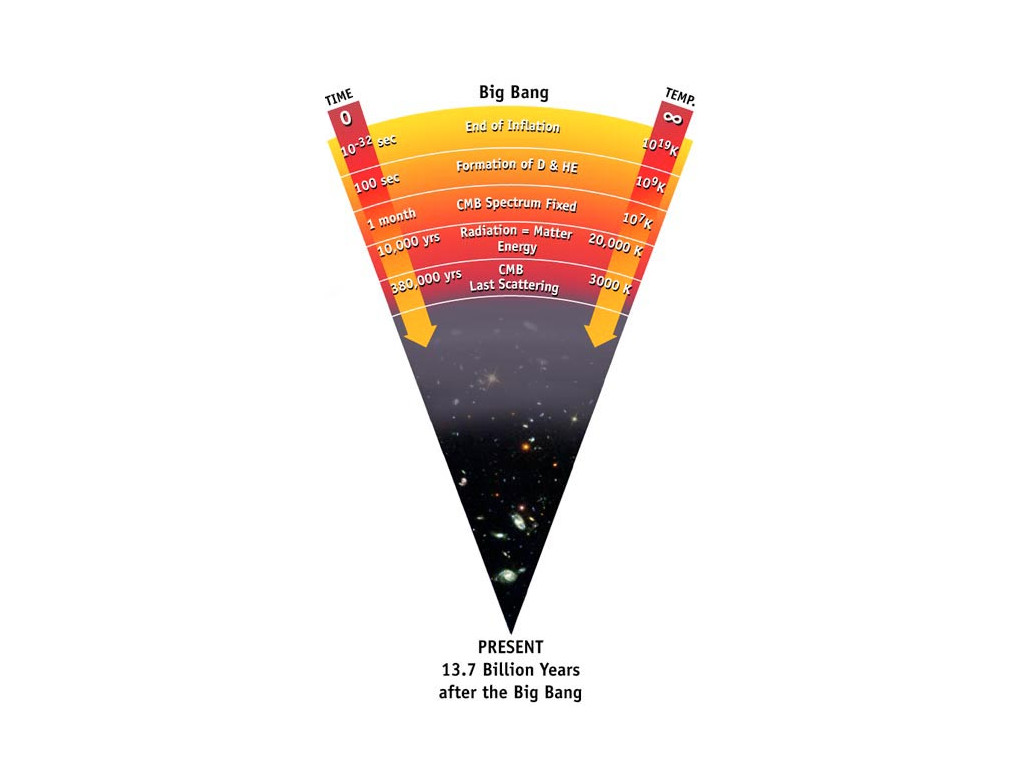
\includegraphics[width=\linewidth]{cmb/images/radiation_scattering.jpg}
	\caption{Sichtbarkeit des Universums im Zeitverlauf}
	\label{fig:radiation_scattering}
\end{figure}


Im Verlauf der nächsten 380'000 Jahre (relativ gesehen ein sehr kurzer Zeitraum) und der damit verbundenen Ausdehnung des 
Universums sanken Druck und damit die Temperatur im Universum stark, nämlich auf 3.000 
Kelvin.
Dies entspricht der Temperatur einer Schwarzkörperstrahlung, Strahlung von 
einem Schwarzen Körper, welcher Strahlung absorbiert und nicht wieder rauslässt 
(Dieser Fakt ist essentiell zur späteren Nachweisung der kosmischen 
Mikrowellenhintergrundstrahlung).
Nun waren die Bedingungen erfüllt, dass sich Protonen und Elektronen zu 
Wasserstoffatomen verbinden konnten.
Die Zeit in der sich die ersten Atome bildeten, ist auch als Rekombination bekannt.


Nach dieser Rekombination gab es keine freien Elektronen mehr, wodurch die 
Photonen nicht mehr durch Thomson-Streuung abgelenkt wurden.
Den Photonen war es jetzt endlich möglich, der ``Explosion des Big-Bang'' zu 
entkommen und sich frei zu bewegen.
Die kosmische Mikrowellenhintergrundstrahlung ist eine Aufzeichnung der Photonen zum 
Zeitpunkt der Rekombination und verfügt über die Charakteristika einer Schwarzkörperstrahlung.
\ref{CMB_intro}

\section{Die Entdeckung des kosmischen Mikrowellenhintergrunds}
Nachdem bereits zahlreiche Forscher erfolglos nach dem kosmischen 
Mikrowellenhintergrund gesucht hatten, geschah die tatsächliche Entdeckung der 
Strahlung, wie so oft in der Wissenschaft, per Zufall.
Im Jahr 1964 arbeiteten Arno Penzias und Robert Woodrow Wilson an einer 
sogenannten ``Large Horn Antenna'' (siehe Abbildung \ref{fig:wilson_penzias}).
\begin{figure}
	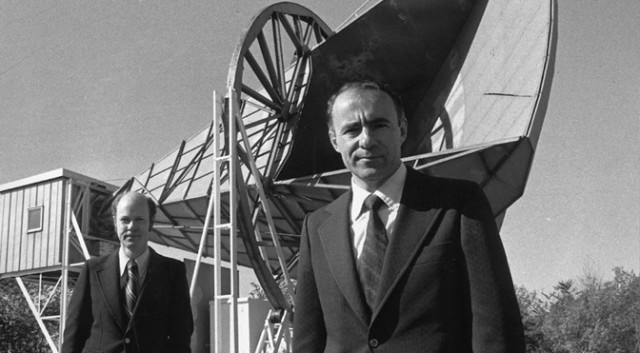
\includegraphics[width=\linewidth]{cmb/images/penzias-wilson-large-horn-antenna.jpg}
	\caption{Robert W. Wilson (links) und Arno A. Penzias vor ihrer Antenne}
	\label{fig:wilson_penzias}
\end{figure}
Dabei fanden sie ein Störsignal, welches unabhängig von der Ausrichtung der 
Antenne gleich war.
Auch eine Reinigung der Antenne brachte keine Verbesserung, weshalb sie sich an 
andere Physiker wandten, welche bestätigten, dass es sich beim Störsignal um 
die erste Aufzeichnung der kosmischen Hintergrundstrahlung handelte.
Der Fund gilt als eine der wichtigsten Entdeckungen der Kosmologie und als 
Bestätigung der Urknalltheorie.
Deswegen wurde ihnen dafür 1978 der Nobelpreis für Physik verliehen.

In den Messungen von Wilson und Penzias wurde eine extreme Isotropie in der 
Strahlung festgestellt.
Dies stellte ein Problem dar, da dass heutige Universum sich nur gebildet haben 
konnte, wenn auch im Universum vor der Rekombination bereits Dichteschwankungen 
existiert haben.
Diese Schwankungen müssten auch in Temperaturunterschieden der kosmischen 
Hintergrundstrahlung erkennbar sein.
Fast 30 Jahre lang (1965-1992) blieb die Suche nach diesen Anisotropien 
erfolglos.
In dieser Zeit bemerkte man, dass die Temperaturschwankungen innerhalb der 
Strahlung extrem klein sein muss ($< 0.001\%$).
Die Erlösung brachte 1992 schliesslich der \ac{COBE} Satellit.
\ref{m_schoenitzer}
%
% kurven.tex -- Krümmung eines eindimensionalen Raumes, Einbettung
%
% (c) 2017 Prof Dr Andreas Müller, Hochschule Rapperswil
%
\chapter{Kurven%
\label{skript:chapter:kurven}}
\lhead{Kurven}
\rhead{}
Das Konzept der Krümmung einer Kurve wird bereits im ersten Semester
in der Analysis eingeführt,
die Formeln dafür sollen in diesem Kapitel kurz in Erinnerung gerufen werden.
Wichtiger aber ist die Erkenntnis, dass eine Kurve nur eine sehr simple
innere Geometrie hat.
Nach Wahl eines Anfangspunktes definiert die Bogenlänge entlang der Kurve 
ein Koordinatensystem für die Kurve vollständig.
Die Krümmung der Kurve ist also eine Eigenschaft der Einbettung einer Kurve.

Diese innere Einfachheit von Kurven macht sie zu einem Werkzeug, mit
dem wir später höher\-dimensionale Räume untersuchen können.
Wir können zum Beispiel Dreiecke in einer Fläche untersuchen,
und werden dabei erkennen, dass die Winkelsumme Auskunft geben kann
über die Krümmung der Fläche.
Die Krümmung einer Fläche ist also eine innere Eigenschaft, die mit
Hilfe von Experimenten mit Kurven erforscht werden kann.

\section{Länge einer Kurve}
\rhead{Definitionen}
Wir betrachten eine Kurve in der Ebene durch einen Parameterdarstellung
\[
c\colon [a,b] \to\mathbb R^2:t\mapsto c(t).
\]
Darin ist $c(t)$ als Vektor in der Ebene zu betrachten selbst wenn
wir dies nicht explizit durch Vektorpfeile anzeigen.
Man kann die Parametrisierung als die Wahl eines Koordinatensystems
für die Kurve interpretieren.
Es stellt sich daher die Frage, inwieweit Aussagen über die Kurve von
der Wahl dieses Koordinatensystems abhängig sind.

Alle unsere Untersuchungen werden die Analysis als Werkzeug verwenden,
wir wollen daher nur Kurven verwenden, für die eine ausreichend glatte
Parametrisierung vorliegt.
Wir verlangen daher, dass die Parameterisierung nach genügend oft nach
dem Parameter abgeleitet werden kann.
Die Ableitung 
\[
v(t)
=
\frac{dc(t)}{dt}
=
\dot c(t)
\]
ist ein Vektor, der im Punkt $c(t)$ tangential ist an die Kurve 
(Abbildung~\ref{skript:kurve:tangente}).
\begin{figure}
\centering
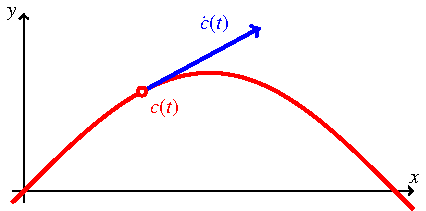
\includegraphics{chapters/tikz/tangente.pdf}
\caption{Kurve $c(t)$ parametrisiert mit dem Parameter $t$ und Tangentialvektor
$\dot c(t)$
\label{skript:kurve:tangente}}
\end{figure}

In $\mathbb R^2$ haben wir eine Längenmessung zur Verfügung, welche
wir dazu verwenden können, die Länge der Kurve zu berechnen.
Dazu betrachten wir zwei benachbarte Punkte $c(t)$ und $c(t+\Delta t)$
der Kurve.
Ihre Entfernung ist $|c(t+\Delta t) - c(t)|$.
Um daraus die Länge der Kurve zu berechnen, müssen wir die Kurve
an den Stellen $t_1,t_2,\dots,t_n$
beliebig fein in Teile aufteilen, und die Längen der Teilstrecken
auf addieren.
Die Summe
\[
l\simeq\sum_{k=1}^{n-1} |c(t_{i+1})-c(t_i)|
\]
ist daher eine Approximation für die Länge der Kurve.
Die Differenzen können wir mit Hilfe der Ableitung durch
\[
c(t_{i+1})-c(t_i) = \dot c(t_i)\cdot (t_{i+1}-t_i)
\]
approximieren.
Beim Grenzübergang zu einer beliebig feinen Unterteilung wird daraus
das Integral
\begin{equation}
l=\int_a^b |\dot c(t)|\,dt.
\end{equation}
Die Funktion
\begin{equation}
s(t)
=
\int_a^t |\dot c(\tau)|\,d\tau
\end{equation}
berechnet die Länge der Kurve zwischen den Parameterwerten
$a$ und $t$, wir wissen also insbesondere, dass $s(0)=0$.
$s(t)$ ist die {\em Bogenlänge} entlang der Kurve.
\index{Bogenlänge}

\section{Bogenlängenparameter}
\rhead{Bogenlängenparameter}
In diesem Abschnitt soll illustriert werden, dass wir bei der Wahl
einer Parametrisierung ein und derselben Kurve zwar viel Freiheit haben,
dass jedoch für geometrische Untersuchungen sich meistens gewisse
Parametrisierungen besonders eignen.
Sowohl hier als auch später beim Studium der Geodäten ist eine
Parametrisierung mit der Bogenlänge besonders nützlich.

\subsubsection{Ein Beispiel}
Wir betrachten die folgenden beiden Parametrisierungen einer ebenen Kurve:
\begin{equation}
\begin{aligned}
c_1\colon
[-1,1]\to\mathbb{R}^2
&\colon
t\mapsto\begin{pmatrix}x\\\sqrt{1-t^2}\end{pmatrix}
&&\text{und}&
c_2\colon
[0,\pi]\to\mathbb{R}^2
&
\colon
s\mapsto\begin{pmatrix}-\cos s\\\sin s\end{pmatrix}.
\end{aligned}
\end{equation}
Beide beschreiben den Einheitskreisbogen, der den Punkt $(-1,0)$ mit
dem Punkt $(1,0)$ verbindet (Abbildung \ref{skript:1dim:kreisbogen}).
Die Parametrisierungen unterscheiden sich aber in der Ableitung,
die Tangentialvektoren für die beiden Ableitungen sind
\begin{equation}
\begin{aligned}
\frac{dc_1}{dt}
&=
\begin{pmatrix}
1\\-\frac{1}{\sqrt{1-t^2}}
\end{pmatrix}
&&\text{und}&
\frac{dc_2}{ds}
&=
\begin{pmatrix}
\sin s\\\cos s
\end{pmatrix}.
\end{aligned}
\end{equation}
Der Tangentialvektor hat in der zweiten Parametrisierung konstant
die Länge $1$, während sie in der ersten Parametrisierung nahe bei
$t=\pm1$ über alle Grenzen wächst.
\begin{figure}
\centering
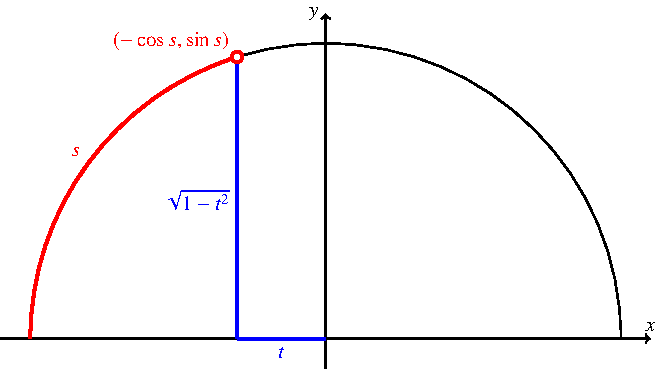
\includegraphics{chapters/tikz/kreisbogen.pdf}
\caption{Kreisbogen zwischen $(-1,0)$ und $(1,0)$. Im Text werden
zwei verschiedene Parametrisierungen dafür vorgestellt.
\label{skript:1dim:kreisbogen}}
\end{figure}

\subsubsection{Bestimmung der Bogenlänge}
Interpretieren wir den Parameter $t$ als die Zeit der Bewegung eines 
Teilchens entlang der Kurve, dann ist die zeitliche Änderung der Strecke,
die das Teilchen zurück gelegt hat, gerade die Länge des
Geschwindigkeitsvektors, also
\[
\frac{d}{dt} s(t) = \biggl|\frac{d}{dt}c(t)\biggr| = |\dot c(t)|.
\]
Die Funktion $s(t)$ ist also die Lösung der Differentialgleichung
\begin{equation}
\dot s(t)=|\dot c(t)|
\quad
\text{ mit der Anfangsbedingung }\quad s(a)=0.
\label{skript:kruemmung:laengedgl}
\end{equation}
Da $|\dot c(t)|$ eine stetige Funktion ist, können wir nach allgemeinen
Sätzen der Theorie der gewöhnlichen Differentialgleichungen davon ausgehen,
dass diese Differentialgleichung eine eindeutig bestimmte Lösung hat.

Die Differentialgleichung \eqref{skript:kruemmung:laengedgl} kann 
durch Integrieren sofort gefunden werden, sie ist
\begin{equation}
s(t)
=
\int_a^t \dot s(\tau)\,d\tau
=
\int_a^t |\dot c(\tau)| \,d\tau
=
\int_a^t \sqrt{\dot x(\tau)^2 + \dot y(\tau)^2}\,d\tau,
\label{skript:kruemmung:laenge}
\end{equation}
wie man auch durch Ableiten nach $t$ sofort nachprüfen kann.

\subsubsection{Charakterisierung von Bogenlängenparametrisierung}
Verlangen wir von der Kurvenparametrisierung $c(t)$ zusätzlich,
dass $|\dot c(t)|\ne 0$ für alle Parameterwerte $t$, dann ist
$s(t)$ sogar eine streng monoton wachsende Funktion, insbesondere
kann sie invertiert werden.
Wir können daher zu jedem gegebenen Wert der Länge $s$ durch
Anwendung der inversen Funktion sofort einen Parameterwert $t$
finden, bei dem der Wert $s$ der Länge erreicht wird, also
$s(t)=s$.
Wir schreiben diesen Wert auch abkürzen als $t(s)$, dies ist eine
vereinfachte Notation für die inverse Funktion von $s(t)$.
Die Ableitung der Funktion $s(t)$ ist
\begin{equation}
\frac{d}{ds} t(s) = \frac{1}{\dot s(t(s))} = \frac1{|\dot c(t(s))|}
\label{skript:kruemmung:abllaengeinv}
\end{equation}
nach der Formel für die Ableitung der inversen Funktion.

Zu einer beliebigen differenzierbaren Kurve mit der Eigenschaft
$|\dot c(t)|\ne 0$ können wir also immer eine neue Parametrisierung
$c(s)=c(t(s))$ finden, welche die Eigenschaft hat, dass $s$ die
Länge entlang der Kurve gerade die Kurvenlänge ist, die durchlaufen
wird.
Wir nennen $s$ auch den {\em Kurvenlängenparameter} entlang der
Kurve.
\index{Kurvenlängenparameter}
Wir sagen auch, $c(s)$ ist durch Kurvenlänge parametrisiert.

Die neue Parametrisierung hat als ``Geschwindigkeitsvektor''
\[
\frac{d}{ds} c(s)
=
\frac{d}{ds} c(t(s))
=
\dot c(t(s)) \frac{d}{ds}t(s)
\]
seine Länge wird unter Verwendung von
\eqref{skript:kruemmung:abllaengeinv}
\[
\biggl|
\frac{d}{ds} c(s)
\biggr|
=
\biggl|\dot c(t(s))\frac1{|\dot c(t(s))|}\biggr|
=
1,
\]
bei Verwendung eines Kurvenlängenparameters wird der Tangentialvektor
immer ein Einheitsvektor sein.

Umgekehrt wird die Differentialgleichung \eqref{skript:kruemmung:laengedgl}
besonderes einfach, wenn $|\dot c(t)|=1$ ist, nämlich $\dot s(t)=1$ mit
der Lösung $s(t)=t$.
Die Bedingung $|\dot c(t)|=1$ charaktersiert also $t$ als einen
Kurvenlängenparameter.

\subsubsection{Beispiele}
\begin{beispiel}
Wir betrachten eine Gerade 
\[
c(t)=\vec p + t\vec v,\qquad \vec v\ne 0
\]
in der Ebene.
Wir legen $a=0$ willkürlich fest.
Die Differentialgleichung~\eqref{skript:kruemmung:laengedgl} für die
Kurven\-längen\-funktion $s(t)$ wird
\[
\dot s(t) = |\dot c(t)| = |v|
\]
mit der Lösung
\[
s(t)=|v|t.
\]
Da $v\ne 0$ ist $s(t)$ monoton wachsend, und wir können sofort nach
$t$ auflösen, es ist
\[
t(s)=\frac{s}{|\vec v|}.
\]
Setzen wir dies in die ursprüngliche Parametrisierung ein, erhalten
wir
\[
c(s)
=
c(s(t))
=
\vec p + t(s)\vec v
=
\vec p + \frac{s}{|\vec v|}\vec v
=
\vec p + s\frac{v}{|v|},
\]
Die Ableitung nach $s$ hiervon ist ein Einheitsvektor, wie zu erwarten
war.
\end{beispiel}

\begin{beispiel}
Wir parametrisieren den Einheitskreis mit Hilfe der $x$-Koordinate, also
durch
\[
c\colon
[-1,1]\to\mathbb R^2
\colon
t\mapsto (-t,\sqrt{1-t^2}).
\]
Ganz offensichtlich ist dies kein Kurvenlängenparameter.
Für die Kurvenlänge brauchen wir die Ableitung nach dem Parameter $t$,
sie ist
\[
\dot c(t)=\biggl(-1, -\frac{t}{\sqrt{1-t^2}}\biggr).
\]
Die Kurvenlänge ist das Integral der Länge der Ableitung:
\[
s(t)
=
\int_{-1}^t \sqrt{1 + \frac{\tau^2}{1-\tau^2}}\,d\tau
=
\int_{-1}^t \sqrt{\frac{1-\tau^2 +\tau^2}{1-\tau^2}}\,d\tau
=
\int_{-1}^t \frac{1}{\sqrt{1-\tau^2}}\,d\tau
\]
Das Integral auf der rechten Seite kann man aber in geschlossener
Form auswerten, es ist
\[
s(t)=\arcsin(t) + \frac{\pi}{2}
\]
mit der inversen Funktion
\[
t(s)
=
\sin\biggl(s-\frac{\pi}2\biggr)
=
-\cos(s)
\]
Setzen wir dies in die Parametrisierung ein, erhalten wir
\[
c(s)
=
\bigl(\cos(s), \sqrt{1-\cos^2(s)}\bigr)
=
(\cos(s), \sin(s)),
\]
also die übliche Parametrisierung des Einheitskreises mit Hilfe
des Winkels.
Der Winkel muss in Bogenmass gemessen werden, also der Länge entlang
des Kreises.
\end{beispiel}

Da sich jede beliebige Kurve mit einem Bogenlängenparameter versehen
lässt, können wir für je zwei beliebige Kurven immer eine Abbildung
zwischen den Kurven definieren, die Punkte mit gleichem Bogenlängenparameter
zur Deckung bringt.
Zwei Kurven sind also nicht mehr unterscheidbar, wenn sie mal mit
einem Bogenlängenparameter ausgestattet sind.
Verbleibende Unterschiede zwischen Kurven entstehen einzig durch die
Einbettung der Kurve im Raum.

Für eine Ameise, die ausschliesslich auf der Kurve lebt, ist die Länge,
die sie entlang der Kurve zurückgelegt hat, die einzige geometrische
Information, die ihr zugänglich ist.
Sie kann verschiedene Kurven im Raum nicht voneinander unterscheiden.

\section{Krümmung%
\label{section:kurve:kruemmung}}
\rhead{Krümmung}
\begin{figure}
\centering
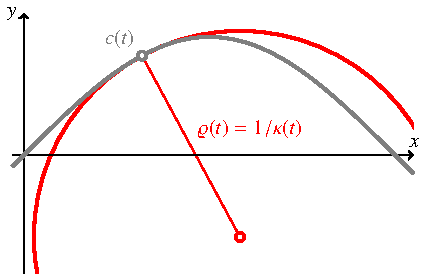
\includegraphics{chapters/tikz/kruemmung.pdf}
\caption{Krümmung $\kappa(t)$ und Krümmungsradius $\varrho(t)$
der Sinus-Kurve im Punkt $c(t)$
\label{skript:kurven:fig:kruemmung}}
\end{figure}
Wir möchten in diesem Abschnitt zeigen, dass die Krümmung einer Kurve
ausschliesslich eine Eigenschaft der Einbettung der Kurve in den
Raum ist.
Wir tun das, indem wir davon ausgehen, dass eine Kurve bereits mit
der Kurvenlänge parametrisiert ist, dass wir also die Standardparametrisierung
gewählt haben, in der über die innere Geometrie der Kurve verfügbare
Information bereits vollständig verwertet worden ist.

Eine Gerade zeichnet sich dadurch aus, dass der Tangentialvektor in
der Bo\-gen\-län\-gen\-pa\-ra\-me\-tri\-sie\-rung nicht ändert.
Eine Gerade ist nicht gekrümmt.
Krümmung ist also die Änderung des Tangentialvektors oder
\[
\kappa(s)=|\ddot c(s)|.
\]
\index{Krümmung einer Kurve}

\begin{beispiel}
Der Kreis mit Radius $r$ kann parametrisiert werden durch die Funktion
\[
s\mapsto c(s)=\biggl( r\cos\frac{s}{r}, r\sin\frac{s}{r}\biggr).
\]
Die Ableitung ist
\[
\dot c(s)=\biggl(-\sin\frac{s}{r},\cos\frac{s}{r}\biggr)
\qquad\Rightarrow\qquad
|\dot c(s)|
=
\sqrt{\cos^2\frac{s}{r}+\sin^2\frac{s}{r}}=1,
\]
dies ist also eine Parametrisierung mit Bogenlängenparameter.
Die Krümmung ist der Betrag der zweiten Ableitung, also
\[
\ddot c(s)=\biggl(-\frac1r\cos\frac{s}{r},-\frac1r\sin\frac{s}{r}\biggr)
\qquad\Rightarrow\qquad
\kappa(s)
=
|\ddot c(s)|
=
\frac1r.
\]
Der Kreis mit Radius $r$ ist also eine Kurve mit konstanter Krümmung
$\kappa(s)=\frac1r$.
\end{beispiel}

Ist die Kurve nicht durch die Bogenlänge parametrisiert, wird die
Berechnung der Krümmung etwas komplizierter.
Es muss aber immer noch gelten, dass $\kappa(t)$ die Änderung des
Einheitstagentialvektors pro Längeneinheit entlang der Kurve angibt.
Es ist also zu berechnen
\begin{equation}
\kappa(t)
=
\underbrace{\frac{1}{|\dot c(t)|}}_{\text{pro Längeneinheit}}
\cdot\;
\biggl|\frac{d}{dt}\underbrace{\frac{\dot c(t)}{|\dot c(t)|}}_{\text{Einheitstangentialvektor}}\biggr|.
\label{skript:kruemmung:krallg2}
\end{equation}
Die Berechnung ist etwas mühsam wegen des Vektorbetrages im Nenner.
Wir berechnen daher zuerst die Ableitung von $|\dot c(t)|$ mit
Hilfe der Kettenregel:
\begin{align*}
\frac{d}{dt}|\dot c(t)|
&=
\frac{d}{dt}\sqrt{\dot x(t)^2+\dot y(t)^2}
=
\frac1{2\sqrt{\dot x(t)^2 + \dot y(t)^2}}(2\dot x(t)\ddot x(t) + 2\dot y(t)\ddot y(t))
\\
&=
\frac{1}{|\dot c(t)|}
\begin{pmatrix}\dot x(t)\\\dot y(t)\end{pmatrix}
\cdot
\begin{pmatrix}\ddot x(t)\\\ddot y(t)\end{pmatrix}
=
\frac{1}{|\dot c(t)|}
\dot c(t)\cdot\ddot c(t)
=
\frac{\dot c(t)}{|\dot c(t)|} \cdot\ddot c(t).
\end{align*}
Damit können wir jetzt auch die Ableitung des Einheitstangentialvektors
berechnen:
\begin{align}
\frac{d}{dt} \frac{\dot c(t)}{|\dot c(t)|}
&=
\frac{\displaystyle\ddot c(t) |\dot c(t)| - \dot c(t) \frac{d}{dt}|\dot c(t)|}{|\dot c(t)|^2}
=
\frac{\displaystyle\ddot c(t) |\dot c(t)| - \dot c(t) \frac{\dot c(t)}{|\dot c(t)|}\cdot \ddot c(t)}{|\dot c(t)|^2}
=
\frac{\displaystyle\ddot c(t) - \frac{\dot c(t)}{|\dot c(t)|} \left( \frac{\dot c(t)}{|\dot c(t)|}\cdot \ddot c(t)\right)}{|\dot c(t)|}
\label{skript:kruemmung:krallg1}
\end{align}
Schreiben wir den Einheitstangentialvektor
\[
\vec e(t)= \frac{\dot c(t)}{|\dot c(t)|},
\]
wird der Zähler etwas übersichtlicher zu
\[
\ddot c(t) - \frac{\dot c(t)}{|\dot c(t)|} \biggl( \frac{\dot c(t)}{|\dot c(t)|}\cdot \ddot c(t)\biggr)
=
\ddot c(t) - \vec e(t)\; \bigl(\vec{e}(t)\cdot \ddot c(t)\bigr).
\]
Da $\vec e(t)$ ein Einheitsvektor ist, ist
$\vec e(t) \;(\vec e(t)\cdot\ddot c(t))$ die Projektion des Vektors
$\ddot c(t)$ auf den Vektor $\vec e(t)$.
Der Nenner ist also die Komponenten von $\ddot c(t)$ senkrecht auf dem
Tangentialvektor.
Wir brauchen davon aber nur den Betrag, also die Höhe des Parallelograms
mit den Seiten $\vec e(t)$ und $\ddot c(t)$.
Diese können wir aber auch dadurch erhalten, dass wir den orientierten
Parallelogramminhalt berechnen, und durch die Länge der Grundseite
$\vec e(t)$ teilen, die aber ein Einheitsvektor ist.
Den Parallelogramminhalt können wir mit der Determinante berechnen:
\[
\biggl|\ddot c(t) - \frac{\dot c(t)}{|\dot c(t)|}
\biggl(\frac{\dot c(t)}{|\dot c(t)|} \cdot \ddot c(t)\biggr)\biggr|
=
\det \biggl(\frac{\dot c(t)}{|\dot c(t)|}, \ddot c(t)\biggr)
=
\frac1{|\dot c(t)|}\det (\dot c(t),\ddot c(t)).
\]
Daraus können wir jetzt auch eine Formel für die Krümmung zusammensetzen.
Zunächst müssen wir den Faktor $|\dot c(t)|$ im Nenner wieder
hinzufügen, den wir in~\eqref{skript:kruemmung:krallg1} gefunden hatten.
Ausserdem brauchen wir einen weiteren Faktor $|\dot c(t)|$ im Nenner
aus der Definition~\eqref{skript:kruemmung:krallg2}.
Damit wird die allgemeine Formel
\begin{equation}
\kappa(t)
=
\frac{\det(\dot c(t),\ddot c(t))}{|\dot c(t)|^3}
\label{skript:kruemmung:krkurveallg}
\end{equation}
für die Krümmung einer ebenen Kurve.


\begin{beispiel}
\index{Ellipse!Krümmung}
Wir berechnen die Krümmung einer {\em Ellipse mit den Halbachsen
$a$ und $b$}, und verwenden dazu die Parametrisierung mit Hilfe des
Zentriwinkels, also
\[
c
\colon
[0,2\pi]\to\mathbb R^2
\colon
t\mapsto c(t) = (a\cos t, b \sin t).
\]
Nach der Formel~\eqref{skript:kruemmung:krkurveallg} brauchen wir zunächst
die ersten beiden Ableitungen, diese sind
\begin{align*}
\dot c(t)
&=
(-a\sin t, b\cos t)
\\
\ddot c(t)
&=
(-a\cos t, -b\sin t)
\end{align*}
Die Determinante von $\dot c(t)$ und $\ddot c(t)$ ist
\[
\det(\dot c(t), \ddot c(t))
=
\left|\begin{matrix}
-a\sin t & -a \cos t\\
 b\cos t & -b \sin t
\end{matrix}\right|
=
ab\sin^2t+ab\cos^2 t
=
ab.
\]
Die Krümmung ist daher
\[
\kappa(t)
=
\frac{ab}{(a^2\sin^2 t + b^2 \cos^2 t)^{\frac32}}
\]
Da die Faktoren $\sin^2t$ und $\cos^2t$ im Nenner sich zu $1$ summieren,
steht in der Klammer im Nenner ein gewichteter Mittelwert von $a^2$
und $b^2$.
Die Extremwerte des Nenners sind daher $a^3$ und $b^3$, sie werden bei
$t=\pm\frac{\pi}2$ bzw.~$t\in\{0,\pi\}$ angenommen.
Nimmt man an, dass $a>b$ ist, dann wird die maximale Krümmung $t=0$ und
und $t=\pi$ erreicht, sie ist $ab/b^3=a/b^2$.
Die minimale Krümmung wird dagegen bei $t=\pm\frac{\pi}2$ angenommen,
sie ist $ab/a^3=b/a^2$.

Ein Kreis ist eine Ellipse, bei der $a$ und $b$ übereinstimmen, dann sind
die beiden Extremwerte gleich gross, nämlich
\[
\frac{a}{b^2}=\frac{r}{r^2}=\frac1r
\qquad\text{und}\qquad
\frac{b}{a^2}=\frac{r}{r^2}=\frac1r,
\]
wie wir früher bereits gefunden haben.
\end{beispiel}

\begin{beispiel}
\index{Parabel!Krümmung}
Für spätere Anwendungen berechnen wir noch die Krümmung einer {\em Parabel},
genauer des Graphen der Funktion
\[
y = ax^2 + bx + c.
\]
Als Parameterdarstellung ausgedrückt geht es also um die Kurve
\[
t\mapsto c(t)
=
\begin{pmatrix}
t\\
at^2+bt+c
\end{pmatrix}.
\]
Davon sind zunächst die Ableitungen nach $t$ zu bestimmen, sie sind
\begin{align*}
\dot c(t)
&=
\begin{pmatrix}1\\2at+b\end{pmatrix},
\\
\ddot c(t)
&=
\begin{pmatrix}0\\2a\end{pmatrix}.
\end{align*}
Die Krümmung ist dann nach Formel~\ref{skript:kruemmung:krkurveallg}
\begin{align}
\kappa(t)
&=
\frac{\left|\begin{matrix}1&0\\2at+b&2a\end{matrix}\right|}{
(1+(2at+b)^2)^{\frac32}
}
=
\frac{2a}{(1+(2at+b)^2)^{\frac32}}.
\label{skript:kruemmung:parabelkruemmung}
\end{align}
Der Scheitelpunkt befindet sich bei $t=-b/2a$, an dieser Stelle verschwindet
die innere Klammer im Nenner von~\eqref{skript:kruemmung:parabelkruemmung}.
Am Scheitel ist die Krümmung daher viel einfacher
\begin{equation}
\kappa_{\text{Scheitel}}
=
\kappa\biggl(-\frac{b}{2a}\biggr)
=
2a
\qquad
\Rightarrow
\qquad
\varrho_{\text{Scheitel}}
=
\frac1{\kappa_{\text{Scheitel}}}
=
\frac1{2a}.
\label{skript:kruemmung:parabel:scheitel}
\end{equation}
Der Krümmungsradius im Scheitel der Normalparabel $y=x^2$ ist also
$\varrho=\frac12$.
\end{beispiel}

Für eine Kurve in drei Dimension lässt sich das bei der Herleitung
der Formel~\eqref{skript:kruemmung:krkurveallg} für $\kappa(t)$
verwendete Argument fast unverändert übertragen.
Die einzige Änderung ist an der Stelle erforderlich, wo wir die Determinante
zur Berechnung des orientierten Volumens des Parallelograms verwendet
haben.
In drei Dimensionen muss stattdessen der Betrag des Vektorproduktes 
verwendet werden.
Die Krümmung einer Raumkurve in einer beliebigen Parametrisierung ist
daher
\begin{equation}
\kappa(t)
=
\frac{|\dot c(t)\times \ddot c(t)|}{|\dot c(t)|^3}.
\label{skript:kruemmung:krkurveallg3d}
\end{equation}
Dies ist natürlich identisch mit \eqref{skript:kruemmung:krkurveallg},
wenn man sich die Ebene der Kurve in einen dreidimensionalen Raum
eingebettet vorstellt.

\begin{beispiel}
\begin{figure}
\centering
\includegraphics[width=\hsize]{chapters/3d/kurve.jpg}
\caption{Kurven $t\mapsto(t,t^2,0)$ (rot) und $t\mapsto(t,t^2,t^3)$ (gelb).
\label{skript:kruemmung:fig:kurvekr}}
\end{figure}
Wir betrachten die beiden Kurven
\begin{align*}
c_1(t)&=(t,t^2,0)
&
c_2(t)&=(t,t^2,t^3)
\end{align*}
(Abbildgung~\ref{skript:kruemmung:fig:kurvekr}).
$c_1(t)$ ist eine ebene Kurve, nämlich die Projektion der Raumkurve
$c_2(t)$ in die $x$-$y$-Ebene, sie ist in
Abbildung~\ref{skript:kruemmung:fig:kurvekr} rot dargestellt.
Die Kurve $c_2(t)$ ist in Abbildung~\ref{skript:kruemmung:fig:kurvekr} 
dagegen gelb dargestellt.
Wir wollen von beiden Kurven die Krümmung berechnen.
Dazu berechnen wir zunächst die Ableitungen und das Vektorprodukt
\begin{align*}
\dot c_1(t)
&=
(1,2t,0)
&
\dot c_2(t)
&=
(1,2t,3t^2)
\\
\ddot c_1(t)
&=
(0,2,0)
&
\ddot c_2(t)
&=
(0, 2, 6t)
\\
\dot c_1(t)\times \ddot c_1(t)
&=
(0,0,2)
&
\dot c_2(t)\times \ddot c_2(t)
&=
(6t^2,-6t,2)
\end{align*}
Daraus kann man jetzt die Krümmungen berechnen:
\begin{align*}
\kappa_1(t)
&=
\frac{2}{(1+4t^2)^{\frac32}}
\\
\kappa_2(t)
&=
\frac{2}{(1+4t^2 + 9t^4)^{\frac32}}
\sqrt{1+9t^2+9t^4}
\end{align*}
Für den Parameterwert $t=0$ stimmen die beiden Krümmungen überein.
\end{beispiel}

\section{Rekonstruktion einer ebenen Kurve aus der Krümmung}
\rhead{Rekonstruktion aus der Krümmung}
Die Krümmung bestimmt eine Kurve eindeutig.
Um dies einzusehen, parametrisieren wir eine ebene Kurve mit
$x$, schreiben also $c(x)=(x,y(x))$.
Wir müssen jetzt nachrechnen, dass die Vorgabe der Krümmung $\kappa(x)$
und der Steigung in einem Punkt die Kurve eindeutig festlegt.
Dazu stellen wir eine Differentialgleichung zweiter Ordnung auf,
allgemeine Sätze über Existenz und Eindeutigkeit der Lösung von
gewöhnlichen Differentialgleichungen werden unsere Aussage dann
als Konsequenz haben.

In dieser speziellen Wahl der Parametrisierung ist $\dot x = 1$ und
$\ddot x=0$.
Die Ableitung von $y$ nach dem Parameter ist dann $\dot y=y'(x)$.
Somit wird die Formel für die Krümmung
\[
\kappa(x)
=
\frac{\left|\begin{matrix}\dot x&\ddot x\\\dot y&\ddot y\end{matrix}\right|}{(\dot x^2+\dot y^2)^{\frac32}}
=
\frac{\left|\begin{matrix}1&0\\y'&y''\end{matrix}\right|}{(1+y'^2)^{\frac32}}
=
\frac{y''}{(1+y'(x))^{\frac32}}
\]
der in expliziter Form:
\[
y''(x)=\kappa(x) (1+y'(x)^2)^{\frac32}.
\]
Dies ist eine gewöhnliche Differentialgleichung zweiter Ordnung.
Da die rechte Seite erfüllt die Bedingungen, die in üblichen
Eindeutigkeitssätzen für gewöhnliche Differentialgleichungen
verlangt werden, daher gibt es genau eine Lösung dieser
Differentialgleichung zu vorgegebenem Anfangspunkt und Anfangsrichtung.
Damit ist gezeigt, dass in der Ebenen zwei Kurven mit der gleichen
Krümmung, gleichem Anfangspunkt und gleicher Anfangsrichtung übereinstimmen
müssen.
Anders formuliert: zwei ebene Kurven mit gleicher Krümmung in Abhängigkeit
von einem Bogenlängenparameter sind kongruent.

In drei Dimensionen kann die Krümmung allein eine Raumkurve nicht bestimmen.
Man kann dies zum Beispiel so einsehen.
Ist $c(t)$ eine gegeben Raumkurve, dann können wir deren Krümmung
$\kappa(t)$ berechnen.
In jeder Ebene durch den Punkt $c(0)$, die auch den Tangentenvektor
$\dot c(t)$ enthält, gibt es eine ebenen Kurve mit der gleichen
Krümmung $\kappa(t)$.
Da es unendlich viele solche Ebenen gibt, gibt es unendlich viele 
ebene Kurven, die die gleiche Krümmung haben wie die vorgegebene
Raumkurve.

Um eine Raumkurve eindeutig festzulegen braucht es daher ein weiteres
Datum, welches beschreibt, wie sich die aktuelle Tangentialebene
aufgespannt von $\dot c(t)$ und $\ddot c(t)$ dreht.
Diese {\em Torsion} genannt Grösse bestimmt dann die Kurve vollständig.
\index{Torsion}
Für eine ebene Kurve verschwindget die Torsion.

Die Kurventheorie lässt sich sogar auf eine beliebig grosse Zahl
von Dimensionen verallgemeinern.
Es stellt sich heraus, dass mit jeder zusätzlichen Dimension eine
zusätzliche Funktion notwendig wird.
Für eine Kurve in $n$ Dimensionen braucht es also $n-1$ Funktionen,
die beschreiben, wie sich ein entlang der Kurve mitbewegtes Koordinatensystem,
das sogenannte Frenet-$n$-Bein ändert.
\index{Frenet-$n$-Bein}
Diese Funktionen legen dann die Kurve bis auf die Wahl einer Anfangslage
des Koordinatensystem eindeutig fest.
Mit anderen Worten, wenn zwei Kurven in $n$ Dimensionen in den genannten
$n-1$ Funtionen übereinstimmen, dann sind sie kongruent.

%
% schnittkruemmung.tex
%
% (c) 2017 Prof Dr Andreas Müller, Hochschule Rappersewil
%
\section{Schnittkrümmung}
\rhead{Schnittkrümmung}
Die Krümmung von Kurven kann dazu verwendet werden, Flächen im
dreidimensionalen Raum zu analysieren.

\subsection{Flächen}
Wir betrachten in den folgenden Abschnitten Flächen, die durch zwei
Parameter $u,v\in\mathbb R^2$ parametrisiert sind.

\begin{definition}
Eine Abbildung
\[
g\colon \Omega\to\mathbb R^3: (u,v)\mapsto g(u,v),
\]
wobei $\Omega\subset\mathbb R^2$
eine offene Teilmenge von $\mathbb R^2$ ist, heisst eine Fläche.
\end{definition}

\begin{beispiel}
Sei eine Funktion $f(x,y)$ von zwei Variablen gegeben.
Dann ist die Funktion
\[
g\colon\mathbb R^2\to \mathbb R^3
: (x,y)\mapsto (x,y,f(x,y))
\]
eine Fläche.
Sie heisst auch der Graph der Funktion $f(x,y)$.
\end{beispiel}

Jede Fläche enthält zwei Scharen von Kurven, die durch die Koordinaten $u$
bzw.~$v$ parametrisiert sind, wir nennen sie die Koordinatenlinien.
Zu jedem $v$-Wert $v_0$ gibt es eine $u$-Koordinatenlinie
\[
c_{v_0}
\colon
\mathbb R \to \mathbb R^2
:
u\mapsto
c_{v_0}(u) = g(u, v_0)
\]
und zu jedem $u$-Wert $u_0$ gibt es eine $v$-Koordinatenlinie
\[
c_{u_0}
\colon
\mathbb R \to \mathbb R^2
:
v\mapsto
c_{u_0}(v) = g(u_0, v).
\]

\begin{beispiel}
Die Oberfläche der Einheitskugel im dreidimensionalen Raum kann mit
geographischer Länge $\lambda$ und geographischer Breite $\varphi$
parametrisiert werden.
Die Funktion $g(\lambda,\varphi)$ hat die Form
\begin{equation}
g(\lambda,\varphi)
=
\begin{pmatrix}
\sin\varphi\cos\lambda\\
\sin\varphi\sin\lambda\\
\cos\varphi
\end{pmatrix},\qquad
-\pi \le \lambda \le \pi,\quad
-\frac{\pi}2 \le \varphi \le \frac{\pi}2
.
\end{equation}
Die Koordinatenlinien sind wohlbekannt. 
Die Koordinatenlinie zu einem vorgegebenen $\varphi_0$ wird von
$\lambda$ parametrisiert und hat die Form
\[
\lambda
\mapsto
\begin{pmatrix}
\sin\varphi_0\cos\lambda\\
\sin\varphi_0\sin\lambda\\
\cos\varphi_0
\end{pmatrix},\qquad -\pi\le\lambda\le\pi
\]
dies ist ein Breitenkreis.
Die Koordinatenlinie zu einem vorgegebenen $\lambda_0$ wird durch
$\varphi$ parametrisiert und hat die Form
\[
\varphi
\mapsto
\begin{pmatrix}
\sin\varphi\cos\lambda_0\\
\sin\varphi\sin\lambda_0\\
\cos\varphi
\end{pmatrix},\qquad -\frac{\pi}2 \le \varphi\le \frac{\pi}2
\]
dies ist ein Längenkreis.
Man beachte, dass Werte $-\frac{\pi}2\le \varphi \le \frac{\pi}2$ nur einen
Halbkreis zwischen Nord- und Südpol beschreiben.
\end{beispiel}

Wir betrachten jetzt den Punkt $P=g(u_0,v_0)$ auf der Fläche.
Zu jedem Flächenparameter gibt es einen Tangentenvektor, den man durch
Ableitung nach dem Parameter bekommen kann:
\begin{equation}
t_u
=
t_u(P)
=
t_u(u_0,v_0)
=
\frac{\partial g(u_0,v_0)}{\partial u},
\qquad
t_v
=
t_v(P)
=
t_v(u_0,v_0)
=
\frac{\partial g(u_0,v_0)}{\partial v}.
\end{equation}
Aus diesen Tangentialvektoren lässt sich auch der Normalenvektor
\begin{equation}
n(P) = n(u_0,v_0) = t_u(u_0,v_0) \times t_v(u_0,v_0)
\end{equation}
bestimmen.
Damit die beiden Tangentialvektoren und der Normalenvektor wohldefiniert sind,
müssen wir verlangen, dass die partiellen Ableitungen von $g$ nach $u$ und $v$
wohldefiniert sind und nicht verschwinden.
Daher soll im folgenden immer angenommen sein, dass $g$ genügend oft stetig
differenzierbar ist, und dass die ersten Ableitungen nach den Flächenparametern
nicht verschwinden.

\subsection{Schnittkurven}
\begin{figure}
\centering
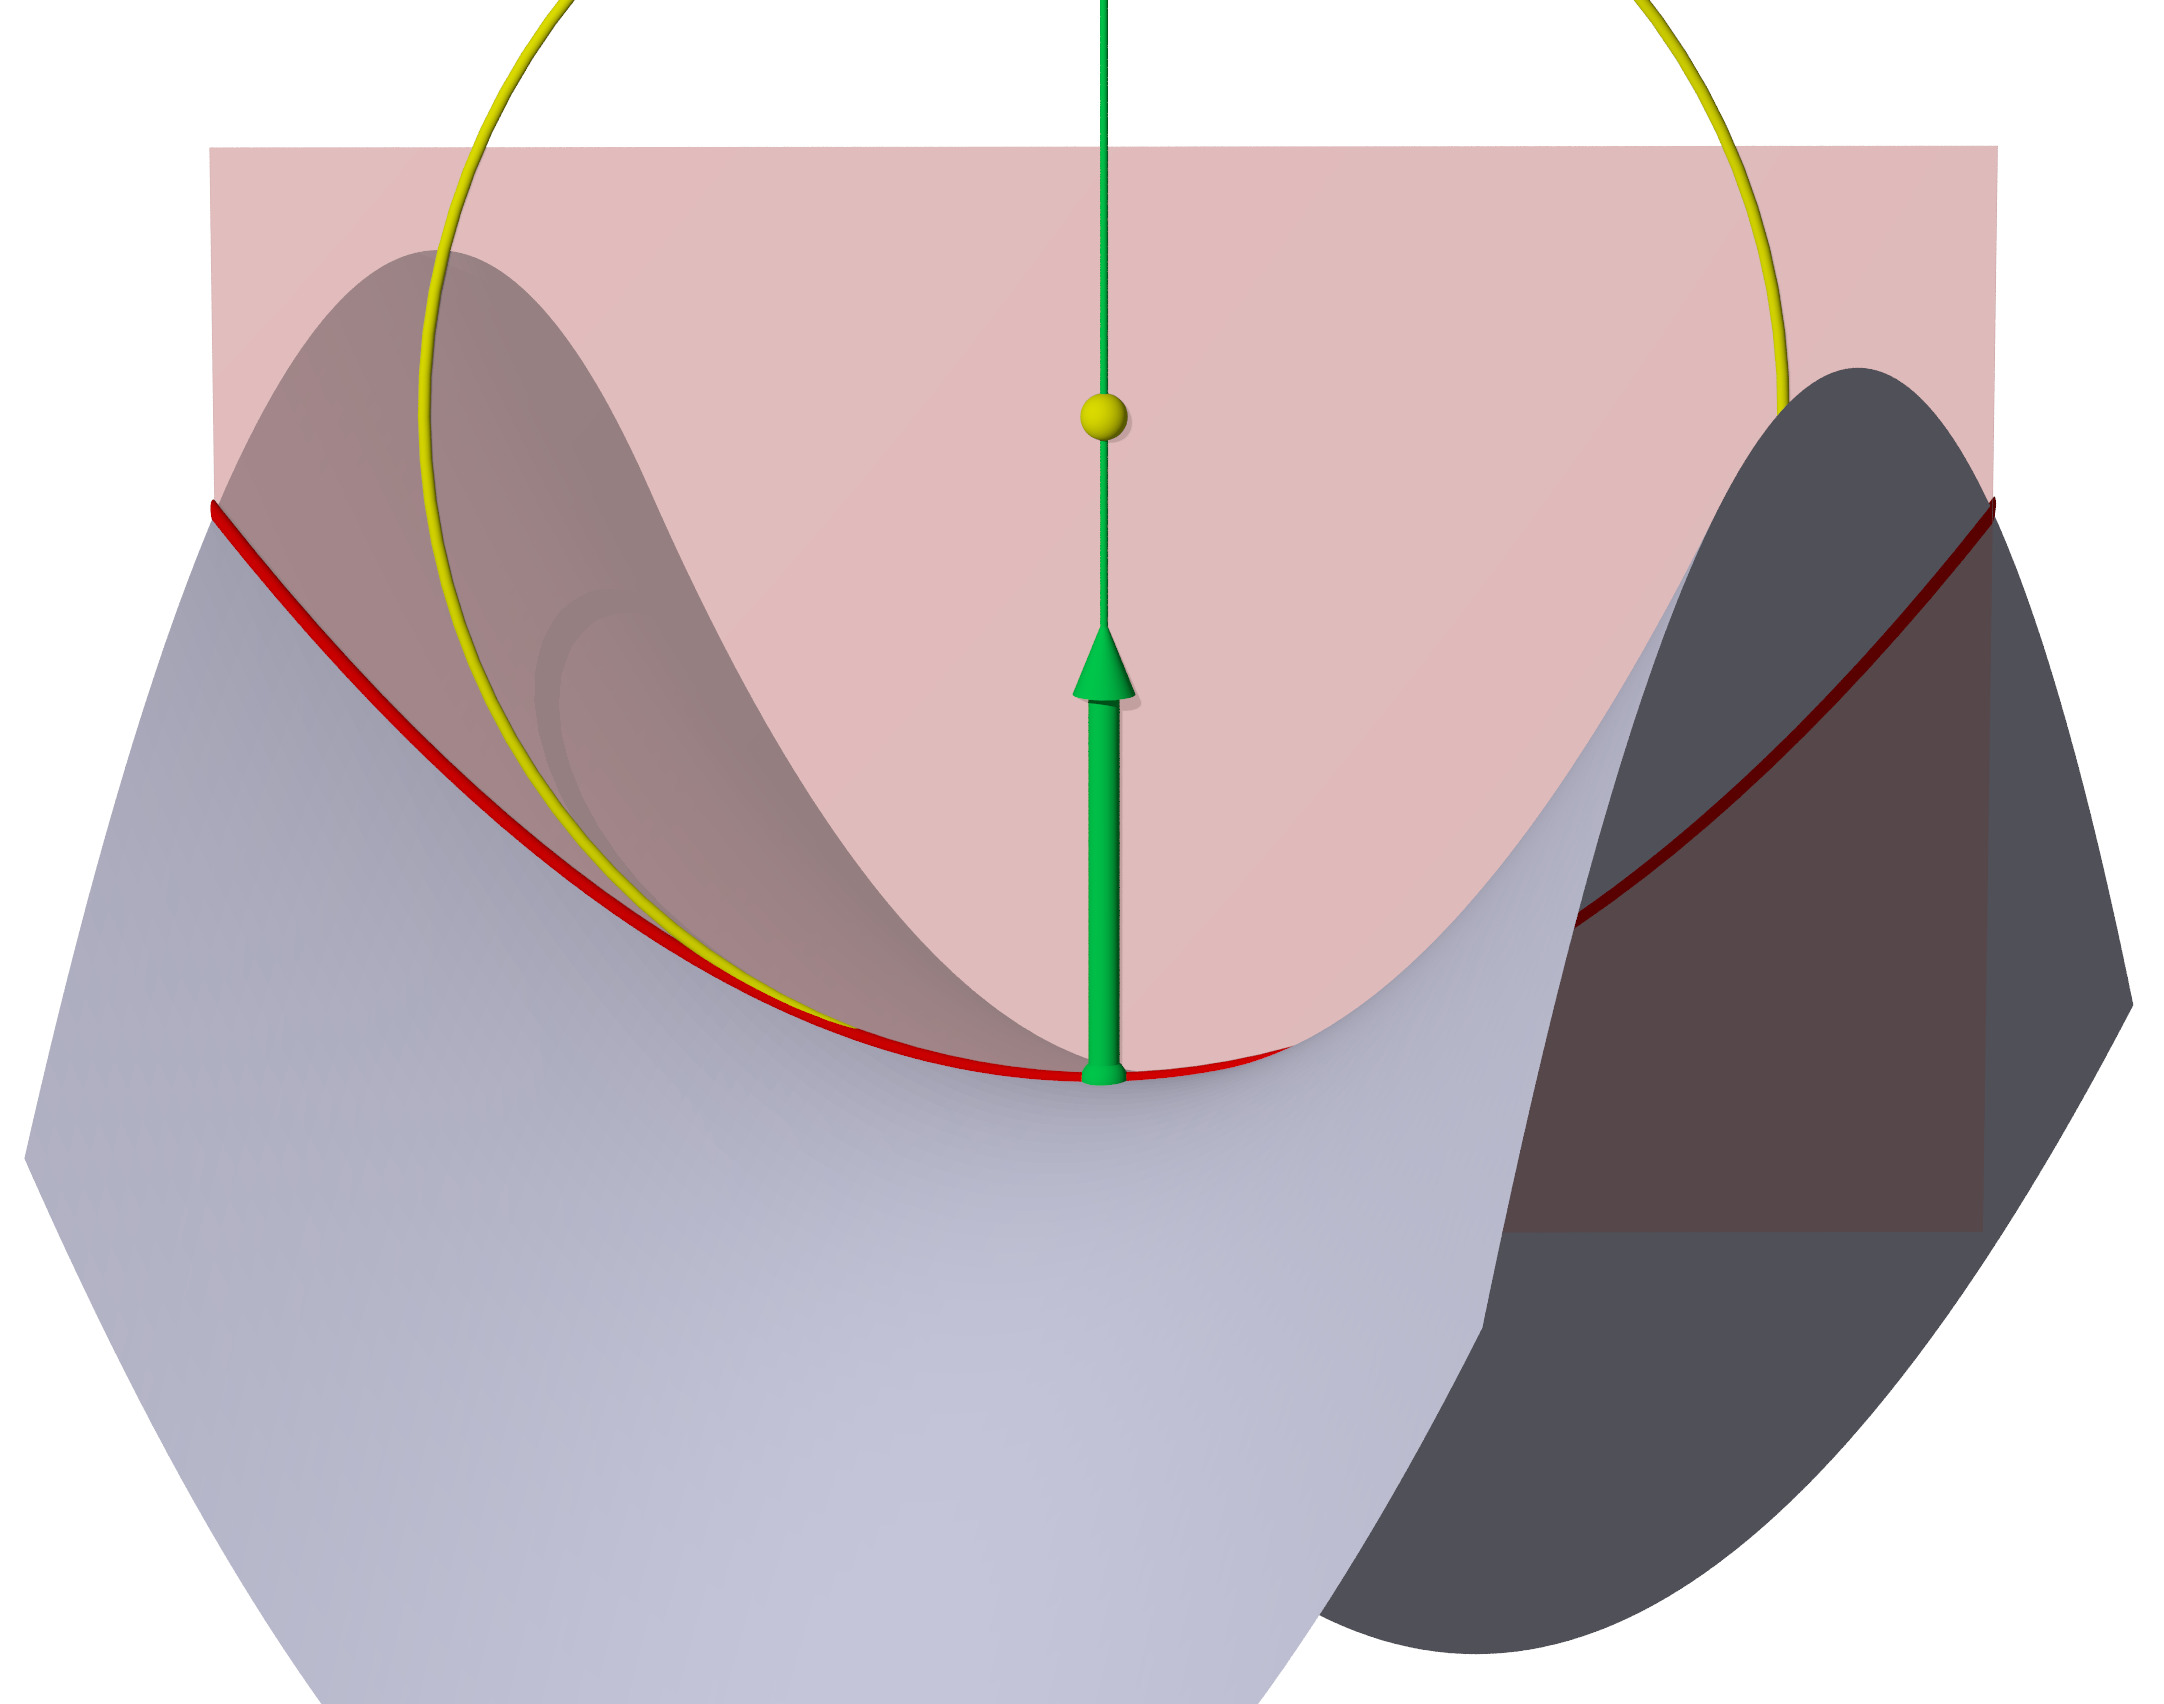
\includegraphics[width=\hsize]{chapters/3d/schnittkruemmung.jpg}
\caption{Die Schnittkrümmung einer Fläche $g(u,v)$ im Punkt $P$ ist
die Krümmung der Schnittkurve (rot) einer Ebene durch $P$, die den
Normalenvektor $n(P)$ (grün) enthält.
Der Krümmungskreis und sein Mittelpunkt $Q$ sind gelb eingezeichnet.
\label{skript:schnittkruemmung}}
\end{figure}
Sei jetzt also eine Fläche $g(u,v)$ gegeben.
Im Punkt $P=g(u_0,v_0)$ betrachten wir Ebenen, die die Normale $n(P)$
enthalten.
Die Schnittkurve der Fläche mit einer solchen Ebene ist eine ebene
Kurve, wir können also deren Krümmung bestimmen
(Abbildung~\ref{skript:schnittkruemmung}).
Es gibt einen Punkt $Q = P + \varrho \cdot n(P)$ in der Ebene, so dass
ein Kreis um den Punkt $Q$ in der Ebene die Krümmung der Kurve bestmöglich
wiedergibt.
Im Gegensatz zur Berechnung der Krümmung in
Abschnitt~\ref{section:kurve:kruemmung}, die immer eine Zahl $\ge 0$
als Wert der Krümmung geliefert hat, spielt es hier das Vorzeichen von
$\varrho$ eine Rolle.
Ist die Kurve in Richtung von $n(P)$ gekrümmt, ist der Punkte $Q$ auf der
gleichen Seite der Fläche wie $n(P)$ und damit $\varrho\ge 0$.
Ist dagegen die Kurve in die Gegenrichtung von $n(P)$ gekrümmt, liegt der
Punkt $Q$ auf der anderen Seite und damit ist $\varrho\le 0$.
Der Punkt $Q$ und der Krümmungskreis sind in
Abbildung~\ref{skript:schnittkruemmung} gelb eingezeichnet.

\begin{beispiel}
\label{skript:sattelbeispiel}
Als Beispiel berechnen wir die Krümmung der Schnittkurve des Graphen
der Funktion
$f(x,y) = x^2-y^2$ im Nullpunkt.
Die Normale $n(0)$ ist der Einheitsvektor in $z$-Richtung, die Schnitt\-ebene
enthält also die $z$-Achse.
Die zulässigen $x$- und $y$-Werte auf der Schnittgeraden sind daher Vielfache
eines Einheitsvektors in der $x$-$y$-Ebene, zum Beispiel $x=t\cos\alpha$
und $y=t\sin\alpha$.
Der Wert von $z$ ist dann
\[
z(t)
=
f(x,y)
=
f(t\cos\alpha,t\sin\alpha)
=
t^2\cos^2\alpha - t^2\sin^2\alpha
=
t^2(\cos^2\alpha - \sin^2\alpha)
=
t^2\cos 2\alpha.
\]
In der Schnittebene ist $t$ massstabsgetreu der Parameter entlang der
horizontalen Achse, $z$ hängt davon quadratisch ab.
Die Krümmung im Nullpunkt kann daher mit der
Formel~\eqref{skript:kruemmung:parabel:scheitel}
berechnet werden,
wir finden
\begin{equation}
\kappa = 2\cos2\alpha
\qquad\Rightarrow\qquad
\varrho = \frac1{2\cos2\alpha}.
\label{skript:kruemmung:sattel}
\qedhere
\end{equation}
\end{beispiel}

Selbstverständlich ist es mit entsprechendem Aufwand möglich, allgemeine
Formeln für die Krümmung der Schnittkurven herzuleiten.
Da wir solche aber nicht explizit brauchen, sondern nur einige wenige
spezielle Eigenschaften, vor allem die Richtungsabhängigkeit, verzichten
wir darauf, diesen Formelapparat zu entwickeln.

\subsection{Richtungsabhängigkeit%
\label{skript:kruemmung:richtungsabhaengigkeit}}
Im Beispiel auf Seite~\pageref{skript:sattelbeispiel} wurde gezeigt, wie
die Krümmung der Schnittkurve von der Richtung der Schnittebene
abhängt.
Dabei entstand die einfache Formel~\eqref{skript:kruemmung:sattel}.
In diesem Abschnitt möchten wir zeigen, dass eine ähnlich einfache
Formel für jede beliebige Fläche gilt.

Gegeben ist also eine Fläche mit Parametrisierung $g(u,v)$, wir möchten
die Krümmungen im Punkte $P=g(u_0,v_0)$ genauer untersuchen.
Offenbar spielt dafür die Lage der Fläche im Raum keine Rolle, wir können
also in einem ersten Schritt das Koordinatensystem so drehen, dass der
Punkt $P$ in den Nullpunkt zu liegen kommt, und dass die $x$-$y$-Ebene des
Koordinatensystems tangential an die Fläche wird.
In dieser Lage lässt sich die Fläche immer als Graph einer Funktion
$z=f(x,y)$ schreiben\footnote{%
Der exakte Beweis dieser intuitiv einleuchtenden Aussage kann mit
dem Satz über implizite Funktionen erfolgen, wir wollen auf die Details
verzichten.}.
Damit haben wir das Problem auf die viel einfachere Situation eines
Graphen reduziert.

Die Funktion $f(x,y)$ kann man als Taylorreihe schreiben, wovon wir nur
die ersten drei Terme hinschreiben wollen
\begin{align*}
f(x,y)
&=
\frac{\partial^2 f}{\partial x^2}x^2
+
2\frac{\partial^2 f}{\partial x\partial y}xy
+
\frac{\partial^2 f}{\partial y^2}y^2
+
o(x^2+y^2)
\\
&=
ax^2 + 2bxy + cy^2 + o(x^2+y^2).
\end{align*}
Die Normale auf die Fläche ist die $z$-Achse, die Schnittebene kann
daher wie im Beispiel wieder durch
\[
x=t\cos\alpha,\quad y=t\sin\alpha
\]
beschrieben werden.
Die Schnittkurve in der Schnittebene hat die Gleichung
\begin{equation}
z
=
(a\cos^2\alpha + 2b\cos\alpha\sin\alpha  + c\sin^2\alpha)t^2
+
\text{Terme dritter Ordnung in $t$}.
\label{skript:kruemmung:klammer}
\end{equation}
Bei der Berechnung der Krümmung braucht man nur die ersten und zweiten
Ableitungen. 
Die erste Ableitung ist ohnehin $0$, die zweiten wird durch die Klammer
im Ausdruck \eqref{skript:kruemmung:klammer} gegeben.
Die Terme dritter Ordnung bleiben nach zweimaligem Ableiten Terme erster
Ordnung, für den Wert $t=0$ fallen sie also weg.
Es bleibt also der quadratische Term als krümmungsbestimmend, wir
können die Formel~\eqref{skript:kruemmung:parabel:scheitel} verwenden, um die
Krümmung in Abhängigkeit von $\alpha$ zu ermitteln.
Wir erhalten
\[
\kappa(\alpha)
=
2(a\cos^2\alpha + 2b\cos\alpha\sin\alpha + c\sin^2 \alpha)
=
2\biggl(
\frac{\partial^2 f}{\partial x^2}\cos^2\alpha
+
2\frac{\partial^2 f}{\partial x\partial y}\cos\alpha\sin\alpha
+
\frac{\partial^2 f}{\partial y^2}\sin^2 \alpha
\biggr).
\]
Die Krümmung einer Schnittkurve in Richtung des Tangentialvektors
$(\cos\alpha,\sin\alpha)$ ist daher durch die zweiten Ableitungen von
$f$ im Punkt $P$ vollständig bestimmt.

\begin{definition}
In jedem Punkt gibt es also eine Abbildung, die jedem
Tangentialeinheitsvektor $e$
die Krümmung der Schnittkurve $\kappa(e)$ einer Ebene durch den Normalenvektor
$n(P)$ und die Tangentenrichrtung $e$ mit der Fläche zuordnet.
Sie heisst die Schnittkrümmung der Fläche in Richtung $e$.
Das Vorzeichen von $\kappa(e)$ ist so gewählt, dass $P+n(P)/\kappa(e)$ der
Mittelpunkt des Krümmungskreises ist.
\end{definition}

%
% hauptkruemmungen.tex
%
% (c) 2017 Prof Dr Andreas Müller, Hochschule Rapperswil
%
\section{Hauptkrümmungen%
\label{skript:kurven:section:hauptkruemmungen}}
In Abschnitt~\ref{skript:kruemmung:richtungsabhaengigkeit} wurde gezeigt,
dass die Schnittkrümmungen $\kappa(e)$ in Abhängigkeit von der
Tangentenrichtung $e$ dank der Wahl eines speziellen Koordinatensystems
mit Hilfe der Matrix der zweiten Ableitung berechnet werden kann.
Wenn $e$ ein Einheitsvektor ist, dann haben wir gefunden, dass die
Schnittkrümmung
\begin{equation}
\kappa(e)
=
2\biggl(
\frac{\partial^2 f}{\partial x^2}
e_1^2
+
2
\frac{\partial^2 f}{\partial x\partial y}e_1e_2
+
\frac{\partial^2 f}{\partial y^2}e_2^2
\biggr)
\label{skript:kurven:ksausdruck}
\end{equation}
ist.
In dieser Form ist nicht klar erkennbar, wie $\kappa(e)$ von $e$ abhängt.
\rhead{Hauptkrümmungen}

Wir können den Ausdruck~\eqref{skript:kurven:ksausdruck} für
$\kappa(e)$ aber auch in Vektorform schreiben.
Dazu schreiben wir die Matrix der zweiten Ableitungen als
\[
H
=
{\def\arraystretch{1.9}
\begin{pmatrix}
\displaystyle\frac{\partial^2 f}{\partial x^2}&
\displaystyle\frac{\partial^2 f}{\partial x\partial y}\\
\displaystyle\frac{\partial^2 f}{\partial x\partial y}&
\displaystyle\frac{\partial^2 f}{\partial y^2}
\end{pmatrix}},
\]
sie heisst die {\em Hessische Matrix}.
\index{Hessische Matrix}%
\index{Matrix, Hessische}%
Damit kann die Krümmung als Matrizenprodukt geschrieben werden:
\[
\kappa(e)
=
\begin{pmatrix}e_1&e_2\end{pmatrix}
{\def\arraystretch{1.9}
\begin{pmatrix}
\displaystyle\frac{\partial^2 f}{\partial x^2}&
\displaystyle\frac{\partial^2 f}{\partial x\partial y}\\
\displaystyle\frac{\partial^2 f}{\partial x\partial y}&
\displaystyle\frac{\partial^2 f}{\partial y^2}
\end{pmatrix}}
\begin{pmatrix}e_1\\e_2\end{pmatrix}
=
e^tHe.
\]
Die Matrix $H$ ist offenbar symmetrisch.

\begin{figure}
\centering
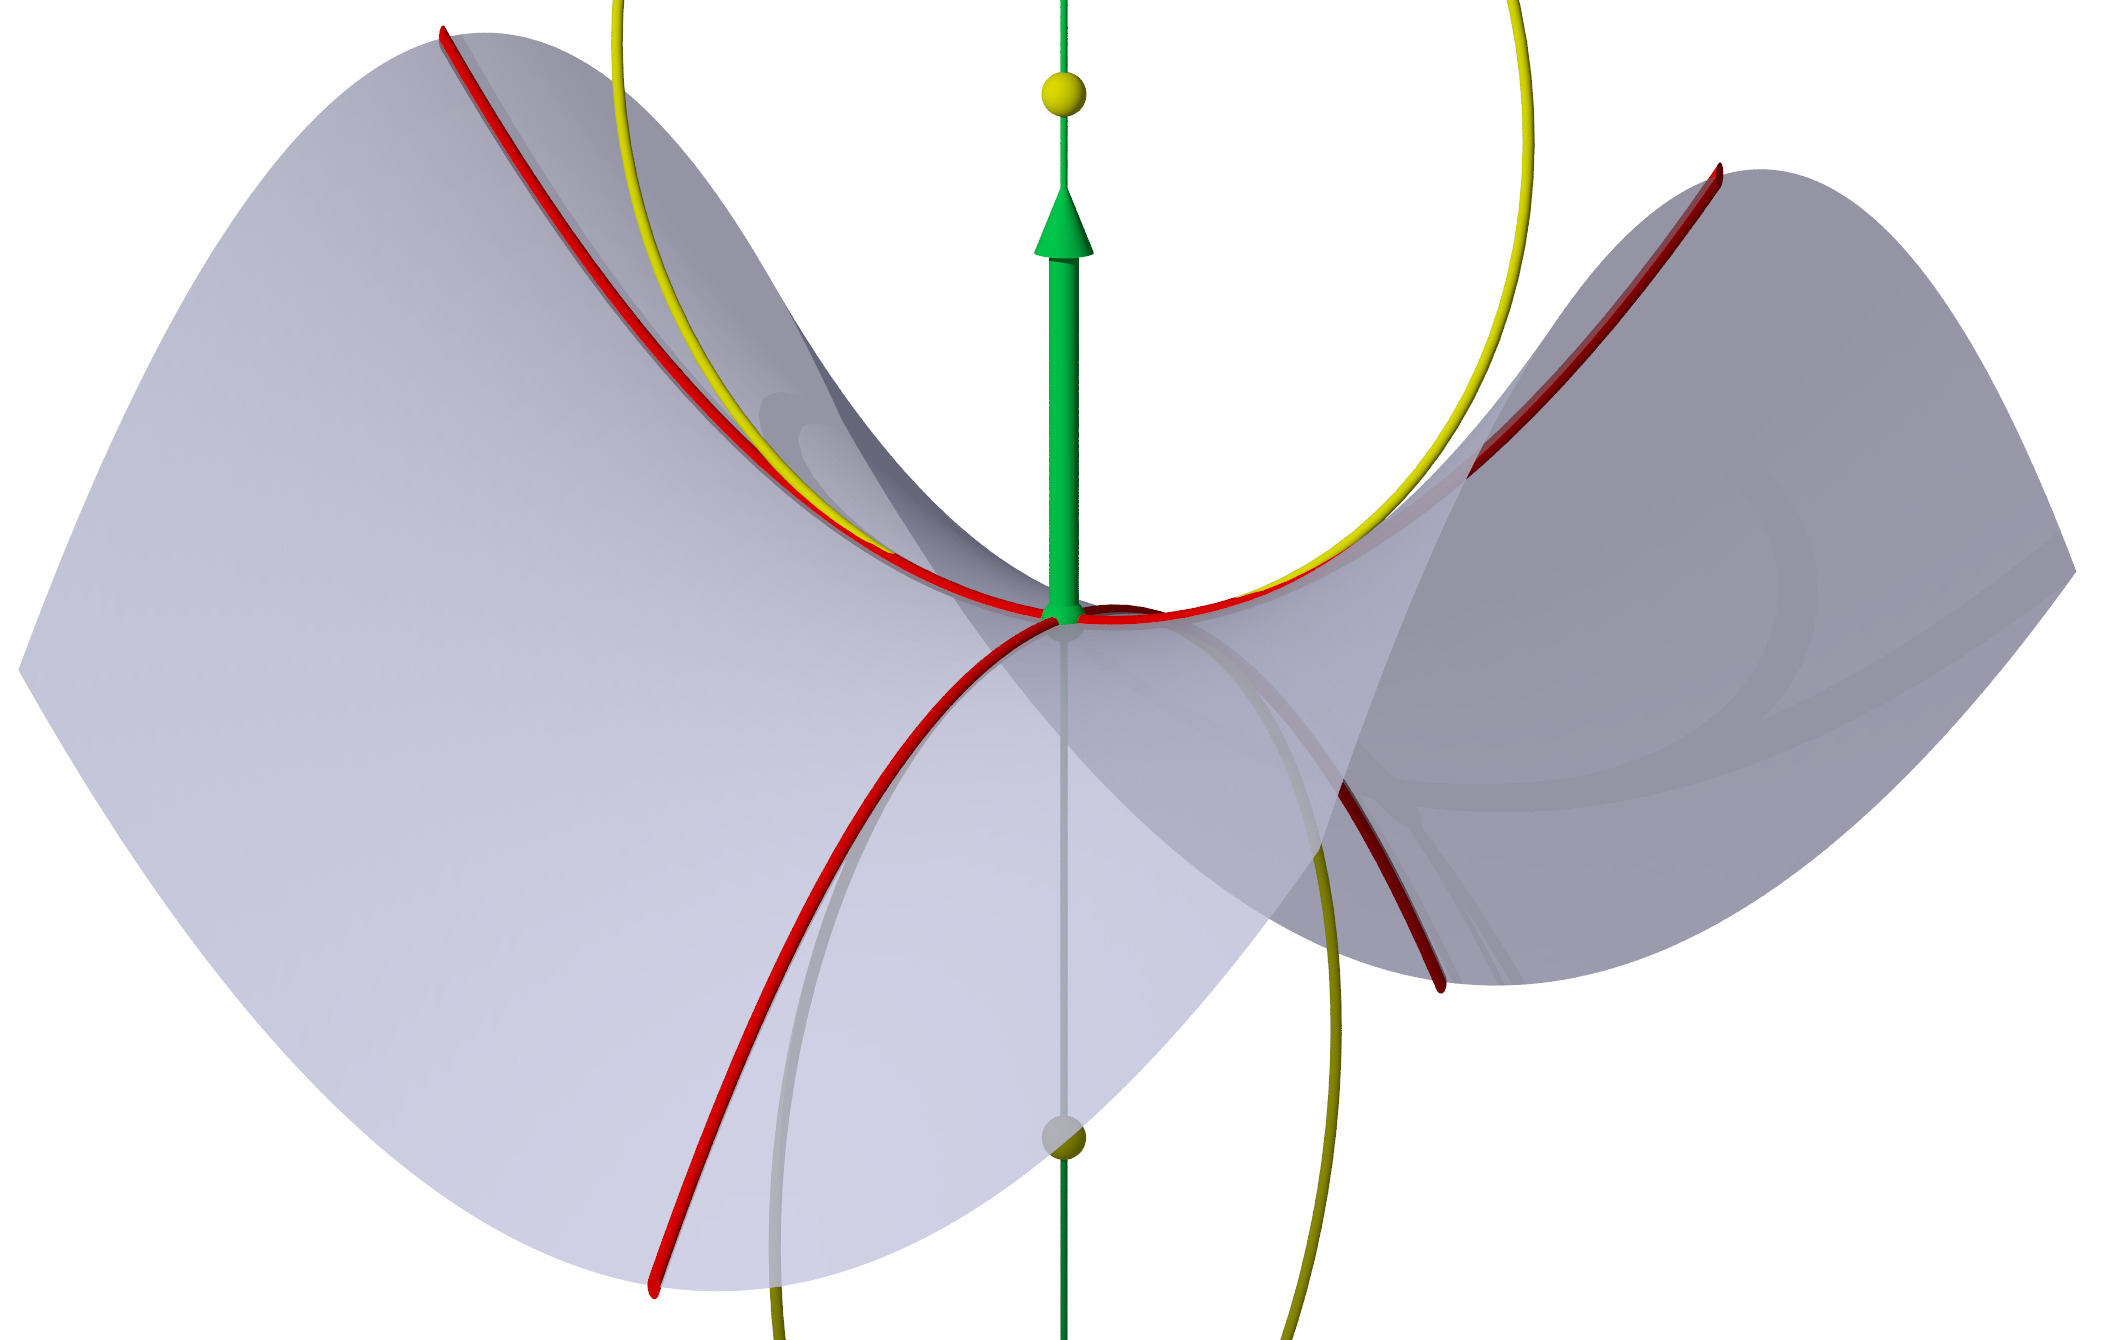
\includegraphics[width=\hsize]{chapters/3d/hauptkruemmungen.jpg}
\caption{Die Hauptkrümmungen einer Fläche sind die maximale und minimale
Schnittkrümmung in einem Punkte.
Die zugehörigen Krümmungsrichtungen heissen die Hauptkrümmungsrichtungen.
In diesem Beispiel haben die beiden Hauptkrümmungen verschiedenes Vorzeichen.
\label{skript:kurven:hauptkruemmungen}}
\end{figure}

In der linearen Algebra lernt man, dass sich jede symmetrische Matrix 
mit Hilfe einer Matrix in $\textrm{SO}(n)$ diagonalisieren lässt.
Auf den vorliegenden Fall angewendet gibt es eine Drehung der
$x$-$y$-Ebene derart, dass
die Matrix $H$ Diagonalform bekommt.
Wir wählen das Koordinatensystem daher so, dass die
Krümmung in Abhängigkeit vom Einheitsvektor $e$ durch
\[
\kappa(e)
=
2\lambda_1 e_1^2 + 2\lambda_2 e_2^2
\]
beschrieben wird,
wobei $\lambda_1$ und $\lambda_2$ die Eigenwerte von $H$ sind.
Für $e_1=\cos\alpha$ und $e_2=\sin\alpha$ bekommt man
\[
\kappa(\alpha)
=
2\lambda_1 \cos^2\alpha + 2\lambda_2 \sin^2\alpha.
\]
Diese Funktion nimmt ihr Maximum und Minimum auf den Achsen an,
die Eigenwerte sind also bis auf den Faktor $2$ die maximale und minimale
Schnittkrümmung.
Wir schreiben $\kappa_1=2\lambda_1$ und $\kappa_2=2\lambda_2$ für die
beiden zugehörigen Krümmungen.
\index{Hauptkrümmungen}%
Diese heissen auch die Hauptkrümmungen, die Richtungen der Achsen heissen
die Hauptkrümmungsrichtung, und sie stehen senkrecht aufeinander, weil
\index{Hauptkrümmungsrichtung}%
die Eigenvektoren einer symmetrischen Matrix zu verschiedenen Eigenvektoren
immer senkrecht aufeinander stehen.

\subsection{Invarianten}
Die hessische Matrix $H$ hat die Eigenwerte $\lambda_1$ und $\lambda_2$.
Als einzelne Werte sind diese nicht so interessant.
Hingegen sind die Determinante und die Spur von $H$ Invarianten, die
unabhängig von der Wahl des Koordinatensystems sind.

\subsubsection{Determinante --- Gausskrümmung}
\index{Gausskrümmung}%
\index{Krümmung!Gauss-}%
\index{Determinante}%
Die Determinante von $H$ ist das Produkt der Eigenwerte, also
\[
\det H
=
\lambda_1\lambda_2
=
\frac14 (2\lambda_1) (2\lambda_2)
=
\frac14 \kappa_1\kappa_2.
\]
\begin{definition}
\label{skript:definition:gausskruemmung}
Das Produkt der Hauptkrümmungen $K=\kappa_1\kappa_2$
heisst {\em Gausskrümmung} der Fläche.
\end{definition}
Es stellt sich heraus, dass die Gausskrümmung auch aus inneren Eigenschaften
der Fläche ermittelt werden kann
(Theorema Egregium von Gauss).
Wir werden in Kapitel~\ref{skript:chapter:kruemmung} 
mit der Riemannschen Krümmung ein Konzept der Krümmung eines Raumes
definieren, welches für Flächen im Wesentlichen mit der Gausskrümmung
übereinstimmt.

\subsubsection{Spur --- mittlere Krümmung}
\index{mittlere Krümmung}%
\index{Krümmung!mittlere}%
\index{Spur}%
Die Spur von $H$ ist eine weitere Invariante der Hessischen Matrix.
Es gilt
\[
\operatorname{Spur} H
=
\lambda_1+\lambda_2
=
\frac12(2\lambda_1+2\lambda_2)
=
\frac12(\kappa_1+\kappa_2).
\]
In Abschnitt~\ref{skript:kurve:mittlerekruemmung} haben wir nachgeweisen,
dass die mittlere Krümmung gleichzeitig die Spur der Hessischen Matrix ist.
Obige Überlegung zeigt, dass dies auch der Mittelwert der Hauptkrümmungen ist.
Dies führt auf die folgende alternative Definition der mittleren Krümmung.

\begin{definition}
\label{skript:definition:mittlerekruemmung2}
Die {\em mittlere Krümmung} ist auch der Mittelwert
\[
M=\frac12(\kappa_1+\kappa_2)
\]
der Hauptkrümmungen.
\end{definition}
Die mittlere Krümmung ist wichtig zur Charakterisierung von Minimalflächen
im Kapitel~\ref{chapter:minimal}.

\subsection{Gausskrümmung und Flächeninhalt%
\label{skript:kurven:gaussflaeche}}
Die mittlere Krümmung $M$ hat eine einfach geometrische Interpretation
als Mittelwert aller Schnittkrümmungen.
Sie zeigt auch ganz offensichtlich, dass sie eine Eigenschaft der Einbettung
einer Fläche in den dreidimensionalen Raum ist.
Für die Gausskrümmung fehlt uns eine vergleichbare Charakterisierung.
Wir wollen daher in diesem Abschnitt zeigen, dass die Gausskrümmung
mit der Längenmessung entlang eines kleinen Kreises um den Nullpunkt
zusammenhängt.
Da sowohl die Länge wie auch der Flächeninhalt unabhängig von der
Einbettung gemessen werden kann,
wird dies auch gleichzeitig illustrieren, dass die Gausskrümmung eine
innere Eigenschaft einer Fläche ist.

\begin{figure}
\centering
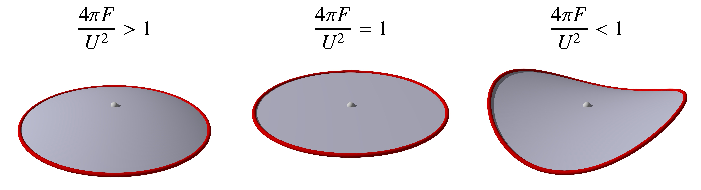
\includegraphics{chapters/tikz/4pifu2.pdf}
\caption{Das Verhältnis von Flächeninhalt zu Umfang im Quadrat einer
kleinen Kreisscheibe hängt von der Gausskrümmung ab. 
Für eine Flache Kreisscheibe gilt $4\pi F/U^2=1$ (Mitte).
Bei positiver Gausskrümmung (links) ist der Umfang gleich, der Flächeninhalt
aber grösser, daher wird das Verhältnis grösser.
Bei negativer Gausskrümmung (rechts) wird der Umfang deutlich länger, so dass
das Verhältnis kleiner wird.
\label{skript:kurven:4pifu2vis}}
\end{figure}
Dazu betrachten wir wieder eine Fläche der Form $z=f(x,y)$, deren
Tangentialebene im Nullpunkt die $x$-$y$-Ebene ist.
In dieser Fläche betrachten wir den Kreis parametrisiert mit
$x=R\cos t$ und $y=R\sin t$.
In einer Ebene wird der Flächeninhalt $F=\pi R^2$ sein, der Umfang $U=2\pi R$.
Man kann auch sagen, dass
\[
U^2 = 4\pi F
\qquad\Rightarrow\qquad
\frac{4\pi F}{U^2}=1
\]
ist.
Wir untersuchen, wie sich diese Beziehung ändert, wenn die
Fläche nicht mehr eine Ebene ist (Abbildung~\ref{skript:kurven:4pifu2vis}).

Wir approximieren die Fläche wieder als quadratische Funktion.
Zur Vereinfachung der Rechnung verwenden wir dabei ein Koordinatensystem,
in dem die Hauptrkümmungsrichtungen die Achsen sind.
Die Funktion $f(x,y)$ hat daher die Form
\[
f(x,y)
=
\kappa_1 x^2 + \kappa_2 y^2
\qquad\text{und}\qquad
g(x,y)=\begin{pmatrix}x\\y\\\kappa_1x^2 + \kappa_2y^2\end{pmatrix}.
\]
Für diese Fläche berechnen wir jetzt Flächeninhalt $F$ und 
Umfang $U$.

\subsubsection{Flächeninhalt}
Der Flächeninhalt einer mit $(u,v)$ parametrisierten Fläche $g(u,v)$
wird mit dem Integral
\[
F
=
\int_{D}
\biggr|\frac{\partial g}{\partial u} \times \frac{\partial g}{\partial v}\biggr|
\,du\,dv
\]
über das Definitionsgebiet $D$ der Fläche berechnet.
In unserem Fall verwenden wir $x$ und $y$ als Parameter und das
Definitionsgebiet
\[
D_R = \{ (x,y)\;|\; x^2 + y^2 < R\}.
\]
Der Betrag des Vektorprodukts im Integranden ist in unserem Fall
\begin{align*}
\biggl|
\frac{\partial g}{\partial x}
\times
\frac{\partial g}{\partial y}
\biggr|
&=
\left|
\begin{pmatrix}1\\0\\\frac{\partial f}{\partial x}\end{pmatrix}
\times
\begin{pmatrix}0\\1\\\frac{\partial f}{\partial y}\end{pmatrix}
\right|
=
\left|
\begin{pmatrix}1\\0\\2\kappa_1 x\end{pmatrix}
\times
\begin{pmatrix}0\\1\\2\kappa_2 y\end{pmatrix}
\right|
=
\left|
\begin{pmatrix}-2\kappa_1 x\\-2\kappa_2 y\\1
\end{pmatrix}
\right|
\\
&=
1 + 4\kappa_1^2 x^2 + 4 \kappa_2^2 y^2.
\end{align*}
Da das Integrationsgebiet eine Kreisscheibe mit Radius $R$ ist, verwenden
wir mit Vorteil Polarkoordinaten.
Wir ersetzen $x=r\cos\varphi$, $y=r\sin\varphi$ und $dx\,dy = r\,dr\,d\varphi$
und schreiben das Integral als
\begin{align*}
F
&=
\int_0^{2\pi}
\int_0^R
\sqrt{1 + 4\kappa_1^2 r^2 \cos^2 \varphi + 4\kappa_2^2 r^2\sin^2\varphi}
\,
r\,dr\,d\varphi
\end{align*}
Der Integrand ist leider zu kompliziert, um das Integral in geschlossener
Form derart auszuwerten, dass wir daraus die beabsichtigten Schlüsse
ziehen können.
Da wir aber schon bei der Funktion $f(x,y)$ nur mit einer Approximation
für kleine Werte von $r$ arbeiten, können wir den Integranden in eine
Taylorreihe in $r$ entwickeln.
Die Rechnung mit dem Maxima Programm
\lstinputlisting[style=Maxima]{chapters/listings/flaecheninhalt.maxima}
ergibt
\begin{align*}
F
%&=
%\int_0^{2\pi}
%\int_0^R
%\frac12R^2(1+R^2\kappa_1^2 \cos^2\varphi + R^2 \kappa_2^2\sin^2\varphi)
%\,r\,dr\,d\varphi
%\\
&=
\pi R^2
\bigl(
1
+
{\textstyle\frac12} R^2(\kappa_1^2+\kappa_2^2)
\bigr).
\end{align*}
Der erste Terme ist natürlich exakt der Flächeninhalt einer Kreisscheibe
in der Ebene.

\subsubsection{Umfang}
Für den Umfang berechnen wir das Wegintegral entlang des Randes.
Um eine Parametrisierung der Randkurve zu bekommen,
ersetzen wir $x=R\cos t$ und $y=R\sin t$ in $g(x,y)$ und erhalten
\[
c(t)
=
\begin{pmatrix}
R\cos t\\ R\sin t\\ R^2(\kappa_1^2\cos^2 t + \kappa_2^2\sin^2 t)
\end{pmatrix}
=
R
\begin{pmatrix}
\cos t\\ \sin t\\ R(\kappa_1^2\cos^2 t + \kappa_2^2\sin^2 t)
\end{pmatrix}.
\]
Wir müssen den Betrag der Ableitung $\dot c(t)$ integrieren.
Das ist das Integral
\begin{align*}
U
&=
R
\int_0^{2\pi}
\sqrt{
\sin^2 t + \cos^2 t 
+ R^2(\kappa_1^2 \cos^2 t + \kappa_2^2\sin^2 t)
}
\,dt,
\end{align*}
welches sich ebenfalls nicht in geschlossener Form auswerten lässt.
Auch hier wählen wir wieder die Entwicklung in eine Taylorreihe nach $R$,
denn wir brauchen $U$ ja nur für kleine Werte von $R$.
Die Rechnung mit dem Maxima Programm
\lstinputlisting[style=Maxima]{chapters/listings/umfang.maxima}
gibt wieder
\begin{align}
U
&\simeq
R
\int_0^{2\pi}
1 + 2(\kappa_1^2 - 2\kappa_1\kappa_2 + \kappa_2^2)R^2 \cos^2 t\sin^2 t
\,dt
\notag
\\
&=
2\pi R
(
1
+ 
{\textstyle \frac14}(\kappa_1^2 -2\kappa_1\kappa_2+\kappa_2^2) R^2
).
\label{skript:kurven:U1}
\end{align}
Für die Beziehung zwischen Umfang und Flächeninhalt brauchen wir aber nicht
$U$ sondern sein Quadrat (auch dies wird im oben gelisteten Programm bereits
berechnet).
In unserer Näherung brauchen wir dabei nur Terme bis zur vierten Ordnung
in $R$ zu berücksichtigen.
Wegen $(1+x)^2 \simeq 1+2x$ in niedrigster Ordnung, bedeutet das nur,
dass wir den zweiten Term in der Klammer in \eqref{skript:kurven:U1}
verdoppeln müssen.
Wir bekommen daher
\begin{align*}
U^2
&\simeq
4\pi^2 R^2(
1
+
{\textstyle \frac12}
(\kappa_1^2-2\kappa_1\kappa_2 + \kappa_2^2)R^2
)
\end{align*}
als Approximation in niedrigster Ordnung.

\subsubsection{Beziehung zwischen Umfang und Flächeninhalt}
Wir müssen die Grösse $4\pi F/U^2$ untersuchen.
Mit den bisher berechneten Ausdrücken für $F$ und $U$ erhalten wir
\begin{align}
\frac{4\pi F}{U^2}
&=
\frac{4\pi^2R^2(1+{\textstyle\frac12}(\kappa_1^2 + \kappa_2^2)R^2)}%
{4\pi^2 R^2(1+{\textstyle\frac12}(\kappa_1^2-2\kappa_1\kappa_2+\kappa_2^2)R^2)}
=
\frac{1+(\kappa_1^2 + \kappa_2^2)R^2}%
{1+(\kappa_1^2-2\kappa_1\kappa_2+\kappa_2^2)R^2}.
\label{skript:kurven:4piu2}
\end{align}
Wieder brauchen wir nur eine Taylorreihe bis zur zweiten Ordnung in $R$.
Mit Hilfe der geometrischen Reihe 
\[
\frac1{1+x}= 1-x+x^2-x^3+\dots
\]
können wir den Nenner in~\eqref{skript:kurven:4piu2} in den Zähler
bringen.
Wenn wir wieder Terme höherer Ordnung als $R^2$ weglassen, bekommen
wir 
\begin{equation}
\frac{4\pi F}{U^2}
\simeq
1+\kappa_1\kappa_2R^2
=
1 + KR^2
\end{equation}
als Schlussresultat.
Das Produkt der Hauptkrümmungen ist die Gausskrümmung $K=\kappa_1\kappa_2$.
Die Gausskrümmung beschreibt also im Wesentlichen das Anwachsen des
Verhältnisses von Flächeninhalt zu Umfang im Quadrat eines Kreises
in Abhängigkeit von dessen Radius.
Bei positiver Gauss\-krümmung wächst das Verhältnis schneller an
als in einer Ebene, bei negativer Gausskrümmung langsamer.







\section*{Übungsaufgaben}
\rhead{Übungsaufgaben}
\uebungsaufgabe{0101}


%
% laengenmessung.tex -- Längenmessung in einer Fläche oder in einem Raum
%
% (c) 2017 Prof Dr Andreas Müller, Hochschule Rapperswil
%
\chapter{Längenmessung
\label{skript:kruemmung:section:laengenmessung}}
\lhead{Längenmessung}
\rhead{}

Die Physik seit Galileo und Newton machte die Annahme, dass die
Geometrie des Raumes durch ein dreidimensionales rechtwinkliges
Koordinatensystem mit der Längenmessungsformel
\begin{equation}
l=\sqrt{\Delta x^2+\Delta y^2+\Delta z^2}
\label{skript:kruemmung:pytagoras}
\end{equation}
adäquat beschrieben wird.
Diese Annahme entsprach zwar der Erfahrung, doch es gab keine
Begründung dafür.
Der Philosoph Emanuel Kant konnte sich zwar keine andere Geometrie
vorstellen, doch mit den Erkenntnissen von Bolyai, Lobaschevski
und Gauss wurde klar, dass es durchaus denkbare andere Geometrien
gibt.
Bernhard Riemann hat dann auch Methoden entwickelt, wie man die
Geometrie studieren kann, indem man ausschliesslich die Längenmessung
innerhalb des Raumes verwendet.
Damit ist die Geometrie unseres Raumes nicht länger einfach das
Resultat einer axiomatischen Beschreibung, wie Euklid sie gegeben hat,
vielmehr ist sie zu einer experimentellen Wissenschaft geworden.

Da wir nicht weiter annehmen wollen, dass sich der Raum mit Hilfe
eines rechtwinkligen Koordinatensystems adäquat beschreiben lässt,
müssen wir automatisch beliebige Koordinatensysteme zulassen.
Je nach Wahl eines Koordinatensystems werden dann Vektoren, die
wir für die Beschreibung der physikalischen Gesetze benötigen,
verschiedenen Koordinaten haben.
Da alle diese Koordinatensystem gleichberechtigt sind, müssen
wir Vektoren auf einheitliche Art umrechnen können.
Ausserdem müssen die Naturgesetze so formuliert sein, dass
sie in jedem beliebigen Koordinatensystem gleich aussehen.

\section{Koordinatensystem}
\rhead{Koordinatensysteme}
In diesem Kapitel beginnen wir damit, den Begriff der Längenmessung
auf beliebige Koordinatensysteme auszudehnen.
Ein Punkt wird beschrieben durch seine Koordinaten, die wir mit
$x^\mu$ bezeichnen, wobei $\mu$ von $1$ bis $n$ läuft, $n$
ist die Dimension des Raumes. 
Die etwas ungewohnte Schreibweise für die Indizes wie Exponenten
hat einen tieferen Grund in der Tensorrechnung und wird später
verständlich werden.

%\section{Vektoren und Koordinatentransformation}
%\rhead{Vektoren und Koordinatentransformation}
%Eine Koordinatentransformation zwischen zwei Koordinatensystemen ist
%eine Abbildung, die die Koordinaten $x^\mu$ des einen Koordinatensystems
%in die Koordinaten $y^\nu$ des anderen Koordinatensystems umrechnet.
%Man kann also schreiben
%\begin{equation}
%y^{\nu}=y^{\nu}(x^1,\dots,x^n).
%\label{skript:kruemmung:umrechnung}
%\end{equation}

Uns interessiert vor allem die Beschreibung von Bahnkurven, wir möchten
ja zum Beispiel den Absturz in ein schwarzes Loch berechnen können.
Eine Bahnkurve erhält man, indem man die Koordinaten mit der Zeit
varieren lässt.
Eine Kurve wird also beschrieben durch Funktionen $x^\mu(t)$.

In der physikalischen Beschreibung werden meistens Vektoren wie
Geschwindigkeit und Beschleunigung verwendet.
Sie sind die Ableitung der Koordinaten eines Bahnpunktes nach
der Zeit.
Dies lässt sich direkt auch auf die Koordinaten übertragen,
wir erhalten für den Geschwindigkeitsvektor
\[
v^{\mu}(t) = \frac{dx^\mu(t)}{dt} = \dot x^\mu(t).
\]
Die Beschleunigung ist die zweite Ableitung
\[
a^\mu(t)
=
\frac{dv^\mu(t)}{dt}
=
\ddot x^\mu(t)
\]
nach dem Parameter $t$.

Im Moment arbeiten wir nur mit einem einzigen Koordinatensystem.
Die Komponenten $\dot x^\mu$ der Geschwindigkeit hängen offenbar
von der Wahl des Koordinatensystems ab.
Ein anderes Koordinatensystem ist gegeben durch
Koordinatenumrechnungsfunktionen
\[
y^1(x^1,\dots,x^n),\;\dots,\;y^n(x^1,\dots,x^n).
\]
In den $y$-Koordinaten wird die Kurve $x^\mu(t)$ durch die Funktionen
\[
t\mapsto y^\alpha(t)=y^\alpha(x^1(t),\dots,x^n(t))
\]
beschrieben werden.
Der Tangentenvektor ist die Ableitung 
\begin{equation}
\frac{dy^\alpha(t)}{dt}
=
\frac{\partial y^\alpha}{\partial x^1}\frac{dx^1(t)}{dt}
+\dots+
\frac{\partial y^\alpha}{\partial x^n}\frac{dx^n(t)}{dt}
=
\sum_{\mu=1}^n
\frac{\partial y^\alpha}{\partial x^\mu}\frac{dx^\mu(t)}{dt}
\label{skript::summenformel}
\end{equation}
nach $t$, nach der Kettenregel für Funktionen mehrere Variablen.
Wir können zwei Erkenntnisse aus der Formel~\eqref{skript::summenformel}
gewinnen.

Es ist zwar nicht möglich, vom Koordinatensystem unabhängige
Geschwindigkeitskomponenten zu definieren, doch immerhin kann man
angeben, wie die Geschwindigkeitskomponenten zwischen verschiedenen
Koordinatensystemen umzurechnen sind.
Wir leiten daraus ab, dass wir in Zukunft von jedem Objekt, welches
eine koordinatenunabhängige Bedeutung haben soll zwar, zwar nicht
annehmen können, dass dessen Komponenten koordinatenunabhängig sind,
aber wir können fordern, dass wir immer eine Koordinatenumrechnungsformel
analog zu \eqref{skript::summenformel} aufstellen können, die nur die
ersten partiellen Ableitungen verwendet.
Solche Grössen werden wir in Kapitel~\ref{skript:chapter:geodaeten}
genauer definieren.

Die zweite Lehre ist, dass es sehr häufig vorkommen wird, dass wir
wie in 
\eqref{skript::summenformel}
über gleiche Indizes summieren müssen, die in einem Ausdruck sowohl
oben als auch unten vorkommen.
In der Tat kommt es praktisch nicht vor, dass ein oberer und unterer
Index übereinstimmt {\em ohne} dass darüber summiert werden muss.
Wir werden daher in Zukunft in dieser Situation das Summenzeichen weglassen.
Dies ist die {\em Einsteinsche Summenkonvention} Summenkonvention
\index{Summenkonvention!Einsteinsche}

%Wie sieht der Geschwindigkeitsvektor in $y^{\nu}$ Koordinaten aus?
%Dazu setzen wir die Bahnkurve in die Umrechnungsformeln
%\eqref{skript:kruemmung:umrechnung} ein.
%Die Kettenregel liefert
%\begin{align*}
%y^{\nu}(t)&=y^{\nu}(x^1(t),\dots,x^n(t))
%\\
%u^{\nu}
%=
%\frac{dy^{\nu}(t)}{dt}
%&=
%\frac{\partial y^{\nu}}{\partial x^1}\frac{dx^1(t)}{dt}
%+\dots+
%\frac{\partial y^{\nu}}{\partial x^n}\frac{dx^n(t)}{dt}
%=
%\sum_{\mu=1}^n
%\frac{\partial y^{\nu}}{\partial x^{\mu}}\frac{dx^{\mu}(t)}{dt}
%\end{align*}
%Auf der rechten Seite steht eine Summe von Termen, in denen
%der Summationsindex sowohl oben als auch unten auftritt.
%Diese Art von Summe kommt in der zu entwickelnden Theorie sehr
%häufig vor, daher schreiben wir in Zukunft die Summe nicht mehr.

%
%Die Koeffizienten 
%\[
%\alpha_\mu^\nu=\frac{\partial y^{\nu}}{\partial x^{\mu}}
%\]
%dienen also der Umrechnung der Komponenten eines Vektors vom
%$x^{\mu}$-Koordinatensystem ins $y^{\nu}$-Koordinatensystem.
%Man kann die Rechnung auch in Matrixform schreiben:
%\[
%\begin{pmatrix}y^1\\\vdots\\y^n\end{pmatrix}
%=
%\begin{pmatrix}
%\frac{\partial y^1}{\partial x^1}&\dots&\frac{\partial y^1}{\partial x^n}\\
%\vdots&\ddots&\vdots\\
%\frac{\partial y^n}{\partial x^1}&\dots&\frac{\partial y^n}{\partial x^n}
%\end{pmatrix}
%\begin{pmatrix}x^1\\\vdots\\x^n\end{pmatrix}.
%\]
%Die Summationskonvention lässt sich zum Beispiel dadurch rechtfertigen,
%dass bei der Matrizenmultiplikation die Summation ja auch nicht
%explizit hingeschrieben wird.

\section{Metrik}
\rhead{Metrik}
In einem rechtwinkligen Koordinatensystem können wir die Länge
einer Kurve durch Zerlegen in beliebig kleine Teilstücke 
\begin{align*}
l
&\simeq
\sum_{i=1}^n \sqrt{\sum_{\mu} (x^{\mu}(t_i)-x^{\mu}(t_{i-1}))^2}
\\
&\rightarrow
\int_{t_0}^{t_n} \sqrt{\sum_{\mu}\biggl(\frac{dx^{\mu}(t)}{dt}\biggr)^2}\,dt
\end{align*}
bestimmen.
Unter der Wurzel sehen wir die Quadratsummen wieder, die für den
Satz des Pythagoras charakteristisch sind.

In einem beliebigen Koordinatensystem funktioniert dies jedoch nicht
mehr.
Wir müssen zulassen, dass die Koordinaten entlang verschiedener
Achsen nicht mehr direkt der Länge entsprechen, dass wir also
entlang der Achsen Skalierungsfaktoren haben.
Weiter ist damit zu rechnen, dass auch gemischte Termen auftauchen.
Die allgemeinstmögliche Form einer Längenmessungsformel ist daher
\begin{equation}
l
=
\int_{t_0}^{t_1}
\sqrt{\sum_{\mu,\nu} g_{\mu\nu} \frac{dx^{\mu}(t)}{dt}\frac{dx^{\nu}(t)}{dt}}\,dt.
\label{skript:kruemmung:metrikformel}
\end{equation}
Die Zahlen $g_{\mu\nu}$ können dabei auch noch von den Koordinaten
abhängen.
Wir verlangen ausserdem, dass $g_{\mu\nu}=g_{\nu\mu}$ ist, denn
diese beiden Terme sind in \eqref{skript:kruemmung:metrikformel}
auf symmetrische Art und Weise vertreten.

\begin{definition}
Die Zahlen $g_{\mu\nu}$ heissen der metrische Tensor.
\index{Tensor!metrischer}
\end{definition}

Die Schreibweise~\eqref{skript:kruemmung:metrikformel} ist nicht
sehr handlich.
Wesentlich an der Notation ist einzig, wie die Koeffizienten $g_{\mu\nu}$
mit den Koordinateninkrementen $dx^\mu$ kombiniert werden müssen.
Wir können daher formal auch schreiben:
\[
ds^2
=
g_{\mu\nu}\,dx^\mu\,dx^\nu.
\]
Diese Notation ist konsistent, denn die Längenberechnung ist
\begin{equation}
\int\,ds
=
\int \sqrt{g_{\mu\nu}\,dx^\mu\,dx^\nu}
=
\int \sqrt{g_{\mu\nu}\,\dot x^\mu\,\dot x^\nu}\,dt,
\label{skript:kruemmung:laengenelement}
\end{equation}
wozu man einzig die Konvention braucht, dass man in Integralen
$dx^\mu=\dot x^\mu\,dt$ schreiben kann.
Man nennt \eqref{skript:kruemmung:laengenelement} das {\em Längenelement}
der Metrik $g_{\mu\nu}$.
\index{Längenelement}

%
% Beispiel für Längenmessung in einem Koordinatensystem mit nicht
% orthogonalen Achsen.
%
\begin{beispiel}
Wir untersuchen die Längenmessung mit nicht orthogonalen Achsen.
Statt des gewöhnlichen Koordinatensystems in einer Ebene verwenden
wir die Koordinaten $x'=x$ und $y'=x+y$.
In den ungestrichenen Koordinaten ist der Abstand zwischen zwei
Punkten durch den Satz von Pythagoras
\begin{equation}
l^2 = \Delta x^2 + \Delta y^2
\label{skript:kruemmung:p2}
\end{equation}
gegeben.
Um den Abstand in $x'$-$y'$-Koordinaten auszudrücken, müssen wir diese
erst wieder in $x$-$y$-Koordinaten umrechnen. 
Man findet
\[
x=x'
\qquad\text{und}\qquad
y=y'-x=y'-x'.
\]
Eingesetzt in die Formel \eqref{skript:kruemmung:p2} finden wir
\begin{align*}
l^2
&=
\Delta x^2 + \Delta y^2
=
\Delta x^{\prime 2}
+
(\Delta y'- \Delta x')^2
=
\Delta x^{\prime 2}
+
\Delta y^{\prime 2}-2\Delta x'\Delta y' + \Delta x^{\prime 2}
\\
&= 2 \Delta x^{\prime 2} - 2 \Delta x'\Delta y'+\Delta y^{\prime 2}.
\end{align*}
Die zugehörigen Koeffizienten $g_{\mu\nu}$ sind
\[
g_{11} = 2,\quad
g_{12}=g_{21}=-1\quad\text{und}\quad
g_{22}=1.
\]
Diese Koeffizienten beschreiben die gleiche Längenmessung in den 
gestrichenen Koordinaten wie der Satz von Pythagoras in den ursprünglichen
Koordinaten.
Man kann sie auch in der Form
\[
ds^2
=
dx^2+dy^2
=
2\,dx'^2-2\,dx'\,dy'+dy'^2
\]
als Längenelemente beschreiben.
\end{beispiel}

Die Formel \eqref{skript:kruemmung:metrikformel} ist etwas unhandlich.
Wir können aber wieder die Einsteinsche Summenkonvention verwenden,
um das Summenzeichen los zu werden.
Ausserdem kann man die Ableitungen nach $t$ auch mit einem Punkt abkürzen.
Damit lässt sich die Längenmessung daher etwas kompakter als
\[
l=\int_{t_0}^{t_1} \sqrt{g_{\mu\nu}\dot x^{\mu}(t) \dot x^{\nu}(t)}\,dt
\]
schreiben.

\section{Beispiele}
\rhead{Beispiele}
Wir betrachten drei für die Anwendungen wichtige Bespiele von
Koordinatensystemen des gewöhnlichen dreidimensionalen Raumes
und berechnen die zugehörigen metrischen Tensoren.

\subsection{Polarkoordinaten}
Punkte in der Ebene können statt in rechtwinkligen $x$-$y$-Koordinaten
auch mit Hilfe von Polarkoordinaten $(r,\varphi)$ nach der Umrechnungsregel
\begin{align*}
x&=r\cos\varphi\\
y&=r\sin\varphi
\end{align*}
beschrieben werden.
Um den metrischen Tensor zu bestimmen, müssen die Ableitungen von $x$ 
und $y$ nach $t$ durch Ableitungen von $r$ und $\varphi$ nach $t$ 
ausdrücken.
Die Produktregel liefert:
\begin{align*}
\dot x&= \dot r\cos \varphi - r\dot\varphi \sin\varphi 
\\
\dot y&= \dot r\sin\varphi + r\dot\varphi\cos\varphi.
\end{align*}
Eingesetzt in den Satz von Pythagoras folgt
\begin{align*}
\dot x^2 + \dot y^2
&=
\dot r^2\cos^2\varphi -2r\dot r\dot\varphi\cos\varphi\sin\varphi +r^2\dot \varphi^2\sin^2\varphi
+
\dot r^2\sin^2\varphi +2r\dot r\dot\varphi\sin\varphi\cos\varphi +r^2\dot\varphi^2\cos^2\varphi
\\
&=
\dot r^2(\cos^2\varphi+\sin^2\varphi)+ r^2\dot\varphi^2(\sin^2\varphi+\cos^2\varphi)
\\
&=\dot r^2 + r^2\dot\varphi^2.
\end{align*}
Die gemischten Terme haben sich weggehoben.
Man liest daraus für die Koeffizienten des metrischen Tensors
\[
g_{11}=1,\qquad g_{12}=g_{21}=0\qquad\text{und}\qquad g_{22}=r^2
\]
ab.
Das Längenelement in Polarkoordinaten ist daher
\[
ds^2
=
dr^2 + r^2\,d\varphi^2.
\]
\index{Längenelement!in Polarkoordinaten}
Die Koeffizienten hängen zwar von den Koordinaten ab, doch bedeutet
das noch nicht, dass ein gekrümmter Raum vorliegt.
Diese $g_{\mu\nu}$ beschreiben ja die gleiche Längenmessung wie der Satz
des Pythagoras in $x$-$y$-Koordinaten.

\subsection{Zylinderkoordinaten}
Zylinderkoordinaten beschreiben die Punkte des dreidimensionalen
Raumes mit Polarkoordinaten in der $x$-$y$-Ebene und der $z$-Koordinate.
Da wir die Metrik in der $x$-$y$-Ebene schon durch $(r,\varphi)$
ausgedrückt haben, können wir auch die Metrik in Polarkoordinaten
bekommen, indem wir die $z$-Koordinaten ergänzen:
\[
\dot x^2+\dot y^2 +\dot z^2
=
\dot r^2 + r^2\dot\varphi^2 + \dot z^2.
\]
Der zugehörige metrische Tensor hat daher die Koeffizienten
\[
g_{11}=1,\qquad
g_{22}=r^2
\qquad\text{und}\qquad
g_{33}=1,
\]
alle anderen Koeffizienten sind $0$.
Das Längenelement in Zylinderkoordinaten ist
\[
ds^2
=
dr^2+r^2\,d\varphi^2 + dz^2.
\]
\index{Längenelement!in Zylinderkoordinaten}

\subsection{Zylinderoberfläche}
Beschränken wir uns auf die Punkte im Abstand $1$ zur $z$-Achse, erhalten
wir eine Zylinderfläche, welche mit Koordinaten $\varphi$ und $z$
beschrieben werden kann.
Die Längenmessung in dieser Fläche wird durch den metrischen
Tensor der Zylinderkoordinaten beschrieben, in dem wir $r=1$ einsetzen.
Wir erhalten
\[
\dot\varphi^2+\dot z^2.
\]
Das Längenelement auf der Zylinderoberfläche $r=1$ mit den Koordinaten
$\varphi$ und $z$ ist daher
\[
ds^2
=
d\varphi^2+dz^2,
\]
\index{Längenelement!auf der Zylinderoberfläche}
die Koeffizienten des metrischen Tensors sind
\[
g_{11}=1,\qquad
g_{12}=g_{21}=0
\qquad\text{und}\qquad
g_{22}=1.
\]
Dies ist der metrische Tensor einer Ebene mit rechtwinkligen Koordinaten.
Daraus können wir bereits ablesen, dass die Zylinderoberfläche sich durch
Längenmessung nicht von einer Ebene unterscheiden lässt.

\subsection{Kugelkoordinaten}
Kugelkoordinaten beschreiben die Punkte eines dreidimensionalen Raumes
durch die Entfernung $r$ vom Nullpunkt, die geographische Länge
$\varphi$, die von
der $x$-Koordinate gemessen wird, und durch die geographische Breite
$\vartheta$,
die als Winkel von der $z$-Achse gemessen wird.
Die Umrechnung in kartesische Koordinaten erfolgt mit den Formeln
\begin{align*}
x&= r\sin\vartheta\cos\varphi\\
y&= r\sin\vartheta\sin\varphi\\
z&= r\cos\vartheta
\end{align*}
Wir bestimmen wieder die Koeffizienten des metrischen Tensors.
Dazu leiten wir zunächst nach $t$ ab.
\begin{align*}
\dot x
&=
\dot r\sin\vartheta\cos\varphi
+
r\dot\vartheta \cos\vartheta\cos\varphi
-
r\dot\varphi \sin\vartheta\sin\varphi
\\
\dot y
&=
\dot r\sin\vartheta\sin\varphi
+
r\dot\vartheta\cos\vartheta\sin\varphi
+
r\dot\varphi\sin\vartheta\cos\varphi
\\
\dot z
&=
\dot r\cos\vartheta
-
r\dot\vartheta \sin\vartheta
\end{align*}
Bei der Berechnung der Länge werden sich wieder viele Terme
wegen der verschiedenen Vorzeichen des letzten Terms im
Ausdruck für $\dot x$ und $\dot y$ aufheben.
Für den Ausdruck $ \dot x^2 + \dot y^2 + \dot z^2$ findet man
\[
\begin{array}{clclclcl}
 &
\dot r^2\sin^2\vartheta\cos^2\varphi
	&+&r^2\dot\vartheta^2\cos^2\vartheta\cos^2\varphi
		&+&r^2\dot\varphi^2\sin^2\vartheta\sin^2\varphi
			&+&2r\dot r\dot\vartheta\sin\vartheta\cos\vartheta\cos^2\varphi
\\
+&
\dot r^2\sin^2\vartheta\sin^2\varphi
	&+&r^2\dot\vartheta^2\cos^2\vartheta\sin^2\varphi
		&+&r^2\dot\varphi^2\sin^2\vartheta\cos^2\varphi
			&+&2r\dot r\dot\vartheta\sin\vartheta\cos\vartheta\sin^2\varphi
\\
+&
\dot r^2\cos^2\vartheta
	&+&r^2\dot\vartheta^2\sin^2\vartheta
		& &
			&-&2r\dot r\dot\vartheta \sin\vartheta \cos\vartheta
\\
\end{array}
\]
In den Spalten ergänzen sich in den ersten beiden Zeilen jeweils
$\cos^2\varphi$ und $\sin^2\varphi$ zu $1$.
In den ersten beiden Spalten lassen sich danach auch noch
$\cos^2\vartheta$ und $\sin^2\vartheta$ zu $1$ zusammenfassen,
während sich die Terme in der vierten Spalte aufheben.
Damit bekommt man
\begin{equation}
\dot x^2 + \dot y^2 + \dot z^2
=
\dot r^2+r^2\dot\vartheta^2 + r^2\dot\varphi^2\sin^2\vartheta
\label{skript:kruemmung:kugelkoordinaten}
\end{equation}
für die Längenmessung, und
\[
g_{11}=1,\qquad
g_{22}=r^2
\qquad\text{und}\qquad
g_{33}= r^2\sin^2\vartheta
\]
für die nicht verschwindenden Komponenten des metrischen Tensors.
Alternativ kann man dies auch als
\[
ds^2
=
dr^2 + r^2\,d\vartheta^2 + r^2\sin^2\vartheta\,d\varphi^2,
\]
also als Längenelement schreiben.
\index{Längenelement!in Kugelkoordinaten}

\subsection{Kugeloberfläche}
Aus dem metrischen Tensor der Kugelkoordinaten lässt sich durch festhalten
des Radius der metrische Tensor einer Kugeloberfläche ableiten.
Aus dem Ausruck \eqref{skript:kruemmung:kugelkoordinaten}
erhalten wir
\[
\dot\vartheta^2+\dot\varphi^2\sin^2\vartheta.
\]
Der $\sin$-Term deutet an, dass wir hier nicht mehr direkt eine flache
Metrik haben.
Den Nachweis können wir aber erst führen, wenn wir den Begriff der
Krümmung zur Verfügung haben.
Für die nicht verschwindenden Komponenten des metrischen Tensors
finden wir
\[
g_{11} = 1
\qquad\text{und}\qquad
g_{22}=\sin^2\vartheta.
\]
Etwas übersichtlicher ist 
\[
ds^2
=
d\vartheta^2 + \sin^2\vartheta\,d\varphi^2,
\]
das Längenelement auf der Kugeloberfläche.
\index{Längenelement!auf der Kugeloberfläche}
Man erkennt, dass der Koeffizient $g_{22}$ bei $\vartheta \in\{0,\pi\}$
verschwindet.
Man spricht von einer Singularität der Längenmessung.
Dies ist jedoch nur ein Artefakt der Tatsache, dass die Kugelkoordinaten
bei den Polen nicht mehr eindeutig sind.
Zur Beschreibung der Pole sind alle möglichen Werte der geographischen
Länge gleichermassen geeignet.

\section{Übungsaufgaben}
\rhead{Übungsaufgaben}
\uebungsaufgabe{0202}
\uebungsaufgabe{0203}
\uebungsaufgabe{0201}


%
% k-geodaeten.tex -- Gleichung der Geodäten, Christoffel-Symbole
%
% (c) 2017 Prof Dr Andreas Müller, Hochschule Rapperswil
%
\chapter{Geodäten
\label{skript:chapter:geodaeten}}
\lhead{Geodäten}
\rhead{}
In der Ebene ist die kürzeste Verbindung zwischen zwei Punkten
eine Gerade.
Auf einem Zylinder oder Kegel kann man die kürzeste Verbindung finden,
indem man die Fläche in eine Ebene abrollt, und dann dort verwendet,
dass die kürzeste Verbindung in der Ebene eine Gerade ist.
Dies zeigt, dass die kürzesten Verbindung nichts mit der speziellen
Einbettung einer Fläche zu tun hat, sondern eine Eigenschaft ist,
die sich allein aus der Längenmessung in der Fläche ist, man nennt
dies auch eine intrinsische Eigenschaft.

Auf einer Kugeloberfläche kann man die kürzesten Verbindungen ebenfalls
direkt angeben, es sind die Grosskreise.
\begin{figure}
\centering
\includegraphics[width=\hsize]{chapters/3d/geodaete.jpg}
\caption{Ein Ausschnitt aus einem Grosskreis (rot) ist die kürzestmögliche
Verbindung zwischen zwei Punkten auf einer Kugeloberfläche.
Alle anderen Kurven (blau) in der Kugeloberfläche haben grössere Länge.
\label{skript:kruemmung:fig:geodaete}}
\end{figure}
Man kann dabei so argumentieren: von allen Schnitten der Kugeloberfläche
mit Ebenen durch die zwei gegeben Punkte ist der Grosskreis derjenige
mit der kleinsten Krümmung, und daher die ``direkteste'' Verbindung.
Dieses Argument ist allerdings nicht ganz exakt, denn man vergisst dabei,
dass es noch viele weitere Kurven gibt, die die beiden Punkte verbinden
(Abbildung~\ref{skript:kruemmung:fig:geodaete}).
Es ist auch nicht wirklich auf noch allgemeinere Situationen übertragbar,
denn es nützt aus, dass die Kugeloberfläche homogen ist, in jedem Punkt
ist die ``Krümmung'' (ein im Moment noch nicht definierter Begriff) 
gleich gross.

Auch die Ausbreitung des Lichts in einem Medium ist einer solchen
Beschreibung zugänglich.
Das Licht wählt immer den Weg mit der geringsten Laufzeit, nicht
unbedingt den geometrisch kürzesten Weg.
Daher können sich Lichtstrahlen in einem inhomogenen Medium
krümmen.
Aus der Perspektive des Lichtes ist aber nicht die Bahn gekrümmt,
es folgt der in dieser Geometrie geradest möglichen Bahn.
Nicht die Bahn ist gekrümmt, sondern die Längenmessung weicht von
der üblichen \eqref{skript:kruemmung:pytagoras} ab, der Raum ist
gekrümmt.

In diesem Abschnitt suchen wir daher nach einer allgemeinen Methode,
die kürzeste Verbindung, die sogenannten Geodäten zu finden.

\section{Paralleltransport}
\rhead{Paralleltransport}
\begin{figure}
\centering
\includegraphics[width=\hsize]{chapters/3d/transport.jpg}
\caption{Paralleltransport eines Vektors entlang einer Kurve auf
einer Kugeloberfläche%
\label{skript:geodaten:fig:transport}}
\end{figure}
Die Beispiele von kürzesten Verbindungen suggerieren, dass die kürzeste
Verbindung auch die ``geradeste'' ist, sie weicht möglichst wenig von
der Richtung des aktuellen Tangentialvektors ab.
Das Problem bei dieser Interpretation ist allerdings, dass wir Vektoren
in zwei verschiedenen Punkten der Fläche nicht unmittelbar vergleichen
können.
Auf der Kugeloberfläche liegen die Tangentialvektoren an eine Kurve in
verschiedenen Punkten zum Beispiel in verschiedenen Tangentialebenen
an die Kugel.

Wir müssen also zunächst in der Lage sein, Vektoren in zwei verschiedenen
Punkten miteinander zu vergleichen.
Wir können das tun, indem wir einen Vektor entlang einer Kurve transportieren,
wobei wir versuchen, in so parallel zu sich selbst wie möglich zu sich
selbst zu halten (Abbildung~\ref{skript:geodaten:fig:transport}).
Auch dies ist im Moment noch ein etwas schwammiger Begriff. 
Es ist aber klar, dass die Komponenten des transportierten Vektors
sowohl von der Transportrichtung wie auch vom ursprünglichen Vektor
abhängen.

Seien $A^\mu$ die Komponenten eines Vektors, die Richtung mit Komponenten
$\Delta x^\nu$ transport werden soll.
Wenn wir uns entlang einer Kurve in diese Richtung bewegen, werden sich
die Komponenten $A^\mu$ einfach deshalb ändern, weil die Komponenten von
den Koordinaten abhängig sind.
Bei einem paralleltransportierten Vektor wird ein Teil dieser Änderung
komponsiert auf geeignete Art komponsiert sein müssen.
Die Kompensation wird linear vom Vektor $A^\mu$ und von der
Bewegungsrichtung abhängen.
Wir schreiben dafür
\[
\nabla_\nu A^\mu\cdot \Delta x^\nu
=
\biggl(\frac{\partial A^\mu}{\partial x^\nu}
+
\Gamma^\mu_{\alpha\nu}A^\alpha\biggr)\Delta x^\nu.
\]
Die Funktionen $\Gamma^\mu_{\alpha\nu}$ sind vorerst noch nicht bekannt,
wir werden sie noch bestimmen müssen.

\begin{definition}
Die {\em kovariante Ableitung} eines Vektorfeldes $A^\mu$ ist der 
\index{kovariante Ableitung}
\index{Ableitung, kovariante}
Ausdruck
\begin{equation}
\nabla_\nu A^\mu
=
\frac{\partial A^\mu}{\partial x^\nu}
+
\Gamma^\mu_{\alpha\nu}A^\alpha,
\label{skript:geodaeten:kovarianteableitung}
\end{equation}
die Koeffizienten $\Gamma^\mu_{\alpha\nu}$ heissen Christoffelsymbole
zweiter Art oder Zusammenhangskoeffizienten.
Eine weiter verbreitete Schreibweise für die kovariante Ableitung
ist
\[
\nabla_\nu A^\mu
=
A^\mu\mathstrut_{;\nu}.
\]
\end{definition}

Die kovariante Ableitung soll ausdrücken, wie sich die Komponenten eines
Vektors entlang einer Kurve ändern, unabhängig von der konkreten Wahl
des Koordinatensystems.
Paralleltransport soll heissen, dass sich entlang einer Kurve die
Komponenten eines Vektors nicht ändern,
dass also $\nabla_\nu A^\mu=0$.
Insbesondere möchten wir später den Tangentialvektor einer Kurve entlang
der Kurve selbst transportieren.
Die kovariante Ableitung des Tangentialvektors $\dot x^\mu$ entlang
einer Kurve wird dann sein
\[
\nabla_\nu\dot x^\mu
=
\frac{\partial \dot x^\mu}{\partial x^\nu}
+
\Gamma^\mu_{\alpha\nu}\dot x^\alpha
\]
und die zeitliche Änderung entlang der Kurve wird
\[
\nabla_\nu\dot x^\mu\cdot \dot x^\nu
=
\frac{\partial \dot x^\mu}{\partial x^\nu}\dot x^\nu
+
\Gamma^\mu_{\alpha\nu}\dot x^\alpha \dot x^\nu.
\]
Im letzten Ausdruck kommen $x^\alpha$ und $x^\nu$ in symmetrischer
Art und Weise vor.
Dies suggeriert, dass wir die $\Gamma^\mu_{\alpha\nu}$ möglicherweise
sogar symmetrisch wählen können, dass also
$\Gamma^\mu_{\alpha\nu}=\Gamma^\mu_{\nu\alpha}$
gewählt werden kann.
Wir fordern daher zusätzlich, dass die Zusammenhangskoeffizienten
symmetrisch sein sollen.
Es wird sich gleich zeigen, dass dies tatsächlich möglich ist.

Bis jetzt haben wir die Metrik nicht verwendet.
Wir möchten, dass der Paralleltransport die Länge des Vektors beim
Transport entlang einer Kurve nicht verändert.
Die Länge des Vektors wird durch $g_{\mu\nu}\tilde A^\mu \tilde A^\nu$
gegeben.
Die Ableitung entlang der Kurve $x^\mu(t)$ ist
\[
\frac{d}{dt} g_{\mu\nu}\tilde A^\mu \tilde A^\nu\bigg|_{t=0}
=
\frac{\partial g_{\mu\nu}}{\partial x^\alpha}A^\mu A^\nu\dot x^\alpha
-
g_{\mu\nu}A^\mu\Gamma_{\alpha\beta}^\nu A^\alpha \dot x^\beta
-
g_{\mu\nu}\Gamma_{\alpha\beta}^\mu A^\alpha \dot x^\beta A^\nu
=
0.
\]
In diesem Ausdruck kommen in allen Termen $A^\mu$ und $\dot x^\beta$ mit
verschiedenen Indizes vor.
Damit wir diese Faktoren ausklammern können, benennen wir die Indizes um,
so dass sie in allen Termen gleich sind.
Wir erhalten dann die Gleichung
\[
\biggl(
\frac{\partial g_{\mu\nu}}{\partial x^\alpha}
-
g_{\mu\beta}\Gamma_{\nu\alpha}^\beta
-
g_{\beta\nu}\Gamma_{\mu\alpha}^\beta
\biggr)
A^\mu A^\nu\dot x^\alpha
=
0
\]
F"ur die Koeffizienten $\Gamma$.
Diese Gleichung muss f"ur jede beliebige Wahl von $A^\mu$ und jede
beliebige Richtung der Kurve $\dot x^\alpha$ erfüllt sein, wenn der
Klammerausdruck verschwindet für alle Werte der freien, also nicht durch
die Summationskonvention als Laufindizes ausgezeichneten, Indizes.
Wir erhalten also
\begin{equation}
\frac{\partial g_{\mu\nu}}{\partial x^\alpha}
-
g_{\mu\beta}\Gamma_{\nu\alpha}^\beta
-
g_{\beta\nu}\Gamma_{\mu\alpha}^\beta
=
0,
\label{skript:geodaeten:gammaidentitaet}
\end{equation}
ein System von Gleichungen für die $n^3$ Grössen $\Gamma_{\mu\nu}^\alpha$.
Wir können die $\Gamma$ auch allein auf der linken Seite haben:
\[
g_{\mu\beta}\Gamma_{\nu\alpha}^\beta
+
g_{\beta\nu}\Gamma_{\mu\alpha}^\beta
=
\frac{\partial g_{\mu\nu}}{\partial x^\alpha}
\]
Durch zyklische Vertauschung der drei Indizes $\mu$, $\nu$ und $\alpha$
erhalten wir drei Gleichungen
\[
\def\arraystretch{2.0}
\begin{linsys}{3}
g_{\mu\beta}\Gamma_{\nu\alpha}^\beta &+& g_{\beta\nu}\Gamma_{\mu\alpha}^\beta
& &
&=&
\displaystyle
\frac{\partial g_{\mu\nu}}{\partial x^\alpha}
\\
& &g_{\nu\beta}\Gamma_{\alpha\mu}^\beta &+& g_{\beta\alpha}\Gamma_{\nu\mu}^\beta
&=&
\displaystyle
\frac{\partial g_{\nu\alpha}}{\partial x^\mu}
\\
g_{\beta\mu}\Gamma_{\alpha\nu}^\beta
& &
&+&g_{\alpha\beta}\Gamma_{\mu\nu}^\beta 
&=&
\displaystyle
\frac{\partial g_{\alpha\mu}}{\partial x^\nu}
\end{linsys}
\]
Da sowohl $g$ als auch $\Gamma$ in den unteren Indizes symmetrisch
sind, können wir die Gleichungen weiter vereinfachen:
\[
\def\arraystretch{2.0}
\begin{linsys}{3}
g_{\mu\beta}\Gamma_{\nu\alpha}^\beta
	&+& g_{\nu\beta}\Gamma_{\mu\alpha}^\beta
		& &
&=&
\displaystyle
\frac{\partial g_{\mu\nu}}{\partial x^\alpha}
\\
	& &g_{\nu\beta}\Gamma_{\mu\alpha}^\beta
		&+& g_{\alpha\beta}\Gamma_{\nu\mu}^\beta
&=&
\displaystyle
\frac{\partial g_{\nu\alpha}}{\partial x^\mu}
\\
g_{\mu\beta}\Gamma_{\nu\alpha}^\beta
	& &
		&+&g_{\alpha\beta}\Gamma_{\nu\mu}^\beta 
&=&
\displaystyle
\frac{\partial g_{\alpha\mu}}{\partial x^\nu}
\end{linsys}
\]
Subtrahieren wir die erste Zeile von der Summe der letzten beiden,
heben sich ersten Terme weg, es bleibt
\[
g_{\alpha\beta}\Gamma_{\nu\mu}^\beta
=
\biggl(
\frac{\partial g_{\nu\alpha}}{\partial x^\mu}
+
\frac{\partial g_{\alpha\mu}}{\partial x^\nu}
-
\frac{\partial g_{\mu\nu}}{\partial x^\alpha}
\biggr).
\]
Bezeichen wir die inverse Matrix von $g_{\alpha\beta}$ mit
$g^{\alpha\beta}$, dann k"onnen wir nach $\Gamma_{\mu\nu}^\beta$ aufl"osen:
\[
g^{\sigma\alpha}
\biggl(
\frac{\partial g_{\nu\alpha}}{\partial x^\mu}
+
\frac{\partial g_{\alpha\mu}}{\partial x^\nu}
-
\frac{\partial g_{\mu\nu}}{\partial x^\alpha}
\biggr)
=
g^{\sigma\alpha}
g_{\alpha\beta}\Gamma_{\mu\nu}^\beta
=
\delta^\sigma_\beta\Gamma_{\mu\nu}^\beta
=
\Gamma_{\mu\nu}^\sigma.
\]

\begin{definition}
Sei $g_{\mu\nu}$ ein metrischer Tensor. 
Dann heissen die
\[
\Gamma_{\alpha,\mu\nu}
=
\frac12
\biggl(
\frac{\partial g_{\nu\alpha}}{\partial x^\mu}
+
\frac{\partial g_{\alpha\mu}}{\partial x^\nu}
-
\frac{\partial g_{\mu\nu}}{\partial x^\alpha}
\biggr)
\]
die {\em Christoffelsymbole erster Art}
und
\begin{equation}
\Gamma_{\mu\nu}^\sigma
=
g^{\sigma\alpha} \Gamma_{\alpha,\mu\nu}
=
\frac12
g^{\sigma\alpha}
\biggl(
\frac{\partial g_{\nu\alpha}}{\partial x^\mu}
+
\frac{\partial g_{\alpha\mu}}{\partial x^\nu}
-
\frac{\partial g_{\mu\nu}}{\partial x^\alpha}
\biggr)
\label{skript:definition:christoffel2}
\end{equation}
heissen {\em Christoffelsymbole zweiter Art} oder
{\em Zusammenhangskoeffizienten}.
Die auf diese Weise aus der Metrik gewonnenen Zusammenhangskoeffizienten
sind auch als der
{\em Levi-Cività-Zusammenhang} bekannt.
\index{Levi-Cività-Zusammenhang}
\end{definition}

%Die Christoffelsymbole erster und zweiter Art bilden keinen Tensor.
%Im allgemeinen gilt
%\[
%
%\]

\section{Rechenregeln für die kovariante Ableitung}
\rhead{Kovariante Ableitung}
Die kovariante Ableitung eines Vektorfeldes wurde in 
\eqref{skript:geodaeten:kovarianteableitung}
für ein Vektorfeld $A^\mu$ definiert.
Später wurden die Koeffizienten $\Gamma^\alpha_{\mu\nu}$ so bestimmt,
dass der Paralleltransport, der als geometrische Vorstellung der
Formel~\eqref{skript:geodaeten:kovarianteableitung} zu Grunde lag,
Skalarprodukte erhält.
Für zwei Vektorfelder, die beide verschwindende
kovariante Ableitung in beine bestimmte Richtung haben,
verschwindet dann auch die Ableitung in diese Richtung.
Doch wie verhält sich die Ableitung eines Skalarprodukts, wenn
die einzelnen Faktoren nicht verschwindende kovariante Ableitung haben?
Ziel dieses Abschnittes ist, Rechenregeln für die kovariante Ableitung
zusammenzustellen.

Wir betrachten zwei Vektorfelder $A^\mu$ und $B^\mu$ und möchten wissen,
wie sich der Wert des Skalarproduktes $g_{\mu\nu}A^\mu B^\nu$ entlang
einer Kurve mit Tangentenrichtung $C^\mu$ ändert.
Seien $A^\mu$  und $B^\nu$ beliebige Vektorfelder,
dann gilt entlang einer Kurve mit
Richtungsvektor $C^\mu$ im Punkt mit Parameterwert $s=0$
\begin{align*}
\frac{d}{ds}(g_{\mu\nu}A^\mu B^\nu)\bigg|_{s=0}
&=
\frac{\partial g_{\mu\nu}}{\partial x^\alpha}A^\mu B^\nu
+
g_{\mu\nu}\frac{\partial A^\mu}{\partial x^\alpha}C^\alpha B^\nu
+
g_{\mu\nu}A^\mu \frac{\partial B^\nu}{\partial x^\alpha}C^\alpha
\\
&=
\biggl(
\frac{\partial g_{\mu\nu}}{\partial x^\alpha}C^\alpha A^\mu B^\nu
+
g_{\mu\nu}
\biggl(\nabla_\alpha A^\mu - \Gamma^\mu_{\beta\alpha}A^\beta \biggr)
B^\nu
+
g_{\mu\nu}A^\mu \biggl(\nabla_\alpha B^\nu-\Gamma^\nu_{\beta\alpha}B^\beta\biggr)
\biggr)C^\alpha
\\
&=
C^\alpha
\biggl(
g_{\mu\nu}\nabla_\alpha A^\mu B^\nu
+
g_{\mu\nu}A^\mu\nabla_\alpha B^\nu
+
\biggl(
\frac{\partial g_{\mu\nu}}{\partial x^\alpha}
-g_{\beta\nu}\Gamma^\beta_{\mu\alpha}
-g_{\mu\beta}\Gamma^\beta_{\nu\alpha}
\biggr)A^\mu B^\nu
\biggr)
\end{align*}
Der innere Klammerausdruck in der letzten Gleichung ist aber identisch
mit \eqref{skript:geodaeten:gammaidentitaet}, er verschwindet also.
Damit können wir die Komponenten Ableitung in Richtung $C^\mu$ auch
so schreiben:
\[
\frac{\partial}{\partial x^\alpha}
(g_{\mu\nu}A^\mu B^\nu)
=
g_{\mu\nu}\nabla_\alpha A^\mu B^\nu
+
g_{\mu\nu}A^\mu\nabla_\alpha B^\nu,
\]
dies ist die Produktregel für die kovariante Ableitung.

\begin{satz}
Für zwei beliebige Vektorfelder sind die Komponenten der Ableitung
des Skalarproduktes 
\begin{equation}
\frac{\partial}{\partial x^\alpha}
(g_{\mu\nu}A^\mu B^\nu)
=
g_{\mu\nu}\nabla_\alpha A^\mu B^\nu
+
g_{\mu\nu}A^\mu\nabla_\alpha B^\nu.
\label{skript:geodaeten:produktregel}
\end{equation}
\end{satz}

Bis jetzt können wir nur die kovariante Ableitung von Vektorkomponenten
$A^\mu$ berechnen, eine kovariante Ableitung von Komponenten $B_\nu$
ist noch gar nicht definiert.
Wir können aber jeden Vektor $B_\nu$ also das Resultat einer Operation
$B_\nu=B^\alpha g_{\alpha\nu}$ betrachten.
Das Skalarprodukt $A^\mu B_\mu=A^\mu B^\nu g_{\mu\nu}$ erfüllt dann
wieder die Produktregel~\eqref{skript:geodaeten:produktregel},
als
\[
\frac{\partial}{\partial x^\alpha}A^\mu B_\mu
=
\frac{\partial}{\partial x^\alpha}g_{\mu\nu} A^\mu B^\nu
=
g_{\mu\nu} \nabla_\alpha A^\mu B^\nu
+
g_{\mu\nu} A^\mu \nabla_\alpha B^\nu
=
\nabla_\alpha A^\mu B_\mu
+
A^\mu g_{\mu\nu} \nabla_\alpha B^\nu.
\]
Wenn die kovariante Ableitung für $B_\nu$ überhaupt definiert werden 
kann, dann muss gelten
\begin{align}
\nabla_\alpha B_\nu
&=
g_{\mu\nu}\nabla_\alpha B^\mu
\notag
\\
&=
g_{\mu\nu}\frac{\partial B^\mu}{\partial x^\alpha}
+
g_{\mu\nu}\Gamma^\mu_{\alpha\beta}B^\beta
\notag
\\
&=
g_{\mu\nu}\frac{\partial g^{\mu\beta}B_\beta}{\partial x^\alpha}
+
g_{\mu\nu}\Gamma^\mu_{\alpha\beta}g^{\beta\sigma}B_\sigma
\notag
\\
&=
g_{\mu\nu}\frac{\partial g^{\mu\beta}}{\partial x^\alpha} B_\beta
+
\underbrace{g_{\mu\nu}g^{\mu\beta}}_{=\delta_\nu^\beta}\frac{\partial B_\beta}{\partial x^\alpha}
+
g_{\mu\nu}\Gamma^\mu_{\alpha\beta}g^{\beta\sigma}B_\sigma
\notag
\\
&=
\frac{\partial B_\nu}{\partial x^\alpha}
+
g_{\mu\nu}\biggl(
\frac{\partial g^{\mu\sigma}}{\partial x^\alpha}
+\Gamma^\mu_{\alpha\beta}g^{\beta\sigma}
\biggr)B_\sigma
\label{skript:geodaeten:kovkov1}
\end{align}
Die Ableitungen der inversen Matrix $g^{\mu\sigma}$ berechnen wir
durch Ableiten der Bedingung $\delta_\nu^\sigma=g_{\nu\mu}g^{\mu\sigma}$:
\begin{equation}
0
=
\frac{\partial}{\partial x^\alpha}\delta_\nu^\sigma
=
\frac{\partial g_{\mu\nu}}{\partial x^\alpha} g^{\mu\sigma}
+
g_{\mu\nu}
\frac{\partial g^{\mu\sigma}}{\partial x^\alpha}
\qquad\Rightarrow\qquad
g_{\mu\nu}
\frac{\partial g^{\mu\sigma}}{\partial x^\alpha}
=
-
\frac{\partial g_{\mu\nu}}{\partial x^\alpha} g^{\mu\sigma}.
\label{skript:geodaeten:ginvabl}
\end{equation}
Setzen wir jetzt~\eqref{skript:geodaeten:ginvabl}
in~\eqref{skript:geodaeten:kovkov1} ein, erhalten wir
\begin{align*}
\nabla_\alpha B_\nu
&=
\frac{\partial B_\nu}{\partial x^\alpha}
+
\biggl(
-\frac{\partial g_{\mu\nu}}{\partial x^\alpha} g^{\mu\sigma}
+
g_{\mu\nu}
\Gamma^\mu_{\alpha\beta}g^{\beta\sigma}
\biggr)B_\sigma
\end{align*}
In der Klammer ersetzen wir $\Gamma^\mu_{\alpha\beta}$ durch
\eqref{skript:definition:christoffel2} und erhalten
\begin{align*}
-\frac{\partial g_{\mu\nu}}{\partial x^\alpha} g^{\mu\sigma}
+
g_{\mu\nu}
\Gamma^\mu_{\alpha\beta}
g^{\beta\sigma}
&=
-\frac{\partial g_{\mu\nu}}{\partial x^\alpha} g^{\mu\sigma}
+
g_{\mu\nu}
\frac12
g^{\mu\gamma}
\biggl(
\frac{\partial g_{\alpha\gamma}}{\partial x^\beta}
+
\frac{\partial g_{\beta\gamma}}{\partial x^\alpha}
-
\frac{\partial g_{\alpha\beta}}{\partial x^\gamma}
\biggr)
g^{\beta\sigma}
\\
&=
\biggl(
-\frac{\partial g_{\beta\nu}}{\partial x^\alpha} g^{\beta\sigma}
+
\delta_\nu^\gamma
\frac12
\biggl(
\frac{\partial g_{\alpha\gamma}}{\partial x^\beta}
+
\frac{\partial g_{\beta\gamma}}{\partial x^\alpha}
-
\frac{\partial g_{\alpha\beta}}{\partial x^\gamma}
\biggr)
\biggr)
g^{\beta\sigma}
\\
&=
\frac12
\biggl(
-2\frac{\partial g_{\beta\nu}}{\partial x^\alpha} g^{\beta\sigma}
+
\frac{\partial g_{\alpha\nu}}{\partial x^\beta}
+
\frac{\partial g_{\beta\nu}}{\partial x^\alpha}
-
\frac{\partial g_{\alpha\beta}}{\partial x^\nu}
\biggr)
g^{\beta\sigma}
\\
&=
-\frac12
\biggl(
\frac{\partial g_{\beta\nu}}{\partial x^\alpha}
+
\frac{\partial g_{\alpha\beta}}{\partial x^\nu}
-
\frac{\partial g_{\alpha\nu}}{\partial x^\beta}
\biggr)
g^{\beta\sigma}
\\
&=-\Gamma^\sigma_{\alpha\nu}.
\end{align*}
Die rechte Seite der kovarianten Ableitung für einen kovarianten Vektor
kann daher mit den bereits bekannten Christophel-Symbolen zweiter Art
ausgedrückt werden.

\begin{definition}
Die Komponenten der kovariante Ableitung $\nabla_\alpha B_\nu$ eines
kovarianten Vektorfeldes $B_\nu$ in Richtung der Koordinaten $x^\alpha$
ist
\begin{equation}
\nabla_\alpha B_\nu
=
\frac{\partial B_\nu}{\partial\alpha}
-\Gamma^{\sigma}_{\alpha\nu}B_\sigma,
\label{skript:geodaeten:kovabl2}
\end{equation}
Diese wird auch $\nabla_\alpha B_\nu=B_{\nu;\alpha}$ geschrieben.
\end{definition}

% TODO: kovariante Ableitung und Verjüngung

Wir möchten die kovariante Ableitung jetzt auf beliebige Tensoren
verallgemeinern.
Sie soll natürlich linear bleiben und die Produktregel muss ebenfalls
erhalten bleiben.
Ein Tensor der Form $t_{\mu\nu}$ kann immer geschrieben werden
als eine Summe von Tensoren der Form $a_\mu b_\nu$.
Auf einem solchen Tensor muss die kovariante Ableitung die Form
\begin{align*}
\nabla_\alpha (a_\mu b_\nu)
&=
(\nabla_\alpha a_\mu) b_\nu
+
a_\mu(\nabla_\alpha b_\nu)
\\
&=
\biggl(
\frac{\partial a_\mu}{\partial x_\alpha}
-
\Gamma^\sigma_{\alpha\mu}a_\sigma
\biggr)b_\nu
+
a_\mu
\biggl(
\frac{\partial b_\nu}{\partial x_\alpha}
-
\Gamma^\sigma_{\alpha\nu}b_\sigma
\biggr)
\\
&=
\frac{\partial a_\mu b_\nu}{\partial x^\alpha}
-\Gamma^\sigma_{\alpha\mu}a_\sigma b_\nu
-\Gamma^\sigma_{\alpha\nu}
\end{align*}


\begin{definition}
\end{definition}

\section{Beispiele}
\rhead{Beispiele}
In den nachfolgenden Beispielen wollen wir die Christoffelsymbole erster
und zweiter Art für Zylinder- und Kugeloberfläche berechnen.

\subsection{Polarkoordinaten}
Die nicht verschwinden Komponenten
des metrischen Tensors in Polarkoordinaten $(r,\varphi)$
sind $g_{11}=1$ und $g_{22}=r^2$.
Davon brauchen wir die Ableitungen
\[
\begin{aligned}
\frac{\partial g_{11}}{\partial x^1} &=0,&
\frac{\partial g_{12}}{\partial x^1} &=0,&
\frac{\partial g_{21}}{\partial x^1} &=0,&
\frac{\partial g_{22}}{\partial x^1} &=2r,&
\\
\frac{\partial g_{11}}{\partial x^2} &=0,&
\frac{\partial g_{12}}{\partial x^2} &=0,&
\frac{\partial g_{21}}{\partial x^2} &=0,&
\frac{\partial g_{22}}{\partial x^2} &=0
\end{aligned}
\]
Die Christoffelsymbole erster Art sind daher 
\[
\begin{aligned}
\Gamma_{1,11} &=  0,&
\Gamma_{1,12} &=  0,&
\Gamma_{1,21} &=  0,&
\Gamma_{1,22} &= -r,
\\
\Gamma_{2,11} &=  0,&
\Gamma_{2,12} &=  r,&
\Gamma_{2,21} &=  r,&
\Gamma_{2,22} &=  0
\end{aligned}
\]
und die Christoffelsymbole zweiter Art sind
\begin{equation}
\begin{aligned}
\Gamma_{11}^1 &= 0,&
\Gamma_{12}^1 &= 0,&
\Gamma_{21}^1 &= 0,&
\Gamma_{22}^1 &=-r,
\\
\Gamma_{11}^2 &= 0,&
\Gamma_{12}^2 &= \frac1{r},&
\Gamma_{21}^2 &= \frac1{r},&
\Gamma_{22}^2 &= 0.
\end{aligned}
\label{skript:geodaeten:christoffel:polar}
\end{equation}

\subsection{Zylinderkoordinaten}
Da die Komponenten des metrischen Tensors sind konstant, damit verschwinden
alle Ableitungen
\[
\frac{\partial g_{\mu\nu}}{\partial x^\alpha}=0
\qquad\Rightarrow\qquad
\Gamma_{\alpha,\mu\nu}=0
\qquad\Rightarrow\qquad
\Gamma_{\mu\nu}^\alpha=0.
\]

\subsection{Kugelkoordinaten}
Die Kugeloberfläche verwendet die Koordinaten $(\vartheta,\varphi)$.
Zun"achst brauchen wir die Ableitungen der Komponenten des metrischen
Tensors
\begin{align*}
\frac{\partial g_{11}}{\partial \vartheta} &=0,
&
\frac{\partial g_{12}}{\partial \vartheta} &=0,
&
\frac{\partial g_{21}}{\partial \vartheta} &=0,
&
\frac{\partial g_{22}}{\partial \vartheta} &=\sin2\vartheta,
\\
\frac{\partial g_{11}}{\partial \varphi} &=0,
&
\frac{\partial g_{12}}{\partial \varphi} &=0,
&
\frac{\partial g_{21}}{\partial \varphi} &=0,
&
\frac{\partial g_{22}}{\partial \varphi} &=0.
\\
\end{align*}
Daraus können wir die Christoffelsymbole erster Art ableiten:
\begin{align*}
 \Gamma_{1,11}
&=
\frac12\biggl(\frac{\partial g_{11}}{\partial \vartheta}
	+ \frac{\partial g_{11}}{\partial \vartheta}
	- \frac{\partial g_{11}}{\partial \vartheta}\biggr)=0,
&\Gamma_{1,12}
&=
\frac12\biggl(\frac{\partial g_{11}}{\partial \varphi}
	+ \frac{\partial g_{21}}{\partial \vartheta}
	- \frac{\partial g_{12}}{\partial \vartheta}\biggr)=0,
\\
\Gamma_{1,21}
&=
\frac12\biggl(\frac{\partial g_{12}}{\partial \vartheta}
	+ \frac{\partial g_{11}}{\partial \varphi}
	- \frac{\partial g_{21}}{\partial \vartheta}\biggr)=0,
&\Gamma_{1,22}
&=
\frac12\biggl(\frac{\partial g_{12}}{\partial \varphi}
	+ \frac{\partial g_{12}}{\partial \varphi}
	- \frac{\partial g_{22}}{\partial \vartheta}\biggr)=-\frac12\sin2\vartheta,
\\
\Gamma_{2,11}
&=
\frac12\biggl(\frac{\partial g_{12}}{\partial \vartheta}
	+ \frac{\partial g_{12}}{\partial \vartheta}
	- \frac{\partial g_{11}}{\partial \varphi}\biggr)=0,
&\Gamma_{2,12}
&=
\frac12\biggl(\frac{\partial g_{12}}{\partial \varphi}
	+ \frac{\partial g_{22}}{\partial \vartheta}
	- \frac{\partial g_{12}}{\partial \varphi}\biggr)=\frac12\sin2\vartheta,
\\
\Gamma_{2,21}
&=
\frac12\biggl(\frac{\partial g_{12}}{\partial \varphi}
	+ \frac{\partial g_{22}}{\partial \vartheta}
	- \frac{\partial g_{21}}{\partial \varphi}\biggr)=\frac12\sin2\vartheta,
&\Gamma_{2,22}
&=
\frac12\biggl(\frac{\partial g_{22}}{\partial \varphi}
	+ \frac{\partial g_{22}}{\partial \varphi}
	- \frac{\partial g_{22}}{\partial \varphi}\biggr)=0.
\end{align*}
Die inverse Matrix von $g_{\mu\nu}$ hat die nicht verschwindenden
Komponenten
\[
g^{11} = 1
\qquad\text{und}\qquad
g^{22} = \frac1{\sin^2\vartheta}
\]
und die Christoffelsymbole 2.~Art
\begin{equation}
\begin{aligned}
 \Gamma_{11}^1
&=0,
&\Gamma_{12}^1
&=0,
&\Gamma_{21}^1
&=0,
&\Gamma_{22}^1
&=-\frac12\sin2\vartheta,
\\
 \Gamma_{11}^2
&=0,
&\Gamma_{12}^2
&=\cot\vartheta,
&\Gamma_{21}^2
&=\cot\vartheta,
&\Gamma_{22}^2
&=0.
\end{aligned}
\label{skript:kruemmung:christoffelkugel}
\end{equation}


\section{Geodätengleichung}
\rhead{Geodätengleichung}
Die Rolle der Geraden in der Ebene müssen diejenigen Kurven auf der
Fläche übernehmen, die so gerade wie möglich sind. 
Eine Gerade ist dadurch charakterisiert, dass sie überall die gleiche
Richtung hat. 
Diese Formulierung ist aber nur möglich, weil Tangentialvektoren in
beliebigen Punkten unmittelbar miteinander vergleichen können.
Für einen allgemeinen Raum müssen wir diesen Vergleich mit Hilfe
des Paralleltransportes durchführen.
Die Forderung an die Kurve wird dann, dass der Tangentialvektor
an die Kurve durch Paralleltransport wieder in einen Tangentialvektor
an die Kurve übergeht.

Etwas formaler setzen wir den Tangentialvektor $\dot x^\mu$ an die
Kurve in die Gleichung \eqref{skript:kruemmung:ableitung} ein und
erhalten die Differentialgleichung 
\begin{equation}
\ddot x^\alpha+\Gamma_{\mu\nu}^\alpha \dot x^\mu\dot x^\nu=0.
\label{skript:kruemmung:geodatengleichung}
\end{equation}
\index{Geodäte}

\begin{definition}
Eine Kurve in einem Riemannschen Raum heisst eine Geodäte, wenn sie
die Differentialgleichung~\eqref{skript:kruemmung:geodatengleichung}
erfüllt.
\end{definition}

In den nachfolgenden Beispielen wollen wir die Geodäten für diejenigen
Räume berechnen, für die wir die Christoffelsymbole bereits bestimmt
haben.

%
% XXX Geschwindigkeitsinvarianz
%

\subsection{Flache R"aume}
In flachen Räumen wie der Ebene oder der Zylinderoberfläche verschwinden
alle Christoffelsymbole.
Die Geodätengleichung ist daher nur noch
$\ddot x^\alpha=0$, was gleichbedeutend ist mit
\[
x^\alpha(t)=x^\alpha(0) + t \dot x^\alpha(0),
\]
also einer Geradengleichung.
In flachen Räumen sind die Geodäten Geraden.

\subsection{Polarkoordinaten}
Die Geodätengleichungen in Polarkoordinaten erhält man durch
Einsetzen der Christoffelsymbole von
\eqref{skript:geodaeten:christoffel:polar}
in
\eqref{skript:kruemmung:geodatengleichung}.
Die Gleichungen lauten
\begin{equation}
\begin{aligned}
\ddot r &= r\dot \varphi^2,
\\
\ddot \varphi &= -2\frac{\dot r}{r}\dot\varphi.
\end{aligned}
\label{skript:geodaeten:dglpolar}
\end{equation}
Radiale Geraden haben $\dot\varphi=0$, aus der ersten Gleichung folgt dann
$\ddot r=0$ oder $\dot r=\operatorname{const}$.
Geodäten durch den Nullpunkt sind also mit konstanter Geschwindigkeit
durchlaufene Geraden.

Wir dürfen natürlich davon ausgehen, dass jede beliebige andere Gerade
ebenfalls eine Geodäte ist.
Um dies nachzuprüfen betrachten wir eine Gerade senkrecht auf die
$r=0$-Achse, in $x$-$y$-Koordinaten können wir sie als
$t\mapsto (x_0,t)$ beschreiben.
Die zugehörigen Polarkoordinaten sind
\[
\begin{aligned}
r(t)&=\sqrt{x_0^2+t^2}
&&\text{und}&
\varphi(t)&=\arctan\frac{t}{x_0}.
\end{aligned}
\]
Wir prüfen durch einsetzen, ob diese Funktionen die
Geodätendifferentialgleichung~\eqref{skript:geodaeten:dglpolar}
erfüllen.
Die Ableitungen von $r(t)$ und $\varphi(t)$ sind
\begin{align*}
\dot r(t)
&=\frac{t}{r},
&
\ddot r(t)
&=
\frac{1}{r}-\frac{t^2}{r^3}
=
\frac{r^2-t^2}{r^3}
=
\frac{x_0^2}{r^3},
\\
\dot\varphi(t)
&=
\frac{x_0}{r^2},
&
\ddot\varphi(t)
&=
-\frac{2tx_0}{r^4}.
\end{align*}
Setzen wir dies in die
Differentialgleichungen~\eqref{skript:geodaeten:dglpolar}
ein, erhalten wir
\begin{align*}
r\dot\varphi^2
&=
r\frac{x_0^2}{r^4}
=
\frac{x_0^2}{r^3}
=
\ddot r,
\\
-2\frac{\dot r}{r}\dot\varphi
&=
-2\frac{t}{r}\frac1{r}\frac{x_0}{r^2}
=
-\frac{2tx_0}{r^4}
=
\ddot\varphi.
\end{align*}
Wie erwartet erfüllt also die Gerade die Geodätengleichung.

\subsection{Kugeloberfläche}
Die Christoffelsymbole zweiter Art für die Kugeloberfläche haben wir
in \eqref{skript:kruemmung:christoffelkugel} berechnet.
Statt die Differentialgleichung der Geodäten direkt zu lösen, versuchen
wir nur, die Parameterdarstellung eines Grosskreises in die
Differentialgleichung einzusetzen und damit zu zeigen, dass die
Grosskreise Lösungen der Geodätengleichung sind.
Da es durch jeden Punkt der Kugeloberflächen und zu jeder Tangentialrichtung
einen Grosskreis gibt, und die Lösungen der Geodätengleichung eindeutig
sind, können wir schliessen, dass alle Geodäten Grosskreise sind.

Der Äquator der Kugel hat eine besonders einfache Parametrisierung mit
\[
\begin{aligned}
x^1(t)=\vartheta(t)&=\frac{\pi}2,
&\qquad&&
x^2(t)=\varphi(t)&=t
\end{aligned}
\]
mit den Ableitungen
\[
\begin{aligned}
\dot x^1(t)&=0,
&\qquad&&
\dot x^2(t)&=1.
\end{aligned}
\]
Die zweiten Ableitungen der Koordinaten verschwinden, da die ersten
Ableitungen konstant sind.
Wir setzen die ersten Ableitungen in die Geodätengleichung ein.
Es bleiben nur die Terme mit $\mu=\nu=2$ stehen, da $\dot x^1=0$ ist,
also
\begin{align}
\ddot x^1
&=
-\Gamma_{\mu\nu}^1\dot x^\mu\dot x^\nu
=
-\Gamma_{22}^1=\frac12\sin2\theta
=
\frac12\sin\biggl( 2\cdot\frac{\pi}2\biggr)
=
\frac12\sin\pi
=
0,
\label{skript:kruemmung:geodaete:breitenkreis}
\\
\ddot x^2
&=
-\Gamma_{\mu\nu}^2\dot x^\mu\dot x^\nu
=
-\Gamma_{22}^2=0.
\notag
\end{align}
Die Geodätengleichung ist für den Äquator erfüllt, der Äquator ist
eine Geodäte.

An dieser Stelle könnten wir mit den Rechnungen eigentlich aufhören, 
denn jeder andere Grosskreis entsteht aus dem Äquator durch eine
Drehung des dreidimensionalen Raumes.
Die Eigenschaft einer Kurve, eine Geodäte zu sein, hängt aber nur von
der Metrik ab, die sich bei einer solchen Drehung nicht ändert.
Jeder andere Grosskreis ist also automatisch auch eine Geodäte.
Trotzdem wollen wir im folgenden für jeden beliebigen Grosskreis
zeigen, dass er die Differentialgleichung der Geodäten erfüllt.

Ein Breitenkreis ist nach der gleichen Rechnung keine Geodäte.
Er ist charakterisiert durch $x^1(t)=\vartheta(t)\ne\frac{\pi}2$,
die Differentialgleichung
\eqref{skript:kruemmung:geodaete:breitenkreis}
wird damit zu
\[
\ddot x^1
=
-\Gamma_{\mu\nu}^1\dot x^\mu\dot x^\nu
=
-\Gamma_{22}^1
=
\frac12\sin2\theta
\ne
0,
\]
die Differentialgleichung der Geodäten ist nicht erfüllt.
Die rechte Seite ist sogar konstant, dies besagt dass der Breitenkreis
im Bezug zu einer Geodäten so gekrümmt ist, dass er ganz
auf einer Seite des Grosskreises mit gleichem Anfangspunkt und
Anfangsgeschwindigkeit liegt.

Als nächstes betrachten wir die Meridiane der Kugel.
Ein Meridian hat die Parameterdarstellung
\[
\begin{aligned}
x^1(t)=\vartheta(t)&=t,
&\qquad&&
x^2(t)=\varphi(t)&=0.
\end{aligned}
\]
Die Tangentialvektoren sind daher
\[
\begin{aligned}
\dot x^1(t)&=1,
&\qquad&&
\dot x^2(t)&=0.
\end{aligned}
\]
Wiederum verschwinden
die zweiten Ableitungen von $x^\mu$.
Wir setzen dies jetzt in die Geodäten\-gleichung ein und erhalten
\begin{align*}
\ddot x^1
&=
-\Gamma_{\mu\nu}\dot x^\mu \dot x^\nu
=
-\Gamma_{22}^1\dot x^2 \dot x^2
=
0,
\\
\ddot x^2
&=
-\Gamma_{\mu\nu}^2\dot x^\mu \dot x^\nu
=
-\Gamma_{11}^2\dot x^1\dot x^1
=
-\Gamma_{11}^2
=
0.
\end{align*}
Die Differentialgleichungen für eine Geodäte sind für Meridiane erfüllt,
damit ist gezeigt, dass Meridiane Geodäten sind.

Die Berechnung für einen beliebigen Grosskreis ist dagegen sehr 
kompliziert und nicht sehr instruktiv.

\section{Variationsprinzip}
\rhead{Variationsprinzip}
Wir möchten in diesem Abschnitt verstehen, dass die Geodäten tatsächlich 
die kürzesten Kurven sind.
Dazu müssen wir für eine beliebige mit dem Parameter $t$ parametrisierte
Kurve $x^\alpha(t)$ die Länge berechnen.
Dies kann mit dem Integral
\begin{equation}
l=\int_{t_0}^{t_1} \sqrt{g_{\mu\nu}(x^\alpha(t)) \dot x^\mu(t)\dot x^\nu(t)}\,dt
\label{skript:variation:laenge}
\end{equation}
geschehen.
Gesucht wird jetzt unter allen möglichen Kurven, die zwei Punkte miteinander
verbinden, diejenige für die das Integral \eqref{skript:variation:laenge}
minimal wird.

\subsection{Euler-Lagrange-Gleichung}
\begin{figure}
\includegraphics{chapters/tikz/lagrange.pdf}
\caption{Nachbarkurven der Lösungskurve eines Variationsproblems
für die Herleitung der Euler-Lagrange-Gleichung.
\label{skript:geodaeten:fig:lagrange}}
\end{figure}
Wir lösen gleich ein etwas allgemeineres Problem.
Gegeben ist eine Funktion $F(x^\alpha, \dot x^\alpha, t)$, welche
von den Koordinaten $x^\mu$, den Geschwindigkeiten $\dot x^\mu$ und
der Zeit abhängt.
Gesucht ist eine Kurve $x^\alpha(t)$, welche 
den Punkt $x^\alpha(t_0)$ mit dem Punkt $x^\alpha(t_1)$ verbindet,
und das Integral
\begin{equation}
\int_{t_0}^{t_1} F(x^\alpha(t), \dot x^\alpha(t), t)\,dt
\label{skript:variation:funktional}
\end{equation}
minimiert.

Wenn $x^\alpha(t)$ das Integral \eqref{skript:variation:funktional}
minimiert, dann wird es grösser, wenn man die Kurve etwas ändert.
Wir wählen also eine Kurve $\eta^\alpha(t)$ und berechnen, die
um $\eta^\mu(t)$ verschobene Kurve wird ein grösseres Integral
\eqref{skript:variation:funktional} ergeben.
Wir bilden daher
\[
I(s)
=
\int_{t_0}^{t_1}
F(x^\alpha(t) + s\eta^\alpha(t), \dot x^\alpha(t) + s \dot \eta^\alpha(t), t)
\,dt.
\]
Dieses Integral soll minimal werden für $s=0$, also muss die Ableitung
dort verschwinden.
Wir leiten daher nach $s$ ab:
\begin{align*}
\frac{dI(s)}{ds}
&=
\int_{t_0}^{t_1}
\frac{\partial F}{\partial x^\alpha}(x^\alpha(t)+s\eta^\alpha(t),
\dot x^\alpha(t) + s\dot\eta^\alpha(t), t) \eta^\alpha(t)
+
\frac{\partial F}{\partial \dot x^\alpha}(x^\alpha(t) + s\eta^\alpha(t),
\dot x^\alpha(t) + s\dot\eta^\alpha(t), t) \dot\eta^\alpha(t)
\,dt
\\
\frac{dI(0)}{ds}
&=
\int_{t_0}^{t_1}
\frac{\partial F}{\partial x^\alpha}(x^\alpha(t), \dot x^\alpha(t), t)
\eta^\alpha(t)
+
\frac{\partial F}{\partial \dot x^\alpha}(x^\alpha(t),
\dot x^\alpha(t), t)
\dot\eta^\alpha(t)
\,dt
\\
\intertext{
Den zweiten Term können wir mit partieller Integration vereinfachen
und erhalten}
&=
\int_{t_0}^{t_1}
\frac{\partial F}{\partial x^\alpha}(x^\alpha(t), \dot x^\alpha(t), t)
\eta^\alpha(t)\,dt
+
\biggl[
\frac{\partial F}{\partial \dot x^\alpha}(x^\alpha(t),
\dot x^\alpha(t), t)
\eta^\alpha(t)
\biggr]_{t_0}^{t_1}
\\
&\qquad\qquad
-
\int_{t_0}^{t_1}
\frac{d}{dt}\frac{\partial F}{\partial \dot x^\alpha}(x^\alpha(t),
\dot x^\alpha(t), t)
\eta^\alpha(t)
\,dt
\intertext{Da die verschobene Kurve immer noch die beiden Punkte
$x^\alpha(t_0)$ und $x^\alpha(t_1)$ verbindet, ist $\eta^\alpha(t_0)=0$
und $\eta^\alpha(t_1)=0$, und damit verschwindet der mittlere Term.
Die rechte Seite wird damit zu}
&=
\int_{t_0}^{t_1}
\biggl(
\frac{\partial F}{\partial x^\alpha}(x^\alpha(t), \dot x^\alpha(t), t)
-
\frac{d}{dt}\frac{\partial F}{\partial \dot x^\alpha}(x^\alpha(t),
\dot x^\alpha(t), t)
\biggr)
\eta^\alpha(t)
\,dt
\end{align*}
Das Integral auf der rechten Seite verschwindet nur dann für jede
beliebige Wahl der Verschiebung $\eta^\alpha(t)$, wenn die grosse Klammer
verschwindet.
Eine Lösung des Minimalproblems erfüllt also notwendigerweise die
sogenannten {\em Euler-Lagrange-Gleichungen}
\index{Euler-Lagrange-Gleichungen}%
\[
\frac{\partial F}{\partial x^\alpha}(x^\alpha(t), \dot x^\alpha(t), t)
-
\frac{d}{dt}\frac{\partial F}{\partial \dot x^\alpha}(x^\alpha(t), \dot x^\alpha(t), t)=0.
\]
Etwas kompakter geschrieben lauten diese
\begin{equation}
\frac{\partial F}{\partial x^\alpha}
-
\frac{d}{dt}\frac{\partial F}{\partial \dot x^\alpha}
=0.
\label{skript:variation:euler-lagrange}
\end{equation}

\subsection{Parametrisierung}
Wir vermuten, dass Geodäten die kürzesten Verbindungen sind.
Mit den Euler-Lagrange-Gleichungen können wir dies nachprüfen.
Wenn die Vermutung stimmt, müssten die Euler-Lagrange-Gleichungen 
\eqref{skript:variation:euler-lagrange}
für die Funktion
\[
L(x^\alpha, \dot x^\beta) =\sqrt{g_{\mu\nu}(x^\alpha)\dot x^\mu\dot x^\nu}
\]
die Differentialgleichungen der Geodäten liefern.
Wegen der Wurzel ist allerdings damit zu rechnen, dass die
Ableitungen, die wir für die Euler-Lagrange-Gleichungen brauchen sehr
kompliziert werden.

Die Geodäten-Gleichungen haben aber noch eine zusätzliche Eigenschaft.
Wir sind nämlich davon ausgegangen, dass der Tangentialvektor (der
Geschwindigkeitsvektor) immer die gleiche Länge hat, dass also
\[
\frac{d}{dt}L=0.
\]
Unter Verwendung dieser Eigenschaft können wir die Euler-Lagrange-Gleichung
wesentlich vereinfachen.
Dazu schreiben wir zunächst
\[
F=\frac12 L^2
\]
und berechnen die partiellen Ableitungen mit der Kettenregel:
\[
\begin{aligned}
\frac{\partial F}{\partial x^\alpha}
&=
L
\frac{\partial L}{\partial x^\alpha}
&&\text{und}
&
\frac{\partial F}{\partial \dot x^\alpha}
&=
L\frac{\partial L}{\partial\dot x^\alpha}
\end{aligned}
\]
Damit können wir jetzt die Euler-Lagrange-Gleichungen für $F$ aufstellen:
\begin{align*}
\frac{d}{dt}
\frac{\partial F}{\partial \dot x^\alpha}
&=
\frac{dL}{dt} \frac{\partial L}{\partial\dot x^\alpha}
+
L\frac{d}{dt}\frac{\partial L}{\partial\dot x^\alpha}
\\
\frac{d}{dt}
\frac{\partial F}{\partial \dot x^\alpha}
-
\frac{\partial F}{\partial x^\alpha}
&=
\underbrace{\frac{dL}{dt}}_{\displaystyle =0}
\frac{\partial L}{\partial\dot x^\alpha}
+
L\frac{d}{dt}\frac{\partial L}{\partial\dot x^\alpha}
-
L
\frac{\partial L}{\partial x^\alpha}
=
L\biggl(
\frac{d}{dt}\frac{\partial L}{\partial\dot x^\alpha}
-
\frac{\partial L}{\partial x^\alpha}
\biggr)
\end{align*}
Die Klammer auf der rechten Seite ist die Euler-Lagrange-Gleichung für
$L$.
Wenn wir also $dL/dt=0$ voraussetzen, dann ist die Euler-Lagrange-Gleichung
für $L$ gleichbedeutend mit der Euler-Lagrange-Gleichung für $F$.

\subsection{Lagrange-Gleichung für Geodäten}
Wir suchen jetzt also die Euler-Lagrange-Gleichungen f"ur die Funktion
\[
F(x^\alpha, \dot x^\alpha) = \frac12 g_{\mu\nu} \dot x^\mu \dot x^\nu.
\]
Wir berechnen daher die Ableitungen
\begin{align*}
\frac{\partial F}{\partial x^\alpha}
&=
\frac12\frac{\partial g_{\mu\nu}}{\partial x^\alpha} \dot x^\mu \dot x^\nu,
\\
\frac{\partial F}{\partial \dot x^\alpha}
&=
\frac12 g_{\mu\nu}\frac{\partial \dot x^\mu}{\partial \dot x^\alpha}\dot x^\nu
+
\frac12 g_{\mu\nu}\dot x^\mu \frac{\partial \dot x^\nu}{\partial \dot x^\alpha}
=
\frac12 g_{\mu\nu}\delta^\mu_\alpha \dot x^\nu
+
\frac12 g_{\mu\nu}\dot x^\mu \delta^\nu_\alpha 
=
\frac12 g_{\alpha\nu}\dot x^\nu
+
\frac12 g_{\mu\alpha}\dot x^\mu 
\\
\frac{d}{dt}\frac{\partial F}{\partial \dot x^\alpha}
&=
\frac12\frac{\partial g_{\alpha\nu}}{\partial x_{\beta}}\dot x^\beta\dot x^\nu
+
\frac12\frac{\partial g_{\mu\alpha}}{\partial x_{\beta}}\dot x^\mu\dot x^\beta
+
\frac12g_{\alpha\nu}\ddot x^\nu
+
\frac12g_{\mu\alpha}\ddot x^\mu.
\end{align*}
Damit wird die Euler-Lagrange-Gleichung
\begin{align*}
0=
\frac{d}{dt}\frac{\partial F}{\partial \dot x^\alpha}
-
\frac{\partial F}{\partial x^\alpha}
&=
\frac12
\frac{\partial g_{\alpha\nu}}{\partial x_{\beta}}\dot x^\beta\dot x^\nu
+
\frac12
\frac{\partial g_{\mu\alpha}}{\partial x_{\beta}}\dot x^\mu\dot x^\beta
+
\frac12
g_{\alpha\nu}\ddot x^\nu
+
\frac12
g_{\mu\alpha}\ddot x^\mu
-
\frac12\frac{\partial g_{\mu\nu}}{\partial x^\alpha} \dot x^\mu \dot x^\nu
\\
\intertext{Darin fassen im ersten Term auf der rechten Seite
$\beta$ durch $\mu$ und im zweiten Term $\beta$ durch $\nu$.
Ausserdem fassen wir die zwei Terme mit zweiten Ableitungen zusammen:}
&=
g_{\alpha\nu}\ddot x^\nu
+
\frac12
\biggl(
\frac{\partial g_{\alpha\nu}}{\partial x_\mu}
+
\frac{\partial g_{\mu\alpha}}{\partial x_\nu}
-
\frac{\partial g_{\mu\nu}}{\partial x^\alpha}
\biggr)\dot x^\mu\dot x^\nu.
\end{align*}
Wir multiplizieren mit $g^{\sigma\alpha}$ und verwenden,
dass $g^{\sigma\alpha}g_{\alpha\nu} = \delta_\nu^\alpha$, da $g^{\sigma\alpha}$
die zu $g_{\mu\nu}$ inverse Matrix ist.
Dann folgt auch
$g^{\sigma\alpha}g_{\alpha\nu}\ddot x^\nu
=
\delta_\nu^\alpha\ddot x^\nu
=
\ddot x^\alpha$, und
wir bekommen für die Differentialgleichung der Geodäten:
\begin{align*}
0=
\ddot x^\sigma
-
g^{\sigma\alpha}\frac12\biggl(
\frac{\partial g_{\mu\nu}}{\partial x^\alpha}
-
\frac{\partial g_{\alpha\nu}}{\partial x_{\mu}}
-
\frac{\partial g_{\mu\alpha}}{\partial x_{\nu}}
\biggr)
\dot x^\mu\dot x^\nu
&=
\ddot x^\sigma
-
\Gamma_{\mu\nu}^\sigma \dot x^\mu\dot x^\nu.
\end{align*}
Damit ist gezeigt, dass die Lösungen der Geodäten-Gleichung tatsächlich
kürzeste Verbindungen sind.

%
% koordtrafo.tex -- Koordinatentransformationen
%
% (c) 2017 Prof Dr Andreas Müller, Hochschule Rapperswil
%
\section{Koordinatentransformation}
Der bisher entwickelte Formalismus zielt darauf ab, dass die Formeln der
Theorie in jedem beliebigen Koordinatensystem aufgestellt werden können.
Sie müssen also derart formuliert sein, dass sie bei Koordinatenwechsel
der Form nach unverändert bleiben.
Das heisst natürlich nicht, dass zum Beispiel die metrischen Koeffizienten
$g_{\mu\nu}$ in jedem Koordinatensystem gleich aussehen müssen, sondern
nur, dass zum Objekt $g_{\mu\nu}$ in einem Koordinatensystem sofort
das Transformationsgesetz für die Transformation in ein anderes
Koordinatensystem angegeben werden kann.
Man nennt dies Eigenschaft die {\em allgemeine Kovarianz}.
\index{Kovarianz, allgemeine}
\index{allgemeine Kovarianz}
Nur allgemein kovariante Gleichungen kommen als von der speziellen
Wahl des Koordinatensystems unabhängige Naturgesetze in Frage.

Bis jetzt haben wir uns nicht darum gekümmert, wie sich eine Grösse
bei Wechsel des Koordinatensystems verändert.
In diesem Abschnitt soll dies nachgeholt werden.
Wir werden in diesem Abschnitt daher untersuchen, wie sich verschiedene
Grössen beim Wechsel vom Koordinatensystem $x^1,\dots,x^n$ auf ein
anderes Koordinatensystem $y^1,\dots,y^n$ transformieren.
Wir nehmen dabei im Allgemeinen an, dass sich die Koordinaten $y^\alpha$
als Funktionen
\[
y^\alpha = y^\alpha(x^1,\dots,x^n)
\]
der Koordinaten $x^1,\dots,x^n$ ausdrücken lassen.
Grössen im $y$-Koordinatensystem werden im Folgenden jeweils mit
einem Querstrich bezeichnet.

\subsection{Vektoren}

\subsubsection{Tangentialvektoren}
Als einfachstes Beispiel eines Vektors betrachten wir den Tangentialvektor
einer Kurve $x^\mu(s)$.
Die Komponenten des Tangentialvektors sind in diesem Koordinatensystem
gegeben durch die Ableitungen
\[
v^\mu
=
\frac{x^\mu(s)}{ds}.
\]
Wenn der Vektor eine vom Koordinatensystem unabhängige Bedeutung haben soll,
dann muss er sich im $y$-Kooordinatensystem ebenfalls durch Ableitung nach
$s$ finden lassen.
Wir berechnen daher 
\begin{align}
\bar v^\alpha
=
\frac{d}{ds}y^\alpha(x^1(s),\dots,x^n(s))
&=
\frac{\partial y^\alpha(x^1,\dots,x^n)}{\partial x^\mu}\frac{x^\mu(s)}{ds}
=
\frac{\partial y^\alpha}{\partial x^\mu} v^\mu
\label{skript:trafo:kontra}
\end{align}
mit der Kettenregel für Funktionen mehrer Veränderlicher.
Wir lesen daraus ab, dass sich die Komponenten $v^\mu$ mit Hilfe der
partiellen Ableitungen $\partial y^\alpha/\partial x^\mu$ transformieren.

Man kann auch sagen, dass die Kettenregel für Funktionen mehrere Variablen
in der Formel~\eqref{skript:trafo:kontra}
die Rechtfertigung für die Einsteinsche Summationskonvention ist.

\subsubsection{Linearformen}
Bei der Berechnung der Arbeit entlang eines Weges wird in der klassischen
Physik das Skalarprodukt des Tangentialvektors $v^\mu$ mit dem Kraftvektor
gebildet und integriert.
Etwas allgemeiner geht es also um Koeffizienten $A_\mu$ einer Linearform,
für welche der Skalar $B=A_\mu\dot x^\mu$ eine koordinatensystemunabhängige
Bedeutung haben soll.
Es soll also gelten
$B=\bar A_\alpha \dot y^\alpha$.
Setzen wir die Transformationsformel für $\dot y^\alpha$ ein, erhalten
wir
\begin{equation}
B=\bar A_\alpha\dot y^\alpha
=
\bar A_\alpha \frac{\partial y^\alpha}{\partial x^\mu}\dot x^\mu
=
A_\mu\dot x^\mu.
\end{equation}
Dies ist nur möglich, wenn für $\bar A_\alpha$ gilt
\begin{equation}
\bar A_\alpha \frac{\partial y^\alpha}{\partial x^\mu}
= 
A_\mu.
\label{skript:trafo:kov}
\end{equation}

\subsubsection{Kovariante und kontravariante Vektoren}
Man erkennt, dass sich die Transformationsformel~\eqref{skript:trafo:kov}
für $A_\mu$ von der Transformationsformel~\eqref{skript:trafo:kontra}
für $\dot x^\mu$ durch die Position der partiellen Ableitungen unterscheiden.
Man nennt den Vektor $\dot x^\mu$ einen {\em kontravarianten Vektor},
\index{Vektor, kontravarianter}
die Koeffizienten $A_\mu$ der Linearform dagegen einen {\em kovarianten Vektor}.
\index{Vektor, kovarianter}
Der Formalismus trägt dem Unterschied zwischen kovarianten und kontravarianten
Vektoren dadurch Rechnung, dass für die Komponenten kovarianter Vektoren
immer tiefgestellte Indizes verwendet werden, während für die Komponenten
kontravarianter Vektoren hochgestellte Indizes zu verwenden sind.

Sei $\bar f(y^1,\dots,y^n)$ eine beliebige Funktion der Koordinaten.
Man kann die Funktion natürlich auch in den Koordinaten $x^1,\dots,x^n$
ausdrücken, indem man 
\[
f(x^1,\dots,x^n) = \bar f(y^1(x^1,\dots,x^n),\dots, y^n(x^1,\dots,x^n))
\]
setzt.
Die partiellen Ableitungen von $f$ nach den Koordinaten können wir
als kovarianten Vektor betrachten, denn es gilt
\[
\frac{\partial f}{\partial x^\mu}
=
\frac{\partial f}{\partial y^\alpha}\frac{\partial y^\alpha}{\partial x^\mu}
=
\frac{\partial y^\alpha}{\partial x^\mu}
\frac{\partial f}{\partial y^\alpha}
\]
nach der Kettenregel.
Schreiben wir dies in Operatorform, wir wegen
\[
\frac{\partial}{\partial x^\mu}
=
\frac{\partial y^\alpha}{\partial x^\mu}
\frac{\partial}{\partial y^\alpha}
\]
klar, dass wir die partiellen Ableitungsoperatoren als kovariante Vektoren
betrachten können.

In der Beschreibung der Metrik haben wir die symbolischen Grössen $dx^\mu$
verwendet, die zunächst nur in einem Integral eine Bedeutung haben.
Wendet man auf diese Grössen die Variablentransformation an, dann
folgt
\[
dy^\alpha
=
\frac{\partial y^\alpha}{\partial x^\mu}\,dx^\mu,
\]
die Grössen $dx^\mu$ können daher wie ein kontravarianter Vektor behandelt
werden.

\subsection{Metrik}
Die Koeffizienten $g_{\mu\nu}$ des metrischen Tensors dienen dazu,
das Längenelement entlang einer Kurve zu berechnen.
Wird eine mit $s$ parametrisierte Kurve wird durch die Funktionen
$x^\mu(s)$ beschrieben, dann ist die Länge der Kurve durch das
Integral
\begin{equation}
l = \int_a^b
\sqrt{g_{\mu\nu}(x^\alpha(s))\,\frac{dx^\mu}{ds}\,\frac{dx^\nu}{ds}}
\,ds
\label{skript:koord:metrik}
\end{equation}
gegeben.
Die Länge der Kurve ist eine grösse, die vom Koordinatensystem 
unabhängig definiert werden kann.
Die Formel~\eqref{skript:koord:metrik} darf also ihre Form nicht verändern,
wenn man die Kurvenlänge in einem anderen Koordinatensystem berechnen will.

Die allgemeine Kovarianz fordert, dass es $\bar g_{\alpha\beta}(y^1,\dots,y^n)$
gibt derart, dass die Kurvenlänge mit der Formel
\begin{equation}
l = \int_a^b
\sqrt{\bar g_{\alpha\beta}(y^\sigma(s))\,\frac{dy^\alpha}{ds}\,\frac{dy^\beta}{ds}}
\,ds
\label{skript:koord:metrikbar}
\end{equation}
berechnet werden kann.

Damit die Längenmessung mit der Formel
\eqref{skript:koord:metrikbar} auf das gleiche Resultat wie 
\eqref{skript:koord:metrik} führt, müssen die Integranden übereinstimmen.
Setzt man \eqref{skript:trafo:kontra} in \eqref{skript:koord:metrikbar}
ein, erhält man
\begin{equation*}
\bar g_{\alpha\beta}
\frac{dy^\alpha}{ds}\frac{dy^\beta}{ds}
=
\bar g_{\alpha\beta}
\frac{\partial y^\alpha}{\partial x^\mu}
\frac{\partial y^\beta}{\partial x^\nu}
\frac{dx^\mu}{ds}\frac{dx^\nu}{ds}
=
g_{\mu\nu}
\frac{dx^\mu}{ds}\frac{dx^\nu}{ds}.
\end{equation*}
Dies ist nur möglich, wenn gilt
\begin{equation}
\bar g_{\alpha\beta}
\frac{\partial y^\alpha}{\partial x^\mu}
\frac{\partial y^\beta}{\partial x^\nu}
=
g_{\mu\nu}.
\end{equation}
Die metrischen Koeffizienten $g_{\mu\nu}$ sind daher in beiden
Indizes kovariant.

\subsection{Tensoren}
In Erweiterung der eben diskutierten Beispiele nennen wir die Grössen
$
A^{\mu\nu}\mathstrut_{\alpha\beta\gamma}
$
einen zweifach kontravarianten und dreifach kovarianten Tensor, wenn
\[
\bar 
A^{\mu\nu}\mathstrut_{\varrho\sigma\tau}
\frac{\partial y^\delta}{\partial x^\mu}
\frac{\partial y^\epsilon}{\partial x^\nu}
=
A^{\delta\epsilon}\mathstrut_{\alpha\beta\gamma}
\frac{\partial y^\alpha}{\partial x^\varrho}
\frac{\partial y^\beta}{\partial x^\sigma}
\frac{\partial y^\gamma}{\partial x^\tau}
\]
gilt.
Geometrische Aussagen oder Naturgesetze sind nur dann von der Wahl
eines Koordinatensystems unabhängig, wenn sie mit Hilfe von Tensoren
beschrieben werden.

Die Transformationsgesetze sind so gestaltet, dass sich weitere Tensoren
daraus bilden.
Setzt man einen kovarianten und einen kovarianten gleich und summiert,
erhält man
\[
A^{\delta\nu}\mathstrut_{\delta\beta\gamma}
=
B^\nu\mathstrut_{\beta\gamma},
\]
genannt die Verjüngung von $A$.
Dazu beachten wir zunächst, dass
\begin{equation}
\frac{\partial y^\alpha}{\partial x^\mu}
\frac{\partial x^\mu}{\partial y^\beta}
=
\frac{\partial y^\alpha}{\partial y^\beta}
=
\delta^\alpha_\beta
\label{skript:trafo:delta}
\end{equation}
ist.
Wir müssen nachprüfen, ob für die Verjüngung die Transformationsregeln
\begin{align}
\bar B^\nu\mathstrut_{\beta\gamma}
\frac{\partial y^\zeta}{\partial x^\nu}
&=
B^\zeta\mathstrut_{\sigma\tau}
\frac{\partial y^\sigma}{\partial x^\beta}
\frac{\partial y^\tau}{\partial x^\gamma}
\label{skript:trafo:verjuengung}
\\
\intertext{gelten. Dazu wenden wir zunächst die Definition der
Verjüngung an und erhalten}
\bar A^{\mu\nu}\mathstrut_{\mu\beta\gamma}
\frac{\partial y^\zeta}{\partial x^\nu}
&=
A^{\varrho\zeta}\mathstrut_{\varrho\sigma\tau}
\frac{\partial y^\sigma}{\partial x^\beta}
\frac{\partial y^\tau}{\partial x^\gamma}
\notag
\\
\intertext{Die Verjüngung können wir auch mit Hilfe von $\delta^\alpha_\beta$
schreiben, welches wir dann unter Verwendung von
\eqref{skript:trafo:delta}
durch partielle Ableitungen der Transformationsmatrizen
ausdrücken.}
\bar A^{\mu\nu}\mathstrut_{\alpha\beta\gamma}
\frac{\partial y^\zeta}{\partial x^\nu}
\delta_\mu^\alpha
&=
A^{\eta\zeta}\mathstrut_{\varrho\sigma\tau}
\frac{\partial y^\sigma}{\partial x^\beta}
\frac{\partial y^\tau}{\partial x^\gamma}
\delta^\varrho_\eta
\notag
\\
\bar A^{\mu\nu}\mathstrut_{\alpha\beta\gamma}
\frac{\partial y^\delta}{\partial x^\mu}
\frac{\partial y^\zeta}{\partial x^\nu}
\frac{\partial x^\alpha}{\partial y^\delta}
&=
A^{\eta\zeta}\mathstrut_{\varrho\sigma\tau}
\frac{\partial y^\sigma}{\partial x^\beta}
\frac{\partial y^\tau}{\partial x^\gamma}
\frac{\partial y^\varrho}{\partial x^\alpha}
\frac{\partial x^\alpha}{\partial y^\eta}
\notag
\\
\intertext{Auf der linken Seite können wir die Transformationsformeln
für $\bar A$ anwenden und erhalten}
%\bar A^{\mu\nu}\mathstrut_{\alpha\beta\gamma}
%\frac{\partial y^\zeta}{\partial x^\nu}
%\frac{\partial y^\delta}{\partial x^\mu}
A^{\delta\zeta}\mathstrut_{\varrho\sigma\tau}
\frac{\partial y^\varrho}{\partial x^\alpha}
\frac{\partial y^\sigma}{\partial x^\beta}
\frac{\partial y^\tau}{\partial x^\gamma}
\frac{\partial x^\alpha}{\partial y^\delta}
&=
A^{\eta\zeta}\mathstrut_{\varrho\sigma\tau}
\frac{\partial y^\varrho}{\partial x^\alpha}
\frac{\partial y^\sigma}{\partial x^\beta}
\frac{\partial y^\tau}{\partial x^\gamma}
\frac{\partial x^\alpha}{\partial y^\eta}
\notag
\end{align}
Bis auf den Namen der Summationsvariablen $\delta$ auf der linken
Seite und $\eta$ auf der rechten Seite stimmen die beiden Seiten 
überrein, so dass die Verjüngung $B$ tatsächlich wie in
\eqref{skript:trafo:verjuengung} transformiert werden muss.

\subsection{Christoffel-Symbole}
Die Zusammenhangskoeffizienten sind keine Tensoren, vielmehr gilt für sie das
Transformationsgesetz
\[
\bar\Gamma^\varrho_{\beta\gamma}
\frac{\partial y^\alpha}{\partial x^\varrho}
=
\Gamma^\alpha_{\mu\nu}
\frac{\partial y^\mu}{\partial x^\beta}
\frac{\partial y^\nu}{\partial x^\gamma}
+
\frac{\partial^2}{\partial x\partial x}
\frac{\partial y}{\partial x},
\]
wie wir im Folgenden nachweisen wollen.
Dazu führen wir die Rechnung zunächst für die Christoffelsymbole
erster Art durch, die Christoffelsymbole zweiter Art unterschieden sich
ja nur durch das Hochziehen eines Index.

\subsubsection{Transformationsformel für die Ableitungen von $g_{\mu\nu}$}
Es ist bereits bekannt, dass $g_{\mu\nu}$ ein kovarianter Tensor ist.
Wir müssen die Ableitung von $\bar g_{\mu\nu}$ nach $y^\alpha$ durch
die metrischen Koeffizienten $g_{\sigma\tau}$ und ihre Ableitungen
nach $x^\sigma$ ausdrücken.
Insbesondere gilt das Transformationsgesetz
\begin{equation*}
\bar g_{\mu\nu}
=
g_{\varrho\sigma}
\frac{\partial x^\varrho}{\partial y^\mu}
\frac{\partial x^\sigma}{\partial y^\nu}
\end{equation*}
für die metrischen Koeffizienten. 
Damit kann man jetzt auch die Ableitung 
\begin{align}
\frac{\partial}{\partial y^\alpha}\bar g_{\mu\nu}
&=
\frac{\partial}{\partial y^\alpha} 
\biggl(
g_{\varrho\sigma}
\frac{\partial x^\varrho}{\partial y^\mu}
\frac{\partial x^\sigma}{\partial y^\nu}
\biggr)
=
\frac{\partial x^\tau}{\partial y^\alpha}
\frac{\partial}{\partial x^\tau}
\biggl(
g_{\varrho\sigma}
\frac{\partial x^\varrho}{\partial y^\mu}
\frac{\partial x^\sigma}{\partial y^\nu}
\biggr)
\notag
\\
&=
\frac{\partial g_{\varrho\sigma}}{\partial x^\tau}
\frac{\partial x^\tau}{\partial y^\alpha}
\frac{\partial x^\varrho}{\partial y^\mu}
\frac{\partial x^\sigma}{\partial y^\nu}
+
g_{\varrho\sigma}
\frac{\partial x^\tau}{\partial y^\alpha}
\frac{\partial}{\partial x^\tau}
\biggl(
\frac{\partial x^\varrho}{\partial y^\mu}
\frac{\partial x^\sigma}{\partial y^\nu}
\biggr)
\notag
\\
&=
\frac{\partial g_{\varrho\sigma}}{\partial x^\tau}
\frac{\partial x^\tau}{\partial y^\alpha}
\frac{\partial x^\varrho}{\partial y^\mu}
\frac{\partial x^\sigma}{\partial y^\nu}
+
g_{\varrho\sigma}
\frac{\partial x^\tau}{\partial y^\alpha}
\biggl(
\frac{\partial^2 x^\varrho}{\partial y^\tau\partial y^\mu}
\frac{\partial x^\sigma}{\partial y^\nu}
+
\frac{\partial x^\varrho}{\partial y^\mu}
\frac{\partial^2 x^\sigma}{\partial y^\tau\partial y^\nu}
\biggr)
\label{skript:trafo:gabl}
\end{align}
Die zusätzlichen Terme mit zweiten Ableitungen der Koordinatentransformation
auf der rechten Seite zeigen, dass die Ableitungen der metrischen Koeffizienten
keine Tensoren sein können.

\subsubsection{Transformationsformel für die Christoffelsymbole erster Art}
Die Christoffelsymbole erster Art sind definiert durch
\[
\Gamma_{\alpha,\mu\nu}
=
\frac12\biggl(
\frac{\partial g_{\nu\alpha}}{\partial x^\mu}
+
\frac{\partial g_{\alpha\mu}}{\partial x^\nu}
-
\frac{\partial g_{\mu\nu}}{\partial x^\alpha}
\biggr).
\]
Die Transformationformeln~\eqref{skript:trafo:gabl}
für die Ableitungen des metrischen Tensors können jetzt dazu verwendet
werden, die Transformationsformeln für die Christoffelsymbole erster Art
zu ermitteln.
Wir wenden die Definition auf $\bar g$ an:
\begin{align}
\bar\Gamma_{\alpha,\mu\nu}
&=
\frac12\biggl(
\frac{\partial \bar g_{\nu\alpha}}{\partial y^\mu}
+
\frac{\partial \bar g_{\alpha\mu}}{\partial y^\nu}
-
\frac{\partial \bar g_{\mu\nu}}{\partial y^\alpha}
\biggr)
\notag
\\
&=
\frac12\biggl(
\frac{\partial g_{\sigma\tau}}{\partial x^\varrho}
+
\frac{\partial g_{\tau\varrho}}{\partial x^\sigma}
-
\frac{\partial g_{\varrho\sigma}}{\partial x^\tau}
\biggr)
\frac{\partial x^\tau}{\partial y^\alpha}
\frac{\partial x^\varrho}{\partial y^\mu}
\frac{\partial x^\sigma}{\partial y^\nu}
\notag
\\
&\quad
+\frac12g_{\sigma\tau}
\frac{\partial x^\varrho}{\partial y^\mu}
\biggl(
{\color{blue}
\frac{\partial^2 x^\sigma}{\partial y^\varrho\partial y^\nu}
\frac{\partial x^\tau}{\partial y^\alpha}}
+
\frac{\partial x^\sigma}{\partial y^\nu}
\frac{\partial^2 x^\tau}{\partial y^\varrho\partial y^\alpha}
\biggr)
%&&
%\begin{pmatrix}
%\mu    &\nu    &\alpha &\sigma &\tau   &\varrho
%\end{pmatrix}
\notag
\\
&\quad
+\frac12g_{\tau\varrho}
\frac{\partial x^\sigma}{\partial y^\nu}
\biggl(
\frac{\partial^2 x^\tau}{\partial y^\sigma\partial y^\alpha}
\frac{\partial x^\varrho}{\partial y^\mu}
+
{\color{red}
\frac{\partial x^\tau}{\partial y^\alpha}
\frac{\partial^2 x^\varrho}{\partial y^\sigma\partial y^\mu}}
\biggr)
%&&
%\begin{pmatrix}
%\nu    &\alpha &\mu    &\tau   &\varrho&\sigma
%\end{pmatrix}
\notag
\\
&\quad
-\frac12g_{\varrho\sigma}
\frac{\partial x^\tau}{\partial y^\alpha}
\biggl(
{\color{red}
\frac{\partial^2 x^\varrho}{\partial y^\tau\partial y^\mu}
\frac{\partial x^\sigma}{\partial y^\nu}}
+
{\color{blue}
\frac{\partial x^\varrho}{\partial y^\mu}
\frac{\partial^2 x^\sigma}{\partial y^\tau\partial y^\nu}}
\biggr)
\notag
%&&
%\begin{pmatrix}
%\alpha &\mu    &\nu    &\varrho&\sigma &\tau
%\end{pmatrix}
\intertext{Die farbig hervorgehobenen Terme heben sich nach geeigneter
Umbenennung von Summationsindizes weg.
Es bleibt dann
}
\bar\Gamma_{\alpha,\mu\nu}
&=
\Gamma_{\tau,\varrho\sigma}
\frac{\partial x^\tau}{\partial y^\alpha}
\frac{\partial x^\varrho}{\partial y^\mu}
\frac{\partial x^\sigma}{\partial y^\nu}
+
\frac12
g_{\sigma\tau}
\frac{\partial x^\varrho}{\partial y^\mu}
\frac{\partial x^\sigma}{\partial y^\nu}
\frac{\partial^2 x^\tau}{\partial y^\varrho\partial y^\alpha}
+
\frac12
g_{\tau\varrho}
\frac{\partial x^\sigma}{\partial y^\nu}
\frac{\partial x^\varrho}{\partial x^\mu}
\frac{\partial^2 x^\tau}{\partial y^\sigma\partial y^\alpha}
\label{skript:trafo:chr1}
\end{align}



\subsubsection{Transformationsformel für die Christoffelsymbole zweiter Art}
Für die Christoffesymbole zweiter Art müssen wir nur noch auf der
linken Seite mit $\bar g^{\beta\alpha}$ multiplizieren.
Da $g^{\mu\nu}$ ein kontravarianter Tensor ist, gilt
\begin{equation}
\bar g^{\alpha\beta}
\frac{\partial x^\mu}{\partial y^\alpha}
\frac{\partial x^\nu}{\partial y^\beta}
=
g^{\mu\nu}
\qquad\Leftrightarrow\qquad
\bar g^{\alpha\beta}
=
g^{\mu\nu}
\frac{\partial y^\alpha}{\partial x^\mu}
\frac{\partial y^\beta}{\partial x^\nu}.
\label{skript:trafo:ginv}
\end{equation}
Wir multiplizieren das Transformationsgesetz~\label{skript:trafo:chr1}
mit~\eqref{skript:trafo:ginv} und erhalten
\begin{align*}
\bar g^{\alpha\beta}
\bar\Gamma_{\alpha,\mu\nu}
&=
\frac{\partial y^\alpha}{\partial x^\eta}
\frac{\partial y^\beta}{\partial x^\zeta}
g^{\eta\zeta}
\Gamma_{\tau,\varrho\sigma}
\frac{\partial x^\tau}{\partial y^\alpha}
\frac{\partial x^\varrho}{\partial y^\mu}
\frac{\partial x^\sigma}{\partial y^\nu}
+
\frac12
\frac{\partial y^\alpha}{\partial x^\eta}
\frac{\partial y^\beta}{\partial x^\zeta}
g^{\eta\zeta}
g_{\sigma\tau}
\frac{\partial x^\varrho}{\partial y^\mu}
\frac{\partial x^\sigma}{\partial y^\nu}
\frac{\partial^2 x^\tau}{\partial y^\varrho\partial y^\alpha}
+
\frac12
\frac{\partial y^\alpha}{\partial x^\eta}
\frac{\partial y^\beta}{\partial x^\zeta}
g^{\eta\zeta}
g_{\tau\varrho}
\frac{\partial x^\sigma}{\partial y^\nu}
\frac{\partial x^\varrho}{\partial x^\mu}
\frac{\partial^2 x^\tau}{\partial y^\sigma\partial y^\alpha}
\\
&=
\delta^\tau_\eta
\frac{\partial y^\beta}{\partial x^\zeta}
g^{\eta\zeta}
\Gamma_{\tau,\varrho\sigma}
\frac{\partial x^\varrho}{\partial y^\mu}
\frac{\partial x^\sigma}{\partial y^\nu}
+
\frac12
\frac{\partial y^\alpha}{\partial x^\eta}
\frac{\partial y^\beta}{\partial x^\zeta}
g^{\eta\zeta}
g_{\sigma\tau}
\frac{\partial x^\varrho}{\partial y^\mu}
\frac{\partial x^\sigma}{\partial y^\nu}
\frac{\partial^2 x^\tau}{\partial y^\varrho\partial y^\alpha}
+
\frac12
\frac{\partial y^\alpha}{\partial x^\eta}
\frac{\partial y^\beta}{\partial x^\zeta}
g^{\eta\zeta}
g_{\tau\varrho}
\frac{\partial x^\sigma}{\partial y^\nu}
\frac{\partial x^\varrho}{\partial x^\mu}
\frac{\partial^2 x^\tau}{\partial y^\sigma\partial y^\alpha}
\\
&=
\frac{\partial y^\beta}{\partial x^\zeta}
g^{\tau\zeta}
\Gamma_{\tau,\varrho\sigma}
\frac{\partial x^\varrho}{\partial y^\mu}
\frac{\partial x^\sigma}{\partial y^\nu}
+
\frac12
\frac{\partial y^\alpha}{\partial x^\eta}
\frac{\partial y^\beta}{\partial x^\zeta}
g^{\eta\zeta}
g_{\sigma\tau}
\frac{\partial x^\varrho}{\partial y^\mu}
\frac{\partial x^\sigma}{\partial y^\nu}
\frac{\partial^2 x^\tau}{\partial y^\varrho\partial y^\alpha}
+
\frac12
\frac{\partial y^\alpha}{\partial x^\eta}
\frac{\partial y^\beta}{\partial x^\zeta}
g^{\eta\zeta}
g_{\tau\varrho}
\frac{\partial x^\sigma}{\partial y^\nu}
\frac{\partial x^\varrho}{\partial x^\mu}
\frac{\partial^2 x^\tau}{\partial y^\sigma\partial y^\alpha}
\\
&=
\Gamma^\zeta_{\varrho\sigma}
\frac{\partial y^\beta}{\partial x^\zeta}
\frac{\partial x^\varrho}{\partial y^\mu}
\frac{\partial x^\sigma}{\partial y^\nu}
+
\frac12
\frac{\partial y^\alpha}{\partial x^\eta}
\frac{\partial y^\beta}{\partial x^\zeta}
g^{\eta\zeta}
g_{\sigma\tau}
\frac{\partial x^\varrho}{\partial y^\mu}
\frac{\partial x^\sigma}{\partial y^\nu}
\frac{\partial^2 x^\tau}{\partial y^\varrho\partial y^\alpha}
+
\frac12
\frac{\partial y^\alpha}{\partial x^\eta}
\frac{\partial y^\beta}{\partial x^\zeta}
g^{\eta\zeta}
g_{\tau\varrho}
\frac{\partial x^\sigma}{\partial y^\nu}
\frac{\partial x^\varrho}{\partial x^\mu}
\frac{\partial^2 x^\tau}{\partial y^\sigma\partial y^\alpha}
\end{align*}





\section{"Ubungsaufgaben}
\rhead{"Ubungsaufgaben}
\uebungsaufgabe{0301}
\uebungsaufgabe{0302}
\uebungsaufgabe{0303}
\uebungsaufgabe{0304}
\uebungsaufgabe{0305}


%
% kruemmung.tex -- Kruemmungsradius
%
% (c) 2017 Prof Dr Andreas Müller, Hochschule Rapperswil
%
\documentclass[tikz]{standalone}
\usepackage{times}
\usepackage{txfonts}
\usepackage{pgfplots}
\usepackage{csvsimple}
\usetikzlibrary{arrows,intersections}
\begin{document}
\begin{tikzpicture}[thick,scale=2]
\coordinate (O) at (0,0);

\draw[red,line width=0.7] (1.00000, 0.84147)--(1.82954,-0.69385);
\draw[red,fill=blue]  (1.82954,-0.69385) circle[radius=0.04] {};
\draw[red,fill=white] (1.82954,-0.69385) circle[radius=0.032] {};

\begin{scope}
\clip (0,-1) rectangle (3.3,1.2);
\draw[red,line width=1.5] (1.82954,-0.69385) circle[radius=1.7451];
\end{scope}

\draw[->] (-0.1,0)--(3.3,0) coordinate[label={above:$x$}];
\draw[->] (0,-1.0)--(0,1.2) coordinate[label={left:$y$}];

\draw[gray,domain=-0.1:3.3,line width=1.5,samples=100] plot (\x,{sin(180 * \x/3.14159)});

%\draw[->,gray,line width=1.5]
%(1,{sin(180 * 1 / 3.14159)})--(2,{sin(180 * 1 / 3.14159)+cos(180 * 1 / 3.14159)});

\draw[gray,fill=red] (1,{sin(180 * 1 / 3.14159)}) circle[radius=0.04] {};
\draw[gray,fill=white] (1,{sin(180 * 1 / 3.14159)}) circle[radius=0.032] {};

\node at (1,{sin(180 * 1 / 3.14159)}) [above left,gray] {$c(t)$};
%\node at (1+0.8,{sin(180 * 1 / 3.14159)+0.8*cos(180 * 1 / 3.14159)}) [above left,gray] {$\dot c(t)$};

%    1.00000    1.00000    0.84147    1.00000    0.54030    0.87979    0.47535    0.00000   -0.84147    0.47535   -0.87979   -0.57304    1.82954   -0.69385

\node at (2.82/2, 0.147/2) [above right,red] {$\varrho(t)=1/\kappa(t)$};

\end{tikzpicture}
\end{document}



%
% speziell.tex -- Spezielle Relativitätstheorie
%
% (c) 2017 Prof Dr Andreas Müller, Hochschule Rapperswil
%

\chapter{Spezielle Relativitätstheorie%
\label{skript:chapter:spezielle}}
\lhead{Spezielle Relativitätstheorie}
\rhead{}
Im 19.~Jahrhundert hat James Clark Maxwell die Theorien
über Elektriztität und Magnetismus zu einer einheitlichen Theorie
der Elektrodynamik zusammengefasst.
\index{Maxwell, James Clark}%
\index{Elektrodynamik}%
Diese Theorie ist die Grundlage aller Phänomene, mit denen sich
ein Elektroingenieur täglich herumschlägt.
Sie kann daher als mit herausragender Präzision bestätigt gelten.
Zum Beispiel beschreibt sie die Ausbreitung von elektromagnetischen
Wellen wie Licht oder Radiowellen, erklärt aber nicht das Medium, in
dem diese Wellen sich ausbreiten.
Der gescheiterte Versuch, ein solches Medium nachzuweisen, hat
zu Beginn des zwanzigsten Jahrhunderts zu einer
der tiefgreifendsten Umwälzungen unseres Weltbildes geführt.

\section{Galilei-Transformation}
\rhead{Galilei-Transformation}
Die Mechanik kann zwischen Ruhe und gleichförmiger Bewegung nicht 
unterschieden.
Mit mechanischen Experimenten kann man ein Labor, welches weit von
allen Sternen entfernt im Universum schwebt nicht von einem ähnlichen
Labor unterschieden, welches sich mit einer Geschwindigkeit von 1000m/s
relativ dazu bewegt.
Um dies genauer verstehen zu können, verwenden wir in dem ruhenden Labor
Koordinaten $(t,x)$ und dem relativ dazu mit Geschwindigkeit $v$ bewegten
Labor die Koordinaten
$(t',x')$\footnote{Wir arbeiten hier der Einfachheit halber nur mit einer
einzigen Raumkoordinate.
Der physikalische Raum hat natürlich deren drei, man kann dies erreichen,
indem man sich $x$ und $x'$ als dreidimensionale Vektoren vorstellt.}.
Die Umrechnung zwischen den Koordinaten betrifft nur die Ortskoordinaten,
wir erwarten daher, dass die Umrechnung zwischen den Koordinatensystemen
mit den Formeln
\begin{equation}
\begin{aligned}
t'&=t\\
x'&=x+vt
\end{aligned}
\label{skript:kruemmung:galileitransformation}
\end{equation}
\index{Galiei-Transformation}%
Man nennt \eqref{skript:kruemmung:galileitransformation} die
Galilei-Transformation (Abbildung~\ref{skript:spezielle:galileigraphik}).
\begin{figure}
\centering
\includegraphics{chapters/tikz/galilei.pdf}
\caption{Galilei-Transformation~\eqref{skript:kruemmung:galileitransformation}
\label{skript:spezielle:galileigraphik}}
\end{figure}

Wir betrachten jetzt die Beschreibung eines bewegten Körpers in diesen
Koordinaten.
Die Bahn des Körpers wird durch eine Funktion $x(t)$ in $(t,x)$-Koordinaten
beschrieben.
In $(t',x')$-Koordinaten wird nach der Galilei-Transformation daraus
$t'=t$ und $x'(t')=x(t)+vt$.
\index{Galilei-Transformation}%
\index{Transformation!Galilei}%
Die Bewegung wird bestimmt durch die Kräfte, nach dem zweiten Newtonschen
Gesetz also durch die Beschleunigung:
\begin{align}
\dot x'(t')
&=
\frac{dx'(t')}{dt'}
=
\frac{d}{dt}(x(t)+vt)
=
\dot x(t) + v
&&\Rightarrow&
\ddot x'(t')
&=
\frac{d^2x'(t')}{dt'^2}
=
\frac{d}{dt} (\dot x(t) + v)
=
\ddot x(t).
\end{align}
Die Beschleunigung und damit die Kräfte unterscheiden sich also in den
beiden Koordinatensystemen nicht.
Das zweite Newtonsche Gesetz gilt daher in ruhenden wie in bewegten
Laboratorien gleichermassen, es kann nicht dazu verwendet werden, zwischen
Ruhe und Bewegung zu unterscheiden.

Dies ändert sich plötzlich, wenn elektrische und magnetische Phänomene
ins Spiel kommen.
Eine ruhende Ladung erzeugt ein elektrisches Feld, welches eine Magnetnadel
nicht beeinflussen kann.
Sobald sich die Ladung bewegt, entsteht zusätzlich ein magnetisches Feld,
welches von der Magnetnadel detektiert werden kann.
Man kann daher keine voll\-ständige Beschreibung dieser Phänomene erwarten,
solange man nicht beide in einer einzigen Theorie, der sogenannten
Elektrodynamik zusammenfasst, wie dies James Clark Maxwell (1831-1879)
getan hat.
\index{Maxwell, James Clark}%
\index{Elektrodynamik}%

Diese Theorie sagt Wellen voraus, die wir als Licht oder auch als Radiowellen
täglich nutzen.
Im 19.~Jahrhundert lag die Vermutung nahe, dass es ein Medium gibt,
den sogenannten Äther, welches
diese Wellen transportiert und dessen Geschwindigkeit gemessen werden
kann, so wie man bei einer Schifffahrt die Geschwindigkeit des Wassers
messen kann, welches auch Wellen transportiert.
\index{Äther}%
Wenn diese mechanische Betrachtungsweise der Lichtwellenausbreitung
zutrifft, dann müsste die gemessene Lichtgeschwindigkeit von der
Geschwindigkeit abhängen, mit der sich ein Labor relativ zum Medium
bewegt.
Bewegt sich das Medium mit Geschwindigkeit $v$, erwartet man die
Lichtgeschwindigkeit $c+v$, wenn sich das Licht in die gleiche Richtung
bewegt, und $c-v$, wenn es sich in entgegengesetzer Richtung bewegt.

Ein grundlegendes Problem für die Elektrodynamik ist, dass die
Formeln der Theorie sich ändern, wenn man auf die Koordinaten eine
Galilei-Transformation anwendet.
Eine Messung der Geschwindigkeit des Äthers würde also gleichzeitig
zeigen, dass die Formeln der Elektrodynamik nicht voll\-ständig sind,
dass es eine Version davon geben muss, die mit der Galilei-Transformation
verträglich ist.

Findet man den Äther dagegen nicht, und stellen sich keine anderen Gründe
ein, an der Korrektheit der Elektrodynamik zu zweifeln, dann ist damit
die universelle Anwendbarkeit der Galilei-Transformation 
\eqref{skript:kruemmung:galileitransformation} in Frage gestellt.
Diese intuitiv einleuchtende Transformation kann dann nur noch eine
Approximation sein, deren Fehler bisher nur deshalb nicht aufgefallen
sind, zum Beispiel weil sie erst bei sehr grossen Geschwindigkeiten
sichbar werden.

\begin{figure}
\centering
\includegraphics{chapters/tikz/interferometer.pdf}
\caption{Schematische Darstellung des Interferometers von Michelson und Morley.
Die beiden Arme des Interferometers sind gleich lang, so dass das Licht
im Detektor konstruktiv interferiert.
Weicht die Ausbreitungsgeschwindigkeit des Lichtes in den zwei Armen
voneinander ab, muss sich das Licht im Detektor abschwächen.
Ein solcher Effekt konnte allerdings nicht gemessen werden.
\label{skript:speziell:interferometerprinzip}}
\end{figure}

\begin{figure}
\centering
\includegraphics[width=\hsize]{chapters/images/MichelsonMorleyExperiment1887.jpg}
\caption{Das von Michelson und Morley gebaute Interferometer zur Messung
der Geschwindigkeit relativ zum Äther.
dDer Lichtstrahl wurde auf jedem Ast des Interferometers durch Spiegel
mehrmals hin und her reflektiert, um die scheinbare Länge der Arme
zu vergrössern.
Das Interferometer war auf einer grossen Steinplatte aufgebaut, die auf einem
Bad aus Quecksilber schwamm, um sie möglichst gut von Erschütterungen zu
isolieren.
\label{MMinterferometer}}
\end{figure}
Dies ist der Kontext, in dem Albert A.~Michelson und Edward W.~Morley
1887
\index{Michelson, Albert A.}%
\index{Morley, Edward W.}%
\index{Interferometer}%
\index{Michelson-Morley-Experiment}%
ihr berühmtes Interfero\-meter-Experiment durchführten.
Das Experiment vergleicht die Lichtausbreitung entlang zweier aufeinander
senkrecht stehender gleich langer Wege, indem es die Lichtwellen nach 
Durchlaufen der Wege zur Interferenz bringt
(Abbildung~\ref{skript:speziell:interferometerprinzip}).
Verändert sich die Laufzeit auch nur um einen Bruchteil einer Wellenlänge,
müsste dies dadurch erkennbar werden, dass sich die Interferenzmuster
verschieben.
Das von Michelson und Morley gebaute Instrument
(Abbildung~\ref{MMinterferometer}) wäre in der Lage
gewesen, eine Geschwindigkeitsänderung der Lichtgeschwindigkeit von
wenigen km/s festzustellen.
Beeinflusst der Äther die Lichtausbreitungsgeschwindigkeit, müsste 
man Betrag und Richtung der Äthergeschwindigkeit durch Drehen der
Aparatur um die vertikale Achse wie auch durch die Erddrehung
bestimmen können.

Im Michelson-Morley-Experiment wie auch in zahlreichen späteren, noch
genaueren Experimenten konnte keine Bewegung des Äthers festgestellt
werden.
Es gibt also keinen Hinweis darauf, dass es den Äther gibt und es
sieht so aus, als ob elektromagnetische Wellen für Ihre Ausbreitung
kein Medium brauchen.
Da auch sonst in der Elektrodynamik auch mit den präzisesten Messungen
keine Abweichungen von der Theorie festgestellt werden konnten,
ist die Galilei-Transformation
\eqref{skript:kruemmung:galileitransformation} wohl nur eine
Approximation ist.

Einstein hat diesen Schritt 1905 in seiner Arbeit \cite{skript:einstein}
vollzogen, seine Theorie wird heute die speziellen Relativitätstheorie genannt.
Ziel dieses Kapitels ist zu zeigen, welche Auswirkungen seine
Erkenntnis auf die Mechanik aber auch auf unser Weltbild hat.
\index{Einstein, Albert}%
\index{spezielle Relativitätstheorie}%

\section{Lichtkegel%
\label{skript:speziell:section:lichtkegel}}
\rhead{Lichtkegel}
Aus dem Michelson-Morley-Experiment weiss man, dass jeder Beobachter
die gleiche Lichtgeschwindigkeit $c$ im Vakuum misst.
Einstein hat die experimentell sehr gut bestätigte Konstanz der
Lichtgeschwindigkeit daher als Ausgangspunkt seiner Theorie genommen.
Entscheidend für die Physik ist, ob zwei Punkte sich mit elektromagnetischen
Wellen beeinflussen können.
Es ist daher nicht mehr ausreichend, nur Punkte miteinander zu vergleichen,
es muss auch immer die Zeit berücksichtigt werden, zu der sie verglichen
werden.
Raum und Zeit verschmelzen so zu einem einzigen vierdimensionalen
Kontinuum mit den Koordinaten $(t,x,y,z)$, welche wir die Raumzeit
nennen.
\index{Raumzeit}%
Quadrupel $(t,x,y,z)$ heissen auch {\em Ereignisse}.
\index{Ereignis}%
Zwei Ereignisse $(t_1,x_1,y_1,z_1)$ und $(t_2,x_2,y_2,z_2)$ können
kausal voneinander abhängen, wenn ein Lichtsignal sich vom einen Ereignis
zum anderen Ereignis ausbreiten kann.
Dazu ist notwendig, dass der ``Abstand''
\begin{equation}
s^2
=
-c^2(t_1-t_2)^2
+
\mathstrut
\underbrace{
(x_1-x_2)^2
+
(y_1-y_2)^2
+
(z_1-z_2)^2}_{\displaystyle\text{Raumabstand}}
\label{skript:kruemmung:raumzeitabstand}
\end{equation}
gleich $0$ ist.
Breitet sich die Wirkung langsamer als mit Lichtgeschwindigkeit aus,
wird die zeitliche Differenz noch grösser sein, und damit der
Ausdruck~\eqref{skript:kruemmung:raumzeitabstand} negativ ist.

\begin{figure}
\centering
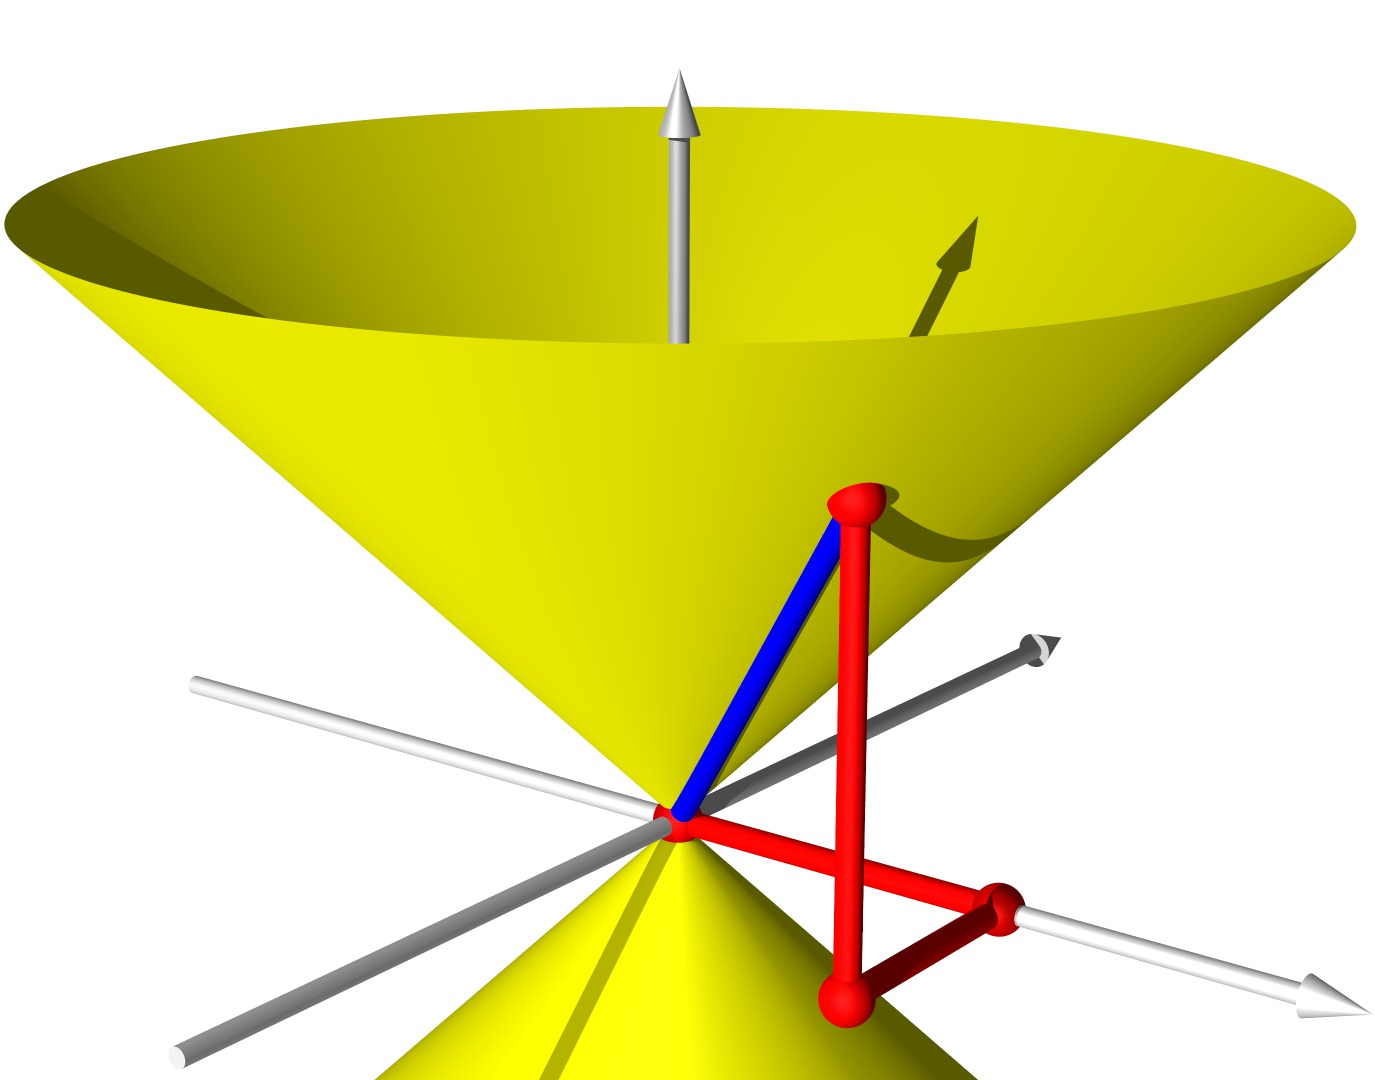
\includegraphics[width=\hsize]{chapters/3d/lichtkegel.jpg}
\caption{Lichtkegel ausgehend vom Nullpunkt zur Zeit $t=0$.
Alle Punkte innerhalb des Kegels mit $t>0$ liegen in der Zukunft des
Beobachters im Nullpunkt, solche mit $t<0$ in seiner Vergangenheit.
Punkte ausserhalb des Kegels können vom Nullpunkt aus nicht
beeinflusst werden.
Nur Punkte innerhalb des Kegels mit $t<0$ können Einfluss haben
auf den Nullpunkt.
\label{skript:kruemmung:fig:lichtkegel}}
\end{figure}

Das Vorzeichen des Ausdrucks~\eqref{skript:kruemmung:raumzeitabstand}
beschreibt also, ob zwei Ereignisse sich gegenseitig beeinflussen
können. 
Ist er negativ, dann ist eine Beeinflussung mit einer Wirkung möglich,
die sich weniger schnell als Licht ausbreitet.
Ist er gleich $0$, ist nur eine Beeinflussung mit einer Wirkung möglich,
die sich mit Lichtgeschwindigkeit ausbreitet.
Ist er positiv, ist keine gegenseitige Beeinflussung möglich.
Dies führt auf eine Unterteilung des Raumes in drei Gebiete
(Abbildung~\ref{skript:kruemmung:fig:lichtkegel}).
Die Fläche mit der Gleichung
\[
-c^2t^2+x^2+y^2+z^2=0
\]
heisst der Lichtkegel.
\index{Lichtkegel}%
Ereignisse innerhalb des Lichtkegels mit $t>0$ können vom Nullpunkt aus
beeinflusst werden.
Ereignisse innerhalb des Lichtkegels mit $t<0$ können auf den Nullpunkt
Einfluss nehmen.
Alle anderen Ereignisse können den Nullpunkt weder beeinflussen
noch von ihm beeinflusst werden.
Sie müssen daher als die objektive Gegenwart des Nullpunktes bezeichnet
werden.

Der Formalismus einer Metrik passt ganz hervorragend auf die hier
vorliegende Situation.
Verwenden wir als Koordinaten
\[
\begin{aligned}
x^0 &= ct,
&
x^1&=x,
&
x^2&=y,
&
x^3&=z,
\end{aligned}
\]
dann kann $s^2$ mit der Metrik
\begin{equation}
g_{\mu\nu}
=
\eta_{\mu\nu}
=
\begin{pmatrix}
-1&0&0&0\\
 0&1&0&0\\
 0&0&1&0\\
 0&0&0&1
\end{pmatrix},
\label{skript:speziell:metrik}
\end{equation}
der sogenannten
{\em Minkowski-Metrik}
\index{Minkowski-Metrik}%
berechnet werden.
Die spezielle Relativitätstheorie beschreibt die Welt also als einen
vierdimensionalen Raum, die Raum-Zeit, der Raumkoordinaten und Zeitkoordinate
in einem einzigen mathematischen Modell kombiniert.
Die Metrik~\eqref{skript:speziell:metrik} beschreibt dann die
Kausalitätsstruktur der Welt.

In diesem Bild gibt es also keinen sinnvollen Begriff der Gleichzeitigkeit
mehr.
\index{Gleichzeitigkeit}%
Wäre das Universum nicht aus einem Punkt entstanden, wie das Big Bang-Modell
besagt, dann wäre bereits die Frage ``Wann ist das Universum entstanden''
unsinnig, denn es gibt keinen sinnvollen Art und Weise, wie etwas gleichzeitig
im ganzen Universum stattfinden könnte.
Diese Beobachtung hat zu Einsteins Zeit aber keine grossen Wellen
geworfen, denn die meisten Phyisker gingen davon aus, dass das Universum
ewig und statisch ist, dass es also gar keinen Anfang braucht.
Auch Einstein ging davon aus, was ihn später in seiner allgemeinene
Relativitätstheorie dazu gebracht hat, einen nicht weiter erklärbaren
Term hinzuzufügen, einzig um zu erreichen, dass das Universum statisch 
sein kann.

Wenn die Frage ``Wann ist das Universum entstanden'' überhaupt eine
sinnvolle Antwort haben soll, dann nur, wenn das Universum zur Zeit
der Entstehung nur ein Punkt gewesen ist.
Wenn das Universum ausgedehnt entstanden ist, dann ist die Frage
nach dem Entstehungszeitpunkt sinnlos.

\section{Zeitartige und raumartige Richtungen}
\rhead{Zeitartige und raumartige Richtungen}
Die Raumrichtungen $x^1$, $x^2$ und $x^3$ unterscheiden sich grundsätzlich
von der Zeitrichtung $x^0$.
Um diesem Unterschied Rechnung zu tragen, verwenden wir auch die Notation
$x^k$ mit einem lateinischen Index $k$ für die Koordinaten in Raumrichtung,
während $x^0$ die Zeitrichtung ist.

Allerdings ist diese Unterscheidung in Zeitkoordinate und Raumkoordinaten
für beliebige Koordinatensysteme nicht mehr sinnvoll.
Wir können aber immer noch Vektoren auf Grund des Vorzeichens der 
Metrik unterscheiden.
Ein Vierervektor $x^\mu$ auf dem Lichtkegel erfüllt $g_{\mu\nu}x^\mu x^\nu=0$.
Ein Vierervektor  mit $x^k=0$ und $x^0=ct$ erfüllt dagegen
\[
g_{\mu\nu} x^\mu x^\nu
=
g_{00}(x^0)^2 = -c^2 t^2<0.
\]
Man nennt einen Vektor $A^\mu$ {\em zeitartig},
wenn er $g_{\mu\nu}A^\mu A^\nu<0$ 
erfüllt.
\index{zeitartig}%
\index{raumartig}%
{\em Raumartig} dagegen heisst ein Vektor $A^\mu$, für den
$g_{\mu\nu} A^\mu A^\nu>0$
gilt, wie zum Beispiel für einen Vektor mit $x^0=0$:
\[
g_{\mu\nu}x^\mu x^\nu
=
(x^1)^2
+
(x^2)^2
+
(x^3)^2
>0.
\]
Der Lichtkegel trennt also die zeitartigen Vektoren von den raumartigen
Vektoren.
Ein Ereignis kann ein anderes beeinflussen, wenn der Differenzvektor
zeitartig ist.
Insbesondere muss der Vektor zwischen zwei Punkten auf der Bahn 
eines Teilchens immer zeitartig sein.

\section{Lorentztransformation%
\label{skript:speziell:section:lorentztransformation}}
\rhead{Lorentztransformation}
Der Ausdruck~\eqref{skript:kruemmung:raumzeitabstand} ist nicht
invariant bei einer Galilei-Transformation.
Damit stellt sich die Frage, welche Transformationen denn
invariant wären.
Dies wären die Koordinaten-Änderungen, die zulässig sind, wenn
man das grundlegende Gesetz~\eqref{skript:kruemmung:raumzeitabstand}
der Kausalität erhalten will.

Zunächst sind Koordinatentransformationen zulässig, die nur die Raumkoordinaten
$x$, $y$ und $z$ beeinflussen, und den räumlichen Abstand nicht ändern.
Diese Transformationen sind aber wohlbekannt.
In der Linearen Algebra lernt man, dass genau die orthogonalen
Matrizen $A\in \textrm{O}(3)$, also Matrizen mit $A^tA=E$ diese
Eigenschaft haben.
Diese entsprechen räumlichen Drehungen und Spiegelungen.

Wenn sich aber zwei Koordinatensysteme mit der Zeit gegeneinander bewegen,
so wie bei der Galilei-Transformation, dann müssen auch die
Zeitkoordinaten in die Transformation involviert sein.
Wir suchen also eine Koordinatentransformation, die nur die
$t$- und $x$-Koordinaten betrifft.
Wir können Sie in der Form
\begin{equation}
\begin{linsys}{3}
t'&=& a_{11}t&+&a_{12}x\\
x'&=& a_{21}t&+&a_{22}x
\end{linsys}
\end{equation}
ansetzen.
Wir verlangen jetzt, dass der
Ausdruck~\eqref{skript:kruemmung:raumzeitabstand}
unverändert bleibt.
Da die $y$- und $z$-Koordinaten ohnehin nicht involviert sind, bedeutet
das, dass
\begin{align*}
-c^2t^2 + x^2
&=
-c^2t'^2 + x'^2
\\
&=
-c^2(a_{11}t+a_{12}x)^2 + (a_{21}t+a_{22}x)^2
\\
&=
-c^2a_{11}^2t^2 -2c^2a_{11}a_{12}tx -c^2a_{12}^2x^2
+a_{21}^2t^2+2a_{21}a_{22}tx+a_{22}^2x^2
\\
&=
-(c^2a_{11}^2 - a_{21}^2)t^2
+2(-c^2a_{11}a_{12}+a_{21}a_{22})tx
+(-c^2a_{12}^2 + a_{22}^2)x^2.
\end{align*}
Da dies für beliebige Werte von $x$ und $t$ gelten muss, müssen die
Koeffizienten der beiden Seiten übereinstimmen. 
Wir erhalten damit für die Koeffizienten $a_{ik}$ die Gleichungen
\[
\begin{aligned}
c^2a_{11}^2-a_{21}^2&=c^2,
&&\Rightarrow&
a_{11}^2
-
\biggl(\frac{a_{21}}{c}\biggr)^2
&=1,
\\
-c^2a_{12}^2+a_{22}^2&=1,
&&\Rightarrow
&
a_{22}^2 - (ca_{12})^2&=1,
\\
a_{21}a_{22}&=c^2a_{11}a_{12}.
\end{aligned}
\]
Da die Differenz der Quadrate jeweils $1$ ist, können die Basen
als Werte des hyperbolischen Kosinus und Sinus%
\footnote{In Anhang \ref{skript:chapter:hyperbolisch} werden einige für
diesen Abschnitt nützliche Eigenschaften der hyperbolischen Funktionen
zusammengestellt.}
dargestellt werden:
\[
\begin{aligned}
a_{11}&=\cosh\beta_1, &&&\frac{a_{21}}{c}&=\sinh\beta_1,
\\
a_{22}&=\cosh\beta_2,&&&ca_{12}&=\sinh\beta_2.
\end{aligned}
\]
Die dritte Gleichung lautet dann
\begin{align*}
a_{21}a_{22}=c\sinh\beta_1\cosh\beta_2
&=
c^2a_{11}a_{12}=c^2\cosh\beta_1\frac1c\sinh\beta_2
\\
c\sinh\beta_1\cosh\beta_2
&=
c\cosh\beta_1\sinh\beta_2
\\
\tanh\beta_1&=\tanh\beta_2,
\end{align*}
es folgt $\beta_1=\beta_2$, wir schreiben dafür im Folgenden einfach
nur $\beta$.
Damit haben wir die gesuchte Transformation gefunden, es ist
\begin{equation}
\begin{pmatrix}
a_{11}&a_{12}\\
a_{21}&a_{22}
\end{pmatrix}
=
\begin{pmatrix}
 \cosh\beta&\frac1c\sinh\beta\\
c\sinh\beta&\cosh\beta
\end{pmatrix}.
\end{equation}
Um die physikalische Bedeutung des Parameters $\beta$ zu verstehen, 
betrachten wir die Punkte $x=0$ für beliebige $t$.
Sie werden abgebildet auf
\[
\begin{aligned}
x' &= c\sinh\beta \cdot t,
&
&&
t' &=  \cosh\beta \cdot t.
\end{aligned}
\]
Der Quotient dieser beiden Ausdrücke ist die Geschwindigkeit
\[
v = c\frac{\sinh\beta}{\cosh\beta}
\qquad\Rightarrow\qquad
\frac{v}{c}
=
\tanh\beta,
\]
mit der sich der Nullpunkt des $t$-$x$-Systems im $t'$-$x'$-System
bewegt.

Nach den Formeln im Abschnitt~\ref{skript:sinh:section:abh} kann 
man jetzt auch $\sinh\beta$ und $\cosh\beta$ durch $v/c$ ausdrücken.
Setzen wir ein, erhalten wir
\[
\begin{aligned}
\sinh\beta
&=
\frac{\tanh\beta}{\sqrt{1-\tanh^2\beta}}
=
\gamma\cdot\frac{v}{c}
&
&\text{mit}&
\gamma = \frac{1}{\displaystyle\sqrt{1-\biggl(\frac{v}{c}\biggr)^2}}
\qquad\text{und}
\\
\cosh\beta
&=
\frac1{\sqrt{1-\tanh^2\beta}}
=
\gamma.
\end{aligned}
\]

Der Parameter $\tanh\beta$ hat also die Bedeutung einer in Einheiten
der Lichtgeschwindigkeit gemessenen Geschwindigkeit.
Da also $v/c=\tanh\beta$ ist, kann man die Transformation auch
als
\begin{equation}
\begin{pmatrix}
a_{11}&a_{12}\\
a_{21}&a_{22}
\end{pmatrix}
=
\frac{1}{\gamma}
\begin{pmatrix}
\displaystyle 1
	& \displaystyle\frac{v}{c^2}
\\
\displaystyle v
	&\displaystyle 1
\end{pmatrix}
\label{skript:kruemmung:lorentz}
\end{equation}
schreiben.
Die Transformation 
\eqref{skript:kruemmung:lorentz}
heisst {\em Lorentz-Transformation}.
\index{Lorentz-Transformation}%

Befindet sich ein Beobachter im ursprünglichen $t$-$x$-System in Ruhe
im Nullpunkt, dann ist seine Zeitkoordinate im $t'$-$x'$-System
\begin{equation}
t'=t\cdot\gamma = \frac{t}{\displaystyle\sqrt{1-\biggl(\frac{v}{c}\biggr)^2}},
\label{skript:speziell:zeitdilatation}
\end{equation}
der Lauf der Zeit ist in den beiden Koordinatensystemen verschieden.
Im $t'$-$x'$-Koordinatensystem läuft die Zeit um den Faktor $\gamma$
gedehnt.
Umgekehrt gilt natürlich auch $t=t'/\gamma$.

Die Darstellung \eqref{skript:kruemmung:lorentz} der Lorenztransformation
ist nicht sehr symmetrisch.
Dies liegt daran, dass die Zeit-Koordinate eine ganz andere Masseinheit
verwendet.
Schreibt man für die Koordinaten 
\[
\begin{aligned}
x^0&=ct,&
x^1&=x,&
x^2&=y,&
x^3&=z&
\end{aligned}
\]
dann wird die Lorentztransformation
\begin{equation}
\begin{pmatrix}
x^{\prime0}\\
x^{\prime1}\\
x^{\prime2}\\
x^{\prime3}
\end{pmatrix}
=
\begin{pmatrix}
\displaystyle          \gamma &\displaystyle\frac{v}{c}\gamma& 0 & 0 \\
\displaystyle\frac{v}{c}\gamma&\displaystyle           \gamma& 0 & 0 \\
      0                       &                              & 1 & 0 \\
      0                       &                              & 0 & 1 
\end{pmatrix}
\begin{pmatrix}
x^0\\x^1\\x^2\\x^3
\end{pmatrix}.
\label{skript:speziell:4lorentz}
\end{equation}
In dieser Form ist die Lorentztransformation klar symmetrischer.

\section{Weltlinien und Eigenzeit}
\rhead{Weltlinien und Eigenzeit}
Die Bewegung eines Teilchens in der Raum-Zeit ist eine Kurve
$(t(s), x(s), y(s), z(s))$
mit dem Parameter $s$, die man auch {\em Weltlinie} nennt.
\index{Weltlinie}%
Da sich das Teilchen nicht mit Lichtgeschwindigkeit bewegen kann, muss
für den Tangentialvektor 
\[
-c^2\dot t(s)^2
+ \dot x(s)^2 + \dot y(s)^2 + \dot z(s)^2
<
0
\]
gelten, darin bezeichnet der Punkt die Ableitung nach dem 
Parameter $s$.
Offenbar bewegt sich das Teilchen mit der Geschwindigkeit
\[
v^2 = \frac{\dot x(s)^2 + \dot y(s)^2 + \dot z(s)^2}{\dot t(s)^2}
\]
durch die Raumzeit.
Da sich das Teilchen bewegt, läuft die Zeit in einem Koordinatensystem,
das sich mit dem Teilchen mitbewegt, um den Faktor
\eqref{skript:speziell:zeitdilatation}
langsam.
Setzt man die Definitionen ein, erhält man
\begin{align*}
\frac{1}{\gamma}
=
\sqrt{1-\frac{v^2}{c^2}}
&=
\sqrt{1- \frac{\dot x(s)^2 + \dot y(s)^2 + \dot z(s)^2}{c^2\dot t(s)^2}}
\\
&=
\sqrt{-(-c^2\dot t(s)^2+\dot x(s)^2 + \dot y(s)^2 + \dot z(s)^2)}\frac{1}{c\dot t(s)}.
\end{align*}
Die im bewegten Koordinatensystem gemessene Zeit ist
\begin{align*}
\int\frac{1}{\gamma}\,dt
&=
\int
\sqrt{1-\frac{v^2}{c^2}}\,dt
=
\int
\sqrt{-(-c^2\dot t(s)^2+\dot x(s)^2 + \dot y(s)^2 + \dot z(s)^2)}\frac{1}{c\dot t(s)}
\,dt
\\
&=
\int
\sqrt{-(-c^2\dot t(s)^2+\dot x(s)^2 + \dot y(s)^2 + \dot z(s)^2}\frac{1}{c\dot t(s))}
\dot t(s)\,ds
\\
&=
\int
\frac1c
\sqrt{-(-c^2\dot t(s)^2+\dot x(s)^2 + \dot y(s)^2 + \dot z(s)^2)}
\,ds.
\end{align*}
In $x^\mu$-Koordinaten bedeutet dies, dass
\begin{equation}
\tau
=
\int
\frac{1}{\gamma}\,dt
=
\int
\sqrt{1-\frac{v^2}{c^2}}\,dt
=
\frac1{c}
\int
\sqrt{-g_{\mu\nu}\dot x^\mu(s) \dot x^\nu(s)}\,ds
\label{skript:speziell:eigenzeit}
\end{equation}
die Zeit ist, die entlang der Kurve $x^\mu(s)$ für den
mitbewegten Beobachter vergangen ist.
Man nennt $\tau$ die {\em Eigenzeit} des
Beobachters, der sich entlang der Weltlinie $x^\mu(s)$ bewegt.
\index{Eigenzeit}%
Da der Integrand in~\eqref{skript:speziell:eigenzeit} unabhängig ist
vom Koordinatensystem, ist $\tau$ ebenfalls unabhängig vom Koordinatensystem.

\section{Energie und Impuls}
\label{skript:speziell:energieimpuls}
%\rhead{Energie und Impuls}
Ein Teilchen der Masse $m$, welches im Nullpunkt ruht, hat in der
Newtonschen Mechanik Impuls 0.
In einem anderen Koordinatensystem hat das Teilchen dagegen
eine Geschwindigkeit, und damit auch einen Impuls.
Dies zeigt, dass eine koordinatensystemunabhängige Beschreibung
nicht allein mit dem Impuls funktionieren kann, wie ihn die klassische
Mechanik definiert.
Wir brauchen eine erweiterte Erhaltungsgrösse, die wir zur Beschreibung
der Bewegung eines Teilchens verwenden können.

\rhead{Energie und Impuls}

Die Kurve $x^\mu(s)$ und die Ableitung nach dem Kurvenparameter sind
offenbar keine geeigneten Grössen, denn der Kurvenparameter ist
keine vom Koordinatensystem unabhängige Grösse.
Die Eigenzeit ist aber eine solche koordinatensystemunabhängige
Grösse.
Wir schliessen daraus, dass die Ableitung der Position
nach der Eigenzeit, die sogenannte Vierergeschwindigkeit, der einzig
sinnvolle Ersatz ist für die in der klassischen Physik verwendete
Geschwindigkeit, die koordinatensystemabhängige Ableitung nach der
Zeitkoordinate.
Da die Eigenzeit auch im Wesentlichen die Bogenlänge ist, führt die
Ableitung automatisch auf einen Einheitsvektor.

Ein ruhendes Teilchen hat die Weltlinie
\[
t\mapsto (t, x, y, z)=(t,0,0,0),
\]
der Parameter ist die Koordinatenzeit.
Da das Teilchen keine Geschwindigkeit hat, ist $t$ auch die Eigenzeit,
und die Vierergeschwindgkeit $u^\mu$ ist der Vektor mit den
Komponenten
\[
\begin{aligned}
u^0 &= c,
&&&
u^1&=u^2=u^3 = 0.
\end{aligned}
\]
Seine Länge gemessen mit der Metrik ist
\[
g_{\mu\nu}u^\mu u^\nu=-c^2,
\]
sie ist eine koordinatensystemunabhängige Grösse.

Wendet man darauf eine Lorentztransformation mit Geschwindigkeit $v$ an,
erhält man den Vektor
\[
\begin{aligned}
u^0
&=
c\gamma,
&
u^1
&=
\frac{v}{c}\gamma c
=v\gamma
&&\text{und}
&
u^2&=u^3=0.
\end{aligned}
\]
Wir rechnen das Skalarprodukt mit Hilfe der Metrik nach:
\[
-(u^0)^2 + (u^1)^2 + (u^2)^2 + (u^3)^2
=
-c^2\gamma^2 + v^2\gamma^2
=
-c^2\gamma^2
\underbrace{\biggl(1-\frac{v^2}{c^2}\biggr)}_{\displaystyle=\frac{1}{\gamma^2}}
=
-c^2.
\]

Multiplizieren wir die Vierergeschwindigkeit mit $m$, erhalten wir
den sogenannten Viererimpuls $p^\mu = mu^\mu$.
Der Betrag des Viererimpulses ist eine Konstante, es gilt
\[
g_{\mu\nu}p^\mu p^\nu
=
-
m^2\gamma^2 c^2
+
m^2 \gamma^2 v^2
=
-m^2c^2\biggl(\displaystyle 1-\frac{v^2}{c^2}\biggr)\gamma^2
=
-m^2c^2.
\]
Die Raumkomponenten $p^1$, $p^2$ und $p^3$ haben eine offensichtliche
Interpretation in der Newtonschen Mechanik.
Bis auf den Faktor $\gamma$ stimmten die Raumkomponenten des Viererimpulses
mit dem Newtonschen Impuls überein.
Schreiben wir $M=m\gamma$, dann wird sogar $p^k = M v^k$, d.~h.~die
Raumkomponenten des Viererimpulses stimmen mit dem Newtonschen Impuls 
für die Masse $M=m\gamma  \ge m$ "uberein.
$M=m\gamma$ heisst die relativistische Masse.
Eine bewegte Masse ist also grösser als eine ruhende.

Um die Bedeutung der $0$-Komponente des Viererimpulses besser zu
verstehen, entwickeln wir sie für kleine Geschwindigkeiten.
Dazu verwenden wir die Potenzreihe
\[
\frac1{\sqrt{1-x}}
=
1+\frac12x+\frac{1\cdot 3}{2\cdot 4}x^2 + \frac{1\cdot 3\cdot 5}{2\cdot 4\cdot 6}x^3+\dots,
\]
die man aus der binomischen Reihe\footnote{%
Die {\em binomische Reihe} für negative Exponenten ist die Reihe
\[
(1\pm x)^{-m}
=
1\mp mx +\frac{m(m+1)}{2!}x^2 \mp \frac{m(m+1)(m+2)}{3!} x^3 +\dots
\]
mit $m>0$.
\index{Binomialreihe}%
Im Abschnitt Binomialreihe auf Seite~\pageref{skript:multipol:binomialreihe}
wird die Binomialreihe im allgemeinen Fall hergeleitet.
} für negative Exponenten ableiten kann.
Setzen wir hier für $x$ den Quotienten $(v/c)^2$ ein, erhalten wir
\[
Mc
=
m\gamma c
=
\frac{m}{\sqrt{1-\displaystyle\frac{v^2}{c^2}}} c
=
mc\biggl(1+\frac12\cdot\frac{v^2}{c^2}+\dots\biggl).
\]
Multipliziert man mit $c$, erhält man 
\[
u^0c = mc^2 + \frac12mv^2+\dots
\]
Der zweite Term ist die wohlbekannte kinetische Energie.
Der erste Term bleibt gleich gross, auch wenn die Masse sich
nicht bewegt.
Wir müssen diesen Term daher als eine Energie interpretieren, die
zu der Masse gehört unabhängig von deren Bewegungszustand.
Wir dürfen diese Energie nicht einfach subtrahieren, denn dadurch
würde das Transformationsgesetz für den Viererimpuls bei einer
Lorentztransformation verletzt.
Die Energie
\begin{equation}
E=mc^2
\label{E=mc2}
\end{equation}
heisst die {\em Ruheenergie} der Masse $m$.
\index{Ruheenergie}%
Eine Masseverteilung mit Dichte $\varrho$ hat daher auch
eine Energiedichte $\varepsilon=\varrho c^2$.

\section{Energie-Impuls-Tensor}
\rhead{Energie-Impuls-Tensor}
Die Betrachtungen zum Viererimpuls und zur Energie haben gezeigt, dass
Masse und Geschwindigkeit nicht unabhängig voneinander betrachtet
werden können.
Andererseits zeigt das newtonsche Gravitationsgesetz, dass die Schwerkraft
von der Masse eines Körpers ausgeht.
Die Newtonsche Theorie ist daher schon im Ansatz nicht der
speziellen Relativitätstheorie verträglich.
Die Masse allein kann bestensfalls in einem Koordinatensystem als
Quelle der Schwerkraft dienen, in dem die Masse ruht.
Eine modifizierte Theorie muss daher als Quelle für die Gravitation
ein Objekt verwenden, welches wie der Vierimpuls unahängig vom
Bewegungszustand definiert werden kann.

Auch genügt es nicht, nur Massepunkte zu studieren, da die meisten
Objekt des Universums ausgedehnt sind.
In der Newtonschen Theorie wird daher das von einer Masseverteilung mit
Dichte $\varrho(x,y.z)$ verursachte Gravitationsfeld studiert.
In der verallgemeinerten Theorie reicht die Dichte nicht aus,
wir müssen zulassen, dass die Materie sich bewegt, was wir mit einem
Stromdichtevektor $\vec\jmath$ 
abbilden können.
Die relativistische Grösse dazu wäre der Vierervektor der Impulsdichte
bestehend aus den Komponenten $j^\mu=\varrho u^\mu$,
wobei $u^\mu$ die Komponenten der Vierergeschwindigkeit des Gases sind.

Gesucht ist jetzt also eine Grösse, die zu jeder Zeit und in jedem
Punkt des Raumes den Viererimpuls der dort vorhandenen Materie zu
berechnen gestattet.
Im Ruhesystem des Gases reicht die Dichte des Gases zur Beschreibung.
In einem bewegten System wird man aber feststellen, dass das Gas auch
noch Impuls trägt, der ebenfalls berücksichtigt werden muss.
Die gesuchte Grösse muss also erlauben, den Viererimpuls-Inhalt eines
räumlich und zeitlich begrenzten Gebietes zu bestimmen, einer ``Box'', 
die dadurch beschrieben werden kann, dass alle Koordinaten ein einem
Intervall
\[
a^\mu \le x^\mu \le b^\mu
\]
bleiben.
Wechselt man in ein bewegtes Koordinatensystem, wird sich diese
gleiche Box gegenüber dem Koordinatensystem bewegen.
Die gesuchte Grösse muss also in der Lage sein, den Viererimpuls-Inhalt
der Box auch dann zu berechnen, wenn sich die Box bewegt.

Statt den Inhalt der Box zu berechnen, können wir auch die Änderung des
Inhalts der Box berechnen, die dadurch entsteht, dass Viererimpuls durch
die Wände der Box strömt.
Eine Wand können wir dadurch beschreiben, dass dort eine der Koordinaten
konstant ist, also durch einen Standardbasisvektor, oder durch einen
Koordinatenindex.
Zu jeder Koordinate $\mu$ gibt es also den Vektor des Viererimpulses
\[
T^{\mu\nu}
\]
der durch die zu $\mu$ gehörende Seitenfläche fliesst.

Um dieses Konzept zu illustrieren beschränken wir uns für den Moment
auf zwei Dimensionen, also auf die Koordinaten $x^0=ct$ und $x^1=x$.
Eine Box ist ein Rechteck, die Kanten des Rechtecks sind definiert
dadurch, dass $x^0$ bzw.~$x^1$ konstant sind.
Betrachten wir zuerst den Fall $\mu=0$.
Dann ist $T^{\nu0}$ der Viererimpuls, der durch ein räumliches
Einheitsinterval fliesst.
Insbesondere ist $T^{00}$ der Fluss der Energiedichte durch das Interval,
$T^{10}$ ist der Impulsfluss durch das Interval.
Für $\mu=1$ ist $T^{01}$ die Energie, die in einem Einheitszeitinterval
durch die Koordinaten $x^1$ fliesst, und $T^{11}$ ist der Impuls, der in der
gleichen Zeit durch den Punkt $x^1$ fliesst.
Man beachte, dass die Masseinheiten
\[
\text{Energiefluss}
=
\frac{\text{Energie}}{\text{Länge}}
=
\frac{\text{kg}\frac{\text{m}^2}{\text{s}^2}}{\text{m}}
=
\frac{\text{kg}\cdot\text{m}}{\text{s}^2}
=
\frac{\text{kg}\frac{\text{m}}{\text{s}}}{\text{s}}
=
\frac{\text{Impuls}}{\text{Zeit}}
=
\text{Impulsstrom}
\]
erfüllen.
Ausserdem ist 
\[
\frac{\text{Impuls}}{\text{Zeit}}
=
\frac{\text{kg}\frac{\text{m}}{\text{s}}}{\text{s}}
=
\frac{\text{kg}\cdot\text{m}}{\text{s}^2},
\]
dies ist die Masseinheit des Druckes oder einer Spannung.
Wir können daher die Matrix $T^{\mu\nu}$
durch
\[
T^{\mu\nu}
=
\begin{pmatrix}
\text{Energiedichte}
&\text{Energiefluss}
\\
\text{Impulsdichte}
&\text{Impulsfluss = Druck}
\end{pmatrix}
\]
charakterisieren.
$T^{\mu\nu}$ heisst der {\em Energie-Impuls-Tensor}.
Er codiert die Information über den in der Raumzeit vorhandenen
Viererimpuls.

\index{Energie-Impuls-Tensor}%

\subsection{Energie-Impuls-Tensor eines idealen Gases%
\label{skript:speziell:subsection:idealesgas}}
Ein ideales Gas ist isotrop, Kräfte wirken alle in die gleiche
Richtung.
Der Energie-Impuls-Tensor des ruhenden Gases muss daher durch die
Dichte $\varrho$ des Gases und den Druck $p$ beschrieben werden können.
Da sich das Gas nicht bewegt, fliesst kein Impuls durch eine Fläche
in Zeitrichtung.
Daher gilt
\[
T^{00}
=
\varepsilon
=
\varrho c^2
\qquad
\text{und}
\qquad
T^{k0}
=
0.
\]
Da sich das Gas nicht bewegt, fliesst auch keine Energie durch räumliche
Wände einer Box, so dass auch $T^{0k}=0$ gilt.
Da in einem idealen Gas keine Spannungen herschen, muss $T^{ik}$ diagonal
sein, und $T^{ii}=p$.
Also ist
\[
T^{ik}
=
\begin{pmatrix}
\varepsilon&0&0&0\\
0&p&0&0\\
0&0&p&0\\
0&0&0&p
\end{pmatrix}
\]
der Energie-Impuls-Tensor eines ruhenden idealen Gases mit Dichte
$\varrho$ und Druck $p$.
\index{Energie-Impuls-Tensor!eines idealen Gases}%

Um daraus den Energie-Impuls-Tensor eines idealen in einem
beliebigen, möglicherweise auch bewegten Koordinatensystem zu
finden, müssen wir diesen Tensor aus dem Viererimpuls $u^\mu$
des Gases und möglicherweise aus dem metrischen $g^{\mu\nu}$ Tensor
zusammenbauen.
Wir behaupten, der gesuchte Tensor sei
\begin{equation}
T^{\mu\nu}
=
p g^{\mu\nu} + (p + \varepsilon)u^\mu u^\nu.
\label{skript:speziell:idealesgas}
\end{equation}
In der Tat ist für ein ideales Gas in Ruhe $u^0=1$ und $u^k=0$ und damit
$u^\mu u^\nu=0$ ausser wenn $\mu=\nu=0$.
Setzt man dies ein, erhält man
\begin{align*}
T^{00}
&=
pg^{00} + (p+\varepsilon) = -p+p+\varepsilon=\varepsilon
\\
T^{k0}
&=0
\\
T^{kl}
&=
p\delta^{kl}
+
(p+\varepsilon)\cdot 0
=
p\delta^{kl}.
\end{align*}
Der Ausdruck~\eqref{skript:speziell:idealesgas} ist ein Tensor, der
im Ruhesystem des Gases mit dem korrekten Energie-Impuls-Tensor
übereinstimmt,
daher ist er die allgemeine Form für den Energie-Impuls-Tensor.

\subsection{Energie-Impuls-Erhaltung}
\index{Energie-Impuls-Erhaltung}%
In einem kräftefreien System sind Energie und Impuls erhalten, wir
möchten diese Aussage auch in unserem vierdimensionalen Formalismus
ausdrücken können.

\subsubsection{Kontinuitätsgleichung}
Betrachten wir zunächst die Strömung eines Mediums in drei Dimensionen.
Materie kann nicht einfach entstehen oder zerstört werden, dafür muss
es einen mathematischen Ausdruck geben.
Sei $\varrho(x,y,z,t)$ die Dichte des Mediums und $\vec v(x,y,z,t)$ 
seine Geschwindigkeit.
Wir berechnen, wie sich die Masse des Mediums in einem kleinen
Quader mit Seitenlängen $(\Delta x, \Delta y, \Delta z)$ in einem
Zeitinterval $\Delta t$ verändert.
In diesem Zeitinterval fliesst durch die Seitenwände senkrecht zur
$x$-Achse bei $x$ und $x+\Delta x$ 
Materie mit der Masse
\begin{align*}
m_x
&=
\varrho(x+\Delta x,y,z,t) v_x(x+\Delta x,y,z,t) F_x\,\Delta t
-\varrho(x,y,z,t) v_x(x,y,z,t) F_x\,\Delta t
\\
&=
\bigl(\varrho(x+\Delta x,y,z,t)
v_x(x+\Delta x,y,z,t) -\varrho(x,y,z,t) v_x(x,y,z,t)\bigr) F_x\,\Delta t
\\
&\simeq
\frac{\partial \varrho v_x}{\partial x}(x,y,z,t)\Delta x\, F_x\,\Delta t,
\end{align*}
wobei $F_x=\Delta y\,\Delta z$ der Flächeninhalt der Seitenfläche senkrecht
auf $x$ ist.

Dasselbe passiert durch die anderen Wände, so dass
die gesamte Masseänderung im Zeitinterval $\Delta t$
\[
\Delta m
=
\biggl(
\frac{\partial\varrho v_x}{\partial x}
+
\frac{\partial\varrho v_y}{\partial y}
+
\frac{\partial\varrho v_z}{\partial z}
\biggr)V\Delta t
\]
ist, darin ist $V$ das Volumen des Quaders.
Aus der Dichte können wir die Masseänderung aber auch berechnen,
es ist
\[
\Delta m
=
\frac{\partial\varrho}{\partial t}V \Delta t.
\]
Zusammen erhalten wir die Gleichung
\[
\frac{\partial\varrho}{\partial t}V \Delta t
=
\biggl(
\frac{\partial \varrho v_x}{\partial x}
+
\frac{\partial \varrho v_y}{\partial y}
+
\frac{\partial \varrho v_z}{\partial z}
\biggr)V\Delta t
\]
oder nach Division durch $V\Delta t$:
\begin{equation}
\frac{\partial\varrho}{\partial t}
-
\frac{\partial \varrho v_x}{\partial x}
+
\frac{\partial \varrho v_y}{\partial y}
+
\frac{\partial \varrho v_z}{\partial z}
=0.
\label{skript:speziell:kontinuitaetsgleichung}
\end{equation}
Die Gleichung~\eqref{skript:speziell:kontinuitaetsgleichung} heisst
{\em Kontinuitätsgleichung}.
\index{Kontinuitätsgleichung}%
Schreiben wir $\vec j = \varrho\vec v$ und
\begin{equation}
\operatorname{div}\vec a
=
\frac{\partial a_x}{\partial x}
+
\frac{\partial a_y}{\partial y}
+
\frac{\partial a_z}{\partial z},
\label{skript:speziell:divergenz}
\end{equation}
für ein beliebiges Vektorfeld $\vec a$,
dann kann die Kontinuitätsgleichung auch sehr kompakt als
\[
\frac{\partial\varrho}{\partial t}-\operatorname{div}\vec j=0
\]
geschrieben werden.
Die Grösse $\operatorname{div}\vec a$ heisst die {\em Divergenz}
des Vektorfeldes $\vec a$.
\index{Divergenz}%
Die Kontinuitätsgleichung~\eqref{skript:speziell:divergenz} drückt
die Erhaltung der Masse aus.

\subsubsection{Kontinuitätsgleichung für den Viererimpuls}
Verwenden wir jetzt wieder Koordinaten $x^\mu$, dann nimmt die
Kontinuitätsgleichung~\eqref{skript:speziell:divergenz}
die Form
\begin{align*}
0
&=
-
\frac{\partial \varrho}{\partial t}
+
\frac{\partial \varrho v_x}{\partial x}
+
\frac{\partial \varrho v_y}{\partial y}
+
\frac{\partial \varrho v_z}{\partial y}
\\
&=
-\frac{\partial c \varrho}{\partial x^0}
+\frac{\partial u^1}{\partial x^1}
+\frac{\partial u^2}{\partial x^2}
+\frac{\partial u^3}{\partial x^3}
=
\frac{\partial u^\mu}{\partial x^\mu}
\end{align*}
für die Viererimpulsdichte $u^\mu$ an.
\index{Viererimpulsdichte}%
\index{Erhaltungssatz}%
Der Erhaltungssatz für den Viererimpuls kann daher
geschrieben werden als
\begin{equation}
\frac{\partial T^{\mu\nu}}{\partial x^\mu}
=0
\label{skript:speziell:energieerhaltung}
\end{equation}
in beliebigen Koordinaten.
Ist $A^{\mu}$ ein Vierervektor, dann ist
\[
\frac{\partial A^\mu}{\partial x^\mu}=0
\]
der allgemeine Ausdruck dafür, dass die Grösse $A^0$ und der zugehörige
Strom $A^k$ erhalten bleiben.

\subsection{Symmetrie des Energie-Impuls-Tensors}
\index{Energie-Impuls-Tensor!Symmetrie}%
Der Energie-Impuls-Tensor ist symmetrisch, dies kann man wie folgt einsehen.
Wir betrachten einen kleinen Würfel mit Kantenlänge $L$.
Die Komponenten $T^{ik}$ des Energie-Impuls-Tensors beschreiben die
$i$-Komponenten der Kräfte auf den $k$-Flächen des Würfels.
Insbesondere ist das Drehmoment um die $3$-Achse
\begin{align*}
M^{12}
&=
-T^{12}L^2(L/2) + T^{12}L^2 (-L/2)
\\
&\phantom{\mathstrut=}-(-T^{21}L^2)(L/2)-(T^{21}L^2)(-L/2)
\\
&=(T^{12}-T^{21})L^3.
\end{align*}
Das Trägheitsmoment des Würfels ist proportional zu $L^5$,
die Winkelbeschleunigung des Würfels ist daher proportional
zu $(T^{12}-T^{21})L^{-2}$, was für $L\to 0$ beliebig gross würde.
Ein beliebig kleiner Würfel würde daher zu beliebig grossen 
Drehgeschwindigkeit beschleunigt.
Da dies nicht sein kann, folgt $T^{12}-T^{21}=0$ oder allgemeine
\[
T^{\mu\nu}=T^{\nu\mu}.
\]

\section{Kräfte}
\rhead{Kräfte}
Die Beschreibung der Welt als vierdimensionale Raumzeit und der Bewegung
eines Teilchens als Bahnkurve in der Raumzeit hat zur Folge, dass auch
Kräfte einer geometrischen Beschreibung zugänglich werden.
Eine geradlinige Bewegung in einem Koordinatensystem zeichnet sich
dadurch aus, dass $\ddot x^\mu=0$ ist.
Eine Abweichung davon äussert sich als Krümmung der Weltlinie.
Das zweite Newtonsche Gesetz muss also ungefähr die Form
\begin{equation}
\ddot x^\mu = F^\mu
\label{skript:speziell:newton2}
\end{equation}
annehmen.

Naturgesetze sind fast immer als Minimalprinzipien formulierbar.
Wir hoffen daher, dass~\eqref{skript:speziell:newton2} der Ausdruck
eines Minimalprinzips ist.
Naheliegend wäre die Geodätengleichung, die Kurven minimaler Länge 
beschreibt.
Leider passt \eqref{skript:speziell:newton2}
überhaupt nicht zur Form der Geodätengleichung.

Die Physik hilft uns jedoch nochmals weiter, da
eine Weltlinie nur zeitartig sein kann.
Für langsam bewegt Objekte sind die Raumkomponenten $\dot x^i(t)$
der Vierergeschwindigkeit sehr klein, $\dot x^i(t)\simeq 0$,
($1\le k\le 3$), während
die Zeitkomponente $\dot x^0(t)\simeq 1$ ist.
Das Objekt bewegt sich vor allem in der Zeit, ungefähr mit einer
Geschwindigkeit von einer Sekunde pro Sekunde.
In dieser Näherung könnten wir \eqref{skript:speziell:newton2}
auch als
\begin{equation}
\ddot x^\mu
=
F^\mu
=
F^\mu\cdot 1 \cdot 1
\simeq
\Gamma^\mu_{\alpha\beta}\dot x^\alpha\dot x^\beta
\end{equation}
schreiben, was genau die Geodätengleichung ist.
Die $\Gamma^\mu_{00}$ bekommen in diesem Licht die Bedeutung der 
Kräfte der klassischen Mechanik.

Eine koordinatensystemunabhängige Formulierung des zweiten Newtonschen
Gesetzes wird deshalb fordern, dass sich ein Teilchen entlang einer
Geodäten bewegt.
Unser Plan ist, das Auftreten von Gravitationskräften als
Ausdruck nicht verschwindender Christoffelsymbole zu verstehen.
Dieser Plan wird in Kapitel~\ref{skript:chapter:gravitation}
umgesetzt.


\section*{Übungsaufgaben}
\rhead{Übungsaufgaben}
\uebungsaufgabe{0503}
\uebungsaufgabe{0501}
\uebungsaufgabe{0502}


%
% k-gravitatzion.tex
%
% (c) 2017 Prof Dr Andreas Müller, Hochschule Rapperswil
%
\chapter{Gravitation%
\label{skript:chapter:gravitation}}
\lhead{Gravitation}
\rhead{}
Albert Einstein hat erkannt, dass die Wirkung der Gravitation 
durch die Krümmung des Raumes beschrieben werden muss.
\index{Einstein, Albert}
In den folgenden Abschnitten geben wir einen Ausblick darauf, wie
die moderne Physik unseren Raum als einen gekrümmten Raum beschreibt.
An einfachen Modellen soll gezeigt werden, wie man sich die Gravitationswirkung
als die Wirkung eines gekrümmten Raumes vorstellen kann, wie schwarze Löcher
beschrieben werden können, und wie alle diese Dinge tatsächlich gemessen
werden können.

\section{Äquivalenzprinzip}
\rhead{Äquivalenzprinzip}
Schon Galileo Galilei hat bemerkt, dass im Gravitationsfeld der Erde
jeder Körper unabhängig von seiner Masse die gleiche Beschleunigung $g$
erfährt.
Auch das Newtonsche Gravitationsgesetz beschreibt den Betrag der Kraft
zwischen zwei Massen $M$ und $m$ als
\[
F=\frac{KMm}{r^2}.
\]
Ein Teilchen der Masse $m$ wird daher nach dem zweiten Newtonschen Gesetz
$F=ma$ immer mit den Betrag
\[
\frac{KM}{r^2}
\]
haben.
Die Beschleunigung eines Teilchens ist daher unabhängig von der Masse.
Diese {\em Äquivalenz\-prinzip} genannte Beobachtung wurde von
Lor\'and Eötvös 1909 mit sehr grosser Genauigkeit nachgemessen und bestätigt.
In neuerer Zeit wurde die Genauigkeit nochmals um den Faktor $10^4$
verbessert.

Eine Folge des Äquivalenzprinzips ist auch, dass sich ein konstant
beschleunigtes Labor und ein Labor in einem homogenen Gravitationsfeld
nicht unterscheiden lassen (Abbildung~\ref{skript:gravitation:labor}).
\begin{figure}
\centering
\includegraphics{chapters/tikz/labor.pdf}
\caption{Illustration des Äquivalenzprinzips.
Ein einem gleichmässig mit $g$ beschleunigten Labor (rechts)
misst man die gleiche Beschleunigung wie in einem homogenen
Gravitationsfeld (links).
\label{skript:gravitation:labor}}
\end{figure}
Ein beschleunigtes Koordinatensystem kann man zwar durch die
Koordinatentransformation
\begin{equation}
\left.
\begin{aligned}
t'&=t\\
x'&=x+\frac12gt^2
\end{aligned}
\right\}
\qquad
\Leftrightarrow
\qquad
\left\{
\begin{aligned}
t&=t'\\
x&=x'-\frac12gt'^2
\end{aligned}
\right.
\label{skript:gravitation:beschleunigt}
\end{equation}
erhalten, doch ist sie keine Lorentz-Transformation und erhält daher
die Minkowski-Metrik nicht.
Wenn es möglich sein soll, die Gravitationstheorie so zu verallgemeinern,
dass sie mit der speziellen Relativitätstheorie verträglich sein soll, dann
müssen wir auch andere Koordinatentransformationen als nur die
Lorenztransformation zulassen.
Das bedeutet aber, dass wir nicht mehr darauf beharren dürfen, dass
sich die Metrik in der Form
\begin{equation}
-c^2\,dt^2 + dx^2 + dy^2  + dz^2
\label{skript:gravitation:standardform}
\end{equation}
schreiben lässt.
Wir lassen daher in Zukunft beliebige Koordinatentransformationen zulassen
und daher auch Metriken $g_{\mu\nu}$, die von der
Standardform~\eqref{skript:gravitation:standardform} abweichen.

Wir wollen die Metrik berechnen, die im festen Koordinatensystem
anzuwenden ist. 
Dazu müssen wir die Transformation zuerst mit $x^0$ und $x'^0$ 
darzustellen:
\begin{equation}
\left.
\begin{aligned}
x'^0 &= x^0 \\
x'^1 &= x^1+\frac{1}{2c^2}(x^0)^2
\end{aligned}
\right\}
\qquad
\Leftrightarrow
\qquad
\left\{
\begin{aligned}
x^0 &= x'^0 \\
x^1 &= x'^1 - \frac{1}{2c^2}(x'^0)^2
\end{aligned}
\right.
\end{equation}
Für die Transformation der Metrik werden die partiellen Ableitungen
benötigt:
\begin{equation}
\begin{aligned}
\frac{\partial x^0}{\partial x'^0}&=1,
&
\frac{\partial x^0}{\partial x'^1}&=0,
&
\frac{\partial x^1}{\partial x'^0}&=-\frac{1}{c^2}x'^0,
&
\frac{\partial x^1}{\partial x'^1}&=1,
\\
\frac{\partial x'^0}{\partial x^0}&=1,
&
\frac{\partial x'^0}{\partial x^1}&=0,
&
\frac{\partial x'^1}{\partial x^0}&=\frac{1}{c^2}x^0,
&
\frac{\partial x'^1}{\partial x^1}&=1.
\end{aligned}
\end{equation}
Die zugehörige Transformationsmatrix ist also
\begin{equation}
\frac{\partial (x^0, x^1)}{\partial (x'^0, x'^1)}
=
\begin{pmatrix}
1&0\\
-\frac1{c^2}x'^0&1
\end{pmatrix},
\qquad
\frac{\partial (x'^0, x'^1)}{\partial (x^0, x^1)}
=
\begin{pmatrix}
1&0\\
\frac1{c^2}x^0&1
\end{pmatrix}.
\end{equation}
Im $(x^0,x^1)$-Koordinatensystem wird die Metrik durch die Matrix
\[
g_{\mu\nu}
=
\begin{pmatrix}-1&0\\0&1\end{pmatrix}
\]
ausgedrückt.
In $(x'^0,x'^1)$-Koordinaten muss die Matrix daher sein
\begin{align*}
g'_{\mu\nu}
&=
\begin{pmatrix}
1&0\\
\frac1{c^2}x'^0&1
\end{pmatrix}
\begin{pmatrix}
-1&0\\0&1
\end{pmatrix}
\begin{pmatrix}
1&\frac1{c^2}x'^0\\
0&1
\end{pmatrix}
=
\begin{pmatrix}
1&0\\
\frac1{c^2}x'^0&1
\end{pmatrix}
\begin{pmatrix}
-1&-\frac1{c^2}x'^0\\
 0& 1
\end{pmatrix}
\\
&=
\begin{pmatrix}
-1&-\frac1{c^2}x'^0\\
-\frac1{c^2}x'^0&1+\frac1{c^4}(x'^0)^2
\end{pmatrix}.
\end{align*}
Die Metrik $g'_{\mu\nu}$ ist offenbar wieder symmetrisch.
Wir könnten die Christoffelsymbole ausrechnen und die Geodäten
bestimmen, wir würden die Transformation von Geraden aus dem
$(x,t)$-Koordinatensystem finden.

\section{Newtonsche Gravitationstheorie%
\label{skript:section:newtonschegravitationstheorie}}
\rhead{Newtonsche Gravitationstheorie}
Als ersten Schritt in Richtung auf eine allgemeine Gravitationstheorie
zeigen wir, wie auch die Bahnen in einem Newtonschen Gravitationsfeld 
als Geodäten eines Zusammenhangs schreiben lassen.
Wer verwenden dazu aber nicht die Metrik und den daraus abgeleiteten 
Zusammenhang, dies hat erst die Einsteinsche Theorie geschafft.

\subsection{Schwerkraft}
Das Newtonsche Gravitationsgesetz beschreibt die Beschleunigung, die
auf ein Teilchen in einem Gravitationsfeld wirkt, welches von einer
Masse $m$ erzeugt wird.
Der Betrag der Kraft ist umgekehrt proportional zum Quadrat der
Entfernung.
Der Kraftvektor kann deshalb als
\begin{equation}
\vec F = -\frac{KM}{r^2}\cdot\frac{\vec r}{r}
\label{skript:gravitation:gkraft}
\end{equation}
geschrieben werden.
Die Bewegungsgleichung ist daher 
\begin{equation}
\ddot x^k = -\frac{KM}{r}\cdot\frac{x^k}{r},
\qquad\text{mit}\qquad r = \sqrt{(x^1)^2+(x^2)^2+(x^3)^2},
\label{skript:gravitation:bewegungsgleichung}
\end{equation}
es kommt nur die Beschleunigung und die Position vor.

In den Geodätengleichungen 
\[
\ddot x^\mu = -\Gamma^\mu_{\alpha\nu}\dot x^\alpha\dot x^\nu
\]
kommt dagegen auf der rechten Seite auch die Geschwindigkeit vor.
Es ist daher nicht unmittelbar klar, wie die Bewegungsgleichung als
Geodätengleichung geschrieben werden klar.

Wir beschreiben die Bewegung wieder in einem vierdimensionalen Raum,
also als Kurve
\[
t\mapsto (t,x^1(t),x^2(t),x^3(t)),
\]
also mit $x^0(t)=t$.
Für eine solche Parametrisierung gilt $\dot x^0(t)=1$.
In der Geodätengleichung können wir daher die Terme mit mit Index $0$
separat behandelt werden:
\[
\ddot x^\mu
=
-\Gamma^\mu_{00}
-\Gamma^\mu_{k0}\dot x^k -\Gamma^\mu_{0l}\dot x^l
- \Gamma^\mu_{kl}\dot x^k\dot x^l
\]
Da in der Bewegungsgleichung~\eqref{skript:gravitation:bewegungsgleichung}
auf der rechten Seite keine Geschwindigkeiten vorkommen, darf nur der
erste Term stehen bleiben, also
\begin{equation}
\Gamma^k_{00} = \frac{KM}{r^2}\cdot \frac{x^k}{r},\qquad k=1,\dots,3.
\label{skript:gravitation:newtonzusammenhang}
\end{equation}
Da die erste Komponente der Geodäte $x^0(t)=t$ ist und seine zweite
Ableitung $\ddot x^0(t)=0$, muss auch $\Gamma^0_{\alpha\nu}=0$ sein.
Die einzigen nicht verschwindenden Zusammenhangskoeffizienten sind
\eqref{skript:gravitation:newtonzusammenhang}.

Man kann für den Zusammenhang~\eqref{skript:gravitation:newtonzusammenhang}
auch die Definition des Riemann-Krümmungstensors anwenden.
Die Rechnung zeigt aber, dass zwar einzelne Komponenten des Riemann-Tensors
nicht verschwinden, der Ricci-Tensor und damit auch der Einstein-Tensor
verschwinden dagegen identisch.
Diese Beschreibung der Gravitation führt also nicht auf das Modell
eines gekrümmten Raumes.

\subsection{Gravitationspotential}
Die potentielle Energie, die zur
Gravitationskraft~\eqref{skript:gravitation:gkraft} gehört, kann
mit Hilfe eines Wegintegrals berechnet werden.
Dazu verwenden wir einen Weg vom Punkt $P_1$ mit Radius $r_1$
zum Punkt $P_2$ mit Radius $r_2$ führt.
Da die Kraft immer radial wirkt, ist entlang des Weges nur die radiale
Komponente des Tangentialvektors massgebend.
Der Unterschied in der poteniellen Energie ist
\[
\Delta E
=
\int_{P_1}^{P_2} \vec F\cdot d\vec s
=
\int_{r_1}^{r_2} -\frac{KM}{r^2}\,dr
=
\biggl[
\frac{KM}{r}
\biggr]_{r_1}^{r_2}
=
GM\biggl(\frac{1}{r_2}-\frac{1}{r_1}\biggr).
\]
Legt man den Nullpunkt der potentiellen Energie ins unendliche, dann ist
das Potential einer Punktmasse mit Masse $M$ ist also
\begin{equation}
\varphi = \frac{KM}{r}.
\label{skript:gravitation:potential}
\end{equation}

Aus dem Potential kann man die Kraft mit Hilfe des Gradienten
berechnen.
Zur Berechnung brauchen wir die Ableitung von $r$ nach den Koordinaten.
Die Ableitung nach $x$ ist
\[
r=\sqrt{x^2+y^2+z^2}
\qquad\Rightarrow\qquad
\frac{\partial r}{\partial x}
=
\frac{1}{2r} \frac{\partial (x^2+y^2+z^2)}{\partial x}
=
\frac{1}{2r} 2x=\frac{x}{r}.
\]
Damit können wir jetzt die Ableitung des Potentials berechnen:
\begin{align*}
\frac{\partial}{\partial x}\frac1{r}
&=
-\frac{1}{r^2} \frac{\partial r}{\partial x}
=
-\frac{1}{r^2} \frac{x}{r}.
\end{align*}
Der Gradient
\[
\operatorname{grad}\varphi
=
-\frac{KM}{r^2}\cdot\frac1r\begin{pmatrix}x\\y\\z\end{pmatrix}
=
-\frac{KM}{r^2}\cdot\frac{\vec r}{r} = \vec F
\]
stimmt mit der Gravitationskraft überein.

Für eine ausgedehnte Masseverteilung mit Dichte $\varrho$ kann man das
Potential als Überlagerung von einzelnen Potentialen der
Form~\eqref{skript:gravitation:potential} berechnen.
%Das Integral
%\[
%\varphi(\vec r)
%=
%G\int_{\mathbb R^3} \frac{\varrho(\vec r')}{|\vec r-\vec r'|}\,d^3r',
%\]
%wobei das Integral als Volumen-Integral über alle Vektoren $\vec r'$
%zu erstrecken ist.
Eine solche Beschreibung
ist allerdings für unsere Zwecke nicht sehr nützlich.

Eine besser geeignete Beschreibung können wir aus dem Gausschen
Divergenzsatz erhalten.
Eine zweidimensionale Version dieses Satzes können wir
aus dem Satz von Green~\eqref{skript:kruemmung:satz:green}
erhalten.
Dazu verwenden wir die Funktionen 
\[
f(x)=-\frac{\partial \varphi}{\partial x}
\qquad\text{und}\qquad
g(x)=\frac{\partial \varphi}{\partial y}.
\]
Die linke Seite des Satzes von Green ist das Integral
\begin{equation}
\oint_{C}
\frac{\partial \varphi}{\partial x} (-\dot x(s))
+
\frac{\partial \varphi}{\partial y} \dot y(s)
\,ds
\label{skript:gravitation:fluss1}
\end{equation}
Der Vektor
\[
\vec o(s) = \begin{pmatrix}-\dot x(s)\\\dot y(s)\end{pmatrix}
\]
steht senkrecht auf dem Rand des Gebietes.
Im Integral~\eqref{skript:gravitation:fluss1} wird das Skalarprodukt
diese Vektors mit dem der Gravitationskraft $\vec F$ verwendet,
man nennt
\[
\oint_{C} \vec F\cdot \vec o(s)\,ds
\]
den Fluss des Vektorfeldes durch die Kurve $C$.
Auf der rechten Seite findet man dann 
\[
\int \frac{\partial g}{\partial x}-\frac{\partial f}{\partial x}\,dx\,dy
=
\int
\frac{\partial^2\varphi}{\partial x^2}
+
\frac{\partial^2\varphi}{\partial y^2}
\,dx\,dy
=
\int\Delta\varphi \,dx\,dy.
\]
Der Satz von Gauss besagt daher
\[
\oint_{C} \vec F\cdot d\vec o
=
\int_{D} \Delta\varphi\,dx\,dy.
\]
In dieser zweidimensionalen Darstellung nützt uns der Satz allerdings
wenig, denn das Gravita\-tions\-feld ist natürlich dreidimensional.
Die dreidimensionale Version kann jedoch mit ganz ähnlichen Ideen
bewiesen werden wie der Satz von Green:

\begin{satz}[Gauss] Ist $\vec v$ ein Vektorfeld in
einem dreidimensionalen Gebiet $D\subset R^3$ mit Randfläche $S=\partial D$,
dann gilt
\begin{equation}
\oint_S \vec v\cdot d\vec o
=
\int_D 
\frac{\partial v_x}{\partial x}
+
\frac{\partial v_y}{\partial y}
+
\frac{\partial v_z}{\partial z}
\,dx\,dy\,dz
=
\int_D \operatorname{div}\vec v\,dx\,dy\,dz.
\label{skript:gravitation:gausssatz}
\end{equation}
Darin ist $\vec o$ ein Vektor ein nach aussen zeigender Vektor, der
senkrecht auf der Oberfläche des Gebietes steht.
\end{satz}

Der Nutzen dieses Satzes ist, dass man den Fluss des Schwerkraftfeldes
$\vec F$ einer Punktladung durch eine mit der Masse konzentrischen
Kugel auch direkt berechnen kann.
Dann hat nämlich $\vec F$ auf der Kugeloberfläche $S^2$ überall den gleichen
Betrag, und die Richtung ist immer senkrecht auf der Kugeloberfläche.
Das Skalarprodukt in~\eqref{skript:gravitation:gausssatz} ist daher
einfach ein Produkt der Beträge und das Integral bekommt man durch
Multiplikation mit der Kugeloberfläche:
\[
\oint_{S^2_r} \vec F\cdot d\vec o
=
4\pi r^2
\frac{KM}{r^2}
=
4\pi KM.
\]
Der Fluss des Gravitationsfeldes mit Potential $\varphi$ durch einen
sehr kleinen Ball $B_r$ mit Radius $r$ hat daher den Wert
\[
\int_{S^2_r}\vec F\cdot d\vec o
=
4\pi K\int_{B_r} \varrho\,dx\,dy\,dz.
\]
Andererseits kann man nach dem Satz von Gauss auch die rechte 
Seite berechnen:
\begin{align}
\int_{B_r} 4\pi K\varrho\,dx\,dy\,dz
&=
\int_{B_r}
\frac{\partial F_x}{\partial x}+
\frac{\partial F_y}{\partial y}+
\frac{\partial F_z}{\partial z}
\,dx\,dy\,dz
=
\int_{B_r}
\frac{\partial^2\varphi}{\partial x^2}+
\frac{\partial^2\varphi}{\partial y^2}+
\frac{\partial^2\varphi}{\partial z^2}
\,dx\,dy\,dz
\notag
\\
&=
\int_{B_r} \Delta\varphi\,dx\,dy\,dz.
\label{skript:gravitation:poisson-integral}
\end{align}
mit der Abkürzung
\begin{equation*}
\Delta \varphi
=
\frac{\partial^2\varphi}{\partial x^2}+
\frac{\partial^2\varphi}{\partial y^2}+
\frac{\partial^2\varphi}{\partial z^2},
\end{equation*}
dem Laplace-Operator.
Da dies für Kugeln an beliebigen Punkten mit beliebigen Radien 
gilt, müssen die Integranden in~\eqref{skript:gravitation:poisson-integral}
übereinstimmen.
Es folgt, dass das Gravitationspotential $\varphi$ die Gleichung
\begin{equation}
\Delta \varphi = 4\pi K\varrho
\label{skript:gravitation:potentialgleichung}
\end{equation}
erfüllen.
Diese Gleichung werden wir später dazu verwenden, die Verbindung zwischen
der newtonschen und der einsteinschen Gravitationstheorie herzustellen.

\section{Schwache Felder und die Metrik}
Für schache Gravitationsfelder hat die Newtonsche Theorie gute Dienste
geleistet. 
Wir gehen daher davon aus, dass eine neue, allgemeinere Theorie die
newtonsche Theorie als Grenzfall erhalten muss.
Es muss also möglich sein, die Gravitationskräfte, die wir im 
Abschnitt~\ref{skript:section:newtonschegravitationstheorie} bereits
mit Hilfe des Zusammenhangs, also den Koeffizienten $\Gamma^\alpha_{\mu\nu}$
beschrieben haben, auch aus einer Metrik zu gewinnen.
Die Zusammenhangskoeffizienten in
Abschnitt~\ref{skript:section:newtonschegravitationstheorie} waren nicht
die Christoffelsymbole einer Metrik.

Wir möchten jetzt eine Metrik finden, die einerseits möglichst nahe
an der Minkovski-Metrik ist, deren zugehörige Geodäten andererseits die
Bewegung in einem schwachen Gravitationsfeld korrekt wiedergibt.
Als Metrik verwenden wir daher
\[
g_{\mu\nu}=\eta_{\mu\nu} + h_{\mu\nu}.
\]
Der erste Summan ist $\eta_{\mu\nu}$, der die Minkovski-Metrik 
wiedergibt, der zweite beschreibt die Abweichung,
wobei wir annehmen, dass $h_{\mu\nu}$ sehr klein ist.
Die zugehörigen Christoffelsymbole sind mit einiger, vorzugsweise
maschineller Rechnung zu finden.
Aus der Beschreibung des newtonschen Gravitationsgesetzes können wir
ablesen, dass wir die klassisch beobachteten Kräfte in Gestalt
des Christoffelsymbols
\[
\Gamma^{k}_{00}
=
-\frac{1}{2(h_{kk} + 1)}\frac{\partial h_{00}}{\partial x^k}
\]
wiederfinden müssen.
Da $h_{kk}$ im Vergleich zu $1$ sehr klein soll, bleibt
\[
\Gamma^{k}_{00}
=
-\frac{1}{2}\frac{\partial h_{00}}{\partial x^k}.
\]
Damit die Bahnen der newtonschen Gravitationstheorie entstehen, müssen
die $-\Gamma^k_{00}$ die Beschleunigungskomponenten des Gravitationsfelds
entstehen.
Diese bilden den Gradienten des Potentials des Gravitationsfeldes
\[
-\Gamma^k_{00} = -\frac{\partial\varphi}{\partial x^k}.
\]
Es folgt daher, dass $h_{00}=-2\varphi/c^2$ ist.
In erster Näherung beschreibt daher die Metrik
\begin{equation}
\begin{aligned}
g_{00} &= -1 -\frac{2\varphi}{c^2},
&&&
g_{kk} &= 1,\quad k=1,2,3.
\end{aligned}
\label{skript:gravitation:naeherung}
\end{equation}
Die gesuchte Theorie muss also in erster Näherung das newtonsche
Gravitationspotential in der $00$-Komponente des metrischen Tensors
verwenden.

\section{Einstein-Gleichungen für das Gravitationsfeld}
Die Näherung für schwache Felder dient uns nun als Leitfaden, um die
Einsteinschen Feldgleichungen herzleiten.
Einerseits beinhaltet die $g_{00}$-Komponente das Potential $\varphi$ des
Gravitationsfeldes, andererseits beschreibt die
Gleichung~\eqref{skript:gravitation:potentialgleichung}
den Zusammenhang zwischen dem Gravitationspotential und der
Masseverteilung.
Wir suchen jetzt eine Theorie, welche auch die übrigen Komponenten
des metrischen Tensors zu bestimmen erlaubt.
Wir gehen dazu mit Hilfe von Analogien vor, eine strenge Herleitung
der Gleichungen ist ebenfalls möglich, jedoch für dieses Skript etwas
zu aufwendig.

Für die folgenden mathematischen Objekte suchen wir einen Ersatz:
\begin{enumerate}
\item
Die Massedichte in 
Gleichung~\eqref{skript:gravitation:potentialgleichung}
muss durch eine Grösse ersetzt werden, die dem vorhandenen Vierer-Impuls
ebenfalls Rechnung trägt.
Ausserdem soll sie auch um andere Formen von Energie ergänzt werden 
können, um zum Beispiel die Gravitationswirkung der Energie eines
elektromagnetischen Feldes modellieren zu können.
\item
In Gleichung~\eqref{skript:gravitation:potentialgleichung}
kommen die zweiten Ableitungen nach den Koordinaten vor. 
Der Laplace-Operator lässt sich aber nur in der Minkowski-Metrik so 
formulieren, ausserdem trägt er der Zeitkoordinate nicht Rechnung.
Wir brauchen daher eine Grösse, die alle Koordinaten gleichwertig
behandelt, aber im Grenzfall schwacher Felder wieder auf den 
Laplace-Operator führt.
\item
Der Energieerhaltungssatz in Form der
Gleichung~\eqref{skript:speziell:energieerhaltung}
kann nicht aufrechterhalten werden, weil
Gravitationsfelder die Energie darin sich bewegender Massen verändern
können.
Es muss also eine Formulierung des Energie- und Impulserhaltungssatzes
gefunden werden, welche mit der erweiterten Theorie verträglich ist.
\end{enumerate}
Dieses Programm soll in den folgenden Abschnitten durchgeführt werden.
Am Ende soll in Analogie zur 
Potentialgleichung~\eqref{skript:gravitation:potentialgleichung}
eine Gleichung der Form
\[
\text{``Tensor zur Feldbeschreibung''}
=
4\pi K\cdot \text{``Tensor mit Energie und Impuls''}
\]
das Gravitationsfeld beschreiben.
Der feldbeschreibende Tensor $G_{\mu\nu}$ auf der linken wird aber leicht
anders aussehen, so dass die angestrebte Feldgleichung die Form
\[
G_{\mu\nu}
=
\frac{8\pi K}{c^4} T_{\mu\nu}
\]
haben wird.

\subsection{Massedichte und Energie-Impuls-Tensor}
Die Massedichte $\varrho$, die wir auf der rechten Seite der
Potentialgleichung~\eqref{skript:gravitation:potentialgleichung}
für das newtonsche Gravitationsfeld finden,
finden wir in der allgemeinen Theorie als $00$-Komponente
des Energie-Impuls-Tensors wieder.
Es ist daher naheliegend, dass auf der rechten Seite der gesuchten
Gleichung der Energie-Impuls-Tensor $T_{\mu\nu}$ stehen soll.

\subsection{Ricci- und Einstein-Tensor}
Auf der linken Seite der Gleichung erwarten wir ein Objekt, welches
sich aus den zweiten Ableitungen der $g_{\mu\nu}$ berechnen lässt.
Die Christoffel-Symbole enthalten die ersten Ableitungen von $g_{\mu\nu}$,
aber der Riemannsche Krümmungstensor enthält alle zweiten Ableitungen.
Wir müssen daher einen Tensor $G_{\mu\nu}$ konstruieren, der die Rolle
von $\Delta\varphi$ übernehmen kann.
In Analogie zur
Gleichung~\eqref{skript:gravitation:potentialgleichung}
erwarten wir dann eine Gleichung der Form
\[
G_{\mu\nu} = \frac{8\pi K}{c^4}T_{\mu\nu}
\]
als allgemeine Feldgleichung für die Gravitation.

Der Riemann-Tensor $R^\mu\mathstrut_{\nu\varrho\sigma}$ hat zu viele
Indizes, es muss daraus erst ein Tensor zweiter Stufe hergestellt werden.
Dies ist zum Beispiel durch Verjüngung möglich.
Wegen der Symmetrieeigenschaften des Riemann-Tensors gibt es nicht allzuviele
Möglichkeiten, wie dies geschehen könnte.
Die Verjüngung 
\[
R_{\mu\nu} = R^{\alpha}\mathstrut_{\mu\alpha\nu}
\]
heisst der {\em Ricci-Tensor}.
\index{Ricci-Tensor}
Wegen
\[
R_{\mu\nu}
=
R^{\alpha}\mathstrut_{\mu\alpha\nu}
=
R^{\alpha}\mathstrut_{\nu\alpha\mu}
=
R_{\nu\mu}
\]
ist er symmetrisch.

% TODO: physikalische Interpretation

Diesen kann man weiter verjüngen und daraus den Krümmungs-Skalar
\[
R=R^\alpha\mathstrut_\alpha
\]
bilden.
\index{Ricci-Skalar}
\index{Krümmungs-Skalar}
Den gesuchten Tensor $G_{\mu\nu}$ können wir als Linearkombination
\begin{equation}
G_{\mu\nu}=a R_{\mu\nu} + bg_{\mu\nu} R
\label{skript:gravitation:einsteinansatz}
\end{equation}
ansetzen.
Der Krümmungsskalar $R$ ist eine Invariante, wir brauchen den Faktor
$g_{\mu\nu}$, um daraus einen Tensor zu machen, der mit dem Ricci-Tensor
$R_{\mu\nu}$ linear kombiniert werden kann.
Die Koeffizienten $a$ und $b$ sind noch zu bestimmen.

\subsection{Energieerhaltung und Feldgleichungen}
Der Energie-Impuls-Tensor der speziellen Relativitätstheorie
erfüllt den Erhaltungssatz
\[
\frac{\partial T^\mu_\nu}{\partial x^\mu}
=0
\]
(Siehe auch \eqref{skript:speziell:energieerhaltung}).
Wir können allerdings nicht annehmen, dass diese Formel weiterhin
gelten wird.
Das Gravitationsfeld kann ja zum Beispiel ein Gas beschleunigen und 
verdichten, so dass sich Energie- und Impuls-Inhalt verändern können.
Dies können durch die kovariante Ableitung
\begin{equation}
0
=
\nabla_\mu T^\mu_\nu
=
\frac{\partial T^\mu_\nu}{\partial x^\mu}
-
\Gamma^{\mu}_{\alpha\mu}T^\alpha_\nu
\label{skript:gravitation:erhaltung}
\end{equation}
ausdrücken.
Die Terme mit den Christoffel-Symbolen zeigen, wie die Gravitationskraft
Energie und Impuls verändert.

Die Koeffizienten $a$ und $b$ im Ansatz
\label{skript:gravitation:einsteinansatz}
für den Einstein-Tensor müssen daher so gewählt sein, dass der 
Erhaltungssatz~\eqref{skript:gravitation:erhaltung} für $G^\mu_\nu$
erfüllt ist.
Wir müssen daher die kovarianten Ableitungen von $R^\mu_\nu$ und
$\delta^\mu_\nu R$ bestimmen.

\subsubsection{Divergenz des Ricci-Tensors}
Die Divergenz von $R^\mu_\nu$ ist
\[
\nabla_\mu R^\mu_\nu
=
\nabla_\mu (g^{\mu\alpha}R_{\alpha\nu})
=
g^{\mu\alpha} \nabla_\mu R^\beta\mathstrut_{\alpha\beta\nu}.
\]
In dieser kovarianten Ableitung des Riemannschen Krümmungstensors
wurde der zweite Index hochgezogen und darüber verjüngt.
Die kovariante Ableitung kommt auch in der zweiten Bianchi-Identität
vor, die wir für den vorliegenden Zweck wie folgt schreiben:
\[
\nabla_\beta R^\gamma\mathstrut_{\alpha\nu\sigma}
+
\nabla_\nu R^\gamma\mathstrut_{\alpha\sigma\beta}
+
\nabla_\sigma R^\gamma\mathstrut_{\alpha\beta\nu}
=
0.
\]
Wir multiplizieren dies mit $g^{\mu\alpha}$ und setzen $\gamma=\beta$
und $\sigma=\mu$:
\[
g^{\mu\alpha}
\nabla_\beta R^\beta\mathstrut_{\alpha\nu\mu}
+
g^{\mu\alpha}
\nabla_\nu R^\beta\mathstrut_{\alpha\mu\beta}
+
g^{\mu\alpha}
\nabla_\mu R^\beta\mathstrut_{\alpha\beta\nu}
=
0.
\]
Der letzte Term darin ist $\nabla_\mu R^\mu_\nu$, also die
kovariante Divergenz des Ricci-Tensors.
Wir wollen die anderen Terme berechnen.

Der erste Term ist 
\begin{align*}
g^{\mu\alpha}
\nabla_\beta R^\beta\mathstrut_{\alpha\nu\mu}
&=
g^{\mu\alpha}
g^{\beta\sigma}
\nabla_\beta R_{\sigma\alpha\nu\mu}
=
g^{\mu\alpha}
g^{\beta\sigma}
\nabla_\beta R_{\alpha\sigma\mu\nu}
=
g^{\beta\sigma}
\nabla_\beta R_{\sigma\nu}
=
\nabla_\beta R^\beta_\nu
\end{align*}
also erneut die Divergenz des Ricci-Tensors.

Der mittlere Term ist 
\begin{align*}
g^{\mu\alpha}
\nabla_\nu R^\beta\mathstrut_{\alpha\mu\beta}
&=
-
g^{\mu\alpha}
\nabla_\nu R^\beta\mathstrut_{\alpha\beta\mu}
=
-g^{\mu\alpha}
\nabla_\nu R_{\alpha\mu}
=
\nabla_\nu R
=
-\frac{\partial R}{\partial x^\nu},
\end{align*}
die erste Ableitung des Krümmungs-Skalars.

Damit haben wir alle Terme der Bianchi-Identität identifiziert und können
schliessen, dass
\begin{equation}
\nabla_\mu R^\mu_\nu
=
\frac12\frac{\partial R}{\partial x^\nu}.
\label{skript:gravitation:divRicci}
\end{equation}

\subsubsection{Divergenz des Terms $g_{\mu\nu}R$}
Für die Divergenz müssen wir erste einen Index hochziehen, bevor
wir die kovarianten Ableitungen berechnung und verjüngen können.
Dies fühert auf
\begin{align}
\nabla_\alpha g^{\alpha\mu}g_{\mu\nu}R
&=
\delta^\alpha_\nu \nabla_\alpha R
=
\nabla_\nu R
=
\frac{\partial R}{\partial x^\nu}.
\label{skript:gravitation:divR}
\end{align}
Auch dies ist eine gewöhnliche partielle Ableitung nach $x^\nu$.

\subsubsection{Einstein-Tensor}
Es bleibt, die Koeffizienten $a$ und $b$ im Einstein-Tensor zu
bestimmen.
Wir berechnen die Divergenz von $G^\mu_\nu$ und verwenden
\eqref{skript:gravitation:divRicci} für den Term mit $a$ und
\eqref{skript:gravitation:divR} für den Term mit $b$.
So finden wird die Bedingung
\begin{align*}
\nabla_\mu G^\mu_\nu
&=
a \nabla_\mu R^\mu_\nu + b \nabla_\mu (g^{\mu\alpha}g_{\alpha\nu} R)
\\
&=
a \frac12\frac{\partial R}{\partial x^\nu}
+
b \frac{\partial R}{\partial x^\nu}
=
\biggl(\frac12a+b\biggr)
\frac{\partial R}{\partial x^\nu}
=
\frac12(2a+b)
\frac{\partial R}{\partial x^\nu}
=
0
\end{align*}
für $a$ und $b$.
Es folgt $b = -\frac12a$.

Die Konstante $a$ kann dadurch festgelegt werden, dass die Newtonsche
Theorie als Grenzfall für schwache Felder herauskommen soll.
Dazu ist notwendig, die zu Beginn des Kapitels betrachtete Näherung für
schwache Felder nochmals im Detail nachzurechnen.
Dies wollen wir hier nicht tun und begnüngen uns damit als Resultat
festzuhalten, dass $a=1$ gewählt werden muss.

\begin{definition}
Der Einstein-Tensor ist der symmetrische Tensor zweiter Stufe
\begin{equation}
G_{\mu\nu} = R_{\mu\nu} - \frac12g_{\mu\nu}R.
\end{equation}
\end{definition}
\index{Einstein-Tensor}%

\begin{satz}[Einstein]
Das Gravitationsfeld beschrieben durch den metrischen Tensor erfüllt
die Gleichung
\begin{equation}
G_{\mu\nu} = \frac{8\pi K}{c^4} T_{\mu\nu}.
\label{skript:gravitation:feldgleichung}
\end{equation}
\end{satz}
Wenigstens überschlagsmässig kann man die acht im Zähler von
\eqref{skript:gravitation:feldgleichung}
wie folgt verstehen.
In der Näherung für schwache Felder \eqref{skript:gravitation:naeherung}
haben wir für $g_{00}=-1-2\varphi/c^2$ gefunden.
Wenn der Einstein-Tensor tatsächlich dem Laplace-Operator von $g$ entspricht,
dann ist $G_{00}=-2\Delta\varphi/c^2$, was die $8$ anstelle der $4$ in
\eqref{skript:gravitation:potentialgleichung}
erklären würde.

Den Nenner $c^4$ in
\eqref{skript:gravitation:feldgleichung}
kann man wie folgt plausibel machen.
Im $00$-Term auf der rechten Seite steht die Energiedichte
$\varepsilon=\varrho c^2$, für die Potentialgleichung braucht man
aber die Massedichte, also $\varepsilon/c^2$.
Auf der linken Seite steht in der Näherung für schwache Felder
$2\Delta\varphi/c^2$, dies liefert einen weiteren Faktor $c^2$ im Nenner.



%
% k-schwarzschild.tex
%
% (c) 2017 Prof Dr Andreas Müller, Hochschule Rapperswil
%
\chapter{Schwarzschild-Metrik und schwarze Löcher%
\label{skript:chapter:schwarzschild}}
\lhead{Schwarzschild-Metrik}
\rhead{}
Die Einsteinschen Feldgleichungen schränken die Metriken ein,
die in einem Raumzeit-Gebiet über\-haupt möglich sind.
Damit stellt sich automatisch die Frage, wie die Einsteinsche Theorie 
das Gravitationsfeld in der Umgegung eines Sterns beschreiben kann.
Schon wenige Monate nachdem Einstein seine allgemeine Relativitätstheorie
veröffentlich hat, hat Karl Schwarzschild eine Lösung der Einsteinschen
Feldgleichungen gefunden.
\index{Schwarzschild, Karl}%
Daraus lassen sich die Bewegungsgleichungen eines Körpers in der Nähe
eines Sterns ableiten und es sollte möglich sein, den Unterschied zwischen
der Newtonschen und Einsteinschen Gravitations-Theorie zu quantifizieren
damit die allgmeine Relativitätstheorie zu testen.

\section{Eine kugelsymmetrische, statische Lösung}
\label{skript:schwarzschild:kugelsymmetrischeloesung}
\rhead{Schwarzschild-Metrik}
Karl Schwarzschild suchte eine Metrik, die sich mit der Zeit nicht ändert,
also
\[
\frac{\partial g_{\mu\nu}}{\partial t}=0,
\]
und die ausserdem kugelsymmetrisch sein soll.
Diese Metrik sollte eine erste Approximation für die Gravitation in
der Umgebung eines Sterns sein.
Natürlich berücksichtigt dieses Modell weder, dass sich Sterne mit
der Zeit entwickeln, noch die Tatsache, dass sich Sterne normalerweise
um eine Achse drehen, dass man also gar nicht eine kugelsymmetrische
Lösung erwarten darf.

Die Längenmessung
\begin{equation}
ds^2
=
-c^2\,dt^2 + dr^2 + r^2 d\Omega^2
\qquad
\text{mit}
\quad
d\Omega^2 = d\vartheta^2 + \sin^2\vartheta\,d\varphi^2
\label{skript:kruemmung:euklid}
\end{equation}
(Siehe auch \eqref{skript:laengenmessung:omega2} auf Seite
\pageref{skript:laengenmessung:omega2})
im Raum mit Kugelkoordinaten ist natürlich eine solche Metrik.
Die Schreibweise $d\Omega^2$ soll daran erinnern, dass dieser Teil der
Metrik nicht von der Richtung abhängt.
Kugelkoordinaten sind jedoch nur eine andere Parametrisierung des euklidischen
Raumes, dessen Geometrie flach ist.
Diese Metrik kann also sich nicht Modell eines Sternes sein.

Man kann eine Lösung der Feldgleichungen finden, indem man den
einzelnen Termen der euklidischen Metrik~\eqref{skript:kruemmung:euklid}
zunächst unbestimmte Faktoren hinzufügt, die nur von $r$ abhängen,
und dann mit Hilfe der Feldgleichungen dafür Differentialgleichungen
herleitet.
Wir wollen diesen beschwerlichen Weg nicht gehen und uns mit dem
Resultate zufriedenstellen, es lautet
\begin{equation}
ds^2
=
-\biggl(1-\frac{r_g}r\biggr)c^2\,dt^2
+\frac1{\displaystyle 1-\frac{r_g}r}\,dr^2 + r^2\,d\Omega^2.
\label{skript:kruemmung:schwarzschildmetrik}
\end{equation}
Man kann nachrechnen, zum Beispiel mit Hilfe der früher vorgestellen
Maxima-Programme, dass der Einstein-Tensor für diese Metrik überall
verschwindet.
Die physikalische Bedeutung des Parameters $r_g$ später in
den Abschnitten~\ref{skript:section:ereignishorizont}
und~\ref{skript:schwarzschild:rg} erklärt.

\section{Was geschieht bei $r=r_g$?}
\rhead{Was geschieht bei $r=r_g$}
Es scheint, dass die Metrik für $r=r_g$ nicht wohldefiniert ist,
da dann der Nenner im zweiten Term verschwindet.
Dem ist jedoch nicht so, wie man durch Wahl eines anderen Koordinatensystems
zeigen kann.

Wir ersetzen die Zeitkoordinaten $t$ durch $\tau$ und die $r$-Koordinate
durch $R$.
Es soll gelten
\begin{equation}
\begin{aligned}
c\tau
&=
ct + \int\frac{f(r)\,dr}{\displaystyle 1-\frac{r_g}{r}}
&
&\text{und}
&
R
&=
ct
+
\int\frac{dr}{\displaystyle \biggl(1-\frac{r_g}{r}\biggr)f(r)}
\end{aligned}
\label{skript:kruemmung:finkelsteindefinition}
\end{equation}
mit einer vorläufig noch unbestimmten Funktion $f(r)$.
Die Integrationskonstante in den beiden unbestimmten Integralen
entspricht einer Wahl des $t$- bzw.~$\tau$-Nullpunktes und ist
daher nicht von Bedeutung.
Um die Metrik in $\tau$ und $R$ ausdrücken zu können, müssen wir 
den Zusammenhang zwischen $dr$, $dR$, $dt$ und $d\tau$ kennen.
Wir finden diesen durch Ableiten der beiden Definitionsgleichungen
\eqref{skript:kruemmung:finkelsteindefinition}:
\begin{align*}
c\,d\tau
&=
c\,dt + \frac{f(r)}{\displaystyle 1-\frac{r_g}{r}}\,dr,
\\
dR
&=
c\,dt
+
\frac{1}{\displaystyle\biggl(1-\frac{r_g}{r}\biggr)f(r)}\,dr.
\end{align*}
Für die Schwarzschild-Metrik brauchen wir die Quadrate davon:
\begin{align*}
c^2\,d\tau ^2
&=
c^2\,dt^2 + 2\frac{cf(r)}{\displaystyle 1-\frac{r_g}{r}}\,dt\,dr
+\frac{f(r)^2}{\biggl(\displaystyle 1-\frac{r_g}{r}\biggr)^2}\,dr^2,
\\
dR^2
&=
c^2\,dt^2 + 2\frac{c}{\displaystyle\biggl(1-\frac{r_g}{r}\biggr)f(r)}\,dt\,dr
+
\frac{1}{\displaystyle \biggl(1-\frac{r_g}{r}\biggr)^2f(r)^2}\,dr^2.
\end{align*}
Wir müssen diese beiden Ausdrücke so kombinieren, dass der gemischte
Term $dt\,dr$ wegfällt, denn dieser kommt in der Schwarzschild-Metrik
nicht vor.
Dazu multiplizieren wir die zweite Zeile mit $f(r)^2$ und subtrahieren.
Wir erhalten
\begin{equation}
c^2\,d\tau^2 - f(r)^2\,dR^2
=
(1-f(r)^2)c^2\,dt^2
+\frac{f(r)^2-1}{\displaystyle\biggl(1-\frac{r_g}{r}\biggr)^2}\,dr^2.
\end{equation}
Damit daraus die Schwarzschild-Metrik wird, müssen wir vor dem $dt^2$
Term einen Faktor der Form $(1-r_g/r)$ haben, wir müssen also zunächst
alles durch $1-f(r)^2$ dividieren und dann mit $1-r_g/r$ multiplizieren.
Wir kehren ausserdem das Vorzeichen und erhalten
\[
\frac{\displaystyle 1-\frac{r_g}{r}}{1-f(r)^2}
(-c^2\,d\tau^2 + f(r)^2\,dR^2)
=
-\biggl(1-\frac{r_g}{r}\biggr)c^2\,dt^2
+\frac{1}{\displaystyle 1-\frac{r_g}{r}}\,dr^2.
\]
Bis auf die Terme $d\Omega^2$ steht auf der rechten Seite die
Schwarzschild-Metrik.
Von den Termen auf der linken Seite ist nur der Bruch
\[
\frac{\displaystyle 1-\frac{r_g}{r}}{1-f(r)^2}
\]
problematisch, allerdings nur, wenn der Nenner $1-f(r)^2$ eine
Nullstelle hat.
Wir können den ganzen Bruch zum Verschwinden bringen, indem wir die
Wahlmöglichkeiten für $f(r)$ ausnützen und 
\[
f(r)=\sqrt{\frac{r_g}{r}}
\]
wählen.
Setzen wir dies ein, erhalten wir die Metrik in $\tau$-$R$-Koordinaten
jetzt in der Form
\begin{equation}
ds^2
=
-c^2\,d\tau^2 + \frac{r_g}{r}\,dR^2 + r^2 d\Omega^2,
\label{skript:kruemmung:finkelstein}
\end{equation}
aber natürlich müssen wir $r$ und $r^2$ ebenfalls durch die Koordinaten
$\tau$ und $R$ ausdrücken.

Da jetzt $f(r)$ bekannt ist, können wir die
Integrale~\eqref{skript:kruemmung:finkelsteindefinition} auswerten.
Wir berechnen
\begin{align*}
R-c\tau
&=
\int\frac{dr}{\displaystyle \biggl(1-\frac{r_g}{r}\biggr)f(r)}
- \int\frac{f(r)\,dr}{\displaystyle 1-\frac{r_g}{r}}
=
\int\frac{1-f(r)^2}{\displaystyle\biggl(1-\frac{r_g}{r}\biggr) f(r)}\,dr
=
\int\frac{1}{f(r)}\,dr
=
\frac{1}{\sqrt{\mathstrut r_g}}\int\sqrt{\mathstrut r}\,dr
\\
&=
\frac{1}{\sqrt{\mathstrut r_g}} \frac{2}{3}r^{\frac{3}{2}}.
\end{align*}
Damit kann man jetzt $r$ durch $R-c\tau$ ausdrücken:
\begin{equation}
r
=
\biggl(\frac{3}{2}(R-c\tau)r_g^{\frac{1}{2}}\biggr)^{\frac23}
=
\biggl(\frac{3}{2}(R-c\tau)\biggr)^{\frac23} r_g^{\frac13}.
\label{skript:kruemmung:finkelsteinr}
\end{equation}
Der $r$-Koordinate $r_g$ entspricht jetzt die Gerade
\[
R-c\tau = \frac23 r_g = R_g.
\]
Setzen wir dies in die Metrik~\eqref{skript:kruemmung:finkelstein}
ein, erhalten wir
\[
ds^2
=
-c^2 \,d\tau^2
+r_g^{\frac23}\biggl(\frac32(R-c\tau)\biggr)^{-\frac23}\,dR^2
+ r_g^{\frac23}\biggl(\frac32(R-c\tau)\biggr)^{\frac43}\,d\Omega^2.
\]
Es ist klar, dass in diesen Koordinaten in keinem Term für $r=r_g$
eine Singularität auftritt.
Die hier berechneten Koordinaten $\tau$ und $R$ heissen
Finkelstein-Koordinaten.

\section{Absturz ins Zentrum}
%\rhead{Absturz ins Zentrum}
\begin{figure}
\centering
\includegraphics{chapters/tikz/absturz.pdf}
\caption{Radialer Absturz eines Teilchens (rote Bahn) in einem Zentralfeld
in Finkelstein-Koordinaten.
Das Teilchen stürzt in endlicher Eigenzeit ins Zentrum.
\label{skript:kruemmung:fig:absturz}}
\end{figure}
\begin{figure}
\centering
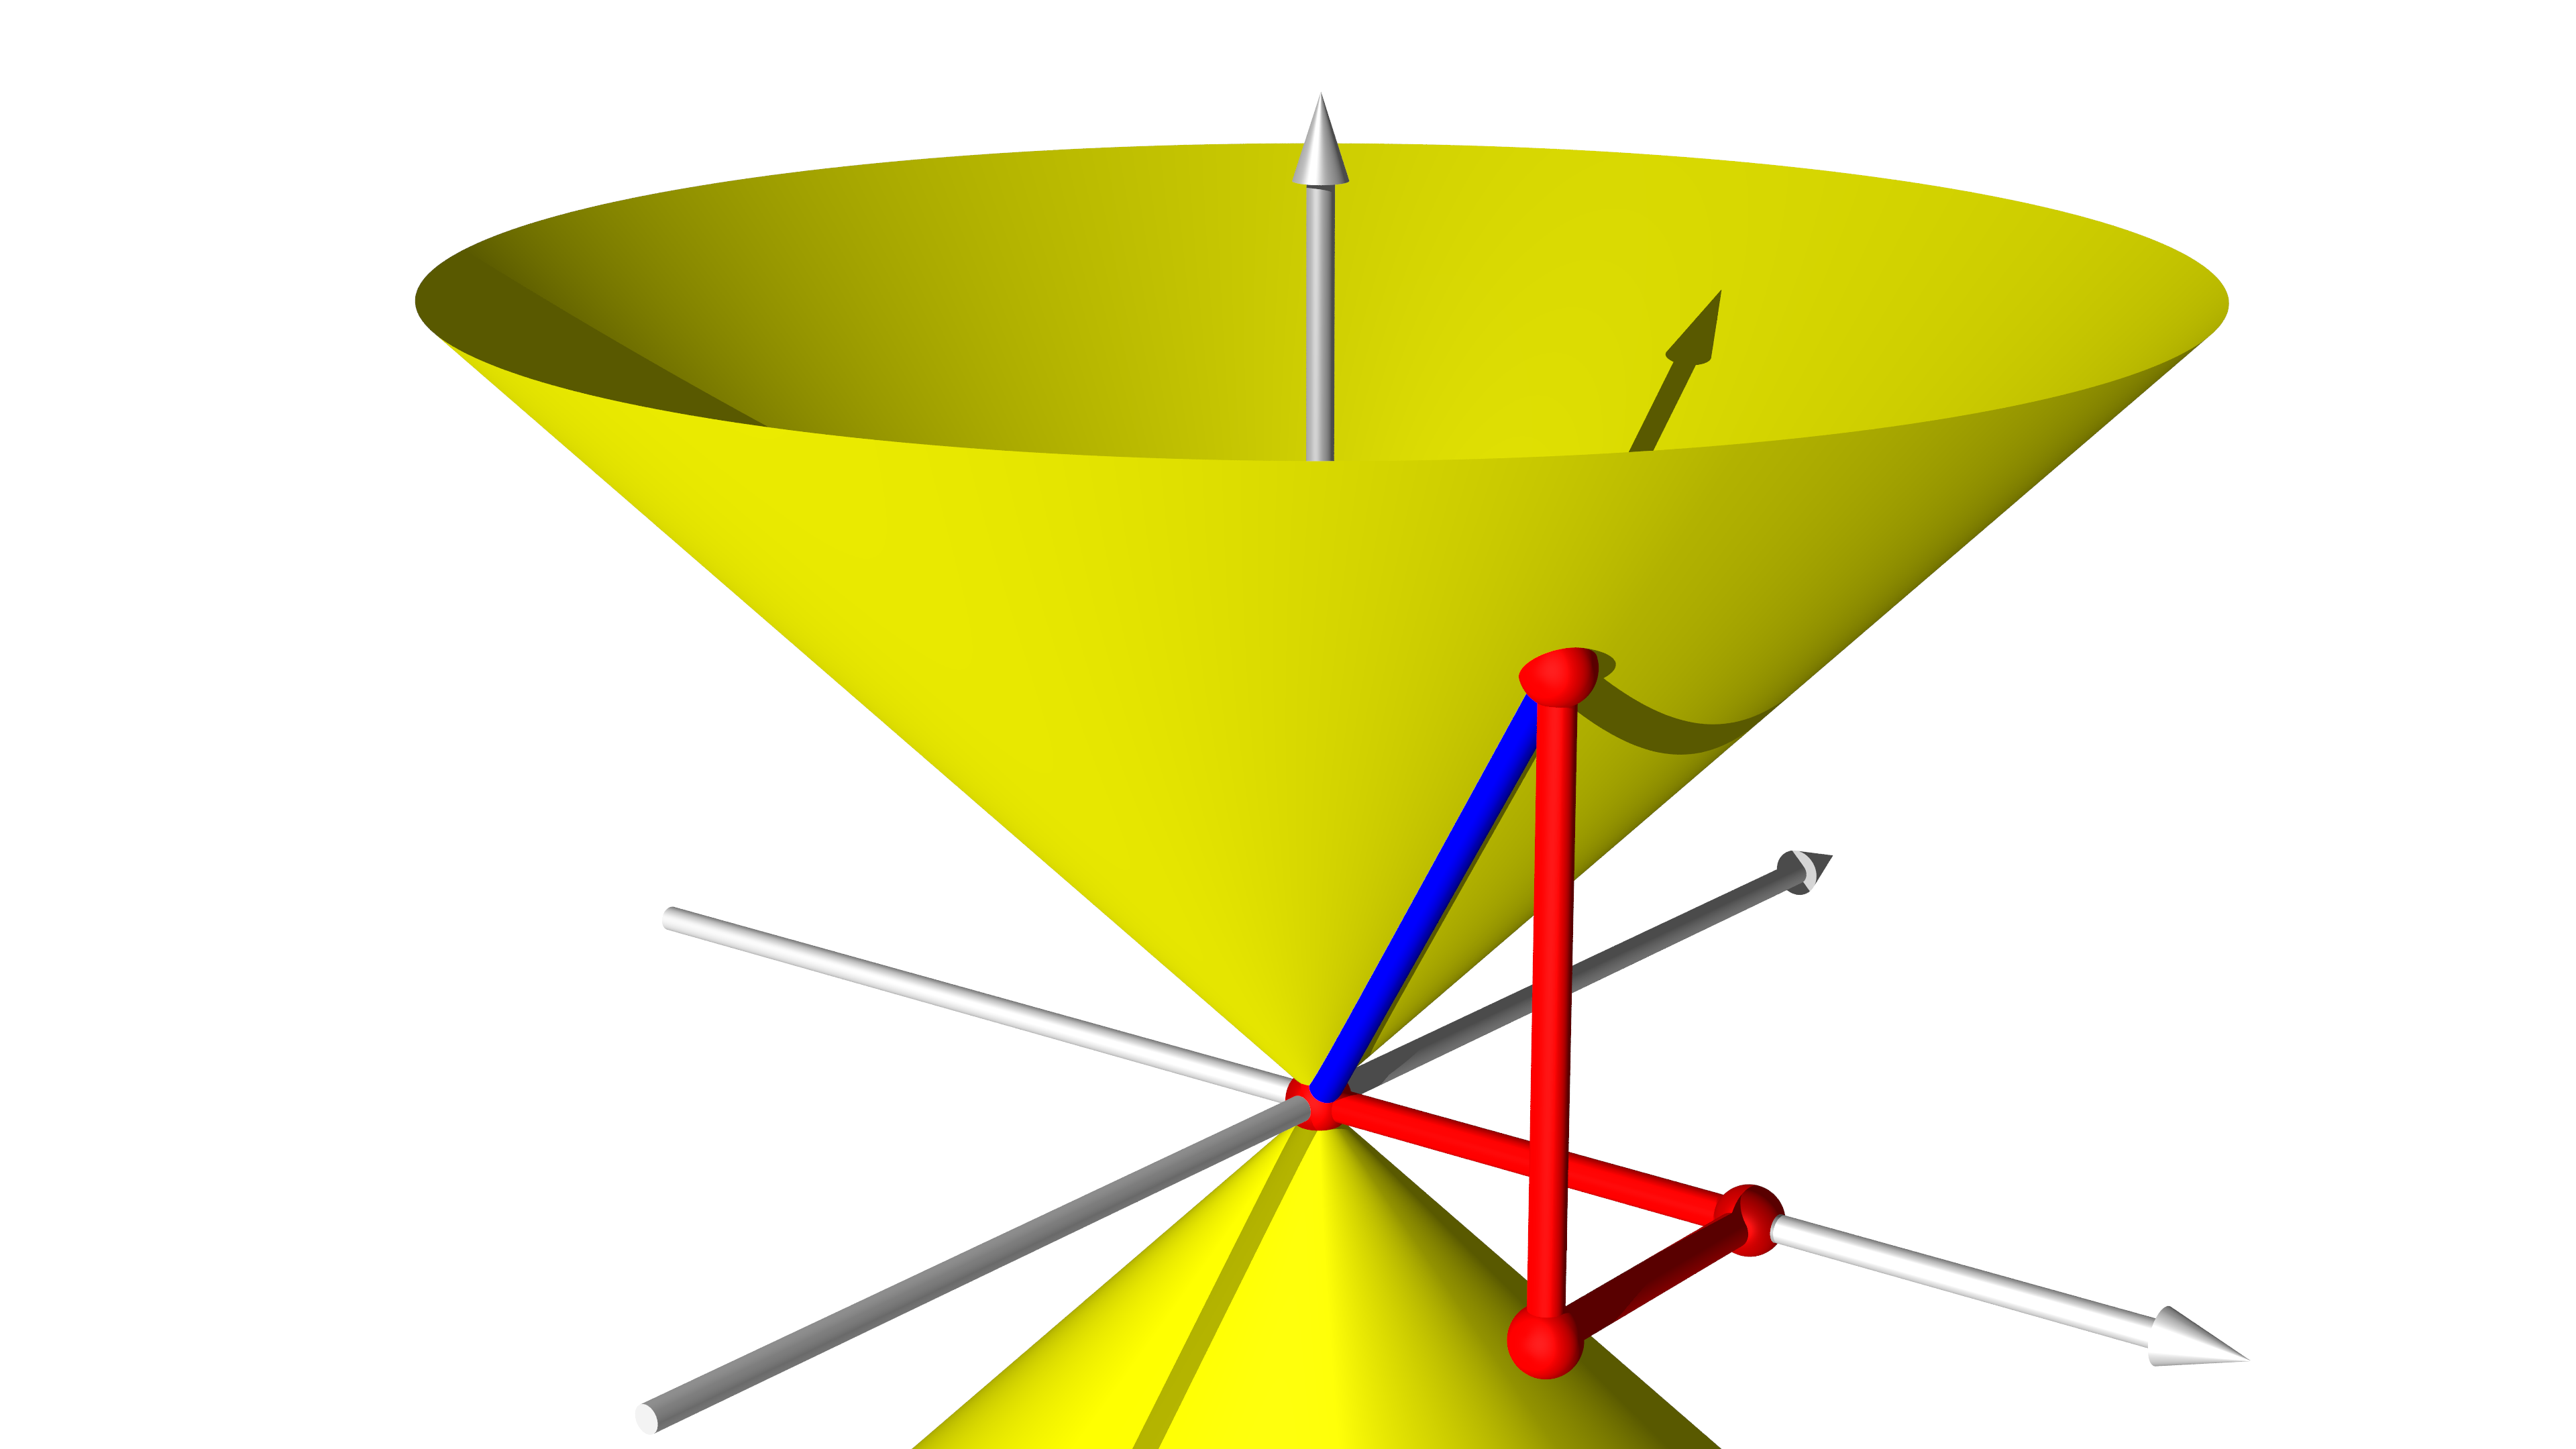
\includegraphics{chapters/tikz/lichtkegel.pdf}
\caption{Lichtkegel in Finkelstein-Koordinaten.
\label{skript:kruemmung:fig:lichtkegel-finkel}}
\end{figure}
In Finkelstein-Koordinaten verschwindet die Singularität bei $r=r_g$,
es sollte daher auch einfacher werden, die Bahn eines radial ins
Zentrum des Feldes stürzenden Teilchens zu berechnen.
Dazu können wir die Winkel-Koordinaten $\vartheta$ und $\varphi$
vernachlässigen und nur mit den Koordinaten $\tau$ und $R$ und der
Metrik
\[
ds^2
=
-c^2 \,d\tau^2
+r _g^{\frac23}\biggl(\frac32(R-c\tau)\biggr)^{\frac23}\,dR^2
\]
arbeiten.
\rhead{Absturz ins Zentrum}
Zur Berechnung der Bahnkurven brauchen wir die Christoffel-Symbole
2.~Art.
Die Berechnung mit Maxima ergibt
\begin{align*}
\Gamma^1_{11} &= 0,&
\Gamma^1_{12} &= 0,&
\Gamma^1_{21} &= 0,&
\Gamma^1_{22} &= \frac{2^{\frac23}r_g^{\frac23}}{(3(R-c\tau))^{\frac53}},\\
\Gamma^2_{11} &= 0,&
\Gamma^2_{12} &= \frac1{3(R-c\tau)},&
\Gamma^2_{21} &= \frac1{3(R-c\tau)},&
\Gamma^2_{22} &= -\frac1{3(R-c\tau)}.
\end{align*}
Wir beschreiben die Bahn eines Teilchens, welches sich in diesem Feld
radial bewegt, mit den Funktionen $\tau(s)$ und $R(s)$.
Wir untersuchen ein Teilchen, welches beim Punkt $\tau(0)=0$ und $R(0)=R_0$
mit Anfangsrichtung $\dot\tau(0)=1$ und $\dot R(0)=0$ in das Gravitationsfeld
stürzt.
Die Geodätengleichungen lauten
\begin{align*}
\frac{d^2\tau(s)}{ds^2}
&=
\Gamma^1_{22}\biggl(\frac{dR(s)}{ds}\biggr)^2,
\\
\frac{d^2R(s)}{ds^2}
&=
\Gamma^2_{12}\frac{d\tau(s)}{ds}\frac{dR(s)}{ds}
+
\Gamma^2_{22}\biggl(\frac{dR(s)}{ds}\biggr)^2.
\end{align*}
Da für die Anfangsbedinung $\dot R=0$ ist und auf der rechten Seite
$\dot R$ in jedem Term vorkommt, folgt aus der zweiten Gleichung
$\ddot R=0$, $\dot R$ kann sich also nicht ändern.
Wenn aber $\dot R=0$ für alle Werte von $s$, dann ist nach der ersten
Gleichung auch $\ddot \tau=0$ und damit $\dot \tau=1$.
Die Lösungskurve ist also $R=R_0$ und $\tau=s$, rot dargestellt in
Abbildung~\ref{skript:kruemmung:fig:absturz}
und
Abbildung~\ref{skript:kruemmung:fig:lichtkegel-finkel}.

Mit Hilfe der Formel~\eqref{skript:kruemmung:finkelsteinr}
kann man damit auch $r$ in Abhängigkeit von $\tau$ für den radialen Absturz
angeben:
\[
r(\tau)=\biggl(\frac32(R_0-c\tau)\biggr)^{\frac23}r_g^{\frac13}.
\]
Die Weltlinie eines radialen Absturzes in diesen Koordinaten ist in
Abbildung~\ref{skript:kruemmung:fig:blackhole} dargestellt.

\section{Ereignishorizont%
\label{skript:section:ereignishorizont}}
\rhead{Ereignishorizont}
Wir betrachten wieder die
Schwarzschild-Metrik~\eqref{skript:kruemmung:schwarzschildmetrik}
und möchten genauer verstehen, was bei $r=r_g$ passiert.
Dazu überlegen wir uns, wie ein Geodäte eines realen Teilchens 
aussieht.
Wir wissen, dass reale Teilchen sich entlang von Weltlinien bewegen müssen,
deren Tangentialvektor zeitartig ist.
Ein Teilchen in Ruhe hat zum Beispiel $\dot r=0$, $\dot \vartheta=0$ und
$\dot\varphi=0$, einzig $\dot t\ne 0$.
Da der Koeffizient von $dt^2$
\[
-\biggl(1-\frac{r_g}{r}\biggr)
\quad
\begin{cases}
<0&\qquad r > r_g
\\
>0&\qquad r < r_g
\end{cases}
\]
für $r>r_g$
negativ ist folgt, dass es tatsächlich möglich ist, dass sich ein Teilchen
in festem Abstand vom Zentrum aufhalten kann.
Sobald aber $r<r_g$ ist, ist der Koeffizient von $dt^2$ positiv,
fester Abstand vom Zentrum ist nicht mehr möglich.

Für $r<r_g$ wechselt aber auch das Vorzeichen des Koeffizienten
\[
\frac1{\displaystyle1-\frac{r_g}{r}}
\quad
\begin{cases}
>0&\qquad r>r_g
\\
<0&\qquad r<r_g
\end{cases}
\]
von $dr^2$, damit wird plötzlich der Vektor $\dot t=0$, $\dot r\ne 0$,
$\dot\vartheta=\dot\varphi=0$ zeitartig.
Sobald ein Teilchen sich innerhalb des Radius $r_g$ befindet, kann
sein Radius nur noch abnehmen.
Die Berechnung der Bahn eines solchen Teilchens zeigt auch, dass
es unausweichlich in endlicher Zeit ins Zentrum stürzen wird.
In Abbildung~\ref{skript:kruemmung:fig:lichtkegel-finkel} erkennt 
man dies daran, dass der Lichtkegel beim Überschreiten von $r=r_g$
so eng wird, dass zeitartige Vektoren die Linie $r=r_g$ in umgekehrter
Richtung nicht mehr kreuzen können.

\begin{figure}
\centering
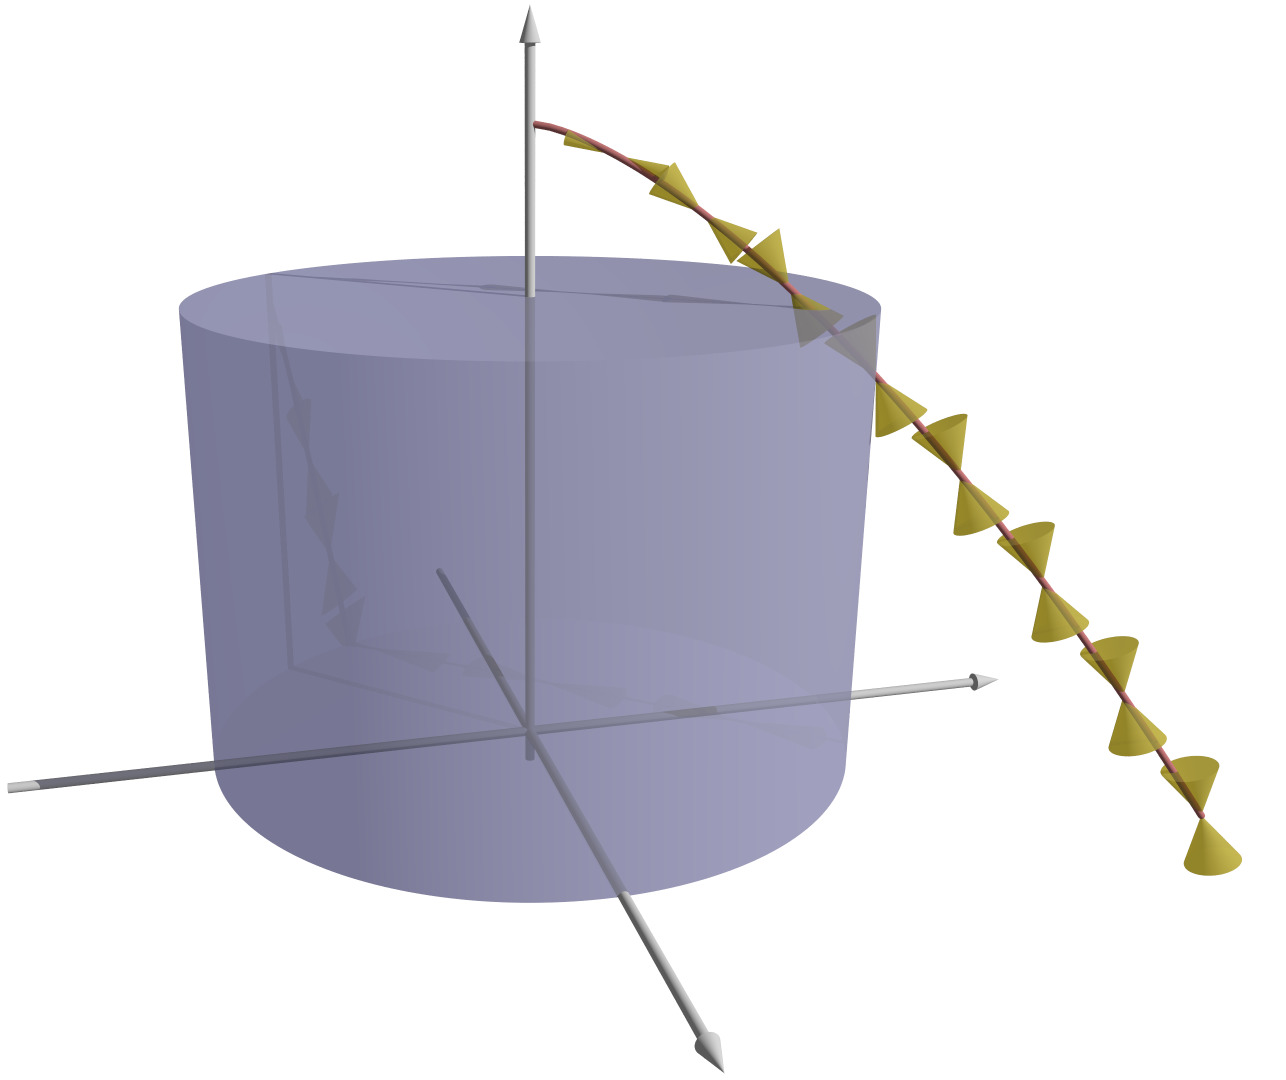
\includegraphics[width=\hsize]{chapters/3d/blackhole.jpg}
\caption{Absturz eines Teilchens durch den Ereignishorizont in
$(\tau,r,\varphi)$-Koordinaten.
Sobald das Teilchen durch den Ereignishorizont gefallen ist,
befindet sich der ganze zukünftige Lichtkegel eines Teilchens 
immer vollständig im Inneren des Gebietes $r<r_g$.
\label{skript:kruemmung:fig:blackhole}}
\end{figure}


\section{Was spürt man am Ereignishorizont?%
\label{skript:section:wasspuertman}}
\rhead{Was spürt man am Ereignishorizont?}
Der Riemannsche Krümmungstensor gibt an, wie schnell Geodäten von Teilchen
wegen unterschiedlicher Gravitationswirkung sich voneinander entfernen.
Er bestimmt also die sogenannten Gezeitenkräfte, die ein Astronaut spürt,
der in diesem Gravitationsfeld abstürzt.
\index{Gezeitenkräfte}%
Die Berechnung des Riemann-Tensors mit Maxima ergibt aber:
\begin{align*}
R_{1212}&=-\frac{r_g}{r^3},
\end{align*}
die Gezeitenkräfte in radialer Richtung werden für den Astronauten
zwar immer grösser, er wird in die Länge gezogen und schliesslich 
zerrissen, darüber hinaus aber spürt er bei $r=r_g$ nichts Besonderes.
\index{Ereignishorizont}%

\section{Bedeutung von $r_g$%
\label{skript:schwarzschild:rg}}
\rhead{Bedeutung von $r_g$}
In Abschnitt~\ref{skript:section:ereignishorizont} haben wir gefunden,
dass sich bei der Koordinaten $r=r_g$ der Ereignishorizont befindet.
Es ist auch einigermassen klar, dass dieser Radius $r_g$ mit der
Masse des Objektes zusammenhängen muss.
Doch wie gross ist eigentlich der Gravitations-Radius $r_g$ verschiedener
uns umgebender Himmelskörper? Kann es überhaupt einen Körper geben, der
so dicht ist, dass er kleiner ist als sein Gravitationsradius?

In grosser Entfernung $r \gg r_g$ vom Zentrum ist die Metrik fast flach,
das Feld ist dort sehr schwach.
Durch Vergleich mit der Näherung~\eqref{skript:gravitation:naeherung}
finden wir
\[
\frac{r_g}{r} = \frac{2MK}{c^2r}
\qquad\Rightarrow\qquad
r_g=\frac{2MK}{c^2}.
\]
Der Radius $r_g=2MK$ heisst der {\em Gravitationsradius} oder 
\index{Gravitationsradius}%
{\em Schwarzschild-Radius}.
\index{Schwarzschild-Radius}%
Der numerische Zusammenhang zwischen Masse und Gravitationsradius
in SI-Einheiten ist
\[
r_g = \frac{2K}{c^2}M
=
2\cdot 6.67408\cdot10^{-11}
\frac{\text{m}^3}{\text{kg}\cdot\text{s}^2}
\cdot
\frac1{(2.99792458\cdot 10^{8}\frac{\text{m}}{\text{s}})^2}\cdot M
=
1.485183\cdot 10^{-27}\frac{\text{m}}{\text{kg}}\cdot M
\]
Der Gravitationsradius der Sonne ist 
\begin{align*}
r_g
&=
1.485183\cdot 10^{-27}\frac{\text{m}}{\text{kg}}M
=
2.95403\cdot 10^{3}\text{m}
=
2.954\,\text{km}.
\end{align*}
Könnte man die Sonne auf eine Kugel mit einem Radius kleiner als 2.954km
komprimieren, würde sie zu einem schwarzen Loch und wäre nicht mehr
sichtbar.
Der Gravitationsradius der Erde ist dagegen viel kleiner:
\[
r_g
=
1.485183\cdot 10^{-27}\frac{\text{m}}{\text{kg}}M
\cdot
5.972\cdot 10^{24}\text{m}
=
8.87\cdot 10^{-3}\text{m}
=
8.87\text{mm}.
\]
Der Gravitationsradius ist also kleiner als ein Zentimeter.

%
% s-perihel.tex -- relativistische Periheldrehung, numerisch berechnet
%
% (c) 2017 Prof Dr Andreas Müller, Hochschule Rappersiwl
%

\section{Periheldrehung}
\rhead{Periheldrehung}
\begin{figure}
\centering
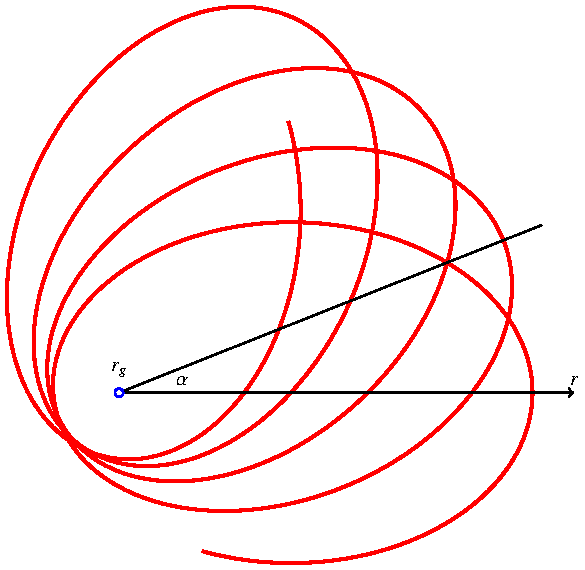
\includegraphics{chapters/tikz/orbit.pdf}
\caption{Periheldrehung um den Winkel $\alpha$ in jedem Umlauf um den
Zentralkörper in einer Schwarzschild-Metrik mit Anfangsbedingungen
\label{skript:schwarzschild:anfangsbedingung:normal}.
\label{skript:schwarzschild:perihelorbit}}
\end{figure}
Das erste Keplersche Gesetz sagt, dass ein Planet sich auf einer
Ellipsenbahn bewegt.
Die Newtonsche Gravitationstheorie bestätigt dies, die Differentialgleichungen
für das Zweikörperproblem sind in geschlossener Form lösbar.
Insbesondere zeigt die Richtung zum sonnennächsten Punkt, dem Perihel,
immer in die gleiche Richtung.
Für die Merkurbahn wurde jedoch eine Abweichung festgestellt, die
Perihelrichtung dreht sich mit der Zeit um die Sonne.
Einen Teil dieser Drehung konnte mit der newtonschen Theorie erklärt werden.
So führen zum Beispiel die Abplattung der Sonne und die Störungen durch
andere Planeten zu einem solchen Effekt.
Von den gemessenen $571.91''$ Periheldrehung des Merkur pro Jahrhundert
verblieben jedoch $43.11''$ pro Jahrhundert, die die Newtonsche
Theorie nicht erklären konnte.


Schon in seinem ursprünglichen Entwurf der allgemeinen Relativitätstheorie
hat Einstein die durch die Abweichung von der Newtonschen Theorie
verursachte Periheldrehung der Merkurbahn berechnet und gute Übereinstimmung
mit der bekannten Drehung gefunden.
Damit hat er bereits selbst eine erste experimentelle Bestätigung
der Theorie gegeben.

Um den Effekt überhaupt darstellen zu können, muss die Bahn sehr nahe
am Zentralkörper vorbeiführen, der nächste Punkt, das Apastron darf
also nur wenige Gravitationsradien entfernt sein.
In Abbildung~\ref{skript:schwarzschild:perihelorbit} ist die
Umlaufbahn eines Körpers dargestellt, dessen Apastron-Entfernung
$100 r_g$ ist und der sich im Periastron auf etwa $20r_g$ 
nähert.
Die Apsidenlinie dreht sich hier in jedem Umlauf um $\alpha = 21.61^\circ$.
Ziel dieses Abschnittes ist zu zeigen, wie die Periastron-Drehung
in einer Schwarzschild-Metrik numerisch berechnet werden kann.
Es geht dabei nicht darum, den exakten Wert für die Periheldrehung
des Merkur zu bestimmen,
sondern nur zu zeigen, dass die allgemeine Relativitätstheorie
qualititativ einen solchen Effekt vorhersagt.

\subsection{Geodätengleichung für die Schwarzschild-Metrik}
\label{skript:schwarzschild:geodaetengleichung}
%(%i5) 		        ratsimp(Christoffel2(1, 1, 1))
%(%o5) 				       0
%(%i6) 		        ratsimp(Christoffel2(1, 1, 2))
%				       rg
%(%o6) 			        - -------------
%					      2
%				  2 r rg - 2 r
%(%i7) 		        ratsimp(Christoffel2(1, 1, 3))
%(%o7) 				       0
%(%i8) 		        ratsimp(Christoffel2(1, 1, 4))
%(%o8) 				       0
%(%i9) 		        ratsimp(Christoffel2(1, 2, 2))
%(%o9) 				       0
%(%i10) 		        ratsimp(Christoffel2(1, 2, 3))
%(%o10) 				       0
%(%i11) 		        ratsimp(Christoffel2(1, 2, 4))
%(%o11) 				       0
%(%i12) 		        ratsimp(Christoffel2(1, 3, 3))
%(%o12) 				       0
%(%i13) 		        ratsimp(Christoffel2(1, 3, 4))
%(%o13) 				       0
%(%i14) 		        ratsimp(Christoffel2(1, 4, 4))
%(%o14) 				       0
%(%i15) 		        ratsimp(Christoffel2(2, 1, 1))
%				     2
%				   rg  - r rg
%(%o15) 				 - ----------
%					 3
%				      2 r
%(%i16) 		        ratsimp(Christoffel2(2, 1, 2))
%(%o16) 				       0
%(%i17) 		        ratsimp(Christoffel2(2, 1, 3))
%(%o17) 				       0
%(%i18) 		        ratsimp(Christoffel2(2, 1, 4))
%(%o18) 				       0
%(%i19) 		        ratsimp(Christoffel2(2, 2, 2))
%				      rg
%(%o19) 				 -------------
%					     2
%				 2 r rg - 2 r
%(%i20) 		        ratsimp(Christoffel2(2, 2, 3))
%(%o20) 				       0
%(%i21) 		        ratsimp(Christoffel2(2, 2, 4))
%(%o21) 				       0
%(%i22) 		        ratsimp(Christoffel2(2, 3, 3))
%(%o22) 				    rg - r
%(%i23) 		        ratsimp(Christoffel2(2, 3, 4))
%(%o23) 				       0
%(%i24) 		        ratsimp(Christoffel2(2, 4, 4))
%					 2
%(%o24) 			     (rg - r) sin (theta)
%(%i25) 		        ratsimp(Christoffel2(3, 1, 1))
%(%o25) 				       0
%(%i26) 		        ratsimp(Christoffel2(3, 1, 2))
%(%o26) 				       0
%(%i27) 		        ratsimp(Christoffel2(3, 1, 3))
%(%o27) 				       0
%(%i28) 		        ratsimp(Christoffel2(3, 1, 4))
%(%o28) 				       0
%(%i29) 		        ratsimp(Christoffel2(3, 2, 2))
%(%o29) 				       0
%(%i30) 		        ratsimp(Christoffel2(3, 2, 3))
%				       1
%(%o30) 				       -
%				       r
%(%i31) 		        ratsimp(Christoffel2(3, 2, 4))
%(%o31) 				       0
%(%i32) 		        ratsimp(Christoffel2(3, 3, 3))
%(%o32) 				       0
%(%i33) 		        ratsimp(Christoffel2(3, 3, 4))
%(%o33) 				       0
%(%i34) 		        ratsimp(Christoffel2(3, 4, 4))
%(%o34) 			    - cos(theta) sin(theta)
%(%i35) 		        ratsimp(Christoffel2(4, 1, 1))
%(%o35) 				       0
%(%i36) 		        ratsimp(Christoffel2(4, 1, 2))
%(%o36) 				       0
%(%i37) 		        ratsimp(Christoffel2(4, 1, 3))
%(%o37) 				       0
%(%i38) 		        ratsimp(Christoffel2(4, 1, 4))
%(%o38) 				       0
%(%i39) 		        ratsimp(Christoffel2(4, 2, 2))
%(%o39) 				       0
%(%i40) 		        ratsimp(Christoffel2(4, 2, 3))
%(%o40) 				       0
%(%i41) 		        ratsimp(Christoffel2(4, 2, 4))
%				       1
%(%o41) 				       -
%				       r
%(%i42) 		        ratsimp(Christoffel2(4, 3, 3))
%(%o42) 				       0
%(%i43) 		        ratsimp(Christoffel2(4, 3, 4))
%				  cos(theta)
%(%o43) 				  ----------
%				  sin(theta)
%(%i44) 		        ratsimp(Christoffel2(4, 4, 4))
%(%o44) 				       0
%
Für die Geodätengleichungen brauchen wir die Christoffsymbole 
für die Schwarzschild Metrik.
Mit Maxima kann man die folgenden nicht verschwindenden
$\Gamma^\mu_{\alpha\beta}$ 
finden:
\begin{align*}
%(%i6) 		        ratsimp(Christoffel2(1, 1, 2))
%				       rg
%(%o6) 			        - -------------
%					      2
%				  2 r rg - 2 r
\Gamma^0_{01}
&=
\frac{1}{1-\displaystyle\frac{r_g}{r}}
\frac{r_g}{r}
\frac{1}{2r}
\\
%(%i15)                  ratsimp(Christoffel2(2, 1, 1))
%                                     2
%                                  rg  - r rg
%(%o15)                          - ----------
%                                         3
%                                      2 r
\Gamma^1_{00}
&=
\biggl(1-\displaystyle\frac{r_g}{r}\biggr)
\frac{r_g}{r}
\frac{1}{2r}
&
%(%i19)                  ratsimp(Christoffel2(2, 2, 2))
%                                      rg
%(%o19)                           -------------
%                                             2
%                                 2 r rg - 2 r
\Gamma^1_{11}
&=
-\frac1{1-\displaystyle\frac{r_g}{r}}
\frac{r_g}{r}
\frac{1}{2r}
&
%(%i22) 		        ratsimp(Christoffel2(2, 3, 3))
%(%o22) 				    rg - r
\Gamma^1_{22}
&=
r_g-r
&
%(%i24)                  ratsimp(Christoffel2(2, 4, 4))
%                                         2
%(%o24)                       (rg - r) sin (theta)
\Gamma^1_{33}
&=
(r_g-r)\sin^2\vartheta
\\
%(%i30)                  ratsimp(Christoffel2(3, 2, 3))
%                                       1
%(%o30)                                 -
%                                       r
\Gamma^2_{12}
&=
\frac1r
&
%(%i34) 		        ratsimp(Christoffel2(3, 4, 4))
%(%o34) 			    - cos(theta) sin(theta)
\Gamma^2_{33}
&=
-\cos\vartheta \sin\vartheta
\\
%(%i41)                  ratsimp(Christoffel2(4, 2, 4))
%                                       1
%(%o41)                                 -
%                                       r
\Gamma^3_{13}
&=
\frac1r
&
%(%i43)                  ratsimp(Christoffel2(4, 3, 4))
%                                  cos(theta)
%(%o43)                            ----------
%                                  sin(theta)
\Gamma^3_{23}
&=
\cot\vartheta
\end{align*}
Wir betrachten jetzt eine Geodäte, die mit dem Parameter $s$ parametrisiert ist.
In allgemeiner Form schreiben wir dafür $x^\mu(s)$, im speziellen
Koordinatensystem der Schwarzschild-Metrik ist
\[
\begin{aligned}
x^0(s)&=t(s),
&
x^1(s)&=r(s),
&
x^2(s)&=\vartheta(s),
&
x^3(s)&=\varphi(s).
\end{aligned}
\]
Die zugehörigen Geodätengleichungen sind
\begin{align*}
\ddot t(s)
&=
-\frac{1}{1-\displaystyle\frac{r_g}{r}}\frac{r_g}{r}\frac{1}{r}\dot t(s)\,\dot r(s)
\\
\ddot r(s)
&=
-\biggl(1-\frac{r_g}{r}\biggr)\frac{r_g}{r}\frac1{2r}\dot t(s)^2
+\frac{1}{1-\displaystyle\frac{r_g}{r}} \frac{r_g}{r}\frac1{2r}\dot r(s)^2
-(r_g-r)\dot \vartheta(s)^2 + (r_g-r)\sin^2 \vartheta \cdot \dot \varphi(s)^2
\\
\ddot \vartheta(s)
&=
-\frac{2}{r} \dot r(s)\, \dot \vartheta(s)
+\cos\vartheta\sin\vartheta \cdot \dot\varphi(s)^2
\\
\ddot \varphi(s)
&=
-\frac{2}{r} \dot r(s)\,\dot \varphi(s)
-2\cot\vartheta \cdot \dot r(s)\,\dot\varphi(s)
\end{align*}
Darin ist natürlich $r$ in den Koeffizienten jeweils als $r(s)$ zu lesen.

Wir wollen eine Bahn in der Ebene $\vartheta=\frac{\pi}2$ berechnen.
Setzen wir diesen Wert ein, verschwinden auch noch die Terme, die
$\cos\vartheta$ enthalten.
Es bleiben nur noch
\begin{equation}
\begin{aligned}
\Gamma^0_{01}
&=
\frac{1}{1-\displaystyle\frac{r_g}{r}}
\frac{r_g}{r}
\frac{1}{2r}
\\
\Gamma^1_{00}
&=
\biggl(1-\displaystyle\frac{r_g}{r}\biggr)
\frac{r_g}{r}
\frac{1}{2r}
&
\Gamma^1_{11}
&=
-\frac1{1-\displaystyle\frac{r_g}{r}}
\frac{r_g}{r}
\frac{1}{2r}
&
\Gamma^1_{22}
&=
r_g-r
&
\Gamma^1_{33}
&=
r_g-r
\\
%(%i30)                  ratsimp(Christoffel2(3, 2, 3))
%                                       1
%(%o30)                                 -
%                                       r
\Gamma^2_{12}
&=
\frac1r
\\
%(%i41)                  ratsimp(Christoffel2(4, 2, 4))
%                                       1
%(%o41)                                 -
%                                       r
\Gamma^3_{13}
&=
\frac1r
\end{aligned}
\label{skript:schwarzschild:christoffelaequator}
\end{equation}
Hat eine Geodäte eine Anfangsgeschwindigkeit in der Äquatorebene, dann
ist $\dot x^3(0) = \dot\vartheta(0)=0$.
Die Geodätengleichung für $\ddot \vartheta$ ist dann
\[
\ddot \vartheta(s)
=
\ddot x^2(s)
=
\Gamma^2_{12}\dot r(s)\dot \vartheta(s),
\]
insbesondere bleibt $\dot\vartheta(s)=0$ entlang der ganzen Geodäten.
Die Geodäte wird daher die Äquatorebenen nicht verlassen.
Da man das Koordinatensystem immer so wählen kann, dass $\dot\vartheta(0)=0$
ist, kann man ganz allgemein sagen, dass Geodäten in einer Schwarzschild-Metrik
in einer Ebene liegen.
Man hätte also auch von Anfang an in Polarkoordinaten rechnen können.

Die vereinfachten Christoffelsymbole für die Äquatorebene
\eqref{skript:schwarzschild:christoffelaequator}
führen auch auf vereinfachte Geodätengleichungen, wenn wir $\dot\vartheta(s)=0$
berücksichtigen.
Wir erhalten
\begin{align*}
\ddot t(s)
&=
-\frac{1}{1-\displaystyle\frac{r_g}{r}}\frac{r_g}{r}\frac{1}{r}\dot t(s)\,\dot r(s)
\\
\ddot r(s)
&=
-\biggl(1-\frac{r_g}{r}\biggr)\frac{r_g}{r}\frac1{2r}\dot t(s)^2
+\frac{1}{1-\displaystyle\frac{r_g}{r}} \frac{r_g}{r}\frac1{2r}\dot r(s)^2
- (r_g-r) \dot\varphi(s)^2
\\
\ddot \vartheta(s)
&=
0
\\
\ddot \varphi(s)
&=
-\frac2r \dot r(s)\,\dot\varphi(s)
\end{align*}
Diese Gleichungen lassen sich nicht in geschlossener Form integrieren.
Durch numerische Lösung für geeignete Anfangswerte kann man jedoch die
Drehung der Apsidenlinie sichtbar machen.

\subsection{Numerische Lösung}
Im Repository zu befinden sich einige Octave-Programme, mit denen man
die Geodäten in einer Schwarzschild-Metrik berechnen kann.
Um zu etwas leichter verständlichen Zahlen zu kommen, rechnen wir
in diesen Programmen immer mit Masseinheiten so, dass $r_g=1$ ist,
d.~h.~der Gravitationsradius des Zentralkörpers ist die Längeneinheit,
und $c=1$, d.~h.~$r_g/c$ ist die Zeiteinheit.

Der Parameter $s$ der Geodätengleichung ist genau dann die Eigenzeit,
wenn die Anfangsgeschwindigkeit den den Wert $-1$ hat.
In den Rechnungen muss daher die Anfangs-Vierergschwindigkeit $u^\mu$
so normiert werden, dass $g_\mu\nu u^\mu u^\nu=-1$ ist.

\subsubsection{Zustandsvektor}
Da die Geodätengleichungen Differentialgleichungen zweiter Ordnung sind,
muss man als Zustandsvektor den Vektor
\[
X=\begin{pmatrix}
t\\r\\\vartheta\\\varphi \\\dot t\\\dot r\\\dot \vartheta\\\dot\varphi
\end{pmatrix}
\]
verwenden.
Der Punkt bezeichnet darin die Ableitung nach dem Parameter $s$, der
wie gesagt bei geeigneter Normierung der Anfangsgeschwindigkeit mit
der Eigenzeit übereinstimmt.
Aus dem Vektor $X$ lässt sich jederzeit die Position und die
Vierergeschwindigkeit extrahieren.
Im File \text{geodesic.m} dienen dazu die Funktionen
\texttt{position} und \texttt{velocity}
\lstinputlisting[style=Octave]{chapters/listings/schwarzschild-extract.m}
Mit der Funktion \texttt{rescale} kann man im Vektor $X$ den
Geschwindigkeitsanteil um einen gegebenen Faktor strecken:
\lstinputlisting[style=Octave]{chapters/listings/schwarzschild-rescale.m}

\subsubsection{Metrik und Christoffel-Symbole}
Natürlich braucht man die Metrik, um den korrekten Wert zu berechnen.
Das File \texttt{geodesic.m} geht davon aus, dass die Funktion \texttt{metrik}
bereits definiert worden ist.
Für die Schwarzschild-Metrik geschieht dies im File
\texttt{christoffel-schwarzschild.m} mit der Funktion
\lstinputlisting[style=Octave]{chapters/listings/schwarzschild-metrik.m}
Diese Funktion berechnet das Skalarprodukt der Vektoren \texttt{u} und
\texttt{v} an der Stelle $x$.
Das File \texttt{christoffel-schwarzschild.m} definiert auch die Funktion
\texttt{christoffel}, die für jeden Index-Wert $\alpha$ die Matrix mit
den Einträgen $\Gamma^\alpha_{\mu\nu}$ für die Koordinatenwerte \texttt{x}
zurückgibt.
Für die Schwarzschild-Metrik ist dies
\lstinputlisting[style=Octave]{chapters/listings/schwarzschild-christoffel.m}

\subsubsection{Differentialgleichung}
Mit diesen zwei Funktionen ist es jetzt nicht mehr schwierig, eine Funktion
zu konstruieren, die Geodäten für jede beliebige Metrik berechnen kann.
Zunächst ist eine Funktion nötig, die die Differentialgleichung implementiert.
Für den Vektor $X$ geschrieben lautet diese
\[
\frac{dX}{ds}
=
\begin{pmatrix}
X_5\\X_6\\X_7\\X_8
\\
-\Gamma^1_{ij}X^iX^j\\
-\Gamma^2_{ij}X^iX^j\\
-\Gamma^3_{ij}X^iX^j\\
-\Gamma^4_{ij}X^iX^j
\end{pmatrix},
\]
wobei die Indizes $i$ und $j$ von $1$ bis $4$ laufen.
Da die Funktion \texttt{christoffel} die Werte der Christoffelsymbole
als Matrix $\Gamma^\alpha$ liefert, kann man für die Vierergschwindigkeit
$u$ die rechte Seite auch als $u^t \Gamma^\alpha u$ schreiben.
Die Differentialgleichung lässt sich daher in Octave durch die
Funktion
\lstinputlisting[style=Octave]{chapters/listings/geodesic-dgl.m}
implementieren.

Die Differentialgleichung lässt sich mit der Funktion \texttt{lsode}
lösen.
Die nötigen Schritt sind in der Funktion
\lstinputlisting[style=Octave]{chapters/listings/geodesic-solution.m}
zusammengefasst.

\subsubsection{Drehung der Apsidenlinie}
Die Drehung der Apsiden-Linie ist daran erkennbar, dass die Werte von
$\varphi(s)$, bei denen $r(s)$ sein Maximum und Minimum annimmt,
nicht jeweils um $\pi$ auseinanderliegen, sondern um einen grösseren
Wert.
Die Extrema von $r(s)$ sind erkennbar daran, dass $\dot r(s)=0$.
Man kann daher den Betrag der Drehung der Apsidenlinie dadurch
bestimmen, dass man numerisch die Nullstellen von $\dot r(s)$
bestimmt, und die zugehörigen Werte von $\varphi(s)$ ermittelt.

Die numerische Rechnung kann mit der Funktion \texttt{apsidbetween}
\lstinputlisting[style=Octave]{chapters/listings/apsiden-between.m}
durchgeführt werden.
Als Argument nimmt diese Funktion zwei Zustandsvektoren in der Form,
wie sie von der Funktion \texttt{geodesic}
zurückgegeben wird, also eine Zeile bestehend aus der aktuellen
Eigenzeit und den acht Komponenten des Zustandsvektors.
Die Funktion \texttt{apsidbetween} integriert dann auf Zeile~20
zehnmal kleinere Integrationsschritte in diesem Interval (und aus numerischen
Gründen noch etwas darüber hinaus) und sucht in den Zeilen 22 bis 25
das
erste Teilinterval, in dem das Vorzeichen von $\dot r(s)$ wechselt.
Mit den zugehörigen Zuständen wird \texttt{apsidbetween}
in Zeile 26
rekursiv augerufen, bis auf Zeile~6 die Differenz der Winkel $\phi(s)$ zwischen
den beiden Zuständen kleiner als $10^{-6}$ ist.

Der folgende Code berechnet die Werte von $\varphi(s)$ für alle
Extrema von $r(s)$ und ermittelt den Mittelwert:
\lstinputlisting[style=Octave]{chapters/listings/apsiden-winkel.m}

\subsubsection{Beispiel}
Die Umlaufbahn aus Abbildung~\ref{skript:schwarzschild:perihelorbit}
wurde mit den Anfangsbedingungen
\begin{equation}
\begin{aligned}
t(s)        &=\phantom{00}0.00000                    &\dot t(s)         &= 1.00577\\
r(s)        &=          100.00000                    &\dot r(s)         &= 0.00000\\
\vartheta(s)&=\phantom{00}1.57080=\textstyle\frac\pi2&\dot \vartheta(s) &= 0.00000\\
\varphi(s)  &=\phantom{00}0.00000                    &\dot \varphi(s)   &= 0.00038
\end{aligned}
\label{skript:schwarzschild:anfangsbedingung:normal}
\end{equation}
berechnet.
Es ergibt sich ein durchschnittlicher Wert von $21.6114^\circ$, um den die
Apsidenlinie vorrückt.

\subsubsection{Extreme Bahnen}
\begin{figure}
\centering
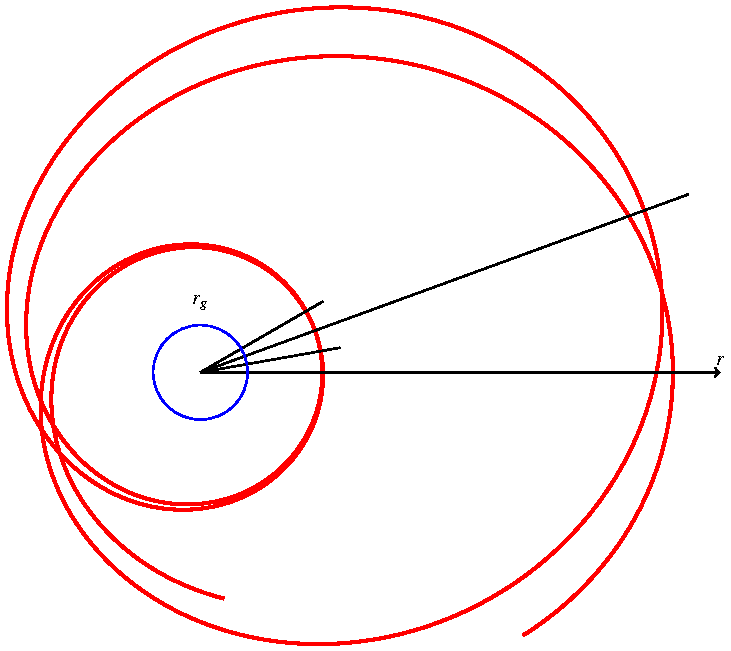
\includegraphics{chapters/tikz/orbit2.pdf}
\caption{Periheldrehung für eine Bahn, die sehr nahe an den Gravitationsradius
heranführt.
Anfangsbedingungen dieser Bahn sind
\eqref{skript:schwarzschild:anfangsbedingunge:extrem}.
\label{skript:schwarzschild:apside:extrem}}
\end{figure}
Bahnen, die sehr nahe an den Ereignishorizont heranführen, erfahren eine
noch viel deutlichere Drehung der Apsidenlinie.
In Abbildung~\ref{skript:schwarzschild:apside:extrem}
ist eine Bahn dargestellt, die sich auf weniger als $3r_g$ dem Zentralkörper
nähert.
Schon der Winkel $\varphi$ für das Perihel unterscheidet sich um um mehr
als $180^\circ$ vom Winkel $180^\circ$, der für eine Kepler-Bahn zu
erwarten wäre.
Die Anfangsbedingungen dieser Bahn sind
\begin{equation}
%    0.00000
%   10.00000
%    1.57080
%    0.00000
%    1.07220
%    0.00000
%    0.00000
%    0.01861
\begin{aligned}
t(s)        &=\phantom{0}0.00000                    &\dot t(s)         &= 1.07220\\
r(s)        &=          10.00000                    &\dot r(s)         &= 0.00000\\
\vartheta(s)&=\phantom{0}1.57080=\textstyle\frac\pi2&\dot \vartheta(s) &= 0.00000\\
\varphi(s)  &=\phantom{0}0.00000                    &\dot \varphi(s)   &= 0.01861
\end{aligned}
\label{skript:schwarzschild:anfangsbedingunge:extrem}
\end{equation}

%
% s-lichtablenkung.tex -- Lichtablenkung am Sonnenrand
%
% (c) 2017 Prof Dr Andreas Müller, Hochschule Rapperswil
%
\section{Lichtablenkung}
\rhead{Lichtablenkung}
\index{Lichtablenkung}
Die Ablenkung von Licht an der Sonne war eine der ersten Vorhersagen der
allgmeinen Relativitätstheorie.
Sie wurde 1918 während einer Sonnenfinsternisbeobachtung durch
Arthur Eddington nachgewiesen, und machte Einstein über Nacht zu einem Star.
\index{Eddington, Arthur}
Ziel dieses Abschnitts ist, die Bahn eines Lichstrahls numerisch
mit Hilfe der Schwarzschild Metrik zu berechnen.
Wir dürfen ohne Beschränkung der Allgemeinheit annehmen, dass der Lichtstrahl
sich in der $r$-$\varphi$-Ebene bewegt, dass also $\vartheta=\frac\pi2$ ist.
Wir arbeiten daher zur Vereinfachung in Polarkoordinaten mit der Metrik
\begin{equation}
ds^2
=
-\biggl(1-\frac{r_g}{r}\biggr)\,dt^2
+ \frac{1}{\displaystyle 1-\frac{r_g}{r}}\,dr^2
+ r^2\,d\varphi^2.
\label{skript:schwarzschild:metrik:polar}
\end{equation}

\subsection{Differentialgleichung}
Die gesuchte Kurve ist die Weltlinie eines Lichtstrahls, also ein Null-Geodäte. 
Zusätzlich zur Geodätengleichung erfüllt der Vektor der Vierergeschwindigkeit
auch noch die Bedingung $g_{\mu\nu}\dot x^\mu \dot x^\nu=0$.
Unter Verwendung von \eqref{skript:schwarzschild:metrik:polar}
wird daraus die Bedingung
\begin{equation}
\biggl(1-\frac{r_g}{r(s)}\biggr)\,\dot t(s)^2
=
\frac{1}{\displaystyle 1-\frac{r_g}{r(s)}}\,\dot r(s)^2
+ r(s)^2\dot \varphi(s)^2.
\label{skript:schwarzschild:dott2}
\end{equation}
Wir können mit Hilfe von \eqref{skript:schwarzschild:dott2}
den Term $\dot t(s)^2$ durch Ableitungen von $r(s)$ und $\varphi(s)$
ausdrücken und so die Variable $t$ eliminieren.
Auf diesem Weg versuchen wir ein Differentialgleichung für $r$
als Funktion von $\varphi$ zu finden.

Die Berechnungen auf dem Weg zu dieser Differentialgleichung sind
etwas mühsam.
Im Repository findet man das Maxima-Skript \texttt{lichtablenkung.maxima},
welches die Rechnungen maschinell durchführt.

Wir stellen dazu zunächst die Geodätengleichungen auf, wobei wir
nur die zweiten Ableitungen von $r(s)$ und $\varphi(s)$ brauchen.
Maxima findet die Gleichungen
\begin{align}
\ddot r(s)
&=
-\frac{r_g\biggl(\displaystyle 1-\frac{r_g}{r(s)}\biggr)}{2r(s)^2}\dot t(s)^2
+
\frac{r_g}{2\biggl(1-\displaystyle\frac{r_g}{r(s)}\biggr) r(s)^2}\dot r(s)^2
+
(r(s)-r_g)\dot\varphi(s)^2
\label{skript:schwarzschild:rddotgleichung}
\\
\ddot\varphi(s)
&=
-\frac{2\dot r(s)\dot \varphi(s)}{r(s)}.
\label{skript:schwarzschild:phiddotgleichung}
\end{align}
In Gleichung~\eqref{skript:schwarzschild:rddotgleichung} können wir jetzt
$\dot t(s)^2$ ersetzen durch den Ausdruck~\eqref{skript:schwarzschild:dott2}.
Wir erhalten dann das Differentialgleichungssystem
\begin{align}
\ddot r(s)
&=
-\frac{r_g}{2r(s)^2}\biggl(
\frac{1}{\displaystyle 1-\frac{r_g}{r(s)}}\,\dot r(s)^2
+ r(s)^2\dot \varphi(s)^2
\biggr)
+
\frac{r_g}{2\biggl(1-\displaystyle\frac{r_g}{r(s)}\biggr) r(s)^2}\dot r(s)^2
+
(r(s)-r_g)\dot\varphi(s)^2
\\
&=
-\frac{r_g}{2}\dot\varphi(s)^2
+
(r(s)-r_g)\dot\varphi(s)^2
=
\frac{2r(s)-3r_g}{2}\dot\varphi(s)^2
\\
\ddot\varphi(s)
&=
-\frac{2\dot r(s)\dot \varphi(s)}{r(s)},
\label{skript:schwarzschild:phiddotgleichung2}
\end{align}
welches nur noch $\dot r(s)$ und
$\dot\varphi(s)$ enthält.

Wir wollen aber auch den Parameter $s$ zum Verschwindem bringen und
stattdessen $r$ als Funktion von $\varphi$ schreiben.
Dazu beachten wir, dass
\begin{align*}
\frac{dr}{d\varphi}
&=
\frac{\dot r(s)}{\dot \varphi(s)}
\\
\frac{d^2r}{d\varphi^2}
&=
\frac{d}{ds}
\frac{\dot r(s)}{\dot \varphi(s)}
\cdot
\frac{1}{\dot\varphi(s)}
=
\frac{\ddot r(s)\dot \varphi(s) - \dot r(s)\ddot\varphi(s)}{\dot\varphi(s)^3}
\end{align*}
gilt.
Im letzten Ausdruck können wir die Differentialgleichungen
\eqref{skript:schwarzschild:rddotgleichung}
und
\eqref{skript:schwarzschild:phiddotgleichung}
anwenden und so einen Ausdruck erhalten, der nur noch die ersten Ableitungen 
$\dot r(s)$ und $\dot\varphi(s)$ enthält.
Die Rechnung mit Maxima liefert
\begin{align}
\frac{d^2r}{d\varphi^2}
&=
\frac{2}{r(\varphi)}
\biggl(\frac{dr}{d\varphi}\biggr)^2
+\frac{2r(\varphi)-r_g}{2}.
\label{skript:schwarzschild:rphidgl}
%\\
%&=
%{{4\,\left({{d}\over{d\,s}}\,\varphi\left(s\right)\right)\,\left({{
% d}\over{d\,s}}\,r\left(s\right)\right)^2+\left(2\,r^2\left(s\right)-3
% \,{\it rg}\,r\left(s\right)\right)\,\left({{d}\over{d\,s}}\,\varphi
% \left(s\right)\right)^3}\over{2\,r\left(s\right)\,\left({{d}\over{d
% \,s}}\,\varphi\left(s\right)\right)^3}}
\end{align}

\subsection{Lösungen der Ablenkungsgleichung}
Die Differentialgleichung~\eqref{skript:schwarzschild:rphidgl}
muss jetzt mit den Anfangsbedingungen
\begin{align*}
r(0)&= R\qquad\text{und}
\\
\dot r(0)&=0
\end{align*}
gelöst werden.
Diese beschreiben einen Lichtstrahl, der in Entfernung $R$ vom Zentralkörper,
oder genauer bei der Koordinaten $r=R$, senkrecht zum Radiusvektor
ausgesendet wird.

\subsubsection{Keine Lichtablenkung im Fall $r_g=0$}
Gäbe es keine Lichtablenkung, wäre 
\[
r(\varphi)\cos\varphi = R
\qquad\Rightarrow\qquad
r(\varphi)=\frac{R}{\cos\varphi}.
\]
Die Ableitungen davon sind
\begin{equation}
\begin{aligned}
\frac{dr}{d\varphi}
&=
R\frac{\sin \varphi}{\cos ^2\varphi},
\qquad
&
\qquad
\frac{d^2r}{d\varphi^2}
&=
R
\frac{2\sin ^2\varphi}{\cos ^3\varphi}+\frac{R}{\cos \varphi}.
\end{aligned}
\label{skript:schwarzschild:d2rdphi2}
\end{equation}
Setzt man $r(\varphi)$ und die erste Ableitung in die rechte Seite der
Differentialgleichung~\eqref{skript:schwarzschild:rphidgl}
ein, erhält man
\begin{equation}
\frac{2\cos\varphi}{R}\biggl(
R\frac{\sin\varphi}{\cos^2\varphi}
\biggr)^2
+\frac{R}{\cos\varphi}
-\frac{r_g}2
=
R\frac{2\sin^2\varphi}{\cos^3\varphi}+\frac{R}{\cos\varphi}
-\frac{r_g}2
=
\frac{d^2r}{d\varphi^2} - \frac{r_g}2,
\label{skript:schwarzschild:ansatz}
\end{equation}
wobei im letzten Schritt~\eqref{skript:schwarzschild:d2rdphi2}
verwendet worden ist.
Die rechte Seite \eqref{skript:schwarzschild:ansatz} der Differentialgleichung
ist also bis auf den Term $-r_g/2$ die zweite Ableitung von $r(\varphi)$,
die Differentialgleichung ist also genau dann für die Gerade erfüllt,
wenn $r_g=0$ ist.
Anders ausgedrückt:
Keine Lichtablenkung ist gleichbedeutend damit, dass $r_g=0$ ist.

\subsubsection{Dimensionslose Gleichung}
Schreiben wir $u=r/r_g$, dann wird die
Differentialgleichung~\eqref{skript:schwarzschild:rphidgl}
dimensionslos
\begin{equation}
\frac{d^2u}{d\varphi^2}
=
\frac{2}{u}
\biggl(\frac{du}{d\varphi}\biggr)^2+u-\frac12.
\label{skript:schwarzschild:udgl}
\end{equation}

\begin{figure}
\centering
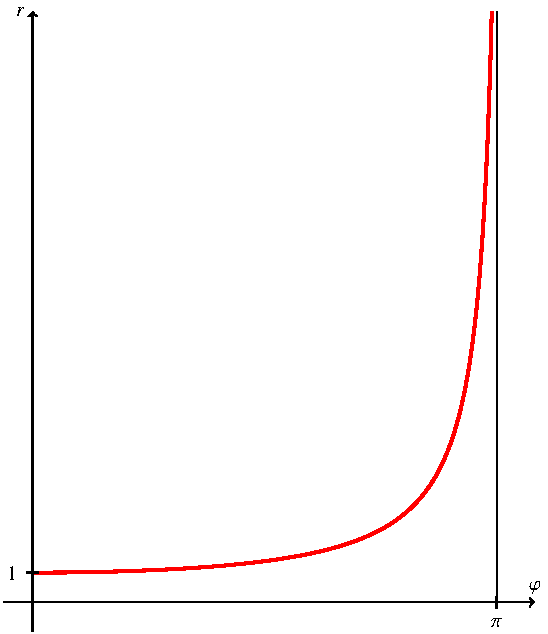
\includegraphics{chapters/tikz/lichtablenkung.pdf}
\caption{Die Lösung der Differentialgleichung~\eqref{skript:schwarzschild:udgl}
wächst in der Nähe des Ablenkungswinkels über alle Grenzen.
\label{skript:schwarzschild:abbildung:rphi}}
\end{figure}
Leider eignet sich die Differentialgleichung~\eqref{skript:schwarzschild:udgl}
nicht wirklich zur Berechnung des Ablenkungswinkels.
Schuld daran ist die Singularität, in der Nähe des Ablenkungswinkels
wächst $r(\varphi)$ über alle Grenzen, wie
Abbildung~\ref{skript:schwarzschild:abbildung:rphi} zeigt.

\subsection{Differentialgleichung für den Winkel}
Genau auf dem gleichen Weg wie wir eine Differentialgleichung für $r(\varphi)$
abgeleitet haben, können wir auch eine Differentialgleichung für
$\varphi$ als Funktion $r(\varphi)$ von $\varphi$ herleiten.
Dazu beachten wir, dass
\begin{align*}
\frac{d\varphi}{dr}&=\frac{\dot \varphi(s)}{\dot r(s)}
\qquad\text{und}
\\
\frac{d^2\varphi}{dr^2}
&=
\frac{\ddot\varphi(s)\dot r(s)-\ddot r(s)\dot\varphi(s)}{\dot r(s)^3}
\end{align*}
und setzen wie vorhin die bekannten Ableitungen $\ddot r(s)$ und
$\ddot\varphi(s)$ ein.
Wir erhalten
\begin{align*}
\frac{d^2\varphi}{dr^2}
&=
-\frac{2}{r}\frac{d\varphi}{dr}
-\frac{2r-3r_g}{2}\biggl(\frac{d\varphi}{dr}\biggr)^3
%\\
%&=
%-{{4\,\left({{d}\over{d\,s}}\,\varphi\left(s\right)\right)\,\left(
% {{d}\over{d\,s}}\,r\left(s\right)\right)^2+\left(2\,r^2\left(s
% \right)-3\,{\it rg}\,r\left(s\right)\right)\,\left({{d}\over{d\,s}}
% \,\varphi\left(s\right)\right)^3}\over{2\,r\left(s\right)\,\left({{d
% }\over{d\,s}}\,r\left(s\right)\right)^3}}
\end{align*}
Auch hier kann man mit $u=r/r_g$ wieder einen dimensionslosen Parameter
einführen, die Differentialgleichung vereinfacht sich dann zu
\begin{equation}
\frac{d^2\varphi}{du^2}
=
-\frac2{u}\frac{d\varphi}{du} -\frac{2u-3}2\biggl(\frac{d\varphi}{du}\biggr)^3.
\label{skript:schwarzschild:phidgl}
\end{equation}
Für diese Differentialgleichung ist es unproblematisch, die
Integration auch für grosse Werte von $u$ durchzuführen.

Die Differentialgleichungen
\eqref{skript:schwarzschild:udgl}
und
\eqref{skript:schwarzschild:phidgl}
können in Kombination dazu verwendet werden, den Ablenkungswinkel
numerisch zu berechnen.
Dazu verwendet man erst die Differentialgleichung
\eqref{skript:schwarzschild:udgl}
mit Anfangsbedingung
\begin{equation*}
\begin{aligned}
u(0)&=r/r_g,
\qquad&\qquad
u'(0)&=0.
\end{aligned}
\end{equation*}
bis zum $\varphi$-Wert $\varphi=\frac{\pi}4$.
Anschliessend kann man die
Differentialgleichung~\eqref{skript:schwarzschild:phidgl}
\begin{equation*}
\begin{aligned}
\varphi\biggl(u\biggl(\frac{\pi}2\biggr)\biggr)&=\frac{\pi}2,
\qquad&\qquad
\varphi'\biggl(u\biggl(\frac{\pi}2\biggr)\biggr)&=\frac1{u(\frac{\pi}2)}
\end{aligned}
\end{equation*}
bis zu einem sehr grossen Radius integrieren. 
Der Wert von $\varphi(u)$ strebt dabei gegen einen Wert
$\varphi_\infty>\frac{\pi}2$, der Ablenkungswinkel kann daraus als
\[
\alpha
=
(2\varphi_\infty - \pi)
\]
berechnet werden.
Das File \texttt{lichtablenkung.m} im Repository zeigt, wie dies mit
Octave gemacht werden kann.




%
% robertson.tex -- Robertson Walker Metrik
%
% (c) 2017 Prof Dr Andreas Müller, Hochschule Rapperswil
%
\chapter{Kosmologie%
\label{skript:chapter:kosmologie}}
\lhead{Kosmologie}
\rhead{}
Die Einstein-Gleichungen ermöglichen erstmals, die Entwicklung
des ganzen Universums zu modellieren.
Dazu sind allerdings die Kenntnis der grossräumigen
Masseverteilung notwendig.
Es stellt sich heraus, dass diese im grossen isotrop und homogen ist.
Dies bedeutet, dass auch die Krümmung im Universum homogen und isotrop
ist.
Die Robertson-Walker-Metrik erfüllt diese Voraussetzung.

\section{Masseverteilung im Universum}
\rhead{Masseverteilung im Universum}
Lange Zeit galt die Erde als das Zentrum des Universums.
Nikolaus Kopernikus hat mit dem heliozentrischen Modell der Erde
diese privilegierte Stellung genommen.
Wilhelm Herschel war der erste Astronom, der sich darüber Gedanken
gemacht hat, wo innerhalb unserer Milchstrasse unser Sonnensystem
einzuordnen wäre.
Heute wissen wir, dass die Erde eher am Rande der Milchstrasse liegt.
Doch auch die Milchstrasse ist nichts besonderes, sie ist eine eher
unterdurchschnittliche Galaxie in einem durchschnittlichen
Galaxienhaufen.
Man kann diese Beobachtungen zusammenfassen im sogenannten
{\em kosmologischen Prinzip}, welches besagt, dass an unserem
Standort im Universum nichts speziell ist.

Aus dem kosmologischen Prinzip lassens ich zwei Voraussetzungen
ableiten, denen ein kosmologisches Modell genügen muss, nämlich
Homogenität und Isotropie.
Die nächsten beiden Abschnitte klären deren Bedeutung und untermauern
sie mit Beobachtungsdaten.

\subsection{Isotropie}
Isotropie bedeutet, dass es im Universum keine bevorzugte Richtung
gibt.
Auf kurze Distanzen stimmt dies ganz offensichtlich nicht.
In einer Kugel von wenigen Metern Durchmesser um den Beobachter
gibt es eine objektiv bevorzugte Richtung, die Richtung des Schwerfeldes
der Erde zum Erdmittelpunkt,
Aber auch in einer Kugel von etwa einer Milliarde Kilometer um
den Beobachter gibt es eine bevorzugte Richtung, nämlich die
Richtung zum hellsten und massivsten Stern, der Sonne.
Selbst in einer Kugel von etwa 3~Mpc\footnote{Mpc = 1 Million parsec,
ein parsec entspricht $30.857\cdot 10^{16}\text{m} = 3.26\text{Lichtjahre}$.}
kann man eine bevorzugte Richtung finden, nämlich die Richtung zur grössten
und hellsten Galaxie des lokalen Haufens, der Andromeda-Galaxie M31.
Erst in einer Kugel mit einem Radius von etwa 100Mpc gibt es keine
bevorzugte Richtung mehr. 

Herschel hat Sterne in jede Richtung der Milchstrasse gezählt, um
das Ausmass der Anistropie der Milchstrasse festzustellen.
Die Isotropie des Universums kann experimentell verifiziert werden,
indem man in alle Richtungen Galaxien zählt.
Weit entfernte Galaxien sollte es in jeder Richtung ungefähr mit 
gleicher Dichte geben.
Man beachte, dass es für diese Beurteilung nicht nötig ist, die
Distanz der Galaxien zu kennen.

\begin{figure}
\centering
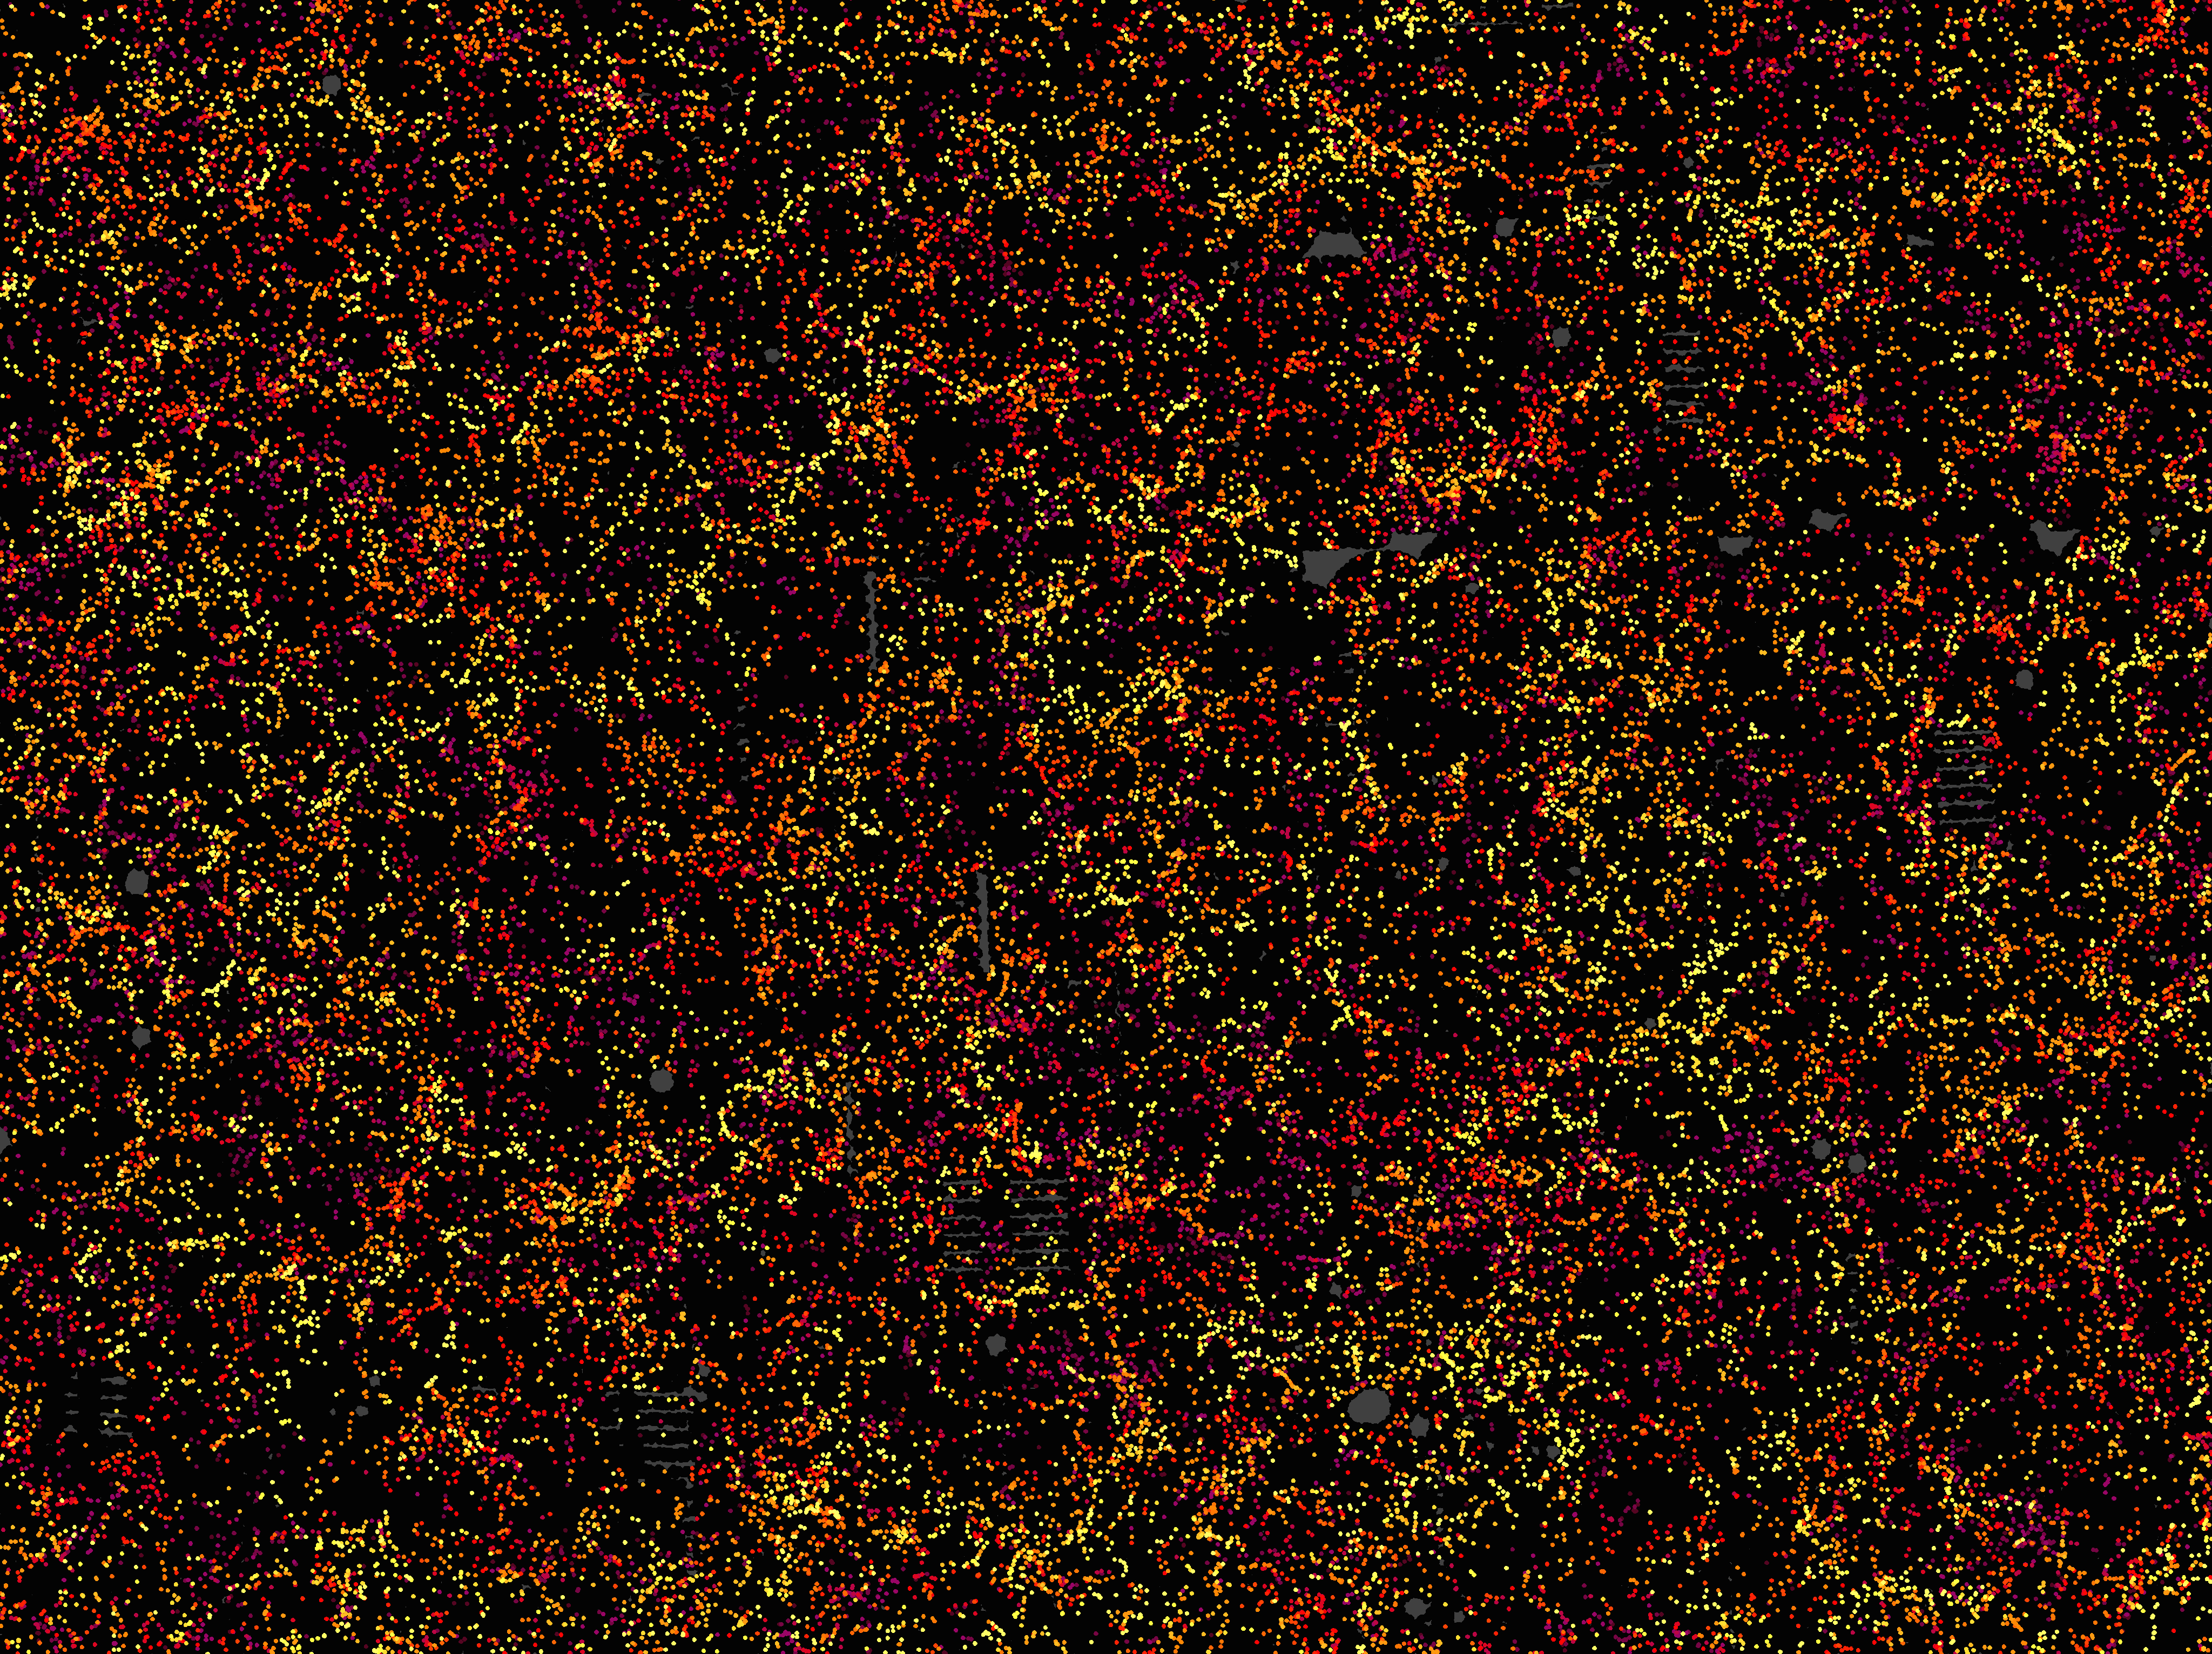
\includegraphics[width=\hsize]{chapters/images/cmass.png}
\caption{Verteilung von 48741 Galaxien aus der Sloan Digital
Sky Survey \cite{skript:cmass} über einen Ausschnit von etwa
$1/20$ des Himmels.
Es sind zwar deutliche Zusammenklumpungen zu sehen, jenseits der
typischen Grösse dieser Cluster und Supercluster von Galaxine
ist die Verteilung im Mittel ziemlich gleichmässig.
\label{skript:robertson:cmass}}
\end{figure}

Die Sloan Digital Sky Survey \cite{skript:sdss} hat über mehrere
Jahre vom Apache Point Observatorium aus über 1.2 Millionen Galaxien
vermessen.
Die Abbildung~\ref{skript:robertson:cmass} zeigt 48741 Galaxien in
einem Auschnitt von etwa 1/20 des Himmels.
Es ist erkennbar, dass Galaxien sich zu Clustern und Superclustern
zusammenklumpen, aber jenseits der typischen Abmessung ist die
Verteilung ziemlich gleichmässig.
Die Sloan Digital Sky Survey scheint also auf den ersten Blick
die Hypothese der Isotropie zu bestätigen.
Eine zuverlässigere Aussage würde jedoch erfordern, die Galaxienverteilung
statistisch zu untersuchen.

\subsection{Homogenität}
\begin{figure}
\centering
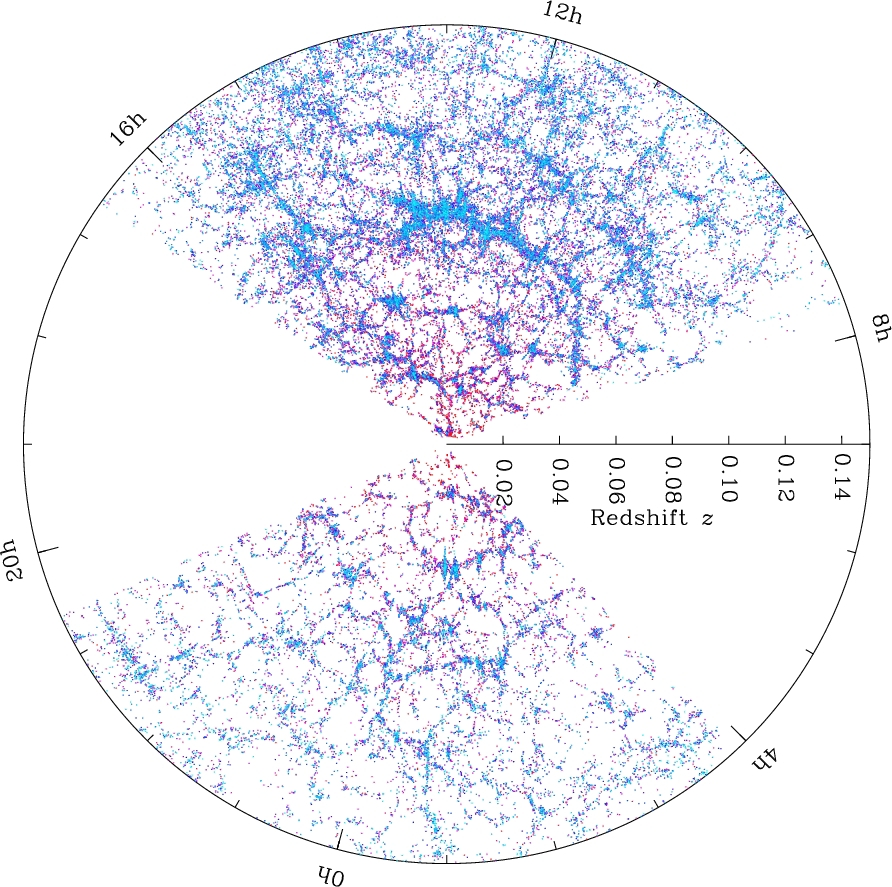
\includegraphics[width=\hsize]{chapters/images/orangepie-negative.jpg}
\caption{Verteilung der Galaxiender Sloan Digital Sky Survey.
Die beiden dunklen Sektoren stellen Bereiche dar, in denen unsere
Milchstrasse zuverlässige Beobachtungen verunmöglicht.
Jeder Punkt stellt eine Galaxie dar.
\label{skript:robertson:orangepie}}
\end{figure}

Homogenität bedeutet, dass es keinen bevorzugten Standort im Universum gibt.
Auf kurze Distanzen gilt dies ganz offensichtlich nicht.
In einer Kugel von einigen tausend Kilometern um den Beobachter ist
die Erde als massivstes Objekt ein bevorzugter Standort.
In einer Kugel von einer Milliarde Kilometer um den Beobachter ist
die Sonne als massivstes hellstes Objekt bevorzugt.
In einer Kugel von 100000 Lichtjahren um den Beobachter ist das Zentrum
der Milchstrasse mit dem dortigen supermassiven schwarzen Loch ein
bevorzugter Ort.
In einer Kugel von etwa 3~Mpc ist der Schwerpunkt des Lokalen Galaxienhaufens
ein bevorzugter Ort.
Bei grösseren Radien findet man zwar noch Cluster von Galaxien und
Supercluster, also Cluster von Galaxienclustern, aber jenseits von
etwa 100 Mpc scheint es keine noch grösseren Strukturen mehr zu geben.
In diesen Grössenordnungen kann man daher das Universum als homogen
bezeichnen.

Die Sloan Digital Sky Survey hat nicht nur die Richtungsverteilung von
Galaxien bestimmt, sondern auch deren Rotverschiebung.
Wie wir heute wissen, ist dies mindestens für ferne Galaxien ein ausreichend
genaues Mass für die Entfernung.
Abbildung~\ref{skript:robertson:orangepie} zeigt die Resultate.
Auch auf diesem Bild erkennt man, dass Galaxien sich zu Clustern
und Filamenten gruppieren.
Dazwischen gibt es grosse Bereiche von leeren Räumen.
Jenseits der Dimensionen dieser Strukturen scheint die Verteilung jedoch
ziemlich gleichmässig zu sein.
Die Hypothese der Homogenität scheint also von den Beobachtungen der
Sloan Digital Sky Survey gestützt zu werden.
Eine zuverlässigere Aussage würde wieder eine statistische Anlyse der 
Daten erfordern.

\subsection{Energie-Impuls-Tensor}
Ein homogenes und isotropes Universum hat auch einen homogenen
und isotropen Energie-Impuls-Tensor.
Für ein ideales Gas wurde der Energie-Impuls-Tensor schon in
Abschnitt~\ref{skript:speziell:subsection:idealesgas}
in Gleichung~\eqref{skript:speziell:idealesgas} angegeben, er ist
\[
T^{\mu\nu} = pg^{\mu\nu} + (p+\varrho)u^\mu u^\nu.
\]
Das Universum ist jedoch nicht nur mit Gas gefüllt, sondern auch
mit Staub und Strahlung und eventuell weiteren, nicht bekannten
Komponenten.
Unabhängig von der Art der der Komponenten ist die Energiedichte
im heutigen Universum sehr gering, nämlich nur wenige Wasserstoffatome
pro Kubikmeter.
Die Atome treffen äusserst selten aufeinander,
der Druck des idealen Gases ist also sehr gering.

Staub als Komponenten zeichnet sich zum Beispiel dadurch aus, dass die Körner
jeweils aus einer grossen Zahl von Atomen zusammengesetzt sind.
Bei gleicher Dichte sind also Staubkörner noch seltener, und damit kommen
Stösse praktsich nicht mehr vor.
Staub als Komponente zeichnet sich also dadurch aus, dass der Druck
verschwindet, der Energie-Impuls-Tensor vereinfacht sich zu
\[
T^{\mu\nu}
=
\varrho u^\mu u^\nu.
\]

Im kosmologischen Zusammenhang wird Strahlung meist wie ein
ideales Gas modelliert mit dem einzigen Unterschied, dass
die Energiedichte bei der Expansion schneller abnimmt, weil
zusätzlich auch die Wellenlänge der Strahlung gestreckt wird.

\section{Statisches Universum}

\section{Expansion des Universums}
\rhead{Expansion}
Zu Beginn des 20.~Jahrhunderts hatte man noch keine klare Vorstellung
über die Grösse des Universums.
Allgemein wurde angenommen, dass unsere Milchstrasse im wesentlichen das
ganze Universum ist.
Die seit längerer Zeit bekannten Nebel wurden als Teil der Milchstrasse
angesehen.
Auch wurde das Universum im wesentlichen als unveränderlich angesehen.

In den frühen zwanziger Jahren des 20.~Jahrhunderts gelang es dann
Edwin Hubble, die Entfernung von Andromeda und anderen heute als
Galaxien bekannten Nebeln zu bestimmen.
Er verwendete dafür sogenannte Cepheiden-Veränderliche.
Zwischen der absoluten Helligkeit dieser veränderlichen
Sterne und der Periode der Helligkeitsschwankungen besteht
eine einfache Beziehung.
Hubble fand Cepheiden-Veränderliche in Aufnahmen der Andromeda-Galaxie
und war damit in der Lage, deren absolute Helligkeit zu bestimmen.
Aus der beobachteten Helligkeit konnte er die Entfernung ableiten.
Es zeigte sich, dass diese Galaxien weit ausserhalb unserer Milchstrasse
befinden.

Hubble und sein Assistent Milton Humason massen mit dem neuen
2.5m-Hooker-Teleskop neben der Entfernung auch die Spektren und
damit die Rotverschiebung von 46 Galaxien.
Es zeigte sich, dass sich weiter entfernte Galaxien schneller 
entfernen.
Sie schlossen daraus, dass das Universum expandieren muss, sie konnten
sogar die Geschwindigkeit bestimmen, mit der dies geschieht.

Der belgische Physiker
Georges Lemaître hatte auf der Basis von Einsteins allgemeiner
Relativitätstheorie die Expansion des Universums bereits vor
Hubbles Entdeckung vorhergesagt.
Doch erst mit die Messungen von Hubble und Humason haben bewiesen,
dass Einsteins Theorie die Entwicklung des Universums korrekt
vorhersagen kann.

\subsection{Der Skalenfaktor}
\begin{figure}
\centering
\includegraphics[width=\hsize]{chapters/tikz/expansion1.pdf}
\caption{Expansion des Universums um einen Beobachter im ``Zentrum''
\label{skript:figure:expansion1}}
\end{figure}
\begin{figure}
\centering
\includegraphics[width=\hsize]{chapters/tikz/expansion2.pdf}
\caption{Expansion des Universums. Da sich das Univerum überall
mit dem gleichen Skalenfaktor ausdehnt, erscheinen sich für jeden
Beobachter die Galaxien mit der gleichen Geschwindigkeit zu entfernen.
Die Fluchgeschwindigkeit ist kein Hinweis darauf, dass im Universum
einen bevorzugten Punkt gäbe (Homogenität).
\label{skript:figure:expansion2}}
\end{figure}
Hubbles Beobachtungen haben gezeigt, dass sich das Universum ausdehnt.
Zwei nahe Punkte befinden sich zur Zeit $t_0$ in einem Abstand $d_0$,
und sollen in einem geeigneten Koordinatensystem in Ruhe sein.
Zu einer späteren Zeit wird die Distanz sich vergrössert haben.
Da das Universum isotrop und homogen ist, muss die Distanz in jeder
beliebigen Richtung um den gleichen Faktor gewachsen sein.
Die Ausdehnung des Universums ist also eine Ähnlichkeitstransformation.
Sie kann durch eine einzige, von der Zeit abhängige Zahl,
den {\em Skalenfaktor} $a(t)$ beschrieben werden.
\index{Skalenfaktor}
Wir geben der Funktion $a(t)$ willkürlich den Wert $1$ für die heutige
Zeit.

Die Tatsache, dass ein Beobachter alle Galaxien sich entfernen
sieht bedeutet nicht, dass das Universum ein Zentrum.
Auch für jeden anderen Beobachter werden die Distanzen zu den
Galaxien grösser und zwar um den gleichen Faktor
(Abbildungen~\ref{skript:figure:expansion1} und
\ref{skript:figure:expansion2}).

\subsection{Die Hubble-Konstante und das Alter des Universums}
Nehmen wir an, dass das Universum sich mit konstanter Geschwindigkeit
ausdehnt, dass also 
\[
H(t)=H_0=\frac{\dot a(t)}{a(t)}
\]
gilt.
Dies ist eine Differentialgleichung für $a(t)$, die wir sofort
lösen können:
\[
a(t) = H_0a(t)
\qquad \Rightarrow\qquad
a(t)=H_0 e^{t-t_0}
\]
Wir erhalten daher einen exponentiell anwachsenden Skalenfaktor,
wofür es keinen experimentellen Hinweis gibt, und der auch physikalisch
unsinnig scheint.
$H(t)$ kann also keine Konstante sein.

Nehmen wir aber an, dass $\dot a(t)$ konstant ist, dann ist $a(t)$
eine lineare Funktion der Zeit mit Steigung  $H_0$ zur Zeit $t=t_0$,
also
\[
a(t)=H_0(t-t_0) + 1.
\]
Daraus können wir den Zeitpunkt berechnen, zu dem der Skalenfaktor
$a(t)=0$ war, es muss
\[
t-t_0 = -\frac1{H_0}
\]
gelten.
Man nennt $1/H_0$ die {\em Hubble-Zeit}.
\index{Hubble-Zeit}
Der beste bekannte Wert für $H_0$ wurde mit der Planck-Mission als
\index{Planck-Mission}
\begin{equation}
H_0
=
(67.74 \pm 0.46)\frac{\text{km}}{\text{s}\cdot\text{Mpc}}
=
(2.1951\pm 0.0149)
10^{-18}\frac{1}{\text{s}}
\label{skript:robertson:hubble0}
\end{equation}
bestimmt.
Die zugehörige Hubble-Zeit ist
\begin{equation}
\frac{1}{H_0} = 14.4\text{Gyr}.
\label{skript:robertson:hubblezeit}
\end{equation}
Wenn wir annehmen, dass die im Universum enthaltene Masse die Ausdehnung
verlangsamt, muss die Hubble-Zeit eine obere Schranke für das Alter
des Universums sein.

\section{Robertson-Walker-Metrik}
\rhead{Robertson-Walker-Metrik}
Das Universum ist auf grosse Distanzen homogen und isotrop.
Die Einstein-Gleichungen müssen daher auch eine Metrik als
Lösung zulassen, die homogen und isotrop ist.
In diesem Abschnitt wollen wir untersuchen, wie die Metrik eines
solchen Raums beschaffen sein muss.

\subsection{Zeit}
Wenn kein Standort im Universum bevorzugt ist, dann muss es
eine universelle Zeitkoordinaten $t$ geben, die Metrik muss
sich schreiben lassen in der Form
\[
ds^2
=
-c^2\,dt^2
+
g_{ij}\,dx^i\,dx^j
\]
wobei wie früher lateinische Indizes andeuten sollen, dass die
Summation nur über die Raumkoordinaten zu erstrecken ist.
Wäre dies nicht möglich, dann müsste der Koeffizient von $dt^2$
in einem Raumpunkt von $-c^2$ abweichen.
Dieser Punkt hätte dann aber andere Eigenschaften als alle anderen
Punkte im Universum, was das kosmologische Prinzip verletzt.

\subsection{Isotrop und homogen gekrümmte Räume}
Wir suchen jetzt eine Metrik des dreidimensionalen Raumes, welche
isotrop und homogen ist.
Der euklidische Raum mit der Metrik
\[
g_{ij}dx^i\,dx^j
=
dx^2 + dy^2 + dz^2
\]
ist sicher homogen und isotrop. 
Er ist aber auch flach, und daher zu wenig allgemein als mögliches
Modell für das Universum.
Die euklidische Metrik kann auch in Kugelkoordinaten als
\begin{equation}
ds^2
=
dr^2
+ 
r^2\,d\vartheta^2
+
r^2\sin^2\vartheta\,d\varphi^2
\label{skript:rwmetrik:kugelkoordinaten}
\end{equation}
geschrieben werden.
Die letzten zwei Terme~\eqref{skript:rwmetrik:kugelkoordinaten}
zeigen scheinbar eine bevorzugte Richtung, nämlich die Richtung
des Nord- und Südpols.
Dies ist jedoch nur ein Artefakt des Koordinatensystems, die 
Längenmessung ist davon nicht betroffen.
Wir können dies dadurch ausdrücken, dass wir die zwei Terme
zusammenfasssen als
\begin{equation}
d\Omega^2 = d\vartheta^2 + \sin^2\vartheta\,d\varphi^2.
\end{equation}
Damit kann die Metrik abgekürzt als
\begin{equation}
ds^2 = dr^2 + r^2\,d\Omega^2
\end{equation}
geschrieben werden.
Der Terme $r^2\,d\Omega^2$ beschreibt die Längenmessung auf der
``Kugel'' bei der Koordinaten $r$ um den Nullpunkt des
Koordinatensystems.

Da das Universum isotrop ist, darf keine Richtung ausgezeichnet sein.
Insbesondere muss eine von der euklidischen Metrik abweichende
Metrik immer noch unverändert den Teil $d\Omega^2$ enthalten.
Es ist aber zulässig, dass die Längenmessung auf der Kugel sich
gegenüber der Längenmessung in radialer Richtung verändert hat.
Man beobachtet dies zum Beispiel auch in der Umgebung eines Punktes
auf einer Kugeloberfläche: je weiter man sich von diesem Punkt entfernt,
desto kleiner wird der Umfang eines Kreises um den Punkt im Vergleich
zum Radius. 
Ist der Radius des Kreises $\frac{\pi}2R$, wobei $R_c$ der Kugelradius ist,
dann ist der Umfang $U$ des Kreises
\[
U=2\pi R_c \ne 2\pi \cdot r = 2\pi\frac{\pi}2R_c=\pi^2 R_c.
\]
Wir suchen daher eine Metrik in der Form
\[
ds^2 
=
dr^2 + S(r)^2 \,d\Omega^2,
\]
wobei $S(r)$ für einen euklischen Raum $S(r)=r$ ist.
Ein Kreis mit Radius $r$ hat in dieser Metrik den Umfang
\[
U=\int_{\textrm{Kreis}} S(r)\,d\Omega = 2\pi S(r).
\]
Auch wenn für einen gekrümmten Raum $S(r)$ nicht mehr gleich $r$ ist,
muss weiterhin $S(0)=0$ gelten, wenn der Radius verschwindet, dann
hat der zugehörige Kreis auch verschwindenden Umfang.
Für kleine Radien $r$ muss ausserdem die Geometrie kaum von der
euklidischen unterscheidbar sein, es muss also $S(r)\simeq r$ gelten,
oder $S'(r)=1$,
Die Funktion $S(r)$ muss daher die Anfangsbedingungen
\begin{equation}
\begin{aligned}
S(0)&=0&&\qquad&S'(0)&=1
\end{aligned}
\label{skript:rwmetrik:Safangsbedingungen}
\end{equation}
erfüllen.

\subsubsection{Krümmung}
Die Funktion $S(r)$ ist nun also so zu bestimmen, dass der Raum auch
homogen ist.
Um sie zu bestimmen verwenden wir wieder die Analogie zur Oberfläche
einer zweidimensionalen Kugel mit Radius $R_c$.
Zu einem Kreis mit Radius $r$ im den Nordpol gehört der Winkel
$\vartheta$ mit $\vartheta = r/R$.
Der Umfang dieses Kreises ist dann
\[
2\pi R_c\sin\vartheta
=
2\pi S(r)
\]
der
\[
S(r) = R_c\sin\vartheta=R\sin\frac{r}{R_c}.
\]
In der zu dieser Funktion $S(r)$ gehörigen Metrik hat ein Kreis mit 
Radius $r=\pi R$ Umfang $0$, dies entspricht dem Antipodenpunkt des
Nullpunktes.

Bis jetzt haben wir uns von der Anschauung leiten lassen, ohne den
Begriff der Krümmung zu verwenden.
Um die allgemeine Lösung für $S(r)$ zu finden, können wir
aber auch verlangen, dass die Metrik
\[
dr^2 + S(r)^2\,d\Omega^2
\]
überall die gleiche Krümmung hat.
Wir berechnen daher für diese Metrik den Ricci-Krümmungsskalar.
Diese Rechnung ist ziemlich aufwendig, kann aber mit Maxima
mit Hilfe des Programms von Seite~\pageref{skript:maxima:curvature}
ohne
Schwierigkeit ausgeführt werden.
\lstinputlisting[style=Maxima]{chapters/robertson3.maxima}
Man erhält 
\verbatiminput{chapters/robertson3.txt}
oder in konventioneller Notation
\[
R=
-\frac{2S''(r)}{S(r)}
\]
und damit die Bedingung
\begin{equation}
S''(r)=-2k S(r)
\label{skript:rwmetrik:Sdgl}
\end{equation}
für $S(r)$ und eine geeignete Konstante $k$.
Gleichung \eqref{skript:rwmetrik:Sdgl} ist eine gewöhnliche
Differentialgleichung zweiter Ordnung.

\subsubsection{Lösung der Differentialgleichung für $S_\kappa(r)$}
Die Differentialgleichung~\eqref{skript:rwmetrik:Sdgl}
muss mit den Anfangsbedingungen~\eqref{skript:rwmetrik:Safangsbedingungen}
gelöst werden.
Falls $k$ positiv ist, folgt
\begin{equation}
S(r)=\frac1{\sqrt{2k}}\sin(\sqrt{2k}\,r) = R_c\sin\frac{r}{R_c}
\qquad\text{mit}\qquad
R_c=\frac1{\sqrt{2k}}.
\label{skript:rwmetrik:sinloesung}
\end{equation}
Dies ist der Fall, den wir bereits durch die geometrische Analogie mit
der zweidimensionalen Sphäre gefunden haben.

Die Gleichung~\eqref{skript:rwmetrik:Sdgl} hat aber noch eine weitere 
Lösungen.
Für negatives $k$ folgt wieder unter Verwendung der
Anfangsbedingung~\eqref{skript:rwmetrik:Safangsbedingungen}
\begin{equation}
S(r)=\frac{1}{\sqrt{-2k}}\sinh(\sqrt{-2k}\, r)
=
R_c\sinh\frac{r}{R_c}
\qquad\text{mit}\qquad
R_c=\frac1{\sqrt{-2k}}.
\label{skript:rwmetrik:sinhloesung}
\end{equation}
Diese Lösung gehört zu einem Raum mit negativer Krümmung.
Sogar den euklidische Fall können wir für $k=0$ wiedergewinnen, es folgt
dann $S(r)=r$.

\begin{figure}
\centering
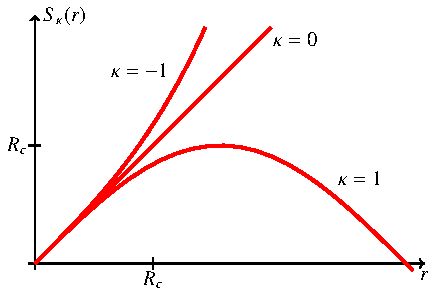
\includegraphics{chapters/tikz/robertson.pdf}
\caption{Darstellung der Funktionen $S_\kappa(r)$ für $R_c=1$ und
verschiedene Werte von $\kappa$
\label{skript:Skappa:graph}}
\end{figure}

Offenbar spielt für die Lösung  nur das Vorzeichen von $k$ und die
Grösse $R_c$ ein Rolle.
Wir können $S(r)$ daher auch etwas einheitlicher als
\begin{equation}
S_\kappa(r) = \begin{cases}
R_c\sin  \displaystyle\frac{\mathstrut r}{R_c} &\qquad \kappa= 1\\
r                                              &\qquad \kappa= 0\\
R_c\sinh \displaystyle\frac{\mathstrut r}{R_c} &\qquad \kappa=-1
\end{cases}
\label{skript:rwmetrik:Skappa}
\end{equation}
schreiben.
In Abbildung~\ref{skript:Skappa:graph} sind die Funktionen $S_\kappa(r)$
für $R_c=1$ und für alle drei Werte von $\kappa$ dargestellt.
Ebenfalls erkennbar ist, dass für kleine Werte von $r$ gilt
$S_\kappa(r)\simeq r$.

\subsubsection{Ableitungen von $S_\kappa(r)$}
Für spätere Verwendung berechnen wir die erste und zweite Ableitung 
von $S_\kappa(r)$.
Die erste Ableitung ist
\begin{align*}
S'_\kappa(r)
&=
\begin{cases}
\cos \displaystyle\frac{\mathstrut r}{R_c}&\qquad \kappa= 1\\
1                                         &\qquad \kappa= 0\\
\cosh\displaystyle\frac{\mathstrut r}{R_c}&\qquad \kappa=-1
\end{cases}
\end{align*}
In Hinblick auf spätere Verwendung in der Friedmann-Gleichung drücken wir
die rechte Seite durch $S_\kappa(r)$ aus. 
\begin{equation}
S'_\kappa(r)^2
=
\left\{
\begin{aligned}
&\cos^2\displaystyle\frac{\mathstrut r}{R_c}
=
1-\sin^2\displaystyle\frac{\mathstrut r}{R_c}
=
1-\kappa \frac{S_\kappa(r)^2}{R_c^2}&&\qquad\kappa=1\\
&1&&\qquad\kappa=0\\
&\cosh^2\displaystyle\frac{\mathstrut r}{R_c}
=
1+\sinh^2\displaystyle\frac{\mathstrut r}{R_c}
=
1-\kappa \frac{S_\kappa(r)^2}{R_c^2}&&\qquad\kappa=-1
\end{aligned}
\right.
\end{equation}
Unabhängig vom Wert von $\kappa$ und $R_c$ gilt also immer
\begin{equation}
S'_\kappa(r)^2 = 1-\kappa \frac{S_\kappa(r)^2}{R_c^2}.
\label{skript:robertson:ersteableitung}
\end{equation}
Für die zweite Ableitung finden wir
\begin{align*}
S''_\kappa(r)
&=
\begin{cases}
\displaystyle-\frac{1}{R_c}\sin \frac{\mathstrut r}{R_c}&\qquad \kappa= 1\\
0                                                       &\qquad \kappa= 0\\
\displaystyle \frac{1}{R_c}\sinh\frac{\mathstrut r}{R_c}&\qquad \kappa=-1
\end{cases}
\end{align*}
Auch dieses Resultat können wir einheitlich als
\begin{equation}
S''_\kappa(R)
=
-\kappa\displaystyle \frac{S_\kappa(r)}{R_c^2}
\label{skript:robertson:zweiteableitung}
\end{equation}
schreiben.

Eine homogene und isotrope Metrik eines dreidimensionalen Raumes
hat daher die Form
\begin{equation}
ds^2=dr^2 + S_{\kappa}(r)d\Omega^2.
\label{skript:rwmetrik:metrikS}
\end{equation}
Diese Metrik beschreibt einen Raum mit konstanter Krümmung.
Der Parameter $\kappa$ kann nur die Werte $\pm 1$ und $0$ annehmen.
Für $\kappa=1$ ist die Krümmung des Raumes positiv, für $\kappa=-1$ ist
sie negativ, für $\kappa=0$ liegt ein euklidischer Raum vor.
Der Krümmungsradius ist in den Fällen $\kappa=\pm1$ jeweils $R_c$.

\subsubsection{Der Grenzfall $R_c\to\infty$}
Schreibt man $K_c = 1/R_c$ für die Krümmung, dann kann man $S_0(r)$
auch als Grenzfall von $S_{\pm 1}(r)$ für $K_c\to 0$ erhalten.
Es gilt  nämlich
\begin{equation}
\lim_{R_c\to\infty} S_\kappa(r)
=
\lim_{K_c\to 0} S_\kappa(r)
=\begin{cases}
\displaystyle
\lim_{K_c\to 0}\frac{\displaystyle \sin(K_cr)}{\displaystyle K_c}
=
\lim_{K_c\to 0}\frac{\displaystyle r\cos(K_cr)}{\displaystyle 1} = r = S_0(r)
&\qquad\kappa=1
\\
\\
\displaystyle
\lim_{K_c\to 0}\frac{\displaystyle \sinh(K_cr)}{\displaystyle K_c}
=
\lim_{K_c\to 0}\frac{\displaystyle r\cosh(K_cr)}{\displaystyle 1} = r = S_0(r)
&\qquad\kappa=-1
\end{cases}
\end{equation}
nach der Regel von de l'Hospital.
Die Funktion $S_0(r)$ ist daher der Grenzfall der Funktionen
$S_\kappa(r)$ für unendlich grossen Krümmungsradius $R_c$.

\subsection{Robertson-Walker-Metrik}
Da wir jetzt die Zeitabhängigkeit wie auch die Ortsabhängigkeit der
Metrik eines isotropen und homogen gekrümmten Raumes kennen, können
wir die allgemeinste Form der vierdimensionalen Metrik eines solchen
Raumes gefunden.

\begin{satz}
Ein homogenes, isotropes Universum hat eine Metrik der Form
\[
ds^2
=
-c^2 dt^2 + a(t)^2\bigl(
dr^2 + S_\kappa(r)^2(d\vartheta^2 + \sin^2\vartheta\, d\varphi^2)
\bigr)
\]
mit $\kappa\in\{0,\pm1\}$ und 
$S_\kappa(r)$ ist eine der Funktionen
\[
S_\kappa(r)
=
\begin{cases}
R_c\sin \displaystyle\frac{\mathstrut r}{R_c}&\qquad \kappa= 1\\
r&\qquad \kappa=0\\
R_c\sinh\displaystyle\frac{\mathstrut r}{R_c}&\qquad \kappa=-1
\end{cases}
\]
\end{satz}

Wir bestimmen die Geodätengleichungen in der Robertson-Walker Metrik.
Die allgemeine Geodätengleichung hat die Form
\[
\frac{d^2x^\mu}{ds^2} = -\Gamma^\mu_{\alpha\beta} \dot x^\alpha \dot x^\beta.
\]
Man muss also als erstes die Christoffelsymbole bestimmen.  
Diese sind auch deshalb interessant, weil $\Gamma^0_{kk}$ in erster
Näherung die Gravitationskräfte beschreibt.

Für jeden Index $\mu$ bilden die $\Gamma^\mu_{\alpha\beta}$
eine symmetrische Matrix.
Für $\mu=0$ zum Beispiel finden wir
\begin{align*}
\Gamma^0_{\alpha\beta}
&=
\begin{pmatrix}
%(%i5) 		        ratsimp(Christoffel2(1, 1, 1))
%(%o5) 				       0
%(%i6) 		        ratsimp(Christoffel2(1, 1, 2))
%(%o6) 				       0
%(%i7) 		        ratsimp(Christoffel2(1, 1, 3))
%(%o7) 				       0
%(%i8) 		        ratsimp(Christoffel2(1, 1, 4))
%(%o8) 				       0
0&0&0&0\\
%(%i9) 		        ratsimp(Christoffel2(1, 2, 2))
%				     d
%			       a(t) (-- (a(t)))
%				     dt
%(%o9) 			       ----------------
%				       2
%				      c
%(%i10) 		        ratsimp(Christoffel2(1, 2, 3))
%(%o10) 				       0
%(%i11) 		        ratsimp(Christoffel2(1, 2, 4))
%(%o11) 				       0
0&\frac1{c^2} a(t)\dot a(t)& 0 & 0 \\
%(%i12) 		        ratsimp(Christoffel2(1, 3, 3))
%			     2	        d
%			    S (r) a(t) (-- (a(t)))
%					dt
%(%o12) 			    ----------------------
%				       2
%				      c
%(%i13) 		        ratsimp(Christoffel2(1, 3, 4))
%(%o13) 				       0
0 & 0 & \frac1{c^2}a(t)\dot a(t)S_\kappa(r)^2 & 0 \\
%(%i14) 		        ratsimp(Christoffel2(1, 4, 4))
%		       2	  d	        2
%		      S (r) a(t) (-- (a(t))) sin (theta)
%				  dt
%(%o14) 		      ----------------------------------
%				       2
%				      c
0 & 0 & 0 & \frac1{c^2} a(t)\dot a(t)S_\kappa(r)^2 \sin^2\vartheta
\end{pmatrix}
\\
&=
\frac1{c^2}
\frac{\dot a(t)}{a(t)}
\begin{pmatrix}
0&     0&                  0&                                 0\\
0&a(t)^2&                  0&                                 0\\
0&     0&a(t)^2S_\kappa(r)^2&                                 0\\
0&     0&                  0&a(t)^2S_\kappa(r)^2\sin^2\vartheta
\end{pmatrix}
\end{align*}
Die Matrix in der letzten Zeile stimmt bis auf die $00$-Komponente
mit der Metrik überein.
Der Faktor $\dot a(t)/a(t)$ beschreibt die Ausdehungsgeschwindigkeit
des Universums.

\subsection{Die Ausdehnung des Universums}
Aus Metrik eines homogenen und isotropen Raumes gemäss
\eqref{skript:rwmetrik:metrikS}
können wir jetzt die allgemeine Metrik einer homogenen und
isotropen Raumzeit konstruieren.
Die Metrik
\begin{equation}
ds^2
=
-c^2\,dt^2 
+
a(t)^2\bigl( dr^2 + S_\kappa(r) \,d\Omega^2\bigr)
\label{skript:rwmetrik:rwmetrik}
\end{equation}
heisst die Robertson-Walker-Metrik.
Wir können sie verwenden, um die Entwicklung des Universums zu
modellieren.

\section{Wie ist das Universum gekrümmt?}
\begin{figure}
\centering
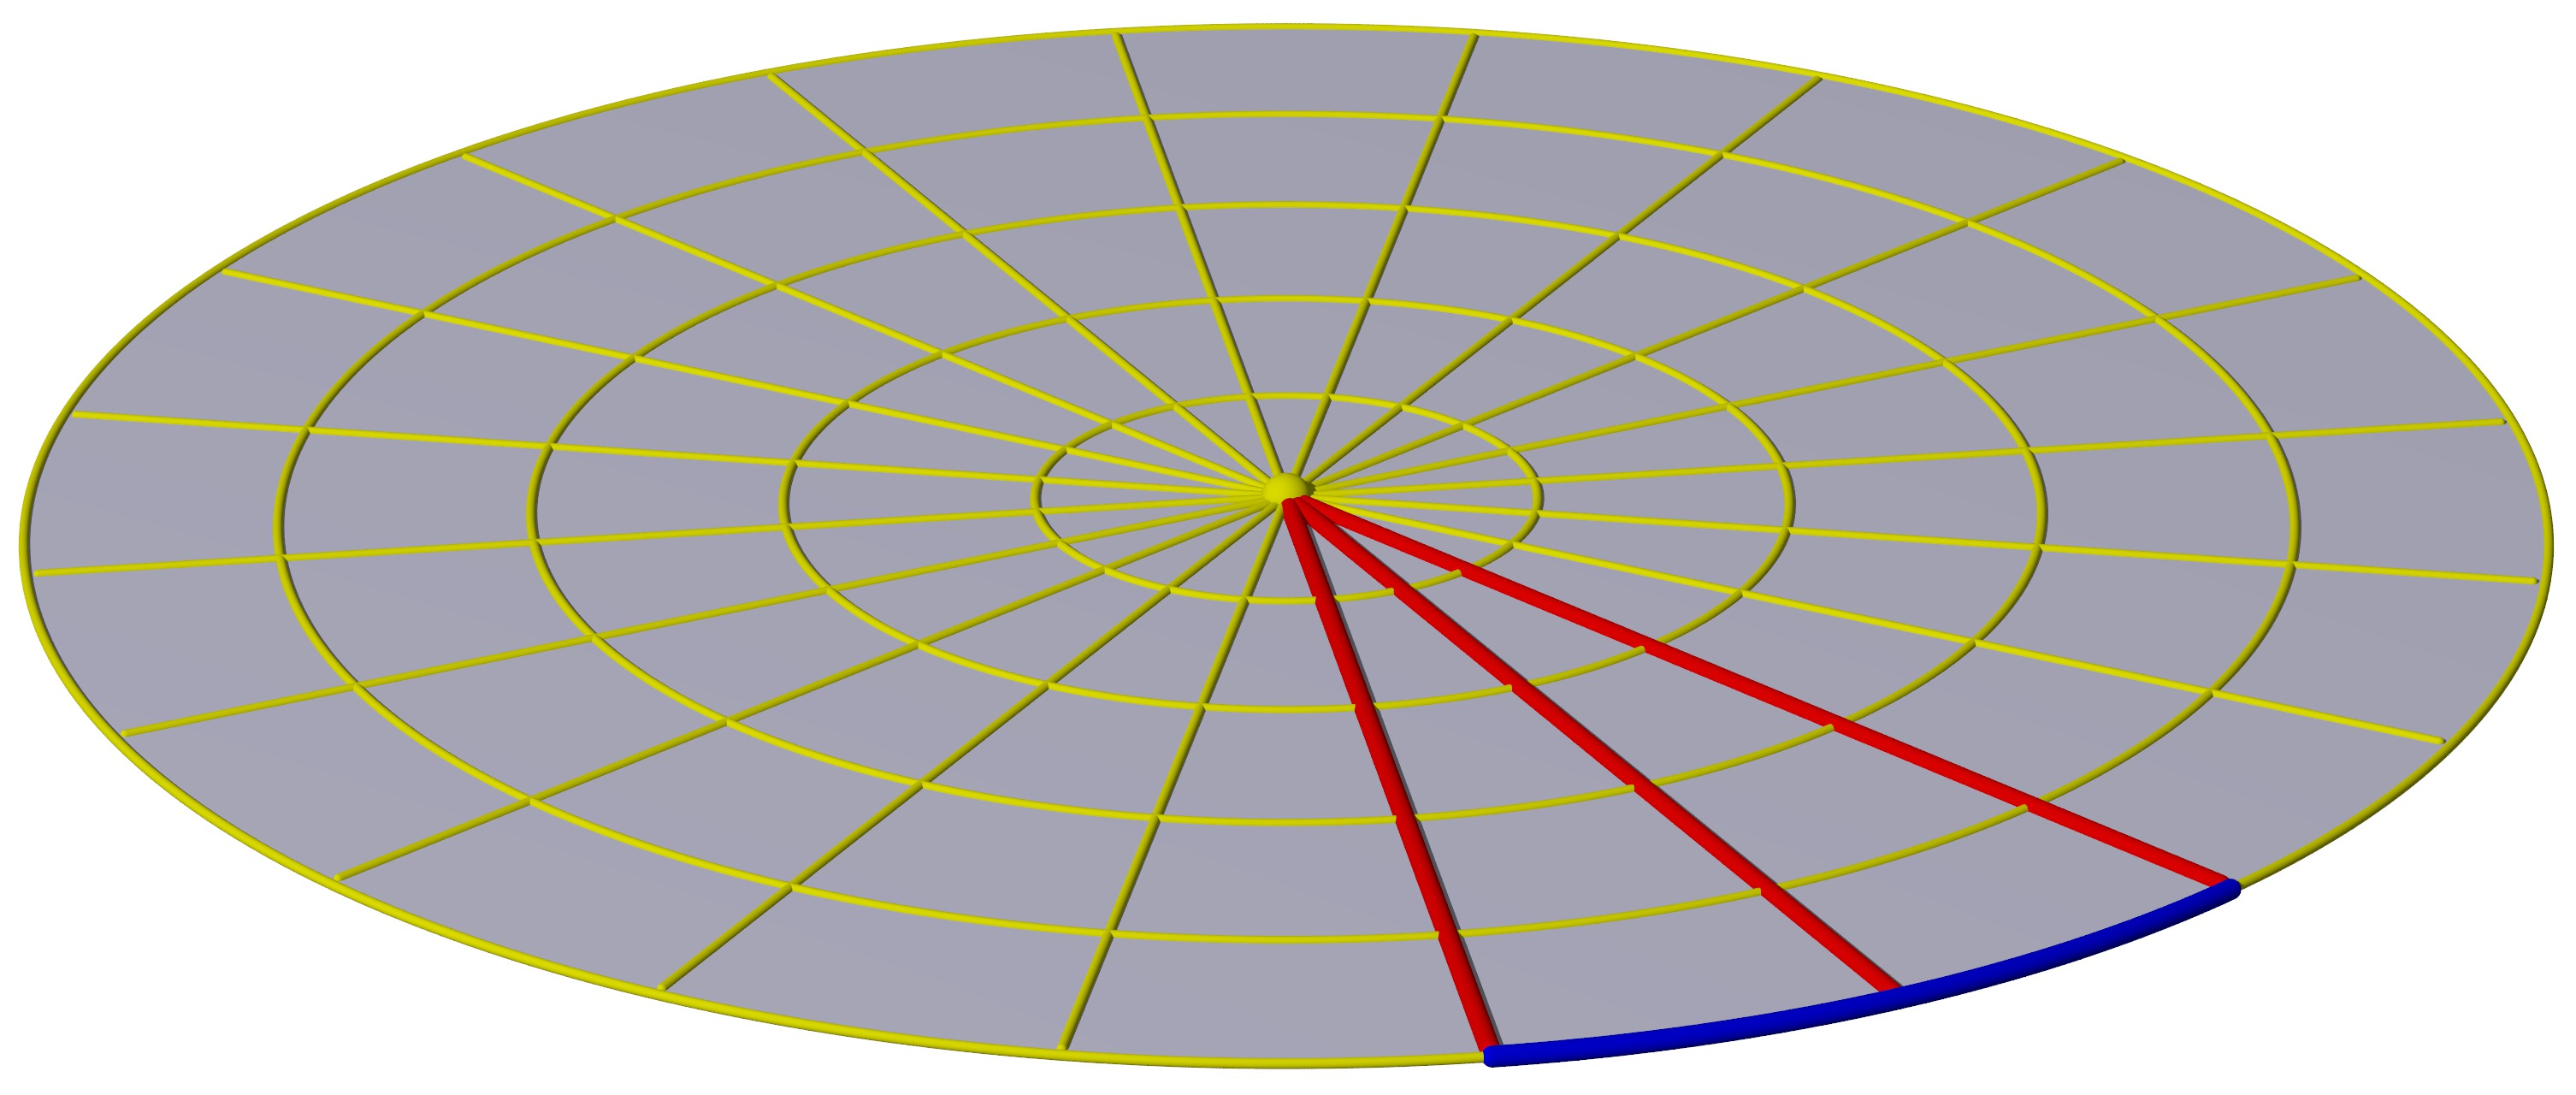
\includegraphics[width=0.7\hsize]{chapters/3d/pringles-flach.jpg}
\caption{Zwei Strahlen (rot), die im Nullpunkt den Winkel $\alpha$
einschliessen, spannen im Abstand $r$ vom Ursprung die Strecke
$\alpha r$ (blau) ein.
\label{skript:pringles:flach}}
\end{figure}
%
\begin{figure}
\centering
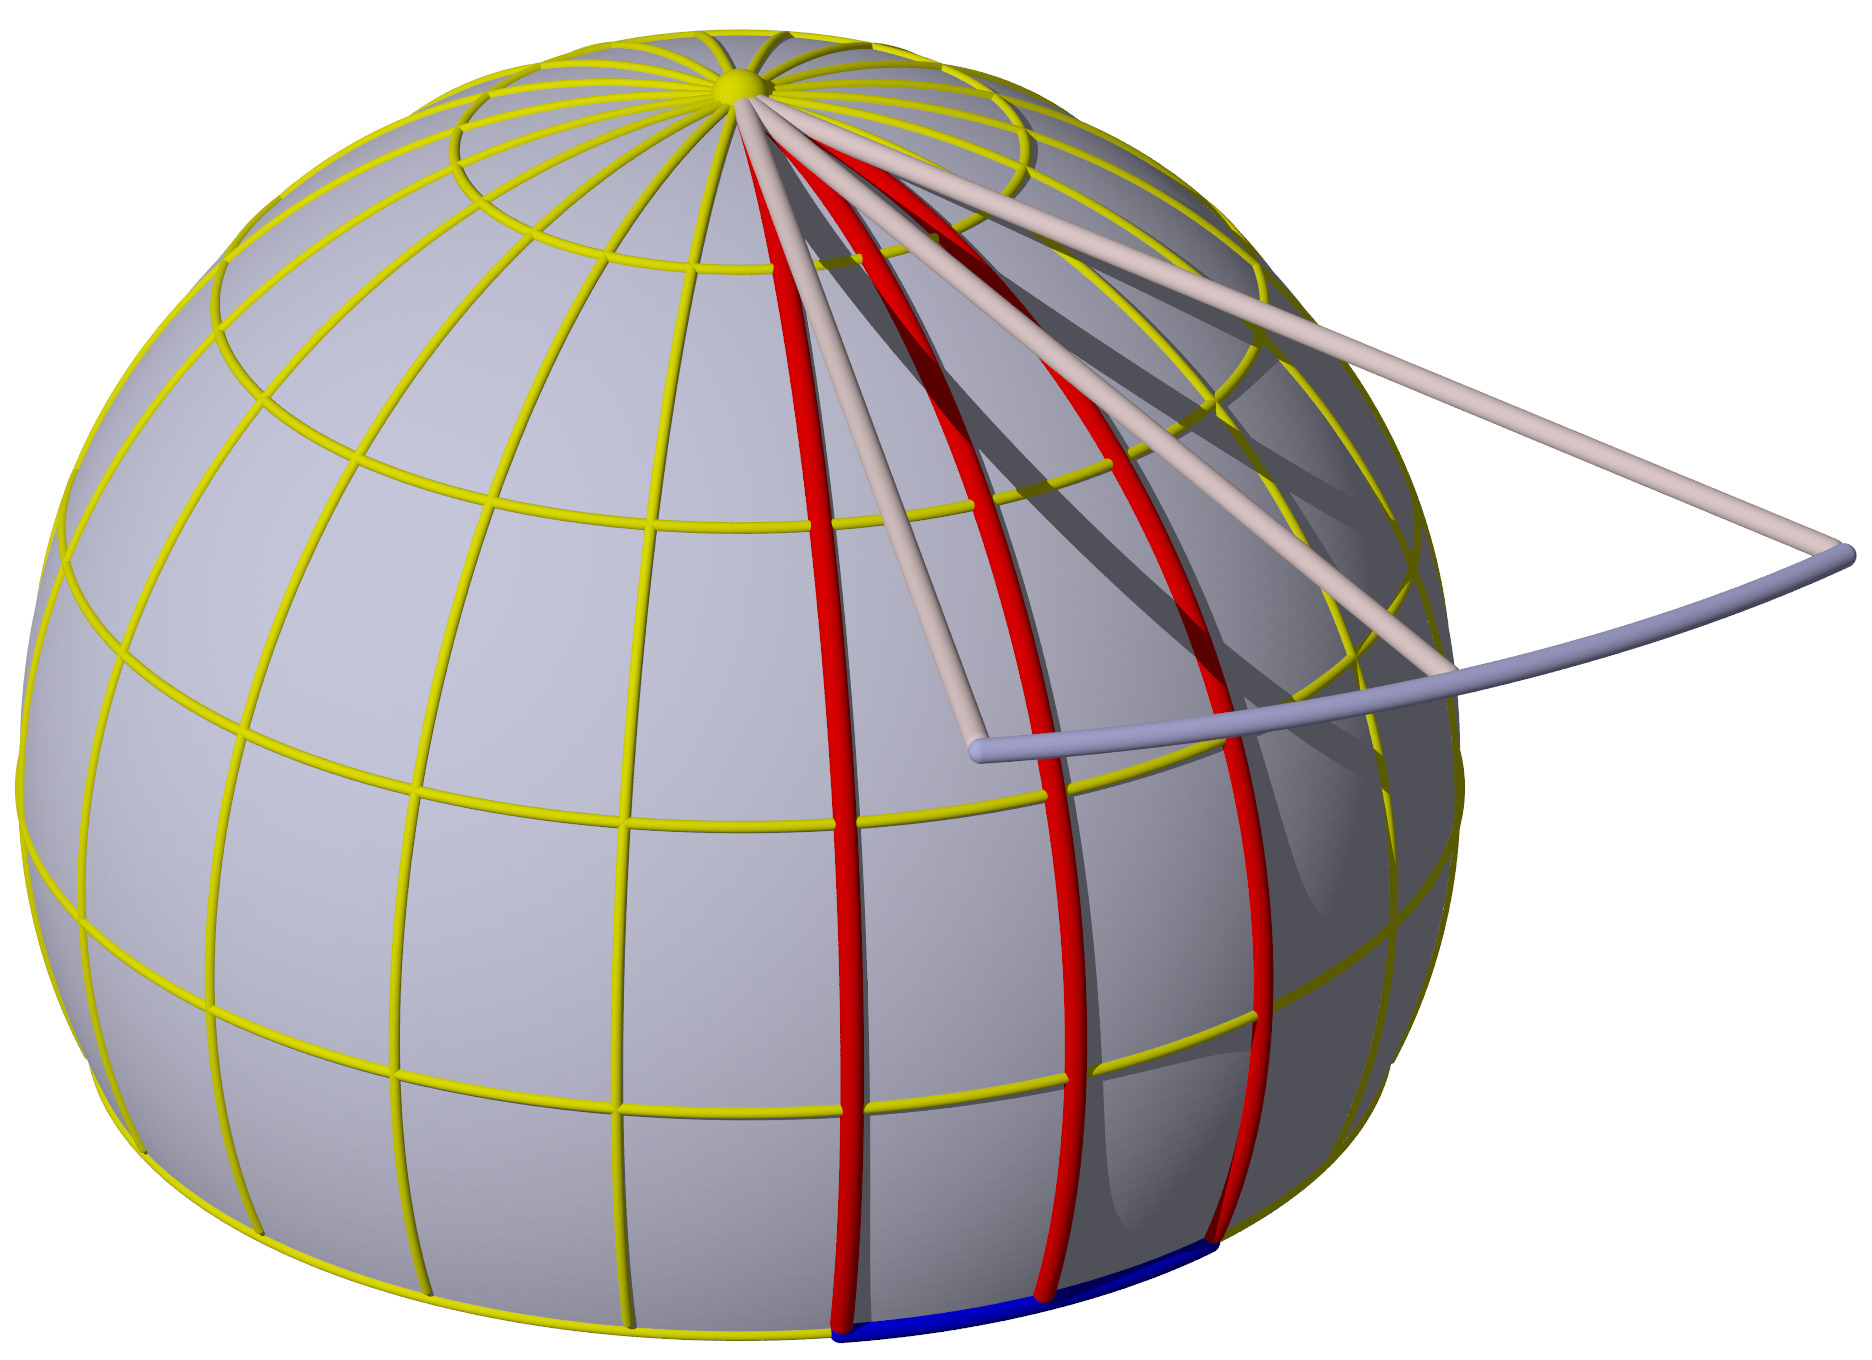
\includegraphics[width=0.7\hsize]{chapters/3d/pringles-positiv.jpg}
\caption{Zwei Geodäten (rot) auf einer positiv gekrümmten Fläche,
die im Nullpunkt den Winkel $\alpha$ einschliessen, spannen im Abstand
$r$ vom Ursprung die Strecke (blau) ein, die kleiner ist als
$\alpha r$.
\label{skript:pringles:positiv}}
\end{figure}
%
\begin{figure}
\centering
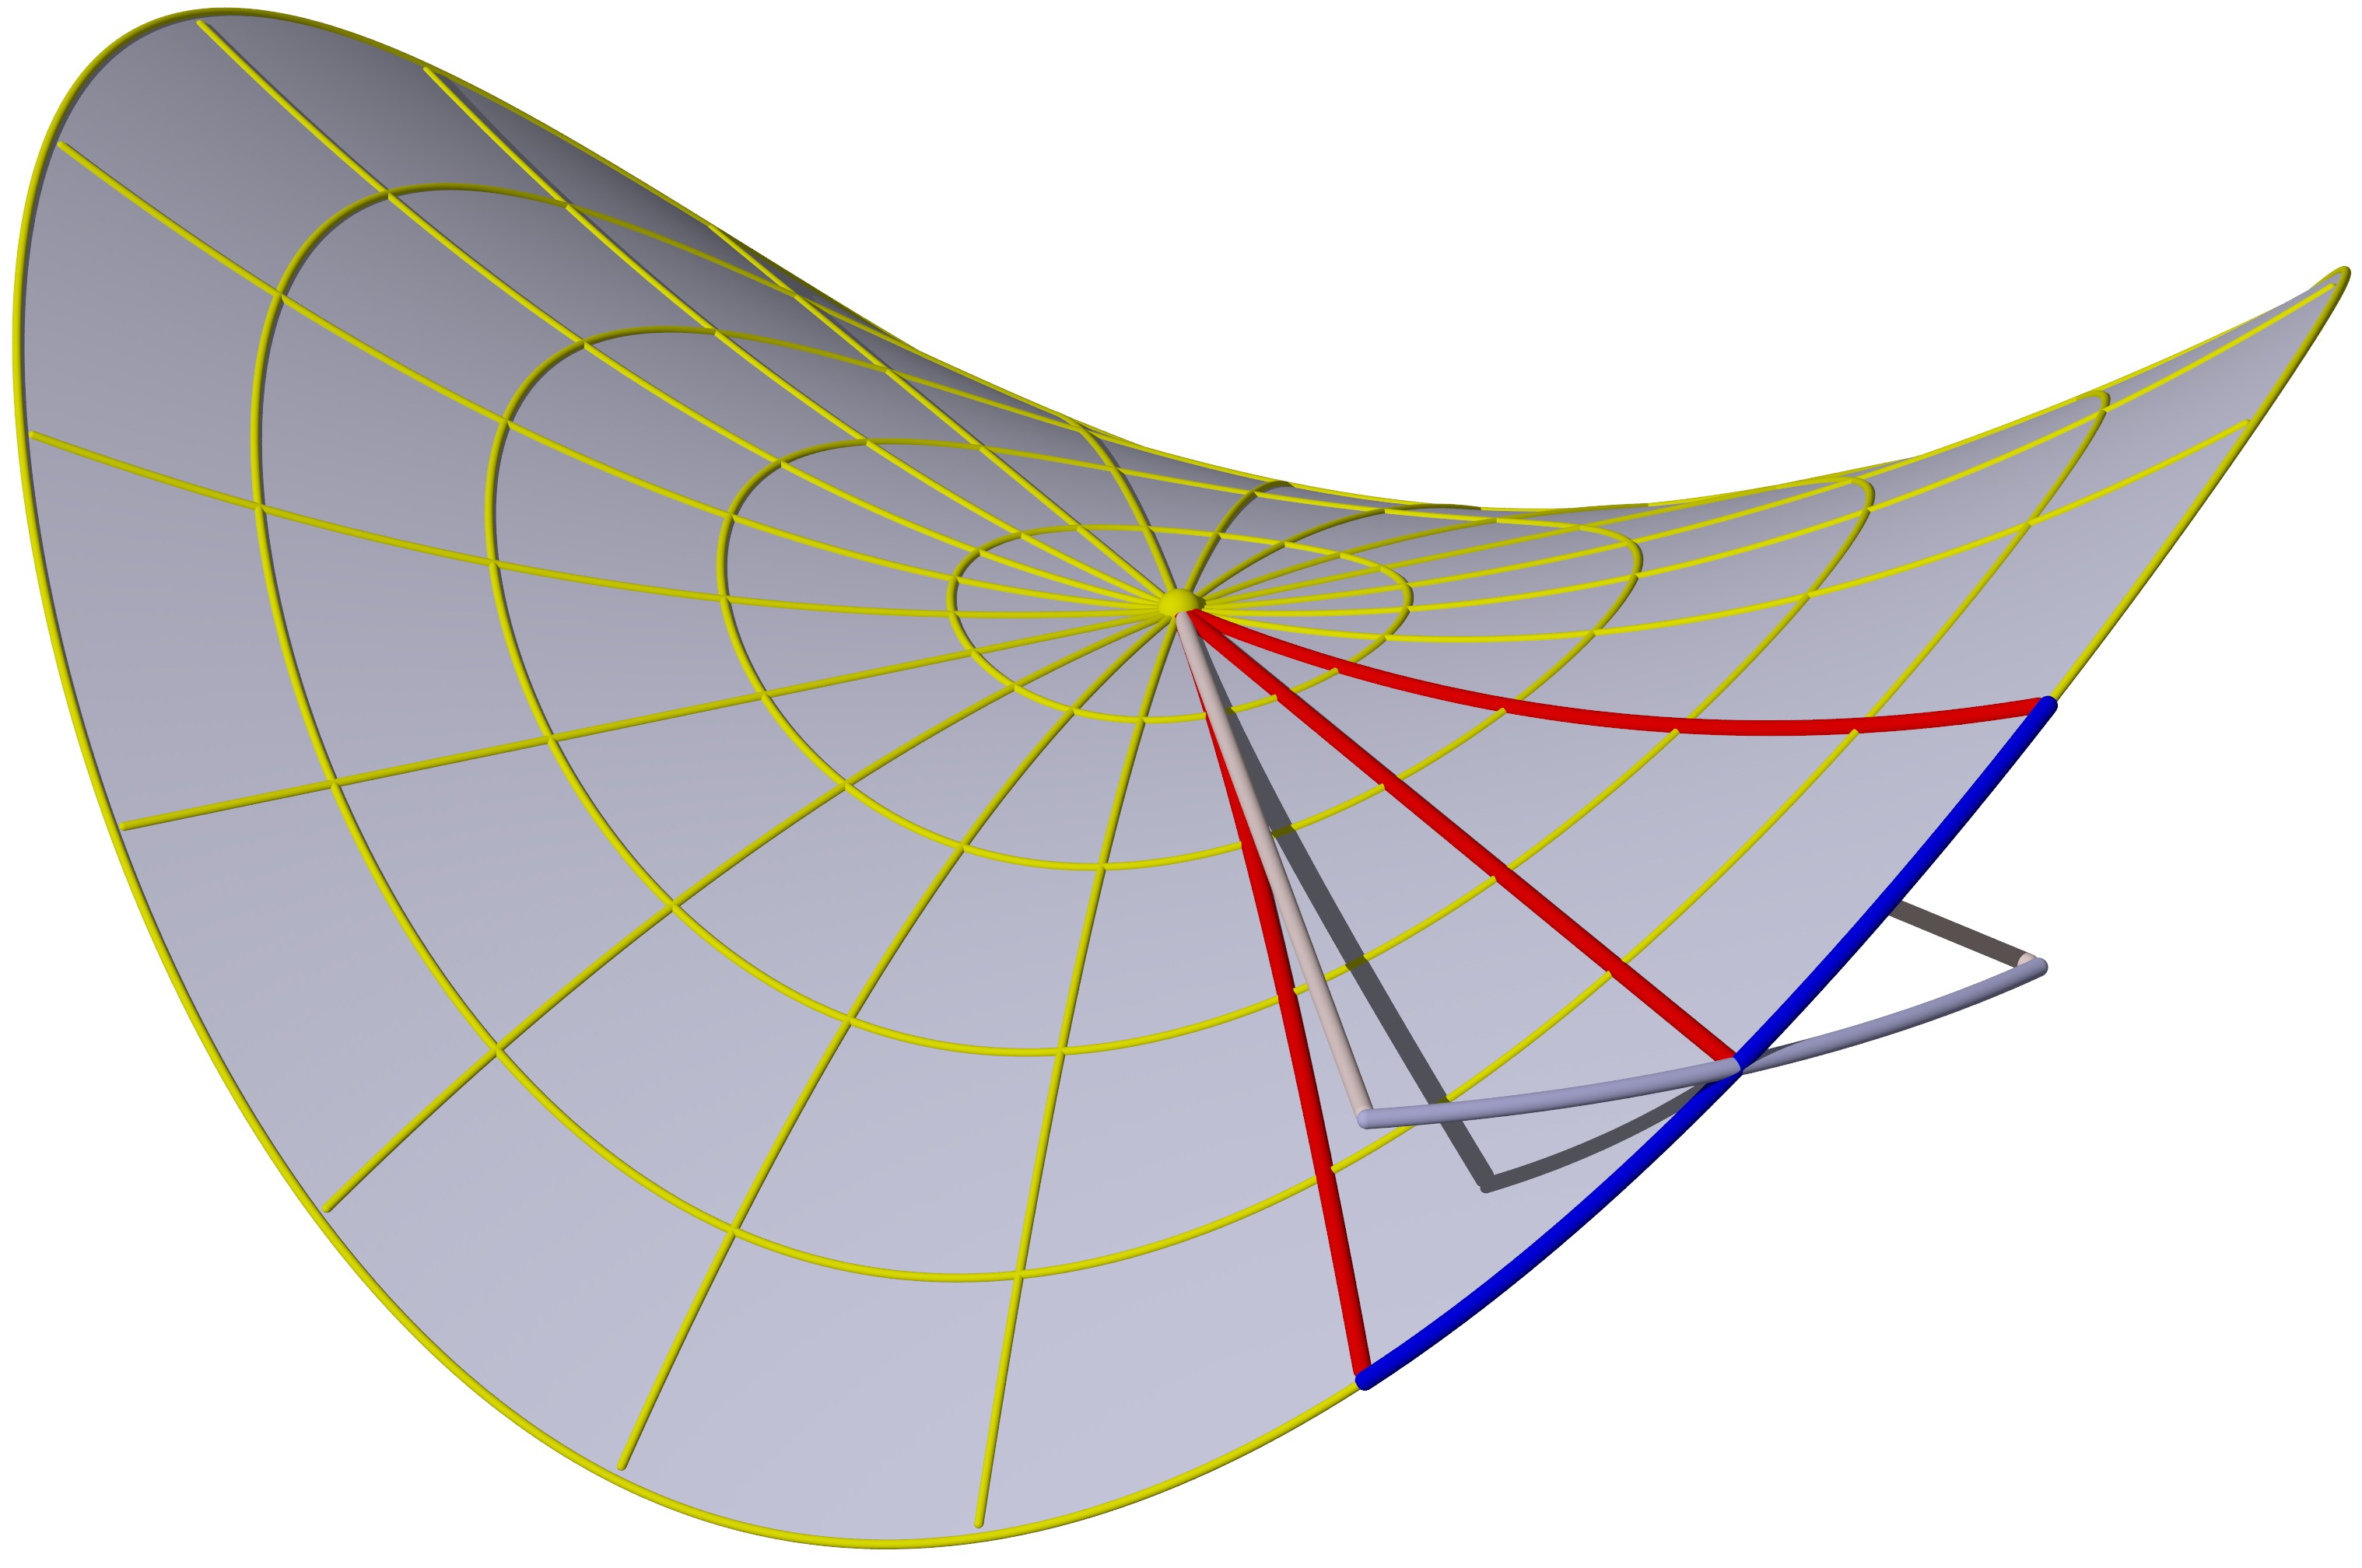
\includegraphics[width=0.9\hsize]{chapters/3d/pringles-negativ.jpg}
\caption{Zwei Geodäten (rot) auf einer negativ gekrümmten Fläche,
die im Nullpunkt den Winkel $\alpha$ einschliessen, spannen im Abstand
$r$ vom Ursprung die Strecke (blau) ein, die grösser ist als
$\alpha r$.
\label{skript:pringles:negativ}}
\end{figure}
%
\begin{figure}
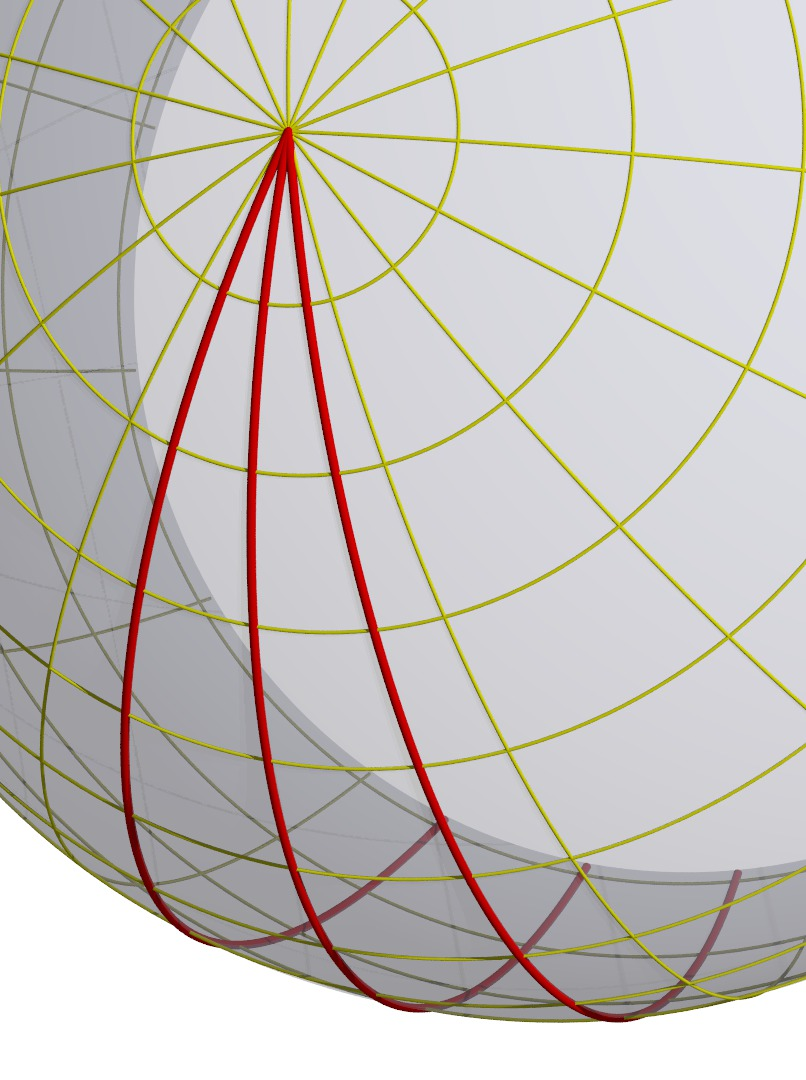
\includegraphics[height=6truecm]{chapters/3d/positiv.jpg}
\quad
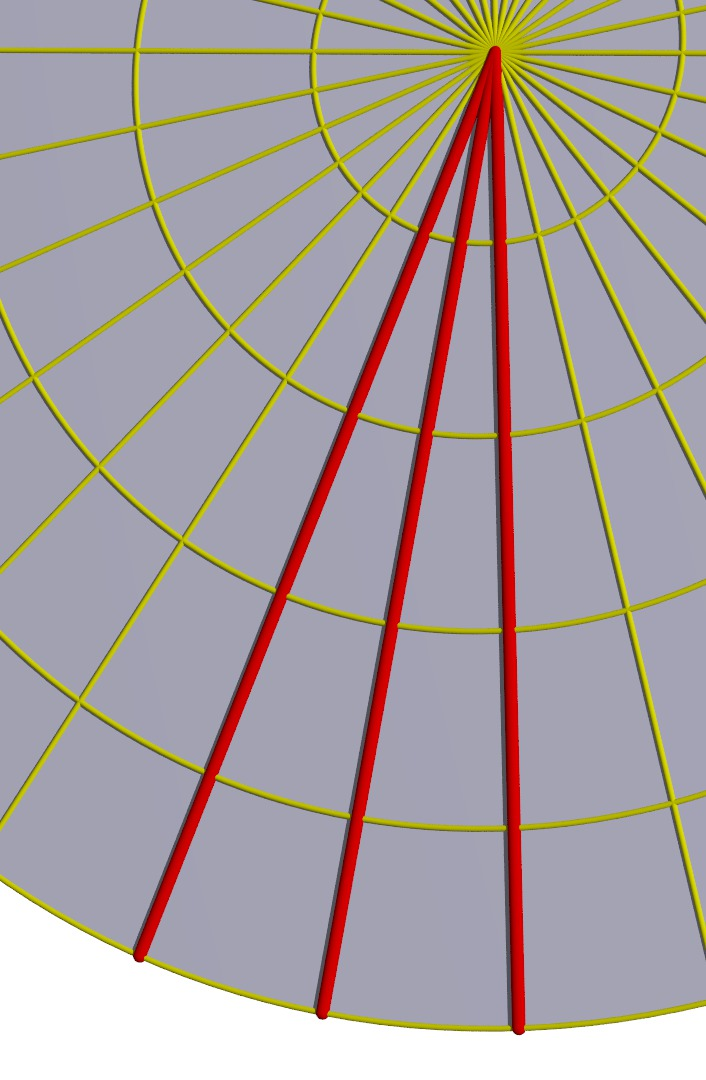
\includegraphics[height=6truecm]{chapters/3d/eben.jpg}
\quad
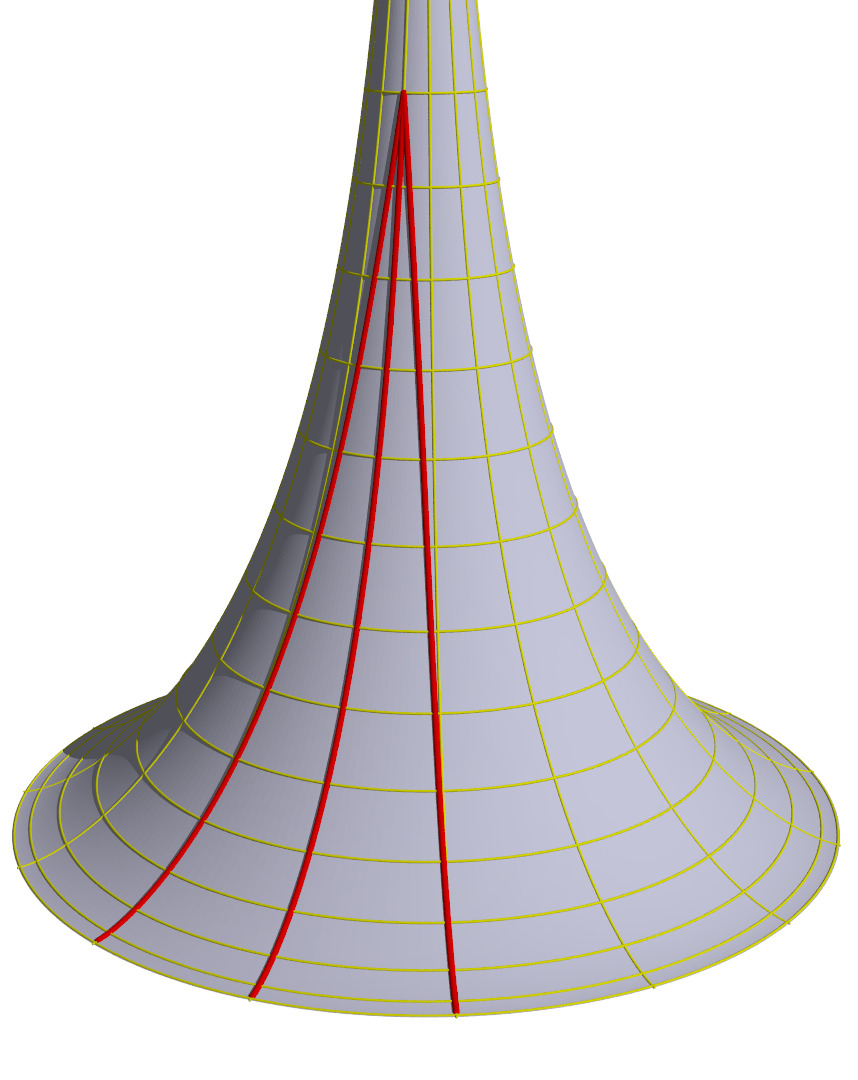
\includegraphics[height=6truecm]{chapters/3d/negativ.jpg}
\caption{Gleichschenklige Dreiecke mit gleichen Seitenlängen in einem
Universum mit positiver Krümmung (links), einem flachen Universum (Mitte)
und einem Universum mit negativer Krümmung (rechts).
Bei einem Universum mit positiver Krümmung ist der Winkel gegenüber
der kurzen Seite grösser als beim flachen Universum, bei einem
Universum mit negativer Krümmung ist er kleiner.
\label{skript:robertson:vergroesserung}}
\end{figure}
Ob das Universum positiv oder negativ gekrümmt oder gar flach ist,
muss experimentell bestimmt werden.
Dazu kann dazu den Winkel eines gleichschenkligen Dreiecks mit den
Seiten $l$ und $L$ mit $L\gg l$ verwenden.
In einem flachen Universum ist der Winkel gegenüber der Seite $l$
in Bogenmass $l/L$.
In einem Universum mit positiver Krümmung wird ein grösserer Winkel
beobachtet, in einem Universum mit negativer Krümmung ist der Winkel
dagegen kleiner.
Die Abbildung~\ref{skript:robertson:vergroesserung} veranschaulicht
diese vergrossernde Wirkung eines positiv gekrümmten Universums
und die verkleinernde Wirkung eines negativ gekrümmten Universums.

Um zu entscheiden, welchen Wert $\kappa$ für unser Universum hat,
kann man ein Dreieck verwenden, welches als $L$ die Entfernung zum kosmischen
Mikrowellenhintergrund verwendet.
Als kurze Seite des Dreiecks muss eine bekannte Grösse auf der
Fläche der letzten Streuung verwendet werden.
Zur Verfügung stehen Fluktuationen im kosmischen Mikrowellenhintergrund.
Man muss also die Entstehung und vor allem die Abmessungen solcher
Fluktuationen verstehen und berechnen können, bevor man den Test
durchführen kann.

\section{Steady State Universum}
\rhead{Steady State Universum}
Die Schlussfolgerung, dass das Universum vor relativ kurzer Zeit
aus einem heissen, dichten 
Zustand hervorgegangen sein müsse, war nicht von Anfang an akzeptiert.
Als alternative Hypothese wurde vorgeschlagen, dass im Universum 
zwar expandiert, dies aber schon seit ewigen Zeiten tut, und dass die
enstehenden
Lücken zwischen den Galaxien dadurch gefüllt werden, dass ständig
neue Materie entstand.
Dazu müsste pro Kubikkilometer und Jahr ein neues Wasserstoffatom
entstehen.

Diese Steady-State genannte Hypothese widerspricht jedoch zwei
im Folgenden diskutierten Beobachtungen.

\subsection{Olbers Paradoxon}
Wenn das Universum unendlich alt und gross ist, dann wird man in jeder
beliebigen Richtung nicht beliebig weit sehen können, sondern wird
irgendwann auf einen Stern treffen.
Der ganze Himmel müsste daher die Helligkeit von Sternen haben.

Nimmt man dagegen an, dass das Universum relativ jung ist, dann kann
man wegen der Endlichkeit der Lichtgeschwindigkeit nur soweit sehen,
wie das Alter des Universums erlaubt.

\subsection{Der kosmische Mikrowellenhintergrund}






%
% friedmann.tex
%
% (c) 2017 Prof Dr Andreas Müller, Hochschule Rapperswil
%
\chapter{Friedmann-Gleichungen%
\label{skript:chapter:friedmann}}
\lhead{Friedmann-Gleichungen}
\rhead{}
Natürliche Systeme sind meistens so komplex, dass es praktisch nicht
möglich ist, jedes einzelne Detail physikalisch exakt wiederzugeben.
Es ist daher notwendig, vereinfachte Modelle zu verwenden, welche 
die Anzahl der zu berücksichtigenden Variablen reduzieren auf eine
Art, die immer noch gestattet, die gestellten Fragen mit ausreichender
Genauigkeit zu beantworten.

In diesem Kapitel betrachten wir zunächst ein paar Beispiele aus den
Naturwissenschaften, welche diesen Prozess der Modellbildung exemplarisch
vorstellen.
Anschliessend wird ein Modell für das Universum betrachtet, welches
das Universum derart vereinfacht, dass über die langfristige
Geschichte des Universums konkrete Aussagen zu machen gestattet.
Mit diesen sogenannten Friedmann-Gleichungen kann man sodann zum
Beispiel das Alter des Universums bestimmen.

\section{Friedmann-Gleichungen}
\rhead{Friedmann-Gleichungen}
Im Kapitel~\ref{skript:chapter:kosmologie} haben wir gelernt, dass
das homogene und isotrope Universum die Robertson-Walker-Metrik 
\[
ds^2
=
-c^2\,dt^2
+
a(t)^2\bigl(
dr^2 + S_\kappa(r)^2d\Omega^2
\bigr)
\]
mit der noch unbekannten Funktion $a(t)$ hat.
Ausserdem muss die Metrik eine Lösung der Einstein-Gleichungen sein.
Auf deren rechten Seite steht der Energie-Impuls-Tensor des Universums.
Da das Universum isotrop und homogen ist, muss auch der Energie-Impuls-Tensor
isotrop und homogen sein.
Für einen mit Gas der Dichte $\varrho$ und Druck $p$ gefülltes Universum
ist der Energie-Impuls-Tensor durch
\[
T^{\mu\nu}
=
\begin{pmatrix}
\varrho c^2 & 0 & 0 & 0 \\
     0      & p & 0 & 0 \\
     0      & 0 & p & 0 \\
     0      & 0 & 0 & p \\
\end{pmatrix}
\]
beschrieben.

Die noch unbekannte Funktion $a(t)$ sollte sich also aus der
Einstein-Gleichung bestimmen lassen, sofern wir den Energie-Impuls-Tensor
des Universums berechnen können.
Dabei ist zu beachten, dass mit der Ausdehnung des Universums sich sowohl
die Dichte $\varrho$ als auch der Druck $p$ ändern werden.
Wir erwarten daher, ein System von Differentialgleichungen zu erhalten.
Die Einstein-Gleichungen werden einen Zusammenhang zwischen den 
Ableitungen von $a(t)$ und der Dichte herstellen,
andererseits müssen wir aus unserer Kenntnis des Verhaltens von
Materie und Strahlung herleiten, wie sich die Dichte mit dem
Streckungsfaktor  $a(t)$ des Universums ändert.
Dieses Differentialgleichungssystem wird die Entwicklung des homogenen
und isotropen Universums vollständig beschreiben.

Als erstes müssen wir jetzt die Differentialgleichung für $a(t)$
in Abhängigkeit von $\varrho$ ermitteln.
Dazu betrachten wir ausschliesslich die $00$-Komponente der
Einsteingleichungen, also
\begin{equation}
G_{00} = \frac{8\pi K}{c^4} T_{00}=\frac{8\pi K\varrho}{c^2}.
\label{skript:friedmann:einstein}
\end{equation}
Wir berechnen den Einstein-Tensor der Robertson-Walker-Metrik
wieder mit Maxima, und bekommen.
%(%i5)                       ratsimp(Einstein(1, 1))
%                                         2
%         2     d         2      2       d              2  d         2    2
%      3 S (r) (-- (a(t)))  - 2 c  S(r) (--- (S(r))) - c  (-- (S(r)))  + c
%               dt                         2               dr
%                                        dr
%(%o5) --------------------------------------------------------------------
%                                   2     2
%                                  S (r) a (t)
%(%i6)                    tex(ratsimp(Einstein(1, 1)))
%\[
%{{3\,S^2\left(r\right)\,\left({{d}\over{d\,t}}\,a\left(t\right)
% \right)^2-2\,c^2\,S\left(r\right)\,\left({{d^2}\over{d\,r^2}}\,S
% \left(r\right)\right)-c^2\,\left({{d}\over{d\,r}}\,S\left(r\right)
% \right)^2+c^2}\over{S^2\left(r\right)\,a^2\left(t\right)}}
%\]
\begin{equation}
G_{00}
=
3\frac{\dot a(t)^2}{a(t)^2}
-\frac{2c^2}{a(t)^2}\frac{S''_\kappa(r)}{S_\kappa(r)}
-\frac{c^2}{a(t)^2}
\frac{S'_\kappa(r)^2-1}{S_\kappa(r)^2}
\end{equation}
Die rechte Seite können wir mit Hilfe der im
Kapitel~\ref{skript:chapter:kosmologie} bereitgestellten Formeln
\eqref{skript:robertson:ersteableitung} und
\eqref{skript:robertson:zweiteableitung} für die Ableitungen der Funktion
$S_\kappa(r)$ vereinfachen.
Wir erhalten 
\begin{align*}
G_{00}
&=
3\frac{\dot a(t)^2}{a(t)^2}
-\frac{2c^2}{a(t)^2}\frac{-\kappa\displaystyle \frac{S_\kappa(r)}{R_c^2}}{S_\kappa(r)}
-\frac{c^2}{a(t)^2}
\frac{1-\kappa \frac{\displaystyle S_\kappa(r)^2}{R_c^2}-1}{S_\kappa(r)^2}
\\
&=
3\frac{\dot a(t)^2}{a(t)^2}
+\frac{3c^2\kappa}{a(t)^2R_c^2}.
\end{align*}
Die $00$-Komponente der Einstein-Gleichung liefert uns jetzt die Gleichung
\begin{equation}
\frac{\dot a(t)^2}{a(t)^2}
+
\frac{c^2\kappa}{a(t)^2R_c^2}
=
\frac{8\pi K}{3c^2}\varrho,
\end{equation}
sie heisst die (erste) {\em Friedmann-Gleichung}.
\index{Friedmann-Gleichung}%
Üblicherweise wird die Gleichung als Gleichung für $H=\dot a(t)/a(t)$
geschrieben, also
\begin{equation}
H^2
=
\biggl(
\frac{\dot a(t)}{a(t)}
\biggr)^2
=
\frac{8\pi K}{3c^2}\varrho
-
\frac{c^2\kappa }{a(t)^2R_c^2}.
\label{skript:friedmann:friedmann}
\end{equation}

\section{Die Beschleunigungsgleichung}
\rhead{Die Beschleunigungsgleichung}
Durch Verjüngung der Einsteingleichung kann man auch den anderen
Komponenten des Einstein-Tensors und insbesonder der Druck-Komponenten 
des Energie-Impuls-Tensors Rechnung tragen.
Die rechte Seite der Einstein-Gleichung wird einfach nur die
Spur, also
\[
\frac{8\pi K}{c^2}
T^\mu_\mu = \frac{8\pi K}{c^4}(-\varrho c^2 + 3p).
\]
Für die linke Seite muss die Verjüngung des Einstein-Tensors ausgerechnet
werden.
%(%i16) s : ratsimp(sum(sum(ginverse     Einstein(i, j), i, 1, length(g)), j, 
%                                   i, j
%                                                                 1, length(g)))
%                         2
%             2          d                2     d         2
%(%o16) - (6 S (r) a(t) (--- (a(t))) + 6 S (r) (-- (a(t)))
%                          2                    dt
%                        dt
%                        2
%               2       d                2  d         2      2    2  2     2
%          - 4 c  S(r) (--- (S(r))) - 2 c  (-- (S(r)))  + 2 c )/(c  S (r) a (t))
%                         2                 dr
%                       dr
%(%i17)                              tex(s)
%\[
%-{{6\,S^2\left(r\right)\,a\left(t\right)\,\left({{d^2}\over{d\,t^2
% }}\,a\left(t\right)\right)+6\,S^2\left(r\right)\,\left({{d}\over{d\,
% t}}\,a\left(t\right)\right)^2-4\,c^2\,S\left(r\right)\,\left({{d^2
% }\over{d\,r^2}}\,S\left(r\right)\right)-2\,c^2\,\left({{d}\over{d\,r
% }}\,S\left(r\right)\right)^2+2\,c^2}\over{c^2\,S^2\left(r\right)\,a^2
% \left(t\right)}}
%\]
Der verjüngte Einstein-Tensor ist
\begin{align*}
G^\mu_\mu
&=
- \frac{6}{c^2} \frac{\ddot a(t)}{a(t)}
-\frac{6}{c^2} \frac{\dot a(t)^2}{a(t)^2}
+\frac{4}{a(t)^2} \frac{S''_\kappa(r)}{S_\kappa(r)}
+\frac{2S'_\kappa(r)^2-2}{a(t)^2 S_\kappa(r)^2}
\\
&=
-\frac{6}{c^2}\biggl(\frac{\ddot a(t)}{a(t)} + \frac{\dot a(t)^2}{a(t)^2}\biggr)
-\frac{6}{a(t)^2}\frac{\kappa }{R_c^2}.
\end{align*}
Die verjüngte Einsteingleichung wird dann
\begin{align*}
G^\mu_\mu
&=
\frac{8\pi K}{c^2}(-\varrho  c^2+ 3p)
\\
-\frac{6}{c^2}\biggl(\frac{\ddot a(t)}{a(t)} + \frac{\dot a(t)^2}{a(t)^2}\biggr)
-\frac{6}{a(t)^2}\frac{\kappa }{R_c^2}
&=
\frac{8\pi K}{c^2}(-\varrho c^2 + 3p)
\\
\frac{\ddot a(t)}{a(t)} + \frac{\dot a(t)^2}{a(t)^2}
&=
-\frac{4\pi K}{3c^2}(-\varrho c^2 + 3p)
-\frac{c^2}{a(t)^2}\frac{\kappa }{R_c^2}.
\end{align*}
Den zweiten Term auf der rechten Seite können wir mit Hilfe der Gleichung
\eqref{skript:friedmann:friedmann}
eliminieren und bekommen
\begin{align}
\frac{\ddot a(t)}{a(t)}
&=
-\frac{4\pi K}{3c^2}(-\varrho c^2 + 3p)
-\frac{c^2}{a(t)^2}\frac{\kappa }{R_c^2}
-\frac{8\pi K}{3c^2}\varrho c^2
+
\frac{c^2\kappa }{a(t)^2R_c^2}
\notag
\\
\frac{\ddot a(t)}{a(t)}
&=
-\frac{4\pi K}{3c^2}(\varrho c^2 + 3p).
\label{skript:friedmann:beschleunigung}
\end{align}
Dies ist die {\em Beschleunigungsgleichung}, sie ist eine
Differentialgleichung zweiter Ordnung für den Skalenfaktor.
\index{Beschleunigungsgleichung}

Man kann die linke Seite auch durch $H$ und seine erste Ableitung
ausdrücken:
\begin{align*}
\dot H
&=
\frac{d}{dt}\frac{\dot a(t)}{a(t)}
=
\frac{\ddot a(t) a(t)-\dot a(t)^2}{a(t)^2}
=
\frac{\ddot a(t)}{a(t)} - \frac{\dot a(t)^2}{a(t)^2}
=
\frac{\ddot a(t)}{a(t)} - H^2
\\
\Rightarrow
\qquad
\dot H+H^2
&=
\frac{\ddot a(t)}{a(t)}.
\end{align*}
Damit können wir die Beschleunigungsgleichung auch als Gleichung
für $H$ schreiben:
\begin{equation}
\dot H+H^2
=
-\frac{4\pi K}{3c^2}(\varrho c^2 + 3p).
\end{equation}
Natürlich muss $\varrho$ und $p$ in Abhängigkeit von $H$ ausgedrückt
werden, bevor diese Form der Beschleunigungsgleichung zur Berechnung
der Geschichte des Universums genutzt werden kann.

\section{Geschichte des Universums}
\rhead{Geschichte des Universums}
Die Friedmann-Gleichung kann dazu verwendet werden, um die Geschichte
des Universums zu rekonstruieren.
Dazu müssen wir die Differentialgleichung aussgehend von der
aktuellen Zeit $t_0$ lösen, als Anfangsbedingung für den
Skalenfaktor verwenden wir per Konvention $a(t_0)=1$.
Auf der rechten Seite der Gleichung brauchen wir die vorerst noch
unbekannte Funktion $\varrho(t)$.

\subsection{Der Einfluss des Krümmungsparameters $\kappa$}
Es fällt aber auch auf, dass in der Friedmann-Gleichung die Ableitung
$\dot a(t)$ im Quadrat vorkommt.
Das Vorzeichen von $\dot a(t)$ ist also nur dadurch bestimmt, dass
wir aus Hubbles Beobachtungen wissen, dass sich das Universum
ausdehnt und damit $\dot a(t_0) > 0$.
Solange also die rechte Seite der Friedmann-Gleichung keine Nullstelle
hat, wird sich das Universum weiter ausdehnen.
Dies trifft zum Beispiel für $\kappa=-1$ zu.

\subsubsection{Positiv gekrümmtes Universum: $\kappa=1$}
In einem Universum mit $\kappa=1$ gibt es dagegen einen Zeitpunkt, für
den die rechte Seite eine Nullstelle hat:
\[
\frac{8\pi K}{3c^2}\varrho -\frac{c^2\kappa}{a(t)^2R_c^2}=0
\qquad\Rightarrow\qquad
\frac{8\pi K}{3c^2}\varrho(t)=\frac{c^2}{a(t)^2R_c^2}.
\]
In einem sich ausdehnenden Universum nimmt die Dichte $\varrho(t)$ mit
der dritten Potenz von $a(t)$ ab, es gilt
\[
\varrho(t) = \frac{\varrho_0}{a(t)^3}
\]
und damit
\[
\frac{8\pi K}{3c^2}\frac{\varrho_0}{a(t)^3}=\frac{c^2}{a(t)^2R_c^2}
\qquad\Rightarrow\qquad
a(t)
=
\frac{8\pi K R_c^2\varrho_0}{3c^4}.
\]
Inbesondere gibt es einen Zeitpunkt $t$, nach dem das Universum sich
wieder zusammenziehen wird.

\subsubsection{Flaches Universum: $\kappa=0$}
In einem Universum mit $\kappa=0$ fällt der Krümmungsterm in 
der Friedmann-Gleichung ganz weg.
Die Entwicklung des Universums wird allein bestimmt von der Dichte.
Die rechte Seite der Friedmann-Gleichung ist immer positiv, ein
solches Universum dehnt sich daher aus.

\subsection{Das leere Universum}
\begin{figure}
\centering
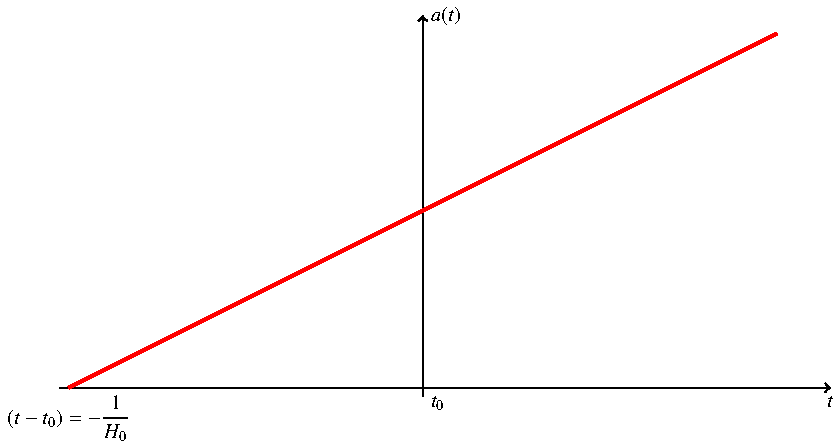
\includegraphics{chapters/tikz/friedmann-leer.pdf}
\caption{Zeitabhängigkeit des Skalenfaktors $a(t)$ in einem leeren
Universum mit $\kappa = -1$.
$a(t)$ verschwindet eine Hubble-Zeit $1/H_0$ vor heute ($t_0$).
\label{chapter:friedmann:graph:leer}}
\end{figure}
Für ein leeres Universum können wir die Friedmann-Gleichung vollständig
lösen.
Die Differentialgleichung wird dann zu
\[
\frac{\dot a(t)^2}{a(t)^2}
=
-\frac{c^2\kappa}{a(t)^2R_c^2}.
\]
Die linke Seite dieser Gleichung ist immer postiv.

\subsubsection{Leeres Universum mit positiver Krümmung: $\kappa=1$}
Für $\kappa=1$ ist die rechte Seite negativ, die Differentialgleichung
kann also gar keine Lösung haben.
Ein leeres Universum muss also automatisch $\kappa=-1$ oder $\kappa=0$
erfüllen.

\subsubsection{Leeres, flaches Universum: $\kappa=0$}
Für $\kappa=0$ ist die rechte Seite $0$, woraus man schliessen kann,
dass $\dot a(t)=0$ sein muss.
Ein leeres, flaches Universum ist also auch statisch und entspricht
damit nicht unserem Universum.

\subsubsection{Leeres Universum mit negativer Krümmung: $\kappa=-1$}
Für ein leeres Universum mit $\kappa=-1$ kann die Friedmann-Gleichung sofort
gelöst werden, man erhält
\[
\dot a(t)^2
=
\frac{c^2}{R_c^2}
\qquad\Rightarrow\qquad
\dot a(t) = \frac{c}{R_c} = 
\qquad\Rightarrow\qquad
a(t)= 1 + \frac{c}{R_c}(t-t_0).
%= 1 + H_0(t-t_0).
\]
Diese Lösung ist in Abbildung~\ref{chapter:friedmann:graph:leer} dargestellt.
Der Skalenfaktor wächst also linear mit der Zeit.
Aus den Messungen von Hubble und Humason ist die
$H_0=H(t_0)=\dot a(t_0)/a(t_0)=\dot a(t_0)$
bekannt.
Damit kann man den Skalenfaktor auch mit der Hubble-Konstanten
bestimmen:
\[
H(t) =  \frac{\dot a(t)}{a(t)} = 1 + H_0(t-t_0).
\]
Für $t=1/H_0$ wird $H(t)=0$, dann sind alle Distanzen im
Universum auf $0$ geschrumpft.


\subsection{Das nicht leere Universum}
Wenn das Universum sich ausdehnt, dehnt sich das darin enthaltene
Gas, der Staub und die Strahlung mit aus.
Ist der Energieinhalt des Universums als Funktion von $a(t)$ bekannt,
kann die Friedmann-Gleichung gelöst werden.

Neuere Messungen zeigen, dass unser Universum flach ist.
Die Rechnungen für $\kappa=1$ in den nachfolgenden Unterabschnitten
sind daher für unser Universum nicht anwendbar.
In späteren Abschnitten, insbesondere im Abschnitt über verschiedene
Komponenten des Universums, wird daher nur noch der Fall $\kappa=0$
durchgerechnet.

\subsubsection{Geschlossenes Universum}
Wir untersuchen jetzt, was für langfristige Lösungen die
Friedmann-Gleichung~\eqref{skript:friedmann:friedmann}
überhaupt erlaubt.
Insbesondere interessiert die Frage, ob ein expandierendes Universum
in eine kollabierendes Universum übergehen kann.

Zunächst beachten wir, dass die 
Friedmann-Gleichung~\eqref{skript:friedmann:friedmann}
sich nicht ändert, wenn man die Zeit umkehrt.
Dann ändert zwar $\dot a(t)$ das Vorzeichen, aber $\dot a(t)$ kommt
nur im Quadrat vor, so dass mit $a(t)$ auch $a(-t)$ die Friedmann-Gleichung
erfüllt.
Die Friedmann-Gleichung sind zeitumkehrinvariant.
Daraus folgt auch, dass ein Universum, das zum Zeitpunkt $t_1$
von Expansion zu Kontraktion übergeht, für $t>t_1$ durch
$a(t)=a(t_1-t)$ beschrieben werden kann, die Lösungsfunktion ist
also symmetrisch bezüglich $t=t_1$.
Ausserdem muss
am Punkt $t_1$ die Ableitung von $a(t)$ verschwinden, also ist
$\dot a(t_1)=0$.

Der Term $8\pi K\varrho/3c^2$ ist für ein nicht leeres Universum
immer positiv.
Der Krümmungsterm $c^2\kappa/a(t)^2R_c^2$ hat das gleiche Vorzeichen
wie $\kappa$.
Für ein negativ gekrümmtes Universum ist er immer positiv, so dass
nach der Friedmann-Gleichung ein solches Universum niemals $\dot a(t)=0$
erreichen kann, die Expansion in einem solche Universum wird also
niemals aufhören.

Die Dichte $\varrho$ der Materie ist proportional zu $a(t)^{-3}$, geht
also schneller gegen $0$ als der Krümmungsterm.
Für ein positiv gekrümmtes Universum werden also früher oder später immer
die beiden Terme auf der rechten Seite der
Friedmann-Gleichung~\eqref{skript:friedmann:friedmann}
betragsmässig gleich gross werden.
In diesem Moment folgt $\dot a(t) = 0$.
Ein expandierendes Universum mit positiver Krümmung wird also immer in eine 
Kontraktion übergehen.

Der Grenzfall ist ein Unversum mit verschwindender Krümmung oder $\kappa=0$.
In einem solchen Universum gilt
\begin{equation}
\varrho = \frac{3c^2H^2}{8\pi K}.
\label{skript:friedmann::dichte}
\end{equation}

\subsubsection{Kritische Dichte}
Der Wert der Dichte~\eqref{skript:friedmann::dichte}
für die heutige Zeit $t=t_0$ ist
\[
\varrho_c = \frac{3c^2H^2(t_0)}{8\pi K}=\frac{3c^2H_0^2}{8\pi K}
\]
und heisst die {\em kritische Dichte}.
\index{Dichte, kritische}
\index{kritische Dichte}
Ein üblicher Zahlenwert für die kritische Dichte unseres Universums ist
\[
\varrho_c = \frac{3H_0^2}{8\pi K}\simeq 10^{-26}\frac{\text{kg}}{\text{m}^3}
\]
Da ein Proton eine Masse von $1.672\cdot 10^{-27}\text{kg}$ hat, entspricht
$\varrho_c$ einer Dichte von etwa $6$ Protonen pro Kubikmeter.
Die kritische Dichte ist so etwas wie eine universelle kosmologische
Masseinheit für die Dichte.
Die Energiedichte
\[
\Omega=\frac{\varrho}{\varrho_c}
\]
ausgedrück in Einheiten der kritische Dichte heisst
der {\em Dichteparameter}.

\section{Komponenten}
\rhead{Komponenten}
Das reale Universum ist nicht leer, in den Beispielen haben wir den
Fall gewöhnlicher Materie bereits näher angeschaut.
Die Funktionen $\varrho(t)$ und $p(t)$ sind für verschiedene
Arten von Materie oder Energie verschieden.
Wir sprechen von verschiedenen Komponenten des Universums.
Jede Komponente hat ihre eigene Zustandsgleichung und führt
daher zu einer anderen Lösung der Friedmann-Gleichung.
In den folgenden Unterabschnitten wird jeweils die Lösung für
ein flaches Universum mit nur einer Komponente durchgerechnet.

\subsection{Materie}
Die offensichtlichste Komponente ist die sogenannte baryonische Materie.
Sie macht jedoch nur etwa 5\% des Energieinhalts des Universums aus.
Sie wird so genannt, weil ihre Masse vor allem durch die Masse der Atomkerne
bestimmt ist, aus der sie sich zusammensetzt.

Im sich ausdehneden Universum bleibt die Masse erhalten, die Dichte wird
daher mit der dritten Potenz von $a(t)$ abnehmen, wie wir im Folgenden
nachrechnen wollen.
Ein Würfel mit Kantenlänge $l$ zur Zeit $t_0$ enthält die Masse
$m=l^3 \varrho(t_0)$.
Zur Zeit $t$ ist die Kantenlänge $a(t)l$, das Volumen $a(t)^3l^3$
und die darin enthaltene Masse $m=a(t)^3l^3\varrho(t)$.
Da die Masse erhalten bleibt, folgt
\[
l^3 \varrho(t_0)
=
a(t)^3l^3\varrho(t)
\qquad\Rightarrow\qquad
\varrho(t)=\frac{\varrho(t_0)}{a(t)^3}.
\]
Die Friedmann-Gleichung wird daher
\begin{equation}
\frac{\dot a(t)^2}{a(t)^2}
=
\frac{8\pi K\varrho_0}{3c^2a(t)^3}-\frac{c^2\kappa}{a(t)^2R_c^2}.
\end{equation}

Da die mittlere Materiedichte im Universum sehr klein ist, kann man davon
ausgehen, dass Atome praktisch nie kollidieren, dass diese Komponenten
also keinen Druck aufweist.
Staubteilchen werden trotz grösserer Masse noch seltener kollidieren.

%Die baryonische Materie wird also durch die Zustandsgleichungen
%\begin{equation}
%\varrho(t)=\frac{\varrho_0}{a(t)^3}
%\qquad\text{und}\qquad
%p(t)=0
%\end{equation}
%vollständig charakterisiert.

\subsubsection{Das flache, gasgefüllte Universum}
In einem flachen, gasgefüllten Universum ist $\kappa=0$,
der Krümmungsterm fällt weg und
es erfüllt daher die vereinfachte Friedmann-Gleichung
\[
\frac{\dot a(t)^2}{a(t)^2}
=
\frac{8\pi K\varrho_0}{3c^2 a(t)^3}.
\]
Wir lösen die Differentialgleichung, indem wir zunächst die Wurzel ziehen 
\[
\dot a(t)=\pm \sqrt{
\frac{8\pi K\varrho_0}{3c^2}
}a(t)^{-\frac{1}{2}}
\]
und dann in
\[
\sqrt{a(t)}\,
\frac{da}{dt}
=
\pm\sqrt{\frac{8\pi K\varrho_0}{3c^2}}
\]
separieren und integrieren:
\[
\int \sqrt{a}\,da
=
\int a^\frac12\,da
=
\frac23 a(t)^\frac{3}{2}
=
\pm\sqrt{\frac{8\pi K\varrho_0}{3c^2}}t + C.
\]
Auflösen nach $a(t)$ führt auf
\[
a(t)=\biggl(\pm\sqrt{\frac{6\pi K\varrho_0}{c^2}}t+C'\biggr)^{\frac23}
\]
wobei die Integrationskonstante $C'$ noch so bestimmt werden muss,
dass $a(t_0)=1$ gilt.
Dies wird erreicht mit
\begin{equation}
a(t)
=
\biggl(\pm\sqrt{\frac{6\pi K\varrho_0}{c^2}}(t-t_0) + 1\biggr)^\frac23.
\label{skript:friedmann:alter:materie}
\end{equation}

Wir möchten den Bezug zur aktuellen Ausdehnung des Universums herstellen,
dazu muss $\dot a(t_0)=H_0$ sein.
Wir berechnen daher die Ableitung
\[
\dot a(t_0)=\pm \sqrt{\frac{6\pi K\varrho_0}{c^2}}\cdot \frac23
=
\pm \sqrt{\frac{8\pi K\varrho_0}{3c^2}}
=
\pm H_0.
\]
Unser Universum expandiert, daher kommt nur das positive Vorzeichen in Frage.
Wir können den Wurzelausdruck in \eqref{skript:friedmann:alter:materie} 
ebenfalls durch $H_0$ ausdrücken.
Aus
\[
\sqrt{\frac{6\pi K\varrho_0}{c^2}}
=
\frac32
\sqrt{\frac{8\pi K\varrho_0}{3c^2}}
=
\frac32H_0
\]
folgt
\begin{equation}
a(t) = \biggl(\frac32H_0(t-t_0)+1\biggr)^\frac23
\label{skript:friedmann:alter:materie2}
\end{equation}
für den Skalenfaktor in einem materiegefüllten Universum.
Abbildung~\ref{skript:friedmann:graph:materie} zeigt den Verlauf
des Skalenfaktors.

\begin{figure}
\centering
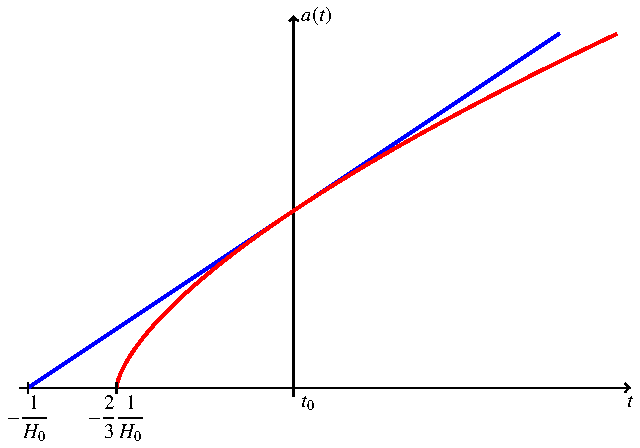
\includegraphics{chapters/tikz/friedmann-materie.pdf}
\caption{Zeitabhängigkeit des Skalenfaktors $a(t)$ ({\color{red}rot})
in einem Universum, welches nur Materie enthält.
Im Vergleich dazu {\color{blue}blau} die Entwicklung für linear von der
Zeit abhängigen Skalenfaktor, die Steigung der Geraden ist die
Hubble-Konstanten $H_0$.
Das Alter des Universums ist nur zwei Drittel der Hubble-Zeit.
\label{skript:friedmann:graph:materie}}
\end{figure}

Das Alter des Universums lässt sich damit ebenfalls ermitteln.
Dazu muss die grosse Klammer in~\eqref{skript:friedmann:alter:materie2}
verschwinden, also
\begin{equation*}
\begin{aligned}
\frac32H_0(t-t_0)
&=
-1
&&\Rightarrow&
t-t_0
&=
-\frac23 \frac1{H_0}.
\end{aligned}
\end{equation*}
Ein materiegefülltes Universum hat daher nur ein Alter von
etwa 67\% der Hubble-Zeit. 
Setzt man die besten bekannten Werte in, erhält man 9.6Gyr,
deutlich zu wenig Zeit.

\subsection{Strahlung}
Im frühen Universum war Strahlung die dominierende Komponente.
Mit er Expansion verändert sich nicht nur die Dichte der Photonen 
analog zu einem Gas, es verändert sich auch deren Wellenlänge.
Da die Energie eines Photons proportional ist zur Wellenlänge,
nimmt die Energiedichte der Strahlung mit der vierten Potenz des
Skalenfaktors $a(t)$ ab:
\[
\varrho(t)=\frac{\varrho_0}{a(t)^4}.
\]
Die Bedeutung der Strahlung nimmt also schneller ab als jene der Materie.
% XXX Graphik, die a^-3 und a^-4 vergleicht
Dies gilt nicht nur für Strahlung, sondern auch für Teilchen, die
sich mit relativistischer Geschwindigkeit bewegen, zum Beispiel für
Neutrinos.
Daher werden solche Teilchen normalerweise ebenfalls unter dem
Strahlungsterm in der Friedmann-Gleichung subsumiert.

Die Friedmann-Gleichung für ein mit Strahlung gefülltes Universum ist
\begin{equation}
\biggl(
\frac{\dot a(t)}{a(t)}
\biggr)^2
=
\frac{8\pi K \varrho_0}{3c^2a(t)^4}
-
\frac{c^2\kappa }{a(t)^2R_c^2}
\end{equation}
Leider lässt sich diese Differentialgleichung im allgemeinen
nicht in geschlossener Form integrieren.
Wir beschränken uns daher auf den einfacheren Spezialfall $\kappa=0$.
%wir verschieben die Diskussion der
%Lösung auf einen späteren Abschnitt, wo wir die Gleichung numerisch lösen
%können.

\subsubsection{Das flache, strahlungserfüllte Universum}
Für ein flaches Universum ist $\kappa=0$, der Krümmungsterm fällt wieder
weg und die Friedmann-Gleichung vereinfacht sich zu
\begin{equation*}
\frac{\dot a(t)^2}{a(t)^2}
=
\frac{8\pi K\varrho_0}{3c^2 a(t)^4}.
\end{equation*}
Auch hier können wir die Wurzel ziehen und mit $a(t)$ multiplizeren,
wir erhalten
\begin{equation*}
\dot a(t)
=
\sqrt{\frac{8\pi K\varrho_0}{3c^2}}\frac1{a(t)}.
\end{equation*}
Diese Gleichung lässt sich ebenfalls separieren:
\begin{align*}
a\frac{da}{dt}
&=
\sqrt{\frac{8\pi K\varrho_0}{3c^2}}
\\
\Rightarrow\qquad
\int a\,da
=
\frac12a(t)^2
&=
\sqrt{\frac{8\pi K\varrho_0}{3c^2}}t + C.
\end{align*}
Auflösen nach $a(t)$ liefert
\[
a(t)
=
\sqrt{\pm\frac{16\pi K\varrho_0}{3c^2}t + 2C}.
\]
Die Integrationskonstante muss so bestimmt werden, dass die
Anfangsbedingung $a(t_0)=1$  erfüllt ist.
Setzt man $a(t_0)=1$ ein, erhält man
\[
C
=
\mp\frac{8\pi K\varrho_0}{3c^2}t_0+1
\]
oder
\begin{equation}
a(t)
= 
\sqrt{\pm\frac{16\pi K\varrho_0}{3c^2}(t-t_0) + 1}.
\label{skript:friedmann:a(t)}
\end{equation}
Diese Wurzelfunktion beschreibt je nach gewähltem Vorzeichen ein
expandierendes oder schrumpfendes Universum.
In keinem Fall ist jedoch $\dot a(t)=0$ möglich, die Expansion kann
also nicht anhalten und in eine Kontraktion übergehen.
Da wir in einem expandierenden Universum leben, fällt der Fall
des sich zusammenziehenden Universums ausser betracht,
wir untersuchen im Folgenden nur noch das positive Vorzeichen.

\begin{figure}
\centering
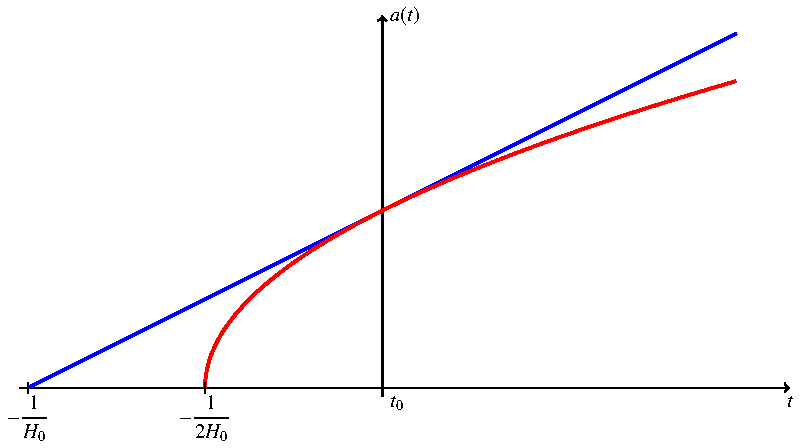
\includegraphics{chapters/tikz/friedmann-strahlung.pdf}
\caption{Zeitabhängigkeit des Skalenfaktors $a(t)$ ({\color{red}rot})
in einem Universum, welches von Strahlung dominiert ist.
Im Vergleich dazu {\color{blue}blau} die Entwicklung für linear von der
Zeit abhängigen Skalenfaktor, die Steigung der Geraden ist die
Hubble-Konstanten $H_0$.
Das Alter des Universums ist nur eine halbe Hubble-Zeit.
\label{skript:friedmann:graph:strahlung}}
\end{figure}

Wir müssen den Zusammenhang zu unserem Universum herstellen, welches
aktuell mit $\dot a(t_0)= H_0$ ausdehnt.
Dazu berechnen wir die Ableitung
\[
\dot a(t_0)=\frac{8\pi K\varrho_0}{3c^2}=H_0
\]
von~\eqref{skript:friedmann:a(t)}.
Damit können wir den Skalenfaktor auch durch die Hubble-Konstane ausdrücken,
es gilt
\begin{equation}
a(t)=\sqrt{2H_0(t-t_0)+1}.
\label{skript:friedmann:a(t):strahlung}
\end{equation}
Die Zeitabhängigkeit von $a(t)$ für ein strahlungsdominiertes Universum
ist in Abbildung~\ref{skript:friedmann:graph:strahlung} dargestellt.

Wir interessieren uns für das Alter des Universums, welches durch
die Bedingung $a(t)=0$ festgelegt wird.
Für ein expandierendes Universum kann man sofort ablesen, dass
die Expansionsgeschwindigkeit früher grösser gewesen sein muss.
Es ist also nicht zulässig, das Alter des Universums durch lineare
Extrapolation aus der aktuellen Hubble-Konstanten abzuleiten.
Vielmehr müssen wir die Zeit $t$ als Nullstelle der Funktion
\[
a(t)=\sqrt{2H_0(t-t_0)+1}
\]
bestimmt werden.
Für $t-t_0$ finden wir
\[
H_0(t-t_0)
=
-1
\qquad\Rightarrow\qquad
t-t_0 = -\frac1{2H_0}.
\]
Setzt man den besten bekannten Zahlenwert
\eqref{skript:robertson:hubble0}
für die Hubble-Konstante ein,
erhält man für das Alter des Universums
\[
t-t_0=-7.2\text{Gyr},
\]
diese Zeit ist jedoch zu kurz, unsere Sonne müsste schon etwa
2 Milliarden Jahre nach der Entstehung des Universums entstanden
sein.
Dies ist darauf zurückzuführen, dass unsere Modellierung des
Energieinhaltes unvollständig ist.



\section{Dunkle Energie}
\rhead{Dunkle Energie}
Einstein erwartete, dass das Universum statisch und unendlich alt sein
müsste Universum.
Er stellte jedoch bald fest, dass seine Gleichungen ein solches Universum
nicht beschreiben konnten.
Er fügte daher seiner Gleichung einen Term hinzu, der dies ermöglichte.
Diesen ``kosmologischen'' Term bezeichnete er nach der
Entdeckung der Expansion des Universums durch Hubble als
den grössten Fehler seines Lebens.
Heute erhält dieser Term als ``dunkle Energie'' eine neue Interpretation.

\subsection{Die kosmologische Konstante}
Als Einstein die Gleichungen der Gravitation aufstellte, war die
vorherrschende Vorstellung, dass das Universum statisch und unendlich
alt ist.
Die Friedmann-Gleichungen haben aber keine statische Lösung
für $\varrho>0$.
Einstein hat versucht, dies dadurch zu korrigieren, dass er der
linken Seite einen Summanden $\Lambda g_{\mu\nu}$ hinzufügt.
Heute wird dieser Term in den Einstein-Gleichungen auf der rechten
Seite geschrieben.

Die aus dieser modifizierten Einstein-Gleichung abgeleitete
Friedmann-Gleichung lautet jetzt
\begin{align}
\frac{\dot a(t)^2}{a(t)^2}
&=
\frac{8\pi K}{3c^2}\varrho - \frac{\kappa c^2}{a(t)^2R_c^2} + \frac{\Lambda c^2}{3},
\label{skript:friedmann:dunkleenergie}
\\
\intertext{
die Beschleunigungsgleichung wird
}
\frac{\ddot a(t)}{a(t)}
&=
-\frac{4\pi K}{3c^2}(\varrho c^2+3p) + \frac{\Lambda c^2}{3}.
\label{skript:friedmann:dunklebeschleunigung}
\end{align}
Damit $\dot a(t)=0$ ist, muss die Konstante $\Lambda$ sorgfältig auf
die Energiedichte im Universum und die Krümmung abgestimmt sein.

Aus diesem Grund war diese Korrektur der Einstein-Gleichungen nicht
wirklich erfolgreich.
Die statische Lösung von~\eqref{skript:friedmann:dunkleenergie}
ist nämlich nicht stabil.
Ein solches Universum würde also bei einer winzigen Störung sofort
in eine Expansion oder Kontraktion übergehen.

Im Gegensatz zu den anderen Termen auf der rechten Seite der
Friedmann-Gleichungen nimmt der $\Lambda$-Term mit grösser werdendem
Skalenfaktor nicht ab.
Die Beschleunigungsgleichung~\eqref{skript:friedmann:dunklebeschleunigung}
zeigt, dass ein Universum mit $\Lambda > 0$ früher oder später
in eine exponentiell beschleunigte Expansion übergeht.

\subsection{Dunkle Energie}
Heute wird die Notwenigkeit des $\Lambda$-Terms von Messungen
gefordert.
Der $\Lambda$-Term als zusätzlicher Summand im Energie-Impuls-Tensor
wird {\em dunkle Energie} genannt.
Aus Messungen ist bekannt, dass er zum heutigen Zeitpunkt etwa 75\%
des Energieinhalts ausmacht.
Die dunkle Energie ist daher heute der dominante Faktor für die
Ausdehnung des Universums.
\begin{figure}
\centering
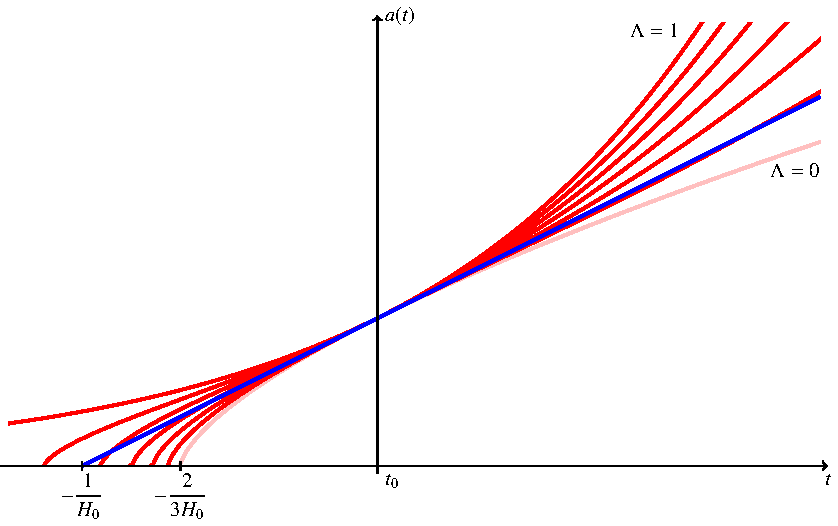
\includegraphics{chapters/tikz/darkenergy.pdf}
\caption{Zeitabhängigkeit des Skalenfaktors $a(t)$ ({\color{red}rot})
in einem Universum ohne Strahlung aber mit Materie und dunkler Energie
für verschiedene Werte von $\Lambda$.
\label{skript:friedman:graph:darkenergy}}
\end{figure}

Um zu verstehen, wie sich die dunkle Energie auf das Alter des Universums
auswirkt, berechnen wir die Entwicklung eines materiedominierten, flachen 
Universums mit verschiedenen Werten von $\Lambda$.
Die Friedmann-Gleichung dafür lautet
\[
\frac{\dot a(t)^2}{a(t)^2}
=
\frac{8\pi K \varrho_0}{3c^2a(t)^3} + \frac{\Lambda c^2}{3}
\]
Zur Zeit $t=t_0$ steht auf der linken Seite das Quadrat der Hubble-Konstanten,
es muss also gelten
\[
H_0^2
=
\frac{8\pi K \varrho_0}{3c^2} + \frac{\Lambda c^2}{3},
\]
für die Simulation müssen wir daher $\varrho_0$ und $\Lambda$ jeweils
so varieren, dass $H_0$ gleich bleibt.

Für die Berechnung ist es zweckmässig, die Hubble-Zeit als Masseinheit
für die Zeit zu verwenden, dann wird nämlich $H_0=1$.
Ausserdem wählen wir die Längeneinheit so, dass $c=1$ wird.
Ausserdem interessiert uns der genau Wert von $\varrho_0$ nicht wirklich,
entscheidend ist nur der Koeffizient von $a(t)^{-3}$ in der
Friedmann-Gleichung, die wir daher als
\newcommand{\Rho}{\mathrm{P}}
\begin{equation}
\frac{\dot a(t)^2}{a(t)^2}
=
\frac{\Rho_0}{a(t)^3} + \frac{\Lambda}{3}
\label{skript:friedmann:de:friedmann}
\end{equation}
schreiben\footnote{Das Zeichen $\Rho_0$ ist ein grosses griechisches Rho.}.
Da zur heutigen Zeit die kritische Dichte $\Rho_0$ und $\Lambda$ die gesamte
Energiedichte des Universums ausmachen, müssen sie die Bedingung
\begin{equation}
\Rho_0 + \frac{\Lambda}{3}=1
\end{equation}
erfüllen.
Damit können wir die Friedmann-Gleichung~\eqref{skript:friedmann:de:friedmann}
auch in der Form
\begin{equation}
\frac{\dot a(t)^2}{a(t)^2}
=
\biggl(1-\frac{\Lambda}3\biggr)\frac1{a(t)^3} + \frac{\Lambda}3
\label{skript:friedmann:de:simulation}
\end{equation}
schreiben.
In expliziter Form wird daraus die Differentialgleichung
\begin{equation}
\dot a(t)
=
\sqrt{
\biggl(1-\frac{\Lambda}3\biggr)\frac1{a(t)} + \frac{\Lambda}3 a(t)^2
}
\label{skript:friedmann:de:dgl}
\end{equation}
mit der Anfangsbedingung $a(t_0)=1$.

In Abbildung~\ref{skript:friedman:graph:darkenergy} sind die numerisch
gewonnenen Lösungen
der Differentialgleichung~\eqref{skript:friedmann:de:dgl} für verschiedene
Werte von $\Lambda$ dargestellt.
Man kann erkennen dass grössere Werte von $\Lambda$ zu einer stärkeren
Beschleunigung der Expansion des Universums führt.
Ausserdem wächst das Alter des Universums von $2/3H_3$ für ein
Universum ohne dunkle Energie auch über die Hubble Zeit an.
Der aktuell genaueste Wert für das Alter des Universums von 13.72Gyr
ist daher nur möglich, wenn ein beträchtlicher Teil der Energie im
Universum dunkle Energie ist.

\section{Vergleich von kosmologischen Modellen}
Die Terme auf der rechten Seite der
Friedmann-Gleichung~\eqref{skript:friedmann:friedmann}
können jetzt in Einheiten der kritischen Dichte geschrieben werden.
Die verschiedenen Terme auf der rechten Seite der Friedmann-Gleichung
unterscheiden sich durch deren Veränderung in Abhängigkeit vom
Skalenfaktor $a(t)$.
Wir können die Energiedichte der einzelnen Komponenten jetzt in
Einheiten der kritischen Energie, also als ein Dichteparameter
für jede einzelne Komponenten schreiben.
Wir wählen die Bezeichungen
\begin{align*}
\Omega_{0,m}&=\text{Materie},\\
\Omega_{0,s}&=\text{Strahlung},\\
\Omega_{0,k}&=\text{Krümmung},\\
\Omega_{0,\Lambda}&=\text{dunkle Energie}.
\end{align*}
Damit können wir die Friedmann-Gleichungen schreiben als
\begin{equation}
\frac{H(t)^2}{H_0^2}
=
\Omega_{0,m}\frac1{a(t)^3}
+
\Omega_{0,s}\frac1{a(t)^4}
+
\Omega_{0,k}\frac1{a(t)^2}
+
\Omega_{0,\Lambda}.
\label{skript:friedmann:omegagleichung}
\end{equation}
Die Entwicklung eines Universums ist also vollständig durch die
vier Dichteparameter 
$\Omega_{0,m}$,
$\Omega_{0,s}$,
$\Omega_{0,k}$ und
$\Omega_{0,\Lambda}$
bestimmt.
Um verschiedene kosmologische Modelle zu vergleichen reicht es also,
die Werte der Dichteparameter zu vergleichen.

Die Summe
\[
\Omega_{\text{tot}}
=
\Omega_{0,m}
+
\Omega_{0,s}
+
\Omega_{0,k}
+
\Omega_{0,\Lambda}
\]
der Dichteparameterwerte bestimmt die Geometrie des Universums
(Tabelle~\ref{skript:friedmann:tabelle}).
\begin{table}
\centering
\begin{tabular}{|c|c|l|}
\hline
Gesamtdichte $\Omega_{\text{tot}}$&Krümmung&Universum\\
\hline
$\Omega_{\text{tot}}>1$&$\kappa = 1$&geschlossen\\
$\Omega_{\text{tot}}=1$&$\kappa = 0$&offen\\
$\Omega_{\text{tot}}<1$&$\kappa =-1$&offen\\
\hline
\end{tabular}
\caption{Zusammenhang der Materie- und Energiedichte mit der Krümmung
und der zukünftigen Entwicklung des Universums
\label{skript:friedmann:tabelle}}
\end{table}
Im Rahmen der gegenwärtig möglichen Messgenauigkeit ist
$\Omega_{\text{tot}}=1$ wir leben also höchstwahrscheinlich in
einem flachen Universum, also einem Universum mit $\Omega_{0,k}=0$.

Da unser Universum schon ziemlich alt ist, spielt die Strahlung
eine untergeordnete Rolle, $\Omega_{0,s}$ wird also vernachlässigbar
klein sein. 
Die zukünftige Entwicklung des Universums wird also bestimmt durch
das Verhältnis von $\Omega_{0,m}$ und $\Omega_{0,\Lambda}$, die
zusammen $1$ ergeben müssen.
Die Beobachtung der beschleunigten Expansion des Universums 
legt $\Omega_{0,\Lambda}\simeq 0.7$ fest.
Wegen $1=\Omega_{0,m}+\Omega_{0,\Lambda}$ folgt, dass das
Universum aktuelle Universum nur zu etwa einem Drittel aus 
Materie bestehen kann, der grössere Teil des Universums ist
dunkle Energie.

Den Materie-Anteil $\Omega_{0,m}$ beobachten wir allerdings auch
nicht.
Nur etwas 5\% der Energiedichte des Universums ist auf beobachtbare
Materie zurückzuführen.
Beobachtungen an der Bewegung von Galaxien in einem Galaxiencluster
oder der Rotationsgeschwindigkeit von Galaxien zeigen, dass zur Erzeugung
der notwendigen Gravitationskraft noch wesentlich mehr Energie vorhanden
sein muss, die wir nicht direkt beobachten können.
Was diese dunkle Materie sein könnte, die immerhin etwa einen Viertel der
Energiedichte des aktuellen Universums ausmacht, gibt es verschiedene
Hypothesen, bisher konnte keine durch experimentelle Untersuchungen
bestätigt werden.

\section{Rotverschiebung als Zeitskala%
\label{skript:section:rotverschiebung}}
Wir gehen heute davon aus, dass das Universum flach ist, dass die
Ausdehnung also nicht zum Stillstand kommen wird.
Insbesondere ist also $\dot a(t)>0$ für alle Zeiten $t$, die Funktion
$a(t)$ ist streng monoton wachsend.
Da $a(t)$ umkehrbar ist, kann man den Wert von $a(t)$ als kosmische
Zeitskala wählen.

Der Skalenfaktor ist der Messung jedoch nicht direkt zugänglich,
viel praktischer wäre, die Rotverschiebung als Zeitskala zu wählen.
Man definiert die Rotverschiebung $z$ durch
\[
\lambda = \lambda_0(1+z),
\]
wobei $\lambda_0$ die ursprünglich Wellenlänge und $\lambda$ die
gemessene Wellenlänge ist.
Die Expansion des Universums streckt zur Zeit $t$ ausgesandtes Licht mit
Wellenlänge $\lambda_0$ auf die Wellenlänge $\lambda=\lambda_0/a(t)$,
es folgt daher, dass
\[
1+z=\frac{1}{a(t)}
\qquad\Leftrightarrow\qquad
a(t)=\frac1{1+z}.
\]
Die Rotverschiebung $z$ kann daher ebenfalls als kosmische Zeitskala 
verwendet werden.

Natürlich ist für die Umrechnung von Rotverschiebung $z$ auf Zeit $t$
wieder eine Lösung $a(t)$ der Friedmann-Gleichung nötig.
Wenn jedoch die Zeit $t$ nicht benötigt wird, dann werden die
kosmoligschen Gleichungen in der Rotverschiebungs-Zeitskala
viel einfacher.
Ersetzen wir $a(t)$ in der Gleichung~\eqref{skript:friedmann:omegagleichung},
erhalten wir
\begin{equation}
\frac{H^2}{H_0^2}
=
\Omega_{0,m}(1+z)^3
+
\Omega_{0,s}(1+z)^4
+
\Omega_{0,k}(1+z)^2
+
\Omega_{0,\Lambda}.
\label{skript:friedmann:zgl}
\end{equation}
Die Ausdehnungsgeschwindigkeit $H$ wird damit ausschliesslich eine
Funktion der Rotverschiebung.

In Abhängigkeit von der Rotverschiebung alssen sich jetzt viele Fragen
sehr einfach beantworten.
Zum Beispiel: Bei welcher Rotverschiebung geht das strahlungsdominierte
Universum in ein Materiedominiertes Universum über?
Wir verwenden~\eqref{skript:friedmann:zgl}
\[
\Omega_{0,m}(1+z)^3 = \Omega_{0,s}(1+z)^4
\qquad\Rightarrow\qquad
1+z
=
\frac{\Omega_{0,m}}{\Omega_{0,s}}.
\]
Übliche Zahlenwerte (siehe zum Beispiel Abschnitt~\ref{section:cmb:dichte})
ergeben
\[
\frac{\Omega_{0,m}}{\Omega_{0,s}} = 9730,
\]
dies entspricht einer Zeit von $t\simeq 47000$ Jahren nach dem Big Bang.
Anders ausgedrückt ist heute die Materiedichte etwa $10^4$ mal grösser
als die Strahlungsdichte.




%
% multipol.tex
%
% (c) 2017 Prof Dr Andreas Müller, Hochschule Rapperswil
%
\chapter{Multipolentwicklung
\label{skript:chapter:multipol}}
\lhead{Multipole und CMB}
\rhead{}
Beobachtet man ein kleines Objekt aus einiger Distanz sind viele
Details nicht mehr erkennbar.
Dieses Ph"anomen muss auch einen mathematischen Ausdruck haben.

Eine Masseverteilung wird ein Gravitationsfeld haben, welches aus
grosser Distanz kaum unterscheidbar sein wird vom Gravitationsfeld
eines einzelnen Masspunktes.
Eine Ladungsverteilung erzeugt ein elektrisches Feld, welches in
grosser Entfernung mit $\frac1r$ abfällt.
Ist die Gesamtladung $0$, bedeutet das aber nicht, dass das
Feld vollständig verschwindet, es bleibt ein Restfeld, welches
allerdings mit $\frac1{r^2}$ abfällt.
In all diesen Fällen haben wir es mit einer Funktion $f(x,y,z)$ zu tun,
die für vergleichsweise kleine Werte der Koordinaten $x$, $y$ und $z$
kaum verstehen können.
Uns interessiert aber vor allem das Verhalten für grosse Werte der
Koordinaten, also weit von den unverständlichen Details entfernt.

Neben dem Abfall der Funktionswerte mit der Entfernung ist auch
die Verteilung der Funktionswerte in verschiedenen Richtungen wesentlich.
Wir erwarten also, dass wir jede beliebige Funktion in Terme der Form
$
f(r) g(\vartheta,\varphi)
$
zu zerlegen, worin $f(r)$ nur von der Entfernung und $g(\vartheta,\varphi)$
nur von geographischer Länge und Breite der Richtung abhängt.
Dabei ist immer noch möglich, das verschieden schnell abfallende
Terme verschiedene Richtungsverteilungen haben.

Wir werden in diesem Kapitel daher eine Familie von Funktionen
von $\vartheta$ und $\varphi$ entwickeln, die Kugelfunktionen,
mit welchen wir die Richtungsabhängigkeit untersuchen können.
Zusammen mit verschiedenen Funktionen, die die Entfernungsabhängigkeit
beschreiben, erhalten wir so ein Instrumentarium zur Analyse von
beliebigen Funktionen.
Diese Funktionen haben eine grosse Zahl von Anwendungen:

\begin{enumerate}
\item
Die Multipolentwicklung erlaubt elektromagnetische Felder in grosser
Entfernung von der Quelle zu beschreiben.
Man spricht auch vom Nah- und Fernfeld.
\item
Die Wahrscheinlichkeitsverteilung eines Elektrons im Feld einer Punktladung
fällt mit grosser Entfernung exponentiell schnell ab.
Der Abfall ist aber trotzdem nicht für alle Zustände gleich schnell,
die Unterschiede haben mit dem Drehimpuls des Elektrons um den Atomkern
zu tun, und wirken sich in möglichen Strahlungsmustern aus.
\item
Jede Funktion auf einer Kugeloberfläche kann zerlegt werden in eine
Summe von Funktionen ganz ähnlich wie eine periodische Funktion
zerlegt werden kann in eine Summe von Sinus- und Kosinus-Funktionen.
Dies wird zum Beispiel für die Analyse des Gravitationsfeldes von
Erde und Mond verwendet, oder für die Abweichung der Erdoberfläche
von der Form eines Rotationsellipsoids.
\item 
Die Beträge der Fourierkoeffizienten eines TODO machen Aussagen
über das Vorhandensein von geometrischen Features, während die exakte
Position dieser Features durch die Phase bestimmt ist.
Für die Kugelfunktionen gilt etwas ähnliches, daher eignen sie
sich dazu, geometrische Features in Funktionen auf der Kugeloberfläche
zu suchen, deren exakte Position nicht bekannt sind.
\item
Der kosmische Mikrowellenhintergrund kann mit Kugelfunktionen analysiert
werden.
Diese Analyse zeigt, dass das Universum flach ist, und damit dass der
gesamte Energieinhalt des Universums $0$ ist.
\end{enumerate}

%
% m-1dim.tex -- ein eindimensionales Beispiel
%
% (c) 2017 Prof Dr Andreas Müller, Hochschule Rapperswil
%
\section{Ein eindimensionales Beispiel%
\label{skript:multipol:1dimbeispiel}}
\rhead{Ein eindimensionales Beispiel}
In diesem Abschnitt betrachten wir eine Funktion, die nur von einer
Variablen $x$ abhängt.
Es interessiert uns in erster Linie ihr Verhalten 
für $x\to\pm\infty$.
Wir führen dazu eine Methode vor, die sich leicht auf die dreidimensionale
Situation ausweiten lässt.

\subsection{Monopol und Dipol}
Das Potential einer Ladung $e$ fällt mit der Entfernung $r$ nach dem
Coulomb-Gesetz
\index{Coulomb-Gesetz}%
\[
f(r)=\frac1{4\pi\varepsilon_0}\frac{q}r
\]
ab.
Platziert man die Ladung $q$ im Punkt $a$ eines eindimensionalen
Koordinatensystems, dann ist das Potential in Abhängigkeit von $x$
\begin{equation}
f_1(x) = \frac{q}{4\pi\varepsilon_0} \frac1{|x-a|}.
\label{skript:multipol:1monopol}
\end{equation}
Für $x>a$ kann man \eqref{skript:multipol:1monopol} schreiben als
\begin{equation}
f_1(x)
=
\frac{q}{4\pi\varepsilon_0} \frac1{x-a}
=
\frac{q}{4\pi\varepsilon_0} \frac1x\frac1{1-\displaystyle\frac{a\mathstrut}{x}}.
\label{skript:multipol:1abfall}
\end{equation}
Im letzten Faktor kann man ablesen, dass der Summand $a/x$ im Nenner
auf der rechten Seite für grosse $x$ unbedeutend wird, so dass $f(x)$
immer noch wie $1/x$ abfällt, unabhängig davon, wo die Ladung platziert
wird.

\begin{figure}
\centering
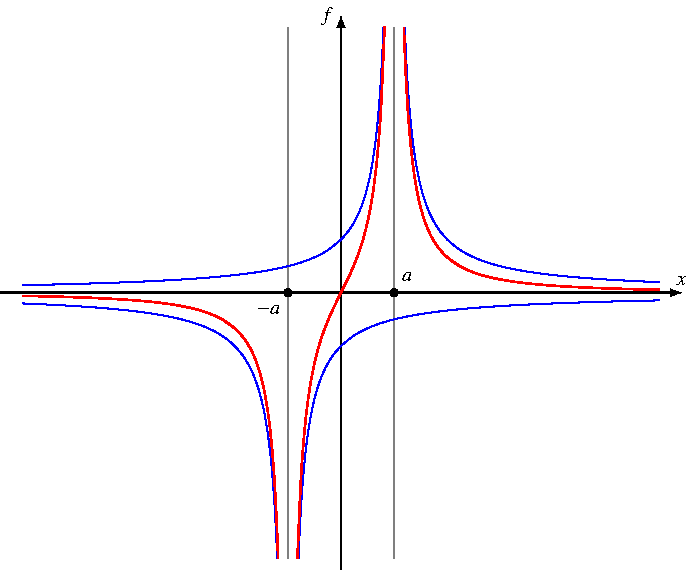
\includegraphics{chapters/tikz/dipol1.pdf}
\caption{Potential
\eqref{skript:multipol:1dipol}
des eindimensionalen Dipols
\label{skript:multipol:figure:1dim}}
\end{figure}

Zwei entgegengesetzte Punktladungen an den Stellen $x=\pm a$ haben also
das Potential
\begin{equation}
f_2(x)
=
\frac1{4\pi\varepsilon_0}\frac{q}{|x+a|}
-
\frac1{4\pi\varepsilon_0}\frac{q}{|x-a|}
=
\frac{q}{4\pi\varepsilon_0}\biggl( \frac1{|x+a|} - \frac1{|x-a|} \biggr).
\label{skript:multipol:1dipol}
\end{equation}
(Abbildung~\ref{skript:multipol:figure:1dim}).
Wir sind nur an den Funktionswerten interessiert für $x$-Werte, die
wesentlich grösser sind als $a$, als in grosser Entfernung von
den Ladungen.
Wir interessieren uns also für $x$-Werte so, dass $x/a$ sehr gross ist,
oder umgekehrt, dass $a/x$ sehr klein ist.

Wenn man in Gleichung \eqref{skript:multipol:1dipol} das Vorzeichen
von $x$ kehrt, dann ändert das Vorzeichen von $f$, also $f_2(-x)=-f_2(x)$,
$f$ ist eine ungerade Funktion.
Es reicht daher, die Funktion $f_2(x)$ für $x\gg a$ zu untersuchen,
für Werte $x\ll -a$ verwendet man $f_2(x)=-f_2(-x)$.

Verwenden wir die Gleichung \eqref{skript:multipol:1abfall} in $f_2(x)$,
erhalten wir
\begin{align}
f_2(x)
&=
\frac{q}{4\pi\varepsilon_0}\biggl(\frac1{x+a}-\frac1{x-a}\biggr)
=
\frac{q}{4\pi\varepsilon_0}\cdot\frac1x\cdot\biggl(
\frac1{1+\frac{a\mathstrut}{x}}
-
\frac1{1-\frac{a\mathstrut}{x}}
\biggr)
=
\frac{q}{4\pi\varepsilon_0}\cdot\frac1x\cdot
\frac{\bigl(1-\frac{a}{x}\bigr)-\bigl(1+\frac{a}{x}\bigr)}{1-\frac{a^2}{x^2}}
\notag
\\
&=
\frac{q}{4\pi\varepsilon_0}\cdot\frac1x\cdot
\biggl(-\frac{2a}{x}\biggr)
\cdot
\frac1{1-\frac{a^2}{x^2}}
=
-\frac{qa}{2\pi\varepsilon_0}\cdot\frac1{x^2}\cdot\frac{1}{1-\frac{a^2}{x^2}}.
\label{skript:multipol:2abfall}
\end{align}
Der Term $a^2/x^2$ im Nenner des letzten Faktors ist für grosse Werte von
$x$ wieder unbedeutend.
Der dominierende Term für das Verhalten für grosse $x$ ist daher der
Faktor $1/x^2$.

Ein weiterer interessanter Aspekt der Formel~\eqref{skript:multipol:2abfall}
ist, dass nur noch die Kombination $qa$ von Ladung und Abstand der Ladungen
vorkommt.
Das Fernfeld für grosse Werte von $x$ ändert also nicht, wenn wir $a$
kleiner machen, aber gleichzeitig $q$ vergrössern, so dass das Produkt
$qa$ konstant bleibt.
Man nennt $d=2qa$ das {\em Dipolmoment} der beiden Ladungen.
\index{Dipolmoment}%
Der Dipol mit Dipolmoment $d$ hat daher für grosse $x$ das Potential
\[
f_2(x)
=
-\frac{d}{4\pi\varepsilon_0}\cdot \frac1{x^2}\cdot \frac1{1-\frac{a^2}{x^2}}
\simeq
-\frac{d}{4\pi\varepsilon_0}\cdot \frac1{x^2}.
\]

Aus diesen Beispielen können wir die Vermutung ableiten, dass weitere
Terme die Form
\[
-\frac{b}{4\pi\varepsilon_0}\cdot\frac1{x^k}
\]
haben müssen, wobei $b$ die Dimension einer Ladung mal die $(k-1)$-te
Potenz einer Distanz sein muss.

\subsection{Stetige Ladungsverteilung%
\label{skript:multipol:section:stetigeladungsverteilung}}
Betrachten wir jetzt statt zweier Ladungen eine beliebige 
Ladungsverteilung $\varrho(x)$, die aber ausserhalb des Intervalls
$[-a,a]$ verschwindet, also $\varrho(x)=0$ für $|x|>a$.
Stellen wir uns die Ladungsverteilung als eine Überlagerung einzelner
Ladungen an Positionen $y\in[-a,a]$ vor, dann k"onnen wir das
Potential des Fernfeldes sofort aus~\eqref{skript:multipol:2abfall}
ableiten:
\[
f(x)
\simeq
\frac{1}{4\pi\varepsilon_0}
\underbrace{\int_{-a}^a \varrho(y)\,dy }_{\displaystyle =q}
\frac1x
+
\frac{1}{4\pi\varepsilon_0}
\underbrace{\int_{-a}^a \varrho(y)y \,dy}_{\displaystyle =d}
\frac1{x^2}
+
\dots
=
\frac{1}{4\pi\varepsilon_0}
\sum_{k=0}^\infty
\frac1{x^{k+1}} 
\int_{-a}^a\varrho(y)y^k\,dy
\]
Der erste Term ist das Potential einer Punktladung $q$ im Ursprung, der
zweite das Dipolpotential eines Dipols mit Dipolmoment $d$.
Wir nennen den ersten Term auch den {\em Monopolterm}.
\index{Monopol}%

Die Integrale 
\[
b_k=\int_{-a}^a \varrho(y)\,y^k\,dy
\]
heissen die {\em $k$-ten Momente} der Verteilung $\varrho$.
\index{Moment einer Funktion}%
Die $k$-ten Momente bestimmen also die Darstellung des Fernfeldes
einer Ladungsverteilung vollständig durch die Formel
\[
f(x)
\simeq
\frac1{4\pi\varepsilon_0}\sum_{k=0}^\infty b_k\frac{1}{x^{k+1}}.
\]
Wir behaupten nicht, dass die Summe auf der rechten Seite mit dem Potential
der Ladungsverteilung übereinstimmen.
Vielmehr ist die Summe eine Zerlegung des Feldes
nach ``Abfalls-Geschwindigkeit'' in grosser Entfernung,
ganz ähnlich wie die Fourier-Koeffizienten
\[
a_k=\frac1{2\pi}\int_{-\pi}^\pi f(x)\cos kx\,dx
\qquad\text{und}\qquad
b_k=\frac1{2\pi}\int_{-\pi}^\pi f(x)\sin kx\,dx
\]
einer im Intervall $[-\pi,\pi]$ definierten Funktion $f(x)$
eine Analyse nach Frequenzen bilden.
Die Fourierreihe
\[
\frac{a_0}2+\sum_{k=1}^\infty (a_k\cos kx+b_k\sin kx)
\]
ist eine periodische Funktion auf der ganzen reellen Achse, die
im Intervall $[-\pi,\pi]$ mit der ursprünglichen Funktion übereinstimmt.
Die Summe stimmt also mit der ursprünglichen Funktion nicht direkt
überein.

\subsection{Geometrische Reihe%
\label{skript:multipol:section:geometrischereihe}}
Bei der Analyse sowohl einer um $a$ verschobenen Einzelladung sowie auch
des Dipols aus zwei Ladungen bei $\pm a$ haben wir am Schluss Terme der
Form
\[
\frac1{1-\displaystyle\frac{a}{x}}
\qquad\text{bzw.}\qquad
\frac1{1-\displaystyle\frac{a^2}{x^2}}
\]
vernachlässigt.
Wir suchen nach einer Möglichkeit, diese Terme exakt zu berücksichtigen,
und trotzdem nur eine einfache Potenzreihe zu bekommen.

In der Analysis lernt man, die Summe der {\em geometrische Reihe}
\index{geometrische Reihe}
\index{Reihe, geometrische}
\[
s=a+aq+aq^2+\dots + aq^n
\]
zu berechnen.
Dazu bildet man $qs - s$ und findet
\begin{align*}
qs-s
=
s(q-1)
&=
q(a+aq+aq^2+\dots + aq^n)-(a+aq+aq^2+\dots + aq^n)
\\
&=
a(q+q^2+q^3\dots+q^{n+1}-1-q-q^2-\dots-q^n)
=
a(q^{n+1}-1).
\end{align*}
Daraus schliesst man
\[
s=a\frac{q^{n+1}-1}{q-1}.
\]
Wenn $|q|<1$ ist, dann kann man die Summe für beliebig grosse $n$ bilden,
und bekommt im Grenzwert $n\to\infty$
\begin{equation}
\sum_{k=0}^\infty aq^k = a\frac{1}{1-q}.
\label{skript:multipol:geom}
\end{equation}
Wir können diese Formel verwenden, um die bisher vernachlässigten Terme
exakt wiederzugeben:
\begin{align*}
\frac{1}{1-\displaystyle\frac{a}{x}}
&=
1+\frac{a}{x}+\frac{a^2}{x^2}+\dots
=
\sum_{k=0}^\infty \frac{a^k}{x^k},
\\
\frac{1}{1-\displaystyle\frac{a^2}{x^2}}
&=
1+\frac{a^2}{x^2}+\frac{a^4}{x^4}+\dots
=
\sum_{k=0}^\infty \frac{a^{2k}}{x^{2k}},
\\
\frac{1}{1+\displaystyle\frac{a^2}{x^2}}
&=
1-\frac{a^2}{x^2}+\frac{a^4}{x^4}-\dots
=
\sum_{k=0}^\infty (-1)^k\frac{a^{2k}}{x^{2k}}.
\end{align*}
Die letzte Formel erhält man, indem man in \eqref{skript:multipol:geom}
$q$ durch $-q$ ersetzt und dann $q=a^2/x^2$ einsetzt.

Wir wenden dies jetzt wieder auf eine Ladungsverteilung
$\varrho(y)$ im Intervall $[-a,a]$ an.
Das Potential einer Einheitsladung an der Stelle $y$ ist
\[
f_y(x)
=
\frac1{4\pi\varepsilon_0}\cdot \frac{1}{x}\cdot\frac{1}{1-\displaystyle\frac{x}{y}}
=
\frac1{4\pi\varepsilon_0}\cdot \frac{1}{x}
\sum_{k=0}^\infty \frac{y^k}{x^k}
=
\frac1{4\pi\varepsilon_0}
\sum_{k=0}^\infty \frac{y^k}{x^{k+1}}.
\]
Durch Überlagerung mit Hilfe der Ladungsverteilung $\varrho(y)$ 
erhalten wir die exakte Formel für das Potential der Ladungsverteilung
\begin{equation}
f(x)
=
\int_{-a}^af_y(x)\,dy
=
\frac{1}{4\pi\varepsilon_0}
\sum_{k=0}^\infty
\frac{1}{x^{k+1}}
\underbrace{\int_{-a}^a\varrho(y)\,y^k\,dy}_{\displaystyle =b_k}
\cdot
=
\frac{1}{4\pi\varepsilon_0}
\sum_{k=0}^\infty b_k
\frac{1}{x^{k+1}},
\label{skript:multipol:reiheexakte}
\end{equation}
wobei die $b_k$ wieder die $k$-ten Momente der Ladungsverteilung
$\varrho(y)$ sind.

Es stellt sich also heraus, dass die in
Abschnitt~\ref{skript:multipol:section:stetigeladungsverteilung}
erratene Entwicklung sogar eine exakte Darstellung ist.
Bricht man die Reihe~\eqref{skript:multipol:reiheexakte} nach zwei
Termen ab, erhält man die Monopol- und Dipol-Komponenten des
Fernfeldes.
Alle späteren Terme der Reihe beschreiben die feineren Strukturen
der Ladungsverteilung und fallen so rasch mit der Entfernung ab,
dass sie für grosse Entfernungen vernachlässigt werde können.

Bei der Diskussion des Dipolmoments haben wir festgestellt, dass das
Fernfeld nur von der Grösse $d=2aq$ abhängt.
Verkleinert man den Abstand $a$ und vergrössert man gleichzeitig $q$,
so dass $d$ gleich gross bleibt, dann ändert sich das Fernfeld nicht.
Die Reihe~\eqref{skript:multipol:reiheexakte} verallgemeinert diese
Aussage auf eine beliebige Ladungsverteilung.
Ändern wir die Ladungsverteilung, achten aber darauf, dass die
$k$-ten Momente gleich bleiben, dann ändert sich das ausserhalb der
Ladungsverteilung messbare Potential nicht.
Die $k$-ten Momente beschreiben das ausserhalb der Ladungsverteilung
messbare Potential vollständig.

\subsection{Taylor-Reihe und Laurent-Reihe}
Im vorangegangenen Abschnitt haben wir gesehen, dass für grosse Werte von
$x$ die zur Diskussion stehende Funktion im Wesentlichen als Reihe
der inverse Potenzen $1/x^k$ beschrieben werden kann, also
\[
f(x)=\sum_{k=0}^\infty b_k\frac1{x^{k+1}}.
\]
Schreiben wir $z=1/x$, dann wird daraus eine gewöhnliche Potenzreihe
\[
\tilde f(z)=\sum_{k=0}^\infty b_k z^{k+1}.
\]
Wenn die Funktion $z\mapsto \tilde f(z)$ differenzierbar ist, dann
können die Koeffizienten $b_k$ aus den Ableitungen der Funktion
$\tilde f$ gefunden
\begin{equation}
b_k=\frac{\tilde f^{(k)}(0)}{k!}
\qquad\Rightarrow\qquad
\tilde f(z)
=
\sum_{k=0}^\infty \frac{\tilde f^{(k)}(0)}{k!}z^k.
\end{equation}
Wir können dies betrachten als die Taylorreihe der Funktion $f$ um
den Punkt $\infty$.
\index{Taylor-Reihe}

Man nennt eine Reihe der Form
\[
\sum_{k=-\infty}^{\infty} b_k(z-a)^k
\]
eine {\em Laurent-Reihe} im Punkt $a$.
\index{Laurent-Reihe}
Offensichtlich ist der Funktionswert in $z=a$ nicht definiert und
oft wird die Reihe auch in einer Umgebung von $a$ nicht konvergieren.
Sie ist aber hervorragend dazu geeignet, das Verhalten einer Funktion
zu analysieren, die im Punkt $a$ eine Singularität aufweist.
Besonders nützlich ist sie dann, wenn $z$ komplex ist, denn man
kann zeigen, dass jede komplex differenzierbare Funktion mit einer
Singularität im Punkt $a$ in einer Umgebung von $a$ als Laurent-Reihe
dargestellt werden kann \cite{skript:mathsemdgl}.

Wenn wir also in der Lage sind, das eindimensionale Beispiel auf höhere
Dimensionen zu verallgemeinern, dann haben wir auch eine Verallgemeinerung
der Idee einer Taylorreihe um den Punkt $\infty$ auf höhere Dimensionen
gefunden.









%
% m-multipole.tex
%
% (c) 2017 Prof Dr Andreas Müller, Hochschule Rapperswil
%
\section{Multipolentwicklung}
\rhead{Multipolentwicklung}
In Abschnitt~\ref{skript:multipol:1dimbeispiel} haben wir ein
eindimensionales Beispiel untersucht, und mussten nach dem Potential
eines Dipols mit Vermutungen operieren, wie die weiteren Terme aussehen
müssten.
In diesem Abschnitt arbeiten wir in drei Dimensionen, und sind daher
in der Lage, kompliziertere Konfigurationen von Ladungen zu
konstruieren, und damit auch die späteren Terme der Entwicklung
genauer zu untersuchen.


\subsection{Dipol}
\begin{figure}
\centering
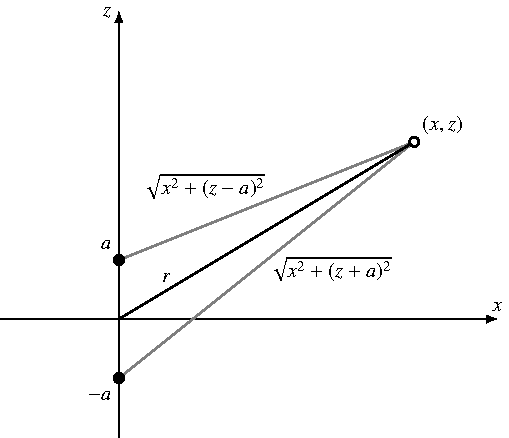
\includegraphics{chapters/tikz/dipol2.pdf}
\caption{Berechnung des Dipolpotentials 
\eqref{skript:multipol:dipol} in der $x$-$z$-Ebene
\label{skript:multipol:figure:dipol}}
\end{figure}
Wir betrachten das Feld eines Paares von entgegengesetzen Ladungen
in den Punkten $(0,0,a)$ und $(0,0,-a)$
(Abbildung~\ref{skript:multipol:figure:dipol}).
Der Einfachheit halber führen wir die Rechnung zunächst nur
in der $x$-$z$-Ebene durchführen und erst später mit Hilfe einer
vektoriellen Schreibweise auf drei Dimensionen erweitern.

Entlang der $z$-Achse kennen wir das Potential bereits aus
dem vorangegangenen Abschnitt.
Entlang der $x$-Achse verschwindet das Potential, denn die Punkte
auf der $x$-Achse sind von den beiden Ladungn gleich weit entfernt,
haben als entgegengesetzt gleiches Potential bezüglich beiden Ladungen
und damit totales Potential 0.

Wir betrachten jetzt das Potential im Punkt $(x,z)$, es ist
\begin{equation}
f(x,z)
=
\frac{q}{4\pi\varepsilon_0}
\biggl(
\frac{1}{\sqrt{x^2 + (z-a)^2}}
-
\frac{1}{\sqrt{x^2 + (z+a)^2}}
\biggr)
\label{skript:multipol:dipol}
\end{equation}
Offenbar müssen wir die Nenner besser verstehen, um diese Summe 
umformen zu können.
Speziell müssen wir die Abhängigkeit von der Entfernung
$r=\sqrt{x^2+z^2}$ vom Nullpunkt
und die Richtungsabhängigkeit voneinander trennen.
Dazu betrachten wir nur einen einzelnen Term
\[
\frac{1}{\sqrt{x^2+(z\pm a)^2}}
=
\frac{1}{\sqrt{x^2+z^2\pm 2az+a^2}}
=
\frac{1}{\sqrt{x^2+z^2}} \cdot \frac{1}{\sqrt{1+\frac{\pm 2az+a^2}{x^2+z^2}}}
=
\frac{1}{r} \cdot \frac{1}{\sqrt{1+\frac{\pm 2az+a^2}{r^2}}}
\]
Für grosse Werte von $r$ verschwindet der zweite Term in der Wurzel,
in erster Näherung verhält sich die Funktion daher wie $1/r$.
In den zwei Termen von \eqref{skript:multipol:dipol} hebt sich dieses
Verhalten jedoch weg, um die Funktion $f(x,z)$ zu verstehen, ist es
daher nötig, die Abweichungen von $1/r$ genauer zu verstehen.

Offenbar müssen wir Terme der Form
\begin{equation}
\frac{1}{\sqrt{1+t}}
=
(1+t)^{-\frac12}
\label{skript:multipol:wurzel}
\end{equation}
ausrechnen können, wobei wir später $t=(\pm2az+a^2)/r^2$ setzen wollen.

\subsubsection{Binomialreihe}
Die Taylor-Reihe der Funktion \eqref{skript:multipol:wurzel}
kann für eine allgemeinere für die Funktionen
\begin{equation}
g(t)=(1+t)^\alpha
\end{equation}
mit beliebigem Exponenten bestimmt werden.

Dazu müssen die Ableitungen der Funktion $g(t)$ bestimmt werden
\begin{align*}
g'(t)
&=
\alpha(1+t)^{\alpha-1}
&
g'(0)&=\alpha
\\
g''(t)
&=
\alpha(\alpha-1)(1+t)^{\alpha-2}
&
g''(0)&=\alpha(\alpha-1)
\\
&\;\vdots
\\
g^{(n)}(t)
&=
\alpha(\alpha-1)(\alpha-2)\dots(\alpha-n+1) (1+t)^{\alpha -n}
&
g^{(n)}(0)&=\alpha(\alpha-1)(\alpha-2)\dots(\alpha -n +1)
\end{align*}
Der Term zur Potenz $n$ in der Taylor-Reihe von $g(t)$ ist
\[
\frac{\alpha(\alpha-1)(\alpha-2)\dots(\alpha-n+1)}{n!} t^n
\]
Wäre $\alpha$ eine ganze Zahl, dann sähe der Bruch
genau so aus wie der Binomialkoeffizient $\binom{\alpha}{k}$.
In Erweiterung der üblichen Definition des Binomialkoeffizienten
schreibt man auch für nicht ganzzahlige $\alpha$
\[
\binom{\alpha}{n}
=
\frac{\alpha(\alpha-1)(\alpha-2)\dots(\alpha-n+1)}{n!}.
\]
Mit dieser Schreibweise bekommen wir die Taylorreihe
\[
(1+t)^\alpha=\sum_{k=1}^\infty \binom{\alpha}{k} t^k
\]
für die Funktion $(1+t)^\alpha$.
Sie heisst die {\em Binomialreihe} und ist konvergent für $|t|<1$.
\index{Binomialreihe}

\subsubsection{Der Fall $\alpha=-\frac12$}
Wir betrachten die Binomialreihe für den Fall $\alpha=-\frac12$.
Der Term zur Potenz $n$ ist
\begin{equation}
\frac{
\bigl(-\frac12\bigr)
\bigl(-\frac32\bigr)
\bigl(-\frac52\bigr)
\cdots
\bigl(-\frac{2n+1}2\bigr)}{n!} t^n
=
(-1)^n \frac{1\cdot 3\cdot 5 \cdots (2n + 1)}{2^n\cdot 1\cdot 2\cdot 3\cdots n}
=
(-1)^n \frac{1\cdot 3\cdot 5 \cdots (2n+1)}{2\cdot 4\cdot 6\cdots (2n)}
\label{skript:multipol:koeffizienten}
\end{equation}
Die zugehörige Potenzreihe ist daher
\[
\frac1{\sqrt{1+t}}
=
1-\frac12t+\frac3{8}t^2-\frac{15}{48}t^3+\frac{105}{354}t^4-\dots
\]
%deren Koeffizienten man auch faktorisieren und damit etwas
%Für 
%\[
%\frac1{\sqrt{1+t}}
%=
%1-\frac12 t
%+ \frac12\frac32\frac12 t^2
%- \frac 12\frac32\frac 52\frac1{3!} t^3
%+ \frac 12\frac32\frac 52\frac72\frac1{4!} t^4
%- \frac 12\frac32\frac 52\frac72\frac92\frac1{5!} t^4
%+\dots
%\]

Wir verwenden die binomische Reihe jetzt, um das Dipolpotential
zu berechnen.
Setzen wir 
\[
t=\frac{\pm 2az+a^2}{r^2}
\]
in der binomischen Reihe, erhalten wir
\[
\frac{1}{\sqrt{1+\frac{\pm 2az+a^2}{r^2}}}
=
1-\frac12\frac{\pm 2az+a^2}{r^2}
+
\frac38 \biggl(\frac{\pm 2az+a^2}{r^2}\biggr)^2+\dots
\]
und für das Dipolpotential $f(x,z)$ gemäss \eqref{skript:multipol:wurzel}
\begin{align*}
f(x,z)
&=
\frac{q}{4\pi\varepsilon_0 r}
\biggl(
1-\frac12\frac{-2az+a^2}{r^2} + \frac38 \biggl(\frac{-2az+a^2}{r^2}\biggr)^2+\dots
\biggr)
\\
&\qquad
-
\frac{q}{4\pi\varepsilon_0 r}
\biggl(
1-\frac12\frac{2az+a^2}{r^2} + \frac38 \biggl(\frac{2az+a^2}{r^2}\biggr)^2+\dots
\biggr)
\\
&=
-\frac{2aq}{4\pi\varepsilon_0r^3}z + \dots
\end{align*}
Wenn die beiden Ladungen näher zusammen rücken, wenn also $a\to 0$,
dann verschwindet das Potential.
Wenn wir das Potential weiterhin sehen wollen, müssen wir den Betrag
der Ladungen entsprechend vergrössern.
Wenn wir $a$ gegen $0$ gehen lassen, lassen wir gleichzeit die Ladung
$q$ grösser werden, so dass das Produkt $d=2qa$ gleich bleibt.
Mit dieser Konvention wird das Dipolpotential
\begin{equation}
f(x,z) = -\frac{d}{4\pi\varepsilon_0 r^2}\frac{z}{r}+\dots
\label{skript:multipol:dipolpotential}
\end{equation}
Darin haben wir statt $z$ den Bruch $z/r$ abgespalten, da dieser
eintlang eines vom Nullpunkt ausgehenden Strahls vom Zentrum jeweils
konstant ist.
Wir haben daher das Potential in Faktoren aufgeteilt, die verschiedene
geometrische Bedeutung haben.
Der Faktor $1/r^2$ beschreibt, wie das Potential mit der Entfernung abnimmt.
Der Faktor $z/r$ beschreibt, wie das Potential von der Richtung im
Bezug auf die $z$-Achse abhängt.
Die übrigen Faktoren beschreiben, wie das Potential aus dem Dipolmoment
$d$ erzeugt wird.

\subsubsection{Vektorschreibweise}
Das Dipolpotential kann besonders elegant geschrieben werden, wenn
wir das skalare Dipolmoment $d$ durch einen Vektor $\vec{d}$ ersetzen.
In der Formel~\eqref{skript:multipol:dipolpotential}
für das Dipolpotential brauchen wir die $z$-Koordinate
des Punktes.
Diese können wir als das Skalarprodukt mit dem Standardbasisvektor
in $z$-Richtung bekomen.
Wenn wir also
\[
\vec{d}=\begin{pmatrix}0\\0\\d\end{pmatrix}
\]
setzen, dann können wir das Dipolpotential vektoriell als
\begin{equation*}
f(\vec{r})
=
-
\frac{1}{4\pi\varepsilon_0r^2} \frac{\vec{d}\cdot\vec{r}}{r}
\end{equation*}
geschrieben werden.
In dieser Form ist das Dipolpotential für jede beliebige Orientierung
des Dipolmomentes verwendbar.

Der Dipolterm geht für $r\to\infty$ wie $r^{-2}$ gegen $0$, also
deutlich schneller als das Potential einer Punktladung.

\subsection{Quadrupol}
Wie in der eindimensionalen Situation vermuten wir, dass sich
das Potential komplizierterer Ladungsverteilungen ebenfalls durch
eine Reihe darstellen lässt, deren nächster Term von der Form
\begin{equation}
\frac1{4\pi\varepsilon_0}\cdot\frac{1}{r^5} p(\vec{r},\vec{r})
\label{skript:multipol:quadropolterm}
\end{equation}
sein muss.
Darin ist $p$ ein Ausdruck, der in beiden Argumenten linear ist.

Schreiben wir die Koordinaten als $(x_1,x_2,x_3)$, dann wird 
sich $p$ in der Form
\[
\sum_{k,l=1}^3 Q_{kl}x_kx_l
\]
schreiben lassen.
Allerdings kann nicht jede beliebige Matrix zugelassen werden, 
da ja nur die Abweichungen vom Dipolmoment erfasst werden sollen.
Nimmt man für $Q$ die Einheitsmatrix, dann erhält man einfach nur
\[
\sum_{k,l=1}^3 Q_{kl}x_kx_l=\sum_{i=1}^3 x_i^2 = \vec{r}\cdot\vec{r}=r^2,
\]
der Quadrupol-Term wird also 
\[
\frac1{4\pi\varepsilon_0}\cdot\frac{1}{r^3},
\]
was keine Richtungsabhängigkeit mehr enthält und wir daher erwarten
würden, dass diese Art von Abhängigkeit bereits im ersten Term 
enthalten war.
Man kann dies zum Beispiel dadurch erreichen, dass die Matrix $Q$ 
verschwindende Spur haben soll, also $\operatorname{Spur}Q=0$.

Die defaillierte Berechnung des Quadrupolanteils ist etwas mühsam,
wir geben hier nur das Resultat an.
Man findet
\[
Q_{kl}
=
\int_{\mathbb R^3}
\varrho(\vec{r}) \cdot (3x_kx_l-r^2\delta_{kl})
\,dx_1\,dx_2\,dx_3.
\]
Das Wachstum des Quadrupolterms~\eqref{skript:multipol:quadropolterm}
ist also von der Ordnung $r^{-3}$.
Auch dieser Term geht wieder einer Potenz schneller gegen $0$ als der
Dipolterm.

\subsection{Höhere Multipole}
Die Entwicklung Entwicklung in Dipol und Quadrupol lässt sich noch
weiter führen.
Dabei werden sukzessive Terme entstehen, die immer schneller gegen $0$
gehen, für grosse Entfernung vom Nullpunkt also immer weniger von
Bedeutung sein werden.
Die Darstellung dieser höheren Multipole wird allerdings zunehmen
schwierig. 
Der nächste Term nach dem Quadrupolterm müsste die Form
\begin{equation}
\frac1{4\pi\varepsilon_0}\frac{p(\vec r)}{r^7}
\label{skript:multipol:7ord}
\end{equation}
haben, wobei der Zähler $p(\vec r)$ eine Grösse dritter Ordnung in
den Koordinaten sein müsste.
Er wird also durch ein homogenes Polynom dritten Grades in den Koordinaten
$x$, $y$ und $z$ beschrieben.
Der Term~\eqref{skript:multipol:7ord} geht wie $r^{-4}$ gegen Null,
also erneut eine Potenz schneller als der Quadrupolterm.

\section{Zusammenfassung}
Allen Termen der Multipolentwicklung
\[
f(\vec r)
=
\frac{1}{4\pi\varepsilon 0}
\biggl(
q
\frac{1}{r}
+
\frac{1}{r^2} \frac{\vec{d}\cdot\vec{r}}{r}
+
\frac{1}{r^3} \sum_{k,l}Q_{kl}\frac{x_k}{r}\frac{x_l}{r}
+
\frac{1}{r^4} \sum_{k,l,j}Q_{klj}\frac{x_k}{r}\frac{x_l}{r}\frac{x_j}{r}
+
\dots
\biggr)
\]
ist gemeinsam, dass sie die Abhängigkeit des Potentials in einen
aus physikalischen Gründen plausiblen radialen Teil der Form $r^{-k}$
und einen richtungsabhängigen Teil aufteilen.
Die reine Richtungsabhängigkeit kann dadurch ausgedrückt werden, dass
er nur von den Quotienten $x/r$, $y/r$ und $z/r$ abhängt.

TODO:
\begin{itemize}
\item Potentiallinien-Plots für Dipol- und Quadrupolfeld
\item 3D-Plot von Dipolmoment und evtl Quadropolfeld
\end{itemize}









%
% m-kugelfunktionen.tex
%
% (c) 2017 Prof Dr Andreas Müller, Hochschule Rapperswil
%
\chapter{Kugelfunktionen%
\label{skript:chapter:kugelfunktionen}}
\lhead{Kugelfunktionen}
\rhead{}
Im vorangegangenen Kapitel~\ref{skript:chapter:multipol} haben wir
die Multipol-Entwicklung kennengelernt. 
Die wesentliche Erkenntnis dabei war, dass wir eine Funktion immer zerlegen
können in eine Summe von Termen der Form
\[
\frac{p(x,y,z)}{r^k},
\]
wobei $p(x,y,z)$ ein homogenes Polynom in den Koordinaten $x$, $y$ und
$z$ war.
Nehmen wir an, dass das Polynom homogen vom Grad $l$ ist, dann kann man dies
auch schreiben
\[
\frac{p(x,y,z)}{r^k}
=
p\biggl(\frac{x}{r},\frac{y}{r},\frac{z}{r}\biggr)\frac1{r^{k-l}}.
\]
Die Brüche $x/r$, $y/r$ und $z/r$ sind konstant entlang eines vom
Nullpunkt ausgehenden Strahls, das Polynom 
\[
p\biggl(\frac{x}{r},\frac{y}{r},\frac{z}{r}\biggr)
\]
ist also eine Funktion, die nur von der Richtung des Strahls
abhängt.
Das Potential lässt sich also schreiben als eine Summe von Termen,
die Produkte sind einer Funktion, die nur von der Richtung abhängig
ist, und einer Funktion, die die Entfernungsabhängigkeit vom Nullpunkt
ausdrückt.

Daraus ergibt sich dann eine Familie von Funktionen auf der Kugeloberfläche,
die also nur von $\vartheta$ und $\varphi$ abhängen.
Diese Funktionen haben eine grosse Zahl von Anwendungen:

\begin{enumerate}
\item
Wie schon in Kapitel~\ref{chapter:multipol} gezeigt, erlaubt 
die Multipolentwicklung elektromagnetische Felder in grosser
Entfernung von der Quelle zu beschreiben.
Man spricht auch vom Nah- und Fernfeld.
\item
Jede Funktion auf einer Kugeloberfläche kann zerlegt werden in eine
Summe von Funktionen ganz ähnlich wie eine periodische Funktion
zerlegt werden kann in eine Summe von Sinus- und Kosinus-Funktionen.
Dies wird zum Beispiel für die Analyse des Gravitationsfeldes von
Erde und Mond verwendet, oder für die Abweichung der Erdoberfläche
von der Form eines Rotationsellipsoids.
\item
Der kosmische Mikrowellenhintergrund kann mit Kugelfunktionen analysiert
werden.
Diese Analyse zeigt, dass das Universum flach ist und damit dass der
gesamte Energieinhalt des Universums $0$ ist.
In Kapitel~\ref{chapter:cmb} wird gezeigt, wie eine solche Analyse
durchgeführt werden kann.
\end{enumerate}

In diesem Kapitel wollen wir zunächst zeigen, dass man die klassische
Fourier-Theorie genau auf die gleiche Art betrachten kann.
Eine Funktion in der Ebene lässt sich immer beschreiben als eine Summe
von Produkten einer Funktion, die die Richtungsabhängigkeit ausdrückt,
und einer Funktion, die die Entfernungsabhängigkeit codiert.

Die Wahl einer Basis solcher Funktionen ist jedoch nicht eindeutig.
Wenn wir zusätzlich verlangen, dass die Funktionen im Sinne eines noch
zu definierenden Skalarproduktes orthonormiert sind, dann ist die
Berechnung der entsprechenden Koeffizienten besonders einfach und
führt auf die klassische Fourier-Theorie.

Im letzten Abschnitt wollen wir dann zeigen, dass dasselbe Programm
auch im $\mathbb R^3$ durchführbar ist, und in diesem Fall auf die
Kugelfunktionen führt.

\section{Approximation mit Polynomen
\label{skript:section:approximation}}
\rhead{Approximation mit Polynomen}
In Kapitel~\ref{skript:chapter:multipol} haben wir gelernt, dass es
sinnvoll sein kann, Funktionen in zwei oder drei Dimensionen zu 
approximieren als Summe von Funktionen, die sich faktorisieren lassen
in einen Teil, der nur vom Radius $r$ abhängt, und einen Faktor,
der eine Funktion auf einem Kreis oder auf einer Kugeloberfläche
ist, parametrisiert durch den Polarwinkel $\varphi$ im Falle des
Kreises oder der geographischen Breite $\vartheta$ und der geographsichen
Länge $\varphi$ im Falle der Kugel.
Für den Fall des Potentials haben wir in der Form der Multipolentwicklung
eine solche Darstellung gefunden.
Es stellt sich damit aber automatisch die Frage, ob eine solche
Darstellung für beliebige Funktionen überhaupt möglich ist.

\begin{satz}[Weierstrass]
\label{skript:satz:weierstrass}
Sei $X\subset\mathbb R^n$ eine abgeschlossene und beschränkte Teilmenge.
Dann lässt sich jede stetige Funktion $X\to\mathbb R$ beliebige genau durch
Polynom $p(x_1,\dots,x_n)$, $x_i\in\mathbb R$
approximieren.
Speziell gibt es für jede Zahl $\varepsilon>0$ ein Polynom $p(x_1,\dots,x_n)$
derart, dass
\[
|f(x_1,\dots,x_n)- p(x_1,\dots,x_n)|<\varepsilon
\]
für alle $(x_1,\dots,x_n)\in X$.
\end{satz}
\index{Weierstrasse, Satz von}%

Dieser Satz besagt, dass sich jede stetige Funktion beliebig genau durch
Polynome approximieren lässt. 
Mit einem Computer lassen sich zunächst nur die Grundoperationen ausführen.
Diese genügen jedoch, um beliebige Polynome berechnen zu können.
Der Satz von Weierstrass garantiert, dass jede denkbare stetige Funktion
auf einem Computer mit beliebiger Genauigkeit berechnet werden kann
und rechtfertigt damit in einem gewissen Sinne die numerische Mathematik.

\subsubsection{Der Satz von Stone-Weierstrass}
Der Satz von Weierstrass ist ein Spezialfall eines wesentlich allgemeineren
Resultates.
Die in Satz~\ref{skript:satz:weierstrass} verwendeten Polynome entstehen
durch algebraische Operationen aus den Funktionen
\[
f_1(x_1,\dots,x_n)=x_1,\qquad
f_2(x_1,\dots,x_n)=x_2,\dots
f_n(x_1,\dots,x_n)=x_n.
\]
Diese Funktionen haben die Eigenschaft, dass es für zwei verschiedene
Punkte im Gebiet $X$ immer eine Funktion gibt, mit der diese Punkte
unterschieden werden können.
Denn da zwei verschiedene Punkte auch mindestens eine verschiedene
Koordinate haben, wird die zugehörige Koordinatenfunktion die beiden
Punkte unterschieden können.
Wir fassen diese Eigenschaft in eine Definition
\begin{definition}
Eine Familie von Funktionen $f_i\colon X\to \mathbb R$ {\em trennt Punkte},
wenn es zu jedem Paar von Punkten $p,q\in X$ eine Funktion $f_j$ gibt derart,
dass $f_j(p)\ne f_j(q)$.
\end{definition}
\index{trennt Punkte}%

Wir bezeichnen die Menge der stetigen Funktionen $X\to\mathbb R$
mit $C(X,\mathbb R)$ oder $C(X)$, wenn der Wertebereich klar ist.
In der Menge $C(X)$ der stetigen Funktionen $f\colon X\to\mathbb R$ sind
Addition, Subtraktion, Multiplikation von Funktionen und Multiplikation
von Funktionen mit einer Zahl definiert.
Man sagt, die Menge $C(X)$ sei eine Algebra.
\index{Algebra}%
Ausserdem gibt es in $C(X)$ einen Begriff für die Norm einer Funktion,
wir setzen
\begin{equation}
\| f\| = \sup_{x\in X}|f(x)|.
\label{skript:multipol:supremum-norm}
\end{equation}
\index{Supremum-Norm}%
Damit erhalten wir auch einen Begriff für den Abstand zweier Funktionen:
\[
\|f-g\| = \sup_{x\in X}|f(x)-g(x)|.
\]
Zwei Funktionen haben Abstand $< \varepsilon$, wenn
\[
|f(x)-g(x)| < \varepsilon
\]
gilt für beliebige $x\in X$.
Mit diese Begriff kann man jetzt auch die Konvergenz von Folgen von
Funktionen in $C(X)$ definieren.

Eine Folge $f_n$ von Funktionen auf $X$ heisst eine {\em Cauchy-Folge}, wenn 
\index{Cauchy-Folge}%
für grosse $n$ die Funktionen nicht weit auseinander liegen.
Genauer, wenn es für jedes $\varepsilon>0$ ein $N>0$ gibt so, dass
\[
\|f_n-f_m\| < \varepsilon \qquad\text{für}\; n,m>N
\]
gilt, oder gleichbedeutend damit, wenn
\[
|f_n(x)-f_m(x)|<\varepsilon\qquad\text{für}\; n,m>N
\]
gilt.
Man kann auch zeigen, dass die Menge der Funktionen {\em vollständig} ist,
dass also jede Cauchy-Folge von Funktionen in $C(X)$ gegen eine stetige
Funktion konvergiert.
\index{vollständig}%

Man sagt, eine Menge $F\subset C(X)$ ist {\em dicht} in $C(X)$, wenn
die Elemente von $F$ jedes Element von $C(X)$ beleibig genau approximieren
können.
\index{dicht}%
Für jedes $\varepsilon>0$ und jede Funktion $g\in C(X)$ muss es also eine
Funktion $f\in F$ geben, so dass
\[
|f(x)-g(x)|< \varepsilon
\]
gilt für alle $x\in X$.

\begin{satz}[Stone-Weierstrass]
\index{Stone-Weierstrass, Satz von}%
Sei $f_i$ eine Familie von Funktionen auf dem kompakten Gebiet $X$,
die Punkte separiert, dann ist die von den Funktionen $f_i$ erzeugte
Unteralgebra dicht in $C(X)$, oder mit anderen Worten, jede Funktion
in $C(X)$ lässt sich als Polynom in den Funtionen $f_i$ ausdrücken.
\end{satz}

Die Bedingung, dass die Funktionen $f_i$ Punkte trennen müssen, ist
notwendig, wie man wie folgt sehen kann.
Lassen sich die beiden Punkte $p$ und $q$ nicht trennen, dann
ist $f_i(p)=f_i(q)$ für alle $i$.
Also werden auch alle Polynome von Funktionen $f_i$ auf diesen beiden 
Punkten den gleichen Wert annehmen.
Eine stetige Funktion, die in $p$ und $q$ verschiedene Werte annimmt,
kann also grundsätzlich nicht durch Polynome in den Funktionen
$f_i$ approximiert werden.
Da der Satz~\ref{skript:satz:weierstrass} von Stone-Weierstrass
keine weiteren Bedingungen an die Funktionen $f_i$ macht, ist er
in einem gewissen Sinne optimal: die notwendige Bedingung, dass
die Funktionen $f_i$ Punkte trennen müssen, ist auch hinreichend.

\section{Fourier-Theorie}
%\rhead{Fourier-Theorie}
Wir betrachten wieder eine Funktion $f(x,y)$ in der Ebenen
$(x,y)\in\mathbb R^2$.
Der Satz von Weierstrasse genauso wie die Erfahrungen im
Kapitel~\ref{skript:chapter:multipol} zeigen, dass sich die Funktion
$f(x,y)$ beliebig genau approximieren lässt als Summe von Termen der
Form $p(x,y)r^k$, wobei $p(x,y)$ ein homogenes Polynom ist.

Im Moment interessiert uns nur die Richtungsabhängigkeit, so dass wir
die Funktion $f(x,y)$ auf einen Kreis mit Radius $r$ einschränken können.
Aus Abschnitt~\ref{skript:section:approximation} wissen wir ausserdem,
dass wir nach dem Satz~\ref{skript:satz:weierstrass} von Weierstrass
eine stetige Funktionen auf dem Kreis, einer offensichtlich
abgeschlossenen und beschränkten Menge, durch Polynome belieibig
genau approximieren können.

\rhead{Fourier-Theorie}

Die Einschränkung von Kapitel~\ref{skript:chapter:multipol}, dass wir
für den richtungsabhängigen Teil nur homogene Poly\-nome in den Koordinaten
verwenden wollten, ist kein Hindernis.
Da wir ohnehin mit einer Summe von Funktionen arbeiten, können wir
die Summe noch weiter zerlegen, so dass in jedem einzelnen Summanden nur ein
homogenes Polynom der Koordinaten verwendet wird.

\subsection{Homogene Polynome}
Ein homogenes Polynom $p(x,y)$ vom Grad $l$ erfüllt
\[
p(x,y) = p\biggl(\frac{x}{r},\frac{y}{r}\biggr) r^l.
\]
In Polarkoordinaten ist
\[
\begin{aligned}
\frac{x}{r}&=\cos\varphi
&&\text{und}&
\frac{y}{r}&=\sin\varphi,
\end{aligned}
\]
so dass wir die Funktion $p(x,y)$ in Polarkoordinaten schreiben
können als
\[
p(x,y)=r^l p(\cos\varphi,\sin\varphi).
\]
Für eine Funktion $f(x,y)$ auf einem Kreis um dem Nullpunkt erwarten wir
daher, dass wir sie in Polarkoordinaten schreiben können also eine
Linearkombination Funktionen der Form
\begin{equation}
\cos^k\varphi \sin^{l-k}\varphi,\qquad 0\le k\le l.
\label{skript:kugelfunktionen:produkte}
\end{equation}
Die Potenzen machen die Ausdrücke etwas kompliziert, doch gibt
es eine Reihe von Identitäten für trigonometrische Funktionen,
die erlauben, solche Produkte auf Summen von Funktionen von 
Vielfachen des Winkels zu reduzieren.
Dazu braucht man zunächst die Formeln für die Potenzen von trigonometrischen
Funktionen, die man in jeder guten Formelsammlung finden kann:
\begin{align*}
\cos^n\alpha
&=
\begin{cases}
\displaystyle
\frac{2}{2^n}\sum_{k=0}^{\frac{n-1}2} \binom{n}{k}\cos((n-2k)\alpha)
&\qquad\text{$n$ ungerade}
\\[10pt]
\displaystyle
\frac{1}{2^n}\binom{n}{\frac{n}2}
+
\frac{2}{2^n}\sum_{k=0}^{\frac{n}2-1}\cos((n-2k)\alpha)
&\qquad\text{$n$ gerade}
\end{cases}
\\
\sin^n\alpha
&=
\begin{cases}
\displaystyle
\frac{2}{2^n}\sum_{k=0}^{\frac{n-1}2} (-1)^{\frac{n-1}2-k}\binom{n}{k}\sin((n-2k)\alpha)
&\qquad\text{$n$ ungerade}
\\[10pt]
\displaystyle
\frac{1}{2^n}\binom{n}{\frac{n}2}
+
\frac{2}{2^n}\sum_{k=0}^{\frac{n}2-1}(-1)^{\frac{n}2-k}\binom{n}{k}\cos((n-2k)\alpha)
&\qquad\text{$n$ gerade}
\end{cases}
\end{align*}
Ersetzt man die Potenzen in~\eqref{skript:kugelfunktionen:produkte}
durch diese Ausdrücke, entstehen immer noch Produkte von jeweils
zwei trigonometrischen Funktionen.
Solche Produkte können aber immer ersetzt werden durch eine
Linearkombination von Funktionen dank der Summen- und Differenzenformeln:
\begin{align*}
\cos\alpha\cos\beta
&=
\frac12\bigl(\cos(\alpha-\beta)+\cos(\alpha+\beta)\bigr)
\\
\sin\alpha\sin\beta
&=
\frac12\bigl(\cos(\alpha-\beta)-\cos(\alpha+\beta)\bigr)
\\
\sin\alpha\cos\beta
&=
\frac12\bigl(\sin(\alpha-\beta)+\sin(\alpha+\beta)\bigr)
\\
\cos\alpha\sin\beta
&=
\frac12\bigl(\sin(\alpha-\beta)-\sin(\alpha+\beta)\bigr)
\end{align*}
Damit ist gezeigt, dass die Funktion $p(\cos\varphi,\sin\varphi)$
geschrieben werden kann als Linearkombination von trigonometrischen
Funktionen von Vielfachen des Winkels:
\[
p(x,y)=p(\cos\varphi,\sin\varphi)
=
\frac{a_0}2
+
\sum_{k=1}^l \bigl(
a_k\cos k\varphi+b_k\sin k\varphi
\bigr).
\]
Wir schliessen daher, dass sich jede stetige Funktion $f(x,y)$ 
beliebig genau als Summe
\begin{equation}
f(x,y)
=
\frac{a_0}2
+
\sum_{k=1}^\infty \bigl(
a_k\cos k\varphi+b_k\sin k\varphi
\bigr)
\label{skript:kugelfunktionen:fourierreihe}
\end{equation}
schreiben lässt.

\subsection{Orthogonalität}
Die Funktionen $\cos k\varphi$ und $\sin k\varphi$ sind offenbar 
wesentlich besser geeignet, eine Funktion von $\varphi$ auszudrücken,
als die Potenzen $\sin^k\varphi$ und $\cos^k\varphi$ und ihre Produkte.
Dies wird noch unterstützt durch die folgende Beobachtung.
Zunächst schreiben wir
\begin{align*}
c_0(\varphi)&=\frac{1}{\sqrt{2}}
\\
c_k(\varphi)&=\cos k\varphi
\\
s_k(\varphi)&=\sin k\varphi
\end{align*}
für die Funktionen, die in der
Reihe~\eqref{skript:kugelfunktionen:fourierreihe}
benötigt werden.
Ausserdem verwenden wir als Skalarprodukt von Funktionen
den Ausdruck
\begin{equation}
\langle f,g\rangle
=
\frac1{\pi}
\int_{-\pi}^{\pi}
f(\varphi)g(\varphi)
\,d\varphi.
\end{equation}
Dann kann man ausrechnen, dass die Funktionen $c_k$ und $s_k$ im
folgenden Sinne orthonormiert sind.
Verschiedene Funktionen haben Skalarprodukt $0$:
\begin{align*}
\langle c_0,c_k\rangle
&=
\frac{1}{\pi}\int_{-\pi}^\pi \frac{1}{\sqrt{2}}\cos k\varphi\,d\varphi=0
\\
\langle c_0,s_k\rangle
&=
\frac{1}{\pi}\int_{-\pi}^\pi \frac{1}{\sqrt{2}}\sin k\varphi\,d\varphi=0
\\
\langle c_k,c_l\rangle
&=
\frac1{\pi}
\int_{-\pi}^{\pi}
\cos k\varphi\cos l\varphi
\,d\varphi
=
\frac1{\pi}
\int_{-\pi}^{\pi}
\cos(k-l)\varphi + \cos(k+l)\varphi
\,d\varphi
=0
\\
\langle s_k,s_l\rangle
&=
\frac1{\pi}
\int_{-\pi}^{\pi}
\sin k\varphi\sin l\varphi
\,d\varphi
=
\frac1{\pi}
\int_{-\pi}^{\pi}
\cos(k-l)\varphi - \cos(k+l)\varphi
\,d\varphi
=0
\\
\langle s_k,c_l\rangle
&=
\frac1{\pi}
\int_{-\pi}^{\pi}
\cos k\varphi\sin l\varphi
\,d\varphi
=
\frac1{\pi}
\int_{-\pi}^{\pi}
\sin(k-l)\varphi - \sin(k+l)\varphi
\,d\varphi
=0
\end{align*}
Identische Funktionen haben Skalarprodukt $1$ mit sich selbst:
\begin{align*}
\langle c_0,c_0\rangle
&=
\frac1{\pi}\int_{-\pi}^{\pi}
\frac1{\sqrt{2}}
\cdot
\frac1{\sqrt{2}}
\,d\varphi = \frac{2\pi}{\pi}\frac12=1
\\
\langle c_k,c_k\rangle
&=
\frac1{\pi}
\int_{-\pi}^{\pi}
\cos^2 k\varphi
\,d\varphi
=
\frac1{\pi}\cdot\pi = 1
\\
\langle s_k,s_k\rangle
&=
\frac1{\pi}
\int_{-\pi}^\pi
\sin^2 k\varphi
\,d\varphi
=\frac1{\pi}\cdot\pi = 1.
\end{align*}
Die Funktionen $c_k$ und $s_k$ verhalten sich also in jeder Beziehung
wie orthonormierte Basisvektoren in einem endlichdimensionalen Vektorraum.
In abgekürzter Form können wir diese Eigenschaften auch als
\begin{equation}
\begin{aligned}
\langle c_k,c_l\rangle
&=
\delta_{kl}
\\
\langle c_k,s_l\rangle
&=0
\\
\langle s_k,s_l\rangle
&=
\delta_{kl}
\end{aligned}
\label{skript:kugelfunktionen:ortho}
\end{equation}
schreiben, wobei wie früher
\[
\delta_{kl}=\begin{cases}
1&\qquad k=l\\
0&\qquad\text{sonst}
\end{cases}
\]
ist.
Die Beziehungen~\eqref{skript:kugelfunktionen:ortho} heissen die
Orthogonalitätsrelationen für die Funktioenn $c_k$ und $s_k$.
\index{Orthogonalitätsrelationen}%

\subsection{Bestimmung der Koeffizienten $a_k$ und $b_k$}
Die Orthogonalitätsrelationen~\eqref{skript:kugelfunktionen:ortho} erlauben
uns, die Koeffizienten $a_k$ und $b_k$ in der
Reihenentwicklung~\eqref{skript:kugelfunktionen:fourierreihe}
zu finden.
Dazu nehmen wir an, dass sich die Funktion $f(\varphi)$ als Reihe
in den Funktionen $c_k$ und $s_k$ ausdrücken lässt.
Wir setzen also $f(\varphi)$ in der Form
\begin{align*}
f(\varphi)
&=
a_0 c_0(\varphi)
+
\sum_{k=1}^\infty \bigl(a_kc_k(\varphi) + b_ks_k(\varphi)\bigr)
\end{align*}
an und bestimmen die Skalarprodukte
$\langle c_k,f\rangle$ und
$\langle s_k,f\rangle$ wie folgt
\begin{align*}
\langle c_k,f\rangle
&=
\biggl\langle
c_k,
a_0 c_0+\sum_{l=1}^\infty\bigl(a_l c_l + b_l s_l\bigr)
\biggr\rangle
=
a_0\langle c_k,c_0\rangle
+
\sum_{l=1}^\infty a_l\langle c_k,c_l\rangle
=
a_k
\\
\langle s_k,f\rangle
&=
\biggl\langle
s_k,
a_0c_0+\sum_{l=1}^\infty (a_lc_l+b_ls_l)
\biggr\rangle
=
\sum_{l=1}^\infty b_l\langle s_k,s_l\rangle
=
b_k
\end{align*}
Unter Verwendung der Definition des Skalarprodukts $\langle\;,\;\rangle$
finden wir jetzt die Formeln:
\begin{align*}
a_0
&=
\frac1{\pi}\int_{-\pi}^{\pi} f(\varphi)\frac1{\sqrt{2}}\,d\varphi
\\
a_k
&=
\frac1{\pi}\int_{-\pi}^{\pi} f(\varphi)\cos k\varphi\,d\varphi
\\
b_k
&=
\frac1{\pi}\int_{-\pi}^{\pi} f(\varphi)\sin k\varphi\,d\varphi
\end{align*}
Der erste Term der Reihe wird dann
\begin{align*}
a_0c_0(\varphi)
&=
\frac1{\pi}\int_{-\pi}^{\pi} f(\varphi)\frac1{\sqrt{2}}\,d\varphi
\cdot
\frac1{\sqrt{2}}
=
\frac12
\cdot
\frac1{\pi}\int_{-\pi}^{\pi} f(\varphi) \,d\varphi.
\end{align*}
Es ist daher üblich, den Koeffizienten $a_0$ mit der gleichen
Formel wie die $a_k$ für $k>0$ zu berechnen.
Wir vermuten daher den folgenden Satz
\begin{satz}
Eine $2\pi$-periodische stetige Funktion $f(\varphi)$ kann geschrieben
werden als
\begin{equation}
\frac{a_0}2
+
\sum_{k=1}^\infty\bigl(
a_k\cos k\varphi + b_k\sin k\varphi
\bigr),
\label{skript:kugelfuntionen:satz:reihe}
\end{equation}
wobei die Koeffizienten $a_k$ und $b_k$ mit den Formeln
\begin{equation}
\begin{aligned}
a_k
&=
\frac1{\pi}
\int_{-\pi}^\pi f(\varphi)\cos k\varphi\,d\varphi
&
&\text{für $k\ge 0$}
\\
b_k
&=
\frac1{\pi}
\int_{-\pi}^\pi f(\varphi)\sin k\varphi\,d\varphi
&
&\text{für $k>0$}
\end{aligned}
\label{skript:kugelfuntionen:satz:koeffizienten}
\end{equation}
berechnet werden können.
\end{satz}

Bisher haben wir nur gezeigt, dass eine solche Formel plausibel ist.
Wenn die Funktion $f(\varphi)$ als endliche Reihe der
Form~\eqref{skript:kugelfunktionen:fourierreihe}, dann trifft der
Satz zu, wie obige Rechnung gezeigt hat.
Der Satz~\ref{skript:satz:weierstrass} zeigt uns aber, dass der
Satz für stetige Funktionen richtig sein muss, denn aus den Funktionen
$\cos k\varphi$ ind $\sin k\varphi$ lassen sich ja wie früher gezeigt
die Potenzen
$x^k=\cos^k\varphi$ und $y^k=\sin^k\varphi$ gewinnen.

Für noch allgemeinere Funktionen, zum Beispiel für Funktionen, die
nur quadratintegrierbar sind, für die also das Integral
\[
\frac1{\pi}
\int_{-\pi}^{\pi} |f(\varphi)|^2\,d\varphi
\]
existiert, sind die 
Formeln~\eqref{skript:kugelfuntionen:satz:koeffizienten}
für die Koeffizienten immer noch sinnvoll, aber die Approximation
der Funktion $f(\varphi)$ durch die
Reihe~\eqref{skript:kugelfuntionen:satz:reihe}
im Sinne der Supremum-Norm~\eqref{skript:multipol:supremum-norm}
ist nicht mehr garantiert.
Dies wird in der allgemeinen Theorie der Fourier-Reihen bewiesen.

Auch für Funktionen, die bis auf endlich viele Stellen stetig sind,
lässt sich die Konvergenz ausserhalb der Unstetigkeitsstellen beweisen.

\section{Kugelfunktionen}
\rhead{Kugelfunktionen}
Die Betrachtungen zur Fouriertheorie haben uns gezeigt, dass Funktionen
auf einem Kreis, also $2\pi$-periodische Funktionen, durch eine
Fourierreihe dargestellt werden können.
Die Basisfunktionen der Forierreihen haben sich aus den
Funktionen $x/r$ und $y/r$ ergeben, indem wir $x/r=\cos\varphi$
und $y/r=\sin\varphi$ gesehen haben.

Jetzt wollen wir diese Ideen auf die dreidimensionale Situation
übertragen.
Wir interessieren uns also für Funktionen auf einer Kugeloberfläche,
die wir der Einfachheit halber als Einheitskugel annehmen können.
Als Koordinatensystem auf der Kugel verwenden wir Kugelkoordinaten mit
\begin{equation}
\frac1r
\begin{pmatrix}
x\\y\\z
\end{pmatrix}
=
\begin{pmatrix}
\sin\vartheta\cos\varphi\\
\sin\vartheta\sin\varphi\\
\cos\vartheta
\end{pmatrix}.
\end{equation}
Die Abhängigkeit von $\varphi$ kann natürlich wie bei einer Funktion
auf einem Kreis durch die Fourier-Theorie dargestellt werden.
Die Abhängigkeit von $z/r=\cos\vartheta$ muss sich als ein Polynom
in $\cos\vartheta$ ausdrücken lassen.

\subsection{Homogene Polynome}
In der Fourier-Theorie haben wir gesehen, dass sich eine Funktion
auf dem Kreis als Summe homogener Polynome beschreiben lässt.
Grund dafür war der Satz~\ref{skript:satz:weierstrass}, welcher
garantierte, dass man eine stetige Funktion mit Polynomen beliebig genau
approximieren kann.

Für Funktionen auf der Kugel gilt dies natürlich auch, jede stetige
Funktion auf der Oberfläche der Einheitskugel lässt sich beliebig
genau als Polynom in $x$, $y$ und $z$ schreiben.
Andererseits können diese Koordinaten durch Potenzen von trigonometrischen
Funktionen von $\vartheta$ und $\varphi$ ausgedrückt werden.
Diese können wie früher auch durch Funktionen der vielfachen Winkel
ausgedrückt werden.

Wir möchten aber sogar noch einen Schritt weiter gehen.
Bereits die Funktionen $\cos\varphi$, $\sin\varphi$ und $\cos\vartheta$
separieren Punkte auf der Kugel, aus folgendem Grund.
Zwei Punkte auf der Kugel unterscheiden sich in mindestens einer 
Koordinate.
Unterscheiden sie sich in $\vartheta$, dann unterscheiden sich auch
die zugehörigen Werte von $\cos\vartheta$, da der Kosinus auf dem
Interval $[0,\pi]$ injektiv ist.
Insbesondere brauchen wir $\sin\vartheta$ nicht, um Punkte auf der 
Kugel unterscheiden zu können.
Unterscheiden sie sich die beiden Punkte in $\varphi$, dann beschreibt
$(\cos\varphi,\sin\varphi)$ für die beiden Werte von $\varphi$ verschiedene
Punkte auf einem Einheitskreis, also muss mindestens eine der
Komponenten $\cos\varphi$ oder $\sin\varphi$ verschieden sein.
Nach dem Satz~\ref{skript:satz:stone-weierstrass} muss es also 
möglich sein, durch Potenzen nur von $\cos\vartheta$, $\cos\varphi$
und $\sin\varphi$ eine Funktion auf der Kugeloberfläche beliebig genau
zu approximieren.

Man kann dies auch wie folgt verstehen.
Die Wurzelfunktion auf dem Interval $[0,1]$ kann durch ein Polynom $p(x)$
beliebig genau approximiert werden.
Die Sinusfunktion $\sin\vartheta$ wird daher durch die Funktion
$p(1-\cos^2\vartheta)$ beliebig genau approximiert.
Es ist also nicht nötig, die Funktion $\sin\vartheta$ zur Approximation
von Funktionen auf der Kugeloberfläche explizit heranzuziehen.

Wir schliessen aus dieser Argumentation, dass es möglich sein müsste,
Eine Basis von Funktionen zu finden, die die Form
\[
P(\cos\vartheta) \cos(m\varphi)
\qquad
\text{bzw.}
\qquad
P(\cos\vartheta) \sin(m\varphi)
\]
haben.
Im nächsten Abschnitt zeigen wir, dass Kugelfunktionen dieses Problem lösen.

\subsection{Basisfunktionen}
Es müssen also Funktionen $Y_m^l(\varphi,\vartheta)$ gefunden werden,
die berzüglich des Skalarproduktes
\begin{equation}
\langle f,g\rangle
=
\int_{-\pi}^{\pi} \int_0^\pi 
f(\varphi,\vartheta) g(\varphi,\vartheta)
\sin\vartheta\,d\vartheta\,d\varphi
\label{skript:kugelfunktionen:skalarprodukt}.
\end{equation}
orthonormiert sind.
Man kann zeigen \cite{skript:tabea}, dass sich diese Funktionen als Lösungen
einer Differentialgleichung finden lassen.
Die Berechnung ist ziemlich aufwendig, wir stellen daher in diesem
Kapitel nur die Resultate zusammen.

Die folgenden Funktionen können verwendet werden:
\begin{equation}
Y^m_l(\varphi,\vartheta)
=
\begin{cases}
\displaystyle
\frac{N^m_l}{\sqrt{2\pi}} P^m_l(\cos\vartheta)&\qquad m=0
\\[10pt]
\displaystyle
\frac{N^m_l}{\sqrt{\pi}} P^m_l(\cos(\vartheta))\,\cos(m\varphi)&\qquad m>0
\\[10pt]
\displaystyle
\frac{N^m_l}{\sqrt{\pi}} P^{-m}_l(\cos(\vartheta))\,\sin(-m\varphi)&\qquad m<0
\end{cases}
\label{skript:kugelfunktione:Y}
\end{equation}
Darin sind die sogenannten {\em zugeordneten Legendre-Polynome} $P^m_l(z)$
definiert durch
\begin{equation}
P^m_l(z)
=
(-1)^m(1-z^2)^{m/2}\frac{d^m}{dz^m}P_l(z).
\end{equation}
Das Polynom $P_l(z)$ heisst {\em Legendre-Polynom}
\index{Legendre-Polynom}%
und ist definiert durch
\begin{equation}
\frac{1}{2^ll!}\frac{d^l}{dz^l}(z^2-1)^l.
\end{equation}
Der Normierungsfaktor $N^m_l$ in 
\eqref{skript:kugelfunktione:Y}
ist
\begin{equation}
N^m_l
=
(-1)^{|m|}\sqrt{
\frac{2l+1}{2}\frac{(l-|m|)!}{(l+|m|)!}
}
\end{equation}
Die Funktionen~\eqref{skript:kugelfunktione:Y} heissen Kugelfunktionen.

\subsection{Entwicklung nach Kugelfunktionen}
Da die Kugelfunktionen $Y^m_l$ orthonormiert sind, erwarten wir, dass sich 
jede stetige Funktion $f(\varphi,\vartheta)$ als konvergente Reihe
\begin{equation}
f(\varphi,\vartheta)
=
\sum_{l=0}^\infty
\sum_{m=-l}^m c_l^m Y_l^m(\varphi,\vartheta)
\end{equation}
in den Kugelfunktionen schreiben lässt, wobei die
Koeffizienten $c_l^m$
mit Hilfe der Formel
\begin{equation}
c_l^m
=
\int_{-\pi}^\pi
\int_0^\pi
f(\varphi,\vartheta)Y^m_l(\varphi,\vartheta)
\sin\vartheta
\,d\vartheta
\,d\varphi
\end{equation}
berechnet werden müssen.
Nach dem Satz~\ref{skript:satz:weierstrass} von Stone-Weierstrass
dürfen wir annehmen, dass dem so ist.
Wie in der klassischen Fourier-Theorie kann auch hier gezeigt werden,
dass die Reihe auch noch konvergent ist, wenn die Funktionen nur noch
quadratintegrierbar ist.
Die Konvergenz ist dann aber nicht mehr punktweise, sondern nur noch
im Sinne des Skalarproduktes~\eqref{skript:kugelfunktionen:skalarprodukt}.

\subsection{Graphische Darstellung der Kugelfunktionen}
Die Kugelfunktionen für $l=5$ sind in den Abbildungen
\ref{skript:ylm l=5 m=0} bis \ref{skript:zlm l=5 m=5}
dargestellt.

\begin{figure}
\begin{minipage}[hbt]{0.4\textwidth}
\centering
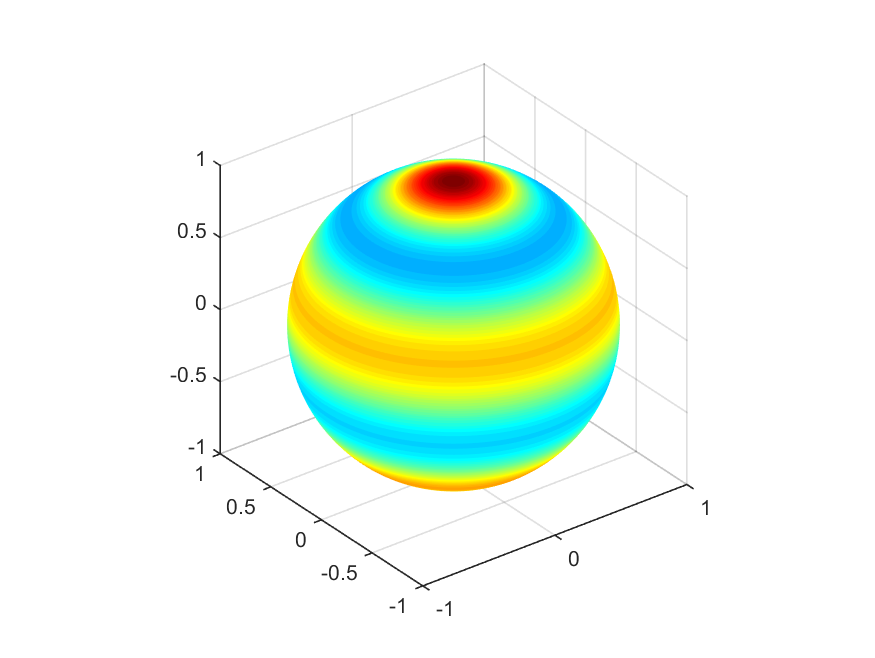
\includegraphics[width=1\textwidth]{chapters/images/ylm/a_5_0.pdf}
\caption{$Y^m_l$ mit $l=5$, $m=0$}
\label{skript:ylm l=5 m=0}
\end{minipage}
\hfill
\begin{minipage}[hbt]{0.4\textwidth}
\centering
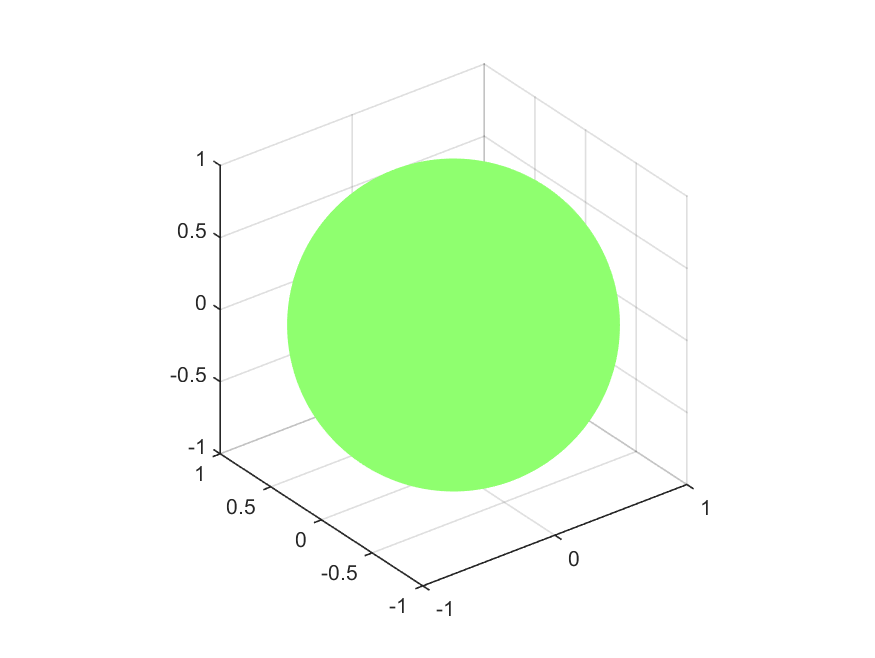
\includegraphics[width=1\textwidth]{chapters/images/ylm/b_5_0.pdf}
\caption{$Z_{lm}$ mit $l=5$, $m=0$}
\label{skript:zlm l=5 m=0}
\end{minipage}
\begin{minipage}[hbt]{0.4\textwidth}
\centering
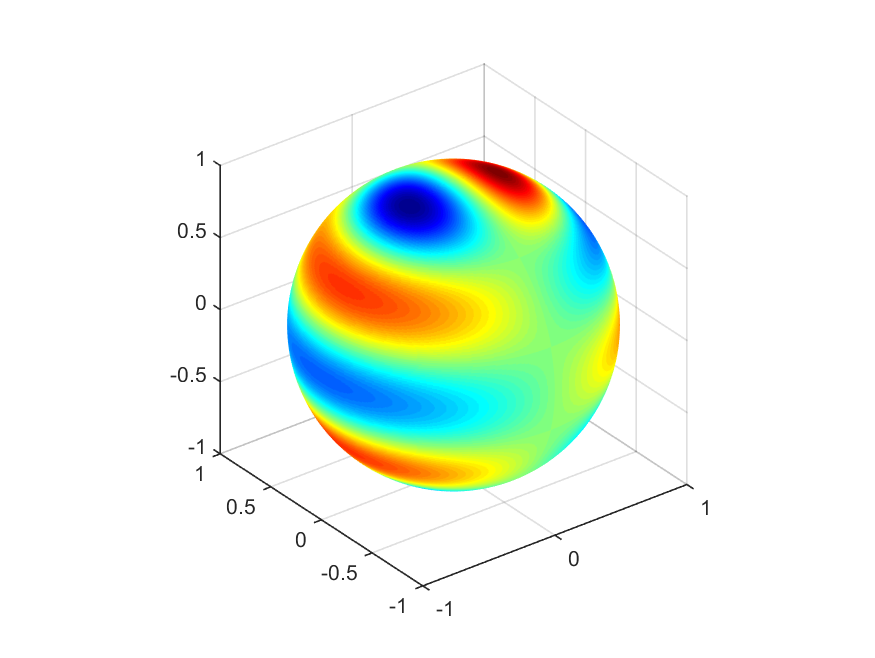
\includegraphics[width=1\textwidth]{chapters/images/ylm/a_5_1.pdf}
\caption{$Y^m_l$ mit $l=5$, $m=1$}
\label{skript:ylm l=5 m=1}
\end{minipage}
\hfill
\begin{minipage}[hbt]{0.4\textwidth}
\centering
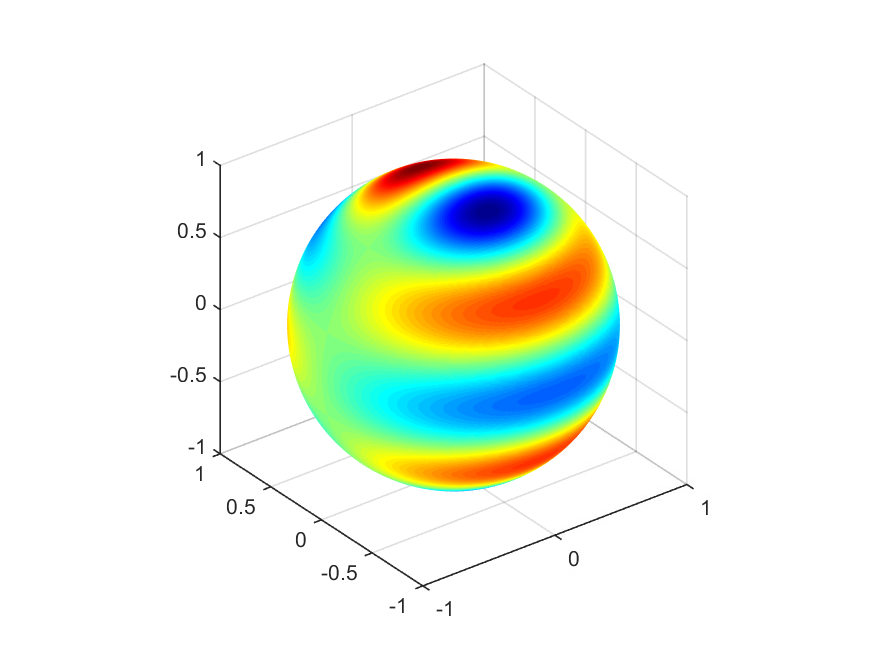
\includegraphics[width=1\textwidth]{chapters/images/ylm/b_5_1.pdf}
\caption{$Y^m_l$ mit $l=5$, $m=-1$}
\label{skript:zlm l=5 m=1}
\end{minipage}
\begin{minipage}[hbt]{0.4\textwidth}
\centering
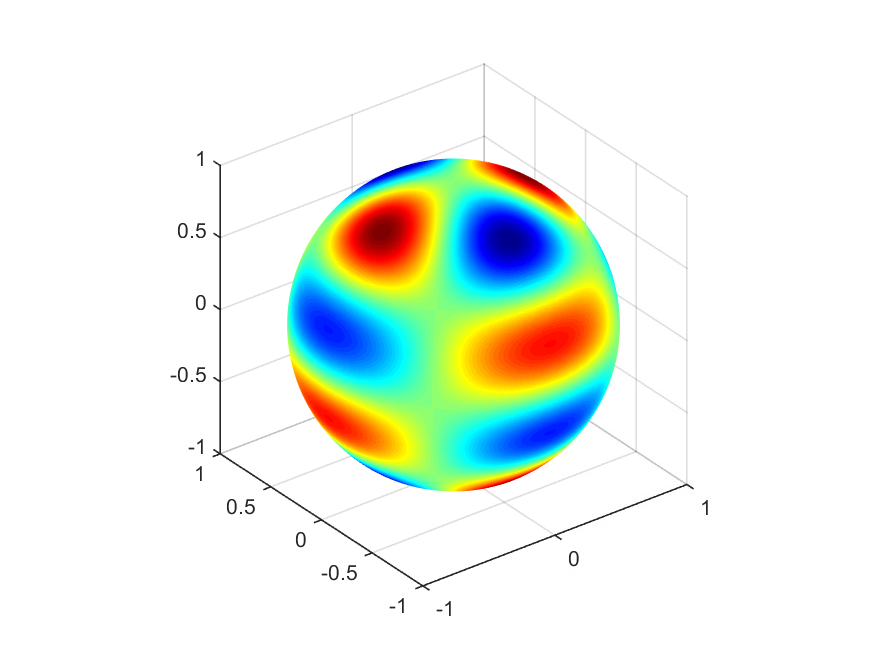
\includegraphics[width=1\textwidth]{chapters/images/ylm/a_5_2.pdf}
\caption{$Y^m_l$ mit $l=5$, $m=2$}
\label{skript:ylm l=5 m=2}
\end{minipage}
\hfill
\begin{minipage}[hbt]{0.4\textwidth}
\centering
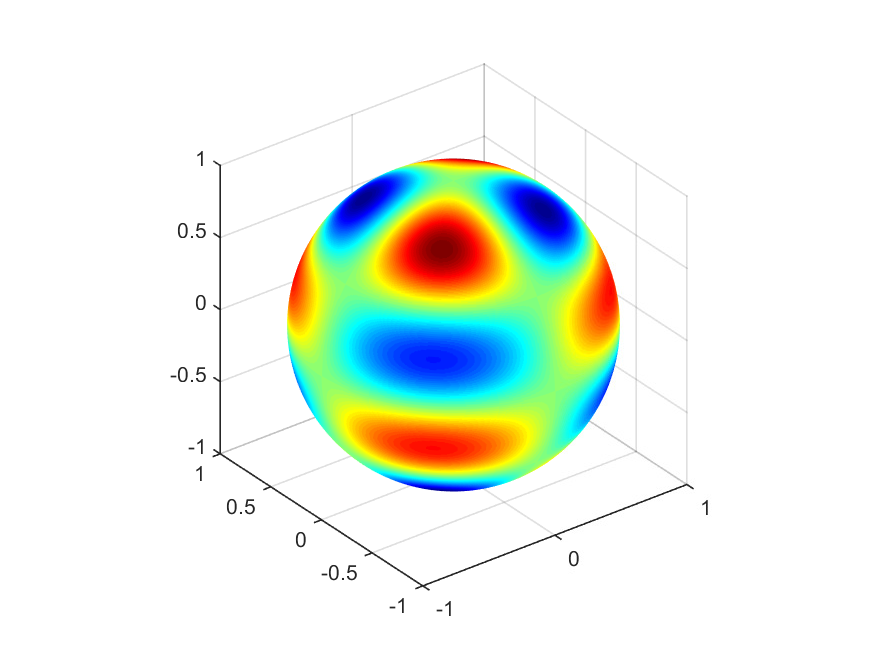
\includegraphics[width=1\textwidth]{chapters/images/ylm/b_5_2.pdf}
\caption{$Y^m_l$ mit $l=5$, $m=-2$}
\label{skript:zlm l=5 m=2}
\end{minipage}
\end{figure}

\begin{figure}
\begin{minipage}[hbt]{0.4\textwidth}
\centering
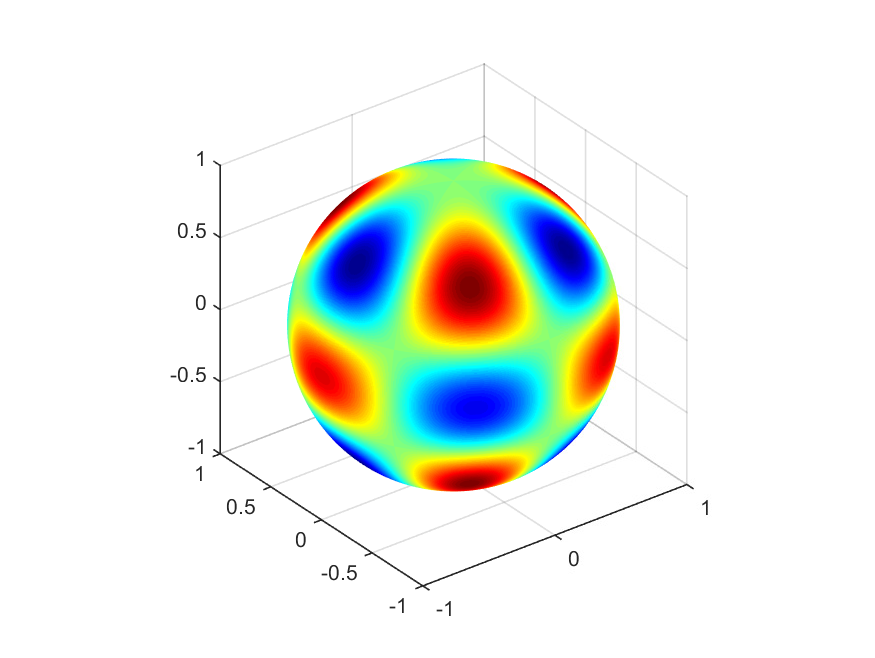
\includegraphics[width=1\textwidth]{chapters/images/ylm/a_5_3.pdf}
\caption{$Y^m_l$ mit $l=5$, $m=3$}
\label{skript:ylm l=5 m=3}
\end{minipage}
\hfill
\begin{minipage}[hbt]{0.4\textwidth}
\centering
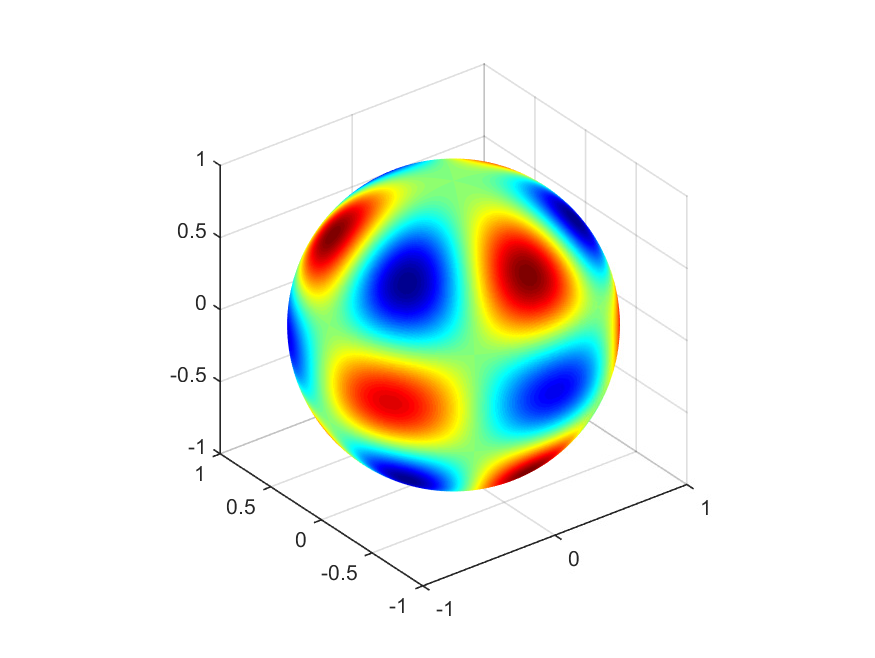
\includegraphics[width=1\textwidth]{chapters/images/ylm/b_5_3.pdf}
\caption{$Y^m_l$ mit $l=5$, $m=-3$}
\label{skript:zlm l=5 m=3}
\end{minipage}
\begin{minipage}[hbt]{0.4\textwidth}
\centering
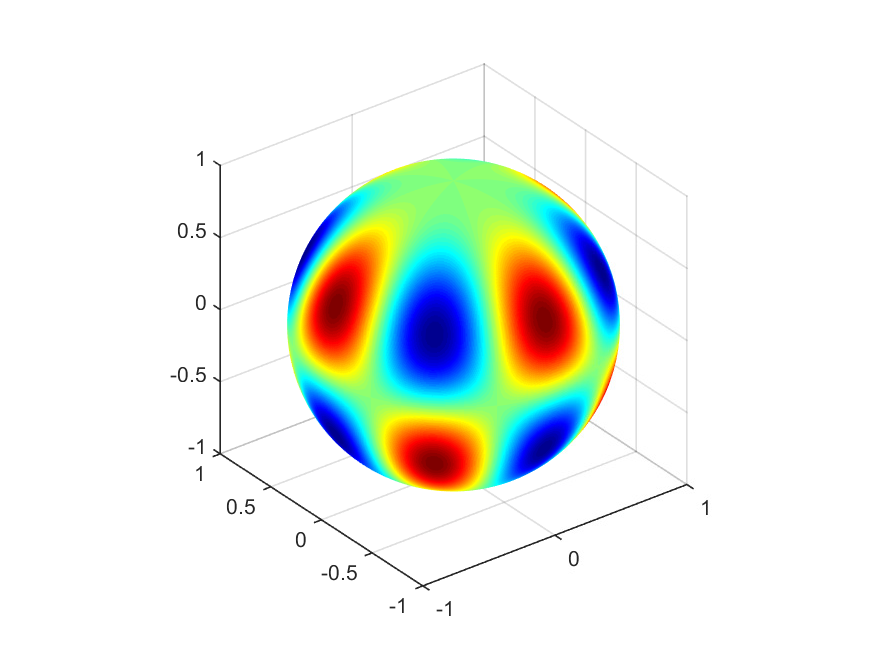
\includegraphics[width=1\textwidth]{chapters/images/ylm/a_5_4.pdf}
\caption{$Y^m_l$ mit $l=5$, $m=4$}
\label{skript:ylm l=5 m=4}
\end{minipage}
\hfill
\begin{minipage}[hbt]{0.4\textwidth}
\centering
\includegraphics[width=1\textwidth]{chapters/images/ylm/b_5_4.pdf}
\caption{$Y^m_l$ mit $l=5$, $m=-4$}
\label{skript:zlm l=5 m=4}
\end{minipage}
\begin{minipage}[hbt]{0.4\textwidth}
\centering
\includegraphics[width=1\textwidth]{chapters/images/ylm/a_5_5.pdf}
\caption{$Y^m_l$ mit $l=5$, $m=5$}
\label{skript:ylm l=5 m=5}
\end{minipage}
\hfill
\begin{minipage}[hbt]{0.4\textwidth}
\centering
\includegraphics[width=1\textwidth]{chapters/images/ylm/b_5_5.pdf}
\caption{$Y^m_l$ mit $l=5$, $m=-5$}
\label{skript:zlm l=5 m=5}
\end{minipage}
\end{figure}

\subsection{Bedeutung einzelner Kugelfunktionskoeffizienten}
Einzelne Kugelfunktionskoeffizienten haben wie bei der klassischen
Fouriertheorie eine anschauliche Bedeutung.

Der Koeffizient $c_0^0$ ist
\[
c_0^0
=
\frac{N^0_0}{\sqrt{2\pi}}
\int_{-\pi}^\pi 
\int_0^\pi
f(\varphi,\vartheta)
\sin\vartheta
\,d\vartheta
\,d\varphi,
\]
also im Wesentlichen der Mittelwert der Funktione $f$ über die Kugeloberfläche.

Der Koeffizient $c^0_1$, also $l=1$ und $m=0$ ist der Koeffizient
zu der Funktion
\[
Y^0_1(\varphi,\vartheta)
=
\frac{N^0_1}{\sqrt{2\pi}} P_1(\cos\vartheta)
=
\frac{N^0_1}{\sqrt{2\pi}} \frac{1}{2}\frac{d}{dz}(z^2-1)
=
\frac{N^0_1}{\sqrt{2\pi}} z
=
\frac{N^0_1}{\sqrt{2\pi}} \cos\vartheta.
\]
Das Skalarprodukt $\langle f,Y^0_1\rangle$ ist also das
Integral
\[
\langle f,Y^0_1\rangle
=
\frac{N^0_1}{\sqrt{2\pi}}
\int_{-\pi}^\pi 
\int_0^\pi
f(\varphi,\vartheta)
\cos\vartheta
\sin\vartheta
\,d\vartheta
\,d\varphi
\]
Da $\cos\vartheta$ in der oberen Halbkugel postiv ist und in der 
unteren Halbkugel negativ, beschreibt der Koeffizient $c^0_1$ im
Wesentlichen den Unterschied zwischen den beiden Halbkugeln.

\section*{Übungsaufgaben}
\rhead{Übungsaufgaben}
\uebungsaufgabe{1101}












%
% cmb.tex
%
% (c) 2017 Prof Dr Andreas Müller, Hochschule Rapperswil
%
\chapter{Der kosmische Mikrowellenhintergrund%
\label{skript:chapter:cmb}}
\lhead{Der kosmische Mikrowellenhintergrund}
\rhead{}
Im Kapitel~\ref{skript:chapter:kosmologie} haben wir aus den
Einstein-Gleichungen abgeleitet, dass ein homogenes und isotropes
Universum nicht statisch sein kann.
Hubbles Entdeckung der Expansion des Universums erlaubte uns zu
schliessen, dass das frühe Universum sehr heiss und dicht gewesen
sein muss.
Die Friedmann-Gleichung und ihre ausführliche Diskussion im
Kapitel~\ref{skript:chapter:friedmann} hat gezeigt, wie Materie und
Strahlung im Universum diese Expansion beeinflussen.
Es wurde dort auch auf das Steady-State-Modell hingewiesen, welches
ein sich ausdehnendes Universum konstanter Dichte zulässt.
Dieses wurde mit der Entdeckung des kosmischen Mikrowellenhintergrundes durch
Penzias und Wilson (mehr dazu im Kapitel~\ref{chapter:cmb}) ausgeschlossen.
Es bleibt aber noch zu verstehen, wie der kosmische Mikrowellenhintergrund
entsteht und welche Eigenschaften man von ihm erwarten kann.

Es stellt sich heraus, dass der kosmische Mikrowellenhintergrund mit sehr
hoher Genauigkeit das Spektrum eines schwarzen Körpers hat.
In diesem Kapitel wird daher zunächst ein Überblick über die allgemeine
Theorie der Schwarzkörperstrahlung gegeben.
Im zweiten Abschnitt wird der Ablauf der Rekombination genauer untersucht.
In dieser Phase wird aus dem heissen Plasma ein vergleichsweise kaltes Gas,
in dem sich Licht ungehindert ausbreiten kann.
Die in diesem Moment freigesetzte Strahlung messen wir heute als den
kosmischen Mikrowellenhintergrund.
Im letzten Teil untersuchen wir dann, ob sich mit unserem Wissen
bereits Aussagen über Grösse und Temperatur von Anisotropien im kosmischen
Mikrowellenhintergrund machen lassen.

\section{Thermodynamik und Schwarzkörperstrahlung}
\rhead{Thermodynamik und Schwarzkörperstrahlung}
Ein ungelöstes Problem der Physik im ausgehenden neunzehnten Jahrhundert
war das Strahlungsspektrum eines schwarzen Körpers zu berechnen.
Ein schwarzer Körper ist eine idealisierte thermische Strahlungsquelle,
die auftreffende elektromagnetische Strahlung jeder Wellenlänge absorbiert
und deren Strahlungsspektrum nicht von der Oberflächenbeschaffenheit
abhängt, sondern nur von dessen Temperatur.
Eine mögliche Realisierung ist ein mit Strahlung gefüllter Hohlraum, dessen
Wände auf konstanter Temperatur gehalten werden.

Die klassische Thermodynamik, die im
Abschnitt~\ref{skript:cmb:section:klassisch} zusammengestellt wird,
stellt die Werkzeuge bereit, mit der wir
dem Strahungsgesetz auf den Grund gehen können.
In Abschnitt~\ref{skript:cmb:section:planck} leiten wir daraus
das Plancksche Strahlungsgesetz her.
Insbesondere interessiert uns dabei, dass eine Vergrösserung aller
Wellenlängen um den gleichen Streckungsfaktor die Form des
Strahlungsgesetzes nicht ändert, so dass die Expansion des Universums
die Eigenschaften des Schwarzkörperspektrums erhält.
Daraus werden wir auch ableiten, wie sich die zugehörige Temperatur
mit der Expansion verändert.

%Die kosmische Mikrowellenhintergrundstrahlung wurde in dem Moment
%ausgestrahlt, als das ionisierte Gas frühen Universums neutral wurde,
%man nennt dies die Rekombination.
%Die Dynamik dieses Ereignisses wird in
%Abschnitt~\ref{skript:cmb:section:rekombination} untersucht.

\subsection{Thermodynamik%
\label{skript:cmb:section:klassisch}}
\index{Thermodynamik}%
Ein thermodynamisches System besteht aus einer grossen Zahl von 
Teilchen, die ständig interagieren und dabei Energie austauschen.
Der mikroskopische Zustand des Systems ändert sich laufend
und sehr rasch.
\index{mikroskopischer Zustand}
\index{Zustand, mikroskopisch}
Es ist daher gar nicht möglich, den aktuellen mikroskopischen
Zustand zu beschreiben.
Jede makroskopische Messung liefert daher immer nur einen mittleren
Wert für die gemessene Grösse.

Die fundamentale Zustandsgrösse der klassischen Thermodynamik ist
die Entropie, eine Funktion $S(U,V)$ von inneren Energie $U$ und 
Volumen $V$ des Systems. 
\index{Entropie}%
Alle mikroskopischen Zustände zur gleichen Energie und im gleichen
Volumen sind gleichermassen zulässig.
Offenbar gibt es auch keinen Grund, warum einer dieser Zustände
bevorzugt werden soll.
Die statistische Wärmelehre
{\em postuliert} daher, dass alle mikroskopischen Zustände gleich
wahrscheinlich sind.
Dies bedeutet auch, dass das System immer alle mikroskopischen
Zustände ausnützt, die mit der vorgegebenen inneren Energie $U$ und
dem Volumen $V$ vereinbar sind.
Die Zahl $\Omega(U,V)$ der mikroskopischen Zustände, zwischen denen das
System rasche Übergänge vollführt, nimmt zum Beispiel zu, wenn ein
Ventil geöffnet wird, und dem System damit ein grösseres Volumen
zur Verfügung steht.

Andererseits ist aus der klassichen Thermodynamik bekannt, dass ein
System immer denjenigen Zustand annimmt, in dem die Entropie $S(U,V)$
als Funktion von $U$ und $V$ ihr Maximum annimmt.
Man darf daher schliessen, dass die Entropie als Funktion der Anzahl
$\Omega(U,V)$ der mikroskopischen Zustände ausgedrückt werden kann.
Allerdings ist die Entropie additiv, fügt man zwei Systeme zusammen,
so ist die Entropie des Gesamtsystems die Summe der Entropien der
Teilsysteme:
\[
S(U,V) = S_1(U_1,V_1) + S_2(U_2,V_2).
\]
Die Anzahl der Zustände hingegen ist multiplikativ: da es für jeden
der $\Omega_1(U_1,V_1)$ Zustände des ersten Systems $\Omega_2(U_2,V_2)$
Zustände des zweiten Systems gibt, ist die Gesamtzahl der Zustände
deren Produkt
\[
\Omega(U,V)=\Omega_1(U_1,V_1)\cdot \Omega_2(U_2,V_2).
\]
Die Logarithmus-Funktion erfüllt diese Bedingung, und bis auf einen
Faktor ist sie auch die einzige Funktion mit dieser Eigenschaft.
Man kann also immer
\begin{equation}
S(U,V)=k_B\log \Omega(U,V)
\label{skript:cmb:boltzmann}
\end{equation}
setzen, wobei der Faktor $k_B$ im wesentlichen die Masseinheit von
$S$ festlegt.
Durch die Wahl
\[
k_B = 1.3807\cdot 10^{-23} \text{J}/\text{K}
\]
wird Übereinstimmung mit der Kelvin-Temperaturskala erreicht.
\index{Kelvin-Temperaturskala}%

\subsubsection{Kanonischer Formalismus}
\index{kanonischer Formalismus}%
Dieser Formalismus ist jedoch für die Beschreibung eines Systems 
nicht geeignet, welches sich in Kontakt mit einem Wärmereservoir
befindet, mit welchem es zur Erhaltung der Temperatur Energie
austauschen kann.
Dabei ändert sich die innere Energie des Systems.
Zu dessen Beschreibung ist daher eine Zustandsfunktion nötig, die von
der Temperatur und dem Volumen abhängt, während die Entropie
von innerer Energie und Volumen abhängt.
Man kann dieses Problem lösen, indem man das Wärmereservoir als
Teil eines grösseren Systems modelliert, mit dem das untersuchte
System Energie austauschen kann.
Die Gesamtenergie $E_\text{tot}$ des kombinierten Systems ist dann zwar eine
Zustandsvariable, aber das ursprüngliche Teilsystem kann verschiedene
Zustände annehmen.

Bezeichnen wir die verschiedenen Zustände mit einem Index $j$
und ihre Energie mit $E_j$, dann können wir die Wahrscheinlichkeit
berechnen, dass sich das ursprüngliche System im Zustand $j$ befindet.
Dazu berechnen wir die Anzahl der Zustände, in denen sich das 
Reservoir in einem Zustand mit Energie $E_\text{tot} - E_j$ befindet
und dividieren durch die Gesamtzahl der Zustände mit Energie $E_\text{tot}$.
Wir finden
\[
w_j
=
\frac{\Omega_\text{res}(E_\text{tot}-E_j)}{\Omega_\text{tot}(E_\text{tot})}
\]
für die Wahrscheinlichkeit.
Indem man \eqref{skript:cmb:boltzmann} nach $\Omega$ auflöst, kann $w_j$
durch die Entropie ausgedrückt werden:
\begin{equation}
w_j
=
\frac{\exp\bigl(S_\text{res}(E_\text{tot}-E_j)/k_B\bigr)}{\exp\bigl(S_\text{tot}(E_\text{tot})/k_B\bigr)}
\label{skript:cmb:fj}
\end{equation}
Ist $U$ die mittlere Energie des ursprünglichen Systems im Gleichgewicht,
dann gilt die Additivität der Entropie für das kombinierte System in der Form
\[
S_\text{tot}(E_\text{tot})
=
S(U) + S_\text{res}(E_\text{tot}-U).
\]
Da das Reservoir sehr gross ist, sind die Energien $E_j$ der Zustände des
ursprünglichen Systems im Vergleich zur Gesamtenergie sehr klein,
es ist daher zulässig, die Entropie des Reservoirs linear zu approximieren
\begin{align*}
S_\text{res}(E_\text{tot}-E_j)
&=
S_\text{res}(E_\text{tot}-U+U-E_j)
\\
&=
S_\text{res}(E_\text{tot}-U) + \frac{\partial S_\text{res}}{\partial U}(U-E_j)
\\
&=
S_\text{res}(E_\text{tot}-U) + \frac{U-E_j}{T}
\end{align*}
Setzt man dies in den Ausdruck~\eqref{skript:cmb:fj} für $w_j$ ein, 
erhält man
\[
w_j = e^{(U-TS(U))/k_BT} e^{-E_j/k_BT}.
\]
Man sieht, dass in den Formeln vor allem der Ausdruck $1/k_BT$ vorkommt,
denn man daher mit $\beta=1/k_BT$ abkürzt.
Die Wahrscheinlichkeiten $w_j$ können damit etwas prägnanter als
\begin{equation}
w_j = e^{\beta(U-TS(U))}e^{-\beta E_j}
\label{skript:cmb:fj2}
\end{equation}
geschrieben werden.

\subsubsection{Freie Energie}
Der Ausdruck $F=U-TS(U)$ im Exponenten von~\eqref{skript:cmb:fj2}
heisst die {\em helmholtzsche freie Energie}.
\index{freie Energie}
\index{Energie, freie}
\index{helmholzshe freie Energie}
Die helmholtzsche freie Energie $F$ eines thermodynamischen Systems
gibt an, wieviel Energie bei einem reversiblen, isothermen Prozess zur
Arbeitsleistung zur Verfügung steht. 
Je höher die Temperatur oder die Entropie eines Systems ist, desto geringer
ist die für Arbeitsleistung zur Verfügung stehende freie Energie.
Die freie Energie ist eine Zustandsfunktion der Variablen $T$ und $V$.
Da die Temperatur $T$ als Variable auftritt, eignet sich die freie
Energie als Zustandsfunktion zur Beschreibung eines Systems, welches
sich in Kontakt mit einem Wärmereservoir befindet.

Die Wahrscheinlichkeiten $w_j$ müssen sich zu $1$ summieren, es muss also
gelten
\begin{equation}
1=\sum_{j} w_j = e^{\beta F}\sum_j e^{-\beta E_j}
\qquad
\Rightarrow
\qquad
e^{-\beta F}=\sum_je^{-\beta E_j}=Z.
\label{skript:cmb:Z}
\end{equation}
Die Zahl $Z$ heisst die {\em kanonische Zustandssumme}.
\index{kanonische Zustandssumme}%
\index{Zustandssumme, kanonische}%
Aus ihr kann man die freie Energie berechnen, indem man
\eqref{skript:cmb:Z} nach $F$ auflöst:
\begin{equation}
-\beta F=\log\sum_j e^{-\beta E_j} = \log Z.
\end{equation}
Die Wahrscheinlichkeiten $w_j$ kann man jetzt auch ganz unabhängig vom
Reservoir als
\begin{equation}
w_j
=
\frac{e^{-\beta E_j}}{\sum_j e^{-\beta E_j}}
\end{equation}
ausdrücken.

\subsubsection{Erwartungswert der Energie}
Schliesslich lässt sich auch die mittlere Energie des ursprünglichen
Systems durch $Z$ ausdrücken.
Dazu verwendet man zunächst die Definition 
\[
U
=
\sum_j E_jw_j
=
\frac{1}{\sum_i e^{-\beta E_j}}
\sum_j E_je^{-\beta E_j}
=
\frac1Z \sum_j E_je^{-\beta E_j}
\]
des Erwartungswertes der Energie.
Die Ableitung von $\log Z$ nach $\beta$ liefert aber fast dasselbe:
\begin{align*}
\frac{d}{d\beta} \log Z
&=
\frac1{Z}\frac{dZ}{d\beta}
=
\frac1{Z}\sum_j\frac{de^{-\beta E_j}}{d\beta}
=
-\frac1Z\sum_j E_je^{-\beta E_j}
=
-U,
\end{align*}
die mittlere Energie ist also bis auf ein Vorzeichen auch die Ableitung
von $\log Z$ nach $\beta$.
Damit lässt sich auch die innere Energie
\[
U=-\frac{d}{d\beta}\log Z
\]
des ursprünglichen Teilsystems im Gleichgewicht mit dem Reservoir der
Temperatur $T$ aus der Zustandssumme berechnen.

\subsection{Plancksches Strahlungsgesetz%
\label{skript:cmb:section:planck}}
Die im vorangegangenen Abschnitt zusammengestellten Grundlagen der
statischen Mechanik erlauben uns, das Plancksche Strahlungsgesetz
zu verstehen.
\index{Plancksches Strahlungsgesetz}%
\index{Strahlungsgesetzt von Planck}%

\subsubsection{Frequenzdichte}
Elektromagnetische Strahlung in einem verspiegelten Hohlraum bildet
stehende Wellen,
deren Wellenlänge ein ganzzahliger Bruchteil der Abmessungen des
Hohlraumes sein muss.
Eine solche stehende Welle kann durch einen Vektor
\[
\vec{k} = \begin{pmatrix}k_x\\k_y\\k_z\end{pmatrix}
\]
von ganze Zahlen $k_x,k_y,k_z\in\mathbb Z$ beschrieben werden, der
die Anzahl der Wellenlängen angibt, die in jeder Richtung in die
Abmessungen des Hohlraums hineinpassen.
Sei $L$ die Seitenlänge des Hohlraumes, das Volumen ist dann $V=L^3$.
Eine Welle kann man mit Hilfe der Funktionen
\[
\sin \vec{x}\cdot\vec{k}\frac{2\pi}{L}
\qquad\text{und}\qquad
\cos \vec{x}\cdot\vec{k}\frac{2\pi}{L}
\]
beschreiben.
Der Faktor $2\pi/L$ stellt sicher, dass eine Zunahme einer Koordinate
um $L$ das Argument der Winkelfunktion genau um $2\pi$ vergrössert,
so dass die resultierende Funktion in jeder Koordinate $L$-periodisch ist.

Die Ausbreitungsrichtung einer solchen Welle ist $\vec{k}$.
Die Wellenlänge kann man an einem Vektor $\vec{x}$ ablesen, der
$\vec{x}\cdot\vec{k}=L$ erfüllt, er muss daher die Länge
\[
\lambda
=
|\vec{x}|
=
\frac{L}{|\vec{k}|}
\]
haben.
Die zugehörige Frequenz wird daher
\[
\nu(\vec{k})
=
\frac{c}{\lambda}=|\vec{k}|\frac{c}{L}.
\]

Später wird uns die Anzahl der möglichen Vektoren $\vec{k}$ interessieren,
die auf Frequenzen in einem vorgegeben Intervall $[\nu, \nu+d\nu]$
führen.
Dies ist auch die Anzahl der Vektoren mit ganzzahligen Koordinaten derart,
dass
\[
\frac{L}{c}\nu
\le
|\vec{k}|
\le
\frac{L}{c}(\nu+d\nu)
\]
gilt.
Dies ist aber auch ungefähr das Volumen einer Kugelschale zwischen den
Radien 
\[
r=\frac{L}{c}\nu
\qquad\text{und}\qquad
r+dr=\frac{L}{c}(\nu+d\nu)
\]
Die Volumenformel
\[
V(r)
=
\frac{4}{3}\pi r^3
\]
für eine Kugel vom Radius $r$ liefert für das Volumen
zwischen den beiden Radien
\[
V(r+dr)-V(r)
\simeq
\biggl(\frac{d}{dr} \frac{4}{3}\pi  r^3\biggr) \cdot dr
=
4\pi r^2\,dr.
\]
Daraus liest man ab, dass im Interval $[\nu,\nu+d\nu]$ 
\[
4\pi \frac{L^3}{c^3}\nu^2\,d\nu
=
4\pi \frac{V}{c^3}\nu^2\,d\nu
\]
Frequenzen möglich sind.
Bezogen auf das Volumen $V$ bleibt die Zustandsdichte
\begin{equation}
g(\nu)\,d\nu = \frac{4\pi}{c^3}\nu^2\,d\nu.
\label{skript:cmb:zustandsdichte}
\end{equation}
Allerdings ist zu beachten, dass ein elektromagnetisches Strahlungsfeld
zu jedem Wellenzahlvektor $\vec{k}$ zwei voneinander unabhängige 
Felder mit orthogonalen Polarisierungen ermöglicht, was die Zahl
der Zustände nochmals verdoppelt.

\subsubsection{UV-Katastrophe}
\index{UV-Katastrophe}%
Ein klassischer harmonischer Oszillator kann jede beliebige Energie haben,
da diese nur von der Amplitude abhängt.
Die klassische Thermodynamik leitet aus dem kanonischen Formalismus den
Gleichverteilungssatz ab, der besagt,
dass jeder Freiheitsgrad die gleiche mittlere Energie beiträgt.
Da zu jedem Wellenzahlvektor ein eigener Oszillator und damit ein 
eigener Freiheitsgrad zur Verfügung steht, trägt jeder Wellenzahlvektor
die gleiche Energiemenge bei.
Da es unendlich viele Wellenzahlvektoren gibt, wird die Gesamtenergie
unendlich gross.
Man nennt dies die UV-Katastrophe.
Sie zeigt, dass die klassischen Vorstellungen und insbesondere der
Gleichverteilungssatz nicht anwendbar sind.
Das Problem kann nur gelöst werden, indem man
annimmt, dass die Oszillatoren mit hoher Frequenz nur mit geringerer
Wahrscheinlichkeit angeregt werden.

\subsubsection{Quantenhypothese}
Planck nahm in seiner Verzweiflung an, dass in einem Oszillator mit
Freqeuenz $\nu$ nur die diskreten Vielfachen des Energiequantums $h\nu$ 
erlaubt sind, wobei $h$, das {\em Plancksche Wirkungsquantum}, derart
klein ist, dass es bei hohen Energien gar nicht erst in Erscheinung
tritt.
Der Oszillator mit Frequenz $\nu$ hat daher die Energiezustände
\[
E_j = jh\nu,
\]
und damit die Zustandssumme
\[
Z_\nu
=
\sum_{j=0}^\infty e^{-j\beta h\nu}
=
\sum_{j=0}^\infty \bigl(e^{-\beta h\nu}\bigr)^j.
\]
Dies ist eine geometrische Reihe mit dem Quotienten
$q=e^{-\beta h\nu}$ mit der Summe
\[
Z_\nu
=
\frac1{1-q}=\frac1{1-e^{-\beta h\nu}}.
\]
Die mittlere Energie, die sich im Gleichgewicht in diesem Oszillator 
befindet, ist
\[
E(\nu,T)
=
-\frac{d}{d\beta}\log Z_\nu
=
\frac{h\nu e^{-\beta h \nu}}{1-e^{-\beta h\nu}}
=
\frac{h\nu}{e^{\beta h\nu}-1}
=
\frac{h\nu}{e^{h\nu/k_BT}-1}.
\]

Nun ist aber auch noch zu berücksichtigen, dass nicht jede beliebige
Frequenz möglich ist.
Die Zustandsdichte für die Frequenzen wurde
in~\eqref{skript:cmb:zustandsdichte} bereits bestimmt.
Somit erhalten wir das Plancksche Strahlungsgesetz.
Die im Frequenzinterval $d\nu$ abgestrahlte Energie eines
schwarzen Körpers ist
\begin{equation}
U(\nu,T)\,d\nu
=
2g(\nu)\,d\nu
\frac{h\nu}{e^{h\nu/k_BT}-1}
=
\frac{8\pi}{c^3}\nu^2\,d\nu\frac{h\nu}{e^{h\nu/k_BT-1}}
=
\frac{8\pi h\nu^3}{c^3}\frac{d\nu}{e^{h\nu/k_BT}-1}
\label{skript:cmb:plancknu}
\end{equation}
Der Faktor $2$ rührt von den zwei Polarisierungen her, die die Strahlung
bei gleichem Wellenzahlvektor $\vec{k}$ und damit gleicher Frequenz haben
kann.
Abbildung~\ref{skript:cmb:planckU} zeigt die Abhängigkeit von $U$ von
der Frequenz $\nu$ in doppelt logarithmischer Darstellung.
\begin{figure}
\centering
\includegraphics{chapters/tikz/planck1.pdf}
\caption{Plancksches Strahlungsgesetz: Abhängigkeit der Energiedichte
$U(\nu,T)$ von der Frequenz $\nu$ in logarithmischer Darstellung.
\label{skript:cmb:planckU}}
\end{figure}

\subsubsection{Wellenlänge}
\begin{figure}
\centering
\includegraphics{chapters/tikz/planck2.pdf}
\caption{Plancksches Strahlungsgesetz: Abhängigkeit der Energiedichte
$U(\lambda,T)$ von der Frequenz $\lambda$ in logarithmischer Darstellung.
\label{skript:cmb:planckUlambda}}
\end{figure}
In~\eqref{skript:cmb:plancknu} haben wir das Plancksche Strahlungsgesetz
durch die Frequenz ausgedrückt.
Wir hätten stattdessen auch die Wellenlänge $\lambda=c/\nu$ verwenden 
können.
Einem Interval $[\lambda,\lambda+d\lambda]$ von Wellenlängen entspricht
das Frequenzinterval
\[
\biggl[
\frac{c}{\lambda}-\frac{c}{\lambda^2}d\lambda
,
\frac{c}{\lambda}
\biggr]
\]
und damit das Strahlungsgesetz
\begin{equation}
U(\lambda,T)\,d\lambda
=
\frac{8\pi h}{\lambda^3}\frac{1}{e^{hc/\lambda k_BT}-1}\frac{c}{\lambda^2}\,d\lambda
=
\frac{8\pi hc}{\lambda^5}\frac{1}{e^{hc/\lambda k_BT}-1}\,d\lambda
\label{skript:cmb:planck:lambda}
\end{equation}
in Abhängigkeit von der Wellenlänge $\lambda$ und der Temperatur $T$.
Abbildung~\ref{skript:cmb:blacnkUlambda} zeigt die Abhängigkeit von
$U(\lambda,T)$ von $\lambda$ in logarithmischer Darstellung.

\subsubsection{Verschiebungsgesetz}
\begin{figure}
\centering
\includegraphics{chapters/tikz/planck3.pdf}
\caption{Abhängigkeit der Schwarzkörperstrahlung von der Temperatur
in doppelt logarithmischer Darstellung.
Man kann gut erkennen, wie das Maximum sich proportional zur Temperatur
verschiebt.
Die unterste Kurve entspricht ungefährt dem Spektrum der Strahlung
des kosmischen Mikrowellenhintergrundes.
\label{skript:cmb:planckverschiebung}}
\end{figure}
Ändert man die Temperatur des Hohlraumes um den Faktor $a$ zur $T_1=aT$,
dann wird sich das Strahlungsspektrum $U_1$ zu anderen Wellenlängen
$\lambda_1$ verschieben.
Wir wollen zeigen, dass mit $\lambda_1=\lambda/a$ wieder ein Plancksches
Strahlungsgesetz entsteht, allerdings mit einer geringeren abgestrahlten
Energie.
Setzen wir dies in das Strahlungsgesetz ein, erhalten wir
\begin{align*}
U_1(\lambda_1,T_1)\,d\lambda_1
&=
B\cdot
U(a\lambda_1,T_1/a)a\,d\lambda_1
\\
&=
\frac{B}{a^4}
\cdot
\frac{8\pi hc}{\lambda_1^5}\frac{1}{e^{hc/\lambda_1k_BT_1}-1}\,d\lambda_1
\\
&=
\frac{B}{a^4}\cdot U(\lambda_1,T_1)\,d\lambda_1.
\end{align*}
Das Strahlungsspektrum bei der Temperatur $T_1=aT$ ist also identisch mit dem
Spektrum bei der Temperatur $T$ mit Wellenlängen, die um den Faktor $a^{-1}$
verkürzt wurden.
Der Faktor $B$ muss $B=a^4$ sein, damit dies zutrifft.
Wir schliessen daraus, dass die Gesamtstrahlung eines schwarzen Körpers
proportional zu $T^4$ sein muss (Wiensches Verschiebungsgesetz).
\index{Wiensches Verschiebungsgesetz}%
\index{Verschiebungsgesetz}%

\subsubsection{Expansion}
In der Form~\eqref{skript:cmb:planck:lambda}
des Strahlungsgesetztes können wir untersuchen was
passiert, wenn sich das ganze Universum, betrachtet als ein gigantischer
Hohlraum, sich um den Faktor $a$ ausdehnt.

Wir bezeichnen die Wellenlänge nach der Expansion mit $\lambda_1=a\lambda$
und bestimmen die Energiedichte $U_1(\lambda_1,T_1)$ in Abhängigkeit von
$\lambda_1$.
Im besten Fall ist $U_1(\lambda_1,T_1)$ wieder das Plancksche
Strahlungsgesetz, möglicherweise mit einer anderen Temperatur $T_1$, die
es ebenfalls zu bestimmen gilt.

Aus dem Strahlungsgesetz~\eqref{skript:cmb:planck:lambda} in Abhängigkeit
von der Wellenlänge wird dann
\begin{align*}
U_1(\lambda_1,T_1)\,d\lambda_1
&=
U(\lambda_1/a,T)\,d(\lambda_1/a)
\\
&=
\frac{8\pi hc}{(\lambda_1/a)^5}
\frac{1}{e^{hc/(\lambda_1/a) k_BT}-1}\,d(\lambda_1/a)
\\
&=
a^4
\frac{8\pi hc}{\lambda_1^5}
\frac{1}{e^{hc/\lambda_1 k_B(T/a)}-1}\,d\lambda_1
\end{align*}
Bis auf den Faktor $a^4$ ist dies wieder ein Plancksches Spektrum
für die Temperatur $T_1=T/a$.
Der Faktor $a^4$ passt aber zu der Tatsache, dass die Gesamtstrahlung
bei einer Temperaturänderung um den Faktor $1/a$ ebenfalls um Faktor
$a^{-4}$ abnehmen muss.
Der Faktor $a^4$ kompensiert also genau diese Abnahme.
Wir kommen daher zum Schluss, dass die Expansion des Universums um den
Faktor $a$ die Temperatur der darin enthaltenen Strahlung um den Faktor
$1/a$ gesenkt wird.
Die Energiedichte der Strahlung nimmt dagegen um den Faktor $a^{-4}$ ab.

\subsubsection{Photonenzahl}
Die Herleitung des Planckschen Strahlungsgesetzes erlaubt auch, die
erwartete Anzahl der angeregten Zustände, also der Photonen im
Hohlraum zu ermitteln.
Wir notieren hier nur das Resultat, die Berechnung findet man zum
Beispiel in \cite[Abschnitt 1.9]{skript:feynman}.
Die Anzahldichte der Photonen in einem Hohlraum der Temperatur $T$ ist
\begin{equation}
n_\gamma
=
16\pi\zeta(3)
\biggl(\frac{k_BT}{hc}\biggr)^3
=
60.422\,
\biggl(\frac{k_BT}{hc}\biggr)^3
=
\frac{16\pi\zeta(3)}{(2\pi)^3}
\biggl(\frac{k_BT}{\hbar c}\biggr)^3
=
0.24359\,
\biggl(\frac{k_BT}{\hbar c}\biggr)^3.
\label{skript:cmb:photonenzahl}
\end{equation}
Darin ist $\zeta(3)$ der Wert der Riemannschen Zetafuntion an der
Stelle $3$.
\index{Riemannsche Zetafunktion}%
\index{Zetafunktion, Riemannsche}%
Ein numerischer Wert ist $\zeta(3)=1.20205690\dots$.

\section{Entstehung des kosmischen Mikrowellenhintergrundes%
\label{skript:cmb:section:rekombination}}
\rhead{Rekombination}
Im frühen Universum war die Energiedichte der Strahlung viel höher
als die Energiedichte der Materie.
Die Friedmann-Gleichung erlaubt den Zeitpunkt zu berechnen,
zu dem die Energiedichte von Strahlung und Materie gleich waren,
wie das in \eqref{skript:friemann:msequal} durchgeführt wurde.
Im frühen Universum gab es daher einerseits sehr viel mehr Strahlung
als Materie, andererseits war die Dichte höher, so dass es sehr
häufig zu Reaktionen zwischen Atomen und Photonen kam, wodurch die
Atome ionisiert wurden.
Erst als das Universum genügend abgekühlt war, konnten sich Atomkerne
und Elektronen für längere Zeit zusammenfinden.
Man nennt diese Phase die Rekombination, obwohl die Atomkerne und
Elektronen davor noch nie kombiniert gewesen waren.

In diesem Abschnitt wollen wir daher berechnen, wie der Prozess der
Rekombination abläuft und bei welchem Alter des Universums dies
etwa stattgefunden haben muss.

\subsection{Zusammensetzung des Universums%
\label{section:cmb:dichte}}
Wir nehmen in diesem Abschnitt an, dass das Universum nur aus 
Protonen, Elektronen und Strahlung besteht.
Insbesonderen vernachlässigen wir den beträchtlichen Teil
Helium, der im Rahmen des Big Bang erzeugt worden ist.
Da die Ionisationsenergie von Helium etwa doppelt so hoch ist wie
diejenige von Wasserstoff, muss Helium im wesentlichen bereits
rekombiniert haben in dem Moment, wo die Rekombination des Wasserstoff
stattfindet.
Er hat daher auf den Moment, zu dem das Universum transparent wird
nur geringen Einfluss.

Die Materie im Universum wird beschrieben durch die Anzahldichte
der freien Elektronen $n_e$, die Anzahldichte der freien Protonen $n_p$
und die Anzahldichte $n_\text{H}$ der Wasserstoffatome.
Da das Universum neutral ist, muss $n_e=n_p$ gelten.
Da jedes Wasserstoffatom auch ein Proton als Atomkern enthält, ist die
Gesamtzahl der Baryonen im Universum $n_\text{Baryonen} = n_p+n_\text{H}$.
Sie ist im betrachteten Zeitraum konstant, weil die Temperatur bereits
so tief gesunken ist, dass keine Fusionsprozesse mehr ablaufen können.

Aus Beobachtungen lassen sich Zahlenwerte für diese Anzahldichten abschätzen.
Für die Energiedichte der Protonen wurde ein Wert von
$\varepsilon \simeq 210\text{MeV}/\text{m}^3$ gefunden.
Da ein einzelnes Proton die Energie $E_p=939\text{MeV}$ hat, finden wir
für die Protonendichte heute
\[
n_{\text{Baryonen}}
=
n_p
\simeq
0.22 \text{m}^{-3}.
\]
Zum Vergleich: Wasserstoffgas bei Atmosphärendruck hat eine Protonendichte
von etwa $5.3\cdot 10^{25}\text{m}^{-3}$.
In einem technischen Ultra-Hochvakuum mit einem Druck von
$10^{-10}\text{Pa}$ ist die Protonendichte immer noch
etwa $5.3\cdot 10^{15}\text{m}^{-3}$, also über $10$ Grössenordnungen
höher als im Universum im Grossen.

Auch für die Photonendichte kann man eine Schätzung abgeben.
Aus der bekannten Temperatur des kosmischen Mikrowellenhintergrundes
kann man mit der Formel~\eqref{skript:cmb:photonenzahl} die heutige
Photonendichte abschätzen, sie ist
\[
n_{\gamma,0}=4.11\cdot 10^8\text{m}^{-3}.
\]
Die Photonendichte ist also auch heute wesentlich höher als die 
Protonendichte, das Verhältnis ist
\[
\eta = \frac{n_{\text{Baryonen}}}{n_\gamma} = 5.35\cdot 10^{-10}.
\]
Die Energie einzelner Photonen der Hintergrundstrahlung ist
allerdings sehr klein.

\subsection{Prozesse in einem vollständig ionisierten Universum}
Wir betrachten das Universum zu einer Zeit, die der Rotverschiebung
$z=10^5$ entspricht.
Das Universum hat damals die Temperatur $T=zT_0 \simeq 2.725\cdot 10^5\text{K}$.
Dies ist zu kalt für Fusionsprozesse, aber die mittlere Energie 
$k_BT\simeq 60\text{eV}$ eines Photons ist deutlich höher als die
Ionisationsenergie eines Wasserstoffatoms $Q=13.6\text{eV}$,
man kann also davon ausgehen,
dass zu dieser Zeit das Universum vollständig ionisiert war.

Wie gross war die Materiedichte damals? 
Die Materiedichte geht mit der dritten Potenz des Skalenfaktors.
Die Anzahldichte der Baryonen ist daher
\[
n = n_{\text{Baryonen}}(1+z)^3 
\simeq
n_{\text{Baryonen}}\cdot 10^{15}
\simeq
2\cdot 10^{14}\text{m}^{-3}.
\]
Dies entspricht einer Massedichte von $3.7\cdot 10^{13}\text{kg}/\text{m}^3$,
das war bereits ein extrem verdünntes Plasma.

\subsubsection{Thomson-Streuung}
Der dominierende Prozess in dieser Phase war die {\em Thomson-Streuung}
\[
\gamma + e^- \to \gamma + e^-
\]
\index{Thomson-Streuung}%
eines Photons an einem Elektron.
Diesen Prozess kann man im Labor studieren, er lässt ist durch den
sogenannten Wirkungsquerschnitt
\[
\sigma_e
=
\frac{1}{n_e\lambda}
=
6.65\cdot 10^{-29}
\text{m}^{-2}
\]
charakterisieren.
Darin ist $n_e$ die Anzahldichte der Elektronen, die mit der Anzahldichte
der Protonen übereinstimmt, und $\lambda$ ist die mittlere freie
Weglänge der Photonen.
Da $n_e$ bekannt ist, kann man dies auch nach $\lambda$ auflösen und
so die mittlere freie Weglänge $\lambda=1/n_e\sigma_e$ finden.
Da sich die Photonen mit Lichtgeschwindigkeit ausbreiten, kann man
die Streurate
\[
\Gamma
=
\frac{c}{\lambda}
=
cn_e\sigma_e\simeq 4.4\cdot 10^{-6}\text{s}^{-1}
\]
eines Photons berechnen, das sind etwa 2.6 Streuereignisse pro Woche.
Die Thomson-Streuung tauscht Energie zwischen Photonen und Elektronen aus.
Die Elektronen und die Photonen bilden also ein gekoppeltes thermodynamisches
System.

\subsubsection{Entkoppelung}
Ist die mittlere freie Weglänge grösser als die Hubble-Distanz
(Seite~\pageref{skript:section:hubble-distanz}),
kann ein ``mittleres Photon'' das nächste Streuereignis nicht
mehr erreichen.
Dies tritt ein, wenn $\lambda > c/H$ gilt,
der gleichbedeutend wenn $H>c/\lambda$.
Andererseits ist $\Gamma=c/\lambda$, wir finden daher, dass für 
\[
H>\Gamma
\]
die Streuereignisse verschwinden.

Die Streurate $\Gamma$ nimmt mit der Ausdehnung des Universums ab,
und zwar ist
\[
\Gamma
=
cn_e\sigma_e
\sim
a(t)^{-3}.
\]
Aber auch $H$ nimmt ab,
im Strahlungsdominierten Universum gilt
\[
H^2 = H_0^2  \Omega_{0,s} a(t)^{-4}
\qquad\Rightarrow\qquad
H=H_0\sqrt{\Omega_{0,s}} a(t)^{-2}.
\]
$\Gamma$ nimmt also schneller ab als $H$, es wird also unweigerlich
der Moment eintreten, wo $H>\Gamma$ ist, wo also die Streuprozesse
zum erliegen kommen.
In diesem Moment findet kein bedeutender Energieaustausch mehr statt
zwischen Photonen und Elektronen.
Die Strahlung und die Elektronen entkoppeln.

In dieser Diskussion haben wir aber noch nicht berücksichtigt, dass
die Ausdehnung auch die Temperatur senkt.
Bei niedrigerer Photonenenergie können sich Elektronen und Protonen
zu neutralen Wasserstoffatomen zusammenfinden, man nennt diesen
Prozess die {\em Rekombination}.
\index{Rekombination}%
Fängt ein Proton ein Elektron ein, wird ein Photon ausgesendet,
doch wegen der sehr grossen Zahl der Photonen (dem sehr kleinen Wert
von $\eta$), fallen diese zusätzlichen Photonen nicht ins Gewicht.
Durch die Rekombination werden den Streuprozessen die freien Elektronen
entzogen, der Energieaustausch zwischen Photonen und Elektronen
kommt also bereits früher zum Erliegen.

\subsection{Ionisationsgrad}
Bei der Rekombination nimmt der Anteil des neutralen Wasserstoffs
gegenüber ionisierten Protonen und Elektronen stark zu.
Der {\em Ionisationsgrad} des Universums ist  definiert als
\index{Ionisationsgrad}%
\begin{equation}
X=\frac{n_p}{n_\text{Baryonen}}=\frac{n_p}{n_p+n_\text{H}}.
\label{skript:cmb:Xb}
\end{equation}
Ziel dieses Abschnitts ist, den Prozess der Rekombination besser zu
verstehen durch die Berechnung von $X$ in Abhängigkeit 
von der Zeit.

Löst man die Definition~\eqref{skript:cmb:Xb} nach $n_\text{H}$ auf,
findet man
\begin{align}
\frac1X
&=
\frac{n_p+n_\text{H}}{n_p}
=
1+
\frac{n_\text{H}}{n_p}
\notag
\\
\Rightarrow
\qquad
\frac{n_\text{H}}{n_p}
&=
\frac{1}{X}-1
=
\frac{1-X}{X}
\notag
\\
n_\text{H}
&=
\frac{1-X}{X}n_p.
\label{skript:cmb:XnH}
\end{align}

Ausserdem dürfen wir annehmen, dass die Anzahldichte $n_\gamma$
der Photonen währen der Rekombination wesentlich grösser war als
die Zahl der Baryonen.
Wir bezeichnen mit $\eta$ das Verhältnis
\[
\eta = \frac{n_\text{Baryonen}}{n_\gamma}
\]
von Baryonenzahl zu Photonenzahl.
Mit Hilfe der Definition von $X$ in Gleichung~\eqref{skript:cmb:Xb}
finden wir den Zusammenhang
\begin{equation}
\eta = \frac{n_p}{Xn_\gamma}
\label{skript:cmb:etaX}
\end{equation}
zwischen $\eta$ und $X$.

\subsection{Reaktionsgleichgewicht und Saha-Gleichung}
Die Voraussetzungen über die Zusammensetzung des Universums bedeuten,
dass wir uns nur für die Ionisationsreaktion
\begin{equation}
\text{H} + \gamma 
\rightleftharpoons
p + e^-
\label{skript:cmb:reaktionsgleichung}
\end{equation}
interessieren.
Wir nehmen sogar an, dass die Ionisation eines Wasserstoffatoms 
die konstante Energie $Q=13.6\,\text{eV}$ benötigt.
Damit ignorieren wir angeregt Zustände des Wasserstoffs, die auch
mit geringerem Energieaufwand ionisiert werden können.
Bei der Rekombination ist auch ein Übergang in einen angeregten
Zustand möglich, der später durch Emission eines Photons in den Grundzustand
übergehen kann.

Wir möchten berechnen, wie der Ionisationsgrad sich mit der Zeit ändert.
Wenn die Dichte der Photonen sinkt, wird sich das Reaktionsgleichgewicht
auf die linke Seite von~\eqref{skript:cmb:reaktionsgleichung} verschieben.
Im statistischen Gleichgewicht kann die Maxwell-Boltzmann-Gleichung
verwendet werden, um die Teilchendichte in Abhängigkeit von der Temperatur
auszudrücken, es gilt für die Komponente $x$
\[
n_x
=
g_x \biggl(\frac{m_xk_BT}{2\pi \hbar^2}\biggr)^{\frac32}
\exp\biggl(-\frac{m_xc^2}{k_BT}\biggr).
\]
Die Zahl $g_x$ ist die Anzahl der Zustände mit gleichem Impuls.
Für Elektronen und Protonen ist $g_e=g_p=2$, da beide genau zwei
Spin-Zustände haben.
Das Wasserstoff-Atom hat dagegen $g_\text{H}=4$ Spinzustände.

Das Verhältnis der Anzahldichten der Reaktionsteilnehmer ist
\begin{equation}
\frac{n_\text{H}}{n_pn_e}
=
\underbrace{\frac{g_\text{H}}{g_pg_e}}_{\displaystyle=1}
\biggl(\frac{m_\text{H}}{m_pm_e}\biggr)^{\frac32}
\biggl(\frac{k_BT}{2\pi \hbar^2}\biggr)^{-\frac32}
\exp\biggl( \frac{(m_p+m_e-m_\text{H})c^2}{k_BT} \biggr)
\label{skript:cmb:saha1}
\end{equation}
Mit unseren vereinfachenden Annahmen ist der Zähler im letzten Term
die Ionisationsenergie
\[
Q=(m_p+m_e-m_\text{H})c^2
\]
des Wasserstoffatoms.
Da der Unterschied zwischen $m_p$ und $m_\text{H}$ sehr gering ist,
setzen wir den $m_\text{H}/m_p=1$ im zweiten Faktor auf der rechten Seite
von \eqref{skript:cmb:saha1}.
Mit diesen Vereinfachungen wird die Gleichung~\eqref{skript:cmb:saha1}
zu
\begin{equation}
\frac{n_\text{H}}{n_pn_e}
=
\biggl(\frac{m_ek_BT}{2\pi \hbar^2}\biggr)^{-\frac32}
\exp\biggl( \frac{Q}{k_BT} \biggr),
\label{skript:cmb:saha}
\end{equation}
sie heisst die {\em Saha-Gleichung}.
\index{Saha-Gleichung}%

Man beachte, dass der Faktor
\[
\lambda
=
\sqrt{\frac{2\pi\hbar^2}{m_ek_BT}}
\]
die Dimension einer Länge hat, er heisst auch die thermische de~Broglie
Wellenlänge eines Elektrons mit Temperatur $T$.
Der Faktor vor der Exponentialfunktion in \eqref{skript:cmb:saha}
hat daher die Dimension eines Volumens.

\subsection{Rekombination}
\begin{figure}
\centering
\includegraphics{chapters/tikz/rekombination.pdf}
\caption{Ionisationsgrad in Abhängigkeit von der Rotverschiebung.
Die Zeit läuft von links nach rechts.
Rekombinationszeit ist bei Rotverschiebung $z=1375$ und einer Temperatur
von $T_{\text{rec}}=3747\text{K}$.
\label{skript:cmb:rekombinationgraph}}
\end{figure}
Die Gleichung~\eqref{skript:cmb:XnH} erlaubt uns, in der
Saha-Gleichung~\eqref{skript:cmb:saha} das Verhältnis $m_\text{H}/n_p$
durch $X$ auszudrücken, wir erhalten
\begin{equation}
\frac{1-X}{X}
=
n_p
\biggl(\frac{m_ek_BT}{2\pi \hbar^2}\biggr)^{-\frac32}
\exp\biggl( \frac{Q}{k_BT} \biggr).
\end{equation}
Die Protonendichte $n_p$ lässt sich dank~\eqref{skript:cmb:etaX}
durch $\eta$ und die Photonendichte $n_\gamma$ ausdrücken als
\[
\frac{1-X}{X^2}=\eta n_\gamma
\biggl(\frac{m_ek_BT}{2\pi \hbar^2}\biggr)^{-\frac32}
\exp\biggl( \frac{Q}{k_BT} \biggr).
\]
Für die Hohlraumstrahlung ist die Photonendichte $n_\gamma$ in Abhängigkeit
von der Temperatur aus \eqref{skript:cmb:photonenzahl} bekannt.
\begin{align}
\frac{1-X}{X^2}
&=\eta
\frac{16\pi\zeta(3)}{(2\pi)^3}
\biggl(\frac{k_BT}{\hbar c}\biggr)^3
\biggl(\frac{m_ek_BT}{2\pi \hbar^2}\biggr)^{-\frac32}
\exp\biggl( \frac{Q}{k_BT} \biggr)
\notag
\\
&=
\frac{16\pi\zeta(3)}{(2\pi)^3}(2\pi)^{\frac32}
\,
\eta
\,
\biggl(\frac{k_BT}{m_ec^2}\biggr)^{\frac32}
\exp\biggl( \frac{Q}{k_BT} \biggr)
\\
&=
\frac{16\pi\zeta(3)}{(2\pi)^{\frac32}}
\,
\eta
\,
\biggl(\frac{k_BT}{m_ec^2}\biggr)^{\frac32}
\exp\biggl( \frac{Q}{k_BT} \biggr)
\\
&=
3.8364
\,
\eta
\,
\biggl(\frac{k_BT}{m_ec^2}\biggr)^{\frac32}
\exp\biggl( \frac{Q}{k_BT} \biggr)
\label{skript:cmb:xqauadr}
\end{align}
Schreibt man $S(T,\eta)$ für die rechte Seite von \eqref{skript:cmb:xqauadr},
dann wird daraus eine quadratische Gleichung
\[
1-X-X^2 S(T,\eta)=0
\]
für den Ionisationsgrad, die die Lösungen
\[
X = \frac{-1\pm\sqrt{1+4S}}{2S}
\]
hat.
Nur das positive Zeichen liefert eine positive Lösung, so dass wir
\[
X=\frac{-1+\sqrt{1+4S}}{2S}
\]
erhalten.

\subsubsection{Grendzwerte}
Für $T\to 0$, also für die Zukunft, wird $S\to \infty$ gehen
und damit
\[
\lim_{S\to\infty}\frac{-1+\sqrt{1+4S}}{2S}
=
\lim_{S\to\infty}\frac{1}{\sqrt{S}}
=
0.
\]
Der Ionisationsgrad fällt also in Zukunft gegen 0.

Für $T\to\infty$, also im ganz frühen Universum, geht $S\to 0$
und damit auch $X\to 0$
Hilfe der Regel von de l'H\^opital wird
\begin{align*}
\lim_{S\to 0}\frac{-1+\sqrt{1+4S}}{2S}
&=
\lim_{S\to 0}
\frac{\frac12(1+4S)^{-\frac12} 4S}{2}
=
\lim_{S\to 0}
\frac{\frac12(1+4S)^{-\frac12}\cdot 4}{2}
=
1.
\end{align*}
Im frühen Universum war also das Gas fast vollständig ionisiert.

\subsubsection{Rekombinationszeitpunkt}
Definieren wir willkürlich den Zeitpunkt der Rekombination als
denjenigen Zeitpunkt, zu dem $X=\frac12$ ist, dann gilt auf Grund
von \eqref{skript:cmb:xqauadr}
\[
\frac{1-\frac12}{\bigl(\frac12\bigr)^2}
=
2
=
\frac{16\pi\zeta(3)}{(2\pi)^{\frac32}}
\,
\eta
\,
\biggl(\frac{k_BT_\text{rec}}{m_ec^2}\biggr)^{\frac32}
\exp\biggl( \frac{Q}{k_BT_\text{rec}} \biggr).
\]
Durch Lösung dieser Gleichung\footnote{Im Source-Code Repository findet
man das Octave-Programm \texttt{rekombination.m}, mit dem man die
Funktion $S(T,\eta)$ invertieren kann.}
können wir die Temperatur bestimmen,
bei der die Rekombination stattgefunden hat.
Nimmt man $\eta=5.5\cdot 10^{-10}$, kann man für die Rekombinationstemperatur
\[
T_\text{rec} = 3740\text{K}
\]
finden, diese Temperatur tritt ein bei der Rotverschiebung
$z_{\text{rec}} = T_\text{rec}/2.725\text{K} -1 = $.
Abbildung \ref{skript:cmb:rekombinationgraph} zeigt den Ionisationsgrad
in Abhängigkeit von der Rotverschiebung.

\subsection{Entkoppelung und letzte Streuung}
Wir können daher die Rotverschiebung genauer ermitteln,
bei der die Entkoppelung stattfinden wird.
Wir wissen bereits, dass dies in dem Moment geschieht, wo
$\Gamma < H$ eintritt.
Die Streurate $\Gamma$ hängt von der Dichte der freien Elektronen
ab, also auch vom Ionsationsgrad, den wir im vorangegangenen Abschnitt
berechnet haben.
Die Abhängigkeit von $H$ von der Rotverschiebung wurde früher schon
bestimmt.

\subsubsection{Ionisationsgrad und Rotverschiebung}
Da wir jetzt den Ionisationsgrad $X$ kennen, kennen wir auch die
Elektronendichte $n_e(z)$ in Abhängigkeit von der Rotverschiebung.
Die Streurate ist
\[
\Gamma(z)
=
n_e(z)\sigma_e c
=
X(z)\cdot n_{\text{Baryonen}} (1+z)^3 \sigma_e c
=
X(z)\cdot 4.4\cdot 10^{-21} \text{s}^{-1}.
\]

\subsubsection{Entkopplungszeitpunkt}
Im Materiedominierten Universum gilt
\[
\frac{H^2}{H_0^2}
=
\frac{\Omega_{0,m}}{a_(t)^3}
=
\Omega_{0,m}(1+z)^3
\qquad\Rightarrow\qquad
H
=
H_0\sqrt{\Omega_{0,m}} (1+z)^{\frac32}.
\]
Mit den bekannten Zahlenwerten $\Omega_{0,m}=0.3$ und für $H_0$
findet man
\begin{equation}
H(z)
=
1.24\cdot 10^{-18}\text{s}^{-1} (1+z)^{\frac32}.
\label{skript:cmb:Hz}
\end{equation}
Die Entkopplungsrotverschiebung ist dasjenige $z$, für welches
$\Gamma(z)=H(z)$ gilt, also
\begin{align*}
X(z)\cdot 4.4\cdot 10^{-21} \text{s}^{-1}.
&=
1.24\cdot 10^{-18}\text{s}^{-1} (1+z)^{\frac32}.
\\
1+z_{\text{dec}}
&=
43\cdot X(z_{\text{dec}})^{-\frac23}.
\end{align*}
Löst man diese Gleichung, findet man dass die Entkoppelung ungefähr
bei $z_{\text{dec}}=1130$ stattgefunden haben muss.
Genauer
fand dieses Ereignis bei etwa $z=1100$ statt, wie in
\cite[S.~149]{skript:ryden} erklärt wird.
Seit etwa Rotverschiebung $z=1100$ sind die Photonen des kosmischen
Mikrowellenhintergrundes unterwegs, ohne an freien Elektronen gestreut
zu werden.
Man spricht auch von der Fläche der letzten Streuung oder einfach nur
der {\em letzten Streuung}.
\index{letzte Streuung}%

\section{Anisotropie des CMB}
\rhead{Anisotrotopie des CMB}
Wenige Jahre nach der Entdeckung des kosmischem Mikrowellenhintergrundes
haben verschiedene Experimente versucht, die Vorhersagen zu überprüfen,
die sich aus dem Big-Bang-Modell ableiten lassen:
\begin{enumerate}
\item Die kosmische Hintergrundstrahlung hat das Spektrum eines schwarzen
Körpers.
\item Die kosmische Hintergrundstrahlung ist isotrop.
\end{enumerate}
Im Kapitel~\ref{chapter:cmb} wird etwas detaillierter über die zu diesem
Zweck gestarteten Satellitenmissionen berichtet.
Sie haben Aussage~1 mit grosser Genauigkeit bestätigt und detaillierte
Karten der Anisotropien der Hintegrundstrahlung aufgenommen.
Aussage~2 wurde jedoch nicht exakt bestätigt.
Zwar ist die kosmische Hintergrundstrahlung ausserordentlich isotrop,
es verbleiben aber Anistropien, aus denen sich interessante Schlüsse
über die Frühgeschichte des Universums ziehen lassen.
In diesem Abschnitt soll die Grössse der zu erwartenden Anistropien
abgeschätzt werden.

\subsection{Dipol-Anistropie%
\label{section:cmb:dipolaniso}}
\begin{figure}
\centering
\includegraphics[width=0.8\hsize]{chapters/images/CMBdipole.jpg}
\caption{Dipol-Anistropie des kosmischen Mikrowellenhintergrundes.
\label{skript:cmb:dipolaniso}}
\end{figure}
Der kosmische Mikrowellenhintergrund kommt dem Konzept eines ausgezeichneten
Ruhe-Koor\-di\-na\-ten\-systems am nächsten.
Die Bewegung der Erde um die Sonne, die Bewegung der Sonne um das Zentrum
der Milchstrasse und die Eigenbewegung der Milchstrasse relativ zum
Mikrowellenhintergrund führen dazu, dass die Strahlung aus der Richtung,
in die wir uns bewegen, blauverschoben ist.
Die Strahlung aus der Richtung, aus der wir herkommen, ist dagegen
rotverschoben.

Die Abbildung~\ref{skript:cmb:dipolaniso} zeigt die Dipol-Anistropie, wie
sie von der Planck-Mission gemessen wurde.
\index{Planck-Mission}%
Der gemessene Temperaturunterschied ist $\Delta T= \pm 3.35\text{mK}$.
Die zugehörige Geschwindigkeit ist
\[
\frac{\Delta T}{T}=\frac{v}{c}
\qquad\Rightarrow\qquad
v=
\frac{\Delta T}{T}c
=
\frac{3.35\cdot 10^{-3}\text{K}}{2.725\text{K}}\cdot 2.998\cdot 10^{5}\frac{\text{km}}{\text{s}}
=
369\frac{\text{km}}{\text{s}}.
\]
Man kann daraus ableiten, dass sich die Erde mit einer Geschwindigkeit von
369 km/s in Richtung auf das Sternbild Löwe bewegt.

\subsubsection{Höhere Multipole}
\begin{figure}
\centering
\includegraphics[width=\hsize]{chapters/images/cmb-multipoles.png}
\caption{Multipole der Anistropie des kosmischen Mikrowellenhintergrundes
\cite{cmbmultipoles}.
Die Quadrupol- und Octopol-Anistropien sind mindestens drei Grössenordnungen
geringer als die Dipol-Anistropie.
\label{skript:cmb:multipolaniso}}
\end{figure}
Im Kapitel~\ref{skript:chapter:multipol} wurde dargelegt, wie man eine
Funktion auf der Kugeloberfläche nach Kugelfunktionen entwickeln kann.
Die in Abschnitt~\ref{section:cmb:dipolaniso} beschriebene Dipol-Anistropie
entspricht den Termen für $l=1$.
Abbildung~\ref{skript:cmb:multipolaniso} zeigt die nächsthöheren Terme für
$l=2$ und $l=3$ \cite{cmbmultipoles}.
Die Temperatur-Skala verrät, dass diese Anisotropien mindestens drei
Grössenordnungen geringer sind.
Die Dipol-Anistropie ist als bei weitem die dominante Komponente der
Anisotropien des kosmischen Mikrowellenhintergrundes.

\subsection{Hubble-Distanz und Anistropie}
Die maximale Distanz von Punkten, zwischen denen ein Informationsaustausch
möglich ist, ist die Hubble-Distanz
\begin{equation}
l = \frac{c}{H}
\end{equation}
(Abschnitt~\ref{skript:section:hubble-distanz})
\index{Hubble-Distanz}%
Jenseits dieser Distanz ist zum Beispiel kein Temperaturausgleich mehr
möglich, da sogar die Wärmestrahlung als Ausgleichsmechanismus sich zu
langsam ausbreitet.

Die Hubble-Distanz ist für die Kosmologie von besonderer Bedeutung.
Vor der letzten Streuung kann man davon ausgehen, dass die Strahlung
als Temperaturausgleichsmechanismus funktioniert hat und Temperaturdifferenzen
ausgeglichen hat,
die eine kleinere Distanz voneinander entfernt waren als die Hubble Distanz
angibt.
Temperaturdifferenzen, die weiter als eine Hubble-Distanz auseinander lagen
konnten jedoch nicht mehr ausgeglichen werden.
Mit der letzten Streuung entkoppelt sich die Strahlung von der Materie,
jetzt ist es erst recht nicht mehr möglich, dass sich Temperaturunterschiede
ausgleichen können.
Wir erwarten daher, dass wir im kosmischen Mikrowellenhintergrund
Anisotropien von der Grössenordnung der Hubble-Distanz zur Zeit der
letzten Streuung beobachten können.

Seit der letzten Streuung ist das Universum von Materie dominiert,
wir können daher die ungefähre Grösse der Hubble-Konstante zur
Zeit der letzten Streuung mit Hilfe der
Friedmann-Gleichung \eqref{skript:friedmann:omegagleichung}
abschätzen.
Zunächst ist
\[
H(t) = H_0\sqrt{\Omega_{0,m}}\frac{1}{a(t)^\frac32},
\]
wobei wir für die beiden Konstanten $H_0$ und $\Omega_{0,m}$ die
im Standardmodell üblichen Werte
\[
H_0
=
70 \frac{\text{km/s}}{\text{Mpc}}
\qquad\text{und}\qquad
\Omega_{0,m}=0.3
\]
wählen.
Die letzte Streuung erfolgt bei einer Rotverschiebung von $z=1100$, also
gilt
\[
H(t_{\text{ls}})
=
H_0\sqrt{\Omega_{0,m}}\frac{1}{a(t_{\text{ls}})^\frac32}
=
H_0\sqrt{\Omega_{0,m}}(1+z)^\frac32.
\]
Setzen wir die genannten Zahlenwerte ein, erhalten wir
\[
H(t_{\text{ls}})
=
70\cdot \sqrt{0.3}\cdot 1001^\frac32
=
1.4\cdot 10^{6}\frac{\text{km/s}}{\text{Mpc}}
\]
für die Hubble-Konstante und 
\[
d
=
\frac{c}{H(t_{\text{ls}})}
=
\frac{2.998\cdot 10^{5}\text{km/s}}%
{1.4\cdot 10^{6}\frac{\text{km/s}}{\text{Mpc}}}
=
0.21\text{Mpc}
\]
für die Hubble-Distanz zur Zeit der letzten Streuung.
Zum Vergleich: unsere Milchstrasse hat einen maximalen Durchmesser
von etwa 55kpc, die Andromeda-Galaxie ist etwa 770kpc entfernt.
\index{Andromeda-Galaxie}%
Die Hubbledistanz zur Zeit der letzten Streuung ist als etwa viermal
so gross wie der Durchmesser der Milchstrasse und etwa ein Viertel der
Entfernung zur Andromeda-Galaxie.
Die im kosmischen Mikrowellenhintergrund sichtbaren Anisotropien
entsprechen daher Strukturen von der grösse des lokalen Haufens von
Galaxien.
\index{lokale Gruppe}%
Inzwischen sind diese jedoch angewachsen auf Strukturen von über 200\,Mpc,
dies entspricht etwa der Grössenordnung der Supercluster.
Dar Laniakea-Supercluster, dem unsere Milchstrasse angehört, hat zum Beispiel
eine Länge von 153\,Mpc.
\index{Laniakea-Supercluster}%
\index{Supercluster}

\subsection{Horizont-Distanz}
Wie weit weg sind die Anisotropien des kosmischen Mikrowellenhintergrundes,
die wir heute beobachten?
Oder allgemeiner: wie weit ist die Quelle eines Photons heute von uns
entfernt, welches bei einer Rotverschiebung $z$ ausgesandt wurde?
Die gesuchte Distanz heisst die {\em Horizont-Distanz}.
\index{Horizont-Distanz}

Nehmen wir also an, ein Photon sei zur Zeit $t$ ausgestrahlt worden,
es war also während der Zeit $t_0-t$ mit Lichtgeschwindigkeit unterwegs,
und hat daher die Distanz $c(t_0-t)$ zurückgelegt.
Wir teilen jetzt des Zeitinterval zwischen $t$ und $t_0$ in kleine
Intervalle der Länge $dt$.
Das Photon legt während dieser Zeit die Distanz $c\,dt$ zurück.
Jedes solche Interval ist seither auf
\[
\frac{a(t_0)}{a(t)}\cdot c \,dt
\]
angewachsen.
Die gesamte Distanz zwischen zur Quelle ist daher
\begin{equation}
d_\text{hor} = c \int_t^{t_0} \frac{a(t_0)}{a(t)}\,dt.
\label{skript:cmb:horizontallg}
\end{equation}

\subsubsection{Skalenfaktor im materiedominierten Universum}
Für die Zeit seit der letzten Streuung lässt sich $a(t)$ als
Lösung der Friedmann-Gleichung eines materiedominierten
Universums finden.
Die zu lösende Differentialgleichung ist
\[
\frac{\dot a(t)^2}{a(t)^2}
=
H_0^2\Omega_{0,m}\frac1{a(t)^3},
\]
die wir nach $\dot a(t)$ auflösen können:
\[
\dot a(t)
=
H_0\sqrt{\Omega_{0,m}} a(t)^{-\frac12}.
\]
Diese Differentialgleichung hat die Lösung
\begin{equation}
a(t) = \biggl(\frac{t}{t_0}\biggr)^\frac23.
\label{skript:cmb:skalenfaktormaterie}
\end{equation}

\subsubsection{Horizontdistanz im materiedominierten Universum}
Aus
\eqref{skript:cmb:horizontallg}
und
\eqref{skript:cmb:skalenfaktormaterie}
lässt sich jetzt die Horizont-Distanz für jede beliebige 
Rotverschiebung berechnen.
Es ist folgt durch Einsetzen von
\eqref{skript:cmb:skalenfaktormaterie}
in
\eqref{skript:cmb:horizontallg}
nämlich
\begin{align*}
d_{\text{hor}}(t)
&=
c\int_t^{t_0} \frac{dt}{(\tau/t_0)^\frac23}
\\
&=
3ct_0\biggl(1-\biggl(\frac{t}{t_0}\biggr)^\frac13\biggr)
\\
&=
3ct_0(1-a(t)^\frac12)
\end{align*}
Für ein solches Universum gilt aber nach
\eqref{skript:section:hubble-distanz}
auch 
\[
t_0=\frac{2}{3H_0},
\]
so, dass die Horizontdistanz in Abhängigkeit von der Rotverschiebung $z$
\[
d_{\text{hor}}(t)
=
3ct_0\biggl(1-\frac1{\sqrt{1+z}}\biggr)
=
2\frac{c}{H_0}(1-a(t)^\frac12)
=
\frac{2c}{H_0}\biggl(1-\frac{1}{\sqrt{1+z}}\biggr)
\]
ist.
Für die Rotverschiebung der letzten Streuung von $z=1100$ folgt, dass
die Horizontdistanz
\[
d_{\text{hor}}(t_{\text{ls}})
=
3ct_0 \biggl(1-\frac{1}{\sqrt{1101}}\biggr)
=
2.90958 ct_0
\]
ist.
Die Fläche der letzten Streuung ist also fast drei mal so weit von uns
entfernt wie ein Photon seit dem Big Bang unterwegs sein konnte.
Setzt man $t_0=13.7$ Jahre ein, findet man eine Entfernung von ungefähr 
12\,200\,Mpc.
Eine genauere Rechnung unter berücksichtigung der anderen Komponenten
des Universums, insbesondere der dunklen Energie führt auf die
aktuelle Horizont-Distanz von etwa 14\,000\,Mpc.

\subsection{Anisotropien des CMB}
Die Anistropien des kosmischen Mikrowellenhintergrundes waren
bei ihrer Entstehung von der Grössenordung der der Hubble-Distanz zur
Zeit der letzten Streuung, also
\[
\frac{c}{H(z_{\text{ls}})}
\simeq
0.2\text{Mpc},
\]
wie man aus \eqref{skript:cmb:Hz} berechnen kann.

Wenn wir die Anistropien beobachten, müssen wir berücksichtigen, dass
die Strahlung schon sehr lange unterwegs ist.
Die aktuelle Horizontdistanz ist 14\,000\,Mpc, doch zur Zeit der
letzten Streuung bei $z=1100$ war diese Distanz $1100$-mal kleiner,
also nur etwa 13\,Mpc.
Die Anistropien im kosmischen Mikrowellenhintergrund erscheinen uns
daher unter dem Winkel
\[
\frac{0.2\text{Mpc}}{13\text{Mpc}}
=
0.0154
=
0.88^\circ.
\]
Auf einem halben Umfang der Himmelskugel haben daher etwa
\[
l=180^\circ/0.88^\circ = 204
\]
solche Anistropien Platz.
Wir erwarten daher, dass bei der Analyse des kosmischen
Mikrowellenhintergrundes mit Kugelfunktionen bei $l\simeq 200$
ein Maximum auftreten wird.
Dies wird im Kapitel~\ref{chapter:cmb} aufs schönste bestätigt.

Für eine Diskussion der physikalischen Gründe, warum die Hubble-Distanz
zur Zeit der letzten Streuung tatsächlich die richtige Grössenordnung
für die Anistropien ist,
siehe \cite{skript:ryden}.





%\input{kapitel.tex}
\begin{appendices}
%
% sinh.tex -- warum sinh und cosh für gewöhnliche DGl so nützlich sind
%
% (c) 2015 Prof Dr Andreas Müller, Hochschule Rapperswil
%
\chapter{Hyperbolische Funktionen%
\label{skript:chapter:hyperbolisch}}
\lhead{Hyperbolische Funktionen}
\rhead{}
Das Standardverfahren f"ur die L"osung linearer Differentialgleichungen
mit konstanter Koeffizienten liefert typischerweise Schwingungsl"osungen
oder exponentiell abfallende oder anwachsende L"osungen. Die Koeffizienten
der allgemeinen L"osungen m"ussen dann mit Hilfe der Anfangswerte bestimmt
werden. F"ur die Schwingunsgl"osungen ist das meist sehr viel einfacher
als f"ur die exponentiellen L"osungen. Hier wird gezeigt, wie man mit
Hilfe der hyperbolischen Funktionen die L"osungen ebenso einfach ausdr"ucken
kann.

\section{Differentialgleichungen zweiter Ordnung}
\rhead{Differentialgleichungen zweiter Ordnung}
Das Standardverfahren f"ur die L"osung einer gew"ohnlichen linearen
Differentialgleichung mit konstanten Koeffizienten
\[
a_2y''+ a_1y'+a_0y=0
\]
schreibt vor, dass man erst die Nullstellen $\lambda_{1,2}$
des charakteristischen Polynoms
\[
p(\lambda)=a_2\lambda^2+a_1\lambda+a_0
\]
finden muss.
Die allgemeine L"osung der Differentialgleichung ist dann
eine Linearkombination
\[
y(x)=
A_1 e^{\lambda_1t}
+
A_2 e^{\lambda_2t},
\]
die Konstanten $A_1$ und $A_2$ sind aus den Anfangswerten zu bestimmen.
Sinde $y_0$ und $v_0$ der Anfangswert und die Anfangsableitung, dann
findet man das lineare Gleichungssystem
%\newcolumntype{\linsysR}{>{$}r<{$}}
%\newcolumntype{\linsysL}{>{$}l<{$}}
%\newcolumntype{\linsysC}{>{$}c<{$}}
%\newenvironment{linsys}[1]{%
%\begin{tabular}{*{#1}{\linsysR@{\;}\linsysC}@{\;}\linsysR}}%
%{\end{tabular}}
\[
\begin{linsys}{3}
         A_1&+&         A_2&=&y_0\phantom{.}\\
\lambda_1A_1&+&\lambda_2A_2&=&v_0.
\end{linsys}
\]
Besonders einfach wird die Bestimmung jedoch f"ur die Differentialgleichung
\[
y''+k^2 y=0.
\]
Dann sind die $\lambda_{1,2}=\pm\sqrt{-k^2}$ imagin"ar, und man kann statt
der Exponentiall"osungen auch den Ansatz
\[
y(x)=A\cos kx+B\sin kx
\]
verwenden.
Da der Wert von $\sin kx$ bei $x=0$ verschwindet, und die Ableitung von
$\cos kx$ ebenfalls, ist die Bestimmung der Konstanten viel einfacher:
\[
A=y_0
\qquad\text{und}\qquad
B=\frac1kv_0,
\]
oder
\begin{equation}
y(x)=y_0\cos kx + \frac{v_0}{k}\sin kx
\label{hyp:loesung}
\end{equation}

F"ur die analoge Differentialgleichung $y''-k^2y=0$ geht dies nicht.
Die Nullstellen des charakteristischen Polynoms sind hier 
$\lambda_{1,2}=\pm k$, und es f"uhrt nichts an dem linearen Gleichungssystem
\[
\begin{linsys}{3}
 A_1&+& A_2&=&y_0\\
kA_1&-&kA_2&=&v_0
\end{linsys}
\]
vorbei.
Die L"osung kann allerdings zum Beispiel mit dem Determinantenverfahren
ziemlich direkt gefunden werden:
\[
\begin{aligned}
A_1
&=
\frac{\left|\begin{matrix}y_0&1\\v_0&-k\end{matrix}\right|}{\left|\begin{matrix}1&1\\k&-k\end{matrix}\right|}
=
\frac{-ky_0+v_0}{-2k},
&
&&
A_2
&=
\frac{\left|\begin{matrix}1&y_0\\k&v_0\end{matrix}\right|}{\left|\begin{matrix}1&1\\k&-k\end{matrix}\right|}
=\frac{v_0-ky_0}{-2k}.
\end{aligned}
\]
Damit kann man jetzt die L"osung auch in diesem Fall hinschreiben:
\begin{align}
y(x)
&=
A_1e^{kx}+A_2e^{-kx}
=
\frac12\biggl(
\frac{ky_0-v_0}k e^{kx}
+
\frac{-v_0+ky_0}k e^{-kx}
\biggr)
\notag
\\
&=
y_0\frac{e^{kx}+e^{-kx}}2
+\frac{v_0}{k}\frac{e^{kx}-e^{-kx}}2.
\label{hyp:hyperbelfunktionen}
\end{align}
Die Erf"ullung der Anfangsbedingung k"onnte also auch in diesem Falle
sehr einfach sein, wenn man nicht die Funktionen $e^{\pm kx}$ verwenden
w"urde, sondern deren Linearkombinationen wie in (\ref{hyp:hyperbelfunktionen}).

\section{Hyperbolische Funktionen}
\rhead{Hyperbolische Funktionen}
\begin{figure}
\centering
\includegraphics{chapters/mp/hf-1.pdf}
\caption{Graphen der Funktionen $x\mapsto\cosh x$ (blau)
und $x\mapsto\sinh x$ (rot)
\label{hyp:graphen}}
\end{figure}
Die hyperbolischen Funktionen sind durch
\begin{equation}
\sinh x =\frac{e^x-e^{-x}}2
\qquad\text{und}\qquad
\cosh x = \frac{e^x+e^{-x}}2
\label{skript:sinh:definition}
\end{equation}
definiert.
\index{hyperbolische Funktion}
\index{sinh}
\index{cosh}
Abbildung~\ref{hyp:graphen} zeigt die Graphen der beiden Funktionen.
Auf den ersten Blick haben diese Definitionen nichts mit den bekannten
trigonometrischen Funktionen zu tun, die Namen sinus hyperbolicus f"ur
$\sinh$ und cosinus hyperbolicus f"ur $\cosh$ scheinen ungerechtfertigt.

Wie bei den trigonometrischen Funktionen kann man auch die hyperbolische
Tangensfunktion 
\begin{equation}
\tanh x
=
\frac{\sinh x}{\cosh x}
=
\frac{e^x - e^{-x}}{e^x + e^{-x}}
\label{skript:sinh:tanh}
\end{equation}
definieren.

\subsection{Komplexe Definition der trigonometrischen Funktionen}
Aus der Euler-Formel
\[
e^{it}=\cos t+i\sin t
\]
l"asst sich auch eine Definition der trigonometrischen Funktionen
ableiten. Dazu wendet man die Euler-Formel auf $t$ und $-t$ an:
\begin{align*}
\cos t+i\sin t&=e^{it}\\
\cos t-i\sin t&=e^{-it}
\end{align*}
Dieses Gleichungssystem kann man mit der Additionsmethode nach den
Funktionen $\cos t$ und $\sin t$ aufl"osen. Man findet:
\[
\begin{aligned}
\cos t
&=
\frac{e^{it}+e^{-it}}2
&
&\text{und}
&
\sin t
&=
\frac{e^{it}-e^{-it}}{2i}.
\end{aligned}
\]
Die trigonometrischen Funktionen k"onnen also auf eine Art definiert werden,
die der Definition der hyperbolischen Funktionen v"ollig analog ist.
Der einzige Unterschied ist ein Faktor $i$ hie und da.
Wir erwarten daher, dass die hyperbolischen Funktionen Eigenschaften
haben, die den Eigenschaften der trigonometrischen Funktionen v"ollig
analog sind.
Mehr als ein ver"andertes Vorzeichen hie und da erwarten wir nicht.


\subsection{Geometrie}
Die trigonometrischen Funktionen entstanden aus dem Bed"urfnis, 
rechtwinklige Dreiecke berechnen zu k"onnen.
Abstrahiert man diese bis auf "Ahnlichkeit, geht es nur noch um rechtwinklige
Dreiecke, die mindestens eine Seite der L"ange $1$ haben.
Diese kann man auf die gewohnte Art am Einheitskreis illustrieren.
Die Beziehung 
\[
\sin^2t+\cos^2t=1
\]
f"ur die trigonometrischen Funktionen erlauben dann, den Einheitskreis als
\[
t\mapsto (\cos t,\sin t)
\]
zu parametrisieren.

Die hyperbolischen Funktionen parametrisieren in der Form
\[
t\mapsto (\cosh t, \sinh t)
\]
nat"urlich auch eine Kurve in der Ebene.
Um herauszufinden, welcher Kurve das sein k"onnte, berechnen wir die 
Quadrate der hyperbolischen Funktionen:
\begin{align}
\sinh^2 t&=\frac14(e^{2t}-2+e^{-2t}),
\\
\cosh^2 t&=\frac14(e^{2t}+2+e^{-2t}).
\label{hyp:definition}
\end{align}
Sie stimmen bis auf den mittleren Term "uberein.
Die Differenz ist 
\[
\cosh^2t - \sinh^2t=1,
\]
die hyperbolischen Funktionen $x=\cosh t$ und $y=\sinh t$
beschreiben also eine Kurve mit der Gleichung
\[
x^2-y^2=1.
\]
Dies ist eine Hyperbel mit Asymptoten $y=\pm x$. Damit ist die
Bezeichnung als hyperbolische Funktionen gerechtfertigt.

\subsection{Additionstheoreme}
Gibt es auch ein Additionstheorem f"ur die hyperbolischen Funktionen?
Wenn die Analogie zu den trigonometrischen Funktionen durchf"uhrbar ist,
dann m"ussten die Additionstheoreme ungef"ahr die Form
\begin{equation}
\begin{aligned}
\sinh(a+b)&=\sinh a\cosh b + \cosh a\sinh b,\\
\cosh(a+b)&=\cosh a\cosh b - \sinh a\sinh b
\end{aligned}
\label{skript:sinh:additionstheorem:prelim}
\end{equation}
haben, mit einem abweichenden Vorzeichen hie und da.
Um dies nachzupr"ufen, verwenden wir die Definition und rechnen
\begin{align*}
\sinh a\cosh b + \cosh b\sinh b
&=
\frac14(e^a-e^{-a})(e^b+e^{-b})
+
\frac14(e^a+e^{-a})(e^b-e^{-b})
\\
&=\frac14(e^{a+b}+e^{a-b}-e^{-a+b}-e^{-a-b} + e^{a+b}-e^{a-b}+e^{-a+b}-e^{-a-b})
\\
&=
\frac14(2e^{a+b}-2e^{-a-b})
=
\frac12(e^{a+b}-e^{-a-b})=\sinh(a+b),
\\
\cosh a\cosh b-\sinh a\sinh b
&=
\frac14(e^a+e^{-a})(e^b+e^{-b})
-
\frac14(e^a-e^{-a})(e^b-e^{-b})
\\
&=
\frac14(e^{a+b}+e^{a-b}+e^{-a+b}+e^{-a-b})
-
\frac14(e^{a+b}-e^{a-b}-e^{-a+b}+e^{-a-b})
\\
&=
\frac14(2e^{a-b}+2e^{-a+b})
=
\frac12(e^{a-b}+e^{-a+b})=\cosh(a-b)
\end{align*}
aus.
Die Vermutung betreffend der korrekten Form der Additionstheoreme
war also richtig im Falle von $\sinh(a+b)$, f"ur $\cosh(a+b)$ muss
allerdings ein Vorzeichen gewechselt werden.
Die korrekte Form der Additionstheoreme ist
\begin{equation}
\begin{aligned}
\sinh(a\pm b)&=\sinh a\cosh b \pm \cosh a\sinh b,\\
\cosh(a\pm b)&=\cosh a\cosh b \pm \sinh a\sinh b.
\end{aligned}
\label{skript:sinh:additionstheorem}
\end{equation}
Man kann daraus auch ein Additionstheorem für die hyperbolische
Tangens-Funktion ableiten:
\begin{equation}
\tanh(a\pm b) = \frac{\tanh a \pm \tanh b}{1\pm\tanh a\tanh b}.
\label{skript:sinh:addtanh}
\end{equation}

\subsection{Gegenseitige Abhängigkeit%
\label{skript:sinh:section:abh}}
In der Goniometrie lernt man, dass man eine beliebige trigonometrische
Funktion durch jede beliebige andere Funktion ausdrücken kann.
Dies ist auch möglich für hyperbolische Funktionen.
\[
\begin{tabular}{>{$\displaystyle}c<{$}|>{$\displaystyle}c<{$}>{$\displaystyle}c<{$}>{$\displaystyle}c<{$}}
&\sinh x&\cosh x & \tanh x
\\
\hline
\sinh x=\mathstrut
&\sinh x
	&\operatorname{sgn}x\sqrt{\cosh^2x-1}
		&\frac{\tanh x}{\sqrt{1-\tanh^2 x}}
\\
\cosh x=\mathstrut
&\sqrt{1+\sinh^2 x}
	&\cosh x
		&\frac1{\sqrt{1-\tanh^2 x}}
\\
\tanh x=\mathstrut
&\frac{\sinh x}{\sqrt{1+\sinh^2 x}}
	&\operatorname{sgn}x\frac{\sqrt{\cosh^2 x - 1}}{\cosh x}
		&\tanh x
\end{tabular}
\]

\subsection{Ableitungen}
In der Analysis lernt man, die Ableitungen der trigonometrischen Funktionen
aus den Additionstheoremen abzuleiten.
Da die Additionstheoreme der hyperbolischen Funktionen mit den 
Additionstheoremen bis auf ein Vorzeichen "ubereinstimmen, sollten
auch die Ableitungsregeln bis auf ein Vorzeichen mit den Ableitungsregeln
der trigonometrischen Funktionen "ubereinstimmen. 
Nat"urlich k"onnen wir aus der Definition (\ref{hyp:definition}) die
Ableitungen auch direkt berechnen:
\begin{align*}
\frac{d}{dx}\cosh x
&=
\frac12\frac{d}{dx}(e^x+e^{-x})
=
\frac12(e^x-e^{-x})=\sinh x
\\
\frac{d}{dx}\sinh x
&=
\frac12\frac{d}{dx}(e^x-e^{-x})
=
\frac12(e^x+e^{-x})=\cosh x
\end{align*}
Die Ableitungen sind also sogar noch ein bisschen einfacher, da sie sich
schon ab der zweiten Ableitung wiederholen.
Die zweiten Ableitungen sind bereits wieder die urspr"unglichen Funktionen
\begin{align*}
\sinh''x&=\sinh x
&
\cosh''x&=\cosh x.
\end{align*}

\subsection{Werte f"ur Argument 0}
Die Werte der trigonometrischen Funktionen und ihrer ersten Ableitungen
im Nullpunkt und die entsprechenden Werte f"ur die hyperbolischen
Funktionen sind ebenfalls v"ollig analog:
\begin{center}
\begin{tabular}{|l|>{$}c<{$}>{$}c<{$}|>{$}c<{$}>{$}c<{$}|}
\hline
Wert f"ur $x=0$ von&\sin x&\cos x&\sinh x&\cosh x\\
\hline
Funktion           &  0   &  1   &   0   &   1   \\
Ableitung          &  1   &  0   &   1   &   0   \\
\hline
\end{tabular}
\end{center}

\subsection{L"osung von Differentialgleichungen}
Die Werte f"ur Argument $0$ sind genau die Eigenschaften,
welche die Erf"ullung der Anfangsbedingung
einer Differentialgleichung so einfach gemacht haben.
Die Differentialgleichung 
\[
y''-k^2y=0
\]
mit Anfangsbedingungen
\[
y(0)=y_0\qquad\text{und}\qquad y'(0)=v_0
\]
hat die L"osung
\[
y(x)=y_0\cosh kx +\frac{v_0}{k}\sinh kx,
\]
in v"olliger Analogie zu (\ref{hyp:loesung}).


%\input{chapters/komplexezahlen.tex}
\end{appendices}
\vfill
\pagebreak
\ifodd\value{page}\else\null\clearpage\fi
\lhead{Literatur}
\rhead{}
\printbibliography[heading=subbibliography]
\label{skript:literatur}
\end{refsection}

\part{Anwendungen und Weiterf"uhrende Themen}
\lhead{Anwendungen}
%
% uebersicht.tex -- Uebersicht ueber die Seminar-Arbeiten
%
% (c) 2015 Prof Dr Andreas Mueller, Hochschule Rapperswil
%
\chapter*{"Ubersicht}
\lhead{"Ubersicht}
\rhead{}
\label{skript:uebersicht}
Im zweiten Teil kommen die Teilnehmer des Seminars selbst zu Wort.
Sie zeigen Anwendungsbeispiele f"ur die im ersten
Teil entwickelte Theorie.
Eine breite Vielfalt von Arbeiten vertieft einzelne Aspekte der Theorie
und erm"oglicht das bessere Verst"andnis interessanter Anwendungen.

{\em Melina Staub} und {\em Fabian Schmid} untersuchen als Beispiel
eines Raumes mit konstanter Krümmung die Geometrie der Kugeloberfläche
und zeigen, wie sich die ebene Trigonometrie auf diesen Fall verallgemeinern
lässt.
Sie illustrieren auch die praktische Bedeutung für die Vermessung auf
der Kugeloberfläche.

{\em Nadja Rutz} und {\em Ambroise Suter} befassen sich mit Minimalflächen.
Sie erläutern an Beispielen, wie sich Flächen minimalen Inhaltes durch
die mittlere Krümmung charakterisieren lassen.

{\em Jonas Gründler} und {\em Sasha Jecklin} gehen mit numerischen
Experimenten der Frage nach, ob man durch Wahl einer geeigneten
Flugbahn um ein schwarzes Loch eine Zeitreise machen kann.
{\em Kevin Schmidiger} geht einer ähnlichen Fragestellung auf den Grund,
nämlich der Frage, wie stark die Zeitverschiebungen, die von der
speziellen und der allgemeinen Relativitätstheorie vorhergesagt werden,
die Genauigkeit des GPS beeinflussen.

{\em Hansruedi Patzen} und {\em Nico Vinzens} berechnen
die Kugelfunktionskoeffizienten des kosmischen Mikrowellenhintergrundes
und bestätigen damit die noch sehr junge Erkenntnis, dass das
Universum flach ist.

Klimamodelle müssen die Energieverteilung über lange Zeit berechnen,
dazu eignen sich spektrale Methoden, die auf Kugelfunktionen basieren,
besonders gut. {\em Peter Nötzli} versucht modellhaft zu zeigen, wie
ein solches Modell funktionieren kann.

Adaptive Optik beschäftigt sich mit dem Problem, dass die Wellenfront
zum Beispiel durch Inhomogenitäten der Atmosphäre gekrümmt sein.
{\em Matthias Schneider} beschreibt, wie ein adaptives optisches 
System diese Krümmung wieder entfernen und damit höhere Abbildungsschärfe
erreichen kann.

Die Bestätigung durch Arthur Eddington der Vorhersage der Lichtablenkung
durch die Sonne hat Einstein über Nacht berühmt gemacht.
Erst viel später konnte man diese Wirkung der Schwerkraft auch in
Bildern ferner Galaxien erkennen.
{\em Pascal Stump} berechnet, wie ein Bild durch einen Galaxiencluster
verzerrt wird.


\def\chapterauthor#1{{\large #1}\bigskip\bigskip}
% Artikel
\chapter{Geometrie auf der Kugeloberfläche\label{chapter:kugel}}
\lhead{Geometrie auf der Kugeloberfläche}
\begin{refsection}
\chapterauthor{Melina Staub und Fabian Schmid}

\section{Einleitung}

Seit jeher fasziniert den Menschen die Fahrt zur See. Nicht grundlos ist die Seefahrt eine der wichtigsten und ältesten Tätigkeiten der Menschheit. Der innerliche Drang neue Weltmeere und unbekannte Gebiete zu entdecken, die Fahrt zur See zu erleichtern und erträglicher zu machen, trieben die Menschen an, die Schiffe dieser Welt immer weiter zu entwickeln.

Die Idee der Kugelform der Erde ist älter als man zu denken vermag. Bereits der Schüler des antiken griechischen Philosophen Platon - Aristoteles schrieb in seiner Schrift \textit{Über den Himmel} aus dem 4. Jahrhundert v. Chr. etliche Gründe welche für die Gestallt der Erde als Kugel sprechen:\\

\begin{compactitem}
      \item Sämtliche schweren Körper streben zum Mittelpunkt des Alls. Da sie dies von allen Seiten her gleichmässig tun und die Erde im Mittelpunkt des Alls steht, muss sie eine kugelrunde Gestalt annehmen. 
\item Bei von der Küste wegfahrende Schiffen wird der Rumpf vor den Segeln der Sicht verborgen. 
\item In südlichen Ländern erscheinen südliche Sternbilder höher über dem Horizont.
\item Der Erdschatten bei einer Mondfinsternis ist stets rund.
\end{compactitem}


Jedoch war um 1492 - der Zeit der Entdeckung Amerikas durch Christoph Kolumbus, die Idee der Erde in Kugelform noch sehr umstritten. Er erkannte anhand den Theorien und Erkenntnissen der alten Griechen, vor allem Aristoteles, das die Erde eine Kugel sein muss. \\
Doch mit seinem Vorschlag einen Seeweg über den Atlantik nach Indien zu finden und nicht wie üblich um Afrika zu segeln, stiess er beim beim portugiesischen König auf taube Ohren. Sein Plan Indien über eine Route nach Westen zu erreichen, widersprach dem gesunden Menschenverstand. Wäre die Erde wirklich eine Kugel und man befände sich auf der unteren Erdhalbkugel, würde man herunterfallen.\\
Doch auch der damals übliche Glaube an die Erde in Scheibenform brachte so einige Risiken mit sich. Was würde passieren, wenn die Flotte das Ende der Scheibe erreicht hatte? Würden sie über den Erdrand hinweggleiten und in den Abgrund stürzen?\\
Erst nach viel Überzeugungsarbeit durch Kolumbus, setzte er sich am Spanischen Hof durch und segelte über die Westliche Route über den Atlantik und entdeckte schlussendlich Amerika.

Der praktische und greifbare Beweis das die Erde eine Kugel ist, lieferte rund 30 Jahre später der Portugiese Fernando Magellan. Mit seiner Weltumsegelung und seiner Ankunft in den Philippinen, bewies er definitiv das die Erde eine Kugel ist.\\

Nun wollen wir uns die Frage stellen, wie die alten Seefahrer ohne GPS und jeglichen modernen Navigationssystemen auf hoher See wussten wo sie sich befanden und was haben die Sterne mit alldem zu tun? Reisen Sie mit uns zurück in eine Zeit mit Sextant, Kompass und Sternkarten. In die Zeit der Seefahrer und Entdecker.


\section{Gross- und Kleinkreise}

Eine Kugeloberfläche lässt sich in zwei verschiedene Kreisarten einteilen  Gross- und Kleinkreise. 
Wir betrachten als erstes die Grosskreise:

\subsection{Grosskreise}

\begin{definition}
Ein Grosskreis ist ein grösstmöglicher Kreis auf einer Kugeloberfläche. Sein Mittelpunkt fällt immer mit dem Mittelpunkt der Kugel zusammen und ein Schnitt auf dem Grosskreis teilt die Kugel in jedem Fall in zwei („gleich grosse“) Hälften.
\end{definition}

Es gibt unendlich viele Möglichkeiten eine Kugel in zwei gleich grosse Stücke zu zerschneiden, 
daher gibt es auch unendlich viele Grosskreise. Wenn wir die Grosskreise auf einer Kugel mit diesen auf der Erde beschreiben, sprechen wir von Längengraden. Der Äquator beschreibt ebenfalls einen Grosskreis und ist daher ein spezieller Breitengrad, zu den Breitengraden später mehr.
Ein Elementarer Bestandteil bilden die Grosskreise in der sphärischen Trigonometrie. Mithilfe der Schnittpunkte verschiedener Grosskreise, lässt sich ein sphärisches Dreieck bilden auf welchem sich die sphärische Trigonometrie anwenden lässt.

\begin{center}
        \includegraphics[width=0.3\textwidth]{kugel/Beispielbild.jpg}
    \captionof{figure}{Bild Grosskreise}
\end{center}

\subsection{Kleinkreise}

\begin{definition}
Unter Kleinkreis versteht man jene Kreise auf einer Kugeloberfläche, deren Ebenen nicht den Kugelmittelpunkt enthalten, davon ausgenommen ist der Äquator.
\end{definition}

Die Kleinkreise eignen sich im Gegensatz zu den Grosskreisen \textit{nicht} für die sphärische Trigonometrie. 
Sie werden lediglich zur Bestimmung der Messgrössen, Winkelabstände oder des Höhenwinkels eines Gestirns verwendet. 

Wenn wir die Kleinkreise auf die Erdoberfläche projizieren betrachten wir die Breitengrade.

\begin{center}
        \includegraphics[width=0.3\textwidth]{kugel/Beispielbild.jpg}
    \captionof{figure}{Bild Kleinkreise}
\end{center}

Für die Navigation sind die Breitengrade aber ebenso bedeutend wie die Längengrade, da man nur mit beiden in Kombination seine genaue Position bestimmen kann.

\section{Sphärische Dreiecke / Kugeldreieck}

Der Begriff Sphärisches Dreieck oder Kugeldreieck ist ein sehr weitläufiger Begriff. 
Dabei können wir den Begriff in drei für uns wesentliche Dreiecke unterteilen:\\

\begin{compactitem}
\item Allgemeine Kugeldreiecke
\item Kugelzweieck
\item Eulersche’Dreiecke
\end{compactitem}

\begin{center}
        \includegraphics[width=0.9\textwidth]{kugel/Dreieckarten.jpg}
    \captionof{figure}{Dreiecksarten auf der Kugeloberfläche}
\end{center}

\subsection{Allgemeine Kugeldreiecke}

Ähnlich dem Dreieck in der Ebene hat das Dreieck auf der Kugel Seiten und Winkel. Allerdings werden die Seiten nicht in einer Länge angegeben sondern im Bogenmass. Auch hat das Dreieck auf der Kugel nicht zwingend $180^{\circ}$, die Winkelsumme liegt zwischen $180^{\circ}$ und zu $540^{\circ}$.

\subsection{Kugelzweieck}

Zwei Grosskreise auf der Kugeloberfläche zerlegen diese in vier gleich grosse Kugelzweiecke. 
Jedes dieser Dreieckseiten hat die Länge
$180^{\circ}$ oder $\pi$.
Der Flächeninhalt wird dabei nur durch den Winkel $\alpha$ zwischen den beiden Grosskreisen bestimmt.

\begin{center}
        \includegraphics[width=0.3\textwidth]{kugel/Zweieck.jpg}
    \captionof{figure}{Bildung von Zweiecken durch Grosskreise}
\end{center}

Um den Flächeninhalt des Zweiecks zu erhalten, benötigen wir zuerst den Flächeninhalt der gesamten Kugel
\begin{align*}
A_{ Kugel } &= 4 \pi r^{2}
\end{align*}

Den Flächeninhalt der Kugel $A_{ Kugel }$ müssen wir noch mit dem Kugelsegment des Winkels $\alpha$ multiplizieren um dem Flächeninhalt des Zweiecks zu erhalten

\begin{equation}
A_{ Zweieck } = 4 \pi r^{2} \cdot \frac{ \alpha }{ 2 \pi }
\end{equation}

HIER NOCH EIN SATZ

\subsection{Eulersche’ Dreiecke}

Legt man drei Grosskreise auf eine Kugeloberfläche, bilden sich dabei acht Dreiecke. 
Ein solches Dreieck heisst Eulersches’Dreieck\footnote{%
Leonard Euler (1707-1783), berühmter Schweizer Mathematiker und Physiker. 
Nicht Eulersche’Dreiecke erhält man, indem man das Äussere des Dreieckes ABC betrachtet.}.
Diese Dreiecke werden weder durch die Verlängerung ihrer Seiten durchschnitten, 
noch haben sie Dreiecksseiten welche grösser als $180^{\circ}$ sind.

\begin{center}
        \includegraphics[width=0.4\textwidth]{kugel/Zweiecke.jpg}
    \captionof{figure}{Drei Grosskreise bilden ein sphärisches Dreieck}
\end{center}

In den nachstehenden Erklärungen und Herleitungen, sprechen wir ausschliesslich von Eulerschen’Dreiecken, da die umgeformten Winkelsätze der ebenen Trigonometrie nur auf diese Art von Kugeldreiecken angewendet werden kann.

$A_{ \overline{ ABC }}$ ist die Fläche des Dreieckes auf der Kugeloberfläche
In der ebenen Trigonometrie liegt die Winkelsumme eines Dreiecks bei
$180^{\circ}$.

Anders aber in der sphärischen Trigonometrie. Obschon sie einige Gemeinsamkeiten zur ebenen Trigonometrie aufweist, kann man nicht alles übernehmen.
So auch nicht wie Winkelsumme in einem sphärischen Dreieck.
Diese liegt bei:

\[
\begin{aligned}
\pi
&-
3\pi
&
&\text{\bigg \vert}
&
180^{\circ}
&-
540^{\circ}
\end{aligned}
\]

daraus lässt sich ableiten, das ein einzelner Winkel nicht grösser als $\pi$ oder $180^{\circ}$ sein darf. Ansonsten ist es kein Eulersches’Dreieck und wir dürfen die sphärische Trigonometrie nicht anwenden.\\
Wichtig anzumerken ist, dass die Seiten immer in Radiant beschrieben werden und nicht im Längenmass Meter wie wir es uns gewohnt sind. 
Bei den Dreiecksseiten handelt es sich um Kreisbögen und keine Strecken.

\section{Flächeninhalt sphärischer Dreiecke}

Der Flächeninhalt des Dreiecks $A_{ \triangle{ ABC }}$ berechnet sich aus den Winkeln $\alpha$, $\beta$, $\gamma$ und dem Kugelradius $r$ im Quadrat.
\begin{align*}
A_{ \triangle{ ABC }} &= (\alpha + \beta + \gamma) \cdot r^2
\end{align*}

\begin{center}
        \includegraphics[width=0.3\textwidth]{kugel/Beispielbild.jpg}
    \captionof{figure}{Bild FLäche dreieck}
\end{center}

Dies lässt sich folgendermassen herleiten: \\
Als erstes berechnen wir die Flächeninhalte der Zweiecke A, B und C

\begin{align*}
\text{Zweieck A}
&=
\triangle{ABC} + \triangle{A'BC} = 2 \alpha r^{ 2 } = A_{ \alpha }\\
\text{Zweieck B}
&=
\triangle{ABC} + \triangle{AB'C} = 2 \beta r^{ 2 } = A_{ \beta }\\
\text{Zweieck C}
&=
\triangle{ABC} + \triangle{ABC'} = 2 \gamma r^{ 2 } = A_{ \gamma }
\end{align*}

Addiert man nun die Flächeninhalte der einzelnen Zweiecke, ist diese Fläche gleich gross wie die der halben Kugel und zweimal des sphärischen Dreiecks $A_{ \triangle{ ABC }}$.

\begin{align*}
A_{ \alpha } + A_{ \beta } + A_{ \gamma } &= \frac{ 4\pi r^{ 2 } }{ 2 } + 2A_{ \triangle{ ABC }}
\end{align*}

Dies lässt sich umformen in

\begin{align*}
2\alpha r^{ 2 } + 2\beta r^{ 2 } + 2\gamma r^{ 2 } &= \frac{ 4\pi r^{ 2 } }{ 2 } + 2A_{ \triangle{ ABC }} \parallel:2
\end{align*}

Durch vereinfachen der Gleichung erhalten wir

\begin{align*}
\alpha r^{ 2 } + \beta r^{ 2 } + \gamma r^{ 2 } &= \pi r^{ 2 } + A_{ \triangle{ ABC }} \parallel-\pi r^{ 2 }\\
\end{align*}

Wir haben damit den folgenden Satz bewiesen:

\begin{satz}[\textit{Hallo ich heisse Flächeninhalt}]
\label{skript:kugel:satz:Flaecheninhalt}
\index{Flaecheninhalt}
\end{satz}

\begin{align*}
A_{ \triangle{ ABC }} &= r^{ 2 }\left(\alpha + \beta + \gamma - \pi\right) 
\end{align*}


\section{Sphärischer Exzess}
Anders als bei Dreiecken in der Ebene, ist die Winkelsumme bei sphärischen Dreiecken immer \textgreater \,  $\pi$.

\begin{align*}
\pi < \alpha + \beta + \gamma
\end{align*}

Der sphärische Exzess gibt dabei an, wie stark die Winkelsumme von $\pi$ abweicht.

\begin{align*}
\pi + \epsilon &= \alpha + \beta + \gamma \\
\end{align*}

Lösen wir nach $\epsilon$ auf:

\begin{equation}
\epsilon = \alpha + \beta + \gamma - \pi
\end{equation}

Zur Berechnung des Flächeninhalts eines sphärischen Dreiecks berechnet man demzufolge den sphärischen Exzess multipliziert mit dem Radius im Quadrat.
Dies zeigt, dass der Exzess direkt mit dem Flächeninhalt $A$ eines sphärischen Dreiecks zusammenhängt

\begin{align*}
\epsilon = \frac{A_{ \overline{ ABC }}}{r^2}
\end{align*}

\begin{center}
        \includegraphics[width=0.3\textwidth]{kugel/Beispielbild.jpg}
    \captionof{figure}{Bild Sphärischer Exzess}
\end{center}

Bei allgemeinen Kugeldreiecken gilt demnach:

\begin{align*}
\pi < \alpha + \beta + \gamma < 5\pi (900^{\circ})
\end{align*}


Bei Eulerschen’ Kugeldreiecken

\begin{align*}
\pi < \alpha + \beta + \gamma < 3\pi (540^{\circ})
\end{align*}

Der sphärische Exzess wird gleichmässig auf alle Winkel des Dreiecks aufgeteilt.

Bezieht man den sphärischen Exzess und die Formel des Flächeninhaltes auf die Erde und somit eine Kugel, kann man mit Hilfe eines beliebigen sphärischen Dreieckes und dessen Flächeninhalt auf den Radius der Kugel schliessen.

\subsection{Grenzfall - Satz von Legendre}

Würde der sphärische Exzess in der ebenen Trigonometrie angewendet, wäre dieser = 0.
Bei sehr kleinen sphärischen Dreiecken lässt sich dies annähernd wie in der ebenen Trigonometrie betrachten

\begin{quote} \textit{Ein kleines sphärisches Dreieck kann näherungsweise 
wie ein ebenes Dreieck mit denselben Seiten berechnet 
werden, wenn alle Winkel des ebenen Dreiecks die um 
je ein Drittel des sphärischen Exzesses verminderten 
Winkel des sphärischen Dreiecks nimmt.} \end{quote}
\begin{flushright} - Adrien-Marie Legendre (1752-1833), Paris 1787
\end{flushright}

Diese Aussage zeigt den Zusammenhang zwischen der 
Trigonometrie in der Ebene sowie in auf der Kugel
auf. Im speziellen bei sehr kleinen sphärischen 
Dreiecken ist die Winkelsumme nur unwesentlich 
grösser als $180^{\circ}$. 
Wichtig anzumerken ist, dass der Satz von Legendre 
für grosse, aber endliche Radien $r$ gilt.

\begin{center}
        \includegraphics[width=0.3\textwidth]{kugel/Beispielbild.jpg}
    \captionof{figure}{Bild Krümmung Gross und Klein}
\end{center}


\section{Sphärisch Analoge Winkelfunktionen}
Euklid von Alexandria\footnote{%
Euklid war ein griechischer Mathematiker. Er lebte wahrscheinlich 3 Jahrhunderte vor Christus. In seinem berühmtesten Werk \textit{Euklids Elemente} fasst er die Arithmetik und Geometrie seiner Zeit zusammen. \textit{Euklids Elemente} war 2000 Jahre lang als Lehrbuch in gebrauch und war bis Mitte des 19. Jahrhunderts nach der Bibel das weit verbreitetste Buch der Weltliteratur.}  beschrieb die Grundbegriffe der ebenen Geometrie mittels Punkt, Geraden, Ebene, Winkel und Dreieck. Ebendiese Dreiecke lassen sich mithilfe der ebenen Trigonometrie beschreiben. Dabei gelten die uns bekannten trigonometrischen Winkelfunktionen:\\

\text{Sinussatz:}
\begin{align*}
\frac{ a }{ sin(\alpha) } &= \frac{ b }{sin(\beta)} = \frac{ c }{ sin(\gamma) } = \frac{abc}{2A} = 2r\\
\end{align*}

\text{Cosinussatz:}
\begin{align*}
c^{ 2 } &= a^{ 2 } + b^{ 2 } - 2ab\cdot cos(\gamma)\\
b^{ 2 } &= a^{ 2 } + c^{ 2 } - 2ab\cdot cos(\beta)\\
a^{ 2 } &= b^{ 2 } + c^{ 2 } - 2ab\cdot cos(\alpha)
\end{align*}

Um diese Winkelfunktionen auf der Kugeloberfläche anwenden zu können, benötigen wir die sphärische Trigonometrie. Die oben beschriebenen Sätze lassen sich auf der Kugel nicht anwenden, sie werden aber als Grundlage und Gedankenstütze zur Herleitung der Sätze für das Kugeldreieck benötigt.

\subsection{Sphärischer Sinussatz}

\begin{center}
        \includegraphics[width=0.3\textwidth]{kugel/Beispielbild.jpg}
    \captionof{figure}{Bild Sinussatz}
\end{center}


Wir betrachten das folgende sphärische Dreieck auf einem Teilstück der Kugeloberfläche mit dem Radius $R= \overline{MA} = \overline{MB} = \overline{MC}$. Danach fügen wir ein ebenes Dreieck $\triangle=\overline{ADE}$ in das Kugelstück ein, welches den Eckpunkt $A$ des sphärischen Dreiecks beinhaltet und eine Abbildung des sphärischen Dreieckes bildet.

Es gilt

\begin{align*}
\overline{AD} &= R \cdot sin (c) \\
hA = \overline{AF} &= \overline{AD} \cdot sin(\beta) = R \cdot sin(c) \cdot sin(\beta)  
\end{align*}

Aus einer anderen Sichtweise kann man auch schreiben

\begin{align*}
h_{A} = R \cdot sin(b) \cdot sin(\gamma)  
\end{align*}

Durch gleichsetzen dieser Ausdrücke ergibt sich

\begin{align*}
R \cdot sin(c) \cdot sin(\beta) &= R \cdot sin(b) \cdot sin(\gamma) \\
\Rightarrow \quad \quad
sin(c) \cdot sin(\beta) &= sin(b) \cdot sin(\gamma) \\
\Rightarrow \quad \quad
\frac{sin (b)}{sin (c)} &= \frac{sin (\beta)}{sin (\gamma)}
\end{align*}

Analog dazu könnte man auch die Höhe $h_{B}$ nehmen und würde erhalten

\begin{align*}
sin(c) \cdot sin(\alpha) &= sin(a) \cdot sin(\gamma) \\
\Rightarrow \quad \quad
\frac{sin (a)}{sin (c)} &= \frac{sin (\alpha)}{sin (\gamma)}
\end{align*}

Aus diesen Erkenntnissen lässt sich der Sinussatz zusammenfassen

\begin{satz}[\textit{Der sphärische Sinussatz verhaltet sich wie der Sinus der Seiten wie der Sinus der Gegenwinkel, dies lässt sich beschreiben}]
\label{skript:kugel:satz:Sinussatz}
\index{Sinussatz}
\end{satz}

\begin{align*}
\sin(a) : \sin(b) : \sin(c) &= \sin(\alpha) : \sin(\beta) : \sin(\gamma) \\
 \\
\frac{sin(\alpha)}{sin(a)} &= \frac{sin(\beta)}{sin(b)} = \frac{sin(\gamma)}{sin(c)}
\end{align*} 


\subsection{Seitenkosinussatz}

Es sei das Stück einer Kugel mit dem sphärischen Dreieck $ABC$ und den Winkeln $\alpha, \beta, \gamma$ und den Seiten $a, b, c$. Die Senkrechten durch den Mittelpunkt, schneiden dabei die Eckpunkte des sphärischen Dreieckes. Wir erstellen in der Ebene ein Ähnliches Dreieck $A’B’C’$.

\begin{center}
        \includegraphics[width=0.3\textwidth]{kugel/Beispielbild.jpg}
    \captionof{figure}{Bild Seitenkosinus}
\end{center}

Dabei lassen sich die Strecken nach den uns bekannten Regeln der Trigonometrie beschreiben:

\begin{align*}
\overline{C'A'} &= d\cdot {tan(b)} \\
\overline{C'B'} &= d\cdot {tan(a)} \\
\overline{MA'} &= \frac{ d }{cos(b)} \\
\overline{MB'} &= \frac{ d }{cos(a)}
\end{align*} 

Dabei schreibt sich der Kosinussatz der Ebene wie folgt

\begin{align*}
c^{ 2 } &= a^{ 2 } + b^{ 2 } - 2ab \cdot cos(\gamma)
\end{align*}

Daher gilt für das Dreieck $A’B’C’$

\begin{align*}
\triangle \overline{A'B'}^{ 2 } &= \overline{ C'B' }^{ 2 } + \overline{ C'A' }^{ 2 } - 2 \cdot \overline{C'B'} \cdot \overline{ C'A' } \cdot cos(\gamma) \\
\Rightarrow \quad \quad
\triangle \overline{A'B'}^{ 2 } &= d^{ 2 } \cdot \left(\left(tan^{ 2 }(a) + tan^{ 2 }(b)\right) - 2\cdot tan(a) \cdot tan(b) \cdot cos(\gamma)\right)
\end{align*}


das gilt ebenso für das Dreieck $MA’B’$

\begin{align*}
\triangle \overline{ MA'B' }^{ 2 } &= \overline{ MB' }^{ 2 } + \overline{ MA' }^{ 2 } - 2\cdot \overline{ MB'} \cdot \overline{ MA' } \cdot cos(c) \\
\Rightarrow \quad \quad
\overline{ MA'B'}^{ 2 } &= \left(\frac{ d }{ cos(a) }  \right)^{ 2 } + \left(\frac{ d }{ cos(b)}  \right)^{ 2 } - 2 \cdot \frac{ d }{ cos(a)} \cdot \frac{ d }{ cos(b)} \cdot cos(c)
\end{align*}


Im Einheitskreis betrachtet ergibt dies

\begin{align*}
\overline{ MA'B' }^{ 2 } &= d^{ 2 } \cdot \left(\left(\frac{ 1 }{ cos(a) }  \right)^{ 2 } + \left(\frac{ 1 }{ cos(b) }  \right)^{ 2 } - 2 \cdot \frac{ 1 }{ cos(a)} \cdot \frac{ 1 }{ cos(b)} \cdot cos(c)\right)
\end{align*}


Durch berücksichtigen von $\frac{1}{\cos^{2}(x)}=\tan^{2}(x)+1$ folgt

\begin{align*}
\overline{ A'B'}^{ 2 } &= d^{ 2 } \cdot \left(\left(tan^{ 2 }(a) + tan^{ 2 }(b)\right) - 2 \cdot \frac{ 1 }{ cos(a)} \cdot \frac{ 1 }{ cos(b)} \cdot cos(c)\right) \\
\Rightarrow \quad \quad
\overline{ A'B'}^{ 2 } &= d^{ 2 } \cdot \left(\left(tan^{ 2 }(a) + 1\right) + \left(tan^{ 2 }(b) + 1\right) - \left(2 \cdot \frac{cos(c)}{cos(a) \cdot cos(b)}\right)\right)
\end{align*}


Durch gleichsetzen dieser beiden Ausdrücke folgt

\begin{align*}
2 \cdot tan(a) \cdot tan(b) \cdot cos(\gamma) &= -2+2 \cdot \frac{cos(c)}{cos(a) \cdot cos(b)}
\end{align*}

Durch umformen durch $\tan(a)=\frac{\sin(a)}{\cos(a)}$ und der Multiplikation mit  $\frac{1}{2}$ ergibt sich

\begin{align*}
\frac{\sin(a)}{\cos(a)} \cdot \frac{\sin(b)}{\cos(b)} \cdot \cos(\gamma) &= -1 + \frac{\cos(c)}{\cos(a) \cdot \cos(b)}
\end{align*}

Durch vereinfachen der Formel erhalten wir den Seitenkosinussatz der Seite $c$

\begin{align*}
\cos(a) \cdot \cos(b) + \sin(a) \cdot sin(b) \cdot \cos(\gamma) = \cos(c)
\end{align*}

Durch zyklische Vertauschung der Variablen erhält man den 

\begin{satz}[\textit{Im sphärischen Dreieck ist der Kosinus einer Seite gleich der Summe der Kosinusprodukte der beiden anderen Seiten und dem mit dem Kosinus des eingeschlossenen Winkels multiplizierten Sinusprodukt dieser Seiten}]
\label{skript:kugel:satz:Seitenkosinussatz}
\index{Seitenkosinussatz}
\end{satz}


\begin{align*}
{\cos a} &= {cos(b)} \cdot {cos(c)} + {sin(b)} \cdot {sin(c)} \cdot {cos(\alpha)}\\
{cos(b)} &= {cos(c)} \cdot {cos(a)} + {sin (c)} \cdot {sin(a)} \cdot {cos(\beta)}\\
{cos(c)} &= {cos(a)} \cdot {cos(b)} + {sin(a)} \cdot {sin(b)} \cdot {cos(\gamma)}\\
\end{align*}


ABSCHLUSSATZ

\subsection{Winkelkosinussatz}

Wenden wir den sphärischen Seitenkosinussatz auf dem Polardreieck an, erhalten wir
\begin{align*}
{\cos (a)} = {\cos (b)} \cdot {\cos (c)} + {\sin(b)} \cdot {\sin(c)} \cdot {\cos (\alpha)}
\end{align*}

\begin{center}
        \includegraphics[width=0.3\textwidth]{kugel/Beispielbild.jpg}
    \captionof{figure}{Bild Winkelkosinus/Polardreieck}
\end{center}

Durch die Beziehung zwischen dem Polardreieck und einem sphärischen Dreieck, können wir den Seitenkosinussatz folgendermassen umformen
\begin{align*}
{\cos (\pi-\alpha)} &= {\cos (\pi-\beta)} \cdot {\cos (\pi-\gamma)} + {\sin(\pi-\beta)} \cdot {\sin(\pi-\gamma)} \cdot {\cos (\pi-a)}
\end{align*}

Durch die Quadrantenbeziehung der trigonometrischen Funktionen im Einheitskreis folgt

\begin{align*}
\sin (\pi-\alpha) &= sin(\alpha)\\
\cos (\pi-\alpha) &= - cos (\alpha)\\
\end{align*}

Daher ergibt sich

\begin{align*}
{-\cos (\alpha)} &= {-\cos (\beta)} \cdot {-\cos (\gamma)} + {\sin(\beta)} \cdot {\sin(\gamma)} \cdot {-\cos (a)}
\end{align*}

Durch vertauschen der Vorzeichen erhalten wir den Winkelkosinussatz

\begin{satz}[\textit{Im sphärischen Dreieck ist der Kosinus eines Winkels gleich der Summe aus dem negativen Produkt der Kosinus der beiden anderen Winkel und dem mit dem Kosinus der gegenüberliegenden Seite multiplizierten Sinusprodukt der beiden anderen Winkel.}]
\label{skript:kugel:satz:Winkelkosinussatz}
\index{Winkelkosinussatz}
\end{satz}

\begin{align*}
{\cos (\alpha)} &= {-\cos(\beta)} \cdot {\cos(\gamma)} + {\sin (\beta)} \cdot {\sin(\gamma)} \cdot {\cos(a)}\\
{\cos (\beta)} &= {-\cos(\gamma)} \cdot {\cos(\alpha)} + {\sin (\gamma)} \cdot {\sin(\alpha)} \cdot {\cos(b)}\\
{\cos (\gamma)} &= {-\cos(\alpha)} \cdot {\cos(\beta)} + {\sin (\alpha)} \cdot {\sin(\beta)} \cdot {\cos(c)}\\
\end{align*}

ABSCHLUSSATZ

\section{Dualität auf der Kugel}

Durch die Herleitung des Winkelkosinussatzes haben wir zugleich die Dualität auf der Kugel bewiesen.

\begin{satz}[\textit{Die sphärische Geometrie ist eine projektive Geometrie. In der projektiven Geometrie lassen sich alle Sätze dualisieren, das heisst, die Begriffe Punkt und Geraden werden vertauscht; demzufolge auch Längen und Winkeln}]
\label{skript:kugel:satz:Dualitaet}
\index{Dualitaet}
\end{satz}

\begin{center}
        \includegraphics[width=0.3\textwidth]{kugel/Beispielbild.jpg}
    \captionof{figure}{Bild Dualität}
\end{center}

Dualisiert man nun als Beispiel einen Punkt und eine Gerade, bleibt die Beziehung zwischen dem Punkt und der Geraden erhalten.
Nimmt man nun den Punkt $A$ welcher auf der Geraden $b$ liegt, so verläuft die Duale Gerade $a$ durch den zur Geraden $b$ dualen Punkt $B$. 
Aber nicht nur die Beziehungen zwischen Punkten und Längen bleiben erhalten. Auch die Winkel und Längen gehen ineinander über wie wir es im Beweis des Winkelkosinussatzes gesehen haben.
Der Winkel $\gamma$ zwischen den beiden Seiten a und b entspricht auf der Einheitskugel dem Abstand zwischen den zu der Geraden dualen Punkten A und B.

\section{Navigation auf See}
Das besondere an Seekarten ist die Inhaltliche Ausrichtung. Anders wie Landkarten muss sie Informationen enthalten welche für den Kapitän und seine Besatzung von grosser Bedeutung sind. Vor allem in Küstennähe ist das navigieren eines Schiffes besonders gefährlich. So enthalten Seekarten etwas über Wassertiefen, Bodenbeschaffenheiten, Gezeiten, Küstenlinien, Landzungen und Windrichtungen.
Der Hauptunterschied dabei ist, das auf der Landkarte feste Positionen definiert und aufgezeigt werden, das einzige was sich verändert ist der Reisende selbst. Bei der Seekarte ist das anders, es werden veränderliche Einwirkungen der Natur festgehalten.

Dieser kleine Unterschied zeigt die Notwendigkeit auf, die Position und den Kurs seines Schiffes auf See immer ermitteln zu können.


\section{Geographische Koordinaten}

Nachdem klar war, das die Erde eine Kugel ist, wurde diese in ein Gradnetz aufgeteilt. Dabei wurden die Angaben für eine exakte Ortsbestimmung klar definiert und die bis heute gültigen Koordinaten bestimmt.
Dabei muss man sich nochmals in Erinnerung rufen, dass sich die Erde in 24h einmal um ihre eigene Achse dreht. Nach $360 ^{\circ}$ 
und somit einer vollen Umdrehung, steht sie wieder in ihrer Ursprungsposition und ein neuer Tag beginnt.

Die Koordinaten setzen sich aus folgenden Komponenten zusammen:

\[
\begin{aligned}
&\text{Grad } (^{\circ})
&
&\text{\bigg \vert}
&
&\text{Bogenminuten } (`)
&
&\text{\bigg \vert}
&
&\text{Bogensekunden } (``)
\end{aligned}
\]

Die Erdoberfläche wurde in je 360 Breiten- und Längengrade eingeteilt. Die Breitengrade haben zueinander einen Abstand von 111.31 km, dies entspricht auch dem Abstand der Längengrade am Äquator mit Zunehmender Nähe zu den Polen, nimmt dieser Abstand ab.

\[
\begin{aligned}
&1^{\circ}
&
&\text{\bigg \vert}
&
&4 \text{ Minuten}
&
&\text{\bigg \vert}
&
&111.31\text{ km}
\end{aligned}
\]

Berechnet man nun die Erdumdrehung von 360°, erhält man genau den Erdumfang am Äquator: \begin{align*} 40’074 \text{ km.}\end{align*}

Dabei geben die Bogenminuten und -sekunden dem Standort die gewünschte Exaktheit. Mit den vollständigen Koordinaten lässt sich der Standort auf einer Landkarte exakt bestimmen und einzeichnen.

\subsection{Erdachsenneigung}

Die Erdachse oder auch Rotationsachse der Erde ist um ca. $23.5^{\circ}$ geneigt.
Dadurch lassen sich Phänomene wie die vier Jahreszeiten sowie die unterschiedliche Längen der einzelnen Tage herleiten.
Für die nautische Navigation hat dies eine grosse Bedeutung, da je nach Neigung andere Sterne zu sehen sind, auch die Sonne ist an einem anderen Ort am Himmel zu finden.

\begin{center}
        \includegraphics[width=0.3\textwidth]{kugel/Beispielbild.jpg}
    \captionof{figure}{Bild Erdneigung}
\end{center}

Der Himmelsäquator ist die Linie, die orthogonal zur Sonne verläuft.
Die Ekliptil-Linie ist die Linie, die orthogonal zur Erdachse verläuft.
Der Schnittpunkt dieser Kreise wird als Frühlings- / Herbstpunkt bezeichnet und ist jeweils am 21. März / 21. Oktober des Jahres.
Der Frühlingspunkt $\Upsilon$ wird oft als Gestirnspunkt im nautischen Dreieck verwendet, genaueres wird im Kapitel zum nautischen Dreieck erklärt.


\subsection{Zeitzonen der Erde}
Wenn man nun die verschiedenen Zeitzonen der Erde betrachtet, macht die Verschiebung von jeweils einer Stunde durchaus Sinn, es lässt sich auf die Längengrade schliessen.
Zwischen den verschiedenen Zeitzonen liegen 15 Längengrade:
\begin{align*}
\text{15 Längengrade à 4 Minuten = 60 Minuten Zeitverschiebung = ca. 1665 km}
\end{align*}

Dabei ist die Zeitzone in welcher Mitte sich der Greenwich Meredian befindet die \textit{Greenwich Mean Time (GMT)} welche bis 1928 als Weltzeit galt. Im Jahr 1972 wurde diese umbenannt in die \textit{Coordinated Universal Time (UTC)} und wir von da an als Weltzeit $\pm$ 0.00 verwendet.


\section{Der Breitengrad}
Die Breitengrade bilden die bereits genannten Kleinkreise auf der Kugeloberfläche. Sie verlaufen in einem Abstand von genau 111 km parallel zum Äquator. Dabei stellt  dieser genau die Mitte zwischen Nord- und Südpol dar und teilt die Erdkugel in zwei gleiche Hälften. Somit wird von nördlicher und südlicher Breite gesprochen, je nach dem auf welcher Halbkugel man sich befindet.

\begin{center}
        \includegraphics[width=0.3\textwidth]{kugel/Beispielbild.jpg}
    \captionof{figure}{BILD SKIZZE DER GEOGRAFISCHEN BREITE ERDKUGEL}
\end{center}


\subsection{Geografische Breite $\phi$}
\begin{definition}
Die geografische Breite eines Standortes ist nichts anderes, als der Winkel am Erdmittelpunkt zwischen der Ebene des Äquators und der Geraden zum Standpunkt auf der Erdoberfläche.
\end{definition}

\begin{center}
        \includegraphics[width=0.3\textwidth]{kugel/Beispielbild.jpg}
    \captionof{figure}{Bild}
\end{center}


\subsection{Navigation mit den Breitengraden}
Da der Breitengrad bereits sehr früh ziemlich präzise bestimmt werden könnte, nutzten bereits die Seefahrer um Christoph Kolumbus den Breitengrad zur Navigation ihrer Flotten.
Den dieser lässt sich ziemlich einfach aus dem höchsten Sonnenstand oder einem Fixstern bestimmen. Dabei wird mit einem Jakobsstab\footnote{%
Der Jakobsstab ist ein früheres astronomisches Instrument zur Winkelmessung und wurde vor allem in der Seefahrt verwendet. Er ist in der Nautik der Vorläufer des Sextanten.} (später Sextant\footnote{%
Der Sextant ist ein nautisches Messinstrument zur Winkelmessung von Horizont und Fixstern (Gestirn)}) der Winkel zwischen dem Horizont und dem Fixstern gemessen. Der Winkel welchen man erhält, zieht man von 90° ab und erhält somit die geografische Breite. \\

\begin{center}
        \includegraphics[width=0.3\textwidth]{kugel/Beispielbild.jpg}
    \captionof{figure}{Bild}
\end{center}

Wenn man sich auf der Nordhalbkugel befindet, ist der Polarstern ein sehr guter Fixstern. Befindet sich ein Schiff nun sehr nahe am Nordpol, steht dieser nahezu senkrecht am Himmelszelt bei $90^{\circ}$. Würde es aber nahe dem Äquator stehen, erscheint dieser am Horizont bei $0^{\circ}$.

\subsection{Korrekturbeiwert}
Die Breitengrade auf der Erde haben nicht alle den selben Radius. Daher segelt man am Äquator viel länger dem Breitengrad entlang um zum nächsten Längengrad zu kommen wie in der nähe des Nord- oder Südpols.

\[
\begin{aligned}
&\text{1} (^{\circ})
&
&\text{\bigg \vert}
&
&\text{4 Minuten}
&
&\text{\bigg \vert}
&
&\text{111.13 km}
\end{aligned}
\]

\[
\begin{aligned}
&\text{0.25} (^{\circ})
&
&\text{\bigg \vert}
&
&\text{1 Minute}
&
&\text{\bigg \vert}
&
&\text{27.78 km}
\end{aligned}
\]

\[
\begin{aligned}
&\text{0.004166} (^{\circ})
&
&\text{\bigg \vert}
&
&\text{1 Sekunde}
&
&\text{\bigg \vert}
&
&\text{463m}
\end{aligned}
\]

Um die Minderung der Strecke zu erhalten, müssen wir den Cosinus des gemessenen Breitengrades berechnen und diesen mit der Abweichung auf dem Äquator von 1 Sekunde multiplizieren.

\begin{center}
        \includegraphics[width=0.3\textwidth]{kugel/Beispielbild.jpg}
    \captionof{figure}{Bild}
\end{center}

\[
\begin{aligned}
&\cos 90^\circ \cdot 463m = 463m
&
&\text{\bigg \vert}
&
&\cos 50^\circ \cdot 463m = 297.61m
&
&\text{\bigg \vert}
&
&\cos 0^\circ \cdot 463m = 0m
\end{aligned}
\]

Dies zeigt auf je näher man den Polen ist, desto weniger weit muss man Segeln um den nächsten Längengrad zu erreichen.

\section{Der Längengrad}
Die Längengrade bilden die bereits genannten Grosskreise auf der Kugeloberfläche.
Sie schneiden den Äquator im rechten Winkel, haben dort einen Abstand von 111 km zueinander und verbinden die Pole. Anders wie bei der geografischen Breite, ist in der Natur kein Längengrad gegeben welcher den Nullpunkt darstellt.

\begin{center}
        \includegraphics[width=0.3\textwidth]{kugel/Beispielbild.jpg}
    \captionof{figure}{Bild}
\end{center}


\subsection{Geografische Länge $\lambda$}
\begin{definition}
Die geografische Länge ist der Winkel an der Erdachse zum Nullmeridian.
\end{definition}

\subsection{Navigation mit den Längengraden}
Die geografische Länge lässt sich nicht so einfach bestimmen wie deren Breite. Für die Berechnung auf See benötigt man eine Referenzzeit eines Ortes mit bekannter Länge.
In der Zeit der Entdecker gab es noch keine mechanischen Uhren. Die Sonnenuhr war zudem ungeeignet, da diese nur die Uhrzeit am Standort mass und nicht die am Referenzort selbst. Die erste Pendeluhr wurde erst Mitte des 17. Jahrhunderts erfunden, was in der Schifffahrt aber auch nicht die Lösung brachte.\\
Pendeluhren auf einem Schiff sind ungeeignet, da das Pendel mit dem Wellengang aus dem Takt gebracht wird und somit die Uhr falsch geht.
Zu ungenau und gegen äussere Erschütterungen zu empfindlich waren später auch die federgetriebenen Uhren und die Unruh. Dazukamen die verschiedenen Klimazonen welche ein Schiff zu durchqueren hatten. Das Metall zog sich viel zu fest zusammen oder dehnte sich aus, was dazu führte das die Uhr unregelmässig lief.

Das sogenannte „Längenproblem“ stellte nicht nur bei der Navigation auf See ein Problem dar, es ergaben sich auch wirtschaftliche Konsequenzen. Die Schiffe mussten bis zur gewünschten geografischen Breite navigieren und segelten dann den Breitengrad entlang. Dabei waren die Schiffe oft Wochenlang unterwegs und segelten die „Breiten ab“ um an die gewünschte Position zu kommen. Dies führte zu erheblichen Zeitverlusten und viel längeren Reisezeiten.


\section{The Board of Longitude - Das Längenproblem}
Das Längenproblem beschäftigte alle grossen Seefahrernationen Europas. Die fehlenden Längengrade bei der Navigation führten zu vielen Schiffsunglücken. Dies zeigt auch die Dringlichkeit der Lösung dieses Problems auf: Nicht selten kam es vor, das sich auf den verloren gegangenen Schiffen Schätze in der Höhe von halben britischen Staatshaushalten befanden. Der Verlust solcher Schiffe war enorm.\\
Bereits um 1600 hatte der König von Spanien ein Preisgeld ausgeschrieben für denjenigen welcher eine Lösung für das Problem präsentieren konnte. Leider ohne Erfolg. \\

Nach einem tragischen Unglück im Jahr 1707 beidem der siegreiche Admiral Sir Cloudesley und seine 1’450 Mann sein Leben liessen, indem sie auf die Scilly-Inseln kurz vor Land’s End aufliefen und dabei die 21 Schiffe sanken, rückte das Problem wieder in den Vordergrund.
114 Jahre später, nach einer Petition von William Whiston und Humphry Ditton welche von Sir Isaac Newton und Edmond Halley untermauert wurde, reagierte das britische Parlament.
Es schrieb folgende Preisgelder für eine praktisch, brauchbare Lösung aus:\\

\begin{compactitem}
\item £ 20’000 - Abweichung von max. $\frac{1}{2}^{\circ}$
\item £ 15’000 - Abweichung von $\frac{2}{3}^{\circ}$
\item £ 10’000 - Abweichung von max. $1 ^{\circ}$
\end{compactitem}
\\
Im Kapitel der Korrekturbeiwertberechnung des Breitengrades haben wir erfahren, das eine Abweichung von $1 ^{\circ}$ am Äquator ca. 111km entsprechen - dies sind 60 Seemeilen.
Auf der Höhe des Ärmelkanals und damit London, beträgt die Abweichung nur noch 74km und somit 40 Seemeilen.//
Das Preisgeld entsprach einer enorm hohen Summe für diese Zeit. Der Kaufpreis für ein mittleres Schiff welches zur See fahren konnte lag bei etwa 1’500-2’500£, ein einzelner Arbeiter lebte mit 10£ im Jahr.
Würde man dieses Problem heute mit einer Abweichung von einem halben Grad lösen, erhielte man 2’840’000£ was etwa einem Wert von 3’600’000 Schweizer Franken entspräche. \\

Damit die Lösungsvorschläge kontrolliert und verwaltet werden konnten, wurde die Board of Longitude (Längenkommission) gegründet. Ihr gehörten die bedeutendsten Astronomen und Mathematiker dieser Zeit an, aber auch d



\subsection{John Harrison}

\begin{center}
        \includegraphics[width=0.3\textwidth]{kugel/JohnHarrison.jpg}
    \captionof{figure}{Bild John Harrison}
\end{center}





\begin{center}
        \includegraphics[width=0.2\textwidth]{kugel/HarrisonH4.jpg}
    \captionof{figure}{Bild Harrison's H4}
\end{center}


\subsection{Tobias Mayer}

\begin{center}
        \includegraphics[width=0.3\textwidth]{kugel/TobiasMayer.jpg}
    \captionof{figure}{Bild}
\end{center}

Tobias Mayers\footnote{%
Tobias Mayer (1723-1762) studierte nie an einer Universität und war trotzdem ein annerkannter Wissenschaftler seiner Zeit in den Bereichen Astronomie, Geo- und Kartograf, Mathematiker und Physiker.} 
 Mondkarten galten ein halbes Jahrhundertlang als unübertroffen. Der Ruhm galt aber hauptsächlich seinen Mondkarten welche er im Jahr 1755 in einer erweiterten Version dem britischen Parlament vorlegte.\\
Mit ihnen konnte man die Geografische Länge bis auf 5 Bogensekunden genau bestimmen. Dies entsprach am Äquator $0.5 ^{\circ}$, was wiederum eine Genauigkeit von 55.565km entsprach.\\
Eine Lösung für das Längenproblem war gefunden. Die Publikation seiner Mondtafeln fand 1767 unter dem Titel \textit{Theoria lunae juxta systema Newtonianum} in London statt, 5 Jahre nach Mayers Tod. 
Seine Witwe schickte die publizierten Mondkarten über die Universität Göttingen nach Grossbritannien. Sie erhielt von der britischen Regierung eine Prämie in der Höhe von £ 3’000.-.

Im Jahr 1935 wurde ein Krater auf der westlichen Mondvorderseite nach dem deutschen Astronomen benannt, er trägt fortan den Namen T.Mayer.

\begin{center}
        \includegraphics[width=0.3\textwidth]{kugel/Mondkarte.jpg}
    \captionof{figure}{Mondkarte}
\end{center}


\section{Nautisches oder Astronomisches Dreieck}
Ein sphärisches Dreieck an der Himmelskugel welches folgende Eckpunkte hat
- Zenit
- Himmelsnordpol
- Gestirn
nennt man nautisches Dreieck.\\

Es ist ein Hilfsmittel wenn es darum geht, den Standort seines Beobachtungspunktes auf dem offenen Meer herauszufinden oder den Standort eines Sterns zum bestimmten Zeitpunkt zu ermitteln.

\subsection{Das Horizontsystem (lokale Beobachtung)}


\subsubsection{Gestirnshöhe $h$}
Ist die sphärische Entfernung des Gestirns vom Horizont, gezählt nordwärts $+0^{\circ}$ bis $+90^{\circ}$ und südwärts $-0^{\circ}$ bis $-90^{\circ}$.

\subsubsection{Azimut $a$}
Bogen zwischen dem Ortsmeridian und denm Höhenkreis des Gestirns, gezählt auf dem Höhenkreis vom Südpunkt aus über Westen $+0^{\circ}$ bis $360^{\circ}$.



\subsection{Das Äquatorsystem (astronomische Jahrbücher)}


Um die Anwendung des nautischen Dreiecks aufzeigen zu können, benötigt es ein Grundwissen der astronomischen Begriffe in der Navigation.


\subsubsection{Stundenwinkel $\tau$}
Der Winkel zwischen dem Deklinationswinkel und Ortsmeridianm gezählt auf dem Himmelsäquator vom in Ortsmeridian in Richtung SWNO vom höchsten Stand des Gestirns, gemessen $+0^{\circ}$ bis $+360^{\circ}$.


\subsubsection{Deklination $\delta$}
Der sphärische Abstand des Gestirns vom Äquator, gezählt am Deklinationskreis nordwärts von $+0^{\circ}$ bis $+90^{\circ}$ und südwärts $-0^{\circ}$ bis $-90^{\circ}$.

\subsu









bsection{Ekliptik}
Ist die scheinbare jährliche Sonnenbahn. Sie besitzt gegen den Äquator eine Neigung von $\epsilon$ = $23^{\circ}$ 27'. Der Schnittpunkt mit der Ekliptik werden Frühlingspunkt $\Upsilon$ und Herbstpunkt genannt. 

%GRAFIK ÄQUATOR UND HORIZONTALWENDEKREIS

\subsubsection{Rektaszension $\alpha$}
Bogen auf Äquator, gezählt vom Frühlingspunkt $\Upsilon$ aus entgegengesetzte dem Sinne der täglichen Sonnenbewegung von $+0^{\circ}$ bis $+360^{\circ}$.

\subsubsection{Ekliptikale Länge $\lambda$}
Bogen und Ekliptik zwischen Frühlingspunkt $\Upsilon$ und Breitenkreis, gezählt vom Frühlingspunkt aus entgegengesetzt dem Sinne der täglichen Sonnenbewegung von $+0^{\circ}$ bis $+360^{\circ}$.

\subsubsection{Ekliptikale Breite $\beta$}
Sphärischer Abstand des Gestirns von der Ekliptik, gezählt von der Ekliptik aus nordwärts von $+0^{\circ}$ bis $+90^{\circ}$ und südwärts von $-0^{\circ}$ bis $-90^{\circ}$.

\subsubsection{Kulmination}
Durchlaufen des höchsten und tiefsten Punktes der täglichen Bahn eines Gestirnes.


\subsection{Anwendung}





\begin{center}
        \includegraphics[width=0.3\textwidth]{kugel/Beispielbild.jpg}
    \captionof{figure}{Bild}
\end{center}





\section{Die Vermessung der Welt}
Wir schreiben das Jahr 1818 und kehren in die Zeit des Mathematikers Carl Friedrich Gauss zurück. Neben dem liebevoll genannten „kleinen Gauss“ und anderen herausragenden Mathematischen Leistungen, beschäftigte er in den Folgejahren mit der Vermessung des Königreichs Hannovers und verfasste auf 61 Blättern das Kartenwerk \textit{Gauss’sche Landesaufnahme der 1815 durch Hannover erworbenen Gebiete}.
\cite{skript:tabea}


$\Rightarrow$
Hubble Teleskop 
24. April 1990


\chapter{Geometrie auf der Kugeloberfläche\label{chapter:kugel}}
\lhead{Geometrie auf der Kugeloberfläche}
\begin{refsection}
\chapterauthor{Melina Staub und Fabian Schmid}

\section{Einleitung}

Seit jeher fasziniert den Menschen die Fahrt zur See. Nicht grundlos ist die Seefahrt eine der wichtigsten und ältesten Tätigkeiten der Menschheit. Der innerliche Drang neue Weltmeere und unbekannte Gebiete zu entdecken, die Fahrt zur See zu erleichtern und erträglicher zu machen, trieben die Menschen an, die Schiffe dieser Welt immer weiter zu entwickeln.

Die Idee der Kugelform der Erde ist älter als man zu denken vermag. Bereits der Schüler des antiken griechischen Philosophen Platon - Aristoteles schrieb in seiner Schrift \textit{Über den Himmel} aus dem 4. Jahrhundert v. Chr. etliche Gründe welche für die Gestallt der Erde als Kugel sprechen:\\

\begin{compactitem}
      \item Sämtliche schweren Körper streben zum Mittelpunkt des Alls. Da sie dies von allen Seiten her gleichmässig tun und die Erde im Mittelpunkt des Alls steht, muss sie eine kugelrunde Gestalt annehmen. 
\item Bei von der Küste wegfahrende Schiffen wird der Rumpf vor den Segeln der Sicht verborgen. 
\item In südlichen Ländern erscheinen südliche Sternbilder höher über dem Horizont.
\item Der Erdschatten bei einer Mondfinsternis ist stets rund.
\end{compactitem}


Jedoch war um 1492 - der Zeit der Entdeckung Amerikas durch Christoph Kolumbus, die Idee der Erde in Kugelform noch sehr umstritten. Er erkannte anhand den Theorien und Erkenntnissen der alten Griechen, vor allem Aristoteles, das die Erde eine Kugel sein muss. \\
Doch mit seinem Vorschlag einen Seeweg über den Atlantik nach Indien zu finden und nicht wie üblich um Afrika zu segeln, stiess er beim beim portugiesischen König auf taube Ohren. Sein Plan Indien über eine Route nach Westen zu erreichen, widersprach dem gesunden Menschenverstand. Wäre die Erde wirklich eine Kugel und man befände sich auf der unteren Erdhalbkugel, würde man herunterfallen.\\
Doch auch der damals übliche Glaube an die Erde in Scheibenform brachte so einige Risiken mit sich. Was würde passieren, wenn die Flotte das Ende der Scheibe erreicht hatte? Würden sie über den Erdrand hinweggleiten und in den Abgrund stürzen?\\
Erst nach viel Überzeugungsarbeit durch Kolumbus, setzte er sich am Spanischen Hof durch und segelte über die Westliche Route über den Atlantik und entdeckte schlussendlich Amerika.

Der praktische und greifbare Beweis das die Erde eine Kugel ist, lieferte rund 30 Jahre später der Portugiese Fernando Magellan. Mit seiner Weltumsegelung und seiner Ankunft in den Philippinen, bewies er definitiv das die Erde eine Kugel ist.\\

Nun wollen wir uns die Frage stellen, wie die alten Seefahrer ohne GPS und jeglichen modernen Navigationssystemen auf hoher See wussten wo sie sich befanden und was haben die Sterne mit alldem zu tun? Reisen Sie mit uns zurück in eine Zeit mit Sextant, Kompass und Sternkarten. In die Zeit der Seefahrer und Entdecker.


\section{Gross- und Kleinkreise}

Eine Kugeloberfläche lässt sich in zwei verschiedene Kreisarten einteilen  Gross- und Kleinkreise. 
Wir betrachten als erstes die Grosskreise:

\subsection{Grosskreise}

\begin{definition}
Ein Grosskreis ist ein grösstmöglicher Kreis auf einer Kugeloberfläche. Sein Mittelpunkt fällt immer mit dem Mittelpunkt der Kugel zusammen und ein Schnitt auf dem Grosskreis teilt die Kugel in jedem Fall in zwei („gleich grosse“) Hälften.
\end{definition}

Es gibt unendlich viele Möglichkeiten eine Kugel in zwei gleich grosse Stücke zu zerschneiden, 
daher gibt es auch unendlich viele Grosskreise. Wenn wir die Grosskreise auf einer Kugel mit diesen auf der Erde beschreiben, sprechen wir von Längengraden. Der Äquator beschreibt ebenfalls einen Grosskreis und ist daher ein spezieller Breitengrad, zu den Breitengraden später mehr.
Ein Elementarer Bestandteil bilden die Grosskreise in der sphärischen Trigonometrie. Mithilfe der Schnittpunkte verschiedener Grosskreise, lässt sich ein sphärisches Dreieck bilden auf welchem sich die sphärische Trigonometrie anwenden lässt.

\begin{center}
        \includegraphics[width=0.3\textwidth]{kugel/Beispielbild.jpg}
    \captionof{figure}{Bild Grosskreise}
\end{center}

\subsection{Kleinkreise}

\begin{definition}
Unter Kleinkreis versteht man jene Kreise auf einer Kugeloberfläche, deren Ebenen nicht den Kugelmittelpunkt enthalten, davon ausgenommen ist der Äquator.
\end{definition}

Die Kleinkreise eignen sich im Gegensatz zu den Grosskreisen \textit{nicht} für die sphärische Trigonometrie. 
Sie werden lediglich zur Bestimmung der Messgrössen, Winkelabstände oder des Höhenwinkels eines Gestirns verwendet. 

Wenn wir die Kleinkreise auf die Erdoberfläche projizieren betrachten wir die Breitengrade.

\begin{center}
        \includegraphics[width=0.3\textwidth]{kugel/Beispielbild.jpg}
    \captionof{figure}{Bild Kleinkreise}
\end{center}

Für die Navigation sind die Breitengrade aber ebenso bedeutend wie die Längengrade, da man nur mit beiden in Kombination seine genaue Position bestimmen kann.

\section{Sphärische Dreiecke / Kugeldreieck}

Der Begriff Sphärisches Dreieck oder Kugeldreieck ist ein sehr weitläufiger Begriff. 
Dabei können wir den Begriff in drei für uns wesentliche Dreiecke unterteilen:\\

\begin{compactitem}
\item Allgemeine Kugeldreiecke
\item Kugelzweieck
\item Eulersche’Dreiecke
\end{compactitem}

\begin{center}
        \includegraphics[width=0.9\textwidth]{kugel/Dreieckarten.jpg}
    \captionof{figure}{Dreiecksarten auf der Kugeloberfläche}
\end{center}

\subsection{Allgemeine Kugeldreiecke}

Ähnlich dem Dreieck in der Ebene hat das Dreieck auf der Kugel Seiten und Winkel. Allerdings werden die Seiten nicht in einer Länge angegeben sondern im Bogenmass. Auch hat das Dreieck auf der Kugel nicht zwingend $180^{\circ}$, die Winkelsumme liegt zwischen $180^{\circ}$ und zu $540^{\circ}$.

\subsection{Kugelzweieck}

Zwei Grosskreise auf der Kugeloberfläche zerlegen diese in vier gleich grosse Kugelzweiecke. 
Jedes dieser Dreieckseiten hat die Länge
$180^{\circ}$ oder $\pi$.
Der Flächeninhalt wird dabei nur durch den Winkel $\alpha$ zwischen den beiden Grosskreisen bestimmt.

\begin{center}
        \includegraphics[width=0.3\textwidth]{kugel/Zweieck.jpg}
    \captionof{figure}{Bildung von Zweiecken durch Grosskreise}
\end{center}

Um den Flächeninhalt des Zweiecks zu erhalten, benötigen wir zuerst den Flächeninhalt der gesamten Kugel
\begin{align*}
A_{ Kugel } &= 4 \pi r^{2}
\end{align*}

Den Flächeninhalt der Kugel $A_{ Kugel }$ müssen wir noch mit dem Kugelsegment des Winkels $\alpha$ multiplizieren um dem Flächeninhalt des Zweiecks zu erhalten

\begin{equation}
A_{ Zweieck } = 4 \pi r^{2} \cdot \frac{ \alpha }{ 2 \pi }
\end{equation}

HIER NOCH EIN SATZ

\subsection{Eulersche’ Dreiecke}

Legt man drei Grosskreise auf eine Kugeloberfläche, bilden sich dabei acht Dreiecke. 
Ein solches Dreieck heisst Eulersches’Dreieck\footnote{%
Leonard Euler (1707-1783), berühmter Schweizer Mathematiker und Physiker. 
Nicht Eulersche’Dreiecke erhält man, indem man das Äussere des Dreieckes ABC betrachtet.}.
Diese Dreiecke werden weder durch die Verlängerung ihrer Seiten durchschnitten, 
noch haben sie Dreiecksseiten welche grösser als $180^{\circ}$ sind.

\begin{center}
        \includegraphics[width=0.4\textwidth]{kugel/Zweiecke.jpg}
    \captionof{figure}{Drei Grosskreise bilden ein sphärisches Dreieck}
\end{center}

In den nachstehenden Erklärungen und Herleitungen, sprechen wir ausschliesslich von Eulerschen’Dreiecken, da die umgeformten Winkelsätze der ebenen Trigonometrie nur auf diese Art von Kugeldreiecken angewendet werden kann.

$A_{ \overline{ ABC }}$ ist die Fläche des Dreieckes auf der Kugeloberfläche
In der ebenen Trigonometrie liegt die Winkelsumme eines Dreiecks bei
$180^{\circ}$.

Anders aber in der sphärischen Trigonometrie. Obschon sie einige Gemeinsamkeiten zur ebenen Trigonometrie aufweist, kann man nicht alles übernehmen.
So auch nicht wie Winkelsumme in einem sphärischen Dreieck.
Diese liegt bei:

\[
\begin{aligned}
\pi
&-
3\pi
&
&\text{\bigg \vert}
&
180^{\circ}
&-
540^{\circ}
\end{aligned}
\]

daraus lässt sich ableiten, das ein einzelner Winkel nicht grösser als $\pi$ oder $180^{\circ}$ sein darf. Ansonsten ist es kein Eulersches’Dreieck und wir dürfen die sphärische Trigonometrie nicht anwenden.\\
Wichtig anzumerken ist, dass die Seiten immer in Radiant beschrieben werden und nicht im Längenmass Meter wie wir es uns gewohnt sind. 
Bei den Dreiecksseiten handelt es sich um Kreisbögen und keine Strecken.

\section{Flächeninhalt sphärischer Dreiecke}

Der Flächeninhalt des Dreiecks $A_{ \triangle{ ABC }}$ berechnet sich aus den Winkeln $\alpha$, $\beta$, $\gamma$ und dem Kugelradius $r$ im Quadrat.
\begin{align*}
A_{ \triangle{ ABC }} &= (\alpha + \beta + \gamma) \cdot r^2
\end{align*}

\begin{center}
        \includegraphics[width=0.3\textwidth]{kugel/Beispielbild.jpg}
    \captionof{figure}{Bild FLäche dreieck}
\end{center}

Dies lässt sich folgendermassen herleiten: \\
Als erstes berechnen wir die Flächeninhalte der Zweiecke A, B und C

\begin{align*}
\text{Zweieck A}
&=
\triangle{ABC} + \triangle{A'BC} = 2 \alpha r^{ 2 } = A_{ \alpha }\\
\text{Zweieck B}
&=
\triangle{ABC} + \triangle{AB'C} = 2 \beta r^{ 2 } = A_{ \beta }\\
\text{Zweieck C}
&=
\triangle{ABC} + \triangle{ABC'} = 2 \gamma r^{ 2 } = A_{ \gamma }
\end{align*}

Addiert man nun die Flächeninhalte der einzelnen Zweiecke, ist diese Fläche gleich gross wie die der halben Kugel und zweimal des sphärischen Dreiecks $A_{ \triangle{ ABC }}$.

\begin{align*}
A_{ \alpha } + A_{ \beta } + A_{ \gamma } &= \frac{ 4\pi r^{ 2 } }{ 2 } + 2A_{ \triangle{ ABC }}
\end{align*}

Dies lässt sich umformen in

\begin{align*}
2\alpha r^{ 2 } + 2\beta r^{ 2 } + 2\gamma r^{ 2 } &= \frac{ 4\pi r^{ 2 } }{ 2 } + 2A_{ \triangle{ ABC }} \parallel:2
\end{align*}

Durch vereinfachen der Gleichung erhalten wir

\begin{align*}
\alpha r^{ 2 } + \beta r^{ 2 } + \gamma r^{ 2 } &= \pi r^{ 2 } + A_{ \triangle{ ABC }} \parallel-\pi r^{ 2 }\\
\end{align*}

Wir haben damit den folgenden Satz bewiesen:

\begin{satz}[\textit{Hallo ich heisse Flächeninhalt}]
\label{skript:kugel:satz:Flaecheninhalt}
\index{Flaecheninhalt}
\end{satz}

\begin{align*}
A_{ \triangle{ ABC }} &= r^{ 2 }\left(\alpha + \beta + \gamma - \pi\right) 
\end{align*}


\section{Sphärischer Exzess}
Anders als bei Dreiecken in der Ebene, ist die Winkelsumme bei sphärischen Dreiecken immer \textgreater \,  $\pi$.

\begin{align*}
\pi < \alpha + \beta + \gamma
\end{align*}

Der sphärische Exzess gibt dabei an, wie stark die Winkelsumme von $\pi$ abweicht.

\begin{align*}
\pi + \epsilon &= \alpha + \beta + \gamma \\
\end{align*}

Lösen wir nach $\epsilon$ auf:

\begin{equation}
\epsilon = \alpha + \beta + \gamma - \pi
\end{equation}

Zur Berechnung des Flächeninhalts eines sphärischen Dreiecks berechnet man demzufolge den sphärischen Exzess multipliziert mit dem Radius im Quadrat.
Dies zeigt, dass der Exzess direkt mit dem Flächeninhalt $A$ eines sphärischen Dreiecks zusammenhängt

\begin{align*}
\epsilon = \frac{A_{ \overline{ ABC }}}{r^2}
\end{align*}

\begin{center}
        \includegraphics[width=0.3\textwidth]{kugel/Beispielbild.jpg}
    \captionof{figure}{Bild Sphärischer Exzess}
\end{center}

Bei allgemeinen Kugeldreiecken gilt demnach:

\begin{align*}
\pi < \alpha + \beta + \gamma < 5\pi (900^{\circ})
\end{align*}


Bei Eulerschen’ Kugeldreiecken

\begin{align*}
\pi < \alpha + \beta + \gamma < 3\pi (540^{\circ})
\end{align*}

Der sphärische Exzess wird gleichmässig auf alle Winkel des Dreiecks aufgeteilt.

Bezieht man den sphärischen Exzess und die Formel des Flächeninhaltes auf die Erde und somit eine Kugel, kann man mit Hilfe eines beliebigen sphärischen Dreieckes und dessen Flächeninhalt auf den Radius der Kugel schliessen.

\subsection{Grenzfall - Satz von Legendre}

Würde der sphärische Exzess in der ebenen Trigonometrie angewendet, wäre dieser = 0.
Bei sehr kleinen sphärischen Dreiecken lässt sich dies annähernd wie in der ebenen Trigonometrie betrachten

\begin{quote} \textit{Ein kleines sphärisches Dreieck kann näherungsweise 
wie ein ebenes Dreieck mit denselben Seiten berechnet 
werden, wenn alle Winkel des ebenen Dreiecks die um 
je ein Drittel des sphärischen Exzesses verminderten 
Winkel des sphärischen Dreiecks nimmt.} \end{quote}
\begin{flushright} - Adrien-Marie Legendre (1752-1833), Paris 1787
\end{flushright}

Diese Aussage zeigt den Zusammenhang zwischen der 
Trigonometrie in der Ebene sowie in auf der Kugel
auf. Im speziellen bei sehr kleinen sphärischen 
Dreiecken ist die Winkelsumme nur unwesentlich 
grösser als $180^{\circ}$. 
Wichtig anzumerken ist, dass der Satz von Legendre 
für grosse, aber endliche Radien $r$ gilt.

\begin{center}
        \includegraphics[width=0.3\textwidth]{kugel/Beispielbild.jpg}
    \captionof{figure}{Bild Krümmung Gross und Klein}
\end{center}


\section{Sphärisch Analoge Winkelfunktionen}
Euklid von Alexandria\footnote{%
Euklid war ein griechischer Mathematiker. Er lebte wahrscheinlich 3 Jahrhunderte vor Christus. In seinem berühmtesten Werk \textit{Euklids Elemente} fasst er die Arithmetik und Geometrie seiner Zeit zusammen. \textit{Euklids Elemente} war 2000 Jahre lang als Lehrbuch in gebrauch und war bis Mitte des 19. Jahrhunderts nach der Bibel das weit verbreitetste Buch der Weltliteratur.}  beschrieb die Grundbegriffe der ebenen Geometrie mittels Punkt, Geraden, Ebene, Winkel und Dreieck. Ebendiese Dreiecke lassen sich mithilfe der ebenen Trigonometrie beschreiben. Dabei gelten die uns bekannten trigonometrischen Winkelfunktionen:\\

\text{Sinussatz:}
\begin{align*}
\frac{ a }{ sin(\alpha) } &= \frac{ b }{sin(\beta)} = \frac{ c }{ sin(\gamma) } = \frac{abc}{2A} = 2r\\
\end{align*}

\text{Cosinussatz:}
\begin{align*}
c^{ 2 } &= a^{ 2 } + b^{ 2 } - 2ab\cdot cos(\gamma)\\
b^{ 2 } &= a^{ 2 } + c^{ 2 } - 2ab\cdot cos(\beta)\\
a^{ 2 } &= b^{ 2 } + c^{ 2 } - 2ab\cdot cos(\alpha)
\end{align*}

Um diese Winkelfunktionen auf der Kugeloberfläche anwenden zu können, benötigen wir die sphärische Trigonometrie. Die oben beschriebenen Sätze lassen sich auf der Kugel nicht anwenden, sie werden aber als Grundlage und Gedankenstütze zur Herleitung der Sätze für das Kugeldreieck benötigt.

\subsection{Sphärischer Sinussatz}

\begin{center}
        \includegraphics[width=0.3\textwidth]{kugel/Beispielbild.jpg}
    \captionof{figure}{Bild Sinussatz}
\end{center}


Wir betrachten das folgende sphärische Dreieck auf einem Teilstück der Kugeloberfläche mit dem Radius $R= \overline{MA} = \overline{MB} = \overline{MC}$. Danach fügen wir ein ebenes Dreieck $\triangle=\overline{ADE}$ in das Kugelstück ein, welches den Eckpunkt $A$ des sphärischen Dreiecks beinhaltet und eine Abbildung des sphärischen Dreieckes bildet.

Es gilt

\begin{align*}
\overline{AD} &= R \cdot sin (c) \\
hA = \overline{AF} &= \overline{AD} \cdot sin(\beta) = R \cdot sin(c) \cdot sin(\beta)  
\end{align*}

Aus einer anderen Sichtweise kann man auch schreiben

\begin{align*}
h_{A} = R \cdot sin(b) \cdot sin(\gamma)  
\end{align*}

Durch gleichsetzen dieser Ausdrücke ergibt sich

\begin{align*}
R \cdot sin(c) \cdot sin(\beta) &= R \cdot sin(b) \cdot sin(\gamma) \\
\Rightarrow \quad \quad
sin(c) \cdot sin(\beta) &= sin(b) \cdot sin(\gamma) \\
\Rightarrow \quad \quad
\frac{sin (b)}{sin (c)} &= \frac{sin (\beta)}{sin (\gamma)}
\end{align*}

Analog dazu könnte man auch die Höhe $h_{B}$ nehmen und würde erhalten

\begin{align*}
sin(c) \cdot sin(\alpha) &= sin(a) \cdot sin(\gamma) \\
\Rightarrow \quad \quad
\frac{sin (a)}{sin (c)} &= \frac{sin (\alpha)}{sin (\gamma)}
\end{align*}

Aus diesen Erkenntnissen lässt sich der Sinussatz zusammenfassen

\begin{satz}[\textit{Der sphärische Sinussatz verhaltet sich wie der Sinus der Seiten wie der Sinus der Gegenwinkel, dies lässt sich beschreiben}]
\label{skript:kugel:satz:Sinussatz}
\index{Sinussatz}
\end{satz}

\begin{align*}
\sin(a) : \sin(b) : \sin(c) &= \sin(\alpha) : \sin(\beta) : \sin(\gamma) \\
 \\
\frac{sin(\alpha)}{sin(a)} &= \frac{sin(\beta)}{sin(b)} = \frac{sin(\gamma)}{sin(c)}
\end{align*} 


\subsection{Seitenkosinussatz}

Es sei das Stück einer Kugel mit dem sphärischen Dreieck $ABC$ und den Winkeln $\alpha, \beta, \gamma$ und den Seiten $a, b, c$. Die Senkrechten durch den Mittelpunkt, schneiden dabei die Eckpunkte des sphärischen Dreieckes. Wir erstellen in der Ebene ein Ähnliches Dreieck $A’B’C’$.

\begin{center}
        \includegraphics[width=0.3\textwidth]{kugel/Beispielbild.jpg}
    \captionof{figure}{Bild Seitenkosinus}
\end{center}

Dabei lassen sich die Strecken nach den uns bekannten Regeln der Trigonometrie beschreiben:

\begin{align*}
\overline{C'A'} &= d\cdot {tan(b)} \\
\overline{C'B'} &= d\cdot {tan(a)} \\
\overline{MA'} &= \frac{ d }{cos(b)} \\
\overline{MB'} &= \frac{ d }{cos(a)}
\end{align*} 

Dabei schreibt sich der Kosinussatz der Ebene wie folgt

\begin{align*}
c^{ 2 } &= a^{ 2 } + b^{ 2 } - 2ab \cdot cos(\gamma)
\end{align*}

Daher gilt für das Dreieck $A’B’C’$

\begin{align*}
\triangle \overline{A'B'}^{ 2 } &= \overline{ C'B' }^{ 2 } + \overline{ C'A' }^{ 2 } - 2 \cdot \overline{C'B'} \cdot \overline{ C'A' } \cdot cos(\gamma) \\
\Rightarrow \quad \quad
\triangle \overline{A'B'}^{ 2 } &= d^{ 2 } \cdot \left(\left(tan^{ 2 }(a) + tan^{ 2 }(b)\right) - 2\cdot tan(a) \cdot tan(b) \cdot cos(\gamma)\right)
\end{align*}


das gilt ebenso für das Dreieck $MA’B’$

\begin{align*}
\triangle \overline{ MA'B' }^{ 2 } &= \overline{ MB' }^{ 2 } + \overline{ MA' }^{ 2 } - 2\cdot \overline{ MB'} \cdot \overline{ MA' } \cdot cos(c) \\
\Rightarrow \quad \quad
\overline{ MA'B'}^{ 2 } &= \left(\frac{ d }{ cos(a) }  \right)^{ 2 } + \left(\frac{ d }{ cos(b)}  \right)^{ 2 } - 2 \cdot \frac{ d }{ cos(a)} \cdot \frac{ d }{ cos(b)} \cdot cos(c)
\end{align*}


Im Einheitskreis betrachtet ergibt dies

\begin{align*}
\overline{ MA'B' }^{ 2 } &= d^{ 2 } \cdot \left(\left(\frac{ 1 }{ cos(a) }  \right)^{ 2 } + \left(\frac{ 1 }{ cos(b) }  \right)^{ 2 } - 2 \cdot \frac{ 1 }{ cos(a)} \cdot \frac{ 1 }{ cos(b)} \cdot cos(c)\right)
\end{align*}


Durch berücksichtigen von $\frac{1}{\cos^{2}(x)}=\tan^{2}(x)+1$ folgt

\begin{align*}
\overline{ A'B'}^{ 2 } &= d^{ 2 } \cdot \left(\left(tan^{ 2 }(a) + tan^{ 2 }(b)\right) - 2 \cdot \frac{ 1 }{ cos(a)} \cdot \frac{ 1 }{ cos(b)} \cdot cos(c)\right) \\
\Rightarrow \quad \quad
\overline{ A'B'}^{ 2 } &= d^{ 2 } \cdot \left(\left(tan^{ 2 }(a) + 1\right) + \left(tan^{ 2 }(b) + 1\right) - \left(2 \cdot \frac{cos(c)}{cos(a) \cdot cos(b)}\right)\right)
\end{align*}


Durch gleichsetzen dieser beiden Ausdrücke folgt

\begin{align*}
2 \cdot tan(a) \cdot tan(b) \cdot cos(\gamma) &= -2+2 \cdot \frac{cos(c)}{cos(a) \cdot cos(b)}
\end{align*}

Durch umformen durch $\tan(a)=\frac{\sin(a)}{\cos(a)}$ und der Multiplikation mit  $\frac{1}{2}$ ergibt sich

\begin{align*}
\frac{\sin(a)}{\cos(a)} \cdot \frac{\sin(b)}{\cos(b)} \cdot \cos(\gamma) &= -1 + \frac{\cos(c)}{\cos(a) \cdot \cos(b)}
\end{align*}

Durch vereinfachen der Formel erhalten wir den Seitenkosinussatz der Seite $c$

\begin{align*}
\cos(a) \cdot \cos(b) + \sin(a) \cdot sin(b) \cdot \cos(\gamma) = \cos(c)
\end{align*}

Durch zyklische Vertauschung der Variablen erhält man den 

\begin{satz}[\textit{Im sphärischen Dreieck ist der Kosinus einer Seite gleich der Summe der Kosinusprodukte der beiden anderen Seiten und dem mit dem Kosinus des eingeschlossenen Winkels multiplizierten Sinusprodukt dieser Seiten}]
\label{skript:kugel:satz:Seitenkosinussatz}
\index{Seitenkosinussatz}
\end{satz}


\begin{align*}
{\cos a} &= {cos(b)} \cdot {cos(c)} + {sin(b)} \cdot {sin(c)} \cdot {cos(\alpha)}\\
{cos(b)} &= {cos(c)} \cdot {cos(a)} + {sin (c)} \cdot {sin(a)} \cdot {cos(\beta)}\\
{cos(c)} &= {cos(a)} \cdot {cos(b)} + {sin(a)} \cdot {sin(b)} \cdot {cos(\gamma)}\\
\end{align*}


ABSCHLUSSATZ

\subsection{Winkelkosinussatz}

Wenden wir den sphärischen Seitenkosinussatz auf dem Polardreieck an, erhalten wir
\begin{align*}
{\cos (a)} = {\cos (b)} \cdot {\cos (c)} + {\sin(b)} \cdot {\sin(c)} \cdot {\cos (\alpha)}
\end{align*}

\begin{center}
        \includegraphics[width=0.3\textwidth]{kugel/Beispielbild.jpg}
    \captionof{figure}{Bild Winkelkosinus/Polardreieck}
\end{center}

Durch die Beziehung zwischen dem Polardreieck und einem sphärischen Dreieck, können wir den Seitenkosinussatz folgendermassen umformen
\begin{align*}
{\cos (\pi-\alpha)} &= {\cos (\pi-\beta)} \cdot {\cos (\pi-\gamma)} + {\sin(\pi-\beta)} \cdot {\sin(\pi-\gamma)} \cdot {\cos (\pi-a)}
\end{align*}

Durch die Quadrantenbeziehung der trigonometrischen Funktionen im Einheitskreis folgt

\begin{align*}
\sin (\pi-\alpha) &= sin(\alpha)\\
\cos (\pi-\alpha) &= - cos (\alpha)\\
\end{align*}

Daher ergibt sich

\begin{align*}
{-\cos (\alpha)} &= {-\cos (\beta)} \cdot {-\cos (\gamma)} + {\sin(\beta)} \cdot {\sin(\gamma)} \cdot {-\cos (a)}
\end{align*}

Durch vertauschen der Vorzeichen erhalten wir den Winkelkosinussatz

\begin{satz}[\textit{Im sphärischen Dreieck ist der Kosinus eines Winkels gleich der Summe aus dem negativen Produkt der Kosinus der beiden anderen Winkel und dem mit dem Kosinus der gegenüberliegenden Seite multiplizierten Sinusprodukt der beiden anderen Winkel.}]
\label{skript:kugel:satz:Winkelkosinussatz}
\index{Winkelkosinussatz}
\end{satz}

\begin{align*}
{\cos (\alpha)} &= {-\cos(\beta)} \cdot {\cos(\gamma)} + {\sin (\beta)} \cdot {\sin(\gamma)} \cdot {\cos(a)}\\
{\cos (\beta)} &= {-\cos(\gamma)} \cdot {\cos(\alpha)} + {\sin (\gamma)} \cdot {\sin(\alpha)} \cdot {\cos(b)}\\
{\cos (\gamma)} &= {-\cos(\alpha)} \cdot {\cos(\beta)} + {\sin (\alpha)} \cdot {\sin(\beta)} \cdot {\cos(c)}\\
\end{align*}

ABSCHLUSSATZ

\section{Dualität auf der Kugel}

Durch die Herleitung des Winkelkosinussatzes haben wir zugleich die Dualität auf der Kugel bewiesen.

\begin{satz}[\textit{Die sphärische Geometrie ist eine projektive Geometrie. In der projektiven Geometrie lassen sich alle Sätze dualisieren, das heisst, die Begriffe Punkt und Geraden werden vertauscht; demzufolge auch Längen und Winkeln}]
\label{skript:kugel:satz:Dualitaet}
\index{Dualitaet}
\end{satz}

\begin{center}
        \includegraphics[width=0.3\textwidth]{kugel/Beispielbild.jpg}
    \captionof{figure}{Bild Dualität}
\end{center}

Dualisiert man nun als Beispiel einen Punkt und eine Gerade, bleibt die Beziehung zwischen dem Punkt und der Geraden erhalten.
Nimmt man nun den Punkt $A$ welcher auf der Geraden $b$ liegt, so verläuft die Duale Gerade $a$ durch den zur Geraden $b$ dualen Punkt $B$. 
Aber nicht nur die Beziehungen zwischen Punkten und Längen bleiben erhalten. Auch die Winkel und Längen gehen ineinander über wie wir es im Beweis des Winkelkosinussatzes gesehen haben.
Der Winkel $\gamma$ zwischen den beiden Seiten a und b entspricht auf der Einheitskugel dem Abstand zwischen den zu der Geraden dualen Punkten A und B.

\section{Navigation auf See}
Das besondere an Seekarten ist die Inhaltliche Ausrichtung. Anders wie Landkarten muss sie Informationen enthalten welche für den Kapitän und seine Besatzung von grosser Bedeutung sind. Vor allem in Küstennähe ist das navigieren eines Schiffes besonders gefährlich. So enthalten Seekarten etwas über Wassertiefen, Bodenbeschaffenheiten, Gezeiten, Küstenlinien, Landzungen und Windrichtungen.
Der Hauptunterschied dabei ist, das auf der Landkarte feste Positionen definiert und aufgezeigt werden, das einzige was sich verändert ist der Reisende selbst. Bei der Seekarte ist das anders, es werden veränderliche Einwirkungen der Natur festgehalten.

Dieser kleine Unterschied zeigt die Notwendigkeit auf, die Position und den Kurs seines Schiffes auf See immer ermitteln zu können.


\section{Geographische Koordinaten}

Nachdem klar war, das die Erde eine Kugel ist, wurde diese in ein Gradnetz aufgeteilt. Dabei wurden die Angaben für eine exakte Ortsbestimmung klar definiert und die bis heute gültigen Koordinaten bestimmt.
Dabei muss man sich nochmals in Erinnerung rufen, dass sich die Erde in 24h einmal um ihre eigene Achse dreht. Nach $360 ^{\circ}$ 
und somit einer vollen Umdrehung, steht sie wieder in ihrer Ursprungsposition und ein neuer Tag beginnt.

Die Koordinaten setzen sich aus folgenden Komponenten zusammen:

\[
\begin{aligned}
&\text{Grad } (^{\circ})
&
&\text{\bigg \vert}
&
&\text{Bogenminuten } (`)
&
&\text{\bigg \vert}
&
&\text{Bogensekunden } (``)
\end{aligned}
\]

Die Erdoberfläche wurde in je 360 Breiten- und Längengrade eingeteilt. Die Breitengrade haben zueinander einen Abstand von 111.31 km, dies entspricht auch dem Abstand der Längengrade am Äquator mit Zunehmender Nähe zu den Polen, nimmt dieser Abstand ab.

\[
\begin{aligned}
&1^{\circ}
&
&\text{\bigg \vert}
&
&4 \text{ Minuten}
&
&\text{\bigg \vert}
&
&111.31\text{ km}
\end{aligned}
\]

Berechnet man nun die Erdumdrehung von 360°, erhält man genau den Erdumfang am Äquator: \begin{align*} 40’074 \text{ km.}\end{align*}

Dabei geben die Bogenminuten und -sekunden dem Standort die gewünschte Exaktheit. Mit den vollständigen Koordinaten lässt sich der Standort auf einer Landkarte exakt bestimmen und einzeichnen.

\subsection{Erdachsenneigung}

Die Erdachse oder auch Rotationsachse der Erde ist um ca. $23.5^{\circ}$ geneigt.
Dadurch lassen sich Phänomene wie die vier Jahreszeiten sowie die unterschiedliche Längen der einzelnen Tage herleiten.
Für die nautische Navigation hat dies eine grosse Bedeutung, da je nach Neigung andere Sterne zu sehen sind, auch die Sonne ist an einem anderen Ort am Himmel zu finden.

\begin{center}
        \includegraphics[width=0.3\textwidth]{kugel/Beispielbild.jpg}
    \captionof{figure}{Bild Erdneigung}
\end{center}

Der Himmelsäquator ist die Linie, die orthogonal zur Sonne verläuft.
Die Ekliptil-Linie ist die Linie, die orthogonal zur Erdachse verläuft.
Der Schnittpunkt dieser Kreise wird als Frühlings- / Herbstpunkt bezeichnet und ist jeweils am 21. März / 21. Oktober des Jahres.
Der Frühlingspunkt $\Upsilon$ wird oft als Gestirnspunkt im nautischen Dreieck verwendet, genaueres wird im Kapitel zum nautischen Dreieck erklärt.


\subsection{Zeitzonen der Erde}
Wenn man nun die verschiedenen Zeitzonen der Erde betrachtet, macht die Verschiebung von jeweils einer Stunde durchaus Sinn, es lässt sich auf die Längengrade schliessen.
Zwischen den verschiedenen Zeitzonen liegen 15 Längengrade:
\begin{align*}
\text{15 Längengrade à 4 Minuten = 60 Minuten Zeitverschiebung = ca. 1665 km}
\end{align*}

Dabei ist die Zeitzone in welcher Mitte sich der Greenwich Meredian befindet die \textit{Greenwich Mean Time (GMT)} welche bis 1928 als Weltzeit galt. Im Jahr 1972 wurde diese umbenannt in die \textit{Coordinated Universal Time (UTC)} und wir von da an als Weltzeit $\pm$ 0.00 verwendet.


\section{Der Breitengrad}
Die Breitengrade bilden die bereits genannten Kleinkreise auf der Kugeloberfläche. Sie verlaufen in einem Abstand von genau 111 km parallel zum Äquator. Dabei stellt  dieser genau die Mitte zwischen Nord- und Südpol dar und teilt die Erdkugel in zwei gleiche Hälften. Somit wird von nördlicher und südlicher Breite gesprochen, je nach dem auf welcher Halbkugel man sich befindet.

\begin{center}
        \includegraphics[width=0.3\textwidth]{kugel/Beispielbild.jpg}
    \captionof{figure}{BILD SKIZZE DER GEOGRAFISCHEN BREITE ERDKUGEL}
\end{center}


\subsection{Geografische Breite $\phi$}
\begin{definition}
Die geografische Breite eines Standortes ist nichts anderes, als der Winkel am Erdmittelpunkt zwischen der Ebene des Äquators und der Geraden zum Standpunkt auf der Erdoberfläche.
\end{definition}

\begin{center}
        \includegraphics[width=0.3\textwidth]{kugel/Beispielbild.jpg}
    \captionof{figure}{Bild}
\end{center}


\subsection{Navigation mit den Breitengraden}
Da der Breitengrad bereits sehr früh ziemlich präzise bestimmt werden könnte, nutzten bereits die Seefahrer um Christoph Kolumbus den Breitengrad zur Navigation ihrer Flotten.
Den dieser lässt sich ziemlich einfach aus dem höchsten Sonnenstand oder einem Fixstern bestimmen. Dabei wird mit einem Jakobsstab\footnote{%
Der Jakobsstab ist ein früheres astronomisches Instrument zur Winkelmessung und wurde vor allem in der Seefahrt verwendet. Er ist in der Nautik der Vorläufer des Sextanten.} (später Sextant\footnote{%
Der Sextant ist ein nautisches Messinstrument zur Winkelmessung von Horizont und Fixstern (Gestirn)}) der Winkel zwischen dem Horizont und dem Fixstern gemessen. Der Winkel welchen man erhält, zieht man von 90° ab und erhält somit die geografische Breite. \\

\begin{center}
        \includegraphics[width=0.3\textwidth]{kugel/Beispielbild.jpg}
    \captionof{figure}{Bild}
\end{center}

Wenn man sich auf der Nordhalbkugel befindet, ist der Polarstern ein sehr guter Fixstern. Befindet sich ein Schiff nun sehr nahe am Nordpol, steht dieser nahezu senkrecht am Himmelszelt bei $90^{\circ}$. Würde es aber nahe dem Äquator stehen, erscheint dieser am Horizont bei $0^{\circ}$.

\subsection{Korrekturbeiwert}
Die Breitengrade auf der Erde haben nicht alle den selben Radius. Daher segelt man am Äquator viel länger dem Breitengrad entlang um zum nächsten Längengrad zu kommen wie in der nähe des Nord- oder Südpols.

\[
\begin{aligned}
&\text{1} (^{\circ})
&
&\text{\bigg \vert}
&
&\text{4 Minuten}
&
&\text{\bigg \vert}
&
&\text{111.13 km}
\end{aligned}
\]

\[
\begin{aligned}
&\text{0.25} (^{\circ})
&
&\text{\bigg \vert}
&
&\text{1 Minute}
&
&\text{\bigg \vert}
&
&\text{27.78 km}
\end{aligned}
\]

\[
\begin{aligned}
&\text{0.004166} (^{\circ})
&
&\text{\bigg \vert}
&
&\text{1 Sekunde}
&
&\text{\bigg \vert}
&
&\text{463m}
\end{aligned}
\]

Um die Minderung der Strecke zu erhalten, müssen wir den Cosinus des gemessenen Breitengrades berechnen und diesen mit der Abweichung auf dem Äquator von 1 Sekunde multiplizieren.

\begin{center}
        \includegraphics[width=0.3\textwidth]{kugel/Beispielbild.jpg}
    \captionof{figure}{Bild}
\end{center}

\[
\begin{aligned}
&\cos 90^\circ \cdot 463m = 463m
&
&\text{\bigg \vert}
&
&\cos 50^\circ \cdot 463m = 297.61m
&
&\text{\bigg \vert}
&
&\cos 0^\circ \cdot 463m = 0m
\end{aligned}
\]

Dies zeigt auf je näher man den Polen ist, desto weniger weit muss man Segeln um den nächsten Längengrad zu erreichen.

\section{Der Längengrad}
Die Längengrade bilden die bereits genannten Grosskreise auf der Kugeloberfläche.
Sie schneiden den Äquator im rechten Winkel, haben dort einen Abstand von 111 km zueinander und verbinden die Pole. Anders wie bei der geografischen Breite, ist in der Natur kein Längengrad gegeben welcher den Nullpunkt darstellt.

\begin{center}
        \includegraphics[width=0.3\textwidth]{kugel/Beispielbild.jpg}
    \captionof{figure}{Bild}
\end{center}


\subsection{Geografische Länge $\lambda$}
\begin{definition}
Die geografische Länge ist der Winkel an der Erdachse zum Nullmeridian.
\end{definition}

\subsection{Navigation mit den Längengraden}
Die geografische Länge lässt sich nicht so einfach bestimmen wie deren Breite. Für die Berechnung auf See benötigt man eine Referenzzeit eines Ortes mit bekannter Länge.
In der Zeit der Entdecker gab es noch keine mechanischen Uhren. Die Sonnenuhr war zudem ungeeignet, da diese nur die Uhrzeit am Standort mass und nicht die am Referenzort selbst. Die erste Pendeluhr wurde erst Mitte des 17. Jahrhunderts erfunden, was in der Schifffahrt aber auch nicht die Lösung brachte.\\
Pendeluhren auf einem Schiff sind ungeeignet, da das Pendel mit dem Wellengang aus dem Takt gebracht wird und somit die Uhr falsch geht.
Zu ungenau und gegen äussere Erschütterungen zu empfindlich waren später auch die federgetriebenen Uhren und die Unruh. Dazukamen die verschiedenen Klimazonen welche ein Schiff zu durchqueren hatten. Das Metall zog sich viel zu fest zusammen oder dehnte sich aus, was dazu führte das die Uhr unregelmässig lief.

Das sogenannte „Längenproblem“ stellte nicht nur bei der Navigation auf See ein Problem dar, es ergaben sich auch wirtschaftliche Konsequenzen. Die Schiffe mussten bis zur gewünschten geografischen Breite navigieren und segelten dann den Breitengrad entlang. Dabei waren die Schiffe oft Wochenlang unterwegs und segelten die „Breiten ab“ um an die gewünschte Position zu kommen. Dies führte zu erheblichen Zeitverlusten und viel längeren Reisezeiten.


\section{The Board of Longitude - Das Längenproblem}
Das Längenproblem beschäftigte alle grossen Seefahrernationen Europas. Die fehlenden Längengrade bei der Navigation führten zu vielen Schiffsunglücken. Dies zeigt auch die Dringlichkeit der Lösung dieses Problems auf: Nicht selten kam es vor, das sich auf den verloren gegangenen Schiffen Schätze in der Höhe von halben britischen Staatshaushalten befanden. Der Verlust solcher Schiffe war enorm.\\
Bereits um 1600 hatte der König von Spanien ein Preisgeld ausgeschrieben für denjenigen welcher eine Lösung für das Problem präsentieren konnte. Leider ohne Erfolg. \\

Nach einem tragischen Unglück im Jahr 1707 beidem der siegreiche Admiral Sir Cloudesley und seine 1’450 Mann sein Leben liessen, indem sie auf die Scilly-Inseln kurz vor Land’s End aufliefen und dabei die 21 Schiffe sanken, rückte das Problem wieder in den Vordergrund.
114 Jahre später, nach einer Petition von William Whiston und Humphry Ditton welche von Sir Isaac Newton und Edmond Halley untermauert wurde, reagierte das britische Parlament.
Es schrieb folgende Preisgelder für eine praktisch, brauchbare Lösung aus:\\

\begin{compactitem}
\item £ 20’000 - Abweichung von max. $\frac{1}{2}^{\circ}$
\item £ 15’000 - Abweichung von $\frac{2}{3}^{\circ}$
\item £ 10’000 - Abweichung von max. $1 ^{\circ}$
\end{compactitem}
\\
Im Kapitel der Korrekturbeiwertberechnung des Breitengrades haben wir erfahren, das eine Abweichung von $1 ^{\circ}$ am Äquator ca. 111km entsprechen - dies sind 60 Seemeilen.
Auf der Höhe des Ärmelkanals und damit London, beträgt die Abweichung nur noch 74km und somit 40 Seemeilen.//
Das Preisgeld entsprach einer enorm hohen Summe für diese Zeit. Der Kaufpreis für ein mittleres Schiff welches zur See fahren konnte lag bei etwa 1’500-2’500£, ein einzelner Arbeiter lebte mit 10£ im Jahr.
Würde man dieses Problem heute mit einer Abweichung von einem halben Grad lösen, erhielte man 2’840’000£ was etwa einem Wert von 3’600’000 Schweizer Franken entspräche. \\

Damit die Lösungsvorschläge kontrolliert und verwaltet werden konnten, wurde die Board of Longitude (Längenkommission) gegründet. Ihr gehörten die bedeutendsten Astronomen und Mathematiker dieser Zeit an, aber auch d



\subsection{John Harrison}

\begin{center}
        \includegraphics[width=0.3\textwidth]{kugel/JohnHarrison.jpg}
    \captionof{figure}{Bild John Harrison}
\end{center}





\begin{center}
        \includegraphics[width=0.2\textwidth]{kugel/HarrisonH4.jpg}
    \captionof{figure}{Bild Harrison's H4}
\end{center}


\subsection{Tobias Mayer}

\begin{center}
        \includegraphics[width=0.3\textwidth]{kugel/TobiasMayer.jpg}
    \captionof{figure}{Bild}
\end{center}

Tobias Mayers\footnote{%
Tobias Mayer (1723-1762) studierte nie an einer Universität und war trotzdem ein annerkannter Wissenschaftler seiner Zeit in den Bereichen Astronomie, Geo- und Kartograf, Mathematiker und Physiker.} 
 Mondkarten galten ein halbes Jahrhundertlang als unübertroffen. Der Ruhm galt aber hauptsächlich seinen Mondkarten welche er im Jahr 1755 in einer erweiterten Version dem britischen Parlament vorlegte.\\
Mit ihnen konnte man die Geografische Länge bis auf 5 Bogensekunden genau bestimmen. Dies entsprach am Äquator $0.5 ^{\circ}$, was wiederum eine Genauigkeit von 55.565km entsprach.\\
Eine Lösung für das Längenproblem war gefunden. Die Publikation seiner Mondtafeln fand 1767 unter dem Titel \textit{Theoria lunae juxta systema Newtonianum} in London statt, 5 Jahre nach Mayers Tod. 
Seine Witwe schickte die publizierten Mondkarten über die Universität Göttingen nach Grossbritannien. Sie erhielt von der britischen Regierung eine Prämie in der Höhe von £ 3’000.-.

Im Jahr 1935 wurde ein Krater auf der westlichen Mondvorderseite nach dem deutschen Astronomen benannt, er trägt fortan den Namen T.Mayer.

\begin{center}
        \includegraphics[width=0.3\textwidth]{kugel/Mondkarte.jpg}
    \captionof{figure}{Mondkarte}
\end{center}


\section{Nautisches oder Astronomisches Dreieck}
Ein sphärisches Dreieck an der Himmelskugel welches folgende Eckpunkte hat
- Zenit
- Himmelsnordpol
- Gestirn
nennt man nautisches Dreieck.\\

Es ist ein Hilfsmittel wenn es darum geht, den Standort seines Beobachtungspunktes auf dem offenen Meer herauszufinden oder den Standort eines Sterns zum bestimmten Zeitpunkt zu ermitteln.

\subsection{Das Horizontsystem (lokale Beobachtung)}


\subsubsection{Gestirnshöhe $h$}
Ist die sphärische Entfernung des Gestirns vom Horizont, gezählt nordwärts $+0^{\circ}$ bis $+90^{\circ}$ und südwärts $-0^{\circ}$ bis $-90^{\circ}$.

\subsubsection{Azimut $a$}
Bogen zwischen dem Ortsmeridian und denm Höhenkreis des Gestirns, gezählt auf dem Höhenkreis vom Südpunkt aus über Westen $+0^{\circ}$ bis $360^{\circ}$.



\subsection{Das Äquatorsystem (astronomische Jahrbücher)}


Um die Anwendung des nautischen Dreiecks aufzeigen zu können, benötigt es ein Grundwissen der astronomischen Begriffe in der Navigation.


\subsubsection{Stundenwinkel $\tau$}
Der Winkel zwischen dem Deklinationswinkel und Ortsmeridianm gezählt auf dem Himmelsäquator vom in Ortsmeridian in Richtung SWNO vom höchsten Stand des Gestirns, gemessen $+0^{\circ}$ bis $+360^{\circ}$.


\subsubsection{Deklination $\delta$}
Der sphärische Abstand des Gestirns vom Äquator, gezählt am Deklinationskreis nordwärts von $+0^{\circ}$ bis $+90^{\circ}$ und südwärts $-0^{\circ}$ bis $-90^{\circ}$.

\subsu









bsection{Ekliptik}
Ist die scheinbare jährliche Sonnenbahn. Sie besitzt gegen den Äquator eine Neigung von $\epsilon$ = $23^{\circ}$ 27'. Der Schnittpunkt mit der Ekliptik werden Frühlingspunkt $\Upsilon$ und Herbstpunkt genannt. 

%GRAFIK ÄQUATOR UND HORIZONTALWENDEKREIS

\subsubsection{Rektaszension $\alpha$}
Bogen auf Äquator, gezählt vom Frühlingspunkt $\Upsilon$ aus entgegengesetzte dem Sinne der täglichen Sonnenbewegung von $+0^{\circ}$ bis $+360^{\circ}$.

\subsubsection{Ekliptikale Länge $\lambda$}
Bogen und Ekliptik zwischen Frühlingspunkt $\Upsilon$ und Breitenkreis, gezählt vom Frühlingspunkt aus entgegengesetzt dem Sinne der täglichen Sonnenbewegung von $+0^{\circ}$ bis $+360^{\circ}$.

\subsubsection{Ekliptikale Breite $\beta$}
Sphärischer Abstand des Gestirns von der Ekliptik, gezählt von der Ekliptik aus nordwärts von $+0^{\circ}$ bis $+90^{\circ}$ und südwärts von $-0^{\circ}$ bis $-90^{\circ}$.

\subsubsection{Kulmination}
Durchlaufen des höchsten und tiefsten Punktes der täglichen Bahn eines Gestirnes.


\subsection{Anwendung}





\begin{center}
        \includegraphics[width=0.3\textwidth]{kugel/Beispielbild.jpg}
    \captionof{figure}{Bild}
\end{center}





\section{Die Vermessung der Welt}
Wir schreiben das Jahr 1818 und kehren in die Zeit des Mathematikers Carl Friedrich Gauss zurück. Neben dem liebevoll genannten „kleinen Gauss“ und anderen herausragenden Mathematischen Leistungen, beschäftigte er in den Folgejahren mit der Vermessung des Königreichs Hannovers und verfasste auf 61 Blättern das Kartenwerk \textit{Gauss’sche Landesaufnahme der 1815 durch Hannover erworbenen Gebiete}.
\cite{skript:tabea}


$\Rightarrow$
Hubble Teleskop 
24. April 1990


\chapter{Geometrie auf der Kugeloberfläche\label{chapter:kugel}}
\lhead{Geometrie auf der Kugeloberfläche}
\begin{refsection}
\chapterauthor{Melina Staub und Fabian Schmid}

\section{Einleitung}

Seit jeher fasziniert den Menschen die Fahrt zur See. Nicht grundlos ist die Seefahrt eine der wichtigsten und ältesten Tätigkeiten der Menschheit. Der innerliche Drang neue Weltmeere und unbekannte Gebiete zu entdecken, die Fahrt zur See zu erleichtern und erträglicher zu machen, trieben die Menschen an, die Schiffe dieser Welt immer weiter zu entwickeln.

Die Idee der Kugelform der Erde ist älter als man zu denken vermag. Bereits der Schüler des antiken griechischen Philosophen Platon - Aristoteles schrieb in seiner Schrift \textit{Über den Himmel} aus dem 4. Jahrhundert v. Chr. etliche Gründe welche für die Gestallt der Erde als Kugel sprechen:\\

\begin{compactitem}
      \item Sämtliche schweren Körper streben zum Mittelpunkt des Alls. Da sie dies von allen Seiten her gleichmässig tun und die Erde im Mittelpunkt des Alls steht, muss sie eine kugelrunde Gestalt annehmen. 
\item Bei von der Küste wegfahrende Schiffen wird der Rumpf vor den Segeln der Sicht verborgen. 
\item In südlichen Ländern erscheinen südliche Sternbilder höher über dem Horizont.
\item Der Erdschatten bei einer Mondfinsternis ist stets rund.
\end{compactitem}


Jedoch war um 1492 - der Zeit der Entdeckung Amerikas durch Christoph Kolumbus, die Idee der Erde in Kugelform noch sehr umstritten. Er erkannte anhand den Theorien und Erkenntnissen der alten Griechen, vor allem Aristoteles, das die Erde eine Kugel sein muss. \\
Doch mit seinem Vorschlag einen Seeweg über den Atlantik nach Indien zu finden und nicht wie üblich um Afrika zu segeln, stiess er beim beim portugiesischen König auf taube Ohren. Sein Plan Indien über eine Route nach Westen zu erreichen, widersprach dem gesunden Menschenverstand. Wäre die Erde wirklich eine Kugel und man befände sich auf der unteren Erdhalbkugel, würde man herunterfallen.\\
Doch auch der damals übliche Glaube an die Erde in Scheibenform brachte so einige Risiken mit sich. Was würde passieren, wenn die Flotte das Ende der Scheibe erreicht hatte? Würden sie über den Erdrand hinweggleiten und in den Abgrund stürzen?\\
Erst nach viel Überzeugungsarbeit durch Kolumbus, setzte er sich am Spanischen Hof durch und segelte über die Westliche Route über den Atlantik und entdeckte schlussendlich Amerika.

Der praktische und greifbare Beweis das die Erde eine Kugel ist, lieferte rund 30 Jahre später der Portugiese Fernando Magellan. Mit seiner Weltumsegelung und seiner Ankunft in den Philippinen, bewies er definitiv das die Erde eine Kugel ist.\\

Nun wollen wir uns die Frage stellen, wie die alten Seefahrer ohne GPS und jeglichen modernen Navigationssystemen auf hoher See wussten wo sie sich befanden und was haben die Sterne mit alldem zu tun? Reisen Sie mit uns zurück in eine Zeit mit Sextant, Kompass und Sternkarten. In die Zeit der Seefahrer und Entdecker.


\section{Gross- und Kleinkreise}

Eine Kugeloberfläche lässt sich in zwei verschiedene Kreisarten einteilen  Gross- und Kleinkreise. 
Wir betrachten als erstes die Grosskreise:

\subsection{Grosskreise}

\begin{definition}
Ein Grosskreis ist ein grösstmöglicher Kreis auf einer Kugeloberfläche. Sein Mittelpunkt fällt immer mit dem Mittelpunkt der Kugel zusammen und ein Schnitt auf dem Grosskreis teilt die Kugel in jedem Fall in zwei („gleich grosse“) Hälften.
\end{definition}

Es gibt unendlich viele Möglichkeiten eine Kugel in zwei gleich grosse Stücke zu zerschneiden, 
daher gibt es auch unendlich viele Grosskreise. Wenn wir die Grosskreise auf einer Kugel mit diesen auf der Erde beschreiben, sprechen wir von Längengraden. Der Äquator beschreibt ebenfalls einen Grosskreis und ist daher ein spezieller Breitengrad, zu den Breitengraden später mehr.
Ein Elementarer Bestandteil bilden die Grosskreise in der sphärischen Trigonometrie. Mithilfe der Schnittpunkte verschiedener Grosskreise, lässt sich ein sphärisches Dreieck bilden auf welchem sich die sphärische Trigonometrie anwenden lässt.

\begin{center}
        \includegraphics[width=0.3\textwidth]{kugel/Beispielbild.jpg}
    \captionof{figure}{Bild Grosskreise}
\end{center}

\subsection{Kleinkreise}

\begin{definition}
Unter Kleinkreis versteht man jene Kreise auf einer Kugeloberfläche, deren Ebenen nicht den Kugelmittelpunkt enthalten, davon ausgenommen ist der Äquator.
\end{definition}

Die Kleinkreise eignen sich im Gegensatz zu den Grosskreisen \textit{nicht} für die sphärische Trigonometrie. 
Sie werden lediglich zur Bestimmung der Messgrössen, Winkelabstände oder des Höhenwinkels eines Gestirns verwendet. 

Wenn wir die Kleinkreise auf die Erdoberfläche projizieren betrachten wir die Breitengrade.

\begin{center}
        \includegraphics[width=0.3\textwidth]{kugel/Beispielbild.jpg}
    \captionof{figure}{Bild Kleinkreise}
\end{center}

Für die Navigation sind die Breitengrade aber ebenso bedeutend wie die Längengrade, da man nur mit beiden in Kombination seine genaue Position bestimmen kann.

\section{Sphärische Dreiecke / Kugeldreieck}

Der Begriff Sphärisches Dreieck oder Kugeldreieck ist ein sehr weitläufiger Begriff. 
Dabei können wir den Begriff in drei für uns wesentliche Dreiecke unterteilen:\\

\begin{compactitem}
\item Allgemeine Kugeldreiecke
\item Kugelzweieck
\item Eulersche’Dreiecke
\end{compactitem}

\begin{center}
        \includegraphics[width=0.9\textwidth]{kugel/Dreieckarten.jpg}
    \captionof{figure}{Dreiecksarten auf der Kugeloberfläche}
\end{center}

\subsection{Allgemeine Kugeldreiecke}

Ähnlich dem Dreieck in der Ebene hat das Dreieck auf der Kugel Seiten und Winkel. Allerdings werden die Seiten nicht in einer Länge angegeben sondern im Bogenmass. Auch hat das Dreieck auf der Kugel nicht zwingend $180^{\circ}$, die Winkelsumme liegt zwischen $180^{\circ}$ und zu $540^{\circ}$.

\subsection{Kugelzweieck}

Zwei Grosskreise auf der Kugeloberfläche zerlegen diese in vier gleich grosse Kugelzweiecke. 
Jedes dieser Dreieckseiten hat die Länge
$180^{\circ}$ oder $\pi$.
Der Flächeninhalt wird dabei nur durch den Winkel $\alpha$ zwischen den beiden Grosskreisen bestimmt.

\begin{center}
        \includegraphics[width=0.3\textwidth]{kugel/Zweieck.jpg}
    \captionof{figure}{Bildung von Zweiecken durch Grosskreise}
\end{center}

Um den Flächeninhalt des Zweiecks zu erhalten, benötigen wir zuerst den Flächeninhalt der gesamten Kugel
\begin{align*}
A_{ Kugel } &= 4 \pi r^{2}
\end{align*}

Den Flächeninhalt der Kugel $A_{ Kugel }$ müssen wir noch mit dem Kugelsegment des Winkels $\alpha$ multiplizieren um dem Flächeninhalt des Zweiecks zu erhalten

\begin{equation}
A_{ Zweieck } = 4 \pi r^{2} \cdot \frac{ \alpha }{ 2 \pi }
\end{equation}

HIER NOCH EIN SATZ

\subsection{Eulersche’ Dreiecke}

Legt man drei Grosskreise auf eine Kugeloberfläche, bilden sich dabei acht Dreiecke. 
Ein solches Dreieck heisst Eulersches’Dreieck\footnote{%
Leonard Euler (1707-1783), berühmter Schweizer Mathematiker und Physiker. 
Nicht Eulersche’Dreiecke erhält man, indem man das Äussere des Dreieckes ABC betrachtet.}.
Diese Dreiecke werden weder durch die Verlängerung ihrer Seiten durchschnitten, 
noch haben sie Dreiecksseiten welche grösser als $180^{\circ}$ sind.

\begin{center}
        \includegraphics[width=0.4\textwidth]{kugel/Zweiecke.jpg}
    \captionof{figure}{Drei Grosskreise bilden ein sphärisches Dreieck}
\end{center}

In den nachstehenden Erklärungen und Herleitungen, sprechen wir ausschliesslich von Eulerschen’Dreiecken, da die umgeformten Winkelsätze der ebenen Trigonometrie nur auf diese Art von Kugeldreiecken angewendet werden kann.

$A_{ \overline{ ABC }}$ ist die Fläche des Dreieckes auf der Kugeloberfläche
In der ebenen Trigonometrie liegt die Winkelsumme eines Dreiecks bei
$180^{\circ}$.

Anders aber in der sphärischen Trigonometrie. Obschon sie einige Gemeinsamkeiten zur ebenen Trigonometrie aufweist, kann man nicht alles übernehmen.
So auch nicht wie Winkelsumme in einem sphärischen Dreieck.
Diese liegt bei:

\[
\begin{aligned}
\pi
&-
3\pi
&
&\text{\bigg \vert}
&
180^{\circ}
&-
540^{\circ}
\end{aligned}
\]

daraus lässt sich ableiten, das ein einzelner Winkel nicht grösser als $\pi$ oder $180^{\circ}$ sein darf. Ansonsten ist es kein Eulersches’Dreieck und wir dürfen die sphärische Trigonometrie nicht anwenden.\\
Wichtig anzumerken ist, dass die Seiten immer in Radiant beschrieben werden und nicht im Längenmass Meter wie wir es uns gewohnt sind. 
Bei den Dreiecksseiten handelt es sich um Kreisbögen und keine Strecken.

\section{Flächeninhalt sphärischer Dreiecke}

Der Flächeninhalt des Dreiecks $A_{ \triangle{ ABC }}$ berechnet sich aus den Winkeln $\alpha$, $\beta$, $\gamma$ und dem Kugelradius $r$ im Quadrat.
\begin{align*}
A_{ \triangle{ ABC }} &= (\alpha + \beta + \gamma) \cdot r^2
\end{align*}

\begin{center}
        \includegraphics[width=0.3\textwidth]{kugel/Beispielbild.jpg}
    \captionof{figure}{Bild FLäche dreieck}
\end{center}

Dies lässt sich folgendermassen herleiten: \\
Als erstes berechnen wir die Flächeninhalte der Zweiecke A, B und C

\begin{align*}
\text{Zweieck A}
&=
\triangle{ABC} + \triangle{A'BC} = 2 \alpha r^{ 2 } = A_{ \alpha }\\
\text{Zweieck B}
&=
\triangle{ABC} + \triangle{AB'C} = 2 \beta r^{ 2 } = A_{ \beta }\\
\text{Zweieck C}
&=
\triangle{ABC} + \triangle{ABC'} = 2 \gamma r^{ 2 } = A_{ \gamma }
\end{align*}

Addiert man nun die Flächeninhalte der einzelnen Zweiecke, ist diese Fläche gleich gross wie die der halben Kugel und zweimal des sphärischen Dreiecks $A_{ \triangle{ ABC }}$.

\begin{align*}
A_{ \alpha } + A_{ \beta } + A_{ \gamma } &= \frac{ 4\pi r^{ 2 } }{ 2 } + 2A_{ \triangle{ ABC }}
\end{align*}

Dies lässt sich umformen in

\begin{align*}
2\alpha r^{ 2 } + 2\beta r^{ 2 } + 2\gamma r^{ 2 } &= \frac{ 4\pi r^{ 2 } }{ 2 } + 2A_{ \triangle{ ABC }} \parallel:2
\end{align*}

Durch vereinfachen der Gleichung erhalten wir

\begin{align*}
\alpha r^{ 2 } + \beta r^{ 2 } + \gamma r^{ 2 } &= \pi r^{ 2 } + A_{ \triangle{ ABC }} \parallel-\pi r^{ 2 }\\
\end{align*}

Wir haben damit den folgenden Satz bewiesen:

\begin{satz}[\textit{Hallo ich heisse Flächeninhalt}]
\label{skript:kugel:satz:Flaecheninhalt}
\index{Flaecheninhalt}
\end{satz}

\begin{align*}
A_{ \triangle{ ABC }} &= r^{ 2 }\left(\alpha + \beta + \gamma - \pi\right) 
\end{align*}


\section{Sphärischer Exzess}
Anders als bei Dreiecken in der Ebene, ist die Winkelsumme bei sphärischen Dreiecken immer \textgreater \,  $\pi$.

\begin{align*}
\pi < \alpha + \beta + \gamma
\end{align*}

Der sphärische Exzess gibt dabei an, wie stark die Winkelsumme von $\pi$ abweicht.

\begin{align*}
\pi + \epsilon &= \alpha + \beta + \gamma \\
\end{align*}

Lösen wir nach $\epsilon$ auf:

\begin{equation}
\epsilon = \alpha + \beta + \gamma - \pi
\end{equation}

Zur Berechnung des Flächeninhalts eines sphärischen Dreiecks berechnet man demzufolge den sphärischen Exzess multipliziert mit dem Radius im Quadrat.
Dies zeigt, dass der Exzess direkt mit dem Flächeninhalt $A$ eines sphärischen Dreiecks zusammenhängt

\begin{align*}
\epsilon = \frac{A_{ \overline{ ABC }}}{r^2}
\end{align*}

\begin{center}
        \includegraphics[width=0.3\textwidth]{kugel/Beispielbild.jpg}
    \captionof{figure}{Bild Sphärischer Exzess}
\end{center}

Bei allgemeinen Kugeldreiecken gilt demnach:

\begin{align*}
\pi < \alpha + \beta + \gamma < 5\pi (900^{\circ})
\end{align*}


Bei Eulerschen’ Kugeldreiecken

\begin{align*}
\pi < \alpha + \beta + \gamma < 3\pi (540^{\circ})
\end{align*}

Der sphärische Exzess wird gleichmässig auf alle Winkel des Dreiecks aufgeteilt.

Bezieht man den sphärischen Exzess und die Formel des Flächeninhaltes auf die Erde und somit eine Kugel, kann man mit Hilfe eines beliebigen sphärischen Dreieckes und dessen Flächeninhalt auf den Radius der Kugel schliessen.

\subsection{Grenzfall - Satz von Legendre}

Würde der sphärische Exzess in der ebenen Trigonometrie angewendet, wäre dieser = 0.
Bei sehr kleinen sphärischen Dreiecken lässt sich dies annähernd wie in der ebenen Trigonometrie betrachten

\begin{quote} \textit{Ein kleines sphärisches Dreieck kann näherungsweise 
wie ein ebenes Dreieck mit denselben Seiten berechnet 
werden, wenn alle Winkel des ebenen Dreiecks die um 
je ein Drittel des sphärischen Exzesses verminderten 
Winkel des sphärischen Dreiecks nimmt.} \end{quote}
\begin{flushright} - Adrien-Marie Legendre (1752-1833), Paris 1787
\end{flushright}

Diese Aussage zeigt den Zusammenhang zwischen der 
Trigonometrie in der Ebene sowie in auf der Kugel
auf. Im speziellen bei sehr kleinen sphärischen 
Dreiecken ist die Winkelsumme nur unwesentlich 
grösser als $180^{\circ}$. 
Wichtig anzumerken ist, dass der Satz von Legendre 
für grosse, aber endliche Radien $r$ gilt.

\begin{center}
        \includegraphics[width=0.3\textwidth]{kugel/Beispielbild.jpg}
    \captionof{figure}{Bild Krümmung Gross und Klein}
\end{center}


\section{Sphärisch Analoge Winkelfunktionen}
Euklid von Alexandria\footnote{%
Euklid war ein griechischer Mathematiker. Er lebte wahrscheinlich 3 Jahrhunderte vor Christus. In seinem berühmtesten Werk \textit{Euklids Elemente} fasst er die Arithmetik und Geometrie seiner Zeit zusammen. \textit{Euklids Elemente} war 2000 Jahre lang als Lehrbuch in gebrauch und war bis Mitte des 19. Jahrhunderts nach der Bibel das weit verbreitetste Buch der Weltliteratur.}  beschrieb die Grundbegriffe der ebenen Geometrie mittels Punkt, Geraden, Ebene, Winkel und Dreieck. Ebendiese Dreiecke lassen sich mithilfe der ebenen Trigonometrie beschreiben. Dabei gelten die uns bekannten trigonometrischen Winkelfunktionen:\\

\text{Sinussatz:}
\begin{align*}
\frac{ a }{ sin(\alpha) } &= \frac{ b }{sin(\beta)} = \frac{ c }{ sin(\gamma) } = \frac{abc}{2A} = 2r\\
\end{align*}

\text{Cosinussatz:}
\begin{align*}
c^{ 2 } &= a^{ 2 } + b^{ 2 } - 2ab\cdot cos(\gamma)\\
b^{ 2 } &= a^{ 2 } + c^{ 2 } - 2ab\cdot cos(\beta)\\
a^{ 2 } &= b^{ 2 } + c^{ 2 } - 2ab\cdot cos(\alpha)
\end{align*}

Um diese Winkelfunktionen auf der Kugeloberfläche anwenden zu können, benötigen wir die sphärische Trigonometrie. Die oben beschriebenen Sätze lassen sich auf der Kugel nicht anwenden, sie werden aber als Grundlage und Gedankenstütze zur Herleitung der Sätze für das Kugeldreieck benötigt.

\subsection{Sphärischer Sinussatz}

\begin{center}
        \includegraphics[width=0.3\textwidth]{kugel/Beispielbild.jpg}
    \captionof{figure}{Bild Sinussatz}
\end{center}


Wir betrachten das folgende sphärische Dreieck auf einem Teilstück der Kugeloberfläche mit dem Radius $R= \overline{MA} = \overline{MB} = \overline{MC}$. Danach fügen wir ein ebenes Dreieck $\triangle=\overline{ADE}$ in das Kugelstück ein, welches den Eckpunkt $A$ des sphärischen Dreiecks beinhaltet und eine Abbildung des sphärischen Dreieckes bildet.

Es gilt

\begin{align*}
\overline{AD} &= R \cdot sin (c) \\
hA = \overline{AF} &= \overline{AD} \cdot sin(\beta) = R \cdot sin(c) \cdot sin(\beta)  
\end{align*}

Aus einer anderen Sichtweise kann man auch schreiben

\begin{align*}
h_{A} = R \cdot sin(b) \cdot sin(\gamma)  
\end{align*}

Durch gleichsetzen dieser Ausdrücke ergibt sich

\begin{align*}
R \cdot sin(c) \cdot sin(\beta) &= R \cdot sin(b) \cdot sin(\gamma) \\
\Rightarrow \quad \quad
sin(c) \cdot sin(\beta) &= sin(b) \cdot sin(\gamma) \\
\Rightarrow \quad \quad
\frac{sin (b)}{sin (c)} &= \frac{sin (\beta)}{sin (\gamma)}
\end{align*}

Analog dazu könnte man auch die Höhe $h_{B}$ nehmen und würde erhalten

\begin{align*}
sin(c) \cdot sin(\alpha) &= sin(a) \cdot sin(\gamma) \\
\Rightarrow \quad \quad
\frac{sin (a)}{sin (c)} &= \frac{sin (\alpha)}{sin (\gamma)}
\end{align*}

Aus diesen Erkenntnissen lässt sich der Sinussatz zusammenfassen

\begin{satz}[\textit{Der sphärische Sinussatz verhaltet sich wie der Sinus der Seiten wie der Sinus der Gegenwinkel, dies lässt sich beschreiben}]
\label{skript:kugel:satz:Sinussatz}
\index{Sinussatz}
\end{satz}

\begin{align*}
\sin(a) : \sin(b) : \sin(c) &= \sin(\alpha) : \sin(\beta) : \sin(\gamma) \\
 \\
\frac{sin(\alpha)}{sin(a)} &= \frac{sin(\beta)}{sin(b)} = \frac{sin(\gamma)}{sin(c)}
\end{align*} 


\subsection{Seitenkosinussatz}

Es sei das Stück einer Kugel mit dem sphärischen Dreieck $ABC$ und den Winkeln $\alpha, \beta, \gamma$ und den Seiten $a, b, c$. Die Senkrechten durch den Mittelpunkt, schneiden dabei die Eckpunkte des sphärischen Dreieckes. Wir erstellen in der Ebene ein Ähnliches Dreieck $A’B’C’$.

\begin{center}
        \includegraphics[width=0.3\textwidth]{kugel/Beispielbild.jpg}
    \captionof{figure}{Bild Seitenkosinus}
\end{center}

Dabei lassen sich die Strecken nach den uns bekannten Regeln der Trigonometrie beschreiben:

\begin{align*}
\overline{C'A'} &= d\cdot {tan(b)} \\
\overline{C'B'} &= d\cdot {tan(a)} \\
\overline{MA'} &= \frac{ d }{cos(b)} \\
\overline{MB'} &= \frac{ d }{cos(a)}
\end{align*} 

Dabei schreibt sich der Kosinussatz der Ebene wie folgt

\begin{align*}
c^{ 2 } &= a^{ 2 } + b^{ 2 } - 2ab \cdot cos(\gamma)
\end{align*}

Daher gilt für das Dreieck $A’B’C’$

\begin{align*}
\triangle \overline{A'B'}^{ 2 } &= \overline{ C'B' }^{ 2 } + \overline{ C'A' }^{ 2 } - 2 \cdot \overline{C'B'} \cdot \overline{ C'A' } \cdot cos(\gamma) \\
\Rightarrow \quad \quad
\triangle \overline{A'B'}^{ 2 } &= d^{ 2 } \cdot \left(\left(tan^{ 2 }(a) + tan^{ 2 }(b)\right) - 2\cdot tan(a) \cdot tan(b) \cdot cos(\gamma)\right)
\end{align*}


das gilt ebenso für das Dreieck $MA’B’$

\begin{align*}
\triangle \overline{ MA'B' }^{ 2 } &= \overline{ MB' }^{ 2 } + \overline{ MA' }^{ 2 } - 2\cdot \overline{ MB'} \cdot \overline{ MA' } \cdot cos(c) \\
\Rightarrow \quad \quad
\overline{ MA'B'}^{ 2 } &= \left(\frac{ d }{ cos(a) }  \right)^{ 2 } + \left(\frac{ d }{ cos(b)}  \right)^{ 2 } - 2 \cdot \frac{ d }{ cos(a)} \cdot \frac{ d }{ cos(b)} \cdot cos(c)
\end{align*}


Im Einheitskreis betrachtet ergibt dies

\begin{align*}
\overline{ MA'B' }^{ 2 } &= d^{ 2 } \cdot \left(\left(\frac{ 1 }{ cos(a) }  \right)^{ 2 } + \left(\frac{ 1 }{ cos(b) }  \right)^{ 2 } - 2 \cdot \frac{ 1 }{ cos(a)} \cdot \frac{ 1 }{ cos(b)} \cdot cos(c)\right)
\end{align*}


Durch berücksichtigen von $\frac{1}{\cos^{2}(x)}=\tan^{2}(x)+1$ folgt

\begin{align*}
\overline{ A'B'}^{ 2 } &= d^{ 2 } \cdot \left(\left(tan^{ 2 }(a) + tan^{ 2 }(b)\right) - 2 \cdot \frac{ 1 }{ cos(a)} \cdot \frac{ 1 }{ cos(b)} \cdot cos(c)\right) \\
\Rightarrow \quad \quad
\overline{ A'B'}^{ 2 } &= d^{ 2 } \cdot \left(\left(tan^{ 2 }(a) + 1\right) + \left(tan^{ 2 }(b) + 1\right) - \left(2 \cdot \frac{cos(c)}{cos(a) \cdot cos(b)}\right)\right)
\end{align*}


Durch gleichsetzen dieser beiden Ausdrücke folgt

\begin{align*}
2 \cdot tan(a) \cdot tan(b) \cdot cos(\gamma) &= -2+2 \cdot \frac{cos(c)}{cos(a) \cdot cos(b)}
\end{align*}

Durch umformen durch $\tan(a)=\frac{\sin(a)}{\cos(a)}$ und der Multiplikation mit  $\frac{1}{2}$ ergibt sich

\begin{align*}
\frac{\sin(a)}{\cos(a)} \cdot \frac{\sin(b)}{\cos(b)} \cdot \cos(\gamma) &= -1 + \frac{\cos(c)}{\cos(a) \cdot \cos(b)}
\end{align*}

Durch vereinfachen der Formel erhalten wir den Seitenkosinussatz der Seite $c$

\begin{align*}
\cos(a) \cdot \cos(b) + \sin(a) \cdot sin(b) \cdot \cos(\gamma) = \cos(c)
\end{align*}

Durch zyklische Vertauschung der Variablen erhält man den 

\begin{satz}[\textit{Im sphärischen Dreieck ist der Kosinus einer Seite gleich der Summe der Kosinusprodukte der beiden anderen Seiten und dem mit dem Kosinus des eingeschlossenen Winkels multiplizierten Sinusprodukt dieser Seiten}]
\label{skript:kugel:satz:Seitenkosinussatz}
\index{Seitenkosinussatz}
\end{satz}


\begin{align*}
{\cos a} &= {cos(b)} \cdot {cos(c)} + {sin(b)} \cdot {sin(c)} \cdot {cos(\alpha)}\\
{cos(b)} &= {cos(c)} \cdot {cos(a)} + {sin (c)} \cdot {sin(a)} \cdot {cos(\beta)}\\
{cos(c)} &= {cos(a)} \cdot {cos(b)} + {sin(a)} \cdot {sin(b)} \cdot {cos(\gamma)}\\
\end{align*}


ABSCHLUSSATZ

\subsection{Winkelkosinussatz}

Wenden wir den sphärischen Seitenkosinussatz auf dem Polardreieck an, erhalten wir
\begin{align*}
{\cos (a)} = {\cos (b)} \cdot {\cos (c)} + {\sin(b)} \cdot {\sin(c)} \cdot {\cos (\alpha)}
\end{align*}

\begin{center}
        \includegraphics[width=0.3\textwidth]{kugel/Beispielbild.jpg}
    \captionof{figure}{Bild Winkelkosinus/Polardreieck}
\end{center}

Durch die Beziehung zwischen dem Polardreieck und einem sphärischen Dreieck, können wir den Seitenkosinussatz folgendermassen umformen
\begin{align*}
{\cos (\pi-\alpha)} &= {\cos (\pi-\beta)} \cdot {\cos (\pi-\gamma)} + {\sin(\pi-\beta)} \cdot {\sin(\pi-\gamma)} \cdot {\cos (\pi-a)}
\end{align*}

Durch die Quadrantenbeziehung der trigonometrischen Funktionen im Einheitskreis folgt

\begin{align*}
\sin (\pi-\alpha) &= sin(\alpha)\\
\cos (\pi-\alpha) &= - cos (\alpha)\\
\end{align*}

Daher ergibt sich

\begin{align*}
{-\cos (\alpha)} &= {-\cos (\beta)} \cdot {-\cos (\gamma)} + {\sin(\beta)} \cdot {\sin(\gamma)} \cdot {-\cos (a)}
\end{align*}

Durch vertauschen der Vorzeichen erhalten wir den Winkelkosinussatz

\begin{satz}[\textit{Im sphärischen Dreieck ist der Kosinus eines Winkels gleich der Summe aus dem negativen Produkt der Kosinus der beiden anderen Winkel und dem mit dem Kosinus der gegenüberliegenden Seite multiplizierten Sinusprodukt der beiden anderen Winkel.}]
\label{skript:kugel:satz:Winkelkosinussatz}
\index{Winkelkosinussatz}
\end{satz}

\begin{align*}
{\cos (\alpha)} &= {-\cos(\beta)} \cdot {\cos(\gamma)} + {\sin (\beta)} \cdot {\sin(\gamma)} \cdot {\cos(a)}\\
{\cos (\beta)} &= {-\cos(\gamma)} \cdot {\cos(\alpha)} + {\sin (\gamma)} \cdot {\sin(\alpha)} \cdot {\cos(b)}\\
{\cos (\gamma)} &= {-\cos(\alpha)} \cdot {\cos(\beta)} + {\sin (\alpha)} \cdot {\sin(\beta)} \cdot {\cos(c)}\\
\end{align*}

ABSCHLUSSATZ

\section{Dualität auf der Kugel}

Durch die Herleitung des Winkelkosinussatzes haben wir zugleich die Dualität auf der Kugel bewiesen.

\begin{satz}[\textit{Die sphärische Geometrie ist eine projektive Geometrie. In der projektiven Geometrie lassen sich alle Sätze dualisieren, das heisst, die Begriffe Punkt und Geraden werden vertauscht; demzufolge auch Längen und Winkeln}]
\label{skript:kugel:satz:Dualitaet}
\index{Dualitaet}
\end{satz}

\begin{center}
        \includegraphics[width=0.3\textwidth]{kugel/Beispielbild.jpg}
    \captionof{figure}{Bild Dualität}
\end{center}

Dualisiert man nun als Beispiel einen Punkt und eine Gerade, bleibt die Beziehung zwischen dem Punkt und der Geraden erhalten.
Nimmt man nun den Punkt $A$ welcher auf der Geraden $b$ liegt, so verläuft die Duale Gerade $a$ durch den zur Geraden $b$ dualen Punkt $B$. 
Aber nicht nur die Beziehungen zwischen Punkten und Längen bleiben erhalten. Auch die Winkel und Längen gehen ineinander über wie wir es im Beweis des Winkelkosinussatzes gesehen haben.
Der Winkel $\gamma$ zwischen den beiden Seiten a und b entspricht auf der Einheitskugel dem Abstand zwischen den zu der Geraden dualen Punkten A und B.

\section{Navigation auf See}
Das besondere an Seekarten ist die Inhaltliche Ausrichtung. Anders wie Landkarten muss sie Informationen enthalten welche für den Kapitän und seine Besatzung von grosser Bedeutung sind. Vor allem in Küstennähe ist das navigieren eines Schiffes besonders gefährlich. So enthalten Seekarten etwas über Wassertiefen, Bodenbeschaffenheiten, Gezeiten, Küstenlinien, Landzungen und Windrichtungen.
Der Hauptunterschied dabei ist, das auf der Landkarte feste Positionen definiert und aufgezeigt werden, das einzige was sich verändert ist der Reisende selbst. Bei der Seekarte ist das anders, es werden veränderliche Einwirkungen der Natur festgehalten.

Dieser kleine Unterschied zeigt die Notwendigkeit auf, die Position und den Kurs seines Schiffes auf See immer ermitteln zu können.


\section{Geographische Koordinaten}

Nachdem klar war, das die Erde eine Kugel ist, wurde diese in ein Gradnetz aufgeteilt. Dabei wurden die Angaben für eine exakte Ortsbestimmung klar definiert und die bis heute gültigen Koordinaten bestimmt.
Dabei muss man sich nochmals in Erinnerung rufen, dass sich die Erde in 24h einmal um ihre eigene Achse dreht. Nach $360 ^{\circ}$ 
und somit einer vollen Umdrehung, steht sie wieder in ihrer Ursprungsposition und ein neuer Tag beginnt.

Die Koordinaten setzen sich aus folgenden Komponenten zusammen:

\[
\begin{aligned}
&\text{Grad } (^{\circ})
&
&\text{\bigg \vert}
&
&\text{Bogenminuten } (`)
&
&\text{\bigg \vert}
&
&\text{Bogensekunden } (``)
\end{aligned}
\]

Die Erdoberfläche wurde in je 360 Breiten- und Längengrade eingeteilt. Die Breitengrade haben zueinander einen Abstand von 111.31 km, dies entspricht auch dem Abstand der Längengrade am Äquator mit Zunehmender Nähe zu den Polen, nimmt dieser Abstand ab.

\[
\begin{aligned}
&1^{\circ}
&
&\text{\bigg \vert}
&
&4 \text{ Minuten}
&
&\text{\bigg \vert}
&
&111.31\text{ km}
\end{aligned}
\]

Berechnet man nun die Erdumdrehung von 360°, erhält man genau den Erdumfang am Äquator: \begin{align*} 40’074 \text{ km.}\end{align*}

Dabei geben die Bogenminuten und -sekunden dem Standort die gewünschte Exaktheit. Mit den vollständigen Koordinaten lässt sich der Standort auf einer Landkarte exakt bestimmen und einzeichnen.

\subsection{Erdachsenneigung}

Die Erdachse oder auch Rotationsachse der Erde ist um ca. $23.5^{\circ}$ geneigt.
Dadurch lassen sich Phänomene wie die vier Jahreszeiten sowie die unterschiedliche Längen der einzelnen Tage herleiten.
Für die nautische Navigation hat dies eine grosse Bedeutung, da je nach Neigung andere Sterne zu sehen sind, auch die Sonne ist an einem anderen Ort am Himmel zu finden.

\begin{center}
        \includegraphics[width=0.3\textwidth]{kugel/Beispielbild.jpg}
    \captionof{figure}{Bild Erdneigung}
\end{center}

Der Himmelsäquator ist die Linie, die orthogonal zur Sonne verläuft.
Die Ekliptil-Linie ist die Linie, die orthogonal zur Erdachse verläuft.
Der Schnittpunkt dieser Kreise wird als Frühlings- / Herbstpunkt bezeichnet und ist jeweils am 21. März / 21. Oktober des Jahres.
Der Frühlingspunkt $\Upsilon$ wird oft als Gestirnspunkt im nautischen Dreieck verwendet, genaueres wird im Kapitel zum nautischen Dreieck erklärt.


\subsection{Zeitzonen der Erde}
Wenn man nun die verschiedenen Zeitzonen der Erde betrachtet, macht die Verschiebung von jeweils einer Stunde durchaus Sinn, es lässt sich auf die Längengrade schliessen.
Zwischen den verschiedenen Zeitzonen liegen 15 Längengrade:
\begin{align*}
\text{15 Längengrade à 4 Minuten = 60 Minuten Zeitverschiebung = ca. 1665 km}
\end{align*}

Dabei ist die Zeitzone in welcher Mitte sich der Greenwich Meredian befindet die \textit{Greenwich Mean Time (GMT)} welche bis 1928 als Weltzeit galt. Im Jahr 1972 wurde diese umbenannt in die \textit{Coordinated Universal Time (UTC)} und wir von da an als Weltzeit $\pm$ 0.00 verwendet.


\section{Der Breitengrad}
Die Breitengrade bilden die bereits genannten Kleinkreise auf der Kugeloberfläche. Sie verlaufen in einem Abstand von genau 111 km parallel zum Äquator. Dabei stellt  dieser genau die Mitte zwischen Nord- und Südpol dar und teilt die Erdkugel in zwei gleiche Hälften. Somit wird von nördlicher und südlicher Breite gesprochen, je nach dem auf welcher Halbkugel man sich befindet.

\begin{center}
        \includegraphics[width=0.3\textwidth]{kugel/Beispielbild.jpg}
    \captionof{figure}{BILD SKIZZE DER GEOGRAFISCHEN BREITE ERDKUGEL}
\end{center}


\subsection{Geografische Breite $\phi$}
\begin{definition}
Die geografische Breite eines Standortes ist nichts anderes, als der Winkel am Erdmittelpunkt zwischen der Ebene des Äquators und der Geraden zum Standpunkt auf der Erdoberfläche.
\end{definition}

\begin{center}
        \includegraphics[width=0.3\textwidth]{kugel/Beispielbild.jpg}
    \captionof{figure}{Bild}
\end{center}


\subsection{Navigation mit den Breitengraden}
Da der Breitengrad bereits sehr früh ziemlich präzise bestimmt werden könnte, nutzten bereits die Seefahrer um Christoph Kolumbus den Breitengrad zur Navigation ihrer Flotten.
Den dieser lässt sich ziemlich einfach aus dem höchsten Sonnenstand oder einem Fixstern bestimmen. Dabei wird mit einem Jakobsstab\footnote{%
Der Jakobsstab ist ein früheres astronomisches Instrument zur Winkelmessung und wurde vor allem in der Seefahrt verwendet. Er ist in der Nautik der Vorläufer des Sextanten.} (später Sextant\footnote{%
Der Sextant ist ein nautisches Messinstrument zur Winkelmessung von Horizont und Fixstern (Gestirn)}) der Winkel zwischen dem Horizont und dem Fixstern gemessen. Der Winkel welchen man erhält, zieht man von 90° ab und erhält somit die geografische Breite. \\

\begin{center}
        \includegraphics[width=0.3\textwidth]{kugel/Beispielbild.jpg}
    \captionof{figure}{Bild}
\end{center}

Wenn man sich auf der Nordhalbkugel befindet, ist der Polarstern ein sehr guter Fixstern. Befindet sich ein Schiff nun sehr nahe am Nordpol, steht dieser nahezu senkrecht am Himmelszelt bei $90^{\circ}$. Würde es aber nahe dem Äquator stehen, erscheint dieser am Horizont bei $0^{\circ}$.

\subsection{Korrekturbeiwert}
Die Breitengrade auf der Erde haben nicht alle den selben Radius. Daher segelt man am Äquator viel länger dem Breitengrad entlang um zum nächsten Längengrad zu kommen wie in der nähe des Nord- oder Südpols.

\[
\begin{aligned}
&\text{1} (^{\circ})
&
&\text{\bigg \vert}
&
&\text{4 Minuten}
&
&\text{\bigg \vert}
&
&\text{111.13 km}
\end{aligned}
\]

\[
\begin{aligned}
&\text{0.25} (^{\circ})
&
&\text{\bigg \vert}
&
&\text{1 Minute}
&
&\text{\bigg \vert}
&
&\text{27.78 km}
\end{aligned}
\]

\[
\begin{aligned}
&\text{0.004166} (^{\circ})
&
&\text{\bigg \vert}
&
&\text{1 Sekunde}
&
&\text{\bigg \vert}
&
&\text{463m}
\end{aligned}
\]

Um die Minderung der Strecke zu erhalten, müssen wir den Cosinus des gemessenen Breitengrades berechnen und diesen mit der Abweichung auf dem Äquator von 1 Sekunde multiplizieren.

\begin{center}
        \includegraphics[width=0.3\textwidth]{kugel/Beispielbild.jpg}
    \captionof{figure}{Bild}
\end{center}

\[
\begin{aligned}
&\cos 90^\circ \cdot 463m = 463m
&
&\text{\bigg \vert}
&
&\cos 50^\circ \cdot 463m = 297.61m
&
&\text{\bigg \vert}
&
&\cos 0^\circ \cdot 463m = 0m
\end{aligned}
\]

Dies zeigt auf je näher man den Polen ist, desto weniger weit muss man Segeln um den nächsten Längengrad zu erreichen.

\section{Der Längengrad}
Die Längengrade bilden die bereits genannten Grosskreise auf der Kugeloberfläche.
Sie schneiden den Äquator im rechten Winkel, haben dort einen Abstand von 111 km zueinander und verbinden die Pole. Anders wie bei der geografischen Breite, ist in der Natur kein Längengrad gegeben welcher den Nullpunkt darstellt.

\begin{center}
        \includegraphics[width=0.3\textwidth]{kugel/Beispielbild.jpg}
    \captionof{figure}{Bild}
\end{center}


\subsection{Geografische Länge $\lambda$}
\begin{definition}
Die geografische Länge ist der Winkel an der Erdachse zum Nullmeridian.
\end{definition}

\subsection{Navigation mit den Längengraden}
Die geografische Länge lässt sich nicht so einfach bestimmen wie deren Breite. Für die Berechnung auf See benötigt man eine Referenzzeit eines Ortes mit bekannter Länge.
In der Zeit der Entdecker gab es noch keine mechanischen Uhren. Die Sonnenuhr war zudem ungeeignet, da diese nur die Uhrzeit am Standort mass und nicht die am Referenzort selbst. Die erste Pendeluhr wurde erst Mitte des 17. Jahrhunderts erfunden, was in der Schifffahrt aber auch nicht die Lösung brachte.\\
Pendeluhren auf einem Schiff sind ungeeignet, da das Pendel mit dem Wellengang aus dem Takt gebracht wird und somit die Uhr falsch geht.
Zu ungenau und gegen äussere Erschütterungen zu empfindlich waren später auch die federgetriebenen Uhren und die Unruh. Dazukamen die verschiedenen Klimazonen welche ein Schiff zu durchqueren hatten. Das Metall zog sich viel zu fest zusammen oder dehnte sich aus, was dazu führte das die Uhr unregelmässig lief.

Das sogenannte „Längenproblem“ stellte nicht nur bei der Navigation auf See ein Problem dar, es ergaben sich auch wirtschaftliche Konsequenzen. Die Schiffe mussten bis zur gewünschten geografischen Breite navigieren und segelten dann den Breitengrad entlang. Dabei waren die Schiffe oft Wochenlang unterwegs und segelten die „Breiten ab“ um an die gewünschte Position zu kommen. Dies führte zu erheblichen Zeitverlusten und viel längeren Reisezeiten.


\section{The Board of Longitude - Das Längenproblem}
Das Längenproblem beschäftigte alle grossen Seefahrernationen Europas. Die fehlenden Längengrade bei der Navigation führten zu vielen Schiffsunglücken. Dies zeigt auch die Dringlichkeit der Lösung dieses Problems auf: Nicht selten kam es vor, das sich auf den verloren gegangenen Schiffen Schätze in der Höhe von halben britischen Staatshaushalten befanden. Der Verlust solcher Schiffe war enorm.\\
Bereits um 1600 hatte der König von Spanien ein Preisgeld ausgeschrieben für denjenigen welcher eine Lösung für das Problem präsentieren konnte. Leider ohne Erfolg. \\

Nach einem tragischen Unglück im Jahr 1707 beidem der siegreiche Admiral Sir Cloudesley und seine 1’450 Mann sein Leben liessen, indem sie auf die Scilly-Inseln kurz vor Land’s End aufliefen und dabei die 21 Schiffe sanken, rückte das Problem wieder in den Vordergrund.
114 Jahre später, nach einer Petition von William Whiston und Humphry Ditton welche von Sir Isaac Newton und Edmond Halley untermauert wurde, reagierte das britische Parlament.
Es schrieb folgende Preisgelder für eine praktisch, brauchbare Lösung aus:\\

\begin{compactitem}
\item £ 20’000 - Abweichung von max. $\frac{1}{2}^{\circ}$
\item £ 15’000 - Abweichung von $\frac{2}{3}^{\circ}$
\item £ 10’000 - Abweichung von max. $1 ^{\circ}$
\end{compactitem}
\\
Im Kapitel der Korrekturbeiwertberechnung des Breitengrades haben wir erfahren, das eine Abweichung von $1 ^{\circ}$ am Äquator ca. 111km entsprechen - dies sind 60 Seemeilen.
Auf der Höhe des Ärmelkanals und damit London, beträgt die Abweichung nur noch 74km und somit 40 Seemeilen.//
Das Preisgeld entsprach einer enorm hohen Summe für diese Zeit. Der Kaufpreis für ein mittleres Schiff welches zur See fahren konnte lag bei etwa 1’500-2’500£, ein einzelner Arbeiter lebte mit 10£ im Jahr.
Würde man dieses Problem heute mit einer Abweichung von einem halben Grad lösen, erhielte man 2’840’000£ was etwa einem Wert von 3’600’000 Schweizer Franken entspräche. \\

Damit die Lösungsvorschläge kontrolliert und verwaltet werden konnten, wurde die Board of Longitude (Längenkommission) gegründet. Ihr gehörten die bedeutendsten Astronomen und Mathematiker dieser Zeit an, aber auch d



\subsection{John Harrison}

\begin{center}
        \includegraphics[width=0.3\textwidth]{kugel/JohnHarrison.jpg}
    \captionof{figure}{Bild John Harrison}
\end{center}





\begin{center}
        \includegraphics[width=0.2\textwidth]{kugel/HarrisonH4.jpg}
    \captionof{figure}{Bild Harrison's H4}
\end{center}


\subsection{Tobias Mayer}

\begin{center}
        \includegraphics[width=0.3\textwidth]{kugel/TobiasMayer.jpg}
    \captionof{figure}{Bild}
\end{center}

Tobias Mayers\footnote{%
Tobias Mayer (1723-1762) studierte nie an einer Universität und war trotzdem ein annerkannter Wissenschaftler seiner Zeit in den Bereichen Astronomie, Geo- und Kartograf, Mathematiker und Physiker.} 
 Mondkarten galten ein halbes Jahrhundertlang als unübertroffen. Der Ruhm galt aber hauptsächlich seinen Mondkarten welche er im Jahr 1755 in einer erweiterten Version dem britischen Parlament vorlegte.\\
Mit ihnen konnte man die Geografische Länge bis auf 5 Bogensekunden genau bestimmen. Dies entsprach am Äquator $0.5 ^{\circ}$, was wiederum eine Genauigkeit von 55.565km entsprach.\\
Eine Lösung für das Längenproblem war gefunden. Die Publikation seiner Mondtafeln fand 1767 unter dem Titel \textit{Theoria lunae juxta systema Newtonianum} in London statt, 5 Jahre nach Mayers Tod. 
Seine Witwe schickte die publizierten Mondkarten über die Universität Göttingen nach Grossbritannien. Sie erhielt von der britischen Regierung eine Prämie in der Höhe von £ 3’000.-.

Im Jahr 1935 wurde ein Krater auf der westlichen Mondvorderseite nach dem deutschen Astronomen benannt, er trägt fortan den Namen T.Mayer.

\begin{center}
        \includegraphics[width=0.3\textwidth]{kugel/Mondkarte.jpg}
    \captionof{figure}{Mondkarte}
\end{center}


\section{Nautisches oder Astronomisches Dreieck}
Ein sphärisches Dreieck an der Himmelskugel welches folgende Eckpunkte hat
- Zenit
- Himmelsnordpol
- Gestirn
nennt man nautisches Dreieck.\\

Es ist ein Hilfsmittel wenn es darum geht, den Standort seines Beobachtungspunktes auf dem offenen Meer herauszufinden oder den Standort eines Sterns zum bestimmten Zeitpunkt zu ermitteln.

\subsection{Das Horizontsystem (lokale Beobachtung)}


\subsubsection{Gestirnshöhe $h$}
Ist die sphärische Entfernung des Gestirns vom Horizont, gezählt nordwärts $+0^{\circ}$ bis $+90^{\circ}$ und südwärts $-0^{\circ}$ bis $-90^{\circ}$.

\subsubsection{Azimut $a$}
Bogen zwischen dem Ortsmeridian und denm Höhenkreis des Gestirns, gezählt auf dem Höhenkreis vom Südpunkt aus über Westen $+0^{\circ}$ bis $360^{\circ}$.



\subsection{Das Äquatorsystem (astronomische Jahrbücher)}


Um die Anwendung des nautischen Dreiecks aufzeigen zu können, benötigt es ein Grundwissen der astronomischen Begriffe in der Navigation.


\subsubsection{Stundenwinkel $\tau$}
Der Winkel zwischen dem Deklinationswinkel und Ortsmeridianm gezählt auf dem Himmelsäquator vom in Ortsmeridian in Richtung SWNO vom höchsten Stand des Gestirns, gemessen $+0^{\circ}$ bis $+360^{\circ}$.


\subsubsection{Deklination $\delta$}
Der sphärische Abstand des Gestirns vom Äquator, gezählt am Deklinationskreis nordwärts von $+0^{\circ}$ bis $+90^{\circ}$ und südwärts $-0^{\circ}$ bis $-90^{\circ}$.

\subsu









bsection{Ekliptik}
Ist die scheinbare jährliche Sonnenbahn. Sie besitzt gegen den Äquator eine Neigung von $\epsilon$ = $23^{\circ}$ 27'. Der Schnittpunkt mit der Ekliptik werden Frühlingspunkt $\Upsilon$ und Herbstpunkt genannt. 

%GRAFIK ÄQUATOR UND HORIZONTALWENDEKREIS

\subsubsection{Rektaszension $\alpha$}
Bogen auf Äquator, gezählt vom Frühlingspunkt $\Upsilon$ aus entgegengesetzte dem Sinne der täglichen Sonnenbewegung von $+0^{\circ}$ bis $+360^{\circ}$.

\subsubsection{Ekliptikale Länge $\lambda$}
Bogen und Ekliptik zwischen Frühlingspunkt $\Upsilon$ und Breitenkreis, gezählt vom Frühlingspunkt aus entgegengesetzt dem Sinne der täglichen Sonnenbewegung von $+0^{\circ}$ bis $+360^{\circ}$.

\subsubsection{Ekliptikale Breite $\beta$}
Sphärischer Abstand des Gestirns von der Ekliptik, gezählt von der Ekliptik aus nordwärts von $+0^{\circ}$ bis $+90^{\circ}$ und südwärts von $-0^{\circ}$ bis $-90^{\circ}$.

\subsubsection{Kulmination}
Durchlaufen des höchsten und tiefsten Punktes der täglichen Bahn eines Gestirnes.


\subsection{Anwendung}





\begin{center}
        \includegraphics[width=0.3\textwidth]{kugel/Beispielbild.jpg}
    \captionof{figure}{Bild}
\end{center}





\section{Die Vermessung der Welt}
Wir schreiben das Jahr 1818 und kehren in die Zeit des Mathematikers Carl Friedrich Gauss zurück. Neben dem liebevoll genannten „kleinen Gauss“ und anderen herausragenden Mathematischen Leistungen, beschäftigte er in den Folgejahren mit der Vermessung des Königreichs Hannovers und verfasste auf 61 Blättern das Kartenwerk \textit{Gauss’sche Landesaufnahme der 1815 durch Hannover erworbenen Gebiete}.
\cite{skript:tabea}


$\Rightarrow$
Hubble Teleskop 
24. April 1990


\input{kugel/main.bib}

\printbibliography[heading=subbibliography]
\end{refsection}





\printbibliography[heading=subbibliography]
\end{refsection}





\printbibliography[heading=subbibliography]
\end{refsection}




\chapter{Geometrie auf der Kugeloberfläche\label{chapter:kugel}}
\lhead{Geometrie auf der Kugeloberfläche}
\begin{refsection}
\chapterauthor{Melina Staub und Fabian Schmid}

\section{Einleitung}

Seit jeher fasziniert den Menschen die Fahrt zur See. Nicht grundlos ist die Seefahrt eine der wichtigsten und ältesten Tätigkeiten der Menschheit. Der innerliche Drang neue Weltmeere und unbekannte Gebiete zu entdecken, die Fahrt zur See zu erleichtern und erträglicher zu machen, trieben die Menschen an, die Schiffe dieser Welt immer weiter zu entwickeln.

Die Idee der Kugelform der Erde ist älter als man zu denken vermag. Bereits der Schüler des antiken griechischen Philosophen Platon - Aristoteles schrieb in seiner Schrift \textit{Über den Himmel} aus dem 4. Jahrhundert v. Chr. etliche Gründe welche für die Gestallt der Erde als Kugel sprechen:\\

\begin{compactitem}
      \item Sämtliche schweren Körper streben zum Mittelpunkt des Alls. Da sie dies von allen Seiten her gleichmässig tun und die Erde im Mittelpunkt des Alls steht, muss sie eine kugelrunde Gestalt annehmen. 
\item Bei von der Küste wegfahrende Schiffen wird der Rumpf vor den Segeln der Sicht verborgen. 
\item In südlichen Ländern erscheinen südliche Sternbilder höher über dem Horizont.
\item Der Erdschatten bei einer Mondfinsternis ist stets rund.
\end{compactitem}


Jedoch war um 1492 - der Zeit der Entdeckung Amerikas durch Christoph Kolumbus, die Idee der Erde in Kugelform noch sehr umstritten. Er erkannte anhand den Theorien und Erkenntnissen der alten Griechen, vor allem Aristoteles, das die Erde eine Kugel sein muss. \\
Doch mit seinem Vorschlag einen Seeweg über den Atlantik nach Indien zu finden und nicht wie üblich um Afrika zu segeln, stiess er beim beim portugiesischen König auf taube Ohren. Sein Plan Indien über eine Route nach Westen zu erreichen, widersprach dem gesunden Menschenverstand. Wäre die Erde wirklich eine Kugel und man befände sich auf der unteren Erdhalbkugel, würde man herunterfallen.\\
Doch auch der damals übliche Glaube an die Erde in Scheibenform brachte so einige Risiken mit sich. Was würde passieren, wenn die Flotte das Ende der Scheibe erreicht hatte? Würden sie über den Erdrand hinweggleiten und in den Abgrund stürzen?\\
Erst nach viel Überzeugungsarbeit durch Kolumbus, setzte er sich am Spanischen Hof durch und segelte über die Westliche Route über den Atlantik und entdeckte schlussendlich Amerika.

Der praktische und greifbare Beweis das die Erde eine Kugel ist, lieferte rund 30 Jahre später der Portugiese Fernando Magellan. Mit seiner Weltumsegelung und seiner Ankunft in den Philippinen, bewies er definitiv das die Erde eine Kugel ist.\\

Nun wollen wir uns die Frage stellen, wie die alten Seefahrer ohne GPS und jeglichen modernen Navigationssystemen auf hoher See wussten wo sie sich befanden und was haben die Sterne mit alldem zu tun? Reisen Sie mit uns zurück in eine Zeit mit Sextant, Kompass und Sternkarten. In die Zeit der Seefahrer und Entdecker.


\section{Gross- und Kleinkreise}

Eine Kugeloberfläche lässt sich in zwei verschiedene Kreisarten einteilen  Gross- und Kleinkreise. 
Wir betrachten als erstes die Grosskreise:

\subsection{Grosskreise}

\begin{definition}
Ein Grosskreis ist ein grösstmöglicher Kreis auf einer Kugeloberfläche. Sein Mittelpunkt fällt immer mit dem Mittelpunkt der Kugel zusammen und ein Schnitt auf dem Grosskreis teilt die Kugel in jedem Fall in zwei („gleich grosse“) Hälften.
\end{definition}

Es gibt unendlich viele Möglichkeiten eine Kugel in zwei gleich grosse Stücke zu zerschneiden, 
daher gibt es auch unendlich viele Grosskreise. Wenn wir die Grosskreise auf einer Kugel mit diesen auf der Erde beschreiben, sprechen wir von Längengraden. Der Äquator beschreibt ebenfalls einen Grosskreis und ist daher ein spezieller Breitengrad, zu den Breitengraden später mehr.
Ein Elementarer Bestandteil bilden die Grosskreise in der sphärischen Trigonometrie. Mithilfe der Schnittpunkte verschiedener Grosskreise, lässt sich ein sphärisches Dreieck bilden auf welchem sich die sphärische Trigonometrie anwenden lässt.

\begin{center}
        \includegraphics[width=0.3\textwidth]{kugel/Beispielbild.jpg}
    \captionof{figure}{Bild Grosskreise}
\end{center}

\subsection{Kleinkreise}

\begin{definition}
Unter Kleinkreis versteht man jene Kreise auf einer Kugeloberfläche, deren Ebenen nicht den Kugelmittelpunkt enthalten, davon ausgenommen ist der Äquator.
\end{definition}

Die Kleinkreise eignen sich im Gegensatz zu den Grosskreisen \textit{nicht} für die sphärische Trigonometrie. 
Sie werden lediglich zur Bestimmung der Messgrössen, Winkelabstände oder des Höhenwinkels eines Gestirns verwendet. 

Wenn wir die Kleinkreise auf die Erdoberfläche projizieren betrachten wir die Breitengrade.

\begin{center}
        \includegraphics[width=0.3\textwidth]{kugel/Beispielbild.jpg}
    \captionof{figure}{Bild Kleinkreise}
\end{center}

Für die Navigation sind die Breitengrade aber ebenso bedeutend wie die Längengrade, da man nur mit beiden in Kombination seine genaue Position bestimmen kann.

\section{Sphärische Dreiecke / Kugeldreieck}

Der Begriff Sphärisches Dreieck oder Kugeldreieck ist ein sehr weitläufiger Begriff. 
Dabei können wir den Begriff in drei für uns wesentliche Dreiecke unterteilen:\\

\begin{compactitem}
\item Allgemeine Kugeldreiecke
\item Kugelzweieck
\item Eulersche’Dreiecke
\end{compactitem}

\begin{center}
        \includegraphics[width=0.9\textwidth]{kugel/Dreieckarten.jpg}
    \captionof{figure}{Dreiecksarten auf der Kugeloberfläche}
\end{center}

\subsection{Allgemeine Kugeldreiecke}

Ähnlich dem Dreieck in der Ebene hat das Dreieck auf der Kugel Seiten und Winkel. Allerdings werden die Seiten nicht in einer Länge angegeben sondern im Bogenmass. Auch hat das Dreieck auf der Kugel nicht zwingend $180^{\circ}$, die Winkelsumme liegt zwischen $180^{\circ}$ und zu $540^{\circ}$.

\subsection{Kugelzweieck}

Zwei Grosskreise auf der Kugeloberfläche zerlegen diese in vier gleich grosse Kugelzweiecke. 
Jedes dieser Dreieckseiten hat die Länge
$180^{\circ}$ oder $\pi$.
Der Flächeninhalt wird dabei nur durch den Winkel $\alpha$ zwischen den beiden Grosskreisen bestimmt.

\begin{center}
        \includegraphics[width=0.3\textwidth]{kugel/Zweieck.jpg}
    \captionof{figure}{Bildung von Zweiecken durch Grosskreise}
\end{center}

Um den Flächeninhalt des Zweiecks zu erhalten, benötigen wir zuerst den Flächeninhalt der gesamten Kugel
\begin{align*}
A_{ Kugel } &= 4 \pi r^{2}
\end{align*}

Den Flächeninhalt der Kugel $A_{ Kugel }$ müssen wir noch mit dem Kugelsegment des Winkels $\alpha$ multiplizieren um dem Flächeninhalt des Zweiecks zu erhalten

\begin{equation}
A_{ Zweieck } = 4 \pi r^{2} \cdot \frac{ \alpha }{ 2 \pi }
\end{equation}

HIER NOCH EIN SATZ

\subsection{Eulersche’ Dreiecke}

Legt man drei Grosskreise auf eine Kugeloberfläche, bilden sich dabei acht Dreiecke. 
Ein solches Dreieck heisst Eulersches’Dreieck\footnote{%
Leonard Euler (1707-1783), berühmter Schweizer Mathematiker und Physiker. 
Nicht Eulersche’Dreiecke erhält man, indem man das Äussere des Dreieckes ABC betrachtet.}.
Diese Dreiecke werden weder durch die Verlängerung ihrer Seiten durchschnitten, 
noch haben sie Dreiecksseiten welche grösser als $180^{\circ}$ sind.

\begin{center}
        \includegraphics[width=0.4\textwidth]{kugel/Zweiecke.jpg}
    \captionof{figure}{Drei Grosskreise bilden ein sphärisches Dreieck}
\end{center}

In den nachstehenden Erklärungen und Herleitungen, sprechen wir ausschliesslich von Eulerschen’Dreiecken, da die umgeformten Winkelsätze der ebenen Trigonometrie nur auf diese Art von Kugeldreiecken angewendet werden kann.

$A_{ \overline{ ABC }}$ ist die Fläche des Dreieckes auf der Kugeloberfläche
In der ebenen Trigonometrie liegt die Winkelsumme eines Dreiecks bei
$180^{\circ}$.

Anders aber in der sphärischen Trigonometrie. Obschon sie einige Gemeinsamkeiten zur ebenen Trigonometrie aufweist, kann man nicht alles übernehmen.
So auch nicht wie Winkelsumme in einem sphärischen Dreieck.
Diese liegt bei:

\[
\begin{aligned}
\pi
&-
3\pi
&
&\text{\bigg \vert}
&
180^{\circ}
&-
540^{\circ}
\end{aligned}
\]

daraus lässt sich ableiten, das ein einzelner Winkel nicht grösser als $\pi$ oder $180^{\circ}$ sein darf. Ansonsten ist es kein Eulersches’Dreieck und wir dürfen die sphärische Trigonometrie nicht anwenden.\\
Wichtig anzumerken ist, dass die Seiten immer in Radiant beschrieben werden und nicht im Längenmass Meter wie wir es uns gewohnt sind. 
Bei den Dreiecksseiten handelt es sich um Kreisbögen und keine Strecken.

\section{Flächeninhalt sphärischer Dreiecke}

Der Flächeninhalt des Dreiecks $A_{ \triangle{ ABC }}$ berechnet sich aus den Winkeln $\alpha$, $\beta$, $\gamma$ und dem Kugelradius $r$ im Quadrat.
\begin{align*}
A_{ \triangle{ ABC }} &= (\alpha + \beta + \gamma) \cdot r^2
\end{align*}

\begin{center}
        \includegraphics[width=0.3\textwidth]{kugel/Beispielbild.jpg}
    \captionof{figure}{Bild FLäche dreieck}
\end{center}

Dies lässt sich folgendermassen herleiten: \\
Als erstes berechnen wir die Flächeninhalte der Zweiecke A, B und C

\begin{align*}
\text{Zweieck A}
&=
\triangle{ABC} + \triangle{A'BC} = 2 \alpha r^{ 2 } = A_{ \alpha }\\
\text{Zweieck B}
&=
\triangle{ABC} + \triangle{AB'C} = 2 \beta r^{ 2 } = A_{ \beta }\\
\text{Zweieck C}
&=
\triangle{ABC} + \triangle{ABC'} = 2 \gamma r^{ 2 } = A_{ \gamma }
\end{align*}

Addiert man nun die Flächeninhalte der einzelnen Zweiecke, ist diese Fläche gleich gross wie die der halben Kugel und zweimal des sphärischen Dreiecks $A_{ \triangle{ ABC }}$.

\begin{align*}
A_{ \alpha } + A_{ \beta } + A_{ \gamma } &= \frac{ 4\pi r^{ 2 } }{ 2 } + 2A_{ \triangle{ ABC }}
\end{align*}

Dies lässt sich umformen in

\begin{align*}
2\alpha r^{ 2 } + 2\beta r^{ 2 } + 2\gamma r^{ 2 } &= \frac{ 4\pi r^{ 2 } }{ 2 } + 2A_{ \triangle{ ABC }} \parallel:2
\end{align*}

Durch vereinfachen der Gleichung erhalten wir

\begin{align*}
\alpha r^{ 2 } + \beta r^{ 2 } + \gamma r^{ 2 } &= \pi r^{ 2 } + A_{ \triangle{ ABC }} \parallel-\pi r^{ 2 }\\
\end{align*}

Wir haben damit den folgenden Satz bewiesen:

\begin{satz}[\textit{Hallo ich heisse Flächeninhalt}]
\label{skript:kugel:satz:Flaecheninhalt}
\index{Flaecheninhalt}
\end{satz}

\begin{align*}
A_{ \triangle{ ABC }} &= r^{ 2 }\left(\alpha + \beta + \gamma - \pi\right) 
\end{align*}


\section{Sphärischer Exzess}
Anders als bei Dreiecken in der Ebene, ist die Winkelsumme bei sphärischen Dreiecken immer \textgreater \,  $\pi$.

\begin{align*}
\pi < \alpha + \beta + \gamma
\end{align*}

Der sphärische Exzess gibt dabei an, wie stark die Winkelsumme von $\pi$ abweicht.

\begin{align*}
\pi + \epsilon &= \alpha + \beta + \gamma \\
\end{align*}

Lösen wir nach $\epsilon$ auf:

\begin{equation}
\epsilon = \alpha + \beta + \gamma - \pi
\end{equation}

Zur Berechnung des Flächeninhalts eines sphärischen Dreiecks berechnet man demzufolge den sphärischen Exzess multipliziert mit dem Radius im Quadrat.
Dies zeigt, dass der Exzess direkt mit dem Flächeninhalt $A$ eines sphärischen Dreiecks zusammenhängt

\begin{align*}
\epsilon = \frac{A_{ \overline{ ABC }}}{r^2}
\end{align*}

\begin{center}
        \includegraphics[width=0.3\textwidth]{kugel/Beispielbild.jpg}
    \captionof{figure}{Bild Sphärischer Exzess}
\end{center}

Bei allgemeinen Kugeldreiecken gilt demnach:

\begin{align*}
\pi < \alpha + \beta + \gamma < 5\pi (900^{\circ})
\end{align*}


Bei Eulerschen’ Kugeldreiecken

\begin{align*}
\pi < \alpha + \beta + \gamma < 3\pi (540^{\circ})
\end{align*}

Der sphärische Exzess wird gleichmässig auf alle Winkel des Dreiecks aufgeteilt.

Bezieht man den sphärischen Exzess und die Formel des Flächeninhaltes auf die Erde und somit eine Kugel, kann man mit Hilfe eines beliebigen sphärischen Dreieckes und dessen Flächeninhalt auf den Radius der Kugel schliessen.

\subsection{Grenzfall - Satz von Legendre}

Würde der sphärische Exzess in der ebenen Trigonometrie angewendet, wäre dieser = 0.
Bei sehr kleinen sphärischen Dreiecken lässt sich dies annähernd wie in der ebenen Trigonometrie betrachten

\begin{quote} \textit{Ein kleines sphärisches Dreieck kann näherungsweise 
wie ein ebenes Dreieck mit denselben Seiten berechnet 
werden, wenn alle Winkel des ebenen Dreiecks die um 
je ein Drittel des sphärischen Exzesses verminderten 
Winkel des sphärischen Dreiecks nimmt.} \end{quote}
\begin{flushright} - Adrien-Marie Legendre (1752-1833), Paris 1787
\end{flushright}

Diese Aussage zeigt den Zusammenhang zwischen der 
Trigonometrie in der Ebene sowie in auf der Kugel
auf. Im speziellen bei sehr kleinen sphärischen 
Dreiecken ist die Winkelsumme nur unwesentlich 
grösser als $180^{\circ}$. 
Wichtig anzumerken ist, dass der Satz von Legendre 
für grosse, aber endliche Radien $r$ gilt.

\begin{center}
        \includegraphics[width=0.3\textwidth]{kugel/Beispielbild.jpg}
    \captionof{figure}{Bild Krümmung Gross und Klein}
\end{center}


\section{Sphärisch Analoge Winkelfunktionen}
Euklid von Alexandria\footnote{%
Euklid war ein griechischer Mathematiker. Er lebte wahrscheinlich 3 Jahrhunderte vor Christus. In seinem berühmtesten Werk \textit{Euklids Elemente} fasst er die Arithmetik und Geometrie seiner Zeit zusammen. \textit{Euklids Elemente} war 2000 Jahre lang als Lehrbuch in gebrauch und war bis Mitte des 19. Jahrhunderts nach der Bibel das weit verbreitetste Buch der Weltliteratur.}  beschrieb die Grundbegriffe der ebenen Geometrie mittels Punkt, Geraden, Ebene, Winkel und Dreieck. Ebendiese Dreiecke lassen sich mithilfe der ebenen Trigonometrie beschreiben. Dabei gelten die uns bekannten trigonometrischen Winkelfunktionen:\\

\text{Sinussatz:}
\begin{align*}
\frac{ a }{ sin(\alpha) } &= \frac{ b }{sin(\beta)} = \frac{ c }{ sin(\gamma) } = \frac{abc}{2A} = 2r\\
\end{align*}

\text{Cosinussatz:}
\begin{align*}
c^{ 2 } &= a^{ 2 } + b^{ 2 } - 2ab\cdot cos(\gamma)\\
b^{ 2 } &= a^{ 2 } + c^{ 2 } - 2ab\cdot cos(\beta)\\
a^{ 2 } &= b^{ 2 } + c^{ 2 } - 2ab\cdot cos(\alpha)
\end{align*}

Um diese Winkelfunktionen auf der Kugeloberfläche anwenden zu können, benötigen wir die sphärische Trigonometrie. Die oben beschriebenen Sätze lassen sich auf der Kugel nicht anwenden, sie werden aber als Grundlage und Gedankenstütze zur Herleitung der Sätze für das Kugeldreieck benötigt.

\subsection{Sphärischer Sinussatz}

\begin{center}
        \includegraphics[width=0.3\textwidth]{kugel/Beispielbild.jpg}
    \captionof{figure}{Bild Sinussatz}
\end{center}


Wir betrachten das folgende sphärische Dreieck auf einem Teilstück der Kugeloberfläche mit dem Radius $R= \overline{MA} = \overline{MB} = \overline{MC}$. Danach fügen wir ein ebenes Dreieck $\triangle=\overline{ADE}$ in das Kugelstück ein, welches den Eckpunkt $A$ des sphärischen Dreiecks beinhaltet und eine Abbildung des sphärischen Dreieckes bildet.

Es gilt

\begin{align*}
\overline{AD} &= R \cdot sin (c) \\
hA = \overline{AF} &= \overline{AD} \cdot sin(\beta) = R \cdot sin(c) \cdot sin(\beta)  
\end{align*}

Aus einer anderen Sichtweise kann man auch schreiben

\begin{align*}
h_{A} = R \cdot sin(b) \cdot sin(\gamma)  
\end{align*}

Durch gleichsetzen dieser Ausdrücke ergibt sich

\begin{align*}
R \cdot sin(c) \cdot sin(\beta) &= R \cdot sin(b) \cdot sin(\gamma) \\
\Rightarrow \quad \quad
sin(c) \cdot sin(\beta) &= sin(b) \cdot sin(\gamma) \\
\Rightarrow \quad \quad
\frac{sin (b)}{sin (c)} &= \frac{sin (\beta)}{sin (\gamma)}
\end{align*}

Analog dazu könnte man auch die Höhe $h_{B}$ nehmen und würde erhalten

\begin{align*}
sin(c) \cdot sin(\alpha) &= sin(a) \cdot sin(\gamma) \\
\Rightarrow \quad \quad
\frac{sin (a)}{sin (c)} &= \frac{sin (\alpha)}{sin (\gamma)}
\end{align*}

Aus diesen Erkenntnissen lässt sich der Sinussatz zusammenfassen

\begin{satz}[\textit{Der sphärische Sinussatz verhaltet sich wie der Sinus der Seiten wie der Sinus der Gegenwinkel, dies lässt sich beschreiben}]
\label{skript:kugel:satz:Sinussatz}
\index{Sinussatz}
\end{satz}

\begin{align*}
\sin(a) : \sin(b) : \sin(c) &= \sin(\alpha) : \sin(\beta) : \sin(\gamma) \\
 \\
\frac{sin(\alpha)}{sin(a)} &= \frac{sin(\beta)}{sin(b)} = \frac{sin(\gamma)}{sin(c)}
\end{align*} 


\subsection{Seitenkosinussatz}

Es sei das Stück einer Kugel mit dem sphärischen Dreieck $ABC$ und den Winkeln $\alpha, \beta, \gamma$ und den Seiten $a, b, c$. Die Senkrechten durch den Mittelpunkt, schneiden dabei die Eckpunkte des sphärischen Dreieckes. Wir erstellen in der Ebene ein Ähnliches Dreieck $A’B’C’$.

\begin{center}
        \includegraphics[width=0.3\textwidth]{kugel/Beispielbild.jpg}
    \captionof{figure}{Bild Seitenkosinus}
\end{center}

Dabei lassen sich die Strecken nach den uns bekannten Regeln der Trigonometrie beschreiben:

\begin{align*}
\overline{C'A'} &= d\cdot {tan(b)} \\
\overline{C'B'} &= d\cdot {tan(a)} \\
\overline{MA'} &= \frac{ d }{cos(b)} \\
\overline{MB'} &= \frac{ d }{cos(a)}
\end{align*} 

Dabei schreibt sich der Kosinussatz der Ebene wie folgt

\begin{align*}
c^{ 2 } &= a^{ 2 } + b^{ 2 } - 2ab \cdot cos(\gamma)
\end{align*}

Daher gilt für das Dreieck $A’B’C’$

\begin{align*}
\triangle \overline{A'B'}^{ 2 } &= \overline{ C'B' }^{ 2 } + \overline{ C'A' }^{ 2 } - 2 \cdot \overline{C'B'} \cdot \overline{ C'A' } \cdot cos(\gamma) \\
\Rightarrow \quad \quad
\triangle \overline{A'B'}^{ 2 } &= d^{ 2 } \cdot \left(\left(tan^{ 2 }(a) + tan^{ 2 }(b)\right) - 2\cdot tan(a) \cdot tan(b) \cdot cos(\gamma)\right)
\end{align*}


das gilt ebenso für das Dreieck $MA’B’$

\begin{align*}
\triangle \overline{ MA'B' }^{ 2 } &= \overline{ MB' }^{ 2 } + \overline{ MA' }^{ 2 } - 2\cdot \overline{ MB'} \cdot \overline{ MA' } \cdot cos(c) \\
\Rightarrow \quad \quad
\overline{ MA'B'}^{ 2 } &= \left(\frac{ d }{ cos(a) }  \right)^{ 2 } + \left(\frac{ d }{ cos(b)}  \right)^{ 2 } - 2 \cdot \frac{ d }{ cos(a)} \cdot \frac{ d }{ cos(b)} \cdot cos(c)
\end{align*}


Im Einheitskreis betrachtet ergibt dies

\begin{align*}
\overline{ MA'B' }^{ 2 } &= d^{ 2 } \cdot \left(\left(\frac{ 1 }{ cos(a) }  \right)^{ 2 } + \left(\frac{ 1 }{ cos(b) }  \right)^{ 2 } - 2 \cdot \frac{ 1 }{ cos(a)} \cdot \frac{ 1 }{ cos(b)} \cdot cos(c)\right)
\end{align*}


Durch berücksichtigen von $\frac{1}{\cos^{2}(x)}=\tan^{2}(x)+1$ folgt

\begin{align*}
\overline{ A'B'}^{ 2 } &= d^{ 2 } \cdot \left(\left(tan^{ 2 }(a) + tan^{ 2 }(b)\right) - 2 \cdot \frac{ 1 }{ cos(a)} \cdot \frac{ 1 }{ cos(b)} \cdot cos(c)\right) \\
\Rightarrow \quad \quad
\overline{ A'B'}^{ 2 } &= d^{ 2 } \cdot \left(\left(tan^{ 2 }(a) + 1\right) + \left(tan^{ 2 }(b) + 1\right) - \left(2 \cdot \frac{cos(c)}{cos(a) \cdot cos(b)}\right)\right)
\end{align*}


Durch gleichsetzen dieser beiden Ausdrücke folgt

\begin{align*}
2 \cdot tan(a) \cdot tan(b) \cdot cos(\gamma) &= -2+2 \cdot \frac{cos(c)}{cos(a) \cdot cos(b)}
\end{align*}

Durch umformen durch $\tan(a)=\frac{\sin(a)}{\cos(a)}$ und der Multiplikation mit  $\frac{1}{2}$ ergibt sich

\begin{align*}
\frac{\sin(a)}{\cos(a)} \cdot \frac{\sin(b)}{\cos(b)} \cdot \cos(\gamma) &= -1 + \frac{\cos(c)}{\cos(a) \cdot \cos(b)}
\end{align*}

Durch vereinfachen der Formel erhalten wir den Seitenkosinussatz der Seite $c$

\begin{align*}
\cos(a) \cdot \cos(b) + \sin(a) \cdot sin(b) \cdot \cos(\gamma) = \cos(c)
\end{align*}

Durch zyklische Vertauschung der Variablen erhält man den 

\begin{satz}[\textit{Im sphärischen Dreieck ist der Kosinus einer Seite gleich der Summe der Kosinusprodukte der beiden anderen Seiten und dem mit dem Kosinus des eingeschlossenen Winkels multiplizierten Sinusprodukt dieser Seiten}]
\label{skript:kugel:satz:Seitenkosinussatz}
\index{Seitenkosinussatz}
\end{satz}


\begin{align*}
{\cos a} &= {cos(b)} \cdot {cos(c)} + {sin(b)} \cdot {sin(c)} \cdot {cos(\alpha)}\\
{cos(b)} &= {cos(c)} \cdot {cos(a)} + {sin (c)} \cdot {sin(a)} \cdot {cos(\beta)}\\
{cos(c)} &= {cos(a)} \cdot {cos(b)} + {sin(a)} \cdot {sin(b)} \cdot {cos(\gamma)}\\
\end{align*}


ABSCHLUSSATZ

\subsection{Winkelkosinussatz}

Wenden wir den sphärischen Seitenkosinussatz auf dem Polardreieck an, erhalten wir
\begin{align*}
{\cos (a)} = {\cos (b)} \cdot {\cos (c)} + {\sin(b)} \cdot {\sin(c)} \cdot {\cos (\alpha)}
\end{align*}

\begin{center}
        \includegraphics[width=0.3\textwidth]{kugel/Beispielbild.jpg}
    \captionof{figure}{Bild Winkelkosinus/Polardreieck}
\end{center}

Durch die Beziehung zwischen dem Polardreieck und einem sphärischen Dreieck, können wir den Seitenkosinussatz folgendermassen umformen
\begin{align*}
{\cos (\pi-\alpha)} &= {\cos (\pi-\beta)} \cdot {\cos (\pi-\gamma)} + {\sin(\pi-\beta)} \cdot {\sin(\pi-\gamma)} \cdot {\cos (\pi-a)}
\end{align*}

Durch die Quadrantenbeziehung der trigonometrischen Funktionen im Einheitskreis folgt

\begin{align*}
\sin (\pi-\alpha) &= sin(\alpha)\\
\cos (\pi-\alpha) &= - cos (\alpha)\\
\end{align*}

Daher ergibt sich

\begin{align*}
{-\cos (\alpha)} &= {-\cos (\beta)} \cdot {-\cos (\gamma)} + {\sin(\beta)} \cdot {\sin(\gamma)} \cdot {-\cos (a)}
\end{align*}

Durch vertauschen der Vorzeichen erhalten wir den Winkelkosinussatz

\begin{satz}[\textit{Im sphärischen Dreieck ist der Kosinus eines Winkels gleich der Summe aus dem negativen Produkt der Kosinus der beiden anderen Winkel und dem mit dem Kosinus der gegenüberliegenden Seite multiplizierten Sinusprodukt der beiden anderen Winkel.}]
\label{skript:kugel:satz:Winkelkosinussatz}
\index{Winkelkosinussatz}
\end{satz}

\begin{align*}
{\cos (\alpha)} &= {-\cos(\beta)} \cdot {\cos(\gamma)} + {\sin (\beta)} \cdot {\sin(\gamma)} \cdot {\cos(a)}\\
{\cos (\beta)} &= {-\cos(\gamma)} \cdot {\cos(\alpha)} + {\sin (\gamma)} \cdot {\sin(\alpha)} \cdot {\cos(b)}\\
{\cos (\gamma)} &= {-\cos(\alpha)} \cdot {\cos(\beta)} + {\sin (\alpha)} \cdot {\sin(\beta)} \cdot {\cos(c)}\\
\end{align*}

ABSCHLUSSATZ

\section{Dualität auf der Kugel}

Durch die Herleitung des Winkelkosinussatzes haben wir zugleich die Dualität auf der Kugel bewiesen.

\begin{satz}[\textit{Die sphärische Geometrie ist eine projektive Geometrie. In der projektiven Geometrie lassen sich alle Sätze dualisieren, das heisst, die Begriffe Punkt und Geraden werden vertauscht; demzufolge auch Längen und Winkeln}]
\label{skript:kugel:satz:Dualitaet}
\index{Dualitaet}
\end{satz}

\begin{center}
        \includegraphics[width=0.3\textwidth]{kugel/Beispielbild.jpg}
    \captionof{figure}{Bild Dualität}
\end{center}

Dualisiert man nun als Beispiel einen Punkt und eine Gerade, bleibt die Beziehung zwischen dem Punkt und der Geraden erhalten.
Nimmt man nun den Punkt $A$ welcher auf der Geraden $b$ liegt, so verläuft die Duale Gerade $a$ durch den zur Geraden $b$ dualen Punkt $B$. 
Aber nicht nur die Beziehungen zwischen Punkten und Längen bleiben erhalten. Auch die Winkel und Längen gehen ineinander über wie wir es im Beweis des Winkelkosinussatzes gesehen haben.
Der Winkel $\gamma$ zwischen den beiden Seiten a und b entspricht auf der Einheitskugel dem Abstand zwischen den zu der Geraden dualen Punkten A und B.

\section{Navigation auf See}
Das besondere an Seekarten ist die Inhaltliche Ausrichtung. Anders wie Landkarten muss sie Informationen enthalten welche für den Kapitän und seine Besatzung von grosser Bedeutung sind. Vor allem in Küstennähe ist das navigieren eines Schiffes besonders gefährlich. So enthalten Seekarten etwas über Wassertiefen, Bodenbeschaffenheiten, Gezeiten, Küstenlinien, Landzungen und Windrichtungen.
Der Hauptunterschied dabei ist, das auf der Landkarte feste Positionen definiert und aufgezeigt werden, das einzige was sich verändert ist der Reisende selbst. Bei der Seekarte ist das anders, es werden veränderliche Einwirkungen der Natur festgehalten.

Dieser kleine Unterschied zeigt die Notwendigkeit auf, die Position und den Kurs seines Schiffes auf See immer ermitteln zu können.


\section{Geographische Koordinaten}

Nachdem klar war, das die Erde eine Kugel ist, wurde diese in ein Gradnetz aufgeteilt. Dabei wurden die Angaben für eine exakte Ortsbestimmung klar definiert und die bis heute gültigen Koordinaten bestimmt.
Dabei muss man sich nochmals in Erinnerung rufen, dass sich die Erde in 24h einmal um ihre eigene Achse dreht. Nach $360 ^{\circ}$ 
und somit einer vollen Umdrehung, steht sie wieder in ihrer Ursprungsposition und ein neuer Tag beginnt.

Die Koordinaten setzen sich aus folgenden Komponenten zusammen:

\[
\begin{aligned}
&\text{Grad } (^{\circ})
&
&\text{\bigg \vert}
&
&\text{Bogenminuten } (`)
&
&\text{\bigg \vert}
&
&\text{Bogensekunden } (``)
\end{aligned}
\]

Die Erdoberfläche wurde in je 360 Breiten- und Längengrade eingeteilt. Die Breitengrade haben zueinander einen Abstand von 111.31 km, dies entspricht auch dem Abstand der Längengrade am Äquator mit Zunehmender Nähe zu den Polen, nimmt dieser Abstand ab.

\[
\begin{aligned}
&1^{\circ}
&
&\text{\bigg \vert}
&
&4 \text{ Minuten}
&
&\text{\bigg \vert}
&
&111.31\text{ km}
\end{aligned}
\]

Berechnet man nun die Erdumdrehung von 360°, erhält man genau den Erdumfang am Äquator: \begin{align*} 40’074 \text{ km.}\end{align*}

Dabei geben die Bogenminuten und -sekunden dem Standort die gewünschte Exaktheit. Mit den vollständigen Koordinaten lässt sich der Standort auf einer Landkarte exakt bestimmen und einzeichnen.

\subsection{Erdachsenneigung}

Die Erdachse oder auch Rotationsachse der Erde ist um ca. $23.5^{\circ}$ geneigt.
Dadurch lassen sich Phänomene wie die vier Jahreszeiten sowie die unterschiedliche Längen der einzelnen Tage herleiten.
Für die nautische Navigation hat dies eine grosse Bedeutung, da je nach Neigung andere Sterne zu sehen sind, auch die Sonne ist an einem anderen Ort am Himmel zu finden.

\begin{center}
        \includegraphics[width=0.3\textwidth]{kugel/Beispielbild.jpg}
    \captionof{figure}{Bild Erdneigung}
\end{center}

Der Himmelsäquator ist die Linie, die orthogonal zur Sonne verläuft.
Die Ekliptil-Linie ist die Linie, die orthogonal zur Erdachse verläuft.
Der Schnittpunkt dieser Kreise wird als Frühlings- / Herbstpunkt bezeichnet und ist jeweils am 21. März / 21. Oktober des Jahres.
Der Frühlingspunkt $\Upsilon$ wird oft als Gestirnspunkt im nautischen Dreieck verwendet, genaueres wird im Kapitel zum nautischen Dreieck erklärt.


\subsection{Zeitzonen der Erde}
Wenn man nun die verschiedenen Zeitzonen der Erde betrachtet, macht die Verschiebung von jeweils einer Stunde durchaus Sinn, es lässt sich auf die Längengrade schliessen.
Zwischen den verschiedenen Zeitzonen liegen 15 Längengrade:
\begin{align*}
\text{15 Längengrade à 4 Minuten = 60 Minuten Zeitverschiebung = ca. 1665 km}
\end{align*}

Dabei ist die Zeitzone in welcher Mitte sich der Greenwich Meredian befindet die \textit{Greenwich Mean Time (GMT)} welche bis 1928 als Weltzeit galt. Im Jahr 1972 wurde diese umbenannt in die \textit{Coordinated Universal Time (UTC)} und wir von da an als Weltzeit $\pm$ 0.00 verwendet.


\section{Der Breitengrad}
Die Breitengrade bilden die bereits genannten Kleinkreise auf der Kugeloberfläche. Sie verlaufen in einem Abstand von genau 111 km parallel zum Äquator. Dabei stellt  dieser genau die Mitte zwischen Nord- und Südpol dar und teilt die Erdkugel in zwei gleiche Hälften. Somit wird von nördlicher und südlicher Breite gesprochen, je nach dem auf welcher Halbkugel man sich befindet.

\begin{center}
        \includegraphics[width=0.3\textwidth]{kugel/Beispielbild.jpg}
    \captionof{figure}{BILD SKIZZE DER GEOGRAFISCHEN BREITE ERDKUGEL}
\end{center}


\subsection{Geografische Breite $\phi$}
\begin{definition}
Die geografische Breite eines Standortes ist nichts anderes, als der Winkel am Erdmittelpunkt zwischen der Ebene des Äquators und der Geraden zum Standpunkt auf der Erdoberfläche.
\end{definition}

\begin{center}
        \includegraphics[width=0.3\textwidth]{kugel/Beispielbild.jpg}
    \captionof{figure}{Bild}
\end{center}


\subsection{Navigation mit den Breitengraden}
Da der Breitengrad bereits sehr früh ziemlich präzise bestimmt werden könnte, nutzten bereits die Seefahrer um Christoph Kolumbus den Breitengrad zur Navigation ihrer Flotten.
Den dieser lässt sich ziemlich einfach aus dem höchsten Sonnenstand oder einem Fixstern bestimmen. Dabei wird mit einem Jakobsstab\footnote{%
Der Jakobsstab ist ein früheres astronomisches Instrument zur Winkelmessung und wurde vor allem in der Seefahrt verwendet. Er ist in der Nautik der Vorläufer des Sextanten.} (später Sextant\footnote{%
Der Sextant ist ein nautisches Messinstrument zur Winkelmessung von Horizont und Fixstern (Gestirn)}) der Winkel zwischen dem Horizont und dem Fixstern gemessen. Der Winkel welchen man erhält, zieht man von 90° ab und erhält somit die geografische Breite. \\

\begin{center}
        \includegraphics[width=0.3\textwidth]{kugel/Beispielbild.jpg}
    \captionof{figure}{Bild}
\end{center}

Wenn man sich auf der Nordhalbkugel befindet, ist der Polarstern ein sehr guter Fixstern. Befindet sich ein Schiff nun sehr nahe am Nordpol, steht dieser nahezu senkrecht am Himmelszelt bei $90^{\circ}$. Würde es aber nahe dem Äquator stehen, erscheint dieser am Horizont bei $0^{\circ}$.

\subsection{Korrekturbeiwert}
Die Breitengrade auf der Erde haben nicht alle den selben Radius. Daher segelt man am Äquator viel länger dem Breitengrad entlang um zum nächsten Längengrad zu kommen wie in der nähe des Nord- oder Südpols.

\[
\begin{aligned}
&\text{1} (^{\circ})
&
&\text{\bigg \vert}
&
&\text{4 Minuten}
&
&\text{\bigg \vert}
&
&\text{111.13 km}
\end{aligned}
\]

\[
\begin{aligned}
&\text{0.25} (^{\circ})
&
&\text{\bigg \vert}
&
&\text{1 Minute}
&
&\text{\bigg \vert}
&
&\text{27.78 km}
\end{aligned}
\]

\[
\begin{aligned}
&\text{0.004166} (^{\circ})
&
&\text{\bigg \vert}
&
&\text{1 Sekunde}
&
&\text{\bigg \vert}
&
&\text{463m}
\end{aligned}
\]

Um die Minderung der Strecke zu erhalten, müssen wir den Cosinus des gemessenen Breitengrades berechnen und diesen mit der Abweichung auf dem Äquator von 1 Sekunde multiplizieren.

\begin{center}
        \includegraphics[width=0.3\textwidth]{kugel/Beispielbild.jpg}
    \captionof{figure}{Bild}
\end{center}

\[
\begin{aligned}
&\cos 90^\circ \cdot 463m = 463m
&
&\text{\bigg \vert}
&
&\cos 50^\circ \cdot 463m = 297.61m
&
&\text{\bigg \vert}
&
&\cos 0^\circ \cdot 463m = 0m
\end{aligned}
\]

Dies zeigt auf je näher man den Polen ist, desto weniger weit muss man Segeln um den nächsten Längengrad zu erreichen.

\section{Der Längengrad}
Die Längengrade bilden die bereits genannten Grosskreise auf der Kugeloberfläche.
Sie schneiden den Äquator im rechten Winkel, haben dort einen Abstand von 111 km zueinander und verbinden die Pole. Anders wie bei der geografischen Breite, ist in der Natur kein Längengrad gegeben welcher den Nullpunkt darstellt.

\begin{center}
        \includegraphics[width=0.3\textwidth]{kugel/Beispielbild.jpg}
    \captionof{figure}{Bild}
\end{center}


\subsection{Geografische Länge $\lambda$}
\begin{definition}
Die geografische Länge ist der Winkel an der Erdachse zum Nullmeridian.
\end{definition}

\subsection{Navigation mit den Längengraden}
Die geografische Länge lässt sich nicht so einfach bestimmen wie deren Breite. Für die Berechnung auf See benötigt man eine Referenzzeit eines Ortes mit bekannter Länge.
In der Zeit der Entdecker gab es noch keine mechanischen Uhren. Die Sonnenuhr war zudem ungeeignet, da diese nur die Uhrzeit am Standort mass und nicht die am Referenzort selbst. Die erste Pendeluhr wurde erst Mitte des 17. Jahrhunderts erfunden, was in der Schifffahrt aber auch nicht die Lösung brachte.\\
Pendeluhren auf einem Schiff sind ungeeignet, da das Pendel mit dem Wellengang aus dem Takt gebracht wird und somit die Uhr falsch geht.
Zu ungenau und gegen äussere Erschütterungen zu empfindlich waren später auch die federgetriebenen Uhren und die Unruh. Dazukamen die verschiedenen Klimazonen welche ein Schiff zu durchqueren hatten. Das Metall zog sich viel zu fest zusammen oder dehnte sich aus, was dazu führte das die Uhr unregelmässig lief.

Das sogenannte „Längenproblem“ stellte nicht nur bei der Navigation auf See ein Problem dar, es ergaben sich auch wirtschaftliche Konsequenzen. Die Schiffe mussten bis zur gewünschten geografischen Breite navigieren und segelten dann den Breitengrad entlang. Dabei waren die Schiffe oft Wochenlang unterwegs und segelten die „Breiten ab“ um an die gewünschte Position zu kommen. Dies führte zu erheblichen Zeitverlusten und viel längeren Reisezeiten.


\section{The Board of Longitude - Das Längenproblem}
Das Längenproblem beschäftigte alle grossen Seefahrernationen Europas. Die fehlenden Längengrade bei der Navigation führten zu vielen Schiffsunglücken. Dies zeigt auch die Dringlichkeit der Lösung dieses Problems auf: Nicht selten kam es vor, das sich auf den verloren gegangenen Schiffen Schätze in der Höhe von halben britischen Staatshaushalten befanden. Der Verlust solcher Schiffe war enorm.\\
Bereits um 1600 hatte der König von Spanien ein Preisgeld ausgeschrieben für denjenigen welcher eine Lösung für das Problem präsentieren konnte. Leider ohne Erfolg. \\

Nach einem tragischen Unglück im Jahr 1707 beidem der siegreiche Admiral Sir Cloudesley und seine 1’450 Mann sein Leben liessen, indem sie auf die Scilly-Inseln kurz vor Land’s End aufliefen und dabei die 21 Schiffe sanken, rückte das Problem wieder in den Vordergrund.
114 Jahre später, nach einer Petition von William Whiston und Humphry Ditton welche von Sir Isaac Newton und Edmond Halley untermauert wurde, reagierte das britische Parlament.
Es schrieb folgende Preisgelder für eine praktisch, brauchbare Lösung aus:\\

\begin{compactitem}
\item £ 20’000 - Abweichung von max. $\frac{1}{2}^{\circ}$
\item £ 15’000 - Abweichung von $\frac{2}{3}^{\circ}$
\item £ 10’000 - Abweichung von max. $1 ^{\circ}$
\end{compactitem}
\\
Im Kapitel der Korrekturbeiwertberechnung des Breitengrades haben wir erfahren, das eine Abweichung von $1 ^{\circ}$ am Äquator ca. 111km entsprechen - dies sind 60 Seemeilen.
Auf der Höhe des Ärmelkanals und damit London, beträgt die Abweichung nur noch 74km und somit 40 Seemeilen.//
Das Preisgeld entsprach einer enorm hohen Summe für diese Zeit. Der Kaufpreis für ein mittleres Schiff welches zur See fahren konnte lag bei etwa 1’500-2’500£, ein einzelner Arbeiter lebte mit 10£ im Jahr.
Würde man dieses Problem heute mit einer Abweichung von einem halben Grad lösen, erhielte man 2’840’000£ was etwa einem Wert von 3’600’000 Schweizer Franken entspräche. \\

Damit die Lösungsvorschläge kontrolliert und verwaltet werden konnten, wurde die Board of Longitude (Längenkommission) gegründet. Ihr gehörten die bedeutendsten Astronomen und Mathematiker dieser Zeit an, aber auch d



\subsection{John Harrison}

\begin{center}
        \includegraphics[width=0.3\textwidth]{kugel/JohnHarrison.jpg}
    \captionof{figure}{Bild John Harrison}
\end{center}





\begin{center}
        \includegraphics[width=0.2\textwidth]{kugel/HarrisonH4.jpg}
    \captionof{figure}{Bild Harrison's H4}
\end{center}


\subsection{Tobias Mayer}

\begin{center}
        \includegraphics[width=0.3\textwidth]{kugel/TobiasMayer.jpg}
    \captionof{figure}{Bild}
\end{center}

Tobias Mayers\footnote{%
Tobias Mayer (1723-1762) studierte nie an einer Universität und war trotzdem ein annerkannter Wissenschaftler seiner Zeit in den Bereichen Astronomie, Geo- und Kartograf, Mathematiker und Physiker.} 
 Mondkarten galten ein halbes Jahrhundertlang als unübertroffen. Der Ruhm galt aber hauptsächlich seinen Mondkarten welche er im Jahr 1755 in einer erweiterten Version dem britischen Parlament vorlegte.\\
Mit ihnen konnte man die Geografische Länge bis auf 5 Bogensekunden genau bestimmen. Dies entsprach am Äquator $0.5 ^{\circ}$, was wiederum eine Genauigkeit von 55.565km entsprach.\\
Eine Lösung für das Längenproblem war gefunden. Die Publikation seiner Mondtafeln fand 1767 unter dem Titel \textit{Theoria lunae juxta systema Newtonianum} in London statt, 5 Jahre nach Mayers Tod. 
Seine Witwe schickte die publizierten Mondkarten über die Universität Göttingen nach Grossbritannien. Sie erhielt von der britischen Regierung eine Prämie in der Höhe von £ 3’000.-.

Im Jahr 1935 wurde ein Krater auf der westlichen Mondvorderseite nach dem deutschen Astronomen benannt, er trägt fortan den Namen T.Mayer.

\begin{center}
        \includegraphics[width=0.3\textwidth]{kugel/Mondkarte.jpg}
    \captionof{figure}{Mondkarte}
\end{center}


\section{Nautisches oder Astronomisches Dreieck}
Ein sphärisches Dreieck an der Himmelskugel welches folgende Eckpunkte hat
- Zenit
- Himmelsnordpol
- Gestirn
nennt man nautisches Dreieck.\\

Es ist ein Hilfsmittel wenn es darum geht, den Standort seines Beobachtungspunktes auf dem offenen Meer herauszufinden oder den Standort eines Sterns zum bestimmten Zeitpunkt zu ermitteln.

\subsection{Das Horizontsystem (lokale Beobachtung)}


\subsubsection{Gestirnshöhe $h$}
Ist die sphärische Entfernung des Gestirns vom Horizont, gezählt nordwärts $+0^{\circ}$ bis $+90^{\circ}$ und südwärts $-0^{\circ}$ bis $-90^{\circ}$.

\subsubsection{Azimut $a$}
Bogen zwischen dem Ortsmeridian und denm Höhenkreis des Gestirns, gezählt auf dem Höhenkreis vom Südpunkt aus über Westen $+0^{\circ}$ bis $360^{\circ}$.



\subsection{Das Äquatorsystem (astronomische Jahrbücher)}


Um die Anwendung des nautischen Dreiecks aufzeigen zu können, benötigt es ein Grundwissen der astronomischen Begriffe in der Navigation.


\subsubsection{Stundenwinkel $\tau$}
Der Winkel zwischen dem Deklinationswinkel und Ortsmeridianm gezählt auf dem Himmelsäquator vom in Ortsmeridian in Richtung SWNO vom höchsten Stand des Gestirns, gemessen $+0^{\circ}$ bis $+360^{\circ}$.


\subsubsection{Deklination $\delta$}
Der sphärische Abstand des Gestirns vom Äquator, gezählt am Deklinationskreis nordwärts von $+0^{\circ}$ bis $+90^{\circ}$ und südwärts $-0^{\circ}$ bis $-90^{\circ}$.

\subsu









bsection{Ekliptik}
Ist die scheinbare jährliche Sonnenbahn. Sie besitzt gegen den Äquator eine Neigung von $\epsilon$ = $23^{\circ}$ 27'. Der Schnittpunkt mit der Ekliptik werden Frühlingspunkt $\Upsilon$ und Herbstpunkt genannt. 

%GRAFIK ÄQUATOR UND HORIZONTALWENDEKREIS

\subsubsection{Rektaszension $\alpha$}
Bogen auf Äquator, gezählt vom Frühlingspunkt $\Upsilon$ aus entgegengesetzte dem Sinne der täglichen Sonnenbewegung von $+0^{\circ}$ bis $+360^{\circ}$.

\subsubsection{Ekliptikale Länge $\lambda$}
Bogen und Ekliptik zwischen Frühlingspunkt $\Upsilon$ und Breitenkreis, gezählt vom Frühlingspunkt aus entgegengesetzt dem Sinne der täglichen Sonnenbewegung von $+0^{\circ}$ bis $+360^{\circ}$.

\subsubsection{Ekliptikale Breite $\beta$}
Sphärischer Abstand des Gestirns von der Ekliptik, gezählt von der Ekliptik aus nordwärts von $+0^{\circ}$ bis $+90^{\circ}$ und südwärts von $-0^{\circ}$ bis $-90^{\circ}$.

\subsubsection{Kulmination}
Durchlaufen des höchsten und tiefsten Punktes der täglichen Bahn eines Gestirnes.


\subsection{Anwendung}





\begin{center}
        \includegraphics[width=0.3\textwidth]{kugel/Beispielbild.jpg}
    \captionof{figure}{Bild}
\end{center}





\section{Die Vermessung der Welt}
Wir schreiben das Jahr 1818 und kehren in die Zeit des Mathematikers Carl Friedrich Gauss zurück. Neben dem liebevoll genannten „kleinen Gauss“ und anderen herausragenden Mathematischen Leistungen, beschäftigte er in den Folgejahren mit der Vermessung des Königreichs Hannovers und verfasste auf 61 Blättern das Kartenwerk \textit{Gauss’sche Landesaufnahme der 1815 durch Hannover erworbenen Gebiete}.
\cite{skript:tabea}


$\Rightarrow$
Hubble Teleskop 
24. April 1990


\chapter{Geometrie auf der Kugeloberfläche\label{chapter:kugel}}
\lhead{Geometrie auf der Kugeloberfläche}
\begin{refsection}
\chapterauthor{Melina Staub und Fabian Schmid}

\section{Einleitung}

Seit jeher fasziniert den Menschen die Fahrt zur See. Nicht grundlos ist die Seefahrt eine der wichtigsten und ältesten Tätigkeiten der Menschheit. Der innerliche Drang neue Weltmeere und unbekannte Gebiete zu entdecken, die Fahrt zur See zu erleichtern und erträglicher zu machen, trieben die Menschen an, die Schiffe dieser Welt immer weiter zu entwickeln.

Die Idee der Kugelform der Erde ist älter als man zu denken vermag. Bereits der Schüler des antiken griechischen Philosophen Platon - Aristoteles schrieb in seiner Schrift \textit{Über den Himmel} aus dem 4. Jahrhundert v. Chr. etliche Gründe welche für die Gestallt der Erde als Kugel sprechen:\\

\begin{compactitem}
      \item Sämtliche schweren Körper streben zum Mittelpunkt des Alls. Da sie dies von allen Seiten her gleichmässig tun und die Erde im Mittelpunkt des Alls steht, muss sie eine kugelrunde Gestalt annehmen. 
\item Bei von der Küste wegfahrende Schiffen wird der Rumpf vor den Segeln der Sicht verborgen. 
\item In südlichen Ländern erscheinen südliche Sternbilder höher über dem Horizont.
\item Der Erdschatten bei einer Mondfinsternis ist stets rund.
\end{compactitem}


Jedoch war um 1492 - der Zeit der Entdeckung Amerikas durch Christoph Kolumbus, die Idee der Erde in Kugelform noch sehr umstritten. Er erkannte anhand den Theorien und Erkenntnissen der alten Griechen, vor allem Aristoteles, das die Erde eine Kugel sein muss. \\
Doch mit seinem Vorschlag einen Seeweg über den Atlantik nach Indien zu finden und nicht wie üblich um Afrika zu segeln, stiess er beim beim portugiesischen König auf taube Ohren. Sein Plan Indien über eine Route nach Westen zu erreichen, widersprach dem gesunden Menschenverstand. Wäre die Erde wirklich eine Kugel und man befände sich auf der unteren Erdhalbkugel, würde man herunterfallen.\\
Doch auch der damals übliche Glaube an die Erde in Scheibenform brachte so einige Risiken mit sich. Was würde passieren, wenn die Flotte das Ende der Scheibe erreicht hatte? Würden sie über den Erdrand hinweggleiten und in den Abgrund stürzen?\\
Erst nach viel Überzeugungsarbeit durch Kolumbus, setzte er sich am Spanischen Hof durch und segelte über die Westliche Route über den Atlantik und entdeckte schlussendlich Amerika.

Der praktische und greifbare Beweis das die Erde eine Kugel ist, lieferte rund 30 Jahre später der Portugiese Fernando Magellan. Mit seiner Weltumsegelung und seiner Ankunft in den Philippinen, bewies er definitiv das die Erde eine Kugel ist.\\

Nun wollen wir uns die Frage stellen, wie die alten Seefahrer ohne GPS und jeglichen modernen Navigationssystemen auf hoher See wussten wo sie sich befanden und was haben die Sterne mit alldem zu tun? Reisen Sie mit uns zurück in eine Zeit mit Sextant, Kompass und Sternkarten. In die Zeit der Seefahrer und Entdecker.


\section{Gross- und Kleinkreise}

Eine Kugeloberfläche lässt sich in zwei verschiedene Kreisarten einteilen  Gross- und Kleinkreise. 
Wir betrachten als erstes die Grosskreise:

\subsection{Grosskreise}

\begin{definition}
Ein Grosskreis ist ein grösstmöglicher Kreis auf einer Kugeloberfläche. Sein Mittelpunkt fällt immer mit dem Mittelpunkt der Kugel zusammen und ein Schnitt auf dem Grosskreis teilt die Kugel in jedem Fall in zwei („gleich grosse“) Hälften.
\end{definition}

Es gibt unendlich viele Möglichkeiten eine Kugel in zwei gleich grosse Stücke zu zerschneiden, 
daher gibt es auch unendlich viele Grosskreise. Wenn wir die Grosskreise auf einer Kugel mit diesen auf der Erde beschreiben, sprechen wir von Längengraden. Der Äquator beschreibt ebenfalls einen Grosskreis und ist daher ein spezieller Breitengrad, zu den Breitengraden später mehr.
Ein Elementarer Bestandteil bilden die Grosskreise in der sphärischen Trigonometrie. Mithilfe der Schnittpunkte verschiedener Grosskreise, lässt sich ein sphärisches Dreieck bilden auf welchem sich die sphärische Trigonometrie anwenden lässt.

\begin{center}
        \includegraphics[width=0.3\textwidth]{kugel/Beispielbild.jpg}
    \captionof{figure}{Bild Grosskreise}
\end{center}

\subsection{Kleinkreise}

\begin{definition}
Unter Kleinkreis versteht man jene Kreise auf einer Kugeloberfläche, deren Ebenen nicht den Kugelmittelpunkt enthalten, davon ausgenommen ist der Äquator.
\end{definition}

Die Kleinkreise eignen sich im Gegensatz zu den Grosskreisen \textit{nicht} für die sphärische Trigonometrie. 
Sie werden lediglich zur Bestimmung der Messgrössen, Winkelabstände oder des Höhenwinkels eines Gestirns verwendet. 

Wenn wir die Kleinkreise auf die Erdoberfläche projizieren betrachten wir die Breitengrade.

\begin{center}
        \includegraphics[width=0.3\textwidth]{kugel/Beispielbild.jpg}
    \captionof{figure}{Bild Kleinkreise}
\end{center}

Für die Navigation sind die Breitengrade aber ebenso bedeutend wie die Längengrade, da man nur mit beiden in Kombination seine genaue Position bestimmen kann.

\section{Sphärische Dreiecke / Kugeldreieck}

Der Begriff Sphärisches Dreieck oder Kugeldreieck ist ein sehr weitläufiger Begriff. 
Dabei können wir den Begriff in drei für uns wesentliche Dreiecke unterteilen:\\

\begin{compactitem}
\item Allgemeine Kugeldreiecke
\item Kugelzweieck
\item Eulersche’Dreiecke
\end{compactitem}

\begin{center}
        \includegraphics[width=0.9\textwidth]{kugel/Dreieckarten.jpg}
    \captionof{figure}{Dreiecksarten auf der Kugeloberfläche}
\end{center}

\subsection{Allgemeine Kugeldreiecke}

Ähnlich dem Dreieck in der Ebene hat das Dreieck auf der Kugel Seiten und Winkel. Allerdings werden die Seiten nicht in einer Länge angegeben sondern im Bogenmass. Auch hat das Dreieck auf der Kugel nicht zwingend $180^{\circ}$, die Winkelsumme liegt zwischen $180^{\circ}$ und zu $540^{\circ}$.

\subsection{Kugelzweieck}

Zwei Grosskreise auf der Kugeloberfläche zerlegen diese in vier gleich grosse Kugelzweiecke. 
Jedes dieser Dreieckseiten hat die Länge
$180^{\circ}$ oder $\pi$.
Der Flächeninhalt wird dabei nur durch den Winkel $\alpha$ zwischen den beiden Grosskreisen bestimmt.

\begin{center}
        \includegraphics[width=0.3\textwidth]{kugel/Zweieck.jpg}
    \captionof{figure}{Bildung von Zweiecken durch Grosskreise}
\end{center}

Um den Flächeninhalt des Zweiecks zu erhalten, benötigen wir zuerst den Flächeninhalt der gesamten Kugel
\begin{align*}
A_{ Kugel } &= 4 \pi r^{2}
\end{align*}

Den Flächeninhalt der Kugel $A_{ Kugel }$ müssen wir noch mit dem Kugelsegment des Winkels $\alpha$ multiplizieren um dem Flächeninhalt des Zweiecks zu erhalten

\begin{equation}
A_{ Zweieck } = 4 \pi r^{2} \cdot \frac{ \alpha }{ 2 \pi }
\end{equation}

HIER NOCH EIN SATZ

\subsection{Eulersche’ Dreiecke}

Legt man drei Grosskreise auf eine Kugeloberfläche, bilden sich dabei acht Dreiecke. 
Ein solches Dreieck heisst Eulersches’Dreieck\footnote{%
Leonard Euler (1707-1783), berühmter Schweizer Mathematiker und Physiker. 
Nicht Eulersche’Dreiecke erhält man, indem man das Äussere des Dreieckes ABC betrachtet.}.
Diese Dreiecke werden weder durch die Verlängerung ihrer Seiten durchschnitten, 
noch haben sie Dreiecksseiten welche grösser als $180^{\circ}$ sind.

\begin{center}
        \includegraphics[width=0.4\textwidth]{kugel/Zweiecke.jpg}
    \captionof{figure}{Drei Grosskreise bilden ein sphärisches Dreieck}
\end{center}

In den nachstehenden Erklärungen und Herleitungen, sprechen wir ausschliesslich von Eulerschen’Dreiecken, da die umgeformten Winkelsätze der ebenen Trigonometrie nur auf diese Art von Kugeldreiecken angewendet werden kann.

$A_{ \overline{ ABC }}$ ist die Fläche des Dreieckes auf der Kugeloberfläche
In der ebenen Trigonometrie liegt die Winkelsumme eines Dreiecks bei
$180^{\circ}$.

Anders aber in der sphärischen Trigonometrie. Obschon sie einige Gemeinsamkeiten zur ebenen Trigonometrie aufweist, kann man nicht alles übernehmen.
So auch nicht wie Winkelsumme in einem sphärischen Dreieck.
Diese liegt bei:

\[
\begin{aligned}
\pi
&-
3\pi
&
&\text{\bigg \vert}
&
180^{\circ}
&-
540^{\circ}
\end{aligned}
\]

daraus lässt sich ableiten, das ein einzelner Winkel nicht grösser als $\pi$ oder $180^{\circ}$ sein darf. Ansonsten ist es kein Eulersches’Dreieck und wir dürfen die sphärische Trigonometrie nicht anwenden.\\
Wichtig anzumerken ist, dass die Seiten immer in Radiant beschrieben werden und nicht im Längenmass Meter wie wir es uns gewohnt sind. 
Bei den Dreiecksseiten handelt es sich um Kreisbögen und keine Strecken.

\section{Flächeninhalt sphärischer Dreiecke}

Der Flächeninhalt des Dreiecks $A_{ \triangle{ ABC }}$ berechnet sich aus den Winkeln $\alpha$, $\beta$, $\gamma$ und dem Kugelradius $r$ im Quadrat.
\begin{align*}
A_{ \triangle{ ABC }} &= (\alpha + \beta + \gamma) \cdot r^2
\end{align*}

\begin{center}
        \includegraphics[width=0.3\textwidth]{kugel/Beispielbild.jpg}
    \captionof{figure}{Bild FLäche dreieck}
\end{center}

Dies lässt sich folgendermassen herleiten: \\
Als erstes berechnen wir die Flächeninhalte der Zweiecke A, B und C

\begin{align*}
\text{Zweieck A}
&=
\triangle{ABC} + \triangle{A'BC} = 2 \alpha r^{ 2 } = A_{ \alpha }\\
\text{Zweieck B}
&=
\triangle{ABC} + \triangle{AB'C} = 2 \beta r^{ 2 } = A_{ \beta }\\
\text{Zweieck C}
&=
\triangle{ABC} + \triangle{ABC'} = 2 \gamma r^{ 2 } = A_{ \gamma }
\end{align*}

Addiert man nun die Flächeninhalte der einzelnen Zweiecke, ist diese Fläche gleich gross wie die der halben Kugel und zweimal des sphärischen Dreiecks $A_{ \triangle{ ABC }}$.

\begin{align*}
A_{ \alpha } + A_{ \beta } + A_{ \gamma } &= \frac{ 4\pi r^{ 2 } }{ 2 } + 2A_{ \triangle{ ABC }}
\end{align*}

Dies lässt sich umformen in

\begin{align*}
2\alpha r^{ 2 } + 2\beta r^{ 2 } + 2\gamma r^{ 2 } &= \frac{ 4\pi r^{ 2 } }{ 2 } + 2A_{ \triangle{ ABC }} \parallel:2
\end{align*}

Durch vereinfachen der Gleichung erhalten wir

\begin{align*}
\alpha r^{ 2 } + \beta r^{ 2 } + \gamma r^{ 2 } &= \pi r^{ 2 } + A_{ \triangle{ ABC }} \parallel-\pi r^{ 2 }\\
\end{align*}

Wir haben damit den folgenden Satz bewiesen:

\begin{satz}[\textit{Hallo ich heisse Flächeninhalt}]
\label{skript:kugel:satz:Flaecheninhalt}
\index{Flaecheninhalt}
\end{satz}

\begin{align*}
A_{ \triangle{ ABC }} &= r^{ 2 }\left(\alpha + \beta + \gamma - \pi\right) 
\end{align*}


\section{Sphärischer Exzess}
Anders als bei Dreiecken in der Ebene, ist die Winkelsumme bei sphärischen Dreiecken immer \textgreater \,  $\pi$.

\begin{align*}
\pi < \alpha + \beta + \gamma
\end{align*}

Der sphärische Exzess gibt dabei an, wie stark die Winkelsumme von $\pi$ abweicht.

\begin{align*}
\pi + \epsilon &= \alpha + \beta + \gamma \\
\end{align*}

Lösen wir nach $\epsilon$ auf:

\begin{equation}
\epsilon = \alpha + \beta + \gamma - \pi
\end{equation}

Zur Berechnung des Flächeninhalts eines sphärischen Dreiecks berechnet man demzufolge den sphärischen Exzess multipliziert mit dem Radius im Quadrat.
Dies zeigt, dass der Exzess direkt mit dem Flächeninhalt $A$ eines sphärischen Dreiecks zusammenhängt

\begin{align*}
\epsilon = \frac{A_{ \overline{ ABC }}}{r^2}
\end{align*}

\begin{center}
        \includegraphics[width=0.3\textwidth]{kugel/Beispielbild.jpg}
    \captionof{figure}{Bild Sphärischer Exzess}
\end{center}

Bei allgemeinen Kugeldreiecken gilt demnach:

\begin{align*}
\pi < \alpha + \beta + \gamma < 5\pi (900^{\circ})
\end{align*}


Bei Eulerschen’ Kugeldreiecken

\begin{align*}
\pi < \alpha + \beta + \gamma < 3\pi (540^{\circ})
\end{align*}

Der sphärische Exzess wird gleichmässig auf alle Winkel des Dreiecks aufgeteilt.

Bezieht man den sphärischen Exzess und die Formel des Flächeninhaltes auf die Erde und somit eine Kugel, kann man mit Hilfe eines beliebigen sphärischen Dreieckes und dessen Flächeninhalt auf den Radius der Kugel schliessen.

\subsection{Grenzfall - Satz von Legendre}

Würde der sphärische Exzess in der ebenen Trigonometrie angewendet, wäre dieser = 0.
Bei sehr kleinen sphärischen Dreiecken lässt sich dies annähernd wie in der ebenen Trigonometrie betrachten

\begin{quote} \textit{Ein kleines sphärisches Dreieck kann näherungsweise 
wie ein ebenes Dreieck mit denselben Seiten berechnet 
werden, wenn alle Winkel des ebenen Dreiecks die um 
je ein Drittel des sphärischen Exzesses verminderten 
Winkel des sphärischen Dreiecks nimmt.} \end{quote}
\begin{flushright} - Adrien-Marie Legendre (1752-1833), Paris 1787
\end{flushright}

Diese Aussage zeigt den Zusammenhang zwischen der 
Trigonometrie in der Ebene sowie in auf der Kugel
auf. Im speziellen bei sehr kleinen sphärischen 
Dreiecken ist die Winkelsumme nur unwesentlich 
grösser als $180^{\circ}$. 
Wichtig anzumerken ist, dass der Satz von Legendre 
für grosse, aber endliche Radien $r$ gilt.

\begin{center}
        \includegraphics[width=0.3\textwidth]{kugel/Beispielbild.jpg}
    \captionof{figure}{Bild Krümmung Gross und Klein}
\end{center}


\section{Sphärisch Analoge Winkelfunktionen}
Euklid von Alexandria\footnote{%
Euklid war ein griechischer Mathematiker. Er lebte wahrscheinlich 3 Jahrhunderte vor Christus. In seinem berühmtesten Werk \textit{Euklids Elemente} fasst er die Arithmetik und Geometrie seiner Zeit zusammen. \textit{Euklids Elemente} war 2000 Jahre lang als Lehrbuch in gebrauch und war bis Mitte des 19. Jahrhunderts nach der Bibel das weit verbreitetste Buch der Weltliteratur.}  beschrieb die Grundbegriffe der ebenen Geometrie mittels Punkt, Geraden, Ebene, Winkel und Dreieck. Ebendiese Dreiecke lassen sich mithilfe der ebenen Trigonometrie beschreiben. Dabei gelten die uns bekannten trigonometrischen Winkelfunktionen:\\

\text{Sinussatz:}
\begin{align*}
\frac{ a }{ sin(\alpha) } &= \frac{ b }{sin(\beta)} = \frac{ c }{ sin(\gamma) } = \frac{abc}{2A} = 2r\\
\end{align*}

\text{Cosinussatz:}
\begin{align*}
c^{ 2 } &= a^{ 2 } + b^{ 2 } - 2ab\cdot cos(\gamma)\\
b^{ 2 } &= a^{ 2 } + c^{ 2 } - 2ab\cdot cos(\beta)\\
a^{ 2 } &= b^{ 2 } + c^{ 2 } - 2ab\cdot cos(\alpha)
\end{align*}

Um diese Winkelfunktionen auf der Kugeloberfläche anwenden zu können, benötigen wir die sphärische Trigonometrie. Die oben beschriebenen Sätze lassen sich auf der Kugel nicht anwenden, sie werden aber als Grundlage und Gedankenstütze zur Herleitung der Sätze für das Kugeldreieck benötigt.

\subsection{Sphärischer Sinussatz}

\begin{center}
        \includegraphics[width=0.3\textwidth]{kugel/Beispielbild.jpg}
    \captionof{figure}{Bild Sinussatz}
\end{center}


Wir betrachten das folgende sphärische Dreieck auf einem Teilstück der Kugeloberfläche mit dem Radius $R= \overline{MA} = \overline{MB} = \overline{MC}$. Danach fügen wir ein ebenes Dreieck $\triangle=\overline{ADE}$ in das Kugelstück ein, welches den Eckpunkt $A$ des sphärischen Dreiecks beinhaltet und eine Abbildung des sphärischen Dreieckes bildet.

Es gilt

\begin{align*}
\overline{AD} &= R \cdot sin (c) \\
hA = \overline{AF} &= \overline{AD} \cdot sin(\beta) = R \cdot sin(c) \cdot sin(\beta)  
\end{align*}

Aus einer anderen Sichtweise kann man auch schreiben

\begin{align*}
h_{A} = R \cdot sin(b) \cdot sin(\gamma)  
\end{align*}

Durch gleichsetzen dieser Ausdrücke ergibt sich

\begin{align*}
R \cdot sin(c) \cdot sin(\beta) &= R \cdot sin(b) \cdot sin(\gamma) \\
\Rightarrow \quad \quad
sin(c) \cdot sin(\beta) &= sin(b) \cdot sin(\gamma) \\
\Rightarrow \quad \quad
\frac{sin (b)}{sin (c)} &= \frac{sin (\beta)}{sin (\gamma)}
\end{align*}

Analog dazu könnte man auch die Höhe $h_{B}$ nehmen und würde erhalten

\begin{align*}
sin(c) \cdot sin(\alpha) &= sin(a) \cdot sin(\gamma) \\
\Rightarrow \quad \quad
\frac{sin (a)}{sin (c)} &= \frac{sin (\alpha)}{sin (\gamma)}
\end{align*}

Aus diesen Erkenntnissen lässt sich der Sinussatz zusammenfassen

\begin{satz}[\textit{Der sphärische Sinussatz verhaltet sich wie der Sinus der Seiten wie der Sinus der Gegenwinkel, dies lässt sich beschreiben}]
\label{skript:kugel:satz:Sinussatz}
\index{Sinussatz}
\end{satz}

\begin{align*}
\sin(a) : \sin(b) : \sin(c) &= \sin(\alpha) : \sin(\beta) : \sin(\gamma) \\
 \\
\frac{sin(\alpha)}{sin(a)} &= \frac{sin(\beta)}{sin(b)} = \frac{sin(\gamma)}{sin(c)}
\end{align*} 


\subsection{Seitenkosinussatz}

Es sei das Stück einer Kugel mit dem sphärischen Dreieck $ABC$ und den Winkeln $\alpha, \beta, \gamma$ und den Seiten $a, b, c$. Die Senkrechten durch den Mittelpunkt, schneiden dabei die Eckpunkte des sphärischen Dreieckes. Wir erstellen in der Ebene ein Ähnliches Dreieck $A’B’C’$.

\begin{center}
        \includegraphics[width=0.3\textwidth]{kugel/Beispielbild.jpg}
    \captionof{figure}{Bild Seitenkosinus}
\end{center}

Dabei lassen sich die Strecken nach den uns bekannten Regeln der Trigonometrie beschreiben:

\begin{align*}
\overline{C'A'} &= d\cdot {tan(b)} \\
\overline{C'B'} &= d\cdot {tan(a)} \\
\overline{MA'} &= \frac{ d }{cos(b)} \\
\overline{MB'} &= \frac{ d }{cos(a)}
\end{align*} 

Dabei schreibt sich der Kosinussatz der Ebene wie folgt

\begin{align*}
c^{ 2 } &= a^{ 2 } + b^{ 2 } - 2ab \cdot cos(\gamma)
\end{align*}

Daher gilt für das Dreieck $A’B’C’$

\begin{align*}
\triangle \overline{A'B'}^{ 2 } &= \overline{ C'B' }^{ 2 } + \overline{ C'A' }^{ 2 } - 2 \cdot \overline{C'B'} \cdot \overline{ C'A' } \cdot cos(\gamma) \\
\Rightarrow \quad \quad
\triangle \overline{A'B'}^{ 2 } &= d^{ 2 } \cdot \left(\left(tan^{ 2 }(a) + tan^{ 2 }(b)\right) - 2\cdot tan(a) \cdot tan(b) \cdot cos(\gamma)\right)
\end{align*}


das gilt ebenso für das Dreieck $MA’B’$

\begin{align*}
\triangle \overline{ MA'B' }^{ 2 } &= \overline{ MB' }^{ 2 } + \overline{ MA' }^{ 2 } - 2\cdot \overline{ MB'} \cdot \overline{ MA' } \cdot cos(c) \\
\Rightarrow \quad \quad
\overline{ MA'B'}^{ 2 } &= \left(\frac{ d }{ cos(a) }  \right)^{ 2 } + \left(\frac{ d }{ cos(b)}  \right)^{ 2 } - 2 \cdot \frac{ d }{ cos(a)} \cdot \frac{ d }{ cos(b)} \cdot cos(c)
\end{align*}


Im Einheitskreis betrachtet ergibt dies

\begin{align*}
\overline{ MA'B' }^{ 2 } &= d^{ 2 } \cdot \left(\left(\frac{ 1 }{ cos(a) }  \right)^{ 2 } + \left(\frac{ 1 }{ cos(b) }  \right)^{ 2 } - 2 \cdot \frac{ 1 }{ cos(a)} \cdot \frac{ 1 }{ cos(b)} \cdot cos(c)\right)
\end{align*}


Durch berücksichtigen von $\frac{1}{\cos^{2}(x)}=\tan^{2}(x)+1$ folgt

\begin{align*}
\overline{ A'B'}^{ 2 } &= d^{ 2 } \cdot \left(\left(tan^{ 2 }(a) + tan^{ 2 }(b)\right) - 2 \cdot \frac{ 1 }{ cos(a)} \cdot \frac{ 1 }{ cos(b)} \cdot cos(c)\right) \\
\Rightarrow \quad \quad
\overline{ A'B'}^{ 2 } &= d^{ 2 } \cdot \left(\left(tan^{ 2 }(a) + 1\right) + \left(tan^{ 2 }(b) + 1\right) - \left(2 \cdot \frac{cos(c)}{cos(a) \cdot cos(b)}\right)\right)
\end{align*}


Durch gleichsetzen dieser beiden Ausdrücke folgt

\begin{align*}
2 \cdot tan(a) \cdot tan(b) \cdot cos(\gamma) &= -2+2 \cdot \frac{cos(c)}{cos(a) \cdot cos(b)}
\end{align*}

Durch umformen durch $\tan(a)=\frac{\sin(a)}{\cos(a)}$ und der Multiplikation mit  $\frac{1}{2}$ ergibt sich

\begin{align*}
\frac{\sin(a)}{\cos(a)} \cdot \frac{\sin(b)}{\cos(b)} \cdot \cos(\gamma) &= -1 + \frac{\cos(c)}{\cos(a) \cdot \cos(b)}
\end{align*}

Durch vereinfachen der Formel erhalten wir den Seitenkosinussatz der Seite $c$

\begin{align*}
\cos(a) \cdot \cos(b) + \sin(a) \cdot sin(b) \cdot \cos(\gamma) = \cos(c)
\end{align*}

Durch zyklische Vertauschung der Variablen erhält man den 

\begin{satz}[\textit{Im sphärischen Dreieck ist der Kosinus einer Seite gleich der Summe der Kosinusprodukte der beiden anderen Seiten und dem mit dem Kosinus des eingeschlossenen Winkels multiplizierten Sinusprodukt dieser Seiten}]
\label{skript:kugel:satz:Seitenkosinussatz}
\index{Seitenkosinussatz}
\end{satz}


\begin{align*}
{\cos a} &= {cos(b)} \cdot {cos(c)} + {sin(b)} \cdot {sin(c)} \cdot {cos(\alpha)}\\
{cos(b)} &= {cos(c)} \cdot {cos(a)} + {sin (c)} \cdot {sin(a)} \cdot {cos(\beta)}\\
{cos(c)} &= {cos(a)} \cdot {cos(b)} + {sin(a)} \cdot {sin(b)} \cdot {cos(\gamma)}\\
\end{align*}


ABSCHLUSSATZ

\subsection{Winkelkosinussatz}

Wenden wir den sphärischen Seitenkosinussatz auf dem Polardreieck an, erhalten wir
\begin{align*}
{\cos (a)} = {\cos (b)} \cdot {\cos (c)} + {\sin(b)} \cdot {\sin(c)} \cdot {\cos (\alpha)}
\end{align*}

\begin{center}
        \includegraphics[width=0.3\textwidth]{kugel/Beispielbild.jpg}
    \captionof{figure}{Bild Winkelkosinus/Polardreieck}
\end{center}

Durch die Beziehung zwischen dem Polardreieck und einem sphärischen Dreieck, können wir den Seitenkosinussatz folgendermassen umformen
\begin{align*}
{\cos (\pi-\alpha)} &= {\cos (\pi-\beta)} \cdot {\cos (\pi-\gamma)} + {\sin(\pi-\beta)} \cdot {\sin(\pi-\gamma)} \cdot {\cos (\pi-a)}
\end{align*}

Durch die Quadrantenbeziehung der trigonometrischen Funktionen im Einheitskreis folgt

\begin{align*}
\sin (\pi-\alpha) &= sin(\alpha)\\
\cos (\pi-\alpha) &= - cos (\alpha)\\
\end{align*}

Daher ergibt sich

\begin{align*}
{-\cos (\alpha)} &= {-\cos (\beta)} \cdot {-\cos (\gamma)} + {\sin(\beta)} \cdot {\sin(\gamma)} \cdot {-\cos (a)}
\end{align*}

Durch vertauschen der Vorzeichen erhalten wir den Winkelkosinussatz

\begin{satz}[\textit{Im sphärischen Dreieck ist der Kosinus eines Winkels gleich der Summe aus dem negativen Produkt der Kosinus der beiden anderen Winkel und dem mit dem Kosinus der gegenüberliegenden Seite multiplizierten Sinusprodukt der beiden anderen Winkel.}]
\label{skript:kugel:satz:Winkelkosinussatz}
\index{Winkelkosinussatz}
\end{satz}

\begin{align*}
{\cos (\alpha)} &= {-\cos(\beta)} \cdot {\cos(\gamma)} + {\sin (\beta)} \cdot {\sin(\gamma)} \cdot {\cos(a)}\\
{\cos (\beta)} &= {-\cos(\gamma)} \cdot {\cos(\alpha)} + {\sin (\gamma)} \cdot {\sin(\alpha)} \cdot {\cos(b)}\\
{\cos (\gamma)} &= {-\cos(\alpha)} \cdot {\cos(\beta)} + {\sin (\alpha)} \cdot {\sin(\beta)} \cdot {\cos(c)}\\
\end{align*}

ABSCHLUSSATZ

\section{Dualität auf der Kugel}

Durch die Herleitung des Winkelkosinussatzes haben wir zugleich die Dualität auf der Kugel bewiesen.

\begin{satz}[\textit{Die sphärische Geometrie ist eine projektive Geometrie. In der projektiven Geometrie lassen sich alle Sätze dualisieren, das heisst, die Begriffe Punkt und Geraden werden vertauscht; demzufolge auch Längen und Winkeln}]
\label{skript:kugel:satz:Dualitaet}
\index{Dualitaet}
\end{satz}

\begin{center}
        \includegraphics[width=0.3\textwidth]{kugel/Beispielbild.jpg}
    \captionof{figure}{Bild Dualität}
\end{center}

Dualisiert man nun als Beispiel einen Punkt und eine Gerade, bleibt die Beziehung zwischen dem Punkt und der Geraden erhalten.
Nimmt man nun den Punkt $A$ welcher auf der Geraden $b$ liegt, so verläuft die Duale Gerade $a$ durch den zur Geraden $b$ dualen Punkt $B$. 
Aber nicht nur die Beziehungen zwischen Punkten und Längen bleiben erhalten. Auch die Winkel und Längen gehen ineinander über wie wir es im Beweis des Winkelkosinussatzes gesehen haben.
Der Winkel $\gamma$ zwischen den beiden Seiten a und b entspricht auf der Einheitskugel dem Abstand zwischen den zu der Geraden dualen Punkten A und B.

\section{Navigation auf See}
Das besondere an Seekarten ist die Inhaltliche Ausrichtung. Anders wie Landkarten muss sie Informationen enthalten welche für den Kapitän und seine Besatzung von grosser Bedeutung sind. Vor allem in Küstennähe ist das navigieren eines Schiffes besonders gefährlich. So enthalten Seekarten etwas über Wassertiefen, Bodenbeschaffenheiten, Gezeiten, Küstenlinien, Landzungen und Windrichtungen.
Der Hauptunterschied dabei ist, das auf der Landkarte feste Positionen definiert und aufgezeigt werden, das einzige was sich verändert ist der Reisende selbst. Bei der Seekarte ist das anders, es werden veränderliche Einwirkungen der Natur festgehalten.

Dieser kleine Unterschied zeigt die Notwendigkeit auf, die Position und den Kurs seines Schiffes auf See immer ermitteln zu können.


\section{Geographische Koordinaten}

Nachdem klar war, das die Erde eine Kugel ist, wurde diese in ein Gradnetz aufgeteilt. Dabei wurden die Angaben für eine exakte Ortsbestimmung klar definiert und die bis heute gültigen Koordinaten bestimmt.
Dabei muss man sich nochmals in Erinnerung rufen, dass sich die Erde in 24h einmal um ihre eigene Achse dreht. Nach $360 ^{\circ}$ 
und somit einer vollen Umdrehung, steht sie wieder in ihrer Ursprungsposition und ein neuer Tag beginnt.

Die Koordinaten setzen sich aus folgenden Komponenten zusammen:

\[
\begin{aligned}
&\text{Grad } (^{\circ})
&
&\text{\bigg \vert}
&
&\text{Bogenminuten } (`)
&
&\text{\bigg \vert}
&
&\text{Bogensekunden } (``)
\end{aligned}
\]

Die Erdoberfläche wurde in je 360 Breiten- und Längengrade eingeteilt. Die Breitengrade haben zueinander einen Abstand von 111.31 km, dies entspricht auch dem Abstand der Längengrade am Äquator mit Zunehmender Nähe zu den Polen, nimmt dieser Abstand ab.

\[
\begin{aligned}
&1^{\circ}
&
&\text{\bigg \vert}
&
&4 \text{ Minuten}
&
&\text{\bigg \vert}
&
&111.31\text{ km}
\end{aligned}
\]

Berechnet man nun die Erdumdrehung von 360°, erhält man genau den Erdumfang am Äquator: \begin{align*} 40’074 \text{ km.}\end{align*}

Dabei geben die Bogenminuten und -sekunden dem Standort die gewünschte Exaktheit. Mit den vollständigen Koordinaten lässt sich der Standort auf einer Landkarte exakt bestimmen und einzeichnen.

\subsection{Erdachsenneigung}

Die Erdachse oder auch Rotationsachse der Erde ist um ca. $23.5^{\circ}$ geneigt.
Dadurch lassen sich Phänomene wie die vier Jahreszeiten sowie die unterschiedliche Längen der einzelnen Tage herleiten.
Für die nautische Navigation hat dies eine grosse Bedeutung, da je nach Neigung andere Sterne zu sehen sind, auch die Sonne ist an einem anderen Ort am Himmel zu finden.

\begin{center}
        \includegraphics[width=0.3\textwidth]{kugel/Beispielbild.jpg}
    \captionof{figure}{Bild Erdneigung}
\end{center}

Der Himmelsäquator ist die Linie, die orthogonal zur Sonne verläuft.
Die Ekliptil-Linie ist die Linie, die orthogonal zur Erdachse verläuft.
Der Schnittpunkt dieser Kreise wird als Frühlings- / Herbstpunkt bezeichnet und ist jeweils am 21. März / 21. Oktober des Jahres.
Der Frühlingspunkt $\Upsilon$ wird oft als Gestirnspunkt im nautischen Dreieck verwendet, genaueres wird im Kapitel zum nautischen Dreieck erklärt.


\subsection{Zeitzonen der Erde}
Wenn man nun die verschiedenen Zeitzonen der Erde betrachtet, macht die Verschiebung von jeweils einer Stunde durchaus Sinn, es lässt sich auf die Längengrade schliessen.
Zwischen den verschiedenen Zeitzonen liegen 15 Längengrade:
\begin{align*}
\text{15 Längengrade à 4 Minuten = 60 Minuten Zeitverschiebung = ca. 1665 km}
\end{align*}

Dabei ist die Zeitzone in welcher Mitte sich der Greenwich Meredian befindet die \textit{Greenwich Mean Time (GMT)} welche bis 1928 als Weltzeit galt. Im Jahr 1972 wurde diese umbenannt in die \textit{Coordinated Universal Time (UTC)} und wir von da an als Weltzeit $\pm$ 0.00 verwendet.


\section{Der Breitengrad}
Die Breitengrade bilden die bereits genannten Kleinkreise auf der Kugeloberfläche. Sie verlaufen in einem Abstand von genau 111 km parallel zum Äquator. Dabei stellt  dieser genau die Mitte zwischen Nord- und Südpol dar und teilt die Erdkugel in zwei gleiche Hälften. Somit wird von nördlicher und südlicher Breite gesprochen, je nach dem auf welcher Halbkugel man sich befindet.

\begin{center}
        \includegraphics[width=0.3\textwidth]{kugel/Beispielbild.jpg}
    \captionof{figure}{BILD SKIZZE DER GEOGRAFISCHEN BREITE ERDKUGEL}
\end{center}


\subsection{Geografische Breite $\phi$}
\begin{definition}
Die geografische Breite eines Standortes ist nichts anderes, als der Winkel am Erdmittelpunkt zwischen der Ebene des Äquators und der Geraden zum Standpunkt auf der Erdoberfläche.
\end{definition}

\begin{center}
        \includegraphics[width=0.3\textwidth]{kugel/Beispielbild.jpg}
    \captionof{figure}{Bild}
\end{center}


\subsection{Navigation mit den Breitengraden}
Da der Breitengrad bereits sehr früh ziemlich präzise bestimmt werden könnte, nutzten bereits die Seefahrer um Christoph Kolumbus den Breitengrad zur Navigation ihrer Flotten.
Den dieser lässt sich ziemlich einfach aus dem höchsten Sonnenstand oder einem Fixstern bestimmen. Dabei wird mit einem Jakobsstab\footnote{%
Der Jakobsstab ist ein früheres astronomisches Instrument zur Winkelmessung und wurde vor allem in der Seefahrt verwendet. Er ist in der Nautik der Vorläufer des Sextanten.} (später Sextant\footnote{%
Der Sextant ist ein nautisches Messinstrument zur Winkelmessung von Horizont und Fixstern (Gestirn)}) der Winkel zwischen dem Horizont und dem Fixstern gemessen. Der Winkel welchen man erhält, zieht man von 90° ab und erhält somit die geografische Breite. \\

\begin{center}
        \includegraphics[width=0.3\textwidth]{kugel/Beispielbild.jpg}
    \captionof{figure}{Bild}
\end{center}

Wenn man sich auf der Nordhalbkugel befindet, ist der Polarstern ein sehr guter Fixstern. Befindet sich ein Schiff nun sehr nahe am Nordpol, steht dieser nahezu senkrecht am Himmelszelt bei $90^{\circ}$. Würde es aber nahe dem Äquator stehen, erscheint dieser am Horizont bei $0^{\circ}$.

\subsection{Korrekturbeiwert}
Die Breitengrade auf der Erde haben nicht alle den selben Radius. Daher segelt man am Äquator viel länger dem Breitengrad entlang um zum nächsten Längengrad zu kommen wie in der nähe des Nord- oder Südpols.

\[
\begin{aligned}
&\text{1} (^{\circ})
&
&\text{\bigg \vert}
&
&\text{4 Minuten}
&
&\text{\bigg \vert}
&
&\text{111.13 km}
\end{aligned}
\]

\[
\begin{aligned}
&\text{0.25} (^{\circ})
&
&\text{\bigg \vert}
&
&\text{1 Minute}
&
&\text{\bigg \vert}
&
&\text{27.78 km}
\end{aligned}
\]

\[
\begin{aligned}
&\text{0.004166} (^{\circ})
&
&\text{\bigg \vert}
&
&\text{1 Sekunde}
&
&\text{\bigg \vert}
&
&\text{463m}
\end{aligned}
\]

Um die Minderung der Strecke zu erhalten, müssen wir den Cosinus des gemessenen Breitengrades berechnen und diesen mit der Abweichung auf dem Äquator von 1 Sekunde multiplizieren.

\begin{center}
        \includegraphics[width=0.3\textwidth]{kugel/Beispielbild.jpg}
    \captionof{figure}{Bild}
\end{center}

\[
\begin{aligned}
&\cos 90^\circ \cdot 463m = 463m
&
&\text{\bigg \vert}
&
&\cos 50^\circ \cdot 463m = 297.61m
&
&\text{\bigg \vert}
&
&\cos 0^\circ \cdot 463m = 0m
\end{aligned}
\]

Dies zeigt auf je näher man den Polen ist, desto weniger weit muss man Segeln um den nächsten Längengrad zu erreichen.

\section{Der Längengrad}
Die Längengrade bilden die bereits genannten Grosskreise auf der Kugeloberfläche.
Sie schneiden den Äquator im rechten Winkel, haben dort einen Abstand von 111 km zueinander und verbinden die Pole. Anders wie bei der geografischen Breite, ist in der Natur kein Längengrad gegeben welcher den Nullpunkt darstellt.

\begin{center}
        \includegraphics[width=0.3\textwidth]{kugel/Beispielbild.jpg}
    \captionof{figure}{Bild}
\end{center}


\subsection{Geografische Länge $\lambda$}
\begin{definition}
Die geografische Länge ist der Winkel an der Erdachse zum Nullmeridian.
\end{definition}

\subsection{Navigation mit den Längengraden}
Die geografische Länge lässt sich nicht so einfach bestimmen wie deren Breite. Für die Berechnung auf See benötigt man eine Referenzzeit eines Ortes mit bekannter Länge.
In der Zeit der Entdecker gab es noch keine mechanischen Uhren. Die Sonnenuhr war zudem ungeeignet, da diese nur die Uhrzeit am Standort mass und nicht die am Referenzort selbst. Die erste Pendeluhr wurde erst Mitte des 17. Jahrhunderts erfunden, was in der Schifffahrt aber auch nicht die Lösung brachte.\\
Pendeluhren auf einem Schiff sind ungeeignet, da das Pendel mit dem Wellengang aus dem Takt gebracht wird und somit die Uhr falsch geht.
Zu ungenau und gegen äussere Erschütterungen zu empfindlich waren später auch die federgetriebenen Uhren und die Unruh. Dazukamen die verschiedenen Klimazonen welche ein Schiff zu durchqueren hatten. Das Metall zog sich viel zu fest zusammen oder dehnte sich aus, was dazu führte das die Uhr unregelmässig lief.

Das sogenannte „Längenproblem“ stellte nicht nur bei der Navigation auf See ein Problem dar, es ergaben sich auch wirtschaftliche Konsequenzen. Die Schiffe mussten bis zur gewünschten geografischen Breite navigieren und segelten dann den Breitengrad entlang. Dabei waren die Schiffe oft Wochenlang unterwegs und segelten die „Breiten ab“ um an die gewünschte Position zu kommen. Dies führte zu erheblichen Zeitverlusten und viel längeren Reisezeiten.


\section{The Board of Longitude - Das Längenproblem}
Das Längenproblem beschäftigte alle grossen Seefahrernationen Europas. Die fehlenden Längengrade bei der Navigation führten zu vielen Schiffsunglücken. Dies zeigt auch die Dringlichkeit der Lösung dieses Problems auf: Nicht selten kam es vor, das sich auf den verloren gegangenen Schiffen Schätze in der Höhe von halben britischen Staatshaushalten befanden. Der Verlust solcher Schiffe war enorm.\\
Bereits um 1600 hatte der König von Spanien ein Preisgeld ausgeschrieben für denjenigen welcher eine Lösung für das Problem präsentieren konnte. Leider ohne Erfolg. \\

Nach einem tragischen Unglück im Jahr 1707 beidem der siegreiche Admiral Sir Cloudesley und seine 1’450 Mann sein Leben liessen, indem sie auf die Scilly-Inseln kurz vor Land’s End aufliefen und dabei die 21 Schiffe sanken, rückte das Problem wieder in den Vordergrund.
114 Jahre später, nach einer Petition von William Whiston und Humphry Ditton welche von Sir Isaac Newton und Edmond Halley untermauert wurde, reagierte das britische Parlament.
Es schrieb folgende Preisgelder für eine praktisch, brauchbare Lösung aus:\\

\begin{compactitem}
\item £ 20’000 - Abweichung von max. $\frac{1}{2}^{\circ}$
\item £ 15’000 - Abweichung von $\frac{2}{3}^{\circ}$
\item £ 10’000 - Abweichung von max. $1 ^{\circ}$
\end{compactitem}
\\
Im Kapitel der Korrekturbeiwertberechnung des Breitengrades haben wir erfahren, das eine Abweichung von $1 ^{\circ}$ am Äquator ca. 111km entsprechen - dies sind 60 Seemeilen.
Auf der Höhe des Ärmelkanals und damit London, beträgt die Abweichung nur noch 74km und somit 40 Seemeilen.//
Das Preisgeld entsprach einer enorm hohen Summe für diese Zeit. Der Kaufpreis für ein mittleres Schiff welches zur See fahren konnte lag bei etwa 1’500-2’500£, ein einzelner Arbeiter lebte mit 10£ im Jahr.
Würde man dieses Problem heute mit einer Abweichung von einem halben Grad lösen, erhielte man 2’840’000£ was etwa einem Wert von 3’600’000 Schweizer Franken entspräche. \\

Damit die Lösungsvorschläge kontrolliert und verwaltet werden konnten, wurde die Board of Longitude (Längenkommission) gegründet. Ihr gehörten die bedeutendsten Astronomen und Mathematiker dieser Zeit an, aber auch d



\subsection{John Harrison}

\begin{center}
        \includegraphics[width=0.3\textwidth]{kugel/JohnHarrison.jpg}
    \captionof{figure}{Bild John Harrison}
\end{center}





\begin{center}
        \includegraphics[width=0.2\textwidth]{kugel/HarrisonH4.jpg}
    \captionof{figure}{Bild Harrison's H4}
\end{center}


\subsection{Tobias Mayer}

\begin{center}
        \includegraphics[width=0.3\textwidth]{kugel/TobiasMayer.jpg}
    \captionof{figure}{Bild}
\end{center}

Tobias Mayers\footnote{%
Tobias Mayer (1723-1762) studierte nie an einer Universität und war trotzdem ein annerkannter Wissenschaftler seiner Zeit in den Bereichen Astronomie, Geo- und Kartograf, Mathematiker und Physiker.} 
 Mondkarten galten ein halbes Jahrhundertlang als unübertroffen. Der Ruhm galt aber hauptsächlich seinen Mondkarten welche er im Jahr 1755 in einer erweiterten Version dem britischen Parlament vorlegte.\\
Mit ihnen konnte man die Geografische Länge bis auf 5 Bogensekunden genau bestimmen. Dies entsprach am Äquator $0.5 ^{\circ}$, was wiederum eine Genauigkeit von 55.565km entsprach.\\
Eine Lösung für das Längenproblem war gefunden. Die Publikation seiner Mondtafeln fand 1767 unter dem Titel \textit{Theoria lunae juxta systema Newtonianum} in London statt, 5 Jahre nach Mayers Tod. 
Seine Witwe schickte die publizierten Mondkarten über die Universität Göttingen nach Grossbritannien. Sie erhielt von der britischen Regierung eine Prämie in der Höhe von £ 3’000.-.

Im Jahr 1935 wurde ein Krater auf der westlichen Mondvorderseite nach dem deutschen Astronomen benannt, er trägt fortan den Namen T.Mayer.

\begin{center}
        \includegraphics[width=0.3\textwidth]{kugel/Mondkarte.jpg}
    \captionof{figure}{Mondkarte}
\end{center}


\section{Nautisches oder Astronomisches Dreieck}
Ein sphärisches Dreieck an der Himmelskugel welches folgende Eckpunkte hat
- Zenit
- Himmelsnordpol
- Gestirn
nennt man nautisches Dreieck.\\

Es ist ein Hilfsmittel wenn es darum geht, den Standort seines Beobachtungspunktes auf dem offenen Meer herauszufinden oder den Standort eines Sterns zum bestimmten Zeitpunkt zu ermitteln.

\subsection{Das Horizontsystem (lokale Beobachtung)}


\subsubsection{Gestirnshöhe $h$}
Ist die sphärische Entfernung des Gestirns vom Horizont, gezählt nordwärts $+0^{\circ}$ bis $+90^{\circ}$ und südwärts $-0^{\circ}$ bis $-90^{\circ}$.

\subsubsection{Azimut $a$}
Bogen zwischen dem Ortsmeridian und denm Höhenkreis des Gestirns, gezählt auf dem Höhenkreis vom Südpunkt aus über Westen $+0^{\circ}$ bis $360^{\circ}$.



\subsection{Das Äquatorsystem (astronomische Jahrbücher)}


Um die Anwendung des nautischen Dreiecks aufzeigen zu können, benötigt es ein Grundwissen der astronomischen Begriffe in der Navigation.


\subsubsection{Stundenwinkel $\tau$}
Der Winkel zwischen dem Deklinationswinkel und Ortsmeridianm gezählt auf dem Himmelsäquator vom in Ortsmeridian in Richtung SWNO vom höchsten Stand des Gestirns, gemessen $+0^{\circ}$ bis $+360^{\circ}$.


\subsubsection{Deklination $\delta$}
Der sphärische Abstand des Gestirns vom Äquator, gezählt am Deklinationskreis nordwärts von $+0^{\circ}$ bis $+90^{\circ}$ und südwärts $-0^{\circ}$ bis $-90^{\circ}$.

\subsu









bsection{Ekliptik}
Ist die scheinbare jährliche Sonnenbahn. Sie besitzt gegen den Äquator eine Neigung von $\epsilon$ = $23^{\circ}$ 27'. Der Schnittpunkt mit der Ekliptik werden Frühlingspunkt $\Upsilon$ und Herbstpunkt genannt. 

%GRAFIK ÄQUATOR UND HORIZONTALWENDEKREIS

\subsubsection{Rektaszension $\alpha$}
Bogen auf Äquator, gezählt vom Frühlingspunkt $\Upsilon$ aus entgegengesetzte dem Sinne der täglichen Sonnenbewegung von $+0^{\circ}$ bis $+360^{\circ}$.

\subsubsection{Ekliptikale Länge $\lambda$}
Bogen und Ekliptik zwischen Frühlingspunkt $\Upsilon$ und Breitenkreis, gezählt vom Frühlingspunkt aus entgegengesetzt dem Sinne der täglichen Sonnenbewegung von $+0^{\circ}$ bis $+360^{\circ}$.

\subsubsection{Ekliptikale Breite $\beta$}
Sphärischer Abstand des Gestirns von der Ekliptik, gezählt von der Ekliptik aus nordwärts von $+0^{\circ}$ bis $+90^{\circ}$ und südwärts von $-0^{\circ}$ bis $-90^{\circ}$.

\subsubsection{Kulmination}
Durchlaufen des höchsten und tiefsten Punktes der täglichen Bahn eines Gestirnes.


\subsection{Anwendung}





\begin{center}
        \includegraphics[width=0.3\textwidth]{kugel/Beispielbild.jpg}
    \captionof{figure}{Bild}
\end{center}





\section{Die Vermessung der Welt}
Wir schreiben das Jahr 1818 und kehren in die Zeit des Mathematikers Carl Friedrich Gauss zurück. Neben dem liebevoll genannten „kleinen Gauss“ und anderen herausragenden Mathematischen Leistungen, beschäftigte er in den Folgejahren mit der Vermessung des Königreichs Hannovers und verfasste auf 61 Blättern das Kartenwerk \textit{Gauss’sche Landesaufnahme der 1815 durch Hannover erworbenen Gebiete}.
\cite{skript:tabea}


$\Rightarrow$
Hubble Teleskop 
24. April 1990


\chapter{Geometrie auf der Kugeloberfläche\label{chapter:kugel}}
\lhead{Geometrie auf der Kugeloberfläche}
\begin{refsection}
\chapterauthor{Melina Staub und Fabian Schmid}

\section{Einleitung}

Seit jeher fasziniert den Menschen die Fahrt zur See. Nicht grundlos ist die Seefahrt eine der wichtigsten und ältesten Tätigkeiten der Menschheit. Der innerliche Drang neue Weltmeere und unbekannte Gebiete zu entdecken, die Fahrt zur See zu erleichtern und erträglicher zu machen, trieben die Menschen an, die Schiffe dieser Welt immer weiter zu entwickeln.

Die Idee der Kugelform der Erde ist älter als man zu denken vermag. Bereits der Schüler des antiken griechischen Philosophen Platon - Aristoteles schrieb in seiner Schrift \textit{Über den Himmel} aus dem 4. Jahrhundert v. Chr. etliche Gründe welche für die Gestallt der Erde als Kugel sprechen:\\

\begin{compactitem}
      \item Sämtliche schweren Körper streben zum Mittelpunkt des Alls. Da sie dies von allen Seiten her gleichmässig tun und die Erde im Mittelpunkt des Alls steht, muss sie eine kugelrunde Gestalt annehmen. 
\item Bei von der Küste wegfahrende Schiffen wird der Rumpf vor den Segeln der Sicht verborgen. 
\item In südlichen Ländern erscheinen südliche Sternbilder höher über dem Horizont.
\item Der Erdschatten bei einer Mondfinsternis ist stets rund.
\end{compactitem}


Jedoch war um 1492 - der Zeit der Entdeckung Amerikas durch Christoph Kolumbus, die Idee der Erde in Kugelform noch sehr umstritten. Er erkannte anhand den Theorien und Erkenntnissen der alten Griechen, vor allem Aristoteles, das die Erde eine Kugel sein muss. \\
Doch mit seinem Vorschlag einen Seeweg über den Atlantik nach Indien zu finden und nicht wie üblich um Afrika zu segeln, stiess er beim beim portugiesischen König auf taube Ohren. Sein Plan Indien über eine Route nach Westen zu erreichen, widersprach dem gesunden Menschenverstand. Wäre die Erde wirklich eine Kugel und man befände sich auf der unteren Erdhalbkugel, würde man herunterfallen.\\
Doch auch der damals übliche Glaube an die Erde in Scheibenform brachte so einige Risiken mit sich. Was würde passieren, wenn die Flotte das Ende der Scheibe erreicht hatte? Würden sie über den Erdrand hinweggleiten und in den Abgrund stürzen?\\
Erst nach viel Überzeugungsarbeit durch Kolumbus, setzte er sich am Spanischen Hof durch und segelte über die Westliche Route über den Atlantik und entdeckte schlussendlich Amerika.

Der praktische und greifbare Beweis das die Erde eine Kugel ist, lieferte rund 30 Jahre später der Portugiese Fernando Magellan. Mit seiner Weltumsegelung und seiner Ankunft in den Philippinen, bewies er definitiv das die Erde eine Kugel ist.\\

Nun wollen wir uns die Frage stellen, wie die alten Seefahrer ohne GPS und jeglichen modernen Navigationssystemen auf hoher See wussten wo sie sich befanden und was haben die Sterne mit alldem zu tun? Reisen Sie mit uns zurück in eine Zeit mit Sextant, Kompass und Sternkarten. In die Zeit der Seefahrer und Entdecker.


\section{Gross- und Kleinkreise}

Eine Kugeloberfläche lässt sich in zwei verschiedene Kreisarten einteilen  Gross- und Kleinkreise. 
Wir betrachten als erstes die Grosskreise:

\subsection{Grosskreise}

\begin{definition}
Ein Grosskreis ist ein grösstmöglicher Kreis auf einer Kugeloberfläche. Sein Mittelpunkt fällt immer mit dem Mittelpunkt der Kugel zusammen und ein Schnitt auf dem Grosskreis teilt die Kugel in jedem Fall in zwei („gleich grosse“) Hälften.
\end{definition}

Es gibt unendlich viele Möglichkeiten eine Kugel in zwei gleich grosse Stücke zu zerschneiden, 
daher gibt es auch unendlich viele Grosskreise. Wenn wir die Grosskreise auf einer Kugel mit diesen auf der Erde beschreiben, sprechen wir von Längengraden. Der Äquator beschreibt ebenfalls einen Grosskreis und ist daher ein spezieller Breitengrad, zu den Breitengraden später mehr.
Ein Elementarer Bestandteil bilden die Grosskreise in der sphärischen Trigonometrie. Mithilfe der Schnittpunkte verschiedener Grosskreise, lässt sich ein sphärisches Dreieck bilden auf welchem sich die sphärische Trigonometrie anwenden lässt.

\begin{center}
        \includegraphics[width=0.3\textwidth]{kugel/Beispielbild.jpg}
    \captionof{figure}{Bild Grosskreise}
\end{center}

\subsection{Kleinkreise}

\begin{definition}
Unter Kleinkreis versteht man jene Kreise auf einer Kugeloberfläche, deren Ebenen nicht den Kugelmittelpunkt enthalten, davon ausgenommen ist der Äquator.
\end{definition}

Die Kleinkreise eignen sich im Gegensatz zu den Grosskreisen \textit{nicht} für die sphärische Trigonometrie. 
Sie werden lediglich zur Bestimmung der Messgrössen, Winkelabstände oder des Höhenwinkels eines Gestirns verwendet. 

Wenn wir die Kleinkreise auf die Erdoberfläche projizieren betrachten wir die Breitengrade.

\begin{center}
        \includegraphics[width=0.3\textwidth]{kugel/Beispielbild.jpg}
    \captionof{figure}{Bild Kleinkreise}
\end{center}

Für die Navigation sind die Breitengrade aber ebenso bedeutend wie die Längengrade, da man nur mit beiden in Kombination seine genaue Position bestimmen kann.

\section{Sphärische Dreiecke / Kugeldreieck}

Der Begriff Sphärisches Dreieck oder Kugeldreieck ist ein sehr weitläufiger Begriff. 
Dabei können wir den Begriff in drei für uns wesentliche Dreiecke unterteilen:\\

\begin{compactitem}
\item Allgemeine Kugeldreiecke
\item Kugelzweieck
\item Eulersche’Dreiecke
\end{compactitem}

\begin{center}
        \includegraphics[width=0.9\textwidth]{kugel/Dreieckarten.jpg}
    \captionof{figure}{Dreiecksarten auf der Kugeloberfläche}
\end{center}

\subsection{Allgemeine Kugeldreiecke}

Ähnlich dem Dreieck in der Ebene hat das Dreieck auf der Kugel Seiten und Winkel. Allerdings werden die Seiten nicht in einer Länge angegeben sondern im Bogenmass. Auch hat das Dreieck auf der Kugel nicht zwingend $180^{\circ}$, die Winkelsumme liegt zwischen $180^{\circ}$ und zu $540^{\circ}$.

\subsection{Kugelzweieck}

Zwei Grosskreise auf der Kugeloberfläche zerlegen diese in vier gleich grosse Kugelzweiecke. 
Jedes dieser Dreieckseiten hat die Länge
$180^{\circ}$ oder $\pi$.
Der Flächeninhalt wird dabei nur durch den Winkel $\alpha$ zwischen den beiden Grosskreisen bestimmt.

\begin{center}
        \includegraphics[width=0.3\textwidth]{kugel/Zweieck.jpg}
    \captionof{figure}{Bildung von Zweiecken durch Grosskreise}
\end{center}

Um den Flächeninhalt des Zweiecks zu erhalten, benötigen wir zuerst den Flächeninhalt der gesamten Kugel
\begin{align*}
A_{ Kugel } &= 4 \pi r^{2}
\end{align*}

Den Flächeninhalt der Kugel $A_{ Kugel }$ müssen wir noch mit dem Kugelsegment des Winkels $\alpha$ multiplizieren um dem Flächeninhalt des Zweiecks zu erhalten

\begin{equation}
A_{ Zweieck } = 4 \pi r^{2} \cdot \frac{ \alpha }{ 2 \pi }
\end{equation}

HIER NOCH EIN SATZ

\subsection{Eulersche’ Dreiecke}

Legt man drei Grosskreise auf eine Kugeloberfläche, bilden sich dabei acht Dreiecke. 
Ein solches Dreieck heisst Eulersches’Dreieck\footnote{%
Leonard Euler (1707-1783), berühmter Schweizer Mathematiker und Physiker. 
Nicht Eulersche’Dreiecke erhält man, indem man das Äussere des Dreieckes ABC betrachtet.}.
Diese Dreiecke werden weder durch die Verlängerung ihrer Seiten durchschnitten, 
noch haben sie Dreiecksseiten welche grösser als $180^{\circ}$ sind.

\begin{center}
        \includegraphics[width=0.4\textwidth]{kugel/Zweiecke.jpg}
    \captionof{figure}{Drei Grosskreise bilden ein sphärisches Dreieck}
\end{center}

In den nachstehenden Erklärungen und Herleitungen, sprechen wir ausschliesslich von Eulerschen’Dreiecken, da die umgeformten Winkelsätze der ebenen Trigonometrie nur auf diese Art von Kugeldreiecken angewendet werden kann.

$A_{ \overline{ ABC }}$ ist die Fläche des Dreieckes auf der Kugeloberfläche
In der ebenen Trigonometrie liegt die Winkelsumme eines Dreiecks bei
$180^{\circ}$.

Anders aber in der sphärischen Trigonometrie. Obschon sie einige Gemeinsamkeiten zur ebenen Trigonometrie aufweist, kann man nicht alles übernehmen.
So auch nicht wie Winkelsumme in einem sphärischen Dreieck.
Diese liegt bei:

\[
\begin{aligned}
\pi
&-
3\pi
&
&\text{\bigg \vert}
&
180^{\circ}
&-
540^{\circ}
\end{aligned}
\]

daraus lässt sich ableiten, das ein einzelner Winkel nicht grösser als $\pi$ oder $180^{\circ}$ sein darf. Ansonsten ist es kein Eulersches’Dreieck und wir dürfen die sphärische Trigonometrie nicht anwenden.\\
Wichtig anzumerken ist, dass die Seiten immer in Radiant beschrieben werden und nicht im Längenmass Meter wie wir es uns gewohnt sind. 
Bei den Dreiecksseiten handelt es sich um Kreisbögen und keine Strecken.

\section{Flächeninhalt sphärischer Dreiecke}

Der Flächeninhalt des Dreiecks $A_{ \triangle{ ABC }}$ berechnet sich aus den Winkeln $\alpha$, $\beta$, $\gamma$ und dem Kugelradius $r$ im Quadrat.
\begin{align*}
A_{ \triangle{ ABC }} &= (\alpha + \beta + \gamma) \cdot r^2
\end{align*}

\begin{center}
        \includegraphics[width=0.3\textwidth]{kugel/Beispielbild.jpg}
    \captionof{figure}{Bild FLäche dreieck}
\end{center}

Dies lässt sich folgendermassen herleiten: \\
Als erstes berechnen wir die Flächeninhalte der Zweiecke A, B und C

\begin{align*}
\text{Zweieck A}
&=
\triangle{ABC} + \triangle{A'BC} = 2 \alpha r^{ 2 } = A_{ \alpha }\\
\text{Zweieck B}
&=
\triangle{ABC} + \triangle{AB'C} = 2 \beta r^{ 2 } = A_{ \beta }\\
\text{Zweieck C}
&=
\triangle{ABC} + \triangle{ABC'} = 2 \gamma r^{ 2 } = A_{ \gamma }
\end{align*}

Addiert man nun die Flächeninhalte der einzelnen Zweiecke, ist diese Fläche gleich gross wie die der halben Kugel und zweimal des sphärischen Dreiecks $A_{ \triangle{ ABC }}$.

\begin{align*}
A_{ \alpha } + A_{ \beta } + A_{ \gamma } &= \frac{ 4\pi r^{ 2 } }{ 2 } + 2A_{ \triangle{ ABC }}
\end{align*}

Dies lässt sich umformen in

\begin{align*}
2\alpha r^{ 2 } + 2\beta r^{ 2 } + 2\gamma r^{ 2 } &= \frac{ 4\pi r^{ 2 } }{ 2 } + 2A_{ \triangle{ ABC }} \parallel:2
\end{align*}

Durch vereinfachen der Gleichung erhalten wir

\begin{align*}
\alpha r^{ 2 } + \beta r^{ 2 } + \gamma r^{ 2 } &= \pi r^{ 2 } + A_{ \triangle{ ABC }} \parallel-\pi r^{ 2 }\\
\end{align*}

Wir haben damit den folgenden Satz bewiesen:

\begin{satz}[\textit{Hallo ich heisse Flächeninhalt}]
\label{skript:kugel:satz:Flaecheninhalt}
\index{Flaecheninhalt}
\end{satz}

\begin{align*}
A_{ \triangle{ ABC }} &= r^{ 2 }\left(\alpha + \beta + \gamma - \pi\right) 
\end{align*}


\section{Sphärischer Exzess}
Anders als bei Dreiecken in der Ebene, ist die Winkelsumme bei sphärischen Dreiecken immer \textgreater \,  $\pi$.

\begin{align*}
\pi < \alpha + \beta + \gamma
\end{align*}

Der sphärische Exzess gibt dabei an, wie stark die Winkelsumme von $\pi$ abweicht.

\begin{align*}
\pi + \epsilon &= \alpha + \beta + \gamma \\
\end{align*}

Lösen wir nach $\epsilon$ auf:

\begin{equation}
\epsilon = \alpha + \beta + \gamma - \pi
\end{equation}

Zur Berechnung des Flächeninhalts eines sphärischen Dreiecks berechnet man demzufolge den sphärischen Exzess multipliziert mit dem Radius im Quadrat.
Dies zeigt, dass der Exzess direkt mit dem Flächeninhalt $A$ eines sphärischen Dreiecks zusammenhängt

\begin{align*}
\epsilon = \frac{A_{ \overline{ ABC }}}{r^2}
\end{align*}

\begin{center}
        \includegraphics[width=0.3\textwidth]{kugel/Beispielbild.jpg}
    \captionof{figure}{Bild Sphärischer Exzess}
\end{center}

Bei allgemeinen Kugeldreiecken gilt demnach:

\begin{align*}
\pi < \alpha + \beta + \gamma < 5\pi (900^{\circ})
\end{align*}


Bei Eulerschen’ Kugeldreiecken

\begin{align*}
\pi < \alpha + \beta + \gamma < 3\pi (540^{\circ})
\end{align*}

Der sphärische Exzess wird gleichmässig auf alle Winkel des Dreiecks aufgeteilt.

Bezieht man den sphärischen Exzess und die Formel des Flächeninhaltes auf die Erde und somit eine Kugel, kann man mit Hilfe eines beliebigen sphärischen Dreieckes und dessen Flächeninhalt auf den Radius der Kugel schliessen.

\subsection{Grenzfall - Satz von Legendre}

Würde der sphärische Exzess in der ebenen Trigonometrie angewendet, wäre dieser = 0.
Bei sehr kleinen sphärischen Dreiecken lässt sich dies annähernd wie in der ebenen Trigonometrie betrachten

\begin{quote} \textit{Ein kleines sphärisches Dreieck kann näherungsweise 
wie ein ebenes Dreieck mit denselben Seiten berechnet 
werden, wenn alle Winkel des ebenen Dreiecks die um 
je ein Drittel des sphärischen Exzesses verminderten 
Winkel des sphärischen Dreiecks nimmt.} \end{quote}
\begin{flushright} - Adrien-Marie Legendre (1752-1833), Paris 1787
\end{flushright}

Diese Aussage zeigt den Zusammenhang zwischen der 
Trigonometrie in der Ebene sowie in auf der Kugel
auf. Im speziellen bei sehr kleinen sphärischen 
Dreiecken ist die Winkelsumme nur unwesentlich 
grösser als $180^{\circ}$. 
Wichtig anzumerken ist, dass der Satz von Legendre 
für grosse, aber endliche Radien $r$ gilt.

\begin{center}
        \includegraphics[width=0.3\textwidth]{kugel/Beispielbild.jpg}
    \captionof{figure}{Bild Krümmung Gross und Klein}
\end{center}


\section{Sphärisch Analoge Winkelfunktionen}
Euklid von Alexandria\footnote{%
Euklid war ein griechischer Mathematiker. Er lebte wahrscheinlich 3 Jahrhunderte vor Christus. In seinem berühmtesten Werk \textit{Euklids Elemente} fasst er die Arithmetik und Geometrie seiner Zeit zusammen. \textit{Euklids Elemente} war 2000 Jahre lang als Lehrbuch in gebrauch und war bis Mitte des 19. Jahrhunderts nach der Bibel das weit verbreitetste Buch der Weltliteratur.}  beschrieb die Grundbegriffe der ebenen Geometrie mittels Punkt, Geraden, Ebene, Winkel und Dreieck. Ebendiese Dreiecke lassen sich mithilfe der ebenen Trigonometrie beschreiben. Dabei gelten die uns bekannten trigonometrischen Winkelfunktionen:\\

\text{Sinussatz:}
\begin{align*}
\frac{ a }{ sin(\alpha) } &= \frac{ b }{sin(\beta)} = \frac{ c }{ sin(\gamma) } = \frac{abc}{2A} = 2r\\
\end{align*}

\text{Cosinussatz:}
\begin{align*}
c^{ 2 } &= a^{ 2 } + b^{ 2 } - 2ab\cdot cos(\gamma)\\
b^{ 2 } &= a^{ 2 } + c^{ 2 } - 2ab\cdot cos(\beta)\\
a^{ 2 } &= b^{ 2 } + c^{ 2 } - 2ab\cdot cos(\alpha)
\end{align*}

Um diese Winkelfunktionen auf der Kugeloberfläche anwenden zu können, benötigen wir die sphärische Trigonometrie. Die oben beschriebenen Sätze lassen sich auf der Kugel nicht anwenden, sie werden aber als Grundlage und Gedankenstütze zur Herleitung der Sätze für das Kugeldreieck benötigt.

\subsection{Sphärischer Sinussatz}

\begin{center}
        \includegraphics[width=0.3\textwidth]{kugel/Beispielbild.jpg}
    \captionof{figure}{Bild Sinussatz}
\end{center}


Wir betrachten das folgende sphärische Dreieck auf einem Teilstück der Kugeloberfläche mit dem Radius $R= \overline{MA} = \overline{MB} = \overline{MC}$. Danach fügen wir ein ebenes Dreieck $\triangle=\overline{ADE}$ in das Kugelstück ein, welches den Eckpunkt $A$ des sphärischen Dreiecks beinhaltet und eine Abbildung des sphärischen Dreieckes bildet.

Es gilt

\begin{align*}
\overline{AD} &= R \cdot sin (c) \\
hA = \overline{AF} &= \overline{AD} \cdot sin(\beta) = R \cdot sin(c) \cdot sin(\beta)  
\end{align*}

Aus einer anderen Sichtweise kann man auch schreiben

\begin{align*}
h_{A} = R \cdot sin(b) \cdot sin(\gamma)  
\end{align*}

Durch gleichsetzen dieser Ausdrücke ergibt sich

\begin{align*}
R \cdot sin(c) \cdot sin(\beta) &= R \cdot sin(b) \cdot sin(\gamma) \\
\Rightarrow \quad \quad
sin(c) \cdot sin(\beta) &= sin(b) \cdot sin(\gamma) \\
\Rightarrow \quad \quad
\frac{sin (b)}{sin (c)} &= \frac{sin (\beta)}{sin (\gamma)}
\end{align*}

Analog dazu könnte man auch die Höhe $h_{B}$ nehmen und würde erhalten

\begin{align*}
sin(c) \cdot sin(\alpha) &= sin(a) \cdot sin(\gamma) \\
\Rightarrow \quad \quad
\frac{sin (a)}{sin (c)} &= \frac{sin (\alpha)}{sin (\gamma)}
\end{align*}

Aus diesen Erkenntnissen lässt sich der Sinussatz zusammenfassen

\begin{satz}[\textit{Der sphärische Sinussatz verhaltet sich wie der Sinus der Seiten wie der Sinus der Gegenwinkel, dies lässt sich beschreiben}]
\label{skript:kugel:satz:Sinussatz}
\index{Sinussatz}
\end{satz}

\begin{align*}
\sin(a) : \sin(b) : \sin(c) &= \sin(\alpha) : \sin(\beta) : \sin(\gamma) \\
 \\
\frac{sin(\alpha)}{sin(a)} &= \frac{sin(\beta)}{sin(b)} = \frac{sin(\gamma)}{sin(c)}
\end{align*} 


\subsection{Seitenkosinussatz}

Es sei das Stück einer Kugel mit dem sphärischen Dreieck $ABC$ und den Winkeln $\alpha, \beta, \gamma$ und den Seiten $a, b, c$. Die Senkrechten durch den Mittelpunkt, schneiden dabei die Eckpunkte des sphärischen Dreieckes. Wir erstellen in der Ebene ein Ähnliches Dreieck $A’B’C’$.

\begin{center}
        \includegraphics[width=0.3\textwidth]{kugel/Beispielbild.jpg}
    \captionof{figure}{Bild Seitenkosinus}
\end{center}

Dabei lassen sich die Strecken nach den uns bekannten Regeln der Trigonometrie beschreiben:

\begin{align*}
\overline{C'A'} &= d\cdot {tan(b)} \\
\overline{C'B'} &= d\cdot {tan(a)} \\
\overline{MA'} &= \frac{ d }{cos(b)} \\
\overline{MB'} &= \frac{ d }{cos(a)}
\end{align*} 

Dabei schreibt sich der Kosinussatz der Ebene wie folgt

\begin{align*}
c^{ 2 } &= a^{ 2 } + b^{ 2 } - 2ab \cdot cos(\gamma)
\end{align*}

Daher gilt für das Dreieck $A’B’C’$

\begin{align*}
\triangle \overline{A'B'}^{ 2 } &= \overline{ C'B' }^{ 2 } + \overline{ C'A' }^{ 2 } - 2 \cdot \overline{C'B'} \cdot \overline{ C'A' } \cdot cos(\gamma) \\
\Rightarrow \quad \quad
\triangle \overline{A'B'}^{ 2 } &= d^{ 2 } \cdot \left(\left(tan^{ 2 }(a) + tan^{ 2 }(b)\right) - 2\cdot tan(a) \cdot tan(b) \cdot cos(\gamma)\right)
\end{align*}


das gilt ebenso für das Dreieck $MA’B’$

\begin{align*}
\triangle \overline{ MA'B' }^{ 2 } &= \overline{ MB' }^{ 2 } + \overline{ MA' }^{ 2 } - 2\cdot \overline{ MB'} \cdot \overline{ MA' } \cdot cos(c) \\
\Rightarrow \quad \quad
\overline{ MA'B'}^{ 2 } &= \left(\frac{ d }{ cos(a) }  \right)^{ 2 } + \left(\frac{ d }{ cos(b)}  \right)^{ 2 } - 2 \cdot \frac{ d }{ cos(a)} \cdot \frac{ d }{ cos(b)} \cdot cos(c)
\end{align*}


Im Einheitskreis betrachtet ergibt dies

\begin{align*}
\overline{ MA'B' }^{ 2 } &= d^{ 2 } \cdot \left(\left(\frac{ 1 }{ cos(a) }  \right)^{ 2 } + \left(\frac{ 1 }{ cos(b) }  \right)^{ 2 } - 2 \cdot \frac{ 1 }{ cos(a)} \cdot \frac{ 1 }{ cos(b)} \cdot cos(c)\right)
\end{align*}


Durch berücksichtigen von $\frac{1}{\cos^{2}(x)}=\tan^{2}(x)+1$ folgt

\begin{align*}
\overline{ A'B'}^{ 2 } &= d^{ 2 } \cdot \left(\left(tan^{ 2 }(a) + tan^{ 2 }(b)\right) - 2 \cdot \frac{ 1 }{ cos(a)} \cdot \frac{ 1 }{ cos(b)} \cdot cos(c)\right) \\
\Rightarrow \quad \quad
\overline{ A'B'}^{ 2 } &= d^{ 2 } \cdot \left(\left(tan^{ 2 }(a) + 1\right) + \left(tan^{ 2 }(b) + 1\right) - \left(2 \cdot \frac{cos(c)}{cos(a) \cdot cos(b)}\right)\right)
\end{align*}


Durch gleichsetzen dieser beiden Ausdrücke folgt

\begin{align*}
2 \cdot tan(a) \cdot tan(b) \cdot cos(\gamma) &= -2+2 \cdot \frac{cos(c)}{cos(a) \cdot cos(b)}
\end{align*}

Durch umformen durch $\tan(a)=\frac{\sin(a)}{\cos(a)}$ und der Multiplikation mit  $\frac{1}{2}$ ergibt sich

\begin{align*}
\frac{\sin(a)}{\cos(a)} \cdot \frac{\sin(b)}{\cos(b)} \cdot \cos(\gamma) &= -1 + \frac{\cos(c)}{\cos(a) \cdot \cos(b)}
\end{align*}

Durch vereinfachen der Formel erhalten wir den Seitenkosinussatz der Seite $c$

\begin{align*}
\cos(a) \cdot \cos(b) + \sin(a) \cdot sin(b) \cdot \cos(\gamma) = \cos(c)
\end{align*}

Durch zyklische Vertauschung der Variablen erhält man den 

\begin{satz}[\textit{Im sphärischen Dreieck ist der Kosinus einer Seite gleich der Summe der Kosinusprodukte der beiden anderen Seiten und dem mit dem Kosinus des eingeschlossenen Winkels multiplizierten Sinusprodukt dieser Seiten}]
\label{skript:kugel:satz:Seitenkosinussatz}
\index{Seitenkosinussatz}
\end{satz}


\begin{align*}
{\cos a} &= {cos(b)} \cdot {cos(c)} + {sin(b)} \cdot {sin(c)} \cdot {cos(\alpha)}\\
{cos(b)} &= {cos(c)} \cdot {cos(a)} + {sin (c)} \cdot {sin(a)} \cdot {cos(\beta)}\\
{cos(c)} &= {cos(a)} \cdot {cos(b)} + {sin(a)} \cdot {sin(b)} \cdot {cos(\gamma)}\\
\end{align*}


ABSCHLUSSATZ

\subsection{Winkelkosinussatz}

Wenden wir den sphärischen Seitenkosinussatz auf dem Polardreieck an, erhalten wir
\begin{align*}
{\cos (a)} = {\cos (b)} \cdot {\cos (c)} + {\sin(b)} \cdot {\sin(c)} \cdot {\cos (\alpha)}
\end{align*}

\begin{center}
        \includegraphics[width=0.3\textwidth]{kugel/Beispielbild.jpg}
    \captionof{figure}{Bild Winkelkosinus/Polardreieck}
\end{center}

Durch die Beziehung zwischen dem Polardreieck und einem sphärischen Dreieck, können wir den Seitenkosinussatz folgendermassen umformen
\begin{align*}
{\cos (\pi-\alpha)} &= {\cos (\pi-\beta)} \cdot {\cos (\pi-\gamma)} + {\sin(\pi-\beta)} \cdot {\sin(\pi-\gamma)} \cdot {\cos (\pi-a)}
\end{align*}

Durch die Quadrantenbeziehung der trigonometrischen Funktionen im Einheitskreis folgt

\begin{align*}
\sin (\pi-\alpha) &= sin(\alpha)\\
\cos (\pi-\alpha) &= - cos (\alpha)\\
\end{align*}

Daher ergibt sich

\begin{align*}
{-\cos (\alpha)} &= {-\cos (\beta)} \cdot {-\cos (\gamma)} + {\sin(\beta)} \cdot {\sin(\gamma)} \cdot {-\cos (a)}
\end{align*}

Durch vertauschen der Vorzeichen erhalten wir den Winkelkosinussatz

\begin{satz}[\textit{Im sphärischen Dreieck ist der Kosinus eines Winkels gleich der Summe aus dem negativen Produkt der Kosinus der beiden anderen Winkel und dem mit dem Kosinus der gegenüberliegenden Seite multiplizierten Sinusprodukt der beiden anderen Winkel.}]
\label{skript:kugel:satz:Winkelkosinussatz}
\index{Winkelkosinussatz}
\end{satz}

\begin{align*}
{\cos (\alpha)} &= {-\cos(\beta)} \cdot {\cos(\gamma)} + {\sin (\beta)} \cdot {\sin(\gamma)} \cdot {\cos(a)}\\
{\cos (\beta)} &= {-\cos(\gamma)} \cdot {\cos(\alpha)} + {\sin (\gamma)} \cdot {\sin(\alpha)} \cdot {\cos(b)}\\
{\cos (\gamma)} &= {-\cos(\alpha)} \cdot {\cos(\beta)} + {\sin (\alpha)} \cdot {\sin(\beta)} \cdot {\cos(c)}\\
\end{align*}

ABSCHLUSSATZ

\section{Dualität auf der Kugel}

Durch die Herleitung des Winkelkosinussatzes haben wir zugleich die Dualität auf der Kugel bewiesen.

\begin{satz}[\textit{Die sphärische Geometrie ist eine projektive Geometrie. In der projektiven Geometrie lassen sich alle Sätze dualisieren, das heisst, die Begriffe Punkt und Geraden werden vertauscht; demzufolge auch Längen und Winkeln}]
\label{skript:kugel:satz:Dualitaet}
\index{Dualitaet}
\end{satz}

\begin{center}
        \includegraphics[width=0.3\textwidth]{kugel/Beispielbild.jpg}
    \captionof{figure}{Bild Dualität}
\end{center}

Dualisiert man nun als Beispiel einen Punkt und eine Gerade, bleibt die Beziehung zwischen dem Punkt und der Geraden erhalten.
Nimmt man nun den Punkt $A$ welcher auf der Geraden $b$ liegt, so verläuft die Duale Gerade $a$ durch den zur Geraden $b$ dualen Punkt $B$. 
Aber nicht nur die Beziehungen zwischen Punkten und Längen bleiben erhalten. Auch die Winkel und Längen gehen ineinander über wie wir es im Beweis des Winkelkosinussatzes gesehen haben.
Der Winkel $\gamma$ zwischen den beiden Seiten a und b entspricht auf der Einheitskugel dem Abstand zwischen den zu der Geraden dualen Punkten A und B.

\section{Navigation auf See}
Das besondere an Seekarten ist die Inhaltliche Ausrichtung. Anders wie Landkarten muss sie Informationen enthalten welche für den Kapitän und seine Besatzung von grosser Bedeutung sind. Vor allem in Küstennähe ist das navigieren eines Schiffes besonders gefährlich. So enthalten Seekarten etwas über Wassertiefen, Bodenbeschaffenheiten, Gezeiten, Küstenlinien, Landzungen und Windrichtungen.
Der Hauptunterschied dabei ist, das auf der Landkarte feste Positionen definiert und aufgezeigt werden, das einzige was sich verändert ist der Reisende selbst. Bei der Seekarte ist das anders, es werden veränderliche Einwirkungen der Natur festgehalten.

Dieser kleine Unterschied zeigt die Notwendigkeit auf, die Position und den Kurs seines Schiffes auf See immer ermitteln zu können.


\section{Geographische Koordinaten}

Nachdem klar war, das die Erde eine Kugel ist, wurde diese in ein Gradnetz aufgeteilt. Dabei wurden die Angaben für eine exakte Ortsbestimmung klar definiert und die bis heute gültigen Koordinaten bestimmt.
Dabei muss man sich nochmals in Erinnerung rufen, dass sich die Erde in 24h einmal um ihre eigene Achse dreht. Nach $360 ^{\circ}$ 
und somit einer vollen Umdrehung, steht sie wieder in ihrer Ursprungsposition und ein neuer Tag beginnt.

Die Koordinaten setzen sich aus folgenden Komponenten zusammen:

\[
\begin{aligned}
&\text{Grad } (^{\circ})
&
&\text{\bigg \vert}
&
&\text{Bogenminuten } (`)
&
&\text{\bigg \vert}
&
&\text{Bogensekunden } (``)
\end{aligned}
\]

Die Erdoberfläche wurde in je 360 Breiten- und Längengrade eingeteilt. Die Breitengrade haben zueinander einen Abstand von 111.31 km, dies entspricht auch dem Abstand der Längengrade am Äquator mit Zunehmender Nähe zu den Polen, nimmt dieser Abstand ab.

\[
\begin{aligned}
&1^{\circ}
&
&\text{\bigg \vert}
&
&4 \text{ Minuten}
&
&\text{\bigg \vert}
&
&111.31\text{ km}
\end{aligned}
\]

Berechnet man nun die Erdumdrehung von 360°, erhält man genau den Erdumfang am Äquator: \begin{align*} 40’074 \text{ km.}\end{align*}

Dabei geben die Bogenminuten und -sekunden dem Standort die gewünschte Exaktheit. Mit den vollständigen Koordinaten lässt sich der Standort auf einer Landkarte exakt bestimmen und einzeichnen.

\subsection{Erdachsenneigung}

Die Erdachse oder auch Rotationsachse der Erde ist um ca. $23.5^{\circ}$ geneigt.
Dadurch lassen sich Phänomene wie die vier Jahreszeiten sowie die unterschiedliche Längen der einzelnen Tage herleiten.
Für die nautische Navigation hat dies eine grosse Bedeutung, da je nach Neigung andere Sterne zu sehen sind, auch die Sonne ist an einem anderen Ort am Himmel zu finden.

\begin{center}
        \includegraphics[width=0.3\textwidth]{kugel/Beispielbild.jpg}
    \captionof{figure}{Bild Erdneigung}
\end{center}

Der Himmelsäquator ist die Linie, die orthogonal zur Sonne verläuft.
Die Ekliptil-Linie ist die Linie, die orthogonal zur Erdachse verläuft.
Der Schnittpunkt dieser Kreise wird als Frühlings- / Herbstpunkt bezeichnet und ist jeweils am 21. März / 21. Oktober des Jahres.
Der Frühlingspunkt $\Upsilon$ wird oft als Gestirnspunkt im nautischen Dreieck verwendet, genaueres wird im Kapitel zum nautischen Dreieck erklärt.


\subsection{Zeitzonen der Erde}
Wenn man nun die verschiedenen Zeitzonen der Erde betrachtet, macht die Verschiebung von jeweils einer Stunde durchaus Sinn, es lässt sich auf die Längengrade schliessen.
Zwischen den verschiedenen Zeitzonen liegen 15 Längengrade:
\begin{align*}
\text{15 Längengrade à 4 Minuten = 60 Minuten Zeitverschiebung = ca. 1665 km}
\end{align*}

Dabei ist die Zeitzone in welcher Mitte sich der Greenwich Meredian befindet die \textit{Greenwich Mean Time (GMT)} welche bis 1928 als Weltzeit galt. Im Jahr 1972 wurde diese umbenannt in die \textit{Coordinated Universal Time (UTC)} und wir von da an als Weltzeit $\pm$ 0.00 verwendet.


\section{Der Breitengrad}
Die Breitengrade bilden die bereits genannten Kleinkreise auf der Kugeloberfläche. Sie verlaufen in einem Abstand von genau 111 km parallel zum Äquator. Dabei stellt  dieser genau die Mitte zwischen Nord- und Südpol dar und teilt die Erdkugel in zwei gleiche Hälften. Somit wird von nördlicher und südlicher Breite gesprochen, je nach dem auf welcher Halbkugel man sich befindet.

\begin{center}
        \includegraphics[width=0.3\textwidth]{kugel/Beispielbild.jpg}
    \captionof{figure}{BILD SKIZZE DER GEOGRAFISCHEN BREITE ERDKUGEL}
\end{center}


\subsection{Geografische Breite $\phi$}
\begin{definition}
Die geografische Breite eines Standortes ist nichts anderes, als der Winkel am Erdmittelpunkt zwischen der Ebene des Äquators und der Geraden zum Standpunkt auf der Erdoberfläche.
\end{definition}

\begin{center}
        \includegraphics[width=0.3\textwidth]{kugel/Beispielbild.jpg}
    \captionof{figure}{Bild}
\end{center}


\subsection{Navigation mit den Breitengraden}
Da der Breitengrad bereits sehr früh ziemlich präzise bestimmt werden könnte, nutzten bereits die Seefahrer um Christoph Kolumbus den Breitengrad zur Navigation ihrer Flotten.
Den dieser lässt sich ziemlich einfach aus dem höchsten Sonnenstand oder einem Fixstern bestimmen. Dabei wird mit einem Jakobsstab\footnote{%
Der Jakobsstab ist ein früheres astronomisches Instrument zur Winkelmessung und wurde vor allem in der Seefahrt verwendet. Er ist in der Nautik der Vorläufer des Sextanten.} (später Sextant\footnote{%
Der Sextant ist ein nautisches Messinstrument zur Winkelmessung von Horizont und Fixstern (Gestirn)}) der Winkel zwischen dem Horizont und dem Fixstern gemessen. Der Winkel welchen man erhält, zieht man von 90° ab und erhält somit die geografische Breite. \\

\begin{center}
        \includegraphics[width=0.3\textwidth]{kugel/Beispielbild.jpg}
    \captionof{figure}{Bild}
\end{center}

Wenn man sich auf der Nordhalbkugel befindet, ist der Polarstern ein sehr guter Fixstern. Befindet sich ein Schiff nun sehr nahe am Nordpol, steht dieser nahezu senkrecht am Himmelszelt bei $90^{\circ}$. Würde es aber nahe dem Äquator stehen, erscheint dieser am Horizont bei $0^{\circ}$.

\subsection{Korrekturbeiwert}
Die Breitengrade auf der Erde haben nicht alle den selben Radius. Daher segelt man am Äquator viel länger dem Breitengrad entlang um zum nächsten Längengrad zu kommen wie in der nähe des Nord- oder Südpols.

\[
\begin{aligned}
&\text{1} (^{\circ})
&
&\text{\bigg \vert}
&
&\text{4 Minuten}
&
&\text{\bigg \vert}
&
&\text{111.13 km}
\end{aligned}
\]

\[
\begin{aligned}
&\text{0.25} (^{\circ})
&
&\text{\bigg \vert}
&
&\text{1 Minute}
&
&\text{\bigg \vert}
&
&\text{27.78 km}
\end{aligned}
\]

\[
\begin{aligned}
&\text{0.004166} (^{\circ})
&
&\text{\bigg \vert}
&
&\text{1 Sekunde}
&
&\text{\bigg \vert}
&
&\text{463m}
\end{aligned}
\]

Um die Minderung der Strecke zu erhalten, müssen wir den Cosinus des gemessenen Breitengrades berechnen und diesen mit der Abweichung auf dem Äquator von 1 Sekunde multiplizieren.

\begin{center}
        \includegraphics[width=0.3\textwidth]{kugel/Beispielbild.jpg}
    \captionof{figure}{Bild}
\end{center}

\[
\begin{aligned}
&\cos 90^\circ \cdot 463m = 463m
&
&\text{\bigg \vert}
&
&\cos 50^\circ \cdot 463m = 297.61m
&
&\text{\bigg \vert}
&
&\cos 0^\circ \cdot 463m = 0m
\end{aligned}
\]

Dies zeigt auf je näher man den Polen ist, desto weniger weit muss man Segeln um den nächsten Längengrad zu erreichen.

\section{Der Längengrad}
Die Längengrade bilden die bereits genannten Grosskreise auf der Kugeloberfläche.
Sie schneiden den Äquator im rechten Winkel, haben dort einen Abstand von 111 km zueinander und verbinden die Pole. Anders wie bei der geografischen Breite, ist in der Natur kein Längengrad gegeben welcher den Nullpunkt darstellt.

\begin{center}
        \includegraphics[width=0.3\textwidth]{kugel/Beispielbild.jpg}
    \captionof{figure}{Bild}
\end{center}


\subsection{Geografische Länge $\lambda$}
\begin{definition}
Die geografische Länge ist der Winkel an der Erdachse zum Nullmeridian.
\end{definition}

\subsection{Navigation mit den Längengraden}
Die geografische Länge lässt sich nicht so einfach bestimmen wie deren Breite. Für die Berechnung auf See benötigt man eine Referenzzeit eines Ortes mit bekannter Länge.
In der Zeit der Entdecker gab es noch keine mechanischen Uhren. Die Sonnenuhr war zudem ungeeignet, da diese nur die Uhrzeit am Standort mass und nicht die am Referenzort selbst. Die erste Pendeluhr wurde erst Mitte des 17. Jahrhunderts erfunden, was in der Schifffahrt aber auch nicht die Lösung brachte.\\
Pendeluhren auf einem Schiff sind ungeeignet, da das Pendel mit dem Wellengang aus dem Takt gebracht wird und somit die Uhr falsch geht.
Zu ungenau und gegen äussere Erschütterungen zu empfindlich waren später auch die federgetriebenen Uhren und die Unruh. Dazukamen die verschiedenen Klimazonen welche ein Schiff zu durchqueren hatten. Das Metall zog sich viel zu fest zusammen oder dehnte sich aus, was dazu führte das die Uhr unregelmässig lief.

Das sogenannte „Längenproblem“ stellte nicht nur bei der Navigation auf See ein Problem dar, es ergaben sich auch wirtschaftliche Konsequenzen. Die Schiffe mussten bis zur gewünschten geografischen Breite navigieren und segelten dann den Breitengrad entlang. Dabei waren die Schiffe oft Wochenlang unterwegs und segelten die „Breiten ab“ um an die gewünschte Position zu kommen. Dies führte zu erheblichen Zeitverlusten und viel längeren Reisezeiten.


\section{The Board of Longitude - Das Längenproblem}
Das Längenproblem beschäftigte alle grossen Seefahrernationen Europas. Die fehlenden Längengrade bei der Navigation führten zu vielen Schiffsunglücken. Dies zeigt auch die Dringlichkeit der Lösung dieses Problems auf: Nicht selten kam es vor, das sich auf den verloren gegangenen Schiffen Schätze in der Höhe von halben britischen Staatshaushalten befanden. Der Verlust solcher Schiffe war enorm.\\
Bereits um 1600 hatte der König von Spanien ein Preisgeld ausgeschrieben für denjenigen welcher eine Lösung für das Problem präsentieren konnte. Leider ohne Erfolg. \\

Nach einem tragischen Unglück im Jahr 1707 beidem der siegreiche Admiral Sir Cloudesley und seine 1’450 Mann sein Leben liessen, indem sie auf die Scilly-Inseln kurz vor Land’s End aufliefen und dabei die 21 Schiffe sanken, rückte das Problem wieder in den Vordergrund.
114 Jahre später, nach einer Petition von William Whiston und Humphry Ditton welche von Sir Isaac Newton und Edmond Halley untermauert wurde, reagierte das britische Parlament.
Es schrieb folgende Preisgelder für eine praktisch, brauchbare Lösung aus:\\

\begin{compactitem}
\item £ 20’000 - Abweichung von max. $\frac{1}{2}^{\circ}$
\item £ 15’000 - Abweichung von $\frac{2}{3}^{\circ}$
\item £ 10’000 - Abweichung von max. $1 ^{\circ}$
\end{compactitem}
\\
Im Kapitel der Korrekturbeiwertberechnung des Breitengrades haben wir erfahren, das eine Abweichung von $1 ^{\circ}$ am Äquator ca. 111km entsprechen - dies sind 60 Seemeilen.
Auf der Höhe des Ärmelkanals und damit London, beträgt die Abweichung nur noch 74km und somit 40 Seemeilen.//
Das Preisgeld entsprach einer enorm hohen Summe für diese Zeit. Der Kaufpreis für ein mittleres Schiff welches zur See fahren konnte lag bei etwa 1’500-2’500£, ein einzelner Arbeiter lebte mit 10£ im Jahr.
Würde man dieses Problem heute mit einer Abweichung von einem halben Grad lösen, erhielte man 2’840’000£ was etwa einem Wert von 3’600’000 Schweizer Franken entspräche. \\

Damit die Lösungsvorschläge kontrolliert und verwaltet werden konnten, wurde die Board of Longitude (Längenkommission) gegründet. Ihr gehörten die bedeutendsten Astronomen und Mathematiker dieser Zeit an, aber auch d



\subsection{John Harrison}

\begin{center}
        \includegraphics[width=0.3\textwidth]{kugel/JohnHarrison.jpg}
    \captionof{figure}{Bild John Harrison}
\end{center}





\begin{center}
        \includegraphics[width=0.2\textwidth]{kugel/HarrisonH4.jpg}
    \captionof{figure}{Bild Harrison's H4}
\end{center}


\subsection{Tobias Mayer}

\begin{center}
        \includegraphics[width=0.3\textwidth]{kugel/TobiasMayer.jpg}
    \captionof{figure}{Bild}
\end{center}

Tobias Mayers\footnote{%
Tobias Mayer (1723-1762) studierte nie an einer Universität und war trotzdem ein annerkannter Wissenschaftler seiner Zeit in den Bereichen Astronomie, Geo- und Kartograf, Mathematiker und Physiker.} 
 Mondkarten galten ein halbes Jahrhundertlang als unübertroffen. Der Ruhm galt aber hauptsächlich seinen Mondkarten welche er im Jahr 1755 in einer erweiterten Version dem britischen Parlament vorlegte.\\
Mit ihnen konnte man die Geografische Länge bis auf 5 Bogensekunden genau bestimmen. Dies entsprach am Äquator $0.5 ^{\circ}$, was wiederum eine Genauigkeit von 55.565km entsprach.\\
Eine Lösung für das Längenproblem war gefunden. Die Publikation seiner Mondtafeln fand 1767 unter dem Titel \textit{Theoria lunae juxta systema Newtonianum} in London statt, 5 Jahre nach Mayers Tod. 
Seine Witwe schickte die publizierten Mondkarten über die Universität Göttingen nach Grossbritannien. Sie erhielt von der britischen Regierung eine Prämie in der Höhe von £ 3’000.-.

Im Jahr 1935 wurde ein Krater auf der westlichen Mondvorderseite nach dem deutschen Astronomen benannt, er trägt fortan den Namen T.Mayer.

\begin{center}
        \includegraphics[width=0.3\textwidth]{kugel/Mondkarte.jpg}
    \captionof{figure}{Mondkarte}
\end{center}


\section{Nautisches oder Astronomisches Dreieck}
Ein sphärisches Dreieck an der Himmelskugel welches folgende Eckpunkte hat
- Zenit
- Himmelsnordpol
- Gestirn
nennt man nautisches Dreieck.\\

Es ist ein Hilfsmittel wenn es darum geht, den Standort seines Beobachtungspunktes auf dem offenen Meer herauszufinden oder den Standort eines Sterns zum bestimmten Zeitpunkt zu ermitteln.

\subsection{Das Horizontsystem (lokale Beobachtung)}


\subsubsection{Gestirnshöhe $h$}
Ist die sphärische Entfernung des Gestirns vom Horizont, gezählt nordwärts $+0^{\circ}$ bis $+90^{\circ}$ und südwärts $-0^{\circ}$ bis $-90^{\circ}$.

\subsubsection{Azimut $a$}
Bogen zwischen dem Ortsmeridian und denm Höhenkreis des Gestirns, gezählt auf dem Höhenkreis vom Südpunkt aus über Westen $+0^{\circ}$ bis $360^{\circ}$.



\subsection{Das Äquatorsystem (astronomische Jahrbücher)}


Um die Anwendung des nautischen Dreiecks aufzeigen zu können, benötigt es ein Grundwissen der astronomischen Begriffe in der Navigation.


\subsubsection{Stundenwinkel $\tau$}
Der Winkel zwischen dem Deklinationswinkel und Ortsmeridianm gezählt auf dem Himmelsäquator vom in Ortsmeridian in Richtung SWNO vom höchsten Stand des Gestirns, gemessen $+0^{\circ}$ bis $+360^{\circ}$.


\subsubsection{Deklination $\delta$}
Der sphärische Abstand des Gestirns vom Äquator, gezählt am Deklinationskreis nordwärts von $+0^{\circ}$ bis $+90^{\circ}$ und südwärts $-0^{\circ}$ bis $-90^{\circ}$.

\subsu









bsection{Ekliptik}
Ist die scheinbare jährliche Sonnenbahn. Sie besitzt gegen den Äquator eine Neigung von $\epsilon$ = $23^{\circ}$ 27'. Der Schnittpunkt mit der Ekliptik werden Frühlingspunkt $\Upsilon$ und Herbstpunkt genannt. 

%GRAFIK ÄQUATOR UND HORIZONTALWENDEKREIS

\subsubsection{Rektaszension $\alpha$}
Bogen auf Äquator, gezählt vom Frühlingspunkt $\Upsilon$ aus entgegengesetzte dem Sinne der täglichen Sonnenbewegung von $+0^{\circ}$ bis $+360^{\circ}$.

\subsubsection{Ekliptikale Länge $\lambda$}
Bogen und Ekliptik zwischen Frühlingspunkt $\Upsilon$ und Breitenkreis, gezählt vom Frühlingspunkt aus entgegengesetzt dem Sinne der täglichen Sonnenbewegung von $+0^{\circ}$ bis $+360^{\circ}$.

\subsubsection{Ekliptikale Breite $\beta$}
Sphärischer Abstand des Gestirns von der Ekliptik, gezählt von der Ekliptik aus nordwärts von $+0^{\circ}$ bis $+90^{\circ}$ und südwärts von $-0^{\circ}$ bis $-90^{\circ}$.

\subsubsection{Kulmination}
Durchlaufen des höchsten und tiefsten Punktes der täglichen Bahn eines Gestirnes.


\subsection{Anwendung}





\begin{center}
        \includegraphics[width=0.3\textwidth]{kugel/Beispielbild.jpg}
    \captionof{figure}{Bild}
\end{center}





\section{Die Vermessung der Welt}
Wir schreiben das Jahr 1818 und kehren in die Zeit des Mathematikers Carl Friedrich Gauss zurück. Neben dem liebevoll genannten „kleinen Gauss“ und anderen herausragenden Mathematischen Leistungen, beschäftigte er in den Folgejahren mit der Vermessung des Königreichs Hannovers und verfasste auf 61 Blättern das Kartenwerk \textit{Gauss’sche Landesaufnahme der 1815 durch Hannover erworbenen Gebiete}.
\cite{skript:tabea}


$\Rightarrow$
Hubble Teleskop 
24. April 1990


\input{kugel/main.bib}

\printbibliography[heading=subbibliography]
\end{refsection}





\printbibliography[heading=subbibliography]
\end{refsection}





\printbibliography[heading=subbibliography]
\end{refsection}




\chapter{Geometrie auf der Kugeloberfläche\label{chapter:kugel}}
\lhead{Geometrie auf der Kugeloberfläche}
\begin{refsection}
\chapterauthor{Melina Staub und Fabian Schmid}

\section{Einleitung}

Seit jeher fasziniert den Menschen die Fahrt zur See. Nicht grundlos ist die Seefahrt eine der wichtigsten und ältesten Tätigkeiten der Menschheit. Der innerliche Drang neue Weltmeere und unbekannte Gebiete zu entdecken, die Fahrt zur See zu erleichtern und erträglicher zu machen, trieben die Menschen an, die Schiffe dieser Welt immer weiter zu entwickeln.

Die Idee der Kugelform der Erde ist älter als man zu denken vermag. Bereits der Schüler des antiken griechischen Philosophen Platon - Aristoteles schrieb in seiner Schrift \textit{Über den Himmel} aus dem 4. Jahrhundert v. Chr. etliche Gründe welche für die Gestallt der Erde als Kugel sprechen:\\

\begin{compactitem}
      \item Sämtliche schweren Körper streben zum Mittelpunkt des Alls. Da sie dies von allen Seiten her gleichmässig tun und die Erde im Mittelpunkt des Alls steht, muss sie eine kugelrunde Gestalt annehmen. 
\item Bei von der Küste wegfahrende Schiffen wird der Rumpf vor den Segeln der Sicht verborgen. 
\item In südlichen Ländern erscheinen südliche Sternbilder höher über dem Horizont.
\item Der Erdschatten bei einer Mondfinsternis ist stets rund.
\end{compactitem}


Jedoch war um 1492 - der Zeit der Entdeckung Amerikas durch Christoph Kolumbus, die Idee der Erde in Kugelform noch sehr umstritten. Er erkannte anhand den Theorien und Erkenntnissen der alten Griechen, vor allem Aristoteles, das die Erde eine Kugel sein muss. \\
Doch mit seinem Vorschlag einen Seeweg über den Atlantik nach Indien zu finden und nicht wie üblich um Afrika zu segeln, stiess er beim beim portugiesischen König auf taube Ohren. Sein Plan Indien über eine Route nach Westen zu erreichen, widersprach dem gesunden Menschenverstand. Wäre die Erde wirklich eine Kugel und man befände sich auf der unteren Erdhalbkugel, würde man herunterfallen.\\
Doch auch der damals übliche Glaube an die Erde in Scheibenform brachte so einige Risiken mit sich. Was würde passieren, wenn die Flotte das Ende der Scheibe erreicht hatte? Würden sie über den Erdrand hinweggleiten und in den Abgrund stürzen?\\
Erst nach viel Überzeugungsarbeit durch Kolumbus, setzte er sich am Spanischen Hof durch und segelte über die Westliche Route über den Atlantik und entdeckte schlussendlich Amerika.

Der praktische und greifbare Beweis das die Erde eine Kugel ist, lieferte rund 30 Jahre später der Portugiese Fernando Magellan. Mit seiner Weltumsegelung und seiner Ankunft in den Philippinen, bewies er definitiv das die Erde eine Kugel ist.\\

Nun wollen wir uns die Frage stellen, wie die alten Seefahrer ohne GPS und jeglichen modernen Navigationssystemen auf hoher See wussten wo sie sich befanden und was haben die Sterne mit alldem zu tun? Reisen Sie mit uns zurück in eine Zeit mit Sextant, Kompass und Sternkarten. In die Zeit der Seefahrer und Entdecker.


\section{Gross- und Kleinkreise}

Eine Kugeloberfläche lässt sich in zwei verschiedene Kreisarten einteilen  Gross- und Kleinkreise. 
Wir betrachten als erstes die Grosskreise:

\subsection{Grosskreise}

\begin{definition}
Ein Grosskreis ist ein grösstmöglicher Kreis auf einer Kugeloberfläche. Sein Mittelpunkt fällt immer mit dem Mittelpunkt der Kugel zusammen und ein Schnitt auf dem Grosskreis teilt die Kugel in jedem Fall in zwei („gleich grosse“) Hälften.
\end{definition}

Es gibt unendlich viele Möglichkeiten eine Kugel in zwei gleich grosse Stücke zu zerschneiden, 
daher gibt es auch unendlich viele Grosskreise. Wenn wir die Grosskreise auf einer Kugel mit diesen auf der Erde beschreiben, sprechen wir von Längengraden. Der Äquator beschreibt ebenfalls einen Grosskreis und ist daher ein spezieller Breitengrad, zu den Breitengraden später mehr.
Ein Elementarer Bestandteil bilden die Grosskreise in der sphärischen Trigonometrie. Mithilfe der Schnittpunkte verschiedener Grosskreise, lässt sich ein sphärisches Dreieck bilden auf welchem sich die sphärische Trigonometrie anwenden lässt.

\begin{center}
        \includegraphics[width=0.3\textwidth]{kugel/Beispielbild.jpg}
    \captionof{figure}{Bild Grosskreise}
\end{center}

\subsection{Kleinkreise}

\begin{definition}
Unter Kleinkreis versteht man jene Kreise auf einer Kugeloberfläche, deren Ebenen nicht den Kugelmittelpunkt enthalten, davon ausgenommen ist der Äquator.
\end{definition}

Die Kleinkreise eignen sich im Gegensatz zu den Grosskreisen \textit{nicht} für die sphärische Trigonometrie. 
Sie werden lediglich zur Bestimmung der Messgrössen, Winkelabstände oder des Höhenwinkels eines Gestirns verwendet. 

Wenn wir die Kleinkreise auf die Erdoberfläche projizieren betrachten wir die Breitengrade.

\begin{center}
        \includegraphics[width=0.3\textwidth]{kugel/Beispielbild.jpg}
    \captionof{figure}{Bild Kleinkreise}
\end{center}

Für die Navigation sind die Breitengrade aber ebenso bedeutend wie die Längengrade, da man nur mit beiden in Kombination seine genaue Position bestimmen kann.

\section{Sphärische Dreiecke / Kugeldreieck}

Der Begriff Sphärisches Dreieck oder Kugeldreieck ist ein sehr weitläufiger Begriff. 
Dabei können wir den Begriff in drei für uns wesentliche Dreiecke unterteilen:\\

\begin{compactitem}
\item Allgemeine Kugeldreiecke
\item Kugelzweieck
\item Eulersche’Dreiecke
\end{compactitem}

\begin{center}
        \includegraphics[width=0.9\textwidth]{kugel/Dreieckarten.jpg}
    \captionof{figure}{Dreiecksarten auf der Kugeloberfläche}
\end{center}

\subsection{Allgemeine Kugeldreiecke}

Ähnlich dem Dreieck in der Ebene hat das Dreieck auf der Kugel Seiten und Winkel. Allerdings werden die Seiten nicht in einer Länge angegeben sondern im Bogenmass. Auch hat das Dreieck auf der Kugel nicht zwingend $180^{\circ}$, die Winkelsumme liegt zwischen $180^{\circ}$ und zu $540^{\circ}$.

\subsection{Kugelzweieck}

Zwei Grosskreise auf der Kugeloberfläche zerlegen diese in vier gleich grosse Kugelzweiecke. 
Jedes dieser Dreieckseiten hat die Länge
$180^{\circ}$ oder $\pi$.
Der Flächeninhalt wird dabei nur durch den Winkel $\alpha$ zwischen den beiden Grosskreisen bestimmt.

\begin{center}
        \includegraphics[width=0.3\textwidth]{kugel/Zweieck.jpg}
    \captionof{figure}{Bildung von Zweiecken durch Grosskreise}
\end{center}

Um den Flächeninhalt des Zweiecks zu erhalten, benötigen wir zuerst den Flächeninhalt der gesamten Kugel
\begin{align*}
A_{ Kugel } &= 4 \pi r^{2}
\end{align*}

Den Flächeninhalt der Kugel $A_{ Kugel }$ müssen wir noch mit dem Kugelsegment des Winkels $\alpha$ multiplizieren um dem Flächeninhalt des Zweiecks zu erhalten

\begin{equation}
A_{ Zweieck } = 4 \pi r^{2} \cdot \frac{ \alpha }{ 2 \pi }
\end{equation}

HIER NOCH EIN SATZ

\subsection{Eulersche’ Dreiecke}

Legt man drei Grosskreise auf eine Kugeloberfläche, bilden sich dabei acht Dreiecke. 
Ein solches Dreieck heisst Eulersches’Dreieck\footnote{%
Leonard Euler (1707-1783), berühmter Schweizer Mathematiker und Physiker. 
Nicht Eulersche’Dreiecke erhält man, indem man das Äussere des Dreieckes ABC betrachtet.}.
Diese Dreiecke werden weder durch die Verlängerung ihrer Seiten durchschnitten, 
noch haben sie Dreiecksseiten welche grösser als $180^{\circ}$ sind.

\begin{center}
        \includegraphics[width=0.4\textwidth]{kugel/Zweiecke.jpg}
    \captionof{figure}{Drei Grosskreise bilden ein sphärisches Dreieck}
\end{center}

In den nachstehenden Erklärungen und Herleitungen, sprechen wir ausschliesslich von Eulerschen’Dreiecken, da die umgeformten Winkelsätze der ebenen Trigonometrie nur auf diese Art von Kugeldreiecken angewendet werden kann.

$A_{ \overline{ ABC }}$ ist die Fläche des Dreieckes auf der Kugeloberfläche
In der ebenen Trigonometrie liegt die Winkelsumme eines Dreiecks bei
$180^{\circ}$.

Anders aber in der sphärischen Trigonometrie. Obschon sie einige Gemeinsamkeiten zur ebenen Trigonometrie aufweist, kann man nicht alles übernehmen.
So auch nicht wie Winkelsumme in einem sphärischen Dreieck.
Diese liegt bei:

\[
\begin{aligned}
\pi
&-
3\pi
&
&\text{\bigg \vert}
&
180^{\circ}
&-
540^{\circ}
\end{aligned}
\]

daraus lässt sich ableiten, das ein einzelner Winkel nicht grösser als $\pi$ oder $180^{\circ}$ sein darf. Ansonsten ist es kein Eulersches’Dreieck und wir dürfen die sphärische Trigonometrie nicht anwenden.\\
Wichtig anzumerken ist, dass die Seiten immer in Radiant beschrieben werden und nicht im Längenmass Meter wie wir es uns gewohnt sind. 
Bei den Dreiecksseiten handelt es sich um Kreisbögen und keine Strecken.

\section{Flächeninhalt sphärischer Dreiecke}

Der Flächeninhalt des Dreiecks $A_{ \triangle{ ABC }}$ berechnet sich aus den Winkeln $\alpha$, $\beta$, $\gamma$ und dem Kugelradius $r$ im Quadrat.
\begin{align*}
A_{ \triangle{ ABC }} &= (\alpha + \beta + \gamma) \cdot r^2
\end{align*}

\begin{center}
        \includegraphics[width=0.3\textwidth]{kugel/Beispielbild.jpg}
    \captionof{figure}{Bild FLäche dreieck}
\end{center}

Dies lässt sich folgendermassen herleiten: \\
Als erstes berechnen wir die Flächeninhalte der Zweiecke A, B und C

\begin{align*}
\text{Zweieck A}
&=
\triangle{ABC} + \triangle{A'BC} = 2 \alpha r^{ 2 } = A_{ \alpha }\\
\text{Zweieck B}
&=
\triangle{ABC} + \triangle{AB'C} = 2 \beta r^{ 2 } = A_{ \beta }\\
\text{Zweieck C}
&=
\triangle{ABC} + \triangle{ABC'} = 2 \gamma r^{ 2 } = A_{ \gamma }
\end{align*}

Addiert man nun die Flächeninhalte der einzelnen Zweiecke, ist diese Fläche gleich gross wie die der halben Kugel und zweimal des sphärischen Dreiecks $A_{ \triangle{ ABC }}$.

\begin{align*}
A_{ \alpha } + A_{ \beta } + A_{ \gamma } &= \frac{ 4\pi r^{ 2 } }{ 2 } + 2A_{ \triangle{ ABC }}
\end{align*}

Dies lässt sich umformen in

\begin{align*}
2\alpha r^{ 2 } + 2\beta r^{ 2 } + 2\gamma r^{ 2 } &= \frac{ 4\pi r^{ 2 } }{ 2 } + 2A_{ \triangle{ ABC }} \parallel:2
\end{align*}

Durch vereinfachen der Gleichung erhalten wir

\begin{align*}
\alpha r^{ 2 } + \beta r^{ 2 } + \gamma r^{ 2 } &= \pi r^{ 2 } + A_{ \triangle{ ABC }} \parallel-\pi r^{ 2 }\\
\end{align*}

Wir haben damit den folgenden Satz bewiesen:

\begin{satz}[\textit{Hallo ich heisse Flächeninhalt}]
\label{skript:kugel:satz:Flaecheninhalt}
\index{Flaecheninhalt}
\end{satz}

\begin{align*}
A_{ \triangle{ ABC }} &= r^{ 2 }\left(\alpha + \beta + \gamma - \pi\right) 
\end{align*}


\section{Sphärischer Exzess}
Anders als bei Dreiecken in der Ebene, ist die Winkelsumme bei sphärischen Dreiecken immer \textgreater \,  $\pi$.

\begin{align*}
\pi < \alpha + \beta + \gamma
\end{align*}

Der sphärische Exzess gibt dabei an, wie stark die Winkelsumme von $\pi$ abweicht.

\begin{align*}
\pi + \epsilon &= \alpha + \beta + \gamma \\
\end{align*}

Lösen wir nach $\epsilon$ auf:

\begin{equation}
\epsilon = \alpha + \beta + \gamma - \pi
\end{equation}

Zur Berechnung des Flächeninhalts eines sphärischen Dreiecks berechnet man demzufolge den sphärischen Exzess multipliziert mit dem Radius im Quadrat.
Dies zeigt, dass der Exzess direkt mit dem Flächeninhalt $A$ eines sphärischen Dreiecks zusammenhängt

\begin{align*}
\epsilon = \frac{A_{ \overline{ ABC }}}{r^2}
\end{align*}

\begin{center}
        \includegraphics[width=0.3\textwidth]{kugel/Beispielbild.jpg}
    \captionof{figure}{Bild Sphärischer Exzess}
\end{center}

Bei allgemeinen Kugeldreiecken gilt demnach:

\begin{align*}
\pi < \alpha + \beta + \gamma < 5\pi (900^{\circ})
\end{align*}


Bei Eulerschen’ Kugeldreiecken

\begin{align*}
\pi < \alpha + \beta + \gamma < 3\pi (540^{\circ})
\end{align*}

Der sphärische Exzess wird gleichmässig auf alle Winkel des Dreiecks aufgeteilt.

Bezieht man den sphärischen Exzess und die Formel des Flächeninhaltes auf die Erde und somit eine Kugel, kann man mit Hilfe eines beliebigen sphärischen Dreieckes und dessen Flächeninhalt auf den Radius der Kugel schliessen.

\subsection{Grenzfall - Satz von Legendre}

Würde der sphärische Exzess in der ebenen Trigonometrie angewendet, wäre dieser = 0.
Bei sehr kleinen sphärischen Dreiecken lässt sich dies annähernd wie in der ebenen Trigonometrie betrachten

\begin{quote} \textit{Ein kleines sphärisches Dreieck kann näherungsweise 
wie ein ebenes Dreieck mit denselben Seiten berechnet 
werden, wenn alle Winkel des ebenen Dreiecks die um 
je ein Drittel des sphärischen Exzesses verminderten 
Winkel des sphärischen Dreiecks nimmt.} \end{quote}
\begin{flushright} - Adrien-Marie Legendre (1752-1833), Paris 1787
\end{flushright}

Diese Aussage zeigt den Zusammenhang zwischen der 
Trigonometrie in der Ebene sowie in auf der Kugel
auf. Im speziellen bei sehr kleinen sphärischen 
Dreiecken ist die Winkelsumme nur unwesentlich 
grösser als $180^{\circ}$. 
Wichtig anzumerken ist, dass der Satz von Legendre 
für grosse, aber endliche Radien $r$ gilt.

\begin{center}
        \includegraphics[width=0.3\textwidth]{kugel/Beispielbild.jpg}
    \captionof{figure}{Bild Krümmung Gross und Klein}
\end{center}


\section{Sphärisch Analoge Winkelfunktionen}
Euklid von Alexandria\footnote{%
Euklid war ein griechischer Mathematiker. Er lebte wahrscheinlich 3 Jahrhunderte vor Christus. In seinem berühmtesten Werk \textit{Euklids Elemente} fasst er die Arithmetik und Geometrie seiner Zeit zusammen. \textit{Euklids Elemente} war 2000 Jahre lang als Lehrbuch in gebrauch und war bis Mitte des 19. Jahrhunderts nach der Bibel das weit verbreitetste Buch der Weltliteratur.}  beschrieb die Grundbegriffe der ebenen Geometrie mittels Punkt, Geraden, Ebene, Winkel und Dreieck. Ebendiese Dreiecke lassen sich mithilfe der ebenen Trigonometrie beschreiben. Dabei gelten die uns bekannten trigonometrischen Winkelfunktionen:\\

\text{Sinussatz:}
\begin{align*}
\frac{ a }{ sin(\alpha) } &= \frac{ b }{sin(\beta)} = \frac{ c }{ sin(\gamma) } = \frac{abc}{2A} = 2r\\
\end{align*}

\text{Cosinussatz:}
\begin{align*}
c^{ 2 } &= a^{ 2 } + b^{ 2 } - 2ab\cdot cos(\gamma)\\
b^{ 2 } &= a^{ 2 } + c^{ 2 } - 2ab\cdot cos(\beta)\\
a^{ 2 } &= b^{ 2 } + c^{ 2 } - 2ab\cdot cos(\alpha)
\end{align*}

Um diese Winkelfunktionen auf der Kugeloberfläche anwenden zu können, benötigen wir die sphärische Trigonometrie. Die oben beschriebenen Sätze lassen sich auf der Kugel nicht anwenden, sie werden aber als Grundlage und Gedankenstütze zur Herleitung der Sätze für das Kugeldreieck benötigt.

\subsection{Sphärischer Sinussatz}

\begin{center}
        \includegraphics[width=0.3\textwidth]{kugel/Beispielbild.jpg}
    \captionof{figure}{Bild Sinussatz}
\end{center}


Wir betrachten das folgende sphärische Dreieck auf einem Teilstück der Kugeloberfläche mit dem Radius $R= \overline{MA} = \overline{MB} = \overline{MC}$. Danach fügen wir ein ebenes Dreieck $\triangle=\overline{ADE}$ in das Kugelstück ein, welches den Eckpunkt $A$ des sphärischen Dreiecks beinhaltet und eine Abbildung des sphärischen Dreieckes bildet.

Es gilt

\begin{align*}
\overline{AD} &= R \cdot sin (c) \\
hA = \overline{AF} &= \overline{AD} \cdot sin(\beta) = R \cdot sin(c) \cdot sin(\beta)  
\end{align*}

Aus einer anderen Sichtweise kann man auch schreiben

\begin{align*}
h_{A} = R \cdot sin(b) \cdot sin(\gamma)  
\end{align*}

Durch gleichsetzen dieser Ausdrücke ergibt sich

\begin{align*}
R \cdot sin(c) \cdot sin(\beta) &= R \cdot sin(b) \cdot sin(\gamma) \\
\Rightarrow \quad \quad
sin(c) \cdot sin(\beta) &= sin(b) \cdot sin(\gamma) \\
\Rightarrow \quad \quad
\frac{sin (b)}{sin (c)} &= \frac{sin (\beta)}{sin (\gamma)}
\end{align*}

Analog dazu könnte man auch die Höhe $h_{B}$ nehmen und würde erhalten

\begin{align*}
sin(c) \cdot sin(\alpha) &= sin(a) \cdot sin(\gamma) \\
\Rightarrow \quad \quad
\frac{sin (a)}{sin (c)} &= \frac{sin (\alpha)}{sin (\gamma)}
\end{align*}

Aus diesen Erkenntnissen lässt sich der Sinussatz zusammenfassen

\begin{satz}[\textit{Der sphärische Sinussatz verhaltet sich wie der Sinus der Seiten wie der Sinus der Gegenwinkel, dies lässt sich beschreiben}]
\label{skript:kugel:satz:Sinussatz}
\index{Sinussatz}
\end{satz}

\begin{align*}
\sin(a) : \sin(b) : \sin(c) &= \sin(\alpha) : \sin(\beta) : \sin(\gamma) \\
 \\
\frac{sin(\alpha)}{sin(a)} &= \frac{sin(\beta)}{sin(b)} = \frac{sin(\gamma)}{sin(c)}
\end{align*} 


\subsection{Seitenkosinussatz}

Es sei das Stück einer Kugel mit dem sphärischen Dreieck $ABC$ und den Winkeln $\alpha, \beta, \gamma$ und den Seiten $a, b, c$. Die Senkrechten durch den Mittelpunkt, schneiden dabei die Eckpunkte des sphärischen Dreieckes. Wir erstellen in der Ebene ein Ähnliches Dreieck $A’B’C’$.

\begin{center}
        \includegraphics[width=0.3\textwidth]{kugel/Beispielbild.jpg}
    \captionof{figure}{Bild Seitenkosinus}
\end{center}

Dabei lassen sich die Strecken nach den uns bekannten Regeln der Trigonometrie beschreiben:

\begin{align*}
\overline{C'A'} &= d\cdot {tan(b)} \\
\overline{C'B'} &= d\cdot {tan(a)} \\
\overline{MA'} &= \frac{ d }{cos(b)} \\
\overline{MB'} &= \frac{ d }{cos(a)}
\end{align*} 

Dabei schreibt sich der Kosinussatz der Ebene wie folgt

\begin{align*}
c^{ 2 } &= a^{ 2 } + b^{ 2 } - 2ab \cdot cos(\gamma)
\end{align*}

Daher gilt für das Dreieck $A’B’C’$

\begin{align*}
\triangle \overline{A'B'}^{ 2 } &= \overline{ C'B' }^{ 2 } + \overline{ C'A' }^{ 2 } - 2 \cdot \overline{C'B'} \cdot \overline{ C'A' } \cdot cos(\gamma) \\
\Rightarrow \quad \quad
\triangle \overline{A'B'}^{ 2 } &= d^{ 2 } \cdot \left(\left(tan^{ 2 }(a) + tan^{ 2 }(b)\right) - 2\cdot tan(a) \cdot tan(b) \cdot cos(\gamma)\right)
\end{align*}


das gilt ebenso für das Dreieck $MA’B’$

\begin{align*}
\triangle \overline{ MA'B' }^{ 2 } &= \overline{ MB' }^{ 2 } + \overline{ MA' }^{ 2 } - 2\cdot \overline{ MB'} \cdot \overline{ MA' } \cdot cos(c) \\
\Rightarrow \quad \quad
\overline{ MA'B'}^{ 2 } &= \left(\frac{ d }{ cos(a) }  \right)^{ 2 } + \left(\frac{ d }{ cos(b)}  \right)^{ 2 } - 2 \cdot \frac{ d }{ cos(a)} \cdot \frac{ d }{ cos(b)} \cdot cos(c)
\end{align*}


Im Einheitskreis betrachtet ergibt dies

\begin{align*}
\overline{ MA'B' }^{ 2 } &= d^{ 2 } \cdot \left(\left(\frac{ 1 }{ cos(a) }  \right)^{ 2 } + \left(\frac{ 1 }{ cos(b) }  \right)^{ 2 } - 2 \cdot \frac{ 1 }{ cos(a)} \cdot \frac{ 1 }{ cos(b)} \cdot cos(c)\right)
\end{align*}


Durch berücksichtigen von $\frac{1}{\cos^{2}(x)}=\tan^{2}(x)+1$ folgt

\begin{align*}
\overline{ A'B'}^{ 2 } &= d^{ 2 } \cdot \left(\left(tan^{ 2 }(a) + tan^{ 2 }(b)\right) - 2 \cdot \frac{ 1 }{ cos(a)} \cdot \frac{ 1 }{ cos(b)} \cdot cos(c)\right) \\
\Rightarrow \quad \quad
\overline{ A'B'}^{ 2 } &= d^{ 2 } \cdot \left(\left(tan^{ 2 }(a) + 1\right) + \left(tan^{ 2 }(b) + 1\right) - \left(2 \cdot \frac{cos(c)}{cos(a) \cdot cos(b)}\right)\right)
\end{align*}


Durch gleichsetzen dieser beiden Ausdrücke folgt

\begin{align*}
2 \cdot tan(a) \cdot tan(b) \cdot cos(\gamma) &= -2+2 \cdot \frac{cos(c)}{cos(a) \cdot cos(b)}
\end{align*}

Durch umformen durch $\tan(a)=\frac{\sin(a)}{\cos(a)}$ und der Multiplikation mit  $\frac{1}{2}$ ergibt sich

\begin{align*}
\frac{\sin(a)}{\cos(a)} \cdot \frac{\sin(b)}{\cos(b)} \cdot \cos(\gamma) &= -1 + \frac{\cos(c)}{\cos(a) \cdot \cos(b)}
\end{align*}

Durch vereinfachen der Formel erhalten wir den Seitenkosinussatz der Seite $c$

\begin{align*}
\cos(a) \cdot \cos(b) + \sin(a) \cdot sin(b) \cdot \cos(\gamma) = \cos(c)
\end{align*}

Durch zyklische Vertauschung der Variablen erhält man den 

\begin{satz}[\textit{Im sphärischen Dreieck ist der Kosinus einer Seite gleich der Summe der Kosinusprodukte der beiden anderen Seiten und dem mit dem Kosinus des eingeschlossenen Winkels multiplizierten Sinusprodukt dieser Seiten}]
\label{skript:kugel:satz:Seitenkosinussatz}
\index{Seitenkosinussatz}
\end{satz}


\begin{align*}
{\cos a} &= {cos(b)} \cdot {cos(c)} + {sin(b)} \cdot {sin(c)} \cdot {cos(\alpha)}\\
{cos(b)} &= {cos(c)} \cdot {cos(a)} + {sin (c)} \cdot {sin(a)} \cdot {cos(\beta)}\\
{cos(c)} &= {cos(a)} \cdot {cos(b)} + {sin(a)} \cdot {sin(b)} \cdot {cos(\gamma)}\\
\end{align*}


ABSCHLUSSATZ

\subsection{Winkelkosinussatz}

Wenden wir den sphärischen Seitenkosinussatz auf dem Polardreieck an, erhalten wir
\begin{align*}
{\cos (a)} = {\cos (b)} \cdot {\cos (c)} + {\sin(b)} \cdot {\sin(c)} \cdot {\cos (\alpha)}
\end{align*}

\begin{center}
        \includegraphics[width=0.3\textwidth]{kugel/Beispielbild.jpg}
    \captionof{figure}{Bild Winkelkosinus/Polardreieck}
\end{center}

Durch die Beziehung zwischen dem Polardreieck und einem sphärischen Dreieck, können wir den Seitenkosinussatz folgendermassen umformen
\begin{align*}
{\cos (\pi-\alpha)} &= {\cos (\pi-\beta)} \cdot {\cos (\pi-\gamma)} + {\sin(\pi-\beta)} \cdot {\sin(\pi-\gamma)} \cdot {\cos (\pi-a)}
\end{align*}

Durch die Quadrantenbeziehung der trigonometrischen Funktionen im Einheitskreis folgt

\begin{align*}
\sin (\pi-\alpha) &= sin(\alpha)\\
\cos (\pi-\alpha) &= - cos (\alpha)\\
\end{align*}

Daher ergibt sich

\begin{align*}
{-\cos (\alpha)} &= {-\cos (\beta)} \cdot {-\cos (\gamma)} + {\sin(\beta)} \cdot {\sin(\gamma)} \cdot {-\cos (a)}
\end{align*}

Durch vertauschen der Vorzeichen erhalten wir den Winkelkosinussatz

\begin{satz}[\textit{Im sphärischen Dreieck ist der Kosinus eines Winkels gleich der Summe aus dem negativen Produkt der Kosinus der beiden anderen Winkel und dem mit dem Kosinus der gegenüberliegenden Seite multiplizierten Sinusprodukt der beiden anderen Winkel.}]
\label{skript:kugel:satz:Winkelkosinussatz}
\index{Winkelkosinussatz}
\end{satz}

\begin{align*}
{\cos (\alpha)} &= {-\cos(\beta)} \cdot {\cos(\gamma)} + {\sin (\beta)} \cdot {\sin(\gamma)} \cdot {\cos(a)}\\
{\cos (\beta)} &= {-\cos(\gamma)} \cdot {\cos(\alpha)} + {\sin (\gamma)} \cdot {\sin(\alpha)} \cdot {\cos(b)}\\
{\cos (\gamma)} &= {-\cos(\alpha)} \cdot {\cos(\beta)} + {\sin (\alpha)} \cdot {\sin(\beta)} \cdot {\cos(c)}\\
\end{align*}

ABSCHLUSSATZ

\section{Dualität auf der Kugel}

Durch die Herleitung des Winkelkosinussatzes haben wir zugleich die Dualität auf der Kugel bewiesen.

\begin{satz}[\textit{Die sphärische Geometrie ist eine projektive Geometrie. In der projektiven Geometrie lassen sich alle Sätze dualisieren, das heisst, die Begriffe Punkt und Geraden werden vertauscht; demzufolge auch Längen und Winkeln}]
\label{skript:kugel:satz:Dualitaet}
\index{Dualitaet}
\end{satz}

\begin{center}
        \includegraphics[width=0.3\textwidth]{kugel/Beispielbild.jpg}
    \captionof{figure}{Bild Dualität}
\end{center}

Dualisiert man nun als Beispiel einen Punkt und eine Gerade, bleibt die Beziehung zwischen dem Punkt und der Geraden erhalten.
Nimmt man nun den Punkt $A$ welcher auf der Geraden $b$ liegt, so verläuft die Duale Gerade $a$ durch den zur Geraden $b$ dualen Punkt $B$. 
Aber nicht nur die Beziehungen zwischen Punkten und Längen bleiben erhalten. Auch die Winkel und Längen gehen ineinander über wie wir es im Beweis des Winkelkosinussatzes gesehen haben.
Der Winkel $\gamma$ zwischen den beiden Seiten a und b entspricht auf der Einheitskugel dem Abstand zwischen den zu der Geraden dualen Punkten A und B.

\section{Navigation auf See}
Das besondere an Seekarten ist die Inhaltliche Ausrichtung. Anders wie Landkarten muss sie Informationen enthalten welche für den Kapitän und seine Besatzung von grosser Bedeutung sind. Vor allem in Küstennähe ist das navigieren eines Schiffes besonders gefährlich. So enthalten Seekarten etwas über Wassertiefen, Bodenbeschaffenheiten, Gezeiten, Küstenlinien, Landzungen und Windrichtungen.
Der Hauptunterschied dabei ist, das auf der Landkarte feste Positionen definiert und aufgezeigt werden, das einzige was sich verändert ist der Reisende selbst. Bei der Seekarte ist das anders, es werden veränderliche Einwirkungen der Natur festgehalten.

Dieser kleine Unterschied zeigt die Notwendigkeit auf, die Position und den Kurs seines Schiffes auf See immer ermitteln zu können.


\section{Geographische Koordinaten}

Nachdem klar war, das die Erde eine Kugel ist, wurde diese in ein Gradnetz aufgeteilt. Dabei wurden die Angaben für eine exakte Ortsbestimmung klar definiert und die bis heute gültigen Koordinaten bestimmt.
Dabei muss man sich nochmals in Erinnerung rufen, dass sich die Erde in 24h einmal um ihre eigene Achse dreht. Nach $360 ^{\circ}$ 
und somit einer vollen Umdrehung, steht sie wieder in ihrer Ursprungsposition und ein neuer Tag beginnt.

Die Koordinaten setzen sich aus folgenden Komponenten zusammen:

\[
\begin{aligned}
&\text{Grad } (^{\circ})
&
&\text{\bigg \vert}
&
&\text{Bogenminuten } (`)
&
&\text{\bigg \vert}
&
&\text{Bogensekunden } (``)
\end{aligned}
\]

Die Erdoberfläche wurde in je 360 Breiten- und Längengrade eingeteilt. Die Breitengrade haben zueinander einen Abstand von 111.31 km, dies entspricht auch dem Abstand der Längengrade am Äquator mit Zunehmender Nähe zu den Polen, nimmt dieser Abstand ab.

\[
\begin{aligned}
&1^{\circ}
&
&\text{\bigg \vert}
&
&4 \text{ Minuten}
&
&\text{\bigg \vert}
&
&111.31\text{ km}
\end{aligned}
\]

Berechnet man nun die Erdumdrehung von 360°, erhält man genau den Erdumfang am Äquator: \begin{align*} 40’074 \text{ km.}\end{align*}

Dabei geben die Bogenminuten und -sekunden dem Standort die gewünschte Exaktheit. Mit den vollständigen Koordinaten lässt sich der Standort auf einer Landkarte exakt bestimmen und einzeichnen.

\subsection{Erdachsenneigung}

Die Erdachse oder auch Rotationsachse der Erde ist um ca. $23.5^{\circ}$ geneigt.
Dadurch lassen sich Phänomene wie die vier Jahreszeiten sowie die unterschiedliche Längen der einzelnen Tage herleiten.
Für die nautische Navigation hat dies eine grosse Bedeutung, da je nach Neigung andere Sterne zu sehen sind, auch die Sonne ist an einem anderen Ort am Himmel zu finden.

\begin{center}
        \includegraphics[width=0.3\textwidth]{kugel/Beispielbild.jpg}
    \captionof{figure}{Bild Erdneigung}
\end{center}

Der Himmelsäquator ist die Linie, die orthogonal zur Sonne verläuft.
Die Ekliptil-Linie ist die Linie, die orthogonal zur Erdachse verläuft.
Der Schnittpunkt dieser Kreise wird als Frühlings- / Herbstpunkt bezeichnet und ist jeweils am 21. März / 21. Oktober des Jahres.
Der Frühlingspunkt $\Upsilon$ wird oft als Gestirnspunkt im nautischen Dreieck verwendet, genaueres wird im Kapitel zum nautischen Dreieck erklärt.


\subsection{Zeitzonen der Erde}
Wenn man nun die verschiedenen Zeitzonen der Erde betrachtet, macht die Verschiebung von jeweils einer Stunde durchaus Sinn, es lässt sich auf die Längengrade schliessen.
Zwischen den verschiedenen Zeitzonen liegen 15 Längengrade:
\begin{align*}
\text{15 Längengrade à 4 Minuten = 60 Minuten Zeitverschiebung = ca. 1665 km}
\end{align*}

Dabei ist die Zeitzone in welcher Mitte sich der Greenwich Meredian befindet die \textit{Greenwich Mean Time (GMT)} welche bis 1928 als Weltzeit galt. Im Jahr 1972 wurde diese umbenannt in die \textit{Coordinated Universal Time (UTC)} und wir von da an als Weltzeit $\pm$ 0.00 verwendet.


\section{Der Breitengrad}
Die Breitengrade bilden die bereits genannten Kleinkreise auf der Kugeloberfläche. Sie verlaufen in einem Abstand von genau 111 km parallel zum Äquator. Dabei stellt  dieser genau die Mitte zwischen Nord- und Südpol dar und teilt die Erdkugel in zwei gleiche Hälften. Somit wird von nördlicher und südlicher Breite gesprochen, je nach dem auf welcher Halbkugel man sich befindet.

\begin{center}
        \includegraphics[width=0.3\textwidth]{kugel/Beispielbild.jpg}
    \captionof{figure}{BILD SKIZZE DER GEOGRAFISCHEN BREITE ERDKUGEL}
\end{center}


\subsection{Geografische Breite $\phi$}
\begin{definition}
Die geografische Breite eines Standortes ist nichts anderes, als der Winkel am Erdmittelpunkt zwischen der Ebene des Äquators und der Geraden zum Standpunkt auf der Erdoberfläche.
\end{definition}

\begin{center}
        \includegraphics[width=0.3\textwidth]{kugel/Beispielbild.jpg}
    \captionof{figure}{Bild}
\end{center}


\subsection{Navigation mit den Breitengraden}
Da der Breitengrad bereits sehr früh ziemlich präzise bestimmt werden könnte, nutzten bereits die Seefahrer um Christoph Kolumbus den Breitengrad zur Navigation ihrer Flotten.
Den dieser lässt sich ziemlich einfach aus dem höchsten Sonnenstand oder einem Fixstern bestimmen. Dabei wird mit einem Jakobsstab\footnote{%
Der Jakobsstab ist ein früheres astronomisches Instrument zur Winkelmessung und wurde vor allem in der Seefahrt verwendet. Er ist in der Nautik der Vorläufer des Sextanten.} (später Sextant\footnote{%
Der Sextant ist ein nautisches Messinstrument zur Winkelmessung von Horizont und Fixstern (Gestirn)}) der Winkel zwischen dem Horizont und dem Fixstern gemessen. Der Winkel welchen man erhält, zieht man von 90° ab und erhält somit die geografische Breite. \\

\begin{center}
        \includegraphics[width=0.3\textwidth]{kugel/Beispielbild.jpg}
    \captionof{figure}{Bild}
\end{center}

Wenn man sich auf der Nordhalbkugel befindet, ist der Polarstern ein sehr guter Fixstern. Befindet sich ein Schiff nun sehr nahe am Nordpol, steht dieser nahezu senkrecht am Himmelszelt bei $90^{\circ}$. Würde es aber nahe dem Äquator stehen, erscheint dieser am Horizont bei $0^{\circ}$.

\subsection{Korrekturbeiwert}
Die Breitengrade auf der Erde haben nicht alle den selben Radius. Daher segelt man am Äquator viel länger dem Breitengrad entlang um zum nächsten Längengrad zu kommen wie in der nähe des Nord- oder Südpols.

\[
\begin{aligned}
&\text{1} (^{\circ})
&
&\text{\bigg \vert}
&
&\text{4 Minuten}
&
&\text{\bigg \vert}
&
&\text{111.13 km}
\end{aligned}
\]

\[
\begin{aligned}
&\text{0.25} (^{\circ})
&
&\text{\bigg \vert}
&
&\text{1 Minute}
&
&\text{\bigg \vert}
&
&\text{27.78 km}
\end{aligned}
\]

\[
\begin{aligned}
&\text{0.004166} (^{\circ})
&
&\text{\bigg \vert}
&
&\text{1 Sekunde}
&
&\text{\bigg \vert}
&
&\text{463m}
\end{aligned}
\]

Um die Minderung der Strecke zu erhalten, müssen wir den Cosinus des gemessenen Breitengrades berechnen und diesen mit der Abweichung auf dem Äquator von 1 Sekunde multiplizieren.

\begin{center}
        \includegraphics[width=0.3\textwidth]{kugel/Beispielbild.jpg}
    \captionof{figure}{Bild}
\end{center}

\[
\begin{aligned}
&\cos 90^\circ \cdot 463m = 463m
&
&\text{\bigg \vert}
&
&\cos 50^\circ \cdot 463m = 297.61m
&
&\text{\bigg \vert}
&
&\cos 0^\circ \cdot 463m = 0m
\end{aligned}
\]

Dies zeigt auf je näher man den Polen ist, desto weniger weit muss man Segeln um den nächsten Längengrad zu erreichen.

\section{Der Längengrad}
Die Längengrade bilden die bereits genannten Grosskreise auf der Kugeloberfläche.
Sie schneiden den Äquator im rechten Winkel, haben dort einen Abstand von 111 km zueinander und verbinden die Pole. Anders wie bei der geografischen Breite, ist in der Natur kein Längengrad gegeben welcher den Nullpunkt darstellt.

\begin{center}
        \includegraphics[width=0.3\textwidth]{kugel/Beispielbild.jpg}
    \captionof{figure}{Bild}
\end{center}


\subsection{Geografische Länge $\lambda$}
\begin{definition}
Die geografische Länge ist der Winkel an der Erdachse zum Nullmeridian.
\end{definition}

\subsection{Navigation mit den Längengraden}
Die geografische Länge lässt sich nicht so einfach bestimmen wie deren Breite. Für die Berechnung auf See benötigt man eine Referenzzeit eines Ortes mit bekannter Länge.
In der Zeit der Entdecker gab es noch keine mechanischen Uhren. Die Sonnenuhr war zudem ungeeignet, da diese nur die Uhrzeit am Standort mass und nicht die am Referenzort selbst. Die erste Pendeluhr wurde erst Mitte des 17. Jahrhunderts erfunden, was in der Schifffahrt aber auch nicht die Lösung brachte.\\
Pendeluhren auf einem Schiff sind ungeeignet, da das Pendel mit dem Wellengang aus dem Takt gebracht wird und somit die Uhr falsch geht.
Zu ungenau und gegen äussere Erschütterungen zu empfindlich waren später auch die federgetriebenen Uhren und die Unruh. Dazukamen die verschiedenen Klimazonen welche ein Schiff zu durchqueren hatten. Das Metall zog sich viel zu fest zusammen oder dehnte sich aus, was dazu führte das die Uhr unregelmässig lief.

Das sogenannte „Längenproblem“ stellte nicht nur bei der Navigation auf See ein Problem dar, es ergaben sich auch wirtschaftliche Konsequenzen. Die Schiffe mussten bis zur gewünschten geografischen Breite navigieren und segelten dann den Breitengrad entlang. Dabei waren die Schiffe oft Wochenlang unterwegs und segelten die „Breiten ab“ um an die gewünschte Position zu kommen. Dies führte zu erheblichen Zeitverlusten und viel längeren Reisezeiten.


\section{The Board of Longitude - Das Längenproblem}
Das Längenproblem beschäftigte alle grossen Seefahrernationen Europas. Die fehlenden Längengrade bei der Navigation führten zu vielen Schiffsunglücken. Dies zeigt auch die Dringlichkeit der Lösung dieses Problems auf: Nicht selten kam es vor, das sich auf den verloren gegangenen Schiffen Schätze in der Höhe von halben britischen Staatshaushalten befanden. Der Verlust solcher Schiffe war enorm.\\
Bereits um 1600 hatte der König von Spanien ein Preisgeld ausgeschrieben für denjenigen welcher eine Lösung für das Problem präsentieren konnte. Leider ohne Erfolg. \\

Nach einem tragischen Unglück im Jahr 1707 beidem der siegreiche Admiral Sir Cloudesley und seine 1’450 Mann sein Leben liessen, indem sie auf die Scilly-Inseln kurz vor Land’s End aufliefen und dabei die 21 Schiffe sanken, rückte das Problem wieder in den Vordergrund.
114 Jahre später, nach einer Petition von William Whiston und Humphry Ditton welche von Sir Isaac Newton und Edmond Halley untermauert wurde, reagierte das britische Parlament.
Es schrieb folgende Preisgelder für eine praktisch, brauchbare Lösung aus:\\

\begin{compactitem}
\item £ 20’000 - Abweichung von max. $\frac{1}{2}^{\circ}$
\item £ 15’000 - Abweichung von $\frac{2}{3}^{\circ}$
\item £ 10’000 - Abweichung von max. $1 ^{\circ}$
\end{compactitem}
\\
Im Kapitel der Korrekturbeiwertberechnung des Breitengrades haben wir erfahren, das eine Abweichung von $1 ^{\circ}$ am Äquator ca. 111km entsprechen - dies sind 60 Seemeilen.
Auf der Höhe des Ärmelkanals und damit London, beträgt die Abweichung nur noch 74km und somit 40 Seemeilen.//
Das Preisgeld entsprach einer enorm hohen Summe für diese Zeit. Der Kaufpreis für ein mittleres Schiff welches zur See fahren konnte lag bei etwa 1’500-2’500£, ein einzelner Arbeiter lebte mit 10£ im Jahr.
Würde man dieses Problem heute mit einer Abweichung von einem halben Grad lösen, erhielte man 2’840’000£ was etwa einem Wert von 3’600’000 Schweizer Franken entspräche. \\

Damit die Lösungsvorschläge kontrolliert und verwaltet werden konnten, wurde die Board of Longitude (Längenkommission) gegründet. Ihr gehörten die bedeutendsten Astronomen und Mathematiker dieser Zeit an, aber auch d



\subsection{John Harrison}

\begin{center}
        \includegraphics[width=0.3\textwidth]{kugel/JohnHarrison.jpg}
    \captionof{figure}{Bild John Harrison}
\end{center}





\begin{center}
        \includegraphics[width=0.2\textwidth]{kugel/HarrisonH4.jpg}
    \captionof{figure}{Bild Harrison's H4}
\end{center}


\subsection{Tobias Mayer}

\begin{center}
        \includegraphics[width=0.3\textwidth]{kugel/TobiasMayer.jpg}
    \captionof{figure}{Bild}
\end{center}

Tobias Mayers\footnote{%
Tobias Mayer (1723-1762) studierte nie an einer Universität und war trotzdem ein annerkannter Wissenschaftler seiner Zeit in den Bereichen Astronomie, Geo- und Kartograf, Mathematiker und Physiker.} 
 Mondkarten galten ein halbes Jahrhundertlang als unübertroffen. Der Ruhm galt aber hauptsächlich seinen Mondkarten welche er im Jahr 1755 in einer erweiterten Version dem britischen Parlament vorlegte.\\
Mit ihnen konnte man die Geografische Länge bis auf 5 Bogensekunden genau bestimmen. Dies entsprach am Äquator $0.5 ^{\circ}$, was wiederum eine Genauigkeit von 55.565km entsprach.\\
Eine Lösung für das Längenproblem war gefunden. Die Publikation seiner Mondtafeln fand 1767 unter dem Titel \textit{Theoria lunae juxta systema Newtonianum} in London statt, 5 Jahre nach Mayers Tod. 
Seine Witwe schickte die publizierten Mondkarten über die Universität Göttingen nach Grossbritannien. Sie erhielt von der britischen Regierung eine Prämie in der Höhe von £ 3’000.-.

Im Jahr 1935 wurde ein Krater auf der westlichen Mondvorderseite nach dem deutschen Astronomen benannt, er trägt fortan den Namen T.Mayer.

\begin{center}
        \includegraphics[width=0.3\textwidth]{kugel/Mondkarte.jpg}
    \captionof{figure}{Mondkarte}
\end{center}


\section{Nautisches oder Astronomisches Dreieck}
Ein sphärisches Dreieck an der Himmelskugel welches folgende Eckpunkte hat
- Zenit
- Himmelsnordpol
- Gestirn
nennt man nautisches Dreieck.\\

Es ist ein Hilfsmittel wenn es darum geht, den Standort seines Beobachtungspunktes auf dem offenen Meer herauszufinden oder den Standort eines Sterns zum bestimmten Zeitpunkt zu ermitteln.

\subsection{Das Horizontsystem (lokale Beobachtung)}


\subsubsection{Gestirnshöhe $h$}
Ist die sphärische Entfernung des Gestirns vom Horizont, gezählt nordwärts $+0^{\circ}$ bis $+90^{\circ}$ und südwärts $-0^{\circ}$ bis $-90^{\circ}$.

\subsubsection{Azimut $a$}
Bogen zwischen dem Ortsmeridian und denm Höhenkreis des Gestirns, gezählt auf dem Höhenkreis vom Südpunkt aus über Westen $+0^{\circ}$ bis $360^{\circ}$.



\subsection{Das Äquatorsystem (astronomische Jahrbücher)}


Um die Anwendung des nautischen Dreiecks aufzeigen zu können, benötigt es ein Grundwissen der astronomischen Begriffe in der Navigation.


\subsubsection{Stundenwinkel $\tau$}
Der Winkel zwischen dem Deklinationswinkel und Ortsmeridianm gezählt auf dem Himmelsäquator vom in Ortsmeridian in Richtung SWNO vom höchsten Stand des Gestirns, gemessen $+0^{\circ}$ bis $+360^{\circ}$.


\subsubsection{Deklination $\delta$}
Der sphärische Abstand des Gestirns vom Äquator, gezählt am Deklinationskreis nordwärts von $+0^{\circ}$ bis $+90^{\circ}$ und südwärts $-0^{\circ}$ bis $-90^{\circ}$.

\subsu









bsection{Ekliptik}
Ist die scheinbare jährliche Sonnenbahn. Sie besitzt gegen den Äquator eine Neigung von $\epsilon$ = $23^{\circ}$ 27'. Der Schnittpunkt mit der Ekliptik werden Frühlingspunkt $\Upsilon$ und Herbstpunkt genannt. 

%GRAFIK ÄQUATOR UND HORIZONTALWENDEKREIS

\subsubsection{Rektaszension $\alpha$}
Bogen auf Äquator, gezählt vom Frühlingspunkt $\Upsilon$ aus entgegengesetzte dem Sinne der täglichen Sonnenbewegung von $+0^{\circ}$ bis $+360^{\circ}$.

\subsubsection{Ekliptikale Länge $\lambda$}
Bogen und Ekliptik zwischen Frühlingspunkt $\Upsilon$ und Breitenkreis, gezählt vom Frühlingspunkt aus entgegengesetzt dem Sinne der täglichen Sonnenbewegung von $+0^{\circ}$ bis $+360^{\circ}$.

\subsubsection{Ekliptikale Breite $\beta$}
Sphärischer Abstand des Gestirns von der Ekliptik, gezählt von der Ekliptik aus nordwärts von $+0^{\circ}$ bis $+90^{\circ}$ und südwärts von $-0^{\circ}$ bis $-90^{\circ}$.

\subsubsection{Kulmination}
Durchlaufen des höchsten und tiefsten Punktes der täglichen Bahn eines Gestirnes.


\subsection{Anwendung}





\begin{center}
        \includegraphics[width=0.3\textwidth]{kugel/Beispielbild.jpg}
    \captionof{figure}{Bild}
\end{center}





\section{Die Vermessung der Welt}
Wir schreiben das Jahr 1818 und kehren in die Zeit des Mathematikers Carl Friedrich Gauss zurück. Neben dem liebevoll genannten „kleinen Gauss“ und anderen herausragenden Mathematischen Leistungen, beschäftigte er in den Folgejahren mit der Vermessung des Königreichs Hannovers und verfasste auf 61 Blättern das Kartenwerk \textit{Gauss’sche Landesaufnahme der 1815 durch Hannover erworbenen Gebiete}.
\cite{skript:tabea}


$\Rightarrow$
Hubble Teleskop 
24. April 1990


\chapter{Geometrie auf der Kugeloberfläche\label{chapter:kugel}}
\lhead{Geometrie auf der Kugeloberfläche}
\begin{refsection}
\chapterauthor{Melina Staub und Fabian Schmid}

\section{Einleitung}

Seit jeher fasziniert den Menschen die Fahrt zur See. Nicht grundlos ist die Seefahrt eine der wichtigsten und ältesten Tätigkeiten der Menschheit. Der innerliche Drang neue Weltmeere und unbekannte Gebiete zu entdecken, die Fahrt zur See zu erleichtern und erträglicher zu machen, trieben die Menschen an, die Schiffe dieser Welt immer weiter zu entwickeln.

Die Idee der Kugelform der Erde ist älter als man zu denken vermag. Bereits der Schüler des antiken griechischen Philosophen Platon - Aristoteles schrieb in seiner Schrift \textit{Über den Himmel} aus dem 4. Jahrhundert v. Chr. etliche Gründe welche für die Gestallt der Erde als Kugel sprechen:\\

\begin{compactitem}
      \item Sämtliche schweren Körper streben zum Mittelpunkt des Alls. Da sie dies von allen Seiten her gleichmässig tun und die Erde im Mittelpunkt des Alls steht, muss sie eine kugelrunde Gestalt annehmen. 
\item Bei von der Küste wegfahrende Schiffen wird der Rumpf vor den Segeln der Sicht verborgen. 
\item In südlichen Ländern erscheinen südliche Sternbilder höher über dem Horizont.
\item Der Erdschatten bei einer Mondfinsternis ist stets rund.
\end{compactitem}


Jedoch war um 1492 - der Zeit der Entdeckung Amerikas durch Christoph Kolumbus, die Idee der Erde in Kugelform noch sehr umstritten. Er erkannte anhand den Theorien und Erkenntnissen der alten Griechen, vor allem Aristoteles, das die Erde eine Kugel sein muss. \\
Doch mit seinem Vorschlag einen Seeweg über den Atlantik nach Indien zu finden und nicht wie üblich um Afrika zu segeln, stiess er beim beim portugiesischen König auf taube Ohren. Sein Plan Indien über eine Route nach Westen zu erreichen, widersprach dem gesunden Menschenverstand. Wäre die Erde wirklich eine Kugel und man befände sich auf der unteren Erdhalbkugel, würde man herunterfallen.\\
Doch auch der damals übliche Glaube an die Erde in Scheibenform brachte so einige Risiken mit sich. Was würde passieren, wenn die Flotte das Ende der Scheibe erreicht hatte? Würden sie über den Erdrand hinweggleiten und in den Abgrund stürzen?\\
Erst nach viel Überzeugungsarbeit durch Kolumbus, setzte er sich am Spanischen Hof durch und segelte über die Westliche Route über den Atlantik und entdeckte schlussendlich Amerika.

Der praktische und greifbare Beweis das die Erde eine Kugel ist, lieferte rund 30 Jahre später der Portugiese Fernando Magellan. Mit seiner Weltumsegelung und seiner Ankunft in den Philippinen, bewies er definitiv das die Erde eine Kugel ist.\\

Nun wollen wir uns die Frage stellen, wie die alten Seefahrer ohne GPS und jeglichen modernen Navigationssystemen auf hoher See wussten wo sie sich befanden und was haben die Sterne mit alldem zu tun? Reisen Sie mit uns zurück in eine Zeit mit Sextant, Kompass und Sternkarten. In die Zeit der Seefahrer und Entdecker.


\section{Gross- und Kleinkreise}

Eine Kugeloberfläche lässt sich in zwei verschiedene Kreisarten einteilen  Gross- und Kleinkreise. 
Wir betrachten als erstes die Grosskreise:

\subsection{Grosskreise}

\begin{definition}
Ein Grosskreis ist ein grösstmöglicher Kreis auf einer Kugeloberfläche. Sein Mittelpunkt fällt immer mit dem Mittelpunkt der Kugel zusammen und ein Schnitt auf dem Grosskreis teilt die Kugel in jedem Fall in zwei („gleich grosse“) Hälften.
\end{definition}

Es gibt unendlich viele Möglichkeiten eine Kugel in zwei gleich grosse Stücke zu zerschneiden, 
daher gibt es auch unendlich viele Grosskreise. Wenn wir die Grosskreise auf einer Kugel mit diesen auf der Erde beschreiben, sprechen wir von Längengraden. Der Äquator beschreibt ebenfalls einen Grosskreis und ist daher ein spezieller Breitengrad, zu den Breitengraden später mehr.
Ein Elementarer Bestandteil bilden die Grosskreise in der sphärischen Trigonometrie. Mithilfe der Schnittpunkte verschiedener Grosskreise, lässt sich ein sphärisches Dreieck bilden auf welchem sich die sphärische Trigonometrie anwenden lässt.

\begin{center}
        \includegraphics[width=0.3\textwidth]{kugel/Beispielbild.jpg}
    \captionof{figure}{Bild Grosskreise}
\end{center}

\subsection{Kleinkreise}

\begin{definition}
Unter Kleinkreis versteht man jene Kreise auf einer Kugeloberfläche, deren Ebenen nicht den Kugelmittelpunkt enthalten, davon ausgenommen ist der Äquator.
\end{definition}

Die Kleinkreise eignen sich im Gegensatz zu den Grosskreisen \textit{nicht} für die sphärische Trigonometrie. 
Sie werden lediglich zur Bestimmung der Messgrössen, Winkelabstände oder des Höhenwinkels eines Gestirns verwendet. 

Wenn wir die Kleinkreise auf die Erdoberfläche projizieren betrachten wir die Breitengrade.

\begin{center}
        \includegraphics[width=0.3\textwidth]{kugel/Beispielbild.jpg}
    \captionof{figure}{Bild Kleinkreise}
\end{center}

Für die Navigation sind die Breitengrade aber ebenso bedeutend wie die Längengrade, da man nur mit beiden in Kombination seine genaue Position bestimmen kann.

\section{Sphärische Dreiecke / Kugeldreieck}

Der Begriff Sphärisches Dreieck oder Kugeldreieck ist ein sehr weitläufiger Begriff. 
Dabei können wir den Begriff in drei für uns wesentliche Dreiecke unterteilen:\\

\begin{compactitem}
\item Allgemeine Kugeldreiecke
\item Kugelzweieck
\item Eulersche’Dreiecke
\end{compactitem}

\begin{center}
        \includegraphics[width=0.9\textwidth]{kugel/Dreieckarten.jpg}
    \captionof{figure}{Dreiecksarten auf der Kugeloberfläche}
\end{center}

\subsection{Allgemeine Kugeldreiecke}

Ähnlich dem Dreieck in der Ebene hat das Dreieck auf der Kugel Seiten und Winkel. Allerdings werden die Seiten nicht in einer Länge angegeben sondern im Bogenmass. Auch hat das Dreieck auf der Kugel nicht zwingend $180^{\circ}$, die Winkelsumme liegt zwischen $180^{\circ}$ und zu $540^{\circ}$.

\subsection{Kugelzweieck}

Zwei Grosskreise auf der Kugeloberfläche zerlegen diese in vier gleich grosse Kugelzweiecke. 
Jedes dieser Dreieckseiten hat die Länge
$180^{\circ}$ oder $\pi$.
Der Flächeninhalt wird dabei nur durch den Winkel $\alpha$ zwischen den beiden Grosskreisen bestimmt.

\begin{center}
        \includegraphics[width=0.3\textwidth]{kugel/Zweieck.jpg}
    \captionof{figure}{Bildung von Zweiecken durch Grosskreise}
\end{center}

Um den Flächeninhalt des Zweiecks zu erhalten, benötigen wir zuerst den Flächeninhalt der gesamten Kugel
\begin{align*}
A_{ Kugel } &= 4 \pi r^{2}
\end{align*}

Den Flächeninhalt der Kugel $A_{ Kugel }$ müssen wir noch mit dem Kugelsegment des Winkels $\alpha$ multiplizieren um dem Flächeninhalt des Zweiecks zu erhalten

\begin{equation}
A_{ Zweieck } = 4 \pi r^{2} \cdot \frac{ \alpha }{ 2 \pi }
\end{equation}

HIER NOCH EIN SATZ

\subsection{Eulersche’ Dreiecke}

Legt man drei Grosskreise auf eine Kugeloberfläche, bilden sich dabei acht Dreiecke. 
Ein solches Dreieck heisst Eulersches’Dreieck\footnote{%
Leonard Euler (1707-1783), berühmter Schweizer Mathematiker und Physiker. 
Nicht Eulersche’Dreiecke erhält man, indem man das Äussere des Dreieckes ABC betrachtet.}.
Diese Dreiecke werden weder durch die Verlängerung ihrer Seiten durchschnitten, 
noch haben sie Dreiecksseiten welche grösser als $180^{\circ}$ sind.

\begin{center}
        \includegraphics[width=0.4\textwidth]{kugel/Zweiecke.jpg}
    \captionof{figure}{Drei Grosskreise bilden ein sphärisches Dreieck}
\end{center}

In den nachstehenden Erklärungen und Herleitungen, sprechen wir ausschliesslich von Eulerschen’Dreiecken, da die umgeformten Winkelsätze der ebenen Trigonometrie nur auf diese Art von Kugeldreiecken angewendet werden kann.

$A_{ \overline{ ABC }}$ ist die Fläche des Dreieckes auf der Kugeloberfläche
In der ebenen Trigonometrie liegt die Winkelsumme eines Dreiecks bei
$180^{\circ}$.

Anders aber in der sphärischen Trigonometrie. Obschon sie einige Gemeinsamkeiten zur ebenen Trigonometrie aufweist, kann man nicht alles übernehmen.
So auch nicht wie Winkelsumme in einem sphärischen Dreieck.
Diese liegt bei:

\[
\begin{aligned}
\pi
&-
3\pi
&
&\text{\bigg \vert}
&
180^{\circ}
&-
540^{\circ}
\end{aligned}
\]

daraus lässt sich ableiten, das ein einzelner Winkel nicht grösser als $\pi$ oder $180^{\circ}$ sein darf. Ansonsten ist es kein Eulersches’Dreieck und wir dürfen die sphärische Trigonometrie nicht anwenden.\\
Wichtig anzumerken ist, dass die Seiten immer in Radiant beschrieben werden und nicht im Längenmass Meter wie wir es uns gewohnt sind. 
Bei den Dreiecksseiten handelt es sich um Kreisbögen und keine Strecken.

\section{Flächeninhalt sphärischer Dreiecke}

Der Flächeninhalt des Dreiecks $A_{ \triangle{ ABC }}$ berechnet sich aus den Winkeln $\alpha$, $\beta$, $\gamma$ und dem Kugelradius $r$ im Quadrat.
\begin{align*}
A_{ \triangle{ ABC }} &= (\alpha + \beta + \gamma) \cdot r^2
\end{align*}

\begin{center}
        \includegraphics[width=0.3\textwidth]{kugel/Beispielbild.jpg}
    \captionof{figure}{Bild FLäche dreieck}
\end{center}

Dies lässt sich folgendermassen herleiten: \\
Als erstes berechnen wir die Flächeninhalte der Zweiecke A, B und C

\begin{align*}
\text{Zweieck A}
&=
\triangle{ABC} + \triangle{A'BC} = 2 \alpha r^{ 2 } = A_{ \alpha }\\
\text{Zweieck B}
&=
\triangle{ABC} + \triangle{AB'C} = 2 \beta r^{ 2 } = A_{ \beta }\\
\text{Zweieck C}
&=
\triangle{ABC} + \triangle{ABC'} = 2 \gamma r^{ 2 } = A_{ \gamma }
\end{align*}

Addiert man nun die Flächeninhalte der einzelnen Zweiecke, ist diese Fläche gleich gross wie die der halben Kugel und zweimal des sphärischen Dreiecks $A_{ \triangle{ ABC }}$.

\begin{align*}
A_{ \alpha } + A_{ \beta } + A_{ \gamma } &= \frac{ 4\pi r^{ 2 } }{ 2 } + 2A_{ \triangle{ ABC }}
\end{align*}

Dies lässt sich umformen in

\begin{align*}
2\alpha r^{ 2 } + 2\beta r^{ 2 } + 2\gamma r^{ 2 } &= \frac{ 4\pi r^{ 2 } }{ 2 } + 2A_{ \triangle{ ABC }} \parallel:2
\end{align*}

Durch vereinfachen der Gleichung erhalten wir

\begin{align*}
\alpha r^{ 2 } + \beta r^{ 2 } + \gamma r^{ 2 } &= \pi r^{ 2 } + A_{ \triangle{ ABC }} \parallel-\pi r^{ 2 }\\
\end{align*}

Wir haben damit den folgenden Satz bewiesen:

\begin{satz}[\textit{Hallo ich heisse Flächeninhalt}]
\label{skript:kugel:satz:Flaecheninhalt}
\index{Flaecheninhalt}
\end{satz}

\begin{align*}
A_{ \triangle{ ABC }} &= r^{ 2 }\left(\alpha + \beta + \gamma - \pi\right) 
\end{align*}


\section{Sphärischer Exzess}
Anders als bei Dreiecken in der Ebene, ist die Winkelsumme bei sphärischen Dreiecken immer \textgreater \,  $\pi$.

\begin{align*}
\pi < \alpha + \beta + \gamma
\end{align*}

Der sphärische Exzess gibt dabei an, wie stark die Winkelsumme von $\pi$ abweicht.

\begin{align*}
\pi + \epsilon &= \alpha + \beta + \gamma \\
\end{align*}

Lösen wir nach $\epsilon$ auf:

\begin{equation}
\epsilon = \alpha + \beta + \gamma - \pi
\end{equation}

Zur Berechnung des Flächeninhalts eines sphärischen Dreiecks berechnet man demzufolge den sphärischen Exzess multipliziert mit dem Radius im Quadrat.
Dies zeigt, dass der Exzess direkt mit dem Flächeninhalt $A$ eines sphärischen Dreiecks zusammenhängt

\begin{align*}
\epsilon = \frac{A_{ \overline{ ABC }}}{r^2}
\end{align*}

\begin{center}
        \includegraphics[width=0.3\textwidth]{kugel/Beispielbild.jpg}
    \captionof{figure}{Bild Sphärischer Exzess}
\end{center}

Bei allgemeinen Kugeldreiecken gilt demnach:

\begin{align*}
\pi < \alpha + \beta + \gamma < 5\pi (900^{\circ})
\end{align*}


Bei Eulerschen’ Kugeldreiecken

\begin{align*}
\pi < \alpha + \beta + \gamma < 3\pi (540^{\circ})
\end{align*}

Der sphärische Exzess wird gleichmässig auf alle Winkel des Dreiecks aufgeteilt.

Bezieht man den sphärischen Exzess und die Formel des Flächeninhaltes auf die Erde und somit eine Kugel, kann man mit Hilfe eines beliebigen sphärischen Dreieckes und dessen Flächeninhalt auf den Radius der Kugel schliessen.

\subsection{Grenzfall - Satz von Legendre}

Würde der sphärische Exzess in der ebenen Trigonometrie angewendet, wäre dieser = 0.
Bei sehr kleinen sphärischen Dreiecken lässt sich dies annähernd wie in der ebenen Trigonometrie betrachten

\begin{quote} \textit{Ein kleines sphärisches Dreieck kann näherungsweise 
wie ein ebenes Dreieck mit denselben Seiten berechnet 
werden, wenn alle Winkel des ebenen Dreiecks die um 
je ein Drittel des sphärischen Exzesses verminderten 
Winkel des sphärischen Dreiecks nimmt.} \end{quote}
\begin{flushright} - Adrien-Marie Legendre (1752-1833), Paris 1787
\end{flushright}

Diese Aussage zeigt den Zusammenhang zwischen der 
Trigonometrie in der Ebene sowie in auf der Kugel
auf. Im speziellen bei sehr kleinen sphärischen 
Dreiecken ist die Winkelsumme nur unwesentlich 
grösser als $180^{\circ}$. 
Wichtig anzumerken ist, dass der Satz von Legendre 
für grosse, aber endliche Radien $r$ gilt.

\begin{center}
        \includegraphics[width=0.3\textwidth]{kugel/Beispielbild.jpg}
    \captionof{figure}{Bild Krümmung Gross und Klein}
\end{center}


\section{Sphärisch Analoge Winkelfunktionen}
Euklid von Alexandria\footnote{%
Euklid war ein griechischer Mathematiker. Er lebte wahrscheinlich 3 Jahrhunderte vor Christus. In seinem berühmtesten Werk \textit{Euklids Elemente} fasst er die Arithmetik und Geometrie seiner Zeit zusammen. \textit{Euklids Elemente} war 2000 Jahre lang als Lehrbuch in gebrauch und war bis Mitte des 19. Jahrhunderts nach der Bibel das weit verbreitetste Buch der Weltliteratur.}  beschrieb die Grundbegriffe der ebenen Geometrie mittels Punkt, Geraden, Ebene, Winkel und Dreieck. Ebendiese Dreiecke lassen sich mithilfe der ebenen Trigonometrie beschreiben. Dabei gelten die uns bekannten trigonometrischen Winkelfunktionen:\\

\text{Sinussatz:}
\begin{align*}
\frac{ a }{ sin(\alpha) } &= \frac{ b }{sin(\beta)} = \frac{ c }{ sin(\gamma) } = \frac{abc}{2A} = 2r\\
\end{align*}

\text{Cosinussatz:}
\begin{align*}
c^{ 2 } &= a^{ 2 } + b^{ 2 } - 2ab\cdot cos(\gamma)\\
b^{ 2 } &= a^{ 2 } + c^{ 2 } - 2ab\cdot cos(\beta)\\
a^{ 2 } &= b^{ 2 } + c^{ 2 } - 2ab\cdot cos(\alpha)
\end{align*}

Um diese Winkelfunktionen auf der Kugeloberfläche anwenden zu können, benötigen wir die sphärische Trigonometrie. Die oben beschriebenen Sätze lassen sich auf der Kugel nicht anwenden, sie werden aber als Grundlage und Gedankenstütze zur Herleitung der Sätze für das Kugeldreieck benötigt.

\subsection{Sphärischer Sinussatz}

\begin{center}
        \includegraphics[width=0.3\textwidth]{kugel/Beispielbild.jpg}
    \captionof{figure}{Bild Sinussatz}
\end{center}


Wir betrachten das folgende sphärische Dreieck auf einem Teilstück der Kugeloberfläche mit dem Radius $R= \overline{MA} = \overline{MB} = \overline{MC}$. Danach fügen wir ein ebenes Dreieck $\triangle=\overline{ADE}$ in das Kugelstück ein, welches den Eckpunkt $A$ des sphärischen Dreiecks beinhaltet und eine Abbildung des sphärischen Dreieckes bildet.

Es gilt

\begin{align*}
\overline{AD} &= R \cdot sin (c) \\
hA = \overline{AF} &= \overline{AD} \cdot sin(\beta) = R \cdot sin(c) \cdot sin(\beta)  
\end{align*}

Aus einer anderen Sichtweise kann man auch schreiben

\begin{align*}
h_{A} = R \cdot sin(b) \cdot sin(\gamma)  
\end{align*}

Durch gleichsetzen dieser Ausdrücke ergibt sich

\begin{align*}
R \cdot sin(c) \cdot sin(\beta) &= R \cdot sin(b) \cdot sin(\gamma) \\
\Rightarrow \quad \quad
sin(c) \cdot sin(\beta) &= sin(b) \cdot sin(\gamma) \\
\Rightarrow \quad \quad
\frac{sin (b)}{sin (c)} &= \frac{sin (\beta)}{sin (\gamma)}
\end{align*}

Analog dazu könnte man auch die Höhe $h_{B}$ nehmen und würde erhalten

\begin{align*}
sin(c) \cdot sin(\alpha) &= sin(a) \cdot sin(\gamma) \\
\Rightarrow \quad \quad
\frac{sin (a)}{sin (c)} &= \frac{sin (\alpha)}{sin (\gamma)}
\end{align*}

Aus diesen Erkenntnissen lässt sich der Sinussatz zusammenfassen

\begin{satz}[\textit{Der sphärische Sinussatz verhaltet sich wie der Sinus der Seiten wie der Sinus der Gegenwinkel, dies lässt sich beschreiben}]
\label{skript:kugel:satz:Sinussatz}
\index{Sinussatz}
\end{satz}

\begin{align*}
\sin(a) : \sin(b) : \sin(c) &= \sin(\alpha) : \sin(\beta) : \sin(\gamma) \\
 \\
\frac{sin(\alpha)}{sin(a)} &= \frac{sin(\beta)}{sin(b)} = \frac{sin(\gamma)}{sin(c)}
\end{align*} 


\subsection{Seitenkosinussatz}

Es sei das Stück einer Kugel mit dem sphärischen Dreieck $ABC$ und den Winkeln $\alpha, \beta, \gamma$ und den Seiten $a, b, c$. Die Senkrechten durch den Mittelpunkt, schneiden dabei die Eckpunkte des sphärischen Dreieckes. Wir erstellen in der Ebene ein Ähnliches Dreieck $A’B’C’$.

\begin{center}
        \includegraphics[width=0.3\textwidth]{kugel/Beispielbild.jpg}
    \captionof{figure}{Bild Seitenkosinus}
\end{center}

Dabei lassen sich die Strecken nach den uns bekannten Regeln der Trigonometrie beschreiben:

\begin{align*}
\overline{C'A'} &= d\cdot {tan(b)} \\
\overline{C'B'} &= d\cdot {tan(a)} \\
\overline{MA'} &= \frac{ d }{cos(b)} \\
\overline{MB'} &= \frac{ d }{cos(a)}
\end{align*} 

Dabei schreibt sich der Kosinussatz der Ebene wie folgt

\begin{align*}
c^{ 2 } &= a^{ 2 } + b^{ 2 } - 2ab \cdot cos(\gamma)
\end{align*}

Daher gilt für das Dreieck $A’B’C’$

\begin{align*}
\triangle \overline{A'B'}^{ 2 } &= \overline{ C'B' }^{ 2 } + \overline{ C'A' }^{ 2 } - 2 \cdot \overline{C'B'} \cdot \overline{ C'A' } \cdot cos(\gamma) \\
\Rightarrow \quad \quad
\triangle \overline{A'B'}^{ 2 } &= d^{ 2 } \cdot \left(\left(tan^{ 2 }(a) + tan^{ 2 }(b)\right) - 2\cdot tan(a) \cdot tan(b) \cdot cos(\gamma)\right)
\end{align*}


das gilt ebenso für das Dreieck $MA’B’$

\begin{align*}
\triangle \overline{ MA'B' }^{ 2 } &= \overline{ MB' }^{ 2 } + \overline{ MA' }^{ 2 } - 2\cdot \overline{ MB'} \cdot \overline{ MA' } \cdot cos(c) \\
\Rightarrow \quad \quad
\overline{ MA'B'}^{ 2 } &= \left(\frac{ d }{ cos(a) }  \right)^{ 2 } + \left(\frac{ d }{ cos(b)}  \right)^{ 2 } - 2 \cdot \frac{ d }{ cos(a)} \cdot \frac{ d }{ cos(b)} \cdot cos(c)
\end{align*}


Im Einheitskreis betrachtet ergibt dies

\begin{align*}
\overline{ MA'B' }^{ 2 } &= d^{ 2 } \cdot \left(\left(\frac{ 1 }{ cos(a) }  \right)^{ 2 } + \left(\frac{ 1 }{ cos(b) }  \right)^{ 2 } - 2 \cdot \frac{ 1 }{ cos(a)} \cdot \frac{ 1 }{ cos(b)} \cdot cos(c)\right)
\end{align*}


Durch berücksichtigen von $\frac{1}{\cos^{2}(x)}=\tan^{2}(x)+1$ folgt

\begin{align*}
\overline{ A'B'}^{ 2 } &= d^{ 2 } \cdot \left(\left(tan^{ 2 }(a) + tan^{ 2 }(b)\right) - 2 \cdot \frac{ 1 }{ cos(a)} \cdot \frac{ 1 }{ cos(b)} \cdot cos(c)\right) \\
\Rightarrow \quad \quad
\overline{ A'B'}^{ 2 } &= d^{ 2 } \cdot \left(\left(tan^{ 2 }(a) + 1\right) + \left(tan^{ 2 }(b) + 1\right) - \left(2 \cdot \frac{cos(c)}{cos(a) \cdot cos(b)}\right)\right)
\end{align*}


Durch gleichsetzen dieser beiden Ausdrücke folgt

\begin{align*}
2 \cdot tan(a) \cdot tan(b) \cdot cos(\gamma) &= -2+2 \cdot \frac{cos(c)}{cos(a) \cdot cos(b)}
\end{align*}

Durch umformen durch $\tan(a)=\frac{\sin(a)}{\cos(a)}$ und der Multiplikation mit  $\frac{1}{2}$ ergibt sich

\begin{align*}
\frac{\sin(a)}{\cos(a)} \cdot \frac{\sin(b)}{\cos(b)} \cdot \cos(\gamma) &= -1 + \frac{\cos(c)}{\cos(a) \cdot \cos(b)}
\end{align*}

Durch vereinfachen der Formel erhalten wir den Seitenkosinussatz der Seite $c$

\begin{align*}
\cos(a) \cdot \cos(b) + \sin(a) \cdot sin(b) \cdot \cos(\gamma) = \cos(c)
\end{align*}

Durch zyklische Vertauschung der Variablen erhält man den 

\begin{satz}[\textit{Im sphärischen Dreieck ist der Kosinus einer Seite gleich der Summe der Kosinusprodukte der beiden anderen Seiten und dem mit dem Kosinus des eingeschlossenen Winkels multiplizierten Sinusprodukt dieser Seiten}]
\label{skript:kugel:satz:Seitenkosinussatz}
\index{Seitenkosinussatz}
\end{satz}


\begin{align*}
{\cos a} &= {cos(b)} \cdot {cos(c)} + {sin(b)} \cdot {sin(c)} \cdot {cos(\alpha)}\\
{cos(b)} &= {cos(c)} \cdot {cos(a)} + {sin (c)} \cdot {sin(a)} \cdot {cos(\beta)}\\
{cos(c)} &= {cos(a)} \cdot {cos(b)} + {sin(a)} \cdot {sin(b)} \cdot {cos(\gamma)}\\
\end{align*}


ABSCHLUSSATZ

\subsection{Winkelkosinussatz}

Wenden wir den sphärischen Seitenkosinussatz auf dem Polardreieck an, erhalten wir
\begin{align*}
{\cos (a)} = {\cos (b)} \cdot {\cos (c)} + {\sin(b)} \cdot {\sin(c)} \cdot {\cos (\alpha)}
\end{align*}

\begin{center}
        \includegraphics[width=0.3\textwidth]{kugel/Beispielbild.jpg}
    \captionof{figure}{Bild Winkelkosinus/Polardreieck}
\end{center}

Durch die Beziehung zwischen dem Polardreieck und einem sphärischen Dreieck, können wir den Seitenkosinussatz folgendermassen umformen
\begin{align*}
{\cos (\pi-\alpha)} &= {\cos (\pi-\beta)} \cdot {\cos (\pi-\gamma)} + {\sin(\pi-\beta)} \cdot {\sin(\pi-\gamma)} \cdot {\cos (\pi-a)}
\end{align*}

Durch die Quadrantenbeziehung der trigonometrischen Funktionen im Einheitskreis folgt

\begin{align*}
\sin (\pi-\alpha) &= sin(\alpha)\\
\cos (\pi-\alpha) &= - cos (\alpha)\\
\end{align*}

Daher ergibt sich

\begin{align*}
{-\cos (\alpha)} &= {-\cos (\beta)} \cdot {-\cos (\gamma)} + {\sin(\beta)} \cdot {\sin(\gamma)} \cdot {-\cos (a)}
\end{align*}

Durch vertauschen der Vorzeichen erhalten wir den Winkelkosinussatz

\begin{satz}[\textit{Im sphärischen Dreieck ist der Kosinus eines Winkels gleich der Summe aus dem negativen Produkt der Kosinus der beiden anderen Winkel und dem mit dem Kosinus der gegenüberliegenden Seite multiplizierten Sinusprodukt der beiden anderen Winkel.}]
\label{skript:kugel:satz:Winkelkosinussatz}
\index{Winkelkosinussatz}
\end{satz}

\begin{align*}
{\cos (\alpha)} &= {-\cos(\beta)} \cdot {\cos(\gamma)} + {\sin (\beta)} \cdot {\sin(\gamma)} \cdot {\cos(a)}\\
{\cos (\beta)} &= {-\cos(\gamma)} \cdot {\cos(\alpha)} + {\sin (\gamma)} \cdot {\sin(\alpha)} \cdot {\cos(b)}\\
{\cos (\gamma)} &= {-\cos(\alpha)} \cdot {\cos(\beta)} + {\sin (\alpha)} \cdot {\sin(\beta)} \cdot {\cos(c)}\\
\end{align*}

ABSCHLUSSATZ

\section{Dualität auf der Kugel}

Durch die Herleitung des Winkelkosinussatzes haben wir zugleich die Dualität auf der Kugel bewiesen.

\begin{satz}[\textit{Die sphärische Geometrie ist eine projektive Geometrie. In der projektiven Geometrie lassen sich alle Sätze dualisieren, das heisst, die Begriffe Punkt und Geraden werden vertauscht; demzufolge auch Längen und Winkeln}]
\label{skript:kugel:satz:Dualitaet}
\index{Dualitaet}
\end{satz}

\begin{center}
        \includegraphics[width=0.3\textwidth]{kugel/Beispielbild.jpg}
    \captionof{figure}{Bild Dualität}
\end{center}

Dualisiert man nun als Beispiel einen Punkt und eine Gerade, bleibt die Beziehung zwischen dem Punkt und der Geraden erhalten.
Nimmt man nun den Punkt $A$ welcher auf der Geraden $b$ liegt, so verläuft die Duale Gerade $a$ durch den zur Geraden $b$ dualen Punkt $B$. 
Aber nicht nur die Beziehungen zwischen Punkten und Längen bleiben erhalten. Auch die Winkel und Längen gehen ineinander über wie wir es im Beweis des Winkelkosinussatzes gesehen haben.
Der Winkel $\gamma$ zwischen den beiden Seiten a und b entspricht auf der Einheitskugel dem Abstand zwischen den zu der Geraden dualen Punkten A und B.

\section{Navigation auf See}
Das besondere an Seekarten ist die Inhaltliche Ausrichtung. Anders wie Landkarten muss sie Informationen enthalten welche für den Kapitän und seine Besatzung von grosser Bedeutung sind. Vor allem in Küstennähe ist das navigieren eines Schiffes besonders gefährlich. So enthalten Seekarten etwas über Wassertiefen, Bodenbeschaffenheiten, Gezeiten, Küstenlinien, Landzungen und Windrichtungen.
Der Hauptunterschied dabei ist, das auf der Landkarte feste Positionen definiert und aufgezeigt werden, das einzige was sich verändert ist der Reisende selbst. Bei der Seekarte ist das anders, es werden veränderliche Einwirkungen der Natur festgehalten.

Dieser kleine Unterschied zeigt die Notwendigkeit auf, die Position und den Kurs seines Schiffes auf See immer ermitteln zu können.


\section{Geographische Koordinaten}

Nachdem klar war, das die Erde eine Kugel ist, wurde diese in ein Gradnetz aufgeteilt. Dabei wurden die Angaben für eine exakte Ortsbestimmung klar definiert und die bis heute gültigen Koordinaten bestimmt.
Dabei muss man sich nochmals in Erinnerung rufen, dass sich die Erde in 24h einmal um ihre eigene Achse dreht. Nach $360 ^{\circ}$ 
und somit einer vollen Umdrehung, steht sie wieder in ihrer Ursprungsposition und ein neuer Tag beginnt.

Die Koordinaten setzen sich aus folgenden Komponenten zusammen:

\[
\begin{aligned}
&\text{Grad } (^{\circ})
&
&\text{\bigg \vert}
&
&\text{Bogenminuten } (`)
&
&\text{\bigg \vert}
&
&\text{Bogensekunden } (``)
\end{aligned}
\]

Die Erdoberfläche wurde in je 360 Breiten- und Längengrade eingeteilt. Die Breitengrade haben zueinander einen Abstand von 111.31 km, dies entspricht auch dem Abstand der Längengrade am Äquator mit Zunehmender Nähe zu den Polen, nimmt dieser Abstand ab.

\[
\begin{aligned}
&1^{\circ}
&
&\text{\bigg \vert}
&
&4 \text{ Minuten}
&
&\text{\bigg \vert}
&
&111.31\text{ km}
\end{aligned}
\]

Berechnet man nun die Erdumdrehung von 360°, erhält man genau den Erdumfang am Äquator: \begin{align*} 40’074 \text{ km.}\end{align*}

Dabei geben die Bogenminuten und -sekunden dem Standort die gewünschte Exaktheit. Mit den vollständigen Koordinaten lässt sich der Standort auf einer Landkarte exakt bestimmen und einzeichnen.

\subsection{Erdachsenneigung}

Die Erdachse oder auch Rotationsachse der Erde ist um ca. $23.5^{\circ}$ geneigt.
Dadurch lassen sich Phänomene wie die vier Jahreszeiten sowie die unterschiedliche Längen der einzelnen Tage herleiten.
Für die nautische Navigation hat dies eine grosse Bedeutung, da je nach Neigung andere Sterne zu sehen sind, auch die Sonne ist an einem anderen Ort am Himmel zu finden.

\begin{center}
        \includegraphics[width=0.3\textwidth]{kugel/Beispielbild.jpg}
    \captionof{figure}{Bild Erdneigung}
\end{center}

Der Himmelsäquator ist die Linie, die orthogonal zur Sonne verläuft.
Die Ekliptil-Linie ist die Linie, die orthogonal zur Erdachse verläuft.
Der Schnittpunkt dieser Kreise wird als Frühlings- / Herbstpunkt bezeichnet und ist jeweils am 21. März / 21. Oktober des Jahres.
Der Frühlingspunkt $\Upsilon$ wird oft als Gestirnspunkt im nautischen Dreieck verwendet, genaueres wird im Kapitel zum nautischen Dreieck erklärt.


\subsection{Zeitzonen der Erde}
Wenn man nun die verschiedenen Zeitzonen der Erde betrachtet, macht die Verschiebung von jeweils einer Stunde durchaus Sinn, es lässt sich auf die Längengrade schliessen.
Zwischen den verschiedenen Zeitzonen liegen 15 Längengrade:
\begin{align*}
\text{15 Längengrade à 4 Minuten = 60 Minuten Zeitverschiebung = ca. 1665 km}
\end{align*}

Dabei ist die Zeitzone in welcher Mitte sich der Greenwich Meredian befindet die \textit{Greenwich Mean Time (GMT)} welche bis 1928 als Weltzeit galt. Im Jahr 1972 wurde diese umbenannt in die \textit{Coordinated Universal Time (UTC)} und wir von da an als Weltzeit $\pm$ 0.00 verwendet.


\section{Der Breitengrad}
Die Breitengrade bilden die bereits genannten Kleinkreise auf der Kugeloberfläche. Sie verlaufen in einem Abstand von genau 111 km parallel zum Äquator. Dabei stellt  dieser genau die Mitte zwischen Nord- und Südpol dar und teilt die Erdkugel in zwei gleiche Hälften. Somit wird von nördlicher und südlicher Breite gesprochen, je nach dem auf welcher Halbkugel man sich befindet.

\begin{center}
        \includegraphics[width=0.3\textwidth]{kugel/Beispielbild.jpg}
    \captionof{figure}{BILD SKIZZE DER GEOGRAFISCHEN BREITE ERDKUGEL}
\end{center}


\subsection{Geografische Breite $\phi$}
\begin{definition}
Die geografische Breite eines Standortes ist nichts anderes, als der Winkel am Erdmittelpunkt zwischen der Ebene des Äquators und der Geraden zum Standpunkt auf der Erdoberfläche.
\end{definition}

\begin{center}
        \includegraphics[width=0.3\textwidth]{kugel/Beispielbild.jpg}
    \captionof{figure}{Bild}
\end{center}


\subsection{Navigation mit den Breitengraden}
Da der Breitengrad bereits sehr früh ziemlich präzise bestimmt werden könnte, nutzten bereits die Seefahrer um Christoph Kolumbus den Breitengrad zur Navigation ihrer Flotten.
Den dieser lässt sich ziemlich einfach aus dem höchsten Sonnenstand oder einem Fixstern bestimmen. Dabei wird mit einem Jakobsstab\footnote{%
Der Jakobsstab ist ein früheres astronomisches Instrument zur Winkelmessung und wurde vor allem in der Seefahrt verwendet. Er ist in der Nautik der Vorläufer des Sextanten.} (später Sextant\footnote{%
Der Sextant ist ein nautisches Messinstrument zur Winkelmessung von Horizont und Fixstern (Gestirn)}) der Winkel zwischen dem Horizont und dem Fixstern gemessen. Der Winkel welchen man erhält, zieht man von 90° ab und erhält somit die geografische Breite. \\

\begin{center}
        \includegraphics[width=0.3\textwidth]{kugel/Beispielbild.jpg}
    \captionof{figure}{Bild}
\end{center}

Wenn man sich auf der Nordhalbkugel befindet, ist der Polarstern ein sehr guter Fixstern. Befindet sich ein Schiff nun sehr nahe am Nordpol, steht dieser nahezu senkrecht am Himmelszelt bei $90^{\circ}$. Würde es aber nahe dem Äquator stehen, erscheint dieser am Horizont bei $0^{\circ}$.

\subsection{Korrekturbeiwert}
Die Breitengrade auf der Erde haben nicht alle den selben Radius. Daher segelt man am Äquator viel länger dem Breitengrad entlang um zum nächsten Längengrad zu kommen wie in der nähe des Nord- oder Südpols.

\[
\begin{aligned}
&\text{1} (^{\circ})
&
&\text{\bigg \vert}
&
&\text{4 Minuten}
&
&\text{\bigg \vert}
&
&\text{111.13 km}
\end{aligned}
\]

\[
\begin{aligned}
&\text{0.25} (^{\circ})
&
&\text{\bigg \vert}
&
&\text{1 Minute}
&
&\text{\bigg \vert}
&
&\text{27.78 km}
\end{aligned}
\]

\[
\begin{aligned}
&\text{0.004166} (^{\circ})
&
&\text{\bigg \vert}
&
&\text{1 Sekunde}
&
&\text{\bigg \vert}
&
&\text{463m}
\end{aligned}
\]

Um die Minderung der Strecke zu erhalten, müssen wir den Cosinus des gemessenen Breitengrades berechnen und diesen mit der Abweichung auf dem Äquator von 1 Sekunde multiplizieren.

\begin{center}
        \includegraphics[width=0.3\textwidth]{kugel/Beispielbild.jpg}
    \captionof{figure}{Bild}
\end{center}

\[
\begin{aligned}
&\cos 90^\circ \cdot 463m = 463m
&
&\text{\bigg \vert}
&
&\cos 50^\circ \cdot 463m = 297.61m
&
&\text{\bigg \vert}
&
&\cos 0^\circ \cdot 463m = 0m
\end{aligned}
\]

Dies zeigt auf je näher man den Polen ist, desto weniger weit muss man Segeln um den nächsten Längengrad zu erreichen.

\section{Der Längengrad}
Die Längengrade bilden die bereits genannten Grosskreise auf der Kugeloberfläche.
Sie schneiden den Äquator im rechten Winkel, haben dort einen Abstand von 111 km zueinander und verbinden die Pole. Anders wie bei der geografischen Breite, ist in der Natur kein Längengrad gegeben welcher den Nullpunkt darstellt.

\begin{center}
        \includegraphics[width=0.3\textwidth]{kugel/Beispielbild.jpg}
    \captionof{figure}{Bild}
\end{center}


\subsection{Geografische Länge $\lambda$}
\begin{definition}
Die geografische Länge ist der Winkel an der Erdachse zum Nullmeridian.
\end{definition}

\subsection{Navigation mit den Längengraden}
Die geografische Länge lässt sich nicht so einfach bestimmen wie deren Breite. Für die Berechnung auf See benötigt man eine Referenzzeit eines Ortes mit bekannter Länge.
In der Zeit der Entdecker gab es noch keine mechanischen Uhren. Die Sonnenuhr war zudem ungeeignet, da diese nur die Uhrzeit am Standort mass und nicht die am Referenzort selbst. Die erste Pendeluhr wurde erst Mitte des 17. Jahrhunderts erfunden, was in der Schifffahrt aber auch nicht die Lösung brachte.\\
Pendeluhren auf einem Schiff sind ungeeignet, da das Pendel mit dem Wellengang aus dem Takt gebracht wird und somit die Uhr falsch geht.
Zu ungenau und gegen äussere Erschütterungen zu empfindlich waren später auch die federgetriebenen Uhren und die Unruh. Dazukamen die verschiedenen Klimazonen welche ein Schiff zu durchqueren hatten. Das Metall zog sich viel zu fest zusammen oder dehnte sich aus, was dazu führte das die Uhr unregelmässig lief.

Das sogenannte „Längenproblem“ stellte nicht nur bei der Navigation auf See ein Problem dar, es ergaben sich auch wirtschaftliche Konsequenzen. Die Schiffe mussten bis zur gewünschten geografischen Breite navigieren und segelten dann den Breitengrad entlang. Dabei waren die Schiffe oft Wochenlang unterwegs und segelten die „Breiten ab“ um an die gewünschte Position zu kommen. Dies führte zu erheblichen Zeitverlusten und viel längeren Reisezeiten.


\section{The Board of Longitude - Das Längenproblem}
Das Längenproblem beschäftigte alle grossen Seefahrernationen Europas. Die fehlenden Längengrade bei der Navigation führten zu vielen Schiffsunglücken. Dies zeigt auch die Dringlichkeit der Lösung dieses Problems auf: Nicht selten kam es vor, das sich auf den verloren gegangenen Schiffen Schätze in der Höhe von halben britischen Staatshaushalten befanden. Der Verlust solcher Schiffe war enorm.\\
Bereits um 1600 hatte der König von Spanien ein Preisgeld ausgeschrieben für denjenigen welcher eine Lösung für das Problem präsentieren konnte. Leider ohne Erfolg. \\

Nach einem tragischen Unglück im Jahr 1707 beidem der siegreiche Admiral Sir Cloudesley und seine 1’450 Mann sein Leben liessen, indem sie auf die Scilly-Inseln kurz vor Land’s End aufliefen und dabei die 21 Schiffe sanken, rückte das Problem wieder in den Vordergrund.
114 Jahre später, nach einer Petition von William Whiston und Humphry Ditton welche von Sir Isaac Newton und Edmond Halley untermauert wurde, reagierte das britische Parlament.
Es schrieb folgende Preisgelder für eine praktisch, brauchbare Lösung aus:\\

\begin{compactitem}
\item £ 20’000 - Abweichung von max. $\frac{1}{2}^{\circ}$
\item £ 15’000 - Abweichung von $\frac{2}{3}^{\circ}$
\item £ 10’000 - Abweichung von max. $1 ^{\circ}$
\end{compactitem}
\\
Im Kapitel der Korrekturbeiwertberechnung des Breitengrades haben wir erfahren, das eine Abweichung von $1 ^{\circ}$ am Äquator ca. 111km entsprechen - dies sind 60 Seemeilen.
Auf der Höhe des Ärmelkanals und damit London, beträgt die Abweichung nur noch 74km und somit 40 Seemeilen.//
Das Preisgeld entsprach einer enorm hohen Summe für diese Zeit. Der Kaufpreis für ein mittleres Schiff welches zur See fahren konnte lag bei etwa 1’500-2’500£, ein einzelner Arbeiter lebte mit 10£ im Jahr.
Würde man dieses Problem heute mit einer Abweichung von einem halben Grad lösen, erhielte man 2’840’000£ was etwa einem Wert von 3’600’000 Schweizer Franken entspräche. \\

Damit die Lösungsvorschläge kontrolliert und verwaltet werden konnten, wurde die Board of Longitude (Längenkommission) gegründet. Ihr gehörten die bedeutendsten Astronomen und Mathematiker dieser Zeit an, aber auch d



\subsection{John Harrison}

\begin{center}
        \includegraphics[width=0.3\textwidth]{kugel/JohnHarrison.jpg}
    \captionof{figure}{Bild John Harrison}
\end{center}





\begin{center}
        \includegraphics[width=0.2\textwidth]{kugel/HarrisonH4.jpg}
    \captionof{figure}{Bild Harrison's H4}
\end{center}


\subsection{Tobias Mayer}

\begin{center}
        \includegraphics[width=0.3\textwidth]{kugel/TobiasMayer.jpg}
    \captionof{figure}{Bild}
\end{center}

Tobias Mayers\footnote{%
Tobias Mayer (1723-1762) studierte nie an einer Universität und war trotzdem ein annerkannter Wissenschaftler seiner Zeit in den Bereichen Astronomie, Geo- und Kartograf, Mathematiker und Physiker.} 
 Mondkarten galten ein halbes Jahrhundertlang als unübertroffen. Der Ruhm galt aber hauptsächlich seinen Mondkarten welche er im Jahr 1755 in einer erweiterten Version dem britischen Parlament vorlegte.\\
Mit ihnen konnte man die Geografische Länge bis auf 5 Bogensekunden genau bestimmen. Dies entsprach am Äquator $0.5 ^{\circ}$, was wiederum eine Genauigkeit von 55.565km entsprach.\\
Eine Lösung für das Längenproblem war gefunden. Die Publikation seiner Mondtafeln fand 1767 unter dem Titel \textit{Theoria lunae juxta systema Newtonianum} in London statt, 5 Jahre nach Mayers Tod. 
Seine Witwe schickte die publizierten Mondkarten über die Universität Göttingen nach Grossbritannien. Sie erhielt von der britischen Regierung eine Prämie in der Höhe von £ 3’000.-.

Im Jahr 1935 wurde ein Krater auf der westlichen Mondvorderseite nach dem deutschen Astronomen benannt, er trägt fortan den Namen T.Mayer.

\begin{center}
        \includegraphics[width=0.3\textwidth]{kugel/Mondkarte.jpg}
    \captionof{figure}{Mondkarte}
\end{center}


\section{Nautisches oder Astronomisches Dreieck}
Ein sphärisches Dreieck an der Himmelskugel welches folgende Eckpunkte hat
- Zenit
- Himmelsnordpol
- Gestirn
nennt man nautisches Dreieck.\\

Es ist ein Hilfsmittel wenn es darum geht, den Standort seines Beobachtungspunktes auf dem offenen Meer herauszufinden oder den Standort eines Sterns zum bestimmten Zeitpunkt zu ermitteln.

\subsection{Das Horizontsystem (lokale Beobachtung)}


\subsubsection{Gestirnshöhe $h$}
Ist die sphärische Entfernung des Gestirns vom Horizont, gezählt nordwärts $+0^{\circ}$ bis $+90^{\circ}$ und südwärts $-0^{\circ}$ bis $-90^{\circ}$.

\subsubsection{Azimut $a$}
Bogen zwischen dem Ortsmeridian und denm Höhenkreis des Gestirns, gezählt auf dem Höhenkreis vom Südpunkt aus über Westen $+0^{\circ}$ bis $360^{\circ}$.



\subsection{Das Äquatorsystem (astronomische Jahrbücher)}


Um die Anwendung des nautischen Dreiecks aufzeigen zu können, benötigt es ein Grundwissen der astronomischen Begriffe in der Navigation.


\subsubsection{Stundenwinkel $\tau$}
Der Winkel zwischen dem Deklinationswinkel und Ortsmeridianm gezählt auf dem Himmelsäquator vom in Ortsmeridian in Richtung SWNO vom höchsten Stand des Gestirns, gemessen $+0^{\circ}$ bis $+360^{\circ}$.


\subsubsection{Deklination $\delta$}
Der sphärische Abstand des Gestirns vom Äquator, gezählt am Deklinationskreis nordwärts von $+0^{\circ}$ bis $+90^{\circ}$ und südwärts $-0^{\circ}$ bis $-90^{\circ}$.

\subsu









bsection{Ekliptik}
Ist die scheinbare jährliche Sonnenbahn. Sie besitzt gegen den Äquator eine Neigung von $\epsilon$ = $23^{\circ}$ 27'. Der Schnittpunkt mit der Ekliptik werden Frühlingspunkt $\Upsilon$ und Herbstpunkt genannt. 

%GRAFIK ÄQUATOR UND HORIZONTALWENDEKREIS

\subsubsection{Rektaszension $\alpha$}
Bogen auf Äquator, gezählt vom Frühlingspunkt $\Upsilon$ aus entgegengesetzte dem Sinne der täglichen Sonnenbewegung von $+0^{\circ}$ bis $+360^{\circ}$.

\subsubsection{Ekliptikale Länge $\lambda$}
Bogen und Ekliptik zwischen Frühlingspunkt $\Upsilon$ und Breitenkreis, gezählt vom Frühlingspunkt aus entgegengesetzt dem Sinne der täglichen Sonnenbewegung von $+0^{\circ}$ bis $+360^{\circ}$.

\subsubsection{Ekliptikale Breite $\beta$}
Sphärischer Abstand des Gestirns von der Ekliptik, gezählt von der Ekliptik aus nordwärts von $+0^{\circ}$ bis $+90^{\circ}$ und südwärts von $-0^{\circ}$ bis $-90^{\circ}$.

\subsubsection{Kulmination}
Durchlaufen des höchsten und tiefsten Punktes der täglichen Bahn eines Gestirnes.


\subsection{Anwendung}





\begin{center}
        \includegraphics[width=0.3\textwidth]{kugel/Beispielbild.jpg}
    \captionof{figure}{Bild}
\end{center}





\section{Die Vermessung der Welt}
Wir schreiben das Jahr 1818 und kehren in die Zeit des Mathematikers Carl Friedrich Gauss zurück. Neben dem liebevoll genannten „kleinen Gauss“ und anderen herausragenden Mathematischen Leistungen, beschäftigte er in den Folgejahren mit der Vermessung des Königreichs Hannovers und verfasste auf 61 Blättern das Kartenwerk \textit{Gauss’sche Landesaufnahme der 1815 durch Hannover erworbenen Gebiete}.
\cite{skript:tabea}


$\Rightarrow$
Hubble Teleskop 
24. April 1990


\chapter{Geometrie auf der Kugeloberfläche\label{chapter:kugel}}
\lhead{Geometrie auf der Kugeloberfläche}
\begin{refsection}
\chapterauthor{Melina Staub und Fabian Schmid}

\section{Einleitung}

Seit jeher fasziniert den Menschen die Fahrt zur See. Nicht grundlos ist die Seefahrt eine der wichtigsten und ältesten Tätigkeiten der Menschheit. Der innerliche Drang neue Weltmeere und unbekannte Gebiete zu entdecken, die Fahrt zur See zu erleichtern und erträglicher zu machen, trieben die Menschen an, die Schiffe dieser Welt immer weiter zu entwickeln.

Die Idee der Kugelform der Erde ist älter als man zu denken vermag. Bereits der Schüler des antiken griechischen Philosophen Platon - Aristoteles schrieb in seiner Schrift \textit{Über den Himmel} aus dem 4. Jahrhundert v. Chr. etliche Gründe welche für die Gestallt der Erde als Kugel sprechen:\\

\begin{compactitem}
      \item Sämtliche schweren Körper streben zum Mittelpunkt des Alls. Da sie dies von allen Seiten her gleichmässig tun und die Erde im Mittelpunkt des Alls steht, muss sie eine kugelrunde Gestalt annehmen. 
\item Bei von der Küste wegfahrende Schiffen wird der Rumpf vor den Segeln der Sicht verborgen. 
\item In südlichen Ländern erscheinen südliche Sternbilder höher über dem Horizont.
\item Der Erdschatten bei einer Mondfinsternis ist stets rund.
\end{compactitem}


Jedoch war um 1492 - der Zeit der Entdeckung Amerikas durch Christoph Kolumbus, die Idee der Erde in Kugelform noch sehr umstritten. Er erkannte anhand den Theorien und Erkenntnissen der alten Griechen, vor allem Aristoteles, das die Erde eine Kugel sein muss. \\
Doch mit seinem Vorschlag einen Seeweg über den Atlantik nach Indien zu finden und nicht wie üblich um Afrika zu segeln, stiess er beim beim portugiesischen König auf taube Ohren. Sein Plan Indien über eine Route nach Westen zu erreichen, widersprach dem gesunden Menschenverstand. Wäre die Erde wirklich eine Kugel und man befände sich auf der unteren Erdhalbkugel, würde man herunterfallen.\\
Doch auch der damals übliche Glaube an die Erde in Scheibenform brachte so einige Risiken mit sich. Was würde passieren, wenn die Flotte das Ende der Scheibe erreicht hatte? Würden sie über den Erdrand hinweggleiten und in den Abgrund stürzen?\\
Erst nach viel Überzeugungsarbeit durch Kolumbus, setzte er sich am Spanischen Hof durch und segelte über die Westliche Route über den Atlantik und entdeckte schlussendlich Amerika.

Der praktische und greifbare Beweis das die Erde eine Kugel ist, lieferte rund 30 Jahre später der Portugiese Fernando Magellan. Mit seiner Weltumsegelung und seiner Ankunft in den Philippinen, bewies er definitiv das die Erde eine Kugel ist.\\

Nun wollen wir uns die Frage stellen, wie die alten Seefahrer ohne GPS und jeglichen modernen Navigationssystemen auf hoher See wussten wo sie sich befanden und was haben die Sterne mit alldem zu tun? Reisen Sie mit uns zurück in eine Zeit mit Sextant, Kompass und Sternkarten. In die Zeit der Seefahrer und Entdecker.


\section{Gross- und Kleinkreise}

Eine Kugeloberfläche lässt sich in zwei verschiedene Kreisarten einteilen  Gross- und Kleinkreise. 
Wir betrachten als erstes die Grosskreise:

\subsection{Grosskreise}

\begin{definition}
Ein Grosskreis ist ein grösstmöglicher Kreis auf einer Kugeloberfläche. Sein Mittelpunkt fällt immer mit dem Mittelpunkt der Kugel zusammen und ein Schnitt auf dem Grosskreis teilt die Kugel in jedem Fall in zwei („gleich grosse“) Hälften.
\end{definition}

Es gibt unendlich viele Möglichkeiten eine Kugel in zwei gleich grosse Stücke zu zerschneiden, 
daher gibt es auch unendlich viele Grosskreise. Wenn wir die Grosskreise auf einer Kugel mit diesen auf der Erde beschreiben, sprechen wir von Längengraden. Der Äquator beschreibt ebenfalls einen Grosskreis und ist daher ein spezieller Breitengrad, zu den Breitengraden später mehr.
Ein Elementarer Bestandteil bilden die Grosskreise in der sphärischen Trigonometrie. Mithilfe der Schnittpunkte verschiedener Grosskreise, lässt sich ein sphärisches Dreieck bilden auf welchem sich die sphärische Trigonometrie anwenden lässt.

\begin{center}
        \includegraphics[width=0.3\textwidth]{kugel/Beispielbild.jpg}
    \captionof{figure}{Bild Grosskreise}
\end{center}

\subsection{Kleinkreise}

\begin{definition}
Unter Kleinkreis versteht man jene Kreise auf einer Kugeloberfläche, deren Ebenen nicht den Kugelmittelpunkt enthalten, davon ausgenommen ist der Äquator.
\end{definition}

Die Kleinkreise eignen sich im Gegensatz zu den Grosskreisen \textit{nicht} für die sphärische Trigonometrie. 
Sie werden lediglich zur Bestimmung der Messgrössen, Winkelabstände oder des Höhenwinkels eines Gestirns verwendet. 

Wenn wir die Kleinkreise auf die Erdoberfläche projizieren betrachten wir die Breitengrade.

\begin{center}
        \includegraphics[width=0.3\textwidth]{kugel/Beispielbild.jpg}
    \captionof{figure}{Bild Kleinkreise}
\end{center}

Für die Navigation sind die Breitengrade aber ebenso bedeutend wie die Längengrade, da man nur mit beiden in Kombination seine genaue Position bestimmen kann.

\section{Sphärische Dreiecke / Kugeldreieck}

Der Begriff Sphärisches Dreieck oder Kugeldreieck ist ein sehr weitläufiger Begriff. 
Dabei können wir den Begriff in drei für uns wesentliche Dreiecke unterteilen:\\

\begin{compactitem}
\item Allgemeine Kugeldreiecke
\item Kugelzweieck
\item Eulersche’Dreiecke
\end{compactitem}

\begin{center}
        \includegraphics[width=0.9\textwidth]{kugel/Dreieckarten.jpg}
    \captionof{figure}{Dreiecksarten auf der Kugeloberfläche}
\end{center}

\subsection{Allgemeine Kugeldreiecke}

Ähnlich dem Dreieck in der Ebene hat das Dreieck auf der Kugel Seiten und Winkel. Allerdings werden die Seiten nicht in einer Länge angegeben sondern im Bogenmass. Auch hat das Dreieck auf der Kugel nicht zwingend $180^{\circ}$, die Winkelsumme liegt zwischen $180^{\circ}$ und zu $540^{\circ}$.

\subsection{Kugelzweieck}

Zwei Grosskreise auf der Kugeloberfläche zerlegen diese in vier gleich grosse Kugelzweiecke. 
Jedes dieser Dreieckseiten hat die Länge
$180^{\circ}$ oder $\pi$.
Der Flächeninhalt wird dabei nur durch den Winkel $\alpha$ zwischen den beiden Grosskreisen bestimmt.

\begin{center}
        \includegraphics[width=0.3\textwidth]{kugel/Zweieck.jpg}
    \captionof{figure}{Bildung von Zweiecken durch Grosskreise}
\end{center}

Um den Flächeninhalt des Zweiecks zu erhalten, benötigen wir zuerst den Flächeninhalt der gesamten Kugel
\begin{align*}
A_{ Kugel } &= 4 \pi r^{2}
\end{align*}

Den Flächeninhalt der Kugel $A_{ Kugel }$ müssen wir noch mit dem Kugelsegment des Winkels $\alpha$ multiplizieren um dem Flächeninhalt des Zweiecks zu erhalten

\begin{equation}
A_{ Zweieck } = 4 \pi r^{2} \cdot \frac{ \alpha }{ 2 \pi }
\end{equation}

HIER NOCH EIN SATZ

\subsection{Eulersche’ Dreiecke}

Legt man drei Grosskreise auf eine Kugeloberfläche, bilden sich dabei acht Dreiecke. 
Ein solches Dreieck heisst Eulersches’Dreieck\footnote{%
Leonard Euler (1707-1783), berühmter Schweizer Mathematiker und Physiker. 
Nicht Eulersche’Dreiecke erhält man, indem man das Äussere des Dreieckes ABC betrachtet.}.
Diese Dreiecke werden weder durch die Verlängerung ihrer Seiten durchschnitten, 
noch haben sie Dreiecksseiten welche grösser als $180^{\circ}$ sind.

\begin{center}
        \includegraphics[width=0.4\textwidth]{kugel/Zweiecke.jpg}
    \captionof{figure}{Drei Grosskreise bilden ein sphärisches Dreieck}
\end{center}

In den nachstehenden Erklärungen und Herleitungen, sprechen wir ausschliesslich von Eulerschen’Dreiecken, da die umgeformten Winkelsätze der ebenen Trigonometrie nur auf diese Art von Kugeldreiecken angewendet werden kann.

$A_{ \overline{ ABC }}$ ist die Fläche des Dreieckes auf der Kugeloberfläche
In der ebenen Trigonometrie liegt die Winkelsumme eines Dreiecks bei
$180^{\circ}$.

Anders aber in der sphärischen Trigonometrie. Obschon sie einige Gemeinsamkeiten zur ebenen Trigonometrie aufweist, kann man nicht alles übernehmen.
So auch nicht wie Winkelsumme in einem sphärischen Dreieck.
Diese liegt bei:

\[
\begin{aligned}
\pi
&-
3\pi
&
&\text{\bigg \vert}
&
180^{\circ}
&-
540^{\circ}
\end{aligned}
\]

daraus lässt sich ableiten, das ein einzelner Winkel nicht grösser als $\pi$ oder $180^{\circ}$ sein darf. Ansonsten ist es kein Eulersches’Dreieck und wir dürfen die sphärische Trigonometrie nicht anwenden.\\
Wichtig anzumerken ist, dass die Seiten immer in Radiant beschrieben werden und nicht im Längenmass Meter wie wir es uns gewohnt sind. 
Bei den Dreiecksseiten handelt es sich um Kreisbögen und keine Strecken.

\section{Flächeninhalt sphärischer Dreiecke}

Der Flächeninhalt des Dreiecks $A_{ \triangle{ ABC }}$ berechnet sich aus den Winkeln $\alpha$, $\beta$, $\gamma$ und dem Kugelradius $r$ im Quadrat.
\begin{align*}
A_{ \triangle{ ABC }} &= (\alpha + \beta + \gamma) \cdot r^2
\end{align*}

\begin{center}
        \includegraphics[width=0.3\textwidth]{kugel/Beispielbild.jpg}
    \captionof{figure}{Bild FLäche dreieck}
\end{center}

Dies lässt sich folgendermassen herleiten: \\
Als erstes berechnen wir die Flächeninhalte der Zweiecke A, B und C

\begin{align*}
\text{Zweieck A}
&=
\triangle{ABC} + \triangle{A'BC} = 2 \alpha r^{ 2 } = A_{ \alpha }\\
\text{Zweieck B}
&=
\triangle{ABC} + \triangle{AB'C} = 2 \beta r^{ 2 } = A_{ \beta }\\
\text{Zweieck C}
&=
\triangle{ABC} + \triangle{ABC'} = 2 \gamma r^{ 2 } = A_{ \gamma }
\end{align*}

Addiert man nun die Flächeninhalte der einzelnen Zweiecke, ist diese Fläche gleich gross wie die der halben Kugel und zweimal des sphärischen Dreiecks $A_{ \triangle{ ABC }}$.

\begin{align*}
A_{ \alpha } + A_{ \beta } + A_{ \gamma } &= \frac{ 4\pi r^{ 2 } }{ 2 } + 2A_{ \triangle{ ABC }}
\end{align*}

Dies lässt sich umformen in

\begin{align*}
2\alpha r^{ 2 } + 2\beta r^{ 2 } + 2\gamma r^{ 2 } &= \frac{ 4\pi r^{ 2 } }{ 2 } + 2A_{ \triangle{ ABC }} \parallel:2
\end{align*}

Durch vereinfachen der Gleichung erhalten wir

\begin{align*}
\alpha r^{ 2 } + \beta r^{ 2 } + \gamma r^{ 2 } &= \pi r^{ 2 } + A_{ \triangle{ ABC }} \parallel-\pi r^{ 2 }\\
\end{align*}

Wir haben damit den folgenden Satz bewiesen:

\begin{satz}[\textit{Hallo ich heisse Flächeninhalt}]
\label{skript:kugel:satz:Flaecheninhalt}
\index{Flaecheninhalt}
\end{satz}

\begin{align*}
A_{ \triangle{ ABC }} &= r^{ 2 }\left(\alpha + \beta + \gamma - \pi\right) 
\end{align*}


\section{Sphärischer Exzess}
Anders als bei Dreiecken in der Ebene, ist die Winkelsumme bei sphärischen Dreiecken immer \textgreater \,  $\pi$.

\begin{align*}
\pi < \alpha + \beta + \gamma
\end{align*}

Der sphärische Exzess gibt dabei an, wie stark die Winkelsumme von $\pi$ abweicht.

\begin{align*}
\pi + \epsilon &= \alpha + \beta + \gamma \\
\end{align*}

Lösen wir nach $\epsilon$ auf:

\begin{equation}
\epsilon = \alpha + \beta + \gamma - \pi
\end{equation}

Zur Berechnung des Flächeninhalts eines sphärischen Dreiecks berechnet man demzufolge den sphärischen Exzess multipliziert mit dem Radius im Quadrat.
Dies zeigt, dass der Exzess direkt mit dem Flächeninhalt $A$ eines sphärischen Dreiecks zusammenhängt

\begin{align*}
\epsilon = \frac{A_{ \overline{ ABC }}}{r^2}
\end{align*}

\begin{center}
        \includegraphics[width=0.3\textwidth]{kugel/Beispielbild.jpg}
    \captionof{figure}{Bild Sphärischer Exzess}
\end{center}

Bei allgemeinen Kugeldreiecken gilt demnach:

\begin{align*}
\pi < \alpha + \beta + \gamma < 5\pi (900^{\circ})
\end{align*}


Bei Eulerschen’ Kugeldreiecken

\begin{align*}
\pi < \alpha + \beta + \gamma < 3\pi (540^{\circ})
\end{align*}

Der sphärische Exzess wird gleichmässig auf alle Winkel des Dreiecks aufgeteilt.

Bezieht man den sphärischen Exzess und die Formel des Flächeninhaltes auf die Erde und somit eine Kugel, kann man mit Hilfe eines beliebigen sphärischen Dreieckes und dessen Flächeninhalt auf den Radius der Kugel schliessen.

\subsection{Grenzfall - Satz von Legendre}

Würde der sphärische Exzess in der ebenen Trigonometrie angewendet, wäre dieser = 0.
Bei sehr kleinen sphärischen Dreiecken lässt sich dies annähernd wie in der ebenen Trigonometrie betrachten

\begin{quote} \textit{Ein kleines sphärisches Dreieck kann näherungsweise 
wie ein ebenes Dreieck mit denselben Seiten berechnet 
werden, wenn alle Winkel des ebenen Dreiecks die um 
je ein Drittel des sphärischen Exzesses verminderten 
Winkel des sphärischen Dreiecks nimmt.} \end{quote}
\begin{flushright} - Adrien-Marie Legendre (1752-1833), Paris 1787
\end{flushright}

Diese Aussage zeigt den Zusammenhang zwischen der 
Trigonometrie in der Ebene sowie in auf der Kugel
auf. Im speziellen bei sehr kleinen sphärischen 
Dreiecken ist die Winkelsumme nur unwesentlich 
grösser als $180^{\circ}$. 
Wichtig anzumerken ist, dass der Satz von Legendre 
für grosse, aber endliche Radien $r$ gilt.

\begin{center}
        \includegraphics[width=0.3\textwidth]{kugel/Beispielbild.jpg}
    \captionof{figure}{Bild Krümmung Gross und Klein}
\end{center}


\section{Sphärisch Analoge Winkelfunktionen}
Euklid von Alexandria\footnote{%
Euklid war ein griechischer Mathematiker. Er lebte wahrscheinlich 3 Jahrhunderte vor Christus. In seinem berühmtesten Werk \textit{Euklids Elemente} fasst er die Arithmetik und Geometrie seiner Zeit zusammen. \textit{Euklids Elemente} war 2000 Jahre lang als Lehrbuch in gebrauch und war bis Mitte des 19. Jahrhunderts nach der Bibel das weit verbreitetste Buch der Weltliteratur.}  beschrieb die Grundbegriffe der ebenen Geometrie mittels Punkt, Geraden, Ebene, Winkel und Dreieck. Ebendiese Dreiecke lassen sich mithilfe der ebenen Trigonometrie beschreiben. Dabei gelten die uns bekannten trigonometrischen Winkelfunktionen:\\

\text{Sinussatz:}
\begin{align*}
\frac{ a }{ sin(\alpha) } &= \frac{ b }{sin(\beta)} = \frac{ c }{ sin(\gamma) } = \frac{abc}{2A} = 2r\\
\end{align*}

\text{Cosinussatz:}
\begin{align*}
c^{ 2 } &= a^{ 2 } + b^{ 2 } - 2ab\cdot cos(\gamma)\\
b^{ 2 } &= a^{ 2 } + c^{ 2 } - 2ab\cdot cos(\beta)\\
a^{ 2 } &= b^{ 2 } + c^{ 2 } - 2ab\cdot cos(\alpha)
\end{align*}

Um diese Winkelfunktionen auf der Kugeloberfläche anwenden zu können, benötigen wir die sphärische Trigonometrie. Die oben beschriebenen Sätze lassen sich auf der Kugel nicht anwenden, sie werden aber als Grundlage und Gedankenstütze zur Herleitung der Sätze für das Kugeldreieck benötigt.

\subsection{Sphärischer Sinussatz}

\begin{center}
        \includegraphics[width=0.3\textwidth]{kugel/Beispielbild.jpg}
    \captionof{figure}{Bild Sinussatz}
\end{center}


Wir betrachten das folgende sphärische Dreieck auf einem Teilstück der Kugeloberfläche mit dem Radius $R= \overline{MA} = \overline{MB} = \overline{MC}$. Danach fügen wir ein ebenes Dreieck $\triangle=\overline{ADE}$ in das Kugelstück ein, welches den Eckpunkt $A$ des sphärischen Dreiecks beinhaltet und eine Abbildung des sphärischen Dreieckes bildet.

Es gilt

\begin{align*}
\overline{AD} &= R \cdot sin (c) \\
hA = \overline{AF} &= \overline{AD} \cdot sin(\beta) = R \cdot sin(c) \cdot sin(\beta)  
\end{align*}

Aus einer anderen Sichtweise kann man auch schreiben

\begin{align*}
h_{A} = R \cdot sin(b) \cdot sin(\gamma)  
\end{align*}

Durch gleichsetzen dieser Ausdrücke ergibt sich

\begin{align*}
R \cdot sin(c) \cdot sin(\beta) &= R \cdot sin(b) \cdot sin(\gamma) \\
\Rightarrow \quad \quad
sin(c) \cdot sin(\beta) &= sin(b) \cdot sin(\gamma) \\
\Rightarrow \quad \quad
\frac{sin (b)}{sin (c)} &= \frac{sin (\beta)}{sin (\gamma)}
\end{align*}

Analog dazu könnte man auch die Höhe $h_{B}$ nehmen und würde erhalten

\begin{align*}
sin(c) \cdot sin(\alpha) &= sin(a) \cdot sin(\gamma) \\
\Rightarrow \quad \quad
\frac{sin (a)}{sin (c)} &= \frac{sin (\alpha)}{sin (\gamma)}
\end{align*}

Aus diesen Erkenntnissen lässt sich der Sinussatz zusammenfassen

\begin{satz}[\textit{Der sphärische Sinussatz verhaltet sich wie der Sinus der Seiten wie der Sinus der Gegenwinkel, dies lässt sich beschreiben}]
\label{skript:kugel:satz:Sinussatz}
\index{Sinussatz}
\end{satz}

\begin{align*}
\sin(a) : \sin(b) : \sin(c) &= \sin(\alpha) : \sin(\beta) : \sin(\gamma) \\
 \\
\frac{sin(\alpha)}{sin(a)} &= \frac{sin(\beta)}{sin(b)} = \frac{sin(\gamma)}{sin(c)}
\end{align*} 


\subsection{Seitenkosinussatz}

Es sei das Stück einer Kugel mit dem sphärischen Dreieck $ABC$ und den Winkeln $\alpha, \beta, \gamma$ und den Seiten $a, b, c$. Die Senkrechten durch den Mittelpunkt, schneiden dabei die Eckpunkte des sphärischen Dreieckes. Wir erstellen in der Ebene ein Ähnliches Dreieck $A’B’C’$.

\begin{center}
        \includegraphics[width=0.3\textwidth]{kugel/Beispielbild.jpg}
    \captionof{figure}{Bild Seitenkosinus}
\end{center}

Dabei lassen sich die Strecken nach den uns bekannten Regeln der Trigonometrie beschreiben:

\begin{align*}
\overline{C'A'} &= d\cdot {tan(b)} \\
\overline{C'B'} &= d\cdot {tan(a)} \\
\overline{MA'} &= \frac{ d }{cos(b)} \\
\overline{MB'} &= \frac{ d }{cos(a)}
\end{align*} 

Dabei schreibt sich der Kosinussatz der Ebene wie folgt

\begin{align*}
c^{ 2 } &= a^{ 2 } + b^{ 2 } - 2ab \cdot cos(\gamma)
\end{align*}

Daher gilt für das Dreieck $A’B’C’$

\begin{align*}
\triangle \overline{A'B'}^{ 2 } &= \overline{ C'B' }^{ 2 } + \overline{ C'A' }^{ 2 } - 2 \cdot \overline{C'B'} \cdot \overline{ C'A' } \cdot cos(\gamma) \\
\Rightarrow \quad \quad
\triangle \overline{A'B'}^{ 2 } &= d^{ 2 } \cdot \left(\left(tan^{ 2 }(a) + tan^{ 2 }(b)\right) - 2\cdot tan(a) \cdot tan(b) \cdot cos(\gamma)\right)
\end{align*}


das gilt ebenso für das Dreieck $MA’B’$

\begin{align*}
\triangle \overline{ MA'B' }^{ 2 } &= \overline{ MB' }^{ 2 } + \overline{ MA' }^{ 2 } - 2\cdot \overline{ MB'} \cdot \overline{ MA' } \cdot cos(c) \\
\Rightarrow \quad \quad
\overline{ MA'B'}^{ 2 } &= \left(\frac{ d }{ cos(a) }  \right)^{ 2 } + \left(\frac{ d }{ cos(b)}  \right)^{ 2 } - 2 \cdot \frac{ d }{ cos(a)} \cdot \frac{ d }{ cos(b)} \cdot cos(c)
\end{align*}


Im Einheitskreis betrachtet ergibt dies

\begin{align*}
\overline{ MA'B' }^{ 2 } &= d^{ 2 } \cdot \left(\left(\frac{ 1 }{ cos(a) }  \right)^{ 2 } + \left(\frac{ 1 }{ cos(b) }  \right)^{ 2 } - 2 \cdot \frac{ 1 }{ cos(a)} \cdot \frac{ 1 }{ cos(b)} \cdot cos(c)\right)
\end{align*}


Durch berücksichtigen von $\frac{1}{\cos^{2}(x)}=\tan^{2}(x)+1$ folgt

\begin{align*}
\overline{ A'B'}^{ 2 } &= d^{ 2 } \cdot \left(\left(tan^{ 2 }(a) + tan^{ 2 }(b)\right) - 2 \cdot \frac{ 1 }{ cos(a)} \cdot \frac{ 1 }{ cos(b)} \cdot cos(c)\right) \\
\Rightarrow \quad \quad
\overline{ A'B'}^{ 2 } &= d^{ 2 } \cdot \left(\left(tan^{ 2 }(a) + 1\right) + \left(tan^{ 2 }(b) + 1\right) - \left(2 \cdot \frac{cos(c)}{cos(a) \cdot cos(b)}\right)\right)
\end{align*}


Durch gleichsetzen dieser beiden Ausdrücke folgt

\begin{align*}
2 \cdot tan(a) \cdot tan(b) \cdot cos(\gamma) &= -2+2 \cdot \frac{cos(c)}{cos(a) \cdot cos(b)}
\end{align*}

Durch umformen durch $\tan(a)=\frac{\sin(a)}{\cos(a)}$ und der Multiplikation mit  $\frac{1}{2}$ ergibt sich

\begin{align*}
\frac{\sin(a)}{\cos(a)} \cdot \frac{\sin(b)}{\cos(b)} \cdot \cos(\gamma) &= -1 + \frac{\cos(c)}{\cos(a) \cdot \cos(b)}
\end{align*}

Durch vereinfachen der Formel erhalten wir den Seitenkosinussatz der Seite $c$

\begin{align*}
\cos(a) \cdot \cos(b) + \sin(a) \cdot sin(b) \cdot \cos(\gamma) = \cos(c)
\end{align*}

Durch zyklische Vertauschung der Variablen erhält man den 

\begin{satz}[\textit{Im sphärischen Dreieck ist der Kosinus einer Seite gleich der Summe der Kosinusprodukte der beiden anderen Seiten und dem mit dem Kosinus des eingeschlossenen Winkels multiplizierten Sinusprodukt dieser Seiten}]
\label{skript:kugel:satz:Seitenkosinussatz}
\index{Seitenkosinussatz}
\end{satz}


\begin{align*}
{\cos a} &= {cos(b)} \cdot {cos(c)} + {sin(b)} \cdot {sin(c)} \cdot {cos(\alpha)}\\
{cos(b)} &= {cos(c)} \cdot {cos(a)} + {sin (c)} \cdot {sin(a)} \cdot {cos(\beta)}\\
{cos(c)} &= {cos(a)} \cdot {cos(b)} + {sin(a)} \cdot {sin(b)} \cdot {cos(\gamma)}\\
\end{align*}


ABSCHLUSSATZ

\subsection{Winkelkosinussatz}

Wenden wir den sphärischen Seitenkosinussatz auf dem Polardreieck an, erhalten wir
\begin{align*}
{\cos (a)} = {\cos (b)} \cdot {\cos (c)} + {\sin(b)} \cdot {\sin(c)} \cdot {\cos (\alpha)}
\end{align*}

\begin{center}
        \includegraphics[width=0.3\textwidth]{kugel/Beispielbild.jpg}
    \captionof{figure}{Bild Winkelkosinus/Polardreieck}
\end{center}

Durch die Beziehung zwischen dem Polardreieck und einem sphärischen Dreieck, können wir den Seitenkosinussatz folgendermassen umformen
\begin{align*}
{\cos (\pi-\alpha)} &= {\cos (\pi-\beta)} \cdot {\cos (\pi-\gamma)} + {\sin(\pi-\beta)} \cdot {\sin(\pi-\gamma)} \cdot {\cos (\pi-a)}
\end{align*}

Durch die Quadrantenbeziehung der trigonometrischen Funktionen im Einheitskreis folgt

\begin{align*}
\sin (\pi-\alpha) &= sin(\alpha)\\
\cos (\pi-\alpha) &= - cos (\alpha)\\
\end{align*}

Daher ergibt sich

\begin{align*}
{-\cos (\alpha)} &= {-\cos (\beta)} \cdot {-\cos (\gamma)} + {\sin(\beta)} \cdot {\sin(\gamma)} \cdot {-\cos (a)}
\end{align*}

Durch vertauschen der Vorzeichen erhalten wir den Winkelkosinussatz

\begin{satz}[\textit{Im sphärischen Dreieck ist der Kosinus eines Winkels gleich der Summe aus dem negativen Produkt der Kosinus der beiden anderen Winkel und dem mit dem Kosinus der gegenüberliegenden Seite multiplizierten Sinusprodukt der beiden anderen Winkel.}]
\label{skript:kugel:satz:Winkelkosinussatz}
\index{Winkelkosinussatz}
\end{satz}

\begin{align*}
{\cos (\alpha)} &= {-\cos(\beta)} \cdot {\cos(\gamma)} + {\sin (\beta)} \cdot {\sin(\gamma)} \cdot {\cos(a)}\\
{\cos (\beta)} &= {-\cos(\gamma)} \cdot {\cos(\alpha)} + {\sin (\gamma)} \cdot {\sin(\alpha)} \cdot {\cos(b)}\\
{\cos (\gamma)} &= {-\cos(\alpha)} \cdot {\cos(\beta)} + {\sin (\alpha)} \cdot {\sin(\beta)} \cdot {\cos(c)}\\
\end{align*}

ABSCHLUSSATZ

\section{Dualität auf der Kugel}

Durch die Herleitung des Winkelkosinussatzes haben wir zugleich die Dualität auf der Kugel bewiesen.

\begin{satz}[\textit{Die sphärische Geometrie ist eine projektive Geometrie. In der projektiven Geometrie lassen sich alle Sätze dualisieren, das heisst, die Begriffe Punkt und Geraden werden vertauscht; demzufolge auch Längen und Winkeln}]
\label{skript:kugel:satz:Dualitaet}
\index{Dualitaet}
\end{satz}

\begin{center}
        \includegraphics[width=0.3\textwidth]{kugel/Beispielbild.jpg}
    \captionof{figure}{Bild Dualität}
\end{center}

Dualisiert man nun als Beispiel einen Punkt und eine Gerade, bleibt die Beziehung zwischen dem Punkt und der Geraden erhalten.
Nimmt man nun den Punkt $A$ welcher auf der Geraden $b$ liegt, so verläuft die Duale Gerade $a$ durch den zur Geraden $b$ dualen Punkt $B$. 
Aber nicht nur die Beziehungen zwischen Punkten und Längen bleiben erhalten. Auch die Winkel und Längen gehen ineinander über wie wir es im Beweis des Winkelkosinussatzes gesehen haben.
Der Winkel $\gamma$ zwischen den beiden Seiten a und b entspricht auf der Einheitskugel dem Abstand zwischen den zu der Geraden dualen Punkten A und B.

\section{Navigation auf See}
Das besondere an Seekarten ist die Inhaltliche Ausrichtung. Anders wie Landkarten muss sie Informationen enthalten welche für den Kapitän und seine Besatzung von grosser Bedeutung sind. Vor allem in Küstennähe ist das navigieren eines Schiffes besonders gefährlich. So enthalten Seekarten etwas über Wassertiefen, Bodenbeschaffenheiten, Gezeiten, Küstenlinien, Landzungen und Windrichtungen.
Der Hauptunterschied dabei ist, das auf der Landkarte feste Positionen definiert und aufgezeigt werden, das einzige was sich verändert ist der Reisende selbst. Bei der Seekarte ist das anders, es werden veränderliche Einwirkungen der Natur festgehalten.

Dieser kleine Unterschied zeigt die Notwendigkeit auf, die Position und den Kurs seines Schiffes auf See immer ermitteln zu können.


\section{Geographische Koordinaten}

Nachdem klar war, das die Erde eine Kugel ist, wurde diese in ein Gradnetz aufgeteilt. Dabei wurden die Angaben für eine exakte Ortsbestimmung klar definiert und die bis heute gültigen Koordinaten bestimmt.
Dabei muss man sich nochmals in Erinnerung rufen, dass sich die Erde in 24h einmal um ihre eigene Achse dreht. Nach $360 ^{\circ}$ 
und somit einer vollen Umdrehung, steht sie wieder in ihrer Ursprungsposition und ein neuer Tag beginnt.

Die Koordinaten setzen sich aus folgenden Komponenten zusammen:

\[
\begin{aligned}
&\text{Grad } (^{\circ})
&
&\text{\bigg \vert}
&
&\text{Bogenminuten } (`)
&
&\text{\bigg \vert}
&
&\text{Bogensekunden } (``)
\end{aligned}
\]

Die Erdoberfläche wurde in je 360 Breiten- und Längengrade eingeteilt. Die Breitengrade haben zueinander einen Abstand von 111.31 km, dies entspricht auch dem Abstand der Längengrade am Äquator mit Zunehmender Nähe zu den Polen, nimmt dieser Abstand ab.

\[
\begin{aligned}
&1^{\circ}
&
&\text{\bigg \vert}
&
&4 \text{ Minuten}
&
&\text{\bigg \vert}
&
&111.31\text{ km}
\end{aligned}
\]

Berechnet man nun die Erdumdrehung von 360°, erhält man genau den Erdumfang am Äquator: \begin{align*} 40’074 \text{ km.}\end{align*}

Dabei geben die Bogenminuten und -sekunden dem Standort die gewünschte Exaktheit. Mit den vollständigen Koordinaten lässt sich der Standort auf einer Landkarte exakt bestimmen und einzeichnen.

\subsection{Erdachsenneigung}

Die Erdachse oder auch Rotationsachse der Erde ist um ca. $23.5^{\circ}$ geneigt.
Dadurch lassen sich Phänomene wie die vier Jahreszeiten sowie die unterschiedliche Längen der einzelnen Tage herleiten.
Für die nautische Navigation hat dies eine grosse Bedeutung, da je nach Neigung andere Sterne zu sehen sind, auch die Sonne ist an einem anderen Ort am Himmel zu finden.

\begin{center}
        \includegraphics[width=0.3\textwidth]{kugel/Beispielbild.jpg}
    \captionof{figure}{Bild Erdneigung}
\end{center}

Der Himmelsäquator ist die Linie, die orthogonal zur Sonne verläuft.
Die Ekliptil-Linie ist die Linie, die orthogonal zur Erdachse verläuft.
Der Schnittpunkt dieser Kreise wird als Frühlings- / Herbstpunkt bezeichnet und ist jeweils am 21. März / 21. Oktober des Jahres.
Der Frühlingspunkt $\Upsilon$ wird oft als Gestirnspunkt im nautischen Dreieck verwendet, genaueres wird im Kapitel zum nautischen Dreieck erklärt.


\subsection{Zeitzonen der Erde}
Wenn man nun die verschiedenen Zeitzonen der Erde betrachtet, macht die Verschiebung von jeweils einer Stunde durchaus Sinn, es lässt sich auf die Längengrade schliessen.
Zwischen den verschiedenen Zeitzonen liegen 15 Längengrade:
\begin{align*}
\text{15 Längengrade à 4 Minuten = 60 Minuten Zeitverschiebung = ca. 1665 km}
\end{align*}

Dabei ist die Zeitzone in welcher Mitte sich der Greenwich Meredian befindet die \textit{Greenwich Mean Time (GMT)} welche bis 1928 als Weltzeit galt. Im Jahr 1972 wurde diese umbenannt in die \textit{Coordinated Universal Time (UTC)} und wir von da an als Weltzeit $\pm$ 0.00 verwendet.


\section{Der Breitengrad}
Die Breitengrade bilden die bereits genannten Kleinkreise auf der Kugeloberfläche. Sie verlaufen in einem Abstand von genau 111 km parallel zum Äquator. Dabei stellt  dieser genau die Mitte zwischen Nord- und Südpol dar und teilt die Erdkugel in zwei gleiche Hälften. Somit wird von nördlicher und südlicher Breite gesprochen, je nach dem auf welcher Halbkugel man sich befindet.

\begin{center}
        \includegraphics[width=0.3\textwidth]{kugel/Beispielbild.jpg}
    \captionof{figure}{BILD SKIZZE DER GEOGRAFISCHEN BREITE ERDKUGEL}
\end{center}


\subsection{Geografische Breite $\phi$}
\begin{definition}
Die geografische Breite eines Standortes ist nichts anderes, als der Winkel am Erdmittelpunkt zwischen der Ebene des Äquators und der Geraden zum Standpunkt auf der Erdoberfläche.
\end{definition}

\begin{center}
        \includegraphics[width=0.3\textwidth]{kugel/Beispielbild.jpg}
    \captionof{figure}{Bild}
\end{center}


\subsection{Navigation mit den Breitengraden}
Da der Breitengrad bereits sehr früh ziemlich präzise bestimmt werden könnte, nutzten bereits die Seefahrer um Christoph Kolumbus den Breitengrad zur Navigation ihrer Flotten.
Den dieser lässt sich ziemlich einfach aus dem höchsten Sonnenstand oder einem Fixstern bestimmen. Dabei wird mit einem Jakobsstab\footnote{%
Der Jakobsstab ist ein früheres astronomisches Instrument zur Winkelmessung und wurde vor allem in der Seefahrt verwendet. Er ist in der Nautik der Vorläufer des Sextanten.} (später Sextant\footnote{%
Der Sextant ist ein nautisches Messinstrument zur Winkelmessung von Horizont und Fixstern (Gestirn)}) der Winkel zwischen dem Horizont und dem Fixstern gemessen. Der Winkel welchen man erhält, zieht man von 90° ab und erhält somit die geografische Breite. \\

\begin{center}
        \includegraphics[width=0.3\textwidth]{kugel/Beispielbild.jpg}
    \captionof{figure}{Bild}
\end{center}

Wenn man sich auf der Nordhalbkugel befindet, ist der Polarstern ein sehr guter Fixstern. Befindet sich ein Schiff nun sehr nahe am Nordpol, steht dieser nahezu senkrecht am Himmelszelt bei $90^{\circ}$. Würde es aber nahe dem Äquator stehen, erscheint dieser am Horizont bei $0^{\circ}$.

\subsection{Korrekturbeiwert}
Die Breitengrade auf der Erde haben nicht alle den selben Radius. Daher segelt man am Äquator viel länger dem Breitengrad entlang um zum nächsten Längengrad zu kommen wie in der nähe des Nord- oder Südpols.

\[
\begin{aligned}
&\text{1} (^{\circ})
&
&\text{\bigg \vert}
&
&\text{4 Minuten}
&
&\text{\bigg \vert}
&
&\text{111.13 km}
\end{aligned}
\]

\[
\begin{aligned}
&\text{0.25} (^{\circ})
&
&\text{\bigg \vert}
&
&\text{1 Minute}
&
&\text{\bigg \vert}
&
&\text{27.78 km}
\end{aligned}
\]

\[
\begin{aligned}
&\text{0.004166} (^{\circ})
&
&\text{\bigg \vert}
&
&\text{1 Sekunde}
&
&\text{\bigg \vert}
&
&\text{463m}
\end{aligned}
\]

Um die Minderung der Strecke zu erhalten, müssen wir den Cosinus des gemessenen Breitengrades berechnen und diesen mit der Abweichung auf dem Äquator von 1 Sekunde multiplizieren.

\begin{center}
        \includegraphics[width=0.3\textwidth]{kugel/Beispielbild.jpg}
    \captionof{figure}{Bild}
\end{center}

\[
\begin{aligned}
&\cos 90^\circ \cdot 463m = 463m
&
&\text{\bigg \vert}
&
&\cos 50^\circ \cdot 463m = 297.61m
&
&\text{\bigg \vert}
&
&\cos 0^\circ \cdot 463m = 0m
\end{aligned}
\]

Dies zeigt auf je näher man den Polen ist, desto weniger weit muss man Segeln um den nächsten Längengrad zu erreichen.

\section{Der Längengrad}
Die Längengrade bilden die bereits genannten Grosskreise auf der Kugeloberfläche.
Sie schneiden den Äquator im rechten Winkel, haben dort einen Abstand von 111 km zueinander und verbinden die Pole. Anders wie bei der geografischen Breite, ist in der Natur kein Längengrad gegeben welcher den Nullpunkt darstellt.

\begin{center}
        \includegraphics[width=0.3\textwidth]{kugel/Beispielbild.jpg}
    \captionof{figure}{Bild}
\end{center}


\subsection{Geografische Länge $\lambda$}
\begin{definition}
Die geografische Länge ist der Winkel an der Erdachse zum Nullmeridian.
\end{definition}

\subsection{Navigation mit den Längengraden}
Die geografische Länge lässt sich nicht so einfach bestimmen wie deren Breite. Für die Berechnung auf See benötigt man eine Referenzzeit eines Ortes mit bekannter Länge.
In der Zeit der Entdecker gab es noch keine mechanischen Uhren. Die Sonnenuhr war zudem ungeeignet, da diese nur die Uhrzeit am Standort mass und nicht die am Referenzort selbst. Die erste Pendeluhr wurde erst Mitte des 17. Jahrhunderts erfunden, was in der Schifffahrt aber auch nicht die Lösung brachte.\\
Pendeluhren auf einem Schiff sind ungeeignet, da das Pendel mit dem Wellengang aus dem Takt gebracht wird und somit die Uhr falsch geht.
Zu ungenau und gegen äussere Erschütterungen zu empfindlich waren später auch die federgetriebenen Uhren und die Unruh. Dazukamen die verschiedenen Klimazonen welche ein Schiff zu durchqueren hatten. Das Metall zog sich viel zu fest zusammen oder dehnte sich aus, was dazu führte das die Uhr unregelmässig lief.

Das sogenannte „Längenproblem“ stellte nicht nur bei der Navigation auf See ein Problem dar, es ergaben sich auch wirtschaftliche Konsequenzen. Die Schiffe mussten bis zur gewünschten geografischen Breite navigieren und segelten dann den Breitengrad entlang. Dabei waren die Schiffe oft Wochenlang unterwegs und segelten die „Breiten ab“ um an die gewünschte Position zu kommen. Dies führte zu erheblichen Zeitverlusten und viel längeren Reisezeiten.


\section{The Board of Longitude - Das Längenproblem}
Das Längenproblem beschäftigte alle grossen Seefahrernationen Europas. Die fehlenden Längengrade bei der Navigation führten zu vielen Schiffsunglücken. Dies zeigt auch die Dringlichkeit der Lösung dieses Problems auf: Nicht selten kam es vor, das sich auf den verloren gegangenen Schiffen Schätze in der Höhe von halben britischen Staatshaushalten befanden. Der Verlust solcher Schiffe war enorm.\\
Bereits um 1600 hatte der König von Spanien ein Preisgeld ausgeschrieben für denjenigen welcher eine Lösung für das Problem präsentieren konnte. Leider ohne Erfolg. \\

Nach einem tragischen Unglück im Jahr 1707 beidem der siegreiche Admiral Sir Cloudesley und seine 1’450 Mann sein Leben liessen, indem sie auf die Scilly-Inseln kurz vor Land’s End aufliefen und dabei die 21 Schiffe sanken, rückte das Problem wieder in den Vordergrund.
114 Jahre später, nach einer Petition von William Whiston und Humphry Ditton welche von Sir Isaac Newton und Edmond Halley untermauert wurde, reagierte das britische Parlament.
Es schrieb folgende Preisgelder für eine praktisch, brauchbare Lösung aus:\\

\begin{compactitem}
\item £ 20’000 - Abweichung von max. $\frac{1}{2}^{\circ}$
\item £ 15’000 - Abweichung von $\frac{2}{3}^{\circ}$
\item £ 10’000 - Abweichung von max. $1 ^{\circ}$
\end{compactitem}
\\
Im Kapitel der Korrekturbeiwertberechnung des Breitengrades haben wir erfahren, das eine Abweichung von $1 ^{\circ}$ am Äquator ca. 111km entsprechen - dies sind 60 Seemeilen.
Auf der Höhe des Ärmelkanals und damit London, beträgt die Abweichung nur noch 74km und somit 40 Seemeilen.//
Das Preisgeld entsprach einer enorm hohen Summe für diese Zeit. Der Kaufpreis für ein mittleres Schiff welches zur See fahren konnte lag bei etwa 1’500-2’500£, ein einzelner Arbeiter lebte mit 10£ im Jahr.
Würde man dieses Problem heute mit einer Abweichung von einem halben Grad lösen, erhielte man 2’840’000£ was etwa einem Wert von 3’600’000 Schweizer Franken entspräche. \\

Damit die Lösungsvorschläge kontrolliert und verwaltet werden konnten, wurde die Board of Longitude (Längenkommission) gegründet. Ihr gehörten die bedeutendsten Astronomen und Mathematiker dieser Zeit an, aber auch d



\subsection{John Harrison}

\begin{center}
        \includegraphics[width=0.3\textwidth]{kugel/JohnHarrison.jpg}
    \captionof{figure}{Bild John Harrison}
\end{center}





\begin{center}
        \includegraphics[width=0.2\textwidth]{kugel/HarrisonH4.jpg}
    \captionof{figure}{Bild Harrison's H4}
\end{center}


\subsection{Tobias Mayer}

\begin{center}
        \includegraphics[width=0.3\textwidth]{kugel/TobiasMayer.jpg}
    \captionof{figure}{Bild}
\end{center}

Tobias Mayers\footnote{%
Tobias Mayer (1723-1762) studierte nie an einer Universität und war trotzdem ein annerkannter Wissenschaftler seiner Zeit in den Bereichen Astronomie, Geo- und Kartograf, Mathematiker und Physiker.} 
 Mondkarten galten ein halbes Jahrhundertlang als unübertroffen. Der Ruhm galt aber hauptsächlich seinen Mondkarten welche er im Jahr 1755 in einer erweiterten Version dem britischen Parlament vorlegte.\\
Mit ihnen konnte man die Geografische Länge bis auf 5 Bogensekunden genau bestimmen. Dies entsprach am Äquator $0.5 ^{\circ}$, was wiederum eine Genauigkeit von 55.565km entsprach.\\
Eine Lösung für das Längenproblem war gefunden. Die Publikation seiner Mondtafeln fand 1767 unter dem Titel \textit{Theoria lunae juxta systema Newtonianum} in London statt, 5 Jahre nach Mayers Tod. 
Seine Witwe schickte die publizierten Mondkarten über die Universität Göttingen nach Grossbritannien. Sie erhielt von der britischen Regierung eine Prämie in der Höhe von £ 3’000.-.

Im Jahr 1935 wurde ein Krater auf der westlichen Mondvorderseite nach dem deutschen Astronomen benannt, er trägt fortan den Namen T.Mayer.

\begin{center}
        \includegraphics[width=0.3\textwidth]{kugel/Mondkarte.jpg}
    \captionof{figure}{Mondkarte}
\end{center}


\section{Nautisches oder Astronomisches Dreieck}
Ein sphärisches Dreieck an der Himmelskugel welches folgende Eckpunkte hat
- Zenit
- Himmelsnordpol
- Gestirn
nennt man nautisches Dreieck.\\

Es ist ein Hilfsmittel wenn es darum geht, den Standort seines Beobachtungspunktes auf dem offenen Meer herauszufinden oder den Standort eines Sterns zum bestimmten Zeitpunkt zu ermitteln.

\subsection{Das Horizontsystem (lokale Beobachtung)}


\subsubsection{Gestirnshöhe $h$}
Ist die sphärische Entfernung des Gestirns vom Horizont, gezählt nordwärts $+0^{\circ}$ bis $+90^{\circ}$ und südwärts $-0^{\circ}$ bis $-90^{\circ}$.

\subsubsection{Azimut $a$}
Bogen zwischen dem Ortsmeridian und denm Höhenkreis des Gestirns, gezählt auf dem Höhenkreis vom Südpunkt aus über Westen $+0^{\circ}$ bis $360^{\circ}$.



\subsection{Das Äquatorsystem (astronomische Jahrbücher)}


Um die Anwendung des nautischen Dreiecks aufzeigen zu können, benötigt es ein Grundwissen der astronomischen Begriffe in der Navigation.


\subsubsection{Stundenwinkel $\tau$}
Der Winkel zwischen dem Deklinationswinkel und Ortsmeridianm gezählt auf dem Himmelsäquator vom in Ortsmeridian in Richtung SWNO vom höchsten Stand des Gestirns, gemessen $+0^{\circ}$ bis $+360^{\circ}$.


\subsubsection{Deklination $\delta$}
Der sphärische Abstand des Gestirns vom Äquator, gezählt am Deklinationskreis nordwärts von $+0^{\circ}$ bis $+90^{\circ}$ und südwärts $-0^{\circ}$ bis $-90^{\circ}$.

\subsu









bsection{Ekliptik}
Ist die scheinbare jährliche Sonnenbahn. Sie besitzt gegen den Äquator eine Neigung von $\epsilon$ = $23^{\circ}$ 27'. Der Schnittpunkt mit der Ekliptik werden Frühlingspunkt $\Upsilon$ und Herbstpunkt genannt. 

%GRAFIK ÄQUATOR UND HORIZONTALWENDEKREIS

\subsubsection{Rektaszension $\alpha$}
Bogen auf Äquator, gezählt vom Frühlingspunkt $\Upsilon$ aus entgegengesetzte dem Sinne der täglichen Sonnenbewegung von $+0^{\circ}$ bis $+360^{\circ}$.

\subsubsection{Ekliptikale Länge $\lambda$}
Bogen und Ekliptik zwischen Frühlingspunkt $\Upsilon$ und Breitenkreis, gezählt vom Frühlingspunkt aus entgegengesetzt dem Sinne der täglichen Sonnenbewegung von $+0^{\circ}$ bis $+360^{\circ}$.

\subsubsection{Ekliptikale Breite $\beta$}
Sphärischer Abstand des Gestirns von der Ekliptik, gezählt von der Ekliptik aus nordwärts von $+0^{\circ}$ bis $+90^{\circ}$ und südwärts von $-0^{\circ}$ bis $-90^{\circ}$.

\subsubsection{Kulmination}
Durchlaufen des höchsten und tiefsten Punktes der täglichen Bahn eines Gestirnes.


\subsection{Anwendung}





\begin{center}
        \includegraphics[width=0.3\textwidth]{kugel/Beispielbild.jpg}
    \captionof{figure}{Bild}
\end{center}





\section{Die Vermessung der Welt}
Wir schreiben das Jahr 1818 und kehren in die Zeit des Mathematikers Carl Friedrich Gauss zurück. Neben dem liebevoll genannten „kleinen Gauss“ und anderen herausragenden Mathematischen Leistungen, beschäftigte er in den Folgejahren mit der Vermessung des Königreichs Hannovers und verfasste auf 61 Blättern das Kartenwerk \textit{Gauss’sche Landesaufnahme der 1815 durch Hannover erworbenen Gebiete}.
\cite{skript:tabea}


$\Rightarrow$
Hubble Teleskop 
24. April 1990


\input{kugel/main.bib}

\printbibliography[heading=subbibliography]
\end{refsection}





\printbibliography[heading=subbibliography]
\end{refsection}





\printbibliography[heading=subbibliography]
\end{refsection}




\chapter{Geometrie auf der Kugeloberfläche\label{chapter:kugel}}
\lhead{Geometrie auf der Kugeloberfläche}
\begin{refsection}
\chapterauthor{Melina Staub und Fabian Schmid}

\section{Einleitung}

Seit jeher fasziniert den Menschen die Fahrt zur See. Nicht grundlos ist die Seefahrt eine der wichtigsten und ältesten Tätigkeiten der Menschheit. Der innerliche Drang neue Weltmeere und unbekannte Gebiete zu entdecken, die Fahrt zur See zu erleichtern und erträglicher zu machen, trieben die Menschen an, die Schiffe dieser Welt immer weiter zu entwickeln.

Die Idee der Kugelform der Erde ist älter als man zu denken vermag. Bereits der Schüler des antiken griechischen Philosophen Platon - Aristoteles schrieb in seiner Schrift \textit{Über den Himmel} aus dem 4. Jahrhundert v. Chr. etliche Gründe welche für die Gestallt der Erde als Kugel sprechen:\\

\begin{compactitem}
      \item Sämtliche schweren Körper streben zum Mittelpunkt des Alls. Da sie dies von allen Seiten her gleichmässig tun und die Erde im Mittelpunkt des Alls steht, muss sie eine kugelrunde Gestalt annehmen. 
\item Bei von der Küste wegfahrende Schiffen wird der Rumpf vor den Segeln der Sicht verborgen. 
\item In südlichen Ländern erscheinen südliche Sternbilder höher über dem Horizont.
\item Der Erdschatten bei einer Mondfinsternis ist stets rund.
\end{compactitem}


Jedoch war um 1492 - der Zeit der Entdeckung Amerikas durch Christoph Kolumbus, die Idee der Erde in Kugelform noch sehr umstritten. Er erkannte anhand den Theorien und Erkenntnissen der alten Griechen, vor allem Aristoteles, das die Erde eine Kugel sein muss. \\
Doch mit seinem Vorschlag einen Seeweg über den Atlantik nach Indien zu finden und nicht wie üblich um Afrika zu segeln, stiess er beim beim portugiesischen König auf taube Ohren. Sein Plan Indien über eine Route nach Westen zu erreichen, widersprach dem gesunden Menschenverstand. Wäre die Erde wirklich eine Kugel und man befände sich auf der unteren Erdhalbkugel, würde man herunterfallen.\\
Doch auch der damals übliche Glaube an die Erde in Scheibenform brachte so einige Risiken mit sich. Was würde passieren, wenn die Flotte das Ende der Scheibe erreicht hatte? Würden sie über den Erdrand hinweggleiten und in den Abgrund stürzen?\\
Erst nach viel Überzeugungsarbeit durch Kolumbus, setzte er sich am Spanischen Hof durch und segelte über die Westliche Route über den Atlantik und entdeckte schlussendlich Amerika.

Der praktische und greifbare Beweis das die Erde eine Kugel ist, lieferte rund 30 Jahre später der Portugiese Fernando Magellan. Mit seiner Weltumsegelung und seiner Ankunft in den Philippinen, bewies er definitiv das die Erde eine Kugel ist.\\

Nun wollen wir uns die Frage stellen, wie die alten Seefahrer ohne GPS und jeglichen modernen Navigationssystemen auf hoher See wussten wo sie sich befanden und was haben die Sterne mit alldem zu tun? Reisen Sie mit uns zurück in eine Zeit mit Sextant, Kompass und Sternkarten. In die Zeit der Seefahrer und Entdecker.


\section{Gross- und Kleinkreise}

Eine Kugeloberfläche lässt sich in zwei verschiedene Kreisarten einteilen  Gross- und Kleinkreise. 
Wir betrachten als erstes die Grosskreise:

\subsection{Grosskreise}

\begin{definition}
Ein Grosskreis ist ein grösstmöglicher Kreis auf einer Kugeloberfläche. Sein Mittelpunkt fällt immer mit dem Mittelpunkt der Kugel zusammen und ein Schnitt auf dem Grosskreis teilt die Kugel in jedem Fall in zwei („gleich grosse“) Hälften.
\end{definition}

Es gibt unendlich viele Möglichkeiten eine Kugel in zwei gleich grosse Stücke zu zerschneiden, 
daher gibt es auch unendlich viele Grosskreise. Wenn wir die Grosskreise auf einer Kugel mit diesen auf der Erde beschreiben, sprechen wir von Längengraden. Der Äquator beschreibt ebenfalls einen Grosskreis und ist daher ein spezieller Breitengrad, zu den Breitengraden später mehr.
Ein Elementarer Bestandteil bilden die Grosskreise in der sphärischen Trigonometrie. Mithilfe der Schnittpunkte verschiedener Grosskreise, lässt sich ein sphärisches Dreieck bilden auf welchem sich die sphärische Trigonometrie anwenden lässt.

\begin{center}
        \includegraphics[width=0.3\textwidth]{kugel/Beispielbild.jpg}
    \captionof{figure}{Bild Grosskreise}
\end{center}

\subsection{Kleinkreise}

\begin{definition}
Unter Kleinkreis versteht man jene Kreise auf einer Kugeloberfläche, deren Ebenen nicht den Kugelmittelpunkt enthalten, davon ausgenommen ist der Äquator.
\end{definition}

Die Kleinkreise eignen sich im Gegensatz zu den Grosskreisen \textit{nicht} für die sphärische Trigonometrie. 
Sie werden lediglich zur Bestimmung der Messgrössen, Winkelabstände oder des Höhenwinkels eines Gestirns verwendet. 

Wenn wir die Kleinkreise auf die Erdoberfläche projizieren betrachten wir die Breitengrade.

\begin{center}
        \includegraphics[width=0.3\textwidth]{kugel/Beispielbild.jpg}
    \captionof{figure}{Bild Kleinkreise}
\end{center}

Für die Navigation sind die Breitengrade aber ebenso bedeutend wie die Längengrade, da man nur mit beiden in Kombination seine genaue Position bestimmen kann.

\section{Sphärische Dreiecke / Kugeldreieck}

Der Begriff Sphärisches Dreieck oder Kugeldreieck ist ein sehr weitläufiger Begriff. 
Dabei können wir den Begriff in drei für uns wesentliche Dreiecke unterteilen:\\

\begin{compactitem}
\item Allgemeine Kugeldreiecke
\item Kugelzweieck
\item Eulersche’Dreiecke
\end{compactitem}

\begin{center}
        \includegraphics[width=0.9\textwidth]{kugel/Dreieckarten.jpg}
    \captionof{figure}{Dreiecksarten auf der Kugeloberfläche}
\end{center}

\subsection{Allgemeine Kugeldreiecke}

Ähnlich dem Dreieck in der Ebene hat das Dreieck auf der Kugel Seiten und Winkel. Allerdings werden die Seiten nicht in einer Länge angegeben sondern im Bogenmass. Auch hat das Dreieck auf der Kugel nicht zwingend $180^{\circ}$, die Winkelsumme liegt zwischen $180^{\circ}$ und zu $540^{\circ}$.

\subsection{Kugelzweieck}

Zwei Grosskreise auf der Kugeloberfläche zerlegen diese in vier gleich grosse Kugelzweiecke. 
Jedes dieser Dreieckseiten hat die Länge
$180^{\circ}$ oder $\pi$.
Der Flächeninhalt wird dabei nur durch den Winkel $\alpha$ zwischen den beiden Grosskreisen bestimmt.

\begin{center}
        \includegraphics[width=0.3\textwidth]{kugel/Zweieck.jpg}
    \captionof{figure}{Bildung von Zweiecken durch Grosskreise}
\end{center}

Um den Flächeninhalt des Zweiecks zu erhalten, benötigen wir zuerst den Flächeninhalt der gesamten Kugel
\begin{align*}
A_{ Kugel } &= 4 \pi r^{2}
\end{align*}

Den Flächeninhalt der Kugel $A_{ Kugel }$ müssen wir noch mit dem Kugelsegment des Winkels $\alpha$ multiplizieren um dem Flächeninhalt des Zweiecks zu erhalten

\begin{equation}
A_{ Zweieck } = 4 \pi r^{2} \cdot \frac{ \alpha }{ 2 \pi }
\end{equation}

HIER NOCH EIN SATZ

\subsection{Eulersche’ Dreiecke}

Legt man drei Grosskreise auf eine Kugeloberfläche, bilden sich dabei acht Dreiecke. 
Ein solches Dreieck heisst Eulersches’Dreieck\footnote{%
Leonard Euler (1707-1783), berühmter Schweizer Mathematiker und Physiker. 
Nicht Eulersche’Dreiecke erhält man, indem man das Äussere des Dreieckes ABC betrachtet.}.
Diese Dreiecke werden weder durch die Verlängerung ihrer Seiten durchschnitten, 
noch haben sie Dreiecksseiten welche grösser als $180^{\circ}$ sind.

\begin{center}
        \includegraphics[width=0.4\textwidth]{kugel/Zweiecke.jpg}
    \captionof{figure}{Drei Grosskreise bilden ein sphärisches Dreieck}
\end{center}

In den nachstehenden Erklärungen und Herleitungen, sprechen wir ausschliesslich von Eulerschen’Dreiecken, da die umgeformten Winkelsätze der ebenen Trigonometrie nur auf diese Art von Kugeldreiecken angewendet werden kann.

$A_{ \overline{ ABC }}$ ist die Fläche des Dreieckes auf der Kugeloberfläche
In der ebenen Trigonometrie liegt die Winkelsumme eines Dreiecks bei
$180^{\circ}$.

Anders aber in der sphärischen Trigonometrie. Obschon sie einige Gemeinsamkeiten zur ebenen Trigonometrie aufweist, kann man nicht alles übernehmen.
So auch nicht wie Winkelsumme in einem sphärischen Dreieck.
Diese liegt bei:

\[
\begin{aligned}
\pi
&-
3\pi
&
&\text{\bigg \vert}
&
180^{\circ}
&-
540^{\circ}
\end{aligned}
\]

daraus lässt sich ableiten, das ein einzelner Winkel nicht grösser als $\pi$ oder $180^{\circ}$ sein darf. Ansonsten ist es kein Eulersches’Dreieck und wir dürfen die sphärische Trigonometrie nicht anwenden.\\
Wichtig anzumerken ist, dass die Seiten immer in Radiant beschrieben werden und nicht im Längenmass Meter wie wir es uns gewohnt sind. 
Bei den Dreiecksseiten handelt es sich um Kreisbögen und keine Strecken.

\section{Flächeninhalt sphärischer Dreiecke}

Der Flächeninhalt des Dreiecks $A_{ \triangle{ ABC }}$ berechnet sich aus den Winkeln $\alpha$, $\beta$, $\gamma$ und dem Kugelradius $r$ im Quadrat.
\begin{align*}
A_{ \triangle{ ABC }} &= (\alpha + \beta + \gamma) \cdot r^2
\end{align*}

\begin{center}
        \includegraphics[width=0.3\textwidth]{kugel/Beispielbild.jpg}
    \captionof{figure}{Bild FLäche dreieck}
\end{center}

Dies lässt sich folgendermassen herleiten: \\
Als erstes berechnen wir die Flächeninhalte der Zweiecke A, B und C

\begin{align*}
\text{Zweieck A}
&=
\triangle{ABC} + \triangle{A'BC} = 2 \alpha r^{ 2 } = A_{ \alpha }\\
\text{Zweieck B}
&=
\triangle{ABC} + \triangle{AB'C} = 2 \beta r^{ 2 } = A_{ \beta }\\
\text{Zweieck C}
&=
\triangle{ABC} + \triangle{ABC'} = 2 \gamma r^{ 2 } = A_{ \gamma }
\end{align*}

Addiert man nun die Flächeninhalte der einzelnen Zweiecke, ist diese Fläche gleich gross wie die der halben Kugel und zweimal des sphärischen Dreiecks $A_{ \triangle{ ABC }}$.

\begin{align*}
A_{ \alpha } + A_{ \beta } + A_{ \gamma } &= \frac{ 4\pi r^{ 2 } }{ 2 } + 2A_{ \triangle{ ABC }}
\end{align*}

Dies lässt sich umformen in

\begin{align*}
2\alpha r^{ 2 } + 2\beta r^{ 2 } + 2\gamma r^{ 2 } &= \frac{ 4\pi r^{ 2 } }{ 2 } + 2A_{ \triangle{ ABC }} \parallel:2
\end{align*}

Durch vereinfachen der Gleichung erhalten wir

\begin{align*}
\alpha r^{ 2 } + \beta r^{ 2 } + \gamma r^{ 2 } &= \pi r^{ 2 } + A_{ \triangle{ ABC }} \parallel-\pi r^{ 2 }\\
\end{align*}

Wir haben damit den folgenden Satz bewiesen:

\begin{satz}[\textit{Hallo ich heisse Flächeninhalt}]
\label{skript:kugel:satz:Flaecheninhalt}
\index{Flaecheninhalt}
\end{satz}

\begin{align*}
A_{ \triangle{ ABC }} &= r^{ 2 }\left(\alpha + \beta + \gamma - \pi\right) 
\end{align*}


\section{Sphärischer Exzess}
Anders als bei Dreiecken in der Ebene, ist die Winkelsumme bei sphärischen Dreiecken immer \textgreater \,  $\pi$.

\begin{align*}
\pi < \alpha + \beta + \gamma
\end{align*}

Der sphärische Exzess gibt dabei an, wie stark die Winkelsumme von $\pi$ abweicht.

\begin{align*}
\pi + \epsilon &= \alpha + \beta + \gamma \\
\end{align*}

Lösen wir nach $\epsilon$ auf:

\begin{equation}
\epsilon = \alpha + \beta + \gamma - \pi
\end{equation}

Zur Berechnung des Flächeninhalts eines sphärischen Dreiecks berechnet man demzufolge den sphärischen Exzess multipliziert mit dem Radius im Quadrat.
Dies zeigt, dass der Exzess direkt mit dem Flächeninhalt $A$ eines sphärischen Dreiecks zusammenhängt

\begin{align*}
\epsilon = \frac{A_{ \overline{ ABC }}}{r^2}
\end{align*}

\begin{center}
        \includegraphics[width=0.3\textwidth]{kugel/Beispielbild.jpg}
    \captionof{figure}{Bild Sphärischer Exzess}
\end{center}

Bei allgemeinen Kugeldreiecken gilt demnach:

\begin{align*}
\pi < \alpha + \beta + \gamma < 5\pi (900^{\circ})
\end{align*}


Bei Eulerschen’ Kugeldreiecken

\begin{align*}
\pi < \alpha + \beta + \gamma < 3\pi (540^{\circ})
\end{align*}

Der sphärische Exzess wird gleichmässig auf alle Winkel des Dreiecks aufgeteilt.

Bezieht man den sphärischen Exzess und die Formel des Flächeninhaltes auf die Erde und somit eine Kugel, kann man mit Hilfe eines beliebigen sphärischen Dreieckes und dessen Flächeninhalt auf den Radius der Kugel schliessen.

\subsection{Grenzfall - Satz von Legendre}

Würde der sphärische Exzess in der ebenen Trigonometrie angewendet, wäre dieser = 0.
Bei sehr kleinen sphärischen Dreiecken lässt sich dies annähernd wie in der ebenen Trigonometrie betrachten

\begin{quote} \textit{Ein kleines sphärisches Dreieck kann näherungsweise 
wie ein ebenes Dreieck mit denselben Seiten berechnet 
werden, wenn alle Winkel des ebenen Dreiecks die um 
je ein Drittel des sphärischen Exzesses verminderten 
Winkel des sphärischen Dreiecks nimmt.} \end{quote}
\begin{flushright} - Adrien-Marie Legendre (1752-1833), Paris 1787
\end{flushright}

Diese Aussage zeigt den Zusammenhang zwischen der 
Trigonometrie in der Ebene sowie in auf der Kugel
auf. Im speziellen bei sehr kleinen sphärischen 
Dreiecken ist die Winkelsumme nur unwesentlich 
grösser als $180^{\circ}$. 
Wichtig anzumerken ist, dass der Satz von Legendre 
für grosse, aber endliche Radien $r$ gilt.

\begin{center}
        \includegraphics[width=0.3\textwidth]{kugel/Beispielbild.jpg}
    \captionof{figure}{Bild Krümmung Gross und Klein}
\end{center}


\section{Sphärisch Analoge Winkelfunktionen}
Euklid von Alexandria\footnote{%
Euklid war ein griechischer Mathematiker. Er lebte wahrscheinlich 3 Jahrhunderte vor Christus. In seinem berühmtesten Werk \textit{Euklids Elemente} fasst er die Arithmetik und Geometrie seiner Zeit zusammen. \textit{Euklids Elemente} war 2000 Jahre lang als Lehrbuch in gebrauch und war bis Mitte des 19. Jahrhunderts nach der Bibel das weit verbreitetste Buch der Weltliteratur.}  beschrieb die Grundbegriffe der ebenen Geometrie mittels Punkt, Geraden, Ebene, Winkel und Dreieck. Ebendiese Dreiecke lassen sich mithilfe der ebenen Trigonometrie beschreiben. Dabei gelten die uns bekannten trigonometrischen Winkelfunktionen:\\

\text{Sinussatz:}
\begin{align*}
\frac{ a }{ sin(\alpha) } &= \frac{ b }{sin(\beta)} = \frac{ c }{ sin(\gamma) } = \frac{abc}{2A} = 2r\\
\end{align*}

\text{Cosinussatz:}
\begin{align*}
c^{ 2 } &= a^{ 2 } + b^{ 2 } - 2ab\cdot cos(\gamma)\\
b^{ 2 } &= a^{ 2 } + c^{ 2 } - 2ab\cdot cos(\beta)\\
a^{ 2 } &= b^{ 2 } + c^{ 2 } - 2ab\cdot cos(\alpha)
\end{align*}

Um diese Winkelfunktionen auf der Kugeloberfläche anwenden zu können, benötigen wir die sphärische Trigonometrie. Die oben beschriebenen Sätze lassen sich auf der Kugel nicht anwenden, sie werden aber als Grundlage und Gedankenstütze zur Herleitung der Sätze für das Kugeldreieck benötigt.

\subsection{Sphärischer Sinussatz}

\begin{center}
        \includegraphics[width=0.3\textwidth]{kugel/Beispielbild.jpg}
    \captionof{figure}{Bild Sinussatz}
\end{center}


Wir betrachten das folgende sphärische Dreieck auf einem Teilstück der Kugeloberfläche mit dem Radius $R= \overline{MA} = \overline{MB} = \overline{MC}$. Danach fügen wir ein ebenes Dreieck $\triangle=\overline{ADE}$ in das Kugelstück ein, welches den Eckpunkt $A$ des sphärischen Dreiecks beinhaltet und eine Abbildung des sphärischen Dreieckes bildet.

Es gilt

\begin{align*}
\overline{AD} &= R \cdot sin (c) \\
hA = \overline{AF} &= \overline{AD} \cdot sin(\beta) = R \cdot sin(c) \cdot sin(\beta)  
\end{align*}

Aus einer anderen Sichtweise kann man auch schreiben

\begin{align*}
h_{A} = R \cdot sin(b) \cdot sin(\gamma)  
\end{align*}

Durch gleichsetzen dieser Ausdrücke ergibt sich

\begin{align*}
R \cdot sin(c) \cdot sin(\beta) &= R \cdot sin(b) \cdot sin(\gamma) \\
\Rightarrow \quad \quad
sin(c) \cdot sin(\beta) &= sin(b) \cdot sin(\gamma) \\
\Rightarrow \quad \quad
\frac{sin (b)}{sin (c)} &= \frac{sin (\beta)}{sin (\gamma)}
\end{align*}

Analog dazu könnte man auch die Höhe $h_{B}$ nehmen und würde erhalten

\begin{align*}
sin(c) \cdot sin(\alpha) &= sin(a) \cdot sin(\gamma) \\
\Rightarrow \quad \quad
\frac{sin (a)}{sin (c)} &= \frac{sin (\alpha)}{sin (\gamma)}
\end{align*}

Aus diesen Erkenntnissen lässt sich der Sinussatz zusammenfassen

\begin{satz}[\textit{Der sphärische Sinussatz verhaltet sich wie der Sinus der Seiten wie der Sinus der Gegenwinkel, dies lässt sich beschreiben}]
\label{skript:kugel:satz:Sinussatz}
\index{Sinussatz}
\end{satz}

\begin{align*}
\sin(a) : \sin(b) : \sin(c) &= \sin(\alpha) : \sin(\beta) : \sin(\gamma) \\
 \\
\frac{sin(\alpha)}{sin(a)} &= \frac{sin(\beta)}{sin(b)} = \frac{sin(\gamma)}{sin(c)}
\end{align*} 


\subsection{Seitenkosinussatz}

Es sei das Stück einer Kugel mit dem sphärischen Dreieck $ABC$ und den Winkeln $\alpha, \beta, \gamma$ und den Seiten $a, b, c$. Die Senkrechten durch den Mittelpunkt, schneiden dabei die Eckpunkte des sphärischen Dreieckes. Wir erstellen in der Ebene ein Ähnliches Dreieck $A’B’C’$.

\begin{center}
        \includegraphics[width=0.3\textwidth]{kugel/Beispielbild.jpg}
    \captionof{figure}{Bild Seitenkosinus}
\end{center}

Dabei lassen sich die Strecken nach den uns bekannten Regeln der Trigonometrie beschreiben:

\begin{align*}
\overline{C'A'} &= d\cdot {tan(b)} \\
\overline{C'B'} &= d\cdot {tan(a)} \\
\overline{MA'} &= \frac{ d }{cos(b)} \\
\overline{MB'} &= \frac{ d }{cos(a)}
\end{align*} 

Dabei schreibt sich der Kosinussatz der Ebene wie folgt

\begin{align*}
c^{ 2 } &= a^{ 2 } + b^{ 2 } - 2ab \cdot cos(\gamma)
\end{align*}

Daher gilt für das Dreieck $A’B’C’$

\begin{align*}
\triangle \overline{A'B'}^{ 2 } &= \overline{ C'B' }^{ 2 } + \overline{ C'A' }^{ 2 } - 2 \cdot \overline{C'B'} \cdot \overline{ C'A' } \cdot cos(\gamma) \\
\Rightarrow \quad \quad
\triangle \overline{A'B'}^{ 2 } &= d^{ 2 } \cdot \left(\left(tan^{ 2 }(a) + tan^{ 2 }(b)\right) - 2\cdot tan(a) \cdot tan(b) \cdot cos(\gamma)\right)
\end{align*}


das gilt ebenso für das Dreieck $MA’B’$

\begin{align*}
\triangle \overline{ MA'B' }^{ 2 } &= \overline{ MB' }^{ 2 } + \overline{ MA' }^{ 2 } - 2\cdot \overline{ MB'} \cdot \overline{ MA' } \cdot cos(c) \\
\Rightarrow \quad \quad
\overline{ MA'B'}^{ 2 } &= \left(\frac{ d }{ cos(a) }  \right)^{ 2 } + \left(\frac{ d }{ cos(b)}  \right)^{ 2 } - 2 \cdot \frac{ d }{ cos(a)} \cdot \frac{ d }{ cos(b)} \cdot cos(c)
\end{align*}


Im Einheitskreis betrachtet ergibt dies

\begin{align*}
\overline{ MA'B' }^{ 2 } &= d^{ 2 } \cdot \left(\left(\frac{ 1 }{ cos(a) }  \right)^{ 2 } + \left(\frac{ 1 }{ cos(b) }  \right)^{ 2 } - 2 \cdot \frac{ 1 }{ cos(a)} \cdot \frac{ 1 }{ cos(b)} \cdot cos(c)\right)
\end{align*}


Durch berücksichtigen von $\frac{1}{\cos^{2}(x)}=\tan^{2}(x)+1$ folgt

\begin{align*}
\overline{ A'B'}^{ 2 } &= d^{ 2 } \cdot \left(\left(tan^{ 2 }(a) + tan^{ 2 }(b)\right) - 2 \cdot \frac{ 1 }{ cos(a)} \cdot \frac{ 1 }{ cos(b)} \cdot cos(c)\right) \\
\Rightarrow \quad \quad
\overline{ A'B'}^{ 2 } &= d^{ 2 } \cdot \left(\left(tan^{ 2 }(a) + 1\right) + \left(tan^{ 2 }(b) + 1\right) - \left(2 \cdot \frac{cos(c)}{cos(a) \cdot cos(b)}\right)\right)
\end{align*}


Durch gleichsetzen dieser beiden Ausdrücke folgt

\begin{align*}
2 \cdot tan(a) \cdot tan(b) \cdot cos(\gamma) &= -2+2 \cdot \frac{cos(c)}{cos(a) \cdot cos(b)}
\end{align*}

Durch umformen durch $\tan(a)=\frac{\sin(a)}{\cos(a)}$ und der Multiplikation mit  $\frac{1}{2}$ ergibt sich

\begin{align*}
\frac{\sin(a)}{\cos(a)} \cdot \frac{\sin(b)}{\cos(b)} \cdot \cos(\gamma) &= -1 + \frac{\cos(c)}{\cos(a) \cdot \cos(b)}
\end{align*}

Durch vereinfachen der Formel erhalten wir den Seitenkosinussatz der Seite $c$

\begin{align*}
\cos(a) \cdot \cos(b) + \sin(a) \cdot sin(b) \cdot \cos(\gamma) = \cos(c)
\end{align*}

Durch zyklische Vertauschung der Variablen erhält man den 

\begin{satz}[\textit{Im sphärischen Dreieck ist der Kosinus einer Seite gleich der Summe der Kosinusprodukte der beiden anderen Seiten und dem mit dem Kosinus des eingeschlossenen Winkels multiplizierten Sinusprodukt dieser Seiten}]
\label{skript:kugel:satz:Seitenkosinussatz}
\index{Seitenkosinussatz}
\end{satz}


\begin{align*}
{\cos a} &= {cos(b)} \cdot {cos(c)} + {sin(b)} \cdot {sin(c)} \cdot {cos(\alpha)}\\
{cos(b)} &= {cos(c)} \cdot {cos(a)} + {sin (c)} \cdot {sin(a)} \cdot {cos(\beta)}\\
{cos(c)} &= {cos(a)} \cdot {cos(b)} + {sin(a)} \cdot {sin(b)} \cdot {cos(\gamma)}\\
\end{align*}


ABSCHLUSSATZ

\subsection{Winkelkosinussatz}

Wenden wir den sphärischen Seitenkosinussatz auf dem Polardreieck an, erhalten wir
\begin{align*}
{\cos (a)} = {\cos (b)} \cdot {\cos (c)} + {\sin(b)} \cdot {\sin(c)} \cdot {\cos (\alpha)}
\end{align*}

\begin{center}
        \includegraphics[width=0.3\textwidth]{kugel/Beispielbild.jpg}
    \captionof{figure}{Bild Winkelkosinus/Polardreieck}
\end{center}

Durch die Beziehung zwischen dem Polardreieck und einem sphärischen Dreieck, können wir den Seitenkosinussatz folgendermassen umformen
\begin{align*}
{\cos (\pi-\alpha)} &= {\cos (\pi-\beta)} \cdot {\cos (\pi-\gamma)} + {\sin(\pi-\beta)} \cdot {\sin(\pi-\gamma)} \cdot {\cos (\pi-a)}
\end{align*}

Durch die Quadrantenbeziehung der trigonometrischen Funktionen im Einheitskreis folgt

\begin{align*}
\sin (\pi-\alpha) &= sin(\alpha)\\
\cos (\pi-\alpha) &= - cos (\alpha)\\
\end{align*}

Daher ergibt sich

\begin{align*}
{-\cos (\alpha)} &= {-\cos (\beta)} \cdot {-\cos (\gamma)} + {\sin(\beta)} \cdot {\sin(\gamma)} \cdot {-\cos (a)}
\end{align*}

Durch vertauschen der Vorzeichen erhalten wir den Winkelkosinussatz

\begin{satz}[\textit{Im sphärischen Dreieck ist der Kosinus eines Winkels gleich der Summe aus dem negativen Produkt der Kosinus der beiden anderen Winkel und dem mit dem Kosinus der gegenüberliegenden Seite multiplizierten Sinusprodukt der beiden anderen Winkel.}]
\label{skript:kugel:satz:Winkelkosinussatz}
\index{Winkelkosinussatz}
\end{satz}

\begin{align*}
{\cos (\alpha)} &= {-\cos(\beta)} \cdot {\cos(\gamma)} + {\sin (\beta)} \cdot {\sin(\gamma)} \cdot {\cos(a)}\\
{\cos (\beta)} &= {-\cos(\gamma)} \cdot {\cos(\alpha)} + {\sin (\gamma)} \cdot {\sin(\alpha)} \cdot {\cos(b)}\\
{\cos (\gamma)} &= {-\cos(\alpha)} \cdot {\cos(\beta)} + {\sin (\alpha)} \cdot {\sin(\beta)} \cdot {\cos(c)}\\
\end{align*}

ABSCHLUSSATZ

\section{Dualität auf der Kugel}

Durch die Herleitung des Winkelkosinussatzes haben wir zugleich die Dualität auf der Kugel bewiesen.

\begin{satz}[\textit{Die sphärische Geometrie ist eine projektive Geometrie. In der projektiven Geometrie lassen sich alle Sätze dualisieren, das heisst, die Begriffe Punkt und Geraden werden vertauscht; demzufolge auch Längen und Winkeln}]
\label{skript:kugel:satz:Dualitaet}
\index{Dualitaet}
\end{satz}

\begin{center}
        \includegraphics[width=0.3\textwidth]{kugel/Beispielbild.jpg}
    \captionof{figure}{Bild Dualität}
\end{center}

Dualisiert man nun als Beispiel einen Punkt und eine Gerade, bleibt die Beziehung zwischen dem Punkt und der Geraden erhalten.
Nimmt man nun den Punkt $A$ welcher auf der Geraden $b$ liegt, so verläuft die Duale Gerade $a$ durch den zur Geraden $b$ dualen Punkt $B$. 
Aber nicht nur die Beziehungen zwischen Punkten und Längen bleiben erhalten. Auch die Winkel und Längen gehen ineinander über wie wir es im Beweis des Winkelkosinussatzes gesehen haben.
Der Winkel $\gamma$ zwischen den beiden Seiten a und b entspricht auf der Einheitskugel dem Abstand zwischen den zu der Geraden dualen Punkten A und B.

\section{Navigation auf See}
Das besondere an Seekarten ist die Inhaltliche Ausrichtung. Anders wie Landkarten muss sie Informationen enthalten welche für den Kapitän und seine Besatzung von grosser Bedeutung sind. Vor allem in Küstennähe ist das navigieren eines Schiffes besonders gefährlich. So enthalten Seekarten etwas über Wassertiefen, Bodenbeschaffenheiten, Gezeiten, Küstenlinien, Landzungen und Windrichtungen.
Der Hauptunterschied dabei ist, das auf der Landkarte feste Positionen definiert und aufgezeigt werden, das einzige was sich verändert ist der Reisende selbst. Bei der Seekarte ist das anders, es werden veränderliche Einwirkungen der Natur festgehalten.

Dieser kleine Unterschied zeigt die Notwendigkeit auf, die Position und den Kurs seines Schiffes auf See immer ermitteln zu können.


\section{Geographische Koordinaten}

Nachdem klar war, das die Erde eine Kugel ist, wurde diese in ein Gradnetz aufgeteilt. Dabei wurden die Angaben für eine exakte Ortsbestimmung klar definiert und die bis heute gültigen Koordinaten bestimmt.
Dabei muss man sich nochmals in Erinnerung rufen, dass sich die Erde in 24h einmal um ihre eigene Achse dreht. Nach $360 ^{\circ}$ 
und somit einer vollen Umdrehung, steht sie wieder in ihrer Ursprungsposition und ein neuer Tag beginnt.

Die Koordinaten setzen sich aus folgenden Komponenten zusammen:

\[
\begin{aligned}
&\text{Grad } (^{\circ})
&
&\text{\bigg \vert}
&
&\text{Bogenminuten } (`)
&
&\text{\bigg \vert}
&
&\text{Bogensekunden } (``)
\end{aligned}
\]

Die Erdoberfläche wurde in je 360 Breiten- und Längengrade eingeteilt. Die Breitengrade haben zueinander einen Abstand von 111.31 km, dies entspricht auch dem Abstand der Längengrade am Äquator mit Zunehmender Nähe zu den Polen, nimmt dieser Abstand ab.

\[
\begin{aligned}
&1^{\circ}
&
&\text{\bigg \vert}
&
&4 \text{ Minuten}
&
&\text{\bigg \vert}
&
&111.31\text{ km}
\end{aligned}
\]

Berechnet man nun die Erdumdrehung von 360°, erhält man genau den Erdumfang am Äquator: \begin{align*} 40’074 \text{ km.}\end{align*}

Dabei geben die Bogenminuten und -sekunden dem Standort die gewünschte Exaktheit. Mit den vollständigen Koordinaten lässt sich der Standort auf einer Landkarte exakt bestimmen und einzeichnen.

\subsection{Erdachsenneigung}

Die Erdachse oder auch Rotationsachse der Erde ist um ca. $23.5^{\circ}$ geneigt.
Dadurch lassen sich Phänomene wie die vier Jahreszeiten sowie die unterschiedliche Längen der einzelnen Tage herleiten.
Für die nautische Navigation hat dies eine grosse Bedeutung, da je nach Neigung andere Sterne zu sehen sind, auch die Sonne ist an einem anderen Ort am Himmel zu finden.

\begin{center}
        \includegraphics[width=0.3\textwidth]{kugel/Beispielbild.jpg}
    \captionof{figure}{Bild Erdneigung}
\end{center}

Der Himmelsäquator ist die Linie, die orthogonal zur Sonne verläuft.
Die Ekliptil-Linie ist die Linie, die orthogonal zur Erdachse verläuft.
Der Schnittpunkt dieser Kreise wird als Frühlings- / Herbstpunkt bezeichnet und ist jeweils am 21. März / 21. Oktober des Jahres.
Der Frühlingspunkt $\Upsilon$ wird oft als Gestirnspunkt im nautischen Dreieck verwendet, genaueres wird im Kapitel zum nautischen Dreieck erklärt.


\subsection{Zeitzonen der Erde}
Wenn man nun die verschiedenen Zeitzonen der Erde betrachtet, macht die Verschiebung von jeweils einer Stunde durchaus Sinn, es lässt sich auf die Längengrade schliessen.
Zwischen den verschiedenen Zeitzonen liegen 15 Längengrade:
\begin{align*}
\text{15 Längengrade à 4 Minuten = 60 Minuten Zeitverschiebung = ca. 1665 km}
\end{align*}

Dabei ist die Zeitzone in welcher Mitte sich der Greenwich Meredian befindet die \textit{Greenwich Mean Time (GMT)} welche bis 1928 als Weltzeit galt. Im Jahr 1972 wurde diese umbenannt in die \textit{Coordinated Universal Time (UTC)} und wir von da an als Weltzeit $\pm$ 0.00 verwendet.


\section{Der Breitengrad}
Die Breitengrade bilden die bereits genannten Kleinkreise auf der Kugeloberfläche. Sie verlaufen in einem Abstand von genau 111 km parallel zum Äquator. Dabei stellt  dieser genau die Mitte zwischen Nord- und Südpol dar und teilt die Erdkugel in zwei gleiche Hälften. Somit wird von nördlicher und südlicher Breite gesprochen, je nach dem auf welcher Halbkugel man sich befindet.

\begin{center}
        \includegraphics[width=0.3\textwidth]{kugel/Beispielbild.jpg}
    \captionof{figure}{BILD SKIZZE DER GEOGRAFISCHEN BREITE ERDKUGEL}
\end{center}


\subsection{Geografische Breite $\phi$}
\begin{definition}
Die geografische Breite eines Standortes ist nichts anderes, als der Winkel am Erdmittelpunkt zwischen der Ebene des Äquators und der Geraden zum Standpunkt auf der Erdoberfläche.
\end{definition}

\begin{center}
        \includegraphics[width=0.3\textwidth]{kugel/Beispielbild.jpg}
    \captionof{figure}{Bild}
\end{center}


\subsection{Navigation mit den Breitengraden}
Da der Breitengrad bereits sehr früh ziemlich präzise bestimmt werden könnte, nutzten bereits die Seefahrer um Christoph Kolumbus den Breitengrad zur Navigation ihrer Flotten.
Den dieser lässt sich ziemlich einfach aus dem höchsten Sonnenstand oder einem Fixstern bestimmen. Dabei wird mit einem Jakobsstab\footnote{%
Der Jakobsstab ist ein früheres astronomisches Instrument zur Winkelmessung und wurde vor allem in der Seefahrt verwendet. Er ist in der Nautik der Vorläufer des Sextanten.} (später Sextant\footnote{%
Der Sextant ist ein nautisches Messinstrument zur Winkelmessung von Horizont und Fixstern (Gestirn)}) der Winkel zwischen dem Horizont und dem Fixstern gemessen. Der Winkel welchen man erhält, zieht man von 90° ab und erhält somit die geografische Breite. \\

\begin{center}
        \includegraphics[width=0.3\textwidth]{kugel/Beispielbild.jpg}
    \captionof{figure}{Bild}
\end{center}

Wenn man sich auf der Nordhalbkugel befindet, ist der Polarstern ein sehr guter Fixstern. Befindet sich ein Schiff nun sehr nahe am Nordpol, steht dieser nahezu senkrecht am Himmelszelt bei $90^{\circ}$. Würde es aber nahe dem Äquator stehen, erscheint dieser am Horizont bei $0^{\circ}$.

\subsection{Korrekturbeiwert}
Die Breitengrade auf der Erde haben nicht alle den selben Radius. Daher segelt man am Äquator viel länger dem Breitengrad entlang um zum nächsten Längengrad zu kommen wie in der nähe des Nord- oder Südpols.

\[
\begin{aligned}
&\text{1} (^{\circ})
&
&\text{\bigg \vert}
&
&\text{4 Minuten}
&
&\text{\bigg \vert}
&
&\text{111.13 km}
\end{aligned}
\]

\[
\begin{aligned}
&\text{0.25} (^{\circ})
&
&\text{\bigg \vert}
&
&\text{1 Minute}
&
&\text{\bigg \vert}
&
&\text{27.78 km}
\end{aligned}
\]

\[
\begin{aligned}
&\text{0.004166} (^{\circ})
&
&\text{\bigg \vert}
&
&\text{1 Sekunde}
&
&\text{\bigg \vert}
&
&\text{463m}
\end{aligned}
\]

Um die Minderung der Strecke zu erhalten, müssen wir den Cosinus des gemessenen Breitengrades berechnen und diesen mit der Abweichung auf dem Äquator von 1 Sekunde multiplizieren.

\begin{center}
        \includegraphics[width=0.3\textwidth]{kugel/Beispielbild.jpg}
    \captionof{figure}{Bild}
\end{center}

\[
\begin{aligned}
&\cos 90^\circ \cdot 463m = 463m
&
&\text{\bigg \vert}
&
&\cos 50^\circ \cdot 463m = 297.61m
&
&\text{\bigg \vert}
&
&\cos 0^\circ \cdot 463m = 0m
\end{aligned}
\]

Dies zeigt auf je näher man den Polen ist, desto weniger weit muss man Segeln um den nächsten Längengrad zu erreichen.

\section{Der Längengrad}
Die Längengrade bilden die bereits genannten Grosskreise auf der Kugeloberfläche.
Sie schneiden den Äquator im rechten Winkel, haben dort einen Abstand von 111 km zueinander und verbinden die Pole. Anders wie bei der geografischen Breite, ist in der Natur kein Längengrad gegeben welcher den Nullpunkt darstellt.

\begin{center}
        \includegraphics[width=0.3\textwidth]{kugel/Beispielbild.jpg}
    \captionof{figure}{Bild}
\end{center}


\subsection{Geografische Länge $\lambda$}
\begin{definition}
Die geografische Länge ist der Winkel an der Erdachse zum Nullmeridian.
\end{definition}

\subsection{Navigation mit den Längengraden}
Die geografische Länge lässt sich nicht so einfach bestimmen wie deren Breite. Für die Berechnung auf See benötigt man eine Referenzzeit eines Ortes mit bekannter Länge.
In der Zeit der Entdecker gab es noch keine mechanischen Uhren. Die Sonnenuhr war zudem ungeeignet, da diese nur die Uhrzeit am Standort mass und nicht die am Referenzort selbst. Die erste Pendeluhr wurde erst Mitte des 17. Jahrhunderts erfunden, was in der Schifffahrt aber auch nicht die Lösung brachte.\\
Pendeluhren auf einem Schiff sind ungeeignet, da das Pendel mit dem Wellengang aus dem Takt gebracht wird und somit die Uhr falsch geht.
Zu ungenau und gegen äussere Erschütterungen zu empfindlich waren später auch die federgetriebenen Uhren und die Unruh. Dazukamen die verschiedenen Klimazonen welche ein Schiff zu durchqueren hatten. Das Metall zog sich viel zu fest zusammen oder dehnte sich aus, was dazu führte das die Uhr unregelmässig lief.

Das sogenannte „Längenproblem“ stellte nicht nur bei der Navigation auf See ein Problem dar, es ergaben sich auch wirtschaftliche Konsequenzen. Die Schiffe mussten bis zur gewünschten geografischen Breite navigieren und segelten dann den Breitengrad entlang. Dabei waren die Schiffe oft Wochenlang unterwegs und segelten die „Breiten ab“ um an die gewünschte Position zu kommen. Dies führte zu erheblichen Zeitverlusten und viel längeren Reisezeiten.


\section{The Board of Longitude - Das Längenproblem}
Das Längenproblem beschäftigte alle grossen Seefahrernationen Europas. Die fehlenden Längengrade bei der Navigation führten zu vielen Schiffsunglücken. Dies zeigt auch die Dringlichkeit der Lösung dieses Problems auf: Nicht selten kam es vor, das sich auf den verloren gegangenen Schiffen Schätze in der Höhe von halben britischen Staatshaushalten befanden. Der Verlust solcher Schiffe war enorm.\\
Bereits um 1600 hatte der König von Spanien ein Preisgeld ausgeschrieben für denjenigen welcher eine Lösung für das Problem präsentieren konnte. Leider ohne Erfolg. \\

Nach einem tragischen Unglück im Jahr 1707 beidem der siegreiche Admiral Sir Cloudesley und seine 1’450 Mann sein Leben liessen, indem sie auf die Scilly-Inseln kurz vor Land’s End aufliefen und dabei die 21 Schiffe sanken, rückte das Problem wieder in den Vordergrund.
114 Jahre später, nach einer Petition von William Whiston und Humphry Ditton welche von Sir Isaac Newton und Edmond Halley untermauert wurde, reagierte das britische Parlament.
Es schrieb folgende Preisgelder für eine praktisch, brauchbare Lösung aus:\\

\begin{compactitem}
\item £ 20’000 - Abweichung von max. $\frac{1}{2}^{\circ}$
\item £ 15’000 - Abweichung von $\frac{2}{3}^{\circ}$
\item £ 10’000 - Abweichung von max. $1 ^{\circ}$
\end{compactitem}
\\
Im Kapitel der Korrekturbeiwertberechnung des Breitengrades haben wir erfahren, das eine Abweichung von $1 ^{\circ}$ am Äquator ca. 111km entsprechen - dies sind 60 Seemeilen.
Auf der Höhe des Ärmelkanals und damit London, beträgt die Abweichung nur noch 74km und somit 40 Seemeilen.//
Das Preisgeld entsprach einer enorm hohen Summe für diese Zeit. Der Kaufpreis für ein mittleres Schiff welches zur See fahren konnte lag bei etwa 1’500-2’500£, ein einzelner Arbeiter lebte mit 10£ im Jahr.
Würde man dieses Problem heute mit einer Abweichung von einem halben Grad lösen, erhielte man 2’840’000£ was etwa einem Wert von 3’600’000 Schweizer Franken entspräche. \\

Damit die Lösungsvorschläge kontrolliert und verwaltet werden konnten, wurde die Board of Longitude (Längenkommission) gegründet. Ihr gehörten die bedeutendsten Astronomen und Mathematiker dieser Zeit an, aber auch d



\subsection{John Harrison}

\begin{center}
        \includegraphics[width=0.3\textwidth]{kugel/JohnHarrison.jpg}
    \captionof{figure}{Bild John Harrison}
\end{center}





\begin{center}
        \includegraphics[width=0.2\textwidth]{kugel/HarrisonH4.jpg}
    \captionof{figure}{Bild Harrison's H4}
\end{center}


\subsection{Tobias Mayer}

\begin{center}
        \includegraphics[width=0.3\textwidth]{kugel/TobiasMayer.jpg}
    \captionof{figure}{Bild}
\end{center}

Tobias Mayers\footnote{%
Tobias Mayer (1723-1762) studierte nie an einer Universität und war trotzdem ein annerkannter Wissenschaftler seiner Zeit in den Bereichen Astronomie, Geo- und Kartograf, Mathematiker und Physiker.} 
 Mondkarten galten ein halbes Jahrhundertlang als unübertroffen. Der Ruhm galt aber hauptsächlich seinen Mondkarten welche er im Jahr 1755 in einer erweiterten Version dem britischen Parlament vorlegte.\\
Mit ihnen konnte man die Geografische Länge bis auf 5 Bogensekunden genau bestimmen. Dies entsprach am Äquator $0.5 ^{\circ}$, was wiederum eine Genauigkeit von 55.565km entsprach.\\
Eine Lösung für das Längenproblem war gefunden. Die Publikation seiner Mondtafeln fand 1767 unter dem Titel \textit{Theoria lunae juxta systema Newtonianum} in London statt, 5 Jahre nach Mayers Tod. 
Seine Witwe schickte die publizierten Mondkarten über die Universität Göttingen nach Grossbritannien. Sie erhielt von der britischen Regierung eine Prämie in der Höhe von £ 3’000.-.

Im Jahr 1935 wurde ein Krater auf der westlichen Mondvorderseite nach dem deutschen Astronomen benannt, er trägt fortan den Namen T.Mayer.

\begin{center}
        \includegraphics[width=0.3\textwidth]{kugel/Mondkarte.jpg}
    \captionof{figure}{Mondkarte}
\end{center}


\section{Nautisches oder Astronomisches Dreieck}
Ein sphärisches Dreieck an der Himmelskugel welches folgende Eckpunkte hat
- Zenit
- Himmelsnordpol
- Gestirn
nennt man nautisches Dreieck.\\

Es ist ein Hilfsmittel wenn es darum geht, den Standort seines Beobachtungspunktes auf dem offenen Meer herauszufinden oder den Standort eines Sterns zum bestimmten Zeitpunkt zu ermitteln.

\subsection{Das Horizontsystem (lokale Beobachtung)}


\subsubsection{Gestirnshöhe $h$}
Ist die sphärische Entfernung des Gestirns vom Horizont, gezählt nordwärts $+0^{\circ}$ bis $+90^{\circ}$ und südwärts $-0^{\circ}$ bis $-90^{\circ}$.

\subsubsection{Azimut $a$}
Bogen zwischen dem Ortsmeridian und denm Höhenkreis des Gestirns, gezählt auf dem Höhenkreis vom Südpunkt aus über Westen $+0^{\circ}$ bis $360^{\circ}$.



\subsection{Das Äquatorsystem (astronomische Jahrbücher)}


Um die Anwendung des nautischen Dreiecks aufzeigen zu können, benötigt es ein Grundwissen der astronomischen Begriffe in der Navigation.


\subsubsection{Stundenwinkel $\tau$}
Der Winkel zwischen dem Deklinationswinkel und Ortsmeridianm gezählt auf dem Himmelsäquator vom in Ortsmeridian in Richtung SWNO vom höchsten Stand des Gestirns, gemessen $+0^{\circ}$ bis $+360^{\circ}$.


\subsubsection{Deklination $\delta$}
Der sphärische Abstand des Gestirns vom Äquator, gezählt am Deklinationskreis nordwärts von $+0^{\circ}$ bis $+90^{\circ}$ und südwärts $-0^{\circ}$ bis $-90^{\circ}$.

\subsu









bsection{Ekliptik}
Ist die scheinbare jährliche Sonnenbahn. Sie besitzt gegen den Äquator eine Neigung von $\epsilon$ = $23^{\circ}$ 27'. Der Schnittpunkt mit der Ekliptik werden Frühlingspunkt $\Upsilon$ und Herbstpunkt genannt. 

%GRAFIK ÄQUATOR UND HORIZONTALWENDEKREIS

\subsubsection{Rektaszension $\alpha$}
Bogen auf Äquator, gezählt vom Frühlingspunkt $\Upsilon$ aus entgegengesetzte dem Sinne der täglichen Sonnenbewegung von $+0^{\circ}$ bis $+360^{\circ}$.

\subsubsection{Ekliptikale Länge $\lambda$}
Bogen und Ekliptik zwischen Frühlingspunkt $\Upsilon$ und Breitenkreis, gezählt vom Frühlingspunkt aus entgegengesetzt dem Sinne der täglichen Sonnenbewegung von $+0^{\circ}$ bis $+360^{\circ}$.

\subsubsection{Ekliptikale Breite $\beta$}
Sphärischer Abstand des Gestirns von der Ekliptik, gezählt von der Ekliptik aus nordwärts von $+0^{\circ}$ bis $+90^{\circ}$ und südwärts von $-0^{\circ}$ bis $-90^{\circ}$.

\subsubsection{Kulmination}
Durchlaufen des höchsten und tiefsten Punktes der täglichen Bahn eines Gestirnes.


\subsection{Anwendung}





\begin{center}
        \includegraphics[width=0.3\textwidth]{kugel/Beispielbild.jpg}
    \captionof{figure}{Bild}
\end{center}





\section{Die Vermessung der Welt}
Wir schreiben das Jahr 1818 und kehren in die Zeit des Mathematikers Carl Friedrich Gauss zurück. Neben dem liebevoll genannten „kleinen Gauss“ und anderen herausragenden Mathematischen Leistungen, beschäftigte er in den Folgejahren mit der Vermessung des Königreichs Hannovers und verfasste auf 61 Blättern das Kartenwerk \textit{Gauss’sche Landesaufnahme der 1815 durch Hannover erworbenen Gebiete}.
\cite{skript:tabea}


$\Rightarrow$
Hubble Teleskop 
24. April 1990


\chapter{Geometrie auf der Kugeloberfläche\label{chapter:kugel}}
\lhead{Geometrie auf der Kugeloberfläche}
\begin{refsection}
\chapterauthor{Melina Staub und Fabian Schmid}

\section{Einleitung}

Seit jeher fasziniert den Menschen die Fahrt zur See. Nicht grundlos ist die Seefahrt eine der wichtigsten und ältesten Tätigkeiten der Menschheit. Der innerliche Drang neue Weltmeere und unbekannte Gebiete zu entdecken, die Fahrt zur See zu erleichtern und erträglicher zu machen, trieben die Menschen an, die Schiffe dieser Welt immer weiter zu entwickeln.

Die Idee der Kugelform der Erde ist älter als man zu denken vermag. Bereits der Schüler des antiken griechischen Philosophen Platon - Aristoteles schrieb in seiner Schrift \textit{Über den Himmel} aus dem 4. Jahrhundert v. Chr. etliche Gründe welche für die Gestallt der Erde als Kugel sprechen:\\

\begin{compactitem}
      \item Sämtliche schweren Körper streben zum Mittelpunkt des Alls. Da sie dies von allen Seiten her gleichmässig tun und die Erde im Mittelpunkt des Alls steht, muss sie eine kugelrunde Gestalt annehmen. 
\item Bei von der Küste wegfahrende Schiffen wird der Rumpf vor den Segeln der Sicht verborgen. 
\item In südlichen Ländern erscheinen südliche Sternbilder höher über dem Horizont.
\item Der Erdschatten bei einer Mondfinsternis ist stets rund.
\end{compactitem}


Jedoch war um 1492 - der Zeit der Entdeckung Amerikas durch Christoph Kolumbus, die Idee der Erde in Kugelform noch sehr umstritten. Er erkannte anhand den Theorien und Erkenntnissen der alten Griechen, vor allem Aristoteles, das die Erde eine Kugel sein muss. \\
Doch mit seinem Vorschlag einen Seeweg über den Atlantik nach Indien zu finden und nicht wie üblich um Afrika zu segeln, stiess er beim beim portugiesischen König auf taube Ohren. Sein Plan Indien über eine Route nach Westen zu erreichen, widersprach dem gesunden Menschenverstand. Wäre die Erde wirklich eine Kugel und man befände sich auf der unteren Erdhalbkugel, würde man herunterfallen.\\
Doch auch der damals übliche Glaube an die Erde in Scheibenform brachte so einige Risiken mit sich. Was würde passieren, wenn die Flotte das Ende der Scheibe erreicht hatte? Würden sie über den Erdrand hinweggleiten und in den Abgrund stürzen?\\
Erst nach viel Überzeugungsarbeit durch Kolumbus, setzte er sich am Spanischen Hof durch und segelte über die Westliche Route über den Atlantik und entdeckte schlussendlich Amerika.

Der praktische und greifbare Beweis das die Erde eine Kugel ist, lieferte rund 30 Jahre später der Portugiese Fernando Magellan. Mit seiner Weltumsegelung und seiner Ankunft in den Philippinen, bewies er definitiv das die Erde eine Kugel ist.\\

Nun wollen wir uns die Frage stellen, wie die alten Seefahrer ohne GPS und jeglichen modernen Navigationssystemen auf hoher See wussten wo sie sich befanden und was haben die Sterne mit alldem zu tun? Reisen Sie mit uns zurück in eine Zeit mit Sextant, Kompass und Sternkarten. In die Zeit der Seefahrer und Entdecker.


\section{Gross- und Kleinkreise}

Eine Kugeloberfläche lässt sich in zwei verschiedene Kreisarten einteilen  Gross- und Kleinkreise. 
Wir betrachten als erstes die Grosskreise:

\subsection{Grosskreise}

\begin{definition}
Ein Grosskreis ist ein grösstmöglicher Kreis auf einer Kugeloberfläche. Sein Mittelpunkt fällt immer mit dem Mittelpunkt der Kugel zusammen und ein Schnitt auf dem Grosskreis teilt die Kugel in jedem Fall in zwei („gleich grosse“) Hälften.
\end{definition}

Es gibt unendlich viele Möglichkeiten eine Kugel in zwei gleich grosse Stücke zu zerschneiden, 
daher gibt es auch unendlich viele Grosskreise. Wenn wir die Grosskreise auf einer Kugel mit diesen auf der Erde beschreiben, sprechen wir von Längengraden. Der Äquator beschreibt ebenfalls einen Grosskreis und ist daher ein spezieller Breitengrad, zu den Breitengraden später mehr.
Ein Elementarer Bestandteil bilden die Grosskreise in der sphärischen Trigonometrie. Mithilfe der Schnittpunkte verschiedener Grosskreise, lässt sich ein sphärisches Dreieck bilden auf welchem sich die sphärische Trigonometrie anwenden lässt.

\begin{center}
        \includegraphics[width=0.3\textwidth]{kugel/Beispielbild.jpg}
    \captionof{figure}{Bild Grosskreise}
\end{center}

\subsection{Kleinkreise}

\begin{definition}
Unter Kleinkreis versteht man jene Kreise auf einer Kugeloberfläche, deren Ebenen nicht den Kugelmittelpunkt enthalten, davon ausgenommen ist der Äquator.
\end{definition}

Die Kleinkreise eignen sich im Gegensatz zu den Grosskreisen \textit{nicht} für die sphärische Trigonometrie. 
Sie werden lediglich zur Bestimmung der Messgrössen, Winkelabstände oder des Höhenwinkels eines Gestirns verwendet. 

Wenn wir die Kleinkreise auf die Erdoberfläche projizieren betrachten wir die Breitengrade.

\begin{center}
        \includegraphics[width=0.3\textwidth]{kugel/Beispielbild.jpg}
    \captionof{figure}{Bild Kleinkreise}
\end{center}

Für die Navigation sind die Breitengrade aber ebenso bedeutend wie die Längengrade, da man nur mit beiden in Kombination seine genaue Position bestimmen kann.

\section{Sphärische Dreiecke / Kugeldreieck}

Der Begriff Sphärisches Dreieck oder Kugeldreieck ist ein sehr weitläufiger Begriff. 
Dabei können wir den Begriff in drei für uns wesentliche Dreiecke unterteilen:\\

\begin{compactitem}
\item Allgemeine Kugeldreiecke
\item Kugelzweieck
\item Eulersche’Dreiecke
\end{compactitem}

\begin{center}
        \includegraphics[width=0.9\textwidth]{kugel/Dreieckarten.jpg}
    \captionof{figure}{Dreiecksarten auf der Kugeloberfläche}
\end{center}

\subsection{Allgemeine Kugeldreiecke}

Ähnlich dem Dreieck in der Ebene hat das Dreieck auf der Kugel Seiten und Winkel. Allerdings werden die Seiten nicht in einer Länge angegeben sondern im Bogenmass. Auch hat das Dreieck auf der Kugel nicht zwingend $180^{\circ}$, die Winkelsumme liegt zwischen $180^{\circ}$ und zu $540^{\circ}$.

\subsection{Kugelzweieck}

Zwei Grosskreise auf der Kugeloberfläche zerlegen diese in vier gleich grosse Kugelzweiecke. 
Jedes dieser Dreieckseiten hat die Länge
$180^{\circ}$ oder $\pi$.
Der Flächeninhalt wird dabei nur durch den Winkel $\alpha$ zwischen den beiden Grosskreisen bestimmt.

\begin{center}
        \includegraphics[width=0.3\textwidth]{kugel/Zweieck.jpg}
    \captionof{figure}{Bildung von Zweiecken durch Grosskreise}
\end{center}

Um den Flächeninhalt des Zweiecks zu erhalten, benötigen wir zuerst den Flächeninhalt der gesamten Kugel
\begin{align*}
A_{ Kugel } &= 4 \pi r^{2}
\end{align*}

Den Flächeninhalt der Kugel $A_{ Kugel }$ müssen wir noch mit dem Kugelsegment des Winkels $\alpha$ multiplizieren um dem Flächeninhalt des Zweiecks zu erhalten

\begin{equation}
A_{ Zweieck } = 4 \pi r^{2} \cdot \frac{ \alpha }{ 2 \pi }
\end{equation}

HIER NOCH EIN SATZ

\subsection{Eulersche’ Dreiecke}

Legt man drei Grosskreise auf eine Kugeloberfläche, bilden sich dabei acht Dreiecke. 
Ein solches Dreieck heisst Eulersches’Dreieck\footnote{%
Leonard Euler (1707-1783), berühmter Schweizer Mathematiker und Physiker. 
Nicht Eulersche’Dreiecke erhält man, indem man das Äussere des Dreieckes ABC betrachtet.}.
Diese Dreiecke werden weder durch die Verlängerung ihrer Seiten durchschnitten, 
noch haben sie Dreiecksseiten welche grösser als $180^{\circ}$ sind.

\begin{center}
        \includegraphics[width=0.4\textwidth]{kugel/Zweiecke.jpg}
    \captionof{figure}{Drei Grosskreise bilden ein sphärisches Dreieck}
\end{center}

In den nachstehenden Erklärungen und Herleitungen, sprechen wir ausschliesslich von Eulerschen’Dreiecken, da die umgeformten Winkelsätze der ebenen Trigonometrie nur auf diese Art von Kugeldreiecken angewendet werden kann.

$A_{ \overline{ ABC }}$ ist die Fläche des Dreieckes auf der Kugeloberfläche
In der ebenen Trigonometrie liegt die Winkelsumme eines Dreiecks bei
$180^{\circ}$.

Anders aber in der sphärischen Trigonometrie. Obschon sie einige Gemeinsamkeiten zur ebenen Trigonometrie aufweist, kann man nicht alles übernehmen.
So auch nicht wie Winkelsumme in einem sphärischen Dreieck.
Diese liegt bei:

\[
\begin{aligned}
\pi
&-
3\pi
&
&\text{\bigg \vert}
&
180^{\circ}
&-
540^{\circ}
\end{aligned}
\]

daraus lässt sich ableiten, das ein einzelner Winkel nicht grösser als $\pi$ oder $180^{\circ}$ sein darf. Ansonsten ist es kein Eulersches’Dreieck und wir dürfen die sphärische Trigonometrie nicht anwenden.\\
Wichtig anzumerken ist, dass die Seiten immer in Radiant beschrieben werden und nicht im Längenmass Meter wie wir es uns gewohnt sind. 
Bei den Dreiecksseiten handelt es sich um Kreisbögen und keine Strecken.

\section{Flächeninhalt sphärischer Dreiecke}

Der Flächeninhalt des Dreiecks $A_{ \triangle{ ABC }}$ berechnet sich aus den Winkeln $\alpha$, $\beta$, $\gamma$ und dem Kugelradius $r$ im Quadrat.
\begin{align*}
A_{ \triangle{ ABC }} &= (\alpha + \beta + \gamma) \cdot r^2
\end{align*}

\begin{center}
        \includegraphics[width=0.3\textwidth]{kugel/Beispielbild.jpg}
    \captionof{figure}{Bild FLäche dreieck}
\end{center}

Dies lässt sich folgendermassen herleiten: \\
Als erstes berechnen wir die Flächeninhalte der Zweiecke A, B und C

\begin{align*}
\text{Zweieck A}
&=
\triangle{ABC} + \triangle{A'BC} = 2 \alpha r^{ 2 } = A_{ \alpha }\\
\text{Zweieck B}
&=
\triangle{ABC} + \triangle{AB'C} = 2 \beta r^{ 2 } = A_{ \beta }\\
\text{Zweieck C}
&=
\triangle{ABC} + \triangle{ABC'} = 2 \gamma r^{ 2 } = A_{ \gamma }
\end{align*}

Addiert man nun die Flächeninhalte der einzelnen Zweiecke, ist diese Fläche gleich gross wie die der halben Kugel und zweimal des sphärischen Dreiecks $A_{ \triangle{ ABC }}$.

\begin{align*}
A_{ \alpha } + A_{ \beta } + A_{ \gamma } &= \frac{ 4\pi r^{ 2 } }{ 2 } + 2A_{ \triangle{ ABC }}
\end{align*}

Dies lässt sich umformen in

\begin{align*}
2\alpha r^{ 2 } + 2\beta r^{ 2 } + 2\gamma r^{ 2 } &= \frac{ 4\pi r^{ 2 } }{ 2 } + 2A_{ \triangle{ ABC }} \parallel:2
\end{align*}

Durch vereinfachen der Gleichung erhalten wir

\begin{align*}
\alpha r^{ 2 } + \beta r^{ 2 } + \gamma r^{ 2 } &= \pi r^{ 2 } + A_{ \triangle{ ABC }} \parallel-\pi r^{ 2 }\\
\end{align*}

Wir haben damit den folgenden Satz bewiesen:

\begin{satz}[\textit{Hallo ich heisse Flächeninhalt}]
\label{skript:kugel:satz:Flaecheninhalt}
\index{Flaecheninhalt}
\end{satz}

\begin{align*}
A_{ \triangle{ ABC }} &= r^{ 2 }\left(\alpha + \beta + \gamma - \pi\right) 
\end{align*}


\section{Sphärischer Exzess}
Anders als bei Dreiecken in der Ebene, ist die Winkelsumme bei sphärischen Dreiecken immer \textgreater \,  $\pi$.

\begin{align*}
\pi < \alpha + \beta + \gamma
\end{align*}

Der sphärische Exzess gibt dabei an, wie stark die Winkelsumme von $\pi$ abweicht.

\begin{align*}
\pi + \epsilon &= \alpha + \beta + \gamma \\
\end{align*}

Lösen wir nach $\epsilon$ auf:

\begin{equation}
\epsilon = \alpha + \beta + \gamma - \pi
\end{equation}

Zur Berechnung des Flächeninhalts eines sphärischen Dreiecks berechnet man demzufolge den sphärischen Exzess multipliziert mit dem Radius im Quadrat.
Dies zeigt, dass der Exzess direkt mit dem Flächeninhalt $A$ eines sphärischen Dreiecks zusammenhängt

\begin{align*}
\epsilon = \frac{A_{ \overline{ ABC }}}{r^2}
\end{align*}

\begin{center}
        \includegraphics[width=0.3\textwidth]{kugel/Beispielbild.jpg}
    \captionof{figure}{Bild Sphärischer Exzess}
\end{center}

Bei allgemeinen Kugeldreiecken gilt demnach:

\begin{align*}
\pi < \alpha + \beta + \gamma < 5\pi (900^{\circ})
\end{align*}


Bei Eulerschen’ Kugeldreiecken

\begin{align*}
\pi < \alpha + \beta + \gamma < 3\pi (540^{\circ})
\end{align*}

Der sphärische Exzess wird gleichmässig auf alle Winkel des Dreiecks aufgeteilt.

Bezieht man den sphärischen Exzess und die Formel des Flächeninhaltes auf die Erde und somit eine Kugel, kann man mit Hilfe eines beliebigen sphärischen Dreieckes und dessen Flächeninhalt auf den Radius der Kugel schliessen.

\subsection{Grenzfall - Satz von Legendre}

Würde der sphärische Exzess in der ebenen Trigonometrie angewendet, wäre dieser = 0.
Bei sehr kleinen sphärischen Dreiecken lässt sich dies annähernd wie in der ebenen Trigonometrie betrachten

\begin{quote} \textit{Ein kleines sphärisches Dreieck kann näherungsweise 
wie ein ebenes Dreieck mit denselben Seiten berechnet 
werden, wenn alle Winkel des ebenen Dreiecks die um 
je ein Drittel des sphärischen Exzesses verminderten 
Winkel des sphärischen Dreiecks nimmt.} \end{quote}
\begin{flushright} - Adrien-Marie Legendre (1752-1833), Paris 1787
\end{flushright}

Diese Aussage zeigt den Zusammenhang zwischen der 
Trigonometrie in der Ebene sowie in auf der Kugel
auf. Im speziellen bei sehr kleinen sphärischen 
Dreiecken ist die Winkelsumme nur unwesentlich 
grösser als $180^{\circ}$. 
Wichtig anzumerken ist, dass der Satz von Legendre 
für grosse, aber endliche Radien $r$ gilt.

\begin{center}
        \includegraphics[width=0.3\textwidth]{kugel/Beispielbild.jpg}
    \captionof{figure}{Bild Krümmung Gross und Klein}
\end{center}


\section{Sphärisch Analoge Winkelfunktionen}
Euklid von Alexandria\footnote{%
Euklid war ein griechischer Mathematiker. Er lebte wahrscheinlich 3 Jahrhunderte vor Christus. In seinem berühmtesten Werk \textit{Euklids Elemente} fasst er die Arithmetik und Geometrie seiner Zeit zusammen. \textit{Euklids Elemente} war 2000 Jahre lang als Lehrbuch in gebrauch und war bis Mitte des 19. Jahrhunderts nach der Bibel das weit verbreitetste Buch der Weltliteratur.}  beschrieb die Grundbegriffe der ebenen Geometrie mittels Punkt, Geraden, Ebene, Winkel und Dreieck. Ebendiese Dreiecke lassen sich mithilfe der ebenen Trigonometrie beschreiben. Dabei gelten die uns bekannten trigonometrischen Winkelfunktionen:\\

\text{Sinussatz:}
\begin{align*}
\frac{ a }{ sin(\alpha) } &= \frac{ b }{sin(\beta)} = \frac{ c }{ sin(\gamma) } = \frac{abc}{2A} = 2r\\
\end{align*}

\text{Cosinussatz:}
\begin{align*}
c^{ 2 } &= a^{ 2 } + b^{ 2 } - 2ab\cdot cos(\gamma)\\
b^{ 2 } &= a^{ 2 } + c^{ 2 } - 2ab\cdot cos(\beta)\\
a^{ 2 } &= b^{ 2 } + c^{ 2 } - 2ab\cdot cos(\alpha)
\end{align*}

Um diese Winkelfunktionen auf der Kugeloberfläche anwenden zu können, benötigen wir die sphärische Trigonometrie. Die oben beschriebenen Sätze lassen sich auf der Kugel nicht anwenden, sie werden aber als Grundlage und Gedankenstütze zur Herleitung der Sätze für das Kugeldreieck benötigt.

\subsection{Sphärischer Sinussatz}

\begin{center}
        \includegraphics[width=0.3\textwidth]{kugel/Beispielbild.jpg}
    \captionof{figure}{Bild Sinussatz}
\end{center}


Wir betrachten das folgende sphärische Dreieck auf einem Teilstück der Kugeloberfläche mit dem Radius $R= \overline{MA} = \overline{MB} = \overline{MC}$. Danach fügen wir ein ebenes Dreieck $\triangle=\overline{ADE}$ in das Kugelstück ein, welches den Eckpunkt $A$ des sphärischen Dreiecks beinhaltet und eine Abbildung des sphärischen Dreieckes bildet.

Es gilt

\begin{align*}
\overline{AD} &= R \cdot sin (c) \\
hA = \overline{AF} &= \overline{AD} \cdot sin(\beta) = R \cdot sin(c) \cdot sin(\beta)  
\end{align*}

Aus einer anderen Sichtweise kann man auch schreiben

\begin{align*}
h_{A} = R \cdot sin(b) \cdot sin(\gamma)  
\end{align*}

Durch gleichsetzen dieser Ausdrücke ergibt sich

\begin{align*}
R \cdot sin(c) \cdot sin(\beta) &= R \cdot sin(b) \cdot sin(\gamma) \\
\Rightarrow \quad \quad
sin(c) \cdot sin(\beta) &= sin(b) \cdot sin(\gamma) \\
\Rightarrow \quad \quad
\frac{sin (b)}{sin (c)} &= \frac{sin (\beta)}{sin (\gamma)}
\end{align*}

Analog dazu könnte man auch die Höhe $h_{B}$ nehmen und würde erhalten

\begin{align*}
sin(c) \cdot sin(\alpha) &= sin(a) \cdot sin(\gamma) \\
\Rightarrow \quad \quad
\frac{sin (a)}{sin (c)} &= \frac{sin (\alpha)}{sin (\gamma)}
\end{align*}

Aus diesen Erkenntnissen lässt sich der Sinussatz zusammenfassen

\begin{satz}[\textit{Der sphärische Sinussatz verhaltet sich wie der Sinus der Seiten wie der Sinus der Gegenwinkel, dies lässt sich beschreiben}]
\label{skript:kugel:satz:Sinussatz}
\index{Sinussatz}
\end{satz}

\begin{align*}
\sin(a) : \sin(b) : \sin(c) &= \sin(\alpha) : \sin(\beta) : \sin(\gamma) \\
 \\
\frac{sin(\alpha)}{sin(a)} &= \frac{sin(\beta)}{sin(b)} = \frac{sin(\gamma)}{sin(c)}
\end{align*} 


\subsection{Seitenkosinussatz}

Es sei das Stück einer Kugel mit dem sphärischen Dreieck $ABC$ und den Winkeln $\alpha, \beta, \gamma$ und den Seiten $a, b, c$. Die Senkrechten durch den Mittelpunkt, schneiden dabei die Eckpunkte des sphärischen Dreieckes. Wir erstellen in der Ebene ein Ähnliches Dreieck $A’B’C’$.

\begin{center}
        \includegraphics[width=0.3\textwidth]{kugel/Beispielbild.jpg}
    \captionof{figure}{Bild Seitenkosinus}
\end{center}

Dabei lassen sich die Strecken nach den uns bekannten Regeln der Trigonometrie beschreiben:

\begin{align*}
\overline{C'A'} &= d\cdot {tan(b)} \\
\overline{C'B'} &= d\cdot {tan(a)} \\
\overline{MA'} &= \frac{ d }{cos(b)} \\
\overline{MB'} &= \frac{ d }{cos(a)}
\end{align*} 

Dabei schreibt sich der Kosinussatz der Ebene wie folgt

\begin{align*}
c^{ 2 } &= a^{ 2 } + b^{ 2 } - 2ab \cdot cos(\gamma)
\end{align*}

Daher gilt für das Dreieck $A’B’C’$

\begin{align*}
\triangle \overline{A'B'}^{ 2 } &= \overline{ C'B' }^{ 2 } + \overline{ C'A' }^{ 2 } - 2 \cdot \overline{C'B'} \cdot \overline{ C'A' } \cdot cos(\gamma) \\
\Rightarrow \quad \quad
\triangle \overline{A'B'}^{ 2 } &= d^{ 2 } \cdot \left(\left(tan^{ 2 }(a) + tan^{ 2 }(b)\right) - 2\cdot tan(a) \cdot tan(b) \cdot cos(\gamma)\right)
\end{align*}


das gilt ebenso für das Dreieck $MA’B’$

\begin{align*}
\triangle \overline{ MA'B' }^{ 2 } &= \overline{ MB' }^{ 2 } + \overline{ MA' }^{ 2 } - 2\cdot \overline{ MB'} \cdot \overline{ MA' } \cdot cos(c) \\
\Rightarrow \quad \quad
\overline{ MA'B'}^{ 2 } &= \left(\frac{ d }{ cos(a) }  \right)^{ 2 } + \left(\frac{ d }{ cos(b)}  \right)^{ 2 } - 2 \cdot \frac{ d }{ cos(a)} \cdot \frac{ d }{ cos(b)} \cdot cos(c)
\end{align*}


Im Einheitskreis betrachtet ergibt dies

\begin{align*}
\overline{ MA'B' }^{ 2 } &= d^{ 2 } \cdot \left(\left(\frac{ 1 }{ cos(a) }  \right)^{ 2 } + \left(\frac{ 1 }{ cos(b) }  \right)^{ 2 } - 2 \cdot \frac{ 1 }{ cos(a)} \cdot \frac{ 1 }{ cos(b)} \cdot cos(c)\right)
\end{align*}


Durch berücksichtigen von $\frac{1}{\cos^{2}(x)}=\tan^{2}(x)+1$ folgt

\begin{align*}
\overline{ A'B'}^{ 2 } &= d^{ 2 } \cdot \left(\left(tan^{ 2 }(a) + tan^{ 2 }(b)\right) - 2 \cdot \frac{ 1 }{ cos(a)} \cdot \frac{ 1 }{ cos(b)} \cdot cos(c)\right) \\
\Rightarrow \quad \quad
\overline{ A'B'}^{ 2 } &= d^{ 2 } \cdot \left(\left(tan^{ 2 }(a) + 1\right) + \left(tan^{ 2 }(b) + 1\right) - \left(2 \cdot \frac{cos(c)}{cos(a) \cdot cos(b)}\right)\right)
\end{align*}


Durch gleichsetzen dieser beiden Ausdrücke folgt

\begin{align*}
2 \cdot tan(a) \cdot tan(b) \cdot cos(\gamma) &= -2+2 \cdot \frac{cos(c)}{cos(a) \cdot cos(b)}
\end{align*}

Durch umformen durch $\tan(a)=\frac{\sin(a)}{\cos(a)}$ und der Multiplikation mit  $\frac{1}{2}$ ergibt sich

\begin{align*}
\frac{\sin(a)}{\cos(a)} \cdot \frac{\sin(b)}{\cos(b)} \cdot \cos(\gamma) &= -1 + \frac{\cos(c)}{\cos(a) \cdot \cos(b)}
\end{align*}

Durch vereinfachen der Formel erhalten wir den Seitenkosinussatz der Seite $c$

\begin{align*}
\cos(a) \cdot \cos(b) + \sin(a) \cdot sin(b) \cdot \cos(\gamma) = \cos(c)
\end{align*}

Durch zyklische Vertauschung der Variablen erhält man den 

\begin{satz}[\textit{Im sphärischen Dreieck ist der Kosinus einer Seite gleich der Summe der Kosinusprodukte der beiden anderen Seiten und dem mit dem Kosinus des eingeschlossenen Winkels multiplizierten Sinusprodukt dieser Seiten}]
\label{skript:kugel:satz:Seitenkosinussatz}
\index{Seitenkosinussatz}
\end{satz}


\begin{align*}
{\cos a} &= {cos(b)} \cdot {cos(c)} + {sin(b)} \cdot {sin(c)} \cdot {cos(\alpha)}\\
{cos(b)} &= {cos(c)} \cdot {cos(a)} + {sin (c)} \cdot {sin(a)} \cdot {cos(\beta)}\\
{cos(c)} &= {cos(a)} \cdot {cos(b)} + {sin(a)} \cdot {sin(b)} \cdot {cos(\gamma)}\\
\end{align*}


ABSCHLUSSATZ

\subsection{Winkelkosinussatz}

Wenden wir den sphärischen Seitenkosinussatz auf dem Polardreieck an, erhalten wir
\begin{align*}
{\cos (a)} = {\cos (b)} \cdot {\cos (c)} + {\sin(b)} \cdot {\sin(c)} \cdot {\cos (\alpha)}
\end{align*}

\begin{center}
        \includegraphics[width=0.3\textwidth]{kugel/Beispielbild.jpg}
    \captionof{figure}{Bild Winkelkosinus/Polardreieck}
\end{center}

Durch die Beziehung zwischen dem Polardreieck und einem sphärischen Dreieck, können wir den Seitenkosinussatz folgendermassen umformen
\begin{align*}
{\cos (\pi-\alpha)} &= {\cos (\pi-\beta)} \cdot {\cos (\pi-\gamma)} + {\sin(\pi-\beta)} \cdot {\sin(\pi-\gamma)} \cdot {\cos (\pi-a)}
\end{align*}

Durch die Quadrantenbeziehung der trigonometrischen Funktionen im Einheitskreis folgt

\begin{align*}
\sin (\pi-\alpha) &= sin(\alpha)\\
\cos (\pi-\alpha) &= - cos (\alpha)\\
\end{align*}

Daher ergibt sich

\begin{align*}
{-\cos (\alpha)} &= {-\cos (\beta)} \cdot {-\cos (\gamma)} + {\sin(\beta)} \cdot {\sin(\gamma)} \cdot {-\cos (a)}
\end{align*}

Durch vertauschen der Vorzeichen erhalten wir den Winkelkosinussatz

\begin{satz}[\textit{Im sphärischen Dreieck ist der Kosinus eines Winkels gleich der Summe aus dem negativen Produkt der Kosinus der beiden anderen Winkel und dem mit dem Kosinus der gegenüberliegenden Seite multiplizierten Sinusprodukt der beiden anderen Winkel.}]
\label{skript:kugel:satz:Winkelkosinussatz}
\index{Winkelkosinussatz}
\end{satz}

\begin{align*}
{\cos (\alpha)} &= {-\cos(\beta)} \cdot {\cos(\gamma)} + {\sin (\beta)} \cdot {\sin(\gamma)} \cdot {\cos(a)}\\
{\cos (\beta)} &= {-\cos(\gamma)} \cdot {\cos(\alpha)} + {\sin (\gamma)} \cdot {\sin(\alpha)} \cdot {\cos(b)}\\
{\cos (\gamma)} &= {-\cos(\alpha)} \cdot {\cos(\beta)} + {\sin (\alpha)} \cdot {\sin(\beta)} \cdot {\cos(c)}\\
\end{align*}

ABSCHLUSSATZ

\section{Dualität auf der Kugel}

Durch die Herleitung des Winkelkosinussatzes haben wir zugleich die Dualität auf der Kugel bewiesen.

\begin{satz}[\textit{Die sphärische Geometrie ist eine projektive Geometrie. In der projektiven Geometrie lassen sich alle Sätze dualisieren, das heisst, die Begriffe Punkt und Geraden werden vertauscht; demzufolge auch Längen und Winkeln}]
\label{skript:kugel:satz:Dualitaet}
\index{Dualitaet}
\end{satz}

\begin{center}
        \includegraphics[width=0.3\textwidth]{kugel/Beispielbild.jpg}
    \captionof{figure}{Bild Dualität}
\end{center}

Dualisiert man nun als Beispiel einen Punkt und eine Gerade, bleibt die Beziehung zwischen dem Punkt und der Geraden erhalten.
Nimmt man nun den Punkt $A$ welcher auf der Geraden $b$ liegt, so verläuft die Duale Gerade $a$ durch den zur Geraden $b$ dualen Punkt $B$. 
Aber nicht nur die Beziehungen zwischen Punkten und Längen bleiben erhalten. Auch die Winkel und Längen gehen ineinander über wie wir es im Beweis des Winkelkosinussatzes gesehen haben.
Der Winkel $\gamma$ zwischen den beiden Seiten a und b entspricht auf der Einheitskugel dem Abstand zwischen den zu der Geraden dualen Punkten A und B.

\section{Navigation auf See}
Das besondere an Seekarten ist die Inhaltliche Ausrichtung. Anders wie Landkarten muss sie Informationen enthalten welche für den Kapitän und seine Besatzung von grosser Bedeutung sind. Vor allem in Küstennähe ist das navigieren eines Schiffes besonders gefährlich. So enthalten Seekarten etwas über Wassertiefen, Bodenbeschaffenheiten, Gezeiten, Küstenlinien, Landzungen und Windrichtungen.
Der Hauptunterschied dabei ist, das auf der Landkarte feste Positionen definiert und aufgezeigt werden, das einzige was sich verändert ist der Reisende selbst. Bei der Seekarte ist das anders, es werden veränderliche Einwirkungen der Natur festgehalten.

Dieser kleine Unterschied zeigt die Notwendigkeit auf, die Position und den Kurs seines Schiffes auf See immer ermitteln zu können.


\section{Geographische Koordinaten}

Nachdem klar war, das die Erde eine Kugel ist, wurde diese in ein Gradnetz aufgeteilt. Dabei wurden die Angaben für eine exakte Ortsbestimmung klar definiert und die bis heute gültigen Koordinaten bestimmt.
Dabei muss man sich nochmals in Erinnerung rufen, dass sich die Erde in 24h einmal um ihre eigene Achse dreht. Nach $360 ^{\circ}$ 
und somit einer vollen Umdrehung, steht sie wieder in ihrer Ursprungsposition und ein neuer Tag beginnt.

Die Koordinaten setzen sich aus folgenden Komponenten zusammen:

\[
\begin{aligned}
&\text{Grad } (^{\circ})
&
&\text{\bigg \vert}
&
&\text{Bogenminuten } (`)
&
&\text{\bigg \vert}
&
&\text{Bogensekunden } (``)
\end{aligned}
\]

Die Erdoberfläche wurde in je 360 Breiten- und Längengrade eingeteilt. Die Breitengrade haben zueinander einen Abstand von 111.31 km, dies entspricht auch dem Abstand der Längengrade am Äquator mit Zunehmender Nähe zu den Polen, nimmt dieser Abstand ab.

\[
\begin{aligned}
&1^{\circ}
&
&\text{\bigg \vert}
&
&4 \text{ Minuten}
&
&\text{\bigg \vert}
&
&111.31\text{ km}
\end{aligned}
\]

Berechnet man nun die Erdumdrehung von 360°, erhält man genau den Erdumfang am Äquator: \begin{align*} 40’074 \text{ km.}\end{align*}

Dabei geben die Bogenminuten und -sekunden dem Standort die gewünschte Exaktheit. Mit den vollständigen Koordinaten lässt sich der Standort auf einer Landkarte exakt bestimmen und einzeichnen.

\subsection{Erdachsenneigung}

Die Erdachse oder auch Rotationsachse der Erde ist um ca. $23.5^{\circ}$ geneigt.
Dadurch lassen sich Phänomene wie die vier Jahreszeiten sowie die unterschiedliche Längen der einzelnen Tage herleiten.
Für die nautische Navigation hat dies eine grosse Bedeutung, da je nach Neigung andere Sterne zu sehen sind, auch die Sonne ist an einem anderen Ort am Himmel zu finden.

\begin{center}
        \includegraphics[width=0.3\textwidth]{kugel/Beispielbild.jpg}
    \captionof{figure}{Bild Erdneigung}
\end{center}

Der Himmelsäquator ist die Linie, die orthogonal zur Sonne verläuft.
Die Ekliptil-Linie ist die Linie, die orthogonal zur Erdachse verläuft.
Der Schnittpunkt dieser Kreise wird als Frühlings- / Herbstpunkt bezeichnet und ist jeweils am 21. März / 21. Oktober des Jahres.
Der Frühlingspunkt $\Upsilon$ wird oft als Gestirnspunkt im nautischen Dreieck verwendet, genaueres wird im Kapitel zum nautischen Dreieck erklärt.


\subsection{Zeitzonen der Erde}
Wenn man nun die verschiedenen Zeitzonen der Erde betrachtet, macht die Verschiebung von jeweils einer Stunde durchaus Sinn, es lässt sich auf die Längengrade schliessen.
Zwischen den verschiedenen Zeitzonen liegen 15 Längengrade:
\begin{align*}
\text{15 Längengrade à 4 Minuten = 60 Minuten Zeitverschiebung = ca. 1665 km}
\end{align*}

Dabei ist die Zeitzone in welcher Mitte sich der Greenwich Meredian befindet die \textit{Greenwich Mean Time (GMT)} welche bis 1928 als Weltzeit galt. Im Jahr 1972 wurde diese umbenannt in die \textit{Coordinated Universal Time (UTC)} und wir von da an als Weltzeit $\pm$ 0.00 verwendet.


\section{Der Breitengrad}
Die Breitengrade bilden die bereits genannten Kleinkreise auf der Kugeloberfläche. Sie verlaufen in einem Abstand von genau 111 km parallel zum Äquator. Dabei stellt  dieser genau die Mitte zwischen Nord- und Südpol dar und teilt die Erdkugel in zwei gleiche Hälften. Somit wird von nördlicher und südlicher Breite gesprochen, je nach dem auf welcher Halbkugel man sich befindet.

\begin{center}
        \includegraphics[width=0.3\textwidth]{kugel/Beispielbild.jpg}
    \captionof{figure}{BILD SKIZZE DER GEOGRAFISCHEN BREITE ERDKUGEL}
\end{center}


\subsection{Geografische Breite $\phi$}
\begin{definition}
Die geografische Breite eines Standortes ist nichts anderes, als der Winkel am Erdmittelpunkt zwischen der Ebene des Äquators und der Geraden zum Standpunkt auf der Erdoberfläche.
\end{definition}

\begin{center}
        \includegraphics[width=0.3\textwidth]{kugel/Beispielbild.jpg}
    \captionof{figure}{Bild}
\end{center}


\subsection{Navigation mit den Breitengraden}
Da der Breitengrad bereits sehr früh ziemlich präzise bestimmt werden könnte, nutzten bereits die Seefahrer um Christoph Kolumbus den Breitengrad zur Navigation ihrer Flotten.
Den dieser lässt sich ziemlich einfach aus dem höchsten Sonnenstand oder einem Fixstern bestimmen. Dabei wird mit einem Jakobsstab\footnote{%
Der Jakobsstab ist ein früheres astronomisches Instrument zur Winkelmessung und wurde vor allem in der Seefahrt verwendet. Er ist in der Nautik der Vorläufer des Sextanten.} (später Sextant\footnote{%
Der Sextant ist ein nautisches Messinstrument zur Winkelmessung von Horizont und Fixstern (Gestirn)}) der Winkel zwischen dem Horizont und dem Fixstern gemessen. Der Winkel welchen man erhält, zieht man von 90° ab und erhält somit die geografische Breite. \\

\begin{center}
        \includegraphics[width=0.3\textwidth]{kugel/Beispielbild.jpg}
    \captionof{figure}{Bild}
\end{center}

Wenn man sich auf der Nordhalbkugel befindet, ist der Polarstern ein sehr guter Fixstern. Befindet sich ein Schiff nun sehr nahe am Nordpol, steht dieser nahezu senkrecht am Himmelszelt bei $90^{\circ}$. Würde es aber nahe dem Äquator stehen, erscheint dieser am Horizont bei $0^{\circ}$.

\subsection{Korrekturbeiwert}
Die Breitengrade auf der Erde haben nicht alle den selben Radius. Daher segelt man am Äquator viel länger dem Breitengrad entlang um zum nächsten Längengrad zu kommen wie in der nähe des Nord- oder Südpols.

\[
\begin{aligned}
&\text{1} (^{\circ})
&
&\text{\bigg \vert}
&
&\text{4 Minuten}
&
&\text{\bigg \vert}
&
&\text{111.13 km}
\end{aligned}
\]

\[
\begin{aligned}
&\text{0.25} (^{\circ})
&
&\text{\bigg \vert}
&
&\text{1 Minute}
&
&\text{\bigg \vert}
&
&\text{27.78 km}
\end{aligned}
\]

\[
\begin{aligned}
&\text{0.004166} (^{\circ})
&
&\text{\bigg \vert}
&
&\text{1 Sekunde}
&
&\text{\bigg \vert}
&
&\text{463m}
\end{aligned}
\]

Um die Minderung der Strecke zu erhalten, müssen wir den Cosinus des gemessenen Breitengrades berechnen und diesen mit der Abweichung auf dem Äquator von 1 Sekunde multiplizieren.

\begin{center}
        \includegraphics[width=0.3\textwidth]{kugel/Beispielbild.jpg}
    \captionof{figure}{Bild}
\end{center}

\[
\begin{aligned}
&\cos 90^\circ \cdot 463m = 463m
&
&\text{\bigg \vert}
&
&\cos 50^\circ \cdot 463m = 297.61m
&
&\text{\bigg \vert}
&
&\cos 0^\circ \cdot 463m = 0m
\end{aligned}
\]

Dies zeigt auf je näher man den Polen ist, desto weniger weit muss man Segeln um den nächsten Längengrad zu erreichen.

\section{Der Längengrad}
Die Längengrade bilden die bereits genannten Grosskreise auf der Kugeloberfläche.
Sie schneiden den Äquator im rechten Winkel, haben dort einen Abstand von 111 km zueinander und verbinden die Pole. Anders wie bei der geografischen Breite, ist in der Natur kein Längengrad gegeben welcher den Nullpunkt darstellt.

\begin{center}
        \includegraphics[width=0.3\textwidth]{kugel/Beispielbild.jpg}
    \captionof{figure}{Bild}
\end{center}


\subsection{Geografische Länge $\lambda$}
\begin{definition}
Die geografische Länge ist der Winkel an der Erdachse zum Nullmeridian.
\end{definition}

\subsection{Navigation mit den Längengraden}
Die geografische Länge lässt sich nicht so einfach bestimmen wie deren Breite. Für die Berechnung auf See benötigt man eine Referenzzeit eines Ortes mit bekannter Länge.
In der Zeit der Entdecker gab es noch keine mechanischen Uhren. Die Sonnenuhr war zudem ungeeignet, da diese nur die Uhrzeit am Standort mass und nicht die am Referenzort selbst. Die erste Pendeluhr wurde erst Mitte des 17. Jahrhunderts erfunden, was in der Schifffahrt aber auch nicht die Lösung brachte.\\
Pendeluhren auf einem Schiff sind ungeeignet, da das Pendel mit dem Wellengang aus dem Takt gebracht wird und somit die Uhr falsch geht.
Zu ungenau und gegen äussere Erschütterungen zu empfindlich waren später auch die federgetriebenen Uhren und die Unruh. Dazukamen die verschiedenen Klimazonen welche ein Schiff zu durchqueren hatten. Das Metall zog sich viel zu fest zusammen oder dehnte sich aus, was dazu führte das die Uhr unregelmässig lief.

Das sogenannte „Längenproblem“ stellte nicht nur bei der Navigation auf See ein Problem dar, es ergaben sich auch wirtschaftliche Konsequenzen. Die Schiffe mussten bis zur gewünschten geografischen Breite navigieren und segelten dann den Breitengrad entlang. Dabei waren die Schiffe oft Wochenlang unterwegs und segelten die „Breiten ab“ um an die gewünschte Position zu kommen. Dies führte zu erheblichen Zeitverlusten und viel längeren Reisezeiten.


\section{The Board of Longitude - Das Längenproblem}
Das Längenproblem beschäftigte alle grossen Seefahrernationen Europas. Die fehlenden Längengrade bei der Navigation führten zu vielen Schiffsunglücken. Dies zeigt auch die Dringlichkeit der Lösung dieses Problems auf: Nicht selten kam es vor, das sich auf den verloren gegangenen Schiffen Schätze in der Höhe von halben britischen Staatshaushalten befanden. Der Verlust solcher Schiffe war enorm.\\
Bereits um 1600 hatte der König von Spanien ein Preisgeld ausgeschrieben für denjenigen welcher eine Lösung für das Problem präsentieren konnte. Leider ohne Erfolg. \\

Nach einem tragischen Unglück im Jahr 1707 beidem der siegreiche Admiral Sir Cloudesley und seine 1’450 Mann sein Leben liessen, indem sie auf die Scilly-Inseln kurz vor Land’s End aufliefen und dabei die 21 Schiffe sanken, rückte das Problem wieder in den Vordergrund.
114 Jahre später, nach einer Petition von William Whiston und Humphry Ditton welche von Sir Isaac Newton und Edmond Halley untermauert wurde, reagierte das britische Parlament.
Es schrieb folgende Preisgelder für eine praktisch, brauchbare Lösung aus:\\

\begin{compactitem}
\item £ 20’000 - Abweichung von max. $\frac{1}{2}^{\circ}$
\item £ 15’000 - Abweichung von $\frac{2}{3}^{\circ}$
\item £ 10’000 - Abweichung von max. $1 ^{\circ}$
\end{compactitem}
\\
Im Kapitel der Korrekturbeiwertberechnung des Breitengrades haben wir erfahren, das eine Abweichung von $1 ^{\circ}$ am Äquator ca. 111km entsprechen - dies sind 60 Seemeilen.
Auf der Höhe des Ärmelkanals und damit London, beträgt die Abweichung nur noch 74km und somit 40 Seemeilen.//
Das Preisgeld entsprach einer enorm hohen Summe für diese Zeit. Der Kaufpreis für ein mittleres Schiff welches zur See fahren konnte lag bei etwa 1’500-2’500£, ein einzelner Arbeiter lebte mit 10£ im Jahr.
Würde man dieses Problem heute mit einer Abweichung von einem halben Grad lösen, erhielte man 2’840’000£ was etwa einem Wert von 3’600’000 Schweizer Franken entspräche. \\

Damit die Lösungsvorschläge kontrolliert und verwaltet werden konnten, wurde die Board of Longitude (Längenkommission) gegründet. Ihr gehörten die bedeutendsten Astronomen und Mathematiker dieser Zeit an, aber auch d



\subsection{John Harrison}

\begin{center}
        \includegraphics[width=0.3\textwidth]{kugel/JohnHarrison.jpg}
    \captionof{figure}{Bild John Harrison}
\end{center}





\begin{center}
        \includegraphics[width=0.2\textwidth]{kugel/HarrisonH4.jpg}
    \captionof{figure}{Bild Harrison's H4}
\end{center}


\subsection{Tobias Mayer}

\begin{center}
        \includegraphics[width=0.3\textwidth]{kugel/TobiasMayer.jpg}
    \captionof{figure}{Bild}
\end{center}

Tobias Mayers\footnote{%
Tobias Mayer (1723-1762) studierte nie an einer Universität und war trotzdem ein annerkannter Wissenschaftler seiner Zeit in den Bereichen Astronomie, Geo- und Kartograf, Mathematiker und Physiker.} 
 Mondkarten galten ein halbes Jahrhundertlang als unübertroffen. Der Ruhm galt aber hauptsächlich seinen Mondkarten welche er im Jahr 1755 in einer erweiterten Version dem britischen Parlament vorlegte.\\
Mit ihnen konnte man die Geografische Länge bis auf 5 Bogensekunden genau bestimmen. Dies entsprach am Äquator $0.5 ^{\circ}$, was wiederum eine Genauigkeit von 55.565km entsprach.\\
Eine Lösung für das Längenproblem war gefunden. Die Publikation seiner Mondtafeln fand 1767 unter dem Titel \textit{Theoria lunae juxta systema Newtonianum} in London statt, 5 Jahre nach Mayers Tod. 
Seine Witwe schickte die publizierten Mondkarten über die Universität Göttingen nach Grossbritannien. Sie erhielt von der britischen Regierung eine Prämie in der Höhe von £ 3’000.-.

Im Jahr 1935 wurde ein Krater auf der westlichen Mondvorderseite nach dem deutschen Astronomen benannt, er trägt fortan den Namen T.Mayer.

\begin{center}
        \includegraphics[width=0.3\textwidth]{kugel/Mondkarte.jpg}
    \captionof{figure}{Mondkarte}
\end{center}


\section{Nautisches oder Astronomisches Dreieck}
Ein sphärisches Dreieck an der Himmelskugel welches folgende Eckpunkte hat
- Zenit
- Himmelsnordpol
- Gestirn
nennt man nautisches Dreieck.\\

Es ist ein Hilfsmittel wenn es darum geht, den Standort seines Beobachtungspunktes auf dem offenen Meer herauszufinden oder den Standort eines Sterns zum bestimmten Zeitpunkt zu ermitteln.

\subsection{Das Horizontsystem (lokale Beobachtung)}


\subsubsection{Gestirnshöhe $h$}
Ist die sphärische Entfernung des Gestirns vom Horizont, gezählt nordwärts $+0^{\circ}$ bis $+90^{\circ}$ und südwärts $-0^{\circ}$ bis $-90^{\circ}$.

\subsubsection{Azimut $a$}
Bogen zwischen dem Ortsmeridian und denm Höhenkreis des Gestirns, gezählt auf dem Höhenkreis vom Südpunkt aus über Westen $+0^{\circ}$ bis $360^{\circ}$.



\subsection{Das Äquatorsystem (astronomische Jahrbücher)}


Um die Anwendung des nautischen Dreiecks aufzeigen zu können, benötigt es ein Grundwissen der astronomischen Begriffe in der Navigation.


\subsubsection{Stundenwinkel $\tau$}
Der Winkel zwischen dem Deklinationswinkel und Ortsmeridianm gezählt auf dem Himmelsäquator vom in Ortsmeridian in Richtung SWNO vom höchsten Stand des Gestirns, gemessen $+0^{\circ}$ bis $+360^{\circ}$.


\subsubsection{Deklination $\delta$}
Der sphärische Abstand des Gestirns vom Äquator, gezählt am Deklinationskreis nordwärts von $+0^{\circ}$ bis $+90^{\circ}$ und südwärts $-0^{\circ}$ bis $-90^{\circ}$.

\subsu









bsection{Ekliptik}
Ist die scheinbare jährliche Sonnenbahn. Sie besitzt gegen den Äquator eine Neigung von $\epsilon$ = $23^{\circ}$ 27'. Der Schnittpunkt mit der Ekliptik werden Frühlingspunkt $\Upsilon$ und Herbstpunkt genannt. 

%GRAFIK ÄQUATOR UND HORIZONTALWENDEKREIS

\subsubsection{Rektaszension $\alpha$}
Bogen auf Äquator, gezählt vom Frühlingspunkt $\Upsilon$ aus entgegengesetzte dem Sinne der täglichen Sonnenbewegung von $+0^{\circ}$ bis $+360^{\circ}$.

\subsubsection{Ekliptikale Länge $\lambda$}
Bogen und Ekliptik zwischen Frühlingspunkt $\Upsilon$ und Breitenkreis, gezählt vom Frühlingspunkt aus entgegengesetzt dem Sinne der täglichen Sonnenbewegung von $+0^{\circ}$ bis $+360^{\circ}$.

\subsubsection{Ekliptikale Breite $\beta$}
Sphärischer Abstand des Gestirns von der Ekliptik, gezählt von der Ekliptik aus nordwärts von $+0^{\circ}$ bis $+90^{\circ}$ und südwärts von $-0^{\circ}$ bis $-90^{\circ}$.

\subsubsection{Kulmination}
Durchlaufen des höchsten und tiefsten Punktes der täglichen Bahn eines Gestirnes.


\subsection{Anwendung}





\begin{center}
        \includegraphics[width=0.3\textwidth]{kugel/Beispielbild.jpg}
    \captionof{figure}{Bild}
\end{center}





\section{Die Vermessung der Welt}
Wir schreiben das Jahr 1818 und kehren in die Zeit des Mathematikers Carl Friedrich Gauss zurück. Neben dem liebevoll genannten „kleinen Gauss“ und anderen herausragenden Mathematischen Leistungen, beschäftigte er in den Folgejahren mit der Vermessung des Königreichs Hannovers und verfasste auf 61 Blättern das Kartenwerk \textit{Gauss’sche Landesaufnahme der 1815 durch Hannover erworbenen Gebiete}.
\cite{skript:tabea}


$\Rightarrow$
Hubble Teleskop 
24. April 1990


\chapter{Geometrie auf der Kugeloberfläche\label{chapter:kugel}}
\lhead{Geometrie auf der Kugeloberfläche}
\begin{refsection}
\chapterauthor{Melina Staub und Fabian Schmid}

\section{Einleitung}

Seit jeher fasziniert den Menschen die Fahrt zur See. Nicht grundlos ist die Seefahrt eine der wichtigsten und ältesten Tätigkeiten der Menschheit. Der innerliche Drang neue Weltmeere und unbekannte Gebiete zu entdecken, die Fahrt zur See zu erleichtern und erträglicher zu machen, trieben die Menschen an, die Schiffe dieser Welt immer weiter zu entwickeln.

Die Idee der Kugelform der Erde ist älter als man zu denken vermag. Bereits der Schüler des antiken griechischen Philosophen Platon - Aristoteles schrieb in seiner Schrift \textit{Über den Himmel} aus dem 4. Jahrhundert v. Chr. etliche Gründe welche für die Gestallt der Erde als Kugel sprechen:\\

\begin{compactitem}
      \item Sämtliche schweren Körper streben zum Mittelpunkt des Alls. Da sie dies von allen Seiten her gleichmässig tun und die Erde im Mittelpunkt des Alls steht, muss sie eine kugelrunde Gestalt annehmen. 
\item Bei von der Küste wegfahrende Schiffen wird der Rumpf vor den Segeln der Sicht verborgen. 
\item In südlichen Ländern erscheinen südliche Sternbilder höher über dem Horizont.
\item Der Erdschatten bei einer Mondfinsternis ist stets rund.
\end{compactitem}


Jedoch war um 1492 - der Zeit der Entdeckung Amerikas durch Christoph Kolumbus, die Idee der Erde in Kugelform noch sehr umstritten. Er erkannte anhand den Theorien und Erkenntnissen der alten Griechen, vor allem Aristoteles, das die Erde eine Kugel sein muss. \\
Doch mit seinem Vorschlag einen Seeweg über den Atlantik nach Indien zu finden und nicht wie üblich um Afrika zu segeln, stiess er beim beim portugiesischen König auf taube Ohren. Sein Plan Indien über eine Route nach Westen zu erreichen, widersprach dem gesunden Menschenverstand. Wäre die Erde wirklich eine Kugel und man befände sich auf der unteren Erdhalbkugel, würde man herunterfallen.\\
Doch auch der damals übliche Glaube an die Erde in Scheibenform brachte so einige Risiken mit sich. Was würde passieren, wenn die Flotte das Ende der Scheibe erreicht hatte? Würden sie über den Erdrand hinweggleiten und in den Abgrund stürzen?\\
Erst nach viel Überzeugungsarbeit durch Kolumbus, setzte er sich am Spanischen Hof durch und segelte über die Westliche Route über den Atlantik und entdeckte schlussendlich Amerika.

Der praktische und greifbare Beweis das die Erde eine Kugel ist, lieferte rund 30 Jahre später der Portugiese Fernando Magellan. Mit seiner Weltumsegelung und seiner Ankunft in den Philippinen, bewies er definitiv das die Erde eine Kugel ist.\\

Nun wollen wir uns die Frage stellen, wie die alten Seefahrer ohne GPS und jeglichen modernen Navigationssystemen auf hoher See wussten wo sie sich befanden und was haben die Sterne mit alldem zu tun? Reisen Sie mit uns zurück in eine Zeit mit Sextant, Kompass und Sternkarten. In die Zeit der Seefahrer und Entdecker.


\section{Gross- und Kleinkreise}

Eine Kugeloberfläche lässt sich in zwei verschiedene Kreisarten einteilen  Gross- und Kleinkreise. 
Wir betrachten als erstes die Grosskreise:

\subsection{Grosskreise}

\begin{definition}
Ein Grosskreis ist ein grösstmöglicher Kreis auf einer Kugeloberfläche. Sein Mittelpunkt fällt immer mit dem Mittelpunkt der Kugel zusammen und ein Schnitt auf dem Grosskreis teilt die Kugel in jedem Fall in zwei („gleich grosse“) Hälften.
\end{definition}

Es gibt unendlich viele Möglichkeiten eine Kugel in zwei gleich grosse Stücke zu zerschneiden, 
daher gibt es auch unendlich viele Grosskreise. Wenn wir die Grosskreise auf einer Kugel mit diesen auf der Erde beschreiben, sprechen wir von Längengraden. Der Äquator beschreibt ebenfalls einen Grosskreis und ist daher ein spezieller Breitengrad, zu den Breitengraden später mehr.
Ein Elementarer Bestandteil bilden die Grosskreise in der sphärischen Trigonometrie. Mithilfe der Schnittpunkte verschiedener Grosskreise, lässt sich ein sphärisches Dreieck bilden auf welchem sich die sphärische Trigonometrie anwenden lässt.

\begin{center}
        \includegraphics[width=0.3\textwidth]{kugel/Beispielbild.jpg}
    \captionof{figure}{Bild Grosskreise}
\end{center}

\subsection{Kleinkreise}

\begin{definition}
Unter Kleinkreis versteht man jene Kreise auf einer Kugeloberfläche, deren Ebenen nicht den Kugelmittelpunkt enthalten, davon ausgenommen ist der Äquator.
\end{definition}

Die Kleinkreise eignen sich im Gegensatz zu den Grosskreisen \textit{nicht} für die sphärische Trigonometrie. 
Sie werden lediglich zur Bestimmung der Messgrössen, Winkelabstände oder des Höhenwinkels eines Gestirns verwendet. 

Wenn wir die Kleinkreise auf die Erdoberfläche projizieren betrachten wir die Breitengrade.

\begin{center}
        \includegraphics[width=0.3\textwidth]{kugel/Beispielbild.jpg}
    \captionof{figure}{Bild Kleinkreise}
\end{center}

Für die Navigation sind die Breitengrade aber ebenso bedeutend wie die Längengrade, da man nur mit beiden in Kombination seine genaue Position bestimmen kann.

\section{Sphärische Dreiecke / Kugeldreieck}

Der Begriff Sphärisches Dreieck oder Kugeldreieck ist ein sehr weitläufiger Begriff. 
Dabei können wir den Begriff in drei für uns wesentliche Dreiecke unterteilen:\\

\begin{compactitem}
\item Allgemeine Kugeldreiecke
\item Kugelzweieck
\item Eulersche’Dreiecke
\end{compactitem}

\begin{center}
        \includegraphics[width=0.9\textwidth]{kugel/Dreieckarten.jpg}
    \captionof{figure}{Dreiecksarten auf der Kugeloberfläche}
\end{center}

\subsection{Allgemeine Kugeldreiecke}

Ähnlich dem Dreieck in der Ebene hat das Dreieck auf der Kugel Seiten und Winkel. Allerdings werden die Seiten nicht in einer Länge angegeben sondern im Bogenmass. Auch hat das Dreieck auf der Kugel nicht zwingend $180^{\circ}$, die Winkelsumme liegt zwischen $180^{\circ}$ und zu $540^{\circ}$.

\subsection{Kugelzweieck}

Zwei Grosskreise auf der Kugeloberfläche zerlegen diese in vier gleich grosse Kugelzweiecke. 
Jedes dieser Dreieckseiten hat die Länge
$180^{\circ}$ oder $\pi$.
Der Flächeninhalt wird dabei nur durch den Winkel $\alpha$ zwischen den beiden Grosskreisen bestimmt.

\begin{center}
        \includegraphics[width=0.3\textwidth]{kugel/Zweieck.jpg}
    \captionof{figure}{Bildung von Zweiecken durch Grosskreise}
\end{center}

Um den Flächeninhalt des Zweiecks zu erhalten, benötigen wir zuerst den Flächeninhalt der gesamten Kugel
\begin{align*}
A_{ Kugel } &= 4 \pi r^{2}
\end{align*}

Den Flächeninhalt der Kugel $A_{ Kugel }$ müssen wir noch mit dem Kugelsegment des Winkels $\alpha$ multiplizieren um dem Flächeninhalt des Zweiecks zu erhalten

\begin{equation}
A_{ Zweieck } = 4 \pi r^{2} \cdot \frac{ \alpha }{ 2 \pi }
\end{equation}

HIER NOCH EIN SATZ

\subsection{Eulersche’ Dreiecke}

Legt man drei Grosskreise auf eine Kugeloberfläche, bilden sich dabei acht Dreiecke. 
Ein solches Dreieck heisst Eulersches’Dreieck\footnote{%
Leonard Euler (1707-1783), berühmter Schweizer Mathematiker und Physiker. 
Nicht Eulersche’Dreiecke erhält man, indem man das Äussere des Dreieckes ABC betrachtet.}.
Diese Dreiecke werden weder durch die Verlängerung ihrer Seiten durchschnitten, 
noch haben sie Dreiecksseiten welche grösser als $180^{\circ}$ sind.

\begin{center}
        \includegraphics[width=0.4\textwidth]{kugel/Zweiecke.jpg}
    \captionof{figure}{Drei Grosskreise bilden ein sphärisches Dreieck}
\end{center}

In den nachstehenden Erklärungen und Herleitungen, sprechen wir ausschliesslich von Eulerschen’Dreiecken, da die umgeformten Winkelsätze der ebenen Trigonometrie nur auf diese Art von Kugeldreiecken angewendet werden kann.

$A_{ \overline{ ABC }}$ ist die Fläche des Dreieckes auf der Kugeloberfläche
In der ebenen Trigonometrie liegt die Winkelsumme eines Dreiecks bei
$180^{\circ}$.

Anders aber in der sphärischen Trigonometrie. Obschon sie einige Gemeinsamkeiten zur ebenen Trigonometrie aufweist, kann man nicht alles übernehmen.
So auch nicht wie Winkelsumme in einem sphärischen Dreieck.
Diese liegt bei:

\[
\begin{aligned}
\pi
&-
3\pi
&
&\text{\bigg \vert}
&
180^{\circ}
&-
540^{\circ}
\end{aligned}
\]

daraus lässt sich ableiten, das ein einzelner Winkel nicht grösser als $\pi$ oder $180^{\circ}$ sein darf. Ansonsten ist es kein Eulersches’Dreieck und wir dürfen die sphärische Trigonometrie nicht anwenden.\\
Wichtig anzumerken ist, dass die Seiten immer in Radiant beschrieben werden und nicht im Längenmass Meter wie wir es uns gewohnt sind. 
Bei den Dreiecksseiten handelt es sich um Kreisbögen und keine Strecken.

\section{Flächeninhalt sphärischer Dreiecke}

Der Flächeninhalt des Dreiecks $A_{ \triangle{ ABC }}$ berechnet sich aus den Winkeln $\alpha$, $\beta$, $\gamma$ und dem Kugelradius $r$ im Quadrat.
\begin{align*}
A_{ \triangle{ ABC }} &= (\alpha + \beta + \gamma) \cdot r^2
\end{align*}

\begin{center}
        \includegraphics[width=0.3\textwidth]{kugel/Beispielbild.jpg}
    \captionof{figure}{Bild FLäche dreieck}
\end{center}

Dies lässt sich folgendermassen herleiten: \\
Als erstes berechnen wir die Flächeninhalte der Zweiecke A, B und C

\begin{align*}
\text{Zweieck A}
&=
\triangle{ABC} + \triangle{A'BC} = 2 \alpha r^{ 2 } = A_{ \alpha }\\
\text{Zweieck B}
&=
\triangle{ABC} + \triangle{AB'C} = 2 \beta r^{ 2 } = A_{ \beta }\\
\text{Zweieck C}
&=
\triangle{ABC} + \triangle{ABC'} = 2 \gamma r^{ 2 } = A_{ \gamma }
\end{align*}

Addiert man nun die Flächeninhalte der einzelnen Zweiecke, ist diese Fläche gleich gross wie die der halben Kugel und zweimal des sphärischen Dreiecks $A_{ \triangle{ ABC }}$.

\begin{align*}
A_{ \alpha } + A_{ \beta } + A_{ \gamma } &= \frac{ 4\pi r^{ 2 } }{ 2 } + 2A_{ \triangle{ ABC }}
\end{align*}

Dies lässt sich umformen in

\begin{align*}
2\alpha r^{ 2 } + 2\beta r^{ 2 } + 2\gamma r^{ 2 } &= \frac{ 4\pi r^{ 2 } }{ 2 } + 2A_{ \triangle{ ABC }} \parallel:2
\end{align*}

Durch vereinfachen der Gleichung erhalten wir

\begin{align*}
\alpha r^{ 2 } + \beta r^{ 2 } + \gamma r^{ 2 } &= \pi r^{ 2 } + A_{ \triangle{ ABC }} \parallel-\pi r^{ 2 }\\
\end{align*}

Wir haben damit den folgenden Satz bewiesen:

\begin{satz}[\textit{Hallo ich heisse Flächeninhalt}]
\label{skript:kugel:satz:Flaecheninhalt}
\index{Flaecheninhalt}
\end{satz}

\begin{align*}
A_{ \triangle{ ABC }} &= r^{ 2 }\left(\alpha + \beta + \gamma - \pi\right) 
\end{align*}


\section{Sphärischer Exzess}
Anders als bei Dreiecken in der Ebene, ist die Winkelsumme bei sphärischen Dreiecken immer \textgreater \,  $\pi$.

\begin{align*}
\pi < \alpha + \beta + \gamma
\end{align*}

Der sphärische Exzess gibt dabei an, wie stark die Winkelsumme von $\pi$ abweicht.

\begin{align*}
\pi + \epsilon &= \alpha + \beta + \gamma \\
\end{align*}

Lösen wir nach $\epsilon$ auf:

\begin{equation}
\epsilon = \alpha + \beta + \gamma - \pi
\end{equation}

Zur Berechnung des Flächeninhalts eines sphärischen Dreiecks berechnet man demzufolge den sphärischen Exzess multipliziert mit dem Radius im Quadrat.
Dies zeigt, dass der Exzess direkt mit dem Flächeninhalt $A$ eines sphärischen Dreiecks zusammenhängt

\begin{align*}
\epsilon = \frac{A_{ \overline{ ABC }}}{r^2}
\end{align*}

\begin{center}
        \includegraphics[width=0.3\textwidth]{kugel/Beispielbild.jpg}
    \captionof{figure}{Bild Sphärischer Exzess}
\end{center}

Bei allgemeinen Kugeldreiecken gilt demnach:

\begin{align*}
\pi < \alpha + \beta + \gamma < 5\pi (900^{\circ})
\end{align*}


Bei Eulerschen’ Kugeldreiecken

\begin{align*}
\pi < \alpha + \beta + \gamma < 3\pi (540^{\circ})
\end{align*}

Der sphärische Exzess wird gleichmässig auf alle Winkel des Dreiecks aufgeteilt.

Bezieht man den sphärischen Exzess und die Formel des Flächeninhaltes auf die Erde und somit eine Kugel, kann man mit Hilfe eines beliebigen sphärischen Dreieckes und dessen Flächeninhalt auf den Radius der Kugel schliessen.

\subsection{Grenzfall - Satz von Legendre}

Würde der sphärische Exzess in der ebenen Trigonometrie angewendet, wäre dieser = 0.
Bei sehr kleinen sphärischen Dreiecken lässt sich dies annähernd wie in der ebenen Trigonometrie betrachten

\begin{quote} \textit{Ein kleines sphärisches Dreieck kann näherungsweise 
wie ein ebenes Dreieck mit denselben Seiten berechnet 
werden, wenn alle Winkel des ebenen Dreiecks die um 
je ein Drittel des sphärischen Exzesses verminderten 
Winkel des sphärischen Dreiecks nimmt.} \end{quote}
\begin{flushright} - Adrien-Marie Legendre (1752-1833), Paris 1787
\end{flushright}

Diese Aussage zeigt den Zusammenhang zwischen der 
Trigonometrie in der Ebene sowie in auf der Kugel
auf. Im speziellen bei sehr kleinen sphärischen 
Dreiecken ist die Winkelsumme nur unwesentlich 
grösser als $180^{\circ}$. 
Wichtig anzumerken ist, dass der Satz von Legendre 
für grosse, aber endliche Radien $r$ gilt.

\begin{center}
        \includegraphics[width=0.3\textwidth]{kugel/Beispielbild.jpg}
    \captionof{figure}{Bild Krümmung Gross und Klein}
\end{center}


\section{Sphärisch Analoge Winkelfunktionen}
Euklid von Alexandria\footnote{%
Euklid war ein griechischer Mathematiker. Er lebte wahrscheinlich 3 Jahrhunderte vor Christus. In seinem berühmtesten Werk \textit{Euklids Elemente} fasst er die Arithmetik und Geometrie seiner Zeit zusammen. \textit{Euklids Elemente} war 2000 Jahre lang als Lehrbuch in gebrauch und war bis Mitte des 19. Jahrhunderts nach der Bibel das weit verbreitetste Buch der Weltliteratur.}  beschrieb die Grundbegriffe der ebenen Geometrie mittels Punkt, Geraden, Ebene, Winkel und Dreieck. Ebendiese Dreiecke lassen sich mithilfe der ebenen Trigonometrie beschreiben. Dabei gelten die uns bekannten trigonometrischen Winkelfunktionen:\\

\text{Sinussatz:}
\begin{align*}
\frac{ a }{ sin(\alpha) } &= \frac{ b }{sin(\beta)} = \frac{ c }{ sin(\gamma) } = \frac{abc}{2A} = 2r\\
\end{align*}

\text{Cosinussatz:}
\begin{align*}
c^{ 2 } &= a^{ 2 } + b^{ 2 } - 2ab\cdot cos(\gamma)\\
b^{ 2 } &= a^{ 2 } + c^{ 2 } - 2ab\cdot cos(\beta)\\
a^{ 2 } &= b^{ 2 } + c^{ 2 } - 2ab\cdot cos(\alpha)
\end{align*}

Um diese Winkelfunktionen auf der Kugeloberfläche anwenden zu können, benötigen wir die sphärische Trigonometrie. Die oben beschriebenen Sätze lassen sich auf der Kugel nicht anwenden, sie werden aber als Grundlage und Gedankenstütze zur Herleitung der Sätze für das Kugeldreieck benötigt.

\subsection{Sphärischer Sinussatz}

\begin{center}
        \includegraphics[width=0.3\textwidth]{kugel/Beispielbild.jpg}
    \captionof{figure}{Bild Sinussatz}
\end{center}


Wir betrachten das folgende sphärische Dreieck auf einem Teilstück der Kugeloberfläche mit dem Radius $R= \overline{MA} = \overline{MB} = \overline{MC}$. Danach fügen wir ein ebenes Dreieck $\triangle=\overline{ADE}$ in das Kugelstück ein, welches den Eckpunkt $A$ des sphärischen Dreiecks beinhaltet und eine Abbildung des sphärischen Dreieckes bildet.

Es gilt

\begin{align*}
\overline{AD} &= R \cdot sin (c) \\
hA = \overline{AF} &= \overline{AD} \cdot sin(\beta) = R \cdot sin(c) \cdot sin(\beta)  
\end{align*}

Aus einer anderen Sichtweise kann man auch schreiben

\begin{align*}
h_{A} = R \cdot sin(b) \cdot sin(\gamma)  
\end{align*}

Durch gleichsetzen dieser Ausdrücke ergibt sich

\begin{align*}
R \cdot sin(c) \cdot sin(\beta) &= R \cdot sin(b) \cdot sin(\gamma) \\
\Rightarrow \quad \quad
sin(c) \cdot sin(\beta) &= sin(b) \cdot sin(\gamma) \\
\Rightarrow \quad \quad
\frac{sin (b)}{sin (c)} &= \frac{sin (\beta)}{sin (\gamma)}
\end{align*}

Analog dazu könnte man auch die Höhe $h_{B}$ nehmen und würde erhalten

\begin{align*}
sin(c) \cdot sin(\alpha) &= sin(a) \cdot sin(\gamma) \\
\Rightarrow \quad \quad
\frac{sin (a)}{sin (c)} &= \frac{sin (\alpha)}{sin (\gamma)}
\end{align*}

Aus diesen Erkenntnissen lässt sich der Sinussatz zusammenfassen

\begin{satz}[\textit{Der sphärische Sinussatz verhaltet sich wie der Sinus der Seiten wie der Sinus der Gegenwinkel, dies lässt sich beschreiben}]
\label{skript:kugel:satz:Sinussatz}
\index{Sinussatz}
\end{satz}

\begin{align*}
\sin(a) : \sin(b) : \sin(c) &= \sin(\alpha) : \sin(\beta) : \sin(\gamma) \\
 \\
\frac{sin(\alpha)}{sin(a)} &= \frac{sin(\beta)}{sin(b)} = \frac{sin(\gamma)}{sin(c)}
\end{align*} 


\subsection{Seitenkosinussatz}

Es sei das Stück einer Kugel mit dem sphärischen Dreieck $ABC$ und den Winkeln $\alpha, \beta, \gamma$ und den Seiten $a, b, c$. Die Senkrechten durch den Mittelpunkt, schneiden dabei die Eckpunkte des sphärischen Dreieckes. Wir erstellen in der Ebene ein Ähnliches Dreieck $A’B’C’$.

\begin{center}
        \includegraphics[width=0.3\textwidth]{kugel/Beispielbild.jpg}
    \captionof{figure}{Bild Seitenkosinus}
\end{center}

Dabei lassen sich die Strecken nach den uns bekannten Regeln der Trigonometrie beschreiben:

\begin{align*}
\overline{C'A'} &= d\cdot {tan(b)} \\
\overline{C'B'} &= d\cdot {tan(a)} \\
\overline{MA'} &= \frac{ d }{cos(b)} \\
\overline{MB'} &= \frac{ d }{cos(a)}
\end{align*} 

Dabei schreibt sich der Kosinussatz der Ebene wie folgt

\begin{align*}
c^{ 2 } &= a^{ 2 } + b^{ 2 } - 2ab \cdot cos(\gamma)
\end{align*}

Daher gilt für das Dreieck $A’B’C’$

\begin{align*}
\triangle \overline{A'B'}^{ 2 } &= \overline{ C'B' }^{ 2 } + \overline{ C'A' }^{ 2 } - 2 \cdot \overline{C'B'} \cdot \overline{ C'A' } \cdot cos(\gamma) \\
\Rightarrow \quad \quad
\triangle \overline{A'B'}^{ 2 } &= d^{ 2 } \cdot \left(\left(tan^{ 2 }(a) + tan^{ 2 }(b)\right) - 2\cdot tan(a) \cdot tan(b) \cdot cos(\gamma)\right)
\end{align*}


das gilt ebenso für das Dreieck $MA’B’$

\begin{align*}
\triangle \overline{ MA'B' }^{ 2 } &= \overline{ MB' }^{ 2 } + \overline{ MA' }^{ 2 } - 2\cdot \overline{ MB'} \cdot \overline{ MA' } \cdot cos(c) \\
\Rightarrow \quad \quad
\overline{ MA'B'}^{ 2 } &= \left(\frac{ d }{ cos(a) }  \right)^{ 2 } + \left(\frac{ d }{ cos(b)}  \right)^{ 2 } - 2 \cdot \frac{ d }{ cos(a)} \cdot \frac{ d }{ cos(b)} \cdot cos(c)
\end{align*}


Im Einheitskreis betrachtet ergibt dies

\begin{align*}
\overline{ MA'B' }^{ 2 } &= d^{ 2 } \cdot \left(\left(\frac{ 1 }{ cos(a) }  \right)^{ 2 } + \left(\frac{ 1 }{ cos(b) }  \right)^{ 2 } - 2 \cdot \frac{ 1 }{ cos(a)} \cdot \frac{ 1 }{ cos(b)} \cdot cos(c)\right)
\end{align*}


Durch berücksichtigen von $\frac{1}{\cos^{2}(x)}=\tan^{2}(x)+1$ folgt

\begin{align*}
\overline{ A'B'}^{ 2 } &= d^{ 2 } \cdot \left(\left(tan^{ 2 }(a) + tan^{ 2 }(b)\right) - 2 \cdot \frac{ 1 }{ cos(a)} \cdot \frac{ 1 }{ cos(b)} \cdot cos(c)\right) \\
\Rightarrow \quad \quad
\overline{ A'B'}^{ 2 } &= d^{ 2 } \cdot \left(\left(tan^{ 2 }(a) + 1\right) + \left(tan^{ 2 }(b) + 1\right) - \left(2 \cdot \frac{cos(c)}{cos(a) \cdot cos(b)}\right)\right)
\end{align*}


Durch gleichsetzen dieser beiden Ausdrücke folgt

\begin{align*}
2 \cdot tan(a) \cdot tan(b) \cdot cos(\gamma) &= -2+2 \cdot \frac{cos(c)}{cos(a) \cdot cos(b)}
\end{align*}

Durch umformen durch $\tan(a)=\frac{\sin(a)}{\cos(a)}$ und der Multiplikation mit  $\frac{1}{2}$ ergibt sich

\begin{align*}
\frac{\sin(a)}{\cos(a)} \cdot \frac{\sin(b)}{\cos(b)} \cdot \cos(\gamma) &= -1 + \frac{\cos(c)}{\cos(a) \cdot \cos(b)}
\end{align*}

Durch vereinfachen der Formel erhalten wir den Seitenkosinussatz der Seite $c$

\begin{align*}
\cos(a) \cdot \cos(b) + \sin(a) \cdot sin(b) \cdot \cos(\gamma) = \cos(c)
\end{align*}

Durch zyklische Vertauschung der Variablen erhält man den 

\begin{satz}[\textit{Im sphärischen Dreieck ist der Kosinus einer Seite gleich der Summe der Kosinusprodukte der beiden anderen Seiten und dem mit dem Kosinus des eingeschlossenen Winkels multiplizierten Sinusprodukt dieser Seiten}]
\label{skript:kugel:satz:Seitenkosinussatz}
\index{Seitenkosinussatz}
\end{satz}


\begin{align*}
{\cos a} &= {cos(b)} \cdot {cos(c)} + {sin(b)} \cdot {sin(c)} \cdot {cos(\alpha)}\\
{cos(b)} &= {cos(c)} \cdot {cos(a)} + {sin (c)} \cdot {sin(a)} \cdot {cos(\beta)}\\
{cos(c)} &= {cos(a)} \cdot {cos(b)} + {sin(a)} \cdot {sin(b)} \cdot {cos(\gamma)}\\
\end{align*}


ABSCHLUSSATZ

\subsection{Winkelkosinussatz}

Wenden wir den sphärischen Seitenkosinussatz auf dem Polardreieck an, erhalten wir
\begin{align*}
{\cos (a)} = {\cos (b)} \cdot {\cos (c)} + {\sin(b)} \cdot {\sin(c)} \cdot {\cos (\alpha)}
\end{align*}

\begin{center}
        \includegraphics[width=0.3\textwidth]{kugel/Beispielbild.jpg}
    \captionof{figure}{Bild Winkelkosinus/Polardreieck}
\end{center}

Durch die Beziehung zwischen dem Polardreieck und einem sphärischen Dreieck, können wir den Seitenkosinussatz folgendermassen umformen
\begin{align*}
{\cos (\pi-\alpha)} &= {\cos (\pi-\beta)} \cdot {\cos (\pi-\gamma)} + {\sin(\pi-\beta)} \cdot {\sin(\pi-\gamma)} \cdot {\cos (\pi-a)}
\end{align*}

Durch die Quadrantenbeziehung der trigonometrischen Funktionen im Einheitskreis folgt

\begin{align*}
\sin (\pi-\alpha) &= sin(\alpha)\\
\cos (\pi-\alpha) &= - cos (\alpha)\\
\end{align*}

Daher ergibt sich

\begin{align*}
{-\cos (\alpha)} &= {-\cos (\beta)} \cdot {-\cos (\gamma)} + {\sin(\beta)} \cdot {\sin(\gamma)} \cdot {-\cos (a)}
\end{align*}

Durch vertauschen der Vorzeichen erhalten wir den Winkelkosinussatz

\begin{satz}[\textit{Im sphärischen Dreieck ist der Kosinus eines Winkels gleich der Summe aus dem negativen Produkt der Kosinus der beiden anderen Winkel und dem mit dem Kosinus der gegenüberliegenden Seite multiplizierten Sinusprodukt der beiden anderen Winkel.}]
\label{skript:kugel:satz:Winkelkosinussatz}
\index{Winkelkosinussatz}
\end{satz}

\begin{align*}
{\cos (\alpha)} &= {-\cos(\beta)} \cdot {\cos(\gamma)} + {\sin (\beta)} \cdot {\sin(\gamma)} \cdot {\cos(a)}\\
{\cos (\beta)} &= {-\cos(\gamma)} \cdot {\cos(\alpha)} + {\sin (\gamma)} \cdot {\sin(\alpha)} \cdot {\cos(b)}\\
{\cos (\gamma)} &= {-\cos(\alpha)} \cdot {\cos(\beta)} + {\sin (\alpha)} \cdot {\sin(\beta)} \cdot {\cos(c)}\\
\end{align*}

ABSCHLUSSATZ

\section{Dualität auf der Kugel}

Durch die Herleitung des Winkelkosinussatzes haben wir zugleich die Dualität auf der Kugel bewiesen.

\begin{satz}[\textit{Die sphärische Geometrie ist eine projektive Geometrie. In der projektiven Geometrie lassen sich alle Sätze dualisieren, das heisst, die Begriffe Punkt und Geraden werden vertauscht; demzufolge auch Längen und Winkeln}]
\label{skript:kugel:satz:Dualitaet}
\index{Dualitaet}
\end{satz}

\begin{center}
        \includegraphics[width=0.3\textwidth]{kugel/Beispielbild.jpg}
    \captionof{figure}{Bild Dualität}
\end{center}

Dualisiert man nun als Beispiel einen Punkt und eine Gerade, bleibt die Beziehung zwischen dem Punkt und der Geraden erhalten.
Nimmt man nun den Punkt $A$ welcher auf der Geraden $b$ liegt, so verläuft die Duale Gerade $a$ durch den zur Geraden $b$ dualen Punkt $B$. 
Aber nicht nur die Beziehungen zwischen Punkten und Längen bleiben erhalten. Auch die Winkel und Längen gehen ineinander über wie wir es im Beweis des Winkelkosinussatzes gesehen haben.
Der Winkel $\gamma$ zwischen den beiden Seiten a und b entspricht auf der Einheitskugel dem Abstand zwischen den zu der Geraden dualen Punkten A und B.

\section{Navigation auf See}
Das besondere an Seekarten ist die Inhaltliche Ausrichtung. Anders wie Landkarten muss sie Informationen enthalten welche für den Kapitän und seine Besatzung von grosser Bedeutung sind. Vor allem in Küstennähe ist das navigieren eines Schiffes besonders gefährlich. So enthalten Seekarten etwas über Wassertiefen, Bodenbeschaffenheiten, Gezeiten, Küstenlinien, Landzungen und Windrichtungen.
Der Hauptunterschied dabei ist, das auf der Landkarte feste Positionen definiert und aufgezeigt werden, das einzige was sich verändert ist der Reisende selbst. Bei der Seekarte ist das anders, es werden veränderliche Einwirkungen der Natur festgehalten.

Dieser kleine Unterschied zeigt die Notwendigkeit auf, die Position und den Kurs seines Schiffes auf See immer ermitteln zu können.


\section{Geographische Koordinaten}

Nachdem klar war, das die Erde eine Kugel ist, wurde diese in ein Gradnetz aufgeteilt. Dabei wurden die Angaben für eine exakte Ortsbestimmung klar definiert und die bis heute gültigen Koordinaten bestimmt.
Dabei muss man sich nochmals in Erinnerung rufen, dass sich die Erde in 24h einmal um ihre eigene Achse dreht. Nach $360 ^{\circ}$ 
und somit einer vollen Umdrehung, steht sie wieder in ihrer Ursprungsposition und ein neuer Tag beginnt.

Die Koordinaten setzen sich aus folgenden Komponenten zusammen:

\[
\begin{aligned}
&\text{Grad } (^{\circ})
&
&\text{\bigg \vert}
&
&\text{Bogenminuten } (`)
&
&\text{\bigg \vert}
&
&\text{Bogensekunden } (``)
\end{aligned}
\]

Die Erdoberfläche wurde in je 360 Breiten- und Längengrade eingeteilt. Die Breitengrade haben zueinander einen Abstand von 111.31 km, dies entspricht auch dem Abstand der Längengrade am Äquator mit Zunehmender Nähe zu den Polen, nimmt dieser Abstand ab.

\[
\begin{aligned}
&1^{\circ}
&
&\text{\bigg \vert}
&
&4 \text{ Minuten}
&
&\text{\bigg \vert}
&
&111.31\text{ km}
\end{aligned}
\]

Berechnet man nun die Erdumdrehung von 360°, erhält man genau den Erdumfang am Äquator: \begin{align*} 40’074 \text{ km.}\end{align*}

Dabei geben die Bogenminuten und -sekunden dem Standort die gewünschte Exaktheit. Mit den vollständigen Koordinaten lässt sich der Standort auf einer Landkarte exakt bestimmen und einzeichnen.

\subsection{Erdachsenneigung}

Die Erdachse oder auch Rotationsachse der Erde ist um ca. $23.5^{\circ}$ geneigt.
Dadurch lassen sich Phänomene wie die vier Jahreszeiten sowie die unterschiedliche Längen der einzelnen Tage herleiten.
Für die nautische Navigation hat dies eine grosse Bedeutung, da je nach Neigung andere Sterne zu sehen sind, auch die Sonne ist an einem anderen Ort am Himmel zu finden.

\begin{center}
        \includegraphics[width=0.3\textwidth]{kugel/Beispielbild.jpg}
    \captionof{figure}{Bild Erdneigung}
\end{center}

Der Himmelsäquator ist die Linie, die orthogonal zur Sonne verläuft.
Die Ekliptil-Linie ist die Linie, die orthogonal zur Erdachse verläuft.
Der Schnittpunkt dieser Kreise wird als Frühlings- / Herbstpunkt bezeichnet und ist jeweils am 21. März / 21. Oktober des Jahres.
Der Frühlingspunkt $\Upsilon$ wird oft als Gestirnspunkt im nautischen Dreieck verwendet, genaueres wird im Kapitel zum nautischen Dreieck erklärt.


\subsection{Zeitzonen der Erde}
Wenn man nun die verschiedenen Zeitzonen der Erde betrachtet, macht die Verschiebung von jeweils einer Stunde durchaus Sinn, es lässt sich auf die Längengrade schliessen.
Zwischen den verschiedenen Zeitzonen liegen 15 Längengrade:
\begin{align*}
\text{15 Längengrade à 4 Minuten = 60 Minuten Zeitverschiebung = ca. 1665 km}
\end{align*}

Dabei ist die Zeitzone in welcher Mitte sich der Greenwich Meredian befindet die \textit{Greenwich Mean Time (GMT)} welche bis 1928 als Weltzeit galt. Im Jahr 1972 wurde diese umbenannt in die \textit{Coordinated Universal Time (UTC)} und wir von da an als Weltzeit $\pm$ 0.00 verwendet.


\section{Der Breitengrad}
Die Breitengrade bilden die bereits genannten Kleinkreise auf der Kugeloberfläche. Sie verlaufen in einem Abstand von genau 111 km parallel zum Äquator. Dabei stellt  dieser genau die Mitte zwischen Nord- und Südpol dar und teilt die Erdkugel in zwei gleiche Hälften. Somit wird von nördlicher und südlicher Breite gesprochen, je nach dem auf welcher Halbkugel man sich befindet.

\begin{center}
        \includegraphics[width=0.3\textwidth]{kugel/Beispielbild.jpg}
    \captionof{figure}{BILD SKIZZE DER GEOGRAFISCHEN BREITE ERDKUGEL}
\end{center}


\subsection{Geografische Breite $\phi$}
\begin{definition}
Die geografische Breite eines Standortes ist nichts anderes, als der Winkel am Erdmittelpunkt zwischen der Ebene des Äquators und der Geraden zum Standpunkt auf der Erdoberfläche.
\end{definition}

\begin{center}
        \includegraphics[width=0.3\textwidth]{kugel/Beispielbild.jpg}
    \captionof{figure}{Bild}
\end{center}


\subsection{Navigation mit den Breitengraden}
Da der Breitengrad bereits sehr früh ziemlich präzise bestimmt werden könnte, nutzten bereits die Seefahrer um Christoph Kolumbus den Breitengrad zur Navigation ihrer Flotten.
Den dieser lässt sich ziemlich einfach aus dem höchsten Sonnenstand oder einem Fixstern bestimmen. Dabei wird mit einem Jakobsstab\footnote{%
Der Jakobsstab ist ein früheres astronomisches Instrument zur Winkelmessung und wurde vor allem in der Seefahrt verwendet. Er ist in der Nautik der Vorläufer des Sextanten.} (später Sextant\footnote{%
Der Sextant ist ein nautisches Messinstrument zur Winkelmessung von Horizont und Fixstern (Gestirn)}) der Winkel zwischen dem Horizont und dem Fixstern gemessen. Der Winkel welchen man erhält, zieht man von 90° ab und erhält somit die geografische Breite. \\

\begin{center}
        \includegraphics[width=0.3\textwidth]{kugel/Beispielbild.jpg}
    \captionof{figure}{Bild}
\end{center}

Wenn man sich auf der Nordhalbkugel befindet, ist der Polarstern ein sehr guter Fixstern. Befindet sich ein Schiff nun sehr nahe am Nordpol, steht dieser nahezu senkrecht am Himmelszelt bei $90^{\circ}$. Würde es aber nahe dem Äquator stehen, erscheint dieser am Horizont bei $0^{\circ}$.

\subsection{Korrekturbeiwert}
Die Breitengrade auf der Erde haben nicht alle den selben Radius. Daher segelt man am Äquator viel länger dem Breitengrad entlang um zum nächsten Längengrad zu kommen wie in der nähe des Nord- oder Südpols.

\[
\begin{aligned}
&\text{1} (^{\circ})
&
&\text{\bigg \vert}
&
&\text{4 Minuten}
&
&\text{\bigg \vert}
&
&\text{111.13 km}
\end{aligned}
\]

\[
\begin{aligned}
&\text{0.25} (^{\circ})
&
&\text{\bigg \vert}
&
&\text{1 Minute}
&
&\text{\bigg \vert}
&
&\text{27.78 km}
\end{aligned}
\]

\[
\begin{aligned}
&\text{0.004166} (^{\circ})
&
&\text{\bigg \vert}
&
&\text{1 Sekunde}
&
&\text{\bigg \vert}
&
&\text{463m}
\end{aligned}
\]

Um die Minderung der Strecke zu erhalten, müssen wir den Cosinus des gemessenen Breitengrades berechnen und diesen mit der Abweichung auf dem Äquator von 1 Sekunde multiplizieren.

\begin{center}
        \includegraphics[width=0.3\textwidth]{kugel/Beispielbild.jpg}
    \captionof{figure}{Bild}
\end{center}

\[
\begin{aligned}
&\cos 90^\circ \cdot 463m = 463m
&
&\text{\bigg \vert}
&
&\cos 50^\circ \cdot 463m = 297.61m
&
&\text{\bigg \vert}
&
&\cos 0^\circ \cdot 463m = 0m
\end{aligned}
\]

Dies zeigt auf je näher man den Polen ist, desto weniger weit muss man Segeln um den nächsten Längengrad zu erreichen.

\section{Der Längengrad}
Die Längengrade bilden die bereits genannten Grosskreise auf der Kugeloberfläche.
Sie schneiden den Äquator im rechten Winkel, haben dort einen Abstand von 111 km zueinander und verbinden die Pole. Anders wie bei der geografischen Breite, ist in der Natur kein Längengrad gegeben welcher den Nullpunkt darstellt.

\begin{center}
        \includegraphics[width=0.3\textwidth]{kugel/Beispielbild.jpg}
    \captionof{figure}{Bild}
\end{center}


\subsection{Geografische Länge $\lambda$}
\begin{definition}
Die geografische Länge ist der Winkel an der Erdachse zum Nullmeridian.
\end{definition}

\subsection{Navigation mit den Längengraden}
Die geografische Länge lässt sich nicht so einfach bestimmen wie deren Breite. Für die Berechnung auf See benötigt man eine Referenzzeit eines Ortes mit bekannter Länge.
In der Zeit der Entdecker gab es noch keine mechanischen Uhren. Die Sonnenuhr war zudem ungeeignet, da diese nur die Uhrzeit am Standort mass und nicht die am Referenzort selbst. Die erste Pendeluhr wurde erst Mitte des 17. Jahrhunderts erfunden, was in der Schifffahrt aber auch nicht die Lösung brachte.\\
Pendeluhren auf einem Schiff sind ungeeignet, da das Pendel mit dem Wellengang aus dem Takt gebracht wird und somit die Uhr falsch geht.
Zu ungenau und gegen äussere Erschütterungen zu empfindlich waren später auch die federgetriebenen Uhren und die Unruh. Dazukamen die verschiedenen Klimazonen welche ein Schiff zu durchqueren hatten. Das Metall zog sich viel zu fest zusammen oder dehnte sich aus, was dazu führte das die Uhr unregelmässig lief.

Das sogenannte „Längenproblem“ stellte nicht nur bei der Navigation auf See ein Problem dar, es ergaben sich auch wirtschaftliche Konsequenzen. Die Schiffe mussten bis zur gewünschten geografischen Breite navigieren und segelten dann den Breitengrad entlang. Dabei waren die Schiffe oft Wochenlang unterwegs und segelten die „Breiten ab“ um an die gewünschte Position zu kommen. Dies führte zu erheblichen Zeitverlusten und viel längeren Reisezeiten.


\section{The Board of Longitude - Das Längenproblem}
Das Längenproblem beschäftigte alle grossen Seefahrernationen Europas. Die fehlenden Längengrade bei der Navigation führten zu vielen Schiffsunglücken. Dies zeigt auch die Dringlichkeit der Lösung dieses Problems auf: Nicht selten kam es vor, das sich auf den verloren gegangenen Schiffen Schätze in der Höhe von halben britischen Staatshaushalten befanden. Der Verlust solcher Schiffe war enorm.\\
Bereits um 1600 hatte der König von Spanien ein Preisgeld ausgeschrieben für denjenigen welcher eine Lösung für das Problem präsentieren konnte. Leider ohne Erfolg. \\

Nach einem tragischen Unglück im Jahr 1707 beidem der siegreiche Admiral Sir Cloudesley und seine 1’450 Mann sein Leben liessen, indem sie auf die Scilly-Inseln kurz vor Land’s End aufliefen und dabei die 21 Schiffe sanken, rückte das Problem wieder in den Vordergrund.
114 Jahre später, nach einer Petition von William Whiston und Humphry Ditton welche von Sir Isaac Newton und Edmond Halley untermauert wurde, reagierte das britische Parlament.
Es schrieb folgende Preisgelder für eine praktisch, brauchbare Lösung aus:\\

\begin{compactitem}
\item £ 20’000 - Abweichung von max. $\frac{1}{2}^{\circ}$
\item £ 15’000 - Abweichung von $\frac{2}{3}^{\circ}$
\item £ 10’000 - Abweichung von max. $1 ^{\circ}$
\end{compactitem}
\\
Im Kapitel der Korrekturbeiwertberechnung des Breitengrades haben wir erfahren, das eine Abweichung von $1 ^{\circ}$ am Äquator ca. 111km entsprechen - dies sind 60 Seemeilen.
Auf der Höhe des Ärmelkanals und damit London, beträgt die Abweichung nur noch 74km und somit 40 Seemeilen.//
Das Preisgeld entsprach einer enorm hohen Summe für diese Zeit. Der Kaufpreis für ein mittleres Schiff welches zur See fahren konnte lag bei etwa 1’500-2’500£, ein einzelner Arbeiter lebte mit 10£ im Jahr.
Würde man dieses Problem heute mit einer Abweichung von einem halben Grad lösen, erhielte man 2’840’000£ was etwa einem Wert von 3’600’000 Schweizer Franken entspräche. \\

Damit die Lösungsvorschläge kontrolliert und verwaltet werden konnten, wurde die Board of Longitude (Längenkommission) gegründet. Ihr gehörten die bedeutendsten Astronomen und Mathematiker dieser Zeit an, aber auch d



\subsection{John Harrison}

\begin{center}
        \includegraphics[width=0.3\textwidth]{kugel/JohnHarrison.jpg}
    \captionof{figure}{Bild John Harrison}
\end{center}





\begin{center}
        \includegraphics[width=0.2\textwidth]{kugel/HarrisonH4.jpg}
    \captionof{figure}{Bild Harrison's H4}
\end{center}


\subsection{Tobias Mayer}

\begin{center}
        \includegraphics[width=0.3\textwidth]{kugel/TobiasMayer.jpg}
    \captionof{figure}{Bild}
\end{center}

Tobias Mayers\footnote{%
Tobias Mayer (1723-1762) studierte nie an einer Universität und war trotzdem ein annerkannter Wissenschaftler seiner Zeit in den Bereichen Astronomie, Geo- und Kartograf, Mathematiker und Physiker.} 
 Mondkarten galten ein halbes Jahrhundertlang als unübertroffen. Der Ruhm galt aber hauptsächlich seinen Mondkarten welche er im Jahr 1755 in einer erweiterten Version dem britischen Parlament vorlegte.\\
Mit ihnen konnte man die Geografische Länge bis auf 5 Bogensekunden genau bestimmen. Dies entsprach am Äquator $0.5 ^{\circ}$, was wiederum eine Genauigkeit von 55.565km entsprach.\\
Eine Lösung für das Längenproblem war gefunden. Die Publikation seiner Mondtafeln fand 1767 unter dem Titel \textit{Theoria lunae juxta systema Newtonianum} in London statt, 5 Jahre nach Mayers Tod. 
Seine Witwe schickte die publizierten Mondkarten über die Universität Göttingen nach Grossbritannien. Sie erhielt von der britischen Regierung eine Prämie in der Höhe von £ 3’000.-.

Im Jahr 1935 wurde ein Krater auf der westlichen Mondvorderseite nach dem deutschen Astronomen benannt, er trägt fortan den Namen T.Mayer.

\begin{center}
        \includegraphics[width=0.3\textwidth]{kugel/Mondkarte.jpg}
    \captionof{figure}{Mondkarte}
\end{center}


\section{Nautisches oder Astronomisches Dreieck}
Ein sphärisches Dreieck an der Himmelskugel welches folgende Eckpunkte hat
- Zenit
- Himmelsnordpol
- Gestirn
nennt man nautisches Dreieck.\\

Es ist ein Hilfsmittel wenn es darum geht, den Standort seines Beobachtungspunktes auf dem offenen Meer herauszufinden oder den Standort eines Sterns zum bestimmten Zeitpunkt zu ermitteln.

\subsection{Das Horizontsystem (lokale Beobachtung)}


\subsubsection{Gestirnshöhe $h$}
Ist die sphärische Entfernung des Gestirns vom Horizont, gezählt nordwärts $+0^{\circ}$ bis $+90^{\circ}$ und südwärts $-0^{\circ}$ bis $-90^{\circ}$.

\subsubsection{Azimut $a$}
Bogen zwischen dem Ortsmeridian und denm Höhenkreis des Gestirns, gezählt auf dem Höhenkreis vom Südpunkt aus über Westen $+0^{\circ}$ bis $360^{\circ}$.



\subsection{Das Äquatorsystem (astronomische Jahrbücher)}


Um die Anwendung des nautischen Dreiecks aufzeigen zu können, benötigt es ein Grundwissen der astronomischen Begriffe in der Navigation.


\subsubsection{Stundenwinkel $\tau$}
Der Winkel zwischen dem Deklinationswinkel und Ortsmeridianm gezählt auf dem Himmelsäquator vom in Ortsmeridian in Richtung SWNO vom höchsten Stand des Gestirns, gemessen $+0^{\circ}$ bis $+360^{\circ}$.


\subsubsection{Deklination $\delta$}
Der sphärische Abstand des Gestirns vom Äquator, gezählt am Deklinationskreis nordwärts von $+0^{\circ}$ bis $+90^{\circ}$ und südwärts $-0^{\circ}$ bis $-90^{\circ}$.

\subsu









bsection{Ekliptik}
Ist die scheinbare jährliche Sonnenbahn. Sie besitzt gegen den Äquator eine Neigung von $\epsilon$ = $23^{\circ}$ 27'. Der Schnittpunkt mit der Ekliptik werden Frühlingspunkt $\Upsilon$ und Herbstpunkt genannt. 

%GRAFIK ÄQUATOR UND HORIZONTALWENDEKREIS

\subsubsection{Rektaszension $\alpha$}
Bogen auf Äquator, gezählt vom Frühlingspunkt $\Upsilon$ aus entgegengesetzte dem Sinne der täglichen Sonnenbewegung von $+0^{\circ}$ bis $+360^{\circ}$.

\subsubsection{Ekliptikale Länge $\lambda$}
Bogen und Ekliptik zwischen Frühlingspunkt $\Upsilon$ und Breitenkreis, gezählt vom Frühlingspunkt aus entgegengesetzt dem Sinne der täglichen Sonnenbewegung von $+0^{\circ}$ bis $+360^{\circ}$.

\subsubsection{Ekliptikale Breite $\beta$}
Sphärischer Abstand des Gestirns von der Ekliptik, gezählt von der Ekliptik aus nordwärts von $+0^{\circ}$ bis $+90^{\circ}$ und südwärts von $-0^{\circ}$ bis $-90^{\circ}$.

\subsubsection{Kulmination}
Durchlaufen des höchsten und tiefsten Punktes der täglichen Bahn eines Gestirnes.


\subsection{Anwendung}





\begin{center}
        \includegraphics[width=0.3\textwidth]{kugel/Beispielbild.jpg}
    \captionof{figure}{Bild}
\end{center}





\section{Die Vermessung der Welt}
Wir schreiben das Jahr 1818 und kehren in die Zeit des Mathematikers Carl Friedrich Gauss zurück. Neben dem liebevoll genannten „kleinen Gauss“ und anderen herausragenden Mathematischen Leistungen, beschäftigte er in den Folgejahren mit der Vermessung des Königreichs Hannovers und verfasste auf 61 Blättern das Kartenwerk \textit{Gauss’sche Landesaufnahme der 1815 durch Hannover erworbenen Gebiete}.
\cite{skript:tabea}


$\Rightarrow$
Hubble Teleskop 
24. April 1990


\input{kugel/main.bib}

\printbibliography[heading=subbibliography]
\end{refsection}





\printbibliography[heading=subbibliography]
\end{refsection}





\printbibliography[heading=subbibliography]
\end{refsection}




\chapter{Geometrie auf der Kugeloberfläche\label{chapter:kugel}}
\lhead{Geometrie auf der Kugeloberfläche}
\begin{refsection}
\chapterauthor{Melina Staub und Fabian Schmid}

\section{Einleitung}

Seit jeher fasziniert den Menschen die Fahrt zur See. Nicht grundlos ist die Seefahrt eine der wichtigsten und ältesten Tätigkeiten der Menschheit. Der innerliche Drang neue Weltmeere und unbekannte Gebiete zu entdecken, die Fahrt zur See zu erleichtern und erträglicher zu machen, trieben die Menschen an, die Schiffe dieser Welt immer weiter zu entwickeln.

Die Idee der Kugelform der Erde ist älter als man zu denken vermag. Bereits der Schüler des antiken griechischen Philosophen Platon - Aristoteles schrieb in seiner Schrift \textit{Über den Himmel} aus dem 4. Jahrhundert v. Chr. etliche Gründe welche für die Gestallt der Erde als Kugel sprechen:\\

\begin{compactitem}
      \item Sämtliche schweren Körper streben zum Mittelpunkt des Alls. Da sie dies von allen Seiten her gleichmässig tun und die Erde im Mittelpunkt des Alls steht, muss sie eine kugelrunde Gestalt annehmen. 
\item Bei von der Küste wegfahrende Schiffen wird der Rumpf vor den Segeln der Sicht verborgen. 
\item In südlichen Ländern erscheinen südliche Sternbilder höher über dem Horizont.
\item Der Erdschatten bei einer Mondfinsternis ist stets rund.
\end{compactitem}


Jedoch war um 1492 - der Zeit der Entdeckung Amerikas durch Christoph Kolumbus, die Idee der Erde in Kugelform noch sehr umstritten. Er erkannte anhand den Theorien und Erkenntnissen der alten Griechen, vor allem Aristoteles, das die Erde eine Kugel sein muss. \\
Doch mit seinem Vorschlag einen Seeweg über den Atlantik nach Indien zu finden und nicht wie üblich um Afrika zu segeln, stiess er beim beim portugiesischen König auf taube Ohren. Sein Plan Indien über eine Route nach Westen zu erreichen, widersprach dem gesunden Menschenverstand. Wäre die Erde wirklich eine Kugel und man befände sich auf der unteren Erdhalbkugel, würde man herunterfallen.\\
Doch auch der damals übliche Glaube an die Erde in Scheibenform brachte so einige Risiken mit sich. Was würde passieren, wenn die Flotte das Ende der Scheibe erreicht hatte? Würden sie über den Erdrand hinweggleiten und in den Abgrund stürzen?\\
Erst nach viel Überzeugungsarbeit durch Kolumbus, setzte er sich am Spanischen Hof durch und segelte über die Westliche Route über den Atlantik und entdeckte schlussendlich Amerika.

Der praktische und greifbare Beweis das die Erde eine Kugel ist, lieferte rund 30 Jahre später der Portugiese Fernando Magellan. Mit seiner Weltumsegelung und seiner Ankunft in den Philippinen, bewies er definitiv das die Erde eine Kugel ist.\\

Nun wollen wir uns die Frage stellen, wie die alten Seefahrer ohne GPS und jeglichen modernen Navigationssystemen auf hoher See wussten wo sie sich befanden und was haben die Sterne mit alldem zu tun? Reisen Sie mit uns zurück in eine Zeit mit Sextant, Kompass und Sternkarten. In die Zeit der Seefahrer und Entdecker.


\section{Gross- und Kleinkreise}

Eine Kugeloberfläche lässt sich in zwei verschiedene Kreisarten einteilen  Gross- und Kleinkreise. 
Wir betrachten als erstes die Grosskreise:

\subsection{Grosskreise}

\begin{definition}
Ein Grosskreis ist ein grösstmöglicher Kreis auf einer Kugeloberfläche. Sein Mittelpunkt fällt immer mit dem Mittelpunkt der Kugel zusammen und ein Schnitt auf dem Grosskreis teilt die Kugel in jedem Fall in zwei („gleich grosse“) Hälften.
\end{definition}

Es gibt unendlich viele Möglichkeiten eine Kugel in zwei gleich grosse Stücke zu zerschneiden, 
daher gibt es auch unendlich viele Grosskreise. Wenn wir die Grosskreise auf einer Kugel mit diesen auf der Erde beschreiben, sprechen wir von Längengraden. Der Äquator beschreibt ebenfalls einen Grosskreis und ist daher ein spezieller Breitengrad, zu den Breitengraden später mehr.
Ein Elementarer Bestandteil bilden die Grosskreise in der sphärischen Trigonometrie. Mithilfe der Schnittpunkte verschiedener Grosskreise, lässt sich ein sphärisches Dreieck bilden auf welchem sich die sphärische Trigonometrie anwenden lässt.

\begin{center}
        \includegraphics[width=0.3\textwidth]{kugel/Beispielbild.jpg}
    \captionof{figure}{Bild Grosskreise}
\end{center}

\subsection{Kleinkreise}

\begin{definition}
Unter Kleinkreis versteht man jene Kreise auf einer Kugeloberfläche, deren Ebenen nicht den Kugelmittelpunkt enthalten, davon ausgenommen ist der Äquator.
\end{definition}

Die Kleinkreise eignen sich im Gegensatz zu den Grosskreisen \textit{nicht} für die sphärische Trigonometrie. 
Sie werden lediglich zur Bestimmung der Messgrössen, Winkelabstände oder des Höhenwinkels eines Gestirns verwendet. 

Wenn wir die Kleinkreise auf die Erdoberfläche projizieren betrachten wir die Breitengrade.

\begin{center}
        \includegraphics[width=0.3\textwidth]{kugel/Beispielbild.jpg}
    \captionof{figure}{Bild Kleinkreise}
\end{center}

Für die Navigation sind die Breitengrade aber ebenso bedeutend wie die Längengrade, da man nur mit beiden in Kombination seine genaue Position bestimmen kann.

\section{Sphärische Dreiecke / Kugeldreieck}

Der Begriff Sphärisches Dreieck oder Kugeldreieck ist ein sehr weitläufiger Begriff. 
Dabei können wir den Begriff in drei für uns wesentliche Dreiecke unterteilen:\\

\begin{compactitem}
\item Allgemeine Kugeldreiecke
\item Kugelzweieck
\item Eulersche’Dreiecke
\end{compactitem}

\begin{center}
        \includegraphics[width=0.9\textwidth]{kugel/Dreieckarten.jpg}
    \captionof{figure}{Dreiecksarten auf der Kugeloberfläche}
\end{center}

\subsection{Allgemeine Kugeldreiecke}

Ähnlich dem Dreieck in der Ebene hat das Dreieck auf der Kugel Seiten und Winkel. Allerdings werden die Seiten nicht in einer Länge angegeben sondern im Bogenmass. Auch hat das Dreieck auf der Kugel nicht zwingend $180^{\circ}$, die Winkelsumme liegt zwischen $180^{\circ}$ und zu $540^{\circ}$.

\subsection{Kugelzweieck}

Zwei Grosskreise auf der Kugeloberfläche zerlegen diese in vier gleich grosse Kugelzweiecke. 
Jedes dieser Dreieckseiten hat die Länge
$180^{\circ}$ oder $\pi$.
Der Flächeninhalt wird dabei nur durch den Winkel $\alpha$ zwischen den beiden Grosskreisen bestimmt.

\begin{center}
        \includegraphics[width=0.3\textwidth]{kugel/Zweieck.jpg}
    \captionof{figure}{Bildung von Zweiecken durch Grosskreise}
\end{center}

Um den Flächeninhalt des Zweiecks zu erhalten, benötigen wir zuerst den Flächeninhalt der gesamten Kugel
\begin{align*}
A_{ Kugel } &= 4 \pi r^{2}
\end{align*}

Den Flächeninhalt der Kugel $A_{ Kugel }$ müssen wir noch mit dem Kugelsegment des Winkels $\alpha$ multiplizieren um dem Flächeninhalt des Zweiecks zu erhalten

\begin{equation}
A_{ Zweieck } = 4 \pi r^{2} \cdot \frac{ \alpha }{ 2 \pi }
\end{equation}

HIER NOCH EIN SATZ

\subsection{Eulersche’ Dreiecke}

Legt man drei Grosskreise auf eine Kugeloberfläche, bilden sich dabei acht Dreiecke. 
Ein solches Dreieck heisst Eulersches’Dreieck\footnote{%
Leonard Euler (1707-1783), berühmter Schweizer Mathematiker und Physiker. 
Nicht Eulersche’Dreiecke erhält man, indem man das Äussere des Dreieckes ABC betrachtet.}.
Diese Dreiecke werden weder durch die Verlängerung ihrer Seiten durchschnitten, 
noch haben sie Dreiecksseiten welche grösser als $180^{\circ}$ sind.

\begin{center}
        \includegraphics[width=0.4\textwidth]{kugel/Zweiecke.jpg}
    \captionof{figure}{Drei Grosskreise bilden ein sphärisches Dreieck}
\end{center}

In den nachstehenden Erklärungen und Herleitungen, sprechen wir ausschliesslich von Eulerschen’Dreiecken, da die umgeformten Winkelsätze der ebenen Trigonometrie nur auf diese Art von Kugeldreiecken angewendet werden kann.

$A_{ \overline{ ABC }}$ ist die Fläche des Dreieckes auf der Kugeloberfläche
In der ebenen Trigonometrie liegt die Winkelsumme eines Dreiecks bei
$180^{\circ}$.

Anders aber in der sphärischen Trigonometrie. Obschon sie einige Gemeinsamkeiten zur ebenen Trigonometrie aufweist, kann man nicht alles übernehmen.
So auch nicht wie Winkelsumme in einem sphärischen Dreieck.
Diese liegt bei:

\[
\begin{aligned}
\pi
&-
3\pi
&
&\text{\bigg \vert}
&
180^{\circ}
&-
540^{\circ}
\end{aligned}
\]

daraus lässt sich ableiten, das ein einzelner Winkel nicht grösser als $\pi$ oder $180^{\circ}$ sein darf. Ansonsten ist es kein Eulersches’Dreieck und wir dürfen die sphärische Trigonometrie nicht anwenden.\\
Wichtig anzumerken ist, dass die Seiten immer in Radiant beschrieben werden und nicht im Längenmass Meter wie wir es uns gewohnt sind. 
Bei den Dreiecksseiten handelt es sich um Kreisbögen und keine Strecken.

\section{Flächeninhalt sphärischer Dreiecke}

Der Flächeninhalt des Dreiecks $A_{ \triangle{ ABC }}$ berechnet sich aus den Winkeln $\alpha$, $\beta$, $\gamma$ und dem Kugelradius $r$ im Quadrat.
\begin{align*}
A_{ \triangle{ ABC }} &= (\alpha + \beta + \gamma) \cdot r^2
\end{align*}

\begin{center}
        \includegraphics[width=0.3\textwidth]{kugel/Beispielbild.jpg}
    \captionof{figure}{Bild FLäche dreieck}
\end{center}

Dies lässt sich folgendermassen herleiten: \\
Als erstes berechnen wir die Flächeninhalte der Zweiecke A, B und C

\begin{align*}
\text{Zweieck A}
&=
\triangle{ABC} + \triangle{A'BC} = 2 \alpha r^{ 2 } = A_{ \alpha }\\
\text{Zweieck B}
&=
\triangle{ABC} + \triangle{AB'C} = 2 \beta r^{ 2 } = A_{ \beta }\\
\text{Zweieck C}
&=
\triangle{ABC} + \triangle{ABC'} = 2 \gamma r^{ 2 } = A_{ \gamma }
\end{align*}

Addiert man nun die Flächeninhalte der einzelnen Zweiecke, ist diese Fläche gleich gross wie die der halben Kugel und zweimal des sphärischen Dreiecks $A_{ \triangle{ ABC }}$.

\begin{align*}
A_{ \alpha } + A_{ \beta } + A_{ \gamma } &= \frac{ 4\pi r^{ 2 } }{ 2 } + 2A_{ \triangle{ ABC }}
\end{align*}

Dies lässt sich umformen in

\begin{align*}
2\alpha r^{ 2 } + 2\beta r^{ 2 } + 2\gamma r^{ 2 } &= \frac{ 4\pi r^{ 2 } }{ 2 } + 2A_{ \triangle{ ABC }} \parallel:2
\end{align*}

Durch vereinfachen der Gleichung erhalten wir

\begin{align*}
\alpha r^{ 2 } + \beta r^{ 2 } + \gamma r^{ 2 } &= \pi r^{ 2 } + A_{ \triangle{ ABC }} \parallel-\pi r^{ 2 }\\
\end{align*}

Wir haben damit den folgenden Satz bewiesen:

\begin{satz}[\textit{Hallo ich heisse Flächeninhalt}]
\label{skript:kugel:satz:Flaecheninhalt}
\index{Flaecheninhalt}
\end{satz}

\begin{align*}
A_{ \triangle{ ABC }} &= r^{ 2 }\left(\alpha + \beta + \gamma - \pi\right) 
\end{align*}


\section{Sphärischer Exzess}
Anders als bei Dreiecken in der Ebene, ist die Winkelsumme bei sphärischen Dreiecken immer \textgreater \,  $\pi$.

\begin{align*}
\pi < \alpha + \beta + \gamma
\end{align*}

Der sphärische Exzess gibt dabei an, wie stark die Winkelsumme von $\pi$ abweicht.

\begin{align*}
\pi + \epsilon &= \alpha + \beta + \gamma \\
\end{align*}

Lösen wir nach $\epsilon$ auf:

\begin{equation}
\epsilon = \alpha + \beta + \gamma - \pi
\end{equation}

Zur Berechnung des Flächeninhalts eines sphärischen Dreiecks berechnet man demzufolge den sphärischen Exzess multipliziert mit dem Radius im Quadrat.
Dies zeigt, dass der Exzess direkt mit dem Flächeninhalt $A$ eines sphärischen Dreiecks zusammenhängt

\begin{align*}
\epsilon = \frac{A_{ \overline{ ABC }}}{r^2}
\end{align*}

\begin{center}
        \includegraphics[width=0.3\textwidth]{kugel/Beispielbild.jpg}
    \captionof{figure}{Bild Sphärischer Exzess}
\end{center}

Bei allgemeinen Kugeldreiecken gilt demnach:

\begin{align*}
\pi < \alpha + \beta + \gamma < 5\pi (900^{\circ})
\end{align*}


Bei Eulerschen’ Kugeldreiecken

\begin{align*}
\pi < \alpha + \beta + \gamma < 3\pi (540^{\circ})
\end{align*}

Der sphärische Exzess wird gleichmässig auf alle Winkel des Dreiecks aufgeteilt.

Bezieht man den sphärischen Exzess und die Formel des Flächeninhaltes auf die Erde und somit eine Kugel, kann man mit Hilfe eines beliebigen sphärischen Dreieckes und dessen Flächeninhalt auf den Radius der Kugel schliessen.

\subsection{Grenzfall - Satz von Legendre}

Würde der sphärische Exzess in der ebenen Trigonometrie angewendet, wäre dieser = 0.
Bei sehr kleinen sphärischen Dreiecken lässt sich dies annähernd wie in der ebenen Trigonometrie betrachten

\begin{quote} \textit{Ein kleines sphärisches Dreieck kann näherungsweise 
wie ein ebenes Dreieck mit denselben Seiten berechnet 
werden, wenn alle Winkel des ebenen Dreiecks die um 
je ein Drittel des sphärischen Exzesses verminderten 
Winkel des sphärischen Dreiecks nimmt.} \end{quote}
\begin{flushright} - Adrien-Marie Legendre (1752-1833), Paris 1787
\end{flushright}

Diese Aussage zeigt den Zusammenhang zwischen der 
Trigonometrie in der Ebene sowie in auf der Kugel
auf. Im speziellen bei sehr kleinen sphärischen 
Dreiecken ist die Winkelsumme nur unwesentlich 
grösser als $180^{\circ}$. 
Wichtig anzumerken ist, dass der Satz von Legendre 
für grosse, aber endliche Radien $r$ gilt.

\begin{center}
        \includegraphics[width=0.3\textwidth]{kugel/Beispielbild.jpg}
    \captionof{figure}{Bild Krümmung Gross und Klein}
\end{center}


\section{Sphärisch Analoge Winkelfunktionen}
Euklid von Alexandria\footnote{%
Euklid war ein griechischer Mathematiker. Er lebte wahrscheinlich 3 Jahrhunderte vor Christus. In seinem berühmtesten Werk \textit{Euklids Elemente} fasst er die Arithmetik und Geometrie seiner Zeit zusammen. \textit{Euklids Elemente} war 2000 Jahre lang als Lehrbuch in gebrauch und war bis Mitte des 19. Jahrhunderts nach der Bibel das weit verbreitetste Buch der Weltliteratur.}  beschrieb die Grundbegriffe der ebenen Geometrie mittels Punkt, Geraden, Ebene, Winkel und Dreieck. Ebendiese Dreiecke lassen sich mithilfe der ebenen Trigonometrie beschreiben. Dabei gelten die uns bekannten trigonometrischen Winkelfunktionen:\\

\text{Sinussatz:}
\begin{align*}
\frac{ a }{ sin(\alpha) } &= \frac{ b }{sin(\beta)} = \frac{ c }{ sin(\gamma) } = \frac{abc}{2A} = 2r\\
\end{align*}

\text{Cosinussatz:}
\begin{align*}
c^{ 2 } &= a^{ 2 } + b^{ 2 } - 2ab\cdot cos(\gamma)\\
b^{ 2 } &= a^{ 2 } + c^{ 2 } - 2ab\cdot cos(\beta)\\
a^{ 2 } &= b^{ 2 } + c^{ 2 } - 2ab\cdot cos(\alpha)
\end{align*}

Um diese Winkelfunktionen auf der Kugeloberfläche anwenden zu können, benötigen wir die sphärische Trigonometrie. Die oben beschriebenen Sätze lassen sich auf der Kugel nicht anwenden, sie werden aber als Grundlage und Gedankenstütze zur Herleitung der Sätze für das Kugeldreieck benötigt.

\subsection{Sphärischer Sinussatz}

\begin{center}
        \includegraphics[width=0.3\textwidth]{kugel/Beispielbild.jpg}
    \captionof{figure}{Bild Sinussatz}
\end{center}


Wir betrachten das folgende sphärische Dreieck auf einem Teilstück der Kugeloberfläche mit dem Radius $R= \overline{MA} = \overline{MB} = \overline{MC}$. Danach fügen wir ein ebenes Dreieck $\triangle=\overline{ADE}$ in das Kugelstück ein, welches den Eckpunkt $A$ des sphärischen Dreiecks beinhaltet und eine Abbildung des sphärischen Dreieckes bildet.

Es gilt

\begin{align*}
\overline{AD} &= R \cdot sin (c) \\
hA = \overline{AF} &= \overline{AD} \cdot sin(\beta) = R \cdot sin(c) \cdot sin(\beta)  
\end{align*}

Aus einer anderen Sichtweise kann man auch schreiben

\begin{align*}
h_{A} = R \cdot sin(b) \cdot sin(\gamma)  
\end{align*}

Durch gleichsetzen dieser Ausdrücke ergibt sich

\begin{align*}
R \cdot sin(c) \cdot sin(\beta) &= R \cdot sin(b) \cdot sin(\gamma) \\
\Rightarrow \quad \quad
sin(c) \cdot sin(\beta) &= sin(b) \cdot sin(\gamma) \\
\Rightarrow \quad \quad
\frac{sin (b)}{sin (c)} &= \frac{sin (\beta)}{sin (\gamma)}
\end{align*}

Analog dazu könnte man auch die Höhe $h_{B}$ nehmen und würde erhalten

\begin{align*}
sin(c) \cdot sin(\alpha) &= sin(a) \cdot sin(\gamma) \\
\Rightarrow \quad \quad
\frac{sin (a)}{sin (c)} &= \frac{sin (\alpha)}{sin (\gamma)}
\end{align*}

Aus diesen Erkenntnissen lässt sich der Sinussatz zusammenfassen

\begin{satz}[\textit{Der sphärische Sinussatz verhaltet sich wie der Sinus der Seiten wie der Sinus der Gegenwinkel, dies lässt sich beschreiben}]
\label{skript:kugel:satz:Sinussatz}
\index{Sinussatz}
\end{satz}

\begin{align*}
\sin(a) : \sin(b) : \sin(c) &= \sin(\alpha) : \sin(\beta) : \sin(\gamma) \\
 \\
\frac{sin(\alpha)}{sin(a)} &= \frac{sin(\beta)}{sin(b)} = \frac{sin(\gamma)}{sin(c)}
\end{align*} 


\subsection{Seitenkosinussatz}

Es sei das Stück einer Kugel mit dem sphärischen Dreieck $ABC$ und den Winkeln $\alpha, \beta, \gamma$ und den Seiten $a, b, c$. Die Senkrechten durch den Mittelpunkt, schneiden dabei die Eckpunkte des sphärischen Dreieckes. Wir erstellen in der Ebene ein Ähnliches Dreieck $A’B’C’$.

\begin{center}
        \includegraphics[width=0.3\textwidth]{kugel/Beispielbild.jpg}
    \captionof{figure}{Bild Seitenkosinus}
\end{center}

Dabei lassen sich die Strecken nach den uns bekannten Regeln der Trigonometrie beschreiben:

\begin{align*}
\overline{C'A'} &= d\cdot {tan(b)} \\
\overline{C'B'} &= d\cdot {tan(a)} \\
\overline{MA'} &= \frac{ d }{cos(b)} \\
\overline{MB'} &= \frac{ d }{cos(a)}
\end{align*} 

Dabei schreibt sich der Kosinussatz der Ebene wie folgt

\begin{align*}
c^{ 2 } &= a^{ 2 } + b^{ 2 } - 2ab \cdot cos(\gamma)
\end{align*}

Daher gilt für das Dreieck $A’B’C’$

\begin{align*}
\triangle \overline{A'B'}^{ 2 } &= \overline{ C'B' }^{ 2 } + \overline{ C'A' }^{ 2 } - 2 \cdot \overline{C'B'} \cdot \overline{ C'A' } \cdot cos(\gamma) \\
\Rightarrow \quad \quad
\triangle \overline{A'B'}^{ 2 } &= d^{ 2 } \cdot \left(\left(tan^{ 2 }(a) + tan^{ 2 }(b)\right) - 2\cdot tan(a) \cdot tan(b) \cdot cos(\gamma)\right)
\end{align*}


das gilt ebenso für das Dreieck $MA’B’$

\begin{align*}
\triangle \overline{ MA'B' }^{ 2 } &= \overline{ MB' }^{ 2 } + \overline{ MA' }^{ 2 } - 2\cdot \overline{ MB'} \cdot \overline{ MA' } \cdot cos(c) \\
\Rightarrow \quad \quad
\overline{ MA'B'}^{ 2 } &= \left(\frac{ d }{ cos(a) }  \right)^{ 2 } + \left(\frac{ d }{ cos(b)}  \right)^{ 2 } - 2 \cdot \frac{ d }{ cos(a)} \cdot \frac{ d }{ cos(b)} \cdot cos(c)
\end{align*}


Im Einheitskreis betrachtet ergibt dies

\begin{align*}
\overline{ MA'B' }^{ 2 } &= d^{ 2 } \cdot \left(\left(\frac{ 1 }{ cos(a) }  \right)^{ 2 } + \left(\frac{ 1 }{ cos(b) }  \right)^{ 2 } - 2 \cdot \frac{ 1 }{ cos(a)} \cdot \frac{ 1 }{ cos(b)} \cdot cos(c)\right)
\end{align*}


Durch berücksichtigen von $\frac{1}{\cos^{2}(x)}=\tan^{2}(x)+1$ folgt

\begin{align*}
\overline{ A'B'}^{ 2 } &= d^{ 2 } \cdot \left(\left(tan^{ 2 }(a) + tan^{ 2 }(b)\right) - 2 \cdot \frac{ 1 }{ cos(a)} \cdot \frac{ 1 }{ cos(b)} \cdot cos(c)\right) \\
\Rightarrow \quad \quad
\overline{ A'B'}^{ 2 } &= d^{ 2 } \cdot \left(\left(tan^{ 2 }(a) + 1\right) + \left(tan^{ 2 }(b) + 1\right) - \left(2 \cdot \frac{cos(c)}{cos(a) \cdot cos(b)}\right)\right)
\end{align*}


Durch gleichsetzen dieser beiden Ausdrücke folgt

\begin{align*}
2 \cdot tan(a) \cdot tan(b) \cdot cos(\gamma) &= -2+2 \cdot \frac{cos(c)}{cos(a) \cdot cos(b)}
\end{align*}

Durch umformen durch $\tan(a)=\frac{\sin(a)}{\cos(a)}$ und der Multiplikation mit  $\frac{1}{2}$ ergibt sich

\begin{align*}
\frac{\sin(a)}{\cos(a)} \cdot \frac{\sin(b)}{\cos(b)} \cdot \cos(\gamma) &= -1 + \frac{\cos(c)}{\cos(a) \cdot \cos(b)}
\end{align*}

Durch vereinfachen der Formel erhalten wir den Seitenkosinussatz der Seite $c$

\begin{align*}
\cos(a) \cdot \cos(b) + \sin(a) \cdot sin(b) \cdot \cos(\gamma) = \cos(c)
\end{align*}

Durch zyklische Vertauschung der Variablen erhält man den 

\begin{satz}[\textit{Im sphärischen Dreieck ist der Kosinus einer Seite gleich der Summe der Kosinusprodukte der beiden anderen Seiten und dem mit dem Kosinus des eingeschlossenen Winkels multiplizierten Sinusprodukt dieser Seiten}]
\label{skript:kugel:satz:Seitenkosinussatz}
\index{Seitenkosinussatz}
\end{satz}


\begin{align*}
{\cos a} &= {cos(b)} \cdot {cos(c)} + {sin(b)} \cdot {sin(c)} \cdot {cos(\alpha)}\\
{cos(b)} &= {cos(c)} \cdot {cos(a)} + {sin (c)} \cdot {sin(a)} \cdot {cos(\beta)}\\
{cos(c)} &= {cos(a)} \cdot {cos(b)} + {sin(a)} \cdot {sin(b)} \cdot {cos(\gamma)}\\
\end{align*}


ABSCHLUSSATZ

\subsection{Winkelkosinussatz}

Wenden wir den sphärischen Seitenkosinussatz auf dem Polardreieck an, erhalten wir
\begin{align*}
{\cos (a)} = {\cos (b)} \cdot {\cos (c)} + {\sin(b)} \cdot {\sin(c)} \cdot {\cos (\alpha)}
\end{align*}

\begin{center}
        \includegraphics[width=0.3\textwidth]{kugel/Beispielbild.jpg}
    \captionof{figure}{Bild Winkelkosinus/Polardreieck}
\end{center}

Durch die Beziehung zwischen dem Polardreieck und einem sphärischen Dreieck, können wir den Seitenkosinussatz folgendermassen umformen
\begin{align*}
{\cos (\pi-\alpha)} &= {\cos (\pi-\beta)} \cdot {\cos (\pi-\gamma)} + {\sin(\pi-\beta)} \cdot {\sin(\pi-\gamma)} \cdot {\cos (\pi-a)}
\end{align*}

Durch die Quadrantenbeziehung der trigonometrischen Funktionen im Einheitskreis folgt

\begin{align*}
\sin (\pi-\alpha) &= sin(\alpha)\\
\cos (\pi-\alpha) &= - cos (\alpha)\\
\end{align*}

Daher ergibt sich

\begin{align*}
{-\cos (\alpha)} &= {-\cos (\beta)} \cdot {-\cos (\gamma)} + {\sin(\beta)} \cdot {\sin(\gamma)} \cdot {-\cos (a)}
\end{align*}

Durch vertauschen der Vorzeichen erhalten wir den Winkelkosinussatz

\begin{satz}[\textit{Im sphärischen Dreieck ist der Kosinus eines Winkels gleich der Summe aus dem negativen Produkt der Kosinus der beiden anderen Winkel und dem mit dem Kosinus der gegenüberliegenden Seite multiplizierten Sinusprodukt der beiden anderen Winkel.}]
\label{skript:kugel:satz:Winkelkosinussatz}
\index{Winkelkosinussatz}
\end{satz}

\begin{align*}
{\cos (\alpha)} &= {-\cos(\beta)} \cdot {\cos(\gamma)} + {\sin (\beta)} \cdot {\sin(\gamma)} \cdot {\cos(a)}\\
{\cos (\beta)} &= {-\cos(\gamma)} \cdot {\cos(\alpha)} + {\sin (\gamma)} \cdot {\sin(\alpha)} \cdot {\cos(b)}\\
{\cos (\gamma)} &= {-\cos(\alpha)} \cdot {\cos(\beta)} + {\sin (\alpha)} \cdot {\sin(\beta)} \cdot {\cos(c)}\\
\end{align*}

ABSCHLUSSATZ

\section{Dualität auf der Kugel}

Durch die Herleitung des Winkelkosinussatzes haben wir zugleich die Dualität auf der Kugel bewiesen.

\begin{satz}[\textit{Die sphärische Geometrie ist eine projektive Geometrie. In der projektiven Geometrie lassen sich alle Sätze dualisieren, das heisst, die Begriffe Punkt und Geraden werden vertauscht; demzufolge auch Längen und Winkeln}]
\label{skript:kugel:satz:Dualitaet}
\index{Dualitaet}
\end{satz}

\begin{center}
        \includegraphics[width=0.3\textwidth]{kugel/Beispielbild.jpg}
    \captionof{figure}{Bild Dualität}
\end{center}

Dualisiert man nun als Beispiel einen Punkt und eine Gerade, bleibt die Beziehung zwischen dem Punkt und der Geraden erhalten.
Nimmt man nun den Punkt $A$ welcher auf der Geraden $b$ liegt, so verläuft die Duale Gerade $a$ durch den zur Geraden $b$ dualen Punkt $B$. 
Aber nicht nur die Beziehungen zwischen Punkten und Längen bleiben erhalten. Auch die Winkel und Längen gehen ineinander über wie wir es im Beweis des Winkelkosinussatzes gesehen haben.
Der Winkel $\gamma$ zwischen den beiden Seiten a und b entspricht auf der Einheitskugel dem Abstand zwischen den zu der Geraden dualen Punkten A und B.

\section{Navigation auf See}
Das besondere an Seekarten ist die Inhaltliche Ausrichtung. Anders wie Landkarten muss sie Informationen enthalten welche für den Kapitän und seine Besatzung von grosser Bedeutung sind. Vor allem in Küstennähe ist das navigieren eines Schiffes besonders gefährlich. So enthalten Seekarten etwas über Wassertiefen, Bodenbeschaffenheiten, Gezeiten, Küstenlinien, Landzungen und Windrichtungen.
Der Hauptunterschied dabei ist, das auf der Landkarte feste Positionen definiert und aufgezeigt werden, das einzige was sich verändert ist der Reisende selbst. Bei der Seekarte ist das anders, es werden veränderliche Einwirkungen der Natur festgehalten.

Dieser kleine Unterschied zeigt die Notwendigkeit auf, die Position und den Kurs seines Schiffes auf See immer ermitteln zu können.


\section{Geographische Koordinaten}

Nachdem klar war, das die Erde eine Kugel ist, wurde diese in ein Gradnetz aufgeteilt. Dabei wurden die Angaben für eine exakte Ortsbestimmung klar definiert und die bis heute gültigen Koordinaten bestimmt.
Dabei muss man sich nochmals in Erinnerung rufen, dass sich die Erde in 24h einmal um ihre eigene Achse dreht. Nach $360 ^{\circ}$ 
und somit einer vollen Umdrehung, steht sie wieder in ihrer Ursprungsposition und ein neuer Tag beginnt.

Die Koordinaten setzen sich aus folgenden Komponenten zusammen:

\[
\begin{aligned}
&\text{Grad } (^{\circ})
&
&\text{\bigg \vert}
&
&\text{Bogenminuten } (`)
&
&\text{\bigg \vert}
&
&\text{Bogensekunden } (``)
\end{aligned}
\]

Die Erdoberfläche wurde in je 360 Breiten- und Längengrade eingeteilt. Die Breitengrade haben zueinander einen Abstand von 111.31 km, dies entspricht auch dem Abstand der Längengrade am Äquator mit Zunehmender Nähe zu den Polen, nimmt dieser Abstand ab.

\[
\begin{aligned}
&1^{\circ}
&
&\text{\bigg \vert}
&
&4 \text{ Minuten}
&
&\text{\bigg \vert}
&
&111.31\text{ km}
\end{aligned}
\]

Berechnet man nun die Erdumdrehung von 360°, erhält man genau den Erdumfang am Äquator: \begin{align*} 40’074 \text{ km.}\end{align*}

Dabei geben die Bogenminuten und -sekunden dem Standort die gewünschte Exaktheit. Mit den vollständigen Koordinaten lässt sich der Standort auf einer Landkarte exakt bestimmen und einzeichnen.

\subsection{Erdachsenneigung}

Die Erdachse oder auch Rotationsachse der Erde ist um ca. $23.5^{\circ}$ geneigt.
Dadurch lassen sich Phänomene wie die vier Jahreszeiten sowie die unterschiedliche Längen der einzelnen Tage herleiten.
Für die nautische Navigation hat dies eine grosse Bedeutung, da je nach Neigung andere Sterne zu sehen sind, auch die Sonne ist an einem anderen Ort am Himmel zu finden.

\begin{center}
        \includegraphics[width=0.3\textwidth]{kugel/Beispielbild.jpg}
    \captionof{figure}{Bild Erdneigung}
\end{center}

Der Himmelsäquator ist die Linie, die orthogonal zur Sonne verläuft.
Die Ekliptil-Linie ist die Linie, die orthogonal zur Erdachse verläuft.
Der Schnittpunkt dieser Kreise wird als Frühlings- / Herbstpunkt bezeichnet und ist jeweils am 21. März / 21. Oktober des Jahres.
Der Frühlingspunkt $\Upsilon$ wird oft als Gestirnspunkt im nautischen Dreieck verwendet, genaueres wird im Kapitel zum nautischen Dreieck erklärt.


\subsection{Zeitzonen der Erde}
Wenn man nun die verschiedenen Zeitzonen der Erde betrachtet, macht die Verschiebung von jeweils einer Stunde durchaus Sinn, es lässt sich auf die Längengrade schliessen.
Zwischen den verschiedenen Zeitzonen liegen 15 Längengrade:
\begin{align*}
\text{15 Längengrade à 4 Minuten = 60 Minuten Zeitverschiebung = ca. 1665 km}
\end{align*}

Dabei ist die Zeitzone in welcher Mitte sich der Greenwich Meredian befindet die \textit{Greenwich Mean Time (GMT)} welche bis 1928 als Weltzeit galt. Im Jahr 1972 wurde diese umbenannt in die \textit{Coordinated Universal Time (UTC)} und wir von da an als Weltzeit $\pm$ 0.00 verwendet.


\section{Der Breitengrad}
Die Breitengrade bilden die bereits genannten Kleinkreise auf der Kugeloberfläche. Sie verlaufen in einem Abstand von genau 111 km parallel zum Äquator. Dabei stellt  dieser genau die Mitte zwischen Nord- und Südpol dar und teilt die Erdkugel in zwei gleiche Hälften. Somit wird von nördlicher und südlicher Breite gesprochen, je nach dem auf welcher Halbkugel man sich befindet.

\begin{center}
        \includegraphics[width=0.3\textwidth]{kugel/Beispielbild.jpg}
    \captionof{figure}{BILD SKIZZE DER GEOGRAFISCHEN BREITE ERDKUGEL}
\end{center}


\subsection{Geografische Breite $\phi$}
\begin{definition}
Die geografische Breite eines Standortes ist nichts anderes, als der Winkel am Erdmittelpunkt zwischen der Ebene des Äquators und der Geraden zum Standpunkt auf der Erdoberfläche.
\end{definition}

\begin{center}
        \includegraphics[width=0.3\textwidth]{kugel/Beispielbild.jpg}
    \captionof{figure}{Bild}
\end{center}


\subsection{Navigation mit den Breitengraden}
Da der Breitengrad bereits sehr früh ziemlich präzise bestimmt werden könnte, nutzten bereits die Seefahrer um Christoph Kolumbus den Breitengrad zur Navigation ihrer Flotten.
Den dieser lässt sich ziemlich einfach aus dem höchsten Sonnenstand oder einem Fixstern bestimmen. Dabei wird mit einem Jakobsstab\footnote{%
Der Jakobsstab ist ein früheres astronomisches Instrument zur Winkelmessung und wurde vor allem in der Seefahrt verwendet. Er ist in der Nautik der Vorläufer des Sextanten.} (später Sextant\footnote{%
Der Sextant ist ein nautisches Messinstrument zur Winkelmessung von Horizont und Fixstern (Gestirn)}) der Winkel zwischen dem Horizont und dem Fixstern gemessen. Der Winkel welchen man erhält, zieht man von 90° ab und erhält somit die geografische Breite. \\

\begin{center}
        \includegraphics[width=0.3\textwidth]{kugel/Beispielbild.jpg}
    \captionof{figure}{Bild}
\end{center}

Wenn man sich auf der Nordhalbkugel befindet, ist der Polarstern ein sehr guter Fixstern. Befindet sich ein Schiff nun sehr nahe am Nordpol, steht dieser nahezu senkrecht am Himmelszelt bei $90^{\circ}$. Würde es aber nahe dem Äquator stehen, erscheint dieser am Horizont bei $0^{\circ}$.

\subsection{Korrekturbeiwert}
Die Breitengrade auf der Erde haben nicht alle den selben Radius. Daher segelt man am Äquator viel länger dem Breitengrad entlang um zum nächsten Längengrad zu kommen wie in der nähe des Nord- oder Südpols.

\[
\begin{aligned}
&\text{1} (^{\circ})
&
&\text{\bigg \vert}
&
&\text{4 Minuten}
&
&\text{\bigg \vert}
&
&\text{111.13 km}
\end{aligned}
\]

\[
\begin{aligned}
&\text{0.25} (^{\circ})
&
&\text{\bigg \vert}
&
&\text{1 Minute}
&
&\text{\bigg \vert}
&
&\text{27.78 km}
\end{aligned}
\]

\[
\begin{aligned}
&\text{0.004166} (^{\circ})
&
&\text{\bigg \vert}
&
&\text{1 Sekunde}
&
&\text{\bigg \vert}
&
&\text{463m}
\end{aligned}
\]

Um die Minderung der Strecke zu erhalten, müssen wir den Cosinus des gemessenen Breitengrades berechnen und diesen mit der Abweichung auf dem Äquator von 1 Sekunde multiplizieren.

\begin{center}
        \includegraphics[width=0.3\textwidth]{kugel/Beispielbild.jpg}
    \captionof{figure}{Bild}
\end{center}

\[
\begin{aligned}
&\cos 90^\circ \cdot 463m = 463m
&
&\text{\bigg \vert}
&
&\cos 50^\circ \cdot 463m = 297.61m
&
&\text{\bigg \vert}
&
&\cos 0^\circ \cdot 463m = 0m
\end{aligned}
\]

Dies zeigt auf je näher man den Polen ist, desto weniger weit muss man Segeln um den nächsten Längengrad zu erreichen.

\section{Der Längengrad}
Die Längengrade bilden die bereits genannten Grosskreise auf der Kugeloberfläche.
Sie schneiden den Äquator im rechten Winkel, haben dort einen Abstand von 111 km zueinander und verbinden die Pole. Anders wie bei der geografischen Breite, ist in der Natur kein Längengrad gegeben welcher den Nullpunkt darstellt.

\begin{center}
        \includegraphics[width=0.3\textwidth]{kugel/Beispielbild.jpg}
    \captionof{figure}{Bild}
\end{center}


\subsection{Geografische Länge $\lambda$}
\begin{definition}
Die geografische Länge ist der Winkel an der Erdachse zum Nullmeridian.
\end{definition}

\subsection{Navigation mit den Längengraden}
Die geografische Länge lässt sich nicht so einfach bestimmen wie deren Breite. Für die Berechnung auf See benötigt man eine Referenzzeit eines Ortes mit bekannter Länge.
In der Zeit der Entdecker gab es noch keine mechanischen Uhren. Die Sonnenuhr war zudem ungeeignet, da diese nur die Uhrzeit am Standort mass und nicht die am Referenzort selbst. Die erste Pendeluhr wurde erst Mitte des 17. Jahrhunderts erfunden, was in der Schifffahrt aber auch nicht die Lösung brachte.\\
Pendeluhren auf einem Schiff sind ungeeignet, da das Pendel mit dem Wellengang aus dem Takt gebracht wird und somit die Uhr falsch geht.
Zu ungenau und gegen äussere Erschütterungen zu empfindlich waren später auch die federgetriebenen Uhren und die Unruh. Dazukamen die verschiedenen Klimazonen welche ein Schiff zu durchqueren hatten. Das Metall zog sich viel zu fest zusammen oder dehnte sich aus, was dazu führte das die Uhr unregelmässig lief.

Das sogenannte „Längenproblem“ stellte nicht nur bei der Navigation auf See ein Problem dar, es ergaben sich auch wirtschaftliche Konsequenzen. Die Schiffe mussten bis zur gewünschten geografischen Breite navigieren und segelten dann den Breitengrad entlang. Dabei waren die Schiffe oft Wochenlang unterwegs und segelten die „Breiten ab“ um an die gewünschte Position zu kommen. Dies führte zu erheblichen Zeitverlusten und viel längeren Reisezeiten.


\section{The Board of Longitude - Das Längenproblem}
Das Längenproblem beschäftigte alle grossen Seefahrernationen Europas. Die fehlenden Längengrade bei der Navigation führten zu vielen Schiffsunglücken. Dies zeigt auch die Dringlichkeit der Lösung dieses Problems auf: Nicht selten kam es vor, das sich auf den verloren gegangenen Schiffen Schätze in der Höhe von halben britischen Staatshaushalten befanden. Der Verlust solcher Schiffe war enorm.\\
Bereits um 1600 hatte der König von Spanien ein Preisgeld ausgeschrieben für denjenigen welcher eine Lösung für das Problem präsentieren konnte. Leider ohne Erfolg. \\

Nach einem tragischen Unglück im Jahr 1707 beidem der siegreiche Admiral Sir Cloudesley und seine 1’450 Mann sein Leben liessen, indem sie auf die Scilly-Inseln kurz vor Land’s End aufliefen und dabei die 21 Schiffe sanken, rückte das Problem wieder in den Vordergrund.
114 Jahre später, nach einer Petition von William Whiston und Humphry Ditton welche von Sir Isaac Newton und Edmond Halley untermauert wurde, reagierte das britische Parlament.
Es schrieb folgende Preisgelder für eine praktisch, brauchbare Lösung aus:\\

\begin{compactitem}
\item £ 20’000 - Abweichung von max. $\frac{1}{2}^{\circ}$
\item £ 15’000 - Abweichung von $\frac{2}{3}^{\circ}$
\item £ 10’000 - Abweichung von max. $1 ^{\circ}$
\end{compactitem}
\\
Im Kapitel der Korrekturbeiwertberechnung des Breitengrades haben wir erfahren, das eine Abweichung von $1 ^{\circ}$ am Äquator ca. 111km entsprechen - dies sind 60 Seemeilen.
Auf der Höhe des Ärmelkanals und damit London, beträgt die Abweichung nur noch 74km und somit 40 Seemeilen.//
Das Preisgeld entsprach einer enorm hohen Summe für diese Zeit. Der Kaufpreis für ein mittleres Schiff welches zur See fahren konnte lag bei etwa 1’500-2’500£, ein einzelner Arbeiter lebte mit 10£ im Jahr.
Würde man dieses Problem heute mit einer Abweichung von einem halben Grad lösen, erhielte man 2’840’000£ was etwa einem Wert von 3’600’000 Schweizer Franken entspräche. \\

Damit die Lösungsvorschläge kontrolliert und verwaltet werden konnten, wurde die Board of Longitude (Längenkommission) gegründet. Ihr gehörten die bedeutendsten Astronomen und Mathematiker dieser Zeit an, aber auch d



\subsection{John Harrison}

\begin{center}
        \includegraphics[width=0.3\textwidth]{kugel/JohnHarrison.jpg}
    \captionof{figure}{Bild John Harrison}
\end{center}





\begin{center}
        \includegraphics[width=0.2\textwidth]{kugel/HarrisonH4.jpg}
    \captionof{figure}{Bild Harrison's H4}
\end{center}


\subsection{Tobias Mayer}

\begin{center}
        \includegraphics[width=0.3\textwidth]{kugel/TobiasMayer.jpg}
    \captionof{figure}{Bild}
\end{center}

Tobias Mayers\footnote{%
Tobias Mayer (1723-1762) studierte nie an einer Universität und war trotzdem ein annerkannter Wissenschaftler seiner Zeit in den Bereichen Astronomie, Geo- und Kartograf, Mathematiker und Physiker.} 
 Mondkarten galten ein halbes Jahrhundertlang als unübertroffen. Der Ruhm galt aber hauptsächlich seinen Mondkarten welche er im Jahr 1755 in einer erweiterten Version dem britischen Parlament vorlegte.\\
Mit ihnen konnte man die Geografische Länge bis auf 5 Bogensekunden genau bestimmen. Dies entsprach am Äquator $0.5 ^{\circ}$, was wiederum eine Genauigkeit von 55.565km entsprach.\\
Eine Lösung für das Längenproblem war gefunden. Die Publikation seiner Mondtafeln fand 1767 unter dem Titel \textit{Theoria lunae juxta systema Newtonianum} in London statt, 5 Jahre nach Mayers Tod. 
Seine Witwe schickte die publizierten Mondkarten über die Universität Göttingen nach Grossbritannien. Sie erhielt von der britischen Regierung eine Prämie in der Höhe von £ 3’000.-.

Im Jahr 1935 wurde ein Krater auf der westlichen Mondvorderseite nach dem deutschen Astronomen benannt, er trägt fortan den Namen T.Mayer.

\begin{center}
        \includegraphics[width=0.3\textwidth]{kugel/Mondkarte.jpg}
    \captionof{figure}{Mondkarte}
\end{center}


\section{Nautisches oder Astronomisches Dreieck}
Ein sphärisches Dreieck an der Himmelskugel welches folgende Eckpunkte hat
- Zenit
- Himmelsnordpol
- Gestirn
nennt man nautisches Dreieck.\\

Es ist ein Hilfsmittel wenn es darum geht, den Standort seines Beobachtungspunktes auf dem offenen Meer herauszufinden oder den Standort eines Sterns zum bestimmten Zeitpunkt zu ermitteln.

\subsection{Das Horizontsystem (lokale Beobachtung)}


\subsubsection{Gestirnshöhe $h$}
Ist die sphärische Entfernung des Gestirns vom Horizont, gezählt nordwärts $+0^{\circ}$ bis $+90^{\circ}$ und südwärts $-0^{\circ}$ bis $-90^{\circ}$.

\subsubsection{Azimut $a$}
Bogen zwischen dem Ortsmeridian und denm Höhenkreis des Gestirns, gezählt auf dem Höhenkreis vom Südpunkt aus über Westen $+0^{\circ}$ bis $360^{\circ}$.



\subsection{Das Äquatorsystem (astronomische Jahrbücher)}


Um die Anwendung des nautischen Dreiecks aufzeigen zu können, benötigt es ein Grundwissen der astronomischen Begriffe in der Navigation.


\subsubsection{Stundenwinkel $\tau$}
Der Winkel zwischen dem Deklinationswinkel und Ortsmeridianm gezählt auf dem Himmelsäquator vom in Ortsmeridian in Richtung SWNO vom höchsten Stand des Gestirns, gemessen $+0^{\circ}$ bis $+360^{\circ}$.


\subsubsection{Deklination $\delta$}
Der sphärische Abstand des Gestirns vom Äquator, gezählt am Deklinationskreis nordwärts von $+0^{\circ}$ bis $+90^{\circ}$ und südwärts $-0^{\circ}$ bis $-90^{\circ}$.

\subsu









bsection{Ekliptik}
Ist die scheinbare jährliche Sonnenbahn. Sie besitzt gegen den Äquator eine Neigung von $\epsilon$ = $23^{\circ}$ 27'. Der Schnittpunkt mit der Ekliptik werden Frühlingspunkt $\Upsilon$ und Herbstpunkt genannt. 

%GRAFIK ÄQUATOR UND HORIZONTALWENDEKREIS

\subsubsection{Rektaszension $\alpha$}
Bogen auf Äquator, gezählt vom Frühlingspunkt $\Upsilon$ aus entgegengesetzte dem Sinne der täglichen Sonnenbewegung von $+0^{\circ}$ bis $+360^{\circ}$.

\subsubsection{Ekliptikale Länge $\lambda$}
Bogen und Ekliptik zwischen Frühlingspunkt $\Upsilon$ und Breitenkreis, gezählt vom Frühlingspunkt aus entgegengesetzt dem Sinne der täglichen Sonnenbewegung von $+0^{\circ}$ bis $+360^{\circ}$.

\subsubsection{Ekliptikale Breite $\beta$}
Sphärischer Abstand des Gestirns von der Ekliptik, gezählt von der Ekliptik aus nordwärts von $+0^{\circ}$ bis $+90^{\circ}$ und südwärts von $-0^{\circ}$ bis $-90^{\circ}$.

\subsubsection{Kulmination}
Durchlaufen des höchsten und tiefsten Punktes der täglichen Bahn eines Gestirnes.


\subsection{Anwendung}





\begin{center}
        \includegraphics[width=0.3\textwidth]{kugel/Beispielbild.jpg}
    \captionof{figure}{Bild}
\end{center}





\section{Die Vermessung der Welt}
Wir schreiben das Jahr 1818 und kehren in die Zeit des Mathematikers Carl Friedrich Gauss zurück. Neben dem liebevoll genannten „kleinen Gauss“ und anderen herausragenden Mathematischen Leistungen, beschäftigte er in den Folgejahren mit der Vermessung des Königreichs Hannovers und verfasste auf 61 Blättern das Kartenwerk \textit{Gauss’sche Landesaufnahme der 1815 durch Hannover erworbenen Gebiete}.
\cite{skript:tabea}


$\Rightarrow$
Hubble Teleskop 
24. April 1990


\chapter{Geometrie auf der Kugeloberfläche\label{chapter:kugel}}
\lhead{Geometrie auf der Kugeloberfläche}
\begin{refsection}
\chapterauthor{Melina Staub und Fabian Schmid}

\section{Einleitung}

Seit jeher fasziniert den Menschen die Fahrt zur See. Nicht grundlos ist die Seefahrt eine der wichtigsten und ältesten Tätigkeiten der Menschheit. Der innerliche Drang neue Weltmeere und unbekannte Gebiete zu entdecken, die Fahrt zur See zu erleichtern und erträglicher zu machen, trieben die Menschen an, die Schiffe dieser Welt immer weiter zu entwickeln.

Die Idee der Kugelform der Erde ist älter als man zu denken vermag. Bereits der Schüler des antiken griechischen Philosophen Platon - Aristoteles schrieb in seiner Schrift \textit{Über den Himmel} aus dem 4. Jahrhundert v. Chr. etliche Gründe welche für die Gestallt der Erde als Kugel sprechen:\\

\begin{compactitem}
      \item Sämtliche schweren Körper streben zum Mittelpunkt des Alls. Da sie dies von allen Seiten her gleichmässig tun und die Erde im Mittelpunkt des Alls steht, muss sie eine kugelrunde Gestalt annehmen. 
\item Bei von der Küste wegfahrende Schiffen wird der Rumpf vor den Segeln der Sicht verborgen. 
\item In südlichen Ländern erscheinen südliche Sternbilder höher über dem Horizont.
\item Der Erdschatten bei einer Mondfinsternis ist stets rund.
\end{compactitem}


Jedoch war um 1492 - der Zeit der Entdeckung Amerikas durch Christoph Kolumbus, die Idee der Erde in Kugelform noch sehr umstritten. Er erkannte anhand den Theorien und Erkenntnissen der alten Griechen, vor allem Aristoteles, das die Erde eine Kugel sein muss. \\
Doch mit seinem Vorschlag einen Seeweg über den Atlantik nach Indien zu finden und nicht wie üblich um Afrika zu segeln, stiess er beim beim portugiesischen König auf taube Ohren. Sein Plan Indien über eine Route nach Westen zu erreichen, widersprach dem gesunden Menschenverstand. Wäre die Erde wirklich eine Kugel und man befände sich auf der unteren Erdhalbkugel, würde man herunterfallen.\\
Doch auch der damals übliche Glaube an die Erde in Scheibenform brachte so einige Risiken mit sich. Was würde passieren, wenn die Flotte das Ende der Scheibe erreicht hatte? Würden sie über den Erdrand hinweggleiten und in den Abgrund stürzen?\\
Erst nach viel Überzeugungsarbeit durch Kolumbus, setzte er sich am Spanischen Hof durch und segelte über die Westliche Route über den Atlantik und entdeckte schlussendlich Amerika.

Der praktische und greifbare Beweis das die Erde eine Kugel ist, lieferte rund 30 Jahre später der Portugiese Fernando Magellan. Mit seiner Weltumsegelung und seiner Ankunft in den Philippinen, bewies er definitiv das die Erde eine Kugel ist.\\

Nun wollen wir uns die Frage stellen, wie die alten Seefahrer ohne GPS und jeglichen modernen Navigationssystemen auf hoher See wussten wo sie sich befanden und was haben die Sterne mit alldem zu tun? Reisen Sie mit uns zurück in eine Zeit mit Sextant, Kompass und Sternkarten. In die Zeit der Seefahrer und Entdecker.


\section{Gross- und Kleinkreise}

Eine Kugeloberfläche lässt sich in zwei verschiedene Kreisarten einteilen  Gross- und Kleinkreise. 
Wir betrachten als erstes die Grosskreise:

\subsection{Grosskreise}

\begin{definition}
Ein Grosskreis ist ein grösstmöglicher Kreis auf einer Kugeloberfläche. Sein Mittelpunkt fällt immer mit dem Mittelpunkt der Kugel zusammen und ein Schnitt auf dem Grosskreis teilt die Kugel in jedem Fall in zwei („gleich grosse“) Hälften.
\end{definition}

Es gibt unendlich viele Möglichkeiten eine Kugel in zwei gleich grosse Stücke zu zerschneiden, 
daher gibt es auch unendlich viele Grosskreise. Wenn wir die Grosskreise auf einer Kugel mit diesen auf der Erde beschreiben, sprechen wir von Längengraden. Der Äquator beschreibt ebenfalls einen Grosskreis und ist daher ein spezieller Breitengrad, zu den Breitengraden später mehr.
Ein Elementarer Bestandteil bilden die Grosskreise in der sphärischen Trigonometrie. Mithilfe der Schnittpunkte verschiedener Grosskreise, lässt sich ein sphärisches Dreieck bilden auf welchem sich die sphärische Trigonometrie anwenden lässt.

\begin{center}
        \includegraphics[width=0.3\textwidth]{kugel/Beispielbild.jpg}
    \captionof{figure}{Bild Grosskreise}
\end{center}

\subsection{Kleinkreise}

\begin{definition}
Unter Kleinkreis versteht man jene Kreise auf einer Kugeloberfläche, deren Ebenen nicht den Kugelmittelpunkt enthalten, davon ausgenommen ist der Äquator.
\end{definition}

Die Kleinkreise eignen sich im Gegensatz zu den Grosskreisen \textit{nicht} für die sphärische Trigonometrie. 
Sie werden lediglich zur Bestimmung der Messgrössen, Winkelabstände oder des Höhenwinkels eines Gestirns verwendet. 

Wenn wir die Kleinkreise auf die Erdoberfläche projizieren betrachten wir die Breitengrade.

\begin{center}
        \includegraphics[width=0.3\textwidth]{kugel/Beispielbild.jpg}
    \captionof{figure}{Bild Kleinkreise}
\end{center}

Für die Navigation sind die Breitengrade aber ebenso bedeutend wie die Längengrade, da man nur mit beiden in Kombination seine genaue Position bestimmen kann.

\section{Sphärische Dreiecke / Kugeldreieck}

Der Begriff Sphärisches Dreieck oder Kugeldreieck ist ein sehr weitläufiger Begriff. 
Dabei können wir den Begriff in drei für uns wesentliche Dreiecke unterteilen:\\

\begin{compactitem}
\item Allgemeine Kugeldreiecke
\item Kugelzweieck
\item Eulersche’Dreiecke
\end{compactitem}

\begin{center}
        \includegraphics[width=0.9\textwidth]{kugel/Dreieckarten.jpg}
    \captionof{figure}{Dreiecksarten auf der Kugeloberfläche}
\end{center}

\subsection{Allgemeine Kugeldreiecke}

Ähnlich dem Dreieck in der Ebene hat das Dreieck auf der Kugel Seiten und Winkel. Allerdings werden die Seiten nicht in einer Länge angegeben sondern im Bogenmass. Auch hat das Dreieck auf der Kugel nicht zwingend $180^{\circ}$, die Winkelsumme liegt zwischen $180^{\circ}$ und zu $540^{\circ}$.

\subsection{Kugelzweieck}

Zwei Grosskreise auf der Kugeloberfläche zerlegen diese in vier gleich grosse Kugelzweiecke. 
Jedes dieser Dreieckseiten hat die Länge
$180^{\circ}$ oder $\pi$.
Der Flächeninhalt wird dabei nur durch den Winkel $\alpha$ zwischen den beiden Grosskreisen bestimmt.

\begin{center}
        \includegraphics[width=0.3\textwidth]{kugel/Zweieck.jpg}
    \captionof{figure}{Bildung von Zweiecken durch Grosskreise}
\end{center}

Um den Flächeninhalt des Zweiecks zu erhalten, benötigen wir zuerst den Flächeninhalt der gesamten Kugel
\begin{align*}
A_{ Kugel } &= 4 \pi r^{2}
\end{align*}

Den Flächeninhalt der Kugel $A_{ Kugel }$ müssen wir noch mit dem Kugelsegment des Winkels $\alpha$ multiplizieren um dem Flächeninhalt des Zweiecks zu erhalten

\begin{equation}
A_{ Zweieck } = 4 \pi r^{2} \cdot \frac{ \alpha }{ 2 \pi }
\end{equation}

HIER NOCH EIN SATZ

\subsection{Eulersche’ Dreiecke}

Legt man drei Grosskreise auf eine Kugeloberfläche, bilden sich dabei acht Dreiecke. 
Ein solches Dreieck heisst Eulersches’Dreieck\footnote{%
Leonard Euler (1707-1783), berühmter Schweizer Mathematiker und Physiker. 
Nicht Eulersche’Dreiecke erhält man, indem man das Äussere des Dreieckes ABC betrachtet.}.
Diese Dreiecke werden weder durch die Verlängerung ihrer Seiten durchschnitten, 
noch haben sie Dreiecksseiten welche grösser als $180^{\circ}$ sind.

\begin{center}
        \includegraphics[width=0.4\textwidth]{kugel/Zweiecke.jpg}
    \captionof{figure}{Drei Grosskreise bilden ein sphärisches Dreieck}
\end{center}

In den nachstehenden Erklärungen und Herleitungen, sprechen wir ausschliesslich von Eulerschen’Dreiecken, da die umgeformten Winkelsätze der ebenen Trigonometrie nur auf diese Art von Kugeldreiecken angewendet werden kann.

$A_{ \overline{ ABC }}$ ist die Fläche des Dreieckes auf der Kugeloberfläche
In der ebenen Trigonometrie liegt die Winkelsumme eines Dreiecks bei
$180^{\circ}$.

Anders aber in der sphärischen Trigonometrie. Obschon sie einige Gemeinsamkeiten zur ebenen Trigonometrie aufweist, kann man nicht alles übernehmen.
So auch nicht wie Winkelsumme in einem sphärischen Dreieck.
Diese liegt bei:

\[
\begin{aligned}
\pi
&-
3\pi
&
&\text{\bigg \vert}
&
180^{\circ}
&-
540^{\circ}
\end{aligned}
\]

daraus lässt sich ableiten, das ein einzelner Winkel nicht grösser als $\pi$ oder $180^{\circ}$ sein darf. Ansonsten ist es kein Eulersches’Dreieck und wir dürfen die sphärische Trigonometrie nicht anwenden.\\
Wichtig anzumerken ist, dass die Seiten immer in Radiant beschrieben werden und nicht im Längenmass Meter wie wir es uns gewohnt sind. 
Bei den Dreiecksseiten handelt es sich um Kreisbögen und keine Strecken.

\section{Flächeninhalt sphärischer Dreiecke}

Der Flächeninhalt des Dreiecks $A_{ \triangle{ ABC }}$ berechnet sich aus den Winkeln $\alpha$, $\beta$, $\gamma$ und dem Kugelradius $r$ im Quadrat.
\begin{align*}
A_{ \triangle{ ABC }} &= (\alpha + \beta + \gamma) \cdot r^2
\end{align*}

\begin{center}
        \includegraphics[width=0.3\textwidth]{kugel/Beispielbild.jpg}
    \captionof{figure}{Bild FLäche dreieck}
\end{center}

Dies lässt sich folgendermassen herleiten: \\
Als erstes berechnen wir die Flächeninhalte der Zweiecke A, B und C

\begin{align*}
\text{Zweieck A}
&=
\triangle{ABC} + \triangle{A'BC} = 2 \alpha r^{ 2 } = A_{ \alpha }\\
\text{Zweieck B}
&=
\triangle{ABC} + \triangle{AB'C} = 2 \beta r^{ 2 } = A_{ \beta }\\
\text{Zweieck C}
&=
\triangle{ABC} + \triangle{ABC'} = 2 \gamma r^{ 2 } = A_{ \gamma }
\end{align*}

Addiert man nun die Flächeninhalte der einzelnen Zweiecke, ist diese Fläche gleich gross wie die der halben Kugel und zweimal des sphärischen Dreiecks $A_{ \triangle{ ABC }}$.

\begin{align*}
A_{ \alpha } + A_{ \beta } + A_{ \gamma } &= \frac{ 4\pi r^{ 2 } }{ 2 } + 2A_{ \triangle{ ABC }}
\end{align*}

Dies lässt sich umformen in

\begin{align*}
2\alpha r^{ 2 } + 2\beta r^{ 2 } + 2\gamma r^{ 2 } &= \frac{ 4\pi r^{ 2 } }{ 2 } + 2A_{ \triangle{ ABC }} \parallel:2
\end{align*}

Durch vereinfachen der Gleichung erhalten wir

\begin{align*}
\alpha r^{ 2 } + \beta r^{ 2 } + \gamma r^{ 2 } &= \pi r^{ 2 } + A_{ \triangle{ ABC }} \parallel-\pi r^{ 2 }\\
\end{align*}

Wir haben damit den folgenden Satz bewiesen:

\begin{satz}[\textit{Hallo ich heisse Flächeninhalt}]
\label{skript:kugel:satz:Flaecheninhalt}
\index{Flaecheninhalt}
\end{satz}

\begin{align*}
A_{ \triangle{ ABC }} &= r^{ 2 }\left(\alpha + \beta + \gamma - \pi\right) 
\end{align*}


\section{Sphärischer Exzess}
Anders als bei Dreiecken in der Ebene, ist die Winkelsumme bei sphärischen Dreiecken immer \textgreater \,  $\pi$.

\begin{align*}
\pi < \alpha + \beta + \gamma
\end{align*}

Der sphärische Exzess gibt dabei an, wie stark die Winkelsumme von $\pi$ abweicht.

\begin{align*}
\pi + \epsilon &= \alpha + \beta + \gamma \\
\end{align*}

Lösen wir nach $\epsilon$ auf:

\begin{equation}
\epsilon = \alpha + \beta + \gamma - \pi
\end{equation}

Zur Berechnung des Flächeninhalts eines sphärischen Dreiecks berechnet man demzufolge den sphärischen Exzess multipliziert mit dem Radius im Quadrat.
Dies zeigt, dass der Exzess direkt mit dem Flächeninhalt $A$ eines sphärischen Dreiecks zusammenhängt

\begin{align*}
\epsilon = \frac{A_{ \overline{ ABC }}}{r^2}
\end{align*}

\begin{center}
        \includegraphics[width=0.3\textwidth]{kugel/Beispielbild.jpg}
    \captionof{figure}{Bild Sphärischer Exzess}
\end{center}

Bei allgemeinen Kugeldreiecken gilt demnach:

\begin{align*}
\pi < \alpha + \beta + \gamma < 5\pi (900^{\circ})
\end{align*}


Bei Eulerschen’ Kugeldreiecken

\begin{align*}
\pi < \alpha + \beta + \gamma < 3\pi (540^{\circ})
\end{align*}

Der sphärische Exzess wird gleichmässig auf alle Winkel des Dreiecks aufgeteilt.

Bezieht man den sphärischen Exzess und die Formel des Flächeninhaltes auf die Erde und somit eine Kugel, kann man mit Hilfe eines beliebigen sphärischen Dreieckes und dessen Flächeninhalt auf den Radius der Kugel schliessen.

\subsection{Grenzfall - Satz von Legendre}

Würde der sphärische Exzess in der ebenen Trigonometrie angewendet, wäre dieser = 0.
Bei sehr kleinen sphärischen Dreiecken lässt sich dies annähernd wie in der ebenen Trigonometrie betrachten

\begin{quote} \textit{Ein kleines sphärisches Dreieck kann näherungsweise 
wie ein ebenes Dreieck mit denselben Seiten berechnet 
werden, wenn alle Winkel des ebenen Dreiecks die um 
je ein Drittel des sphärischen Exzesses verminderten 
Winkel des sphärischen Dreiecks nimmt.} \end{quote}
\begin{flushright} - Adrien-Marie Legendre (1752-1833), Paris 1787
\end{flushright}

Diese Aussage zeigt den Zusammenhang zwischen der 
Trigonometrie in der Ebene sowie in auf der Kugel
auf. Im speziellen bei sehr kleinen sphärischen 
Dreiecken ist die Winkelsumme nur unwesentlich 
grösser als $180^{\circ}$. 
Wichtig anzumerken ist, dass der Satz von Legendre 
für grosse, aber endliche Radien $r$ gilt.

\begin{center}
        \includegraphics[width=0.3\textwidth]{kugel/Beispielbild.jpg}
    \captionof{figure}{Bild Krümmung Gross und Klein}
\end{center}


\section{Sphärisch Analoge Winkelfunktionen}
Euklid von Alexandria\footnote{%
Euklid war ein griechischer Mathematiker. Er lebte wahrscheinlich 3 Jahrhunderte vor Christus. In seinem berühmtesten Werk \textit{Euklids Elemente} fasst er die Arithmetik und Geometrie seiner Zeit zusammen. \textit{Euklids Elemente} war 2000 Jahre lang als Lehrbuch in gebrauch und war bis Mitte des 19. Jahrhunderts nach der Bibel das weit verbreitetste Buch der Weltliteratur.}  beschrieb die Grundbegriffe der ebenen Geometrie mittels Punkt, Geraden, Ebene, Winkel und Dreieck. Ebendiese Dreiecke lassen sich mithilfe der ebenen Trigonometrie beschreiben. Dabei gelten die uns bekannten trigonometrischen Winkelfunktionen:\\

\text{Sinussatz:}
\begin{align*}
\frac{ a }{ sin(\alpha) } &= \frac{ b }{sin(\beta)} = \frac{ c }{ sin(\gamma) } = \frac{abc}{2A} = 2r\\
\end{align*}

\text{Cosinussatz:}
\begin{align*}
c^{ 2 } &= a^{ 2 } + b^{ 2 } - 2ab\cdot cos(\gamma)\\
b^{ 2 } &= a^{ 2 } + c^{ 2 } - 2ab\cdot cos(\beta)\\
a^{ 2 } &= b^{ 2 } + c^{ 2 } - 2ab\cdot cos(\alpha)
\end{align*}

Um diese Winkelfunktionen auf der Kugeloberfläche anwenden zu können, benötigen wir die sphärische Trigonometrie. Die oben beschriebenen Sätze lassen sich auf der Kugel nicht anwenden, sie werden aber als Grundlage und Gedankenstütze zur Herleitung der Sätze für das Kugeldreieck benötigt.

\subsection{Sphärischer Sinussatz}

\begin{center}
        \includegraphics[width=0.3\textwidth]{kugel/Beispielbild.jpg}
    \captionof{figure}{Bild Sinussatz}
\end{center}


Wir betrachten das folgende sphärische Dreieck auf einem Teilstück der Kugeloberfläche mit dem Radius $R= \overline{MA} = \overline{MB} = \overline{MC}$. Danach fügen wir ein ebenes Dreieck $\triangle=\overline{ADE}$ in das Kugelstück ein, welches den Eckpunkt $A$ des sphärischen Dreiecks beinhaltet und eine Abbildung des sphärischen Dreieckes bildet.

Es gilt

\begin{align*}
\overline{AD} &= R \cdot sin (c) \\
hA = \overline{AF} &= \overline{AD} \cdot sin(\beta) = R \cdot sin(c) \cdot sin(\beta)  
\end{align*}

Aus einer anderen Sichtweise kann man auch schreiben

\begin{align*}
h_{A} = R \cdot sin(b) \cdot sin(\gamma)  
\end{align*}

Durch gleichsetzen dieser Ausdrücke ergibt sich

\begin{align*}
R \cdot sin(c) \cdot sin(\beta) &= R \cdot sin(b) \cdot sin(\gamma) \\
\Rightarrow \quad \quad
sin(c) \cdot sin(\beta) &= sin(b) \cdot sin(\gamma) \\
\Rightarrow \quad \quad
\frac{sin (b)}{sin (c)} &= \frac{sin (\beta)}{sin (\gamma)}
\end{align*}

Analog dazu könnte man auch die Höhe $h_{B}$ nehmen und würde erhalten

\begin{align*}
sin(c) \cdot sin(\alpha) &= sin(a) \cdot sin(\gamma) \\
\Rightarrow \quad \quad
\frac{sin (a)}{sin (c)} &= \frac{sin (\alpha)}{sin (\gamma)}
\end{align*}

Aus diesen Erkenntnissen lässt sich der Sinussatz zusammenfassen

\begin{satz}[\textit{Der sphärische Sinussatz verhaltet sich wie der Sinus der Seiten wie der Sinus der Gegenwinkel, dies lässt sich beschreiben}]
\label{skript:kugel:satz:Sinussatz}
\index{Sinussatz}
\end{satz}

\begin{align*}
\sin(a) : \sin(b) : \sin(c) &= \sin(\alpha) : \sin(\beta) : \sin(\gamma) \\
 \\
\frac{sin(\alpha)}{sin(a)} &= \frac{sin(\beta)}{sin(b)} = \frac{sin(\gamma)}{sin(c)}
\end{align*} 


\subsection{Seitenkosinussatz}

Es sei das Stück einer Kugel mit dem sphärischen Dreieck $ABC$ und den Winkeln $\alpha, \beta, \gamma$ und den Seiten $a, b, c$. Die Senkrechten durch den Mittelpunkt, schneiden dabei die Eckpunkte des sphärischen Dreieckes. Wir erstellen in der Ebene ein Ähnliches Dreieck $A’B’C’$.

\begin{center}
        \includegraphics[width=0.3\textwidth]{kugel/Beispielbild.jpg}
    \captionof{figure}{Bild Seitenkosinus}
\end{center}

Dabei lassen sich die Strecken nach den uns bekannten Regeln der Trigonometrie beschreiben:

\begin{align*}
\overline{C'A'} &= d\cdot {tan(b)} \\
\overline{C'B'} &= d\cdot {tan(a)} \\
\overline{MA'} &= \frac{ d }{cos(b)} \\
\overline{MB'} &= \frac{ d }{cos(a)}
\end{align*} 

Dabei schreibt sich der Kosinussatz der Ebene wie folgt

\begin{align*}
c^{ 2 } &= a^{ 2 } + b^{ 2 } - 2ab \cdot cos(\gamma)
\end{align*}

Daher gilt für das Dreieck $A’B’C’$

\begin{align*}
\triangle \overline{A'B'}^{ 2 } &= \overline{ C'B' }^{ 2 } + \overline{ C'A' }^{ 2 } - 2 \cdot \overline{C'B'} \cdot \overline{ C'A' } \cdot cos(\gamma) \\
\Rightarrow \quad \quad
\triangle \overline{A'B'}^{ 2 } &= d^{ 2 } \cdot \left(\left(tan^{ 2 }(a) + tan^{ 2 }(b)\right) - 2\cdot tan(a) \cdot tan(b) \cdot cos(\gamma)\right)
\end{align*}


das gilt ebenso für das Dreieck $MA’B’$

\begin{align*}
\triangle \overline{ MA'B' }^{ 2 } &= \overline{ MB' }^{ 2 } + \overline{ MA' }^{ 2 } - 2\cdot \overline{ MB'} \cdot \overline{ MA' } \cdot cos(c) \\
\Rightarrow \quad \quad
\overline{ MA'B'}^{ 2 } &= \left(\frac{ d }{ cos(a) }  \right)^{ 2 } + \left(\frac{ d }{ cos(b)}  \right)^{ 2 } - 2 \cdot \frac{ d }{ cos(a)} \cdot \frac{ d }{ cos(b)} \cdot cos(c)
\end{align*}


Im Einheitskreis betrachtet ergibt dies

\begin{align*}
\overline{ MA'B' }^{ 2 } &= d^{ 2 } \cdot \left(\left(\frac{ 1 }{ cos(a) }  \right)^{ 2 } + \left(\frac{ 1 }{ cos(b) }  \right)^{ 2 } - 2 \cdot \frac{ 1 }{ cos(a)} \cdot \frac{ 1 }{ cos(b)} \cdot cos(c)\right)
\end{align*}


Durch berücksichtigen von $\frac{1}{\cos^{2}(x)}=\tan^{2}(x)+1$ folgt

\begin{align*}
\overline{ A'B'}^{ 2 } &= d^{ 2 } \cdot \left(\left(tan^{ 2 }(a) + tan^{ 2 }(b)\right) - 2 \cdot \frac{ 1 }{ cos(a)} \cdot \frac{ 1 }{ cos(b)} \cdot cos(c)\right) \\
\Rightarrow \quad \quad
\overline{ A'B'}^{ 2 } &= d^{ 2 } \cdot \left(\left(tan^{ 2 }(a) + 1\right) + \left(tan^{ 2 }(b) + 1\right) - \left(2 \cdot \frac{cos(c)}{cos(a) \cdot cos(b)}\right)\right)
\end{align*}


Durch gleichsetzen dieser beiden Ausdrücke folgt

\begin{align*}
2 \cdot tan(a) \cdot tan(b) \cdot cos(\gamma) &= -2+2 \cdot \frac{cos(c)}{cos(a) \cdot cos(b)}
\end{align*}

Durch umformen durch $\tan(a)=\frac{\sin(a)}{\cos(a)}$ und der Multiplikation mit  $\frac{1}{2}$ ergibt sich

\begin{align*}
\frac{\sin(a)}{\cos(a)} \cdot \frac{\sin(b)}{\cos(b)} \cdot \cos(\gamma) &= -1 + \frac{\cos(c)}{\cos(a) \cdot \cos(b)}
\end{align*}

Durch vereinfachen der Formel erhalten wir den Seitenkosinussatz der Seite $c$

\begin{align*}
\cos(a) \cdot \cos(b) + \sin(a) \cdot sin(b) \cdot \cos(\gamma) = \cos(c)
\end{align*}

Durch zyklische Vertauschung der Variablen erhält man den 

\begin{satz}[\textit{Im sphärischen Dreieck ist der Kosinus einer Seite gleich der Summe der Kosinusprodukte der beiden anderen Seiten und dem mit dem Kosinus des eingeschlossenen Winkels multiplizierten Sinusprodukt dieser Seiten}]
\label{skript:kugel:satz:Seitenkosinussatz}
\index{Seitenkosinussatz}
\end{satz}


\begin{align*}
{\cos a} &= {cos(b)} \cdot {cos(c)} + {sin(b)} \cdot {sin(c)} \cdot {cos(\alpha)}\\
{cos(b)} &= {cos(c)} \cdot {cos(a)} + {sin (c)} \cdot {sin(a)} \cdot {cos(\beta)}\\
{cos(c)} &= {cos(a)} \cdot {cos(b)} + {sin(a)} \cdot {sin(b)} \cdot {cos(\gamma)}\\
\end{align*}


ABSCHLUSSATZ

\subsection{Winkelkosinussatz}

Wenden wir den sphärischen Seitenkosinussatz auf dem Polardreieck an, erhalten wir
\begin{align*}
{\cos (a)} = {\cos (b)} \cdot {\cos (c)} + {\sin(b)} \cdot {\sin(c)} \cdot {\cos (\alpha)}
\end{align*}

\begin{center}
        \includegraphics[width=0.3\textwidth]{kugel/Beispielbild.jpg}
    \captionof{figure}{Bild Winkelkosinus/Polardreieck}
\end{center}

Durch die Beziehung zwischen dem Polardreieck und einem sphärischen Dreieck, können wir den Seitenkosinussatz folgendermassen umformen
\begin{align*}
{\cos (\pi-\alpha)} &= {\cos (\pi-\beta)} \cdot {\cos (\pi-\gamma)} + {\sin(\pi-\beta)} \cdot {\sin(\pi-\gamma)} \cdot {\cos (\pi-a)}
\end{align*}

Durch die Quadrantenbeziehung der trigonometrischen Funktionen im Einheitskreis folgt

\begin{align*}
\sin (\pi-\alpha) &= sin(\alpha)\\
\cos (\pi-\alpha) &= - cos (\alpha)\\
\end{align*}

Daher ergibt sich

\begin{align*}
{-\cos (\alpha)} &= {-\cos (\beta)} \cdot {-\cos (\gamma)} + {\sin(\beta)} \cdot {\sin(\gamma)} \cdot {-\cos (a)}
\end{align*}

Durch vertauschen der Vorzeichen erhalten wir den Winkelkosinussatz

\begin{satz}[\textit{Im sphärischen Dreieck ist der Kosinus eines Winkels gleich der Summe aus dem negativen Produkt der Kosinus der beiden anderen Winkel und dem mit dem Kosinus der gegenüberliegenden Seite multiplizierten Sinusprodukt der beiden anderen Winkel.}]
\label{skript:kugel:satz:Winkelkosinussatz}
\index{Winkelkosinussatz}
\end{satz}

\begin{align*}
{\cos (\alpha)} &= {-\cos(\beta)} \cdot {\cos(\gamma)} + {\sin (\beta)} \cdot {\sin(\gamma)} \cdot {\cos(a)}\\
{\cos (\beta)} &= {-\cos(\gamma)} \cdot {\cos(\alpha)} + {\sin (\gamma)} \cdot {\sin(\alpha)} \cdot {\cos(b)}\\
{\cos (\gamma)} &= {-\cos(\alpha)} \cdot {\cos(\beta)} + {\sin (\alpha)} \cdot {\sin(\beta)} \cdot {\cos(c)}\\
\end{align*}

ABSCHLUSSATZ

\section{Dualität auf der Kugel}

Durch die Herleitung des Winkelkosinussatzes haben wir zugleich die Dualität auf der Kugel bewiesen.

\begin{satz}[\textit{Die sphärische Geometrie ist eine projektive Geometrie. In der projektiven Geometrie lassen sich alle Sätze dualisieren, das heisst, die Begriffe Punkt und Geraden werden vertauscht; demzufolge auch Längen und Winkeln}]
\label{skript:kugel:satz:Dualitaet}
\index{Dualitaet}
\end{satz}

\begin{center}
        \includegraphics[width=0.3\textwidth]{kugel/Beispielbild.jpg}
    \captionof{figure}{Bild Dualität}
\end{center}

Dualisiert man nun als Beispiel einen Punkt und eine Gerade, bleibt die Beziehung zwischen dem Punkt und der Geraden erhalten.
Nimmt man nun den Punkt $A$ welcher auf der Geraden $b$ liegt, so verläuft die Duale Gerade $a$ durch den zur Geraden $b$ dualen Punkt $B$. 
Aber nicht nur die Beziehungen zwischen Punkten und Längen bleiben erhalten. Auch die Winkel und Längen gehen ineinander über wie wir es im Beweis des Winkelkosinussatzes gesehen haben.
Der Winkel $\gamma$ zwischen den beiden Seiten a und b entspricht auf der Einheitskugel dem Abstand zwischen den zu der Geraden dualen Punkten A und B.

\section{Navigation auf See}
Das besondere an Seekarten ist die Inhaltliche Ausrichtung. Anders wie Landkarten muss sie Informationen enthalten welche für den Kapitän und seine Besatzung von grosser Bedeutung sind. Vor allem in Küstennähe ist das navigieren eines Schiffes besonders gefährlich. So enthalten Seekarten etwas über Wassertiefen, Bodenbeschaffenheiten, Gezeiten, Küstenlinien, Landzungen und Windrichtungen.
Der Hauptunterschied dabei ist, das auf der Landkarte feste Positionen definiert und aufgezeigt werden, das einzige was sich verändert ist der Reisende selbst. Bei der Seekarte ist das anders, es werden veränderliche Einwirkungen der Natur festgehalten.

Dieser kleine Unterschied zeigt die Notwendigkeit auf, die Position und den Kurs seines Schiffes auf See immer ermitteln zu können.


\section{Geographische Koordinaten}

Nachdem klar war, das die Erde eine Kugel ist, wurde diese in ein Gradnetz aufgeteilt. Dabei wurden die Angaben für eine exakte Ortsbestimmung klar definiert und die bis heute gültigen Koordinaten bestimmt.
Dabei muss man sich nochmals in Erinnerung rufen, dass sich die Erde in 24h einmal um ihre eigene Achse dreht. Nach $360 ^{\circ}$ 
und somit einer vollen Umdrehung, steht sie wieder in ihrer Ursprungsposition und ein neuer Tag beginnt.

Die Koordinaten setzen sich aus folgenden Komponenten zusammen:

\[
\begin{aligned}
&\text{Grad } (^{\circ})
&
&\text{\bigg \vert}
&
&\text{Bogenminuten } (`)
&
&\text{\bigg \vert}
&
&\text{Bogensekunden } (``)
\end{aligned}
\]

Die Erdoberfläche wurde in je 360 Breiten- und Längengrade eingeteilt. Die Breitengrade haben zueinander einen Abstand von 111.31 km, dies entspricht auch dem Abstand der Längengrade am Äquator mit Zunehmender Nähe zu den Polen, nimmt dieser Abstand ab.

\[
\begin{aligned}
&1^{\circ}
&
&\text{\bigg \vert}
&
&4 \text{ Minuten}
&
&\text{\bigg \vert}
&
&111.31\text{ km}
\end{aligned}
\]

Berechnet man nun die Erdumdrehung von 360°, erhält man genau den Erdumfang am Äquator: \begin{align*} 40’074 \text{ km.}\end{align*}

Dabei geben die Bogenminuten und -sekunden dem Standort die gewünschte Exaktheit. Mit den vollständigen Koordinaten lässt sich der Standort auf einer Landkarte exakt bestimmen und einzeichnen.

\subsection{Erdachsenneigung}

Die Erdachse oder auch Rotationsachse der Erde ist um ca. $23.5^{\circ}$ geneigt.
Dadurch lassen sich Phänomene wie die vier Jahreszeiten sowie die unterschiedliche Längen der einzelnen Tage herleiten.
Für die nautische Navigation hat dies eine grosse Bedeutung, da je nach Neigung andere Sterne zu sehen sind, auch die Sonne ist an einem anderen Ort am Himmel zu finden.

\begin{center}
        \includegraphics[width=0.3\textwidth]{kugel/Beispielbild.jpg}
    \captionof{figure}{Bild Erdneigung}
\end{center}

Der Himmelsäquator ist die Linie, die orthogonal zur Sonne verläuft.
Die Ekliptil-Linie ist die Linie, die orthogonal zur Erdachse verläuft.
Der Schnittpunkt dieser Kreise wird als Frühlings- / Herbstpunkt bezeichnet und ist jeweils am 21. März / 21. Oktober des Jahres.
Der Frühlingspunkt $\Upsilon$ wird oft als Gestirnspunkt im nautischen Dreieck verwendet, genaueres wird im Kapitel zum nautischen Dreieck erklärt.


\subsection{Zeitzonen der Erde}
Wenn man nun die verschiedenen Zeitzonen der Erde betrachtet, macht die Verschiebung von jeweils einer Stunde durchaus Sinn, es lässt sich auf die Längengrade schliessen.
Zwischen den verschiedenen Zeitzonen liegen 15 Längengrade:
\begin{align*}
\text{15 Längengrade à 4 Minuten = 60 Minuten Zeitverschiebung = ca. 1665 km}
\end{align*}

Dabei ist die Zeitzone in welcher Mitte sich der Greenwich Meredian befindet die \textit{Greenwich Mean Time (GMT)} welche bis 1928 als Weltzeit galt. Im Jahr 1972 wurde diese umbenannt in die \textit{Coordinated Universal Time (UTC)} und wir von da an als Weltzeit $\pm$ 0.00 verwendet.


\section{Der Breitengrad}
Die Breitengrade bilden die bereits genannten Kleinkreise auf der Kugeloberfläche. Sie verlaufen in einem Abstand von genau 111 km parallel zum Äquator. Dabei stellt  dieser genau die Mitte zwischen Nord- und Südpol dar und teilt die Erdkugel in zwei gleiche Hälften. Somit wird von nördlicher und südlicher Breite gesprochen, je nach dem auf welcher Halbkugel man sich befindet.

\begin{center}
        \includegraphics[width=0.3\textwidth]{kugel/Beispielbild.jpg}
    \captionof{figure}{BILD SKIZZE DER GEOGRAFISCHEN BREITE ERDKUGEL}
\end{center}


\subsection{Geografische Breite $\phi$}
\begin{definition}
Die geografische Breite eines Standortes ist nichts anderes, als der Winkel am Erdmittelpunkt zwischen der Ebene des Äquators und der Geraden zum Standpunkt auf der Erdoberfläche.
\end{definition}

\begin{center}
        \includegraphics[width=0.3\textwidth]{kugel/Beispielbild.jpg}
    \captionof{figure}{Bild}
\end{center}


\subsection{Navigation mit den Breitengraden}
Da der Breitengrad bereits sehr früh ziemlich präzise bestimmt werden könnte, nutzten bereits die Seefahrer um Christoph Kolumbus den Breitengrad zur Navigation ihrer Flotten.
Den dieser lässt sich ziemlich einfach aus dem höchsten Sonnenstand oder einem Fixstern bestimmen. Dabei wird mit einem Jakobsstab\footnote{%
Der Jakobsstab ist ein früheres astronomisches Instrument zur Winkelmessung und wurde vor allem in der Seefahrt verwendet. Er ist in der Nautik der Vorläufer des Sextanten.} (später Sextant\footnote{%
Der Sextant ist ein nautisches Messinstrument zur Winkelmessung von Horizont und Fixstern (Gestirn)}) der Winkel zwischen dem Horizont und dem Fixstern gemessen. Der Winkel welchen man erhält, zieht man von 90° ab und erhält somit die geografische Breite. \\

\begin{center}
        \includegraphics[width=0.3\textwidth]{kugel/Beispielbild.jpg}
    \captionof{figure}{Bild}
\end{center}

Wenn man sich auf der Nordhalbkugel befindet, ist der Polarstern ein sehr guter Fixstern. Befindet sich ein Schiff nun sehr nahe am Nordpol, steht dieser nahezu senkrecht am Himmelszelt bei $90^{\circ}$. Würde es aber nahe dem Äquator stehen, erscheint dieser am Horizont bei $0^{\circ}$.

\subsection{Korrekturbeiwert}
Die Breitengrade auf der Erde haben nicht alle den selben Radius. Daher segelt man am Äquator viel länger dem Breitengrad entlang um zum nächsten Längengrad zu kommen wie in der nähe des Nord- oder Südpols.

\[
\begin{aligned}
&\text{1} (^{\circ})
&
&\text{\bigg \vert}
&
&\text{4 Minuten}
&
&\text{\bigg \vert}
&
&\text{111.13 km}
\end{aligned}
\]

\[
\begin{aligned}
&\text{0.25} (^{\circ})
&
&\text{\bigg \vert}
&
&\text{1 Minute}
&
&\text{\bigg \vert}
&
&\text{27.78 km}
\end{aligned}
\]

\[
\begin{aligned}
&\text{0.004166} (^{\circ})
&
&\text{\bigg \vert}
&
&\text{1 Sekunde}
&
&\text{\bigg \vert}
&
&\text{463m}
\end{aligned}
\]

Um die Minderung der Strecke zu erhalten, müssen wir den Cosinus des gemessenen Breitengrades berechnen und diesen mit der Abweichung auf dem Äquator von 1 Sekunde multiplizieren.

\begin{center}
        \includegraphics[width=0.3\textwidth]{kugel/Beispielbild.jpg}
    \captionof{figure}{Bild}
\end{center}

\[
\begin{aligned}
&\cos 90^\circ \cdot 463m = 463m
&
&\text{\bigg \vert}
&
&\cos 50^\circ \cdot 463m = 297.61m
&
&\text{\bigg \vert}
&
&\cos 0^\circ \cdot 463m = 0m
\end{aligned}
\]

Dies zeigt auf je näher man den Polen ist, desto weniger weit muss man Segeln um den nächsten Längengrad zu erreichen.

\section{Der Längengrad}
Die Längengrade bilden die bereits genannten Grosskreise auf der Kugeloberfläche.
Sie schneiden den Äquator im rechten Winkel, haben dort einen Abstand von 111 km zueinander und verbinden die Pole. Anders wie bei der geografischen Breite, ist in der Natur kein Längengrad gegeben welcher den Nullpunkt darstellt.

\begin{center}
        \includegraphics[width=0.3\textwidth]{kugel/Beispielbild.jpg}
    \captionof{figure}{Bild}
\end{center}


\subsection{Geografische Länge $\lambda$}
\begin{definition}
Die geografische Länge ist der Winkel an der Erdachse zum Nullmeridian.
\end{definition}

\subsection{Navigation mit den Längengraden}
Die geografische Länge lässt sich nicht so einfach bestimmen wie deren Breite. Für die Berechnung auf See benötigt man eine Referenzzeit eines Ortes mit bekannter Länge.
In der Zeit der Entdecker gab es noch keine mechanischen Uhren. Die Sonnenuhr war zudem ungeeignet, da diese nur die Uhrzeit am Standort mass und nicht die am Referenzort selbst. Die erste Pendeluhr wurde erst Mitte des 17. Jahrhunderts erfunden, was in der Schifffahrt aber auch nicht die Lösung brachte.\\
Pendeluhren auf einem Schiff sind ungeeignet, da das Pendel mit dem Wellengang aus dem Takt gebracht wird und somit die Uhr falsch geht.
Zu ungenau und gegen äussere Erschütterungen zu empfindlich waren später auch die federgetriebenen Uhren und die Unruh. Dazukamen die verschiedenen Klimazonen welche ein Schiff zu durchqueren hatten. Das Metall zog sich viel zu fest zusammen oder dehnte sich aus, was dazu führte das die Uhr unregelmässig lief.

Das sogenannte „Längenproblem“ stellte nicht nur bei der Navigation auf See ein Problem dar, es ergaben sich auch wirtschaftliche Konsequenzen. Die Schiffe mussten bis zur gewünschten geografischen Breite navigieren und segelten dann den Breitengrad entlang. Dabei waren die Schiffe oft Wochenlang unterwegs und segelten die „Breiten ab“ um an die gewünschte Position zu kommen. Dies führte zu erheblichen Zeitverlusten und viel längeren Reisezeiten.


\section{The Board of Longitude - Das Längenproblem}
Das Längenproblem beschäftigte alle grossen Seefahrernationen Europas. Die fehlenden Längengrade bei der Navigation führten zu vielen Schiffsunglücken. Dies zeigt auch die Dringlichkeit der Lösung dieses Problems auf: Nicht selten kam es vor, das sich auf den verloren gegangenen Schiffen Schätze in der Höhe von halben britischen Staatshaushalten befanden. Der Verlust solcher Schiffe war enorm.\\
Bereits um 1600 hatte der König von Spanien ein Preisgeld ausgeschrieben für denjenigen welcher eine Lösung für das Problem präsentieren konnte. Leider ohne Erfolg. \\

Nach einem tragischen Unglück im Jahr 1707 beidem der siegreiche Admiral Sir Cloudesley und seine 1’450 Mann sein Leben liessen, indem sie auf die Scilly-Inseln kurz vor Land’s End aufliefen und dabei die 21 Schiffe sanken, rückte das Problem wieder in den Vordergrund.
114 Jahre später, nach einer Petition von William Whiston und Humphry Ditton welche von Sir Isaac Newton und Edmond Halley untermauert wurde, reagierte das britische Parlament.
Es schrieb folgende Preisgelder für eine praktisch, brauchbare Lösung aus:\\

\begin{compactitem}
\item £ 20’000 - Abweichung von max. $\frac{1}{2}^{\circ}$
\item £ 15’000 - Abweichung von $\frac{2}{3}^{\circ}$
\item £ 10’000 - Abweichung von max. $1 ^{\circ}$
\end{compactitem}
\\
Im Kapitel der Korrekturbeiwertberechnung des Breitengrades haben wir erfahren, das eine Abweichung von $1 ^{\circ}$ am Äquator ca. 111km entsprechen - dies sind 60 Seemeilen.
Auf der Höhe des Ärmelkanals und damit London, beträgt die Abweichung nur noch 74km und somit 40 Seemeilen.//
Das Preisgeld entsprach einer enorm hohen Summe für diese Zeit. Der Kaufpreis für ein mittleres Schiff welches zur See fahren konnte lag bei etwa 1’500-2’500£, ein einzelner Arbeiter lebte mit 10£ im Jahr.
Würde man dieses Problem heute mit einer Abweichung von einem halben Grad lösen, erhielte man 2’840’000£ was etwa einem Wert von 3’600’000 Schweizer Franken entspräche. \\

Damit die Lösungsvorschläge kontrolliert und verwaltet werden konnten, wurde die Board of Longitude (Längenkommission) gegründet. Ihr gehörten die bedeutendsten Astronomen und Mathematiker dieser Zeit an, aber auch d



\subsection{John Harrison}

\begin{center}
        \includegraphics[width=0.3\textwidth]{kugel/JohnHarrison.jpg}
    \captionof{figure}{Bild John Harrison}
\end{center}





\begin{center}
        \includegraphics[width=0.2\textwidth]{kugel/HarrisonH4.jpg}
    \captionof{figure}{Bild Harrison's H4}
\end{center}


\subsection{Tobias Mayer}

\begin{center}
        \includegraphics[width=0.3\textwidth]{kugel/TobiasMayer.jpg}
    \captionof{figure}{Bild}
\end{center}

Tobias Mayers\footnote{%
Tobias Mayer (1723-1762) studierte nie an einer Universität und war trotzdem ein annerkannter Wissenschaftler seiner Zeit in den Bereichen Astronomie, Geo- und Kartograf, Mathematiker und Physiker.} 
 Mondkarten galten ein halbes Jahrhundertlang als unübertroffen. Der Ruhm galt aber hauptsächlich seinen Mondkarten welche er im Jahr 1755 in einer erweiterten Version dem britischen Parlament vorlegte.\\
Mit ihnen konnte man die Geografische Länge bis auf 5 Bogensekunden genau bestimmen. Dies entsprach am Äquator $0.5 ^{\circ}$, was wiederum eine Genauigkeit von 55.565km entsprach.\\
Eine Lösung für das Längenproblem war gefunden. Die Publikation seiner Mondtafeln fand 1767 unter dem Titel \textit{Theoria lunae juxta systema Newtonianum} in London statt, 5 Jahre nach Mayers Tod. 
Seine Witwe schickte die publizierten Mondkarten über die Universität Göttingen nach Grossbritannien. Sie erhielt von der britischen Regierung eine Prämie in der Höhe von £ 3’000.-.

Im Jahr 1935 wurde ein Krater auf der westlichen Mondvorderseite nach dem deutschen Astronomen benannt, er trägt fortan den Namen T.Mayer.

\begin{center}
        \includegraphics[width=0.3\textwidth]{kugel/Mondkarte.jpg}
    \captionof{figure}{Mondkarte}
\end{center}


\section{Nautisches oder Astronomisches Dreieck}
Ein sphärisches Dreieck an der Himmelskugel welches folgende Eckpunkte hat
- Zenit
- Himmelsnordpol
- Gestirn
nennt man nautisches Dreieck.\\

Es ist ein Hilfsmittel wenn es darum geht, den Standort seines Beobachtungspunktes auf dem offenen Meer herauszufinden oder den Standort eines Sterns zum bestimmten Zeitpunkt zu ermitteln.

\subsection{Das Horizontsystem (lokale Beobachtung)}


\subsubsection{Gestirnshöhe $h$}
Ist die sphärische Entfernung des Gestirns vom Horizont, gezählt nordwärts $+0^{\circ}$ bis $+90^{\circ}$ und südwärts $-0^{\circ}$ bis $-90^{\circ}$.

\subsubsection{Azimut $a$}
Bogen zwischen dem Ortsmeridian und denm Höhenkreis des Gestirns, gezählt auf dem Höhenkreis vom Südpunkt aus über Westen $+0^{\circ}$ bis $360^{\circ}$.



\subsection{Das Äquatorsystem (astronomische Jahrbücher)}


Um die Anwendung des nautischen Dreiecks aufzeigen zu können, benötigt es ein Grundwissen der astronomischen Begriffe in der Navigation.


\subsubsection{Stundenwinkel $\tau$}
Der Winkel zwischen dem Deklinationswinkel und Ortsmeridianm gezählt auf dem Himmelsäquator vom in Ortsmeridian in Richtung SWNO vom höchsten Stand des Gestirns, gemessen $+0^{\circ}$ bis $+360^{\circ}$.


\subsubsection{Deklination $\delta$}
Der sphärische Abstand des Gestirns vom Äquator, gezählt am Deklinationskreis nordwärts von $+0^{\circ}$ bis $+90^{\circ}$ und südwärts $-0^{\circ}$ bis $-90^{\circ}$.

\subsu









bsection{Ekliptik}
Ist die scheinbare jährliche Sonnenbahn. Sie besitzt gegen den Äquator eine Neigung von $\epsilon$ = $23^{\circ}$ 27'. Der Schnittpunkt mit der Ekliptik werden Frühlingspunkt $\Upsilon$ und Herbstpunkt genannt. 

%GRAFIK ÄQUATOR UND HORIZONTALWENDEKREIS

\subsubsection{Rektaszension $\alpha$}
Bogen auf Äquator, gezählt vom Frühlingspunkt $\Upsilon$ aus entgegengesetzte dem Sinne der täglichen Sonnenbewegung von $+0^{\circ}$ bis $+360^{\circ}$.

\subsubsection{Ekliptikale Länge $\lambda$}
Bogen und Ekliptik zwischen Frühlingspunkt $\Upsilon$ und Breitenkreis, gezählt vom Frühlingspunkt aus entgegengesetzt dem Sinne der täglichen Sonnenbewegung von $+0^{\circ}$ bis $+360^{\circ}$.

\subsubsection{Ekliptikale Breite $\beta$}
Sphärischer Abstand des Gestirns von der Ekliptik, gezählt von der Ekliptik aus nordwärts von $+0^{\circ}$ bis $+90^{\circ}$ und südwärts von $-0^{\circ}$ bis $-90^{\circ}$.

\subsubsection{Kulmination}
Durchlaufen des höchsten und tiefsten Punktes der täglichen Bahn eines Gestirnes.


\subsection{Anwendung}





\begin{center}
        \includegraphics[width=0.3\textwidth]{kugel/Beispielbild.jpg}
    \captionof{figure}{Bild}
\end{center}





\section{Die Vermessung der Welt}
Wir schreiben das Jahr 1818 und kehren in die Zeit des Mathematikers Carl Friedrich Gauss zurück. Neben dem liebevoll genannten „kleinen Gauss“ und anderen herausragenden Mathematischen Leistungen, beschäftigte er in den Folgejahren mit der Vermessung des Königreichs Hannovers und verfasste auf 61 Blättern das Kartenwerk \textit{Gauss’sche Landesaufnahme der 1815 durch Hannover erworbenen Gebiete}.
\cite{skript:tabea}


$\Rightarrow$
Hubble Teleskop 
24. April 1990


\chapter{Geometrie auf der Kugeloberfläche\label{chapter:kugel}}
\lhead{Geometrie auf der Kugeloberfläche}
\begin{refsection}
\chapterauthor{Melina Staub und Fabian Schmid}

\section{Einleitung}

Seit jeher fasziniert den Menschen die Fahrt zur See. Nicht grundlos ist die Seefahrt eine der wichtigsten und ältesten Tätigkeiten der Menschheit. Der innerliche Drang neue Weltmeere und unbekannte Gebiete zu entdecken, die Fahrt zur See zu erleichtern und erträglicher zu machen, trieben die Menschen an, die Schiffe dieser Welt immer weiter zu entwickeln.

Die Idee der Kugelform der Erde ist älter als man zu denken vermag. Bereits der Schüler des antiken griechischen Philosophen Platon - Aristoteles schrieb in seiner Schrift \textit{Über den Himmel} aus dem 4. Jahrhundert v. Chr. etliche Gründe welche für die Gestallt der Erde als Kugel sprechen:\\

\begin{compactitem}
      \item Sämtliche schweren Körper streben zum Mittelpunkt des Alls. Da sie dies von allen Seiten her gleichmässig tun und die Erde im Mittelpunkt des Alls steht, muss sie eine kugelrunde Gestalt annehmen. 
\item Bei von der Küste wegfahrende Schiffen wird der Rumpf vor den Segeln der Sicht verborgen. 
\item In südlichen Ländern erscheinen südliche Sternbilder höher über dem Horizont.
\item Der Erdschatten bei einer Mondfinsternis ist stets rund.
\end{compactitem}


Jedoch war um 1492 - der Zeit der Entdeckung Amerikas durch Christoph Kolumbus, die Idee der Erde in Kugelform noch sehr umstritten. Er erkannte anhand den Theorien und Erkenntnissen der alten Griechen, vor allem Aristoteles, das die Erde eine Kugel sein muss. \\
Doch mit seinem Vorschlag einen Seeweg über den Atlantik nach Indien zu finden und nicht wie üblich um Afrika zu segeln, stiess er beim beim portugiesischen König auf taube Ohren. Sein Plan Indien über eine Route nach Westen zu erreichen, widersprach dem gesunden Menschenverstand. Wäre die Erde wirklich eine Kugel und man befände sich auf der unteren Erdhalbkugel, würde man herunterfallen.\\
Doch auch der damals übliche Glaube an die Erde in Scheibenform brachte so einige Risiken mit sich. Was würde passieren, wenn die Flotte das Ende der Scheibe erreicht hatte? Würden sie über den Erdrand hinweggleiten und in den Abgrund stürzen?\\
Erst nach viel Überzeugungsarbeit durch Kolumbus, setzte er sich am Spanischen Hof durch und segelte über die Westliche Route über den Atlantik und entdeckte schlussendlich Amerika.

Der praktische und greifbare Beweis das die Erde eine Kugel ist, lieferte rund 30 Jahre später der Portugiese Fernando Magellan. Mit seiner Weltumsegelung und seiner Ankunft in den Philippinen, bewies er definitiv das die Erde eine Kugel ist.\\

Nun wollen wir uns die Frage stellen, wie die alten Seefahrer ohne GPS und jeglichen modernen Navigationssystemen auf hoher See wussten wo sie sich befanden und was haben die Sterne mit alldem zu tun? Reisen Sie mit uns zurück in eine Zeit mit Sextant, Kompass und Sternkarten. In die Zeit der Seefahrer und Entdecker.


\section{Gross- und Kleinkreise}

Eine Kugeloberfläche lässt sich in zwei verschiedene Kreisarten einteilen  Gross- und Kleinkreise. 
Wir betrachten als erstes die Grosskreise:

\subsection{Grosskreise}

\begin{definition}
Ein Grosskreis ist ein grösstmöglicher Kreis auf einer Kugeloberfläche. Sein Mittelpunkt fällt immer mit dem Mittelpunkt der Kugel zusammen und ein Schnitt auf dem Grosskreis teilt die Kugel in jedem Fall in zwei („gleich grosse“) Hälften.
\end{definition}

Es gibt unendlich viele Möglichkeiten eine Kugel in zwei gleich grosse Stücke zu zerschneiden, 
daher gibt es auch unendlich viele Grosskreise. Wenn wir die Grosskreise auf einer Kugel mit diesen auf der Erde beschreiben, sprechen wir von Längengraden. Der Äquator beschreibt ebenfalls einen Grosskreis und ist daher ein spezieller Breitengrad, zu den Breitengraden später mehr.
Ein Elementarer Bestandteil bilden die Grosskreise in der sphärischen Trigonometrie. Mithilfe der Schnittpunkte verschiedener Grosskreise, lässt sich ein sphärisches Dreieck bilden auf welchem sich die sphärische Trigonometrie anwenden lässt.

\begin{center}
        \includegraphics[width=0.3\textwidth]{kugel/Beispielbild.jpg}
    \captionof{figure}{Bild Grosskreise}
\end{center}

\subsection{Kleinkreise}

\begin{definition}
Unter Kleinkreis versteht man jene Kreise auf einer Kugeloberfläche, deren Ebenen nicht den Kugelmittelpunkt enthalten, davon ausgenommen ist der Äquator.
\end{definition}

Die Kleinkreise eignen sich im Gegensatz zu den Grosskreisen \textit{nicht} für die sphärische Trigonometrie. 
Sie werden lediglich zur Bestimmung der Messgrössen, Winkelabstände oder des Höhenwinkels eines Gestirns verwendet. 

Wenn wir die Kleinkreise auf die Erdoberfläche projizieren betrachten wir die Breitengrade.

\begin{center}
        \includegraphics[width=0.3\textwidth]{kugel/Beispielbild.jpg}
    \captionof{figure}{Bild Kleinkreise}
\end{center}

Für die Navigation sind die Breitengrade aber ebenso bedeutend wie die Längengrade, da man nur mit beiden in Kombination seine genaue Position bestimmen kann.

\section{Sphärische Dreiecke / Kugeldreieck}

Der Begriff Sphärisches Dreieck oder Kugeldreieck ist ein sehr weitläufiger Begriff. 
Dabei können wir den Begriff in drei für uns wesentliche Dreiecke unterteilen:\\

\begin{compactitem}
\item Allgemeine Kugeldreiecke
\item Kugelzweieck
\item Eulersche’Dreiecke
\end{compactitem}

\begin{center}
        \includegraphics[width=0.9\textwidth]{kugel/Dreieckarten.jpg}
    \captionof{figure}{Dreiecksarten auf der Kugeloberfläche}
\end{center}

\subsection{Allgemeine Kugeldreiecke}

Ähnlich dem Dreieck in der Ebene hat das Dreieck auf der Kugel Seiten und Winkel. Allerdings werden die Seiten nicht in einer Länge angegeben sondern im Bogenmass. Auch hat das Dreieck auf der Kugel nicht zwingend $180^{\circ}$, die Winkelsumme liegt zwischen $180^{\circ}$ und zu $540^{\circ}$.

\subsection{Kugelzweieck}

Zwei Grosskreise auf der Kugeloberfläche zerlegen diese in vier gleich grosse Kugelzweiecke. 
Jedes dieser Dreieckseiten hat die Länge
$180^{\circ}$ oder $\pi$.
Der Flächeninhalt wird dabei nur durch den Winkel $\alpha$ zwischen den beiden Grosskreisen bestimmt.

\begin{center}
        \includegraphics[width=0.3\textwidth]{kugel/Zweieck.jpg}
    \captionof{figure}{Bildung von Zweiecken durch Grosskreise}
\end{center}

Um den Flächeninhalt des Zweiecks zu erhalten, benötigen wir zuerst den Flächeninhalt der gesamten Kugel
\begin{align*}
A_{ Kugel } &= 4 \pi r^{2}
\end{align*}

Den Flächeninhalt der Kugel $A_{ Kugel }$ müssen wir noch mit dem Kugelsegment des Winkels $\alpha$ multiplizieren um dem Flächeninhalt des Zweiecks zu erhalten

\begin{equation}
A_{ Zweieck } = 4 \pi r^{2} \cdot \frac{ \alpha }{ 2 \pi }
\end{equation}

HIER NOCH EIN SATZ

\subsection{Eulersche’ Dreiecke}

Legt man drei Grosskreise auf eine Kugeloberfläche, bilden sich dabei acht Dreiecke. 
Ein solches Dreieck heisst Eulersches’Dreieck\footnote{%
Leonard Euler (1707-1783), berühmter Schweizer Mathematiker und Physiker. 
Nicht Eulersche’Dreiecke erhält man, indem man das Äussere des Dreieckes ABC betrachtet.}.
Diese Dreiecke werden weder durch die Verlängerung ihrer Seiten durchschnitten, 
noch haben sie Dreiecksseiten welche grösser als $180^{\circ}$ sind.

\begin{center}
        \includegraphics[width=0.4\textwidth]{kugel/Zweiecke.jpg}
    \captionof{figure}{Drei Grosskreise bilden ein sphärisches Dreieck}
\end{center}

In den nachstehenden Erklärungen und Herleitungen, sprechen wir ausschliesslich von Eulerschen’Dreiecken, da die umgeformten Winkelsätze der ebenen Trigonometrie nur auf diese Art von Kugeldreiecken angewendet werden kann.

$A_{ \overline{ ABC }}$ ist die Fläche des Dreieckes auf der Kugeloberfläche
In der ebenen Trigonometrie liegt die Winkelsumme eines Dreiecks bei
$180^{\circ}$.

Anders aber in der sphärischen Trigonometrie. Obschon sie einige Gemeinsamkeiten zur ebenen Trigonometrie aufweist, kann man nicht alles übernehmen.
So auch nicht wie Winkelsumme in einem sphärischen Dreieck.
Diese liegt bei:

\[
\begin{aligned}
\pi
&-
3\pi
&
&\text{\bigg \vert}
&
180^{\circ}
&-
540^{\circ}
\end{aligned}
\]

daraus lässt sich ableiten, das ein einzelner Winkel nicht grösser als $\pi$ oder $180^{\circ}$ sein darf. Ansonsten ist es kein Eulersches’Dreieck und wir dürfen die sphärische Trigonometrie nicht anwenden.\\
Wichtig anzumerken ist, dass die Seiten immer in Radiant beschrieben werden und nicht im Längenmass Meter wie wir es uns gewohnt sind. 
Bei den Dreiecksseiten handelt es sich um Kreisbögen und keine Strecken.

\section{Flächeninhalt sphärischer Dreiecke}

Der Flächeninhalt des Dreiecks $A_{ \triangle{ ABC }}$ berechnet sich aus den Winkeln $\alpha$, $\beta$, $\gamma$ und dem Kugelradius $r$ im Quadrat.
\begin{align*}
A_{ \triangle{ ABC }} &= (\alpha + \beta + \gamma) \cdot r^2
\end{align*}

\begin{center}
        \includegraphics[width=0.3\textwidth]{kugel/Beispielbild.jpg}
    \captionof{figure}{Bild FLäche dreieck}
\end{center}

Dies lässt sich folgendermassen herleiten: \\
Als erstes berechnen wir die Flächeninhalte der Zweiecke A, B und C

\begin{align*}
\text{Zweieck A}
&=
\triangle{ABC} + \triangle{A'BC} = 2 \alpha r^{ 2 } = A_{ \alpha }\\
\text{Zweieck B}
&=
\triangle{ABC} + \triangle{AB'C} = 2 \beta r^{ 2 } = A_{ \beta }\\
\text{Zweieck C}
&=
\triangle{ABC} + \triangle{ABC'} = 2 \gamma r^{ 2 } = A_{ \gamma }
\end{align*}

Addiert man nun die Flächeninhalte der einzelnen Zweiecke, ist diese Fläche gleich gross wie die der halben Kugel und zweimal des sphärischen Dreiecks $A_{ \triangle{ ABC }}$.

\begin{align*}
A_{ \alpha } + A_{ \beta } + A_{ \gamma } &= \frac{ 4\pi r^{ 2 } }{ 2 } + 2A_{ \triangle{ ABC }}
\end{align*}

Dies lässt sich umformen in

\begin{align*}
2\alpha r^{ 2 } + 2\beta r^{ 2 } + 2\gamma r^{ 2 } &= \frac{ 4\pi r^{ 2 } }{ 2 } + 2A_{ \triangle{ ABC }} \parallel:2
\end{align*}

Durch vereinfachen der Gleichung erhalten wir

\begin{align*}
\alpha r^{ 2 } + \beta r^{ 2 } + \gamma r^{ 2 } &= \pi r^{ 2 } + A_{ \triangle{ ABC }} \parallel-\pi r^{ 2 }\\
\end{align*}

Wir haben damit den folgenden Satz bewiesen:

\begin{satz}[\textit{Hallo ich heisse Flächeninhalt}]
\label{skript:kugel:satz:Flaecheninhalt}
\index{Flaecheninhalt}
\end{satz}

\begin{align*}
A_{ \triangle{ ABC }} &= r^{ 2 }\left(\alpha + \beta + \gamma - \pi\right) 
\end{align*}


\section{Sphärischer Exzess}
Anders als bei Dreiecken in der Ebene, ist die Winkelsumme bei sphärischen Dreiecken immer \textgreater \,  $\pi$.

\begin{align*}
\pi < \alpha + \beta + \gamma
\end{align*}

Der sphärische Exzess gibt dabei an, wie stark die Winkelsumme von $\pi$ abweicht.

\begin{align*}
\pi + \epsilon &= \alpha + \beta + \gamma \\
\end{align*}

Lösen wir nach $\epsilon$ auf:

\begin{equation}
\epsilon = \alpha + \beta + \gamma - \pi
\end{equation}

Zur Berechnung des Flächeninhalts eines sphärischen Dreiecks berechnet man demzufolge den sphärischen Exzess multipliziert mit dem Radius im Quadrat.
Dies zeigt, dass der Exzess direkt mit dem Flächeninhalt $A$ eines sphärischen Dreiecks zusammenhängt

\begin{align*}
\epsilon = \frac{A_{ \overline{ ABC }}}{r^2}
\end{align*}

\begin{center}
        \includegraphics[width=0.3\textwidth]{kugel/Beispielbild.jpg}
    \captionof{figure}{Bild Sphärischer Exzess}
\end{center}

Bei allgemeinen Kugeldreiecken gilt demnach:

\begin{align*}
\pi < \alpha + \beta + \gamma < 5\pi (900^{\circ})
\end{align*}


Bei Eulerschen’ Kugeldreiecken

\begin{align*}
\pi < \alpha + \beta + \gamma < 3\pi (540^{\circ})
\end{align*}

Der sphärische Exzess wird gleichmässig auf alle Winkel des Dreiecks aufgeteilt.

Bezieht man den sphärischen Exzess und die Formel des Flächeninhaltes auf die Erde und somit eine Kugel, kann man mit Hilfe eines beliebigen sphärischen Dreieckes und dessen Flächeninhalt auf den Radius der Kugel schliessen.

\subsection{Grenzfall - Satz von Legendre}

Würde der sphärische Exzess in der ebenen Trigonometrie angewendet, wäre dieser = 0.
Bei sehr kleinen sphärischen Dreiecken lässt sich dies annähernd wie in der ebenen Trigonometrie betrachten

\begin{quote} \textit{Ein kleines sphärisches Dreieck kann näherungsweise 
wie ein ebenes Dreieck mit denselben Seiten berechnet 
werden, wenn alle Winkel des ebenen Dreiecks die um 
je ein Drittel des sphärischen Exzesses verminderten 
Winkel des sphärischen Dreiecks nimmt.} \end{quote}
\begin{flushright} - Adrien-Marie Legendre (1752-1833), Paris 1787
\end{flushright}

Diese Aussage zeigt den Zusammenhang zwischen der 
Trigonometrie in der Ebene sowie in auf der Kugel
auf. Im speziellen bei sehr kleinen sphärischen 
Dreiecken ist die Winkelsumme nur unwesentlich 
grösser als $180^{\circ}$. 
Wichtig anzumerken ist, dass der Satz von Legendre 
für grosse, aber endliche Radien $r$ gilt.

\begin{center}
        \includegraphics[width=0.3\textwidth]{kugel/Beispielbild.jpg}
    \captionof{figure}{Bild Krümmung Gross und Klein}
\end{center}


\section{Sphärisch Analoge Winkelfunktionen}
Euklid von Alexandria\footnote{%
Euklid war ein griechischer Mathematiker. Er lebte wahrscheinlich 3 Jahrhunderte vor Christus. In seinem berühmtesten Werk \textit{Euklids Elemente} fasst er die Arithmetik und Geometrie seiner Zeit zusammen. \textit{Euklids Elemente} war 2000 Jahre lang als Lehrbuch in gebrauch und war bis Mitte des 19. Jahrhunderts nach der Bibel das weit verbreitetste Buch der Weltliteratur.}  beschrieb die Grundbegriffe der ebenen Geometrie mittels Punkt, Geraden, Ebene, Winkel und Dreieck. Ebendiese Dreiecke lassen sich mithilfe der ebenen Trigonometrie beschreiben. Dabei gelten die uns bekannten trigonometrischen Winkelfunktionen:\\

\text{Sinussatz:}
\begin{align*}
\frac{ a }{ sin(\alpha) } &= \frac{ b }{sin(\beta)} = \frac{ c }{ sin(\gamma) } = \frac{abc}{2A} = 2r\\
\end{align*}

\text{Cosinussatz:}
\begin{align*}
c^{ 2 } &= a^{ 2 } + b^{ 2 } - 2ab\cdot cos(\gamma)\\
b^{ 2 } &= a^{ 2 } + c^{ 2 } - 2ab\cdot cos(\beta)\\
a^{ 2 } &= b^{ 2 } + c^{ 2 } - 2ab\cdot cos(\alpha)
\end{align*}

Um diese Winkelfunktionen auf der Kugeloberfläche anwenden zu können, benötigen wir die sphärische Trigonometrie. Die oben beschriebenen Sätze lassen sich auf der Kugel nicht anwenden, sie werden aber als Grundlage und Gedankenstütze zur Herleitung der Sätze für das Kugeldreieck benötigt.

\subsection{Sphärischer Sinussatz}

\begin{center}
        \includegraphics[width=0.3\textwidth]{kugel/Beispielbild.jpg}
    \captionof{figure}{Bild Sinussatz}
\end{center}


Wir betrachten das folgende sphärische Dreieck auf einem Teilstück der Kugeloberfläche mit dem Radius $R= \overline{MA} = \overline{MB} = \overline{MC}$. Danach fügen wir ein ebenes Dreieck $\triangle=\overline{ADE}$ in das Kugelstück ein, welches den Eckpunkt $A$ des sphärischen Dreiecks beinhaltet und eine Abbildung des sphärischen Dreieckes bildet.

Es gilt

\begin{align*}
\overline{AD} &= R \cdot sin (c) \\
hA = \overline{AF} &= \overline{AD} \cdot sin(\beta) = R \cdot sin(c) \cdot sin(\beta)  
\end{align*}

Aus einer anderen Sichtweise kann man auch schreiben

\begin{align*}
h_{A} = R \cdot sin(b) \cdot sin(\gamma)  
\end{align*}

Durch gleichsetzen dieser Ausdrücke ergibt sich

\begin{align*}
R \cdot sin(c) \cdot sin(\beta) &= R \cdot sin(b) \cdot sin(\gamma) \\
\Rightarrow \quad \quad
sin(c) \cdot sin(\beta) &= sin(b) \cdot sin(\gamma) \\
\Rightarrow \quad \quad
\frac{sin (b)}{sin (c)} &= \frac{sin (\beta)}{sin (\gamma)}
\end{align*}

Analog dazu könnte man auch die Höhe $h_{B}$ nehmen und würde erhalten

\begin{align*}
sin(c) \cdot sin(\alpha) &= sin(a) \cdot sin(\gamma) \\
\Rightarrow \quad \quad
\frac{sin (a)}{sin (c)} &= \frac{sin (\alpha)}{sin (\gamma)}
\end{align*}

Aus diesen Erkenntnissen lässt sich der Sinussatz zusammenfassen

\begin{satz}[\textit{Der sphärische Sinussatz verhaltet sich wie der Sinus der Seiten wie der Sinus der Gegenwinkel, dies lässt sich beschreiben}]
\label{skript:kugel:satz:Sinussatz}
\index{Sinussatz}
\end{satz}

\begin{align*}
\sin(a) : \sin(b) : \sin(c) &= \sin(\alpha) : \sin(\beta) : \sin(\gamma) \\
 \\
\frac{sin(\alpha)}{sin(a)} &= \frac{sin(\beta)}{sin(b)} = \frac{sin(\gamma)}{sin(c)}
\end{align*} 


\subsection{Seitenkosinussatz}

Es sei das Stück einer Kugel mit dem sphärischen Dreieck $ABC$ und den Winkeln $\alpha, \beta, \gamma$ und den Seiten $a, b, c$. Die Senkrechten durch den Mittelpunkt, schneiden dabei die Eckpunkte des sphärischen Dreieckes. Wir erstellen in der Ebene ein Ähnliches Dreieck $A’B’C’$.

\begin{center}
        \includegraphics[width=0.3\textwidth]{kugel/Beispielbild.jpg}
    \captionof{figure}{Bild Seitenkosinus}
\end{center}

Dabei lassen sich die Strecken nach den uns bekannten Regeln der Trigonometrie beschreiben:

\begin{align*}
\overline{C'A'} &= d\cdot {tan(b)} \\
\overline{C'B'} &= d\cdot {tan(a)} \\
\overline{MA'} &= \frac{ d }{cos(b)} \\
\overline{MB'} &= \frac{ d }{cos(a)}
\end{align*} 

Dabei schreibt sich der Kosinussatz der Ebene wie folgt

\begin{align*}
c^{ 2 } &= a^{ 2 } + b^{ 2 } - 2ab \cdot cos(\gamma)
\end{align*}

Daher gilt für das Dreieck $A’B’C’$

\begin{align*}
\triangle \overline{A'B'}^{ 2 } &= \overline{ C'B' }^{ 2 } + \overline{ C'A' }^{ 2 } - 2 \cdot \overline{C'B'} \cdot \overline{ C'A' } \cdot cos(\gamma) \\
\Rightarrow \quad \quad
\triangle \overline{A'B'}^{ 2 } &= d^{ 2 } \cdot \left(\left(tan^{ 2 }(a) + tan^{ 2 }(b)\right) - 2\cdot tan(a) \cdot tan(b) \cdot cos(\gamma)\right)
\end{align*}


das gilt ebenso für das Dreieck $MA’B’$

\begin{align*}
\triangle \overline{ MA'B' }^{ 2 } &= \overline{ MB' }^{ 2 } + \overline{ MA' }^{ 2 } - 2\cdot \overline{ MB'} \cdot \overline{ MA' } \cdot cos(c) \\
\Rightarrow \quad \quad
\overline{ MA'B'}^{ 2 } &= \left(\frac{ d }{ cos(a) }  \right)^{ 2 } + \left(\frac{ d }{ cos(b)}  \right)^{ 2 } - 2 \cdot \frac{ d }{ cos(a)} \cdot \frac{ d }{ cos(b)} \cdot cos(c)
\end{align*}


Im Einheitskreis betrachtet ergibt dies

\begin{align*}
\overline{ MA'B' }^{ 2 } &= d^{ 2 } \cdot \left(\left(\frac{ 1 }{ cos(a) }  \right)^{ 2 } + \left(\frac{ 1 }{ cos(b) }  \right)^{ 2 } - 2 \cdot \frac{ 1 }{ cos(a)} \cdot \frac{ 1 }{ cos(b)} \cdot cos(c)\right)
\end{align*}


Durch berücksichtigen von $\frac{1}{\cos^{2}(x)}=\tan^{2}(x)+1$ folgt

\begin{align*}
\overline{ A'B'}^{ 2 } &= d^{ 2 } \cdot \left(\left(tan^{ 2 }(a) + tan^{ 2 }(b)\right) - 2 \cdot \frac{ 1 }{ cos(a)} \cdot \frac{ 1 }{ cos(b)} \cdot cos(c)\right) \\
\Rightarrow \quad \quad
\overline{ A'B'}^{ 2 } &= d^{ 2 } \cdot \left(\left(tan^{ 2 }(a) + 1\right) + \left(tan^{ 2 }(b) + 1\right) - \left(2 \cdot \frac{cos(c)}{cos(a) \cdot cos(b)}\right)\right)
\end{align*}


Durch gleichsetzen dieser beiden Ausdrücke folgt

\begin{align*}
2 \cdot tan(a) \cdot tan(b) \cdot cos(\gamma) &= -2+2 \cdot \frac{cos(c)}{cos(a) \cdot cos(b)}
\end{align*}

Durch umformen durch $\tan(a)=\frac{\sin(a)}{\cos(a)}$ und der Multiplikation mit  $\frac{1}{2}$ ergibt sich

\begin{align*}
\frac{\sin(a)}{\cos(a)} \cdot \frac{\sin(b)}{\cos(b)} \cdot \cos(\gamma) &= -1 + \frac{\cos(c)}{\cos(a) \cdot \cos(b)}
\end{align*}

Durch vereinfachen der Formel erhalten wir den Seitenkosinussatz der Seite $c$

\begin{align*}
\cos(a) \cdot \cos(b) + \sin(a) \cdot sin(b) \cdot \cos(\gamma) = \cos(c)
\end{align*}

Durch zyklische Vertauschung der Variablen erhält man den 

\begin{satz}[\textit{Im sphärischen Dreieck ist der Kosinus einer Seite gleich der Summe der Kosinusprodukte der beiden anderen Seiten und dem mit dem Kosinus des eingeschlossenen Winkels multiplizierten Sinusprodukt dieser Seiten}]
\label{skript:kugel:satz:Seitenkosinussatz}
\index{Seitenkosinussatz}
\end{satz}


\begin{align*}
{\cos a} &= {cos(b)} \cdot {cos(c)} + {sin(b)} \cdot {sin(c)} \cdot {cos(\alpha)}\\
{cos(b)} &= {cos(c)} \cdot {cos(a)} + {sin (c)} \cdot {sin(a)} \cdot {cos(\beta)}\\
{cos(c)} &= {cos(a)} \cdot {cos(b)} + {sin(a)} \cdot {sin(b)} \cdot {cos(\gamma)}\\
\end{align*}


ABSCHLUSSATZ

\subsection{Winkelkosinussatz}

Wenden wir den sphärischen Seitenkosinussatz auf dem Polardreieck an, erhalten wir
\begin{align*}
{\cos (a)} = {\cos (b)} \cdot {\cos (c)} + {\sin(b)} \cdot {\sin(c)} \cdot {\cos (\alpha)}
\end{align*}

\begin{center}
        \includegraphics[width=0.3\textwidth]{kugel/Beispielbild.jpg}
    \captionof{figure}{Bild Winkelkosinus/Polardreieck}
\end{center}

Durch die Beziehung zwischen dem Polardreieck und einem sphärischen Dreieck, können wir den Seitenkosinussatz folgendermassen umformen
\begin{align*}
{\cos (\pi-\alpha)} &= {\cos (\pi-\beta)} \cdot {\cos (\pi-\gamma)} + {\sin(\pi-\beta)} \cdot {\sin(\pi-\gamma)} \cdot {\cos (\pi-a)}
\end{align*}

Durch die Quadrantenbeziehung der trigonometrischen Funktionen im Einheitskreis folgt

\begin{align*}
\sin (\pi-\alpha) &= sin(\alpha)\\
\cos (\pi-\alpha) &= - cos (\alpha)\\
\end{align*}

Daher ergibt sich

\begin{align*}
{-\cos (\alpha)} &= {-\cos (\beta)} \cdot {-\cos (\gamma)} + {\sin(\beta)} \cdot {\sin(\gamma)} \cdot {-\cos (a)}
\end{align*}

Durch vertauschen der Vorzeichen erhalten wir den Winkelkosinussatz

\begin{satz}[\textit{Im sphärischen Dreieck ist der Kosinus eines Winkels gleich der Summe aus dem negativen Produkt der Kosinus der beiden anderen Winkel und dem mit dem Kosinus der gegenüberliegenden Seite multiplizierten Sinusprodukt der beiden anderen Winkel.}]
\label{skript:kugel:satz:Winkelkosinussatz}
\index{Winkelkosinussatz}
\end{satz}

\begin{align*}
{\cos (\alpha)} &= {-\cos(\beta)} \cdot {\cos(\gamma)} + {\sin (\beta)} \cdot {\sin(\gamma)} \cdot {\cos(a)}\\
{\cos (\beta)} &= {-\cos(\gamma)} \cdot {\cos(\alpha)} + {\sin (\gamma)} \cdot {\sin(\alpha)} \cdot {\cos(b)}\\
{\cos (\gamma)} &= {-\cos(\alpha)} \cdot {\cos(\beta)} + {\sin (\alpha)} \cdot {\sin(\beta)} \cdot {\cos(c)}\\
\end{align*}

ABSCHLUSSATZ

\section{Dualität auf der Kugel}

Durch die Herleitung des Winkelkosinussatzes haben wir zugleich die Dualität auf der Kugel bewiesen.

\begin{satz}[\textit{Die sphärische Geometrie ist eine projektive Geometrie. In der projektiven Geometrie lassen sich alle Sätze dualisieren, das heisst, die Begriffe Punkt und Geraden werden vertauscht; demzufolge auch Längen und Winkeln}]
\label{skript:kugel:satz:Dualitaet}
\index{Dualitaet}
\end{satz}

\begin{center}
        \includegraphics[width=0.3\textwidth]{kugel/Beispielbild.jpg}
    \captionof{figure}{Bild Dualität}
\end{center}

Dualisiert man nun als Beispiel einen Punkt und eine Gerade, bleibt die Beziehung zwischen dem Punkt und der Geraden erhalten.
Nimmt man nun den Punkt $A$ welcher auf der Geraden $b$ liegt, so verläuft die Duale Gerade $a$ durch den zur Geraden $b$ dualen Punkt $B$. 
Aber nicht nur die Beziehungen zwischen Punkten und Längen bleiben erhalten. Auch die Winkel und Längen gehen ineinander über wie wir es im Beweis des Winkelkosinussatzes gesehen haben.
Der Winkel $\gamma$ zwischen den beiden Seiten a und b entspricht auf der Einheitskugel dem Abstand zwischen den zu der Geraden dualen Punkten A und B.

\section{Navigation auf See}
Das besondere an Seekarten ist die Inhaltliche Ausrichtung. Anders wie Landkarten muss sie Informationen enthalten welche für den Kapitän und seine Besatzung von grosser Bedeutung sind. Vor allem in Küstennähe ist das navigieren eines Schiffes besonders gefährlich. So enthalten Seekarten etwas über Wassertiefen, Bodenbeschaffenheiten, Gezeiten, Küstenlinien, Landzungen und Windrichtungen.
Der Hauptunterschied dabei ist, das auf der Landkarte feste Positionen definiert und aufgezeigt werden, das einzige was sich verändert ist der Reisende selbst. Bei der Seekarte ist das anders, es werden veränderliche Einwirkungen der Natur festgehalten.

Dieser kleine Unterschied zeigt die Notwendigkeit auf, die Position und den Kurs seines Schiffes auf See immer ermitteln zu können.


\section{Geographische Koordinaten}

Nachdem klar war, das die Erde eine Kugel ist, wurde diese in ein Gradnetz aufgeteilt. Dabei wurden die Angaben für eine exakte Ortsbestimmung klar definiert und die bis heute gültigen Koordinaten bestimmt.
Dabei muss man sich nochmals in Erinnerung rufen, dass sich die Erde in 24h einmal um ihre eigene Achse dreht. Nach $360 ^{\circ}$ 
und somit einer vollen Umdrehung, steht sie wieder in ihrer Ursprungsposition und ein neuer Tag beginnt.

Die Koordinaten setzen sich aus folgenden Komponenten zusammen:

\[
\begin{aligned}
&\text{Grad } (^{\circ})
&
&\text{\bigg \vert}
&
&\text{Bogenminuten } (`)
&
&\text{\bigg \vert}
&
&\text{Bogensekunden } (``)
\end{aligned}
\]

Die Erdoberfläche wurde in je 360 Breiten- und Längengrade eingeteilt. Die Breitengrade haben zueinander einen Abstand von 111.31 km, dies entspricht auch dem Abstand der Längengrade am Äquator mit Zunehmender Nähe zu den Polen, nimmt dieser Abstand ab.

\[
\begin{aligned}
&1^{\circ}
&
&\text{\bigg \vert}
&
&4 \text{ Minuten}
&
&\text{\bigg \vert}
&
&111.31\text{ km}
\end{aligned}
\]

Berechnet man nun die Erdumdrehung von 360°, erhält man genau den Erdumfang am Äquator: \begin{align*} 40’074 \text{ km.}\end{align*}

Dabei geben die Bogenminuten und -sekunden dem Standort die gewünschte Exaktheit. Mit den vollständigen Koordinaten lässt sich der Standort auf einer Landkarte exakt bestimmen und einzeichnen.

\subsection{Erdachsenneigung}

Die Erdachse oder auch Rotationsachse der Erde ist um ca. $23.5^{\circ}$ geneigt.
Dadurch lassen sich Phänomene wie die vier Jahreszeiten sowie die unterschiedliche Längen der einzelnen Tage herleiten.
Für die nautische Navigation hat dies eine grosse Bedeutung, da je nach Neigung andere Sterne zu sehen sind, auch die Sonne ist an einem anderen Ort am Himmel zu finden.

\begin{center}
        \includegraphics[width=0.3\textwidth]{kugel/Beispielbild.jpg}
    \captionof{figure}{Bild Erdneigung}
\end{center}

Der Himmelsäquator ist die Linie, die orthogonal zur Sonne verläuft.
Die Ekliptil-Linie ist die Linie, die orthogonal zur Erdachse verläuft.
Der Schnittpunkt dieser Kreise wird als Frühlings- / Herbstpunkt bezeichnet und ist jeweils am 21. März / 21. Oktober des Jahres.
Der Frühlingspunkt $\Upsilon$ wird oft als Gestirnspunkt im nautischen Dreieck verwendet, genaueres wird im Kapitel zum nautischen Dreieck erklärt.


\subsection{Zeitzonen der Erde}
Wenn man nun die verschiedenen Zeitzonen der Erde betrachtet, macht die Verschiebung von jeweils einer Stunde durchaus Sinn, es lässt sich auf die Längengrade schliessen.
Zwischen den verschiedenen Zeitzonen liegen 15 Längengrade:
\begin{align*}
\text{15 Längengrade à 4 Minuten = 60 Minuten Zeitverschiebung = ca. 1665 km}
\end{align*}

Dabei ist die Zeitzone in welcher Mitte sich der Greenwich Meredian befindet die \textit{Greenwich Mean Time (GMT)} welche bis 1928 als Weltzeit galt. Im Jahr 1972 wurde diese umbenannt in die \textit{Coordinated Universal Time (UTC)} und wir von da an als Weltzeit $\pm$ 0.00 verwendet.


\section{Der Breitengrad}
Die Breitengrade bilden die bereits genannten Kleinkreise auf der Kugeloberfläche. Sie verlaufen in einem Abstand von genau 111 km parallel zum Äquator. Dabei stellt  dieser genau die Mitte zwischen Nord- und Südpol dar und teilt die Erdkugel in zwei gleiche Hälften. Somit wird von nördlicher und südlicher Breite gesprochen, je nach dem auf welcher Halbkugel man sich befindet.

\begin{center}
        \includegraphics[width=0.3\textwidth]{kugel/Beispielbild.jpg}
    \captionof{figure}{BILD SKIZZE DER GEOGRAFISCHEN BREITE ERDKUGEL}
\end{center}


\subsection{Geografische Breite $\phi$}
\begin{definition}
Die geografische Breite eines Standortes ist nichts anderes, als der Winkel am Erdmittelpunkt zwischen der Ebene des Äquators und der Geraden zum Standpunkt auf der Erdoberfläche.
\end{definition}

\begin{center}
        \includegraphics[width=0.3\textwidth]{kugel/Beispielbild.jpg}
    \captionof{figure}{Bild}
\end{center}


\subsection{Navigation mit den Breitengraden}
Da der Breitengrad bereits sehr früh ziemlich präzise bestimmt werden könnte, nutzten bereits die Seefahrer um Christoph Kolumbus den Breitengrad zur Navigation ihrer Flotten.
Den dieser lässt sich ziemlich einfach aus dem höchsten Sonnenstand oder einem Fixstern bestimmen. Dabei wird mit einem Jakobsstab\footnote{%
Der Jakobsstab ist ein früheres astronomisches Instrument zur Winkelmessung und wurde vor allem in der Seefahrt verwendet. Er ist in der Nautik der Vorläufer des Sextanten.} (später Sextant\footnote{%
Der Sextant ist ein nautisches Messinstrument zur Winkelmessung von Horizont und Fixstern (Gestirn)}) der Winkel zwischen dem Horizont und dem Fixstern gemessen. Der Winkel welchen man erhält, zieht man von 90° ab und erhält somit die geografische Breite. \\

\begin{center}
        \includegraphics[width=0.3\textwidth]{kugel/Beispielbild.jpg}
    \captionof{figure}{Bild}
\end{center}

Wenn man sich auf der Nordhalbkugel befindet, ist der Polarstern ein sehr guter Fixstern. Befindet sich ein Schiff nun sehr nahe am Nordpol, steht dieser nahezu senkrecht am Himmelszelt bei $90^{\circ}$. Würde es aber nahe dem Äquator stehen, erscheint dieser am Horizont bei $0^{\circ}$.

\subsection{Korrekturbeiwert}
Die Breitengrade auf der Erde haben nicht alle den selben Radius. Daher segelt man am Äquator viel länger dem Breitengrad entlang um zum nächsten Längengrad zu kommen wie in der nähe des Nord- oder Südpols.

\[
\begin{aligned}
&\text{1} (^{\circ})
&
&\text{\bigg \vert}
&
&\text{4 Minuten}
&
&\text{\bigg \vert}
&
&\text{111.13 km}
\end{aligned}
\]

\[
\begin{aligned}
&\text{0.25} (^{\circ})
&
&\text{\bigg \vert}
&
&\text{1 Minute}
&
&\text{\bigg \vert}
&
&\text{27.78 km}
\end{aligned}
\]

\[
\begin{aligned}
&\text{0.004166} (^{\circ})
&
&\text{\bigg \vert}
&
&\text{1 Sekunde}
&
&\text{\bigg \vert}
&
&\text{463m}
\end{aligned}
\]

Um die Minderung der Strecke zu erhalten, müssen wir den Cosinus des gemessenen Breitengrades berechnen und diesen mit der Abweichung auf dem Äquator von 1 Sekunde multiplizieren.

\begin{center}
        \includegraphics[width=0.3\textwidth]{kugel/Beispielbild.jpg}
    \captionof{figure}{Bild}
\end{center}

\[
\begin{aligned}
&\cos 90^\circ \cdot 463m = 463m
&
&\text{\bigg \vert}
&
&\cos 50^\circ \cdot 463m = 297.61m
&
&\text{\bigg \vert}
&
&\cos 0^\circ \cdot 463m = 0m
\end{aligned}
\]

Dies zeigt auf je näher man den Polen ist, desto weniger weit muss man Segeln um den nächsten Längengrad zu erreichen.

\section{Der Längengrad}
Die Längengrade bilden die bereits genannten Grosskreise auf der Kugeloberfläche.
Sie schneiden den Äquator im rechten Winkel, haben dort einen Abstand von 111 km zueinander und verbinden die Pole. Anders wie bei der geografischen Breite, ist in der Natur kein Längengrad gegeben welcher den Nullpunkt darstellt.

\begin{center}
        \includegraphics[width=0.3\textwidth]{kugel/Beispielbild.jpg}
    \captionof{figure}{Bild}
\end{center}


\subsection{Geografische Länge $\lambda$}
\begin{definition}
Die geografische Länge ist der Winkel an der Erdachse zum Nullmeridian.
\end{definition}

\subsection{Navigation mit den Längengraden}
Die geografische Länge lässt sich nicht so einfach bestimmen wie deren Breite. Für die Berechnung auf See benötigt man eine Referenzzeit eines Ortes mit bekannter Länge.
In der Zeit der Entdecker gab es noch keine mechanischen Uhren. Die Sonnenuhr war zudem ungeeignet, da diese nur die Uhrzeit am Standort mass und nicht die am Referenzort selbst. Die erste Pendeluhr wurde erst Mitte des 17. Jahrhunderts erfunden, was in der Schifffahrt aber auch nicht die Lösung brachte.\\
Pendeluhren auf einem Schiff sind ungeeignet, da das Pendel mit dem Wellengang aus dem Takt gebracht wird und somit die Uhr falsch geht.
Zu ungenau und gegen äussere Erschütterungen zu empfindlich waren später auch die federgetriebenen Uhren und die Unruh. Dazukamen die verschiedenen Klimazonen welche ein Schiff zu durchqueren hatten. Das Metall zog sich viel zu fest zusammen oder dehnte sich aus, was dazu führte das die Uhr unregelmässig lief.

Das sogenannte „Längenproblem“ stellte nicht nur bei der Navigation auf See ein Problem dar, es ergaben sich auch wirtschaftliche Konsequenzen. Die Schiffe mussten bis zur gewünschten geografischen Breite navigieren und segelten dann den Breitengrad entlang. Dabei waren die Schiffe oft Wochenlang unterwegs und segelten die „Breiten ab“ um an die gewünschte Position zu kommen. Dies führte zu erheblichen Zeitverlusten und viel längeren Reisezeiten.


\section{The Board of Longitude - Das Längenproblem}
Das Längenproblem beschäftigte alle grossen Seefahrernationen Europas. Die fehlenden Längengrade bei der Navigation führten zu vielen Schiffsunglücken. Dies zeigt auch die Dringlichkeit der Lösung dieses Problems auf: Nicht selten kam es vor, das sich auf den verloren gegangenen Schiffen Schätze in der Höhe von halben britischen Staatshaushalten befanden. Der Verlust solcher Schiffe war enorm.\\
Bereits um 1600 hatte der König von Spanien ein Preisgeld ausgeschrieben für denjenigen welcher eine Lösung für das Problem präsentieren konnte. Leider ohne Erfolg. \\

Nach einem tragischen Unglück im Jahr 1707 beidem der siegreiche Admiral Sir Cloudesley und seine 1’450 Mann sein Leben liessen, indem sie auf die Scilly-Inseln kurz vor Land’s End aufliefen und dabei die 21 Schiffe sanken, rückte das Problem wieder in den Vordergrund.
114 Jahre später, nach einer Petition von William Whiston und Humphry Ditton welche von Sir Isaac Newton und Edmond Halley untermauert wurde, reagierte das britische Parlament.
Es schrieb folgende Preisgelder für eine praktisch, brauchbare Lösung aus:\\

\begin{compactitem}
\item £ 20’000 - Abweichung von max. $\frac{1}{2}^{\circ}$
\item £ 15’000 - Abweichung von $\frac{2}{3}^{\circ}$
\item £ 10’000 - Abweichung von max. $1 ^{\circ}$
\end{compactitem}
\\
Im Kapitel der Korrekturbeiwertberechnung des Breitengrades haben wir erfahren, das eine Abweichung von $1 ^{\circ}$ am Äquator ca. 111km entsprechen - dies sind 60 Seemeilen.
Auf der Höhe des Ärmelkanals und damit London, beträgt die Abweichung nur noch 74km und somit 40 Seemeilen.//
Das Preisgeld entsprach einer enorm hohen Summe für diese Zeit. Der Kaufpreis für ein mittleres Schiff welches zur See fahren konnte lag bei etwa 1’500-2’500£, ein einzelner Arbeiter lebte mit 10£ im Jahr.
Würde man dieses Problem heute mit einer Abweichung von einem halben Grad lösen, erhielte man 2’840’000£ was etwa einem Wert von 3’600’000 Schweizer Franken entspräche. \\

Damit die Lösungsvorschläge kontrolliert und verwaltet werden konnten, wurde die Board of Longitude (Längenkommission) gegründet. Ihr gehörten die bedeutendsten Astronomen und Mathematiker dieser Zeit an, aber auch d



\subsection{John Harrison}

\begin{center}
        \includegraphics[width=0.3\textwidth]{kugel/JohnHarrison.jpg}
    \captionof{figure}{Bild John Harrison}
\end{center}





\begin{center}
        \includegraphics[width=0.2\textwidth]{kugel/HarrisonH4.jpg}
    \captionof{figure}{Bild Harrison's H4}
\end{center}


\subsection{Tobias Mayer}

\begin{center}
        \includegraphics[width=0.3\textwidth]{kugel/TobiasMayer.jpg}
    \captionof{figure}{Bild}
\end{center}

Tobias Mayers\footnote{%
Tobias Mayer (1723-1762) studierte nie an einer Universität und war trotzdem ein annerkannter Wissenschaftler seiner Zeit in den Bereichen Astronomie, Geo- und Kartograf, Mathematiker und Physiker.} 
 Mondkarten galten ein halbes Jahrhundertlang als unübertroffen. Der Ruhm galt aber hauptsächlich seinen Mondkarten welche er im Jahr 1755 in einer erweiterten Version dem britischen Parlament vorlegte.\\
Mit ihnen konnte man die Geografische Länge bis auf 5 Bogensekunden genau bestimmen. Dies entsprach am Äquator $0.5 ^{\circ}$, was wiederum eine Genauigkeit von 55.565km entsprach.\\
Eine Lösung für das Längenproblem war gefunden. Die Publikation seiner Mondtafeln fand 1767 unter dem Titel \textit{Theoria lunae juxta systema Newtonianum} in London statt, 5 Jahre nach Mayers Tod. 
Seine Witwe schickte die publizierten Mondkarten über die Universität Göttingen nach Grossbritannien. Sie erhielt von der britischen Regierung eine Prämie in der Höhe von £ 3’000.-.

Im Jahr 1935 wurde ein Krater auf der westlichen Mondvorderseite nach dem deutschen Astronomen benannt, er trägt fortan den Namen T.Mayer.

\begin{center}
        \includegraphics[width=0.3\textwidth]{kugel/Mondkarte.jpg}
    \captionof{figure}{Mondkarte}
\end{center}


\section{Nautisches oder Astronomisches Dreieck}
Ein sphärisches Dreieck an der Himmelskugel welches folgende Eckpunkte hat
- Zenit
- Himmelsnordpol
- Gestirn
nennt man nautisches Dreieck.\\

Es ist ein Hilfsmittel wenn es darum geht, den Standort seines Beobachtungspunktes auf dem offenen Meer herauszufinden oder den Standort eines Sterns zum bestimmten Zeitpunkt zu ermitteln.

\subsection{Das Horizontsystem (lokale Beobachtung)}


\subsubsection{Gestirnshöhe $h$}
Ist die sphärische Entfernung des Gestirns vom Horizont, gezählt nordwärts $+0^{\circ}$ bis $+90^{\circ}$ und südwärts $-0^{\circ}$ bis $-90^{\circ}$.

\subsubsection{Azimut $a$}
Bogen zwischen dem Ortsmeridian und denm Höhenkreis des Gestirns, gezählt auf dem Höhenkreis vom Südpunkt aus über Westen $+0^{\circ}$ bis $360^{\circ}$.



\subsection{Das Äquatorsystem (astronomische Jahrbücher)}


Um die Anwendung des nautischen Dreiecks aufzeigen zu können, benötigt es ein Grundwissen der astronomischen Begriffe in der Navigation.


\subsubsection{Stundenwinkel $\tau$}
Der Winkel zwischen dem Deklinationswinkel und Ortsmeridianm gezählt auf dem Himmelsäquator vom in Ortsmeridian in Richtung SWNO vom höchsten Stand des Gestirns, gemessen $+0^{\circ}$ bis $+360^{\circ}$.


\subsubsection{Deklination $\delta$}
Der sphärische Abstand des Gestirns vom Äquator, gezählt am Deklinationskreis nordwärts von $+0^{\circ}$ bis $+90^{\circ}$ und südwärts $-0^{\circ}$ bis $-90^{\circ}$.

\subsu









bsection{Ekliptik}
Ist die scheinbare jährliche Sonnenbahn. Sie besitzt gegen den Äquator eine Neigung von $\epsilon$ = $23^{\circ}$ 27'. Der Schnittpunkt mit der Ekliptik werden Frühlingspunkt $\Upsilon$ und Herbstpunkt genannt. 

%GRAFIK ÄQUATOR UND HORIZONTALWENDEKREIS

\subsubsection{Rektaszension $\alpha$}
Bogen auf Äquator, gezählt vom Frühlingspunkt $\Upsilon$ aus entgegengesetzte dem Sinne der täglichen Sonnenbewegung von $+0^{\circ}$ bis $+360^{\circ}$.

\subsubsection{Ekliptikale Länge $\lambda$}
Bogen und Ekliptik zwischen Frühlingspunkt $\Upsilon$ und Breitenkreis, gezählt vom Frühlingspunkt aus entgegengesetzt dem Sinne der täglichen Sonnenbewegung von $+0^{\circ}$ bis $+360^{\circ}$.

\subsubsection{Ekliptikale Breite $\beta$}
Sphärischer Abstand des Gestirns von der Ekliptik, gezählt von der Ekliptik aus nordwärts von $+0^{\circ}$ bis $+90^{\circ}$ und südwärts von $-0^{\circ}$ bis $-90^{\circ}$.

\subsubsection{Kulmination}
Durchlaufen des höchsten und tiefsten Punktes der täglichen Bahn eines Gestirnes.


\subsection{Anwendung}





\begin{center}
        \includegraphics[width=0.3\textwidth]{kugel/Beispielbild.jpg}
    \captionof{figure}{Bild}
\end{center}





\section{Die Vermessung der Welt}
Wir schreiben das Jahr 1818 und kehren in die Zeit des Mathematikers Carl Friedrich Gauss zurück. Neben dem liebevoll genannten „kleinen Gauss“ und anderen herausragenden Mathematischen Leistungen, beschäftigte er in den Folgejahren mit der Vermessung des Königreichs Hannovers und verfasste auf 61 Blättern das Kartenwerk \textit{Gauss’sche Landesaufnahme der 1815 durch Hannover erworbenen Gebiete}.
\cite{skript:tabea}


$\Rightarrow$
Hubble Teleskop 
24. April 1990


\input{kugel/main.bib}

\printbibliography[heading=subbibliography]
\end{refsection}





\printbibliography[heading=subbibliography]
\end{refsection}





\printbibliography[heading=subbibliography]
\end{refsection}




\chapter{Geometrie auf der Kugeloberfläche\label{chapter:kugel}}
\lhead{Geometrie auf der Kugeloberfläche}
\begin{refsection}
\chapterauthor{Melina Staub und Fabian Schmid}

\section{Einleitung}

Seit jeher fasziniert den Menschen die Fahrt zur See. Nicht grundlos ist die Seefahrt eine der wichtigsten und ältesten Tätigkeiten der Menschheit. Der innerliche Drang neue Weltmeere und unbekannte Gebiete zu entdecken, die Fahrt zur See zu erleichtern und erträglicher zu machen, trieben die Menschen an, die Schiffe dieser Welt immer weiter zu entwickeln.

Die Idee der Kugelform der Erde ist älter als man zu denken vermag. Bereits der Schüler des antiken griechischen Philosophen Platon - Aristoteles schrieb in seiner Schrift \textit{Über den Himmel} aus dem 4. Jahrhundert v. Chr. etliche Gründe welche für die Gestallt der Erde als Kugel sprechen:\\

\begin{compactitem}
      \item Sämtliche schweren Körper streben zum Mittelpunkt des Alls. Da sie dies von allen Seiten her gleichmässig tun und die Erde im Mittelpunkt des Alls steht, muss sie eine kugelrunde Gestalt annehmen. 
\item Bei von der Küste wegfahrende Schiffen wird der Rumpf vor den Segeln der Sicht verborgen. 
\item In südlichen Ländern erscheinen südliche Sternbilder höher über dem Horizont.
\item Der Erdschatten bei einer Mondfinsternis ist stets rund.
\end{compactitem}


Jedoch war um 1492 - der Zeit der Entdeckung Amerikas durch Christoph Kolumbus, die Idee der Erde in Kugelform noch sehr umstritten. Er erkannte anhand den Theorien und Erkenntnissen der alten Griechen, vor allem Aristoteles, das die Erde eine Kugel sein muss. \\
Doch mit seinem Vorschlag einen Seeweg über den Atlantik nach Indien zu finden und nicht wie üblich um Afrika zu segeln, stiess er beim beim portugiesischen König auf taube Ohren. Sein Plan Indien über eine Route nach Westen zu erreichen, widersprach dem gesunden Menschenverstand. Wäre die Erde wirklich eine Kugel und man befände sich auf der unteren Erdhalbkugel, würde man herunterfallen.\\
Doch auch der damals übliche Glaube an die Erde in Scheibenform brachte so einige Risiken mit sich. Was würde passieren, wenn die Flotte das Ende der Scheibe erreicht hatte? Würden sie über den Erdrand hinweggleiten und in den Abgrund stürzen?\\
Erst nach viel Überzeugungsarbeit durch Kolumbus, setzte er sich am Spanischen Hof durch und segelte über die Westliche Route über den Atlantik und entdeckte schlussendlich Amerika.

Der praktische und greifbare Beweis das die Erde eine Kugel ist, lieferte rund 30 Jahre später der Portugiese Fernando Magellan. Mit seiner Weltumsegelung und seiner Ankunft in den Philippinen, bewies er definitiv das die Erde eine Kugel ist.\\

Nun wollen wir uns die Frage stellen, wie die alten Seefahrer ohne GPS und jeglichen modernen Navigationssystemen auf hoher See wussten wo sie sich befanden und was haben die Sterne mit alldem zu tun? Reisen Sie mit uns zurück in eine Zeit mit Sextant, Kompass und Sternkarten. In die Zeit der Seefahrer und Entdecker.


\section{Gross- und Kleinkreise}

Eine Kugeloberfläche lässt sich in zwei verschiedene Kreisarten einteilen  Gross- und Kleinkreise. 
Wir betrachten als erstes die Grosskreise:

\subsection{Grosskreise}

\begin{definition}
Ein Grosskreis ist ein grösstmöglicher Kreis auf einer Kugeloberfläche. Sein Mittelpunkt fällt immer mit dem Mittelpunkt der Kugel zusammen und ein Schnitt auf dem Grosskreis teilt die Kugel in jedem Fall in zwei („gleich grosse“) Hälften.
\end{definition}

Es gibt unendlich viele Möglichkeiten eine Kugel in zwei gleich grosse Stücke zu zerschneiden, 
daher gibt es auch unendlich viele Grosskreise. Wenn wir die Grosskreise auf einer Kugel mit diesen auf der Erde beschreiben, sprechen wir von Längengraden. Der Äquator beschreibt ebenfalls einen Grosskreis und ist daher ein spezieller Breitengrad, zu den Breitengraden später mehr.
Ein Elementarer Bestandteil bilden die Grosskreise in der sphärischen Trigonometrie. Mithilfe der Schnittpunkte verschiedener Grosskreise, lässt sich ein sphärisches Dreieck bilden auf welchem sich die sphärische Trigonometrie anwenden lässt.

\begin{center}
        \includegraphics[width=0.3\textwidth]{kugel/Beispielbild.jpg}
    \captionof{figure}{Bild Grosskreise}
\end{center}

\subsection{Kleinkreise}

\begin{definition}
Unter Kleinkreis versteht man jene Kreise auf einer Kugeloberfläche, deren Ebenen nicht den Kugelmittelpunkt enthalten, davon ausgenommen ist der Äquator.
\end{definition}

Die Kleinkreise eignen sich im Gegensatz zu den Grosskreisen \textit{nicht} für die sphärische Trigonometrie. 
Sie werden lediglich zur Bestimmung der Messgrössen, Winkelabstände oder des Höhenwinkels eines Gestirns verwendet. 

Wenn wir die Kleinkreise auf die Erdoberfläche projizieren betrachten wir die Breitengrade.

\begin{center}
        \includegraphics[width=0.3\textwidth]{kugel/Beispielbild.jpg}
    \captionof{figure}{Bild Kleinkreise}
\end{center}

Für die Navigation sind die Breitengrade aber ebenso bedeutend wie die Längengrade, da man nur mit beiden in Kombination seine genaue Position bestimmen kann.

\section{Sphärische Dreiecke / Kugeldreieck}

Der Begriff Sphärisches Dreieck oder Kugeldreieck ist ein sehr weitläufiger Begriff. 
Dabei können wir den Begriff in drei für uns wesentliche Dreiecke unterteilen:\\

\begin{compactitem}
\item Allgemeine Kugeldreiecke
\item Kugelzweieck
\item Eulersche’Dreiecke
\end{compactitem}

\begin{center}
        \includegraphics[width=0.9\textwidth]{kugel/Dreieckarten.jpg}
    \captionof{figure}{Dreiecksarten auf der Kugeloberfläche}
\end{center}

\subsection{Allgemeine Kugeldreiecke}

Ähnlich dem Dreieck in der Ebene hat das Dreieck auf der Kugel Seiten und Winkel. Allerdings werden die Seiten nicht in einer Länge angegeben sondern im Bogenmass. Auch hat das Dreieck auf der Kugel nicht zwingend $180^{\circ}$, die Winkelsumme liegt zwischen $180^{\circ}$ und zu $540^{\circ}$.

\subsection{Kugelzweieck}

Zwei Grosskreise auf der Kugeloberfläche zerlegen diese in vier gleich grosse Kugelzweiecke. 
Jedes dieser Dreieckseiten hat die Länge
$180^{\circ}$ oder $\pi$.
Der Flächeninhalt wird dabei nur durch den Winkel $\alpha$ zwischen den beiden Grosskreisen bestimmt.

\begin{center}
        \includegraphics[width=0.3\textwidth]{kugel/Zweieck.jpg}
    \captionof{figure}{Bildung von Zweiecken durch Grosskreise}
\end{center}

Um den Flächeninhalt des Zweiecks zu erhalten, benötigen wir zuerst den Flächeninhalt der gesamten Kugel
\begin{align*}
A_{ Kugel } &= 4 \pi r^{2}
\end{align*}

Den Flächeninhalt der Kugel $A_{ Kugel }$ müssen wir noch mit dem Kugelsegment des Winkels $\alpha$ multiplizieren um dem Flächeninhalt des Zweiecks zu erhalten

\begin{equation}
A_{ Zweieck } = 4 \pi r^{2} \cdot \frac{ \alpha }{ 2 \pi }
\end{equation}

HIER NOCH EIN SATZ

\subsection{Eulersche’ Dreiecke}

Legt man drei Grosskreise auf eine Kugeloberfläche, bilden sich dabei acht Dreiecke. 
Ein solches Dreieck heisst Eulersches’Dreieck\footnote{%
Leonard Euler (1707-1783), berühmter Schweizer Mathematiker und Physiker. 
Nicht Eulersche’Dreiecke erhält man, indem man das Äussere des Dreieckes ABC betrachtet.}.
Diese Dreiecke werden weder durch die Verlängerung ihrer Seiten durchschnitten, 
noch haben sie Dreiecksseiten welche grösser als $180^{\circ}$ sind.

\begin{center}
        \includegraphics[width=0.4\textwidth]{kugel/Zweiecke.jpg}
    \captionof{figure}{Drei Grosskreise bilden ein sphärisches Dreieck}
\end{center}

In den nachstehenden Erklärungen und Herleitungen, sprechen wir ausschliesslich von Eulerschen’Dreiecken, da die umgeformten Winkelsätze der ebenen Trigonometrie nur auf diese Art von Kugeldreiecken angewendet werden kann.

$A_{ \overline{ ABC }}$ ist die Fläche des Dreieckes auf der Kugeloberfläche
In der ebenen Trigonometrie liegt die Winkelsumme eines Dreiecks bei
$180^{\circ}$.

Anders aber in der sphärischen Trigonometrie. Obschon sie einige Gemeinsamkeiten zur ebenen Trigonometrie aufweist, kann man nicht alles übernehmen.
So auch nicht wie Winkelsumme in einem sphärischen Dreieck.
Diese liegt bei:

\[
\begin{aligned}
\pi
&-
3\pi
&
&\text{\bigg \vert}
&
180^{\circ}
&-
540^{\circ}
\end{aligned}
\]

daraus lässt sich ableiten, das ein einzelner Winkel nicht grösser als $\pi$ oder $180^{\circ}$ sein darf. Ansonsten ist es kein Eulersches’Dreieck und wir dürfen die sphärische Trigonometrie nicht anwenden.\\
Wichtig anzumerken ist, dass die Seiten immer in Radiant beschrieben werden und nicht im Längenmass Meter wie wir es uns gewohnt sind. 
Bei den Dreiecksseiten handelt es sich um Kreisbögen und keine Strecken.

\section{Flächeninhalt sphärischer Dreiecke}

Der Flächeninhalt des Dreiecks $A_{ \triangle{ ABC }}$ berechnet sich aus den Winkeln $\alpha$, $\beta$, $\gamma$ und dem Kugelradius $r$ im Quadrat.
\begin{align*}
A_{ \triangle{ ABC }} &= (\alpha + \beta + \gamma) \cdot r^2
\end{align*}

\begin{center}
        \includegraphics[width=0.3\textwidth]{kugel/Beispielbild.jpg}
    \captionof{figure}{Bild FLäche dreieck}
\end{center}

Dies lässt sich folgendermassen herleiten: \\
Als erstes berechnen wir die Flächeninhalte der Zweiecke A, B und C

\begin{align*}
\text{Zweieck A}
&=
\triangle{ABC} + \triangle{A'BC} = 2 \alpha r^{ 2 } = A_{ \alpha }\\
\text{Zweieck B}
&=
\triangle{ABC} + \triangle{AB'C} = 2 \beta r^{ 2 } = A_{ \beta }\\
\text{Zweieck C}
&=
\triangle{ABC} + \triangle{ABC'} = 2 \gamma r^{ 2 } = A_{ \gamma }
\end{align*}

Addiert man nun die Flächeninhalte der einzelnen Zweiecke, ist diese Fläche gleich gross wie die der halben Kugel und zweimal des sphärischen Dreiecks $A_{ \triangle{ ABC }}$.

\begin{align*}
A_{ \alpha } + A_{ \beta } + A_{ \gamma } &= \frac{ 4\pi r^{ 2 } }{ 2 } + 2A_{ \triangle{ ABC }}
\end{align*}

Dies lässt sich umformen in

\begin{align*}
2\alpha r^{ 2 } + 2\beta r^{ 2 } + 2\gamma r^{ 2 } &= \frac{ 4\pi r^{ 2 } }{ 2 } + 2A_{ \triangle{ ABC }} \parallel:2
\end{align*}

Durch vereinfachen der Gleichung erhalten wir

\begin{align*}
\alpha r^{ 2 } + \beta r^{ 2 } + \gamma r^{ 2 } &= \pi r^{ 2 } + A_{ \triangle{ ABC }} \parallel-\pi r^{ 2 }\\
\end{align*}

Wir haben damit den folgenden Satz bewiesen:

\begin{satz}[\textit{Hallo ich heisse Flächeninhalt}]
\label{skript:kugel:satz:Flaecheninhalt}
\index{Flaecheninhalt}
\end{satz}

\begin{align*}
A_{ \triangle{ ABC }} &= r^{ 2 }\left(\alpha + \beta + \gamma - \pi\right) 
\end{align*}


\section{Sphärischer Exzess}
Anders als bei Dreiecken in der Ebene, ist die Winkelsumme bei sphärischen Dreiecken immer \textgreater \,  $\pi$.

\begin{align*}
\pi < \alpha + \beta + \gamma
\end{align*}

Der sphärische Exzess gibt dabei an, wie stark die Winkelsumme von $\pi$ abweicht.

\begin{align*}
\pi + \epsilon &= \alpha + \beta + \gamma \\
\end{align*}

Lösen wir nach $\epsilon$ auf:

\begin{equation}
\epsilon = \alpha + \beta + \gamma - \pi
\end{equation}

Zur Berechnung des Flächeninhalts eines sphärischen Dreiecks berechnet man demzufolge den sphärischen Exzess multipliziert mit dem Radius im Quadrat.
Dies zeigt, dass der Exzess direkt mit dem Flächeninhalt $A$ eines sphärischen Dreiecks zusammenhängt

\begin{align*}
\epsilon = \frac{A_{ \overline{ ABC }}}{r^2}
\end{align*}

\begin{center}
        \includegraphics[width=0.3\textwidth]{kugel/Beispielbild.jpg}
    \captionof{figure}{Bild Sphärischer Exzess}
\end{center}

Bei allgemeinen Kugeldreiecken gilt demnach:

\begin{align*}
\pi < \alpha + \beta + \gamma < 5\pi (900^{\circ})
\end{align*}


Bei Eulerschen’ Kugeldreiecken

\begin{align*}
\pi < \alpha + \beta + \gamma < 3\pi (540^{\circ})
\end{align*}

Der sphärische Exzess wird gleichmässig auf alle Winkel des Dreiecks aufgeteilt.

Bezieht man den sphärischen Exzess und die Formel des Flächeninhaltes auf die Erde und somit eine Kugel, kann man mit Hilfe eines beliebigen sphärischen Dreieckes und dessen Flächeninhalt auf den Radius der Kugel schliessen.

\subsection{Grenzfall - Satz von Legendre}

Würde der sphärische Exzess in der ebenen Trigonometrie angewendet, wäre dieser = 0.
Bei sehr kleinen sphärischen Dreiecken lässt sich dies annähernd wie in der ebenen Trigonometrie betrachten

\begin{quote} \textit{Ein kleines sphärisches Dreieck kann näherungsweise 
wie ein ebenes Dreieck mit denselben Seiten berechnet 
werden, wenn alle Winkel des ebenen Dreiecks die um 
je ein Drittel des sphärischen Exzesses verminderten 
Winkel des sphärischen Dreiecks nimmt.} \end{quote}
\begin{flushright} - Adrien-Marie Legendre (1752-1833), Paris 1787
\end{flushright}

Diese Aussage zeigt den Zusammenhang zwischen der 
Trigonometrie in der Ebene sowie in auf der Kugel
auf. Im speziellen bei sehr kleinen sphärischen 
Dreiecken ist die Winkelsumme nur unwesentlich 
grösser als $180^{\circ}$. 
Wichtig anzumerken ist, dass der Satz von Legendre 
für grosse, aber endliche Radien $r$ gilt.

\begin{center}
        \includegraphics[width=0.3\textwidth]{kugel/Beispielbild.jpg}
    \captionof{figure}{Bild Krümmung Gross und Klein}
\end{center}


\section{Sphärisch Analoge Winkelfunktionen}
Euklid von Alexandria\footnote{%
Euklid war ein griechischer Mathematiker. Er lebte wahrscheinlich 3 Jahrhunderte vor Christus. In seinem berühmtesten Werk \textit{Euklids Elemente} fasst er die Arithmetik und Geometrie seiner Zeit zusammen. \textit{Euklids Elemente} war 2000 Jahre lang als Lehrbuch in gebrauch und war bis Mitte des 19. Jahrhunderts nach der Bibel das weit verbreitetste Buch der Weltliteratur.}  beschrieb die Grundbegriffe der ebenen Geometrie mittels Punkt, Geraden, Ebene, Winkel und Dreieck. Ebendiese Dreiecke lassen sich mithilfe der ebenen Trigonometrie beschreiben. Dabei gelten die uns bekannten trigonometrischen Winkelfunktionen:\\

\text{Sinussatz:}
\begin{align*}
\frac{ a }{ sin(\alpha) } &= \frac{ b }{sin(\beta)} = \frac{ c }{ sin(\gamma) } = \frac{abc}{2A} = 2r\\
\end{align*}

\text{Cosinussatz:}
\begin{align*}
c^{ 2 } &= a^{ 2 } + b^{ 2 } - 2ab\cdot cos(\gamma)\\
b^{ 2 } &= a^{ 2 } + c^{ 2 } - 2ab\cdot cos(\beta)\\
a^{ 2 } &= b^{ 2 } + c^{ 2 } - 2ab\cdot cos(\alpha)
\end{align*}

Um diese Winkelfunktionen auf der Kugeloberfläche anwenden zu können, benötigen wir die sphärische Trigonometrie. Die oben beschriebenen Sätze lassen sich auf der Kugel nicht anwenden, sie werden aber als Grundlage und Gedankenstütze zur Herleitung der Sätze für das Kugeldreieck benötigt.

\subsection{Sphärischer Sinussatz}

\begin{center}
        \includegraphics[width=0.3\textwidth]{kugel/Beispielbild.jpg}
    \captionof{figure}{Bild Sinussatz}
\end{center}


Wir betrachten das folgende sphärische Dreieck auf einem Teilstück der Kugeloberfläche mit dem Radius $R= \overline{MA} = \overline{MB} = \overline{MC}$. Danach fügen wir ein ebenes Dreieck $\triangle=\overline{ADE}$ in das Kugelstück ein, welches den Eckpunkt $A$ des sphärischen Dreiecks beinhaltet und eine Abbildung des sphärischen Dreieckes bildet.

Es gilt

\begin{align*}
\overline{AD} &= R \cdot sin (c) \\
hA = \overline{AF} &= \overline{AD} \cdot sin(\beta) = R \cdot sin(c) \cdot sin(\beta)  
\end{align*}

Aus einer anderen Sichtweise kann man auch schreiben

\begin{align*}
h_{A} = R \cdot sin(b) \cdot sin(\gamma)  
\end{align*}

Durch gleichsetzen dieser Ausdrücke ergibt sich

\begin{align*}
R \cdot sin(c) \cdot sin(\beta) &= R \cdot sin(b) \cdot sin(\gamma) \\
\Rightarrow \quad \quad
sin(c) \cdot sin(\beta) &= sin(b) \cdot sin(\gamma) \\
\Rightarrow \quad \quad
\frac{sin (b)}{sin (c)} &= \frac{sin (\beta)}{sin (\gamma)}
\end{align*}

Analog dazu könnte man auch die Höhe $h_{B}$ nehmen und würde erhalten

\begin{align*}
sin(c) \cdot sin(\alpha) &= sin(a) \cdot sin(\gamma) \\
\Rightarrow \quad \quad
\frac{sin (a)}{sin (c)} &= \frac{sin (\alpha)}{sin (\gamma)}
\end{align*}

Aus diesen Erkenntnissen lässt sich der Sinussatz zusammenfassen

\begin{satz}[\textit{Der sphärische Sinussatz verhaltet sich wie der Sinus der Seiten wie der Sinus der Gegenwinkel, dies lässt sich beschreiben}]
\label{skript:kugel:satz:Sinussatz}
\index{Sinussatz}
\end{satz}

\begin{align*}
\sin(a) : \sin(b) : \sin(c) &= \sin(\alpha) : \sin(\beta) : \sin(\gamma) \\
 \\
\frac{sin(\alpha)}{sin(a)} &= \frac{sin(\beta)}{sin(b)} = \frac{sin(\gamma)}{sin(c)}
\end{align*} 


\subsection{Seitenkosinussatz}

Es sei das Stück einer Kugel mit dem sphärischen Dreieck $ABC$ und den Winkeln $\alpha, \beta, \gamma$ und den Seiten $a, b, c$. Die Senkrechten durch den Mittelpunkt, schneiden dabei die Eckpunkte des sphärischen Dreieckes. Wir erstellen in der Ebene ein Ähnliches Dreieck $A’B’C’$.

\begin{center}
        \includegraphics[width=0.3\textwidth]{kugel/Beispielbild.jpg}
    \captionof{figure}{Bild Seitenkosinus}
\end{center}

Dabei lassen sich die Strecken nach den uns bekannten Regeln der Trigonometrie beschreiben:

\begin{align*}
\overline{C'A'} &= d\cdot {tan(b)} \\
\overline{C'B'} &= d\cdot {tan(a)} \\
\overline{MA'} &= \frac{ d }{cos(b)} \\
\overline{MB'} &= \frac{ d }{cos(a)}
\end{align*} 

Dabei schreibt sich der Kosinussatz der Ebene wie folgt

\begin{align*}
c^{ 2 } &= a^{ 2 } + b^{ 2 } - 2ab \cdot cos(\gamma)
\end{align*}

Daher gilt für das Dreieck $A’B’C’$

\begin{align*}
\triangle \overline{A'B'}^{ 2 } &= \overline{ C'B' }^{ 2 } + \overline{ C'A' }^{ 2 } - 2 \cdot \overline{C'B'} \cdot \overline{ C'A' } \cdot cos(\gamma) \\
\Rightarrow \quad \quad
\triangle \overline{A'B'}^{ 2 } &= d^{ 2 } \cdot \left(\left(tan^{ 2 }(a) + tan^{ 2 }(b)\right) - 2\cdot tan(a) \cdot tan(b) \cdot cos(\gamma)\right)
\end{align*}


das gilt ebenso für das Dreieck $MA’B’$

\begin{align*}
\triangle \overline{ MA'B' }^{ 2 } &= \overline{ MB' }^{ 2 } + \overline{ MA' }^{ 2 } - 2\cdot \overline{ MB'} \cdot \overline{ MA' } \cdot cos(c) \\
\Rightarrow \quad \quad
\overline{ MA'B'}^{ 2 } &= \left(\frac{ d }{ cos(a) }  \right)^{ 2 } + \left(\frac{ d }{ cos(b)}  \right)^{ 2 } - 2 \cdot \frac{ d }{ cos(a)} \cdot \frac{ d }{ cos(b)} \cdot cos(c)
\end{align*}


Im Einheitskreis betrachtet ergibt dies

\begin{align*}
\overline{ MA'B' }^{ 2 } &= d^{ 2 } \cdot \left(\left(\frac{ 1 }{ cos(a) }  \right)^{ 2 } + \left(\frac{ 1 }{ cos(b) }  \right)^{ 2 } - 2 \cdot \frac{ 1 }{ cos(a)} \cdot \frac{ 1 }{ cos(b)} \cdot cos(c)\right)
\end{align*}


Durch berücksichtigen von $\frac{1}{\cos^{2}(x)}=\tan^{2}(x)+1$ folgt

\begin{align*}
\overline{ A'B'}^{ 2 } &= d^{ 2 } \cdot \left(\left(tan^{ 2 }(a) + tan^{ 2 }(b)\right) - 2 \cdot \frac{ 1 }{ cos(a)} \cdot \frac{ 1 }{ cos(b)} \cdot cos(c)\right) \\
\Rightarrow \quad \quad
\overline{ A'B'}^{ 2 } &= d^{ 2 } \cdot \left(\left(tan^{ 2 }(a) + 1\right) + \left(tan^{ 2 }(b) + 1\right) - \left(2 \cdot \frac{cos(c)}{cos(a) \cdot cos(b)}\right)\right)
\end{align*}


Durch gleichsetzen dieser beiden Ausdrücke folgt

\begin{align*}
2 \cdot tan(a) \cdot tan(b) \cdot cos(\gamma) &= -2+2 \cdot \frac{cos(c)}{cos(a) \cdot cos(b)}
\end{align*}

Durch umformen durch $\tan(a)=\frac{\sin(a)}{\cos(a)}$ und der Multiplikation mit  $\frac{1}{2}$ ergibt sich

\begin{align*}
\frac{\sin(a)}{\cos(a)} \cdot \frac{\sin(b)}{\cos(b)} \cdot \cos(\gamma) &= -1 + \frac{\cos(c)}{\cos(a) \cdot \cos(b)}
\end{align*}

Durch vereinfachen der Formel erhalten wir den Seitenkosinussatz der Seite $c$

\begin{align*}
\cos(a) \cdot \cos(b) + \sin(a) \cdot sin(b) \cdot \cos(\gamma) = \cos(c)
\end{align*}

Durch zyklische Vertauschung der Variablen erhält man den 

\begin{satz}[\textit{Im sphärischen Dreieck ist der Kosinus einer Seite gleich der Summe der Kosinusprodukte der beiden anderen Seiten und dem mit dem Kosinus des eingeschlossenen Winkels multiplizierten Sinusprodukt dieser Seiten}]
\label{skript:kugel:satz:Seitenkosinussatz}
\index{Seitenkosinussatz}
\end{satz}


\begin{align*}
{\cos a} &= {cos(b)} \cdot {cos(c)} + {sin(b)} \cdot {sin(c)} \cdot {cos(\alpha)}\\
{cos(b)} &= {cos(c)} \cdot {cos(a)} + {sin (c)} \cdot {sin(a)} \cdot {cos(\beta)}\\
{cos(c)} &= {cos(a)} \cdot {cos(b)} + {sin(a)} \cdot {sin(b)} \cdot {cos(\gamma)}\\
\end{align*}


ABSCHLUSSATZ

\subsection{Winkelkosinussatz}

Wenden wir den sphärischen Seitenkosinussatz auf dem Polardreieck an, erhalten wir
\begin{align*}
{\cos (a)} = {\cos (b)} \cdot {\cos (c)} + {\sin(b)} \cdot {\sin(c)} \cdot {\cos (\alpha)}
\end{align*}

\begin{center}
        \includegraphics[width=0.3\textwidth]{kugel/Beispielbild.jpg}
    \captionof{figure}{Bild Winkelkosinus/Polardreieck}
\end{center}

Durch die Beziehung zwischen dem Polardreieck und einem sphärischen Dreieck, können wir den Seitenkosinussatz folgendermassen umformen
\begin{align*}
{\cos (\pi-\alpha)} &= {\cos (\pi-\beta)} \cdot {\cos (\pi-\gamma)} + {\sin(\pi-\beta)} \cdot {\sin(\pi-\gamma)} \cdot {\cos (\pi-a)}
\end{align*}

Durch die Quadrantenbeziehung der trigonometrischen Funktionen im Einheitskreis folgt

\begin{align*}
\sin (\pi-\alpha) &= sin(\alpha)\\
\cos (\pi-\alpha) &= - cos (\alpha)\\
\end{align*}

Daher ergibt sich

\begin{align*}
{-\cos (\alpha)} &= {-\cos (\beta)} \cdot {-\cos (\gamma)} + {\sin(\beta)} \cdot {\sin(\gamma)} \cdot {-\cos (a)}
\end{align*}

Durch vertauschen der Vorzeichen erhalten wir den Winkelkosinussatz

\begin{satz}[\textit{Im sphärischen Dreieck ist der Kosinus eines Winkels gleich der Summe aus dem negativen Produkt der Kosinus der beiden anderen Winkel und dem mit dem Kosinus der gegenüberliegenden Seite multiplizierten Sinusprodukt der beiden anderen Winkel.}]
\label{skript:kugel:satz:Winkelkosinussatz}
\index{Winkelkosinussatz}
\end{satz}

\begin{align*}
{\cos (\alpha)} &= {-\cos(\beta)} \cdot {\cos(\gamma)} + {\sin (\beta)} \cdot {\sin(\gamma)} \cdot {\cos(a)}\\
{\cos (\beta)} &= {-\cos(\gamma)} \cdot {\cos(\alpha)} + {\sin (\gamma)} \cdot {\sin(\alpha)} \cdot {\cos(b)}\\
{\cos (\gamma)} &= {-\cos(\alpha)} \cdot {\cos(\beta)} + {\sin (\alpha)} \cdot {\sin(\beta)} \cdot {\cos(c)}\\
\end{align*}

ABSCHLUSSATZ

\section{Dualität auf der Kugel}

Durch die Herleitung des Winkelkosinussatzes haben wir zugleich die Dualität auf der Kugel bewiesen.

\begin{satz}[\textit{Die sphärische Geometrie ist eine projektive Geometrie. In der projektiven Geometrie lassen sich alle Sätze dualisieren, das heisst, die Begriffe Punkt und Geraden werden vertauscht; demzufolge auch Längen und Winkeln}]
\label{skript:kugel:satz:Dualitaet}
\index{Dualitaet}
\end{satz}

\begin{center}
        \includegraphics[width=0.3\textwidth]{kugel/Beispielbild.jpg}
    \captionof{figure}{Bild Dualität}
\end{center}

Dualisiert man nun als Beispiel einen Punkt und eine Gerade, bleibt die Beziehung zwischen dem Punkt und der Geraden erhalten.
Nimmt man nun den Punkt $A$ welcher auf der Geraden $b$ liegt, so verläuft die Duale Gerade $a$ durch den zur Geraden $b$ dualen Punkt $B$. 
Aber nicht nur die Beziehungen zwischen Punkten und Längen bleiben erhalten. Auch die Winkel und Längen gehen ineinander über wie wir es im Beweis des Winkelkosinussatzes gesehen haben.
Der Winkel $\gamma$ zwischen den beiden Seiten a und b entspricht auf der Einheitskugel dem Abstand zwischen den zu der Geraden dualen Punkten A und B.

\section{Navigation auf See}
Das besondere an Seekarten ist die Inhaltliche Ausrichtung. Anders wie Landkarten muss sie Informationen enthalten welche für den Kapitän und seine Besatzung von grosser Bedeutung sind. Vor allem in Küstennähe ist das navigieren eines Schiffes besonders gefährlich. So enthalten Seekarten etwas über Wassertiefen, Bodenbeschaffenheiten, Gezeiten, Küstenlinien, Landzungen und Windrichtungen.
Der Hauptunterschied dabei ist, das auf der Landkarte feste Positionen definiert und aufgezeigt werden, das einzige was sich verändert ist der Reisende selbst. Bei der Seekarte ist das anders, es werden veränderliche Einwirkungen der Natur festgehalten.

Dieser kleine Unterschied zeigt die Notwendigkeit auf, die Position und den Kurs seines Schiffes auf See immer ermitteln zu können.


\section{Geographische Koordinaten}

Nachdem klar war, das die Erde eine Kugel ist, wurde diese in ein Gradnetz aufgeteilt. Dabei wurden die Angaben für eine exakte Ortsbestimmung klar definiert und die bis heute gültigen Koordinaten bestimmt.
Dabei muss man sich nochmals in Erinnerung rufen, dass sich die Erde in 24h einmal um ihre eigene Achse dreht. Nach $360 ^{\circ}$ 
und somit einer vollen Umdrehung, steht sie wieder in ihrer Ursprungsposition und ein neuer Tag beginnt.

Die Koordinaten setzen sich aus folgenden Komponenten zusammen:

\[
\begin{aligned}
&\text{Grad } (^{\circ})
&
&\text{\bigg \vert}
&
&\text{Bogenminuten } (`)
&
&\text{\bigg \vert}
&
&\text{Bogensekunden } (``)
\end{aligned}
\]

Die Erdoberfläche wurde in je 360 Breiten- und Längengrade eingeteilt. Die Breitengrade haben zueinander einen Abstand von 111.31 km, dies entspricht auch dem Abstand der Längengrade am Äquator mit Zunehmender Nähe zu den Polen, nimmt dieser Abstand ab.

\[
\begin{aligned}
&1^{\circ}
&
&\text{\bigg \vert}
&
&4 \text{ Minuten}
&
&\text{\bigg \vert}
&
&111.31\text{ km}
\end{aligned}
\]

Berechnet man nun die Erdumdrehung von 360°, erhält man genau den Erdumfang am Äquator: \begin{align*} 40’074 \text{ km.}\end{align*}

Dabei geben die Bogenminuten und -sekunden dem Standort die gewünschte Exaktheit. Mit den vollständigen Koordinaten lässt sich der Standort auf einer Landkarte exakt bestimmen und einzeichnen.

\subsection{Erdachsenneigung}

Die Erdachse oder auch Rotationsachse der Erde ist um ca. $23.5^{\circ}$ geneigt.
Dadurch lassen sich Phänomene wie die vier Jahreszeiten sowie die unterschiedliche Längen der einzelnen Tage herleiten.
Für die nautische Navigation hat dies eine grosse Bedeutung, da je nach Neigung andere Sterne zu sehen sind, auch die Sonne ist an einem anderen Ort am Himmel zu finden.

\begin{center}
        \includegraphics[width=0.3\textwidth]{kugel/Beispielbild.jpg}
    \captionof{figure}{Bild Erdneigung}
\end{center}

Der Himmelsäquator ist die Linie, die orthogonal zur Sonne verläuft.
Die Ekliptil-Linie ist die Linie, die orthogonal zur Erdachse verläuft.
Der Schnittpunkt dieser Kreise wird als Frühlings- / Herbstpunkt bezeichnet und ist jeweils am 21. März / 21. Oktober des Jahres.
Der Frühlingspunkt $\Upsilon$ wird oft als Gestirnspunkt im nautischen Dreieck verwendet, genaueres wird im Kapitel zum nautischen Dreieck erklärt.


\subsection{Zeitzonen der Erde}
Wenn man nun die verschiedenen Zeitzonen der Erde betrachtet, macht die Verschiebung von jeweils einer Stunde durchaus Sinn, es lässt sich auf die Längengrade schliessen.
Zwischen den verschiedenen Zeitzonen liegen 15 Längengrade:
\begin{align*}
\text{15 Längengrade à 4 Minuten = 60 Minuten Zeitverschiebung = ca. 1665 km}
\end{align*}

Dabei ist die Zeitzone in welcher Mitte sich der Greenwich Meredian befindet die \textit{Greenwich Mean Time (GMT)} welche bis 1928 als Weltzeit galt. Im Jahr 1972 wurde diese umbenannt in die \textit{Coordinated Universal Time (UTC)} und wir von da an als Weltzeit $\pm$ 0.00 verwendet.


\section{Der Breitengrad}
Die Breitengrade bilden die bereits genannten Kleinkreise auf der Kugeloberfläche. Sie verlaufen in einem Abstand von genau 111 km parallel zum Äquator. Dabei stellt  dieser genau die Mitte zwischen Nord- und Südpol dar und teilt die Erdkugel in zwei gleiche Hälften. Somit wird von nördlicher und südlicher Breite gesprochen, je nach dem auf welcher Halbkugel man sich befindet.

\begin{center}
        \includegraphics[width=0.3\textwidth]{kugel/Beispielbild.jpg}
    \captionof{figure}{BILD SKIZZE DER GEOGRAFISCHEN BREITE ERDKUGEL}
\end{center}


\subsection{Geografische Breite $\phi$}
\begin{definition}
Die geografische Breite eines Standortes ist nichts anderes, als der Winkel am Erdmittelpunkt zwischen der Ebene des Äquators und der Geraden zum Standpunkt auf der Erdoberfläche.
\end{definition}

\begin{center}
        \includegraphics[width=0.3\textwidth]{kugel/Beispielbild.jpg}
    \captionof{figure}{Bild}
\end{center}


\subsection{Navigation mit den Breitengraden}
Da der Breitengrad bereits sehr früh ziemlich präzise bestimmt werden könnte, nutzten bereits die Seefahrer um Christoph Kolumbus den Breitengrad zur Navigation ihrer Flotten.
Den dieser lässt sich ziemlich einfach aus dem höchsten Sonnenstand oder einem Fixstern bestimmen. Dabei wird mit einem Jakobsstab\footnote{%
Der Jakobsstab ist ein früheres astronomisches Instrument zur Winkelmessung und wurde vor allem in der Seefahrt verwendet. Er ist in der Nautik der Vorläufer des Sextanten.} (später Sextant\footnote{%
Der Sextant ist ein nautisches Messinstrument zur Winkelmessung von Horizont und Fixstern (Gestirn)}) der Winkel zwischen dem Horizont und dem Fixstern gemessen. Der Winkel welchen man erhält, zieht man von 90° ab und erhält somit die geografische Breite. \\

\begin{center}
        \includegraphics[width=0.3\textwidth]{kugel/Beispielbild.jpg}
    \captionof{figure}{Bild}
\end{center}

Wenn man sich auf der Nordhalbkugel befindet, ist der Polarstern ein sehr guter Fixstern. Befindet sich ein Schiff nun sehr nahe am Nordpol, steht dieser nahezu senkrecht am Himmelszelt bei $90^{\circ}$. Würde es aber nahe dem Äquator stehen, erscheint dieser am Horizont bei $0^{\circ}$.

\subsection{Korrekturbeiwert}
Die Breitengrade auf der Erde haben nicht alle den selben Radius. Daher segelt man am Äquator viel länger dem Breitengrad entlang um zum nächsten Längengrad zu kommen wie in der nähe des Nord- oder Südpols.

\[
\begin{aligned}
&\text{1} (^{\circ})
&
&\text{\bigg \vert}
&
&\text{4 Minuten}
&
&\text{\bigg \vert}
&
&\text{111.13 km}
\end{aligned}
\]

\[
\begin{aligned}
&\text{0.25} (^{\circ})
&
&\text{\bigg \vert}
&
&\text{1 Minute}
&
&\text{\bigg \vert}
&
&\text{27.78 km}
\end{aligned}
\]

\[
\begin{aligned}
&\text{0.004166} (^{\circ})
&
&\text{\bigg \vert}
&
&\text{1 Sekunde}
&
&\text{\bigg \vert}
&
&\text{463m}
\end{aligned}
\]

Um die Minderung der Strecke zu erhalten, müssen wir den Cosinus des gemessenen Breitengrades berechnen und diesen mit der Abweichung auf dem Äquator von 1 Sekunde multiplizieren.

\begin{center}
        \includegraphics[width=0.3\textwidth]{kugel/Beispielbild.jpg}
    \captionof{figure}{Bild}
\end{center}

\[
\begin{aligned}
&\cos 90^\circ \cdot 463m = 463m
&
&\text{\bigg \vert}
&
&\cos 50^\circ \cdot 463m = 297.61m
&
&\text{\bigg \vert}
&
&\cos 0^\circ \cdot 463m = 0m
\end{aligned}
\]

Dies zeigt auf je näher man den Polen ist, desto weniger weit muss man Segeln um den nächsten Längengrad zu erreichen.

\section{Der Längengrad}
Die Längengrade bilden die bereits genannten Grosskreise auf der Kugeloberfläche.
Sie schneiden den Äquator im rechten Winkel, haben dort einen Abstand von 111 km zueinander und verbinden die Pole. Anders wie bei der geografischen Breite, ist in der Natur kein Längengrad gegeben welcher den Nullpunkt darstellt.

\begin{center}
        \includegraphics[width=0.3\textwidth]{kugel/Beispielbild.jpg}
    \captionof{figure}{Bild}
\end{center}


\subsection{Geografische Länge $\lambda$}
\begin{definition}
Die geografische Länge ist der Winkel an der Erdachse zum Nullmeridian.
\end{definition}

\subsection{Navigation mit den Längengraden}
Die geografische Länge lässt sich nicht so einfach bestimmen wie deren Breite. Für die Berechnung auf See benötigt man eine Referenzzeit eines Ortes mit bekannter Länge.
In der Zeit der Entdecker gab es noch keine mechanischen Uhren. Die Sonnenuhr war zudem ungeeignet, da diese nur die Uhrzeit am Standort mass und nicht die am Referenzort selbst. Die erste Pendeluhr wurde erst Mitte des 17. Jahrhunderts erfunden, was in der Schifffahrt aber auch nicht die Lösung brachte.\\
Pendeluhren auf einem Schiff sind ungeeignet, da das Pendel mit dem Wellengang aus dem Takt gebracht wird und somit die Uhr falsch geht.
Zu ungenau und gegen äussere Erschütterungen zu empfindlich waren später auch die federgetriebenen Uhren und die Unruh. Dazukamen die verschiedenen Klimazonen welche ein Schiff zu durchqueren hatten. Das Metall zog sich viel zu fest zusammen oder dehnte sich aus, was dazu führte das die Uhr unregelmässig lief.

Das sogenannte „Längenproblem“ stellte nicht nur bei der Navigation auf See ein Problem dar, es ergaben sich auch wirtschaftliche Konsequenzen. Die Schiffe mussten bis zur gewünschten geografischen Breite navigieren und segelten dann den Breitengrad entlang. Dabei waren die Schiffe oft Wochenlang unterwegs und segelten die „Breiten ab“ um an die gewünschte Position zu kommen. Dies führte zu erheblichen Zeitverlusten und viel längeren Reisezeiten.


\section{The Board of Longitude - Das Längenproblem}
Das Längenproblem beschäftigte alle grossen Seefahrernationen Europas. Die fehlenden Längengrade bei der Navigation führten zu vielen Schiffsunglücken. Dies zeigt auch die Dringlichkeit der Lösung dieses Problems auf: Nicht selten kam es vor, das sich auf den verloren gegangenen Schiffen Schätze in der Höhe von halben britischen Staatshaushalten befanden. Der Verlust solcher Schiffe war enorm.\\
Bereits um 1600 hatte der König von Spanien ein Preisgeld ausgeschrieben für denjenigen welcher eine Lösung für das Problem präsentieren konnte. Leider ohne Erfolg. \\

Nach einem tragischen Unglück im Jahr 1707 beidem der siegreiche Admiral Sir Cloudesley und seine 1’450 Mann sein Leben liessen, indem sie auf die Scilly-Inseln kurz vor Land’s End aufliefen und dabei die 21 Schiffe sanken, rückte das Problem wieder in den Vordergrund.
114 Jahre später, nach einer Petition von William Whiston und Humphry Ditton welche von Sir Isaac Newton und Edmond Halley untermauert wurde, reagierte das britische Parlament.
Es schrieb folgende Preisgelder für eine praktisch, brauchbare Lösung aus:\\

\begin{compactitem}
\item £ 20’000 - Abweichung von max. $\frac{1}{2}^{\circ}$
\item £ 15’000 - Abweichung von $\frac{2}{3}^{\circ}$
\item £ 10’000 - Abweichung von max. $1 ^{\circ}$
\end{compactitem}
\\
Im Kapitel der Korrekturbeiwertberechnung des Breitengrades haben wir erfahren, das eine Abweichung von $1 ^{\circ}$ am Äquator ca. 111km entsprechen - dies sind 60 Seemeilen.
Auf der Höhe des Ärmelkanals und damit London, beträgt die Abweichung nur noch 74km und somit 40 Seemeilen.//
Das Preisgeld entsprach einer enorm hohen Summe für diese Zeit. Der Kaufpreis für ein mittleres Schiff welches zur See fahren konnte lag bei etwa 1’500-2’500£, ein einzelner Arbeiter lebte mit 10£ im Jahr.
Würde man dieses Problem heute mit einer Abweichung von einem halben Grad lösen, erhielte man 2’840’000£ was etwa einem Wert von 3’600’000 Schweizer Franken entspräche. \\

Damit die Lösungsvorschläge kontrolliert und verwaltet werden konnten, wurde die Board of Longitude (Längenkommission) gegründet. Ihr gehörten die bedeutendsten Astronomen und Mathematiker dieser Zeit an, aber auch d



\subsection{John Harrison}

\begin{center}
        \includegraphics[width=0.3\textwidth]{kugel/JohnHarrison.jpg}
    \captionof{figure}{Bild John Harrison}
\end{center}





\begin{center}
        \includegraphics[width=0.2\textwidth]{kugel/HarrisonH4.jpg}
    \captionof{figure}{Bild Harrison's H4}
\end{center}


\subsection{Tobias Mayer}

\begin{center}
        \includegraphics[width=0.3\textwidth]{kugel/TobiasMayer.jpg}
    \captionof{figure}{Bild}
\end{center}

Tobias Mayers\footnote{%
Tobias Mayer (1723-1762) studierte nie an einer Universität und war trotzdem ein annerkannter Wissenschaftler seiner Zeit in den Bereichen Astronomie, Geo- und Kartograf, Mathematiker und Physiker.} 
 Mondkarten galten ein halbes Jahrhundertlang als unübertroffen. Der Ruhm galt aber hauptsächlich seinen Mondkarten welche er im Jahr 1755 in einer erweiterten Version dem britischen Parlament vorlegte.\\
Mit ihnen konnte man die Geografische Länge bis auf 5 Bogensekunden genau bestimmen. Dies entsprach am Äquator $0.5 ^{\circ}$, was wiederum eine Genauigkeit von 55.565km entsprach.\\
Eine Lösung für das Längenproblem war gefunden. Die Publikation seiner Mondtafeln fand 1767 unter dem Titel \textit{Theoria lunae juxta systema Newtonianum} in London statt, 5 Jahre nach Mayers Tod. 
Seine Witwe schickte die publizierten Mondkarten über die Universität Göttingen nach Grossbritannien. Sie erhielt von der britischen Regierung eine Prämie in der Höhe von £ 3’000.-.

Im Jahr 1935 wurde ein Krater auf der westlichen Mondvorderseite nach dem deutschen Astronomen benannt, er trägt fortan den Namen T.Mayer.

\begin{center}
        \includegraphics[width=0.3\textwidth]{kugel/Mondkarte.jpg}
    \captionof{figure}{Mondkarte}
\end{center}


\section{Nautisches oder Astronomisches Dreieck}
Ein sphärisches Dreieck an der Himmelskugel welches folgende Eckpunkte hat
- Zenit
- Himmelsnordpol
- Gestirn
nennt man nautisches Dreieck.\\

Es ist ein Hilfsmittel wenn es darum geht, den Standort seines Beobachtungspunktes auf dem offenen Meer herauszufinden oder den Standort eines Sterns zum bestimmten Zeitpunkt zu ermitteln.

\subsection{Das Horizontsystem (lokale Beobachtung)}


\subsubsection{Gestirnshöhe $h$}
Ist die sphärische Entfernung des Gestirns vom Horizont, gezählt nordwärts $+0^{\circ}$ bis $+90^{\circ}$ und südwärts $-0^{\circ}$ bis $-90^{\circ}$.

\subsubsection{Azimut $a$}
Bogen zwischen dem Ortsmeridian und denm Höhenkreis des Gestirns, gezählt auf dem Höhenkreis vom Südpunkt aus über Westen $+0^{\circ}$ bis $360^{\circ}$.



\subsection{Das Äquatorsystem (astronomische Jahrbücher)}


Um die Anwendung des nautischen Dreiecks aufzeigen zu können, benötigt es ein Grundwissen der astronomischen Begriffe in der Navigation.


\subsubsection{Stundenwinkel $\tau$}
Der Winkel zwischen dem Deklinationswinkel und Ortsmeridianm gezählt auf dem Himmelsäquator vom in Ortsmeridian in Richtung SWNO vom höchsten Stand des Gestirns, gemessen $+0^{\circ}$ bis $+360^{\circ}$.


\subsubsection{Deklination $\delta$}
Der sphärische Abstand des Gestirns vom Äquator, gezählt am Deklinationskreis nordwärts von $+0^{\circ}$ bis $+90^{\circ}$ und südwärts $-0^{\circ}$ bis $-90^{\circ}$.

\subsu









bsection{Ekliptik}
Ist die scheinbare jährliche Sonnenbahn. Sie besitzt gegen den Äquator eine Neigung von $\epsilon$ = $23^{\circ}$ 27'. Der Schnittpunkt mit der Ekliptik werden Frühlingspunkt $\Upsilon$ und Herbstpunkt genannt. 

%GRAFIK ÄQUATOR UND HORIZONTALWENDEKREIS

\subsubsection{Rektaszension $\alpha$}
Bogen auf Äquator, gezählt vom Frühlingspunkt $\Upsilon$ aus entgegengesetzte dem Sinne der täglichen Sonnenbewegung von $+0^{\circ}$ bis $+360^{\circ}$.

\subsubsection{Ekliptikale Länge $\lambda$}
Bogen und Ekliptik zwischen Frühlingspunkt $\Upsilon$ und Breitenkreis, gezählt vom Frühlingspunkt aus entgegengesetzt dem Sinne der täglichen Sonnenbewegung von $+0^{\circ}$ bis $+360^{\circ}$.

\subsubsection{Ekliptikale Breite $\beta$}
Sphärischer Abstand des Gestirns von der Ekliptik, gezählt von der Ekliptik aus nordwärts von $+0^{\circ}$ bis $+90^{\circ}$ und südwärts von $-0^{\circ}$ bis $-90^{\circ}$.

\subsubsection{Kulmination}
Durchlaufen des höchsten und tiefsten Punktes der täglichen Bahn eines Gestirnes.


\subsection{Anwendung}





\begin{center}
        \includegraphics[width=0.3\textwidth]{kugel/Beispielbild.jpg}
    \captionof{figure}{Bild}
\end{center}





\section{Die Vermessung der Welt}
Wir schreiben das Jahr 1818 und kehren in die Zeit des Mathematikers Carl Friedrich Gauss zurück. Neben dem liebevoll genannten „kleinen Gauss“ und anderen herausragenden Mathematischen Leistungen, beschäftigte er in den Folgejahren mit der Vermessung des Königreichs Hannovers und verfasste auf 61 Blättern das Kartenwerk \textit{Gauss’sche Landesaufnahme der 1815 durch Hannover erworbenen Gebiete}.
\cite{skript:tabea}


$\Rightarrow$
Hubble Teleskop 
24. April 1990


\chapter{Geometrie auf der Kugeloberfläche\label{chapter:kugel}}
\lhead{Geometrie auf der Kugeloberfläche}
\begin{refsection}
\chapterauthor{Melina Staub und Fabian Schmid}

\section{Einleitung}

Seit jeher fasziniert den Menschen die Fahrt zur See. Nicht grundlos ist die Seefahrt eine der wichtigsten und ältesten Tätigkeiten der Menschheit. Der innerliche Drang neue Weltmeere und unbekannte Gebiete zu entdecken, die Fahrt zur See zu erleichtern und erträglicher zu machen, trieben die Menschen an, die Schiffe dieser Welt immer weiter zu entwickeln.

Die Idee der Kugelform der Erde ist älter als man zu denken vermag. Bereits der Schüler des antiken griechischen Philosophen Platon - Aristoteles schrieb in seiner Schrift \textit{Über den Himmel} aus dem 4. Jahrhundert v. Chr. etliche Gründe welche für die Gestallt der Erde als Kugel sprechen:\\

\begin{compactitem}
      \item Sämtliche schweren Körper streben zum Mittelpunkt des Alls. Da sie dies von allen Seiten her gleichmässig tun und die Erde im Mittelpunkt des Alls steht, muss sie eine kugelrunde Gestalt annehmen. 
\item Bei von der Küste wegfahrende Schiffen wird der Rumpf vor den Segeln der Sicht verborgen. 
\item In südlichen Ländern erscheinen südliche Sternbilder höher über dem Horizont.
\item Der Erdschatten bei einer Mondfinsternis ist stets rund.
\end{compactitem}


Jedoch war um 1492 - der Zeit der Entdeckung Amerikas durch Christoph Kolumbus, die Idee der Erde in Kugelform noch sehr umstritten. Er erkannte anhand den Theorien und Erkenntnissen der alten Griechen, vor allem Aristoteles, das die Erde eine Kugel sein muss. \\
Doch mit seinem Vorschlag einen Seeweg über den Atlantik nach Indien zu finden und nicht wie üblich um Afrika zu segeln, stiess er beim beim portugiesischen König auf taube Ohren. Sein Plan Indien über eine Route nach Westen zu erreichen, widersprach dem gesunden Menschenverstand. Wäre die Erde wirklich eine Kugel und man befände sich auf der unteren Erdhalbkugel, würde man herunterfallen.\\
Doch auch der damals übliche Glaube an die Erde in Scheibenform brachte so einige Risiken mit sich. Was würde passieren, wenn die Flotte das Ende der Scheibe erreicht hatte? Würden sie über den Erdrand hinweggleiten und in den Abgrund stürzen?\\
Erst nach viel Überzeugungsarbeit durch Kolumbus, setzte er sich am Spanischen Hof durch und segelte über die Westliche Route über den Atlantik und entdeckte schlussendlich Amerika.

Der praktische und greifbare Beweis das die Erde eine Kugel ist, lieferte rund 30 Jahre später der Portugiese Fernando Magellan. Mit seiner Weltumsegelung und seiner Ankunft in den Philippinen, bewies er definitiv das die Erde eine Kugel ist.\\

Nun wollen wir uns die Frage stellen, wie die alten Seefahrer ohne GPS und jeglichen modernen Navigationssystemen auf hoher See wussten wo sie sich befanden und was haben die Sterne mit alldem zu tun? Reisen Sie mit uns zurück in eine Zeit mit Sextant, Kompass und Sternkarten. In die Zeit der Seefahrer und Entdecker.


\section{Gross- und Kleinkreise}

Eine Kugeloberfläche lässt sich in zwei verschiedene Kreisarten einteilen  Gross- und Kleinkreise. 
Wir betrachten als erstes die Grosskreise:

\subsection{Grosskreise}

\begin{definition}
Ein Grosskreis ist ein grösstmöglicher Kreis auf einer Kugeloberfläche. Sein Mittelpunkt fällt immer mit dem Mittelpunkt der Kugel zusammen und ein Schnitt auf dem Grosskreis teilt die Kugel in jedem Fall in zwei („gleich grosse“) Hälften.
\end{definition}

Es gibt unendlich viele Möglichkeiten eine Kugel in zwei gleich grosse Stücke zu zerschneiden, 
daher gibt es auch unendlich viele Grosskreise. Wenn wir die Grosskreise auf einer Kugel mit diesen auf der Erde beschreiben, sprechen wir von Längengraden. Der Äquator beschreibt ebenfalls einen Grosskreis und ist daher ein spezieller Breitengrad, zu den Breitengraden später mehr.
Ein Elementarer Bestandteil bilden die Grosskreise in der sphärischen Trigonometrie. Mithilfe der Schnittpunkte verschiedener Grosskreise, lässt sich ein sphärisches Dreieck bilden auf welchem sich die sphärische Trigonometrie anwenden lässt.

\begin{center}
        \includegraphics[width=0.3\textwidth]{kugel/Beispielbild.jpg}
    \captionof{figure}{Bild Grosskreise}
\end{center}

\subsection{Kleinkreise}

\begin{definition}
Unter Kleinkreis versteht man jene Kreise auf einer Kugeloberfläche, deren Ebenen nicht den Kugelmittelpunkt enthalten, davon ausgenommen ist der Äquator.
\end{definition}

Die Kleinkreise eignen sich im Gegensatz zu den Grosskreisen \textit{nicht} für die sphärische Trigonometrie. 
Sie werden lediglich zur Bestimmung der Messgrössen, Winkelabstände oder des Höhenwinkels eines Gestirns verwendet. 

Wenn wir die Kleinkreise auf die Erdoberfläche projizieren betrachten wir die Breitengrade.

\begin{center}
        \includegraphics[width=0.3\textwidth]{kugel/Beispielbild.jpg}
    \captionof{figure}{Bild Kleinkreise}
\end{center}

Für die Navigation sind die Breitengrade aber ebenso bedeutend wie die Längengrade, da man nur mit beiden in Kombination seine genaue Position bestimmen kann.

\section{Sphärische Dreiecke / Kugeldreieck}

Der Begriff Sphärisches Dreieck oder Kugeldreieck ist ein sehr weitläufiger Begriff. 
Dabei können wir den Begriff in drei für uns wesentliche Dreiecke unterteilen:\\

\begin{compactitem}
\item Allgemeine Kugeldreiecke
\item Kugelzweieck
\item Eulersche’Dreiecke
\end{compactitem}

\begin{center}
        \includegraphics[width=0.9\textwidth]{kugel/Dreieckarten.jpg}
    \captionof{figure}{Dreiecksarten auf der Kugeloberfläche}
\end{center}

\subsection{Allgemeine Kugeldreiecke}

Ähnlich dem Dreieck in der Ebene hat das Dreieck auf der Kugel Seiten und Winkel. Allerdings werden die Seiten nicht in einer Länge angegeben sondern im Bogenmass. Auch hat das Dreieck auf der Kugel nicht zwingend $180^{\circ}$, die Winkelsumme liegt zwischen $180^{\circ}$ und zu $540^{\circ}$.

\subsection{Kugelzweieck}

Zwei Grosskreise auf der Kugeloberfläche zerlegen diese in vier gleich grosse Kugelzweiecke. 
Jedes dieser Dreieckseiten hat die Länge
$180^{\circ}$ oder $\pi$.
Der Flächeninhalt wird dabei nur durch den Winkel $\alpha$ zwischen den beiden Grosskreisen bestimmt.

\begin{center}
        \includegraphics[width=0.3\textwidth]{kugel/Zweieck.jpg}
    \captionof{figure}{Bildung von Zweiecken durch Grosskreise}
\end{center}

Um den Flächeninhalt des Zweiecks zu erhalten, benötigen wir zuerst den Flächeninhalt der gesamten Kugel
\begin{align*}
A_{ Kugel } &= 4 \pi r^{2}
\end{align*}

Den Flächeninhalt der Kugel $A_{ Kugel }$ müssen wir noch mit dem Kugelsegment des Winkels $\alpha$ multiplizieren um dem Flächeninhalt des Zweiecks zu erhalten

\begin{equation}
A_{ Zweieck } = 4 \pi r^{2} \cdot \frac{ \alpha }{ 2 \pi }
\end{equation}

HIER NOCH EIN SATZ

\subsection{Eulersche’ Dreiecke}

Legt man drei Grosskreise auf eine Kugeloberfläche, bilden sich dabei acht Dreiecke. 
Ein solches Dreieck heisst Eulersches’Dreieck\footnote{%
Leonard Euler (1707-1783), berühmter Schweizer Mathematiker und Physiker. 
Nicht Eulersche’Dreiecke erhält man, indem man das Äussere des Dreieckes ABC betrachtet.}.
Diese Dreiecke werden weder durch die Verlängerung ihrer Seiten durchschnitten, 
noch haben sie Dreiecksseiten welche grösser als $180^{\circ}$ sind.

\begin{center}
        \includegraphics[width=0.4\textwidth]{kugel/Zweiecke.jpg}
    \captionof{figure}{Drei Grosskreise bilden ein sphärisches Dreieck}
\end{center}

In den nachstehenden Erklärungen und Herleitungen, sprechen wir ausschliesslich von Eulerschen’Dreiecken, da die umgeformten Winkelsätze der ebenen Trigonometrie nur auf diese Art von Kugeldreiecken angewendet werden kann.

$A_{ \overline{ ABC }}$ ist die Fläche des Dreieckes auf der Kugeloberfläche
In der ebenen Trigonometrie liegt die Winkelsumme eines Dreiecks bei
$180^{\circ}$.

Anders aber in der sphärischen Trigonometrie. Obschon sie einige Gemeinsamkeiten zur ebenen Trigonometrie aufweist, kann man nicht alles übernehmen.
So auch nicht wie Winkelsumme in einem sphärischen Dreieck.
Diese liegt bei:

\[
\begin{aligned}
\pi
&-
3\pi
&
&\text{\bigg \vert}
&
180^{\circ}
&-
540^{\circ}
\end{aligned}
\]

daraus lässt sich ableiten, das ein einzelner Winkel nicht grösser als $\pi$ oder $180^{\circ}$ sein darf. Ansonsten ist es kein Eulersches’Dreieck und wir dürfen die sphärische Trigonometrie nicht anwenden.\\
Wichtig anzumerken ist, dass die Seiten immer in Radiant beschrieben werden und nicht im Längenmass Meter wie wir es uns gewohnt sind. 
Bei den Dreiecksseiten handelt es sich um Kreisbögen und keine Strecken.

\section{Flächeninhalt sphärischer Dreiecke}

Der Flächeninhalt des Dreiecks $A_{ \triangle{ ABC }}$ berechnet sich aus den Winkeln $\alpha$, $\beta$, $\gamma$ und dem Kugelradius $r$ im Quadrat.
\begin{align*}
A_{ \triangle{ ABC }} &= (\alpha + \beta + \gamma) \cdot r^2
\end{align*}

\begin{center}
        \includegraphics[width=0.3\textwidth]{kugel/Beispielbild.jpg}
    \captionof{figure}{Bild FLäche dreieck}
\end{center}

Dies lässt sich folgendermassen herleiten: \\
Als erstes berechnen wir die Flächeninhalte der Zweiecke A, B und C

\begin{align*}
\text{Zweieck A}
&=
\triangle{ABC} + \triangle{A'BC} = 2 \alpha r^{ 2 } = A_{ \alpha }\\
\text{Zweieck B}
&=
\triangle{ABC} + \triangle{AB'C} = 2 \beta r^{ 2 } = A_{ \beta }\\
\text{Zweieck C}
&=
\triangle{ABC} + \triangle{ABC'} = 2 \gamma r^{ 2 } = A_{ \gamma }
\end{align*}

Addiert man nun die Flächeninhalte der einzelnen Zweiecke, ist diese Fläche gleich gross wie die der halben Kugel und zweimal des sphärischen Dreiecks $A_{ \triangle{ ABC }}$.

\begin{align*}
A_{ \alpha } + A_{ \beta } + A_{ \gamma } &= \frac{ 4\pi r^{ 2 } }{ 2 } + 2A_{ \triangle{ ABC }}
\end{align*}

Dies lässt sich umformen in

\begin{align*}
2\alpha r^{ 2 } + 2\beta r^{ 2 } + 2\gamma r^{ 2 } &= \frac{ 4\pi r^{ 2 } }{ 2 } + 2A_{ \triangle{ ABC }} \parallel:2
\end{align*}

Durch vereinfachen der Gleichung erhalten wir

\begin{align*}
\alpha r^{ 2 } + \beta r^{ 2 } + \gamma r^{ 2 } &= \pi r^{ 2 } + A_{ \triangle{ ABC }} \parallel-\pi r^{ 2 }\\
\end{align*}

Wir haben damit den folgenden Satz bewiesen:

\begin{satz}[\textit{Hallo ich heisse Flächeninhalt}]
\label{skript:kugel:satz:Flaecheninhalt}
\index{Flaecheninhalt}
\end{satz}

\begin{align*}
A_{ \triangle{ ABC }} &= r^{ 2 }\left(\alpha + \beta + \gamma - \pi\right) 
\end{align*}


\section{Sphärischer Exzess}
Anders als bei Dreiecken in der Ebene, ist die Winkelsumme bei sphärischen Dreiecken immer \textgreater \,  $\pi$.

\begin{align*}
\pi < \alpha + \beta + \gamma
\end{align*}

Der sphärische Exzess gibt dabei an, wie stark die Winkelsumme von $\pi$ abweicht.

\begin{align*}
\pi + \epsilon &= \alpha + \beta + \gamma \\
\end{align*}

Lösen wir nach $\epsilon$ auf:

\begin{equation}
\epsilon = \alpha + \beta + \gamma - \pi
\end{equation}

Zur Berechnung des Flächeninhalts eines sphärischen Dreiecks berechnet man demzufolge den sphärischen Exzess multipliziert mit dem Radius im Quadrat.
Dies zeigt, dass der Exzess direkt mit dem Flächeninhalt $A$ eines sphärischen Dreiecks zusammenhängt

\begin{align*}
\epsilon = \frac{A_{ \overline{ ABC }}}{r^2}
\end{align*}

\begin{center}
        \includegraphics[width=0.3\textwidth]{kugel/Beispielbild.jpg}
    \captionof{figure}{Bild Sphärischer Exzess}
\end{center}

Bei allgemeinen Kugeldreiecken gilt demnach:

\begin{align*}
\pi < \alpha + \beta + \gamma < 5\pi (900^{\circ})
\end{align*}


Bei Eulerschen’ Kugeldreiecken

\begin{align*}
\pi < \alpha + \beta + \gamma < 3\pi (540^{\circ})
\end{align*}

Der sphärische Exzess wird gleichmässig auf alle Winkel des Dreiecks aufgeteilt.

Bezieht man den sphärischen Exzess und die Formel des Flächeninhaltes auf die Erde und somit eine Kugel, kann man mit Hilfe eines beliebigen sphärischen Dreieckes und dessen Flächeninhalt auf den Radius der Kugel schliessen.

\subsection{Grenzfall - Satz von Legendre}

Würde der sphärische Exzess in der ebenen Trigonometrie angewendet, wäre dieser = 0.
Bei sehr kleinen sphärischen Dreiecken lässt sich dies annähernd wie in der ebenen Trigonometrie betrachten

\begin{quote} \textit{Ein kleines sphärisches Dreieck kann näherungsweise 
wie ein ebenes Dreieck mit denselben Seiten berechnet 
werden, wenn alle Winkel des ebenen Dreiecks die um 
je ein Drittel des sphärischen Exzesses verminderten 
Winkel des sphärischen Dreiecks nimmt.} \end{quote}
\begin{flushright} - Adrien-Marie Legendre (1752-1833), Paris 1787
\end{flushright}

Diese Aussage zeigt den Zusammenhang zwischen der 
Trigonometrie in der Ebene sowie in auf der Kugel
auf. Im speziellen bei sehr kleinen sphärischen 
Dreiecken ist die Winkelsumme nur unwesentlich 
grösser als $180^{\circ}$. 
Wichtig anzumerken ist, dass der Satz von Legendre 
für grosse, aber endliche Radien $r$ gilt.

\begin{center}
        \includegraphics[width=0.3\textwidth]{kugel/Beispielbild.jpg}
    \captionof{figure}{Bild Krümmung Gross und Klein}
\end{center}


\section{Sphärisch Analoge Winkelfunktionen}
Euklid von Alexandria\footnote{%
Euklid war ein griechischer Mathematiker. Er lebte wahrscheinlich 3 Jahrhunderte vor Christus. In seinem berühmtesten Werk \textit{Euklids Elemente} fasst er die Arithmetik und Geometrie seiner Zeit zusammen. \textit{Euklids Elemente} war 2000 Jahre lang als Lehrbuch in gebrauch und war bis Mitte des 19. Jahrhunderts nach der Bibel das weit verbreitetste Buch der Weltliteratur.}  beschrieb die Grundbegriffe der ebenen Geometrie mittels Punkt, Geraden, Ebene, Winkel und Dreieck. Ebendiese Dreiecke lassen sich mithilfe der ebenen Trigonometrie beschreiben. Dabei gelten die uns bekannten trigonometrischen Winkelfunktionen:\\

\text{Sinussatz:}
\begin{align*}
\frac{ a }{ sin(\alpha) } &= \frac{ b }{sin(\beta)} = \frac{ c }{ sin(\gamma) } = \frac{abc}{2A} = 2r\\
\end{align*}

\text{Cosinussatz:}
\begin{align*}
c^{ 2 } &= a^{ 2 } + b^{ 2 } - 2ab\cdot cos(\gamma)\\
b^{ 2 } &= a^{ 2 } + c^{ 2 } - 2ab\cdot cos(\beta)\\
a^{ 2 } &= b^{ 2 } + c^{ 2 } - 2ab\cdot cos(\alpha)
\end{align*}

Um diese Winkelfunktionen auf der Kugeloberfläche anwenden zu können, benötigen wir die sphärische Trigonometrie. Die oben beschriebenen Sätze lassen sich auf der Kugel nicht anwenden, sie werden aber als Grundlage und Gedankenstütze zur Herleitung der Sätze für das Kugeldreieck benötigt.

\subsection{Sphärischer Sinussatz}

\begin{center}
        \includegraphics[width=0.3\textwidth]{kugel/Beispielbild.jpg}
    \captionof{figure}{Bild Sinussatz}
\end{center}


Wir betrachten das folgende sphärische Dreieck auf einem Teilstück der Kugeloberfläche mit dem Radius $R= \overline{MA} = \overline{MB} = \overline{MC}$. Danach fügen wir ein ebenes Dreieck $\triangle=\overline{ADE}$ in das Kugelstück ein, welches den Eckpunkt $A$ des sphärischen Dreiecks beinhaltet und eine Abbildung des sphärischen Dreieckes bildet.

Es gilt

\begin{align*}
\overline{AD} &= R \cdot sin (c) \\
hA = \overline{AF} &= \overline{AD} \cdot sin(\beta) = R \cdot sin(c) \cdot sin(\beta)  
\end{align*}

Aus einer anderen Sichtweise kann man auch schreiben

\begin{align*}
h_{A} = R \cdot sin(b) \cdot sin(\gamma)  
\end{align*}

Durch gleichsetzen dieser Ausdrücke ergibt sich

\begin{align*}
R \cdot sin(c) \cdot sin(\beta) &= R \cdot sin(b) \cdot sin(\gamma) \\
\Rightarrow \quad \quad
sin(c) \cdot sin(\beta) &= sin(b) \cdot sin(\gamma) \\
\Rightarrow \quad \quad
\frac{sin (b)}{sin (c)} &= \frac{sin (\beta)}{sin (\gamma)}
\end{align*}

Analog dazu könnte man auch die Höhe $h_{B}$ nehmen und würde erhalten

\begin{align*}
sin(c) \cdot sin(\alpha) &= sin(a) \cdot sin(\gamma) \\
\Rightarrow \quad \quad
\frac{sin (a)}{sin (c)} &= \frac{sin (\alpha)}{sin (\gamma)}
\end{align*}

Aus diesen Erkenntnissen lässt sich der Sinussatz zusammenfassen

\begin{satz}[\textit{Der sphärische Sinussatz verhaltet sich wie der Sinus der Seiten wie der Sinus der Gegenwinkel, dies lässt sich beschreiben}]
\label{skript:kugel:satz:Sinussatz}
\index{Sinussatz}
\end{satz}

\begin{align*}
\sin(a) : \sin(b) : \sin(c) &= \sin(\alpha) : \sin(\beta) : \sin(\gamma) \\
 \\
\frac{sin(\alpha)}{sin(a)} &= \frac{sin(\beta)}{sin(b)} = \frac{sin(\gamma)}{sin(c)}
\end{align*} 


\subsection{Seitenkosinussatz}

Es sei das Stück einer Kugel mit dem sphärischen Dreieck $ABC$ und den Winkeln $\alpha, \beta, \gamma$ und den Seiten $a, b, c$. Die Senkrechten durch den Mittelpunkt, schneiden dabei die Eckpunkte des sphärischen Dreieckes. Wir erstellen in der Ebene ein Ähnliches Dreieck $A’B’C’$.

\begin{center}
        \includegraphics[width=0.3\textwidth]{kugel/Beispielbild.jpg}
    \captionof{figure}{Bild Seitenkosinus}
\end{center}

Dabei lassen sich die Strecken nach den uns bekannten Regeln der Trigonometrie beschreiben:

\begin{align*}
\overline{C'A'} &= d\cdot {tan(b)} \\
\overline{C'B'} &= d\cdot {tan(a)} \\
\overline{MA'} &= \frac{ d }{cos(b)} \\
\overline{MB'} &= \frac{ d }{cos(a)}
\end{align*} 

Dabei schreibt sich der Kosinussatz der Ebene wie folgt

\begin{align*}
c^{ 2 } &= a^{ 2 } + b^{ 2 } - 2ab \cdot cos(\gamma)
\end{align*}

Daher gilt für das Dreieck $A’B’C’$

\begin{align*}
\triangle \overline{A'B'}^{ 2 } &= \overline{ C'B' }^{ 2 } + \overline{ C'A' }^{ 2 } - 2 \cdot \overline{C'B'} \cdot \overline{ C'A' } \cdot cos(\gamma) \\
\Rightarrow \quad \quad
\triangle \overline{A'B'}^{ 2 } &= d^{ 2 } \cdot \left(\left(tan^{ 2 }(a) + tan^{ 2 }(b)\right) - 2\cdot tan(a) \cdot tan(b) \cdot cos(\gamma)\right)
\end{align*}


das gilt ebenso für das Dreieck $MA’B’$

\begin{align*}
\triangle \overline{ MA'B' }^{ 2 } &= \overline{ MB' }^{ 2 } + \overline{ MA' }^{ 2 } - 2\cdot \overline{ MB'} \cdot \overline{ MA' } \cdot cos(c) \\
\Rightarrow \quad \quad
\overline{ MA'B'}^{ 2 } &= \left(\frac{ d }{ cos(a) }  \right)^{ 2 } + \left(\frac{ d }{ cos(b)}  \right)^{ 2 } - 2 \cdot \frac{ d }{ cos(a)} \cdot \frac{ d }{ cos(b)} \cdot cos(c)
\end{align*}


Im Einheitskreis betrachtet ergibt dies

\begin{align*}
\overline{ MA'B' }^{ 2 } &= d^{ 2 } \cdot \left(\left(\frac{ 1 }{ cos(a) }  \right)^{ 2 } + \left(\frac{ 1 }{ cos(b) }  \right)^{ 2 } - 2 \cdot \frac{ 1 }{ cos(a)} \cdot \frac{ 1 }{ cos(b)} \cdot cos(c)\right)
\end{align*}


Durch berücksichtigen von $\frac{1}{\cos^{2}(x)}=\tan^{2}(x)+1$ folgt

\begin{align*}
\overline{ A'B'}^{ 2 } &= d^{ 2 } \cdot \left(\left(tan^{ 2 }(a) + tan^{ 2 }(b)\right) - 2 \cdot \frac{ 1 }{ cos(a)} \cdot \frac{ 1 }{ cos(b)} \cdot cos(c)\right) \\
\Rightarrow \quad \quad
\overline{ A'B'}^{ 2 } &= d^{ 2 } \cdot \left(\left(tan^{ 2 }(a) + 1\right) + \left(tan^{ 2 }(b) + 1\right) - \left(2 \cdot \frac{cos(c)}{cos(a) \cdot cos(b)}\right)\right)
\end{align*}


Durch gleichsetzen dieser beiden Ausdrücke folgt

\begin{align*}
2 \cdot tan(a) \cdot tan(b) \cdot cos(\gamma) &= -2+2 \cdot \frac{cos(c)}{cos(a) \cdot cos(b)}
\end{align*}

Durch umformen durch $\tan(a)=\frac{\sin(a)}{\cos(a)}$ und der Multiplikation mit  $\frac{1}{2}$ ergibt sich

\begin{align*}
\frac{\sin(a)}{\cos(a)} \cdot \frac{\sin(b)}{\cos(b)} \cdot \cos(\gamma) &= -1 + \frac{\cos(c)}{\cos(a) \cdot \cos(b)}
\end{align*}

Durch vereinfachen der Formel erhalten wir den Seitenkosinussatz der Seite $c$

\begin{align*}
\cos(a) \cdot \cos(b) + \sin(a) \cdot sin(b) \cdot \cos(\gamma) = \cos(c)
\end{align*}

Durch zyklische Vertauschung der Variablen erhält man den 

\begin{satz}[\textit{Im sphärischen Dreieck ist der Kosinus einer Seite gleich der Summe der Kosinusprodukte der beiden anderen Seiten und dem mit dem Kosinus des eingeschlossenen Winkels multiplizierten Sinusprodukt dieser Seiten}]
\label{skript:kugel:satz:Seitenkosinussatz}
\index{Seitenkosinussatz}
\end{satz}


\begin{align*}
{\cos a} &= {cos(b)} \cdot {cos(c)} + {sin(b)} \cdot {sin(c)} \cdot {cos(\alpha)}\\
{cos(b)} &= {cos(c)} \cdot {cos(a)} + {sin (c)} \cdot {sin(a)} \cdot {cos(\beta)}\\
{cos(c)} &= {cos(a)} \cdot {cos(b)} + {sin(a)} \cdot {sin(b)} \cdot {cos(\gamma)}\\
\end{align*}


ABSCHLUSSATZ

\subsection{Winkelkosinussatz}

Wenden wir den sphärischen Seitenkosinussatz auf dem Polardreieck an, erhalten wir
\begin{align*}
{\cos (a)} = {\cos (b)} \cdot {\cos (c)} + {\sin(b)} \cdot {\sin(c)} \cdot {\cos (\alpha)}
\end{align*}

\begin{center}
        \includegraphics[width=0.3\textwidth]{kugel/Beispielbild.jpg}
    \captionof{figure}{Bild Winkelkosinus/Polardreieck}
\end{center}

Durch die Beziehung zwischen dem Polardreieck und einem sphärischen Dreieck, können wir den Seitenkosinussatz folgendermassen umformen
\begin{align*}
{\cos (\pi-\alpha)} &= {\cos (\pi-\beta)} \cdot {\cos (\pi-\gamma)} + {\sin(\pi-\beta)} \cdot {\sin(\pi-\gamma)} \cdot {\cos (\pi-a)}
\end{align*}

Durch die Quadrantenbeziehung der trigonometrischen Funktionen im Einheitskreis folgt

\begin{align*}
\sin (\pi-\alpha) &= sin(\alpha)\\
\cos (\pi-\alpha) &= - cos (\alpha)\\
\end{align*}

Daher ergibt sich

\begin{align*}
{-\cos (\alpha)} &= {-\cos (\beta)} \cdot {-\cos (\gamma)} + {\sin(\beta)} \cdot {\sin(\gamma)} \cdot {-\cos (a)}
\end{align*}

Durch vertauschen der Vorzeichen erhalten wir den Winkelkosinussatz

\begin{satz}[\textit{Im sphärischen Dreieck ist der Kosinus eines Winkels gleich der Summe aus dem negativen Produkt der Kosinus der beiden anderen Winkel und dem mit dem Kosinus der gegenüberliegenden Seite multiplizierten Sinusprodukt der beiden anderen Winkel.}]
\label{skript:kugel:satz:Winkelkosinussatz}
\index{Winkelkosinussatz}
\end{satz}

\begin{align*}
{\cos (\alpha)} &= {-\cos(\beta)} \cdot {\cos(\gamma)} + {\sin (\beta)} \cdot {\sin(\gamma)} \cdot {\cos(a)}\\
{\cos (\beta)} &= {-\cos(\gamma)} \cdot {\cos(\alpha)} + {\sin (\gamma)} \cdot {\sin(\alpha)} \cdot {\cos(b)}\\
{\cos (\gamma)} &= {-\cos(\alpha)} \cdot {\cos(\beta)} + {\sin (\alpha)} \cdot {\sin(\beta)} \cdot {\cos(c)}\\
\end{align*}

ABSCHLUSSATZ

\section{Dualität auf der Kugel}

Durch die Herleitung des Winkelkosinussatzes haben wir zugleich die Dualität auf der Kugel bewiesen.

\begin{satz}[\textit{Die sphärische Geometrie ist eine projektive Geometrie. In der projektiven Geometrie lassen sich alle Sätze dualisieren, das heisst, die Begriffe Punkt und Geraden werden vertauscht; demzufolge auch Längen und Winkeln}]
\label{skript:kugel:satz:Dualitaet}
\index{Dualitaet}
\end{satz}

\begin{center}
        \includegraphics[width=0.3\textwidth]{kugel/Beispielbild.jpg}
    \captionof{figure}{Bild Dualität}
\end{center}

Dualisiert man nun als Beispiel einen Punkt und eine Gerade, bleibt die Beziehung zwischen dem Punkt und der Geraden erhalten.
Nimmt man nun den Punkt $A$ welcher auf der Geraden $b$ liegt, so verläuft die Duale Gerade $a$ durch den zur Geraden $b$ dualen Punkt $B$. 
Aber nicht nur die Beziehungen zwischen Punkten und Längen bleiben erhalten. Auch die Winkel und Längen gehen ineinander über wie wir es im Beweis des Winkelkosinussatzes gesehen haben.
Der Winkel $\gamma$ zwischen den beiden Seiten a und b entspricht auf der Einheitskugel dem Abstand zwischen den zu der Geraden dualen Punkten A und B.

\section{Navigation auf See}
Das besondere an Seekarten ist die Inhaltliche Ausrichtung. Anders wie Landkarten muss sie Informationen enthalten welche für den Kapitän und seine Besatzung von grosser Bedeutung sind. Vor allem in Küstennähe ist das navigieren eines Schiffes besonders gefährlich. So enthalten Seekarten etwas über Wassertiefen, Bodenbeschaffenheiten, Gezeiten, Küstenlinien, Landzungen und Windrichtungen.
Der Hauptunterschied dabei ist, das auf der Landkarte feste Positionen definiert und aufgezeigt werden, das einzige was sich verändert ist der Reisende selbst. Bei der Seekarte ist das anders, es werden veränderliche Einwirkungen der Natur festgehalten.

Dieser kleine Unterschied zeigt die Notwendigkeit auf, die Position und den Kurs seines Schiffes auf See immer ermitteln zu können.


\section{Geographische Koordinaten}

Nachdem klar war, das die Erde eine Kugel ist, wurde diese in ein Gradnetz aufgeteilt. Dabei wurden die Angaben für eine exakte Ortsbestimmung klar definiert und die bis heute gültigen Koordinaten bestimmt.
Dabei muss man sich nochmals in Erinnerung rufen, dass sich die Erde in 24h einmal um ihre eigene Achse dreht. Nach $360 ^{\circ}$ 
und somit einer vollen Umdrehung, steht sie wieder in ihrer Ursprungsposition und ein neuer Tag beginnt.

Die Koordinaten setzen sich aus folgenden Komponenten zusammen:

\[
\begin{aligned}
&\text{Grad } (^{\circ})
&
&\text{\bigg \vert}
&
&\text{Bogenminuten } (`)
&
&\text{\bigg \vert}
&
&\text{Bogensekunden } (``)
\end{aligned}
\]

Die Erdoberfläche wurde in je 360 Breiten- und Längengrade eingeteilt. Die Breitengrade haben zueinander einen Abstand von 111.31 km, dies entspricht auch dem Abstand der Längengrade am Äquator mit Zunehmender Nähe zu den Polen, nimmt dieser Abstand ab.

\[
\begin{aligned}
&1^{\circ}
&
&\text{\bigg \vert}
&
&4 \text{ Minuten}
&
&\text{\bigg \vert}
&
&111.31\text{ km}
\end{aligned}
\]

Berechnet man nun die Erdumdrehung von 360°, erhält man genau den Erdumfang am Äquator: \begin{align*} 40’074 \text{ km.}\end{align*}

Dabei geben die Bogenminuten und -sekunden dem Standort die gewünschte Exaktheit. Mit den vollständigen Koordinaten lässt sich der Standort auf einer Landkarte exakt bestimmen und einzeichnen.

\subsection{Erdachsenneigung}

Die Erdachse oder auch Rotationsachse der Erde ist um ca. $23.5^{\circ}$ geneigt.
Dadurch lassen sich Phänomene wie die vier Jahreszeiten sowie die unterschiedliche Längen der einzelnen Tage herleiten.
Für die nautische Navigation hat dies eine grosse Bedeutung, da je nach Neigung andere Sterne zu sehen sind, auch die Sonne ist an einem anderen Ort am Himmel zu finden.

\begin{center}
        \includegraphics[width=0.3\textwidth]{kugel/Beispielbild.jpg}
    \captionof{figure}{Bild Erdneigung}
\end{center}

Der Himmelsäquator ist die Linie, die orthogonal zur Sonne verläuft.
Die Ekliptil-Linie ist die Linie, die orthogonal zur Erdachse verläuft.
Der Schnittpunkt dieser Kreise wird als Frühlings- / Herbstpunkt bezeichnet und ist jeweils am 21. März / 21. Oktober des Jahres.
Der Frühlingspunkt $\Upsilon$ wird oft als Gestirnspunkt im nautischen Dreieck verwendet, genaueres wird im Kapitel zum nautischen Dreieck erklärt.


\subsection{Zeitzonen der Erde}
Wenn man nun die verschiedenen Zeitzonen der Erde betrachtet, macht die Verschiebung von jeweils einer Stunde durchaus Sinn, es lässt sich auf die Längengrade schliessen.
Zwischen den verschiedenen Zeitzonen liegen 15 Längengrade:
\begin{align*}
\text{15 Längengrade à 4 Minuten = 60 Minuten Zeitverschiebung = ca. 1665 km}
\end{align*}

Dabei ist die Zeitzone in welcher Mitte sich der Greenwich Meredian befindet die \textit{Greenwich Mean Time (GMT)} welche bis 1928 als Weltzeit galt. Im Jahr 1972 wurde diese umbenannt in die \textit{Coordinated Universal Time (UTC)} und wir von da an als Weltzeit $\pm$ 0.00 verwendet.


\section{Der Breitengrad}
Die Breitengrade bilden die bereits genannten Kleinkreise auf der Kugeloberfläche. Sie verlaufen in einem Abstand von genau 111 km parallel zum Äquator. Dabei stellt  dieser genau die Mitte zwischen Nord- und Südpol dar und teilt die Erdkugel in zwei gleiche Hälften. Somit wird von nördlicher und südlicher Breite gesprochen, je nach dem auf welcher Halbkugel man sich befindet.

\begin{center}
        \includegraphics[width=0.3\textwidth]{kugel/Beispielbild.jpg}
    \captionof{figure}{BILD SKIZZE DER GEOGRAFISCHEN BREITE ERDKUGEL}
\end{center}


\subsection{Geografische Breite $\phi$}
\begin{definition}
Die geografische Breite eines Standortes ist nichts anderes, als der Winkel am Erdmittelpunkt zwischen der Ebene des Äquators und der Geraden zum Standpunkt auf der Erdoberfläche.
\end{definition}

\begin{center}
        \includegraphics[width=0.3\textwidth]{kugel/Beispielbild.jpg}
    \captionof{figure}{Bild}
\end{center}


\subsection{Navigation mit den Breitengraden}
Da der Breitengrad bereits sehr früh ziemlich präzise bestimmt werden könnte, nutzten bereits die Seefahrer um Christoph Kolumbus den Breitengrad zur Navigation ihrer Flotten.
Den dieser lässt sich ziemlich einfach aus dem höchsten Sonnenstand oder einem Fixstern bestimmen. Dabei wird mit einem Jakobsstab\footnote{%
Der Jakobsstab ist ein früheres astronomisches Instrument zur Winkelmessung und wurde vor allem in der Seefahrt verwendet. Er ist in der Nautik der Vorläufer des Sextanten.} (später Sextant\footnote{%
Der Sextant ist ein nautisches Messinstrument zur Winkelmessung von Horizont und Fixstern (Gestirn)}) der Winkel zwischen dem Horizont und dem Fixstern gemessen. Der Winkel welchen man erhält, zieht man von 90° ab und erhält somit die geografische Breite. \\

\begin{center}
        \includegraphics[width=0.3\textwidth]{kugel/Beispielbild.jpg}
    \captionof{figure}{Bild}
\end{center}

Wenn man sich auf der Nordhalbkugel befindet, ist der Polarstern ein sehr guter Fixstern. Befindet sich ein Schiff nun sehr nahe am Nordpol, steht dieser nahezu senkrecht am Himmelszelt bei $90^{\circ}$. Würde es aber nahe dem Äquator stehen, erscheint dieser am Horizont bei $0^{\circ}$.

\subsection{Korrekturbeiwert}
Die Breitengrade auf der Erde haben nicht alle den selben Radius. Daher segelt man am Äquator viel länger dem Breitengrad entlang um zum nächsten Längengrad zu kommen wie in der nähe des Nord- oder Südpols.

\[
\begin{aligned}
&\text{1} (^{\circ})
&
&\text{\bigg \vert}
&
&\text{4 Minuten}
&
&\text{\bigg \vert}
&
&\text{111.13 km}
\end{aligned}
\]

\[
\begin{aligned}
&\text{0.25} (^{\circ})
&
&\text{\bigg \vert}
&
&\text{1 Minute}
&
&\text{\bigg \vert}
&
&\text{27.78 km}
\end{aligned}
\]

\[
\begin{aligned}
&\text{0.004166} (^{\circ})
&
&\text{\bigg \vert}
&
&\text{1 Sekunde}
&
&\text{\bigg \vert}
&
&\text{463m}
\end{aligned}
\]

Um die Minderung der Strecke zu erhalten, müssen wir den Cosinus des gemessenen Breitengrades berechnen und diesen mit der Abweichung auf dem Äquator von 1 Sekunde multiplizieren.

\begin{center}
        \includegraphics[width=0.3\textwidth]{kugel/Beispielbild.jpg}
    \captionof{figure}{Bild}
\end{center}

\[
\begin{aligned}
&\cos 90^\circ \cdot 463m = 463m
&
&\text{\bigg \vert}
&
&\cos 50^\circ \cdot 463m = 297.61m
&
&\text{\bigg \vert}
&
&\cos 0^\circ \cdot 463m = 0m
\end{aligned}
\]

Dies zeigt auf je näher man den Polen ist, desto weniger weit muss man Segeln um den nächsten Längengrad zu erreichen.

\section{Der Längengrad}
Die Längengrade bilden die bereits genannten Grosskreise auf der Kugeloberfläche.
Sie schneiden den Äquator im rechten Winkel, haben dort einen Abstand von 111 km zueinander und verbinden die Pole. Anders wie bei der geografischen Breite, ist in der Natur kein Längengrad gegeben welcher den Nullpunkt darstellt.

\begin{center}
        \includegraphics[width=0.3\textwidth]{kugel/Beispielbild.jpg}
    \captionof{figure}{Bild}
\end{center}


\subsection{Geografische Länge $\lambda$}
\begin{definition}
Die geografische Länge ist der Winkel an der Erdachse zum Nullmeridian.
\end{definition}

\subsection{Navigation mit den Längengraden}
Die geografische Länge lässt sich nicht so einfach bestimmen wie deren Breite. Für die Berechnung auf See benötigt man eine Referenzzeit eines Ortes mit bekannter Länge.
In der Zeit der Entdecker gab es noch keine mechanischen Uhren. Die Sonnenuhr war zudem ungeeignet, da diese nur die Uhrzeit am Standort mass und nicht die am Referenzort selbst. Die erste Pendeluhr wurde erst Mitte des 17. Jahrhunderts erfunden, was in der Schifffahrt aber auch nicht die Lösung brachte.\\
Pendeluhren auf einem Schiff sind ungeeignet, da das Pendel mit dem Wellengang aus dem Takt gebracht wird und somit die Uhr falsch geht.
Zu ungenau und gegen äussere Erschütterungen zu empfindlich waren später auch die federgetriebenen Uhren und die Unruh. Dazukamen die verschiedenen Klimazonen welche ein Schiff zu durchqueren hatten. Das Metall zog sich viel zu fest zusammen oder dehnte sich aus, was dazu führte das die Uhr unregelmässig lief.

Das sogenannte „Längenproblem“ stellte nicht nur bei der Navigation auf See ein Problem dar, es ergaben sich auch wirtschaftliche Konsequenzen. Die Schiffe mussten bis zur gewünschten geografischen Breite navigieren und segelten dann den Breitengrad entlang. Dabei waren die Schiffe oft Wochenlang unterwegs und segelten die „Breiten ab“ um an die gewünschte Position zu kommen. Dies führte zu erheblichen Zeitverlusten und viel längeren Reisezeiten.


\section{The Board of Longitude - Das Längenproblem}
Das Längenproblem beschäftigte alle grossen Seefahrernationen Europas. Die fehlenden Längengrade bei der Navigation führten zu vielen Schiffsunglücken. Dies zeigt auch die Dringlichkeit der Lösung dieses Problems auf: Nicht selten kam es vor, das sich auf den verloren gegangenen Schiffen Schätze in der Höhe von halben britischen Staatshaushalten befanden. Der Verlust solcher Schiffe war enorm.\\
Bereits um 1600 hatte der König von Spanien ein Preisgeld ausgeschrieben für denjenigen welcher eine Lösung für das Problem präsentieren konnte. Leider ohne Erfolg. \\

Nach einem tragischen Unglück im Jahr 1707 beidem der siegreiche Admiral Sir Cloudesley und seine 1’450 Mann sein Leben liessen, indem sie auf die Scilly-Inseln kurz vor Land’s End aufliefen und dabei die 21 Schiffe sanken, rückte das Problem wieder in den Vordergrund.
114 Jahre später, nach einer Petition von William Whiston und Humphry Ditton welche von Sir Isaac Newton und Edmond Halley untermauert wurde, reagierte das britische Parlament.
Es schrieb folgende Preisgelder für eine praktisch, brauchbare Lösung aus:\\

\begin{compactitem}
\item £ 20’000 - Abweichung von max. $\frac{1}{2}^{\circ}$
\item £ 15’000 - Abweichung von $\frac{2}{3}^{\circ}$
\item £ 10’000 - Abweichung von max. $1 ^{\circ}$
\end{compactitem}
\\
Im Kapitel der Korrekturbeiwertberechnung des Breitengrades haben wir erfahren, das eine Abweichung von $1 ^{\circ}$ am Äquator ca. 111km entsprechen - dies sind 60 Seemeilen.
Auf der Höhe des Ärmelkanals und damit London, beträgt die Abweichung nur noch 74km und somit 40 Seemeilen.//
Das Preisgeld entsprach einer enorm hohen Summe für diese Zeit. Der Kaufpreis für ein mittleres Schiff welches zur See fahren konnte lag bei etwa 1’500-2’500£, ein einzelner Arbeiter lebte mit 10£ im Jahr.
Würde man dieses Problem heute mit einer Abweichung von einem halben Grad lösen, erhielte man 2’840’000£ was etwa einem Wert von 3’600’000 Schweizer Franken entspräche. \\

Damit die Lösungsvorschläge kontrolliert und verwaltet werden konnten, wurde die Board of Longitude (Längenkommission) gegründet. Ihr gehörten die bedeutendsten Astronomen und Mathematiker dieser Zeit an, aber auch d



\subsection{John Harrison}

\begin{center}
        \includegraphics[width=0.3\textwidth]{kugel/JohnHarrison.jpg}
    \captionof{figure}{Bild John Harrison}
\end{center}





\begin{center}
        \includegraphics[width=0.2\textwidth]{kugel/HarrisonH4.jpg}
    \captionof{figure}{Bild Harrison's H4}
\end{center}


\subsection{Tobias Mayer}

\begin{center}
        \includegraphics[width=0.3\textwidth]{kugel/TobiasMayer.jpg}
    \captionof{figure}{Bild}
\end{center}

Tobias Mayers\footnote{%
Tobias Mayer (1723-1762) studierte nie an einer Universität und war trotzdem ein annerkannter Wissenschaftler seiner Zeit in den Bereichen Astronomie, Geo- und Kartograf, Mathematiker und Physiker.} 
 Mondkarten galten ein halbes Jahrhundertlang als unübertroffen. Der Ruhm galt aber hauptsächlich seinen Mondkarten welche er im Jahr 1755 in einer erweiterten Version dem britischen Parlament vorlegte.\\
Mit ihnen konnte man die Geografische Länge bis auf 5 Bogensekunden genau bestimmen. Dies entsprach am Äquator $0.5 ^{\circ}$, was wiederum eine Genauigkeit von 55.565km entsprach.\\
Eine Lösung für das Längenproblem war gefunden. Die Publikation seiner Mondtafeln fand 1767 unter dem Titel \textit{Theoria lunae juxta systema Newtonianum} in London statt, 5 Jahre nach Mayers Tod. 
Seine Witwe schickte die publizierten Mondkarten über die Universität Göttingen nach Grossbritannien. Sie erhielt von der britischen Regierung eine Prämie in der Höhe von £ 3’000.-.

Im Jahr 1935 wurde ein Krater auf der westlichen Mondvorderseite nach dem deutschen Astronomen benannt, er trägt fortan den Namen T.Mayer.

\begin{center}
        \includegraphics[width=0.3\textwidth]{kugel/Mondkarte.jpg}
    \captionof{figure}{Mondkarte}
\end{center}


\section{Nautisches oder Astronomisches Dreieck}
Ein sphärisches Dreieck an der Himmelskugel welches folgende Eckpunkte hat
- Zenit
- Himmelsnordpol
- Gestirn
nennt man nautisches Dreieck.\\

Es ist ein Hilfsmittel wenn es darum geht, den Standort seines Beobachtungspunktes auf dem offenen Meer herauszufinden oder den Standort eines Sterns zum bestimmten Zeitpunkt zu ermitteln.

\subsection{Das Horizontsystem (lokale Beobachtung)}


\subsubsection{Gestirnshöhe $h$}
Ist die sphärische Entfernung des Gestirns vom Horizont, gezählt nordwärts $+0^{\circ}$ bis $+90^{\circ}$ und südwärts $-0^{\circ}$ bis $-90^{\circ}$.

\subsubsection{Azimut $a$}
Bogen zwischen dem Ortsmeridian und denm Höhenkreis des Gestirns, gezählt auf dem Höhenkreis vom Südpunkt aus über Westen $+0^{\circ}$ bis $360^{\circ}$.



\subsection{Das Äquatorsystem (astronomische Jahrbücher)}


Um die Anwendung des nautischen Dreiecks aufzeigen zu können, benötigt es ein Grundwissen der astronomischen Begriffe in der Navigation.


\subsubsection{Stundenwinkel $\tau$}
Der Winkel zwischen dem Deklinationswinkel und Ortsmeridianm gezählt auf dem Himmelsäquator vom in Ortsmeridian in Richtung SWNO vom höchsten Stand des Gestirns, gemessen $+0^{\circ}$ bis $+360^{\circ}$.


\subsubsection{Deklination $\delta$}
Der sphärische Abstand des Gestirns vom Äquator, gezählt am Deklinationskreis nordwärts von $+0^{\circ}$ bis $+90^{\circ}$ und südwärts $-0^{\circ}$ bis $-90^{\circ}$.

\subsu









bsection{Ekliptik}
Ist die scheinbare jährliche Sonnenbahn. Sie besitzt gegen den Äquator eine Neigung von $\epsilon$ = $23^{\circ}$ 27'. Der Schnittpunkt mit der Ekliptik werden Frühlingspunkt $\Upsilon$ und Herbstpunkt genannt. 

%GRAFIK ÄQUATOR UND HORIZONTALWENDEKREIS

\subsubsection{Rektaszension $\alpha$}
Bogen auf Äquator, gezählt vom Frühlingspunkt $\Upsilon$ aus entgegengesetzte dem Sinne der täglichen Sonnenbewegung von $+0^{\circ}$ bis $+360^{\circ}$.

\subsubsection{Ekliptikale Länge $\lambda$}
Bogen und Ekliptik zwischen Frühlingspunkt $\Upsilon$ und Breitenkreis, gezählt vom Frühlingspunkt aus entgegengesetzt dem Sinne der täglichen Sonnenbewegung von $+0^{\circ}$ bis $+360^{\circ}$.

\subsubsection{Ekliptikale Breite $\beta$}
Sphärischer Abstand des Gestirns von der Ekliptik, gezählt von der Ekliptik aus nordwärts von $+0^{\circ}$ bis $+90^{\circ}$ und südwärts von $-0^{\circ}$ bis $-90^{\circ}$.

\subsubsection{Kulmination}
Durchlaufen des höchsten und tiefsten Punktes der täglichen Bahn eines Gestirnes.


\subsection{Anwendung}





\begin{center}
        \includegraphics[width=0.3\textwidth]{kugel/Beispielbild.jpg}
    \captionof{figure}{Bild}
\end{center}





\section{Die Vermessung der Welt}
Wir schreiben das Jahr 1818 und kehren in die Zeit des Mathematikers Carl Friedrich Gauss zurück. Neben dem liebevoll genannten „kleinen Gauss“ und anderen herausragenden Mathematischen Leistungen, beschäftigte er in den Folgejahren mit der Vermessung des Königreichs Hannovers und verfasste auf 61 Blättern das Kartenwerk \textit{Gauss’sche Landesaufnahme der 1815 durch Hannover erworbenen Gebiete}.
\cite{skript:tabea}


$\Rightarrow$
Hubble Teleskop 
24. April 1990


\chapter{Geometrie auf der Kugeloberfläche\label{chapter:kugel}}
\lhead{Geometrie auf der Kugeloberfläche}
\begin{refsection}
\chapterauthor{Melina Staub und Fabian Schmid}

\section{Einleitung}

Seit jeher fasziniert den Menschen die Fahrt zur See. Nicht grundlos ist die Seefahrt eine der wichtigsten und ältesten Tätigkeiten der Menschheit. Der innerliche Drang neue Weltmeere und unbekannte Gebiete zu entdecken, die Fahrt zur See zu erleichtern und erträglicher zu machen, trieben die Menschen an, die Schiffe dieser Welt immer weiter zu entwickeln.

Die Idee der Kugelform der Erde ist älter als man zu denken vermag. Bereits der Schüler des antiken griechischen Philosophen Platon - Aristoteles schrieb in seiner Schrift \textit{Über den Himmel} aus dem 4. Jahrhundert v. Chr. etliche Gründe welche für die Gestallt der Erde als Kugel sprechen:\\

\begin{compactitem}
      \item Sämtliche schweren Körper streben zum Mittelpunkt des Alls. Da sie dies von allen Seiten her gleichmässig tun und die Erde im Mittelpunkt des Alls steht, muss sie eine kugelrunde Gestalt annehmen. 
\item Bei von der Küste wegfahrende Schiffen wird der Rumpf vor den Segeln der Sicht verborgen. 
\item In südlichen Ländern erscheinen südliche Sternbilder höher über dem Horizont.
\item Der Erdschatten bei einer Mondfinsternis ist stets rund.
\end{compactitem}


Jedoch war um 1492 - der Zeit der Entdeckung Amerikas durch Christoph Kolumbus, die Idee der Erde in Kugelform noch sehr umstritten. Er erkannte anhand den Theorien und Erkenntnissen der alten Griechen, vor allem Aristoteles, das die Erde eine Kugel sein muss. \\
Doch mit seinem Vorschlag einen Seeweg über den Atlantik nach Indien zu finden und nicht wie üblich um Afrika zu segeln, stiess er beim beim portugiesischen König auf taube Ohren. Sein Plan Indien über eine Route nach Westen zu erreichen, widersprach dem gesunden Menschenverstand. Wäre die Erde wirklich eine Kugel und man befände sich auf der unteren Erdhalbkugel, würde man herunterfallen.\\
Doch auch der damals übliche Glaube an die Erde in Scheibenform brachte so einige Risiken mit sich. Was würde passieren, wenn die Flotte das Ende der Scheibe erreicht hatte? Würden sie über den Erdrand hinweggleiten und in den Abgrund stürzen?\\
Erst nach viel Überzeugungsarbeit durch Kolumbus, setzte er sich am Spanischen Hof durch und segelte über die Westliche Route über den Atlantik und entdeckte schlussendlich Amerika.

Der praktische und greifbare Beweis das die Erde eine Kugel ist, lieferte rund 30 Jahre später der Portugiese Fernando Magellan. Mit seiner Weltumsegelung und seiner Ankunft in den Philippinen, bewies er definitiv das die Erde eine Kugel ist.\\

Nun wollen wir uns die Frage stellen, wie die alten Seefahrer ohne GPS und jeglichen modernen Navigationssystemen auf hoher See wussten wo sie sich befanden und was haben die Sterne mit alldem zu tun? Reisen Sie mit uns zurück in eine Zeit mit Sextant, Kompass und Sternkarten. In die Zeit der Seefahrer und Entdecker.


\section{Gross- und Kleinkreise}

Eine Kugeloberfläche lässt sich in zwei verschiedene Kreisarten einteilen  Gross- und Kleinkreise. 
Wir betrachten als erstes die Grosskreise:

\subsection{Grosskreise}

\begin{definition}
Ein Grosskreis ist ein grösstmöglicher Kreis auf einer Kugeloberfläche. Sein Mittelpunkt fällt immer mit dem Mittelpunkt der Kugel zusammen und ein Schnitt auf dem Grosskreis teilt die Kugel in jedem Fall in zwei („gleich grosse“) Hälften.
\end{definition}

Es gibt unendlich viele Möglichkeiten eine Kugel in zwei gleich grosse Stücke zu zerschneiden, 
daher gibt es auch unendlich viele Grosskreise. Wenn wir die Grosskreise auf einer Kugel mit diesen auf der Erde beschreiben, sprechen wir von Längengraden. Der Äquator beschreibt ebenfalls einen Grosskreis und ist daher ein spezieller Breitengrad, zu den Breitengraden später mehr.
Ein Elementarer Bestandteil bilden die Grosskreise in der sphärischen Trigonometrie. Mithilfe der Schnittpunkte verschiedener Grosskreise, lässt sich ein sphärisches Dreieck bilden auf welchem sich die sphärische Trigonometrie anwenden lässt.

\begin{center}
        \includegraphics[width=0.3\textwidth]{kugel/Beispielbild.jpg}
    \captionof{figure}{Bild Grosskreise}
\end{center}

\subsection{Kleinkreise}

\begin{definition}
Unter Kleinkreis versteht man jene Kreise auf einer Kugeloberfläche, deren Ebenen nicht den Kugelmittelpunkt enthalten, davon ausgenommen ist der Äquator.
\end{definition}

Die Kleinkreise eignen sich im Gegensatz zu den Grosskreisen \textit{nicht} für die sphärische Trigonometrie. 
Sie werden lediglich zur Bestimmung der Messgrössen, Winkelabstände oder des Höhenwinkels eines Gestirns verwendet. 

Wenn wir die Kleinkreise auf die Erdoberfläche projizieren betrachten wir die Breitengrade.

\begin{center}
        \includegraphics[width=0.3\textwidth]{kugel/Beispielbild.jpg}
    \captionof{figure}{Bild Kleinkreise}
\end{center}

Für die Navigation sind die Breitengrade aber ebenso bedeutend wie die Längengrade, da man nur mit beiden in Kombination seine genaue Position bestimmen kann.

\section{Sphärische Dreiecke / Kugeldreieck}

Der Begriff Sphärisches Dreieck oder Kugeldreieck ist ein sehr weitläufiger Begriff. 
Dabei können wir den Begriff in drei für uns wesentliche Dreiecke unterteilen:\\

\begin{compactitem}
\item Allgemeine Kugeldreiecke
\item Kugelzweieck
\item Eulersche’Dreiecke
\end{compactitem}

\begin{center}
        \includegraphics[width=0.9\textwidth]{kugel/Dreieckarten.jpg}
    \captionof{figure}{Dreiecksarten auf der Kugeloberfläche}
\end{center}

\subsection{Allgemeine Kugeldreiecke}

Ähnlich dem Dreieck in der Ebene hat das Dreieck auf der Kugel Seiten und Winkel. Allerdings werden die Seiten nicht in einer Länge angegeben sondern im Bogenmass. Auch hat das Dreieck auf der Kugel nicht zwingend $180^{\circ}$, die Winkelsumme liegt zwischen $180^{\circ}$ und zu $540^{\circ}$.

\subsection{Kugelzweieck}

Zwei Grosskreise auf der Kugeloberfläche zerlegen diese in vier gleich grosse Kugelzweiecke. 
Jedes dieser Dreieckseiten hat die Länge
$180^{\circ}$ oder $\pi$.
Der Flächeninhalt wird dabei nur durch den Winkel $\alpha$ zwischen den beiden Grosskreisen bestimmt.

\begin{center}
        \includegraphics[width=0.3\textwidth]{kugel/Zweieck.jpg}
    \captionof{figure}{Bildung von Zweiecken durch Grosskreise}
\end{center}

Um den Flächeninhalt des Zweiecks zu erhalten, benötigen wir zuerst den Flächeninhalt der gesamten Kugel
\begin{align*}
A_{ Kugel } &= 4 \pi r^{2}
\end{align*}

Den Flächeninhalt der Kugel $A_{ Kugel }$ müssen wir noch mit dem Kugelsegment des Winkels $\alpha$ multiplizieren um dem Flächeninhalt des Zweiecks zu erhalten

\begin{equation}
A_{ Zweieck } = 4 \pi r^{2} \cdot \frac{ \alpha }{ 2 \pi }
\end{equation}

HIER NOCH EIN SATZ

\subsection{Eulersche’ Dreiecke}

Legt man drei Grosskreise auf eine Kugeloberfläche, bilden sich dabei acht Dreiecke. 
Ein solches Dreieck heisst Eulersches’Dreieck\footnote{%
Leonard Euler (1707-1783), berühmter Schweizer Mathematiker und Physiker. 
Nicht Eulersche’Dreiecke erhält man, indem man das Äussere des Dreieckes ABC betrachtet.}.
Diese Dreiecke werden weder durch die Verlängerung ihrer Seiten durchschnitten, 
noch haben sie Dreiecksseiten welche grösser als $180^{\circ}$ sind.

\begin{center}
        \includegraphics[width=0.4\textwidth]{kugel/Zweiecke.jpg}
    \captionof{figure}{Drei Grosskreise bilden ein sphärisches Dreieck}
\end{center}

In den nachstehenden Erklärungen und Herleitungen, sprechen wir ausschliesslich von Eulerschen’Dreiecken, da die umgeformten Winkelsätze der ebenen Trigonometrie nur auf diese Art von Kugeldreiecken angewendet werden kann.

$A_{ \overline{ ABC }}$ ist die Fläche des Dreieckes auf der Kugeloberfläche
In der ebenen Trigonometrie liegt die Winkelsumme eines Dreiecks bei
$180^{\circ}$.

Anders aber in der sphärischen Trigonometrie. Obschon sie einige Gemeinsamkeiten zur ebenen Trigonometrie aufweist, kann man nicht alles übernehmen.
So auch nicht wie Winkelsumme in einem sphärischen Dreieck.
Diese liegt bei:

\[
\begin{aligned}
\pi
&-
3\pi
&
&\text{\bigg \vert}
&
180^{\circ}
&-
540^{\circ}
\end{aligned}
\]

daraus lässt sich ableiten, das ein einzelner Winkel nicht grösser als $\pi$ oder $180^{\circ}$ sein darf. Ansonsten ist es kein Eulersches’Dreieck und wir dürfen die sphärische Trigonometrie nicht anwenden.\\
Wichtig anzumerken ist, dass die Seiten immer in Radiant beschrieben werden und nicht im Längenmass Meter wie wir es uns gewohnt sind. 
Bei den Dreiecksseiten handelt es sich um Kreisbögen und keine Strecken.

\section{Flächeninhalt sphärischer Dreiecke}

Der Flächeninhalt des Dreiecks $A_{ \triangle{ ABC }}$ berechnet sich aus den Winkeln $\alpha$, $\beta$, $\gamma$ und dem Kugelradius $r$ im Quadrat.
\begin{align*}
A_{ \triangle{ ABC }} &= (\alpha + \beta + \gamma) \cdot r^2
\end{align*}

\begin{center}
        \includegraphics[width=0.3\textwidth]{kugel/Beispielbild.jpg}
    \captionof{figure}{Bild FLäche dreieck}
\end{center}

Dies lässt sich folgendermassen herleiten: \\
Als erstes berechnen wir die Flächeninhalte der Zweiecke A, B und C

\begin{align*}
\text{Zweieck A}
&=
\triangle{ABC} + \triangle{A'BC} = 2 \alpha r^{ 2 } = A_{ \alpha }\\
\text{Zweieck B}
&=
\triangle{ABC} + \triangle{AB'C} = 2 \beta r^{ 2 } = A_{ \beta }\\
\text{Zweieck C}
&=
\triangle{ABC} + \triangle{ABC'} = 2 \gamma r^{ 2 } = A_{ \gamma }
\end{align*}

Addiert man nun die Flächeninhalte der einzelnen Zweiecke, ist diese Fläche gleich gross wie die der halben Kugel und zweimal des sphärischen Dreiecks $A_{ \triangle{ ABC }}$.

\begin{align*}
A_{ \alpha } + A_{ \beta } + A_{ \gamma } &= \frac{ 4\pi r^{ 2 } }{ 2 } + 2A_{ \triangle{ ABC }}
\end{align*}

Dies lässt sich umformen in

\begin{align*}
2\alpha r^{ 2 } + 2\beta r^{ 2 } + 2\gamma r^{ 2 } &= \frac{ 4\pi r^{ 2 } }{ 2 } + 2A_{ \triangle{ ABC }} \parallel:2
\end{align*}

Durch vereinfachen der Gleichung erhalten wir

\begin{align*}
\alpha r^{ 2 } + \beta r^{ 2 } + \gamma r^{ 2 } &= \pi r^{ 2 } + A_{ \triangle{ ABC }} \parallel-\pi r^{ 2 }\\
\end{align*}

Wir haben damit den folgenden Satz bewiesen:

\begin{satz}[\textit{Hallo ich heisse Flächeninhalt}]
\label{skript:kugel:satz:Flaecheninhalt}
\index{Flaecheninhalt}
\end{satz}

\begin{align*}
A_{ \triangle{ ABC }} &= r^{ 2 }\left(\alpha + \beta + \gamma - \pi\right) 
\end{align*}


\section{Sphärischer Exzess}
Anders als bei Dreiecken in der Ebene, ist die Winkelsumme bei sphärischen Dreiecken immer \textgreater \,  $\pi$.

\begin{align*}
\pi < \alpha + \beta + \gamma
\end{align*}

Der sphärische Exzess gibt dabei an, wie stark die Winkelsumme von $\pi$ abweicht.

\begin{align*}
\pi + \epsilon &= \alpha + \beta + \gamma \\
\end{align*}

Lösen wir nach $\epsilon$ auf:

\begin{equation}
\epsilon = \alpha + \beta + \gamma - \pi
\end{equation}

Zur Berechnung des Flächeninhalts eines sphärischen Dreiecks berechnet man demzufolge den sphärischen Exzess multipliziert mit dem Radius im Quadrat.
Dies zeigt, dass der Exzess direkt mit dem Flächeninhalt $A$ eines sphärischen Dreiecks zusammenhängt

\begin{align*}
\epsilon = \frac{A_{ \overline{ ABC }}}{r^2}
\end{align*}

\begin{center}
        \includegraphics[width=0.3\textwidth]{kugel/Beispielbild.jpg}
    \captionof{figure}{Bild Sphärischer Exzess}
\end{center}

Bei allgemeinen Kugeldreiecken gilt demnach:

\begin{align*}
\pi < \alpha + \beta + \gamma < 5\pi (900^{\circ})
\end{align*}


Bei Eulerschen’ Kugeldreiecken

\begin{align*}
\pi < \alpha + \beta + \gamma < 3\pi (540^{\circ})
\end{align*}

Der sphärische Exzess wird gleichmässig auf alle Winkel des Dreiecks aufgeteilt.

Bezieht man den sphärischen Exzess und die Formel des Flächeninhaltes auf die Erde und somit eine Kugel, kann man mit Hilfe eines beliebigen sphärischen Dreieckes und dessen Flächeninhalt auf den Radius der Kugel schliessen.

\subsection{Grenzfall - Satz von Legendre}

Würde der sphärische Exzess in der ebenen Trigonometrie angewendet, wäre dieser = 0.
Bei sehr kleinen sphärischen Dreiecken lässt sich dies annähernd wie in der ebenen Trigonometrie betrachten

\begin{quote} \textit{Ein kleines sphärisches Dreieck kann näherungsweise 
wie ein ebenes Dreieck mit denselben Seiten berechnet 
werden, wenn alle Winkel des ebenen Dreiecks die um 
je ein Drittel des sphärischen Exzesses verminderten 
Winkel des sphärischen Dreiecks nimmt.} \end{quote}
\begin{flushright} - Adrien-Marie Legendre (1752-1833), Paris 1787
\end{flushright}

Diese Aussage zeigt den Zusammenhang zwischen der 
Trigonometrie in der Ebene sowie in auf der Kugel
auf. Im speziellen bei sehr kleinen sphärischen 
Dreiecken ist die Winkelsumme nur unwesentlich 
grösser als $180^{\circ}$. 
Wichtig anzumerken ist, dass der Satz von Legendre 
für grosse, aber endliche Radien $r$ gilt.

\begin{center}
        \includegraphics[width=0.3\textwidth]{kugel/Beispielbild.jpg}
    \captionof{figure}{Bild Krümmung Gross und Klein}
\end{center}


\section{Sphärisch Analoge Winkelfunktionen}
Euklid von Alexandria\footnote{%
Euklid war ein griechischer Mathematiker. Er lebte wahrscheinlich 3 Jahrhunderte vor Christus. In seinem berühmtesten Werk \textit{Euklids Elemente} fasst er die Arithmetik und Geometrie seiner Zeit zusammen. \textit{Euklids Elemente} war 2000 Jahre lang als Lehrbuch in gebrauch und war bis Mitte des 19. Jahrhunderts nach der Bibel das weit verbreitetste Buch der Weltliteratur.}  beschrieb die Grundbegriffe der ebenen Geometrie mittels Punkt, Geraden, Ebene, Winkel und Dreieck. Ebendiese Dreiecke lassen sich mithilfe der ebenen Trigonometrie beschreiben. Dabei gelten die uns bekannten trigonometrischen Winkelfunktionen:\\

\text{Sinussatz:}
\begin{align*}
\frac{ a }{ sin(\alpha) } &= \frac{ b }{sin(\beta)} = \frac{ c }{ sin(\gamma) } = \frac{abc}{2A} = 2r\\
\end{align*}

\text{Cosinussatz:}
\begin{align*}
c^{ 2 } &= a^{ 2 } + b^{ 2 } - 2ab\cdot cos(\gamma)\\
b^{ 2 } &= a^{ 2 } + c^{ 2 } - 2ab\cdot cos(\beta)\\
a^{ 2 } &= b^{ 2 } + c^{ 2 } - 2ab\cdot cos(\alpha)
\end{align*}

Um diese Winkelfunktionen auf der Kugeloberfläche anwenden zu können, benötigen wir die sphärische Trigonometrie. Die oben beschriebenen Sätze lassen sich auf der Kugel nicht anwenden, sie werden aber als Grundlage und Gedankenstütze zur Herleitung der Sätze für das Kugeldreieck benötigt.

\subsection{Sphärischer Sinussatz}

\begin{center}
        \includegraphics[width=0.3\textwidth]{kugel/Beispielbild.jpg}
    \captionof{figure}{Bild Sinussatz}
\end{center}


Wir betrachten das folgende sphärische Dreieck auf einem Teilstück der Kugeloberfläche mit dem Radius $R= \overline{MA} = \overline{MB} = \overline{MC}$. Danach fügen wir ein ebenes Dreieck $\triangle=\overline{ADE}$ in das Kugelstück ein, welches den Eckpunkt $A$ des sphärischen Dreiecks beinhaltet und eine Abbildung des sphärischen Dreieckes bildet.

Es gilt

\begin{align*}
\overline{AD} &= R \cdot sin (c) \\
hA = \overline{AF} &= \overline{AD} \cdot sin(\beta) = R \cdot sin(c) \cdot sin(\beta)  
\end{align*}

Aus einer anderen Sichtweise kann man auch schreiben

\begin{align*}
h_{A} = R \cdot sin(b) \cdot sin(\gamma)  
\end{align*}

Durch gleichsetzen dieser Ausdrücke ergibt sich

\begin{align*}
R \cdot sin(c) \cdot sin(\beta) &= R \cdot sin(b) \cdot sin(\gamma) \\
\Rightarrow \quad \quad
sin(c) \cdot sin(\beta) &= sin(b) \cdot sin(\gamma) \\
\Rightarrow \quad \quad
\frac{sin (b)}{sin (c)} &= \frac{sin (\beta)}{sin (\gamma)}
\end{align*}

Analog dazu könnte man auch die Höhe $h_{B}$ nehmen und würde erhalten

\begin{align*}
sin(c) \cdot sin(\alpha) &= sin(a) \cdot sin(\gamma) \\
\Rightarrow \quad \quad
\frac{sin (a)}{sin (c)} &= \frac{sin (\alpha)}{sin (\gamma)}
\end{align*}

Aus diesen Erkenntnissen lässt sich der Sinussatz zusammenfassen

\begin{satz}[\textit{Der sphärische Sinussatz verhaltet sich wie der Sinus der Seiten wie der Sinus der Gegenwinkel, dies lässt sich beschreiben}]
\label{skript:kugel:satz:Sinussatz}
\index{Sinussatz}
\end{satz}

\begin{align*}
\sin(a) : \sin(b) : \sin(c) &= \sin(\alpha) : \sin(\beta) : \sin(\gamma) \\
 \\
\frac{sin(\alpha)}{sin(a)} &= \frac{sin(\beta)}{sin(b)} = \frac{sin(\gamma)}{sin(c)}
\end{align*} 


\subsection{Seitenkosinussatz}

Es sei das Stück einer Kugel mit dem sphärischen Dreieck $ABC$ und den Winkeln $\alpha, \beta, \gamma$ und den Seiten $a, b, c$. Die Senkrechten durch den Mittelpunkt, schneiden dabei die Eckpunkte des sphärischen Dreieckes. Wir erstellen in der Ebene ein Ähnliches Dreieck $A’B’C’$.

\begin{center}
        \includegraphics[width=0.3\textwidth]{kugel/Beispielbild.jpg}
    \captionof{figure}{Bild Seitenkosinus}
\end{center}

Dabei lassen sich die Strecken nach den uns bekannten Regeln der Trigonometrie beschreiben:

\begin{align*}
\overline{C'A'} &= d\cdot {tan(b)} \\
\overline{C'B'} &= d\cdot {tan(a)} \\
\overline{MA'} &= \frac{ d }{cos(b)} \\
\overline{MB'} &= \frac{ d }{cos(a)}
\end{align*} 

Dabei schreibt sich der Kosinussatz der Ebene wie folgt

\begin{align*}
c^{ 2 } &= a^{ 2 } + b^{ 2 } - 2ab \cdot cos(\gamma)
\end{align*}

Daher gilt für das Dreieck $A’B’C’$

\begin{align*}
\triangle \overline{A'B'}^{ 2 } &= \overline{ C'B' }^{ 2 } + \overline{ C'A' }^{ 2 } - 2 \cdot \overline{C'B'} \cdot \overline{ C'A' } \cdot cos(\gamma) \\
\Rightarrow \quad \quad
\triangle \overline{A'B'}^{ 2 } &= d^{ 2 } \cdot \left(\left(tan^{ 2 }(a) + tan^{ 2 }(b)\right) - 2\cdot tan(a) \cdot tan(b) \cdot cos(\gamma)\right)
\end{align*}


das gilt ebenso für das Dreieck $MA’B’$

\begin{align*}
\triangle \overline{ MA'B' }^{ 2 } &= \overline{ MB' }^{ 2 } + \overline{ MA' }^{ 2 } - 2\cdot \overline{ MB'} \cdot \overline{ MA' } \cdot cos(c) \\
\Rightarrow \quad \quad
\overline{ MA'B'}^{ 2 } &= \left(\frac{ d }{ cos(a) }  \right)^{ 2 } + \left(\frac{ d }{ cos(b)}  \right)^{ 2 } - 2 \cdot \frac{ d }{ cos(a)} \cdot \frac{ d }{ cos(b)} \cdot cos(c)
\end{align*}


Im Einheitskreis betrachtet ergibt dies

\begin{align*}
\overline{ MA'B' }^{ 2 } &= d^{ 2 } \cdot \left(\left(\frac{ 1 }{ cos(a) }  \right)^{ 2 } + \left(\frac{ 1 }{ cos(b) }  \right)^{ 2 } - 2 \cdot \frac{ 1 }{ cos(a)} \cdot \frac{ 1 }{ cos(b)} \cdot cos(c)\right)
\end{align*}


Durch berücksichtigen von $\frac{1}{\cos^{2}(x)}=\tan^{2}(x)+1$ folgt

\begin{align*}
\overline{ A'B'}^{ 2 } &= d^{ 2 } \cdot \left(\left(tan^{ 2 }(a) + tan^{ 2 }(b)\right) - 2 \cdot \frac{ 1 }{ cos(a)} \cdot \frac{ 1 }{ cos(b)} \cdot cos(c)\right) \\
\Rightarrow \quad \quad
\overline{ A'B'}^{ 2 } &= d^{ 2 } \cdot \left(\left(tan^{ 2 }(a) + 1\right) + \left(tan^{ 2 }(b) + 1\right) - \left(2 \cdot \frac{cos(c)}{cos(a) \cdot cos(b)}\right)\right)
\end{align*}


Durch gleichsetzen dieser beiden Ausdrücke folgt

\begin{align*}
2 \cdot tan(a) \cdot tan(b) \cdot cos(\gamma) &= -2+2 \cdot \frac{cos(c)}{cos(a) \cdot cos(b)}
\end{align*}

Durch umformen durch $\tan(a)=\frac{\sin(a)}{\cos(a)}$ und der Multiplikation mit  $\frac{1}{2}$ ergibt sich

\begin{align*}
\frac{\sin(a)}{\cos(a)} \cdot \frac{\sin(b)}{\cos(b)} \cdot \cos(\gamma) &= -1 + \frac{\cos(c)}{\cos(a) \cdot \cos(b)}
\end{align*}

Durch vereinfachen der Formel erhalten wir den Seitenkosinussatz der Seite $c$

\begin{align*}
\cos(a) \cdot \cos(b) + \sin(a) \cdot sin(b) \cdot \cos(\gamma) = \cos(c)
\end{align*}

Durch zyklische Vertauschung der Variablen erhält man den 

\begin{satz}[\textit{Im sphärischen Dreieck ist der Kosinus einer Seite gleich der Summe der Kosinusprodukte der beiden anderen Seiten und dem mit dem Kosinus des eingeschlossenen Winkels multiplizierten Sinusprodukt dieser Seiten}]
\label{skript:kugel:satz:Seitenkosinussatz}
\index{Seitenkosinussatz}
\end{satz}


\begin{align*}
{\cos a} &= {cos(b)} \cdot {cos(c)} + {sin(b)} \cdot {sin(c)} \cdot {cos(\alpha)}\\
{cos(b)} &= {cos(c)} \cdot {cos(a)} + {sin (c)} \cdot {sin(a)} \cdot {cos(\beta)}\\
{cos(c)} &= {cos(a)} \cdot {cos(b)} + {sin(a)} \cdot {sin(b)} \cdot {cos(\gamma)}\\
\end{align*}


ABSCHLUSSATZ

\subsection{Winkelkosinussatz}

Wenden wir den sphärischen Seitenkosinussatz auf dem Polardreieck an, erhalten wir
\begin{align*}
{\cos (a)} = {\cos (b)} \cdot {\cos (c)} + {\sin(b)} \cdot {\sin(c)} \cdot {\cos (\alpha)}
\end{align*}

\begin{center}
        \includegraphics[width=0.3\textwidth]{kugel/Beispielbild.jpg}
    \captionof{figure}{Bild Winkelkosinus/Polardreieck}
\end{center}

Durch die Beziehung zwischen dem Polardreieck und einem sphärischen Dreieck, können wir den Seitenkosinussatz folgendermassen umformen
\begin{align*}
{\cos (\pi-\alpha)} &= {\cos (\pi-\beta)} \cdot {\cos (\pi-\gamma)} + {\sin(\pi-\beta)} \cdot {\sin(\pi-\gamma)} \cdot {\cos (\pi-a)}
\end{align*}

Durch die Quadrantenbeziehung der trigonometrischen Funktionen im Einheitskreis folgt

\begin{align*}
\sin (\pi-\alpha) &= sin(\alpha)\\
\cos (\pi-\alpha) &= - cos (\alpha)\\
\end{align*}

Daher ergibt sich

\begin{align*}
{-\cos (\alpha)} &= {-\cos (\beta)} \cdot {-\cos (\gamma)} + {\sin(\beta)} \cdot {\sin(\gamma)} \cdot {-\cos (a)}
\end{align*}

Durch vertauschen der Vorzeichen erhalten wir den Winkelkosinussatz

\begin{satz}[\textit{Im sphärischen Dreieck ist der Kosinus eines Winkels gleich der Summe aus dem negativen Produkt der Kosinus der beiden anderen Winkel und dem mit dem Kosinus der gegenüberliegenden Seite multiplizierten Sinusprodukt der beiden anderen Winkel.}]
\label{skript:kugel:satz:Winkelkosinussatz}
\index{Winkelkosinussatz}
\end{satz}

\begin{align*}
{\cos (\alpha)} &= {-\cos(\beta)} \cdot {\cos(\gamma)} + {\sin (\beta)} \cdot {\sin(\gamma)} \cdot {\cos(a)}\\
{\cos (\beta)} &= {-\cos(\gamma)} \cdot {\cos(\alpha)} + {\sin (\gamma)} \cdot {\sin(\alpha)} \cdot {\cos(b)}\\
{\cos (\gamma)} &= {-\cos(\alpha)} \cdot {\cos(\beta)} + {\sin (\alpha)} \cdot {\sin(\beta)} \cdot {\cos(c)}\\
\end{align*}

ABSCHLUSSATZ

\section{Dualität auf der Kugel}

Durch die Herleitung des Winkelkosinussatzes haben wir zugleich die Dualität auf der Kugel bewiesen.

\begin{satz}[\textit{Die sphärische Geometrie ist eine projektive Geometrie. In der projektiven Geometrie lassen sich alle Sätze dualisieren, das heisst, die Begriffe Punkt und Geraden werden vertauscht; demzufolge auch Längen und Winkeln}]
\label{skript:kugel:satz:Dualitaet}
\index{Dualitaet}
\end{satz}

\begin{center}
        \includegraphics[width=0.3\textwidth]{kugel/Beispielbild.jpg}
    \captionof{figure}{Bild Dualität}
\end{center}

Dualisiert man nun als Beispiel einen Punkt und eine Gerade, bleibt die Beziehung zwischen dem Punkt und der Geraden erhalten.
Nimmt man nun den Punkt $A$ welcher auf der Geraden $b$ liegt, so verläuft die Duale Gerade $a$ durch den zur Geraden $b$ dualen Punkt $B$. 
Aber nicht nur die Beziehungen zwischen Punkten und Längen bleiben erhalten. Auch die Winkel und Längen gehen ineinander über wie wir es im Beweis des Winkelkosinussatzes gesehen haben.
Der Winkel $\gamma$ zwischen den beiden Seiten a und b entspricht auf der Einheitskugel dem Abstand zwischen den zu der Geraden dualen Punkten A und B.

\section{Navigation auf See}
Das besondere an Seekarten ist die Inhaltliche Ausrichtung. Anders wie Landkarten muss sie Informationen enthalten welche für den Kapitän und seine Besatzung von grosser Bedeutung sind. Vor allem in Küstennähe ist das navigieren eines Schiffes besonders gefährlich. So enthalten Seekarten etwas über Wassertiefen, Bodenbeschaffenheiten, Gezeiten, Küstenlinien, Landzungen und Windrichtungen.
Der Hauptunterschied dabei ist, das auf der Landkarte feste Positionen definiert und aufgezeigt werden, das einzige was sich verändert ist der Reisende selbst. Bei der Seekarte ist das anders, es werden veränderliche Einwirkungen der Natur festgehalten.

Dieser kleine Unterschied zeigt die Notwendigkeit auf, die Position und den Kurs seines Schiffes auf See immer ermitteln zu können.


\section{Geographische Koordinaten}

Nachdem klar war, das die Erde eine Kugel ist, wurde diese in ein Gradnetz aufgeteilt. Dabei wurden die Angaben für eine exakte Ortsbestimmung klar definiert und die bis heute gültigen Koordinaten bestimmt.
Dabei muss man sich nochmals in Erinnerung rufen, dass sich die Erde in 24h einmal um ihre eigene Achse dreht. Nach $360 ^{\circ}$ 
und somit einer vollen Umdrehung, steht sie wieder in ihrer Ursprungsposition und ein neuer Tag beginnt.

Die Koordinaten setzen sich aus folgenden Komponenten zusammen:

\[
\begin{aligned}
&\text{Grad } (^{\circ})
&
&\text{\bigg \vert}
&
&\text{Bogenminuten } (`)
&
&\text{\bigg \vert}
&
&\text{Bogensekunden } (``)
\end{aligned}
\]

Die Erdoberfläche wurde in je 360 Breiten- und Längengrade eingeteilt. Die Breitengrade haben zueinander einen Abstand von 111.31 km, dies entspricht auch dem Abstand der Längengrade am Äquator mit Zunehmender Nähe zu den Polen, nimmt dieser Abstand ab.

\[
\begin{aligned}
&1^{\circ}
&
&\text{\bigg \vert}
&
&4 \text{ Minuten}
&
&\text{\bigg \vert}
&
&111.31\text{ km}
\end{aligned}
\]

Berechnet man nun die Erdumdrehung von 360°, erhält man genau den Erdumfang am Äquator: \begin{align*} 40’074 \text{ km.}\end{align*}

Dabei geben die Bogenminuten und -sekunden dem Standort die gewünschte Exaktheit. Mit den vollständigen Koordinaten lässt sich der Standort auf einer Landkarte exakt bestimmen und einzeichnen.

\subsection{Erdachsenneigung}

Die Erdachse oder auch Rotationsachse der Erde ist um ca. $23.5^{\circ}$ geneigt.
Dadurch lassen sich Phänomene wie die vier Jahreszeiten sowie die unterschiedliche Längen der einzelnen Tage herleiten.
Für die nautische Navigation hat dies eine grosse Bedeutung, da je nach Neigung andere Sterne zu sehen sind, auch die Sonne ist an einem anderen Ort am Himmel zu finden.

\begin{center}
        \includegraphics[width=0.3\textwidth]{kugel/Beispielbild.jpg}
    \captionof{figure}{Bild Erdneigung}
\end{center}

Der Himmelsäquator ist die Linie, die orthogonal zur Sonne verläuft.
Die Ekliptil-Linie ist die Linie, die orthogonal zur Erdachse verläuft.
Der Schnittpunkt dieser Kreise wird als Frühlings- / Herbstpunkt bezeichnet und ist jeweils am 21. März / 21. Oktober des Jahres.
Der Frühlingspunkt $\Upsilon$ wird oft als Gestirnspunkt im nautischen Dreieck verwendet, genaueres wird im Kapitel zum nautischen Dreieck erklärt.


\subsection{Zeitzonen der Erde}
Wenn man nun die verschiedenen Zeitzonen der Erde betrachtet, macht die Verschiebung von jeweils einer Stunde durchaus Sinn, es lässt sich auf die Längengrade schliessen.
Zwischen den verschiedenen Zeitzonen liegen 15 Längengrade:
\begin{align*}
\text{15 Längengrade à 4 Minuten = 60 Minuten Zeitverschiebung = ca. 1665 km}
\end{align*}

Dabei ist die Zeitzone in welcher Mitte sich der Greenwich Meredian befindet die \textit{Greenwich Mean Time (GMT)} welche bis 1928 als Weltzeit galt. Im Jahr 1972 wurde diese umbenannt in die \textit{Coordinated Universal Time (UTC)} und wir von da an als Weltzeit $\pm$ 0.00 verwendet.


\section{Der Breitengrad}
Die Breitengrade bilden die bereits genannten Kleinkreise auf der Kugeloberfläche. Sie verlaufen in einem Abstand von genau 111 km parallel zum Äquator. Dabei stellt  dieser genau die Mitte zwischen Nord- und Südpol dar und teilt die Erdkugel in zwei gleiche Hälften. Somit wird von nördlicher und südlicher Breite gesprochen, je nach dem auf welcher Halbkugel man sich befindet.

\begin{center}
        \includegraphics[width=0.3\textwidth]{kugel/Beispielbild.jpg}
    \captionof{figure}{BILD SKIZZE DER GEOGRAFISCHEN BREITE ERDKUGEL}
\end{center}


\subsection{Geografische Breite $\phi$}
\begin{definition}
Die geografische Breite eines Standortes ist nichts anderes, als der Winkel am Erdmittelpunkt zwischen der Ebene des Äquators und der Geraden zum Standpunkt auf der Erdoberfläche.
\end{definition}

\begin{center}
        \includegraphics[width=0.3\textwidth]{kugel/Beispielbild.jpg}
    \captionof{figure}{Bild}
\end{center}


\subsection{Navigation mit den Breitengraden}
Da der Breitengrad bereits sehr früh ziemlich präzise bestimmt werden könnte, nutzten bereits die Seefahrer um Christoph Kolumbus den Breitengrad zur Navigation ihrer Flotten.
Den dieser lässt sich ziemlich einfach aus dem höchsten Sonnenstand oder einem Fixstern bestimmen. Dabei wird mit einem Jakobsstab\footnote{%
Der Jakobsstab ist ein früheres astronomisches Instrument zur Winkelmessung und wurde vor allem in der Seefahrt verwendet. Er ist in der Nautik der Vorläufer des Sextanten.} (später Sextant\footnote{%
Der Sextant ist ein nautisches Messinstrument zur Winkelmessung von Horizont und Fixstern (Gestirn)}) der Winkel zwischen dem Horizont und dem Fixstern gemessen. Der Winkel welchen man erhält, zieht man von 90° ab und erhält somit die geografische Breite. \\

\begin{center}
        \includegraphics[width=0.3\textwidth]{kugel/Beispielbild.jpg}
    \captionof{figure}{Bild}
\end{center}

Wenn man sich auf der Nordhalbkugel befindet, ist der Polarstern ein sehr guter Fixstern. Befindet sich ein Schiff nun sehr nahe am Nordpol, steht dieser nahezu senkrecht am Himmelszelt bei $90^{\circ}$. Würde es aber nahe dem Äquator stehen, erscheint dieser am Horizont bei $0^{\circ}$.

\subsection{Korrekturbeiwert}
Die Breitengrade auf der Erde haben nicht alle den selben Radius. Daher segelt man am Äquator viel länger dem Breitengrad entlang um zum nächsten Längengrad zu kommen wie in der nähe des Nord- oder Südpols.

\[
\begin{aligned}
&\text{1} (^{\circ})
&
&\text{\bigg \vert}
&
&\text{4 Minuten}
&
&\text{\bigg \vert}
&
&\text{111.13 km}
\end{aligned}
\]

\[
\begin{aligned}
&\text{0.25} (^{\circ})
&
&\text{\bigg \vert}
&
&\text{1 Minute}
&
&\text{\bigg \vert}
&
&\text{27.78 km}
\end{aligned}
\]

\[
\begin{aligned}
&\text{0.004166} (^{\circ})
&
&\text{\bigg \vert}
&
&\text{1 Sekunde}
&
&\text{\bigg \vert}
&
&\text{463m}
\end{aligned}
\]

Um die Minderung der Strecke zu erhalten, müssen wir den Cosinus des gemessenen Breitengrades berechnen und diesen mit der Abweichung auf dem Äquator von 1 Sekunde multiplizieren.

\begin{center}
        \includegraphics[width=0.3\textwidth]{kugel/Beispielbild.jpg}
    \captionof{figure}{Bild}
\end{center}

\[
\begin{aligned}
&\cos 90^\circ \cdot 463m = 463m
&
&\text{\bigg \vert}
&
&\cos 50^\circ \cdot 463m = 297.61m
&
&\text{\bigg \vert}
&
&\cos 0^\circ \cdot 463m = 0m
\end{aligned}
\]

Dies zeigt auf je näher man den Polen ist, desto weniger weit muss man Segeln um den nächsten Längengrad zu erreichen.

\section{Der Längengrad}
Die Längengrade bilden die bereits genannten Grosskreise auf der Kugeloberfläche.
Sie schneiden den Äquator im rechten Winkel, haben dort einen Abstand von 111 km zueinander und verbinden die Pole. Anders wie bei der geografischen Breite, ist in der Natur kein Längengrad gegeben welcher den Nullpunkt darstellt.

\begin{center}
        \includegraphics[width=0.3\textwidth]{kugel/Beispielbild.jpg}
    \captionof{figure}{Bild}
\end{center}


\subsection{Geografische Länge $\lambda$}
\begin{definition}
Die geografische Länge ist der Winkel an der Erdachse zum Nullmeridian.
\end{definition}

\subsection{Navigation mit den Längengraden}
Die geografische Länge lässt sich nicht so einfach bestimmen wie deren Breite. Für die Berechnung auf See benötigt man eine Referenzzeit eines Ortes mit bekannter Länge.
In der Zeit der Entdecker gab es noch keine mechanischen Uhren. Die Sonnenuhr war zudem ungeeignet, da diese nur die Uhrzeit am Standort mass und nicht die am Referenzort selbst. Die erste Pendeluhr wurde erst Mitte des 17. Jahrhunderts erfunden, was in der Schifffahrt aber auch nicht die Lösung brachte.\\
Pendeluhren auf einem Schiff sind ungeeignet, da das Pendel mit dem Wellengang aus dem Takt gebracht wird und somit die Uhr falsch geht.
Zu ungenau und gegen äussere Erschütterungen zu empfindlich waren später auch die federgetriebenen Uhren und die Unruh. Dazukamen die verschiedenen Klimazonen welche ein Schiff zu durchqueren hatten. Das Metall zog sich viel zu fest zusammen oder dehnte sich aus, was dazu führte das die Uhr unregelmässig lief.

Das sogenannte „Längenproblem“ stellte nicht nur bei der Navigation auf See ein Problem dar, es ergaben sich auch wirtschaftliche Konsequenzen. Die Schiffe mussten bis zur gewünschten geografischen Breite navigieren und segelten dann den Breitengrad entlang. Dabei waren die Schiffe oft Wochenlang unterwegs und segelten die „Breiten ab“ um an die gewünschte Position zu kommen. Dies führte zu erheblichen Zeitverlusten und viel längeren Reisezeiten.


\section{The Board of Longitude - Das Längenproblem}
Das Längenproblem beschäftigte alle grossen Seefahrernationen Europas. Die fehlenden Längengrade bei der Navigation führten zu vielen Schiffsunglücken. Dies zeigt auch die Dringlichkeit der Lösung dieses Problems auf: Nicht selten kam es vor, das sich auf den verloren gegangenen Schiffen Schätze in der Höhe von halben britischen Staatshaushalten befanden. Der Verlust solcher Schiffe war enorm.\\
Bereits um 1600 hatte der König von Spanien ein Preisgeld ausgeschrieben für denjenigen welcher eine Lösung für das Problem präsentieren konnte. Leider ohne Erfolg. \\

Nach einem tragischen Unglück im Jahr 1707 beidem der siegreiche Admiral Sir Cloudesley und seine 1’450 Mann sein Leben liessen, indem sie auf die Scilly-Inseln kurz vor Land’s End aufliefen und dabei die 21 Schiffe sanken, rückte das Problem wieder in den Vordergrund.
114 Jahre später, nach einer Petition von William Whiston und Humphry Ditton welche von Sir Isaac Newton und Edmond Halley untermauert wurde, reagierte das britische Parlament.
Es schrieb folgende Preisgelder für eine praktisch, brauchbare Lösung aus:\\

\begin{compactitem}
\item £ 20’000 - Abweichung von max. $\frac{1}{2}^{\circ}$
\item £ 15’000 - Abweichung von $\frac{2}{3}^{\circ}$
\item £ 10’000 - Abweichung von max. $1 ^{\circ}$
\end{compactitem}
\\
Im Kapitel der Korrekturbeiwertberechnung des Breitengrades haben wir erfahren, das eine Abweichung von $1 ^{\circ}$ am Äquator ca. 111km entsprechen - dies sind 60 Seemeilen.
Auf der Höhe des Ärmelkanals und damit London, beträgt die Abweichung nur noch 74km und somit 40 Seemeilen.//
Das Preisgeld entsprach einer enorm hohen Summe für diese Zeit. Der Kaufpreis für ein mittleres Schiff welches zur See fahren konnte lag bei etwa 1’500-2’500£, ein einzelner Arbeiter lebte mit 10£ im Jahr.
Würde man dieses Problem heute mit einer Abweichung von einem halben Grad lösen, erhielte man 2’840’000£ was etwa einem Wert von 3’600’000 Schweizer Franken entspräche. \\

Damit die Lösungsvorschläge kontrolliert und verwaltet werden konnten, wurde die Board of Longitude (Längenkommission) gegründet. Ihr gehörten die bedeutendsten Astronomen und Mathematiker dieser Zeit an, aber auch d



\subsection{John Harrison}

\begin{center}
        \includegraphics[width=0.3\textwidth]{kugel/JohnHarrison.jpg}
    \captionof{figure}{Bild John Harrison}
\end{center}





\begin{center}
        \includegraphics[width=0.2\textwidth]{kugel/HarrisonH4.jpg}
    \captionof{figure}{Bild Harrison's H4}
\end{center}


\subsection{Tobias Mayer}

\begin{center}
        \includegraphics[width=0.3\textwidth]{kugel/TobiasMayer.jpg}
    \captionof{figure}{Bild}
\end{center}

Tobias Mayers\footnote{%
Tobias Mayer (1723-1762) studierte nie an einer Universität und war trotzdem ein annerkannter Wissenschaftler seiner Zeit in den Bereichen Astronomie, Geo- und Kartograf, Mathematiker und Physiker.} 
 Mondkarten galten ein halbes Jahrhundertlang als unübertroffen. Der Ruhm galt aber hauptsächlich seinen Mondkarten welche er im Jahr 1755 in einer erweiterten Version dem britischen Parlament vorlegte.\\
Mit ihnen konnte man die Geografische Länge bis auf 5 Bogensekunden genau bestimmen. Dies entsprach am Äquator $0.5 ^{\circ}$, was wiederum eine Genauigkeit von 55.565km entsprach.\\
Eine Lösung für das Längenproblem war gefunden. Die Publikation seiner Mondtafeln fand 1767 unter dem Titel \textit{Theoria lunae juxta systema Newtonianum} in London statt, 5 Jahre nach Mayers Tod. 
Seine Witwe schickte die publizierten Mondkarten über die Universität Göttingen nach Grossbritannien. Sie erhielt von der britischen Regierung eine Prämie in der Höhe von £ 3’000.-.

Im Jahr 1935 wurde ein Krater auf der westlichen Mondvorderseite nach dem deutschen Astronomen benannt, er trägt fortan den Namen T.Mayer.

\begin{center}
        \includegraphics[width=0.3\textwidth]{kugel/Mondkarte.jpg}
    \captionof{figure}{Mondkarte}
\end{center}


\section{Nautisches oder Astronomisches Dreieck}
Ein sphärisches Dreieck an der Himmelskugel welches folgende Eckpunkte hat
- Zenit
- Himmelsnordpol
- Gestirn
nennt man nautisches Dreieck.\\

Es ist ein Hilfsmittel wenn es darum geht, den Standort seines Beobachtungspunktes auf dem offenen Meer herauszufinden oder den Standort eines Sterns zum bestimmten Zeitpunkt zu ermitteln.

\subsection{Das Horizontsystem (lokale Beobachtung)}


\subsubsection{Gestirnshöhe $h$}
Ist die sphärische Entfernung des Gestirns vom Horizont, gezählt nordwärts $+0^{\circ}$ bis $+90^{\circ}$ und südwärts $-0^{\circ}$ bis $-90^{\circ}$.

\subsubsection{Azimut $a$}
Bogen zwischen dem Ortsmeridian und denm Höhenkreis des Gestirns, gezählt auf dem Höhenkreis vom Südpunkt aus über Westen $+0^{\circ}$ bis $360^{\circ}$.



\subsection{Das Äquatorsystem (astronomische Jahrbücher)}


Um die Anwendung des nautischen Dreiecks aufzeigen zu können, benötigt es ein Grundwissen der astronomischen Begriffe in der Navigation.


\subsubsection{Stundenwinkel $\tau$}
Der Winkel zwischen dem Deklinationswinkel und Ortsmeridianm gezählt auf dem Himmelsäquator vom in Ortsmeridian in Richtung SWNO vom höchsten Stand des Gestirns, gemessen $+0^{\circ}$ bis $+360^{\circ}$.


\subsubsection{Deklination $\delta$}
Der sphärische Abstand des Gestirns vom Äquator, gezählt am Deklinationskreis nordwärts von $+0^{\circ}$ bis $+90^{\circ}$ und südwärts $-0^{\circ}$ bis $-90^{\circ}$.

\subsu









bsection{Ekliptik}
Ist die scheinbare jährliche Sonnenbahn. Sie besitzt gegen den Äquator eine Neigung von $\epsilon$ = $23^{\circ}$ 27'. Der Schnittpunkt mit der Ekliptik werden Frühlingspunkt $\Upsilon$ und Herbstpunkt genannt. 

%GRAFIK ÄQUATOR UND HORIZONTALWENDEKREIS

\subsubsection{Rektaszension $\alpha$}
Bogen auf Äquator, gezählt vom Frühlingspunkt $\Upsilon$ aus entgegengesetzte dem Sinne der täglichen Sonnenbewegung von $+0^{\circ}$ bis $+360^{\circ}$.

\subsubsection{Ekliptikale Länge $\lambda$}
Bogen und Ekliptik zwischen Frühlingspunkt $\Upsilon$ und Breitenkreis, gezählt vom Frühlingspunkt aus entgegengesetzt dem Sinne der täglichen Sonnenbewegung von $+0^{\circ}$ bis $+360^{\circ}$.

\subsubsection{Ekliptikale Breite $\beta$}
Sphärischer Abstand des Gestirns von der Ekliptik, gezählt von der Ekliptik aus nordwärts von $+0^{\circ}$ bis $+90^{\circ}$ und südwärts von $-0^{\circ}$ bis $-90^{\circ}$.

\subsubsection{Kulmination}
Durchlaufen des höchsten und tiefsten Punktes der täglichen Bahn eines Gestirnes.


\subsection{Anwendung}





\begin{center}
        \includegraphics[width=0.3\textwidth]{kugel/Beispielbild.jpg}
    \captionof{figure}{Bild}
\end{center}





\section{Die Vermessung der Welt}
Wir schreiben das Jahr 1818 und kehren in die Zeit des Mathematikers Carl Friedrich Gauss zurück. Neben dem liebevoll genannten „kleinen Gauss“ und anderen herausragenden Mathematischen Leistungen, beschäftigte er in den Folgejahren mit der Vermessung des Königreichs Hannovers und verfasste auf 61 Blättern das Kartenwerk \textit{Gauss’sche Landesaufnahme der 1815 durch Hannover erworbenen Gebiete}.
\cite{skript:tabea}


$\Rightarrow$
Hubble Teleskop 
24. April 1990


\input{kugel/main.bib}

\printbibliography[heading=subbibliography]
\end{refsection}





\printbibliography[heading=subbibliography]
\end{refsection}





\printbibliography[heading=subbibliography]
\end{refsection}




\chapter{Geometrie auf der Kugeloberfläche\label{chapter:kugel}}
\lhead{Geometrie auf der Kugeloberfläche}
\begin{refsection}
\chapterauthor{Melina Staub und Fabian Schmid}

\section{Einleitung}

Seit jeher fasziniert den Menschen die Fahrt zur See. Nicht grundlos ist die Seefahrt eine der wichtigsten und ältesten Tätigkeiten der Menschheit. Der innerliche Drang neue Weltmeere und unbekannte Gebiete zu entdecken, die Fahrt zur See zu erleichtern und erträglicher zu machen, trieben die Menschen an, die Schiffe dieser Welt immer weiter zu entwickeln.

Die Idee der Kugelform der Erde ist älter als man zu denken vermag. Bereits der Schüler des antiken griechischen Philosophen Platon - Aristoteles schrieb in seiner Schrift \textit{Über den Himmel} aus dem 4. Jahrhundert v. Chr. etliche Gründe welche für die Gestallt der Erde als Kugel sprechen:\\

\begin{compactitem}
      \item Sämtliche schweren Körper streben zum Mittelpunkt des Alls. Da sie dies von allen Seiten her gleichmässig tun und die Erde im Mittelpunkt des Alls steht, muss sie eine kugelrunde Gestalt annehmen. 
\item Bei von der Küste wegfahrende Schiffen wird der Rumpf vor den Segeln der Sicht verborgen. 
\item In südlichen Ländern erscheinen südliche Sternbilder höher über dem Horizont.
\item Der Erdschatten bei einer Mondfinsternis ist stets rund.
\end{compactitem}


Jedoch war um 1492 - der Zeit der Entdeckung Amerikas durch Christoph Kolumbus, die Idee der Erde in Kugelform noch sehr umstritten. Er erkannte anhand den Theorien und Erkenntnissen der alten Griechen, vor allem Aristoteles, das die Erde eine Kugel sein muss. \\
Doch mit seinem Vorschlag einen Seeweg über den Atlantik nach Indien zu finden und nicht wie üblich um Afrika zu segeln, stiess er beim beim portugiesischen König auf taube Ohren. Sein Plan Indien über eine Route nach Westen zu erreichen, widersprach dem gesunden Menschenverstand. Wäre die Erde wirklich eine Kugel und man befände sich auf der unteren Erdhalbkugel, würde man herunterfallen.\\
Doch auch der damals übliche Glaube an die Erde in Scheibenform brachte so einige Risiken mit sich. Was würde passieren, wenn die Flotte das Ende der Scheibe erreicht hatte? Würden sie über den Erdrand hinweggleiten und in den Abgrund stürzen?\\
Erst nach viel Überzeugungsarbeit durch Kolumbus, setzte er sich am Spanischen Hof durch und segelte über die Westliche Route über den Atlantik und entdeckte schlussendlich Amerika.

Der praktische und greifbare Beweis das die Erde eine Kugel ist, lieferte rund 30 Jahre später der Portugiese Fernando Magellan. Mit seiner Weltumsegelung und seiner Ankunft in den Philippinen, bewies er definitiv das die Erde eine Kugel ist.\\

Nun wollen wir uns die Frage stellen, wie die alten Seefahrer ohne GPS und jeglichen modernen Navigationssystemen auf hoher See wussten wo sie sich befanden und was haben die Sterne mit alldem zu tun? Reisen Sie mit uns zurück in eine Zeit mit Sextant, Kompass und Sternkarten. In die Zeit der Seefahrer und Entdecker.


\section{Gross- und Kleinkreise}

Eine Kugeloberfläche lässt sich in zwei verschiedene Kreisarten einteilen  Gross- und Kleinkreise. 
Wir betrachten als erstes die Grosskreise:

\subsection{Grosskreise}

\begin{definition}
Ein Grosskreis ist ein grösstmöglicher Kreis auf einer Kugeloberfläche. Sein Mittelpunkt fällt immer mit dem Mittelpunkt der Kugel zusammen und ein Schnitt auf dem Grosskreis teilt die Kugel in jedem Fall in zwei („gleich grosse“) Hälften.
\end{definition}

Es gibt unendlich viele Möglichkeiten eine Kugel in zwei gleich grosse Stücke zu zerschneiden, 
daher gibt es auch unendlich viele Grosskreise. Wenn wir die Grosskreise auf einer Kugel mit diesen auf der Erde beschreiben, sprechen wir von Längengraden. Der Äquator beschreibt ebenfalls einen Grosskreis und ist daher ein spezieller Breitengrad, zu den Breitengraden später mehr.
Ein Elementarer Bestandteil bilden die Grosskreise in der sphärischen Trigonometrie. Mithilfe der Schnittpunkte verschiedener Grosskreise, lässt sich ein sphärisches Dreieck bilden auf welchem sich die sphärische Trigonometrie anwenden lässt.

\begin{center}
        \includegraphics[width=0.3\textwidth]{kugel/Beispielbild.jpg}
    \captionof{figure}{Bild Grosskreise}
\end{center}

\subsection{Kleinkreise}

\begin{definition}
Unter Kleinkreis versteht man jene Kreise auf einer Kugeloberfläche, deren Ebenen nicht den Kugelmittelpunkt enthalten, davon ausgenommen ist der Äquator.
\end{definition}

Die Kleinkreise eignen sich im Gegensatz zu den Grosskreisen \textit{nicht} für die sphärische Trigonometrie. 
Sie werden lediglich zur Bestimmung der Messgrössen, Winkelabstände oder des Höhenwinkels eines Gestirns verwendet. 

Wenn wir die Kleinkreise auf die Erdoberfläche projizieren betrachten wir die Breitengrade.

\begin{center}
        \includegraphics[width=0.3\textwidth]{kugel/Beispielbild.jpg}
    \captionof{figure}{Bild Kleinkreise}
\end{center}

Für die Navigation sind die Breitengrade aber ebenso bedeutend wie die Längengrade, da man nur mit beiden in Kombination seine genaue Position bestimmen kann.

\section{Sphärische Dreiecke / Kugeldreieck}

Der Begriff Sphärisches Dreieck oder Kugeldreieck ist ein sehr weitläufiger Begriff. 
Dabei können wir den Begriff in drei für uns wesentliche Dreiecke unterteilen:\\

\begin{compactitem}
\item Allgemeine Kugeldreiecke
\item Kugelzweieck
\item Eulersche’Dreiecke
\end{compactitem}

\begin{center}
        \includegraphics[width=0.9\textwidth]{kugel/Dreieckarten.jpg}
    \captionof{figure}{Dreiecksarten auf der Kugeloberfläche}
\end{center}

\subsection{Allgemeine Kugeldreiecke}

Ähnlich dem Dreieck in der Ebene hat das Dreieck auf der Kugel Seiten und Winkel. Allerdings werden die Seiten nicht in einer Länge angegeben sondern im Bogenmass. Auch hat das Dreieck auf der Kugel nicht zwingend $180^{\circ}$, die Winkelsumme liegt zwischen $180^{\circ}$ und zu $540^{\circ}$.

\subsection{Kugelzweieck}

Zwei Grosskreise auf der Kugeloberfläche zerlegen diese in vier gleich grosse Kugelzweiecke. 
Jedes dieser Dreieckseiten hat die Länge
$180^{\circ}$ oder $\pi$.
Der Flächeninhalt wird dabei nur durch den Winkel $\alpha$ zwischen den beiden Grosskreisen bestimmt.

\begin{center}
        \includegraphics[width=0.3\textwidth]{kugel/Zweieck.jpg}
    \captionof{figure}{Bildung von Zweiecken durch Grosskreise}
\end{center}

Um den Flächeninhalt des Zweiecks zu erhalten, benötigen wir zuerst den Flächeninhalt der gesamten Kugel
\begin{align*}
A_{ Kugel } &= 4 \pi r^{2}
\end{align*}

Den Flächeninhalt der Kugel $A_{ Kugel }$ müssen wir noch mit dem Kugelsegment des Winkels $\alpha$ multiplizieren um dem Flächeninhalt des Zweiecks zu erhalten

\begin{equation}
A_{ Zweieck } = 4 \pi r^{2} \cdot \frac{ \alpha }{ 2 \pi }
\end{equation}

HIER NOCH EIN SATZ

\subsection{Eulersche’ Dreiecke}

Legt man drei Grosskreise auf eine Kugeloberfläche, bilden sich dabei acht Dreiecke. 
Ein solches Dreieck heisst Eulersches’Dreieck\footnote{%
Leonard Euler (1707-1783), berühmter Schweizer Mathematiker und Physiker. 
Nicht Eulersche’Dreiecke erhält man, indem man das Äussere des Dreieckes ABC betrachtet.}.
Diese Dreiecke werden weder durch die Verlängerung ihrer Seiten durchschnitten, 
noch haben sie Dreiecksseiten welche grösser als $180^{\circ}$ sind.

\begin{center}
        \includegraphics[width=0.4\textwidth]{kugel/Zweiecke.jpg}
    \captionof{figure}{Drei Grosskreise bilden ein sphärisches Dreieck}
\end{center}

In den nachstehenden Erklärungen und Herleitungen, sprechen wir ausschliesslich von Eulerschen’Dreiecken, da die umgeformten Winkelsätze der ebenen Trigonometrie nur auf diese Art von Kugeldreiecken angewendet werden kann.

$A_{ \overline{ ABC }}$ ist die Fläche des Dreieckes auf der Kugeloberfläche
In der ebenen Trigonometrie liegt die Winkelsumme eines Dreiecks bei
$180^{\circ}$.

Anders aber in der sphärischen Trigonometrie. Obschon sie einige Gemeinsamkeiten zur ebenen Trigonometrie aufweist, kann man nicht alles übernehmen.
So auch nicht wie Winkelsumme in einem sphärischen Dreieck.
Diese liegt bei:

\[
\begin{aligned}
\pi
&-
3\pi
&
&\text{\bigg \vert}
&
180^{\circ}
&-
540^{\circ}
\end{aligned}
\]

daraus lässt sich ableiten, das ein einzelner Winkel nicht grösser als $\pi$ oder $180^{\circ}$ sein darf. Ansonsten ist es kein Eulersches’Dreieck und wir dürfen die sphärische Trigonometrie nicht anwenden.\\
Wichtig anzumerken ist, dass die Seiten immer in Radiant beschrieben werden und nicht im Längenmass Meter wie wir es uns gewohnt sind. 
Bei den Dreiecksseiten handelt es sich um Kreisbögen und keine Strecken.

\section{Flächeninhalt sphärischer Dreiecke}

Der Flächeninhalt des Dreiecks $A_{ \triangle{ ABC }}$ berechnet sich aus den Winkeln $\alpha$, $\beta$, $\gamma$ und dem Kugelradius $r$ im Quadrat.
\begin{align*}
A_{ \triangle{ ABC }} &= (\alpha + \beta + \gamma) \cdot r^2
\end{align*}

\begin{center}
        \includegraphics[width=0.3\textwidth]{kugel/Beispielbild.jpg}
    \captionof{figure}{Bild FLäche dreieck}
\end{center}

Dies lässt sich folgendermassen herleiten: \\
Als erstes berechnen wir die Flächeninhalte der Zweiecke A, B und C

\begin{align*}
\text{Zweieck A}
&=
\triangle{ABC} + \triangle{A'BC} = 2 \alpha r^{ 2 } = A_{ \alpha }\\
\text{Zweieck B}
&=
\triangle{ABC} + \triangle{AB'C} = 2 \beta r^{ 2 } = A_{ \beta }\\
\text{Zweieck C}
&=
\triangle{ABC} + \triangle{ABC'} = 2 \gamma r^{ 2 } = A_{ \gamma }
\end{align*}

Addiert man nun die Flächeninhalte der einzelnen Zweiecke, ist diese Fläche gleich gross wie die der halben Kugel und zweimal des sphärischen Dreiecks $A_{ \triangle{ ABC }}$.

\begin{align*}
A_{ \alpha } + A_{ \beta } + A_{ \gamma } &= \frac{ 4\pi r^{ 2 } }{ 2 } + 2A_{ \triangle{ ABC }}
\end{align*}

Dies lässt sich umformen in

\begin{align*}
2\alpha r^{ 2 } + 2\beta r^{ 2 } + 2\gamma r^{ 2 } &= \frac{ 4\pi r^{ 2 } }{ 2 } + 2A_{ \triangle{ ABC }} \parallel:2
\end{align*}

Durch vereinfachen der Gleichung erhalten wir

\begin{align*}
\alpha r^{ 2 } + \beta r^{ 2 } + \gamma r^{ 2 } &= \pi r^{ 2 } + A_{ \triangle{ ABC }} \parallel-\pi r^{ 2 }\\
\end{align*}

Wir haben damit den folgenden Satz bewiesen:

\begin{satz}[\textit{Hallo ich heisse Flächeninhalt}]
\label{skript:kugel:satz:Flaecheninhalt}
\index{Flaecheninhalt}
\end{satz}

\begin{align*}
A_{ \triangle{ ABC }} &= r^{ 2 }\left(\alpha + \beta + \gamma - \pi\right) 
\end{align*}


\section{Sphärischer Exzess}
Anders als bei Dreiecken in der Ebene, ist die Winkelsumme bei sphärischen Dreiecken immer \textgreater \,  $\pi$.

\begin{align*}
\pi < \alpha + \beta + \gamma
\end{align*}

Der sphärische Exzess gibt dabei an, wie stark die Winkelsumme von $\pi$ abweicht.

\begin{align*}
\pi + \epsilon &= \alpha + \beta + \gamma \\
\end{align*}

Lösen wir nach $\epsilon$ auf:

\begin{equation}
\epsilon = \alpha + \beta + \gamma - \pi
\end{equation}

Zur Berechnung des Flächeninhalts eines sphärischen Dreiecks berechnet man demzufolge den sphärischen Exzess multipliziert mit dem Radius im Quadrat.
Dies zeigt, dass der Exzess direkt mit dem Flächeninhalt $A$ eines sphärischen Dreiecks zusammenhängt

\begin{align*}
\epsilon = \frac{A_{ \overline{ ABC }}}{r^2}
\end{align*}

\begin{center}
        \includegraphics[width=0.3\textwidth]{kugel/Beispielbild.jpg}
    \captionof{figure}{Bild Sphärischer Exzess}
\end{center}

Bei allgemeinen Kugeldreiecken gilt demnach:

\begin{align*}
\pi < \alpha + \beta + \gamma < 5\pi (900^{\circ})
\end{align*}


Bei Eulerschen’ Kugeldreiecken

\begin{align*}
\pi < \alpha + \beta + \gamma < 3\pi (540^{\circ})
\end{align*}

Der sphärische Exzess wird gleichmässig auf alle Winkel des Dreiecks aufgeteilt.

Bezieht man den sphärischen Exzess und die Formel des Flächeninhaltes auf die Erde und somit eine Kugel, kann man mit Hilfe eines beliebigen sphärischen Dreieckes und dessen Flächeninhalt auf den Radius der Kugel schliessen.

\subsection{Grenzfall - Satz von Legendre}

Würde der sphärische Exzess in der ebenen Trigonometrie angewendet, wäre dieser = 0.
Bei sehr kleinen sphärischen Dreiecken lässt sich dies annähernd wie in der ebenen Trigonometrie betrachten

\begin{quote} \textit{Ein kleines sphärisches Dreieck kann näherungsweise 
wie ein ebenes Dreieck mit denselben Seiten berechnet 
werden, wenn alle Winkel des ebenen Dreiecks die um 
je ein Drittel des sphärischen Exzesses verminderten 
Winkel des sphärischen Dreiecks nimmt.} \end{quote}
\begin{flushright} - Adrien-Marie Legendre (1752-1833), Paris 1787
\end{flushright}

Diese Aussage zeigt den Zusammenhang zwischen der 
Trigonometrie in der Ebene sowie in auf der Kugel
auf. Im speziellen bei sehr kleinen sphärischen 
Dreiecken ist die Winkelsumme nur unwesentlich 
grösser als $180^{\circ}$. 
Wichtig anzumerken ist, dass der Satz von Legendre 
für grosse, aber endliche Radien $r$ gilt.

\begin{center}
        \includegraphics[width=0.3\textwidth]{kugel/Beispielbild.jpg}
    \captionof{figure}{Bild Krümmung Gross und Klein}
\end{center}


\section{Sphärisch Analoge Winkelfunktionen}
Euklid von Alexandria\footnote{%
Euklid war ein griechischer Mathematiker. Er lebte wahrscheinlich 3 Jahrhunderte vor Christus. In seinem berühmtesten Werk \textit{Euklids Elemente} fasst er die Arithmetik und Geometrie seiner Zeit zusammen. \textit{Euklids Elemente} war 2000 Jahre lang als Lehrbuch in gebrauch und war bis Mitte des 19. Jahrhunderts nach der Bibel das weit verbreitetste Buch der Weltliteratur.}  beschrieb die Grundbegriffe der ebenen Geometrie mittels Punkt, Geraden, Ebene, Winkel und Dreieck. Ebendiese Dreiecke lassen sich mithilfe der ebenen Trigonometrie beschreiben. Dabei gelten die uns bekannten trigonometrischen Winkelfunktionen:\\

\text{Sinussatz:}
\begin{align*}
\frac{ a }{ sin(\alpha) } &= \frac{ b }{sin(\beta)} = \frac{ c }{ sin(\gamma) } = \frac{abc}{2A} = 2r\\
\end{align*}

\text{Cosinussatz:}
\begin{align*}
c^{ 2 } &= a^{ 2 } + b^{ 2 } - 2ab\cdot cos(\gamma)\\
b^{ 2 } &= a^{ 2 } + c^{ 2 } - 2ab\cdot cos(\beta)\\
a^{ 2 } &= b^{ 2 } + c^{ 2 } - 2ab\cdot cos(\alpha)
\end{align*}

Um diese Winkelfunktionen auf der Kugeloberfläche anwenden zu können, benötigen wir die sphärische Trigonometrie. Die oben beschriebenen Sätze lassen sich auf der Kugel nicht anwenden, sie werden aber als Grundlage und Gedankenstütze zur Herleitung der Sätze für das Kugeldreieck benötigt.

\subsection{Sphärischer Sinussatz}

\begin{center}
        \includegraphics[width=0.3\textwidth]{kugel/Beispielbild.jpg}
    \captionof{figure}{Bild Sinussatz}
\end{center}


Wir betrachten das folgende sphärische Dreieck auf einem Teilstück der Kugeloberfläche mit dem Radius $R= \overline{MA} = \overline{MB} = \overline{MC}$. Danach fügen wir ein ebenes Dreieck $\triangle=\overline{ADE}$ in das Kugelstück ein, welches den Eckpunkt $A$ des sphärischen Dreiecks beinhaltet und eine Abbildung des sphärischen Dreieckes bildet.

Es gilt

\begin{align*}
\overline{AD} &= R \cdot sin (c) \\
hA = \overline{AF} &= \overline{AD} \cdot sin(\beta) = R \cdot sin(c) \cdot sin(\beta)  
\end{align*}

Aus einer anderen Sichtweise kann man auch schreiben

\begin{align*}
h_{A} = R \cdot sin(b) \cdot sin(\gamma)  
\end{align*}

Durch gleichsetzen dieser Ausdrücke ergibt sich

\begin{align*}
R \cdot sin(c) \cdot sin(\beta) &= R \cdot sin(b) \cdot sin(\gamma) \\
\Rightarrow \quad \quad
sin(c) \cdot sin(\beta) &= sin(b) \cdot sin(\gamma) \\
\Rightarrow \quad \quad
\frac{sin (b)}{sin (c)} &= \frac{sin (\beta)}{sin (\gamma)}
\end{align*}

Analog dazu könnte man auch die Höhe $h_{B}$ nehmen und würde erhalten

\begin{align*}
sin(c) \cdot sin(\alpha) &= sin(a) \cdot sin(\gamma) \\
\Rightarrow \quad \quad
\frac{sin (a)}{sin (c)} &= \frac{sin (\alpha)}{sin (\gamma)}
\end{align*}

Aus diesen Erkenntnissen lässt sich der Sinussatz zusammenfassen

\begin{satz}[\textit{Der sphärische Sinussatz verhaltet sich wie der Sinus der Seiten wie der Sinus der Gegenwinkel, dies lässt sich beschreiben}]
\label{skript:kugel:satz:Sinussatz}
\index{Sinussatz}
\end{satz}

\begin{align*}
\sin(a) : \sin(b) : \sin(c) &= \sin(\alpha) : \sin(\beta) : \sin(\gamma) \\
 \\
\frac{sin(\alpha)}{sin(a)} &= \frac{sin(\beta)}{sin(b)} = \frac{sin(\gamma)}{sin(c)}
\end{align*} 


\subsection{Seitenkosinussatz}

Es sei das Stück einer Kugel mit dem sphärischen Dreieck $ABC$ und den Winkeln $\alpha, \beta, \gamma$ und den Seiten $a, b, c$. Die Senkrechten durch den Mittelpunkt, schneiden dabei die Eckpunkte des sphärischen Dreieckes. Wir erstellen in der Ebene ein Ähnliches Dreieck $A’B’C’$.

\begin{center}
        \includegraphics[width=0.3\textwidth]{kugel/Beispielbild.jpg}
    \captionof{figure}{Bild Seitenkosinus}
\end{center}

Dabei lassen sich die Strecken nach den uns bekannten Regeln der Trigonometrie beschreiben:

\begin{align*}
\overline{C'A'} &= d\cdot {tan(b)} \\
\overline{C'B'} &= d\cdot {tan(a)} \\
\overline{MA'} &= \frac{ d }{cos(b)} \\
\overline{MB'} &= \frac{ d }{cos(a)}
\end{align*} 

Dabei schreibt sich der Kosinussatz der Ebene wie folgt

\begin{align*}
c^{ 2 } &= a^{ 2 } + b^{ 2 } - 2ab \cdot cos(\gamma)
\end{align*}

Daher gilt für das Dreieck $A’B’C’$

\begin{align*}
\triangle \overline{A'B'}^{ 2 } &= \overline{ C'B' }^{ 2 } + \overline{ C'A' }^{ 2 } - 2 \cdot \overline{C'B'} \cdot \overline{ C'A' } \cdot cos(\gamma) \\
\Rightarrow \quad \quad
\triangle \overline{A'B'}^{ 2 } &= d^{ 2 } \cdot \left(\left(tan^{ 2 }(a) + tan^{ 2 }(b)\right) - 2\cdot tan(a) \cdot tan(b) \cdot cos(\gamma)\right)
\end{align*}


das gilt ebenso für das Dreieck $MA’B’$

\begin{align*}
\triangle \overline{ MA'B' }^{ 2 } &= \overline{ MB' }^{ 2 } + \overline{ MA' }^{ 2 } - 2\cdot \overline{ MB'} \cdot \overline{ MA' } \cdot cos(c) \\
\Rightarrow \quad \quad
\overline{ MA'B'}^{ 2 } &= \left(\frac{ d }{ cos(a) }  \right)^{ 2 } + \left(\frac{ d }{ cos(b)}  \right)^{ 2 } - 2 \cdot \frac{ d }{ cos(a)} \cdot \frac{ d }{ cos(b)} \cdot cos(c)
\end{align*}


Im Einheitskreis betrachtet ergibt dies

\begin{align*}
\overline{ MA'B' }^{ 2 } &= d^{ 2 } \cdot \left(\left(\frac{ 1 }{ cos(a) }  \right)^{ 2 } + \left(\frac{ 1 }{ cos(b) }  \right)^{ 2 } - 2 \cdot \frac{ 1 }{ cos(a)} \cdot \frac{ 1 }{ cos(b)} \cdot cos(c)\right)
\end{align*}


Durch berücksichtigen von $\frac{1}{\cos^{2}(x)}=\tan^{2}(x)+1$ folgt

\begin{align*}
\overline{ A'B'}^{ 2 } &= d^{ 2 } \cdot \left(\left(tan^{ 2 }(a) + tan^{ 2 }(b)\right) - 2 \cdot \frac{ 1 }{ cos(a)} \cdot \frac{ 1 }{ cos(b)} \cdot cos(c)\right) \\
\Rightarrow \quad \quad
\overline{ A'B'}^{ 2 } &= d^{ 2 } \cdot \left(\left(tan^{ 2 }(a) + 1\right) + \left(tan^{ 2 }(b) + 1\right) - \left(2 \cdot \frac{cos(c)}{cos(a) \cdot cos(b)}\right)\right)
\end{align*}


Durch gleichsetzen dieser beiden Ausdrücke folgt

\begin{align*}
2 \cdot tan(a) \cdot tan(b) \cdot cos(\gamma) &= -2+2 \cdot \frac{cos(c)}{cos(a) \cdot cos(b)}
\end{align*}

Durch umformen durch $\tan(a)=\frac{\sin(a)}{\cos(a)}$ und der Multiplikation mit  $\frac{1}{2}$ ergibt sich

\begin{align*}
\frac{\sin(a)}{\cos(a)} \cdot \frac{\sin(b)}{\cos(b)} \cdot \cos(\gamma) &= -1 + \frac{\cos(c)}{\cos(a) \cdot \cos(b)}
\end{align*}

Durch vereinfachen der Formel erhalten wir den Seitenkosinussatz der Seite $c$

\begin{align*}
\cos(a) \cdot \cos(b) + \sin(a) \cdot sin(b) \cdot \cos(\gamma) = \cos(c)
\end{align*}

Durch zyklische Vertauschung der Variablen erhält man den 

\begin{satz}[\textit{Im sphärischen Dreieck ist der Kosinus einer Seite gleich der Summe der Kosinusprodukte der beiden anderen Seiten und dem mit dem Kosinus des eingeschlossenen Winkels multiplizierten Sinusprodukt dieser Seiten}]
\label{skript:kugel:satz:Seitenkosinussatz}
\index{Seitenkosinussatz}
\end{satz}


\begin{align*}
{\cos a} &= {cos(b)} \cdot {cos(c)} + {sin(b)} \cdot {sin(c)} \cdot {cos(\alpha)}\\
{cos(b)} &= {cos(c)} \cdot {cos(a)} + {sin (c)} \cdot {sin(a)} \cdot {cos(\beta)}\\
{cos(c)} &= {cos(a)} \cdot {cos(b)} + {sin(a)} \cdot {sin(b)} \cdot {cos(\gamma)}\\
\end{align*}


ABSCHLUSSATZ

\subsection{Winkelkosinussatz}

Wenden wir den sphärischen Seitenkosinussatz auf dem Polardreieck an, erhalten wir
\begin{align*}
{\cos (a)} = {\cos (b)} \cdot {\cos (c)} + {\sin(b)} \cdot {\sin(c)} \cdot {\cos (\alpha)}
\end{align*}

\begin{center}
        \includegraphics[width=0.3\textwidth]{kugel/Beispielbild.jpg}
    \captionof{figure}{Bild Winkelkosinus/Polardreieck}
\end{center}

Durch die Beziehung zwischen dem Polardreieck und einem sphärischen Dreieck, können wir den Seitenkosinussatz folgendermassen umformen
\begin{align*}
{\cos (\pi-\alpha)} &= {\cos (\pi-\beta)} \cdot {\cos (\pi-\gamma)} + {\sin(\pi-\beta)} \cdot {\sin(\pi-\gamma)} \cdot {\cos (\pi-a)}
\end{align*}

Durch die Quadrantenbeziehung der trigonometrischen Funktionen im Einheitskreis folgt

\begin{align*}
\sin (\pi-\alpha) &= sin(\alpha)\\
\cos (\pi-\alpha) &= - cos (\alpha)\\
\end{align*}

Daher ergibt sich

\begin{align*}
{-\cos (\alpha)} &= {-\cos (\beta)} \cdot {-\cos (\gamma)} + {\sin(\beta)} \cdot {\sin(\gamma)} \cdot {-\cos (a)}
\end{align*}

Durch vertauschen der Vorzeichen erhalten wir den Winkelkosinussatz

\begin{satz}[\textit{Im sphärischen Dreieck ist der Kosinus eines Winkels gleich der Summe aus dem negativen Produkt der Kosinus der beiden anderen Winkel und dem mit dem Kosinus der gegenüberliegenden Seite multiplizierten Sinusprodukt der beiden anderen Winkel.}]
\label{skript:kugel:satz:Winkelkosinussatz}
\index{Winkelkosinussatz}
\end{satz}

\begin{align*}
{\cos (\alpha)} &= {-\cos(\beta)} \cdot {\cos(\gamma)} + {\sin (\beta)} \cdot {\sin(\gamma)} \cdot {\cos(a)}\\
{\cos (\beta)} &= {-\cos(\gamma)} \cdot {\cos(\alpha)} + {\sin (\gamma)} \cdot {\sin(\alpha)} \cdot {\cos(b)}\\
{\cos (\gamma)} &= {-\cos(\alpha)} \cdot {\cos(\beta)} + {\sin (\alpha)} \cdot {\sin(\beta)} \cdot {\cos(c)}\\
\end{align*}

ABSCHLUSSATZ

\section{Dualität auf der Kugel}

Durch die Herleitung des Winkelkosinussatzes haben wir zugleich die Dualität auf der Kugel bewiesen.

\begin{satz}[\textit{Die sphärische Geometrie ist eine projektive Geometrie. In der projektiven Geometrie lassen sich alle Sätze dualisieren, das heisst, die Begriffe Punkt und Geraden werden vertauscht; demzufolge auch Längen und Winkeln}]
\label{skript:kugel:satz:Dualitaet}
\index{Dualitaet}
\end{satz}

\begin{center}
        \includegraphics[width=0.3\textwidth]{kugel/Beispielbild.jpg}
    \captionof{figure}{Bild Dualität}
\end{center}

Dualisiert man nun als Beispiel einen Punkt und eine Gerade, bleibt die Beziehung zwischen dem Punkt und der Geraden erhalten.
Nimmt man nun den Punkt $A$ welcher auf der Geraden $b$ liegt, so verläuft die Duale Gerade $a$ durch den zur Geraden $b$ dualen Punkt $B$. 
Aber nicht nur die Beziehungen zwischen Punkten und Längen bleiben erhalten. Auch die Winkel und Längen gehen ineinander über wie wir es im Beweis des Winkelkosinussatzes gesehen haben.
Der Winkel $\gamma$ zwischen den beiden Seiten a und b entspricht auf der Einheitskugel dem Abstand zwischen den zu der Geraden dualen Punkten A und B.

\section{Navigation auf See}
Das besondere an Seekarten ist die Inhaltliche Ausrichtung. Anders wie Landkarten muss sie Informationen enthalten welche für den Kapitän und seine Besatzung von grosser Bedeutung sind. Vor allem in Küstennähe ist das navigieren eines Schiffes besonders gefährlich. So enthalten Seekarten etwas über Wassertiefen, Bodenbeschaffenheiten, Gezeiten, Küstenlinien, Landzungen und Windrichtungen.
Der Hauptunterschied dabei ist, das auf der Landkarte feste Positionen definiert und aufgezeigt werden, das einzige was sich verändert ist der Reisende selbst. Bei der Seekarte ist das anders, es werden veränderliche Einwirkungen der Natur festgehalten.

Dieser kleine Unterschied zeigt die Notwendigkeit auf, die Position und den Kurs seines Schiffes auf See immer ermitteln zu können.


\section{Geographische Koordinaten}

Nachdem klar war, das die Erde eine Kugel ist, wurde diese in ein Gradnetz aufgeteilt. Dabei wurden die Angaben für eine exakte Ortsbestimmung klar definiert und die bis heute gültigen Koordinaten bestimmt.
Dabei muss man sich nochmals in Erinnerung rufen, dass sich die Erde in 24h einmal um ihre eigene Achse dreht. Nach $360 ^{\circ}$ 
und somit einer vollen Umdrehung, steht sie wieder in ihrer Ursprungsposition und ein neuer Tag beginnt.

Die Koordinaten setzen sich aus folgenden Komponenten zusammen:

\[
\begin{aligned}
&\text{Grad } (^{\circ})
&
&\text{\bigg \vert}
&
&\text{Bogenminuten } (`)
&
&\text{\bigg \vert}
&
&\text{Bogensekunden } (``)
\end{aligned}
\]

Die Erdoberfläche wurde in je 360 Breiten- und Längengrade eingeteilt. Die Breitengrade haben zueinander einen Abstand von 111.31 km, dies entspricht auch dem Abstand der Längengrade am Äquator mit Zunehmender Nähe zu den Polen, nimmt dieser Abstand ab.

\[
\begin{aligned}
&1^{\circ}
&
&\text{\bigg \vert}
&
&4 \text{ Minuten}
&
&\text{\bigg \vert}
&
&111.31\text{ km}
\end{aligned}
\]

Berechnet man nun die Erdumdrehung von 360°, erhält man genau den Erdumfang am Äquator: \begin{align*} 40’074 \text{ km.}\end{align*}

Dabei geben die Bogenminuten und -sekunden dem Standort die gewünschte Exaktheit. Mit den vollständigen Koordinaten lässt sich der Standort auf einer Landkarte exakt bestimmen und einzeichnen.

\subsection{Erdachsenneigung}

Die Erdachse oder auch Rotationsachse der Erde ist um ca. $23.5^{\circ}$ geneigt.
Dadurch lassen sich Phänomene wie die vier Jahreszeiten sowie die unterschiedliche Längen der einzelnen Tage herleiten.
Für die nautische Navigation hat dies eine grosse Bedeutung, da je nach Neigung andere Sterne zu sehen sind, auch die Sonne ist an einem anderen Ort am Himmel zu finden.

\begin{center}
        \includegraphics[width=0.3\textwidth]{kugel/Beispielbild.jpg}
    \captionof{figure}{Bild Erdneigung}
\end{center}

Der Himmelsäquator ist die Linie, die orthogonal zur Sonne verläuft.
Die Ekliptil-Linie ist die Linie, die orthogonal zur Erdachse verläuft.
Der Schnittpunkt dieser Kreise wird als Frühlings- / Herbstpunkt bezeichnet und ist jeweils am 21. März / 21. Oktober des Jahres.
Der Frühlingspunkt $\Upsilon$ wird oft als Gestirnspunkt im nautischen Dreieck verwendet, genaueres wird im Kapitel zum nautischen Dreieck erklärt.


\subsection{Zeitzonen der Erde}
Wenn man nun die verschiedenen Zeitzonen der Erde betrachtet, macht die Verschiebung von jeweils einer Stunde durchaus Sinn, es lässt sich auf die Längengrade schliessen.
Zwischen den verschiedenen Zeitzonen liegen 15 Längengrade:
\begin{align*}
\text{15 Längengrade à 4 Minuten = 60 Minuten Zeitverschiebung = ca. 1665 km}
\end{align*}

Dabei ist die Zeitzone in welcher Mitte sich der Greenwich Meredian befindet die \textit{Greenwich Mean Time (GMT)} welche bis 1928 als Weltzeit galt. Im Jahr 1972 wurde diese umbenannt in die \textit{Coordinated Universal Time (UTC)} und wir von da an als Weltzeit $\pm$ 0.00 verwendet.


\section{Der Breitengrad}
Die Breitengrade bilden die bereits genannten Kleinkreise auf der Kugeloberfläche. Sie verlaufen in einem Abstand von genau 111 km parallel zum Äquator. Dabei stellt  dieser genau die Mitte zwischen Nord- und Südpol dar und teilt die Erdkugel in zwei gleiche Hälften. Somit wird von nördlicher und südlicher Breite gesprochen, je nach dem auf welcher Halbkugel man sich befindet.

\begin{center}
        \includegraphics[width=0.3\textwidth]{kugel/Beispielbild.jpg}
    \captionof{figure}{BILD SKIZZE DER GEOGRAFISCHEN BREITE ERDKUGEL}
\end{center}


\subsection{Geografische Breite $\phi$}
\begin{definition}
Die geografische Breite eines Standortes ist nichts anderes, als der Winkel am Erdmittelpunkt zwischen der Ebene des Äquators und der Geraden zum Standpunkt auf der Erdoberfläche.
\end{definition}

\begin{center}
        \includegraphics[width=0.3\textwidth]{kugel/Beispielbild.jpg}
    \captionof{figure}{Bild}
\end{center}


\subsection{Navigation mit den Breitengraden}
Da der Breitengrad bereits sehr früh ziemlich präzise bestimmt werden könnte, nutzten bereits die Seefahrer um Christoph Kolumbus den Breitengrad zur Navigation ihrer Flotten.
Den dieser lässt sich ziemlich einfach aus dem höchsten Sonnenstand oder einem Fixstern bestimmen. Dabei wird mit einem Jakobsstab\footnote{%
Der Jakobsstab ist ein früheres astronomisches Instrument zur Winkelmessung und wurde vor allem in der Seefahrt verwendet. Er ist in der Nautik der Vorläufer des Sextanten.} (später Sextant\footnote{%
Der Sextant ist ein nautisches Messinstrument zur Winkelmessung von Horizont und Fixstern (Gestirn)}) der Winkel zwischen dem Horizont und dem Fixstern gemessen. Der Winkel welchen man erhält, zieht man von 90° ab und erhält somit die geografische Breite. \\

\begin{center}
        \includegraphics[width=0.3\textwidth]{kugel/Beispielbild.jpg}
    \captionof{figure}{Bild}
\end{center}

Wenn man sich auf der Nordhalbkugel befindet, ist der Polarstern ein sehr guter Fixstern. Befindet sich ein Schiff nun sehr nahe am Nordpol, steht dieser nahezu senkrecht am Himmelszelt bei $90^{\circ}$. Würde es aber nahe dem Äquator stehen, erscheint dieser am Horizont bei $0^{\circ}$.

\subsection{Korrekturbeiwert}
Die Breitengrade auf der Erde haben nicht alle den selben Radius. Daher segelt man am Äquator viel länger dem Breitengrad entlang um zum nächsten Längengrad zu kommen wie in der nähe des Nord- oder Südpols.

\[
\begin{aligned}
&\text{1} (^{\circ})
&
&\text{\bigg \vert}
&
&\text{4 Minuten}
&
&\text{\bigg \vert}
&
&\text{111.13 km}
\end{aligned}
\]

\[
\begin{aligned}
&\text{0.25} (^{\circ})
&
&\text{\bigg \vert}
&
&\text{1 Minute}
&
&\text{\bigg \vert}
&
&\text{27.78 km}
\end{aligned}
\]

\[
\begin{aligned}
&\text{0.004166} (^{\circ})
&
&\text{\bigg \vert}
&
&\text{1 Sekunde}
&
&\text{\bigg \vert}
&
&\text{463m}
\end{aligned}
\]

Um die Minderung der Strecke zu erhalten, müssen wir den Cosinus des gemessenen Breitengrades berechnen und diesen mit der Abweichung auf dem Äquator von 1 Sekunde multiplizieren.

\begin{center}
        \includegraphics[width=0.3\textwidth]{kugel/Beispielbild.jpg}
    \captionof{figure}{Bild}
\end{center}

\[
\begin{aligned}
&\cos 90^\circ \cdot 463m = 463m
&
&\text{\bigg \vert}
&
&\cos 50^\circ \cdot 463m = 297.61m
&
&\text{\bigg \vert}
&
&\cos 0^\circ \cdot 463m = 0m
\end{aligned}
\]

Dies zeigt auf je näher man den Polen ist, desto weniger weit muss man Segeln um den nächsten Längengrad zu erreichen.

\section{Der Längengrad}
Die Längengrade bilden die bereits genannten Grosskreise auf der Kugeloberfläche.
Sie schneiden den Äquator im rechten Winkel, haben dort einen Abstand von 111 km zueinander und verbinden die Pole. Anders wie bei der geografischen Breite, ist in der Natur kein Längengrad gegeben welcher den Nullpunkt darstellt.

\begin{center}
        \includegraphics[width=0.3\textwidth]{kugel/Beispielbild.jpg}
    \captionof{figure}{Bild}
\end{center}


\subsection{Geografische Länge $\lambda$}
\begin{definition}
Die geografische Länge ist der Winkel an der Erdachse zum Nullmeridian.
\end{definition}

\subsection{Navigation mit den Längengraden}
Die geografische Länge lässt sich nicht so einfach bestimmen wie deren Breite. Für die Berechnung auf See benötigt man eine Referenzzeit eines Ortes mit bekannter Länge.
In der Zeit der Entdecker gab es noch keine mechanischen Uhren. Die Sonnenuhr war zudem ungeeignet, da diese nur die Uhrzeit am Standort mass und nicht die am Referenzort selbst. Die erste Pendeluhr wurde erst Mitte des 17. Jahrhunderts erfunden, was in der Schifffahrt aber auch nicht die Lösung brachte.\\
Pendeluhren auf einem Schiff sind ungeeignet, da das Pendel mit dem Wellengang aus dem Takt gebracht wird und somit die Uhr falsch geht.
Zu ungenau und gegen äussere Erschütterungen zu empfindlich waren später auch die federgetriebenen Uhren und die Unruh. Dazukamen die verschiedenen Klimazonen welche ein Schiff zu durchqueren hatten. Das Metall zog sich viel zu fest zusammen oder dehnte sich aus, was dazu führte das die Uhr unregelmässig lief.

Das sogenannte „Längenproblem“ stellte nicht nur bei der Navigation auf See ein Problem dar, es ergaben sich auch wirtschaftliche Konsequenzen. Die Schiffe mussten bis zur gewünschten geografischen Breite navigieren und segelten dann den Breitengrad entlang. Dabei waren die Schiffe oft Wochenlang unterwegs und segelten die „Breiten ab“ um an die gewünschte Position zu kommen. Dies führte zu erheblichen Zeitverlusten und viel längeren Reisezeiten.


\section{The Board of Longitude - Das Längenproblem}
Das Längenproblem beschäftigte alle grossen Seefahrernationen Europas. Die fehlenden Längengrade bei der Navigation führten zu vielen Schiffsunglücken. Dies zeigt auch die Dringlichkeit der Lösung dieses Problems auf: Nicht selten kam es vor, das sich auf den verloren gegangenen Schiffen Schätze in der Höhe von halben britischen Staatshaushalten befanden. Der Verlust solcher Schiffe war enorm.\\
Bereits um 1600 hatte der König von Spanien ein Preisgeld ausgeschrieben für denjenigen welcher eine Lösung für das Problem präsentieren konnte. Leider ohne Erfolg. \\

Nach einem tragischen Unglück im Jahr 1707 beidem der siegreiche Admiral Sir Cloudesley und seine 1’450 Mann sein Leben liessen, indem sie auf die Scilly-Inseln kurz vor Land’s End aufliefen und dabei die 21 Schiffe sanken, rückte das Problem wieder in den Vordergrund.
114 Jahre später, nach einer Petition von William Whiston und Humphry Ditton welche von Sir Isaac Newton und Edmond Halley untermauert wurde, reagierte das britische Parlament.
Es schrieb folgende Preisgelder für eine praktisch, brauchbare Lösung aus:\\

\begin{compactitem}
\item £ 20’000 - Abweichung von max. $\frac{1}{2}^{\circ}$
\item £ 15’000 - Abweichung von $\frac{2}{3}^{\circ}$
\item £ 10’000 - Abweichung von max. $1 ^{\circ}$
\end{compactitem}
\\
Im Kapitel der Korrekturbeiwertberechnung des Breitengrades haben wir erfahren, das eine Abweichung von $1 ^{\circ}$ am Äquator ca. 111km entsprechen - dies sind 60 Seemeilen.
Auf der Höhe des Ärmelkanals und damit London, beträgt die Abweichung nur noch 74km und somit 40 Seemeilen.//
Das Preisgeld entsprach einer enorm hohen Summe für diese Zeit. Der Kaufpreis für ein mittleres Schiff welches zur See fahren konnte lag bei etwa 1’500-2’500£, ein einzelner Arbeiter lebte mit 10£ im Jahr.
Würde man dieses Problem heute mit einer Abweichung von einem halben Grad lösen, erhielte man 2’840’000£ was etwa einem Wert von 3’600’000 Schweizer Franken entspräche. \\

Damit die Lösungsvorschläge kontrolliert und verwaltet werden konnten, wurde die Board of Longitude (Längenkommission) gegründet. Ihr gehörten die bedeutendsten Astronomen und Mathematiker dieser Zeit an, aber auch d



\subsection{John Harrison}

\begin{center}
        \includegraphics[width=0.3\textwidth]{kugel/JohnHarrison.jpg}
    \captionof{figure}{Bild John Harrison}
\end{center}





\begin{center}
        \includegraphics[width=0.2\textwidth]{kugel/HarrisonH4.jpg}
    \captionof{figure}{Bild Harrison's H4}
\end{center}


\subsection{Tobias Mayer}

\begin{center}
        \includegraphics[width=0.3\textwidth]{kugel/TobiasMayer.jpg}
    \captionof{figure}{Bild}
\end{center}

Tobias Mayers\footnote{%
Tobias Mayer (1723-1762) studierte nie an einer Universität und war trotzdem ein annerkannter Wissenschaftler seiner Zeit in den Bereichen Astronomie, Geo- und Kartograf, Mathematiker und Physiker.} 
 Mondkarten galten ein halbes Jahrhundertlang als unübertroffen. Der Ruhm galt aber hauptsächlich seinen Mondkarten welche er im Jahr 1755 in einer erweiterten Version dem britischen Parlament vorlegte.\\
Mit ihnen konnte man die Geografische Länge bis auf 5 Bogensekunden genau bestimmen. Dies entsprach am Äquator $0.5 ^{\circ}$, was wiederum eine Genauigkeit von 55.565km entsprach.\\
Eine Lösung für das Längenproblem war gefunden. Die Publikation seiner Mondtafeln fand 1767 unter dem Titel \textit{Theoria lunae juxta systema Newtonianum} in London statt, 5 Jahre nach Mayers Tod. 
Seine Witwe schickte die publizierten Mondkarten über die Universität Göttingen nach Grossbritannien. Sie erhielt von der britischen Regierung eine Prämie in der Höhe von £ 3’000.-.

Im Jahr 1935 wurde ein Krater auf der westlichen Mondvorderseite nach dem deutschen Astronomen benannt, er trägt fortan den Namen T.Mayer.

\begin{center}
        \includegraphics[width=0.3\textwidth]{kugel/Mondkarte.jpg}
    \captionof{figure}{Mondkarte}
\end{center}


\section{Nautisches oder Astronomisches Dreieck}
Ein sphärisches Dreieck an der Himmelskugel welches folgende Eckpunkte hat
- Zenit
- Himmelsnordpol
- Gestirn
nennt man nautisches Dreieck.\\

Es ist ein Hilfsmittel wenn es darum geht, den Standort seines Beobachtungspunktes auf dem offenen Meer herauszufinden oder den Standort eines Sterns zum bestimmten Zeitpunkt zu ermitteln.

\subsection{Das Horizontsystem (lokale Beobachtung)}


\subsubsection{Gestirnshöhe $h$}
Ist die sphärische Entfernung des Gestirns vom Horizont, gezählt nordwärts $+0^{\circ}$ bis $+90^{\circ}$ und südwärts $-0^{\circ}$ bis $-90^{\circ}$.

\subsubsection{Azimut $a$}
Bogen zwischen dem Ortsmeridian und denm Höhenkreis des Gestirns, gezählt auf dem Höhenkreis vom Südpunkt aus über Westen $+0^{\circ}$ bis $360^{\circ}$.



\subsection{Das Äquatorsystem (astronomische Jahrbücher)}


Um die Anwendung des nautischen Dreiecks aufzeigen zu können, benötigt es ein Grundwissen der astronomischen Begriffe in der Navigation.


\subsubsection{Stundenwinkel $\tau$}
Der Winkel zwischen dem Deklinationswinkel und Ortsmeridianm gezählt auf dem Himmelsäquator vom in Ortsmeridian in Richtung SWNO vom höchsten Stand des Gestirns, gemessen $+0^{\circ}$ bis $+360^{\circ}$.


\subsubsection{Deklination $\delta$}
Der sphärische Abstand des Gestirns vom Äquator, gezählt am Deklinationskreis nordwärts von $+0^{\circ}$ bis $+90^{\circ}$ und südwärts $-0^{\circ}$ bis $-90^{\circ}$.

\subsu









bsection{Ekliptik}
Ist die scheinbare jährliche Sonnenbahn. Sie besitzt gegen den Äquator eine Neigung von $\epsilon$ = $23^{\circ}$ 27'. Der Schnittpunkt mit der Ekliptik werden Frühlingspunkt $\Upsilon$ und Herbstpunkt genannt. 

%GRAFIK ÄQUATOR UND HORIZONTALWENDEKREIS

\subsubsection{Rektaszension $\alpha$}
Bogen auf Äquator, gezählt vom Frühlingspunkt $\Upsilon$ aus entgegengesetzte dem Sinne der täglichen Sonnenbewegung von $+0^{\circ}$ bis $+360^{\circ}$.

\subsubsection{Ekliptikale Länge $\lambda$}
Bogen und Ekliptik zwischen Frühlingspunkt $\Upsilon$ und Breitenkreis, gezählt vom Frühlingspunkt aus entgegengesetzt dem Sinne der täglichen Sonnenbewegung von $+0^{\circ}$ bis $+360^{\circ}$.

\subsubsection{Ekliptikale Breite $\beta$}
Sphärischer Abstand des Gestirns von der Ekliptik, gezählt von der Ekliptik aus nordwärts von $+0^{\circ}$ bis $+90^{\circ}$ und südwärts von $-0^{\circ}$ bis $-90^{\circ}$.

\subsubsection{Kulmination}
Durchlaufen des höchsten und tiefsten Punktes der täglichen Bahn eines Gestirnes.


\subsection{Anwendung}





\begin{center}
        \includegraphics[width=0.3\textwidth]{kugel/Beispielbild.jpg}
    \captionof{figure}{Bild}
\end{center}





\section{Die Vermessung der Welt}
Wir schreiben das Jahr 1818 und kehren in die Zeit des Mathematikers Carl Friedrich Gauss zurück. Neben dem liebevoll genannten „kleinen Gauss“ und anderen herausragenden Mathematischen Leistungen, beschäftigte er in den Folgejahren mit der Vermessung des Königreichs Hannovers und verfasste auf 61 Blättern das Kartenwerk \textit{Gauss’sche Landesaufnahme der 1815 durch Hannover erworbenen Gebiete}.
\cite{skript:tabea}


$\Rightarrow$
Hubble Teleskop 
24. April 1990


\chapter{Geometrie auf der Kugeloberfläche\label{chapter:kugel}}
\lhead{Geometrie auf der Kugeloberfläche}
\begin{refsection}
\chapterauthor{Melina Staub und Fabian Schmid}

\section{Einleitung}

Seit jeher fasziniert den Menschen die Fahrt zur See. Nicht grundlos ist die Seefahrt eine der wichtigsten und ältesten Tätigkeiten der Menschheit. Der innerliche Drang neue Weltmeere und unbekannte Gebiete zu entdecken, die Fahrt zur See zu erleichtern und erträglicher zu machen, trieben die Menschen an, die Schiffe dieser Welt immer weiter zu entwickeln.

Die Idee der Kugelform der Erde ist älter als man zu denken vermag. Bereits der Schüler des antiken griechischen Philosophen Platon - Aristoteles schrieb in seiner Schrift \textit{Über den Himmel} aus dem 4. Jahrhundert v. Chr. etliche Gründe welche für die Gestallt der Erde als Kugel sprechen:\\

\begin{compactitem}
      \item Sämtliche schweren Körper streben zum Mittelpunkt des Alls. Da sie dies von allen Seiten her gleichmässig tun und die Erde im Mittelpunkt des Alls steht, muss sie eine kugelrunde Gestalt annehmen. 
\item Bei von der Küste wegfahrende Schiffen wird der Rumpf vor den Segeln der Sicht verborgen. 
\item In südlichen Ländern erscheinen südliche Sternbilder höher über dem Horizont.
\item Der Erdschatten bei einer Mondfinsternis ist stets rund.
\end{compactitem}


Jedoch war um 1492 - der Zeit der Entdeckung Amerikas durch Christoph Kolumbus, die Idee der Erde in Kugelform noch sehr umstritten. Er erkannte anhand den Theorien und Erkenntnissen der alten Griechen, vor allem Aristoteles, das die Erde eine Kugel sein muss. \\
Doch mit seinem Vorschlag einen Seeweg über den Atlantik nach Indien zu finden und nicht wie üblich um Afrika zu segeln, stiess er beim beim portugiesischen König auf taube Ohren. Sein Plan Indien über eine Route nach Westen zu erreichen, widersprach dem gesunden Menschenverstand. Wäre die Erde wirklich eine Kugel und man befände sich auf der unteren Erdhalbkugel, würde man herunterfallen.\\
Doch auch der damals übliche Glaube an die Erde in Scheibenform brachte so einige Risiken mit sich. Was würde passieren, wenn die Flotte das Ende der Scheibe erreicht hatte? Würden sie über den Erdrand hinweggleiten und in den Abgrund stürzen?\\
Erst nach viel Überzeugungsarbeit durch Kolumbus, setzte er sich am Spanischen Hof durch und segelte über die Westliche Route über den Atlantik und entdeckte schlussendlich Amerika.

Der praktische und greifbare Beweis das die Erde eine Kugel ist, lieferte rund 30 Jahre später der Portugiese Fernando Magellan. Mit seiner Weltumsegelung und seiner Ankunft in den Philippinen, bewies er definitiv das die Erde eine Kugel ist.\\

Nun wollen wir uns die Frage stellen, wie die alten Seefahrer ohne GPS und jeglichen modernen Navigationssystemen auf hoher See wussten wo sie sich befanden und was haben die Sterne mit alldem zu tun? Reisen Sie mit uns zurück in eine Zeit mit Sextant, Kompass und Sternkarten. In die Zeit der Seefahrer und Entdecker.


\section{Gross- und Kleinkreise}

Eine Kugeloberfläche lässt sich in zwei verschiedene Kreisarten einteilen  Gross- und Kleinkreise. 
Wir betrachten als erstes die Grosskreise:

\subsection{Grosskreise}

\begin{definition}
Ein Grosskreis ist ein grösstmöglicher Kreis auf einer Kugeloberfläche. Sein Mittelpunkt fällt immer mit dem Mittelpunkt der Kugel zusammen und ein Schnitt auf dem Grosskreis teilt die Kugel in jedem Fall in zwei („gleich grosse“) Hälften.
\end{definition}

Es gibt unendlich viele Möglichkeiten eine Kugel in zwei gleich grosse Stücke zu zerschneiden, 
daher gibt es auch unendlich viele Grosskreise. Wenn wir die Grosskreise auf einer Kugel mit diesen auf der Erde beschreiben, sprechen wir von Längengraden. Der Äquator beschreibt ebenfalls einen Grosskreis und ist daher ein spezieller Breitengrad, zu den Breitengraden später mehr.
Ein Elementarer Bestandteil bilden die Grosskreise in der sphärischen Trigonometrie. Mithilfe der Schnittpunkte verschiedener Grosskreise, lässt sich ein sphärisches Dreieck bilden auf welchem sich die sphärische Trigonometrie anwenden lässt.

\begin{center}
        \includegraphics[width=0.3\textwidth]{kugel/Beispielbild.jpg}
    \captionof{figure}{Bild Grosskreise}
\end{center}

\subsection{Kleinkreise}

\begin{definition}
Unter Kleinkreis versteht man jene Kreise auf einer Kugeloberfläche, deren Ebenen nicht den Kugelmittelpunkt enthalten, davon ausgenommen ist der Äquator.
\end{definition}

Die Kleinkreise eignen sich im Gegensatz zu den Grosskreisen \textit{nicht} für die sphärische Trigonometrie. 
Sie werden lediglich zur Bestimmung der Messgrössen, Winkelabstände oder des Höhenwinkels eines Gestirns verwendet. 

Wenn wir die Kleinkreise auf die Erdoberfläche projizieren betrachten wir die Breitengrade.

\begin{center}
        \includegraphics[width=0.3\textwidth]{kugel/Beispielbild.jpg}
    \captionof{figure}{Bild Kleinkreise}
\end{center}

Für die Navigation sind die Breitengrade aber ebenso bedeutend wie die Längengrade, da man nur mit beiden in Kombination seine genaue Position bestimmen kann.

\section{Sphärische Dreiecke / Kugeldreieck}

Der Begriff Sphärisches Dreieck oder Kugeldreieck ist ein sehr weitläufiger Begriff. 
Dabei können wir den Begriff in drei für uns wesentliche Dreiecke unterteilen:\\

\begin{compactitem}
\item Allgemeine Kugeldreiecke
\item Kugelzweieck
\item Eulersche’Dreiecke
\end{compactitem}

\begin{center}
        \includegraphics[width=0.9\textwidth]{kugel/Dreieckarten.jpg}
    \captionof{figure}{Dreiecksarten auf der Kugeloberfläche}
\end{center}

\subsection{Allgemeine Kugeldreiecke}

Ähnlich dem Dreieck in der Ebene hat das Dreieck auf der Kugel Seiten und Winkel. Allerdings werden die Seiten nicht in einer Länge angegeben sondern im Bogenmass. Auch hat das Dreieck auf der Kugel nicht zwingend $180^{\circ}$, die Winkelsumme liegt zwischen $180^{\circ}$ und zu $540^{\circ}$.

\subsection{Kugelzweieck}

Zwei Grosskreise auf der Kugeloberfläche zerlegen diese in vier gleich grosse Kugelzweiecke. 
Jedes dieser Dreieckseiten hat die Länge
$180^{\circ}$ oder $\pi$.
Der Flächeninhalt wird dabei nur durch den Winkel $\alpha$ zwischen den beiden Grosskreisen bestimmt.

\begin{center}
        \includegraphics[width=0.3\textwidth]{kugel/Zweieck.jpg}
    \captionof{figure}{Bildung von Zweiecken durch Grosskreise}
\end{center}

Um den Flächeninhalt des Zweiecks zu erhalten, benötigen wir zuerst den Flächeninhalt der gesamten Kugel
\begin{align*}
A_{ Kugel } &= 4 \pi r^{2}
\end{align*}

Den Flächeninhalt der Kugel $A_{ Kugel }$ müssen wir noch mit dem Kugelsegment des Winkels $\alpha$ multiplizieren um dem Flächeninhalt des Zweiecks zu erhalten

\begin{equation}
A_{ Zweieck } = 4 \pi r^{2} \cdot \frac{ \alpha }{ 2 \pi }
\end{equation}

HIER NOCH EIN SATZ

\subsection{Eulersche’ Dreiecke}

Legt man drei Grosskreise auf eine Kugeloberfläche, bilden sich dabei acht Dreiecke. 
Ein solches Dreieck heisst Eulersches’Dreieck\footnote{%
Leonard Euler (1707-1783), berühmter Schweizer Mathematiker und Physiker. 
Nicht Eulersche’Dreiecke erhält man, indem man das Äussere des Dreieckes ABC betrachtet.}.
Diese Dreiecke werden weder durch die Verlängerung ihrer Seiten durchschnitten, 
noch haben sie Dreiecksseiten welche grösser als $180^{\circ}$ sind.

\begin{center}
        \includegraphics[width=0.4\textwidth]{kugel/Zweiecke.jpg}
    \captionof{figure}{Drei Grosskreise bilden ein sphärisches Dreieck}
\end{center}

In den nachstehenden Erklärungen und Herleitungen, sprechen wir ausschliesslich von Eulerschen’Dreiecken, da die umgeformten Winkelsätze der ebenen Trigonometrie nur auf diese Art von Kugeldreiecken angewendet werden kann.

$A_{ \overline{ ABC }}$ ist die Fläche des Dreieckes auf der Kugeloberfläche
In der ebenen Trigonometrie liegt die Winkelsumme eines Dreiecks bei
$180^{\circ}$.

Anders aber in der sphärischen Trigonometrie. Obschon sie einige Gemeinsamkeiten zur ebenen Trigonometrie aufweist, kann man nicht alles übernehmen.
So auch nicht wie Winkelsumme in einem sphärischen Dreieck.
Diese liegt bei:

\[
\begin{aligned}
\pi
&-
3\pi
&
&\text{\bigg \vert}
&
180^{\circ}
&-
540^{\circ}
\end{aligned}
\]

daraus lässt sich ableiten, das ein einzelner Winkel nicht grösser als $\pi$ oder $180^{\circ}$ sein darf. Ansonsten ist es kein Eulersches’Dreieck und wir dürfen die sphärische Trigonometrie nicht anwenden.\\
Wichtig anzumerken ist, dass die Seiten immer in Radiant beschrieben werden und nicht im Längenmass Meter wie wir es uns gewohnt sind. 
Bei den Dreiecksseiten handelt es sich um Kreisbögen und keine Strecken.

\section{Flächeninhalt sphärischer Dreiecke}

Der Flächeninhalt des Dreiecks $A_{ \triangle{ ABC }}$ berechnet sich aus den Winkeln $\alpha$, $\beta$, $\gamma$ und dem Kugelradius $r$ im Quadrat.
\begin{align*}
A_{ \triangle{ ABC }} &= (\alpha + \beta + \gamma) \cdot r^2
\end{align*}

\begin{center}
        \includegraphics[width=0.3\textwidth]{kugel/Beispielbild.jpg}
    \captionof{figure}{Bild FLäche dreieck}
\end{center}

Dies lässt sich folgendermassen herleiten: \\
Als erstes berechnen wir die Flächeninhalte der Zweiecke A, B und C

\begin{align*}
\text{Zweieck A}
&=
\triangle{ABC} + \triangle{A'BC} = 2 \alpha r^{ 2 } = A_{ \alpha }\\
\text{Zweieck B}
&=
\triangle{ABC} + \triangle{AB'C} = 2 \beta r^{ 2 } = A_{ \beta }\\
\text{Zweieck C}
&=
\triangle{ABC} + \triangle{ABC'} = 2 \gamma r^{ 2 } = A_{ \gamma }
\end{align*}

Addiert man nun die Flächeninhalte der einzelnen Zweiecke, ist diese Fläche gleich gross wie die der halben Kugel und zweimal des sphärischen Dreiecks $A_{ \triangle{ ABC }}$.

\begin{align*}
A_{ \alpha } + A_{ \beta } + A_{ \gamma } &= \frac{ 4\pi r^{ 2 } }{ 2 } + 2A_{ \triangle{ ABC }}
\end{align*}

Dies lässt sich umformen in

\begin{align*}
2\alpha r^{ 2 } + 2\beta r^{ 2 } + 2\gamma r^{ 2 } &= \frac{ 4\pi r^{ 2 } }{ 2 } + 2A_{ \triangle{ ABC }} \parallel:2
\end{align*}

Durch vereinfachen der Gleichung erhalten wir

\begin{align*}
\alpha r^{ 2 } + \beta r^{ 2 } + \gamma r^{ 2 } &= \pi r^{ 2 } + A_{ \triangle{ ABC }} \parallel-\pi r^{ 2 }\\
\end{align*}

Wir haben damit den folgenden Satz bewiesen:

\begin{satz}[\textit{Hallo ich heisse Flächeninhalt}]
\label{skript:kugel:satz:Flaecheninhalt}
\index{Flaecheninhalt}
\end{satz}

\begin{align*}
A_{ \triangle{ ABC }} &= r^{ 2 }\left(\alpha + \beta + \gamma - \pi\right) 
\end{align*}


\section{Sphärischer Exzess}
Anders als bei Dreiecken in der Ebene, ist die Winkelsumme bei sphärischen Dreiecken immer \textgreater \,  $\pi$.

\begin{align*}
\pi < \alpha + \beta + \gamma
\end{align*}

Der sphärische Exzess gibt dabei an, wie stark die Winkelsumme von $\pi$ abweicht.

\begin{align*}
\pi + \epsilon &= \alpha + \beta + \gamma \\
\end{align*}

Lösen wir nach $\epsilon$ auf:

\begin{equation}
\epsilon = \alpha + \beta + \gamma - \pi
\end{equation}

Zur Berechnung des Flächeninhalts eines sphärischen Dreiecks berechnet man demzufolge den sphärischen Exzess multipliziert mit dem Radius im Quadrat.
Dies zeigt, dass der Exzess direkt mit dem Flächeninhalt $A$ eines sphärischen Dreiecks zusammenhängt

\begin{align*}
\epsilon = \frac{A_{ \overline{ ABC }}}{r^2}
\end{align*}

\begin{center}
        \includegraphics[width=0.3\textwidth]{kugel/Beispielbild.jpg}
    \captionof{figure}{Bild Sphärischer Exzess}
\end{center}

Bei allgemeinen Kugeldreiecken gilt demnach:

\begin{align*}
\pi < \alpha + \beta + \gamma < 5\pi (900^{\circ})
\end{align*}


Bei Eulerschen’ Kugeldreiecken

\begin{align*}
\pi < \alpha + \beta + \gamma < 3\pi (540^{\circ})
\end{align*}

Der sphärische Exzess wird gleichmässig auf alle Winkel des Dreiecks aufgeteilt.

Bezieht man den sphärischen Exzess und die Formel des Flächeninhaltes auf die Erde und somit eine Kugel, kann man mit Hilfe eines beliebigen sphärischen Dreieckes und dessen Flächeninhalt auf den Radius der Kugel schliessen.

\subsection{Grenzfall - Satz von Legendre}

Würde der sphärische Exzess in der ebenen Trigonometrie angewendet, wäre dieser = 0.
Bei sehr kleinen sphärischen Dreiecken lässt sich dies annähernd wie in der ebenen Trigonometrie betrachten

\begin{quote} \textit{Ein kleines sphärisches Dreieck kann näherungsweise 
wie ein ebenes Dreieck mit denselben Seiten berechnet 
werden, wenn alle Winkel des ebenen Dreiecks die um 
je ein Drittel des sphärischen Exzesses verminderten 
Winkel des sphärischen Dreiecks nimmt.} \end{quote}
\begin{flushright} - Adrien-Marie Legendre (1752-1833), Paris 1787
\end{flushright}

Diese Aussage zeigt den Zusammenhang zwischen der 
Trigonometrie in der Ebene sowie in auf der Kugel
auf. Im speziellen bei sehr kleinen sphärischen 
Dreiecken ist die Winkelsumme nur unwesentlich 
grösser als $180^{\circ}$. 
Wichtig anzumerken ist, dass der Satz von Legendre 
für grosse, aber endliche Radien $r$ gilt.

\begin{center}
        \includegraphics[width=0.3\textwidth]{kugel/Beispielbild.jpg}
    \captionof{figure}{Bild Krümmung Gross und Klein}
\end{center}


\section{Sphärisch Analoge Winkelfunktionen}
Euklid von Alexandria\footnote{%
Euklid war ein griechischer Mathematiker. Er lebte wahrscheinlich 3 Jahrhunderte vor Christus. In seinem berühmtesten Werk \textit{Euklids Elemente} fasst er die Arithmetik und Geometrie seiner Zeit zusammen. \textit{Euklids Elemente} war 2000 Jahre lang als Lehrbuch in gebrauch und war bis Mitte des 19. Jahrhunderts nach der Bibel das weit verbreitetste Buch der Weltliteratur.}  beschrieb die Grundbegriffe der ebenen Geometrie mittels Punkt, Geraden, Ebene, Winkel und Dreieck. Ebendiese Dreiecke lassen sich mithilfe der ebenen Trigonometrie beschreiben. Dabei gelten die uns bekannten trigonometrischen Winkelfunktionen:\\

\text{Sinussatz:}
\begin{align*}
\frac{ a }{ sin(\alpha) } &= \frac{ b }{sin(\beta)} = \frac{ c }{ sin(\gamma) } = \frac{abc}{2A} = 2r\\
\end{align*}

\text{Cosinussatz:}
\begin{align*}
c^{ 2 } &= a^{ 2 } + b^{ 2 } - 2ab\cdot cos(\gamma)\\
b^{ 2 } &= a^{ 2 } + c^{ 2 } - 2ab\cdot cos(\beta)\\
a^{ 2 } &= b^{ 2 } + c^{ 2 } - 2ab\cdot cos(\alpha)
\end{align*}

Um diese Winkelfunktionen auf der Kugeloberfläche anwenden zu können, benötigen wir die sphärische Trigonometrie. Die oben beschriebenen Sätze lassen sich auf der Kugel nicht anwenden, sie werden aber als Grundlage und Gedankenstütze zur Herleitung der Sätze für das Kugeldreieck benötigt.

\subsection{Sphärischer Sinussatz}

\begin{center}
        \includegraphics[width=0.3\textwidth]{kugel/Beispielbild.jpg}
    \captionof{figure}{Bild Sinussatz}
\end{center}


Wir betrachten das folgende sphärische Dreieck auf einem Teilstück der Kugeloberfläche mit dem Radius $R= \overline{MA} = \overline{MB} = \overline{MC}$. Danach fügen wir ein ebenes Dreieck $\triangle=\overline{ADE}$ in das Kugelstück ein, welches den Eckpunkt $A$ des sphärischen Dreiecks beinhaltet und eine Abbildung des sphärischen Dreieckes bildet.

Es gilt

\begin{align*}
\overline{AD} &= R \cdot sin (c) \\
hA = \overline{AF} &= \overline{AD} \cdot sin(\beta) = R \cdot sin(c) \cdot sin(\beta)  
\end{align*}

Aus einer anderen Sichtweise kann man auch schreiben

\begin{align*}
h_{A} = R \cdot sin(b) \cdot sin(\gamma)  
\end{align*}

Durch gleichsetzen dieser Ausdrücke ergibt sich

\begin{align*}
R \cdot sin(c) \cdot sin(\beta) &= R \cdot sin(b) \cdot sin(\gamma) \\
\Rightarrow \quad \quad
sin(c) \cdot sin(\beta) &= sin(b) \cdot sin(\gamma) \\
\Rightarrow \quad \quad
\frac{sin (b)}{sin (c)} &= \frac{sin (\beta)}{sin (\gamma)}
\end{align*}

Analog dazu könnte man auch die Höhe $h_{B}$ nehmen und würde erhalten

\begin{align*}
sin(c) \cdot sin(\alpha) &= sin(a) \cdot sin(\gamma) \\
\Rightarrow \quad \quad
\frac{sin (a)}{sin (c)} &= \frac{sin (\alpha)}{sin (\gamma)}
\end{align*}

Aus diesen Erkenntnissen lässt sich der Sinussatz zusammenfassen

\begin{satz}[\textit{Der sphärische Sinussatz verhaltet sich wie der Sinus der Seiten wie der Sinus der Gegenwinkel, dies lässt sich beschreiben}]
\label{skript:kugel:satz:Sinussatz}
\index{Sinussatz}
\end{satz}

\begin{align*}
\sin(a) : \sin(b) : \sin(c) &= \sin(\alpha) : \sin(\beta) : \sin(\gamma) \\
 \\
\frac{sin(\alpha)}{sin(a)} &= \frac{sin(\beta)}{sin(b)} = \frac{sin(\gamma)}{sin(c)}
\end{align*} 


\subsection{Seitenkosinussatz}

Es sei das Stück einer Kugel mit dem sphärischen Dreieck $ABC$ und den Winkeln $\alpha, \beta, \gamma$ und den Seiten $a, b, c$. Die Senkrechten durch den Mittelpunkt, schneiden dabei die Eckpunkte des sphärischen Dreieckes. Wir erstellen in der Ebene ein Ähnliches Dreieck $A’B’C’$.

\begin{center}
        \includegraphics[width=0.3\textwidth]{kugel/Beispielbild.jpg}
    \captionof{figure}{Bild Seitenkosinus}
\end{center}

Dabei lassen sich die Strecken nach den uns bekannten Regeln der Trigonometrie beschreiben:

\begin{align*}
\overline{C'A'} &= d\cdot {tan(b)} \\
\overline{C'B'} &= d\cdot {tan(a)} \\
\overline{MA'} &= \frac{ d }{cos(b)} \\
\overline{MB'} &= \frac{ d }{cos(a)}
\end{align*} 

Dabei schreibt sich der Kosinussatz der Ebene wie folgt

\begin{align*}
c^{ 2 } &= a^{ 2 } + b^{ 2 } - 2ab \cdot cos(\gamma)
\end{align*}

Daher gilt für das Dreieck $A’B’C’$

\begin{align*}
\triangle \overline{A'B'}^{ 2 } &= \overline{ C'B' }^{ 2 } + \overline{ C'A' }^{ 2 } - 2 \cdot \overline{C'B'} \cdot \overline{ C'A' } \cdot cos(\gamma) \\
\Rightarrow \quad \quad
\triangle \overline{A'B'}^{ 2 } &= d^{ 2 } \cdot \left(\left(tan^{ 2 }(a) + tan^{ 2 }(b)\right) - 2\cdot tan(a) \cdot tan(b) \cdot cos(\gamma)\right)
\end{align*}


das gilt ebenso für das Dreieck $MA’B’$

\begin{align*}
\triangle \overline{ MA'B' }^{ 2 } &= \overline{ MB' }^{ 2 } + \overline{ MA' }^{ 2 } - 2\cdot \overline{ MB'} \cdot \overline{ MA' } \cdot cos(c) \\
\Rightarrow \quad \quad
\overline{ MA'B'}^{ 2 } &= \left(\frac{ d }{ cos(a) }  \right)^{ 2 } + \left(\frac{ d }{ cos(b)}  \right)^{ 2 } - 2 \cdot \frac{ d }{ cos(a)} \cdot \frac{ d }{ cos(b)} \cdot cos(c)
\end{align*}


Im Einheitskreis betrachtet ergibt dies

\begin{align*}
\overline{ MA'B' }^{ 2 } &= d^{ 2 } \cdot \left(\left(\frac{ 1 }{ cos(a) }  \right)^{ 2 } + \left(\frac{ 1 }{ cos(b) }  \right)^{ 2 } - 2 \cdot \frac{ 1 }{ cos(a)} \cdot \frac{ 1 }{ cos(b)} \cdot cos(c)\right)
\end{align*}


Durch berücksichtigen von $\frac{1}{\cos^{2}(x)}=\tan^{2}(x)+1$ folgt

\begin{align*}
\overline{ A'B'}^{ 2 } &= d^{ 2 } \cdot \left(\left(tan^{ 2 }(a) + tan^{ 2 }(b)\right) - 2 \cdot \frac{ 1 }{ cos(a)} \cdot \frac{ 1 }{ cos(b)} \cdot cos(c)\right) \\
\Rightarrow \quad \quad
\overline{ A'B'}^{ 2 } &= d^{ 2 } \cdot \left(\left(tan^{ 2 }(a) + 1\right) + \left(tan^{ 2 }(b) + 1\right) - \left(2 \cdot \frac{cos(c)}{cos(a) \cdot cos(b)}\right)\right)
\end{align*}


Durch gleichsetzen dieser beiden Ausdrücke folgt

\begin{align*}
2 \cdot tan(a) \cdot tan(b) \cdot cos(\gamma) &= -2+2 \cdot \frac{cos(c)}{cos(a) \cdot cos(b)}
\end{align*}

Durch umformen durch $\tan(a)=\frac{\sin(a)}{\cos(a)}$ und der Multiplikation mit  $\frac{1}{2}$ ergibt sich

\begin{align*}
\frac{\sin(a)}{\cos(a)} \cdot \frac{\sin(b)}{\cos(b)} \cdot \cos(\gamma) &= -1 + \frac{\cos(c)}{\cos(a) \cdot \cos(b)}
\end{align*}

Durch vereinfachen der Formel erhalten wir den Seitenkosinussatz der Seite $c$

\begin{align*}
\cos(a) \cdot \cos(b) + \sin(a) \cdot sin(b) \cdot \cos(\gamma) = \cos(c)
\end{align*}

Durch zyklische Vertauschung der Variablen erhält man den 

\begin{satz}[\textit{Im sphärischen Dreieck ist der Kosinus einer Seite gleich der Summe der Kosinusprodukte der beiden anderen Seiten und dem mit dem Kosinus des eingeschlossenen Winkels multiplizierten Sinusprodukt dieser Seiten}]
\label{skript:kugel:satz:Seitenkosinussatz}
\index{Seitenkosinussatz}
\end{satz}


\begin{align*}
{\cos a} &= {cos(b)} \cdot {cos(c)} + {sin(b)} \cdot {sin(c)} \cdot {cos(\alpha)}\\
{cos(b)} &= {cos(c)} \cdot {cos(a)} + {sin (c)} \cdot {sin(a)} \cdot {cos(\beta)}\\
{cos(c)} &= {cos(a)} \cdot {cos(b)} + {sin(a)} \cdot {sin(b)} \cdot {cos(\gamma)}\\
\end{align*}


ABSCHLUSSATZ

\subsection{Winkelkosinussatz}

Wenden wir den sphärischen Seitenkosinussatz auf dem Polardreieck an, erhalten wir
\begin{align*}
{\cos (a)} = {\cos (b)} \cdot {\cos (c)} + {\sin(b)} \cdot {\sin(c)} \cdot {\cos (\alpha)}
\end{align*}

\begin{center}
        \includegraphics[width=0.3\textwidth]{kugel/Beispielbild.jpg}
    \captionof{figure}{Bild Winkelkosinus/Polardreieck}
\end{center}

Durch die Beziehung zwischen dem Polardreieck und einem sphärischen Dreieck, können wir den Seitenkosinussatz folgendermassen umformen
\begin{align*}
{\cos (\pi-\alpha)} &= {\cos (\pi-\beta)} \cdot {\cos (\pi-\gamma)} + {\sin(\pi-\beta)} \cdot {\sin(\pi-\gamma)} \cdot {\cos (\pi-a)}
\end{align*}

Durch die Quadrantenbeziehung der trigonometrischen Funktionen im Einheitskreis folgt

\begin{align*}
\sin (\pi-\alpha) &= sin(\alpha)\\
\cos (\pi-\alpha) &= - cos (\alpha)\\
\end{align*}

Daher ergibt sich

\begin{align*}
{-\cos (\alpha)} &= {-\cos (\beta)} \cdot {-\cos (\gamma)} + {\sin(\beta)} \cdot {\sin(\gamma)} \cdot {-\cos (a)}
\end{align*}

Durch vertauschen der Vorzeichen erhalten wir den Winkelkosinussatz

\begin{satz}[\textit{Im sphärischen Dreieck ist der Kosinus eines Winkels gleich der Summe aus dem negativen Produkt der Kosinus der beiden anderen Winkel und dem mit dem Kosinus der gegenüberliegenden Seite multiplizierten Sinusprodukt der beiden anderen Winkel.}]
\label{skript:kugel:satz:Winkelkosinussatz}
\index{Winkelkosinussatz}
\end{satz}

\begin{align*}
{\cos (\alpha)} &= {-\cos(\beta)} \cdot {\cos(\gamma)} + {\sin (\beta)} \cdot {\sin(\gamma)} \cdot {\cos(a)}\\
{\cos (\beta)} &= {-\cos(\gamma)} \cdot {\cos(\alpha)} + {\sin (\gamma)} \cdot {\sin(\alpha)} \cdot {\cos(b)}\\
{\cos (\gamma)} &= {-\cos(\alpha)} \cdot {\cos(\beta)} + {\sin (\alpha)} \cdot {\sin(\beta)} \cdot {\cos(c)}\\
\end{align*}

ABSCHLUSSATZ

\section{Dualität auf der Kugel}

Durch die Herleitung des Winkelkosinussatzes haben wir zugleich die Dualität auf der Kugel bewiesen.

\begin{satz}[\textit{Die sphärische Geometrie ist eine projektive Geometrie. In der projektiven Geometrie lassen sich alle Sätze dualisieren, das heisst, die Begriffe Punkt und Geraden werden vertauscht; demzufolge auch Längen und Winkeln}]
\label{skript:kugel:satz:Dualitaet}
\index{Dualitaet}
\end{satz}

\begin{center}
        \includegraphics[width=0.3\textwidth]{kugel/Beispielbild.jpg}
    \captionof{figure}{Bild Dualität}
\end{center}

Dualisiert man nun als Beispiel einen Punkt und eine Gerade, bleibt die Beziehung zwischen dem Punkt und der Geraden erhalten.
Nimmt man nun den Punkt $A$ welcher auf der Geraden $b$ liegt, so verläuft die Duale Gerade $a$ durch den zur Geraden $b$ dualen Punkt $B$. 
Aber nicht nur die Beziehungen zwischen Punkten und Längen bleiben erhalten. Auch die Winkel und Längen gehen ineinander über wie wir es im Beweis des Winkelkosinussatzes gesehen haben.
Der Winkel $\gamma$ zwischen den beiden Seiten a und b entspricht auf der Einheitskugel dem Abstand zwischen den zu der Geraden dualen Punkten A und B.

\section{Navigation auf See}
Das besondere an Seekarten ist die Inhaltliche Ausrichtung. Anders wie Landkarten muss sie Informationen enthalten welche für den Kapitän und seine Besatzung von grosser Bedeutung sind. Vor allem in Küstennähe ist das navigieren eines Schiffes besonders gefährlich. So enthalten Seekarten etwas über Wassertiefen, Bodenbeschaffenheiten, Gezeiten, Küstenlinien, Landzungen und Windrichtungen.
Der Hauptunterschied dabei ist, das auf der Landkarte feste Positionen definiert und aufgezeigt werden, das einzige was sich verändert ist der Reisende selbst. Bei der Seekarte ist das anders, es werden veränderliche Einwirkungen der Natur festgehalten.

Dieser kleine Unterschied zeigt die Notwendigkeit auf, die Position und den Kurs seines Schiffes auf See immer ermitteln zu können.


\section{Geographische Koordinaten}

Nachdem klar war, das die Erde eine Kugel ist, wurde diese in ein Gradnetz aufgeteilt. Dabei wurden die Angaben für eine exakte Ortsbestimmung klar definiert und die bis heute gültigen Koordinaten bestimmt.
Dabei muss man sich nochmals in Erinnerung rufen, dass sich die Erde in 24h einmal um ihre eigene Achse dreht. Nach $360 ^{\circ}$ 
und somit einer vollen Umdrehung, steht sie wieder in ihrer Ursprungsposition und ein neuer Tag beginnt.

Die Koordinaten setzen sich aus folgenden Komponenten zusammen:

\[
\begin{aligned}
&\text{Grad } (^{\circ})
&
&\text{\bigg \vert}
&
&\text{Bogenminuten } (`)
&
&\text{\bigg \vert}
&
&\text{Bogensekunden } (``)
\end{aligned}
\]

Die Erdoberfläche wurde in je 360 Breiten- und Längengrade eingeteilt. Die Breitengrade haben zueinander einen Abstand von 111.31 km, dies entspricht auch dem Abstand der Längengrade am Äquator mit Zunehmender Nähe zu den Polen, nimmt dieser Abstand ab.

\[
\begin{aligned}
&1^{\circ}
&
&\text{\bigg \vert}
&
&4 \text{ Minuten}
&
&\text{\bigg \vert}
&
&111.31\text{ km}
\end{aligned}
\]

Berechnet man nun die Erdumdrehung von 360°, erhält man genau den Erdumfang am Äquator: \begin{align*} 40’074 \text{ km.}\end{align*}

Dabei geben die Bogenminuten und -sekunden dem Standort die gewünschte Exaktheit. Mit den vollständigen Koordinaten lässt sich der Standort auf einer Landkarte exakt bestimmen und einzeichnen.

\subsection{Erdachsenneigung}

Die Erdachse oder auch Rotationsachse der Erde ist um ca. $23.5^{\circ}$ geneigt.
Dadurch lassen sich Phänomene wie die vier Jahreszeiten sowie die unterschiedliche Längen der einzelnen Tage herleiten.
Für die nautische Navigation hat dies eine grosse Bedeutung, da je nach Neigung andere Sterne zu sehen sind, auch die Sonne ist an einem anderen Ort am Himmel zu finden.

\begin{center}
        \includegraphics[width=0.3\textwidth]{kugel/Beispielbild.jpg}
    \captionof{figure}{Bild Erdneigung}
\end{center}

Der Himmelsäquator ist die Linie, die orthogonal zur Sonne verläuft.
Die Ekliptil-Linie ist die Linie, die orthogonal zur Erdachse verläuft.
Der Schnittpunkt dieser Kreise wird als Frühlings- / Herbstpunkt bezeichnet und ist jeweils am 21. März / 21. Oktober des Jahres.
Der Frühlingspunkt $\Upsilon$ wird oft als Gestirnspunkt im nautischen Dreieck verwendet, genaueres wird im Kapitel zum nautischen Dreieck erklärt.


\subsection{Zeitzonen der Erde}
Wenn man nun die verschiedenen Zeitzonen der Erde betrachtet, macht die Verschiebung von jeweils einer Stunde durchaus Sinn, es lässt sich auf die Längengrade schliessen.
Zwischen den verschiedenen Zeitzonen liegen 15 Längengrade:
\begin{align*}
\text{15 Längengrade à 4 Minuten = 60 Minuten Zeitverschiebung = ca. 1665 km}
\end{align*}

Dabei ist die Zeitzone in welcher Mitte sich der Greenwich Meredian befindet die \textit{Greenwich Mean Time (GMT)} welche bis 1928 als Weltzeit galt. Im Jahr 1972 wurde diese umbenannt in die \textit{Coordinated Universal Time (UTC)} und wir von da an als Weltzeit $\pm$ 0.00 verwendet.


\section{Der Breitengrad}
Die Breitengrade bilden die bereits genannten Kleinkreise auf der Kugeloberfläche. Sie verlaufen in einem Abstand von genau 111 km parallel zum Äquator. Dabei stellt  dieser genau die Mitte zwischen Nord- und Südpol dar und teilt die Erdkugel in zwei gleiche Hälften. Somit wird von nördlicher und südlicher Breite gesprochen, je nach dem auf welcher Halbkugel man sich befindet.

\begin{center}
        \includegraphics[width=0.3\textwidth]{kugel/Beispielbild.jpg}
    \captionof{figure}{BILD SKIZZE DER GEOGRAFISCHEN BREITE ERDKUGEL}
\end{center}


\subsection{Geografische Breite $\phi$}
\begin{definition}
Die geografische Breite eines Standortes ist nichts anderes, als der Winkel am Erdmittelpunkt zwischen der Ebene des Äquators und der Geraden zum Standpunkt auf der Erdoberfläche.
\end{definition}

\begin{center}
        \includegraphics[width=0.3\textwidth]{kugel/Beispielbild.jpg}
    \captionof{figure}{Bild}
\end{center}


\subsection{Navigation mit den Breitengraden}
Da der Breitengrad bereits sehr früh ziemlich präzise bestimmt werden könnte, nutzten bereits die Seefahrer um Christoph Kolumbus den Breitengrad zur Navigation ihrer Flotten.
Den dieser lässt sich ziemlich einfach aus dem höchsten Sonnenstand oder einem Fixstern bestimmen. Dabei wird mit einem Jakobsstab\footnote{%
Der Jakobsstab ist ein früheres astronomisches Instrument zur Winkelmessung und wurde vor allem in der Seefahrt verwendet. Er ist in der Nautik der Vorläufer des Sextanten.} (später Sextant\footnote{%
Der Sextant ist ein nautisches Messinstrument zur Winkelmessung von Horizont und Fixstern (Gestirn)}) der Winkel zwischen dem Horizont und dem Fixstern gemessen. Der Winkel welchen man erhält, zieht man von 90° ab und erhält somit die geografische Breite. \\

\begin{center}
        \includegraphics[width=0.3\textwidth]{kugel/Beispielbild.jpg}
    \captionof{figure}{Bild}
\end{center}

Wenn man sich auf der Nordhalbkugel befindet, ist der Polarstern ein sehr guter Fixstern. Befindet sich ein Schiff nun sehr nahe am Nordpol, steht dieser nahezu senkrecht am Himmelszelt bei $90^{\circ}$. Würde es aber nahe dem Äquator stehen, erscheint dieser am Horizont bei $0^{\circ}$.

\subsection{Korrekturbeiwert}
Die Breitengrade auf der Erde haben nicht alle den selben Radius. Daher segelt man am Äquator viel länger dem Breitengrad entlang um zum nächsten Längengrad zu kommen wie in der nähe des Nord- oder Südpols.

\[
\begin{aligned}
&\text{1} (^{\circ})
&
&\text{\bigg \vert}
&
&\text{4 Minuten}
&
&\text{\bigg \vert}
&
&\text{111.13 km}
\end{aligned}
\]

\[
\begin{aligned}
&\text{0.25} (^{\circ})
&
&\text{\bigg \vert}
&
&\text{1 Minute}
&
&\text{\bigg \vert}
&
&\text{27.78 km}
\end{aligned}
\]

\[
\begin{aligned}
&\text{0.004166} (^{\circ})
&
&\text{\bigg \vert}
&
&\text{1 Sekunde}
&
&\text{\bigg \vert}
&
&\text{463m}
\end{aligned}
\]

Um die Minderung der Strecke zu erhalten, müssen wir den Cosinus des gemessenen Breitengrades berechnen und diesen mit der Abweichung auf dem Äquator von 1 Sekunde multiplizieren.

\begin{center}
        \includegraphics[width=0.3\textwidth]{kugel/Beispielbild.jpg}
    \captionof{figure}{Bild}
\end{center}

\[
\begin{aligned}
&\cos 90^\circ \cdot 463m = 463m
&
&\text{\bigg \vert}
&
&\cos 50^\circ \cdot 463m = 297.61m
&
&\text{\bigg \vert}
&
&\cos 0^\circ \cdot 463m = 0m
\end{aligned}
\]

Dies zeigt auf je näher man den Polen ist, desto weniger weit muss man Segeln um den nächsten Längengrad zu erreichen.

\section{Der Längengrad}
Die Längengrade bilden die bereits genannten Grosskreise auf der Kugeloberfläche.
Sie schneiden den Äquator im rechten Winkel, haben dort einen Abstand von 111 km zueinander und verbinden die Pole. Anders wie bei der geografischen Breite, ist in der Natur kein Längengrad gegeben welcher den Nullpunkt darstellt.

\begin{center}
        \includegraphics[width=0.3\textwidth]{kugel/Beispielbild.jpg}
    \captionof{figure}{Bild}
\end{center}


\subsection{Geografische Länge $\lambda$}
\begin{definition}
Die geografische Länge ist der Winkel an der Erdachse zum Nullmeridian.
\end{definition}

\subsection{Navigation mit den Längengraden}
Die geografische Länge lässt sich nicht so einfach bestimmen wie deren Breite. Für die Berechnung auf See benötigt man eine Referenzzeit eines Ortes mit bekannter Länge.
In der Zeit der Entdecker gab es noch keine mechanischen Uhren. Die Sonnenuhr war zudem ungeeignet, da diese nur die Uhrzeit am Standort mass und nicht die am Referenzort selbst. Die erste Pendeluhr wurde erst Mitte des 17. Jahrhunderts erfunden, was in der Schifffahrt aber auch nicht die Lösung brachte.\\
Pendeluhren auf einem Schiff sind ungeeignet, da das Pendel mit dem Wellengang aus dem Takt gebracht wird und somit die Uhr falsch geht.
Zu ungenau und gegen äussere Erschütterungen zu empfindlich waren später auch die federgetriebenen Uhren und die Unruh. Dazukamen die verschiedenen Klimazonen welche ein Schiff zu durchqueren hatten. Das Metall zog sich viel zu fest zusammen oder dehnte sich aus, was dazu führte das die Uhr unregelmässig lief.

Das sogenannte „Längenproblem“ stellte nicht nur bei der Navigation auf See ein Problem dar, es ergaben sich auch wirtschaftliche Konsequenzen. Die Schiffe mussten bis zur gewünschten geografischen Breite navigieren und segelten dann den Breitengrad entlang. Dabei waren die Schiffe oft Wochenlang unterwegs und segelten die „Breiten ab“ um an die gewünschte Position zu kommen. Dies führte zu erheblichen Zeitverlusten und viel längeren Reisezeiten.


\section{The Board of Longitude - Das Längenproblem}
Das Längenproblem beschäftigte alle grossen Seefahrernationen Europas. Die fehlenden Längengrade bei der Navigation führten zu vielen Schiffsunglücken. Dies zeigt auch die Dringlichkeit der Lösung dieses Problems auf: Nicht selten kam es vor, das sich auf den verloren gegangenen Schiffen Schätze in der Höhe von halben britischen Staatshaushalten befanden. Der Verlust solcher Schiffe war enorm.\\
Bereits um 1600 hatte der König von Spanien ein Preisgeld ausgeschrieben für denjenigen welcher eine Lösung für das Problem präsentieren konnte. Leider ohne Erfolg. \\

Nach einem tragischen Unglück im Jahr 1707 beidem der siegreiche Admiral Sir Cloudesley und seine 1’450 Mann sein Leben liessen, indem sie auf die Scilly-Inseln kurz vor Land’s End aufliefen und dabei die 21 Schiffe sanken, rückte das Problem wieder in den Vordergrund.
114 Jahre später, nach einer Petition von William Whiston und Humphry Ditton welche von Sir Isaac Newton und Edmond Halley untermauert wurde, reagierte das britische Parlament.
Es schrieb folgende Preisgelder für eine praktisch, brauchbare Lösung aus:\\

\begin{compactitem}
\item £ 20’000 - Abweichung von max. $\frac{1}{2}^{\circ}$
\item £ 15’000 - Abweichung von $\frac{2}{3}^{\circ}$
\item £ 10’000 - Abweichung von max. $1 ^{\circ}$
\end{compactitem}
\\
Im Kapitel der Korrekturbeiwertberechnung des Breitengrades haben wir erfahren, das eine Abweichung von $1 ^{\circ}$ am Äquator ca. 111km entsprechen - dies sind 60 Seemeilen.
Auf der Höhe des Ärmelkanals und damit London, beträgt die Abweichung nur noch 74km und somit 40 Seemeilen.//
Das Preisgeld entsprach einer enorm hohen Summe für diese Zeit. Der Kaufpreis für ein mittleres Schiff welches zur See fahren konnte lag bei etwa 1’500-2’500£, ein einzelner Arbeiter lebte mit 10£ im Jahr.
Würde man dieses Problem heute mit einer Abweichung von einem halben Grad lösen, erhielte man 2’840’000£ was etwa einem Wert von 3’600’000 Schweizer Franken entspräche. \\

Damit die Lösungsvorschläge kontrolliert und verwaltet werden konnten, wurde die Board of Longitude (Längenkommission) gegründet. Ihr gehörten die bedeutendsten Astronomen und Mathematiker dieser Zeit an, aber auch d



\subsection{John Harrison}

\begin{center}
        \includegraphics[width=0.3\textwidth]{kugel/JohnHarrison.jpg}
    \captionof{figure}{Bild John Harrison}
\end{center}





\begin{center}
        \includegraphics[width=0.2\textwidth]{kugel/HarrisonH4.jpg}
    \captionof{figure}{Bild Harrison's H4}
\end{center}


\subsection{Tobias Mayer}

\begin{center}
        \includegraphics[width=0.3\textwidth]{kugel/TobiasMayer.jpg}
    \captionof{figure}{Bild}
\end{center}

Tobias Mayers\footnote{%
Tobias Mayer (1723-1762) studierte nie an einer Universität und war trotzdem ein annerkannter Wissenschaftler seiner Zeit in den Bereichen Astronomie, Geo- und Kartograf, Mathematiker und Physiker.} 
 Mondkarten galten ein halbes Jahrhundertlang als unübertroffen. Der Ruhm galt aber hauptsächlich seinen Mondkarten welche er im Jahr 1755 in einer erweiterten Version dem britischen Parlament vorlegte.\\
Mit ihnen konnte man die Geografische Länge bis auf 5 Bogensekunden genau bestimmen. Dies entsprach am Äquator $0.5 ^{\circ}$, was wiederum eine Genauigkeit von 55.565km entsprach.\\
Eine Lösung für das Längenproblem war gefunden. Die Publikation seiner Mondtafeln fand 1767 unter dem Titel \textit{Theoria lunae juxta systema Newtonianum} in London statt, 5 Jahre nach Mayers Tod. 
Seine Witwe schickte die publizierten Mondkarten über die Universität Göttingen nach Grossbritannien. Sie erhielt von der britischen Regierung eine Prämie in der Höhe von £ 3’000.-.

Im Jahr 1935 wurde ein Krater auf der westlichen Mondvorderseite nach dem deutschen Astronomen benannt, er trägt fortan den Namen T.Mayer.

\begin{center}
        \includegraphics[width=0.3\textwidth]{kugel/Mondkarte.jpg}
    \captionof{figure}{Mondkarte}
\end{center}


\section{Nautisches oder Astronomisches Dreieck}
Ein sphärisches Dreieck an der Himmelskugel welches folgende Eckpunkte hat
- Zenit
- Himmelsnordpol
- Gestirn
nennt man nautisches Dreieck.\\

Es ist ein Hilfsmittel wenn es darum geht, den Standort seines Beobachtungspunktes auf dem offenen Meer herauszufinden oder den Standort eines Sterns zum bestimmten Zeitpunkt zu ermitteln.

\subsection{Das Horizontsystem (lokale Beobachtung)}


\subsubsection{Gestirnshöhe $h$}
Ist die sphärische Entfernung des Gestirns vom Horizont, gezählt nordwärts $+0^{\circ}$ bis $+90^{\circ}$ und südwärts $-0^{\circ}$ bis $-90^{\circ}$.

\subsubsection{Azimut $a$}
Bogen zwischen dem Ortsmeridian und denm Höhenkreis des Gestirns, gezählt auf dem Höhenkreis vom Südpunkt aus über Westen $+0^{\circ}$ bis $360^{\circ}$.



\subsection{Das Äquatorsystem (astronomische Jahrbücher)}


Um die Anwendung des nautischen Dreiecks aufzeigen zu können, benötigt es ein Grundwissen der astronomischen Begriffe in der Navigation.


\subsubsection{Stundenwinkel $\tau$}
Der Winkel zwischen dem Deklinationswinkel und Ortsmeridianm gezählt auf dem Himmelsäquator vom in Ortsmeridian in Richtung SWNO vom höchsten Stand des Gestirns, gemessen $+0^{\circ}$ bis $+360^{\circ}$.


\subsubsection{Deklination $\delta$}
Der sphärische Abstand des Gestirns vom Äquator, gezählt am Deklinationskreis nordwärts von $+0^{\circ}$ bis $+90^{\circ}$ und südwärts $-0^{\circ}$ bis $-90^{\circ}$.

\subsu









bsection{Ekliptik}
Ist die scheinbare jährliche Sonnenbahn. Sie besitzt gegen den Äquator eine Neigung von $\epsilon$ = $23^{\circ}$ 27'. Der Schnittpunkt mit der Ekliptik werden Frühlingspunkt $\Upsilon$ und Herbstpunkt genannt. 

%GRAFIK ÄQUATOR UND HORIZONTALWENDEKREIS

\subsubsection{Rektaszension $\alpha$}
Bogen auf Äquator, gezählt vom Frühlingspunkt $\Upsilon$ aus entgegengesetzte dem Sinne der täglichen Sonnenbewegung von $+0^{\circ}$ bis $+360^{\circ}$.

\subsubsection{Ekliptikale Länge $\lambda$}
Bogen und Ekliptik zwischen Frühlingspunkt $\Upsilon$ und Breitenkreis, gezählt vom Frühlingspunkt aus entgegengesetzt dem Sinne der täglichen Sonnenbewegung von $+0^{\circ}$ bis $+360^{\circ}$.

\subsubsection{Ekliptikale Breite $\beta$}
Sphärischer Abstand des Gestirns von der Ekliptik, gezählt von der Ekliptik aus nordwärts von $+0^{\circ}$ bis $+90^{\circ}$ und südwärts von $-0^{\circ}$ bis $-90^{\circ}$.

\subsubsection{Kulmination}
Durchlaufen des höchsten und tiefsten Punktes der täglichen Bahn eines Gestirnes.


\subsection{Anwendung}





\begin{center}
        \includegraphics[width=0.3\textwidth]{kugel/Beispielbild.jpg}
    \captionof{figure}{Bild}
\end{center}





\section{Die Vermessung der Welt}
Wir schreiben das Jahr 1818 und kehren in die Zeit des Mathematikers Carl Friedrich Gauss zurück. Neben dem liebevoll genannten „kleinen Gauss“ und anderen herausragenden Mathematischen Leistungen, beschäftigte er in den Folgejahren mit der Vermessung des Königreichs Hannovers und verfasste auf 61 Blättern das Kartenwerk \textit{Gauss’sche Landesaufnahme der 1815 durch Hannover erworbenen Gebiete}.
\cite{skript:tabea}


$\Rightarrow$
Hubble Teleskop 
24. April 1990


\chapter{Geometrie auf der Kugeloberfläche\label{chapter:kugel}}
\lhead{Geometrie auf der Kugeloberfläche}
\begin{refsection}
\chapterauthor{Melina Staub und Fabian Schmid}

\section{Einleitung}

Seit jeher fasziniert den Menschen die Fahrt zur See. Nicht grundlos ist die Seefahrt eine der wichtigsten und ältesten Tätigkeiten der Menschheit. Der innerliche Drang neue Weltmeere und unbekannte Gebiete zu entdecken, die Fahrt zur See zu erleichtern und erträglicher zu machen, trieben die Menschen an, die Schiffe dieser Welt immer weiter zu entwickeln.

Die Idee der Kugelform der Erde ist älter als man zu denken vermag. Bereits der Schüler des antiken griechischen Philosophen Platon - Aristoteles schrieb in seiner Schrift \textit{Über den Himmel} aus dem 4. Jahrhundert v. Chr. etliche Gründe welche für die Gestallt der Erde als Kugel sprechen:\\

\begin{compactitem}
      \item Sämtliche schweren Körper streben zum Mittelpunkt des Alls. Da sie dies von allen Seiten her gleichmässig tun und die Erde im Mittelpunkt des Alls steht, muss sie eine kugelrunde Gestalt annehmen. 
\item Bei von der Küste wegfahrende Schiffen wird der Rumpf vor den Segeln der Sicht verborgen. 
\item In südlichen Ländern erscheinen südliche Sternbilder höher über dem Horizont.
\item Der Erdschatten bei einer Mondfinsternis ist stets rund.
\end{compactitem}


Jedoch war um 1492 - der Zeit der Entdeckung Amerikas durch Christoph Kolumbus, die Idee der Erde in Kugelform noch sehr umstritten. Er erkannte anhand den Theorien und Erkenntnissen der alten Griechen, vor allem Aristoteles, das die Erde eine Kugel sein muss. \\
Doch mit seinem Vorschlag einen Seeweg über den Atlantik nach Indien zu finden und nicht wie üblich um Afrika zu segeln, stiess er beim beim portugiesischen König auf taube Ohren. Sein Plan Indien über eine Route nach Westen zu erreichen, widersprach dem gesunden Menschenverstand. Wäre die Erde wirklich eine Kugel und man befände sich auf der unteren Erdhalbkugel, würde man herunterfallen.\\
Doch auch der damals übliche Glaube an die Erde in Scheibenform brachte so einige Risiken mit sich. Was würde passieren, wenn die Flotte das Ende der Scheibe erreicht hatte? Würden sie über den Erdrand hinweggleiten und in den Abgrund stürzen?\\
Erst nach viel Überzeugungsarbeit durch Kolumbus, setzte er sich am Spanischen Hof durch und segelte über die Westliche Route über den Atlantik und entdeckte schlussendlich Amerika.

Der praktische und greifbare Beweis das die Erde eine Kugel ist, lieferte rund 30 Jahre später der Portugiese Fernando Magellan. Mit seiner Weltumsegelung und seiner Ankunft in den Philippinen, bewies er definitiv das die Erde eine Kugel ist.\\

Nun wollen wir uns die Frage stellen, wie die alten Seefahrer ohne GPS und jeglichen modernen Navigationssystemen auf hoher See wussten wo sie sich befanden und was haben die Sterne mit alldem zu tun? Reisen Sie mit uns zurück in eine Zeit mit Sextant, Kompass und Sternkarten. In die Zeit der Seefahrer und Entdecker.


\section{Gross- und Kleinkreise}

Eine Kugeloberfläche lässt sich in zwei verschiedene Kreisarten einteilen  Gross- und Kleinkreise. 
Wir betrachten als erstes die Grosskreise:

\subsection{Grosskreise}

\begin{definition}
Ein Grosskreis ist ein grösstmöglicher Kreis auf einer Kugeloberfläche. Sein Mittelpunkt fällt immer mit dem Mittelpunkt der Kugel zusammen und ein Schnitt auf dem Grosskreis teilt die Kugel in jedem Fall in zwei („gleich grosse“) Hälften.
\end{definition}

Es gibt unendlich viele Möglichkeiten eine Kugel in zwei gleich grosse Stücke zu zerschneiden, 
daher gibt es auch unendlich viele Grosskreise. Wenn wir die Grosskreise auf einer Kugel mit diesen auf der Erde beschreiben, sprechen wir von Längengraden. Der Äquator beschreibt ebenfalls einen Grosskreis und ist daher ein spezieller Breitengrad, zu den Breitengraden später mehr.
Ein Elementarer Bestandteil bilden die Grosskreise in der sphärischen Trigonometrie. Mithilfe der Schnittpunkte verschiedener Grosskreise, lässt sich ein sphärisches Dreieck bilden auf welchem sich die sphärische Trigonometrie anwenden lässt.

\begin{center}
        \includegraphics[width=0.3\textwidth]{kugel/Beispielbild.jpg}
    \captionof{figure}{Bild Grosskreise}
\end{center}

\subsection{Kleinkreise}

\begin{definition}
Unter Kleinkreis versteht man jene Kreise auf einer Kugeloberfläche, deren Ebenen nicht den Kugelmittelpunkt enthalten, davon ausgenommen ist der Äquator.
\end{definition}

Die Kleinkreise eignen sich im Gegensatz zu den Grosskreisen \textit{nicht} für die sphärische Trigonometrie. 
Sie werden lediglich zur Bestimmung der Messgrössen, Winkelabstände oder des Höhenwinkels eines Gestirns verwendet. 

Wenn wir die Kleinkreise auf die Erdoberfläche projizieren betrachten wir die Breitengrade.

\begin{center}
        \includegraphics[width=0.3\textwidth]{kugel/Beispielbild.jpg}
    \captionof{figure}{Bild Kleinkreise}
\end{center}

Für die Navigation sind die Breitengrade aber ebenso bedeutend wie die Längengrade, da man nur mit beiden in Kombination seine genaue Position bestimmen kann.

\section{Sphärische Dreiecke / Kugeldreieck}

Der Begriff Sphärisches Dreieck oder Kugeldreieck ist ein sehr weitläufiger Begriff. 
Dabei können wir den Begriff in drei für uns wesentliche Dreiecke unterteilen:\\

\begin{compactitem}
\item Allgemeine Kugeldreiecke
\item Kugelzweieck
\item Eulersche’Dreiecke
\end{compactitem}

\begin{center}
        \includegraphics[width=0.9\textwidth]{kugel/Dreieckarten.jpg}
    \captionof{figure}{Dreiecksarten auf der Kugeloberfläche}
\end{center}

\subsection{Allgemeine Kugeldreiecke}

Ähnlich dem Dreieck in der Ebene hat das Dreieck auf der Kugel Seiten und Winkel. Allerdings werden die Seiten nicht in einer Länge angegeben sondern im Bogenmass. Auch hat das Dreieck auf der Kugel nicht zwingend $180^{\circ}$, die Winkelsumme liegt zwischen $180^{\circ}$ und zu $540^{\circ}$.

\subsection{Kugelzweieck}

Zwei Grosskreise auf der Kugeloberfläche zerlegen diese in vier gleich grosse Kugelzweiecke. 
Jedes dieser Dreieckseiten hat die Länge
$180^{\circ}$ oder $\pi$.
Der Flächeninhalt wird dabei nur durch den Winkel $\alpha$ zwischen den beiden Grosskreisen bestimmt.

\begin{center}
        \includegraphics[width=0.3\textwidth]{kugel/Zweieck.jpg}
    \captionof{figure}{Bildung von Zweiecken durch Grosskreise}
\end{center}

Um den Flächeninhalt des Zweiecks zu erhalten, benötigen wir zuerst den Flächeninhalt der gesamten Kugel
\begin{align*}
A_{ Kugel } &= 4 \pi r^{2}
\end{align*}

Den Flächeninhalt der Kugel $A_{ Kugel }$ müssen wir noch mit dem Kugelsegment des Winkels $\alpha$ multiplizieren um dem Flächeninhalt des Zweiecks zu erhalten

\begin{equation}
A_{ Zweieck } = 4 \pi r^{2} \cdot \frac{ \alpha }{ 2 \pi }
\end{equation}

HIER NOCH EIN SATZ

\subsection{Eulersche’ Dreiecke}

Legt man drei Grosskreise auf eine Kugeloberfläche, bilden sich dabei acht Dreiecke. 
Ein solches Dreieck heisst Eulersches’Dreieck\footnote{%
Leonard Euler (1707-1783), berühmter Schweizer Mathematiker und Physiker. 
Nicht Eulersche’Dreiecke erhält man, indem man das Äussere des Dreieckes ABC betrachtet.}.
Diese Dreiecke werden weder durch die Verlängerung ihrer Seiten durchschnitten, 
noch haben sie Dreiecksseiten welche grösser als $180^{\circ}$ sind.

\begin{center}
        \includegraphics[width=0.4\textwidth]{kugel/Zweiecke.jpg}
    \captionof{figure}{Drei Grosskreise bilden ein sphärisches Dreieck}
\end{center}

In den nachstehenden Erklärungen und Herleitungen, sprechen wir ausschliesslich von Eulerschen’Dreiecken, da die umgeformten Winkelsätze der ebenen Trigonometrie nur auf diese Art von Kugeldreiecken angewendet werden kann.

$A_{ \overline{ ABC }}$ ist die Fläche des Dreieckes auf der Kugeloberfläche
In der ebenen Trigonometrie liegt die Winkelsumme eines Dreiecks bei
$180^{\circ}$.

Anders aber in der sphärischen Trigonometrie. Obschon sie einige Gemeinsamkeiten zur ebenen Trigonometrie aufweist, kann man nicht alles übernehmen.
So auch nicht wie Winkelsumme in einem sphärischen Dreieck.
Diese liegt bei:

\[
\begin{aligned}
\pi
&-
3\pi
&
&\text{\bigg \vert}
&
180^{\circ}
&-
540^{\circ}
\end{aligned}
\]

daraus lässt sich ableiten, das ein einzelner Winkel nicht grösser als $\pi$ oder $180^{\circ}$ sein darf. Ansonsten ist es kein Eulersches’Dreieck und wir dürfen die sphärische Trigonometrie nicht anwenden.\\
Wichtig anzumerken ist, dass die Seiten immer in Radiant beschrieben werden und nicht im Längenmass Meter wie wir es uns gewohnt sind. 
Bei den Dreiecksseiten handelt es sich um Kreisbögen und keine Strecken.

\section{Flächeninhalt sphärischer Dreiecke}

Der Flächeninhalt des Dreiecks $A_{ \triangle{ ABC }}$ berechnet sich aus den Winkeln $\alpha$, $\beta$, $\gamma$ und dem Kugelradius $r$ im Quadrat.
\begin{align*}
A_{ \triangle{ ABC }} &= (\alpha + \beta + \gamma) \cdot r^2
\end{align*}

\begin{center}
        \includegraphics[width=0.3\textwidth]{kugel/Beispielbild.jpg}
    \captionof{figure}{Bild FLäche dreieck}
\end{center}

Dies lässt sich folgendermassen herleiten: \\
Als erstes berechnen wir die Flächeninhalte der Zweiecke A, B und C

\begin{align*}
\text{Zweieck A}
&=
\triangle{ABC} + \triangle{A'BC} = 2 \alpha r^{ 2 } = A_{ \alpha }\\
\text{Zweieck B}
&=
\triangle{ABC} + \triangle{AB'C} = 2 \beta r^{ 2 } = A_{ \beta }\\
\text{Zweieck C}
&=
\triangle{ABC} + \triangle{ABC'} = 2 \gamma r^{ 2 } = A_{ \gamma }
\end{align*}

Addiert man nun die Flächeninhalte der einzelnen Zweiecke, ist diese Fläche gleich gross wie die der halben Kugel und zweimal des sphärischen Dreiecks $A_{ \triangle{ ABC }}$.

\begin{align*}
A_{ \alpha } + A_{ \beta } + A_{ \gamma } &= \frac{ 4\pi r^{ 2 } }{ 2 } + 2A_{ \triangle{ ABC }}
\end{align*}

Dies lässt sich umformen in

\begin{align*}
2\alpha r^{ 2 } + 2\beta r^{ 2 } + 2\gamma r^{ 2 } &= \frac{ 4\pi r^{ 2 } }{ 2 } + 2A_{ \triangle{ ABC }} \parallel:2
\end{align*}

Durch vereinfachen der Gleichung erhalten wir

\begin{align*}
\alpha r^{ 2 } + \beta r^{ 2 } + \gamma r^{ 2 } &= \pi r^{ 2 } + A_{ \triangle{ ABC }} \parallel-\pi r^{ 2 }\\
\end{align*}

Wir haben damit den folgenden Satz bewiesen:

\begin{satz}[\textit{Hallo ich heisse Flächeninhalt}]
\label{skript:kugel:satz:Flaecheninhalt}
\index{Flaecheninhalt}
\end{satz}

\begin{align*}
A_{ \triangle{ ABC }} &= r^{ 2 }\left(\alpha + \beta + \gamma - \pi\right) 
\end{align*}


\section{Sphärischer Exzess}
Anders als bei Dreiecken in der Ebene, ist die Winkelsumme bei sphärischen Dreiecken immer \textgreater \,  $\pi$.

\begin{align*}
\pi < \alpha + \beta + \gamma
\end{align*}

Der sphärische Exzess gibt dabei an, wie stark die Winkelsumme von $\pi$ abweicht.

\begin{align*}
\pi + \epsilon &= \alpha + \beta + \gamma \\
\end{align*}

Lösen wir nach $\epsilon$ auf:

\begin{equation}
\epsilon = \alpha + \beta + \gamma - \pi
\end{equation}

Zur Berechnung des Flächeninhalts eines sphärischen Dreiecks berechnet man demzufolge den sphärischen Exzess multipliziert mit dem Radius im Quadrat.
Dies zeigt, dass der Exzess direkt mit dem Flächeninhalt $A$ eines sphärischen Dreiecks zusammenhängt

\begin{align*}
\epsilon = \frac{A_{ \overline{ ABC }}}{r^2}
\end{align*}

\begin{center}
        \includegraphics[width=0.3\textwidth]{kugel/Beispielbild.jpg}
    \captionof{figure}{Bild Sphärischer Exzess}
\end{center}

Bei allgemeinen Kugeldreiecken gilt demnach:

\begin{align*}
\pi < \alpha + \beta + \gamma < 5\pi (900^{\circ})
\end{align*}


Bei Eulerschen’ Kugeldreiecken

\begin{align*}
\pi < \alpha + \beta + \gamma < 3\pi (540^{\circ})
\end{align*}

Der sphärische Exzess wird gleichmässig auf alle Winkel des Dreiecks aufgeteilt.

Bezieht man den sphärischen Exzess und die Formel des Flächeninhaltes auf die Erde und somit eine Kugel, kann man mit Hilfe eines beliebigen sphärischen Dreieckes und dessen Flächeninhalt auf den Radius der Kugel schliessen.

\subsection{Grenzfall - Satz von Legendre}

Würde der sphärische Exzess in der ebenen Trigonometrie angewendet, wäre dieser = 0.
Bei sehr kleinen sphärischen Dreiecken lässt sich dies annähernd wie in der ebenen Trigonometrie betrachten

\begin{quote} \textit{Ein kleines sphärisches Dreieck kann näherungsweise 
wie ein ebenes Dreieck mit denselben Seiten berechnet 
werden, wenn alle Winkel des ebenen Dreiecks die um 
je ein Drittel des sphärischen Exzesses verminderten 
Winkel des sphärischen Dreiecks nimmt.} \end{quote}
\begin{flushright} - Adrien-Marie Legendre (1752-1833), Paris 1787
\end{flushright}

Diese Aussage zeigt den Zusammenhang zwischen der 
Trigonometrie in der Ebene sowie in auf der Kugel
auf. Im speziellen bei sehr kleinen sphärischen 
Dreiecken ist die Winkelsumme nur unwesentlich 
grösser als $180^{\circ}$. 
Wichtig anzumerken ist, dass der Satz von Legendre 
für grosse, aber endliche Radien $r$ gilt.

\begin{center}
        \includegraphics[width=0.3\textwidth]{kugel/Beispielbild.jpg}
    \captionof{figure}{Bild Krümmung Gross und Klein}
\end{center}


\section{Sphärisch Analoge Winkelfunktionen}
Euklid von Alexandria\footnote{%
Euklid war ein griechischer Mathematiker. Er lebte wahrscheinlich 3 Jahrhunderte vor Christus. In seinem berühmtesten Werk \textit{Euklids Elemente} fasst er die Arithmetik und Geometrie seiner Zeit zusammen. \textit{Euklids Elemente} war 2000 Jahre lang als Lehrbuch in gebrauch und war bis Mitte des 19. Jahrhunderts nach der Bibel das weit verbreitetste Buch der Weltliteratur.}  beschrieb die Grundbegriffe der ebenen Geometrie mittels Punkt, Geraden, Ebene, Winkel und Dreieck. Ebendiese Dreiecke lassen sich mithilfe der ebenen Trigonometrie beschreiben. Dabei gelten die uns bekannten trigonometrischen Winkelfunktionen:\\

\text{Sinussatz:}
\begin{align*}
\frac{ a }{ sin(\alpha) } &= \frac{ b }{sin(\beta)} = \frac{ c }{ sin(\gamma) } = \frac{abc}{2A} = 2r\\
\end{align*}

\text{Cosinussatz:}
\begin{align*}
c^{ 2 } &= a^{ 2 } + b^{ 2 } - 2ab\cdot cos(\gamma)\\
b^{ 2 } &= a^{ 2 } + c^{ 2 } - 2ab\cdot cos(\beta)\\
a^{ 2 } &= b^{ 2 } + c^{ 2 } - 2ab\cdot cos(\alpha)
\end{align*}

Um diese Winkelfunktionen auf der Kugeloberfläche anwenden zu können, benötigen wir die sphärische Trigonometrie. Die oben beschriebenen Sätze lassen sich auf der Kugel nicht anwenden, sie werden aber als Grundlage und Gedankenstütze zur Herleitung der Sätze für das Kugeldreieck benötigt.

\subsection{Sphärischer Sinussatz}

\begin{center}
        \includegraphics[width=0.3\textwidth]{kugel/Beispielbild.jpg}
    \captionof{figure}{Bild Sinussatz}
\end{center}


Wir betrachten das folgende sphärische Dreieck auf einem Teilstück der Kugeloberfläche mit dem Radius $R= \overline{MA} = \overline{MB} = \overline{MC}$. Danach fügen wir ein ebenes Dreieck $\triangle=\overline{ADE}$ in das Kugelstück ein, welches den Eckpunkt $A$ des sphärischen Dreiecks beinhaltet und eine Abbildung des sphärischen Dreieckes bildet.

Es gilt

\begin{align*}
\overline{AD} &= R \cdot sin (c) \\
hA = \overline{AF} &= \overline{AD} \cdot sin(\beta) = R \cdot sin(c) \cdot sin(\beta)  
\end{align*}

Aus einer anderen Sichtweise kann man auch schreiben

\begin{align*}
h_{A} = R \cdot sin(b) \cdot sin(\gamma)  
\end{align*}

Durch gleichsetzen dieser Ausdrücke ergibt sich

\begin{align*}
R \cdot sin(c) \cdot sin(\beta) &= R \cdot sin(b) \cdot sin(\gamma) \\
\Rightarrow \quad \quad
sin(c) \cdot sin(\beta) &= sin(b) \cdot sin(\gamma) \\
\Rightarrow \quad \quad
\frac{sin (b)}{sin (c)} &= \frac{sin (\beta)}{sin (\gamma)}
\end{align*}

Analog dazu könnte man auch die Höhe $h_{B}$ nehmen und würde erhalten

\begin{align*}
sin(c) \cdot sin(\alpha) &= sin(a) \cdot sin(\gamma) \\
\Rightarrow \quad \quad
\frac{sin (a)}{sin (c)} &= \frac{sin (\alpha)}{sin (\gamma)}
\end{align*}

Aus diesen Erkenntnissen lässt sich der Sinussatz zusammenfassen

\begin{satz}[\textit{Der sphärische Sinussatz verhaltet sich wie der Sinus der Seiten wie der Sinus der Gegenwinkel, dies lässt sich beschreiben}]
\label{skript:kugel:satz:Sinussatz}
\index{Sinussatz}
\end{satz}

\begin{align*}
\sin(a) : \sin(b) : \sin(c) &= \sin(\alpha) : \sin(\beta) : \sin(\gamma) \\
 \\
\frac{sin(\alpha)}{sin(a)} &= \frac{sin(\beta)}{sin(b)} = \frac{sin(\gamma)}{sin(c)}
\end{align*} 


\subsection{Seitenkosinussatz}

Es sei das Stück einer Kugel mit dem sphärischen Dreieck $ABC$ und den Winkeln $\alpha, \beta, \gamma$ und den Seiten $a, b, c$. Die Senkrechten durch den Mittelpunkt, schneiden dabei die Eckpunkte des sphärischen Dreieckes. Wir erstellen in der Ebene ein Ähnliches Dreieck $A’B’C’$.

\begin{center}
        \includegraphics[width=0.3\textwidth]{kugel/Beispielbild.jpg}
    \captionof{figure}{Bild Seitenkosinus}
\end{center}

Dabei lassen sich die Strecken nach den uns bekannten Regeln der Trigonometrie beschreiben:

\begin{align*}
\overline{C'A'} &= d\cdot {tan(b)} \\
\overline{C'B'} &= d\cdot {tan(a)} \\
\overline{MA'} &= \frac{ d }{cos(b)} \\
\overline{MB'} &= \frac{ d }{cos(a)}
\end{align*} 

Dabei schreibt sich der Kosinussatz der Ebene wie folgt

\begin{align*}
c^{ 2 } &= a^{ 2 } + b^{ 2 } - 2ab \cdot cos(\gamma)
\end{align*}

Daher gilt für das Dreieck $A’B’C’$

\begin{align*}
\triangle \overline{A'B'}^{ 2 } &= \overline{ C'B' }^{ 2 } + \overline{ C'A' }^{ 2 } - 2 \cdot \overline{C'B'} \cdot \overline{ C'A' } \cdot cos(\gamma) \\
\Rightarrow \quad \quad
\triangle \overline{A'B'}^{ 2 } &= d^{ 2 } \cdot \left(\left(tan^{ 2 }(a) + tan^{ 2 }(b)\right) - 2\cdot tan(a) \cdot tan(b) \cdot cos(\gamma)\right)
\end{align*}


das gilt ebenso für das Dreieck $MA’B’$

\begin{align*}
\triangle \overline{ MA'B' }^{ 2 } &= \overline{ MB' }^{ 2 } + \overline{ MA' }^{ 2 } - 2\cdot \overline{ MB'} \cdot \overline{ MA' } \cdot cos(c) \\
\Rightarrow \quad \quad
\overline{ MA'B'}^{ 2 } &= \left(\frac{ d }{ cos(a) }  \right)^{ 2 } + \left(\frac{ d }{ cos(b)}  \right)^{ 2 } - 2 \cdot \frac{ d }{ cos(a)} \cdot \frac{ d }{ cos(b)} \cdot cos(c)
\end{align*}


Im Einheitskreis betrachtet ergibt dies

\begin{align*}
\overline{ MA'B' }^{ 2 } &= d^{ 2 } \cdot \left(\left(\frac{ 1 }{ cos(a) }  \right)^{ 2 } + \left(\frac{ 1 }{ cos(b) }  \right)^{ 2 } - 2 \cdot \frac{ 1 }{ cos(a)} \cdot \frac{ 1 }{ cos(b)} \cdot cos(c)\right)
\end{align*}


Durch berücksichtigen von $\frac{1}{\cos^{2}(x)}=\tan^{2}(x)+1$ folgt

\begin{align*}
\overline{ A'B'}^{ 2 } &= d^{ 2 } \cdot \left(\left(tan^{ 2 }(a) + tan^{ 2 }(b)\right) - 2 \cdot \frac{ 1 }{ cos(a)} \cdot \frac{ 1 }{ cos(b)} \cdot cos(c)\right) \\
\Rightarrow \quad \quad
\overline{ A'B'}^{ 2 } &= d^{ 2 } \cdot \left(\left(tan^{ 2 }(a) + 1\right) + \left(tan^{ 2 }(b) + 1\right) - \left(2 \cdot \frac{cos(c)}{cos(a) \cdot cos(b)}\right)\right)
\end{align*}


Durch gleichsetzen dieser beiden Ausdrücke folgt

\begin{align*}
2 \cdot tan(a) \cdot tan(b) \cdot cos(\gamma) &= -2+2 \cdot \frac{cos(c)}{cos(a) \cdot cos(b)}
\end{align*}

Durch umformen durch $\tan(a)=\frac{\sin(a)}{\cos(a)}$ und der Multiplikation mit  $\frac{1}{2}$ ergibt sich

\begin{align*}
\frac{\sin(a)}{\cos(a)} \cdot \frac{\sin(b)}{\cos(b)} \cdot \cos(\gamma) &= -1 + \frac{\cos(c)}{\cos(a) \cdot \cos(b)}
\end{align*}

Durch vereinfachen der Formel erhalten wir den Seitenkosinussatz der Seite $c$

\begin{align*}
\cos(a) \cdot \cos(b) + \sin(a) \cdot sin(b) \cdot \cos(\gamma) = \cos(c)
\end{align*}

Durch zyklische Vertauschung der Variablen erhält man den 

\begin{satz}[\textit{Im sphärischen Dreieck ist der Kosinus einer Seite gleich der Summe der Kosinusprodukte der beiden anderen Seiten und dem mit dem Kosinus des eingeschlossenen Winkels multiplizierten Sinusprodukt dieser Seiten}]
\label{skript:kugel:satz:Seitenkosinussatz}
\index{Seitenkosinussatz}
\end{satz}


\begin{align*}
{\cos a} &= {cos(b)} \cdot {cos(c)} + {sin(b)} \cdot {sin(c)} \cdot {cos(\alpha)}\\
{cos(b)} &= {cos(c)} \cdot {cos(a)} + {sin (c)} \cdot {sin(a)} \cdot {cos(\beta)}\\
{cos(c)} &= {cos(a)} \cdot {cos(b)} + {sin(a)} \cdot {sin(b)} \cdot {cos(\gamma)}\\
\end{align*}


ABSCHLUSSATZ

\subsection{Winkelkosinussatz}

Wenden wir den sphärischen Seitenkosinussatz auf dem Polardreieck an, erhalten wir
\begin{align*}
{\cos (a)} = {\cos (b)} \cdot {\cos (c)} + {\sin(b)} \cdot {\sin(c)} \cdot {\cos (\alpha)}
\end{align*}

\begin{center}
        \includegraphics[width=0.3\textwidth]{kugel/Beispielbild.jpg}
    \captionof{figure}{Bild Winkelkosinus/Polardreieck}
\end{center}

Durch die Beziehung zwischen dem Polardreieck und einem sphärischen Dreieck, können wir den Seitenkosinussatz folgendermassen umformen
\begin{align*}
{\cos (\pi-\alpha)} &= {\cos (\pi-\beta)} \cdot {\cos (\pi-\gamma)} + {\sin(\pi-\beta)} \cdot {\sin(\pi-\gamma)} \cdot {\cos (\pi-a)}
\end{align*}

Durch die Quadrantenbeziehung der trigonometrischen Funktionen im Einheitskreis folgt

\begin{align*}
\sin (\pi-\alpha) &= sin(\alpha)\\
\cos (\pi-\alpha) &= - cos (\alpha)\\
\end{align*}

Daher ergibt sich

\begin{align*}
{-\cos (\alpha)} &= {-\cos (\beta)} \cdot {-\cos (\gamma)} + {\sin(\beta)} \cdot {\sin(\gamma)} \cdot {-\cos (a)}
\end{align*}

Durch vertauschen der Vorzeichen erhalten wir den Winkelkosinussatz

\begin{satz}[\textit{Im sphärischen Dreieck ist der Kosinus eines Winkels gleich der Summe aus dem negativen Produkt der Kosinus der beiden anderen Winkel und dem mit dem Kosinus der gegenüberliegenden Seite multiplizierten Sinusprodukt der beiden anderen Winkel.}]
\label{skript:kugel:satz:Winkelkosinussatz}
\index{Winkelkosinussatz}
\end{satz}

\begin{align*}
{\cos (\alpha)} &= {-\cos(\beta)} \cdot {\cos(\gamma)} + {\sin (\beta)} \cdot {\sin(\gamma)} \cdot {\cos(a)}\\
{\cos (\beta)} &= {-\cos(\gamma)} \cdot {\cos(\alpha)} + {\sin (\gamma)} \cdot {\sin(\alpha)} \cdot {\cos(b)}\\
{\cos (\gamma)} &= {-\cos(\alpha)} \cdot {\cos(\beta)} + {\sin (\alpha)} \cdot {\sin(\beta)} \cdot {\cos(c)}\\
\end{align*}

ABSCHLUSSATZ

\section{Dualität auf der Kugel}

Durch die Herleitung des Winkelkosinussatzes haben wir zugleich die Dualität auf der Kugel bewiesen.

\begin{satz}[\textit{Die sphärische Geometrie ist eine projektive Geometrie. In der projektiven Geometrie lassen sich alle Sätze dualisieren, das heisst, die Begriffe Punkt und Geraden werden vertauscht; demzufolge auch Längen und Winkeln}]
\label{skript:kugel:satz:Dualitaet}
\index{Dualitaet}
\end{satz}

\begin{center}
        \includegraphics[width=0.3\textwidth]{kugel/Beispielbild.jpg}
    \captionof{figure}{Bild Dualität}
\end{center}

Dualisiert man nun als Beispiel einen Punkt und eine Gerade, bleibt die Beziehung zwischen dem Punkt und der Geraden erhalten.
Nimmt man nun den Punkt $A$ welcher auf der Geraden $b$ liegt, so verläuft die Duale Gerade $a$ durch den zur Geraden $b$ dualen Punkt $B$. 
Aber nicht nur die Beziehungen zwischen Punkten und Längen bleiben erhalten. Auch die Winkel und Längen gehen ineinander über wie wir es im Beweis des Winkelkosinussatzes gesehen haben.
Der Winkel $\gamma$ zwischen den beiden Seiten a und b entspricht auf der Einheitskugel dem Abstand zwischen den zu der Geraden dualen Punkten A und B.

\section{Navigation auf See}
Das besondere an Seekarten ist die Inhaltliche Ausrichtung. Anders wie Landkarten muss sie Informationen enthalten welche für den Kapitän und seine Besatzung von grosser Bedeutung sind. Vor allem in Küstennähe ist das navigieren eines Schiffes besonders gefährlich. So enthalten Seekarten etwas über Wassertiefen, Bodenbeschaffenheiten, Gezeiten, Küstenlinien, Landzungen und Windrichtungen.
Der Hauptunterschied dabei ist, das auf der Landkarte feste Positionen definiert und aufgezeigt werden, das einzige was sich verändert ist der Reisende selbst. Bei der Seekarte ist das anders, es werden veränderliche Einwirkungen der Natur festgehalten.

Dieser kleine Unterschied zeigt die Notwendigkeit auf, die Position und den Kurs seines Schiffes auf See immer ermitteln zu können.


\section{Geographische Koordinaten}

Nachdem klar war, das die Erde eine Kugel ist, wurde diese in ein Gradnetz aufgeteilt. Dabei wurden die Angaben für eine exakte Ortsbestimmung klar definiert und die bis heute gültigen Koordinaten bestimmt.
Dabei muss man sich nochmals in Erinnerung rufen, dass sich die Erde in 24h einmal um ihre eigene Achse dreht. Nach $360 ^{\circ}$ 
und somit einer vollen Umdrehung, steht sie wieder in ihrer Ursprungsposition und ein neuer Tag beginnt.

Die Koordinaten setzen sich aus folgenden Komponenten zusammen:

\[
\begin{aligned}
&\text{Grad } (^{\circ})
&
&\text{\bigg \vert}
&
&\text{Bogenminuten } (`)
&
&\text{\bigg \vert}
&
&\text{Bogensekunden } (``)
\end{aligned}
\]

Die Erdoberfläche wurde in je 360 Breiten- und Längengrade eingeteilt. Die Breitengrade haben zueinander einen Abstand von 111.31 km, dies entspricht auch dem Abstand der Längengrade am Äquator mit Zunehmender Nähe zu den Polen, nimmt dieser Abstand ab.

\[
\begin{aligned}
&1^{\circ}
&
&\text{\bigg \vert}
&
&4 \text{ Minuten}
&
&\text{\bigg \vert}
&
&111.31\text{ km}
\end{aligned}
\]

Berechnet man nun die Erdumdrehung von 360°, erhält man genau den Erdumfang am Äquator: \begin{align*} 40’074 \text{ km.}\end{align*}

Dabei geben die Bogenminuten und -sekunden dem Standort die gewünschte Exaktheit. Mit den vollständigen Koordinaten lässt sich der Standort auf einer Landkarte exakt bestimmen und einzeichnen.

\subsection{Erdachsenneigung}

Die Erdachse oder auch Rotationsachse der Erde ist um ca. $23.5^{\circ}$ geneigt.
Dadurch lassen sich Phänomene wie die vier Jahreszeiten sowie die unterschiedliche Längen der einzelnen Tage herleiten.
Für die nautische Navigation hat dies eine grosse Bedeutung, da je nach Neigung andere Sterne zu sehen sind, auch die Sonne ist an einem anderen Ort am Himmel zu finden.

\begin{center}
        \includegraphics[width=0.3\textwidth]{kugel/Beispielbild.jpg}
    \captionof{figure}{Bild Erdneigung}
\end{center}

Der Himmelsäquator ist die Linie, die orthogonal zur Sonne verläuft.
Die Ekliptil-Linie ist die Linie, die orthogonal zur Erdachse verläuft.
Der Schnittpunkt dieser Kreise wird als Frühlings- / Herbstpunkt bezeichnet und ist jeweils am 21. März / 21. Oktober des Jahres.
Der Frühlingspunkt $\Upsilon$ wird oft als Gestirnspunkt im nautischen Dreieck verwendet, genaueres wird im Kapitel zum nautischen Dreieck erklärt.


\subsection{Zeitzonen der Erde}
Wenn man nun die verschiedenen Zeitzonen der Erde betrachtet, macht die Verschiebung von jeweils einer Stunde durchaus Sinn, es lässt sich auf die Längengrade schliessen.
Zwischen den verschiedenen Zeitzonen liegen 15 Längengrade:
\begin{align*}
\text{15 Längengrade à 4 Minuten = 60 Minuten Zeitverschiebung = ca. 1665 km}
\end{align*}

Dabei ist die Zeitzone in welcher Mitte sich der Greenwich Meredian befindet die \textit{Greenwich Mean Time (GMT)} welche bis 1928 als Weltzeit galt. Im Jahr 1972 wurde diese umbenannt in die \textit{Coordinated Universal Time (UTC)} und wir von da an als Weltzeit $\pm$ 0.00 verwendet.


\section{Der Breitengrad}
Die Breitengrade bilden die bereits genannten Kleinkreise auf der Kugeloberfläche. Sie verlaufen in einem Abstand von genau 111 km parallel zum Äquator. Dabei stellt  dieser genau die Mitte zwischen Nord- und Südpol dar und teilt die Erdkugel in zwei gleiche Hälften. Somit wird von nördlicher und südlicher Breite gesprochen, je nach dem auf welcher Halbkugel man sich befindet.

\begin{center}
        \includegraphics[width=0.3\textwidth]{kugel/Beispielbild.jpg}
    \captionof{figure}{BILD SKIZZE DER GEOGRAFISCHEN BREITE ERDKUGEL}
\end{center}


\subsection{Geografische Breite $\phi$}
\begin{definition}
Die geografische Breite eines Standortes ist nichts anderes, als der Winkel am Erdmittelpunkt zwischen der Ebene des Äquators und der Geraden zum Standpunkt auf der Erdoberfläche.
\end{definition}

\begin{center}
        \includegraphics[width=0.3\textwidth]{kugel/Beispielbild.jpg}
    \captionof{figure}{Bild}
\end{center}


\subsection{Navigation mit den Breitengraden}
Da der Breitengrad bereits sehr früh ziemlich präzise bestimmt werden könnte, nutzten bereits die Seefahrer um Christoph Kolumbus den Breitengrad zur Navigation ihrer Flotten.
Den dieser lässt sich ziemlich einfach aus dem höchsten Sonnenstand oder einem Fixstern bestimmen. Dabei wird mit einem Jakobsstab\footnote{%
Der Jakobsstab ist ein früheres astronomisches Instrument zur Winkelmessung und wurde vor allem in der Seefahrt verwendet. Er ist in der Nautik der Vorläufer des Sextanten.} (später Sextant\footnote{%
Der Sextant ist ein nautisches Messinstrument zur Winkelmessung von Horizont und Fixstern (Gestirn)}) der Winkel zwischen dem Horizont und dem Fixstern gemessen. Der Winkel welchen man erhält, zieht man von 90° ab und erhält somit die geografische Breite. \\

\begin{center}
        \includegraphics[width=0.3\textwidth]{kugel/Beispielbild.jpg}
    \captionof{figure}{Bild}
\end{center}

Wenn man sich auf der Nordhalbkugel befindet, ist der Polarstern ein sehr guter Fixstern. Befindet sich ein Schiff nun sehr nahe am Nordpol, steht dieser nahezu senkrecht am Himmelszelt bei $90^{\circ}$. Würde es aber nahe dem Äquator stehen, erscheint dieser am Horizont bei $0^{\circ}$.

\subsection{Korrekturbeiwert}
Die Breitengrade auf der Erde haben nicht alle den selben Radius. Daher segelt man am Äquator viel länger dem Breitengrad entlang um zum nächsten Längengrad zu kommen wie in der nähe des Nord- oder Südpols.

\[
\begin{aligned}
&\text{1} (^{\circ})
&
&\text{\bigg \vert}
&
&\text{4 Minuten}
&
&\text{\bigg \vert}
&
&\text{111.13 km}
\end{aligned}
\]

\[
\begin{aligned}
&\text{0.25} (^{\circ})
&
&\text{\bigg \vert}
&
&\text{1 Minute}
&
&\text{\bigg \vert}
&
&\text{27.78 km}
\end{aligned}
\]

\[
\begin{aligned}
&\text{0.004166} (^{\circ})
&
&\text{\bigg \vert}
&
&\text{1 Sekunde}
&
&\text{\bigg \vert}
&
&\text{463m}
\end{aligned}
\]

Um die Minderung der Strecke zu erhalten, müssen wir den Cosinus des gemessenen Breitengrades berechnen und diesen mit der Abweichung auf dem Äquator von 1 Sekunde multiplizieren.

\begin{center}
        \includegraphics[width=0.3\textwidth]{kugel/Beispielbild.jpg}
    \captionof{figure}{Bild}
\end{center}

\[
\begin{aligned}
&\cos 90^\circ \cdot 463m = 463m
&
&\text{\bigg \vert}
&
&\cos 50^\circ \cdot 463m = 297.61m
&
&\text{\bigg \vert}
&
&\cos 0^\circ \cdot 463m = 0m
\end{aligned}
\]

Dies zeigt auf je näher man den Polen ist, desto weniger weit muss man Segeln um den nächsten Längengrad zu erreichen.

\section{Der Längengrad}
Die Längengrade bilden die bereits genannten Grosskreise auf der Kugeloberfläche.
Sie schneiden den Äquator im rechten Winkel, haben dort einen Abstand von 111 km zueinander und verbinden die Pole. Anders wie bei der geografischen Breite, ist in der Natur kein Längengrad gegeben welcher den Nullpunkt darstellt.

\begin{center}
        \includegraphics[width=0.3\textwidth]{kugel/Beispielbild.jpg}
    \captionof{figure}{Bild}
\end{center}


\subsection{Geografische Länge $\lambda$}
\begin{definition}
Die geografische Länge ist der Winkel an der Erdachse zum Nullmeridian.
\end{definition}

\subsection{Navigation mit den Längengraden}
Die geografische Länge lässt sich nicht so einfach bestimmen wie deren Breite. Für die Berechnung auf See benötigt man eine Referenzzeit eines Ortes mit bekannter Länge.
In der Zeit der Entdecker gab es noch keine mechanischen Uhren. Die Sonnenuhr war zudem ungeeignet, da diese nur die Uhrzeit am Standort mass und nicht die am Referenzort selbst. Die erste Pendeluhr wurde erst Mitte des 17. Jahrhunderts erfunden, was in der Schifffahrt aber auch nicht die Lösung brachte.\\
Pendeluhren auf einem Schiff sind ungeeignet, da das Pendel mit dem Wellengang aus dem Takt gebracht wird und somit die Uhr falsch geht.
Zu ungenau und gegen äussere Erschütterungen zu empfindlich waren später auch die federgetriebenen Uhren und die Unruh. Dazukamen die verschiedenen Klimazonen welche ein Schiff zu durchqueren hatten. Das Metall zog sich viel zu fest zusammen oder dehnte sich aus, was dazu führte das die Uhr unregelmässig lief.

Das sogenannte „Längenproblem“ stellte nicht nur bei der Navigation auf See ein Problem dar, es ergaben sich auch wirtschaftliche Konsequenzen. Die Schiffe mussten bis zur gewünschten geografischen Breite navigieren und segelten dann den Breitengrad entlang. Dabei waren die Schiffe oft Wochenlang unterwegs und segelten die „Breiten ab“ um an die gewünschte Position zu kommen. Dies führte zu erheblichen Zeitverlusten und viel längeren Reisezeiten.


\section{The Board of Longitude - Das Längenproblem}
Das Längenproblem beschäftigte alle grossen Seefahrernationen Europas. Die fehlenden Längengrade bei der Navigation führten zu vielen Schiffsunglücken. Dies zeigt auch die Dringlichkeit der Lösung dieses Problems auf: Nicht selten kam es vor, das sich auf den verloren gegangenen Schiffen Schätze in der Höhe von halben britischen Staatshaushalten befanden. Der Verlust solcher Schiffe war enorm.\\
Bereits um 1600 hatte der König von Spanien ein Preisgeld ausgeschrieben für denjenigen welcher eine Lösung für das Problem präsentieren konnte. Leider ohne Erfolg. \\

Nach einem tragischen Unglück im Jahr 1707 beidem der siegreiche Admiral Sir Cloudesley und seine 1’450 Mann sein Leben liessen, indem sie auf die Scilly-Inseln kurz vor Land’s End aufliefen und dabei die 21 Schiffe sanken, rückte das Problem wieder in den Vordergrund.
114 Jahre später, nach einer Petition von William Whiston und Humphry Ditton welche von Sir Isaac Newton und Edmond Halley untermauert wurde, reagierte das britische Parlament.
Es schrieb folgende Preisgelder für eine praktisch, brauchbare Lösung aus:\\

\begin{compactitem}
\item £ 20’000 - Abweichung von max. $\frac{1}{2}^{\circ}$
\item £ 15’000 - Abweichung von $\frac{2}{3}^{\circ}$
\item £ 10’000 - Abweichung von max. $1 ^{\circ}$
\end{compactitem}
\\
Im Kapitel der Korrekturbeiwertberechnung des Breitengrades haben wir erfahren, das eine Abweichung von $1 ^{\circ}$ am Äquator ca. 111km entsprechen - dies sind 60 Seemeilen.
Auf der Höhe des Ärmelkanals und damit London, beträgt die Abweichung nur noch 74km und somit 40 Seemeilen.//
Das Preisgeld entsprach einer enorm hohen Summe für diese Zeit. Der Kaufpreis für ein mittleres Schiff welches zur See fahren konnte lag bei etwa 1’500-2’500£, ein einzelner Arbeiter lebte mit 10£ im Jahr.
Würde man dieses Problem heute mit einer Abweichung von einem halben Grad lösen, erhielte man 2’840’000£ was etwa einem Wert von 3’600’000 Schweizer Franken entspräche. \\

Damit die Lösungsvorschläge kontrolliert und verwaltet werden konnten, wurde die Board of Longitude (Längenkommission) gegründet. Ihr gehörten die bedeutendsten Astronomen und Mathematiker dieser Zeit an, aber auch d



\subsection{John Harrison}

\begin{center}
        \includegraphics[width=0.3\textwidth]{kugel/JohnHarrison.jpg}
    \captionof{figure}{Bild John Harrison}
\end{center}





\begin{center}
        \includegraphics[width=0.2\textwidth]{kugel/HarrisonH4.jpg}
    \captionof{figure}{Bild Harrison's H4}
\end{center}


\subsection{Tobias Mayer}

\begin{center}
        \includegraphics[width=0.3\textwidth]{kugel/TobiasMayer.jpg}
    \captionof{figure}{Bild}
\end{center}

Tobias Mayers\footnote{%
Tobias Mayer (1723-1762) studierte nie an einer Universität und war trotzdem ein annerkannter Wissenschaftler seiner Zeit in den Bereichen Astronomie, Geo- und Kartograf, Mathematiker und Physiker.} 
 Mondkarten galten ein halbes Jahrhundertlang als unübertroffen. Der Ruhm galt aber hauptsächlich seinen Mondkarten welche er im Jahr 1755 in einer erweiterten Version dem britischen Parlament vorlegte.\\
Mit ihnen konnte man die Geografische Länge bis auf 5 Bogensekunden genau bestimmen. Dies entsprach am Äquator $0.5 ^{\circ}$, was wiederum eine Genauigkeit von 55.565km entsprach.\\
Eine Lösung für das Längenproblem war gefunden. Die Publikation seiner Mondtafeln fand 1767 unter dem Titel \textit{Theoria lunae juxta systema Newtonianum} in London statt, 5 Jahre nach Mayers Tod. 
Seine Witwe schickte die publizierten Mondkarten über die Universität Göttingen nach Grossbritannien. Sie erhielt von der britischen Regierung eine Prämie in der Höhe von £ 3’000.-.

Im Jahr 1935 wurde ein Krater auf der westlichen Mondvorderseite nach dem deutschen Astronomen benannt, er trägt fortan den Namen T.Mayer.

\begin{center}
        \includegraphics[width=0.3\textwidth]{kugel/Mondkarte.jpg}
    \captionof{figure}{Mondkarte}
\end{center}


\section{Nautisches oder Astronomisches Dreieck}
Ein sphärisches Dreieck an der Himmelskugel welches folgende Eckpunkte hat
- Zenit
- Himmelsnordpol
- Gestirn
nennt man nautisches Dreieck.\\

Es ist ein Hilfsmittel wenn es darum geht, den Standort seines Beobachtungspunktes auf dem offenen Meer herauszufinden oder den Standort eines Sterns zum bestimmten Zeitpunkt zu ermitteln.

\subsection{Das Horizontsystem (lokale Beobachtung)}


\subsubsection{Gestirnshöhe $h$}
Ist die sphärische Entfernung des Gestirns vom Horizont, gezählt nordwärts $+0^{\circ}$ bis $+90^{\circ}$ und südwärts $-0^{\circ}$ bis $-90^{\circ}$.

\subsubsection{Azimut $a$}
Bogen zwischen dem Ortsmeridian und denm Höhenkreis des Gestirns, gezählt auf dem Höhenkreis vom Südpunkt aus über Westen $+0^{\circ}$ bis $360^{\circ}$.



\subsection{Das Äquatorsystem (astronomische Jahrbücher)}


Um die Anwendung des nautischen Dreiecks aufzeigen zu können, benötigt es ein Grundwissen der astronomischen Begriffe in der Navigation.


\subsubsection{Stundenwinkel $\tau$}
Der Winkel zwischen dem Deklinationswinkel und Ortsmeridianm gezählt auf dem Himmelsäquator vom in Ortsmeridian in Richtung SWNO vom höchsten Stand des Gestirns, gemessen $+0^{\circ}$ bis $+360^{\circ}$.


\subsubsection{Deklination $\delta$}
Der sphärische Abstand des Gestirns vom Äquator, gezählt am Deklinationskreis nordwärts von $+0^{\circ}$ bis $+90^{\circ}$ und südwärts $-0^{\circ}$ bis $-90^{\circ}$.

\subsu









bsection{Ekliptik}
Ist die scheinbare jährliche Sonnenbahn. Sie besitzt gegen den Äquator eine Neigung von $\epsilon$ = $23^{\circ}$ 27'. Der Schnittpunkt mit der Ekliptik werden Frühlingspunkt $\Upsilon$ und Herbstpunkt genannt. 

%GRAFIK ÄQUATOR UND HORIZONTALWENDEKREIS

\subsubsection{Rektaszension $\alpha$}
Bogen auf Äquator, gezählt vom Frühlingspunkt $\Upsilon$ aus entgegengesetzte dem Sinne der täglichen Sonnenbewegung von $+0^{\circ}$ bis $+360^{\circ}$.

\subsubsection{Ekliptikale Länge $\lambda$}
Bogen und Ekliptik zwischen Frühlingspunkt $\Upsilon$ und Breitenkreis, gezählt vom Frühlingspunkt aus entgegengesetzt dem Sinne der täglichen Sonnenbewegung von $+0^{\circ}$ bis $+360^{\circ}$.

\subsubsection{Ekliptikale Breite $\beta$}
Sphärischer Abstand des Gestirns von der Ekliptik, gezählt von der Ekliptik aus nordwärts von $+0^{\circ}$ bis $+90^{\circ}$ und südwärts von $-0^{\circ}$ bis $-90^{\circ}$.

\subsubsection{Kulmination}
Durchlaufen des höchsten und tiefsten Punktes der täglichen Bahn eines Gestirnes.


\subsection{Anwendung}





\begin{center}
        \includegraphics[width=0.3\textwidth]{kugel/Beispielbild.jpg}
    \captionof{figure}{Bild}
\end{center}





\section{Die Vermessung der Welt}
Wir schreiben das Jahr 1818 und kehren in die Zeit des Mathematikers Carl Friedrich Gauss zurück. Neben dem liebevoll genannten „kleinen Gauss“ und anderen herausragenden Mathematischen Leistungen, beschäftigte er in den Folgejahren mit der Vermessung des Königreichs Hannovers und verfasste auf 61 Blättern das Kartenwerk \textit{Gauss’sche Landesaufnahme der 1815 durch Hannover erworbenen Gebiete}.
\cite{skript:tabea}


$\Rightarrow$
Hubble Teleskop 
24. April 1990


\input{kugel/main.bib}

\printbibliography[heading=subbibliography]
\end{refsection}





\printbibliography[heading=subbibliography]
\end{refsection}





\printbibliography[heading=subbibliography]
\end{refsection}




\chapter{Geometrie auf der Kugeloberfläche\label{chapter:kugel}}
\lhead{Geometrie auf der Kugeloberfläche}
\begin{refsection}
\chapterauthor{Melina Staub und Fabian Schmid}

\section{Einleitung}

Seit jeher fasziniert den Menschen die Fahrt zur See. Nicht grundlos ist die Seefahrt eine der wichtigsten und ältesten Tätigkeiten der Menschheit. Der innerliche Drang neue Weltmeere und unbekannte Gebiete zu entdecken, die Fahrt zur See zu erleichtern und erträglicher zu machen, trieben die Menschen an, die Schiffe dieser Welt immer weiter zu entwickeln.

Die Idee der Kugelform der Erde ist älter als man zu denken vermag. Bereits der Schüler des antiken griechischen Philosophen Platon - Aristoteles schrieb in seiner Schrift \textit{Über den Himmel} aus dem 4. Jahrhundert v. Chr. etliche Gründe welche für die Gestallt der Erde als Kugel sprechen:\\

\begin{compactitem}
      \item Sämtliche schweren Körper streben zum Mittelpunkt des Alls. Da sie dies von allen Seiten her gleichmässig tun und die Erde im Mittelpunkt des Alls steht, muss sie eine kugelrunde Gestalt annehmen. 
\item Bei von der Küste wegfahrende Schiffen wird der Rumpf vor den Segeln der Sicht verborgen. 
\item In südlichen Ländern erscheinen südliche Sternbilder höher über dem Horizont.
\item Der Erdschatten bei einer Mondfinsternis ist stets rund.
\end{compactitem}


Jedoch war um 1492 - der Zeit der Entdeckung Amerikas durch Christoph Kolumbus, die Idee der Erde in Kugelform noch sehr umstritten. Er erkannte anhand den Theorien und Erkenntnissen der alten Griechen, vor allem Aristoteles, das die Erde eine Kugel sein muss. \\
Doch mit seinem Vorschlag einen Seeweg über den Atlantik nach Indien zu finden und nicht wie üblich um Afrika zu segeln, stiess er beim beim portugiesischen König auf taube Ohren. Sein Plan Indien über eine Route nach Westen zu erreichen, widersprach dem gesunden Menschenverstand. Wäre die Erde wirklich eine Kugel und man befände sich auf der unteren Erdhalbkugel, würde man herunterfallen.\\
Doch auch der damals übliche Glaube an die Erde in Scheibenform brachte so einige Risiken mit sich. Was würde passieren, wenn die Flotte das Ende der Scheibe erreicht hatte? Würden sie über den Erdrand hinweggleiten und in den Abgrund stürzen?\\
Erst nach viel Überzeugungsarbeit durch Kolumbus, setzte er sich am Spanischen Hof durch und segelte über die Westliche Route über den Atlantik und entdeckte schlussendlich Amerika.

Der praktische und greifbare Beweis das die Erde eine Kugel ist, lieferte rund 30 Jahre später der Portugiese Fernando Magellan. Mit seiner Weltumsegelung und seiner Ankunft in den Philippinen, bewies er definitiv das die Erde eine Kugel ist.\\

Nun wollen wir uns die Frage stellen, wie die alten Seefahrer ohne GPS und jeglichen modernen Navigationssystemen auf hoher See wussten wo sie sich befanden und was haben die Sterne mit alldem zu tun? Reisen Sie mit uns zurück in eine Zeit mit Sextant, Kompass und Sternkarten. In die Zeit der Seefahrer und Entdecker.


\section{Gross- und Kleinkreise}

Eine Kugeloberfläche lässt sich in zwei verschiedene Kreisarten einteilen  Gross- und Kleinkreise. 
Wir betrachten als erstes die Grosskreise:

\subsection{Grosskreise}

\begin{definition}
Ein Grosskreis ist ein grösstmöglicher Kreis auf einer Kugeloberfläche. Sein Mittelpunkt fällt immer mit dem Mittelpunkt der Kugel zusammen und ein Schnitt auf dem Grosskreis teilt die Kugel in jedem Fall in zwei („gleich grosse“) Hälften.
\end{definition}

Es gibt unendlich viele Möglichkeiten eine Kugel in zwei gleich grosse Stücke zu zerschneiden, 
daher gibt es auch unendlich viele Grosskreise. Wenn wir die Grosskreise auf einer Kugel mit diesen auf der Erde beschreiben, sprechen wir von Längengraden. Der Äquator beschreibt ebenfalls einen Grosskreis und ist daher ein spezieller Breitengrad, zu den Breitengraden später mehr.
Ein Elementarer Bestandteil bilden die Grosskreise in der sphärischen Trigonometrie. Mithilfe der Schnittpunkte verschiedener Grosskreise, lässt sich ein sphärisches Dreieck bilden auf welchem sich die sphärische Trigonometrie anwenden lässt.

\begin{center}
        \includegraphics[width=0.3\textwidth]{kugel/Beispielbild.jpg}
    \captionof{figure}{Bild Grosskreise}
\end{center}

\subsection{Kleinkreise}

\begin{definition}
Unter Kleinkreis versteht man jene Kreise auf einer Kugeloberfläche, deren Ebenen nicht den Kugelmittelpunkt enthalten, davon ausgenommen ist der Äquator.
\end{definition}

Die Kleinkreise eignen sich im Gegensatz zu den Grosskreisen \textit{nicht} für die sphärische Trigonometrie. 
Sie werden lediglich zur Bestimmung der Messgrössen, Winkelabstände oder des Höhenwinkels eines Gestirns verwendet. 

Wenn wir die Kleinkreise auf die Erdoberfläche projizieren betrachten wir die Breitengrade.

\begin{center}
        \includegraphics[width=0.3\textwidth]{kugel/Beispielbild.jpg}
    \captionof{figure}{Bild Kleinkreise}
\end{center}

Für die Navigation sind die Breitengrade aber ebenso bedeutend wie die Längengrade, da man nur mit beiden in Kombination seine genaue Position bestimmen kann.

\section{Sphärische Dreiecke / Kugeldreieck}

Der Begriff Sphärisches Dreieck oder Kugeldreieck ist ein sehr weitläufiger Begriff. 
Dabei können wir den Begriff in drei für uns wesentliche Dreiecke unterteilen:\\

\begin{compactitem}
\item Allgemeine Kugeldreiecke
\item Kugelzweieck
\item Eulersche’Dreiecke
\end{compactitem}

\begin{center}
        \includegraphics[width=0.9\textwidth]{kugel/Dreieckarten.jpg}
    \captionof{figure}{Dreiecksarten auf der Kugeloberfläche}
\end{center}

\subsection{Allgemeine Kugeldreiecke}

Ähnlich dem Dreieck in der Ebene hat das Dreieck auf der Kugel Seiten und Winkel. Allerdings werden die Seiten nicht in einer Länge angegeben sondern im Bogenmass. Auch hat das Dreieck auf der Kugel nicht zwingend $180^{\circ}$, die Winkelsumme liegt zwischen $180^{\circ}$ und zu $540^{\circ}$.

\subsection{Kugelzweieck}

Zwei Grosskreise auf der Kugeloberfläche zerlegen diese in vier gleich grosse Kugelzweiecke. 
Jedes dieser Dreieckseiten hat die Länge
$180^{\circ}$ oder $\pi$.
Der Flächeninhalt wird dabei nur durch den Winkel $\alpha$ zwischen den beiden Grosskreisen bestimmt.

\begin{center}
        \includegraphics[width=0.3\textwidth]{kugel/Zweieck.jpg}
    \captionof{figure}{Bildung von Zweiecken durch Grosskreise}
\end{center}

Um den Flächeninhalt des Zweiecks zu erhalten, benötigen wir zuerst den Flächeninhalt der gesamten Kugel
\begin{align*}
A_{ Kugel } &= 4 \pi r^{2}
\end{align*}

Den Flächeninhalt der Kugel $A_{ Kugel }$ müssen wir noch mit dem Kugelsegment des Winkels $\alpha$ multiplizieren um dem Flächeninhalt des Zweiecks zu erhalten

\begin{equation}
A_{ Zweieck } = 4 \pi r^{2} \cdot \frac{ \alpha }{ 2 \pi }
\end{equation}

HIER NOCH EIN SATZ

\subsection{Eulersche’ Dreiecke}

Legt man drei Grosskreise auf eine Kugeloberfläche, bilden sich dabei acht Dreiecke. 
Ein solches Dreieck heisst Eulersches’Dreieck\footnote{%
Leonard Euler (1707-1783), berühmter Schweizer Mathematiker und Physiker. 
Nicht Eulersche’Dreiecke erhält man, indem man das Äussere des Dreieckes ABC betrachtet.}.
Diese Dreiecke werden weder durch die Verlängerung ihrer Seiten durchschnitten, 
noch haben sie Dreiecksseiten welche grösser als $180^{\circ}$ sind.

\begin{center}
        \includegraphics[width=0.4\textwidth]{kugel/Zweiecke.jpg}
    \captionof{figure}{Drei Grosskreise bilden ein sphärisches Dreieck}
\end{center}

In den nachstehenden Erklärungen und Herleitungen, sprechen wir ausschliesslich von Eulerschen’Dreiecken, da die umgeformten Winkelsätze der ebenen Trigonometrie nur auf diese Art von Kugeldreiecken angewendet werden kann.

$A_{ \overline{ ABC }}$ ist die Fläche des Dreieckes auf der Kugeloberfläche
In der ebenen Trigonometrie liegt die Winkelsumme eines Dreiecks bei
$180^{\circ}$.

Anders aber in der sphärischen Trigonometrie. Obschon sie einige Gemeinsamkeiten zur ebenen Trigonometrie aufweist, kann man nicht alles übernehmen.
So auch nicht wie Winkelsumme in einem sphärischen Dreieck.
Diese liegt bei:

\[
\begin{aligned}
\pi
&-
3\pi
&
&\text{\bigg \vert}
&
180^{\circ}
&-
540^{\circ}
\end{aligned}
\]

daraus lässt sich ableiten, das ein einzelner Winkel nicht grösser als $\pi$ oder $180^{\circ}$ sein darf. Ansonsten ist es kein Eulersches’Dreieck und wir dürfen die sphärische Trigonometrie nicht anwenden.\\
Wichtig anzumerken ist, dass die Seiten immer in Radiant beschrieben werden und nicht im Längenmass Meter wie wir es uns gewohnt sind. 
Bei den Dreiecksseiten handelt es sich um Kreisbögen und keine Strecken.

\section{Flächeninhalt sphärischer Dreiecke}

Der Flächeninhalt des Dreiecks $A_{ \triangle{ ABC }}$ berechnet sich aus den Winkeln $\alpha$, $\beta$, $\gamma$ und dem Kugelradius $r$ im Quadrat.
\begin{align*}
A_{ \triangle{ ABC }} &= (\alpha + \beta + \gamma) \cdot r^2
\end{align*}

\begin{center}
        \includegraphics[width=0.3\textwidth]{kugel/Beispielbild.jpg}
    \captionof{figure}{Bild FLäche dreieck}
\end{center}

Dies lässt sich folgendermassen herleiten: \\
Als erstes berechnen wir die Flächeninhalte der Zweiecke A, B und C

\begin{align*}
\text{Zweieck A}
&=
\triangle{ABC} + \triangle{A'BC} = 2 \alpha r^{ 2 } = A_{ \alpha }\\
\text{Zweieck B}
&=
\triangle{ABC} + \triangle{AB'C} = 2 \beta r^{ 2 } = A_{ \beta }\\
\text{Zweieck C}
&=
\triangle{ABC} + \triangle{ABC'} = 2 \gamma r^{ 2 } = A_{ \gamma }
\end{align*}

Addiert man nun die Flächeninhalte der einzelnen Zweiecke, ist diese Fläche gleich gross wie die der halben Kugel und zweimal des sphärischen Dreiecks $A_{ \triangle{ ABC }}$.

\begin{align*}
A_{ \alpha } + A_{ \beta } + A_{ \gamma } &= \frac{ 4\pi r^{ 2 } }{ 2 } + 2A_{ \triangle{ ABC }}
\end{align*}

Dies lässt sich umformen in

\begin{align*}
2\alpha r^{ 2 } + 2\beta r^{ 2 } + 2\gamma r^{ 2 } &= \frac{ 4\pi r^{ 2 } }{ 2 } + 2A_{ \triangle{ ABC }} \parallel:2
\end{align*}

Durch vereinfachen der Gleichung erhalten wir

\begin{align*}
\alpha r^{ 2 } + \beta r^{ 2 } + \gamma r^{ 2 } &= \pi r^{ 2 } + A_{ \triangle{ ABC }} \parallel-\pi r^{ 2 }\\
\end{align*}

Wir haben damit den folgenden Satz bewiesen:

\begin{satz}[\textit{Hallo ich heisse Flächeninhalt}]
\label{skript:kugel:satz:Flaecheninhalt}
\index{Flaecheninhalt}
\end{satz}

\begin{align*}
A_{ \triangle{ ABC }} &= r^{ 2 }\left(\alpha + \beta + \gamma - \pi\right) 
\end{align*}


\section{Sphärischer Exzess}
Anders als bei Dreiecken in der Ebene, ist die Winkelsumme bei sphärischen Dreiecken immer \textgreater \,  $\pi$.

\begin{align*}
\pi < \alpha + \beta + \gamma
\end{align*}

Der sphärische Exzess gibt dabei an, wie stark die Winkelsumme von $\pi$ abweicht.

\begin{align*}
\pi + \epsilon &= \alpha + \beta + \gamma \\
\end{align*}

Lösen wir nach $\epsilon$ auf:

\begin{equation}
\epsilon = \alpha + \beta + \gamma - \pi
\end{equation}

Zur Berechnung des Flächeninhalts eines sphärischen Dreiecks berechnet man demzufolge den sphärischen Exzess multipliziert mit dem Radius im Quadrat.
Dies zeigt, dass der Exzess direkt mit dem Flächeninhalt $A$ eines sphärischen Dreiecks zusammenhängt

\begin{align*}
\epsilon = \frac{A_{ \overline{ ABC }}}{r^2}
\end{align*}

\begin{center}
        \includegraphics[width=0.3\textwidth]{kugel/Beispielbild.jpg}
    \captionof{figure}{Bild Sphärischer Exzess}
\end{center}

Bei allgemeinen Kugeldreiecken gilt demnach:

\begin{align*}
\pi < \alpha + \beta + \gamma < 5\pi (900^{\circ})
\end{align*}


Bei Eulerschen’ Kugeldreiecken

\begin{align*}
\pi < \alpha + \beta + \gamma < 3\pi (540^{\circ})
\end{align*}

Der sphärische Exzess wird gleichmässig auf alle Winkel des Dreiecks aufgeteilt.

Bezieht man den sphärischen Exzess und die Formel des Flächeninhaltes auf die Erde und somit eine Kugel, kann man mit Hilfe eines beliebigen sphärischen Dreieckes und dessen Flächeninhalt auf den Radius der Kugel schliessen.

\subsection{Grenzfall - Satz von Legendre}

Würde der sphärische Exzess in der ebenen Trigonometrie angewendet, wäre dieser = 0.
Bei sehr kleinen sphärischen Dreiecken lässt sich dies annähernd wie in der ebenen Trigonometrie betrachten

\begin{quote} \textit{Ein kleines sphärisches Dreieck kann näherungsweise 
wie ein ebenes Dreieck mit denselben Seiten berechnet 
werden, wenn alle Winkel des ebenen Dreiecks die um 
je ein Drittel des sphärischen Exzesses verminderten 
Winkel des sphärischen Dreiecks nimmt.} \end{quote}
\begin{flushright} - Adrien-Marie Legendre (1752-1833), Paris 1787
\end{flushright}

Diese Aussage zeigt den Zusammenhang zwischen der 
Trigonometrie in der Ebene sowie in auf der Kugel
auf. Im speziellen bei sehr kleinen sphärischen 
Dreiecken ist die Winkelsumme nur unwesentlich 
grösser als $180^{\circ}$. 
Wichtig anzumerken ist, dass der Satz von Legendre 
für grosse, aber endliche Radien $r$ gilt.

\begin{center}
        \includegraphics[width=0.3\textwidth]{kugel/Beispielbild.jpg}
    \captionof{figure}{Bild Krümmung Gross und Klein}
\end{center}


\section{Sphärisch Analoge Winkelfunktionen}
Euklid von Alexandria\footnote{%
Euklid war ein griechischer Mathematiker. Er lebte wahrscheinlich 3 Jahrhunderte vor Christus. In seinem berühmtesten Werk \textit{Euklids Elemente} fasst er die Arithmetik und Geometrie seiner Zeit zusammen. \textit{Euklids Elemente} war 2000 Jahre lang als Lehrbuch in gebrauch und war bis Mitte des 19. Jahrhunderts nach der Bibel das weit verbreitetste Buch der Weltliteratur.}  beschrieb die Grundbegriffe der ebenen Geometrie mittels Punkt, Geraden, Ebene, Winkel und Dreieck. Ebendiese Dreiecke lassen sich mithilfe der ebenen Trigonometrie beschreiben. Dabei gelten die uns bekannten trigonometrischen Winkelfunktionen:\\

\text{Sinussatz:}
\begin{align*}
\frac{ a }{ sin(\alpha) } &= \frac{ b }{sin(\beta)} = \frac{ c }{ sin(\gamma) } = \frac{abc}{2A} = 2r\\
\end{align*}

\text{Cosinussatz:}
\begin{align*}
c^{ 2 } &= a^{ 2 } + b^{ 2 } - 2ab\cdot cos(\gamma)\\
b^{ 2 } &= a^{ 2 } + c^{ 2 } - 2ab\cdot cos(\beta)\\
a^{ 2 } &= b^{ 2 } + c^{ 2 } - 2ab\cdot cos(\alpha)
\end{align*}

Um diese Winkelfunktionen auf der Kugeloberfläche anwenden zu können, benötigen wir die sphärische Trigonometrie. Die oben beschriebenen Sätze lassen sich auf der Kugel nicht anwenden, sie werden aber als Grundlage und Gedankenstütze zur Herleitung der Sätze für das Kugeldreieck benötigt.

\subsection{Sphärischer Sinussatz}

\begin{center}
        \includegraphics[width=0.3\textwidth]{kugel/Beispielbild.jpg}
    \captionof{figure}{Bild Sinussatz}
\end{center}


Wir betrachten das folgende sphärische Dreieck auf einem Teilstück der Kugeloberfläche mit dem Radius $R= \overline{MA} = \overline{MB} = \overline{MC}$. Danach fügen wir ein ebenes Dreieck $\triangle=\overline{ADE}$ in das Kugelstück ein, welches den Eckpunkt $A$ des sphärischen Dreiecks beinhaltet und eine Abbildung des sphärischen Dreieckes bildet.

Es gilt

\begin{align*}
\overline{AD} &= R \cdot sin (c) \\
hA = \overline{AF} &= \overline{AD} \cdot sin(\beta) = R \cdot sin(c) \cdot sin(\beta)  
\end{align*}

Aus einer anderen Sichtweise kann man auch schreiben

\begin{align*}
h_{A} = R \cdot sin(b) \cdot sin(\gamma)  
\end{align*}

Durch gleichsetzen dieser Ausdrücke ergibt sich

\begin{align*}
R \cdot sin(c) \cdot sin(\beta) &= R \cdot sin(b) \cdot sin(\gamma) \\
\Rightarrow \quad \quad
sin(c) \cdot sin(\beta) &= sin(b) \cdot sin(\gamma) \\
\Rightarrow \quad \quad
\frac{sin (b)}{sin (c)} &= \frac{sin (\beta)}{sin (\gamma)}
\end{align*}

Analog dazu könnte man auch die Höhe $h_{B}$ nehmen und würde erhalten

\begin{align*}
sin(c) \cdot sin(\alpha) &= sin(a) \cdot sin(\gamma) \\
\Rightarrow \quad \quad
\frac{sin (a)}{sin (c)} &= \frac{sin (\alpha)}{sin (\gamma)}
\end{align*}

Aus diesen Erkenntnissen lässt sich der Sinussatz zusammenfassen

\begin{satz}[\textit{Der sphärische Sinussatz verhaltet sich wie der Sinus der Seiten wie der Sinus der Gegenwinkel, dies lässt sich beschreiben}]
\label{skript:kugel:satz:Sinussatz}
\index{Sinussatz}
\end{satz}

\begin{align*}
\sin(a) : \sin(b) : \sin(c) &= \sin(\alpha) : \sin(\beta) : \sin(\gamma) \\
 \\
\frac{sin(\alpha)}{sin(a)} &= \frac{sin(\beta)}{sin(b)} = \frac{sin(\gamma)}{sin(c)}
\end{align*} 


\subsection{Seitenkosinussatz}

Es sei das Stück einer Kugel mit dem sphärischen Dreieck $ABC$ und den Winkeln $\alpha, \beta, \gamma$ und den Seiten $a, b, c$. Die Senkrechten durch den Mittelpunkt, schneiden dabei die Eckpunkte des sphärischen Dreieckes. Wir erstellen in der Ebene ein Ähnliches Dreieck $A’B’C’$.

\begin{center}
        \includegraphics[width=0.3\textwidth]{kugel/Beispielbild.jpg}
    \captionof{figure}{Bild Seitenkosinus}
\end{center}

Dabei lassen sich die Strecken nach den uns bekannten Regeln der Trigonometrie beschreiben:

\begin{align*}
\overline{C'A'} &= d\cdot {tan(b)} \\
\overline{C'B'} &= d\cdot {tan(a)} \\
\overline{MA'} &= \frac{ d }{cos(b)} \\
\overline{MB'} &= \frac{ d }{cos(a)}
\end{align*} 

Dabei schreibt sich der Kosinussatz der Ebene wie folgt

\begin{align*}
c^{ 2 } &= a^{ 2 } + b^{ 2 } - 2ab \cdot cos(\gamma)
\end{align*}

Daher gilt für das Dreieck $A’B’C’$

\begin{align*}
\triangle \overline{A'B'}^{ 2 } &= \overline{ C'B' }^{ 2 } + \overline{ C'A' }^{ 2 } - 2 \cdot \overline{C'B'} \cdot \overline{ C'A' } \cdot cos(\gamma) \\
\Rightarrow \quad \quad
\triangle \overline{A'B'}^{ 2 } &= d^{ 2 } \cdot \left(\left(tan^{ 2 }(a) + tan^{ 2 }(b)\right) - 2\cdot tan(a) \cdot tan(b) \cdot cos(\gamma)\right)
\end{align*}


das gilt ebenso für das Dreieck $MA’B’$

\begin{align*}
\triangle \overline{ MA'B' }^{ 2 } &= \overline{ MB' }^{ 2 } + \overline{ MA' }^{ 2 } - 2\cdot \overline{ MB'} \cdot \overline{ MA' } \cdot cos(c) \\
\Rightarrow \quad \quad
\overline{ MA'B'}^{ 2 } &= \left(\frac{ d }{ cos(a) }  \right)^{ 2 } + \left(\frac{ d }{ cos(b)}  \right)^{ 2 } - 2 \cdot \frac{ d }{ cos(a)} \cdot \frac{ d }{ cos(b)} \cdot cos(c)
\end{align*}


Im Einheitskreis betrachtet ergibt dies

\begin{align*}
\overline{ MA'B' }^{ 2 } &= d^{ 2 } \cdot \left(\left(\frac{ 1 }{ cos(a) }  \right)^{ 2 } + \left(\frac{ 1 }{ cos(b) }  \right)^{ 2 } - 2 \cdot \frac{ 1 }{ cos(a)} \cdot \frac{ 1 }{ cos(b)} \cdot cos(c)\right)
\end{align*}


Durch berücksichtigen von $\frac{1}{\cos^{2}(x)}=\tan^{2}(x)+1$ folgt

\begin{align*}
\overline{ A'B'}^{ 2 } &= d^{ 2 } \cdot \left(\left(tan^{ 2 }(a) + tan^{ 2 }(b)\right) - 2 \cdot \frac{ 1 }{ cos(a)} \cdot \frac{ 1 }{ cos(b)} \cdot cos(c)\right) \\
\Rightarrow \quad \quad
\overline{ A'B'}^{ 2 } &= d^{ 2 } \cdot \left(\left(tan^{ 2 }(a) + 1\right) + \left(tan^{ 2 }(b) + 1\right) - \left(2 \cdot \frac{cos(c)}{cos(a) \cdot cos(b)}\right)\right)
\end{align*}


Durch gleichsetzen dieser beiden Ausdrücke folgt

\begin{align*}
2 \cdot tan(a) \cdot tan(b) \cdot cos(\gamma) &= -2+2 \cdot \frac{cos(c)}{cos(a) \cdot cos(b)}
\end{align*}

Durch umformen durch $\tan(a)=\frac{\sin(a)}{\cos(a)}$ und der Multiplikation mit  $\frac{1}{2}$ ergibt sich

\begin{align*}
\frac{\sin(a)}{\cos(a)} \cdot \frac{\sin(b)}{\cos(b)} \cdot \cos(\gamma) &= -1 + \frac{\cos(c)}{\cos(a) \cdot \cos(b)}
\end{align*}

Durch vereinfachen der Formel erhalten wir den Seitenkosinussatz der Seite $c$

\begin{align*}
\cos(a) \cdot \cos(b) + \sin(a) \cdot sin(b) \cdot \cos(\gamma) = \cos(c)
\end{align*}

Durch zyklische Vertauschung der Variablen erhält man den 

\begin{satz}[\textit{Im sphärischen Dreieck ist der Kosinus einer Seite gleich der Summe der Kosinusprodukte der beiden anderen Seiten und dem mit dem Kosinus des eingeschlossenen Winkels multiplizierten Sinusprodukt dieser Seiten}]
\label{skript:kugel:satz:Seitenkosinussatz}
\index{Seitenkosinussatz}
\end{satz}


\begin{align*}
{\cos a} &= {cos(b)} \cdot {cos(c)} + {sin(b)} \cdot {sin(c)} \cdot {cos(\alpha)}\\
{cos(b)} &= {cos(c)} \cdot {cos(a)} + {sin (c)} \cdot {sin(a)} \cdot {cos(\beta)}\\
{cos(c)} &= {cos(a)} \cdot {cos(b)} + {sin(a)} \cdot {sin(b)} \cdot {cos(\gamma)}\\
\end{align*}


ABSCHLUSSATZ

\subsection{Winkelkosinussatz}

Wenden wir den sphärischen Seitenkosinussatz auf dem Polardreieck an, erhalten wir
\begin{align*}
{\cos (a)} = {\cos (b)} \cdot {\cos (c)} + {\sin(b)} \cdot {\sin(c)} \cdot {\cos (\alpha)}
\end{align*}

\begin{center}
        \includegraphics[width=0.3\textwidth]{kugel/Beispielbild.jpg}
    \captionof{figure}{Bild Winkelkosinus/Polardreieck}
\end{center}

Durch die Beziehung zwischen dem Polardreieck und einem sphärischen Dreieck, können wir den Seitenkosinussatz folgendermassen umformen
\begin{align*}
{\cos (\pi-\alpha)} &= {\cos (\pi-\beta)} \cdot {\cos (\pi-\gamma)} + {\sin(\pi-\beta)} \cdot {\sin(\pi-\gamma)} \cdot {\cos (\pi-a)}
\end{align*}

Durch die Quadrantenbeziehung der trigonometrischen Funktionen im Einheitskreis folgt

\begin{align*}
\sin (\pi-\alpha) &= sin(\alpha)\\
\cos (\pi-\alpha) &= - cos (\alpha)\\
\end{align*}

Daher ergibt sich

\begin{align*}
{-\cos (\alpha)} &= {-\cos (\beta)} \cdot {-\cos (\gamma)} + {\sin(\beta)} \cdot {\sin(\gamma)} \cdot {-\cos (a)}
\end{align*}

Durch vertauschen der Vorzeichen erhalten wir den Winkelkosinussatz

\begin{satz}[\textit{Im sphärischen Dreieck ist der Kosinus eines Winkels gleich der Summe aus dem negativen Produkt der Kosinus der beiden anderen Winkel und dem mit dem Kosinus der gegenüberliegenden Seite multiplizierten Sinusprodukt der beiden anderen Winkel.}]
\label{skript:kugel:satz:Winkelkosinussatz}
\index{Winkelkosinussatz}
\end{satz}

\begin{align*}
{\cos (\alpha)} &= {-\cos(\beta)} \cdot {\cos(\gamma)} + {\sin (\beta)} \cdot {\sin(\gamma)} \cdot {\cos(a)}\\
{\cos (\beta)} &= {-\cos(\gamma)} \cdot {\cos(\alpha)} + {\sin (\gamma)} \cdot {\sin(\alpha)} \cdot {\cos(b)}\\
{\cos (\gamma)} &= {-\cos(\alpha)} \cdot {\cos(\beta)} + {\sin (\alpha)} \cdot {\sin(\beta)} \cdot {\cos(c)}\\
\end{align*}

ABSCHLUSSATZ

\section{Dualität auf der Kugel}

Durch die Herleitung des Winkelkosinussatzes haben wir zugleich die Dualität auf der Kugel bewiesen.

\begin{satz}[\textit{Die sphärische Geometrie ist eine projektive Geometrie. In der projektiven Geometrie lassen sich alle Sätze dualisieren, das heisst, die Begriffe Punkt und Geraden werden vertauscht; demzufolge auch Längen und Winkeln}]
\label{skript:kugel:satz:Dualitaet}
\index{Dualitaet}
\end{satz}

\begin{center}
        \includegraphics[width=0.3\textwidth]{kugel/Beispielbild.jpg}
    \captionof{figure}{Bild Dualität}
\end{center}

Dualisiert man nun als Beispiel einen Punkt und eine Gerade, bleibt die Beziehung zwischen dem Punkt und der Geraden erhalten.
Nimmt man nun den Punkt $A$ welcher auf der Geraden $b$ liegt, so verläuft die Duale Gerade $a$ durch den zur Geraden $b$ dualen Punkt $B$. 
Aber nicht nur die Beziehungen zwischen Punkten und Längen bleiben erhalten. Auch die Winkel und Längen gehen ineinander über wie wir es im Beweis des Winkelkosinussatzes gesehen haben.
Der Winkel $\gamma$ zwischen den beiden Seiten a und b entspricht auf der Einheitskugel dem Abstand zwischen den zu der Geraden dualen Punkten A und B.

\section{Navigation auf See}
Das besondere an Seekarten ist die Inhaltliche Ausrichtung. Anders wie Landkarten muss sie Informationen enthalten welche für den Kapitän und seine Besatzung von grosser Bedeutung sind. Vor allem in Küstennähe ist das navigieren eines Schiffes besonders gefährlich. So enthalten Seekarten etwas über Wassertiefen, Bodenbeschaffenheiten, Gezeiten, Küstenlinien, Landzungen und Windrichtungen.
Der Hauptunterschied dabei ist, das auf der Landkarte feste Positionen definiert und aufgezeigt werden, das einzige was sich verändert ist der Reisende selbst. Bei der Seekarte ist das anders, es werden veränderliche Einwirkungen der Natur festgehalten.

Dieser kleine Unterschied zeigt die Notwendigkeit auf, die Position und den Kurs seines Schiffes auf See immer ermitteln zu können.


\section{Geographische Koordinaten}

Nachdem klar war, das die Erde eine Kugel ist, wurde diese in ein Gradnetz aufgeteilt. Dabei wurden die Angaben für eine exakte Ortsbestimmung klar definiert und die bis heute gültigen Koordinaten bestimmt.
Dabei muss man sich nochmals in Erinnerung rufen, dass sich die Erde in 24h einmal um ihre eigene Achse dreht. Nach $360 ^{\circ}$ 
und somit einer vollen Umdrehung, steht sie wieder in ihrer Ursprungsposition und ein neuer Tag beginnt.

Die Koordinaten setzen sich aus folgenden Komponenten zusammen:

\[
\begin{aligned}
&\text{Grad } (^{\circ})
&
&\text{\bigg \vert}
&
&\text{Bogenminuten } (`)
&
&\text{\bigg \vert}
&
&\text{Bogensekunden } (``)
\end{aligned}
\]

Die Erdoberfläche wurde in je 360 Breiten- und Längengrade eingeteilt. Die Breitengrade haben zueinander einen Abstand von 111.31 km, dies entspricht auch dem Abstand der Längengrade am Äquator mit Zunehmender Nähe zu den Polen, nimmt dieser Abstand ab.

\[
\begin{aligned}
&1^{\circ}
&
&\text{\bigg \vert}
&
&4 \text{ Minuten}
&
&\text{\bigg \vert}
&
&111.31\text{ km}
\end{aligned}
\]

Berechnet man nun die Erdumdrehung von 360°, erhält man genau den Erdumfang am Äquator: \begin{align*} 40’074 \text{ km.}\end{align*}

Dabei geben die Bogenminuten und -sekunden dem Standort die gewünschte Exaktheit. Mit den vollständigen Koordinaten lässt sich der Standort auf einer Landkarte exakt bestimmen und einzeichnen.

\subsection{Erdachsenneigung}

Die Erdachse oder auch Rotationsachse der Erde ist um ca. $23.5^{\circ}$ geneigt.
Dadurch lassen sich Phänomene wie die vier Jahreszeiten sowie die unterschiedliche Längen der einzelnen Tage herleiten.
Für die nautische Navigation hat dies eine grosse Bedeutung, da je nach Neigung andere Sterne zu sehen sind, auch die Sonne ist an einem anderen Ort am Himmel zu finden.

\begin{center}
        \includegraphics[width=0.3\textwidth]{kugel/Beispielbild.jpg}
    \captionof{figure}{Bild Erdneigung}
\end{center}

Der Himmelsäquator ist die Linie, die orthogonal zur Sonne verläuft.
Die Ekliptil-Linie ist die Linie, die orthogonal zur Erdachse verläuft.
Der Schnittpunkt dieser Kreise wird als Frühlings- / Herbstpunkt bezeichnet und ist jeweils am 21. März / 21. Oktober des Jahres.
Der Frühlingspunkt $\Upsilon$ wird oft als Gestirnspunkt im nautischen Dreieck verwendet, genaueres wird im Kapitel zum nautischen Dreieck erklärt.


\subsection{Zeitzonen der Erde}
Wenn man nun die verschiedenen Zeitzonen der Erde betrachtet, macht die Verschiebung von jeweils einer Stunde durchaus Sinn, es lässt sich auf die Längengrade schliessen.
Zwischen den verschiedenen Zeitzonen liegen 15 Längengrade:
\begin{align*}
\text{15 Längengrade à 4 Minuten = 60 Minuten Zeitverschiebung = ca. 1665 km}
\end{align*}

Dabei ist die Zeitzone in welcher Mitte sich der Greenwich Meredian befindet die \textit{Greenwich Mean Time (GMT)} welche bis 1928 als Weltzeit galt. Im Jahr 1972 wurde diese umbenannt in die \textit{Coordinated Universal Time (UTC)} und wir von da an als Weltzeit $\pm$ 0.00 verwendet.


\section{Der Breitengrad}
Die Breitengrade bilden die bereits genannten Kleinkreise auf der Kugeloberfläche. Sie verlaufen in einem Abstand von genau 111 km parallel zum Äquator. Dabei stellt  dieser genau die Mitte zwischen Nord- und Südpol dar und teilt die Erdkugel in zwei gleiche Hälften. Somit wird von nördlicher und südlicher Breite gesprochen, je nach dem auf welcher Halbkugel man sich befindet.

\begin{center}
        \includegraphics[width=0.3\textwidth]{kugel/Beispielbild.jpg}
    \captionof{figure}{BILD SKIZZE DER GEOGRAFISCHEN BREITE ERDKUGEL}
\end{center}


\subsection{Geografische Breite $\phi$}
\begin{definition}
Die geografische Breite eines Standortes ist nichts anderes, als der Winkel am Erdmittelpunkt zwischen der Ebene des Äquators und der Geraden zum Standpunkt auf der Erdoberfläche.
\end{definition}

\begin{center}
        \includegraphics[width=0.3\textwidth]{kugel/Beispielbild.jpg}
    \captionof{figure}{Bild}
\end{center}


\subsection{Navigation mit den Breitengraden}
Da der Breitengrad bereits sehr früh ziemlich präzise bestimmt werden könnte, nutzten bereits die Seefahrer um Christoph Kolumbus den Breitengrad zur Navigation ihrer Flotten.
Den dieser lässt sich ziemlich einfach aus dem höchsten Sonnenstand oder einem Fixstern bestimmen. Dabei wird mit einem Jakobsstab\footnote{%
Der Jakobsstab ist ein früheres astronomisches Instrument zur Winkelmessung und wurde vor allem in der Seefahrt verwendet. Er ist in der Nautik der Vorläufer des Sextanten.} (später Sextant\footnote{%
Der Sextant ist ein nautisches Messinstrument zur Winkelmessung von Horizont und Fixstern (Gestirn)}) der Winkel zwischen dem Horizont und dem Fixstern gemessen. Der Winkel welchen man erhält, zieht man von 90° ab und erhält somit die geografische Breite. \\

\begin{center}
        \includegraphics[width=0.3\textwidth]{kugel/Beispielbild.jpg}
    \captionof{figure}{Bild}
\end{center}

Wenn man sich auf der Nordhalbkugel befindet, ist der Polarstern ein sehr guter Fixstern. Befindet sich ein Schiff nun sehr nahe am Nordpol, steht dieser nahezu senkrecht am Himmelszelt bei $90^{\circ}$. Würde es aber nahe dem Äquator stehen, erscheint dieser am Horizont bei $0^{\circ}$.

\subsection{Korrekturbeiwert}
Die Breitengrade auf der Erde haben nicht alle den selben Radius. Daher segelt man am Äquator viel länger dem Breitengrad entlang um zum nächsten Längengrad zu kommen wie in der nähe des Nord- oder Südpols.

\[
\begin{aligned}
&\text{1} (^{\circ})
&
&\text{\bigg \vert}
&
&\text{4 Minuten}
&
&\text{\bigg \vert}
&
&\text{111.13 km}
\end{aligned}
\]

\[
\begin{aligned}
&\text{0.25} (^{\circ})
&
&\text{\bigg \vert}
&
&\text{1 Minute}
&
&\text{\bigg \vert}
&
&\text{27.78 km}
\end{aligned}
\]

\[
\begin{aligned}
&\text{0.004166} (^{\circ})
&
&\text{\bigg \vert}
&
&\text{1 Sekunde}
&
&\text{\bigg \vert}
&
&\text{463m}
\end{aligned}
\]

Um die Minderung der Strecke zu erhalten, müssen wir den Cosinus des gemessenen Breitengrades berechnen und diesen mit der Abweichung auf dem Äquator von 1 Sekunde multiplizieren.

\begin{center}
        \includegraphics[width=0.3\textwidth]{kugel/Beispielbild.jpg}
    \captionof{figure}{Bild}
\end{center}

\[
\begin{aligned}
&\cos 90^\circ \cdot 463m = 463m
&
&\text{\bigg \vert}
&
&\cos 50^\circ \cdot 463m = 297.61m
&
&\text{\bigg \vert}
&
&\cos 0^\circ \cdot 463m = 0m
\end{aligned}
\]

Dies zeigt auf je näher man den Polen ist, desto weniger weit muss man Segeln um den nächsten Längengrad zu erreichen.

\section{Der Längengrad}
Die Längengrade bilden die bereits genannten Grosskreise auf der Kugeloberfläche.
Sie schneiden den Äquator im rechten Winkel, haben dort einen Abstand von 111 km zueinander und verbinden die Pole. Anders wie bei der geografischen Breite, ist in der Natur kein Längengrad gegeben welcher den Nullpunkt darstellt.

\begin{center}
        \includegraphics[width=0.3\textwidth]{kugel/Beispielbild.jpg}
    \captionof{figure}{Bild}
\end{center}


\subsection{Geografische Länge $\lambda$}
\begin{definition}
Die geografische Länge ist der Winkel an der Erdachse zum Nullmeridian.
\end{definition}

\subsection{Navigation mit den Längengraden}
Die geografische Länge lässt sich nicht so einfach bestimmen wie deren Breite. Für die Berechnung auf See benötigt man eine Referenzzeit eines Ortes mit bekannter Länge.
In der Zeit der Entdecker gab es noch keine mechanischen Uhren. Die Sonnenuhr war zudem ungeeignet, da diese nur die Uhrzeit am Standort mass und nicht die am Referenzort selbst. Die erste Pendeluhr wurde erst Mitte des 17. Jahrhunderts erfunden, was in der Schifffahrt aber auch nicht die Lösung brachte.\\
Pendeluhren auf einem Schiff sind ungeeignet, da das Pendel mit dem Wellengang aus dem Takt gebracht wird und somit die Uhr falsch geht.
Zu ungenau und gegen äussere Erschütterungen zu empfindlich waren später auch die federgetriebenen Uhren und die Unruh. Dazukamen die verschiedenen Klimazonen welche ein Schiff zu durchqueren hatten. Das Metall zog sich viel zu fest zusammen oder dehnte sich aus, was dazu führte das die Uhr unregelmässig lief.

Das sogenannte „Längenproblem“ stellte nicht nur bei der Navigation auf See ein Problem dar, es ergaben sich auch wirtschaftliche Konsequenzen. Die Schiffe mussten bis zur gewünschten geografischen Breite navigieren und segelten dann den Breitengrad entlang. Dabei waren die Schiffe oft Wochenlang unterwegs und segelten die „Breiten ab“ um an die gewünschte Position zu kommen. Dies führte zu erheblichen Zeitverlusten und viel längeren Reisezeiten.


\section{The Board of Longitude - Das Längenproblem}
Das Längenproblem beschäftigte alle grossen Seefahrernationen Europas. Die fehlenden Längengrade bei der Navigation führten zu vielen Schiffsunglücken. Dies zeigt auch die Dringlichkeit der Lösung dieses Problems auf: Nicht selten kam es vor, das sich auf den verloren gegangenen Schiffen Schätze in der Höhe von halben britischen Staatshaushalten befanden. Der Verlust solcher Schiffe war enorm.\\
Bereits um 1600 hatte der König von Spanien ein Preisgeld ausgeschrieben für denjenigen welcher eine Lösung für das Problem präsentieren konnte. Leider ohne Erfolg. \\

Nach einem tragischen Unglück im Jahr 1707 beidem der siegreiche Admiral Sir Cloudesley und seine 1’450 Mann sein Leben liessen, indem sie auf die Scilly-Inseln kurz vor Land’s End aufliefen und dabei die 21 Schiffe sanken, rückte das Problem wieder in den Vordergrund.
114 Jahre später, nach einer Petition von William Whiston und Humphry Ditton welche von Sir Isaac Newton und Edmond Halley untermauert wurde, reagierte das britische Parlament.
Es schrieb folgende Preisgelder für eine praktisch, brauchbare Lösung aus:\\

\begin{compactitem}
\item £ 20’000 - Abweichung von max. $\frac{1}{2}^{\circ}$
\item £ 15’000 - Abweichung von $\frac{2}{3}^{\circ}$
\item £ 10’000 - Abweichung von max. $1 ^{\circ}$
\end{compactitem}
\\
Im Kapitel der Korrekturbeiwertberechnung des Breitengrades haben wir erfahren, das eine Abweichung von $1 ^{\circ}$ am Äquator ca. 111km entsprechen - dies sind 60 Seemeilen.
Auf der Höhe des Ärmelkanals und damit London, beträgt die Abweichung nur noch 74km und somit 40 Seemeilen.//
Das Preisgeld entsprach einer enorm hohen Summe für diese Zeit. Der Kaufpreis für ein mittleres Schiff welches zur See fahren konnte lag bei etwa 1’500-2’500£, ein einzelner Arbeiter lebte mit 10£ im Jahr.
Würde man dieses Problem heute mit einer Abweichung von einem halben Grad lösen, erhielte man 2’840’000£ was etwa einem Wert von 3’600’000 Schweizer Franken entspräche. \\

Damit die Lösungsvorschläge kontrolliert und verwaltet werden konnten, wurde die Board of Longitude (Längenkommission) gegründet. Ihr gehörten die bedeutendsten Astronomen und Mathematiker dieser Zeit an, aber auch d



\subsection{John Harrison}

\begin{center}
        \includegraphics[width=0.3\textwidth]{kugel/JohnHarrison.jpg}
    \captionof{figure}{Bild John Harrison}
\end{center}





\begin{center}
        \includegraphics[width=0.2\textwidth]{kugel/HarrisonH4.jpg}
    \captionof{figure}{Bild Harrison's H4}
\end{center}


\subsection{Tobias Mayer}

\begin{center}
        \includegraphics[width=0.3\textwidth]{kugel/TobiasMayer.jpg}
    \captionof{figure}{Bild}
\end{center}

Tobias Mayers\footnote{%
Tobias Mayer (1723-1762) studierte nie an einer Universität und war trotzdem ein annerkannter Wissenschaftler seiner Zeit in den Bereichen Astronomie, Geo- und Kartograf, Mathematiker und Physiker.} 
 Mondkarten galten ein halbes Jahrhundertlang als unübertroffen. Der Ruhm galt aber hauptsächlich seinen Mondkarten welche er im Jahr 1755 in einer erweiterten Version dem britischen Parlament vorlegte.\\
Mit ihnen konnte man die Geografische Länge bis auf 5 Bogensekunden genau bestimmen. Dies entsprach am Äquator $0.5 ^{\circ}$, was wiederum eine Genauigkeit von 55.565km entsprach.\\
Eine Lösung für das Längenproblem war gefunden. Die Publikation seiner Mondtafeln fand 1767 unter dem Titel \textit{Theoria lunae juxta systema Newtonianum} in London statt, 5 Jahre nach Mayers Tod. 
Seine Witwe schickte die publizierten Mondkarten über die Universität Göttingen nach Grossbritannien. Sie erhielt von der britischen Regierung eine Prämie in der Höhe von £ 3’000.-.

Im Jahr 1935 wurde ein Krater auf der westlichen Mondvorderseite nach dem deutschen Astronomen benannt, er trägt fortan den Namen T.Mayer.

\begin{center}
        \includegraphics[width=0.3\textwidth]{kugel/Mondkarte.jpg}
    \captionof{figure}{Mondkarte}
\end{center}


\section{Nautisches oder Astronomisches Dreieck}
Ein sphärisches Dreieck an der Himmelskugel welches folgende Eckpunkte hat
- Zenit
- Himmelsnordpol
- Gestirn
nennt man nautisches Dreieck.\\

Es ist ein Hilfsmittel wenn es darum geht, den Standort seines Beobachtungspunktes auf dem offenen Meer herauszufinden oder den Standort eines Sterns zum bestimmten Zeitpunkt zu ermitteln.

\subsection{Das Horizontsystem (lokale Beobachtung)}


\subsubsection{Gestirnshöhe $h$}
Ist die sphärische Entfernung des Gestirns vom Horizont, gezählt nordwärts $+0^{\circ}$ bis $+90^{\circ}$ und südwärts $-0^{\circ}$ bis $-90^{\circ}$.

\subsubsection{Azimut $a$}
Bogen zwischen dem Ortsmeridian und denm Höhenkreis des Gestirns, gezählt auf dem Höhenkreis vom Südpunkt aus über Westen $+0^{\circ}$ bis $360^{\circ}$.



\subsection{Das Äquatorsystem (astronomische Jahrbücher)}


Um die Anwendung des nautischen Dreiecks aufzeigen zu können, benötigt es ein Grundwissen der astronomischen Begriffe in der Navigation.


\subsubsection{Stundenwinkel $\tau$}
Der Winkel zwischen dem Deklinationswinkel und Ortsmeridianm gezählt auf dem Himmelsäquator vom in Ortsmeridian in Richtung SWNO vom höchsten Stand des Gestirns, gemessen $+0^{\circ}$ bis $+360^{\circ}$.


\subsubsection{Deklination $\delta$}
Der sphärische Abstand des Gestirns vom Äquator, gezählt am Deklinationskreis nordwärts von $+0^{\circ}$ bis $+90^{\circ}$ und südwärts $-0^{\circ}$ bis $-90^{\circ}$.

\subsu









bsection{Ekliptik}
Ist die scheinbare jährliche Sonnenbahn. Sie besitzt gegen den Äquator eine Neigung von $\epsilon$ = $23^{\circ}$ 27'. Der Schnittpunkt mit der Ekliptik werden Frühlingspunkt $\Upsilon$ und Herbstpunkt genannt. 

%GRAFIK ÄQUATOR UND HORIZONTALWENDEKREIS

\subsubsection{Rektaszension $\alpha$}
Bogen auf Äquator, gezählt vom Frühlingspunkt $\Upsilon$ aus entgegengesetzte dem Sinne der täglichen Sonnenbewegung von $+0^{\circ}$ bis $+360^{\circ}$.

\subsubsection{Ekliptikale Länge $\lambda$}
Bogen und Ekliptik zwischen Frühlingspunkt $\Upsilon$ und Breitenkreis, gezählt vom Frühlingspunkt aus entgegengesetzt dem Sinne der täglichen Sonnenbewegung von $+0^{\circ}$ bis $+360^{\circ}$.

\subsubsection{Ekliptikale Breite $\beta$}
Sphärischer Abstand des Gestirns von der Ekliptik, gezählt von der Ekliptik aus nordwärts von $+0^{\circ}$ bis $+90^{\circ}$ und südwärts von $-0^{\circ}$ bis $-90^{\circ}$.

\subsubsection{Kulmination}
Durchlaufen des höchsten und tiefsten Punktes der täglichen Bahn eines Gestirnes.


\subsection{Anwendung}





\begin{center}
        \includegraphics[width=0.3\textwidth]{kugel/Beispielbild.jpg}
    \captionof{figure}{Bild}
\end{center}





\section{Die Vermessung der Welt}
Wir schreiben das Jahr 1818 und kehren in die Zeit des Mathematikers Carl Friedrich Gauss zurück. Neben dem liebevoll genannten „kleinen Gauss“ und anderen herausragenden Mathematischen Leistungen, beschäftigte er in den Folgejahren mit der Vermessung des Königreichs Hannovers und verfasste auf 61 Blättern das Kartenwerk \textit{Gauss’sche Landesaufnahme der 1815 durch Hannover erworbenen Gebiete}.
\cite{skript:tabea}


$\Rightarrow$
Hubble Teleskop 
24. April 1990


\chapter{Geometrie auf der Kugeloberfläche\label{chapter:kugel}}
\lhead{Geometrie auf der Kugeloberfläche}
\begin{refsection}
\chapterauthor{Melina Staub und Fabian Schmid}

\section{Einleitung}

Seit jeher fasziniert den Menschen die Fahrt zur See. Nicht grundlos ist die Seefahrt eine der wichtigsten und ältesten Tätigkeiten der Menschheit. Der innerliche Drang neue Weltmeere und unbekannte Gebiete zu entdecken, die Fahrt zur See zu erleichtern und erträglicher zu machen, trieben die Menschen an, die Schiffe dieser Welt immer weiter zu entwickeln.

Die Idee der Kugelform der Erde ist älter als man zu denken vermag. Bereits der Schüler des antiken griechischen Philosophen Platon - Aristoteles schrieb in seiner Schrift \textit{Über den Himmel} aus dem 4. Jahrhundert v. Chr. etliche Gründe welche für die Gestallt der Erde als Kugel sprechen:\\

\begin{compactitem}
      \item Sämtliche schweren Körper streben zum Mittelpunkt des Alls. Da sie dies von allen Seiten her gleichmässig tun und die Erde im Mittelpunkt des Alls steht, muss sie eine kugelrunde Gestalt annehmen. 
\item Bei von der Küste wegfahrende Schiffen wird der Rumpf vor den Segeln der Sicht verborgen. 
\item In südlichen Ländern erscheinen südliche Sternbilder höher über dem Horizont.
\item Der Erdschatten bei einer Mondfinsternis ist stets rund.
\end{compactitem}


Jedoch war um 1492 - der Zeit der Entdeckung Amerikas durch Christoph Kolumbus, die Idee der Erde in Kugelform noch sehr umstritten. Er erkannte anhand den Theorien und Erkenntnissen der alten Griechen, vor allem Aristoteles, das die Erde eine Kugel sein muss. \\
Doch mit seinem Vorschlag einen Seeweg über den Atlantik nach Indien zu finden und nicht wie üblich um Afrika zu segeln, stiess er beim beim portugiesischen König auf taube Ohren. Sein Plan Indien über eine Route nach Westen zu erreichen, widersprach dem gesunden Menschenverstand. Wäre die Erde wirklich eine Kugel und man befände sich auf der unteren Erdhalbkugel, würde man herunterfallen.\\
Doch auch der damals übliche Glaube an die Erde in Scheibenform brachte so einige Risiken mit sich. Was würde passieren, wenn die Flotte das Ende der Scheibe erreicht hatte? Würden sie über den Erdrand hinweggleiten und in den Abgrund stürzen?\\
Erst nach viel Überzeugungsarbeit durch Kolumbus, setzte er sich am Spanischen Hof durch und segelte über die Westliche Route über den Atlantik und entdeckte schlussendlich Amerika.

Der praktische und greifbare Beweis das die Erde eine Kugel ist, lieferte rund 30 Jahre später der Portugiese Fernando Magellan. Mit seiner Weltumsegelung und seiner Ankunft in den Philippinen, bewies er definitiv das die Erde eine Kugel ist.\\

Nun wollen wir uns die Frage stellen, wie die alten Seefahrer ohne GPS und jeglichen modernen Navigationssystemen auf hoher See wussten wo sie sich befanden und was haben die Sterne mit alldem zu tun? Reisen Sie mit uns zurück in eine Zeit mit Sextant, Kompass und Sternkarten. In die Zeit der Seefahrer und Entdecker.


\section{Gross- und Kleinkreise}

Eine Kugeloberfläche lässt sich in zwei verschiedene Kreisarten einteilen  Gross- und Kleinkreise. 
Wir betrachten als erstes die Grosskreise:

\subsection{Grosskreise}

\begin{definition}
Ein Grosskreis ist ein grösstmöglicher Kreis auf einer Kugeloberfläche. Sein Mittelpunkt fällt immer mit dem Mittelpunkt der Kugel zusammen und ein Schnitt auf dem Grosskreis teilt die Kugel in jedem Fall in zwei („gleich grosse“) Hälften.
\end{definition}

Es gibt unendlich viele Möglichkeiten eine Kugel in zwei gleich grosse Stücke zu zerschneiden, 
daher gibt es auch unendlich viele Grosskreise. Wenn wir die Grosskreise auf einer Kugel mit diesen auf der Erde beschreiben, sprechen wir von Längengraden. Der Äquator beschreibt ebenfalls einen Grosskreis und ist daher ein spezieller Breitengrad, zu den Breitengraden später mehr.
Ein Elementarer Bestandteil bilden die Grosskreise in der sphärischen Trigonometrie. Mithilfe der Schnittpunkte verschiedener Grosskreise, lässt sich ein sphärisches Dreieck bilden auf welchem sich die sphärische Trigonometrie anwenden lässt.

\begin{center}
        \includegraphics[width=0.3\textwidth]{kugel/Beispielbild.jpg}
    \captionof{figure}{Bild Grosskreise}
\end{center}

\subsection{Kleinkreise}

\begin{definition}
Unter Kleinkreis versteht man jene Kreise auf einer Kugeloberfläche, deren Ebenen nicht den Kugelmittelpunkt enthalten, davon ausgenommen ist der Äquator.
\end{definition}

Die Kleinkreise eignen sich im Gegensatz zu den Grosskreisen \textit{nicht} für die sphärische Trigonometrie. 
Sie werden lediglich zur Bestimmung der Messgrössen, Winkelabstände oder des Höhenwinkels eines Gestirns verwendet. 

Wenn wir die Kleinkreise auf die Erdoberfläche projizieren betrachten wir die Breitengrade.

\begin{center}
        \includegraphics[width=0.3\textwidth]{kugel/Beispielbild.jpg}
    \captionof{figure}{Bild Kleinkreise}
\end{center}

Für die Navigation sind die Breitengrade aber ebenso bedeutend wie die Längengrade, da man nur mit beiden in Kombination seine genaue Position bestimmen kann.

\section{Sphärische Dreiecke / Kugeldreieck}

Der Begriff Sphärisches Dreieck oder Kugeldreieck ist ein sehr weitläufiger Begriff. 
Dabei können wir den Begriff in drei für uns wesentliche Dreiecke unterteilen:\\

\begin{compactitem}
\item Allgemeine Kugeldreiecke
\item Kugelzweieck
\item Eulersche’Dreiecke
\end{compactitem}

\begin{center}
        \includegraphics[width=0.9\textwidth]{kugel/Dreieckarten.jpg}
    \captionof{figure}{Dreiecksarten auf der Kugeloberfläche}
\end{center}

\subsection{Allgemeine Kugeldreiecke}

Ähnlich dem Dreieck in der Ebene hat das Dreieck auf der Kugel Seiten und Winkel. Allerdings werden die Seiten nicht in einer Länge angegeben sondern im Bogenmass. Auch hat das Dreieck auf der Kugel nicht zwingend $180^{\circ}$, die Winkelsumme liegt zwischen $180^{\circ}$ und zu $540^{\circ}$.

\subsection{Kugelzweieck}

Zwei Grosskreise auf der Kugeloberfläche zerlegen diese in vier gleich grosse Kugelzweiecke. 
Jedes dieser Dreieckseiten hat die Länge
$180^{\circ}$ oder $\pi$.
Der Flächeninhalt wird dabei nur durch den Winkel $\alpha$ zwischen den beiden Grosskreisen bestimmt.

\begin{center}
        \includegraphics[width=0.3\textwidth]{kugel/Zweieck.jpg}
    \captionof{figure}{Bildung von Zweiecken durch Grosskreise}
\end{center}

Um den Flächeninhalt des Zweiecks zu erhalten, benötigen wir zuerst den Flächeninhalt der gesamten Kugel
\begin{align*}
A_{ Kugel } &= 4 \pi r^{2}
\end{align*}

Den Flächeninhalt der Kugel $A_{ Kugel }$ müssen wir noch mit dem Kugelsegment des Winkels $\alpha$ multiplizieren um dem Flächeninhalt des Zweiecks zu erhalten

\begin{equation}
A_{ Zweieck } = 4 \pi r^{2} \cdot \frac{ \alpha }{ 2 \pi }
\end{equation}

HIER NOCH EIN SATZ

\subsection{Eulersche’ Dreiecke}

Legt man drei Grosskreise auf eine Kugeloberfläche, bilden sich dabei acht Dreiecke. 
Ein solches Dreieck heisst Eulersches’Dreieck\footnote{%
Leonard Euler (1707-1783), berühmter Schweizer Mathematiker und Physiker. 
Nicht Eulersche’Dreiecke erhält man, indem man das Äussere des Dreieckes ABC betrachtet.}.
Diese Dreiecke werden weder durch die Verlängerung ihrer Seiten durchschnitten, 
noch haben sie Dreiecksseiten welche grösser als $180^{\circ}$ sind.

\begin{center}
        \includegraphics[width=0.4\textwidth]{kugel/Zweiecke.jpg}
    \captionof{figure}{Drei Grosskreise bilden ein sphärisches Dreieck}
\end{center}

In den nachstehenden Erklärungen und Herleitungen, sprechen wir ausschliesslich von Eulerschen’Dreiecken, da die umgeformten Winkelsätze der ebenen Trigonometrie nur auf diese Art von Kugeldreiecken angewendet werden kann.

$A_{ \overline{ ABC }}$ ist die Fläche des Dreieckes auf der Kugeloberfläche
In der ebenen Trigonometrie liegt die Winkelsumme eines Dreiecks bei
$180^{\circ}$.

Anders aber in der sphärischen Trigonometrie. Obschon sie einige Gemeinsamkeiten zur ebenen Trigonometrie aufweist, kann man nicht alles übernehmen.
So auch nicht wie Winkelsumme in einem sphärischen Dreieck.
Diese liegt bei:

\[
\begin{aligned}
\pi
&-
3\pi
&
&\text{\bigg \vert}
&
180^{\circ}
&-
540^{\circ}
\end{aligned}
\]

daraus lässt sich ableiten, das ein einzelner Winkel nicht grösser als $\pi$ oder $180^{\circ}$ sein darf. Ansonsten ist es kein Eulersches’Dreieck und wir dürfen die sphärische Trigonometrie nicht anwenden.\\
Wichtig anzumerken ist, dass die Seiten immer in Radiant beschrieben werden und nicht im Längenmass Meter wie wir es uns gewohnt sind. 
Bei den Dreiecksseiten handelt es sich um Kreisbögen und keine Strecken.

\section{Flächeninhalt sphärischer Dreiecke}

Der Flächeninhalt des Dreiecks $A_{ \triangle{ ABC }}$ berechnet sich aus den Winkeln $\alpha$, $\beta$, $\gamma$ und dem Kugelradius $r$ im Quadrat.
\begin{align*}
A_{ \triangle{ ABC }} &= (\alpha + \beta + \gamma) \cdot r^2
\end{align*}

\begin{center}
        \includegraphics[width=0.3\textwidth]{kugel/Beispielbild.jpg}
    \captionof{figure}{Bild FLäche dreieck}
\end{center}

Dies lässt sich folgendermassen herleiten: \\
Als erstes berechnen wir die Flächeninhalte der Zweiecke A, B und C

\begin{align*}
\text{Zweieck A}
&=
\triangle{ABC} + \triangle{A'BC} = 2 \alpha r^{ 2 } = A_{ \alpha }\\
\text{Zweieck B}
&=
\triangle{ABC} + \triangle{AB'C} = 2 \beta r^{ 2 } = A_{ \beta }\\
\text{Zweieck C}
&=
\triangle{ABC} + \triangle{ABC'} = 2 \gamma r^{ 2 } = A_{ \gamma }
\end{align*}

Addiert man nun die Flächeninhalte der einzelnen Zweiecke, ist diese Fläche gleich gross wie die der halben Kugel und zweimal des sphärischen Dreiecks $A_{ \triangle{ ABC }}$.

\begin{align*}
A_{ \alpha } + A_{ \beta } + A_{ \gamma } &= \frac{ 4\pi r^{ 2 } }{ 2 } + 2A_{ \triangle{ ABC }}
\end{align*}

Dies lässt sich umformen in

\begin{align*}
2\alpha r^{ 2 } + 2\beta r^{ 2 } + 2\gamma r^{ 2 } &= \frac{ 4\pi r^{ 2 } }{ 2 } + 2A_{ \triangle{ ABC }} \parallel:2
\end{align*}

Durch vereinfachen der Gleichung erhalten wir

\begin{align*}
\alpha r^{ 2 } + \beta r^{ 2 } + \gamma r^{ 2 } &= \pi r^{ 2 } + A_{ \triangle{ ABC }} \parallel-\pi r^{ 2 }\\
\end{align*}

Wir haben damit den folgenden Satz bewiesen:

\begin{satz}[\textit{Hallo ich heisse Flächeninhalt}]
\label{skript:kugel:satz:Flaecheninhalt}
\index{Flaecheninhalt}
\end{satz}

\begin{align*}
A_{ \triangle{ ABC }} &= r^{ 2 }\left(\alpha + \beta + \gamma - \pi\right) 
\end{align*}


\section{Sphärischer Exzess}
Anders als bei Dreiecken in der Ebene, ist die Winkelsumme bei sphärischen Dreiecken immer \textgreater \,  $\pi$.

\begin{align*}
\pi < \alpha + \beta + \gamma
\end{align*}

Der sphärische Exzess gibt dabei an, wie stark die Winkelsumme von $\pi$ abweicht.

\begin{align*}
\pi + \epsilon &= \alpha + \beta + \gamma \\
\end{align*}

Lösen wir nach $\epsilon$ auf:

\begin{equation}
\epsilon = \alpha + \beta + \gamma - \pi
\end{equation}

Zur Berechnung des Flächeninhalts eines sphärischen Dreiecks berechnet man demzufolge den sphärischen Exzess multipliziert mit dem Radius im Quadrat.
Dies zeigt, dass der Exzess direkt mit dem Flächeninhalt $A$ eines sphärischen Dreiecks zusammenhängt

\begin{align*}
\epsilon = \frac{A_{ \overline{ ABC }}}{r^2}
\end{align*}

\begin{center}
        \includegraphics[width=0.3\textwidth]{kugel/Beispielbild.jpg}
    \captionof{figure}{Bild Sphärischer Exzess}
\end{center}

Bei allgemeinen Kugeldreiecken gilt demnach:

\begin{align*}
\pi < \alpha + \beta + \gamma < 5\pi (900^{\circ})
\end{align*}


Bei Eulerschen’ Kugeldreiecken

\begin{align*}
\pi < \alpha + \beta + \gamma < 3\pi (540^{\circ})
\end{align*}

Der sphärische Exzess wird gleichmässig auf alle Winkel des Dreiecks aufgeteilt.

Bezieht man den sphärischen Exzess und die Formel des Flächeninhaltes auf die Erde und somit eine Kugel, kann man mit Hilfe eines beliebigen sphärischen Dreieckes und dessen Flächeninhalt auf den Radius der Kugel schliessen.

\subsection{Grenzfall - Satz von Legendre}

Würde der sphärische Exzess in der ebenen Trigonometrie angewendet, wäre dieser = 0.
Bei sehr kleinen sphärischen Dreiecken lässt sich dies annähernd wie in der ebenen Trigonometrie betrachten

\begin{quote} \textit{Ein kleines sphärisches Dreieck kann näherungsweise 
wie ein ebenes Dreieck mit denselben Seiten berechnet 
werden, wenn alle Winkel des ebenen Dreiecks die um 
je ein Drittel des sphärischen Exzesses verminderten 
Winkel des sphärischen Dreiecks nimmt.} \end{quote}
\begin{flushright} - Adrien-Marie Legendre (1752-1833), Paris 1787
\end{flushright}

Diese Aussage zeigt den Zusammenhang zwischen der 
Trigonometrie in der Ebene sowie in auf der Kugel
auf. Im speziellen bei sehr kleinen sphärischen 
Dreiecken ist die Winkelsumme nur unwesentlich 
grösser als $180^{\circ}$. 
Wichtig anzumerken ist, dass der Satz von Legendre 
für grosse, aber endliche Radien $r$ gilt.

\begin{center}
        \includegraphics[width=0.3\textwidth]{kugel/Beispielbild.jpg}
    \captionof{figure}{Bild Krümmung Gross und Klein}
\end{center}


\section{Sphärisch Analoge Winkelfunktionen}
Euklid von Alexandria\footnote{%
Euklid war ein griechischer Mathematiker. Er lebte wahrscheinlich 3 Jahrhunderte vor Christus. In seinem berühmtesten Werk \textit{Euklids Elemente} fasst er die Arithmetik und Geometrie seiner Zeit zusammen. \textit{Euklids Elemente} war 2000 Jahre lang als Lehrbuch in gebrauch und war bis Mitte des 19. Jahrhunderts nach der Bibel das weit verbreitetste Buch der Weltliteratur.}  beschrieb die Grundbegriffe der ebenen Geometrie mittels Punkt, Geraden, Ebene, Winkel und Dreieck. Ebendiese Dreiecke lassen sich mithilfe der ebenen Trigonometrie beschreiben. Dabei gelten die uns bekannten trigonometrischen Winkelfunktionen:\\

\text{Sinussatz:}
\begin{align*}
\frac{ a }{ sin(\alpha) } &= \frac{ b }{sin(\beta)} = \frac{ c }{ sin(\gamma) } = \frac{abc}{2A} = 2r\\
\end{align*}

\text{Cosinussatz:}
\begin{align*}
c^{ 2 } &= a^{ 2 } + b^{ 2 } - 2ab\cdot cos(\gamma)\\
b^{ 2 } &= a^{ 2 } + c^{ 2 } - 2ab\cdot cos(\beta)\\
a^{ 2 } &= b^{ 2 } + c^{ 2 } - 2ab\cdot cos(\alpha)
\end{align*}

Um diese Winkelfunktionen auf der Kugeloberfläche anwenden zu können, benötigen wir die sphärische Trigonometrie. Die oben beschriebenen Sätze lassen sich auf der Kugel nicht anwenden, sie werden aber als Grundlage und Gedankenstütze zur Herleitung der Sätze für das Kugeldreieck benötigt.

\subsection{Sphärischer Sinussatz}

\begin{center}
        \includegraphics[width=0.3\textwidth]{kugel/Beispielbild.jpg}
    \captionof{figure}{Bild Sinussatz}
\end{center}


Wir betrachten das folgende sphärische Dreieck auf einem Teilstück der Kugeloberfläche mit dem Radius $R= \overline{MA} = \overline{MB} = \overline{MC}$. Danach fügen wir ein ebenes Dreieck $\triangle=\overline{ADE}$ in das Kugelstück ein, welches den Eckpunkt $A$ des sphärischen Dreiecks beinhaltet und eine Abbildung des sphärischen Dreieckes bildet.

Es gilt

\begin{align*}
\overline{AD} &= R \cdot sin (c) \\
hA = \overline{AF} &= \overline{AD} \cdot sin(\beta) = R \cdot sin(c) \cdot sin(\beta)  
\end{align*}

Aus einer anderen Sichtweise kann man auch schreiben

\begin{align*}
h_{A} = R \cdot sin(b) \cdot sin(\gamma)  
\end{align*}

Durch gleichsetzen dieser Ausdrücke ergibt sich

\begin{align*}
R \cdot sin(c) \cdot sin(\beta) &= R \cdot sin(b) \cdot sin(\gamma) \\
\Rightarrow \quad \quad
sin(c) \cdot sin(\beta) &= sin(b) \cdot sin(\gamma) \\
\Rightarrow \quad \quad
\frac{sin (b)}{sin (c)} &= \frac{sin (\beta)}{sin (\gamma)}
\end{align*}

Analog dazu könnte man auch die Höhe $h_{B}$ nehmen und würde erhalten

\begin{align*}
sin(c) \cdot sin(\alpha) &= sin(a) \cdot sin(\gamma) \\
\Rightarrow \quad \quad
\frac{sin (a)}{sin (c)} &= \frac{sin (\alpha)}{sin (\gamma)}
\end{align*}

Aus diesen Erkenntnissen lässt sich der Sinussatz zusammenfassen

\begin{satz}[\textit{Der sphärische Sinussatz verhaltet sich wie der Sinus der Seiten wie der Sinus der Gegenwinkel, dies lässt sich beschreiben}]
\label{skript:kugel:satz:Sinussatz}
\index{Sinussatz}
\end{satz}

\begin{align*}
\sin(a) : \sin(b) : \sin(c) &= \sin(\alpha) : \sin(\beta) : \sin(\gamma) \\
 \\
\frac{sin(\alpha)}{sin(a)} &= \frac{sin(\beta)}{sin(b)} = \frac{sin(\gamma)}{sin(c)}
\end{align*} 


\subsection{Seitenkosinussatz}

Es sei das Stück einer Kugel mit dem sphärischen Dreieck $ABC$ und den Winkeln $\alpha, \beta, \gamma$ und den Seiten $a, b, c$. Die Senkrechten durch den Mittelpunkt, schneiden dabei die Eckpunkte des sphärischen Dreieckes. Wir erstellen in der Ebene ein Ähnliches Dreieck $A’B’C’$.

\begin{center}
        \includegraphics[width=0.3\textwidth]{kugel/Beispielbild.jpg}
    \captionof{figure}{Bild Seitenkosinus}
\end{center}

Dabei lassen sich die Strecken nach den uns bekannten Regeln der Trigonometrie beschreiben:

\begin{align*}
\overline{C'A'} &= d\cdot {tan(b)} \\
\overline{C'B'} &= d\cdot {tan(a)} \\
\overline{MA'} &= \frac{ d }{cos(b)} \\
\overline{MB'} &= \frac{ d }{cos(a)}
\end{align*} 

Dabei schreibt sich der Kosinussatz der Ebene wie folgt

\begin{align*}
c^{ 2 } &= a^{ 2 } + b^{ 2 } - 2ab \cdot cos(\gamma)
\end{align*}

Daher gilt für das Dreieck $A’B’C’$

\begin{align*}
\triangle \overline{A'B'}^{ 2 } &= \overline{ C'B' }^{ 2 } + \overline{ C'A' }^{ 2 } - 2 \cdot \overline{C'B'} \cdot \overline{ C'A' } \cdot cos(\gamma) \\
\Rightarrow \quad \quad
\triangle \overline{A'B'}^{ 2 } &= d^{ 2 } \cdot \left(\left(tan^{ 2 }(a) + tan^{ 2 }(b)\right) - 2\cdot tan(a) \cdot tan(b) \cdot cos(\gamma)\right)
\end{align*}


das gilt ebenso für das Dreieck $MA’B’$

\begin{align*}
\triangle \overline{ MA'B' }^{ 2 } &= \overline{ MB' }^{ 2 } + \overline{ MA' }^{ 2 } - 2\cdot \overline{ MB'} \cdot \overline{ MA' } \cdot cos(c) \\
\Rightarrow \quad \quad
\overline{ MA'B'}^{ 2 } &= \left(\frac{ d }{ cos(a) }  \right)^{ 2 } + \left(\frac{ d }{ cos(b)}  \right)^{ 2 } - 2 \cdot \frac{ d }{ cos(a)} \cdot \frac{ d }{ cos(b)} \cdot cos(c)
\end{align*}


Im Einheitskreis betrachtet ergibt dies

\begin{align*}
\overline{ MA'B' }^{ 2 } &= d^{ 2 } \cdot \left(\left(\frac{ 1 }{ cos(a) }  \right)^{ 2 } + \left(\frac{ 1 }{ cos(b) }  \right)^{ 2 } - 2 \cdot \frac{ 1 }{ cos(a)} \cdot \frac{ 1 }{ cos(b)} \cdot cos(c)\right)
\end{align*}


Durch berücksichtigen von $\frac{1}{\cos^{2}(x)}=\tan^{2}(x)+1$ folgt

\begin{align*}
\overline{ A'B'}^{ 2 } &= d^{ 2 } \cdot \left(\left(tan^{ 2 }(a) + tan^{ 2 }(b)\right) - 2 \cdot \frac{ 1 }{ cos(a)} \cdot \frac{ 1 }{ cos(b)} \cdot cos(c)\right) \\
\Rightarrow \quad \quad
\overline{ A'B'}^{ 2 } &= d^{ 2 } \cdot \left(\left(tan^{ 2 }(a) + 1\right) + \left(tan^{ 2 }(b) + 1\right) - \left(2 \cdot \frac{cos(c)}{cos(a) \cdot cos(b)}\right)\right)
\end{align*}


Durch gleichsetzen dieser beiden Ausdrücke folgt

\begin{align*}
2 \cdot tan(a) \cdot tan(b) \cdot cos(\gamma) &= -2+2 \cdot \frac{cos(c)}{cos(a) \cdot cos(b)}
\end{align*}

Durch umformen durch $\tan(a)=\frac{\sin(a)}{\cos(a)}$ und der Multiplikation mit  $\frac{1}{2}$ ergibt sich

\begin{align*}
\frac{\sin(a)}{\cos(a)} \cdot \frac{\sin(b)}{\cos(b)} \cdot \cos(\gamma) &= -1 + \frac{\cos(c)}{\cos(a) \cdot \cos(b)}
\end{align*}

Durch vereinfachen der Formel erhalten wir den Seitenkosinussatz der Seite $c$

\begin{align*}
\cos(a) \cdot \cos(b) + \sin(a) \cdot sin(b) \cdot \cos(\gamma) = \cos(c)
\end{align*}

Durch zyklische Vertauschung der Variablen erhält man den 

\begin{satz}[\textit{Im sphärischen Dreieck ist der Kosinus einer Seite gleich der Summe der Kosinusprodukte der beiden anderen Seiten und dem mit dem Kosinus des eingeschlossenen Winkels multiplizierten Sinusprodukt dieser Seiten}]
\label{skript:kugel:satz:Seitenkosinussatz}
\index{Seitenkosinussatz}
\end{satz}


\begin{align*}
{\cos a} &= {cos(b)} \cdot {cos(c)} + {sin(b)} \cdot {sin(c)} \cdot {cos(\alpha)}\\
{cos(b)} &= {cos(c)} \cdot {cos(a)} + {sin (c)} \cdot {sin(a)} \cdot {cos(\beta)}\\
{cos(c)} &= {cos(a)} \cdot {cos(b)} + {sin(a)} \cdot {sin(b)} \cdot {cos(\gamma)}\\
\end{align*}


ABSCHLUSSATZ

\subsection{Winkelkosinussatz}

Wenden wir den sphärischen Seitenkosinussatz auf dem Polardreieck an, erhalten wir
\begin{align*}
{\cos (a)} = {\cos (b)} \cdot {\cos (c)} + {\sin(b)} \cdot {\sin(c)} \cdot {\cos (\alpha)}
\end{align*}

\begin{center}
        \includegraphics[width=0.3\textwidth]{kugel/Beispielbild.jpg}
    \captionof{figure}{Bild Winkelkosinus/Polardreieck}
\end{center}

Durch die Beziehung zwischen dem Polardreieck und einem sphärischen Dreieck, können wir den Seitenkosinussatz folgendermassen umformen
\begin{align*}
{\cos (\pi-\alpha)} &= {\cos (\pi-\beta)} \cdot {\cos (\pi-\gamma)} + {\sin(\pi-\beta)} \cdot {\sin(\pi-\gamma)} \cdot {\cos (\pi-a)}
\end{align*}

Durch die Quadrantenbeziehung der trigonometrischen Funktionen im Einheitskreis folgt

\begin{align*}
\sin (\pi-\alpha) &= sin(\alpha)\\
\cos (\pi-\alpha) &= - cos (\alpha)\\
\end{align*}

Daher ergibt sich

\begin{align*}
{-\cos (\alpha)} &= {-\cos (\beta)} \cdot {-\cos (\gamma)} + {\sin(\beta)} \cdot {\sin(\gamma)} \cdot {-\cos (a)}
\end{align*}

Durch vertauschen der Vorzeichen erhalten wir den Winkelkosinussatz

\begin{satz}[\textit{Im sphärischen Dreieck ist der Kosinus eines Winkels gleich der Summe aus dem negativen Produkt der Kosinus der beiden anderen Winkel und dem mit dem Kosinus der gegenüberliegenden Seite multiplizierten Sinusprodukt der beiden anderen Winkel.}]
\label{skript:kugel:satz:Winkelkosinussatz}
\index{Winkelkosinussatz}
\end{satz}

\begin{align*}
{\cos (\alpha)} &= {-\cos(\beta)} \cdot {\cos(\gamma)} + {\sin (\beta)} \cdot {\sin(\gamma)} \cdot {\cos(a)}\\
{\cos (\beta)} &= {-\cos(\gamma)} \cdot {\cos(\alpha)} + {\sin (\gamma)} \cdot {\sin(\alpha)} \cdot {\cos(b)}\\
{\cos (\gamma)} &= {-\cos(\alpha)} \cdot {\cos(\beta)} + {\sin (\alpha)} \cdot {\sin(\beta)} \cdot {\cos(c)}\\
\end{align*}

ABSCHLUSSATZ

\section{Dualität auf der Kugel}

Durch die Herleitung des Winkelkosinussatzes haben wir zugleich die Dualität auf der Kugel bewiesen.

\begin{satz}[\textit{Die sphärische Geometrie ist eine projektive Geometrie. In der projektiven Geometrie lassen sich alle Sätze dualisieren, das heisst, die Begriffe Punkt und Geraden werden vertauscht; demzufolge auch Längen und Winkeln}]
\label{skript:kugel:satz:Dualitaet}
\index{Dualitaet}
\end{satz}

\begin{center}
        \includegraphics[width=0.3\textwidth]{kugel/Beispielbild.jpg}
    \captionof{figure}{Bild Dualität}
\end{center}

Dualisiert man nun als Beispiel einen Punkt und eine Gerade, bleibt die Beziehung zwischen dem Punkt und der Geraden erhalten.
Nimmt man nun den Punkt $A$ welcher auf der Geraden $b$ liegt, so verläuft die Duale Gerade $a$ durch den zur Geraden $b$ dualen Punkt $B$. 
Aber nicht nur die Beziehungen zwischen Punkten und Längen bleiben erhalten. Auch die Winkel und Längen gehen ineinander über wie wir es im Beweis des Winkelkosinussatzes gesehen haben.
Der Winkel $\gamma$ zwischen den beiden Seiten a und b entspricht auf der Einheitskugel dem Abstand zwischen den zu der Geraden dualen Punkten A und B.

\section{Navigation auf See}
Das besondere an Seekarten ist die Inhaltliche Ausrichtung. Anders wie Landkarten muss sie Informationen enthalten welche für den Kapitän und seine Besatzung von grosser Bedeutung sind. Vor allem in Küstennähe ist das navigieren eines Schiffes besonders gefährlich. So enthalten Seekarten etwas über Wassertiefen, Bodenbeschaffenheiten, Gezeiten, Küstenlinien, Landzungen und Windrichtungen.
Der Hauptunterschied dabei ist, das auf der Landkarte feste Positionen definiert und aufgezeigt werden, das einzige was sich verändert ist der Reisende selbst. Bei der Seekarte ist das anders, es werden veränderliche Einwirkungen der Natur festgehalten.

Dieser kleine Unterschied zeigt die Notwendigkeit auf, die Position und den Kurs seines Schiffes auf See immer ermitteln zu können.


\section{Geographische Koordinaten}

Nachdem klar war, das die Erde eine Kugel ist, wurde diese in ein Gradnetz aufgeteilt. Dabei wurden die Angaben für eine exakte Ortsbestimmung klar definiert und die bis heute gültigen Koordinaten bestimmt.
Dabei muss man sich nochmals in Erinnerung rufen, dass sich die Erde in 24h einmal um ihre eigene Achse dreht. Nach $360 ^{\circ}$ 
und somit einer vollen Umdrehung, steht sie wieder in ihrer Ursprungsposition und ein neuer Tag beginnt.

Die Koordinaten setzen sich aus folgenden Komponenten zusammen:

\[
\begin{aligned}
&\text{Grad } (^{\circ})
&
&\text{\bigg \vert}
&
&\text{Bogenminuten } (`)
&
&\text{\bigg \vert}
&
&\text{Bogensekunden } (``)
\end{aligned}
\]

Die Erdoberfläche wurde in je 360 Breiten- und Längengrade eingeteilt. Die Breitengrade haben zueinander einen Abstand von 111.31 km, dies entspricht auch dem Abstand der Längengrade am Äquator mit Zunehmender Nähe zu den Polen, nimmt dieser Abstand ab.

\[
\begin{aligned}
&1^{\circ}
&
&\text{\bigg \vert}
&
&4 \text{ Minuten}
&
&\text{\bigg \vert}
&
&111.31\text{ km}
\end{aligned}
\]

Berechnet man nun die Erdumdrehung von 360°, erhält man genau den Erdumfang am Äquator: \begin{align*} 40’074 \text{ km.}\end{align*}

Dabei geben die Bogenminuten und -sekunden dem Standort die gewünschte Exaktheit. Mit den vollständigen Koordinaten lässt sich der Standort auf einer Landkarte exakt bestimmen und einzeichnen.

\subsection{Erdachsenneigung}

Die Erdachse oder auch Rotationsachse der Erde ist um ca. $23.5^{\circ}$ geneigt.
Dadurch lassen sich Phänomene wie die vier Jahreszeiten sowie die unterschiedliche Längen der einzelnen Tage herleiten.
Für die nautische Navigation hat dies eine grosse Bedeutung, da je nach Neigung andere Sterne zu sehen sind, auch die Sonne ist an einem anderen Ort am Himmel zu finden.

\begin{center}
        \includegraphics[width=0.3\textwidth]{kugel/Beispielbild.jpg}
    \captionof{figure}{Bild Erdneigung}
\end{center}

Der Himmelsäquator ist die Linie, die orthogonal zur Sonne verläuft.
Die Ekliptil-Linie ist die Linie, die orthogonal zur Erdachse verläuft.
Der Schnittpunkt dieser Kreise wird als Frühlings- / Herbstpunkt bezeichnet und ist jeweils am 21. März / 21. Oktober des Jahres.
Der Frühlingspunkt $\Upsilon$ wird oft als Gestirnspunkt im nautischen Dreieck verwendet, genaueres wird im Kapitel zum nautischen Dreieck erklärt.


\subsection{Zeitzonen der Erde}
Wenn man nun die verschiedenen Zeitzonen der Erde betrachtet, macht die Verschiebung von jeweils einer Stunde durchaus Sinn, es lässt sich auf die Längengrade schliessen.
Zwischen den verschiedenen Zeitzonen liegen 15 Längengrade:
\begin{align*}
\text{15 Längengrade à 4 Minuten = 60 Minuten Zeitverschiebung = ca. 1665 km}
\end{align*}

Dabei ist die Zeitzone in welcher Mitte sich der Greenwich Meredian befindet die \textit{Greenwich Mean Time (GMT)} welche bis 1928 als Weltzeit galt. Im Jahr 1972 wurde diese umbenannt in die \textit{Coordinated Universal Time (UTC)} und wir von da an als Weltzeit $\pm$ 0.00 verwendet.


\section{Der Breitengrad}
Die Breitengrade bilden die bereits genannten Kleinkreise auf der Kugeloberfläche. Sie verlaufen in einem Abstand von genau 111 km parallel zum Äquator. Dabei stellt  dieser genau die Mitte zwischen Nord- und Südpol dar und teilt die Erdkugel in zwei gleiche Hälften. Somit wird von nördlicher und südlicher Breite gesprochen, je nach dem auf welcher Halbkugel man sich befindet.

\begin{center}
        \includegraphics[width=0.3\textwidth]{kugel/Beispielbild.jpg}
    \captionof{figure}{BILD SKIZZE DER GEOGRAFISCHEN BREITE ERDKUGEL}
\end{center}


\subsection{Geografische Breite $\phi$}
\begin{definition}
Die geografische Breite eines Standortes ist nichts anderes, als der Winkel am Erdmittelpunkt zwischen der Ebene des Äquators und der Geraden zum Standpunkt auf der Erdoberfläche.
\end{definition}

\begin{center}
        \includegraphics[width=0.3\textwidth]{kugel/Beispielbild.jpg}
    \captionof{figure}{Bild}
\end{center}


\subsection{Navigation mit den Breitengraden}
Da der Breitengrad bereits sehr früh ziemlich präzise bestimmt werden könnte, nutzten bereits die Seefahrer um Christoph Kolumbus den Breitengrad zur Navigation ihrer Flotten.
Den dieser lässt sich ziemlich einfach aus dem höchsten Sonnenstand oder einem Fixstern bestimmen. Dabei wird mit einem Jakobsstab\footnote{%
Der Jakobsstab ist ein früheres astronomisches Instrument zur Winkelmessung und wurde vor allem in der Seefahrt verwendet. Er ist in der Nautik der Vorläufer des Sextanten.} (später Sextant\footnote{%
Der Sextant ist ein nautisches Messinstrument zur Winkelmessung von Horizont und Fixstern (Gestirn)}) der Winkel zwischen dem Horizont und dem Fixstern gemessen. Der Winkel welchen man erhält, zieht man von 90° ab und erhält somit die geografische Breite. \\

\begin{center}
        \includegraphics[width=0.3\textwidth]{kugel/Beispielbild.jpg}
    \captionof{figure}{Bild}
\end{center}

Wenn man sich auf der Nordhalbkugel befindet, ist der Polarstern ein sehr guter Fixstern. Befindet sich ein Schiff nun sehr nahe am Nordpol, steht dieser nahezu senkrecht am Himmelszelt bei $90^{\circ}$. Würde es aber nahe dem Äquator stehen, erscheint dieser am Horizont bei $0^{\circ}$.

\subsection{Korrekturbeiwert}
Die Breitengrade auf der Erde haben nicht alle den selben Radius. Daher segelt man am Äquator viel länger dem Breitengrad entlang um zum nächsten Längengrad zu kommen wie in der nähe des Nord- oder Südpols.

\[
\begin{aligned}
&\text{1} (^{\circ})
&
&\text{\bigg \vert}
&
&\text{4 Minuten}
&
&\text{\bigg \vert}
&
&\text{111.13 km}
\end{aligned}
\]

\[
\begin{aligned}
&\text{0.25} (^{\circ})
&
&\text{\bigg \vert}
&
&\text{1 Minute}
&
&\text{\bigg \vert}
&
&\text{27.78 km}
\end{aligned}
\]

\[
\begin{aligned}
&\text{0.004166} (^{\circ})
&
&\text{\bigg \vert}
&
&\text{1 Sekunde}
&
&\text{\bigg \vert}
&
&\text{463m}
\end{aligned}
\]

Um die Minderung der Strecke zu erhalten, müssen wir den Cosinus des gemessenen Breitengrades berechnen und diesen mit der Abweichung auf dem Äquator von 1 Sekunde multiplizieren.

\begin{center}
        \includegraphics[width=0.3\textwidth]{kugel/Beispielbild.jpg}
    \captionof{figure}{Bild}
\end{center}

\[
\begin{aligned}
&\cos 90^\circ \cdot 463m = 463m
&
&\text{\bigg \vert}
&
&\cos 50^\circ \cdot 463m = 297.61m
&
&\text{\bigg \vert}
&
&\cos 0^\circ \cdot 463m = 0m
\end{aligned}
\]

Dies zeigt auf je näher man den Polen ist, desto weniger weit muss man Segeln um den nächsten Längengrad zu erreichen.

\section{Der Längengrad}
Die Längengrade bilden die bereits genannten Grosskreise auf der Kugeloberfläche.
Sie schneiden den Äquator im rechten Winkel, haben dort einen Abstand von 111 km zueinander und verbinden die Pole. Anders wie bei der geografischen Breite, ist in der Natur kein Längengrad gegeben welcher den Nullpunkt darstellt.

\begin{center}
        \includegraphics[width=0.3\textwidth]{kugel/Beispielbild.jpg}
    \captionof{figure}{Bild}
\end{center}


\subsection{Geografische Länge $\lambda$}
\begin{definition}
Die geografische Länge ist der Winkel an der Erdachse zum Nullmeridian.
\end{definition}

\subsection{Navigation mit den Längengraden}
Die geografische Länge lässt sich nicht so einfach bestimmen wie deren Breite. Für die Berechnung auf See benötigt man eine Referenzzeit eines Ortes mit bekannter Länge.
In der Zeit der Entdecker gab es noch keine mechanischen Uhren. Die Sonnenuhr war zudem ungeeignet, da diese nur die Uhrzeit am Standort mass und nicht die am Referenzort selbst. Die erste Pendeluhr wurde erst Mitte des 17. Jahrhunderts erfunden, was in der Schifffahrt aber auch nicht die Lösung brachte.\\
Pendeluhren auf einem Schiff sind ungeeignet, da das Pendel mit dem Wellengang aus dem Takt gebracht wird und somit die Uhr falsch geht.
Zu ungenau und gegen äussere Erschütterungen zu empfindlich waren später auch die federgetriebenen Uhren und die Unruh. Dazukamen die verschiedenen Klimazonen welche ein Schiff zu durchqueren hatten. Das Metall zog sich viel zu fest zusammen oder dehnte sich aus, was dazu führte das die Uhr unregelmässig lief.

Das sogenannte „Längenproblem“ stellte nicht nur bei der Navigation auf See ein Problem dar, es ergaben sich auch wirtschaftliche Konsequenzen. Die Schiffe mussten bis zur gewünschten geografischen Breite navigieren und segelten dann den Breitengrad entlang. Dabei waren die Schiffe oft Wochenlang unterwegs und segelten die „Breiten ab“ um an die gewünschte Position zu kommen. Dies führte zu erheblichen Zeitverlusten und viel längeren Reisezeiten.


\section{The Board of Longitude - Das Längenproblem}
Das Längenproblem beschäftigte alle grossen Seefahrernationen Europas. Die fehlenden Längengrade bei der Navigation führten zu vielen Schiffsunglücken. Dies zeigt auch die Dringlichkeit der Lösung dieses Problems auf: Nicht selten kam es vor, das sich auf den verloren gegangenen Schiffen Schätze in der Höhe von halben britischen Staatshaushalten befanden. Der Verlust solcher Schiffe war enorm.\\
Bereits um 1600 hatte der König von Spanien ein Preisgeld ausgeschrieben für denjenigen welcher eine Lösung für das Problem präsentieren konnte. Leider ohne Erfolg. \\

Nach einem tragischen Unglück im Jahr 1707 beidem der siegreiche Admiral Sir Cloudesley und seine 1’450 Mann sein Leben liessen, indem sie auf die Scilly-Inseln kurz vor Land’s End aufliefen und dabei die 21 Schiffe sanken, rückte das Problem wieder in den Vordergrund.
114 Jahre später, nach einer Petition von William Whiston und Humphry Ditton welche von Sir Isaac Newton und Edmond Halley untermauert wurde, reagierte das britische Parlament.
Es schrieb folgende Preisgelder für eine praktisch, brauchbare Lösung aus:\\

\begin{compactitem}
\item £ 20’000 - Abweichung von max. $\frac{1}{2}^{\circ}$
\item £ 15’000 - Abweichung von $\frac{2}{3}^{\circ}$
\item £ 10’000 - Abweichung von max. $1 ^{\circ}$
\end{compactitem}
\\
Im Kapitel der Korrekturbeiwertberechnung des Breitengrades haben wir erfahren, das eine Abweichung von $1 ^{\circ}$ am Äquator ca. 111km entsprechen - dies sind 60 Seemeilen.
Auf der Höhe des Ärmelkanals und damit London, beträgt die Abweichung nur noch 74km und somit 40 Seemeilen.//
Das Preisgeld entsprach einer enorm hohen Summe für diese Zeit. Der Kaufpreis für ein mittleres Schiff welches zur See fahren konnte lag bei etwa 1’500-2’500£, ein einzelner Arbeiter lebte mit 10£ im Jahr.
Würde man dieses Problem heute mit einer Abweichung von einem halben Grad lösen, erhielte man 2’840’000£ was etwa einem Wert von 3’600’000 Schweizer Franken entspräche. \\

Damit die Lösungsvorschläge kontrolliert und verwaltet werden konnten, wurde die Board of Longitude (Längenkommission) gegründet. Ihr gehörten die bedeutendsten Astronomen und Mathematiker dieser Zeit an, aber auch d



\subsection{John Harrison}

\begin{center}
        \includegraphics[width=0.3\textwidth]{kugel/JohnHarrison.jpg}
    \captionof{figure}{Bild John Harrison}
\end{center}





\begin{center}
        \includegraphics[width=0.2\textwidth]{kugel/HarrisonH4.jpg}
    \captionof{figure}{Bild Harrison's H4}
\end{center}


\subsection{Tobias Mayer}

\begin{center}
        \includegraphics[width=0.3\textwidth]{kugel/TobiasMayer.jpg}
    \captionof{figure}{Bild}
\end{center}

Tobias Mayers\footnote{%
Tobias Mayer (1723-1762) studierte nie an einer Universität und war trotzdem ein annerkannter Wissenschaftler seiner Zeit in den Bereichen Astronomie, Geo- und Kartograf, Mathematiker und Physiker.} 
 Mondkarten galten ein halbes Jahrhundertlang als unübertroffen. Der Ruhm galt aber hauptsächlich seinen Mondkarten welche er im Jahr 1755 in einer erweiterten Version dem britischen Parlament vorlegte.\\
Mit ihnen konnte man die Geografische Länge bis auf 5 Bogensekunden genau bestimmen. Dies entsprach am Äquator $0.5 ^{\circ}$, was wiederum eine Genauigkeit von 55.565km entsprach.\\
Eine Lösung für das Längenproblem war gefunden. Die Publikation seiner Mondtafeln fand 1767 unter dem Titel \textit{Theoria lunae juxta systema Newtonianum} in London statt, 5 Jahre nach Mayers Tod. 
Seine Witwe schickte die publizierten Mondkarten über die Universität Göttingen nach Grossbritannien. Sie erhielt von der britischen Regierung eine Prämie in der Höhe von £ 3’000.-.

Im Jahr 1935 wurde ein Krater auf der westlichen Mondvorderseite nach dem deutschen Astronomen benannt, er trägt fortan den Namen T.Mayer.

\begin{center}
        \includegraphics[width=0.3\textwidth]{kugel/Mondkarte.jpg}
    \captionof{figure}{Mondkarte}
\end{center}


\section{Nautisches oder Astronomisches Dreieck}
Ein sphärisches Dreieck an der Himmelskugel welches folgende Eckpunkte hat
- Zenit
- Himmelsnordpol
- Gestirn
nennt man nautisches Dreieck.\\

Es ist ein Hilfsmittel wenn es darum geht, den Standort seines Beobachtungspunktes auf dem offenen Meer herauszufinden oder den Standort eines Sterns zum bestimmten Zeitpunkt zu ermitteln.

\subsection{Das Horizontsystem (lokale Beobachtung)}


\subsubsection{Gestirnshöhe $h$}
Ist die sphärische Entfernung des Gestirns vom Horizont, gezählt nordwärts $+0^{\circ}$ bis $+90^{\circ}$ und südwärts $-0^{\circ}$ bis $-90^{\circ}$.

\subsubsection{Azimut $a$}
Bogen zwischen dem Ortsmeridian und denm Höhenkreis des Gestirns, gezählt auf dem Höhenkreis vom Südpunkt aus über Westen $+0^{\circ}$ bis $360^{\circ}$.



\subsection{Das Äquatorsystem (astronomische Jahrbücher)}


Um die Anwendung des nautischen Dreiecks aufzeigen zu können, benötigt es ein Grundwissen der astronomischen Begriffe in der Navigation.


\subsubsection{Stundenwinkel $\tau$}
Der Winkel zwischen dem Deklinationswinkel und Ortsmeridianm gezählt auf dem Himmelsäquator vom in Ortsmeridian in Richtung SWNO vom höchsten Stand des Gestirns, gemessen $+0^{\circ}$ bis $+360^{\circ}$.


\subsubsection{Deklination $\delta$}
Der sphärische Abstand des Gestirns vom Äquator, gezählt am Deklinationskreis nordwärts von $+0^{\circ}$ bis $+90^{\circ}$ und südwärts $-0^{\circ}$ bis $-90^{\circ}$.

\subsu









bsection{Ekliptik}
Ist die scheinbare jährliche Sonnenbahn. Sie besitzt gegen den Äquator eine Neigung von $\epsilon$ = $23^{\circ}$ 27'. Der Schnittpunkt mit der Ekliptik werden Frühlingspunkt $\Upsilon$ und Herbstpunkt genannt. 

%GRAFIK ÄQUATOR UND HORIZONTALWENDEKREIS

\subsubsection{Rektaszension $\alpha$}
Bogen auf Äquator, gezählt vom Frühlingspunkt $\Upsilon$ aus entgegengesetzte dem Sinne der täglichen Sonnenbewegung von $+0^{\circ}$ bis $+360^{\circ}$.

\subsubsection{Ekliptikale Länge $\lambda$}
Bogen und Ekliptik zwischen Frühlingspunkt $\Upsilon$ und Breitenkreis, gezählt vom Frühlingspunkt aus entgegengesetzt dem Sinne der täglichen Sonnenbewegung von $+0^{\circ}$ bis $+360^{\circ}$.

\subsubsection{Ekliptikale Breite $\beta$}
Sphärischer Abstand des Gestirns von der Ekliptik, gezählt von der Ekliptik aus nordwärts von $+0^{\circ}$ bis $+90^{\circ}$ und südwärts von $-0^{\circ}$ bis $-90^{\circ}$.

\subsubsection{Kulmination}
Durchlaufen des höchsten und tiefsten Punktes der täglichen Bahn eines Gestirnes.


\subsection{Anwendung}





\begin{center}
        \includegraphics[width=0.3\textwidth]{kugel/Beispielbild.jpg}
    \captionof{figure}{Bild}
\end{center}





\section{Die Vermessung der Welt}
Wir schreiben das Jahr 1818 und kehren in die Zeit des Mathematikers Carl Friedrich Gauss zurück. Neben dem liebevoll genannten „kleinen Gauss“ und anderen herausragenden Mathematischen Leistungen, beschäftigte er in den Folgejahren mit der Vermessung des Königreichs Hannovers und verfasste auf 61 Blättern das Kartenwerk \textit{Gauss’sche Landesaufnahme der 1815 durch Hannover erworbenen Gebiete}.
\cite{skript:tabea}


$\Rightarrow$
Hubble Teleskop 
24. April 1990


\chapter{Geometrie auf der Kugeloberfläche\label{chapter:kugel}}
\lhead{Geometrie auf der Kugeloberfläche}
\begin{refsection}
\chapterauthor{Melina Staub und Fabian Schmid}

\section{Einleitung}

Seit jeher fasziniert den Menschen die Fahrt zur See. Nicht grundlos ist die Seefahrt eine der wichtigsten und ältesten Tätigkeiten der Menschheit. Der innerliche Drang neue Weltmeere und unbekannte Gebiete zu entdecken, die Fahrt zur See zu erleichtern und erträglicher zu machen, trieben die Menschen an, die Schiffe dieser Welt immer weiter zu entwickeln.

Die Idee der Kugelform der Erde ist älter als man zu denken vermag. Bereits der Schüler des antiken griechischen Philosophen Platon - Aristoteles schrieb in seiner Schrift \textit{Über den Himmel} aus dem 4. Jahrhundert v. Chr. etliche Gründe welche für die Gestallt der Erde als Kugel sprechen:\\

\begin{compactitem}
      \item Sämtliche schweren Körper streben zum Mittelpunkt des Alls. Da sie dies von allen Seiten her gleichmässig tun und die Erde im Mittelpunkt des Alls steht, muss sie eine kugelrunde Gestalt annehmen. 
\item Bei von der Küste wegfahrende Schiffen wird der Rumpf vor den Segeln der Sicht verborgen. 
\item In südlichen Ländern erscheinen südliche Sternbilder höher über dem Horizont.
\item Der Erdschatten bei einer Mondfinsternis ist stets rund.
\end{compactitem}


Jedoch war um 1492 - der Zeit der Entdeckung Amerikas durch Christoph Kolumbus, die Idee der Erde in Kugelform noch sehr umstritten. Er erkannte anhand den Theorien und Erkenntnissen der alten Griechen, vor allem Aristoteles, das die Erde eine Kugel sein muss. \\
Doch mit seinem Vorschlag einen Seeweg über den Atlantik nach Indien zu finden und nicht wie üblich um Afrika zu segeln, stiess er beim beim portugiesischen König auf taube Ohren. Sein Plan Indien über eine Route nach Westen zu erreichen, widersprach dem gesunden Menschenverstand. Wäre die Erde wirklich eine Kugel und man befände sich auf der unteren Erdhalbkugel, würde man herunterfallen.\\
Doch auch der damals übliche Glaube an die Erde in Scheibenform brachte so einige Risiken mit sich. Was würde passieren, wenn die Flotte das Ende der Scheibe erreicht hatte? Würden sie über den Erdrand hinweggleiten und in den Abgrund stürzen?\\
Erst nach viel Überzeugungsarbeit durch Kolumbus, setzte er sich am Spanischen Hof durch und segelte über die Westliche Route über den Atlantik und entdeckte schlussendlich Amerika.

Der praktische und greifbare Beweis das die Erde eine Kugel ist, lieferte rund 30 Jahre später der Portugiese Fernando Magellan. Mit seiner Weltumsegelung und seiner Ankunft in den Philippinen, bewies er definitiv das die Erde eine Kugel ist.\\

Nun wollen wir uns die Frage stellen, wie die alten Seefahrer ohne GPS und jeglichen modernen Navigationssystemen auf hoher See wussten wo sie sich befanden und was haben die Sterne mit alldem zu tun? Reisen Sie mit uns zurück in eine Zeit mit Sextant, Kompass und Sternkarten. In die Zeit der Seefahrer und Entdecker.


\section{Gross- und Kleinkreise}

Eine Kugeloberfläche lässt sich in zwei verschiedene Kreisarten einteilen  Gross- und Kleinkreise. 
Wir betrachten als erstes die Grosskreise:

\subsection{Grosskreise}

\begin{definition}
Ein Grosskreis ist ein grösstmöglicher Kreis auf einer Kugeloberfläche. Sein Mittelpunkt fällt immer mit dem Mittelpunkt der Kugel zusammen und ein Schnitt auf dem Grosskreis teilt die Kugel in jedem Fall in zwei („gleich grosse“) Hälften.
\end{definition}

Es gibt unendlich viele Möglichkeiten eine Kugel in zwei gleich grosse Stücke zu zerschneiden, 
daher gibt es auch unendlich viele Grosskreise. Wenn wir die Grosskreise auf einer Kugel mit diesen auf der Erde beschreiben, sprechen wir von Längengraden. Der Äquator beschreibt ebenfalls einen Grosskreis und ist daher ein spezieller Breitengrad, zu den Breitengraden später mehr.
Ein Elementarer Bestandteil bilden die Grosskreise in der sphärischen Trigonometrie. Mithilfe der Schnittpunkte verschiedener Grosskreise, lässt sich ein sphärisches Dreieck bilden auf welchem sich die sphärische Trigonometrie anwenden lässt.

\begin{center}
        \includegraphics[width=0.3\textwidth]{kugel/Beispielbild.jpg}
    \captionof{figure}{Bild Grosskreise}
\end{center}

\subsection{Kleinkreise}

\begin{definition}
Unter Kleinkreis versteht man jene Kreise auf einer Kugeloberfläche, deren Ebenen nicht den Kugelmittelpunkt enthalten, davon ausgenommen ist der Äquator.
\end{definition}

Die Kleinkreise eignen sich im Gegensatz zu den Grosskreisen \textit{nicht} für die sphärische Trigonometrie. 
Sie werden lediglich zur Bestimmung der Messgrössen, Winkelabstände oder des Höhenwinkels eines Gestirns verwendet. 

Wenn wir die Kleinkreise auf die Erdoberfläche projizieren betrachten wir die Breitengrade.

\begin{center}
        \includegraphics[width=0.3\textwidth]{kugel/Beispielbild.jpg}
    \captionof{figure}{Bild Kleinkreise}
\end{center}

Für die Navigation sind die Breitengrade aber ebenso bedeutend wie die Längengrade, da man nur mit beiden in Kombination seine genaue Position bestimmen kann.

\section{Sphärische Dreiecke / Kugeldreieck}

Der Begriff Sphärisches Dreieck oder Kugeldreieck ist ein sehr weitläufiger Begriff. 
Dabei können wir den Begriff in drei für uns wesentliche Dreiecke unterteilen:\\

\begin{compactitem}
\item Allgemeine Kugeldreiecke
\item Kugelzweieck
\item Eulersche’Dreiecke
\end{compactitem}

\begin{center}
        \includegraphics[width=0.9\textwidth]{kugel/Dreieckarten.jpg}
    \captionof{figure}{Dreiecksarten auf der Kugeloberfläche}
\end{center}

\subsection{Allgemeine Kugeldreiecke}

Ähnlich dem Dreieck in der Ebene hat das Dreieck auf der Kugel Seiten und Winkel. Allerdings werden die Seiten nicht in einer Länge angegeben sondern im Bogenmass. Auch hat das Dreieck auf der Kugel nicht zwingend $180^{\circ}$, die Winkelsumme liegt zwischen $180^{\circ}$ und zu $540^{\circ}$.

\subsection{Kugelzweieck}

Zwei Grosskreise auf der Kugeloberfläche zerlegen diese in vier gleich grosse Kugelzweiecke. 
Jedes dieser Dreieckseiten hat die Länge
$180^{\circ}$ oder $\pi$.
Der Flächeninhalt wird dabei nur durch den Winkel $\alpha$ zwischen den beiden Grosskreisen bestimmt.

\begin{center}
        \includegraphics[width=0.3\textwidth]{kugel/Zweieck.jpg}
    \captionof{figure}{Bildung von Zweiecken durch Grosskreise}
\end{center}

Um den Flächeninhalt des Zweiecks zu erhalten, benötigen wir zuerst den Flächeninhalt der gesamten Kugel
\begin{align*}
A_{ Kugel } &= 4 \pi r^{2}
\end{align*}

Den Flächeninhalt der Kugel $A_{ Kugel }$ müssen wir noch mit dem Kugelsegment des Winkels $\alpha$ multiplizieren um dem Flächeninhalt des Zweiecks zu erhalten

\begin{equation}
A_{ Zweieck } = 4 \pi r^{2} \cdot \frac{ \alpha }{ 2 \pi }
\end{equation}

HIER NOCH EIN SATZ

\subsection{Eulersche’ Dreiecke}

Legt man drei Grosskreise auf eine Kugeloberfläche, bilden sich dabei acht Dreiecke. 
Ein solches Dreieck heisst Eulersches’Dreieck\footnote{%
Leonard Euler (1707-1783), berühmter Schweizer Mathematiker und Physiker. 
Nicht Eulersche’Dreiecke erhält man, indem man das Äussere des Dreieckes ABC betrachtet.}.
Diese Dreiecke werden weder durch die Verlängerung ihrer Seiten durchschnitten, 
noch haben sie Dreiecksseiten welche grösser als $180^{\circ}$ sind.

\begin{center}
        \includegraphics[width=0.4\textwidth]{kugel/Zweiecke.jpg}
    \captionof{figure}{Drei Grosskreise bilden ein sphärisches Dreieck}
\end{center}

In den nachstehenden Erklärungen und Herleitungen, sprechen wir ausschliesslich von Eulerschen’Dreiecken, da die umgeformten Winkelsätze der ebenen Trigonometrie nur auf diese Art von Kugeldreiecken angewendet werden kann.

$A_{ \overline{ ABC }}$ ist die Fläche des Dreieckes auf der Kugeloberfläche
In der ebenen Trigonometrie liegt die Winkelsumme eines Dreiecks bei
$180^{\circ}$.

Anders aber in der sphärischen Trigonometrie. Obschon sie einige Gemeinsamkeiten zur ebenen Trigonometrie aufweist, kann man nicht alles übernehmen.
So auch nicht wie Winkelsumme in einem sphärischen Dreieck.
Diese liegt bei:

\[
\begin{aligned}
\pi
&-
3\pi
&
&\text{\bigg \vert}
&
180^{\circ}
&-
540^{\circ}
\end{aligned}
\]

daraus lässt sich ableiten, das ein einzelner Winkel nicht grösser als $\pi$ oder $180^{\circ}$ sein darf. Ansonsten ist es kein Eulersches’Dreieck und wir dürfen die sphärische Trigonometrie nicht anwenden.\\
Wichtig anzumerken ist, dass die Seiten immer in Radiant beschrieben werden und nicht im Längenmass Meter wie wir es uns gewohnt sind. 
Bei den Dreiecksseiten handelt es sich um Kreisbögen und keine Strecken.

\section{Flächeninhalt sphärischer Dreiecke}

Der Flächeninhalt des Dreiecks $A_{ \triangle{ ABC }}$ berechnet sich aus den Winkeln $\alpha$, $\beta$, $\gamma$ und dem Kugelradius $r$ im Quadrat.
\begin{align*}
A_{ \triangle{ ABC }} &= (\alpha + \beta + \gamma) \cdot r^2
\end{align*}

\begin{center}
        \includegraphics[width=0.3\textwidth]{kugel/Beispielbild.jpg}
    \captionof{figure}{Bild FLäche dreieck}
\end{center}

Dies lässt sich folgendermassen herleiten: \\
Als erstes berechnen wir die Flächeninhalte der Zweiecke A, B und C

\begin{align*}
\text{Zweieck A}
&=
\triangle{ABC} + \triangle{A'BC} = 2 \alpha r^{ 2 } = A_{ \alpha }\\
\text{Zweieck B}
&=
\triangle{ABC} + \triangle{AB'C} = 2 \beta r^{ 2 } = A_{ \beta }\\
\text{Zweieck C}
&=
\triangle{ABC} + \triangle{ABC'} = 2 \gamma r^{ 2 } = A_{ \gamma }
\end{align*}

Addiert man nun die Flächeninhalte der einzelnen Zweiecke, ist diese Fläche gleich gross wie die der halben Kugel und zweimal des sphärischen Dreiecks $A_{ \triangle{ ABC }}$.

\begin{align*}
A_{ \alpha } + A_{ \beta } + A_{ \gamma } &= \frac{ 4\pi r^{ 2 } }{ 2 } + 2A_{ \triangle{ ABC }}
\end{align*}

Dies lässt sich umformen in

\begin{align*}
2\alpha r^{ 2 } + 2\beta r^{ 2 } + 2\gamma r^{ 2 } &= \frac{ 4\pi r^{ 2 } }{ 2 } + 2A_{ \triangle{ ABC }} \parallel:2
\end{align*}

Durch vereinfachen der Gleichung erhalten wir

\begin{align*}
\alpha r^{ 2 } + \beta r^{ 2 } + \gamma r^{ 2 } &= \pi r^{ 2 } + A_{ \triangle{ ABC }} \parallel-\pi r^{ 2 }\\
\end{align*}

Wir haben damit den folgenden Satz bewiesen:

\begin{satz}[\textit{Hallo ich heisse Flächeninhalt}]
\label{skript:kugel:satz:Flaecheninhalt}
\index{Flaecheninhalt}
\end{satz}

\begin{align*}
A_{ \triangle{ ABC }} &= r^{ 2 }\left(\alpha + \beta + \gamma - \pi\right) 
\end{align*}


\section{Sphärischer Exzess}
Anders als bei Dreiecken in der Ebene, ist die Winkelsumme bei sphärischen Dreiecken immer \textgreater \,  $\pi$.

\begin{align*}
\pi < \alpha + \beta + \gamma
\end{align*}

Der sphärische Exzess gibt dabei an, wie stark die Winkelsumme von $\pi$ abweicht.

\begin{align*}
\pi + \epsilon &= \alpha + \beta + \gamma \\
\end{align*}

Lösen wir nach $\epsilon$ auf:

\begin{equation}
\epsilon = \alpha + \beta + \gamma - \pi
\end{equation}

Zur Berechnung des Flächeninhalts eines sphärischen Dreiecks berechnet man demzufolge den sphärischen Exzess multipliziert mit dem Radius im Quadrat.
Dies zeigt, dass der Exzess direkt mit dem Flächeninhalt $A$ eines sphärischen Dreiecks zusammenhängt

\begin{align*}
\epsilon = \frac{A_{ \overline{ ABC }}}{r^2}
\end{align*}

\begin{center}
        \includegraphics[width=0.3\textwidth]{kugel/Beispielbild.jpg}
    \captionof{figure}{Bild Sphärischer Exzess}
\end{center}

Bei allgemeinen Kugeldreiecken gilt demnach:

\begin{align*}
\pi < \alpha + \beta + \gamma < 5\pi (900^{\circ})
\end{align*}


Bei Eulerschen’ Kugeldreiecken

\begin{align*}
\pi < \alpha + \beta + \gamma < 3\pi (540^{\circ})
\end{align*}

Der sphärische Exzess wird gleichmässig auf alle Winkel des Dreiecks aufgeteilt.

Bezieht man den sphärischen Exzess und die Formel des Flächeninhaltes auf die Erde und somit eine Kugel, kann man mit Hilfe eines beliebigen sphärischen Dreieckes und dessen Flächeninhalt auf den Radius der Kugel schliessen.

\subsection{Grenzfall - Satz von Legendre}

Würde der sphärische Exzess in der ebenen Trigonometrie angewendet, wäre dieser = 0.
Bei sehr kleinen sphärischen Dreiecken lässt sich dies annähernd wie in der ebenen Trigonometrie betrachten

\begin{quote} \textit{Ein kleines sphärisches Dreieck kann näherungsweise 
wie ein ebenes Dreieck mit denselben Seiten berechnet 
werden, wenn alle Winkel des ebenen Dreiecks die um 
je ein Drittel des sphärischen Exzesses verminderten 
Winkel des sphärischen Dreiecks nimmt.} \end{quote}
\begin{flushright} - Adrien-Marie Legendre (1752-1833), Paris 1787
\end{flushright}

Diese Aussage zeigt den Zusammenhang zwischen der 
Trigonometrie in der Ebene sowie in auf der Kugel
auf. Im speziellen bei sehr kleinen sphärischen 
Dreiecken ist die Winkelsumme nur unwesentlich 
grösser als $180^{\circ}$. 
Wichtig anzumerken ist, dass der Satz von Legendre 
für grosse, aber endliche Radien $r$ gilt.

\begin{center}
        \includegraphics[width=0.3\textwidth]{kugel/Beispielbild.jpg}
    \captionof{figure}{Bild Krümmung Gross und Klein}
\end{center}


\section{Sphärisch Analoge Winkelfunktionen}
Euklid von Alexandria\footnote{%
Euklid war ein griechischer Mathematiker. Er lebte wahrscheinlich 3 Jahrhunderte vor Christus. In seinem berühmtesten Werk \textit{Euklids Elemente} fasst er die Arithmetik und Geometrie seiner Zeit zusammen. \textit{Euklids Elemente} war 2000 Jahre lang als Lehrbuch in gebrauch und war bis Mitte des 19. Jahrhunderts nach der Bibel das weit verbreitetste Buch der Weltliteratur.}  beschrieb die Grundbegriffe der ebenen Geometrie mittels Punkt, Geraden, Ebene, Winkel und Dreieck. Ebendiese Dreiecke lassen sich mithilfe der ebenen Trigonometrie beschreiben. Dabei gelten die uns bekannten trigonometrischen Winkelfunktionen:\\

\text{Sinussatz:}
\begin{align*}
\frac{ a }{ sin(\alpha) } &= \frac{ b }{sin(\beta)} = \frac{ c }{ sin(\gamma) } = \frac{abc}{2A} = 2r\\
\end{align*}

\text{Cosinussatz:}
\begin{align*}
c^{ 2 } &= a^{ 2 } + b^{ 2 } - 2ab\cdot cos(\gamma)\\
b^{ 2 } &= a^{ 2 } + c^{ 2 } - 2ab\cdot cos(\beta)\\
a^{ 2 } &= b^{ 2 } + c^{ 2 } - 2ab\cdot cos(\alpha)
\end{align*}

Um diese Winkelfunktionen auf der Kugeloberfläche anwenden zu können, benötigen wir die sphärische Trigonometrie. Die oben beschriebenen Sätze lassen sich auf der Kugel nicht anwenden, sie werden aber als Grundlage und Gedankenstütze zur Herleitung der Sätze für das Kugeldreieck benötigt.

\subsection{Sphärischer Sinussatz}

\begin{center}
        \includegraphics[width=0.3\textwidth]{kugel/Beispielbild.jpg}
    \captionof{figure}{Bild Sinussatz}
\end{center}


Wir betrachten das folgende sphärische Dreieck auf einem Teilstück der Kugeloberfläche mit dem Radius $R= \overline{MA} = \overline{MB} = \overline{MC}$. Danach fügen wir ein ebenes Dreieck $\triangle=\overline{ADE}$ in das Kugelstück ein, welches den Eckpunkt $A$ des sphärischen Dreiecks beinhaltet und eine Abbildung des sphärischen Dreieckes bildet.

Es gilt

\begin{align*}
\overline{AD} &= R \cdot sin (c) \\
hA = \overline{AF} &= \overline{AD} \cdot sin(\beta) = R \cdot sin(c) \cdot sin(\beta)  
\end{align*}

Aus einer anderen Sichtweise kann man auch schreiben

\begin{align*}
h_{A} = R \cdot sin(b) \cdot sin(\gamma)  
\end{align*}

Durch gleichsetzen dieser Ausdrücke ergibt sich

\begin{align*}
R \cdot sin(c) \cdot sin(\beta) &= R \cdot sin(b) \cdot sin(\gamma) \\
\Rightarrow \quad \quad
sin(c) \cdot sin(\beta) &= sin(b) \cdot sin(\gamma) \\
\Rightarrow \quad \quad
\frac{sin (b)}{sin (c)} &= \frac{sin (\beta)}{sin (\gamma)}
\end{align*}

Analog dazu könnte man auch die Höhe $h_{B}$ nehmen und würde erhalten

\begin{align*}
sin(c) \cdot sin(\alpha) &= sin(a) \cdot sin(\gamma) \\
\Rightarrow \quad \quad
\frac{sin (a)}{sin (c)} &= \frac{sin (\alpha)}{sin (\gamma)}
\end{align*}

Aus diesen Erkenntnissen lässt sich der Sinussatz zusammenfassen

\begin{satz}[\textit{Der sphärische Sinussatz verhaltet sich wie der Sinus der Seiten wie der Sinus der Gegenwinkel, dies lässt sich beschreiben}]
\label{skript:kugel:satz:Sinussatz}
\index{Sinussatz}
\end{satz}

\begin{align*}
\sin(a) : \sin(b) : \sin(c) &= \sin(\alpha) : \sin(\beta) : \sin(\gamma) \\
 \\
\frac{sin(\alpha)}{sin(a)} &= \frac{sin(\beta)}{sin(b)} = \frac{sin(\gamma)}{sin(c)}
\end{align*} 


\subsection{Seitenkosinussatz}

Es sei das Stück einer Kugel mit dem sphärischen Dreieck $ABC$ und den Winkeln $\alpha, \beta, \gamma$ und den Seiten $a, b, c$. Die Senkrechten durch den Mittelpunkt, schneiden dabei die Eckpunkte des sphärischen Dreieckes. Wir erstellen in der Ebene ein Ähnliches Dreieck $A’B’C’$.

\begin{center}
        \includegraphics[width=0.3\textwidth]{kugel/Beispielbild.jpg}
    \captionof{figure}{Bild Seitenkosinus}
\end{center}

Dabei lassen sich die Strecken nach den uns bekannten Regeln der Trigonometrie beschreiben:

\begin{align*}
\overline{C'A'} &= d\cdot {tan(b)} \\
\overline{C'B'} &= d\cdot {tan(a)} \\
\overline{MA'} &= \frac{ d }{cos(b)} \\
\overline{MB'} &= \frac{ d }{cos(a)}
\end{align*} 

Dabei schreibt sich der Kosinussatz der Ebene wie folgt

\begin{align*}
c^{ 2 } &= a^{ 2 } + b^{ 2 } - 2ab \cdot cos(\gamma)
\end{align*}

Daher gilt für das Dreieck $A’B’C’$

\begin{align*}
\triangle \overline{A'B'}^{ 2 } &= \overline{ C'B' }^{ 2 } + \overline{ C'A' }^{ 2 } - 2 \cdot \overline{C'B'} \cdot \overline{ C'A' } \cdot cos(\gamma) \\
\Rightarrow \quad \quad
\triangle \overline{A'B'}^{ 2 } &= d^{ 2 } \cdot \left(\left(tan^{ 2 }(a) + tan^{ 2 }(b)\right) - 2\cdot tan(a) \cdot tan(b) \cdot cos(\gamma)\right)
\end{align*}


das gilt ebenso für das Dreieck $MA’B’$

\begin{align*}
\triangle \overline{ MA'B' }^{ 2 } &= \overline{ MB' }^{ 2 } + \overline{ MA' }^{ 2 } - 2\cdot \overline{ MB'} \cdot \overline{ MA' } \cdot cos(c) \\
\Rightarrow \quad \quad
\overline{ MA'B'}^{ 2 } &= \left(\frac{ d }{ cos(a) }  \right)^{ 2 } + \left(\frac{ d }{ cos(b)}  \right)^{ 2 } - 2 \cdot \frac{ d }{ cos(a)} \cdot \frac{ d }{ cos(b)} \cdot cos(c)
\end{align*}


Im Einheitskreis betrachtet ergibt dies

\begin{align*}
\overline{ MA'B' }^{ 2 } &= d^{ 2 } \cdot \left(\left(\frac{ 1 }{ cos(a) }  \right)^{ 2 } + \left(\frac{ 1 }{ cos(b) }  \right)^{ 2 } - 2 \cdot \frac{ 1 }{ cos(a)} \cdot \frac{ 1 }{ cos(b)} \cdot cos(c)\right)
\end{align*}


Durch berücksichtigen von $\frac{1}{\cos^{2}(x)}=\tan^{2}(x)+1$ folgt

\begin{align*}
\overline{ A'B'}^{ 2 } &= d^{ 2 } \cdot \left(\left(tan^{ 2 }(a) + tan^{ 2 }(b)\right) - 2 \cdot \frac{ 1 }{ cos(a)} \cdot \frac{ 1 }{ cos(b)} \cdot cos(c)\right) \\
\Rightarrow \quad \quad
\overline{ A'B'}^{ 2 } &= d^{ 2 } \cdot \left(\left(tan^{ 2 }(a) + 1\right) + \left(tan^{ 2 }(b) + 1\right) - \left(2 \cdot \frac{cos(c)}{cos(a) \cdot cos(b)}\right)\right)
\end{align*}


Durch gleichsetzen dieser beiden Ausdrücke folgt

\begin{align*}
2 \cdot tan(a) \cdot tan(b) \cdot cos(\gamma) &= -2+2 \cdot \frac{cos(c)}{cos(a) \cdot cos(b)}
\end{align*}

Durch umformen durch $\tan(a)=\frac{\sin(a)}{\cos(a)}$ und der Multiplikation mit  $\frac{1}{2}$ ergibt sich

\begin{align*}
\frac{\sin(a)}{\cos(a)} \cdot \frac{\sin(b)}{\cos(b)} \cdot \cos(\gamma) &= -1 + \frac{\cos(c)}{\cos(a) \cdot \cos(b)}
\end{align*}

Durch vereinfachen der Formel erhalten wir den Seitenkosinussatz der Seite $c$

\begin{align*}
\cos(a) \cdot \cos(b) + \sin(a) \cdot sin(b) \cdot \cos(\gamma) = \cos(c)
\end{align*}

Durch zyklische Vertauschung der Variablen erhält man den 

\begin{satz}[\textit{Im sphärischen Dreieck ist der Kosinus einer Seite gleich der Summe der Kosinusprodukte der beiden anderen Seiten und dem mit dem Kosinus des eingeschlossenen Winkels multiplizierten Sinusprodukt dieser Seiten}]
\label{skript:kugel:satz:Seitenkosinussatz}
\index{Seitenkosinussatz}
\end{satz}


\begin{align*}
{\cos a} &= {cos(b)} \cdot {cos(c)} + {sin(b)} \cdot {sin(c)} \cdot {cos(\alpha)}\\
{cos(b)} &= {cos(c)} \cdot {cos(a)} + {sin (c)} \cdot {sin(a)} \cdot {cos(\beta)}\\
{cos(c)} &= {cos(a)} \cdot {cos(b)} + {sin(a)} \cdot {sin(b)} \cdot {cos(\gamma)}\\
\end{align*}


ABSCHLUSSATZ

\subsection{Winkelkosinussatz}

Wenden wir den sphärischen Seitenkosinussatz auf dem Polardreieck an, erhalten wir
\begin{align*}
{\cos (a)} = {\cos (b)} \cdot {\cos (c)} + {\sin(b)} \cdot {\sin(c)} \cdot {\cos (\alpha)}
\end{align*}

\begin{center}
        \includegraphics[width=0.3\textwidth]{kugel/Beispielbild.jpg}
    \captionof{figure}{Bild Winkelkosinus/Polardreieck}
\end{center}

Durch die Beziehung zwischen dem Polardreieck und einem sphärischen Dreieck, können wir den Seitenkosinussatz folgendermassen umformen
\begin{align*}
{\cos (\pi-\alpha)} &= {\cos (\pi-\beta)} \cdot {\cos (\pi-\gamma)} + {\sin(\pi-\beta)} \cdot {\sin(\pi-\gamma)} \cdot {\cos (\pi-a)}
\end{align*}

Durch die Quadrantenbeziehung der trigonometrischen Funktionen im Einheitskreis folgt

\begin{align*}
\sin (\pi-\alpha) &= sin(\alpha)\\
\cos (\pi-\alpha) &= - cos (\alpha)\\
\end{align*}

Daher ergibt sich

\begin{align*}
{-\cos (\alpha)} &= {-\cos (\beta)} \cdot {-\cos (\gamma)} + {\sin(\beta)} \cdot {\sin(\gamma)} \cdot {-\cos (a)}
\end{align*}

Durch vertauschen der Vorzeichen erhalten wir den Winkelkosinussatz

\begin{satz}[\textit{Im sphärischen Dreieck ist der Kosinus eines Winkels gleich der Summe aus dem negativen Produkt der Kosinus der beiden anderen Winkel und dem mit dem Kosinus der gegenüberliegenden Seite multiplizierten Sinusprodukt der beiden anderen Winkel.}]
\label{skript:kugel:satz:Winkelkosinussatz}
\index{Winkelkosinussatz}
\end{satz}

\begin{align*}
{\cos (\alpha)} &= {-\cos(\beta)} \cdot {\cos(\gamma)} + {\sin (\beta)} \cdot {\sin(\gamma)} \cdot {\cos(a)}\\
{\cos (\beta)} &= {-\cos(\gamma)} \cdot {\cos(\alpha)} + {\sin (\gamma)} \cdot {\sin(\alpha)} \cdot {\cos(b)}\\
{\cos (\gamma)} &= {-\cos(\alpha)} \cdot {\cos(\beta)} + {\sin (\alpha)} \cdot {\sin(\beta)} \cdot {\cos(c)}\\
\end{align*}

ABSCHLUSSATZ

\section{Dualität auf der Kugel}

Durch die Herleitung des Winkelkosinussatzes haben wir zugleich die Dualität auf der Kugel bewiesen.

\begin{satz}[\textit{Die sphärische Geometrie ist eine projektive Geometrie. In der projektiven Geometrie lassen sich alle Sätze dualisieren, das heisst, die Begriffe Punkt und Geraden werden vertauscht; demzufolge auch Längen und Winkeln}]
\label{skript:kugel:satz:Dualitaet}
\index{Dualitaet}
\end{satz}

\begin{center}
        \includegraphics[width=0.3\textwidth]{kugel/Beispielbild.jpg}
    \captionof{figure}{Bild Dualität}
\end{center}

Dualisiert man nun als Beispiel einen Punkt und eine Gerade, bleibt die Beziehung zwischen dem Punkt und der Geraden erhalten.
Nimmt man nun den Punkt $A$ welcher auf der Geraden $b$ liegt, so verläuft die Duale Gerade $a$ durch den zur Geraden $b$ dualen Punkt $B$. 
Aber nicht nur die Beziehungen zwischen Punkten und Längen bleiben erhalten. Auch die Winkel und Längen gehen ineinander über wie wir es im Beweis des Winkelkosinussatzes gesehen haben.
Der Winkel $\gamma$ zwischen den beiden Seiten a und b entspricht auf der Einheitskugel dem Abstand zwischen den zu der Geraden dualen Punkten A und B.

\section{Navigation auf See}
Das besondere an Seekarten ist die Inhaltliche Ausrichtung. Anders wie Landkarten muss sie Informationen enthalten welche für den Kapitän und seine Besatzung von grosser Bedeutung sind. Vor allem in Küstennähe ist das navigieren eines Schiffes besonders gefährlich. So enthalten Seekarten etwas über Wassertiefen, Bodenbeschaffenheiten, Gezeiten, Küstenlinien, Landzungen und Windrichtungen.
Der Hauptunterschied dabei ist, das auf der Landkarte feste Positionen definiert und aufgezeigt werden, das einzige was sich verändert ist der Reisende selbst. Bei der Seekarte ist das anders, es werden veränderliche Einwirkungen der Natur festgehalten.

Dieser kleine Unterschied zeigt die Notwendigkeit auf, die Position und den Kurs seines Schiffes auf See immer ermitteln zu können.


\section{Geographische Koordinaten}

Nachdem klar war, das die Erde eine Kugel ist, wurde diese in ein Gradnetz aufgeteilt. Dabei wurden die Angaben für eine exakte Ortsbestimmung klar definiert und die bis heute gültigen Koordinaten bestimmt.
Dabei muss man sich nochmals in Erinnerung rufen, dass sich die Erde in 24h einmal um ihre eigene Achse dreht. Nach $360 ^{\circ}$ 
und somit einer vollen Umdrehung, steht sie wieder in ihrer Ursprungsposition und ein neuer Tag beginnt.

Die Koordinaten setzen sich aus folgenden Komponenten zusammen:

\[
\begin{aligned}
&\text{Grad } (^{\circ})
&
&\text{\bigg \vert}
&
&\text{Bogenminuten } (`)
&
&\text{\bigg \vert}
&
&\text{Bogensekunden } (``)
\end{aligned}
\]

Die Erdoberfläche wurde in je 360 Breiten- und Längengrade eingeteilt. Die Breitengrade haben zueinander einen Abstand von 111.31 km, dies entspricht auch dem Abstand der Längengrade am Äquator mit Zunehmender Nähe zu den Polen, nimmt dieser Abstand ab.

\[
\begin{aligned}
&1^{\circ}
&
&\text{\bigg \vert}
&
&4 \text{ Minuten}
&
&\text{\bigg \vert}
&
&111.31\text{ km}
\end{aligned}
\]

Berechnet man nun die Erdumdrehung von 360°, erhält man genau den Erdumfang am Äquator: \begin{align*} 40’074 \text{ km.}\end{align*}

Dabei geben die Bogenminuten und -sekunden dem Standort die gewünschte Exaktheit. Mit den vollständigen Koordinaten lässt sich der Standort auf einer Landkarte exakt bestimmen und einzeichnen.

\subsection{Erdachsenneigung}

Die Erdachse oder auch Rotationsachse der Erde ist um ca. $23.5^{\circ}$ geneigt.
Dadurch lassen sich Phänomene wie die vier Jahreszeiten sowie die unterschiedliche Längen der einzelnen Tage herleiten.
Für die nautische Navigation hat dies eine grosse Bedeutung, da je nach Neigung andere Sterne zu sehen sind, auch die Sonne ist an einem anderen Ort am Himmel zu finden.

\begin{center}
        \includegraphics[width=0.3\textwidth]{kugel/Beispielbild.jpg}
    \captionof{figure}{Bild Erdneigung}
\end{center}

Der Himmelsäquator ist die Linie, die orthogonal zur Sonne verläuft.
Die Ekliptil-Linie ist die Linie, die orthogonal zur Erdachse verläuft.
Der Schnittpunkt dieser Kreise wird als Frühlings- / Herbstpunkt bezeichnet und ist jeweils am 21. März / 21. Oktober des Jahres.
Der Frühlingspunkt $\Upsilon$ wird oft als Gestirnspunkt im nautischen Dreieck verwendet, genaueres wird im Kapitel zum nautischen Dreieck erklärt.


\subsection{Zeitzonen der Erde}
Wenn man nun die verschiedenen Zeitzonen der Erde betrachtet, macht die Verschiebung von jeweils einer Stunde durchaus Sinn, es lässt sich auf die Längengrade schliessen.
Zwischen den verschiedenen Zeitzonen liegen 15 Längengrade:
\begin{align*}
\text{15 Längengrade à 4 Minuten = 60 Minuten Zeitverschiebung = ca. 1665 km}
\end{align*}

Dabei ist die Zeitzone in welcher Mitte sich der Greenwich Meredian befindet die \textit{Greenwich Mean Time (GMT)} welche bis 1928 als Weltzeit galt. Im Jahr 1972 wurde diese umbenannt in die \textit{Coordinated Universal Time (UTC)} und wir von da an als Weltzeit $\pm$ 0.00 verwendet.


\section{Der Breitengrad}
Die Breitengrade bilden die bereits genannten Kleinkreise auf der Kugeloberfläche. Sie verlaufen in einem Abstand von genau 111 km parallel zum Äquator. Dabei stellt  dieser genau die Mitte zwischen Nord- und Südpol dar und teilt die Erdkugel in zwei gleiche Hälften. Somit wird von nördlicher und südlicher Breite gesprochen, je nach dem auf welcher Halbkugel man sich befindet.

\begin{center}
        \includegraphics[width=0.3\textwidth]{kugel/Beispielbild.jpg}
    \captionof{figure}{BILD SKIZZE DER GEOGRAFISCHEN BREITE ERDKUGEL}
\end{center}


\subsection{Geografische Breite $\phi$}
\begin{definition}
Die geografische Breite eines Standortes ist nichts anderes, als der Winkel am Erdmittelpunkt zwischen der Ebene des Äquators und der Geraden zum Standpunkt auf der Erdoberfläche.
\end{definition}

\begin{center}
        \includegraphics[width=0.3\textwidth]{kugel/Beispielbild.jpg}
    \captionof{figure}{Bild}
\end{center}


\subsection{Navigation mit den Breitengraden}
Da der Breitengrad bereits sehr früh ziemlich präzise bestimmt werden könnte, nutzten bereits die Seefahrer um Christoph Kolumbus den Breitengrad zur Navigation ihrer Flotten.
Den dieser lässt sich ziemlich einfach aus dem höchsten Sonnenstand oder einem Fixstern bestimmen. Dabei wird mit einem Jakobsstab\footnote{%
Der Jakobsstab ist ein früheres astronomisches Instrument zur Winkelmessung und wurde vor allem in der Seefahrt verwendet. Er ist in der Nautik der Vorläufer des Sextanten.} (später Sextant\footnote{%
Der Sextant ist ein nautisches Messinstrument zur Winkelmessung von Horizont und Fixstern (Gestirn)}) der Winkel zwischen dem Horizont und dem Fixstern gemessen. Der Winkel welchen man erhält, zieht man von 90° ab und erhält somit die geografische Breite. \\

\begin{center}
        \includegraphics[width=0.3\textwidth]{kugel/Beispielbild.jpg}
    \captionof{figure}{Bild}
\end{center}

Wenn man sich auf der Nordhalbkugel befindet, ist der Polarstern ein sehr guter Fixstern. Befindet sich ein Schiff nun sehr nahe am Nordpol, steht dieser nahezu senkrecht am Himmelszelt bei $90^{\circ}$. Würde es aber nahe dem Äquator stehen, erscheint dieser am Horizont bei $0^{\circ}$.

\subsection{Korrekturbeiwert}
Die Breitengrade auf der Erde haben nicht alle den selben Radius. Daher segelt man am Äquator viel länger dem Breitengrad entlang um zum nächsten Längengrad zu kommen wie in der nähe des Nord- oder Südpols.

\[
\begin{aligned}
&\text{1} (^{\circ})
&
&\text{\bigg \vert}
&
&\text{4 Minuten}
&
&\text{\bigg \vert}
&
&\text{111.13 km}
\end{aligned}
\]

\[
\begin{aligned}
&\text{0.25} (^{\circ})
&
&\text{\bigg \vert}
&
&\text{1 Minute}
&
&\text{\bigg \vert}
&
&\text{27.78 km}
\end{aligned}
\]

\[
\begin{aligned}
&\text{0.004166} (^{\circ})
&
&\text{\bigg \vert}
&
&\text{1 Sekunde}
&
&\text{\bigg \vert}
&
&\text{463m}
\end{aligned}
\]

Um die Minderung der Strecke zu erhalten, müssen wir den Cosinus des gemessenen Breitengrades berechnen und diesen mit der Abweichung auf dem Äquator von 1 Sekunde multiplizieren.

\begin{center}
        \includegraphics[width=0.3\textwidth]{kugel/Beispielbild.jpg}
    \captionof{figure}{Bild}
\end{center}

\[
\begin{aligned}
&\cos 90^\circ \cdot 463m = 463m
&
&\text{\bigg \vert}
&
&\cos 50^\circ \cdot 463m = 297.61m
&
&\text{\bigg \vert}
&
&\cos 0^\circ \cdot 463m = 0m
\end{aligned}
\]

Dies zeigt auf je näher man den Polen ist, desto weniger weit muss man Segeln um den nächsten Längengrad zu erreichen.

\section{Der Längengrad}
Die Längengrade bilden die bereits genannten Grosskreise auf der Kugeloberfläche.
Sie schneiden den Äquator im rechten Winkel, haben dort einen Abstand von 111 km zueinander und verbinden die Pole. Anders wie bei der geografischen Breite, ist in der Natur kein Längengrad gegeben welcher den Nullpunkt darstellt.

\begin{center}
        \includegraphics[width=0.3\textwidth]{kugel/Beispielbild.jpg}
    \captionof{figure}{Bild}
\end{center}


\subsection{Geografische Länge $\lambda$}
\begin{definition}
Die geografische Länge ist der Winkel an der Erdachse zum Nullmeridian.
\end{definition}

\subsection{Navigation mit den Längengraden}
Die geografische Länge lässt sich nicht so einfach bestimmen wie deren Breite. Für die Berechnung auf See benötigt man eine Referenzzeit eines Ortes mit bekannter Länge.
In der Zeit der Entdecker gab es noch keine mechanischen Uhren. Die Sonnenuhr war zudem ungeeignet, da diese nur die Uhrzeit am Standort mass und nicht die am Referenzort selbst. Die erste Pendeluhr wurde erst Mitte des 17. Jahrhunderts erfunden, was in der Schifffahrt aber auch nicht die Lösung brachte.\\
Pendeluhren auf einem Schiff sind ungeeignet, da das Pendel mit dem Wellengang aus dem Takt gebracht wird und somit die Uhr falsch geht.
Zu ungenau und gegen äussere Erschütterungen zu empfindlich waren später auch die federgetriebenen Uhren und die Unruh. Dazukamen die verschiedenen Klimazonen welche ein Schiff zu durchqueren hatten. Das Metall zog sich viel zu fest zusammen oder dehnte sich aus, was dazu führte das die Uhr unregelmässig lief.

Das sogenannte „Längenproblem“ stellte nicht nur bei der Navigation auf See ein Problem dar, es ergaben sich auch wirtschaftliche Konsequenzen. Die Schiffe mussten bis zur gewünschten geografischen Breite navigieren und segelten dann den Breitengrad entlang. Dabei waren die Schiffe oft Wochenlang unterwegs und segelten die „Breiten ab“ um an die gewünschte Position zu kommen. Dies führte zu erheblichen Zeitverlusten und viel längeren Reisezeiten.


\section{The Board of Longitude - Das Längenproblem}
Das Längenproblem beschäftigte alle grossen Seefahrernationen Europas. Die fehlenden Längengrade bei der Navigation führten zu vielen Schiffsunglücken. Dies zeigt auch die Dringlichkeit der Lösung dieses Problems auf: Nicht selten kam es vor, das sich auf den verloren gegangenen Schiffen Schätze in der Höhe von halben britischen Staatshaushalten befanden. Der Verlust solcher Schiffe war enorm.\\
Bereits um 1600 hatte der König von Spanien ein Preisgeld ausgeschrieben für denjenigen welcher eine Lösung für das Problem präsentieren konnte. Leider ohne Erfolg. \\

Nach einem tragischen Unglück im Jahr 1707 beidem der siegreiche Admiral Sir Cloudesley und seine 1’450 Mann sein Leben liessen, indem sie auf die Scilly-Inseln kurz vor Land’s End aufliefen und dabei die 21 Schiffe sanken, rückte das Problem wieder in den Vordergrund.
114 Jahre später, nach einer Petition von William Whiston und Humphry Ditton welche von Sir Isaac Newton und Edmond Halley untermauert wurde, reagierte das britische Parlament.
Es schrieb folgende Preisgelder für eine praktisch, brauchbare Lösung aus:\\

\begin{compactitem}
\item £ 20’000 - Abweichung von max. $\frac{1}{2}^{\circ}$
\item £ 15’000 - Abweichung von $\frac{2}{3}^{\circ}$
\item £ 10’000 - Abweichung von max. $1 ^{\circ}$
\end{compactitem}
\\
Im Kapitel der Korrekturbeiwertberechnung des Breitengrades haben wir erfahren, das eine Abweichung von $1 ^{\circ}$ am Äquator ca. 111km entsprechen - dies sind 60 Seemeilen.
Auf der Höhe des Ärmelkanals und damit London, beträgt die Abweichung nur noch 74km und somit 40 Seemeilen.//
Das Preisgeld entsprach einer enorm hohen Summe für diese Zeit. Der Kaufpreis für ein mittleres Schiff welches zur See fahren konnte lag bei etwa 1’500-2’500£, ein einzelner Arbeiter lebte mit 10£ im Jahr.
Würde man dieses Problem heute mit einer Abweichung von einem halben Grad lösen, erhielte man 2’840’000£ was etwa einem Wert von 3’600’000 Schweizer Franken entspräche. \\

Damit die Lösungsvorschläge kontrolliert und verwaltet werden konnten, wurde die Board of Longitude (Längenkommission) gegründet. Ihr gehörten die bedeutendsten Astronomen und Mathematiker dieser Zeit an, aber auch d



\subsection{John Harrison}

\begin{center}
        \includegraphics[width=0.3\textwidth]{kugel/JohnHarrison.jpg}
    \captionof{figure}{Bild John Harrison}
\end{center}





\begin{center}
        \includegraphics[width=0.2\textwidth]{kugel/HarrisonH4.jpg}
    \captionof{figure}{Bild Harrison's H4}
\end{center}


\subsection{Tobias Mayer}

\begin{center}
        \includegraphics[width=0.3\textwidth]{kugel/TobiasMayer.jpg}
    \captionof{figure}{Bild}
\end{center}

Tobias Mayers\footnote{%
Tobias Mayer (1723-1762) studierte nie an einer Universität und war trotzdem ein annerkannter Wissenschaftler seiner Zeit in den Bereichen Astronomie, Geo- und Kartograf, Mathematiker und Physiker.} 
 Mondkarten galten ein halbes Jahrhundertlang als unübertroffen. Der Ruhm galt aber hauptsächlich seinen Mondkarten welche er im Jahr 1755 in einer erweiterten Version dem britischen Parlament vorlegte.\\
Mit ihnen konnte man die Geografische Länge bis auf 5 Bogensekunden genau bestimmen. Dies entsprach am Äquator $0.5 ^{\circ}$, was wiederum eine Genauigkeit von 55.565km entsprach.\\
Eine Lösung für das Längenproblem war gefunden. Die Publikation seiner Mondtafeln fand 1767 unter dem Titel \textit{Theoria lunae juxta systema Newtonianum} in London statt, 5 Jahre nach Mayers Tod. 
Seine Witwe schickte die publizierten Mondkarten über die Universität Göttingen nach Grossbritannien. Sie erhielt von der britischen Regierung eine Prämie in der Höhe von £ 3’000.-.

Im Jahr 1935 wurde ein Krater auf der westlichen Mondvorderseite nach dem deutschen Astronomen benannt, er trägt fortan den Namen T.Mayer.

\begin{center}
        \includegraphics[width=0.3\textwidth]{kugel/Mondkarte.jpg}
    \captionof{figure}{Mondkarte}
\end{center}


\section{Nautisches oder Astronomisches Dreieck}
Ein sphärisches Dreieck an der Himmelskugel welches folgende Eckpunkte hat
- Zenit
- Himmelsnordpol
- Gestirn
nennt man nautisches Dreieck.\\

Es ist ein Hilfsmittel wenn es darum geht, den Standort seines Beobachtungspunktes auf dem offenen Meer herauszufinden oder den Standort eines Sterns zum bestimmten Zeitpunkt zu ermitteln.

\subsection{Das Horizontsystem (lokale Beobachtung)}


\subsubsection{Gestirnshöhe $h$}
Ist die sphärische Entfernung des Gestirns vom Horizont, gezählt nordwärts $+0^{\circ}$ bis $+90^{\circ}$ und südwärts $-0^{\circ}$ bis $-90^{\circ}$.

\subsubsection{Azimut $a$}
Bogen zwischen dem Ortsmeridian und denm Höhenkreis des Gestirns, gezählt auf dem Höhenkreis vom Südpunkt aus über Westen $+0^{\circ}$ bis $360^{\circ}$.



\subsection{Das Äquatorsystem (astronomische Jahrbücher)}


Um die Anwendung des nautischen Dreiecks aufzeigen zu können, benötigt es ein Grundwissen der astronomischen Begriffe in der Navigation.


\subsubsection{Stundenwinkel $\tau$}
Der Winkel zwischen dem Deklinationswinkel und Ortsmeridianm gezählt auf dem Himmelsäquator vom in Ortsmeridian in Richtung SWNO vom höchsten Stand des Gestirns, gemessen $+0^{\circ}$ bis $+360^{\circ}$.


\subsubsection{Deklination $\delta$}
Der sphärische Abstand des Gestirns vom Äquator, gezählt am Deklinationskreis nordwärts von $+0^{\circ}$ bis $+90^{\circ}$ und südwärts $-0^{\circ}$ bis $-90^{\circ}$.

\subsu









bsection{Ekliptik}
Ist die scheinbare jährliche Sonnenbahn. Sie besitzt gegen den Äquator eine Neigung von $\epsilon$ = $23^{\circ}$ 27'. Der Schnittpunkt mit der Ekliptik werden Frühlingspunkt $\Upsilon$ und Herbstpunkt genannt. 

%GRAFIK ÄQUATOR UND HORIZONTALWENDEKREIS

\subsubsection{Rektaszension $\alpha$}
Bogen auf Äquator, gezählt vom Frühlingspunkt $\Upsilon$ aus entgegengesetzte dem Sinne der täglichen Sonnenbewegung von $+0^{\circ}$ bis $+360^{\circ}$.

\subsubsection{Ekliptikale Länge $\lambda$}
Bogen und Ekliptik zwischen Frühlingspunkt $\Upsilon$ und Breitenkreis, gezählt vom Frühlingspunkt aus entgegengesetzt dem Sinne der täglichen Sonnenbewegung von $+0^{\circ}$ bis $+360^{\circ}$.

\subsubsection{Ekliptikale Breite $\beta$}
Sphärischer Abstand des Gestirns von der Ekliptik, gezählt von der Ekliptik aus nordwärts von $+0^{\circ}$ bis $+90^{\circ}$ und südwärts von $-0^{\circ}$ bis $-90^{\circ}$.

\subsubsection{Kulmination}
Durchlaufen des höchsten und tiefsten Punktes der täglichen Bahn eines Gestirnes.


\subsection{Anwendung}





\begin{center}
        \includegraphics[width=0.3\textwidth]{kugel/Beispielbild.jpg}
    \captionof{figure}{Bild}
\end{center}





\section{Die Vermessung der Welt}
Wir schreiben das Jahr 1818 und kehren in die Zeit des Mathematikers Carl Friedrich Gauss zurück. Neben dem liebevoll genannten „kleinen Gauss“ und anderen herausragenden Mathematischen Leistungen, beschäftigte er in den Folgejahren mit der Vermessung des Königreichs Hannovers und verfasste auf 61 Blättern das Kartenwerk \textit{Gauss’sche Landesaufnahme der 1815 durch Hannover erworbenen Gebiete}.
\cite{skript:tabea}


$\Rightarrow$
Hubble Teleskop 
24. April 1990


\input{kugel/main.bib}

\printbibliography[heading=subbibliography]
\end{refsection}





\printbibliography[heading=subbibliography]
\end{refsection}





\printbibliography[heading=subbibliography]
\end{refsection}




\vfill
\pagebreak
\ifodd\value{page}\else\null\clearpage\fi
\lhead{Index}
\rhead{}
\addcontentsline{toc}{chapter}{\indexname}
%
% skript.tex -- Skript ueber Differentialgleichungen
%
% (c) 2014 Prof. Dr. Andreas Mueller, HSR
%
\documentclass{book}
\usepackage{etex}
\usepackage{geometry}
\geometry{papersize={170mm,240mm},total={140mm,200mm},top=21mm,bindingoffset=10mm}
\usepackage[english,ngerman]{babel}
\usepackage[utf8]{inputenc}
\usepackage[T1]{fontenc}
\usepackage{cancel}
\usepackage{times}
\usepackage{amsmath,amscd}
\usepackage{amssymb}
\usepackage{amsfonts}
\usepackage{amsthm}
\usepackage[nolist]{acronym}
\usepackage{graphicx}
\usepackage{fancyhdr}
\usepackage{textcomp}
\usepackage[all]{xy}
\usepackage{txfonts}
\usepackage{alltt} 
\usepackage{verbatim}
\usepackage{paralist}
\usepackage{makeidx}
\usepackage{array}
%\usepackage[colorlinks=true]{hyperref}
\usepackage{hyperref}
\usepackage{tikz}
\usepackage{pgfplots}
\usepackage{pgfplotstable}
\usepackage{pdftexcmds}
%\usepackage{pgfmath}
\usepackage{placeins}
\usepackage{subfigure}
\usepackage[autostyle=false,english=american]{csquotes}
\usepackage{float}
\usepackage{enumitem}
\usepackage{wasysym}
\usepackage{environ}
\usepackage{pifont}
\usepackage{feynmp}
\usepackage{appendix}
\usetikzlibrary{calc,intersections,through,backgrounds,graphs,positioning,shapes,arrows,fit}
\usetikzlibrary{patterns,decorations.pathreplacing}
\usetikzlibrary{decorations.pathreplacing}
\usetikzlibrary{external}
\usetikzlibrary{datavisualization}
\usepackage[europeanvoltages,
            europeancurrents,
            europeanresistors,   % rectangular shape
            americaninductors,   % "4-bumbs" shape
            europeanports,       % rectangular logic ports
            siunitx,             % #1<#2>
            emptydiodes,
            noarrowmos,
            smartlabels]         % lables are rotated in a smart way
           {circuitikz}          %
\usepackage{siunitx}
\usepackage{tabularx}
\usetikzlibrary{arrows}

\usepackage{algpseudocode}
\usepackage{algorithm}
\usepackage{gensymb}
\usepackage{mathtools}

% Matlab
\usepackage{listings}
\usepackage{color} %red, green, blue, yellow, cyan, magenta, black, white
\definecolor{mygreen}{RGB}{28,172,0} % color values Red, Green, Blue
\definecolor{mylilas}{RGB}{170,55,241}

\lstset{language=Matlab,%
    %basicstyle=\color{red},
    breaklines=true,%
    morekeywords={matlab2tikz},
    keywordstyle=\color{blue},%
    morekeywords=[2]{1}, keywordstyle=[2]{\color{black}},
    identifierstyle=\color{black},%
    stringstyle=\color{mylilas},
    commentstyle=\color{mygreen},%
    showstringspaces=false,%without this there will be a symbol in the places where there is a space
    numbers=left,%
    %numberstyle={\tiny \color{black}},% size of the numbers
    numbersep=9pt, % this defines how far the numbers are from the text
    emph=[1]{break},emphstyle=[1]\color{red}, %some words to emphasise
    %emph=[2]{word1,word2}, emphstyle=[2]{style},    
}
\lstdefinestyle{Matlab}{
  numbers=left,
  belowcaptionskip=1\baselineskip,
  breaklines=true,
  frame=L,
  xleftmargin=\parindent,
  language=Matlab,
  showstringspaces=false,
  basicstyle=\footnotesize\ttfamily,
  keywordstyle=\bfseries\color{green!40!black},
  commentstyle=\itshape\color{purple!40!black},
  identifierstyle=\color{blue},
  stringstyle=\color{orange},
  numberstyle=\ttfamily\tiny
}
\lstdefinelanguage{Matlab}{
  keywords={function,global,size,zeros,switch,case,otherwise,end,sin,cos,cot,floor,ode45,hold,polarplot},
  sensitive=true
}
\lstdefinelanguage{Maxima}{
  keywords={addrow,addcol,zeromatrix,ident,augcoefmatrix,ratsubst,sum,diff,ev,tex,%
    with_stdout,nouns,express,depends,load,length,submatrix,div,grad,curl,matrix,%
    invert,lambda,facsum,expand,false,then,if,else,subst,batchload,%
    rootscontract,solve,part,assume,sqrt,integrate,abs,inf,exp,sin,cos,sinh,cosh,taylor,ratsimp},
  sensitive=true,
  comment=[n][\itshape]{/*}{*/}
}
\lstdefinestyle{Maxima}{
  numbers=left,
  belowcaptionskip=1\baselineskip,
  breaklines=true,
  frame=L,
  xleftmargin=\parindent,
  language=Maxima,
  showstringspaces=false,
  basicstyle=\footnotesize\ttfamily,
  keywordstyle=\bfseries\color{green!40!black},
  commentstyle=\itshape\color{purple!40!black},
  identifierstyle=\color{blue},
  stringstyle=\color{orange},
  numberstyle=\ttfamily\tiny
}
\lstdefinestyle{Octave}{
  numbers=left,
  belowcaptionskip=1\baselineskip,
  breaklines=true,
  frame=L,
  xleftmargin=\parindent,
  language=Octave,
  showstringspaces=false,
  basicstyle=\footnotesize\ttfamily,
  keywordstyle=\bfseries\color{green!40!black},
  commentstyle=\itshape\color{purple!40!black},
  identifierstyle=\color{blue},
  stringstyle=\color{orange},
  numberstyle=\ttfamily\tiny
}
\lstdefinestyle{C}{
  numbers=left,
  belowcaptionskip=1\baselineskip,
  breaklines=true,
  frame=L,
  xleftmargin=\parindent,
  language=C,
  showstringspaces=false,
  basicstyle=\footnotesize\ttfamily,
  keywordstyle=\bfseries\color{green!40!black},
  commentstyle=\itshape\color{purple!40!black},
  identifierstyle=\color{blue},
  stringstyle=\color{orange},
  numberstyle=\ttfamily\tiny
}
\usepackage{caption}
\usepackage[mode=buildnew]{standalone}
\usepackage[backend=bibtex]{biblatex}
% workaround for biblatex bug
\makeatletter
\def\blx@maxline{77}
\makeatother
\addbibresource{references.bib}
% Bibresources für jeden einzelnen Artikel
\addbibresource{adaptiv/main.bib}
\addbibresource{cluster/main.bib}
\addbibresource{cmb/main.bib}
\addbibresource{gps/main.bib}
\addbibresource{klima/main.bib}
\addbibresource{kugel/main.bib}
\addbibresource{minimal/main.bib}
\addbibresource{zeitreisen/main.bib}
\AtEndDocument{\clearpage\ifodd\value{page}\else\null\clearpage\fi}
\makeindex
%\pgfplotsset{compat=1.12}
\setlength{\headheight}{15pt} % fix headheight warning
\DeclareGraphicsRule{*}{mps}{*}{}
\begin{document}
\pagestyle{fancy}
\frontmatter
\newcommand\HRule{\noindent\rule{\linewidth}{1.5pt}}
\begin{titlepage}
\vspace*{\stretch{1}}
\HRule
\vspace*{5pt}
\begin{flushright}
{
\LARGE
Mathematisches Seminar\\
\vspace*{20pt}
\Huge
Kosmologie%
}
\vspace*{5pt}
\end{flushright}
\HRule
\begin{flushright}
\vspace{60pt}
\Large
Leitung: Andreas M"uller\\
\vspace{40pt}
\Large
Jonas~Gründler,
Sascha~Jecklin,
Peter~Nötzli,
Hansruedi~Patzen %,
Nadja~Rutz,
Fabian~Schmid,
Kevin~Schmidiger,
Matthias~Schneider %,
Melina~Staub,
Pascal~Stump,
Ambroise~Suter,
Nico~Vinzens
\end{flushright}
\vspace*{\stretch{2}}
\begin{center}
Hochschule f"ur Technik, Rapperswil, 2017
\end{center}
\end{titlepage}
\hypersetup{
    linktoc=all,
    linkcolor=blue
}
\newcounter{beispiel}
\newenvironment{beispiele}{
\bgroup\smallskip\parindent0pt\bf Beispiele\egroup

\begin{list}{\arabic{beispiel}.}
  {\usecounter{beispiel}
  \setlength{\labelsep}{5mm}
  \setlength{\rightmargin}{0pt}
}}{\end{list}}
\newcounter{uebungsaufgabezaehler}
% environment fuer uebungsaufgaben
\newenvironment{uebungsaufgaben}{
\begin{list}{\arabic{uebungsaufgabezaehler}.}
  {\usecounter{uebungsaufgabezaehler}
  \setlength{\labelwidth}{2cm}
  \setlength{\leftmargin}{0pt}
  \setlength{\labelsep}{5mm}
  \setlength{\rightmargin}{0pt}
  \setlength{\itemindent}{0pt}
}}{\end{list}\vfill\pagebreak}
\newenvironment{teilaufgaben}{
\begin{enumerate}
\renewcommand{\labelenumi}{\alph{enumi})}
}{\end{enumerate}}
% Aufgabe
\newcounter{problemcounter}[chapter]
\def\aufgabenpath{chapters/uebungsaufgaben/}
\def\ainput#1{\input\aufgabenpath/#1}
\def\verbatimainput#1{\expandafter\verbatiminput{\aufgabenpath/#1}}
\def\aufgabetoplevel#1{%
\expandafter\def\expandafter\inputpath{#1}%
\let\aufgabepath=\inputpath
}
\def\includeagraphics[#1]#2{\expandafter\includegraphics[#1]{\aufgabepath#2}}
% \aufgabe
\newcommand{\uebungsaufgabe}[1]{%
\refstepcounter{problemcounter}%
\label{#1}%
\bigskip{\parindent0pt\strut}\hbox{\bf\arabic{problemcounter}. }%
\expandafter\def\csname aufgabenpath\endcsname{\inputpath/}%
\expandafter\input{chapters/uebungsaufgaben/#1.tex}
}
\renewcommand\theproblemcounter{\thechapter.\arabic{problemcounter}}

% Loesung
\def\swallow#1{
%nothing
}
\NewEnviron{loesung}[1][L"osung]{%
\begin{proof}[#1]%
\renewcommand{\qedsymbol}{$\bigcirc$}
\BODY
\end{proof}
}
\NewEnviron{bewertung}{%
\begin{proof}[Bewertung]%
\renewcommand{\qedsymbol}{}
\BODY
\end{proof}
}
\NewEnviron{diskussion}{%
\begin{proof}[Diskussion]%
\renewcommand{\qedsymbol}{}
\BODY
\end{proof}
}
\NewEnviron{hinweis}{%
\begin{proof}[Hinweis]%
\renewcommand{\qedsymbol}{}
\BODY
\end{proof}
}
\def\keineloesungen{%
\RenewEnviron{loesung}{\relax}
\RenewEnviron{bewertung}{\relax}
\RenewEnviron{diskussion}{\relax}
}
\newenvironment{beispiel}{%
\begin{proof}[Beispiel]%
\renewcommand{\qedsymbol}{$\bigcirc$}
}{\end{proof}}

\input{linsys.tex}
\allowdisplaybreaks

\lhead{Inhaltsverzeichnis}
\rhead{}
\tableofcontents
\newtheorem{satz}{Satz}[chapter]
\newtheorem{hilfssatz}[satz]{Hilfssatz}
\newtheorem{definition}[satz]{Definition}
\newtheorem{annahme}[satz]{Annahme}
\newtheorem{problem}[satz]{Problem}
\newtheorem*{problem*}{Problem}
\renewcommand{\floatpagefraction}{0.7}
\mainmatter
%
% vorwort.tex -- Vorwort zum Buch zum Seminar
%
% (c) 2015 Prof Dr Andreas Mueller, Hochschule Rapperswil
%
\chapter*{Vorwort}
\lhead{Vorwort}
\rhead{}
Dieses Buch entstand im Rahmen des Mathematischen Seminars
im Frühjahrssemester 2017 an der Hochschule für Technik Rapperswil.
Die Teilnehmer, Studierende der Abteilungen für Elektrotechnik,
Informatik und Bauingenieurwesen der
HSR, erarbeiteten nach einer Einführung in das Themengebiet jeweils
einzelne Aspekte des Gebietes in Form einer Seminararbeit, über
deren Resultate sie auch in einem Vortrag informierten. 

Im Frühjahr 2017 war das Thema des Seminars ``Mathematics for
the Universe''.
Es wurden drei mathematische Themengebiete besprochen, die für
das Verständnis des Universums unerlässlich sind, die aber auch
interessante Anwendungen in den Ingenieurwissenschaften haben.
Zunächst wurde das Konzept der Krümmung von Flächen erarbeitet,
da dieses im Analysis nur für Kurven erläutert wird.
Dann wurde gezeigt, wie man durch geeignete vereinfachende Annahmen,
in diesem Fall der Isotropie und Homogenität des Universums, auch
ein sehr komplexes System mit einfachen Gleichungen modellieren
und darüber interessaten Aussagen machen kann.
Schliesslich wurde über die Multipolentwicklung die Kugelfunktionen
eingeführt.
Als Anwendungsbeispiel kamen die Analyse des kosmischen Mikrowellenhintergrunds
und die spektralen Methoden in Wettermodellen zur Sprache.

%Zur Sprache kam im ersten Thema das Konzept der Krümmung,
%welches einerseits zentral für das Verständnis der Entwicklung
%des Universums ist, aber auch Methoden für die Behandlung 
%zum Beispiel der Geometrie auf gekrümmten Flächen bereitstellt.
%Ein Beispiel dazu bespricht der Artikel von Nadja Rutz und Ambroise Suter
%über Minimalflächen.
%
%Das zweite Thema ging von der für die Elektrotechnik wichtigen
%Multipolzerlegung aus.
%Daraus wurde dann die Analyse von Funktionen auf einer Kugeloberfläche,
%die harmonische Analyse nach Kugelfunktionen entwickelt.
%In der Kosmologie leitet man aus einer Analyse des kosmischen
%Mikrowellenhintergrundes ab, dass das Universum flach ist.
%In der Ingenieurpraxis gibt es Anwendungen dafür zum Beispiel
%beim Registrierungsproblem \cite{skript:tabea}.
%Eine numerische Analyse des kosmischen Mikrowellenhintergrundes
%wird im Artikel von Hansruedi Patzen und Nico Vinzens durchgeführt.
%
%Das dritte Thema behandelt globale Modelle für das Universum.
%Dabei wird eine Technik angewandt, die auch zum Beispiel in der
%Strömungsmodellierung erfolgreich ist.
%Beim Reynolds-Averaging mittelt man zum Beispiel die Details
%der turbulenten Strömung aus und ersetzt die Navier-Stokes-Gleichungen
%durch einfacher zu lösende Gleichungen.
%Dabei verliert man zwar auch einige Information, aber man gewinnt
%ein Modell, das immer noch globale Aussagen über die Strömung
%ermöglicht.
%Im kosmologischen Zusammenhang kann man ein homogenes und isotropes
%Universum mit der Friedmann-Gleichung modellieren.
%
%Die Einführung bestand aus einigen Vorlesungsstunden, deren
%Inhalt im ersten Teil dieses Skripts zusammengefasst ist.  

Im zweiten Teil dieses Skripts kommen dann die Teilnehmer selbst zu Wort.
Ihre Arbeiten wurden jeweils als einzelne
Kapitel mit meist nur typographischen Änderungen übernommen.
Diese weiterführenden Kapitel sind sehr verschiedenartig.
Eine Übersicht und Einführung befindet sich in der Einleitung
zum zweiten Teil auf Seite~\pageref{skript:uebersicht}.

In einigen Arbeiten wurde auch Code zur Demonstration der 
besprochenen Methoden und Resultate geschrieben, soweit
möglich und sinnvoll wurde dieser Code im Github-Repository
dieses Kurses\footnote{\url{https://github.com/AndreasFMueller/Seminar17.git}}
abgelegt, in anderen Fällen verweisen die Artikel selbst auf
das zugehörige Code-Repository.

Im genannten Repository findet sich auch der Source-Code dieses
Skriptes, es wird hier unter einer Creative Commons Lizenz
zur Verfügung gestellt.
Auf der beiliegenden DVD befinden sich die Testdaten und Programme
zu zwei der simulationsintensiveren Artikel im zweiten Teil.



\part{Grundlagen}
%\keineloesungen
\begin{refsection}
\section{Einleitung}
Ähnlich wie der Lebensraum der Fische auf das Wasser begrenzt ist, so ist unser 
Lebensraum begrenzt auf das Universum.
Weiss ein Fisch, wie das Meer von unserem Blickpunkt aus aussieht?
Wahrscheinlich nicht, wieso sollte ihn das auch interessieren?
Da wir aber keine Fische sind, ist es nur natürlich sich zu fragen, wie das 
Universum von Aussen betrachtet, aussieht.
Um die Frage nach der Form des Universums beantworten zu können, werden wir uns 
im folgenden Kapitel mit dem kosmischen Mikrowellenhintergrund befassen.

\subsection{Der kosmische Mikrowellenhintergrund}
Glaubt man der Theorie des Big-Bang, (was wir im folgenden tun wollen) so waren 
der Druck und die Temperaturen in den ersten ca. 380'000 Jahren nach dem 
Big-Bang so, dass Atome nicht existieren konnten.
Die gesamte Masse bestand stattdessen aus ionisiertem Plasma, welches sehr 
effizient darin war, Strahlung zu zerstreuen (dieser Effekt ist unter 
Thomson-Streuung bekannt).
Dadurch ist es Forschern heute unmöglich, nachzuvollziehen, was in dieser Zeit 
passiert ist.
Das einzige was wir heute sehen, wenn wir weit genug in der Zeit zurückblicken,
ist eine Art Explosion (siehe Abbildung \ref{fig:radiation_scattering}).
Wir wissen nicht genau was darin passiert ist, doch wir wissen dass sie passiert ist.
\begin{figure}
	\centering
	\includegraphics[width=\linewidth]{cmb/images/radiation_scattering.jpg}
	\caption{Sichtbarkeit des Universums im Zeitverlauf}
	\label{fig:radiation_scattering}
\end{figure}


Im Verlauf der nächsten 380'000 Jahre (relativ gesehen ein sehr kurzer Zeitraum) und der damit verbundenen Ausdehnung des 
Universums sanken Druck und damit die Temperatur im Universum stark, nämlich auf 3.000 
Kelvin.
Dies entspricht der Temperatur einer Schwarzkörperstrahlung, Strahlung von 
einem Schwarzen Körper, welcher Strahlung absorbiert und nicht wieder rauslässt 
(Dieser Fakt ist essentiell zur späteren Nachweisung der kosmischen 
Mikrowellenhintergrundstrahlung).
Nun waren die Bedingungen erfüllt, dass sich Protonen und Elektronen zu 
Wasserstoffatomen verbinden konnten.
Die Zeit in der sich die ersten Atome bildeten, ist auch als Rekombination bekannt.


Nach dieser Rekombination gab es keine freien Elektronen mehr, wodurch die 
Photonen nicht mehr durch Thomson-Streuung abgelenkt wurden.
Den Photonen war es jetzt endlich möglich, der ``Explosion des Big-Bang'' zu 
entkommen und sich frei zu bewegen.
Die kosmische Mikrowellenhintergrundstrahlung ist eine Aufzeichnung der Photonen zum 
Zeitpunkt der Rekombination und verfügt über die Charakteristika einer Schwarzkörperstrahlung.
\ref{CMB_intro}

\section{Die Entdeckung des kosmischen Mikrowellenhintergrunds}
Nachdem bereits zahlreiche Forscher erfolglos nach dem kosmischen 
Mikrowellenhintergrund gesucht hatten, geschah die tatsächliche Entdeckung der 
Strahlung, wie so oft in der Wissenschaft, per Zufall.
Im Jahr 1964 arbeiteten Arno Penzias und Robert Woodrow Wilson an einer 
sogenannten ``Large Horn Antenna'' (siehe Abbildung \ref{fig:wilson_penzias}).
\begin{figure}
	\includegraphics[width=\linewidth]{cmb/images/penzias-wilson-large-horn-antenna.jpg}
	\caption{Robert W. Wilson (links) und Arno A. Penzias vor ihrer Antenne}
	\label{fig:wilson_penzias}
\end{figure}
Dabei fanden sie ein Störsignal, welches unabhängig von der Ausrichtung der 
Antenne gleich war.
Auch eine Reinigung der Antenne brachte keine Verbesserung, weshalb sie sich an 
andere Physiker wandten, welche bestätigten, dass es sich beim Störsignal um 
die erste Aufzeichnung der kosmischen Hintergrundstrahlung handelte.
Der Fund gilt als eine der wichtigsten Entdeckungen der Kosmologie und als 
Bestätigung der Urknalltheorie.
Deswegen wurde ihnen dafür 1978 der Nobelpreis für Physik verliehen.

In den Messungen von Wilson und Penzias wurde eine extreme Isotropie in der 
Strahlung festgestellt.
Dies stellte ein Problem dar, da dass heutige Universum sich nur gebildet haben 
konnte, wenn auch im Universum vor der Rekombination bereits Dichteschwankungen 
existiert haben.
Diese Schwankungen müssten auch in Temperaturunterschieden der kosmischen 
Hintergrundstrahlung erkennbar sein.
Fast 30 Jahre lang (1965-1992) blieb die Suche nach diesen Anisotropien 
erfolglos.
In dieser Zeit bemerkte man, dass die Temperaturschwankungen innerhalb der 
Strahlung extrem klein sein muss ($< 0.001\%$).
Die Erlösung brachte 1992 schliesslich der \ac{COBE} Satellit.
\ref{m_schoenitzer}
%
% kurven.tex -- Krümmung eines eindimensionalen Raumes, Einbettung
%
% (c) 2017 Prof Dr Andreas Müller, Hochschule Rapperswil
%
\chapter{Kurven%
\label{skript:chapter:kurven}}
\lhead{Kurven}
\rhead{}
Das Konzept der Krümmung einer Kurve wird bereits im ersten Semester
in der Analysis eingeführt,
die Formeln dafür sollen in diesem Kapitel kurz in Erinnerung gerufen werden.
Wichtiger aber ist die Erkenntnis, dass eine Kurve nur eine sehr simple
innere Geometrie hat.
Nach Wahl eines Anfangspunktes definiert die Bogenlänge entlang der Kurve 
ein Koordinatensystem für die Kurve vollständig.
Die Krümmung der Kurve ist also eine Eigenschaft der Einbettung einer Kurve.

Diese innere Einfachheit von Kurven macht sie zu einem Werkzeug, mit
dem wir später höher\-dimensionale Räume untersuchen können.
Wir können zum Beispiel Dreiecke in einer Fläche untersuchen,
und werden dabei erkennen, dass die Winkelsumme Auskunft geben kann
über die Krümmung der Fläche.
Die Krümmung einer Fläche ist also eine innere Eigenschaft, die mit
Hilfe von Experimenten mit Kurven erforscht werden kann.

\section{Länge einer Kurve}
\rhead{Definitionen}
Wir betrachten eine Kurve in der Ebene durch einen Parameterdarstellung
\[
c\colon [a,b] \to\mathbb R^2:t\mapsto c(t).
\]
Darin ist $c(t)$ als Vektor in der Ebene zu betrachten selbst wenn
wir dies nicht explizit durch Vektorpfeile anzeigen.
Man kann die Parametrisierung als die Wahl eines Koordinatensystems
für die Kurve interpretieren.
Es stellt sich daher die Frage, inwieweit Aussagen über die Kurve von
der Wahl dieses Koordinatensystems abhängig sind.

Alle unsere Untersuchungen werden die Analysis als Werkzeug verwenden,
wir wollen daher nur Kurven verwenden, für die eine ausreichend glatte
Parametrisierung vorliegt.
Wir verlangen daher, dass die Parameterisierung nach genügend oft nach
dem Parameter abgeleitet werden kann.
Die Ableitung 
\[
v(t)
=
\frac{dc(t)}{dt}
=
\dot c(t)
\]
ist ein Vektor, der im Punkt $c(t)$ tangential ist an die Kurve 
(Abbildung~\ref{skript:kurve:tangente}).
\begin{figure}
\centering
\includegraphics{chapters/tikz/tangente.pdf}
\caption{Kurve $c(t)$ parametrisiert mit dem Parameter $t$ und Tangentialvektor
$\dot c(t)$
\label{skript:kurve:tangente}}
\end{figure}

In $\mathbb R^2$ haben wir eine Längenmessung zur Verfügung, welche
wir dazu verwenden können, die Länge der Kurve zu berechnen.
Dazu betrachten wir zwei benachbarte Punkte $c(t)$ und $c(t+\Delta t)$
der Kurve.
Ihre Entfernung ist $|c(t+\Delta t) - c(t)|$.
Um daraus die Länge der Kurve zu berechnen, müssen wir die Kurve
an den Stellen $t_1,t_2,\dots,t_n$
beliebig fein in Teile aufteilen, und die Längen der Teilstrecken
auf addieren.
Die Summe
\[
l\simeq\sum_{k=1}^{n-1} |c(t_{i+1})-c(t_i)|
\]
ist daher eine Approximation für die Länge der Kurve.
Die Differenzen können wir mit Hilfe der Ableitung durch
\[
c(t_{i+1})-c(t_i) = \dot c(t_i)\cdot (t_{i+1}-t_i)
\]
approximieren.
Beim Grenzübergang zu einer beliebig feinen Unterteilung wird daraus
das Integral
\begin{equation}
l=\int_a^b |\dot c(t)|\,dt.
\end{equation}
Die Funktion
\begin{equation}
s(t)
=
\int_a^t |\dot c(\tau)|\,d\tau
\end{equation}
berechnet die Länge der Kurve zwischen den Parameterwerten
$a$ und $t$, wir wissen also insbesondere, dass $s(0)=0$.
$s(t)$ ist die {\em Bogenlänge} entlang der Kurve.
\index{Bogenlänge}

\section{Bogenlängenparameter}
\rhead{Bogenlängenparameter}
In diesem Abschnitt soll illustriert werden, dass wir bei der Wahl
einer Parametrisierung ein und derselben Kurve zwar viel Freiheit haben,
dass jedoch für geometrische Untersuchungen sich meistens gewisse
Parametrisierungen besonders eignen.
Sowohl hier als auch später beim Studium der Geodäten ist eine
Parametrisierung mit der Bogenlänge besonders nützlich.

\subsubsection{Ein Beispiel}
Wir betrachten die folgenden beiden Parametrisierungen einer ebenen Kurve:
\begin{equation}
\begin{aligned}
c_1\colon
[-1,1]\to\mathbb{R}^2
&\colon
t\mapsto\begin{pmatrix}x\\\sqrt{1-t^2}\end{pmatrix}
&&\text{und}&
c_2\colon
[0,\pi]\to\mathbb{R}^2
&
\colon
s\mapsto\begin{pmatrix}-\cos s\\\sin s\end{pmatrix}.
\end{aligned}
\end{equation}
Beide beschreiben den Einheitskreisbogen, der den Punkt $(-1,0)$ mit
dem Punkt $(1,0)$ verbindet (Abbildung \ref{skript:1dim:kreisbogen}).
Die Parametrisierungen unterscheiden sich aber in der Ableitung,
die Tangentialvektoren für die beiden Ableitungen sind
\begin{equation}
\begin{aligned}
\frac{dc_1}{dt}
&=
\begin{pmatrix}
1\\-\frac{1}{\sqrt{1-t^2}}
\end{pmatrix}
&&\text{und}&
\frac{dc_2}{ds}
&=
\begin{pmatrix}
\sin s\\\cos s
\end{pmatrix}.
\end{aligned}
\end{equation}
Der Tangentialvektor hat in der zweiten Parametrisierung konstant
die Länge $1$, während sie in der ersten Parametrisierung nahe bei
$t=\pm1$ über alle Grenzen wächst.
\begin{figure}
\centering
\includegraphics{chapters/tikz/kreisbogen.pdf}
\caption{Kreisbogen zwischen $(-1,0)$ und $(1,0)$. Im Text werden
zwei verschiedene Parametrisierungen dafür vorgestellt.
\label{skript:1dim:kreisbogen}}
\end{figure}

\subsubsection{Bestimmung der Bogenlänge}
Interpretieren wir den Parameter $t$ als die Zeit der Bewegung eines 
Teilchens entlang der Kurve, dann ist die zeitliche Änderung der Strecke,
die das Teilchen zurück gelegt hat, gerade die Länge des
Geschwindigkeitsvektors, also
\[
\frac{d}{dt} s(t) = \biggl|\frac{d}{dt}c(t)\biggr| = |\dot c(t)|.
\]
Die Funktion $s(t)$ ist also die Lösung der Differentialgleichung
\begin{equation}
\dot s(t)=|\dot c(t)|
\quad
\text{ mit der Anfangsbedingung }\quad s(a)=0.
\label{skript:kruemmung:laengedgl}
\end{equation}
Da $|\dot c(t)|$ eine stetige Funktion ist, können wir nach allgemeinen
Sätzen der Theorie der gewöhnlichen Differentialgleichungen davon ausgehen,
dass diese Differentialgleichung eine eindeutig bestimmte Lösung hat.

Die Differentialgleichung \eqref{skript:kruemmung:laengedgl} kann 
durch Integrieren sofort gefunden werden, sie ist
\begin{equation}
s(t)
=
\int_a^t \dot s(\tau)\,d\tau
=
\int_a^t |\dot c(\tau)| \,d\tau
=
\int_a^t \sqrt{\dot x(\tau)^2 + \dot y(\tau)^2}\,d\tau,
\label{skript:kruemmung:laenge}
\end{equation}
wie man auch durch Ableiten nach $t$ sofort nachprüfen kann.

\subsubsection{Charakterisierung von Bogenlängenparametrisierung}
Verlangen wir von der Kurvenparametrisierung $c(t)$ zusätzlich,
dass $|\dot c(t)|\ne 0$ für alle Parameterwerte $t$, dann ist
$s(t)$ sogar eine streng monoton wachsende Funktion, insbesondere
kann sie invertiert werden.
Wir können daher zu jedem gegebenen Wert der Länge $s$ durch
Anwendung der inversen Funktion sofort einen Parameterwert $t$
finden, bei dem der Wert $s$ der Länge erreicht wird, also
$s(t)=s$.
Wir schreiben diesen Wert auch abkürzen als $t(s)$, dies ist eine
vereinfachte Notation für die inverse Funktion von $s(t)$.
Die Ableitung der Funktion $s(t)$ ist
\begin{equation}
\frac{d}{ds} t(s) = \frac{1}{\dot s(t(s))} = \frac1{|\dot c(t(s))|}
\label{skript:kruemmung:abllaengeinv}
\end{equation}
nach der Formel für die Ableitung der inversen Funktion.

Zu einer beliebigen differenzierbaren Kurve mit der Eigenschaft
$|\dot c(t)|\ne 0$ können wir also immer eine neue Parametrisierung
$c(s)=c(t(s))$ finden, welche die Eigenschaft hat, dass $s$ die
Länge entlang der Kurve gerade die Kurvenlänge ist, die durchlaufen
wird.
Wir nennen $s$ auch den {\em Kurvenlängenparameter} entlang der
Kurve.
\index{Kurvenlängenparameter}
Wir sagen auch, $c(s)$ ist durch Kurvenlänge parametrisiert.

Die neue Parametrisierung hat als ``Geschwindigkeitsvektor''
\[
\frac{d}{ds} c(s)
=
\frac{d}{ds} c(t(s))
=
\dot c(t(s)) \frac{d}{ds}t(s)
\]
seine Länge wird unter Verwendung von
\eqref{skript:kruemmung:abllaengeinv}
\[
\biggl|
\frac{d}{ds} c(s)
\biggr|
=
\biggl|\dot c(t(s))\frac1{|\dot c(t(s))|}\biggr|
=
1,
\]
bei Verwendung eines Kurvenlängenparameters wird der Tangentialvektor
immer ein Einheitsvektor sein.

Umgekehrt wird die Differentialgleichung \eqref{skript:kruemmung:laengedgl}
besonderes einfach, wenn $|\dot c(t)|=1$ ist, nämlich $\dot s(t)=1$ mit
der Lösung $s(t)=t$.
Die Bedingung $|\dot c(t)|=1$ charaktersiert also $t$ als einen
Kurvenlängenparameter.

\subsubsection{Beispiele}
\begin{beispiel}
Wir betrachten eine Gerade 
\[
c(t)=\vec p + t\vec v,\qquad \vec v\ne 0
\]
in der Ebene.
Wir legen $a=0$ willkürlich fest.
Die Differentialgleichung~\eqref{skript:kruemmung:laengedgl} für die
Kurven\-längen\-funktion $s(t)$ wird
\[
\dot s(t) = |\dot c(t)| = |v|
\]
mit der Lösung
\[
s(t)=|v|t.
\]
Da $v\ne 0$ ist $s(t)$ monoton wachsend, und wir können sofort nach
$t$ auflösen, es ist
\[
t(s)=\frac{s}{|\vec v|}.
\]
Setzen wir dies in die ursprüngliche Parametrisierung ein, erhalten
wir
\[
c(s)
=
c(s(t))
=
\vec p + t(s)\vec v
=
\vec p + \frac{s}{|\vec v|}\vec v
=
\vec p + s\frac{v}{|v|},
\]
Die Ableitung nach $s$ hiervon ist ein Einheitsvektor, wie zu erwarten
war.
\end{beispiel}

\begin{beispiel}
Wir parametrisieren den Einheitskreis mit Hilfe der $x$-Koordinate, also
durch
\[
c\colon
[-1,1]\to\mathbb R^2
\colon
t\mapsto (-t,\sqrt{1-t^2}).
\]
Ganz offensichtlich ist dies kein Kurvenlängenparameter.
Für die Kurvenlänge brauchen wir die Ableitung nach dem Parameter $t$,
sie ist
\[
\dot c(t)=\biggl(-1, -\frac{t}{\sqrt{1-t^2}}\biggr).
\]
Die Kurvenlänge ist das Integral der Länge der Ableitung:
\[
s(t)
=
\int_{-1}^t \sqrt{1 + \frac{\tau^2}{1-\tau^2}}\,d\tau
=
\int_{-1}^t \sqrt{\frac{1-\tau^2 +\tau^2}{1-\tau^2}}\,d\tau
=
\int_{-1}^t \frac{1}{\sqrt{1-\tau^2}}\,d\tau
\]
Das Integral auf der rechten Seite kann man aber in geschlossener
Form auswerten, es ist
\[
s(t)=\arcsin(t) + \frac{\pi}{2}
\]
mit der inversen Funktion
\[
t(s)
=
\sin\biggl(s-\frac{\pi}2\biggr)
=
-\cos(s)
\]
Setzen wir dies in die Parametrisierung ein, erhalten wir
\[
c(s)
=
\bigl(\cos(s), \sqrt{1-\cos^2(s)}\bigr)
=
(\cos(s), \sin(s)),
\]
also die übliche Parametrisierung des Einheitskreises mit Hilfe
des Winkels.
Der Winkel muss in Bogenmass gemessen werden, also der Länge entlang
des Kreises.
\end{beispiel}

Da sich jede beliebige Kurve mit einem Bogenlängenparameter versehen
lässt, können wir für je zwei beliebige Kurven immer eine Abbildung
zwischen den Kurven definieren, die Punkte mit gleichem Bogenlängenparameter
zur Deckung bringt.
Zwei Kurven sind also nicht mehr unterscheidbar, wenn sie mal mit
einem Bogenlängenparameter ausgestattet sind.
Verbleibende Unterschiede zwischen Kurven entstehen einzig durch die
Einbettung der Kurve im Raum.

Für eine Ameise, die ausschliesslich auf der Kurve lebt, ist die Länge,
die sie entlang der Kurve zurückgelegt hat, die einzige geometrische
Information, die ihr zugänglich ist.
Sie kann verschiedene Kurven im Raum nicht voneinander unterscheiden.

\section{Krümmung%
\label{section:kurve:kruemmung}}
\rhead{Krümmung}
\begin{figure}
\centering
\includegraphics{chapters/tikz/kruemmung.pdf}
\caption{Krümmung $\kappa(t)$ und Krümmungsradius $\varrho(t)$
der Sinus-Kurve im Punkt $c(t)$
\label{skript:kurven:fig:kruemmung}}
\end{figure}
Wir möchten in diesem Abschnitt zeigen, dass die Krümmung einer Kurve
ausschliesslich eine Eigenschaft der Einbettung der Kurve in den
Raum ist.
Wir tun das, indem wir davon ausgehen, dass eine Kurve bereits mit
der Kurvenlänge parametrisiert ist, dass wir also die Standardparametrisierung
gewählt haben, in der über die innere Geometrie der Kurve verfügbare
Information bereits vollständig verwertet worden ist.

Eine Gerade zeichnet sich dadurch aus, dass der Tangentialvektor in
der Bo\-gen\-län\-gen\-pa\-ra\-me\-tri\-sie\-rung nicht ändert.
Eine Gerade ist nicht gekrümmt.
Krümmung ist also die Änderung des Tangentialvektors oder
\[
\kappa(s)=|\ddot c(s)|.
\]
\index{Krümmung einer Kurve}

\begin{beispiel}
Der Kreis mit Radius $r$ kann parametrisiert werden durch die Funktion
\[
s\mapsto c(s)=\biggl( r\cos\frac{s}{r}, r\sin\frac{s}{r}\biggr).
\]
Die Ableitung ist
\[
\dot c(s)=\biggl(-\sin\frac{s}{r},\cos\frac{s}{r}\biggr)
\qquad\Rightarrow\qquad
|\dot c(s)|
=
\sqrt{\cos^2\frac{s}{r}+\sin^2\frac{s}{r}}=1,
\]
dies ist also eine Parametrisierung mit Bogenlängenparameter.
Die Krümmung ist der Betrag der zweiten Ableitung, also
\[
\ddot c(s)=\biggl(-\frac1r\cos\frac{s}{r},-\frac1r\sin\frac{s}{r}\biggr)
\qquad\Rightarrow\qquad
\kappa(s)
=
|\ddot c(s)|
=
\frac1r.
\]
Der Kreis mit Radius $r$ ist also eine Kurve mit konstanter Krümmung
$\kappa(s)=\frac1r$.
\end{beispiel}

Ist die Kurve nicht durch die Bogenlänge parametrisiert, wird die
Berechnung der Krümmung etwas komplizierter.
Es muss aber immer noch gelten, dass $\kappa(t)$ die Änderung des
Einheitstagentialvektors pro Längeneinheit entlang der Kurve angibt.
Es ist also zu berechnen
\begin{equation}
\kappa(t)
=
\underbrace{\frac{1}{|\dot c(t)|}}_{\text{pro Längeneinheit}}
\cdot\;
\biggl|\frac{d}{dt}\underbrace{\frac{\dot c(t)}{|\dot c(t)|}}_{\text{Einheitstangentialvektor}}\biggr|.
\label{skript:kruemmung:krallg2}
\end{equation}
Die Berechnung ist etwas mühsam wegen des Vektorbetrages im Nenner.
Wir berechnen daher zuerst die Ableitung von $|\dot c(t)|$ mit
Hilfe der Kettenregel:
\begin{align*}
\frac{d}{dt}|\dot c(t)|
&=
\frac{d}{dt}\sqrt{\dot x(t)^2+\dot y(t)^2}
=
\frac1{2\sqrt{\dot x(t)^2 + \dot y(t)^2}}(2\dot x(t)\ddot x(t) + 2\dot y(t)\ddot y(t))
\\
&=
\frac{1}{|\dot c(t)|}
\begin{pmatrix}\dot x(t)\\\dot y(t)\end{pmatrix}
\cdot
\begin{pmatrix}\ddot x(t)\\\ddot y(t)\end{pmatrix}
=
\frac{1}{|\dot c(t)|}
\dot c(t)\cdot\ddot c(t)
=
\frac{\dot c(t)}{|\dot c(t)|} \cdot\ddot c(t).
\end{align*}
Damit können wir jetzt auch die Ableitung des Einheitstangentialvektors
berechnen:
\begin{align}
\frac{d}{dt} \frac{\dot c(t)}{|\dot c(t)|}
&=
\frac{\displaystyle\ddot c(t) |\dot c(t)| - \dot c(t) \frac{d}{dt}|\dot c(t)|}{|\dot c(t)|^2}
=
\frac{\displaystyle\ddot c(t) |\dot c(t)| - \dot c(t) \frac{\dot c(t)}{|\dot c(t)|}\cdot \ddot c(t)}{|\dot c(t)|^2}
=
\frac{\displaystyle\ddot c(t) - \frac{\dot c(t)}{|\dot c(t)|} \left( \frac{\dot c(t)}{|\dot c(t)|}\cdot \ddot c(t)\right)}{|\dot c(t)|}
\label{skript:kruemmung:krallg1}
\end{align}
Schreiben wir den Einheitstangentialvektor
\[
\vec e(t)= \frac{\dot c(t)}{|\dot c(t)|},
\]
wird der Zähler etwas übersichtlicher zu
\[
\ddot c(t) - \frac{\dot c(t)}{|\dot c(t)|} \biggl( \frac{\dot c(t)}{|\dot c(t)|}\cdot \ddot c(t)\biggr)
=
\ddot c(t) - \vec e(t)\; \bigl(\vec{e}(t)\cdot \ddot c(t)\bigr).
\]
Da $\vec e(t)$ ein Einheitsvektor ist, ist
$\vec e(t) \;(\vec e(t)\cdot\ddot c(t))$ die Projektion des Vektors
$\ddot c(t)$ auf den Vektor $\vec e(t)$.
Der Nenner ist also die Komponenten von $\ddot c(t)$ senkrecht auf dem
Tangentialvektor.
Wir brauchen davon aber nur den Betrag, also die Höhe des Parallelograms
mit den Seiten $\vec e(t)$ und $\ddot c(t)$.
Diese können wir aber auch dadurch erhalten, dass wir den orientierten
Parallelogramminhalt berechnen, und durch die Länge der Grundseite
$\vec e(t)$ teilen, die aber ein Einheitsvektor ist.
Den Parallelogramminhalt können wir mit der Determinante berechnen:
\[
\biggl|\ddot c(t) - \frac{\dot c(t)}{|\dot c(t)|}
\biggl(\frac{\dot c(t)}{|\dot c(t)|} \cdot \ddot c(t)\biggr)\biggr|
=
\det \biggl(\frac{\dot c(t)}{|\dot c(t)|}, \ddot c(t)\biggr)
=
\frac1{|\dot c(t)|}\det (\dot c(t),\ddot c(t)).
\]
Daraus können wir jetzt auch eine Formel für die Krümmung zusammensetzen.
Zunächst müssen wir den Faktor $|\dot c(t)|$ im Nenner wieder
hinzufügen, den wir in~\eqref{skript:kruemmung:krallg1} gefunden hatten.
Ausserdem brauchen wir einen weiteren Faktor $|\dot c(t)|$ im Nenner
aus der Definition~\eqref{skript:kruemmung:krallg2}.
Damit wird die allgemeine Formel
\begin{equation}
\kappa(t)
=
\frac{\det(\dot c(t),\ddot c(t))}{|\dot c(t)|^3}
\label{skript:kruemmung:krkurveallg}
\end{equation}
für die Krümmung einer ebenen Kurve.


\begin{beispiel}
\index{Ellipse!Krümmung}
Wir berechnen die Krümmung einer {\em Ellipse mit den Halbachsen
$a$ und $b$}, und verwenden dazu die Parametrisierung mit Hilfe des
Zentriwinkels, also
\[
c
\colon
[0,2\pi]\to\mathbb R^2
\colon
t\mapsto c(t) = (a\cos t, b \sin t).
\]
Nach der Formel~\eqref{skript:kruemmung:krkurveallg} brauchen wir zunächst
die ersten beiden Ableitungen, diese sind
\begin{align*}
\dot c(t)
&=
(-a\sin t, b\cos t)
\\
\ddot c(t)
&=
(-a\cos t, -b\sin t)
\end{align*}
Die Determinante von $\dot c(t)$ und $\ddot c(t)$ ist
\[
\det(\dot c(t), \ddot c(t))
=
\left|\begin{matrix}
-a\sin t & -a \cos t\\
 b\cos t & -b \sin t
\end{matrix}\right|
=
ab\sin^2t+ab\cos^2 t
=
ab.
\]
Die Krümmung ist daher
\[
\kappa(t)
=
\frac{ab}{(a^2\sin^2 t + b^2 \cos^2 t)^{\frac32}}
\]
Da die Faktoren $\sin^2t$ und $\cos^2t$ im Nenner sich zu $1$ summieren,
steht in der Klammer im Nenner ein gewichteter Mittelwert von $a^2$
und $b^2$.
Die Extremwerte des Nenners sind daher $a^3$ und $b^3$, sie werden bei
$t=\pm\frac{\pi}2$ bzw.~$t\in\{0,\pi\}$ angenommen.
Nimmt man an, dass $a>b$ ist, dann wird die maximale Krümmung $t=0$ und
und $t=\pi$ erreicht, sie ist $ab/b^3=a/b^2$.
Die minimale Krümmung wird dagegen bei $t=\pm\frac{\pi}2$ angenommen,
sie ist $ab/a^3=b/a^2$.

Ein Kreis ist eine Ellipse, bei der $a$ und $b$ übereinstimmen, dann sind
die beiden Extremwerte gleich gross, nämlich
\[
\frac{a}{b^2}=\frac{r}{r^2}=\frac1r
\qquad\text{und}\qquad
\frac{b}{a^2}=\frac{r}{r^2}=\frac1r,
\]
wie wir früher bereits gefunden haben.
\end{beispiel}

\begin{beispiel}
\index{Parabel!Krümmung}
Für spätere Anwendungen berechnen wir noch die Krümmung einer {\em Parabel},
genauer des Graphen der Funktion
\[
y = ax^2 + bx + c.
\]
Als Parameterdarstellung ausgedrückt geht es also um die Kurve
\[
t\mapsto c(t)
=
\begin{pmatrix}
t\\
at^2+bt+c
\end{pmatrix}.
\]
Davon sind zunächst die Ableitungen nach $t$ zu bestimmen, sie sind
\begin{align*}
\dot c(t)
&=
\begin{pmatrix}1\\2at+b\end{pmatrix},
\\
\ddot c(t)
&=
\begin{pmatrix}0\\2a\end{pmatrix}.
\end{align*}
Die Krümmung ist dann nach Formel~\ref{skript:kruemmung:krkurveallg}
\begin{align}
\kappa(t)
&=
\frac{\left|\begin{matrix}1&0\\2at+b&2a\end{matrix}\right|}{
(1+(2at+b)^2)^{\frac32}
}
=
\frac{2a}{(1+(2at+b)^2)^{\frac32}}.
\label{skript:kruemmung:parabelkruemmung}
\end{align}
Der Scheitelpunkt befindet sich bei $t=-b/2a$, an dieser Stelle verschwindet
die innere Klammer im Nenner von~\eqref{skript:kruemmung:parabelkruemmung}.
Am Scheitel ist die Krümmung daher viel einfacher
\begin{equation}
\kappa_{\text{Scheitel}}
=
\kappa\biggl(-\frac{b}{2a}\biggr)
=
2a
\qquad
\Rightarrow
\qquad
\varrho_{\text{Scheitel}}
=
\frac1{\kappa_{\text{Scheitel}}}
=
\frac1{2a}.
\label{skript:kruemmung:parabel:scheitel}
\end{equation}
Der Krümmungsradius im Scheitel der Normalparabel $y=x^2$ ist also
$\varrho=\frac12$.
\end{beispiel}

Für eine Kurve in drei Dimension lässt sich das bei der Herleitung
der Formel~\eqref{skript:kruemmung:krkurveallg} für $\kappa(t)$
verwendete Argument fast unverändert übertragen.
Die einzige Änderung ist an der Stelle erforderlich, wo wir die Determinante
zur Berechnung des orientierten Volumens des Parallelograms verwendet
haben.
In drei Dimensionen muss stattdessen der Betrag des Vektorproduktes 
verwendet werden.
Die Krümmung einer Raumkurve in einer beliebigen Parametrisierung ist
daher
\begin{equation}
\kappa(t)
=
\frac{|\dot c(t)\times \ddot c(t)|}{|\dot c(t)|^3}.
\label{skript:kruemmung:krkurveallg3d}
\end{equation}
Dies ist natürlich identisch mit \eqref{skript:kruemmung:krkurveallg},
wenn man sich die Ebene der Kurve in einen dreidimensionalen Raum
eingebettet vorstellt.

\begin{beispiel}
\begin{figure}
\centering
\includegraphics[width=\hsize]{chapters/3d/kurve.jpg}
\caption{Kurven $t\mapsto(t,t^2,0)$ (rot) und $t\mapsto(t,t^2,t^3)$ (gelb).
\label{skript:kruemmung:fig:kurvekr}}
\end{figure}
Wir betrachten die beiden Kurven
\begin{align*}
c_1(t)&=(t,t^2,0)
&
c_2(t)&=(t,t^2,t^3)
\end{align*}
(Abbildgung~\ref{skript:kruemmung:fig:kurvekr}).
$c_1(t)$ ist eine ebene Kurve, nämlich die Projektion der Raumkurve
$c_2(t)$ in die $x$-$y$-Ebene, sie ist in
Abbildung~\ref{skript:kruemmung:fig:kurvekr} rot dargestellt.
Die Kurve $c_2(t)$ ist in Abbildung~\ref{skript:kruemmung:fig:kurvekr} 
dagegen gelb dargestellt.
Wir wollen von beiden Kurven die Krümmung berechnen.
Dazu berechnen wir zunächst die Ableitungen und das Vektorprodukt
\begin{align*}
\dot c_1(t)
&=
(1,2t,0)
&
\dot c_2(t)
&=
(1,2t,3t^2)
\\
\ddot c_1(t)
&=
(0,2,0)
&
\ddot c_2(t)
&=
(0, 2, 6t)
\\
\dot c_1(t)\times \ddot c_1(t)
&=
(0,0,2)
&
\dot c_2(t)\times \ddot c_2(t)
&=
(6t^2,-6t,2)
\end{align*}
Daraus kann man jetzt die Krümmungen berechnen:
\begin{align*}
\kappa_1(t)
&=
\frac{2}{(1+4t^2)^{\frac32}}
\\
\kappa_2(t)
&=
\frac{2}{(1+4t^2 + 9t^4)^{\frac32}}
\sqrt{1+9t^2+9t^4}
\end{align*}
Für den Parameterwert $t=0$ stimmen die beiden Krümmungen überein.
\end{beispiel}

\section{Rekonstruktion einer ebenen Kurve aus der Krümmung}
\rhead{Rekonstruktion aus der Krümmung}
Die Krümmung bestimmt eine Kurve eindeutig.
Um dies einzusehen, parametrisieren wir eine ebene Kurve mit
$x$, schreiben also $c(x)=(x,y(x))$.
Wir müssen jetzt nachrechnen, dass die Vorgabe der Krümmung $\kappa(x)$
und der Steigung in einem Punkt die Kurve eindeutig festlegt.
Dazu stellen wir eine Differentialgleichung zweiter Ordnung auf,
allgemeine Sätze über Existenz und Eindeutigkeit der Lösung von
gewöhnlichen Differentialgleichungen werden unsere Aussage dann
als Konsequenz haben.

In dieser speziellen Wahl der Parametrisierung ist $\dot x = 1$ und
$\ddot x=0$.
Die Ableitung von $y$ nach dem Parameter ist dann $\dot y=y'(x)$.
Somit wird die Formel für die Krümmung
\[
\kappa(x)
=
\frac{\left|\begin{matrix}\dot x&\ddot x\\\dot y&\ddot y\end{matrix}\right|}{(\dot x^2+\dot y^2)^{\frac32}}
=
\frac{\left|\begin{matrix}1&0\\y'&y''\end{matrix}\right|}{(1+y'^2)^{\frac32}}
=
\frac{y''}{(1+y'(x))^{\frac32}}
\]
der in expliziter Form:
\[
y''(x)=\kappa(x) (1+y'(x)^2)^{\frac32}.
\]
Dies ist eine gewöhnliche Differentialgleichung zweiter Ordnung.
Da die rechte Seite erfüllt die Bedingungen, die in üblichen
Eindeutigkeitssätzen für gewöhnliche Differentialgleichungen
verlangt werden, daher gibt es genau eine Lösung dieser
Differentialgleichung zu vorgegebenem Anfangspunkt und Anfangsrichtung.
Damit ist gezeigt, dass in der Ebenen zwei Kurven mit der gleichen
Krümmung, gleichem Anfangspunkt und gleicher Anfangsrichtung übereinstimmen
müssen.
Anders formuliert: zwei ebene Kurven mit gleicher Krümmung in Abhängigkeit
von einem Bogenlängenparameter sind kongruent.

In drei Dimensionen kann die Krümmung allein eine Raumkurve nicht bestimmen.
Man kann dies zum Beispiel so einsehen.
Ist $c(t)$ eine gegeben Raumkurve, dann können wir deren Krümmung
$\kappa(t)$ berechnen.
In jeder Ebene durch den Punkt $c(0)$, die auch den Tangentenvektor
$\dot c(t)$ enthält, gibt es eine ebenen Kurve mit der gleichen
Krümmung $\kappa(t)$.
Da es unendlich viele solche Ebenen gibt, gibt es unendlich viele 
ebene Kurven, die die gleiche Krümmung haben wie die vorgegebene
Raumkurve.

Um eine Raumkurve eindeutig festzulegen braucht es daher ein weiteres
Datum, welches beschreibt, wie sich die aktuelle Tangentialebene
aufgespannt von $\dot c(t)$ und $\ddot c(t)$ dreht.
Diese {\em Torsion} genannt Grösse bestimmt dann die Kurve vollständig.
\index{Torsion}
Für eine ebene Kurve verschwindget die Torsion.

Die Kurventheorie lässt sich sogar auf eine beliebig grosse Zahl
von Dimensionen verallgemeinern.
Es stellt sich heraus, dass mit jeder zusätzlichen Dimension eine
zusätzliche Funktion notwendig wird.
Für eine Kurve in $n$ Dimensionen braucht es also $n-1$ Funktionen,
die beschreiben, wie sich ein entlang der Kurve mitbewegtes Koordinatensystem,
das sogenannte Frenet-$n$-Bein ändert.
\index{Frenet-$n$-Bein}
Diese Funktionen legen dann die Kurve bis auf die Wahl einer Anfangslage
des Koordinatensystem eindeutig fest.
Mit anderen Worten, wenn zwei Kurven in $n$ Dimensionen in den genannten
$n-1$ Funtionen übereinstimmen, dann sind sie kongruent.

%
% schnittkruemmung.tex
%
% (c) 2017 Prof Dr Andreas Müller, Hochschule Rappersewil
%
\section{Schnittkrümmung}
\rhead{Schnittkrümmung}
Die Krümmung von Kurven kann dazu verwendet werden, Flächen im
dreidimensionalen Raum zu analysieren.

\subsection{Flächen}
Wir betrachten in den folgenden Abschnitten Flächen, die durch zwei
Parameter $u,v\in\mathbb R^2$ parametrisiert sind.

\begin{definition}
Eine Abbildung
\[
g\colon \Omega\to\mathbb R^3: (u,v)\mapsto g(u,v),
\]
wobei $\Omega\subset\mathbb R^2$
eine offene Teilmenge von $\mathbb R^2$ ist, heisst eine Fläche.
\end{definition}

\begin{beispiel}
Sei eine Funktion $f(x,y)$ von zwei Variablen gegeben.
Dann ist die Funktion
\[
g\colon\mathbb R^2\to \mathbb R^3
: (x,y)\mapsto (x,y,f(x,y))
\]
eine Fläche.
Sie heisst auch der Graph der Funktion $f(x,y)$.
\end{beispiel}

Jede Fläche enthält zwei Scharen von Kurven, die durch die Koordinaten $u$
bzw.~$v$ parametrisiert sind, wir nennen sie die Koordinatenlinien.
Zu jedem $v$-Wert $v_0$ gibt es eine $u$-Koordinatenlinie
\[
c_{v_0}
\colon
\mathbb R \to \mathbb R^2
:
u\mapsto
c_{v_0}(u) = g(u, v_0)
\]
und zu jedem $u$-Wert $u_0$ gibt es eine $v$-Koordinatenlinie
\[
c_{u_0}
\colon
\mathbb R \to \mathbb R^2
:
v\mapsto
c_{u_0}(v) = g(u_0, v).
\]

\begin{beispiel}
Die Oberfläche der Einheitskugel im dreidimensionalen Raum kann mit
geographischer Länge $\lambda$ und geographischer Breite $\varphi$
parametrisiert werden.
Die Funktion $g(\lambda,\varphi)$ hat die Form
\begin{equation}
g(\lambda,\varphi)
=
\begin{pmatrix}
\sin\varphi\cos\lambda\\
\sin\varphi\sin\lambda\\
\cos\varphi
\end{pmatrix},\qquad
-\pi \le \lambda \le \pi,\quad
-\frac{\pi}2 \le \varphi \le \frac{\pi}2
.
\end{equation}
Die Koordinatenlinien sind wohlbekannt. 
Die Koordinatenlinie zu einem vorgegebenen $\varphi_0$ wird von
$\lambda$ parametrisiert und hat die Form
\[
\lambda
\mapsto
\begin{pmatrix}
\sin\varphi_0\cos\lambda\\
\sin\varphi_0\sin\lambda\\
\cos\varphi_0
\end{pmatrix},\qquad -\pi\le\lambda\le\pi
\]
dies ist ein Breitenkreis.
Die Koordinatenlinie zu einem vorgegebenen $\lambda_0$ wird durch
$\varphi$ parametrisiert und hat die Form
\[
\varphi
\mapsto
\begin{pmatrix}
\sin\varphi\cos\lambda_0\\
\sin\varphi\sin\lambda_0\\
\cos\varphi
\end{pmatrix},\qquad -\frac{\pi}2 \le \varphi\le \frac{\pi}2
\]
dies ist ein Längenkreis.
Man beachte, dass Werte $-\frac{\pi}2\le \varphi \le \frac{\pi}2$ nur einen
Halbkreis zwischen Nord- und Südpol beschreiben.
\end{beispiel}

Wir betrachten jetzt den Punkt $P=g(u_0,v_0)$ auf der Fläche.
Zu jedem Flächenparameter gibt es einen Tangentenvektor, den man durch
Ableitung nach dem Parameter bekommen kann:
\begin{equation}
t_u
=
t_u(P)
=
t_u(u_0,v_0)
=
\frac{\partial g(u_0,v_0)}{\partial u},
\qquad
t_v
=
t_v(P)
=
t_v(u_0,v_0)
=
\frac{\partial g(u_0,v_0)}{\partial v}.
\end{equation}
Aus diesen Tangentialvektoren lässt sich auch der Normalenvektor
\begin{equation}
n(P) = n(u_0,v_0) = t_u(u_0,v_0) \times t_v(u_0,v_0)
\end{equation}
bestimmen.
Damit die beiden Tangentialvektoren und der Normalenvektor wohldefiniert sind,
müssen wir verlangen, dass die partiellen Ableitungen von $g$ nach $u$ und $v$
wohldefiniert sind und nicht verschwinden.
Daher soll im folgenden immer angenommen sein, dass $g$ genügend oft stetig
differenzierbar ist, und dass die ersten Ableitungen nach den Flächenparametern
nicht verschwinden.

\subsection{Schnittkurven}
\begin{figure}
\centering
\includegraphics[width=\hsize]{chapters/3d/schnittkruemmung.jpg}
\caption{Die Schnittkrümmung einer Fläche $g(u,v)$ im Punkt $P$ ist
die Krümmung der Schnittkurve (rot) einer Ebene durch $P$, die den
Normalenvektor $n(P)$ (grün) enthält.
Der Krümmungskreis und sein Mittelpunkt $Q$ sind gelb eingezeichnet.
\label{skript:schnittkruemmung}}
\end{figure}
Sei jetzt also eine Fläche $g(u,v)$ gegeben.
Im Punkt $P=g(u_0,v_0)$ betrachten wir Ebenen, die die Normale $n(P)$
enthalten.
Die Schnittkurve der Fläche mit einer solchen Ebene ist eine ebene
Kurve, wir können also deren Krümmung bestimmen
(Abbildung~\ref{skript:schnittkruemmung}).
Es gibt einen Punkt $Q = P + \varrho \cdot n(P)$ in der Ebene, so dass
ein Kreis um den Punkt $Q$ in der Ebene die Krümmung der Kurve bestmöglich
wiedergibt.
Im Gegensatz zur Berechnung der Krümmung in
Abschnitt~\ref{section:kurve:kruemmung}, die immer eine Zahl $\ge 0$
als Wert der Krümmung geliefert hat, spielt es hier das Vorzeichen von
$\varrho$ eine Rolle.
Ist die Kurve in Richtung von $n(P)$ gekrümmt, ist der Punkte $Q$ auf der
gleichen Seite der Fläche wie $n(P)$ und damit $\varrho\ge 0$.
Ist dagegen die Kurve in die Gegenrichtung von $n(P)$ gekrümmt, liegt der
Punkt $Q$ auf der anderen Seite und damit ist $\varrho\le 0$.
Der Punkt $Q$ und der Krümmungskreis sind in
Abbildung~\ref{skript:schnittkruemmung} gelb eingezeichnet.

\begin{beispiel}
\label{skript:sattelbeispiel}
Als Beispiel berechnen wir die Krümmung der Schnittkurve des Graphen
der Funktion
$f(x,y) = x^2-y^2$ im Nullpunkt.
Die Normale $n(0)$ ist der Einheitsvektor in $z$-Richtung, die Schnitt\-ebene
enthält also die $z$-Achse.
Die zulässigen $x$- und $y$-Werte auf der Schnittgeraden sind daher Vielfache
eines Einheitsvektors in der $x$-$y$-Ebene, zum Beispiel $x=t\cos\alpha$
und $y=t\sin\alpha$.
Der Wert von $z$ ist dann
\[
z(t)
=
f(x,y)
=
f(t\cos\alpha,t\sin\alpha)
=
t^2\cos^2\alpha - t^2\sin^2\alpha
=
t^2(\cos^2\alpha - \sin^2\alpha)
=
t^2\cos 2\alpha.
\]
In der Schnittebene ist $t$ massstabsgetreu der Parameter entlang der
horizontalen Achse, $z$ hängt davon quadratisch ab.
Die Krümmung im Nullpunkt kann daher mit der
Formel~\eqref{skript:kruemmung:parabel:scheitel}
berechnet werden,
wir finden
\begin{equation}
\kappa = 2\cos2\alpha
\qquad\Rightarrow\qquad
\varrho = \frac1{2\cos2\alpha}.
\label{skript:kruemmung:sattel}
\qedhere
\end{equation}
\end{beispiel}

Selbstverständlich ist es mit entsprechendem Aufwand möglich, allgemeine
Formeln für die Krümmung der Schnittkurven herzuleiten.
Da wir solche aber nicht explizit brauchen, sondern nur einige wenige
spezielle Eigenschaften, vor allem die Richtungsabhängigkeit, verzichten
wir darauf, diesen Formelapparat zu entwickeln.

\subsection{Richtungsabhängigkeit%
\label{skript:kruemmung:richtungsabhaengigkeit}}
Im Beispiel auf Seite~\pageref{skript:sattelbeispiel} wurde gezeigt, wie
die Krümmung der Schnittkurve von der Richtung der Schnittebene
abhängt.
Dabei entstand die einfache Formel~\eqref{skript:kruemmung:sattel}.
In diesem Abschnitt möchten wir zeigen, dass eine ähnlich einfache
Formel für jede beliebige Fläche gilt.

Gegeben ist also eine Fläche mit Parametrisierung $g(u,v)$, wir möchten
die Krümmungen im Punkte $P=g(u_0,v_0)$ genauer untersuchen.
Offenbar spielt dafür die Lage der Fläche im Raum keine Rolle, wir können
also in einem ersten Schritt das Koordinatensystem so drehen, dass der
Punkt $P$ in den Nullpunkt zu liegen kommt, und dass die $x$-$y$-Ebene des
Koordinatensystems tangential an die Fläche wird.
In dieser Lage lässt sich die Fläche immer als Graph einer Funktion
$z=f(x,y)$ schreiben\footnote{%
Der exakte Beweis dieser intuitiv einleuchtenden Aussage kann mit
dem Satz über implizite Funktionen erfolgen, wir wollen auf die Details
verzichten.}.
Damit haben wir das Problem auf die viel einfachere Situation eines
Graphen reduziert.

Die Funktion $f(x,y)$ kann man als Taylorreihe schreiben, wovon wir nur
die ersten drei Terme hinschreiben wollen
\begin{align*}
f(x,y)
&=
\frac{\partial^2 f}{\partial x^2}x^2
+
2\frac{\partial^2 f}{\partial x\partial y}xy
+
\frac{\partial^2 f}{\partial y^2}y^2
+
o(x^2+y^2)
\\
&=
ax^2 + 2bxy + cy^2 + o(x^2+y^2).
\end{align*}
Die Normale auf die Fläche ist die $z$-Achse, die Schnittebene kann
daher wie im Beispiel wieder durch
\[
x=t\cos\alpha,\quad y=t\sin\alpha
\]
beschrieben werden.
Die Schnittkurve in der Schnittebene hat die Gleichung
\begin{equation}
z
=
(a\cos^2\alpha + 2b\cos\alpha\sin\alpha  + c\sin^2\alpha)t^2
+
\text{Terme dritter Ordnung in $t$}.
\label{skript:kruemmung:klammer}
\end{equation}
Bei der Berechnung der Krümmung braucht man nur die ersten und zweiten
Ableitungen. 
Die erste Ableitung ist ohnehin $0$, die zweiten wird durch die Klammer
im Ausdruck \eqref{skript:kruemmung:klammer} gegeben.
Die Terme dritter Ordnung bleiben nach zweimaligem Ableiten Terme erster
Ordnung, für den Wert $t=0$ fallen sie also weg.
Es bleibt also der quadratische Term als krümmungsbestimmend, wir
können die Formel~\eqref{skript:kruemmung:parabel:scheitel} verwenden, um die
Krümmung in Abhängigkeit von $\alpha$ zu ermitteln.
Wir erhalten
\[
\kappa(\alpha)
=
2(a\cos^2\alpha + 2b\cos\alpha\sin\alpha + c\sin^2 \alpha)
=
2\biggl(
\frac{\partial^2 f}{\partial x^2}\cos^2\alpha
+
2\frac{\partial^2 f}{\partial x\partial y}\cos\alpha\sin\alpha
+
\frac{\partial^2 f}{\partial y^2}\sin^2 \alpha
\biggr).
\]
Die Krümmung einer Schnittkurve in Richtung des Tangentialvektors
$(\cos\alpha,\sin\alpha)$ ist daher durch die zweiten Ableitungen von
$f$ im Punkt $P$ vollständig bestimmt.

\begin{definition}
In jedem Punkt gibt es also eine Abbildung, die jedem
Tangentialeinheitsvektor $e$
die Krümmung der Schnittkurve $\kappa(e)$ einer Ebene durch den Normalenvektor
$n(P)$ und die Tangentenrichrtung $e$ mit der Fläche zuordnet.
Sie heisst die Schnittkrümmung der Fläche in Richtung $e$.
Das Vorzeichen von $\kappa(e)$ ist so gewählt, dass $P+n(P)/\kappa(e)$ der
Mittelpunkt des Krümmungskreises ist.
\end{definition}

%
% hauptkruemmungen.tex
%
% (c) 2017 Prof Dr Andreas Müller, Hochschule Rapperswil
%
\section{Hauptkrümmungen%
\label{skript:kurven:section:hauptkruemmungen}}
In Abschnitt~\ref{skript:kruemmung:richtungsabhaengigkeit} wurde gezeigt,
dass die Schnittkrümmungen $\kappa(e)$ in Abhängigkeit von der
Tangentenrichtung $e$ dank der Wahl eines speziellen Koordinatensystems
mit Hilfe der Matrix der zweiten Ableitung berechnet werden kann.
Wenn $e$ ein Einheitsvektor ist, dann haben wir gefunden, dass die
Schnittkrümmung
\begin{equation}
\kappa(e)
=
2\biggl(
\frac{\partial^2 f}{\partial x^2}
e_1^2
+
2
\frac{\partial^2 f}{\partial x\partial y}e_1e_2
+
\frac{\partial^2 f}{\partial y^2}e_2^2
\biggr)
\label{skript:kurven:ksausdruck}
\end{equation}
ist.
In dieser Form ist nicht klar erkennbar, wie $\kappa(e)$ von $e$ abhängt.
\rhead{Hauptkrümmungen}

Wir können den Ausdruck~\eqref{skript:kurven:ksausdruck} für
$\kappa(e)$ aber auch in Vektorform schreiben.
Dazu schreiben wir die Matrix der zweiten Ableitungen als
\[
H
=
{\def\arraystretch{1.9}
\begin{pmatrix}
\displaystyle\frac{\partial^2 f}{\partial x^2}&
\displaystyle\frac{\partial^2 f}{\partial x\partial y}\\
\displaystyle\frac{\partial^2 f}{\partial x\partial y}&
\displaystyle\frac{\partial^2 f}{\partial y^2}
\end{pmatrix}},
\]
sie heisst die {\em Hessische Matrix}.
\index{Hessische Matrix}%
\index{Matrix, Hessische}%
Damit kann die Krümmung als Matrizenprodukt geschrieben werden:
\[
\kappa(e)
=
\begin{pmatrix}e_1&e_2\end{pmatrix}
{\def\arraystretch{1.9}
\begin{pmatrix}
\displaystyle\frac{\partial^2 f}{\partial x^2}&
\displaystyle\frac{\partial^2 f}{\partial x\partial y}\\
\displaystyle\frac{\partial^2 f}{\partial x\partial y}&
\displaystyle\frac{\partial^2 f}{\partial y^2}
\end{pmatrix}}
\begin{pmatrix}e_1\\e_2\end{pmatrix}
=
e^tHe.
\]
Die Matrix $H$ ist offenbar symmetrisch.

\begin{figure}
\centering
\includegraphics[width=\hsize]{chapters/3d/hauptkruemmungen.jpg}
\caption{Die Hauptkrümmungen einer Fläche sind die maximale und minimale
Schnittkrümmung in einem Punkte.
Die zugehörigen Krümmungsrichtungen heissen die Hauptkrümmungsrichtungen.
In diesem Beispiel haben die beiden Hauptkrümmungen verschiedenes Vorzeichen.
\label{skript:kurven:hauptkruemmungen}}
\end{figure}

In der linearen Algebra lernt man, dass sich jede symmetrische Matrix 
mit Hilfe einer Matrix in $\textrm{SO}(n)$ diagonalisieren lässt.
Auf den vorliegenden Fall angewendet gibt es eine Drehung der
$x$-$y$-Ebene derart, dass
die Matrix $H$ Diagonalform bekommt.
Wir wählen das Koordinatensystem daher so, dass die
Krümmung in Abhängigkeit vom Einheitsvektor $e$ durch
\[
\kappa(e)
=
2\lambda_1 e_1^2 + 2\lambda_2 e_2^2
\]
beschrieben wird,
wobei $\lambda_1$ und $\lambda_2$ die Eigenwerte von $H$ sind.
Für $e_1=\cos\alpha$ und $e_2=\sin\alpha$ bekommt man
\[
\kappa(\alpha)
=
2\lambda_1 \cos^2\alpha + 2\lambda_2 \sin^2\alpha.
\]
Diese Funktion nimmt ihr Maximum und Minimum auf den Achsen an,
die Eigenwerte sind also bis auf den Faktor $2$ die maximale und minimale
Schnittkrümmung.
Wir schreiben $\kappa_1=2\lambda_1$ und $\kappa_2=2\lambda_2$ für die
beiden zugehörigen Krümmungen.
\index{Hauptkrümmungen}%
Diese heissen auch die Hauptkrümmungen, die Richtungen der Achsen heissen
die Hauptkrümmungsrichtung, und sie stehen senkrecht aufeinander, weil
\index{Hauptkrümmungsrichtung}%
die Eigenvektoren einer symmetrischen Matrix zu verschiedenen Eigenvektoren
immer senkrecht aufeinander stehen.

\subsection{Invarianten}
Die hessische Matrix $H$ hat die Eigenwerte $\lambda_1$ und $\lambda_2$.
Als einzelne Werte sind diese nicht so interessant.
Hingegen sind die Determinante und die Spur von $H$ Invarianten, die
unabhängig von der Wahl des Koordinatensystems sind.

\subsubsection{Determinante --- Gausskrümmung}
\index{Gausskrümmung}%
\index{Krümmung!Gauss-}%
\index{Determinante}%
Die Determinante von $H$ ist das Produkt der Eigenwerte, also
\[
\det H
=
\lambda_1\lambda_2
=
\frac14 (2\lambda_1) (2\lambda_2)
=
\frac14 \kappa_1\kappa_2.
\]
\begin{definition}
\label{skript:definition:gausskruemmung}
Das Produkt der Hauptkrümmungen $K=\kappa_1\kappa_2$
heisst {\em Gausskrümmung} der Fläche.
\end{definition}
Es stellt sich heraus, dass die Gausskrümmung auch aus inneren Eigenschaften
der Fläche ermittelt werden kann
(Theorema Egregium von Gauss).
Wir werden in Kapitel~\ref{skript:chapter:kruemmung} 
mit der Riemannschen Krümmung ein Konzept der Krümmung eines Raumes
definieren, welches für Flächen im Wesentlichen mit der Gausskrümmung
übereinstimmt.

\subsubsection{Spur --- mittlere Krümmung}
\index{mittlere Krümmung}%
\index{Krümmung!mittlere}%
\index{Spur}%
Die Spur von $H$ ist eine weitere Invariante der Hessischen Matrix.
Es gilt
\[
\operatorname{Spur} H
=
\lambda_1+\lambda_2
=
\frac12(2\lambda_1+2\lambda_2)
=
\frac12(\kappa_1+\kappa_2).
\]
In Abschnitt~\ref{skript:kurve:mittlerekruemmung} haben wir nachgeweisen,
dass die mittlere Krümmung gleichzeitig die Spur der Hessischen Matrix ist.
Obige Überlegung zeigt, dass dies auch der Mittelwert der Hauptkrümmungen ist.
Dies führt auf die folgende alternative Definition der mittleren Krümmung.

\begin{definition}
\label{skript:definition:mittlerekruemmung2}
Die {\em mittlere Krümmung} ist auch der Mittelwert
\[
M=\frac12(\kappa_1+\kappa_2)
\]
der Hauptkrümmungen.
\end{definition}
Die mittlere Krümmung ist wichtig zur Charakterisierung von Minimalflächen
im Kapitel~\ref{chapter:minimal}.

\subsection{Gausskrümmung und Flächeninhalt%
\label{skript:kurven:gaussflaeche}}
Die mittlere Krümmung $M$ hat eine einfach geometrische Interpretation
als Mittelwert aller Schnittkrümmungen.
Sie zeigt auch ganz offensichtlich, dass sie eine Eigenschaft der Einbettung
einer Fläche in den dreidimensionalen Raum ist.
Für die Gausskrümmung fehlt uns eine vergleichbare Charakterisierung.
Wir wollen daher in diesem Abschnitt zeigen, dass die Gausskrümmung
mit der Längenmessung entlang eines kleinen Kreises um den Nullpunkt
zusammenhängt.
Da sowohl die Länge wie auch der Flächeninhalt unabhängig von der
Einbettung gemessen werden kann,
wird dies auch gleichzeitig illustrieren, dass die Gausskrümmung eine
innere Eigenschaft einer Fläche ist.

\begin{figure}
\centering
\includegraphics{chapters/tikz/4pifu2.pdf}
\caption{Das Verhältnis von Flächeninhalt zu Umfang im Quadrat einer
kleinen Kreisscheibe hängt von der Gausskrümmung ab. 
Für eine Flache Kreisscheibe gilt $4\pi F/U^2=1$ (Mitte).
Bei positiver Gausskrümmung (links) ist der Umfang gleich, der Flächeninhalt
aber grösser, daher wird das Verhältnis grösser.
Bei negativer Gausskrümmung (rechts) wird der Umfang deutlich länger, so dass
das Verhältnis kleiner wird.
\label{skript:kurven:4pifu2vis}}
\end{figure}
Dazu betrachten wir wieder eine Fläche der Form $z=f(x,y)$, deren
Tangentialebene im Nullpunkt die $x$-$y$-Ebene ist.
In dieser Fläche betrachten wir den Kreis parametrisiert mit
$x=R\cos t$ und $y=R\sin t$.
In einer Ebene wird der Flächeninhalt $F=\pi R^2$ sein, der Umfang $U=2\pi R$.
Man kann auch sagen, dass
\[
U^2 = 4\pi F
\qquad\Rightarrow\qquad
\frac{4\pi F}{U^2}=1
\]
ist.
Wir untersuchen, wie sich diese Beziehung ändert, wenn die
Fläche nicht mehr eine Ebene ist (Abbildung~\ref{skript:kurven:4pifu2vis}).

Wir approximieren die Fläche wieder als quadratische Funktion.
Zur Vereinfachung der Rechnung verwenden wir dabei ein Koordinatensystem,
in dem die Hauptrkümmungsrichtungen die Achsen sind.
Die Funktion $f(x,y)$ hat daher die Form
\[
f(x,y)
=
\kappa_1 x^2 + \kappa_2 y^2
\qquad\text{und}\qquad
g(x,y)=\begin{pmatrix}x\\y\\\kappa_1x^2 + \kappa_2y^2\end{pmatrix}.
\]
Für diese Fläche berechnen wir jetzt Flächeninhalt $F$ und 
Umfang $U$.

\subsubsection{Flächeninhalt}
Der Flächeninhalt einer mit $(u,v)$ parametrisierten Fläche $g(u,v)$
wird mit dem Integral
\[
F
=
\int_{D}
\biggr|\frac{\partial g}{\partial u} \times \frac{\partial g}{\partial v}\biggr|
\,du\,dv
\]
über das Definitionsgebiet $D$ der Fläche berechnet.
In unserem Fall verwenden wir $x$ und $y$ als Parameter und das
Definitionsgebiet
\[
D_R = \{ (x,y)\;|\; x^2 + y^2 < R\}.
\]
Der Betrag des Vektorprodukts im Integranden ist in unserem Fall
\begin{align*}
\biggl|
\frac{\partial g}{\partial x}
\times
\frac{\partial g}{\partial y}
\biggr|
&=
\left|
\begin{pmatrix}1\\0\\\frac{\partial f}{\partial x}\end{pmatrix}
\times
\begin{pmatrix}0\\1\\\frac{\partial f}{\partial y}\end{pmatrix}
\right|
=
\left|
\begin{pmatrix}1\\0\\2\kappa_1 x\end{pmatrix}
\times
\begin{pmatrix}0\\1\\2\kappa_2 y\end{pmatrix}
\right|
=
\left|
\begin{pmatrix}-2\kappa_1 x\\-2\kappa_2 y\\1
\end{pmatrix}
\right|
\\
&=
1 + 4\kappa_1^2 x^2 + 4 \kappa_2^2 y^2.
\end{align*}
Da das Integrationsgebiet eine Kreisscheibe mit Radius $R$ ist, verwenden
wir mit Vorteil Polarkoordinaten.
Wir ersetzen $x=r\cos\varphi$, $y=r\sin\varphi$ und $dx\,dy = r\,dr\,d\varphi$
und schreiben das Integral als
\begin{align*}
F
&=
\int_0^{2\pi}
\int_0^R
\sqrt{1 + 4\kappa_1^2 r^2 \cos^2 \varphi + 4\kappa_2^2 r^2\sin^2\varphi}
\,
r\,dr\,d\varphi
\end{align*}
Der Integrand ist leider zu kompliziert, um das Integral in geschlossener
Form derart auszuwerten, dass wir daraus die beabsichtigten Schlüsse
ziehen können.
Da wir aber schon bei der Funktion $f(x,y)$ nur mit einer Approximation
für kleine Werte von $r$ arbeiten, können wir den Integranden in eine
Taylorreihe in $r$ entwickeln.
Die Rechnung mit dem Maxima Programm
\lstinputlisting[style=Maxima]{chapters/listings/flaecheninhalt.maxima}
ergibt
\begin{align*}
F
%&=
%\int_0^{2\pi}
%\int_0^R
%\frac12R^2(1+R^2\kappa_1^2 \cos^2\varphi + R^2 \kappa_2^2\sin^2\varphi)
%\,r\,dr\,d\varphi
%\\
&=
\pi R^2
\bigl(
1
+
{\textstyle\frac12} R^2(\kappa_1^2+\kappa_2^2)
\bigr).
\end{align*}
Der erste Terme ist natürlich exakt der Flächeninhalt einer Kreisscheibe
in der Ebene.

\subsubsection{Umfang}
Für den Umfang berechnen wir das Wegintegral entlang des Randes.
Um eine Parametrisierung der Randkurve zu bekommen,
ersetzen wir $x=R\cos t$ und $y=R\sin t$ in $g(x,y)$ und erhalten
\[
c(t)
=
\begin{pmatrix}
R\cos t\\ R\sin t\\ R^2(\kappa_1^2\cos^2 t + \kappa_2^2\sin^2 t)
\end{pmatrix}
=
R
\begin{pmatrix}
\cos t\\ \sin t\\ R(\kappa_1^2\cos^2 t + \kappa_2^2\sin^2 t)
\end{pmatrix}.
\]
Wir müssen den Betrag der Ableitung $\dot c(t)$ integrieren.
Das ist das Integral
\begin{align*}
U
&=
R
\int_0^{2\pi}
\sqrt{
\sin^2 t + \cos^2 t 
+ R^2(\kappa_1^2 \cos^2 t + \kappa_2^2\sin^2 t)
}
\,dt,
\end{align*}
welches sich ebenfalls nicht in geschlossener Form auswerten lässt.
Auch hier wählen wir wieder die Entwicklung in eine Taylorreihe nach $R$,
denn wir brauchen $U$ ja nur für kleine Werte von $R$.
Die Rechnung mit dem Maxima Programm
\lstinputlisting[style=Maxima]{chapters/listings/umfang.maxima}
gibt wieder
\begin{align}
U
&\simeq
R
\int_0^{2\pi}
1 + 2(\kappa_1^2 - 2\kappa_1\kappa_2 + \kappa_2^2)R^2 \cos^2 t\sin^2 t
\,dt
\notag
\\
&=
2\pi R
(
1
+ 
{\textstyle \frac14}(\kappa_1^2 -2\kappa_1\kappa_2+\kappa_2^2) R^2
).
\label{skript:kurven:U1}
\end{align}
Für die Beziehung zwischen Umfang und Flächeninhalt brauchen wir aber nicht
$U$ sondern sein Quadrat (auch dies wird im oben gelisteten Programm bereits
berechnet).
In unserer Näherung brauchen wir dabei nur Terme bis zur vierten Ordnung
in $R$ zu berücksichtigen.
Wegen $(1+x)^2 \simeq 1+2x$ in niedrigster Ordnung, bedeutet das nur,
dass wir den zweiten Term in der Klammer in \eqref{skript:kurven:U1}
verdoppeln müssen.
Wir bekommen daher
\begin{align*}
U^2
&\simeq
4\pi^2 R^2(
1
+
{\textstyle \frac12}
(\kappa_1^2-2\kappa_1\kappa_2 + \kappa_2^2)R^2
)
\end{align*}
als Approximation in niedrigster Ordnung.

\subsubsection{Beziehung zwischen Umfang und Flächeninhalt}
Wir müssen die Grösse $4\pi F/U^2$ untersuchen.
Mit den bisher berechneten Ausdrücken für $F$ und $U$ erhalten wir
\begin{align}
\frac{4\pi F}{U^2}
&=
\frac{4\pi^2R^2(1+{\textstyle\frac12}(\kappa_1^2 + \kappa_2^2)R^2)}%
{4\pi^2 R^2(1+{\textstyle\frac12}(\kappa_1^2-2\kappa_1\kappa_2+\kappa_2^2)R^2)}
=
\frac{1+(\kappa_1^2 + \kappa_2^2)R^2}%
{1+(\kappa_1^2-2\kappa_1\kappa_2+\kappa_2^2)R^2}.
\label{skript:kurven:4piu2}
\end{align}
Wieder brauchen wir nur eine Taylorreihe bis zur zweiten Ordnung in $R$.
Mit Hilfe der geometrischen Reihe 
\[
\frac1{1+x}= 1-x+x^2-x^3+\dots
\]
können wir den Nenner in~\eqref{skript:kurven:4piu2} in den Zähler
bringen.
Wenn wir wieder Terme höherer Ordnung als $R^2$ weglassen, bekommen
wir 
\begin{equation}
\frac{4\pi F}{U^2}
\simeq
1+\kappa_1\kappa_2R^2
=
1 + KR^2
\end{equation}
als Schlussresultat.
Das Produkt der Hauptkrümmungen ist die Gausskrümmung $K=\kappa_1\kappa_2$.
Die Gausskrümmung beschreibt also im Wesentlichen das Anwachsen des
Verhältnisses von Flächeninhalt zu Umfang im Quadrat eines Kreises
in Abhängigkeit von dessen Radius.
Bei positiver Gauss\-krümmung wächst das Verhältnis schneller an
als in einer Ebene, bei negativer Gausskrümmung langsamer.







\section*{Übungsaufgaben}
\rhead{Übungsaufgaben}
\uebungsaufgabe{0101}


%
% laengenmessung.tex -- Längenmessung in einer Fläche oder in einem Raum
%
% (c) 2017 Prof Dr Andreas Müller, Hochschule Rapperswil
%
\chapter{Längenmessung
\label{skript:kruemmung:section:laengenmessung}}
\lhead{Längenmessung}
\rhead{}

Die Physik seit Galileo und Newton machte die Annahme, dass die
Geometrie des Raumes durch ein dreidimensionales rechtwinkliges
Koordinatensystem mit der Längenmessungsformel
\begin{equation}
l=\sqrt{\Delta x^2+\Delta y^2+\Delta z^2}
\label{skript:kruemmung:pytagoras}
\end{equation}
adäquat beschrieben wird.
Diese Annahme entsprach zwar der Erfahrung, doch es gab keine
Begründung dafür.
Der Philosoph Emanuel Kant konnte sich zwar keine andere Geometrie
vorstellen, doch mit den Erkenntnissen von Bolyai, Lobaschevski
und Gauss wurde klar, dass es durchaus denkbare andere Geometrien
gibt.
Bernhard Riemann hat dann auch Methoden entwickelt, wie man die
Geometrie studieren kann, indem man ausschliesslich die Längenmessung
innerhalb des Raumes verwendet.
Damit ist die Geometrie unseres Raumes nicht länger einfach das
Resultat einer axiomatischen Beschreibung, wie Euklid sie gegeben hat,
vielmehr ist sie zu einer experimentellen Wissenschaft geworden.

Da wir nicht weiter annehmen wollen, dass sich der Raum mit Hilfe
eines rechtwinkligen Koordinatensystems adäquat beschreiben lässt,
müssen wir automatisch beliebige Koordinatensysteme zulassen.
Je nach Wahl eines Koordinatensystems werden dann Vektoren, die
wir für die Beschreibung der physikalischen Gesetze benötigen,
verschiedenen Koordinaten haben.
Da alle diese Koordinatensystem gleichberechtigt sind, müssen
wir Vektoren auf einheitliche Art umrechnen können.
Ausserdem müssen die Naturgesetze so formuliert sein, dass
sie in jedem beliebigen Koordinatensystem gleich aussehen.

\section{Koordinatensystem}
\rhead{Koordinatensysteme}
In diesem Kapitel beginnen wir damit, den Begriff der Längenmessung
auf beliebige Koordinatensysteme auszudehnen.
Ein Punkt wird beschrieben durch seine Koordinaten, die wir mit
$x^\mu$ bezeichnen, wobei $\mu$ von $1$ bis $n$ läuft, $n$
ist die Dimension des Raumes. 
Die etwas ungewohnte Schreibweise für die Indizes wie Exponenten
hat einen tieferen Grund in der Tensorrechnung und wird später
verständlich werden.

%\section{Vektoren und Koordinatentransformation}
%\rhead{Vektoren und Koordinatentransformation}
%Eine Koordinatentransformation zwischen zwei Koordinatensystemen ist
%eine Abbildung, die die Koordinaten $x^\mu$ des einen Koordinatensystems
%in die Koordinaten $y^\nu$ des anderen Koordinatensystems umrechnet.
%Man kann also schreiben
%\begin{equation}
%y^{\nu}=y^{\nu}(x^1,\dots,x^n).
%\label{skript:kruemmung:umrechnung}
%\end{equation}

Uns interessiert vor allem die Beschreibung von Bahnkurven, wir möchten
ja zum Beispiel den Absturz in ein schwarzes Loch berechnen können.
Eine Bahnkurve erhält man, indem man die Koordinaten mit der Zeit
varieren lässt.
Eine Kurve wird also beschrieben durch Funktionen $x^\mu(t)$.

In der physikalischen Beschreibung werden meistens Vektoren wie
Geschwindigkeit und Beschleunigung verwendet.
Sie sind die Ableitung der Koordinaten eines Bahnpunktes nach
der Zeit.
Dies lässt sich direkt auch auf die Koordinaten übertragen,
wir erhalten für den Geschwindigkeitsvektor
\[
v^{\mu}(t) = \frac{dx^\mu(t)}{dt} = \dot x^\mu(t).
\]
Die Beschleunigung ist die zweite Ableitung
\[
a^\mu(t)
=
\frac{dv^\mu(t)}{dt}
=
\ddot x^\mu(t)
\]
nach dem Parameter $t$.

Im Moment arbeiten wir nur mit einem einzigen Koordinatensystem.
Die Komponenten $\dot x^\mu$ der Geschwindigkeit hängen offenbar
von der Wahl des Koordinatensystems ab.
Ein anderes Koordinatensystem ist gegeben durch
Koordinatenumrechnungsfunktionen
\[
y^1(x^1,\dots,x^n),\;\dots,\;y^n(x^1,\dots,x^n).
\]
In den $y$-Koordinaten wird die Kurve $x^\mu(t)$ durch die Funktionen
\[
t\mapsto y^\alpha(t)=y^\alpha(x^1(t),\dots,x^n(t))
\]
beschrieben werden.
Der Tangentenvektor ist die Ableitung 
\begin{equation}
\frac{dy^\alpha(t)}{dt}
=
\frac{\partial y^\alpha}{\partial x^1}\frac{dx^1(t)}{dt}
+\dots+
\frac{\partial y^\alpha}{\partial x^n}\frac{dx^n(t)}{dt}
=
\sum_{\mu=1}^n
\frac{\partial y^\alpha}{\partial x^\mu}\frac{dx^\mu(t)}{dt}
\label{skript::summenformel}
\end{equation}
nach $t$, nach der Kettenregel für Funktionen mehrere Variablen.
Wir können zwei Erkenntnisse aus der Formel~\eqref{skript::summenformel}
gewinnen.

Es ist zwar nicht möglich, vom Koordinatensystem unabhängige
Geschwindigkeitskomponenten zu definieren, doch immerhin kann man
angeben, wie die Geschwindigkeitskomponenten zwischen verschiedenen
Koordinatensystemen umzurechnen sind.
Wir leiten daraus ab, dass wir in Zukunft von jedem Objekt, welches
eine koordinatenunabhängige Bedeutung haben soll zwar, zwar nicht
annehmen können, dass dessen Komponenten koordinatenunabhängig sind,
aber wir können fordern, dass wir immer eine Koordinatenumrechnungsformel
analog zu \eqref{skript::summenformel} aufstellen können, die nur die
ersten partiellen Ableitungen verwendet.
Solche Grössen werden wir in Kapitel~\ref{skript:chapter:geodaeten}
genauer definieren.

Die zweite Lehre ist, dass es sehr häufig vorkommen wird, dass wir
wie in 
\eqref{skript::summenformel}
über gleiche Indizes summieren müssen, die in einem Ausdruck sowohl
oben als auch unten vorkommen.
In der Tat kommt es praktisch nicht vor, dass ein oberer und unterer
Index übereinstimmt {\em ohne} dass darüber summiert werden muss.
Wir werden daher in Zukunft in dieser Situation das Summenzeichen weglassen.
Dies ist die {\em Einsteinsche Summenkonvention} Summenkonvention
\index{Summenkonvention!Einsteinsche}

%Wie sieht der Geschwindigkeitsvektor in $y^{\nu}$ Koordinaten aus?
%Dazu setzen wir die Bahnkurve in die Umrechnungsformeln
%\eqref{skript:kruemmung:umrechnung} ein.
%Die Kettenregel liefert
%\begin{align*}
%y^{\nu}(t)&=y^{\nu}(x^1(t),\dots,x^n(t))
%\\
%u^{\nu}
%=
%\frac{dy^{\nu}(t)}{dt}
%&=
%\frac{\partial y^{\nu}}{\partial x^1}\frac{dx^1(t)}{dt}
%+\dots+
%\frac{\partial y^{\nu}}{\partial x^n}\frac{dx^n(t)}{dt}
%=
%\sum_{\mu=1}^n
%\frac{\partial y^{\nu}}{\partial x^{\mu}}\frac{dx^{\mu}(t)}{dt}
%\end{align*}
%Auf der rechten Seite steht eine Summe von Termen, in denen
%der Summationsindex sowohl oben als auch unten auftritt.
%Diese Art von Summe kommt in der zu entwickelnden Theorie sehr
%häufig vor, daher schreiben wir in Zukunft die Summe nicht mehr.

%
%Die Koeffizienten 
%\[
%\alpha_\mu^\nu=\frac{\partial y^{\nu}}{\partial x^{\mu}}
%\]
%dienen also der Umrechnung der Komponenten eines Vektors vom
%$x^{\mu}$-Koordinatensystem ins $y^{\nu}$-Koordinatensystem.
%Man kann die Rechnung auch in Matrixform schreiben:
%\[
%\begin{pmatrix}y^1\\\vdots\\y^n\end{pmatrix}
%=
%\begin{pmatrix}
%\frac{\partial y^1}{\partial x^1}&\dots&\frac{\partial y^1}{\partial x^n}\\
%\vdots&\ddots&\vdots\\
%\frac{\partial y^n}{\partial x^1}&\dots&\frac{\partial y^n}{\partial x^n}
%\end{pmatrix}
%\begin{pmatrix}x^1\\\vdots\\x^n\end{pmatrix}.
%\]
%Die Summationskonvention lässt sich zum Beispiel dadurch rechtfertigen,
%dass bei der Matrizenmultiplikation die Summation ja auch nicht
%explizit hingeschrieben wird.

\section{Metrik}
\rhead{Metrik}
In einem rechtwinkligen Koordinatensystem können wir die Länge
einer Kurve durch Zerlegen in beliebig kleine Teilstücke 
\begin{align*}
l
&\simeq
\sum_{i=1}^n \sqrt{\sum_{\mu} (x^{\mu}(t_i)-x^{\mu}(t_{i-1}))^2}
\\
&\rightarrow
\int_{t_0}^{t_n} \sqrt{\sum_{\mu}\biggl(\frac{dx^{\mu}(t)}{dt}\biggr)^2}\,dt
\end{align*}
bestimmen.
Unter der Wurzel sehen wir die Quadratsummen wieder, die für den
Satz des Pythagoras charakteristisch sind.

In einem beliebigen Koordinatensystem funktioniert dies jedoch nicht
mehr.
Wir müssen zulassen, dass die Koordinaten entlang verschiedener
Achsen nicht mehr direkt der Länge entsprechen, dass wir also
entlang der Achsen Skalierungsfaktoren haben.
Weiter ist damit zu rechnen, dass auch gemischte Termen auftauchen.
Die allgemeinstmögliche Form einer Längenmessungsformel ist daher
\begin{equation}
l
=
\int_{t_0}^{t_1}
\sqrt{\sum_{\mu,\nu} g_{\mu\nu} \frac{dx^{\mu}(t)}{dt}\frac{dx^{\nu}(t)}{dt}}\,dt.
\label{skript:kruemmung:metrikformel}
\end{equation}
Die Zahlen $g_{\mu\nu}$ können dabei auch noch von den Koordinaten
abhängen.
Wir verlangen ausserdem, dass $g_{\mu\nu}=g_{\nu\mu}$ ist, denn
diese beiden Terme sind in \eqref{skript:kruemmung:metrikformel}
auf symmetrische Art und Weise vertreten.

\begin{definition}
Die Zahlen $g_{\mu\nu}$ heissen der metrische Tensor.
\index{Tensor!metrischer}
\end{definition}

Die Schreibweise~\eqref{skript:kruemmung:metrikformel} ist nicht
sehr handlich.
Wesentlich an der Notation ist einzig, wie die Koeffizienten $g_{\mu\nu}$
mit den Koordinateninkrementen $dx^\mu$ kombiniert werden müssen.
Wir können daher formal auch schreiben:
\[
ds^2
=
g_{\mu\nu}\,dx^\mu\,dx^\nu.
\]
Diese Notation ist konsistent, denn die Längenberechnung ist
\begin{equation}
\int\,ds
=
\int \sqrt{g_{\mu\nu}\,dx^\mu\,dx^\nu}
=
\int \sqrt{g_{\mu\nu}\,\dot x^\mu\,\dot x^\nu}\,dt,
\label{skript:kruemmung:laengenelement}
\end{equation}
wozu man einzig die Konvention braucht, dass man in Integralen
$dx^\mu=\dot x^\mu\,dt$ schreiben kann.
Man nennt \eqref{skript:kruemmung:laengenelement} das {\em Längenelement}
der Metrik $g_{\mu\nu}$.
\index{Längenelement}

%
% Beispiel für Längenmessung in einem Koordinatensystem mit nicht
% orthogonalen Achsen.
%
\begin{beispiel}
Wir untersuchen die Längenmessung mit nicht orthogonalen Achsen.
Statt des gewöhnlichen Koordinatensystems in einer Ebene verwenden
wir die Koordinaten $x'=x$ und $y'=x+y$.
In den ungestrichenen Koordinaten ist der Abstand zwischen zwei
Punkten durch den Satz von Pythagoras
\begin{equation}
l^2 = \Delta x^2 + \Delta y^2
\label{skript:kruemmung:p2}
\end{equation}
gegeben.
Um den Abstand in $x'$-$y'$-Koordinaten auszudrücken, müssen wir diese
erst wieder in $x$-$y$-Koordinaten umrechnen. 
Man findet
\[
x=x'
\qquad\text{und}\qquad
y=y'-x=y'-x'.
\]
Eingesetzt in die Formel \eqref{skript:kruemmung:p2} finden wir
\begin{align*}
l^2
&=
\Delta x^2 + \Delta y^2
=
\Delta x^{\prime 2}
+
(\Delta y'- \Delta x')^2
=
\Delta x^{\prime 2}
+
\Delta y^{\prime 2}-2\Delta x'\Delta y' + \Delta x^{\prime 2}
\\
&= 2 \Delta x^{\prime 2} - 2 \Delta x'\Delta y'+\Delta y^{\prime 2}.
\end{align*}
Die zugehörigen Koeffizienten $g_{\mu\nu}$ sind
\[
g_{11} = 2,\quad
g_{12}=g_{21}=-1\quad\text{und}\quad
g_{22}=1.
\]
Diese Koeffizienten beschreiben die gleiche Längenmessung in den 
gestrichenen Koordinaten wie der Satz von Pythagoras in den ursprünglichen
Koordinaten.
Man kann sie auch in der Form
\[
ds^2
=
dx^2+dy^2
=
2\,dx'^2-2\,dx'\,dy'+dy'^2
\]
als Längenelemente beschreiben.
\end{beispiel}

Die Formel \eqref{skript:kruemmung:metrikformel} ist etwas unhandlich.
Wir können aber wieder die Einsteinsche Summenkonvention verwenden,
um das Summenzeichen los zu werden.
Ausserdem kann man die Ableitungen nach $t$ auch mit einem Punkt abkürzen.
Damit lässt sich die Längenmessung daher etwas kompakter als
\[
l=\int_{t_0}^{t_1} \sqrt{g_{\mu\nu}\dot x^{\mu}(t) \dot x^{\nu}(t)}\,dt
\]
schreiben.

\section{Beispiele}
\rhead{Beispiele}
Wir betrachten drei für die Anwendungen wichtige Bespiele von
Koordinatensystemen des gewöhnlichen dreidimensionalen Raumes
und berechnen die zugehörigen metrischen Tensoren.

\subsection{Polarkoordinaten}
Punkte in der Ebene können statt in rechtwinkligen $x$-$y$-Koordinaten
auch mit Hilfe von Polarkoordinaten $(r,\varphi)$ nach der Umrechnungsregel
\begin{align*}
x&=r\cos\varphi\\
y&=r\sin\varphi
\end{align*}
beschrieben werden.
Um den metrischen Tensor zu bestimmen, müssen die Ableitungen von $x$ 
und $y$ nach $t$ durch Ableitungen von $r$ und $\varphi$ nach $t$ 
ausdrücken.
Die Produktregel liefert:
\begin{align*}
\dot x&= \dot r\cos \varphi - r\dot\varphi \sin\varphi 
\\
\dot y&= \dot r\sin\varphi + r\dot\varphi\cos\varphi.
\end{align*}
Eingesetzt in den Satz von Pythagoras folgt
\begin{align*}
\dot x^2 + \dot y^2
&=
\dot r^2\cos^2\varphi -2r\dot r\dot\varphi\cos\varphi\sin\varphi +r^2\dot \varphi^2\sin^2\varphi
+
\dot r^2\sin^2\varphi +2r\dot r\dot\varphi\sin\varphi\cos\varphi +r^2\dot\varphi^2\cos^2\varphi
\\
&=
\dot r^2(\cos^2\varphi+\sin^2\varphi)+ r^2\dot\varphi^2(\sin^2\varphi+\cos^2\varphi)
\\
&=\dot r^2 + r^2\dot\varphi^2.
\end{align*}
Die gemischten Terme haben sich weggehoben.
Man liest daraus für die Koeffizienten des metrischen Tensors
\[
g_{11}=1,\qquad g_{12}=g_{21}=0\qquad\text{und}\qquad g_{22}=r^2
\]
ab.
Das Längenelement in Polarkoordinaten ist daher
\[
ds^2
=
dr^2 + r^2\,d\varphi^2.
\]
\index{Längenelement!in Polarkoordinaten}
Die Koeffizienten hängen zwar von den Koordinaten ab, doch bedeutet
das noch nicht, dass ein gekrümmter Raum vorliegt.
Diese $g_{\mu\nu}$ beschreiben ja die gleiche Längenmessung wie der Satz
des Pythagoras in $x$-$y$-Koordinaten.

\subsection{Zylinderkoordinaten}
Zylinderkoordinaten beschreiben die Punkte des dreidimensionalen
Raumes mit Polarkoordinaten in der $x$-$y$-Ebene und der $z$-Koordinate.
Da wir die Metrik in der $x$-$y$-Ebene schon durch $(r,\varphi)$
ausgedrückt haben, können wir auch die Metrik in Polarkoordinaten
bekommen, indem wir die $z$-Koordinaten ergänzen:
\[
\dot x^2+\dot y^2 +\dot z^2
=
\dot r^2 + r^2\dot\varphi^2 + \dot z^2.
\]
Der zugehörige metrische Tensor hat daher die Koeffizienten
\[
g_{11}=1,\qquad
g_{22}=r^2
\qquad\text{und}\qquad
g_{33}=1,
\]
alle anderen Koeffizienten sind $0$.
Das Längenelement in Zylinderkoordinaten ist
\[
ds^2
=
dr^2+r^2\,d\varphi^2 + dz^2.
\]
\index{Längenelement!in Zylinderkoordinaten}

\subsection{Zylinderoberfläche}
Beschränken wir uns auf die Punkte im Abstand $1$ zur $z$-Achse, erhalten
wir eine Zylinderfläche, welche mit Koordinaten $\varphi$ und $z$
beschrieben werden kann.
Die Längenmessung in dieser Fläche wird durch den metrischen
Tensor der Zylinderkoordinaten beschrieben, in dem wir $r=1$ einsetzen.
Wir erhalten
\[
\dot\varphi^2+\dot z^2.
\]
Das Längenelement auf der Zylinderoberfläche $r=1$ mit den Koordinaten
$\varphi$ und $z$ ist daher
\[
ds^2
=
d\varphi^2+dz^2,
\]
\index{Längenelement!auf der Zylinderoberfläche}
die Koeffizienten des metrischen Tensors sind
\[
g_{11}=1,\qquad
g_{12}=g_{21}=0
\qquad\text{und}\qquad
g_{22}=1.
\]
Dies ist der metrische Tensor einer Ebene mit rechtwinkligen Koordinaten.
Daraus können wir bereits ablesen, dass die Zylinderoberfläche sich durch
Längenmessung nicht von einer Ebene unterscheiden lässt.

\subsection{Kugelkoordinaten}
Kugelkoordinaten beschreiben die Punkte eines dreidimensionalen Raumes
durch die Entfernung $r$ vom Nullpunkt, die geographische Länge
$\varphi$, die von
der $x$-Koordinate gemessen wird, und durch die geographische Breite
$\vartheta$,
die als Winkel von der $z$-Achse gemessen wird.
Die Umrechnung in kartesische Koordinaten erfolgt mit den Formeln
\begin{align*}
x&= r\sin\vartheta\cos\varphi\\
y&= r\sin\vartheta\sin\varphi\\
z&= r\cos\vartheta
\end{align*}
Wir bestimmen wieder die Koeffizienten des metrischen Tensors.
Dazu leiten wir zunächst nach $t$ ab.
\begin{align*}
\dot x
&=
\dot r\sin\vartheta\cos\varphi
+
r\dot\vartheta \cos\vartheta\cos\varphi
-
r\dot\varphi \sin\vartheta\sin\varphi
\\
\dot y
&=
\dot r\sin\vartheta\sin\varphi
+
r\dot\vartheta\cos\vartheta\sin\varphi
+
r\dot\varphi\sin\vartheta\cos\varphi
\\
\dot z
&=
\dot r\cos\vartheta
-
r\dot\vartheta \sin\vartheta
\end{align*}
Bei der Berechnung der Länge werden sich wieder viele Terme
wegen der verschiedenen Vorzeichen des letzten Terms im
Ausdruck für $\dot x$ und $\dot y$ aufheben.
Für den Ausdruck $ \dot x^2 + \dot y^2 + \dot z^2$ findet man
\[
\begin{array}{clclclcl}
 &
\dot r^2\sin^2\vartheta\cos^2\varphi
	&+&r^2\dot\vartheta^2\cos^2\vartheta\cos^2\varphi
		&+&r^2\dot\varphi^2\sin^2\vartheta\sin^2\varphi
			&+&2r\dot r\dot\vartheta\sin\vartheta\cos\vartheta\cos^2\varphi
\\
+&
\dot r^2\sin^2\vartheta\sin^2\varphi
	&+&r^2\dot\vartheta^2\cos^2\vartheta\sin^2\varphi
		&+&r^2\dot\varphi^2\sin^2\vartheta\cos^2\varphi
			&+&2r\dot r\dot\vartheta\sin\vartheta\cos\vartheta\sin^2\varphi
\\
+&
\dot r^2\cos^2\vartheta
	&+&r^2\dot\vartheta^2\sin^2\vartheta
		& &
			&-&2r\dot r\dot\vartheta \sin\vartheta \cos\vartheta
\\
\end{array}
\]
In den Spalten ergänzen sich in den ersten beiden Zeilen jeweils
$\cos^2\varphi$ und $\sin^2\varphi$ zu $1$.
In den ersten beiden Spalten lassen sich danach auch noch
$\cos^2\vartheta$ und $\sin^2\vartheta$ zu $1$ zusammenfassen,
während sich die Terme in der vierten Spalte aufheben.
Damit bekommt man
\begin{equation}
\dot x^2 + \dot y^2 + \dot z^2
=
\dot r^2+r^2\dot\vartheta^2 + r^2\dot\varphi^2\sin^2\vartheta
\label{skript:kruemmung:kugelkoordinaten}
\end{equation}
für die Längenmessung, und
\[
g_{11}=1,\qquad
g_{22}=r^2
\qquad\text{und}\qquad
g_{33}= r^2\sin^2\vartheta
\]
für die nicht verschwindenden Komponenten des metrischen Tensors.
Alternativ kann man dies auch als
\[
ds^2
=
dr^2 + r^2\,d\vartheta^2 + r^2\sin^2\vartheta\,d\varphi^2,
\]
also als Längenelement schreiben.
\index{Längenelement!in Kugelkoordinaten}

\subsection{Kugeloberfläche}
Aus dem metrischen Tensor der Kugelkoordinaten lässt sich durch festhalten
des Radius der metrische Tensor einer Kugeloberfläche ableiten.
Aus dem Ausruck \eqref{skript:kruemmung:kugelkoordinaten}
erhalten wir
\[
\dot\vartheta^2+\dot\varphi^2\sin^2\vartheta.
\]
Der $\sin$-Term deutet an, dass wir hier nicht mehr direkt eine flache
Metrik haben.
Den Nachweis können wir aber erst führen, wenn wir den Begriff der
Krümmung zur Verfügung haben.
Für die nicht verschwindenden Komponenten des metrischen Tensors
finden wir
\[
g_{11} = 1
\qquad\text{und}\qquad
g_{22}=\sin^2\vartheta.
\]
Etwas übersichtlicher ist 
\[
ds^2
=
d\vartheta^2 + \sin^2\vartheta\,d\varphi^2,
\]
das Längenelement auf der Kugeloberfläche.
\index{Längenelement!auf der Kugeloberfläche}
Man erkennt, dass der Koeffizient $g_{22}$ bei $\vartheta \in\{0,\pi\}$
verschwindet.
Man spricht von einer Singularität der Längenmessung.
Dies ist jedoch nur ein Artefakt der Tatsache, dass die Kugelkoordinaten
bei den Polen nicht mehr eindeutig sind.
Zur Beschreibung der Pole sind alle möglichen Werte der geographischen
Länge gleichermassen geeignet.

\section{Übungsaufgaben}
\rhead{Übungsaufgaben}
\uebungsaufgabe{0202}
\uebungsaufgabe{0203}
\uebungsaufgabe{0201}


%
% k-geodaeten.tex -- Gleichung der Geodäten, Christoffel-Symbole
%
% (c) 2017 Prof Dr Andreas Müller, Hochschule Rapperswil
%
\chapter{Geodäten
\label{skript:chapter:geodaeten}}
\lhead{Geodäten}
\rhead{}
In der Ebene ist die kürzeste Verbindung zwischen zwei Punkten
eine Gerade.
Auf einem Zylinder oder Kegel kann man die kürzeste Verbindung finden,
indem man die Fläche in eine Ebene abrollt, und dann dort verwendet,
dass die kürzeste Verbindung in der Ebene eine Gerade ist.
Dies zeigt, dass die kürzesten Verbindung nichts mit der speziellen
Einbettung einer Fläche zu tun hat, sondern eine Eigenschaft ist,
die sich allein aus der Längenmessung in der Fläche ist, man nennt
dies auch eine intrinsische Eigenschaft.

Auf einer Kugeloberfläche kann man die kürzesten Verbindungen ebenfalls
direkt angeben, es sind die Grosskreise.
\begin{figure}
\centering
\includegraphics[width=\hsize]{chapters/3d/geodaete.jpg}
\caption{Ein Ausschnitt aus einem Grosskreis (rot) ist die kürzestmögliche
Verbindung zwischen zwei Punkten auf einer Kugeloberfläche.
Alle anderen Kurven (blau) in der Kugeloberfläche haben grössere Länge.
\label{skript:kruemmung:fig:geodaete}}
\end{figure}
Man kann dabei so argumentieren: von allen Schnitten der Kugeloberfläche
mit Ebenen durch die zwei gegeben Punkte ist der Grosskreis derjenige
mit der kleinsten Krümmung, und daher die ``direkteste'' Verbindung.
Dieses Argument ist allerdings nicht ganz exakt, denn man vergisst dabei,
dass es noch viele weitere Kurven gibt, die die beiden Punkte verbinden
(Abbildung~\ref{skript:kruemmung:fig:geodaete}).
Es ist auch nicht wirklich auf noch allgemeinere Situationen übertragbar,
denn es nützt aus, dass die Kugeloberfläche homogen ist, in jedem Punkt
ist die ``Krümmung'' (ein im Moment noch nicht definierter Begriff) 
gleich gross.

Auch die Ausbreitung des Lichts in einem Medium ist einer solchen
Beschreibung zugänglich.
Das Licht wählt immer den Weg mit der geringsten Laufzeit, nicht
unbedingt den geometrisch kürzesten Weg.
Daher können sich Lichtstrahlen in einem inhomogenen Medium
krümmen.
Aus der Perspektive des Lichtes ist aber nicht die Bahn gekrümmt,
es folgt der in dieser Geometrie geradest möglichen Bahn.
Nicht die Bahn ist gekrümmt, sondern die Längenmessung weicht von
der üblichen \eqref{skript:kruemmung:pytagoras} ab, der Raum ist
gekrümmt.

In diesem Abschnitt suchen wir daher nach einer allgemeinen Methode,
die kürzeste Verbindung, die sogenannten Geodäten zu finden.

\section{Paralleltransport}
\rhead{Paralleltransport}
\begin{figure}
\centering
\includegraphics[width=\hsize]{chapters/3d/transport.jpg}
\caption{Paralleltransport eines Vektors entlang einer Kurve auf
einer Kugeloberfläche%
\label{skript:geodaten:fig:transport}}
\end{figure}
Die Beispiele von kürzesten Verbindungen suggerieren, dass die kürzeste
Verbindung auch die ``geradeste'' ist, sie weicht möglichst wenig von
der Richtung des aktuellen Tangentialvektors ab.
Das Problem bei dieser Interpretation ist allerdings, dass wir Vektoren
in zwei verschiedenen Punkten der Fläche nicht unmittelbar vergleichen
können.
Auf der Kugeloberfläche liegen die Tangentialvektoren an eine Kurve in
verschiedenen Punkten zum Beispiel in verschiedenen Tangentialebenen
an die Kugel.

Wir müssen also zunächst in der Lage sein, Vektoren in zwei verschiedenen
Punkten miteinander zu vergleichen.
Wir können das tun, indem wir einen Vektor entlang einer Kurve transportieren,
wobei wir versuchen, in so parallel zu sich selbst wie möglich zu sich
selbst zu halten (Abbildung~\ref{skript:geodaten:fig:transport}).
Auch dies ist im Moment noch ein etwas schwammiger Begriff. 
Es ist aber klar, dass die Komponenten des transportierten Vektors
sowohl von der Transportrichtung wie auch vom ursprünglichen Vektor
abhängen.

Seien $A^\mu$ die Komponenten eines Vektors, die Richtung mit Komponenten
$\Delta x^\nu$ transport werden soll.
Wenn wir uns entlang einer Kurve in diese Richtung bewegen, werden sich
die Komponenten $A^\mu$ einfach deshalb ändern, weil die Komponenten von
den Koordinaten abhängig sind.
Bei einem paralleltransportierten Vektor wird ein Teil dieser Änderung
komponsiert auf geeignete Art komponsiert sein müssen.
Die Kompensation wird linear vom Vektor $A^\mu$ und von der
Bewegungsrichtung abhängen.
Wir schreiben dafür
\[
\nabla_\nu A^\mu\cdot \Delta x^\nu
=
\biggl(\frac{\partial A^\mu}{\partial x^\nu}
+
\Gamma^\mu_{\alpha\nu}A^\alpha\biggr)\Delta x^\nu.
\]
Die Funktionen $\Gamma^\mu_{\alpha\nu}$ sind vorerst noch nicht bekannt,
wir werden sie noch bestimmen müssen.

\begin{definition}
Die {\em kovariante Ableitung} eines Vektorfeldes $A^\mu$ ist der 
\index{kovariante Ableitung}
\index{Ableitung, kovariante}
Ausdruck
\begin{equation}
\nabla_\nu A^\mu
=
\frac{\partial A^\mu}{\partial x^\nu}
+
\Gamma^\mu_{\alpha\nu}A^\alpha,
\label{skript:geodaeten:kovarianteableitung}
\end{equation}
die Koeffizienten $\Gamma^\mu_{\alpha\nu}$ heissen Christoffelsymbole
zweiter Art oder Zusammenhangskoeffizienten.
Eine weiter verbreitete Schreibweise für die kovariante Ableitung
ist
\[
\nabla_\nu A^\mu
=
A^\mu\mathstrut_{;\nu}.
\]
\end{definition}

Die kovariante Ableitung soll ausdrücken, wie sich die Komponenten eines
Vektors entlang einer Kurve ändern, unabhängig von der konkreten Wahl
des Koordinatensystems.
Paralleltransport soll heissen, dass sich entlang einer Kurve die
Komponenten eines Vektors nicht ändern,
dass also $\nabla_\nu A^\mu=0$.
Insbesondere möchten wir später den Tangentialvektor einer Kurve entlang
der Kurve selbst transportieren.
Die kovariante Ableitung des Tangentialvektors $\dot x^\mu$ entlang
einer Kurve wird dann sein
\[
\nabla_\nu\dot x^\mu
=
\frac{\partial \dot x^\mu}{\partial x^\nu}
+
\Gamma^\mu_{\alpha\nu}\dot x^\alpha
\]
und die zeitliche Änderung entlang der Kurve wird
\[
\nabla_\nu\dot x^\mu\cdot \dot x^\nu
=
\frac{\partial \dot x^\mu}{\partial x^\nu}\dot x^\nu
+
\Gamma^\mu_{\alpha\nu}\dot x^\alpha \dot x^\nu.
\]
Im letzten Ausdruck kommen $x^\alpha$ und $x^\nu$ in symmetrischer
Art und Weise vor.
Dies suggeriert, dass wir die $\Gamma^\mu_{\alpha\nu}$ möglicherweise
sogar symmetrisch wählen können, dass also
$\Gamma^\mu_{\alpha\nu}=\Gamma^\mu_{\nu\alpha}$
gewählt werden kann.
Wir fordern daher zusätzlich, dass die Zusammenhangskoeffizienten
symmetrisch sein sollen.
Es wird sich gleich zeigen, dass dies tatsächlich möglich ist.

Bis jetzt haben wir die Metrik nicht verwendet.
Wir möchten, dass der Paralleltransport die Länge des Vektors beim
Transport entlang einer Kurve nicht verändert.
Die Länge des Vektors wird durch $g_{\mu\nu}\tilde A^\mu \tilde A^\nu$
gegeben.
Die Ableitung entlang der Kurve $x^\mu(t)$ ist
\[
\frac{d}{dt} g_{\mu\nu}\tilde A^\mu \tilde A^\nu\bigg|_{t=0}
=
\frac{\partial g_{\mu\nu}}{\partial x^\alpha}A^\mu A^\nu\dot x^\alpha
-
g_{\mu\nu}A^\mu\Gamma_{\alpha\beta}^\nu A^\alpha \dot x^\beta
-
g_{\mu\nu}\Gamma_{\alpha\beta}^\mu A^\alpha \dot x^\beta A^\nu
=
0.
\]
In diesem Ausdruck kommen in allen Termen $A^\mu$ und $\dot x^\beta$ mit
verschiedenen Indizes vor.
Damit wir diese Faktoren ausklammern können, benennen wir die Indizes um,
so dass sie in allen Termen gleich sind.
Wir erhalten dann die Gleichung
\[
\biggl(
\frac{\partial g_{\mu\nu}}{\partial x^\alpha}
-
g_{\mu\beta}\Gamma_{\nu\alpha}^\beta
-
g_{\beta\nu}\Gamma_{\mu\alpha}^\beta
\biggr)
A^\mu A^\nu\dot x^\alpha
=
0
\]
F"ur die Koeffizienten $\Gamma$.
Diese Gleichung muss f"ur jede beliebige Wahl von $A^\mu$ und jede
beliebige Richtung der Kurve $\dot x^\alpha$ erfüllt sein, wenn der
Klammerausdruck verschwindet für alle Werte der freien, also nicht durch
die Summationskonvention als Laufindizes ausgezeichneten, Indizes.
Wir erhalten also
\begin{equation}
\frac{\partial g_{\mu\nu}}{\partial x^\alpha}
-
g_{\mu\beta}\Gamma_{\nu\alpha}^\beta
-
g_{\beta\nu}\Gamma_{\mu\alpha}^\beta
=
0,
\label{skript:geodaeten:gammaidentitaet}
\end{equation}
ein System von Gleichungen für die $n^3$ Grössen $\Gamma_{\mu\nu}^\alpha$.
Wir können die $\Gamma$ auch allein auf der linken Seite haben:
\[
g_{\mu\beta}\Gamma_{\nu\alpha}^\beta
+
g_{\beta\nu}\Gamma_{\mu\alpha}^\beta
=
\frac{\partial g_{\mu\nu}}{\partial x^\alpha}
\]
Durch zyklische Vertauschung der drei Indizes $\mu$, $\nu$ und $\alpha$
erhalten wir drei Gleichungen
\[
\def\arraystretch{2.0}
\begin{linsys}{3}
g_{\mu\beta}\Gamma_{\nu\alpha}^\beta &+& g_{\beta\nu}\Gamma_{\mu\alpha}^\beta
& &
&=&
\displaystyle
\frac{\partial g_{\mu\nu}}{\partial x^\alpha}
\\
& &g_{\nu\beta}\Gamma_{\alpha\mu}^\beta &+& g_{\beta\alpha}\Gamma_{\nu\mu}^\beta
&=&
\displaystyle
\frac{\partial g_{\nu\alpha}}{\partial x^\mu}
\\
g_{\beta\mu}\Gamma_{\alpha\nu}^\beta
& &
&+&g_{\alpha\beta}\Gamma_{\mu\nu}^\beta 
&=&
\displaystyle
\frac{\partial g_{\alpha\mu}}{\partial x^\nu}
\end{linsys}
\]
Da sowohl $g$ als auch $\Gamma$ in den unteren Indizes symmetrisch
sind, können wir die Gleichungen weiter vereinfachen:
\[
\def\arraystretch{2.0}
\begin{linsys}{3}
g_{\mu\beta}\Gamma_{\nu\alpha}^\beta
	&+& g_{\nu\beta}\Gamma_{\mu\alpha}^\beta
		& &
&=&
\displaystyle
\frac{\partial g_{\mu\nu}}{\partial x^\alpha}
\\
	& &g_{\nu\beta}\Gamma_{\mu\alpha}^\beta
		&+& g_{\alpha\beta}\Gamma_{\nu\mu}^\beta
&=&
\displaystyle
\frac{\partial g_{\nu\alpha}}{\partial x^\mu}
\\
g_{\mu\beta}\Gamma_{\nu\alpha}^\beta
	& &
		&+&g_{\alpha\beta}\Gamma_{\nu\mu}^\beta 
&=&
\displaystyle
\frac{\partial g_{\alpha\mu}}{\partial x^\nu}
\end{linsys}
\]
Subtrahieren wir die erste Zeile von der Summe der letzten beiden,
heben sich ersten Terme weg, es bleibt
\[
g_{\alpha\beta}\Gamma_{\nu\mu}^\beta
=
\biggl(
\frac{\partial g_{\nu\alpha}}{\partial x^\mu}
+
\frac{\partial g_{\alpha\mu}}{\partial x^\nu}
-
\frac{\partial g_{\mu\nu}}{\partial x^\alpha}
\biggr).
\]
Bezeichen wir die inverse Matrix von $g_{\alpha\beta}$ mit
$g^{\alpha\beta}$, dann k"onnen wir nach $\Gamma_{\mu\nu}^\beta$ aufl"osen:
\[
g^{\sigma\alpha}
\biggl(
\frac{\partial g_{\nu\alpha}}{\partial x^\mu}
+
\frac{\partial g_{\alpha\mu}}{\partial x^\nu}
-
\frac{\partial g_{\mu\nu}}{\partial x^\alpha}
\biggr)
=
g^{\sigma\alpha}
g_{\alpha\beta}\Gamma_{\mu\nu}^\beta
=
\delta^\sigma_\beta\Gamma_{\mu\nu}^\beta
=
\Gamma_{\mu\nu}^\sigma.
\]

\begin{definition}
Sei $g_{\mu\nu}$ ein metrischer Tensor. 
Dann heissen die
\[
\Gamma_{\alpha,\mu\nu}
=
\frac12
\biggl(
\frac{\partial g_{\nu\alpha}}{\partial x^\mu}
+
\frac{\partial g_{\alpha\mu}}{\partial x^\nu}
-
\frac{\partial g_{\mu\nu}}{\partial x^\alpha}
\biggr)
\]
die {\em Christoffelsymbole erster Art}
und
\begin{equation}
\Gamma_{\mu\nu}^\sigma
=
g^{\sigma\alpha} \Gamma_{\alpha,\mu\nu}
=
\frac12
g^{\sigma\alpha}
\biggl(
\frac{\partial g_{\nu\alpha}}{\partial x^\mu}
+
\frac{\partial g_{\alpha\mu}}{\partial x^\nu}
-
\frac{\partial g_{\mu\nu}}{\partial x^\alpha}
\biggr)
\label{skript:definition:christoffel2}
\end{equation}
heissen {\em Christoffelsymbole zweiter Art} oder
{\em Zusammenhangskoeffizienten}.
Die auf diese Weise aus der Metrik gewonnenen Zusammenhangskoeffizienten
sind auch als der
{\em Levi-Cività-Zusammenhang} bekannt.
\index{Levi-Cività-Zusammenhang}
\end{definition}

%Die Christoffelsymbole erster und zweiter Art bilden keinen Tensor.
%Im allgemeinen gilt
%\[
%
%\]

\section{Rechenregeln für die kovariante Ableitung}
\rhead{Kovariante Ableitung}
Die kovariante Ableitung eines Vektorfeldes wurde in 
\eqref{skript:geodaeten:kovarianteableitung}
für ein Vektorfeld $A^\mu$ definiert.
Später wurden die Koeffizienten $\Gamma^\alpha_{\mu\nu}$ so bestimmt,
dass der Paralleltransport, der als geometrische Vorstellung der
Formel~\eqref{skript:geodaeten:kovarianteableitung} zu Grunde lag,
Skalarprodukte erhält.
Für zwei Vektorfelder, die beide verschwindende
kovariante Ableitung in beine bestimmte Richtung haben,
verschwindet dann auch die Ableitung in diese Richtung.
Doch wie verhält sich die Ableitung eines Skalarprodukts, wenn
die einzelnen Faktoren nicht verschwindende kovariante Ableitung haben?
Ziel dieses Abschnittes ist, Rechenregeln für die kovariante Ableitung
zusammenzustellen.

Wir betrachten zwei Vektorfelder $A^\mu$ und $B^\mu$ und möchten wissen,
wie sich der Wert des Skalarproduktes $g_{\mu\nu}A^\mu B^\nu$ entlang
einer Kurve mit Tangentenrichtung $C^\mu$ ändert.
Seien $A^\mu$  und $B^\nu$ beliebige Vektorfelder,
dann gilt entlang einer Kurve mit
Richtungsvektor $C^\mu$ im Punkt mit Parameterwert $s=0$
\begin{align*}
\frac{d}{ds}(g_{\mu\nu}A^\mu B^\nu)\bigg|_{s=0}
&=
\frac{\partial g_{\mu\nu}}{\partial x^\alpha}A^\mu B^\nu
+
g_{\mu\nu}\frac{\partial A^\mu}{\partial x^\alpha}C^\alpha B^\nu
+
g_{\mu\nu}A^\mu \frac{\partial B^\nu}{\partial x^\alpha}C^\alpha
\\
&=
\biggl(
\frac{\partial g_{\mu\nu}}{\partial x^\alpha}C^\alpha A^\mu B^\nu
+
g_{\mu\nu}
\biggl(\nabla_\alpha A^\mu - \Gamma^\mu_{\beta\alpha}A^\beta \biggr)
B^\nu
+
g_{\mu\nu}A^\mu \biggl(\nabla_\alpha B^\nu-\Gamma^\nu_{\beta\alpha}B^\beta\biggr)
\biggr)C^\alpha
\\
&=
C^\alpha
\biggl(
g_{\mu\nu}\nabla_\alpha A^\mu B^\nu
+
g_{\mu\nu}A^\mu\nabla_\alpha B^\nu
+
\biggl(
\frac{\partial g_{\mu\nu}}{\partial x^\alpha}
-g_{\beta\nu}\Gamma^\beta_{\mu\alpha}
-g_{\mu\beta}\Gamma^\beta_{\nu\alpha}
\biggr)A^\mu B^\nu
\biggr)
\end{align*}
Der innere Klammerausdruck in der letzten Gleichung ist aber identisch
mit \eqref{skript:geodaeten:gammaidentitaet}, er verschwindet also.
Damit können wir die Komponenten Ableitung in Richtung $C^\mu$ auch
so schreiben:
\[
\frac{\partial}{\partial x^\alpha}
(g_{\mu\nu}A^\mu B^\nu)
=
g_{\mu\nu}\nabla_\alpha A^\mu B^\nu
+
g_{\mu\nu}A^\mu\nabla_\alpha B^\nu,
\]
dies ist die Produktregel für die kovariante Ableitung.

\begin{satz}
Für zwei beliebige Vektorfelder sind die Komponenten der Ableitung
des Skalarproduktes 
\begin{equation}
\frac{\partial}{\partial x^\alpha}
(g_{\mu\nu}A^\mu B^\nu)
=
g_{\mu\nu}\nabla_\alpha A^\mu B^\nu
+
g_{\mu\nu}A^\mu\nabla_\alpha B^\nu.
\label{skript:geodaeten:produktregel}
\end{equation}
\end{satz}

Bis jetzt können wir nur die kovariante Ableitung von Vektorkomponenten
$A^\mu$ berechnen, eine kovariante Ableitung von Komponenten $B_\nu$
ist noch gar nicht definiert.
Wir können aber jeden Vektor $B_\nu$ also das Resultat einer Operation
$B_\nu=B^\alpha g_{\alpha\nu}$ betrachten.
Das Skalarprodukt $A^\mu B_\mu=A^\mu B^\nu g_{\mu\nu}$ erfüllt dann
wieder die Produktregel~\eqref{skript:geodaeten:produktregel},
als
\[
\frac{\partial}{\partial x^\alpha}A^\mu B_\mu
=
\frac{\partial}{\partial x^\alpha}g_{\mu\nu} A^\mu B^\nu
=
g_{\mu\nu} \nabla_\alpha A^\mu B^\nu
+
g_{\mu\nu} A^\mu \nabla_\alpha B^\nu
=
\nabla_\alpha A^\mu B_\mu
+
A^\mu g_{\mu\nu} \nabla_\alpha B^\nu.
\]
Wenn die kovariante Ableitung für $B_\nu$ überhaupt definiert werden 
kann, dann muss gelten
\begin{align}
\nabla_\alpha B_\nu
&=
g_{\mu\nu}\nabla_\alpha B^\mu
\notag
\\
&=
g_{\mu\nu}\frac{\partial B^\mu}{\partial x^\alpha}
+
g_{\mu\nu}\Gamma^\mu_{\alpha\beta}B^\beta
\notag
\\
&=
g_{\mu\nu}\frac{\partial g^{\mu\beta}B_\beta}{\partial x^\alpha}
+
g_{\mu\nu}\Gamma^\mu_{\alpha\beta}g^{\beta\sigma}B_\sigma
\notag
\\
&=
g_{\mu\nu}\frac{\partial g^{\mu\beta}}{\partial x^\alpha} B_\beta
+
\underbrace{g_{\mu\nu}g^{\mu\beta}}_{=\delta_\nu^\beta}\frac{\partial B_\beta}{\partial x^\alpha}
+
g_{\mu\nu}\Gamma^\mu_{\alpha\beta}g^{\beta\sigma}B_\sigma
\notag
\\
&=
\frac{\partial B_\nu}{\partial x^\alpha}
+
g_{\mu\nu}\biggl(
\frac{\partial g^{\mu\sigma}}{\partial x^\alpha}
+\Gamma^\mu_{\alpha\beta}g^{\beta\sigma}
\biggr)B_\sigma
\label{skript:geodaeten:kovkov1}
\end{align}
Die Ableitungen der inversen Matrix $g^{\mu\sigma}$ berechnen wir
durch Ableiten der Bedingung $\delta_\nu^\sigma=g_{\nu\mu}g^{\mu\sigma}$:
\begin{equation}
0
=
\frac{\partial}{\partial x^\alpha}\delta_\nu^\sigma
=
\frac{\partial g_{\mu\nu}}{\partial x^\alpha} g^{\mu\sigma}
+
g_{\mu\nu}
\frac{\partial g^{\mu\sigma}}{\partial x^\alpha}
\qquad\Rightarrow\qquad
g_{\mu\nu}
\frac{\partial g^{\mu\sigma}}{\partial x^\alpha}
=
-
\frac{\partial g_{\mu\nu}}{\partial x^\alpha} g^{\mu\sigma}.
\label{skript:geodaeten:ginvabl}
\end{equation}
Setzen wir jetzt~\eqref{skript:geodaeten:ginvabl}
in~\eqref{skript:geodaeten:kovkov1} ein, erhalten wir
\begin{align*}
\nabla_\alpha B_\nu
&=
\frac{\partial B_\nu}{\partial x^\alpha}
+
\biggl(
-\frac{\partial g_{\mu\nu}}{\partial x^\alpha} g^{\mu\sigma}
+
g_{\mu\nu}
\Gamma^\mu_{\alpha\beta}g^{\beta\sigma}
\biggr)B_\sigma
\end{align*}
In der Klammer ersetzen wir $\Gamma^\mu_{\alpha\beta}$ durch
\eqref{skript:definition:christoffel2} und erhalten
\begin{align*}
-\frac{\partial g_{\mu\nu}}{\partial x^\alpha} g^{\mu\sigma}
+
g_{\mu\nu}
\Gamma^\mu_{\alpha\beta}
g^{\beta\sigma}
&=
-\frac{\partial g_{\mu\nu}}{\partial x^\alpha} g^{\mu\sigma}
+
g_{\mu\nu}
\frac12
g^{\mu\gamma}
\biggl(
\frac{\partial g_{\alpha\gamma}}{\partial x^\beta}
+
\frac{\partial g_{\beta\gamma}}{\partial x^\alpha}
-
\frac{\partial g_{\alpha\beta}}{\partial x^\gamma}
\biggr)
g^{\beta\sigma}
\\
&=
\biggl(
-\frac{\partial g_{\beta\nu}}{\partial x^\alpha} g^{\beta\sigma}
+
\delta_\nu^\gamma
\frac12
\biggl(
\frac{\partial g_{\alpha\gamma}}{\partial x^\beta}
+
\frac{\partial g_{\beta\gamma}}{\partial x^\alpha}
-
\frac{\partial g_{\alpha\beta}}{\partial x^\gamma}
\biggr)
\biggr)
g^{\beta\sigma}
\\
&=
\frac12
\biggl(
-2\frac{\partial g_{\beta\nu}}{\partial x^\alpha} g^{\beta\sigma}
+
\frac{\partial g_{\alpha\nu}}{\partial x^\beta}
+
\frac{\partial g_{\beta\nu}}{\partial x^\alpha}
-
\frac{\partial g_{\alpha\beta}}{\partial x^\nu}
\biggr)
g^{\beta\sigma}
\\
&=
-\frac12
\biggl(
\frac{\partial g_{\beta\nu}}{\partial x^\alpha}
+
\frac{\partial g_{\alpha\beta}}{\partial x^\nu}
-
\frac{\partial g_{\alpha\nu}}{\partial x^\beta}
\biggr)
g^{\beta\sigma}
\\
&=-\Gamma^\sigma_{\alpha\nu}.
\end{align*}
Die rechte Seite der kovarianten Ableitung für einen kovarianten Vektor
kann daher mit den bereits bekannten Christophel-Symbolen zweiter Art
ausgedrückt werden.

\begin{definition}
Die Komponenten der kovariante Ableitung $\nabla_\alpha B_\nu$ eines
kovarianten Vektorfeldes $B_\nu$ in Richtung der Koordinaten $x^\alpha$
ist
\begin{equation}
\nabla_\alpha B_\nu
=
\frac{\partial B_\nu}{\partial\alpha}
-\Gamma^{\sigma}_{\alpha\nu}B_\sigma,
\label{skript:geodaeten:kovabl2}
\end{equation}
Diese wird auch $\nabla_\alpha B_\nu=B_{\nu;\alpha}$ geschrieben.
\end{definition}

% TODO: kovariante Ableitung und Verjüngung

Wir möchten die kovariante Ableitung jetzt auf beliebige Tensoren
verallgemeinern.
Sie soll natürlich linear bleiben und die Produktregel muss ebenfalls
erhalten bleiben.
Ein Tensor der Form $t_{\mu\nu}$ kann immer geschrieben werden
als eine Summe von Tensoren der Form $a_\mu b_\nu$.
Auf einem solchen Tensor muss die kovariante Ableitung die Form
\begin{align*}
\nabla_\alpha (a_\mu b_\nu)
&=
(\nabla_\alpha a_\mu) b_\nu
+
a_\mu(\nabla_\alpha b_\nu)
\\
&=
\biggl(
\frac{\partial a_\mu}{\partial x_\alpha}
-
\Gamma^\sigma_{\alpha\mu}a_\sigma
\biggr)b_\nu
+
a_\mu
\biggl(
\frac{\partial b_\nu}{\partial x_\alpha}
-
\Gamma^\sigma_{\alpha\nu}b_\sigma
\biggr)
\\
&=
\frac{\partial a_\mu b_\nu}{\partial x^\alpha}
-\Gamma^\sigma_{\alpha\mu}a_\sigma b_\nu
-\Gamma^\sigma_{\alpha\nu}
\end{align*}


\begin{definition}
\end{definition}

\section{Beispiele}
\rhead{Beispiele}
In den nachfolgenden Beispielen wollen wir die Christoffelsymbole erster
und zweiter Art für Zylinder- und Kugeloberfläche berechnen.

\subsection{Polarkoordinaten}
Die nicht verschwinden Komponenten
des metrischen Tensors in Polarkoordinaten $(r,\varphi)$
sind $g_{11}=1$ und $g_{22}=r^2$.
Davon brauchen wir die Ableitungen
\[
\begin{aligned}
\frac{\partial g_{11}}{\partial x^1} &=0,&
\frac{\partial g_{12}}{\partial x^1} &=0,&
\frac{\partial g_{21}}{\partial x^1} &=0,&
\frac{\partial g_{22}}{\partial x^1} &=2r,&
\\
\frac{\partial g_{11}}{\partial x^2} &=0,&
\frac{\partial g_{12}}{\partial x^2} &=0,&
\frac{\partial g_{21}}{\partial x^2} &=0,&
\frac{\partial g_{22}}{\partial x^2} &=0
\end{aligned}
\]
Die Christoffelsymbole erster Art sind daher 
\[
\begin{aligned}
\Gamma_{1,11} &=  0,&
\Gamma_{1,12} &=  0,&
\Gamma_{1,21} &=  0,&
\Gamma_{1,22} &= -r,
\\
\Gamma_{2,11} &=  0,&
\Gamma_{2,12} &=  r,&
\Gamma_{2,21} &=  r,&
\Gamma_{2,22} &=  0
\end{aligned}
\]
und die Christoffelsymbole zweiter Art sind
\begin{equation}
\begin{aligned}
\Gamma_{11}^1 &= 0,&
\Gamma_{12}^1 &= 0,&
\Gamma_{21}^1 &= 0,&
\Gamma_{22}^1 &=-r,
\\
\Gamma_{11}^2 &= 0,&
\Gamma_{12}^2 &= \frac1{r},&
\Gamma_{21}^2 &= \frac1{r},&
\Gamma_{22}^2 &= 0.
\end{aligned}
\label{skript:geodaeten:christoffel:polar}
\end{equation}

\subsection{Zylinderkoordinaten}
Da die Komponenten des metrischen Tensors sind konstant, damit verschwinden
alle Ableitungen
\[
\frac{\partial g_{\mu\nu}}{\partial x^\alpha}=0
\qquad\Rightarrow\qquad
\Gamma_{\alpha,\mu\nu}=0
\qquad\Rightarrow\qquad
\Gamma_{\mu\nu}^\alpha=0.
\]

\subsection{Kugelkoordinaten}
Die Kugeloberfläche verwendet die Koordinaten $(\vartheta,\varphi)$.
Zun"achst brauchen wir die Ableitungen der Komponenten des metrischen
Tensors
\begin{align*}
\frac{\partial g_{11}}{\partial \vartheta} &=0,
&
\frac{\partial g_{12}}{\partial \vartheta} &=0,
&
\frac{\partial g_{21}}{\partial \vartheta} &=0,
&
\frac{\partial g_{22}}{\partial \vartheta} &=\sin2\vartheta,
\\
\frac{\partial g_{11}}{\partial \varphi} &=0,
&
\frac{\partial g_{12}}{\partial \varphi} &=0,
&
\frac{\partial g_{21}}{\partial \varphi} &=0,
&
\frac{\partial g_{22}}{\partial \varphi} &=0.
\\
\end{align*}
Daraus können wir die Christoffelsymbole erster Art ableiten:
\begin{align*}
 \Gamma_{1,11}
&=
\frac12\biggl(\frac{\partial g_{11}}{\partial \vartheta}
	+ \frac{\partial g_{11}}{\partial \vartheta}
	- \frac{\partial g_{11}}{\partial \vartheta}\biggr)=0,
&\Gamma_{1,12}
&=
\frac12\biggl(\frac{\partial g_{11}}{\partial \varphi}
	+ \frac{\partial g_{21}}{\partial \vartheta}
	- \frac{\partial g_{12}}{\partial \vartheta}\biggr)=0,
\\
\Gamma_{1,21}
&=
\frac12\biggl(\frac{\partial g_{12}}{\partial \vartheta}
	+ \frac{\partial g_{11}}{\partial \varphi}
	- \frac{\partial g_{21}}{\partial \vartheta}\biggr)=0,
&\Gamma_{1,22}
&=
\frac12\biggl(\frac{\partial g_{12}}{\partial \varphi}
	+ \frac{\partial g_{12}}{\partial \varphi}
	- \frac{\partial g_{22}}{\partial \vartheta}\biggr)=-\frac12\sin2\vartheta,
\\
\Gamma_{2,11}
&=
\frac12\biggl(\frac{\partial g_{12}}{\partial \vartheta}
	+ \frac{\partial g_{12}}{\partial \vartheta}
	- \frac{\partial g_{11}}{\partial \varphi}\biggr)=0,
&\Gamma_{2,12}
&=
\frac12\biggl(\frac{\partial g_{12}}{\partial \varphi}
	+ \frac{\partial g_{22}}{\partial \vartheta}
	- \frac{\partial g_{12}}{\partial \varphi}\biggr)=\frac12\sin2\vartheta,
\\
\Gamma_{2,21}
&=
\frac12\biggl(\frac{\partial g_{12}}{\partial \varphi}
	+ \frac{\partial g_{22}}{\partial \vartheta}
	- \frac{\partial g_{21}}{\partial \varphi}\biggr)=\frac12\sin2\vartheta,
&\Gamma_{2,22}
&=
\frac12\biggl(\frac{\partial g_{22}}{\partial \varphi}
	+ \frac{\partial g_{22}}{\partial \varphi}
	- \frac{\partial g_{22}}{\partial \varphi}\biggr)=0.
\end{align*}
Die inverse Matrix von $g_{\mu\nu}$ hat die nicht verschwindenden
Komponenten
\[
g^{11} = 1
\qquad\text{und}\qquad
g^{22} = \frac1{\sin^2\vartheta}
\]
und die Christoffelsymbole 2.~Art
\begin{equation}
\begin{aligned}
 \Gamma_{11}^1
&=0,
&\Gamma_{12}^1
&=0,
&\Gamma_{21}^1
&=0,
&\Gamma_{22}^1
&=-\frac12\sin2\vartheta,
\\
 \Gamma_{11}^2
&=0,
&\Gamma_{12}^2
&=\cot\vartheta,
&\Gamma_{21}^2
&=\cot\vartheta,
&\Gamma_{22}^2
&=0.
\end{aligned}
\label{skript:kruemmung:christoffelkugel}
\end{equation}


\section{Geodätengleichung}
\rhead{Geodätengleichung}
Die Rolle der Geraden in der Ebene müssen diejenigen Kurven auf der
Fläche übernehmen, die so gerade wie möglich sind. 
Eine Gerade ist dadurch charakterisiert, dass sie überall die gleiche
Richtung hat. 
Diese Formulierung ist aber nur möglich, weil Tangentialvektoren in
beliebigen Punkten unmittelbar miteinander vergleichen können.
Für einen allgemeinen Raum müssen wir diesen Vergleich mit Hilfe
des Paralleltransportes durchführen.
Die Forderung an die Kurve wird dann, dass der Tangentialvektor
an die Kurve durch Paralleltransport wieder in einen Tangentialvektor
an die Kurve übergeht.

Etwas formaler setzen wir den Tangentialvektor $\dot x^\mu$ an die
Kurve in die Gleichung \eqref{skript:kruemmung:ableitung} ein und
erhalten die Differentialgleichung 
\begin{equation}
\ddot x^\alpha+\Gamma_{\mu\nu}^\alpha \dot x^\mu\dot x^\nu=0.
\label{skript:kruemmung:geodatengleichung}
\end{equation}
\index{Geodäte}

\begin{definition}
Eine Kurve in einem Riemannschen Raum heisst eine Geodäte, wenn sie
die Differentialgleichung~\eqref{skript:kruemmung:geodatengleichung}
erfüllt.
\end{definition}

In den nachfolgenden Beispielen wollen wir die Geodäten für diejenigen
Räume berechnen, für die wir die Christoffelsymbole bereits bestimmt
haben.

%
% XXX Geschwindigkeitsinvarianz
%

\subsection{Flache R"aume}
In flachen Räumen wie der Ebene oder der Zylinderoberfläche verschwinden
alle Christoffelsymbole.
Die Geodätengleichung ist daher nur noch
$\ddot x^\alpha=0$, was gleichbedeutend ist mit
\[
x^\alpha(t)=x^\alpha(0) + t \dot x^\alpha(0),
\]
also einer Geradengleichung.
In flachen Räumen sind die Geodäten Geraden.

\subsection{Polarkoordinaten}
Die Geodätengleichungen in Polarkoordinaten erhält man durch
Einsetzen der Christoffelsymbole von
\eqref{skript:geodaeten:christoffel:polar}
in
\eqref{skript:kruemmung:geodatengleichung}.
Die Gleichungen lauten
\begin{equation}
\begin{aligned}
\ddot r &= r\dot \varphi^2,
\\
\ddot \varphi &= -2\frac{\dot r}{r}\dot\varphi.
\end{aligned}
\label{skript:geodaeten:dglpolar}
\end{equation}
Radiale Geraden haben $\dot\varphi=0$, aus der ersten Gleichung folgt dann
$\ddot r=0$ oder $\dot r=\operatorname{const}$.
Geodäten durch den Nullpunkt sind also mit konstanter Geschwindigkeit
durchlaufene Geraden.

Wir dürfen natürlich davon ausgehen, dass jede beliebige andere Gerade
ebenfalls eine Geodäte ist.
Um dies nachzuprüfen betrachten wir eine Gerade senkrecht auf die
$r=0$-Achse, in $x$-$y$-Koordinaten können wir sie als
$t\mapsto (x_0,t)$ beschreiben.
Die zugehörigen Polarkoordinaten sind
\[
\begin{aligned}
r(t)&=\sqrt{x_0^2+t^2}
&&\text{und}&
\varphi(t)&=\arctan\frac{t}{x_0}.
\end{aligned}
\]
Wir prüfen durch einsetzen, ob diese Funktionen die
Geodätendifferentialgleichung~\eqref{skript:geodaeten:dglpolar}
erfüllen.
Die Ableitungen von $r(t)$ und $\varphi(t)$ sind
\begin{align*}
\dot r(t)
&=\frac{t}{r},
&
\ddot r(t)
&=
\frac{1}{r}-\frac{t^2}{r^3}
=
\frac{r^2-t^2}{r^3}
=
\frac{x_0^2}{r^3},
\\
\dot\varphi(t)
&=
\frac{x_0}{r^2},
&
\ddot\varphi(t)
&=
-\frac{2tx_0}{r^4}.
\end{align*}
Setzen wir dies in die
Differentialgleichungen~\eqref{skript:geodaeten:dglpolar}
ein, erhalten wir
\begin{align*}
r\dot\varphi^2
&=
r\frac{x_0^2}{r^4}
=
\frac{x_0^2}{r^3}
=
\ddot r,
\\
-2\frac{\dot r}{r}\dot\varphi
&=
-2\frac{t}{r}\frac1{r}\frac{x_0}{r^2}
=
-\frac{2tx_0}{r^4}
=
\ddot\varphi.
\end{align*}
Wie erwartet erfüllt also die Gerade die Geodätengleichung.

\subsection{Kugeloberfläche}
Die Christoffelsymbole zweiter Art für die Kugeloberfläche haben wir
in \eqref{skript:kruemmung:christoffelkugel} berechnet.
Statt die Differentialgleichung der Geodäten direkt zu lösen, versuchen
wir nur, die Parameterdarstellung eines Grosskreises in die
Differentialgleichung einzusetzen und damit zu zeigen, dass die
Grosskreise Lösungen der Geodätengleichung sind.
Da es durch jeden Punkt der Kugeloberflächen und zu jeder Tangentialrichtung
einen Grosskreis gibt, und die Lösungen der Geodätengleichung eindeutig
sind, können wir schliessen, dass alle Geodäten Grosskreise sind.

Der Äquator der Kugel hat eine besonders einfache Parametrisierung mit
\[
\begin{aligned}
x^1(t)=\vartheta(t)&=\frac{\pi}2,
&\qquad&&
x^2(t)=\varphi(t)&=t
\end{aligned}
\]
mit den Ableitungen
\[
\begin{aligned}
\dot x^1(t)&=0,
&\qquad&&
\dot x^2(t)&=1.
\end{aligned}
\]
Die zweiten Ableitungen der Koordinaten verschwinden, da die ersten
Ableitungen konstant sind.
Wir setzen die ersten Ableitungen in die Geodätengleichung ein.
Es bleiben nur die Terme mit $\mu=\nu=2$ stehen, da $\dot x^1=0$ ist,
also
\begin{align}
\ddot x^1
&=
-\Gamma_{\mu\nu}^1\dot x^\mu\dot x^\nu
=
-\Gamma_{22}^1=\frac12\sin2\theta
=
\frac12\sin\biggl( 2\cdot\frac{\pi}2\biggr)
=
\frac12\sin\pi
=
0,
\label{skript:kruemmung:geodaete:breitenkreis}
\\
\ddot x^2
&=
-\Gamma_{\mu\nu}^2\dot x^\mu\dot x^\nu
=
-\Gamma_{22}^2=0.
\notag
\end{align}
Die Geodätengleichung ist für den Äquator erfüllt, der Äquator ist
eine Geodäte.

An dieser Stelle könnten wir mit den Rechnungen eigentlich aufhören, 
denn jeder andere Grosskreis entsteht aus dem Äquator durch eine
Drehung des dreidimensionalen Raumes.
Die Eigenschaft einer Kurve, eine Geodäte zu sein, hängt aber nur von
der Metrik ab, die sich bei einer solchen Drehung nicht ändert.
Jeder andere Grosskreis ist also automatisch auch eine Geodäte.
Trotzdem wollen wir im folgenden für jeden beliebigen Grosskreis
zeigen, dass er die Differentialgleichung der Geodäten erfüllt.

Ein Breitenkreis ist nach der gleichen Rechnung keine Geodäte.
Er ist charakterisiert durch $x^1(t)=\vartheta(t)\ne\frac{\pi}2$,
die Differentialgleichung
\eqref{skript:kruemmung:geodaete:breitenkreis}
wird damit zu
\[
\ddot x^1
=
-\Gamma_{\mu\nu}^1\dot x^\mu\dot x^\nu
=
-\Gamma_{22}^1
=
\frac12\sin2\theta
\ne
0,
\]
die Differentialgleichung der Geodäten ist nicht erfüllt.
Die rechte Seite ist sogar konstant, dies besagt dass der Breitenkreis
im Bezug zu einer Geodäten so gekrümmt ist, dass er ganz
auf einer Seite des Grosskreises mit gleichem Anfangspunkt und
Anfangsgeschwindigkeit liegt.

Als nächstes betrachten wir die Meridiane der Kugel.
Ein Meridian hat die Parameterdarstellung
\[
\begin{aligned}
x^1(t)=\vartheta(t)&=t,
&\qquad&&
x^2(t)=\varphi(t)&=0.
\end{aligned}
\]
Die Tangentialvektoren sind daher
\[
\begin{aligned}
\dot x^1(t)&=1,
&\qquad&&
\dot x^2(t)&=0.
\end{aligned}
\]
Wiederum verschwinden
die zweiten Ableitungen von $x^\mu$.
Wir setzen dies jetzt in die Geodäten\-gleichung ein und erhalten
\begin{align*}
\ddot x^1
&=
-\Gamma_{\mu\nu}\dot x^\mu \dot x^\nu
=
-\Gamma_{22}^1\dot x^2 \dot x^2
=
0,
\\
\ddot x^2
&=
-\Gamma_{\mu\nu}^2\dot x^\mu \dot x^\nu
=
-\Gamma_{11}^2\dot x^1\dot x^1
=
-\Gamma_{11}^2
=
0.
\end{align*}
Die Differentialgleichungen für eine Geodäte sind für Meridiane erfüllt,
damit ist gezeigt, dass Meridiane Geodäten sind.

Die Berechnung für einen beliebigen Grosskreis ist dagegen sehr 
kompliziert und nicht sehr instruktiv.

\section{Variationsprinzip}
\rhead{Variationsprinzip}
Wir möchten in diesem Abschnitt verstehen, dass die Geodäten tatsächlich 
die kürzesten Kurven sind.
Dazu müssen wir für eine beliebige mit dem Parameter $t$ parametrisierte
Kurve $x^\alpha(t)$ die Länge berechnen.
Dies kann mit dem Integral
\begin{equation}
l=\int_{t_0}^{t_1} \sqrt{g_{\mu\nu}(x^\alpha(t)) \dot x^\mu(t)\dot x^\nu(t)}\,dt
\label{skript:variation:laenge}
\end{equation}
geschehen.
Gesucht wird jetzt unter allen möglichen Kurven, die zwei Punkte miteinander
verbinden, diejenige für die das Integral \eqref{skript:variation:laenge}
minimal wird.

\subsection{Euler-Lagrange-Gleichung}
\begin{figure}
\includegraphics{chapters/tikz/lagrange.pdf}
\caption{Nachbarkurven der Lösungskurve eines Variationsproblems
für die Herleitung der Euler-Lagrange-Gleichung.
\label{skript:geodaeten:fig:lagrange}}
\end{figure}
Wir lösen gleich ein etwas allgemeineres Problem.
Gegeben ist eine Funktion $F(x^\alpha, \dot x^\alpha, t)$, welche
von den Koordinaten $x^\mu$, den Geschwindigkeiten $\dot x^\mu$ und
der Zeit abhängt.
Gesucht ist eine Kurve $x^\alpha(t)$, welche 
den Punkt $x^\alpha(t_0)$ mit dem Punkt $x^\alpha(t_1)$ verbindet,
und das Integral
\begin{equation}
\int_{t_0}^{t_1} F(x^\alpha(t), \dot x^\alpha(t), t)\,dt
\label{skript:variation:funktional}
\end{equation}
minimiert.

Wenn $x^\alpha(t)$ das Integral \eqref{skript:variation:funktional}
minimiert, dann wird es grösser, wenn man die Kurve etwas ändert.
Wir wählen also eine Kurve $\eta^\alpha(t)$ und berechnen, die
um $\eta^\mu(t)$ verschobene Kurve wird ein grösseres Integral
\eqref{skript:variation:funktional} ergeben.
Wir bilden daher
\[
I(s)
=
\int_{t_0}^{t_1}
F(x^\alpha(t) + s\eta^\alpha(t), \dot x^\alpha(t) + s \dot \eta^\alpha(t), t)
\,dt.
\]
Dieses Integral soll minimal werden für $s=0$, also muss die Ableitung
dort verschwinden.
Wir leiten daher nach $s$ ab:
\begin{align*}
\frac{dI(s)}{ds}
&=
\int_{t_0}^{t_1}
\frac{\partial F}{\partial x^\alpha}(x^\alpha(t)+s\eta^\alpha(t),
\dot x^\alpha(t) + s\dot\eta^\alpha(t), t) \eta^\alpha(t)
+
\frac{\partial F}{\partial \dot x^\alpha}(x^\alpha(t) + s\eta^\alpha(t),
\dot x^\alpha(t) + s\dot\eta^\alpha(t), t) \dot\eta^\alpha(t)
\,dt
\\
\frac{dI(0)}{ds}
&=
\int_{t_0}^{t_1}
\frac{\partial F}{\partial x^\alpha}(x^\alpha(t), \dot x^\alpha(t), t)
\eta^\alpha(t)
+
\frac{\partial F}{\partial \dot x^\alpha}(x^\alpha(t),
\dot x^\alpha(t), t)
\dot\eta^\alpha(t)
\,dt
\\
\intertext{
Den zweiten Term können wir mit partieller Integration vereinfachen
und erhalten}
&=
\int_{t_0}^{t_1}
\frac{\partial F}{\partial x^\alpha}(x^\alpha(t), \dot x^\alpha(t), t)
\eta^\alpha(t)\,dt
+
\biggl[
\frac{\partial F}{\partial \dot x^\alpha}(x^\alpha(t),
\dot x^\alpha(t), t)
\eta^\alpha(t)
\biggr]_{t_0}^{t_1}
\\
&\qquad\qquad
-
\int_{t_0}^{t_1}
\frac{d}{dt}\frac{\partial F}{\partial \dot x^\alpha}(x^\alpha(t),
\dot x^\alpha(t), t)
\eta^\alpha(t)
\,dt
\intertext{Da die verschobene Kurve immer noch die beiden Punkte
$x^\alpha(t_0)$ und $x^\alpha(t_1)$ verbindet, ist $\eta^\alpha(t_0)=0$
und $\eta^\alpha(t_1)=0$, und damit verschwindet der mittlere Term.
Die rechte Seite wird damit zu}
&=
\int_{t_0}^{t_1}
\biggl(
\frac{\partial F}{\partial x^\alpha}(x^\alpha(t), \dot x^\alpha(t), t)
-
\frac{d}{dt}\frac{\partial F}{\partial \dot x^\alpha}(x^\alpha(t),
\dot x^\alpha(t), t)
\biggr)
\eta^\alpha(t)
\,dt
\end{align*}
Das Integral auf der rechten Seite verschwindet nur dann für jede
beliebige Wahl der Verschiebung $\eta^\alpha(t)$, wenn die grosse Klammer
verschwindet.
Eine Lösung des Minimalproblems erfüllt also notwendigerweise die
sogenannten {\em Euler-Lagrange-Gleichungen}
\index{Euler-Lagrange-Gleichungen}%
\[
\frac{\partial F}{\partial x^\alpha}(x^\alpha(t), \dot x^\alpha(t), t)
-
\frac{d}{dt}\frac{\partial F}{\partial \dot x^\alpha}(x^\alpha(t), \dot x^\alpha(t), t)=0.
\]
Etwas kompakter geschrieben lauten diese
\begin{equation}
\frac{\partial F}{\partial x^\alpha}
-
\frac{d}{dt}\frac{\partial F}{\partial \dot x^\alpha}
=0.
\label{skript:variation:euler-lagrange}
\end{equation}

\subsection{Parametrisierung}
Wir vermuten, dass Geodäten die kürzesten Verbindungen sind.
Mit den Euler-Lagrange-Gleichungen können wir dies nachprüfen.
Wenn die Vermutung stimmt, müssten die Euler-Lagrange-Gleichungen 
\eqref{skript:variation:euler-lagrange}
für die Funktion
\[
L(x^\alpha, \dot x^\beta) =\sqrt{g_{\mu\nu}(x^\alpha)\dot x^\mu\dot x^\nu}
\]
die Differentialgleichungen der Geodäten liefern.
Wegen der Wurzel ist allerdings damit zu rechnen, dass die
Ableitungen, die wir für die Euler-Lagrange-Gleichungen brauchen sehr
kompliziert werden.

Die Geodäten-Gleichungen haben aber noch eine zusätzliche Eigenschaft.
Wir sind nämlich davon ausgegangen, dass der Tangentialvektor (der
Geschwindigkeitsvektor) immer die gleiche Länge hat, dass also
\[
\frac{d}{dt}L=0.
\]
Unter Verwendung dieser Eigenschaft können wir die Euler-Lagrange-Gleichung
wesentlich vereinfachen.
Dazu schreiben wir zunächst
\[
F=\frac12 L^2
\]
und berechnen die partiellen Ableitungen mit der Kettenregel:
\[
\begin{aligned}
\frac{\partial F}{\partial x^\alpha}
&=
L
\frac{\partial L}{\partial x^\alpha}
&&\text{und}
&
\frac{\partial F}{\partial \dot x^\alpha}
&=
L\frac{\partial L}{\partial\dot x^\alpha}
\end{aligned}
\]
Damit können wir jetzt die Euler-Lagrange-Gleichungen für $F$ aufstellen:
\begin{align*}
\frac{d}{dt}
\frac{\partial F}{\partial \dot x^\alpha}
&=
\frac{dL}{dt} \frac{\partial L}{\partial\dot x^\alpha}
+
L\frac{d}{dt}\frac{\partial L}{\partial\dot x^\alpha}
\\
\frac{d}{dt}
\frac{\partial F}{\partial \dot x^\alpha}
-
\frac{\partial F}{\partial x^\alpha}
&=
\underbrace{\frac{dL}{dt}}_{\displaystyle =0}
\frac{\partial L}{\partial\dot x^\alpha}
+
L\frac{d}{dt}\frac{\partial L}{\partial\dot x^\alpha}
-
L
\frac{\partial L}{\partial x^\alpha}
=
L\biggl(
\frac{d}{dt}\frac{\partial L}{\partial\dot x^\alpha}
-
\frac{\partial L}{\partial x^\alpha}
\biggr)
\end{align*}
Die Klammer auf der rechten Seite ist die Euler-Lagrange-Gleichung für
$L$.
Wenn wir also $dL/dt=0$ voraussetzen, dann ist die Euler-Lagrange-Gleichung
für $L$ gleichbedeutend mit der Euler-Lagrange-Gleichung für $F$.

\subsection{Lagrange-Gleichung für Geodäten}
Wir suchen jetzt also die Euler-Lagrange-Gleichungen f"ur die Funktion
\[
F(x^\alpha, \dot x^\alpha) = \frac12 g_{\mu\nu} \dot x^\mu \dot x^\nu.
\]
Wir berechnen daher die Ableitungen
\begin{align*}
\frac{\partial F}{\partial x^\alpha}
&=
\frac12\frac{\partial g_{\mu\nu}}{\partial x^\alpha} \dot x^\mu \dot x^\nu,
\\
\frac{\partial F}{\partial \dot x^\alpha}
&=
\frac12 g_{\mu\nu}\frac{\partial \dot x^\mu}{\partial \dot x^\alpha}\dot x^\nu
+
\frac12 g_{\mu\nu}\dot x^\mu \frac{\partial \dot x^\nu}{\partial \dot x^\alpha}
=
\frac12 g_{\mu\nu}\delta^\mu_\alpha \dot x^\nu
+
\frac12 g_{\mu\nu}\dot x^\mu \delta^\nu_\alpha 
=
\frac12 g_{\alpha\nu}\dot x^\nu
+
\frac12 g_{\mu\alpha}\dot x^\mu 
\\
\frac{d}{dt}\frac{\partial F}{\partial \dot x^\alpha}
&=
\frac12\frac{\partial g_{\alpha\nu}}{\partial x_{\beta}}\dot x^\beta\dot x^\nu
+
\frac12\frac{\partial g_{\mu\alpha}}{\partial x_{\beta}}\dot x^\mu\dot x^\beta
+
\frac12g_{\alpha\nu}\ddot x^\nu
+
\frac12g_{\mu\alpha}\ddot x^\mu.
\end{align*}
Damit wird die Euler-Lagrange-Gleichung
\begin{align*}
0=
\frac{d}{dt}\frac{\partial F}{\partial \dot x^\alpha}
-
\frac{\partial F}{\partial x^\alpha}
&=
\frac12
\frac{\partial g_{\alpha\nu}}{\partial x_{\beta}}\dot x^\beta\dot x^\nu
+
\frac12
\frac{\partial g_{\mu\alpha}}{\partial x_{\beta}}\dot x^\mu\dot x^\beta
+
\frac12
g_{\alpha\nu}\ddot x^\nu
+
\frac12
g_{\mu\alpha}\ddot x^\mu
-
\frac12\frac{\partial g_{\mu\nu}}{\partial x^\alpha} \dot x^\mu \dot x^\nu
\\
\intertext{Darin fassen im ersten Term auf der rechten Seite
$\beta$ durch $\mu$ und im zweiten Term $\beta$ durch $\nu$.
Ausserdem fassen wir die zwei Terme mit zweiten Ableitungen zusammen:}
&=
g_{\alpha\nu}\ddot x^\nu
+
\frac12
\biggl(
\frac{\partial g_{\alpha\nu}}{\partial x_\mu}
+
\frac{\partial g_{\mu\alpha}}{\partial x_\nu}
-
\frac{\partial g_{\mu\nu}}{\partial x^\alpha}
\biggr)\dot x^\mu\dot x^\nu.
\end{align*}
Wir multiplizieren mit $g^{\sigma\alpha}$ und verwenden,
dass $g^{\sigma\alpha}g_{\alpha\nu} = \delta_\nu^\alpha$, da $g^{\sigma\alpha}$
die zu $g_{\mu\nu}$ inverse Matrix ist.
Dann folgt auch
$g^{\sigma\alpha}g_{\alpha\nu}\ddot x^\nu
=
\delta_\nu^\alpha\ddot x^\nu
=
\ddot x^\alpha$, und
wir bekommen für die Differentialgleichung der Geodäten:
\begin{align*}
0=
\ddot x^\sigma
-
g^{\sigma\alpha}\frac12\biggl(
\frac{\partial g_{\mu\nu}}{\partial x^\alpha}
-
\frac{\partial g_{\alpha\nu}}{\partial x_{\mu}}
-
\frac{\partial g_{\mu\alpha}}{\partial x_{\nu}}
\biggr)
\dot x^\mu\dot x^\nu
&=
\ddot x^\sigma
-
\Gamma_{\mu\nu}^\sigma \dot x^\mu\dot x^\nu.
\end{align*}
Damit ist gezeigt, dass die Lösungen der Geodäten-Gleichung tatsächlich
kürzeste Verbindungen sind.

%
% koordtrafo.tex -- Koordinatentransformationen
%
% (c) 2017 Prof Dr Andreas Müller, Hochschule Rapperswil
%
\section{Koordinatentransformation}
Der bisher entwickelte Formalismus zielt darauf ab, dass die Formeln der
Theorie in jedem beliebigen Koordinatensystem aufgestellt werden können.
Sie müssen also derart formuliert sein, dass sie bei Koordinatenwechsel
der Form nach unverändert bleiben.
Das heisst natürlich nicht, dass zum Beispiel die metrischen Koeffizienten
$g_{\mu\nu}$ in jedem Koordinatensystem gleich aussehen müssen, sondern
nur, dass zum Objekt $g_{\mu\nu}$ in einem Koordinatensystem sofort
das Transformationsgesetz für die Transformation in ein anderes
Koordinatensystem angegeben werden kann.
Man nennt dies Eigenschaft die {\em allgemeine Kovarianz}.
\index{Kovarianz, allgemeine}
\index{allgemeine Kovarianz}
Nur allgemein kovariante Gleichungen kommen als von der speziellen
Wahl des Koordinatensystems unabhängige Naturgesetze in Frage.

Bis jetzt haben wir uns nicht darum gekümmert, wie sich eine Grösse
bei Wechsel des Koordinatensystems verändert.
In diesem Abschnitt soll dies nachgeholt werden.
Wir werden in diesem Abschnitt daher untersuchen, wie sich verschiedene
Grössen beim Wechsel vom Koordinatensystem $x^1,\dots,x^n$ auf ein
anderes Koordinatensystem $y^1,\dots,y^n$ transformieren.
Wir nehmen dabei im Allgemeinen an, dass sich die Koordinaten $y^\alpha$
als Funktionen
\[
y^\alpha = y^\alpha(x^1,\dots,x^n)
\]
der Koordinaten $x^1,\dots,x^n$ ausdrücken lassen.
Grössen im $y$-Koordinatensystem werden im Folgenden jeweils mit
einem Querstrich bezeichnet.

\subsection{Vektoren}

\subsubsection{Tangentialvektoren}
Als einfachstes Beispiel eines Vektors betrachten wir den Tangentialvektor
einer Kurve $x^\mu(s)$.
Die Komponenten des Tangentialvektors sind in diesem Koordinatensystem
gegeben durch die Ableitungen
\[
v^\mu
=
\frac{x^\mu(s)}{ds}.
\]
Wenn der Vektor eine vom Koordinatensystem unabhängige Bedeutung haben soll,
dann muss er sich im $y$-Kooordinatensystem ebenfalls durch Ableitung nach
$s$ finden lassen.
Wir berechnen daher 
\begin{align}
\bar v^\alpha
=
\frac{d}{ds}y^\alpha(x^1(s),\dots,x^n(s))
&=
\frac{\partial y^\alpha(x^1,\dots,x^n)}{\partial x^\mu}\frac{x^\mu(s)}{ds}
=
\frac{\partial y^\alpha}{\partial x^\mu} v^\mu
\label{skript:trafo:kontra}
\end{align}
mit der Kettenregel für Funktionen mehrer Veränderlicher.
Wir lesen daraus ab, dass sich die Komponenten $v^\mu$ mit Hilfe der
partiellen Ableitungen $\partial y^\alpha/\partial x^\mu$ transformieren.

Man kann auch sagen, dass die Kettenregel für Funktionen mehrere Variablen
in der Formel~\eqref{skript:trafo:kontra}
die Rechtfertigung für die Einsteinsche Summationskonvention ist.

\subsubsection{Linearformen}
Bei der Berechnung der Arbeit entlang eines Weges wird in der klassischen
Physik das Skalarprodukt des Tangentialvektors $v^\mu$ mit dem Kraftvektor
gebildet und integriert.
Etwas allgemeiner geht es also um Koeffizienten $A_\mu$ einer Linearform,
für welche der Skalar $B=A_\mu\dot x^\mu$ eine koordinatensystemunabhängige
Bedeutung haben soll.
Es soll also gelten
$B=\bar A_\alpha \dot y^\alpha$.
Setzen wir die Transformationsformel für $\dot y^\alpha$ ein, erhalten
wir
\begin{equation}
B=\bar A_\alpha\dot y^\alpha
=
\bar A_\alpha \frac{\partial y^\alpha}{\partial x^\mu}\dot x^\mu
=
A_\mu\dot x^\mu.
\end{equation}
Dies ist nur möglich, wenn für $\bar A_\alpha$ gilt
\begin{equation}
\bar A_\alpha \frac{\partial y^\alpha}{\partial x^\mu}
= 
A_\mu.
\label{skript:trafo:kov}
\end{equation}

\subsubsection{Kovariante und kontravariante Vektoren}
Man erkennt, dass sich die Transformationsformel~\eqref{skript:trafo:kov}
für $A_\mu$ von der Transformationsformel~\eqref{skript:trafo:kontra}
für $\dot x^\mu$ durch die Position der partiellen Ableitungen unterscheiden.
Man nennt den Vektor $\dot x^\mu$ einen {\em kontravarianten Vektor},
\index{Vektor, kontravarianter}
die Koeffizienten $A_\mu$ der Linearform dagegen einen {\em kovarianten Vektor}.
\index{Vektor, kovarianter}
Der Formalismus trägt dem Unterschied zwischen kovarianten und kontravarianten
Vektoren dadurch Rechnung, dass für die Komponenten kovarianter Vektoren
immer tiefgestellte Indizes verwendet werden, während für die Komponenten
kontravarianter Vektoren hochgestellte Indizes zu verwenden sind.

Sei $\bar f(y^1,\dots,y^n)$ eine beliebige Funktion der Koordinaten.
Man kann die Funktion natürlich auch in den Koordinaten $x^1,\dots,x^n$
ausdrücken, indem man 
\[
f(x^1,\dots,x^n) = \bar f(y^1(x^1,\dots,x^n),\dots, y^n(x^1,\dots,x^n))
\]
setzt.
Die partiellen Ableitungen von $f$ nach den Koordinaten können wir
als kovarianten Vektor betrachten, denn es gilt
\[
\frac{\partial f}{\partial x^\mu}
=
\frac{\partial f}{\partial y^\alpha}\frac{\partial y^\alpha}{\partial x^\mu}
=
\frac{\partial y^\alpha}{\partial x^\mu}
\frac{\partial f}{\partial y^\alpha}
\]
nach der Kettenregel.
Schreiben wir dies in Operatorform, wir wegen
\[
\frac{\partial}{\partial x^\mu}
=
\frac{\partial y^\alpha}{\partial x^\mu}
\frac{\partial}{\partial y^\alpha}
\]
klar, dass wir die partiellen Ableitungsoperatoren als kovariante Vektoren
betrachten können.

In der Beschreibung der Metrik haben wir die symbolischen Grössen $dx^\mu$
verwendet, die zunächst nur in einem Integral eine Bedeutung haben.
Wendet man auf diese Grössen die Variablentransformation an, dann
folgt
\[
dy^\alpha
=
\frac{\partial y^\alpha}{\partial x^\mu}\,dx^\mu,
\]
die Grössen $dx^\mu$ können daher wie ein kontravarianter Vektor behandelt
werden.

\subsection{Metrik}
Die Koeffizienten $g_{\mu\nu}$ des metrischen Tensors dienen dazu,
das Längenelement entlang einer Kurve zu berechnen.
Wird eine mit $s$ parametrisierte Kurve wird durch die Funktionen
$x^\mu(s)$ beschrieben, dann ist die Länge der Kurve durch das
Integral
\begin{equation}
l = \int_a^b
\sqrt{g_{\mu\nu}(x^\alpha(s))\,\frac{dx^\mu}{ds}\,\frac{dx^\nu}{ds}}
\,ds
\label{skript:koord:metrik}
\end{equation}
gegeben.
Die Länge der Kurve ist eine grösse, die vom Koordinatensystem 
unabhängig definiert werden kann.
Die Formel~\eqref{skript:koord:metrik} darf also ihre Form nicht verändern,
wenn man die Kurvenlänge in einem anderen Koordinatensystem berechnen will.

Die allgemeine Kovarianz fordert, dass es $\bar g_{\alpha\beta}(y^1,\dots,y^n)$
gibt derart, dass die Kurvenlänge mit der Formel
\begin{equation}
l = \int_a^b
\sqrt{\bar g_{\alpha\beta}(y^\sigma(s))\,\frac{dy^\alpha}{ds}\,\frac{dy^\beta}{ds}}
\,ds
\label{skript:koord:metrikbar}
\end{equation}
berechnet werden kann.

Damit die Längenmessung mit der Formel
\eqref{skript:koord:metrikbar} auf das gleiche Resultat wie 
\eqref{skript:koord:metrik} führt, müssen die Integranden übereinstimmen.
Setzt man \eqref{skript:trafo:kontra} in \eqref{skript:koord:metrikbar}
ein, erhält man
\begin{equation*}
\bar g_{\alpha\beta}
\frac{dy^\alpha}{ds}\frac{dy^\beta}{ds}
=
\bar g_{\alpha\beta}
\frac{\partial y^\alpha}{\partial x^\mu}
\frac{\partial y^\beta}{\partial x^\nu}
\frac{dx^\mu}{ds}\frac{dx^\nu}{ds}
=
g_{\mu\nu}
\frac{dx^\mu}{ds}\frac{dx^\nu}{ds}.
\end{equation*}
Dies ist nur möglich, wenn gilt
\begin{equation}
\bar g_{\alpha\beta}
\frac{\partial y^\alpha}{\partial x^\mu}
\frac{\partial y^\beta}{\partial x^\nu}
=
g_{\mu\nu}.
\end{equation}
Die metrischen Koeffizienten $g_{\mu\nu}$ sind daher in beiden
Indizes kovariant.

\subsection{Tensoren}
In Erweiterung der eben diskutierten Beispiele nennen wir die Grössen
$
A^{\mu\nu}\mathstrut_{\alpha\beta\gamma}
$
einen zweifach kontravarianten und dreifach kovarianten Tensor, wenn
\[
\bar 
A^{\mu\nu}\mathstrut_{\varrho\sigma\tau}
\frac{\partial y^\delta}{\partial x^\mu}
\frac{\partial y^\epsilon}{\partial x^\nu}
=
A^{\delta\epsilon}\mathstrut_{\alpha\beta\gamma}
\frac{\partial y^\alpha}{\partial x^\varrho}
\frac{\partial y^\beta}{\partial x^\sigma}
\frac{\partial y^\gamma}{\partial x^\tau}
\]
gilt.
Geometrische Aussagen oder Naturgesetze sind nur dann von der Wahl
eines Koordinatensystems unabhängig, wenn sie mit Hilfe von Tensoren
beschrieben werden.

Die Transformationsgesetze sind so gestaltet, dass sich weitere Tensoren
daraus bilden.
Setzt man einen kovarianten und einen kovarianten gleich und summiert,
erhält man
\[
A^{\delta\nu}\mathstrut_{\delta\beta\gamma}
=
B^\nu\mathstrut_{\beta\gamma},
\]
genannt die Verjüngung von $A$.
Dazu beachten wir zunächst, dass
\begin{equation}
\frac{\partial y^\alpha}{\partial x^\mu}
\frac{\partial x^\mu}{\partial y^\beta}
=
\frac{\partial y^\alpha}{\partial y^\beta}
=
\delta^\alpha_\beta
\label{skript:trafo:delta}
\end{equation}
ist.
Wir müssen nachprüfen, ob für die Verjüngung die Transformationsregeln
\begin{align}
\bar B^\nu\mathstrut_{\beta\gamma}
\frac{\partial y^\zeta}{\partial x^\nu}
&=
B^\zeta\mathstrut_{\sigma\tau}
\frac{\partial y^\sigma}{\partial x^\beta}
\frac{\partial y^\tau}{\partial x^\gamma}
\label{skript:trafo:verjuengung}
\\
\intertext{gelten. Dazu wenden wir zunächst die Definition der
Verjüngung an und erhalten}
\bar A^{\mu\nu}\mathstrut_{\mu\beta\gamma}
\frac{\partial y^\zeta}{\partial x^\nu}
&=
A^{\varrho\zeta}\mathstrut_{\varrho\sigma\tau}
\frac{\partial y^\sigma}{\partial x^\beta}
\frac{\partial y^\tau}{\partial x^\gamma}
\notag
\\
\intertext{Die Verjüngung können wir auch mit Hilfe von $\delta^\alpha_\beta$
schreiben, welches wir dann unter Verwendung von
\eqref{skript:trafo:delta}
durch partielle Ableitungen der Transformationsmatrizen
ausdrücken.}
\bar A^{\mu\nu}\mathstrut_{\alpha\beta\gamma}
\frac{\partial y^\zeta}{\partial x^\nu}
\delta_\mu^\alpha
&=
A^{\eta\zeta}\mathstrut_{\varrho\sigma\tau}
\frac{\partial y^\sigma}{\partial x^\beta}
\frac{\partial y^\tau}{\partial x^\gamma}
\delta^\varrho_\eta
\notag
\\
\bar A^{\mu\nu}\mathstrut_{\alpha\beta\gamma}
\frac{\partial y^\delta}{\partial x^\mu}
\frac{\partial y^\zeta}{\partial x^\nu}
\frac{\partial x^\alpha}{\partial y^\delta}
&=
A^{\eta\zeta}\mathstrut_{\varrho\sigma\tau}
\frac{\partial y^\sigma}{\partial x^\beta}
\frac{\partial y^\tau}{\partial x^\gamma}
\frac{\partial y^\varrho}{\partial x^\alpha}
\frac{\partial x^\alpha}{\partial y^\eta}
\notag
\\
\intertext{Auf der linken Seite können wir die Transformationsformeln
für $\bar A$ anwenden und erhalten}
%\bar A^{\mu\nu}\mathstrut_{\alpha\beta\gamma}
%\frac{\partial y^\zeta}{\partial x^\nu}
%\frac{\partial y^\delta}{\partial x^\mu}
A^{\delta\zeta}\mathstrut_{\varrho\sigma\tau}
\frac{\partial y^\varrho}{\partial x^\alpha}
\frac{\partial y^\sigma}{\partial x^\beta}
\frac{\partial y^\tau}{\partial x^\gamma}
\frac{\partial x^\alpha}{\partial y^\delta}
&=
A^{\eta\zeta}\mathstrut_{\varrho\sigma\tau}
\frac{\partial y^\varrho}{\partial x^\alpha}
\frac{\partial y^\sigma}{\partial x^\beta}
\frac{\partial y^\tau}{\partial x^\gamma}
\frac{\partial x^\alpha}{\partial y^\eta}
\notag
\end{align}
Bis auf den Namen der Summationsvariablen $\delta$ auf der linken
Seite und $\eta$ auf der rechten Seite stimmen die beiden Seiten 
überrein, so dass die Verjüngung $B$ tatsächlich wie in
\eqref{skript:trafo:verjuengung} transformiert werden muss.

\subsection{Christoffel-Symbole}
Die Zusammenhangskoeffizienten sind keine Tensoren, vielmehr gilt für sie das
Transformationsgesetz
\[
\bar\Gamma^\varrho_{\beta\gamma}
\frac{\partial y^\alpha}{\partial x^\varrho}
=
\Gamma^\alpha_{\mu\nu}
\frac{\partial y^\mu}{\partial x^\beta}
\frac{\partial y^\nu}{\partial x^\gamma}
+
\frac{\partial^2}{\partial x\partial x}
\frac{\partial y}{\partial x},
\]
wie wir im Folgenden nachweisen wollen.
Dazu führen wir die Rechnung zunächst für die Christoffelsymbole
erster Art durch, die Christoffelsymbole zweiter Art unterschieden sich
ja nur durch das Hochziehen eines Index.

\subsubsection{Transformationsformel für die Ableitungen von $g_{\mu\nu}$}
Es ist bereits bekannt, dass $g_{\mu\nu}$ ein kovarianter Tensor ist.
Wir müssen die Ableitung von $\bar g_{\mu\nu}$ nach $y^\alpha$ durch
die metrischen Koeffizienten $g_{\sigma\tau}$ und ihre Ableitungen
nach $x^\sigma$ ausdrücken.
Insbesondere gilt das Transformationsgesetz
\begin{equation*}
\bar g_{\mu\nu}
=
g_{\varrho\sigma}
\frac{\partial x^\varrho}{\partial y^\mu}
\frac{\partial x^\sigma}{\partial y^\nu}
\end{equation*}
für die metrischen Koeffizienten. 
Damit kann man jetzt auch die Ableitung 
\begin{align}
\frac{\partial}{\partial y^\alpha}\bar g_{\mu\nu}
&=
\frac{\partial}{\partial y^\alpha} 
\biggl(
g_{\varrho\sigma}
\frac{\partial x^\varrho}{\partial y^\mu}
\frac{\partial x^\sigma}{\partial y^\nu}
\biggr)
=
\frac{\partial x^\tau}{\partial y^\alpha}
\frac{\partial}{\partial x^\tau}
\biggl(
g_{\varrho\sigma}
\frac{\partial x^\varrho}{\partial y^\mu}
\frac{\partial x^\sigma}{\partial y^\nu}
\biggr)
\notag
\\
&=
\frac{\partial g_{\varrho\sigma}}{\partial x^\tau}
\frac{\partial x^\tau}{\partial y^\alpha}
\frac{\partial x^\varrho}{\partial y^\mu}
\frac{\partial x^\sigma}{\partial y^\nu}
+
g_{\varrho\sigma}
\frac{\partial x^\tau}{\partial y^\alpha}
\frac{\partial}{\partial x^\tau}
\biggl(
\frac{\partial x^\varrho}{\partial y^\mu}
\frac{\partial x^\sigma}{\partial y^\nu}
\biggr)
\notag
\\
&=
\frac{\partial g_{\varrho\sigma}}{\partial x^\tau}
\frac{\partial x^\tau}{\partial y^\alpha}
\frac{\partial x^\varrho}{\partial y^\mu}
\frac{\partial x^\sigma}{\partial y^\nu}
+
g_{\varrho\sigma}
\frac{\partial x^\tau}{\partial y^\alpha}
\biggl(
\frac{\partial^2 x^\varrho}{\partial y^\tau\partial y^\mu}
\frac{\partial x^\sigma}{\partial y^\nu}
+
\frac{\partial x^\varrho}{\partial y^\mu}
\frac{\partial^2 x^\sigma}{\partial y^\tau\partial y^\nu}
\biggr)
\label{skript:trafo:gabl}
\end{align}
Die zusätzlichen Terme mit zweiten Ableitungen der Koordinatentransformation
auf der rechten Seite zeigen, dass die Ableitungen der metrischen Koeffizienten
keine Tensoren sein können.

\subsubsection{Transformationsformel für die Christoffelsymbole erster Art}
Die Christoffelsymbole erster Art sind definiert durch
\[
\Gamma_{\alpha,\mu\nu}
=
\frac12\biggl(
\frac{\partial g_{\nu\alpha}}{\partial x^\mu}
+
\frac{\partial g_{\alpha\mu}}{\partial x^\nu}
-
\frac{\partial g_{\mu\nu}}{\partial x^\alpha}
\biggr).
\]
Die Transformationformeln~\eqref{skript:trafo:gabl}
für die Ableitungen des metrischen Tensors können jetzt dazu verwendet
werden, die Transformationsformeln für die Christoffelsymbole erster Art
zu ermitteln.
Wir wenden die Definition auf $\bar g$ an:
\begin{align}
\bar\Gamma_{\alpha,\mu\nu}
&=
\frac12\biggl(
\frac{\partial \bar g_{\nu\alpha}}{\partial y^\mu}
+
\frac{\partial \bar g_{\alpha\mu}}{\partial y^\nu}
-
\frac{\partial \bar g_{\mu\nu}}{\partial y^\alpha}
\biggr)
\notag
\\
&=
\frac12\biggl(
\frac{\partial g_{\sigma\tau}}{\partial x^\varrho}
+
\frac{\partial g_{\tau\varrho}}{\partial x^\sigma}
-
\frac{\partial g_{\varrho\sigma}}{\partial x^\tau}
\biggr)
\frac{\partial x^\tau}{\partial y^\alpha}
\frac{\partial x^\varrho}{\partial y^\mu}
\frac{\partial x^\sigma}{\partial y^\nu}
\notag
\\
&\quad
+\frac12g_{\sigma\tau}
\frac{\partial x^\varrho}{\partial y^\mu}
\biggl(
{\color{blue}
\frac{\partial^2 x^\sigma}{\partial y^\varrho\partial y^\nu}
\frac{\partial x^\tau}{\partial y^\alpha}}
+
\frac{\partial x^\sigma}{\partial y^\nu}
\frac{\partial^2 x^\tau}{\partial y^\varrho\partial y^\alpha}
\biggr)
%&&
%\begin{pmatrix}
%\mu    &\nu    &\alpha &\sigma &\tau   &\varrho
%\end{pmatrix}
\notag
\\
&\quad
+\frac12g_{\tau\varrho}
\frac{\partial x^\sigma}{\partial y^\nu}
\biggl(
\frac{\partial^2 x^\tau}{\partial y^\sigma\partial y^\alpha}
\frac{\partial x^\varrho}{\partial y^\mu}
+
{\color{red}
\frac{\partial x^\tau}{\partial y^\alpha}
\frac{\partial^2 x^\varrho}{\partial y^\sigma\partial y^\mu}}
\biggr)
%&&
%\begin{pmatrix}
%\nu    &\alpha &\mu    &\tau   &\varrho&\sigma
%\end{pmatrix}
\notag
\\
&\quad
-\frac12g_{\varrho\sigma}
\frac{\partial x^\tau}{\partial y^\alpha}
\biggl(
{\color{red}
\frac{\partial^2 x^\varrho}{\partial y^\tau\partial y^\mu}
\frac{\partial x^\sigma}{\partial y^\nu}}
+
{\color{blue}
\frac{\partial x^\varrho}{\partial y^\mu}
\frac{\partial^2 x^\sigma}{\partial y^\tau\partial y^\nu}}
\biggr)
\notag
%&&
%\begin{pmatrix}
%\alpha &\mu    &\nu    &\varrho&\sigma &\tau
%\end{pmatrix}
\intertext{Die farbig hervorgehobenen Terme heben sich nach geeigneter
Umbenennung von Summationsindizes weg.
Es bleibt dann
}
\bar\Gamma_{\alpha,\mu\nu}
&=
\Gamma_{\tau,\varrho\sigma}
\frac{\partial x^\tau}{\partial y^\alpha}
\frac{\partial x^\varrho}{\partial y^\mu}
\frac{\partial x^\sigma}{\partial y^\nu}
+
\frac12
g_{\sigma\tau}
\frac{\partial x^\varrho}{\partial y^\mu}
\frac{\partial x^\sigma}{\partial y^\nu}
\frac{\partial^2 x^\tau}{\partial y^\varrho\partial y^\alpha}
+
\frac12
g_{\tau\varrho}
\frac{\partial x^\sigma}{\partial y^\nu}
\frac{\partial x^\varrho}{\partial x^\mu}
\frac{\partial^2 x^\tau}{\partial y^\sigma\partial y^\alpha}
\label{skript:trafo:chr1}
\end{align}



\subsubsection{Transformationsformel für die Christoffelsymbole zweiter Art}
Für die Christoffesymbole zweiter Art müssen wir nur noch auf der
linken Seite mit $\bar g^{\beta\alpha}$ multiplizieren.
Da $g^{\mu\nu}$ ein kontravarianter Tensor ist, gilt
\begin{equation}
\bar g^{\alpha\beta}
\frac{\partial x^\mu}{\partial y^\alpha}
\frac{\partial x^\nu}{\partial y^\beta}
=
g^{\mu\nu}
\qquad\Leftrightarrow\qquad
\bar g^{\alpha\beta}
=
g^{\mu\nu}
\frac{\partial y^\alpha}{\partial x^\mu}
\frac{\partial y^\beta}{\partial x^\nu}.
\label{skript:trafo:ginv}
\end{equation}
Wir multiplizieren das Transformationsgesetz~\label{skript:trafo:chr1}
mit~\eqref{skript:trafo:ginv} und erhalten
\begin{align*}
\bar g^{\alpha\beta}
\bar\Gamma_{\alpha,\mu\nu}
&=
\frac{\partial y^\alpha}{\partial x^\eta}
\frac{\partial y^\beta}{\partial x^\zeta}
g^{\eta\zeta}
\Gamma_{\tau,\varrho\sigma}
\frac{\partial x^\tau}{\partial y^\alpha}
\frac{\partial x^\varrho}{\partial y^\mu}
\frac{\partial x^\sigma}{\partial y^\nu}
+
\frac12
\frac{\partial y^\alpha}{\partial x^\eta}
\frac{\partial y^\beta}{\partial x^\zeta}
g^{\eta\zeta}
g_{\sigma\tau}
\frac{\partial x^\varrho}{\partial y^\mu}
\frac{\partial x^\sigma}{\partial y^\nu}
\frac{\partial^2 x^\tau}{\partial y^\varrho\partial y^\alpha}
+
\frac12
\frac{\partial y^\alpha}{\partial x^\eta}
\frac{\partial y^\beta}{\partial x^\zeta}
g^{\eta\zeta}
g_{\tau\varrho}
\frac{\partial x^\sigma}{\partial y^\nu}
\frac{\partial x^\varrho}{\partial x^\mu}
\frac{\partial^2 x^\tau}{\partial y^\sigma\partial y^\alpha}
\\
&=
\delta^\tau_\eta
\frac{\partial y^\beta}{\partial x^\zeta}
g^{\eta\zeta}
\Gamma_{\tau,\varrho\sigma}
\frac{\partial x^\varrho}{\partial y^\mu}
\frac{\partial x^\sigma}{\partial y^\nu}
+
\frac12
\frac{\partial y^\alpha}{\partial x^\eta}
\frac{\partial y^\beta}{\partial x^\zeta}
g^{\eta\zeta}
g_{\sigma\tau}
\frac{\partial x^\varrho}{\partial y^\mu}
\frac{\partial x^\sigma}{\partial y^\nu}
\frac{\partial^2 x^\tau}{\partial y^\varrho\partial y^\alpha}
+
\frac12
\frac{\partial y^\alpha}{\partial x^\eta}
\frac{\partial y^\beta}{\partial x^\zeta}
g^{\eta\zeta}
g_{\tau\varrho}
\frac{\partial x^\sigma}{\partial y^\nu}
\frac{\partial x^\varrho}{\partial x^\mu}
\frac{\partial^2 x^\tau}{\partial y^\sigma\partial y^\alpha}
\\
&=
\frac{\partial y^\beta}{\partial x^\zeta}
g^{\tau\zeta}
\Gamma_{\tau,\varrho\sigma}
\frac{\partial x^\varrho}{\partial y^\mu}
\frac{\partial x^\sigma}{\partial y^\nu}
+
\frac12
\frac{\partial y^\alpha}{\partial x^\eta}
\frac{\partial y^\beta}{\partial x^\zeta}
g^{\eta\zeta}
g_{\sigma\tau}
\frac{\partial x^\varrho}{\partial y^\mu}
\frac{\partial x^\sigma}{\partial y^\nu}
\frac{\partial^2 x^\tau}{\partial y^\varrho\partial y^\alpha}
+
\frac12
\frac{\partial y^\alpha}{\partial x^\eta}
\frac{\partial y^\beta}{\partial x^\zeta}
g^{\eta\zeta}
g_{\tau\varrho}
\frac{\partial x^\sigma}{\partial y^\nu}
\frac{\partial x^\varrho}{\partial x^\mu}
\frac{\partial^2 x^\tau}{\partial y^\sigma\partial y^\alpha}
\\
&=
\Gamma^\zeta_{\varrho\sigma}
\frac{\partial y^\beta}{\partial x^\zeta}
\frac{\partial x^\varrho}{\partial y^\mu}
\frac{\partial x^\sigma}{\partial y^\nu}
+
\frac12
\frac{\partial y^\alpha}{\partial x^\eta}
\frac{\partial y^\beta}{\partial x^\zeta}
g^{\eta\zeta}
g_{\sigma\tau}
\frac{\partial x^\varrho}{\partial y^\mu}
\frac{\partial x^\sigma}{\partial y^\nu}
\frac{\partial^2 x^\tau}{\partial y^\varrho\partial y^\alpha}
+
\frac12
\frac{\partial y^\alpha}{\partial x^\eta}
\frac{\partial y^\beta}{\partial x^\zeta}
g^{\eta\zeta}
g_{\tau\varrho}
\frac{\partial x^\sigma}{\partial y^\nu}
\frac{\partial x^\varrho}{\partial x^\mu}
\frac{\partial^2 x^\tau}{\partial y^\sigma\partial y^\alpha}
\end{align*}





\section{"Ubungsaufgaben}
\rhead{"Ubungsaufgaben}
\uebungsaufgabe{0301}
\uebungsaufgabe{0302}
\uebungsaufgabe{0303}
\uebungsaufgabe{0304}
\uebungsaufgabe{0305}


%
% kruemmung.tex -- Kruemmungsradius
%
% (c) 2017 Prof Dr Andreas Müller, Hochschule Rapperswil
%
\documentclass[tikz]{standalone}
\usepackage{times}
\usepackage{txfonts}
\usepackage{pgfplots}
\usepackage{csvsimple}
\usetikzlibrary{arrows,intersections}
\begin{document}
\begin{tikzpicture}[thick,scale=2]
\coordinate (O) at (0,0);

\draw[red,line width=0.7] (1.00000, 0.84147)--(1.82954,-0.69385);
\draw[red,fill=blue]  (1.82954,-0.69385) circle[radius=0.04] {};
\draw[red,fill=white] (1.82954,-0.69385) circle[radius=0.032] {};

\begin{scope}
\clip (0,-1) rectangle (3.3,1.2);
\draw[red,line width=1.5] (1.82954,-0.69385) circle[radius=1.7451];
\end{scope}

\draw[->] (-0.1,0)--(3.3,0) coordinate[label={above:$x$}];
\draw[->] (0,-1.0)--(0,1.2) coordinate[label={left:$y$}];

\draw[gray,domain=-0.1:3.3,line width=1.5,samples=100] plot (\x,{sin(180 * \x/3.14159)});

%\draw[->,gray,line width=1.5]
%(1,{sin(180 * 1 / 3.14159)})--(2,{sin(180 * 1 / 3.14159)+cos(180 * 1 / 3.14159)});

\draw[gray,fill=red] (1,{sin(180 * 1 / 3.14159)}) circle[radius=0.04] {};
\draw[gray,fill=white] (1,{sin(180 * 1 / 3.14159)}) circle[radius=0.032] {};

\node at (1,{sin(180 * 1 / 3.14159)}) [above left,gray] {$c(t)$};
%\node at (1+0.8,{sin(180 * 1 / 3.14159)+0.8*cos(180 * 1 / 3.14159)}) [above left,gray] {$\dot c(t)$};

%    1.00000    1.00000    0.84147    1.00000    0.54030    0.87979    0.47535    0.00000   -0.84147    0.47535   -0.87979   -0.57304    1.82954   -0.69385

\node at (2.82/2, 0.147/2) [above right,red] {$\varrho(t)=1/\kappa(t)$};

\end{tikzpicture}
\end{document}



%
% speziell.tex -- Spezielle Relativitätstheorie
%
% (c) 2017 Prof Dr Andreas Müller, Hochschule Rapperswil
%

\chapter{Spezielle Relativitätstheorie%
\label{skript:chapter:spezielle}}
\lhead{Spezielle Relativitätstheorie}
\rhead{}
Im 19.~Jahrhundert hat James Clark Maxwell die Theorien
über Elektriztität und Magnetismus zu einer einheitlichen Theorie
der Elektrodynamik zusammengefasst.
\index{Maxwell, James Clark}%
\index{Elektrodynamik}%
Diese Theorie ist die Grundlage aller Phänomene, mit denen sich
ein Elektroingenieur täglich herumschlägt.
Sie kann daher als mit herausragender Präzision bestätigt gelten.
Zum Beispiel beschreibt sie die Ausbreitung von elektromagnetischen
Wellen wie Licht oder Radiowellen, erklärt aber nicht das Medium, in
dem diese Wellen sich ausbreiten.
Der gescheiterte Versuch, ein solches Medium nachzuweisen, hat
zu Beginn des zwanzigsten Jahrhunderts zu einer
der tiefgreifendsten Umwälzungen unseres Weltbildes geführt.

\section{Galilei-Transformation}
\rhead{Galilei-Transformation}
Die Mechanik kann zwischen Ruhe und gleichförmiger Bewegung nicht 
unterschieden.
Mit mechanischen Experimenten kann man ein Labor, welches weit von
allen Sternen entfernt im Universum schwebt nicht von einem ähnlichen
Labor unterschieden, welches sich mit einer Geschwindigkeit von 1000m/s
relativ dazu bewegt.
Um dies genauer verstehen zu können, verwenden wir in dem ruhenden Labor
Koordinaten $(t,x)$ und dem relativ dazu mit Geschwindigkeit $v$ bewegten
Labor die Koordinaten
$(t',x')$\footnote{Wir arbeiten hier der Einfachheit halber nur mit einer
einzigen Raumkoordinate.
Der physikalische Raum hat natürlich deren drei, man kann dies erreichen,
indem man sich $x$ und $x'$ als dreidimensionale Vektoren vorstellt.}.
Die Umrechnung zwischen den Koordinaten betrifft nur die Ortskoordinaten,
wir erwarten daher, dass die Umrechnung zwischen den Koordinatensystemen
mit den Formeln
\begin{equation}
\begin{aligned}
t'&=t\\
x'&=x+vt
\end{aligned}
\label{skript:kruemmung:galileitransformation}
\end{equation}
\index{Galiei-Transformation}%
Man nennt \eqref{skript:kruemmung:galileitransformation} die
Galilei-Transformation (Abbildung~\ref{skript:spezielle:galileigraphik}).
\begin{figure}
\centering
\includegraphics{chapters/tikz/galilei.pdf}
\caption{Galilei-Transformation~\eqref{skript:kruemmung:galileitransformation}
\label{skript:spezielle:galileigraphik}}
\end{figure}

Wir betrachten jetzt die Beschreibung eines bewegten Körpers in diesen
Koordinaten.
Die Bahn des Körpers wird durch eine Funktion $x(t)$ in $(t,x)$-Koordinaten
beschrieben.
In $(t',x')$-Koordinaten wird nach der Galilei-Transformation daraus
$t'=t$ und $x'(t')=x(t)+vt$.
\index{Galilei-Transformation}%
\index{Transformation!Galilei}%
Die Bewegung wird bestimmt durch die Kräfte, nach dem zweiten Newtonschen
Gesetz also durch die Beschleunigung:
\begin{align}
\dot x'(t')
&=
\frac{dx'(t')}{dt'}
=
\frac{d}{dt}(x(t)+vt)
=
\dot x(t) + v
&&\Rightarrow&
\ddot x'(t')
&=
\frac{d^2x'(t')}{dt'^2}
=
\frac{d}{dt} (\dot x(t) + v)
=
\ddot x(t).
\end{align}
Die Beschleunigung und damit die Kräfte unterscheiden sich also in den
beiden Koordinatensystemen nicht.
Das zweite Newtonsche Gesetz gilt daher in ruhenden wie in bewegten
Laboratorien gleichermassen, es kann nicht dazu verwendet werden, zwischen
Ruhe und Bewegung zu unterscheiden.

Dies ändert sich plötzlich, wenn elektrische und magnetische Phänomene
ins Spiel kommen.
Eine ruhende Ladung erzeugt ein elektrisches Feld, welches eine Magnetnadel
nicht beeinflussen kann.
Sobald sich die Ladung bewegt, entsteht zusätzlich ein magnetisches Feld,
welches von der Magnetnadel detektiert werden kann.
Man kann daher keine voll\-ständige Beschreibung dieser Phänomene erwarten,
solange man nicht beide in einer einzigen Theorie, der sogenannten
Elektrodynamik zusammenfasst, wie dies James Clark Maxwell (1831-1879)
getan hat.
\index{Maxwell, James Clark}%
\index{Elektrodynamik}%

Diese Theorie sagt Wellen voraus, die wir als Licht oder auch als Radiowellen
täglich nutzen.
Im 19.~Jahrhundert lag die Vermutung nahe, dass es ein Medium gibt,
den sogenannten Äther, welches
diese Wellen transportiert und dessen Geschwindigkeit gemessen werden
kann, so wie man bei einer Schifffahrt die Geschwindigkeit des Wassers
messen kann, welches auch Wellen transportiert.
\index{Äther}%
Wenn diese mechanische Betrachtungsweise der Lichtwellenausbreitung
zutrifft, dann müsste die gemessene Lichtgeschwindigkeit von der
Geschwindigkeit abhängen, mit der sich ein Labor relativ zum Medium
bewegt.
Bewegt sich das Medium mit Geschwindigkeit $v$, erwartet man die
Lichtgeschwindigkeit $c+v$, wenn sich das Licht in die gleiche Richtung
bewegt, und $c-v$, wenn es sich in entgegengesetzer Richtung bewegt.

Ein grundlegendes Problem für die Elektrodynamik ist, dass die
Formeln der Theorie sich ändern, wenn man auf die Koordinaten eine
Galilei-Transformation anwendet.
Eine Messung der Geschwindigkeit des Äthers würde also gleichzeitig
zeigen, dass die Formeln der Elektrodynamik nicht voll\-ständig sind,
dass es eine Version davon geben muss, die mit der Galilei-Transformation
verträglich ist.

Findet man den Äther dagegen nicht, und stellen sich keine anderen Gründe
ein, an der Korrektheit der Elektrodynamik zu zweifeln, dann ist damit
die universelle Anwendbarkeit der Galilei-Transformation 
\eqref{skript:kruemmung:galileitransformation} in Frage gestellt.
Diese intuitiv einleuchtende Transformation kann dann nur noch eine
Approximation sein, deren Fehler bisher nur deshalb nicht aufgefallen
sind, zum Beispiel weil sie erst bei sehr grossen Geschwindigkeiten
sichbar werden.

\begin{figure}
\centering
\includegraphics{chapters/tikz/interferometer.pdf}
\caption{Schematische Darstellung des Interferometers von Michelson und Morley.
Die beiden Arme des Interferometers sind gleich lang, so dass das Licht
im Detektor konstruktiv interferiert.
Weicht die Ausbreitungsgeschwindigkeit des Lichtes in den zwei Armen
voneinander ab, muss sich das Licht im Detektor abschwächen.
Ein solcher Effekt konnte allerdings nicht gemessen werden.
\label{skript:speziell:interferometerprinzip}}
\end{figure}

\begin{figure}
\centering
\includegraphics[width=\hsize]{chapters/images/MichelsonMorleyExperiment1887.jpg}
\caption{Das von Michelson und Morley gebaute Interferometer zur Messung
der Geschwindigkeit relativ zum Äther.
dDer Lichtstrahl wurde auf jedem Ast des Interferometers durch Spiegel
mehrmals hin und her reflektiert, um die scheinbare Länge der Arme
zu vergrössern.
Das Interferometer war auf einer grossen Steinplatte aufgebaut, die auf einem
Bad aus Quecksilber schwamm, um sie möglichst gut von Erschütterungen zu
isolieren.
\label{MMinterferometer}}
\end{figure}
Dies ist der Kontext, in dem Albert A.~Michelson und Edward W.~Morley
1887
\index{Michelson, Albert A.}%
\index{Morley, Edward W.}%
\index{Interferometer}%
\index{Michelson-Morley-Experiment}%
ihr berühmtes Interfero\-meter-Experiment durchführten.
Das Experiment vergleicht die Lichtausbreitung entlang zweier aufeinander
senkrecht stehender gleich langer Wege, indem es die Lichtwellen nach 
Durchlaufen der Wege zur Interferenz bringt
(Abbildung~\ref{skript:speziell:interferometerprinzip}).
Verändert sich die Laufzeit auch nur um einen Bruchteil einer Wellenlänge,
müsste dies dadurch erkennbar werden, dass sich die Interferenzmuster
verschieben.
Das von Michelson und Morley gebaute Instrument
(Abbildung~\ref{MMinterferometer}) wäre in der Lage
gewesen, eine Geschwindigkeitsänderung der Lichtgeschwindigkeit von
wenigen km/s festzustellen.
Beeinflusst der Äther die Lichtausbreitungsgeschwindigkeit, müsste 
man Betrag und Richtung der Äthergeschwindigkeit durch Drehen der
Aparatur um die vertikale Achse wie auch durch die Erddrehung
bestimmen können.

Im Michelson-Morley-Experiment wie auch in zahlreichen späteren, noch
genaueren Experimenten konnte keine Bewegung des Äthers festgestellt
werden.
Es gibt also keinen Hinweis darauf, dass es den Äther gibt und es
sieht so aus, als ob elektromagnetische Wellen für Ihre Ausbreitung
kein Medium brauchen.
Da auch sonst in der Elektrodynamik auch mit den präzisesten Messungen
keine Abweichungen von der Theorie festgestellt werden konnten,
ist die Galilei-Transformation
\eqref{skript:kruemmung:galileitransformation} wohl nur eine
Approximation ist.

Einstein hat diesen Schritt 1905 in seiner Arbeit \cite{skript:einstein}
vollzogen, seine Theorie wird heute die speziellen Relativitätstheorie genannt.
Ziel dieses Kapitels ist zu zeigen, welche Auswirkungen seine
Erkenntnis auf die Mechanik aber auch auf unser Weltbild hat.
\index{Einstein, Albert}%
\index{spezielle Relativitätstheorie}%

\section{Lichtkegel%
\label{skript:speziell:section:lichtkegel}}
\rhead{Lichtkegel}
Aus dem Michelson-Morley-Experiment weiss man, dass jeder Beobachter
die gleiche Lichtgeschwindigkeit $c$ im Vakuum misst.
Einstein hat die experimentell sehr gut bestätigte Konstanz der
Lichtgeschwindigkeit daher als Ausgangspunkt seiner Theorie genommen.
Entscheidend für die Physik ist, ob zwei Punkte sich mit elektromagnetischen
Wellen beeinflussen können.
Es ist daher nicht mehr ausreichend, nur Punkte miteinander zu vergleichen,
es muss auch immer die Zeit berücksichtigt werden, zu der sie verglichen
werden.
Raum und Zeit verschmelzen so zu einem einzigen vierdimensionalen
Kontinuum mit den Koordinaten $(t,x,y,z)$, welche wir die Raumzeit
nennen.
\index{Raumzeit}%
Quadrupel $(t,x,y,z)$ heissen auch {\em Ereignisse}.
\index{Ereignis}%
Zwei Ereignisse $(t_1,x_1,y_1,z_1)$ und $(t_2,x_2,y_2,z_2)$ können
kausal voneinander abhängen, wenn ein Lichtsignal sich vom einen Ereignis
zum anderen Ereignis ausbreiten kann.
Dazu ist notwendig, dass der ``Abstand''
\begin{equation}
s^2
=
-c^2(t_1-t_2)^2
+
\mathstrut
\underbrace{
(x_1-x_2)^2
+
(y_1-y_2)^2
+
(z_1-z_2)^2}_{\displaystyle\text{Raumabstand}}
\label{skript:kruemmung:raumzeitabstand}
\end{equation}
gleich $0$ ist.
Breitet sich die Wirkung langsamer als mit Lichtgeschwindigkeit aus,
wird die zeitliche Differenz noch grösser sein, und damit der
Ausdruck~\eqref{skript:kruemmung:raumzeitabstand} negativ ist.

\begin{figure}
\centering
\includegraphics[width=\hsize]{chapters/3d/lichtkegel.jpg}
\caption{Lichtkegel ausgehend vom Nullpunkt zur Zeit $t=0$.
Alle Punkte innerhalb des Kegels mit $t>0$ liegen in der Zukunft des
Beobachters im Nullpunkt, solche mit $t<0$ in seiner Vergangenheit.
Punkte ausserhalb des Kegels können vom Nullpunkt aus nicht
beeinflusst werden.
Nur Punkte innerhalb des Kegels mit $t<0$ können Einfluss haben
auf den Nullpunkt.
\label{skript:kruemmung:fig:lichtkegel}}
\end{figure}

Das Vorzeichen des Ausdrucks~\eqref{skript:kruemmung:raumzeitabstand}
beschreibt also, ob zwei Ereignisse sich gegenseitig beeinflussen
können. 
Ist er negativ, dann ist eine Beeinflussung mit einer Wirkung möglich,
die sich weniger schnell als Licht ausbreitet.
Ist er gleich $0$, ist nur eine Beeinflussung mit einer Wirkung möglich,
die sich mit Lichtgeschwindigkeit ausbreitet.
Ist er positiv, ist keine gegenseitige Beeinflussung möglich.
Dies führt auf eine Unterteilung des Raumes in drei Gebiete
(Abbildung~\ref{skript:kruemmung:fig:lichtkegel}).
Die Fläche mit der Gleichung
\[
-c^2t^2+x^2+y^2+z^2=0
\]
heisst der Lichtkegel.
\index{Lichtkegel}%
Ereignisse innerhalb des Lichtkegels mit $t>0$ können vom Nullpunkt aus
beeinflusst werden.
Ereignisse innerhalb des Lichtkegels mit $t<0$ können auf den Nullpunkt
Einfluss nehmen.
Alle anderen Ereignisse können den Nullpunkt weder beeinflussen
noch von ihm beeinflusst werden.
Sie müssen daher als die objektive Gegenwart des Nullpunktes bezeichnet
werden.

Der Formalismus einer Metrik passt ganz hervorragend auf die hier
vorliegende Situation.
Verwenden wir als Koordinaten
\[
\begin{aligned}
x^0 &= ct,
&
x^1&=x,
&
x^2&=y,
&
x^3&=z,
\end{aligned}
\]
dann kann $s^2$ mit der Metrik
\begin{equation}
g_{\mu\nu}
=
\eta_{\mu\nu}
=
\begin{pmatrix}
-1&0&0&0\\
 0&1&0&0\\
 0&0&1&0\\
 0&0&0&1
\end{pmatrix},
\label{skript:speziell:metrik}
\end{equation}
der sogenannten
{\em Minkowski-Metrik}
\index{Minkowski-Metrik}%
berechnet werden.
Die spezielle Relativitätstheorie beschreibt die Welt also als einen
vierdimensionalen Raum, die Raum-Zeit, der Raumkoordinaten und Zeitkoordinate
in einem einzigen mathematischen Modell kombiniert.
Die Metrik~\eqref{skript:speziell:metrik} beschreibt dann die
Kausalitätsstruktur der Welt.

In diesem Bild gibt es also keinen sinnvollen Begriff der Gleichzeitigkeit
mehr.
\index{Gleichzeitigkeit}%
Wäre das Universum nicht aus einem Punkt entstanden, wie das Big Bang-Modell
besagt, dann wäre bereits die Frage ``Wann ist das Universum entstanden''
unsinnig, denn es gibt keinen sinnvollen Art und Weise, wie etwas gleichzeitig
im ganzen Universum stattfinden könnte.
Diese Beobachtung hat zu Einsteins Zeit aber keine grossen Wellen
geworfen, denn die meisten Phyisker gingen davon aus, dass das Universum
ewig und statisch ist, dass es also gar keinen Anfang braucht.
Auch Einstein ging davon aus, was ihn später in seiner allgemeinene
Relativitätstheorie dazu gebracht hat, einen nicht weiter erklärbaren
Term hinzuzufügen, einzig um zu erreichen, dass das Universum statisch 
sein kann.

Wenn die Frage ``Wann ist das Universum entstanden'' überhaupt eine
sinnvolle Antwort haben soll, dann nur, wenn das Universum zur Zeit
der Entstehung nur ein Punkt gewesen ist.
Wenn das Universum ausgedehnt entstanden ist, dann ist die Frage
nach dem Entstehungszeitpunkt sinnlos.

\section{Zeitartige und raumartige Richtungen}
\rhead{Zeitartige und raumartige Richtungen}
Die Raumrichtungen $x^1$, $x^2$ und $x^3$ unterscheiden sich grundsätzlich
von der Zeitrichtung $x^0$.
Um diesem Unterschied Rechnung zu tragen, verwenden wir auch die Notation
$x^k$ mit einem lateinischen Index $k$ für die Koordinaten in Raumrichtung,
während $x^0$ die Zeitrichtung ist.

Allerdings ist diese Unterscheidung in Zeitkoordinate und Raumkoordinaten
für beliebige Koordinatensysteme nicht mehr sinnvoll.
Wir können aber immer noch Vektoren auf Grund des Vorzeichens der 
Metrik unterscheiden.
Ein Vierervektor $x^\mu$ auf dem Lichtkegel erfüllt $g_{\mu\nu}x^\mu x^\nu=0$.
Ein Vierervektor  mit $x^k=0$ und $x^0=ct$ erfüllt dagegen
\[
g_{\mu\nu} x^\mu x^\nu
=
g_{00}(x^0)^2 = -c^2 t^2<0.
\]
Man nennt einen Vektor $A^\mu$ {\em zeitartig},
wenn er $g_{\mu\nu}A^\mu A^\nu<0$ 
erfüllt.
\index{zeitartig}%
\index{raumartig}%
{\em Raumartig} dagegen heisst ein Vektor $A^\mu$, für den
$g_{\mu\nu} A^\mu A^\nu>0$
gilt, wie zum Beispiel für einen Vektor mit $x^0=0$:
\[
g_{\mu\nu}x^\mu x^\nu
=
(x^1)^2
+
(x^2)^2
+
(x^3)^2
>0.
\]
Der Lichtkegel trennt also die zeitartigen Vektoren von den raumartigen
Vektoren.
Ein Ereignis kann ein anderes beeinflussen, wenn der Differenzvektor
zeitartig ist.
Insbesondere muss der Vektor zwischen zwei Punkten auf der Bahn 
eines Teilchens immer zeitartig sein.

\section{Lorentztransformation%
\label{skript:speziell:section:lorentztransformation}}
\rhead{Lorentztransformation}
Der Ausdruck~\eqref{skript:kruemmung:raumzeitabstand} ist nicht
invariant bei einer Galilei-Transformation.
Damit stellt sich die Frage, welche Transformationen denn
invariant wären.
Dies wären die Koordinaten-Änderungen, die zulässig sind, wenn
man das grundlegende Gesetz~\eqref{skript:kruemmung:raumzeitabstand}
der Kausalität erhalten will.

Zunächst sind Koordinatentransformationen zulässig, die nur die Raumkoordinaten
$x$, $y$ und $z$ beeinflussen, und den räumlichen Abstand nicht ändern.
Diese Transformationen sind aber wohlbekannt.
In der Linearen Algebra lernt man, dass genau die orthogonalen
Matrizen $A\in \textrm{O}(3)$, also Matrizen mit $A^tA=E$ diese
Eigenschaft haben.
Diese entsprechen räumlichen Drehungen und Spiegelungen.

Wenn sich aber zwei Koordinatensysteme mit der Zeit gegeneinander bewegen,
so wie bei der Galilei-Transformation, dann müssen auch die
Zeitkoordinaten in die Transformation involviert sein.
Wir suchen also eine Koordinatentransformation, die nur die
$t$- und $x$-Koordinaten betrifft.
Wir können Sie in der Form
\begin{equation}
\begin{linsys}{3}
t'&=& a_{11}t&+&a_{12}x\\
x'&=& a_{21}t&+&a_{22}x
\end{linsys}
\end{equation}
ansetzen.
Wir verlangen jetzt, dass der
Ausdruck~\eqref{skript:kruemmung:raumzeitabstand}
unverändert bleibt.
Da die $y$- und $z$-Koordinaten ohnehin nicht involviert sind, bedeutet
das, dass
\begin{align*}
-c^2t^2 + x^2
&=
-c^2t'^2 + x'^2
\\
&=
-c^2(a_{11}t+a_{12}x)^2 + (a_{21}t+a_{22}x)^2
\\
&=
-c^2a_{11}^2t^2 -2c^2a_{11}a_{12}tx -c^2a_{12}^2x^2
+a_{21}^2t^2+2a_{21}a_{22}tx+a_{22}^2x^2
\\
&=
-(c^2a_{11}^2 - a_{21}^2)t^2
+2(-c^2a_{11}a_{12}+a_{21}a_{22})tx
+(-c^2a_{12}^2 + a_{22}^2)x^2.
\end{align*}
Da dies für beliebige Werte von $x$ und $t$ gelten muss, müssen die
Koeffizienten der beiden Seiten übereinstimmen. 
Wir erhalten damit für die Koeffizienten $a_{ik}$ die Gleichungen
\[
\begin{aligned}
c^2a_{11}^2-a_{21}^2&=c^2,
&&\Rightarrow&
a_{11}^2
-
\biggl(\frac{a_{21}}{c}\biggr)^2
&=1,
\\
-c^2a_{12}^2+a_{22}^2&=1,
&&\Rightarrow
&
a_{22}^2 - (ca_{12})^2&=1,
\\
a_{21}a_{22}&=c^2a_{11}a_{12}.
\end{aligned}
\]
Da die Differenz der Quadrate jeweils $1$ ist, können die Basen
als Werte des hyperbolischen Kosinus und Sinus%
\footnote{In Anhang \ref{skript:chapter:hyperbolisch} werden einige für
diesen Abschnitt nützliche Eigenschaften der hyperbolischen Funktionen
zusammengestellt.}
dargestellt werden:
\[
\begin{aligned}
a_{11}&=\cosh\beta_1, &&&\frac{a_{21}}{c}&=\sinh\beta_1,
\\
a_{22}&=\cosh\beta_2,&&&ca_{12}&=\sinh\beta_2.
\end{aligned}
\]
Die dritte Gleichung lautet dann
\begin{align*}
a_{21}a_{22}=c\sinh\beta_1\cosh\beta_2
&=
c^2a_{11}a_{12}=c^2\cosh\beta_1\frac1c\sinh\beta_2
\\
c\sinh\beta_1\cosh\beta_2
&=
c\cosh\beta_1\sinh\beta_2
\\
\tanh\beta_1&=\tanh\beta_2,
\end{align*}
es folgt $\beta_1=\beta_2$, wir schreiben dafür im Folgenden einfach
nur $\beta$.
Damit haben wir die gesuchte Transformation gefunden, es ist
\begin{equation}
\begin{pmatrix}
a_{11}&a_{12}\\
a_{21}&a_{22}
\end{pmatrix}
=
\begin{pmatrix}
 \cosh\beta&\frac1c\sinh\beta\\
c\sinh\beta&\cosh\beta
\end{pmatrix}.
\end{equation}
Um die physikalische Bedeutung des Parameters $\beta$ zu verstehen, 
betrachten wir die Punkte $x=0$ für beliebige $t$.
Sie werden abgebildet auf
\[
\begin{aligned}
x' &= c\sinh\beta \cdot t,
&
&&
t' &=  \cosh\beta \cdot t.
\end{aligned}
\]
Der Quotient dieser beiden Ausdrücke ist die Geschwindigkeit
\[
v = c\frac{\sinh\beta}{\cosh\beta}
\qquad\Rightarrow\qquad
\frac{v}{c}
=
\tanh\beta,
\]
mit der sich der Nullpunkt des $t$-$x$-Systems im $t'$-$x'$-System
bewegt.

Nach den Formeln im Abschnitt~\ref{skript:sinh:section:abh} kann 
man jetzt auch $\sinh\beta$ und $\cosh\beta$ durch $v/c$ ausdrücken.
Setzen wir ein, erhalten wir
\[
\begin{aligned}
\sinh\beta
&=
\frac{\tanh\beta}{\sqrt{1-\tanh^2\beta}}
=
\gamma\cdot\frac{v}{c}
&
&\text{mit}&
\gamma = \frac{1}{\displaystyle\sqrt{1-\biggl(\frac{v}{c}\biggr)^2}}
\qquad\text{und}
\\
\cosh\beta
&=
\frac1{\sqrt{1-\tanh^2\beta}}
=
\gamma.
\end{aligned}
\]

Der Parameter $\tanh\beta$ hat also die Bedeutung einer in Einheiten
der Lichtgeschwindigkeit gemessenen Geschwindigkeit.
Da also $v/c=\tanh\beta$ ist, kann man die Transformation auch
als
\begin{equation}
\begin{pmatrix}
a_{11}&a_{12}\\
a_{21}&a_{22}
\end{pmatrix}
=
\frac{1}{\gamma}
\begin{pmatrix}
\displaystyle 1
	& \displaystyle\frac{v}{c^2}
\\
\displaystyle v
	&\displaystyle 1
\end{pmatrix}
\label{skript:kruemmung:lorentz}
\end{equation}
schreiben.
Die Transformation 
\eqref{skript:kruemmung:lorentz}
heisst {\em Lorentz-Transformation}.
\index{Lorentz-Transformation}%

Befindet sich ein Beobachter im ursprünglichen $t$-$x$-System in Ruhe
im Nullpunkt, dann ist seine Zeitkoordinate im $t'$-$x'$-System
\begin{equation}
t'=t\cdot\gamma = \frac{t}{\displaystyle\sqrt{1-\biggl(\frac{v}{c}\biggr)^2}},
\label{skript:speziell:zeitdilatation}
\end{equation}
der Lauf der Zeit ist in den beiden Koordinatensystemen verschieden.
Im $t'$-$x'$-Koordinatensystem läuft die Zeit um den Faktor $\gamma$
gedehnt.
Umgekehrt gilt natürlich auch $t=t'/\gamma$.

Die Darstellung \eqref{skript:kruemmung:lorentz} der Lorenztransformation
ist nicht sehr symmetrisch.
Dies liegt daran, dass die Zeit-Koordinate eine ganz andere Masseinheit
verwendet.
Schreibt man für die Koordinaten 
\[
\begin{aligned}
x^0&=ct,&
x^1&=x,&
x^2&=y,&
x^3&=z&
\end{aligned}
\]
dann wird die Lorentztransformation
\begin{equation}
\begin{pmatrix}
x^{\prime0}\\
x^{\prime1}\\
x^{\prime2}\\
x^{\prime3}
\end{pmatrix}
=
\begin{pmatrix}
\displaystyle          \gamma &\displaystyle\frac{v}{c}\gamma& 0 & 0 \\
\displaystyle\frac{v}{c}\gamma&\displaystyle           \gamma& 0 & 0 \\
      0                       &                              & 1 & 0 \\
      0                       &                              & 0 & 1 
\end{pmatrix}
\begin{pmatrix}
x^0\\x^1\\x^2\\x^3
\end{pmatrix}.
\label{skript:speziell:4lorentz}
\end{equation}
In dieser Form ist die Lorentztransformation klar symmetrischer.

\section{Weltlinien und Eigenzeit}
\rhead{Weltlinien und Eigenzeit}
Die Bewegung eines Teilchens in der Raum-Zeit ist eine Kurve
$(t(s), x(s), y(s), z(s))$
mit dem Parameter $s$, die man auch {\em Weltlinie} nennt.
\index{Weltlinie}%
Da sich das Teilchen nicht mit Lichtgeschwindigkeit bewegen kann, muss
für den Tangentialvektor 
\[
-c^2\dot t(s)^2
+ \dot x(s)^2 + \dot y(s)^2 + \dot z(s)^2
<
0
\]
gelten, darin bezeichnet der Punkt die Ableitung nach dem 
Parameter $s$.
Offenbar bewegt sich das Teilchen mit der Geschwindigkeit
\[
v^2 = \frac{\dot x(s)^2 + \dot y(s)^2 + \dot z(s)^2}{\dot t(s)^2}
\]
durch die Raumzeit.
Da sich das Teilchen bewegt, läuft die Zeit in einem Koordinatensystem,
das sich mit dem Teilchen mitbewegt, um den Faktor
\eqref{skript:speziell:zeitdilatation}
langsam.
Setzt man die Definitionen ein, erhält man
\begin{align*}
\frac{1}{\gamma}
=
\sqrt{1-\frac{v^2}{c^2}}
&=
\sqrt{1- \frac{\dot x(s)^2 + \dot y(s)^2 + \dot z(s)^2}{c^2\dot t(s)^2}}
\\
&=
\sqrt{-(-c^2\dot t(s)^2+\dot x(s)^2 + \dot y(s)^2 + \dot z(s)^2)}\frac{1}{c\dot t(s)}.
\end{align*}
Die im bewegten Koordinatensystem gemessene Zeit ist
\begin{align*}
\int\frac{1}{\gamma}\,dt
&=
\int
\sqrt{1-\frac{v^2}{c^2}}\,dt
=
\int
\sqrt{-(-c^2\dot t(s)^2+\dot x(s)^2 + \dot y(s)^2 + \dot z(s)^2)}\frac{1}{c\dot t(s)}
\,dt
\\
&=
\int
\sqrt{-(-c^2\dot t(s)^2+\dot x(s)^2 + \dot y(s)^2 + \dot z(s)^2}\frac{1}{c\dot t(s))}
\dot t(s)\,ds
\\
&=
\int
\frac1c
\sqrt{-(-c^2\dot t(s)^2+\dot x(s)^2 + \dot y(s)^2 + \dot z(s)^2)}
\,ds.
\end{align*}
In $x^\mu$-Koordinaten bedeutet dies, dass
\begin{equation}
\tau
=
\int
\frac{1}{\gamma}\,dt
=
\int
\sqrt{1-\frac{v^2}{c^2}}\,dt
=
\frac1{c}
\int
\sqrt{-g_{\mu\nu}\dot x^\mu(s) \dot x^\nu(s)}\,ds
\label{skript:speziell:eigenzeit}
\end{equation}
die Zeit ist, die entlang der Kurve $x^\mu(s)$ für den
mitbewegten Beobachter vergangen ist.
Man nennt $\tau$ die {\em Eigenzeit} des
Beobachters, der sich entlang der Weltlinie $x^\mu(s)$ bewegt.
\index{Eigenzeit}%
Da der Integrand in~\eqref{skript:speziell:eigenzeit} unabhängig ist
vom Koordinatensystem, ist $\tau$ ebenfalls unabhängig vom Koordinatensystem.

\section{Energie und Impuls}
\label{skript:speziell:energieimpuls}
%\rhead{Energie und Impuls}
Ein Teilchen der Masse $m$, welches im Nullpunkt ruht, hat in der
Newtonschen Mechanik Impuls 0.
In einem anderen Koordinatensystem hat das Teilchen dagegen
eine Geschwindigkeit, und damit auch einen Impuls.
Dies zeigt, dass eine koordinatensystemunabhängige Beschreibung
nicht allein mit dem Impuls funktionieren kann, wie ihn die klassische
Mechanik definiert.
Wir brauchen eine erweiterte Erhaltungsgrösse, die wir zur Beschreibung
der Bewegung eines Teilchens verwenden können.

\rhead{Energie und Impuls}

Die Kurve $x^\mu(s)$ und die Ableitung nach dem Kurvenparameter sind
offenbar keine geeigneten Grössen, denn der Kurvenparameter ist
keine vom Koordinatensystem unabhängige Grösse.
Die Eigenzeit ist aber eine solche koordinatensystemunabhängige
Grösse.
Wir schliessen daraus, dass die Ableitung der Position
nach der Eigenzeit, die sogenannte Vierergeschwindigkeit, der einzig
sinnvolle Ersatz ist für die in der klassischen Physik verwendete
Geschwindigkeit, die koordinatensystemabhängige Ableitung nach der
Zeitkoordinate.
Da die Eigenzeit auch im Wesentlichen die Bogenlänge ist, führt die
Ableitung automatisch auf einen Einheitsvektor.

Ein ruhendes Teilchen hat die Weltlinie
\[
t\mapsto (t, x, y, z)=(t,0,0,0),
\]
der Parameter ist die Koordinatenzeit.
Da das Teilchen keine Geschwindigkeit hat, ist $t$ auch die Eigenzeit,
und die Vierergeschwindgkeit $u^\mu$ ist der Vektor mit den
Komponenten
\[
\begin{aligned}
u^0 &= c,
&&&
u^1&=u^2=u^3 = 0.
\end{aligned}
\]
Seine Länge gemessen mit der Metrik ist
\[
g_{\mu\nu}u^\mu u^\nu=-c^2,
\]
sie ist eine koordinatensystemunabhängige Grösse.

Wendet man darauf eine Lorentztransformation mit Geschwindigkeit $v$ an,
erhält man den Vektor
\[
\begin{aligned}
u^0
&=
c\gamma,
&
u^1
&=
\frac{v}{c}\gamma c
=v\gamma
&&\text{und}
&
u^2&=u^3=0.
\end{aligned}
\]
Wir rechnen das Skalarprodukt mit Hilfe der Metrik nach:
\[
-(u^0)^2 + (u^1)^2 + (u^2)^2 + (u^3)^2
=
-c^2\gamma^2 + v^2\gamma^2
=
-c^2\gamma^2
\underbrace{\biggl(1-\frac{v^2}{c^2}\biggr)}_{\displaystyle=\frac{1}{\gamma^2}}
=
-c^2.
\]

Multiplizieren wir die Vierergeschwindigkeit mit $m$, erhalten wir
den sogenannten Viererimpuls $p^\mu = mu^\mu$.
Der Betrag des Viererimpulses ist eine Konstante, es gilt
\[
g_{\mu\nu}p^\mu p^\nu
=
-
m^2\gamma^2 c^2
+
m^2 \gamma^2 v^2
=
-m^2c^2\biggl(\displaystyle 1-\frac{v^2}{c^2}\biggr)\gamma^2
=
-m^2c^2.
\]
Die Raumkomponenten $p^1$, $p^2$ und $p^3$ haben eine offensichtliche
Interpretation in der Newtonschen Mechanik.
Bis auf den Faktor $\gamma$ stimmten die Raumkomponenten des Viererimpulses
mit dem Newtonschen Impuls überein.
Schreiben wir $M=m\gamma$, dann wird sogar $p^k = M v^k$, d.~h.~die
Raumkomponenten des Viererimpulses stimmen mit dem Newtonschen Impuls 
für die Masse $M=m\gamma  \ge m$ "uberein.
$M=m\gamma$ heisst die relativistische Masse.
Eine bewegte Masse ist also grösser als eine ruhende.

Um die Bedeutung der $0$-Komponente des Viererimpulses besser zu
verstehen, entwickeln wir sie für kleine Geschwindigkeiten.
Dazu verwenden wir die Potenzreihe
\[
\frac1{\sqrt{1-x}}
=
1+\frac12x+\frac{1\cdot 3}{2\cdot 4}x^2 + \frac{1\cdot 3\cdot 5}{2\cdot 4\cdot 6}x^3+\dots,
\]
die man aus der binomischen Reihe\footnote{%
Die {\em binomische Reihe} für negative Exponenten ist die Reihe
\[
(1\pm x)^{-m}
=
1\mp mx +\frac{m(m+1)}{2!}x^2 \mp \frac{m(m+1)(m+2)}{3!} x^3 +\dots
\]
mit $m>0$.
\index{Binomialreihe}%
Im Abschnitt Binomialreihe auf Seite~\pageref{skript:multipol:binomialreihe}
wird die Binomialreihe im allgemeinen Fall hergeleitet.
} für negative Exponenten ableiten kann.
Setzen wir hier für $x$ den Quotienten $(v/c)^2$ ein, erhalten wir
\[
Mc
=
m\gamma c
=
\frac{m}{\sqrt{1-\displaystyle\frac{v^2}{c^2}}} c
=
mc\biggl(1+\frac12\cdot\frac{v^2}{c^2}+\dots\biggl).
\]
Multipliziert man mit $c$, erhält man 
\[
u^0c = mc^2 + \frac12mv^2+\dots
\]
Der zweite Term ist die wohlbekannte kinetische Energie.
Der erste Term bleibt gleich gross, auch wenn die Masse sich
nicht bewegt.
Wir müssen diesen Term daher als eine Energie interpretieren, die
zu der Masse gehört unabhängig von deren Bewegungszustand.
Wir dürfen diese Energie nicht einfach subtrahieren, denn dadurch
würde das Transformationsgesetz für den Viererimpuls bei einer
Lorentztransformation verletzt.
Die Energie
\begin{equation}
E=mc^2
\label{E=mc2}
\end{equation}
heisst die {\em Ruheenergie} der Masse $m$.
\index{Ruheenergie}%
Eine Masseverteilung mit Dichte $\varrho$ hat daher auch
eine Energiedichte $\varepsilon=\varrho c^2$.

\section{Energie-Impuls-Tensor}
\rhead{Energie-Impuls-Tensor}
Die Betrachtungen zum Viererimpuls und zur Energie haben gezeigt, dass
Masse und Geschwindigkeit nicht unabhängig voneinander betrachtet
werden können.
Andererseits zeigt das newtonsche Gravitationsgesetz, dass die Schwerkraft
von der Masse eines Körpers ausgeht.
Die Newtonsche Theorie ist daher schon im Ansatz nicht der
speziellen Relativitätstheorie verträglich.
Die Masse allein kann bestensfalls in einem Koordinatensystem als
Quelle der Schwerkraft dienen, in dem die Masse ruht.
Eine modifizierte Theorie muss daher als Quelle für die Gravitation
ein Objekt verwenden, welches wie der Vierimpuls unahängig vom
Bewegungszustand definiert werden kann.

Auch genügt es nicht, nur Massepunkte zu studieren, da die meisten
Objekt des Universums ausgedehnt sind.
In der Newtonschen Theorie wird daher das von einer Masseverteilung mit
Dichte $\varrho(x,y.z)$ verursachte Gravitationsfeld studiert.
In der verallgemeinerten Theorie reicht die Dichte nicht aus,
wir müssen zulassen, dass die Materie sich bewegt, was wir mit einem
Stromdichtevektor $\vec\jmath$ 
abbilden können.
Die relativistische Grösse dazu wäre der Vierervektor der Impulsdichte
bestehend aus den Komponenten $j^\mu=\varrho u^\mu$,
wobei $u^\mu$ die Komponenten der Vierergeschwindigkeit des Gases sind.

Gesucht ist jetzt also eine Grösse, die zu jeder Zeit und in jedem
Punkt des Raumes den Viererimpuls der dort vorhandenen Materie zu
berechnen gestattet.
Im Ruhesystem des Gases reicht die Dichte des Gases zur Beschreibung.
In einem bewegten System wird man aber feststellen, dass das Gas auch
noch Impuls trägt, der ebenfalls berücksichtigt werden muss.
Die gesuchte Grösse muss also erlauben, den Viererimpuls-Inhalt eines
räumlich und zeitlich begrenzten Gebietes zu bestimmen, einer ``Box'', 
die dadurch beschrieben werden kann, dass alle Koordinaten ein einem
Intervall
\[
a^\mu \le x^\mu \le b^\mu
\]
bleiben.
Wechselt man in ein bewegtes Koordinatensystem, wird sich diese
gleiche Box gegenüber dem Koordinatensystem bewegen.
Die gesuchte Grösse muss also in der Lage sein, den Viererimpuls-Inhalt
der Box auch dann zu berechnen, wenn sich die Box bewegt.

Statt den Inhalt der Box zu berechnen, können wir auch die Änderung des
Inhalts der Box berechnen, die dadurch entsteht, dass Viererimpuls durch
die Wände der Box strömt.
Eine Wand können wir dadurch beschreiben, dass dort eine der Koordinaten
konstant ist, also durch einen Standardbasisvektor, oder durch einen
Koordinatenindex.
Zu jeder Koordinate $\mu$ gibt es also den Vektor des Viererimpulses
\[
T^{\mu\nu}
\]
der durch die zu $\mu$ gehörende Seitenfläche fliesst.

Um dieses Konzept zu illustrieren beschränken wir uns für den Moment
auf zwei Dimensionen, also auf die Koordinaten $x^0=ct$ und $x^1=x$.
Eine Box ist ein Rechteck, die Kanten des Rechtecks sind definiert
dadurch, dass $x^0$ bzw.~$x^1$ konstant sind.
Betrachten wir zuerst den Fall $\mu=0$.
Dann ist $T^{\nu0}$ der Viererimpuls, der durch ein räumliches
Einheitsinterval fliesst.
Insbesondere ist $T^{00}$ der Fluss der Energiedichte durch das Interval,
$T^{10}$ ist der Impulsfluss durch das Interval.
Für $\mu=1$ ist $T^{01}$ die Energie, die in einem Einheitszeitinterval
durch die Koordinaten $x^1$ fliesst, und $T^{11}$ ist der Impuls, der in der
gleichen Zeit durch den Punkt $x^1$ fliesst.
Man beachte, dass die Masseinheiten
\[
\text{Energiefluss}
=
\frac{\text{Energie}}{\text{Länge}}
=
\frac{\text{kg}\frac{\text{m}^2}{\text{s}^2}}{\text{m}}
=
\frac{\text{kg}\cdot\text{m}}{\text{s}^2}
=
\frac{\text{kg}\frac{\text{m}}{\text{s}}}{\text{s}}
=
\frac{\text{Impuls}}{\text{Zeit}}
=
\text{Impulsstrom}
\]
erfüllen.
Ausserdem ist 
\[
\frac{\text{Impuls}}{\text{Zeit}}
=
\frac{\text{kg}\frac{\text{m}}{\text{s}}}{\text{s}}
=
\frac{\text{kg}\cdot\text{m}}{\text{s}^2},
\]
dies ist die Masseinheit des Druckes oder einer Spannung.
Wir können daher die Matrix $T^{\mu\nu}$
durch
\[
T^{\mu\nu}
=
\begin{pmatrix}
\text{Energiedichte}
&\text{Energiefluss}
\\
\text{Impulsdichte}
&\text{Impulsfluss = Druck}
\end{pmatrix}
\]
charakterisieren.
$T^{\mu\nu}$ heisst der {\em Energie-Impuls-Tensor}.
Er codiert die Information über den in der Raumzeit vorhandenen
Viererimpuls.

\index{Energie-Impuls-Tensor}%

\subsection{Energie-Impuls-Tensor eines idealen Gases%
\label{skript:speziell:subsection:idealesgas}}
Ein ideales Gas ist isotrop, Kräfte wirken alle in die gleiche
Richtung.
Der Energie-Impuls-Tensor des ruhenden Gases muss daher durch die
Dichte $\varrho$ des Gases und den Druck $p$ beschrieben werden können.
Da sich das Gas nicht bewegt, fliesst kein Impuls durch eine Fläche
in Zeitrichtung.
Daher gilt
\[
T^{00}
=
\varepsilon
=
\varrho c^2
\qquad
\text{und}
\qquad
T^{k0}
=
0.
\]
Da sich das Gas nicht bewegt, fliesst auch keine Energie durch räumliche
Wände einer Box, so dass auch $T^{0k}=0$ gilt.
Da in einem idealen Gas keine Spannungen herschen, muss $T^{ik}$ diagonal
sein, und $T^{ii}=p$.
Also ist
\[
T^{ik}
=
\begin{pmatrix}
\varepsilon&0&0&0\\
0&p&0&0\\
0&0&p&0\\
0&0&0&p
\end{pmatrix}
\]
der Energie-Impuls-Tensor eines ruhenden idealen Gases mit Dichte
$\varrho$ und Druck $p$.
\index{Energie-Impuls-Tensor!eines idealen Gases}%

Um daraus den Energie-Impuls-Tensor eines idealen in einem
beliebigen, möglicherweise auch bewegten Koordinatensystem zu
finden, müssen wir diesen Tensor aus dem Viererimpuls $u^\mu$
des Gases und möglicherweise aus dem metrischen $g^{\mu\nu}$ Tensor
zusammenbauen.
Wir behaupten, der gesuchte Tensor sei
\begin{equation}
T^{\mu\nu}
=
p g^{\mu\nu} + (p + \varepsilon)u^\mu u^\nu.
\label{skript:speziell:idealesgas}
\end{equation}
In der Tat ist für ein ideales Gas in Ruhe $u^0=1$ und $u^k=0$ und damit
$u^\mu u^\nu=0$ ausser wenn $\mu=\nu=0$.
Setzt man dies ein, erhält man
\begin{align*}
T^{00}
&=
pg^{00} + (p+\varepsilon) = -p+p+\varepsilon=\varepsilon
\\
T^{k0}
&=0
\\
T^{kl}
&=
p\delta^{kl}
+
(p+\varepsilon)\cdot 0
=
p\delta^{kl}.
\end{align*}
Der Ausdruck~\eqref{skript:speziell:idealesgas} ist ein Tensor, der
im Ruhesystem des Gases mit dem korrekten Energie-Impuls-Tensor
übereinstimmt,
daher ist er die allgemeine Form für den Energie-Impuls-Tensor.

\subsection{Energie-Impuls-Erhaltung}
\index{Energie-Impuls-Erhaltung}%
In einem kräftefreien System sind Energie und Impuls erhalten, wir
möchten diese Aussage auch in unserem vierdimensionalen Formalismus
ausdrücken können.

\subsubsection{Kontinuitätsgleichung}
Betrachten wir zunächst die Strömung eines Mediums in drei Dimensionen.
Materie kann nicht einfach entstehen oder zerstört werden, dafür muss
es einen mathematischen Ausdruck geben.
Sei $\varrho(x,y,z,t)$ die Dichte des Mediums und $\vec v(x,y,z,t)$ 
seine Geschwindigkeit.
Wir berechnen, wie sich die Masse des Mediums in einem kleinen
Quader mit Seitenlängen $(\Delta x, \Delta y, \Delta z)$ in einem
Zeitinterval $\Delta t$ verändert.
In diesem Zeitinterval fliesst durch die Seitenwände senkrecht zur
$x$-Achse bei $x$ und $x+\Delta x$ 
Materie mit der Masse
\begin{align*}
m_x
&=
\varrho(x+\Delta x,y,z,t) v_x(x+\Delta x,y,z,t) F_x\,\Delta t
-\varrho(x,y,z,t) v_x(x,y,z,t) F_x\,\Delta t
\\
&=
\bigl(\varrho(x+\Delta x,y,z,t)
v_x(x+\Delta x,y,z,t) -\varrho(x,y,z,t) v_x(x,y,z,t)\bigr) F_x\,\Delta t
\\
&\simeq
\frac{\partial \varrho v_x}{\partial x}(x,y,z,t)\Delta x\, F_x\,\Delta t,
\end{align*}
wobei $F_x=\Delta y\,\Delta z$ der Flächeninhalt der Seitenfläche senkrecht
auf $x$ ist.

Dasselbe passiert durch die anderen Wände, so dass
die gesamte Masseänderung im Zeitinterval $\Delta t$
\[
\Delta m
=
\biggl(
\frac{\partial\varrho v_x}{\partial x}
+
\frac{\partial\varrho v_y}{\partial y}
+
\frac{\partial\varrho v_z}{\partial z}
\biggr)V\Delta t
\]
ist, darin ist $V$ das Volumen des Quaders.
Aus der Dichte können wir die Masseänderung aber auch berechnen,
es ist
\[
\Delta m
=
\frac{\partial\varrho}{\partial t}V \Delta t.
\]
Zusammen erhalten wir die Gleichung
\[
\frac{\partial\varrho}{\partial t}V \Delta t
=
\biggl(
\frac{\partial \varrho v_x}{\partial x}
+
\frac{\partial \varrho v_y}{\partial y}
+
\frac{\partial \varrho v_z}{\partial z}
\biggr)V\Delta t
\]
oder nach Division durch $V\Delta t$:
\begin{equation}
\frac{\partial\varrho}{\partial t}
-
\frac{\partial \varrho v_x}{\partial x}
+
\frac{\partial \varrho v_y}{\partial y}
+
\frac{\partial \varrho v_z}{\partial z}
=0.
\label{skript:speziell:kontinuitaetsgleichung}
\end{equation}
Die Gleichung~\eqref{skript:speziell:kontinuitaetsgleichung} heisst
{\em Kontinuitätsgleichung}.
\index{Kontinuitätsgleichung}%
Schreiben wir $\vec j = \varrho\vec v$ und
\begin{equation}
\operatorname{div}\vec a
=
\frac{\partial a_x}{\partial x}
+
\frac{\partial a_y}{\partial y}
+
\frac{\partial a_z}{\partial z},
\label{skript:speziell:divergenz}
\end{equation}
für ein beliebiges Vektorfeld $\vec a$,
dann kann die Kontinuitätsgleichung auch sehr kompakt als
\[
\frac{\partial\varrho}{\partial t}-\operatorname{div}\vec j=0
\]
geschrieben werden.
Die Grösse $\operatorname{div}\vec a$ heisst die {\em Divergenz}
des Vektorfeldes $\vec a$.
\index{Divergenz}%
Die Kontinuitätsgleichung~\eqref{skript:speziell:divergenz} drückt
die Erhaltung der Masse aus.

\subsubsection{Kontinuitätsgleichung für den Viererimpuls}
Verwenden wir jetzt wieder Koordinaten $x^\mu$, dann nimmt die
Kontinuitätsgleichung~\eqref{skript:speziell:divergenz}
die Form
\begin{align*}
0
&=
-
\frac{\partial \varrho}{\partial t}
+
\frac{\partial \varrho v_x}{\partial x}
+
\frac{\partial \varrho v_y}{\partial y}
+
\frac{\partial \varrho v_z}{\partial y}
\\
&=
-\frac{\partial c \varrho}{\partial x^0}
+\frac{\partial u^1}{\partial x^1}
+\frac{\partial u^2}{\partial x^2}
+\frac{\partial u^3}{\partial x^3}
=
\frac{\partial u^\mu}{\partial x^\mu}
\end{align*}
für die Viererimpulsdichte $u^\mu$ an.
\index{Viererimpulsdichte}%
\index{Erhaltungssatz}%
Der Erhaltungssatz für den Viererimpuls kann daher
geschrieben werden als
\begin{equation}
\frac{\partial T^{\mu\nu}}{\partial x^\mu}
=0
\label{skript:speziell:energieerhaltung}
\end{equation}
in beliebigen Koordinaten.
Ist $A^{\mu}$ ein Vierervektor, dann ist
\[
\frac{\partial A^\mu}{\partial x^\mu}=0
\]
der allgemeine Ausdruck dafür, dass die Grösse $A^0$ und der zugehörige
Strom $A^k$ erhalten bleiben.

\subsection{Symmetrie des Energie-Impuls-Tensors}
\index{Energie-Impuls-Tensor!Symmetrie}%
Der Energie-Impuls-Tensor ist symmetrisch, dies kann man wie folgt einsehen.
Wir betrachten einen kleinen Würfel mit Kantenlänge $L$.
Die Komponenten $T^{ik}$ des Energie-Impuls-Tensors beschreiben die
$i$-Komponenten der Kräfte auf den $k$-Flächen des Würfels.
Insbesondere ist das Drehmoment um die $3$-Achse
\begin{align*}
M^{12}
&=
-T^{12}L^2(L/2) + T^{12}L^2 (-L/2)
\\
&\phantom{\mathstrut=}-(-T^{21}L^2)(L/2)-(T^{21}L^2)(-L/2)
\\
&=(T^{12}-T^{21})L^3.
\end{align*}
Das Trägheitsmoment des Würfels ist proportional zu $L^5$,
die Winkelbeschleunigung des Würfels ist daher proportional
zu $(T^{12}-T^{21})L^{-2}$, was für $L\to 0$ beliebig gross würde.
Ein beliebig kleiner Würfel würde daher zu beliebig grossen 
Drehgeschwindigkeit beschleunigt.
Da dies nicht sein kann, folgt $T^{12}-T^{21}=0$ oder allgemeine
\[
T^{\mu\nu}=T^{\nu\mu}.
\]

\section{Kräfte}
\rhead{Kräfte}
Die Beschreibung der Welt als vierdimensionale Raumzeit und der Bewegung
eines Teilchens als Bahnkurve in der Raumzeit hat zur Folge, dass auch
Kräfte einer geometrischen Beschreibung zugänglich werden.
Eine geradlinige Bewegung in einem Koordinatensystem zeichnet sich
dadurch aus, dass $\ddot x^\mu=0$ ist.
Eine Abweichung davon äussert sich als Krümmung der Weltlinie.
Das zweite Newtonsche Gesetz muss also ungefähr die Form
\begin{equation}
\ddot x^\mu = F^\mu
\label{skript:speziell:newton2}
\end{equation}
annehmen.

Naturgesetze sind fast immer als Minimalprinzipien formulierbar.
Wir hoffen daher, dass~\eqref{skript:speziell:newton2} der Ausdruck
eines Minimalprinzips ist.
Naheliegend wäre die Geodätengleichung, die Kurven minimaler Länge 
beschreibt.
Leider passt \eqref{skript:speziell:newton2}
überhaupt nicht zur Form der Geodätengleichung.

Die Physik hilft uns jedoch nochmals weiter, da
eine Weltlinie nur zeitartig sein kann.
Für langsam bewegt Objekte sind die Raumkomponenten $\dot x^i(t)$
der Vierergeschwindigkeit sehr klein, $\dot x^i(t)\simeq 0$,
($1\le k\le 3$), während
die Zeitkomponente $\dot x^0(t)\simeq 1$ ist.
Das Objekt bewegt sich vor allem in der Zeit, ungefähr mit einer
Geschwindigkeit von einer Sekunde pro Sekunde.
In dieser Näherung könnten wir \eqref{skript:speziell:newton2}
auch als
\begin{equation}
\ddot x^\mu
=
F^\mu
=
F^\mu\cdot 1 \cdot 1
\simeq
\Gamma^\mu_{\alpha\beta}\dot x^\alpha\dot x^\beta
\end{equation}
schreiben, was genau die Geodätengleichung ist.
Die $\Gamma^\mu_{00}$ bekommen in diesem Licht die Bedeutung der 
Kräfte der klassischen Mechanik.

Eine koordinatensystemunabhängige Formulierung des zweiten Newtonschen
Gesetzes wird deshalb fordern, dass sich ein Teilchen entlang einer
Geodäten bewegt.
Unser Plan ist, das Auftreten von Gravitationskräften als
Ausdruck nicht verschwindender Christoffelsymbole zu verstehen.
Dieser Plan wird in Kapitel~\ref{skript:chapter:gravitation}
umgesetzt.


\section*{Übungsaufgaben}
\rhead{Übungsaufgaben}
\uebungsaufgabe{0503}
\uebungsaufgabe{0501}
\uebungsaufgabe{0502}


%
% k-gravitatzion.tex
%
% (c) 2017 Prof Dr Andreas Müller, Hochschule Rapperswil
%
\chapter{Gravitation%
\label{skript:chapter:gravitation}}
\lhead{Gravitation}
\rhead{}
Albert Einstein hat erkannt, dass die Wirkung der Gravitation 
durch die Krümmung des Raumes beschrieben werden muss.
\index{Einstein, Albert}
In den folgenden Abschnitten geben wir einen Ausblick darauf, wie
die moderne Physik unseren Raum als einen gekrümmten Raum beschreibt.
An einfachen Modellen soll gezeigt werden, wie man sich die Gravitationswirkung
als die Wirkung eines gekrümmten Raumes vorstellen kann, wie schwarze Löcher
beschrieben werden können, und wie alle diese Dinge tatsächlich gemessen
werden können.

\section{Äquivalenzprinzip}
\rhead{Äquivalenzprinzip}
Schon Galileo Galilei hat bemerkt, dass im Gravitationsfeld der Erde
jeder Körper unabhängig von seiner Masse die gleiche Beschleunigung $g$
erfährt.
Auch das Newtonsche Gravitationsgesetz beschreibt den Betrag der Kraft
zwischen zwei Massen $M$ und $m$ als
\[
F=\frac{KMm}{r^2}.
\]
Ein Teilchen der Masse $m$ wird daher nach dem zweiten Newtonschen Gesetz
$F=ma$ immer mit den Betrag
\[
\frac{KM}{r^2}
\]
haben.
Die Beschleunigung eines Teilchens ist daher unabhängig von der Masse.
Diese {\em Äquivalenz\-prinzip} genannte Beobachtung wurde von
Lor\'and Eötvös 1909 mit sehr grosser Genauigkeit nachgemessen und bestätigt.
In neuerer Zeit wurde die Genauigkeit nochmals um den Faktor $10^4$
verbessert.

Eine Folge des Äquivalenzprinzips ist auch, dass sich ein konstant
beschleunigtes Labor und ein Labor in einem homogenen Gravitationsfeld
nicht unterscheiden lassen (Abbildung~\ref{skript:gravitation:labor}).
\begin{figure}
\centering
\includegraphics{chapters/tikz/labor.pdf}
\caption{Illustration des Äquivalenzprinzips.
Ein einem gleichmässig mit $g$ beschleunigten Labor (rechts)
misst man die gleiche Beschleunigung wie in einem homogenen
Gravitationsfeld (links).
\label{skript:gravitation:labor}}
\end{figure}
Ein beschleunigtes Koordinatensystem kann man zwar durch die
Koordinatentransformation
\begin{equation}
\left.
\begin{aligned}
t'&=t\\
x'&=x+\frac12gt^2
\end{aligned}
\right\}
\qquad
\Leftrightarrow
\qquad
\left\{
\begin{aligned}
t&=t'\\
x&=x'-\frac12gt'^2
\end{aligned}
\right.
\label{skript:gravitation:beschleunigt}
\end{equation}
erhalten, doch ist sie keine Lorentz-Transformation und erhält daher
die Minkowski-Metrik nicht.
Wenn es möglich sein soll, die Gravitationstheorie so zu verallgemeinern,
dass sie mit der speziellen Relativitätstheorie verträglich sein soll, dann
müssen wir auch andere Koordinatentransformationen als nur die
Lorenztransformation zulassen.
Das bedeutet aber, dass wir nicht mehr darauf beharren dürfen, dass
sich die Metrik in der Form
\begin{equation}
-c^2\,dt^2 + dx^2 + dy^2  + dz^2
\label{skript:gravitation:standardform}
\end{equation}
schreiben lässt.
Wir lassen daher in Zukunft beliebige Koordinatentransformationen zulassen
und daher auch Metriken $g_{\mu\nu}$, die von der
Standardform~\eqref{skript:gravitation:standardform} abweichen.

Wir wollen die Metrik berechnen, die im festen Koordinatensystem
anzuwenden ist. 
Dazu müssen wir die Transformation zuerst mit $x^0$ und $x'^0$ 
darzustellen:
\begin{equation}
\left.
\begin{aligned}
x'^0 &= x^0 \\
x'^1 &= x^1+\frac{1}{2c^2}(x^0)^2
\end{aligned}
\right\}
\qquad
\Leftrightarrow
\qquad
\left\{
\begin{aligned}
x^0 &= x'^0 \\
x^1 &= x'^1 - \frac{1}{2c^2}(x'^0)^2
\end{aligned}
\right.
\end{equation}
Für die Transformation der Metrik werden die partiellen Ableitungen
benötigt:
\begin{equation}
\begin{aligned}
\frac{\partial x^0}{\partial x'^0}&=1,
&
\frac{\partial x^0}{\partial x'^1}&=0,
&
\frac{\partial x^1}{\partial x'^0}&=-\frac{1}{c^2}x'^0,
&
\frac{\partial x^1}{\partial x'^1}&=1,
\\
\frac{\partial x'^0}{\partial x^0}&=1,
&
\frac{\partial x'^0}{\partial x^1}&=0,
&
\frac{\partial x'^1}{\partial x^0}&=\frac{1}{c^2}x^0,
&
\frac{\partial x'^1}{\partial x^1}&=1.
\end{aligned}
\end{equation}
Die zugehörige Transformationsmatrix ist also
\begin{equation}
\frac{\partial (x^0, x^1)}{\partial (x'^0, x'^1)}
=
\begin{pmatrix}
1&0\\
-\frac1{c^2}x'^0&1
\end{pmatrix},
\qquad
\frac{\partial (x'^0, x'^1)}{\partial (x^0, x^1)}
=
\begin{pmatrix}
1&0\\
\frac1{c^2}x^0&1
\end{pmatrix}.
\end{equation}
Im $(x^0,x^1)$-Koordinatensystem wird die Metrik durch die Matrix
\[
g_{\mu\nu}
=
\begin{pmatrix}-1&0\\0&1\end{pmatrix}
\]
ausgedrückt.
In $(x'^0,x'^1)$-Koordinaten muss die Matrix daher sein
\begin{align*}
g'_{\mu\nu}
&=
\begin{pmatrix}
1&0\\
\frac1{c^2}x'^0&1
\end{pmatrix}
\begin{pmatrix}
-1&0\\0&1
\end{pmatrix}
\begin{pmatrix}
1&\frac1{c^2}x'^0\\
0&1
\end{pmatrix}
=
\begin{pmatrix}
1&0\\
\frac1{c^2}x'^0&1
\end{pmatrix}
\begin{pmatrix}
-1&-\frac1{c^2}x'^0\\
 0& 1
\end{pmatrix}
\\
&=
\begin{pmatrix}
-1&-\frac1{c^2}x'^0\\
-\frac1{c^2}x'^0&1+\frac1{c^4}(x'^0)^2
\end{pmatrix}.
\end{align*}
Die Metrik $g'_{\mu\nu}$ ist offenbar wieder symmetrisch.
Wir könnten die Christoffelsymbole ausrechnen und die Geodäten
bestimmen, wir würden die Transformation von Geraden aus dem
$(x,t)$-Koordinatensystem finden.

\section{Newtonsche Gravitationstheorie%
\label{skript:section:newtonschegravitationstheorie}}
\rhead{Newtonsche Gravitationstheorie}
Als ersten Schritt in Richtung auf eine allgemeine Gravitationstheorie
zeigen wir, wie auch die Bahnen in einem Newtonschen Gravitationsfeld 
als Geodäten eines Zusammenhangs schreiben lassen.
Wer verwenden dazu aber nicht die Metrik und den daraus abgeleiteten 
Zusammenhang, dies hat erst die Einsteinsche Theorie geschafft.

\subsection{Schwerkraft}
Das Newtonsche Gravitationsgesetz beschreibt die Beschleunigung, die
auf ein Teilchen in einem Gravitationsfeld wirkt, welches von einer
Masse $m$ erzeugt wird.
Der Betrag der Kraft ist umgekehrt proportional zum Quadrat der
Entfernung.
Der Kraftvektor kann deshalb als
\begin{equation}
\vec F = -\frac{KM}{r^2}\cdot\frac{\vec r}{r}
\label{skript:gravitation:gkraft}
\end{equation}
geschrieben werden.
Die Bewegungsgleichung ist daher 
\begin{equation}
\ddot x^k = -\frac{KM}{r}\cdot\frac{x^k}{r},
\qquad\text{mit}\qquad r = \sqrt{(x^1)^2+(x^2)^2+(x^3)^2},
\label{skript:gravitation:bewegungsgleichung}
\end{equation}
es kommt nur die Beschleunigung und die Position vor.

In den Geodätengleichungen 
\[
\ddot x^\mu = -\Gamma^\mu_{\alpha\nu}\dot x^\alpha\dot x^\nu
\]
kommt dagegen auf der rechten Seite auch die Geschwindigkeit vor.
Es ist daher nicht unmittelbar klar, wie die Bewegungsgleichung als
Geodätengleichung geschrieben werden klar.

Wir beschreiben die Bewegung wieder in einem vierdimensionalen Raum,
also als Kurve
\[
t\mapsto (t,x^1(t),x^2(t),x^3(t)),
\]
also mit $x^0(t)=t$.
Für eine solche Parametrisierung gilt $\dot x^0(t)=1$.
In der Geodätengleichung können wir daher die Terme mit mit Index $0$
separat behandelt werden:
\[
\ddot x^\mu
=
-\Gamma^\mu_{00}
-\Gamma^\mu_{k0}\dot x^k -\Gamma^\mu_{0l}\dot x^l
- \Gamma^\mu_{kl}\dot x^k\dot x^l
\]
Da in der Bewegungsgleichung~\eqref{skript:gravitation:bewegungsgleichung}
auf der rechten Seite keine Geschwindigkeiten vorkommen, darf nur der
erste Term stehen bleiben, also
\begin{equation}
\Gamma^k_{00} = \frac{KM}{r^2}\cdot \frac{x^k}{r},\qquad k=1,\dots,3.
\label{skript:gravitation:newtonzusammenhang}
\end{equation}
Da die erste Komponente der Geodäte $x^0(t)=t$ ist und seine zweite
Ableitung $\ddot x^0(t)=0$, muss auch $\Gamma^0_{\alpha\nu}=0$ sein.
Die einzigen nicht verschwindenden Zusammenhangskoeffizienten sind
\eqref{skript:gravitation:newtonzusammenhang}.

Man kann für den Zusammenhang~\eqref{skript:gravitation:newtonzusammenhang}
auch die Definition des Riemann-Krümmungstensors anwenden.
Die Rechnung zeigt aber, dass zwar einzelne Komponenten des Riemann-Tensors
nicht verschwinden, der Ricci-Tensor und damit auch der Einstein-Tensor
verschwinden dagegen identisch.
Diese Beschreibung der Gravitation führt also nicht auf das Modell
eines gekrümmten Raumes.

\subsection{Gravitationspotential}
Die potentielle Energie, die zur
Gravitationskraft~\eqref{skript:gravitation:gkraft} gehört, kann
mit Hilfe eines Wegintegrals berechnet werden.
Dazu verwenden wir einen Weg vom Punkt $P_1$ mit Radius $r_1$
zum Punkt $P_2$ mit Radius $r_2$ führt.
Da die Kraft immer radial wirkt, ist entlang des Weges nur die radiale
Komponente des Tangentialvektors massgebend.
Der Unterschied in der poteniellen Energie ist
\[
\Delta E
=
\int_{P_1}^{P_2} \vec F\cdot d\vec s
=
\int_{r_1}^{r_2} -\frac{KM}{r^2}\,dr
=
\biggl[
\frac{KM}{r}
\biggr]_{r_1}^{r_2}
=
GM\biggl(\frac{1}{r_2}-\frac{1}{r_1}\biggr).
\]
Legt man den Nullpunkt der potentiellen Energie ins unendliche, dann ist
das Potential einer Punktmasse mit Masse $M$ ist also
\begin{equation}
\varphi = \frac{KM}{r}.
\label{skript:gravitation:potential}
\end{equation}

Aus dem Potential kann man die Kraft mit Hilfe des Gradienten
berechnen.
Zur Berechnung brauchen wir die Ableitung von $r$ nach den Koordinaten.
Die Ableitung nach $x$ ist
\[
r=\sqrt{x^2+y^2+z^2}
\qquad\Rightarrow\qquad
\frac{\partial r}{\partial x}
=
\frac{1}{2r} \frac{\partial (x^2+y^2+z^2)}{\partial x}
=
\frac{1}{2r} 2x=\frac{x}{r}.
\]
Damit können wir jetzt die Ableitung des Potentials berechnen:
\begin{align*}
\frac{\partial}{\partial x}\frac1{r}
&=
-\frac{1}{r^2} \frac{\partial r}{\partial x}
=
-\frac{1}{r^2} \frac{x}{r}.
\end{align*}
Der Gradient
\[
\operatorname{grad}\varphi
=
-\frac{KM}{r^2}\cdot\frac1r\begin{pmatrix}x\\y\\z\end{pmatrix}
=
-\frac{KM}{r^2}\cdot\frac{\vec r}{r} = \vec F
\]
stimmt mit der Gravitationskraft überein.

Für eine ausgedehnte Masseverteilung mit Dichte $\varrho$ kann man das
Potential als Überlagerung von einzelnen Potentialen der
Form~\eqref{skript:gravitation:potential} berechnen.
%Das Integral
%\[
%\varphi(\vec r)
%=
%G\int_{\mathbb R^3} \frac{\varrho(\vec r')}{|\vec r-\vec r'|}\,d^3r',
%\]
%wobei das Integral als Volumen-Integral über alle Vektoren $\vec r'$
%zu erstrecken ist.
Eine solche Beschreibung
ist allerdings für unsere Zwecke nicht sehr nützlich.

Eine besser geeignete Beschreibung können wir aus dem Gausschen
Divergenzsatz erhalten.
Eine zweidimensionale Version dieses Satzes können wir
aus dem Satz von Green~\eqref{skript:kruemmung:satz:green}
erhalten.
Dazu verwenden wir die Funktionen 
\[
f(x)=-\frac{\partial \varphi}{\partial x}
\qquad\text{und}\qquad
g(x)=\frac{\partial \varphi}{\partial y}.
\]
Die linke Seite des Satzes von Green ist das Integral
\begin{equation}
\oint_{C}
\frac{\partial \varphi}{\partial x} (-\dot x(s))
+
\frac{\partial \varphi}{\partial y} \dot y(s)
\,ds
\label{skript:gravitation:fluss1}
\end{equation}
Der Vektor
\[
\vec o(s) = \begin{pmatrix}-\dot x(s)\\\dot y(s)\end{pmatrix}
\]
steht senkrecht auf dem Rand des Gebietes.
Im Integral~\eqref{skript:gravitation:fluss1} wird das Skalarprodukt
diese Vektors mit dem der Gravitationskraft $\vec F$ verwendet,
man nennt
\[
\oint_{C} \vec F\cdot \vec o(s)\,ds
\]
den Fluss des Vektorfeldes durch die Kurve $C$.
Auf der rechten Seite findet man dann 
\[
\int \frac{\partial g}{\partial x}-\frac{\partial f}{\partial x}\,dx\,dy
=
\int
\frac{\partial^2\varphi}{\partial x^2}
+
\frac{\partial^2\varphi}{\partial y^2}
\,dx\,dy
=
\int\Delta\varphi \,dx\,dy.
\]
Der Satz von Gauss besagt daher
\[
\oint_{C} \vec F\cdot d\vec o
=
\int_{D} \Delta\varphi\,dx\,dy.
\]
In dieser zweidimensionalen Darstellung nützt uns der Satz allerdings
wenig, denn das Gravita\-tions\-feld ist natürlich dreidimensional.
Die dreidimensionale Version kann jedoch mit ganz ähnlichen Ideen
bewiesen werden wie der Satz von Green:

\begin{satz}[Gauss] Ist $\vec v$ ein Vektorfeld in
einem dreidimensionalen Gebiet $D\subset R^3$ mit Randfläche $S=\partial D$,
dann gilt
\begin{equation}
\oint_S \vec v\cdot d\vec o
=
\int_D 
\frac{\partial v_x}{\partial x}
+
\frac{\partial v_y}{\partial y}
+
\frac{\partial v_z}{\partial z}
\,dx\,dy\,dz
=
\int_D \operatorname{div}\vec v\,dx\,dy\,dz.
\label{skript:gravitation:gausssatz}
\end{equation}
Darin ist $\vec o$ ein Vektor ein nach aussen zeigender Vektor, der
senkrecht auf der Oberfläche des Gebietes steht.
\end{satz}

Der Nutzen dieses Satzes ist, dass man den Fluss des Schwerkraftfeldes
$\vec F$ einer Punktladung durch eine mit der Masse konzentrischen
Kugel auch direkt berechnen kann.
Dann hat nämlich $\vec F$ auf der Kugeloberfläche $S^2$ überall den gleichen
Betrag, und die Richtung ist immer senkrecht auf der Kugeloberfläche.
Das Skalarprodukt in~\eqref{skript:gravitation:gausssatz} ist daher
einfach ein Produkt der Beträge und das Integral bekommt man durch
Multiplikation mit der Kugeloberfläche:
\[
\oint_{S^2_r} \vec F\cdot d\vec o
=
4\pi r^2
\frac{KM}{r^2}
=
4\pi KM.
\]
Der Fluss des Gravitationsfeldes mit Potential $\varphi$ durch einen
sehr kleinen Ball $B_r$ mit Radius $r$ hat daher den Wert
\[
\int_{S^2_r}\vec F\cdot d\vec o
=
4\pi K\int_{B_r} \varrho\,dx\,dy\,dz.
\]
Andererseits kann man nach dem Satz von Gauss auch die rechte 
Seite berechnen:
\begin{align}
\int_{B_r} 4\pi K\varrho\,dx\,dy\,dz
&=
\int_{B_r}
\frac{\partial F_x}{\partial x}+
\frac{\partial F_y}{\partial y}+
\frac{\partial F_z}{\partial z}
\,dx\,dy\,dz
=
\int_{B_r}
\frac{\partial^2\varphi}{\partial x^2}+
\frac{\partial^2\varphi}{\partial y^2}+
\frac{\partial^2\varphi}{\partial z^2}
\,dx\,dy\,dz
\notag
\\
&=
\int_{B_r} \Delta\varphi\,dx\,dy\,dz.
\label{skript:gravitation:poisson-integral}
\end{align}
mit der Abkürzung
\begin{equation*}
\Delta \varphi
=
\frac{\partial^2\varphi}{\partial x^2}+
\frac{\partial^2\varphi}{\partial y^2}+
\frac{\partial^2\varphi}{\partial z^2},
\end{equation*}
dem Laplace-Operator.
Da dies für Kugeln an beliebigen Punkten mit beliebigen Radien 
gilt, müssen die Integranden in~\eqref{skript:gravitation:poisson-integral}
übereinstimmen.
Es folgt, dass das Gravitationspotential $\varphi$ die Gleichung
\begin{equation}
\Delta \varphi = 4\pi K\varrho
\label{skript:gravitation:potentialgleichung}
\end{equation}
erfüllen.
Diese Gleichung werden wir später dazu verwenden, die Verbindung zwischen
der newtonschen und der einsteinschen Gravitationstheorie herzustellen.

\section{Schwache Felder und die Metrik}
Für schache Gravitationsfelder hat die Newtonsche Theorie gute Dienste
geleistet. 
Wir gehen daher davon aus, dass eine neue, allgemeinere Theorie die
newtonsche Theorie als Grenzfall erhalten muss.
Es muss also möglich sein, die Gravitationskräfte, die wir im 
Abschnitt~\ref{skript:section:newtonschegravitationstheorie} bereits
mit Hilfe des Zusammenhangs, also den Koeffizienten $\Gamma^\alpha_{\mu\nu}$
beschrieben haben, auch aus einer Metrik zu gewinnen.
Die Zusammenhangskoeffizienten in
Abschnitt~\ref{skript:section:newtonschegravitationstheorie} waren nicht
die Christoffelsymbole einer Metrik.

Wir möchten jetzt eine Metrik finden, die einerseits möglichst nahe
an der Minkovski-Metrik ist, deren zugehörige Geodäten andererseits die
Bewegung in einem schwachen Gravitationsfeld korrekt wiedergibt.
Als Metrik verwenden wir daher
\[
g_{\mu\nu}=\eta_{\mu\nu} + h_{\mu\nu}.
\]
Der erste Summan ist $\eta_{\mu\nu}$, der die Minkovski-Metrik 
wiedergibt, der zweite beschreibt die Abweichung,
wobei wir annehmen, dass $h_{\mu\nu}$ sehr klein ist.
Die zugehörigen Christoffelsymbole sind mit einiger, vorzugsweise
maschineller Rechnung zu finden.
Aus der Beschreibung des newtonschen Gravitationsgesetzes können wir
ablesen, dass wir die klassisch beobachteten Kräfte in Gestalt
des Christoffelsymbols
\[
\Gamma^{k}_{00}
=
-\frac{1}{2(h_{kk} + 1)}\frac{\partial h_{00}}{\partial x^k}
\]
wiederfinden müssen.
Da $h_{kk}$ im Vergleich zu $1$ sehr klein soll, bleibt
\[
\Gamma^{k}_{00}
=
-\frac{1}{2}\frac{\partial h_{00}}{\partial x^k}.
\]
Damit die Bahnen der newtonschen Gravitationstheorie entstehen, müssen
die $-\Gamma^k_{00}$ die Beschleunigungskomponenten des Gravitationsfelds
entstehen.
Diese bilden den Gradienten des Potentials des Gravitationsfeldes
\[
-\Gamma^k_{00} = -\frac{\partial\varphi}{\partial x^k}.
\]
Es folgt daher, dass $h_{00}=-2\varphi/c^2$ ist.
In erster Näherung beschreibt daher die Metrik
\begin{equation}
\begin{aligned}
g_{00} &= -1 -\frac{2\varphi}{c^2},
&&&
g_{kk} &= 1,\quad k=1,2,3.
\end{aligned}
\label{skript:gravitation:naeherung}
\end{equation}
Die gesuchte Theorie muss also in erster Näherung das newtonsche
Gravitationspotential in der $00$-Komponente des metrischen Tensors
verwenden.

\section{Einstein-Gleichungen für das Gravitationsfeld}
Die Näherung für schwache Felder dient uns nun als Leitfaden, um die
Einsteinschen Feldgleichungen herzleiten.
Einerseits beinhaltet die $g_{00}$-Komponente das Potential $\varphi$ des
Gravitationsfeldes, andererseits beschreibt die
Gleichung~\eqref{skript:gravitation:potentialgleichung}
den Zusammenhang zwischen dem Gravitationspotential und der
Masseverteilung.
Wir suchen jetzt eine Theorie, welche auch die übrigen Komponenten
des metrischen Tensors zu bestimmen erlaubt.
Wir gehen dazu mit Hilfe von Analogien vor, eine strenge Herleitung
der Gleichungen ist ebenfalls möglich, jedoch für dieses Skript etwas
zu aufwendig.

Für die folgenden mathematischen Objekte suchen wir einen Ersatz:
\begin{enumerate}
\item
Die Massedichte in 
Gleichung~\eqref{skript:gravitation:potentialgleichung}
muss durch eine Grösse ersetzt werden, die dem vorhandenen Vierer-Impuls
ebenfalls Rechnung trägt.
Ausserdem soll sie auch um andere Formen von Energie ergänzt werden 
können, um zum Beispiel die Gravitationswirkung der Energie eines
elektromagnetischen Feldes modellieren zu können.
\item
In Gleichung~\eqref{skript:gravitation:potentialgleichung}
kommen die zweiten Ableitungen nach den Koordinaten vor. 
Der Laplace-Operator lässt sich aber nur in der Minkowski-Metrik so 
formulieren, ausserdem trägt er der Zeitkoordinate nicht Rechnung.
Wir brauchen daher eine Grösse, die alle Koordinaten gleichwertig
behandelt, aber im Grenzfall schwacher Felder wieder auf den 
Laplace-Operator führt.
\item
Der Energieerhaltungssatz in Form der
Gleichung~\eqref{skript:speziell:energieerhaltung}
kann nicht aufrechterhalten werden, weil
Gravitationsfelder die Energie darin sich bewegender Massen verändern
können.
Es muss also eine Formulierung des Energie- und Impulserhaltungssatzes
gefunden werden, welche mit der erweiterten Theorie verträglich ist.
\end{enumerate}
Dieses Programm soll in den folgenden Abschnitten durchgeführt werden.
Am Ende soll in Analogie zur 
Potentialgleichung~\eqref{skript:gravitation:potentialgleichung}
eine Gleichung der Form
\[
\text{``Tensor zur Feldbeschreibung''}
=
4\pi K\cdot \text{``Tensor mit Energie und Impuls''}
\]
das Gravitationsfeld beschreiben.
Der feldbeschreibende Tensor $G_{\mu\nu}$ auf der linken wird aber leicht
anders aussehen, so dass die angestrebte Feldgleichung die Form
\[
G_{\mu\nu}
=
\frac{8\pi K}{c^4} T_{\mu\nu}
\]
haben wird.

\subsection{Massedichte und Energie-Impuls-Tensor}
Die Massedichte $\varrho$, die wir auf der rechten Seite der
Potentialgleichung~\eqref{skript:gravitation:potentialgleichung}
für das newtonsche Gravitationsfeld finden,
finden wir in der allgemeinen Theorie als $00$-Komponente
des Energie-Impuls-Tensors wieder.
Es ist daher naheliegend, dass auf der rechten Seite der gesuchten
Gleichung der Energie-Impuls-Tensor $T_{\mu\nu}$ stehen soll.

\subsection{Ricci- und Einstein-Tensor}
Auf der linken Seite der Gleichung erwarten wir ein Objekt, welches
sich aus den zweiten Ableitungen der $g_{\mu\nu}$ berechnen lässt.
Die Christoffel-Symbole enthalten die ersten Ableitungen von $g_{\mu\nu}$,
aber der Riemannsche Krümmungstensor enthält alle zweiten Ableitungen.
Wir müssen daher einen Tensor $G_{\mu\nu}$ konstruieren, der die Rolle
von $\Delta\varphi$ übernehmen kann.
In Analogie zur
Gleichung~\eqref{skript:gravitation:potentialgleichung}
erwarten wir dann eine Gleichung der Form
\[
G_{\mu\nu} = \frac{8\pi K}{c^4}T_{\mu\nu}
\]
als allgemeine Feldgleichung für die Gravitation.

Der Riemann-Tensor $R^\mu\mathstrut_{\nu\varrho\sigma}$ hat zu viele
Indizes, es muss daraus erst ein Tensor zweiter Stufe hergestellt werden.
Dies ist zum Beispiel durch Verjüngung möglich.
Wegen der Symmetrieeigenschaften des Riemann-Tensors gibt es nicht allzuviele
Möglichkeiten, wie dies geschehen könnte.
Die Verjüngung 
\[
R_{\mu\nu} = R^{\alpha}\mathstrut_{\mu\alpha\nu}
\]
heisst der {\em Ricci-Tensor}.
\index{Ricci-Tensor}
Wegen
\[
R_{\mu\nu}
=
R^{\alpha}\mathstrut_{\mu\alpha\nu}
=
R^{\alpha}\mathstrut_{\nu\alpha\mu}
=
R_{\nu\mu}
\]
ist er symmetrisch.

% TODO: physikalische Interpretation

Diesen kann man weiter verjüngen und daraus den Krümmungs-Skalar
\[
R=R^\alpha\mathstrut_\alpha
\]
bilden.
\index{Ricci-Skalar}
\index{Krümmungs-Skalar}
Den gesuchten Tensor $G_{\mu\nu}$ können wir als Linearkombination
\begin{equation}
G_{\mu\nu}=a R_{\mu\nu} + bg_{\mu\nu} R
\label{skript:gravitation:einsteinansatz}
\end{equation}
ansetzen.
Der Krümmungsskalar $R$ ist eine Invariante, wir brauchen den Faktor
$g_{\mu\nu}$, um daraus einen Tensor zu machen, der mit dem Ricci-Tensor
$R_{\mu\nu}$ linear kombiniert werden kann.
Die Koeffizienten $a$ und $b$ sind noch zu bestimmen.

\subsection{Energieerhaltung und Feldgleichungen}
Der Energie-Impuls-Tensor der speziellen Relativitätstheorie
erfüllt den Erhaltungssatz
\[
\frac{\partial T^\mu_\nu}{\partial x^\mu}
=0
\]
(Siehe auch \eqref{skript:speziell:energieerhaltung}).
Wir können allerdings nicht annehmen, dass diese Formel weiterhin
gelten wird.
Das Gravitationsfeld kann ja zum Beispiel ein Gas beschleunigen und 
verdichten, so dass sich Energie- und Impuls-Inhalt verändern können.
Dies können durch die kovariante Ableitung
\begin{equation}
0
=
\nabla_\mu T^\mu_\nu
=
\frac{\partial T^\mu_\nu}{\partial x^\mu}
-
\Gamma^{\mu}_{\alpha\mu}T^\alpha_\nu
\label{skript:gravitation:erhaltung}
\end{equation}
ausdrücken.
Die Terme mit den Christoffel-Symbolen zeigen, wie die Gravitationskraft
Energie und Impuls verändert.

Die Koeffizienten $a$ und $b$ im Ansatz
\label{skript:gravitation:einsteinansatz}
für den Einstein-Tensor müssen daher so gewählt sein, dass der 
Erhaltungssatz~\eqref{skript:gravitation:erhaltung} für $G^\mu_\nu$
erfüllt ist.
Wir müssen daher die kovarianten Ableitungen von $R^\mu_\nu$ und
$\delta^\mu_\nu R$ bestimmen.

\subsubsection{Divergenz des Ricci-Tensors}
Die Divergenz von $R^\mu_\nu$ ist
\[
\nabla_\mu R^\mu_\nu
=
\nabla_\mu (g^{\mu\alpha}R_{\alpha\nu})
=
g^{\mu\alpha} \nabla_\mu R^\beta\mathstrut_{\alpha\beta\nu}.
\]
In dieser kovarianten Ableitung des Riemannschen Krümmungstensors
wurde der zweite Index hochgezogen und darüber verjüngt.
Die kovariante Ableitung kommt auch in der zweiten Bianchi-Identität
vor, die wir für den vorliegenden Zweck wie folgt schreiben:
\[
\nabla_\beta R^\gamma\mathstrut_{\alpha\nu\sigma}
+
\nabla_\nu R^\gamma\mathstrut_{\alpha\sigma\beta}
+
\nabla_\sigma R^\gamma\mathstrut_{\alpha\beta\nu}
=
0.
\]
Wir multiplizieren dies mit $g^{\mu\alpha}$ und setzen $\gamma=\beta$
und $\sigma=\mu$:
\[
g^{\mu\alpha}
\nabla_\beta R^\beta\mathstrut_{\alpha\nu\mu}
+
g^{\mu\alpha}
\nabla_\nu R^\beta\mathstrut_{\alpha\mu\beta}
+
g^{\mu\alpha}
\nabla_\mu R^\beta\mathstrut_{\alpha\beta\nu}
=
0.
\]
Der letzte Term darin ist $\nabla_\mu R^\mu_\nu$, also die
kovariante Divergenz des Ricci-Tensors.
Wir wollen die anderen Terme berechnen.

Der erste Term ist 
\begin{align*}
g^{\mu\alpha}
\nabla_\beta R^\beta\mathstrut_{\alpha\nu\mu}
&=
g^{\mu\alpha}
g^{\beta\sigma}
\nabla_\beta R_{\sigma\alpha\nu\mu}
=
g^{\mu\alpha}
g^{\beta\sigma}
\nabla_\beta R_{\alpha\sigma\mu\nu}
=
g^{\beta\sigma}
\nabla_\beta R_{\sigma\nu}
=
\nabla_\beta R^\beta_\nu
\end{align*}
also erneut die Divergenz des Ricci-Tensors.

Der mittlere Term ist 
\begin{align*}
g^{\mu\alpha}
\nabla_\nu R^\beta\mathstrut_{\alpha\mu\beta}
&=
-
g^{\mu\alpha}
\nabla_\nu R^\beta\mathstrut_{\alpha\beta\mu}
=
-g^{\mu\alpha}
\nabla_\nu R_{\alpha\mu}
=
\nabla_\nu R
=
-\frac{\partial R}{\partial x^\nu},
\end{align*}
die erste Ableitung des Krümmungs-Skalars.

Damit haben wir alle Terme der Bianchi-Identität identifiziert und können
schliessen, dass
\begin{equation}
\nabla_\mu R^\mu_\nu
=
\frac12\frac{\partial R}{\partial x^\nu}.
\label{skript:gravitation:divRicci}
\end{equation}

\subsubsection{Divergenz des Terms $g_{\mu\nu}R$}
Für die Divergenz müssen wir erste einen Index hochziehen, bevor
wir die kovarianten Ableitungen berechnung und verjüngen können.
Dies fühert auf
\begin{align}
\nabla_\alpha g^{\alpha\mu}g_{\mu\nu}R
&=
\delta^\alpha_\nu \nabla_\alpha R
=
\nabla_\nu R
=
\frac{\partial R}{\partial x^\nu}.
\label{skript:gravitation:divR}
\end{align}
Auch dies ist eine gewöhnliche partielle Ableitung nach $x^\nu$.

\subsubsection{Einstein-Tensor}
Es bleibt, die Koeffizienten $a$ und $b$ im Einstein-Tensor zu
bestimmen.
Wir berechnen die Divergenz von $G^\mu_\nu$ und verwenden
\eqref{skript:gravitation:divRicci} für den Term mit $a$ und
\eqref{skript:gravitation:divR} für den Term mit $b$.
So finden wird die Bedingung
\begin{align*}
\nabla_\mu G^\mu_\nu
&=
a \nabla_\mu R^\mu_\nu + b \nabla_\mu (g^{\mu\alpha}g_{\alpha\nu} R)
\\
&=
a \frac12\frac{\partial R}{\partial x^\nu}
+
b \frac{\partial R}{\partial x^\nu}
=
\biggl(\frac12a+b\biggr)
\frac{\partial R}{\partial x^\nu}
=
\frac12(2a+b)
\frac{\partial R}{\partial x^\nu}
=
0
\end{align*}
für $a$ und $b$.
Es folgt $b = -\frac12a$.

Die Konstante $a$ kann dadurch festgelegt werden, dass die Newtonsche
Theorie als Grenzfall für schwache Felder herauskommen soll.
Dazu ist notwendig, die zu Beginn des Kapitels betrachtete Näherung für
schwache Felder nochmals im Detail nachzurechnen.
Dies wollen wir hier nicht tun und begnüngen uns damit als Resultat
festzuhalten, dass $a=1$ gewählt werden muss.

\begin{definition}
Der Einstein-Tensor ist der symmetrische Tensor zweiter Stufe
\begin{equation}
G_{\mu\nu} = R_{\mu\nu} - \frac12g_{\mu\nu}R.
\end{equation}
\end{definition}
\index{Einstein-Tensor}%

\begin{satz}[Einstein]
Das Gravitationsfeld beschrieben durch den metrischen Tensor erfüllt
die Gleichung
\begin{equation}
G_{\mu\nu} = \frac{8\pi K}{c^4} T_{\mu\nu}.
\label{skript:gravitation:feldgleichung}
\end{equation}
\end{satz}
Wenigstens überschlagsmässig kann man die acht im Zähler von
\eqref{skript:gravitation:feldgleichung}
wie folgt verstehen.
In der Näherung für schwache Felder \eqref{skript:gravitation:naeherung}
haben wir für $g_{00}=-1-2\varphi/c^2$ gefunden.
Wenn der Einstein-Tensor tatsächlich dem Laplace-Operator von $g$ entspricht,
dann ist $G_{00}=-2\Delta\varphi/c^2$, was die $8$ anstelle der $4$ in
\eqref{skript:gravitation:potentialgleichung}
erklären würde.

Den Nenner $c^4$ in
\eqref{skript:gravitation:feldgleichung}
kann man wie folgt plausibel machen.
Im $00$-Term auf der rechten Seite steht die Energiedichte
$\varepsilon=\varrho c^2$, für die Potentialgleichung braucht man
aber die Massedichte, also $\varepsilon/c^2$.
Auf der linken Seite steht in der Näherung für schwache Felder
$2\Delta\varphi/c^2$, dies liefert einen weiteren Faktor $c^2$ im Nenner.



%
% k-schwarzschild.tex
%
% (c) 2017 Prof Dr Andreas Müller, Hochschule Rapperswil
%
\chapter{Schwarzschild-Metrik und schwarze Löcher%
\label{skript:chapter:schwarzschild}}
\lhead{Schwarzschild-Metrik}
\rhead{}
Die Einsteinschen Feldgleichungen schränken die Metriken ein,
die in einem Raumzeit-Gebiet über\-haupt möglich sind.
Damit stellt sich automatisch die Frage, wie die Einsteinsche Theorie 
das Gravitationsfeld in der Umgegung eines Sterns beschreiben kann.
Schon wenige Monate nachdem Einstein seine allgemeine Relativitätstheorie
veröffentlich hat, hat Karl Schwarzschild eine Lösung der Einsteinschen
Feldgleichungen gefunden.
\index{Schwarzschild, Karl}%
Daraus lassen sich die Bewegungsgleichungen eines Körpers in der Nähe
eines Sterns ableiten und es sollte möglich sein, den Unterschied zwischen
der Newtonschen und Einsteinschen Gravitations-Theorie zu quantifizieren
damit die allgmeine Relativitätstheorie zu testen.

\section{Eine kugelsymmetrische, statische Lösung}
\label{skript:schwarzschild:kugelsymmetrischeloesung}
\rhead{Schwarzschild-Metrik}
Karl Schwarzschild suchte eine Metrik, die sich mit der Zeit nicht ändert,
also
\[
\frac{\partial g_{\mu\nu}}{\partial t}=0,
\]
und die ausserdem kugelsymmetrisch sein soll.
Diese Metrik sollte eine erste Approximation für die Gravitation in
der Umgebung eines Sterns sein.
Natürlich berücksichtigt dieses Modell weder, dass sich Sterne mit
der Zeit entwickeln, noch die Tatsache, dass sich Sterne normalerweise
um eine Achse drehen, dass man also gar nicht eine kugelsymmetrische
Lösung erwarten darf.

Die Längenmessung
\begin{equation}
ds^2
=
-c^2\,dt^2 + dr^2 + r^2 d\Omega^2
\qquad
\text{mit}
\quad
d\Omega^2 = d\vartheta^2 + \sin^2\vartheta\,d\varphi^2
\label{skript:kruemmung:euklid}
\end{equation}
(Siehe auch \eqref{skript:laengenmessung:omega2} auf Seite
\pageref{skript:laengenmessung:omega2})
im Raum mit Kugelkoordinaten ist natürlich eine solche Metrik.
Die Schreibweise $d\Omega^2$ soll daran erinnern, dass dieser Teil der
Metrik nicht von der Richtung abhängt.
Kugelkoordinaten sind jedoch nur eine andere Parametrisierung des euklidischen
Raumes, dessen Geometrie flach ist.
Diese Metrik kann also sich nicht Modell eines Sternes sein.

Man kann eine Lösung der Feldgleichungen finden, indem man den
einzelnen Termen der euklidischen Metrik~\eqref{skript:kruemmung:euklid}
zunächst unbestimmte Faktoren hinzufügt, die nur von $r$ abhängen,
und dann mit Hilfe der Feldgleichungen dafür Differentialgleichungen
herleitet.
Wir wollen diesen beschwerlichen Weg nicht gehen und uns mit dem
Resultate zufriedenstellen, es lautet
\begin{equation}
ds^2
=
-\biggl(1-\frac{r_g}r\biggr)c^2\,dt^2
+\frac1{\displaystyle 1-\frac{r_g}r}\,dr^2 + r^2\,d\Omega^2.
\label{skript:kruemmung:schwarzschildmetrik}
\end{equation}
Man kann nachrechnen, zum Beispiel mit Hilfe der früher vorgestellen
Maxima-Programme, dass der Einstein-Tensor für diese Metrik überall
verschwindet.
Die physikalische Bedeutung des Parameters $r_g$ später in
den Abschnitten~\ref{skript:section:ereignishorizont}
und~\ref{skript:schwarzschild:rg} erklärt.

\section{Was geschieht bei $r=r_g$?}
\rhead{Was geschieht bei $r=r_g$}
Es scheint, dass die Metrik für $r=r_g$ nicht wohldefiniert ist,
da dann der Nenner im zweiten Term verschwindet.
Dem ist jedoch nicht so, wie man durch Wahl eines anderen Koordinatensystems
zeigen kann.

Wir ersetzen die Zeitkoordinaten $t$ durch $\tau$ und die $r$-Koordinate
durch $R$.
Es soll gelten
\begin{equation}
\begin{aligned}
c\tau
&=
ct + \int\frac{f(r)\,dr}{\displaystyle 1-\frac{r_g}{r}}
&
&\text{und}
&
R
&=
ct
+
\int\frac{dr}{\displaystyle \biggl(1-\frac{r_g}{r}\biggr)f(r)}
\end{aligned}
\label{skript:kruemmung:finkelsteindefinition}
\end{equation}
mit einer vorläufig noch unbestimmten Funktion $f(r)$.
Die Integrationskonstante in den beiden unbestimmten Integralen
entspricht einer Wahl des $t$- bzw.~$\tau$-Nullpunktes und ist
daher nicht von Bedeutung.
Um die Metrik in $\tau$ und $R$ ausdrücken zu können, müssen wir 
den Zusammenhang zwischen $dr$, $dR$, $dt$ und $d\tau$ kennen.
Wir finden diesen durch Ableiten der beiden Definitionsgleichungen
\eqref{skript:kruemmung:finkelsteindefinition}:
\begin{align*}
c\,d\tau
&=
c\,dt + \frac{f(r)}{\displaystyle 1-\frac{r_g}{r}}\,dr,
\\
dR
&=
c\,dt
+
\frac{1}{\displaystyle\biggl(1-\frac{r_g}{r}\biggr)f(r)}\,dr.
\end{align*}
Für die Schwarzschild-Metrik brauchen wir die Quadrate davon:
\begin{align*}
c^2\,d\tau ^2
&=
c^2\,dt^2 + 2\frac{cf(r)}{\displaystyle 1-\frac{r_g}{r}}\,dt\,dr
+\frac{f(r)^2}{\biggl(\displaystyle 1-\frac{r_g}{r}\biggr)^2}\,dr^2,
\\
dR^2
&=
c^2\,dt^2 + 2\frac{c}{\displaystyle\biggl(1-\frac{r_g}{r}\biggr)f(r)}\,dt\,dr
+
\frac{1}{\displaystyle \biggl(1-\frac{r_g}{r}\biggr)^2f(r)^2}\,dr^2.
\end{align*}
Wir müssen diese beiden Ausdrücke so kombinieren, dass der gemischte
Term $dt\,dr$ wegfällt, denn dieser kommt in der Schwarzschild-Metrik
nicht vor.
Dazu multiplizieren wir die zweite Zeile mit $f(r)^2$ und subtrahieren.
Wir erhalten
\begin{equation}
c^2\,d\tau^2 - f(r)^2\,dR^2
=
(1-f(r)^2)c^2\,dt^2
+\frac{f(r)^2-1}{\displaystyle\biggl(1-\frac{r_g}{r}\biggr)^2}\,dr^2.
\end{equation}
Damit daraus die Schwarzschild-Metrik wird, müssen wir vor dem $dt^2$
Term einen Faktor der Form $(1-r_g/r)$ haben, wir müssen also zunächst
alles durch $1-f(r)^2$ dividieren und dann mit $1-r_g/r$ multiplizieren.
Wir kehren ausserdem das Vorzeichen und erhalten
\[
\frac{\displaystyle 1-\frac{r_g}{r}}{1-f(r)^2}
(-c^2\,d\tau^2 + f(r)^2\,dR^2)
=
-\biggl(1-\frac{r_g}{r}\biggr)c^2\,dt^2
+\frac{1}{\displaystyle 1-\frac{r_g}{r}}\,dr^2.
\]
Bis auf die Terme $d\Omega^2$ steht auf der rechten Seite die
Schwarzschild-Metrik.
Von den Termen auf der linken Seite ist nur der Bruch
\[
\frac{\displaystyle 1-\frac{r_g}{r}}{1-f(r)^2}
\]
problematisch, allerdings nur, wenn der Nenner $1-f(r)^2$ eine
Nullstelle hat.
Wir können den ganzen Bruch zum Verschwinden bringen, indem wir die
Wahlmöglichkeiten für $f(r)$ ausnützen und 
\[
f(r)=\sqrt{\frac{r_g}{r}}
\]
wählen.
Setzen wir dies ein, erhalten wir die Metrik in $\tau$-$R$-Koordinaten
jetzt in der Form
\begin{equation}
ds^2
=
-c^2\,d\tau^2 + \frac{r_g}{r}\,dR^2 + r^2 d\Omega^2,
\label{skript:kruemmung:finkelstein}
\end{equation}
aber natürlich müssen wir $r$ und $r^2$ ebenfalls durch die Koordinaten
$\tau$ und $R$ ausdrücken.

Da jetzt $f(r)$ bekannt ist, können wir die
Integrale~\eqref{skript:kruemmung:finkelsteindefinition} auswerten.
Wir berechnen
\begin{align*}
R-c\tau
&=
\int\frac{dr}{\displaystyle \biggl(1-\frac{r_g}{r}\biggr)f(r)}
- \int\frac{f(r)\,dr}{\displaystyle 1-\frac{r_g}{r}}
=
\int\frac{1-f(r)^2}{\displaystyle\biggl(1-\frac{r_g}{r}\biggr) f(r)}\,dr
=
\int\frac{1}{f(r)}\,dr
=
\frac{1}{\sqrt{\mathstrut r_g}}\int\sqrt{\mathstrut r}\,dr
\\
&=
\frac{1}{\sqrt{\mathstrut r_g}} \frac{2}{3}r^{\frac{3}{2}}.
\end{align*}
Damit kann man jetzt $r$ durch $R-c\tau$ ausdrücken:
\begin{equation}
r
=
\biggl(\frac{3}{2}(R-c\tau)r_g^{\frac{1}{2}}\biggr)^{\frac23}
=
\biggl(\frac{3}{2}(R-c\tau)\biggr)^{\frac23} r_g^{\frac13}.
\label{skript:kruemmung:finkelsteinr}
\end{equation}
Der $r$-Koordinate $r_g$ entspricht jetzt die Gerade
\[
R-c\tau = \frac23 r_g = R_g.
\]
Setzen wir dies in die Metrik~\eqref{skript:kruemmung:finkelstein}
ein, erhalten wir
\[
ds^2
=
-c^2 \,d\tau^2
+r_g^{\frac23}\biggl(\frac32(R-c\tau)\biggr)^{-\frac23}\,dR^2
+ r_g^{\frac23}\biggl(\frac32(R-c\tau)\biggr)^{\frac43}\,d\Omega^2.
\]
Es ist klar, dass in diesen Koordinaten in keinem Term für $r=r_g$
eine Singularität auftritt.
Die hier berechneten Koordinaten $\tau$ und $R$ heissen
Finkelstein-Koordinaten.

\section{Absturz ins Zentrum}
%\rhead{Absturz ins Zentrum}
\begin{figure}
\centering
\includegraphics{chapters/tikz/absturz.pdf}
\caption{Radialer Absturz eines Teilchens (rote Bahn) in einem Zentralfeld
in Finkelstein-Koordinaten.
Das Teilchen stürzt in endlicher Eigenzeit ins Zentrum.
\label{skript:kruemmung:fig:absturz}}
\end{figure}
\begin{figure}
\centering
\includegraphics{chapters/tikz/lichtkegel.pdf}
\caption{Lichtkegel in Finkelstein-Koordinaten.
\label{skript:kruemmung:fig:lichtkegel-finkel}}
\end{figure}
In Finkelstein-Koordinaten verschwindet die Singularität bei $r=r_g$,
es sollte daher auch einfacher werden, die Bahn eines radial ins
Zentrum des Feldes stürzenden Teilchens zu berechnen.
Dazu können wir die Winkel-Koordinaten $\vartheta$ und $\varphi$
vernachlässigen und nur mit den Koordinaten $\tau$ und $R$ und der
Metrik
\[
ds^2
=
-c^2 \,d\tau^2
+r _g^{\frac23}\biggl(\frac32(R-c\tau)\biggr)^{\frac23}\,dR^2
\]
arbeiten.
\rhead{Absturz ins Zentrum}
Zur Berechnung der Bahnkurven brauchen wir die Christoffel-Symbole
2.~Art.
Die Berechnung mit Maxima ergibt
\begin{align*}
\Gamma^1_{11} &= 0,&
\Gamma^1_{12} &= 0,&
\Gamma^1_{21} &= 0,&
\Gamma^1_{22} &= \frac{2^{\frac23}r_g^{\frac23}}{(3(R-c\tau))^{\frac53}},\\
\Gamma^2_{11} &= 0,&
\Gamma^2_{12} &= \frac1{3(R-c\tau)},&
\Gamma^2_{21} &= \frac1{3(R-c\tau)},&
\Gamma^2_{22} &= -\frac1{3(R-c\tau)}.
\end{align*}
Wir beschreiben die Bahn eines Teilchens, welches sich in diesem Feld
radial bewegt, mit den Funktionen $\tau(s)$ und $R(s)$.
Wir untersuchen ein Teilchen, welches beim Punkt $\tau(0)=0$ und $R(0)=R_0$
mit Anfangsrichtung $\dot\tau(0)=1$ und $\dot R(0)=0$ in das Gravitationsfeld
stürzt.
Die Geodätengleichungen lauten
\begin{align*}
\frac{d^2\tau(s)}{ds^2}
&=
\Gamma^1_{22}\biggl(\frac{dR(s)}{ds}\biggr)^2,
\\
\frac{d^2R(s)}{ds^2}
&=
\Gamma^2_{12}\frac{d\tau(s)}{ds}\frac{dR(s)}{ds}
+
\Gamma^2_{22}\biggl(\frac{dR(s)}{ds}\biggr)^2.
\end{align*}
Da für die Anfangsbedinung $\dot R=0$ ist und auf der rechten Seite
$\dot R$ in jedem Term vorkommt, folgt aus der zweiten Gleichung
$\ddot R=0$, $\dot R$ kann sich also nicht ändern.
Wenn aber $\dot R=0$ für alle Werte von $s$, dann ist nach der ersten
Gleichung auch $\ddot \tau=0$ und damit $\dot \tau=1$.
Die Lösungskurve ist also $R=R_0$ und $\tau=s$, rot dargestellt in
Abbildung~\ref{skript:kruemmung:fig:absturz}
und
Abbildung~\ref{skript:kruemmung:fig:lichtkegel-finkel}.

Mit Hilfe der Formel~\eqref{skript:kruemmung:finkelsteinr}
kann man damit auch $r$ in Abhängigkeit von $\tau$ für den radialen Absturz
angeben:
\[
r(\tau)=\biggl(\frac32(R_0-c\tau)\biggr)^{\frac23}r_g^{\frac13}.
\]
Die Weltlinie eines radialen Absturzes in diesen Koordinaten ist in
Abbildung~\ref{skript:kruemmung:fig:blackhole} dargestellt.

\section{Ereignishorizont%
\label{skript:section:ereignishorizont}}
\rhead{Ereignishorizont}
Wir betrachten wieder die
Schwarzschild-Metrik~\eqref{skript:kruemmung:schwarzschildmetrik}
und möchten genauer verstehen, was bei $r=r_g$ passiert.
Dazu überlegen wir uns, wie ein Geodäte eines realen Teilchens 
aussieht.
Wir wissen, dass reale Teilchen sich entlang von Weltlinien bewegen müssen,
deren Tangentialvektor zeitartig ist.
Ein Teilchen in Ruhe hat zum Beispiel $\dot r=0$, $\dot \vartheta=0$ und
$\dot\varphi=0$, einzig $\dot t\ne 0$.
Da der Koeffizient von $dt^2$
\[
-\biggl(1-\frac{r_g}{r}\biggr)
\quad
\begin{cases}
<0&\qquad r > r_g
\\
>0&\qquad r < r_g
\end{cases}
\]
für $r>r_g$
negativ ist folgt, dass es tatsächlich möglich ist, dass sich ein Teilchen
in festem Abstand vom Zentrum aufhalten kann.
Sobald aber $r<r_g$ ist, ist der Koeffizient von $dt^2$ positiv,
fester Abstand vom Zentrum ist nicht mehr möglich.

Für $r<r_g$ wechselt aber auch das Vorzeichen des Koeffizienten
\[
\frac1{\displaystyle1-\frac{r_g}{r}}
\quad
\begin{cases}
>0&\qquad r>r_g
\\
<0&\qquad r<r_g
\end{cases}
\]
von $dr^2$, damit wird plötzlich der Vektor $\dot t=0$, $\dot r\ne 0$,
$\dot\vartheta=\dot\varphi=0$ zeitartig.
Sobald ein Teilchen sich innerhalb des Radius $r_g$ befindet, kann
sein Radius nur noch abnehmen.
Die Berechnung der Bahn eines solchen Teilchens zeigt auch, dass
es unausweichlich in endlicher Zeit ins Zentrum stürzen wird.
In Abbildung~\ref{skript:kruemmung:fig:lichtkegel-finkel} erkennt 
man dies daran, dass der Lichtkegel beim Überschreiten von $r=r_g$
so eng wird, dass zeitartige Vektoren die Linie $r=r_g$ in umgekehrter
Richtung nicht mehr kreuzen können.

\begin{figure}
\centering
\includegraphics[width=\hsize]{chapters/3d/blackhole.jpg}
\caption{Absturz eines Teilchens durch den Ereignishorizont in
$(\tau,r,\varphi)$-Koordinaten.
Sobald das Teilchen durch den Ereignishorizont gefallen ist,
befindet sich der ganze zukünftige Lichtkegel eines Teilchens 
immer vollständig im Inneren des Gebietes $r<r_g$.
\label{skript:kruemmung:fig:blackhole}}
\end{figure}


\section{Was spürt man am Ereignishorizont?%
\label{skript:section:wasspuertman}}
\rhead{Was spürt man am Ereignishorizont?}
Der Riemannsche Krümmungstensor gibt an, wie schnell Geodäten von Teilchen
wegen unterschiedlicher Gravitationswirkung sich voneinander entfernen.
Er bestimmt also die sogenannten Gezeitenkräfte, die ein Astronaut spürt,
der in diesem Gravitationsfeld abstürzt.
\index{Gezeitenkräfte}%
Die Berechnung des Riemann-Tensors mit Maxima ergibt aber:
\begin{align*}
R_{1212}&=-\frac{r_g}{r^3},
\end{align*}
die Gezeitenkräfte in radialer Richtung werden für den Astronauten
zwar immer grösser, er wird in die Länge gezogen und schliesslich 
zerrissen, darüber hinaus aber spürt er bei $r=r_g$ nichts Besonderes.
\index{Ereignishorizont}%

\section{Bedeutung von $r_g$%
\label{skript:schwarzschild:rg}}
\rhead{Bedeutung von $r_g$}
In Abschnitt~\ref{skript:section:ereignishorizont} haben wir gefunden,
dass sich bei der Koordinaten $r=r_g$ der Ereignishorizont befindet.
Es ist auch einigermassen klar, dass dieser Radius $r_g$ mit der
Masse des Objektes zusammenhängen muss.
Doch wie gross ist eigentlich der Gravitations-Radius $r_g$ verschiedener
uns umgebender Himmelskörper? Kann es überhaupt einen Körper geben, der
so dicht ist, dass er kleiner ist als sein Gravitationsradius?

In grosser Entfernung $r \gg r_g$ vom Zentrum ist die Metrik fast flach,
das Feld ist dort sehr schwach.
Durch Vergleich mit der Näherung~\eqref{skript:gravitation:naeherung}
finden wir
\[
\frac{r_g}{r} = \frac{2MK}{c^2r}
\qquad\Rightarrow\qquad
r_g=\frac{2MK}{c^2}.
\]
Der Radius $r_g=2MK$ heisst der {\em Gravitationsradius} oder 
\index{Gravitationsradius}%
{\em Schwarzschild-Radius}.
\index{Schwarzschild-Radius}%
Der numerische Zusammenhang zwischen Masse und Gravitationsradius
in SI-Einheiten ist
\[
r_g = \frac{2K}{c^2}M
=
2\cdot 6.67408\cdot10^{-11}
\frac{\text{m}^3}{\text{kg}\cdot\text{s}^2}
\cdot
\frac1{(2.99792458\cdot 10^{8}\frac{\text{m}}{\text{s}})^2}\cdot M
=
1.485183\cdot 10^{-27}\frac{\text{m}}{\text{kg}}\cdot M
\]
Der Gravitationsradius der Sonne ist 
\begin{align*}
r_g
&=
1.485183\cdot 10^{-27}\frac{\text{m}}{\text{kg}}M
=
2.95403\cdot 10^{3}\text{m}
=
2.954\,\text{km}.
\end{align*}
Könnte man die Sonne auf eine Kugel mit einem Radius kleiner als 2.954km
komprimieren, würde sie zu einem schwarzen Loch und wäre nicht mehr
sichtbar.
Der Gravitationsradius der Erde ist dagegen viel kleiner:
\[
r_g
=
1.485183\cdot 10^{-27}\frac{\text{m}}{\text{kg}}M
\cdot
5.972\cdot 10^{24}\text{m}
=
8.87\cdot 10^{-3}\text{m}
=
8.87\text{mm}.
\]
Der Gravitationsradius ist also kleiner als ein Zentimeter.

%
% s-perihel.tex -- relativistische Periheldrehung, numerisch berechnet
%
% (c) 2017 Prof Dr Andreas Müller, Hochschule Rappersiwl
%

\section{Periheldrehung}
\rhead{Periheldrehung}
\begin{figure}
\centering
\includegraphics{chapters/tikz/orbit.pdf}
\caption{Periheldrehung um den Winkel $\alpha$ in jedem Umlauf um den
Zentralkörper in einer Schwarzschild-Metrik mit Anfangsbedingungen
\label{skript:schwarzschild:anfangsbedingung:normal}.
\label{skript:schwarzschild:perihelorbit}}
\end{figure}
Das erste Keplersche Gesetz sagt, dass ein Planet sich auf einer
Ellipsenbahn bewegt.
Die Newtonsche Gravitationstheorie bestätigt dies, die Differentialgleichungen
für das Zweikörperproblem sind in geschlossener Form lösbar.
Insbesondere zeigt die Richtung zum sonnennächsten Punkt, dem Perihel,
immer in die gleiche Richtung.
Für die Merkurbahn wurde jedoch eine Abweichung festgestellt, die
Perihelrichtung dreht sich mit der Zeit um die Sonne.
Einen Teil dieser Drehung konnte mit der newtonschen Theorie erklärt werden.
So führen zum Beispiel die Abplattung der Sonne und die Störungen durch
andere Planeten zu einem solchen Effekt.
Von den gemessenen $571.91''$ Periheldrehung des Merkur pro Jahrhundert
verblieben jedoch $43.11''$ pro Jahrhundert, die die Newtonsche
Theorie nicht erklären konnte.


Schon in seinem ursprünglichen Entwurf der allgemeinen Relativitätstheorie
hat Einstein die durch die Abweichung von der Newtonschen Theorie
verursachte Periheldrehung der Merkurbahn berechnet und gute Übereinstimmung
mit der bekannten Drehung gefunden.
Damit hat er bereits selbst eine erste experimentelle Bestätigung
der Theorie gegeben.

Um den Effekt überhaupt darstellen zu können, muss die Bahn sehr nahe
am Zentralkörper vorbeiführen, der nächste Punkt, das Apastron darf
also nur wenige Gravitationsradien entfernt sein.
In Abbildung~\ref{skript:schwarzschild:perihelorbit} ist die
Umlaufbahn eines Körpers dargestellt, dessen Apastron-Entfernung
$100 r_g$ ist und der sich im Periastron auf etwa $20r_g$ 
nähert.
Die Apsidenlinie dreht sich hier in jedem Umlauf um $\alpha = 21.61^\circ$.
Ziel dieses Abschnittes ist zu zeigen, wie die Periastron-Drehung
in einer Schwarzschild-Metrik numerisch berechnet werden kann.
Es geht dabei nicht darum, den exakten Wert für die Periheldrehung
des Merkur zu bestimmen,
sondern nur zu zeigen, dass die allgemeine Relativitätstheorie
qualititativ einen solchen Effekt vorhersagt.

\subsection{Geodätengleichung für die Schwarzschild-Metrik}
\label{skript:schwarzschild:geodaetengleichung}
%(%i5) 		        ratsimp(Christoffel2(1, 1, 1))
%(%o5) 				       0
%(%i6) 		        ratsimp(Christoffel2(1, 1, 2))
%				       rg
%(%o6) 			        - -------------
%					      2
%				  2 r rg - 2 r
%(%i7) 		        ratsimp(Christoffel2(1, 1, 3))
%(%o7) 				       0
%(%i8) 		        ratsimp(Christoffel2(1, 1, 4))
%(%o8) 				       0
%(%i9) 		        ratsimp(Christoffel2(1, 2, 2))
%(%o9) 				       0
%(%i10) 		        ratsimp(Christoffel2(1, 2, 3))
%(%o10) 				       0
%(%i11) 		        ratsimp(Christoffel2(1, 2, 4))
%(%o11) 				       0
%(%i12) 		        ratsimp(Christoffel2(1, 3, 3))
%(%o12) 				       0
%(%i13) 		        ratsimp(Christoffel2(1, 3, 4))
%(%o13) 				       0
%(%i14) 		        ratsimp(Christoffel2(1, 4, 4))
%(%o14) 				       0
%(%i15) 		        ratsimp(Christoffel2(2, 1, 1))
%				     2
%				   rg  - r rg
%(%o15) 				 - ----------
%					 3
%				      2 r
%(%i16) 		        ratsimp(Christoffel2(2, 1, 2))
%(%o16) 				       0
%(%i17) 		        ratsimp(Christoffel2(2, 1, 3))
%(%o17) 				       0
%(%i18) 		        ratsimp(Christoffel2(2, 1, 4))
%(%o18) 				       0
%(%i19) 		        ratsimp(Christoffel2(2, 2, 2))
%				      rg
%(%o19) 				 -------------
%					     2
%				 2 r rg - 2 r
%(%i20) 		        ratsimp(Christoffel2(2, 2, 3))
%(%o20) 				       0
%(%i21) 		        ratsimp(Christoffel2(2, 2, 4))
%(%o21) 				       0
%(%i22) 		        ratsimp(Christoffel2(2, 3, 3))
%(%o22) 				    rg - r
%(%i23) 		        ratsimp(Christoffel2(2, 3, 4))
%(%o23) 				       0
%(%i24) 		        ratsimp(Christoffel2(2, 4, 4))
%					 2
%(%o24) 			     (rg - r) sin (theta)
%(%i25) 		        ratsimp(Christoffel2(3, 1, 1))
%(%o25) 				       0
%(%i26) 		        ratsimp(Christoffel2(3, 1, 2))
%(%o26) 				       0
%(%i27) 		        ratsimp(Christoffel2(3, 1, 3))
%(%o27) 				       0
%(%i28) 		        ratsimp(Christoffel2(3, 1, 4))
%(%o28) 				       0
%(%i29) 		        ratsimp(Christoffel2(3, 2, 2))
%(%o29) 				       0
%(%i30) 		        ratsimp(Christoffel2(3, 2, 3))
%				       1
%(%o30) 				       -
%				       r
%(%i31) 		        ratsimp(Christoffel2(3, 2, 4))
%(%o31) 				       0
%(%i32) 		        ratsimp(Christoffel2(3, 3, 3))
%(%o32) 				       0
%(%i33) 		        ratsimp(Christoffel2(3, 3, 4))
%(%o33) 				       0
%(%i34) 		        ratsimp(Christoffel2(3, 4, 4))
%(%o34) 			    - cos(theta) sin(theta)
%(%i35) 		        ratsimp(Christoffel2(4, 1, 1))
%(%o35) 				       0
%(%i36) 		        ratsimp(Christoffel2(4, 1, 2))
%(%o36) 				       0
%(%i37) 		        ratsimp(Christoffel2(4, 1, 3))
%(%o37) 				       0
%(%i38) 		        ratsimp(Christoffel2(4, 1, 4))
%(%o38) 				       0
%(%i39) 		        ratsimp(Christoffel2(4, 2, 2))
%(%o39) 				       0
%(%i40) 		        ratsimp(Christoffel2(4, 2, 3))
%(%o40) 				       0
%(%i41) 		        ratsimp(Christoffel2(4, 2, 4))
%				       1
%(%o41) 				       -
%				       r
%(%i42) 		        ratsimp(Christoffel2(4, 3, 3))
%(%o42) 				       0
%(%i43) 		        ratsimp(Christoffel2(4, 3, 4))
%				  cos(theta)
%(%o43) 				  ----------
%				  sin(theta)
%(%i44) 		        ratsimp(Christoffel2(4, 4, 4))
%(%o44) 				       0
%
Für die Geodätengleichungen brauchen wir die Christoffsymbole 
für die Schwarzschild Metrik.
Mit Maxima kann man die folgenden nicht verschwindenden
$\Gamma^\mu_{\alpha\beta}$ 
finden:
\begin{align*}
%(%i6) 		        ratsimp(Christoffel2(1, 1, 2))
%				       rg
%(%o6) 			        - -------------
%					      2
%				  2 r rg - 2 r
\Gamma^0_{01}
&=
\frac{1}{1-\displaystyle\frac{r_g}{r}}
\frac{r_g}{r}
\frac{1}{2r}
\\
%(%i15)                  ratsimp(Christoffel2(2, 1, 1))
%                                     2
%                                  rg  - r rg
%(%o15)                          - ----------
%                                         3
%                                      2 r
\Gamma^1_{00}
&=
\biggl(1-\displaystyle\frac{r_g}{r}\biggr)
\frac{r_g}{r}
\frac{1}{2r}
&
%(%i19)                  ratsimp(Christoffel2(2, 2, 2))
%                                      rg
%(%o19)                           -------------
%                                             2
%                                 2 r rg - 2 r
\Gamma^1_{11}
&=
-\frac1{1-\displaystyle\frac{r_g}{r}}
\frac{r_g}{r}
\frac{1}{2r}
&
%(%i22) 		        ratsimp(Christoffel2(2, 3, 3))
%(%o22) 				    rg - r
\Gamma^1_{22}
&=
r_g-r
&
%(%i24)                  ratsimp(Christoffel2(2, 4, 4))
%                                         2
%(%o24)                       (rg - r) sin (theta)
\Gamma^1_{33}
&=
(r_g-r)\sin^2\vartheta
\\
%(%i30)                  ratsimp(Christoffel2(3, 2, 3))
%                                       1
%(%o30)                                 -
%                                       r
\Gamma^2_{12}
&=
\frac1r
&
%(%i34) 		        ratsimp(Christoffel2(3, 4, 4))
%(%o34) 			    - cos(theta) sin(theta)
\Gamma^2_{33}
&=
-\cos\vartheta \sin\vartheta
\\
%(%i41)                  ratsimp(Christoffel2(4, 2, 4))
%                                       1
%(%o41)                                 -
%                                       r
\Gamma^3_{13}
&=
\frac1r
&
%(%i43)                  ratsimp(Christoffel2(4, 3, 4))
%                                  cos(theta)
%(%o43)                            ----------
%                                  sin(theta)
\Gamma^3_{23}
&=
\cot\vartheta
\end{align*}
Wir betrachten jetzt eine Geodäte, die mit dem Parameter $s$ parametrisiert ist.
In allgemeiner Form schreiben wir dafür $x^\mu(s)$, im speziellen
Koordinatensystem der Schwarzschild-Metrik ist
\[
\begin{aligned}
x^0(s)&=t(s),
&
x^1(s)&=r(s),
&
x^2(s)&=\vartheta(s),
&
x^3(s)&=\varphi(s).
\end{aligned}
\]
Die zugehörigen Geodätengleichungen sind
\begin{align*}
\ddot t(s)
&=
-\frac{1}{1-\displaystyle\frac{r_g}{r}}\frac{r_g}{r}\frac{1}{r}\dot t(s)\,\dot r(s)
\\
\ddot r(s)
&=
-\biggl(1-\frac{r_g}{r}\biggr)\frac{r_g}{r}\frac1{2r}\dot t(s)^2
+\frac{1}{1-\displaystyle\frac{r_g}{r}} \frac{r_g}{r}\frac1{2r}\dot r(s)^2
-(r_g-r)\dot \vartheta(s)^2 + (r_g-r)\sin^2 \vartheta \cdot \dot \varphi(s)^2
\\
\ddot \vartheta(s)
&=
-\frac{2}{r} \dot r(s)\, \dot \vartheta(s)
+\cos\vartheta\sin\vartheta \cdot \dot\varphi(s)^2
\\
\ddot \varphi(s)
&=
-\frac{2}{r} \dot r(s)\,\dot \varphi(s)
-2\cot\vartheta \cdot \dot r(s)\,\dot\varphi(s)
\end{align*}
Darin ist natürlich $r$ in den Koeffizienten jeweils als $r(s)$ zu lesen.

Wir wollen eine Bahn in der Ebene $\vartheta=\frac{\pi}2$ berechnen.
Setzen wir diesen Wert ein, verschwinden auch noch die Terme, die
$\cos\vartheta$ enthalten.
Es bleiben nur noch
\begin{equation}
\begin{aligned}
\Gamma^0_{01}
&=
\frac{1}{1-\displaystyle\frac{r_g}{r}}
\frac{r_g}{r}
\frac{1}{2r}
\\
\Gamma^1_{00}
&=
\biggl(1-\displaystyle\frac{r_g}{r}\biggr)
\frac{r_g}{r}
\frac{1}{2r}
&
\Gamma^1_{11}
&=
-\frac1{1-\displaystyle\frac{r_g}{r}}
\frac{r_g}{r}
\frac{1}{2r}
&
\Gamma^1_{22}
&=
r_g-r
&
\Gamma^1_{33}
&=
r_g-r
\\
%(%i30)                  ratsimp(Christoffel2(3, 2, 3))
%                                       1
%(%o30)                                 -
%                                       r
\Gamma^2_{12}
&=
\frac1r
\\
%(%i41)                  ratsimp(Christoffel2(4, 2, 4))
%                                       1
%(%o41)                                 -
%                                       r
\Gamma^3_{13}
&=
\frac1r
\end{aligned}
\label{skript:schwarzschild:christoffelaequator}
\end{equation}
Hat eine Geodäte eine Anfangsgeschwindigkeit in der Äquatorebene, dann
ist $\dot x^3(0) = \dot\vartheta(0)=0$.
Die Geodätengleichung für $\ddot \vartheta$ ist dann
\[
\ddot \vartheta(s)
=
\ddot x^2(s)
=
\Gamma^2_{12}\dot r(s)\dot \vartheta(s),
\]
insbesondere bleibt $\dot\vartheta(s)=0$ entlang der ganzen Geodäten.
Die Geodäte wird daher die Äquatorebenen nicht verlassen.
Da man das Koordinatensystem immer so wählen kann, dass $\dot\vartheta(0)=0$
ist, kann man ganz allgemein sagen, dass Geodäten in einer Schwarzschild-Metrik
in einer Ebene liegen.
Man hätte also auch von Anfang an in Polarkoordinaten rechnen können.

Die vereinfachten Christoffelsymbole für die Äquatorebene
\eqref{skript:schwarzschild:christoffelaequator}
führen auch auf vereinfachte Geodätengleichungen, wenn wir $\dot\vartheta(s)=0$
berücksichtigen.
Wir erhalten
\begin{align*}
\ddot t(s)
&=
-\frac{1}{1-\displaystyle\frac{r_g}{r}}\frac{r_g}{r}\frac{1}{r}\dot t(s)\,\dot r(s)
\\
\ddot r(s)
&=
-\biggl(1-\frac{r_g}{r}\biggr)\frac{r_g}{r}\frac1{2r}\dot t(s)^2
+\frac{1}{1-\displaystyle\frac{r_g}{r}} \frac{r_g}{r}\frac1{2r}\dot r(s)^2
- (r_g-r) \dot\varphi(s)^2
\\
\ddot \vartheta(s)
&=
0
\\
\ddot \varphi(s)
&=
-\frac2r \dot r(s)\,\dot\varphi(s)
\end{align*}
Diese Gleichungen lassen sich nicht in geschlossener Form integrieren.
Durch numerische Lösung für geeignete Anfangswerte kann man jedoch die
Drehung der Apsidenlinie sichtbar machen.

\subsection{Numerische Lösung}
Im Repository zu befinden sich einige Octave-Programme, mit denen man
die Geodäten in einer Schwarzschild-Metrik berechnen kann.
Um zu etwas leichter verständlichen Zahlen zu kommen, rechnen wir
in diesen Programmen immer mit Masseinheiten so, dass $r_g=1$ ist,
d.~h.~der Gravitationsradius des Zentralkörpers ist die Längeneinheit,
und $c=1$, d.~h.~$r_g/c$ ist die Zeiteinheit.

Der Parameter $s$ der Geodätengleichung ist genau dann die Eigenzeit,
wenn die Anfangsgeschwindigkeit den den Wert $-1$ hat.
In den Rechnungen muss daher die Anfangs-Vierergschwindigkeit $u^\mu$
so normiert werden, dass $g_\mu\nu u^\mu u^\nu=-1$ ist.

\subsubsection{Zustandsvektor}
Da die Geodätengleichungen Differentialgleichungen zweiter Ordnung sind,
muss man als Zustandsvektor den Vektor
\[
X=\begin{pmatrix}
t\\r\\\vartheta\\\varphi \\\dot t\\\dot r\\\dot \vartheta\\\dot\varphi
\end{pmatrix}
\]
verwenden.
Der Punkt bezeichnet darin die Ableitung nach dem Parameter $s$, der
wie gesagt bei geeigneter Normierung der Anfangsgeschwindigkeit mit
der Eigenzeit übereinstimmt.
Aus dem Vektor $X$ lässt sich jederzeit die Position und die
Vierergeschwindigkeit extrahieren.
Im File \text{geodesic.m} dienen dazu die Funktionen
\texttt{position} und \texttt{velocity}
\lstinputlisting[style=Octave]{chapters/listings/schwarzschild-extract.m}
Mit der Funktion \texttt{rescale} kann man im Vektor $X$ den
Geschwindigkeitsanteil um einen gegebenen Faktor strecken:
\lstinputlisting[style=Octave]{chapters/listings/schwarzschild-rescale.m}

\subsubsection{Metrik und Christoffel-Symbole}
Natürlich braucht man die Metrik, um den korrekten Wert zu berechnen.
Das File \texttt{geodesic.m} geht davon aus, dass die Funktion \texttt{metrik}
bereits definiert worden ist.
Für die Schwarzschild-Metrik geschieht dies im File
\texttt{christoffel-schwarzschild.m} mit der Funktion
\lstinputlisting[style=Octave]{chapters/listings/schwarzschild-metrik.m}
Diese Funktion berechnet das Skalarprodukt der Vektoren \texttt{u} und
\texttt{v} an der Stelle $x$.
Das File \texttt{christoffel-schwarzschild.m} definiert auch die Funktion
\texttt{christoffel}, die für jeden Index-Wert $\alpha$ die Matrix mit
den Einträgen $\Gamma^\alpha_{\mu\nu}$ für die Koordinatenwerte \texttt{x}
zurückgibt.
Für die Schwarzschild-Metrik ist dies
\lstinputlisting[style=Octave]{chapters/listings/schwarzschild-christoffel.m}

\subsubsection{Differentialgleichung}
Mit diesen zwei Funktionen ist es jetzt nicht mehr schwierig, eine Funktion
zu konstruieren, die Geodäten für jede beliebige Metrik berechnen kann.
Zunächst ist eine Funktion nötig, die die Differentialgleichung implementiert.
Für den Vektor $X$ geschrieben lautet diese
\[
\frac{dX}{ds}
=
\begin{pmatrix}
X_5\\X_6\\X_7\\X_8
\\
-\Gamma^1_{ij}X^iX^j\\
-\Gamma^2_{ij}X^iX^j\\
-\Gamma^3_{ij}X^iX^j\\
-\Gamma^4_{ij}X^iX^j
\end{pmatrix},
\]
wobei die Indizes $i$ und $j$ von $1$ bis $4$ laufen.
Da die Funktion \texttt{christoffel} die Werte der Christoffelsymbole
als Matrix $\Gamma^\alpha$ liefert, kann man für die Vierergschwindigkeit
$u$ die rechte Seite auch als $u^t \Gamma^\alpha u$ schreiben.
Die Differentialgleichung lässt sich daher in Octave durch die
Funktion
\lstinputlisting[style=Octave]{chapters/listings/geodesic-dgl.m}
implementieren.

Die Differentialgleichung lässt sich mit der Funktion \texttt{lsode}
lösen.
Die nötigen Schritt sind in der Funktion
\lstinputlisting[style=Octave]{chapters/listings/geodesic-solution.m}
zusammengefasst.

\subsubsection{Drehung der Apsidenlinie}
Die Drehung der Apsiden-Linie ist daran erkennbar, dass die Werte von
$\varphi(s)$, bei denen $r(s)$ sein Maximum und Minimum annimmt,
nicht jeweils um $\pi$ auseinanderliegen, sondern um einen grösseren
Wert.
Die Extrema von $r(s)$ sind erkennbar daran, dass $\dot r(s)=0$.
Man kann daher den Betrag der Drehung der Apsidenlinie dadurch
bestimmen, dass man numerisch die Nullstellen von $\dot r(s)$
bestimmt, und die zugehörigen Werte von $\varphi(s)$ ermittelt.

Die numerische Rechnung kann mit der Funktion \texttt{apsidbetween}
\lstinputlisting[style=Octave]{chapters/listings/apsiden-between.m}
durchgeführt werden.
Als Argument nimmt diese Funktion zwei Zustandsvektoren in der Form,
wie sie von der Funktion \texttt{geodesic}
zurückgegeben wird, also eine Zeile bestehend aus der aktuellen
Eigenzeit und den acht Komponenten des Zustandsvektors.
Die Funktion \texttt{apsidbetween} integriert dann auf Zeile~20
zehnmal kleinere Integrationsschritte in diesem Interval (und aus numerischen
Gründen noch etwas darüber hinaus) und sucht in den Zeilen 22 bis 25
das
erste Teilinterval, in dem das Vorzeichen von $\dot r(s)$ wechselt.
Mit den zugehörigen Zuständen wird \texttt{apsidbetween}
in Zeile 26
rekursiv augerufen, bis auf Zeile~6 die Differenz der Winkel $\phi(s)$ zwischen
den beiden Zuständen kleiner als $10^{-6}$ ist.

Der folgende Code berechnet die Werte von $\varphi(s)$ für alle
Extrema von $r(s)$ und ermittelt den Mittelwert:
\lstinputlisting[style=Octave]{chapters/listings/apsiden-winkel.m}

\subsubsection{Beispiel}
Die Umlaufbahn aus Abbildung~\ref{skript:schwarzschild:perihelorbit}
wurde mit den Anfangsbedingungen
\begin{equation}
\begin{aligned}
t(s)        &=\phantom{00}0.00000                    &\dot t(s)         &= 1.00577\\
r(s)        &=          100.00000                    &\dot r(s)         &= 0.00000\\
\vartheta(s)&=\phantom{00}1.57080=\textstyle\frac\pi2&\dot \vartheta(s) &= 0.00000\\
\varphi(s)  &=\phantom{00}0.00000                    &\dot \varphi(s)   &= 0.00038
\end{aligned}
\label{skript:schwarzschild:anfangsbedingung:normal}
\end{equation}
berechnet.
Es ergibt sich ein durchschnittlicher Wert von $21.6114^\circ$, um den die
Apsidenlinie vorrückt.

\subsubsection{Extreme Bahnen}
\begin{figure}
\centering
\includegraphics{chapters/tikz/orbit2.pdf}
\caption{Periheldrehung für eine Bahn, die sehr nahe an den Gravitationsradius
heranführt.
Anfangsbedingungen dieser Bahn sind
\eqref{skript:schwarzschild:anfangsbedingunge:extrem}.
\label{skript:schwarzschild:apside:extrem}}
\end{figure}
Bahnen, die sehr nahe an den Ereignishorizont heranführen, erfahren eine
noch viel deutlichere Drehung der Apsidenlinie.
In Abbildung~\ref{skript:schwarzschild:apside:extrem}
ist eine Bahn dargestellt, die sich auf weniger als $3r_g$ dem Zentralkörper
nähert.
Schon der Winkel $\varphi$ für das Perihel unterscheidet sich um um mehr
als $180^\circ$ vom Winkel $180^\circ$, der für eine Kepler-Bahn zu
erwarten wäre.
Die Anfangsbedingungen dieser Bahn sind
\begin{equation}
%    0.00000
%   10.00000
%    1.57080
%    0.00000
%    1.07220
%    0.00000
%    0.00000
%    0.01861
\begin{aligned}
t(s)        &=\phantom{0}0.00000                    &\dot t(s)         &= 1.07220\\
r(s)        &=          10.00000                    &\dot r(s)         &= 0.00000\\
\vartheta(s)&=\phantom{0}1.57080=\textstyle\frac\pi2&\dot \vartheta(s) &= 0.00000\\
\varphi(s)  &=\phantom{0}0.00000                    &\dot \varphi(s)   &= 0.01861
\end{aligned}
\label{skript:schwarzschild:anfangsbedingunge:extrem}
\end{equation}

%
% s-lichtablenkung.tex -- Lichtablenkung am Sonnenrand
%
% (c) 2017 Prof Dr Andreas Müller, Hochschule Rapperswil
%
\section{Lichtablenkung}
\rhead{Lichtablenkung}
\index{Lichtablenkung}
Die Ablenkung von Licht an der Sonne war eine der ersten Vorhersagen der
allgmeinen Relativitätstheorie.
Sie wurde 1918 während einer Sonnenfinsternisbeobachtung durch
Arthur Eddington nachgewiesen, und machte Einstein über Nacht zu einem Star.
\index{Eddington, Arthur}
Ziel dieses Abschnitts ist, die Bahn eines Lichstrahls numerisch
mit Hilfe der Schwarzschild Metrik zu berechnen.
Wir dürfen ohne Beschränkung der Allgemeinheit annehmen, dass der Lichtstrahl
sich in der $r$-$\varphi$-Ebene bewegt, dass also $\vartheta=\frac\pi2$ ist.
Wir arbeiten daher zur Vereinfachung in Polarkoordinaten mit der Metrik
\begin{equation}
ds^2
=
-\biggl(1-\frac{r_g}{r}\biggr)\,dt^2
+ \frac{1}{\displaystyle 1-\frac{r_g}{r}}\,dr^2
+ r^2\,d\varphi^2.
\label{skript:schwarzschild:metrik:polar}
\end{equation}

\subsection{Differentialgleichung}
Die gesuchte Kurve ist die Weltlinie eines Lichtstrahls, also ein Null-Geodäte. 
Zusätzlich zur Geodätengleichung erfüllt der Vektor der Vierergeschwindigkeit
auch noch die Bedingung $g_{\mu\nu}\dot x^\mu \dot x^\nu=0$.
Unter Verwendung von \eqref{skript:schwarzschild:metrik:polar}
wird daraus die Bedingung
\begin{equation}
\biggl(1-\frac{r_g}{r(s)}\biggr)\,\dot t(s)^2
=
\frac{1}{\displaystyle 1-\frac{r_g}{r(s)}}\,\dot r(s)^2
+ r(s)^2\dot \varphi(s)^2.
\label{skript:schwarzschild:dott2}
\end{equation}
Wir können mit Hilfe von \eqref{skript:schwarzschild:dott2}
den Term $\dot t(s)^2$ durch Ableitungen von $r(s)$ und $\varphi(s)$
ausdrücken und so die Variable $t$ eliminieren.
Auf diesem Weg versuchen wir ein Differentialgleichung für $r$
als Funktion von $\varphi$ zu finden.

Die Berechnungen auf dem Weg zu dieser Differentialgleichung sind
etwas mühsam.
Im Repository findet man das Maxima-Skript \texttt{lichtablenkung.maxima},
welches die Rechnungen maschinell durchführt.

Wir stellen dazu zunächst die Geodätengleichungen auf, wobei wir
nur die zweiten Ableitungen von $r(s)$ und $\varphi(s)$ brauchen.
Maxima findet die Gleichungen
\begin{align}
\ddot r(s)
&=
-\frac{r_g\biggl(\displaystyle 1-\frac{r_g}{r(s)}\biggr)}{2r(s)^2}\dot t(s)^2
+
\frac{r_g}{2\biggl(1-\displaystyle\frac{r_g}{r(s)}\biggr) r(s)^2}\dot r(s)^2
+
(r(s)-r_g)\dot\varphi(s)^2
\label{skript:schwarzschild:rddotgleichung}
\\
\ddot\varphi(s)
&=
-\frac{2\dot r(s)\dot \varphi(s)}{r(s)}.
\label{skript:schwarzschild:phiddotgleichung}
\end{align}
In Gleichung~\eqref{skript:schwarzschild:rddotgleichung} können wir jetzt
$\dot t(s)^2$ ersetzen durch den Ausdruck~\eqref{skript:schwarzschild:dott2}.
Wir erhalten dann das Differentialgleichungssystem
\begin{align}
\ddot r(s)
&=
-\frac{r_g}{2r(s)^2}\biggl(
\frac{1}{\displaystyle 1-\frac{r_g}{r(s)}}\,\dot r(s)^2
+ r(s)^2\dot \varphi(s)^2
\biggr)
+
\frac{r_g}{2\biggl(1-\displaystyle\frac{r_g}{r(s)}\biggr) r(s)^2}\dot r(s)^2
+
(r(s)-r_g)\dot\varphi(s)^2
\\
&=
-\frac{r_g}{2}\dot\varphi(s)^2
+
(r(s)-r_g)\dot\varphi(s)^2
=
\frac{2r(s)-3r_g}{2}\dot\varphi(s)^2
\\
\ddot\varphi(s)
&=
-\frac{2\dot r(s)\dot \varphi(s)}{r(s)},
\label{skript:schwarzschild:phiddotgleichung2}
\end{align}
welches nur noch $\dot r(s)$ und
$\dot\varphi(s)$ enthält.

Wir wollen aber auch den Parameter $s$ zum Verschwindem bringen und
stattdessen $r$ als Funktion von $\varphi$ schreiben.
Dazu beachten wir, dass
\begin{align*}
\frac{dr}{d\varphi}
&=
\frac{\dot r(s)}{\dot \varphi(s)}
\\
\frac{d^2r}{d\varphi^2}
&=
\frac{d}{ds}
\frac{\dot r(s)}{\dot \varphi(s)}
\cdot
\frac{1}{\dot\varphi(s)}
=
\frac{\ddot r(s)\dot \varphi(s) - \dot r(s)\ddot\varphi(s)}{\dot\varphi(s)^3}
\end{align*}
gilt.
Im letzten Ausdruck können wir die Differentialgleichungen
\eqref{skript:schwarzschild:rddotgleichung}
und
\eqref{skript:schwarzschild:phiddotgleichung}
anwenden und so einen Ausdruck erhalten, der nur noch die ersten Ableitungen 
$\dot r(s)$ und $\dot\varphi(s)$ enthält.
Die Rechnung mit Maxima liefert
\begin{align}
\frac{d^2r}{d\varphi^2}
&=
\frac{2}{r(\varphi)}
\biggl(\frac{dr}{d\varphi}\biggr)^2
+\frac{2r(\varphi)-r_g}{2}.
\label{skript:schwarzschild:rphidgl}
%\\
%&=
%{{4\,\left({{d}\over{d\,s}}\,\varphi\left(s\right)\right)\,\left({{
% d}\over{d\,s}}\,r\left(s\right)\right)^2+\left(2\,r^2\left(s\right)-3
% \,{\it rg}\,r\left(s\right)\right)\,\left({{d}\over{d\,s}}\,\varphi
% \left(s\right)\right)^3}\over{2\,r\left(s\right)\,\left({{d}\over{d
% \,s}}\,\varphi\left(s\right)\right)^3}}
\end{align}

\subsection{Lösungen der Ablenkungsgleichung}
Die Differentialgleichung~\eqref{skript:schwarzschild:rphidgl}
muss jetzt mit den Anfangsbedingungen
\begin{align*}
r(0)&= R\qquad\text{und}
\\
\dot r(0)&=0
\end{align*}
gelöst werden.
Diese beschreiben einen Lichtstrahl, der in Entfernung $R$ vom Zentralkörper,
oder genauer bei der Koordinaten $r=R$, senkrecht zum Radiusvektor
ausgesendet wird.

\subsubsection{Keine Lichtablenkung im Fall $r_g=0$}
Gäbe es keine Lichtablenkung, wäre 
\[
r(\varphi)\cos\varphi = R
\qquad\Rightarrow\qquad
r(\varphi)=\frac{R}{\cos\varphi}.
\]
Die Ableitungen davon sind
\begin{equation}
\begin{aligned}
\frac{dr}{d\varphi}
&=
R\frac{\sin \varphi}{\cos ^2\varphi},
\qquad
&
\qquad
\frac{d^2r}{d\varphi^2}
&=
R
\frac{2\sin ^2\varphi}{\cos ^3\varphi}+\frac{R}{\cos \varphi}.
\end{aligned}
\label{skript:schwarzschild:d2rdphi2}
\end{equation}
Setzt man $r(\varphi)$ und die erste Ableitung in die rechte Seite der
Differentialgleichung~\eqref{skript:schwarzschild:rphidgl}
ein, erhält man
\begin{equation}
\frac{2\cos\varphi}{R}\biggl(
R\frac{\sin\varphi}{\cos^2\varphi}
\biggr)^2
+\frac{R}{\cos\varphi}
-\frac{r_g}2
=
R\frac{2\sin^2\varphi}{\cos^3\varphi}+\frac{R}{\cos\varphi}
-\frac{r_g}2
=
\frac{d^2r}{d\varphi^2} - \frac{r_g}2,
\label{skript:schwarzschild:ansatz}
\end{equation}
wobei im letzten Schritt~\eqref{skript:schwarzschild:d2rdphi2}
verwendet worden ist.
Die rechte Seite \eqref{skript:schwarzschild:ansatz} der Differentialgleichung
ist also bis auf den Term $-r_g/2$ die zweite Ableitung von $r(\varphi)$,
die Differentialgleichung ist also genau dann für die Gerade erfüllt,
wenn $r_g=0$ ist.
Anders ausgedrückt:
Keine Lichtablenkung ist gleichbedeutend damit, dass $r_g=0$ ist.

\subsubsection{Dimensionslose Gleichung}
Schreiben wir $u=r/r_g$, dann wird die
Differentialgleichung~\eqref{skript:schwarzschild:rphidgl}
dimensionslos
\begin{equation}
\frac{d^2u}{d\varphi^2}
=
\frac{2}{u}
\biggl(\frac{du}{d\varphi}\biggr)^2+u-\frac12.
\label{skript:schwarzschild:udgl}
\end{equation}

\begin{figure}
\centering
\includegraphics{chapters/tikz/lichtablenkung.pdf}
\caption{Die Lösung der Differentialgleichung~\eqref{skript:schwarzschild:udgl}
wächst in der Nähe des Ablenkungswinkels über alle Grenzen.
\label{skript:schwarzschild:abbildung:rphi}}
\end{figure}
Leider eignet sich die Differentialgleichung~\eqref{skript:schwarzschild:udgl}
nicht wirklich zur Berechnung des Ablenkungswinkels.
Schuld daran ist die Singularität, in der Nähe des Ablenkungswinkels
wächst $r(\varphi)$ über alle Grenzen, wie
Abbildung~\ref{skript:schwarzschild:abbildung:rphi} zeigt.

\subsection{Differentialgleichung für den Winkel}
Genau auf dem gleichen Weg wie wir eine Differentialgleichung für $r(\varphi)$
abgeleitet haben, können wir auch eine Differentialgleichung für
$\varphi$ als Funktion $r(\varphi)$ von $\varphi$ herleiten.
Dazu beachten wir, dass
\begin{align*}
\frac{d\varphi}{dr}&=\frac{\dot \varphi(s)}{\dot r(s)}
\qquad\text{und}
\\
\frac{d^2\varphi}{dr^2}
&=
\frac{\ddot\varphi(s)\dot r(s)-\ddot r(s)\dot\varphi(s)}{\dot r(s)^3}
\end{align*}
und setzen wie vorhin die bekannten Ableitungen $\ddot r(s)$ und
$\ddot\varphi(s)$ ein.
Wir erhalten
\begin{align*}
\frac{d^2\varphi}{dr^2}
&=
-\frac{2}{r}\frac{d\varphi}{dr}
-\frac{2r-3r_g}{2}\biggl(\frac{d\varphi}{dr}\biggr)^3
%\\
%&=
%-{{4\,\left({{d}\over{d\,s}}\,\varphi\left(s\right)\right)\,\left(
% {{d}\over{d\,s}}\,r\left(s\right)\right)^2+\left(2\,r^2\left(s
% \right)-3\,{\it rg}\,r\left(s\right)\right)\,\left({{d}\over{d\,s}}
% \,\varphi\left(s\right)\right)^3}\over{2\,r\left(s\right)\,\left({{d
% }\over{d\,s}}\,r\left(s\right)\right)^3}}
\end{align*}
Auch hier kann man mit $u=r/r_g$ wieder einen dimensionslosen Parameter
einführen, die Differentialgleichung vereinfacht sich dann zu
\begin{equation}
\frac{d^2\varphi}{du^2}
=
-\frac2{u}\frac{d\varphi}{du} -\frac{2u-3}2\biggl(\frac{d\varphi}{du}\biggr)^3.
\label{skript:schwarzschild:phidgl}
\end{equation}
Für diese Differentialgleichung ist es unproblematisch, die
Integration auch für grosse Werte von $u$ durchzuführen.

Die Differentialgleichungen
\eqref{skript:schwarzschild:udgl}
und
\eqref{skript:schwarzschild:phidgl}
können in Kombination dazu verwendet werden, den Ablenkungswinkel
numerisch zu berechnen.
Dazu verwendet man erst die Differentialgleichung
\eqref{skript:schwarzschild:udgl}
mit Anfangsbedingung
\begin{equation*}
\begin{aligned}
u(0)&=r/r_g,
\qquad&\qquad
u'(0)&=0.
\end{aligned}
\end{equation*}
bis zum $\varphi$-Wert $\varphi=\frac{\pi}4$.
Anschliessend kann man die
Differentialgleichung~\eqref{skript:schwarzschild:phidgl}
\begin{equation*}
\begin{aligned}
\varphi\biggl(u\biggl(\frac{\pi}2\biggr)\biggr)&=\frac{\pi}2,
\qquad&\qquad
\varphi'\biggl(u\biggl(\frac{\pi}2\biggr)\biggr)&=\frac1{u(\frac{\pi}2)}
\end{aligned}
\end{equation*}
bis zu einem sehr grossen Radius integrieren. 
Der Wert von $\varphi(u)$ strebt dabei gegen einen Wert
$\varphi_\infty>\frac{\pi}2$, der Ablenkungswinkel kann daraus als
\[
\alpha
=
(2\varphi_\infty - \pi)
\]
berechnet werden.
Das File \texttt{lichtablenkung.m} im Repository zeigt, wie dies mit
Octave gemacht werden kann.




%
% robertson.tex -- Robertson Walker Metrik
%
% (c) 2017 Prof Dr Andreas Müller, Hochschule Rapperswil
%
\chapter{Kosmologie%
\label{skript:chapter:kosmologie}}
\lhead{Kosmologie}
\rhead{}
Die Einstein-Gleichungen ermöglichen erstmals, die Entwicklung
des ganzen Universums zu modellieren.
Dazu sind allerdings die Kenntnis der grossräumigen
Masseverteilung notwendig.
Es stellt sich heraus, dass diese im grossen isotrop und homogen ist.
Dies bedeutet, dass auch die Krümmung im Universum homogen und isotrop
ist.
Die Robertson-Walker-Metrik erfüllt diese Voraussetzung.

\section{Masseverteilung im Universum}
\rhead{Masseverteilung im Universum}
Lange Zeit galt die Erde als das Zentrum des Universums.
Nikolaus Kopernikus hat mit dem heliozentrischen Modell der Erde
diese privilegierte Stellung genommen.
Wilhelm Herschel war der erste Astronom, der sich darüber Gedanken
gemacht hat, wo innerhalb unserer Milchstrasse unser Sonnensystem
einzuordnen wäre.
Heute wissen wir, dass die Erde eher am Rande der Milchstrasse liegt.
Doch auch die Milchstrasse ist nichts besonderes, sie ist eine eher
unterdurchschnittliche Galaxie in einem durchschnittlichen
Galaxienhaufen.
Man kann diese Beobachtungen zusammenfassen im sogenannten
{\em kosmologischen Prinzip}, welches besagt, dass an unserem
Standort im Universum nichts speziell ist.

Aus dem kosmologischen Prinzip lassens ich zwei Voraussetzungen
ableiten, denen ein kosmologisches Modell genügen muss, nämlich
Homogenität und Isotropie.
Die nächsten beiden Abschnitte klären deren Bedeutung und untermauern
sie mit Beobachtungsdaten.

\subsection{Isotropie}
Isotropie bedeutet, dass es im Universum keine bevorzugte Richtung
gibt.
Auf kurze Distanzen stimmt dies ganz offensichtlich nicht.
In einer Kugel von wenigen Metern Durchmesser um den Beobachter
gibt es eine objektiv bevorzugte Richtung, die Richtung des Schwerfeldes
der Erde zum Erdmittelpunkt,
Aber auch in einer Kugel von etwa einer Milliarde Kilometer um
den Beobachter gibt es eine bevorzugte Richtung, nämlich die
Richtung zum hellsten und massivsten Stern, der Sonne.
Selbst in einer Kugel von etwa 3~Mpc\footnote{Mpc = 1 Million parsec,
ein parsec entspricht $30.857\cdot 10^{16}\text{m} = 3.26\text{Lichtjahre}$.}
kann man eine bevorzugte Richtung finden, nämlich die Richtung zur grössten
und hellsten Galaxie des lokalen Haufens, der Andromeda-Galaxie M31.
Erst in einer Kugel mit einem Radius von etwa 100Mpc gibt es keine
bevorzugte Richtung mehr. 

Herschel hat Sterne in jede Richtung der Milchstrasse gezählt, um
das Ausmass der Anistropie der Milchstrasse festzustellen.
Die Isotropie des Universums kann experimentell verifiziert werden,
indem man in alle Richtungen Galaxien zählt.
Weit entfernte Galaxien sollte es in jeder Richtung ungefähr mit 
gleicher Dichte geben.
Man beachte, dass es für diese Beurteilung nicht nötig ist, die
Distanz der Galaxien zu kennen.

\begin{figure}
\centering
\includegraphics[width=\hsize]{chapters/images/cmass.png}
\caption{Verteilung von 48741 Galaxien aus der Sloan Digital
Sky Survey \cite{skript:cmass} über einen Ausschnit von etwa
$1/20$ des Himmels.
Es sind zwar deutliche Zusammenklumpungen zu sehen, jenseits der
typischen Grösse dieser Cluster und Supercluster von Galaxine
ist die Verteilung im Mittel ziemlich gleichmässig.
\label{skript:robertson:cmass}}
\end{figure}

Die Sloan Digital Sky Survey \cite{skript:sdss} hat über mehrere
Jahre vom Apache Point Observatorium aus über 1.2 Millionen Galaxien
vermessen.
Die Abbildung~\ref{skript:robertson:cmass} zeigt 48741 Galaxien in
einem Auschnitt von etwa 1/20 des Himmels.
Es ist erkennbar, dass Galaxien sich zu Clustern und Superclustern
zusammenklumpen, aber jenseits der typischen Abmessung ist die
Verteilung ziemlich gleichmässig.
Die Sloan Digital Sky Survey scheint also auf den ersten Blick
die Hypothese der Isotropie zu bestätigen.
Eine zuverlässigere Aussage würde jedoch erfordern, die Galaxienverteilung
statistisch zu untersuchen.

\subsection{Homogenität}
\begin{figure}
\centering
\includegraphics[width=\hsize]{chapters/images/orangepie-negative.jpg}
\caption{Verteilung der Galaxiender Sloan Digital Sky Survey.
Die beiden dunklen Sektoren stellen Bereiche dar, in denen unsere
Milchstrasse zuverlässige Beobachtungen verunmöglicht.
Jeder Punkt stellt eine Galaxie dar.
\label{skript:robertson:orangepie}}
\end{figure}

Homogenität bedeutet, dass es keinen bevorzugten Standort im Universum gibt.
Auf kurze Distanzen gilt dies ganz offensichtlich nicht.
In einer Kugel von einigen tausend Kilometern um den Beobachter ist
die Erde als massivstes Objekt ein bevorzugter Standort.
In einer Kugel von einer Milliarde Kilometer um den Beobachter ist
die Sonne als massivstes hellstes Objekt bevorzugt.
In einer Kugel von 100000 Lichtjahren um den Beobachter ist das Zentrum
der Milchstrasse mit dem dortigen supermassiven schwarzen Loch ein
bevorzugter Ort.
In einer Kugel von etwa 3~Mpc ist der Schwerpunkt des Lokalen Galaxienhaufens
ein bevorzugter Ort.
Bei grösseren Radien findet man zwar noch Cluster von Galaxien und
Supercluster, also Cluster von Galaxienclustern, aber jenseits von
etwa 100 Mpc scheint es keine noch grösseren Strukturen mehr zu geben.
In diesen Grössenordnungen kann man daher das Universum als homogen
bezeichnen.

Die Sloan Digital Sky Survey hat nicht nur die Richtungsverteilung von
Galaxien bestimmt, sondern auch deren Rotverschiebung.
Wie wir heute wissen, ist dies mindestens für ferne Galaxien ein ausreichend
genaues Mass für die Entfernung.
Abbildung~\ref{skript:robertson:orangepie} zeigt die Resultate.
Auch auf diesem Bild erkennt man, dass Galaxien sich zu Clustern
und Filamenten gruppieren.
Dazwischen gibt es grosse Bereiche von leeren Räumen.
Jenseits der Dimensionen dieser Strukturen scheint die Verteilung jedoch
ziemlich gleichmässig zu sein.
Die Hypothese der Homogenität scheint also von den Beobachtungen der
Sloan Digital Sky Survey gestützt zu werden.
Eine zuverlässigere Aussage würde wieder eine statistische Anlyse der 
Daten erfordern.

\subsection{Energie-Impuls-Tensor}
Ein homogenes und isotropes Universum hat auch einen homogenen
und isotropen Energie-Impuls-Tensor.
Für ein ideales Gas wurde der Energie-Impuls-Tensor schon in
Abschnitt~\ref{skript:speziell:subsection:idealesgas}
in Gleichung~\eqref{skript:speziell:idealesgas} angegeben, er ist
\[
T^{\mu\nu} = pg^{\mu\nu} + (p+\varrho)u^\mu u^\nu.
\]
Das Universum ist jedoch nicht nur mit Gas gefüllt, sondern auch
mit Staub und Strahlung und eventuell weiteren, nicht bekannten
Komponenten.
Unabhängig von der Art der der Komponenten ist die Energiedichte
im heutigen Universum sehr gering, nämlich nur wenige Wasserstoffatome
pro Kubikmeter.
Die Atome treffen äusserst selten aufeinander,
der Druck des idealen Gases ist also sehr gering.

Staub als Komponenten zeichnet sich zum Beispiel dadurch aus, dass die Körner
jeweils aus einer grossen Zahl von Atomen zusammengesetzt sind.
Bei gleicher Dichte sind also Staubkörner noch seltener, und damit kommen
Stösse praktsich nicht mehr vor.
Staub als Komponente zeichnet sich also dadurch aus, dass der Druck
verschwindet, der Energie-Impuls-Tensor vereinfacht sich zu
\[
T^{\mu\nu}
=
\varrho u^\mu u^\nu.
\]

Im kosmologischen Zusammenhang wird Strahlung meist wie ein
ideales Gas modelliert mit dem einzigen Unterschied, dass
die Energiedichte bei der Expansion schneller abnimmt, weil
zusätzlich auch die Wellenlänge der Strahlung gestreckt wird.

\section{Statisches Universum}

\section{Expansion des Universums}
\rhead{Expansion}
Zu Beginn des 20.~Jahrhunderts hatte man noch keine klare Vorstellung
über die Grösse des Universums.
Allgemein wurde angenommen, dass unsere Milchstrasse im wesentlichen das
ganze Universum ist.
Die seit längerer Zeit bekannten Nebel wurden als Teil der Milchstrasse
angesehen.
Auch wurde das Universum im wesentlichen als unveränderlich angesehen.

In den frühen zwanziger Jahren des 20.~Jahrhunderts gelang es dann
Edwin Hubble, die Entfernung von Andromeda und anderen heute als
Galaxien bekannten Nebeln zu bestimmen.
Er verwendete dafür sogenannte Cepheiden-Veränderliche.
Zwischen der absoluten Helligkeit dieser veränderlichen
Sterne und der Periode der Helligkeitsschwankungen besteht
eine einfache Beziehung.
Hubble fand Cepheiden-Veränderliche in Aufnahmen der Andromeda-Galaxie
und war damit in der Lage, deren absolute Helligkeit zu bestimmen.
Aus der beobachteten Helligkeit konnte er die Entfernung ableiten.
Es zeigte sich, dass diese Galaxien weit ausserhalb unserer Milchstrasse
befinden.

Hubble und sein Assistent Milton Humason massen mit dem neuen
2.5m-Hooker-Teleskop neben der Entfernung auch die Spektren und
damit die Rotverschiebung von 46 Galaxien.
Es zeigte sich, dass sich weiter entfernte Galaxien schneller 
entfernen.
Sie schlossen daraus, dass das Universum expandieren muss, sie konnten
sogar die Geschwindigkeit bestimmen, mit der dies geschieht.

Der belgische Physiker
Georges Lemaître hatte auf der Basis von Einsteins allgemeiner
Relativitätstheorie die Expansion des Universums bereits vor
Hubbles Entdeckung vorhergesagt.
Doch erst mit die Messungen von Hubble und Humason haben bewiesen,
dass Einsteins Theorie die Entwicklung des Universums korrekt
vorhersagen kann.

\subsection{Der Skalenfaktor}
\begin{figure}
\centering
\includegraphics[width=\hsize]{chapters/tikz/expansion1.pdf}
\caption{Expansion des Universums um einen Beobachter im ``Zentrum''
\label{skript:figure:expansion1}}
\end{figure}
\begin{figure}
\centering
\includegraphics[width=\hsize]{chapters/tikz/expansion2.pdf}
\caption{Expansion des Universums. Da sich das Univerum überall
mit dem gleichen Skalenfaktor ausdehnt, erscheinen sich für jeden
Beobachter die Galaxien mit der gleichen Geschwindigkeit zu entfernen.
Die Fluchgeschwindigkeit ist kein Hinweis darauf, dass im Universum
einen bevorzugten Punkt gäbe (Homogenität).
\label{skript:figure:expansion2}}
\end{figure}
Hubbles Beobachtungen haben gezeigt, dass sich das Universum ausdehnt.
Zwei nahe Punkte befinden sich zur Zeit $t_0$ in einem Abstand $d_0$,
und sollen in einem geeigneten Koordinatensystem in Ruhe sein.
Zu einer späteren Zeit wird die Distanz sich vergrössert haben.
Da das Universum isotrop und homogen ist, muss die Distanz in jeder
beliebigen Richtung um den gleichen Faktor gewachsen sein.
Die Ausdehnung des Universums ist also eine Ähnlichkeitstransformation.
Sie kann durch eine einzige, von der Zeit abhängige Zahl,
den {\em Skalenfaktor} $a(t)$ beschrieben werden.
\index{Skalenfaktor}
Wir geben der Funktion $a(t)$ willkürlich den Wert $1$ für die heutige
Zeit.

Die Tatsache, dass ein Beobachter alle Galaxien sich entfernen
sieht bedeutet nicht, dass das Universum ein Zentrum.
Auch für jeden anderen Beobachter werden die Distanzen zu den
Galaxien grösser und zwar um den gleichen Faktor
(Abbildungen~\ref{skript:figure:expansion1} und
\ref{skript:figure:expansion2}).

\subsection{Die Hubble-Konstante und das Alter des Universums}
Nehmen wir an, dass das Universum sich mit konstanter Geschwindigkeit
ausdehnt, dass also 
\[
H(t)=H_0=\frac{\dot a(t)}{a(t)}
\]
gilt.
Dies ist eine Differentialgleichung für $a(t)$, die wir sofort
lösen können:
\[
a(t) = H_0a(t)
\qquad \Rightarrow\qquad
a(t)=H_0 e^{t-t_0}
\]
Wir erhalten daher einen exponentiell anwachsenden Skalenfaktor,
wofür es keinen experimentellen Hinweis gibt, und der auch physikalisch
unsinnig scheint.
$H(t)$ kann also keine Konstante sein.

Nehmen wir aber an, dass $\dot a(t)$ konstant ist, dann ist $a(t)$
eine lineare Funktion der Zeit mit Steigung  $H_0$ zur Zeit $t=t_0$,
also
\[
a(t)=H_0(t-t_0) + 1.
\]
Daraus können wir den Zeitpunkt berechnen, zu dem der Skalenfaktor
$a(t)=0$ war, es muss
\[
t-t_0 = -\frac1{H_0}
\]
gelten.
Man nennt $1/H_0$ die {\em Hubble-Zeit}.
\index{Hubble-Zeit}
Der beste bekannte Wert für $H_0$ wurde mit der Planck-Mission als
\index{Planck-Mission}
\begin{equation}
H_0
=
(67.74 \pm 0.46)\frac{\text{km}}{\text{s}\cdot\text{Mpc}}
=
(2.1951\pm 0.0149)
10^{-18}\frac{1}{\text{s}}
\label{skript:robertson:hubble0}
\end{equation}
bestimmt.
Die zugehörige Hubble-Zeit ist
\begin{equation}
\frac{1}{H_0} = 14.4\text{Gyr}.
\label{skript:robertson:hubblezeit}
\end{equation}
Wenn wir annehmen, dass die im Universum enthaltene Masse die Ausdehnung
verlangsamt, muss die Hubble-Zeit eine obere Schranke für das Alter
des Universums sein.

\section{Robertson-Walker-Metrik}
\rhead{Robertson-Walker-Metrik}
Das Universum ist auf grosse Distanzen homogen und isotrop.
Die Einstein-Gleichungen müssen daher auch eine Metrik als
Lösung zulassen, die homogen und isotrop ist.
In diesem Abschnitt wollen wir untersuchen, wie die Metrik eines
solchen Raums beschaffen sein muss.

\subsection{Zeit}
Wenn kein Standort im Universum bevorzugt ist, dann muss es
eine universelle Zeitkoordinaten $t$ geben, die Metrik muss
sich schreiben lassen in der Form
\[
ds^2
=
-c^2\,dt^2
+
g_{ij}\,dx^i\,dx^j
\]
wobei wie früher lateinische Indizes andeuten sollen, dass die
Summation nur über die Raumkoordinaten zu erstrecken ist.
Wäre dies nicht möglich, dann müsste der Koeffizient von $dt^2$
in einem Raumpunkt von $-c^2$ abweichen.
Dieser Punkt hätte dann aber andere Eigenschaften als alle anderen
Punkte im Universum, was das kosmologische Prinzip verletzt.

\subsection{Isotrop und homogen gekrümmte Räume}
Wir suchen jetzt eine Metrik des dreidimensionalen Raumes, welche
isotrop und homogen ist.
Der euklidische Raum mit der Metrik
\[
g_{ij}dx^i\,dx^j
=
dx^2 + dy^2 + dz^2
\]
ist sicher homogen und isotrop. 
Er ist aber auch flach, und daher zu wenig allgemein als mögliches
Modell für das Universum.
Die euklidische Metrik kann auch in Kugelkoordinaten als
\begin{equation}
ds^2
=
dr^2
+ 
r^2\,d\vartheta^2
+
r^2\sin^2\vartheta\,d\varphi^2
\label{skript:rwmetrik:kugelkoordinaten}
\end{equation}
geschrieben werden.
Die letzten zwei Terme~\eqref{skript:rwmetrik:kugelkoordinaten}
zeigen scheinbar eine bevorzugte Richtung, nämlich die Richtung
des Nord- und Südpols.
Dies ist jedoch nur ein Artefakt des Koordinatensystems, die 
Längenmessung ist davon nicht betroffen.
Wir können dies dadurch ausdrücken, dass wir die zwei Terme
zusammenfasssen als
\begin{equation}
d\Omega^2 = d\vartheta^2 + \sin^2\vartheta\,d\varphi^2.
\end{equation}
Damit kann die Metrik abgekürzt als
\begin{equation}
ds^2 = dr^2 + r^2\,d\Omega^2
\end{equation}
geschrieben werden.
Der Terme $r^2\,d\Omega^2$ beschreibt die Längenmessung auf der
``Kugel'' bei der Koordinaten $r$ um den Nullpunkt des
Koordinatensystems.

Da das Universum isotrop ist, darf keine Richtung ausgezeichnet sein.
Insbesondere muss eine von der euklidischen Metrik abweichende
Metrik immer noch unverändert den Teil $d\Omega^2$ enthalten.
Es ist aber zulässig, dass die Längenmessung auf der Kugel sich
gegenüber der Längenmessung in radialer Richtung verändert hat.
Man beobachtet dies zum Beispiel auch in der Umgebung eines Punktes
auf einer Kugeloberfläche: je weiter man sich von diesem Punkt entfernt,
desto kleiner wird der Umfang eines Kreises um den Punkt im Vergleich
zum Radius. 
Ist der Radius des Kreises $\frac{\pi}2R$, wobei $R_c$ der Kugelradius ist,
dann ist der Umfang $U$ des Kreises
\[
U=2\pi R_c \ne 2\pi \cdot r = 2\pi\frac{\pi}2R_c=\pi^2 R_c.
\]
Wir suchen daher eine Metrik in der Form
\[
ds^2 
=
dr^2 + S(r)^2 \,d\Omega^2,
\]
wobei $S(r)$ für einen euklischen Raum $S(r)=r$ ist.
Ein Kreis mit Radius $r$ hat in dieser Metrik den Umfang
\[
U=\int_{\textrm{Kreis}} S(r)\,d\Omega = 2\pi S(r).
\]
Auch wenn für einen gekrümmten Raum $S(r)$ nicht mehr gleich $r$ ist,
muss weiterhin $S(0)=0$ gelten, wenn der Radius verschwindet, dann
hat der zugehörige Kreis auch verschwindenden Umfang.
Für kleine Radien $r$ muss ausserdem die Geometrie kaum von der
euklidischen unterscheidbar sein, es muss also $S(r)\simeq r$ gelten,
oder $S'(r)=1$,
Die Funktion $S(r)$ muss daher die Anfangsbedingungen
\begin{equation}
\begin{aligned}
S(0)&=0&&\qquad&S'(0)&=1
\end{aligned}
\label{skript:rwmetrik:Safangsbedingungen}
\end{equation}
erfüllen.

\subsubsection{Krümmung}
Die Funktion $S(r)$ ist nun also so zu bestimmen, dass der Raum auch
homogen ist.
Um sie zu bestimmen verwenden wir wieder die Analogie zur Oberfläche
einer zweidimensionalen Kugel mit Radius $R_c$.
Zu einem Kreis mit Radius $r$ im den Nordpol gehört der Winkel
$\vartheta$ mit $\vartheta = r/R$.
Der Umfang dieses Kreises ist dann
\[
2\pi R_c\sin\vartheta
=
2\pi S(r)
\]
der
\[
S(r) = R_c\sin\vartheta=R\sin\frac{r}{R_c}.
\]
In der zu dieser Funktion $S(r)$ gehörigen Metrik hat ein Kreis mit 
Radius $r=\pi R$ Umfang $0$, dies entspricht dem Antipodenpunkt des
Nullpunktes.

Bis jetzt haben wir uns von der Anschauung leiten lassen, ohne den
Begriff der Krümmung zu verwenden.
Um die allgemeine Lösung für $S(r)$ zu finden, können wir
aber auch verlangen, dass die Metrik
\[
dr^2 + S(r)^2\,d\Omega^2
\]
überall die gleiche Krümmung hat.
Wir berechnen daher für diese Metrik den Ricci-Krümmungsskalar.
Diese Rechnung ist ziemlich aufwendig, kann aber mit Maxima
mit Hilfe des Programms von Seite~\pageref{skript:maxima:curvature}
ohne
Schwierigkeit ausgeführt werden.
\lstinputlisting[style=Maxima]{chapters/robertson3.maxima}
Man erhält 
\verbatiminput{chapters/robertson3.txt}
oder in konventioneller Notation
\[
R=
-\frac{2S''(r)}{S(r)}
\]
und damit die Bedingung
\begin{equation}
S''(r)=-2k S(r)
\label{skript:rwmetrik:Sdgl}
\end{equation}
für $S(r)$ und eine geeignete Konstante $k$.
Gleichung \eqref{skript:rwmetrik:Sdgl} ist eine gewöhnliche
Differentialgleichung zweiter Ordnung.

\subsubsection{Lösung der Differentialgleichung für $S_\kappa(r)$}
Die Differentialgleichung~\eqref{skript:rwmetrik:Sdgl}
muss mit den Anfangsbedingungen~\eqref{skript:rwmetrik:Safangsbedingungen}
gelöst werden.
Falls $k$ positiv ist, folgt
\begin{equation}
S(r)=\frac1{\sqrt{2k}}\sin(\sqrt{2k}\,r) = R_c\sin\frac{r}{R_c}
\qquad\text{mit}\qquad
R_c=\frac1{\sqrt{2k}}.
\label{skript:rwmetrik:sinloesung}
\end{equation}
Dies ist der Fall, den wir bereits durch die geometrische Analogie mit
der zweidimensionalen Sphäre gefunden haben.

Die Gleichung~\eqref{skript:rwmetrik:Sdgl} hat aber noch eine weitere 
Lösungen.
Für negatives $k$ folgt wieder unter Verwendung der
Anfangsbedingung~\eqref{skript:rwmetrik:Safangsbedingungen}
\begin{equation}
S(r)=\frac{1}{\sqrt{-2k}}\sinh(\sqrt{-2k}\, r)
=
R_c\sinh\frac{r}{R_c}
\qquad\text{mit}\qquad
R_c=\frac1{\sqrt{-2k}}.
\label{skript:rwmetrik:sinhloesung}
\end{equation}
Diese Lösung gehört zu einem Raum mit negativer Krümmung.
Sogar den euklidische Fall können wir für $k=0$ wiedergewinnen, es folgt
dann $S(r)=r$.

\begin{figure}
\centering
\includegraphics{chapters/tikz/robertson.pdf}
\caption{Darstellung der Funktionen $S_\kappa(r)$ für $R_c=1$ und
verschiedene Werte von $\kappa$
\label{skript:Skappa:graph}}
\end{figure}

Offenbar spielt für die Lösung  nur das Vorzeichen von $k$ und die
Grösse $R_c$ ein Rolle.
Wir können $S(r)$ daher auch etwas einheitlicher als
\begin{equation}
S_\kappa(r) = \begin{cases}
R_c\sin  \displaystyle\frac{\mathstrut r}{R_c} &\qquad \kappa= 1\\
r                                              &\qquad \kappa= 0\\
R_c\sinh \displaystyle\frac{\mathstrut r}{R_c} &\qquad \kappa=-1
\end{cases}
\label{skript:rwmetrik:Skappa}
\end{equation}
schreiben.
In Abbildung~\ref{skript:Skappa:graph} sind die Funktionen $S_\kappa(r)$
für $R_c=1$ und für alle drei Werte von $\kappa$ dargestellt.
Ebenfalls erkennbar ist, dass für kleine Werte von $r$ gilt
$S_\kappa(r)\simeq r$.

\subsubsection{Ableitungen von $S_\kappa(r)$}
Für spätere Verwendung berechnen wir die erste und zweite Ableitung 
von $S_\kappa(r)$.
Die erste Ableitung ist
\begin{align*}
S'_\kappa(r)
&=
\begin{cases}
\cos \displaystyle\frac{\mathstrut r}{R_c}&\qquad \kappa= 1\\
1                                         &\qquad \kappa= 0\\
\cosh\displaystyle\frac{\mathstrut r}{R_c}&\qquad \kappa=-1
\end{cases}
\end{align*}
In Hinblick auf spätere Verwendung in der Friedmann-Gleichung drücken wir
die rechte Seite durch $S_\kappa(r)$ aus. 
\begin{equation}
S'_\kappa(r)^2
=
\left\{
\begin{aligned}
&\cos^2\displaystyle\frac{\mathstrut r}{R_c}
=
1-\sin^2\displaystyle\frac{\mathstrut r}{R_c}
=
1-\kappa \frac{S_\kappa(r)^2}{R_c^2}&&\qquad\kappa=1\\
&1&&\qquad\kappa=0\\
&\cosh^2\displaystyle\frac{\mathstrut r}{R_c}
=
1+\sinh^2\displaystyle\frac{\mathstrut r}{R_c}
=
1-\kappa \frac{S_\kappa(r)^2}{R_c^2}&&\qquad\kappa=-1
\end{aligned}
\right.
\end{equation}
Unabhängig vom Wert von $\kappa$ und $R_c$ gilt also immer
\begin{equation}
S'_\kappa(r)^2 = 1-\kappa \frac{S_\kappa(r)^2}{R_c^2}.
\label{skript:robertson:ersteableitung}
\end{equation}
Für die zweite Ableitung finden wir
\begin{align*}
S''_\kappa(r)
&=
\begin{cases}
\displaystyle-\frac{1}{R_c}\sin \frac{\mathstrut r}{R_c}&\qquad \kappa= 1\\
0                                                       &\qquad \kappa= 0\\
\displaystyle \frac{1}{R_c}\sinh\frac{\mathstrut r}{R_c}&\qquad \kappa=-1
\end{cases}
\end{align*}
Auch dieses Resultat können wir einheitlich als
\begin{equation}
S''_\kappa(R)
=
-\kappa\displaystyle \frac{S_\kappa(r)}{R_c^2}
\label{skript:robertson:zweiteableitung}
\end{equation}
schreiben.

Eine homogene und isotrope Metrik eines dreidimensionalen Raumes
hat daher die Form
\begin{equation}
ds^2=dr^2 + S_{\kappa}(r)d\Omega^2.
\label{skript:rwmetrik:metrikS}
\end{equation}
Diese Metrik beschreibt einen Raum mit konstanter Krümmung.
Der Parameter $\kappa$ kann nur die Werte $\pm 1$ und $0$ annehmen.
Für $\kappa=1$ ist die Krümmung des Raumes positiv, für $\kappa=-1$ ist
sie negativ, für $\kappa=0$ liegt ein euklidischer Raum vor.
Der Krümmungsradius ist in den Fällen $\kappa=\pm1$ jeweils $R_c$.

\subsubsection{Der Grenzfall $R_c\to\infty$}
Schreibt man $K_c = 1/R_c$ für die Krümmung, dann kann man $S_0(r)$
auch als Grenzfall von $S_{\pm 1}(r)$ für $K_c\to 0$ erhalten.
Es gilt  nämlich
\begin{equation}
\lim_{R_c\to\infty} S_\kappa(r)
=
\lim_{K_c\to 0} S_\kappa(r)
=\begin{cases}
\displaystyle
\lim_{K_c\to 0}\frac{\displaystyle \sin(K_cr)}{\displaystyle K_c}
=
\lim_{K_c\to 0}\frac{\displaystyle r\cos(K_cr)}{\displaystyle 1} = r = S_0(r)
&\qquad\kappa=1
\\
\\
\displaystyle
\lim_{K_c\to 0}\frac{\displaystyle \sinh(K_cr)}{\displaystyle K_c}
=
\lim_{K_c\to 0}\frac{\displaystyle r\cosh(K_cr)}{\displaystyle 1} = r = S_0(r)
&\qquad\kappa=-1
\end{cases}
\end{equation}
nach der Regel von de l'Hospital.
Die Funktion $S_0(r)$ ist daher der Grenzfall der Funktionen
$S_\kappa(r)$ für unendlich grossen Krümmungsradius $R_c$.

\subsection{Robertson-Walker-Metrik}
Da wir jetzt die Zeitabhängigkeit wie auch die Ortsabhängigkeit der
Metrik eines isotropen und homogen gekrümmten Raumes kennen, können
wir die allgemeinste Form der vierdimensionalen Metrik eines solchen
Raumes gefunden.

\begin{satz}
Ein homogenes, isotropes Universum hat eine Metrik der Form
\[
ds^2
=
-c^2 dt^2 + a(t)^2\bigl(
dr^2 + S_\kappa(r)^2(d\vartheta^2 + \sin^2\vartheta\, d\varphi^2)
\bigr)
\]
mit $\kappa\in\{0,\pm1\}$ und 
$S_\kappa(r)$ ist eine der Funktionen
\[
S_\kappa(r)
=
\begin{cases}
R_c\sin \displaystyle\frac{\mathstrut r}{R_c}&\qquad \kappa= 1\\
r&\qquad \kappa=0\\
R_c\sinh\displaystyle\frac{\mathstrut r}{R_c}&\qquad \kappa=-1
\end{cases}
\]
\end{satz}

Wir bestimmen die Geodätengleichungen in der Robertson-Walker Metrik.
Die allgemeine Geodätengleichung hat die Form
\[
\frac{d^2x^\mu}{ds^2} = -\Gamma^\mu_{\alpha\beta} \dot x^\alpha \dot x^\beta.
\]
Man muss also als erstes die Christoffelsymbole bestimmen.  
Diese sind auch deshalb interessant, weil $\Gamma^0_{kk}$ in erster
Näherung die Gravitationskräfte beschreibt.

Für jeden Index $\mu$ bilden die $\Gamma^\mu_{\alpha\beta}$
eine symmetrische Matrix.
Für $\mu=0$ zum Beispiel finden wir
\begin{align*}
\Gamma^0_{\alpha\beta}
&=
\begin{pmatrix}
%(%i5) 		        ratsimp(Christoffel2(1, 1, 1))
%(%o5) 				       0
%(%i6) 		        ratsimp(Christoffel2(1, 1, 2))
%(%o6) 				       0
%(%i7) 		        ratsimp(Christoffel2(1, 1, 3))
%(%o7) 				       0
%(%i8) 		        ratsimp(Christoffel2(1, 1, 4))
%(%o8) 				       0
0&0&0&0\\
%(%i9) 		        ratsimp(Christoffel2(1, 2, 2))
%				     d
%			       a(t) (-- (a(t)))
%				     dt
%(%o9) 			       ----------------
%				       2
%				      c
%(%i10) 		        ratsimp(Christoffel2(1, 2, 3))
%(%o10) 				       0
%(%i11) 		        ratsimp(Christoffel2(1, 2, 4))
%(%o11) 				       0
0&\frac1{c^2} a(t)\dot a(t)& 0 & 0 \\
%(%i12) 		        ratsimp(Christoffel2(1, 3, 3))
%			     2	        d
%			    S (r) a(t) (-- (a(t)))
%					dt
%(%o12) 			    ----------------------
%				       2
%				      c
%(%i13) 		        ratsimp(Christoffel2(1, 3, 4))
%(%o13) 				       0
0 & 0 & \frac1{c^2}a(t)\dot a(t)S_\kappa(r)^2 & 0 \\
%(%i14) 		        ratsimp(Christoffel2(1, 4, 4))
%		       2	  d	        2
%		      S (r) a(t) (-- (a(t))) sin (theta)
%				  dt
%(%o14) 		      ----------------------------------
%				       2
%				      c
0 & 0 & 0 & \frac1{c^2} a(t)\dot a(t)S_\kappa(r)^2 \sin^2\vartheta
\end{pmatrix}
\\
&=
\frac1{c^2}
\frac{\dot a(t)}{a(t)}
\begin{pmatrix}
0&     0&                  0&                                 0\\
0&a(t)^2&                  0&                                 0\\
0&     0&a(t)^2S_\kappa(r)^2&                                 0\\
0&     0&                  0&a(t)^2S_\kappa(r)^2\sin^2\vartheta
\end{pmatrix}
\end{align*}
Die Matrix in der letzten Zeile stimmt bis auf die $00$-Komponente
mit der Metrik überein.
Der Faktor $\dot a(t)/a(t)$ beschreibt die Ausdehungsgeschwindigkeit
des Universums.

\subsection{Die Ausdehnung des Universums}
Aus Metrik eines homogenen und isotropen Raumes gemäss
\eqref{skript:rwmetrik:metrikS}
können wir jetzt die allgemeine Metrik einer homogenen und
isotropen Raumzeit konstruieren.
Die Metrik
\begin{equation}
ds^2
=
-c^2\,dt^2 
+
a(t)^2\bigl( dr^2 + S_\kappa(r) \,d\Omega^2\bigr)
\label{skript:rwmetrik:rwmetrik}
\end{equation}
heisst die Robertson-Walker-Metrik.
Wir können sie verwenden, um die Entwicklung des Universums zu
modellieren.

\section{Wie ist das Universum gekrümmt?}
\begin{figure}
\centering
\includegraphics[width=0.7\hsize]{chapters/3d/pringles-flach.jpg}
\caption{Zwei Strahlen (rot), die im Nullpunkt den Winkel $\alpha$
einschliessen, spannen im Abstand $r$ vom Ursprung die Strecke
$\alpha r$ (blau) ein.
\label{skript:pringles:flach}}
\end{figure}
%
\begin{figure}
\centering
\includegraphics[width=0.7\hsize]{chapters/3d/pringles-positiv.jpg}
\caption{Zwei Geodäten (rot) auf einer positiv gekrümmten Fläche,
die im Nullpunkt den Winkel $\alpha$ einschliessen, spannen im Abstand
$r$ vom Ursprung die Strecke (blau) ein, die kleiner ist als
$\alpha r$.
\label{skript:pringles:positiv}}
\end{figure}
%
\begin{figure}
\centering
\includegraphics[width=0.9\hsize]{chapters/3d/pringles-negativ.jpg}
\caption{Zwei Geodäten (rot) auf einer negativ gekrümmten Fläche,
die im Nullpunkt den Winkel $\alpha$ einschliessen, spannen im Abstand
$r$ vom Ursprung die Strecke (blau) ein, die grösser ist als
$\alpha r$.
\label{skript:pringles:negativ}}
\end{figure}
%
\begin{figure}
\includegraphics[height=6truecm]{chapters/3d/positiv.jpg}
\quad
\includegraphics[height=6truecm]{chapters/3d/eben.jpg}
\quad
\includegraphics[height=6truecm]{chapters/3d/negativ.jpg}
\caption{Gleichschenklige Dreiecke mit gleichen Seitenlängen in einem
Universum mit positiver Krümmung (links), einem flachen Universum (Mitte)
und einem Universum mit negativer Krümmung (rechts).
Bei einem Universum mit positiver Krümmung ist der Winkel gegenüber
der kurzen Seite grösser als beim flachen Universum, bei einem
Universum mit negativer Krümmung ist er kleiner.
\label{skript:robertson:vergroesserung}}
\end{figure}
Ob das Universum positiv oder negativ gekrümmt oder gar flach ist,
muss experimentell bestimmt werden.
Dazu kann dazu den Winkel eines gleichschenkligen Dreiecks mit den
Seiten $l$ und $L$ mit $L\gg l$ verwenden.
In einem flachen Universum ist der Winkel gegenüber der Seite $l$
in Bogenmass $l/L$.
In einem Universum mit positiver Krümmung wird ein grösserer Winkel
beobachtet, in einem Universum mit negativer Krümmung ist der Winkel
dagegen kleiner.
Die Abbildung~\ref{skript:robertson:vergroesserung} veranschaulicht
diese vergrossernde Wirkung eines positiv gekrümmten Universums
und die verkleinernde Wirkung eines negativ gekrümmten Universums.

Um zu entscheiden, welchen Wert $\kappa$ für unser Universum hat,
kann man ein Dreieck verwenden, welches als $L$ die Entfernung zum kosmischen
Mikrowellenhintergrund verwendet.
Als kurze Seite des Dreiecks muss eine bekannte Grösse auf der
Fläche der letzten Streuung verwendet werden.
Zur Verfügung stehen Fluktuationen im kosmischen Mikrowellenhintergrund.
Man muss also die Entstehung und vor allem die Abmessungen solcher
Fluktuationen verstehen und berechnen können, bevor man den Test
durchführen kann.

\section{Steady State Universum}
\rhead{Steady State Universum}
Die Schlussfolgerung, dass das Universum vor relativ kurzer Zeit
aus einem heissen, dichten 
Zustand hervorgegangen sein müsse, war nicht von Anfang an akzeptiert.
Als alternative Hypothese wurde vorgeschlagen, dass im Universum 
zwar expandiert, dies aber schon seit ewigen Zeiten tut, und dass die
enstehenden
Lücken zwischen den Galaxien dadurch gefüllt werden, dass ständig
neue Materie entstand.
Dazu müsste pro Kubikkilometer und Jahr ein neues Wasserstoffatom
entstehen.

Diese Steady-State genannte Hypothese widerspricht jedoch zwei
im Folgenden diskutierten Beobachtungen.

\subsection{Olbers Paradoxon}
Wenn das Universum unendlich alt und gross ist, dann wird man in jeder
beliebigen Richtung nicht beliebig weit sehen können, sondern wird
irgendwann auf einen Stern treffen.
Der ganze Himmel müsste daher die Helligkeit von Sternen haben.

Nimmt man dagegen an, dass das Universum relativ jung ist, dann kann
man wegen der Endlichkeit der Lichtgeschwindigkeit nur soweit sehen,
wie das Alter des Universums erlaubt.

\subsection{Der kosmische Mikrowellenhintergrund}






%
% friedmann.tex
%
% (c) 2017 Prof Dr Andreas Müller, Hochschule Rapperswil
%
\chapter{Friedmann-Gleichungen%
\label{skript:chapter:friedmann}}
\lhead{Friedmann-Gleichungen}
\rhead{}
Natürliche Systeme sind meistens so komplex, dass es praktisch nicht
möglich ist, jedes einzelne Detail physikalisch exakt wiederzugeben.
Es ist daher notwendig, vereinfachte Modelle zu verwenden, welche 
die Anzahl der zu berücksichtigenden Variablen reduzieren auf eine
Art, die immer noch gestattet, die gestellten Fragen mit ausreichender
Genauigkeit zu beantworten.

In diesem Kapitel betrachten wir zunächst ein paar Beispiele aus den
Naturwissenschaften, welche diesen Prozess der Modellbildung exemplarisch
vorstellen.
Anschliessend wird ein Modell für das Universum betrachtet, welches
das Universum derart vereinfacht, dass über die langfristige
Geschichte des Universums konkrete Aussagen zu machen gestattet.
Mit diesen sogenannten Friedmann-Gleichungen kann man sodann zum
Beispiel das Alter des Universums bestimmen.

\section{Friedmann-Gleichungen}
\rhead{Friedmann-Gleichungen}
Im Kapitel~\ref{skript:chapter:kosmologie} haben wir gelernt, dass
das homogene und isotrope Universum die Robertson-Walker-Metrik 
\[
ds^2
=
-c^2\,dt^2
+
a(t)^2\bigl(
dr^2 + S_\kappa(r)^2d\Omega^2
\bigr)
\]
mit der noch unbekannten Funktion $a(t)$ hat.
Ausserdem muss die Metrik eine Lösung der Einstein-Gleichungen sein.
Auf deren rechten Seite steht der Energie-Impuls-Tensor des Universums.
Da das Universum isotrop und homogen ist, muss auch der Energie-Impuls-Tensor
isotrop und homogen sein.
Für einen mit Gas der Dichte $\varrho$ und Druck $p$ gefülltes Universum
ist der Energie-Impuls-Tensor durch
\[
T^{\mu\nu}
=
\begin{pmatrix}
\varrho c^2 & 0 & 0 & 0 \\
     0      & p & 0 & 0 \\
     0      & 0 & p & 0 \\
     0      & 0 & 0 & p \\
\end{pmatrix}
\]
beschrieben.

Die noch unbekannte Funktion $a(t)$ sollte sich also aus der
Einstein-Gleichung bestimmen lassen, sofern wir den Energie-Impuls-Tensor
des Universums berechnen können.
Dabei ist zu beachten, dass mit der Ausdehnung des Universums sich sowohl
die Dichte $\varrho$ als auch der Druck $p$ ändern werden.
Wir erwarten daher, ein System von Differentialgleichungen zu erhalten.
Die Einstein-Gleichungen werden einen Zusammenhang zwischen den 
Ableitungen von $a(t)$ und der Dichte herstellen,
andererseits müssen wir aus unserer Kenntnis des Verhaltens von
Materie und Strahlung herleiten, wie sich die Dichte mit dem
Streckungsfaktor  $a(t)$ des Universums ändert.
Dieses Differentialgleichungssystem wird die Entwicklung des homogenen
und isotropen Universums vollständig beschreiben.

Als erstes müssen wir jetzt die Differentialgleichung für $a(t)$
in Abhängigkeit von $\varrho$ ermitteln.
Dazu betrachten wir ausschliesslich die $00$-Komponente der
Einsteingleichungen, also
\begin{equation}
G_{00} = \frac{8\pi K}{c^4} T_{00}=\frac{8\pi K\varrho}{c^2}.
\label{skript:friedmann:einstein}
\end{equation}
Wir berechnen den Einstein-Tensor der Robertson-Walker-Metrik
wieder mit Maxima, und bekommen.
%(%i5)                       ratsimp(Einstein(1, 1))
%                                         2
%         2     d         2      2       d              2  d         2    2
%      3 S (r) (-- (a(t)))  - 2 c  S(r) (--- (S(r))) - c  (-- (S(r)))  + c
%               dt                         2               dr
%                                        dr
%(%o5) --------------------------------------------------------------------
%                                   2     2
%                                  S (r) a (t)
%(%i6)                    tex(ratsimp(Einstein(1, 1)))
%\[
%{{3\,S^2\left(r\right)\,\left({{d}\over{d\,t}}\,a\left(t\right)
% \right)^2-2\,c^2\,S\left(r\right)\,\left({{d^2}\over{d\,r^2}}\,S
% \left(r\right)\right)-c^2\,\left({{d}\over{d\,r}}\,S\left(r\right)
% \right)^2+c^2}\over{S^2\left(r\right)\,a^2\left(t\right)}}
%\]
\begin{equation}
G_{00}
=
3\frac{\dot a(t)^2}{a(t)^2}
-\frac{2c^2}{a(t)^2}\frac{S''_\kappa(r)}{S_\kappa(r)}
-\frac{c^2}{a(t)^2}
\frac{S'_\kappa(r)^2-1}{S_\kappa(r)^2}
\end{equation}
Die rechte Seite können wir mit Hilfe der im
Kapitel~\ref{skript:chapter:kosmologie} bereitgestellten Formeln
\eqref{skript:robertson:ersteableitung} und
\eqref{skript:robertson:zweiteableitung} für die Ableitungen der Funktion
$S_\kappa(r)$ vereinfachen.
Wir erhalten 
\begin{align*}
G_{00}
&=
3\frac{\dot a(t)^2}{a(t)^2}
-\frac{2c^2}{a(t)^2}\frac{-\kappa\displaystyle \frac{S_\kappa(r)}{R_c^2}}{S_\kappa(r)}
-\frac{c^2}{a(t)^2}
\frac{1-\kappa \frac{\displaystyle S_\kappa(r)^2}{R_c^2}-1}{S_\kappa(r)^2}
\\
&=
3\frac{\dot a(t)^2}{a(t)^2}
+\frac{3c^2\kappa}{a(t)^2R_c^2}.
\end{align*}
Die $00$-Komponente der Einstein-Gleichung liefert uns jetzt die Gleichung
\begin{equation}
\frac{\dot a(t)^2}{a(t)^2}
+
\frac{c^2\kappa}{a(t)^2R_c^2}
=
\frac{8\pi K}{3c^2}\varrho,
\end{equation}
sie heisst die (erste) {\em Friedmann-Gleichung}.
\index{Friedmann-Gleichung}%
Üblicherweise wird die Gleichung als Gleichung für $H=\dot a(t)/a(t)$
geschrieben, also
\begin{equation}
H^2
=
\biggl(
\frac{\dot a(t)}{a(t)}
\biggr)^2
=
\frac{8\pi K}{3c^2}\varrho
-
\frac{c^2\kappa }{a(t)^2R_c^2}.
\label{skript:friedmann:friedmann}
\end{equation}

\section{Die Beschleunigungsgleichung}
\rhead{Die Beschleunigungsgleichung}
Durch Verjüngung der Einsteingleichung kann man auch den anderen
Komponenten des Einstein-Tensors und insbesonder der Druck-Komponenten 
des Energie-Impuls-Tensors Rechnung tragen.
Die rechte Seite der Einstein-Gleichung wird einfach nur die
Spur, also
\[
\frac{8\pi K}{c^2}
T^\mu_\mu = \frac{8\pi K}{c^4}(-\varrho c^2 + 3p).
\]
Für die linke Seite muss die Verjüngung des Einstein-Tensors ausgerechnet
werden.
%(%i16) s : ratsimp(sum(sum(ginverse     Einstein(i, j), i, 1, length(g)), j, 
%                                   i, j
%                                                                 1, length(g)))
%                         2
%             2          d                2     d         2
%(%o16) - (6 S (r) a(t) (--- (a(t))) + 6 S (r) (-- (a(t)))
%                          2                    dt
%                        dt
%                        2
%               2       d                2  d         2      2    2  2     2
%          - 4 c  S(r) (--- (S(r))) - 2 c  (-- (S(r)))  + 2 c )/(c  S (r) a (t))
%                         2                 dr
%                       dr
%(%i17)                              tex(s)
%\[
%-{{6\,S^2\left(r\right)\,a\left(t\right)\,\left({{d^2}\over{d\,t^2
% }}\,a\left(t\right)\right)+6\,S^2\left(r\right)\,\left({{d}\over{d\,
% t}}\,a\left(t\right)\right)^2-4\,c^2\,S\left(r\right)\,\left({{d^2
% }\over{d\,r^2}}\,S\left(r\right)\right)-2\,c^2\,\left({{d}\over{d\,r
% }}\,S\left(r\right)\right)^2+2\,c^2}\over{c^2\,S^2\left(r\right)\,a^2
% \left(t\right)}}
%\]
Der verjüngte Einstein-Tensor ist
\begin{align*}
G^\mu_\mu
&=
- \frac{6}{c^2} \frac{\ddot a(t)}{a(t)}
-\frac{6}{c^2} \frac{\dot a(t)^2}{a(t)^2}
+\frac{4}{a(t)^2} \frac{S''_\kappa(r)}{S_\kappa(r)}
+\frac{2S'_\kappa(r)^2-2}{a(t)^2 S_\kappa(r)^2}
\\
&=
-\frac{6}{c^2}\biggl(\frac{\ddot a(t)}{a(t)} + \frac{\dot a(t)^2}{a(t)^2}\biggr)
-\frac{6}{a(t)^2}\frac{\kappa }{R_c^2}.
\end{align*}
Die verjüngte Einsteingleichung wird dann
\begin{align*}
G^\mu_\mu
&=
\frac{8\pi K}{c^2}(-\varrho  c^2+ 3p)
\\
-\frac{6}{c^2}\biggl(\frac{\ddot a(t)}{a(t)} + \frac{\dot a(t)^2}{a(t)^2}\biggr)
-\frac{6}{a(t)^2}\frac{\kappa }{R_c^2}
&=
\frac{8\pi K}{c^2}(-\varrho c^2 + 3p)
\\
\frac{\ddot a(t)}{a(t)} + \frac{\dot a(t)^2}{a(t)^2}
&=
-\frac{4\pi K}{3c^2}(-\varrho c^2 + 3p)
-\frac{c^2}{a(t)^2}\frac{\kappa }{R_c^2}.
\end{align*}
Den zweiten Term auf der rechten Seite können wir mit Hilfe der Gleichung
\eqref{skript:friedmann:friedmann}
eliminieren und bekommen
\begin{align}
\frac{\ddot a(t)}{a(t)}
&=
-\frac{4\pi K}{3c^2}(-\varrho c^2 + 3p)
-\frac{c^2}{a(t)^2}\frac{\kappa }{R_c^2}
-\frac{8\pi K}{3c^2}\varrho c^2
+
\frac{c^2\kappa }{a(t)^2R_c^2}
\notag
\\
\frac{\ddot a(t)}{a(t)}
&=
-\frac{4\pi K}{3c^2}(\varrho c^2 + 3p).
\label{skript:friedmann:beschleunigung}
\end{align}
Dies ist die {\em Beschleunigungsgleichung}, sie ist eine
Differentialgleichung zweiter Ordnung für den Skalenfaktor.
\index{Beschleunigungsgleichung}

Man kann die linke Seite auch durch $H$ und seine erste Ableitung
ausdrücken:
\begin{align*}
\dot H
&=
\frac{d}{dt}\frac{\dot a(t)}{a(t)}
=
\frac{\ddot a(t) a(t)-\dot a(t)^2}{a(t)^2}
=
\frac{\ddot a(t)}{a(t)} - \frac{\dot a(t)^2}{a(t)^2}
=
\frac{\ddot a(t)}{a(t)} - H^2
\\
\Rightarrow
\qquad
\dot H+H^2
&=
\frac{\ddot a(t)}{a(t)}.
\end{align*}
Damit können wir die Beschleunigungsgleichung auch als Gleichung
für $H$ schreiben:
\begin{equation}
\dot H+H^2
=
-\frac{4\pi K}{3c^2}(\varrho c^2 + 3p).
\end{equation}
Natürlich muss $\varrho$ und $p$ in Abhängigkeit von $H$ ausgedrückt
werden, bevor diese Form der Beschleunigungsgleichung zur Berechnung
der Geschichte des Universums genutzt werden kann.

\section{Geschichte des Universums}
\rhead{Geschichte des Universums}
Die Friedmann-Gleichung kann dazu verwendet werden, um die Geschichte
des Universums zu rekonstruieren.
Dazu müssen wir die Differentialgleichung aussgehend von der
aktuellen Zeit $t_0$ lösen, als Anfangsbedingung für den
Skalenfaktor verwenden wir per Konvention $a(t_0)=1$.
Auf der rechten Seite der Gleichung brauchen wir die vorerst noch
unbekannte Funktion $\varrho(t)$.

\subsection{Der Einfluss des Krümmungsparameters $\kappa$}
Es fällt aber auch auf, dass in der Friedmann-Gleichung die Ableitung
$\dot a(t)$ im Quadrat vorkommt.
Das Vorzeichen von $\dot a(t)$ ist also nur dadurch bestimmt, dass
wir aus Hubbles Beobachtungen wissen, dass sich das Universum
ausdehnt und damit $\dot a(t_0) > 0$.
Solange also die rechte Seite der Friedmann-Gleichung keine Nullstelle
hat, wird sich das Universum weiter ausdehnen.
Dies trifft zum Beispiel für $\kappa=-1$ zu.

\subsubsection{Positiv gekrümmtes Universum: $\kappa=1$}
In einem Universum mit $\kappa=1$ gibt es dagegen einen Zeitpunkt, für
den die rechte Seite eine Nullstelle hat:
\[
\frac{8\pi K}{3c^2}\varrho -\frac{c^2\kappa}{a(t)^2R_c^2}=0
\qquad\Rightarrow\qquad
\frac{8\pi K}{3c^2}\varrho(t)=\frac{c^2}{a(t)^2R_c^2}.
\]
In einem sich ausdehnenden Universum nimmt die Dichte $\varrho(t)$ mit
der dritten Potenz von $a(t)$ ab, es gilt
\[
\varrho(t) = \frac{\varrho_0}{a(t)^3}
\]
und damit
\[
\frac{8\pi K}{3c^2}\frac{\varrho_0}{a(t)^3}=\frac{c^2}{a(t)^2R_c^2}
\qquad\Rightarrow\qquad
a(t)
=
\frac{8\pi K R_c^2\varrho_0}{3c^4}.
\]
Inbesondere gibt es einen Zeitpunkt $t$, nach dem das Universum sich
wieder zusammenziehen wird.

\subsubsection{Flaches Universum: $\kappa=0$}
In einem Universum mit $\kappa=0$ fällt der Krümmungsterm in 
der Friedmann-Gleichung ganz weg.
Die Entwicklung des Universums wird allein bestimmt von der Dichte.
Die rechte Seite der Friedmann-Gleichung ist immer positiv, ein
solches Universum dehnt sich daher aus.

\subsection{Das leere Universum}
\begin{figure}
\centering
\includegraphics{chapters/tikz/friedmann-leer.pdf}
\caption{Zeitabhängigkeit des Skalenfaktors $a(t)$ in einem leeren
Universum mit $\kappa = -1$.
$a(t)$ verschwindet eine Hubble-Zeit $1/H_0$ vor heute ($t_0$).
\label{chapter:friedmann:graph:leer}}
\end{figure}
Für ein leeres Universum können wir die Friedmann-Gleichung vollständig
lösen.
Die Differentialgleichung wird dann zu
\[
\frac{\dot a(t)^2}{a(t)^2}
=
-\frac{c^2\kappa}{a(t)^2R_c^2}.
\]
Die linke Seite dieser Gleichung ist immer postiv.

\subsubsection{Leeres Universum mit positiver Krümmung: $\kappa=1$}
Für $\kappa=1$ ist die rechte Seite negativ, die Differentialgleichung
kann also gar keine Lösung haben.
Ein leeres Universum muss also automatisch $\kappa=-1$ oder $\kappa=0$
erfüllen.

\subsubsection{Leeres, flaches Universum: $\kappa=0$}
Für $\kappa=0$ ist die rechte Seite $0$, woraus man schliessen kann,
dass $\dot a(t)=0$ sein muss.
Ein leeres, flaches Universum ist also auch statisch und entspricht
damit nicht unserem Universum.

\subsubsection{Leeres Universum mit negativer Krümmung: $\kappa=-1$}
Für ein leeres Universum mit $\kappa=-1$ kann die Friedmann-Gleichung sofort
gelöst werden, man erhält
\[
\dot a(t)^2
=
\frac{c^2}{R_c^2}
\qquad\Rightarrow\qquad
\dot a(t) = \frac{c}{R_c} = 
\qquad\Rightarrow\qquad
a(t)= 1 + \frac{c}{R_c}(t-t_0).
%= 1 + H_0(t-t_0).
\]
Diese Lösung ist in Abbildung~\ref{chapter:friedmann:graph:leer} dargestellt.
Der Skalenfaktor wächst also linear mit der Zeit.
Aus den Messungen von Hubble und Humason ist die
$H_0=H(t_0)=\dot a(t_0)/a(t_0)=\dot a(t_0)$
bekannt.
Damit kann man den Skalenfaktor auch mit der Hubble-Konstanten
bestimmen:
\[
H(t) =  \frac{\dot a(t)}{a(t)} = 1 + H_0(t-t_0).
\]
Für $t=1/H_0$ wird $H(t)=0$, dann sind alle Distanzen im
Universum auf $0$ geschrumpft.


\subsection{Das nicht leere Universum}
Wenn das Universum sich ausdehnt, dehnt sich das darin enthaltene
Gas, der Staub und die Strahlung mit aus.
Ist der Energieinhalt des Universums als Funktion von $a(t)$ bekannt,
kann die Friedmann-Gleichung gelöst werden.

Neuere Messungen zeigen, dass unser Universum flach ist.
Die Rechnungen für $\kappa=1$ in den nachfolgenden Unterabschnitten
sind daher für unser Universum nicht anwendbar.
In späteren Abschnitten, insbesondere im Abschnitt über verschiedene
Komponenten des Universums, wird daher nur noch der Fall $\kappa=0$
durchgerechnet.

\subsubsection{Geschlossenes Universum}
Wir untersuchen jetzt, was für langfristige Lösungen die
Friedmann-Gleichung~\eqref{skript:friedmann:friedmann}
überhaupt erlaubt.
Insbesondere interessiert die Frage, ob ein expandierendes Universum
in eine kollabierendes Universum übergehen kann.

Zunächst beachten wir, dass die 
Friedmann-Gleichung~\eqref{skript:friedmann:friedmann}
sich nicht ändert, wenn man die Zeit umkehrt.
Dann ändert zwar $\dot a(t)$ das Vorzeichen, aber $\dot a(t)$ kommt
nur im Quadrat vor, so dass mit $a(t)$ auch $a(-t)$ die Friedmann-Gleichung
erfüllt.
Die Friedmann-Gleichung sind zeitumkehrinvariant.
Daraus folgt auch, dass ein Universum, das zum Zeitpunkt $t_1$
von Expansion zu Kontraktion übergeht, für $t>t_1$ durch
$a(t)=a(t_1-t)$ beschrieben werden kann, die Lösungsfunktion ist
also symmetrisch bezüglich $t=t_1$.
Ausserdem muss
am Punkt $t_1$ die Ableitung von $a(t)$ verschwinden, also ist
$\dot a(t_1)=0$.

Der Term $8\pi K\varrho/3c^2$ ist für ein nicht leeres Universum
immer positiv.
Der Krümmungsterm $c^2\kappa/a(t)^2R_c^2$ hat das gleiche Vorzeichen
wie $\kappa$.
Für ein negativ gekrümmtes Universum ist er immer positiv, so dass
nach der Friedmann-Gleichung ein solches Universum niemals $\dot a(t)=0$
erreichen kann, die Expansion in einem solche Universum wird also
niemals aufhören.

Die Dichte $\varrho$ der Materie ist proportional zu $a(t)^{-3}$, geht
also schneller gegen $0$ als der Krümmungsterm.
Für ein positiv gekrümmtes Universum werden also früher oder später immer
die beiden Terme auf der rechten Seite der
Friedmann-Gleichung~\eqref{skript:friedmann:friedmann}
betragsmässig gleich gross werden.
In diesem Moment folgt $\dot a(t) = 0$.
Ein expandierendes Universum mit positiver Krümmung wird also immer in eine 
Kontraktion übergehen.

Der Grenzfall ist ein Unversum mit verschwindender Krümmung oder $\kappa=0$.
In einem solchen Universum gilt
\begin{equation}
\varrho = \frac{3c^2H^2}{8\pi K}.
\label{skript:friedmann::dichte}
\end{equation}

\subsubsection{Kritische Dichte}
Der Wert der Dichte~\eqref{skript:friedmann::dichte}
für die heutige Zeit $t=t_0$ ist
\[
\varrho_c = \frac{3c^2H^2(t_0)}{8\pi K}=\frac{3c^2H_0^2}{8\pi K}
\]
und heisst die {\em kritische Dichte}.
\index{Dichte, kritische}
\index{kritische Dichte}
Ein üblicher Zahlenwert für die kritische Dichte unseres Universums ist
\[
\varrho_c = \frac{3H_0^2}{8\pi K}\simeq 10^{-26}\frac{\text{kg}}{\text{m}^3}
\]
Da ein Proton eine Masse von $1.672\cdot 10^{-27}\text{kg}$ hat, entspricht
$\varrho_c$ einer Dichte von etwa $6$ Protonen pro Kubikmeter.
Die kritische Dichte ist so etwas wie eine universelle kosmologische
Masseinheit für die Dichte.
Die Energiedichte
\[
\Omega=\frac{\varrho}{\varrho_c}
\]
ausgedrück in Einheiten der kritische Dichte heisst
der {\em Dichteparameter}.

\section{Komponenten}
\rhead{Komponenten}
Das reale Universum ist nicht leer, in den Beispielen haben wir den
Fall gewöhnlicher Materie bereits näher angeschaut.
Die Funktionen $\varrho(t)$ und $p(t)$ sind für verschiedene
Arten von Materie oder Energie verschieden.
Wir sprechen von verschiedenen Komponenten des Universums.
Jede Komponente hat ihre eigene Zustandsgleichung und führt
daher zu einer anderen Lösung der Friedmann-Gleichung.
In den folgenden Unterabschnitten wird jeweils die Lösung für
ein flaches Universum mit nur einer Komponente durchgerechnet.

\subsection{Materie}
Die offensichtlichste Komponente ist die sogenannte baryonische Materie.
Sie macht jedoch nur etwa 5\% des Energieinhalts des Universums aus.
Sie wird so genannt, weil ihre Masse vor allem durch die Masse der Atomkerne
bestimmt ist, aus der sie sich zusammensetzt.

Im sich ausdehneden Universum bleibt die Masse erhalten, die Dichte wird
daher mit der dritten Potenz von $a(t)$ abnehmen, wie wir im Folgenden
nachrechnen wollen.
Ein Würfel mit Kantenlänge $l$ zur Zeit $t_0$ enthält die Masse
$m=l^3 \varrho(t_0)$.
Zur Zeit $t$ ist die Kantenlänge $a(t)l$, das Volumen $a(t)^3l^3$
und die darin enthaltene Masse $m=a(t)^3l^3\varrho(t)$.
Da die Masse erhalten bleibt, folgt
\[
l^3 \varrho(t_0)
=
a(t)^3l^3\varrho(t)
\qquad\Rightarrow\qquad
\varrho(t)=\frac{\varrho(t_0)}{a(t)^3}.
\]
Die Friedmann-Gleichung wird daher
\begin{equation}
\frac{\dot a(t)^2}{a(t)^2}
=
\frac{8\pi K\varrho_0}{3c^2a(t)^3}-\frac{c^2\kappa}{a(t)^2R_c^2}.
\end{equation}

Da die mittlere Materiedichte im Universum sehr klein ist, kann man davon
ausgehen, dass Atome praktisch nie kollidieren, dass diese Komponenten
also keinen Druck aufweist.
Staubteilchen werden trotz grösserer Masse noch seltener kollidieren.

%Die baryonische Materie wird also durch die Zustandsgleichungen
%\begin{equation}
%\varrho(t)=\frac{\varrho_0}{a(t)^3}
%\qquad\text{und}\qquad
%p(t)=0
%\end{equation}
%vollständig charakterisiert.

\subsubsection{Das flache, gasgefüllte Universum}
In einem flachen, gasgefüllten Universum ist $\kappa=0$,
der Krümmungsterm fällt weg und
es erfüllt daher die vereinfachte Friedmann-Gleichung
\[
\frac{\dot a(t)^2}{a(t)^2}
=
\frac{8\pi K\varrho_0}{3c^2 a(t)^3}.
\]
Wir lösen die Differentialgleichung, indem wir zunächst die Wurzel ziehen 
\[
\dot a(t)=\pm \sqrt{
\frac{8\pi K\varrho_0}{3c^2}
}a(t)^{-\frac{1}{2}}
\]
und dann in
\[
\sqrt{a(t)}\,
\frac{da}{dt}
=
\pm\sqrt{\frac{8\pi K\varrho_0}{3c^2}}
\]
separieren und integrieren:
\[
\int \sqrt{a}\,da
=
\int a^\frac12\,da
=
\frac23 a(t)^\frac{3}{2}
=
\pm\sqrt{\frac{8\pi K\varrho_0}{3c^2}}t + C.
\]
Auflösen nach $a(t)$ führt auf
\[
a(t)=\biggl(\pm\sqrt{\frac{6\pi K\varrho_0}{c^2}}t+C'\biggr)^{\frac23}
\]
wobei die Integrationskonstante $C'$ noch so bestimmt werden muss,
dass $a(t_0)=1$ gilt.
Dies wird erreicht mit
\begin{equation}
a(t)
=
\biggl(\pm\sqrt{\frac{6\pi K\varrho_0}{c^2}}(t-t_0) + 1\biggr)^\frac23.
\label{skript:friedmann:alter:materie}
\end{equation}

Wir möchten den Bezug zur aktuellen Ausdehnung des Universums herstellen,
dazu muss $\dot a(t_0)=H_0$ sein.
Wir berechnen daher die Ableitung
\[
\dot a(t_0)=\pm \sqrt{\frac{6\pi K\varrho_0}{c^2}}\cdot \frac23
=
\pm \sqrt{\frac{8\pi K\varrho_0}{3c^2}}
=
\pm H_0.
\]
Unser Universum expandiert, daher kommt nur das positive Vorzeichen in Frage.
Wir können den Wurzelausdruck in \eqref{skript:friedmann:alter:materie} 
ebenfalls durch $H_0$ ausdrücken.
Aus
\[
\sqrt{\frac{6\pi K\varrho_0}{c^2}}
=
\frac32
\sqrt{\frac{8\pi K\varrho_0}{3c^2}}
=
\frac32H_0
\]
folgt
\begin{equation}
a(t) = \biggl(\frac32H_0(t-t_0)+1\biggr)^\frac23
\label{skript:friedmann:alter:materie2}
\end{equation}
für den Skalenfaktor in einem materiegefüllten Universum.
Abbildung~\ref{skript:friedmann:graph:materie} zeigt den Verlauf
des Skalenfaktors.

\begin{figure}
\centering
\includegraphics{chapters/tikz/friedmann-materie.pdf}
\caption{Zeitabhängigkeit des Skalenfaktors $a(t)$ ({\color{red}rot})
in einem Universum, welches nur Materie enthält.
Im Vergleich dazu {\color{blue}blau} die Entwicklung für linear von der
Zeit abhängigen Skalenfaktor, die Steigung der Geraden ist die
Hubble-Konstanten $H_0$.
Das Alter des Universums ist nur zwei Drittel der Hubble-Zeit.
\label{skript:friedmann:graph:materie}}
\end{figure}

Das Alter des Universums lässt sich damit ebenfalls ermitteln.
Dazu muss die grosse Klammer in~\eqref{skript:friedmann:alter:materie2}
verschwinden, also
\begin{equation*}
\begin{aligned}
\frac32H_0(t-t_0)
&=
-1
&&\Rightarrow&
t-t_0
&=
-\frac23 \frac1{H_0}.
\end{aligned}
\end{equation*}
Ein materiegefülltes Universum hat daher nur ein Alter von
etwa 67\% der Hubble-Zeit. 
Setzt man die besten bekannten Werte in, erhält man 9.6Gyr,
deutlich zu wenig Zeit.

\subsection{Strahlung}
Im frühen Universum war Strahlung die dominierende Komponente.
Mit er Expansion verändert sich nicht nur die Dichte der Photonen 
analog zu einem Gas, es verändert sich auch deren Wellenlänge.
Da die Energie eines Photons proportional ist zur Wellenlänge,
nimmt die Energiedichte der Strahlung mit der vierten Potenz des
Skalenfaktors $a(t)$ ab:
\[
\varrho(t)=\frac{\varrho_0}{a(t)^4}.
\]
Die Bedeutung der Strahlung nimmt also schneller ab als jene der Materie.
% XXX Graphik, die a^-3 und a^-4 vergleicht
Dies gilt nicht nur für Strahlung, sondern auch für Teilchen, die
sich mit relativistischer Geschwindigkeit bewegen, zum Beispiel für
Neutrinos.
Daher werden solche Teilchen normalerweise ebenfalls unter dem
Strahlungsterm in der Friedmann-Gleichung subsumiert.

Die Friedmann-Gleichung für ein mit Strahlung gefülltes Universum ist
\begin{equation}
\biggl(
\frac{\dot a(t)}{a(t)}
\biggr)^2
=
\frac{8\pi K \varrho_0}{3c^2a(t)^4}
-
\frac{c^2\kappa }{a(t)^2R_c^2}
\end{equation}
Leider lässt sich diese Differentialgleichung im allgemeinen
nicht in geschlossener Form integrieren.
Wir beschränken uns daher auf den einfacheren Spezialfall $\kappa=0$.
%wir verschieben die Diskussion der
%Lösung auf einen späteren Abschnitt, wo wir die Gleichung numerisch lösen
%können.

\subsubsection{Das flache, strahlungserfüllte Universum}
Für ein flaches Universum ist $\kappa=0$, der Krümmungsterm fällt wieder
weg und die Friedmann-Gleichung vereinfacht sich zu
\begin{equation*}
\frac{\dot a(t)^2}{a(t)^2}
=
\frac{8\pi K\varrho_0}{3c^2 a(t)^4}.
\end{equation*}
Auch hier können wir die Wurzel ziehen und mit $a(t)$ multiplizeren,
wir erhalten
\begin{equation*}
\dot a(t)
=
\sqrt{\frac{8\pi K\varrho_0}{3c^2}}\frac1{a(t)}.
\end{equation*}
Diese Gleichung lässt sich ebenfalls separieren:
\begin{align*}
a\frac{da}{dt}
&=
\sqrt{\frac{8\pi K\varrho_0}{3c^2}}
\\
\Rightarrow\qquad
\int a\,da
=
\frac12a(t)^2
&=
\sqrt{\frac{8\pi K\varrho_0}{3c^2}}t + C.
\end{align*}
Auflösen nach $a(t)$ liefert
\[
a(t)
=
\sqrt{\pm\frac{16\pi K\varrho_0}{3c^2}t + 2C}.
\]
Die Integrationskonstante muss so bestimmt werden, dass die
Anfangsbedingung $a(t_0)=1$  erfüllt ist.
Setzt man $a(t_0)=1$ ein, erhält man
\[
C
=
\mp\frac{8\pi K\varrho_0}{3c^2}t_0+1
\]
oder
\begin{equation}
a(t)
= 
\sqrt{\pm\frac{16\pi K\varrho_0}{3c^2}(t-t_0) + 1}.
\label{skript:friedmann:a(t)}
\end{equation}
Diese Wurzelfunktion beschreibt je nach gewähltem Vorzeichen ein
expandierendes oder schrumpfendes Universum.
In keinem Fall ist jedoch $\dot a(t)=0$ möglich, die Expansion kann
also nicht anhalten und in eine Kontraktion übergehen.
Da wir in einem expandierenden Universum leben, fällt der Fall
des sich zusammenziehenden Universums ausser betracht,
wir untersuchen im Folgenden nur noch das positive Vorzeichen.

\begin{figure}
\centering
\includegraphics{chapters/tikz/friedmann-strahlung.pdf}
\caption{Zeitabhängigkeit des Skalenfaktors $a(t)$ ({\color{red}rot})
in einem Universum, welches von Strahlung dominiert ist.
Im Vergleich dazu {\color{blue}blau} die Entwicklung für linear von der
Zeit abhängigen Skalenfaktor, die Steigung der Geraden ist die
Hubble-Konstanten $H_0$.
Das Alter des Universums ist nur eine halbe Hubble-Zeit.
\label{skript:friedmann:graph:strahlung}}
\end{figure}

Wir müssen den Zusammenhang zu unserem Universum herstellen, welches
aktuell mit $\dot a(t_0)= H_0$ ausdehnt.
Dazu berechnen wir die Ableitung
\[
\dot a(t_0)=\frac{8\pi K\varrho_0}{3c^2}=H_0
\]
von~\eqref{skript:friedmann:a(t)}.
Damit können wir den Skalenfaktor auch durch die Hubble-Konstane ausdrücken,
es gilt
\begin{equation}
a(t)=\sqrt{2H_0(t-t_0)+1}.
\label{skript:friedmann:a(t):strahlung}
\end{equation}
Die Zeitabhängigkeit von $a(t)$ für ein strahlungsdominiertes Universum
ist in Abbildung~\ref{skript:friedmann:graph:strahlung} dargestellt.

Wir interessieren uns für das Alter des Universums, welches durch
die Bedingung $a(t)=0$ festgelegt wird.
Für ein expandierendes Universum kann man sofort ablesen, dass
die Expansionsgeschwindigkeit früher grösser gewesen sein muss.
Es ist also nicht zulässig, das Alter des Universums durch lineare
Extrapolation aus der aktuellen Hubble-Konstanten abzuleiten.
Vielmehr müssen wir die Zeit $t$ als Nullstelle der Funktion
\[
a(t)=\sqrt{2H_0(t-t_0)+1}
\]
bestimmt werden.
Für $t-t_0$ finden wir
\[
H_0(t-t_0)
=
-1
\qquad\Rightarrow\qquad
t-t_0 = -\frac1{2H_0}.
\]
Setzt man den besten bekannten Zahlenwert
\eqref{skript:robertson:hubble0}
für die Hubble-Konstante ein,
erhält man für das Alter des Universums
\[
t-t_0=-7.2\text{Gyr},
\]
diese Zeit ist jedoch zu kurz, unsere Sonne müsste schon etwa
2 Milliarden Jahre nach der Entstehung des Universums entstanden
sein.
Dies ist darauf zurückzuführen, dass unsere Modellierung des
Energieinhaltes unvollständig ist.



\section{Dunkle Energie}
\rhead{Dunkle Energie}
Einstein erwartete, dass das Universum statisch und unendlich alt sein
müsste Universum.
Er stellte jedoch bald fest, dass seine Gleichungen ein solches Universum
nicht beschreiben konnten.
Er fügte daher seiner Gleichung einen Term hinzu, der dies ermöglichte.
Diesen ``kosmologischen'' Term bezeichnete er nach der
Entdeckung der Expansion des Universums durch Hubble als
den grössten Fehler seines Lebens.
Heute erhält dieser Term als ``dunkle Energie'' eine neue Interpretation.

\subsection{Die kosmologische Konstante}
Als Einstein die Gleichungen der Gravitation aufstellte, war die
vorherrschende Vorstellung, dass das Universum statisch und unendlich
alt ist.
Die Friedmann-Gleichungen haben aber keine statische Lösung
für $\varrho>0$.
Einstein hat versucht, dies dadurch zu korrigieren, dass er der
linken Seite einen Summanden $\Lambda g_{\mu\nu}$ hinzufügt.
Heute wird dieser Term in den Einstein-Gleichungen auf der rechten
Seite geschrieben.

Die aus dieser modifizierten Einstein-Gleichung abgeleitete
Friedmann-Gleichung lautet jetzt
\begin{align}
\frac{\dot a(t)^2}{a(t)^2}
&=
\frac{8\pi K}{3c^2}\varrho - \frac{\kappa c^2}{a(t)^2R_c^2} + \frac{\Lambda c^2}{3},
\label{skript:friedmann:dunkleenergie}
\\
\intertext{
die Beschleunigungsgleichung wird
}
\frac{\ddot a(t)}{a(t)}
&=
-\frac{4\pi K}{3c^2}(\varrho c^2+3p) + \frac{\Lambda c^2}{3}.
\label{skript:friedmann:dunklebeschleunigung}
\end{align}
Damit $\dot a(t)=0$ ist, muss die Konstante $\Lambda$ sorgfältig auf
die Energiedichte im Universum und die Krümmung abgestimmt sein.

Aus diesem Grund war diese Korrektur der Einstein-Gleichungen nicht
wirklich erfolgreich.
Die statische Lösung von~\eqref{skript:friedmann:dunkleenergie}
ist nämlich nicht stabil.
Ein solches Universum würde also bei einer winzigen Störung sofort
in eine Expansion oder Kontraktion übergehen.

Im Gegensatz zu den anderen Termen auf der rechten Seite der
Friedmann-Gleichungen nimmt der $\Lambda$-Term mit grösser werdendem
Skalenfaktor nicht ab.
Die Beschleunigungsgleichung~\eqref{skript:friedmann:dunklebeschleunigung}
zeigt, dass ein Universum mit $\Lambda > 0$ früher oder später
in eine exponentiell beschleunigte Expansion übergeht.

\subsection{Dunkle Energie}
Heute wird die Notwenigkeit des $\Lambda$-Terms von Messungen
gefordert.
Der $\Lambda$-Term als zusätzlicher Summand im Energie-Impuls-Tensor
wird {\em dunkle Energie} genannt.
Aus Messungen ist bekannt, dass er zum heutigen Zeitpunkt etwa 75\%
des Energieinhalts ausmacht.
Die dunkle Energie ist daher heute der dominante Faktor für die
Ausdehnung des Universums.
\begin{figure}
\centering
\includegraphics{chapters/tikz/darkenergy.pdf}
\caption{Zeitabhängigkeit des Skalenfaktors $a(t)$ ({\color{red}rot})
in einem Universum ohne Strahlung aber mit Materie und dunkler Energie
für verschiedene Werte von $\Lambda$.
\label{skript:friedman:graph:darkenergy}}
\end{figure}

Um zu verstehen, wie sich die dunkle Energie auf das Alter des Universums
auswirkt, berechnen wir die Entwicklung eines materiedominierten, flachen 
Universums mit verschiedenen Werten von $\Lambda$.
Die Friedmann-Gleichung dafür lautet
\[
\frac{\dot a(t)^2}{a(t)^2}
=
\frac{8\pi K \varrho_0}{3c^2a(t)^3} + \frac{\Lambda c^2}{3}
\]
Zur Zeit $t=t_0$ steht auf der linken Seite das Quadrat der Hubble-Konstanten,
es muss also gelten
\[
H_0^2
=
\frac{8\pi K \varrho_0}{3c^2} + \frac{\Lambda c^2}{3},
\]
für die Simulation müssen wir daher $\varrho_0$ und $\Lambda$ jeweils
so varieren, dass $H_0$ gleich bleibt.

Für die Berechnung ist es zweckmässig, die Hubble-Zeit als Masseinheit
für die Zeit zu verwenden, dann wird nämlich $H_0=1$.
Ausserdem wählen wir die Längeneinheit so, dass $c=1$ wird.
Ausserdem interessiert uns der genau Wert von $\varrho_0$ nicht wirklich,
entscheidend ist nur der Koeffizient von $a(t)^{-3}$ in der
Friedmann-Gleichung, die wir daher als
\newcommand{\Rho}{\mathrm{P}}
\begin{equation}
\frac{\dot a(t)^2}{a(t)^2}
=
\frac{\Rho_0}{a(t)^3} + \frac{\Lambda}{3}
\label{skript:friedmann:de:friedmann}
\end{equation}
schreiben\footnote{Das Zeichen $\Rho_0$ ist ein grosses griechisches Rho.}.
Da zur heutigen Zeit die kritische Dichte $\Rho_0$ und $\Lambda$ die gesamte
Energiedichte des Universums ausmachen, müssen sie die Bedingung
\begin{equation}
\Rho_0 + \frac{\Lambda}{3}=1
\end{equation}
erfüllen.
Damit können wir die Friedmann-Gleichung~\eqref{skript:friedmann:de:friedmann}
auch in der Form
\begin{equation}
\frac{\dot a(t)^2}{a(t)^2}
=
\biggl(1-\frac{\Lambda}3\biggr)\frac1{a(t)^3} + \frac{\Lambda}3
\label{skript:friedmann:de:simulation}
\end{equation}
schreiben.
In expliziter Form wird daraus die Differentialgleichung
\begin{equation}
\dot a(t)
=
\sqrt{
\biggl(1-\frac{\Lambda}3\biggr)\frac1{a(t)} + \frac{\Lambda}3 a(t)^2
}
\label{skript:friedmann:de:dgl}
\end{equation}
mit der Anfangsbedingung $a(t_0)=1$.

In Abbildung~\ref{skript:friedman:graph:darkenergy} sind die numerisch
gewonnenen Lösungen
der Differentialgleichung~\eqref{skript:friedmann:de:dgl} für verschiedene
Werte von $\Lambda$ dargestellt.
Man kann erkennen dass grössere Werte von $\Lambda$ zu einer stärkeren
Beschleunigung der Expansion des Universums führt.
Ausserdem wächst das Alter des Universums von $2/3H_3$ für ein
Universum ohne dunkle Energie auch über die Hubble Zeit an.
Der aktuell genaueste Wert für das Alter des Universums von 13.72Gyr
ist daher nur möglich, wenn ein beträchtlicher Teil der Energie im
Universum dunkle Energie ist.

\section{Vergleich von kosmologischen Modellen}
Die Terme auf der rechten Seite der
Friedmann-Gleichung~\eqref{skript:friedmann:friedmann}
können jetzt in Einheiten der kritischen Dichte geschrieben werden.
Die verschiedenen Terme auf der rechten Seite der Friedmann-Gleichung
unterscheiden sich durch deren Veränderung in Abhängigkeit vom
Skalenfaktor $a(t)$.
Wir können die Energiedichte der einzelnen Komponenten jetzt in
Einheiten der kritischen Energie, also als ein Dichteparameter
für jede einzelne Komponenten schreiben.
Wir wählen die Bezeichungen
\begin{align*}
\Omega_{0,m}&=\text{Materie},\\
\Omega_{0,s}&=\text{Strahlung},\\
\Omega_{0,k}&=\text{Krümmung},\\
\Omega_{0,\Lambda}&=\text{dunkle Energie}.
\end{align*}
Damit können wir die Friedmann-Gleichungen schreiben als
\begin{equation}
\frac{H(t)^2}{H_0^2}
=
\Omega_{0,m}\frac1{a(t)^3}
+
\Omega_{0,s}\frac1{a(t)^4}
+
\Omega_{0,k}\frac1{a(t)^2}
+
\Omega_{0,\Lambda}.
\label{skript:friedmann:omegagleichung}
\end{equation}
Die Entwicklung eines Universums ist also vollständig durch die
vier Dichteparameter 
$\Omega_{0,m}$,
$\Omega_{0,s}$,
$\Omega_{0,k}$ und
$\Omega_{0,\Lambda}$
bestimmt.
Um verschiedene kosmologische Modelle zu vergleichen reicht es also,
die Werte der Dichteparameter zu vergleichen.

Die Summe
\[
\Omega_{\text{tot}}
=
\Omega_{0,m}
+
\Omega_{0,s}
+
\Omega_{0,k}
+
\Omega_{0,\Lambda}
\]
der Dichteparameterwerte bestimmt die Geometrie des Universums
(Tabelle~\ref{skript:friedmann:tabelle}).
\begin{table}
\centering
\begin{tabular}{|c|c|l|}
\hline
Gesamtdichte $\Omega_{\text{tot}}$&Krümmung&Universum\\
\hline
$\Omega_{\text{tot}}>1$&$\kappa = 1$&geschlossen\\
$\Omega_{\text{tot}}=1$&$\kappa = 0$&offen\\
$\Omega_{\text{tot}}<1$&$\kappa =-1$&offen\\
\hline
\end{tabular}
\caption{Zusammenhang der Materie- und Energiedichte mit der Krümmung
und der zukünftigen Entwicklung des Universums
\label{skript:friedmann:tabelle}}
\end{table}
Im Rahmen der gegenwärtig möglichen Messgenauigkeit ist
$\Omega_{\text{tot}}=1$ wir leben also höchstwahrscheinlich in
einem flachen Universum, also einem Universum mit $\Omega_{0,k}=0$.

Da unser Universum schon ziemlich alt ist, spielt die Strahlung
eine untergeordnete Rolle, $\Omega_{0,s}$ wird also vernachlässigbar
klein sein. 
Die zukünftige Entwicklung des Universums wird also bestimmt durch
das Verhältnis von $\Omega_{0,m}$ und $\Omega_{0,\Lambda}$, die
zusammen $1$ ergeben müssen.
Die Beobachtung der beschleunigten Expansion des Universums 
legt $\Omega_{0,\Lambda}\simeq 0.7$ fest.
Wegen $1=\Omega_{0,m}+\Omega_{0,\Lambda}$ folgt, dass das
Universum aktuelle Universum nur zu etwa einem Drittel aus 
Materie bestehen kann, der grössere Teil des Universums ist
dunkle Energie.

Den Materie-Anteil $\Omega_{0,m}$ beobachten wir allerdings auch
nicht.
Nur etwas 5\% der Energiedichte des Universums ist auf beobachtbare
Materie zurückzuführen.
Beobachtungen an der Bewegung von Galaxien in einem Galaxiencluster
oder der Rotationsgeschwindigkeit von Galaxien zeigen, dass zur Erzeugung
der notwendigen Gravitationskraft noch wesentlich mehr Energie vorhanden
sein muss, die wir nicht direkt beobachten können.
Was diese dunkle Materie sein könnte, die immerhin etwa einen Viertel der
Energiedichte des aktuellen Universums ausmacht, gibt es verschiedene
Hypothesen, bisher konnte keine durch experimentelle Untersuchungen
bestätigt werden.

\section{Rotverschiebung als Zeitskala%
\label{skript:section:rotverschiebung}}
Wir gehen heute davon aus, dass das Universum flach ist, dass die
Ausdehnung also nicht zum Stillstand kommen wird.
Insbesondere ist also $\dot a(t)>0$ für alle Zeiten $t$, die Funktion
$a(t)$ ist streng monoton wachsend.
Da $a(t)$ umkehrbar ist, kann man den Wert von $a(t)$ als kosmische
Zeitskala wählen.

Der Skalenfaktor ist der Messung jedoch nicht direkt zugänglich,
viel praktischer wäre, die Rotverschiebung als Zeitskala zu wählen.
Man definiert die Rotverschiebung $z$ durch
\[
\lambda = \lambda_0(1+z),
\]
wobei $\lambda_0$ die ursprünglich Wellenlänge und $\lambda$ die
gemessene Wellenlänge ist.
Die Expansion des Universums streckt zur Zeit $t$ ausgesandtes Licht mit
Wellenlänge $\lambda_0$ auf die Wellenlänge $\lambda=\lambda_0/a(t)$,
es folgt daher, dass
\[
1+z=\frac{1}{a(t)}
\qquad\Leftrightarrow\qquad
a(t)=\frac1{1+z}.
\]
Die Rotverschiebung $z$ kann daher ebenfalls als kosmische Zeitskala 
verwendet werden.

Natürlich ist für die Umrechnung von Rotverschiebung $z$ auf Zeit $t$
wieder eine Lösung $a(t)$ der Friedmann-Gleichung nötig.
Wenn jedoch die Zeit $t$ nicht benötigt wird, dann werden die
kosmoligschen Gleichungen in der Rotverschiebungs-Zeitskala
viel einfacher.
Ersetzen wir $a(t)$ in der Gleichung~\eqref{skript:friedmann:omegagleichung},
erhalten wir
\begin{equation}
\frac{H^2}{H_0^2}
=
\Omega_{0,m}(1+z)^3
+
\Omega_{0,s}(1+z)^4
+
\Omega_{0,k}(1+z)^2
+
\Omega_{0,\Lambda}.
\label{skript:friedmann:zgl}
\end{equation}
Die Ausdehnungsgeschwindigkeit $H$ wird damit ausschliesslich eine
Funktion der Rotverschiebung.

In Abhängigkeit von der Rotverschiebung alssen sich jetzt viele Fragen
sehr einfach beantworten.
Zum Beispiel: Bei welcher Rotverschiebung geht das strahlungsdominierte
Universum in ein Materiedominiertes Universum über?
Wir verwenden~\eqref{skript:friedmann:zgl}
\[
\Omega_{0,m}(1+z)^3 = \Omega_{0,s}(1+z)^4
\qquad\Rightarrow\qquad
1+z
=
\frac{\Omega_{0,m}}{\Omega_{0,s}}.
\]
Übliche Zahlenwerte (siehe zum Beispiel Abschnitt~\ref{section:cmb:dichte})
ergeben
\[
\frac{\Omega_{0,m}}{\Omega_{0,s}} = 9730,
\]
dies entspricht einer Zeit von $t\simeq 47000$ Jahren nach dem Big Bang.
Anders ausgedrückt ist heute die Materiedichte etwa $10^4$ mal grösser
als die Strahlungsdichte.




%
% multipol.tex
%
% (c) 2017 Prof Dr Andreas Müller, Hochschule Rapperswil
%
\chapter{Multipolentwicklung
\label{skript:chapter:multipol}}
\lhead{Multipole und CMB}
\rhead{}
Beobachtet man ein kleines Objekt aus einiger Distanz sind viele
Details nicht mehr erkennbar.
Dieses Ph"anomen muss auch einen mathematischen Ausdruck haben.

Eine Masseverteilung wird ein Gravitationsfeld haben, welches aus
grosser Distanz kaum unterscheidbar sein wird vom Gravitationsfeld
eines einzelnen Masspunktes.
Eine Ladungsverteilung erzeugt ein elektrisches Feld, welches in
grosser Entfernung mit $\frac1r$ abfällt.
Ist die Gesamtladung $0$, bedeutet das aber nicht, dass das
Feld vollständig verschwindet, es bleibt ein Restfeld, welches
allerdings mit $\frac1{r^2}$ abfällt.
In all diesen Fällen haben wir es mit einer Funktion $f(x,y,z)$ zu tun,
die für vergleichsweise kleine Werte der Koordinaten $x$, $y$ und $z$
kaum verstehen können.
Uns interessiert aber vor allem das Verhalten für grosse Werte der
Koordinaten, also weit von den unverständlichen Details entfernt.

Neben dem Abfall der Funktionswerte mit der Entfernung ist auch
die Verteilung der Funktionswerte in verschiedenen Richtungen wesentlich.
Wir erwarten also, dass wir jede beliebige Funktion in Terme der Form
$
f(r) g(\vartheta,\varphi)
$
zu zerlegen, worin $f(r)$ nur von der Entfernung und $g(\vartheta,\varphi)$
nur von geographischer Länge und Breite der Richtung abhängt.
Dabei ist immer noch möglich, das verschieden schnell abfallende
Terme verschiedene Richtungsverteilungen haben.

Wir werden in diesem Kapitel daher eine Familie von Funktionen
von $\vartheta$ und $\varphi$ entwickeln, die Kugelfunktionen,
mit welchen wir die Richtungsabhängigkeit untersuchen können.
Zusammen mit verschiedenen Funktionen, die die Entfernungsabhängigkeit
beschreiben, erhalten wir so ein Instrumentarium zur Analyse von
beliebigen Funktionen.
Diese Funktionen haben eine grosse Zahl von Anwendungen:

\begin{enumerate}
\item
Die Multipolentwicklung erlaubt elektromagnetische Felder in grosser
Entfernung von der Quelle zu beschreiben.
Man spricht auch vom Nah- und Fernfeld.
\item
Die Wahrscheinlichkeitsverteilung eines Elektrons im Feld einer Punktladung
fällt mit grosser Entfernung exponentiell schnell ab.
Der Abfall ist aber trotzdem nicht für alle Zustände gleich schnell,
die Unterschiede haben mit dem Drehimpuls des Elektrons um den Atomkern
zu tun, und wirken sich in möglichen Strahlungsmustern aus.
\item
Jede Funktion auf einer Kugeloberfläche kann zerlegt werden in eine
Summe von Funktionen ganz ähnlich wie eine periodische Funktion
zerlegt werden kann in eine Summe von Sinus- und Kosinus-Funktionen.
Dies wird zum Beispiel für die Analyse des Gravitationsfeldes von
Erde und Mond verwendet, oder für die Abweichung der Erdoberfläche
von der Form eines Rotationsellipsoids.
\item 
Die Beträge der Fourierkoeffizienten eines TODO machen Aussagen
über das Vorhandensein von geometrischen Features, während die exakte
Position dieser Features durch die Phase bestimmt ist.
Für die Kugelfunktionen gilt etwas ähnliches, daher eignen sie
sich dazu, geometrische Features in Funktionen auf der Kugeloberfläche
zu suchen, deren exakte Position nicht bekannt sind.
\item
Der kosmische Mikrowellenhintergrund kann mit Kugelfunktionen analysiert
werden.
Diese Analyse zeigt, dass das Universum flach ist, und damit dass der
gesamte Energieinhalt des Universums $0$ ist.
\end{enumerate}

%
% m-1dim.tex -- ein eindimensionales Beispiel
%
% (c) 2017 Prof Dr Andreas Müller, Hochschule Rapperswil
%
\section{Ein eindimensionales Beispiel%
\label{skript:multipol:1dimbeispiel}}
\rhead{Ein eindimensionales Beispiel}
In diesem Abschnitt betrachten wir eine Funktion, die nur von einer
Variablen $x$ abhängt.
Es interessiert uns in erster Linie ihr Verhalten 
für $x\to\pm\infty$.
Wir führen dazu eine Methode vor, die sich leicht auf die dreidimensionale
Situation ausweiten lässt.

\subsection{Monopol und Dipol}
Das Potential einer Ladung $e$ fällt mit der Entfernung $r$ nach dem
Coulomb-Gesetz
\index{Coulomb-Gesetz}%
\[
f(r)=\frac1{4\pi\varepsilon_0}\frac{q}r
\]
ab.
Platziert man die Ladung $q$ im Punkt $a$ eines eindimensionalen
Koordinatensystems, dann ist das Potential in Abhängigkeit von $x$
\begin{equation}
f_1(x) = \frac{q}{4\pi\varepsilon_0} \frac1{|x-a|}.
\label{skript:multipol:1monopol}
\end{equation}
Für $x>a$ kann man \eqref{skript:multipol:1monopol} schreiben als
\begin{equation}
f_1(x)
=
\frac{q}{4\pi\varepsilon_0} \frac1{x-a}
=
\frac{q}{4\pi\varepsilon_0} \frac1x\frac1{1-\displaystyle\frac{a\mathstrut}{x}}.
\label{skript:multipol:1abfall}
\end{equation}
Im letzten Faktor kann man ablesen, dass der Summand $a/x$ im Nenner
auf der rechten Seite für grosse $x$ unbedeutend wird, so dass $f(x)$
immer noch wie $1/x$ abfällt, unabhängig davon, wo die Ladung platziert
wird.

\begin{figure}
\centering
\includegraphics{chapters/tikz/dipol1.pdf}
\caption{Potential
\eqref{skript:multipol:1dipol}
des eindimensionalen Dipols
\label{skript:multipol:figure:1dim}}
\end{figure}

Zwei entgegengesetzte Punktladungen an den Stellen $x=\pm a$ haben also
das Potential
\begin{equation}
f_2(x)
=
\frac1{4\pi\varepsilon_0}\frac{q}{|x+a|}
-
\frac1{4\pi\varepsilon_0}\frac{q}{|x-a|}
=
\frac{q}{4\pi\varepsilon_0}\biggl( \frac1{|x+a|} - \frac1{|x-a|} \biggr).
\label{skript:multipol:1dipol}
\end{equation}
(Abbildung~\ref{skript:multipol:figure:1dim}).
Wir sind nur an den Funktionswerten interessiert für $x$-Werte, die
wesentlich grösser sind als $a$, als in grosser Entfernung von
den Ladungen.
Wir interessieren uns also für $x$-Werte so, dass $x/a$ sehr gross ist,
oder umgekehrt, dass $a/x$ sehr klein ist.

Wenn man in Gleichung \eqref{skript:multipol:1dipol} das Vorzeichen
von $x$ kehrt, dann ändert das Vorzeichen von $f$, also $f_2(-x)=-f_2(x)$,
$f$ ist eine ungerade Funktion.
Es reicht daher, die Funktion $f_2(x)$ für $x\gg a$ zu untersuchen,
für Werte $x\ll -a$ verwendet man $f_2(x)=-f_2(-x)$.

Verwenden wir die Gleichung \eqref{skript:multipol:1abfall} in $f_2(x)$,
erhalten wir
\begin{align}
f_2(x)
&=
\frac{q}{4\pi\varepsilon_0}\biggl(\frac1{x+a}-\frac1{x-a}\biggr)
=
\frac{q}{4\pi\varepsilon_0}\cdot\frac1x\cdot\biggl(
\frac1{1+\frac{a\mathstrut}{x}}
-
\frac1{1-\frac{a\mathstrut}{x}}
\biggr)
=
\frac{q}{4\pi\varepsilon_0}\cdot\frac1x\cdot
\frac{\bigl(1-\frac{a}{x}\bigr)-\bigl(1+\frac{a}{x}\bigr)}{1-\frac{a^2}{x^2}}
\notag
\\
&=
\frac{q}{4\pi\varepsilon_0}\cdot\frac1x\cdot
\biggl(-\frac{2a}{x}\biggr)
\cdot
\frac1{1-\frac{a^2}{x^2}}
=
-\frac{qa}{2\pi\varepsilon_0}\cdot\frac1{x^2}\cdot\frac{1}{1-\frac{a^2}{x^2}}.
\label{skript:multipol:2abfall}
\end{align}
Der Term $a^2/x^2$ im Nenner des letzten Faktors ist für grosse Werte von
$x$ wieder unbedeutend.
Der dominierende Term für das Verhalten für grosse $x$ ist daher der
Faktor $1/x^2$.

Ein weiterer interessanter Aspekt der Formel~\eqref{skript:multipol:2abfall}
ist, dass nur noch die Kombination $qa$ von Ladung und Abstand der Ladungen
vorkommt.
Das Fernfeld für grosse Werte von $x$ ändert also nicht, wenn wir $a$
kleiner machen, aber gleichzeitig $q$ vergrössern, so dass das Produkt
$qa$ konstant bleibt.
Man nennt $d=2qa$ das {\em Dipolmoment} der beiden Ladungen.
\index{Dipolmoment}%
Der Dipol mit Dipolmoment $d$ hat daher für grosse $x$ das Potential
\[
f_2(x)
=
-\frac{d}{4\pi\varepsilon_0}\cdot \frac1{x^2}\cdot \frac1{1-\frac{a^2}{x^2}}
\simeq
-\frac{d}{4\pi\varepsilon_0}\cdot \frac1{x^2}.
\]

Aus diesen Beispielen können wir die Vermutung ableiten, dass weitere
Terme die Form
\[
-\frac{b}{4\pi\varepsilon_0}\cdot\frac1{x^k}
\]
haben müssen, wobei $b$ die Dimension einer Ladung mal die $(k-1)$-te
Potenz einer Distanz sein muss.

\subsection{Stetige Ladungsverteilung%
\label{skript:multipol:section:stetigeladungsverteilung}}
Betrachten wir jetzt statt zweier Ladungen eine beliebige 
Ladungsverteilung $\varrho(x)$, die aber ausserhalb des Intervalls
$[-a,a]$ verschwindet, also $\varrho(x)=0$ für $|x|>a$.
Stellen wir uns die Ladungsverteilung als eine Überlagerung einzelner
Ladungen an Positionen $y\in[-a,a]$ vor, dann k"onnen wir das
Potential des Fernfeldes sofort aus~\eqref{skript:multipol:2abfall}
ableiten:
\[
f(x)
\simeq
\frac{1}{4\pi\varepsilon_0}
\underbrace{\int_{-a}^a \varrho(y)\,dy }_{\displaystyle =q}
\frac1x
+
\frac{1}{4\pi\varepsilon_0}
\underbrace{\int_{-a}^a \varrho(y)y \,dy}_{\displaystyle =d}
\frac1{x^2}
+
\dots
=
\frac{1}{4\pi\varepsilon_0}
\sum_{k=0}^\infty
\frac1{x^{k+1}} 
\int_{-a}^a\varrho(y)y^k\,dy
\]
Der erste Term ist das Potential einer Punktladung $q$ im Ursprung, der
zweite das Dipolpotential eines Dipols mit Dipolmoment $d$.
Wir nennen den ersten Term auch den {\em Monopolterm}.
\index{Monopol}%

Die Integrale 
\[
b_k=\int_{-a}^a \varrho(y)\,y^k\,dy
\]
heissen die {\em $k$-ten Momente} der Verteilung $\varrho$.
\index{Moment einer Funktion}%
Die $k$-ten Momente bestimmen also die Darstellung des Fernfeldes
einer Ladungsverteilung vollständig durch die Formel
\[
f(x)
\simeq
\frac1{4\pi\varepsilon_0}\sum_{k=0}^\infty b_k\frac{1}{x^{k+1}}.
\]
Wir behaupten nicht, dass die Summe auf der rechten Seite mit dem Potential
der Ladungsverteilung übereinstimmen.
Vielmehr ist die Summe eine Zerlegung des Feldes
nach ``Abfalls-Geschwindigkeit'' in grosser Entfernung,
ganz ähnlich wie die Fourier-Koeffizienten
\[
a_k=\frac1{2\pi}\int_{-\pi}^\pi f(x)\cos kx\,dx
\qquad\text{und}\qquad
b_k=\frac1{2\pi}\int_{-\pi}^\pi f(x)\sin kx\,dx
\]
einer im Intervall $[-\pi,\pi]$ definierten Funktion $f(x)$
eine Analyse nach Frequenzen bilden.
Die Fourierreihe
\[
\frac{a_0}2+\sum_{k=1}^\infty (a_k\cos kx+b_k\sin kx)
\]
ist eine periodische Funktion auf der ganzen reellen Achse, die
im Intervall $[-\pi,\pi]$ mit der ursprünglichen Funktion übereinstimmt.
Die Summe stimmt also mit der ursprünglichen Funktion nicht direkt
überein.

\subsection{Geometrische Reihe%
\label{skript:multipol:section:geometrischereihe}}
Bei der Analyse sowohl einer um $a$ verschobenen Einzelladung sowie auch
des Dipols aus zwei Ladungen bei $\pm a$ haben wir am Schluss Terme der
Form
\[
\frac1{1-\displaystyle\frac{a}{x}}
\qquad\text{bzw.}\qquad
\frac1{1-\displaystyle\frac{a^2}{x^2}}
\]
vernachlässigt.
Wir suchen nach einer Möglichkeit, diese Terme exakt zu berücksichtigen,
und trotzdem nur eine einfache Potenzreihe zu bekommen.

In der Analysis lernt man, die Summe der {\em geometrische Reihe}
\index{geometrische Reihe}
\index{Reihe, geometrische}
\[
s=a+aq+aq^2+\dots + aq^n
\]
zu berechnen.
Dazu bildet man $qs - s$ und findet
\begin{align*}
qs-s
=
s(q-1)
&=
q(a+aq+aq^2+\dots + aq^n)-(a+aq+aq^2+\dots + aq^n)
\\
&=
a(q+q^2+q^3\dots+q^{n+1}-1-q-q^2-\dots-q^n)
=
a(q^{n+1}-1).
\end{align*}
Daraus schliesst man
\[
s=a\frac{q^{n+1}-1}{q-1}.
\]
Wenn $|q|<1$ ist, dann kann man die Summe für beliebig grosse $n$ bilden,
und bekommt im Grenzwert $n\to\infty$
\begin{equation}
\sum_{k=0}^\infty aq^k = a\frac{1}{1-q}.
\label{skript:multipol:geom}
\end{equation}
Wir können diese Formel verwenden, um die bisher vernachlässigten Terme
exakt wiederzugeben:
\begin{align*}
\frac{1}{1-\displaystyle\frac{a}{x}}
&=
1+\frac{a}{x}+\frac{a^2}{x^2}+\dots
=
\sum_{k=0}^\infty \frac{a^k}{x^k},
\\
\frac{1}{1-\displaystyle\frac{a^2}{x^2}}
&=
1+\frac{a^2}{x^2}+\frac{a^4}{x^4}+\dots
=
\sum_{k=0}^\infty \frac{a^{2k}}{x^{2k}},
\\
\frac{1}{1+\displaystyle\frac{a^2}{x^2}}
&=
1-\frac{a^2}{x^2}+\frac{a^4}{x^4}-\dots
=
\sum_{k=0}^\infty (-1)^k\frac{a^{2k}}{x^{2k}}.
\end{align*}
Die letzte Formel erhält man, indem man in \eqref{skript:multipol:geom}
$q$ durch $-q$ ersetzt und dann $q=a^2/x^2$ einsetzt.

Wir wenden dies jetzt wieder auf eine Ladungsverteilung
$\varrho(y)$ im Intervall $[-a,a]$ an.
Das Potential einer Einheitsladung an der Stelle $y$ ist
\[
f_y(x)
=
\frac1{4\pi\varepsilon_0}\cdot \frac{1}{x}\cdot\frac{1}{1-\displaystyle\frac{x}{y}}
=
\frac1{4\pi\varepsilon_0}\cdot \frac{1}{x}
\sum_{k=0}^\infty \frac{y^k}{x^k}
=
\frac1{4\pi\varepsilon_0}
\sum_{k=0}^\infty \frac{y^k}{x^{k+1}}.
\]
Durch Überlagerung mit Hilfe der Ladungsverteilung $\varrho(y)$ 
erhalten wir die exakte Formel für das Potential der Ladungsverteilung
\begin{equation}
f(x)
=
\int_{-a}^af_y(x)\,dy
=
\frac{1}{4\pi\varepsilon_0}
\sum_{k=0}^\infty
\frac{1}{x^{k+1}}
\underbrace{\int_{-a}^a\varrho(y)\,y^k\,dy}_{\displaystyle =b_k}
\cdot
=
\frac{1}{4\pi\varepsilon_0}
\sum_{k=0}^\infty b_k
\frac{1}{x^{k+1}},
\label{skript:multipol:reiheexakte}
\end{equation}
wobei die $b_k$ wieder die $k$-ten Momente der Ladungsverteilung
$\varrho(y)$ sind.

Es stellt sich also heraus, dass die in
Abschnitt~\ref{skript:multipol:section:stetigeladungsverteilung}
erratene Entwicklung sogar eine exakte Darstellung ist.
Bricht man die Reihe~\eqref{skript:multipol:reiheexakte} nach zwei
Termen ab, erhält man die Monopol- und Dipol-Komponenten des
Fernfeldes.
Alle späteren Terme der Reihe beschreiben die feineren Strukturen
der Ladungsverteilung und fallen so rasch mit der Entfernung ab,
dass sie für grosse Entfernungen vernachlässigt werde können.

Bei der Diskussion des Dipolmoments haben wir festgestellt, dass das
Fernfeld nur von der Grösse $d=2aq$ abhängt.
Verkleinert man den Abstand $a$ und vergrössert man gleichzeitig $q$,
so dass $d$ gleich gross bleibt, dann ändert sich das Fernfeld nicht.
Die Reihe~\eqref{skript:multipol:reiheexakte} verallgemeinert diese
Aussage auf eine beliebige Ladungsverteilung.
Ändern wir die Ladungsverteilung, achten aber darauf, dass die
$k$-ten Momente gleich bleiben, dann ändert sich das ausserhalb der
Ladungsverteilung messbare Potential nicht.
Die $k$-ten Momente beschreiben das ausserhalb der Ladungsverteilung
messbare Potential vollständig.

\subsection{Taylor-Reihe und Laurent-Reihe}
Im vorangegangenen Abschnitt haben wir gesehen, dass für grosse Werte von
$x$ die zur Diskussion stehende Funktion im Wesentlichen als Reihe
der inverse Potenzen $1/x^k$ beschrieben werden kann, also
\[
f(x)=\sum_{k=0}^\infty b_k\frac1{x^{k+1}}.
\]
Schreiben wir $z=1/x$, dann wird daraus eine gewöhnliche Potenzreihe
\[
\tilde f(z)=\sum_{k=0}^\infty b_k z^{k+1}.
\]
Wenn die Funktion $z\mapsto \tilde f(z)$ differenzierbar ist, dann
können die Koeffizienten $b_k$ aus den Ableitungen der Funktion
$\tilde f$ gefunden
\begin{equation}
b_k=\frac{\tilde f^{(k)}(0)}{k!}
\qquad\Rightarrow\qquad
\tilde f(z)
=
\sum_{k=0}^\infty \frac{\tilde f^{(k)}(0)}{k!}z^k.
\end{equation}
Wir können dies betrachten als die Taylorreihe der Funktion $f$ um
den Punkt $\infty$.
\index{Taylor-Reihe}

Man nennt eine Reihe der Form
\[
\sum_{k=-\infty}^{\infty} b_k(z-a)^k
\]
eine {\em Laurent-Reihe} im Punkt $a$.
\index{Laurent-Reihe}
Offensichtlich ist der Funktionswert in $z=a$ nicht definiert und
oft wird die Reihe auch in einer Umgebung von $a$ nicht konvergieren.
Sie ist aber hervorragend dazu geeignet, das Verhalten einer Funktion
zu analysieren, die im Punkt $a$ eine Singularität aufweist.
Besonders nützlich ist sie dann, wenn $z$ komplex ist, denn man
kann zeigen, dass jede komplex differenzierbare Funktion mit einer
Singularität im Punkt $a$ in einer Umgebung von $a$ als Laurent-Reihe
dargestellt werden kann \cite{skript:mathsemdgl}.

Wenn wir also in der Lage sind, das eindimensionale Beispiel auf höhere
Dimensionen zu verallgemeinern, dann haben wir auch eine Verallgemeinerung
der Idee einer Taylorreihe um den Punkt $\infty$ auf höhere Dimensionen
gefunden.









%
% m-multipole.tex
%
% (c) 2017 Prof Dr Andreas Müller, Hochschule Rapperswil
%
\section{Multipolentwicklung}
\rhead{Multipolentwicklung}
In Abschnitt~\ref{skript:multipol:1dimbeispiel} haben wir ein
eindimensionales Beispiel untersucht, und mussten nach dem Potential
eines Dipols mit Vermutungen operieren, wie die weiteren Terme aussehen
müssten.
In diesem Abschnitt arbeiten wir in drei Dimensionen, und sind daher
in der Lage, kompliziertere Konfigurationen von Ladungen zu
konstruieren, und damit auch die späteren Terme der Entwicklung
genauer zu untersuchen.


\subsection{Dipol}
\begin{figure}
\centering
\includegraphics{chapters/tikz/dipol2.pdf}
\caption{Berechnung des Dipolpotentials 
\eqref{skript:multipol:dipol} in der $x$-$z$-Ebene
\label{skript:multipol:figure:dipol}}
\end{figure}
Wir betrachten das Feld eines Paares von entgegengesetzen Ladungen
in den Punkten $(0,0,a)$ und $(0,0,-a)$
(Abbildung~\ref{skript:multipol:figure:dipol}).
Der Einfachheit halber führen wir die Rechnung zunächst nur
in der $x$-$z$-Ebene durchführen und erst später mit Hilfe einer
vektoriellen Schreibweise auf drei Dimensionen erweitern.

Entlang der $z$-Achse kennen wir das Potential bereits aus
dem vorangegangenen Abschnitt.
Entlang der $x$-Achse verschwindet das Potential, denn die Punkte
auf der $x$-Achse sind von den beiden Ladungn gleich weit entfernt,
haben als entgegengesetzt gleiches Potential bezüglich beiden Ladungen
und damit totales Potential 0.

Wir betrachten jetzt das Potential im Punkt $(x,z)$, es ist
\begin{equation}
f(x,z)
=
\frac{q}{4\pi\varepsilon_0}
\biggl(
\frac{1}{\sqrt{x^2 + (z-a)^2}}
-
\frac{1}{\sqrt{x^2 + (z+a)^2}}
\biggr)
\label{skript:multipol:dipol}
\end{equation}
Offenbar müssen wir die Nenner besser verstehen, um diese Summe 
umformen zu können.
Speziell müssen wir die Abhängigkeit von der Entfernung
$r=\sqrt{x^2+z^2}$ vom Nullpunkt
und die Richtungsabhängigkeit voneinander trennen.
Dazu betrachten wir nur einen einzelnen Term
\[
\frac{1}{\sqrt{x^2+(z\pm a)^2}}
=
\frac{1}{\sqrt{x^2+z^2\pm 2az+a^2}}
=
\frac{1}{\sqrt{x^2+z^2}} \cdot \frac{1}{\sqrt{1+\frac{\pm 2az+a^2}{x^2+z^2}}}
=
\frac{1}{r} \cdot \frac{1}{\sqrt{1+\frac{\pm 2az+a^2}{r^2}}}
\]
Für grosse Werte von $r$ verschwindet der zweite Term in der Wurzel,
in erster Näherung verhält sich die Funktion daher wie $1/r$.
In den zwei Termen von \eqref{skript:multipol:dipol} hebt sich dieses
Verhalten jedoch weg, um die Funktion $f(x,z)$ zu verstehen, ist es
daher nötig, die Abweichungen von $1/r$ genauer zu verstehen.

Offenbar müssen wir Terme der Form
\begin{equation}
\frac{1}{\sqrt{1+t}}
=
(1+t)^{-\frac12}
\label{skript:multipol:wurzel}
\end{equation}
ausrechnen können, wobei wir später $t=(\pm2az+a^2)/r^2$ setzen wollen.

\subsubsection{Binomialreihe}
Die Taylor-Reihe der Funktion \eqref{skript:multipol:wurzel}
kann für eine allgemeinere für die Funktionen
\begin{equation}
g(t)=(1+t)^\alpha
\end{equation}
mit beliebigem Exponenten bestimmt werden.

Dazu müssen die Ableitungen der Funktion $g(t)$ bestimmt werden
\begin{align*}
g'(t)
&=
\alpha(1+t)^{\alpha-1}
&
g'(0)&=\alpha
\\
g''(t)
&=
\alpha(\alpha-1)(1+t)^{\alpha-2}
&
g''(0)&=\alpha(\alpha-1)
\\
&\;\vdots
\\
g^{(n)}(t)
&=
\alpha(\alpha-1)(\alpha-2)\dots(\alpha-n+1) (1+t)^{\alpha -n}
&
g^{(n)}(0)&=\alpha(\alpha-1)(\alpha-2)\dots(\alpha -n +1)
\end{align*}
Der Term zur Potenz $n$ in der Taylor-Reihe von $g(t)$ ist
\[
\frac{\alpha(\alpha-1)(\alpha-2)\dots(\alpha-n+1)}{n!} t^n
\]
Wäre $\alpha$ eine ganze Zahl, dann sähe der Bruch
genau so aus wie der Binomialkoeffizient $\binom{\alpha}{k}$.
In Erweiterung der üblichen Definition des Binomialkoeffizienten
schreibt man auch für nicht ganzzahlige $\alpha$
\[
\binom{\alpha}{n}
=
\frac{\alpha(\alpha-1)(\alpha-2)\dots(\alpha-n+1)}{n!}.
\]
Mit dieser Schreibweise bekommen wir die Taylorreihe
\[
(1+t)^\alpha=\sum_{k=1}^\infty \binom{\alpha}{k} t^k
\]
für die Funktion $(1+t)^\alpha$.
Sie heisst die {\em Binomialreihe} und ist konvergent für $|t|<1$.
\index{Binomialreihe}

\subsubsection{Der Fall $\alpha=-\frac12$}
Wir betrachten die Binomialreihe für den Fall $\alpha=-\frac12$.
Der Term zur Potenz $n$ ist
\begin{equation}
\frac{
\bigl(-\frac12\bigr)
\bigl(-\frac32\bigr)
\bigl(-\frac52\bigr)
\cdots
\bigl(-\frac{2n+1}2\bigr)}{n!} t^n
=
(-1)^n \frac{1\cdot 3\cdot 5 \cdots (2n + 1)}{2^n\cdot 1\cdot 2\cdot 3\cdots n}
=
(-1)^n \frac{1\cdot 3\cdot 5 \cdots (2n+1)}{2\cdot 4\cdot 6\cdots (2n)}
\label{skript:multipol:koeffizienten}
\end{equation}
Die zugehörige Potenzreihe ist daher
\[
\frac1{\sqrt{1+t}}
=
1-\frac12t+\frac3{8}t^2-\frac{15}{48}t^3+\frac{105}{354}t^4-\dots
\]
%deren Koeffizienten man auch faktorisieren und damit etwas
%Für 
%\[
%\frac1{\sqrt{1+t}}
%=
%1-\frac12 t
%+ \frac12\frac32\frac12 t^2
%- \frac 12\frac32\frac 52\frac1{3!} t^3
%+ \frac 12\frac32\frac 52\frac72\frac1{4!} t^4
%- \frac 12\frac32\frac 52\frac72\frac92\frac1{5!} t^4
%+\dots
%\]

Wir verwenden die binomische Reihe jetzt, um das Dipolpotential
zu berechnen.
Setzen wir 
\[
t=\frac{\pm 2az+a^2}{r^2}
\]
in der binomischen Reihe, erhalten wir
\[
\frac{1}{\sqrt{1+\frac{\pm 2az+a^2}{r^2}}}
=
1-\frac12\frac{\pm 2az+a^2}{r^2}
+
\frac38 \biggl(\frac{\pm 2az+a^2}{r^2}\biggr)^2+\dots
\]
und für das Dipolpotential $f(x,z)$ gemäss \eqref{skript:multipol:wurzel}
\begin{align*}
f(x,z)
&=
\frac{q}{4\pi\varepsilon_0 r}
\biggl(
1-\frac12\frac{-2az+a^2}{r^2} + \frac38 \biggl(\frac{-2az+a^2}{r^2}\biggr)^2+\dots
\biggr)
\\
&\qquad
-
\frac{q}{4\pi\varepsilon_0 r}
\biggl(
1-\frac12\frac{2az+a^2}{r^2} + \frac38 \biggl(\frac{2az+a^2}{r^2}\biggr)^2+\dots
\biggr)
\\
&=
-\frac{2aq}{4\pi\varepsilon_0r^3}z + \dots
\end{align*}
Wenn die beiden Ladungen näher zusammen rücken, wenn also $a\to 0$,
dann verschwindet das Potential.
Wenn wir das Potential weiterhin sehen wollen, müssen wir den Betrag
der Ladungen entsprechend vergrössern.
Wenn wir $a$ gegen $0$ gehen lassen, lassen wir gleichzeit die Ladung
$q$ grösser werden, so dass das Produkt $d=2qa$ gleich bleibt.
Mit dieser Konvention wird das Dipolpotential
\begin{equation}
f(x,z) = -\frac{d}{4\pi\varepsilon_0 r^2}\frac{z}{r}+\dots
\label{skript:multipol:dipolpotential}
\end{equation}
Darin haben wir statt $z$ den Bruch $z/r$ abgespalten, da dieser
eintlang eines vom Nullpunkt ausgehenden Strahls vom Zentrum jeweils
konstant ist.
Wir haben daher das Potential in Faktoren aufgeteilt, die verschiedene
geometrische Bedeutung haben.
Der Faktor $1/r^2$ beschreibt, wie das Potential mit der Entfernung abnimmt.
Der Faktor $z/r$ beschreibt, wie das Potential von der Richtung im
Bezug auf die $z$-Achse abhängt.
Die übrigen Faktoren beschreiben, wie das Potential aus dem Dipolmoment
$d$ erzeugt wird.

\subsubsection{Vektorschreibweise}
Das Dipolpotential kann besonders elegant geschrieben werden, wenn
wir das skalare Dipolmoment $d$ durch einen Vektor $\vec{d}$ ersetzen.
In der Formel~\eqref{skript:multipol:dipolpotential}
für das Dipolpotential brauchen wir die $z$-Koordinate
des Punktes.
Diese können wir als das Skalarprodukt mit dem Standardbasisvektor
in $z$-Richtung bekomen.
Wenn wir also
\[
\vec{d}=\begin{pmatrix}0\\0\\d\end{pmatrix}
\]
setzen, dann können wir das Dipolpotential vektoriell als
\begin{equation*}
f(\vec{r})
=
-
\frac{1}{4\pi\varepsilon_0r^2} \frac{\vec{d}\cdot\vec{r}}{r}
\end{equation*}
geschrieben werden.
In dieser Form ist das Dipolpotential für jede beliebige Orientierung
des Dipolmomentes verwendbar.

Der Dipolterm geht für $r\to\infty$ wie $r^{-2}$ gegen $0$, also
deutlich schneller als das Potential einer Punktladung.

\subsection{Quadrupol}
Wie in der eindimensionalen Situation vermuten wir, dass sich
das Potential komplizierterer Ladungsverteilungen ebenfalls durch
eine Reihe darstellen lässt, deren nächster Term von der Form
\begin{equation}
\frac1{4\pi\varepsilon_0}\cdot\frac{1}{r^5} p(\vec{r},\vec{r})
\label{skript:multipol:quadropolterm}
\end{equation}
sein muss.
Darin ist $p$ ein Ausdruck, der in beiden Argumenten linear ist.

Schreiben wir die Koordinaten als $(x_1,x_2,x_3)$, dann wird 
sich $p$ in der Form
\[
\sum_{k,l=1}^3 Q_{kl}x_kx_l
\]
schreiben lassen.
Allerdings kann nicht jede beliebige Matrix zugelassen werden, 
da ja nur die Abweichungen vom Dipolmoment erfasst werden sollen.
Nimmt man für $Q$ die Einheitsmatrix, dann erhält man einfach nur
\[
\sum_{k,l=1}^3 Q_{kl}x_kx_l=\sum_{i=1}^3 x_i^2 = \vec{r}\cdot\vec{r}=r^2,
\]
der Quadrupol-Term wird also 
\[
\frac1{4\pi\varepsilon_0}\cdot\frac{1}{r^3},
\]
was keine Richtungsabhängigkeit mehr enthält und wir daher erwarten
würden, dass diese Art von Abhängigkeit bereits im ersten Term 
enthalten war.
Man kann dies zum Beispiel dadurch erreichen, dass die Matrix $Q$ 
verschwindende Spur haben soll, also $\operatorname{Spur}Q=0$.

Die defaillierte Berechnung des Quadrupolanteils ist etwas mühsam,
wir geben hier nur das Resultat an.
Man findet
\[
Q_{kl}
=
\int_{\mathbb R^3}
\varrho(\vec{r}) \cdot (3x_kx_l-r^2\delta_{kl})
\,dx_1\,dx_2\,dx_3.
\]
Das Wachstum des Quadrupolterms~\eqref{skript:multipol:quadropolterm}
ist also von der Ordnung $r^{-3}$.
Auch dieser Term geht wieder einer Potenz schneller gegen $0$ als der
Dipolterm.

\subsection{Höhere Multipole}
Die Entwicklung Entwicklung in Dipol und Quadrupol lässt sich noch
weiter führen.
Dabei werden sukzessive Terme entstehen, die immer schneller gegen $0$
gehen, für grosse Entfernung vom Nullpunkt also immer weniger von
Bedeutung sein werden.
Die Darstellung dieser höheren Multipole wird allerdings zunehmen
schwierig. 
Der nächste Term nach dem Quadrupolterm müsste die Form
\begin{equation}
\frac1{4\pi\varepsilon_0}\frac{p(\vec r)}{r^7}
\label{skript:multipol:7ord}
\end{equation}
haben, wobei der Zähler $p(\vec r)$ eine Grösse dritter Ordnung in
den Koordinaten sein müsste.
Er wird also durch ein homogenes Polynom dritten Grades in den Koordinaten
$x$, $y$ und $z$ beschrieben.
Der Term~\eqref{skript:multipol:7ord} geht wie $r^{-4}$ gegen Null,
also erneut eine Potenz schneller als der Quadrupolterm.

\section{Zusammenfassung}
Allen Termen der Multipolentwicklung
\[
f(\vec r)
=
\frac{1}{4\pi\varepsilon 0}
\biggl(
q
\frac{1}{r}
+
\frac{1}{r^2} \frac{\vec{d}\cdot\vec{r}}{r}
+
\frac{1}{r^3} \sum_{k,l}Q_{kl}\frac{x_k}{r}\frac{x_l}{r}
+
\frac{1}{r^4} \sum_{k,l,j}Q_{klj}\frac{x_k}{r}\frac{x_l}{r}\frac{x_j}{r}
+
\dots
\biggr)
\]
ist gemeinsam, dass sie die Abhängigkeit des Potentials in einen
aus physikalischen Gründen plausiblen radialen Teil der Form $r^{-k}$
und einen richtungsabhängigen Teil aufteilen.
Die reine Richtungsabhängigkeit kann dadurch ausgedrückt werden, dass
er nur von den Quotienten $x/r$, $y/r$ und $z/r$ abhängt.

TODO:
\begin{itemize}
\item Potentiallinien-Plots für Dipol- und Quadrupolfeld
\item 3D-Plot von Dipolmoment und evtl Quadropolfeld
\end{itemize}









%
% m-kugelfunktionen.tex
%
% (c) 2017 Prof Dr Andreas Müller, Hochschule Rapperswil
%
\chapter{Kugelfunktionen%
\label{skript:chapter:kugelfunktionen}}
\lhead{Kugelfunktionen}
\rhead{}
Im vorangegangenen Kapitel~\ref{skript:chapter:multipol} haben wir
die Multipol-Entwicklung kennengelernt. 
Die wesentliche Erkenntnis dabei war, dass wir eine Funktion immer zerlegen
können in eine Summe von Termen der Form
\[
\frac{p(x,y,z)}{r^k},
\]
wobei $p(x,y,z)$ ein homogenes Polynom in den Koordinaten $x$, $y$ und
$z$ war.
Nehmen wir an, dass das Polynom homogen vom Grad $l$ ist, dann kann man dies
auch schreiben
\[
\frac{p(x,y,z)}{r^k}
=
p\biggl(\frac{x}{r},\frac{y}{r},\frac{z}{r}\biggr)\frac1{r^{k-l}}.
\]
Die Brüche $x/r$, $y/r$ und $z/r$ sind konstant entlang eines vom
Nullpunkt ausgehenden Strahls, das Polynom 
\[
p\biggl(\frac{x}{r},\frac{y}{r},\frac{z}{r}\biggr)
\]
ist also eine Funktion, die nur von der Richtung des Strahls
abhängt.
Das Potential lässt sich also schreiben als eine Summe von Termen,
die Produkte sind einer Funktion, die nur von der Richtung abhängig
ist, und einer Funktion, die die Entfernungsabhängigkeit vom Nullpunkt
ausdrückt.

Daraus ergibt sich dann eine Familie von Funktionen auf der Kugeloberfläche,
die also nur von $\vartheta$ und $\varphi$ abhängen.
Diese Funktionen haben eine grosse Zahl von Anwendungen:

\begin{enumerate}
\item
Wie schon in Kapitel~\ref{chapter:multipol} gezeigt, erlaubt 
die Multipolentwicklung elektromagnetische Felder in grosser
Entfernung von der Quelle zu beschreiben.
Man spricht auch vom Nah- und Fernfeld.
\item
Jede Funktion auf einer Kugeloberfläche kann zerlegt werden in eine
Summe von Funktionen ganz ähnlich wie eine periodische Funktion
zerlegt werden kann in eine Summe von Sinus- und Kosinus-Funktionen.
Dies wird zum Beispiel für die Analyse des Gravitationsfeldes von
Erde und Mond verwendet, oder für die Abweichung der Erdoberfläche
von der Form eines Rotationsellipsoids.
\item
Der kosmische Mikrowellenhintergrund kann mit Kugelfunktionen analysiert
werden.
Diese Analyse zeigt, dass das Universum flach ist und damit dass der
gesamte Energieinhalt des Universums $0$ ist.
In Kapitel~\ref{chapter:cmb} wird gezeigt, wie eine solche Analyse
durchgeführt werden kann.
\end{enumerate}

In diesem Kapitel wollen wir zunächst zeigen, dass man die klassische
Fourier-Theorie genau auf die gleiche Art betrachten kann.
Eine Funktion in der Ebene lässt sich immer beschreiben als eine Summe
von Produkten einer Funktion, die die Richtungsabhängigkeit ausdrückt,
und einer Funktion, die die Entfernungsabhängigkeit codiert.

Die Wahl einer Basis solcher Funktionen ist jedoch nicht eindeutig.
Wenn wir zusätzlich verlangen, dass die Funktionen im Sinne eines noch
zu definierenden Skalarproduktes orthonormiert sind, dann ist die
Berechnung der entsprechenden Koeffizienten besonders einfach und
führt auf die klassische Fourier-Theorie.

Im letzten Abschnitt wollen wir dann zeigen, dass dasselbe Programm
auch im $\mathbb R^3$ durchführbar ist, und in diesem Fall auf die
Kugelfunktionen führt.

\section{Approximation mit Polynomen
\label{skript:section:approximation}}
\rhead{Approximation mit Polynomen}
In Kapitel~\ref{skript:chapter:multipol} haben wir gelernt, dass es
sinnvoll sein kann, Funktionen in zwei oder drei Dimensionen zu 
approximieren als Summe von Funktionen, die sich faktorisieren lassen
in einen Teil, der nur vom Radius $r$ abhängt, und einen Faktor,
der eine Funktion auf einem Kreis oder auf einer Kugeloberfläche
ist, parametrisiert durch den Polarwinkel $\varphi$ im Falle des
Kreises oder der geographischen Breite $\vartheta$ und der geographsichen
Länge $\varphi$ im Falle der Kugel.
Für den Fall des Potentials haben wir in der Form der Multipolentwicklung
eine solche Darstellung gefunden.
Es stellt sich damit aber automatisch die Frage, ob eine solche
Darstellung für beliebige Funktionen überhaupt möglich ist.

\begin{satz}[Weierstrass]
\label{skript:satz:weierstrass}
Sei $X\subset\mathbb R^n$ eine abgeschlossene und beschränkte Teilmenge.
Dann lässt sich jede stetige Funktion $X\to\mathbb R$ beliebige genau durch
Polynom $p(x_1,\dots,x_n)$, $x_i\in\mathbb R$
approximieren.
Speziell gibt es für jede Zahl $\varepsilon>0$ ein Polynom $p(x_1,\dots,x_n)$
derart, dass
\[
|f(x_1,\dots,x_n)- p(x_1,\dots,x_n)|<\varepsilon
\]
für alle $(x_1,\dots,x_n)\in X$.
\end{satz}
\index{Weierstrasse, Satz von}%

Dieser Satz besagt, dass sich jede stetige Funktion beliebig genau durch
Polynome approximieren lässt. 
Mit einem Computer lassen sich zunächst nur die Grundoperationen ausführen.
Diese genügen jedoch, um beliebige Polynome berechnen zu können.
Der Satz von Weierstrass garantiert, dass jede denkbare stetige Funktion
auf einem Computer mit beliebiger Genauigkeit berechnet werden kann
und rechtfertigt damit in einem gewissen Sinne die numerische Mathematik.

\subsubsection{Der Satz von Stone-Weierstrass}
Der Satz von Weierstrass ist ein Spezialfall eines wesentlich allgemeineren
Resultates.
Die in Satz~\ref{skript:satz:weierstrass} verwendeten Polynome entstehen
durch algebraische Operationen aus den Funktionen
\[
f_1(x_1,\dots,x_n)=x_1,\qquad
f_2(x_1,\dots,x_n)=x_2,\dots
f_n(x_1,\dots,x_n)=x_n.
\]
Diese Funktionen haben die Eigenschaft, dass es für zwei verschiedene
Punkte im Gebiet $X$ immer eine Funktion gibt, mit der diese Punkte
unterschieden werden können.
Denn da zwei verschiedene Punkte auch mindestens eine verschiedene
Koordinate haben, wird die zugehörige Koordinatenfunktion die beiden
Punkte unterschieden können.
Wir fassen diese Eigenschaft in eine Definition
\begin{definition}
Eine Familie von Funktionen $f_i\colon X\to \mathbb R$ {\em trennt Punkte},
wenn es zu jedem Paar von Punkten $p,q\in X$ eine Funktion $f_j$ gibt derart,
dass $f_j(p)\ne f_j(q)$.
\end{definition}
\index{trennt Punkte}%

Wir bezeichnen die Menge der stetigen Funktionen $X\to\mathbb R$
mit $C(X,\mathbb R)$ oder $C(X)$, wenn der Wertebereich klar ist.
In der Menge $C(X)$ der stetigen Funktionen $f\colon X\to\mathbb R$ sind
Addition, Subtraktion, Multiplikation von Funktionen und Multiplikation
von Funktionen mit einer Zahl definiert.
Man sagt, die Menge $C(X)$ sei eine Algebra.
\index{Algebra}%
Ausserdem gibt es in $C(X)$ einen Begriff für die Norm einer Funktion,
wir setzen
\begin{equation}
\| f\| = \sup_{x\in X}|f(x)|.
\label{skript:multipol:supremum-norm}
\end{equation}
\index{Supremum-Norm}%
Damit erhalten wir auch einen Begriff für den Abstand zweier Funktionen:
\[
\|f-g\| = \sup_{x\in X}|f(x)-g(x)|.
\]
Zwei Funktionen haben Abstand $< \varepsilon$, wenn
\[
|f(x)-g(x)| < \varepsilon
\]
gilt für beliebige $x\in X$.
Mit diese Begriff kann man jetzt auch die Konvergenz von Folgen von
Funktionen in $C(X)$ definieren.

Eine Folge $f_n$ von Funktionen auf $X$ heisst eine {\em Cauchy-Folge}, wenn 
\index{Cauchy-Folge}%
für grosse $n$ die Funktionen nicht weit auseinander liegen.
Genauer, wenn es für jedes $\varepsilon>0$ ein $N>0$ gibt so, dass
\[
\|f_n-f_m\| < \varepsilon \qquad\text{für}\; n,m>N
\]
gilt, oder gleichbedeutend damit, wenn
\[
|f_n(x)-f_m(x)|<\varepsilon\qquad\text{für}\; n,m>N
\]
gilt.
Man kann auch zeigen, dass die Menge der Funktionen {\em vollständig} ist,
dass also jede Cauchy-Folge von Funktionen in $C(X)$ gegen eine stetige
Funktion konvergiert.
\index{vollständig}%

Man sagt, eine Menge $F\subset C(X)$ ist {\em dicht} in $C(X)$, wenn
die Elemente von $F$ jedes Element von $C(X)$ beleibig genau approximieren
können.
\index{dicht}%
Für jedes $\varepsilon>0$ und jede Funktion $g\in C(X)$ muss es also eine
Funktion $f\in F$ geben, so dass
\[
|f(x)-g(x)|< \varepsilon
\]
gilt für alle $x\in X$.

\begin{satz}[Stone-Weierstrass]
\index{Stone-Weierstrass, Satz von}%
Sei $f_i$ eine Familie von Funktionen auf dem kompakten Gebiet $X$,
die Punkte separiert, dann ist die von den Funktionen $f_i$ erzeugte
Unteralgebra dicht in $C(X)$, oder mit anderen Worten, jede Funktion
in $C(X)$ lässt sich als Polynom in den Funtionen $f_i$ ausdrücken.
\end{satz}

Die Bedingung, dass die Funktionen $f_i$ Punkte trennen müssen, ist
notwendig, wie man wie folgt sehen kann.
Lassen sich die beiden Punkte $p$ und $q$ nicht trennen, dann
ist $f_i(p)=f_i(q)$ für alle $i$.
Also werden auch alle Polynome von Funktionen $f_i$ auf diesen beiden 
Punkten den gleichen Wert annehmen.
Eine stetige Funktion, die in $p$ und $q$ verschiedene Werte annimmt,
kann also grundsätzlich nicht durch Polynome in den Funktionen
$f_i$ approximiert werden.
Da der Satz~\ref{skript:satz:weierstrass} von Stone-Weierstrass
keine weiteren Bedingungen an die Funktionen $f_i$ macht, ist er
in einem gewissen Sinne optimal: die notwendige Bedingung, dass
die Funktionen $f_i$ Punkte trennen müssen, ist auch hinreichend.

\section{Fourier-Theorie}
%\rhead{Fourier-Theorie}
Wir betrachten wieder eine Funktion $f(x,y)$ in der Ebenen
$(x,y)\in\mathbb R^2$.
Der Satz von Weierstrasse genauso wie die Erfahrungen im
Kapitel~\ref{skript:chapter:multipol} zeigen, dass sich die Funktion
$f(x,y)$ beliebig genau approximieren lässt als Summe von Termen der
Form $p(x,y)r^k$, wobei $p(x,y)$ ein homogenes Polynom ist.

Im Moment interessiert uns nur die Richtungsabhängigkeit, so dass wir
die Funktion $f(x,y)$ auf einen Kreis mit Radius $r$ einschränken können.
Aus Abschnitt~\ref{skript:section:approximation} wissen wir ausserdem,
dass wir nach dem Satz~\ref{skript:satz:weierstrass} von Weierstrass
eine stetige Funktionen auf dem Kreis, einer offensichtlich
abgeschlossenen und beschränkten Menge, durch Polynome belieibig
genau approximieren können.

\rhead{Fourier-Theorie}

Die Einschränkung von Kapitel~\ref{skript:chapter:multipol}, dass wir
für den richtungsabhängigen Teil nur homogene Poly\-nome in den Koordinaten
verwenden wollten, ist kein Hindernis.
Da wir ohnehin mit einer Summe von Funktionen arbeiten, können wir
die Summe noch weiter zerlegen, so dass in jedem einzelnen Summanden nur ein
homogenes Polynom der Koordinaten verwendet wird.

\subsection{Homogene Polynome}
Ein homogenes Polynom $p(x,y)$ vom Grad $l$ erfüllt
\[
p(x,y) = p\biggl(\frac{x}{r},\frac{y}{r}\biggr) r^l.
\]
In Polarkoordinaten ist
\[
\begin{aligned}
\frac{x}{r}&=\cos\varphi
&&\text{und}&
\frac{y}{r}&=\sin\varphi,
\end{aligned}
\]
so dass wir die Funktion $p(x,y)$ in Polarkoordinaten schreiben
können als
\[
p(x,y)=r^l p(\cos\varphi,\sin\varphi).
\]
Für eine Funktion $f(x,y)$ auf einem Kreis um dem Nullpunkt erwarten wir
daher, dass wir sie in Polarkoordinaten schreiben können also eine
Linearkombination Funktionen der Form
\begin{equation}
\cos^k\varphi \sin^{l-k}\varphi,\qquad 0\le k\le l.
\label{skript:kugelfunktionen:produkte}
\end{equation}
Die Potenzen machen die Ausdrücke etwas kompliziert, doch gibt
es eine Reihe von Identitäten für trigonometrische Funktionen,
die erlauben, solche Produkte auf Summen von Funktionen von 
Vielfachen des Winkels zu reduzieren.
Dazu braucht man zunächst die Formeln für die Potenzen von trigonometrischen
Funktionen, die man in jeder guten Formelsammlung finden kann:
\begin{align*}
\cos^n\alpha
&=
\begin{cases}
\displaystyle
\frac{2}{2^n}\sum_{k=0}^{\frac{n-1}2} \binom{n}{k}\cos((n-2k)\alpha)
&\qquad\text{$n$ ungerade}
\\[10pt]
\displaystyle
\frac{1}{2^n}\binom{n}{\frac{n}2}
+
\frac{2}{2^n}\sum_{k=0}^{\frac{n}2-1}\cos((n-2k)\alpha)
&\qquad\text{$n$ gerade}
\end{cases}
\\
\sin^n\alpha
&=
\begin{cases}
\displaystyle
\frac{2}{2^n}\sum_{k=0}^{\frac{n-1}2} (-1)^{\frac{n-1}2-k}\binom{n}{k}\sin((n-2k)\alpha)
&\qquad\text{$n$ ungerade}
\\[10pt]
\displaystyle
\frac{1}{2^n}\binom{n}{\frac{n}2}
+
\frac{2}{2^n}\sum_{k=0}^{\frac{n}2-1}(-1)^{\frac{n}2-k}\binom{n}{k}\cos((n-2k)\alpha)
&\qquad\text{$n$ gerade}
\end{cases}
\end{align*}
Ersetzt man die Potenzen in~\eqref{skript:kugelfunktionen:produkte}
durch diese Ausdrücke, entstehen immer noch Produkte von jeweils
zwei trigonometrischen Funktionen.
Solche Produkte können aber immer ersetzt werden durch eine
Linearkombination von Funktionen dank der Summen- und Differenzenformeln:
\begin{align*}
\cos\alpha\cos\beta
&=
\frac12\bigl(\cos(\alpha-\beta)+\cos(\alpha+\beta)\bigr)
\\
\sin\alpha\sin\beta
&=
\frac12\bigl(\cos(\alpha-\beta)-\cos(\alpha+\beta)\bigr)
\\
\sin\alpha\cos\beta
&=
\frac12\bigl(\sin(\alpha-\beta)+\sin(\alpha+\beta)\bigr)
\\
\cos\alpha\sin\beta
&=
\frac12\bigl(\sin(\alpha-\beta)-\sin(\alpha+\beta)\bigr)
\end{align*}
Damit ist gezeigt, dass die Funktion $p(\cos\varphi,\sin\varphi)$
geschrieben werden kann als Linearkombination von trigonometrischen
Funktionen von Vielfachen des Winkels:
\[
p(x,y)=p(\cos\varphi,\sin\varphi)
=
\frac{a_0}2
+
\sum_{k=1}^l \bigl(
a_k\cos k\varphi+b_k\sin k\varphi
\bigr).
\]
Wir schliessen daher, dass sich jede stetige Funktion $f(x,y)$ 
beliebig genau als Summe
\begin{equation}
f(x,y)
=
\frac{a_0}2
+
\sum_{k=1}^\infty \bigl(
a_k\cos k\varphi+b_k\sin k\varphi
\bigr)
\label{skript:kugelfunktionen:fourierreihe}
\end{equation}
schreiben lässt.

\subsection{Orthogonalität}
Die Funktionen $\cos k\varphi$ und $\sin k\varphi$ sind offenbar 
wesentlich besser geeignet, eine Funktion von $\varphi$ auszudrücken,
als die Potenzen $\sin^k\varphi$ und $\cos^k\varphi$ und ihre Produkte.
Dies wird noch unterstützt durch die folgende Beobachtung.
Zunächst schreiben wir
\begin{align*}
c_0(\varphi)&=\frac{1}{\sqrt{2}}
\\
c_k(\varphi)&=\cos k\varphi
\\
s_k(\varphi)&=\sin k\varphi
\end{align*}
für die Funktionen, die in der
Reihe~\eqref{skript:kugelfunktionen:fourierreihe}
benötigt werden.
Ausserdem verwenden wir als Skalarprodukt von Funktionen
den Ausdruck
\begin{equation}
\langle f,g\rangle
=
\frac1{\pi}
\int_{-\pi}^{\pi}
f(\varphi)g(\varphi)
\,d\varphi.
\end{equation}
Dann kann man ausrechnen, dass die Funktionen $c_k$ und $s_k$ im
folgenden Sinne orthonormiert sind.
Verschiedene Funktionen haben Skalarprodukt $0$:
\begin{align*}
\langle c_0,c_k\rangle
&=
\frac{1}{\pi}\int_{-\pi}^\pi \frac{1}{\sqrt{2}}\cos k\varphi\,d\varphi=0
\\
\langle c_0,s_k\rangle
&=
\frac{1}{\pi}\int_{-\pi}^\pi \frac{1}{\sqrt{2}}\sin k\varphi\,d\varphi=0
\\
\langle c_k,c_l\rangle
&=
\frac1{\pi}
\int_{-\pi}^{\pi}
\cos k\varphi\cos l\varphi
\,d\varphi
=
\frac1{\pi}
\int_{-\pi}^{\pi}
\cos(k-l)\varphi + \cos(k+l)\varphi
\,d\varphi
=0
\\
\langle s_k,s_l\rangle
&=
\frac1{\pi}
\int_{-\pi}^{\pi}
\sin k\varphi\sin l\varphi
\,d\varphi
=
\frac1{\pi}
\int_{-\pi}^{\pi}
\cos(k-l)\varphi - \cos(k+l)\varphi
\,d\varphi
=0
\\
\langle s_k,c_l\rangle
&=
\frac1{\pi}
\int_{-\pi}^{\pi}
\cos k\varphi\sin l\varphi
\,d\varphi
=
\frac1{\pi}
\int_{-\pi}^{\pi}
\sin(k-l)\varphi - \sin(k+l)\varphi
\,d\varphi
=0
\end{align*}
Identische Funktionen haben Skalarprodukt $1$ mit sich selbst:
\begin{align*}
\langle c_0,c_0\rangle
&=
\frac1{\pi}\int_{-\pi}^{\pi}
\frac1{\sqrt{2}}
\cdot
\frac1{\sqrt{2}}
\,d\varphi = \frac{2\pi}{\pi}\frac12=1
\\
\langle c_k,c_k\rangle
&=
\frac1{\pi}
\int_{-\pi}^{\pi}
\cos^2 k\varphi
\,d\varphi
=
\frac1{\pi}\cdot\pi = 1
\\
\langle s_k,s_k\rangle
&=
\frac1{\pi}
\int_{-\pi}^\pi
\sin^2 k\varphi
\,d\varphi
=\frac1{\pi}\cdot\pi = 1.
\end{align*}
Die Funktionen $c_k$ und $s_k$ verhalten sich also in jeder Beziehung
wie orthonormierte Basisvektoren in einem endlichdimensionalen Vektorraum.
In abgekürzter Form können wir diese Eigenschaften auch als
\begin{equation}
\begin{aligned}
\langle c_k,c_l\rangle
&=
\delta_{kl}
\\
\langle c_k,s_l\rangle
&=0
\\
\langle s_k,s_l\rangle
&=
\delta_{kl}
\end{aligned}
\label{skript:kugelfunktionen:ortho}
\end{equation}
schreiben, wobei wie früher
\[
\delta_{kl}=\begin{cases}
1&\qquad k=l\\
0&\qquad\text{sonst}
\end{cases}
\]
ist.
Die Beziehungen~\eqref{skript:kugelfunktionen:ortho} heissen die
Orthogonalitätsrelationen für die Funktioenn $c_k$ und $s_k$.
\index{Orthogonalitätsrelationen}%

\subsection{Bestimmung der Koeffizienten $a_k$ und $b_k$}
Die Orthogonalitätsrelationen~\eqref{skript:kugelfunktionen:ortho} erlauben
uns, die Koeffizienten $a_k$ und $b_k$ in der
Reihenentwicklung~\eqref{skript:kugelfunktionen:fourierreihe}
zu finden.
Dazu nehmen wir an, dass sich die Funktion $f(\varphi)$ als Reihe
in den Funktionen $c_k$ und $s_k$ ausdrücken lässt.
Wir setzen also $f(\varphi)$ in der Form
\begin{align*}
f(\varphi)
&=
a_0 c_0(\varphi)
+
\sum_{k=1}^\infty \bigl(a_kc_k(\varphi) + b_ks_k(\varphi)\bigr)
\end{align*}
an und bestimmen die Skalarprodukte
$\langle c_k,f\rangle$ und
$\langle s_k,f\rangle$ wie folgt
\begin{align*}
\langle c_k,f\rangle
&=
\biggl\langle
c_k,
a_0 c_0+\sum_{l=1}^\infty\bigl(a_l c_l + b_l s_l\bigr)
\biggr\rangle
=
a_0\langle c_k,c_0\rangle
+
\sum_{l=1}^\infty a_l\langle c_k,c_l\rangle
=
a_k
\\
\langle s_k,f\rangle
&=
\biggl\langle
s_k,
a_0c_0+\sum_{l=1}^\infty (a_lc_l+b_ls_l)
\biggr\rangle
=
\sum_{l=1}^\infty b_l\langle s_k,s_l\rangle
=
b_k
\end{align*}
Unter Verwendung der Definition des Skalarprodukts $\langle\;,\;\rangle$
finden wir jetzt die Formeln:
\begin{align*}
a_0
&=
\frac1{\pi}\int_{-\pi}^{\pi} f(\varphi)\frac1{\sqrt{2}}\,d\varphi
\\
a_k
&=
\frac1{\pi}\int_{-\pi}^{\pi} f(\varphi)\cos k\varphi\,d\varphi
\\
b_k
&=
\frac1{\pi}\int_{-\pi}^{\pi} f(\varphi)\sin k\varphi\,d\varphi
\end{align*}
Der erste Term der Reihe wird dann
\begin{align*}
a_0c_0(\varphi)
&=
\frac1{\pi}\int_{-\pi}^{\pi} f(\varphi)\frac1{\sqrt{2}}\,d\varphi
\cdot
\frac1{\sqrt{2}}
=
\frac12
\cdot
\frac1{\pi}\int_{-\pi}^{\pi} f(\varphi) \,d\varphi.
\end{align*}
Es ist daher üblich, den Koeffizienten $a_0$ mit der gleichen
Formel wie die $a_k$ für $k>0$ zu berechnen.
Wir vermuten daher den folgenden Satz
\begin{satz}
Eine $2\pi$-periodische stetige Funktion $f(\varphi)$ kann geschrieben
werden als
\begin{equation}
\frac{a_0}2
+
\sum_{k=1}^\infty\bigl(
a_k\cos k\varphi + b_k\sin k\varphi
\bigr),
\label{skript:kugelfuntionen:satz:reihe}
\end{equation}
wobei die Koeffizienten $a_k$ und $b_k$ mit den Formeln
\begin{equation}
\begin{aligned}
a_k
&=
\frac1{\pi}
\int_{-\pi}^\pi f(\varphi)\cos k\varphi\,d\varphi
&
&\text{für $k\ge 0$}
\\
b_k
&=
\frac1{\pi}
\int_{-\pi}^\pi f(\varphi)\sin k\varphi\,d\varphi
&
&\text{für $k>0$}
\end{aligned}
\label{skript:kugelfuntionen:satz:koeffizienten}
\end{equation}
berechnet werden können.
\end{satz}

Bisher haben wir nur gezeigt, dass eine solche Formel plausibel ist.
Wenn die Funktion $f(\varphi)$ als endliche Reihe der
Form~\eqref{skript:kugelfunktionen:fourierreihe}, dann trifft der
Satz zu, wie obige Rechnung gezeigt hat.
Der Satz~\ref{skript:satz:weierstrass} zeigt uns aber, dass der
Satz für stetige Funktionen richtig sein muss, denn aus den Funktionen
$\cos k\varphi$ ind $\sin k\varphi$ lassen sich ja wie früher gezeigt
die Potenzen
$x^k=\cos^k\varphi$ und $y^k=\sin^k\varphi$ gewinnen.

Für noch allgemeinere Funktionen, zum Beispiel für Funktionen, die
nur quadratintegrierbar sind, für die also das Integral
\[
\frac1{\pi}
\int_{-\pi}^{\pi} |f(\varphi)|^2\,d\varphi
\]
existiert, sind die 
Formeln~\eqref{skript:kugelfuntionen:satz:koeffizienten}
für die Koeffizienten immer noch sinnvoll, aber die Approximation
der Funktion $f(\varphi)$ durch die
Reihe~\eqref{skript:kugelfuntionen:satz:reihe}
im Sinne der Supremum-Norm~\eqref{skript:multipol:supremum-norm}
ist nicht mehr garantiert.
Dies wird in der allgemeinen Theorie der Fourier-Reihen bewiesen.

Auch für Funktionen, die bis auf endlich viele Stellen stetig sind,
lässt sich die Konvergenz ausserhalb der Unstetigkeitsstellen beweisen.

\section{Kugelfunktionen}
\rhead{Kugelfunktionen}
Die Betrachtungen zur Fouriertheorie haben uns gezeigt, dass Funktionen
auf einem Kreis, also $2\pi$-periodische Funktionen, durch eine
Fourierreihe dargestellt werden können.
Die Basisfunktionen der Forierreihen haben sich aus den
Funktionen $x/r$ und $y/r$ ergeben, indem wir $x/r=\cos\varphi$
und $y/r=\sin\varphi$ gesehen haben.

Jetzt wollen wir diese Ideen auf die dreidimensionale Situation
übertragen.
Wir interessieren uns also für Funktionen auf einer Kugeloberfläche,
die wir der Einfachheit halber als Einheitskugel annehmen können.
Als Koordinatensystem auf der Kugel verwenden wir Kugelkoordinaten mit
\begin{equation}
\frac1r
\begin{pmatrix}
x\\y\\z
\end{pmatrix}
=
\begin{pmatrix}
\sin\vartheta\cos\varphi\\
\sin\vartheta\sin\varphi\\
\cos\vartheta
\end{pmatrix}.
\end{equation}
Die Abhängigkeit von $\varphi$ kann natürlich wie bei einer Funktion
auf einem Kreis durch die Fourier-Theorie dargestellt werden.
Die Abhängigkeit von $z/r=\cos\vartheta$ muss sich als ein Polynom
in $\cos\vartheta$ ausdrücken lassen.

\subsection{Homogene Polynome}
In der Fourier-Theorie haben wir gesehen, dass sich eine Funktion
auf dem Kreis als Summe homogener Polynome beschreiben lässt.
Grund dafür war der Satz~\ref{skript:satz:weierstrass}, welcher
garantierte, dass man eine stetige Funktion mit Polynomen beliebig genau
approximieren kann.

Für Funktionen auf der Kugel gilt dies natürlich auch, jede stetige
Funktion auf der Oberfläche der Einheitskugel lässt sich beliebig
genau als Polynom in $x$, $y$ und $z$ schreiben.
Andererseits können diese Koordinaten durch Potenzen von trigonometrischen
Funktionen von $\vartheta$ und $\varphi$ ausgedrückt werden.
Diese können wie früher auch durch Funktionen der vielfachen Winkel
ausgedrückt werden.

Wir möchten aber sogar noch einen Schritt weiter gehen.
Bereits die Funktionen $\cos\varphi$, $\sin\varphi$ und $\cos\vartheta$
separieren Punkte auf der Kugel, aus folgendem Grund.
Zwei Punkte auf der Kugel unterscheiden sich in mindestens einer 
Koordinate.
Unterscheiden sie sich in $\vartheta$, dann unterscheiden sich auch
die zugehörigen Werte von $\cos\vartheta$, da der Kosinus auf dem
Interval $[0,\pi]$ injektiv ist.
Insbesondere brauchen wir $\sin\vartheta$ nicht, um Punkte auf der 
Kugel unterscheiden zu können.
Unterscheiden sie sich die beiden Punkte in $\varphi$, dann beschreibt
$(\cos\varphi,\sin\varphi)$ für die beiden Werte von $\varphi$ verschiedene
Punkte auf einem Einheitskreis, also muss mindestens eine der
Komponenten $\cos\varphi$ oder $\sin\varphi$ verschieden sein.
Nach dem Satz~\ref{skript:satz:stone-weierstrass} muss es also 
möglich sein, durch Potenzen nur von $\cos\vartheta$, $\cos\varphi$
und $\sin\varphi$ eine Funktion auf der Kugeloberfläche beliebig genau
zu approximieren.

Man kann dies auch wie folgt verstehen.
Die Wurzelfunktion auf dem Interval $[0,1]$ kann durch ein Polynom $p(x)$
beliebig genau approximiert werden.
Die Sinusfunktion $\sin\vartheta$ wird daher durch die Funktion
$p(1-\cos^2\vartheta)$ beliebig genau approximiert.
Es ist also nicht nötig, die Funktion $\sin\vartheta$ zur Approximation
von Funktionen auf der Kugeloberfläche explizit heranzuziehen.

Wir schliessen aus dieser Argumentation, dass es möglich sein müsste,
Eine Basis von Funktionen zu finden, die die Form
\[
P(\cos\vartheta) \cos(m\varphi)
\qquad
\text{bzw.}
\qquad
P(\cos\vartheta) \sin(m\varphi)
\]
haben.
Im nächsten Abschnitt zeigen wir, dass Kugelfunktionen dieses Problem lösen.

\subsection{Basisfunktionen}
Es müssen also Funktionen $Y_m^l(\varphi,\vartheta)$ gefunden werden,
die berzüglich des Skalarproduktes
\begin{equation}
\langle f,g\rangle
=
\int_{-\pi}^{\pi} \int_0^\pi 
f(\varphi,\vartheta) g(\varphi,\vartheta)
\sin\vartheta\,d\vartheta\,d\varphi
\label{skript:kugelfunktionen:skalarprodukt}.
\end{equation}
orthonormiert sind.
Man kann zeigen \cite{skript:tabea}, dass sich diese Funktionen als Lösungen
einer Differentialgleichung finden lassen.
Die Berechnung ist ziemlich aufwendig, wir stellen daher in diesem
Kapitel nur die Resultate zusammen.

Die folgenden Funktionen können verwendet werden:
\begin{equation}
Y^m_l(\varphi,\vartheta)
=
\begin{cases}
\displaystyle
\frac{N^m_l}{\sqrt{2\pi}} P^m_l(\cos\vartheta)&\qquad m=0
\\[10pt]
\displaystyle
\frac{N^m_l}{\sqrt{\pi}} P^m_l(\cos(\vartheta))\,\cos(m\varphi)&\qquad m>0
\\[10pt]
\displaystyle
\frac{N^m_l}{\sqrt{\pi}} P^{-m}_l(\cos(\vartheta))\,\sin(-m\varphi)&\qquad m<0
\end{cases}
\label{skript:kugelfunktione:Y}
\end{equation}
Darin sind die sogenannten {\em zugeordneten Legendre-Polynome} $P^m_l(z)$
definiert durch
\begin{equation}
P^m_l(z)
=
(-1)^m(1-z^2)^{m/2}\frac{d^m}{dz^m}P_l(z).
\end{equation}
Das Polynom $P_l(z)$ heisst {\em Legendre-Polynom}
\index{Legendre-Polynom}%
und ist definiert durch
\begin{equation}
\frac{1}{2^ll!}\frac{d^l}{dz^l}(z^2-1)^l.
\end{equation}
Der Normierungsfaktor $N^m_l$ in 
\eqref{skript:kugelfunktione:Y}
ist
\begin{equation}
N^m_l
=
(-1)^{|m|}\sqrt{
\frac{2l+1}{2}\frac{(l-|m|)!}{(l+|m|)!}
}
\end{equation}
Die Funktionen~\eqref{skript:kugelfunktione:Y} heissen Kugelfunktionen.

\subsection{Entwicklung nach Kugelfunktionen}
Da die Kugelfunktionen $Y^m_l$ orthonormiert sind, erwarten wir, dass sich 
jede stetige Funktion $f(\varphi,\vartheta)$ als konvergente Reihe
\begin{equation}
f(\varphi,\vartheta)
=
\sum_{l=0}^\infty
\sum_{m=-l}^m c_l^m Y_l^m(\varphi,\vartheta)
\end{equation}
in den Kugelfunktionen schreiben lässt, wobei die
Koeffizienten $c_l^m$
mit Hilfe der Formel
\begin{equation}
c_l^m
=
\int_{-\pi}^\pi
\int_0^\pi
f(\varphi,\vartheta)Y^m_l(\varphi,\vartheta)
\sin\vartheta
\,d\vartheta
\,d\varphi
\end{equation}
berechnet werden müssen.
Nach dem Satz~\ref{skript:satz:weierstrass} von Stone-Weierstrass
dürfen wir annehmen, dass dem so ist.
Wie in der klassischen Fourier-Theorie kann auch hier gezeigt werden,
dass die Reihe auch noch konvergent ist, wenn die Funktionen nur noch
quadratintegrierbar ist.
Die Konvergenz ist dann aber nicht mehr punktweise, sondern nur noch
im Sinne des Skalarproduktes~\eqref{skript:kugelfunktionen:skalarprodukt}.

\subsection{Graphische Darstellung der Kugelfunktionen}
Die Kugelfunktionen für $l=5$ sind in den Abbildungen
\ref{skript:ylm l=5 m=0} bis \ref{skript:zlm l=5 m=5}
dargestellt.

\begin{figure}
\begin{minipage}[hbt]{0.4\textwidth}
\centering
\includegraphics[width=1\textwidth]{chapters/images/ylm/a_5_0.pdf}
\caption{$Y^m_l$ mit $l=5$, $m=0$}
\label{skript:ylm l=5 m=0}
\end{minipage}
\hfill
\begin{minipage}[hbt]{0.4\textwidth}
\centering
\includegraphics[width=1\textwidth]{chapters/images/ylm/b_5_0.pdf}
\caption{$Z_{lm}$ mit $l=5$, $m=0$}
\label{skript:zlm l=5 m=0}
\end{minipage}
\begin{minipage}[hbt]{0.4\textwidth}
\centering
\includegraphics[width=1\textwidth]{chapters/images/ylm/a_5_1.pdf}
\caption{$Y^m_l$ mit $l=5$, $m=1$}
\label{skript:ylm l=5 m=1}
\end{minipage}
\hfill
\begin{minipage}[hbt]{0.4\textwidth}
\centering
\includegraphics[width=1\textwidth]{chapters/images/ylm/b_5_1.pdf}
\caption{$Y^m_l$ mit $l=5$, $m=-1$}
\label{skript:zlm l=5 m=1}
\end{minipage}
\begin{minipage}[hbt]{0.4\textwidth}
\centering
\includegraphics[width=1\textwidth]{chapters/images/ylm/a_5_2.pdf}
\caption{$Y^m_l$ mit $l=5$, $m=2$}
\label{skript:ylm l=5 m=2}
\end{minipage}
\hfill
\begin{minipage}[hbt]{0.4\textwidth}
\centering
\includegraphics[width=1\textwidth]{chapters/images/ylm/b_5_2.pdf}
\caption{$Y^m_l$ mit $l=5$, $m=-2$}
\label{skript:zlm l=5 m=2}
\end{minipage}
\end{figure}

\begin{figure}
\begin{minipage}[hbt]{0.4\textwidth}
\centering
\includegraphics[width=1\textwidth]{chapters/images/ylm/a_5_3.pdf}
\caption{$Y^m_l$ mit $l=5$, $m=3$}
\label{skript:ylm l=5 m=3}
\end{minipage}
\hfill
\begin{minipage}[hbt]{0.4\textwidth}
\centering
\includegraphics[width=1\textwidth]{chapters/images/ylm/b_5_3.pdf}
\caption{$Y^m_l$ mit $l=5$, $m=-3$}
\label{skript:zlm l=5 m=3}
\end{minipage}
\begin{minipage}[hbt]{0.4\textwidth}
\centering
\includegraphics[width=1\textwidth]{chapters/images/ylm/a_5_4.pdf}
\caption{$Y^m_l$ mit $l=5$, $m=4$}
\label{skript:ylm l=5 m=4}
\end{minipage}
\hfill
\begin{minipage}[hbt]{0.4\textwidth}
\centering
\includegraphics[width=1\textwidth]{chapters/images/ylm/b_5_4.pdf}
\caption{$Y^m_l$ mit $l=5$, $m=-4$}
\label{skript:zlm l=5 m=4}
\end{minipage}
\begin{minipage}[hbt]{0.4\textwidth}
\centering
\includegraphics[width=1\textwidth]{chapters/images/ylm/a_5_5.pdf}
\caption{$Y^m_l$ mit $l=5$, $m=5$}
\label{skript:ylm l=5 m=5}
\end{minipage}
\hfill
\begin{minipage}[hbt]{0.4\textwidth}
\centering
\includegraphics[width=1\textwidth]{chapters/images/ylm/b_5_5.pdf}
\caption{$Y^m_l$ mit $l=5$, $m=-5$}
\label{skript:zlm l=5 m=5}
\end{minipage}
\end{figure}

\subsection{Bedeutung einzelner Kugelfunktionskoeffizienten}
Einzelne Kugelfunktionskoeffizienten haben wie bei der klassischen
Fouriertheorie eine anschauliche Bedeutung.

Der Koeffizient $c_0^0$ ist
\[
c_0^0
=
\frac{N^0_0}{\sqrt{2\pi}}
\int_{-\pi}^\pi 
\int_0^\pi
f(\varphi,\vartheta)
\sin\vartheta
\,d\vartheta
\,d\varphi,
\]
also im Wesentlichen der Mittelwert der Funktione $f$ über die Kugeloberfläche.

Der Koeffizient $c^0_1$, also $l=1$ und $m=0$ ist der Koeffizient
zu der Funktion
\[
Y^0_1(\varphi,\vartheta)
=
\frac{N^0_1}{\sqrt{2\pi}} P_1(\cos\vartheta)
=
\frac{N^0_1}{\sqrt{2\pi}} \frac{1}{2}\frac{d}{dz}(z^2-1)
=
\frac{N^0_1}{\sqrt{2\pi}} z
=
\frac{N^0_1}{\sqrt{2\pi}} \cos\vartheta.
\]
Das Skalarprodukt $\langle f,Y^0_1\rangle$ ist also das
Integral
\[
\langle f,Y^0_1\rangle
=
\frac{N^0_1}{\sqrt{2\pi}}
\int_{-\pi}^\pi 
\int_0^\pi
f(\varphi,\vartheta)
\cos\vartheta
\sin\vartheta
\,d\vartheta
\,d\varphi
\]
Da $\cos\vartheta$ in der oberen Halbkugel postiv ist und in der 
unteren Halbkugel negativ, beschreibt der Koeffizient $c^0_1$ im
Wesentlichen den Unterschied zwischen den beiden Halbkugeln.

\section*{Übungsaufgaben}
\rhead{Übungsaufgaben}
\uebungsaufgabe{1101}












%
% cmb.tex
%
% (c) 2017 Prof Dr Andreas Müller, Hochschule Rapperswil
%
\chapter{Der kosmische Mikrowellenhintergrund%
\label{skript:chapter:cmb}}
\lhead{Der kosmische Mikrowellenhintergrund}
\rhead{}
Im Kapitel~\ref{skript:chapter:kosmologie} haben wir aus den
Einstein-Gleichungen abgeleitet, dass ein homogenes und isotropes
Universum nicht statisch sein kann.
Hubbles Entdeckung der Expansion des Universums erlaubte uns zu
schliessen, dass das frühe Universum sehr heiss und dicht gewesen
sein muss.
Die Friedmann-Gleichung und ihre ausführliche Diskussion im
Kapitel~\ref{skript:chapter:friedmann} hat gezeigt, wie Materie und
Strahlung im Universum diese Expansion beeinflussen.
Es wurde dort auch auf das Steady-State-Modell hingewiesen, welches
ein sich ausdehnendes Universum konstanter Dichte zulässt.
Dieses wurde mit der Entdeckung des kosmischen Mikrowellenhintergrundes durch
Penzias und Wilson (mehr dazu im Kapitel~\ref{chapter:cmb}) ausgeschlossen.
Es bleibt aber noch zu verstehen, wie der kosmische Mikrowellenhintergrund
entsteht und welche Eigenschaften man von ihm erwarten kann.

Es stellt sich heraus, dass der kosmische Mikrowellenhintergrund mit sehr
hoher Genauigkeit das Spektrum eines schwarzen Körpers hat.
In diesem Kapitel wird daher zunächst ein Überblick über die allgemeine
Theorie der Schwarzkörperstrahlung gegeben.
Im zweiten Abschnitt wird der Ablauf der Rekombination genauer untersucht.
In dieser Phase wird aus dem heissen Plasma ein vergleichsweise kaltes Gas,
in dem sich Licht ungehindert ausbreiten kann.
Die in diesem Moment freigesetzte Strahlung messen wir heute als den
kosmischen Mikrowellenhintergrund.
Im letzten Teil untersuchen wir dann, ob sich mit unserem Wissen
bereits Aussagen über Grösse und Temperatur von Anisotropien im kosmischen
Mikrowellenhintergrund machen lassen.

\section{Thermodynamik und Schwarzkörperstrahlung}
\rhead{Thermodynamik und Schwarzkörperstrahlung}
Ein ungelöstes Problem der Physik im ausgehenden neunzehnten Jahrhundert
war das Strahlungsspektrum eines schwarzen Körpers zu berechnen.
Ein schwarzer Körper ist eine idealisierte thermische Strahlungsquelle,
die auftreffende elektromagnetische Strahlung jeder Wellenlänge absorbiert
und deren Strahlungsspektrum nicht von der Oberflächenbeschaffenheit
abhängt, sondern nur von dessen Temperatur.
Eine mögliche Realisierung ist ein mit Strahlung gefüllter Hohlraum, dessen
Wände auf konstanter Temperatur gehalten werden.

Die klassische Thermodynamik, die im
Abschnitt~\ref{skript:cmb:section:klassisch} zusammengestellt wird,
stellt die Werkzeuge bereit, mit der wir
dem Strahungsgesetz auf den Grund gehen können.
In Abschnitt~\ref{skript:cmb:section:planck} leiten wir daraus
das Plancksche Strahlungsgesetz her.
Insbesondere interessiert uns dabei, dass eine Vergrösserung aller
Wellenlängen um den gleichen Streckungsfaktor die Form des
Strahlungsgesetzes nicht ändert, so dass die Expansion des Universums
die Eigenschaften des Schwarzkörperspektrums erhält.
Daraus werden wir auch ableiten, wie sich die zugehörige Temperatur
mit der Expansion verändert.

%Die kosmische Mikrowellenhintergrundstrahlung wurde in dem Moment
%ausgestrahlt, als das ionisierte Gas frühen Universums neutral wurde,
%man nennt dies die Rekombination.
%Die Dynamik dieses Ereignisses wird in
%Abschnitt~\ref{skript:cmb:section:rekombination} untersucht.

\subsection{Thermodynamik%
\label{skript:cmb:section:klassisch}}
\index{Thermodynamik}%
Ein thermodynamisches System besteht aus einer grossen Zahl von 
Teilchen, die ständig interagieren und dabei Energie austauschen.
Der mikroskopische Zustand des Systems ändert sich laufend
und sehr rasch.
\index{mikroskopischer Zustand}
\index{Zustand, mikroskopisch}
Es ist daher gar nicht möglich, den aktuellen mikroskopischen
Zustand zu beschreiben.
Jede makroskopische Messung liefert daher immer nur einen mittleren
Wert für die gemessene Grösse.

Die fundamentale Zustandsgrösse der klassischen Thermodynamik ist
die Entropie, eine Funktion $S(U,V)$ von inneren Energie $U$ und 
Volumen $V$ des Systems. 
\index{Entropie}%
Alle mikroskopischen Zustände zur gleichen Energie und im gleichen
Volumen sind gleichermassen zulässig.
Offenbar gibt es auch keinen Grund, warum einer dieser Zustände
bevorzugt werden soll.
Die statistische Wärmelehre
{\em postuliert} daher, dass alle mikroskopischen Zustände gleich
wahrscheinlich sind.
Dies bedeutet auch, dass das System immer alle mikroskopischen
Zustände ausnützt, die mit der vorgegebenen inneren Energie $U$ und
dem Volumen $V$ vereinbar sind.
Die Zahl $\Omega(U,V)$ der mikroskopischen Zustände, zwischen denen das
System rasche Übergänge vollführt, nimmt zum Beispiel zu, wenn ein
Ventil geöffnet wird, und dem System damit ein grösseres Volumen
zur Verfügung steht.

Andererseits ist aus der klassichen Thermodynamik bekannt, dass ein
System immer denjenigen Zustand annimmt, in dem die Entropie $S(U,V)$
als Funktion von $U$ und $V$ ihr Maximum annimmt.
Man darf daher schliessen, dass die Entropie als Funktion der Anzahl
$\Omega(U,V)$ der mikroskopischen Zustände ausgedrückt werden kann.
Allerdings ist die Entropie additiv, fügt man zwei Systeme zusammen,
so ist die Entropie des Gesamtsystems die Summe der Entropien der
Teilsysteme:
\[
S(U,V) = S_1(U_1,V_1) + S_2(U_2,V_2).
\]
Die Anzahl der Zustände hingegen ist multiplikativ: da es für jeden
der $\Omega_1(U_1,V_1)$ Zustände des ersten Systems $\Omega_2(U_2,V_2)$
Zustände des zweiten Systems gibt, ist die Gesamtzahl der Zustände
deren Produkt
\[
\Omega(U,V)=\Omega_1(U_1,V_1)\cdot \Omega_2(U_2,V_2).
\]
Die Logarithmus-Funktion erfüllt diese Bedingung, und bis auf einen
Faktor ist sie auch die einzige Funktion mit dieser Eigenschaft.
Man kann also immer
\begin{equation}
S(U,V)=k_B\log \Omega(U,V)
\label{skript:cmb:boltzmann}
\end{equation}
setzen, wobei der Faktor $k_B$ im wesentlichen die Masseinheit von
$S$ festlegt.
Durch die Wahl
\[
k_B = 1.3807\cdot 10^{-23} \text{J}/\text{K}
\]
wird Übereinstimmung mit der Kelvin-Temperaturskala erreicht.
\index{Kelvin-Temperaturskala}%

\subsubsection{Kanonischer Formalismus}
\index{kanonischer Formalismus}%
Dieser Formalismus ist jedoch für die Beschreibung eines Systems 
nicht geeignet, welches sich in Kontakt mit einem Wärmereservoir
befindet, mit welchem es zur Erhaltung der Temperatur Energie
austauschen kann.
Dabei ändert sich die innere Energie des Systems.
Zu dessen Beschreibung ist daher eine Zustandsfunktion nötig, die von
der Temperatur und dem Volumen abhängt, während die Entropie
von innerer Energie und Volumen abhängt.
Man kann dieses Problem lösen, indem man das Wärmereservoir als
Teil eines grösseren Systems modelliert, mit dem das untersuchte
System Energie austauschen kann.
Die Gesamtenergie $E_\text{tot}$ des kombinierten Systems ist dann zwar eine
Zustandsvariable, aber das ursprüngliche Teilsystem kann verschiedene
Zustände annehmen.

Bezeichnen wir die verschiedenen Zustände mit einem Index $j$
und ihre Energie mit $E_j$, dann können wir die Wahrscheinlichkeit
berechnen, dass sich das ursprüngliche System im Zustand $j$ befindet.
Dazu berechnen wir die Anzahl der Zustände, in denen sich das 
Reservoir in einem Zustand mit Energie $E_\text{tot} - E_j$ befindet
und dividieren durch die Gesamtzahl der Zustände mit Energie $E_\text{tot}$.
Wir finden
\[
w_j
=
\frac{\Omega_\text{res}(E_\text{tot}-E_j)}{\Omega_\text{tot}(E_\text{tot})}
\]
für die Wahrscheinlichkeit.
Indem man \eqref{skript:cmb:boltzmann} nach $\Omega$ auflöst, kann $w_j$
durch die Entropie ausgedrückt werden:
\begin{equation}
w_j
=
\frac{\exp\bigl(S_\text{res}(E_\text{tot}-E_j)/k_B\bigr)}{\exp\bigl(S_\text{tot}(E_\text{tot})/k_B\bigr)}
\label{skript:cmb:fj}
\end{equation}
Ist $U$ die mittlere Energie des ursprünglichen Systems im Gleichgewicht,
dann gilt die Additivität der Entropie für das kombinierte System in der Form
\[
S_\text{tot}(E_\text{tot})
=
S(U) + S_\text{res}(E_\text{tot}-U).
\]
Da das Reservoir sehr gross ist, sind die Energien $E_j$ der Zustände des
ursprünglichen Systems im Vergleich zur Gesamtenergie sehr klein,
es ist daher zulässig, die Entropie des Reservoirs linear zu approximieren
\begin{align*}
S_\text{res}(E_\text{tot}-E_j)
&=
S_\text{res}(E_\text{tot}-U+U-E_j)
\\
&=
S_\text{res}(E_\text{tot}-U) + \frac{\partial S_\text{res}}{\partial U}(U-E_j)
\\
&=
S_\text{res}(E_\text{tot}-U) + \frac{U-E_j}{T}
\end{align*}
Setzt man dies in den Ausdruck~\eqref{skript:cmb:fj} für $w_j$ ein, 
erhält man
\[
w_j = e^{(U-TS(U))/k_BT} e^{-E_j/k_BT}.
\]
Man sieht, dass in den Formeln vor allem der Ausdruck $1/k_BT$ vorkommt,
denn man daher mit $\beta=1/k_BT$ abkürzt.
Die Wahrscheinlichkeiten $w_j$ können damit etwas prägnanter als
\begin{equation}
w_j = e^{\beta(U-TS(U))}e^{-\beta E_j}
\label{skript:cmb:fj2}
\end{equation}
geschrieben werden.

\subsubsection{Freie Energie}
Der Ausdruck $F=U-TS(U)$ im Exponenten von~\eqref{skript:cmb:fj2}
heisst die {\em helmholtzsche freie Energie}.
\index{freie Energie}
\index{Energie, freie}
\index{helmholzshe freie Energie}
Die helmholtzsche freie Energie $F$ eines thermodynamischen Systems
gibt an, wieviel Energie bei einem reversiblen, isothermen Prozess zur
Arbeitsleistung zur Verfügung steht. 
Je höher die Temperatur oder die Entropie eines Systems ist, desto geringer
ist die für Arbeitsleistung zur Verfügung stehende freie Energie.
Die freie Energie ist eine Zustandsfunktion der Variablen $T$ und $V$.
Da die Temperatur $T$ als Variable auftritt, eignet sich die freie
Energie als Zustandsfunktion zur Beschreibung eines Systems, welches
sich in Kontakt mit einem Wärmereservoir befindet.

Die Wahrscheinlichkeiten $w_j$ müssen sich zu $1$ summieren, es muss also
gelten
\begin{equation}
1=\sum_{j} w_j = e^{\beta F}\sum_j e^{-\beta E_j}
\qquad
\Rightarrow
\qquad
e^{-\beta F}=\sum_je^{-\beta E_j}=Z.
\label{skript:cmb:Z}
\end{equation}
Die Zahl $Z$ heisst die {\em kanonische Zustandssumme}.
\index{kanonische Zustandssumme}%
\index{Zustandssumme, kanonische}%
Aus ihr kann man die freie Energie berechnen, indem man
\eqref{skript:cmb:Z} nach $F$ auflöst:
\begin{equation}
-\beta F=\log\sum_j e^{-\beta E_j} = \log Z.
\end{equation}
Die Wahrscheinlichkeiten $w_j$ kann man jetzt auch ganz unabhängig vom
Reservoir als
\begin{equation}
w_j
=
\frac{e^{-\beta E_j}}{\sum_j e^{-\beta E_j}}
\end{equation}
ausdrücken.

\subsubsection{Erwartungswert der Energie}
Schliesslich lässt sich auch die mittlere Energie des ursprünglichen
Systems durch $Z$ ausdrücken.
Dazu verwendet man zunächst die Definition 
\[
U
=
\sum_j E_jw_j
=
\frac{1}{\sum_i e^{-\beta E_j}}
\sum_j E_je^{-\beta E_j}
=
\frac1Z \sum_j E_je^{-\beta E_j}
\]
des Erwartungswertes der Energie.
Die Ableitung von $\log Z$ nach $\beta$ liefert aber fast dasselbe:
\begin{align*}
\frac{d}{d\beta} \log Z
&=
\frac1{Z}\frac{dZ}{d\beta}
=
\frac1{Z}\sum_j\frac{de^{-\beta E_j}}{d\beta}
=
-\frac1Z\sum_j E_je^{-\beta E_j}
=
-U,
\end{align*}
die mittlere Energie ist also bis auf ein Vorzeichen auch die Ableitung
von $\log Z$ nach $\beta$.
Damit lässt sich auch die innere Energie
\[
U=-\frac{d}{d\beta}\log Z
\]
des ursprünglichen Teilsystems im Gleichgewicht mit dem Reservoir der
Temperatur $T$ aus der Zustandssumme berechnen.

\subsection{Plancksches Strahlungsgesetz%
\label{skript:cmb:section:planck}}
Die im vorangegangenen Abschnitt zusammengestellten Grundlagen der
statischen Mechanik erlauben uns, das Plancksche Strahlungsgesetz
zu verstehen.
\index{Plancksches Strahlungsgesetz}%
\index{Strahlungsgesetzt von Planck}%

\subsubsection{Frequenzdichte}
Elektromagnetische Strahlung in einem verspiegelten Hohlraum bildet
stehende Wellen,
deren Wellenlänge ein ganzzahliger Bruchteil der Abmessungen des
Hohlraumes sein muss.
Eine solche stehende Welle kann durch einen Vektor
\[
\vec{k} = \begin{pmatrix}k_x\\k_y\\k_z\end{pmatrix}
\]
von ganze Zahlen $k_x,k_y,k_z\in\mathbb Z$ beschrieben werden, der
die Anzahl der Wellenlängen angibt, die in jeder Richtung in die
Abmessungen des Hohlraums hineinpassen.
Sei $L$ die Seitenlänge des Hohlraumes, das Volumen ist dann $V=L^3$.
Eine Welle kann man mit Hilfe der Funktionen
\[
\sin \vec{x}\cdot\vec{k}\frac{2\pi}{L}
\qquad\text{und}\qquad
\cos \vec{x}\cdot\vec{k}\frac{2\pi}{L}
\]
beschreiben.
Der Faktor $2\pi/L$ stellt sicher, dass eine Zunahme einer Koordinate
um $L$ das Argument der Winkelfunktion genau um $2\pi$ vergrössert,
so dass die resultierende Funktion in jeder Koordinate $L$-periodisch ist.

Die Ausbreitungsrichtung einer solchen Welle ist $\vec{k}$.
Die Wellenlänge kann man an einem Vektor $\vec{x}$ ablesen, der
$\vec{x}\cdot\vec{k}=L$ erfüllt, er muss daher die Länge
\[
\lambda
=
|\vec{x}|
=
\frac{L}{|\vec{k}|}
\]
haben.
Die zugehörige Frequenz wird daher
\[
\nu(\vec{k})
=
\frac{c}{\lambda}=|\vec{k}|\frac{c}{L}.
\]

Später wird uns die Anzahl der möglichen Vektoren $\vec{k}$ interessieren,
die auf Frequenzen in einem vorgegeben Intervall $[\nu, \nu+d\nu]$
führen.
Dies ist auch die Anzahl der Vektoren mit ganzzahligen Koordinaten derart,
dass
\[
\frac{L}{c}\nu
\le
|\vec{k}|
\le
\frac{L}{c}(\nu+d\nu)
\]
gilt.
Dies ist aber auch ungefähr das Volumen einer Kugelschale zwischen den
Radien 
\[
r=\frac{L}{c}\nu
\qquad\text{und}\qquad
r+dr=\frac{L}{c}(\nu+d\nu)
\]
Die Volumenformel
\[
V(r)
=
\frac{4}{3}\pi r^3
\]
für eine Kugel vom Radius $r$ liefert für das Volumen
zwischen den beiden Radien
\[
V(r+dr)-V(r)
\simeq
\biggl(\frac{d}{dr} \frac{4}{3}\pi  r^3\biggr) \cdot dr
=
4\pi r^2\,dr.
\]
Daraus liest man ab, dass im Interval $[\nu,\nu+d\nu]$ 
\[
4\pi \frac{L^3}{c^3}\nu^2\,d\nu
=
4\pi \frac{V}{c^3}\nu^2\,d\nu
\]
Frequenzen möglich sind.
Bezogen auf das Volumen $V$ bleibt die Zustandsdichte
\begin{equation}
g(\nu)\,d\nu = \frac{4\pi}{c^3}\nu^2\,d\nu.
\label{skript:cmb:zustandsdichte}
\end{equation}
Allerdings ist zu beachten, dass ein elektromagnetisches Strahlungsfeld
zu jedem Wellenzahlvektor $\vec{k}$ zwei voneinander unabhängige 
Felder mit orthogonalen Polarisierungen ermöglicht, was die Zahl
der Zustände nochmals verdoppelt.

\subsubsection{UV-Katastrophe}
\index{UV-Katastrophe}%
Ein klassischer harmonischer Oszillator kann jede beliebige Energie haben,
da diese nur von der Amplitude abhängt.
Die klassische Thermodynamik leitet aus dem kanonischen Formalismus den
Gleichverteilungssatz ab, der besagt,
dass jeder Freiheitsgrad die gleiche mittlere Energie beiträgt.
Da zu jedem Wellenzahlvektor ein eigener Oszillator und damit ein 
eigener Freiheitsgrad zur Verfügung steht, trägt jeder Wellenzahlvektor
die gleiche Energiemenge bei.
Da es unendlich viele Wellenzahlvektoren gibt, wird die Gesamtenergie
unendlich gross.
Man nennt dies die UV-Katastrophe.
Sie zeigt, dass die klassischen Vorstellungen und insbesondere der
Gleichverteilungssatz nicht anwendbar sind.
Das Problem kann nur gelöst werden, indem man
annimmt, dass die Oszillatoren mit hoher Frequenz nur mit geringerer
Wahrscheinlichkeit angeregt werden.

\subsubsection{Quantenhypothese}
Planck nahm in seiner Verzweiflung an, dass in einem Oszillator mit
Freqeuenz $\nu$ nur die diskreten Vielfachen des Energiequantums $h\nu$ 
erlaubt sind, wobei $h$, das {\em Plancksche Wirkungsquantum}, derart
klein ist, dass es bei hohen Energien gar nicht erst in Erscheinung
tritt.
Der Oszillator mit Frequenz $\nu$ hat daher die Energiezustände
\[
E_j = jh\nu,
\]
und damit die Zustandssumme
\[
Z_\nu
=
\sum_{j=0}^\infty e^{-j\beta h\nu}
=
\sum_{j=0}^\infty \bigl(e^{-\beta h\nu}\bigr)^j.
\]
Dies ist eine geometrische Reihe mit dem Quotienten
$q=e^{-\beta h\nu}$ mit der Summe
\[
Z_\nu
=
\frac1{1-q}=\frac1{1-e^{-\beta h\nu}}.
\]
Die mittlere Energie, die sich im Gleichgewicht in diesem Oszillator 
befindet, ist
\[
E(\nu,T)
=
-\frac{d}{d\beta}\log Z_\nu
=
\frac{h\nu e^{-\beta h \nu}}{1-e^{-\beta h\nu}}
=
\frac{h\nu}{e^{\beta h\nu}-1}
=
\frac{h\nu}{e^{h\nu/k_BT}-1}.
\]

Nun ist aber auch noch zu berücksichtigen, dass nicht jede beliebige
Frequenz möglich ist.
Die Zustandsdichte für die Frequenzen wurde
in~\eqref{skript:cmb:zustandsdichte} bereits bestimmt.
Somit erhalten wir das Plancksche Strahlungsgesetz.
Die im Frequenzinterval $d\nu$ abgestrahlte Energie eines
schwarzen Körpers ist
\begin{equation}
U(\nu,T)\,d\nu
=
2g(\nu)\,d\nu
\frac{h\nu}{e^{h\nu/k_BT}-1}
=
\frac{8\pi}{c^3}\nu^2\,d\nu\frac{h\nu}{e^{h\nu/k_BT-1}}
=
\frac{8\pi h\nu^3}{c^3}\frac{d\nu}{e^{h\nu/k_BT}-1}
\label{skript:cmb:plancknu}
\end{equation}
Der Faktor $2$ rührt von den zwei Polarisierungen her, die die Strahlung
bei gleichem Wellenzahlvektor $\vec{k}$ und damit gleicher Frequenz haben
kann.
Abbildung~\ref{skript:cmb:planckU} zeigt die Abhängigkeit von $U$ von
der Frequenz $\nu$ in doppelt logarithmischer Darstellung.
\begin{figure}
\centering
\includegraphics{chapters/tikz/planck1.pdf}
\caption{Plancksches Strahlungsgesetz: Abhängigkeit der Energiedichte
$U(\nu,T)$ von der Frequenz $\nu$ in logarithmischer Darstellung.
\label{skript:cmb:planckU}}
\end{figure}

\subsubsection{Wellenlänge}
\begin{figure}
\centering
\includegraphics{chapters/tikz/planck2.pdf}
\caption{Plancksches Strahlungsgesetz: Abhängigkeit der Energiedichte
$U(\lambda,T)$ von der Frequenz $\lambda$ in logarithmischer Darstellung.
\label{skript:cmb:planckUlambda}}
\end{figure}
In~\eqref{skript:cmb:plancknu} haben wir das Plancksche Strahlungsgesetz
durch die Frequenz ausgedrückt.
Wir hätten stattdessen auch die Wellenlänge $\lambda=c/\nu$ verwenden 
können.
Einem Interval $[\lambda,\lambda+d\lambda]$ von Wellenlängen entspricht
das Frequenzinterval
\[
\biggl[
\frac{c}{\lambda}-\frac{c}{\lambda^2}d\lambda
,
\frac{c}{\lambda}
\biggr]
\]
und damit das Strahlungsgesetz
\begin{equation}
U(\lambda,T)\,d\lambda
=
\frac{8\pi h}{\lambda^3}\frac{1}{e^{hc/\lambda k_BT}-1}\frac{c}{\lambda^2}\,d\lambda
=
\frac{8\pi hc}{\lambda^5}\frac{1}{e^{hc/\lambda k_BT}-1}\,d\lambda
\label{skript:cmb:planck:lambda}
\end{equation}
in Abhängigkeit von der Wellenlänge $\lambda$ und der Temperatur $T$.
Abbildung~\ref{skript:cmb:blacnkUlambda} zeigt die Abhängigkeit von
$U(\lambda,T)$ von $\lambda$ in logarithmischer Darstellung.

\subsubsection{Verschiebungsgesetz}
\begin{figure}
\centering
\includegraphics{chapters/tikz/planck3.pdf}
\caption{Abhängigkeit der Schwarzkörperstrahlung von der Temperatur
in doppelt logarithmischer Darstellung.
Man kann gut erkennen, wie das Maximum sich proportional zur Temperatur
verschiebt.
Die unterste Kurve entspricht ungefährt dem Spektrum der Strahlung
des kosmischen Mikrowellenhintergrundes.
\label{skript:cmb:planckverschiebung}}
\end{figure}
Ändert man die Temperatur des Hohlraumes um den Faktor $a$ zur $T_1=aT$,
dann wird sich das Strahlungsspektrum $U_1$ zu anderen Wellenlängen
$\lambda_1$ verschieben.
Wir wollen zeigen, dass mit $\lambda_1=\lambda/a$ wieder ein Plancksches
Strahlungsgesetz entsteht, allerdings mit einer geringeren abgestrahlten
Energie.
Setzen wir dies in das Strahlungsgesetz ein, erhalten wir
\begin{align*}
U_1(\lambda_1,T_1)\,d\lambda_1
&=
B\cdot
U(a\lambda_1,T_1/a)a\,d\lambda_1
\\
&=
\frac{B}{a^4}
\cdot
\frac{8\pi hc}{\lambda_1^5}\frac{1}{e^{hc/\lambda_1k_BT_1}-1}\,d\lambda_1
\\
&=
\frac{B}{a^4}\cdot U(\lambda_1,T_1)\,d\lambda_1.
\end{align*}
Das Strahlungsspektrum bei der Temperatur $T_1=aT$ ist also identisch mit dem
Spektrum bei der Temperatur $T$ mit Wellenlängen, die um den Faktor $a^{-1}$
verkürzt wurden.
Der Faktor $B$ muss $B=a^4$ sein, damit dies zutrifft.
Wir schliessen daraus, dass die Gesamtstrahlung eines schwarzen Körpers
proportional zu $T^4$ sein muss (Wiensches Verschiebungsgesetz).
\index{Wiensches Verschiebungsgesetz}%
\index{Verschiebungsgesetz}%

\subsubsection{Expansion}
In der Form~\eqref{skript:cmb:planck:lambda}
des Strahlungsgesetztes können wir untersuchen was
passiert, wenn sich das ganze Universum, betrachtet als ein gigantischer
Hohlraum, sich um den Faktor $a$ ausdehnt.

Wir bezeichnen die Wellenlänge nach der Expansion mit $\lambda_1=a\lambda$
und bestimmen die Energiedichte $U_1(\lambda_1,T_1)$ in Abhängigkeit von
$\lambda_1$.
Im besten Fall ist $U_1(\lambda_1,T_1)$ wieder das Plancksche
Strahlungsgesetz, möglicherweise mit einer anderen Temperatur $T_1$, die
es ebenfalls zu bestimmen gilt.

Aus dem Strahlungsgesetz~\eqref{skript:cmb:planck:lambda} in Abhängigkeit
von der Wellenlänge wird dann
\begin{align*}
U_1(\lambda_1,T_1)\,d\lambda_1
&=
U(\lambda_1/a,T)\,d(\lambda_1/a)
\\
&=
\frac{8\pi hc}{(\lambda_1/a)^5}
\frac{1}{e^{hc/(\lambda_1/a) k_BT}-1}\,d(\lambda_1/a)
\\
&=
a^4
\frac{8\pi hc}{\lambda_1^5}
\frac{1}{e^{hc/\lambda_1 k_B(T/a)}-1}\,d\lambda_1
\end{align*}
Bis auf den Faktor $a^4$ ist dies wieder ein Plancksches Spektrum
für die Temperatur $T_1=T/a$.
Der Faktor $a^4$ passt aber zu der Tatsache, dass die Gesamtstrahlung
bei einer Temperaturänderung um den Faktor $1/a$ ebenfalls um Faktor
$a^{-4}$ abnehmen muss.
Der Faktor $a^4$ kompensiert also genau diese Abnahme.
Wir kommen daher zum Schluss, dass die Expansion des Universums um den
Faktor $a$ die Temperatur der darin enthaltenen Strahlung um den Faktor
$1/a$ gesenkt wird.
Die Energiedichte der Strahlung nimmt dagegen um den Faktor $a^{-4}$ ab.

\subsubsection{Photonenzahl}
Die Herleitung des Planckschen Strahlungsgesetzes erlaubt auch, die
erwartete Anzahl der angeregten Zustände, also der Photonen im
Hohlraum zu ermitteln.
Wir notieren hier nur das Resultat, die Berechnung findet man zum
Beispiel in \cite[Abschnitt 1.9]{skript:feynman}.
Die Anzahldichte der Photonen in einem Hohlraum der Temperatur $T$ ist
\begin{equation}
n_\gamma
=
16\pi\zeta(3)
\biggl(\frac{k_BT}{hc}\biggr)^3
=
60.422\,
\biggl(\frac{k_BT}{hc}\biggr)^3
=
\frac{16\pi\zeta(3)}{(2\pi)^3}
\biggl(\frac{k_BT}{\hbar c}\biggr)^3
=
0.24359\,
\biggl(\frac{k_BT}{\hbar c}\biggr)^3.
\label{skript:cmb:photonenzahl}
\end{equation}
Darin ist $\zeta(3)$ der Wert der Riemannschen Zetafuntion an der
Stelle $3$.
\index{Riemannsche Zetafunktion}%
\index{Zetafunktion, Riemannsche}%
Ein numerischer Wert ist $\zeta(3)=1.20205690\dots$.

\section{Entstehung des kosmischen Mikrowellenhintergrundes%
\label{skript:cmb:section:rekombination}}
\rhead{Rekombination}
Im frühen Universum war die Energiedichte der Strahlung viel höher
als die Energiedichte der Materie.
Die Friedmann-Gleichung erlaubt den Zeitpunkt zu berechnen,
zu dem die Energiedichte von Strahlung und Materie gleich waren,
wie das in \eqref{skript:friemann:msequal} durchgeführt wurde.
Im frühen Universum gab es daher einerseits sehr viel mehr Strahlung
als Materie, andererseits war die Dichte höher, so dass es sehr
häufig zu Reaktionen zwischen Atomen und Photonen kam, wodurch die
Atome ionisiert wurden.
Erst als das Universum genügend abgekühlt war, konnten sich Atomkerne
und Elektronen für längere Zeit zusammenfinden.
Man nennt diese Phase die Rekombination, obwohl die Atomkerne und
Elektronen davor noch nie kombiniert gewesen waren.

In diesem Abschnitt wollen wir daher berechnen, wie der Prozess der
Rekombination abläuft und bei welchem Alter des Universums dies
etwa stattgefunden haben muss.

\subsection{Zusammensetzung des Universums%
\label{section:cmb:dichte}}
Wir nehmen in diesem Abschnitt an, dass das Universum nur aus 
Protonen, Elektronen und Strahlung besteht.
Insbesonderen vernachlässigen wir den beträchtlichen Teil
Helium, der im Rahmen des Big Bang erzeugt worden ist.
Da die Ionisationsenergie von Helium etwa doppelt so hoch ist wie
diejenige von Wasserstoff, muss Helium im wesentlichen bereits
rekombiniert haben in dem Moment, wo die Rekombination des Wasserstoff
stattfindet.
Er hat daher auf den Moment, zu dem das Universum transparent wird
nur geringen Einfluss.

Die Materie im Universum wird beschrieben durch die Anzahldichte
der freien Elektronen $n_e$, die Anzahldichte der freien Protonen $n_p$
und die Anzahldichte $n_\text{H}$ der Wasserstoffatome.
Da das Universum neutral ist, muss $n_e=n_p$ gelten.
Da jedes Wasserstoffatom auch ein Proton als Atomkern enthält, ist die
Gesamtzahl der Baryonen im Universum $n_\text{Baryonen} = n_p+n_\text{H}$.
Sie ist im betrachteten Zeitraum konstant, weil die Temperatur bereits
so tief gesunken ist, dass keine Fusionsprozesse mehr ablaufen können.

Aus Beobachtungen lassen sich Zahlenwerte für diese Anzahldichten abschätzen.
Für die Energiedichte der Protonen wurde ein Wert von
$\varepsilon \simeq 210\text{MeV}/\text{m}^3$ gefunden.
Da ein einzelnes Proton die Energie $E_p=939\text{MeV}$ hat, finden wir
für die Protonendichte heute
\[
n_{\text{Baryonen}}
=
n_p
\simeq
0.22 \text{m}^{-3}.
\]
Zum Vergleich: Wasserstoffgas bei Atmosphärendruck hat eine Protonendichte
von etwa $5.3\cdot 10^{25}\text{m}^{-3}$.
In einem technischen Ultra-Hochvakuum mit einem Druck von
$10^{-10}\text{Pa}$ ist die Protonendichte immer noch
etwa $5.3\cdot 10^{15}\text{m}^{-3}$, also über $10$ Grössenordnungen
höher als im Universum im Grossen.

Auch für die Photonendichte kann man eine Schätzung abgeben.
Aus der bekannten Temperatur des kosmischen Mikrowellenhintergrundes
kann man mit der Formel~\eqref{skript:cmb:photonenzahl} die heutige
Photonendichte abschätzen, sie ist
\[
n_{\gamma,0}=4.11\cdot 10^8\text{m}^{-3}.
\]
Die Photonendichte ist also auch heute wesentlich höher als die 
Protonendichte, das Verhältnis ist
\[
\eta = \frac{n_{\text{Baryonen}}}{n_\gamma} = 5.35\cdot 10^{-10}.
\]
Die Energie einzelner Photonen der Hintergrundstrahlung ist
allerdings sehr klein.

\subsection{Prozesse in einem vollständig ionisierten Universum}
Wir betrachten das Universum zu einer Zeit, die der Rotverschiebung
$z=10^5$ entspricht.
Das Universum hat damals die Temperatur $T=zT_0 \simeq 2.725\cdot 10^5\text{K}$.
Dies ist zu kalt für Fusionsprozesse, aber die mittlere Energie 
$k_BT\simeq 60\text{eV}$ eines Photons ist deutlich höher als die
Ionisationsenergie eines Wasserstoffatoms $Q=13.6\text{eV}$,
man kann also davon ausgehen,
dass zu dieser Zeit das Universum vollständig ionisiert war.

Wie gross war die Materiedichte damals? 
Die Materiedichte geht mit der dritten Potenz des Skalenfaktors.
Die Anzahldichte der Baryonen ist daher
\[
n = n_{\text{Baryonen}}(1+z)^3 
\simeq
n_{\text{Baryonen}}\cdot 10^{15}
\simeq
2\cdot 10^{14}\text{m}^{-3}.
\]
Dies entspricht einer Massedichte von $3.7\cdot 10^{13}\text{kg}/\text{m}^3$,
das war bereits ein extrem verdünntes Plasma.

\subsubsection{Thomson-Streuung}
Der dominierende Prozess in dieser Phase war die {\em Thomson-Streuung}
\[
\gamma + e^- \to \gamma + e^-
\]
\index{Thomson-Streuung}%
eines Photons an einem Elektron.
Diesen Prozess kann man im Labor studieren, er lässt ist durch den
sogenannten Wirkungsquerschnitt
\[
\sigma_e
=
\frac{1}{n_e\lambda}
=
6.65\cdot 10^{-29}
\text{m}^{-2}
\]
charakterisieren.
Darin ist $n_e$ die Anzahldichte der Elektronen, die mit der Anzahldichte
der Protonen übereinstimmt, und $\lambda$ ist die mittlere freie
Weglänge der Photonen.
Da $n_e$ bekannt ist, kann man dies auch nach $\lambda$ auflösen und
so die mittlere freie Weglänge $\lambda=1/n_e\sigma_e$ finden.
Da sich die Photonen mit Lichtgeschwindigkeit ausbreiten, kann man
die Streurate
\[
\Gamma
=
\frac{c}{\lambda}
=
cn_e\sigma_e\simeq 4.4\cdot 10^{-6}\text{s}^{-1}
\]
eines Photons berechnen, das sind etwa 2.6 Streuereignisse pro Woche.
Die Thomson-Streuung tauscht Energie zwischen Photonen und Elektronen aus.
Die Elektronen und die Photonen bilden also ein gekoppeltes thermodynamisches
System.

\subsubsection{Entkoppelung}
Ist die mittlere freie Weglänge grösser als die Hubble-Distanz
(Seite~\pageref{skript:section:hubble-distanz}),
kann ein ``mittleres Photon'' das nächste Streuereignis nicht
mehr erreichen.
Dies tritt ein, wenn $\lambda > c/H$ gilt,
der gleichbedeutend wenn $H>c/\lambda$.
Andererseits ist $\Gamma=c/\lambda$, wir finden daher, dass für 
\[
H>\Gamma
\]
die Streuereignisse verschwinden.

Die Streurate $\Gamma$ nimmt mit der Ausdehnung des Universums ab,
und zwar ist
\[
\Gamma
=
cn_e\sigma_e
\sim
a(t)^{-3}.
\]
Aber auch $H$ nimmt ab,
im Strahlungsdominierten Universum gilt
\[
H^2 = H_0^2  \Omega_{0,s} a(t)^{-4}
\qquad\Rightarrow\qquad
H=H_0\sqrt{\Omega_{0,s}} a(t)^{-2}.
\]
$\Gamma$ nimmt also schneller ab als $H$, es wird also unweigerlich
der Moment eintreten, wo $H>\Gamma$ ist, wo also die Streuprozesse
zum erliegen kommen.
In diesem Moment findet kein bedeutender Energieaustausch mehr statt
zwischen Photonen und Elektronen.
Die Strahlung und die Elektronen entkoppeln.

In dieser Diskussion haben wir aber noch nicht berücksichtigt, dass
die Ausdehnung auch die Temperatur senkt.
Bei niedrigerer Photonenenergie können sich Elektronen und Protonen
zu neutralen Wasserstoffatomen zusammenfinden, man nennt diesen
Prozess die {\em Rekombination}.
\index{Rekombination}%
Fängt ein Proton ein Elektron ein, wird ein Photon ausgesendet,
doch wegen der sehr grossen Zahl der Photonen (dem sehr kleinen Wert
von $\eta$), fallen diese zusätzlichen Photonen nicht ins Gewicht.
Durch die Rekombination werden den Streuprozessen die freien Elektronen
entzogen, der Energieaustausch zwischen Photonen und Elektronen
kommt also bereits früher zum Erliegen.

\subsection{Ionisationsgrad}
Bei der Rekombination nimmt der Anteil des neutralen Wasserstoffs
gegenüber ionisierten Protonen und Elektronen stark zu.
Der {\em Ionisationsgrad} des Universums ist  definiert als
\index{Ionisationsgrad}%
\begin{equation}
X=\frac{n_p}{n_\text{Baryonen}}=\frac{n_p}{n_p+n_\text{H}}.
\label{skript:cmb:Xb}
\end{equation}
Ziel dieses Abschnitts ist, den Prozess der Rekombination besser zu
verstehen durch die Berechnung von $X$ in Abhängigkeit 
von der Zeit.

Löst man die Definition~\eqref{skript:cmb:Xb} nach $n_\text{H}$ auf,
findet man
\begin{align}
\frac1X
&=
\frac{n_p+n_\text{H}}{n_p}
=
1+
\frac{n_\text{H}}{n_p}
\notag
\\
\Rightarrow
\qquad
\frac{n_\text{H}}{n_p}
&=
\frac{1}{X}-1
=
\frac{1-X}{X}
\notag
\\
n_\text{H}
&=
\frac{1-X}{X}n_p.
\label{skript:cmb:XnH}
\end{align}

Ausserdem dürfen wir annehmen, dass die Anzahldichte $n_\gamma$
der Photonen währen der Rekombination wesentlich grösser war als
die Zahl der Baryonen.
Wir bezeichnen mit $\eta$ das Verhältnis
\[
\eta = \frac{n_\text{Baryonen}}{n_\gamma}
\]
von Baryonenzahl zu Photonenzahl.
Mit Hilfe der Definition von $X$ in Gleichung~\eqref{skript:cmb:Xb}
finden wir den Zusammenhang
\begin{equation}
\eta = \frac{n_p}{Xn_\gamma}
\label{skript:cmb:etaX}
\end{equation}
zwischen $\eta$ und $X$.

\subsection{Reaktionsgleichgewicht und Saha-Gleichung}
Die Voraussetzungen über die Zusammensetzung des Universums bedeuten,
dass wir uns nur für die Ionisationsreaktion
\begin{equation}
\text{H} + \gamma 
\rightleftharpoons
p + e^-
\label{skript:cmb:reaktionsgleichung}
\end{equation}
interessieren.
Wir nehmen sogar an, dass die Ionisation eines Wasserstoffatoms 
die konstante Energie $Q=13.6\,\text{eV}$ benötigt.
Damit ignorieren wir angeregt Zustände des Wasserstoffs, die auch
mit geringerem Energieaufwand ionisiert werden können.
Bei der Rekombination ist auch ein Übergang in einen angeregten
Zustand möglich, der später durch Emission eines Photons in den Grundzustand
übergehen kann.

Wir möchten berechnen, wie der Ionisationsgrad sich mit der Zeit ändert.
Wenn die Dichte der Photonen sinkt, wird sich das Reaktionsgleichgewicht
auf die linke Seite von~\eqref{skript:cmb:reaktionsgleichung} verschieben.
Im statistischen Gleichgewicht kann die Maxwell-Boltzmann-Gleichung
verwendet werden, um die Teilchendichte in Abhängigkeit von der Temperatur
auszudrücken, es gilt für die Komponente $x$
\[
n_x
=
g_x \biggl(\frac{m_xk_BT}{2\pi \hbar^2}\biggr)^{\frac32}
\exp\biggl(-\frac{m_xc^2}{k_BT}\biggr).
\]
Die Zahl $g_x$ ist die Anzahl der Zustände mit gleichem Impuls.
Für Elektronen und Protonen ist $g_e=g_p=2$, da beide genau zwei
Spin-Zustände haben.
Das Wasserstoff-Atom hat dagegen $g_\text{H}=4$ Spinzustände.

Das Verhältnis der Anzahldichten der Reaktionsteilnehmer ist
\begin{equation}
\frac{n_\text{H}}{n_pn_e}
=
\underbrace{\frac{g_\text{H}}{g_pg_e}}_{\displaystyle=1}
\biggl(\frac{m_\text{H}}{m_pm_e}\biggr)^{\frac32}
\biggl(\frac{k_BT}{2\pi \hbar^2}\biggr)^{-\frac32}
\exp\biggl( \frac{(m_p+m_e-m_\text{H})c^2}{k_BT} \biggr)
\label{skript:cmb:saha1}
\end{equation}
Mit unseren vereinfachenden Annahmen ist der Zähler im letzten Term
die Ionisationsenergie
\[
Q=(m_p+m_e-m_\text{H})c^2
\]
des Wasserstoffatoms.
Da der Unterschied zwischen $m_p$ und $m_\text{H}$ sehr gering ist,
setzen wir den $m_\text{H}/m_p=1$ im zweiten Faktor auf der rechten Seite
von \eqref{skript:cmb:saha1}.
Mit diesen Vereinfachungen wird die Gleichung~\eqref{skript:cmb:saha1}
zu
\begin{equation}
\frac{n_\text{H}}{n_pn_e}
=
\biggl(\frac{m_ek_BT}{2\pi \hbar^2}\biggr)^{-\frac32}
\exp\biggl( \frac{Q}{k_BT} \biggr),
\label{skript:cmb:saha}
\end{equation}
sie heisst die {\em Saha-Gleichung}.
\index{Saha-Gleichung}%

Man beachte, dass der Faktor
\[
\lambda
=
\sqrt{\frac{2\pi\hbar^2}{m_ek_BT}}
\]
die Dimension einer Länge hat, er heisst auch die thermische de~Broglie
Wellenlänge eines Elektrons mit Temperatur $T$.
Der Faktor vor der Exponentialfunktion in \eqref{skript:cmb:saha}
hat daher die Dimension eines Volumens.

\subsection{Rekombination}
\begin{figure}
\centering
\includegraphics{chapters/tikz/rekombination.pdf}
\caption{Ionisationsgrad in Abhängigkeit von der Rotverschiebung.
Die Zeit läuft von links nach rechts.
Rekombinationszeit ist bei Rotverschiebung $z=1375$ und einer Temperatur
von $T_{\text{rec}}=3747\text{K}$.
\label{skript:cmb:rekombinationgraph}}
\end{figure}
Die Gleichung~\eqref{skript:cmb:XnH} erlaubt uns, in der
Saha-Gleichung~\eqref{skript:cmb:saha} das Verhältnis $m_\text{H}/n_p$
durch $X$ auszudrücken, wir erhalten
\begin{equation}
\frac{1-X}{X}
=
n_p
\biggl(\frac{m_ek_BT}{2\pi \hbar^2}\biggr)^{-\frac32}
\exp\biggl( \frac{Q}{k_BT} \biggr).
\end{equation}
Die Protonendichte $n_p$ lässt sich dank~\eqref{skript:cmb:etaX}
durch $\eta$ und die Photonendichte $n_\gamma$ ausdrücken als
\[
\frac{1-X}{X^2}=\eta n_\gamma
\biggl(\frac{m_ek_BT}{2\pi \hbar^2}\biggr)^{-\frac32}
\exp\biggl( \frac{Q}{k_BT} \biggr).
\]
Für die Hohlraumstrahlung ist die Photonendichte $n_\gamma$ in Abhängigkeit
von der Temperatur aus \eqref{skript:cmb:photonenzahl} bekannt.
\begin{align}
\frac{1-X}{X^2}
&=\eta
\frac{16\pi\zeta(3)}{(2\pi)^3}
\biggl(\frac{k_BT}{\hbar c}\biggr)^3
\biggl(\frac{m_ek_BT}{2\pi \hbar^2}\biggr)^{-\frac32}
\exp\biggl( \frac{Q}{k_BT} \biggr)
\notag
\\
&=
\frac{16\pi\zeta(3)}{(2\pi)^3}(2\pi)^{\frac32}
\,
\eta
\,
\biggl(\frac{k_BT}{m_ec^2}\biggr)^{\frac32}
\exp\biggl( \frac{Q}{k_BT} \biggr)
\\
&=
\frac{16\pi\zeta(3)}{(2\pi)^{\frac32}}
\,
\eta
\,
\biggl(\frac{k_BT}{m_ec^2}\biggr)^{\frac32}
\exp\biggl( \frac{Q}{k_BT} \biggr)
\\
&=
3.8364
\,
\eta
\,
\biggl(\frac{k_BT}{m_ec^2}\biggr)^{\frac32}
\exp\biggl( \frac{Q}{k_BT} \biggr)
\label{skript:cmb:xqauadr}
\end{align}
Schreibt man $S(T,\eta)$ für die rechte Seite von \eqref{skript:cmb:xqauadr},
dann wird daraus eine quadratische Gleichung
\[
1-X-X^2 S(T,\eta)=0
\]
für den Ionisationsgrad, die die Lösungen
\[
X = \frac{-1\pm\sqrt{1+4S}}{2S}
\]
hat.
Nur das positive Zeichen liefert eine positive Lösung, so dass wir
\[
X=\frac{-1+\sqrt{1+4S}}{2S}
\]
erhalten.

\subsubsection{Grendzwerte}
Für $T\to 0$, also für die Zukunft, wird $S\to \infty$ gehen
und damit
\[
\lim_{S\to\infty}\frac{-1+\sqrt{1+4S}}{2S}
=
\lim_{S\to\infty}\frac{1}{\sqrt{S}}
=
0.
\]
Der Ionisationsgrad fällt also in Zukunft gegen 0.

Für $T\to\infty$, also im ganz frühen Universum, geht $S\to 0$
und damit auch $X\to 0$
Hilfe der Regel von de l'H\^opital wird
\begin{align*}
\lim_{S\to 0}\frac{-1+\sqrt{1+4S}}{2S}
&=
\lim_{S\to 0}
\frac{\frac12(1+4S)^{-\frac12} 4S}{2}
=
\lim_{S\to 0}
\frac{\frac12(1+4S)^{-\frac12}\cdot 4}{2}
=
1.
\end{align*}
Im frühen Universum war also das Gas fast vollständig ionisiert.

\subsubsection{Rekombinationszeitpunkt}
Definieren wir willkürlich den Zeitpunkt der Rekombination als
denjenigen Zeitpunkt, zu dem $X=\frac12$ ist, dann gilt auf Grund
von \eqref{skript:cmb:xqauadr}
\[
\frac{1-\frac12}{\bigl(\frac12\bigr)^2}
=
2
=
\frac{16\pi\zeta(3)}{(2\pi)^{\frac32}}
\,
\eta
\,
\biggl(\frac{k_BT_\text{rec}}{m_ec^2}\biggr)^{\frac32}
\exp\biggl( \frac{Q}{k_BT_\text{rec}} \biggr).
\]
Durch Lösung dieser Gleichung\footnote{Im Source-Code Repository findet
man das Octave-Programm \texttt{rekombination.m}, mit dem man die
Funktion $S(T,\eta)$ invertieren kann.}
können wir die Temperatur bestimmen,
bei der die Rekombination stattgefunden hat.
Nimmt man $\eta=5.5\cdot 10^{-10}$, kann man für die Rekombinationstemperatur
\[
T_\text{rec} = 3740\text{K}
\]
finden, diese Temperatur tritt ein bei der Rotverschiebung
$z_{\text{rec}} = T_\text{rec}/2.725\text{K} -1 = $.
Abbildung \ref{skript:cmb:rekombinationgraph} zeigt den Ionisationsgrad
in Abhängigkeit von der Rotverschiebung.

\subsection{Entkoppelung und letzte Streuung}
Wir können daher die Rotverschiebung genauer ermitteln,
bei der die Entkoppelung stattfinden wird.
Wir wissen bereits, dass dies in dem Moment geschieht, wo
$\Gamma < H$ eintritt.
Die Streurate $\Gamma$ hängt von der Dichte der freien Elektronen
ab, also auch vom Ionsationsgrad, den wir im vorangegangenen Abschnitt
berechnet haben.
Die Abhängigkeit von $H$ von der Rotverschiebung wurde früher schon
bestimmt.

\subsubsection{Ionisationsgrad und Rotverschiebung}
Da wir jetzt den Ionisationsgrad $X$ kennen, kennen wir auch die
Elektronendichte $n_e(z)$ in Abhängigkeit von der Rotverschiebung.
Die Streurate ist
\[
\Gamma(z)
=
n_e(z)\sigma_e c
=
X(z)\cdot n_{\text{Baryonen}} (1+z)^3 \sigma_e c
=
X(z)\cdot 4.4\cdot 10^{-21} \text{s}^{-1}.
\]

\subsubsection{Entkopplungszeitpunkt}
Im Materiedominierten Universum gilt
\[
\frac{H^2}{H_0^2}
=
\frac{\Omega_{0,m}}{a_(t)^3}
=
\Omega_{0,m}(1+z)^3
\qquad\Rightarrow\qquad
H
=
H_0\sqrt{\Omega_{0,m}} (1+z)^{\frac32}.
\]
Mit den bekannten Zahlenwerten $\Omega_{0,m}=0.3$ und für $H_0$
findet man
\begin{equation}
H(z)
=
1.24\cdot 10^{-18}\text{s}^{-1} (1+z)^{\frac32}.
\label{skript:cmb:Hz}
\end{equation}
Die Entkopplungsrotverschiebung ist dasjenige $z$, für welches
$\Gamma(z)=H(z)$ gilt, also
\begin{align*}
X(z)\cdot 4.4\cdot 10^{-21} \text{s}^{-1}.
&=
1.24\cdot 10^{-18}\text{s}^{-1} (1+z)^{\frac32}.
\\
1+z_{\text{dec}}
&=
43\cdot X(z_{\text{dec}})^{-\frac23}.
\end{align*}
Löst man diese Gleichung, findet man dass die Entkoppelung ungefähr
bei $z_{\text{dec}}=1130$ stattgefunden haben muss.
Genauer
fand dieses Ereignis bei etwa $z=1100$ statt, wie in
\cite[S.~149]{skript:ryden} erklärt wird.
Seit etwa Rotverschiebung $z=1100$ sind die Photonen des kosmischen
Mikrowellenhintergrundes unterwegs, ohne an freien Elektronen gestreut
zu werden.
Man spricht auch von der Fläche der letzten Streuung oder einfach nur
der {\em letzten Streuung}.
\index{letzte Streuung}%

\section{Anisotropie des CMB}
\rhead{Anisotrotopie des CMB}
Wenige Jahre nach der Entdeckung des kosmischem Mikrowellenhintergrundes
haben verschiedene Experimente versucht, die Vorhersagen zu überprüfen,
die sich aus dem Big-Bang-Modell ableiten lassen:
\begin{enumerate}
\item Die kosmische Hintergrundstrahlung hat das Spektrum eines schwarzen
Körpers.
\item Die kosmische Hintergrundstrahlung ist isotrop.
\end{enumerate}
Im Kapitel~\ref{chapter:cmb} wird etwas detaillierter über die zu diesem
Zweck gestarteten Satellitenmissionen berichtet.
Sie haben Aussage~1 mit grosser Genauigkeit bestätigt und detaillierte
Karten der Anisotropien der Hintegrundstrahlung aufgenommen.
Aussage~2 wurde jedoch nicht exakt bestätigt.
Zwar ist die kosmische Hintergrundstrahlung ausserordentlich isotrop,
es verbleiben aber Anistropien, aus denen sich interessante Schlüsse
über die Frühgeschichte des Universums ziehen lassen.
In diesem Abschnitt soll die Grössse der zu erwartenden Anistropien
abgeschätzt werden.

\subsection{Dipol-Anistropie%
\label{section:cmb:dipolaniso}}
\begin{figure}
\centering
\includegraphics[width=0.8\hsize]{chapters/images/CMBdipole.jpg}
\caption{Dipol-Anistropie des kosmischen Mikrowellenhintergrundes.
\label{skript:cmb:dipolaniso}}
\end{figure}
Der kosmische Mikrowellenhintergrund kommt dem Konzept eines ausgezeichneten
Ruhe-Koor\-di\-na\-ten\-systems am nächsten.
Die Bewegung der Erde um die Sonne, die Bewegung der Sonne um das Zentrum
der Milchstrasse und die Eigenbewegung der Milchstrasse relativ zum
Mikrowellenhintergrund führen dazu, dass die Strahlung aus der Richtung,
in die wir uns bewegen, blauverschoben ist.
Die Strahlung aus der Richtung, aus der wir herkommen, ist dagegen
rotverschoben.

Die Abbildung~\ref{skript:cmb:dipolaniso} zeigt die Dipol-Anistropie, wie
sie von der Planck-Mission gemessen wurde.
\index{Planck-Mission}%
Der gemessene Temperaturunterschied ist $\Delta T= \pm 3.35\text{mK}$.
Die zugehörige Geschwindigkeit ist
\[
\frac{\Delta T}{T}=\frac{v}{c}
\qquad\Rightarrow\qquad
v=
\frac{\Delta T}{T}c
=
\frac{3.35\cdot 10^{-3}\text{K}}{2.725\text{K}}\cdot 2.998\cdot 10^{5}\frac{\text{km}}{\text{s}}
=
369\frac{\text{km}}{\text{s}}.
\]
Man kann daraus ableiten, dass sich die Erde mit einer Geschwindigkeit von
369 km/s in Richtung auf das Sternbild Löwe bewegt.

\subsubsection{Höhere Multipole}
\begin{figure}
\centering
\includegraphics[width=\hsize]{chapters/images/cmb-multipoles.png}
\caption{Multipole der Anistropie des kosmischen Mikrowellenhintergrundes
\cite{cmbmultipoles}.
Die Quadrupol- und Octopol-Anistropien sind mindestens drei Grössenordnungen
geringer als die Dipol-Anistropie.
\label{skript:cmb:multipolaniso}}
\end{figure}
Im Kapitel~\ref{skript:chapter:multipol} wurde dargelegt, wie man eine
Funktion auf der Kugeloberfläche nach Kugelfunktionen entwickeln kann.
Die in Abschnitt~\ref{section:cmb:dipolaniso} beschriebene Dipol-Anistropie
entspricht den Termen für $l=1$.
Abbildung~\ref{skript:cmb:multipolaniso} zeigt die nächsthöheren Terme für
$l=2$ und $l=3$ \cite{cmbmultipoles}.
Die Temperatur-Skala verrät, dass diese Anisotropien mindestens drei
Grössenordnungen geringer sind.
Die Dipol-Anistropie ist als bei weitem die dominante Komponente der
Anisotropien des kosmischen Mikrowellenhintergrundes.

\subsection{Hubble-Distanz und Anistropie}
Die maximale Distanz von Punkten, zwischen denen ein Informationsaustausch
möglich ist, ist die Hubble-Distanz
\begin{equation}
l = \frac{c}{H}
\end{equation}
(Abschnitt~\ref{skript:section:hubble-distanz})
\index{Hubble-Distanz}%
Jenseits dieser Distanz ist zum Beispiel kein Temperaturausgleich mehr
möglich, da sogar die Wärmestrahlung als Ausgleichsmechanismus sich zu
langsam ausbreitet.

Die Hubble-Distanz ist für die Kosmologie von besonderer Bedeutung.
Vor der letzten Streuung kann man davon ausgehen, dass die Strahlung
als Temperaturausgleichsmechanismus funktioniert hat und Temperaturdifferenzen
ausgeglichen hat,
die eine kleinere Distanz voneinander entfernt waren als die Hubble Distanz
angibt.
Temperaturdifferenzen, die weiter als eine Hubble-Distanz auseinander lagen
konnten jedoch nicht mehr ausgeglichen werden.
Mit der letzten Streuung entkoppelt sich die Strahlung von der Materie,
jetzt ist es erst recht nicht mehr möglich, dass sich Temperaturunterschiede
ausgleichen können.
Wir erwarten daher, dass wir im kosmischen Mikrowellenhintergrund
Anisotropien von der Grössenordnung der Hubble-Distanz zur Zeit der
letzten Streuung beobachten können.

Seit der letzten Streuung ist das Universum von Materie dominiert,
wir können daher die ungefähre Grösse der Hubble-Konstante zur
Zeit der letzten Streuung mit Hilfe der
Friedmann-Gleichung \eqref{skript:friedmann:omegagleichung}
abschätzen.
Zunächst ist
\[
H(t) = H_0\sqrt{\Omega_{0,m}}\frac{1}{a(t)^\frac32},
\]
wobei wir für die beiden Konstanten $H_0$ und $\Omega_{0,m}$ die
im Standardmodell üblichen Werte
\[
H_0
=
70 \frac{\text{km/s}}{\text{Mpc}}
\qquad\text{und}\qquad
\Omega_{0,m}=0.3
\]
wählen.
Die letzte Streuung erfolgt bei einer Rotverschiebung von $z=1100$, also
gilt
\[
H(t_{\text{ls}})
=
H_0\sqrt{\Omega_{0,m}}\frac{1}{a(t_{\text{ls}})^\frac32}
=
H_0\sqrt{\Omega_{0,m}}(1+z)^\frac32.
\]
Setzen wir die genannten Zahlenwerte ein, erhalten wir
\[
H(t_{\text{ls}})
=
70\cdot \sqrt{0.3}\cdot 1001^\frac32
=
1.4\cdot 10^{6}\frac{\text{km/s}}{\text{Mpc}}
\]
für die Hubble-Konstante und 
\[
d
=
\frac{c}{H(t_{\text{ls}})}
=
\frac{2.998\cdot 10^{5}\text{km/s}}%
{1.4\cdot 10^{6}\frac{\text{km/s}}{\text{Mpc}}}
=
0.21\text{Mpc}
\]
für die Hubble-Distanz zur Zeit der letzten Streuung.
Zum Vergleich: unsere Milchstrasse hat einen maximalen Durchmesser
von etwa 55kpc, die Andromeda-Galaxie ist etwa 770kpc entfernt.
\index{Andromeda-Galaxie}%
Die Hubbledistanz zur Zeit der letzten Streuung ist als etwa viermal
so gross wie der Durchmesser der Milchstrasse und etwa ein Viertel der
Entfernung zur Andromeda-Galaxie.
Die im kosmischen Mikrowellenhintergrund sichtbaren Anisotropien
entsprechen daher Strukturen von der grösse des lokalen Haufens von
Galaxien.
\index{lokale Gruppe}%
Inzwischen sind diese jedoch angewachsen auf Strukturen von über 200\,Mpc,
dies entspricht etwa der Grössenordnung der Supercluster.
Dar Laniakea-Supercluster, dem unsere Milchstrasse angehört, hat zum Beispiel
eine Länge von 153\,Mpc.
\index{Laniakea-Supercluster}%
\index{Supercluster}

\subsection{Horizont-Distanz}
Wie weit weg sind die Anisotropien des kosmischen Mikrowellenhintergrundes,
die wir heute beobachten?
Oder allgemeiner: wie weit ist die Quelle eines Photons heute von uns
entfernt, welches bei einer Rotverschiebung $z$ ausgesandt wurde?
Die gesuchte Distanz heisst die {\em Horizont-Distanz}.
\index{Horizont-Distanz}

Nehmen wir also an, ein Photon sei zur Zeit $t$ ausgestrahlt worden,
es war also während der Zeit $t_0-t$ mit Lichtgeschwindigkeit unterwegs,
und hat daher die Distanz $c(t_0-t)$ zurückgelegt.
Wir teilen jetzt des Zeitinterval zwischen $t$ und $t_0$ in kleine
Intervalle der Länge $dt$.
Das Photon legt während dieser Zeit die Distanz $c\,dt$ zurück.
Jedes solche Interval ist seither auf
\[
\frac{a(t_0)}{a(t)}\cdot c \,dt
\]
angewachsen.
Die gesamte Distanz zwischen zur Quelle ist daher
\begin{equation}
d_\text{hor} = c \int_t^{t_0} \frac{a(t_0)}{a(t)}\,dt.
\label{skript:cmb:horizontallg}
\end{equation}

\subsubsection{Skalenfaktor im materiedominierten Universum}
Für die Zeit seit der letzten Streuung lässt sich $a(t)$ als
Lösung der Friedmann-Gleichung eines materiedominierten
Universums finden.
Die zu lösende Differentialgleichung ist
\[
\frac{\dot a(t)^2}{a(t)^2}
=
H_0^2\Omega_{0,m}\frac1{a(t)^3},
\]
die wir nach $\dot a(t)$ auflösen können:
\[
\dot a(t)
=
H_0\sqrt{\Omega_{0,m}} a(t)^{-\frac12}.
\]
Diese Differentialgleichung hat die Lösung
\begin{equation}
a(t) = \biggl(\frac{t}{t_0}\biggr)^\frac23.
\label{skript:cmb:skalenfaktormaterie}
\end{equation}

\subsubsection{Horizontdistanz im materiedominierten Universum}
Aus
\eqref{skript:cmb:horizontallg}
und
\eqref{skript:cmb:skalenfaktormaterie}
lässt sich jetzt die Horizont-Distanz für jede beliebige 
Rotverschiebung berechnen.
Es ist folgt durch Einsetzen von
\eqref{skript:cmb:skalenfaktormaterie}
in
\eqref{skript:cmb:horizontallg}
nämlich
\begin{align*}
d_{\text{hor}}(t)
&=
c\int_t^{t_0} \frac{dt}{(\tau/t_0)^\frac23}
\\
&=
3ct_0\biggl(1-\biggl(\frac{t}{t_0}\biggr)^\frac13\biggr)
\\
&=
3ct_0(1-a(t)^\frac12)
\end{align*}
Für ein solches Universum gilt aber nach
\eqref{skript:section:hubble-distanz}
auch 
\[
t_0=\frac{2}{3H_0},
\]
so, dass die Horizontdistanz in Abhängigkeit von der Rotverschiebung $z$
\[
d_{\text{hor}}(t)
=
3ct_0\biggl(1-\frac1{\sqrt{1+z}}\biggr)
=
2\frac{c}{H_0}(1-a(t)^\frac12)
=
\frac{2c}{H_0}\biggl(1-\frac{1}{\sqrt{1+z}}\biggr)
\]
ist.
Für die Rotverschiebung der letzten Streuung von $z=1100$ folgt, dass
die Horizontdistanz
\[
d_{\text{hor}}(t_{\text{ls}})
=
3ct_0 \biggl(1-\frac{1}{\sqrt{1101}}\biggr)
=
2.90958 ct_0
\]
ist.
Die Fläche der letzten Streuung ist also fast drei mal so weit von uns
entfernt wie ein Photon seit dem Big Bang unterwegs sein konnte.
Setzt man $t_0=13.7$ Jahre ein, findet man eine Entfernung von ungefähr 
12\,200\,Mpc.
Eine genauere Rechnung unter berücksichtigung der anderen Komponenten
des Universums, insbesondere der dunklen Energie führt auf die
aktuelle Horizont-Distanz von etwa 14\,000\,Mpc.

\subsection{Anisotropien des CMB}
Die Anistropien des kosmischen Mikrowellenhintergrundes waren
bei ihrer Entstehung von der Grössenordung der der Hubble-Distanz zur
Zeit der letzten Streuung, also
\[
\frac{c}{H(z_{\text{ls}})}
\simeq
0.2\text{Mpc},
\]
wie man aus \eqref{skript:cmb:Hz} berechnen kann.

Wenn wir die Anistropien beobachten, müssen wir berücksichtigen, dass
die Strahlung schon sehr lange unterwegs ist.
Die aktuelle Horizontdistanz ist 14\,000\,Mpc, doch zur Zeit der
letzten Streuung bei $z=1100$ war diese Distanz $1100$-mal kleiner,
also nur etwa 13\,Mpc.
Die Anistropien im kosmischen Mikrowellenhintergrund erscheinen uns
daher unter dem Winkel
\[
\frac{0.2\text{Mpc}}{13\text{Mpc}}
=
0.0154
=
0.88^\circ.
\]
Auf einem halben Umfang der Himmelskugel haben daher etwa
\[
l=180^\circ/0.88^\circ = 204
\]
solche Anistropien Platz.
Wir erwarten daher, dass bei der Analyse des kosmischen
Mikrowellenhintergrundes mit Kugelfunktionen bei $l\simeq 200$
ein Maximum auftreten wird.
Dies wird im Kapitel~\ref{chapter:cmb} aufs schönste bestätigt.

Für eine Diskussion der physikalischen Gründe, warum die Hubble-Distanz
zur Zeit der letzten Streuung tatsächlich die richtige Grössenordnung
für die Anistropien ist,
siehe \cite{skript:ryden}.





%\input{kapitel.tex}
\begin{appendices}
%
% sinh.tex -- warum sinh und cosh für gewöhnliche DGl so nützlich sind
%
% (c) 2015 Prof Dr Andreas Müller, Hochschule Rapperswil
%
\chapter{Hyperbolische Funktionen%
\label{skript:chapter:hyperbolisch}}
\lhead{Hyperbolische Funktionen}
\rhead{}
Das Standardverfahren f"ur die L"osung linearer Differentialgleichungen
mit konstanter Koeffizienten liefert typischerweise Schwingungsl"osungen
oder exponentiell abfallende oder anwachsende L"osungen. Die Koeffizienten
der allgemeinen L"osungen m"ussen dann mit Hilfe der Anfangswerte bestimmt
werden. F"ur die Schwingunsgl"osungen ist das meist sehr viel einfacher
als f"ur die exponentiellen L"osungen. Hier wird gezeigt, wie man mit
Hilfe der hyperbolischen Funktionen die L"osungen ebenso einfach ausdr"ucken
kann.

\section{Differentialgleichungen zweiter Ordnung}
\rhead{Differentialgleichungen zweiter Ordnung}
Das Standardverfahren f"ur die L"osung einer gew"ohnlichen linearen
Differentialgleichung mit konstanten Koeffizienten
\[
a_2y''+ a_1y'+a_0y=0
\]
schreibt vor, dass man erst die Nullstellen $\lambda_{1,2}$
des charakteristischen Polynoms
\[
p(\lambda)=a_2\lambda^2+a_1\lambda+a_0
\]
finden muss.
Die allgemeine L"osung der Differentialgleichung ist dann
eine Linearkombination
\[
y(x)=
A_1 e^{\lambda_1t}
+
A_2 e^{\lambda_2t},
\]
die Konstanten $A_1$ und $A_2$ sind aus den Anfangswerten zu bestimmen.
Sinde $y_0$ und $v_0$ der Anfangswert und die Anfangsableitung, dann
findet man das lineare Gleichungssystem
%\newcolumntype{\linsysR}{>{$}r<{$}}
%\newcolumntype{\linsysL}{>{$}l<{$}}
%\newcolumntype{\linsysC}{>{$}c<{$}}
%\newenvironment{linsys}[1]{%
%\begin{tabular}{*{#1}{\linsysR@{\;}\linsysC}@{\;}\linsysR}}%
%{\end{tabular}}
\[
\begin{linsys}{3}
         A_1&+&         A_2&=&y_0\phantom{.}\\
\lambda_1A_1&+&\lambda_2A_2&=&v_0.
\end{linsys}
\]
Besonders einfach wird die Bestimmung jedoch f"ur die Differentialgleichung
\[
y''+k^2 y=0.
\]
Dann sind die $\lambda_{1,2}=\pm\sqrt{-k^2}$ imagin"ar, und man kann statt
der Exponentiall"osungen auch den Ansatz
\[
y(x)=A\cos kx+B\sin kx
\]
verwenden.
Da der Wert von $\sin kx$ bei $x=0$ verschwindet, und die Ableitung von
$\cos kx$ ebenfalls, ist die Bestimmung der Konstanten viel einfacher:
\[
A=y_0
\qquad\text{und}\qquad
B=\frac1kv_0,
\]
oder
\begin{equation}
y(x)=y_0\cos kx + \frac{v_0}{k}\sin kx
\label{hyp:loesung}
\end{equation}

F"ur die analoge Differentialgleichung $y''-k^2y=0$ geht dies nicht.
Die Nullstellen des charakteristischen Polynoms sind hier 
$\lambda_{1,2}=\pm k$, und es f"uhrt nichts an dem linearen Gleichungssystem
\[
\begin{linsys}{3}
 A_1&+& A_2&=&y_0\\
kA_1&-&kA_2&=&v_0
\end{linsys}
\]
vorbei.
Die L"osung kann allerdings zum Beispiel mit dem Determinantenverfahren
ziemlich direkt gefunden werden:
\[
\begin{aligned}
A_1
&=
\frac{\left|\begin{matrix}y_0&1\\v_0&-k\end{matrix}\right|}{\left|\begin{matrix}1&1\\k&-k\end{matrix}\right|}
=
\frac{-ky_0+v_0}{-2k},
&
&&
A_2
&=
\frac{\left|\begin{matrix}1&y_0\\k&v_0\end{matrix}\right|}{\left|\begin{matrix}1&1\\k&-k\end{matrix}\right|}
=\frac{v_0-ky_0}{-2k}.
\end{aligned}
\]
Damit kann man jetzt die L"osung auch in diesem Fall hinschreiben:
\begin{align}
y(x)
&=
A_1e^{kx}+A_2e^{-kx}
=
\frac12\biggl(
\frac{ky_0-v_0}k e^{kx}
+
\frac{-v_0+ky_0}k e^{-kx}
\biggr)
\notag
\\
&=
y_0\frac{e^{kx}+e^{-kx}}2
+\frac{v_0}{k}\frac{e^{kx}-e^{-kx}}2.
\label{hyp:hyperbelfunktionen}
\end{align}
Die Erf"ullung der Anfangsbedingung k"onnte also auch in diesem Falle
sehr einfach sein, wenn man nicht die Funktionen $e^{\pm kx}$ verwenden
w"urde, sondern deren Linearkombinationen wie in (\ref{hyp:hyperbelfunktionen}).

\section{Hyperbolische Funktionen}
\rhead{Hyperbolische Funktionen}
\begin{figure}
\centering
\includegraphics{chapters/mp/hf-1.pdf}
\caption{Graphen der Funktionen $x\mapsto\cosh x$ (blau)
und $x\mapsto\sinh x$ (rot)
\label{hyp:graphen}}
\end{figure}
Die hyperbolischen Funktionen sind durch
\begin{equation}
\sinh x =\frac{e^x-e^{-x}}2
\qquad\text{und}\qquad
\cosh x = \frac{e^x+e^{-x}}2
\label{skript:sinh:definition}
\end{equation}
definiert.
\index{hyperbolische Funktion}
\index{sinh}
\index{cosh}
Abbildung~\ref{hyp:graphen} zeigt die Graphen der beiden Funktionen.
Auf den ersten Blick haben diese Definitionen nichts mit den bekannten
trigonometrischen Funktionen zu tun, die Namen sinus hyperbolicus f"ur
$\sinh$ und cosinus hyperbolicus f"ur $\cosh$ scheinen ungerechtfertigt.

Wie bei den trigonometrischen Funktionen kann man auch die hyperbolische
Tangensfunktion 
\begin{equation}
\tanh x
=
\frac{\sinh x}{\cosh x}
=
\frac{e^x - e^{-x}}{e^x + e^{-x}}
\label{skript:sinh:tanh}
\end{equation}
definieren.

\subsection{Komplexe Definition der trigonometrischen Funktionen}
Aus der Euler-Formel
\[
e^{it}=\cos t+i\sin t
\]
l"asst sich auch eine Definition der trigonometrischen Funktionen
ableiten. Dazu wendet man die Euler-Formel auf $t$ und $-t$ an:
\begin{align*}
\cos t+i\sin t&=e^{it}\\
\cos t-i\sin t&=e^{-it}
\end{align*}
Dieses Gleichungssystem kann man mit der Additionsmethode nach den
Funktionen $\cos t$ und $\sin t$ aufl"osen. Man findet:
\[
\begin{aligned}
\cos t
&=
\frac{e^{it}+e^{-it}}2
&
&\text{und}
&
\sin t
&=
\frac{e^{it}-e^{-it}}{2i}.
\end{aligned}
\]
Die trigonometrischen Funktionen k"onnen also auf eine Art definiert werden,
die der Definition der hyperbolischen Funktionen v"ollig analog ist.
Der einzige Unterschied ist ein Faktor $i$ hie und da.
Wir erwarten daher, dass die hyperbolischen Funktionen Eigenschaften
haben, die den Eigenschaften der trigonometrischen Funktionen v"ollig
analog sind.
Mehr als ein ver"andertes Vorzeichen hie und da erwarten wir nicht.


\subsection{Geometrie}
Die trigonometrischen Funktionen entstanden aus dem Bed"urfnis, 
rechtwinklige Dreiecke berechnen zu k"onnen.
Abstrahiert man diese bis auf "Ahnlichkeit, geht es nur noch um rechtwinklige
Dreiecke, die mindestens eine Seite der L"ange $1$ haben.
Diese kann man auf die gewohnte Art am Einheitskreis illustrieren.
Die Beziehung 
\[
\sin^2t+\cos^2t=1
\]
f"ur die trigonometrischen Funktionen erlauben dann, den Einheitskreis als
\[
t\mapsto (\cos t,\sin t)
\]
zu parametrisieren.

Die hyperbolischen Funktionen parametrisieren in der Form
\[
t\mapsto (\cosh t, \sinh t)
\]
nat"urlich auch eine Kurve in der Ebene.
Um herauszufinden, welcher Kurve das sein k"onnte, berechnen wir die 
Quadrate der hyperbolischen Funktionen:
\begin{align}
\sinh^2 t&=\frac14(e^{2t}-2+e^{-2t}),
\\
\cosh^2 t&=\frac14(e^{2t}+2+e^{-2t}).
\label{hyp:definition}
\end{align}
Sie stimmen bis auf den mittleren Term "uberein.
Die Differenz ist 
\[
\cosh^2t - \sinh^2t=1,
\]
die hyperbolischen Funktionen $x=\cosh t$ und $y=\sinh t$
beschreiben also eine Kurve mit der Gleichung
\[
x^2-y^2=1.
\]
Dies ist eine Hyperbel mit Asymptoten $y=\pm x$. Damit ist die
Bezeichnung als hyperbolische Funktionen gerechtfertigt.

\subsection{Additionstheoreme}
Gibt es auch ein Additionstheorem f"ur die hyperbolischen Funktionen?
Wenn die Analogie zu den trigonometrischen Funktionen durchf"uhrbar ist,
dann m"ussten die Additionstheoreme ungef"ahr die Form
\begin{equation}
\begin{aligned}
\sinh(a+b)&=\sinh a\cosh b + \cosh a\sinh b,\\
\cosh(a+b)&=\cosh a\cosh b - \sinh a\sinh b
\end{aligned}
\label{skript:sinh:additionstheorem:prelim}
\end{equation}
haben, mit einem abweichenden Vorzeichen hie und da.
Um dies nachzupr"ufen, verwenden wir die Definition und rechnen
\begin{align*}
\sinh a\cosh b + \cosh b\sinh b
&=
\frac14(e^a-e^{-a})(e^b+e^{-b})
+
\frac14(e^a+e^{-a})(e^b-e^{-b})
\\
&=\frac14(e^{a+b}+e^{a-b}-e^{-a+b}-e^{-a-b} + e^{a+b}-e^{a-b}+e^{-a+b}-e^{-a-b})
\\
&=
\frac14(2e^{a+b}-2e^{-a-b})
=
\frac12(e^{a+b}-e^{-a-b})=\sinh(a+b),
\\
\cosh a\cosh b-\sinh a\sinh b
&=
\frac14(e^a+e^{-a})(e^b+e^{-b})
-
\frac14(e^a-e^{-a})(e^b-e^{-b})
\\
&=
\frac14(e^{a+b}+e^{a-b}+e^{-a+b}+e^{-a-b})
-
\frac14(e^{a+b}-e^{a-b}-e^{-a+b}+e^{-a-b})
\\
&=
\frac14(2e^{a-b}+2e^{-a+b})
=
\frac12(e^{a-b}+e^{-a+b})=\cosh(a-b)
\end{align*}
aus.
Die Vermutung betreffend der korrekten Form der Additionstheoreme
war also richtig im Falle von $\sinh(a+b)$, f"ur $\cosh(a+b)$ muss
allerdings ein Vorzeichen gewechselt werden.
Die korrekte Form der Additionstheoreme ist
\begin{equation}
\begin{aligned}
\sinh(a\pm b)&=\sinh a\cosh b \pm \cosh a\sinh b,\\
\cosh(a\pm b)&=\cosh a\cosh b \pm \sinh a\sinh b.
\end{aligned}
\label{skript:sinh:additionstheorem}
\end{equation}
Man kann daraus auch ein Additionstheorem für die hyperbolische
Tangens-Funktion ableiten:
\begin{equation}
\tanh(a\pm b) = \frac{\tanh a \pm \tanh b}{1\pm\tanh a\tanh b}.
\label{skript:sinh:addtanh}
\end{equation}

\subsection{Gegenseitige Abhängigkeit%
\label{skript:sinh:section:abh}}
In der Goniometrie lernt man, dass man eine beliebige trigonometrische
Funktion durch jede beliebige andere Funktion ausdrücken kann.
Dies ist auch möglich für hyperbolische Funktionen.
\[
\begin{tabular}{>{$\displaystyle}c<{$}|>{$\displaystyle}c<{$}>{$\displaystyle}c<{$}>{$\displaystyle}c<{$}}
&\sinh x&\cosh x & \tanh x
\\
\hline
\sinh x=\mathstrut
&\sinh x
	&\operatorname{sgn}x\sqrt{\cosh^2x-1}
		&\frac{\tanh x}{\sqrt{1-\tanh^2 x}}
\\
\cosh x=\mathstrut
&\sqrt{1+\sinh^2 x}
	&\cosh x
		&\frac1{\sqrt{1-\tanh^2 x}}
\\
\tanh x=\mathstrut
&\frac{\sinh x}{\sqrt{1+\sinh^2 x}}
	&\operatorname{sgn}x\frac{\sqrt{\cosh^2 x - 1}}{\cosh x}
		&\tanh x
\end{tabular}
\]

\subsection{Ableitungen}
In der Analysis lernt man, die Ableitungen der trigonometrischen Funktionen
aus den Additionstheoremen abzuleiten.
Da die Additionstheoreme der hyperbolischen Funktionen mit den 
Additionstheoremen bis auf ein Vorzeichen "ubereinstimmen, sollten
auch die Ableitungsregeln bis auf ein Vorzeichen mit den Ableitungsregeln
der trigonometrischen Funktionen "ubereinstimmen. 
Nat"urlich k"onnen wir aus der Definition (\ref{hyp:definition}) die
Ableitungen auch direkt berechnen:
\begin{align*}
\frac{d}{dx}\cosh x
&=
\frac12\frac{d}{dx}(e^x+e^{-x})
=
\frac12(e^x-e^{-x})=\sinh x
\\
\frac{d}{dx}\sinh x
&=
\frac12\frac{d}{dx}(e^x-e^{-x})
=
\frac12(e^x+e^{-x})=\cosh x
\end{align*}
Die Ableitungen sind also sogar noch ein bisschen einfacher, da sie sich
schon ab der zweiten Ableitung wiederholen.
Die zweiten Ableitungen sind bereits wieder die urspr"unglichen Funktionen
\begin{align*}
\sinh''x&=\sinh x
&
\cosh''x&=\cosh x.
\end{align*}

\subsection{Werte f"ur Argument 0}
Die Werte der trigonometrischen Funktionen und ihrer ersten Ableitungen
im Nullpunkt und die entsprechenden Werte f"ur die hyperbolischen
Funktionen sind ebenfalls v"ollig analog:
\begin{center}
\begin{tabular}{|l|>{$}c<{$}>{$}c<{$}|>{$}c<{$}>{$}c<{$}|}
\hline
Wert f"ur $x=0$ von&\sin x&\cos x&\sinh x&\cosh x\\
\hline
Funktion           &  0   &  1   &   0   &   1   \\
Ableitung          &  1   &  0   &   1   &   0   \\
\hline
\end{tabular}
\end{center}

\subsection{L"osung von Differentialgleichungen}
Die Werte f"ur Argument $0$ sind genau die Eigenschaften,
welche die Erf"ullung der Anfangsbedingung
einer Differentialgleichung so einfach gemacht haben.
Die Differentialgleichung 
\[
y''-k^2y=0
\]
mit Anfangsbedingungen
\[
y(0)=y_0\qquad\text{und}\qquad y'(0)=v_0
\]
hat die L"osung
\[
y(x)=y_0\cosh kx +\frac{v_0}{k}\sinh kx,
\]
in v"olliger Analogie zu (\ref{hyp:loesung}).


\chapter{Konstanten\label{chapter:konstanten}}
\lhead{Konstanten}
\rhead{}
\begin{center}
\begin{tabular}{llrl}
\hline
Konstante&Symbol&Wert&Einheit\\
\hline
Lichtgeschwindigkeit     &$c$            &$2.99792458\cdot 10^{\phantom{-}8\phantom{0}}$&m/s\\
Wirkungsquantum          &$h$            &$6.62606957\cdot 10^{-34}$   &Js\\
                         &$\hbar$        &$1.054571726\cdot 10^{-34}$  &Js\\
Elementarladung          &$e$            &$1.602176565\cdot 10^{-19}$  &C \\
Masse des Elektrons      &$m_e$          &$9.10938291\cdot 10^{-31}$   &kg\\
                         &$m_e$          &$0.5109989461\phantom{\mathstrut\cdot 10^{-23}}$&MeV\\
Masse des Protons        &$m_p$          &$1.672621777\cdot 10^{-27}$  &kg\\
                         &$m_p$          &$938.27270813\phantom{\mathstrut\cdot10^{-23}}$&MeV\\
Elektrische Feldkonstante&$\varepsilon_0$&$8.85418781762\cdot 10^{-12}$&As/Vm\\
Magnetische Feldkonstante&$\mu_0$        &$1.2566370614\cdot 10^{-6\phantom{0}}$  &N/A$\mathstrut^2$\\
Boltzmann-Kontante       &$k_B$          &$1.3807\cdot 10^{-23}$&J/K\\
Gravitationskonstante    &$K$            &$6.67408\cdot 10^{-11}$&%
m$\mathstrut^3$kg$\mathstrut^{-1}$s$\mathstrut^{-2}$\\
Thomson-Streuquerschnitt &$\sigma_e$     &$6.65\cdot 10^{-29}$&m$\mathstrut^{-2}$\\
Temperatur des CMB       &               &$2.725\phantom{\mathstrut\cdot 10^{-23}}$               &K\\
Hubble-Konstante (Planck-Mission)&$H_0$&$67.74\phantom{\mathstrut\cdot 10^{-23}}$&km/s$\cdot$Mpc\\
                &$H_0$&$2.1951\cdot 10^{-18}$&s$\mathstrut^{-1}$\\
Alter des Universums&$t_0$&$13.72\cdot 10^{\phantom{-}9\phantom{0}}$&Jahre\\
Baryonische Energiedichte des Universums&$\varepsilon$&$210\phantom{\mathstrut\cdot 10^{-23}}$                &MeV/m$\mathstrut^3$\\
Baryonendichte des heutigen Universums&$n_{\text{Baryonen}}$&$0.22\phantom{\mathstrut\cdot 10^{-23}}$&$\text{m}^{-3}$\\
Photonendichte des heutigen Universums&$n_{\gamma,0}  $&$4.11\cdot 10^{\phantom{-}8\phantom{0}}$&m$\mathstrut^{-3}$\\
Ionisationsenergie von Wasserstoff&$Q$&$13.6\phantom{\mathstrut\cdot 10^{-23}}$&eV\\
\hline
\end{tabular}
\end{center}
Man beachte auch, dass $\displaystyle \mu_0\varepsilon_0=\frac1{c^2}$ ist.

%\input{chapters/komplexezahlen.tex}
\end{appendices}
\vfill
\pagebreak
\ifodd\value{page}\else\null\clearpage\fi
\lhead{Literatur}
\rhead{}
\printbibliography[heading=subbibliography]
\label{skript:literatur}
\end{refsection}

\part{Anwendungen und Weiterf"uhrende Themen}
\lhead{Anwendungen}
%
% uebersicht.tex -- Uebersicht ueber die Seminar-Arbeiten
%
% (c) 2015 Prof Dr Andreas Mueller, Hochschule Rapperswil
%
\chapter*{"Ubersicht}
\lhead{"Ubersicht}
\rhead{}
\label{skript:uebersicht}
Im zweiten Teil kommen die Teilnehmer des Seminars selbst zu Wort.
Sie zeigen Anwendungsbeispiele f"ur die im ersten
Teil entwickelte Theorie.
Eine breite Vielfalt von Arbeiten vertieft einzelne Aspekte der Theorie
und erm"oglicht das bessere Verst"andnis interessanter Anwendungen.

{\em Melina Staub} und {\em Fabian Schmid} untersuchen als Beispiel
eines Raumes mit konstanter Krümmung die Geometrie der Kugeloberfläche
und zeigen, wie sich die ebene Trigonometrie auf diesen Fall verallgemeinern
lässt.
Sie illustrieren auch die praktische Bedeutung für die Vermessung auf
der Kugeloberfläche.

{\em Nadja Rutz} und {\em Ambroise Suter} befassen sich mit Minimalflächen.
Sie erläutern an Beispielen, wie sich Flächen minimalen Inhaltes durch
die mittlere Krümmung charakterisieren lassen.

{\em Jonas Gründler} und {\em Sasha Jecklin} gehen mit numerischen
Experimenten der Frage nach, ob man durch Wahl einer geeigneten
Flugbahn um ein schwarzes Loch eine Zeitreise machen kann.
{\em Kevin Schmidiger} geht einer ähnlichen Fragestellung auf den Grund,
nämlich der Frage, wie stark die Zeitverschiebungen, die von der
speziellen und der allgemeinen Relativitätstheorie vorhergesagt werden,
die Genauigkeit des GPS beeinflussen.

{\em Hansruedi Patzen} und {\em Nico Vinzens} berechnen
die Kugelfunktionskoeffizienten des kosmischen Mikrowellenhintergrundes
und bestätigen damit die noch sehr junge Erkenntnis, dass das
Universum flach ist.

Klimamodelle müssen die Energieverteilung über lange Zeit berechnen,
dazu eignen sich spektrale Methoden, die auf Kugelfunktionen basieren,
besonders gut. {\em Peter Nötzli} versucht modellhaft zu zeigen, wie
ein solches Modell funktionieren kann.

Adaptive Optik beschäftigt sich mit dem Problem, dass die Wellenfront
zum Beispiel durch Inhomogenitäten der Atmosphäre gekrümmt sein.
{\em Matthias Schneider} beschreibt, wie ein adaptives optisches 
System diese Krümmung wieder entfernen und damit höhere Abbildungsschärfe
erreichen kann.

Die Bestätigung durch Arthur Eddington der Vorhersage der Lichtablenkung
durch die Sonne hat Einstein über Nacht berühmt gemacht.
Erst viel später konnte man diese Wirkung der Schwerkraft auch in
Bildern ferner Galaxien erkennen.
{\em Pascal Stump} berechnet, wie ein Bild durch einen Galaxiencluster
verzerrt wird.


\def\chapterauthor#1{{\large #1}\bigskip\bigskip}
% Artikel
\chapter{Geometrie auf der Kugeloberfläche\label{chapter:kugel}}
\lhead{Geometrie auf der Kugeloberfläche}
\begin{refsection}
\chapterauthor{Melina Staub und Fabian Schmid}

\section{Einleitung}

Seit jeher fasziniert den Menschen die Fahrt zur See. Nicht grundlos ist die Seefahrt eine der wichtigsten und ältesten Tätigkeiten der Menschheit. Der innerliche Drang neue Weltmeere und unbekannte Gebiete zu entdecken, die Fahrt zur See zu erleichtern und erträglicher zu machen, trieben die Menschen an, die Schiffe dieser Welt immer weiter zu entwickeln.

Die Idee der Kugelform der Erde ist älter als man zu denken vermag. Bereits der Schüler des antiken griechischen Philosophen Platon - Aristoteles schrieb in seiner Schrift \textit{Über den Himmel} aus dem 4. Jahrhundert v. Chr. etliche Gründe welche für die Gestallt der Erde als Kugel sprechen:\\

\begin{compactitem}
      \item Sämtliche schweren Körper streben zum Mittelpunkt des Alls. Da sie dies von allen Seiten her gleichmässig tun und die Erde im Mittelpunkt des Alls steht, muss sie eine kugelrunde Gestalt annehmen. 
\item Bei von der Küste wegfahrende Schiffen wird der Rumpf vor den Segeln der Sicht verborgen. 
\item In südlichen Ländern erscheinen südliche Sternbilder höher über dem Horizont.
\item Der Erdschatten bei einer Mondfinsternis ist stets rund.
\end{compactitem}


Jedoch war um 1492 - der Zeit der Entdeckung Amerikas durch Christoph Kolumbus, die Idee der Erde in Kugelform noch sehr umstritten. Er erkannte anhand den Theorien und Erkenntnissen der alten Griechen, vor allem Aristoteles, das die Erde eine Kugel sein muss. \\
Doch mit seinem Vorschlag einen Seeweg über den Atlantik nach Indien zu finden und nicht wie üblich um Afrika zu segeln, stiess er beim beim portugiesischen König auf taube Ohren. Sein Plan Indien über eine Route nach Westen zu erreichen, widersprach dem gesunden Menschenverstand. Wäre die Erde wirklich eine Kugel und man befände sich auf der unteren Erdhalbkugel, würde man herunterfallen.\\
Doch auch der damals übliche Glaube an die Erde in Scheibenform brachte so einige Risiken mit sich. Was würde passieren, wenn die Flotte das Ende der Scheibe erreicht hatte? Würden sie über den Erdrand hinweggleiten und in den Abgrund stürzen?\\
Erst nach viel Überzeugungsarbeit durch Kolumbus, setzte er sich am Spanischen Hof durch und segelte über die Westliche Route über den Atlantik und entdeckte schlussendlich Amerika.

Der praktische und greifbare Beweis das die Erde eine Kugel ist, lieferte rund 30 Jahre später der Portugiese Fernando Magellan. Mit seiner Weltumsegelung und seiner Ankunft in den Philippinen, bewies er definitiv das die Erde eine Kugel ist.\\

Nun wollen wir uns die Frage stellen, wie die alten Seefahrer ohne GPS und jeglichen modernen Navigationssystemen auf hoher See wussten wo sie sich befanden und was haben die Sterne mit alldem zu tun? Reisen Sie mit uns zurück in eine Zeit mit Sextant, Kompass und Sternkarten. In die Zeit der Seefahrer und Entdecker.


\section{Gross- und Kleinkreise}

Eine Kugeloberfläche lässt sich in zwei verschiedene Kreisarten einteilen  Gross- und Kleinkreise. 
Wir betrachten als erstes die Grosskreise:

\subsection{Grosskreise}

\begin{definition}
Ein Grosskreis ist ein grösstmöglicher Kreis auf einer Kugeloberfläche. Sein Mittelpunkt fällt immer mit dem Mittelpunkt der Kugel zusammen und ein Schnitt auf dem Grosskreis teilt die Kugel in jedem Fall in zwei („gleich grosse“) Hälften.
\end{definition}

Es gibt unendlich viele Möglichkeiten eine Kugel in zwei gleich grosse Stücke zu zerschneiden, 
daher gibt es auch unendlich viele Grosskreise. Wenn wir die Grosskreise auf einer Kugel mit diesen auf der Erde beschreiben, sprechen wir von Längengraden. Der Äquator beschreibt ebenfalls einen Grosskreis und ist daher ein spezieller Breitengrad, zu den Breitengraden später mehr.
Ein Elementarer Bestandteil bilden die Grosskreise in der sphärischen Trigonometrie. Mithilfe der Schnittpunkte verschiedener Grosskreise, lässt sich ein sphärisches Dreieck bilden auf welchem sich die sphärische Trigonometrie anwenden lässt.

\begin{center}
        \includegraphics[width=0.3\textwidth]{kugel/Beispielbild.jpg}
    \captionof{figure}{Bild Grosskreise}
\end{center}

\subsection{Kleinkreise}

\begin{definition}
Unter Kleinkreis versteht man jene Kreise auf einer Kugeloberfläche, deren Ebenen nicht den Kugelmittelpunkt enthalten, davon ausgenommen ist der Äquator.
\end{definition}

Die Kleinkreise eignen sich im Gegensatz zu den Grosskreisen \textit{nicht} für die sphärische Trigonometrie. 
Sie werden lediglich zur Bestimmung der Messgrössen, Winkelabstände oder des Höhenwinkels eines Gestirns verwendet. 

Wenn wir die Kleinkreise auf die Erdoberfläche projizieren betrachten wir die Breitengrade.

\begin{center}
        \includegraphics[width=0.3\textwidth]{kugel/Beispielbild.jpg}
    \captionof{figure}{Bild Kleinkreise}
\end{center}

Für die Navigation sind die Breitengrade aber ebenso bedeutend wie die Längengrade, da man nur mit beiden in Kombination seine genaue Position bestimmen kann.

\section{Sphärische Dreiecke / Kugeldreieck}

Der Begriff Sphärisches Dreieck oder Kugeldreieck ist ein sehr weitläufiger Begriff. 
Dabei können wir den Begriff in drei für uns wesentliche Dreiecke unterteilen:\\

\begin{compactitem}
\item Allgemeine Kugeldreiecke
\item Kugelzweieck
\item Eulersche’Dreiecke
\end{compactitem}

\begin{center}
        \includegraphics[width=0.9\textwidth]{kugel/Dreieckarten.jpg}
    \captionof{figure}{Dreiecksarten auf der Kugeloberfläche}
\end{center}

\subsection{Allgemeine Kugeldreiecke}

Ähnlich dem Dreieck in der Ebene hat das Dreieck auf der Kugel Seiten und Winkel. Allerdings werden die Seiten nicht in einer Länge angegeben sondern im Bogenmass. Auch hat das Dreieck auf der Kugel nicht zwingend $180^{\circ}$, die Winkelsumme liegt zwischen $180^{\circ}$ und zu $540^{\circ}$.

\subsection{Kugelzweieck}

Zwei Grosskreise auf der Kugeloberfläche zerlegen diese in vier gleich grosse Kugelzweiecke. 
Jedes dieser Dreieckseiten hat die Länge
$180^{\circ}$ oder $\pi$.
Der Flächeninhalt wird dabei nur durch den Winkel $\alpha$ zwischen den beiden Grosskreisen bestimmt.

\begin{center}
        \includegraphics[width=0.3\textwidth]{kugel/Zweieck.jpg}
    \captionof{figure}{Bildung von Zweiecken durch Grosskreise}
\end{center}

Um den Flächeninhalt des Zweiecks zu erhalten, benötigen wir zuerst den Flächeninhalt der gesamten Kugel
\begin{align*}
A_{ Kugel } &= 4 \pi r^{2}
\end{align*}

Den Flächeninhalt der Kugel $A_{ Kugel }$ müssen wir noch mit dem Kugelsegment des Winkels $\alpha$ multiplizieren um dem Flächeninhalt des Zweiecks zu erhalten

\begin{equation}
A_{ Zweieck } = 4 \pi r^{2} \cdot \frac{ \alpha }{ 2 \pi }
\end{equation}

HIER NOCH EIN SATZ

\subsection{Eulersche’ Dreiecke}

Legt man drei Grosskreise auf eine Kugeloberfläche, bilden sich dabei acht Dreiecke. 
Ein solches Dreieck heisst Eulersches’Dreieck\footnote{%
Leonard Euler (1707-1783), berühmter Schweizer Mathematiker und Physiker. 
Nicht Eulersche’Dreiecke erhält man, indem man das Äussere des Dreieckes ABC betrachtet.}.
Diese Dreiecke werden weder durch die Verlängerung ihrer Seiten durchschnitten, 
noch haben sie Dreiecksseiten welche grösser als $180^{\circ}$ sind.

\begin{center}
        \includegraphics[width=0.4\textwidth]{kugel/Zweiecke.jpg}
    \captionof{figure}{Drei Grosskreise bilden ein sphärisches Dreieck}
\end{center}

In den nachstehenden Erklärungen und Herleitungen, sprechen wir ausschliesslich von Eulerschen’Dreiecken, da die umgeformten Winkelsätze der ebenen Trigonometrie nur auf diese Art von Kugeldreiecken angewendet werden kann.

$A_{ \overline{ ABC }}$ ist die Fläche des Dreieckes auf der Kugeloberfläche
In der ebenen Trigonometrie liegt die Winkelsumme eines Dreiecks bei
$180^{\circ}$.

Anders aber in der sphärischen Trigonometrie. Obschon sie einige Gemeinsamkeiten zur ebenen Trigonometrie aufweist, kann man nicht alles übernehmen.
So auch nicht wie Winkelsumme in einem sphärischen Dreieck.
Diese liegt bei:

\[
\begin{aligned}
\pi
&-
3\pi
&
&\text{\bigg \vert}
&
180^{\circ}
&-
540^{\circ}
\end{aligned}
\]

daraus lässt sich ableiten, das ein einzelner Winkel nicht grösser als $\pi$ oder $180^{\circ}$ sein darf. Ansonsten ist es kein Eulersches’Dreieck und wir dürfen die sphärische Trigonometrie nicht anwenden.\\
Wichtig anzumerken ist, dass die Seiten immer in Radiant beschrieben werden und nicht im Längenmass Meter wie wir es uns gewohnt sind. 
Bei den Dreiecksseiten handelt es sich um Kreisbögen und keine Strecken.

\section{Flächeninhalt sphärischer Dreiecke}

Der Flächeninhalt des Dreiecks $A_{ \triangle{ ABC }}$ berechnet sich aus den Winkeln $\alpha$, $\beta$, $\gamma$ und dem Kugelradius $r$ im Quadrat.
\begin{align*}
A_{ \triangle{ ABC }} &= (\alpha + \beta + \gamma) \cdot r^2
\end{align*}

\begin{center}
        \includegraphics[width=0.3\textwidth]{kugel/Beispielbild.jpg}
    \captionof{figure}{Bild FLäche dreieck}
\end{center}

Dies lässt sich folgendermassen herleiten: \\
Als erstes berechnen wir die Flächeninhalte der Zweiecke A, B und C

\begin{align*}
\text{Zweieck A}
&=
\triangle{ABC} + \triangle{A'BC} = 2 \alpha r^{ 2 } = A_{ \alpha }\\
\text{Zweieck B}
&=
\triangle{ABC} + \triangle{AB'C} = 2 \beta r^{ 2 } = A_{ \beta }\\
\text{Zweieck C}
&=
\triangle{ABC} + \triangle{ABC'} = 2 \gamma r^{ 2 } = A_{ \gamma }
\end{align*}

Addiert man nun die Flächeninhalte der einzelnen Zweiecke, ist diese Fläche gleich gross wie die der halben Kugel und zweimal des sphärischen Dreiecks $A_{ \triangle{ ABC }}$.

\begin{align*}
A_{ \alpha } + A_{ \beta } + A_{ \gamma } &= \frac{ 4\pi r^{ 2 } }{ 2 } + 2A_{ \triangle{ ABC }}
\end{align*}

Dies lässt sich umformen in

\begin{align*}
2\alpha r^{ 2 } + 2\beta r^{ 2 } + 2\gamma r^{ 2 } &= \frac{ 4\pi r^{ 2 } }{ 2 } + 2A_{ \triangle{ ABC }} \parallel:2
\end{align*}

Durch vereinfachen der Gleichung erhalten wir

\begin{align*}
\alpha r^{ 2 } + \beta r^{ 2 } + \gamma r^{ 2 } &= \pi r^{ 2 } + A_{ \triangle{ ABC }} \parallel-\pi r^{ 2 }\\
\end{align*}

Wir haben damit den folgenden Satz bewiesen:

\begin{satz}[\textit{Hallo ich heisse Flächeninhalt}]
\label{skript:kugel:satz:Flaecheninhalt}
\index{Flaecheninhalt}
\end{satz}

\begin{align*}
A_{ \triangle{ ABC }} &= r^{ 2 }\left(\alpha + \beta + \gamma - \pi\right) 
\end{align*}


\section{Sphärischer Exzess}
Anders als bei Dreiecken in der Ebene, ist die Winkelsumme bei sphärischen Dreiecken immer \textgreater \,  $\pi$.

\begin{align*}
\pi < \alpha + \beta + \gamma
\end{align*}

Der sphärische Exzess gibt dabei an, wie stark die Winkelsumme von $\pi$ abweicht.

\begin{align*}
\pi + \epsilon &= \alpha + \beta + \gamma \\
\end{align*}

Lösen wir nach $\epsilon$ auf:

\begin{equation}
\epsilon = \alpha + \beta + \gamma - \pi
\end{equation}

Zur Berechnung des Flächeninhalts eines sphärischen Dreiecks berechnet man demzufolge den sphärischen Exzess multipliziert mit dem Radius im Quadrat.
Dies zeigt, dass der Exzess direkt mit dem Flächeninhalt $A$ eines sphärischen Dreiecks zusammenhängt

\begin{align*}
\epsilon = \frac{A_{ \overline{ ABC }}}{r^2}
\end{align*}

\begin{center}
        \includegraphics[width=0.3\textwidth]{kugel/Beispielbild.jpg}
    \captionof{figure}{Bild Sphärischer Exzess}
\end{center}

Bei allgemeinen Kugeldreiecken gilt demnach:

\begin{align*}
\pi < \alpha + \beta + \gamma < 5\pi (900^{\circ})
\end{align*}


Bei Eulerschen’ Kugeldreiecken

\begin{align*}
\pi < \alpha + \beta + \gamma < 3\pi (540^{\circ})
\end{align*}

Der sphärische Exzess wird gleichmässig auf alle Winkel des Dreiecks aufgeteilt.

Bezieht man den sphärischen Exzess und die Formel des Flächeninhaltes auf die Erde und somit eine Kugel, kann man mit Hilfe eines beliebigen sphärischen Dreieckes und dessen Flächeninhalt auf den Radius der Kugel schliessen.

\subsection{Grenzfall - Satz von Legendre}

Würde der sphärische Exzess in der ebenen Trigonometrie angewendet, wäre dieser = 0.
Bei sehr kleinen sphärischen Dreiecken lässt sich dies annähernd wie in der ebenen Trigonometrie betrachten

\begin{quote} \textit{Ein kleines sphärisches Dreieck kann näherungsweise 
wie ein ebenes Dreieck mit denselben Seiten berechnet 
werden, wenn alle Winkel des ebenen Dreiecks die um 
je ein Drittel des sphärischen Exzesses verminderten 
Winkel des sphärischen Dreiecks nimmt.} \end{quote}
\begin{flushright} - Adrien-Marie Legendre (1752-1833), Paris 1787
\end{flushright}

Diese Aussage zeigt den Zusammenhang zwischen der 
Trigonometrie in der Ebene sowie in auf der Kugel
auf. Im speziellen bei sehr kleinen sphärischen 
Dreiecken ist die Winkelsumme nur unwesentlich 
grösser als $180^{\circ}$. 
Wichtig anzumerken ist, dass der Satz von Legendre 
für grosse, aber endliche Radien $r$ gilt.

\begin{center}
        \includegraphics[width=0.3\textwidth]{kugel/Beispielbild.jpg}
    \captionof{figure}{Bild Krümmung Gross und Klein}
\end{center}


\section{Sphärisch Analoge Winkelfunktionen}
Euklid von Alexandria\footnote{%
Euklid war ein griechischer Mathematiker. Er lebte wahrscheinlich 3 Jahrhunderte vor Christus. In seinem berühmtesten Werk \textit{Euklids Elemente} fasst er die Arithmetik und Geometrie seiner Zeit zusammen. \textit{Euklids Elemente} war 2000 Jahre lang als Lehrbuch in gebrauch und war bis Mitte des 19. Jahrhunderts nach der Bibel das weit verbreitetste Buch der Weltliteratur.}  beschrieb die Grundbegriffe der ebenen Geometrie mittels Punkt, Geraden, Ebene, Winkel und Dreieck. Ebendiese Dreiecke lassen sich mithilfe der ebenen Trigonometrie beschreiben. Dabei gelten die uns bekannten trigonometrischen Winkelfunktionen:\\

\text{Sinussatz:}
\begin{align*}
\frac{ a }{ sin(\alpha) } &= \frac{ b }{sin(\beta)} = \frac{ c }{ sin(\gamma) } = \frac{abc}{2A} = 2r\\
\end{align*}

\text{Cosinussatz:}
\begin{align*}
c^{ 2 } &= a^{ 2 } + b^{ 2 } - 2ab\cdot cos(\gamma)\\
b^{ 2 } &= a^{ 2 } + c^{ 2 } - 2ab\cdot cos(\beta)\\
a^{ 2 } &= b^{ 2 } + c^{ 2 } - 2ab\cdot cos(\alpha)
\end{align*}

Um diese Winkelfunktionen auf der Kugeloberfläche anwenden zu können, benötigen wir die sphärische Trigonometrie. Die oben beschriebenen Sätze lassen sich auf der Kugel nicht anwenden, sie werden aber als Grundlage und Gedankenstütze zur Herleitung der Sätze für das Kugeldreieck benötigt.

\subsection{Sphärischer Sinussatz}

\begin{center}
        \includegraphics[width=0.3\textwidth]{kugel/Beispielbild.jpg}
    \captionof{figure}{Bild Sinussatz}
\end{center}


Wir betrachten das folgende sphärische Dreieck auf einem Teilstück der Kugeloberfläche mit dem Radius $R= \overline{MA} = \overline{MB} = \overline{MC}$. Danach fügen wir ein ebenes Dreieck $\triangle=\overline{ADE}$ in das Kugelstück ein, welches den Eckpunkt $A$ des sphärischen Dreiecks beinhaltet und eine Abbildung des sphärischen Dreieckes bildet.

Es gilt

\begin{align*}
\overline{AD} &= R \cdot sin (c) \\
hA = \overline{AF} &= \overline{AD} \cdot sin(\beta) = R \cdot sin(c) \cdot sin(\beta)  
\end{align*}

Aus einer anderen Sichtweise kann man auch schreiben

\begin{align*}
h_{A} = R \cdot sin(b) \cdot sin(\gamma)  
\end{align*}

Durch gleichsetzen dieser Ausdrücke ergibt sich

\begin{align*}
R \cdot sin(c) \cdot sin(\beta) &= R \cdot sin(b) \cdot sin(\gamma) \\
\Rightarrow \quad \quad
sin(c) \cdot sin(\beta) &= sin(b) \cdot sin(\gamma) \\
\Rightarrow \quad \quad
\frac{sin (b)}{sin (c)} &= \frac{sin (\beta)}{sin (\gamma)}
\end{align*}

Analog dazu könnte man auch die Höhe $h_{B}$ nehmen und würde erhalten

\begin{align*}
sin(c) \cdot sin(\alpha) &= sin(a) \cdot sin(\gamma) \\
\Rightarrow \quad \quad
\frac{sin (a)}{sin (c)} &= \frac{sin (\alpha)}{sin (\gamma)}
\end{align*}

Aus diesen Erkenntnissen lässt sich der Sinussatz zusammenfassen

\begin{satz}[\textit{Der sphärische Sinussatz verhaltet sich wie der Sinus der Seiten wie der Sinus der Gegenwinkel, dies lässt sich beschreiben}]
\label{skript:kugel:satz:Sinussatz}
\index{Sinussatz}
\end{satz}

\begin{align*}
\sin(a) : \sin(b) : \sin(c) &= \sin(\alpha) : \sin(\beta) : \sin(\gamma) \\
 \\
\frac{sin(\alpha)}{sin(a)} &= \frac{sin(\beta)}{sin(b)} = \frac{sin(\gamma)}{sin(c)}
\end{align*} 


\subsection{Seitenkosinussatz}

Es sei das Stück einer Kugel mit dem sphärischen Dreieck $ABC$ und den Winkeln $\alpha, \beta, \gamma$ und den Seiten $a, b, c$. Die Senkrechten durch den Mittelpunkt, schneiden dabei die Eckpunkte des sphärischen Dreieckes. Wir erstellen in der Ebene ein Ähnliches Dreieck $A’B’C’$.

\begin{center}
        \includegraphics[width=0.3\textwidth]{kugel/Beispielbild.jpg}
    \captionof{figure}{Bild Seitenkosinus}
\end{center}

Dabei lassen sich die Strecken nach den uns bekannten Regeln der Trigonometrie beschreiben:

\begin{align*}
\overline{C'A'} &= d\cdot {tan(b)} \\
\overline{C'B'} &= d\cdot {tan(a)} \\
\overline{MA'} &= \frac{ d }{cos(b)} \\
\overline{MB'} &= \frac{ d }{cos(a)}
\end{align*} 

Dabei schreibt sich der Kosinussatz der Ebene wie folgt

\begin{align*}
c^{ 2 } &= a^{ 2 } + b^{ 2 } - 2ab \cdot cos(\gamma)
\end{align*}

Daher gilt für das Dreieck $A’B’C’$

\begin{align*}
\triangle \overline{A'B'}^{ 2 } &= \overline{ C'B' }^{ 2 } + \overline{ C'A' }^{ 2 } - 2 \cdot \overline{C'B'} \cdot \overline{ C'A' } \cdot cos(\gamma) \\
\Rightarrow \quad \quad
\triangle \overline{A'B'}^{ 2 } &= d^{ 2 } \cdot \left(\left(tan^{ 2 }(a) + tan^{ 2 }(b)\right) - 2\cdot tan(a) \cdot tan(b) \cdot cos(\gamma)\right)
\end{align*}


das gilt ebenso für das Dreieck $MA’B’$

\begin{align*}
\triangle \overline{ MA'B' }^{ 2 } &= \overline{ MB' }^{ 2 } + \overline{ MA' }^{ 2 } - 2\cdot \overline{ MB'} \cdot \overline{ MA' } \cdot cos(c) \\
\Rightarrow \quad \quad
\overline{ MA'B'}^{ 2 } &= \left(\frac{ d }{ cos(a) }  \right)^{ 2 } + \left(\frac{ d }{ cos(b)}  \right)^{ 2 } - 2 \cdot \frac{ d }{ cos(a)} \cdot \frac{ d }{ cos(b)} \cdot cos(c)
\end{align*}


Im Einheitskreis betrachtet ergibt dies

\begin{align*}
\overline{ MA'B' }^{ 2 } &= d^{ 2 } \cdot \left(\left(\frac{ 1 }{ cos(a) }  \right)^{ 2 } + \left(\frac{ 1 }{ cos(b) }  \right)^{ 2 } - 2 \cdot \frac{ 1 }{ cos(a)} \cdot \frac{ 1 }{ cos(b)} \cdot cos(c)\right)
\end{align*}


Durch berücksichtigen von $\frac{1}{\cos^{2}(x)}=\tan^{2}(x)+1$ folgt

\begin{align*}
\overline{ A'B'}^{ 2 } &= d^{ 2 } \cdot \left(\left(tan^{ 2 }(a) + tan^{ 2 }(b)\right) - 2 \cdot \frac{ 1 }{ cos(a)} \cdot \frac{ 1 }{ cos(b)} \cdot cos(c)\right) \\
\Rightarrow \quad \quad
\overline{ A'B'}^{ 2 } &= d^{ 2 } \cdot \left(\left(tan^{ 2 }(a) + 1\right) + \left(tan^{ 2 }(b) + 1\right) - \left(2 \cdot \frac{cos(c)}{cos(a) \cdot cos(b)}\right)\right)
\end{align*}


Durch gleichsetzen dieser beiden Ausdrücke folgt

\begin{align*}
2 \cdot tan(a) \cdot tan(b) \cdot cos(\gamma) &= -2+2 \cdot \frac{cos(c)}{cos(a) \cdot cos(b)}
\end{align*}

Durch umformen durch $\tan(a)=\frac{\sin(a)}{\cos(a)}$ und der Multiplikation mit  $\frac{1}{2}$ ergibt sich

\begin{align*}
\frac{\sin(a)}{\cos(a)} \cdot \frac{\sin(b)}{\cos(b)} \cdot \cos(\gamma) &= -1 + \frac{\cos(c)}{\cos(a) \cdot \cos(b)}
\end{align*}

Durch vereinfachen der Formel erhalten wir den Seitenkosinussatz der Seite $c$

\begin{align*}
\cos(a) \cdot \cos(b) + \sin(a) \cdot sin(b) \cdot \cos(\gamma) = \cos(c)
\end{align*}

Durch zyklische Vertauschung der Variablen erhält man den 

\begin{satz}[\textit{Im sphärischen Dreieck ist der Kosinus einer Seite gleich der Summe der Kosinusprodukte der beiden anderen Seiten und dem mit dem Kosinus des eingeschlossenen Winkels multiplizierten Sinusprodukt dieser Seiten}]
\label{skript:kugel:satz:Seitenkosinussatz}
\index{Seitenkosinussatz}
\end{satz}


\begin{align*}
{\cos a} &= {cos(b)} \cdot {cos(c)} + {sin(b)} \cdot {sin(c)} \cdot {cos(\alpha)}\\
{cos(b)} &= {cos(c)} \cdot {cos(a)} + {sin (c)} \cdot {sin(a)} \cdot {cos(\beta)}\\
{cos(c)} &= {cos(a)} \cdot {cos(b)} + {sin(a)} \cdot {sin(b)} \cdot {cos(\gamma)}\\
\end{align*}


ABSCHLUSSATZ

\subsection{Winkelkosinussatz}

Wenden wir den sphärischen Seitenkosinussatz auf dem Polardreieck an, erhalten wir
\begin{align*}
{\cos (a)} = {\cos (b)} \cdot {\cos (c)} + {\sin(b)} \cdot {\sin(c)} \cdot {\cos (\alpha)}
\end{align*}

\begin{center}
        \includegraphics[width=0.3\textwidth]{kugel/Beispielbild.jpg}
    \captionof{figure}{Bild Winkelkosinus/Polardreieck}
\end{center}

Durch die Beziehung zwischen dem Polardreieck und einem sphärischen Dreieck, können wir den Seitenkosinussatz folgendermassen umformen
\begin{align*}
{\cos (\pi-\alpha)} &= {\cos (\pi-\beta)} \cdot {\cos (\pi-\gamma)} + {\sin(\pi-\beta)} \cdot {\sin(\pi-\gamma)} \cdot {\cos (\pi-a)}
\end{align*}

Durch die Quadrantenbeziehung der trigonometrischen Funktionen im Einheitskreis folgt

\begin{align*}
\sin (\pi-\alpha) &= sin(\alpha)\\
\cos (\pi-\alpha) &= - cos (\alpha)\\
\end{align*}

Daher ergibt sich

\begin{align*}
{-\cos (\alpha)} &= {-\cos (\beta)} \cdot {-\cos (\gamma)} + {\sin(\beta)} \cdot {\sin(\gamma)} \cdot {-\cos (a)}
\end{align*}

Durch vertauschen der Vorzeichen erhalten wir den Winkelkosinussatz

\begin{satz}[\textit{Im sphärischen Dreieck ist der Kosinus eines Winkels gleich der Summe aus dem negativen Produkt der Kosinus der beiden anderen Winkel und dem mit dem Kosinus der gegenüberliegenden Seite multiplizierten Sinusprodukt der beiden anderen Winkel.}]
\label{skript:kugel:satz:Winkelkosinussatz}
\index{Winkelkosinussatz}
\end{satz}

\begin{align*}
{\cos (\alpha)} &= {-\cos(\beta)} \cdot {\cos(\gamma)} + {\sin (\beta)} \cdot {\sin(\gamma)} \cdot {\cos(a)}\\
{\cos (\beta)} &= {-\cos(\gamma)} \cdot {\cos(\alpha)} + {\sin (\gamma)} \cdot {\sin(\alpha)} \cdot {\cos(b)}\\
{\cos (\gamma)} &= {-\cos(\alpha)} \cdot {\cos(\beta)} + {\sin (\alpha)} \cdot {\sin(\beta)} \cdot {\cos(c)}\\
\end{align*}

ABSCHLUSSATZ

\section{Dualität auf der Kugel}

Durch die Herleitung des Winkelkosinussatzes haben wir zugleich die Dualität auf der Kugel bewiesen.

\begin{satz}[\textit{Die sphärische Geometrie ist eine projektive Geometrie. In der projektiven Geometrie lassen sich alle Sätze dualisieren, das heisst, die Begriffe Punkt und Geraden werden vertauscht; demzufolge auch Längen und Winkeln}]
\label{skript:kugel:satz:Dualitaet}
\index{Dualitaet}
\end{satz}

\begin{center}
        \includegraphics[width=0.3\textwidth]{kugel/Beispielbild.jpg}
    \captionof{figure}{Bild Dualität}
\end{center}

Dualisiert man nun als Beispiel einen Punkt und eine Gerade, bleibt die Beziehung zwischen dem Punkt und der Geraden erhalten.
Nimmt man nun den Punkt $A$ welcher auf der Geraden $b$ liegt, so verläuft die Duale Gerade $a$ durch den zur Geraden $b$ dualen Punkt $B$. 
Aber nicht nur die Beziehungen zwischen Punkten und Längen bleiben erhalten. Auch die Winkel und Längen gehen ineinander über wie wir es im Beweis des Winkelkosinussatzes gesehen haben.
Der Winkel $\gamma$ zwischen den beiden Seiten a und b entspricht auf der Einheitskugel dem Abstand zwischen den zu der Geraden dualen Punkten A und B.

\section{Navigation auf See}
Das besondere an Seekarten ist die Inhaltliche Ausrichtung. Anders wie Landkarten muss sie Informationen enthalten welche für den Kapitän und seine Besatzung von grosser Bedeutung sind. Vor allem in Küstennähe ist das navigieren eines Schiffes besonders gefährlich. So enthalten Seekarten etwas über Wassertiefen, Bodenbeschaffenheiten, Gezeiten, Küstenlinien, Landzungen und Windrichtungen.
Der Hauptunterschied dabei ist, das auf der Landkarte feste Positionen definiert und aufgezeigt werden, das einzige was sich verändert ist der Reisende selbst. Bei der Seekarte ist das anders, es werden veränderliche Einwirkungen der Natur festgehalten.

Dieser kleine Unterschied zeigt die Notwendigkeit auf, die Position und den Kurs seines Schiffes auf See immer ermitteln zu können.


\section{Geographische Koordinaten}

Nachdem klar war, das die Erde eine Kugel ist, wurde diese in ein Gradnetz aufgeteilt. Dabei wurden die Angaben für eine exakte Ortsbestimmung klar definiert und die bis heute gültigen Koordinaten bestimmt.
Dabei muss man sich nochmals in Erinnerung rufen, dass sich die Erde in 24h einmal um ihre eigene Achse dreht. Nach $360 ^{\circ}$ 
und somit einer vollen Umdrehung, steht sie wieder in ihrer Ursprungsposition und ein neuer Tag beginnt.

Die Koordinaten setzen sich aus folgenden Komponenten zusammen:

\[
\begin{aligned}
&\text{Grad } (^{\circ})
&
&\text{\bigg \vert}
&
&\text{Bogenminuten } (`)
&
&\text{\bigg \vert}
&
&\text{Bogensekunden } (``)
\end{aligned}
\]

Die Erdoberfläche wurde in je 360 Breiten- und Längengrade eingeteilt. Die Breitengrade haben zueinander einen Abstand von 111.31 km, dies entspricht auch dem Abstand der Längengrade am Äquator mit Zunehmender Nähe zu den Polen, nimmt dieser Abstand ab.

\[
\begin{aligned}
&1^{\circ}
&
&\text{\bigg \vert}
&
&4 \text{ Minuten}
&
&\text{\bigg \vert}
&
&111.31\text{ km}
\end{aligned}
\]

Berechnet man nun die Erdumdrehung von 360°, erhält man genau den Erdumfang am Äquator: \begin{align*} 40’074 \text{ km.}\end{align*}

Dabei geben die Bogenminuten und -sekunden dem Standort die gewünschte Exaktheit. Mit den vollständigen Koordinaten lässt sich der Standort auf einer Landkarte exakt bestimmen und einzeichnen.

\subsection{Erdachsenneigung}

Die Erdachse oder auch Rotationsachse der Erde ist um ca. $23.5^{\circ}$ geneigt.
Dadurch lassen sich Phänomene wie die vier Jahreszeiten sowie die unterschiedliche Längen der einzelnen Tage herleiten.
Für die nautische Navigation hat dies eine grosse Bedeutung, da je nach Neigung andere Sterne zu sehen sind, auch die Sonne ist an einem anderen Ort am Himmel zu finden.

\begin{center}
        \includegraphics[width=0.3\textwidth]{kugel/Beispielbild.jpg}
    \captionof{figure}{Bild Erdneigung}
\end{center}

Der Himmelsäquator ist die Linie, die orthogonal zur Sonne verläuft.
Die Ekliptil-Linie ist die Linie, die orthogonal zur Erdachse verläuft.
Der Schnittpunkt dieser Kreise wird als Frühlings- / Herbstpunkt bezeichnet und ist jeweils am 21. März / 21. Oktober des Jahres.
Der Frühlingspunkt $\Upsilon$ wird oft als Gestirnspunkt im nautischen Dreieck verwendet, genaueres wird im Kapitel zum nautischen Dreieck erklärt.


\subsection{Zeitzonen der Erde}
Wenn man nun die verschiedenen Zeitzonen der Erde betrachtet, macht die Verschiebung von jeweils einer Stunde durchaus Sinn, es lässt sich auf die Längengrade schliessen.
Zwischen den verschiedenen Zeitzonen liegen 15 Längengrade:
\begin{align*}
\text{15 Längengrade à 4 Minuten = 60 Minuten Zeitverschiebung = ca. 1665 km}
\end{align*}

Dabei ist die Zeitzone in welcher Mitte sich der Greenwich Meredian befindet die \textit{Greenwich Mean Time (GMT)} welche bis 1928 als Weltzeit galt. Im Jahr 1972 wurde diese umbenannt in die \textit{Coordinated Universal Time (UTC)} und wir von da an als Weltzeit $\pm$ 0.00 verwendet.


\section{Der Breitengrad}
Die Breitengrade bilden die bereits genannten Kleinkreise auf der Kugeloberfläche. Sie verlaufen in einem Abstand von genau 111 km parallel zum Äquator. Dabei stellt  dieser genau die Mitte zwischen Nord- und Südpol dar und teilt die Erdkugel in zwei gleiche Hälften. Somit wird von nördlicher und südlicher Breite gesprochen, je nach dem auf welcher Halbkugel man sich befindet.

\begin{center}
        \includegraphics[width=0.3\textwidth]{kugel/Beispielbild.jpg}
    \captionof{figure}{BILD SKIZZE DER GEOGRAFISCHEN BREITE ERDKUGEL}
\end{center}


\subsection{Geografische Breite $\phi$}
\begin{definition}
Die geografische Breite eines Standortes ist nichts anderes, als der Winkel am Erdmittelpunkt zwischen der Ebene des Äquators und der Geraden zum Standpunkt auf der Erdoberfläche.
\end{definition}

\begin{center}
        \includegraphics[width=0.3\textwidth]{kugel/Beispielbild.jpg}
    \captionof{figure}{Bild}
\end{center}


\subsection{Navigation mit den Breitengraden}
Da der Breitengrad bereits sehr früh ziemlich präzise bestimmt werden könnte, nutzten bereits die Seefahrer um Christoph Kolumbus den Breitengrad zur Navigation ihrer Flotten.
Den dieser lässt sich ziemlich einfach aus dem höchsten Sonnenstand oder einem Fixstern bestimmen. Dabei wird mit einem Jakobsstab\footnote{%
Der Jakobsstab ist ein früheres astronomisches Instrument zur Winkelmessung und wurde vor allem in der Seefahrt verwendet. Er ist in der Nautik der Vorläufer des Sextanten.} (später Sextant\footnote{%
Der Sextant ist ein nautisches Messinstrument zur Winkelmessung von Horizont und Fixstern (Gestirn)}) der Winkel zwischen dem Horizont und dem Fixstern gemessen. Der Winkel welchen man erhält, zieht man von 90° ab und erhält somit die geografische Breite. \\

\begin{center}
        \includegraphics[width=0.3\textwidth]{kugel/Beispielbild.jpg}
    \captionof{figure}{Bild}
\end{center}

Wenn man sich auf der Nordhalbkugel befindet, ist der Polarstern ein sehr guter Fixstern. Befindet sich ein Schiff nun sehr nahe am Nordpol, steht dieser nahezu senkrecht am Himmelszelt bei $90^{\circ}$. Würde es aber nahe dem Äquator stehen, erscheint dieser am Horizont bei $0^{\circ}$.

\subsection{Korrekturbeiwert}
Die Breitengrade auf der Erde haben nicht alle den selben Radius. Daher segelt man am Äquator viel länger dem Breitengrad entlang um zum nächsten Längengrad zu kommen wie in der nähe des Nord- oder Südpols.

\[
\begin{aligned}
&\text{1} (^{\circ})
&
&\text{\bigg \vert}
&
&\text{4 Minuten}
&
&\text{\bigg \vert}
&
&\text{111.13 km}
\end{aligned}
\]

\[
\begin{aligned}
&\text{0.25} (^{\circ})
&
&\text{\bigg \vert}
&
&\text{1 Minute}
&
&\text{\bigg \vert}
&
&\text{27.78 km}
\end{aligned}
\]

\[
\begin{aligned}
&\text{0.004166} (^{\circ})
&
&\text{\bigg \vert}
&
&\text{1 Sekunde}
&
&\text{\bigg \vert}
&
&\text{463m}
\end{aligned}
\]

Um die Minderung der Strecke zu erhalten, müssen wir den Cosinus des gemessenen Breitengrades berechnen und diesen mit der Abweichung auf dem Äquator von 1 Sekunde multiplizieren.

\begin{center}
        \includegraphics[width=0.3\textwidth]{kugel/Beispielbild.jpg}
    \captionof{figure}{Bild}
\end{center}

\[
\begin{aligned}
&\cos 90^\circ \cdot 463m = 463m
&
&\text{\bigg \vert}
&
&\cos 50^\circ \cdot 463m = 297.61m
&
&\text{\bigg \vert}
&
&\cos 0^\circ \cdot 463m = 0m
\end{aligned}
\]

Dies zeigt auf je näher man den Polen ist, desto weniger weit muss man Segeln um den nächsten Längengrad zu erreichen.

\section{Der Längengrad}
Die Längengrade bilden die bereits genannten Grosskreise auf der Kugeloberfläche.
Sie schneiden den Äquator im rechten Winkel, haben dort einen Abstand von 111 km zueinander und verbinden die Pole. Anders wie bei der geografischen Breite, ist in der Natur kein Längengrad gegeben welcher den Nullpunkt darstellt.

\begin{center}
        \includegraphics[width=0.3\textwidth]{kugel/Beispielbild.jpg}
    \captionof{figure}{Bild}
\end{center}


\subsection{Geografische Länge $\lambda$}
\begin{definition}
Die geografische Länge ist der Winkel an der Erdachse zum Nullmeridian.
\end{definition}

\subsection{Navigation mit den Längengraden}
Die geografische Länge lässt sich nicht so einfach bestimmen wie deren Breite. Für die Berechnung auf See benötigt man eine Referenzzeit eines Ortes mit bekannter Länge.
In der Zeit der Entdecker gab es noch keine mechanischen Uhren. Die Sonnenuhr war zudem ungeeignet, da diese nur die Uhrzeit am Standort mass und nicht die am Referenzort selbst. Die erste Pendeluhr wurde erst Mitte des 17. Jahrhunderts erfunden, was in der Schifffahrt aber auch nicht die Lösung brachte.\\
Pendeluhren auf einem Schiff sind ungeeignet, da das Pendel mit dem Wellengang aus dem Takt gebracht wird und somit die Uhr falsch geht.
Zu ungenau und gegen äussere Erschütterungen zu empfindlich waren später auch die federgetriebenen Uhren und die Unruh. Dazukamen die verschiedenen Klimazonen welche ein Schiff zu durchqueren hatten. Das Metall zog sich viel zu fest zusammen oder dehnte sich aus, was dazu führte das die Uhr unregelmässig lief.

Das sogenannte „Längenproblem“ stellte nicht nur bei der Navigation auf See ein Problem dar, es ergaben sich auch wirtschaftliche Konsequenzen. Die Schiffe mussten bis zur gewünschten geografischen Breite navigieren und segelten dann den Breitengrad entlang. Dabei waren die Schiffe oft Wochenlang unterwegs und segelten die „Breiten ab“ um an die gewünschte Position zu kommen. Dies führte zu erheblichen Zeitverlusten und viel längeren Reisezeiten.


\section{The Board of Longitude - Das Längenproblem}
Das Längenproblem beschäftigte alle grossen Seefahrernationen Europas. Die fehlenden Längengrade bei der Navigation führten zu vielen Schiffsunglücken. Dies zeigt auch die Dringlichkeit der Lösung dieses Problems auf: Nicht selten kam es vor, das sich auf den verloren gegangenen Schiffen Schätze in der Höhe von halben britischen Staatshaushalten befanden. Der Verlust solcher Schiffe war enorm.\\
Bereits um 1600 hatte der König von Spanien ein Preisgeld ausgeschrieben für denjenigen welcher eine Lösung für das Problem präsentieren konnte. Leider ohne Erfolg. \\

Nach einem tragischen Unglück im Jahr 1707 beidem der siegreiche Admiral Sir Cloudesley und seine 1’450 Mann sein Leben liessen, indem sie auf die Scilly-Inseln kurz vor Land’s End aufliefen und dabei die 21 Schiffe sanken, rückte das Problem wieder in den Vordergrund.
114 Jahre später, nach einer Petition von William Whiston und Humphry Ditton welche von Sir Isaac Newton und Edmond Halley untermauert wurde, reagierte das britische Parlament.
Es schrieb folgende Preisgelder für eine praktisch, brauchbare Lösung aus:\\

\begin{compactitem}
\item £ 20’000 - Abweichung von max. $\frac{1}{2}^{\circ}$
\item £ 15’000 - Abweichung von $\frac{2}{3}^{\circ}$
\item £ 10’000 - Abweichung von max. $1 ^{\circ}$
\end{compactitem}
\\
Im Kapitel der Korrekturbeiwertberechnung des Breitengrades haben wir erfahren, das eine Abweichung von $1 ^{\circ}$ am Äquator ca. 111km entsprechen - dies sind 60 Seemeilen.
Auf der Höhe des Ärmelkanals und damit London, beträgt die Abweichung nur noch 74km und somit 40 Seemeilen.//
Das Preisgeld entsprach einer enorm hohen Summe für diese Zeit. Der Kaufpreis für ein mittleres Schiff welches zur See fahren konnte lag bei etwa 1’500-2’500£, ein einzelner Arbeiter lebte mit 10£ im Jahr.
Würde man dieses Problem heute mit einer Abweichung von einem halben Grad lösen, erhielte man 2’840’000£ was etwa einem Wert von 3’600’000 Schweizer Franken entspräche. \\

Damit die Lösungsvorschläge kontrolliert und verwaltet werden konnten, wurde die Board of Longitude (Längenkommission) gegründet. Ihr gehörten die bedeutendsten Astronomen und Mathematiker dieser Zeit an, aber auch d



\subsection{John Harrison}

\begin{center}
        \includegraphics[width=0.3\textwidth]{kugel/JohnHarrison.jpg}
    \captionof{figure}{Bild John Harrison}
\end{center}





\begin{center}
        \includegraphics[width=0.2\textwidth]{kugel/HarrisonH4.jpg}
    \captionof{figure}{Bild Harrison's H4}
\end{center}


\subsection{Tobias Mayer}

\begin{center}
        \includegraphics[width=0.3\textwidth]{kugel/TobiasMayer.jpg}
    \captionof{figure}{Bild}
\end{center}

Tobias Mayers\footnote{%
Tobias Mayer (1723-1762) studierte nie an einer Universität und war trotzdem ein annerkannter Wissenschaftler seiner Zeit in den Bereichen Astronomie, Geo- und Kartograf, Mathematiker und Physiker.} 
 Mondkarten galten ein halbes Jahrhundertlang als unübertroffen. Der Ruhm galt aber hauptsächlich seinen Mondkarten welche er im Jahr 1755 in einer erweiterten Version dem britischen Parlament vorlegte.\\
Mit ihnen konnte man die Geografische Länge bis auf 5 Bogensekunden genau bestimmen. Dies entsprach am Äquator $0.5 ^{\circ}$, was wiederum eine Genauigkeit von 55.565km entsprach.\\
Eine Lösung für das Längenproblem war gefunden. Die Publikation seiner Mondtafeln fand 1767 unter dem Titel \textit{Theoria lunae juxta systema Newtonianum} in London statt, 5 Jahre nach Mayers Tod. 
Seine Witwe schickte die publizierten Mondkarten über die Universität Göttingen nach Grossbritannien. Sie erhielt von der britischen Regierung eine Prämie in der Höhe von £ 3’000.-.

Im Jahr 1935 wurde ein Krater auf der westlichen Mondvorderseite nach dem deutschen Astronomen benannt, er trägt fortan den Namen T.Mayer.

\begin{center}
        \includegraphics[width=0.3\textwidth]{kugel/Mondkarte.jpg}
    \captionof{figure}{Mondkarte}
\end{center}


\section{Nautisches oder Astronomisches Dreieck}
Ein sphärisches Dreieck an der Himmelskugel welches folgende Eckpunkte hat
- Zenit
- Himmelsnordpol
- Gestirn
nennt man nautisches Dreieck.\\

Es ist ein Hilfsmittel wenn es darum geht, den Standort seines Beobachtungspunktes auf dem offenen Meer herauszufinden oder den Standort eines Sterns zum bestimmten Zeitpunkt zu ermitteln.

\subsection{Das Horizontsystem (lokale Beobachtung)}


\subsubsection{Gestirnshöhe $h$}
Ist die sphärische Entfernung des Gestirns vom Horizont, gezählt nordwärts $+0^{\circ}$ bis $+90^{\circ}$ und südwärts $-0^{\circ}$ bis $-90^{\circ}$.

\subsubsection{Azimut $a$}
Bogen zwischen dem Ortsmeridian und denm Höhenkreis des Gestirns, gezählt auf dem Höhenkreis vom Südpunkt aus über Westen $+0^{\circ}$ bis $360^{\circ}$.



\subsection{Das Äquatorsystem (astronomische Jahrbücher)}


Um die Anwendung des nautischen Dreiecks aufzeigen zu können, benötigt es ein Grundwissen der astronomischen Begriffe in der Navigation.


\subsubsection{Stundenwinkel $\tau$}
Der Winkel zwischen dem Deklinationswinkel und Ortsmeridianm gezählt auf dem Himmelsäquator vom in Ortsmeridian in Richtung SWNO vom höchsten Stand des Gestirns, gemessen $+0^{\circ}$ bis $+360^{\circ}$.


\subsubsection{Deklination $\delta$}
Der sphärische Abstand des Gestirns vom Äquator, gezählt am Deklinationskreis nordwärts von $+0^{\circ}$ bis $+90^{\circ}$ und südwärts $-0^{\circ}$ bis $-90^{\circ}$.

\subsu









bsection{Ekliptik}
Ist die scheinbare jährliche Sonnenbahn. Sie besitzt gegen den Äquator eine Neigung von $\epsilon$ = $23^{\circ}$ 27'. Der Schnittpunkt mit der Ekliptik werden Frühlingspunkt $\Upsilon$ und Herbstpunkt genannt. 

%GRAFIK ÄQUATOR UND HORIZONTALWENDEKREIS

\subsubsection{Rektaszension $\alpha$}
Bogen auf Äquator, gezählt vom Frühlingspunkt $\Upsilon$ aus entgegengesetzte dem Sinne der täglichen Sonnenbewegung von $+0^{\circ}$ bis $+360^{\circ}$.

\subsubsection{Ekliptikale Länge $\lambda$}
Bogen und Ekliptik zwischen Frühlingspunkt $\Upsilon$ und Breitenkreis, gezählt vom Frühlingspunkt aus entgegengesetzt dem Sinne der täglichen Sonnenbewegung von $+0^{\circ}$ bis $+360^{\circ}$.

\subsubsection{Ekliptikale Breite $\beta$}
Sphärischer Abstand des Gestirns von der Ekliptik, gezählt von der Ekliptik aus nordwärts von $+0^{\circ}$ bis $+90^{\circ}$ und südwärts von $-0^{\circ}$ bis $-90^{\circ}$.

\subsubsection{Kulmination}
Durchlaufen des höchsten und tiefsten Punktes der täglichen Bahn eines Gestirnes.


\subsection{Anwendung}





\begin{center}
        \includegraphics[width=0.3\textwidth]{kugel/Beispielbild.jpg}
    \captionof{figure}{Bild}
\end{center}





\section{Die Vermessung der Welt}
Wir schreiben das Jahr 1818 und kehren in die Zeit des Mathematikers Carl Friedrich Gauss zurück. Neben dem liebevoll genannten „kleinen Gauss“ und anderen herausragenden Mathematischen Leistungen, beschäftigte er in den Folgejahren mit der Vermessung des Königreichs Hannovers und verfasste auf 61 Blättern das Kartenwerk \textit{Gauss’sche Landesaufnahme der 1815 durch Hannover erworbenen Gebiete}.
\cite{skript:tabea}


$\Rightarrow$
Hubble Teleskop 
24. April 1990


\chapter{Geometrie auf der Kugeloberfläche\label{chapter:kugel}}
\lhead{Geometrie auf der Kugeloberfläche}
\begin{refsection}
\chapterauthor{Melina Staub und Fabian Schmid}

\section{Einleitung}

Seit jeher fasziniert den Menschen die Fahrt zur See. Nicht grundlos ist die Seefahrt eine der wichtigsten und ältesten Tätigkeiten der Menschheit. Der innerliche Drang neue Weltmeere und unbekannte Gebiete zu entdecken, die Fahrt zur See zu erleichtern und erträglicher zu machen, trieben die Menschen an, die Schiffe dieser Welt immer weiter zu entwickeln.

Die Idee der Kugelform der Erde ist älter als man zu denken vermag. Bereits der Schüler des antiken griechischen Philosophen Platon - Aristoteles schrieb in seiner Schrift \textit{Über den Himmel} aus dem 4. Jahrhundert v. Chr. etliche Gründe welche für die Gestallt der Erde als Kugel sprechen:\\

\begin{compactitem}
      \item Sämtliche schweren Körper streben zum Mittelpunkt des Alls. Da sie dies von allen Seiten her gleichmässig tun und die Erde im Mittelpunkt des Alls steht, muss sie eine kugelrunde Gestalt annehmen. 
\item Bei von der Küste wegfahrende Schiffen wird der Rumpf vor den Segeln der Sicht verborgen. 
\item In südlichen Ländern erscheinen südliche Sternbilder höher über dem Horizont.
\item Der Erdschatten bei einer Mondfinsternis ist stets rund.
\end{compactitem}


Jedoch war um 1492 - der Zeit der Entdeckung Amerikas durch Christoph Kolumbus, die Idee der Erde in Kugelform noch sehr umstritten. Er erkannte anhand den Theorien und Erkenntnissen der alten Griechen, vor allem Aristoteles, das die Erde eine Kugel sein muss. \\
Doch mit seinem Vorschlag einen Seeweg über den Atlantik nach Indien zu finden und nicht wie üblich um Afrika zu segeln, stiess er beim beim portugiesischen König auf taube Ohren. Sein Plan Indien über eine Route nach Westen zu erreichen, widersprach dem gesunden Menschenverstand. Wäre die Erde wirklich eine Kugel und man befände sich auf der unteren Erdhalbkugel, würde man herunterfallen.\\
Doch auch der damals übliche Glaube an die Erde in Scheibenform brachte so einige Risiken mit sich. Was würde passieren, wenn die Flotte das Ende der Scheibe erreicht hatte? Würden sie über den Erdrand hinweggleiten und in den Abgrund stürzen?\\
Erst nach viel Überzeugungsarbeit durch Kolumbus, setzte er sich am Spanischen Hof durch und segelte über die Westliche Route über den Atlantik und entdeckte schlussendlich Amerika.

Der praktische und greifbare Beweis das die Erde eine Kugel ist, lieferte rund 30 Jahre später der Portugiese Fernando Magellan. Mit seiner Weltumsegelung und seiner Ankunft in den Philippinen, bewies er definitiv das die Erde eine Kugel ist.\\

Nun wollen wir uns die Frage stellen, wie die alten Seefahrer ohne GPS und jeglichen modernen Navigationssystemen auf hoher See wussten wo sie sich befanden und was haben die Sterne mit alldem zu tun? Reisen Sie mit uns zurück in eine Zeit mit Sextant, Kompass und Sternkarten. In die Zeit der Seefahrer und Entdecker.


\section{Gross- und Kleinkreise}

Eine Kugeloberfläche lässt sich in zwei verschiedene Kreisarten einteilen  Gross- und Kleinkreise. 
Wir betrachten als erstes die Grosskreise:

\subsection{Grosskreise}

\begin{definition}
Ein Grosskreis ist ein grösstmöglicher Kreis auf einer Kugeloberfläche. Sein Mittelpunkt fällt immer mit dem Mittelpunkt der Kugel zusammen und ein Schnitt auf dem Grosskreis teilt die Kugel in jedem Fall in zwei („gleich grosse“) Hälften.
\end{definition}

Es gibt unendlich viele Möglichkeiten eine Kugel in zwei gleich grosse Stücke zu zerschneiden, 
daher gibt es auch unendlich viele Grosskreise. Wenn wir die Grosskreise auf einer Kugel mit diesen auf der Erde beschreiben, sprechen wir von Längengraden. Der Äquator beschreibt ebenfalls einen Grosskreis und ist daher ein spezieller Breitengrad, zu den Breitengraden später mehr.
Ein Elementarer Bestandteil bilden die Grosskreise in der sphärischen Trigonometrie. Mithilfe der Schnittpunkte verschiedener Grosskreise, lässt sich ein sphärisches Dreieck bilden auf welchem sich die sphärische Trigonometrie anwenden lässt.

\begin{center}
        \includegraphics[width=0.3\textwidth]{kugel/Beispielbild.jpg}
    \captionof{figure}{Bild Grosskreise}
\end{center}

\subsection{Kleinkreise}

\begin{definition}
Unter Kleinkreis versteht man jene Kreise auf einer Kugeloberfläche, deren Ebenen nicht den Kugelmittelpunkt enthalten, davon ausgenommen ist der Äquator.
\end{definition}

Die Kleinkreise eignen sich im Gegensatz zu den Grosskreisen \textit{nicht} für die sphärische Trigonometrie. 
Sie werden lediglich zur Bestimmung der Messgrössen, Winkelabstände oder des Höhenwinkels eines Gestirns verwendet. 

Wenn wir die Kleinkreise auf die Erdoberfläche projizieren betrachten wir die Breitengrade.

\begin{center}
        \includegraphics[width=0.3\textwidth]{kugel/Beispielbild.jpg}
    \captionof{figure}{Bild Kleinkreise}
\end{center}

Für die Navigation sind die Breitengrade aber ebenso bedeutend wie die Längengrade, da man nur mit beiden in Kombination seine genaue Position bestimmen kann.

\section{Sphärische Dreiecke / Kugeldreieck}

Der Begriff Sphärisches Dreieck oder Kugeldreieck ist ein sehr weitläufiger Begriff. 
Dabei können wir den Begriff in drei für uns wesentliche Dreiecke unterteilen:\\

\begin{compactitem}
\item Allgemeine Kugeldreiecke
\item Kugelzweieck
\item Eulersche’Dreiecke
\end{compactitem}

\begin{center}
        \includegraphics[width=0.9\textwidth]{kugel/Dreieckarten.jpg}
    \captionof{figure}{Dreiecksarten auf der Kugeloberfläche}
\end{center}

\subsection{Allgemeine Kugeldreiecke}

Ähnlich dem Dreieck in der Ebene hat das Dreieck auf der Kugel Seiten und Winkel. Allerdings werden die Seiten nicht in einer Länge angegeben sondern im Bogenmass. Auch hat das Dreieck auf der Kugel nicht zwingend $180^{\circ}$, die Winkelsumme liegt zwischen $180^{\circ}$ und zu $540^{\circ}$.

\subsection{Kugelzweieck}

Zwei Grosskreise auf der Kugeloberfläche zerlegen diese in vier gleich grosse Kugelzweiecke. 
Jedes dieser Dreieckseiten hat die Länge
$180^{\circ}$ oder $\pi$.
Der Flächeninhalt wird dabei nur durch den Winkel $\alpha$ zwischen den beiden Grosskreisen bestimmt.

\begin{center}
        \includegraphics[width=0.3\textwidth]{kugel/Zweieck.jpg}
    \captionof{figure}{Bildung von Zweiecken durch Grosskreise}
\end{center}

Um den Flächeninhalt des Zweiecks zu erhalten, benötigen wir zuerst den Flächeninhalt der gesamten Kugel
\begin{align*}
A_{ Kugel } &= 4 \pi r^{2}
\end{align*}

Den Flächeninhalt der Kugel $A_{ Kugel }$ müssen wir noch mit dem Kugelsegment des Winkels $\alpha$ multiplizieren um dem Flächeninhalt des Zweiecks zu erhalten

\begin{equation}
A_{ Zweieck } = 4 \pi r^{2} \cdot \frac{ \alpha }{ 2 \pi }
\end{equation}

HIER NOCH EIN SATZ

\subsection{Eulersche’ Dreiecke}

Legt man drei Grosskreise auf eine Kugeloberfläche, bilden sich dabei acht Dreiecke. 
Ein solches Dreieck heisst Eulersches’Dreieck\footnote{%
Leonard Euler (1707-1783), berühmter Schweizer Mathematiker und Physiker. 
Nicht Eulersche’Dreiecke erhält man, indem man das Äussere des Dreieckes ABC betrachtet.}.
Diese Dreiecke werden weder durch die Verlängerung ihrer Seiten durchschnitten, 
noch haben sie Dreiecksseiten welche grösser als $180^{\circ}$ sind.

\begin{center}
        \includegraphics[width=0.4\textwidth]{kugel/Zweiecke.jpg}
    \captionof{figure}{Drei Grosskreise bilden ein sphärisches Dreieck}
\end{center}

In den nachstehenden Erklärungen und Herleitungen, sprechen wir ausschliesslich von Eulerschen’Dreiecken, da die umgeformten Winkelsätze der ebenen Trigonometrie nur auf diese Art von Kugeldreiecken angewendet werden kann.

$A_{ \overline{ ABC }}$ ist die Fläche des Dreieckes auf der Kugeloberfläche
In der ebenen Trigonometrie liegt die Winkelsumme eines Dreiecks bei
$180^{\circ}$.

Anders aber in der sphärischen Trigonometrie. Obschon sie einige Gemeinsamkeiten zur ebenen Trigonometrie aufweist, kann man nicht alles übernehmen.
So auch nicht wie Winkelsumme in einem sphärischen Dreieck.
Diese liegt bei:

\[
\begin{aligned}
\pi
&-
3\pi
&
&\text{\bigg \vert}
&
180^{\circ}
&-
540^{\circ}
\end{aligned}
\]

daraus lässt sich ableiten, das ein einzelner Winkel nicht grösser als $\pi$ oder $180^{\circ}$ sein darf. Ansonsten ist es kein Eulersches’Dreieck und wir dürfen die sphärische Trigonometrie nicht anwenden.\\
Wichtig anzumerken ist, dass die Seiten immer in Radiant beschrieben werden und nicht im Längenmass Meter wie wir es uns gewohnt sind. 
Bei den Dreiecksseiten handelt es sich um Kreisbögen und keine Strecken.

\section{Flächeninhalt sphärischer Dreiecke}

Der Flächeninhalt des Dreiecks $A_{ \triangle{ ABC }}$ berechnet sich aus den Winkeln $\alpha$, $\beta$, $\gamma$ und dem Kugelradius $r$ im Quadrat.
\begin{align*}
A_{ \triangle{ ABC }} &= (\alpha + \beta + \gamma) \cdot r^2
\end{align*}

\begin{center}
        \includegraphics[width=0.3\textwidth]{kugel/Beispielbild.jpg}
    \captionof{figure}{Bild FLäche dreieck}
\end{center}

Dies lässt sich folgendermassen herleiten: \\
Als erstes berechnen wir die Flächeninhalte der Zweiecke A, B und C

\begin{align*}
\text{Zweieck A}
&=
\triangle{ABC} + \triangle{A'BC} = 2 \alpha r^{ 2 } = A_{ \alpha }\\
\text{Zweieck B}
&=
\triangle{ABC} + \triangle{AB'C} = 2 \beta r^{ 2 } = A_{ \beta }\\
\text{Zweieck C}
&=
\triangle{ABC} + \triangle{ABC'} = 2 \gamma r^{ 2 } = A_{ \gamma }
\end{align*}

Addiert man nun die Flächeninhalte der einzelnen Zweiecke, ist diese Fläche gleich gross wie die der halben Kugel und zweimal des sphärischen Dreiecks $A_{ \triangle{ ABC }}$.

\begin{align*}
A_{ \alpha } + A_{ \beta } + A_{ \gamma } &= \frac{ 4\pi r^{ 2 } }{ 2 } + 2A_{ \triangle{ ABC }}
\end{align*}

Dies lässt sich umformen in

\begin{align*}
2\alpha r^{ 2 } + 2\beta r^{ 2 } + 2\gamma r^{ 2 } &= \frac{ 4\pi r^{ 2 } }{ 2 } + 2A_{ \triangle{ ABC }} \parallel:2
\end{align*}

Durch vereinfachen der Gleichung erhalten wir

\begin{align*}
\alpha r^{ 2 } + \beta r^{ 2 } + \gamma r^{ 2 } &= \pi r^{ 2 } + A_{ \triangle{ ABC }} \parallel-\pi r^{ 2 }\\
\end{align*}

Wir haben damit den folgenden Satz bewiesen:

\begin{satz}[\textit{Hallo ich heisse Flächeninhalt}]
\label{skript:kugel:satz:Flaecheninhalt}
\index{Flaecheninhalt}
\end{satz}

\begin{align*}
A_{ \triangle{ ABC }} &= r^{ 2 }\left(\alpha + \beta + \gamma - \pi\right) 
\end{align*}


\section{Sphärischer Exzess}
Anders als bei Dreiecken in der Ebene, ist die Winkelsumme bei sphärischen Dreiecken immer \textgreater \,  $\pi$.

\begin{align*}
\pi < \alpha + \beta + \gamma
\end{align*}

Der sphärische Exzess gibt dabei an, wie stark die Winkelsumme von $\pi$ abweicht.

\begin{align*}
\pi + \epsilon &= \alpha + \beta + \gamma \\
\end{align*}

Lösen wir nach $\epsilon$ auf:

\begin{equation}
\epsilon = \alpha + \beta + \gamma - \pi
\end{equation}

Zur Berechnung des Flächeninhalts eines sphärischen Dreiecks berechnet man demzufolge den sphärischen Exzess multipliziert mit dem Radius im Quadrat.
Dies zeigt, dass der Exzess direkt mit dem Flächeninhalt $A$ eines sphärischen Dreiecks zusammenhängt

\begin{align*}
\epsilon = \frac{A_{ \overline{ ABC }}}{r^2}
\end{align*}

\begin{center}
        \includegraphics[width=0.3\textwidth]{kugel/Beispielbild.jpg}
    \captionof{figure}{Bild Sphärischer Exzess}
\end{center}

Bei allgemeinen Kugeldreiecken gilt demnach:

\begin{align*}
\pi < \alpha + \beta + \gamma < 5\pi (900^{\circ})
\end{align*}


Bei Eulerschen’ Kugeldreiecken

\begin{align*}
\pi < \alpha + \beta + \gamma < 3\pi (540^{\circ})
\end{align*}

Der sphärische Exzess wird gleichmässig auf alle Winkel des Dreiecks aufgeteilt.

Bezieht man den sphärischen Exzess und die Formel des Flächeninhaltes auf die Erde und somit eine Kugel, kann man mit Hilfe eines beliebigen sphärischen Dreieckes und dessen Flächeninhalt auf den Radius der Kugel schliessen.

\subsection{Grenzfall - Satz von Legendre}

Würde der sphärische Exzess in der ebenen Trigonometrie angewendet, wäre dieser = 0.
Bei sehr kleinen sphärischen Dreiecken lässt sich dies annähernd wie in der ebenen Trigonometrie betrachten

\begin{quote} \textit{Ein kleines sphärisches Dreieck kann näherungsweise 
wie ein ebenes Dreieck mit denselben Seiten berechnet 
werden, wenn alle Winkel des ebenen Dreiecks die um 
je ein Drittel des sphärischen Exzesses verminderten 
Winkel des sphärischen Dreiecks nimmt.} \end{quote}
\begin{flushright} - Adrien-Marie Legendre (1752-1833), Paris 1787
\end{flushright}

Diese Aussage zeigt den Zusammenhang zwischen der 
Trigonometrie in der Ebene sowie in auf der Kugel
auf. Im speziellen bei sehr kleinen sphärischen 
Dreiecken ist die Winkelsumme nur unwesentlich 
grösser als $180^{\circ}$. 
Wichtig anzumerken ist, dass der Satz von Legendre 
für grosse, aber endliche Radien $r$ gilt.

\begin{center}
        \includegraphics[width=0.3\textwidth]{kugel/Beispielbild.jpg}
    \captionof{figure}{Bild Krümmung Gross und Klein}
\end{center}


\section{Sphärisch Analoge Winkelfunktionen}
Euklid von Alexandria\footnote{%
Euklid war ein griechischer Mathematiker. Er lebte wahrscheinlich 3 Jahrhunderte vor Christus. In seinem berühmtesten Werk \textit{Euklids Elemente} fasst er die Arithmetik und Geometrie seiner Zeit zusammen. \textit{Euklids Elemente} war 2000 Jahre lang als Lehrbuch in gebrauch und war bis Mitte des 19. Jahrhunderts nach der Bibel das weit verbreitetste Buch der Weltliteratur.}  beschrieb die Grundbegriffe der ebenen Geometrie mittels Punkt, Geraden, Ebene, Winkel und Dreieck. Ebendiese Dreiecke lassen sich mithilfe der ebenen Trigonometrie beschreiben. Dabei gelten die uns bekannten trigonometrischen Winkelfunktionen:\\

\text{Sinussatz:}
\begin{align*}
\frac{ a }{ sin(\alpha) } &= \frac{ b }{sin(\beta)} = \frac{ c }{ sin(\gamma) } = \frac{abc}{2A} = 2r\\
\end{align*}

\text{Cosinussatz:}
\begin{align*}
c^{ 2 } &= a^{ 2 } + b^{ 2 } - 2ab\cdot cos(\gamma)\\
b^{ 2 } &= a^{ 2 } + c^{ 2 } - 2ab\cdot cos(\beta)\\
a^{ 2 } &= b^{ 2 } + c^{ 2 } - 2ab\cdot cos(\alpha)
\end{align*}

Um diese Winkelfunktionen auf der Kugeloberfläche anwenden zu können, benötigen wir die sphärische Trigonometrie. Die oben beschriebenen Sätze lassen sich auf der Kugel nicht anwenden, sie werden aber als Grundlage und Gedankenstütze zur Herleitung der Sätze für das Kugeldreieck benötigt.

\subsection{Sphärischer Sinussatz}

\begin{center}
        \includegraphics[width=0.3\textwidth]{kugel/Beispielbild.jpg}
    \captionof{figure}{Bild Sinussatz}
\end{center}


Wir betrachten das folgende sphärische Dreieck auf einem Teilstück der Kugeloberfläche mit dem Radius $R= \overline{MA} = \overline{MB} = \overline{MC}$. Danach fügen wir ein ebenes Dreieck $\triangle=\overline{ADE}$ in das Kugelstück ein, welches den Eckpunkt $A$ des sphärischen Dreiecks beinhaltet und eine Abbildung des sphärischen Dreieckes bildet.

Es gilt

\begin{align*}
\overline{AD} &= R \cdot sin (c) \\
hA = \overline{AF} &= \overline{AD} \cdot sin(\beta) = R \cdot sin(c) \cdot sin(\beta)  
\end{align*}

Aus einer anderen Sichtweise kann man auch schreiben

\begin{align*}
h_{A} = R \cdot sin(b) \cdot sin(\gamma)  
\end{align*}

Durch gleichsetzen dieser Ausdrücke ergibt sich

\begin{align*}
R \cdot sin(c) \cdot sin(\beta) &= R \cdot sin(b) \cdot sin(\gamma) \\
\Rightarrow \quad \quad
sin(c) \cdot sin(\beta) &= sin(b) \cdot sin(\gamma) \\
\Rightarrow \quad \quad
\frac{sin (b)}{sin (c)} &= \frac{sin (\beta)}{sin (\gamma)}
\end{align*}

Analog dazu könnte man auch die Höhe $h_{B}$ nehmen und würde erhalten

\begin{align*}
sin(c) \cdot sin(\alpha) &= sin(a) \cdot sin(\gamma) \\
\Rightarrow \quad \quad
\frac{sin (a)}{sin (c)} &= \frac{sin (\alpha)}{sin (\gamma)}
\end{align*}

Aus diesen Erkenntnissen lässt sich der Sinussatz zusammenfassen

\begin{satz}[\textit{Der sphärische Sinussatz verhaltet sich wie der Sinus der Seiten wie der Sinus der Gegenwinkel, dies lässt sich beschreiben}]
\label{skript:kugel:satz:Sinussatz}
\index{Sinussatz}
\end{satz}

\begin{align*}
\sin(a) : \sin(b) : \sin(c) &= \sin(\alpha) : \sin(\beta) : \sin(\gamma) \\
 \\
\frac{sin(\alpha)}{sin(a)} &= \frac{sin(\beta)}{sin(b)} = \frac{sin(\gamma)}{sin(c)}
\end{align*} 


\subsection{Seitenkosinussatz}

Es sei das Stück einer Kugel mit dem sphärischen Dreieck $ABC$ und den Winkeln $\alpha, \beta, \gamma$ und den Seiten $a, b, c$. Die Senkrechten durch den Mittelpunkt, schneiden dabei die Eckpunkte des sphärischen Dreieckes. Wir erstellen in der Ebene ein Ähnliches Dreieck $A’B’C’$.

\begin{center}
        \includegraphics[width=0.3\textwidth]{kugel/Beispielbild.jpg}
    \captionof{figure}{Bild Seitenkosinus}
\end{center}

Dabei lassen sich die Strecken nach den uns bekannten Regeln der Trigonometrie beschreiben:

\begin{align*}
\overline{C'A'} &= d\cdot {tan(b)} \\
\overline{C'B'} &= d\cdot {tan(a)} \\
\overline{MA'} &= \frac{ d }{cos(b)} \\
\overline{MB'} &= \frac{ d }{cos(a)}
\end{align*} 

Dabei schreibt sich der Kosinussatz der Ebene wie folgt

\begin{align*}
c^{ 2 } &= a^{ 2 } + b^{ 2 } - 2ab \cdot cos(\gamma)
\end{align*}

Daher gilt für das Dreieck $A’B’C’$

\begin{align*}
\triangle \overline{A'B'}^{ 2 } &= \overline{ C'B' }^{ 2 } + \overline{ C'A' }^{ 2 } - 2 \cdot \overline{C'B'} \cdot \overline{ C'A' } \cdot cos(\gamma) \\
\Rightarrow \quad \quad
\triangle \overline{A'B'}^{ 2 } &= d^{ 2 } \cdot \left(\left(tan^{ 2 }(a) + tan^{ 2 }(b)\right) - 2\cdot tan(a) \cdot tan(b) \cdot cos(\gamma)\right)
\end{align*}


das gilt ebenso für das Dreieck $MA’B’$

\begin{align*}
\triangle \overline{ MA'B' }^{ 2 } &= \overline{ MB' }^{ 2 } + \overline{ MA' }^{ 2 } - 2\cdot \overline{ MB'} \cdot \overline{ MA' } \cdot cos(c) \\
\Rightarrow \quad \quad
\overline{ MA'B'}^{ 2 } &= \left(\frac{ d }{ cos(a) }  \right)^{ 2 } + \left(\frac{ d }{ cos(b)}  \right)^{ 2 } - 2 \cdot \frac{ d }{ cos(a)} \cdot \frac{ d }{ cos(b)} \cdot cos(c)
\end{align*}


Im Einheitskreis betrachtet ergibt dies

\begin{align*}
\overline{ MA'B' }^{ 2 } &= d^{ 2 } \cdot \left(\left(\frac{ 1 }{ cos(a) }  \right)^{ 2 } + \left(\frac{ 1 }{ cos(b) }  \right)^{ 2 } - 2 \cdot \frac{ 1 }{ cos(a)} \cdot \frac{ 1 }{ cos(b)} \cdot cos(c)\right)
\end{align*}


Durch berücksichtigen von $\frac{1}{\cos^{2}(x)}=\tan^{2}(x)+1$ folgt

\begin{align*}
\overline{ A'B'}^{ 2 } &= d^{ 2 } \cdot \left(\left(tan^{ 2 }(a) + tan^{ 2 }(b)\right) - 2 \cdot \frac{ 1 }{ cos(a)} \cdot \frac{ 1 }{ cos(b)} \cdot cos(c)\right) \\
\Rightarrow \quad \quad
\overline{ A'B'}^{ 2 } &= d^{ 2 } \cdot \left(\left(tan^{ 2 }(a) + 1\right) + \left(tan^{ 2 }(b) + 1\right) - \left(2 \cdot \frac{cos(c)}{cos(a) \cdot cos(b)}\right)\right)
\end{align*}


Durch gleichsetzen dieser beiden Ausdrücke folgt

\begin{align*}
2 \cdot tan(a) \cdot tan(b) \cdot cos(\gamma) &= -2+2 \cdot \frac{cos(c)}{cos(a) \cdot cos(b)}
\end{align*}

Durch umformen durch $\tan(a)=\frac{\sin(a)}{\cos(a)}$ und der Multiplikation mit  $\frac{1}{2}$ ergibt sich

\begin{align*}
\frac{\sin(a)}{\cos(a)} \cdot \frac{\sin(b)}{\cos(b)} \cdot \cos(\gamma) &= -1 + \frac{\cos(c)}{\cos(a) \cdot \cos(b)}
\end{align*}

Durch vereinfachen der Formel erhalten wir den Seitenkosinussatz der Seite $c$

\begin{align*}
\cos(a) \cdot \cos(b) + \sin(a) \cdot sin(b) \cdot \cos(\gamma) = \cos(c)
\end{align*}

Durch zyklische Vertauschung der Variablen erhält man den 

\begin{satz}[\textit{Im sphärischen Dreieck ist der Kosinus einer Seite gleich der Summe der Kosinusprodukte der beiden anderen Seiten und dem mit dem Kosinus des eingeschlossenen Winkels multiplizierten Sinusprodukt dieser Seiten}]
\label{skript:kugel:satz:Seitenkosinussatz}
\index{Seitenkosinussatz}
\end{satz}


\begin{align*}
{\cos a} &= {cos(b)} \cdot {cos(c)} + {sin(b)} \cdot {sin(c)} \cdot {cos(\alpha)}\\
{cos(b)} &= {cos(c)} \cdot {cos(a)} + {sin (c)} \cdot {sin(a)} \cdot {cos(\beta)}\\
{cos(c)} &= {cos(a)} \cdot {cos(b)} + {sin(a)} \cdot {sin(b)} \cdot {cos(\gamma)}\\
\end{align*}


ABSCHLUSSATZ

\subsection{Winkelkosinussatz}

Wenden wir den sphärischen Seitenkosinussatz auf dem Polardreieck an, erhalten wir
\begin{align*}
{\cos (a)} = {\cos (b)} \cdot {\cos (c)} + {\sin(b)} \cdot {\sin(c)} \cdot {\cos (\alpha)}
\end{align*}

\begin{center}
        \includegraphics[width=0.3\textwidth]{kugel/Beispielbild.jpg}
    \captionof{figure}{Bild Winkelkosinus/Polardreieck}
\end{center}

Durch die Beziehung zwischen dem Polardreieck und einem sphärischen Dreieck, können wir den Seitenkosinussatz folgendermassen umformen
\begin{align*}
{\cos (\pi-\alpha)} &= {\cos (\pi-\beta)} \cdot {\cos (\pi-\gamma)} + {\sin(\pi-\beta)} \cdot {\sin(\pi-\gamma)} \cdot {\cos (\pi-a)}
\end{align*}

Durch die Quadrantenbeziehung der trigonometrischen Funktionen im Einheitskreis folgt

\begin{align*}
\sin (\pi-\alpha) &= sin(\alpha)\\
\cos (\pi-\alpha) &= - cos (\alpha)\\
\end{align*}

Daher ergibt sich

\begin{align*}
{-\cos (\alpha)} &= {-\cos (\beta)} \cdot {-\cos (\gamma)} + {\sin(\beta)} \cdot {\sin(\gamma)} \cdot {-\cos (a)}
\end{align*}

Durch vertauschen der Vorzeichen erhalten wir den Winkelkosinussatz

\begin{satz}[\textit{Im sphärischen Dreieck ist der Kosinus eines Winkels gleich der Summe aus dem negativen Produkt der Kosinus der beiden anderen Winkel und dem mit dem Kosinus der gegenüberliegenden Seite multiplizierten Sinusprodukt der beiden anderen Winkel.}]
\label{skript:kugel:satz:Winkelkosinussatz}
\index{Winkelkosinussatz}
\end{satz}

\begin{align*}
{\cos (\alpha)} &= {-\cos(\beta)} \cdot {\cos(\gamma)} + {\sin (\beta)} \cdot {\sin(\gamma)} \cdot {\cos(a)}\\
{\cos (\beta)} &= {-\cos(\gamma)} \cdot {\cos(\alpha)} + {\sin (\gamma)} \cdot {\sin(\alpha)} \cdot {\cos(b)}\\
{\cos (\gamma)} &= {-\cos(\alpha)} \cdot {\cos(\beta)} + {\sin (\alpha)} \cdot {\sin(\beta)} \cdot {\cos(c)}\\
\end{align*}

ABSCHLUSSATZ

\section{Dualität auf der Kugel}

Durch die Herleitung des Winkelkosinussatzes haben wir zugleich die Dualität auf der Kugel bewiesen.

\begin{satz}[\textit{Die sphärische Geometrie ist eine projektive Geometrie. In der projektiven Geometrie lassen sich alle Sätze dualisieren, das heisst, die Begriffe Punkt und Geraden werden vertauscht; demzufolge auch Längen und Winkeln}]
\label{skript:kugel:satz:Dualitaet}
\index{Dualitaet}
\end{satz}

\begin{center}
        \includegraphics[width=0.3\textwidth]{kugel/Beispielbild.jpg}
    \captionof{figure}{Bild Dualität}
\end{center}

Dualisiert man nun als Beispiel einen Punkt und eine Gerade, bleibt die Beziehung zwischen dem Punkt und der Geraden erhalten.
Nimmt man nun den Punkt $A$ welcher auf der Geraden $b$ liegt, so verläuft die Duale Gerade $a$ durch den zur Geraden $b$ dualen Punkt $B$. 
Aber nicht nur die Beziehungen zwischen Punkten und Längen bleiben erhalten. Auch die Winkel und Längen gehen ineinander über wie wir es im Beweis des Winkelkosinussatzes gesehen haben.
Der Winkel $\gamma$ zwischen den beiden Seiten a und b entspricht auf der Einheitskugel dem Abstand zwischen den zu der Geraden dualen Punkten A und B.

\section{Navigation auf See}
Das besondere an Seekarten ist die Inhaltliche Ausrichtung. Anders wie Landkarten muss sie Informationen enthalten welche für den Kapitän und seine Besatzung von grosser Bedeutung sind. Vor allem in Küstennähe ist das navigieren eines Schiffes besonders gefährlich. So enthalten Seekarten etwas über Wassertiefen, Bodenbeschaffenheiten, Gezeiten, Küstenlinien, Landzungen und Windrichtungen.
Der Hauptunterschied dabei ist, das auf der Landkarte feste Positionen definiert und aufgezeigt werden, das einzige was sich verändert ist der Reisende selbst. Bei der Seekarte ist das anders, es werden veränderliche Einwirkungen der Natur festgehalten.

Dieser kleine Unterschied zeigt die Notwendigkeit auf, die Position und den Kurs seines Schiffes auf See immer ermitteln zu können.


\section{Geographische Koordinaten}

Nachdem klar war, das die Erde eine Kugel ist, wurde diese in ein Gradnetz aufgeteilt. Dabei wurden die Angaben für eine exakte Ortsbestimmung klar definiert und die bis heute gültigen Koordinaten bestimmt.
Dabei muss man sich nochmals in Erinnerung rufen, dass sich die Erde in 24h einmal um ihre eigene Achse dreht. Nach $360 ^{\circ}$ 
und somit einer vollen Umdrehung, steht sie wieder in ihrer Ursprungsposition und ein neuer Tag beginnt.

Die Koordinaten setzen sich aus folgenden Komponenten zusammen:

\[
\begin{aligned}
&\text{Grad } (^{\circ})
&
&\text{\bigg \vert}
&
&\text{Bogenminuten } (`)
&
&\text{\bigg \vert}
&
&\text{Bogensekunden } (``)
\end{aligned}
\]

Die Erdoberfläche wurde in je 360 Breiten- und Längengrade eingeteilt. Die Breitengrade haben zueinander einen Abstand von 111.31 km, dies entspricht auch dem Abstand der Längengrade am Äquator mit Zunehmender Nähe zu den Polen, nimmt dieser Abstand ab.

\[
\begin{aligned}
&1^{\circ}
&
&\text{\bigg \vert}
&
&4 \text{ Minuten}
&
&\text{\bigg \vert}
&
&111.31\text{ km}
\end{aligned}
\]

Berechnet man nun die Erdumdrehung von 360°, erhält man genau den Erdumfang am Äquator: \begin{align*} 40’074 \text{ km.}\end{align*}

Dabei geben die Bogenminuten und -sekunden dem Standort die gewünschte Exaktheit. Mit den vollständigen Koordinaten lässt sich der Standort auf einer Landkarte exakt bestimmen und einzeichnen.

\subsection{Erdachsenneigung}

Die Erdachse oder auch Rotationsachse der Erde ist um ca. $23.5^{\circ}$ geneigt.
Dadurch lassen sich Phänomene wie die vier Jahreszeiten sowie die unterschiedliche Längen der einzelnen Tage herleiten.
Für die nautische Navigation hat dies eine grosse Bedeutung, da je nach Neigung andere Sterne zu sehen sind, auch die Sonne ist an einem anderen Ort am Himmel zu finden.

\begin{center}
        \includegraphics[width=0.3\textwidth]{kugel/Beispielbild.jpg}
    \captionof{figure}{Bild Erdneigung}
\end{center}

Der Himmelsäquator ist die Linie, die orthogonal zur Sonne verläuft.
Die Ekliptil-Linie ist die Linie, die orthogonal zur Erdachse verläuft.
Der Schnittpunkt dieser Kreise wird als Frühlings- / Herbstpunkt bezeichnet und ist jeweils am 21. März / 21. Oktober des Jahres.
Der Frühlingspunkt $\Upsilon$ wird oft als Gestirnspunkt im nautischen Dreieck verwendet, genaueres wird im Kapitel zum nautischen Dreieck erklärt.


\subsection{Zeitzonen der Erde}
Wenn man nun die verschiedenen Zeitzonen der Erde betrachtet, macht die Verschiebung von jeweils einer Stunde durchaus Sinn, es lässt sich auf die Längengrade schliessen.
Zwischen den verschiedenen Zeitzonen liegen 15 Längengrade:
\begin{align*}
\text{15 Längengrade à 4 Minuten = 60 Minuten Zeitverschiebung = ca. 1665 km}
\end{align*}

Dabei ist die Zeitzone in welcher Mitte sich der Greenwich Meredian befindet die \textit{Greenwich Mean Time (GMT)} welche bis 1928 als Weltzeit galt. Im Jahr 1972 wurde diese umbenannt in die \textit{Coordinated Universal Time (UTC)} und wir von da an als Weltzeit $\pm$ 0.00 verwendet.


\section{Der Breitengrad}
Die Breitengrade bilden die bereits genannten Kleinkreise auf der Kugeloberfläche. Sie verlaufen in einem Abstand von genau 111 km parallel zum Äquator. Dabei stellt  dieser genau die Mitte zwischen Nord- und Südpol dar und teilt die Erdkugel in zwei gleiche Hälften. Somit wird von nördlicher und südlicher Breite gesprochen, je nach dem auf welcher Halbkugel man sich befindet.

\begin{center}
        \includegraphics[width=0.3\textwidth]{kugel/Beispielbild.jpg}
    \captionof{figure}{BILD SKIZZE DER GEOGRAFISCHEN BREITE ERDKUGEL}
\end{center}


\subsection{Geografische Breite $\phi$}
\begin{definition}
Die geografische Breite eines Standortes ist nichts anderes, als der Winkel am Erdmittelpunkt zwischen der Ebene des Äquators und der Geraden zum Standpunkt auf der Erdoberfläche.
\end{definition}

\begin{center}
        \includegraphics[width=0.3\textwidth]{kugel/Beispielbild.jpg}
    \captionof{figure}{Bild}
\end{center}


\subsection{Navigation mit den Breitengraden}
Da der Breitengrad bereits sehr früh ziemlich präzise bestimmt werden könnte, nutzten bereits die Seefahrer um Christoph Kolumbus den Breitengrad zur Navigation ihrer Flotten.
Den dieser lässt sich ziemlich einfach aus dem höchsten Sonnenstand oder einem Fixstern bestimmen. Dabei wird mit einem Jakobsstab\footnote{%
Der Jakobsstab ist ein früheres astronomisches Instrument zur Winkelmessung und wurde vor allem in der Seefahrt verwendet. Er ist in der Nautik der Vorläufer des Sextanten.} (später Sextant\footnote{%
Der Sextant ist ein nautisches Messinstrument zur Winkelmessung von Horizont und Fixstern (Gestirn)}) der Winkel zwischen dem Horizont und dem Fixstern gemessen. Der Winkel welchen man erhält, zieht man von 90° ab und erhält somit die geografische Breite. \\

\begin{center}
        \includegraphics[width=0.3\textwidth]{kugel/Beispielbild.jpg}
    \captionof{figure}{Bild}
\end{center}

Wenn man sich auf der Nordhalbkugel befindet, ist der Polarstern ein sehr guter Fixstern. Befindet sich ein Schiff nun sehr nahe am Nordpol, steht dieser nahezu senkrecht am Himmelszelt bei $90^{\circ}$. Würde es aber nahe dem Äquator stehen, erscheint dieser am Horizont bei $0^{\circ}$.

\subsection{Korrekturbeiwert}
Die Breitengrade auf der Erde haben nicht alle den selben Radius. Daher segelt man am Äquator viel länger dem Breitengrad entlang um zum nächsten Längengrad zu kommen wie in der nähe des Nord- oder Südpols.

\[
\begin{aligned}
&\text{1} (^{\circ})
&
&\text{\bigg \vert}
&
&\text{4 Minuten}
&
&\text{\bigg \vert}
&
&\text{111.13 km}
\end{aligned}
\]

\[
\begin{aligned}
&\text{0.25} (^{\circ})
&
&\text{\bigg \vert}
&
&\text{1 Minute}
&
&\text{\bigg \vert}
&
&\text{27.78 km}
\end{aligned}
\]

\[
\begin{aligned}
&\text{0.004166} (^{\circ})
&
&\text{\bigg \vert}
&
&\text{1 Sekunde}
&
&\text{\bigg \vert}
&
&\text{463m}
\end{aligned}
\]

Um die Minderung der Strecke zu erhalten, müssen wir den Cosinus des gemessenen Breitengrades berechnen und diesen mit der Abweichung auf dem Äquator von 1 Sekunde multiplizieren.

\begin{center}
        \includegraphics[width=0.3\textwidth]{kugel/Beispielbild.jpg}
    \captionof{figure}{Bild}
\end{center}

\[
\begin{aligned}
&\cos 90^\circ \cdot 463m = 463m
&
&\text{\bigg \vert}
&
&\cos 50^\circ \cdot 463m = 297.61m
&
&\text{\bigg \vert}
&
&\cos 0^\circ \cdot 463m = 0m
\end{aligned}
\]

Dies zeigt auf je näher man den Polen ist, desto weniger weit muss man Segeln um den nächsten Längengrad zu erreichen.

\section{Der Längengrad}
Die Längengrade bilden die bereits genannten Grosskreise auf der Kugeloberfläche.
Sie schneiden den Äquator im rechten Winkel, haben dort einen Abstand von 111 km zueinander und verbinden die Pole. Anders wie bei der geografischen Breite, ist in der Natur kein Längengrad gegeben welcher den Nullpunkt darstellt.

\begin{center}
        \includegraphics[width=0.3\textwidth]{kugel/Beispielbild.jpg}
    \captionof{figure}{Bild}
\end{center}


\subsection{Geografische Länge $\lambda$}
\begin{definition}
Die geografische Länge ist der Winkel an der Erdachse zum Nullmeridian.
\end{definition}

\subsection{Navigation mit den Längengraden}
Die geografische Länge lässt sich nicht so einfach bestimmen wie deren Breite. Für die Berechnung auf See benötigt man eine Referenzzeit eines Ortes mit bekannter Länge.
In der Zeit der Entdecker gab es noch keine mechanischen Uhren. Die Sonnenuhr war zudem ungeeignet, da diese nur die Uhrzeit am Standort mass und nicht die am Referenzort selbst. Die erste Pendeluhr wurde erst Mitte des 17. Jahrhunderts erfunden, was in der Schifffahrt aber auch nicht die Lösung brachte.\\
Pendeluhren auf einem Schiff sind ungeeignet, da das Pendel mit dem Wellengang aus dem Takt gebracht wird und somit die Uhr falsch geht.
Zu ungenau und gegen äussere Erschütterungen zu empfindlich waren später auch die federgetriebenen Uhren und die Unruh. Dazukamen die verschiedenen Klimazonen welche ein Schiff zu durchqueren hatten. Das Metall zog sich viel zu fest zusammen oder dehnte sich aus, was dazu führte das die Uhr unregelmässig lief.

Das sogenannte „Längenproblem“ stellte nicht nur bei der Navigation auf See ein Problem dar, es ergaben sich auch wirtschaftliche Konsequenzen. Die Schiffe mussten bis zur gewünschten geografischen Breite navigieren und segelten dann den Breitengrad entlang. Dabei waren die Schiffe oft Wochenlang unterwegs und segelten die „Breiten ab“ um an die gewünschte Position zu kommen. Dies führte zu erheblichen Zeitverlusten und viel längeren Reisezeiten.


\section{The Board of Longitude - Das Längenproblem}
Das Längenproblem beschäftigte alle grossen Seefahrernationen Europas. Die fehlenden Längengrade bei der Navigation führten zu vielen Schiffsunglücken. Dies zeigt auch die Dringlichkeit der Lösung dieses Problems auf: Nicht selten kam es vor, das sich auf den verloren gegangenen Schiffen Schätze in der Höhe von halben britischen Staatshaushalten befanden. Der Verlust solcher Schiffe war enorm.\\
Bereits um 1600 hatte der König von Spanien ein Preisgeld ausgeschrieben für denjenigen welcher eine Lösung für das Problem präsentieren konnte. Leider ohne Erfolg. \\

Nach einem tragischen Unglück im Jahr 1707 beidem der siegreiche Admiral Sir Cloudesley und seine 1’450 Mann sein Leben liessen, indem sie auf die Scilly-Inseln kurz vor Land’s End aufliefen und dabei die 21 Schiffe sanken, rückte das Problem wieder in den Vordergrund.
114 Jahre später, nach einer Petition von William Whiston und Humphry Ditton welche von Sir Isaac Newton und Edmond Halley untermauert wurde, reagierte das britische Parlament.
Es schrieb folgende Preisgelder für eine praktisch, brauchbare Lösung aus:\\

\begin{compactitem}
\item £ 20’000 - Abweichung von max. $\frac{1}{2}^{\circ}$
\item £ 15’000 - Abweichung von $\frac{2}{3}^{\circ}$
\item £ 10’000 - Abweichung von max. $1 ^{\circ}$
\end{compactitem}
\\
Im Kapitel der Korrekturbeiwertberechnung des Breitengrades haben wir erfahren, das eine Abweichung von $1 ^{\circ}$ am Äquator ca. 111km entsprechen - dies sind 60 Seemeilen.
Auf der Höhe des Ärmelkanals und damit London, beträgt die Abweichung nur noch 74km und somit 40 Seemeilen.//
Das Preisgeld entsprach einer enorm hohen Summe für diese Zeit. Der Kaufpreis für ein mittleres Schiff welches zur See fahren konnte lag bei etwa 1’500-2’500£, ein einzelner Arbeiter lebte mit 10£ im Jahr.
Würde man dieses Problem heute mit einer Abweichung von einem halben Grad lösen, erhielte man 2’840’000£ was etwa einem Wert von 3’600’000 Schweizer Franken entspräche. \\

Damit die Lösungsvorschläge kontrolliert und verwaltet werden konnten, wurde die Board of Longitude (Längenkommission) gegründet. Ihr gehörten die bedeutendsten Astronomen und Mathematiker dieser Zeit an, aber auch d



\subsection{John Harrison}

\begin{center}
        \includegraphics[width=0.3\textwidth]{kugel/JohnHarrison.jpg}
    \captionof{figure}{Bild John Harrison}
\end{center}





\begin{center}
        \includegraphics[width=0.2\textwidth]{kugel/HarrisonH4.jpg}
    \captionof{figure}{Bild Harrison's H4}
\end{center}


\subsection{Tobias Mayer}

\begin{center}
        \includegraphics[width=0.3\textwidth]{kugel/TobiasMayer.jpg}
    \captionof{figure}{Bild}
\end{center}

Tobias Mayers\footnote{%
Tobias Mayer (1723-1762) studierte nie an einer Universität und war trotzdem ein annerkannter Wissenschaftler seiner Zeit in den Bereichen Astronomie, Geo- und Kartograf, Mathematiker und Physiker.} 
 Mondkarten galten ein halbes Jahrhundertlang als unübertroffen. Der Ruhm galt aber hauptsächlich seinen Mondkarten welche er im Jahr 1755 in einer erweiterten Version dem britischen Parlament vorlegte.\\
Mit ihnen konnte man die Geografische Länge bis auf 5 Bogensekunden genau bestimmen. Dies entsprach am Äquator $0.5 ^{\circ}$, was wiederum eine Genauigkeit von 55.565km entsprach.\\
Eine Lösung für das Längenproblem war gefunden. Die Publikation seiner Mondtafeln fand 1767 unter dem Titel \textit{Theoria lunae juxta systema Newtonianum} in London statt, 5 Jahre nach Mayers Tod. 
Seine Witwe schickte die publizierten Mondkarten über die Universität Göttingen nach Grossbritannien. Sie erhielt von der britischen Regierung eine Prämie in der Höhe von £ 3’000.-.

Im Jahr 1935 wurde ein Krater auf der westlichen Mondvorderseite nach dem deutschen Astronomen benannt, er trägt fortan den Namen T.Mayer.

\begin{center}
        \includegraphics[width=0.3\textwidth]{kugel/Mondkarte.jpg}
    \captionof{figure}{Mondkarte}
\end{center}


\section{Nautisches oder Astronomisches Dreieck}
Ein sphärisches Dreieck an der Himmelskugel welches folgende Eckpunkte hat
- Zenit
- Himmelsnordpol
- Gestirn
nennt man nautisches Dreieck.\\

Es ist ein Hilfsmittel wenn es darum geht, den Standort seines Beobachtungspunktes auf dem offenen Meer herauszufinden oder den Standort eines Sterns zum bestimmten Zeitpunkt zu ermitteln.

\subsection{Das Horizontsystem (lokale Beobachtung)}


\subsubsection{Gestirnshöhe $h$}
Ist die sphärische Entfernung des Gestirns vom Horizont, gezählt nordwärts $+0^{\circ}$ bis $+90^{\circ}$ und südwärts $-0^{\circ}$ bis $-90^{\circ}$.

\subsubsection{Azimut $a$}
Bogen zwischen dem Ortsmeridian und denm Höhenkreis des Gestirns, gezählt auf dem Höhenkreis vom Südpunkt aus über Westen $+0^{\circ}$ bis $360^{\circ}$.



\subsection{Das Äquatorsystem (astronomische Jahrbücher)}


Um die Anwendung des nautischen Dreiecks aufzeigen zu können, benötigt es ein Grundwissen der astronomischen Begriffe in der Navigation.


\subsubsection{Stundenwinkel $\tau$}
Der Winkel zwischen dem Deklinationswinkel und Ortsmeridianm gezählt auf dem Himmelsäquator vom in Ortsmeridian in Richtung SWNO vom höchsten Stand des Gestirns, gemessen $+0^{\circ}$ bis $+360^{\circ}$.


\subsubsection{Deklination $\delta$}
Der sphärische Abstand des Gestirns vom Äquator, gezählt am Deklinationskreis nordwärts von $+0^{\circ}$ bis $+90^{\circ}$ und südwärts $-0^{\circ}$ bis $-90^{\circ}$.

\subsu









bsection{Ekliptik}
Ist die scheinbare jährliche Sonnenbahn. Sie besitzt gegen den Äquator eine Neigung von $\epsilon$ = $23^{\circ}$ 27'. Der Schnittpunkt mit der Ekliptik werden Frühlingspunkt $\Upsilon$ und Herbstpunkt genannt. 

%GRAFIK ÄQUATOR UND HORIZONTALWENDEKREIS

\subsubsection{Rektaszension $\alpha$}
Bogen auf Äquator, gezählt vom Frühlingspunkt $\Upsilon$ aus entgegengesetzte dem Sinne der täglichen Sonnenbewegung von $+0^{\circ}$ bis $+360^{\circ}$.

\subsubsection{Ekliptikale Länge $\lambda$}
Bogen und Ekliptik zwischen Frühlingspunkt $\Upsilon$ und Breitenkreis, gezählt vom Frühlingspunkt aus entgegengesetzt dem Sinne der täglichen Sonnenbewegung von $+0^{\circ}$ bis $+360^{\circ}$.

\subsubsection{Ekliptikale Breite $\beta$}
Sphärischer Abstand des Gestirns von der Ekliptik, gezählt von der Ekliptik aus nordwärts von $+0^{\circ}$ bis $+90^{\circ}$ und südwärts von $-0^{\circ}$ bis $-90^{\circ}$.

\subsubsection{Kulmination}
Durchlaufen des höchsten und tiefsten Punktes der täglichen Bahn eines Gestirnes.


\subsection{Anwendung}





\begin{center}
        \includegraphics[width=0.3\textwidth]{kugel/Beispielbild.jpg}
    \captionof{figure}{Bild}
\end{center}





\section{Die Vermessung der Welt}
Wir schreiben das Jahr 1818 und kehren in die Zeit des Mathematikers Carl Friedrich Gauss zurück. Neben dem liebevoll genannten „kleinen Gauss“ und anderen herausragenden Mathematischen Leistungen, beschäftigte er in den Folgejahren mit der Vermessung des Königreichs Hannovers und verfasste auf 61 Blättern das Kartenwerk \textit{Gauss’sche Landesaufnahme der 1815 durch Hannover erworbenen Gebiete}.
\cite{skript:tabea}


$\Rightarrow$
Hubble Teleskop 
24. April 1990


\input{kugel/main.bib}

\printbibliography[heading=subbibliography]
\end{refsection}





\printbibliography[heading=subbibliography]
\end{refsection}




\chapter{Geometrie auf der Kugeloberfläche\label{chapter:kugel}}
\lhead{Geometrie auf der Kugeloberfläche}
\begin{refsection}
\chapterauthor{Melina Staub und Fabian Schmid}

\section{Einleitung}

Seit jeher fasziniert den Menschen die Fahrt zur See. Nicht grundlos ist die Seefahrt eine der wichtigsten und ältesten Tätigkeiten der Menschheit. Der innerliche Drang neue Weltmeere und unbekannte Gebiete zu entdecken, die Fahrt zur See zu erleichtern und erträglicher zu machen, trieben die Menschen an, die Schiffe dieser Welt immer weiter zu entwickeln.

Die Idee der Kugelform der Erde ist älter als man zu denken vermag. Bereits der Schüler des antiken griechischen Philosophen Platon - Aristoteles schrieb in seiner Schrift \textit{Über den Himmel} aus dem 4. Jahrhundert v. Chr. etliche Gründe welche für die Gestallt der Erde als Kugel sprechen:\\

\begin{compactitem}
      \item Sämtliche schweren Körper streben zum Mittelpunkt des Alls. Da sie dies von allen Seiten her gleichmässig tun und die Erde im Mittelpunkt des Alls steht, muss sie eine kugelrunde Gestalt annehmen. 
\item Bei von der Küste wegfahrende Schiffen wird der Rumpf vor den Segeln der Sicht verborgen. 
\item In südlichen Ländern erscheinen südliche Sternbilder höher über dem Horizont.
\item Der Erdschatten bei einer Mondfinsternis ist stets rund.
\end{compactitem}


Jedoch war um 1492 - der Zeit der Entdeckung Amerikas durch Christoph Kolumbus, die Idee der Erde in Kugelform noch sehr umstritten. Er erkannte anhand den Theorien und Erkenntnissen der alten Griechen, vor allem Aristoteles, das die Erde eine Kugel sein muss. \\
Doch mit seinem Vorschlag einen Seeweg über den Atlantik nach Indien zu finden und nicht wie üblich um Afrika zu segeln, stiess er beim beim portugiesischen König auf taube Ohren. Sein Plan Indien über eine Route nach Westen zu erreichen, widersprach dem gesunden Menschenverstand. Wäre die Erde wirklich eine Kugel und man befände sich auf der unteren Erdhalbkugel, würde man herunterfallen.\\
Doch auch der damals übliche Glaube an die Erde in Scheibenform brachte so einige Risiken mit sich. Was würde passieren, wenn die Flotte das Ende der Scheibe erreicht hatte? Würden sie über den Erdrand hinweggleiten und in den Abgrund stürzen?\\
Erst nach viel Überzeugungsarbeit durch Kolumbus, setzte er sich am Spanischen Hof durch und segelte über die Westliche Route über den Atlantik und entdeckte schlussendlich Amerika.

Der praktische und greifbare Beweis das die Erde eine Kugel ist, lieferte rund 30 Jahre später der Portugiese Fernando Magellan. Mit seiner Weltumsegelung und seiner Ankunft in den Philippinen, bewies er definitiv das die Erde eine Kugel ist.\\

Nun wollen wir uns die Frage stellen, wie die alten Seefahrer ohne GPS und jeglichen modernen Navigationssystemen auf hoher See wussten wo sie sich befanden und was haben die Sterne mit alldem zu tun? Reisen Sie mit uns zurück in eine Zeit mit Sextant, Kompass und Sternkarten. In die Zeit der Seefahrer und Entdecker.


\section{Gross- und Kleinkreise}

Eine Kugeloberfläche lässt sich in zwei verschiedene Kreisarten einteilen  Gross- und Kleinkreise. 
Wir betrachten als erstes die Grosskreise:

\subsection{Grosskreise}

\begin{definition}
Ein Grosskreis ist ein grösstmöglicher Kreis auf einer Kugeloberfläche. Sein Mittelpunkt fällt immer mit dem Mittelpunkt der Kugel zusammen und ein Schnitt auf dem Grosskreis teilt die Kugel in jedem Fall in zwei („gleich grosse“) Hälften.
\end{definition}

Es gibt unendlich viele Möglichkeiten eine Kugel in zwei gleich grosse Stücke zu zerschneiden, 
daher gibt es auch unendlich viele Grosskreise. Wenn wir die Grosskreise auf einer Kugel mit diesen auf der Erde beschreiben, sprechen wir von Längengraden. Der Äquator beschreibt ebenfalls einen Grosskreis und ist daher ein spezieller Breitengrad, zu den Breitengraden später mehr.
Ein Elementarer Bestandteil bilden die Grosskreise in der sphärischen Trigonometrie. Mithilfe der Schnittpunkte verschiedener Grosskreise, lässt sich ein sphärisches Dreieck bilden auf welchem sich die sphärische Trigonometrie anwenden lässt.

\begin{center}
        \includegraphics[width=0.3\textwidth]{kugel/Beispielbild.jpg}
    \captionof{figure}{Bild Grosskreise}
\end{center}

\subsection{Kleinkreise}

\begin{definition}
Unter Kleinkreis versteht man jene Kreise auf einer Kugeloberfläche, deren Ebenen nicht den Kugelmittelpunkt enthalten, davon ausgenommen ist der Äquator.
\end{definition}

Die Kleinkreise eignen sich im Gegensatz zu den Grosskreisen \textit{nicht} für die sphärische Trigonometrie. 
Sie werden lediglich zur Bestimmung der Messgrössen, Winkelabstände oder des Höhenwinkels eines Gestirns verwendet. 

Wenn wir die Kleinkreise auf die Erdoberfläche projizieren betrachten wir die Breitengrade.

\begin{center}
        \includegraphics[width=0.3\textwidth]{kugel/Beispielbild.jpg}
    \captionof{figure}{Bild Kleinkreise}
\end{center}

Für die Navigation sind die Breitengrade aber ebenso bedeutend wie die Längengrade, da man nur mit beiden in Kombination seine genaue Position bestimmen kann.

\section{Sphärische Dreiecke / Kugeldreieck}

Der Begriff Sphärisches Dreieck oder Kugeldreieck ist ein sehr weitläufiger Begriff. 
Dabei können wir den Begriff in drei für uns wesentliche Dreiecke unterteilen:\\

\begin{compactitem}
\item Allgemeine Kugeldreiecke
\item Kugelzweieck
\item Eulersche’Dreiecke
\end{compactitem}

\begin{center}
        \includegraphics[width=0.9\textwidth]{kugel/Dreieckarten.jpg}
    \captionof{figure}{Dreiecksarten auf der Kugeloberfläche}
\end{center}

\subsection{Allgemeine Kugeldreiecke}

Ähnlich dem Dreieck in der Ebene hat das Dreieck auf der Kugel Seiten und Winkel. Allerdings werden die Seiten nicht in einer Länge angegeben sondern im Bogenmass. Auch hat das Dreieck auf der Kugel nicht zwingend $180^{\circ}$, die Winkelsumme liegt zwischen $180^{\circ}$ und zu $540^{\circ}$.

\subsection{Kugelzweieck}

Zwei Grosskreise auf der Kugeloberfläche zerlegen diese in vier gleich grosse Kugelzweiecke. 
Jedes dieser Dreieckseiten hat die Länge
$180^{\circ}$ oder $\pi$.
Der Flächeninhalt wird dabei nur durch den Winkel $\alpha$ zwischen den beiden Grosskreisen bestimmt.

\begin{center}
        \includegraphics[width=0.3\textwidth]{kugel/Zweieck.jpg}
    \captionof{figure}{Bildung von Zweiecken durch Grosskreise}
\end{center}

Um den Flächeninhalt des Zweiecks zu erhalten, benötigen wir zuerst den Flächeninhalt der gesamten Kugel
\begin{align*}
A_{ Kugel } &= 4 \pi r^{2}
\end{align*}

Den Flächeninhalt der Kugel $A_{ Kugel }$ müssen wir noch mit dem Kugelsegment des Winkels $\alpha$ multiplizieren um dem Flächeninhalt des Zweiecks zu erhalten

\begin{equation}
A_{ Zweieck } = 4 \pi r^{2} \cdot \frac{ \alpha }{ 2 \pi }
\end{equation}

HIER NOCH EIN SATZ

\subsection{Eulersche’ Dreiecke}

Legt man drei Grosskreise auf eine Kugeloberfläche, bilden sich dabei acht Dreiecke. 
Ein solches Dreieck heisst Eulersches’Dreieck\footnote{%
Leonard Euler (1707-1783), berühmter Schweizer Mathematiker und Physiker. 
Nicht Eulersche’Dreiecke erhält man, indem man das Äussere des Dreieckes ABC betrachtet.}.
Diese Dreiecke werden weder durch die Verlängerung ihrer Seiten durchschnitten, 
noch haben sie Dreiecksseiten welche grösser als $180^{\circ}$ sind.

\begin{center}
        \includegraphics[width=0.4\textwidth]{kugel/Zweiecke.jpg}
    \captionof{figure}{Drei Grosskreise bilden ein sphärisches Dreieck}
\end{center}

In den nachstehenden Erklärungen und Herleitungen, sprechen wir ausschliesslich von Eulerschen’Dreiecken, da die umgeformten Winkelsätze der ebenen Trigonometrie nur auf diese Art von Kugeldreiecken angewendet werden kann.

$A_{ \overline{ ABC }}$ ist die Fläche des Dreieckes auf der Kugeloberfläche
In der ebenen Trigonometrie liegt die Winkelsumme eines Dreiecks bei
$180^{\circ}$.

Anders aber in der sphärischen Trigonometrie. Obschon sie einige Gemeinsamkeiten zur ebenen Trigonometrie aufweist, kann man nicht alles übernehmen.
So auch nicht wie Winkelsumme in einem sphärischen Dreieck.
Diese liegt bei:

\[
\begin{aligned}
\pi
&-
3\pi
&
&\text{\bigg \vert}
&
180^{\circ}
&-
540^{\circ}
\end{aligned}
\]

daraus lässt sich ableiten, das ein einzelner Winkel nicht grösser als $\pi$ oder $180^{\circ}$ sein darf. Ansonsten ist es kein Eulersches’Dreieck und wir dürfen die sphärische Trigonometrie nicht anwenden.\\
Wichtig anzumerken ist, dass die Seiten immer in Radiant beschrieben werden und nicht im Längenmass Meter wie wir es uns gewohnt sind. 
Bei den Dreiecksseiten handelt es sich um Kreisbögen und keine Strecken.

\section{Flächeninhalt sphärischer Dreiecke}

Der Flächeninhalt des Dreiecks $A_{ \triangle{ ABC }}$ berechnet sich aus den Winkeln $\alpha$, $\beta$, $\gamma$ und dem Kugelradius $r$ im Quadrat.
\begin{align*}
A_{ \triangle{ ABC }} &= (\alpha + \beta + \gamma) \cdot r^2
\end{align*}

\begin{center}
        \includegraphics[width=0.3\textwidth]{kugel/Beispielbild.jpg}
    \captionof{figure}{Bild FLäche dreieck}
\end{center}

Dies lässt sich folgendermassen herleiten: \\
Als erstes berechnen wir die Flächeninhalte der Zweiecke A, B und C

\begin{align*}
\text{Zweieck A}
&=
\triangle{ABC} + \triangle{A'BC} = 2 \alpha r^{ 2 } = A_{ \alpha }\\
\text{Zweieck B}
&=
\triangle{ABC} + \triangle{AB'C} = 2 \beta r^{ 2 } = A_{ \beta }\\
\text{Zweieck C}
&=
\triangle{ABC} + \triangle{ABC'} = 2 \gamma r^{ 2 } = A_{ \gamma }
\end{align*}

Addiert man nun die Flächeninhalte der einzelnen Zweiecke, ist diese Fläche gleich gross wie die der halben Kugel und zweimal des sphärischen Dreiecks $A_{ \triangle{ ABC }}$.

\begin{align*}
A_{ \alpha } + A_{ \beta } + A_{ \gamma } &= \frac{ 4\pi r^{ 2 } }{ 2 } + 2A_{ \triangle{ ABC }}
\end{align*}

Dies lässt sich umformen in

\begin{align*}
2\alpha r^{ 2 } + 2\beta r^{ 2 } + 2\gamma r^{ 2 } &= \frac{ 4\pi r^{ 2 } }{ 2 } + 2A_{ \triangle{ ABC }} \parallel:2
\end{align*}

Durch vereinfachen der Gleichung erhalten wir

\begin{align*}
\alpha r^{ 2 } + \beta r^{ 2 } + \gamma r^{ 2 } &= \pi r^{ 2 } + A_{ \triangle{ ABC }} \parallel-\pi r^{ 2 }\\
\end{align*}

Wir haben damit den folgenden Satz bewiesen:

\begin{satz}[\textit{Hallo ich heisse Flächeninhalt}]
\label{skript:kugel:satz:Flaecheninhalt}
\index{Flaecheninhalt}
\end{satz}

\begin{align*}
A_{ \triangle{ ABC }} &= r^{ 2 }\left(\alpha + \beta + \gamma - \pi\right) 
\end{align*}


\section{Sphärischer Exzess}
Anders als bei Dreiecken in der Ebene, ist die Winkelsumme bei sphärischen Dreiecken immer \textgreater \,  $\pi$.

\begin{align*}
\pi < \alpha + \beta + \gamma
\end{align*}

Der sphärische Exzess gibt dabei an, wie stark die Winkelsumme von $\pi$ abweicht.

\begin{align*}
\pi + \epsilon &= \alpha + \beta + \gamma \\
\end{align*}

Lösen wir nach $\epsilon$ auf:

\begin{equation}
\epsilon = \alpha + \beta + \gamma - \pi
\end{equation}

Zur Berechnung des Flächeninhalts eines sphärischen Dreiecks berechnet man demzufolge den sphärischen Exzess multipliziert mit dem Radius im Quadrat.
Dies zeigt, dass der Exzess direkt mit dem Flächeninhalt $A$ eines sphärischen Dreiecks zusammenhängt

\begin{align*}
\epsilon = \frac{A_{ \overline{ ABC }}}{r^2}
\end{align*}

\begin{center}
        \includegraphics[width=0.3\textwidth]{kugel/Beispielbild.jpg}
    \captionof{figure}{Bild Sphärischer Exzess}
\end{center}

Bei allgemeinen Kugeldreiecken gilt demnach:

\begin{align*}
\pi < \alpha + \beta + \gamma < 5\pi (900^{\circ})
\end{align*}


Bei Eulerschen’ Kugeldreiecken

\begin{align*}
\pi < \alpha + \beta + \gamma < 3\pi (540^{\circ})
\end{align*}

Der sphärische Exzess wird gleichmässig auf alle Winkel des Dreiecks aufgeteilt.

Bezieht man den sphärischen Exzess und die Formel des Flächeninhaltes auf die Erde und somit eine Kugel, kann man mit Hilfe eines beliebigen sphärischen Dreieckes und dessen Flächeninhalt auf den Radius der Kugel schliessen.

\subsection{Grenzfall - Satz von Legendre}

Würde der sphärische Exzess in der ebenen Trigonometrie angewendet, wäre dieser = 0.
Bei sehr kleinen sphärischen Dreiecken lässt sich dies annähernd wie in der ebenen Trigonometrie betrachten

\begin{quote} \textit{Ein kleines sphärisches Dreieck kann näherungsweise 
wie ein ebenes Dreieck mit denselben Seiten berechnet 
werden, wenn alle Winkel des ebenen Dreiecks die um 
je ein Drittel des sphärischen Exzesses verminderten 
Winkel des sphärischen Dreiecks nimmt.} \end{quote}
\begin{flushright} - Adrien-Marie Legendre (1752-1833), Paris 1787
\end{flushright}

Diese Aussage zeigt den Zusammenhang zwischen der 
Trigonometrie in der Ebene sowie in auf der Kugel
auf. Im speziellen bei sehr kleinen sphärischen 
Dreiecken ist die Winkelsumme nur unwesentlich 
grösser als $180^{\circ}$. 
Wichtig anzumerken ist, dass der Satz von Legendre 
für grosse, aber endliche Radien $r$ gilt.

\begin{center}
        \includegraphics[width=0.3\textwidth]{kugel/Beispielbild.jpg}
    \captionof{figure}{Bild Krümmung Gross und Klein}
\end{center}


\section{Sphärisch Analoge Winkelfunktionen}
Euklid von Alexandria\footnote{%
Euklid war ein griechischer Mathematiker. Er lebte wahrscheinlich 3 Jahrhunderte vor Christus. In seinem berühmtesten Werk \textit{Euklids Elemente} fasst er die Arithmetik und Geometrie seiner Zeit zusammen. \textit{Euklids Elemente} war 2000 Jahre lang als Lehrbuch in gebrauch und war bis Mitte des 19. Jahrhunderts nach der Bibel das weit verbreitetste Buch der Weltliteratur.}  beschrieb die Grundbegriffe der ebenen Geometrie mittels Punkt, Geraden, Ebene, Winkel und Dreieck. Ebendiese Dreiecke lassen sich mithilfe der ebenen Trigonometrie beschreiben. Dabei gelten die uns bekannten trigonometrischen Winkelfunktionen:\\

\text{Sinussatz:}
\begin{align*}
\frac{ a }{ sin(\alpha) } &= \frac{ b }{sin(\beta)} = \frac{ c }{ sin(\gamma) } = \frac{abc}{2A} = 2r\\
\end{align*}

\text{Cosinussatz:}
\begin{align*}
c^{ 2 } &= a^{ 2 } + b^{ 2 } - 2ab\cdot cos(\gamma)\\
b^{ 2 } &= a^{ 2 } + c^{ 2 } - 2ab\cdot cos(\beta)\\
a^{ 2 } &= b^{ 2 } + c^{ 2 } - 2ab\cdot cos(\alpha)
\end{align*}

Um diese Winkelfunktionen auf der Kugeloberfläche anwenden zu können, benötigen wir die sphärische Trigonometrie. Die oben beschriebenen Sätze lassen sich auf der Kugel nicht anwenden, sie werden aber als Grundlage und Gedankenstütze zur Herleitung der Sätze für das Kugeldreieck benötigt.

\subsection{Sphärischer Sinussatz}

\begin{center}
        \includegraphics[width=0.3\textwidth]{kugel/Beispielbild.jpg}
    \captionof{figure}{Bild Sinussatz}
\end{center}


Wir betrachten das folgende sphärische Dreieck auf einem Teilstück der Kugeloberfläche mit dem Radius $R= \overline{MA} = \overline{MB} = \overline{MC}$. Danach fügen wir ein ebenes Dreieck $\triangle=\overline{ADE}$ in das Kugelstück ein, welches den Eckpunkt $A$ des sphärischen Dreiecks beinhaltet und eine Abbildung des sphärischen Dreieckes bildet.

Es gilt

\begin{align*}
\overline{AD} &= R \cdot sin (c) \\
hA = \overline{AF} &= \overline{AD} \cdot sin(\beta) = R \cdot sin(c) \cdot sin(\beta)  
\end{align*}

Aus einer anderen Sichtweise kann man auch schreiben

\begin{align*}
h_{A} = R \cdot sin(b) \cdot sin(\gamma)  
\end{align*}

Durch gleichsetzen dieser Ausdrücke ergibt sich

\begin{align*}
R \cdot sin(c) \cdot sin(\beta) &= R \cdot sin(b) \cdot sin(\gamma) \\
\Rightarrow \quad \quad
sin(c) \cdot sin(\beta) &= sin(b) \cdot sin(\gamma) \\
\Rightarrow \quad \quad
\frac{sin (b)}{sin (c)} &= \frac{sin (\beta)}{sin (\gamma)}
\end{align*}

Analog dazu könnte man auch die Höhe $h_{B}$ nehmen und würde erhalten

\begin{align*}
sin(c) \cdot sin(\alpha) &= sin(a) \cdot sin(\gamma) \\
\Rightarrow \quad \quad
\frac{sin (a)}{sin (c)} &= \frac{sin (\alpha)}{sin (\gamma)}
\end{align*}

Aus diesen Erkenntnissen lässt sich der Sinussatz zusammenfassen

\begin{satz}[\textit{Der sphärische Sinussatz verhaltet sich wie der Sinus der Seiten wie der Sinus der Gegenwinkel, dies lässt sich beschreiben}]
\label{skript:kugel:satz:Sinussatz}
\index{Sinussatz}
\end{satz}

\begin{align*}
\sin(a) : \sin(b) : \sin(c) &= \sin(\alpha) : \sin(\beta) : \sin(\gamma) \\
 \\
\frac{sin(\alpha)}{sin(a)} &= \frac{sin(\beta)}{sin(b)} = \frac{sin(\gamma)}{sin(c)}
\end{align*} 


\subsection{Seitenkosinussatz}

Es sei das Stück einer Kugel mit dem sphärischen Dreieck $ABC$ und den Winkeln $\alpha, \beta, \gamma$ und den Seiten $a, b, c$. Die Senkrechten durch den Mittelpunkt, schneiden dabei die Eckpunkte des sphärischen Dreieckes. Wir erstellen in der Ebene ein Ähnliches Dreieck $A’B’C’$.

\begin{center}
        \includegraphics[width=0.3\textwidth]{kugel/Beispielbild.jpg}
    \captionof{figure}{Bild Seitenkosinus}
\end{center}

Dabei lassen sich die Strecken nach den uns bekannten Regeln der Trigonometrie beschreiben:

\begin{align*}
\overline{C'A'} &= d\cdot {tan(b)} \\
\overline{C'B'} &= d\cdot {tan(a)} \\
\overline{MA'} &= \frac{ d }{cos(b)} \\
\overline{MB'} &= \frac{ d }{cos(a)}
\end{align*} 

Dabei schreibt sich der Kosinussatz der Ebene wie folgt

\begin{align*}
c^{ 2 } &= a^{ 2 } + b^{ 2 } - 2ab \cdot cos(\gamma)
\end{align*}

Daher gilt für das Dreieck $A’B’C’$

\begin{align*}
\triangle \overline{A'B'}^{ 2 } &= \overline{ C'B' }^{ 2 } + \overline{ C'A' }^{ 2 } - 2 \cdot \overline{C'B'} \cdot \overline{ C'A' } \cdot cos(\gamma) \\
\Rightarrow \quad \quad
\triangle \overline{A'B'}^{ 2 } &= d^{ 2 } \cdot \left(\left(tan^{ 2 }(a) + tan^{ 2 }(b)\right) - 2\cdot tan(a) \cdot tan(b) \cdot cos(\gamma)\right)
\end{align*}


das gilt ebenso für das Dreieck $MA’B’$

\begin{align*}
\triangle \overline{ MA'B' }^{ 2 } &= \overline{ MB' }^{ 2 } + \overline{ MA' }^{ 2 } - 2\cdot \overline{ MB'} \cdot \overline{ MA' } \cdot cos(c) \\
\Rightarrow \quad \quad
\overline{ MA'B'}^{ 2 } &= \left(\frac{ d }{ cos(a) }  \right)^{ 2 } + \left(\frac{ d }{ cos(b)}  \right)^{ 2 } - 2 \cdot \frac{ d }{ cos(a)} \cdot \frac{ d }{ cos(b)} \cdot cos(c)
\end{align*}


Im Einheitskreis betrachtet ergibt dies

\begin{align*}
\overline{ MA'B' }^{ 2 } &= d^{ 2 } \cdot \left(\left(\frac{ 1 }{ cos(a) }  \right)^{ 2 } + \left(\frac{ 1 }{ cos(b) }  \right)^{ 2 } - 2 \cdot \frac{ 1 }{ cos(a)} \cdot \frac{ 1 }{ cos(b)} \cdot cos(c)\right)
\end{align*}


Durch berücksichtigen von $\frac{1}{\cos^{2}(x)}=\tan^{2}(x)+1$ folgt

\begin{align*}
\overline{ A'B'}^{ 2 } &= d^{ 2 } \cdot \left(\left(tan^{ 2 }(a) + tan^{ 2 }(b)\right) - 2 \cdot \frac{ 1 }{ cos(a)} \cdot \frac{ 1 }{ cos(b)} \cdot cos(c)\right) \\
\Rightarrow \quad \quad
\overline{ A'B'}^{ 2 } &= d^{ 2 } \cdot \left(\left(tan^{ 2 }(a) + 1\right) + \left(tan^{ 2 }(b) + 1\right) - \left(2 \cdot \frac{cos(c)}{cos(a) \cdot cos(b)}\right)\right)
\end{align*}


Durch gleichsetzen dieser beiden Ausdrücke folgt

\begin{align*}
2 \cdot tan(a) \cdot tan(b) \cdot cos(\gamma) &= -2+2 \cdot \frac{cos(c)}{cos(a) \cdot cos(b)}
\end{align*}

Durch umformen durch $\tan(a)=\frac{\sin(a)}{\cos(a)}$ und der Multiplikation mit  $\frac{1}{2}$ ergibt sich

\begin{align*}
\frac{\sin(a)}{\cos(a)} \cdot \frac{\sin(b)}{\cos(b)} \cdot \cos(\gamma) &= -1 + \frac{\cos(c)}{\cos(a) \cdot \cos(b)}
\end{align*}

Durch vereinfachen der Formel erhalten wir den Seitenkosinussatz der Seite $c$

\begin{align*}
\cos(a) \cdot \cos(b) + \sin(a) \cdot sin(b) \cdot \cos(\gamma) = \cos(c)
\end{align*}

Durch zyklische Vertauschung der Variablen erhält man den 

\begin{satz}[\textit{Im sphärischen Dreieck ist der Kosinus einer Seite gleich der Summe der Kosinusprodukte der beiden anderen Seiten und dem mit dem Kosinus des eingeschlossenen Winkels multiplizierten Sinusprodukt dieser Seiten}]
\label{skript:kugel:satz:Seitenkosinussatz}
\index{Seitenkosinussatz}
\end{satz}


\begin{align*}
{\cos a} &= {cos(b)} \cdot {cos(c)} + {sin(b)} \cdot {sin(c)} \cdot {cos(\alpha)}\\
{cos(b)} &= {cos(c)} \cdot {cos(a)} + {sin (c)} \cdot {sin(a)} \cdot {cos(\beta)}\\
{cos(c)} &= {cos(a)} \cdot {cos(b)} + {sin(a)} \cdot {sin(b)} \cdot {cos(\gamma)}\\
\end{align*}


ABSCHLUSSATZ

\subsection{Winkelkosinussatz}

Wenden wir den sphärischen Seitenkosinussatz auf dem Polardreieck an, erhalten wir
\begin{align*}
{\cos (a)} = {\cos (b)} \cdot {\cos (c)} + {\sin(b)} \cdot {\sin(c)} \cdot {\cos (\alpha)}
\end{align*}

\begin{center}
        \includegraphics[width=0.3\textwidth]{kugel/Beispielbild.jpg}
    \captionof{figure}{Bild Winkelkosinus/Polardreieck}
\end{center}

Durch die Beziehung zwischen dem Polardreieck und einem sphärischen Dreieck, können wir den Seitenkosinussatz folgendermassen umformen
\begin{align*}
{\cos (\pi-\alpha)} &= {\cos (\pi-\beta)} \cdot {\cos (\pi-\gamma)} + {\sin(\pi-\beta)} \cdot {\sin(\pi-\gamma)} \cdot {\cos (\pi-a)}
\end{align*}

Durch die Quadrantenbeziehung der trigonometrischen Funktionen im Einheitskreis folgt

\begin{align*}
\sin (\pi-\alpha) &= sin(\alpha)\\
\cos (\pi-\alpha) &= - cos (\alpha)\\
\end{align*}

Daher ergibt sich

\begin{align*}
{-\cos (\alpha)} &= {-\cos (\beta)} \cdot {-\cos (\gamma)} + {\sin(\beta)} \cdot {\sin(\gamma)} \cdot {-\cos (a)}
\end{align*}

Durch vertauschen der Vorzeichen erhalten wir den Winkelkosinussatz

\begin{satz}[\textit{Im sphärischen Dreieck ist der Kosinus eines Winkels gleich der Summe aus dem negativen Produkt der Kosinus der beiden anderen Winkel und dem mit dem Kosinus der gegenüberliegenden Seite multiplizierten Sinusprodukt der beiden anderen Winkel.}]
\label{skript:kugel:satz:Winkelkosinussatz}
\index{Winkelkosinussatz}
\end{satz}

\begin{align*}
{\cos (\alpha)} &= {-\cos(\beta)} \cdot {\cos(\gamma)} + {\sin (\beta)} \cdot {\sin(\gamma)} \cdot {\cos(a)}\\
{\cos (\beta)} &= {-\cos(\gamma)} \cdot {\cos(\alpha)} + {\sin (\gamma)} \cdot {\sin(\alpha)} \cdot {\cos(b)}\\
{\cos (\gamma)} &= {-\cos(\alpha)} \cdot {\cos(\beta)} + {\sin (\alpha)} \cdot {\sin(\beta)} \cdot {\cos(c)}\\
\end{align*}

ABSCHLUSSATZ

\section{Dualität auf der Kugel}

Durch die Herleitung des Winkelkosinussatzes haben wir zugleich die Dualität auf der Kugel bewiesen.

\begin{satz}[\textit{Die sphärische Geometrie ist eine projektive Geometrie. In der projektiven Geometrie lassen sich alle Sätze dualisieren, das heisst, die Begriffe Punkt und Geraden werden vertauscht; demzufolge auch Längen und Winkeln}]
\label{skript:kugel:satz:Dualitaet}
\index{Dualitaet}
\end{satz}

\begin{center}
        \includegraphics[width=0.3\textwidth]{kugel/Beispielbild.jpg}
    \captionof{figure}{Bild Dualität}
\end{center}

Dualisiert man nun als Beispiel einen Punkt und eine Gerade, bleibt die Beziehung zwischen dem Punkt und der Geraden erhalten.
Nimmt man nun den Punkt $A$ welcher auf der Geraden $b$ liegt, so verläuft die Duale Gerade $a$ durch den zur Geraden $b$ dualen Punkt $B$. 
Aber nicht nur die Beziehungen zwischen Punkten und Längen bleiben erhalten. Auch die Winkel und Längen gehen ineinander über wie wir es im Beweis des Winkelkosinussatzes gesehen haben.
Der Winkel $\gamma$ zwischen den beiden Seiten a und b entspricht auf der Einheitskugel dem Abstand zwischen den zu der Geraden dualen Punkten A und B.

\section{Navigation auf See}
Das besondere an Seekarten ist die Inhaltliche Ausrichtung. Anders wie Landkarten muss sie Informationen enthalten welche für den Kapitän und seine Besatzung von grosser Bedeutung sind. Vor allem in Küstennähe ist das navigieren eines Schiffes besonders gefährlich. So enthalten Seekarten etwas über Wassertiefen, Bodenbeschaffenheiten, Gezeiten, Küstenlinien, Landzungen und Windrichtungen.
Der Hauptunterschied dabei ist, das auf der Landkarte feste Positionen definiert und aufgezeigt werden, das einzige was sich verändert ist der Reisende selbst. Bei der Seekarte ist das anders, es werden veränderliche Einwirkungen der Natur festgehalten.

Dieser kleine Unterschied zeigt die Notwendigkeit auf, die Position und den Kurs seines Schiffes auf See immer ermitteln zu können.


\section{Geographische Koordinaten}

Nachdem klar war, das die Erde eine Kugel ist, wurde diese in ein Gradnetz aufgeteilt. Dabei wurden die Angaben für eine exakte Ortsbestimmung klar definiert und die bis heute gültigen Koordinaten bestimmt.
Dabei muss man sich nochmals in Erinnerung rufen, dass sich die Erde in 24h einmal um ihre eigene Achse dreht. Nach $360 ^{\circ}$ 
und somit einer vollen Umdrehung, steht sie wieder in ihrer Ursprungsposition und ein neuer Tag beginnt.

Die Koordinaten setzen sich aus folgenden Komponenten zusammen:

\[
\begin{aligned}
&\text{Grad } (^{\circ})
&
&\text{\bigg \vert}
&
&\text{Bogenminuten } (`)
&
&\text{\bigg \vert}
&
&\text{Bogensekunden } (``)
\end{aligned}
\]

Die Erdoberfläche wurde in je 360 Breiten- und Längengrade eingeteilt. Die Breitengrade haben zueinander einen Abstand von 111.31 km, dies entspricht auch dem Abstand der Längengrade am Äquator mit Zunehmender Nähe zu den Polen, nimmt dieser Abstand ab.

\[
\begin{aligned}
&1^{\circ}
&
&\text{\bigg \vert}
&
&4 \text{ Minuten}
&
&\text{\bigg \vert}
&
&111.31\text{ km}
\end{aligned}
\]

Berechnet man nun die Erdumdrehung von 360°, erhält man genau den Erdumfang am Äquator: \begin{align*} 40’074 \text{ km.}\end{align*}

Dabei geben die Bogenminuten und -sekunden dem Standort die gewünschte Exaktheit. Mit den vollständigen Koordinaten lässt sich der Standort auf einer Landkarte exakt bestimmen und einzeichnen.

\subsection{Erdachsenneigung}

Die Erdachse oder auch Rotationsachse der Erde ist um ca. $23.5^{\circ}$ geneigt.
Dadurch lassen sich Phänomene wie die vier Jahreszeiten sowie die unterschiedliche Längen der einzelnen Tage herleiten.
Für die nautische Navigation hat dies eine grosse Bedeutung, da je nach Neigung andere Sterne zu sehen sind, auch die Sonne ist an einem anderen Ort am Himmel zu finden.

\begin{center}
        \includegraphics[width=0.3\textwidth]{kugel/Beispielbild.jpg}
    \captionof{figure}{Bild Erdneigung}
\end{center}

Der Himmelsäquator ist die Linie, die orthogonal zur Sonne verläuft.
Die Ekliptil-Linie ist die Linie, die orthogonal zur Erdachse verläuft.
Der Schnittpunkt dieser Kreise wird als Frühlings- / Herbstpunkt bezeichnet und ist jeweils am 21. März / 21. Oktober des Jahres.
Der Frühlingspunkt $\Upsilon$ wird oft als Gestirnspunkt im nautischen Dreieck verwendet, genaueres wird im Kapitel zum nautischen Dreieck erklärt.


\subsection{Zeitzonen der Erde}
Wenn man nun die verschiedenen Zeitzonen der Erde betrachtet, macht die Verschiebung von jeweils einer Stunde durchaus Sinn, es lässt sich auf die Längengrade schliessen.
Zwischen den verschiedenen Zeitzonen liegen 15 Längengrade:
\begin{align*}
\text{15 Längengrade à 4 Minuten = 60 Minuten Zeitverschiebung = ca. 1665 km}
\end{align*}

Dabei ist die Zeitzone in welcher Mitte sich der Greenwich Meredian befindet die \textit{Greenwich Mean Time (GMT)} welche bis 1928 als Weltzeit galt. Im Jahr 1972 wurde diese umbenannt in die \textit{Coordinated Universal Time (UTC)} und wir von da an als Weltzeit $\pm$ 0.00 verwendet.


\section{Der Breitengrad}
Die Breitengrade bilden die bereits genannten Kleinkreise auf der Kugeloberfläche. Sie verlaufen in einem Abstand von genau 111 km parallel zum Äquator. Dabei stellt  dieser genau die Mitte zwischen Nord- und Südpol dar und teilt die Erdkugel in zwei gleiche Hälften. Somit wird von nördlicher und südlicher Breite gesprochen, je nach dem auf welcher Halbkugel man sich befindet.

\begin{center}
        \includegraphics[width=0.3\textwidth]{kugel/Beispielbild.jpg}
    \captionof{figure}{BILD SKIZZE DER GEOGRAFISCHEN BREITE ERDKUGEL}
\end{center}


\subsection{Geografische Breite $\phi$}
\begin{definition}
Die geografische Breite eines Standortes ist nichts anderes, als der Winkel am Erdmittelpunkt zwischen der Ebene des Äquators und der Geraden zum Standpunkt auf der Erdoberfläche.
\end{definition}

\begin{center}
        \includegraphics[width=0.3\textwidth]{kugel/Beispielbild.jpg}
    \captionof{figure}{Bild}
\end{center}


\subsection{Navigation mit den Breitengraden}
Da der Breitengrad bereits sehr früh ziemlich präzise bestimmt werden könnte, nutzten bereits die Seefahrer um Christoph Kolumbus den Breitengrad zur Navigation ihrer Flotten.
Den dieser lässt sich ziemlich einfach aus dem höchsten Sonnenstand oder einem Fixstern bestimmen. Dabei wird mit einem Jakobsstab\footnote{%
Der Jakobsstab ist ein früheres astronomisches Instrument zur Winkelmessung und wurde vor allem in der Seefahrt verwendet. Er ist in der Nautik der Vorläufer des Sextanten.} (später Sextant\footnote{%
Der Sextant ist ein nautisches Messinstrument zur Winkelmessung von Horizont und Fixstern (Gestirn)}) der Winkel zwischen dem Horizont und dem Fixstern gemessen. Der Winkel welchen man erhält, zieht man von 90° ab und erhält somit die geografische Breite. \\

\begin{center}
        \includegraphics[width=0.3\textwidth]{kugel/Beispielbild.jpg}
    \captionof{figure}{Bild}
\end{center}

Wenn man sich auf der Nordhalbkugel befindet, ist der Polarstern ein sehr guter Fixstern. Befindet sich ein Schiff nun sehr nahe am Nordpol, steht dieser nahezu senkrecht am Himmelszelt bei $90^{\circ}$. Würde es aber nahe dem Äquator stehen, erscheint dieser am Horizont bei $0^{\circ}$.

\subsection{Korrekturbeiwert}
Die Breitengrade auf der Erde haben nicht alle den selben Radius. Daher segelt man am Äquator viel länger dem Breitengrad entlang um zum nächsten Längengrad zu kommen wie in der nähe des Nord- oder Südpols.

\[
\begin{aligned}
&\text{1} (^{\circ})
&
&\text{\bigg \vert}
&
&\text{4 Minuten}
&
&\text{\bigg \vert}
&
&\text{111.13 km}
\end{aligned}
\]

\[
\begin{aligned}
&\text{0.25} (^{\circ})
&
&\text{\bigg \vert}
&
&\text{1 Minute}
&
&\text{\bigg \vert}
&
&\text{27.78 km}
\end{aligned}
\]

\[
\begin{aligned}
&\text{0.004166} (^{\circ})
&
&\text{\bigg \vert}
&
&\text{1 Sekunde}
&
&\text{\bigg \vert}
&
&\text{463m}
\end{aligned}
\]

Um die Minderung der Strecke zu erhalten, müssen wir den Cosinus des gemessenen Breitengrades berechnen und diesen mit der Abweichung auf dem Äquator von 1 Sekunde multiplizieren.

\begin{center}
        \includegraphics[width=0.3\textwidth]{kugel/Beispielbild.jpg}
    \captionof{figure}{Bild}
\end{center}

\[
\begin{aligned}
&\cos 90^\circ \cdot 463m = 463m
&
&\text{\bigg \vert}
&
&\cos 50^\circ \cdot 463m = 297.61m
&
&\text{\bigg \vert}
&
&\cos 0^\circ \cdot 463m = 0m
\end{aligned}
\]

Dies zeigt auf je näher man den Polen ist, desto weniger weit muss man Segeln um den nächsten Längengrad zu erreichen.

\section{Der Längengrad}
Die Längengrade bilden die bereits genannten Grosskreise auf der Kugeloberfläche.
Sie schneiden den Äquator im rechten Winkel, haben dort einen Abstand von 111 km zueinander und verbinden die Pole. Anders wie bei der geografischen Breite, ist in der Natur kein Längengrad gegeben welcher den Nullpunkt darstellt.

\begin{center}
        \includegraphics[width=0.3\textwidth]{kugel/Beispielbild.jpg}
    \captionof{figure}{Bild}
\end{center}


\subsection{Geografische Länge $\lambda$}
\begin{definition}
Die geografische Länge ist der Winkel an der Erdachse zum Nullmeridian.
\end{definition}

\subsection{Navigation mit den Längengraden}
Die geografische Länge lässt sich nicht so einfach bestimmen wie deren Breite. Für die Berechnung auf See benötigt man eine Referenzzeit eines Ortes mit bekannter Länge.
In der Zeit der Entdecker gab es noch keine mechanischen Uhren. Die Sonnenuhr war zudem ungeeignet, da diese nur die Uhrzeit am Standort mass und nicht die am Referenzort selbst. Die erste Pendeluhr wurde erst Mitte des 17. Jahrhunderts erfunden, was in der Schifffahrt aber auch nicht die Lösung brachte.\\
Pendeluhren auf einem Schiff sind ungeeignet, da das Pendel mit dem Wellengang aus dem Takt gebracht wird und somit die Uhr falsch geht.
Zu ungenau und gegen äussere Erschütterungen zu empfindlich waren später auch die federgetriebenen Uhren und die Unruh. Dazukamen die verschiedenen Klimazonen welche ein Schiff zu durchqueren hatten. Das Metall zog sich viel zu fest zusammen oder dehnte sich aus, was dazu führte das die Uhr unregelmässig lief.

Das sogenannte „Längenproblem“ stellte nicht nur bei der Navigation auf See ein Problem dar, es ergaben sich auch wirtschaftliche Konsequenzen. Die Schiffe mussten bis zur gewünschten geografischen Breite navigieren und segelten dann den Breitengrad entlang. Dabei waren die Schiffe oft Wochenlang unterwegs und segelten die „Breiten ab“ um an die gewünschte Position zu kommen. Dies führte zu erheblichen Zeitverlusten und viel längeren Reisezeiten.


\section{The Board of Longitude - Das Längenproblem}
Das Längenproblem beschäftigte alle grossen Seefahrernationen Europas. Die fehlenden Längengrade bei der Navigation führten zu vielen Schiffsunglücken. Dies zeigt auch die Dringlichkeit der Lösung dieses Problems auf: Nicht selten kam es vor, das sich auf den verloren gegangenen Schiffen Schätze in der Höhe von halben britischen Staatshaushalten befanden. Der Verlust solcher Schiffe war enorm.\\
Bereits um 1600 hatte der König von Spanien ein Preisgeld ausgeschrieben für denjenigen welcher eine Lösung für das Problem präsentieren konnte. Leider ohne Erfolg. \\

Nach einem tragischen Unglück im Jahr 1707 beidem der siegreiche Admiral Sir Cloudesley und seine 1’450 Mann sein Leben liessen, indem sie auf die Scilly-Inseln kurz vor Land’s End aufliefen und dabei die 21 Schiffe sanken, rückte das Problem wieder in den Vordergrund.
114 Jahre später, nach einer Petition von William Whiston und Humphry Ditton welche von Sir Isaac Newton und Edmond Halley untermauert wurde, reagierte das britische Parlament.
Es schrieb folgende Preisgelder für eine praktisch, brauchbare Lösung aus:\\

\begin{compactitem}
\item £ 20’000 - Abweichung von max. $\frac{1}{2}^{\circ}$
\item £ 15’000 - Abweichung von $\frac{2}{3}^{\circ}$
\item £ 10’000 - Abweichung von max. $1 ^{\circ}$
\end{compactitem}
\\
Im Kapitel der Korrekturbeiwertberechnung des Breitengrades haben wir erfahren, das eine Abweichung von $1 ^{\circ}$ am Äquator ca. 111km entsprechen - dies sind 60 Seemeilen.
Auf der Höhe des Ärmelkanals und damit London, beträgt die Abweichung nur noch 74km und somit 40 Seemeilen.//
Das Preisgeld entsprach einer enorm hohen Summe für diese Zeit. Der Kaufpreis für ein mittleres Schiff welches zur See fahren konnte lag bei etwa 1’500-2’500£, ein einzelner Arbeiter lebte mit 10£ im Jahr.
Würde man dieses Problem heute mit einer Abweichung von einem halben Grad lösen, erhielte man 2’840’000£ was etwa einem Wert von 3’600’000 Schweizer Franken entspräche. \\

Damit die Lösungsvorschläge kontrolliert und verwaltet werden konnten, wurde die Board of Longitude (Längenkommission) gegründet. Ihr gehörten die bedeutendsten Astronomen und Mathematiker dieser Zeit an, aber auch d



\subsection{John Harrison}

\begin{center}
        \includegraphics[width=0.3\textwidth]{kugel/JohnHarrison.jpg}
    \captionof{figure}{Bild John Harrison}
\end{center}





\begin{center}
        \includegraphics[width=0.2\textwidth]{kugel/HarrisonH4.jpg}
    \captionof{figure}{Bild Harrison's H4}
\end{center}


\subsection{Tobias Mayer}

\begin{center}
        \includegraphics[width=0.3\textwidth]{kugel/TobiasMayer.jpg}
    \captionof{figure}{Bild}
\end{center}

Tobias Mayers\footnote{%
Tobias Mayer (1723-1762) studierte nie an einer Universität und war trotzdem ein annerkannter Wissenschaftler seiner Zeit in den Bereichen Astronomie, Geo- und Kartograf, Mathematiker und Physiker.} 
 Mondkarten galten ein halbes Jahrhundertlang als unübertroffen. Der Ruhm galt aber hauptsächlich seinen Mondkarten welche er im Jahr 1755 in einer erweiterten Version dem britischen Parlament vorlegte.\\
Mit ihnen konnte man die Geografische Länge bis auf 5 Bogensekunden genau bestimmen. Dies entsprach am Äquator $0.5 ^{\circ}$, was wiederum eine Genauigkeit von 55.565km entsprach.\\
Eine Lösung für das Längenproblem war gefunden. Die Publikation seiner Mondtafeln fand 1767 unter dem Titel \textit{Theoria lunae juxta systema Newtonianum} in London statt, 5 Jahre nach Mayers Tod. 
Seine Witwe schickte die publizierten Mondkarten über die Universität Göttingen nach Grossbritannien. Sie erhielt von der britischen Regierung eine Prämie in der Höhe von £ 3’000.-.

Im Jahr 1935 wurde ein Krater auf der westlichen Mondvorderseite nach dem deutschen Astronomen benannt, er trägt fortan den Namen T.Mayer.

\begin{center}
        \includegraphics[width=0.3\textwidth]{kugel/Mondkarte.jpg}
    \captionof{figure}{Mondkarte}
\end{center}


\section{Nautisches oder Astronomisches Dreieck}
Ein sphärisches Dreieck an der Himmelskugel welches folgende Eckpunkte hat
- Zenit
- Himmelsnordpol
- Gestirn
nennt man nautisches Dreieck.\\

Es ist ein Hilfsmittel wenn es darum geht, den Standort seines Beobachtungspunktes auf dem offenen Meer herauszufinden oder den Standort eines Sterns zum bestimmten Zeitpunkt zu ermitteln.

\subsection{Das Horizontsystem (lokale Beobachtung)}


\subsubsection{Gestirnshöhe $h$}
Ist die sphärische Entfernung des Gestirns vom Horizont, gezählt nordwärts $+0^{\circ}$ bis $+90^{\circ}$ und südwärts $-0^{\circ}$ bis $-90^{\circ}$.

\subsubsection{Azimut $a$}
Bogen zwischen dem Ortsmeridian und denm Höhenkreis des Gestirns, gezählt auf dem Höhenkreis vom Südpunkt aus über Westen $+0^{\circ}$ bis $360^{\circ}$.



\subsection{Das Äquatorsystem (astronomische Jahrbücher)}


Um die Anwendung des nautischen Dreiecks aufzeigen zu können, benötigt es ein Grundwissen der astronomischen Begriffe in der Navigation.


\subsubsection{Stundenwinkel $\tau$}
Der Winkel zwischen dem Deklinationswinkel und Ortsmeridianm gezählt auf dem Himmelsäquator vom in Ortsmeridian in Richtung SWNO vom höchsten Stand des Gestirns, gemessen $+0^{\circ}$ bis $+360^{\circ}$.


\subsubsection{Deklination $\delta$}
Der sphärische Abstand des Gestirns vom Äquator, gezählt am Deklinationskreis nordwärts von $+0^{\circ}$ bis $+90^{\circ}$ und südwärts $-0^{\circ}$ bis $-90^{\circ}$.

\subsu









bsection{Ekliptik}
Ist die scheinbare jährliche Sonnenbahn. Sie besitzt gegen den Äquator eine Neigung von $\epsilon$ = $23^{\circ}$ 27'. Der Schnittpunkt mit der Ekliptik werden Frühlingspunkt $\Upsilon$ und Herbstpunkt genannt. 

%GRAFIK ÄQUATOR UND HORIZONTALWENDEKREIS

\subsubsection{Rektaszension $\alpha$}
Bogen auf Äquator, gezählt vom Frühlingspunkt $\Upsilon$ aus entgegengesetzte dem Sinne der täglichen Sonnenbewegung von $+0^{\circ}$ bis $+360^{\circ}$.

\subsubsection{Ekliptikale Länge $\lambda$}
Bogen und Ekliptik zwischen Frühlingspunkt $\Upsilon$ und Breitenkreis, gezählt vom Frühlingspunkt aus entgegengesetzt dem Sinne der täglichen Sonnenbewegung von $+0^{\circ}$ bis $+360^{\circ}$.

\subsubsection{Ekliptikale Breite $\beta$}
Sphärischer Abstand des Gestirns von der Ekliptik, gezählt von der Ekliptik aus nordwärts von $+0^{\circ}$ bis $+90^{\circ}$ und südwärts von $-0^{\circ}$ bis $-90^{\circ}$.

\subsubsection{Kulmination}
Durchlaufen des höchsten und tiefsten Punktes der täglichen Bahn eines Gestirnes.


\subsection{Anwendung}





\begin{center}
        \includegraphics[width=0.3\textwidth]{kugel/Beispielbild.jpg}
    \captionof{figure}{Bild}
\end{center}





\section{Die Vermessung der Welt}
Wir schreiben das Jahr 1818 und kehren in die Zeit des Mathematikers Carl Friedrich Gauss zurück. Neben dem liebevoll genannten „kleinen Gauss“ und anderen herausragenden Mathematischen Leistungen, beschäftigte er in den Folgejahren mit der Vermessung des Königreichs Hannovers und verfasste auf 61 Blättern das Kartenwerk \textit{Gauss’sche Landesaufnahme der 1815 durch Hannover erworbenen Gebiete}.
\cite{skript:tabea}


$\Rightarrow$
Hubble Teleskop 
24. April 1990


\chapter{Geometrie auf der Kugeloberfläche\label{chapter:kugel}}
\lhead{Geometrie auf der Kugeloberfläche}
\begin{refsection}
\chapterauthor{Melina Staub und Fabian Schmid}

\section{Einleitung}

Seit jeher fasziniert den Menschen die Fahrt zur See. Nicht grundlos ist die Seefahrt eine der wichtigsten und ältesten Tätigkeiten der Menschheit. Der innerliche Drang neue Weltmeere und unbekannte Gebiete zu entdecken, die Fahrt zur See zu erleichtern und erträglicher zu machen, trieben die Menschen an, die Schiffe dieser Welt immer weiter zu entwickeln.

Die Idee der Kugelform der Erde ist älter als man zu denken vermag. Bereits der Schüler des antiken griechischen Philosophen Platon - Aristoteles schrieb in seiner Schrift \textit{Über den Himmel} aus dem 4. Jahrhundert v. Chr. etliche Gründe welche für die Gestallt der Erde als Kugel sprechen:\\

\begin{compactitem}
      \item Sämtliche schweren Körper streben zum Mittelpunkt des Alls. Da sie dies von allen Seiten her gleichmässig tun und die Erde im Mittelpunkt des Alls steht, muss sie eine kugelrunde Gestalt annehmen. 
\item Bei von der Küste wegfahrende Schiffen wird der Rumpf vor den Segeln der Sicht verborgen. 
\item In südlichen Ländern erscheinen südliche Sternbilder höher über dem Horizont.
\item Der Erdschatten bei einer Mondfinsternis ist stets rund.
\end{compactitem}


Jedoch war um 1492 - der Zeit der Entdeckung Amerikas durch Christoph Kolumbus, die Idee der Erde in Kugelform noch sehr umstritten. Er erkannte anhand den Theorien und Erkenntnissen der alten Griechen, vor allem Aristoteles, das die Erde eine Kugel sein muss. \\
Doch mit seinem Vorschlag einen Seeweg über den Atlantik nach Indien zu finden und nicht wie üblich um Afrika zu segeln, stiess er beim beim portugiesischen König auf taube Ohren. Sein Plan Indien über eine Route nach Westen zu erreichen, widersprach dem gesunden Menschenverstand. Wäre die Erde wirklich eine Kugel und man befände sich auf der unteren Erdhalbkugel, würde man herunterfallen.\\
Doch auch der damals übliche Glaube an die Erde in Scheibenform brachte so einige Risiken mit sich. Was würde passieren, wenn die Flotte das Ende der Scheibe erreicht hatte? Würden sie über den Erdrand hinweggleiten und in den Abgrund stürzen?\\
Erst nach viel Überzeugungsarbeit durch Kolumbus, setzte er sich am Spanischen Hof durch und segelte über die Westliche Route über den Atlantik und entdeckte schlussendlich Amerika.

Der praktische und greifbare Beweis das die Erde eine Kugel ist, lieferte rund 30 Jahre später der Portugiese Fernando Magellan. Mit seiner Weltumsegelung und seiner Ankunft in den Philippinen, bewies er definitiv das die Erde eine Kugel ist.\\

Nun wollen wir uns die Frage stellen, wie die alten Seefahrer ohne GPS und jeglichen modernen Navigationssystemen auf hoher See wussten wo sie sich befanden und was haben die Sterne mit alldem zu tun? Reisen Sie mit uns zurück in eine Zeit mit Sextant, Kompass und Sternkarten. In die Zeit der Seefahrer und Entdecker.


\section{Gross- und Kleinkreise}

Eine Kugeloberfläche lässt sich in zwei verschiedene Kreisarten einteilen  Gross- und Kleinkreise. 
Wir betrachten als erstes die Grosskreise:

\subsection{Grosskreise}

\begin{definition}
Ein Grosskreis ist ein grösstmöglicher Kreis auf einer Kugeloberfläche. Sein Mittelpunkt fällt immer mit dem Mittelpunkt der Kugel zusammen und ein Schnitt auf dem Grosskreis teilt die Kugel in jedem Fall in zwei („gleich grosse“) Hälften.
\end{definition}

Es gibt unendlich viele Möglichkeiten eine Kugel in zwei gleich grosse Stücke zu zerschneiden, 
daher gibt es auch unendlich viele Grosskreise. Wenn wir die Grosskreise auf einer Kugel mit diesen auf der Erde beschreiben, sprechen wir von Längengraden. Der Äquator beschreibt ebenfalls einen Grosskreis und ist daher ein spezieller Breitengrad, zu den Breitengraden später mehr.
Ein Elementarer Bestandteil bilden die Grosskreise in der sphärischen Trigonometrie. Mithilfe der Schnittpunkte verschiedener Grosskreise, lässt sich ein sphärisches Dreieck bilden auf welchem sich die sphärische Trigonometrie anwenden lässt.

\begin{center}
        \includegraphics[width=0.3\textwidth]{kugel/Beispielbild.jpg}
    \captionof{figure}{Bild Grosskreise}
\end{center}

\subsection{Kleinkreise}

\begin{definition}
Unter Kleinkreis versteht man jene Kreise auf einer Kugeloberfläche, deren Ebenen nicht den Kugelmittelpunkt enthalten, davon ausgenommen ist der Äquator.
\end{definition}

Die Kleinkreise eignen sich im Gegensatz zu den Grosskreisen \textit{nicht} für die sphärische Trigonometrie. 
Sie werden lediglich zur Bestimmung der Messgrössen, Winkelabstände oder des Höhenwinkels eines Gestirns verwendet. 

Wenn wir die Kleinkreise auf die Erdoberfläche projizieren betrachten wir die Breitengrade.

\begin{center}
        \includegraphics[width=0.3\textwidth]{kugel/Beispielbild.jpg}
    \captionof{figure}{Bild Kleinkreise}
\end{center}

Für die Navigation sind die Breitengrade aber ebenso bedeutend wie die Längengrade, da man nur mit beiden in Kombination seine genaue Position bestimmen kann.

\section{Sphärische Dreiecke / Kugeldreieck}

Der Begriff Sphärisches Dreieck oder Kugeldreieck ist ein sehr weitläufiger Begriff. 
Dabei können wir den Begriff in drei für uns wesentliche Dreiecke unterteilen:\\

\begin{compactitem}
\item Allgemeine Kugeldreiecke
\item Kugelzweieck
\item Eulersche’Dreiecke
\end{compactitem}

\begin{center}
        \includegraphics[width=0.9\textwidth]{kugel/Dreieckarten.jpg}
    \captionof{figure}{Dreiecksarten auf der Kugeloberfläche}
\end{center}

\subsection{Allgemeine Kugeldreiecke}

Ähnlich dem Dreieck in der Ebene hat das Dreieck auf der Kugel Seiten und Winkel. Allerdings werden die Seiten nicht in einer Länge angegeben sondern im Bogenmass. Auch hat das Dreieck auf der Kugel nicht zwingend $180^{\circ}$, die Winkelsumme liegt zwischen $180^{\circ}$ und zu $540^{\circ}$.

\subsection{Kugelzweieck}

Zwei Grosskreise auf der Kugeloberfläche zerlegen diese in vier gleich grosse Kugelzweiecke. 
Jedes dieser Dreieckseiten hat die Länge
$180^{\circ}$ oder $\pi$.
Der Flächeninhalt wird dabei nur durch den Winkel $\alpha$ zwischen den beiden Grosskreisen bestimmt.

\begin{center}
        \includegraphics[width=0.3\textwidth]{kugel/Zweieck.jpg}
    \captionof{figure}{Bildung von Zweiecken durch Grosskreise}
\end{center}

Um den Flächeninhalt des Zweiecks zu erhalten, benötigen wir zuerst den Flächeninhalt der gesamten Kugel
\begin{align*}
A_{ Kugel } &= 4 \pi r^{2}
\end{align*}

Den Flächeninhalt der Kugel $A_{ Kugel }$ müssen wir noch mit dem Kugelsegment des Winkels $\alpha$ multiplizieren um dem Flächeninhalt des Zweiecks zu erhalten

\begin{equation}
A_{ Zweieck } = 4 \pi r^{2} \cdot \frac{ \alpha }{ 2 \pi }
\end{equation}

HIER NOCH EIN SATZ

\subsection{Eulersche’ Dreiecke}

Legt man drei Grosskreise auf eine Kugeloberfläche, bilden sich dabei acht Dreiecke. 
Ein solches Dreieck heisst Eulersches’Dreieck\footnote{%
Leonard Euler (1707-1783), berühmter Schweizer Mathematiker und Physiker. 
Nicht Eulersche’Dreiecke erhält man, indem man das Äussere des Dreieckes ABC betrachtet.}.
Diese Dreiecke werden weder durch die Verlängerung ihrer Seiten durchschnitten, 
noch haben sie Dreiecksseiten welche grösser als $180^{\circ}$ sind.

\begin{center}
        \includegraphics[width=0.4\textwidth]{kugel/Zweiecke.jpg}
    \captionof{figure}{Drei Grosskreise bilden ein sphärisches Dreieck}
\end{center}

In den nachstehenden Erklärungen und Herleitungen, sprechen wir ausschliesslich von Eulerschen’Dreiecken, da die umgeformten Winkelsätze der ebenen Trigonometrie nur auf diese Art von Kugeldreiecken angewendet werden kann.

$A_{ \overline{ ABC }}$ ist die Fläche des Dreieckes auf der Kugeloberfläche
In der ebenen Trigonometrie liegt die Winkelsumme eines Dreiecks bei
$180^{\circ}$.

Anders aber in der sphärischen Trigonometrie. Obschon sie einige Gemeinsamkeiten zur ebenen Trigonometrie aufweist, kann man nicht alles übernehmen.
So auch nicht wie Winkelsumme in einem sphärischen Dreieck.
Diese liegt bei:

\[
\begin{aligned}
\pi
&-
3\pi
&
&\text{\bigg \vert}
&
180^{\circ}
&-
540^{\circ}
\end{aligned}
\]

daraus lässt sich ableiten, das ein einzelner Winkel nicht grösser als $\pi$ oder $180^{\circ}$ sein darf. Ansonsten ist es kein Eulersches’Dreieck und wir dürfen die sphärische Trigonometrie nicht anwenden.\\
Wichtig anzumerken ist, dass die Seiten immer in Radiant beschrieben werden und nicht im Längenmass Meter wie wir es uns gewohnt sind. 
Bei den Dreiecksseiten handelt es sich um Kreisbögen und keine Strecken.

\section{Flächeninhalt sphärischer Dreiecke}

Der Flächeninhalt des Dreiecks $A_{ \triangle{ ABC }}$ berechnet sich aus den Winkeln $\alpha$, $\beta$, $\gamma$ und dem Kugelradius $r$ im Quadrat.
\begin{align*}
A_{ \triangle{ ABC }} &= (\alpha + \beta + \gamma) \cdot r^2
\end{align*}

\begin{center}
        \includegraphics[width=0.3\textwidth]{kugel/Beispielbild.jpg}
    \captionof{figure}{Bild FLäche dreieck}
\end{center}

Dies lässt sich folgendermassen herleiten: \\
Als erstes berechnen wir die Flächeninhalte der Zweiecke A, B und C

\begin{align*}
\text{Zweieck A}
&=
\triangle{ABC} + \triangle{A'BC} = 2 \alpha r^{ 2 } = A_{ \alpha }\\
\text{Zweieck B}
&=
\triangle{ABC} + \triangle{AB'C} = 2 \beta r^{ 2 } = A_{ \beta }\\
\text{Zweieck C}
&=
\triangle{ABC} + \triangle{ABC'} = 2 \gamma r^{ 2 } = A_{ \gamma }
\end{align*}

Addiert man nun die Flächeninhalte der einzelnen Zweiecke, ist diese Fläche gleich gross wie die der halben Kugel und zweimal des sphärischen Dreiecks $A_{ \triangle{ ABC }}$.

\begin{align*}
A_{ \alpha } + A_{ \beta } + A_{ \gamma } &= \frac{ 4\pi r^{ 2 } }{ 2 } + 2A_{ \triangle{ ABC }}
\end{align*}

Dies lässt sich umformen in

\begin{align*}
2\alpha r^{ 2 } + 2\beta r^{ 2 } + 2\gamma r^{ 2 } &= \frac{ 4\pi r^{ 2 } }{ 2 } + 2A_{ \triangle{ ABC }} \parallel:2
\end{align*}

Durch vereinfachen der Gleichung erhalten wir

\begin{align*}
\alpha r^{ 2 } + \beta r^{ 2 } + \gamma r^{ 2 } &= \pi r^{ 2 } + A_{ \triangle{ ABC }} \parallel-\pi r^{ 2 }\\
\end{align*}

Wir haben damit den folgenden Satz bewiesen:

\begin{satz}[\textit{Hallo ich heisse Flächeninhalt}]
\label{skript:kugel:satz:Flaecheninhalt}
\index{Flaecheninhalt}
\end{satz}

\begin{align*}
A_{ \triangle{ ABC }} &= r^{ 2 }\left(\alpha + \beta + \gamma - \pi\right) 
\end{align*}


\section{Sphärischer Exzess}
Anders als bei Dreiecken in der Ebene, ist die Winkelsumme bei sphärischen Dreiecken immer \textgreater \,  $\pi$.

\begin{align*}
\pi < \alpha + \beta + \gamma
\end{align*}

Der sphärische Exzess gibt dabei an, wie stark die Winkelsumme von $\pi$ abweicht.

\begin{align*}
\pi + \epsilon &= \alpha + \beta + \gamma \\
\end{align*}

Lösen wir nach $\epsilon$ auf:

\begin{equation}
\epsilon = \alpha + \beta + \gamma - \pi
\end{equation}

Zur Berechnung des Flächeninhalts eines sphärischen Dreiecks berechnet man demzufolge den sphärischen Exzess multipliziert mit dem Radius im Quadrat.
Dies zeigt, dass der Exzess direkt mit dem Flächeninhalt $A$ eines sphärischen Dreiecks zusammenhängt

\begin{align*}
\epsilon = \frac{A_{ \overline{ ABC }}}{r^2}
\end{align*}

\begin{center}
        \includegraphics[width=0.3\textwidth]{kugel/Beispielbild.jpg}
    \captionof{figure}{Bild Sphärischer Exzess}
\end{center}

Bei allgemeinen Kugeldreiecken gilt demnach:

\begin{align*}
\pi < \alpha + \beta + \gamma < 5\pi (900^{\circ})
\end{align*}


Bei Eulerschen’ Kugeldreiecken

\begin{align*}
\pi < \alpha + \beta + \gamma < 3\pi (540^{\circ})
\end{align*}

Der sphärische Exzess wird gleichmässig auf alle Winkel des Dreiecks aufgeteilt.

Bezieht man den sphärischen Exzess und die Formel des Flächeninhaltes auf die Erde und somit eine Kugel, kann man mit Hilfe eines beliebigen sphärischen Dreieckes und dessen Flächeninhalt auf den Radius der Kugel schliessen.

\subsection{Grenzfall - Satz von Legendre}

Würde der sphärische Exzess in der ebenen Trigonometrie angewendet, wäre dieser = 0.
Bei sehr kleinen sphärischen Dreiecken lässt sich dies annähernd wie in der ebenen Trigonometrie betrachten

\begin{quote} \textit{Ein kleines sphärisches Dreieck kann näherungsweise 
wie ein ebenes Dreieck mit denselben Seiten berechnet 
werden, wenn alle Winkel des ebenen Dreiecks die um 
je ein Drittel des sphärischen Exzesses verminderten 
Winkel des sphärischen Dreiecks nimmt.} \end{quote}
\begin{flushright} - Adrien-Marie Legendre (1752-1833), Paris 1787
\end{flushright}

Diese Aussage zeigt den Zusammenhang zwischen der 
Trigonometrie in der Ebene sowie in auf der Kugel
auf. Im speziellen bei sehr kleinen sphärischen 
Dreiecken ist die Winkelsumme nur unwesentlich 
grösser als $180^{\circ}$. 
Wichtig anzumerken ist, dass der Satz von Legendre 
für grosse, aber endliche Radien $r$ gilt.

\begin{center}
        \includegraphics[width=0.3\textwidth]{kugel/Beispielbild.jpg}
    \captionof{figure}{Bild Krümmung Gross und Klein}
\end{center}


\section{Sphärisch Analoge Winkelfunktionen}
Euklid von Alexandria\footnote{%
Euklid war ein griechischer Mathematiker. Er lebte wahrscheinlich 3 Jahrhunderte vor Christus. In seinem berühmtesten Werk \textit{Euklids Elemente} fasst er die Arithmetik und Geometrie seiner Zeit zusammen. \textit{Euklids Elemente} war 2000 Jahre lang als Lehrbuch in gebrauch und war bis Mitte des 19. Jahrhunderts nach der Bibel das weit verbreitetste Buch der Weltliteratur.}  beschrieb die Grundbegriffe der ebenen Geometrie mittels Punkt, Geraden, Ebene, Winkel und Dreieck. Ebendiese Dreiecke lassen sich mithilfe der ebenen Trigonometrie beschreiben. Dabei gelten die uns bekannten trigonometrischen Winkelfunktionen:\\

\text{Sinussatz:}
\begin{align*}
\frac{ a }{ sin(\alpha) } &= \frac{ b }{sin(\beta)} = \frac{ c }{ sin(\gamma) } = \frac{abc}{2A} = 2r\\
\end{align*}

\text{Cosinussatz:}
\begin{align*}
c^{ 2 } &= a^{ 2 } + b^{ 2 } - 2ab\cdot cos(\gamma)\\
b^{ 2 } &= a^{ 2 } + c^{ 2 } - 2ab\cdot cos(\beta)\\
a^{ 2 } &= b^{ 2 } + c^{ 2 } - 2ab\cdot cos(\alpha)
\end{align*}

Um diese Winkelfunktionen auf der Kugeloberfläche anwenden zu können, benötigen wir die sphärische Trigonometrie. Die oben beschriebenen Sätze lassen sich auf der Kugel nicht anwenden, sie werden aber als Grundlage und Gedankenstütze zur Herleitung der Sätze für das Kugeldreieck benötigt.

\subsection{Sphärischer Sinussatz}

\begin{center}
        \includegraphics[width=0.3\textwidth]{kugel/Beispielbild.jpg}
    \captionof{figure}{Bild Sinussatz}
\end{center}


Wir betrachten das folgende sphärische Dreieck auf einem Teilstück der Kugeloberfläche mit dem Radius $R= \overline{MA} = \overline{MB} = \overline{MC}$. Danach fügen wir ein ebenes Dreieck $\triangle=\overline{ADE}$ in das Kugelstück ein, welches den Eckpunkt $A$ des sphärischen Dreiecks beinhaltet und eine Abbildung des sphärischen Dreieckes bildet.

Es gilt

\begin{align*}
\overline{AD} &= R \cdot sin (c) \\
hA = \overline{AF} &= \overline{AD} \cdot sin(\beta) = R \cdot sin(c) \cdot sin(\beta)  
\end{align*}

Aus einer anderen Sichtweise kann man auch schreiben

\begin{align*}
h_{A} = R \cdot sin(b) \cdot sin(\gamma)  
\end{align*}

Durch gleichsetzen dieser Ausdrücke ergibt sich

\begin{align*}
R \cdot sin(c) \cdot sin(\beta) &= R \cdot sin(b) \cdot sin(\gamma) \\
\Rightarrow \quad \quad
sin(c) \cdot sin(\beta) &= sin(b) \cdot sin(\gamma) \\
\Rightarrow \quad \quad
\frac{sin (b)}{sin (c)} &= \frac{sin (\beta)}{sin (\gamma)}
\end{align*}

Analog dazu könnte man auch die Höhe $h_{B}$ nehmen und würde erhalten

\begin{align*}
sin(c) \cdot sin(\alpha) &= sin(a) \cdot sin(\gamma) \\
\Rightarrow \quad \quad
\frac{sin (a)}{sin (c)} &= \frac{sin (\alpha)}{sin (\gamma)}
\end{align*}

Aus diesen Erkenntnissen lässt sich der Sinussatz zusammenfassen

\begin{satz}[\textit{Der sphärische Sinussatz verhaltet sich wie der Sinus der Seiten wie der Sinus der Gegenwinkel, dies lässt sich beschreiben}]
\label{skript:kugel:satz:Sinussatz}
\index{Sinussatz}
\end{satz}

\begin{align*}
\sin(a) : \sin(b) : \sin(c) &= \sin(\alpha) : \sin(\beta) : \sin(\gamma) \\
 \\
\frac{sin(\alpha)}{sin(a)} &= \frac{sin(\beta)}{sin(b)} = \frac{sin(\gamma)}{sin(c)}
\end{align*} 


\subsection{Seitenkosinussatz}

Es sei das Stück einer Kugel mit dem sphärischen Dreieck $ABC$ und den Winkeln $\alpha, \beta, \gamma$ und den Seiten $a, b, c$. Die Senkrechten durch den Mittelpunkt, schneiden dabei die Eckpunkte des sphärischen Dreieckes. Wir erstellen in der Ebene ein Ähnliches Dreieck $A’B’C’$.

\begin{center}
        \includegraphics[width=0.3\textwidth]{kugel/Beispielbild.jpg}
    \captionof{figure}{Bild Seitenkosinus}
\end{center}

Dabei lassen sich die Strecken nach den uns bekannten Regeln der Trigonometrie beschreiben:

\begin{align*}
\overline{C'A'} &= d\cdot {tan(b)} \\
\overline{C'B'} &= d\cdot {tan(a)} \\
\overline{MA'} &= \frac{ d }{cos(b)} \\
\overline{MB'} &= \frac{ d }{cos(a)}
\end{align*} 

Dabei schreibt sich der Kosinussatz der Ebene wie folgt

\begin{align*}
c^{ 2 } &= a^{ 2 } + b^{ 2 } - 2ab \cdot cos(\gamma)
\end{align*}

Daher gilt für das Dreieck $A’B’C’$

\begin{align*}
\triangle \overline{A'B'}^{ 2 } &= \overline{ C'B' }^{ 2 } + \overline{ C'A' }^{ 2 } - 2 \cdot \overline{C'B'} \cdot \overline{ C'A' } \cdot cos(\gamma) \\
\Rightarrow \quad \quad
\triangle \overline{A'B'}^{ 2 } &= d^{ 2 } \cdot \left(\left(tan^{ 2 }(a) + tan^{ 2 }(b)\right) - 2\cdot tan(a) \cdot tan(b) \cdot cos(\gamma)\right)
\end{align*}


das gilt ebenso für das Dreieck $MA’B’$

\begin{align*}
\triangle \overline{ MA'B' }^{ 2 } &= \overline{ MB' }^{ 2 } + \overline{ MA' }^{ 2 } - 2\cdot \overline{ MB'} \cdot \overline{ MA' } \cdot cos(c) \\
\Rightarrow \quad \quad
\overline{ MA'B'}^{ 2 } &= \left(\frac{ d }{ cos(a) }  \right)^{ 2 } + \left(\frac{ d }{ cos(b)}  \right)^{ 2 } - 2 \cdot \frac{ d }{ cos(a)} \cdot \frac{ d }{ cos(b)} \cdot cos(c)
\end{align*}


Im Einheitskreis betrachtet ergibt dies

\begin{align*}
\overline{ MA'B' }^{ 2 } &= d^{ 2 } \cdot \left(\left(\frac{ 1 }{ cos(a) }  \right)^{ 2 } + \left(\frac{ 1 }{ cos(b) }  \right)^{ 2 } - 2 \cdot \frac{ 1 }{ cos(a)} \cdot \frac{ 1 }{ cos(b)} \cdot cos(c)\right)
\end{align*}


Durch berücksichtigen von $\frac{1}{\cos^{2}(x)}=\tan^{2}(x)+1$ folgt

\begin{align*}
\overline{ A'B'}^{ 2 } &= d^{ 2 } \cdot \left(\left(tan^{ 2 }(a) + tan^{ 2 }(b)\right) - 2 \cdot \frac{ 1 }{ cos(a)} \cdot \frac{ 1 }{ cos(b)} \cdot cos(c)\right) \\
\Rightarrow \quad \quad
\overline{ A'B'}^{ 2 } &= d^{ 2 } \cdot \left(\left(tan^{ 2 }(a) + 1\right) + \left(tan^{ 2 }(b) + 1\right) - \left(2 \cdot \frac{cos(c)}{cos(a) \cdot cos(b)}\right)\right)
\end{align*}


Durch gleichsetzen dieser beiden Ausdrücke folgt

\begin{align*}
2 \cdot tan(a) \cdot tan(b) \cdot cos(\gamma) &= -2+2 \cdot \frac{cos(c)}{cos(a) \cdot cos(b)}
\end{align*}

Durch umformen durch $\tan(a)=\frac{\sin(a)}{\cos(a)}$ und der Multiplikation mit  $\frac{1}{2}$ ergibt sich

\begin{align*}
\frac{\sin(a)}{\cos(a)} \cdot \frac{\sin(b)}{\cos(b)} \cdot \cos(\gamma) &= -1 + \frac{\cos(c)}{\cos(a) \cdot \cos(b)}
\end{align*}

Durch vereinfachen der Formel erhalten wir den Seitenkosinussatz der Seite $c$

\begin{align*}
\cos(a) \cdot \cos(b) + \sin(a) \cdot sin(b) \cdot \cos(\gamma) = \cos(c)
\end{align*}

Durch zyklische Vertauschung der Variablen erhält man den 

\begin{satz}[\textit{Im sphärischen Dreieck ist der Kosinus einer Seite gleich der Summe der Kosinusprodukte der beiden anderen Seiten und dem mit dem Kosinus des eingeschlossenen Winkels multiplizierten Sinusprodukt dieser Seiten}]
\label{skript:kugel:satz:Seitenkosinussatz}
\index{Seitenkosinussatz}
\end{satz}


\begin{align*}
{\cos a} &= {cos(b)} \cdot {cos(c)} + {sin(b)} \cdot {sin(c)} \cdot {cos(\alpha)}\\
{cos(b)} &= {cos(c)} \cdot {cos(a)} + {sin (c)} \cdot {sin(a)} \cdot {cos(\beta)}\\
{cos(c)} &= {cos(a)} \cdot {cos(b)} + {sin(a)} \cdot {sin(b)} \cdot {cos(\gamma)}\\
\end{align*}


ABSCHLUSSATZ

\subsection{Winkelkosinussatz}

Wenden wir den sphärischen Seitenkosinussatz auf dem Polardreieck an, erhalten wir
\begin{align*}
{\cos (a)} = {\cos (b)} \cdot {\cos (c)} + {\sin(b)} \cdot {\sin(c)} \cdot {\cos (\alpha)}
\end{align*}

\begin{center}
        \includegraphics[width=0.3\textwidth]{kugel/Beispielbild.jpg}
    \captionof{figure}{Bild Winkelkosinus/Polardreieck}
\end{center}

Durch die Beziehung zwischen dem Polardreieck und einem sphärischen Dreieck, können wir den Seitenkosinussatz folgendermassen umformen
\begin{align*}
{\cos (\pi-\alpha)} &= {\cos (\pi-\beta)} \cdot {\cos (\pi-\gamma)} + {\sin(\pi-\beta)} \cdot {\sin(\pi-\gamma)} \cdot {\cos (\pi-a)}
\end{align*}

Durch die Quadrantenbeziehung der trigonometrischen Funktionen im Einheitskreis folgt

\begin{align*}
\sin (\pi-\alpha) &= sin(\alpha)\\
\cos (\pi-\alpha) &= - cos (\alpha)\\
\end{align*}

Daher ergibt sich

\begin{align*}
{-\cos (\alpha)} &= {-\cos (\beta)} \cdot {-\cos (\gamma)} + {\sin(\beta)} \cdot {\sin(\gamma)} \cdot {-\cos (a)}
\end{align*}

Durch vertauschen der Vorzeichen erhalten wir den Winkelkosinussatz

\begin{satz}[\textit{Im sphärischen Dreieck ist der Kosinus eines Winkels gleich der Summe aus dem negativen Produkt der Kosinus der beiden anderen Winkel und dem mit dem Kosinus der gegenüberliegenden Seite multiplizierten Sinusprodukt der beiden anderen Winkel.}]
\label{skript:kugel:satz:Winkelkosinussatz}
\index{Winkelkosinussatz}
\end{satz}

\begin{align*}
{\cos (\alpha)} &= {-\cos(\beta)} \cdot {\cos(\gamma)} + {\sin (\beta)} \cdot {\sin(\gamma)} \cdot {\cos(a)}\\
{\cos (\beta)} &= {-\cos(\gamma)} \cdot {\cos(\alpha)} + {\sin (\gamma)} \cdot {\sin(\alpha)} \cdot {\cos(b)}\\
{\cos (\gamma)} &= {-\cos(\alpha)} \cdot {\cos(\beta)} + {\sin (\alpha)} \cdot {\sin(\beta)} \cdot {\cos(c)}\\
\end{align*}

ABSCHLUSSATZ

\section{Dualität auf der Kugel}

Durch die Herleitung des Winkelkosinussatzes haben wir zugleich die Dualität auf der Kugel bewiesen.

\begin{satz}[\textit{Die sphärische Geometrie ist eine projektive Geometrie. In der projektiven Geometrie lassen sich alle Sätze dualisieren, das heisst, die Begriffe Punkt und Geraden werden vertauscht; demzufolge auch Längen und Winkeln}]
\label{skript:kugel:satz:Dualitaet}
\index{Dualitaet}
\end{satz}

\begin{center}
        \includegraphics[width=0.3\textwidth]{kugel/Beispielbild.jpg}
    \captionof{figure}{Bild Dualität}
\end{center}

Dualisiert man nun als Beispiel einen Punkt und eine Gerade, bleibt die Beziehung zwischen dem Punkt und der Geraden erhalten.
Nimmt man nun den Punkt $A$ welcher auf der Geraden $b$ liegt, so verläuft die Duale Gerade $a$ durch den zur Geraden $b$ dualen Punkt $B$. 
Aber nicht nur die Beziehungen zwischen Punkten und Längen bleiben erhalten. Auch die Winkel und Längen gehen ineinander über wie wir es im Beweis des Winkelkosinussatzes gesehen haben.
Der Winkel $\gamma$ zwischen den beiden Seiten a und b entspricht auf der Einheitskugel dem Abstand zwischen den zu der Geraden dualen Punkten A und B.

\section{Navigation auf See}
Das besondere an Seekarten ist die Inhaltliche Ausrichtung. Anders wie Landkarten muss sie Informationen enthalten welche für den Kapitän und seine Besatzung von grosser Bedeutung sind. Vor allem in Küstennähe ist das navigieren eines Schiffes besonders gefährlich. So enthalten Seekarten etwas über Wassertiefen, Bodenbeschaffenheiten, Gezeiten, Küstenlinien, Landzungen und Windrichtungen.
Der Hauptunterschied dabei ist, das auf der Landkarte feste Positionen definiert und aufgezeigt werden, das einzige was sich verändert ist der Reisende selbst. Bei der Seekarte ist das anders, es werden veränderliche Einwirkungen der Natur festgehalten.

Dieser kleine Unterschied zeigt die Notwendigkeit auf, die Position und den Kurs seines Schiffes auf See immer ermitteln zu können.


\section{Geographische Koordinaten}

Nachdem klar war, das die Erde eine Kugel ist, wurde diese in ein Gradnetz aufgeteilt. Dabei wurden die Angaben für eine exakte Ortsbestimmung klar definiert und die bis heute gültigen Koordinaten bestimmt.
Dabei muss man sich nochmals in Erinnerung rufen, dass sich die Erde in 24h einmal um ihre eigene Achse dreht. Nach $360 ^{\circ}$ 
und somit einer vollen Umdrehung, steht sie wieder in ihrer Ursprungsposition und ein neuer Tag beginnt.

Die Koordinaten setzen sich aus folgenden Komponenten zusammen:

\[
\begin{aligned}
&\text{Grad } (^{\circ})
&
&\text{\bigg \vert}
&
&\text{Bogenminuten } (`)
&
&\text{\bigg \vert}
&
&\text{Bogensekunden } (``)
\end{aligned}
\]

Die Erdoberfläche wurde in je 360 Breiten- und Längengrade eingeteilt. Die Breitengrade haben zueinander einen Abstand von 111.31 km, dies entspricht auch dem Abstand der Längengrade am Äquator mit Zunehmender Nähe zu den Polen, nimmt dieser Abstand ab.

\[
\begin{aligned}
&1^{\circ}
&
&\text{\bigg \vert}
&
&4 \text{ Minuten}
&
&\text{\bigg \vert}
&
&111.31\text{ km}
\end{aligned}
\]

Berechnet man nun die Erdumdrehung von 360°, erhält man genau den Erdumfang am Äquator: \begin{align*} 40’074 \text{ km.}\end{align*}

Dabei geben die Bogenminuten und -sekunden dem Standort die gewünschte Exaktheit. Mit den vollständigen Koordinaten lässt sich der Standort auf einer Landkarte exakt bestimmen und einzeichnen.

\subsection{Erdachsenneigung}

Die Erdachse oder auch Rotationsachse der Erde ist um ca. $23.5^{\circ}$ geneigt.
Dadurch lassen sich Phänomene wie die vier Jahreszeiten sowie die unterschiedliche Längen der einzelnen Tage herleiten.
Für die nautische Navigation hat dies eine grosse Bedeutung, da je nach Neigung andere Sterne zu sehen sind, auch die Sonne ist an einem anderen Ort am Himmel zu finden.

\begin{center}
        \includegraphics[width=0.3\textwidth]{kugel/Beispielbild.jpg}
    \captionof{figure}{Bild Erdneigung}
\end{center}

Der Himmelsäquator ist die Linie, die orthogonal zur Sonne verläuft.
Die Ekliptil-Linie ist die Linie, die orthogonal zur Erdachse verläuft.
Der Schnittpunkt dieser Kreise wird als Frühlings- / Herbstpunkt bezeichnet und ist jeweils am 21. März / 21. Oktober des Jahres.
Der Frühlingspunkt $\Upsilon$ wird oft als Gestirnspunkt im nautischen Dreieck verwendet, genaueres wird im Kapitel zum nautischen Dreieck erklärt.


\subsection{Zeitzonen der Erde}
Wenn man nun die verschiedenen Zeitzonen der Erde betrachtet, macht die Verschiebung von jeweils einer Stunde durchaus Sinn, es lässt sich auf die Längengrade schliessen.
Zwischen den verschiedenen Zeitzonen liegen 15 Längengrade:
\begin{align*}
\text{15 Längengrade à 4 Minuten = 60 Minuten Zeitverschiebung = ca. 1665 km}
\end{align*}

Dabei ist die Zeitzone in welcher Mitte sich der Greenwich Meredian befindet die \textit{Greenwich Mean Time (GMT)} welche bis 1928 als Weltzeit galt. Im Jahr 1972 wurde diese umbenannt in die \textit{Coordinated Universal Time (UTC)} und wir von da an als Weltzeit $\pm$ 0.00 verwendet.


\section{Der Breitengrad}
Die Breitengrade bilden die bereits genannten Kleinkreise auf der Kugeloberfläche. Sie verlaufen in einem Abstand von genau 111 km parallel zum Äquator. Dabei stellt  dieser genau die Mitte zwischen Nord- und Südpol dar und teilt die Erdkugel in zwei gleiche Hälften. Somit wird von nördlicher und südlicher Breite gesprochen, je nach dem auf welcher Halbkugel man sich befindet.

\begin{center}
        \includegraphics[width=0.3\textwidth]{kugel/Beispielbild.jpg}
    \captionof{figure}{BILD SKIZZE DER GEOGRAFISCHEN BREITE ERDKUGEL}
\end{center}


\subsection{Geografische Breite $\phi$}
\begin{definition}
Die geografische Breite eines Standortes ist nichts anderes, als der Winkel am Erdmittelpunkt zwischen der Ebene des Äquators und der Geraden zum Standpunkt auf der Erdoberfläche.
\end{definition}

\begin{center}
        \includegraphics[width=0.3\textwidth]{kugel/Beispielbild.jpg}
    \captionof{figure}{Bild}
\end{center}


\subsection{Navigation mit den Breitengraden}
Da der Breitengrad bereits sehr früh ziemlich präzise bestimmt werden könnte, nutzten bereits die Seefahrer um Christoph Kolumbus den Breitengrad zur Navigation ihrer Flotten.
Den dieser lässt sich ziemlich einfach aus dem höchsten Sonnenstand oder einem Fixstern bestimmen. Dabei wird mit einem Jakobsstab\footnote{%
Der Jakobsstab ist ein früheres astronomisches Instrument zur Winkelmessung und wurde vor allem in der Seefahrt verwendet. Er ist in der Nautik der Vorläufer des Sextanten.} (später Sextant\footnote{%
Der Sextant ist ein nautisches Messinstrument zur Winkelmessung von Horizont und Fixstern (Gestirn)}) der Winkel zwischen dem Horizont und dem Fixstern gemessen. Der Winkel welchen man erhält, zieht man von 90° ab und erhält somit die geografische Breite. \\

\begin{center}
        \includegraphics[width=0.3\textwidth]{kugel/Beispielbild.jpg}
    \captionof{figure}{Bild}
\end{center}

Wenn man sich auf der Nordhalbkugel befindet, ist der Polarstern ein sehr guter Fixstern. Befindet sich ein Schiff nun sehr nahe am Nordpol, steht dieser nahezu senkrecht am Himmelszelt bei $90^{\circ}$. Würde es aber nahe dem Äquator stehen, erscheint dieser am Horizont bei $0^{\circ}$.

\subsection{Korrekturbeiwert}
Die Breitengrade auf der Erde haben nicht alle den selben Radius. Daher segelt man am Äquator viel länger dem Breitengrad entlang um zum nächsten Längengrad zu kommen wie in der nähe des Nord- oder Südpols.

\[
\begin{aligned}
&\text{1} (^{\circ})
&
&\text{\bigg \vert}
&
&\text{4 Minuten}
&
&\text{\bigg \vert}
&
&\text{111.13 km}
\end{aligned}
\]

\[
\begin{aligned}
&\text{0.25} (^{\circ})
&
&\text{\bigg \vert}
&
&\text{1 Minute}
&
&\text{\bigg \vert}
&
&\text{27.78 km}
\end{aligned}
\]

\[
\begin{aligned}
&\text{0.004166} (^{\circ})
&
&\text{\bigg \vert}
&
&\text{1 Sekunde}
&
&\text{\bigg \vert}
&
&\text{463m}
\end{aligned}
\]

Um die Minderung der Strecke zu erhalten, müssen wir den Cosinus des gemessenen Breitengrades berechnen und diesen mit der Abweichung auf dem Äquator von 1 Sekunde multiplizieren.

\begin{center}
        \includegraphics[width=0.3\textwidth]{kugel/Beispielbild.jpg}
    \captionof{figure}{Bild}
\end{center}

\[
\begin{aligned}
&\cos 90^\circ \cdot 463m = 463m
&
&\text{\bigg \vert}
&
&\cos 50^\circ \cdot 463m = 297.61m
&
&\text{\bigg \vert}
&
&\cos 0^\circ \cdot 463m = 0m
\end{aligned}
\]

Dies zeigt auf je näher man den Polen ist, desto weniger weit muss man Segeln um den nächsten Längengrad zu erreichen.

\section{Der Längengrad}
Die Längengrade bilden die bereits genannten Grosskreise auf der Kugeloberfläche.
Sie schneiden den Äquator im rechten Winkel, haben dort einen Abstand von 111 km zueinander und verbinden die Pole. Anders wie bei der geografischen Breite, ist in der Natur kein Längengrad gegeben welcher den Nullpunkt darstellt.

\begin{center}
        \includegraphics[width=0.3\textwidth]{kugel/Beispielbild.jpg}
    \captionof{figure}{Bild}
\end{center}


\subsection{Geografische Länge $\lambda$}
\begin{definition}
Die geografische Länge ist der Winkel an der Erdachse zum Nullmeridian.
\end{definition}

\subsection{Navigation mit den Längengraden}
Die geografische Länge lässt sich nicht so einfach bestimmen wie deren Breite. Für die Berechnung auf See benötigt man eine Referenzzeit eines Ortes mit bekannter Länge.
In der Zeit der Entdecker gab es noch keine mechanischen Uhren. Die Sonnenuhr war zudem ungeeignet, da diese nur die Uhrzeit am Standort mass und nicht die am Referenzort selbst. Die erste Pendeluhr wurde erst Mitte des 17. Jahrhunderts erfunden, was in der Schifffahrt aber auch nicht die Lösung brachte.\\
Pendeluhren auf einem Schiff sind ungeeignet, da das Pendel mit dem Wellengang aus dem Takt gebracht wird und somit die Uhr falsch geht.
Zu ungenau und gegen äussere Erschütterungen zu empfindlich waren später auch die federgetriebenen Uhren und die Unruh. Dazukamen die verschiedenen Klimazonen welche ein Schiff zu durchqueren hatten. Das Metall zog sich viel zu fest zusammen oder dehnte sich aus, was dazu führte das die Uhr unregelmässig lief.

Das sogenannte „Längenproblem“ stellte nicht nur bei der Navigation auf See ein Problem dar, es ergaben sich auch wirtschaftliche Konsequenzen. Die Schiffe mussten bis zur gewünschten geografischen Breite navigieren und segelten dann den Breitengrad entlang. Dabei waren die Schiffe oft Wochenlang unterwegs und segelten die „Breiten ab“ um an die gewünschte Position zu kommen. Dies führte zu erheblichen Zeitverlusten und viel längeren Reisezeiten.


\section{The Board of Longitude - Das Längenproblem}
Das Längenproblem beschäftigte alle grossen Seefahrernationen Europas. Die fehlenden Längengrade bei der Navigation führten zu vielen Schiffsunglücken. Dies zeigt auch die Dringlichkeit der Lösung dieses Problems auf: Nicht selten kam es vor, das sich auf den verloren gegangenen Schiffen Schätze in der Höhe von halben britischen Staatshaushalten befanden. Der Verlust solcher Schiffe war enorm.\\
Bereits um 1600 hatte der König von Spanien ein Preisgeld ausgeschrieben für denjenigen welcher eine Lösung für das Problem präsentieren konnte. Leider ohne Erfolg. \\

Nach einem tragischen Unglück im Jahr 1707 beidem der siegreiche Admiral Sir Cloudesley und seine 1’450 Mann sein Leben liessen, indem sie auf die Scilly-Inseln kurz vor Land’s End aufliefen und dabei die 21 Schiffe sanken, rückte das Problem wieder in den Vordergrund.
114 Jahre später, nach einer Petition von William Whiston und Humphry Ditton welche von Sir Isaac Newton und Edmond Halley untermauert wurde, reagierte das britische Parlament.
Es schrieb folgende Preisgelder für eine praktisch, brauchbare Lösung aus:\\

\begin{compactitem}
\item £ 20’000 - Abweichung von max. $\frac{1}{2}^{\circ}$
\item £ 15’000 - Abweichung von $\frac{2}{3}^{\circ}$
\item £ 10’000 - Abweichung von max. $1 ^{\circ}$
\end{compactitem}
\\
Im Kapitel der Korrekturbeiwertberechnung des Breitengrades haben wir erfahren, das eine Abweichung von $1 ^{\circ}$ am Äquator ca. 111km entsprechen - dies sind 60 Seemeilen.
Auf der Höhe des Ärmelkanals und damit London, beträgt die Abweichung nur noch 74km und somit 40 Seemeilen.//
Das Preisgeld entsprach einer enorm hohen Summe für diese Zeit. Der Kaufpreis für ein mittleres Schiff welches zur See fahren konnte lag bei etwa 1’500-2’500£, ein einzelner Arbeiter lebte mit 10£ im Jahr.
Würde man dieses Problem heute mit einer Abweichung von einem halben Grad lösen, erhielte man 2’840’000£ was etwa einem Wert von 3’600’000 Schweizer Franken entspräche. \\

Damit die Lösungsvorschläge kontrolliert und verwaltet werden konnten, wurde die Board of Longitude (Längenkommission) gegründet. Ihr gehörten die bedeutendsten Astronomen und Mathematiker dieser Zeit an, aber auch d



\subsection{John Harrison}

\begin{center}
        \includegraphics[width=0.3\textwidth]{kugel/JohnHarrison.jpg}
    \captionof{figure}{Bild John Harrison}
\end{center}





\begin{center}
        \includegraphics[width=0.2\textwidth]{kugel/HarrisonH4.jpg}
    \captionof{figure}{Bild Harrison's H4}
\end{center}


\subsection{Tobias Mayer}

\begin{center}
        \includegraphics[width=0.3\textwidth]{kugel/TobiasMayer.jpg}
    \captionof{figure}{Bild}
\end{center}

Tobias Mayers\footnote{%
Tobias Mayer (1723-1762) studierte nie an einer Universität und war trotzdem ein annerkannter Wissenschaftler seiner Zeit in den Bereichen Astronomie, Geo- und Kartograf, Mathematiker und Physiker.} 
 Mondkarten galten ein halbes Jahrhundertlang als unübertroffen. Der Ruhm galt aber hauptsächlich seinen Mondkarten welche er im Jahr 1755 in einer erweiterten Version dem britischen Parlament vorlegte.\\
Mit ihnen konnte man die Geografische Länge bis auf 5 Bogensekunden genau bestimmen. Dies entsprach am Äquator $0.5 ^{\circ}$, was wiederum eine Genauigkeit von 55.565km entsprach.\\
Eine Lösung für das Längenproblem war gefunden. Die Publikation seiner Mondtafeln fand 1767 unter dem Titel \textit{Theoria lunae juxta systema Newtonianum} in London statt, 5 Jahre nach Mayers Tod. 
Seine Witwe schickte die publizierten Mondkarten über die Universität Göttingen nach Grossbritannien. Sie erhielt von der britischen Regierung eine Prämie in der Höhe von £ 3’000.-.

Im Jahr 1935 wurde ein Krater auf der westlichen Mondvorderseite nach dem deutschen Astronomen benannt, er trägt fortan den Namen T.Mayer.

\begin{center}
        \includegraphics[width=0.3\textwidth]{kugel/Mondkarte.jpg}
    \captionof{figure}{Mondkarte}
\end{center}


\section{Nautisches oder Astronomisches Dreieck}
Ein sphärisches Dreieck an der Himmelskugel welches folgende Eckpunkte hat
- Zenit
- Himmelsnordpol
- Gestirn
nennt man nautisches Dreieck.\\

Es ist ein Hilfsmittel wenn es darum geht, den Standort seines Beobachtungspunktes auf dem offenen Meer herauszufinden oder den Standort eines Sterns zum bestimmten Zeitpunkt zu ermitteln.

\subsection{Das Horizontsystem (lokale Beobachtung)}


\subsubsection{Gestirnshöhe $h$}
Ist die sphärische Entfernung des Gestirns vom Horizont, gezählt nordwärts $+0^{\circ}$ bis $+90^{\circ}$ und südwärts $-0^{\circ}$ bis $-90^{\circ}$.

\subsubsection{Azimut $a$}
Bogen zwischen dem Ortsmeridian und denm Höhenkreis des Gestirns, gezählt auf dem Höhenkreis vom Südpunkt aus über Westen $+0^{\circ}$ bis $360^{\circ}$.



\subsection{Das Äquatorsystem (astronomische Jahrbücher)}


Um die Anwendung des nautischen Dreiecks aufzeigen zu können, benötigt es ein Grundwissen der astronomischen Begriffe in der Navigation.


\subsubsection{Stundenwinkel $\tau$}
Der Winkel zwischen dem Deklinationswinkel und Ortsmeridianm gezählt auf dem Himmelsäquator vom in Ortsmeridian in Richtung SWNO vom höchsten Stand des Gestirns, gemessen $+0^{\circ}$ bis $+360^{\circ}$.


\subsubsection{Deklination $\delta$}
Der sphärische Abstand des Gestirns vom Äquator, gezählt am Deklinationskreis nordwärts von $+0^{\circ}$ bis $+90^{\circ}$ und südwärts $-0^{\circ}$ bis $-90^{\circ}$.

\subsu









bsection{Ekliptik}
Ist die scheinbare jährliche Sonnenbahn. Sie besitzt gegen den Äquator eine Neigung von $\epsilon$ = $23^{\circ}$ 27'. Der Schnittpunkt mit der Ekliptik werden Frühlingspunkt $\Upsilon$ und Herbstpunkt genannt. 

%GRAFIK ÄQUATOR UND HORIZONTALWENDEKREIS

\subsubsection{Rektaszension $\alpha$}
Bogen auf Äquator, gezählt vom Frühlingspunkt $\Upsilon$ aus entgegengesetzte dem Sinne der täglichen Sonnenbewegung von $+0^{\circ}$ bis $+360^{\circ}$.

\subsubsection{Ekliptikale Länge $\lambda$}
Bogen und Ekliptik zwischen Frühlingspunkt $\Upsilon$ und Breitenkreis, gezählt vom Frühlingspunkt aus entgegengesetzt dem Sinne der täglichen Sonnenbewegung von $+0^{\circ}$ bis $+360^{\circ}$.

\subsubsection{Ekliptikale Breite $\beta$}
Sphärischer Abstand des Gestirns von der Ekliptik, gezählt von der Ekliptik aus nordwärts von $+0^{\circ}$ bis $+90^{\circ}$ und südwärts von $-0^{\circ}$ bis $-90^{\circ}$.

\subsubsection{Kulmination}
Durchlaufen des höchsten und tiefsten Punktes der täglichen Bahn eines Gestirnes.


\subsection{Anwendung}





\begin{center}
        \includegraphics[width=0.3\textwidth]{kugel/Beispielbild.jpg}
    \captionof{figure}{Bild}
\end{center}





\section{Die Vermessung der Welt}
Wir schreiben das Jahr 1818 und kehren in die Zeit des Mathematikers Carl Friedrich Gauss zurück. Neben dem liebevoll genannten „kleinen Gauss“ und anderen herausragenden Mathematischen Leistungen, beschäftigte er in den Folgejahren mit der Vermessung des Königreichs Hannovers und verfasste auf 61 Blättern das Kartenwerk \textit{Gauss’sche Landesaufnahme der 1815 durch Hannover erworbenen Gebiete}.
\cite{skript:tabea}


$\Rightarrow$
Hubble Teleskop 
24. April 1990


\input{kugel/main.bib}

\printbibliography[heading=subbibliography]
\end{refsection}





\printbibliography[heading=subbibliography]
\end{refsection}




\chapter{Geometrie auf der Kugeloberfläche\label{chapter:kugel}}
\lhead{Geometrie auf der Kugeloberfläche}
\begin{refsection}
\chapterauthor{Melina Staub und Fabian Schmid}

\section{Einleitung}

Seit jeher fasziniert den Menschen die Fahrt zur See. Nicht grundlos ist die Seefahrt eine der wichtigsten und ältesten Tätigkeiten der Menschheit. Der innerliche Drang neue Weltmeere und unbekannte Gebiete zu entdecken, die Fahrt zur See zu erleichtern und erträglicher zu machen, trieben die Menschen an, die Schiffe dieser Welt immer weiter zu entwickeln.

Die Idee der Kugelform der Erde ist älter als man zu denken vermag. Bereits der Schüler des antiken griechischen Philosophen Platon - Aristoteles schrieb in seiner Schrift \textit{Über den Himmel} aus dem 4. Jahrhundert v. Chr. etliche Gründe welche für die Gestallt der Erde als Kugel sprechen:\\

\begin{compactitem}
      \item Sämtliche schweren Körper streben zum Mittelpunkt des Alls. Da sie dies von allen Seiten her gleichmässig tun und die Erde im Mittelpunkt des Alls steht, muss sie eine kugelrunde Gestalt annehmen. 
\item Bei von der Küste wegfahrende Schiffen wird der Rumpf vor den Segeln der Sicht verborgen. 
\item In südlichen Ländern erscheinen südliche Sternbilder höher über dem Horizont.
\item Der Erdschatten bei einer Mondfinsternis ist stets rund.
\end{compactitem}


Jedoch war um 1492 - der Zeit der Entdeckung Amerikas durch Christoph Kolumbus, die Idee der Erde in Kugelform noch sehr umstritten. Er erkannte anhand den Theorien und Erkenntnissen der alten Griechen, vor allem Aristoteles, das die Erde eine Kugel sein muss. \\
Doch mit seinem Vorschlag einen Seeweg über den Atlantik nach Indien zu finden und nicht wie üblich um Afrika zu segeln, stiess er beim beim portugiesischen König auf taube Ohren. Sein Plan Indien über eine Route nach Westen zu erreichen, widersprach dem gesunden Menschenverstand. Wäre die Erde wirklich eine Kugel und man befände sich auf der unteren Erdhalbkugel, würde man herunterfallen.\\
Doch auch der damals übliche Glaube an die Erde in Scheibenform brachte so einige Risiken mit sich. Was würde passieren, wenn die Flotte das Ende der Scheibe erreicht hatte? Würden sie über den Erdrand hinweggleiten und in den Abgrund stürzen?\\
Erst nach viel Überzeugungsarbeit durch Kolumbus, setzte er sich am Spanischen Hof durch und segelte über die Westliche Route über den Atlantik und entdeckte schlussendlich Amerika.

Der praktische und greifbare Beweis das die Erde eine Kugel ist, lieferte rund 30 Jahre später der Portugiese Fernando Magellan. Mit seiner Weltumsegelung und seiner Ankunft in den Philippinen, bewies er definitiv das die Erde eine Kugel ist.\\

Nun wollen wir uns die Frage stellen, wie die alten Seefahrer ohne GPS und jeglichen modernen Navigationssystemen auf hoher See wussten wo sie sich befanden und was haben die Sterne mit alldem zu tun? Reisen Sie mit uns zurück in eine Zeit mit Sextant, Kompass und Sternkarten. In die Zeit der Seefahrer und Entdecker.


\section{Gross- und Kleinkreise}

Eine Kugeloberfläche lässt sich in zwei verschiedene Kreisarten einteilen  Gross- und Kleinkreise. 
Wir betrachten als erstes die Grosskreise:

\subsection{Grosskreise}

\begin{definition}
Ein Grosskreis ist ein grösstmöglicher Kreis auf einer Kugeloberfläche. Sein Mittelpunkt fällt immer mit dem Mittelpunkt der Kugel zusammen und ein Schnitt auf dem Grosskreis teilt die Kugel in jedem Fall in zwei („gleich grosse“) Hälften.
\end{definition}

Es gibt unendlich viele Möglichkeiten eine Kugel in zwei gleich grosse Stücke zu zerschneiden, 
daher gibt es auch unendlich viele Grosskreise. Wenn wir die Grosskreise auf einer Kugel mit diesen auf der Erde beschreiben, sprechen wir von Längengraden. Der Äquator beschreibt ebenfalls einen Grosskreis und ist daher ein spezieller Breitengrad, zu den Breitengraden später mehr.
Ein Elementarer Bestandteil bilden die Grosskreise in der sphärischen Trigonometrie. Mithilfe der Schnittpunkte verschiedener Grosskreise, lässt sich ein sphärisches Dreieck bilden auf welchem sich die sphärische Trigonometrie anwenden lässt.

\begin{center}
        \includegraphics[width=0.3\textwidth]{kugel/Beispielbild.jpg}
    \captionof{figure}{Bild Grosskreise}
\end{center}

\subsection{Kleinkreise}

\begin{definition}
Unter Kleinkreis versteht man jene Kreise auf einer Kugeloberfläche, deren Ebenen nicht den Kugelmittelpunkt enthalten, davon ausgenommen ist der Äquator.
\end{definition}

Die Kleinkreise eignen sich im Gegensatz zu den Grosskreisen \textit{nicht} für die sphärische Trigonometrie. 
Sie werden lediglich zur Bestimmung der Messgrössen, Winkelabstände oder des Höhenwinkels eines Gestirns verwendet. 

Wenn wir die Kleinkreise auf die Erdoberfläche projizieren betrachten wir die Breitengrade.

\begin{center}
        \includegraphics[width=0.3\textwidth]{kugel/Beispielbild.jpg}
    \captionof{figure}{Bild Kleinkreise}
\end{center}

Für die Navigation sind die Breitengrade aber ebenso bedeutend wie die Längengrade, da man nur mit beiden in Kombination seine genaue Position bestimmen kann.

\section{Sphärische Dreiecke / Kugeldreieck}

Der Begriff Sphärisches Dreieck oder Kugeldreieck ist ein sehr weitläufiger Begriff. 
Dabei können wir den Begriff in drei für uns wesentliche Dreiecke unterteilen:\\

\begin{compactitem}
\item Allgemeine Kugeldreiecke
\item Kugelzweieck
\item Eulersche’Dreiecke
\end{compactitem}

\begin{center}
        \includegraphics[width=0.9\textwidth]{kugel/Dreieckarten.jpg}
    \captionof{figure}{Dreiecksarten auf der Kugeloberfläche}
\end{center}

\subsection{Allgemeine Kugeldreiecke}

Ähnlich dem Dreieck in der Ebene hat das Dreieck auf der Kugel Seiten und Winkel. Allerdings werden die Seiten nicht in einer Länge angegeben sondern im Bogenmass. Auch hat das Dreieck auf der Kugel nicht zwingend $180^{\circ}$, die Winkelsumme liegt zwischen $180^{\circ}$ und zu $540^{\circ}$.

\subsection{Kugelzweieck}

Zwei Grosskreise auf der Kugeloberfläche zerlegen diese in vier gleich grosse Kugelzweiecke. 
Jedes dieser Dreieckseiten hat die Länge
$180^{\circ}$ oder $\pi$.
Der Flächeninhalt wird dabei nur durch den Winkel $\alpha$ zwischen den beiden Grosskreisen bestimmt.

\begin{center}
        \includegraphics[width=0.3\textwidth]{kugel/Zweieck.jpg}
    \captionof{figure}{Bildung von Zweiecken durch Grosskreise}
\end{center}

Um den Flächeninhalt des Zweiecks zu erhalten, benötigen wir zuerst den Flächeninhalt der gesamten Kugel
\begin{align*}
A_{ Kugel } &= 4 \pi r^{2}
\end{align*}

Den Flächeninhalt der Kugel $A_{ Kugel }$ müssen wir noch mit dem Kugelsegment des Winkels $\alpha$ multiplizieren um dem Flächeninhalt des Zweiecks zu erhalten

\begin{equation}
A_{ Zweieck } = 4 \pi r^{2} \cdot \frac{ \alpha }{ 2 \pi }
\end{equation}

HIER NOCH EIN SATZ

\subsection{Eulersche’ Dreiecke}

Legt man drei Grosskreise auf eine Kugeloberfläche, bilden sich dabei acht Dreiecke. 
Ein solches Dreieck heisst Eulersches’Dreieck\footnote{%
Leonard Euler (1707-1783), berühmter Schweizer Mathematiker und Physiker. 
Nicht Eulersche’Dreiecke erhält man, indem man das Äussere des Dreieckes ABC betrachtet.}.
Diese Dreiecke werden weder durch die Verlängerung ihrer Seiten durchschnitten, 
noch haben sie Dreiecksseiten welche grösser als $180^{\circ}$ sind.

\begin{center}
        \includegraphics[width=0.4\textwidth]{kugel/Zweiecke.jpg}
    \captionof{figure}{Drei Grosskreise bilden ein sphärisches Dreieck}
\end{center}

In den nachstehenden Erklärungen und Herleitungen, sprechen wir ausschliesslich von Eulerschen’Dreiecken, da die umgeformten Winkelsätze der ebenen Trigonometrie nur auf diese Art von Kugeldreiecken angewendet werden kann.

$A_{ \overline{ ABC }}$ ist die Fläche des Dreieckes auf der Kugeloberfläche
In der ebenen Trigonometrie liegt die Winkelsumme eines Dreiecks bei
$180^{\circ}$.

Anders aber in der sphärischen Trigonometrie. Obschon sie einige Gemeinsamkeiten zur ebenen Trigonometrie aufweist, kann man nicht alles übernehmen.
So auch nicht wie Winkelsumme in einem sphärischen Dreieck.
Diese liegt bei:

\[
\begin{aligned}
\pi
&-
3\pi
&
&\text{\bigg \vert}
&
180^{\circ}
&-
540^{\circ}
\end{aligned}
\]

daraus lässt sich ableiten, das ein einzelner Winkel nicht grösser als $\pi$ oder $180^{\circ}$ sein darf. Ansonsten ist es kein Eulersches’Dreieck und wir dürfen die sphärische Trigonometrie nicht anwenden.\\
Wichtig anzumerken ist, dass die Seiten immer in Radiant beschrieben werden und nicht im Längenmass Meter wie wir es uns gewohnt sind. 
Bei den Dreiecksseiten handelt es sich um Kreisbögen und keine Strecken.

\section{Flächeninhalt sphärischer Dreiecke}

Der Flächeninhalt des Dreiecks $A_{ \triangle{ ABC }}$ berechnet sich aus den Winkeln $\alpha$, $\beta$, $\gamma$ und dem Kugelradius $r$ im Quadrat.
\begin{align*}
A_{ \triangle{ ABC }} &= (\alpha + \beta + \gamma) \cdot r^2
\end{align*}

\begin{center}
        \includegraphics[width=0.3\textwidth]{kugel/Beispielbild.jpg}
    \captionof{figure}{Bild FLäche dreieck}
\end{center}

Dies lässt sich folgendermassen herleiten: \\
Als erstes berechnen wir die Flächeninhalte der Zweiecke A, B und C

\begin{align*}
\text{Zweieck A}
&=
\triangle{ABC} + \triangle{A'BC} = 2 \alpha r^{ 2 } = A_{ \alpha }\\
\text{Zweieck B}
&=
\triangle{ABC} + \triangle{AB'C} = 2 \beta r^{ 2 } = A_{ \beta }\\
\text{Zweieck C}
&=
\triangle{ABC} + \triangle{ABC'} = 2 \gamma r^{ 2 } = A_{ \gamma }
\end{align*}

Addiert man nun die Flächeninhalte der einzelnen Zweiecke, ist diese Fläche gleich gross wie die der halben Kugel und zweimal des sphärischen Dreiecks $A_{ \triangle{ ABC }}$.

\begin{align*}
A_{ \alpha } + A_{ \beta } + A_{ \gamma } &= \frac{ 4\pi r^{ 2 } }{ 2 } + 2A_{ \triangle{ ABC }}
\end{align*}

Dies lässt sich umformen in

\begin{align*}
2\alpha r^{ 2 } + 2\beta r^{ 2 } + 2\gamma r^{ 2 } &= \frac{ 4\pi r^{ 2 } }{ 2 } + 2A_{ \triangle{ ABC }} \parallel:2
\end{align*}

Durch vereinfachen der Gleichung erhalten wir

\begin{align*}
\alpha r^{ 2 } + \beta r^{ 2 } + \gamma r^{ 2 } &= \pi r^{ 2 } + A_{ \triangle{ ABC }} \parallel-\pi r^{ 2 }\\
\end{align*}

Wir haben damit den folgenden Satz bewiesen:

\begin{satz}[\textit{Hallo ich heisse Flächeninhalt}]
\label{skript:kugel:satz:Flaecheninhalt}
\index{Flaecheninhalt}
\end{satz}

\begin{align*}
A_{ \triangle{ ABC }} &= r^{ 2 }\left(\alpha + \beta + \gamma - \pi\right) 
\end{align*}


\section{Sphärischer Exzess}
Anders als bei Dreiecken in der Ebene, ist die Winkelsumme bei sphärischen Dreiecken immer \textgreater \,  $\pi$.

\begin{align*}
\pi < \alpha + \beta + \gamma
\end{align*}

Der sphärische Exzess gibt dabei an, wie stark die Winkelsumme von $\pi$ abweicht.

\begin{align*}
\pi + \epsilon &= \alpha + \beta + \gamma \\
\end{align*}

Lösen wir nach $\epsilon$ auf:

\begin{equation}
\epsilon = \alpha + \beta + \gamma - \pi
\end{equation}

Zur Berechnung des Flächeninhalts eines sphärischen Dreiecks berechnet man demzufolge den sphärischen Exzess multipliziert mit dem Radius im Quadrat.
Dies zeigt, dass der Exzess direkt mit dem Flächeninhalt $A$ eines sphärischen Dreiecks zusammenhängt

\begin{align*}
\epsilon = \frac{A_{ \overline{ ABC }}}{r^2}
\end{align*}

\begin{center}
        \includegraphics[width=0.3\textwidth]{kugel/Beispielbild.jpg}
    \captionof{figure}{Bild Sphärischer Exzess}
\end{center}

Bei allgemeinen Kugeldreiecken gilt demnach:

\begin{align*}
\pi < \alpha + \beta + \gamma < 5\pi (900^{\circ})
\end{align*}


Bei Eulerschen’ Kugeldreiecken

\begin{align*}
\pi < \alpha + \beta + \gamma < 3\pi (540^{\circ})
\end{align*}

Der sphärische Exzess wird gleichmässig auf alle Winkel des Dreiecks aufgeteilt.

Bezieht man den sphärischen Exzess und die Formel des Flächeninhaltes auf die Erde und somit eine Kugel, kann man mit Hilfe eines beliebigen sphärischen Dreieckes und dessen Flächeninhalt auf den Radius der Kugel schliessen.

\subsection{Grenzfall - Satz von Legendre}

Würde der sphärische Exzess in der ebenen Trigonometrie angewendet, wäre dieser = 0.
Bei sehr kleinen sphärischen Dreiecken lässt sich dies annähernd wie in der ebenen Trigonometrie betrachten

\begin{quote} \textit{Ein kleines sphärisches Dreieck kann näherungsweise 
wie ein ebenes Dreieck mit denselben Seiten berechnet 
werden, wenn alle Winkel des ebenen Dreiecks die um 
je ein Drittel des sphärischen Exzesses verminderten 
Winkel des sphärischen Dreiecks nimmt.} \end{quote}
\begin{flushright} - Adrien-Marie Legendre (1752-1833), Paris 1787
\end{flushright}

Diese Aussage zeigt den Zusammenhang zwischen der 
Trigonometrie in der Ebene sowie in auf der Kugel
auf. Im speziellen bei sehr kleinen sphärischen 
Dreiecken ist die Winkelsumme nur unwesentlich 
grösser als $180^{\circ}$. 
Wichtig anzumerken ist, dass der Satz von Legendre 
für grosse, aber endliche Radien $r$ gilt.

\begin{center}
        \includegraphics[width=0.3\textwidth]{kugel/Beispielbild.jpg}
    \captionof{figure}{Bild Krümmung Gross und Klein}
\end{center}


\section{Sphärisch Analoge Winkelfunktionen}
Euklid von Alexandria\footnote{%
Euklid war ein griechischer Mathematiker. Er lebte wahrscheinlich 3 Jahrhunderte vor Christus. In seinem berühmtesten Werk \textit{Euklids Elemente} fasst er die Arithmetik und Geometrie seiner Zeit zusammen. \textit{Euklids Elemente} war 2000 Jahre lang als Lehrbuch in gebrauch und war bis Mitte des 19. Jahrhunderts nach der Bibel das weit verbreitetste Buch der Weltliteratur.}  beschrieb die Grundbegriffe der ebenen Geometrie mittels Punkt, Geraden, Ebene, Winkel und Dreieck. Ebendiese Dreiecke lassen sich mithilfe der ebenen Trigonometrie beschreiben. Dabei gelten die uns bekannten trigonometrischen Winkelfunktionen:\\

\text{Sinussatz:}
\begin{align*}
\frac{ a }{ sin(\alpha) } &= \frac{ b }{sin(\beta)} = \frac{ c }{ sin(\gamma) } = \frac{abc}{2A} = 2r\\
\end{align*}

\text{Cosinussatz:}
\begin{align*}
c^{ 2 } &= a^{ 2 } + b^{ 2 } - 2ab\cdot cos(\gamma)\\
b^{ 2 } &= a^{ 2 } + c^{ 2 } - 2ab\cdot cos(\beta)\\
a^{ 2 } &= b^{ 2 } + c^{ 2 } - 2ab\cdot cos(\alpha)
\end{align*}

Um diese Winkelfunktionen auf der Kugeloberfläche anwenden zu können, benötigen wir die sphärische Trigonometrie. Die oben beschriebenen Sätze lassen sich auf der Kugel nicht anwenden, sie werden aber als Grundlage und Gedankenstütze zur Herleitung der Sätze für das Kugeldreieck benötigt.

\subsection{Sphärischer Sinussatz}

\begin{center}
        \includegraphics[width=0.3\textwidth]{kugel/Beispielbild.jpg}
    \captionof{figure}{Bild Sinussatz}
\end{center}


Wir betrachten das folgende sphärische Dreieck auf einem Teilstück der Kugeloberfläche mit dem Radius $R= \overline{MA} = \overline{MB} = \overline{MC}$. Danach fügen wir ein ebenes Dreieck $\triangle=\overline{ADE}$ in das Kugelstück ein, welches den Eckpunkt $A$ des sphärischen Dreiecks beinhaltet und eine Abbildung des sphärischen Dreieckes bildet.

Es gilt

\begin{align*}
\overline{AD} &= R \cdot sin (c) \\
hA = \overline{AF} &= \overline{AD} \cdot sin(\beta) = R \cdot sin(c) \cdot sin(\beta)  
\end{align*}

Aus einer anderen Sichtweise kann man auch schreiben

\begin{align*}
h_{A} = R \cdot sin(b) \cdot sin(\gamma)  
\end{align*}

Durch gleichsetzen dieser Ausdrücke ergibt sich

\begin{align*}
R \cdot sin(c) \cdot sin(\beta) &= R \cdot sin(b) \cdot sin(\gamma) \\
\Rightarrow \quad \quad
sin(c) \cdot sin(\beta) &= sin(b) \cdot sin(\gamma) \\
\Rightarrow \quad \quad
\frac{sin (b)}{sin (c)} &= \frac{sin (\beta)}{sin (\gamma)}
\end{align*}

Analog dazu könnte man auch die Höhe $h_{B}$ nehmen und würde erhalten

\begin{align*}
sin(c) \cdot sin(\alpha) &= sin(a) \cdot sin(\gamma) \\
\Rightarrow \quad \quad
\frac{sin (a)}{sin (c)} &= \frac{sin (\alpha)}{sin (\gamma)}
\end{align*}

Aus diesen Erkenntnissen lässt sich der Sinussatz zusammenfassen

\begin{satz}[\textit{Der sphärische Sinussatz verhaltet sich wie der Sinus der Seiten wie der Sinus der Gegenwinkel, dies lässt sich beschreiben}]
\label{skript:kugel:satz:Sinussatz}
\index{Sinussatz}
\end{satz}

\begin{align*}
\sin(a) : \sin(b) : \sin(c) &= \sin(\alpha) : \sin(\beta) : \sin(\gamma) \\
 \\
\frac{sin(\alpha)}{sin(a)} &= \frac{sin(\beta)}{sin(b)} = \frac{sin(\gamma)}{sin(c)}
\end{align*} 


\subsection{Seitenkosinussatz}

Es sei das Stück einer Kugel mit dem sphärischen Dreieck $ABC$ und den Winkeln $\alpha, \beta, \gamma$ und den Seiten $a, b, c$. Die Senkrechten durch den Mittelpunkt, schneiden dabei die Eckpunkte des sphärischen Dreieckes. Wir erstellen in der Ebene ein Ähnliches Dreieck $A’B’C’$.

\begin{center}
        \includegraphics[width=0.3\textwidth]{kugel/Beispielbild.jpg}
    \captionof{figure}{Bild Seitenkosinus}
\end{center}

Dabei lassen sich die Strecken nach den uns bekannten Regeln der Trigonometrie beschreiben:

\begin{align*}
\overline{C'A'} &= d\cdot {tan(b)} \\
\overline{C'B'} &= d\cdot {tan(a)} \\
\overline{MA'} &= \frac{ d }{cos(b)} \\
\overline{MB'} &= \frac{ d }{cos(a)}
\end{align*} 

Dabei schreibt sich der Kosinussatz der Ebene wie folgt

\begin{align*}
c^{ 2 } &= a^{ 2 } + b^{ 2 } - 2ab \cdot cos(\gamma)
\end{align*}

Daher gilt für das Dreieck $A’B’C’$

\begin{align*}
\triangle \overline{A'B'}^{ 2 } &= \overline{ C'B' }^{ 2 } + \overline{ C'A' }^{ 2 } - 2 \cdot \overline{C'B'} \cdot \overline{ C'A' } \cdot cos(\gamma) \\
\Rightarrow \quad \quad
\triangle \overline{A'B'}^{ 2 } &= d^{ 2 } \cdot \left(\left(tan^{ 2 }(a) + tan^{ 2 }(b)\right) - 2\cdot tan(a) \cdot tan(b) \cdot cos(\gamma)\right)
\end{align*}


das gilt ebenso für das Dreieck $MA’B’$

\begin{align*}
\triangle \overline{ MA'B' }^{ 2 } &= \overline{ MB' }^{ 2 } + \overline{ MA' }^{ 2 } - 2\cdot \overline{ MB'} \cdot \overline{ MA' } \cdot cos(c) \\
\Rightarrow \quad \quad
\overline{ MA'B'}^{ 2 } &= \left(\frac{ d }{ cos(a) }  \right)^{ 2 } + \left(\frac{ d }{ cos(b)}  \right)^{ 2 } - 2 \cdot \frac{ d }{ cos(a)} \cdot \frac{ d }{ cos(b)} \cdot cos(c)
\end{align*}


Im Einheitskreis betrachtet ergibt dies

\begin{align*}
\overline{ MA'B' }^{ 2 } &= d^{ 2 } \cdot \left(\left(\frac{ 1 }{ cos(a) }  \right)^{ 2 } + \left(\frac{ 1 }{ cos(b) }  \right)^{ 2 } - 2 \cdot \frac{ 1 }{ cos(a)} \cdot \frac{ 1 }{ cos(b)} \cdot cos(c)\right)
\end{align*}


Durch berücksichtigen von $\frac{1}{\cos^{2}(x)}=\tan^{2}(x)+1$ folgt

\begin{align*}
\overline{ A'B'}^{ 2 } &= d^{ 2 } \cdot \left(\left(tan^{ 2 }(a) + tan^{ 2 }(b)\right) - 2 \cdot \frac{ 1 }{ cos(a)} \cdot \frac{ 1 }{ cos(b)} \cdot cos(c)\right) \\
\Rightarrow \quad \quad
\overline{ A'B'}^{ 2 } &= d^{ 2 } \cdot \left(\left(tan^{ 2 }(a) + 1\right) + \left(tan^{ 2 }(b) + 1\right) - \left(2 \cdot \frac{cos(c)}{cos(a) \cdot cos(b)}\right)\right)
\end{align*}


Durch gleichsetzen dieser beiden Ausdrücke folgt

\begin{align*}
2 \cdot tan(a) \cdot tan(b) \cdot cos(\gamma) &= -2+2 \cdot \frac{cos(c)}{cos(a) \cdot cos(b)}
\end{align*}

Durch umformen durch $\tan(a)=\frac{\sin(a)}{\cos(a)}$ und der Multiplikation mit  $\frac{1}{2}$ ergibt sich

\begin{align*}
\frac{\sin(a)}{\cos(a)} \cdot \frac{\sin(b)}{\cos(b)} \cdot \cos(\gamma) &= -1 + \frac{\cos(c)}{\cos(a) \cdot \cos(b)}
\end{align*}

Durch vereinfachen der Formel erhalten wir den Seitenkosinussatz der Seite $c$

\begin{align*}
\cos(a) \cdot \cos(b) + \sin(a) \cdot sin(b) \cdot \cos(\gamma) = \cos(c)
\end{align*}

Durch zyklische Vertauschung der Variablen erhält man den 

\begin{satz}[\textit{Im sphärischen Dreieck ist der Kosinus einer Seite gleich der Summe der Kosinusprodukte der beiden anderen Seiten und dem mit dem Kosinus des eingeschlossenen Winkels multiplizierten Sinusprodukt dieser Seiten}]
\label{skript:kugel:satz:Seitenkosinussatz}
\index{Seitenkosinussatz}
\end{satz}


\begin{align*}
{\cos a} &= {cos(b)} \cdot {cos(c)} + {sin(b)} \cdot {sin(c)} \cdot {cos(\alpha)}\\
{cos(b)} &= {cos(c)} \cdot {cos(a)} + {sin (c)} \cdot {sin(a)} \cdot {cos(\beta)}\\
{cos(c)} &= {cos(a)} \cdot {cos(b)} + {sin(a)} \cdot {sin(b)} \cdot {cos(\gamma)}\\
\end{align*}


ABSCHLUSSATZ

\subsection{Winkelkosinussatz}

Wenden wir den sphärischen Seitenkosinussatz auf dem Polardreieck an, erhalten wir
\begin{align*}
{\cos (a)} = {\cos (b)} \cdot {\cos (c)} + {\sin(b)} \cdot {\sin(c)} \cdot {\cos (\alpha)}
\end{align*}

\begin{center}
        \includegraphics[width=0.3\textwidth]{kugel/Beispielbild.jpg}
    \captionof{figure}{Bild Winkelkosinus/Polardreieck}
\end{center}

Durch die Beziehung zwischen dem Polardreieck und einem sphärischen Dreieck, können wir den Seitenkosinussatz folgendermassen umformen
\begin{align*}
{\cos (\pi-\alpha)} &= {\cos (\pi-\beta)} \cdot {\cos (\pi-\gamma)} + {\sin(\pi-\beta)} \cdot {\sin(\pi-\gamma)} \cdot {\cos (\pi-a)}
\end{align*}

Durch die Quadrantenbeziehung der trigonometrischen Funktionen im Einheitskreis folgt

\begin{align*}
\sin (\pi-\alpha) &= sin(\alpha)\\
\cos (\pi-\alpha) &= - cos (\alpha)\\
\end{align*}

Daher ergibt sich

\begin{align*}
{-\cos (\alpha)} &= {-\cos (\beta)} \cdot {-\cos (\gamma)} + {\sin(\beta)} \cdot {\sin(\gamma)} \cdot {-\cos (a)}
\end{align*}

Durch vertauschen der Vorzeichen erhalten wir den Winkelkosinussatz

\begin{satz}[\textit{Im sphärischen Dreieck ist der Kosinus eines Winkels gleich der Summe aus dem negativen Produkt der Kosinus der beiden anderen Winkel und dem mit dem Kosinus der gegenüberliegenden Seite multiplizierten Sinusprodukt der beiden anderen Winkel.}]
\label{skript:kugel:satz:Winkelkosinussatz}
\index{Winkelkosinussatz}
\end{satz}

\begin{align*}
{\cos (\alpha)} &= {-\cos(\beta)} \cdot {\cos(\gamma)} + {\sin (\beta)} \cdot {\sin(\gamma)} \cdot {\cos(a)}\\
{\cos (\beta)} &= {-\cos(\gamma)} \cdot {\cos(\alpha)} + {\sin (\gamma)} \cdot {\sin(\alpha)} \cdot {\cos(b)}\\
{\cos (\gamma)} &= {-\cos(\alpha)} \cdot {\cos(\beta)} + {\sin (\alpha)} \cdot {\sin(\beta)} \cdot {\cos(c)}\\
\end{align*}

ABSCHLUSSATZ

\section{Dualität auf der Kugel}

Durch die Herleitung des Winkelkosinussatzes haben wir zugleich die Dualität auf der Kugel bewiesen.

\begin{satz}[\textit{Die sphärische Geometrie ist eine projektive Geometrie. In der projektiven Geometrie lassen sich alle Sätze dualisieren, das heisst, die Begriffe Punkt und Geraden werden vertauscht; demzufolge auch Längen und Winkeln}]
\label{skript:kugel:satz:Dualitaet}
\index{Dualitaet}
\end{satz}

\begin{center}
        \includegraphics[width=0.3\textwidth]{kugel/Beispielbild.jpg}
    \captionof{figure}{Bild Dualität}
\end{center}

Dualisiert man nun als Beispiel einen Punkt und eine Gerade, bleibt die Beziehung zwischen dem Punkt und der Geraden erhalten.
Nimmt man nun den Punkt $A$ welcher auf der Geraden $b$ liegt, so verläuft die Duale Gerade $a$ durch den zur Geraden $b$ dualen Punkt $B$. 
Aber nicht nur die Beziehungen zwischen Punkten und Längen bleiben erhalten. Auch die Winkel und Längen gehen ineinander über wie wir es im Beweis des Winkelkosinussatzes gesehen haben.
Der Winkel $\gamma$ zwischen den beiden Seiten a und b entspricht auf der Einheitskugel dem Abstand zwischen den zu der Geraden dualen Punkten A und B.

\section{Navigation auf See}
Das besondere an Seekarten ist die Inhaltliche Ausrichtung. Anders wie Landkarten muss sie Informationen enthalten welche für den Kapitän und seine Besatzung von grosser Bedeutung sind. Vor allem in Küstennähe ist das navigieren eines Schiffes besonders gefährlich. So enthalten Seekarten etwas über Wassertiefen, Bodenbeschaffenheiten, Gezeiten, Küstenlinien, Landzungen und Windrichtungen.
Der Hauptunterschied dabei ist, das auf der Landkarte feste Positionen definiert und aufgezeigt werden, das einzige was sich verändert ist der Reisende selbst. Bei der Seekarte ist das anders, es werden veränderliche Einwirkungen der Natur festgehalten.

Dieser kleine Unterschied zeigt die Notwendigkeit auf, die Position und den Kurs seines Schiffes auf See immer ermitteln zu können.


\section{Geographische Koordinaten}

Nachdem klar war, das die Erde eine Kugel ist, wurde diese in ein Gradnetz aufgeteilt. Dabei wurden die Angaben für eine exakte Ortsbestimmung klar definiert und die bis heute gültigen Koordinaten bestimmt.
Dabei muss man sich nochmals in Erinnerung rufen, dass sich die Erde in 24h einmal um ihre eigene Achse dreht. Nach $360 ^{\circ}$ 
und somit einer vollen Umdrehung, steht sie wieder in ihrer Ursprungsposition und ein neuer Tag beginnt.

Die Koordinaten setzen sich aus folgenden Komponenten zusammen:

\[
\begin{aligned}
&\text{Grad } (^{\circ})
&
&\text{\bigg \vert}
&
&\text{Bogenminuten } (`)
&
&\text{\bigg \vert}
&
&\text{Bogensekunden } (``)
\end{aligned}
\]

Die Erdoberfläche wurde in je 360 Breiten- und Längengrade eingeteilt. Die Breitengrade haben zueinander einen Abstand von 111.31 km, dies entspricht auch dem Abstand der Längengrade am Äquator mit Zunehmender Nähe zu den Polen, nimmt dieser Abstand ab.

\[
\begin{aligned}
&1^{\circ}
&
&\text{\bigg \vert}
&
&4 \text{ Minuten}
&
&\text{\bigg \vert}
&
&111.31\text{ km}
\end{aligned}
\]

Berechnet man nun die Erdumdrehung von 360°, erhält man genau den Erdumfang am Äquator: \begin{align*} 40’074 \text{ km.}\end{align*}

Dabei geben die Bogenminuten und -sekunden dem Standort die gewünschte Exaktheit. Mit den vollständigen Koordinaten lässt sich der Standort auf einer Landkarte exakt bestimmen und einzeichnen.

\subsection{Erdachsenneigung}

Die Erdachse oder auch Rotationsachse der Erde ist um ca. $23.5^{\circ}$ geneigt.
Dadurch lassen sich Phänomene wie die vier Jahreszeiten sowie die unterschiedliche Längen der einzelnen Tage herleiten.
Für die nautische Navigation hat dies eine grosse Bedeutung, da je nach Neigung andere Sterne zu sehen sind, auch die Sonne ist an einem anderen Ort am Himmel zu finden.

\begin{center}
        \includegraphics[width=0.3\textwidth]{kugel/Beispielbild.jpg}
    \captionof{figure}{Bild Erdneigung}
\end{center}

Der Himmelsäquator ist die Linie, die orthogonal zur Sonne verläuft.
Die Ekliptil-Linie ist die Linie, die orthogonal zur Erdachse verläuft.
Der Schnittpunkt dieser Kreise wird als Frühlings- / Herbstpunkt bezeichnet und ist jeweils am 21. März / 21. Oktober des Jahres.
Der Frühlingspunkt $\Upsilon$ wird oft als Gestirnspunkt im nautischen Dreieck verwendet, genaueres wird im Kapitel zum nautischen Dreieck erklärt.


\subsection{Zeitzonen der Erde}
Wenn man nun die verschiedenen Zeitzonen der Erde betrachtet, macht die Verschiebung von jeweils einer Stunde durchaus Sinn, es lässt sich auf die Längengrade schliessen.
Zwischen den verschiedenen Zeitzonen liegen 15 Längengrade:
\begin{align*}
\text{15 Längengrade à 4 Minuten = 60 Minuten Zeitverschiebung = ca. 1665 km}
\end{align*}

Dabei ist die Zeitzone in welcher Mitte sich der Greenwich Meredian befindet die \textit{Greenwich Mean Time (GMT)} welche bis 1928 als Weltzeit galt. Im Jahr 1972 wurde diese umbenannt in die \textit{Coordinated Universal Time (UTC)} und wir von da an als Weltzeit $\pm$ 0.00 verwendet.


\section{Der Breitengrad}
Die Breitengrade bilden die bereits genannten Kleinkreise auf der Kugeloberfläche. Sie verlaufen in einem Abstand von genau 111 km parallel zum Äquator. Dabei stellt  dieser genau die Mitte zwischen Nord- und Südpol dar und teilt die Erdkugel in zwei gleiche Hälften. Somit wird von nördlicher und südlicher Breite gesprochen, je nach dem auf welcher Halbkugel man sich befindet.

\begin{center}
        \includegraphics[width=0.3\textwidth]{kugel/Beispielbild.jpg}
    \captionof{figure}{BILD SKIZZE DER GEOGRAFISCHEN BREITE ERDKUGEL}
\end{center}


\subsection{Geografische Breite $\phi$}
\begin{definition}
Die geografische Breite eines Standortes ist nichts anderes, als der Winkel am Erdmittelpunkt zwischen der Ebene des Äquators und der Geraden zum Standpunkt auf der Erdoberfläche.
\end{definition}

\begin{center}
        \includegraphics[width=0.3\textwidth]{kugel/Beispielbild.jpg}
    \captionof{figure}{Bild}
\end{center}


\subsection{Navigation mit den Breitengraden}
Da der Breitengrad bereits sehr früh ziemlich präzise bestimmt werden könnte, nutzten bereits die Seefahrer um Christoph Kolumbus den Breitengrad zur Navigation ihrer Flotten.
Den dieser lässt sich ziemlich einfach aus dem höchsten Sonnenstand oder einem Fixstern bestimmen. Dabei wird mit einem Jakobsstab\footnote{%
Der Jakobsstab ist ein früheres astronomisches Instrument zur Winkelmessung und wurde vor allem in der Seefahrt verwendet. Er ist in der Nautik der Vorläufer des Sextanten.} (später Sextant\footnote{%
Der Sextant ist ein nautisches Messinstrument zur Winkelmessung von Horizont und Fixstern (Gestirn)}) der Winkel zwischen dem Horizont und dem Fixstern gemessen. Der Winkel welchen man erhält, zieht man von 90° ab und erhält somit die geografische Breite. \\

\begin{center}
        \includegraphics[width=0.3\textwidth]{kugel/Beispielbild.jpg}
    \captionof{figure}{Bild}
\end{center}

Wenn man sich auf der Nordhalbkugel befindet, ist der Polarstern ein sehr guter Fixstern. Befindet sich ein Schiff nun sehr nahe am Nordpol, steht dieser nahezu senkrecht am Himmelszelt bei $90^{\circ}$. Würde es aber nahe dem Äquator stehen, erscheint dieser am Horizont bei $0^{\circ}$.

\subsection{Korrekturbeiwert}
Die Breitengrade auf der Erde haben nicht alle den selben Radius. Daher segelt man am Äquator viel länger dem Breitengrad entlang um zum nächsten Längengrad zu kommen wie in der nähe des Nord- oder Südpols.

\[
\begin{aligned}
&\text{1} (^{\circ})
&
&\text{\bigg \vert}
&
&\text{4 Minuten}
&
&\text{\bigg \vert}
&
&\text{111.13 km}
\end{aligned}
\]

\[
\begin{aligned}
&\text{0.25} (^{\circ})
&
&\text{\bigg \vert}
&
&\text{1 Minute}
&
&\text{\bigg \vert}
&
&\text{27.78 km}
\end{aligned}
\]

\[
\begin{aligned}
&\text{0.004166} (^{\circ})
&
&\text{\bigg \vert}
&
&\text{1 Sekunde}
&
&\text{\bigg \vert}
&
&\text{463m}
\end{aligned}
\]

Um die Minderung der Strecke zu erhalten, müssen wir den Cosinus des gemessenen Breitengrades berechnen und diesen mit der Abweichung auf dem Äquator von 1 Sekunde multiplizieren.

\begin{center}
        \includegraphics[width=0.3\textwidth]{kugel/Beispielbild.jpg}
    \captionof{figure}{Bild}
\end{center}

\[
\begin{aligned}
&\cos 90^\circ \cdot 463m = 463m
&
&\text{\bigg \vert}
&
&\cos 50^\circ \cdot 463m = 297.61m
&
&\text{\bigg \vert}
&
&\cos 0^\circ \cdot 463m = 0m
\end{aligned}
\]

Dies zeigt auf je näher man den Polen ist, desto weniger weit muss man Segeln um den nächsten Längengrad zu erreichen.

\section{Der Längengrad}
Die Längengrade bilden die bereits genannten Grosskreise auf der Kugeloberfläche.
Sie schneiden den Äquator im rechten Winkel, haben dort einen Abstand von 111 km zueinander und verbinden die Pole. Anders wie bei der geografischen Breite, ist in der Natur kein Längengrad gegeben welcher den Nullpunkt darstellt.

\begin{center}
        \includegraphics[width=0.3\textwidth]{kugel/Beispielbild.jpg}
    \captionof{figure}{Bild}
\end{center}


\subsection{Geografische Länge $\lambda$}
\begin{definition}
Die geografische Länge ist der Winkel an der Erdachse zum Nullmeridian.
\end{definition}

\subsection{Navigation mit den Längengraden}
Die geografische Länge lässt sich nicht so einfach bestimmen wie deren Breite. Für die Berechnung auf See benötigt man eine Referenzzeit eines Ortes mit bekannter Länge.
In der Zeit der Entdecker gab es noch keine mechanischen Uhren. Die Sonnenuhr war zudem ungeeignet, da diese nur die Uhrzeit am Standort mass und nicht die am Referenzort selbst. Die erste Pendeluhr wurde erst Mitte des 17. Jahrhunderts erfunden, was in der Schifffahrt aber auch nicht die Lösung brachte.\\
Pendeluhren auf einem Schiff sind ungeeignet, da das Pendel mit dem Wellengang aus dem Takt gebracht wird und somit die Uhr falsch geht.
Zu ungenau und gegen äussere Erschütterungen zu empfindlich waren später auch die federgetriebenen Uhren und die Unruh. Dazukamen die verschiedenen Klimazonen welche ein Schiff zu durchqueren hatten. Das Metall zog sich viel zu fest zusammen oder dehnte sich aus, was dazu führte das die Uhr unregelmässig lief.

Das sogenannte „Längenproblem“ stellte nicht nur bei der Navigation auf See ein Problem dar, es ergaben sich auch wirtschaftliche Konsequenzen. Die Schiffe mussten bis zur gewünschten geografischen Breite navigieren und segelten dann den Breitengrad entlang. Dabei waren die Schiffe oft Wochenlang unterwegs und segelten die „Breiten ab“ um an die gewünschte Position zu kommen. Dies führte zu erheblichen Zeitverlusten und viel längeren Reisezeiten.


\section{The Board of Longitude - Das Längenproblem}
Das Längenproblem beschäftigte alle grossen Seefahrernationen Europas. Die fehlenden Längengrade bei der Navigation führten zu vielen Schiffsunglücken. Dies zeigt auch die Dringlichkeit der Lösung dieses Problems auf: Nicht selten kam es vor, das sich auf den verloren gegangenen Schiffen Schätze in der Höhe von halben britischen Staatshaushalten befanden. Der Verlust solcher Schiffe war enorm.\\
Bereits um 1600 hatte der König von Spanien ein Preisgeld ausgeschrieben für denjenigen welcher eine Lösung für das Problem präsentieren konnte. Leider ohne Erfolg. \\

Nach einem tragischen Unglück im Jahr 1707 beidem der siegreiche Admiral Sir Cloudesley und seine 1’450 Mann sein Leben liessen, indem sie auf die Scilly-Inseln kurz vor Land’s End aufliefen und dabei die 21 Schiffe sanken, rückte das Problem wieder in den Vordergrund.
114 Jahre später, nach einer Petition von William Whiston und Humphry Ditton welche von Sir Isaac Newton und Edmond Halley untermauert wurde, reagierte das britische Parlament.
Es schrieb folgende Preisgelder für eine praktisch, brauchbare Lösung aus:\\

\begin{compactitem}
\item £ 20’000 - Abweichung von max. $\frac{1}{2}^{\circ}$
\item £ 15’000 - Abweichung von $\frac{2}{3}^{\circ}$
\item £ 10’000 - Abweichung von max. $1 ^{\circ}$
\end{compactitem}
\\
Im Kapitel der Korrekturbeiwertberechnung des Breitengrades haben wir erfahren, das eine Abweichung von $1 ^{\circ}$ am Äquator ca. 111km entsprechen - dies sind 60 Seemeilen.
Auf der Höhe des Ärmelkanals und damit London, beträgt die Abweichung nur noch 74km und somit 40 Seemeilen.//
Das Preisgeld entsprach einer enorm hohen Summe für diese Zeit. Der Kaufpreis für ein mittleres Schiff welches zur See fahren konnte lag bei etwa 1’500-2’500£, ein einzelner Arbeiter lebte mit 10£ im Jahr.
Würde man dieses Problem heute mit einer Abweichung von einem halben Grad lösen, erhielte man 2’840’000£ was etwa einem Wert von 3’600’000 Schweizer Franken entspräche. \\

Damit die Lösungsvorschläge kontrolliert und verwaltet werden konnten, wurde die Board of Longitude (Längenkommission) gegründet. Ihr gehörten die bedeutendsten Astronomen und Mathematiker dieser Zeit an, aber auch d



\subsection{John Harrison}

\begin{center}
        \includegraphics[width=0.3\textwidth]{kugel/JohnHarrison.jpg}
    \captionof{figure}{Bild John Harrison}
\end{center}





\begin{center}
        \includegraphics[width=0.2\textwidth]{kugel/HarrisonH4.jpg}
    \captionof{figure}{Bild Harrison's H4}
\end{center}


\subsection{Tobias Mayer}

\begin{center}
        \includegraphics[width=0.3\textwidth]{kugel/TobiasMayer.jpg}
    \captionof{figure}{Bild}
\end{center}

Tobias Mayers\footnote{%
Tobias Mayer (1723-1762) studierte nie an einer Universität und war trotzdem ein annerkannter Wissenschaftler seiner Zeit in den Bereichen Astronomie, Geo- und Kartograf, Mathematiker und Physiker.} 
 Mondkarten galten ein halbes Jahrhundertlang als unübertroffen. Der Ruhm galt aber hauptsächlich seinen Mondkarten welche er im Jahr 1755 in einer erweiterten Version dem britischen Parlament vorlegte.\\
Mit ihnen konnte man die Geografische Länge bis auf 5 Bogensekunden genau bestimmen. Dies entsprach am Äquator $0.5 ^{\circ}$, was wiederum eine Genauigkeit von 55.565km entsprach.\\
Eine Lösung für das Längenproblem war gefunden. Die Publikation seiner Mondtafeln fand 1767 unter dem Titel \textit{Theoria lunae juxta systema Newtonianum} in London statt, 5 Jahre nach Mayers Tod. 
Seine Witwe schickte die publizierten Mondkarten über die Universität Göttingen nach Grossbritannien. Sie erhielt von der britischen Regierung eine Prämie in der Höhe von £ 3’000.-.

Im Jahr 1935 wurde ein Krater auf der westlichen Mondvorderseite nach dem deutschen Astronomen benannt, er trägt fortan den Namen T.Mayer.

\begin{center}
        \includegraphics[width=0.3\textwidth]{kugel/Mondkarte.jpg}
    \captionof{figure}{Mondkarte}
\end{center}


\section{Nautisches oder Astronomisches Dreieck}
Ein sphärisches Dreieck an der Himmelskugel welches folgende Eckpunkte hat
- Zenit
- Himmelsnordpol
- Gestirn
nennt man nautisches Dreieck.\\

Es ist ein Hilfsmittel wenn es darum geht, den Standort seines Beobachtungspunktes auf dem offenen Meer herauszufinden oder den Standort eines Sterns zum bestimmten Zeitpunkt zu ermitteln.

\subsection{Das Horizontsystem (lokale Beobachtung)}


\subsubsection{Gestirnshöhe $h$}
Ist die sphärische Entfernung des Gestirns vom Horizont, gezählt nordwärts $+0^{\circ}$ bis $+90^{\circ}$ und südwärts $-0^{\circ}$ bis $-90^{\circ}$.

\subsubsection{Azimut $a$}
Bogen zwischen dem Ortsmeridian und denm Höhenkreis des Gestirns, gezählt auf dem Höhenkreis vom Südpunkt aus über Westen $+0^{\circ}$ bis $360^{\circ}$.



\subsection{Das Äquatorsystem (astronomische Jahrbücher)}


Um die Anwendung des nautischen Dreiecks aufzeigen zu können, benötigt es ein Grundwissen der astronomischen Begriffe in der Navigation.


\subsubsection{Stundenwinkel $\tau$}
Der Winkel zwischen dem Deklinationswinkel und Ortsmeridianm gezählt auf dem Himmelsäquator vom in Ortsmeridian in Richtung SWNO vom höchsten Stand des Gestirns, gemessen $+0^{\circ}$ bis $+360^{\circ}$.


\subsubsection{Deklination $\delta$}
Der sphärische Abstand des Gestirns vom Äquator, gezählt am Deklinationskreis nordwärts von $+0^{\circ}$ bis $+90^{\circ}$ und südwärts $-0^{\circ}$ bis $-90^{\circ}$.

\subsu









bsection{Ekliptik}
Ist die scheinbare jährliche Sonnenbahn. Sie besitzt gegen den Äquator eine Neigung von $\epsilon$ = $23^{\circ}$ 27'. Der Schnittpunkt mit der Ekliptik werden Frühlingspunkt $\Upsilon$ und Herbstpunkt genannt. 

%GRAFIK ÄQUATOR UND HORIZONTALWENDEKREIS

\subsubsection{Rektaszension $\alpha$}
Bogen auf Äquator, gezählt vom Frühlingspunkt $\Upsilon$ aus entgegengesetzte dem Sinne der täglichen Sonnenbewegung von $+0^{\circ}$ bis $+360^{\circ}$.

\subsubsection{Ekliptikale Länge $\lambda$}
Bogen und Ekliptik zwischen Frühlingspunkt $\Upsilon$ und Breitenkreis, gezählt vom Frühlingspunkt aus entgegengesetzt dem Sinne der täglichen Sonnenbewegung von $+0^{\circ}$ bis $+360^{\circ}$.

\subsubsection{Ekliptikale Breite $\beta$}
Sphärischer Abstand des Gestirns von der Ekliptik, gezählt von der Ekliptik aus nordwärts von $+0^{\circ}$ bis $+90^{\circ}$ und südwärts von $-0^{\circ}$ bis $-90^{\circ}$.

\subsubsection{Kulmination}
Durchlaufen des höchsten und tiefsten Punktes der täglichen Bahn eines Gestirnes.


\subsection{Anwendung}





\begin{center}
        \includegraphics[width=0.3\textwidth]{kugel/Beispielbild.jpg}
    \captionof{figure}{Bild}
\end{center}





\section{Die Vermessung der Welt}
Wir schreiben das Jahr 1818 und kehren in die Zeit des Mathematikers Carl Friedrich Gauss zurück. Neben dem liebevoll genannten „kleinen Gauss“ und anderen herausragenden Mathematischen Leistungen, beschäftigte er in den Folgejahren mit der Vermessung des Königreichs Hannovers und verfasste auf 61 Blättern das Kartenwerk \textit{Gauss’sche Landesaufnahme der 1815 durch Hannover erworbenen Gebiete}.
\cite{skript:tabea}


$\Rightarrow$
Hubble Teleskop 
24. April 1990


\chapter{Geometrie auf der Kugeloberfläche\label{chapter:kugel}}
\lhead{Geometrie auf der Kugeloberfläche}
\begin{refsection}
\chapterauthor{Melina Staub und Fabian Schmid}

\section{Einleitung}

Seit jeher fasziniert den Menschen die Fahrt zur See. Nicht grundlos ist die Seefahrt eine der wichtigsten und ältesten Tätigkeiten der Menschheit. Der innerliche Drang neue Weltmeere und unbekannte Gebiete zu entdecken, die Fahrt zur See zu erleichtern und erträglicher zu machen, trieben die Menschen an, die Schiffe dieser Welt immer weiter zu entwickeln.

Die Idee der Kugelform der Erde ist älter als man zu denken vermag. Bereits der Schüler des antiken griechischen Philosophen Platon - Aristoteles schrieb in seiner Schrift \textit{Über den Himmel} aus dem 4. Jahrhundert v. Chr. etliche Gründe welche für die Gestallt der Erde als Kugel sprechen:\\

\begin{compactitem}
      \item Sämtliche schweren Körper streben zum Mittelpunkt des Alls. Da sie dies von allen Seiten her gleichmässig tun und die Erde im Mittelpunkt des Alls steht, muss sie eine kugelrunde Gestalt annehmen. 
\item Bei von der Küste wegfahrende Schiffen wird der Rumpf vor den Segeln der Sicht verborgen. 
\item In südlichen Ländern erscheinen südliche Sternbilder höher über dem Horizont.
\item Der Erdschatten bei einer Mondfinsternis ist stets rund.
\end{compactitem}


Jedoch war um 1492 - der Zeit der Entdeckung Amerikas durch Christoph Kolumbus, die Idee der Erde in Kugelform noch sehr umstritten. Er erkannte anhand den Theorien und Erkenntnissen der alten Griechen, vor allem Aristoteles, das die Erde eine Kugel sein muss. \\
Doch mit seinem Vorschlag einen Seeweg über den Atlantik nach Indien zu finden und nicht wie üblich um Afrika zu segeln, stiess er beim beim portugiesischen König auf taube Ohren. Sein Plan Indien über eine Route nach Westen zu erreichen, widersprach dem gesunden Menschenverstand. Wäre die Erde wirklich eine Kugel und man befände sich auf der unteren Erdhalbkugel, würde man herunterfallen.\\
Doch auch der damals übliche Glaube an die Erde in Scheibenform brachte so einige Risiken mit sich. Was würde passieren, wenn die Flotte das Ende der Scheibe erreicht hatte? Würden sie über den Erdrand hinweggleiten und in den Abgrund stürzen?\\
Erst nach viel Überzeugungsarbeit durch Kolumbus, setzte er sich am Spanischen Hof durch und segelte über die Westliche Route über den Atlantik und entdeckte schlussendlich Amerika.

Der praktische und greifbare Beweis das die Erde eine Kugel ist, lieferte rund 30 Jahre später der Portugiese Fernando Magellan. Mit seiner Weltumsegelung und seiner Ankunft in den Philippinen, bewies er definitiv das die Erde eine Kugel ist.\\

Nun wollen wir uns die Frage stellen, wie die alten Seefahrer ohne GPS und jeglichen modernen Navigationssystemen auf hoher See wussten wo sie sich befanden und was haben die Sterne mit alldem zu tun? Reisen Sie mit uns zurück in eine Zeit mit Sextant, Kompass und Sternkarten. In die Zeit der Seefahrer und Entdecker.


\section{Gross- und Kleinkreise}

Eine Kugeloberfläche lässt sich in zwei verschiedene Kreisarten einteilen  Gross- und Kleinkreise. 
Wir betrachten als erstes die Grosskreise:

\subsection{Grosskreise}

\begin{definition}
Ein Grosskreis ist ein grösstmöglicher Kreis auf einer Kugeloberfläche. Sein Mittelpunkt fällt immer mit dem Mittelpunkt der Kugel zusammen und ein Schnitt auf dem Grosskreis teilt die Kugel in jedem Fall in zwei („gleich grosse“) Hälften.
\end{definition}

Es gibt unendlich viele Möglichkeiten eine Kugel in zwei gleich grosse Stücke zu zerschneiden, 
daher gibt es auch unendlich viele Grosskreise. Wenn wir die Grosskreise auf einer Kugel mit diesen auf der Erde beschreiben, sprechen wir von Längengraden. Der Äquator beschreibt ebenfalls einen Grosskreis und ist daher ein spezieller Breitengrad, zu den Breitengraden später mehr.
Ein Elementarer Bestandteil bilden die Grosskreise in der sphärischen Trigonometrie. Mithilfe der Schnittpunkte verschiedener Grosskreise, lässt sich ein sphärisches Dreieck bilden auf welchem sich die sphärische Trigonometrie anwenden lässt.

\begin{center}
        \includegraphics[width=0.3\textwidth]{kugel/Beispielbild.jpg}
    \captionof{figure}{Bild Grosskreise}
\end{center}

\subsection{Kleinkreise}

\begin{definition}
Unter Kleinkreis versteht man jene Kreise auf einer Kugeloberfläche, deren Ebenen nicht den Kugelmittelpunkt enthalten, davon ausgenommen ist der Äquator.
\end{definition}

Die Kleinkreise eignen sich im Gegensatz zu den Grosskreisen \textit{nicht} für die sphärische Trigonometrie. 
Sie werden lediglich zur Bestimmung der Messgrössen, Winkelabstände oder des Höhenwinkels eines Gestirns verwendet. 

Wenn wir die Kleinkreise auf die Erdoberfläche projizieren betrachten wir die Breitengrade.

\begin{center}
        \includegraphics[width=0.3\textwidth]{kugel/Beispielbild.jpg}
    \captionof{figure}{Bild Kleinkreise}
\end{center}

Für die Navigation sind die Breitengrade aber ebenso bedeutend wie die Längengrade, da man nur mit beiden in Kombination seine genaue Position bestimmen kann.

\section{Sphärische Dreiecke / Kugeldreieck}

Der Begriff Sphärisches Dreieck oder Kugeldreieck ist ein sehr weitläufiger Begriff. 
Dabei können wir den Begriff in drei für uns wesentliche Dreiecke unterteilen:\\

\begin{compactitem}
\item Allgemeine Kugeldreiecke
\item Kugelzweieck
\item Eulersche’Dreiecke
\end{compactitem}

\begin{center}
        \includegraphics[width=0.9\textwidth]{kugel/Dreieckarten.jpg}
    \captionof{figure}{Dreiecksarten auf der Kugeloberfläche}
\end{center}

\subsection{Allgemeine Kugeldreiecke}

Ähnlich dem Dreieck in der Ebene hat das Dreieck auf der Kugel Seiten und Winkel. Allerdings werden die Seiten nicht in einer Länge angegeben sondern im Bogenmass. Auch hat das Dreieck auf der Kugel nicht zwingend $180^{\circ}$, die Winkelsumme liegt zwischen $180^{\circ}$ und zu $540^{\circ}$.

\subsection{Kugelzweieck}

Zwei Grosskreise auf der Kugeloberfläche zerlegen diese in vier gleich grosse Kugelzweiecke. 
Jedes dieser Dreieckseiten hat die Länge
$180^{\circ}$ oder $\pi$.
Der Flächeninhalt wird dabei nur durch den Winkel $\alpha$ zwischen den beiden Grosskreisen bestimmt.

\begin{center}
        \includegraphics[width=0.3\textwidth]{kugel/Zweieck.jpg}
    \captionof{figure}{Bildung von Zweiecken durch Grosskreise}
\end{center}

Um den Flächeninhalt des Zweiecks zu erhalten, benötigen wir zuerst den Flächeninhalt der gesamten Kugel
\begin{align*}
A_{ Kugel } &= 4 \pi r^{2}
\end{align*}

Den Flächeninhalt der Kugel $A_{ Kugel }$ müssen wir noch mit dem Kugelsegment des Winkels $\alpha$ multiplizieren um dem Flächeninhalt des Zweiecks zu erhalten

\begin{equation}
A_{ Zweieck } = 4 \pi r^{2} \cdot \frac{ \alpha }{ 2 \pi }
\end{equation}

HIER NOCH EIN SATZ

\subsection{Eulersche’ Dreiecke}

Legt man drei Grosskreise auf eine Kugeloberfläche, bilden sich dabei acht Dreiecke. 
Ein solches Dreieck heisst Eulersches’Dreieck\footnote{%
Leonard Euler (1707-1783), berühmter Schweizer Mathematiker und Physiker. 
Nicht Eulersche’Dreiecke erhält man, indem man das Äussere des Dreieckes ABC betrachtet.}.
Diese Dreiecke werden weder durch die Verlängerung ihrer Seiten durchschnitten, 
noch haben sie Dreiecksseiten welche grösser als $180^{\circ}$ sind.

\begin{center}
        \includegraphics[width=0.4\textwidth]{kugel/Zweiecke.jpg}
    \captionof{figure}{Drei Grosskreise bilden ein sphärisches Dreieck}
\end{center}

In den nachstehenden Erklärungen und Herleitungen, sprechen wir ausschliesslich von Eulerschen’Dreiecken, da die umgeformten Winkelsätze der ebenen Trigonometrie nur auf diese Art von Kugeldreiecken angewendet werden kann.

$A_{ \overline{ ABC }}$ ist die Fläche des Dreieckes auf der Kugeloberfläche
In der ebenen Trigonometrie liegt die Winkelsumme eines Dreiecks bei
$180^{\circ}$.

Anders aber in der sphärischen Trigonometrie. Obschon sie einige Gemeinsamkeiten zur ebenen Trigonometrie aufweist, kann man nicht alles übernehmen.
So auch nicht wie Winkelsumme in einem sphärischen Dreieck.
Diese liegt bei:

\[
\begin{aligned}
\pi
&-
3\pi
&
&\text{\bigg \vert}
&
180^{\circ}
&-
540^{\circ}
\end{aligned}
\]

daraus lässt sich ableiten, das ein einzelner Winkel nicht grösser als $\pi$ oder $180^{\circ}$ sein darf. Ansonsten ist es kein Eulersches’Dreieck und wir dürfen die sphärische Trigonometrie nicht anwenden.\\
Wichtig anzumerken ist, dass die Seiten immer in Radiant beschrieben werden und nicht im Längenmass Meter wie wir es uns gewohnt sind. 
Bei den Dreiecksseiten handelt es sich um Kreisbögen und keine Strecken.

\section{Flächeninhalt sphärischer Dreiecke}

Der Flächeninhalt des Dreiecks $A_{ \triangle{ ABC }}$ berechnet sich aus den Winkeln $\alpha$, $\beta$, $\gamma$ und dem Kugelradius $r$ im Quadrat.
\begin{align*}
A_{ \triangle{ ABC }} &= (\alpha + \beta + \gamma) \cdot r^2
\end{align*}

\begin{center}
        \includegraphics[width=0.3\textwidth]{kugel/Beispielbild.jpg}
    \captionof{figure}{Bild FLäche dreieck}
\end{center}

Dies lässt sich folgendermassen herleiten: \\
Als erstes berechnen wir die Flächeninhalte der Zweiecke A, B und C

\begin{align*}
\text{Zweieck A}
&=
\triangle{ABC} + \triangle{A'BC} = 2 \alpha r^{ 2 } = A_{ \alpha }\\
\text{Zweieck B}
&=
\triangle{ABC} + \triangle{AB'C} = 2 \beta r^{ 2 } = A_{ \beta }\\
\text{Zweieck C}
&=
\triangle{ABC} + \triangle{ABC'} = 2 \gamma r^{ 2 } = A_{ \gamma }
\end{align*}

Addiert man nun die Flächeninhalte der einzelnen Zweiecke, ist diese Fläche gleich gross wie die der halben Kugel und zweimal des sphärischen Dreiecks $A_{ \triangle{ ABC }}$.

\begin{align*}
A_{ \alpha } + A_{ \beta } + A_{ \gamma } &= \frac{ 4\pi r^{ 2 } }{ 2 } + 2A_{ \triangle{ ABC }}
\end{align*}

Dies lässt sich umformen in

\begin{align*}
2\alpha r^{ 2 } + 2\beta r^{ 2 } + 2\gamma r^{ 2 } &= \frac{ 4\pi r^{ 2 } }{ 2 } + 2A_{ \triangle{ ABC }} \parallel:2
\end{align*}

Durch vereinfachen der Gleichung erhalten wir

\begin{align*}
\alpha r^{ 2 } + \beta r^{ 2 } + \gamma r^{ 2 } &= \pi r^{ 2 } + A_{ \triangle{ ABC }} \parallel-\pi r^{ 2 }\\
\end{align*}

Wir haben damit den folgenden Satz bewiesen:

\begin{satz}[\textit{Hallo ich heisse Flächeninhalt}]
\label{skript:kugel:satz:Flaecheninhalt}
\index{Flaecheninhalt}
\end{satz}

\begin{align*}
A_{ \triangle{ ABC }} &= r^{ 2 }\left(\alpha + \beta + \gamma - \pi\right) 
\end{align*}


\section{Sphärischer Exzess}
Anders als bei Dreiecken in der Ebene, ist die Winkelsumme bei sphärischen Dreiecken immer \textgreater \,  $\pi$.

\begin{align*}
\pi < \alpha + \beta + \gamma
\end{align*}

Der sphärische Exzess gibt dabei an, wie stark die Winkelsumme von $\pi$ abweicht.

\begin{align*}
\pi + \epsilon &= \alpha + \beta + \gamma \\
\end{align*}

Lösen wir nach $\epsilon$ auf:

\begin{equation}
\epsilon = \alpha + \beta + \gamma - \pi
\end{equation}

Zur Berechnung des Flächeninhalts eines sphärischen Dreiecks berechnet man demzufolge den sphärischen Exzess multipliziert mit dem Radius im Quadrat.
Dies zeigt, dass der Exzess direkt mit dem Flächeninhalt $A$ eines sphärischen Dreiecks zusammenhängt

\begin{align*}
\epsilon = \frac{A_{ \overline{ ABC }}}{r^2}
\end{align*}

\begin{center}
        \includegraphics[width=0.3\textwidth]{kugel/Beispielbild.jpg}
    \captionof{figure}{Bild Sphärischer Exzess}
\end{center}

Bei allgemeinen Kugeldreiecken gilt demnach:

\begin{align*}
\pi < \alpha + \beta + \gamma < 5\pi (900^{\circ})
\end{align*}


Bei Eulerschen’ Kugeldreiecken

\begin{align*}
\pi < \alpha + \beta + \gamma < 3\pi (540^{\circ})
\end{align*}

Der sphärische Exzess wird gleichmässig auf alle Winkel des Dreiecks aufgeteilt.

Bezieht man den sphärischen Exzess und die Formel des Flächeninhaltes auf die Erde und somit eine Kugel, kann man mit Hilfe eines beliebigen sphärischen Dreieckes und dessen Flächeninhalt auf den Radius der Kugel schliessen.

\subsection{Grenzfall - Satz von Legendre}

Würde der sphärische Exzess in der ebenen Trigonometrie angewendet, wäre dieser = 0.
Bei sehr kleinen sphärischen Dreiecken lässt sich dies annähernd wie in der ebenen Trigonometrie betrachten

\begin{quote} \textit{Ein kleines sphärisches Dreieck kann näherungsweise 
wie ein ebenes Dreieck mit denselben Seiten berechnet 
werden, wenn alle Winkel des ebenen Dreiecks die um 
je ein Drittel des sphärischen Exzesses verminderten 
Winkel des sphärischen Dreiecks nimmt.} \end{quote}
\begin{flushright} - Adrien-Marie Legendre (1752-1833), Paris 1787
\end{flushright}

Diese Aussage zeigt den Zusammenhang zwischen der 
Trigonometrie in der Ebene sowie in auf der Kugel
auf. Im speziellen bei sehr kleinen sphärischen 
Dreiecken ist die Winkelsumme nur unwesentlich 
grösser als $180^{\circ}$. 
Wichtig anzumerken ist, dass der Satz von Legendre 
für grosse, aber endliche Radien $r$ gilt.

\begin{center}
        \includegraphics[width=0.3\textwidth]{kugel/Beispielbild.jpg}
    \captionof{figure}{Bild Krümmung Gross und Klein}
\end{center}


\section{Sphärisch Analoge Winkelfunktionen}
Euklid von Alexandria\footnote{%
Euklid war ein griechischer Mathematiker. Er lebte wahrscheinlich 3 Jahrhunderte vor Christus. In seinem berühmtesten Werk \textit{Euklids Elemente} fasst er die Arithmetik und Geometrie seiner Zeit zusammen. \textit{Euklids Elemente} war 2000 Jahre lang als Lehrbuch in gebrauch und war bis Mitte des 19. Jahrhunderts nach der Bibel das weit verbreitetste Buch der Weltliteratur.}  beschrieb die Grundbegriffe der ebenen Geometrie mittels Punkt, Geraden, Ebene, Winkel und Dreieck. Ebendiese Dreiecke lassen sich mithilfe der ebenen Trigonometrie beschreiben. Dabei gelten die uns bekannten trigonometrischen Winkelfunktionen:\\

\text{Sinussatz:}
\begin{align*}
\frac{ a }{ sin(\alpha) } &= \frac{ b }{sin(\beta)} = \frac{ c }{ sin(\gamma) } = \frac{abc}{2A} = 2r\\
\end{align*}

\text{Cosinussatz:}
\begin{align*}
c^{ 2 } &= a^{ 2 } + b^{ 2 } - 2ab\cdot cos(\gamma)\\
b^{ 2 } &= a^{ 2 } + c^{ 2 } - 2ab\cdot cos(\beta)\\
a^{ 2 } &= b^{ 2 } + c^{ 2 } - 2ab\cdot cos(\alpha)
\end{align*}

Um diese Winkelfunktionen auf der Kugeloberfläche anwenden zu können, benötigen wir die sphärische Trigonometrie. Die oben beschriebenen Sätze lassen sich auf der Kugel nicht anwenden, sie werden aber als Grundlage und Gedankenstütze zur Herleitung der Sätze für das Kugeldreieck benötigt.

\subsection{Sphärischer Sinussatz}

\begin{center}
        \includegraphics[width=0.3\textwidth]{kugel/Beispielbild.jpg}
    \captionof{figure}{Bild Sinussatz}
\end{center}


Wir betrachten das folgende sphärische Dreieck auf einem Teilstück der Kugeloberfläche mit dem Radius $R= \overline{MA} = \overline{MB} = \overline{MC}$. Danach fügen wir ein ebenes Dreieck $\triangle=\overline{ADE}$ in das Kugelstück ein, welches den Eckpunkt $A$ des sphärischen Dreiecks beinhaltet und eine Abbildung des sphärischen Dreieckes bildet.

Es gilt

\begin{align*}
\overline{AD} &= R \cdot sin (c) \\
hA = \overline{AF} &= \overline{AD} \cdot sin(\beta) = R \cdot sin(c) \cdot sin(\beta)  
\end{align*}

Aus einer anderen Sichtweise kann man auch schreiben

\begin{align*}
h_{A} = R \cdot sin(b) \cdot sin(\gamma)  
\end{align*}

Durch gleichsetzen dieser Ausdrücke ergibt sich

\begin{align*}
R \cdot sin(c) \cdot sin(\beta) &= R \cdot sin(b) \cdot sin(\gamma) \\
\Rightarrow \quad \quad
sin(c) \cdot sin(\beta) &= sin(b) \cdot sin(\gamma) \\
\Rightarrow \quad \quad
\frac{sin (b)}{sin (c)} &= \frac{sin (\beta)}{sin (\gamma)}
\end{align*}

Analog dazu könnte man auch die Höhe $h_{B}$ nehmen und würde erhalten

\begin{align*}
sin(c) \cdot sin(\alpha) &= sin(a) \cdot sin(\gamma) \\
\Rightarrow \quad \quad
\frac{sin (a)}{sin (c)} &= \frac{sin (\alpha)}{sin (\gamma)}
\end{align*}

Aus diesen Erkenntnissen lässt sich der Sinussatz zusammenfassen

\begin{satz}[\textit{Der sphärische Sinussatz verhaltet sich wie der Sinus der Seiten wie der Sinus der Gegenwinkel, dies lässt sich beschreiben}]
\label{skript:kugel:satz:Sinussatz}
\index{Sinussatz}
\end{satz}

\begin{align*}
\sin(a) : \sin(b) : \sin(c) &= \sin(\alpha) : \sin(\beta) : \sin(\gamma) \\
 \\
\frac{sin(\alpha)}{sin(a)} &= \frac{sin(\beta)}{sin(b)} = \frac{sin(\gamma)}{sin(c)}
\end{align*} 


\subsection{Seitenkosinussatz}

Es sei das Stück einer Kugel mit dem sphärischen Dreieck $ABC$ und den Winkeln $\alpha, \beta, \gamma$ und den Seiten $a, b, c$. Die Senkrechten durch den Mittelpunkt, schneiden dabei die Eckpunkte des sphärischen Dreieckes. Wir erstellen in der Ebene ein Ähnliches Dreieck $A’B’C’$.

\begin{center}
        \includegraphics[width=0.3\textwidth]{kugel/Beispielbild.jpg}
    \captionof{figure}{Bild Seitenkosinus}
\end{center}

Dabei lassen sich die Strecken nach den uns bekannten Regeln der Trigonometrie beschreiben:

\begin{align*}
\overline{C'A'} &= d\cdot {tan(b)} \\
\overline{C'B'} &= d\cdot {tan(a)} \\
\overline{MA'} &= \frac{ d }{cos(b)} \\
\overline{MB'} &= \frac{ d }{cos(a)}
\end{align*} 

Dabei schreibt sich der Kosinussatz der Ebene wie folgt

\begin{align*}
c^{ 2 } &= a^{ 2 } + b^{ 2 } - 2ab \cdot cos(\gamma)
\end{align*}

Daher gilt für das Dreieck $A’B’C’$

\begin{align*}
\triangle \overline{A'B'}^{ 2 } &= \overline{ C'B' }^{ 2 } + \overline{ C'A' }^{ 2 } - 2 \cdot \overline{C'B'} \cdot \overline{ C'A' } \cdot cos(\gamma) \\
\Rightarrow \quad \quad
\triangle \overline{A'B'}^{ 2 } &= d^{ 2 } \cdot \left(\left(tan^{ 2 }(a) + tan^{ 2 }(b)\right) - 2\cdot tan(a) \cdot tan(b) \cdot cos(\gamma)\right)
\end{align*}


das gilt ebenso für das Dreieck $MA’B’$

\begin{align*}
\triangle \overline{ MA'B' }^{ 2 } &= \overline{ MB' }^{ 2 } + \overline{ MA' }^{ 2 } - 2\cdot \overline{ MB'} \cdot \overline{ MA' } \cdot cos(c) \\
\Rightarrow \quad \quad
\overline{ MA'B'}^{ 2 } &= \left(\frac{ d }{ cos(a) }  \right)^{ 2 } + \left(\frac{ d }{ cos(b)}  \right)^{ 2 } - 2 \cdot \frac{ d }{ cos(a)} \cdot \frac{ d }{ cos(b)} \cdot cos(c)
\end{align*}


Im Einheitskreis betrachtet ergibt dies

\begin{align*}
\overline{ MA'B' }^{ 2 } &= d^{ 2 } \cdot \left(\left(\frac{ 1 }{ cos(a) }  \right)^{ 2 } + \left(\frac{ 1 }{ cos(b) }  \right)^{ 2 } - 2 \cdot \frac{ 1 }{ cos(a)} \cdot \frac{ 1 }{ cos(b)} \cdot cos(c)\right)
\end{align*}


Durch berücksichtigen von $\frac{1}{\cos^{2}(x)}=\tan^{2}(x)+1$ folgt

\begin{align*}
\overline{ A'B'}^{ 2 } &= d^{ 2 } \cdot \left(\left(tan^{ 2 }(a) + tan^{ 2 }(b)\right) - 2 \cdot \frac{ 1 }{ cos(a)} \cdot \frac{ 1 }{ cos(b)} \cdot cos(c)\right) \\
\Rightarrow \quad \quad
\overline{ A'B'}^{ 2 } &= d^{ 2 } \cdot \left(\left(tan^{ 2 }(a) + 1\right) + \left(tan^{ 2 }(b) + 1\right) - \left(2 \cdot \frac{cos(c)}{cos(a) \cdot cos(b)}\right)\right)
\end{align*}


Durch gleichsetzen dieser beiden Ausdrücke folgt

\begin{align*}
2 \cdot tan(a) \cdot tan(b) \cdot cos(\gamma) &= -2+2 \cdot \frac{cos(c)}{cos(a) \cdot cos(b)}
\end{align*}

Durch umformen durch $\tan(a)=\frac{\sin(a)}{\cos(a)}$ und der Multiplikation mit  $\frac{1}{2}$ ergibt sich

\begin{align*}
\frac{\sin(a)}{\cos(a)} \cdot \frac{\sin(b)}{\cos(b)} \cdot \cos(\gamma) &= -1 + \frac{\cos(c)}{\cos(a) \cdot \cos(b)}
\end{align*}

Durch vereinfachen der Formel erhalten wir den Seitenkosinussatz der Seite $c$

\begin{align*}
\cos(a) \cdot \cos(b) + \sin(a) \cdot sin(b) \cdot \cos(\gamma) = \cos(c)
\end{align*}

Durch zyklische Vertauschung der Variablen erhält man den 

\begin{satz}[\textit{Im sphärischen Dreieck ist der Kosinus einer Seite gleich der Summe der Kosinusprodukte der beiden anderen Seiten und dem mit dem Kosinus des eingeschlossenen Winkels multiplizierten Sinusprodukt dieser Seiten}]
\label{skript:kugel:satz:Seitenkosinussatz}
\index{Seitenkosinussatz}
\end{satz}


\begin{align*}
{\cos a} &= {cos(b)} \cdot {cos(c)} + {sin(b)} \cdot {sin(c)} \cdot {cos(\alpha)}\\
{cos(b)} &= {cos(c)} \cdot {cos(a)} + {sin (c)} \cdot {sin(a)} \cdot {cos(\beta)}\\
{cos(c)} &= {cos(a)} \cdot {cos(b)} + {sin(a)} \cdot {sin(b)} \cdot {cos(\gamma)}\\
\end{align*}


ABSCHLUSSATZ

\subsection{Winkelkosinussatz}

Wenden wir den sphärischen Seitenkosinussatz auf dem Polardreieck an, erhalten wir
\begin{align*}
{\cos (a)} = {\cos (b)} \cdot {\cos (c)} + {\sin(b)} \cdot {\sin(c)} \cdot {\cos (\alpha)}
\end{align*}

\begin{center}
        \includegraphics[width=0.3\textwidth]{kugel/Beispielbild.jpg}
    \captionof{figure}{Bild Winkelkosinus/Polardreieck}
\end{center}

Durch die Beziehung zwischen dem Polardreieck und einem sphärischen Dreieck, können wir den Seitenkosinussatz folgendermassen umformen
\begin{align*}
{\cos (\pi-\alpha)} &= {\cos (\pi-\beta)} \cdot {\cos (\pi-\gamma)} + {\sin(\pi-\beta)} \cdot {\sin(\pi-\gamma)} \cdot {\cos (\pi-a)}
\end{align*}

Durch die Quadrantenbeziehung der trigonometrischen Funktionen im Einheitskreis folgt

\begin{align*}
\sin (\pi-\alpha) &= sin(\alpha)\\
\cos (\pi-\alpha) &= - cos (\alpha)\\
\end{align*}

Daher ergibt sich

\begin{align*}
{-\cos (\alpha)} &= {-\cos (\beta)} \cdot {-\cos (\gamma)} + {\sin(\beta)} \cdot {\sin(\gamma)} \cdot {-\cos (a)}
\end{align*}

Durch vertauschen der Vorzeichen erhalten wir den Winkelkosinussatz

\begin{satz}[\textit{Im sphärischen Dreieck ist der Kosinus eines Winkels gleich der Summe aus dem negativen Produkt der Kosinus der beiden anderen Winkel und dem mit dem Kosinus der gegenüberliegenden Seite multiplizierten Sinusprodukt der beiden anderen Winkel.}]
\label{skript:kugel:satz:Winkelkosinussatz}
\index{Winkelkosinussatz}
\end{satz}

\begin{align*}
{\cos (\alpha)} &= {-\cos(\beta)} \cdot {\cos(\gamma)} + {\sin (\beta)} \cdot {\sin(\gamma)} \cdot {\cos(a)}\\
{\cos (\beta)} &= {-\cos(\gamma)} \cdot {\cos(\alpha)} + {\sin (\gamma)} \cdot {\sin(\alpha)} \cdot {\cos(b)}\\
{\cos (\gamma)} &= {-\cos(\alpha)} \cdot {\cos(\beta)} + {\sin (\alpha)} \cdot {\sin(\beta)} \cdot {\cos(c)}\\
\end{align*}

ABSCHLUSSATZ

\section{Dualität auf der Kugel}

Durch die Herleitung des Winkelkosinussatzes haben wir zugleich die Dualität auf der Kugel bewiesen.

\begin{satz}[\textit{Die sphärische Geometrie ist eine projektive Geometrie. In der projektiven Geometrie lassen sich alle Sätze dualisieren, das heisst, die Begriffe Punkt und Geraden werden vertauscht; demzufolge auch Längen und Winkeln}]
\label{skript:kugel:satz:Dualitaet}
\index{Dualitaet}
\end{satz}

\begin{center}
        \includegraphics[width=0.3\textwidth]{kugel/Beispielbild.jpg}
    \captionof{figure}{Bild Dualität}
\end{center}

Dualisiert man nun als Beispiel einen Punkt und eine Gerade, bleibt die Beziehung zwischen dem Punkt und der Geraden erhalten.
Nimmt man nun den Punkt $A$ welcher auf der Geraden $b$ liegt, so verläuft die Duale Gerade $a$ durch den zur Geraden $b$ dualen Punkt $B$. 
Aber nicht nur die Beziehungen zwischen Punkten und Längen bleiben erhalten. Auch die Winkel und Längen gehen ineinander über wie wir es im Beweis des Winkelkosinussatzes gesehen haben.
Der Winkel $\gamma$ zwischen den beiden Seiten a und b entspricht auf der Einheitskugel dem Abstand zwischen den zu der Geraden dualen Punkten A und B.

\section{Navigation auf See}
Das besondere an Seekarten ist die Inhaltliche Ausrichtung. Anders wie Landkarten muss sie Informationen enthalten welche für den Kapitän und seine Besatzung von grosser Bedeutung sind. Vor allem in Küstennähe ist das navigieren eines Schiffes besonders gefährlich. So enthalten Seekarten etwas über Wassertiefen, Bodenbeschaffenheiten, Gezeiten, Küstenlinien, Landzungen und Windrichtungen.
Der Hauptunterschied dabei ist, das auf der Landkarte feste Positionen definiert und aufgezeigt werden, das einzige was sich verändert ist der Reisende selbst. Bei der Seekarte ist das anders, es werden veränderliche Einwirkungen der Natur festgehalten.

Dieser kleine Unterschied zeigt die Notwendigkeit auf, die Position und den Kurs seines Schiffes auf See immer ermitteln zu können.


\section{Geographische Koordinaten}

Nachdem klar war, das die Erde eine Kugel ist, wurde diese in ein Gradnetz aufgeteilt. Dabei wurden die Angaben für eine exakte Ortsbestimmung klar definiert und die bis heute gültigen Koordinaten bestimmt.
Dabei muss man sich nochmals in Erinnerung rufen, dass sich die Erde in 24h einmal um ihre eigene Achse dreht. Nach $360 ^{\circ}$ 
und somit einer vollen Umdrehung, steht sie wieder in ihrer Ursprungsposition und ein neuer Tag beginnt.

Die Koordinaten setzen sich aus folgenden Komponenten zusammen:

\[
\begin{aligned}
&\text{Grad } (^{\circ})
&
&\text{\bigg \vert}
&
&\text{Bogenminuten } (`)
&
&\text{\bigg \vert}
&
&\text{Bogensekunden } (``)
\end{aligned}
\]

Die Erdoberfläche wurde in je 360 Breiten- und Längengrade eingeteilt. Die Breitengrade haben zueinander einen Abstand von 111.31 km, dies entspricht auch dem Abstand der Längengrade am Äquator mit Zunehmender Nähe zu den Polen, nimmt dieser Abstand ab.

\[
\begin{aligned}
&1^{\circ}
&
&\text{\bigg \vert}
&
&4 \text{ Minuten}
&
&\text{\bigg \vert}
&
&111.31\text{ km}
\end{aligned}
\]

Berechnet man nun die Erdumdrehung von 360°, erhält man genau den Erdumfang am Äquator: \begin{align*} 40’074 \text{ km.}\end{align*}

Dabei geben die Bogenminuten und -sekunden dem Standort die gewünschte Exaktheit. Mit den vollständigen Koordinaten lässt sich der Standort auf einer Landkarte exakt bestimmen und einzeichnen.

\subsection{Erdachsenneigung}

Die Erdachse oder auch Rotationsachse der Erde ist um ca. $23.5^{\circ}$ geneigt.
Dadurch lassen sich Phänomene wie die vier Jahreszeiten sowie die unterschiedliche Längen der einzelnen Tage herleiten.
Für die nautische Navigation hat dies eine grosse Bedeutung, da je nach Neigung andere Sterne zu sehen sind, auch die Sonne ist an einem anderen Ort am Himmel zu finden.

\begin{center}
        \includegraphics[width=0.3\textwidth]{kugel/Beispielbild.jpg}
    \captionof{figure}{Bild Erdneigung}
\end{center}

Der Himmelsäquator ist die Linie, die orthogonal zur Sonne verläuft.
Die Ekliptil-Linie ist die Linie, die orthogonal zur Erdachse verläuft.
Der Schnittpunkt dieser Kreise wird als Frühlings- / Herbstpunkt bezeichnet und ist jeweils am 21. März / 21. Oktober des Jahres.
Der Frühlingspunkt $\Upsilon$ wird oft als Gestirnspunkt im nautischen Dreieck verwendet, genaueres wird im Kapitel zum nautischen Dreieck erklärt.


\subsection{Zeitzonen der Erde}
Wenn man nun die verschiedenen Zeitzonen der Erde betrachtet, macht die Verschiebung von jeweils einer Stunde durchaus Sinn, es lässt sich auf die Längengrade schliessen.
Zwischen den verschiedenen Zeitzonen liegen 15 Längengrade:
\begin{align*}
\text{15 Längengrade à 4 Minuten = 60 Minuten Zeitverschiebung = ca. 1665 km}
\end{align*}

Dabei ist die Zeitzone in welcher Mitte sich der Greenwich Meredian befindet die \textit{Greenwich Mean Time (GMT)} welche bis 1928 als Weltzeit galt. Im Jahr 1972 wurde diese umbenannt in die \textit{Coordinated Universal Time (UTC)} und wir von da an als Weltzeit $\pm$ 0.00 verwendet.


\section{Der Breitengrad}
Die Breitengrade bilden die bereits genannten Kleinkreise auf der Kugeloberfläche. Sie verlaufen in einem Abstand von genau 111 km parallel zum Äquator. Dabei stellt  dieser genau die Mitte zwischen Nord- und Südpol dar und teilt die Erdkugel in zwei gleiche Hälften. Somit wird von nördlicher und südlicher Breite gesprochen, je nach dem auf welcher Halbkugel man sich befindet.

\begin{center}
        \includegraphics[width=0.3\textwidth]{kugel/Beispielbild.jpg}
    \captionof{figure}{BILD SKIZZE DER GEOGRAFISCHEN BREITE ERDKUGEL}
\end{center}


\subsection{Geografische Breite $\phi$}
\begin{definition}
Die geografische Breite eines Standortes ist nichts anderes, als der Winkel am Erdmittelpunkt zwischen der Ebene des Äquators und der Geraden zum Standpunkt auf der Erdoberfläche.
\end{definition}

\begin{center}
        \includegraphics[width=0.3\textwidth]{kugel/Beispielbild.jpg}
    \captionof{figure}{Bild}
\end{center}


\subsection{Navigation mit den Breitengraden}
Da der Breitengrad bereits sehr früh ziemlich präzise bestimmt werden könnte, nutzten bereits die Seefahrer um Christoph Kolumbus den Breitengrad zur Navigation ihrer Flotten.
Den dieser lässt sich ziemlich einfach aus dem höchsten Sonnenstand oder einem Fixstern bestimmen. Dabei wird mit einem Jakobsstab\footnote{%
Der Jakobsstab ist ein früheres astronomisches Instrument zur Winkelmessung und wurde vor allem in der Seefahrt verwendet. Er ist in der Nautik der Vorläufer des Sextanten.} (später Sextant\footnote{%
Der Sextant ist ein nautisches Messinstrument zur Winkelmessung von Horizont und Fixstern (Gestirn)}) der Winkel zwischen dem Horizont und dem Fixstern gemessen. Der Winkel welchen man erhält, zieht man von 90° ab und erhält somit die geografische Breite. \\

\begin{center}
        \includegraphics[width=0.3\textwidth]{kugel/Beispielbild.jpg}
    \captionof{figure}{Bild}
\end{center}

Wenn man sich auf der Nordhalbkugel befindet, ist der Polarstern ein sehr guter Fixstern. Befindet sich ein Schiff nun sehr nahe am Nordpol, steht dieser nahezu senkrecht am Himmelszelt bei $90^{\circ}$. Würde es aber nahe dem Äquator stehen, erscheint dieser am Horizont bei $0^{\circ}$.

\subsection{Korrekturbeiwert}
Die Breitengrade auf der Erde haben nicht alle den selben Radius. Daher segelt man am Äquator viel länger dem Breitengrad entlang um zum nächsten Längengrad zu kommen wie in der nähe des Nord- oder Südpols.

\[
\begin{aligned}
&\text{1} (^{\circ})
&
&\text{\bigg \vert}
&
&\text{4 Minuten}
&
&\text{\bigg \vert}
&
&\text{111.13 km}
\end{aligned}
\]

\[
\begin{aligned}
&\text{0.25} (^{\circ})
&
&\text{\bigg \vert}
&
&\text{1 Minute}
&
&\text{\bigg \vert}
&
&\text{27.78 km}
\end{aligned}
\]

\[
\begin{aligned}
&\text{0.004166} (^{\circ})
&
&\text{\bigg \vert}
&
&\text{1 Sekunde}
&
&\text{\bigg \vert}
&
&\text{463m}
\end{aligned}
\]

Um die Minderung der Strecke zu erhalten, müssen wir den Cosinus des gemessenen Breitengrades berechnen und diesen mit der Abweichung auf dem Äquator von 1 Sekunde multiplizieren.

\begin{center}
        \includegraphics[width=0.3\textwidth]{kugel/Beispielbild.jpg}
    \captionof{figure}{Bild}
\end{center}

\[
\begin{aligned}
&\cos 90^\circ \cdot 463m = 463m
&
&\text{\bigg \vert}
&
&\cos 50^\circ \cdot 463m = 297.61m
&
&\text{\bigg \vert}
&
&\cos 0^\circ \cdot 463m = 0m
\end{aligned}
\]

Dies zeigt auf je näher man den Polen ist, desto weniger weit muss man Segeln um den nächsten Längengrad zu erreichen.

\section{Der Längengrad}
Die Längengrade bilden die bereits genannten Grosskreise auf der Kugeloberfläche.
Sie schneiden den Äquator im rechten Winkel, haben dort einen Abstand von 111 km zueinander und verbinden die Pole. Anders wie bei der geografischen Breite, ist in der Natur kein Längengrad gegeben welcher den Nullpunkt darstellt.

\begin{center}
        \includegraphics[width=0.3\textwidth]{kugel/Beispielbild.jpg}
    \captionof{figure}{Bild}
\end{center}


\subsection{Geografische Länge $\lambda$}
\begin{definition}
Die geografische Länge ist der Winkel an der Erdachse zum Nullmeridian.
\end{definition}

\subsection{Navigation mit den Längengraden}
Die geografische Länge lässt sich nicht so einfach bestimmen wie deren Breite. Für die Berechnung auf See benötigt man eine Referenzzeit eines Ortes mit bekannter Länge.
In der Zeit der Entdecker gab es noch keine mechanischen Uhren. Die Sonnenuhr war zudem ungeeignet, da diese nur die Uhrzeit am Standort mass und nicht die am Referenzort selbst. Die erste Pendeluhr wurde erst Mitte des 17. Jahrhunderts erfunden, was in der Schifffahrt aber auch nicht die Lösung brachte.\\
Pendeluhren auf einem Schiff sind ungeeignet, da das Pendel mit dem Wellengang aus dem Takt gebracht wird und somit die Uhr falsch geht.
Zu ungenau und gegen äussere Erschütterungen zu empfindlich waren später auch die federgetriebenen Uhren und die Unruh. Dazukamen die verschiedenen Klimazonen welche ein Schiff zu durchqueren hatten. Das Metall zog sich viel zu fest zusammen oder dehnte sich aus, was dazu führte das die Uhr unregelmässig lief.

Das sogenannte „Längenproblem“ stellte nicht nur bei der Navigation auf See ein Problem dar, es ergaben sich auch wirtschaftliche Konsequenzen. Die Schiffe mussten bis zur gewünschten geografischen Breite navigieren und segelten dann den Breitengrad entlang. Dabei waren die Schiffe oft Wochenlang unterwegs und segelten die „Breiten ab“ um an die gewünschte Position zu kommen. Dies führte zu erheblichen Zeitverlusten und viel längeren Reisezeiten.


\section{The Board of Longitude - Das Längenproblem}
Das Längenproblem beschäftigte alle grossen Seefahrernationen Europas. Die fehlenden Längengrade bei der Navigation führten zu vielen Schiffsunglücken. Dies zeigt auch die Dringlichkeit der Lösung dieses Problems auf: Nicht selten kam es vor, das sich auf den verloren gegangenen Schiffen Schätze in der Höhe von halben britischen Staatshaushalten befanden. Der Verlust solcher Schiffe war enorm.\\
Bereits um 1600 hatte der König von Spanien ein Preisgeld ausgeschrieben für denjenigen welcher eine Lösung für das Problem präsentieren konnte. Leider ohne Erfolg. \\

Nach einem tragischen Unglück im Jahr 1707 beidem der siegreiche Admiral Sir Cloudesley und seine 1’450 Mann sein Leben liessen, indem sie auf die Scilly-Inseln kurz vor Land’s End aufliefen und dabei die 21 Schiffe sanken, rückte das Problem wieder in den Vordergrund.
114 Jahre später, nach einer Petition von William Whiston und Humphry Ditton welche von Sir Isaac Newton und Edmond Halley untermauert wurde, reagierte das britische Parlament.
Es schrieb folgende Preisgelder für eine praktisch, brauchbare Lösung aus:\\

\begin{compactitem}
\item £ 20’000 - Abweichung von max. $\frac{1}{2}^{\circ}$
\item £ 15’000 - Abweichung von $\frac{2}{3}^{\circ}$
\item £ 10’000 - Abweichung von max. $1 ^{\circ}$
\end{compactitem}
\\
Im Kapitel der Korrekturbeiwertberechnung des Breitengrades haben wir erfahren, das eine Abweichung von $1 ^{\circ}$ am Äquator ca. 111km entsprechen - dies sind 60 Seemeilen.
Auf der Höhe des Ärmelkanals und damit London, beträgt die Abweichung nur noch 74km und somit 40 Seemeilen.//
Das Preisgeld entsprach einer enorm hohen Summe für diese Zeit. Der Kaufpreis für ein mittleres Schiff welches zur See fahren konnte lag bei etwa 1’500-2’500£, ein einzelner Arbeiter lebte mit 10£ im Jahr.
Würde man dieses Problem heute mit einer Abweichung von einem halben Grad lösen, erhielte man 2’840’000£ was etwa einem Wert von 3’600’000 Schweizer Franken entspräche. \\

Damit die Lösungsvorschläge kontrolliert und verwaltet werden konnten, wurde die Board of Longitude (Längenkommission) gegründet. Ihr gehörten die bedeutendsten Astronomen und Mathematiker dieser Zeit an, aber auch d



\subsection{John Harrison}

\begin{center}
        \includegraphics[width=0.3\textwidth]{kugel/JohnHarrison.jpg}
    \captionof{figure}{Bild John Harrison}
\end{center}





\begin{center}
        \includegraphics[width=0.2\textwidth]{kugel/HarrisonH4.jpg}
    \captionof{figure}{Bild Harrison's H4}
\end{center}


\subsection{Tobias Mayer}

\begin{center}
        \includegraphics[width=0.3\textwidth]{kugel/TobiasMayer.jpg}
    \captionof{figure}{Bild}
\end{center}

Tobias Mayers\footnote{%
Tobias Mayer (1723-1762) studierte nie an einer Universität und war trotzdem ein annerkannter Wissenschaftler seiner Zeit in den Bereichen Astronomie, Geo- und Kartograf, Mathematiker und Physiker.} 
 Mondkarten galten ein halbes Jahrhundertlang als unübertroffen. Der Ruhm galt aber hauptsächlich seinen Mondkarten welche er im Jahr 1755 in einer erweiterten Version dem britischen Parlament vorlegte.\\
Mit ihnen konnte man die Geografische Länge bis auf 5 Bogensekunden genau bestimmen. Dies entsprach am Äquator $0.5 ^{\circ}$, was wiederum eine Genauigkeit von 55.565km entsprach.\\
Eine Lösung für das Längenproblem war gefunden. Die Publikation seiner Mondtafeln fand 1767 unter dem Titel \textit{Theoria lunae juxta systema Newtonianum} in London statt, 5 Jahre nach Mayers Tod. 
Seine Witwe schickte die publizierten Mondkarten über die Universität Göttingen nach Grossbritannien. Sie erhielt von der britischen Regierung eine Prämie in der Höhe von £ 3’000.-.

Im Jahr 1935 wurde ein Krater auf der westlichen Mondvorderseite nach dem deutschen Astronomen benannt, er trägt fortan den Namen T.Mayer.

\begin{center}
        \includegraphics[width=0.3\textwidth]{kugel/Mondkarte.jpg}
    \captionof{figure}{Mondkarte}
\end{center}


\section{Nautisches oder Astronomisches Dreieck}
Ein sphärisches Dreieck an der Himmelskugel welches folgende Eckpunkte hat
- Zenit
- Himmelsnordpol
- Gestirn
nennt man nautisches Dreieck.\\

Es ist ein Hilfsmittel wenn es darum geht, den Standort seines Beobachtungspunktes auf dem offenen Meer herauszufinden oder den Standort eines Sterns zum bestimmten Zeitpunkt zu ermitteln.

\subsection{Das Horizontsystem (lokale Beobachtung)}


\subsubsection{Gestirnshöhe $h$}
Ist die sphärische Entfernung des Gestirns vom Horizont, gezählt nordwärts $+0^{\circ}$ bis $+90^{\circ}$ und südwärts $-0^{\circ}$ bis $-90^{\circ}$.

\subsubsection{Azimut $a$}
Bogen zwischen dem Ortsmeridian und denm Höhenkreis des Gestirns, gezählt auf dem Höhenkreis vom Südpunkt aus über Westen $+0^{\circ}$ bis $360^{\circ}$.



\subsection{Das Äquatorsystem (astronomische Jahrbücher)}


Um die Anwendung des nautischen Dreiecks aufzeigen zu können, benötigt es ein Grundwissen der astronomischen Begriffe in der Navigation.


\subsubsection{Stundenwinkel $\tau$}
Der Winkel zwischen dem Deklinationswinkel und Ortsmeridianm gezählt auf dem Himmelsäquator vom in Ortsmeridian in Richtung SWNO vom höchsten Stand des Gestirns, gemessen $+0^{\circ}$ bis $+360^{\circ}$.


\subsubsection{Deklination $\delta$}
Der sphärische Abstand des Gestirns vom Äquator, gezählt am Deklinationskreis nordwärts von $+0^{\circ}$ bis $+90^{\circ}$ und südwärts $-0^{\circ}$ bis $-90^{\circ}$.

\subsu









bsection{Ekliptik}
Ist die scheinbare jährliche Sonnenbahn. Sie besitzt gegen den Äquator eine Neigung von $\epsilon$ = $23^{\circ}$ 27'. Der Schnittpunkt mit der Ekliptik werden Frühlingspunkt $\Upsilon$ und Herbstpunkt genannt. 

%GRAFIK ÄQUATOR UND HORIZONTALWENDEKREIS

\subsubsection{Rektaszension $\alpha$}
Bogen auf Äquator, gezählt vom Frühlingspunkt $\Upsilon$ aus entgegengesetzte dem Sinne der täglichen Sonnenbewegung von $+0^{\circ}$ bis $+360^{\circ}$.

\subsubsection{Ekliptikale Länge $\lambda$}
Bogen und Ekliptik zwischen Frühlingspunkt $\Upsilon$ und Breitenkreis, gezählt vom Frühlingspunkt aus entgegengesetzt dem Sinne der täglichen Sonnenbewegung von $+0^{\circ}$ bis $+360^{\circ}$.

\subsubsection{Ekliptikale Breite $\beta$}
Sphärischer Abstand des Gestirns von der Ekliptik, gezählt von der Ekliptik aus nordwärts von $+0^{\circ}$ bis $+90^{\circ}$ und südwärts von $-0^{\circ}$ bis $-90^{\circ}$.

\subsubsection{Kulmination}
Durchlaufen des höchsten und tiefsten Punktes der täglichen Bahn eines Gestirnes.


\subsection{Anwendung}





\begin{center}
        \includegraphics[width=0.3\textwidth]{kugel/Beispielbild.jpg}
    \captionof{figure}{Bild}
\end{center}





\section{Die Vermessung der Welt}
Wir schreiben das Jahr 1818 und kehren in die Zeit des Mathematikers Carl Friedrich Gauss zurück. Neben dem liebevoll genannten „kleinen Gauss“ und anderen herausragenden Mathematischen Leistungen, beschäftigte er in den Folgejahren mit der Vermessung des Königreichs Hannovers und verfasste auf 61 Blättern das Kartenwerk \textit{Gauss’sche Landesaufnahme der 1815 durch Hannover erworbenen Gebiete}.
\cite{skript:tabea}


$\Rightarrow$
Hubble Teleskop 
24. April 1990


\input{kugel/main.bib}

\printbibliography[heading=subbibliography]
\end{refsection}





\printbibliography[heading=subbibliography]
\end{refsection}




\chapter{Geometrie auf der Kugeloberfläche\label{chapter:kugel}}
\lhead{Geometrie auf der Kugeloberfläche}
\begin{refsection}
\chapterauthor{Melina Staub und Fabian Schmid}

\section{Einleitung}

Seit jeher fasziniert den Menschen die Fahrt zur See. Nicht grundlos ist die Seefahrt eine der wichtigsten und ältesten Tätigkeiten der Menschheit. Der innerliche Drang neue Weltmeere und unbekannte Gebiete zu entdecken, die Fahrt zur See zu erleichtern und erträglicher zu machen, trieben die Menschen an, die Schiffe dieser Welt immer weiter zu entwickeln.

Die Idee der Kugelform der Erde ist älter als man zu denken vermag. Bereits der Schüler des antiken griechischen Philosophen Platon - Aristoteles schrieb in seiner Schrift \textit{Über den Himmel} aus dem 4. Jahrhundert v. Chr. etliche Gründe welche für die Gestallt der Erde als Kugel sprechen:\\

\begin{compactitem}
      \item Sämtliche schweren Körper streben zum Mittelpunkt des Alls. Da sie dies von allen Seiten her gleichmässig tun und die Erde im Mittelpunkt des Alls steht, muss sie eine kugelrunde Gestalt annehmen. 
\item Bei von der Küste wegfahrende Schiffen wird der Rumpf vor den Segeln der Sicht verborgen. 
\item In südlichen Ländern erscheinen südliche Sternbilder höher über dem Horizont.
\item Der Erdschatten bei einer Mondfinsternis ist stets rund.
\end{compactitem}


Jedoch war um 1492 - der Zeit der Entdeckung Amerikas durch Christoph Kolumbus, die Idee der Erde in Kugelform noch sehr umstritten. Er erkannte anhand den Theorien und Erkenntnissen der alten Griechen, vor allem Aristoteles, das die Erde eine Kugel sein muss. \\
Doch mit seinem Vorschlag einen Seeweg über den Atlantik nach Indien zu finden und nicht wie üblich um Afrika zu segeln, stiess er beim beim portugiesischen König auf taube Ohren. Sein Plan Indien über eine Route nach Westen zu erreichen, widersprach dem gesunden Menschenverstand. Wäre die Erde wirklich eine Kugel und man befände sich auf der unteren Erdhalbkugel, würde man herunterfallen.\\
Doch auch der damals übliche Glaube an die Erde in Scheibenform brachte so einige Risiken mit sich. Was würde passieren, wenn die Flotte das Ende der Scheibe erreicht hatte? Würden sie über den Erdrand hinweggleiten und in den Abgrund stürzen?\\
Erst nach viel Überzeugungsarbeit durch Kolumbus, setzte er sich am Spanischen Hof durch und segelte über die Westliche Route über den Atlantik und entdeckte schlussendlich Amerika.

Der praktische und greifbare Beweis das die Erde eine Kugel ist, lieferte rund 30 Jahre später der Portugiese Fernando Magellan. Mit seiner Weltumsegelung und seiner Ankunft in den Philippinen, bewies er definitiv das die Erde eine Kugel ist.\\

Nun wollen wir uns die Frage stellen, wie die alten Seefahrer ohne GPS und jeglichen modernen Navigationssystemen auf hoher See wussten wo sie sich befanden und was haben die Sterne mit alldem zu tun? Reisen Sie mit uns zurück in eine Zeit mit Sextant, Kompass und Sternkarten. In die Zeit der Seefahrer und Entdecker.


\section{Gross- und Kleinkreise}

Eine Kugeloberfläche lässt sich in zwei verschiedene Kreisarten einteilen  Gross- und Kleinkreise. 
Wir betrachten als erstes die Grosskreise:

\subsection{Grosskreise}

\begin{definition}
Ein Grosskreis ist ein grösstmöglicher Kreis auf einer Kugeloberfläche. Sein Mittelpunkt fällt immer mit dem Mittelpunkt der Kugel zusammen und ein Schnitt auf dem Grosskreis teilt die Kugel in jedem Fall in zwei („gleich grosse“) Hälften.
\end{definition}

Es gibt unendlich viele Möglichkeiten eine Kugel in zwei gleich grosse Stücke zu zerschneiden, 
daher gibt es auch unendlich viele Grosskreise. Wenn wir die Grosskreise auf einer Kugel mit diesen auf der Erde beschreiben, sprechen wir von Längengraden. Der Äquator beschreibt ebenfalls einen Grosskreis und ist daher ein spezieller Breitengrad, zu den Breitengraden später mehr.
Ein Elementarer Bestandteil bilden die Grosskreise in der sphärischen Trigonometrie. Mithilfe der Schnittpunkte verschiedener Grosskreise, lässt sich ein sphärisches Dreieck bilden auf welchem sich die sphärische Trigonometrie anwenden lässt.

\begin{center}
        \includegraphics[width=0.3\textwidth]{kugel/Beispielbild.jpg}
    \captionof{figure}{Bild Grosskreise}
\end{center}

\subsection{Kleinkreise}

\begin{definition}
Unter Kleinkreis versteht man jene Kreise auf einer Kugeloberfläche, deren Ebenen nicht den Kugelmittelpunkt enthalten, davon ausgenommen ist der Äquator.
\end{definition}

Die Kleinkreise eignen sich im Gegensatz zu den Grosskreisen \textit{nicht} für die sphärische Trigonometrie. 
Sie werden lediglich zur Bestimmung der Messgrössen, Winkelabstände oder des Höhenwinkels eines Gestirns verwendet. 

Wenn wir die Kleinkreise auf die Erdoberfläche projizieren betrachten wir die Breitengrade.

\begin{center}
        \includegraphics[width=0.3\textwidth]{kugel/Beispielbild.jpg}
    \captionof{figure}{Bild Kleinkreise}
\end{center}

Für die Navigation sind die Breitengrade aber ebenso bedeutend wie die Längengrade, da man nur mit beiden in Kombination seine genaue Position bestimmen kann.

\section{Sphärische Dreiecke / Kugeldreieck}

Der Begriff Sphärisches Dreieck oder Kugeldreieck ist ein sehr weitläufiger Begriff. 
Dabei können wir den Begriff in drei für uns wesentliche Dreiecke unterteilen:\\

\begin{compactitem}
\item Allgemeine Kugeldreiecke
\item Kugelzweieck
\item Eulersche’Dreiecke
\end{compactitem}

\begin{center}
        \includegraphics[width=0.9\textwidth]{kugel/Dreieckarten.jpg}
    \captionof{figure}{Dreiecksarten auf der Kugeloberfläche}
\end{center}

\subsection{Allgemeine Kugeldreiecke}

Ähnlich dem Dreieck in der Ebene hat das Dreieck auf der Kugel Seiten und Winkel. Allerdings werden die Seiten nicht in einer Länge angegeben sondern im Bogenmass. Auch hat das Dreieck auf der Kugel nicht zwingend $180^{\circ}$, die Winkelsumme liegt zwischen $180^{\circ}$ und zu $540^{\circ}$.

\subsection{Kugelzweieck}

Zwei Grosskreise auf der Kugeloberfläche zerlegen diese in vier gleich grosse Kugelzweiecke. 
Jedes dieser Dreieckseiten hat die Länge
$180^{\circ}$ oder $\pi$.
Der Flächeninhalt wird dabei nur durch den Winkel $\alpha$ zwischen den beiden Grosskreisen bestimmt.

\begin{center}
        \includegraphics[width=0.3\textwidth]{kugel/Zweieck.jpg}
    \captionof{figure}{Bildung von Zweiecken durch Grosskreise}
\end{center}

Um den Flächeninhalt des Zweiecks zu erhalten, benötigen wir zuerst den Flächeninhalt der gesamten Kugel
\begin{align*}
A_{ Kugel } &= 4 \pi r^{2}
\end{align*}

Den Flächeninhalt der Kugel $A_{ Kugel }$ müssen wir noch mit dem Kugelsegment des Winkels $\alpha$ multiplizieren um dem Flächeninhalt des Zweiecks zu erhalten

\begin{equation}
A_{ Zweieck } = 4 \pi r^{2} \cdot \frac{ \alpha }{ 2 \pi }
\end{equation}

HIER NOCH EIN SATZ

\subsection{Eulersche’ Dreiecke}

Legt man drei Grosskreise auf eine Kugeloberfläche, bilden sich dabei acht Dreiecke. 
Ein solches Dreieck heisst Eulersches’Dreieck\footnote{%
Leonard Euler (1707-1783), berühmter Schweizer Mathematiker und Physiker. 
Nicht Eulersche’Dreiecke erhält man, indem man das Äussere des Dreieckes ABC betrachtet.}.
Diese Dreiecke werden weder durch die Verlängerung ihrer Seiten durchschnitten, 
noch haben sie Dreiecksseiten welche grösser als $180^{\circ}$ sind.

\begin{center}
        \includegraphics[width=0.4\textwidth]{kugel/Zweiecke.jpg}
    \captionof{figure}{Drei Grosskreise bilden ein sphärisches Dreieck}
\end{center}

In den nachstehenden Erklärungen und Herleitungen, sprechen wir ausschliesslich von Eulerschen’Dreiecken, da die umgeformten Winkelsätze der ebenen Trigonometrie nur auf diese Art von Kugeldreiecken angewendet werden kann.

$A_{ \overline{ ABC }}$ ist die Fläche des Dreieckes auf der Kugeloberfläche
In der ebenen Trigonometrie liegt die Winkelsumme eines Dreiecks bei
$180^{\circ}$.

Anders aber in der sphärischen Trigonometrie. Obschon sie einige Gemeinsamkeiten zur ebenen Trigonometrie aufweist, kann man nicht alles übernehmen.
So auch nicht wie Winkelsumme in einem sphärischen Dreieck.
Diese liegt bei:

\[
\begin{aligned}
\pi
&-
3\pi
&
&\text{\bigg \vert}
&
180^{\circ}
&-
540^{\circ}
\end{aligned}
\]

daraus lässt sich ableiten, das ein einzelner Winkel nicht grösser als $\pi$ oder $180^{\circ}$ sein darf. Ansonsten ist es kein Eulersches’Dreieck und wir dürfen die sphärische Trigonometrie nicht anwenden.\\
Wichtig anzumerken ist, dass die Seiten immer in Radiant beschrieben werden und nicht im Längenmass Meter wie wir es uns gewohnt sind. 
Bei den Dreiecksseiten handelt es sich um Kreisbögen und keine Strecken.

\section{Flächeninhalt sphärischer Dreiecke}

Der Flächeninhalt des Dreiecks $A_{ \triangle{ ABC }}$ berechnet sich aus den Winkeln $\alpha$, $\beta$, $\gamma$ und dem Kugelradius $r$ im Quadrat.
\begin{align*}
A_{ \triangle{ ABC }} &= (\alpha + \beta + \gamma) \cdot r^2
\end{align*}

\begin{center}
        \includegraphics[width=0.3\textwidth]{kugel/Beispielbild.jpg}
    \captionof{figure}{Bild FLäche dreieck}
\end{center}

Dies lässt sich folgendermassen herleiten: \\
Als erstes berechnen wir die Flächeninhalte der Zweiecke A, B und C

\begin{align*}
\text{Zweieck A}
&=
\triangle{ABC} + \triangle{A'BC} = 2 \alpha r^{ 2 } = A_{ \alpha }\\
\text{Zweieck B}
&=
\triangle{ABC} + \triangle{AB'C} = 2 \beta r^{ 2 } = A_{ \beta }\\
\text{Zweieck C}
&=
\triangle{ABC} + \triangle{ABC'} = 2 \gamma r^{ 2 } = A_{ \gamma }
\end{align*}

Addiert man nun die Flächeninhalte der einzelnen Zweiecke, ist diese Fläche gleich gross wie die der halben Kugel und zweimal des sphärischen Dreiecks $A_{ \triangle{ ABC }}$.

\begin{align*}
A_{ \alpha } + A_{ \beta } + A_{ \gamma } &= \frac{ 4\pi r^{ 2 } }{ 2 } + 2A_{ \triangle{ ABC }}
\end{align*}

Dies lässt sich umformen in

\begin{align*}
2\alpha r^{ 2 } + 2\beta r^{ 2 } + 2\gamma r^{ 2 } &= \frac{ 4\pi r^{ 2 } }{ 2 } + 2A_{ \triangle{ ABC }} \parallel:2
\end{align*}

Durch vereinfachen der Gleichung erhalten wir

\begin{align*}
\alpha r^{ 2 } + \beta r^{ 2 } + \gamma r^{ 2 } &= \pi r^{ 2 } + A_{ \triangle{ ABC }} \parallel-\pi r^{ 2 }\\
\end{align*}

Wir haben damit den folgenden Satz bewiesen:

\begin{satz}[\textit{Hallo ich heisse Flächeninhalt}]
\label{skript:kugel:satz:Flaecheninhalt}
\index{Flaecheninhalt}
\end{satz}

\begin{align*}
A_{ \triangle{ ABC }} &= r^{ 2 }\left(\alpha + \beta + \gamma - \pi\right) 
\end{align*}


\section{Sphärischer Exzess}
Anders als bei Dreiecken in der Ebene, ist die Winkelsumme bei sphärischen Dreiecken immer \textgreater \,  $\pi$.

\begin{align*}
\pi < \alpha + \beta + \gamma
\end{align*}

Der sphärische Exzess gibt dabei an, wie stark die Winkelsumme von $\pi$ abweicht.

\begin{align*}
\pi + \epsilon &= \alpha + \beta + \gamma \\
\end{align*}

Lösen wir nach $\epsilon$ auf:

\begin{equation}
\epsilon = \alpha + \beta + \gamma - \pi
\end{equation}

Zur Berechnung des Flächeninhalts eines sphärischen Dreiecks berechnet man demzufolge den sphärischen Exzess multipliziert mit dem Radius im Quadrat.
Dies zeigt, dass der Exzess direkt mit dem Flächeninhalt $A$ eines sphärischen Dreiecks zusammenhängt

\begin{align*}
\epsilon = \frac{A_{ \overline{ ABC }}}{r^2}
\end{align*}

\begin{center}
        \includegraphics[width=0.3\textwidth]{kugel/Beispielbild.jpg}
    \captionof{figure}{Bild Sphärischer Exzess}
\end{center}

Bei allgemeinen Kugeldreiecken gilt demnach:

\begin{align*}
\pi < \alpha + \beta + \gamma < 5\pi (900^{\circ})
\end{align*}


Bei Eulerschen’ Kugeldreiecken

\begin{align*}
\pi < \alpha + \beta + \gamma < 3\pi (540^{\circ})
\end{align*}

Der sphärische Exzess wird gleichmässig auf alle Winkel des Dreiecks aufgeteilt.

Bezieht man den sphärischen Exzess und die Formel des Flächeninhaltes auf die Erde und somit eine Kugel, kann man mit Hilfe eines beliebigen sphärischen Dreieckes und dessen Flächeninhalt auf den Radius der Kugel schliessen.

\subsection{Grenzfall - Satz von Legendre}

Würde der sphärische Exzess in der ebenen Trigonometrie angewendet, wäre dieser = 0.
Bei sehr kleinen sphärischen Dreiecken lässt sich dies annähernd wie in der ebenen Trigonometrie betrachten

\begin{quote} \textit{Ein kleines sphärisches Dreieck kann näherungsweise 
wie ein ebenes Dreieck mit denselben Seiten berechnet 
werden, wenn alle Winkel des ebenen Dreiecks die um 
je ein Drittel des sphärischen Exzesses verminderten 
Winkel des sphärischen Dreiecks nimmt.} \end{quote}
\begin{flushright} - Adrien-Marie Legendre (1752-1833), Paris 1787
\end{flushright}

Diese Aussage zeigt den Zusammenhang zwischen der 
Trigonometrie in der Ebene sowie in auf der Kugel
auf. Im speziellen bei sehr kleinen sphärischen 
Dreiecken ist die Winkelsumme nur unwesentlich 
grösser als $180^{\circ}$. 
Wichtig anzumerken ist, dass der Satz von Legendre 
für grosse, aber endliche Radien $r$ gilt.

\begin{center}
        \includegraphics[width=0.3\textwidth]{kugel/Beispielbild.jpg}
    \captionof{figure}{Bild Krümmung Gross und Klein}
\end{center}


\section{Sphärisch Analoge Winkelfunktionen}
Euklid von Alexandria\footnote{%
Euklid war ein griechischer Mathematiker. Er lebte wahrscheinlich 3 Jahrhunderte vor Christus. In seinem berühmtesten Werk \textit{Euklids Elemente} fasst er die Arithmetik und Geometrie seiner Zeit zusammen. \textit{Euklids Elemente} war 2000 Jahre lang als Lehrbuch in gebrauch und war bis Mitte des 19. Jahrhunderts nach der Bibel das weit verbreitetste Buch der Weltliteratur.}  beschrieb die Grundbegriffe der ebenen Geometrie mittels Punkt, Geraden, Ebene, Winkel und Dreieck. Ebendiese Dreiecke lassen sich mithilfe der ebenen Trigonometrie beschreiben. Dabei gelten die uns bekannten trigonometrischen Winkelfunktionen:\\

\text{Sinussatz:}
\begin{align*}
\frac{ a }{ sin(\alpha) } &= \frac{ b }{sin(\beta)} = \frac{ c }{ sin(\gamma) } = \frac{abc}{2A} = 2r\\
\end{align*}

\text{Cosinussatz:}
\begin{align*}
c^{ 2 } &= a^{ 2 } + b^{ 2 } - 2ab\cdot cos(\gamma)\\
b^{ 2 } &= a^{ 2 } + c^{ 2 } - 2ab\cdot cos(\beta)\\
a^{ 2 } &= b^{ 2 } + c^{ 2 } - 2ab\cdot cos(\alpha)
\end{align*}

Um diese Winkelfunktionen auf der Kugeloberfläche anwenden zu können, benötigen wir die sphärische Trigonometrie. Die oben beschriebenen Sätze lassen sich auf der Kugel nicht anwenden, sie werden aber als Grundlage und Gedankenstütze zur Herleitung der Sätze für das Kugeldreieck benötigt.

\subsection{Sphärischer Sinussatz}

\begin{center}
        \includegraphics[width=0.3\textwidth]{kugel/Beispielbild.jpg}
    \captionof{figure}{Bild Sinussatz}
\end{center}


Wir betrachten das folgende sphärische Dreieck auf einem Teilstück der Kugeloberfläche mit dem Radius $R= \overline{MA} = \overline{MB} = \overline{MC}$. Danach fügen wir ein ebenes Dreieck $\triangle=\overline{ADE}$ in das Kugelstück ein, welches den Eckpunkt $A$ des sphärischen Dreiecks beinhaltet und eine Abbildung des sphärischen Dreieckes bildet.

Es gilt

\begin{align*}
\overline{AD} &= R \cdot sin (c) \\
hA = \overline{AF} &= \overline{AD} \cdot sin(\beta) = R \cdot sin(c) \cdot sin(\beta)  
\end{align*}

Aus einer anderen Sichtweise kann man auch schreiben

\begin{align*}
h_{A} = R \cdot sin(b) \cdot sin(\gamma)  
\end{align*}

Durch gleichsetzen dieser Ausdrücke ergibt sich

\begin{align*}
R \cdot sin(c) \cdot sin(\beta) &= R \cdot sin(b) \cdot sin(\gamma) \\
\Rightarrow \quad \quad
sin(c) \cdot sin(\beta) &= sin(b) \cdot sin(\gamma) \\
\Rightarrow \quad \quad
\frac{sin (b)}{sin (c)} &= \frac{sin (\beta)}{sin (\gamma)}
\end{align*}

Analog dazu könnte man auch die Höhe $h_{B}$ nehmen und würde erhalten

\begin{align*}
sin(c) \cdot sin(\alpha) &= sin(a) \cdot sin(\gamma) \\
\Rightarrow \quad \quad
\frac{sin (a)}{sin (c)} &= \frac{sin (\alpha)}{sin (\gamma)}
\end{align*}

Aus diesen Erkenntnissen lässt sich der Sinussatz zusammenfassen

\begin{satz}[\textit{Der sphärische Sinussatz verhaltet sich wie der Sinus der Seiten wie der Sinus der Gegenwinkel, dies lässt sich beschreiben}]
\label{skript:kugel:satz:Sinussatz}
\index{Sinussatz}
\end{satz}

\begin{align*}
\sin(a) : \sin(b) : \sin(c) &= \sin(\alpha) : \sin(\beta) : \sin(\gamma) \\
 \\
\frac{sin(\alpha)}{sin(a)} &= \frac{sin(\beta)}{sin(b)} = \frac{sin(\gamma)}{sin(c)}
\end{align*} 


\subsection{Seitenkosinussatz}

Es sei das Stück einer Kugel mit dem sphärischen Dreieck $ABC$ und den Winkeln $\alpha, \beta, \gamma$ und den Seiten $a, b, c$. Die Senkrechten durch den Mittelpunkt, schneiden dabei die Eckpunkte des sphärischen Dreieckes. Wir erstellen in der Ebene ein Ähnliches Dreieck $A’B’C’$.

\begin{center}
        \includegraphics[width=0.3\textwidth]{kugel/Beispielbild.jpg}
    \captionof{figure}{Bild Seitenkosinus}
\end{center}

Dabei lassen sich die Strecken nach den uns bekannten Regeln der Trigonometrie beschreiben:

\begin{align*}
\overline{C'A'} &= d\cdot {tan(b)} \\
\overline{C'B'} &= d\cdot {tan(a)} \\
\overline{MA'} &= \frac{ d }{cos(b)} \\
\overline{MB'} &= \frac{ d }{cos(a)}
\end{align*} 

Dabei schreibt sich der Kosinussatz der Ebene wie folgt

\begin{align*}
c^{ 2 } &= a^{ 2 } + b^{ 2 } - 2ab \cdot cos(\gamma)
\end{align*}

Daher gilt für das Dreieck $A’B’C’$

\begin{align*}
\triangle \overline{A'B'}^{ 2 } &= \overline{ C'B' }^{ 2 } + \overline{ C'A' }^{ 2 } - 2 \cdot \overline{C'B'} \cdot \overline{ C'A' } \cdot cos(\gamma) \\
\Rightarrow \quad \quad
\triangle \overline{A'B'}^{ 2 } &= d^{ 2 } \cdot \left(\left(tan^{ 2 }(a) + tan^{ 2 }(b)\right) - 2\cdot tan(a) \cdot tan(b) \cdot cos(\gamma)\right)
\end{align*}


das gilt ebenso für das Dreieck $MA’B’$

\begin{align*}
\triangle \overline{ MA'B' }^{ 2 } &= \overline{ MB' }^{ 2 } + \overline{ MA' }^{ 2 } - 2\cdot \overline{ MB'} \cdot \overline{ MA' } \cdot cos(c) \\
\Rightarrow \quad \quad
\overline{ MA'B'}^{ 2 } &= \left(\frac{ d }{ cos(a) }  \right)^{ 2 } + \left(\frac{ d }{ cos(b)}  \right)^{ 2 } - 2 \cdot \frac{ d }{ cos(a)} \cdot \frac{ d }{ cos(b)} \cdot cos(c)
\end{align*}


Im Einheitskreis betrachtet ergibt dies

\begin{align*}
\overline{ MA'B' }^{ 2 } &= d^{ 2 } \cdot \left(\left(\frac{ 1 }{ cos(a) }  \right)^{ 2 } + \left(\frac{ 1 }{ cos(b) }  \right)^{ 2 } - 2 \cdot \frac{ 1 }{ cos(a)} \cdot \frac{ 1 }{ cos(b)} \cdot cos(c)\right)
\end{align*}


Durch berücksichtigen von $\frac{1}{\cos^{2}(x)}=\tan^{2}(x)+1$ folgt

\begin{align*}
\overline{ A'B'}^{ 2 } &= d^{ 2 } \cdot \left(\left(tan^{ 2 }(a) + tan^{ 2 }(b)\right) - 2 \cdot \frac{ 1 }{ cos(a)} \cdot \frac{ 1 }{ cos(b)} \cdot cos(c)\right) \\
\Rightarrow \quad \quad
\overline{ A'B'}^{ 2 } &= d^{ 2 } \cdot \left(\left(tan^{ 2 }(a) + 1\right) + \left(tan^{ 2 }(b) + 1\right) - \left(2 \cdot \frac{cos(c)}{cos(a) \cdot cos(b)}\right)\right)
\end{align*}


Durch gleichsetzen dieser beiden Ausdrücke folgt

\begin{align*}
2 \cdot tan(a) \cdot tan(b) \cdot cos(\gamma) &= -2+2 \cdot \frac{cos(c)}{cos(a) \cdot cos(b)}
\end{align*}

Durch umformen durch $\tan(a)=\frac{\sin(a)}{\cos(a)}$ und der Multiplikation mit  $\frac{1}{2}$ ergibt sich

\begin{align*}
\frac{\sin(a)}{\cos(a)} \cdot \frac{\sin(b)}{\cos(b)} \cdot \cos(\gamma) &= -1 + \frac{\cos(c)}{\cos(a) \cdot \cos(b)}
\end{align*}

Durch vereinfachen der Formel erhalten wir den Seitenkosinussatz der Seite $c$

\begin{align*}
\cos(a) \cdot \cos(b) + \sin(a) \cdot sin(b) \cdot \cos(\gamma) = \cos(c)
\end{align*}

Durch zyklische Vertauschung der Variablen erhält man den 

\begin{satz}[\textit{Im sphärischen Dreieck ist der Kosinus einer Seite gleich der Summe der Kosinusprodukte der beiden anderen Seiten und dem mit dem Kosinus des eingeschlossenen Winkels multiplizierten Sinusprodukt dieser Seiten}]
\label{skript:kugel:satz:Seitenkosinussatz}
\index{Seitenkosinussatz}
\end{satz}


\begin{align*}
{\cos a} &= {cos(b)} \cdot {cos(c)} + {sin(b)} \cdot {sin(c)} \cdot {cos(\alpha)}\\
{cos(b)} &= {cos(c)} \cdot {cos(a)} + {sin (c)} \cdot {sin(a)} \cdot {cos(\beta)}\\
{cos(c)} &= {cos(a)} \cdot {cos(b)} + {sin(a)} \cdot {sin(b)} \cdot {cos(\gamma)}\\
\end{align*}


ABSCHLUSSATZ

\subsection{Winkelkosinussatz}

Wenden wir den sphärischen Seitenkosinussatz auf dem Polardreieck an, erhalten wir
\begin{align*}
{\cos (a)} = {\cos (b)} \cdot {\cos (c)} + {\sin(b)} \cdot {\sin(c)} \cdot {\cos (\alpha)}
\end{align*}

\begin{center}
        \includegraphics[width=0.3\textwidth]{kugel/Beispielbild.jpg}
    \captionof{figure}{Bild Winkelkosinus/Polardreieck}
\end{center}

Durch die Beziehung zwischen dem Polardreieck und einem sphärischen Dreieck, können wir den Seitenkosinussatz folgendermassen umformen
\begin{align*}
{\cos (\pi-\alpha)} &= {\cos (\pi-\beta)} \cdot {\cos (\pi-\gamma)} + {\sin(\pi-\beta)} \cdot {\sin(\pi-\gamma)} \cdot {\cos (\pi-a)}
\end{align*}

Durch die Quadrantenbeziehung der trigonometrischen Funktionen im Einheitskreis folgt

\begin{align*}
\sin (\pi-\alpha) &= sin(\alpha)\\
\cos (\pi-\alpha) &= - cos (\alpha)\\
\end{align*}

Daher ergibt sich

\begin{align*}
{-\cos (\alpha)} &= {-\cos (\beta)} \cdot {-\cos (\gamma)} + {\sin(\beta)} \cdot {\sin(\gamma)} \cdot {-\cos (a)}
\end{align*}

Durch vertauschen der Vorzeichen erhalten wir den Winkelkosinussatz

\begin{satz}[\textit{Im sphärischen Dreieck ist der Kosinus eines Winkels gleich der Summe aus dem negativen Produkt der Kosinus der beiden anderen Winkel und dem mit dem Kosinus der gegenüberliegenden Seite multiplizierten Sinusprodukt der beiden anderen Winkel.}]
\label{skript:kugel:satz:Winkelkosinussatz}
\index{Winkelkosinussatz}
\end{satz}

\begin{align*}
{\cos (\alpha)} &= {-\cos(\beta)} \cdot {\cos(\gamma)} + {\sin (\beta)} \cdot {\sin(\gamma)} \cdot {\cos(a)}\\
{\cos (\beta)} &= {-\cos(\gamma)} \cdot {\cos(\alpha)} + {\sin (\gamma)} \cdot {\sin(\alpha)} \cdot {\cos(b)}\\
{\cos (\gamma)} &= {-\cos(\alpha)} \cdot {\cos(\beta)} + {\sin (\alpha)} \cdot {\sin(\beta)} \cdot {\cos(c)}\\
\end{align*}

ABSCHLUSSATZ

\section{Dualität auf der Kugel}

Durch die Herleitung des Winkelkosinussatzes haben wir zugleich die Dualität auf der Kugel bewiesen.

\begin{satz}[\textit{Die sphärische Geometrie ist eine projektive Geometrie. In der projektiven Geometrie lassen sich alle Sätze dualisieren, das heisst, die Begriffe Punkt und Geraden werden vertauscht; demzufolge auch Längen und Winkeln}]
\label{skript:kugel:satz:Dualitaet}
\index{Dualitaet}
\end{satz}

\begin{center}
        \includegraphics[width=0.3\textwidth]{kugel/Beispielbild.jpg}
    \captionof{figure}{Bild Dualität}
\end{center}

Dualisiert man nun als Beispiel einen Punkt und eine Gerade, bleibt die Beziehung zwischen dem Punkt und der Geraden erhalten.
Nimmt man nun den Punkt $A$ welcher auf der Geraden $b$ liegt, so verläuft die Duale Gerade $a$ durch den zur Geraden $b$ dualen Punkt $B$. 
Aber nicht nur die Beziehungen zwischen Punkten und Längen bleiben erhalten. Auch die Winkel und Längen gehen ineinander über wie wir es im Beweis des Winkelkosinussatzes gesehen haben.
Der Winkel $\gamma$ zwischen den beiden Seiten a und b entspricht auf der Einheitskugel dem Abstand zwischen den zu der Geraden dualen Punkten A und B.

\section{Navigation auf See}
Das besondere an Seekarten ist die Inhaltliche Ausrichtung. Anders wie Landkarten muss sie Informationen enthalten welche für den Kapitän und seine Besatzung von grosser Bedeutung sind. Vor allem in Küstennähe ist das navigieren eines Schiffes besonders gefährlich. So enthalten Seekarten etwas über Wassertiefen, Bodenbeschaffenheiten, Gezeiten, Küstenlinien, Landzungen und Windrichtungen.
Der Hauptunterschied dabei ist, das auf der Landkarte feste Positionen definiert und aufgezeigt werden, das einzige was sich verändert ist der Reisende selbst. Bei der Seekarte ist das anders, es werden veränderliche Einwirkungen der Natur festgehalten.

Dieser kleine Unterschied zeigt die Notwendigkeit auf, die Position und den Kurs seines Schiffes auf See immer ermitteln zu können.


\section{Geographische Koordinaten}

Nachdem klar war, das die Erde eine Kugel ist, wurde diese in ein Gradnetz aufgeteilt. Dabei wurden die Angaben für eine exakte Ortsbestimmung klar definiert und die bis heute gültigen Koordinaten bestimmt.
Dabei muss man sich nochmals in Erinnerung rufen, dass sich die Erde in 24h einmal um ihre eigene Achse dreht. Nach $360 ^{\circ}$ 
und somit einer vollen Umdrehung, steht sie wieder in ihrer Ursprungsposition und ein neuer Tag beginnt.

Die Koordinaten setzen sich aus folgenden Komponenten zusammen:

\[
\begin{aligned}
&\text{Grad } (^{\circ})
&
&\text{\bigg \vert}
&
&\text{Bogenminuten } (`)
&
&\text{\bigg \vert}
&
&\text{Bogensekunden } (``)
\end{aligned}
\]

Die Erdoberfläche wurde in je 360 Breiten- und Längengrade eingeteilt. Die Breitengrade haben zueinander einen Abstand von 111.31 km, dies entspricht auch dem Abstand der Längengrade am Äquator mit Zunehmender Nähe zu den Polen, nimmt dieser Abstand ab.

\[
\begin{aligned}
&1^{\circ}
&
&\text{\bigg \vert}
&
&4 \text{ Minuten}
&
&\text{\bigg \vert}
&
&111.31\text{ km}
\end{aligned}
\]

Berechnet man nun die Erdumdrehung von 360°, erhält man genau den Erdumfang am Äquator: \begin{align*} 40’074 \text{ km.}\end{align*}

Dabei geben die Bogenminuten und -sekunden dem Standort die gewünschte Exaktheit. Mit den vollständigen Koordinaten lässt sich der Standort auf einer Landkarte exakt bestimmen und einzeichnen.

\subsection{Erdachsenneigung}

Die Erdachse oder auch Rotationsachse der Erde ist um ca. $23.5^{\circ}$ geneigt.
Dadurch lassen sich Phänomene wie die vier Jahreszeiten sowie die unterschiedliche Längen der einzelnen Tage herleiten.
Für die nautische Navigation hat dies eine grosse Bedeutung, da je nach Neigung andere Sterne zu sehen sind, auch die Sonne ist an einem anderen Ort am Himmel zu finden.

\begin{center}
        \includegraphics[width=0.3\textwidth]{kugel/Beispielbild.jpg}
    \captionof{figure}{Bild Erdneigung}
\end{center}

Der Himmelsäquator ist die Linie, die orthogonal zur Sonne verläuft.
Die Ekliptil-Linie ist die Linie, die orthogonal zur Erdachse verläuft.
Der Schnittpunkt dieser Kreise wird als Frühlings- / Herbstpunkt bezeichnet und ist jeweils am 21. März / 21. Oktober des Jahres.
Der Frühlingspunkt $\Upsilon$ wird oft als Gestirnspunkt im nautischen Dreieck verwendet, genaueres wird im Kapitel zum nautischen Dreieck erklärt.


\subsection{Zeitzonen der Erde}
Wenn man nun die verschiedenen Zeitzonen der Erde betrachtet, macht die Verschiebung von jeweils einer Stunde durchaus Sinn, es lässt sich auf die Längengrade schliessen.
Zwischen den verschiedenen Zeitzonen liegen 15 Längengrade:
\begin{align*}
\text{15 Längengrade à 4 Minuten = 60 Minuten Zeitverschiebung = ca. 1665 km}
\end{align*}

Dabei ist die Zeitzone in welcher Mitte sich der Greenwich Meredian befindet die \textit{Greenwich Mean Time (GMT)} welche bis 1928 als Weltzeit galt. Im Jahr 1972 wurde diese umbenannt in die \textit{Coordinated Universal Time (UTC)} und wir von da an als Weltzeit $\pm$ 0.00 verwendet.


\section{Der Breitengrad}
Die Breitengrade bilden die bereits genannten Kleinkreise auf der Kugeloberfläche. Sie verlaufen in einem Abstand von genau 111 km parallel zum Äquator. Dabei stellt  dieser genau die Mitte zwischen Nord- und Südpol dar und teilt die Erdkugel in zwei gleiche Hälften. Somit wird von nördlicher und südlicher Breite gesprochen, je nach dem auf welcher Halbkugel man sich befindet.

\begin{center}
        \includegraphics[width=0.3\textwidth]{kugel/Beispielbild.jpg}
    \captionof{figure}{BILD SKIZZE DER GEOGRAFISCHEN BREITE ERDKUGEL}
\end{center}


\subsection{Geografische Breite $\phi$}
\begin{definition}
Die geografische Breite eines Standortes ist nichts anderes, als der Winkel am Erdmittelpunkt zwischen der Ebene des Äquators und der Geraden zum Standpunkt auf der Erdoberfläche.
\end{definition}

\begin{center}
        \includegraphics[width=0.3\textwidth]{kugel/Beispielbild.jpg}
    \captionof{figure}{Bild}
\end{center}


\subsection{Navigation mit den Breitengraden}
Da der Breitengrad bereits sehr früh ziemlich präzise bestimmt werden könnte, nutzten bereits die Seefahrer um Christoph Kolumbus den Breitengrad zur Navigation ihrer Flotten.
Den dieser lässt sich ziemlich einfach aus dem höchsten Sonnenstand oder einem Fixstern bestimmen. Dabei wird mit einem Jakobsstab\footnote{%
Der Jakobsstab ist ein früheres astronomisches Instrument zur Winkelmessung und wurde vor allem in der Seefahrt verwendet. Er ist in der Nautik der Vorläufer des Sextanten.} (später Sextant\footnote{%
Der Sextant ist ein nautisches Messinstrument zur Winkelmessung von Horizont und Fixstern (Gestirn)}) der Winkel zwischen dem Horizont und dem Fixstern gemessen. Der Winkel welchen man erhält, zieht man von 90° ab und erhält somit die geografische Breite. \\

\begin{center}
        \includegraphics[width=0.3\textwidth]{kugel/Beispielbild.jpg}
    \captionof{figure}{Bild}
\end{center}

Wenn man sich auf der Nordhalbkugel befindet, ist der Polarstern ein sehr guter Fixstern. Befindet sich ein Schiff nun sehr nahe am Nordpol, steht dieser nahezu senkrecht am Himmelszelt bei $90^{\circ}$. Würde es aber nahe dem Äquator stehen, erscheint dieser am Horizont bei $0^{\circ}$.

\subsection{Korrekturbeiwert}
Die Breitengrade auf der Erde haben nicht alle den selben Radius. Daher segelt man am Äquator viel länger dem Breitengrad entlang um zum nächsten Längengrad zu kommen wie in der nähe des Nord- oder Südpols.

\[
\begin{aligned}
&\text{1} (^{\circ})
&
&\text{\bigg \vert}
&
&\text{4 Minuten}
&
&\text{\bigg \vert}
&
&\text{111.13 km}
\end{aligned}
\]

\[
\begin{aligned}
&\text{0.25} (^{\circ})
&
&\text{\bigg \vert}
&
&\text{1 Minute}
&
&\text{\bigg \vert}
&
&\text{27.78 km}
\end{aligned}
\]

\[
\begin{aligned}
&\text{0.004166} (^{\circ})
&
&\text{\bigg \vert}
&
&\text{1 Sekunde}
&
&\text{\bigg \vert}
&
&\text{463m}
\end{aligned}
\]

Um die Minderung der Strecke zu erhalten, müssen wir den Cosinus des gemessenen Breitengrades berechnen und diesen mit der Abweichung auf dem Äquator von 1 Sekunde multiplizieren.

\begin{center}
        \includegraphics[width=0.3\textwidth]{kugel/Beispielbild.jpg}
    \captionof{figure}{Bild}
\end{center}

\[
\begin{aligned}
&\cos 90^\circ \cdot 463m = 463m
&
&\text{\bigg \vert}
&
&\cos 50^\circ \cdot 463m = 297.61m
&
&\text{\bigg \vert}
&
&\cos 0^\circ \cdot 463m = 0m
\end{aligned}
\]

Dies zeigt auf je näher man den Polen ist, desto weniger weit muss man Segeln um den nächsten Längengrad zu erreichen.

\section{Der Längengrad}
Die Längengrade bilden die bereits genannten Grosskreise auf der Kugeloberfläche.
Sie schneiden den Äquator im rechten Winkel, haben dort einen Abstand von 111 km zueinander und verbinden die Pole. Anders wie bei der geografischen Breite, ist in der Natur kein Längengrad gegeben welcher den Nullpunkt darstellt.

\begin{center}
        \includegraphics[width=0.3\textwidth]{kugel/Beispielbild.jpg}
    \captionof{figure}{Bild}
\end{center}


\subsection{Geografische Länge $\lambda$}
\begin{definition}
Die geografische Länge ist der Winkel an der Erdachse zum Nullmeridian.
\end{definition}

\subsection{Navigation mit den Längengraden}
Die geografische Länge lässt sich nicht so einfach bestimmen wie deren Breite. Für die Berechnung auf See benötigt man eine Referenzzeit eines Ortes mit bekannter Länge.
In der Zeit der Entdecker gab es noch keine mechanischen Uhren. Die Sonnenuhr war zudem ungeeignet, da diese nur die Uhrzeit am Standort mass und nicht die am Referenzort selbst. Die erste Pendeluhr wurde erst Mitte des 17. Jahrhunderts erfunden, was in der Schifffahrt aber auch nicht die Lösung brachte.\\
Pendeluhren auf einem Schiff sind ungeeignet, da das Pendel mit dem Wellengang aus dem Takt gebracht wird und somit die Uhr falsch geht.
Zu ungenau und gegen äussere Erschütterungen zu empfindlich waren später auch die federgetriebenen Uhren und die Unruh. Dazukamen die verschiedenen Klimazonen welche ein Schiff zu durchqueren hatten. Das Metall zog sich viel zu fest zusammen oder dehnte sich aus, was dazu führte das die Uhr unregelmässig lief.

Das sogenannte „Längenproblem“ stellte nicht nur bei der Navigation auf See ein Problem dar, es ergaben sich auch wirtschaftliche Konsequenzen. Die Schiffe mussten bis zur gewünschten geografischen Breite navigieren und segelten dann den Breitengrad entlang. Dabei waren die Schiffe oft Wochenlang unterwegs und segelten die „Breiten ab“ um an die gewünschte Position zu kommen. Dies führte zu erheblichen Zeitverlusten und viel längeren Reisezeiten.


\section{The Board of Longitude - Das Längenproblem}
Das Längenproblem beschäftigte alle grossen Seefahrernationen Europas. Die fehlenden Längengrade bei der Navigation führten zu vielen Schiffsunglücken. Dies zeigt auch die Dringlichkeit der Lösung dieses Problems auf: Nicht selten kam es vor, das sich auf den verloren gegangenen Schiffen Schätze in der Höhe von halben britischen Staatshaushalten befanden. Der Verlust solcher Schiffe war enorm.\\
Bereits um 1600 hatte der König von Spanien ein Preisgeld ausgeschrieben für denjenigen welcher eine Lösung für das Problem präsentieren konnte. Leider ohne Erfolg. \\

Nach einem tragischen Unglück im Jahr 1707 beidem der siegreiche Admiral Sir Cloudesley und seine 1’450 Mann sein Leben liessen, indem sie auf die Scilly-Inseln kurz vor Land’s End aufliefen und dabei die 21 Schiffe sanken, rückte das Problem wieder in den Vordergrund.
114 Jahre später, nach einer Petition von William Whiston und Humphry Ditton welche von Sir Isaac Newton und Edmond Halley untermauert wurde, reagierte das britische Parlament.
Es schrieb folgende Preisgelder für eine praktisch, brauchbare Lösung aus:\\

\begin{compactitem}
\item £ 20’000 - Abweichung von max. $\frac{1}{2}^{\circ}$
\item £ 15’000 - Abweichung von $\frac{2}{3}^{\circ}$
\item £ 10’000 - Abweichung von max. $1 ^{\circ}$
\end{compactitem}
\\
Im Kapitel der Korrekturbeiwertberechnung des Breitengrades haben wir erfahren, das eine Abweichung von $1 ^{\circ}$ am Äquator ca. 111km entsprechen - dies sind 60 Seemeilen.
Auf der Höhe des Ärmelkanals und damit London, beträgt die Abweichung nur noch 74km und somit 40 Seemeilen.//
Das Preisgeld entsprach einer enorm hohen Summe für diese Zeit. Der Kaufpreis für ein mittleres Schiff welches zur See fahren konnte lag bei etwa 1’500-2’500£, ein einzelner Arbeiter lebte mit 10£ im Jahr.
Würde man dieses Problem heute mit einer Abweichung von einem halben Grad lösen, erhielte man 2’840’000£ was etwa einem Wert von 3’600’000 Schweizer Franken entspräche. \\

Damit die Lösungsvorschläge kontrolliert und verwaltet werden konnten, wurde die Board of Longitude (Längenkommission) gegründet. Ihr gehörten die bedeutendsten Astronomen und Mathematiker dieser Zeit an, aber auch d



\subsection{John Harrison}

\begin{center}
        \includegraphics[width=0.3\textwidth]{kugel/JohnHarrison.jpg}
    \captionof{figure}{Bild John Harrison}
\end{center}





\begin{center}
        \includegraphics[width=0.2\textwidth]{kugel/HarrisonH4.jpg}
    \captionof{figure}{Bild Harrison's H4}
\end{center}


\subsection{Tobias Mayer}

\begin{center}
        \includegraphics[width=0.3\textwidth]{kugel/TobiasMayer.jpg}
    \captionof{figure}{Bild}
\end{center}

Tobias Mayers\footnote{%
Tobias Mayer (1723-1762) studierte nie an einer Universität und war trotzdem ein annerkannter Wissenschaftler seiner Zeit in den Bereichen Astronomie, Geo- und Kartograf, Mathematiker und Physiker.} 
 Mondkarten galten ein halbes Jahrhundertlang als unübertroffen. Der Ruhm galt aber hauptsächlich seinen Mondkarten welche er im Jahr 1755 in einer erweiterten Version dem britischen Parlament vorlegte.\\
Mit ihnen konnte man die Geografische Länge bis auf 5 Bogensekunden genau bestimmen. Dies entsprach am Äquator $0.5 ^{\circ}$, was wiederum eine Genauigkeit von 55.565km entsprach.\\
Eine Lösung für das Längenproblem war gefunden. Die Publikation seiner Mondtafeln fand 1767 unter dem Titel \textit{Theoria lunae juxta systema Newtonianum} in London statt, 5 Jahre nach Mayers Tod. 
Seine Witwe schickte die publizierten Mondkarten über die Universität Göttingen nach Grossbritannien. Sie erhielt von der britischen Regierung eine Prämie in der Höhe von £ 3’000.-.

Im Jahr 1935 wurde ein Krater auf der westlichen Mondvorderseite nach dem deutschen Astronomen benannt, er trägt fortan den Namen T.Mayer.

\begin{center}
        \includegraphics[width=0.3\textwidth]{kugel/Mondkarte.jpg}
    \captionof{figure}{Mondkarte}
\end{center}


\section{Nautisches oder Astronomisches Dreieck}
Ein sphärisches Dreieck an der Himmelskugel welches folgende Eckpunkte hat
- Zenit
- Himmelsnordpol
- Gestirn
nennt man nautisches Dreieck.\\

Es ist ein Hilfsmittel wenn es darum geht, den Standort seines Beobachtungspunktes auf dem offenen Meer herauszufinden oder den Standort eines Sterns zum bestimmten Zeitpunkt zu ermitteln.

\subsection{Das Horizontsystem (lokale Beobachtung)}


\subsubsection{Gestirnshöhe $h$}
Ist die sphärische Entfernung des Gestirns vom Horizont, gezählt nordwärts $+0^{\circ}$ bis $+90^{\circ}$ und südwärts $-0^{\circ}$ bis $-90^{\circ}$.

\subsubsection{Azimut $a$}
Bogen zwischen dem Ortsmeridian und denm Höhenkreis des Gestirns, gezählt auf dem Höhenkreis vom Südpunkt aus über Westen $+0^{\circ}$ bis $360^{\circ}$.



\subsection{Das Äquatorsystem (astronomische Jahrbücher)}


Um die Anwendung des nautischen Dreiecks aufzeigen zu können, benötigt es ein Grundwissen der astronomischen Begriffe in der Navigation.


\subsubsection{Stundenwinkel $\tau$}
Der Winkel zwischen dem Deklinationswinkel und Ortsmeridianm gezählt auf dem Himmelsäquator vom in Ortsmeridian in Richtung SWNO vom höchsten Stand des Gestirns, gemessen $+0^{\circ}$ bis $+360^{\circ}$.


\subsubsection{Deklination $\delta$}
Der sphärische Abstand des Gestirns vom Äquator, gezählt am Deklinationskreis nordwärts von $+0^{\circ}$ bis $+90^{\circ}$ und südwärts $-0^{\circ}$ bis $-90^{\circ}$.

\subsu









bsection{Ekliptik}
Ist die scheinbare jährliche Sonnenbahn. Sie besitzt gegen den Äquator eine Neigung von $\epsilon$ = $23^{\circ}$ 27'. Der Schnittpunkt mit der Ekliptik werden Frühlingspunkt $\Upsilon$ und Herbstpunkt genannt. 

%GRAFIK ÄQUATOR UND HORIZONTALWENDEKREIS

\subsubsection{Rektaszension $\alpha$}
Bogen auf Äquator, gezählt vom Frühlingspunkt $\Upsilon$ aus entgegengesetzte dem Sinne der täglichen Sonnenbewegung von $+0^{\circ}$ bis $+360^{\circ}$.

\subsubsection{Ekliptikale Länge $\lambda$}
Bogen und Ekliptik zwischen Frühlingspunkt $\Upsilon$ und Breitenkreis, gezählt vom Frühlingspunkt aus entgegengesetzt dem Sinne der täglichen Sonnenbewegung von $+0^{\circ}$ bis $+360^{\circ}$.

\subsubsection{Ekliptikale Breite $\beta$}
Sphärischer Abstand des Gestirns von der Ekliptik, gezählt von der Ekliptik aus nordwärts von $+0^{\circ}$ bis $+90^{\circ}$ und südwärts von $-0^{\circ}$ bis $-90^{\circ}$.

\subsubsection{Kulmination}
Durchlaufen des höchsten und tiefsten Punktes der täglichen Bahn eines Gestirnes.


\subsection{Anwendung}





\begin{center}
        \includegraphics[width=0.3\textwidth]{kugel/Beispielbild.jpg}
    \captionof{figure}{Bild}
\end{center}





\section{Die Vermessung der Welt}
Wir schreiben das Jahr 1818 und kehren in die Zeit des Mathematikers Carl Friedrich Gauss zurück. Neben dem liebevoll genannten „kleinen Gauss“ und anderen herausragenden Mathematischen Leistungen, beschäftigte er in den Folgejahren mit der Vermessung des Königreichs Hannovers und verfasste auf 61 Blättern das Kartenwerk \textit{Gauss’sche Landesaufnahme der 1815 durch Hannover erworbenen Gebiete}.
\cite{skript:tabea}


$\Rightarrow$
Hubble Teleskop 
24. April 1990


\chapter{Geometrie auf der Kugeloberfläche\label{chapter:kugel}}
\lhead{Geometrie auf der Kugeloberfläche}
\begin{refsection}
\chapterauthor{Melina Staub und Fabian Schmid}

\section{Einleitung}

Seit jeher fasziniert den Menschen die Fahrt zur See. Nicht grundlos ist die Seefahrt eine der wichtigsten und ältesten Tätigkeiten der Menschheit. Der innerliche Drang neue Weltmeere und unbekannte Gebiete zu entdecken, die Fahrt zur See zu erleichtern und erträglicher zu machen, trieben die Menschen an, die Schiffe dieser Welt immer weiter zu entwickeln.

Die Idee der Kugelform der Erde ist älter als man zu denken vermag. Bereits der Schüler des antiken griechischen Philosophen Platon - Aristoteles schrieb in seiner Schrift \textit{Über den Himmel} aus dem 4. Jahrhundert v. Chr. etliche Gründe welche für die Gestallt der Erde als Kugel sprechen:\\

\begin{compactitem}
      \item Sämtliche schweren Körper streben zum Mittelpunkt des Alls. Da sie dies von allen Seiten her gleichmässig tun und die Erde im Mittelpunkt des Alls steht, muss sie eine kugelrunde Gestalt annehmen. 
\item Bei von der Küste wegfahrende Schiffen wird der Rumpf vor den Segeln der Sicht verborgen. 
\item In südlichen Ländern erscheinen südliche Sternbilder höher über dem Horizont.
\item Der Erdschatten bei einer Mondfinsternis ist stets rund.
\end{compactitem}


Jedoch war um 1492 - der Zeit der Entdeckung Amerikas durch Christoph Kolumbus, die Idee der Erde in Kugelform noch sehr umstritten. Er erkannte anhand den Theorien und Erkenntnissen der alten Griechen, vor allem Aristoteles, das die Erde eine Kugel sein muss. \\
Doch mit seinem Vorschlag einen Seeweg über den Atlantik nach Indien zu finden und nicht wie üblich um Afrika zu segeln, stiess er beim beim portugiesischen König auf taube Ohren. Sein Plan Indien über eine Route nach Westen zu erreichen, widersprach dem gesunden Menschenverstand. Wäre die Erde wirklich eine Kugel und man befände sich auf der unteren Erdhalbkugel, würde man herunterfallen.\\
Doch auch der damals übliche Glaube an die Erde in Scheibenform brachte so einige Risiken mit sich. Was würde passieren, wenn die Flotte das Ende der Scheibe erreicht hatte? Würden sie über den Erdrand hinweggleiten und in den Abgrund stürzen?\\
Erst nach viel Überzeugungsarbeit durch Kolumbus, setzte er sich am Spanischen Hof durch und segelte über die Westliche Route über den Atlantik und entdeckte schlussendlich Amerika.

Der praktische und greifbare Beweis das die Erde eine Kugel ist, lieferte rund 30 Jahre später der Portugiese Fernando Magellan. Mit seiner Weltumsegelung und seiner Ankunft in den Philippinen, bewies er definitiv das die Erde eine Kugel ist.\\

Nun wollen wir uns die Frage stellen, wie die alten Seefahrer ohne GPS und jeglichen modernen Navigationssystemen auf hoher See wussten wo sie sich befanden und was haben die Sterne mit alldem zu tun? Reisen Sie mit uns zurück in eine Zeit mit Sextant, Kompass und Sternkarten. In die Zeit der Seefahrer und Entdecker.


\section{Gross- und Kleinkreise}

Eine Kugeloberfläche lässt sich in zwei verschiedene Kreisarten einteilen  Gross- und Kleinkreise. 
Wir betrachten als erstes die Grosskreise:

\subsection{Grosskreise}

\begin{definition}
Ein Grosskreis ist ein grösstmöglicher Kreis auf einer Kugeloberfläche. Sein Mittelpunkt fällt immer mit dem Mittelpunkt der Kugel zusammen und ein Schnitt auf dem Grosskreis teilt die Kugel in jedem Fall in zwei („gleich grosse“) Hälften.
\end{definition}

Es gibt unendlich viele Möglichkeiten eine Kugel in zwei gleich grosse Stücke zu zerschneiden, 
daher gibt es auch unendlich viele Grosskreise. Wenn wir die Grosskreise auf einer Kugel mit diesen auf der Erde beschreiben, sprechen wir von Längengraden. Der Äquator beschreibt ebenfalls einen Grosskreis und ist daher ein spezieller Breitengrad, zu den Breitengraden später mehr.
Ein Elementarer Bestandteil bilden die Grosskreise in der sphärischen Trigonometrie. Mithilfe der Schnittpunkte verschiedener Grosskreise, lässt sich ein sphärisches Dreieck bilden auf welchem sich die sphärische Trigonometrie anwenden lässt.

\begin{center}
        \includegraphics[width=0.3\textwidth]{kugel/Beispielbild.jpg}
    \captionof{figure}{Bild Grosskreise}
\end{center}

\subsection{Kleinkreise}

\begin{definition}
Unter Kleinkreis versteht man jene Kreise auf einer Kugeloberfläche, deren Ebenen nicht den Kugelmittelpunkt enthalten, davon ausgenommen ist der Äquator.
\end{definition}

Die Kleinkreise eignen sich im Gegensatz zu den Grosskreisen \textit{nicht} für die sphärische Trigonometrie. 
Sie werden lediglich zur Bestimmung der Messgrössen, Winkelabstände oder des Höhenwinkels eines Gestirns verwendet. 

Wenn wir die Kleinkreise auf die Erdoberfläche projizieren betrachten wir die Breitengrade.

\begin{center}
        \includegraphics[width=0.3\textwidth]{kugel/Beispielbild.jpg}
    \captionof{figure}{Bild Kleinkreise}
\end{center}

Für die Navigation sind die Breitengrade aber ebenso bedeutend wie die Längengrade, da man nur mit beiden in Kombination seine genaue Position bestimmen kann.

\section{Sphärische Dreiecke / Kugeldreieck}

Der Begriff Sphärisches Dreieck oder Kugeldreieck ist ein sehr weitläufiger Begriff. 
Dabei können wir den Begriff in drei für uns wesentliche Dreiecke unterteilen:\\

\begin{compactitem}
\item Allgemeine Kugeldreiecke
\item Kugelzweieck
\item Eulersche’Dreiecke
\end{compactitem}

\begin{center}
        \includegraphics[width=0.9\textwidth]{kugel/Dreieckarten.jpg}
    \captionof{figure}{Dreiecksarten auf der Kugeloberfläche}
\end{center}

\subsection{Allgemeine Kugeldreiecke}

Ähnlich dem Dreieck in der Ebene hat das Dreieck auf der Kugel Seiten und Winkel. Allerdings werden die Seiten nicht in einer Länge angegeben sondern im Bogenmass. Auch hat das Dreieck auf der Kugel nicht zwingend $180^{\circ}$, die Winkelsumme liegt zwischen $180^{\circ}$ und zu $540^{\circ}$.

\subsection{Kugelzweieck}

Zwei Grosskreise auf der Kugeloberfläche zerlegen diese in vier gleich grosse Kugelzweiecke. 
Jedes dieser Dreieckseiten hat die Länge
$180^{\circ}$ oder $\pi$.
Der Flächeninhalt wird dabei nur durch den Winkel $\alpha$ zwischen den beiden Grosskreisen bestimmt.

\begin{center}
        \includegraphics[width=0.3\textwidth]{kugel/Zweieck.jpg}
    \captionof{figure}{Bildung von Zweiecken durch Grosskreise}
\end{center}

Um den Flächeninhalt des Zweiecks zu erhalten, benötigen wir zuerst den Flächeninhalt der gesamten Kugel
\begin{align*}
A_{ Kugel } &= 4 \pi r^{2}
\end{align*}

Den Flächeninhalt der Kugel $A_{ Kugel }$ müssen wir noch mit dem Kugelsegment des Winkels $\alpha$ multiplizieren um dem Flächeninhalt des Zweiecks zu erhalten

\begin{equation}
A_{ Zweieck } = 4 \pi r^{2} \cdot \frac{ \alpha }{ 2 \pi }
\end{equation}

HIER NOCH EIN SATZ

\subsection{Eulersche’ Dreiecke}

Legt man drei Grosskreise auf eine Kugeloberfläche, bilden sich dabei acht Dreiecke. 
Ein solches Dreieck heisst Eulersches’Dreieck\footnote{%
Leonard Euler (1707-1783), berühmter Schweizer Mathematiker und Physiker. 
Nicht Eulersche’Dreiecke erhält man, indem man das Äussere des Dreieckes ABC betrachtet.}.
Diese Dreiecke werden weder durch die Verlängerung ihrer Seiten durchschnitten, 
noch haben sie Dreiecksseiten welche grösser als $180^{\circ}$ sind.

\begin{center}
        \includegraphics[width=0.4\textwidth]{kugel/Zweiecke.jpg}
    \captionof{figure}{Drei Grosskreise bilden ein sphärisches Dreieck}
\end{center}

In den nachstehenden Erklärungen und Herleitungen, sprechen wir ausschliesslich von Eulerschen’Dreiecken, da die umgeformten Winkelsätze der ebenen Trigonometrie nur auf diese Art von Kugeldreiecken angewendet werden kann.

$A_{ \overline{ ABC }}$ ist die Fläche des Dreieckes auf der Kugeloberfläche
In der ebenen Trigonometrie liegt die Winkelsumme eines Dreiecks bei
$180^{\circ}$.

Anders aber in der sphärischen Trigonometrie. Obschon sie einige Gemeinsamkeiten zur ebenen Trigonometrie aufweist, kann man nicht alles übernehmen.
So auch nicht wie Winkelsumme in einem sphärischen Dreieck.
Diese liegt bei:

\[
\begin{aligned}
\pi
&-
3\pi
&
&\text{\bigg \vert}
&
180^{\circ}
&-
540^{\circ}
\end{aligned}
\]

daraus lässt sich ableiten, das ein einzelner Winkel nicht grösser als $\pi$ oder $180^{\circ}$ sein darf. Ansonsten ist es kein Eulersches’Dreieck und wir dürfen die sphärische Trigonometrie nicht anwenden.\\
Wichtig anzumerken ist, dass die Seiten immer in Radiant beschrieben werden und nicht im Längenmass Meter wie wir es uns gewohnt sind. 
Bei den Dreiecksseiten handelt es sich um Kreisbögen und keine Strecken.

\section{Flächeninhalt sphärischer Dreiecke}

Der Flächeninhalt des Dreiecks $A_{ \triangle{ ABC }}$ berechnet sich aus den Winkeln $\alpha$, $\beta$, $\gamma$ und dem Kugelradius $r$ im Quadrat.
\begin{align*}
A_{ \triangle{ ABC }} &= (\alpha + \beta + \gamma) \cdot r^2
\end{align*}

\begin{center}
        \includegraphics[width=0.3\textwidth]{kugel/Beispielbild.jpg}
    \captionof{figure}{Bild FLäche dreieck}
\end{center}

Dies lässt sich folgendermassen herleiten: \\
Als erstes berechnen wir die Flächeninhalte der Zweiecke A, B und C

\begin{align*}
\text{Zweieck A}
&=
\triangle{ABC} + \triangle{A'BC} = 2 \alpha r^{ 2 } = A_{ \alpha }\\
\text{Zweieck B}
&=
\triangle{ABC} + \triangle{AB'C} = 2 \beta r^{ 2 } = A_{ \beta }\\
\text{Zweieck C}
&=
\triangle{ABC} + \triangle{ABC'} = 2 \gamma r^{ 2 } = A_{ \gamma }
\end{align*}

Addiert man nun die Flächeninhalte der einzelnen Zweiecke, ist diese Fläche gleich gross wie die der halben Kugel und zweimal des sphärischen Dreiecks $A_{ \triangle{ ABC }}$.

\begin{align*}
A_{ \alpha } + A_{ \beta } + A_{ \gamma } &= \frac{ 4\pi r^{ 2 } }{ 2 } + 2A_{ \triangle{ ABC }}
\end{align*}

Dies lässt sich umformen in

\begin{align*}
2\alpha r^{ 2 } + 2\beta r^{ 2 } + 2\gamma r^{ 2 } &= \frac{ 4\pi r^{ 2 } }{ 2 } + 2A_{ \triangle{ ABC }} \parallel:2
\end{align*}

Durch vereinfachen der Gleichung erhalten wir

\begin{align*}
\alpha r^{ 2 } + \beta r^{ 2 } + \gamma r^{ 2 } &= \pi r^{ 2 } + A_{ \triangle{ ABC }} \parallel-\pi r^{ 2 }\\
\end{align*}

Wir haben damit den folgenden Satz bewiesen:

\begin{satz}[\textit{Hallo ich heisse Flächeninhalt}]
\label{skript:kugel:satz:Flaecheninhalt}
\index{Flaecheninhalt}
\end{satz}

\begin{align*}
A_{ \triangle{ ABC }} &= r^{ 2 }\left(\alpha + \beta + \gamma - \pi\right) 
\end{align*}


\section{Sphärischer Exzess}
Anders als bei Dreiecken in der Ebene, ist die Winkelsumme bei sphärischen Dreiecken immer \textgreater \,  $\pi$.

\begin{align*}
\pi < \alpha + \beta + \gamma
\end{align*}

Der sphärische Exzess gibt dabei an, wie stark die Winkelsumme von $\pi$ abweicht.

\begin{align*}
\pi + \epsilon &= \alpha + \beta + \gamma \\
\end{align*}

Lösen wir nach $\epsilon$ auf:

\begin{equation}
\epsilon = \alpha + \beta + \gamma - \pi
\end{equation}

Zur Berechnung des Flächeninhalts eines sphärischen Dreiecks berechnet man demzufolge den sphärischen Exzess multipliziert mit dem Radius im Quadrat.
Dies zeigt, dass der Exzess direkt mit dem Flächeninhalt $A$ eines sphärischen Dreiecks zusammenhängt

\begin{align*}
\epsilon = \frac{A_{ \overline{ ABC }}}{r^2}
\end{align*}

\begin{center}
        \includegraphics[width=0.3\textwidth]{kugel/Beispielbild.jpg}
    \captionof{figure}{Bild Sphärischer Exzess}
\end{center}

Bei allgemeinen Kugeldreiecken gilt demnach:

\begin{align*}
\pi < \alpha + \beta + \gamma < 5\pi (900^{\circ})
\end{align*}


Bei Eulerschen’ Kugeldreiecken

\begin{align*}
\pi < \alpha + \beta + \gamma < 3\pi (540^{\circ})
\end{align*}

Der sphärische Exzess wird gleichmässig auf alle Winkel des Dreiecks aufgeteilt.

Bezieht man den sphärischen Exzess und die Formel des Flächeninhaltes auf die Erde und somit eine Kugel, kann man mit Hilfe eines beliebigen sphärischen Dreieckes und dessen Flächeninhalt auf den Radius der Kugel schliessen.

\subsection{Grenzfall - Satz von Legendre}

Würde der sphärische Exzess in der ebenen Trigonometrie angewendet, wäre dieser = 0.
Bei sehr kleinen sphärischen Dreiecken lässt sich dies annähernd wie in der ebenen Trigonometrie betrachten

\begin{quote} \textit{Ein kleines sphärisches Dreieck kann näherungsweise 
wie ein ebenes Dreieck mit denselben Seiten berechnet 
werden, wenn alle Winkel des ebenen Dreiecks die um 
je ein Drittel des sphärischen Exzesses verminderten 
Winkel des sphärischen Dreiecks nimmt.} \end{quote}
\begin{flushright} - Adrien-Marie Legendre (1752-1833), Paris 1787
\end{flushright}

Diese Aussage zeigt den Zusammenhang zwischen der 
Trigonometrie in der Ebene sowie in auf der Kugel
auf. Im speziellen bei sehr kleinen sphärischen 
Dreiecken ist die Winkelsumme nur unwesentlich 
grösser als $180^{\circ}$. 
Wichtig anzumerken ist, dass der Satz von Legendre 
für grosse, aber endliche Radien $r$ gilt.

\begin{center}
        \includegraphics[width=0.3\textwidth]{kugel/Beispielbild.jpg}
    \captionof{figure}{Bild Krümmung Gross und Klein}
\end{center}


\section{Sphärisch Analoge Winkelfunktionen}
Euklid von Alexandria\footnote{%
Euklid war ein griechischer Mathematiker. Er lebte wahrscheinlich 3 Jahrhunderte vor Christus. In seinem berühmtesten Werk \textit{Euklids Elemente} fasst er die Arithmetik und Geometrie seiner Zeit zusammen. \textit{Euklids Elemente} war 2000 Jahre lang als Lehrbuch in gebrauch und war bis Mitte des 19. Jahrhunderts nach der Bibel das weit verbreitetste Buch der Weltliteratur.}  beschrieb die Grundbegriffe der ebenen Geometrie mittels Punkt, Geraden, Ebene, Winkel und Dreieck. Ebendiese Dreiecke lassen sich mithilfe der ebenen Trigonometrie beschreiben. Dabei gelten die uns bekannten trigonometrischen Winkelfunktionen:\\

\text{Sinussatz:}
\begin{align*}
\frac{ a }{ sin(\alpha) } &= \frac{ b }{sin(\beta)} = \frac{ c }{ sin(\gamma) } = \frac{abc}{2A} = 2r\\
\end{align*}

\text{Cosinussatz:}
\begin{align*}
c^{ 2 } &= a^{ 2 } + b^{ 2 } - 2ab\cdot cos(\gamma)\\
b^{ 2 } &= a^{ 2 } + c^{ 2 } - 2ab\cdot cos(\beta)\\
a^{ 2 } &= b^{ 2 } + c^{ 2 } - 2ab\cdot cos(\alpha)
\end{align*}

Um diese Winkelfunktionen auf der Kugeloberfläche anwenden zu können, benötigen wir die sphärische Trigonometrie. Die oben beschriebenen Sätze lassen sich auf der Kugel nicht anwenden, sie werden aber als Grundlage und Gedankenstütze zur Herleitung der Sätze für das Kugeldreieck benötigt.

\subsection{Sphärischer Sinussatz}

\begin{center}
        \includegraphics[width=0.3\textwidth]{kugel/Beispielbild.jpg}
    \captionof{figure}{Bild Sinussatz}
\end{center}


Wir betrachten das folgende sphärische Dreieck auf einem Teilstück der Kugeloberfläche mit dem Radius $R= \overline{MA} = \overline{MB} = \overline{MC}$. Danach fügen wir ein ebenes Dreieck $\triangle=\overline{ADE}$ in das Kugelstück ein, welches den Eckpunkt $A$ des sphärischen Dreiecks beinhaltet und eine Abbildung des sphärischen Dreieckes bildet.

Es gilt

\begin{align*}
\overline{AD} &= R \cdot sin (c) \\
hA = \overline{AF} &= \overline{AD} \cdot sin(\beta) = R \cdot sin(c) \cdot sin(\beta)  
\end{align*}

Aus einer anderen Sichtweise kann man auch schreiben

\begin{align*}
h_{A} = R \cdot sin(b) \cdot sin(\gamma)  
\end{align*}

Durch gleichsetzen dieser Ausdrücke ergibt sich

\begin{align*}
R \cdot sin(c) \cdot sin(\beta) &= R \cdot sin(b) \cdot sin(\gamma) \\
\Rightarrow \quad \quad
sin(c) \cdot sin(\beta) &= sin(b) \cdot sin(\gamma) \\
\Rightarrow \quad \quad
\frac{sin (b)}{sin (c)} &= \frac{sin (\beta)}{sin (\gamma)}
\end{align*}

Analog dazu könnte man auch die Höhe $h_{B}$ nehmen und würde erhalten

\begin{align*}
sin(c) \cdot sin(\alpha) &= sin(a) \cdot sin(\gamma) \\
\Rightarrow \quad \quad
\frac{sin (a)}{sin (c)} &= \frac{sin (\alpha)}{sin (\gamma)}
\end{align*}

Aus diesen Erkenntnissen lässt sich der Sinussatz zusammenfassen

\begin{satz}[\textit{Der sphärische Sinussatz verhaltet sich wie der Sinus der Seiten wie der Sinus der Gegenwinkel, dies lässt sich beschreiben}]
\label{skript:kugel:satz:Sinussatz}
\index{Sinussatz}
\end{satz}

\begin{align*}
\sin(a) : \sin(b) : \sin(c) &= \sin(\alpha) : \sin(\beta) : \sin(\gamma) \\
 \\
\frac{sin(\alpha)}{sin(a)} &= \frac{sin(\beta)}{sin(b)} = \frac{sin(\gamma)}{sin(c)}
\end{align*} 


\subsection{Seitenkosinussatz}

Es sei das Stück einer Kugel mit dem sphärischen Dreieck $ABC$ und den Winkeln $\alpha, \beta, \gamma$ und den Seiten $a, b, c$. Die Senkrechten durch den Mittelpunkt, schneiden dabei die Eckpunkte des sphärischen Dreieckes. Wir erstellen in der Ebene ein Ähnliches Dreieck $A’B’C’$.

\begin{center}
        \includegraphics[width=0.3\textwidth]{kugel/Beispielbild.jpg}
    \captionof{figure}{Bild Seitenkosinus}
\end{center}

Dabei lassen sich die Strecken nach den uns bekannten Regeln der Trigonometrie beschreiben:

\begin{align*}
\overline{C'A'} &= d\cdot {tan(b)} \\
\overline{C'B'} &= d\cdot {tan(a)} \\
\overline{MA'} &= \frac{ d }{cos(b)} \\
\overline{MB'} &= \frac{ d }{cos(a)}
\end{align*} 

Dabei schreibt sich der Kosinussatz der Ebene wie folgt

\begin{align*}
c^{ 2 } &= a^{ 2 } + b^{ 2 } - 2ab \cdot cos(\gamma)
\end{align*}

Daher gilt für das Dreieck $A’B’C’$

\begin{align*}
\triangle \overline{A'B'}^{ 2 } &= \overline{ C'B' }^{ 2 } + \overline{ C'A' }^{ 2 } - 2 \cdot \overline{C'B'} \cdot \overline{ C'A' } \cdot cos(\gamma) \\
\Rightarrow \quad \quad
\triangle \overline{A'B'}^{ 2 } &= d^{ 2 } \cdot \left(\left(tan^{ 2 }(a) + tan^{ 2 }(b)\right) - 2\cdot tan(a) \cdot tan(b) \cdot cos(\gamma)\right)
\end{align*}


das gilt ebenso für das Dreieck $MA’B’$

\begin{align*}
\triangle \overline{ MA'B' }^{ 2 } &= \overline{ MB' }^{ 2 } + \overline{ MA' }^{ 2 } - 2\cdot \overline{ MB'} \cdot \overline{ MA' } \cdot cos(c) \\
\Rightarrow \quad \quad
\overline{ MA'B'}^{ 2 } &= \left(\frac{ d }{ cos(a) }  \right)^{ 2 } + \left(\frac{ d }{ cos(b)}  \right)^{ 2 } - 2 \cdot \frac{ d }{ cos(a)} \cdot \frac{ d }{ cos(b)} \cdot cos(c)
\end{align*}


Im Einheitskreis betrachtet ergibt dies

\begin{align*}
\overline{ MA'B' }^{ 2 } &= d^{ 2 } \cdot \left(\left(\frac{ 1 }{ cos(a) }  \right)^{ 2 } + \left(\frac{ 1 }{ cos(b) }  \right)^{ 2 } - 2 \cdot \frac{ 1 }{ cos(a)} \cdot \frac{ 1 }{ cos(b)} \cdot cos(c)\right)
\end{align*}


Durch berücksichtigen von $\frac{1}{\cos^{2}(x)}=\tan^{2}(x)+1$ folgt

\begin{align*}
\overline{ A'B'}^{ 2 } &= d^{ 2 } \cdot \left(\left(tan^{ 2 }(a) + tan^{ 2 }(b)\right) - 2 \cdot \frac{ 1 }{ cos(a)} \cdot \frac{ 1 }{ cos(b)} \cdot cos(c)\right) \\
\Rightarrow \quad \quad
\overline{ A'B'}^{ 2 } &= d^{ 2 } \cdot \left(\left(tan^{ 2 }(a) + 1\right) + \left(tan^{ 2 }(b) + 1\right) - \left(2 \cdot \frac{cos(c)}{cos(a) \cdot cos(b)}\right)\right)
\end{align*}


Durch gleichsetzen dieser beiden Ausdrücke folgt

\begin{align*}
2 \cdot tan(a) \cdot tan(b) \cdot cos(\gamma) &= -2+2 \cdot \frac{cos(c)}{cos(a) \cdot cos(b)}
\end{align*}

Durch umformen durch $\tan(a)=\frac{\sin(a)}{\cos(a)}$ und der Multiplikation mit  $\frac{1}{2}$ ergibt sich

\begin{align*}
\frac{\sin(a)}{\cos(a)} \cdot \frac{\sin(b)}{\cos(b)} \cdot \cos(\gamma) &= -1 + \frac{\cos(c)}{\cos(a) \cdot \cos(b)}
\end{align*}

Durch vereinfachen der Formel erhalten wir den Seitenkosinussatz der Seite $c$

\begin{align*}
\cos(a) \cdot \cos(b) + \sin(a) \cdot sin(b) \cdot \cos(\gamma) = \cos(c)
\end{align*}

Durch zyklische Vertauschung der Variablen erhält man den 

\begin{satz}[\textit{Im sphärischen Dreieck ist der Kosinus einer Seite gleich der Summe der Kosinusprodukte der beiden anderen Seiten und dem mit dem Kosinus des eingeschlossenen Winkels multiplizierten Sinusprodukt dieser Seiten}]
\label{skript:kugel:satz:Seitenkosinussatz}
\index{Seitenkosinussatz}
\end{satz}


\begin{align*}
{\cos a} &= {cos(b)} \cdot {cos(c)} + {sin(b)} \cdot {sin(c)} \cdot {cos(\alpha)}\\
{cos(b)} &= {cos(c)} \cdot {cos(a)} + {sin (c)} \cdot {sin(a)} \cdot {cos(\beta)}\\
{cos(c)} &= {cos(a)} \cdot {cos(b)} + {sin(a)} \cdot {sin(b)} \cdot {cos(\gamma)}\\
\end{align*}


ABSCHLUSSATZ

\subsection{Winkelkosinussatz}

Wenden wir den sphärischen Seitenkosinussatz auf dem Polardreieck an, erhalten wir
\begin{align*}
{\cos (a)} = {\cos (b)} \cdot {\cos (c)} + {\sin(b)} \cdot {\sin(c)} \cdot {\cos (\alpha)}
\end{align*}

\begin{center}
        \includegraphics[width=0.3\textwidth]{kugel/Beispielbild.jpg}
    \captionof{figure}{Bild Winkelkosinus/Polardreieck}
\end{center}

Durch die Beziehung zwischen dem Polardreieck und einem sphärischen Dreieck, können wir den Seitenkosinussatz folgendermassen umformen
\begin{align*}
{\cos (\pi-\alpha)} &= {\cos (\pi-\beta)} \cdot {\cos (\pi-\gamma)} + {\sin(\pi-\beta)} \cdot {\sin(\pi-\gamma)} \cdot {\cos (\pi-a)}
\end{align*}

Durch die Quadrantenbeziehung der trigonometrischen Funktionen im Einheitskreis folgt

\begin{align*}
\sin (\pi-\alpha) &= sin(\alpha)\\
\cos (\pi-\alpha) &= - cos (\alpha)\\
\end{align*}

Daher ergibt sich

\begin{align*}
{-\cos (\alpha)} &= {-\cos (\beta)} \cdot {-\cos (\gamma)} + {\sin(\beta)} \cdot {\sin(\gamma)} \cdot {-\cos (a)}
\end{align*}

Durch vertauschen der Vorzeichen erhalten wir den Winkelkosinussatz

\begin{satz}[\textit{Im sphärischen Dreieck ist der Kosinus eines Winkels gleich der Summe aus dem negativen Produkt der Kosinus der beiden anderen Winkel und dem mit dem Kosinus der gegenüberliegenden Seite multiplizierten Sinusprodukt der beiden anderen Winkel.}]
\label{skript:kugel:satz:Winkelkosinussatz}
\index{Winkelkosinussatz}
\end{satz}

\begin{align*}
{\cos (\alpha)} &= {-\cos(\beta)} \cdot {\cos(\gamma)} + {\sin (\beta)} \cdot {\sin(\gamma)} \cdot {\cos(a)}\\
{\cos (\beta)} &= {-\cos(\gamma)} \cdot {\cos(\alpha)} + {\sin (\gamma)} \cdot {\sin(\alpha)} \cdot {\cos(b)}\\
{\cos (\gamma)} &= {-\cos(\alpha)} \cdot {\cos(\beta)} + {\sin (\alpha)} \cdot {\sin(\beta)} \cdot {\cos(c)}\\
\end{align*}

ABSCHLUSSATZ

\section{Dualität auf der Kugel}

Durch die Herleitung des Winkelkosinussatzes haben wir zugleich die Dualität auf der Kugel bewiesen.

\begin{satz}[\textit{Die sphärische Geometrie ist eine projektive Geometrie. In der projektiven Geometrie lassen sich alle Sätze dualisieren, das heisst, die Begriffe Punkt und Geraden werden vertauscht; demzufolge auch Längen und Winkeln}]
\label{skript:kugel:satz:Dualitaet}
\index{Dualitaet}
\end{satz}

\begin{center}
        \includegraphics[width=0.3\textwidth]{kugel/Beispielbild.jpg}
    \captionof{figure}{Bild Dualität}
\end{center}

Dualisiert man nun als Beispiel einen Punkt und eine Gerade, bleibt die Beziehung zwischen dem Punkt und der Geraden erhalten.
Nimmt man nun den Punkt $A$ welcher auf der Geraden $b$ liegt, so verläuft die Duale Gerade $a$ durch den zur Geraden $b$ dualen Punkt $B$. 
Aber nicht nur die Beziehungen zwischen Punkten und Längen bleiben erhalten. Auch die Winkel und Längen gehen ineinander über wie wir es im Beweis des Winkelkosinussatzes gesehen haben.
Der Winkel $\gamma$ zwischen den beiden Seiten a und b entspricht auf der Einheitskugel dem Abstand zwischen den zu der Geraden dualen Punkten A und B.

\section{Navigation auf See}
Das besondere an Seekarten ist die Inhaltliche Ausrichtung. Anders wie Landkarten muss sie Informationen enthalten welche für den Kapitän und seine Besatzung von grosser Bedeutung sind. Vor allem in Küstennähe ist das navigieren eines Schiffes besonders gefährlich. So enthalten Seekarten etwas über Wassertiefen, Bodenbeschaffenheiten, Gezeiten, Küstenlinien, Landzungen und Windrichtungen.
Der Hauptunterschied dabei ist, das auf der Landkarte feste Positionen definiert und aufgezeigt werden, das einzige was sich verändert ist der Reisende selbst. Bei der Seekarte ist das anders, es werden veränderliche Einwirkungen der Natur festgehalten.

Dieser kleine Unterschied zeigt die Notwendigkeit auf, die Position und den Kurs seines Schiffes auf See immer ermitteln zu können.


\section{Geographische Koordinaten}

Nachdem klar war, das die Erde eine Kugel ist, wurde diese in ein Gradnetz aufgeteilt. Dabei wurden die Angaben für eine exakte Ortsbestimmung klar definiert und die bis heute gültigen Koordinaten bestimmt.
Dabei muss man sich nochmals in Erinnerung rufen, dass sich die Erde in 24h einmal um ihre eigene Achse dreht. Nach $360 ^{\circ}$ 
und somit einer vollen Umdrehung, steht sie wieder in ihrer Ursprungsposition und ein neuer Tag beginnt.

Die Koordinaten setzen sich aus folgenden Komponenten zusammen:

\[
\begin{aligned}
&\text{Grad } (^{\circ})
&
&\text{\bigg \vert}
&
&\text{Bogenminuten } (`)
&
&\text{\bigg \vert}
&
&\text{Bogensekunden } (``)
\end{aligned}
\]

Die Erdoberfläche wurde in je 360 Breiten- und Längengrade eingeteilt. Die Breitengrade haben zueinander einen Abstand von 111.31 km, dies entspricht auch dem Abstand der Längengrade am Äquator mit Zunehmender Nähe zu den Polen, nimmt dieser Abstand ab.

\[
\begin{aligned}
&1^{\circ}
&
&\text{\bigg \vert}
&
&4 \text{ Minuten}
&
&\text{\bigg \vert}
&
&111.31\text{ km}
\end{aligned}
\]

Berechnet man nun die Erdumdrehung von 360°, erhält man genau den Erdumfang am Äquator: \begin{align*} 40’074 \text{ km.}\end{align*}

Dabei geben die Bogenminuten und -sekunden dem Standort die gewünschte Exaktheit. Mit den vollständigen Koordinaten lässt sich der Standort auf einer Landkarte exakt bestimmen und einzeichnen.

\subsection{Erdachsenneigung}

Die Erdachse oder auch Rotationsachse der Erde ist um ca. $23.5^{\circ}$ geneigt.
Dadurch lassen sich Phänomene wie die vier Jahreszeiten sowie die unterschiedliche Längen der einzelnen Tage herleiten.
Für die nautische Navigation hat dies eine grosse Bedeutung, da je nach Neigung andere Sterne zu sehen sind, auch die Sonne ist an einem anderen Ort am Himmel zu finden.

\begin{center}
        \includegraphics[width=0.3\textwidth]{kugel/Beispielbild.jpg}
    \captionof{figure}{Bild Erdneigung}
\end{center}

Der Himmelsäquator ist die Linie, die orthogonal zur Sonne verläuft.
Die Ekliptil-Linie ist die Linie, die orthogonal zur Erdachse verläuft.
Der Schnittpunkt dieser Kreise wird als Frühlings- / Herbstpunkt bezeichnet und ist jeweils am 21. März / 21. Oktober des Jahres.
Der Frühlingspunkt $\Upsilon$ wird oft als Gestirnspunkt im nautischen Dreieck verwendet, genaueres wird im Kapitel zum nautischen Dreieck erklärt.


\subsection{Zeitzonen der Erde}
Wenn man nun die verschiedenen Zeitzonen der Erde betrachtet, macht die Verschiebung von jeweils einer Stunde durchaus Sinn, es lässt sich auf die Längengrade schliessen.
Zwischen den verschiedenen Zeitzonen liegen 15 Längengrade:
\begin{align*}
\text{15 Längengrade à 4 Minuten = 60 Minuten Zeitverschiebung = ca. 1665 km}
\end{align*}

Dabei ist die Zeitzone in welcher Mitte sich der Greenwich Meredian befindet die \textit{Greenwich Mean Time (GMT)} welche bis 1928 als Weltzeit galt. Im Jahr 1972 wurde diese umbenannt in die \textit{Coordinated Universal Time (UTC)} und wir von da an als Weltzeit $\pm$ 0.00 verwendet.


\section{Der Breitengrad}
Die Breitengrade bilden die bereits genannten Kleinkreise auf der Kugeloberfläche. Sie verlaufen in einem Abstand von genau 111 km parallel zum Äquator. Dabei stellt  dieser genau die Mitte zwischen Nord- und Südpol dar und teilt die Erdkugel in zwei gleiche Hälften. Somit wird von nördlicher und südlicher Breite gesprochen, je nach dem auf welcher Halbkugel man sich befindet.

\begin{center}
        \includegraphics[width=0.3\textwidth]{kugel/Beispielbild.jpg}
    \captionof{figure}{BILD SKIZZE DER GEOGRAFISCHEN BREITE ERDKUGEL}
\end{center}


\subsection{Geografische Breite $\phi$}
\begin{definition}
Die geografische Breite eines Standortes ist nichts anderes, als der Winkel am Erdmittelpunkt zwischen der Ebene des Äquators und der Geraden zum Standpunkt auf der Erdoberfläche.
\end{definition}

\begin{center}
        \includegraphics[width=0.3\textwidth]{kugel/Beispielbild.jpg}
    \captionof{figure}{Bild}
\end{center}


\subsection{Navigation mit den Breitengraden}
Da der Breitengrad bereits sehr früh ziemlich präzise bestimmt werden könnte, nutzten bereits die Seefahrer um Christoph Kolumbus den Breitengrad zur Navigation ihrer Flotten.
Den dieser lässt sich ziemlich einfach aus dem höchsten Sonnenstand oder einem Fixstern bestimmen. Dabei wird mit einem Jakobsstab\footnote{%
Der Jakobsstab ist ein früheres astronomisches Instrument zur Winkelmessung und wurde vor allem in der Seefahrt verwendet. Er ist in der Nautik der Vorläufer des Sextanten.} (später Sextant\footnote{%
Der Sextant ist ein nautisches Messinstrument zur Winkelmessung von Horizont und Fixstern (Gestirn)}) der Winkel zwischen dem Horizont und dem Fixstern gemessen. Der Winkel welchen man erhält, zieht man von 90° ab und erhält somit die geografische Breite. \\

\begin{center}
        \includegraphics[width=0.3\textwidth]{kugel/Beispielbild.jpg}
    \captionof{figure}{Bild}
\end{center}

Wenn man sich auf der Nordhalbkugel befindet, ist der Polarstern ein sehr guter Fixstern. Befindet sich ein Schiff nun sehr nahe am Nordpol, steht dieser nahezu senkrecht am Himmelszelt bei $90^{\circ}$. Würde es aber nahe dem Äquator stehen, erscheint dieser am Horizont bei $0^{\circ}$.

\subsection{Korrekturbeiwert}
Die Breitengrade auf der Erde haben nicht alle den selben Radius. Daher segelt man am Äquator viel länger dem Breitengrad entlang um zum nächsten Längengrad zu kommen wie in der nähe des Nord- oder Südpols.

\[
\begin{aligned}
&\text{1} (^{\circ})
&
&\text{\bigg \vert}
&
&\text{4 Minuten}
&
&\text{\bigg \vert}
&
&\text{111.13 km}
\end{aligned}
\]

\[
\begin{aligned}
&\text{0.25} (^{\circ})
&
&\text{\bigg \vert}
&
&\text{1 Minute}
&
&\text{\bigg \vert}
&
&\text{27.78 km}
\end{aligned}
\]

\[
\begin{aligned}
&\text{0.004166} (^{\circ})
&
&\text{\bigg \vert}
&
&\text{1 Sekunde}
&
&\text{\bigg \vert}
&
&\text{463m}
\end{aligned}
\]

Um die Minderung der Strecke zu erhalten, müssen wir den Cosinus des gemessenen Breitengrades berechnen und diesen mit der Abweichung auf dem Äquator von 1 Sekunde multiplizieren.

\begin{center}
        \includegraphics[width=0.3\textwidth]{kugel/Beispielbild.jpg}
    \captionof{figure}{Bild}
\end{center}

\[
\begin{aligned}
&\cos 90^\circ \cdot 463m = 463m
&
&\text{\bigg \vert}
&
&\cos 50^\circ \cdot 463m = 297.61m
&
&\text{\bigg \vert}
&
&\cos 0^\circ \cdot 463m = 0m
\end{aligned}
\]

Dies zeigt auf je näher man den Polen ist, desto weniger weit muss man Segeln um den nächsten Längengrad zu erreichen.

\section{Der Längengrad}
Die Längengrade bilden die bereits genannten Grosskreise auf der Kugeloberfläche.
Sie schneiden den Äquator im rechten Winkel, haben dort einen Abstand von 111 km zueinander und verbinden die Pole. Anders wie bei der geografischen Breite, ist in der Natur kein Längengrad gegeben welcher den Nullpunkt darstellt.

\begin{center}
        \includegraphics[width=0.3\textwidth]{kugel/Beispielbild.jpg}
    \captionof{figure}{Bild}
\end{center}


\subsection{Geografische Länge $\lambda$}
\begin{definition}
Die geografische Länge ist der Winkel an der Erdachse zum Nullmeridian.
\end{definition}

\subsection{Navigation mit den Längengraden}
Die geografische Länge lässt sich nicht so einfach bestimmen wie deren Breite. Für die Berechnung auf See benötigt man eine Referenzzeit eines Ortes mit bekannter Länge.
In der Zeit der Entdecker gab es noch keine mechanischen Uhren. Die Sonnenuhr war zudem ungeeignet, da diese nur die Uhrzeit am Standort mass und nicht die am Referenzort selbst. Die erste Pendeluhr wurde erst Mitte des 17. Jahrhunderts erfunden, was in der Schifffahrt aber auch nicht die Lösung brachte.\\
Pendeluhren auf einem Schiff sind ungeeignet, da das Pendel mit dem Wellengang aus dem Takt gebracht wird und somit die Uhr falsch geht.
Zu ungenau und gegen äussere Erschütterungen zu empfindlich waren später auch die federgetriebenen Uhren und die Unruh. Dazukamen die verschiedenen Klimazonen welche ein Schiff zu durchqueren hatten. Das Metall zog sich viel zu fest zusammen oder dehnte sich aus, was dazu führte das die Uhr unregelmässig lief.

Das sogenannte „Längenproblem“ stellte nicht nur bei der Navigation auf See ein Problem dar, es ergaben sich auch wirtschaftliche Konsequenzen. Die Schiffe mussten bis zur gewünschten geografischen Breite navigieren und segelten dann den Breitengrad entlang. Dabei waren die Schiffe oft Wochenlang unterwegs und segelten die „Breiten ab“ um an die gewünschte Position zu kommen. Dies führte zu erheblichen Zeitverlusten und viel längeren Reisezeiten.


\section{The Board of Longitude - Das Längenproblem}
Das Längenproblem beschäftigte alle grossen Seefahrernationen Europas. Die fehlenden Längengrade bei der Navigation führten zu vielen Schiffsunglücken. Dies zeigt auch die Dringlichkeit der Lösung dieses Problems auf: Nicht selten kam es vor, das sich auf den verloren gegangenen Schiffen Schätze in der Höhe von halben britischen Staatshaushalten befanden. Der Verlust solcher Schiffe war enorm.\\
Bereits um 1600 hatte der König von Spanien ein Preisgeld ausgeschrieben für denjenigen welcher eine Lösung für das Problem präsentieren konnte. Leider ohne Erfolg. \\

Nach einem tragischen Unglück im Jahr 1707 beidem der siegreiche Admiral Sir Cloudesley und seine 1’450 Mann sein Leben liessen, indem sie auf die Scilly-Inseln kurz vor Land’s End aufliefen und dabei die 21 Schiffe sanken, rückte das Problem wieder in den Vordergrund.
114 Jahre später, nach einer Petition von William Whiston und Humphry Ditton welche von Sir Isaac Newton und Edmond Halley untermauert wurde, reagierte das britische Parlament.
Es schrieb folgende Preisgelder für eine praktisch, brauchbare Lösung aus:\\

\begin{compactitem}
\item £ 20’000 - Abweichung von max. $\frac{1}{2}^{\circ}$
\item £ 15’000 - Abweichung von $\frac{2}{3}^{\circ}$
\item £ 10’000 - Abweichung von max. $1 ^{\circ}$
\end{compactitem}
\\
Im Kapitel der Korrekturbeiwertberechnung des Breitengrades haben wir erfahren, das eine Abweichung von $1 ^{\circ}$ am Äquator ca. 111km entsprechen - dies sind 60 Seemeilen.
Auf der Höhe des Ärmelkanals und damit London, beträgt die Abweichung nur noch 74km und somit 40 Seemeilen.//
Das Preisgeld entsprach einer enorm hohen Summe für diese Zeit. Der Kaufpreis für ein mittleres Schiff welches zur See fahren konnte lag bei etwa 1’500-2’500£, ein einzelner Arbeiter lebte mit 10£ im Jahr.
Würde man dieses Problem heute mit einer Abweichung von einem halben Grad lösen, erhielte man 2’840’000£ was etwa einem Wert von 3’600’000 Schweizer Franken entspräche. \\

Damit die Lösungsvorschläge kontrolliert und verwaltet werden konnten, wurde die Board of Longitude (Längenkommission) gegründet. Ihr gehörten die bedeutendsten Astronomen und Mathematiker dieser Zeit an, aber auch d



\subsection{John Harrison}

\begin{center}
        \includegraphics[width=0.3\textwidth]{kugel/JohnHarrison.jpg}
    \captionof{figure}{Bild John Harrison}
\end{center}





\begin{center}
        \includegraphics[width=0.2\textwidth]{kugel/HarrisonH4.jpg}
    \captionof{figure}{Bild Harrison's H4}
\end{center}


\subsection{Tobias Mayer}

\begin{center}
        \includegraphics[width=0.3\textwidth]{kugel/TobiasMayer.jpg}
    \captionof{figure}{Bild}
\end{center}

Tobias Mayers\footnote{%
Tobias Mayer (1723-1762) studierte nie an einer Universität und war trotzdem ein annerkannter Wissenschaftler seiner Zeit in den Bereichen Astronomie, Geo- und Kartograf, Mathematiker und Physiker.} 
 Mondkarten galten ein halbes Jahrhundertlang als unübertroffen. Der Ruhm galt aber hauptsächlich seinen Mondkarten welche er im Jahr 1755 in einer erweiterten Version dem britischen Parlament vorlegte.\\
Mit ihnen konnte man die Geografische Länge bis auf 5 Bogensekunden genau bestimmen. Dies entsprach am Äquator $0.5 ^{\circ}$, was wiederum eine Genauigkeit von 55.565km entsprach.\\
Eine Lösung für das Längenproblem war gefunden. Die Publikation seiner Mondtafeln fand 1767 unter dem Titel \textit{Theoria lunae juxta systema Newtonianum} in London statt, 5 Jahre nach Mayers Tod. 
Seine Witwe schickte die publizierten Mondkarten über die Universität Göttingen nach Grossbritannien. Sie erhielt von der britischen Regierung eine Prämie in der Höhe von £ 3’000.-.

Im Jahr 1935 wurde ein Krater auf der westlichen Mondvorderseite nach dem deutschen Astronomen benannt, er trägt fortan den Namen T.Mayer.

\begin{center}
        \includegraphics[width=0.3\textwidth]{kugel/Mondkarte.jpg}
    \captionof{figure}{Mondkarte}
\end{center}


\section{Nautisches oder Astronomisches Dreieck}
Ein sphärisches Dreieck an der Himmelskugel welches folgende Eckpunkte hat
- Zenit
- Himmelsnordpol
- Gestirn
nennt man nautisches Dreieck.\\

Es ist ein Hilfsmittel wenn es darum geht, den Standort seines Beobachtungspunktes auf dem offenen Meer herauszufinden oder den Standort eines Sterns zum bestimmten Zeitpunkt zu ermitteln.

\subsection{Das Horizontsystem (lokale Beobachtung)}


\subsubsection{Gestirnshöhe $h$}
Ist die sphärische Entfernung des Gestirns vom Horizont, gezählt nordwärts $+0^{\circ}$ bis $+90^{\circ}$ und südwärts $-0^{\circ}$ bis $-90^{\circ}$.

\subsubsection{Azimut $a$}
Bogen zwischen dem Ortsmeridian und denm Höhenkreis des Gestirns, gezählt auf dem Höhenkreis vom Südpunkt aus über Westen $+0^{\circ}$ bis $360^{\circ}$.



\subsection{Das Äquatorsystem (astronomische Jahrbücher)}


Um die Anwendung des nautischen Dreiecks aufzeigen zu können, benötigt es ein Grundwissen der astronomischen Begriffe in der Navigation.


\subsubsection{Stundenwinkel $\tau$}
Der Winkel zwischen dem Deklinationswinkel und Ortsmeridianm gezählt auf dem Himmelsäquator vom in Ortsmeridian in Richtung SWNO vom höchsten Stand des Gestirns, gemessen $+0^{\circ}$ bis $+360^{\circ}$.


\subsubsection{Deklination $\delta$}
Der sphärische Abstand des Gestirns vom Äquator, gezählt am Deklinationskreis nordwärts von $+0^{\circ}$ bis $+90^{\circ}$ und südwärts $-0^{\circ}$ bis $-90^{\circ}$.

\subsu









bsection{Ekliptik}
Ist die scheinbare jährliche Sonnenbahn. Sie besitzt gegen den Äquator eine Neigung von $\epsilon$ = $23^{\circ}$ 27'. Der Schnittpunkt mit der Ekliptik werden Frühlingspunkt $\Upsilon$ und Herbstpunkt genannt. 

%GRAFIK ÄQUATOR UND HORIZONTALWENDEKREIS

\subsubsection{Rektaszension $\alpha$}
Bogen auf Äquator, gezählt vom Frühlingspunkt $\Upsilon$ aus entgegengesetzte dem Sinne der täglichen Sonnenbewegung von $+0^{\circ}$ bis $+360^{\circ}$.

\subsubsection{Ekliptikale Länge $\lambda$}
Bogen und Ekliptik zwischen Frühlingspunkt $\Upsilon$ und Breitenkreis, gezählt vom Frühlingspunkt aus entgegengesetzt dem Sinne der täglichen Sonnenbewegung von $+0^{\circ}$ bis $+360^{\circ}$.

\subsubsection{Ekliptikale Breite $\beta$}
Sphärischer Abstand des Gestirns von der Ekliptik, gezählt von der Ekliptik aus nordwärts von $+0^{\circ}$ bis $+90^{\circ}$ und südwärts von $-0^{\circ}$ bis $-90^{\circ}$.

\subsubsection{Kulmination}
Durchlaufen des höchsten und tiefsten Punktes der täglichen Bahn eines Gestirnes.


\subsection{Anwendung}





\begin{center}
        \includegraphics[width=0.3\textwidth]{kugel/Beispielbild.jpg}
    \captionof{figure}{Bild}
\end{center}





\section{Die Vermessung der Welt}
Wir schreiben das Jahr 1818 und kehren in die Zeit des Mathematikers Carl Friedrich Gauss zurück. Neben dem liebevoll genannten „kleinen Gauss“ und anderen herausragenden Mathematischen Leistungen, beschäftigte er in den Folgejahren mit der Vermessung des Königreichs Hannovers und verfasste auf 61 Blättern das Kartenwerk \textit{Gauss’sche Landesaufnahme der 1815 durch Hannover erworbenen Gebiete}.
\cite{skript:tabea}


$\Rightarrow$
Hubble Teleskop 
24. April 1990


\input{kugel/main.bib}

\printbibliography[heading=subbibliography]
\end{refsection}





\printbibliography[heading=subbibliography]
\end{refsection}




\chapter{Geometrie auf der Kugeloberfläche\label{chapter:kugel}}
\lhead{Geometrie auf der Kugeloberfläche}
\begin{refsection}
\chapterauthor{Melina Staub und Fabian Schmid}

\section{Einleitung}

Seit jeher fasziniert den Menschen die Fahrt zur See. Nicht grundlos ist die Seefahrt eine der wichtigsten und ältesten Tätigkeiten der Menschheit. Der innerliche Drang neue Weltmeere und unbekannte Gebiete zu entdecken, die Fahrt zur See zu erleichtern und erträglicher zu machen, trieben die Menschen an, die Schiffe dieser Welt immer weiter zu entwickeln.

Die Idee der Kugelform der Erde ist älter als man zu denken vermag. Bereits der Schüler des antiken griechischen Philosophen Platon - Aristoteles schrieb in seiner Schrift \textit{Über den Himmel} aus dem 4. Jahrhundert v. Chr. etliche Gründe welche für die Gestallt der Erde als Kugel sprechen:\\

\begin{compactitem}
      \item Sämtliche schweren Körper streben zum Mittelpunkt des Alls. Da sie dies von allen Seiten her gleichmässig tun und die Erde im Mittelpunkt des Alls steht, muss sie eine kugelrunde Gestalt annehmen. 
\item Bei von der Küste wegfahrende Schiffen wird der Rumpf vor den Segeln der Sicht verborgen. 
\item In südlichen Ländern erscheinen südliche Sternbilder höher über dem Horizont.
\item Der Erdschatten bei einer Mondfinsternis ist stets rund.
\end{compactitem}


Jedoch war um 1492 - der Zeit der Entdeckung Amerikas durch Christoph Kolumbus, die Idee der Erde in Kugelform noch sehr umstritten. Er erkannte anhand den Theorien und Erkenntnissen der alten Griechen, vor allem Aristoteles, das die Erde eine Kugel sein muss. \\
Doch mit seinem Vorschlag einen Seeweg über den Atlantik nach Indien zu finden und nicht wie üblich um Afrika zu segeln, stiess er beim beim portugiesischen König auf taube Ohren. Sein Plan Indien über eine Route nach Westen zu erreichen, widersprach dem gesunden Menschenverstand. Wäre die Erde wirklich eine Kugel und man befände sich auf der unteren Erdhalbkugel, würde man herunterfallen.\\
Doch auch der damals übliche Glaube an die Erde in Scheibenform brachte so einige Risiken mit sich. Was würde passieren, wenn die Flotte das Ende der Scheibe erreicht hatte? Würden sie über den Erdrand hinweggleiten und in den Abgrund stürzen?\\
Erst nach viel Überzeugungsarbeit durch Kolumbus, setzte er sich am Spanischen Hof durch und segelte über die Westliche Route über den Atlantik und entdeckte schlussendlich Amerika.

Der praktische und greifbare Beweis das die Erde eine Kugel ist, lieferte rund 30 Jahre später der Portugiese Fernando Magellan. Mit seiner Weltumsegelung und seiner Ankunft in den Philippinen, bewies er definitiv das die Erde eine Kugel ist.\\

Nun wollen wir uns die Frage stellen, wie die alten Seefahrer ohne GPS und jeglichen modernen Navigationssystemen auf hoher See wussten wo sie sich befanden und was haben die Sterne mit alldem zu tun? Reisen Sie mit uns zurück in eine Zeit mit Sextant, Kompass und Sternkarten. In die Zeit der Seefahrer und Entdecker.


\section{Gross- und Kleinkreise}

Eine Kugeloberfläche lässt sich in zwei verschiedene Kreisarten einteilen  Gross- und Kleinkreise. 
Wir betrachten als erstes die Grosskreise:

\subsection{Grosskreise}

\begin{definition}
Ein Grosskreis ist ein grösstmöglicher Kreis auf einer Kugeloberfläche. Sein Mittelpunkt fällt immer mit dem Mittelpunkt der Kugel zusammen und ein Schnitt auf dem Grosskreis teilt die Kugel in jedem Fall in zwei („gleich grosse“) Hälften.
\end{definition}

Es gibt unendlich viele Möglichkeiten eine Kugel in zwei gleich grosse Stücke zu zerschneiden, 
daher gibt es auch unendlich viele Grosskreise. Wenn wir die Grosskreise auf einer Kugel mit diesen auf der Erde beschreiben, sprechen wir von Längengraden. Der Äquator beschreibt ebenfalls einen Grosskreis und ist daher ein spezieller Breitengrad, zu den Breitengraden später mehr.
Ein Elementarer Bestandteil bilden die Grosskreise in der sphärischen Trigonometrie. Mithilfe der Schnittpunkte verschiedener Grosskreise, lässt sich ein sphärisches Dreieck bilden auf welchem sich die sphärische Trigonometrie anwenden lässt.

\begin{center}
        \includegraphics[width=0.3\textwidth]{kugel/Beispielbild.jpg}
    \captionof{figure}{Bild Grosskreise}
\end{center}

\subsection{Kleinkreise}

\begin{definition}
Unter Kleinkreis versteht man jene Kreise auf einer Kugeloberfläche, deren Ebenen nicht den Kugelmittelpunkt enthalten, davon ausgenommen ist der Äquator.
\end{definition}

Die Kleinkreise eignen sich im Gegensatz zu den Grosskreisen \textit{nicht} für die sphärische Trigonometrie. 
Sie werden lediglich zur Bestimmung der Messgrössen, Winkelabstände oder des Höhenwinkels eines Gestirns verwendet. 

Wenn wir die Kleinkreise auf die Erdoberfläche projizieren betrachten wir die Breitengrade.

\begin{center}
        \includegraphics[width=0.3\textwidth]{kugel/Beispielbild.jpg}
    \captionof{figure}{Bild Kleinkreise}
\end{center}

Für die Navigation sind die Breitengrade aber ebenso bedeutend wie die Längengrade, da man nur mit beiden in Kombination seine genaue Position bestimmen kann.

\section{Sphärische Dreiecke / Kugeldreieck}

Der Begriff Sphärisches Dreieck oder Kugeldreieck ist ein sehr weitläufiger Begriff. 
Dabei können wir den Begriff in drei für uns wesentliche Dreiecke unterteilen:\\

\begin{compactitem}
\item Allgemeine Kugeldreiecke
\item Kugelzweieck
\item Eulersche’Dreiecke
\end{compactitem}

\begin{center}
        \includegraphics[width=0.9\textwidth]{kugel/Dreieckarten.jpg}
    \captionof{figure}{Dreiecksarten auf der Kugeloberfläche}
\end{center}

\subsection{Allgemeine Kugeldreiecke}

Ähnlich dem Dreieck in der Ebene hat das Dreieck auf der Kugel Seiten und Winkel. Allerdings werden die Seiten nicht in einer Länge angegeben sondern im Bogenmass. Auch hat das Dreieck auf der Kugel nicht zwingend $180^{\circ}$, die Winkelsumme liegt zwischen $180^{\circ}$ und zu $540^{\circ}$.

\subsection{Kugelzweieck}

Zwei Grosskreise auf der Kugeloberfläche zerlegen diese in vier gleich grosse Kugelzweiecke. 
Jedes dieser Dreieckseiten hat die Länge
$180^{\circ}$ oder $\pi$.
Der Flächeninhalt wird dabei nur durch den Winkel $\alpha$ zwischen den beiden Grosskreisen bestimmt.

\begin{center}
        \includegraphics[width=0.3\textwidth]{kugel/Zweieck.jpg}
    \captionof{figure}{Bildung von Zweiecken durch Grosskreise}
\end{center}

Um den Flächeninhalt des Zweiecks zu erhalten, benötigen wir zuerst den Flächeninhalt der gesamten Kugel
\begin{align*}
A_{ Kugel } &= 4 \pi r^{2}
\end{align*}

Den Flächeninhalt der Kugel $A_{ Kugel }$ müssen wir noch mit dem Kugelsegment des Winkels $\alpha$ multiplizieren um dem Flächeninhalt des Zweiecks zu erhalten

\begin{equation}
A_{ Zweieck } = 4 \pi r^{2} \cdot \frac{ \alpha }{ 2 \pi }
\end{equation}

HIER NOCH EIN SATZ

\subsection{Eulersche’ Dreiecke}

Legt man drei Grosskreise auf eine Kugeloberfläche, bilden sich dabei acht Dreiecke. 
Ein solches Dreieck heisst Eulersches’Dreieck\footnote{%
Leonard Euler (1707-1783), berühmter Schweizer Mathematiker und Physiker. 
Nicht Eulersche’Dreiecke erhält man, indem man das Äussere des Dreieckes ABC betrachtet.}.
Diese Dreiecke werden weder durch die Verlängerung ihrer Seiten durchschnitten, 
noch haben sie Dreiecksseiten welche grösser als $180^{\circ}$ sind.

\begin{center}
        \includegraphics[width=0.4\textwidth]{kugel/Zweiecke.jpg}
    \captionof{figure}{Drei Grosskreise bilden ein sphärisches Dreieck}
\end{center}

In den nachstehenden Erklärungen und Herleitungen, sprechen wir ausschliesslich von Eulerschen’Dreiecken, da die umgeformten Winkelsätze der ebenen Trigonometrie nur auf diese Art von Kugeldreiecken angewendet werden kann.

$A_{ \overline{ ABC }}$ ist die Fläche des Dreieckes auf der Kugeloberfläche
In der ebenen Trigonometrie liegt die Winkelsumme eines Dreiecks bei
$180^{\circ}$.

Anders aber in der sphärischen Trigonometrie. Obschon sie einige Gemeinsamkeiten zur ebenen Trigonometrie aufweist, kann man nicht alles übernehmen.
So auch nicht wie Winkelsumme in einem sphärischen Dreieck.
Diese liegt bei:

\[
\begin{aligned}
\pi
&-
3\pi
&
&\text{\bigg \vert}
&
180^{\circ}
&-
540^{\circ}
\end{aligned}
\]

daraus lässt sich ableiten, das ein einzelner Winkel nicht grösser als $\pi$ oder $180^{\circ}$ sein darf. Ansonsten ist es kein Eulersches’Dreieck und wir dürfen die sphärische Trigonometrie nicht anwenden.\\
Wichtig anzumerken ist, dass die Seiten immer in Radiant beschrieben werden und nicht im Längenmass Meter wie wir es uns gewohnt sind. 
Bei den Dreiecksseiten handelt es sich um Kreisbögen und keine Strecken.

\section{Flächeninhalt sphärischer Dreiecke}

Der Flächeninhalt des Dreiecks $A_{ \triangle{ ABC }}$ berechnet sich aus den Winkeln $\alpha$, $\beta$, $\gamma$ und dem Kugelradius $r$ im Quadrat.
\begin{align*}
A_{ \triangle{ ABC }} &= (\alpha + \beta + \gamma) \cdot r^2
\end{align*}

\begin{center}
        \includegraphics[width=0.3\textwidth]{kugel/Beispielbild.jpg}
    \captionof{figure}{Bild FLäche dreieck}
\end{center}

Dies lässt sich folgendermassen herleiten: \\
Als erstes berechnen wir die Flächeninhalte der Zweiecke A, B und C

\begin{align*}
\text{Zweieck A}
&=
\triangle{ABC} + \triangle{A'BC} = 2 \alpha r^{ 2 } = A_{ \alpha }\\
\text{Zweieck B}
&=
\triangle{ABC} + \triangle{AB'C} = 2 \beta r^{ 2 } = A_{ \beta }\\
\text{Zweieck C}
&=
\triangle{ABC} + \triangle{ABC'} = 2 \gamma r^{ 2 } = A_{ \gamma }
\end{align*}

Addiert man nun die Flächeninhalte der einzelnen Zweiecke, ist diese Fläche gleich gross wie die der halben Kugel und zweimal des sphärischen Dreiecks $A_{ \triangle{ ABC }}$.

\begin{align*}
A_{ \alpha } + A_{ \beta } + A_{ \gamma } &= \frac{ 4\pi r^{ 2 } }{ 2 } + 2A_{ \triangle{ ABC }}
\end{align*}

Dies lässt sich umformen in

\begin{align*}
2\alpha r^{ 2 } + 2\beta r^{ 2 } + 2\gamma r^{ 2 } &= \frac{ 4\pi r^{ 2 } }{ 2 } + 2A_{ \triangle{ ABC }} \parallel:2
\end{align*}

Durch vereinfachen der Gleichung erhalten wir

\begin{align*}
\alpha r^{ 2 } + \beta r^{ 2 } + \gamma r^{ 2 } &= \pi r^{ 2 } + A_{ \triangle{ ABC }} \parallel-\pi r^{ 2 }\\
\end{align*}

Wir haben damit den folgenden Satz bewiesen:

\begin{satz}[\textit{Hallo ich heisse Flächeninhalt}]
\label{skript:kugel:satz:Flaecheninhalt}
\index{Flaecheninhalt}
\end{satz}

\begin{align*}
A_{ \triangle{ ABC }} &= r^{ 2 }\left(\alpha + \beta + \gamma - \pi\right) 
\end{align*}


\section{Sphärischer Exzess}
Anders als bei Dreiecken in der Ebene, ist die Winkelsumme bei sphärischen Dreiecken immer \textgreater \,  $\pi$.

\begin{align*}
\pi < \alpha + \beta + \gamma
\end{align*}

Der sphärische Exzess gibt dabei an, wie stark die Winkelsumme von $\pi$ abweicht.

\begin{align*}
\pi + \epsilon &= \alpha + \beta + \gamma \\
\end{align*}

Lösen wir nach $\epsilon$ auf:

\begin{equation}
\epsilon = \alpha + \beta + \gamma - \pi
\end{equation}

Zur Berechnung des Flächeninhalts eines sphärischen Dreiecks berechnet man demzufolge den sphärischen Exzess multipliziert mit dem Radius im Quadrat.
Dies zeigt, dass der Exzess direkt mit dem Flächeninhalt $A$ eines sphärischen Dreiecks zusammenhängt

\begin{align*}
\epsilon = \frac{A_{ \overline{ ABC }}}{r^2}
\end{align*}

\begin{center}
        \includegraphics[width=0.3\textwidth]{kugel/Beispielbild.jpg}
    \captionof{figure}{Bild Sphärischer Exzess}
\end{center}

Bei allgemeinen Kugeldreiecken gilt demnach:

\begin{align*}
\pi < \alpha + \beta + \gamma < 5\pi (900^{\circ})
\end{align*}


Bei Eulerschen’ Kugeldreiecken

\begin{align*}
\pi < \alpha + \beta + \gamma < 3\pi (540^{\circ})
\end{align*}

Der sphärische Exzess wird gleichmässig auf alle Winkel des Dreiecks aufgeteilt.

Bezieht man den sphärischen Exzess und die Formel des Flächeninhaltes auf die Erde und somit eine Kugel, kann man mit Hilfe eines beliebigen sphärischen Dreieckes und dessen Flächeninhalt auf den Radius der Kugel schliessen.

\subsection{Grenzfall - Satz von Legendre}

Würde der sphärische Exzess in der ebenen Trigonometrie angewendet, wäre dieser = 0.
Bei sehr kleinen sphärischen Dreiecken lässt sich dies annähernd wie in der ebenen Trigonometrie betrachten

\begin{quote} \textit{Ein kleines sphärisches Dreieck kann näherungsweise 
wie ein ebenes Dreieck mit denselben Seiten berechnet 
werden, wenn alle Winkel des ebenen Dreiecks die um 
je ein Drittel des sphärischen Exzesses verminderten 
Winkel des sphärischen Dreiecks nimmt.} \end{quote}
\begin{flushright} - Adrien-Marie Legendre (1752-1833), Paris 1787
\end{flushright}

Diese Aussage zeigt den Zusammenhang zwischen der 
Trigonometrie in der Ebene sowie in auf der Kugel
auf. Im speziellen bei sehr kleinen sphärischen 
Dreiecken ist die Winkelsumme nur unwesentlich 
grösser als $180^{\circ}$. 
Wichtig anzumerken ist, dass der Satz von Legendre 
für grosse, aber endliche Radien $r$ gilt.

\begin{center}
        \includegraphics[width=0.3\textwidth]{kugel/Beispielbild.jpg}
    \captionof{figure}{Bild Krümmung Gross und Klein}
\end{center}


\section{Sphärisch Analoge Winkelfunktionen}
Euklid von Alexandria\footnote{%
Euklid war ein griechischer Mathematiker. Er lebte wahrscheinlich 3 Jahrhunderte vor Christus. In seinem berühmtesten Werk \textit{Euklids Elemente} fasst er die Arithmetik und Geometrie seiner Zeit zusammen. \textit{Euklids Elemente} war 2000 Jahre lang als Lehrbuch in gebrauch und war bis Mitte des 19. Jahrhunderts nach der Bibel das weit verbreitetste Buch der Weltliteratur.}  beschrieb die Grundbegriffe der ebenen Geometrie mittels Punkt, Geraden, Ebene, Winkel und Dreieck. Ebendiese Dreiecke lassen sich mithilfe der ebenen Trigonometrie beschreiben. Dabei gelten die uns bekannten trigonometrischen Winkelfunktionen:\\

\text{Sinussatz:}
\begin{align*}
\frac{ a }{ sin(\alpha) } &= \frac{ b }{sin(\beta)} = \frac{ c }{ sin(\gamma) } = \frac{abc}{2A} = 2r\\
\end{align*}

\text{Cosinussatz:}
\begin{align*}
c^{ 2 } &= a^{ 2 } + b^{ 2 } - 2ab\cdot cos(\gamma)\\
b^{ 2 } &= a^{ 2 } + c^{ 2 } - 2ab\cdot cos(\beta)\\
a^{ 2 } &= b^{ 2 } + c^{ 2 } - 2ab\cdot cos(\alpha)
\end{align*}

Um diese Winkelfunktionen auf der Kugeloberfläche anwenden zu können, benötigen wir die sphärische Trigonometrie. Die oben beschriebenen Sätze lassen sich auf der Kugel nicht anwenden, sie werden aber als Grundlage und Gedankenstütze zur Herleitung der Sätze für das Kugeldreieck benötigt.

\subsection{Sphärischer Sinussatz}

\begin{center}
        \includegraphics[width=0.3\textwidth]{kugel/Beispielbild.jpg}
    \captionof{figure}{Bild Sinussatz}
\end{center}


Wir betrachten das folgende sphärische Dreieck auf einem Teilstück der Kugeloberfläche mit dem Radius $R= \overline{MA} = \overline{MB} = \overline{MC}$. Danach fügen wir ein ebenes Dreieck $\triangle=\overline{ADE}$ in das Kugelstück ein, welches den Eckpunkt $A$ des sphärischen Dreiecks beinhaltet und eine Abbildung des sphärischen Dreieckes bildet.

Es gilt

\begin{align*}
\overline{AD} &= R \cdot sin (c) \\
hA = \overline{AF} &= \overline{AD} \cdot sin(\beta) = R \cdot sin(c) \cdot sin(\beta)  
\end{align*}

Aus einer anderen Sichtweise kann man auch schreiben

\begin{align*}
h_{A} = R \cdot sin(b) \cdot sin(\gamma)  
\end{align*}

Durch gleichsetzen dieser Ausdrücke ergibt sich

\begin{align*}
R \cdot sin(c) \cdot sin(\beta) &= R \cdot sin(b) \cdot sin(\gamma) \\
\Rightarrow \quad \quad
sin(c) \cdot sin(\beta) &= sin(b) \cdot sin(\gamma) \\
\Rightarrow \quad \quad
\frac{sin (b)}{sin (c)} &= \frac{sin (\beta)}{sin (\gamma)}
\end{align*}

Analog dazu könnte man auch die Höhe $h_{B}$ nehmen und würde erhalten

\begin{align*}
sin(c) \cdot sin(\alpha) &= sin(a) \cdot sin(\gamma) \\
\Rightarrow \quad \quad
\frac{sin (a)}{sin (c)} &= \frac{sin (\alpha)}{sin (\gamma)}
\end{align*}

Aus diesen Erkenntnissen lässt sich der Sinussatz zusammenfassen

\begin{satz}[\textit{Der sphärische Sinussatz verhaltet sich wie der Sinus der Seiten wie der Sinus der Gegenwinkel, dies lässt sich beschreiben}]
\label{skript:kugel:satz:Sinussatz}
\index{Sinussatz}
\end{satz}

\begin{align*}
\sin(a) : \sin(b) : \sin(c) &= \sin(\alpha) : \sin(\beta) : \sin(\gamma) \\
 \\
\frac{sin(\alpha)}{sin(a)} &= \frac{sin(\beta)}{sin(b)} = \frac{sin(\gamma)}{sin(c)}
\end{align*} 


\subsection{Seitenkosinussatz}

Es sei das Stück einer Kugel mit dem sphärischen Dreieck $ABC$ und den Winkeln $\alpha, \beta, \gamma$ und den Seiten $a, b, c$. Die Senkrechten durch den Mittelpunkt, schneiden dabei die Eckpunkte des sphärischen Dreieckes. Wir erstellen in der Ebene ein Ähnliches Dreieck $A’B’C’$.

\begin{center}
        \includegraphics[width=0.3\textwidth]{kugel/Beispielbild.jpg}
    \captionof{figure}{Bild Seitenkosinus}
\end{center}

Dabei lassen sich die Strecken nach den uns bekannten Regeln der Trigonometrie beschreiben:

\begin{align*}
\overline{C'A'} &= d\cdot {tan(b)} \\
\overline{C'B'} &= d\cdot {tan(a)} \\
\overline{MA'} &= \frac{ d }{cos(b)} \\
\overline{MB'} &= \frac{ d }{cos(a)}
\end{align*} 

Dabei schreibt sich der Kosinussatz der Ebene wie folgt

\begin{align*}
c^{ 2 } &= a^{ 2 } + b^{ 2 } - 2ab \cdot cos(\gamma)
\end{align*}

Daher gilt für das Dreieck $A’B’C’$

\begin{align*}
\triangle \overline{A'B'}^{ 2 } &= \overline{ C'B' }^{ 2 } + \overline{ C'A' }^{ 2 } - 2 \cdot \overline{C'B'} \cdot \overline{ C'A' } \cdot cos(\gamma) \\
\Rightarrow \quad \quad
\triangle \overline{A'B'}^{ 2 } &= d^{ 2 } \cdot \left(\left(tan^{ 2 }(a) + tan^{ 2 }(b)\right) - 2\cdot tan(a) \cdot tan(b) \cdot cos(\gamma)\right)
\end{align*}


das gilt ebenso für das Dreieck $MA’B’$

\begin{align*}
\triangle \overline{ MA'B' }^{ 2 } &= \overline{ MB' }^{ 2 } + \overline{ MA' }^{ 2 } - 2\cdot \overline{ MB'} \cdot \overline{ MA' } \cdot cos(c) \\
\Rightarrow \quad \quad
\overline{ MA'B'}^{ 2 } &= \left(\frac{ d }{ cos(a) }  \right)^{ 2 } + \left(\frac{ d }{ cos(b)}  \right)^{ 2 } - 2 \cdot \frac{ d }{ cos(a)} \cdot \frac{ d }{ cos(b)} \cdot cos(c)
\end{align*}


Im Einheitskreis betrachtet ergibt dies

\begin{align*}
\overline{ MA'B' }^{ 2 } &= d^{ 2 } \cdot \left(\left(\frac{ 1 }{ cos(a) }  \right)^{ 2 } + \left(\frac{ 1 }{ cos(b) }  \right)^{ 2 } - 2 \cdot \frac{ 1 }{ cos(a)} \cdot \frac{ 1 }{ cos(b)} \cdot cos(c)\right)
\end{align*}


Durch berücksichtigen von $\frac{1}{\cos^{2}(x)}=\tan^{2}(x)+1$ folgt

\begin{align*}
\overline{ A'B'}^{ 2 } &= d^{ 2 } \cdot \left(\left(tan^{ 2 }(a) + tan^{ 2 }(b)\right) - 2 \cdot \frac{ 1 }{ cos(a)} \cdot \frac{ 1 }{ cos(b)} \cdot cos(c)\right) \\
\Rightarrow \quad \quad
\overline{ A'B'}^{ 2 } &= d^{ 2 } \cdot \left(\left(tan^{ 2 }(a) + 1\right) + \left(tan^{ 2 }(b) + 1\right) - \left(2 \cdot \frac{cos(c)}{cos(a) \cdot cos(b)}\right)\right)
\end{align*}


Durch gleichsetzen dieser beiden Ausdrücke folgt

\begin{align*}
2 \cdot tan(a) \cdot tan(b) \cdot cos(\gamma) &= -2+2 \cdot \frac{cos(c)}{cos(a) \cdot cos(b)}
\end{align*}

Durch umformen durch $\tan(a)=\frac{\sin(a)}{\cos(a)}$ und der Multiplikation mit  $\frac{1}{2}$ ergibt sich

\begin{align*}
\frac{\sin(a)}{\cos(a)} \cdot \frac{\sin(b)}{\cos(b)} \cdot \cos(\gamma) &= -1 + \frac{\cos(c)}{\cos(a) \cdot \cos(b)}
\end{align*}

Durch vereinfachen der Formel erhalten wir den Seitenkosinussatz der Seite $c$

\begin{align*}
\cos(a) \cdot \cos(b) + \sin(a) \cdot sin(b) \cdot \cos(\gamma) = \cos(c)
\end{align*}

Durch zyklische Vertauschung der Variablen erhält man den 

\begin{satz}[\textit{Im sphärischen Dreieck ist der Kosinus einer Seite gleich der Summe der Kosinusprodukte der beiden anderen Seiten und dem mit dem Kosinus des eingeschlossenen Winkels multiplizierten Sinusprodukt dieser Seiten}]
\label{skript:kugel:satz:Seitenkosinussatz}
\index{Seitenkosinussatz}
\end{satz}


\begin{align*}
{\cos a} &= {cos(b)} \cdot {cos(c)} + {sin(b)} \cdot {sin(c)} \cdot {cos(\alpha)}\\
{cos(b)} &= {cos(c)} \cdot {cos(a)} + {sin (c)} \cdot {sin(a)} \cdot {cos(\beta)}\\
{cos(c)} &= {cos(a)} \cdot {cos(b)} + {sin(a)} \cdot {sin(b)} \cdot {cos(\gamma)}\\
\end{align*}


ABSCHLUSSATZ

\subsection{Winkelkosinussatz}

Wenden wir den sphärischen Seitenkosinussatz auf dem Polardreieck an, erhalten wir
\begin{align*}
{\cos (a)} = {\cos (b)} \cdot {\cos (c)} + {\sin(b)} \cdot {\sin(c)} \cdot {\cos (\alpha)}
\end{align*}

\begin{center}
        \includegraphics[width=0.3\textwidth]{kugel/Beispielbild.jpg}
    \captionof{figure}{Bild Winkelkosinus/Polardreieck}
\end{center}

Durch die Beziehung zwischen dem Polardreieck und einem sphärischen Dreieck, können wir den Seitenkosinussatz folgendermassen umformen
\begin{align*}
{\cos (\pi-\alpha)} &= {\cos (\pi-\beta)} \cdot {\cos (\pi-\gamma)} + {\sin(\pi-\beta)} \cdot {\sin(\pi-\gamma)} \cdot {\cos (\pi-a)}
\end{align*}

Durch die Quadrantenbeziehung der trigonometrischen Funktionen im Einheitskreis folgt

\begin{align*}
\sin (\pi-\alpha) &= sin(\alpha)\\
\cos (\pi-\alpha) &= - cos (\alpha)\\
\end{align*}

Daher ergibt sich

\begin{align*}
{-\cos (\alpha)} &= {-\cos (\beta)} \cdot {-\cos (\gamma)} + {\sin(\beta)} \cdot {\sin(\gamma)} \cdot {-\cos (a)}
\end{align*}

Durch vertauschen der Vorzeichen erhalten wir den Winkelkosinussatz

\begin{satz}[\textit{Im sphärischen Dreieck ist der Kosinus eines Winkels gleich der Summe aus dem negativen Produkt der Kosinus der beiden anderen Winkel und dem mit dem Kosinus der gegenüberliegenden Seite multiplizierten Sinusprodukt der beiden anderen Winkel.}]
\label{skript:kugel:satz:Winkelkosinussatz}
\index{Winkelkosinussatz}
\end{satz}

\begin{align*}
{\cos (\alpha)} &= {-\cos(\beta)} \cdot {\cos(\gamma)} + {\sin (\beta)} \cdot {\sin(\gamma)} \cdot {\cos(a)}\\
{\cos (\beta)} &= {-\cos(\gamma)} \cdot {\cos(\alpha)} + {\sin (\gamma)} \cdot {\sin(\alpha)} \cdot {\cos(b)}\\
{\cos (\gamma)} &= {-\cos(\alpha)} \cdot {\cos(\beta)} + {\sin (\alpha)} \cdot {\sin(\beta)} \cdot {\cos(c)}\\
\end{align*}

ABSCHLUSSATZ

\section{Dualität auf der Kugel}

Durch die Herleitung des Winkelkosinussatzes haben wir zugleich die Dualität auf der Kugel bewiesen.

\begin{satz}[\textit{Die sphärische Geometrie ist eine projektive Geometrie. In der projektiven Geometrie lassen sich alle Sätze dualisieren, das heisst, die Begriffe Punkt und Geraden werden vertauscht; demzufolge auch Längen und Winkeln}]
\label{skript:kugel:satz:Dualitaet}
\index{Dualitaet}
\end{satz}

\begin{center}
        \includegraphics[width=0.3\textwidth]{kugel/Beispielbild.jpg}
    \captionof{figure}{Bild Dualität}
\end{center}

Dualisiert man nun als Beispiel einen Punkt und eine Gerade, bleibt die Beziehung zwischen dem Punkt und der Geraden erhalten.
Nimmt man nun den Punkt $A$ welcher auf der Geraden $b$ liegt, so verläuft die Duale Gerade $a$ durch den zur Geraden $b$ dualen Punkt $B$. 
Aber nicht nur die Beziehungen zwischen Punkten und Längen bleiben erhalten. Auch die Winkel und Längen gehen ineinander über wie wir es im Beweis des Winkelkosinussatzes gesehen haben.
Der Winkel $\gamma$ zwischen den beiden Seiten a und b entspricht auf der Einheitskugel dem Abstand zwischen den zu der Geraden dualen Punkten A und B.

\section{Navigation auf See}
Das besondere an Seekarten ist die Inhaltliche Ausrichtung. Anders wie Landkarten muss sie Informationen enthalten welche für den Kapitän und seine Besatzung von grosser Bedeutung sind. Vor allem in Küstennähe ist das navigieren eines Schiffes besonders gefährlich. So enthalten Seekarten etwas über Wassertiefen, Bodenbeschaffenheiten, Gezeiten, Küstenlinien, Landzungen und Windrichtungen.
Der Hauptunterschied dabei ist, das auf der Landkarte feste Positionen definiert und aufgezeigt werden, das einzige was sich verändert ist der Reisende selbst. Bei der Seekarte ist das anders, es werden veränderliche Einwirkungen der Natur festgehalten.

Dieser kleine Unterschied zeigt die Notwendigkeit auf, die Position und den Kurs seines Schiffes auf See immer ermitteln zu können.


\section{Geographische Koordinaten}

Nachdem klar war, das die Erde eine Kugel ist, wurde diese in ein Gradnetz aufgeteilt. Dabei wurden die Angaben für eine exakte Ortsbestimmung klar definiert und die bis heute gültigen Koordinaten bestimmt.
Dabei muss man sich nochmals in Erinnerung rufen, dass sich die Erde in 24h einmal um ihre eigene Achse dreht. Nach $360 ^{\circ}$ 
und somit einer vollen Umdrehung, steht sie wieder in ihrer Ursprungsposition und ein neuer Tag beginnt.

Die Koordinaten setzen sich aus folgenden Komponenten zusammen:

\[
\begin{aligned}
&\text{Grad } (^{\circ})
&
&\text{\bigg \vert}
&
&\text{Bogenminuten } (`)
&
&\text{\bigg \vert}
&
&\text{Bogensekunden } (``)
\end{aligned}
\]

Die Erdoberfläche wurde in je 360 Breiten- und Längengrade eingeteilt. Die Breitengrade haben zueinander einen Abstand von 111.31 km, dies entspricht auch dem Abstand der Längengrade am Äquator mit Zunehmender Nähe zu den Polen, nimmt dieser Abstand ab.

\[
\begin{aligned}
&1^{\circ}
&
&\text{\bigg \vert}
&
&4 \text{ Minuten}
&
&\text{\bigg \vert}
&
&111.31\text{ km}
\end{aligned}
\]

Berechnet man nun die Erdumdrehung von 360°, erhält man genau den Erdumfang am Äquator: \begin{align*} 40’074 \text{ km.}\end{align*}

Dabei geben die Bogenminuten und -sekunden dem Standort die gewünschte Exaktheit. Mit den vollständigen Koordinaten lässt sich der Standort auf einer Landkarte exakt bestimmen und einzeichnen.

\subsection{Erdachsenneigung}

Die Erdachse oder auch Rotationsachse der Erde ist um ca. $23.5^{\circ}$ geneigt.
Dadurch lassen sich Phänomene wie die vier Jahreszeiten sowie die unterschiedliche Längen der einzelnen Tage herleiten.
Für die nautische Navigation hat dies eine grosse Bedeutung, da je nach Neigung andere Sterne zu sehen sind, auch die Sonne ist an einem anderen Ort am Himmel zu finden.

\begin{center}
        \includegraphics[width=0.3\textwidth]{kugel/Beispielbild.jpg}
    \captionof{figure}{Bild Erdneigung}
\end{center}

Der Himmelsäquator ist die Linie, die orthogonal zur Sonne verläuft.
Die Ekliptil-Linie ist die Linie, die orthogonal zur Erdachse verläuft.
Der Schnittpunkt dieser Kreise wird als Frühlings- / Herbstpunkt bezeichnet und ist jeweils am 21. März / 21. Oktober des Jahres.
Der Frühlingspunkt $\Upsilon$ wird oft als Gestirnspunkt im nautischen Dreieck verwendet, genaueres wird im Kapitel zum nautischen Dreieck erklärt.


\subsection{Zeitzonen der Erde}
Wenn man nun die verschiedenen Zeitzonen der Erde betrachtet, macht die Verschiebung von jeweils einer Stunde durchaus Sinn, es lässt sich auf die Längengrade schliessen.
Zwischen den verschiedenen Zeitzonen liegen 15 Längengrade:
\begin{align*}
\text{15 Längengrade à 4 Minuten = 60 Minuten Zeitverschiebung = ca. 1665 km}
\end{align*}

Dabei ist die Zeitzone in welcher Mitte sich der Greenwich Meredian befindet die \textit{Greenwich Mean Time (GMT)} welche bis 1928 als Weltzeit galt. Im Jahr 1972 wurde diese umbenannt in die \textit{Coordinated Universal Time (UTC)} und wir von da an als Weltzeit $\pm$ 0.00 verwendet.


\section{Der Breitengrad}
Die Breitengrade bilden die bereits genannten Kleinkreise auf der Kugeloberfläche. Sie verlaufen in einem Abstand von genau 111 km parallel zum Äquator. Dabei stellt  dieser genau die Mitte zwischen Nord- und Südpol dar und teilt die Erdkugel in zwei gleiche Hälften. Somit wird von nördlicher und südlicher Breite gesprochen, je nach dem auf welcher Halbkugel man sich befindet.

\begin{center}
        \includegraphics[width=0.3\textwidth]{kugel/Beispielbild.jpg}
    \captionof{figure}{BILD SKIZZE DER GEOGRAFISCHEN BREITE ERDKUGEL}
\end{center}


\subsection{Geografische Breite $\phi$}
\begin{definition}
Die geografische Breite eines Standortes ist nichts anderes, als der Winkel am Erdmittelpunkt zwischen der Ebene des Äquators und der Geraden zum Standpunkt auf der Erdoberfläche.
\end{definition}

\begin{center}
        \includegraphics[width=0.3\textwidth]{kugel/Beispielbild.jpg}
    \captionof{figure}{Bild}
\end{center}


\subsection{Navigation mit den Breitengraden}
Da der Breitengrad bereits sehr früh ziemlich präzise bestimmt werden könnte, nutzten bereits die Seefahrer um Christoph Kolumbus den Breitengrad zur Navigation ihrer Flotten.
Den dieser lässt sich ziemlich einfach aus dem höchsten Sonnenstand oder einem Fixstern bestimmen. Dabei wird mit einem Jakobsstab\footnote{%
Der Jakobsstab ist ein früheres astronomisches Instrument zur Winkelmessung und wurde vor allem in der Seefahrt verwendet. Er ist in der Nautik der Vorläufer des Sextanten.} (später Sextant\footnote{%
Der Sextant ist ein nautisches Messinstrument zur Winkelmessung von Horizont und Fixstern (Gestirn)}) der Winkel zwischen dem Horizont und dem Fixstern gemessen. Der Winkel welchen man erhält, zieht man von 90° ab und erhält somit die geografische Breite. \\

\begin{center}
        \includegraphics[width=0.3\textwidth]{kugel/Beispielbild.jpg}
    \captionof{figure}{Bild}
\end{center}

Wenn man sich auf der Nordhalbkugel befindet, ist der Polarstern ein sehr guter Fixstern. Befindet sich ein Schiff nun sehr nahe am Nordpol, steht dieser nahezu senkrecht am Himmelszelt bei $90^{\circ}$. Würde es aber nahe dem Äquator stehen, erscheint dieser am Horizont bei $0^{\circ}$.

\subsection{Korrekturbeiwert}
Die Breitengrade auf der Erde haben nicht alle den selben Radius. Daher segelt man am Äquator viel länger dem Breitengrad entlang um zum nächsten Längengrad zu kommen wie in der nähe des Nord- oder Südpols.

\[
\begin{aligned}
&\text{1} (^{\circ})
&
&\text{\bigg \vert}
&
&\text{4 Minuten}
&
&\text{\bigg \vert}
&
&\text{111.13 km}
\end{aligned}
\]

\[
\begin{aligned}
&\text{0.25} (^{\circ})
&
&\text{\bigg \vert}
&
&\text{1 Minute}
&
&\text{\bigg \vert}
&
&\text{27.78 km}
\end{aligned}
\]

\[
\begin{aligned}
&\text{0.004166} (^{\circ})
&
&\text{\bigg \vert}
&
&\text{1 Sekunde}
&
&\text{\bigg \vert}
&
&\text{463m}
\end{aligned}
\]

Um die Minderung der Strecke zu erhalten, müssen wir den Cosinus des gemessenen Breitengrades berechnen und diesen mit der Abweichung auf dem Äquator von 1 Sekunde multiplizieren.

\begin{center}
        \includegraphics[width=0.3\textwidth]{kugel/Beispielbild.jpg}
    \captionof{figure}{Bild}
\end{center}

\[
\begin{aligned}
&\cos 90^\circ \cdot 463m = 463m
&
&\text{\bigg \vert}
&
&\cos 50^\circ \cdot 463m = 297.61m
&
&\text{\bigg \vert}
&
&\cos 0^\circ \cdot 463m = 0m
\end{aligned}
\]

Dies zeigt auf je näher man den Polen ist, desto weniger weit muss man Segeln um den nächsten Längengrad zu erreichen.

\section{Der Längengrad}
Die Längengrade bilden die bereits genannten Grosskreise auf der Kugeloberfläche.
Sie schneiden den Äquator im rechten Winkel, haben dort einen Abstand von 111 km zueinander und verbinden die Pole. Anders wie bei der geografischen Breite, ist in der Natur kein Längengrad gegeben welcher den Nullpunkt darstellt.

\begin{center}
        \includegraphics[width=0.3\textwidth]{kugel/Beispielbild.jpg}
    \captionof{figure}{Bild}
\end{center}


\subsection{Geografische Länge $\lambda$}
\begin{definition}
Die geografische Länge ist der Winkel an der Erdachse zum Nullmeridian.
\end{definition}

\subsection{Navigation mit den Längengraden}
Die geografische Länge lässt sich nicht so einfach bestimmen wie deren Breite. Für die Berechnung auf See benötigt man eine Referenzzeit eines Ortes mit bekannter Länge.
In der Zeit der Entdecker gab es noch keine mechanischen Uhren. Die Sonnenuhr war zudem ungeeignet, da diese nur die Uhrzeit am Standort mass und nicht die am Referenzort selbst. Die erste Pendeluhr wurde erst Mitte des 17. Jahrhunderts erfunden, was in der Schifffahrt aber auch nicht die Lösung brachte.\\
Pendeluhren auf einem Schiff sind ungeeignet, da das Pendel mit dem Wellengang aus dem Takt gebracht wird und somit die Uhr falsch geht.
Zu ungenau und gegen äussere Erschütterungen zu empfindlich waren später auch die federgetriebenen Uhren und die Unruh. Dazukamen die verschiedenen Klimazonen welche ein Schiff zu durchqueren hatten. Das Metall zog sich viel zu fest zusammen oder dehnte sich aus, was dazu führte das die Uhr unregelmässig lief.

Das sogenannte „Längenproblem“ stellte nicht nur bei der Navigation auf See ein Problem dar, es ergaben sich auch wirtschaftliche Konsequenzen. Die Schiffe mussten bis zur gewünschten geografischen Breite navigieren und segelten dann den Breitengrad entlang. Dabei waren die Schiffe oft Wochenlang unterwegs und segelten die „Breiten ab“ um an die gewünschte Position zu kommen. Dies führte zu erheblichen Zeitverlusten und viel längeren Reisezeiten.


\section{The Board of Longitude - Das Längenproblem}
Das Längenproblem beschäftigte alle grossen Seefahrernationen Europas. Die fehlenden Längengrade bei der Navigation führten zu vielen Schiffsunglücken. Dies zeigt auch die Dringlichkeit der Lösung dieses Problems auf: Nicht selten kam es vor, das sich auf den verloren gegangenen Schiffen Schätze in der Höhe von halben britischen Staatshaushalten befanden. Der Verlust solcher Schiffe war enorm.\\
Bereits um 1600 hatte der König von Spanien ein Preisgeld ausgeschrieben für denjenigen welcher eine Lösung für das Problem präsentieren konnte. Leider ohne Erfolg. \\

Nach einem tragischen Unglück im Jahr 1707 beidem der siegreiche Admiral Sir Cloudesley und seine 1’450 Mann sein Leben liessen, indem sie auf die Scilly-Inseln kurz vor Land’s End aufliefen und dabei die 21 Schiffe sanken, rückte das Problem wieder in den Vordergrund.
114 Jahre später, nach einer Petition von William Whiston und Humphry Ditton welche von Sir Isaac Newton und Edmond Halley untermauert wurde, reagierte das britische Parlament.
Es schrieb folgende Preisgelder für eine praktisch, brauchbare Lösung aus:\\

\begin{compactitem}
\item £ 20’000 - Abweichung von max. $\frac{1}{2}^{\circ}$
\item £ 15’000 - Abweichung von $\frac{2}{3}^{\circ}$
\item £ 10’000 - Abweichung von max. $1 ^{\circ}$
\end{compactitem}
\\
Im Kapitel der Korrekturbeiwertberechnung des Breitengrades haben wir erfahren, das eine Abweichung von $1 ^{\circ}$ am Äquator ca. 111km entsprechen - dies sind 60 Seemeilen.
Auf der Höhe des Ärmelkanals und damit London, beträgt die Abweichung nur noch 74km und somit 40 Seemeilen.//
Das Preisgeld entsprach einer enorm hohen Summe für diese Zeit. Der Kaufpreis für ein mittleres Schiff welches zur See fahren konnte lag bei etwa 1’500-2’500£, ein einzelner Arbeiter lebte mit 10£ im Jahr.
Würde man dieses Problem heute mit einer Abweichung von einem halben Grad lösen, erhielte man 2’840’000£ was etwa einem Wert von 3’600’000 Schweizer Franken entspräche. \\

Damit die Lösungsvorschläge kontrolliert und verwaltet werden konnten, wurde die Board of Longitude (Längenkommission) gegründet. Ihr gehörten die bedeutendsten Astronomen und Mathematiker dieser Zeit an, aber auch d



\subsection{John Harrison}

\begin{center}
        \includegraphics[width=0.3\textwidth]{kugel/JohnHarrison.jpg}
    \captionof{figure}{Bild John Harrison}
\end{center}





\begin{center}
        \includegraphics[width=0.2\textwidth]{kugel/HarrisonH4.jpg}
    \captionof{figure}{Bild Harrison's H4}
\end{center}


\subsection{Tobias Mayer}

\begin{center}
        \includegraphics[width=0.3\textwidth]{kugel/TobiasMayer.jpg}
    \captionof{figure}{Bild}
\end{center}

Tobias Mayers\footnote{%
Tobias Mayer (1723-1762) studierte nie an einer Universität und war trotzdem ein annerkannter Wissenschaftler seiner Zeit in den Bereichen Astronomie, Geo- und Kartograf, Mathematiker und Physiker.} 
 Mondkarten galten ein halbes Jahrhundertlang als unübertroffen. Der Ruhm galt aber hauptsächlich seinen Mondkarten welche er im Jahr 1755 in einer erweiterten Version dem britischen Parlament vorlegte.\\
Mit ihnen konnte man die Geografische Länge bis auf 5 Bogensekunden genau bestimmen. Dies entsprach am Äquator $0.5 ^{\circ}$, was wiederum eine Genauigkeit von 55.565km entsprach.\\
Eine Lösung für das Längenproblem war gefunden. Die Publikation seiner Mondtafeln fand 1767 unter dem Titel \textit{Theoria lunae juxta systema Newtonianum} in London statt, 5 Jahre nach Mayers Tod. 
Seine Witwe schickte die publizierten Mondkarten über die Universität Göttingen nach Grossbritannien. Sie erhielt von der britischen Regierung eine Prämie in der Höhe von £ 3’000.-.

Im Jahr 1935 wurde ein Krater auf der westlichen Mondvorderseite nach dem deutschen Astronomen benannt, er trägt fortan den Namen T.Mayer.

\begin{center}
        \includegraphics[width=0.3\textwidth]{kugel/Mondkarte.jpg}
    \captionof{figure}{Mondkarte}
\end{center}


\section{Nautisches oder Astronomisches Dreieck}
Ein sphärisches Dreieck an der Himmelskugel welches folgende Eckpunkte hat
- Zenit
- Himmelsnordpol
- Gestirn
nennt man nautisches Dreieck.\\

Es ist ein Hilfsmittel wenn es darum geht, den Standort seines Beobachtungspunktes auf dem offenen Meer herauszufinden oder den Standort eines Sterns zum bestimmten Zeitpunkt zu ermitteln.

\subsection{Das Horizontsystem (lokale Beobachtung)}


\subsubsection{Gestirnshöhe $h$}
Ist die sphärische Entfernung des Gestirns vom Horizont, gezählt nordwärts $+0^{\circ}$ bis $+90^{\circ}$ und südwärts $-0^{\circ}$ bis $-90^{\circ}$.

\subsubsection{Azimut $a$}
Bogen zwischen dem Ortsmeridian und denm Höhenkreis des Gestirns, gezählt auf dem Höhenkreis vom Südpunkt aus über Westen $+0^{\circ}$ bis $360^{\circ}$.



\subsection{Das Äquatorsystem (astronomische Jahrbücher)}


Um die Anwendung des nautischen Dreiecks aufzeigen zu können, benötigt es ein Grundwissen der astronomischen Begriffe in der Navigation.


\subsubsection{Stundenwinkel $\tau$}
Der Winkel zwischen dem Deklinationswinkel und Ortsmeridianm gezählt auf dem Himmelsäquator vom in Ortsmeridian in Richtung SWNO vom höchsten Stand des Gestirns, gemessen $+0^{\circ}$ bis $+360^{\circ}$.


\subsubsection{Deklination $\delta$}
Der sphärische Abstand des Gestirns vom Äquator, gezählt am Deklinationskreis nordwärts von $+0^{\circ}$ bis $+90^{\circ}$ und südwärts $-0^{\circ}$ bis $-90^{\circ}$.

\subsu









bsection{Ekliptik}
Ist die scheinbare jährliche Sonnenbahn. Sie besitzt gegen den Äquator eine Neigung von $\epsilon$ = $23^{\circ}$ 27'. Der Schnittpunkt mit der Ekliptik werden Frühlingspunkt $\Upsilon$ und Herbstpunkt genannt. 

%GRAFIK ÄQUATOR UND HORIZONTALWENDEKREIS

\subsubsection{Rektaszension $\alpha$}
Bogen auf Äquator, gezählt vom Frühlingspunkt $\Upsilon$ aus entgegengesetzte dem Sinne der täglichen Sonnenbewegung von $+0^{\circ}$ bis $+360^{\circ}$.

\subsubsection{Ekliptikale Länge $\lambda$}
Bogen und Ekliptik zwischen Frühlingspunkt $\Upsilon$ und Breitenkreis, gezählt vom Frühlingspunkt aus entgegengesetzt dem Sinne der täglichen Sonnenbewegung von $+0^{\circ}$ bis $+360^{\circ}$.

\subsubsection{Ekliptikale Breite $\beta$}
Sphärischer Abstand des Gestirns von der Ekliptik, gezählt von der Ekliptik aus nordwärts von $+0^{\circ}$ bis $+90^{\circ}$ und südwärts von $-0^{\circ}$ bis $-90^{\circ}$.

\subsubsection{Kulmination}
Durchlaufen des höchsten und tiefsten Punktes der täglichen Bahn eines Gestirnes.


\subsection{Anwendung}





\begin{center}
        \includegraphics[width=0.3\textwidth]{kugel/Beispielbild.jpg}
    \captionof{figure}{Bild}
\end{center}





\section{Die Vermessung der Welt}
Wir schreiben das Jahr 1818 und kehren in die Zeit des Mathematikers Carl Friedrich Gauss zurück. Neben dem liebevoll genannten „kleinen Gauss“ und anderen herausragenden Mathematischen Leistungen, beschäftigte er in den Folgejahren mit der Vermessung des Königreichs Hannovers und verfasste auf 61 Blättern das Kartenwerk \textit{Gauss’sche Landesaufnahme der 1815 durch Hannover erworbenen Gebiete}.
\cite{skript:tabea}


$\Rightarrow$
Hubble Teleskop 
24. April 1990


\chapter{Geometrie auf der Kugeloberfläche\label{chapter:kugel}}
\lhead{Geometrie auf der Kugeloberfläche}
\begin{refsection}
\chapterauthor{Melina Staub und Fabian Schmid}

\section{Einleitung}

Seit jeher fasziniert den Menschen die Fahrt zur See. Nicht grundlos ist die Seefahrt eine der wichtigsten und ältesten Tätigkeiten der Menschheit. Der innerliche Drang neue Weltmeere und unbekannte Gebiete zu entdecken, die Fahrt zur See zu erleichtern und erträglicher zu machen, trieben die Menschen an, die Schiffe dieser Welt immer weiter zu entwickeln.

Die Idee der Kugelform der Erde ist älter als man zu denken vermag. Bereits der Schüler des antiken griechischen Philosophen Platon - Aristoteles schrieb in seiner Schrift \textit{Über den Himmel} aus dem 4. Jahrhundert v. Chr. etliche Gründe welche für die Gestallt der Erde als Kugel sprechen:\\

\begin{compactitem}
      \item Sämtliche schweren Körper streben zum Mittelpunkt des Alls. Da sie dies von allen Seiten her gleichmässig tun und die Erde im Mittelpunkt des Alls steht, muss sie eine kugelrunde Gestalt annehmen. 
\item Bei von der Küste wegfahrende Schiffen wird der Rumpf vor den Segeln der Sicht verborgen. 
\item In südlichen Ländern erscheinen südliche Sternbilder höher über dem Horizont.
\item Der Erdschatten bei einer Mondfinsternis ist stets rund.
\end{compactitem}


Jedoch war um 1492 - der Zeit der Entdeckung Amerikas durch Christoph Kolumbus, die Idee der Erde in Kugelform noch sehr umstritten. Er erkannte anhand den Theorien und Erkenntnissen der alten Griechen, vor allem Aristoteles, das die Erde eine Kugel sein muss. \\
Doch mit seinem Vorschlag einen Seeweg über den Atlantik nach Indien zu finden und nicht wie üblich um Afrika zu segeln, stiess er beim beim portugiesischen König auf taube Ohren. Sein Plan Indien über eine Route nach Westen zu erreichen, widersprach dem gesunden Menschenverstand. Wäre die Erde wirklich eine Kugel und man befände sich auf der unteren Erdhalbkugel, würde man herunterfallen.\\
Doch auch der damals übliche Glaube an die Erde in Scheibenform brachte so einige Risiken mit sich. Was würde passieren, wenn die Flotte das Ende der Scheibe erreicht hatte? Würden sie über den Erdrand hinweggleiten und in den Abgrund stürzen?\\
Erst nach viel Überzeugungsarbeit durch Kolumbus, setzte er sich am Spanischen Hof durch und segelte über die Westliche Route über den Atlantik und entdeckte schlussendlich Amerika.

Der praktische und greifbare Beweis das die Erde eine Kugel ist, lieferte rund 30 Jahre später der Portugiese Fernando Magellan. Mit seiner Weltumsegelung und seiner Ankunft in den Philippinen, bewies er definitiv das die Erde eine Kugel ist.\\

Nun wollen wir uns die Frage stellen, wie die alten Seefahrer ohne GPS und jeglichen modernen Navigationssystemen auf hoher See wussten wo sie sich befanden und was haben die Sterne mit alldem zu tun? Reisen Sie mit uns zurück in eine Zeit mit Sextant, Kompass und Sternkarten. In die Zeit der Seefahrer und Entdecker.


\section{Gross- und Kleinkreise}

Eine Kugeloberfläche lässt sich in zwei verschiedene Kreisarten einteilen  Gross- und Kleinkreise. 
Wir betrachten als erstes die Grosskreise:

\subsection{Grosskreise}

\begin{definition}
Ein Grosskreis ist ein grösstmöglicher Kreis auf einer Kugeloberfläche. Sein Mittelpunkt fällt immer mit dem Mittelpunkt der Kugel zusammen und ein Schnitt auf dem Grosskreis teilt die Kugel in jedem Fall in zwei („gleich grosse“) Hälften.
\end{definition}

Es gibt unendlich viele Möglichkeiten eine Kugel in zwei gleich grosse Stücke zu zerschneiden, 
daher gibt es auch unendlich viele Grosskreise. Wenn wir die Grosskreise auf einer Kugel mit diesen auf der Erde beschreiben, sprechen wir von Längengraden. Der Äquator beschreibt ebenfalls einen Grosskreis und ist daher ein spezieller Breitengrad, zu den Breitengraden später mehr.
Ein Elementarer Bestandteil bilden die Grosskreise in der sphärischen Trigonometrie. Mithilfe der Schnittpunkte verschiedener Grosskreise, lässt sich ein sphärisches Dreieck bilden auf welchem sich die sphärische Trigonometrie anwenden lässt.

\begin{center}
        \includegraphics[width=0.3\textwidth]{kugel/Beispielbild.jpg}
    \captionof{figure}{Bild Grosskreise}
\end{center}

\subsection{Kleinkreise}

\begin{definition}
Unter Kleinkreis versteht man jene Kreise auf einer Kugeloberfläche, deren Ebenen nicht den Kugelmittelpunkt enthalten, davon ausgenommen ist der Äquator.
\end{definition}

Die Kleinkreise eignen sich im Gegensatz zu den Grosskreisen \textit{nicht} für die sphärische Trigonometrie. 
Sie werden lediglich zur Bestimmung der Messgrössen, Winkelabstände oder des Höhenwinkels eines Gestirns verwendet. 

Wenn wir die Kleinkreise auf die Erdoberfläche projizieren betrachten wir die Breitengrade.

\begin{center}
        \includegraphics[width=0.3\textwidth]{kugel/Beispielbild.jpg}
    \captionof{figure}{Bild Kleinkreise}
\end{center}

Für die Navigation sind die Breitengrade aber ebenso bedeutend wie die Längengrade, da man nur mit beiden in Kombination seine genaue Position bestimmen kann.

\section{Sphärische Dreiecke / Kugeldreieck}

Der Begriff Sphärisches Dreieck oder Kugeldreieck ist ein sehr weitläufiger Begriff. 
Dabei können wir den Begriff in drei für uns wesentliche Dreiecke unterteilen:\\

\begin{compactitem}
\item Allgemeine Kugeldreiecke
\item Kugelzweieck
\item Eulersche’Dreiecke
\end{compactitem}

\begin{center}
        \includegraphics[width=0.9\textwidth]{kugel/Dreieckarten.jpg}
    \captionof{figure}{Dreiecksarten auf der Kugeloberfläche}
\end{center}

\subsection{Allgemeine Kugeldreiecke}

Ähnlich dem Dreieck in der Ebene hat das Dreieck auf der Kugel Seiten und Winkel. Allerdings werden die Seiten nicht in einer Länge angegeben sondern im Bogenmass. Auch hat das Dreieck auf der Kugel nicht zwingend $180^{\circ}$, die Winkelsumme liegt zwischen $180^{\circ}$ und zu $540^{\circ}$.

\subsection{Kugelzweieck}

Zwei Grosskreise auf der Kugeloberfläche zerlegen diese in vier gleich grosse Kugelzweiecke. 
Jedes dieser Dreieckseiten hat die Länge
$180^{\circ}$ oder $\pi$.
Der Flächeninhalt wird dabei nur durch den Winkel $\alpha$ zwischen den beiden Grosskreisen bestimmt.

\begin{center}
        \includegraphics[width=0.3\textwidth]{kugel/Zweieck.jpg}
    \captionof{figure}{Bildung von Zweiecken durch Grosskreise}
\end{center}

Um den Flächeninhalt des Zweiecks zu erhalten, benötigen wir zuerst den Flächeninhalt der gesamten Kugel
\begin{align*}
A_{ Kugel } &= 4 \pi r^{2}
\end{align*}

Den Flächeninhalt der Kugel $A_{ Kugel }$ müssen wir noch mit dem Kugelsegment des Winkels $\alpha$ multiplizieren um dem Flächeninhalt des Zweiecks zu erhalten

\begin{equation}
A_{ Zweieck } = 4 \pi r^{2} \cdot \frac{ \alpha }{ 2 \pi }
\end{equation}

HIER NOCH EIN SATZ

\subsection{Eulersche’ Dreiecke}

Legt man drei Grosskreise auf eine Kugeloberfläche, bilden sich dabei acht Dreiecke. 
Ein solches Dreieck heisst Eulersches’Dreieck\footnote{%
Leonard Euler (1707-1783), berühmter Schweizer Mathematiker und Physiker. 
Nicht Eulersche’Dreiecke erhält man, indem man das Äussere des Dreieckes ABC betrachtet.}.
Diese Dreiecke werden weder durch die Verlängerung ihrer Seiten durchschnitten, 
noch haben sie Dreiecksseiten welche grösser als $180^{\circ}$ sind.

\begin{center}
        \includegraphics[width=0.4\textwidth]{kugel/Zweiecke.jpg}
    \captionof{figure}{Drei Grosskreise bilden ein sphärisches Dreieck}
\end{center}

In den nachstehenden Erklärungen und Herleitungen, sprechen wir ausschliesslich von Eulerschen’Dreiecken, da die umgeformten Winkelsätze der ebenen Trigonometrie nur auf diese Art von Kugeldreiecken angewendet werden kann.

$A_{ \overline{ ABC }}$ ist die Fläche des Dreieckes auf der Kugeloberfläche
In der ebenen Trigonometrie liegt die Winkelsumme eines Dreiecks bei
$180^{\circ}$.

Anders aber in der sphärischen Trigonometrie. Obschon sie einige Gemeinsamkeiten zur ebenen Trigonometrie aufweist, kann man nicht alles übernehmen.
So auch nicht wie Winkelsumme in einem sphärischen Dreieck.
Diese liegt bei:

\[
\begin{aligned}
\pi
&-
3\pi
&
&\text{\bigg \vert}
&
180^{\circ}
&-
540^{\circ}
\end{aligned}
\]

daraus lässt sich ableiten, das ein einzelner Winkel nicht grösser als $\pi$ oder $180^{\circ}$ sein darf. Ansonsten ist es kein Eulersches’Dreieck und wir dürfen die sphärische Trigonometrie nicht anwenden.\\
Wichtig anzumerken ist, dass die Seiten immer in Radiant beschrieben werden und nicht im Längenmass Meter wie wir es uns gewohnt sind. 
Bei den Dreiecksseiten handelt es sich um Kreisbögen und keine Strecken.

\section{Flächeninhalt sphärischer Dreiecke}

Der Flächeninhalt des Dreiecks $A_{ \triangle{ ABC }}$ berechnet sich aus den Winkeln $\alpha$, $\beta$, $\gamma$ und dem Kugelradius $r$ im Quadrat.
\begin{align*}
A_{ \triangle{ ABC }} &= (\alpha + \beta + \gamma) \cdot r^2
\end{align*}

\begin{center}
        \includegraphics[width=0.3\textwidth]{kugel/Beispielbild.jpg}
    \captionof{figure}{Bild FLäche dreieck}
\end{center}

Dies lässt sich folgendermassen herleiten: \\
Als erstes berechnen wir die Flächeninhalte der Zweiecke A, B und C

\begin{align*}
\text{Zweieck A}
&=
\triangle{ABC} + \triangle{A'BC} = 2 \alpha r^{ 2 } = A_{ \alpha }\\
\text{Zweieck B}
&=
\triangle{ABC} + \triangle{AB'C} = 2 \beta r^{ 2 } = A_{ \beta }\\
\text{Zweieck C}
&=
\triangle{ABC} + \triangle{ABC'} = 2 \gamma r^{ 2 } = A_{ \gamma }
\end{align*}

Addiert man nun die Flächeninhalte der einzelnen Zweiecke, ist diese Fläche gleich gross wie die der halben Kugel und zweimal des sphärischen Dreiecks $A_{ \triangle{ ABC }}$.

\begin{align*}
A_{ \alpha } + A_{ \beta } + A_{ \gamma } &= \frac{ 4\pi r^{ 2 } }{ 2 } + 2A_{ \triangle{ ABC }}
\end{align*}

Dies lässt sich umformen in

\begin{align*}
2\alpha r^{ 2 } + 2\beta r^{ 2 } + 2\gamma r^{ 2 } &= \frac{ 4\pi r^{ 2 } }{ 2 } + 2A_{ \triangle{ ABC }} \parallel:2
\end{align*}

Durch vereinfachen der Gleichung erhalten wir

\begin{align*}
\alpha r^{ 2 } + \beta r^{ 2 } + \gamma r^{ 2 } &= \pi r^{ 2 } + A_{ \triangle{ ABC }} \parallel-\pi r^{ 2 }\\
\end{align*}

Wir haben damit den folgenden Satz bewiesen:

\begin{satz}[\textit{Hallo ich heisse Flächeninhalt}]
\label{skript:kugel:satz:Flaecheninhalt}
\index{Flaecheninhalt}
\end{satz}

\begin{align*}
A_{ \triangle{ ABC }} &= r^{ 2 }\left(\alpha + \beta + \gamma - \pi\right) 
\end{align*}


\section{Sphärischer Exzess}
Anders als bei Dreiecken in der Ebene, ist die Winkelsumme bei sphärischen Dreiecken immer \textgreater \,  $\pi$.

\begin{align*}
\pi < \alpha + \beta + \gamma
\end{align*}

Der sphärische Exzess gibt dabei an, wie stark die Winkelsumme von $\pi$ abweicht.

\begin{align*}
\pi + \epsilon &= \alpha + \beta + \gamma \\
\end{align*}

Lösen wir nach $\epsilon$ auf:

\begin{equation}
\epsilon = \alpha + \beta + \gamma - \pi
\end{equation}

Zur Berechnung des Flächeninhalts eines sphärischen Dreiecks berechnet man demzufolge den sphärischen Exzess multipliziert mit dem Radius im Quadrat.
Dies zeigt, dass der Exzess direkt mit dem Flächeninhalt $A$ eines sphärischen Dreiecks zusammenhängt

\begin{align*}
\epsilon = \frac{A_{ \overline{ ABC }}}{r^2}
\end{align*}

\begin{center}
        \includegraphics[width=0.3\textwidth]{kugel/Beispielbild.jpg}
    \captionof{figure}{Bild Sphärischer Exzess}
\end{center}

Bei allgemeinen Kugeldreiecken gilt demnach:

\begin{align*}
\pi < \alpha + \beta + \gamma < 5\pi (900^{\circ})
\end{align*}


Bei Eulerschen’ Kugeldreiecken

\begin{align*}
\pi < \alpha + \beta + \gamma < 3\pi (540^{\circ})
\end{align*}

Der sphärische Exzess wird gleichmässig auf alle Winkel des Dreiecks aufgeteilt.

Bezieht man den sphärischen Exzess und die Formel des Flächeninhaltes auf die Erde und somit eine Kugel, kann man mit Hilfe eines beliebigen sphärischen Dreieckes und dessen Flächeninhalt auf den Radius der Kugel schliessen.

\subsection{Grenzfall - Satz von Legendre}

Würde der sphärische Exzess in der ebenen Trigonometrie angewendet, wäre dieser = 0.
Bei sehr kleinen sphärischen Dreiecken lässt sich dies annähernd wie in der ebenen Trigonometrie betrachten

\begin{quote} \textit{Ein kleines sphärisches Dreieck kann näherungsweise 
wie ein ebenes Dreieck mit denselben Seiten berechnet 
werden, wenn alle Winkel des ebenen Dreiecks die um 
je ein Drittel des sphärischen Exzesses verminderten 
Winkel des sphärischen Dreiecks nimmt.} \end{quote}
\begin{flushright} - Adrien-Marie Legendre (1752-1833), Paris 1787
\end{flushright}

Diese Aussage zeigt den Zusammenhang zwischen der 
Trigonometrie in der Ebene sowie in auf der Kugel
auf. Im speziellen bei sehr kleinen sphärischen 
Dreiecken ist die Winkelsumme nur unwesentlich 
grösser als $180^{\circ}$. 
Wichtig anzumerken ist, dass der Satz von Legendre 
für grosse, aber endliche Radien $r$ gilt.

\begin{center}
        \includegraphics[width=0.3\textwidth]{kugel/Beispielbild.jpg}
    \captionof{figure}{Bild Krümmung Gross und Klein}
\end{center}


\section{Sphärisch Analoge Winkelfunktionen}
Euklid von Alexandria\footnote{%
Euklid war ein griechischer Mathematiker. Er lebte wahrscheinlich 3 Jahrhunderte vor Christus. In seinem berühmtesten Werk \textit{Euklids Elemente} fasst er die Arithmetik und Geometrie seiner Zeit zusammen. \textit{Euklids Elemente} war 2000 Jahre lang als Lehrbuch in gebrauch und war bis Mitte des 19. Jahrhunderts nach der Bibel das weit verbreitetste Buch der Weltliteratur.}  beschrieb die Grundbegriffe der ebenen Geometrie mittels Punkt, Geraden, Ebene, Winkel und Dreieck. Ebendiese Dreiecke lassen sich mithilfe der ebenen Trigonometrie beschreiben. Dabei gelten die uns bekannten trigonometrischen Winkelfunktionen:\\

\text{Sinussatz:}
\begin{align*}
\frac{ a }{ sin(\alpha) } &= \frac{ b }{sin(\beta)} = \frac{ c }{ sin(\gamma) } = \frac{abc}{2A} = 2r\\
\end{align*}

\text{Cosinussatz:}
\begin{align*}
c^{ 2 } &= a^{ 2 } + b^{ 2 } - 2ab\cdot cos(\gamma)\\
b^{ 2 } &= a^{ 2 } + c^{ 2 } - 2ab\cdot cos(\beta)\\
a^{ 2 } &= b^{ 2 } + c^{ 2 } - 2ab\cdot cos(\alpha)
\end{align*}

Um diese Winkelfunktionen auf der Kugeloberfläche anwenden zu können, benötigen wir die sphärische Trigonometrie. Die oben beschriebenen Sätze lassen sich auf der Kugel nicht anwenden, sie werden aber als Grundlage und Gedankenstütze zur Herleitung der Sätze für das Kugeldreieck benötigt.

\subsection{Sphärischer Sinussatz}

\begin{center}
        \includegraphics[width=0.3\textwidth]{kugel/Beispielbild.jpg}
    \captionof{figure}{Bild Sinussatz}
\end{center}


Wir betrachten das folgende sphärische Dreieck auf einem Teilstück der Kugeloberfläche mit dem Radius $R= \overline{MA} = \overline{MB} = \overline{MC}$. Danach fügen wir ein ebenes Dreieck $\triangle=\overline{ADE}$ in das Kugelstück ein, welches den Eckpunkt $A$ des sphärischen Dreiecks beinhaltet und eine Abbildung des sphärischen Dreieckes bildet.

Es gilt

\begin{align*}
\overline{AD} &= R \cdot sin (c) \\
hA = \overline{AF} &= \overline{AD} \cdot sin(\beta) = R \cdot sin(c) \cdot sin(\beta)  
\end{align*}

Aus einer anderen Sichtweise kann man auch schreiben

\begin{align*}
h_{A} = R \cdot sin(b) \cdot sin(\gamma)  
\end{align*}

Durch gleichsetzen dieser Ausdrücke ergibt sich

\begin{align*}
R \cdot sin(c) \cdot sin(\beta) &= R \cdot sin(b) \cdot sin(\gamma) \\
\Rightarrow \quad \quad
sin(c) \cdot sin(\beta) &= sin(b) \cdot sin(\gamma) \\
\Rightarrow \quad \quad
\frac{sin (b)}{sin (c)} &= \frac{sin (\beta)}{sin (\gamma)}
\end{align*}

Analog dazu könnte man auch die Höhe $h_{B}$ nehmen und würde erhalten

\begin{align*}
sin(c) \cdot sin(\alpha) &= sin(a) \cdot sin(\gamma) \\
\Rightarrow \quad \quad
\frac{sin (a)}{sin (c)} &= \frac{sin (\alpha)}{sin (\gamma)}
\end{align*}

Aus diesen Erkenntnissen lässt sich der Sinussatz zusammenfassen

\begin{satz}[\textit{Der sphärische Sinussatz verhaltet sich wie der Sinus der Seiten wie der Sinus der Gegenwinkel, dies lässt sich beschreiben}]
\label{skript:kugel:satz:Sinussatz}
\index{Sinussatz}
\end{satz}

\begin{align*}
\sin(a) : \sin(b) : \sin(c) &= \sin(\alpha) : \sin(\beta) : \sin(\gamma) \\
 \\
\frac{sin(\alpha)}{sin(a)} &= \frac{sin(\beta)}{sin(b)} = \frac{sin(\gamma)}{sin(c)}
\end{align*} 


\subsection{Seitenkosinussatz}

Es sei das Stück einer Kugel mit dem sphärischen Dreieck $ABC$ und den Winkeln $\alpha, \beta, \gamma$ und den Seiten $a, b, c$. Die Senkrechten durch den Mittelpunkt, schneiden dabei die Eckpunkte des sphärischen Dreieckes. Wir erstellen in der Ebene ein Ähnliches Dreieck $A’B’C’$.

\begin{center}
        \includegraphics[width=0.3\textwidth]{kugel/Beispielbild.jpg}
    \captionof{figure}{Bild Seitenkosinus}
\end{center}

Dabei lassen sich die Strecken nach den uns bekannten Regeln der Trigonometrie beschreiben:

\begin{align*}
\overline{C'A'} &= d\cdot {tan(b)} \\
\overline{C'B'} &= d\cdot {tan(a)} \\
\overline{MA'} &= \frac{ d }{cos(b)} \\
\overline{MB'} &= \frac{ d }{cos(a)}
\end{align*} 

Dabei schreibt sich der Kosinussatz der Ebene wie folgt

\begin{align*}
c^{ 2 } &= a^{ 2 } + b^{ 2 } - 2ab \cdot cos(\gamma)
\end{align*}

Daher gilt für das Dreieck $A’B’C’$

\begin{align*}
\triangle \overline{A'B'}^{ 2 } &= \overline{ C'B' }^{ 2 } + \overline{ C'A' }^{ 2 } - 2 \cdot \overline{C'B'} \cdot \overline{ C'A' } \cdot cos(\gamma) \\
\Rightarrow \quad \quad
\triangle \overline{A'B'}^{ 2 } &= d^{ 2 } \cdot \left(\left(tan^{ 2 }(a) + tan^{ 2 }(b)\right) - 2\cdot tan(a) \cdot tan(b) \cdot cos(\gamma)\right)
\end{align*}


das gilt ebenso für das Dreieck $MA’B’$

\begin{align*}
\triangle \overline{ MA'B' }^{ 2 } &= \overline{ MB' }^{ 2 } + \overline{ MA' }^{ 2 } - 2\cdot \overline{ MB'} \cdot \overline{ MA' } \cdot cos(c) \\
\Rightarrow \quad \quad
\overline{ MA'B'}^{ 2 } &= \left(\frac{ d }{ cos(a) }  \right)^{ 2 } + \left(\frac{ d }{ cos(b)}  \right)^{ 2 } - 2 \cdot \frac{ d }{ cos(a)} \cdot \frac{ d }{ cos(b)} \cdot cos(c)
\end{align*}


Im Einheitskreis betrachtet ergibt dies

\begin{align*}
\overline{ MA'B' }^{ 2 } &= d^{ 2 } \cdot \left(\left(\frac{ 1 }{ cos(a) }  \right)^{ 2 } + \left(\frac{ 1 }{ cos(b) }  \right)^{ 2 } - 2 \cdot \frac{ 1 }{ cos(a)} \cdot \frac{ 1 }{ cos(b)} \cdot cos(c)\right)
\end{align*}


Durch berücksichtigen von $\frac{1}{\cos^{2}(x)}=\tan^{2}(x)+1$ folgt

\begin{align*}
\overline{ A'B'}^{ 2 } &= d^{ 2 } \cdot \left(\left(tan^{ 2 }(a) + tan^{ 2 }(b)\right) - 2 \cdot \frac{ 1 }{ cos(a)} \cdot \frac{ 1 }{ cos(b)} \cdot cos(c)\right) \\
\Rightarrow \quad \quad
\overline{ A'B'}^{ 2 } &= d^{ 2 } \cdot \left(\left(tan^{ 2 }(a) + 1\right) + \left(tan^{ 2 }(b) + 1\right) - \left(2 \cdot \frac{cos(c)}{cos(a) \cdot cos(b)}\right)\right)
\end{align*}


Durch gleichsetzen dieser beiden Ausdrücke folgt

\begin{align*}
2 \cdot tan(a) \cdot tan(b) \cdot cos(\gamma) &= -2+2 \cdot \frac{cos(c)}{cos(a) \cdot cos(b)}
\end{align*}

Durch umformen durch $\tan(a)=\frac{\sin(a)}{\cos(a)}$ und der Multiplikation mit  $\frac{1}{2}$ ergibt sich

\begin{align*}
\frac{\sin(a)}{\cos(a)} \cdot \frac{\sin(b)}{\cos(b)} \cdot \cos(\gamma) &= -1 + \frac{\cos(c)}{\cos(a) \cdot \cos(b)}
\end{align*}

Durch vereinfachen der Formel erhalten wir den Seitenkosinussatz der Seite $c$

\begin{align*}
\cos(a) \cdot \cos(b) + \sin(a) \cdot sin(b) \cdot \cos(\gamma) = \cos(c)
\end{align*}

Durch zyklische Vertauschung der Variablen erhält man den 

\begin{satz}[\textit{Im sphärischen Dreieck ist der Kosinus einer Seite gleich der Summe der Kosinusprodukte der beiden anderen Seiten und dem mit dem Kosinus des eingeschlossenen Winkels multiplizierten Sinusprodukt dieser Seiten}]
\label{skript:kugel:satz:Seitenkosinussatz}
\index{Seitenkosinussatz}
\end{satz}


\begin{align*}
{\cos a} &= {cos(b)} \cdot {cos(c)} + {sin(b)} \cdot {sin(c)} \cdot {cos(\alpha)}\\
{cos(b)} &= {cos(c)} \cdot {cos(a)} + {sin (c)} \cdot {sin(a)} \cdot {cos(\beta)}\\
{cos(c)} &= {cos(a)} \cdot {cos(b)} + {sin(a)} \cdot {sin(b)} \cdot {cos(\gamma)}\\
\end{align*}


ABSCHLUSSATZ

\subsection{Winkelkosinussatz}

Wenden wir den sphärischen Seitenkosinussatz auf dem Polardreieck an, erhalten wir
\begin{align*}
{\cos (a)} = {\cos (b)} \cdot {\cos (c)} + {\sin(b)} \cdot {\sin(c)} \cdot {\cos (\alpha)}
\end{align*}

\begin{center}
        \includegraphics[width=0.3\textwidth]{kugel/Beispielbild.jpg}
    \captionof{figure}{Bild Winkelkosinus/Polardreieck}
\end{center}

Durch die Beziehung zwischen dem Polardreieck und einem sphärischen Dreieck, können wir den Seitenkosinussatz folgendermassen umformen
\begin{align*}
{\cos (\pi-\alpha)} &= {\cos (\pi-\beta)} \cdot {\cos (\pi-\gamma)} + {\sin(\pi-\beta)} \cdot {\sin(\pi-\gamma)} \cdot {\cos (\pi-a)}
\end{align*}

Durch die Quadrantenbeziehung der trigonometrischen Funktionen im Einheitskreis folgt

\begin{align*}
\sin (\pi-\alpha) &= sin(\alpha)\\
\cos (\pi-\alpha) &= - cos (\alpha)\\
\end{align*}

Daher ergibt sich

\begin{align*}
{-\cos (\alpha)} &= {-\cos (\beta)} \cdot {-\cos (\gamma)} + {\sin(\beta)} \cdot {\sin(\gamma)} \cdot {-\cos (a)}
\end{align*}

Durch vertauschen der Vorzeichen erhalten wir den Winkelkosinussatz

\begin{satz}[\textit{Im sphärischen Dreieck ist der Kosinus eines Winkels gleich der Summe aus dem negativen Produkt der Kosinus der beiden anderen Winkel und dem mit dem Kosinus der gegenüberliegenden Seite multiplizierten Sinusprodukt der beiden anderen Winkel.}]
\label{skript:kugel:satz:Winkelkosinussatz}
\index{Winkelkosinussatz}
\end{satz}

\begin{align*}
{\cos (\alpha)} &= {-\cos(\beta)} \cdot {\cos(\gamma)} + {\sin (\beta)} \cdot {\sin(\gamma)} \cdot {\cos(a)}\\
{\cos (\beta)} &= {-\cos(\gamma)} \cdot {\cos(\alpha)} + {\sin (\gamma)} \cdot {\sin(\alpha)} \cdot {\cos(b)}\\
{\cos (\gamma)} &= {-\cos(\alpha)} \cdot {\cos(\beta)} + {\sin (\alpha)} \cdot {\sin(\beta)} \cdot {\cos(c)}\\
\end{align*}

ABSCHLUSSATZ

\section{Dualität auf der Kugel}

Durch die Herleitung des Winkelkosinussatzes haben wir zugleich die Dualität auf der Kugel bewiesen.

\begin{satz}[\textit{Die sphärische Geometrie ist eine projektive Geometrie. In der projektiven Geometrie lassen sich alle Sätze dualisieren, das heisst, die Begriffe Punkt und Geraden werden vertauscht; demzufolge auch Längen und Winkeln}]
\label{skript:kugel:satz:Dualitaet}
\index{Dualitaet}
\end{satz}

\begin{center}
        \includegraphics[width=0.3\textwidth]{kugel/Beispielbild.jpg}
    \captionof{figure}{Bild Dualität}
\end{center}

Dualisiert man nun als Beispiel einen Punkt und eine Gerade, bleibt die Beziehung zwischen dem Punkt und der Geraden erhalten.
Nimmt man nun den Punkt $A$ welcher auf der Geraden $b$ liegt, so verläuft die Duale Gerade $a$ durch den zur Geraden $b$ dualen Punkt $B$. 
Aber nicht nur die Beziehungen zwischen Punkten und Längen bleiben erhalten. Auch die Winkel und Längen gehen ineinander über wie wir es im Beweis des Winkelkosinussatzes gesehen haben.
Der Winkel $\gamma$ zwischen den beiden Seiten a und b entspricht auf der Einheitskugel dem Abstand zwischen den zu der Geraden dualen Punkten A und B.

\section{Navigation auf See}
Das besondere an Seekarten ist die Inhaltliche Ausrichtung. Anders wie Landkarten muss sie Informationen enthalten welche für den Kapitän und seine Besatzung von grosser Bedeutung sind. Vor allem in Küstennähe ist das navigieren eines Schiffes besonders gefährlich. So enthalten Seekarten etwas über Wassertiefen, Bodenbeschaffenheiten, Gezeiten, Küstenlinien, Landzungen und Windrichtungen.
Der Hauptunterschied dabei ist, das auf der Landkarte feste Positionen definiert und aufgezeigt werden, das einzige was sich verändert ist der Reisende selbst. Bei der Seekarte ist das anders, es werden veränderliche Einwirkungen der Natur festgehalten.

Dieser kleine Unterschied zeigt die Notwendigkeit auf, die Position und den Kurs seines Schiffes auf See immer ermitteln zu können.


\section{Geographische Koordinaten}

Nachdem klar war, das die Erde eine Kugel ist, wurde diese in ein Gradnetz aufgeteilt. Dabei wurden die Angaben für eine exakte Ortsbestimmung klar definiert und die bis heute gültigen Koordinaten bestimmt.
Dabei muss man sich nochmals in Erinnerung rufen, dass sich die Erde in 24h einmal um ihre eigene Achse dreht. Nach $360 ^{\circ}$ 
und somit einer vollen Umdrehung, steht sie wieder in ihrer Ursprungsposition und ein neuer Tag beginnt.

Die Koordinaten setzen sich aus folgenden Komponenten zusammen:

\[
\begin{aligned}
&\text{Grad } (^{\circ})
&
&\text{\bigg \vert}
&
&\text{Bogenminuten } (`)
&
&\text{\bigg \vert}
&
&\text{Bogensekunden } (``)
\end{aligned}
\]

Die Erdoberfläche wurde in je 360 Breiten- und Längengrade eingeteilt. Die Breitengrade haben zueinander einen Abstand von 111.31 km, dies entspricht auch dem Abstand der Längengrade am Äquator mit Zunehmender Nähe zu den Polen, nimmt dieser Abstand ab.

\[
\begin{aligned}
&1^{\circ}
&
&\text{\bigg \vert}
&
&4 \text{ Minuten}
&
&\text{\bigg \vert}
&
&111.31\text{ km}
\end{aligned}
\]

Berechnet man nun die Erdumdrehung von 360°, erhält man genau den Erdumfang am Äquator: \begin{align*} 40’074 \text{ km.}\end{align*}

Dabei geben die Bogenminuten und -sekunden dem Standort die gewünschte Exaktheit. Mit den vollständigen Koordinaten lässt sich der Standort auf einer Landkarte exakt bestimmen und einzeichnen.

\subsection{Erdachsenneigung}

Die Erdachse oder auch Rotationsachse der Erde ist um ca. $23.5^{\circ}$ geneigt.
Dadurch lassen sich Phänomene wie die vier Jahreszeiten sowie die unterschiedliche Längen der einzelnen Tage herleiten.
Für die nautische Navigation hat dies eine grosse Bedeutung, da je nach Neigung andere Sterne zu sehen sind, auch die Sonne ist an einem anderen Ort am Himmel zu finden.

\begin{center}
        \includegraphics[width=0.3\textwidth]{kugel/Beispielbild.jpg}
    \captionof{figure}{Bild Erdneigung}
\end{center}

Der Himmelsäquator ist die Linie, die orthogonal zur Sonne verläuft.
Die Ekliptil-Linie ist die Linie, die orthogonal zur Erdachse verläuft.
Der Schnittpunkt dieser Kreise wird als Frühlings- / Herbstpunkt bezeichnet und ist jeweils am 21. März / 21. Oktober des Jahres.
Der Frühlingspunkt $\Upsilon$ wird oft als Gestirnspunkt im nautischen Dreieck verwendet, genaueres wird im Kapitel zum nautischen Dreieck erklärt.


\subsection{Zeitzonen der Erde}
Wenn man nun die verschiedenen Zeitzonen der Erde betrachtet, macht die Verschiebung von jeweils einer Stunde durchaus Sinn, es lässt sich auf die Längengrade schliessen.
Zwischen den verschiedenen Zeitzonen liegen 15 Längengrade:
\begin{align*}
\text{15 Längengrade à 4 Minuten = 60 Minuten Zeitverschiebung = ca. 1665 km}
\end{align*}

Dabei ist die Zeitzone in welcher Mitte sich der Greenwich Meredian befindet die \textit{Greenwich Mean Time (GMT)} welche bis 1928 als Weltzeit galt. Im Jahr 1972 wurde diese umbenannt in die \textit{Coordinated Universal Time (UTC)} und wir von da an als Weltzeit $\pm$ 0.00 verwendet.


\section{Der Breitengrad}
Die Breitengrade bilden die bereits genannten Kleinkreise auf der Kugeloberfläche. Sie verlaufen in einem Abstand von genau 111 km parallel zum Äquator. Dabei stellt  dieser genau die Mitte zwischen Nord- und Südpol dar und teilt die Erdkugel in zwei gleiche Hälften. Somit wird von nördlicher und südlicher Breite gesprochen, je nach dem auf welcher Halbkugel man sich befindet.

\begin{center}
        \includegraphics[width=0.3\textwidth]{kugel/Beispielbild.jpg}
    \captionof{figure}{BILD SKIZZE DER GEOGRAFISCHEN BREITE ERDKUGEL}
\end{center}


\subsection{Geografische Breite $\phi$}
\begin{definition}
Die geografische Breite eines Standortes ist nichts anderes, als der Winkel am Erdmittelpunkt zwischen der Ebene des Äquators und der Geraden zum Standpunkt auf der Erdoberfläche.
\end{definition}

\begin{center}
        \includegraphics[width=0.3\textwidth]{kugel/Beispielbild.jpg}
    \captionof{figure}{Bild}
\end{center}


\subsection{Navigation mit den Breitengraden}
Da der Breitengrad bereits sehr früh ziemlich präzise bestimmt werden könnte, nutzten bereits die Seefahrer um Christoph Kolumbus den Breitengrad zur Navigation ihrer Flotten.
Den dieser lässt sich ziemlich einfach aus dem höchsten Sonnenstand oder einem Fixstern bestimmen. Dabei wird mit einem Jakobsstab\footnote{%
Der Jakobsstab ist ein früheres astronomisches Instrument zur Winkelmessung und wurde vor allem in der Seefahrt verwendet. Er ist in der Nautik der Vorläufer des Sextanten.} (später Sextant\footnote{%
Der Sextant ist ein nautisches Messinstrument zur Winkelmessung von Horizont und Fixstern (Gestirn)}) der Winkel zwischen dem Horizont und dem Fixstern gemessen. Der Winkel welchen man erhält, zieht man von 90° ab und erhält somit die geografische Breite. \\

\begin{center}
        \includegraphics[width=0.3\textwidth]{kugel/Beispielbild.jpg}
    \captionof{figure}{Bild}
\end{center}

Wenn man sich auf der Nordhalbkugel befindet, ist der Polarstern ein sehr guter Fixstern. Befindet sich ein Schiff nun sehr nahe am Nordpol, steht dieser nahezu senkrecht am Himmelszelt bei $90^{\circ}$. Würde es aber nahe dem Äquator stehen, erscheint dieser am Horizont bei $0^{\circ}$.

\subsection{Korrekturbeiwert}
Die Breitengrade auf der Erde haben nicht alle den selben Radius. Daher segelt man am Äquator viel länger dem Breitengrad entlang um zum nächsten Längengrad zu kommen wie in der nähe des Nord- oder Südpols.

\[
\begin{aligned}
&\text{1} (^{\circ})
&
&\text{\bigg \vert}
&
&\text{4 Minuten}
&
&\text{\bigg \vert}
&
&\text{111.13 km}
\end{aligned}
\]

\[
\begin{aligned}
&\text{0.25} (^{\circ})
&
&\text{\bigg \vert}
&
&\text{1 Minute}
&
&\text{\bigg \vert}
&
&\text{27.78 km}
\end{aligned}
\]

\[
\begin{aligned}
&\text{0.004166} (^{\circ})
&
&\text{\bigg \vert}
&
&\text{1 Sekunde}
&
&\text{\bigg \vert}
&
&\text{463m}
\end{aligned}
\]

Um die Minderung der Strecke zu erhalten, müssen wir den Cosinus des gemessenen Breitengrades berechnen und diesen mit der Abweichung auf dem Äquator von 1 Sekunde multiplizieren.

\begin{center}
        \includegraphics[width=0.3\textwidth]{kugel/Beispielbild.jpg}
    \captionof{figure}{Bild}
\end{center}

\[
\begin{aligned}
&\cos 90^\circ \cdot 463m = 463m
&
&\text{\bigg \vert}
&
&\cos 50^\circ \cdot 463m = 297.61m
&
&\text{\bigg \vert}
&
&\cos 0^\circ \cdot 463m = 0m
\end{aligned}
\]

Dies zeigt auf je näher man den Polen ist, desto weniger weit muss man Segeln um den nächsten Längengrad zu erreichen.

\section{Der Längengrad}
Die Längengrade bilden die bereits genannten Grosskreise auf der Kugeloberfläche.
Sie schneiden den Äquator im rechten Winkel, haben dort einen Abstand von 111 km zueinander und verbinden die Pole. Anders wie bei der geografischen Breite, ist in der Natur kein Längengrad gegeben welcher den Nullpunkt darstellt.

\begin{center}
        \includegraphics[width=0.3\textwidth]{kugel/Beispielbild.jpg}
    \captionof{figure}{Bild}
\end{center}


\subsection{Geografische Länge $\lambda$}
\begin{definition}
Die geografische Länge ist der Winkel an der Erdachse zum Nullmeridian.
\end{definition}

\subsection{Navigation mit den Längengraden}
Die geografische Länge lässt sich nicht so einfach bestimmen wie deren Breite. Für die Berechnung auf See benötigt man eine Referenzzeit eines Ortes mit bekannter Länge.
In der Zeit der Entdecker gab es noch keine mechanischen Uhren. Die Sonnenuhr war zudem ungeeignet, da diese nur die Uhrzeit am Standort mass und nicht die am Referenzort selbst. Die erste Pendeluhr wurde erst Mitte des 17. Jahrhunderts erfunden, was in der Schifffahrt aber auch nicht die Lösung brachte.\\
Pendeluhren auf einem Schiff sind ungeeignet, da das Pendel mit dem Wellengang aus dem Takt gebracht wird und somit die Uhr falsch geht.
Zu ungenau und gegen äussere Erschütterungen zu empfindlich waren später auch die federgetriebenen Uhren und die Unruh. Dazukamen die verschiedenen Klimazonen welche ein Schiff zu durchqueren hatten. Das Metall zog sich viel zu fest zusammen oder dehnte sich aus, was dazu führte das die Uhr unregelmässig lief.

Das sogenannte „Längenproblem“ stellte nicht nur bei der Navigation auf See ein Problem dar, es ergaben sich auch wirtschaftliche Konsequenzen. Die Schiffe mussten bis zur gewünschten geografischen Breite navigieren und segelten dann den Breitengrad entlang. Dabei waren die Schiffe oft Wochenlang unterwegs und segelten die „Breiten ab“ um an die gewünschte Position zu kommen. Dies führte zu erheblichen Zeitverlusten und viel längeren Reisezeiten.


\section{The Board of Longitude - Das Längenproblem}
Das Längenproblem beschäftigte alle grossen Seefahrernationen Europas. Die fehlenden Längengrade bei der Navigation führten zu vielen Schiffsunglücken. Dies zeigt auch die Dringlichkeit der Lösung dieses Problems auf: Nicht selten kam es vor, das sich auf den verloren gegangenen Schiffen Schätze in der Höhe von halben britischen Staatshaushalten befanden. Der Verlust solcher Schiffe war enorm.\\
Bereits um 1600 hatte der König von Spanien ein Preisgeld ausgeschrieben für denjenigen welcher eine Lösung für das Problem präsentieren konnte. Leider ohne Erfolg. \\

Nach einem tragischen Unglück im Jahr 1707 beidem der siegreiche Admiral Sir Cloudesley und seine 1’450 Mann sein Leben liessen, indem sie auf die Scilly-Inseln kurz vor Land’s End aufliefen und dabei die 21 Schiffe sanken, rückte das Problem wieder in den Vordergrund.
114 Jahre später, nach einer Petition von William Whiston und Humphry Ditton welche von Sir Isaac Newton und Edmond Halley untermauert wurde, reagierte das britische Parlament.
Es schrieb folgende Preisgelder für eine praktisch, brauchbare Lösung aus:\\

\begin{compactitem}
\item £ 20’000 - Abweichung von max. $\frac{1}{2}^{\circ}$
\item £ 15’000 - Abweichung von $\frac{2}{3}^{\circ}$
\item £ 10’000 - Abweichung von max. $1 ^{\circ}$
\end{compactitem}
\\
Im Kapitel der Korrekturbeiwertberechnung des Breitengrades haben wir erfahren, das eine Abweichung von $1 ^{\circ}$ am Äquator ca. 111km entsprechen - dies sind 60 Seemeilen.
Auf der Höhe des Ärmelkanals und damit London, beträgt die Abweichung nur noch 74km und somit 40 Seemeilen.//
Das Preisgeld entsprach einer enorm hohen Summe für diese Zeit. Der Kaufpreis für ein mittleres Schiff welches zur See fahren konnte lag bei etwa 1’500-2’500£, ein einzelner Arbeiter lebte mit 10£ im Jahr.
Würde man dieses Problem heute mit einer Abweichung von einem halben Grad lösen, erhielte man 2’840’000£ was etwa einem Wert von 3’600’000 Schweizer Franken entspräche. \\

Damit die Lösungsvorschläge kontrolliert und verwaltet werden konnten, wurde die Board of Longitude (Längenkommission) gegründet. Ihr gehörten die bedeutendsten Astronomen und Mathematiker dieser Zeit an, aber auch d



\subsection{John Harrison}

\begin{center}
        \includegraphics[width=0.3\textwidth]{kugel/JohnHarrison.jpg}
    \captionof{figure}{Bild John Harrison}
\end{center}





\begin{center}
        \includegraphics[width=0.2\textwidth]{kugel/HarrisonH4.jpg}
    \captionof{figure}{Bild Harrison's H4}
\end{center}


\subsection{Tobias Mayer}

\begin{center}
        \includegraphics[width=0.3\textwidth]{kugel/TobiasMayer.jpg}
    \captionof{figure}{Bild}
\end{center}

Tobias Mayers\footnote{%
Tobias Mayer (1723-1762) studierte nie an einer Universität und war trotzdem ein annerkannter Wissenschaftler seiner Zeit in den Bereichen Astronomie, Geo- und Kartograf, Mathematiker und Physiker.} 
 Mondkarten galten ein halbes Jahrhundertlang als unübertroffen. Der Ruhm galt aber hauptsächlich seinen Mondkarten welche er im Jahr 1755 in einer erweiterten Version dem britischen Parlament vorlegte.\\
Mit ihnen konnte man die Geografische Länge bis auf 5 Bogensekunden genau bestimmen. Dies entsprach am Äquator $0.5 ^{\circ}$, was wiederum eine Genauigkeit von 55.565km entsprach.\\
Eine Lösung für das Längenproblem war gefunden. Die Publikation seiner Mondtafeln fand 1767 unter dem Titel \textit{Theoria lunae juxta systema Newtonianum} in London statt, 5 Jahre nach Mayers Tod. 
Seine Witwe schickte die publizierten Mondkarten über die Universität Göttingen nach Grossbritannien. Sie erhielt von der britischen Regierung eine Prämie in der Höhe von £ 3’000.-.

Im Jahr 1935 wurde ein Krater auf der westlichen Mondvorderseite nach dem deutschen Astronomen benannt, er trägt fortan den Namen T.Mayer.

\begin{center}
        \includegraphics[width=0.3\textwidth]{kugel/Mondkarte.jpg}
    \captionof{figure}{Mondkarte}
\end{center}


\section{Nautisches oder Astronomisches Dreieck}
Ein sphärisches Dreieck an der Himmelskugel welches folgende Eckpunkte hat
- Zenit
- Himmelsnordpol
- Gestirn
nennt man nautisches Dreieck.\\

Es ist ein Hilfsmittel wenn es darum geht, den Standort seines Beobachtungspunktes auf dem offenen Meer herauszufinden oder den Standort eines Sterns zum bestimmten Zeitpunkt zu ermitteln.

\subsection{Das Horizontsystem (lokale Beobachtung)}


\subsubsection{Gestirnshöhe $h$}
Ist die sphärische Entfernung des Gestirns vom Horizont, gezählt nordwärts $+0^{\circ}$ bis $+90^{\circ}$ und südwärts $-0^{\circ}$ bis $-90^{\circ}$.

\subsubsection{Azimut $a$}
Bogen zwischen dem Ortsmeridian und denm Höhenkreis des Gestirns, gezählt auf dem Höhenkreis vom Südpunkt aus über Westen $+0^{\circ}$ bis $360^{\circ}$.



\subsection{Das Äquatorsystem (astronomische Jahrbücher)}


Um die Anwendung des nautischen Dreiecks aufzeigen zu können, benötigt es ein Grundwissen der astronomischen Begriffe in der Navigation.


\subsubsection{Stundenwinkel $\tau$}
Der Winkel zwischen dem Deklinationswinkel und Ortsmeridianm gezählt auf dem Himmelsäquator vom in Ortsmeridian in Richtung SWNO vom höchsten Stand des Gestirns, gemessen $+0^{\circ}$ bis $+360^{\circ}$.


\subsubsection{Deklination $\delta$}
Der sphärische Abstand des Gestirns vom Äquator, gezählt am Deklinationskreis nordwärts von $+0^{\circ}$ bis $+90^{\circ}$ und südwärts $-0^{\circ}$ bis $-90^{\circ}$.

\subsu









bsection{Ekliptik}
Ist die scheinbare jährliche Sonnenbahn. Sie besitzt gegen den Äquator eine Neigung von $\epsilon$ = $23^{\circ}$ 27'. Der Schnittpunkt mit der Ekliptik werden Frühlingspunkt $\Upsilon$ und Herbstpunkt genannt. 

%GRAFIK ÄQUATOR UND HORIZONTALWENDEKREIS

\subsubsection{Rektaszension $\alpha$}
Bogen auf Äquator, gezählt vom Frühlingspunkt $\Upsilon$ aus entgegengesetzte dem Sinne der täglichen Sonnenbewegung von $+0^{\circ}$ bis $+360^{\circ}$.

\subsubsection{Ekliptikale Länge $\lambda$}
Bogen und Ekliptik zwischen Frühlingspunkt $\Upsilon$ und Breitenkreis, gezählt vom Frühlingspunkt aus entgegengesetzt dem Sinne der täglichen Sonnenbewegung von $+0^{\circ}$ bis $+360^{\circ}$.

\subsubsection{Ekliptikale Breite $\beta$}
Sphärischer Abstand des Gestirns von der Ekliptik, gezählt von der Ekliptik aus nordwärts von $+0^{\circ}$ bis $+90^{\circ}$ und südwärts von $-0^{\circ}$ bis $-90^{\circ}$.

\subsubsection{Kulmination}
Durchlaufen des höchsten und tiefsten Punktes der täglichen Bahn eines Gestirnes.


\subsection{Anwendung}





\begin{center}
        \includegraphics[width=0.3\textwidth]{kugel/Beispielbild.jpg}
    \captionof{figure}{Bild}
\end{center}





\section{Die Vermessung der Welt}
Wir schreiben das Jahr 1818 und kehren in die Zeit des Mathematikers Carl Friedrich Gauss zurück. Neben dem liebevoll genannten „kleinen Gauss“ und anderen herausragenden Mathematischen Leistungen, beschäftigte er in den Folgejahren mit der Vermessung des Königreichs Hannovers und verfasste auf 61 Blättern das Kartenwerk \textit{Gauss’sche Landesaufnahme der 1815 durch Hannover erworbenen Gebiete}.
\cite{skript:tabea}


$\Rightarrow$
Hubble Teleskop 
24. April 1990


\input{kugel/main.bib}

\printbibliography[heading=subbibliography]
\end{refsection}





\printbibliography[heading=subbibliography]
\end{refsection}




\chapter{Geometrie auf der Kugeloberfläche\label{chapter:kugel}}
\lhead{Geometrie auf der Kugeloberfläche}
\begin{refsection}
\chapterauthor{Melina Staub und Fabian Schmid}

\section{Einleitung}

Seit jeher fasziniert den Menschen die Fahrt zur See. Nicht grundlos ist die Seefahrt eine der wichtigsten und ältesten Tätigkeiten der Menschheit. Der innerliche Drang neue Weltmeere und unbekannte Gebiete zu entdecken, die Fahrt zur See zu erleichtern und erträglicher zu machen, trieben die Menschen an, die Schiffe dieser Welt immer weiter zu entwickeln.

Die Idee der Kugelform der Erde ist älter als man zu denken vermag. Bereits der Schüler des antiken griechischen Philosophen Platon - Aristoteles schrieb in seiner Schrift \textit{Über den Himmel} aus dem 4. Jahrhundert v. Chr. etliche Gründe welche für die Gestallt der Erde als Kugel sprechen:\\

\begin{compactitem}
      \item Sämtliche schweren Körper streben zum Mittelpunkt des Alls. Da sie dies von allen Seiten her gleichmässig tun und die Erde im Mittelpunkt des Alls steht, muss sie eine kugelrunde Gestalt annehmen. 
\item Bei von der Küste wegfahrende Schiffen wird der Rumpf vor den Segeln der Sicht verborgen. 
\item In südlichen Ländern erscheinen südliche Sternbilder höher über dem Horizont.
\item Der Erdschatten bei einer Mondfinsternis ist stets rund.
\end{compactitem}


Jedoch war um 1492 - der Zeit der Entdeckung Amerikas durch Christoph Kolumbus, die Idee der Erde in Kugelform noch sehr umstritten. Er erkannte anhand den Theorien und Erkenntnissen der alten Griechen, vor allem Aristoteles, das die Erde eine Kugel sein muss. \\
Doch mit seinem Vorschlag einen Seeweg über den Atlantik nach Indien zu finden und nicht wie üblich um Afrika zu segeln, stiess er beim beim portugiesischen König auf taube Ohren. Sein Plan Indien über eine Route nach Westen zu erreichen, widersprach dem gesunden Menschenverstand. Wäre die Erde wirklich eine Kugel und man befände sich auf der unteren Erdhalbkugel, würde man herunterfallen.\\
Doch auch der damals übliche Glaube an die Erde in Scheibenform brachte so einige Risiken mit sich. Was würde passieren, wenn die Flotte das Ende der Scheibe erreicht hatte? Würden sie über den Erdrand hinweggleiten und in den Abgrund stürzen?\\
Erst nach viel Überzeugungsarbeit durch Kolumbus, setzte er sich am Spanischen Hof durch und segelte über die Westliche Route über den Atlantik und entdeckte schlussendlich Amerika.

Der praktische und greifbare Beweis das die Erde eine Kugel ist, lieferte rund 30 Jahre später der Portugiese Fernando Magellan. Mit seiner Weltumsegelung und seiner Ankunft in den Philippinen, bewies er definitiv das die Erde eine Kugel ist.\\

Nun wollen wir uns die Frage stellen, wie die alten Seefahrer ohne GPS und jeglichen modernen Navigationssystemen auf hoher See wussten wo sie sich befanden und was haben die Sterne mit alldem zu tun? Reisen Sie mit uns zurück in eine Zeit mit Sextant, Kompass und Sternkarten. In die Zeit der Seefahrer und Entdecker.


\section{Gross- und Kleinkreise}

Eine Kugeloberfläche lässt sich in zwei verschiedene Kreisarten einteilen  Gross- und Kleinkreise. 
Wir betrachten als erstes die Grosskreise:

\subsection{Grosskreise}

\begin{definition}
Ein Grosskreis ist ein grösstmöglicher Kreis auf einer Kugeloberfläche. Sein Mittelpunkt fällt immer mit dem Mittelpunkt der Kugel zusammen und ein Schnitt auf dem Grosskreis teilt die Kugel in jedem Fall in zwei („gleich grosse“) Hälften.
\end{definition}

Es gibt unendlich viele Möglichkeiten eine Kugel in zwei gleich grosse Stücke zu zerschneiden, 
daher gibt es auch unendlich viele Grosskreise. Wenn wir die Grosskreise auf einer Kugel mit diesen auf der Erde beschreiben, sprechen wir von Längengraden. Der Äquator beschreibt ebenfalls einen Grosskreis und ist daher ein spezieller Breitengrad, zu den Breitengraden später mehr.
Ein Elementarer Bestandteil bilden die Grosskreise in der sphärischen Trigonometrie. Mithilfe der Schnittpunkte verschiedener Grosskreise, lässt sich ein sphärisches Dreieck bilden auf welchem sich die sphärische Trigonometrie anwenden lässt.

\begin{center}
        \includegraphics[width=0.3\textwidth]{kugel/Beispielbild.jpg}
    \captionof{figure}{Bild Grosskreise}
\end{center}

\subsection{Kleinkreise}

\begin{definition}
Unter Kleinkreis versteht man jene Kreise auf einer Kugeloberfläche, deren Ebenen nicht den Kugelmittelpunkt enthalten, davon ausgenommen ist der Äquator.
\end{definition}

Die Kleinkreise eignen sich im Gegensatz zu den Grosskreisen \textit{nicht} für die sphärische Trigonometrie. 
Sie werden lediglich zur Bestimmung der Messgrössen, Winkelabstände oder des Höhenwinkels eines Gestirns verwendet. 

Wenn wir die Kleinkreise auf die Erdoberfläche projizieren betrachten wir die Breitengrade.

\begin{center}
        \includegraphics[width=0.3\textwidth]{kugel/Beispielbild.jpg}
    \captionof{figure}{Bild Kleinkreise}
\end{center}

Für die Navigation sind die Breitengrade aber ebenso bedeutend wie die Längengrade, da man nur mit beiden in Kombination seine genaue Position bestimmen kann.

\section{Sphärische Dreiecke / Kugeldreieck}

Der Begriff Sphärisches Dreieck oder Kugeldreieck ist ein sehr weitläufiger Begriff. 
Dabei können wir den Begriff in drei für uns wesentliche Dreiecke unterteilen:\\

\begin{compactitem}
\item Allgemeine Kugeldreiecke
\item Kugelzweieck
\item Eulersche’Dreiecke
\end{compactitem}

\begin{center}
        \includegraphics[width=0.9\textwidth]{kugel/Dreieckarten.jpg}
    \captionof{figure}{Dreiecksarten auf der Kugeloberfläche}
\end{center}

\subsection{Allgemeine Kugeldreiecke}

Ähnlich dem Dreieck in der Ebene hat das Dreieck auf der Kugel Seiten und Winkel. Allerdings werden die Seiten nicht in einer Länge angegeben sondern im Bogenmass. Auch hat das Dreieck auf der Kugel nicht zwingend $180^{\circ}$, die Winkelsumme liegt zwischen $180^{\circ}$ und zu $540^{\circ}$.

\subsection{Kugelzweieck}

Zwei Grosskreise auf der Kugeloberfläche zerlegen diese in vier gleich grosse Kugelzweiecke. 
Jedes dieser Dreieckseiten hat die Länge
$180^{\circ}$ oder $\pi$.
Der Flächeninhalt wird dabei nur durch den Winkel $\alpha$ zwischen den beiden Grosskreisen bestimmt.

\begin{center}
        \includegraphics[width=0.3\textwidth]{kugel/Zweieck.jpg}
    \captionof{figure}{Bildung von Zweiecken durch Grosskreise}
\end{center}

Um den Flächeninhalt des Zweiecks zu erhalten, benötigen wir zuerst den Flächeninhalt der gesamten Kugel
\begin{align*}
A_{ Kugel } &= 4 \pi r^{2}
\end{align*}

Den Flächeninhalt der Kugel $A_{ Kugel }$ müssen wir noch mit dem Kugelsegment des Winkels $\alpha$ multiplizieren um dem Flächeninhalt des Zweiecks zu erhalten

\begin{equation}
A_{ Zweieck } = 4 \pi r^{2} \cdot \frac{ \alpha }{ 2 \pi }
\end{equation}

HIER NOCH EIN SATZ

\subsection{Eulersche’ Dreiecke}

Legt man drei Grosskreise auf eine Kugeloberfläche, bilden sich dabei acht Dreiecke. 
Ein solches Dreieck heisst Eulersches’Dreieck\footnote{%
Leonard Euler (1707-1783), berühmter Schweizer Mathematiker und Physiker. 
Nicht Eulersche’Dreiecke erhält man, indem man das Äussere des Dreieckes ABC betrachtet.}.
Diese Dreiecke werden weder durch die Verlängerung ihrer Seiten durchschnitten, 
noch haben sie Dreiecksseiten welche grösser als $180^{\circ}$ sind.

\begin{center}
        \includegraphics[width=0.4\textwidth]{kugel/Zweiecke.jpg}
    \captionof{figure}{Drei Grosskreise bilden ein sphärisches Dreieck}
\end{center}

In den nachstehenden Erklärungen und Herleitungen, sprechen wir ausschliesslich von Eulerschen’Dreiecken, da die umgeformten Winkelsätze der ebenen Trigonometrie nur auf diese Art von Kugeldreiecken angewendet werden kann.

$A_{ \overline{ ABC }}$ ist die Fläche des Dreieckes auf der Kugeloberfläche
In der ebenen Trigonometrie liegt die Winkelsumme eines Dreiecks bei
$180^{\circ}$.

Anders aber in der sphärischen Trigonometrie. Obschon sie einige Gemeinsamkeiten zur ebenen Trigonometrie aufweist, kann man nicht alles übernehmen.
So auch nicht wie Winkelsumme in einem sphärischen Dreieck.
Diese liegt bei:

\[
\begin{aligned}
\pi
&-
3\pi
&
&\text{\bigg \vert}
&
180^{\circ}
&-
540^{\circ}
\end{aligned}
\]

daraus lässt sich ableiten, das ein einzelner Winkel nicht grösser als $\pi$ oder $180^{\circ}$ sein darf. Ansonsten ist es kein Eulersches’Dreieck und wir dürfen die sphärische Trigonometrie nicht anwenden.\\
Wichtig anzumerken ist, dass die Seiten immer in Radiant beschrieben werden und nicht im Längenmass Meter wie wir es uns gewohnt sind. 
Bei den Dreiecksseiten handelt es sich um Kreisbögen und keine Strecken.

\section{Flächeninhalt sphärischer Dreiecke}

Der Flächeninhalt des Dreiecks $A_{ \triangle{ ABC }}$ berechnet sich aus den Winkeln $\alpha$, $\beta$, $\gamma$ und dem Kugelradius $r$ im Quadrat.
\begin{align*}
A_{ \triangle{ ABC }} &= (\alpha + \beta + \gamma) \cdot r^2
\end{align*}

\begin{center}
        \includegraphics[width=0.3\textwidth]{kugel/Beispielbild.jpg}
    \captionof{figure}{Bild FLäche dreieck}
\end{center}

Dies lässt sich folgendermassen herleiten: \\
Als erstes berechnen wir die Flächeninhalte der Zweiecke A, B und C

\begin{align*}
\text{Zweieck A}
&=
\triangle{ABC} + \triangle{A'BC} = 2 \alpha r^{ 2 } = A_{ \alpha }\\
\text{Zweieck B}
&=
\triangle{ABC} + \triangle{AB'C} = 2 \beta r^{ 2 } = A_{ \beta }\\
\text{Zweieck C}
&=
\triangle{ABC} + \triangle{ABC'} = 2 \gamma r^{ 2 } = A_{ \gamma }
\end{align*}

Addiert man nun die Flächeninhalte der einzelnen Zweiecke, ist diese Fläche gleich gross wie die der halben Kugel und zweimal des sphärischen Dreiecks $A_{ \triangle{ ABC }}$.

\begin{align*}
A_{ \alpha } + A_{ \beta } + A_{ \gamma } &= \frac{ 4\pi r^{ 2 } }{ 2 } + 2A_{ \triangle{ ABC }}
\end{align*}

Dies lässt sich umformen in

\begin{align*}
2\alpha r^{ 2 } + 2\beta r^{ 2 } + 2\gamma r^{ 2 } &= \frac{ 4\pi r^{ 2 } }{ 2 } + 2A_{ \triangle{ ABC }} \parallel:2
\end{align*}

Durch vereinfachen der Gleichung erhalten wir

\begin{align*}
\alpha r^{ 2 } + \beta r^{ 2 } + \gamma r^{ 2 } &= \pi r^{ 2 } + A_{ \triangle{ ABC }} \parallel-\pi r^{ 2 }\\
\end{align*}

Wir haben damit den folgenden Satz bewiesen:

\begin{satz}[\textit{Hallo ich heisse Flächeninhalt}]
\label{skript:kugel:satz:Flaecheninhalt}
\index{Flaecheninhalt}
\end{satz}

\begin{align*}
A_{ \triangle{ ABC }} &= r^{ 2 }\left(\alpha + \beta + \gamma - \pi\right) 
\end{align*}


\section{Sphärischer Exzess}
Anders als bei Dreiecken in der Ebene, ist die Winkelsumme bei sphärischen Dreiecken immer \textgreater \,  $\pi$.

\begin{align*}
\pi < \alpha + \beta + \gamma
\end{align*}

Der sphärische Exzess gibt dabei an, wie stark die Winkelsumme von $\pi$ abweicht.

\begin{align*}
\pi + \epsilon &= \alpha + \beta + \gamma \\
\end{align*}

Lösen wir nach $\epsilon$ auf:

\begin{equation}
\epsilon = \alpha + \beta + \gamma - \pi
\end{equation}

Zur Berechnung des Flächeninhalts eines sphärischen Dreiecks berechnet man demzufolge den sphärischen Exzess multipliziert mit dem Radius im Quadrat.
Dies zeigt, dass der Exzess direkt mit dem Flächeninhalt $A$ eines sphärischen Dreiecks zusammenhängt

\begin{align*}
\epsilon = \frac{A_{ \overline{ ABC }}}{r^2}
\end{align*}

\begin{center}
        \includegraphics[width=0.3\textwidth]{kugel/Beispielbild.jpg}
    \captionof{figure}{Bild Sphärischer Exzess}
\end{center}

Bei allgemeinen Kugeldreiecken gilt demnach:

\begin{align*}
\pi < \alpha + \beta + \gamma < 5\pi (900^{\circ})
\end{align*}


Bei Eulerschen’ Kugeldreiecken

\begin{align*}
\pi < \alpha + \beta + \gamma < 3\pi (540^{\circ})
\end{align*}

Der sphärische Exzess wird gleichmässig auf alle Winkel des Dreiecks aufgeteilt.

Bezieht man den sphärischen Exzess und die Formel des Flächeninhaltes auf die Erde und somit eine Kugel, kann man mit Hilfe eines beliebigen sphärischen Dreieckes und dessen Flächeninhalt auf den Radius der Kugel schliessen.

\subsection{Grenzfall - Satz von Legendre}

Würde der sphärische Exzess in der ebenen Trigonometrie angewendet, wäre dieser = 0.
Bei sehr kleinen sphärischen Dreiecken lässt sich dies annähernd wie in der ebenen Trigonometrie betrachten

\begin{quote} \textit{Ein kleines sphärisches Dreieck kann näherungsweise 
wie ein ebenes Dreieck mit denselben Seiten berechnet 
werden, wenn alle Winkel des ebenen Dreiecks die um 
je ein Drittel des sphärischen Exzesses verminderten 
Winkel des sphärischen Dreiecks nimmt.} \end{quote}
\begin{flushright} - Adrien-Marie Legendre (1752-1833), Paris 1787
\end{flushright}

Diese Aussage zeigt den Zusammenhang zwischen der 
Trigonometrie in der Ebene sowie in auf der Kugel
auf. Im speziellen bei sehr kleinen sphärischen 
Dreiecken ist die Winkelsumme nur unwesentlich 
grösser als $180^{\circ}$. 
Wichtig anzumerken ist, dass der Satz von Legendre 
für grosse, aber endliche Radien $r$ gilt.

\begin{center}
        \includegraphics[width=0.3\textwidth]{kugel/Beispielbild.jpg}
    \captionof{figure}{Bild Krümmung Gross und Klein}
\end{center}


\section{Sphärisch Analoge Winkelfunktionen}
Euklid von Alexandria\footnote{%
Euklid war ein griechischer Mathematiker. Er lebte wahrscheinlich 3 Jahrhunderte vor Christus. In seinem berühmtesten Werk \textit{Euklids Elemente} fasst er die Arithmetik und Geometrie seiner Zeit zusammen. \textit{Euklids Elemente} war 2000 Jahre lang als Lehrbuch in gebrauch und war bis Mitte des 19. Jahrhunderts nach der Bibel das weit verbreitetste Buch der Weltliteratur.}  beschrieb die Grundbegriffe der ebenen Geometrie mittels Punkt, Geraden, Ebene, Winkel und Dreieck. Ebendiese Dreiecke lassen sich mithilfe der ebenen Trigonometrie beschreiben. Dabei gelten die uns bekannten trigonometrischen Winkelfunktionen:\\

\text{Sinussatz:}
\begin{align*}
\frac{ a }{ sin(\alpha) } &= \frac{ b }{sin(\beta)} = \frac{ c }{ sin(\gamma) } = \frac{abc}{2A} = 2r\\
\end{align*}

\text{Cosinussatz:}
\begin{align*}
c^{ 2 } &= a^{ 2 } + b^{ 2 } - 2ab\cdot cos(\gamma)\\
b^{ 2 } &= a^{ 2 } + c^{ 2 } - 2ab\cdot cos(\beta)\\
a^{ 2 } &= b^{ 2 } + c^{ 2 } - 2ab\cdot cos(\alpha)
\end{align*}

Um diese Winkelfunktionen auf der Kugeloberfläche anwenden zu können, benötigen wir die sphärische Trigonometrie. Die oben beschriebenen Sätze lassen sich auf der Kugel nicht anwenden, sie werden aber als Grundlage und Gedankenstütze zur Herleitung der Sätze für das Kugeldreieck benötigt.

\subsection{Sphärischer Sinussatz}

\begin{center}
        \includegraphics[width=0.3\textwidth]{kugel/Beispielbild.jpg}
    \captionof{figure}{Bild Sinussatz}
\end{center}


Wir betrachten das folgende sphärische Dreieck auf einem Teilstück der Kugeloberfläche mit dem Radius $R= \overline{MA} = \overline{MB} = \overline{MC}$. Danach fügen wir ein ebenes Dreieck $\triangle=\overline{ADE}$ in das Kugelstück ein, welches den Eckpunkt $A$ des sphärischen Dreiecks beinhaltet und eine Abbildung des sphärischen Dreieckes bildet.

Es gilt

\begin{align*}
\overline{AD} &= R \cdot sin (c) \\
hA = \overline{AF} &= \overline{AD} \cdot sin(\beta) = R \cdot sin(c) \cdot sin(\beta)  
\end{align*}

Aus einer anderen Sichtweise kann man auch schreiben

\begin{align*}
h_{A} = R \cdot sin(b) \cdot sin(\gamma)  
\end{align*}

Durch gleichsetzen dieser Ausdrücke ergibt sich

\begin{align*}
R \cdot sin(c) \cdot sin(\beta) &= R \cdot sin(b) \cdot sin(\gamma) \\
\Rightarrow \quad \quad
sin(c) \cdot sin(\beta) &= sin(b) \cdot sin(\gamma) \\
\Rightarrow \quad \quad
\frac{sin (b)}{sin (c)} &= \frac{sin (\beta)}{sin (\gamma)}
\end{align*}

Analog dazu könnte man auch die Höhe $h_{B}$ nehmen und würde erhalten

\begin{align*}
sin(c) \cdot sin(\alpha) &= sin(a) \cdot sin(\gamma) \\
\Rightarrow \quad \quad
\frac{sin (a)}{sin (c)} &= \frac{sin (\alpha)}{sin (\gamma)}
\end{align*}

Aus diesen Erkenntnissen lässt sich der Sinussatz zusammenfassen

\begin{satz}[\textit{Der sphärische Sinussatz verhaltet sich wie der Sinus der Seiten wie der Sinus der Gegenwinkel, dies lässt sich beschreiben}]
\label{skript:kugel:satz:Sinussatz}
\index{Sinussatz}
\end{satz}

\begin{align*}
\sin(a) : \sin(b) : \sin(c) &= \sin(\alpha) : \sin(\beta) : \sin(\gamma) \\
 \\
\frac{sin(\alpha)}{sin(a)} &= \frac{sin(\beta)}{sin(b)} = \frac{sin(\gamma)}{sin(c)}
\end{align*} 


\subsection{Seitenkosinussatz}

Es sei das Stück einer Kugel mit dem sphärischen Dreieck $ABC$ und den Winkeln $\alpha, \beta, \gamma$ und den Seiten $a, b, c$. Die Senkrechten durch den Mittelpunkt, schneiden dabei die Eckpunkte des sphärischen Dreieckes. Wir erstellen in der Ebene ein Ähnliches Dreieck $A’B’C’$.

\begin{center}
        \includegraphics[width=0.3\textwidth]{kugel/Beispielbild.jpg}
    \captionof{figure}{Bild Seitenkosinus}
\end{center}

Dabei lassen sich die Strecken nach den uns bekannten Regeln der Trigonometrie beschreiben:

\begin{align*}
\overline{C'A'} &= d\cdot {tan(b)} \\
\overline{C'B'} &= d\cdot {tan(a)} \\
\overline{MA'} &= \frac{ d }{cos(b)} \\
\overline{MB'} &= \frac{ d }{cos(a)}
\end{align*} 

Dabei schreibt sich der Kosinussatz der Ebene wie folgt

\begin{align*}
c^{ 2 } &= a^{ 2 } + b^{ 2 } - 2ab \cdot cos(\gamma)
\end{align*}

Daher gilt für das Dreieck $A’B’C’$

\begin{align*}
\triangle \overline{A'B'}^{ 2 } &= \overline{ C'B' }^{ 2 } + \overline{ C'A' }^{ 2 } - 2 \cdot \overline{C'B'} \cdot \overline{ C'A' } \cdot cos(\gamma) \\
\Rightarrow \quad \quad
\triangle \overline{A'B'}^{ 2 } &= d^{ 2 } \cdot \left(\left(tan^{ 2 }(a) + tan^{ 2 }(b)\right) - 2\cdot tan(a) \cdot tan(b) \cdot cos(\gamma)\right)
\end{align*}


das gilt ebenso für das Dreieck $MA’B’$

\begin{align*}
\triangle \overline{ MA'B' }^{ 2 } &= \overline{ MB' }^{ 2 } + \overline{ MA' }^{ 2 } - 2\cdot \overline{ MB'} \cdot \overline{ MA' } \cdot cos(c) \\
\Rightarrow \quad \quad
\overline{ MA'B'}^{ 2 } &= \left(\frac{ d }{ cos(a) }  \right)^{ 2 } + \left(\frac{ d }{ cos(b)}  \right)^{ 2 } - 2 \cdot \frac{ d }{ cos(a)} \cdot \frac{ d }{ cos(b)} \cdot cos(c)
\end{align*}


Im Einheitskreis betrachtet ergibt dies

\begin{align*}
\overline{ MA'B' }^{ 2 } &= d^{ 2 } \cdot \left(\left(\frac{ 1 }{ cos(a) }  \right)^{ 2 } + \left(\frac{ 1 }{ cos(b) }  \right)^{ 2 } - 2 \cdot \frac{ 1 }{ cos(a)} \cdot \frac{ 1 }{ cos(b)} \cdot cos(c)\right)
\end{align*}


Durch berücksichtigen von $\frac{1}{\cos^{2}(x)}=\tan^{2}(x)+1$ folgt

\begin{align*}
\overline{ A'B'}^{ 2 } &= d^{ 2 } \cdot \left(\left(tan^{ 2 }(a) + tan^{ 2 }(b)\right) - 2 \cdot \frac{ 1 }{ cos(a)} \cdot \frac{ 1 }{ cos(b)} \cdot cos(c)\right) \\
\Rightarrow \quad \quad
\overline{ A'B'}^{ 2 } &= d^{ 2 } \cdot \left(\left(tan^{ 2 }(a) + 1\right) + \left(tan^{ 2 }(b) + 1\right) - \left(2 \cdot \frac{cos(c)}{cos(a) \cdot cos(b)}\right)\right)
\end{align*}


Durch gleichsetzen dieser beiden Ausdrücke folgt

\begin{align*}
2 \cdot tan(a) \cdot tan(b) \cdot cos(\gamma) &= -2+2 \cdot \frac{cos(c)}{cos(a) \cdot cos(b)}
\end{align*}

Durch umformen durch $\tan(a)=\frac{\sin(a)}{\cos(a)}$ und der Multiplikation mit  $\frac{1}{2}$ ergibt sich

\begin{align*}
\frac{\sin(a)}{\cos(a)} \cdot \frac{\sin(b)}{\cos(b)} \cdot \cos(\gamma) &= -1 + \frac{\cos(c)}{\cos(a) \cdot \cos(b)}
\end{align*}

Durch vereinfachen der Formel erhalten wir den Seitenkosinussatz der Seite $c$

\begin{align*}
\cos(a) \cdot \cos(b) + \sin(a) \cdot sin(b) \cdot \cos(\gamma) = \cos(c)
\end{align*}

Durch zyklische Vertauschung der Variablen erhält man den 

\begin{satz}[\textit{Im sphärischen Dreieck ist der Kosinus einer Seite gleich der Summe der Kosinusprodukte der beiden anderen Seiten und dem mit dem Kosinus des eingeschlossenen Winkels multiplizierten Sinusprodukt dieser Seiten}]
\label{skript:kugel:satz:Seitenkosinussatz}
\index{Seitenkosinussatz}
\end{satz}


\begin{align*}
{\cos a} &= {cos(b)} \cdot {cos(c)} + {sin(b)} \cdot {sin(c)} \cdot {cos(\alpha)}\\
{cos(b)} &= {cos(c)} \cdot {cos(a)} + {sin (c)} \cdot {sin(a)} \cdot {cos(\beta)}\\
{cos(c)} &= {cos(a)} \cdot {cos(b)} + {sin(a)} \cdot {sin(b)} \cdot {cos(\gamma)}\\
\end{align*}


ABSCHLUSSATZ

\subsection{Winkelkosinussatz}

Wenden wir den sphärischen Seitenkosinussatz auf dem Polardreieck an, erhalten wir
\begin{align*}
{\cos (a)} = {\cos (b)} \cdot {\cos (c)} + {\sin(b)} \cdot {\sin(c)} \cdot {\cos (\alpha)}
\end{align*}

\begin{center}
        \includegraphics[width=0.3\textwidth]{kugel/Beispielbild.jpg}
    \captionof{figure}{Bild Winkelkosinus/Polardreieck}
\end{center}

Durch die Beziehung zwischen dem Polardreieck und einem sphärischen Dreieck, können wir den Seitenkosinussatz folgendermassen umformen
\begin{align*}
{\cos (\pi-\alpha)} &= {\cos (\pi-\beta)} \cdot {\cos (\pi-\gamma)} + {\sin(\pi-\beta)} \cdot {\sin(\pi-\gamma)} \cdot {\cos (\pi-a)}
\end{align*}

Durch die Quadrantenbeziehung der trigonometrischen Funktionen im Einheitskreis folgt

\begin{align*}
\sin (\pi-\alpha) &= sin(\alpha)\\
\cos (\pi-\alpha) &= - cos (\alpha)\\
\end{align*}

Daher ergibt sich

\begin{align*}
{-\cos (\alpha)} &= {-\cos (\beta)} \cdot {-\cos (\gamma)} + {\sin(\beta)} \cdot {\sin(\gamma)} \cdot {-\cos (a)}
\end{align*}

Durch vertauschen der Vorzeichen erhalten wir den Winkelkosinussatz

\begin{satz}[\textit{Im sphärischen Dreieck ist der Kosinus eines Winkels gleich der Summe aus dem negativen Produkt der Kosinus der beiden anderen Winkel und dem mit dem Kosinus der gegenüberliegenden Seite multiplizierten Sinusprodukt der beiden anderen Winkel.}]
\label{skript:kugel:satz:Winkelkosinussatz}
\index{Winkelkosinussatz}
\end{satz}

\begin{align*}
{\cos (\alpha)} &= {-\cos(\beta)} \cdot {\cos(\gamma)} + {\sin (\beta)} \cdot {\sin(\gamma)} \cdot {\cos(a)}\\
{\cos (\beta)} &= {-\cos(\gamma)} \cdot {\cos(\alpha)} + {\sin (\gamma)} \cdot {\sin(\alpha)} \cdot {\cos(b)}\\
{\cos (\gamma)} &= {-\cos(\alpha)} \cdot {\cos(\beta)} + {\sin (\alpha)} \cdot {\sin(\beta)} \cdot {\cos(c)}\\
\end{align*}

ABSCHLUSSATZ

\section{Dualität auf der Kugel}

Durch die Herleitung des Winkelkosinussatzes haben wir zugleich die Dualität auf der Kugel bewiesen.

\begin{satz}[\textit{Die sphärische Geometrie ist eine projektive Geometrie. In der projektiven Geometrie lassen sich alle Sätze dualisieren, das heisst, die Begriffe Punkt und Geraden werden vertauscht; demzufolge auch Längen und Winkeln}]
\label{skript:kugel:satz:Dualitaet}
\index{Dualitaet}
\end{satz}

\begin{center}
        \includegraphics[width=0.3\textwidth]{kugel/Beispielbild.jpg}
    \captionof{figure}{Bild Dualität}
\end{center}

Dualisiert man nun als Beispiel einen Punkt und eine Gerade, bleibt die Beziehung zwischen dem Punkt und der Geraden erhalten.
Nimmt man nun den Punkt $A$ welcher auf der Geraden $b$ liegt, so verläuft die Duale Gerade $a$ durch den zur Geraden $b$ dualen Punkt $B$. 
Aber nicht nur die Beziehungen zwischen Punkten und Längen bleiben erhalten. Auch die Winkel und Längen gehen ineinander über wie wir es im Beweis des Winkelkosinussatzes gesehen haben.
Der Winkel $\gamma$ zwischen den beiden Seiten a und b entspricht auf der Einheitskugel dem Abstand zwischen den zu der Geraden dualen Punkten A und B.

\section{Navigation auf See}
Das besondere an Seekarten ist die Inhaltliche Ausrichtung. Anders wie Landkarten muss sie Informationen enthalten welche für den Kapitän und seine Besatzung von grosser Bedeutung sind. Vor allem in Küstennähe ist das navigieren eines Schiffes besonders gefährlich. So enthalten Seekarten etwas über Wassertiefen, Bodenbeschaffenheiten, Gezeiten, Küstenlinien, Landzungen und Windrichtungen.
Der Hauptunterschied dabei ist, das auf der Landkarte feste Positionen definiert und aufgezeigt werden, das einzige was sich verändert ist der Reisende selbst. Bei der Seekarte ist das anders, es werden veränderliche Einwirkungen der Natur festgehalten.

Dieser kleine Unterschied zeigt die Notwendigkeit auf, die Position und den Kurs seines Schiffes auf See immer ermitteln zu können.


\section{Geographische Koordinaten}

Nachdem klar war, das die Erde eine Kugel ist, wurde diese in ein Gradnetz aufgeteilt. Dabei wurden die Angaben für eine exakte Ortsbestimmung klar definiert und die bis heute gültigen Koordinaten bestimmt.
Dabei muss man sich nochmals in Erinnerung rufen, dass sich die Erde in 24h einmal um ihre eigene Achse dreht. Nach $360 ^{\circ}$ 
und somit einer vollen Umdrehung, steht sie wieder in ihrer Ursprungsposition und ein neuer Tag beginnt.

Die Koordinaten setzen sich aus folgenden Komponenten zusammen:

\[
\begin{aligned}
&\text{Grad } (^{\circ})
&
&\text{\bigg \vert}
&
&\text{Bogenminuten } (`)
&
&\text{\bigg \vert}
&
&\text{Bogensekunden } (``)
\end{aligned}
\]

Die Erdoberfläche wurde in je 360 Breiten- und Längengrade eingeteilt. Die Breitengrade haben zueinander einen Abstand von 111.31 km, dies entspricht auch dem Abstand der Längengrade am Äquator mit Zunehmender Nähe zu den Polen, nimmt dieser Abstand ab.

\[
\begin{aligned}
&1^{\circ}
&
&\text{\bigg \vert}
&
&4 \text{ Minuten}
&
&\text{\bigg \vert}
&
&111.31\text{ km}
\end{aligned}
\]

Berechnet man nun die Erdumdrehung von 360°, erhält man genau den Erdumfang am Äquator: \begin{align*} 40’074 \text{ km.}\end{align*}

Dabei geben die Bogenminuten und -sekunden dem Standort die gewünschte Exaktheit. Mit den vollständigen Koordinaten lässt sich der Standort auf einer Landkarte exakt bestimmen und einzeichnen.

\subsection{Erdachsenneigung}

Die Erdachse oder auch Rotationsachse der Erde ist um ca. $23.5^{\circ}$ geneigt.
Dadurch lassen sich Phänomene wie die vier Jahreszeiten sowie die unterschiedliche Längen der einzelnen Tage herleiten.
Für die nautische Navigation hat dies eine grosse Bedeutung, da je nach Neigung andere Sterne zu sehen sind, auch die Sonne ist an einem anderen Ort am Himmel zu finden.

\begin{center}
        \includegraphics[width=0.3\textwidth]{kugel/Beispielbild.jpg}
    \captionof{figure}{Bild Erdneigung}
\end{center}

Der Himmelsäquator ist die Linie, die orthogonal zur Sonne verläuft.
Die Ekliptil-Linie ist die Linie, die orthogonal zur Erdachse verläuft.
Der Schnittpunkt dieser Kreise wird als Frühlings- / Herbstpunkt bezeichnet und ist jeweils am 21. März / 21. Oktober des Jahres.
Der Frühlingspunkt $\Upsilon$ wird oft als Gestirnspunkt im nautischen Dreieck verwendet, genaueres wird im Kapitel zum nautischen Dreieck erklärt.


\subsection{Zeitzonen der Erde}
Wenn man nun die verschiedenen Zeitzonen der Erde betrachtet, macht die Verschiebung von jeweils einer Stunde durchaus Sinn, es lässt sich auf die Längengrade schliessen.
Zwischen den verschiedenen Zeitzonen liegen 15 Längengrade:
\begin{align*}
\text{15 Längengrade à 4 Minuten = 60 Minuten Zeitverschiebung = ca. 1665 km}
\end{align*}

Dabei ist die Zeitzone in welcher Mitte sich der Greenwich Meredian befindet die \textit{Greenwich Mean Time (GMT)} welche bis 1928 als Weltzeit galt. Im Jahr 1972 wurde diese umbenannt in die \textit{Coordinated Universal Time (UTC)} und wir von da an als Weltzeit $\pm$ 0.00 verwendet.


\section{Der Breitengrad}
Die Breitengrade bilden die bereits genannten Kleinkreise auf der Kugeloberfläche. Sie verlaufen in einem Abstand von genau 111 km parallel zum Äquator. Dabei stellt  dieser genau die Mitte zwischen Nord- und Südpol dar und teilt die Erdkugel in zwei gleiche Hälften. Somit wird von nördlicher und südlicher Breite gesprochen, je nach dem auf welcher Halbkugel man sich befindet.

\begin{center}
        \includegraphics[width=0.3\textwidth]{kugel/Beispielbild.jpg}
    \captionof{figure}{BILD SKIZZE DER GEOGRAFISCHEN BREITE ERDKUGEL}
\end{center}


\subsection{Geografische Breite $\phi$}
\begin{definition}
Die geografische Breite eines Standortes ist nichts anderes, als der Winkel am Erdmittelpunkt zwischen der Ebene des Äquators und der Geraden zum Standpunkt auf der Erdoberfläche.
\end{definition}

\begin{center}
        \includegraphics[width=0.3\textwidth]{kugel/Beispielbild.jpg}
    \captionof{figure}{Bild}
\end{center}


\subsection{Navigation mit den Breitengraden}
Da der Breitengrad bereits sehr früh ziemlich präzise bestimmt werden könnte, nutzten bereits die Seefahrer um Christoph Kolumbus den Breitengrad zur Navigation ihrer Flotten.
Den dieser lässt sich ziemlich einfach aus dem höchsten Sonnenstand oder einem Fixstern bestimmen. Dabei wird mit einem Jakobsstab\footnote{%
Der Jakobsstab ist ein früheres astronomisches Instrument zur Winkelmessung und wurde vor allem in der Seefahrt verwendet. Er ist in der Nautik der Vorläufer des Sextanten.} (später Sextant\footnote{%
Der Sextant ist ein nautisches Messinstrument zur Winkelmessung von Horizont und Fixstern (Gestirn)}) der Winkel zwischen dem Horizont und dem Fixstern gemessen. Der Winkel welchen man erhält, zieht man von 90° ab und erhält somit die geografische Breite. \\

\begin{center}
        \includegraphics[width=0.3\textwidth]{kugel/Beispielbild.jpg}
    \captionof{figure}{Bild}
\end{center}

Wenn man sich auf der Nordhalbkugel befindet, ist der Polarstern ein sehr guter Fixstern. Befindet sich ein Schiff nun sehr nahe am Nordpol, steht dieser nahezu senkrecht am Himmelszelt bei $90^{\circ}$. Würde es aber nahe dem Äquator stehen, erscheint dieser am Horizont bei $0^{\circ}$.

\subsection{Korrekturbeiwert}
Die Breitengrade auf der Erde haben nicht alle den selben Radius. Daher segelt man am Äquator viel länger dem Breitengrad entlang um zum nächsten Längengrad zu kommen wie in der nähe des Nord- oder Südpols.

\[
\begin{aligned}
&\text{1} (^{\circ})
&
&\text{\bigg \vert}
&
&\text{4 Minuten}
&
&\text{\bigg \vert}
&
&\text{111.13 km}
\end{aligned}
\]

\[
\begin{aligned}
&\text{0.25} (^{\circ})
&
&\text{\bigg \vert}
&
&\text{1 Minute}
&
&\text{\bigg \vert}
&
&\text{27.78 km}
\end{aligned}
\]

\[
\begin{aligned}
&\text{0.004166} (^{\circ})
&
&\text{\bigg \vert}
&
&\text{1 Sekunde}
&
&\text{\bigg \vert}
&
&\text{463m}
\end{aligned}
\]

Um die Minderung der Strecke zu erhalten, müssen wir den Cosinus des gemessenen Breitengrades berechnen und diesen mit der Abweichung auf dem Äquator von 1 Sekunde multiplizieren.

\begin{center}
        \includegraphics[width=0.3\textwidth]{kugel/Beispielbild.jpg}
    \captionof{figure}{Bild}
\end{center}

\[
\begin{aligned}
&\cos 90^\circ \cdot 463m = 463m
&
&\text{\bigg \vert}
&
&\cos 50^\circ \cdot 463m = 297.61m
&
&\text{\bigg \vert}
&
&\cos 0^\circ \cdot 463m = 0m
\end{aligned}
\]

Dies zeigt auf je näher man den Polen ist, desto weniger weit muss man Segeln um den nächsten Längengrad zu erreichen.

\section{Der Längengrad}
Die Längengrade bilden die bereits genannten Grosskreise auf der Kugeloberfläche.
Sie schneiden den Äquator im rechten Winkel, haben dort einen Abstand von 111 km zueinander und verbinden die Pole. Anders wie bei der geografischen Breite, ist in der Natur kein Längengrad gegeben welcher den Nullpunkt darstellt.

\begin{center}
        \includegraphics[width=0.3\textwidth]{kugel/Beispielbild.jpg}
    \captionof{figure}{Bild}
\end{center}


\subsection{Geografische Länge $\lambda$}
\begin{definition}
Die geografische Länge ist der Winkel an der Erdachse zum Nullmeridian.
\end{definition}

\subsection{Navigation mit den Längengraden}
Die geografische Länge lässt sich nicht so einfach bestimmen wie deren Breite. Für die Berechnung auf See benötigt man eine Referenzzeit eines Ortes mit bekannter Länge.
In der Zeit der Entdecker gab es noch keine mechanischen Uhren. Die Sonnenuhr war zudem ungeeignet, da diese nur die Uhrzeit am Standort mass und nicht die am Referenzort selbst. Die erste Pendeluhr wurde erst Mitte des 17. Jahrhunderts erfunden, was in der Schifffahrt aber auch nicht die Lösung brachte.\\
Pendeluhren auf einem Schiff sind ungeeignet, da das Pendel mit dem Wellengang aus dem Takt gebracht wird und somit die Uhr falsch geht.
Zu ungenau und gegen äussere Erschütterungen zu empfindlich waren später auch die federgetriebenen Uhren und die Unruh. Dazukamen die verschiedenen Klimazonen welche ein Schiff zu durchqueren hatten. Das Metall zog sich viel zu fest zusammen oder dehnte sich aus, was dazu führte das die Uhr unregelmässig lief.

Das sogenannte „Längenproblem“ stellte nicht nur bei der Navigation auf See ein Problem dar, es ergaben sich auch wirtschaftliche Konsequenzen. Die Schiffe mussten bis zur gewünschten geografischen Breite navigieren und segelten dann den Breitengrad entlang. Dabei waren die Schiffe oft Wochenlang unterwegs und segelten die „Breiten ab“ um an die gewünschte Position zu kommen. Dies führte zu erheblichen Zeitverlusten und viel längeren Reisezeiten.


\section{The Board of Longitude - Das Längenproblem}
Das Längenproblem beschäftigte alle grossen Seefahrernationen Europas. Die fehlenden Längengrade bei der Navigation führten zu vielen Schiffsunglücken. Dies zeigt auch die Dringlichkeit der Lösung dieses Problems auf: Nicht selten kam es vor, das sich auf den verloren gegangenen Schiffen Schätze in der Höhe von halben britischen Staatshaushalten befanden. Der Verlust solcher Schiffe war enorm.\\
Bereits um 1600 hatte der König von Spanien ein Preisgeld ausgeschrieben für denjenigen welcher eine Lösung für das Problem präsentieren konnte. Leider ohne Erfolg. \\

Nach einem tragischen Unglück im Jahr 1707 beidem der siegreiche Admiral Sir Cloudesley und seine 1’450 Mann sein Leben liessen, indem sie auf die Scilly-Inseln kurz vor Land’s End aufliefen und dabei die 21 Schiffe sanken, rückte das Problem wieder in den Vordergrund.
114 Jahre später, nach einer Petition von William Whiston und Humphry Ditton welche von Sir Isaac Newton und Edmond Halley untermauert wurde, reagierte das britische Parlament.
Es schrieb folgende Preisgelder für eine praktisch, brauchbare Lösung aus:\\

\begin{compactitem}
\item £ 20’000 - Abweichung von max. $\frac{1}{2}^{\circ}$
\item £ 15’000 - Abweichung von $\frac{2}{3}^{\circ}$
\item £ 10’000 - Abweichung von max. $1 ^{\circ}$
\end{compactitem}
\\
Im Kapitel der Korrekturbeiwertberechnung des Breitengrades haben wir erfahren, das eine Abweichung von $1 ^{\circ}$ am Äquator ca. 111km entsprechen - dies sind 60 Seemeilen.
Auf der Höhe des Ärmelkanals und damit London, beträgt die Abweichung nur noch 74km und somit 40 Seemeilen.//
Das Preisgeld entsprach einer enorm hohen Summe für diese Zeit. Der Kaufpreis für ein mittleres Schiff welches zur See fahren konnte lag bei etwa 1’500-2’500£, ein einzelner Arbeiter lebte mit 10£ im Jahr.
Würde man dieses Problem heute mit einer Abweichung von einem halben Grad lösen, erhielte man 2’840’000£ was etwa einem Wert von 3’600’000 Schweizer Franken entspräche. \\

Damit die Lösungsvorschläge kontrolliert und verwaltet werden konnten, wurde die Board of Longitude (Längenkommission) gegründet. Ihr gehörten die bedeutendsten Astronomen und Mathematiker dieser Zeit an, aber auch d



\subsection{John Harrison}

\begin{center}
        \includegraphics[width=0.3\textwidth]{kugel/JohnHarrison.jpg}
    \captionof{figure}{Bild John Harrison}
\end{center}





\begin{center}
        \includegraphics[width=0.2\textwidth]{kugel/HarrisonH4.jpg}
    \captionof{figure}{Bild Harrison's H4}
\end{center}


\subsection{Tobias Mayer}

\begin{center}
        \includegraphics[width=0.3\textwidth]{kugel/TobiasMayer.jpg}
    \captionof{figure}{Bild}
\end{center}

Tobias Mayers\footnote{%
Tobias Mayer (1723-1762) studierte nie an einer Universität und war trotzdem ein annerkannter Wissenschaftler seiner Zeit in den Bereichen Astronomie, Geo- und Kartograf, Mathematiker und Physiker.} 
 Mondkarten galten ein halbes Jahrhundertlang als unübertroffen. Der Ruhm galt aber hauptsächlich seinen Mondkarten welche er im Jahr 1755 in einer erweiterten Version dem britischen Parlament vorlegte.\\
Mit ihnen konnte man die Geografische Länge bis auf 5 Bogensekunden genau bestimmen. Dies entsprach am Äquator $0.5 ^{\circ}$, was wiederum eine Genauigkeit von 55.565km entsprach.\\
Eine Lösung für das Längenproblem war gefunden. Die Publikation seiner Mondtafeln fand 1767 unter dem Titel \textit{Theoria lunae juxta systema Newtonianum} in London statt, 5 Jahre nach Mayers Tod. 
Seine Witwe schickte die publizierten Mondkarten über die Universität Göttingen nach Grossbritannien. Sie erhielt von der britischen Regierung eine Prämie in der Höhe von £ 3’000.-.

Im Jahr 1935 wurde ein Krater auf der westlichen Mondvorderseite nach dem deutschen Astronomen benannt, er trägt fortan den Namen T.Mayer.

\begin{center}
        \includegraphics[width=0.3\textwidth]{kugel/Mondkarte.jpg}
    \captionof{figure}{Mondkarte}
\end{center}


\section{Nautisches oder Astronomisches Dreieck}
Ein sphärisches Dreieck an der Himmelskugel welches folgende Eckpunkte hat
- Zenit
- Himmelsnordpol
- Gestirn
nennt man nautisches Dreieck.\\

Es ist ein Hilfsmittel wenn es darum geht, den Standort seines Beobachtungspunktes auf dem offenen Meer herauszufinden oder den Standort eines Sterns zum bestimmten Zeitpunkt zu ermitteln.

\subsection{Das Horizontsystem (lokale Beobachtung)}


\subsubsection{Gestirnshöhe $h$}
Ist die sphärische Entfernung des Gestirns vom Horizont, gezählt nordwärts $+0^{\circ}$ bis $+90^{\circ}$ und südwärts $-0^{\circ}$ bis $-90^{\circ}$.

\subsubsection{Azimut $a$}
Bogen zwischen dem Ortsmeridian und denm Höhenkreis des Gestirns, gezählt auf dem Höhenkreis vom Südpunkt aus über Westen $+0^{\circ}$ bis $360^{\circ}$.



\subsection{Das Äquatorsystem (astronomische Jahrbücher)}


Um die Anwendung des nautischen Dreiecks aufzeigen zu können, benötigt es ein Grundwissen der astronomischen Begriffe in der Navigation.


\subsubsection{Stundenwinkel $\tau$}
Der Winkel zwischen dem Deklinationswinkel und Ortsmeridianm gezählt auf dem Himmelsäquator vom in Ortsmeridian in Richtung SWNO vom höchsten Stand des Gestirns, gemessen $+0^{\circ}$ bis $+360^{\circ}$.


\subsubsection{Deklination $\delta$}
Der sphärische Abstand des Gestirns vom Äquator, gezählt am Deklinationskreis nordwärts von $+0^{\circ}$ bis $+90^{\circ}$ und südwärts $-0^{\circ}$ bis $-90^{\circ}$.

\subsu









bsection{Ekliptik}
Ist die scheinbare jährliche Sonnenbahn. Sie besitzt gegen den Äquator eine Neigung von $\epsilon$ = $23^{\circ}$ 27'. Der Schnittpunkt mit der Ekliptik werden Frühlingspunkt $\Upsilon$ und Herbstpunkt genannt. 

%GRAFIK ÄQUATOR UND HORIZONTALWENDEKREIS

\subsubsection{Rektaszension $\alpha$}
Bogen auf Äquator, gezählt vom Frühlingspunkt $\Upsilon$ aus entgegengesetzte dem Sinne der täglichen Sonnenbewegung von $+0^{\circ}$ bis $+360^{\circ}$.

\subsubsection{Ekliptikale Länge $\lambda$}
Bogen und Ekliptik zwischen Frühlingspunkt $\Upsilon$ und Breitenkreis, gezählt vom Frühlingspunkt aus entgegengesetzt dem Sinne der täglichen Sonnenbewegung von $+0^{\circ}$ bis $+360^{\circ}$.

\subsubsection{Ekliptikale Breite $\beta$}
Sphärischer Abstand des Gestirns von der Ekliptik, gezählt von der Ekliptik aus nordwärts von $+0^{\circ}$ bis $+90^{\circ}$ und südwärts von $-0^{\circ}$ bis $-90^{\circ}$.

\subsubsection{Kulmination}
Durchlaufen des höchsten und tiefsten Punktes der täglichen Bahn eines Gestirnes.


\subsection{Anwendung}





\begin{center}
        \includegraphics[width=0.3\textwidth]{kugel/Beispielbild.jpg}
    \captionof{figure}{Bild}
\end{center}





\section{Die Vermessung der Welt}
Wir schreiben das Jahr 1818 und kehren in die Zeit des Mathematikers Carl Friedrich Gauss zurück. Neben dem liebevoll genannten „kleinen Gauss“ und anderen herausragenden Mathematischen Leistungen, beschäftigte er in den Folgejahren mit der Vermessung des Königreichs Hannovers und verfasste auf 61 Blättern das Kartenwerk \textit{Gauss’sche Landesaufnahme der 1815 durch Hannover erworbenen Gebiete}.
\cite{skript:tabea}


$\Rightarrow$
Hubble Teleskop 
24. April 1990


\chapter{Geometrie auf der Kugeloberfläche\label{chapter:kugel}}
\lhead{Geometrie auf der Kugeloberfläche}
\begin{refsection}
\chapterauthor{Melina Staub und Fabian Schmid}

\section{Einleitung}

Seit jeher fasziniert den Menschen die Fahrt zur See. Nicht grundlos ist die Seefahrt eine der wichtigsten und ältesten Tätigkeiten der Menschheit. Der innerliche Drang neue Weltmeere und unbekannte Gebiete zu entdecken, die Fahrt zur See zu erleichtern und erträglicher zu machen, trieben die Menschen an, die Schiffe dieser Welt immer weiter zu entwickeln.

Die Idee der Kugelform der Erde ist älter als man zu denken vermag. Bereits der Schüler des antiken griechischen Philosophen Platon - Aristoteles schrieb in seiner Schrift \textit{Über den Himmel} aus dem 4. Jahrhundert v. Chr. etliche Gründe welche für die Gestallt der Erde als Kugel sprechen:\\

\begin{compactitem}
      \item Sämtliche schweren Körper streben zum Mittelpunkt des Alls. Da sie dies von allen Seiten her gleichmässig tun und die Erde im Mittelpunkt des Alls steht, muss sie eine kugelrunde Gestalt annehmen. 
\item Bei von der Küste wegfahrende Schiffen wird der Rumpf vor den Segeln der Sicht verborgen. 
\item In südlichen Ländern erscheinen südliche Sternbilder höher über dem Horizont.
\item Der Erdschatten bei einer Mondfinsternis ist stets rund.
\end{compactitem}


Jedoch war um 1492 - der Zeit der Entdeckung Amerikas durch Christoph Kolumbus, die Idee der Erde in Kugelform noch sehr umstritten. Er erkannte anhand den Theorien und Erkenntnissen der alten Griechen, vor allem Aristoteles, das die Erde eine Kugel sein muss. \\
Doch mit seinem Vorschlag einen Seeweg über den Atlantik nach Indien zu finden und nicht wie üblich um Afrika zu segeln, stiess er beim beim portugiesischen König auf taube Ohren. Sein Plan Indien über eine Route nach Westen zu erreichen, widersprach dem gesunden Menschenverstand. Wäre die Erde wirklich eine Kugel und man befände sich auf der unteren Erdhalbkugel, würde man herunterfallen.\\
Doch auch der damals übliche Glaube an die Erde in Scheibenform brachte so einige Risiken mit sich. Was würde passieren, wenn die Flotte das Ende der Scheibe erreicht hatte? Würden sie über den Erdrand hinweggleiten und in den Abgrund stürzen?\\
Erst nach viel Überzeugungsarbeit durch Kolumbus, setzte er sich am Spanischen Hof durch und segelte über die Westliche Route über den Atlantik und entdeckte schlussendlich Amerika.

Der praktische und greifbare Beweis das die Erde eine Kugel ist, lieferte rund 30 Jahre später der Portugiese Fernando Magellan. Mit seiner Weltumsegelung und seiner Ankunft in den Philippinen, bewies er definitiv das die Erde eine Kugel ist.\\

Nun wollen wir uns die Frage stellen, wie die alten Seefahrer ohne GPS und jeglichen modernen Navigationssystemen auf hoher See wussten wo sie sich befanden und was haben die Sterne mit alldem zu tun? Reisen Sie mit uns zurück in eine Zeit mit Sextant, Kompass und Sternkarten. In die Zeit der Seefahrer und Entdecker.


\section{Gross- und Kleinkreise}

Eine Kugeloberfläche lässt sich in zwei verschiedene Kreisarten einteilen  Gross- und Kleinkreise. 
Wir betrachten als erstes die Grosskreise:

\subsection{Grosskreise}

\begin{definition}
Ein Grosskreis ist ein grösstmöglicher Kreis auf einer Kugeloberfläche. Sein Mittelpunkt fällt immer mit dem Mittelpunkt der Kugel zusammen und ein Schnitt auf dem Grosskreis teilt die Kugel in jedem Fall in zwei („gleich grosse“) Hälften.
\end{definition}

Es gibt unendlich viele Möglichkeiten eine Kugel in zwei gleich grosse Stücke zu zerschneiden, 
daher gibt es auch unendlich viele Grosskreise. Wenn wir die Grosskreise auf einer Kugel mit diesen auf der Erde beschreiben, sprechen wir von Längengraden. Der Äquator beschreibt ebenfalls einen Grosskreis und ist daher ein spezieller Breitengrad, zu den Breitengraden später mehr.
Ein Elementarer Bestandteil bilden die Grosskreise in der sphärischen Trigonometrie. Mithilfe der Schnittpunkte verschiedener Grosskreise, lässt sich ein sphärisches Dreieck bilden auf welchem sich die sphärische Trigonometrie anwenden lässt.

\begin{center}
        \includegraphics[width=0.3\textwidth]{kugel/Beispielbild.jpg}
    \captionof{figure}{Bild Grosskreise}
\end{center}

\subsection{Kleinkreise}

\begin{definition}
Unter Kleinkreis versteht man jene Kreise auf einer Kugeloberfläche, deren Ebenen nicht den Kugelmittelpunkt enthalten, davon ausgenommen ist der Äquator.
\end{definition}

Die Kleinkreise eignen sich im Gegensatz zu den Grosskreisen \textit{nicht} für die sphärische Trigonometrie. 
Sie werden lediglich zur Bestimmung der Messgrössen, Winkelabstände oder des Höhenwinkels eines Gestirns verwendet. 

Wenn wir die Kleinkreise auf die Erdoberfläche projizieren betrachten wir die Breitengrade.

\begin{center}
        \includegraphics[width=0.3\textwidth]{kugel/Beispielbild.jpg}
    \captionof{figure}{Bild Kleinkreise}
\end{center}

Für die Navigation sind die Breitengrade aber ebenso bedeutend wie die Längengrade, da man nur mit beiden in Kombination seine genaue Position bestimmen kann.

\section{Sphärische Dreiecke / Kugeldreieck}

Der Begriff Sphärisches Dreieck oder Kugeldreieck ist ein sehr weitläufiger Begriff. 
Dabei können wir den Begriff in drei für uns wesentliche Dreiecke unterteilen:\\

\begin{compactitem}
\item Allgemeine Kugeldreiecke
\item Kugelzweieck
\item Eulersche’Dreiecke
\end{compactitem}

\begin{center}
        \includegraphics[width=0.9\textwidth]{kugel/Dreieckarten.jpg}
    \captionof{figure}{Dreiecksarten auf der Kugeloberfläche}
\end{center}

\subsection{Allgemeine Kugeldreiecke}

Ähnlich dem Dreieck in der Ebene hat das Dreieck auf der Kugel Seiten und Winkel. Allerdings werden die Seiten nicht in einer Länge angegeben sondern im Bogenmass. Auch hat das Dreieck auf der Kugel nicht zwingend $180^{\circ}$, die Winkelsumme liegt zwischen $180^{\circ}$ und zu $540^{\circ}$.

\subsection{Kugelzweieck}

Zwei Grosskreise auf der Kugeloberfläche zerlegen diese in vier gleich grosse Kugelzweiecke. 
Jedes dieser Dreieckseiten hat die Länge
$180^{\circ}$ oder $\pi$.
Der Flächeninhalt wird dabei nur durch den Winkel $\alpha$ zwischen den beiden Grosskreisen bestimmt.

\begin{center}
        \includegraphics[width=0.3\textwidth]{kugel/Zweieck.jpg}
    \captionof{figure}{Bildung von Zweiecken durch Grosskreise}
\end{center}

Um den Flächeninhalt des Zweiecks zu erhalten, benötigen wir zuerst den Flächeninhalt der gesamten Kugel
\begin{align*}
A_{ Kugel } &= 4 \pi r^{2}
\end{align*}

Den Flächeninhalt der Kugel $A_{ Kugel }$ müssen wir noch mit dem Kugelsegment des Winkels $\alpha$ multiplizieren um dem Flächeninhalt des Zweiecks zu erhalten

\begin{equation}
A_{ Zweieck } = 4 \pi r^{2} \cdot \frac{ \alpha }{ 2 \pi }
\end{equation}

HIER NOCH EIN SATZ

\subsection{Eulersche’ Dreiecke}

Legt man drei Grosskreise auf eine Kugeloberfläche, bilden sich dabei acht Dreiecke. 
Ein solches Dreieck heisst Eulersches’Dreieck\footnote{%
Leonard Euler (1707-1783), berühmter Schweizer Mathematiker und Physiker. 
Nicht Eulersche’Dreiecke erhält man, indem man das Äussere des Dreieckes ABC betrachtet.}.
Diese Dreiecke werden weder durch die Verlängerung ihrer Seiten durchschnitten, 
noch haben sie Dreiecksseiten welche grösser als $180^{\circ}$ sind.

\begin{center}
        \includegraphics[width=0.4\textwidth]{kugel/Zweiecke.jpg}
    \captionof{figure}{Drei Grosskreise bilden ein sphärisches Dreieck}
\end{center}

In den nachstehenden Erklärungen und Herleitungen, sprechen wir ausschliesslich von Eulerschen’Dreiecken, da die umgeformten Winkelsätze der ebenen Trigonometrie nur auf diese Art von Kugeldreiecken angewendet werden kann.

$A_{ \overline{ ABC }}$ ist die Fläche des Dreieckes auf der Kugeloberfläche
In der ebenen Trigonometrie liegt die Winkelsumme eines Dreiecks bei
$180^{\circ}$.

Anders aber in der sphärischen Trigonometrie. Obschon sie einige Gemeinsamkeiten zur ebenen Trigonometrie aufweist, kann man nicht alles übernehmen.
So auch nicht wie Winkelsumme in einem sphärischen Dreieck.
Diese liegt bei:

\[
\begin{aligned}
\pi
&-
3\pi
&
&\text{\bigg \vert}
&
180^{\circ}
&-
540^{\circ}
\end{aligned}
\]

daraus lässt sich ableiten, das ein einzelner Winkel nicht grösser als $\pi$ oder $180^{\circ}$ sein darf. Ansonsten ist es kein Eulersches’Dreieck und wir dürfen die sphärische Trigonometrie nicht anwenden.\\
Wichtig anzumerken ist, dass die Seiten immer in Radiant beschrieben werden und nicht im Längenmass Meter wie wir es uns gewohnt sind. 
Bei den Dreiecksseiten handelt es sich um Kreisbögen und keine Strecken.

\section{Flächeninhalt sphärischer Dreiecke}

Der Flächeninhalt des Dreiecks $A_{ \triangle{ ABC }}$ berechnet sich aus den Winkeln $\alpha$, $\beta$, $\gamma$ und dem Kugelradius $r$ im Quadrat.
\begin{align*}
A_{ \triangle{ ABC }} &= (\alpha + \beta + \gamma) \cdot r^2
\end{align*}

\begin{center}
        \includegraphics[width=0.3\textwidth]{kugel/Beispielbild.jpg}
    \captionof{figure}{Bild FLäche dreieck}
\end{center}

Dies lässt sich folgendermassen herleiten: \\
Als erstes berechnen wir die Flächeninhalte der Zweiecke A, B und C

\begin{align*}
\text{Zweieck A}
&=
\triangle{ABC} + \triangle{A'BC} = 2 \alpha r^{ 2 } = A_{ \alpha }\\
\text{Zweieck B}
&=
\triangle{ABC} + \triangle{AB'C} = 2 \beta r^{ 2 } = A_{ \beta }\\
\text{Zweieck C}
&=
\triangle{ABC} + \triangle{ABC'} = 2 \gamma r^{ 2 } = A_{ \gamma }
\end{align*}

Addiert man nun die Flächeninhalte der einzelnen Zweiecke, ist diese Fläche gleich gross wie die der halben Kugel und zweimal des sphärischen Dreiecks $A_{ \triangle{ ABC }}$.

\begin{align*}
A_{ \alpha } + A_{ \beta } + A_{ \gamma } &= \frac{ 4\pi r^{ 2 } }{ 2 } + 2A_{ \triangle{ ABC }}
\end{align*}

Dies lässt sich umformen in

\begin{align*}
2\alpha r^{ 2 } + 2\beta r^{ 2 } + 2\gamma r^{ 2 } &= \frac{ 4\pi r^{ 2 } }{ 2 } + 2A_{ \triangle{ ABC }} \parallel:2
\end{align*}

Durch vereinfachen der Gleichung erhalten wir

\begin{align*}
\alpha r^{ 2 } + \beta r^{ 2 } + \gamma r^{ 2 } &= \pi r^{ 2 } + A_{ \triangle{ ABC }} \parallel-\pi r^{ 2 }\\
\end{align*}

Wir haben damit den folgenden Satz bewiesen:

\begin{satz}[\textit{Hallo ich heisse Flächeninhalt}]
\label{skript:kugel:satz:Flaecheninhalt}
\index{Flaecheninhalt}
\end{satz}

\begin{align*}
A_{ \triangle{ ABC }} &= r^{ 2 }\left(\alpha + \beta + \gamma - \pi\right) 
\end{align*}


\section{Sphärischer Exzess}
Anders als bei Dreiecken in der Ebene, ist die Winkelsumme bei sphärischen Dreiecken immer \textgreater \,  $\pi$.

\begin{align*}
\pi < \alpha + \beta + \gamma
\end{align*}

Der sphärische Exzess gibt dabei an, wie stark die Winkelsumme von $\pi$ abweicht.

\begin{align*}
\pi + \epsilon &= \alpha + \beta + \gamma \\
\end{align*}

Lösen wir nach $\epsilon$ auf:

\begin{equation}
\epsilon = \alpha + \beta + \gamma - \pi
\end{equation}

Zur Berechnung des Flächeninhalts eines sphärischen Dreiecks berechnet man demzufolge den sphärischen Exzess multipliziert mit dem Radius im Quadrat.
Dies zeigt, dass der Exzess direkt mit dem Flächeninhalt $A$ eines sphärischen Dreiecks zusammenhängt

\begin{align*}
\epsilon = \frac{A_{ \overline{ ABC }}}{r^2}
\end{align*}

\begin{center}
        \includegraphics[width=0.3\textwidth]{kugel/Beispielbild.jpg}
    \captionof{figure}{Bild Sphärischer Exzess}
\end{center}

Bei allgemeinen Kugeldreiecken gilt demnach:

\begin{align*}
\pi < \alpha + \beta + \gamma < 5\pi (900^{\circ})
\end{align*}


Bei Eulerschen’ Kugeldreiecken

\begin{align*}
\pi < \alpha + \beta + \gamma < 3\pi (540^{\circ})
\end{align*}

Der sphärische Exzess wird gleichmässig auf alle Winkel des Dreiecks aufgeteilt.

Bezieht man den sphärischen Exzess und die Formel des Flächeninhaltes auf die Erde und somit eine Kugel, kann man mit Hilfe eines beliebigen sphärischen Dreieckes und dessen Flächeninhalt auf den Radius der Kugel schliessen.

\subsection{Grenzfall - Satz von Legendre}

Würde der sphärische Exzess in der ebenen Trigonometrie angewendet, wäre dieser = 0.
Bei sehr kleinen sphärischen Dreiecken lässt sich dies annähernd wie in der ebenen Trigonometrie betrachten

\begin{quote} \textit{Ein kleines sphärisches Dreieck kann näherungsweise 
wie ein ebenes Dreieck mit denselben Seiten berechnet 
werden, wenn alle Winkel des ebenen Dreiecks die um 
je ein Drittel des sphärischen Exzesses verminderten 
Winkel des sphärischen Dreiecks nimmt.} \end{quote}
\begin{flushright} - Adrien-Marie Legendre (1752-1833), Paris 1787
\end{flushright}

Diese Aussage zeigt den Zusammenhang zwischen der 
Trigonometrie in der Ebene sowie in auf der Kugel
auf. Im speziellen bei sehr kleinen sphärischen 
Dreiecken ist die Winkelsumme nur unwesentlich 
grösser als $180^{\circ}$. 
Wichtig anzumerken ist, dass der Satz von Legendre 
für grosse, aber endliche Radien $r$ gilt.

\begin{center}
        \includegraphics[width=0.3\textwidth]{kugel/Beispielbild.jpg}
    \captionof{figure}{Bild Krümmung Gross und Klein}
\end{center}


\section{Sphärisch Analoge Winkelfunktionen}
Euklid von Alexandria\footnote{%
Euklid war ein griechischer Mathematiker. Er lebte wahrscheinlich 3 Jahrhunderte vor Christus. In seinem berühmtesten Werk \textit{Euklids Elemente} fasst er die Arithmetik und Geometrie seiner Zeit zusammen. \textit{Euklids Elemente} war 2000 Jahre lang als Lehrbuch in gebrauch und war bis Mitte des 19. Jahrhunderts nach der Bibel das weit verbreitetste Buch der Weltliteratur.}  beschrieb die Grundbegriffe der ebenen Geometrie mittels Punkt, Geraden, Ebene, Winkel und Dreieck. Ebendiese Dreiecke lassen sich mithilfe der ebenen Trigonometrie beschreiben. Dabei gelten die uns bekannten trigonometrischen Winkelfunktionen:\\

\text{Sinussatz:}
\begin{align*}
\frac{ a }{ sin(\alpha) } &= \frac{ b }{sin(\beta)} = \frac{ c }{ sin(\gamma) } = \frac{abc}{2A} = 2r\\
\end{align*}

\text{Cosinussatz:}
\begin{align*}
c^{ 2 } &= a^{ 2 } + b^{ 2 } - 2ab\cdot cos(\gamma)\\
b^{ 2 } &= a^{ 2 } + c^{ 2 } - 2ab\cdot cos(\beta)\\
a^{ 2 } &= b^{ 2 } + c^{ 2 } - 2ab\cdot cos(\alpha)
\end{align*}

Um diese Winkelfunktionen auf der Kugeloberfläche anwenden zu können, benötigen wir die sphärische Trigonometrie. Die oben beschriebenen Sätze lassen sich auf der Kugel nicht anwenden, sie werden aber als Grundlage und Gedankenstütze zur Herleitung der Sätze für das Kugeldreieck benötigt.

\subsection{Sphärischer Sinussatz}

\begin{center}
        \includegraphics[width=0.3\textwidth]{kugel/Beispielbild.jpg}
    \captionof{figure}{Bild Sinussatz}
\end{center}


Wir betrachten das folgende sphärische Dreieck auf einem Teilstück der Kugeloberfläche mit dem Radius $R= \overline{MA} = \overline{MB} = \overline{MC}$. Danach fügen wir ein ebenes Dreieck $\triangle=\overline{ADE}$ in das Kugelstück ein, welches den Eckpunkt $A$ des sphärischen Dreiecks beinhaltet und eine Abbildung des sphärischen Dreieckes bildet.

Es gilt

\begin{align*}
\overline{AD} &= R \cdot sin (c) \\
hA = \overline{AF} &= \overline{AD} \cdot sin(\beta) = R \cdot sin(c) \cdot sin(\beta)  
\end{align*}

Aus einer anderen Sichtweise kann man auch schreiben

\begin{align*}
h_{A} = R \cdot sin(b) \cdot sin(\gamma)  
\end{align*}

Durch gleichsetzen dieser Ausdrücke ergibt sich

\begin{align*}
R \cdot sin(c) \cdot sin(\beta) &= R \cdot sin(b) \cdot sin(\gamma) \\
\Rightarrow \quad \quad
sin(c) \cdot sin(\beta) &= sin(b) \cdot sin(\gamma) \\
\Rightarrow \quad \quad
\frac{sin (b)}{sin (c)} &= \frac{sin (\beta)}{sin (\gamma)}
\end{align*}

Analog dazu könnte man auch die Höhe $h_{B}$ nehmen und würde erhalten

\begin{align*}
sin(c) \cdot sin(\alpha) &= sin(a) \cdot sin(\gamma) \\
\Rightarrow \quad \quad
\frac{sin (a)}{sin (c)} &= \frac{sin (\alpha)}{sin (\gamma)}
\end{align*}

Aus diesen Erkenntnissen lässt sich der Sinussatz zusammenfassen

\begin{satz}[\textit{Der sphärische Sinussatz verhaltet sich wie der Sinus der Seiten wie der Sinus der Gegenwinkel, dies lässt sich beschreiben}]
\label{skript:kugel:satz:Sinussatz}
\index{Sinussatz}
\end{satz}

\begin{align*}
\sin(a) : \sin(b) : \sin(c) &= \sin(\alpha) : \sin(\beta) : \sin(\gamma) \\
 \\
\frac{sin(\alpha)}{sin(a)} &= \frac{sin(\beta)}{sin(b)} = \frac{sin(\gamma)}{sin(c)}
\end{align*} 


\subsection{Seitenkosinussatz}

Es sei das Stück einer Kugel mit dem sphärischen Dreieck $ABC$ und den Winkeln $\alpha, \beta, \gamma$ und den Seiten $a, b, c$. Die Senkrechten durch den Mittelpunkt, schneiden dabei die Eckpunkte des sphärischen Dreieckes. Wir erstellen in der Ebene ein Ähnliches Dreieck $A’B’C’$.

\begin{center}
        \includegraphics[width=0.3\textwidth]{kugel/Beispielbild.jpg}
    \captionof{figure}{Bild Seitenkosinus}
\end{center}

Dabei lassen sich die Strecken nach den uns bekannten Regeln der Trigonometrie beschreiben:

\begin{align*}
\overline{C'A'} &= d\cdot {tan(b)} \\
\overline{C'B'} &= d\cdot {tan(a)} \\
\overline{MA'} &= \frac{ d }{cos(b)} \\
\overline{MB'} &= \frac{ d }{cos(a)}
\end{align*} 

Dabei schreibt sich der Kosinussatz der Ebene wie folgt

\begin{align*}
c^{ 2 } &= a^{ 2 } + b^{ 2 } - 2ab \cdot cos(\gamma)
\end{align*}

Daher gilt für das Dreieck $A’B’C’$

\begin{align*}
\triangle \overline{A'B'}^{ 2 } &= \overline{ C'B' }^{ 2 } + \overline{ C'A' }^{ 2 } - 2 \cdot \overline{C'B'} \cdot \overline{ C'A' } \cdot cos(\gamma) \\
\Rightarrow \quad \quad
\triangle \overline{A'B'}^{ 2 } &= d^{ 2 } \cdot \left(\left(tan^{ 2 }(a) + tan^{ 2 }(b)\right) - 2\cdot tan(a) \cdot tan(b) \cdot cos(\gamma)\right)
\end{align*}


das gilt ebenso für das Dreieck $MA’B’$

\begin{align*}
\triangle \overline{ MA'B' }^{ 2 } &= \overline{ MB' }^{ 2 } + \overline{ MA' }^{ 2 } - 2\cdot \overline{ MB'} \cdot \overline{ MA' } \cdot cos(c) \\
\Rightarrow \quad \quad
\overline{ MA'B'}^{ 2 } &= \left(\frac{ d }{ cos(a) }  \right)^{ 2 } + \left(\frac{ d }{ cos(b)}  \right)^{ 2 } - 2 \cdot \frac{ d }{ cos(a)} \cdot \frac{ d }{ cos(b)} \cdot cos(c)
\end{align*}


Im Einheitskreis betrachtet ergibt dies

\begin{align*}
\overline{ MA'B' }^{ 2 } &= d^{ 2 } \cdot \left(\left(\frac{ 1 }{ cos(a) }  \right)^{ 2 } + \left(\frac{ 1 }{ cos(b) }  \right)^{ 2 } - 2 \cdot \frac{ 1 }{ cos(a)} \cdot \frac{ 1 }{ cos(b)} \cdot cos(c)\right)
\end{align*}


Durch berücksichtigen von $\frac{1}{\cos^{2}(x)}=\tan^{2}(x)+1$ folgt

\begin{align*}
\overline{ A'B'}^{ 2 } &= d^{ 2 } \cdot \left(\left(tan^{ 2 }(a) + tan^{ 2 }(b)\right) - 2 \cdot \frac{ 1 }{ cos(a)} \cdot \frac{ 1 }{ cos(b)} \cdot cos(c)\right) \\
\Rightarrow \quad \quad
\overline{ A'B'}^{ 2 } &= d^{ 2 } \cdot \left(\left(tan^{ 2 }(a) + 1\right) + \left(tan^{ 2 }(b) + 1\right) - \left(2 \cdot \frac{cos(c)}{cos(a) \cdot cos(b)}\right)\right)
\end{align*}


Durch gleichsetzen dieser beiden Ausdrücke folgt

\begin{align*}
2 \cdot tan(a) \cdot tan(b) \cdot cos(\gamma) &= -2+2 \cdot \frac{cos(c)}{cos(a) \cdot cos(b)}
\end{align*}

Durch umformen durch $\tan(a)=\frac{\sin(a)}{\cos(a)}$ und der Multiplikation mit  $\frac{1}{2}$ ergibt sich

\begin{align*}
\frac{\sin(a)}{\cos(a)} \cdot \frac{\sin(b)}{\cos(b)} \cdot \cos(\gamma) &= -1 + \frac{\cos(c)}{\cos(a) \cdot \cos(b)}
\end{align*}

Durch vereinfachen der Formel erhalten wir den Seitenkosinussatz der Seite $c$

\begin{align*}
\cos(a) \cdot \cos(b) + \sin(a) \cdot sin(b) \cdot \cos(\gamma) = \cos(c)
\end{align*}

Durch zyklische Vertauschung der Variablen erhält man den 

\begin{satz}[\textit{Im sphärischen Dreieck ist der Kosinus einer Seite gleich der Summe der Kosinusprodukte der beiden anderen Seiten und dem mit dem Kosinus des eingeschlossenen Winkels multiplizierten Sinusprodukt dieser Seiten}]
\label{skript:kugel:satz:Seitenkosinussatz}
\index{Seitenkosinussatz}
\end{satz}


\begin{align*}
{\cos a} &= {cos(b)} \cdot {cos(c)} + {sin(b)} \cdot {sin(c)} \cdot {cos(\alpha)}\\
{cos(b)} &= {cos(c)} \cdot {cos(a)} + {sin (c)} \cdot {sin(a)} \cdot {cos(\beta)}\\
{cos(c)} &= {cos(a)} \cdot {cos(b)} + {sin(a)} \cdot {sin(b)} \cdot {cos(\gamma)}\\
\end{align*}


ABSCHLUSSATZ

\subsection{Winkelkosinussatz}

Wenden wir den sphärischen Seitenkosinussatz auf dem Polardreieck an, erhalten wir
\begin{align*}
{\cos (a)} = {\cos (b)} \cdot {\cos (c)} + {\sin(b)} \cdot {\sin(c)} \cdot {\cos (\alpha)}
\end{align*}

\begin{center}
        \includegraphics[width=0.3\textwidth]{kugel/Beispielbild.jpg}
    \captionof{figure}{Bild Winkelkosinus/Polardreieck}
\end{center}

Durch die Beziehung zwischen dem Polardreieck und einem sphärischen Dreieck, können wir den Seitenkosinussatz folgendermassen umformen
\begin{align*}
{\cos (\pi-\alpha)} &= {\cos (\pi-\beta)} \cdot {\cos (\pi-\gamma)} + {\sin(\pi-\beta)} \cdot {\sin(\pi-\gamma)} \cdot {\cos (\pi-a)}
\end{align*}

Durch die Quadrantenbeziehung der trigonometrischen Funktionen im Einheitskreis folgt

\begin{align*}
\sin (\pi-\alpha) &= sin(\alpha)\\
\cos (\pi-\alpha) &= - cos (\alpha)\\
\end{align*}

Daher ergibt sich

\begin{align*}
{-\cos (\alpha)} &= {-\cos (\beta)} \cdot {-\cos (\gamma)} + {\sin(\beta)} \cdot {\sin(\gamma)} \cdot {-\cos (a)}
\end{align*}

Durch vertauschen der Vorzeichen erhalten wir den Winkelkosinussatz

\begin{satz}[\textit{Im sphärischen Dreieck ist der Kosinus eines Winkels gleich der Summe aus dem negativen Produkt der Kosinus der beiden anderen Winkel und dem mit dem Kosinus der gegenüberliegenden Seite multiplizierten Sinusprodukt der beiden anderen Winkel.}]
\label{skript:kugel:satz:Winkelkosinussatz}
\index{Winkelkosinussatz}
\end{satz}

\begin{align*}
{\cos (\alpha)} &= {-\cos(\beta)} \cdot {\cos(\gamma)} + {\sin (\beta)} \cdot {\sin(\gamma)} \cdot {\cos(a)}\\
{\cos (\beta)} &= {-\cos(\gamma)} \cdot {\cos(\alpha)} + {\sin (\gamma)} \cdot {\sin(\alpha)} \cdot {\cos(b)}\\
{\cos (\gamma)} &= {-\cos(\alpha)} \cdot {\cos(\beta)} + {\sin (\alpha)} \cdot {\sin(\beta)} \cdot {\cos(c)}\\
\end{align*}

ABSCHLUSSATZ

\section{Dualität auf der Kugel}

Durch die Herleitung des Winkelkosinussatzes haben wir zugleich die Dualität auf der Kugel bewiesen.

\begin{satz}[\textit{Die sphärische Geometrie ist eine projektive Geometrie. In der projektiven Geometrie lassen sich alle Sätze dualisieren, das heisst, die Begriffe Punkt und Geraden werden vertauscht; demzufolge auch Längen und Winkeln}]
\label{skript:kugel:satz:Dualitaet}
\index{Dualitaet}
\end{satz}

\begin{center}
        \includegraphics[width=0.3\textwidth]{kugel/Beispielbild.jpg}
    \captionof{figure}{Bild Dualität}
\end{center}

Dualisiert man nun als Beispiel einen Punkt und eine Gerade, bleibt die Beziehung zwischen dem Punkt und der Geraden erhalten.
Nimmt man nun den Punkt $A$ welcher auf der Geraden $b$ liegt, so verläuft die Duale Gerade $a$ durch den zur Geraden $b$ dualen Punkt $B$. 
Aber nicht nur die Beziehungen zwischen Punkten und Längen bleiben erhalten. Auch die Winkel und Längen gehen ineinander über wie wir es im Beweis des Winkelkosinussatzes gesehen haben.
Der Winkel $\gamma$ zwischen den beiden Seiten a und b entspricht auf der Einheitskugel dem Abstand zwischen den zu der Geraden dualen Punkten A und B.

\section{Navigation auf See}
Das besondere an Seekarten ist die Inhaltliche Ausrichtung. Anders wie Landkarten muss sie Informationen enthalten welche für den Kapitän und seine Besatzung von grosser Bedeutung sind. Vor allem in Küstennähe ist das navigieren eines Schiffes besonders gefährlich. So enthalten Seekarten etwas über Wassertiefen, Bodenbeschaffenheiten, Gezeiten, Küstenlinien, Landzungen und Windrichtungen.
Der Hauptunterschied dabei ist, das auf der Landkarte feste Positionen definiert und aufgezeigt werden, das einzige was sich verändert ist der Reisende selbst. Bei der Seekarte ist das anders, es werden veränderliche Einwirkungen der Natur festgehalten.

Dieser kleine Unterschied zeigt die Notwendigkeit auf, die Position und den Kurs seines Schiffes auf See immer ermitteln zu können.


\section{Geographische Koordinaten}

Nachdem klar war, das die Erde eine Kugel ist, wurde diese in ein Gradnetz aufgeteilt. Dabei wurden die Angaben für eine exakte Ortsbestimmung klar definiert und die bis heute gültigen Koordinaten bestimmt.
Dabei muss man sich nochmals in Erinnerung rufen, dass sich die Erde in 24h einmal um ihre eigene Achse dreht. Nach $360 ^{\circ}$ 
und somit einer vollen Umdrehung, steht sie wieder in ihrer Ursprungsposition und ein neuer Tag beginnt.

Die Koordinaten setzen sich aus folgenden Komponenten zusammen:

\[
\begin{aligned}
&\text{Grad } (^{\circ})
&
&\text{\bigg \vert}
&
&\text{Bogenminuten } (`)
&
&\text{\bigg \vert}
&
&\text{Bogensekunden } (``)
\end{aligned}
\]

Die Erdoberfläche wurde in je 360 Breiten- und Längengrade eingeteilt. Die Breitengrade haben zueinander einen Abstand von 111.31 km, dies entspricht auch dem Abstand der Längengrade am Äquator mit Zunehmender Nähe zu den Polen, nimmt dieser Abstand ab.

\[
\begin{aligned}
&1^{\circ}
&
&\text{\bigg \vert}
&
&4 \text{ Minuten}
&
&\text{\bigg \vert}
&
&111.31\text{ km}
\end{aligned}
\]

Berechnet man nun die Erdumdrehung von 360°, erhält man genau den Erdumfang am Äquator: \begin{align*} 40’074 \text{ km.}\end{align*}

Dabei geben die Bogenminuten und -sekunden dem Standort die gewünschte Exaktheit. Mit den vollständigen Koordinaten lässt sich der Standort auf einer Landkarte exakt bestimmen und einzeichnen.

\subsection{Erdachsenneigung}

Die Erdachse oder auch Rotationsachse der Erde ist um ca. $23.5^{\circ}$ geneigt.
Dadurch lassen sich Phänomene wie die vier Jahreszeiten sowie die unterschiedliche Längen der einzelnen Tage herleiten.
Für die nautische Navigation hat dies eine grosse Bedeutung, da je nach Neigung andere Sterne zu sehen sind, auch die Sonne ist an einem anderen Ort am Himmel zu finden.

\begin{center}
        \includegraphics[width=0.3\textwidth]{kugel/Beispielbild.jpg}
    \captionof{figure}{Bild Erdneigung}
\end{center}

Der Himmelsäquator ist die Linie, die orthogonal zur Sonne verläuft.
Die Ekliptil-Linie ist die Linie, die orthogonal zur Erdachse verläuft.
Der Schnittpunkt dieser Kreise wird als Frühlings- / Herbstpunkt bezeichnet und ist jeweils am 21. März / 21. Oktober des Jahres.
Der Frühlingspunkt $\Upsilon$ wird oft als Gestirnspunkt im nautischen Dreieck verwendet, genaueres wird im Kapitel zum nautischen Dreieck erklärt.


\subsection{Zeitzonen der Erde}
Wenn man nun die verschiedenen Zeitzonen der Erde betrachtet, macht die Verschiebung von jeweils einer Stunde durchaus Sinn, es lässt sich auf die Längengrade schliessen.
Zwischen den verschiedenen Zeitzonen liegen 15 Längengrade:
\begin{align*}
\text{15 Längengrade à 4 Minuten = 60 Minuten Zeitverschiebung = ca. 1665 km}
\end{align*}

Dabei ist die Zeitzone in welcher Mitte sich der Greenwich Meredian befindet die \textit{Greenwich Mean Time (GMT)} welche bis 1928 als Weltzeit galt. Im Jahr 1972 wurde diese umbenannt in die \textit{Coordinated Universal Time (UTC)} und wir von da an als Weltzeit $\pm$ 0.00 verwendet.


\section{Der Breitengrad}
Die Breitengrade bilden die bereits genannten Kleinkreise auf der Kugeloberfläche. Sie verlaufen in einem Abstand von genau 111 km parallel zum Äquator. Dabei stellt  dieser genau die Mitte zwischen Nord- und Südpol dar und teilt die Erdkugel in zwei gleiche Hälften. Somit wird von nördlicher und südlicher Breite gesprochen, je nach dem auf welcher Halbkugel man sich befindet.

\begin{center}
        \includegraphics[width=0.3\textwidth]{kugel/Beispielbild.jpg}
    \captionof{figure}{BILD SKIZZE DER GEOGRAFISCHEN BREITE ERDKUGEL}
\end{center}


\subsection{Geografische Breite $\phi$}
\begin{definition}
Die geografische Breite eines Standortes ist nichts anderes, als der Winkel am Erdmittelpunkt zwischen der Ebene des Äquators und der Geraden zum Standpunkt auf der Erdoberfläche.
\end{definition}

\begin{center}
        \includegraphics[width=0.3\textwidth]{kugel/Beispielbild.jpg}
    \captionof{figure}{Bild}
\end{center}


\subsection{Navigation mit den Breitengraden}
Da der Breitengrad bereits sehr früh ziemlich präzise bestimmt werden könnte, nutzten bereits die Seefahrer um Christoph Kolumbus den Breitengrad zur Navigation ihrer Flotten.
Den dieser lässt sich ziemlich einfach aus dem höchsten Sonnenstand oder einem Fixstern bestimmen. Dabei wird mit einem Jakobsstab\footnote{%
Der Jakobsstab ist ein früheres astronomisches Instrument zur Winkelmessung und wurde vor allem in der Seefahrt verwendet. Er ist in der Nautik der Vorläufer des Sextanten.} (später Sextant\footnote{%
Der Sextant ist ein nautisches Messinstrument zur Winkelmessung von Horizont und Fixstern (Gestirn)}) der Winkel zwischen dem Horizont und dem Fixstern gemessen. Der Winkel welchen man erhält, zieht man von 90° ab und erhält somit die geografische Breite. \\

\begin{center}
        \includegraphics[width=0.3\textwidth]{kugel/Beispielbild.jpg}
    \captionof{figure}{Bild}
\end{center}

Wenn man sich auf der Nordhalbkugel befindet, ist der Polarstern ein sehr guter Fixstern. Befindet sich ein Schiff nun sehr nahe am Nordpol, steht dieser nahezu senkrecht am Himmelszelt bei $90^{\circ}$. Würde es aber nahe dem Äquator stehen, erscheint dieser am Horizont bei $0^{\circ}$.

\subsection{Korrekturbeiwert}
Die Breitengrade auf der Erde haben nicht alle den selben Radius. Daher segelt man am Äquator viel länger dem Breitengrad entlang um zum nächsten Längengrad zu kommen wie in der nähe des Nord- oder Südpols.

\[
\begin{aligned}
&\text{1} (^{\circ})
&
&\text{\bigg \vert}
&
&\text{4 Minuten}
&
&\text{\bigg \vert}
&
&\text{111.13 km}
\end{aligned}
\]

\[
\begin{aligned}
&\text{0.25} (^{\circ})
&
&\text{\bigg \vert}
&
&\text{1 Minute}
&
&\text{\bigg \vert}
&
&\text{27.78 km}
\end{aligned}
\]

\[
\begin{aligned}
&\text{0.004166} (^{\circ})
&
&\text{\bigg \vert}
&
&\text{1 Sekunde}
&
&\text{\bigg \vert}
&
&\text{463m}
\end{aligned}
\]

Um die Minderung der Strecke zu erhalten, müssen wir den Cosinus des gemessenen Breitengrades berechnen und diesen mit der Abweichung auf dem Äquator von 1 Sekunde multiplizieren.

\begin{center}
        \includegraphics[width=0.3\textwidth]{kugel/Beispielbild.jpg}
    \captionof{figure}{Bild}
\end{center}

\[
\begin{aligned}
&\cos 90^\circ \cdot 463m = 463m
&
&\text{\bigg \vert}
&
&\cos 50^\circ \cdot 463m = 297.61m
&
&\text{\bigg \vert}
&
&\cos 0^\circ \cdot 463m = 0m
\end{aligned}
\]

Dies zeigt auf je näher man den Polen ist, desto weniger weit muss man Segeln um den nächsten Längengrad zu erreichen.

\section{Der Längengrad}
Die Längengrade bilden die bereits genannten Grosskreise auf der Kugeloberfläche.
Sie schneiden den Äquator im rechten Winkel, haben dort einen Abstand von 111 km zueinander und verbinden die Pole. Anders wie bei der geografischen Breite, ist in der Natur kein Längengrad gegeben welcher den Nullpunkt darstellt.

\begin{center}
        \includegraphics[width=0.3\textwidth]{kugel/Beispielbild.jpg}
    \captionof{figure}{Bild}
\end{center}


\subsection{Geografische Länge $\lambda$}
\begin{definition}
Die geografische Länge ist der Winkel an der Erdachse zum Nullmeridian.
\end{definition}

\subsection{Navigation mit den Längengraden}
Die geografische Länge lässt sich nicht so einfach bestimmen wie deren Breite. Für die Berechnung auf See benötigt man eine Referenzzeit eines Ortes mit bekannter Länge.
In der Zeit der Entdecker gab es noch keine mechanischen Uhren. Die Sonnenuhr war zudem ungeeignet, da diese nur die Uhrzeit am Standort mass und nicht die am Referenzort selbst. Die erste Pendeluhr wurde erst Mitte des 17. Jahrhunderts erfunden, was in der Schifffahrt aber auch nicht die Lösung brachte.\\
Pendeluhren auf einem Schiff sind ungeeignet, da das Pendel mit dem Wellengang aus dem Takt gebracht wird und somit die Uhr falsch geht.
Zu ungenau und gegen äussere Erschütterungen zu empfindlich waren später auch die federgetriebenen Uhren und die Unruh. Dazukamen die verschiedenen Klimazonen welche ein Schiff zu durchqueren hatten. Das Metall zog sich viel zu fest zusammen oder dehnte sich aus, was dazu führte das die Uhr unregelmässig lief.

Das sogenannte „Längenproblem“ stellte nicht nur bei der Navigation auf See ein Problem dar, es ergaben sich auch wirtschaftliche Konsequenzen. Die Schiffe mussten bis zur gewünschten geografischen Breite navigieren und segelten dann den Breitengrad entlang. Dabei waren die Schiffe oft Wochenlang unterwegs und segelten die „Breiten ab“ um an die gewünschte Position zu kommen. Dies führte zu erheblichen Zeitverlusten und viel längeren Reisezeiten.


\section{The Board of Longitude - Das Längenproblem}
Das Längenproblem beschäftigte alle grossen Seefahrernationen Europas. Die fehlenden Längengrade bei der Navigation führten zu vielen Schiffsunglücken. Dies zeigt auch die Dringlichkeit der Lösung dieses Problems auf: Nicht selten kam es vor, das sich auf den verloren gegangenen Schiffen Schätze in der Höhe von halben britischen Staatshaushalten befanden. Der Verlust solcher Schiffe war enorm.\\
Bereits um 1600 hatte der König von Spanien ein Preisgeld ausgeschrieben für denjenigen welcher eine Lösung für das Problem präsentieren konnte. Leider ohne Erfolg. \\

Nach einem tragischen Unglück im Jahr 1707 beidem der siegreiche Admiral Sir Cloudesley und seine 1’450 Mann sein Leben liessen, indem sie auf die Scilly-Inseln kurz vor Land’s End aufliefen und dabei die 21 Schiffe sanken, rückte das Problem wieder in den Vordergrund.
114 Jahre später, nach einer Petition von William Whiston und Humphry Ditton welche von Sir Isaac Newton und Edmond Halley untermauert wurde, reagierte das britische Parlament.
Es schrieb folgende Preisgelder für eine praktisch, brauchbare Lösung aus:\\

\begin{compactitem}
\item £ 20’000 - Abweichung von max. $\frac{1}{2}^{\circ}$
\item £ 15’000 - Abweichung von $\frac{2}{3}^{\circ}$
\item £ 10’000 - Abweichung von max. $1 ^{\circ}$
\end{compactitem}
\\
Im Kapitel der Korrekturbeiwertberechnung des Breitengrades haben wir erfahren, das eine Abweichung von $1 ^{\circ}$ am Äquator ca. 111km entsprechen - dies sind 60 Seemeilen.
Auf der Höhe des Ärmelkanals und damit London, beträgt die Abweichung nur noch 74km und somit 40 Seemeilen.//
Das Preisgeld entsprach einer enorm hohen Summe für diese Zeit. Der Kaufpreis für ein mittleres Schiff welches zur See fahren konnte lag bei etwa 1’500-2’500£, ein einzelner Arbeiter lebte mit 10£ im Jahr.
Würde man dieses Problem heute mit einer Abweichung von einem halben Grad lösen, erhielte man 2’840’000£ was etwa einem Wert von 3’600’000 Schweizer Franken entspräche. \\

Damit die Lösungsvorschläge kontrolliert und verwaltet werden konnten, wurde die Board of Longitude (Längenkommission) gegründet. Ihr gehörten die bedeutendsten Astronomen und Mathematiker dieser Zeit an, aber auch d



\subsection{John Harrison}

\begin{center}
        \includegraphics[width=0.3\textwidth]{kugel/JohnHarrison.jpg}
    \captionof{figure}{Bild John Harrison}
\end{center}





\begin{center}
        \includegraphics[width=0.2\textwidth]{kugel/HarrisonH4.jpg}
    \captionof{figure}{Bild Harrison's H4}
\end{center}


\subsection{Tobias Mayer}

\begin{center}
        \includegraphics[width=0.3\textwidth]{kugel/TobiasMayer.jpg}
    \captionof{figure}{Bild}
\end{center}

Tobias Mayers\footnote{%
Tobias Mayer (1723-1762) studierte nie an einer Universität und war trotzdem ein annerkannter Wissenschaftler seiner Zeit in den Bereichen Astronomie, Geo- und Kartograf, Mathematiker und Physiker.} 
 Mondkarten galten ein halbes Jahrhundertlang als unübertroffen. Der Ruhm galt aber hauptsächlich seinen Mondkarten welche er im Jahr 1755 in einer erweiterten Version dem britischen Parlament vorlegte.\\
Mit ihnen konnte man die Geografische Länge bis auf 5 Bogensekunden genau bestimmen. Dies entsprach am Äquator $0.5 ^{\circ}$, was wiederum eine Genauigkeit von 55.565km entsprach.\\
Eine Lösung für das Längenproblem war gefunden. Die Publikation seiner Mondtafeln fand 1767 unter dem Titel \textit{Theoria lunae juxta systema Newtonianum} in London statt, 5 Jahre nach Mayers Tod. 
Seine Witwe schickte die publizierten Mondkarten über die Universität Göttingen nach Grossbritannien. Sie erhielt von der britischen Regierung eine Prämie in der Höhe von £ 3’000.-.

Im Jahr 1935 wurde ein Krater auf der westlichen Mondvorderseite nach dem deutschen Astronomen benannt, er trägt fortan den Namen T.Mayer.

\begin{center}
        \includegraphics[width=0.3\textwidth]{kugel/Mondkarte.jpg}
    \captionof{figure}{Mondkarte}
\end{center}


\section{Nautisches oder Astronomisches Dreieck}
Ein sphärisches Dreieck an der Himmelskugel welches folgende Eckpunkte hat
- Zenit
- Himmelsnordpol
- Gestirn
nennt man nautisches Dreieck.\\

Es ist ein Hilfsmittel wenn es darum geht, den Standort seines Beobachtungspunktes auf dem offenen Meer herauszufinden oder den Standort eines Sterns zum bestimmten Zeitpunkt zu ermitteln.

\subsection{Das Horizontsystem (lokale Beobachtung)}


\subsubsection{Gestirnshöhe $h$}
Ist die sphärische Entfernung des Gestirns vom Horizont, gezählt nordwärts $+0^{\circ}$ bis $+90^{\circ}$ und südwärts $-0^{\circ}$ bis $-90^{\circ}$.

\subsubsection{Azimut $a$}
Bogen zwischen dem Ortsmeridian und denm Höhenkreis des Gestirns, gezählt auf dem Höhenkreis vom Südpunkt aus über Westen $+0^{\circ}$ bis $360^{\circ}$.



\subsection{Das Äquatorsystem (astronomische Jahrbücher)}


Um die Anwendung des nautischen Dreiecks aufzeigen zu können, benötigt es ein Grundwissen der astronomischen Begriffe in der Navigation.


\subsubsection{Stundenwinkel $\tau$}
Der Winkel zwischen dem Deklinationswinkel und Ortsmeridianm gezählt auf dem Himmelsäquator vom in Ortsmeridian in Richtung SWNO vom höchsten Stand des Gestirns, gemessen $+0^{\circ}$ bis $+360^{\circ}$.


\subsubsection{Deklination $\delta$}
Der sphärische Abstand des Gestirns vom Äquator, gezählt am Deklinationskreis nordwärts von $+0^{\circ}$ bis $+90^{\circ}$ und südwärts $-0^{\circ}$ bis $-90^{\circ}$.

\subsu









bsection{Ekliptik}
Ist die scheinbare jährliche Sonnenbahn. Sie besitzt gegen den Äquator eine Neigung von $\epsilon$ = $23^{\circ}$ 27'. Der Schnittpunkt mit der Ekliptik werden Frühlingspunkt $\Upsilon$ und Herbstpunkt genannt. 

%GRAFIK ÄQUATOR UND HORIZONTALWENDEKREIS

\subsubsection{Rektaszension $\alpha$}
Bogen auf Äquator, gezählt vom Frühlingspunkt $\Upsilon$ aus entgegengesetzte dem Sinne der täglichen Sonnenbewegung von $+0^{\circ}$ bis $+360^{\circ}$.

\subsubsection{Ekliptikale Länge $\lambda$}
Bogen und Ekliptik zwischen Frühlingspunkt $\Upsilon$ und Breitenkreis, gezählt vom Frühlingspunkt aus entgegengesetzt dem Sinne der täglichen Sonnenbewegung von $+0^{\circ}$ bis $+360^{\circ}$.

\subsubsection{Ekliptikale Breite $\beta$}
Sphärischer Abstand des Gestirns von der Ekliptik, gezählt von der Ekliptik aus nordwärts von $+0^{\circ}$ bis $+90^{\circ}$ und südwärts von $-0^{\circ}$ bis $-90^{\circ}$.

\subsubsection{Kulmination}
Durchlaufen des höchsten und tiefsten Punktes der täglichen Bahn eines Gestirnes.


\subsection{Anwendung}





\begin{center}
        \includegraphics[width=0.3\textwidth]{kugel/Beispielbild.jpg}
    \captionof{figure}{Bild}
\end{center}





\section{Die Vermessung der Welt}
Wir schreiben das Jahr 1818 und kehren in die Zeit des Mathematikers Carl Friedrich Gauss zurück. Neben dem liebevoll genannten „kleinen Gauss“ und anderen herausragenden Mathematischen Leistungen, beschäftigte er in den Folgejahren mit der Vermessung des Königreichs Hannovers und verfasste auf 61 Blättern das Kartenwerk \textit{Gauss’sche Landesaufnahme der 1815 durch Hannover erworbenen Gebiete}.
\cite{skript:tabea}


$\Rightarrow$
Hubble Teleskop 
24. April 1990


\input{kugel/main.bib}

\printbibliography[heading=subbibliography]
\end{refsection}





\printbibliography[heading=subbibliography]
\end{refsection}




\chapter{Geometrie auf der Kugeloberfläche\label{chapter:kugel}}
\lhead{Geometrie auf der Kugeloberfläche}
\begin{refsection}
\chapterauthor{Melina Staub und Fabian Schmid}

\section{Einleitung}

Seit jeher fasziniert den Menschen die Fahrt zur See. Nicht grundlos ist die Seefahrt eine der wichtigsten und ältesten Tätigkeiten der Menschheit. Der innerliche Drang neue Weltmeere und unbekannte Gebiete zu entdecken, die Fahrt zur See zu erleichtern und erträglicher zu machen, trieben die Menschen an, die Schiffe dieser Welt immer weiter zu entwickeln.

Die Idee der Kugelform der Erde ist älter als man zu denken vermag. Bereits der Schüler des antiken griechischen Philosophen Platon - Aristoteles schrieb in seiner Schrift \textit{Über den Himmel} aus dem 4. Jahrhundert v. Chr. etliche Gründe welche für die Gestallt der Erde als Kugel sprechen:\\

\begin{compactitem}
      \item Sämtliche schweren Körper streben zum Mittelpunkt des Alls. Da sie dies von allen Seiten her gleichmässig tun und die Erde im Mittelpunkt des Alls steht, muss sie eine kugelrunde Gestalt annehmen. 
\item Bei von der Küste wegfahrende Schiffen wird der Rumpf vor den Segeln der Sicht verborgen. 
\item In südlichen Ländern erscheinen südliche Sternbilder höher über dem Horizont.
\item Der Erdschatten bei einer Mondfinsternis ist stets rund.
\end{compactitem}


Jedoch war um 1492 - der Zeit der Entdeckung Amerikas durch Christoph Kolumbus, die Idee der Erde in Kugelform noch sehr umstritten. Er erkannte anhand den Theorien und Erkenntnissen der alten Griechen, vor allem Aristoteles, das die Erde eine Kugel sein muss. \\
Doch mit seinem Vorschlag einen Seeweg über den Atlantik nach Indien zu finden und nicht wie üblich um Afrika zu segeln, stiess er beim beim portugiesischen König auf taube Ohren. Sein Plan Indien über eine Route nach Westen zu erreichen, widersprach dem gesunden Menschenverstand. Wäre die Erde wirklich eine Kugel und man befände sich auf der unteren Erdhalbkugel, würde man herunterfallen.\\
Doch auch der damals übliche Glaube an die Erde in Scheibenform brachte so einige Risiken mit sich. Was würde passieren, wenn die Flotte das Ende der Scheibe erreicht hatte? Würden sie über den Erdrand hinweggleiten und in den Abgrund stürzen?\\
Erst nach viel Überzeugungsarbeit durch Kolumbus, setzte er sich am Spanischen Hof durch und segelte über die Westliche Route über den Atlantik und entdeckte schlussendlich Amerika.

Der praktische und greifbare Beweis das die Erde eine Kugel ist, lieferte rund 30 Jahre später der Portugiese Fernando Magellan. Mit seiner Weltumsegelung und seiner Ankunft in den Philippinen, bewies er definitiv das die Erde eine Kugel ist.\\

Nun wollen wir uns die Frage stellen, wie die alten Seefahrer ohne GPS und jeglichen modernen Navigationssystemen auf hoher See wussten wo sie sich befanden und was haben die Sterne mit alldem zu tun? Reisen Sie mit uns zurück in eine Zeit mit Sextant, Kompass und Sternkarten. In die Zeit der Seefahrer und Entdecker.


\section{Gross- und Kleinkreise}

Eine Kugeloberfläche lässt sich in zwei verschiedene Kreisarten einteilen  Gross- und Kleinkreise. 
Wir betrachten als erstes die Grosskreise:

\subsection{Grosskreise}

\begin{definition}
Ein Grosskreis ist ein grösstmöglicher Kreis auf einer Kugeloberfläche. Sein Mittelpunkt fällt immer mit dem Mittelpunkt der Kugel zusammen und ein Schnitt auf dem Grosskreis teilt die Kugel in jedem Fall in zwei („gleich grosse“) Hälften.
\end{definition}

Es gibt unendlich viele Möglichkeiten eine Kugel in zwei gleich grosse Stücke zu zerschneiden, 
daher gibt es auch unendlich viele Grosskreise. Wenn wir die Grosskreise auf einer Kugel mit diesen auf der Erde beschreiben, sprechen wir von Längengraden. Der Äquator beschreibt ebenfalls einen Grosskreis und ist daher ein spezieller Breitengrad, zu den Breitengraden später mehr.
Ein Elementarer Bestandteil bilden die Grosskreise in der sphärischen Trigonometrie. Mithilfe der Schnittpunkte verschiedener Grosskreise, lässt sich ein sphärisches Dreieck bilden auf welchem sich die sphärische Trigonometrie anwenden lässt.

\begin{center}
        \includegraphics[width=0.3\textwidth]{kugel/Beispielbild.jpg}
    \captionof{figure}{Bild Grosskreise}
\end{center}

\subsection{Kleinkreise}

\begin{definition}
Unter Kleinkreis versteht man jene Kreise auf einer Kugeloberfläche, deren Ebenen nicht den Kugelmittelpunkt enthalten, davon ausgenommen ist der Äquator.
\end{definition}

Die Kleinkreise eignen sich im Gegensatz zu den Grosskreisen \textit{nicht} für die sphärische Trigonometrie. 
Sie werden lediglich zur Bestimmung der Messgrössen, Winkelabstände oder des Höhenwinkels eines Gestirns verwendet. 

Wenn wir die Kleinkreise auf die Erdoberfläche projizieren betrachten wir die Breitengrade.

\begin{center}
        \includegraphics[width=0.3\textwidth]{kugel/Beispielbild.jpg}
    \captionof{figure}{Bild Kleinkreise}
\end{center}

Für die Navigation sind die Breitengrade aber ebenso bedeutend wie die Längengrade, da man nur mit beiden in Kombination seine genaue Position bestimmen kann.

\section{Sphärische Dreiecke / Kugeldreieck}

Der Begriff Sphärisches Dreieck oder Kugeldreieck ist ein sehr weitläufiger Begriff. 
Dabei können wir den Begriff in drei für uns wesentliche Dreiecke unterteilen:\\

\begin{compactitem}
\item Allgemeine Kugeldreiecke
\item Kugelzweieck
\item Eulersche’Dreiecke
\end{compactitem}

\begin{center}
        \includegraphics[width=0.9\textwidth]{kugel/Dreieckarten.jpg}
    \captionof{figure}{Dreiecksarten auf der Kugeloberfläche}
\end{center}

\subsection{Allgemeine Kugeldreiecke}

Ähnlich dem Dreieck in der Ebene hat das Dreieck auf der Kugel Seiten und Winkel. Allerdings werden die Seiten nicht in einer Länge angegeben sondern im Bogenmass. Auch hat das Dreieck auf der Kugel nicht zwingend $180^{\circ}$, die Winkelsumme liegt zwischen $180^{\circ}$ und zu $540^{\circ}$.

\subsection{Kugelzweieck}

Zwei Grosskreise auf der Kugeloberfläche zerlegen diese in vier gleich grosse Kugelzweiecke. 
Jedes dieser Dreieckseiten hat die Länge
$180^{\circ}$ oder $\pi$.
Der Flächeninhalt wird dabei nur durch den Winkel $\alpha$ zwischen den beiden Grosskreisen bestimmt.

\begin{center}
        \includegraphics[width=0.3\textwidth]{kugel/Zweieck.jpg}
    \captionof{figure}{Bildung von Zweiecken durch Grosskreise}
\end{center}

Um den Flächeninhalt des Zweiecks zu erhalten, benötigen wir zuerst den Flächeninhalt der gesamten Kugel
\begin{align*}
A_{ Kugel } &= 4 \pi r^{2}
\end{align*}

Den Flächeninhalt der Kugel $A_{ Kugel }$ müssen wir noch mit dem Kugelsegment des Winkels $\alpha$ multiplizieren um dem Flächeninhalt des Zweiecks zu erhalten

\begin{equation}
A_{ Zweieck } = 4 \pi r^{2} \cdot \frac{ \alpha }{ 2 \pi }
\end{equation}

HIER NOCH EIN SATZ

\subsection{Eulersche’ Dreiecke}

Legt man drei Grosskreise auf eine Kugeloberfläche, bilden sich dabei acht Dreiecke. 
Ein solches Dreieck heisst Eulersches’Dreieck\footnote{%
Leonard Euler (1707-1783), berühmter Schweizer Mathematiker und Physiker. 
Nicht Eulersche’Dreiecke erhält man, indem man das Äussere des Dreieckes ABC betrachtet.}.
Diese Dreiecke werden weder durch die Verlängerung ihrer Seiten durchschnitten, 
noch haben sie Dreiecksseiten welche grösser als $180^{\circ}$ sind.

\begin{center}
        \includegraphics[width=0.4\textwidth]{kugel/Zweiecke.jpg}
    \captionof{figure}{Drei Grosskreise bilden ein sphärisches Dreieck}
\end{center}

In den nachstehenden Erklärungen und Herleitungen, sprechen wir ausschliesslich von Eulerschen’Dreiecken, da die umgeformten Winkelsätze der ebenen Trigonometrie nur auf diese Art von Kugeldreiecken angewendet werden kann.

$A_{ \overline{ ABC }}$ ist die Fläche des Dreieckes auf der Kugeloberfläche
In der ebenen Trigonometrie liegt die Winkelsumme eines Dreiecks bei
$180^{\circ}$.

Anders aber in der sphärischen Trigonometrie. Obschon sie einige Gemeinsamkeiten zur ebenen Trigonometrie aufweist, kann man nicht alles übernehmen.
So auch nicht wie Winkelsumme in einem sphärischen Dreieck.
Diese liegt bei:

\[
\begin{aligned}
\pi
&-
3\pi
&
&\text{\bigg \vert}
&
180^{\circ}
&-
540^{\circ}
\end{aligned}
\]

daraus lässt sich ableiten, das ein einzelner Winkel nicht grösser als $\pi$ oder $180^{\circ}$ sein darf. Ansonsten ist es kein Eulersches’Dreieck und wir dürfen die sphärische Trigonometrie nicht anwenden.\\
Wichtig anzumerken ist, dass die Seiten immer in Radiant beschrieben werden und nicht im Längenmass Meter wie wir es uns gewohnt sind. 
Bei den Dreiecksseiten handelt es sich um Kreisbögen und keine Strecken.

\section{Flächeninhalt sphärischer Dreiecke}

Der Flächeninhalt des Dreiecks $A_{ \triangle{ ABC }}$ berechnet sich aus den Winkeln $\alpha$, $\beta$, $\gamma$ und dem Kugelradius $r$ im Quadrat.
\begin{align*}
A_{ \triangle{ ABC }} &= (\alpha + \beta + \gamma) \cdot r^2
\end{align*}

\begin{center}
        \includegraphics[width=0.3\textwidth]{kugel/Beispielbild.jpg}
    \captionof{figure}{Bild FLäche dreieck}
\end{center}

Dies lässt sich folgendermassen herleiten: \\
Als erstes berechnen wir die Flächeninhalte der Zweiecke A, B und C

\begin{align*}
\text{Zweieck A}
&=
\triangle{ABC} + \triangle{A'BC} = 2 \alpha r^{ 2 } = A_{ \alpha }\\
\text{Zweieck B}
&=
\triangle{ABC} + \triangle{AB'C} = 2 \beta r^{ 2 } = A_{ \beta }\\
\text{Zweieck C}
&=
\triangle{ABC} + \triangle{ABC'} = 2 \gamma r^{ 2 } = A_{ \gamma }
\end{align*}

Addiert man nun die Flächeninhalte der einzelnen Zweiecke, ist diese Fläche gleich gross wie die der halben Kugel und zweimal des sphärischen Dreiecks $A_{ \triangle{ ABC }}$.

\begin{align*}
A_{ \alpha } + A_{ \beta } + A_{ \gamma } &= \frac{ 4\pi r^{ 2 } }{ 2 } + 2A_{ \triangle{ ABC }}
\end{align*}

Dies lässt sich umformen in

\begin{align*}
2\alpha r^{ 2 } + 2\beta r^{ 2 } + 2\gamma r^{ 2 } &= \frac{ 4\pi r^{ 2 } }{ 2 } + 2A_{ \triangle{ ABC }} \parallel:2
\end{align*}

Durch vereinfachen der Gleichung erhalten wir

\begin{align*}
\alpha r^{ 2 } + \beta r^{ 2 } + \gamma r^{ 2 } &= \pi r^{ 2 } + A_{ \triangle{ ABC }} \parallel-\pi r^{ 2 }\\
\end{align*}

Wir haben damit den folgenden Satz bewiesen:

\begin{satz}[\textit{Hallo ich heisse Flächeninhalt}]
\label{skript:kugel:satz:Flaecheninhalt}
\index{Flaecheninhalt}
\end{satz}

\begin{align*}
A_{ \triangle{ ABC }} &= r^{ 2 }\left(\alpha + \beta + \gamma - \pi\right) 
\end{align*}


\section{Sphärischer Exzess}
Anders als bei Dreiecken in der Ebene, ist die Winkelsumme bei sphärischen Dreiecken immer \textgreater \,  $\pi$.

\begin{align*}
\pi < \alpha + \beta + \gamma
\end{align*}

Der sphärische Exzess gibt dabei an, wie stark die Winkelsumme von $\pi$ abweicht.

\begin{align*}
\pi + \epsilon &= \alpha + \beta + \gamma \\
\end{align*}

Lösen wir nach $\epsilon$ auf:

\begin{equation}
\epsilon = \alpha + \beta + \gamma - \pi
\end{equation}

Zur Berechnung des Flächeninhalts eines sphärischen Dreiecks berechnet man demzufolge den sphärischen Exzess multipliziert mit dem Radius im Quadrat.
Dies zeigt, dass der Exzess direkt mit dem Flächeninhalt $A$ eines sphärischen Dreiecks zusammenhängt

\begin{align*}
\epsilon = \frac{A_{ \overline{ ABC }}}{r^2}
\end{align*}

\begin{center}
        \includegraphics[width=0.3\textwidth]{kugel/Beispielbild.jpg}
    \captionof{figure}{Bild Sphärischer Exzess}
\end{center}

Bei allgemeinen Kugeldreiecken gilt demnach:

\begin{align*}
\pi < \alpha + \beta + \gamma < 5\pi (900^{\circ})
\end{align*}


Bei Eulerschen’ Kugeldreiecken

\begin{align*}
\pi < \alpha + \beta + \gamma < 3\pi (540^{\circ})
\end{align*}

Der sphärische Exzess wird gleichmässig auf alle Winkel des Dreiecks aufgeteilt.

Bezieht man den sphärischen Exzess und die Formel des Flächeninhaltes auf die Erde und somit eine Kugel, kann man mit Hilfe eines beliebigen sphärischen Dreieckes und dessen Flächeninhalt auf den Radius der Kugel schliessen.

\subsection{Grenzfall - Satz von Legendre}

Würde der sphärische Exzess in der ebenen Trigonometrie angewendet, wäre dieser = 0.
Bei sehr kleinen sphärischen Dreiecken lässt sich dies annähernd wie in der ebenen Trigonometrie betrachten

\begin{quote} \textit{Ein kleines sphärisches Dreieck kann näherungsweise 
wie ein ebenes Dreieck mit denselben Seiten berechnet 
werden, wenn alle Winkel des ebenen Dreiecks die um 
je ein Drittel des sphärischen Exzesses verminderten 
Winkel des sphärischen Dreiecks nimmt.} \end{quote}
\begin{flushright} - Adrien-Marie Legendre (1752-1833), Paris 1787
\end{flushright}

Diese Aussage zeigt den Zusammenhang zwischen der 
Trigonometrie in der Ebene sowie in auf der Kugel
auf. Im speziellen bei sehr kleinen sphärischen 
Dreiecken ist die Winkelsumme nur unwesentlich 
grösser als $180^{\circ}$. 
Wichtig anzumerken ist, dass der Satz von Legendre 
für grosse, aber endliche Radien $r$ gilt.

\begin{center}
        \includegraphics[width=0.3\textwidth]{kugel/Beispielbild.jpg}
    \captionof{figure}{Bild Krümmung Gross und Klein}
\end{center}


\section{Sphärisch Analoge Winkelfunktionen}
Euklid von Alexandria\footnote{%
Euklid war ein griechischer Mathematiker. Er lebte wahrscheinlich 3 Jahrhunderte vor Christus. In seinem berühmtesten Werk \textit{Euklids Elemente} fasst er die Arithmetik und Geometrie seiner Zeit zusammen. \textit{Euklids Elemente} war 2000 Jahre lang als Lehrbuch in gebrauch und war bis Mitte des 19. Jahrhunderts nach der Bibel das weit verbreitetste Buch der Weltliteratur.}  beschrieb die Grundbegriffe der ebenen Geometrie mittels Punkt, Geraden, Ebene, Winkel und Dreieck. Ebendiese Dreiecke lassen sich mithilfe der ebenen Trigonometrie beschreiben. Dabei gelten die uns bekannten trigonometrischen Winkelfunktionen:\\

\text{Sinussatz:}
\begin{align*}
\frac{ a }{ sin(\alpha) } &= \frac{ b }{sin(\beta)} = \frac{ c }{ sin(\gamma) } = \frac{abc}{2A} = 2r\\
\end{align*}

\text{Cosinussatz:}
\begin{align*}
c^{ 2 } &= a^{ 2 } + b^{ 2 } - 2ab\cdot cos(\gamma)\\
b^{ 2 } &= a^{ 2 } + c^{ 2 } - 2ab\cdot cos(\beta)\\
a^{ 2 } &= b^{ 2 } + c^{ 2 } - 2ab\cdot cos(\alpha)
\end{align*}

Um diese Winkelfunktionen auf der Kugeloberfläche anwenden zu können, benötigen wir die sphärische Trigonometrie. Die oben beschriebenen Sätze lassen sich auf der Kugel nicht anwenden, sie werden aber als Grundlage und Gedankenstütze zur Herleitung der Sätze für das Kugeldreieck benötigt.

\subsection{Sphärischer Sinussatz}

\begin{center}
        \includegraphics[width=0.3\textwidth]{kugel/Beispielbild.jpg}
    \captionof{figure}{Bild Sinussatz}
\end{center}


Wir betrachten das folgende sphärische Dreieck auf einem Teilstück der Kugeloberfläche mit dem Radius $R= \overline{MA} = \overline{MB} = \overline{MC}$. Danach fügen wir ein ebenes Dreieck $\triangle=\overline{ADE}$ in das Kugelstück ein, welches den Eckpunkt $A$ des sphärischen Dreiecks beinhaltet und eine Abbildung des sphärischen Dreieckes bildet.

Es gilt

\begin{align*}
\overline{AD} &= R \cdot sin (c) \\
hA = \overline{AF} &= \overline{AD} \cdot sin(\beta) = R \cdot sin(c) \cdot sin(\beta)  
\end{align*}

Aus einer anderen Sichtweise kann man auch schreiben

\begin{align*}
h_{A} = R \cdot sin(b) \cdot sin(\gamma)  
\end{align*}

Durch gleichsetzen dieser Ausdrücke ergibt sich

\begin{align*}
R \cdot sin(c) \cdot sin(\beta) &= R \cdot sin(b) \cdot sin(\gamma) \\
\Rightarrow \quad \quad
sin(c) \cdot sin(\beta) &= sin(b) \cdot sin(\gamma) \\
\Rightarrow \quad \quad
\frac{sin (b)}{sin (c)} &= \frac{sin (\beta)}{sin (\gamma)}
\end{align*}

Analog dazu könnte man auch die Höhe $h_{B}$ nehmen und würde erhalten

\begin{align*}
sin(c) \cdot sin(\alpha) &= sin(a) \cdot sin(\gamma) \\
\Rightarrow \quad \quad
\frac{sin (a)}{sin (c)} &= \frac{sin (\alpha)}{sin (\gamma)}
\end{align*}

Aus diesen Erkenntnissen lässt sich der Sinussatz zusammenfassen

\begin{satz}[\textit{Der sphärische Sinussatz verhaltet sich wie der Sinus der Seiten wie der Sinus der Gegenwinkel, dies lässt sich beschreiben}]
\label{skript:kugel:satz:Sinussatz}
\index{Sinussatz}
\end{satz}

\begin{align*}
\sin(a) : \sin(b) : \sin(c) &= \sin(\alpha) : \sin(\beta) : \sin(\gamma) \\
 \\
\frac{sin(\alpha)}{sin(a)} &= \frac{sin(\beta)}{sin(b)} = \frac{sin(\gamma)}{sin(c)}
\end{align*} 


\subsection{Seitenkosinussatz}

Es sei das Stück einer Kugel mit dem sphärischen Dreieck $ABC$ und den Winkeln $\alpha, \beta, \gamma$ und den Seiten $a, b, c$. Die Senkrechten durch den Mittelpunkt, schneiden dabei die Eckpunkte des sphärischen Dreieckes. Wir erstellen in der Ebene ein Ähnliches Dreieck $A’B’C’$.

\begin{center}
        \includegraphics[width=0.3\textwidth]{kugel/Beispielbild.jpg}
    \captionof{figure}{Bild Seitenkosinus}
\end{center}

Dabei lassen sich die Strecken nach den uns bekannten Regeln der Trigonometrie beschreiben:

\begin{align*}
\overline{C'A'} &= d\cdot {tan(b)} \\
\overline{C'B'} &= d\cdot {tan(a)} \\
\overline{MA'} &= \frac{ d }{cos(b)} \\
\overline{MB'} &= \frac{ d }{cos(a)}
\end{align*} 

Dabei schreibt sich der Kosinussatz der Ebene wie folgt

\begin{align*}
c^{ 2 } &= a^{ 2 } + b^{ 2 } - 2ab \cdot cos(\gamma)
\end{align*}

Daher gilt für das Dreieck $A’B’C’$

\begin{align*}
\triangle \overline{A'B'}^{ 2 } &= \overline{ C'B' }^{ 2 } + \overline{ C'A' }^{ 2 } - 2 \cdot \overline{C'B'} \cdot \overline{ C'A' } \cdot cos(\gamma) \\
\Rightarrow \quad \quad
\triangle \overline{A'B'}^{ 2 } &= d^{ 2 } \cdot \left(\left(tan^{ 2 }(a) + tan^{ 2 }(b)\right) - 2\cdot tan(a) \cdot tan(b) \cdot cos(\gamma)\right)
\end{align*}


das gilt ebenso für das Dreieck $MA’B’$

\begin{align*}
\triangle \overline{ MA'B' }^{ 2 } &= \overline{ MB' }^{ 2 } + \overline{ MA' }^{ 2 } - 2\cdot \overline{ MB'} \cdot \overline{ MA' } \cdot cos(c) \\
\Rightarrow \quad \quad
\overline{ MA'B'}^{ 2 } &= \left(\frac{ d }{ cos(a) }  \right)^{ 2 } + \left(\frac{ d }{ cos(b)}  \right)^{ 2 } - 2 \cdot \frac{ d }{ cos(a)} \cdot \frac{ d }{ cos(b)} \cdot cos(c)
\end{align*}


Im Einheitskreis betrachtet ergibt dies

\begin{align*}
\overline{ MA'B' }^{ 2 } &= d^{ 2 } \cdot \left(\left(\frac{ 1 }{ cos(a) }  \right)^{ 2 } + \left(\frac{ 1 }{ cos(b) }  \right)^{ 2 } - 2 \cdot \frac{ 1 }{ cos(a)} \cdot \frac{ 1 }{ cos(b)} \cdot cos(c)\right)
\end{align*}


Durch berücksichtigen von $\frac{1}{\cos^{2}(x)}=\tan^{2}(x)+1$ folgt

\begin{align*}
\overline{ A'B'}^{ 2 } &= d^{ 2 } \cdot \left(\left(tan^{ 2 }(a) + tan^{ 2 }(b)\right) - 2 \cdot \frac{ 1 }{ cos(a)} \cdot \frac{ 1 }{ cos(b)} \cdot cos(c)\right) \\
\Rightarrow \quad \quad
\overline{ A'B'}^{ 2 } &= d^{ 2 } \cdot \left(\left(tan^{ 2 }(a) + 1\right) + \left(tan^{ 2 }(b) + 1\right) - \left(2 \cdot \frac{cos(c)}{cos(a) \cdot cos(b)}\right)\right)
\end{align*}


Durch gleichsetzen dieser beiden Ausdrücke folgt

\begin{align*}
2 \cdot tan(a) \cdot tan(b) \cdot cos(\gamma) &= -2+2 \cdot \frac{cos(c)}{cos(a) \cdot cos(b)}
\end{align*}

Durch umformen durch $\tan(a)=\frac{\sin(a)}{\cos(a)}$ und der Multiplikation mit  $\frac{1}{2}$ ergibt sich

\begin{align*}
\frac{\sin(a)}{\cos(a)} \cdot \frac{\sin(b)}{\cos(b)} \cdot \cos(\gamma) &= -1 + \frac{\cos(c)}{\cos(a) \cdot \cos(b)}
\end{align*}

Durch vereinfachen der Formel erhalten wir den Seitenkosinussatz der Seite $c$

\begin{align*}
\cos(a) \cdot \cos(b) + \sin(a) \cdot sin(b) \cdot \cos(\gamma) = \cos(c)
\end{align*}

Durch zyklische Vertauschung der Variablen erhält man den 

\begin{satz}[\textit{Im sphärischen Dreieck ist der Kosinus einer Seite gleich der Summe der Kosinusprodukte der beiden anderen Seiten und dem mit dem Kosinus des eingeschlossenen Winkels multiplizierten Sinusprodukt dieser Seiten}]
\label{skript:kugel:satz:Seitenkosinussatz}
\index{Seitenkosinussatz}
\end{satz}


\begin{align*}
{\cos a} &= {cos(b)} \cdot {cos(c)} + {sin(b)} \cdot {sin(c)} \cdot {cos(\alpha)}\\
{cos(b)} &= {cos(c)} \cdot {cos(a)} + {sin (c)} \cdot {sin(a)} \cdot {cos(\beta)}\\
{cos(c)} &= {cos(a)} \cdot {cos(b)} + {sin(a)} \cdot {sin(b)} \cdot {cos(\gamma)}\\
\end{align*}


ABSCHLUSSATZ

\subsection{Winkelkosinussatz}

Wenden wir den sphärischen Seitenkosinussatz auf dem Polardreieck an, erhalten wir
\begin{align*}
{\cos (a)} = {\cos (b)} \cdot {\cos (c)} + {\sin(b)} \cdot {\sin(c)} \cdot {\cos (\alpha)}
\end{align*}

\begin{center}
        \includegraphics[width=0.3\textwidth]{kugel/Beispielbild.jpg}
    \captionof{figure}{Bild Winkelkosinus/Polardreieck}
\end{center}

Durch die Beziehung zwischen dem Polardreieck und einem sphärischen Dreieck, können wir den Seitenkosinussatz folgendermassen umformen
\begin{align*}
{\cos (\pi-\alpha)} &= {\cos (\pi-\beta)} \cdot {\cos (\pi-\gamma)} + {\sin(\pi-\beta)} \cdot {\sin(\pi-\gamma)} \cdot {\cos (\pi-a)}
\end{align*}

Durch die Quadrantenbeziehung der trigonometrischen Funktionen im Einheitskreis folgt

\begin{align*}
\sin (\pi-\alpha) &= sin(\alpha)\\
\cos (\pi-\alpha) &= - cos (\alpha)\\
\end{align*}

Daher ergibt sich

\begin{align*}
{-\cos (\alpha)} &= {-\cos (\beta)} \cdot {-\cos (\gamma)} + {\sin(\beta)} \cdot {\sin(\gamma)} \cdot {-\cos (a)}
\end{align*}

Durch vertauschen der Vorzeichen erhalten wir den Winkelkosinussatz

\begin{satz}[\textit{Im sphärischen Dreieck ist der Kosinus eines Winkels gleich der Summe aus dem negativen Produkt der Kosinus der beiden anderen Winkel und dem mit dem Kosinus der gegenüberliegenden Seite multiplizierten Sinusprodukt der beiden anderen Winkel.}]
\label{skript:kugel:satz:Winkelkosinussatz}
\index{Winkelkosinussatz}
\end{satz}

\begin{align*}
{\cos (\alpha)} &= {-\cos(\beta)} \cdot {\cos(\gamma)} + {\sin (\beta)} \cdot {\sin(\gamma)} \cdot {\cos(a)}\\
{\cos (\beta)} &= {-\cos(\gamma)} \cdot {\cos(\alpha)} + {\sin (\gamma)} \cdot {\sin(\alpha)} \cdot {\cos(b)}\\
{\cos (\gamma)} &= {-\cos(\alpha)} \cdot {\cos(\beta)} + {\sin (\alpha)} \cdot {\sin(\beta)} \cdot {\cos(c)}\\
\end{align*}

ABSCHLUSSATZ

\section{Dualität auf der Kugel}

Durch die Herleitung des Winkelkosinussatzes haben wir zugleich die Dualität auf der Kugel bewiesen.

\begin{satz}[\textit{Die sphärische Geometrie ist eine projektive Geometrie. In der projektiven Geometrie lassen sich alle Sätze dualisieren, das heisst, die Begriffe Punkt und Geraden werden vertauscht; demzufolge auch Längen und Winkeln}]
\label{skript:kugel:satz:Dualitaet}
\index{Dualitaet}
\end{satz}

\begin{center}
        \includegraphics[width=0.3\textwidth]{kugel/Beispielbild.jpg}
    \captionof{figure}{Bild Dualität}
\end{center}

Dualisiert man nun als Beispiel einen Punkt und eine Gerade, bleibt die Beziehung zwischen dem Punkt und der Geraden erhalten.
Nimmt man nun den Punkt $A$ welcher auf der Geraden $b$ liegt, so verläuft die Duale Gerade $a$ durch den zur Geraden $b$ dualen Punkt $B$. 
Aber nicht nur die Beziehungen zwischen Punkten und Längen bleiben erhalten. Auch die Winkel und Längen gehen ineinander über wie wir es im Beweis des Winkelkosinussatzes gesehen haben.
Der Winkel $\gamma$ zwischen den beiden Seiten a und b entspricht auf der Einheitskugel dem Abstand zwischen den zu der Geraden dualen Punkten A und B.

\section{Navigation auf See}
Das besondere an Seekarten ist die Inhaltliche Ausrichtung. Anders wie Landkarten muss sie Informationen enthalten welche für den Kapitän und seine Besatzung von grosser Bedeutung sind. Vor allem in Küstennähe ist das navigieren eines Schiffes besonders gefährlich. So enthalten Seekarten etwas über Wassertiefen, Bodenbeschaffenheiten, Gezeiten, Küstenlinien, Landzungen und Windrichtungen.
Der Hauptunterschied dabei ist, das auf der Landkarte feste Positionen definiert und aufgezeigt werden, das einzige was sich verändert ist der Reisende selbst. Bei der Seekarte ist das anders, es werden veränderliche Einwirkungen der Natur festgehalten.

Dieser kleine Unterschied zeigt die Notwendigkeit auf, die Position und den Kurs seines Schiffes auf See immer ermitteln zu können.


\section{Geographische Koordinaten}

Nachdem klar war, das die Erde eine Kugel ist, wurde diese in ein Gradnetz aufgeteilt. Dabei wurden die Angaben für eine exakte Ortsbestimmung klar definiert und die bis heute gültigen Koordinaten bestimmt.
Dabei muss man sich nochmals in Erinnerung rufen, dass sich die Erde in 24h einmal um ihre eigene Achse dreht. Nach $360 ^{\circ}$ 
und somit einer vollen Umdrehung, steht sie wieder in ihrer Ursprungsposition und ein neuer Tag beginnt.

Die Koordinaten setzen sich aus folgenden Komponenten zusammen:

\[
\begin{aligned}
&\text{Grad } (^{\circ})
&
&\text{\bigg \vert}
&
&\text{Bogenminuten } (`)
&
&\text{\bigg \vert}
&
&\text{Bogensekunden } (``)
\end{aligned}
\]

Die Erdoberfläche wurde in je 360 Breiten- und Längengrade eingeteilt. Die Breitengrade haben zueinander einen Abstand von 111.31 km, dies entspricht auch dem Abstand der Längengrade am Äquator mit Zunehmender Nähe zu den Polen, nimmt dieser Abstand ab.

\[
\begin{aligned}
&1^{\circ}
&
&\text{\bigg \vert}
&
&4 \text{ Minuten}
&
&\text{\bigg \vert}
&
&111.31\text{ km}
\end{aligned}
\]

Berechnet man nun die Erdumdrehung von 360°, erhält man genau den Erdumfang am Äquator: \begin{align*} 40’074 \text{ km.}\end{align*}

Dabei geben die Bogenminuten und -sekunden dem Standort die gewünschte Exaktheit. Mit den vollständigen Koordinaten lässt sich der Standort auf einer Landkarte exakt bestimmen und einzeichnen.

\subsection{Erdachsenneigung}

Die Erdachse oder auch Rotationsachse der Erde ist um ca. $23.5^{\circ}$ geneigt.
Dadurch lassen sich Phänomene wie die vier Jahreszeiten sowie die unterschiedliche Längen der einzelnen Tage herleiten.
Für die nautische Navigation hat dies eine grosse Bedeutung, da je nach Neigung andere Sterne zu sehen sind, auch die Sonne ist an einem anderen Ort am Himmel zu finden.

\begin{center}
        \includegraphics[width=0.3\textwidth]{kugel/Beispielbild.jpg}
    \captionof{figure}{Bild Erdneigung}
\end{center}

Der Himmelsäquator ist die Linie, die orthogonal zur Sonne verläuft.
Die Ekliptil-Linie ist die Linie, die orthogonal zur Erdachse verläuft.
Der Schnittpunkt dieser Kreise wird als Frühlings- / Herbstpunkt bezeichnet und ist jeweils am 21. März / 21. Oktober des Jahres.
Der Frühlingspunkt $\Upsilon$ wird oft als Gestirnspunkt im nautischen Dreieck verwendet, genaueres wird im Kapitel zum nautischen Dreieck erklärt.


\subsection{Zeitzonen der Erde}
Wenn man nun die verschiedenen Zeitzonen der Erde betrachtet, macht die Verschiebung von jeweils einer Stunde durchaus Sinn, es lässt sich auf die Längengrade schliessen.
Zwischen den verschiedenen Zeitzonen liegen 15 Längengrade:
\begin{align*}
\text{15 Längengrade à 4 Minuten = 60 Minuten Zeitverschiebung = ca. 1665 km}
\end{align*}

Dabei ist die Zeitzone in welcher Mitte sich der Greenwich Meredian befindet die \textit{Greenwich Mean Time (GMT)} welche bis 1928 als Weltzeit galt. Im Jahr 1972 wurde diese umbenannt in die \textit{Coordinated Universal Time (UTC)} und wir von da an als Weltzeit $\pm$ 0.00 verwendet.


\section{Der Breitengrad}
Die Breitengrade bilden die bereits genannten Kleinkreise auf der Kugeloberfläche. Sie verlaufen in einem Abstand von genau 111 km parallel zum Äquator. Dabei stellt  dieser genau die Mitte zwischen Nord- und Südpol dar und teilt die Erdkugel in zwei gleiche Hälften. Somit wird von nördlicher und südlicher Breite gesprochen, je nach dem auf welcher Halbkugel man sich befindet.

\begin{center}
        \includegraphics[width=0.3\textwidth]{kugel/Beispielbild.jpg}
    \captionof{figure}{BILD SKIZZE DER GEOGRAFISCHEN BREITE ERDKUGEL}
\end{center}


\subsection{Geografische Breite $\phi$}
\begin{definition}
Die geografische Breite eines Standortes ist nichts anderes, als der Winkel am Erdmittelpunkt zwischen der Ebene des Äquators und der Geraden zum Standpunkt auf der Erdoberfläche.
\end{definition}

\begin{center}
        \includegraphics[width=0.3\textwidth]{kugel/Beispielbild.jpg}
    \captionof{figure}{Bild}
\end{center}


\subsection{Navigation mit den Breitengraden}
Da der Breitengrad bereits sehr früh ziemlich präzise bestimmt werden könnte, nutzten bereits die Seefahrer um Christoph Kolumbus den Breitengrad zur Navigation ihrer Flotten.
Den dieser lässt sich ziemlich einfach aus dem höchsten Sonnenstand oder einem Fixstern bestimmen. Dabei wird mit einem Jakobsstab\footnote{%
Der Jakobsstab ist ein früheres astronomisches Instrument zur Winkelmessung und wurde vor allem in der Seefahrt verwendet. Er ist in der Nautik der Vorläufer des Sextanten.} (später Sextant\footnote{%
Der Sextant ist ein nautisches Messinstrument zur Winkelmessung von Horizont und Fixstern (Gestirn)}) der Winkel zwischen dem Horizont und dem Fixstern gemessen. Der Winkel welchen man erhält, zieht man von 90° ab und erhält somit die geografische Breite. \\

\begin{center}
        \includegraphics[width=0.3\textwidth]{kugel/Beispielbild.jpg}
    \captionof{figure}{Bild}
\end{center}

Wenn man sich auf der Nordhalbkugel befindet, ist der Polarstern ein sehr guter Fixstern. Befindet sich ein Schiff nun sehr nahe am Nordpol, steht dieser nahezu senkrecht am Himmelszelt bei $90^{\circ}$. Würde es aber nahe dem Äquator stehen, erscheint dieser am Horizont bei $0^{\circ}$.

\subsection{Korrekturbeiwert}
Die Breitengrade auf der Erde haben nicht alle den selben Radius. Daher segelt man am Äquator viel länger dem Breitengrad entlang um zum nächsten Längengrad zu kommen wie in der nähe des Nord- oder Südpols.

\[
\begin{aligned}
&\text{1} (^{\circ})
&
&\text{\bigg \vert}
&
&\text{4 Minuten}
&
&\text{\bigg \vert}
&
&\text{111.13 km}
\end{aligned}
\]

\[
\begin{aligned}
&\text{0.25} (^{\circ})
&
&\text{\bigg \vert}
&
&\text{1 Minute}
&
&\text{\bigg \vert}
&
&\text{27.78 km}
\end{aligned}
\]

\[
\begin{aligned}
&\text{0.004166} (^{\circ})
&
&\text{\bigg \vert}
&
&\text{1 Sekunde}
&
&\text{\bigg \vert}
&
&\text{463m}
\end{aligned}
\]

Um die Minderung der Strecke zu erhalten, müssen wir den Cosinus des gemessenen Breitengrades berechnen und diesen mit der Abweichung auf dem Äquator von 1 Sekunde multiplizieren.

\begin{center}
        \includegraphics[width=0.3\textwidth]{kugel/Beispielbild.jpg}
    \captionof{figure}{Bild}
\end{center}

\[
\begin{aligned}
&\cos 90^\circ \cdot 463m = 463m
&
&\text{\bigg \vert}
&
&\cos 50^\circ \cdot 463m = 297.61m
&
&\text{\bigg \vert}
&
&\cos 0^\circ \cdot 463m = 0m
\end{aligned}
\]

Dies zeigt auf je näher man den Polen ist, desto weniger weit muss man Segeln um den nächsten Längengrad zu erreichen.

\section{Der Längengrad}
Die Längengrade bilden die bereits genannten Grosskreise auf der Kugeloberfläche.
Sie schneiden den Äquator im rechten Winkel, haben dort einen Abstand von 111 km zueinander und verbinden die Pole. Anders wie bei der geografischen Breite, ist in der Natur kein Längengrad gegeben welcher den Nullpunkt darstellt.

\begin{center}
        \includegraphics[width=0.3\textwidth]{kugel/Beispielbild.jpg}
    \captionof{figure}{Bild}
\end{center}


\subsection{Geografische Länge $\lambda$}
\begin{definition}
Die geografische Länge ist der Winkel an der Erdachse zum Nullmeridian.
\end{definition}

\subsection{Navigation mit den Längengraden}
Die geografische Länge lässt sich nicht so einfach bestimmen wie deren Breite. Für die Berechnung auf See benötigt man eine Referenzzeit eines Ortes mit bekannter Länge.
In der Zeit der Entdecker gab es noch keine mechanischen Uhren. Die Sonnenuhr war zudem ungeeignet, da diese nur die Uhrzeit am Standort mass und nicht die am Referenzort selbst. Die erste Pendeluhr wurde erst Mitte des 17. Jahrhunderts erfunden, was in der Schifffahrt aber auch nicht die Lösung brachte.\\
Pendeluhren auf einem Schiff sind ungeeignet, da das Pendel mit dem Wellengang aus dem Takt gebracht wird und somit die Uhr falsch geht.
Zu ungenau und gegen äussere Erschütterungen zu empfindlich waren später auch die federgetriebenen Uhren und die Unruh. Dazukamen die verschiedenen Klimazonen welche ein Schiff zu durchqueren hatten. Das Metall zog sich viel zu fest zusammen oder dehnte sich aus, was dazu führte das die Uhr unregelmässig lief.

Das sogenannte „Längenproblem“ stellte nicht nur bei der Navigation auf See ein Problem dar, es ergaben sich auch wirtschaftliche Konsequenzen. Die Schiffe mussten bis zur gewünschten geografischen Breite navigieren und segelten dann den Breitengrad entlang. Dabei waren die Schiffe oft Wochenlang unterwegs und segelten die „Breiten ab“ um an die gewünschte Position zu kommen. Dies führte zu erheblichen Zeitverlusten und viel längeren Reisezeiten.


\section{The Board of Longitude - Das Längenproblem}
Das Längenproblem beschäftigte alle grossen Seefahrernationen Europas. Die fehlenden Längengrade bei der Navigation führten zu vielen Schiffsunglücken. Dies zeigt auch die Dringlichkeit der Lösung dieses Problems auf: Nicht selten kam es vor, das sich auf den verloren gegangenen Schiffen Schätze in der Höhe von halben britischen Staatshaushalten befanden. Der Verlust solcher Schiffe war enorm.\\
Bereits um 1600 hatte der König von Spanien ein Preisgeld ausgeschrieben für denjenigen welcher eine Lösung für das Problem präsentieren konnte. Leider ohne Erfolg. \\

Nach einem tragischen Unglück im Jahr 1707 beidem der siegreiche Admiral Sir Cloudesley und seine 1’450 Mann sein Leben liessen, indem sie auf die Scilly-Inseln kurz vor Land’s End aufliefen und dabei die 21 Schiffe sanken, rückte das Problem wieder in den Vordergrund.
114 Jahre später, nach einer Petition von William Whiston und Humphry Ditton welche von Sir Isaac Newton und Edmond Halley untermauert wurde, reagierte das britische Parlament.
Es schrieb folgende Preisgelder für eine praktisch, brauchbare Lösung aus:\\

\begin{compactitem}
\item £ 20’000 - Abweichung von max. $\frac{1}{2}^{\circ}$
\item £ 15’000 - Abweichung von $\frac{2}{3}^{\circ}$
\item £ 10’000 - Abweichung von max. $1 ^{\circ}$
\end{compactitem}
\\
Im Kapitel der Korrekturbeiwertberechnung des Breitengrades haben wir erfahren, das eine Abweichung von $1 ^{\circ}$ am Äquator ca. 111km entsprechen - dies sind 60 Seemeilen.
Auf der Höhe des Ärmelkanals und damit London, beträgt die Abweichung nur noch 74km und somit 40 Seemeilen.//
Das Preisgeld entsprach einer enorm hohen Summe für diese Zeit. Der Kaufpreis für ein mittleres Schiff welches zur See fahren konnte lag bei etwa 1’500-2’500£, ein einzelner Arbeiter lebte mit 10£ im Jahr.
Würde man dieses Problem heute mit einer Abweichung von einem halben Grad lösen, erhielte man 2’840’000£ was etwa einem Wert von 3’600’000 Schweizer Franken entspräche. \\

Damit die Lösungsvorschläge kontrolliert und verwaltet werden konnten, wurde die Board of Longitude (Längenkommission) gegründet. Ihr gehörten die bedeutendsten Astronomen und Mathematiker dieser Zeit an, aber auch d



\subsection{John Harrison}

\begin{center}
        \includegraphics[width=0.3\textwidth]{kugel/JohnHarrison.jpg}
    \captionof{figure}{Bild John Harrison}
\end{center}





\begin{center}
        \includegraphics[width=0.2\textwidth]{kugel/HarrisonH4.jpg}
    \captionof{figure}{Bild Harrison's H4}
\end{center}


\subsection{Tobias Mayer}

\begin{center}
        \includegraphics[width=0.3\textwidth]{kugel/TobiasMayer.jpg}
    \captionof{figure}{Bild}
\end{center}

Tobias Mayers\footnote{%
Tobias Mayer (1723-1762) studierte nie an einer Universität und war trotzdem ein annerkannter Wissenschaftler seiner Zeit in den Bereichen Astronomie, Geo- und Kartograf, Mathematiker und Physiker.} 
 Mondkarten galten ein halbes Jahrhundertlang als unübertroffen. Der Ruhm galt aber hauptsächlich seinen Mondkarten welche er im Jahr 1755 in einer erweiterten Version dem britischen Parlament vorlegte.\\
Mit ihnen konnte man die Geografische Länge bis auf 5 Bogensekunden genau bestimmen. Dies entsprach am Äquator $0.5 ^{\circ}$, was wiederum eine Genauigkeit von 55.565km entsprach.\\
Eine Lösung für das Längenproblem war gefunden. Die Publikation seiner Mondtafeln fand 1767 unter dem Titel \textit{Theoria lunae juxta systema Newtonianum} in London statt, 5 Jahre nach Mayers Tod. 
Seine Witwe schickte die publizierten Mondkarten über die Universität Göttingen nach Grossbritannien. Sie erhielt von der britischen Regierung eine Prämie in der Höhe von £ 3’000.-.

Im Jahr 1935 wurde ein Krater auf der westlichen Mondvorderseite nach dem deutschen Astronomen benannt, er trägt fortan den Namen T.Mayer.

\begin{center}
        \includegraphics[width=0.3\textwidth]{kugel/Mondkarte.jpg}
    \captionof{figure}{Mondkarte}
\end{center}


\section{Nautisches oder Astronomisches Dreieck}
Ein sphärisches Dreieck an der Himmelskugel welches folgende Eckpunkte hat
- Zenit
- Himmelsnordpol
- Gestirn
nennt man nautisches Dreieck.\\

Es ist ein Hilfsmittel wenn es darum geht, den Standort seines Beobachtungspunktes auf dem offenen Meer herauszufinden oder den Standort eines Sterns zum bestimmten Zeitpunkt zu ermitteln.

\subsection{Das Horizontsystem (lokale Beobachtung)}


\subsubsection{Gestirnshöhe $h$}
Ist die sphärische Entfernung des Gestirns vom Horizont, gezählt nordwärts $+0^{\circ}$ bis $+90^{\circ}$ und südwärts $-0^{\circ}$ bis $-90^{\circ}$.

\subsubsection{Azimut $a$}
Bogen zwischen dem Ortsmeridian und denm Höhenkreis des Gestirns, gezählt auf dem Höhenkreis vom Südpunkt aus über Westen $+0^{\circ}$ bis $360^{\circ}$.



\subsection{Das Äquatorsystem (astronomische Jahrbücher)}


Um die Anwendung des nautischen Dreiecks aufzeigen zu können, benötigt es ein Grundwissen der astronomischen Begriffe in der Navigation.


\subsubsection{Stundenwinkel $\tau$}
Der Winkel zwischen dem Deklinationswinkel und Ortsmeridianm gezählt auf dem Himmelsäquator vom in Ortsmeridian in Richtung SWNO vom höchsten Stand des Gestirns, gemessen $+0^{\circ}$ bis $+360^{\circ}$.


\subsubsection{Deklination $\delta$}
Der sphärische Abstand des Gestirns vom Äquator, gezählt am Deklinationskreis nordwärts von $+0^{\circ}$ bis $+90^{\circ}$ und südwärts $-0^{\circ}$ bis $-90^{\circ}$.

\subsu









bsection{Ekliptik}
Ist die scheinbare jährliche Sonnenbahn. Sie besitzt gegen den Äquator eine Neigung von $\epsilon$ = $23^{\circ}$ 27'. Der Schnittpunkt mit der Ekliptik werden Frühlingspunkt $\Upsilon$ und Herbstpunkt genannt. 

%GRAFIK ÄQUATOR UND HORIZONTALWENDEKREIS

\subsubsection{Rektaszension $\alpha$}
Bogen auf Äquator, gezählt vom Frühlingspunkt $\Upsilon$ aus entgegengesetzte dem Sinne der täglichen Sonnenbewegung von $+0^{\circ}$ bis $+360^{\circ}$.

\subsubsection{Ekliptikale Länge $\lambda$}
Bogen und Ekliptik zwischen Frühlingspunkt $\Upsilon$ und Breitenkreis, gezählt vom Frühlingspunkt aus entgegengesetzt dem Sinne der täglichen Sonnenbewegung von $+0^{\circ}$ bis $+360^{\circ}$.

\subsubsection{Ekliptikale Breite $\beta$}
Sphärischer Abstand des Gestirns von der Ekliptik, gezählt von der Ekliptik aus nordwärts von $+0^{\circ}$ bis $+90^{\circ}$ und südwärts von $-0^{\circ}$ bis $-90^{\circ}$.

\subsubsection{Kulmination}
Durchlaufen des höchsten und tiefsten Punktes der täglichen Bahn eines Gestirnes.


\subsection{Anwendung}





\begin{center}
        \includegraphics[width=0.3\textwidth]{kugel/Beispielbild.jpg}
    \captionof{figure}{Bild}
\end{center}





\section{Die Vermessung der Welt}
Wir schreiben das Jahr 1818 und kehren in die Zeit des Mathematikers Carl Friedrich Gauss zurück. Neben dem liebevoll genannten „kleinen Gauss“ und anderen herausragenden Mathematischen Leistungen, beschäftigte er in den Folgejahren mit der Vermessung des Königreichs Hannovers und verfasste auf 61 Blättern das Kartenwerk \textit{Gauss’sche Landesaufnahme der 1815 durch Hannover erworbenen Gebiete}.
\cite{skript:tabea}


$\Rightarrow$
Hubble Teleskop 
24. April 1990


\chapter{Geometrie auf der Kugeloberfläche\label{chapter:kugel}}
\lhead{Geometrie auf der Kugeloberfläche}
\begin{refsection}
\chapterauthor{Melina Staub und Fabian Schmid}

\section{Einleitung}

Seit jeher fasziniert den Menschen die Fahrt zur See. Nicht grundlos ist die Seefahrt eine der wichtigsten und ältesten Tätigkeiten der Menschheit. Der innerliche Drang neue Weltmeere und unbekannte Gebiete zu entdecken, die Fahrt zur See zu erleichtern und erträglicher zu machen, trieben die Menschen an, die Schiffe dieser Welt immer weiter zu entwickeln.

Die Idee der Kugelform der Erde ist älter als man zu denken vermag. Bereits der Schüler des antiken griechischen Philosophen Platon - Aristoteles schrieb in seiner Schrift \textit{Über den Himmel} aus dem 4. Jahrhundert v. Chr. etliche Gründe welche für die Gestallt der Erde als Kugel sprechen:\\

\begin{compactitem}
      \item Sämtliche schweren Körper streben zum Mittelpunkt des Alls. Da sie dies von allen Seiten her gleichmässig tun und die Erde im Mittelpunkt des Alls steht, muss sie eine kugelrunde Gestalt annehmen. 
\item Bei von der Küste wegfahrende Schiffen wird der Rumpf vor den Segeln der Sicht verborgen. 
\item In südlichen Ländern erscheinen südliche Sternbilder höher über dem Horizont.
\item Der Erdschatten bei einer Mondfinsternis ist stets rund.
\end{compactitem}


Jedoch war um 1492 - der Zeit der Entdeckung Amerikas durch Christoph Kolumbus, die Idee der Erde in Kugelform noch sehr umstritten. Er erkannte anhand den Theorien und Erkenntnissen der alten Griechen, vor allem Aristoteles, das die Erde eine Kugel sein muss. \\
Doch mit seinem Vorschlag einen Seeweg über den Atlantik nach Indien zu finden und nicht wie üblich um Afrika zu segeln, stiess er beim beim portugiesischen König auf taube Ohren. Sein Plan Indien über eine Route nach Westen zu erreichen, widersprach dem gesunden Menschenverstand. Wäre die Erde wirklich eine Kugel und man befände sich auf der unteren Erdhalbkugel, würde man herunterfallen.\\
Doch auch der damals übliche Glaube an die Erde in Scheibenform brachte so einige Risiken mit sich. Was würde passieren, wenn die Flotte das Ende der Scheibe erreicht hatte? Würden sie über den Erdrand hinweggleiten und in den Abgrund stürzen?\\
Erst nach viel Überzeugungsarbeit durch Kolumbus, setzte er sich am Spanischen Hof durch und segelte über die Westliche Route über den Atlantik und entdeckte schlussendlich Amerika.

Der praktische und greifbare Beweis das die Erde eine Kugel ist, lieferte rund 30 Jahre später der Portugiese Fernando Magellan. Mit seiner Weltumsegelung und seiner Ankunft in den Philippinen, bewies er definitiv das die Erde eine Kugel ist.\\

Nun wollen wir uns die Frage stellen, wie die alten Seefahrer ohne GPS und jeglichen modernen Navigationssystemen auf hoher See wussten wo sie sich befanden und was haben die Sterne mit alldem zu tun? Reisen Sie mit uns zurück in eine Zeit mit Sextant, Kompass und Sternkarten. In die Zeit der Seefahrer und Entdecker.


\section{Gross- und Kleinkreise}

Eine Kugeloberfläche lässt sich in zwei verschiedene Kreisarten einteilen  Gross- und Kleinkreise. 
Wir betrachten als erstes die Grosskreise:

\subsection{Grosskreise}

\begin{definition}
Ein Grosskreis ist ein grösstmöglicher Kreis auf einer Kugeloberfläche. Sein Mittelpunkt fällt immer mit dem Mittelpunkt der Kugel zusammen und ein Schnitt auf dem Grosskreis teilt die Kugel in jedem Fall in zwei („gleich grosse“) Hälften.
\end{definition}

Es gibt unendlich viele Möglichkeiten eine Kugel in zwei gleich grosse Stücke zu zerschneiden, 
daher gibt es auch unendlich viele Grosskreise. Wenn wir die Grosskreise auf einer Kugel mit diesen auf der Erde beschreiben, sprechen wir von Längengraden. Der Äquator beschreibt ebenfalls einen Grosskreis und ist daher ein spezieller Breitengrad, zu den Breitengraden später mehr.
Ein Elementarer Bestandteil bilden die Grosskreise in der sphärischen Trigonometrie. Mithilfe der Schnittpunkte verschiedener Grosskreise, lässt sich ein sphärisches Dreieck bilden auf welchem sich die sphärische Trigonometrie anwenden lässt.

\begin{center}
        \includegraphics[width=0.3\textwidth]{kugel/Beispielbild.jpg}
    \captionof{figure}{Bild Grosskreise}
\end{center}

\subsection{Kleinkreise}

\begin{definition}
Unter Kleinkreis versteht man jene Kreise auf einer Kugeloberfläche, deren Ebenen nicht den Kugelmittelpunkt enthalten, davon ausgenommen ist der Äquator.
\end{definition}

Die Kleinkreise eignen sich im Gegensatz zu den Grosskreisen \textit{nicht} für die sphärische Trigonometrie. 
Sie werden lediglich zur Bestimmung der Messgrössen, Winkelabstände oder des Höhenwinkels eines Gestirns verwendet. 

Wenn wir die Kleinkreise auf die Erdoberfläche projizieren betrachten wir die Breitengrade.

\begin{center}
        \includegraphics[width=0.3\textwidth]{kugel/Beispielbild.jpg}
    \captionof{figure}{Bild Kleinkreise}
\end{center}

Für die Navigation sind die Breitengrade aber ebenso bedeutend wie die Längengrade, da man nur mit beiden in Kombination seine genaue Position bestimmen kann.

\section{Sphärische Dreiecke / Kugeldreieck}

Der Begriff Sphärisches Dreieck oder Kugeldreieck ist ein sehr weitläufiger Begriff. 
Dabei können wir den Begriff in drei für uns wesentliche Dreiecke unterteilen:\\

\begin{compactitem}
\item Allgemeine Kugeldreiecke
\item Kugelzweieck
\item Eulersche’Dreiecke
\end{compactitem}

\begin{center}
        \includegraphics[width=0.9\textwidth]{kugel/Dreieckarten.jpg}
    \captionof{figure}{Dreiecksarten auf der Kugeloberfläche}
\end{center}

\subsection{Allgemeine Kugeldreiecke}

Ähnlich dem Dreieck in der Ebene hat das Dreieck auf der Kugel Seiten und Winkel. Allerdings werden die Seiten nicht in einer Länge angegeben sondern im Bogenmass. Auch hat das Dreieck auf der Kugel nicht zwingend $180^{\circ}$, die Winkelsumme liegt zwischen $180^{\circ}$ und zu $540^{\circ}$.

\subsection{Kugelzweieck}

Zwei Grosskreise auf der Kugeloberfläche zerlegen diese in vier gleich grosse Kugelzweiecke. 
Jedes dieser Dreieckseiten hat die Länge
$180^{\circ}$ oder $\pi$.
Der Flächeninhalt wird dabei nur durch den Winkel $\alpha$ zwischen den beiden Grosskreisen bestimmt.

\begin{center}
        \includegraphics[width=0.3\textwidth]{kugel/Zweieck.jpg}
    \captionof{figure}{Bildung von Zweiecken durch Grosskreise}
\end{center}

Um den Flächeninhalt des Zweiecks zu erhalten, benötigen wir zuerst den Flächeninhalt der gesamten Kugel
\begin{align*}
A_{ Kugel } &= 4 \pi r^{2}
\end{align*}

Den Flächeninhalt der Kugel $A_{ Kugel }$ müssen wir noch mit dem Kugelsegment des Winkels $\alpha$ multiplizieren um dem Flächeninhalt des Zweiecks zu erhalten

\begin{equation}
A_{ Zweieck } = 4 \pi r^{2} \cdot \frac{ \alpha }{ 2 \pi }
\end{equation}

HIER NOCH EIN SATZ

\subsection{Eulersche’ Dreiecke}

Legt man drei Grosskreise auf eine Kugeloberfläche, bilden sich dabei acht Dreiecke. 
Ein solches Dreieck heisst Eulersches’Dreieck\footnote{%
Leonard Euler (1707-1783), berühmter Schweizer Mathematiker und Physiker. 
Nicht Eulersche’Dreiecke erhält man, indem man das Äussere des Dreieckes ABC betrachtet.}.
Diese Dreiecke werden weder durch die Verlängerung ihrer Seiten durchschnitten, 
noch haben sie Dreiecksseiten welche grösser als $180^{\circ}$ sind.

\begin{center}
        \includegraphics[width=0.4\textwidth]{kugel/Zweiecke.jpg}
    \captionof{figure}{Drei Grosskreise bilden ein sphärisches Dreieck}
\end{center}

In den nachstehenden Erklärungen und Herleitungen, sprechen wir ausschliesslich von Eulerschen’Dreiecken, da die umgeformten Winkelsätze der ebenen Trigonometrie nur auf diese Art von Kugeldreiecken angewendet werden kann.

$A_{ \overline{ ABC }}$ ist die Fläche des Dreieckes auf der Kugeloberfläche
In der ebenen Trigonometrie liegt die Winkelsumme eines Dreiecks bei
$180^{\circ}$.

Anders aber in der sphärischen Trigonometrie. Obschon sie einige Gemeinsamkeiten zur ebenen Trigonometrie aufweist, kann man nicht alles übernehmen.
So auch nicht wie Winkelsumme in einem sphärischen Dreieck.
Diese liegt bei:

\[
\begin{aligned}
\pi
&-
3\pi
&
&\text{\bigg \vert}
&
180^{\circ}
&-
540^{\circ}
\end{aligned}
\]

daraus lässt sich ableiten, das ein einzelner Winkel nicht grösser als $\pi$ oder $180^{\circ}$ sein darf. Ansonsten ist es kein Eulersches’Dreieck und wir dürfen die sphärische Trigonometrie nicht anwenden.\\
Wichtig anzumerken ist, dass die Seiten immer in Radiant beschrieben werden und nicht im Längenmass Meter wie wir es uns gewohnt sind. 
Bei den Dreiecksseiten handelt es sich um Kreisbögen und keine Strecken.

\section{Flächeninhalt sphärischer Dreiecke}

Der Flächeninhalt des Dreiecks $A_{ \triangle{ ABC }}$ berechnet sich aus den Winkeln $\alpha$, $\beta$, $\gamma$ und dem Kugelradius $r$ im Quadrat.
\begin{align*}
A_{ \triangle{ ABC }} &= (\alpha + \beta + \gamma) \cdot r^2
\end{align*}

\begin{center}
        \includegraphics[width=0.3\textwidth]{kugel/Beispielbild.jpg}
    \captionof{figure}{Bild FLäche dreieck}
\end{center}

Dies lässt sich folgendermassen herleiten: \\
Als erstes berechnen wir die Flächeninhalte der Zweiecke A, B und C

\begin{align*}
\text{Zweieck A}
&=
\triangle{ABC} + \triangle{A'BC} = 2 \alpha r^{ 2 } = A_{ \alpha }\\
\text{Zweieck B}
&=
\triangle{ABC} + \triangle{AB'C} = 2 \beta r^{ 2 } = A_{ \beta }\\
\text{Zweieck C}
&=
\triangle{ABC} + \triangle{ABC'} = 2 \gamma r^{ 2 } = A_{ \gamma }
\end{align*}

Addiert man nun die Flächeninhalte der einzelnen Zweiecke, ist diese Fläche gleich gross wie die der halben Kugel und zweimal des sphärischen Dreiecks $A_{ \triangle{ ABC }}$.

\begin{align*}
A_{ \alpha } + A_{ \beta } + A_{ \gamma } &= \frac{ 4\pi r^{ 2 } }{ 2 } + 2A_{ \triangle{ ABC }}
\end{align*}

Dies lässt sich umformen in

\begin{align*}
2\alpha r^{ 2 } + 2\beta r^{ 2 } + 2\gamma r^{ 2 } &= \frac{ 4\pi r^{ 2 } }{ 2 } + 2A_{ \triangle{ ABC }} \parallel:2
\end{align*}

Durch vereinfachen der Gleichung erhalten wir

\begin{align*}
\alpha r^{ 2 } + \beta r^{ 2 } + \gamma r^{ 2 } &= \pi r^{ 2 } + A_{ \triangle{ ABC }} \parallel-\pi r^{ 2 }\\
\end{align*}

Wir haben damit den folgenden Satz bewiesen:

\begin{satz}[\textit{Hallo ich heisse Flächeninhalt}]
\label{skript:kugel:satz:Flaecheninhalt}
\index{Flaecheninhalt}
\end{satz}

\begin{align*}
A_{ \triangle{ ABC }} &= r^{ 2 }\left(\alpha + \beta + \gamma - \pi\right) 
\end{align*}


\section{Sphärischer Exzess}
Anders als bei Dreiecken in der Ebene, ist die Winkelsumme bei sphärischen Dreiecken immer \textgreater \,  $\pi$.

\begin{align*}
\pi < \alpha + \beta + \gamma
\end{align*}

Der sphärische Exzess gibt dabei an, wie stark die Winkelsumme von $\pi$ abweicht.

\begin{align*}
\pi + \epsilon &= \alpha + \beta + \gamma \\
\end{align*}

Lösen wir nach $\epsilon$ auf:

\begin{equation}
\epsilon = \alpha + \beta + \gamma - \pi
\end{equation}

Zur Berechnung des Flächeninhalts eines sphärischen Dreiecks berechnet man demzufolge den sphärischen Exzess multipliziert mit dem Radius im Quadrat.
Dies zeigt, dass der Exzess direkt mit dem Flächeninhalt $A$ eines sphärischen Dreiecks zusammenhängt

\begin{align*}
\epsilon = \frac{A_{ \overline{ ABC }}}{r^2}
\end{align*}

\begin{center}
        \includegraphics[width=0.3\textwidth]{kugel/Beispielbild.jpg}
    \captionof{figure}{Bild Sphärischer Exzess}
\end{center}

Bei allgemeinen Kugeldreiecken gilt demnach:

\begin{align*}
\pi < \alpha + \beta + \gamma < 5\pi (900^{\circ})
\end{align*}


Bei Eulerschen’ Kugeldreiecken

\begin{align*}
\pi < \alpha + \beta + \gamma < 3\pi (540^{\circ})
\end{align*}

Der sphärische Exzess wird gleichmässig auf alle Winkel des Dreiecks aufgeteilt.

Bezieht man den sphärischen Exzess und die Formel des Flächeninhaltes auf die Erde und somit eine Kugel, kann man mit Hilfe eines beliebigen sphärischen Dreieckes und dessen Flächeninhalt auf den Radius der Kugel schliessen.

\subsection{Grenzfall - Satz von Legendre}

Würde der sphärische Exzess in der ebenen Trigonometrie angewendet, wäre dieser = 0.
Bei sehr kleinen sphärischen Dreiecken lässt sich dies annähernd wie in der ebenen Trigonometrie betrachten

\begin{quote} \textit{Ein kleines sphärisches Dreieck kann näherungsweise 
wie ein ebenes Dreieck mit denselben Seiten berechnet 
werden, wenn alle Winkel des ebenen Dreiecks die um 
je ein Drittel des sphärischen Exzesses verminderten 
Winkel des sphärischen Dreiecks nimmt.} \end{quote}
\begin{flushright} - Adrien-Marie Legendre (1752-1833), Paris 1787
\end{flushright}

Diese Aussage zeigt den Zusammenhang zwischen der 
Trigonometrie in der Ebene sowie in auf der Kugel
auf. Im speziellen bei sehr kleinen sphärischen 
Dreiecken ist die Winkelsumme nur unwesentlich 
grösser als $180^{\circ}$. 
Wichtig anzumerken ist, dass der Satz von Legendre 
für grosse, aber endliche Radien $r$ gilt.

\begin{center}
        \includegraphics[width=0.3\textwidth]{kugel/Beispielbild.jpg}
    \captionof{figure}{Bild Krümmung Gross und Klein}
\end{center}


\section{Sphärisch Analoge Winkelfunktionen}
Euklid von Alexandria\footnote{%
Euklid war ein griechischer Mathematiker. Er lebte wahrscheinlich 3 Jahrhunderte vor Christus. In seinem berühmtesten Werk \textit{Euklids Elemente} fasst er die Arithmetik und Geometrie seiner Zeit zusammen. \textit{Euklids Elemente} war 2000 Jahre lang als Lehrbuch in gebrauch und war bis Mitte des 19. Jahrhunderts nach der Bibel das weit verbreitetste Buch der Weltliteratur.}  beschrieb die Grundbegriffe der ebenen Geometrie mittels Punkt, Geraden, Ebene, Winkel und Dreieck. Ebendiese Dreiecke lassen sich mithilfe der ebenen Trigonometrie beschreiben. Dabei gelten die uns bekannten trigonometrischen Winkelfunktionen:\\

\text{Sinussatz:}
\begin{align*}
\frac{ a }{ sin(\alpha) } &= \frac{ b }{sin(\beta)} = \frac{ c }{ sin(\gamma) } = \frac{abc}{2A} = 2r\\
\end{align*}

\text{Cosinussatz:}
\begin{align*}
c^{ 2 } &= a^{ 2 } + b^{ 2 } - 2ab\cdot cos(\gamma)\\
b^{ 2 } &= a^{ 2 } + c^{ 2 } - 2ab\cdot cos(\beta)\\
a^{ 2 } &= b^{ 2 } + c^{ 2 } - 2ab\cdot cos(\alpha)
\end{align*}

Um diese Winkelfunktionen auf der Kugeloberfläche anwenden zu können, benötigen wir die sphärische Trigonometrie. Die oben beschriebenen Sätze lassen sich auf der Kugel nicht anwenden, sie werden aber als Grundlage und Gedankenstütze zur Herleitung der Sätze für das Kugeldreieck benötigt.

\subsection{Sphärischer Sinussatz}

\begin{center}
        \includegraphics[width=0.3\textwidth]{kugel/Beispielbild.jpg}
    \captionof{figure}{Bild Sinussatz}
\end{center}


Wir betrachten das folgende sphärische Dreieck auf einem Teilstück der Kugeloberfläche mit dem Radius $R= \overline{MA} = \overline{MB} = \overline{MC}$. Danach fügen wir ein ebenes Dreieck $\triangle=\overline{ADE}$ in das Kugelstück ein, welches den Eckpunkt $A$ des sphärischen Dreiecks beinhaltet und eine Abbildung des sphärischen Dreieckes bildet.

Es gilt

\begin{align*}
\overline{AD} &= R \cdot sin (c) \\
hA = \overline{AF} &= \overline{AD} \cdot sin(\beta) = R \cdot sin(c) \cdot sin(\beta)  
\end{align*}

Aus einer anderen Sichtweise kann man auch schreiben

\begin{align*}
h_{A} = R \cdot sin(b) \cdot sin(\gamma)  
\end{align*}

Durch gleichsetzen dieser Ausdrücke ergibt sich

\begin{align*}
R \cdot sin(c) \cdot sin(\beta) &= R \cdot sin(b) \cdot sin(\gamma) \\
\Rightarrow \quad \quad
sin(c) \cdot sin(\beta) &= sin(b) \cdot sin(\gamma) \\
\Rightarrow \quad \quad
\frac{sin (b)}{sin (c)} &= \frac{sin (\beta)}{sin (\gamma)}
\end{align*}

Analog dazu könnte man auch die Höhe $h_{B}$ nehmen und würde erhalten

\begin{align*}
sin(c) \cdot sin(\alpha) &= sin(a) \cdot sin(\gamma) \\
\Rightarrow \quad \quad
\frac{sin (a)}{sin (c)} &= \frac{sin (\alpha)}{sin (\gamma)}
\end{align*}

Aus diesen Erkenntnissen lässt sich der Sinussatz zusammenfassen

\begin{satz}[\textit{Der sphärische Sinussatz verhaltet sich wie der Sinus der Seiten wie der Sinus der Gegenwinkel, dies lässt sich beschreiben}]
\label{skript:kugel:satz:Sinussatz}
\index{Sinussatz}
\end{satz}

\begin{align*}
\sin(a) : \sin(b) : \sin(c) &= \sin(\alpha) : \sin(\beta) : \sin(\gamma) \\
 \\
\frac{sin(\alpha)}{sin(a)} &= \frac{sin(\beta)}{sin(b)} = \frac{sin(\gamma)}{sin(c)}
\end{align*} 


\subsection{Seitenkosinussatz}

Es sei das Stück einer Kugel mit dem sphärischen Dreieck $ABC$ und den Winkeln $\alpha, \beta, \gamma$ und den Seiten $a, b, c$. Die Senkrechten durch den Mittelpunkt, schneiden dabei die Eckpunkte des sphärischen Dreieckes. Wir erstellen in der Ebene ein Ähnliches Dreieck $A’B’C’$.

\begin{center}
        \includegraphics[width=0.3\textwidth]{kugel/Beispielbild.jpg}
    \captionof{figure}{Bild Seitenkosinus}
\end{center}

Dabei lassen sich die Strecken nach den uns bekannten Regeln der Trigonometrie beschreiben:

\begin{align*}
\overline{C'A'} &= d\cdot {tan(b)} \\
\overline{C'B'} &= d\cdot {tan(a)} \\
\overline{MA'} &= \frac{ d }{cos(b)} \\
\overline{MB'} &= \frac{ d }{cos(a)}
\end{align*} 

Dabei schreibt sich der Kosinussatz der Ebene wie folgt

\begin{align*}
c^{ 2 } &= a^{ 2 } + b^{ 2 } - 2ab \cdot cos(\gamma)
\end{align*}

Daher gilt für das Dreieck $A’B’C’$

\begin{align*}
\triangle \overline{A'B'}^{ 2 } &= \overline{ C'B' }^{ 2 } + \overline{ C'A' }^{ 2 } - 2 \cdot \overline{C'B'} \cdot \overline{ C'A' } \cdot cos(\gamma) \\
\Rightarrow \quad \quad
\triangle \overline{A'B'}^{ 2 } &= d^{ 2 } \cdot \left(\left(tan^{ 2 }(a) + tan^{ 2 }(b)\right) - 2\cdot tan(a) \cdot tan(b) \cdot cos(\gamma)\right)
\end{align*}


das gilt ebenso für das Dreieck $MA’B’$

\begin{align*}
\triangle \overline{ MA'B' }^{ 2 } &= \overline{ MB' }^{ 2 } + \overline{ MA' }^{ 2 } - 2\cdot \overline{ MB'} \cdot \overline{ MA' } \cdot cos(c) \\
\Rightarrow \quad \quad
\overline{ MA'B'}^{ 2 } &= \left(\frac{ d }{ cos(a) }  \right)^{ 2 } + \left(\frac{ d }{ cos(b)}  \right)^{ 2 } - 2 \cdot \frac{ d }{ cos(a)} \cdot \frac{ d }{ cos(b)} \cdot cos(c)
\end{align*}


Im Einheitskreis betrachtet ergibt dies

\begin{align*}
\overline{ MA'B' }^{ 2 } &= d^{ 2 } \cdot \left(\left(\frac{ 1 }{ cos(a) }  \right)^{ 2 } + \left(\frac{ 1 }{ cos(b) }  \right)^{ 2 } - 2 \cdot \frac{ 1 }{ cos(a)} \cdot \frac{ 1 }{ cos(b)} \cdot cos(c)\right)
\end{align*}


Durch berücksichtigen von $\frac{1}{\cos^{2}(x)}=\tan^{2}(x)+1$ folgt

\begin{align*}
\overline{ A'B'}^{ 2 } &= d^{ 2 } \cdot \left(\left(tan^{ 2 }(a) + tan^{ 2 }(b)\right) - 2 \cdot \frac{ 1 }{ cos(a)} \cdot \frac{ 1 }{ cos(b)} \cdot cos(c)\right) \\
\Rightarrow \quad \quad
\overline{ A'B'}^{ 2 } &= d^{ 2 } \cdot \left(\left(tan^{ 2 }(a) + 1\right) + \left(tan^{ 2 }(b) + 1\right) - \left(2 \cdot \frac{cos(c)}{cos(a) \cdot cos(b)}\right)\right)
\end{align*}


Durch gleichsetzen dieser beiden Ausdrücke folgt

\begin{align*}
2 \cdot tan(a) \cdot tan(b) \cdot cos(\gamma) &= -2+2 \cdot \frac{cos(c)}{cos(a) \cdot cos(b)}
\end{align*}

Durch umformen durch $\tan(a)=\frac{\sin(a)}{\cos(a)}$ und der Multiplikation mit  $\frac{1}{2}$ ergibt sich

\begin{align*}
\frac{\sin(a)}{\cos(a)} \cdot \frac{\sin(b)}{\cos(b)} \cdot \cos(\gamma) &= -1 + \frac{\cos(c)}{\cos(a) \cdot \cos(b)}
\end{align*}

Durch vereinfachen der Formel erhalten wir den Seitenkosinussatz der Seite $c$

\begin{align*}
\cos(a) \cdot \cos(b) + \sin(a) \cdot sin(b) \cdot \cos(\gamma) = \cos(c)
\end{align*}

Durch zyklische Vertauschung der Variablen erhält man den 

\begin{satz}[\textit{Im sphärischen Dreieck ist der Kosinus einer Seite gleich der Summe der Kosinusprodukte der beiden anderen Seiten und dem mit dem Kosinus des eingeschlossenen Winkels multiplizierten Sinusprodukt dieser Seiten}]
\label{skript:kugel:satz:Seitenkosinussatz}
\index{Seitenkosinussatz}
\end{satz}


\begin{align*}
{\cos a} &= {cos(b)} \cdot {cos(c)} + {sin(b)} \cdot {sin(c)} \cdot {cos(\alpha)}\\
{cos(b)} &= {cos(c)} \cdot {cos(a)} + {sin (c)} \cdot {sin(a)} \cdot {cos(\beta)}\\
{cos(c)} &= {cos(a)} \cdot {cos(b)} + {sin(a)} \cdot {sin(b)} \cdot {cos(\gamma)}\\
\end{align*}


ABSCHLUSSATZ

\subsection{Winkelkosinussatz}

Wenden wir den sphärischen Seitenkosinussatz auf dem Polardreieck an, erhalten wir
\begin{align*}
{\cos (a)} = {\cos (b)} \cdot {\cos (c)} + {\sin(b)} \cdot {\sin(c)} \cdot {\cos (\alpha)}
\end{align*}

\begin{center}
        \includegraphics[width=0.3\textwidth]{kugel/Beispielbild.jpg}
    \captionof{figure}{Bild Winkelkosinus/Polardreieck}
\end{center}

Durch die Beziehung zwischen dem Polardreieck und einem sphärischen Dreieck, können wir den Seitenkosinussatz folgendermassen umformen
\begin{align*}
{\cos (\pi-\alpha)} &= {\cos (\pi-\beta)} \cdot {\cos (\pi-\gamma)} + {\sin(\pi-\beta)} \cdot {\sin(\pi-\gamma)} \cdot {\cos (\pi-a)}
\end{align*}

Durch die Quadrantenbeziehung der trigonometrischen Funktionen im Einheitskreis folgt

\begin{align*}
\sin (\pi-\alpha) &= sin(\alpha)\\
\cos (\pi-\alpha) &= - cos (\alpha)\\
\end{align*}

Daher ergibt sich

\begin{align*}
{-\cos (\alpha)} &= {-\cos (\beta)} \cdot {-\cos (\gamma)} + {\sin(\beta)} \cdot {\sin(\gamma)} \cdot {-\cos (a)}
\end{align*}

Durch vertauschen der Vorzeichen erhalten wir den Winkelkosinussatz

\begin{satz}[\textit{Im sphärischen Dreieck ist der Kosinus eines Winkels gleich der Summe aus dem negativen Produkt der Kosinus der beiden anderen Winkel und dem mit dem Kosinus der gegenüberliegenden Seite multiplizierten Sinusprodukt der beiden anderen Winkel.}]
\label{skript:kugel:satz:Winkelkosinussatz}
\index{Winkelkosinussatz}
\end{satz}

\begin{align*}
{\cos (\alpha)} &= {-\cos(\beta)} \cdot {\cos(\gamma)} + {\sin (\beta)} \cdot {\sin(\gamma)} \cdot {\cos(a)}\\
{\cos (\beta)} &= {-\cos(\gamma)} \cdot {\cos(\alpha)} + {\sin (\gamma)} \cdot {\sin(\alpha)} \cdot {\cos(b)}\\
{\cos (\gamma)} &= {-\cos(\alpha)} \cdot {\cos(\beta)} + {\sin (\alpha)} \cdot {\sin(\beta)} \cdot {\cos(c)}\\
\end{align*}

ABSCHLUSSATZ

\section{Dualität auf der Kugel}

Durch die Herleitung des Winkelkosinussatzes haben wir zugleich die Dualität auf der Kugel bewiesen.

\begin{satz}[\textit{Die sphärische Geometrie ist eine projektive Geometrie. In der projektiven Geometrie lassen sich alle Sätze dualisieren, das heisst, die Begriffe Punkt und Geraden werden vertauscht; demzufolge auch Längen und Winkeln}]
\label{skript:kugel:satz:Dualitaet}
\index{Dualitaet}
\end{satz}

\begin{center}
        \includegraphics[width=0.3\textwidth]{kugel/Beispielbild.jpg}
    \captionof{figure}{Bild Dualität}
\end{center}

Dualisiert man nun als Beispiel einen Punkt und eine Gerade, bleibt die Beziehung zwischen dem Punkt und der Geraden erhalten.
Nimmt man nun den Punkt $A$ welcher auf der Geraden $b$ liegt, so verläuft die Duale Gerade $a$ durch den zur Geraden $b$ dualen Punkt $B$. 
Aber nicht nur die Beziehungen zwischen Punkten und Längen bleiben erhalten. Auch die Winkel und Längen gehen ineinander über wie wir es im Beweis des Winkelkosinussatzes gesehen haben.
Der Winkel $\gamma$ zwischen den beiden Seiten a und b entspricht auf der Einheitskugel dem Abstand zwischen den zu der Geraden dualen Punkten A und B.

\section{Navigation auf See}
Das besondere an Seekarten ist die Inhaltliche Ausrichtung. Anders wie Landkarten muss sie Informationen enthalten welche für den Kapitän und seine Besatzung von grosser Bedeutung sind. Vor allem in Küstennähe ist das navigieren eines Schiffes besonders gefährlich. So enthalten Seekarten etwas über Wassertiefen, Bodenbeschaffenheiten, Gezeiten, Küstenlinien, Landzungen und Windrichtungen.
Der Hauptunterschied dabei ist, das auf der Landkarte feste Positionen definiert und aufgezeigt werden, das einzige was sich verändert ist der Reisende selbst. Bei der Seekarte ist das anders, es werden veränderliche Einwirkungen der Natur festgehalten.

Dieser kleine Unterschied zeigt die Notwendigkeit auf, die Position und den Kurs seines Schiffes auf See immer ermitteln zu können.


\section{Geographische Koordinaten}

Nachdem klar war, das die Erde eine Kugel ist, wurde diese in ein Gradnetz aufgeteilt. Dabei wurden die Angaben für eine exakte Ortsbestimmung klar definiert und die bis heute gültigen Koordinaten bestimmt.
Dabei muss man sich nochmals in Erinnerung rufen, dass sich die Erde in 24h einmal um ihre eigene Achse dreht. Nach $360 ^{\circ}$ 
und somit einer vollen Umdrehung, steht sie wieder in ihrer Ursprungsposition und ein neuer Tag beginnt.

Die Koordinaten setzen sich aus folgenden Komponenten zusammen:

\[
\begin{aligned}
&\text{Grad } (^{\circ})
&
&\text{\bigg \vert}
&
&\text{Bogenminuten } (`)
&
&\text{\bigg \vert}
&
&\text{Bogensekunden } (``)
\end{aligned}
\]

Die Erdoberfläche wurde in je 360 Breiten- und Längengrade eingeteilt. Die Breitengrade haben zueinander einen Abstand von 111.31 km, dies entspricht auch dem Abstand der Längengrade am Äquator mit Zunehmender Nähe zu den Polen, nimmt dieser Abstand ab.

\[
\begin{aligned}
&1^{\circ}
&
&\text{\bigg \vert}
&
&4 \text{ Minuten}
&
&\text{\bigg \vert}
&
&111.31\text{ km}
\end{aligned}
\]

Berechnet man nun die Erdumdrehung von 360°, erhält man genau den Erdumfang am Äquator: \begin{align*} 40’074 \text{ km.}\end{align*}

Dabei geben die Bogenminuten und -sekunden dem Standort die gewünschte Exaktheit. Mit den vollständigen Koordinaten lässt sich der Standort auf einer Landkarte exakt bestimmen und einzeichnen.

\subsection{Erdachsenneigung}

Die Erdachse oder auch Rotationsachse der Erde ist um ca. $23.5^{\circ}$ geneigt.
Dadurch lassen sich Phänomene wie die vier Jahreszeiten sowie die unterschiedliche Längen der einzelnen Tage herleiten.
Für die nautische Navigation hat dies eine grosse Bedeutung, da je nach Neigung andere Sterne zu sehen sind, auch die Sonne ist an einem anderen Ort am Himmel zu finden.

\begin{center}
        \includegraphics[width=0.3\textwidth]{kugel/Beispielbild.jpg}
    \captionof{figure}{Bild Erdneigung}
\end{center}

Der Himmelsäquator ist die Linie, die orthogonal zur Sonne verläuft.
Die Ekliptil-Linie ist die Linie, die orthogonal zur Erdachse verläuft.
Der Schnittpunkt dieser Kreise wird als Frühlings- / Herbstpunkt bezeichnet und ist jeweils am 21. März / 21. Oktober des Jahres.
Der Frühlingspunkt $\Upsilon$ wird oft als Gestirnspunkt im nautischen Dreieck verwendet, genaueres wird im Kapitel zum nautischen Dreieck erklärt.


\subsection{Zeitzonen der Erde}
Wenn man nun die verschiedenen Zeitzonen der Erde betrachtet, macht die Verschiebung von jeweils einer Stunde durchaus Sinn, es lässt sich auf die Längengrade schliessen.
Zwischen den verschiedenen Zeitzonen liegen 15 Längengrade:
\begin{align*}
\text{15 Längengrade à 4 Minuten = 60 Minuten Zeitverschiebung = ca. 1665 km}
\end{align*}

Dabei ist die Zeitzone in welcher Mitte sich der Greenwich Meredian befindet die \textit{Greenwich Mean Time (GMT)} welche bis 1928 als Weltzeit galt. Im Jahr 1972 wurde diese umbenannt in die \textit{Coordinated Universal Time (UTC)} und wir von da an als Weltzeit $\pm$ 0.00 verwendet.


\section{Der Breitengrad}
Die Breitengrade bilden die bereits genannten Kleinkreise auf der Kugeloberfläche. Sie verlaufen in einem Abstand von genau 111 km parallel zum Äquator. Dabei stellt  dieser genau die Mitte zwischen Nord- und Südpol dar und teilt die Erdkugel in zwei gleiche Hälften. Somit wird von nördlicher und südlicher Breite gesprochen, je nach dem auf welcher Halbkugel man sich befindet.

\begin{center}
        \includegraphics[width=0.3\textwidth]{kugel/Beispielbild.jpg}
    \captionof{figure}{BILD SKIZZE DER GEOGRAFISCHEN BREITE ERDKUGEL}
\end{center}


\subsection{Geografische Breite $\phi$}
\begin{definition}
Die geografische Breite eines Standortes ist nichts anderes, als der Winkel am Erdmittelpunkt zwischen der Ebene des Äquators und der Geraden zum Standpunkt auf der Erdoberfläche.
\end{definition}

\begin{center}
        \includegraphics[width=0.3\textwidth]{kugel/Beispielbild.jpg}
    \captionof{figure}{Bild}
\end{center}


\subsection{Navigation mit den Breitengraden}
Da der Breitengrad bereits sehr früh ziemlich präzise bestimmt werden könnte, nutzten bereits die Seefahrer um Christoph Kolumbus den Breitengrad zur Navigation ihrer Flotten.
Den dieser lässt sich ziemlich einfach aus dem höchsten Sonnenstand oder einem Fixstern bestimmen. Dabei wird mit einem Jakobsstab\footnote{%
Der Jakobsstab ist ein früheres astronomisches Instrument zur Winkelmessung und wurde vor allem in der Seefahrt verwendet. Er ist in der Nautik der Vorläufer des Sextanten.} (später Sextant\footnote{%
Der Sextant ist ein nautisches Messinstrument zur Winkelmessung von Horizont und Fixstern (Gestirn)}) der Winkel zwischen dem Horizont und dem Fixstern gemessen. Der Winkel welchen man erhält, zieht man von 90° ab und erhält somit die geografische Breite. \\

\begin{center}
        \includegraphics[width=0.3\textwidth]{kugel/Beispielbild.jpg}
    \captionof{figure}{Bild}
\end{center}

Wenn man sich auf der Nordhalbkugel befindet, ist der Polarstern ein sehr guter Fixstern. Befindet sich ein Schiff nun sehr nahe am Nordpol, steht dieser nahezu senkrecht am Himmelszelt bei $90^{\circ}$. Würde es aber nahe dem Äquator stehen, erscheint dieser am Horizont bei $0^{\circ}$.

\subsection{Korrekturbeiwert}
Die Breitengrade auf der Erde haben nicht alle den selben Radius. Daher segelt man am Äquator viel länger dem Breitengrad entlang um zum nächsten Längengrad zu kommen wie in der nähe des Nord- oder Südpols.

\[
\begin{aligned}
&\text{1} (^{\circ})
&
&\text{\bigg \vert}
&
&\text{4 Minuten}
&
&\text{\bigg \vert}
&
&\text{111.13 km}
\end{aligned}
\]

\[
\begin{aligned}
&\text{0.25} (^{\circ})
&
&\text{\bigg \vert}
&
&\text{1 Minute}
&
&\text{\bigg \vert}
&
&\text{27.78 km}
\end{aligned}
\]

\[
\begin{aligned}
&\text{0.004166} (^{\circ})
&
&\text{\bigg \vert}
&
&\text{1 Sekunde}
&
&\text{\bigg \vert}
&
&\text{463m}
\end{aligned}
\]

Um die Minderung der Strecke zu erhalten, müssen wir den Cosinus des gemessenen Breitengrades berechnen und diesen mit der Abweichung auf dem Äquator von 1 Sekunde multiplizieren.

\begin{center}
        \includegraphics[width=0.3\textwidth]{kugel/Beispielbild.jpg}
    \captionof{figure}{Bild}
\end{center}

\[
\begin{aligned}
&\cos 90^\circ \cdot 463m = 463m
&
&\text{\bigg \vert}
&
&\cos 50^\circ \cdot 463m = 297.61m
&
&\text{\bigg \vert}
&
&\cos 0^\circ \cdot 463m = 0m
\end{aligned}
\]

Dies zeigt auf je näher man den Polen ist, desto weniger weit muss man Segeln um den nächsten Längengrad zu erreichen.

\section{Der Längengrad}
Die Längengrade bilden die bereits genannten Grosskreise auf der Kugeloberfläche.
Sie schneiden den Äquator im rechten Winkel, haben dort einen Abstand von 111 km zueinander und verbinden die Pole. Anders wie bei der geografischen Breite, ist in der Natur kein Längengrad gegeben welcher den Nullpunkt darstellt.

\begin{center}
        \includegraphics[width=0.3\textwidth]{kugel/Beispielbild.jpg}
    \captionof{figure}{Bild}
\end{center}


\subsection{Geografische Länge $\lambda$}
\begin{definition}
Die geografische Länge ist der Winkel an der Erdachse zum Nullmeridian.
\end{definition}

\subsection{Navigation mit den Längengraden}
Die geografische Länge lässt sich nicht so einfach bestimmen wie deren Breite. Für die Berechnung auf See benötigt man eine Referenzzeit eines Ortes mit bekannter Länge.
In der Zeit der Entdecker gab es noch keine mechanischen Uhren. Die Sonnenuhr war zudem ungeeignet, da diese nur die Uhrzeit am Standort mass und nicht die am Referenzort selbst. Die erste Pendeluhr wurde erst Mitte des 17. Jahrhunderts erfunden, was in der Schifffahrt aber auch nicht die Lösung brachte.\\
Pendeluhren auf einem Schiff sind ungeeignet, da das Pendel mit dem Wellengang aus dem Takt gebracht wird und somit die Uhr falsch geht.
Zu ungenau und gegen äussere Erschütterungen zu empfindlich waren später auch die federgetriebenen Uhren und die Unruh. Dazukamen die verschiedenen Klimazonen welche ein Schiff zu durchqueren hatten. Das Metall zog sich viel zu fest zusammen oder dehnte sich aus, was dazu führte das die Uhr unregelmässig lief.

Das sogenannte „Längenproblem“ stellte nicht nur bei der Navigation auf See ein Problem dar, es ergaben sich auch wirtschaftliche Konsequenzen. Die Schiffe mussten bis zur gewünschten geografischen Breite navigieren und segelten dann den Breitengrad entlang. Dabei waren die Schiffe oft Wochenlang unterwegs und segelten die „Breiten ab“ um an die gewünschte Position zu kommen. Dies führte zu erheblichen Zeitverlusten und viel längeren Reisezeiten.


\section{The Board of Longitude - Das Längenproblem}
Das Längenproblem beschäftigte alle grossen Seefahrernationen Europas. Die fehlenden Längengrade bei der Navigation führten zu vielen Schiffsunglücken. Dies zeigt auch die Dringlichkeit der Lösung dieses Problems auf: Nicht selten kam es vor, das sich auf den verloren gegangenen Schiffen Schätze in der Höhe von halben britischen Staatshaushalten befanden. Der Verlust solcher Schiffe war enorm.\\
Bereits um 1600 hatte der König von Spanien ein Preisgeld ausgeschrieben für denjenigen welcher eine Lösung für das Problem präsentieren konnte. Leider ohne Erfolg. \\

Nach einem tragischen Unglück im Jahr 1707 beidem der siegreiche Admiral Sir Cloudesley und seine 1’450 Mann sein Leben liessen, indem sie auf die Scilly-Inseln kurz vor Land’s End aufliefen und dabei die 21 Schiffe sanken, rückte das Problem wieder in den Vordergrund.
114 Jahre später, nach einer Petition von William Whiston und Humphry Ditton welche von Sir Isaac Newton und Edmond Halley untermauert wurde, reagierte das britische Parlament.
Es schrieb folgende Preisgelder für eine praktisch, brauchbare Lösung aus:\\

\begin{compactitem}
\item £ 20’000 - Abweichung von max. $\frac{1}{2}^{\circ}$
\item £ 15’000 - Abweichung von $\frac{2}{3}^{\circ}$
\item £ 10’000 - Abweichung von max. $1 ^{\circ}$
\end{compactitem}
\\
Im Kapitel der Korrekturbeiwertberechnung des Breitengrades haben wir erfahren, das eine Abweichung von $1 ^{\circ}$ am Äquator ca. 111km entsprechen - dies sind 60 Seemeilen.
Auf der Höhe des Ärmelkanals und damit London, beträgt die Abweichung nur noch 74km und somit 40 Seemeilen.//
Das Preisgeld entsprach einer enorm hohen Summe für diese Zeit. Der Kaufpreis für ein mittleres Schiff welches zur See fahren konnte lag bei etwa 1’500-2’500£, ein einzelner Arbeiter lebte mit 10£ im Jahr.
Würde man dieses Problem heute mit einer Abweichung von einem halben Grad lösen, erhielte man 2’840’000£ was etwa einem Wert von 3’600’000 Schweizer Franken entspräche. \\

Damit die Lösungsvorschläge kontrolliert und verwaltet werden konnten, wurde die Board of Longitude (Längenkommission) gegründet. Ihr gehörten die bedeutendsten Astronomen und Mathematiker dieser Zeit an, aber auch d



\subsection{John Harrison}

\begin{center}
        \includegraphics[width=0.3\textwidth]{kugel/JohnHarrison.jpg}
    \captionof{figure}{Bild John Harrison}
\end{center}





\begin{center}
        \includegraphics[width=0.2\textwidth]{kugel/HarrisonH4.jpg}
    \captionof{figure}{Bild Harrison's H4}
\end{center}


\subsection{Tobias Mayer}

\begin{center}
        \includegraphics[width=0.3\textwidth]{kugel/TobiasMayer.jpg}
    \captionof{figure}{Bild}
\end{center}

Tobias Mayers\footnote{%
Tobias Mayer (1723-1762) studierte nie an einer Universität und war trotzdem ein annerkannter Wissenschaftler seiner Zeit in den Bereichen Astronomie, Geo- und Kartograf, Mathematiker und Physiker.} 
 Mondkarten galten ein halbes Jahrhundertlang als unübertroffen. Der Ruhm galt aber hauptsächlich seinen Mondkarten welche er im Jahr 1755 in einer erweiterten Version dem britischen Parlament vorlegte.\\
Mit ihnen konnte man die Geografische Länge bis auf 5 Bogensekunden genau bestimmen. Dies entsprach am Äquator $0.5 ^{\circ}$, was wiederum eine Genauigkeit von 55.565km entsprach.\\
Eine Lösung für das Längenproblem war gefunden. Die Publikation seiner Mondtafeln fand 1767 unter dem Titel \textit{Theoria lunae juxta systema Newtonianum} in London statt, 5 Jahre nach Mayers Tod. 
Seine Witwe schickte die publizierten Mondkarten über die Universität Göttingen nach Grossbritannien. Sie erhielt von der britischen Regierung eine Prämie in der Höhe von £ 3’000.-.

Im Jahr 1935 wurde ein Krater auf der westlichen Mondvorderseite nach dem deutschen Astronomen benannt, er trägt fortan den Namen T.Mayer.

\begin{center}
        \includegraphics[width=0.3\textwidth]{kugel/Mondkarte.jpg}
    \captionof{figure}{Mondkarte}
\end{center}


\section{Nautisches oder Astronomisches Dreieck}
Ein sphärisches Dreieck an der Himmelskugel welches folgende Eckpunkte hat
- Zenit
- Himmelsnordpol
- Gestirn
nennt man nautisches Dreieck.\\

Es ist ein Hilfsmittel wenn es darum geht, den Standort seines Beobachtungspunktes auf dem offenen Meer herauszufinden oder den Standort eines Sterns zum bestimmten Zeitpunkt zu ermitteln.

\subsection{Das Horizontsystem (lokale Beobachtung)}


\subsubsection{Gestirnshöhe $h$}
Ist die sphärische Entfernung des Gestirns vom Horizont, gezählt nordwärts $+0^{\circ}$ bis $+90^{\circ}$ und südwärts $-0^{\circ}$ bis $-90^{\circ}$.

\subsubsection{Azimut $a$}
Bogen zwischen dem Ortsmeridian und denm Höhenkreis des Gestirns, gezählt auf dem Höhenkreis vom Südpunkt aus über Westen $+0^{\circ}$ bis $360^{\circ}$.



\subsection{Das Äquatorsystem (astronomische Jahrbücher)}


Um die Anwendung des nautischen Dreiecks aufzeigen zu können, benötigt es ein Grundwissen der astronomischen Begriffe in der Navigation.


\subsubsection{Stundenwinkel $\tau$}
Der Winkel zwischen dem Deklinationswinkel und Ortsmeridianm gezählt auf dem Himmelsäquator vom in Ortsmeridian in Richtung SWNO vom höchsten Stand des Gestirns, gemessen $+0^{\circ}$ bis $+360^{\circ}$.


\subsubsection{Deklination $\delta$}
Der sphärische Abstand des Gestirns vom Äquator, gezählt am Deklinationskreis nordwärts von $+0^{\circ}$ bis $+90^{\circ}$ und südwärts $-0^{\circ}$ bis $-90^{\circ}$.

\subsu









bsection{Ekliptik}
Ist die scheinbare jährliche Sonnenbahn. Sie besitzt gegen den Äquator eine Neigung von $\epsilon$ = $23^{\circ}$ 27'. Der Schnittpunkt mit der Ekliptik werden Frühlingspunkt $\Upsilon$ und Herbstpunkt genannt. 

%GRAFIK ÄQUATOR UND HORIZONTALWENDEKREIS

\subsubsection{Rektaszension $\alpha$}
Bogen auf Äquator, gezählt vom Frühlingspunkt $\Upsilon$ aus entgegengesetzte dem Sinne der täglichen Sonnenbewegung von $+0^{\circ}$ bis $+360^{\circ}$.

\subsubsection{Ekliptikale Länge $\lambda$}
Bogen und Ekliptik zwischen Frühlingspunkt $\Upsilon$ und Breitenkreis, gezählt vom Frühlingspunkt aus entgegengesetzt dem Sinne der täglichen Sonnenbewegung von $+0^{\circ}$ bis $+360^{\circ}$.

\subsubsection{Ekliptikale Breite $\beta$}
Sphärischer Abstand des Gestirns von der Ekliptik, gezählt von der Ekliptik aus nordwärts von $+0^{\circ}$ bis $+90^{\circ}$ und südwärts von $-0^{\circ}$ bis $-90^{\circ}$.

\subsubsection{Kulmination}
Durchlaufen des höchsten und tiefsten Punktes der täglichen Bahn eines Gestirnes.


\subsection{Anwendung}





\begin{center}
        \includegraphics[width=0.3\textwidth]{kugel/Beispielbild.jpg}
    \captionof{figure}{Bild}
\end{center}





\section{Die Vermessung der Welt}
Wir schreiben das Jahr 1818 und kehren in die Zeit des Mathematikers Carl Friedrich Gauss zurück. Neben dem liebevoll genannten „kleinen Gauss“ und anderen herausragenden Mathematischen Leistungen, beschäftigte er in den Folgejahren mit der Vermessung des Königreichs Hannovers und verfasste auf 61 Blättern das Kartenwerk \textit{Gauss’sche Landesaufnahme der 1815 durch Hannover erworbenen Gebiete}.
\cite{skript:tabea}


$\Rightarrow$
Hubble Teleskop 
24. April 1990


\input{kugel/main.bib}

\printbibliography[heading=subbibliography]
\end{refsection}





\printbibliography[heading=subbibliography]
\end{refsection}




\chapter{Geometrie auf der Kugeloberfläche\label{chapter:kugel}}
\lhead{Geometrie auf der Kugeloberfläche}
\begin{refsection}
\chapterauthor{Melina Staub und Fabian Schmid}

\section{Einleitung}

Seit jeher fasziniert den Menschen die Fahrt zur See. Nicht grundlos ist die Seefahrt eine der wichtigsten und ältesten Tätigkeiten der Menschheit. Der innerliche Drang neue Weltmeere und unbekannte Gebiete zu entdecken, die Fahrt zur See zu erleichtern und erträglicher zu machen, trieben die Menschen an, die Schiffe dieser Welt immer weiter zu entwickeln.

Die Idee der Kugelform der Erde ist älter als man zu denken vermag. Bereits der Schüler des antiken griechischen Philosophen Platon - Aristoteles schrieb in seiner Schrift \textit{Über den Himmel} aus dem 4. Jahrhundert v. Chr. etliche Gründe welche für die Gestallt der Erde als Kugel sprechen:\\

\begin{compactitem}
      \item Sämtliche schweren Körper streben zum Mittelpunkt des Alls. Da sie dies von allen Seiten her gleichmässig tun und die Erde im Mittelpunkt des Alls steht, muss sie eine kugelrunde Gestalt annehmen. 
\item Bei von der Küste wegfahrende Schiffen wird der Rumpf vor den Segeln der Sicht verborgen. 
\item In südlichen Ländern erscheinen südliche Sternbilder höher über dem Horizont.
\item Der Erdschatten bei einer Mondfinsternis ist stets rund.
\end{compactitem}


Jedoch war um 1492 - der Zeit der Entdeckung Amerikas durch Christoph Kolumbus, die Idee der Erde in Kugelform noch sehr umstritten. Er erkannte anhand den Theorien und Erkenntnissen der alten Griechen, vor allem Aristoteles, das die Erde eine Kugel sein muss. \\
Doch mit seinem Vorschlag einen Seeweg über den Atlantik nach Indien zu finden und nicht wie üblich um Afrika zu segeln, stiess er beim beim portugiesischen König auf taube Ohren. Sein Plan Indien über eine Route nach Westen zu erreichen, widersprach dem gesunden Menschenverstand. Wäre die Erde wirklich eine Kugel und man befände sich auf der unteren Erdhalbkugel, würde man herunterfallen.\\
Doch auch der damals übliche Glaube an die Erde in Scheibenform brachte so einige Risiken mit sich. Was würde passieren, wenn die Flotte das Ende der Scheibe erreicht hatte? Würden sie über den Erdrand hinweggleiten und in den Abgrund stürzen?\\
Erst nach viel Überzeugungsarbeit durch Kolumbus, setzte er sich am Spanischen Hof durch und segelte über die Westliche Route über den Atlantik und entdeckte schlussendlich Amerika.

Der praktische und greifbare Beweis das die Erde eine Kugel ist, lieferte rund 30 Jahre später der Portugiese Fernando Magellan. Mit seiner Weltumsegelung und seiner Ankunft in den Philippinen, bewies er definitiv das die Erde eine Kugel ist.\\

Nun wollen wir uns die Frage stellen, wie die alten Seefahrer ohne GPS und jeglichen modernen Navigationssystemen auf hoher See wussten wo sie sich befanden und was haben die Sterne mit alldem zu tun? Reisen Sie mit uns zurück in eine Zeit mit Sextant, Kompass und Sternkarten. In die Zeit der Seefahrer und Entdecker.


\section{Gross- und Kleinkreise}

Eine Kugeloberfläche lässt sich in zwei verschiedene Kreisarten einteilen  Gross- und Kleinkreise. 
Wir betrachten als erstes die Grosskreise:

\subsection{Grosskreise}

\begin{definition}
Ein Grosskreis ist ein grösstmöglicher Kreis auf einer Kugeloberfläche. Sein Mittelpunkt fällt immer mit dem Mittelpunkt der Kugel zusammen und ein Schnitt auf dem Grosskreis teilt die Kugel in jedem Fall in zwei („gleich grosse“) Hälften.
\end{definition}

Es gibt unendlich viele Möglichkeiten eine Kugel in zwei gleich grosse Stücke zu zerschneiden, 
daher gibt es auch unendlich viele Grosskreise. Wenn wir die Grosskreise auf einer Kugel mit diesen auf der Erde beschreiben, sprechen wir von Längengraden. Der Äquator beschreibt ebenfalls einen Grosskreis und ist daher ein spezieller Breitengrad, zu den Breitengraden später mehr.
Ein Elementarer Bestandteil bilden die Grosskreise in der sphärischen Trigonometrie. Mithilfe der Schnittpunkte verschiedener Grosskreise, lässt sich ein sphärisches Dreieck bilden auf welchem sich die sphärische Trigonometrie anwenden lässt.

\begin{center}
        \includegraphics[width=0.3\textwidth]{kugel/Beispielbild.jpg}
    \captionof{figure}{Bild Grosskreise}
\end{center}

\subsection{Kleinkreise}

\begin{definition}
Unter Kleinkreis versteht man jene Kreise auf einer Kugeloberfläche, deren Ebenen nicht den Kugelmittelpunkt enthalten, davon ausgenommen ist der Äquator.
\end{definition}

Die Kleinkreise eignen sich im Gegensatz zu den Grosskreisen \textit{nicht} für die sphärische Trigonometrie. 
Sie werden lediglich zur Bestimmung der Messgrössen, Winkelabstände oder des Höhenwinkels eines Gestirns verwendet. 

Wenn wir die Kleinkreise auf die Erdoberfläche projizieren betrachten wir die Breitengrade.

\begin{center}
        \includegraphics[width=0.3\textwidth]{kugel/Beispielbild.jpg}
    \captionof{figure}{Bild Kleinkreise}
\end{center}

Für die Navigation sind die Breitengrade aber ebenso bedeutend wie die Längengrade, da man nur mit beiden in Kombination seine genaue Position bestimmen kann.

\section{Sphärische Dreiecke / Kugeldreieck}

Der Begriff Sphärisches Dreieck oder Kugeldreieck ist ein sehr weitläufiger Begriff. 
Dabei können wir den Begriff in drei für uns wesentliche Dreiecke unterteilen:\\

\begin{compactitem}
\item Allgemeine Kugeldreiecke
\item Kugelzweieck
\item Eulersche’Dreiecke
\end{compactitem}

\begin{center}
        \includegraphics[width=0.9\textwidth]{kugel/Dreieckarten.jpg}
    \captionof{figure}{Dreiecksarten auf der Kugeloberfläche}
\end{center}

\subsection{Allgemeine Kugeldreiecke}

Ähnlich dem Dreieck in der Ebene hat das Dreieck auf der Kugel Seiten und Winkel. Allerdings werden die Seiten nicht in einer Länge angegeben sondern im Bogenmass. Auch hat das Dreieck auf der Kugel nicht zwingend $180^{\circ}$, die Winkelsumme liegt zwischen $180^{\circ}$ und zu $540^{\circ}$.

\subsection{Kugelzweieck}

Zwei Grosskreise auf der Kugeloberfläche zerlegen diese in vier gleich grosse Kugelzweiecke. 
Jedes dieser Dreieckseiten hat die Länge
$180^{\circ}$ oder $\pi$.
Der Flächeninhalt wird dabei nur durch den Winkel $\alpha$ zwischen den beiden Grosskreisen bestimmt.

\begin{center}
        \includegraphics[width=0.3\textwidth]{kugel/Zweieck.jpg}
    \captionof{figure}{Bildung von Zweiecken durch Grosskreise}
\end{center}

Um den Flächeninhalt des Zweiecks zu erhalten, benötigen wir zuerst den Flächeninhalt der gesamten Kugel
\begin{align*}
A_{ Kugel } &= 4 \pi r^{2}
\end{align*}

Den Flächeninhalt der Kugel $A_{ Kugel }$ müssen wir noch mit dem Kugelsegment des Winkels $\alpha$ multiplizieren um dem Flächeninhalt des Zweiecks zu erhalten

\begin{equation}
A_{ Zweieck } = 4 \pi r^{2} \cdot \frac{ \alpha }{ 2 \pi }
\end{equation}

HIER NOCH EIN SATZ

\subsection{Eulersche’ Dreiecke}

Legt man drei Grosskreise auf eine Kugeloberfläche, bilden sich dabei acht Dreiecke. 
Ein solches Dreieck heisst Eulersches’Dreieck\footnote{%
Leonard Euler (1707-1783), berühmter Schweizer Mathematiker und Physiker. 
Nicht Eulersche’Dreiecke erhält man, indem man das Äussere des Dreieckes ABC betrachtet.}.
Diese Dreiecke werden weder durch die Verlängerung ihrer Seiten durchschnitten, 
noch haben sie Dreiecksseiten welche grösser als $180^{\circ}$ sind.

\begin{center}
        \includegraphics[width=0.4\textwidth]{kugel/Zweiecke.jpg}
    \captionof{figure}{Drei Grosskreise bilden ein sphärisches Dreieck}
\end{center}

In den nachstehenden Erklärungen und Herleitungen, sprechen wir ausschliesslich von Eulerschen’Dreiecken, da die umgeformten Winkelsätze der ebenen Trigonometrie nur auf diese Art von Kugeldreiecken angewendet werden kann.

$A_{ \overline{ ABC }}$ ist die Fläche des Dreieckes auf der Kugeloberfläche
In der ebenen Trigonometrie liegt die Winkelsumme eines Dreiecks bei
$180^{\circ}$.

Anders aber in der sphärischen Trigonometrie. Obschon sie einige Gemeinsamkeiten zur ebenen Trigonometrie aufweist, kann man nicht alles übernehmen.
So auch nicht wie Winkelsumme in einem sphärischen Dreieck.
Diese liegt bei:

\[
\begin{aligned}
\pi
&-
3\pi
&
&\text{\bigg \vert}
&
180^{\circ}
&-
540^{\circ}
\end{aligned}
\]

daraus lässt sich ableiten, das ein einzelner Winkel nicht grösser als $\pi$ oder $180^{\circ}$ sein darf. Ansonsten ist es kein Eulersches’Dreieck und wir dürfen die sphärische Trigonometrie nicht anwenden.\\
Wichtig anzumerken ist, dass die Seiten immer in Radiant beschrieben werden und nicht im Längenmass Meter wie wir es uns gewohnt sind. 
Bei den Dreiecksseiten handelt es sich um Kreisbögen und keine Strecken.

\section{Flächeninhalt sphärischer Dreiecke}

Der Flächeninhalt des Dreiecks $A_{ \triangle{ ABC }}$ berechnet sich aus den Winkeln $\alpha$, $\beta$, $\gamma$ und dem Kugelradius $r$ im Quadrat.
\begin{align*}
A_{ \triangle{ ABC }} &= (\alpha + \beta + \gamma) \cdot r^2
\end{align*}

\begin{center}
        \includegraphics[width=0.3\textwidth]{kugel/Beispielbild.jpg}
    \captionof{figure}{Bild FLäche dreieck}
\end{center}

Dies lässt sich folgendermassen herleiten: \\
Als erstes berechnen wir die Flächeninhalte der Zweiecke A, B und C

\begin{align*}
\text{Zweieck A}
&=
\triangle{ABC} + \triangle{A'BC} = 2 \alpha r^{ 2 } = A_{ \alpha }\\
\text{Zweieck B}
&=
\triangle{ABC} + \triangle{AB'C} = 2 \beta r^{ 2 } = A_{ \beta }\\
\text{Zweieck C}
&=
\triangle{ABC} + \triangle{ABC'} = 2 \gamma r^{ 2 } = A_{ \gamma }
\end{align*}

Addiert man nun die Flächeninhalte der einzelnen Zweiecke, ist diese Fläche gleich gross wie die der halben Kugel und zweimal des sphärischen Dreiecks $A_{ \triangle{ ABC }}$.

\begin{align*}
A_{ \alpha } + A_{ \beta } + A_{ \gamma } &= \frac{ 4\pi r^{ 2 } }{ 2 } + 2A_{ \triangle{ ABC }}
\end{align*}

Dies lässt sich umformen in

\begin{align*}
2\alpha r^{ 2 } + 2\beta r^{ 2 } + 2\gamma r^{ 2 } &= \frac{ 4\pi r^{ 2 } }{ 2 } + 2A_{ \triangle{ ABC }} \parallel:2
\end{align*}

Durch vereinfachen der Gleichung erhalten wir

\begin{align*}
\alpha r^{ 2 } + \beta r^{ 2 } + \gamma r^{ 2 } &= \pi r^{ 2 } + A_{ \triangle{ ABC }} \parallel-\pi r^{ 2 }\\
\end{align*}

Wir haben damit den folgenden Satz bewiesen:

\begin{satz}[\textit{Hallo ich heisse Flächeninhalt}]
\label{skript:kugel:satz:Flaecheninhalt}
\index{Flaecheninhalt}
\end{satz}

\begin{align*}
A_{ \triangle{ ABC }} &= r^{ 2 }\left(\alpha + \beta + \gamma - \pi\right) 
\end{align*}


\section{Sphärischer Exzess}
Anders als bei Dreiecken in der Ebene, ist die Winkelsumme bei sphärischen Dreiecken immer \textgreater \,  $\pi$.

\begin{align*}
\pi < \alpha + \beta + \gamma
\end{align*}

Der sphärische Exzess gibt dabei an, wie stark die Winkelsumme von $\pi$ abweicht.

\begin{align*}
\pi + \epsilon &= \alpha + \beta + \gamma \\
\end{align*}

Lösen wir nach $\epsilon$ auf:

\begin{equation}
\epsilon = \alpha + \beta + \gamma - \pi
\end{equation}

Zur Berechnung des Flächeninhalts eines sphärischen Dreiecks berechnet man demzufolge den sphärischen Exzess multipliziert mit dem Radius im Quadrat.
Dies zeigt, dass der Exzess direkt mit dem Flächeninhalt $A$ eines sphärischen Dreiecks zusammenhängt

\begin{align*}
\epsilon = \frac{A_{ \overline{ ABC }}}{r^2}
\end{align*}

\begin{center}
        \includegraphics[width=0.3\textwidth]{kugel/Beispielbild.jpg}
    \captionof{figure}{Bild Sphärischer Exzess}
\end{center}

Bei allgemeinen Kugeldreiecken gilt demnach:

\begin{align*}
\pi < \alpha + \beta + \gamma < 5\pi (900^{\circ})
\end{align*}


Bei Eulerschen’ Kugeldreiecken

\begin{align*}
\pi < \alpha + \beta + \gamma < 3\pi (540^{\circ})
\end{align*}

Der sphärische Exzess wird gleichmässig auf alle Winkel des Dreiecks aufgeteilt.

Bezieht man den sphärischen Exzess und die Formel des Flächeninhaltes auf die Erde und somit eine Kugel, kann man mit Hilfe eines beliebigen sphärischen Dreieckes und dessen Flächeninhalt auf den Radius der Kugel schliessen.

\subsection{Grenzfall - Satz von Legendre}

Würde der sphärische Exzess in der ebenen Trigonometrie angewendet, wäre dieser = 0.
Bei sehr kleinen sphärischen Dreiecken lässt sich dies annähernd wie in der ebenen Trigonometrie betrachten

\begin{quote} \textit{Ein kleines sphärisches Dreieck kann näherungsweise 
wie ein ebenes Dreieck mit denselben Seiten berechnet 
werden, wenn alle Winkel des ebenen Dreiecks die um 
je ein Drittel des sphärischen Exzesses verminderten 
Winkel des sphärischen Dreiecks nimmt.} \end{quote}
\begin{flushright} - Adrien-Marie Legendre (1752-1833), Paris 1787
\end{flushright}

Diese Aussage zeigt den Zusammenhang zwischen der 
Trigonometrie in der Ebene sowie in auf der Kugel
auf. Im speziellen bei sehr kleinen sphärischen 
Dreiecken ist die Winkelsumme nur unwesentlich 
grösser als $180^{\circ}$. 
Wichtig anzumerken ist, dass der Satz von Legendre 
für grosse, aber endliche Radien $r$ gilt.

\begin{center}
        \includegraphics[width=0.3\textwidth]{kugel/Beispielbild.jpg}
    \captionof{figure}{Bild Krümmung Gross und Klein}
\end{center}


\section{Sphärisch Analoge Winkelfunktionen}
Euklid von Alexandria\footnote{%
Euklid war ein griechischer Mathematiker. Er lebte wahrscheinlich 3 Jahrhunderte vor Christus. In seinem berühmtesten Werk \textit{Euklids Elemente} fasst er die Arithmetik und Geometrie seiner Zeit zusammen. \textit{Euklids Elemente} war 2000 Jahre lang als Lehrbuch in gebrauch und war bis Mitte des 19. Jahrhunderts nach der Bibel das weit verbreitetste Buch der Weltliteratur.}  beschrieb die Grundbegriffe der ebenen Geometrie mittels Punkt, Geraden, Ebene, Winkel und Dreieck. Ebendiese Dreiecke lassen sich mithilfe der ebenen Trigonometrie beschreiben. Dabei gelten die uns bekannten trigonometrischen Winkelfunktionen:\\

\text{Sinussatz:}
\begin{align*}
\frac{ a }{ sin(\alpha) } &= \frac{ b }{sin(\beta)} = \frac{ c }{ sin(\gamma) } = \frac{abc}{2A} = 2r\\
\end{align*}

\text{Cosinussatz:}
\begin{align*}
c^{ 2 } &= a^{ 2 } + b^{ 2 } - 2ab\cdot cos(\gamma)\\
b^{ 2 } &= a^{ 2 } + c^{ 2 } - 2ab\cdot cos(\beta)\\
a^{ 2 } &= b^{ 2 } + c^{ 2 } - 2ab\cdot cos(\alpha)
\end{align*}

Um diese Winkelfunktionen auf der Kugeloberfläche anwenden zu können, benötigen wir die sphärische Trigonometrie. Die oben beschriebenen Sätze lassen sich auf der Kugel nicht anwenden, sie werden aber als Grundlage und Gedankenstütze zur Herleitung der Sätze für das Kugeldreieck benötigt.

\subsection{Sphärischer Sinussatz}

\begin{center}
        \includegraphics[width=0.3\textwidth]{kugel/Beispielbild.jpg}
    \captionof{figure}{Bild Sinussatz}
\end{center}


Wir betrachten das folgende sphärische Dreieck auf einem Teilstück der Kugeloberfläche mit dem Radius $R= \overline{MA} = \overline{MB} = \overline{MC}$. Danach fügen wir ein ebenes Dreieck $\triangle=\overline{ADE}$ in das Kugelstück ein, welches den Eckpunkt $A$ des sphärischen Dreiecks beinhaltet und eine Abbildung des sphärischen Dreieckes bildet.

Es gilt

\begin{align*}
\overline{AD} &= R \cdot sin (c) \\
hA = \overline{AF} &= \overline{AD} \cdot sin(\beta) = R \cdot sin(c) \cdot sin(\beta)  
\end{align*}

Aus einer anderen Sichtweise kann man auch schreiben

\begin{align*}
h_{A} = R \cdot sin(b) \cdot sin(\gamma)  
\end{align*}

Durch gleichsetzen dieser Ausdrücke ergibt sich

\begin{align*}
R \cdot sin(c) \cdot sin(\beta) &= R \cdot sin(b) \cdot sin(\gamma) \\
\Rightarrow \quad \quad
sin(c) \cdot sin(\beta) &= sin(b) \cdot sin(\gamma) \\
\Rightarrow \quad \quad
\frac{sin (b)}{sin (c)} &= \frac{sin (\beta)}{sin (\gamma)}
\end{align*}

Analog dazu könnte man auch die Höhe $h_{B}$ nehmen und würde erhalten

\begin{align*}
sin(c) \cdot sin(\alpha) &= sin(a) \cdot sin(\gamma) \\
\Rightarrow \quad \quad
\frac{sin (a)}{sin (c)} &= \frac{sin (\alpha)}{sin (\gamma)}
\end{align*}

Aus diesen Erkenntnissen lässt sich der Sinussatz zusammenfassen

\begin{satz}[\textit{Der sphärische Sinussatz verhaltet sich wie der Sinus der Seiten wie der Sinus der Gegenwinkel, dies lässt sich beschreiben}]
\label{skript:kugel:satz:Sinussatz}
\index{Sinussatz}
\end{satz}

\begin{align*}
\sin(a) : \sin(b) : \sin(c) &= \sin(\alpha) : \sin(\beta) : \sin(\gamma) \\
 \\
\frac{sin(\alpha)}{sin(a)} &= \frac{sin(\beta)}{sin(b)} = \frac{sin(\gamma)}{sin(c)}
\end{align*} 


\subsection{Seitenkosinussatz}

Es sei das Stück einer Kugel mit dem sphärischen Dreieck $ABC$ und den Winkeln $\alpha, \beta, \gamma$ und den Seiten $a, b, c$. Die Senkrechten durch den Mittelpunkt, schneiden dabei die Eckpunkte des sphärischen Dreieckes. Wir erstellen in der Ebene ein Ähnliches Dreieck $A’B’C’$.

\begin{center}
        \includegraphics[width=0.3\textwidth]{kugel/Beispielbild.jpg}
    \captionof{figure}{Bild Seitenkosinus}
\end{center}

Dabei lassen sich die Strecken nach den uns bekannten Regeln der Trigonometrie beschreiben:

\begin{align*}
\overline{C'A'} &= d\cdot {tan(b)} \\
\overline{C'B'} &= d\cdot {tan(a)} \\
\overline{MA'} &= \frac{ d }{cos(b)} \\
\overline{MB'} &= \frac{ d }{cos(a)}
\end{align*} 

Dabei schreibt sich der Kosinussatz der Ebene wie folgt

\begin{align*}
c^{ 2 } &= a^{ 2 } + b^{ 2 } - 2ab \cdot cos(\gamma)
\end{align*}

Daher gilt für das Dreieck $A’B’C’$

\begin{align*}
\triangle \overline{A'B'}^{ 2 } &= \overline{ C'B' }^{ 2 } + \overline{ C'A' }^{ 2 } - 2 \cdot \overline{C'B'} \cdot \overline{ C'A' } \cdot cos(\gamma) \\
\Rightarrow \quad \quad
\triangle \overline{A'B'}^{ 2 } &= d^{ 2 } \cdot \left(\left(tan^{ 2 }(a) + tan^{ 2 }(b)\right) - 2\cdot tan(a) \cdot tan(b) \cdot cos(\gamma)\right)
\end{align*}


das gilt ebenso für das Dreieck $MA’B’$

\begin{align*}
\triangle \overline{ MA'B' }^{ 2 } &= \overline{ MB' }^{ 2 } + \overline{ MA' }^{ 2 } - 2\cdot \overline{ MB'} \cdot \overline{ MA' } \cdot cos(c) \\
\Rightarrow \quad \quad
\overline{ MA'B'}^{ 2 } &= \left(\frac{ d }{ cos(a) }  \right)^{ 2 } + \left(\frac{ d }{ cos(b)}  \right)^{ 2 } - 2 \cdot \frac{ d }{ cos(a)} \cdot \frac{ d }{ cos(b)} \cdot cos(c)
\end{align*}


Im Einheitskreis betrachtet ergibt dies

\begin{align*}
\overline{ MA'B' }^{ 2 } &= d^{ 2 } \cdot \left(\left(\frac{ 1 }{ cos(a) }  \right)^{ 2 } + \left(\frac{ 1 }{ cos(b) }  \right)^{ 2 } - 2 \cdot \frac{ 1 }{ cos(a)} \cdot \frac{ 1 }{ cos(b)} \cdot cos(c)\right)
\end{align*}


Durch berücksichtigen von $\frac{1}{\cos^{2}(x)}=\tan^{2}(x)+1$ folgt

\begin{align*}
\overline{ A'B'}^{ 2 } &= d^{ 2 } \cdot \left(\left(tan^{ 2 }(a) + tan^{ 2 }(b)\right) - 2 \cdot \frac{ 1 }{ cos(a)} \cdot \frac{ 1 }{ cos(b)} \cdot cos(c)\right) \\
\Rightarrow \quad \quad
\overline{ A'B'}^{ 2 } &= d^{ 2 } \cdot \left(\left(tan^{ 2 }(a) + 1\right) + \left(tan^{ 2 }(b) + 1\right) - \left(2 \cdot \frac{cos(c)}{cos(a) \cdot cos(b)}\right)\right)
\end{align*}


Durch gleichsetzen dieser beiden Ausdrücke folgt

\begin{align*}
2 \cdot tan(a) \cdot tan(b) \cdot cos(\gamma) &= -2+2 \cdot \frac{cos(c)}{cos(a) \cdot cos(b)}
\end{align*}

Durch umformen durch $\tan(a)=\frac{\sin(a)}{\cos(a)}$ und der Multiplikation mit  $\frac{1}{2}$ ergibt sich

\begin{align*}
\frac{\sin(a)}{\cos(a)} \cdot \frac{\sin(b)}{\cos(b)} \cdot \cos(\gamma) &= -1 + \frac{\cos(c)}{\cos(a) \cdot \cos(b)}
\end{align*}

Durch vereinfachen der Formel erhalten wir den Seitenkosinussatz der Seite $c$

\begin{align*}
\cos(a) \cdot \cos(b) + \sin(a) \cdot sin(b) \cdot \cos(\gamma) = \cos(c)
\end{align*}

Durch zyklische Vertauschung der Variablen erhält man den 

\begin{satz}[\textit{Im sphärischen Dreieck ist der Kosinus einer Seite gleich der Summe der Kosinusprodukte der beiden anderen Seiten und dem mit dem Kosinus des eingeschlossenen Winkels multiplizierten Sinusprodukt dieser Seiten}]
\label{skript:kugel:satz:Seitenkosinussatz}
\index{Seitenkosinussatz}
\end{satz}


\begin{align*}
{\cos a} &= {cos(b)} \cdot {cos(c)} + {sin(b)} \cdot {sin(c)} \cdot {cos(\alpha)}\\
{cos(b)} &= {cos(c)} \cdot {cos(a)} + {sin (c)} \cdot {sin(a)} \cdot {cos(\beta)}\\
{cos(c)} &= {cos(a)} \cdot {cos(b)} + {sin(a)} \cdot {sin(b)} \cdot {cos(\gamma)}\\
\end{align*}


ABSCHLUSSATZ

\subsection{Winkelkosinussatz}

Wenden wir den sphärischen Seitenkosinussatz auf dem Polardreieck an, erhalten wir
\begin{align*}
{\cos (a)} = {\cos (b)} \cdot {\cos (c)} + {\sin(b)} \cdot {\sin(c)} \cdot {\cos (\alpha)}
\end{align*}

\begin{center}
        \includegraphics[width=0.3\textwidth]{kugel/Beispielbild.jpg}
    \captionof{figure}{Bild Winkelkosinus/Polardreieck}
\end{center}

Durch die Beziehung zwischen dem Polardreieck und einem sphärischen Dreieck, können wir den Seitenkosinussatz folgendermassen umformen
\begin{align*}
{\cos (\pi-\alpha)} &= {\cos (\pi-\beta)} \cdot {\cos (\pi-\gamma)} + {\sin(\pi-\beta)} \cdot {\sin(\pi-\gamma)} \cdot {\cos (\pi-a)}
\end{align*}

Durch die Quadrantenbeziehung der trigonometrischen Funktionen im Einheitskreis folgt

\begin{align*}
\sin (\pi-\alpha) &= sin(\alpha)\\
\cos (\pi-\alpha) &= - cos (\alpha)\\
\end{align*}

Daher ergibt sich

\begin{align*}
{-\cos (\alpha)} &= {-\cos (\beta)} \cdot {-\cos (\gamma)} + {\sin(\beta)} \cdot {\sin(\gamma)} \cdot {-\cos (a)}
\end{align*}

Durch vertauschen der Vorzeichen erhalten wir den Winkelkosinussatz

\begin{satz}[\textit{Im sphärischen Dreieck ist der Kosinus eines Winkels gleich der Summe aus dem negativen Produkt der Kosinus der beiden anderen Winkel und dem mit dem Kosinus der gegenüberliegenden Seite multiplizierten Sinusprodukt der beiden anderen Winkel.}]
\label{skript:kugel:satz:Winkelkosinussatz}
\index{Winkelkosinussatz}
\end{satz}

\begin{align*}
{\cos (\alpha)} &= {-\cos(\beta)} \cdot {\cos(\gamma)} + {\sin (\beta)} \cdot {\sin(\gamma)} \cdot {\cos(a)}\\
{\cos (\beta)} &= {-\cos(\gamma)} \cdot {\cos(\alpha)} + {\sin (\gamma)} \cdot {\sin(\alpha)} \cdot {\cos(b)}\\
{\cos (\gamma)} &= {-\cos(\alpha)} \cdot {\cos(\beta)} + {\sin (\alpha)} \cdot {\sin(\beta)} \cdot {\cos(c)}\\
\end{align*}

ABSCHLUSSATZ

\section{Dualität auf der Kugel}

Durch die Herleitung des Winkelkosinussatzes haben wir zugleich die Dualität auf der Kugel bewiesen.

\begin{satz}[\textit{Die sphärische Geometrie ist eine projektive Geometrie. In der projektiven Geometrie lassen sich alle Sätze dualisieren, das heisst, die Begriffe Punkt und Geraden werden vertauscht; demzufolge auch Längen und Winkeln}]
\label{skript:kugel:satz:Dualitaet}
\index{Dualitaet}
\end{satz}

\begin{center}
        \includegraphics[width=0.3\textwidth]{kugel/Beispielbild.jpg}
    \captionof{figure}{Bild Dualität}
\end{center}

Dualisiert man nun als Beispiel einen Punkt und eine Gerade, bleibt die Beziehung zwischen dem Punkt und der Geraden erhalten.
Nimmt man nun den Punkt $A$ welcher auf der Geraden $b$ liegt, so verläuft die Duale Gerade $a$ durch den zur Geraden $b$ dualen Punkt $B$. 
Aber nicht nur die Beziehungen zwischen Punkten und Längen bleiben erhalten. Auch die Winkel und Längen gehen ineinander über wie wir es im Beweis des Winkelkosinussatzes gesehen haben.
Der Winkel $\gamma$ zwischen den beiden Seiten a und b entspricht auf der Einheitskugel dem Abstand zwischen den zu der Geraden dualen Punkten A und B.

\section{Navigation auf See}
Das besondere an Seekarten ist die Inhaltliche Ausrichtung. Anders wie Landkarten muss sie Informationen enthalten welche für den Kapitän und seine Besatzung von grosser Bedeutung sind. Vor allem in Küstennähe ist das navigieren eines Schiffes besonders gefährlich. So enthalten Seekarten etwas über Wassertiefen, Bodenbeschaffenheiten, Gezeiten, Küstenlinien, Landzungen und Windrichtungen.
Der Hauptunterschied dabei ist, das auf der Landkarte feste Positionen definiert und aufgezeigt werden, das einzige was sich verändert ist der Reisende selbst. Bei der Seekarte ist das anders, es werden veränderliche Einwirkungen der Natur festgehalten.

Dieser kleine Unterschied zeigt die Notwendigkeit auf, die Position und den Kurs seines Schiffes auf See immer ermitteln zu können.


\section{Geographische Koordinaten}

Nachdem klar war, das die Erde eine Kugel ist, wurde diese in ein Gradnetz aufgeteilt. Dabei wurden die Angaben für eine exakte Ortsbestimmung klar definiert und die bis heute gültigen Koordinaten bestimmt.
Dabei muss man sich nochmals in Erinnerung rufen, dass sich die Erde in 24h einmal um ihre eigene Achse dreht. Nach $360 ^{\circ}$ 
und somit einer vollen Umdrehung, steht sie wieder in ihrer Ursprungsposition und ein neuer Tag beginnt.

Die Koordinaten setzen sich aus folgenden Komponenten zusammen:

\[
\begin{aligned}
&\text{Grad } (^{\circ})
&
&\text{\bigg \vert}
&
&\text{Bogenminuten } (`)
&
&\text{\bigg \vert}
&
&\text{Bogensekunden } (``)
\end{aligned}
\]

Die Erdoberfläche wurde in je 360 Breiten- und Längengrade eingeteilt. Die Breitengrade haben zueinander einen Abstand von 111.31 km, dies entspricht auch dem Abstand der Längengrade am Äquator mit Zunehmender Nähe zu den Polen, nimmt dieser Abstand ab.

\[
\begin{aligned}
&1^{\circ}
&
&\text{\bigg \vert}
&
&4 \text{ Minuten}
&
&\text{\bigg \vert}
&
&111.31\text{ km}
\end{aligned}
\]

Berechnet man nun die Erdumdrehung von 360°, erhält man genau den Erdumfang am Äquator: \begin{align*} 40’074 \text{ km.}\end{align*}

Dabei geben die Bogenminuten und -sekunden dem Standort die gewünschte Exaktheit. Mit den vollständigen Koordinaten lässt sich der Standort auf einer Landkarte exakt bestimmen und einzeichnen.

\subsection{Erdachsenneigung}

Die Erdachse oder auch Rotationsachse der Erde ist um ca. $23.5^{\circ}$ geneigt.
Dadurch lassen sich Phänomene wie die vier Jahreszeiten sowie die unterschiedliche Längen der einzelnen Tage herleiten.
Für die nautische Navigation hat dies eine grosse Bedeutung, da je nach Neigung andere Sterne zu sehen sind, auch die Sonne ist an einem anderen Ort am Himmel zu finden.

\begin{center}
        \includegraphics[width=0.3\textwidth]{kugel/Beispielbild.jpg}
    \captionof{figure}{Bild Erdneigung}
\end{center}

Der Himmelsäquator ist die Linie, die orthogonal zur Sonne verläuft.
Die Ekliptil-Linie ist die Linie, die orthogonal zur Erdachse verläuft.
Der Schnittpunkt dieser Kreise wird als Frühlings- / Herbstpunkt bezeichnet und ist jeweils am 21. März / 21. Oktober des Jahres.
Der Frühlingspunkt $\Upsilon$ wird oft als Gestirnspunkt im nautischen Dreieck verwendet, genaueres wird im Kapitel zum nautischen Dreieck erklärt.


\subsection{Zeitzonen der Erde}
Wenn man nun die verschiedenen Zeitzonen der Erde betrachtet, macht die Verschiebung von jeweils einer Stunde durchaus Sinn, es lässt sich auf die Längengrade schliessen.
Zwischen den verschiedenen Zeitzonen liegen 15 Längengrade:
\begin{align*}
\text{15 Längengrade à 4 Minuten = 60 Minuten Zeitverschiebung = ca. 1665 km}
\end{align*}

Dabei ist die Zeitzone in welcher Mitte sich der Greenwich Meredian befindet die \textit{Greenwich Mean Time (GMT)} welche bis 1928 als Weltzeit galt. Im Jahr 1972 wurde diese umbenannt in die \textit{Coordinated Universal Time (UTC)} und wir von da an als Weltzeit $\pm$ 0.00 verwendet.


\section{Der Breitengrad}
Die Breitengrade bilden die bereits genannten Kleinkreise auf der Kugeloberfläche. Sie verlaufen in einem Abstand von genau 111 km parallel zum Äquator. Dabei stellt  dieser genau die Mitte zwischen Nord- und Südpol dar und teilt die Erdkugel in zwei gleiche Hälften. Somit wird von nördlicher und südlicher Breite gesprochen, je nach dem auf welcher Halbkugel man sich befindet.

\begin{center}
        \includegraphics[width=0.3\textwidth]{kugel/Beispielbild.jpg}
    \captionof{figure}{BILD SKIZZE DER GEOGRAFISCHEN BREITE ERDKUGEL}
\end{center}


\subsection{Geografische Breite $\phi$}
\begin{definition}
Die geografische Breite eines Standortes ist nichts anderes, als der Winkel am Erdmittelpunkt zwischen der Ebene des Äquators und der Geraden zum Standpunkt auf der Erdoberfläche.
\end{definition}

\begin{center}
        \includegraphics[width=0.3\textwidth]{kugel/Beispielbild.jpg}
    \captionof{figure}{Bild}
\end{center}


\subsection{Navigation mit den Breitengraden}
Da der Breitengrad bereits sehr früh ziemlich präzise bestimmt werden könnte, nutzten bereits die Seefahrer um Christoph Kolumbus den Breitengrad zur Navigation ihrer Flotten.
Den dieser lässt sich ziemlich einfach aus dem höchsten Sonnenstand oder einem Fixstern bestimmen. Dabei wird mit einem Jakobsstab\footnote{%
Der Jakobsstab ist ein früheres astronomisches Instrument zur Winkelmessung und wurde vor allem in der Seefahrt verwendet. Er ist in der Nautik der Vorläufer des Sextanten.} (später Sextant\footnote{%
Der Sextant ist ein nautisches Messinstrument zur Winkelmessung von Horizont und Fixstern (Gestirn)}) der Winkel zwischen dem Horizont und dem Fixstern gemessen. Der Winkel welchen man erhält, zieht man von 90° ab und erhält somit die geografische Breite. \\

\begin{center}
        \includegraphics[width=0.3\textwidth]{kugel/Beispielbild.jpg}
    \captionof{figure}{Bild}
\end{center}

Wenn man sich auf der Nordhalbkugel befindet, ist der Polarstern ein sehr guter Fixstern. Befindet sich ein Schiff nun sehr nahe am Nordpol, steht dieser nahezu senkrecht am Himmelszelt bei $90^{\circ}$. Würde es aber nahe dem Äquator stehen, erscheint dieser am Horizont bei $0^{\circ}$.

\subsection{Korrekturbeiwert}
Die Breitengrade auf der Erde haben nicht alle den selben Radius. Daher segelt man am Äquator viel länger dem Breitengrad entlang um zum nächsten Längengrad zu kommen wie in der nähe des Nord- oder Südpols.

\[
\begin{aligned}
&\text{1} (^{\circ})
&
&\text{\bigg \vert}
&
&\text{4 Minuten}
&
&\text{\bigg \vert}
&
&\text{111.13 km}
\end{aligned}
\]

\[
\begin{aligned}
&\text{0.25} (^{\circ})
&
&\text{\bigg \vert}
&
&\text{1 Minute}
&
&\text{\bigg \vert}
&
&\text{27.78 km}
\end{aligned}
\]

\[
\begin{aligned}
&\text{0.004166} (^{\circ})
&
&\text{\bigg \vert}
&
&\text{1 Sekunde}
&
&\text{\bigg \vert}
&
&\text{463m}
\end{aligned}
\]

Um die Minderung der Strecke zu erhalten, müssen wir den Cosinus des gemessenen Breitengrades berechnen und diesen mit der Abweichung auf dem Äquator von 1 Sekunde multiplizieren.

\begin{center}
        \includegraphics[width=0.3\textwidth]{kugel/Beispielbild.jpg}
    \captionof{figure}{Bild}
\end{center}

\[
\begin{aligned}
&\cos 90^\circ \cdot 463m = 463m
&
&\text{\bigg \vert}
&
&\cos 50^\circ \cdot 463m = 297.61m
&
&\text{\bigg \vert}
&
&\cos 0^\circ \cdot 463m = 0m
\end{aligned}
\]

Dies zeigt auf je näher man den Polen ist, desto weniger weit muss man Segeln um den nächsten Längengrad zu erreichen.

\section{Der Längengrad}
Die Längengrade bilden die bereits genannten Grosskreise auf der Kugeloberfläche.
Sie schneiden den Äquator im rechten Winkel, haben dort einen Abstand von 111 km zueinander und verbinden die Pole. Anders wie bei der geografischen Breite, ist in der Natur kein Längengrad gegeben welcher den Nullpunkt darstellt.

\begin{center}
        \includegraphics[width=0.3\textwidth]{kugel/Beispielbild.jpg}
    \captionof{figure}{Bild}
\end{center}


\subsection{Geografische Länge $\lambda$}
\begin{definition}
Die geografische Länge ist der Winkel an der Erdachse zum Nullmeridian.
\end{definition}

\subsection{Navigation mit den Längengraden}
Die geografische Länge lässt sich nicht so einfach bestimmen wie deren Breite. Für die Berechnung auf See benötigt man eine Referenzzeit eines Ortes mit bekannter Länge.
In der Zeit der Entdecker gab es noch keine mechanischen Uhren. Die Sonnenuhr war zudem ungeeignet, da diese nur die Uhrzeit am Standort mass und nicht die am Referenzort selbst. Die erste Pendeluhr wurde erst Mitte des 17. Jahrhunderts erfunden, was in der Schifffahrt aber auch nicht die Lösung brachte.\\
Pendeluhren auf einem Schiff sind ungeeignet, da das Pendel mit dem Wellengang aus dem Takt gebracht wird und somit die Uhr falsch geht.
Zu ungenau und gegen äussere Erschütterungen zu empfindlich waren später auch die federgetriebenen Uhren und die Unruh. Dazukamen die verschiedenen Klimazonen welche ein Schiff zu durchqueren hatten. Das Metall zog sich viel zu fest zusammen oder dehnte sich aus, was dazu führte das die Uhr unregelmässig lief.

Das sogenannte „Längenproblem“ stellte nicht nur bei der Navigation auf See ein Problem dar, es ergaben sich auch wirtschaftliche Konsequenzen. Die Schiffe mussten bis zur gewünschten geografischen Breite navigieren und segelten dann den Breitengrad entlang. Dabei waren die Schiffe oft Wochenlang unterwegs und segelten die „Breiten ab“ um an die gewünschte Position zu kommen. Dies führte zu erheblichen Zeitverlusten und viel längeren Reisezeiten.


\section{The Board of Longitude - Das Längenproblem}
Das Längenproblem beschäftigte alle grossen Seefahrernationen Europas. Die fehlenden Längengrade bei der Navigation führten zu vielen Schiffsunglücken. Dies zeigt auch die Dringlichkeit der Lösung dieses Problems auf: Nicht selten kam es vor, das sich auf den verloren gegangenen Schiffen Schätze in der Höhe von halben britischen Staatshaushalten befanden. Der Verlust solcher Schiffe war enorm.\\
Bereits um 1600 hatte der König von Spanien ein Preisgeld ausgeschrieben für denjenigen welcher eine Lösung für das Problem präsentieren konnte. Leider ohne Erfolg. \\

Nach einem tragischen Unglück im Jahr 1707 beidem der siegreiche Admiral Sir Cloudesley und seine 1’450 Mann sein Leben liessen, indem sie auf die Scilly-Inseln kurz vor Land’s End aufliefen und dabei die 21 Schiffe sanken, rückte das Problem wieder in den Vordergrund.
114 Jahre später, nach einer Petition von William Whiston und Humphry Ditton welche von Sir Isaac Newton und Edmond Halley untermauert wurde, reagierte das britische Parlament.
Es schrieb folgende Preisgelder für eine praktisch, brauchbare Lösung aus:\\

\begin{compactitem}
\item £ 20’000 - Abweichung von max. $\frac{1}{2}^{\circ}$
\item £ 15’000 - Abweichung von $\frac{2}{3}^{\circ}$
\item £ 10’000 - Abweichung von max. $1 ^{\circ}$
\end{compactitem}
\\
Im Kapitel der Korrekturbeiwertberechnung des Breitengrades haben wir erfahren, das eine Abweichung von $1 ^{\circ}$ am Äquator ca. 111km entsprechen - dies sind 60 Seemeilen.
Auf der Höhe des Ärmelkanals und damit London, beträgt die Abweichung nur noch 74km und somit 40 Seemeilen.//
Das Preisgeld entsprach einer enorm hohen Summe für diese Zeit. Der Kaufpreis für ein mittleres Schiff welches zur See fahren konnte lag bei etwa 1’500-2’500£, ein einzelner Arbeiter lebte mit 10£ im Jahr.
Würde man dieses Problem heute mit einer Abweichung von einem halben Grad lösen, erhielte man 2’840’000£ was etwa einem Wert von 3’600’000 Schweizer Franken entspräche. \\

Damit die Lösungsvorschläge kontrolliert und verwaltet werden konnten, wurde die Board of Longitude (Längenkommission) gegründet. Ihr gehörten die bedeutendsten Astronomen und Mathematiker dieser Zeit an, aber auch d



\subsection{John Harrison}

\begin{center}
        \includegraphics[width=0.3\textwidth]{kugel/JohnHarrison.jpg}
    \captionof{figure}{Bild John Harrison}
\end{center}





\begin{center}
        \includegraphics[width=0.2\textwidth]{kugel/HarrisonH4.jpg}
    \captionof{figure}{Bild Harrison's H4}
\end{center}


\subsection{Tobias Mayer}

\begin{center}
        \includegraphics[width=0.3\textwidth]{kugel/TobiasMayer.jpg}
    \captionof{figure}{Bild}
\end{center}

Tobias Mayers\footnote{%
Tobias Mayer (1723-1762) studierte nie an einer Universität und war trotzdem ein annerkannter Wissenschaftler seiner Zeit in den Bereichen Astronomie, Geo- und Kartograf, Mathematiker und Physiker.} 
 Mondkarten galten ein halbes Jahrhundertlang als unübertroffen. Der Ruhm galt aber hauptsächlich seinen Mondkarten welche er im Jahr 1755 in einer erweiterten Version dem britischen Parlament vorlegte.\\
Mit ihnen konnte man die Geografische Länge bis auf 5 Bogensekunden genau bestimmen. Dies entsprach am Äquator $0.5 ^{\circ}$, was wiederum eine Genauigkeit von 55.565km entsprach.\\
Eine Lösung für das Längenproblem war gefunden. Die Publikation seiner Mondtafeln fand 1767 unter dem Titel \textit{Theoria lunae juxta systema Newtonianum} in London statt, 5 Jahre nach Mayers Tod. 
Seine Witwe schickte die publizierten Mondkarten über die Universität Göttingen nach Grossbritannien. Sie erhielt von der britischen Regierung eine Prämie in der Höhe von £ 3’000.-.

Im Jahr 1935 wurde ein Krater auf der westlichen Mondvorderseite nach dem deutschen Astronomen benannt, er trägt fortan den Namen T.Mayer.

\begin{center}
        \includegraphics[width=0.3\textwidth]{kugel/Mondkarte.jpg}
    \captionof{figure}{Mondkarte}
\end{center}


\section{Nautisches oder Astronomisches Dreieck}
Ein sphärisches Dreieck an der Himmelskugel welches folgende Eckpunkte hat
- Zenit
- Himmelsnordpol
- Gestirn
nennt man nautisches Dreieck.\\

Es ist ein Hilfsmittel wenn es darum geht, den Standort seines Beobachtungspunktes auf dem offenen Meer herauszufinden oder den Standort eines Sterns zum bestimmten Zeitpunkt zu ermitteln.

\subsection{Das Horizontsystem (lokale Beobachtung)}


\subsubsection{Gestirnshöhe $h$}
Ist die sphärische Entfernung des Gestirns vom Horizont, gezählt nordwärts $+0^{\circ}$ bis $+90^{\circ}$ und südwärts $-0^{\circ}$ bis $-90^{\circ}$.

\subsubsection{Azimut $a$}
Bogen zwischen dem Ortsmeridian und denm Höhenkreis des Gestirns, gezählt auf dem Höhenkreis vom Südpunkt aus über Westen $+0^{\circ}$ bis $360^{\circ}$.



\subsection{Das Äquatorsystem (astronomische Jahrbücher)}


Um die Anwendung des nautischen Dreiecks aufzeigen zu können, benötigt es ein Grundwissen der astronomischen Begriffe in der Navigation.


\subsubsection{Stundenwinkel $\tau$}
Der Winkel zwischen dem Deklinationswinkel und Ortsmeridianm gezählt auf dem Himmelsäquator vom in Ortsmeridian in Richtung SWNO vom höchsten Stand des Gestirns, gemessen $+0^{\circ}$ bis $+360^{\circ}$.


\subsubsection{Deklination $\delta$}
Der sphärische Abstand des Gestirns vom Äquator, gezählt am Deklinationskreis nordwärts von $+0^{\circ}$ bis $+90^{\circ}$ und südwärts $-0^{\circ}$ bis $-90^{\circ}$.

\subsu









bsection{Ekliptik}
Ist die scheinbare jährliche Sonnenbahn. Sie besitzt gegen den Äquator eine Neigung von $\epsilon$ = $23^{\circ}$ 27'. Der Schnittpunkt mit der Ekliptik werden Frühlingspunkt $\Upsilon$ und Herbstpunkt genannt. 

%GRAFIK ÄQUATOR UND HORIZONTALWENDEKREIS

\subsubsection{Rektaszension $\alpha$}
Bogen auf Äquator, gezählt vom Frühlingspunkt $\Upsilon$ aus entgegengesetzte dem Sinne der täglichen Sonnenbewegung von $+0^{\circ}$ bis $+360^{\circ}$.

\subsubsection{Ekliptikale Länge $\lambda$}
Bogen und Ekliptik zwischen Frühlingspunkt $\Upsilon$ und Breitenkreis, gezählt vom Frühlingspunkt aus entgegengesetzt dem Sinne der täglichen Sonnenbewegung von $+0^{\circ}$ bis $+360^{\circ}$.

\subsubsection{Ekliptikale Breite $\beta$}
Sphärischer Abstand des Gestirns von der Ekliptik, gezählt von der Ekliptik aus nordwärts von $+0^{\circ}$ bis $+90^{\circ}$ und südwärts von $-0^{\circ}$ bis $-90^{\circ}$.

\subsubsection{Kulmination}
Durchlaufen des höchsten und tiefsten Punktes der täglichen Bahn eines Gestirnes.


\subsection{Anwendung}





\begin{center}
        \includegraphics[width=0.3\textwidth]{kugel/Beispielbild.jpg}
    \captionof{figure}{Bild}
\end{center}





\section{Die Vermessung der Welt}
Wir schreiben das Jahr 1818 und kehren in die Zeit des Mathematikers Carl Friedrich Gauss zurück. Neben dem liebevoll genannten „kleinen Gauss“ und anderen herausragenden Mathematischen Leistungen, beschäftigte er in den Folgejahren mit der Vermessung des Königreichs Hannovers und verfasste auf 61 Blättern das Kartenwerk \textit{Gauss’sche Landesaufnahme der 1815 durch Hannover erworbenen Gebiete}.
\cite{skript:tabea}


$\Rightarrow$
Hubble Teleskop 
24. April 1990


\chapter{Geometrie auf der Kugeloberfläche\label{chapter:kugel}}
\lhead{Geometrie auf der Kugeloberfläche}
\begin{refsection}
\chapterauthor{Melina Staub und Fabian Schmid}

\section{Einleitung}

Seit jeher fasziniert den Menschen die Fahrt zur See. Nicht grundlos ist die Seefahrt eine der wichtigsten und ältesten Tätigkeiten der Menschheit. Der innerliche Drang neue Weltmeere und unbekannte Gebiete zu entdecken, die Fahrt zur See zu erleichtern und erträglicher zu machen, trieben die Menschen an, die Schiffe dieser Welt immer weiter zu entwickeln.

Die Idee der Kugelform der Erde ist älter als man zu denken vermag. Bereits der Schüler des antiken griechischen Philosophen Platon - Aristoteles schrieb in seiner Schrift \textit{Über den Himmel} aus dem 4. Jahrhundert v. Chr. etliche Gründe welche für die Gestallt der Erde als Kugel sprechen:\\

\begin{compactitem}
      \item Sämtliche schweren Körper streben zum Mittelpunkt des Alls. Da sie dies von allen Seiten her gleichmässig tun und die Erde im Mittelpunkt des Alls steht, muss sie eine kugelrunde Gestalt annehmen. 
\item Bei von der Küste wegfahrende Schiffen wird der Rumpf vor den Segeln der Sicht verborgen. 
\item In südlichen Ländern erscheinen südliche Sternbilder höher über dem Horizont.
\item Der Erdschatten bei einer Mondfinsternis ist stets rund.
\end{compactitem}


Jedoch war um 1492 - der Zeit der Entdeckung Amerikas durch Christoph Kolumbus, die Idee der Erde in Kugelform noch sehr umstritten. Er erkannte anhand den Theorien und Erkenntnissen der alten Griechen, vor allem Aristoteles, das die Erde eine Kugel sein muss. \\
Doch mit seinem Vorschlag einen Seeweg über den Atlantik nach Indien zu finden und nicht wie üblich um Afrika zu segeln, stiess er beim beim portugiesischen König auf taube Ohren. Sein Plan Indien über eine Route nach Westen zu erreichen, widersprach dem gesunden Menschenverstand. Wäre die Erde wirklich eine Kugel und man befände sich auf der unteren Erdhalbkugel, würde man herunterfallen.\\
Doch auch der damals übliche Glaube an die Erde in Scheibenform brachte so einige Risiken mit sich. Was würde passieren, wenn die Flotte das Ende der Scheibe erreicht hatte? Würden sie über den Erdrand hinweggleiten und in den Abgrund stürzen?\\
Erst nach viel Überzeugungsarbeit durch Kolumbus, setzte er sich am Spanischen Hof durch und segelte über die Westliche Route über den Atlantik und entdeckte schlussendlich Amerika.

Der praktische und greifbare Beweis das die Erde eine Kugel ist, lieferte rund 30 Jahre später der Portugiese Fernando Magellan. Mit seiner Weltumsegelung und seiner Ankunft in den Philippinen, bewies er definitiv das die Erde eine Kugel ist.\\

Nun wollen wir uns die Frage stellen, wie die alten Seefahrer ohne GPS und jeglichen modernen Navigationssystemen auf hoher See wussten wo sie sich befanden und was haben die Sterne mit alldem zu tun? Reisen Sie mit uns zurück in eine Zeit mit Sextant, Kompass und Sternkarten. In die Zeit der Seefahrer und Entdecker.


\section{Gross- und Kleinkreise}

Eine Kugeloberfläche lässt sich in zwei verschiedene Kreisarten einteilen  Gross- und Kleinkreise. 
Wir betrachten als erstes die Grosskreise:

\subsection{Grosskreise}

\begin{definition}
Ein Grosskreis ist ein grösstmöglicher Kreis auf einer Kugeloberfläche. Sein Mittelpunkt fällt immer mit dem Mittelpunkt der Kugel zusammen und ein Schnitt auf dem Grosskreis teilt die Kugel in jedem Fall in zwei („gleich grosse“) Hälften.
\end{definition}

Es gibt unendlich viele Möglichkeiten eine Kugel in zwei gleich grosse Stücke zu zerschneiden, 
daher gibt es auch unendlich viele Grosskreise. Wenn wir die Grosskreise auf einer Kugel mit diesen auf der Erde beschreiben, sprechen wir von Längengraden. Der Äquator beschreibt ebenfalls einen Grosskreis und ist daher ein spezieller Breitengrad, zu den Breitengraden später mehr.
Ein Elementarer Bestandteil bilden die Grosskreise in der sphärischen Trigonometrie. Mithilfe der Schnittpunkte verschiedener Grosskreise, lässt sich ein sphärisches Dreieck bilden auf welchem sich die sphärische Trigonometrie anwenden lässt.

\begin{center}
        \includegraphics[width=0.3\textwidth]{kugel/Beispielbild.jpg}
    \captionof{figure}{Bild Grosskreise}
\end{center}

\subsection{Kleinkreise}

\begin{definition}
Unter Kleinkreis versteht man jene Kreise auf einer Kugeloberfläche, deren Ebenen nicht den Kugelmittelpunkt enthalten, davon ausgenommen ist der Äquator.
\end{definition}

Die Kleinkreise eignen sich im Gegensatz zu den Grosskreisen \textit{nicht} für die sphärische Trigonometrie. 
Sie werden lediglich zur Bestimmung der Messgrössen, Winkelabstände oder des Höhenwinkels eines Gestirns verwendet. 

Wenn wir die Kleinkreise auf die Erdoberfläche projizieren betrachten wir die Breitengrade.

\begin{center}
        \includegraphics[width=0.3\textwidth]{kugel/Beispielbild.jpg}
    \captionof{figure}{Bild Kleinkreise}
\end{center}

Für die Navigation sind die Breitengrade aber ebenso bedeutend wie die Längengrade, da man nur mit beiden in Kombination seine genaue Position bestimmen kann.

\section{Sphärische Dreiecke / Kugeldreieck}

Der Begriff Sphärisches Dreieck oder Kugeldreieck ist ein sehr weitläufiger Begriff. 
Dabei können wir den Begriff in drei für uns wesentliche Dreiecke unterteilen:\\

\begin{compactitem}
\item Allgemeine Kugeldreiecke
\item Kugelzweieck
\item Eulersche’Dreiecke
\end{compactitem}

\begin{center}
        \includegraphics[width=0.9\textwidth]{kugel/Dreieckarten.jpg}
    \captionof{figure}{Dreiecksarten auf der Kugeloberfläche}
\end{center}

\subsection{Allgemeine Kugeldreiecke}

Ähnlich dem Dreieck in der Ebene hat das Dreieck auf der Kugel Seiten und Winkel. Allerdings werden die Seiten nicht in einer Länge angegeben sondern im Bogenmass. Auch hat das Dreieck auf der Kugel nicht zwingend $180^{\circ}$, die Winkelsumme liegt zwischen $180^{\circ}$ und zu $540^{\circ}$.

\subsection{Kugelzweieck}

Zwei Grosskreise auf der Kugeloberfläche zerlegen diese in vier gleich grosse Kugelzweiecke. 
Jedes dieser Dreieckseiten hat die Länge
$180^{\circ}$ oder $\pi$.
Der Flächeninhalt wird dabei nur durch den Winkel $\alpha$ zwischen den beiden Grosskreisen bestimmt.

\begin{center}
        \includegraphics[width=0.3\textwidth]{kugel/Zweieck.jpg}
    \captionof{figure}{Bildung von Zweiecken durch Grosskreise}
\end{center}

Um den Flächeninhalt des Zweiecks zu erhalten, benötigen wir zuerst den Flächeninhalt der gesamten Kugel
\begin{align*}
A_{ Kugel } &= 4 \pi r^{2}
\end{align*}

Den Flächeninhalt der Kugel $A_{ Kugel }$ müssen wir noch mit dem Kugelsegment des Winkels $\alpha$ multiplizieren um dem Flächeninhalt des Zweiecks zu erhalten

\begin{equation}
A_{ Zweieck } = 4 \pi r^{2} \cdot \frac{ \alpha }{ 2 \pi }
\end{equation}

HIER NOCH EIN SATZ

\subsection{Eulersche’ Dreiecke}

Legt man drei Grosskreise auf eine Kugeloberfläche, bilden sich dabei acht Dreiecke. 
Ein solches Dreieck heisst Eulersches’Dreieck\footnote{%
Leonard Euler (1707-1783), berühmter Schweizer Mathematiker und Physiker. 
Nicht Eulersche’Dreiecke erhält man, indem man das Äussere des Dreieckes ABC betrachtet.}.
Diese Dreiecke werden weder durch die Verlängerung ihrer Seiten durchschnitten, 
noch haben sie Dreiecksseiten welche grösser als $180^{\circ}$ sind.

\begin{center}
        \includegraphics[width=0.4\textwidth]{kugel/Zweiecke.jpg}
    \captionof{figure}{Drei Grosskreise bilden ein sphärisches Dreieck}
\end{center}

In den nachstehenden Erklärungen und Herleitungen, sprechen wir ausschliesslich von Eulerschen’Dreiecken, da die umgeformten Winkelsätze der ebenen Trigonometrie nur auf diese Art von Kugeldreiecken angewendet werden kann.

$A_{ \overline{ ABC }}$ ist die Fläche des Dreieckes auf der Kugeloberfläche
In der ebenen Trigonometrie liegt die Winkelsumme eines Dreiecks bei
$180^{\circ}$.

Anders aber in der sphärischen Trigonometrie. Obschon sie einige Gemeinsamkeiten zur ebenen Trigonometrie aufweist, kann man nicht alles übernehmen.
So auch nicht wie Winkelsumme in einem sphärischen Dreieck.
Diese liegt bei:

\[
\begin{aligned}
\pi
&-
3\pi
&
&\text{\bigg \vert}
&
180^{\circ}
&-
540^{\circ}
\end{aligned}
\]

daraus lässt sich ableiten, das ein einzelner Winkel nicht grösser als $\pi$ oder $180^{\circ}$ sein darf. Ansonsten ist es kein Eulersches’Dreieck und wir dürfen die sphärische Trigonometrie nicht anwenden.\\
Wichtig anzumerken ist, dass die Seiten immer in Radiant beschrieben werden und nicht im Längenmass Meter wie wir es uns gewohnt sind. 
Bei den Dreiecksseiten handelt es sich um Kreisbögen und keine Strecken.

\section{Flächeninhalt sphärischer Dreiecke}

Der Flächeninhalt des Dreiecks $A_{ \triangle{ ABC }}$ berechnet sich aus den Winkeln $\alpha$, $\beta$, $\gamma$ und dem Kugelradius $r$ im Quadrat.
\begin{align*}
A_{ \triangle{ ABC }} &= (\alpha + \beta + \gamma) \cdot r^2
\end{align*}

\begin{center}
        \includegraphics[width=0.3\textwidth]{kugel/Beispielbild.jpg}
    \captionof{figure}{Bild FLäche dreieck}
\end{center}

Dies lässt sich folgendermassen herleiten: \\
Als erstes berechnen wir die Flächeninhalte der Zweiecke A, B und C

\begin{align*}
\text{Zweieck A}
&=
\triangle{ABC} + \triangle{A'BC} = 2 \alpha r^{ 2 } = A_{ \alpha }\\
\text{Zweieck B}
&=
\triangle{ABC} + \triangle{AB'C} = 2 \beta r^{ 2 } = A_{ \beta }\\
\text{Zweieck C}
&=
\triangle{ABC} + \triangle{ABC'} = 2 \gamma r^{ 2 } = A_{ \gamma }
\end{align*}

Addiert man nun die Flächeninhalte der einzelnen Zweiecke, ist diese Fläche gleich gross wie die der halben Kugel und zweimal des sphärischen Dreiecks $A_{ \triangle{ ABC }}$.

\begin{align*}
A_{ \alpha } + A_{ \beta } + A_{ \gamma } &= \frac{ 4\pi r^{ 2 } }{ 2 } + 2A_{ \triangle{ ABC }}
\end{align*}

Dies lässt sich umformen in

\begin{align*}
2\alpha r^{ 2 } + 2\beta r^{ 2 } + 2\gamma r^{ 2 } &= \frac{ 4\pi r^{ 2 } }{ 2 } + 2A_{ \triangle{ ABC }} \parallel:2
\end{align*}

Durch vereinfachen der Gleichung erhalten wir

\begin{align*}
\alpha r^{ 2 } + \beta r^{ 2 } + \gamma r^{ 2 } &= \pi r^{ 2 } + A_{ \triangle{ ABC }} \parallel-\pi r^{ 2 }\\
\end{align*}

Wir haben damit den folgenden Satz bewiesen:

\begin{satz}[\textit{Hallo ich heisse Flächeninhalt}]
\label{skript:kugel:satz:Flaecheninhalt}
\index{Flaecheninhalt}
\end{satz}

\begin{align*}
A_{ \triangle{ ABC }} &= r^{ 2 }\left(\alpha + \beta + \gamma - \pi\right) 
\end{align*}


\section{Sphärischer Exzess}
Anders als bei Dreiecken in der Ebene, ist die Winkelsumme bei sphärischen Dreiecken immer \textgreater \,  $\pi$.

\begin{align*}
\pi < \alpha + \beta + \gamma
\end{align*}

Der sphärische Exzess gibt dabei an, wie stark die Winkelsumme von $\pi$ abweicht.

\begin{align*}
\pi + \epsilon &= \alpha + \beta + \gamma \\
\end{align*}

Lösen wir nach $\epsilon$ auf:

\begin{equation}
\epsilon = \alpha + \beta + \gamma - \pi
\end{equation}

Zur Berechnung des Flächeninhalts eines sphärischen Dreiecks berechnet man demzufolge den sphärischen Exzess multipliziert mit dem Radius im Quadrat.
Dies zeigt, dass der Exzess direkt mit dem Flächeninhalt $A$ eines sphärischen Dreiecks zusammenhängt

\begin{align*}
\epsilon = \frac{A_{ \overline{ ABC }}}{r^2}
\end{align*}

\begin{center}
        \includegraphics[width=0.3\textwidth]{kugel/Beispielbild.jpg}
    \captionof{figure}{Bild Sphärischer Exzess}
\end{center}

Bei allgemeinen Kugeldreiecken gilt demnach:

\begin{align*}
\pi < \alpha + \beta + \gamma < 5\pi (900^{\circ})
\end{align*}


Bei Eulerschen’ Kugeldreiecken

\begin{align*}
\pi < \alpha + \beta + \gamma < 3\pi (540^{\circ})
\end{align*}

Der sphärische Exzess wird gleichmässig auf alle Winkel des Dreiecks aufgeteilt.

Bezieht man den sphärischen Exzess und die Formel des Flächeninhaltes auf die Erde und somit eine Kugel, kann man mit Hilfe eines beliebigen sphärischen Dreieckes und dessen Flächeninhalt auf den Radius der Kugel schliessen.

\subsection{Grenzfall - Satz von Legendre}

Würde der sphärische Exzess in der ebenen Trigonometrie angewendet, wäre dieser = 0.
Bei sehr kleinen sphärischen Dreiecken lässt sich dies annähernd wie in der ebenen Trigonometrie betrachten

\begin{quote} \textit{Ein kleines sphärisches Dreieck kann näherungsweise 
wie ein ebenes Dreieck mit denselben Seiten berechnet 
werden, wenn alle Winkel des ebenen Dreiecks die um 
je ein Drittel des sphärischen Exzesses verminderten 
Winkel des sphärischen Dreiecks nimmt.} \end{quote}
\begin{flushright} - Adrien-Marie Legendre (1752-1833), Paris 1787
\end{flushright}

Diese Aussage zeigt den Zusammenhang zwischen der 
Trigonometrie in der Ebene sowie in auf der Kugel
auf. Im speziellen bei sehr kleinen sphärischen 
Dreiecken ist die Winkelsumme nur unwesentlich 
grösser als $180^{\circ}$. 
Wichtig anzumerken ist, dass der Satz von Legendre 
für grosse, aber endliche Radien $r$ gilt.

\begin{center}
        \includegraphics[width=0.3\textwidth]{kugel/Beispielbild.jpg}
    \captionof{figure}{Bild Krümmung Gross und Klein}
\end{center}


\section{Sphärisch Analoge Winkelfunktionen}
Euklid von Alexandria\footnote{%
Euklid war ein griechischer Mathematiker. Er lebte wahrscheinlich 3 Jahrhunderte vor Christus. In seinem berühmtesten Werk \textit{Euklids Elemente} fasst er die Arithmetik und Geometrie seiner Zeit zusammen. \textit{Euklids Elemente} war 2000 Jahre lang als Lehrbuch in gebrauch und war bis Mitte des 19. Jahrhunderts nach der Bibel das weit verbreitetste Buch der Weltliteratur.}  beschrieb die Grundbegriffe der ebenen Geometrie mittels Punkt, Geraden, Ebene, Winkel und Dreieck. Ebendiese Dreiecke lassen sich mithilfe der ebenen Trigonometrie beschreiben. Dabei gelten die uns bekannten trigonometrischen Winkelfunktionen:\\

\text{Sinussatz:}
\begin{align*}
\frac{ a }{ sin(\alpha) } &= \frac{ b }{sin(\beta)} = \frac{ c }{ sin(\gamma) } = \frac{abc}{2A} = 2r\\
\end{align*}

\text{Cosinussatz:}
\begin{align*}
c^{ 2 } &= a^{ 2 } + b^{ 2 } - 2ab\cdot cos(\gamma)\\
b^{ 2 } &= a^{ 2 } + c^{ 2 } - 2ab\cdot cos(\beta)\\
a^{ 2 } &= b^{ 2 } + c^{ 2 } - 2ab\cdot cos(\alpha)
\end{align*}

Um diese Winkelfunktionen auf der Kugeloberfläche anwenden zu können, benötigen wir die sphärische Trigonometrie. Die oben beschriebenen Sätze lassen sich auf der Kugel nicht anwenden, sie werden aber als Grundlage und Gedankenstütze zur Herleitung der Sätze für das Kugeldreieck benötigt.

\subsection{Sphärischer Sinussatz}

\begin{center}
        \includegraphics[width=0.3\textwidth]{kugel/Beispielbild.jpg}
    \captionof{figure}{Bild Sinussatz}
\end{center}


Wir betrachten das folgende sphärische Dreieck auf einem Teilstück der Kugeloberfläche mit dem Radius $R= \overline{MA} = \overline{MB} = \overline{MC}$. Danach fügen wir ein ebenes Dreieck $\triangle=\overline{ADE}$ in das Kugelstück ein, welches den Eckpunkt $A$ des sphärischen Dreiecks beinhaltet und eine Abbildung des sphärischen Dreieckes bildet.

Es gilt

\begin{align*}
\overline{AD} &= R \cdot sin (c) \\
hA = \overline{AF} &= \overline{AD} \cdot sin(\beta) = R \cdot sin(c) \cdot sin(\beta)  
\end{align*}

Aus einer anderen Sichtweise kann man auch schreiben

\begin{align*}
h_{A} = R \cdot sin(b) \cdot sin(\gamma)  
\end{align*}

Durch gleichsetzen dieser Ausdrücke ergibt sich

\begin{align*}
R \cdot sin(c) \cdot sin(\beta) &= R \cdot sin(b) \cdot sin(\gamma) \\
\Rightarrow \quad \quad
sin(c) \cdot sin(\beta) &= sin(b) \cdot sin(\gamma) \\
\Rightarrow \quad \quad
\frac{sin (b)}{sin (c)} &= \frac{sin (\beta)}{sin (\gamma)}
\end{align*}

Analog dazu könnte man auch die Höhe $h_{B}$ nehmen und würde erhalten

\begin{align*}
sin(c) \cdot sin(\alpha) &= sin(a) \cdot sin(\gamma) \\
\Rightarrow \quad \quad
\frac{sin (a)}{sin (c)} &= \frac{sin (\alpha)}{sin (\gamma)}
\end{align*}

Aus diesen Erkenntnissen lässt sich der Sinussatz zusammenfassen

\begin{satz}[\textit{Der sphärische Sinussatz verhaltet sich wie der Sinus der Seiten wie der Sinus der Gegenwinkel, dies lässt sich beschreiben}]
\label{skript:kugel:satz:Sinussatz}
\index{Sinussatz}
\end{satz}

\begin{align*}
\sin(a) : \sin(b) : \sin(c) &= \sin(\alpha) : \sin(\beta) : \sin(\gamma) \\
 \\
\frac{sin(\alpha)}{sin(a)} &= \frac{sin(\beta)}{sin(b)} = \frac{sin(\gamma)}{sin(c)}
\end{align*} 


\subsection{Seitenkosinussatz}

Es sei das Stück einer Kugel mit dem sphärischen Dreieck $ABC$ und den Winkeln $\alpha, \beta, \gamma$ und den Seiten $a, b, c$. Die Senkrechten durch den Mittelpunkt, schneiden dabei die Eckpunkte des sphärischen Dreieckes. Wir erstellen in der Ebene ein Ähnliches Dreieck $A’B’C’$.

\begin{center}
        \includegraphics[width=0.3\textwidth]{kugel/Beispielbild.jpg}
    \captionof{figure}{Bild Seitenkosinus}
\end{center}

Dabei lassen sich die Strecken nach den uns bekannten Regeln der Trigonometrie beschreiben:

\begin{align*}
\overline{C'A'} &= d\cdot {tan(b)} \\
\overline{C'B'} &= d\cdot {tan(a)} \\
\overline{MA'} &= \frac{ d }{cos(b)} \\
\overline{MB'} &= \frac{ d }{cos(a)}
\end{align*} 

Dabei schreibt sich der Kosinussatz der Ebene wie folgt

\begin{align*}
c^{ 2 } &= a^{ 2 } + b^{ 2 } - 2ab \cdot cos(\gamma)
\end{align*}

Daher gilt für das Dreieck $A’B’C’$

\begin{align*}
\triangle \overline{A'B'}^{ 2 } &= \overline{ C'B' }^{ 2 } + \overline{ C'A' }^{ 2 } - 2 \cdot \overline{C'B'} \cdot \overline{ C'A' } \cdot cos(\gamma) \\
\Rightarrow \quad \quad
\triangle \overline{A'B'}^{ 2 } &= d^{ 2 } \cdot \left(\left(tan^{ 2 }(a) + tan^{ 2 }(b)\right) - 2\cdot tan(a) \cdot tan(b) \cdot cos(\gamma)\right)
\end{align*}


das gilt ebenso für das Dreieck $MA’B’$

\begin{align*}
\triangle \overline{ MA'B' }^{ 2 } &= \overline{ MB' }^{ 2 } + \overline{ MA' }^{ 2 } - 2\cdot \overline{ MB'} \cdot \overline{ MA' } \cdot cos(c) \\
\Rightarrow \quad \quad
\overline{ MA'B'}^{ 2 } &= \left(\frac{ d }{ cos(a) }  \right)^{ 2 } + \left(\frac{ d }{ cos(b)}  \right)^{ 2 } - 2 \cdot \frac{ d }{ cos(a)} \cdot \frac{ d }{ cos(b)} \cdot cos(c)
\end{align*}


Im Einheitskreis betrachtet ergibt dies

\begin{align*}
\overline{ MA'B' }^{ 2 } &= d^{ 2 } \cdot \left(\left(\frac{ 1 }{ cos(a) }  \right)^{ 2 } + \left(\frac{ 1 }{ cos(b) }  \right)^{ 2 } - 2 \cdot \frac{ 1 }{ cos(a)} \cdot \frac{ 1 }{ cos(b)} \cdot cos(c)\right)
\end{align*}


Durch berücksichtigen von $\frac{1}{\cos^{2}(x)}=\tan^{2}(x)+1$ folgt

\begin{align*}
\overline{ A'B'}^{ 2 } &= d^{ 2 } \cdot \left(\left(tan^{ 2 }(a) + tan^{ 2 }(b)\right) - 2 \cdot \frac{ 1 }{ cos(a)} \cdot \frac{ 1 }{ cos(b)} \cdot cos(c)\right) \\
\Rightarrow \quad \quad
\overline{ A'B'}^{ 2 } &= d^{ 2 } \cdot \left(\left(tan^{ 2 }(a) + 1\right) + \left(tan^{ 2 }(b) + 1\right) - \left(2 \cdot \frac{cos(c)}{cos(a) \cdot cos(b)}\right)\right)
\end{align*}


Durch gleichsetzen dieser beiden Ausdrücke folgt

\begin{align*}
2 \cdot tan(a) \cdot tan(b) \cdot cos(\gamma) &= -2+2 \cdot \frac{cos(c)}{cos(a) \cdot cos(b)}
\end{align*}

Durch umformen durch $\tan(a)=\frac{\sin(a)}{\cos(a)}$ und der Multiplikation mit  $\frac{1}{2}$ ergibt sich

\begin{align*}
\frac{\sin(a)}{\cos(a)} \cdot \frac{\sin(b)}{\cos(b)} \cdot \cos(\gamma) &= -1 + \frac{\cos(c)}{\cos(a) \cdot \cos(b)}
\end{align*}

Durch vereinfachen der Formel erhalten wir den Seitenkosinussatz der Seite $c$

\begin{align*}
\cos(a) \cdot \cos(b) + \sin(a) \cdot sin(b) \cdot \cos(\gamma) = \cos(c)
\end{align*}

Durch zyklische Vertauschung der Variablen erhält man den 

\begin{satz}[\textit{Im sphärischen Dreieck ist der Kosinus einer Seite gleich der Summe der Kosinusprodukte der beiden anderen Seiten und dem mit dem Kosinus des eingeschlossenen Winkels multiplizierten Sinusprodukt dieser Seiten}]
\label{skript:kugel:satz:Seitenkosinussatz}
\index{Seitenkosinussatz}
\end{satz}


\begin{align*}
{\cos a} &= {cos(b)} \cdot {cos(c)} + {sin(b)} \cdot {sin(c)} \cdot {cos(\alpha)}\\
{cos(b)} &= {cos(c)} \cdot {cos(a)} + {sin (c)} \cdot {sin(a)} \cdot {cos(\beta)}\\
{cos(c)} &= {cos(a)} \cdot {cos(b)} + {sin(a)} \cdot {sin(b)} \cdot {cos(\gamma)}\\
\end{align*}


ABSCHLUSSATZ

\subsection{Winkelkosinussatz}

Wenden wir den sphärischen Seitenkosinussatz auf dem Polardreieck an, erhalten wir
\begin{align*}
{\cos (a)} = {\cos (b)} \cdot {\cos (c)} + {\sin(b)} \cdot {\sin(c)} \cdot {\cos (\alpha)}
\end{align*}

\begin{center}
        \includegraphics[width=0.3\textwidth]{kugel/Beispielbild.jpg}
    \captionof{figure}{Bild Winkelkosinus/Polardreieck}
\end{center}

Durch die Beziehung zwischen dem Polardreieck und einem sphärischen Dreieck, können wir den Seitenkosinussatz folgendermassen umformen
\begin{align*}
{\cos (\pi-\alpha)} &= {\cos (\pi-\beta)} \cdot {\cos (\pi-\gamma)} + {\sin(\pi-\beta)} \cdot {\sin(\pi-\gamma)} \cdot {\cos (\pi-a)}
\end{align*}

Durch die Quadrantenbeziehung der trigonometrischen Funktionen im Einheitskreis folgt

\begin{align*}
\sin (\pi-\alpha) &= sin(\alpha)\\
\cos (\pi-\alpha) &= - cos (\alpha)\\
\end{align*}

Daher ergibt sich

\begin{align*}
{-\cos (\alpha)} &= {-\cos (\beta)} \cdot {-\cos (\gamma)} + {\sin(\beta)} \cdot {\sin(\gamma)} \cdot {-\cos (a)}
\end{align*}

Durch vertauschen der Vorzeichen erhalten wir den Winkelkosinussatz

\begin{satz}[\textit{Im sphärischen Dreieck ist der Kosinus eines Winkels gleich der Summe aus dem negativen Produkt der Kosinus der beiden anderen Winkel und dem mit dem Kosinus der gegenüberliegenden Seite multiplizierten Sinusprodukt der beiden anderen Winkel.}]
\label{skript:kugel:satz:Winkelkosinussatz}
\index{Winkelkosinussatz}
\end{satz}

\begin{align*}
{\cos (\alpha)} &= {-\cos(\beta)} \cdot {\cos(\gamma)} + {\sin (\beta)} \cdot {\sin(\gamma)} \cdot {\cos(a)}\\
{\cos (\beta)} &= {-\cos(\gamma)} \cdot {\cos(\alpha)} + {\sin (\gamma)} \cdot {\sin(\alpha)} \cdot {\cos(b)}\\
{\cos (\gamma)} &= {-\cos(\alpha)} \cdot {\cos(\beta)} + {\sin (\alpha)} \cdot {\sin(\beta)} \cdot {\cos(c)}\\
\end{align*}

ABSCHLUSSATZ

\section{Dualität auf der Kugel}

Durch die Herleitung des Winkelkosinussatzes haben wir zugleich die Dualität auf der Kugel bewiesen.

\begin{satz}[\textit{Die sphärische Geometrie ist eine projektive Geometrie. In der projektiven Geometrie lassen sich alle Sätze dualisieren, das heisst, die Begriffe Punkt und Geraden werden vertauscht; demzufolge auch Längen und Winkeln}]
\label{skript:kugel:satz:Dualitaet}
\index{Dualitaet}
\end{satz}

\begin{center}
        \includegraphics[width=0.3\textwidth]{kugel/Beispielbild.jpg}
    \captionof{figure}{Bild Dualität}
\end{center}

Dualisiert man nun als Beispiel einen Punkt und eine Gerade, bleibt die Beziehung zwischen dem Punkt und der Geraden erhalten.
Nimmt man nun den Punkt $A$ welcher auf der Geraden $b$ liegt, so verläuft die Duale Gerade $a$ durch den zur Geraden $b$ dualen Punkt $B$. 
Aber nicht nur die Beziehungen zwischen Punkten und Längen bleiben erhalten. Auch die Winkel und Längen gehen ineinander über wie wir es im Beweis des Winkelkosinussatzes gesehen haben.
Der Winkel $\gamma$ zwischen den beiden Seiten a und b entspricht auf der Einheitskugel dem Abstand zwischen den zu der Geraden dualen Punkten A und B.

\section{Navigation auf See}
Das besondere an Seekarten ist die Inhaltliche Ausrichtung. Anders wie Landkarten muss sie Informationen enthalten welche für den Kapitän und seine Besatzung von grosser Bedeutung sind. Vor allem in Küstennähe ist das navigieren eines Schiffes besonders gefährlich. So enthalten Seekarten etwas über Wassertiefen, Bodenbeschaffenheiten, Gezeiten, Küstenlinien, Landzungen und Windrichtungen.
Der Hauptunterschied dabei ist, das auf der Landkarte feste Positionen definiert und aufgezeigt werden, das einzige was sich verändert ist der Reisende selbst. Bei der Seekarte ist das anders, es werden veränderliche Einwirkungen der Natur festgehalten.

Dieser kleine Unterschied zeigt die Notwendigkeit auf, die Position und den Kurs seines Schiffes auf See immer ermitteln zu können.


\section{Geographische Koordinaten}

Nachdem klar war, das die Erde eine Kugel ist, wurde diese in ein Gradnetz aufgeteilt. Dabei wurden die Angaben für eine exakte Ortsbestimmung klar definiert und die bis heute gültigen Koordinaten bestimmt.
Dabei muss man sich nochmals in Erinnerung rufen, dass sich die Erde in 24h einmal um ihre eigene Achse dreht. Nach $360 ^{\circ}$ 
und somit einer vollen Umdrehung, steht sie wieder in ihrer Ursprungsposition und ein neuer Tag beginnt.

Die Koordinaten setzen sich aus folgenden Komponenten zusammen:

\[
\begin{aligned}
&\text{Grad } (^{\circ})
&
&\text{\bigg \vert}
&
&\text{Bogenminuten } (`)
&
&\text{\bigg \vert}
&
&\text{Bogensekunden } (``)
\end{aligned}
\]

Die Erdoberfläche wurde in je 360 Breiten- und Längengrade eingeteilt. Die Breitengrade haben zueinander einen Abstand von 111.31 km, dies entspricht auch dem Abstand der Längengrade am Äquator mit Zunehmender Nähe zu den Polen, nimmt dieser Abstand ab.

\[
\begin{aligned}
&1^{\circ}
&
&\text{\bigg \vert}
&
&4 \text{ Minuten}
&
&\text{\bigg \vert}
&
&111.31\text{ km}
\end{aligned}
\]

Berechnet man nun die Erdumdrehung von 360°, erhält man genau den Erdumfang am Äquator: \begin{align*} 40’074 \text{ km.}\end{align*}

Dabei geben die Bogenminuten und -sekunden dem Standort die gewünschte Exaktheit. Mit den vollständigen Koordinaten lässt sich der Standort auf einer Landkarte exakt bestimmen und einzeichnen.

\subsection{Erdachsenneigung}

Die Erdachse oder auch Rotationsachse der Erde ist um ca. $23.5^{\circ}$ geneigt.
Dadurch lassen sich Phänomene wie die vier Jahreszeiten sowie die unterschiedliche Längen der einzelnen Tage herleiten.
Für die nautische Navigation hat dies eine grosse Bedeutung, da je nach Neigung andere Sterne zu sehen sind, auch die Sonne ist an einem anderen Ort am Himmel zu finden.

\begin{center}
        \includegraphics[width=0.3\textwidth]{kugel/Beispielbild.jpg}
    \captionof{figure}{Bild Erdneigung}
\end{center}

Der Himmelsäquator ist die Linie, die orthogonal zur Sonne verläuft.
Die Ekliptil-Linie ist die Linie, die orthogonal zur Erdachse verläuft.
Der Schnittpunkt dieser Kreise wird als Frühlings- / Herbstpunkt bezeichnet und ist jeweils am 21. März / 21. Oktober des Jahres.
Der Frühlingspunkt $\Upsilon$ wird oft als Gestirnspunkt im nautischen Dreieck verwendet, genaueres wird im Kapitel zum nautischen Dreieck erklärt.


\subsection{Zeitzonen der Erde}
Wenn man nun die verschiedenen Zeitzonen der Erde betrachtet, macht die Verschiebung von jeweils einer Stunde durchaus Sinn, es lässt sich auf die Längengrade schliessen.
Zwischen den verschiedenen Zeitzonen liegen 15 Längengrade:
\begin{align*}
\text{15 Längengrade à 4 Minuten = 60 Minuten Zeitverschiebung = ca. 1665 km}
\end{align*}

Dabei ist die Zeitzone in welcher Mitte sich der Greenwich Meredian befindet die \textit{Greenwich Mean Time (GMT)} welche bis 1928 als Weltzeit galt. Im Jahr 1972 wurde diese umbenannt in die \textit{Coordinated Universal Time (UTC)} und wir von da an als Weltzeit $\pm$ 0.00 verwendet.


\section{Der Breitengrad}
Die Breitengrade bilden die bereits genannten Kleinkreise auf der Kugeloberfläche. Sie verlaufen in einem Abstand von genau 111 km parallel zum Äquator. Dabei stellt  dieser genau die Mitte zwischen Nord- und Südpol dar und teilt die Erdkugel in zwei gleiche Hälften. Somit wird von nördlicher und südlicher Breite gesprochen, je nach dem auf welcher Halbkugel man sich befindet.

\begin{center}
        \includegraphics[width=0.3\textwidth]{kugel/Beispielbild.jpg}
    \captionof{figure}{BILD SKIZZE DER GEOGRAFISCHEN BREITE ERDKUGEL}
\end{center}


\subsection{Geografische Breite $\phi$}
\begin{definition}
Die geografische Breite eines Standortes ist nichts anderes, als der Winkel am Erdmittelpunkt zwischen der Ebene des Äquators und der Geraden zum Standpunkt auf der Erdoberfläche.
\end{definition}

\begin{center}
        \includegraphics[width=0.3\textwidth]{kugel/Beispielbild.jpg}
    \captionof{figure}{Bild}
\end{center}


\subsection{Navigation mit den Breitengraden}
Da der Breitengrad bereits sehr früh ziemlich präzise bestimmt werden könnte, nutzten bereits die Seefahrer um Christoph Kolumbus den Breitengrad zur Navigation ihrer Flotten.
Den dieser lässt sich ziemlich einfach aus dem höchsten Sonnenstand oder einem Fixstern bestimmen. Dabei wird mit einem Jakobsstab\footnote{%
Der Jakobsstab ist ein früheres astronomisches Instrument zur Winkelmessung und wurde vor allem in der Seefahrt verwendet. Er ist in der Nautik der Vorläufer des Sextanten.} (später Sextant\footnote{%
Der Sextant ist ein nautisches Messinstrument zur Winkelmessung von Horizont und Fixstern (Gestirn)}) der Winkel zwischen dem Horizont und dem Fixstern gemessen. Der Winkel welchen man erhält, zieht man von 90° ab und erhält somit die geografische Breite. \\

\begin{center}
        \includegraphics[width=0.3\textwidth]{kugel/Beispielbild.jpg}
    \captionof{figure}{Bild}
\end{center}

Wenn man sich auf der Nordhalbkugel befindet, ist der Polarstern ein sehr guter Fixstern. Befindet sich ein Schiff nun sehr nahe am Nordpol, steht dieser nahezu senkrecht am Himmelszelt bei $90^{\circ}$. Würde es aber nahe dem Äquator stehen, erscheint dieser am Horizont bei $0^{\circ}$.

\subsection{Korrekturbeiwert}
Die Breitengrade auf der Erde haben nicht alle den selben Radius. Daher segelt man am Äquator viel länger dem Breitengrad entlang um zum nächsten Längengrad zu kommen wie in der nähe des Nord- oder Südpols.

\[
\begin{aligned}
&\text{1} (^{\circ})
&
&\text{\bigg \vert}
&
&\text{4 Minuten}
&
&\text{\bigg \vert}
&
&\text{111.13 km}
\end{aligned}
\]

\[
\begin{aligned}
&\text{0.25} (^{\circ})
&
&\text{\bigg \vert}
&
&\text{1 Minute}
&
&\text{\bigg \vert}
&
&\text{27.78 km}
\end{aligned}
\]

\[
\begin{aligned}
&\text{0.004166} (^{\circ})
&
&\text{\bigg \vert}
&
&\text{1 Sekunde}
&
&\text{\bigg \vert}
&
&\text{463m}
\end{aligned}
\]

Um die Minderung der Strecke zu erhalten, müssen wir den Cosinus des gemessenen Breitengrades berechnen und diesen mit der Abweichung auf dem Äquator von 1 Sekunde multiplizieren.

\begin{center}
        \includegraphics[width=0.3\textwidth]{kugel/Beispielbild.jpg}
    \captionof{figure}{Bild}
\end{center}

\[
\begin{aligned}
&\cos 90^\circ \cdot 463m = 463m
&
&\text{\bigg \vert}
&
&\cos 50^\circ \cdot 463m = 297.61m
&
&\text{\bigg \vert}
&
&\cos 0^\circ \cdot 463m = 0m
\end{aligned}
\]

Dies zeigt auf je näher man den Polen ist, desto weniger weit muss man Segeln um den nächsten Längengrad zu erreichen.

\section{Der Längengrad}
Die Längengrade bilden die bereits genannten Grosskreise auf der Kugeloberfläche.
Sie schneiden den Äquator im rechten Winkel, haben dort einen Abstand von 111 km zueinander und verbinden die Pole. Anders wie bei der geografischen Breite, ist in der Natur kein Längengrad gegeben welcher den Nullpunkt darstellt.

\begin{center}
        \includegraphics[width=0.3\textwidth]{kugel/Beispielbild.jpg}
    \captionof{figure}{Bild}
\end{center}


\subsection{Geografische Länge $\lambda$}
\begin{definition}
Die geografische Länge ist der Winkel an der Erdachse zum Nullmeridian.
\end{definition}

\subsection{Navigation mit den Längengraden}
Die geografische Länge lässt sich nicht so einfach bestimmen wie deren Breite. Für die Berechnung auf See benötigt man eine Referenzzeit eines Ortes mit bekannter Länge.
In der Zeit der Entdecker gab es noch keine mechanischen Uhren. Die Sonnenuhr war zudem ungeeignet, da diese nur die Uhrzeit am Standort mass und nicht die am Referenzort selbst. Die erste Pendeluhr wurde erst Mitte des 17. Jahrhunderts erfunden, was in der Schifffahrt aber auch nicht die Lösung brachte.\\
Pendeluhren auf einem Schiff sind ungeeignet, da das Pendel mit dem Wellengang aus dem Takt gebracht wird und somit die Uhr falsch geht.
Zu ungenau und gegen äussere Erschütterungen zu empfindlich waren später auch die federgetriebenen Uhren und die Unruh. Dazukamen die verschiedenen Klimazonen welche ein Schiff zu durchqueren hatten. Das Metall zog sich viel zu fest zusammen oder dehnte sich aus, was dazu führte das die Uhr unregelmässig lief.

Das sogenannte „Längenproblem“ stellte nicht nur bei der Navigation auf See ein Problem dar, es ergaben sich auch wirtschaftliche Konsequenzen. Die Schiffe mussten bis zur gewünschten geografischen Breite navigieren und segelten dann den Breitengrad entlang. Dabei waren die Schiffe oft Wochenlang unterwegs und segelten die „Breiten ab“ um an die gewünschte Position zu kommen. Dies führte zu erheblichen Zeitverlusten und viel längeren Reisezeiten.


\section{The Board of Longitude - Das Längenproblem}
Das Längenproblem beschäftigte alle grossen Seefahrernationen Europas. Die fehlenden Längengrade bei der Navigation führten zu vielen Schiffsunglücken. Dies zeigt auch die Dringlichkeit der Lösung dieses Problems auf: Nicht selten kam es vor, das sich auf den verloren gegangenen Schiffen Schätze in der Höhe von halben britischen Staatshaushalten befanden. Der Verlust solcher Schiffe war enorm.\\
Bereits um 1600 hatte der König von Spanien ein Preisgeld ausgeschrieben für denjenigen welcher eine Lösung für das Problem präsentieren konnte. Leider ohne Erfolg. \\

Nach einem tragischen Unglück im Jahr 1707 beidem der siegreiche Admiral Sir Cloudesley und seine 1’450 Mann sein Leben liessen, indem sie auf die Scilly-Inseln kurz vor Land’s End aufliefen und dabei die 21 Schiffe sanken, rückte das Problem wieder in den Vordergrund.
114 Jahre später, nach einer Petition von William Whiston und Humphry Ditton welche von Sir Isaac Newton und Edmond Halley untermauert wurde, reagierte das britische Parlament.
Es schrieb folgende Preisgelder für eine praktisch, brauchbare Lösung aus:\\

\begin{compactitem}
\item £ 20’000 - Abweichung von max. $\frac{1}{2}^{\circ}$
\item £ 15’000 - Abweichung von $\frac{2}{3}^{\circ}$
\item £ 10’000 - Abweichung von max. $1 ^{\circ}$
\end{compactitem}
\\
Im Kapitel der Korrekturbeiwertberechnung des Breitengrades haben wir erfahren, das eine Abweichung von $1 ^{\circ}$ am Äquator ca. 111km entsprechen - dies sind 60 Seemeilen.
Auf der Höhe des Ärmelkanals und damit London, beträgt die Abweichung nur noch 74km und somit 40 Seemeilen.//
Das Preisgeld entsprach einer enorm hohen Summe für diese Zeit. Der Kaufpreis für ein mittleres Schiff welches zur See fahren konnte lag bei etwa 1’500-2’500£, ein einzelner Arbeiter lebte mit 10£ im Jahr.
Würde man dieses Problem heute mit einer Abweichung von einem halben Grad lösen, erhielte man 2’840’000£ was etwa einem Wert von 3’600’000 Schweizer Franken entspräche. \\

Damit die Lösungsvorschläge kontrolliert und verwaltet werden konnten, wurde die Board of Longitude (Längenkommission) gegründet. Ihr gehörten die bedeutendsten Astronomen und Mathematiker dieser Zeit an, aber auch d



\subsection{John Harrison}

\begin{center}
        \includegraphics[width=0.3\textwidth]{kugel/JohnHarrison.jpg}
    \captionof{figure}{Bild John Harrison}
\end{center}





\begin{center}
        \includegraphics[width=0.2\textwidth]{kugel/HarrisonH4.jpg}
    \captionof{figure}{Bild Harrison's H4}
\end{center}


\subsection{Tobias Mayer}

\begin{center}
        \includegraphics[width=0.3\textwidth]{kugel/TobiasMayer.jpg}
    \captionof{figure}{Bild}
\end{center}

Tobias Mayers\footnote{%
Tobias Mayer (1723-1762) studierte nie an einer Universität und war trotzdem ein annerkannter Wissenschaftler seiner Zeit in den Bereichen Astronomie, Geo- und Kartograf, Mathematiker und Physiker.} 
 Mondkarten galten ein halbes Jahrhundertlang als unübertroffen. Der Ruhm galt aber hauptsächlich seinen Mondkarten welche er im Jahr 1755 in einer erweiterten Version dem britischen Parlament vorlegte.\\
Mit ihnen konnte man die Geografische Länge bis auf 5 Bogensekunden genau bestimmen. Dies entsprach am Äquator $0.5 ^{\circ}$, was wiederum eine Genauigkeit von 55.565km entsprach.\\
Eine Lösung für das Längenproblem war gefunden. Die Publikation seiner Mondtafeln fand 1767 unter dem Titel \textit{Theoria lunae juxta systema Newtonianum} in London statt, 5 Jahre nach Mayers Tod. 
Seine Witwe schickte die publizierten Mondkarten über die Universität Göttingen nach Grossbritannien. Sie erhielt von der britischen Regierung eine Prämie in der Höhe von £ 3’000.-.

Im Jahr 1935 wurde ein Krater auf der westlichen Mondvorderseite nach dem deutschen Astronomen benannt, er trägt fortan den Namen T.Mayer.

\begin{center}
        \includegraphics[width=0.3\textwidth]{kugel/Mondkarte.jpg}
    \captionof{figure}{Mondkarte}
\end{center}


\section{Nautisches oder Astronomisches Dreieck}
Ein sphärisches Dreieck an der Himmelskugel welches folgende Eckpunkte hat
- Zenit
- Himmelsnordpol
- Gestirn
nennt man nautisches Dreieck.\\

Es ist ein Hilfsmittel wenn es darum geht, den Standort seines Beobachtungspunktes auf dem offenen Meer herauszufinden oder den Standort eines Sterns zum bestimmten Zeitpunkt zu ermitteln.

\subsection{Das Horizontsystem (lokale Beobachtung)}


\subsubsection{Gestirnshöhe $h$}
Ist die sphärische Entfernung des Gestirns vom Horizont, gezählt nordwärts $+0^{\circ}$ bis $+90^{\circ}$ und südwärts $-0^{\circ}$ bis $-90^{\circ}$.

\subsubsection{Azimut $a$}
Bogen zwischen dem Ortsmeridian und denm Höhenkreis des Gestirns, gezählt auf dem Höhenkreis vom Südpunkt aus über Westen $+0^{\circ}$ bis $360^{\circ}$.



\subsection{Das Äquatorsystem (astronomische Jahrbücher)}


Um die Anwendung des nautischen Dreiecks aufzeigen zu können, benötigt es ein Grundwissen der astronomischen Begriffe in der Navigation.


\subsubsection{Stundenwinkel $\tau$}
Der Winkel zwischen dem Deklinationswinkel und Ortsmeridianm gezählt auf dem Himmelsäquator vom in Ortsmeridian in Richtung SWNO vom höchsten Stand des Gestirns, gemessen $+0^{\circ}$ bis $+360^{\circ}$.


\subsubsection{Deklination $\delta$}
Der sphärische Abstand des Gestirns vom Äquator, gezählt am Deklinationskreis nordwärts von $+0^{\circ}$ bis $+90^{\circ}$ und südwärts $-0^{\circ}$ bis $-90^{\circ}$.

\subsu









bsection{Ekliptik}
Ist die scheinbare jährliche Sonnenbahn. Sie besitzt gegen den Äquator eine Neigung von $\epsilon$ = $23^{\circ}$ 27'. Der Schnittpunkt mit der Ekliptik werden Frühlingspunkt $\Upsilon$ und Herbstpunkt genannt. 

%GRAFIK ÄQUATOR UND HORIZONTALWENDEKREIS

\subsubsection{Rektaszension $\alpha$}
Bogen auf Äquator, gezählt vom Frühlingspunkt $\Upsilon$ aus entgegengesetzte dem Sinne der täglichen Sonnenbewegung von $+0^{\circ}$ bis $+360^{\circ}$.

\subsubsection{Ekliptikale Länge $\lambda$}
Bogen und Ekliptik zwischen Frühlingspunkt $\Upsilon$ und Breitenkreis, gezählt vom Frühlingspunkt aus entgegengesetzt dem Sinne der täglichen Sonnenbewegung von $+0^{\circ}$ bis $+360^{\circ}$.

\subsubsection{Ekliptikale Breite $\beta$}
Sphärischer Abstand des Gestirns von der Ekliptik, gezählt von der Ekliptik aus nordwärts von $+0^{\circ}$ bis $+90^{\circ}$ und südwärts von $-0^{\circ}$ bis $-90^{\circ}$.

\subsubsection{Kulmination}
Durchlaufen des höchsten und tiefsten Punktes der täglichen Bahn eines Gestirnes.


\subsection{Anwendung}





\begin{center}
        \includegraphics[width=0.3\textwidth]{kugel/Beispielbild.jpg}
    \captionof{figure}{Bild}
\end{center}





\section{Die Vermessung der Welt}
Wir schreiben das Jahr 1818 und kehren in die Zeit des Mathematikers Carl Friedrich Gauss zurück. Neben dem liebevoll genannten „kleinen Gauss“ und anderen herausragenden Mathematischen Leistungen, beschäftigte er in den Folgejahren mit der Vermessung des Königreichs Hannovers und verfasste auf 61 Blättern das Kartenwerk \textit{Gauss’sche Landesaufnahme der 1815 durch Hannover erworbenen Gebiete}.
\cite{skript:tabea}


$\Rightarrow$
Hubble Teleskop 
24. April 1990


\input{kugel/main.bib}

\printbibliography[heading=subbibliography]
\end{refsection}





\printbibliography[heading=subbibliography]
\end{refsection}




\vfill
\pagebreak
\ifodd\value{page}\else\null\clearpage\fi
\lhead{Index}
\rhead{}
\addcontentsline{toc}{chapter}{\indexname}
%
% skript.tex -- Skript ueber Differentialgleichungen
%
% (c) 2014 Prof. Dr. Andreas Mueller, HSR
%
\documentclass{book}
\usepackage{etex}
\usepackage{geometry}
\geometry{papersize={170mm,240mm},total={140mm,200mm},top=21mm,bindingoffset=10mm}
\usepackage[english,ngerman]{babel}
\usepackage[utf8]{inputenc}
\usepackage[T1]{fontenc}
\usepackage{cancel}
\usepackage{times}
\usepackage{amsmath,amscd}
\usepackage{amssymb}
\usepackage{amsfonts}
\usepackage{amsthm}
\usepackage[nolist]{acronym}
\usepackage{graphicx}
\usepackage{fancyhdr}
\usepackage{textcomp}
\usepackage[all]{xy}
\usepackage{txfonts}
\usepackage{alltt} 
\usepackage{verbatim}
\usepackage{paralist}
\usepackage{makeidx}
\usepackage{array}
%\usepackage[colorlinks=true]{hyperref}
\usepackage{hyperref}
\usepackage{tikz}
\usepackage{pgfplots}
\usepackage{pgfplotstable}
\usepackage{pdftexcmds}
%\usepackage{pgfmath}
\usepackage{placeins}
\usepackage{subfigure}
\usepackage[autostyle=false,english=american]{csquotes}
\usepackage{float}
\usepackage{enumitem}
\usepackage{wasysym}
\usepackage{environ}
\usepackage{pifont}
\usepackage{feynmp}
\usepackage{appendix}
\usetikzlibrary{calc,intersections,through,backgrounds,graphs,positioning,shapes,arrows,fit}
\usetikzlibrary{patterns,decorations.pathreplacing}
\usetikzlibrary{decorations.pathreplacing}
\usetikzlibrary{external}
\usetikzlibrary{datavisualization}
\usepackage[europeanvoltages,
            europeancurrents,
            europeanresistors,   % rectangular shape
            americaninductors,   % "4-bumbs" shape
            europeanports,       % rectangular logic ports
            siunitx,             % #1<#2>
            emptydiodes,
            noarrowmos,
            smartlabels]         % lables are rotated in a smart way
           {circuitikz}          %
\usepackage{siunitx}
\usepackage{tabularx}
\usetikzlibrary{arrows}

\usepackage{algpseudocode}
\usepackage{algorithm}
\usepackage{gensymb}
\usepackage{mathtools}

% Matlab
\usepackage{listings}
\usepackage{color} %red, green, blue, yellow, cyan, magenta, black, white
\definecolor{mygreen}{RGB}{28,172,0} % color values Red, Green, Blue
\definecolor{mylilas}{RGB}{170,55,241}

\lstset{language=Matlab,%
    %basicstyle=\color{red},
    breaklines=true,%
    morekeywords={matlab2tikz},
    keywordstyle=\color{blue},%
    morekeywords=[2]{1}, keywordstyle=[2]{\color{black}},
    identifierstyle=\color{black},%
    stringstyle=\color{mylilas},
    commentstyle=\color{mygreen},%
    showstringspaces=false,%without this there will be a symbol in the places where there is a space
    numbers=left,%
    %numberstyle={\tiny \color{black}},% size of the numbers
    numbersep=9pt, % this defines how far the numbers are from the text
    emph=[1]{break},emphstyle=[1]\color{red}, %some words to emphasise
    %emph=[2]{word1,word2}, emphstyle=[2]{style},    
}
\lstdefinestyle{Matlab}{
  numbers=left,
  belowcaptionskip=1\baselineskip,
  breaklines=true,
  frame=L,
  xleftmargin=\parindent,
  language=Matlab,
  showstringspaces=false,
  basicstyle=\footnotesize\ttfamily,
  keywordstyle=\bfseries\color{green!40!black},
  commentstyle=\itshape\color{purple!40!black},
  identifierstyle=\color{blue},
  stringstyle=\color{orange},
  numberstyle=\ttfamily\tiny
}
\lstdefinelanguage{Matlab}{
  keywords={function,global,size,zeros,switch,case,otherwise,end,sin,cos,cot,floor,ode45,hold,polarplot},
  sensitive=true
}
\lstdefinelanguage{Maxima}{
  keywords={addrow,addcol,zeromatrix,ident,augcoefmatrix,ratsubst,sum,diff,ev,tex,%
    with_stdout,nouns,express,depends,load,length,submatrix,div,grad,curl,matrix,%
    invert,lambda,facsum,expand,false,then,if,else,subst,batchload,%
    rootscontract,solve,part,assume,sqrt,integrate,abs,inf,exp,sin,cos,sinh,cosh,taylor,ratsimp},
  sensitive=true,
  comment=[n][\itshape]{/*}{*/}
}
\lstdefinestyle{Maxima}{
  numbers=left,
  belowcaptionskip=1\baselineskip,
  breaklines=true,
  frame=L,
  xleftmargin=\parindent,
  language=Maxima,
  showstringspaces=false,
  basicstyle=\footnotesize\ttfamily,
  keywordstyle=\bfseries\color{green!40!black},
  commentstyle=\itshape\color{purple!40!black},
  identifierstyle=\color{blue},
  stringstyle=\color{orange},
  numberstyle=\ttfamily\tiny
}
\lstdefinestyle{Octave}{
  numbers=left,
  belowcaptionskip=1\baselineskip,
  breaklines=true,
  frame=L,
  xleftmargin=\parindent,
  language=Octave,
  showstringspaces=false,
  basicstyle=\footnotesize\ttfamily,
  keywordstyle=\bfseries\color{green!40!black},
  commentstyle=\itshape\color{purple!40!black},
  identifierstyle=\color{blue},
  stringstyle=\color{orange},
  numberstyle=\ttfamily\tiny
}
\lstdefinestyle{C}{
  numbers=left,
  belowcaptionskip=1\baselineskip,
  breaklines=true,
  frame=L,
  xleftmargin=\parindent,
  language=C,
  showstringspaces=false,
  basicstyle=\footnotesize\ttfamily,
  keywordstyle=\bfseries\color{green!40!black},
  commentstyle=\itshape\color{purple!40!black},
  identifierstyle=\color{blue},
  stringstyle=\color{orange},
  numberstyle=\ttfamily\tiny
}
\usepackage{caption}
\usepackage[mode=buildnew]{standalone}
\usepackage[backend=bibtex]{biblatex}
% workaround for biblatex bug
\makeatletter
\def\blx@maxline{77}
\makeatother
\addbibresource{references.bib}
% Bibresources für jeden einzelnen Artikel
\addbibresource{adaptiv/main.bib}
\addbibresource{cluster/main.bib}
\addbibresource{cmb/main.bib}
\addbibresource{gps/main.bib}
\addbibresource{klima/main.bib}
\addbibresource{kugel/main.bib}
\addbibresource{minimal/main.bib}
\addbibresource{zeitreisen/main.bib}
\AtEndDocument{\clearpage\ifodd\value{page}\else\null\clearpage\fi}
\makeindex
%\pgfplotsset{compat=1.12}
\setlength{\headheight}{15pt} % fix headheight warning
\DeclareGraphicsRule{*}{mps}{*}{}
\begin{document}
\pagestyle{fancy}
\frontmatter
\newcommand\HRule{\noindent\rule{\linewidth}{1.5pt}}
\begin{titlepage}
\vspace*{\stretch{1}}
\HRule
\vspace*{5pt}
\begin{flushright}
{
\LARGE
Mathematisches Seminar\\
\vspace*{20pt}
\Huge
Kosmologie%
}
\vspace*{5pt}
\end{flushright}
\HRule
\begin{flushright}
\vspace{60pt}
\Large
Leitung: Andreas M"uller\\
\vspace{40pt}
\Large
Jonas~Gründler,
Sascha~Jecklin,
Peter~Nötzli,
Hansruedi~Patzen %,
Nadja~Rutz,
Fabian~Schmid,
Kevin~Schmidiger,
Matthias~Schneider %,
Melina~Staub,
Pascal~Stump,
Ambroise~Suter,
Nico~Vinzens
\end{flushright}
\vspace*{\stretch{2}}
\begin{center}
Hochschule f"ur Technik, Rapperswil, 2017
\end{center}
\end{titlepage}
\hypersetup{
    linktoc=all,
    linkcolor=blue
}
\newcounter{beispiel}
\newenvironment{beispiele}{
\bgroup\smallskip\parindent0pt\bf Beispiele\egroup

\begin{list}{\arabic{beispiel}.}
  {\usecounter{beispiel}
  \setlength{\labelsep}{5mm}
  \setlength{\rightmargin}{0pt}
}}{\end{list}}
\newcounter{uebungsaufgabezaehler}
% environment fuer uebungsaufgaben
\newenvironment{uebungsaufgaben}{
\begin{list}{\arabic{uebungsaufgabezaehler}.}
  {\usecounter{uebungsaufgabezaehler}
  \setlength{\labelwidth}{2cm}
  \setlength{\leftmargin}{0pt}
  \setlength{\labelsep}{5mm}
  \setlength{\rightmargin}{0pt}
  \setlength{\itemindent}{0pt}
}}{\end{list}\vfill\pagebreak}
\newenvironment{teilaufgaben}{
\begin{enumerate}
\renewcommand{\labelenumi}{\alph{enumi})}
}{\end{enumerate}}
% Aufgabe
\newcounter{problemcounter}[chapter]
\def\aufgabenpath{chapters/uebungsaufgaben/}
\def\ainput#1{\input\aufgabenpath/#1}
\def\verbatimainput#1{\expandafter\verbatiminput{\aufgabenpath/#1}}
\def\aufgabetoplevel#1{%
\expandafter\def\expandafter\inputpath{#1}%
\let\aufgabepath=\inputpath
}
\def\includeagraphics[#1]#2{\expandafter\includegraphics[#1]{\aufgabepath#2}}
% \aufgabe
\newcommand{\uebungsaufgabe}[1]{%
\refstepcounter{problemcounter}%
\label{#1}%
\bigskip{\parindent0pt\strut}\hbox{\bf\arabic{problemcounter}. }%
\expandafter\def\csname aufgabenpath\endcsname{\inputpath/}%
\expandafter\input{chapters/uebungsaufgaben/#1.tex}
}
\renewcommand\theproblemcounter{\thechapter.\arabic{problemcounter}}

% Loesung
\def\swallow#1{
%nothing
}
\NewEnviron{loesung}[1][L"osung]{%
\begin{proof}[#1]%
\renewcommand{\qedsymbol}{$\bigcirc$}
\BODY
\end{proof}
}
\NewEnviron{bewertung}{%
\begin{proof}[Bewertung]%
\renewcommand{\qedsymbol}{}
\BODY
\end{proof}
}
\NewEnviron{diskussion}{%
\begin{proof}[Diskussion]%
\renewcommand{\qedsymbol}{}
\BODY
\end{proof}
}
\NewEnviron{hinweis}{%
\begin{proof}[Hinweis]%
\renewcommand{\qedsymbol}{}
\BODY
\end{proof}
}
\def\keineloesungen{%
\RenewEnviron{loesung}{\relax}
\RenewEnviron{bewertung}{\relax}
\RenewEnviron{diskussion}{\relax}
}
\newenvironment{beispiel}{%
\begin{proof}[Beispiel]%
\renewcommand{\qedsymbol}{$\bigcirc$}
}{\end{proof}}

\input{linsys.tex}
\allowdisplaybreaks

\lhead{Inhaltsverzeichnis}
\rhead{}
\tableofcontents
\newtheorem{satz}{Satz}[chapter]
\newtheorem{hilfssatz}[satz]{Hilfssatz}
\newtheorem{definition}[satz]{Definition}
\newtheorem{annahme}[satz]{Annahme}
\newtheorem{problem}[satz]{Problem}
\newtheorem*{problem*}{Problem}
\renewcommand{\floatpagefraction}{0.7}
\mainmatter
%
% vorwort.tex -- Vorwort zum Buch zum Seminar
%
% (c) 2015 Prof Dr Andreas Mueller, Hochschule Rapperswil
%
\chapter*{Vorwort}
\lhead{Vorwort}
\rhead{}
Dieses Buch entstand im Rahmen des Mathematischen Seminars
im Frühjahrssemester 2017 an der Hochschule für Technik Rapperswil.
Die Teilnehmer, Studierende der Abteilungen für Elektrotechnik,
Informatik und Bauingenieurwesen der
HSR, erarbeiteten nach einer Einführung in das Themengebiet jeweils
einzelne Aspekte des Gebietes in Form einer Seminararbeit, über
deren Resultate sie auch in einem Vortrag informierten. 

Im Frühjahr 2017 war das Thema des Seminars ``Mathematics for
the Universe''.
Es wurden drei mathematische Themengebiete besprochen, die für
das Verständnis des Universums unerlässlich sind, die aber auch
interessante Anwendungen in den Ingenieurwissenschaften haben.
Zunächst wurde das Konzept der Krümmung von Flächen erarbeitet,
da dieses im Analysis nur für Kurven erläutert wird.
Dann wurde gezeigt, wie man durch geeignete vereinfachende Annahmen,
in diesem Fall der Isotropie und Homogenität des Universums, auch
ein sehr komplexes System mit einfachen Gleichungen modellieren
und darüber interessaten Aussagen machen kann.
Schliesslich wurde über die Multipolentwicklung die Kugelfunktionen
eingeführt.
Als Anwendungsbeispiel kamen die Analyse des kosmischen Mikrowellenhintergrunds
und die spektralen Methoden in Wettermodellen zur Sprache.

%Zur Sprache kam im ersten Thema das Konzept der Krümmung,
%welches einerseits zentral für das Verständnis der Entwicklung
%des Universums ist, aber auch Methoden für die Behandlung 
%zum Beispiel der Geometrie auf gekrümmten Flächen bereitstellt.
%Ein Beispiel dazu bespricht der Artikel von Nadja Rutz und Ambroise Suter
%über Minimalflächen.
%
%Das zweite Thema ging von der für die Elektrotechnik wichtigen
%Multipolzerlegung aus.
%Daraus wurde dann die Analyse von Funktionen auf einer Kugeloberfläche,
%die harmonische Analyse nach Kugelfunktionen entwickelt.
%In der Kosmologie leitet man aus einer Analyse des kosmischen
%Mikrowellenhintergrundes ab, dass das Universum flach ist.
%In der Ingenieurpraxis gibt es Anwendungen dafür zum Beispiel
%beim Registrierungsproblem \cite{skript:tabea}.
%Eine numerische Analyse des kosmischen Mikrowellenhintergrundes
%wird im Artikel von Hansruedi Patzen und Nico Vinzens durchgeführt.
%
%Das dritte Thema behandelt globale Modelle für das Universum.
%Dabei wird eine Technik angewandt, die auch zum Beispiel in der
%Strömungsmodellierung erfolgreich ist.
%Beim Reynolds-Averaging mittelt man zum Beispiel die Details
%der turbulenten Strömung aus und ersetzt die Navier-Stokes-Gleichungen
%durch einfacher zu lösende Gleichungen.
%Dabei verliert man zwar auch einige Information, aber man gewinnt
%ein Modell, das immer noch globale Aussagen über die Strömung
%ermöglicht.
%Im kosmologischen Zusammenhang kann man ein homogenes und isotropes
%Universum mit der Friedmann-Gleichung modellieren.
%
%Die Einführung bestand aus einigen Vorlesungsstunden, deren
%Inhalt im ersten Teil dieses Skripts zusammengefasst ist.  

Im zweiten Teil dieses Skripts kommen dann die Teilnehmer selbst zu Wort.
Ihre Arbeiten wurden jeweils als einzelne
Kapitel mit meist nur typographischen Änderungen übernommen.
Diese weiterführenden Kapitel sind sehr verschiedenartig.
Eine Übersicht und Einführung befindet sich in der Einleitung
zum zweiten Teil auf Seite~\pageref{skript:uebersicht}.

In einigen Arbeiten wurde auch Code zur Demonstration der 
besprochenen Methoden und Resultate geschrieben, soweit
möglich und sinnvoll wurde dieser Code im Github-Repository
dieses Kurses\footnote{\url{https://github.com/AndreasFMueller/Seminar17.git}}
abgelegt, in anderen Fällen verweisen die Artikel selbst auf
das zugehörige Code-Repository.

Im genannten Repository findet sich auch der Source-Code dieses
Skriptes, es wird hier unter einer Creative Commons Lizenz
zur Verfügung gestellt.
Auf der beiliegenden DVD befinden sich die Testdaten und Programme
zu zwei der simulationsintensiveren Artikel im zweiten Teil.



\part{Grundlagen}
%\keineloesungen
\begin{refsection}
\section{Einleitung}
Ähnlich wie der Lebensraum der Fische auf das Wasser begrenzt ist, so ist unser 
Lebensraum begrenzt auf das Universum.
Weiss ein Fisch, wie das Meer von unserem Blickpunkt aus aussieht?
Wahrscheinlich nicht, wieso sollte ihn das auch interessieren?
Da wir aber keine Fische sind, ist es nur natürlich sich zu fragen, wie das 
Universum von Aussen betrachtet, aussieht.
Um die Frage nach der Form des Universums beantworten zu können, werden wir uns 
im folgenden Kapitel mit dem kosmischen Mikrowellenhintergrund befassen.

\subsection{Der kosmische Mikrowellenhintergrund}
Glaubt man der Theorie des Big-Bang, (was wir im folgenden tun wollen) so waren 
der Druck und die Temperaturen in den ersten ca. 380'000 Jahren nach dem 
Big-Bang so, dass Atome nicht existieren konnten.
Die gesamte Masse bestand stattdessen aus ionisiertem Plasma, welches sehr 
effizient darin war, Strahlung zu zerstreuen (dieser Effekt ist unter 
Thomson-Streuung bekannt).
Dadurch ist es Forschern heute unmöglich, nachzuvollziehen, was in dieser Zeit 
passiert ist.
Das einzige was wir heute sehen, wenn wir weit genug in der Zeit zurückblicken,
ist eine Art Explosion (siehe Abbildung \ref{fig:radiation_scattering}).
Wir wissen nicht genau was darin passiert ist, doch wir wissen dass sie passiert ist.
\begin{figure}
	\centering
	\includegraphics[width=\linewidth]{cmb/images/radiation_scattering.jpg}
	\caption{Sichtbarkeit des Universums im Zeitverlauf}
	\label{fig:radiation_scattering}
\end{figure}


Im Verlauf der nächsten 380'000 Jahre (relativ gesehen ein sehr kurzer Zeitraum) und der damit verbundenen Ausdehnung des 
Universums sanken Druck und damit die Temperatur im Universum stark, nämlich auf 3.000 
Kelvin.
Dies entspricht der Temperatur einer Schwarzkörperstrahlung, Strahlung von 
einem Schwarzen Körper, welcher Strahlung absorbiert und nicht wieder rauslässt 
(Dieser Fakt ist essentiell zur späteren Nachweisung der kosmischen 
Mikrowellenhintergrundstrahlung).
Nun waren die Bedingungen erfüllt, dass sich Protonen und Elektronen zu 
Wasserstoffatomen verbinden konnten.
Die Zeit in der sich die ersten Atome bildeten, ist auch als Rekombination bekannt.


Nach dieser Rekombination gab es keine freien Elektronen mehr, wodurch die 
Photonen nicht mehr durch Thomson-Streuung abgelenkt wurden.
Den Photonen war es jetzt endlich möglich, der ``Explosion des Big-Bang'' zu 
entkommen und sich frei zu bewegen.
Die kosmische Mikrowellenhintergrundstrahlung ist eine Aufzeichnung der Photonen zum 
Zeitpunkt der Rekombination und verfügt über die Charakteristika einer Schwarzkörperstrahlung.
\ref{CMB_intro}

\section{Die Entdeckung des kosmischen Mikrowellenhintergrunds}
Nachdem bereits zahlreiche Forscher erfolglos nach dem kosmischen 
Mikrowellenhintergrund gesucht hatten, geschah die tatsächliche Entdeckung der 
Strahlung, wie so oft in der Wissenschaft, per Zufall.
Im Jahr 1964 arbeiteten Arno Penzias und Robert Woodrow Wilson an einer 
sogenannten ``Large Horn Antenna'' (siehe Abbildung \ref{fig:wilson_penzias}).
\begin{figure}
	\includegraphics[width=\linewidth]{cmb/images/penzias-wilson-large-horn-antenna.jpg}
	\caption{Robert W. Wilson (links) und Arno A. Penzias vor ihrer Antenne}
	\label{fig:wilson_penzias}
\end{figure}
Dabei fanden sie ein Störsignal, welches unabhängig von der Ausrichtung der 
Antenne gleich war.
Auch eine Reinigung der Antenne brachte keine Verbesserung, weshalb sie sich an 
andere Physiker wandten, welche bestätigten, dass es sich beim Störsignal um 
die erste Aufzeichnung der kosmischen Hintergrundstrahlung handelte.
Der Fund gilt als eine der wichtigsten Entdeckungen der Kosmologie und als 
Bestätigung der Urknalltheorie.
Deswegen wurde ihnen dafür 1978 der Nobelpreis für Physik verliehen.

In den Messungen von Wilson und Penzias wurde eine extreme Isotropie in der 
Strahlung festgestellt.
Dies stellte ein Problem dar, da dass heutige Universum sich nur gebildet haben 
konnte, wenn auch im Universum vor der Rekombination bereits Dichteschwankungen 
existiert haben.
Diese Schwankungen müssten auch in Temperaturunterschieden der kosmischen 
Hintergrundstrahlung erkennbar sein.
Fast 30 Jahre lang (1965-1992) blieb die Suche nach diesen Anisotropien 
erfolglos.
In dieser Zeit bemerkte man, dass die Temperaturschwankungen innerhalb der 
Strahlung extrem klein sein muss ($< 0.001\%$).
Die Erlösung brachte 1992 schliesslich der \ac{COBE} Satellit.
\ref{m_schoenitzer}
%
% kurven.tex -- Krümmung eines eindimensionalen Raumes, Einbettung
%
% (c) 2017 Prof Dr Andreas Müller, Hochschule Rapperswil
%
\chapter{Kurven%
\label{skript:chapter:kurven}}
\lhead{Kurven}
\rhead{}
Das Konzept der Krümmung einer Kurve wird bereits im ersten Semester
in der Analysis eingeführt,
die Formeln dafür sollen in diesem Kapitel kurz in Erinnerung gerufen werden.
Wichtiger aber ist die Erkenntnis, dass eine Kurve nur eine sehr simple
innere Geometrie hat.
Nach Wahl eines Anfangspunktes definiert die Bogenlänge entlang der Kurve 
ein Koordinatensystem für die Kurve vollständig.
Die Krümmung der Kurve ist also eine Eigenschaft der Einbettung einer Kurve.

Diese innere Einfachheit von Kurven macht sie zu einem Werkzeug, mit
dem wir später höher\-dimensionale Räume untersuchen können.
Wir können zum Beispiel Dreiecke in einer Fläche untersuchen,
und werden dabei erkennen, dass die Winkelsumme Auskunft geben kann
über die Krümmung der Fläche.
Die Krümmung einer Fläche ist also eine innere Eigenschaft, die mit
Hilfe von Experimenten mit Kurven erforscht werden kann.

\section{Länge einer Kurve}
\rhead{Definitionen}
Wir betrachten eine Kurve in der Ebene durch einen Parameterdarstellung
\[
c\colon [a,b] \to\mathbb R^2:t\mapsto c(t).
\]
Darin ist $c(t)$ als Vektor in der Ebene zu betrachten selbst wenn
wir dies nicht explizit durch Vektorpfeile anzeigen.
Man kann die Parametrisierung als die Wahl eines Koordinatensystems
für die Kurve interpretieren.
Es stellt sich daher die Frage, inwieweit Aussagen über die Kurve von
der Wahl dieses Koordinatensystems abhängig sind.

Alle unsere Untersuchungen werden die Analysis als Werkzeug verwenden,
wir wollen daher nur Kurven verwenden, für die eine ausreichend glatte
Parametrisierung vorliegt.
Wir verlangen daher, dass die Parameterisierung nach genügend oft nach
dem Parameter abgeleitet werden kann.
Die Ableitung 
\[
v(t)
=
\frac{dc(t)}{dt}
=
\dot c(t)
\]
ist ein Vektor, der im Punkt $c(t)$ tangential ist an die Kurve 
(Abbildung~\ref{skript:kurve:tangente}).
\begin{figure}
\centering
\includegraphics{chapters/tikz/tangente.pdf}
\caption{Kurve $c(t)$ parametrisiert mit dem Parameter $t$ und Tangentialvektor
$\dot c(t)$
\label{skript:kurve:tangente}}
\end{figure}

In $\mathbb R^2$ haben wir eine Längenmessung zur Verfügung, welche
wir dazu verwenden können, die Länge der Kurve zu berechnen.
Dazu betrachten wir zwei benachbarte Punkte $c(t)$ und $c(t+\Delta t)$
der Kurve.
Ihre Entfernung ist $|c(t+\Delta t) - c(t)|$.
Um daraus die Länge der Kurve zu berechnen, müssen wir die Kurve
an den Stellen $t_1,t_2,\dots,t_n$
beliebig fein in Teile aufteilen, und die Längen der Teilstrecken
auf addieren.
Die Summe
\[
l\simeq\sum_{k=1}^{n-1} |c(t_{i+1})-c(t_i)|
\]
ist daher eine Approximation für die Länge der Kurve.
Die Differenzen können wir mit Hilfe der Ableitung durch
\[
c(t_{i+1})-c(t_i) = \dot c(t_i)\cdot (t_{i+1}-t_i)
\]
approximieren.
Beim Grenzübergang zu einer beliebig feinen Unterteilung wird daraus
das Integral
\begin{equation}
l=\int_a^b |\dot c(t)|\,dt.
\end{equation}
Die Funktion
\begin{equation}
s(t)
=
\int_a^t |\dot c(\tau)|\,d\tau
\end{equation}
berechnet die Länge der Kurve zwischen den Parameterwerten
$a$ und $t$, wir wissen also insbesondere, dass $s(0)=0$.
$s(t)$ ist die {\em Bogenlänge} entlang der Kurve.
\index{Bogenlänge}

\section{Bogenlängenparameter}
\rhead{Bogenlängenparameter}
In diesem Abschnitt soll illustriert werden, dass wir bei der Wahl
einer Parametrisierung ein und derselben Kurve zwar viel Freiheit haben,
dass jedoch für geometrische Untersuchungen sich meistens gewisse
Parametrisierungen besonders eignen.
Sowohl hier als auch später beim Studium der Geodäten ist eine
Parametrisierung mit der Bogenlänge besonders nützlich.

\subsubsection{Ein Beispiel}
Wir betrachten die folgenden beiden Parametrisierungen einer ebenen Kurve:
\begin{equation}
\begin{aligned}
c_1\colon
[-1,1]\to\mathbb{R}^2
&\colon
t\mapsto\begin{pmatrix}x\\\sqrt{1-t^2}\end{pmatrix}
&&\text{und}&
c_2\colon
[0,\pi]\to\mathbb{R}^2
&
\colon
s\mapsto\begin{pmatrix}-\cos s\\\sin s\end{pmatrix}.
\end{aligned}
\end{equation}
Beide beschreiben den Einheitskreisbogen, der den Punkt $(-1,0)$ mit
dem Punkt $(1,0)$ verbindet (Abbildung \ref{skript:1dim:kreisbogen}).
Die Parametrisierungen unterscheiden sich aber in der Ableitung,
die Tangentialvektoren für die beiden Ableitungen sind
\begin{equation}
\begin{aligned}
\frac{dc_1}{dt}
&=
\begin{pmatrix}
1\\-\frac{1}{\sqrt{1-t^2}}
\end{pmatrix}
&&\text{und}&
\frac{dc_2}{ds}
&=
\begin{pmatrix}
\sin s\\\cos s
\end{pmatrix}.
\end{aligned}
\end{equation}
Der Tangentialvektor hat in der zweiten Parametrisierung konstant
die Länge $1$, während sie in der ersten Parametrisierung nahe bei
$t=\pm1$ über alle Grenzen wächst.
\begin{figure}
\centering
\includegraphics{chapters/tikz/kreisbogen.pdf}
\caption{Kreisbogen zwischen $(-1,0)$ und $(1,0)$. Im Text werden
zwei verschiedene Parametrisierungen dafür vorgestellt.
\label{skript:1dim:kreisbogen}}
\end{figure}

\subsubsection{Bestimmung der Bogenlänge}
Interpretieren wir den Parameter $t$ als die Zeit der Bewegung eines 
Teilchens entlang der Kurve, dann ist die zeitliche Änderung der Strecke,
die das Teilchen zurück gelegt hat, gerade die Länge des
Geschwindigkeitsvektors, also
\[
\frac{d}{dt} s(t) = \biggl|\frac{d}{dt}c(t)\biggr| = |\dot c(t)|.
\]
Die Funktion $s(t)$ ist also die Lösung der Differentialgleichung
\begin{equation}
\dot s(t)=|\dot c(t)|
\quad
\text{ mit der Anfangsbedingung }\quad s(a)=0.
\label{skript:kruemmung:laengedgl}
\end{equation}
Da $|\dot c(t)|$ eine stetige Funktion ist, können wir nach allgemeinen
Sätzen der Theorie der gewöhnlichen Differentialgleichungen davon ausgehen,
dass diese Differentialgleichung eine eindeutig bestimmte Lösung hat.

Die Differentialgleichung \eqref{skript:kruemmung:laengedgl} kann 
durch Integrieren sofort gefunden werden, sie ist
\begin{equation}
s(t)
=
\int_a^t \dot s(\tau)\,d\tau
=
\int_a^t |\dot c(\tau)| \,d\tau
=
\int_a^t \sqrt{\dot x(\tau)^2 + \dot y(\tau)^2}\,d\tau,
\label{skript:kruemmung:laenge}
\end{equation}
wie man auch durch Ableiten nach $t$ sofort nachprüfen kann.

\subsubsection{Charakterisierung von Bogenlängenparametrisierung}
Verlangen wir von der Kurvenparametrisierung $c(t)$ zusätzlich,
dass $|\dot c(t)|\ne 0$ für alle Parameterwerte $t$, dann ist
$s(t)$ sogar eine streng monoton wachsende Funktion, insbesondere
kann sie invertiert werden.
Wir können daher zu jedem gegebenen Wert der Länge $s$ durch
Anwendung der inversen Funktion sofort einen Parameterwert $t$
finden, bei dem der Wert $s$ der Länge erreicht wird, also
$s(t)=s$.
Wir schreiben diesen Wert auch abkürzen als $t(s)$, dies ist eine
vereinfachte Notation für die inverse Funktion von $s(t)$.
Die Ableitung der Funktion $s(t)$ ist
\begin{equation}
\frac{d}{ds} t(s) = \frac{1}{\dot s(t(s))} = \frac1{|\dot c(t(s))|}
\label{skript:kruemmung:abllaengeinv}
\end{equation}
nach der Formel für die Ableitung der inversen Funktion.

Zu einer beliebigen differenzierbaren Kurve mit der Eigenschaft
$|\dot c(t)|\ne 0$ können wir also immer eine neue Parametrisierung
$c(s)=c(t(s))$ finden, welche die Eigenschaft hat, dass $s$ die
Länge entlang der Kurve gerade die Kurvenlänge ist, die durchlaufen
wird.
Wir nennen $s$ auch den {\em Kurvenlängenparameter} entlang der
Kurve.
\index{Kurvenlängenparameter}
Wir sagen auch, $c(s)$ ist durch Kurvenlänge parametrisiert.

Die neue Parametrisierung hat als ``Geschwindigkeitsvektor''
\[
\frac{d}{ds} c(s)
=
\frac{d}{ds} c(t(s))
=
\dot c(t(s)) \frac{d}{ds}t(s)
\]
seine Länge wird unter Verwendung von
\eqref{skript:kruemmung:abllaengeinv}
\[
\biggl|
\frac{d}{ds} c(s)
\biggr|
=
\biggl|\dot c(t(s))\frac1{|\dot c(t(s))|}\biggr|
=
1,
\]
bei Verwendung eines Kurvenlängenparameters wird der Tangentialvektor
immer ein Einheitsvektor sein.

Umgekehrt wird die Differentialgleichung \eqref{skript:kruemmung:laengedgl}
besonderes einfach, wenn $|\dot c(t)|=1$ ist, nämlich $\dot s(t)=1$ mit
der Lösung $s(t)=t$.
Die Bedingung $|\dot c(t)|=1$ charaktersiert also $t$ als einen
Kurvenlängenparameter.

\subsubsection{Beispiele}
\begin{beispiel}
Wir betrachten eine Gerade 
\[
c(t)=\vec p + t\vec v,\qquad \vec v\ne 0
\]
in der Ebene.
Wir legen $a=0$ willkürlich fest.
Die Differentialgleichung~\eqref{skript:kruemmung:laengedgl} für die
Kurven\-längen\-funktion $s(t)$ wird
\[
\dot s(t) = |\dot c(t)| = |v|
\]
mit der Lösung
\[
s(t)=|v|t.
\]
Da $v\ne 0$ ist $s(t)$ monoton wachsend, und wir können sofort nach
$t$ auflösen, es ist
\[
t(s)=\frac{s}{|\vec v|}.
\]
Setzen wir dies in die ursprüngliche Parametrisierung ein, erhalten
wir
\[
c(s)
=
c(s(t))
=
\vec p + t(s)\vec v
=
\vec p + \frac{s}{|\vec v|}\vec v
=
\vec p + s\frac{v}{|v|},
\]
Die Ableitung nach $s$ hiervon ist ein Einheitsvektor, wie zu erwarten
war.
\end{beispiel}

\begin{beispiel}
Wir parametrisieren den Einheitskreis mit Hilfe der $x$-Koordinate, also
durch
\[
c\colon
[-1,1]\to\mathbb R^2
\colon
t\mapsto (-t,\sqrt{1-t^2}).
\]
Ganz offensichtlich ist dies kein Kurvenlängenparameter.
Für die Kurvenlänge brauchen wir die Ableitung nach dem Parameter $t$,
sie ist
\[
\dot c(t)=\biggl(-1, -\frac{t}{\sqrt{1-t^2}}\biggr).
\]
Die Kurvenlänge ist das Integral der Länge der Ableitung:
\[
s(t)
=
\int_{-1}^t \sqrt{1 + \frac{\tau^2}{1-\tau^2}}\,d\tau
=
\int_{-1}^t \sqrt{\frac{1-\tau^2 +\tau^2}{1-\tau^2}}\,d\tau
=
\int_{-1}^t \frac{1}{\sqrt{1-\tau^2}}\,d\tau
\]
Das Integral auf der rechten Seite kann man aber in geschlossener
Form auswerten, es ist
\[
s(t)=\arcsin(t) + \frac{\pi}{2}
\]
mit der inversen Funktion
\[
t(s)
=
\sin\biggl(s-\frac{\pi}2\biggr)
=
-\cos(s)
\]
Setzen wir dies in die Parametrisierung ein, erhalten wir
\[
c(s)
=
\bigl(\cos(s), \sqrt{1-\cos^2(s)}\bigr)
=
(\cos(s), \sin(s)),
\]
also die übliche Parametrisierung des Einheitskreises mit Hilfe
des Winkels.
Der Winkel muss in Bogenmass gemessen werden, also der Länge entlang
des Kreises.
\end{beispiel}

Da sich jede beliebige Kurve mit einem Bogenlängenparameter versehen
lässt, können wir für je zwei beliebige Kurven immer eine Abbildung
zwischen den Kurven definieren, die Punkte mit gleichem Bogenlängenparameter
zur Deckung bringt.
Zwei Kurven sind also nicht mehr unterscheidbar, wenn sie mal mit
einem Bogenlängenparameter ausgestattet sind.
Verbleibende Unterschiede zwischen Kurven entstehen einzig durch die
Einbettung der Kurve im Raum.

Für eine Ameise, die ausschliesslich auf der Kurve lebt, ist die Länge,
die sie entlang der Kurve zurückgelegt hat, die einzige geometrische
Information, die ihr zugänglich ist.
Sie kann verschiedene Kurven im Raum nicht voneinander unterscheiden.

\section{Krümmung%
\label{section:kurve:kruemmung}}
\rhead{Krümmung}
\begin{figure}
\centering
\includegraphics{chapters/tikz/kruemmung.pdf}
\caption{Krümmung $\kappa(t)$ und Krümmungsradius $\varrho(t)$
der Sinus-Kurve im Punkt $c(t)$
\label{skript:kurven:fig:kruemmung}}
\end{figure}
Wir möchten in diesem Abschnitt zeigen, dass die Krümmung einer Kurve
ausschliesslich eine Eigenschaft der Einbettung der Kurve in den
Raum ist.
Wir tun das, indem wir davon ausgehen, dass eine Kurve bereits mit
der Kurvenlänge parametrisiert ist, dass wir also die Standardparametrisierung
gewählt haben, in der über die innere Geometrie der Kurve verfügbare
Information bereits vollständig verwertet worden ist.

Eine Gerade zeichnet sich dadurch aus, dass der Tangentialvektor in
der Bo\-gen\-län\-gen\-pa\-ra\-me\-tri\-sie\-rung nicht ändert.
Eine Gerade ist nicht gekrümmt.
Krümmung ist also die Änderung des Tangentialvektors oder
\[
\kappa(s)=|\ddot c(s)|.
\]
\index{Krümmung einer Kurve}

\begin{beispiel}
Der Kreis mit Radius $r$ kann parametrisiert werden durch die Funktion
\[
s\mapsto c(s)=\biggl( r\cos\frac{s}{r}, r\sin\frac{s}{r}\biggr).
\]
Die Ableitung ist
\[
\dot c(s)=\biggl(-\sin\frac{s}{r},\cos\frac{s}{r}\biggr)
\qquad\Rightarrow\qquad
|\dot c(s)|
=
\sqrt{\cos^2\frac{s}{r}+\sin^2\frac{s}{r}}=1,
\]
dies ist also eine Parametrisierung mit Bogenlängenparameter.
Die Krümmung ist der Betrag der zweiten Ableitung, also
\[
\ddot c(s)=\biggl(-\frac1r\cos\frac{s}{r},-\frac1r\sin\frac{s}{r}\biggr)
\qquad\Rightarrow\qquad
\kappa(s)
=
|\ddot c(s)|
=
\frac1r.
\]
Der Kreis mit Radius $r$ ist also eine Kurve mit konstanter Krümmung
$\kappa(s)=\frac1r$.
\end{beispiel}

Ist die Kurve nicht durch die Bogenlänge parametrisiert, wird die
Berechnung der Krümmung etwas komplizierter.
Es muss aber immer noch gelten, dass $\kappa(t)$ die Änderung des
Einheitstagentialvektors pro Längeneinheit entlang der Kurve angibt.
Es ist also zu berechnen
\begin{equation}
\kappa(t)
=
\underbrace{\frac{1}{|\dot c(t)|}}_{\text{pro Längeneinheit}}
\cdot\;
\biggl|\frac{d}{dt}\underbrace{\frac{\dot c(t)}{|\dot c(t)|}}_{\text{Einheitstangentialvektor}}\biggr|.
\label{skript:kruemmung:krallg2}
\end{equation}
Die Berechnung ist etwas mühsam wegen des Vektorbetrages im Nenner.
Wir berechnen daher zuerst die Ableitung von $|\dot c(t)|$ mit
Hilfe der Kettenregel:
\begin{align*}
\frac{d}{dt}|\dot c(t)|
&=
\frac{d}{dt}\sqrt{\dot x(t)^2+\dot y(t)^2}
=
\frac1{2\sqrt{\dot x(t)^2 + \dot y(t)^2}}(2\dot x(t)\ddot x(t) + 2\dot y(t)\ddot y(t))
\\
&=
\frac{1}{|\dot c(t)|}
\begin{pmatrix}\dot x(t)\\\dot y(t)\end{pmatrix}
\cdot
\begin{pmatrix}\ddot x(t)\\\ddot y(t)\end{pmatrix}
=
\frac{1}{|\dot c(t)|}
\dot c(t)\cdot\ddot c(t)
=
\frac{\dot c(t)}{|\dot c(t)|} \cdot\ddot c(t).
\end{align*}
Damit können wir jetzt auch die Ableitung des Einheitstangentialvektors
berechnen:
\begin{align}
\frac{d}{dt} \frac{\dot c(t)}{|\dot c(t)|}
&=
\frac{\displaystyle\ddot c(t) |\dot c(t)| - \dot c(t) \frac{d}{dt}|\dot c(t)|}{|\dot c(t)|^2}
=
\frac{\displaystyle\ddot c(t) |\dot c(t)| - \dot c(t) \frac{\dot c(t)}{|\dot c(t)|}\cdot \ddot c(t)}{|\dot c(t)|^2}
=
\frac{\displaystyle\ddot c(t) - \frac{\dot c(t)}{|\dot c(t)|} \left( \frac{\dot c(t)}{|\dot c(t)|}\cdot \ddot c(t)\right)}{|\dot c(t)|}
\label{skript:kruemmung:krallg1}
\end{align}
Schreiben wir den Einheitstangentialvektor
\[
\vec e(t)= \frac{\dot c(t)}{|\dot c(t)|},
\]
wird der Zähler etwas übersichtlicher zu
\[
\ddot c(t) - \frac{\dot c(t)}{|\dot c(t)|} \biggl( \frac{\dot c(t)}{|\dot c(t)|}\cdot \ddot c(t)\biggr)
=
\ddot c(t) - \vec e(t)\; \bigl(\vec{e}(t)\cdot \ddot c(t)\bigr).
\]
Da $\vec e(t)$ ein Einheitsvektor ist, ist
$\vec e(t) \;(\vec e(t)\cdot\ddot c(t))$ die Projektion des Vektors
$\ddot c(t)$ auf den Vektor $\vec e(t)$.
Der Nenner ist also die Komponenten von $\ddot c(t)$ senkrecht auf dem
Tangentialvektor.
Wir brauchen davon aber nur den Betrag, also die Höhe des Parallelograms
mit den Seiten $\vec e(t)$ und $\ddot c(t)$.
Diese können wir aber auch dadurch erhalten, dass wir den orientierten
Parallelogramminhalt berechnen, und durch die Länge der Grundseite
$\vec e(t)$ teilen, die aber ein Einheitsvektor ist.
Den Parallelogramminhalt können wir mit der Determinante berechnen:
\[
\biggl|\ddot c(t) - \frac{\dot c(t)}{|\dot c(t)|}
\biggl(\frac{\dot c(t)}{|\dot c(t)|} \cdot \ddot c(t)\biggr)\biggr|
=
\det \biggl(\frac{\dot c(t)}{|\dot c(t)|}, \ddot c(t)\biggr)
=
\frac1{|\dot c(t)|}\det (\dot c(t),\ddot c(t)).
\]
Daraus können wir jetzt auch eine Formel für die Krümmung zusammensetzen.
Zunächst müssen wir den Faktor $|\dot c(t)|$ im Nenner wieder
hinzufügen, den wir in~\eqref{skript:kruemmung:krallg1} gefunden hatten.
Ausserdem brauchen wir einen weiteren Faktor $|\dot c(t)|$ im Nenner
aus der Definition~\eqref{skript:kruemmung:krallg2}.
Damit wird die allgemeine Formel
\begin{equation}
\kappa(t)
=
\frac{\det(\dot c(t),\ddot c(t))}{|\dot c(t)|^3}
\label{skript:kruemmung:krkurveallg}
\end{equation}
für die Krümmung einer ebenen Kurve.


\begin{beispiel}
\index{Ellipse!Krümmung}
Wir berechnen die Krümmung einer {\em Ellipse mit den Halbachsen
$a$ und $b$}, und verwenden dazu die Parametrisierung mit Hilfe des
Zentriwinkels, also
\[
c
\colon
[0,2\pi]\to\mathbb R^2
\colon
t\mapsto c(t) = (a\cos t, b \sin t).
\]
Nach der Formel~\eqref{skript:kruemmung:krkurveallg} brauchen wir zunächst
die ersten beiden Ableitungen, diese sind
\begin{align*}
\dot c(t)
&=
(-a\sin t, b\cos t)
\\
\ddot c(t)
&=
(-a\cos t, -b\sin t)
\end{align*}
Die Determinante von $\dot c(t)$ und $\ddot c(t)$ ist
\[
\det(\dot c(t), \ddot c(t))
=
\left|\begin{matrix}
-a\sin t & -a \cos t\\
 b\cos t & -b \sin t
\end{matrix}\right|
=
ab\sin^2t+ab\cos^2 t
=
ab.
\]
Die Krümmung ist daher
\[
\kappa(t)
=
\frac{ab}{(a^2\sin^2 t + b^2 \cos^2 t)^{\frac32}}
\]
Da die Faktoren $\sin^2t$ und $\cos^2t$ im Nenner sich zu $1$ summieren,
steht in der Klammer im Nenner ein gewichteter Mittelwert von $a^2$
und $b^2$.
Die Extremwerte des Nenners sind daher $a^3$ und $b^3$, sie werden bei
$t=\pm\frac{\pi}2$ bzw.~$t\in\{0,\pi\}$ angenommen.
Nimmt man an, dass $a>b$ ist, dann wird die maximale Krümmung $t=0$ und
und $t=\pi$ erreicht, sie ist $ab/b^3=a/b^2$.
Die minimale Krümmung wird dagegen bei $t=\pm\frac{\pi}2$ angenommen,
sie ist $ab/a^3=b/a^2$.

Ein Kreis ist eine Ellipse, bei der $a$ und $b$ übereinstimmen, dann sind
die beiden Extremwerte gleich gross, nämlich
\[
\frac{a}{b^2}=\frac{r}{r^2}=\frac1r
\qquad\text{und}\qquad
\frac{b}{a^2}=\frac{r}{r^2}=\frac1r,
\]
wie wir früher bereits gefunden haben.
\end{beispiel}

\begin{beispiel}
\index{Parabel!Krümmung}
Für spätere Anwendungen berechnen wir noch die Krümmung einer {\em Parabel},
genauer des Graphen der Funktion
\[
y = ax^2 + bx + c.
\]
Als Parameterdarstellung ausgedrückt geht es also um die Kurve
\[
t\mapsto c(t)
=
\begin{pmatrix}
t\\
at^2+bt+c
\end{pmatrix}.
\]
Davon sind zunächst die Ableitungen nach $t$ zu bestimmen, sie sind
\begin{align*}
\dot c(t)
&=
\begin{pmatrix}1\\2at+b\end{pmatrix},
\\
\ddot c(t)
&=
\begin{pmatrix}0\\2a\end{pmatrix}.
\end{align*}
Die Krümmung ist dann nach Formel~\ref{skript:kruemmung:krkurveallg}
\begin{align}
\kappa(t)
&=
\frac{\left|\begin{matrix}1&0\\2at+b&2a\end{matrix}\right|}{
(1+(2at+b)^2)^{\frac32}
}
=
\frac{2a}{(1+(2at+b)^2)^{\frac32}}.
\label{skript:kruemmung:parabelkruemmung}
\end{align}
Der Scheitelpunkt befindet sich bei $t=-b/2a$, an dieser Stelle verschwindet
die innere Klammer im Nenner von~\eqref{skript:kruemmung:parabelkruemmung}.
Am Scheitel ist die Krümmung daher viel einfacher
\begin{equation}
\kappa_{\text{Scheitel}}
=
\kappa\biggl(-\frac{b}{2a}\biggr)
=
2a
\qquad
\Rightarrow
\qquad
\varrho_{\text{Scheitel}}
=
\frac1{\kappa_{\text{Scheitel}}}
=
\frac1{2a}.
\label{skript:kruemmung:parabel:scheitel}
\end{equation}
Der Krümmungsradius im Scheitel der Normalparabel $y=x^2$ ist also
$\varrho=\frac12$.
\end{beispiel}

Für eine Kurve in drei Dimension lässt sich das bei der Herleitung
der Formel~\eqref{skript:kruemmung:krkurveallg} für $\kappa(t)$
verwendete Argument fast unverändert übertragen.
Die einzige Änderung ist an der Stelle erforderlich, wo wir die Determinante
zur Berechnung des orientierten Volumens des Parallelograms verwendet
haben.
In drei Dimensionen muss stattdessen der Betrag des Vektorproduktes 
verwendet werden.
Die Krümmung einer Raumkurve in einer beliebigen Parametrisierung ist
daher
\begin{equation}
\kappa(t)
=
\frac{|\dot c(t)\times \ddot c(t)|}{|\dot c(t)|^3}.
\label{skript:kruemmung:krkurveallg3d}
\end{equation}
Dies ist natürlich identisch mit \eqref{skript:kruemmung:krkurveallg},
wenn man sich die Ebene der Kurve in einen dreidimensionalen Raum
eingebettet vorstellt.

\begin{beispiel}
\begin{figure}
\centering
\includegraphics[width=\hsize]{chapters/3d/kurve.jpg}
\caption{Kurven $t\mapsto(t,t^2,0)$ (rot) und $t\mapsto(t,t^2,t^3)$ (gelb).
\label{skript:kruemmung:fig:kurvekr}}
\end{figure}
Wir betrachten die beiden Kurven
\begin{align*}
c_1(t)&=(t,t^2,0)
&
c_2(t)&=(t,t^2,t^3)
\end{align*}
(Abbildgung~\ref{skript:kruemmung:fig:kurvekr}).
$c_1(t)$ ist eine ebene Kurve, nämlich die Projektion der Raumkurve
$c_2(t)$ in die $x$-$y$-Ebene, sie ist in
Abbildung~\ref{skript:kruemmung:fig:kurvekr} rot dargestellt.
Die Kurve $c_2(t)$ ist in Abbildung~\ref{skript:kruemmung:fig:kurvekr} 
dagegen gelb dargestellt.
Wir wollen von beiden Kurven die Krümmung berechnen.
Dazu berechnen wir zunächst die Ableitungen und das Vektorprodukt
\begin{align*}
\dot c_1(t)
&=
(1,2t,0)
&
\dot c_2(t)
&=
(1,2t,3t^2)
\\
\ddot c_1(t)
&=
(0,2,0)
&
\ddot c_2(t)
&=
(0, 2, 6t)
\\
\dot c_1(t)\times \ddot c_1(t)
&=
(0,0,2)
&
\dot c_2(t)\times \ddot c_2(t)
&=
(6t^2,-6t,2)
\end{align*}
Daraus kann man jetzt die Krümmungen berechnen:
\begin{align*}
\kappa_1(t)
&=
\frac{2}{(1+4t^2)^{\frac32}}
\\
\kappa_2(t)
&=
\frac{2}{(1+4t^2 + 9t^4)^{\frac32}}
\sqrt{1+9t^2+9t^4}
\end{align*}
Für den Parameterwert $t=0$ stimmen die beiden Krümmungen überein.
\end{beispiel}

\section{Rekonstruktion einer ebenen Kurve aus der Krümmung}
\rhead{Rekonstruktion aus der Krümmung}
Die Krümmung bestimmt eine Kurve eindeutig.
Um dies einzusehen, parametrisieren wir eine ebene Kurve mit
$x$, schreiben also $c(x)=(x,y(x))$.
Wir müssen jetzt nachrechnen, dass die Vorgabe der Krümmung $\kappa(x)$
und der Steigung in einem Punkt die Kurve eindeutig festlegt.
Dazu stellen wir eine Differentialgleichung zweiter Ordnung auf,
allgemeine Sätze über Existenz und Eindeutigkeit der Lösung von
gewöhnlichen Differentialgleichungen werden unsere Aussage dann
als Konsequenz haben.

In dieser speziellen Wahl der Parametrisierung ist $\dot x = 1$ und
$\ddot x=0$.
Die Ableitung von $y$ nach dem Parameter ist dann $\dot y=y'(x)$.
Somit wird die Formel für die Krümmung
\[
\kappa(x)
=
\frac{\left|\begin{matrix}\dot x&\ddot x\\\dot y&\ddot y\end{matrix}\right|}{(\dot x^2+\dot y^2)^{\frac32}}
=
\frac{\left|\begin{matrix}1&0\\y'&y''\end{matrix}\right|}{(1+y'^2)^{\frac32}}
=
\frac{y''}{(1+y'(x))^{\frac32}}
\]
der in expliziter Form:
\[
y''(x)=\kappa(x) (1+y'(x)^2)^{\frac32}.
\]
Dies ist eine gewöhnliche Differentialgleichung zweiter Ordnung.
Da die rechte Seite erfüllt die Bedingungen, die in üblichen
Eindeutigkeitssätzen für gewöhnliche Differentialgleichungen
verlangt werden, daher gibt es genau eine Lösung dieser
Differentialgleichung zu vorgegebenem Anfangspunkt und Anfangsrichtung.
Damit ist gezeigt, dass in der Ebenen zwei Kurven mit der gleichen
Krümmung, gleichem Anfangspunkt und gleicher Anfangsrichtung übereinstimmen
müssen.
Anders formuliert: zwei ebene Kurven mit gleicher Krümmung in Abhängigkeit
von einem Bogenlängenparameter sind kongruent.

In drei Dimensionen kann die Krümmung allein eine Raumkurve nicht bestimmen.
Man kann dies zum Beispiel so einsehen.
Ist $c(t)$ eine gegeben Raumkurve, dann können wir deren Krümmung
$\kappa(t)$ berechnen.
In jeder Ebene durch den Punkt $c(0)$, die auch den Tangentenvektor
$\dot c(t)$ enthält, gibt es eine ebenen Kurve mit der gleichen
Krümmung $\kappa(t)$.
Da es unendlich viele solche Ebenen gibt, gibt es unendlich viele 
ebene Kurven, die die gleiche Krümmung haben wie die vorgegebene
Raumkurve.

Um eine Raumkurve eindeutig festzulegen braucht es daher ein weiteres
Datum, welches beschreibt, wie sich die aktuelle Tangentialebene
aufgespannt von $\dot c(t)$ und $\ddot c(t)$ dreht.
Diese {\em Torsion} genannt Grösse bestimmt dann die Kurve vollständig.
\index{Torsion}
Für eine ebene Kurve verschwindget die Torsion.

Die Kurventheorie lässt sich sogar auf eine beliebig grosse Zahl
von Dimensionen verallgemeinern.
Es stellt sich heraus, dass mit jeder zusätzlichen Dimension eine
zusätzliche Funktion notwendig wird.
Für eine Kurve in $n$ Dimensionen braucht es also $n-1$ Funktionen,
die beschreiben, wie sich ein entlang der Kurve mitbewegtes Koordinatensystem,
das sogenannte Frenet-$n$-Bein ändert.
\index{Frenet-$n$-Bein}
Diese Funktionen legen dann die Kurve bis auf die Wahl einer Anfangslage
des Koordinatensystem eindeutig fest.
Mit anderen Worten, wenn zwei Kurven in $n$ Dimensionen in den genannten
$n-1$ Funtionen übereinstimmen, dann sind sie kongruent.

\input{chapters/schnittkruemmung.tex}
\input{chapters/hauptkruemmungen.tex}

\section*{Übungsaufgaben}
\rhead{Übungsaufgaben}
\uebungsaufgabe{0101}


%
% laengenmessung.tex -- Längenmessung in einer Fläche oder in einem Raum
%
% (c) 2017 Prof Dr Andreas Müller, Hochschule Rapperswil
%
\chapter{Längenmessung
\label{skript:kruemmung:section:laengenmessung}}
\lhead{Längenmessung}
\rhead{}

Die Physik seit Galileo und Newton machte die Annahme, dass die
Geometrie des Raumes durch ein dreidimensionales rechtwinkliges
Koordinatensystem mit der Längenmessungsformel
\begin{equation}
l=\sqrt{\Delta x^2+\Delta y^2+\Delta z^2}
\label{skript:kruemmung:pytagoras}
\end{equation}
adäquat beschrieben wird.
Diese Annahme entsprach zwar der Erfahrung, doch es gab keine
Begründung dafür.
Der Philosoph Emanuel Kant konnte sich zwar keine andere Geometrie
vorstellen, doch mit den Erkenntnissen von Bolyai, Lobaschevski
und Gauss wurde klar, dass es durchaus denkbare andere Geometrien
gibt.
Bernhard Riemann hat dann auch Methoden entwickelt, wie man die
Geometrie studieren kann, indem man ausschliesslich die Längenmessung
innerhalb des Raumes verwendet.
Damit ist die Geometrie unseres Raumes nicht länger einfach das
Resultat einer axiomatischen Beschreibung, wie Euklid sie gegeben hat,
vielmehr ist sie zu einer experimentellen Wissenschaft geworden.

Da wir nicht weiter annehmen wollen, dass sich der Raum mit Hilfe
eines rechtwinkligen Koordinatensystems adäquat beschreiben lässt,
müssen wir automatisch beliebige Koordinatensysteme zulassen.
Je nach Wahl eines Koordinatensystems werden dann Vektoren, die
wir für die Beschreibung der physikalischen Gesetze benötigen,
verschiedenen Koordinaten haben.
Da alle diese Koordinatensystem gleichberechtigt sind, müssen
wir Vektoren auf einheitliche Art umrechnen können.
Ausserdem müssen die Naturgesetze so formuliert sein, dass
sie in jedem beliebigen Koordinatensystem gleich aussehen.

\section{Koordinatensystem}
\rhead{Koordinatensysteme}
In diesem Kapitel beginnen wir damit, den Begriff der Längenmessung
auf beliebige Koordinatensysteme auszudehnen.
Ein Punkt wird beschrieben durch seine Koordinaten, die wir mit
$x^\mu$ bezeichnen, wobei $\mu$ von $1$ bis $n$ läuft, $n$
ist die Dimension des Raumes. 
Die etwas ungewohnte Schreibweise für die Indizes wie Exponenten
hat einen tieferen Grund in der Tensorrechnung und wird später
verständlich werden.

%\section{Vektoren und Koordinatentransformation}
%\rhead{Vektoren und Koordinatentransformation}
%Eine Koordinatentransformation zwischen zwei Koordinatensystemen ist
%eine Abbildung, die die Koordinaten $x^\mu$ des einen Koordinatensystems
%in die Koordinaten $y^\nu$ des anderen Koordinatensystems umrechnet.
%Man kann also schreiben
%\begin{equation}
%y^{\nu}=y^{\nu}(x^1,\dots,x^n).
%\label{skript:kruemmung:umrechnung}
%\end{equation}

Uns interessiert vor allem die Beschreibung von Bahnkurven, wir möchten
ja zum Beispiel den Absturz in ein schwarzes Loch berechnen können.
Eine Bahnkurve erhält man, indem man die Koordinaten mit der Zeit
varieren lässt.
Eine Kurve wird also beschrieben durch Funktionen $x^\mu(t)$.

In der physikalischen Beschreibung werden meistens Vektoren wie
Geschwindigkeit und Beschleunigung verwendet.
Sie sind die Ableitung der Koordinaten eines Bahnpunktes nach
der Zeit.
Dies lässt sich direkt auch auf die Koordinaten übertragen,
wir erhalten für den Geschwindigkeitsvektor
\[
v^{\mu}(t) = \frac{dx^\mu(t)}{dt} = \dot x^\mu(t).
\]
Die Beschleunigung ist die zweite Ableitung
\[
a^\mu(t)
=
\frac{dv^\mu(t)}{dt}
=
\ddot x^\mu(t)
\]
nach dem Parameter $t$.

Im Moment arbeiten wir nur mit einem einzigen Koordinatensystem.
Die Komponenten $\dot x^\mu$ der Geschwindigkeit hängen offenbar
von der Wahl des Koordinatensystems ab.
Ein anderes Koordinatensystem ist gegeben durch
Koordinatenumrechnungsfunktionen
\[
y^1(x^1,\dots,x^n),\;\dots,\;y^n(x^1,\dots,x^n).
\]
In den $y$-Koordinaten wird die Kurve $x^\mu(t)$ durch die Funktionen
\[
t\mapsto y^\alpha(t)=y^\alpha(x^1(t),\dots,x^n(t))
\]
beschrieben werden.
Der Tangentenvektor ist die Ableitung 
\begin{equation}
\frac{dy^\alpha(t)}{dt}
=
\frac{\partial y^\alpha}{\partial x^1}\frac{dx^1(t)}{dt}
+\dots+
\frac{\partial y^\alpha}{\partial x^n}\frac{dx^n(t)}{dt}
=
\sum_{\mu=1}^n
\frac{\partial y^\alpha}{\partial x^\mu}\frac{dx^\mu(t)}{dt}
\label{skript::summenformel}
\end{equation}
nach $t$, nach der Kettenregel für Funktionen mehrere Variablen.
Wir können zwei Erkenntnisse aus der Formel~\eqref{skript::summenformel}
gewinnen.

Es ist zwar nicht möglich, vom Koordinatensystem unabhängige
Geschwindigkeitskomponenten zu definieren, doch immerhin kann man
angeben, wie die Geschwindigkeitskomponenten zwischen verschiedenen
Koordinatensystemen umzurechnen sind.
Wir leiten daraus ab, dass wir in Zukunft von jedem Objekt, welches
eine koordinatenunabhängige Bedeutung haben soll zwar, zwar nicht
annehmen können, dass dessen Komponenten koordinatenunabhängig sind,
aber wir können fordern, dass wir immer eine Koordinatenumrechnungsformel
analog zu \eqref{skript::summenformel} aufstellen können, die nur die
ersten partiellen Ableitungen verwendet.
Solche Grössen werden wir in Kapitel~\ref{skript:chapter:geodaeten}
genauer definieren.

Die zweite Lehre ist, dass es sehr häufig vorkommen wird, dass wir
wie in 
\eqref{skript::summenformel}
über gleiche Indizes summieren müssen, die in einem Ausdruck sowohl
oben als auch unten vorkommen.
In der Tat kommt es praktisch nicht vor, dass ein oberer und unterer
Index übereinstimmt {\em ohne} dass darüber summiert werden muss.
Wir werden daher in Zukunft in dieser Situation das Summenzeichen weglassen.
Dies ist die {\em Einsteinsche Summenkonvention} Summenkonvention
\index{Summenkonvention!Einsteinsche}

%Wie sieht der Geschwindigkeitsvektor in $y^{\nu}$ Koordinaten aus?
%Dazu setzen wir die Bahnkurve in die Umrechnungsformeln
%\eqref{skript:kruemmung:umrechnung} ein.
%Die Kettenregel liefert
%\begin{align*}
%y^{\nu}(t)&=y^{\nu}(x^1(t),\dots,x^n(t))
%\\
%u^{\nu}
%=
%\frac{dy^{\nu}(t)}{dt}
%&=
%\frac{\partial y^{\nu}}{\partial x^1}\frac{dx^1(t)}{dt}
%+\dots+
%\frac{\partial y^{\nu}}{\partial x^n}\frac{dx^n(t)}{dt}
%=
%\sum_{\mu=1}^n
%\frac{\partial y^{\nu}}{\partial x^{\mu}}\frac{dx^{\mu}(t)}{dt}
%\end{align*}
%Auf der rechten Seite steht eine Summe von Termen, in denen
%der Summationsindex sowohl oben als auch unten auftritt.
%Diese Art von Summe kommt in der zu entwickelnden Theorie sehr
%häufig vor, daher schreiben wir in Zukunft die Summe nicht mehr.

%
%Die Koeffizienten 
%\[
%\alpha_\mu^\nu=\frac{\partial y^{\nu}}{\partial x^{\mu}}
%\]
%dienen also der Umrechnung der Komponenten eines Vektors vom
%$x^{\mu}$-Koordinatensystem ins $y^{\nu}$-Koordinatensystem.
%Man kann die Rechnung auch in Matrixform schreiben:
%\[
%\begin{pmatrix}y^1\\\vdots\\y^n\end{pmatrix}
%=
%\begin{pmatrix}
%\frac{\partial y^1}{\partial x^1}&\dots&\frac{\partial y^1}{\partial x^n}\\
%\vdots&\ddots&\vdots\\
%\frac{\partial y^n}{\partial x^1}&\dots&\frac{\partial y^n}{\partial x^n}
%\end{pmatrix}
%\begin{pmatrix}x^1\\\vdots\\x^n\end{pmatrix}.
%\]
%Die Summationskonvention lässt sich zum Beispiel dadurch rechtfertigen,
%dass bei der Matrizenmultiplikation die Summation ja auch nicht
%explizit hingeschrieben wird.

\section{Metrik}
\rhead{Metrik}
In einem rechtwinkligen Koordinatensystem können wir die Länge
einer Kurve durch Zerlegen in beliebig kleine Teilstücke 
\begin{align*}
l
&\simeq
\sum_{i=1}^n \sqrt{\sum_{\mu} (x^{\mu}(t_i)-x^{\mu}(t_{i-1}))^2}
\\
&\rightarrow
\int_{t_0}^{t_n} \sqrt{\sum_{\mu}\biggl(\frac{dx^{\mu}(t)}{dt}\biggr)^2}\,dt
\end{align*}
bestimmen.
Unter der Wurzel sehen wir die Quadratsummen wieder, die für den
Satz des Pythagoras charakteristisch sind.

In einem beliebigen Koordinatensystem funktioniert dies jedoch nicht
mehr.
Wir müssen zulassen, dass die Koordinaten entlang verschiedener
Achsen nicht mehr direkt der Länge entsprechen, dass wir also
entlang der Achsen Skalierungsfaktoren haben.
Weiter ist damit zu rechnen, dass auch gemischte Termen auftauchen.
Die allgemeinstmögliche Form einer Längenmessungsformel ist daher
\begin{equation}
l
=
\int_{t_0}^{t_1}
\sqrt{\sum_{\mu,\nu} g_{\mu\nu} \frac{dx^{\mu}(t)}{dt}\frac{dx^{\nu}(t)}{dt}}\,dt.
\label{skript:kruemmung:metrikformel}
\end{equation}
Die Zahlen $g_{\mu\nu}$ können dabei auch noch von den Koordinaten
abhängen.
Wir verlangen ausserdem, dass $g_{\mu\nu}=g_{\nu\mu}$ ist, denn
diese beiden Terme sind in \eqref{skript:kruemmung:metrikformel}
auf symmetrische Art und Weise vertreten.

\begin{definition}
Die Zahlen $g_{\mu\nu}$ heissen der metrische Tensor.
\index{Tensor!metrischer}
\end{definition}

Die Schreibweise~\eqref{skript:kruemmung:metrikformel} ist nicht
sehr handlich.
Wesentlich an der Notation ist einzig, wie die Koeffizienten $g_{\mu\nu}$
mit den Koordinateninkrementen $dx^\mu$ kombiniert werden müssen.
Wir können daher formal auch schreiben:
\[
ds^2
=
g_{\mu\nu}\,dx^\mu\,dx^\nu.
\]
Diese Notation ist konsistent, denn die Längenberechnung ist
\begin{equation}
\int\,ds
=
\int \sqrt{g_{\mu\nu}\,dx^\mu\,dx^\nu}
=
\int \sqrt{g_{\mu\nu}\,\dot x^\mu\,\dot x^\nu}\,dt,
\label{skript:kruemmung:laengenelement}
\end{equation}
wozu man einzig die Konvention braucht, dass man in Integralen
$dx^\mu=\dot x^\mu\,dt$ schreiben kann.
Man nennt \eqref{skript:kruemmung:laengenelement} das {\em Längenelement}
der Metrik $g_{\mu\nu}$.
\index{Längenelement}

%
% Beispiel für Längenmessung in einem Koordinatensystem mit nicht
% orthogonalen Achsen.
%
\begin{beispiel}
Wir untersuchen die Längenmessung mit nicht orthogonalen Achsen.
Statt des gewöhnlichen Koordinatensystems in einer Ebene verwenden
wir die Koordinaten $x'=x$ und $y'=x+y$.
In den ungestrichenen Koordinaten ist der Abstand zwischen zwei
Punkten durch den Satz von Pythagoras
\begin{equation}
l^2 = \Delta x^2 + \Delta y^2
\label{skript:kruemmung:p2}
\end{equation}
gegeben.
Um den Abstand in $x'$-$y'$-Koordinaten auszudrücken, müssen wir diese
erst wieder in $x$-$y$-Koordinaten umrechnen. 
Man findet
\[
x=x'
\qquad\text{und}\qquad
y=y'-x=y'-x'.
\]
Eingesetzt in die Formel \eqref{skript:kruemmung:p2} finden wir
\begin{align*}
l^2
&=
\Delta x^2 + \Delta y^2
=
\Delta x^{\prime 2}
+
(\Delta y'- \Delta x')^2
=
\Delta x^{\prime 2}
+
\Delta y^{\prime 2}-2\Delta x'\Delta y' + \Delta x^{\prime 2}
\\
&= 2 \Delta x^{\prime 2} - 2 \Delta x'\Delta y'+\Delta y^{\prime 2}.
\end{align*}
Die zugehörigen Koeffizienten $g_{\mu\nu}$ sind
\[
g_{11} = 2,\quad
g_{12}=g_{21}=-1\quad\text{und}\quad
g_{22}=1.
\]
Diese Koeffizienten beschreiben die gleiche Längenmessung in den 
gestrichenen Koordinaten wie der Satz von Pythagoras in den ursprünglichen
Koordinaten.
Man kann sie auch in der Form
\[
ds^2
=
dx^2+dy^2
=
2\,dx'^2-2\,dx'\,dy'+dy'^2
\]
als Längenelemente beschreiben.
\end{beispiel}

Die Formel \eqref{skript:kruemmung:metrikformel} ist etwas unhandlich.
Wir können aber wieder die Einsteinsche Summenkonvention verwenden,
um das Summenzeichen los zu werden.
Ausserdem kann man die Ableitungen nach $t$ auch mit einem Punkt abkürzen.
Damit lässt sich die Längenmessung daher etwas kompakter als
\[
l=\int_{t_0}^{t_1} \sqrt{g_{\mu\nu}\dot x^{\mu}(t) \dot x^{\nu}(t)}\,dt
\]
schreiben.

\section{Beispiele}
\rhead{Beispiele}
Wir betrachten drei für die Anwendungen wichtige Bespiele von
Koordinatensystemen des gewöhnlichen dreidimensionalen Raumes
und berechnen die zugehörigen metrischen Tensoren.

\subsection{Polarkoordinaten}
Punkte in der Ebene können statt in rechtwinkligen $x$-$y$-Koordinaten
auch mit Hilfe von Polarkoordinaten $(r,\varphi)$ nach der Umrechnungsregel
\begin{align*}
x&=r\cos\varphi\\
y&=r\sin\varphi
\end{align*}
beschrieben werden.
Um den metrischen Tensor zu bestimmen, müssen die Ableitungen von $x$ 
und $y$ nach $t$ durch Ableitungen von $r$ und $\varphi$ nach $t$ 
ausdrücken.
Die Produktregel liefert:
\begin{align*}
\dot x&= \dot r\cos \varphi - r\dot\varphi \sin\varphi 
\\
\dot y&= \dot r\sin\varphi + r\dot\varphi\cos\varphi.
\end{align*}
Eingesetzt in den Satz von Pythagoras folgt
\begin{align*}
\dot x^2 + \dot y^2
&=
\dot r^2\cos^2\varphi -2r\dot r\dot\varphi\cos\varphi\sin\varphi +r^2\dot \varphi^2\sin^2\varphi
+
\dot r^2\sin^2\varphi +2r\dot r\dot\varphi\sin\varphi\cos\varphi +r^2\dot\varphi^2\cos^2\varphi
\\
&=
\dot r^2(\cos^2\varphi+\sin^2\varphi)+ r^2\dot\varphi^2(\sin^2\varphi+\cos^2\varphi)
\\
&=\dot r^2 + r^2\dot\varphi^2.
\end{align*}
Die gemischten Terme haben sich weggehoben.
Man liest daraus für die Koeffizienten des metrischen Tensors
\[
g_{11}=1,\qquad g_{12}=g_{21}=0\qquad\text{und}\qquad g_{22}=r^2
\]
ab.
Das Längenelement in Polarkoordinaten ist daher
\[
ds^2
=
dr^2 + r^2\,d\varphi^2.
\]
\index{Längenelement!in Polarkoordinaten}
Die Koeffizienten hängen zwar von den Koordinaten ab, doch bedeutet
das noch nicht, dass ein gekrümmter Raum vorliegt.
Diese $g_{\mu\nu}$ beschreiben ja die gleiche Längenmessung wie der Satz
des Pythagoras in $x$-$y$-Koordinaten.

\subsection{Zylinderkoordinaten}
Zylinderkoordinaten beschreiben die Punkte des dreidimensionalen
Raumes mit Polarkoordinaten in der $x$-$y$-Ebene und der $z$-Koordinate.
Da wir die Metrik in der $x$-$y$-Ebene schon durch $(r,\varphi)$
ausgedrückt haben, können wir auch die Metrik in Polarkoordinaten
bekommen, indem wir die $z$-Koordinaten ergänzen:
\[
\dot x^2+\dot y^2 +\dot z^2
=
\dot r^2 + r^2\dot\varphi^2 + \dot z^2.
\]
Der zugehörige metrische Tensor hat daher die Koeffizienten
\[
g_{11}=1,\qquad
g_{22}=r^2
\qquad\text{und}\qquad
g_{33}=1,
\]
alle anderen Koeffizienten sind $0$.
Das Längenelement in Zylinderkoordinaten ist
\[
ds^2
=
dr^2+r^2\,d\varphi^2 + dz^2.
\]
\index{Längenelement!in Zylinderkoordinaten}

\subsection{Zylinderoberfläche}
Beschränken wir uns auf die Punkte im Abstand $1$ zur $z$-Achse, erhalten
wir eine Zylinderfläche, welche mit Koordinaten $\varphi$ und $z$
beschrieben werden kann.
Die Längenmessung in dieser Fläche wird durch den metrischen
Tensor der Zylinderkoordinaten beschrieben, in dem wir $r=1$ einsetzen.
Wir erhalten
\[
\dot\varphi^2+\dot z^2.
\]
Das Längenelement auf der Zylinderoberfläche $r=1$ mit den Koordinaten
$\varphi$ und $z$ ist daher
\[
ds^2
=
d\varphi^2+dz^2,
\]
\index{Längenelement!auf der Zylinderoberfläche}
die Koeffizienten des metrischen Tensors sind
\[
g_{11}=1,\qquad
g_{12}=g_{21}=0
\qquad\text{und}\qquad
g_{22}=1.
\]
Dies ist der metrische Tensor einer Ebene mit rechtwinkligen Koordinaten.
Daraus können wir bereits ablesen, dass die Zylinderoberfläche sich durch
Längenmessung nicht von einer Ebene unterscheiden lässt.

\subsection{Kugelkoordinaten}
Kugelkoordinaten beschreiben die Punkte eines dreidimensionalen Raumes
durch die Entfernung $r$ vom Nullpunkt, die geographische Länge
$\varphi$, die von
der $x$-Koordinate gemessen wird, und durch die geographische Breite
$\vartheta$,
die als Winkel von der $z$-Achse gemessen wird.
Die Umrechnung in kartesische Koordinaten erfolgt mit den Formeln
\begin{align*}
x&= r\sin\vartheta\cos\varphi\\
y&= r\sin\vartheta\sin\varphi\\
z&= r\cos\vartheta
\end{align*}
Wir bestimmen wieder die Koeffizienten des metrischen Tensors.
Dazu leiten wir zunächst nach $t$ ab.
\begin{align*}
\dot x
&=
\dot r\sin\vartheta\cos\varphi
+
r\dot\vartheta \cos\vartheta\cos\varphi
-
r\dot\varphi \sin\vartheta\sin\varphi
\\
\dot y
&=
\dot r\sin\vartheta\sin\varphi
+
r\dot\vartheta\cos\vartheta\sin\varphi
+
r\dot\varphi\sin\vartheta\cos\varphi
\\
\dot z
&=
\dot r\cos\vartheta
-
r\dot\vartheta \sin\vartheta
\end{align*}
Bei der Berechnung der Länge werden sich wieder viele Terme
wegen der verschiedenen Vorzeichen des letzten Terms im
Ausdruck für $\dot x$ und $\dot y$ aufheben.
Für den Ausdruck $ \dot x^2 + \dot y^2 + \dot z^2$ findet man
\[
\begin{array}{clclclcl}
 &
\dot r^2\sin^2\vartheta\cos^2\varphi
	&+&r^2\dot\vartheta^2\cos^2\vartheta\cos^2\varphi
		&+&r^2\dot\varphi^2\sin^2\vartheta\sin^2\varphi
			&+&2r\dot r\dot\vartheta\sin\vartheta\cos\vartheta\cos^2\varphi
\\
+&
\dot r^2\sin^2\vartheta\sin^2\varphi
	&+&r^2\dot\vartheta^2\cos^2\vartheta\sin^2\varphi
		&+&r^2\dot\varphi^2\sin^2\vartheta\cos^2\varphi
			&+&2r\dot r\dot\vartheta\sin\vartheta\cos\vartheta\sin^2\varphi
\\
+&
\dot r^2\cos^2\vartheta
	&+&r^2\dot\vartheta^2\sin^2\vartheta
		& &
			&-&2r\dot r\dot\vartheta \sin\vartheta \cos\vartheta
\\
\end{array}
\]
In den Spalten ergänzen sich in den ersten beiden Zeilen jeweils
$\cos^2\varphi$ und $\sin^2\varphi$ zu $1$.
In den ersten beiden Spalten lassen sich danach auch noch
$\cos^2\vartheta$ und $\sin^2\vartheta$ zu $1$ zusammenfassen,
während sich die Terme in der vierten Spalte aufheben.
Damit bekommt man
\begin{equation}
\dot x^2 + \dot y^2 + \dot z^2
=
\dot r^2+r^2\dot\vartheta^2 + r^2\dot\varphi^2\sin^2\vartheta
\label{skript:kruemmung:kugelkoordinaten}
\end{equation}
für die Längenmessung, und
\[
g_{11}=1,\qquad
g_{22}=r^2
\qquad\text{und}\qquad
g_{33}= r^2\sin^2\vartheta
\]
für die nicht verschwindenden Komponenten des metrischen Tensors.
Alternativ kann man dies auch als
\[
ds^2
=
dr^2 + r^2\,d\vartheta^2 + r^2\sin^2\vartheta\,d\varphi^2,
\]
also als Längenelement schreiben.
\index{Längenelement!in Kugelkoordinaten}

\subsection{Kugeloberfläche}
Aus dem metrischen Tensor der Kugelkoordinaten lässt sich durch festhalten
des Radius der metrische Tensor einer Kugeloberfläche ableiten.
Aus dem Ausruck \eqref{skript:kruemmung:kugelkoordinaten}
erhalten wir
\[
\dot\vartheta^2+\dot\varphi^2\sin^2\vartheta.
\]
Der $\sin$-Term deutet an, dass wir hier nicht mehr direkt eine flache
Metrik haben.
Den Nachweis können wir aber erst führen, wenn wir den Begriff der
Krümmung zur Verfügung haben.
Für die nicht verschwindenden Komponenten des metrischen Tensors
finden wir
\[
g_{11} = 1
\qquad\text{und}\qquad
g_{22}=\sin^2\vartheta.
\]
Etwas übersichtlicher ist 
\[
ds^2
=
d\vartheta^2 + \sin^2\vartheta\,d\varphi^2,
\]
das Längenelement auf der Kugeloberfläche.
\index{Längenelement!auf der Kugeloberfläche}
Man erkennt, dass der Koeffizient $g_{22}$ bei $\vartheta \in\{0,\pi\}$
verschwindet.
Man spricht von einer Singularität der Längenmessung.
Dies ist jedoch nur ein Artefakt der Tatsache, dass die Kugelkoordinaten
bei den Polen nicht mehr eindeutig sind.
Zur Beschreibung der Pole sind alle möglichen Werte der geographischen
Länge gleichermassen geeignet.

\section{Übungsaufgaben}
\rhead{Übungsaufgaben}
\uebungsaufgabe{0202}
\uebungsaufgabe{0203}
\uebungsaufgabe{0201}


%
% k-geodaeten.tex -- Gleichung der Geodäten, Christoffel-Symbole
%
% (c) 2017 Prof Dr Andreas Müller, Hochschule Rapperswil
%
\chapter{Geodäten
\label{skript:chapter:geodaeten}}
\lhead{Geodäten}
\rhead{}
In der Ebene ist die kürzeste Verbindung zwischen zwei Punkten
eine Gerade.
Auf einem Zylinder oder Kegel kann man die kürzeste Verbindung finden,
indem man die Fläche in eine Ebene abrollt, und dann dort verwendet,
dass die kürzeste Verbindung in der Ebene eine Gerade ist.
Dies zeigt, dass die kürzesten Verbindung nichts mit der speziellen
Einbettung einer Fläche zu tun hat, sondern eine Eigenschaft ist,
die sich allein aus der Längenmessung in der Fläche ist, man nennt
dies auch eine intrinsische Eigenschaft.

Auf einer Kugeloberfläche kann man die kürzesten Verbindungen ebenfalls
direkt angeben, es sind die Grosskreise.
\begin{figure}
\centering
\includegraphics[width=\hsize]{chapters/3d/geodaete.jpg}
\caption{Ein Ausschnitt aus einem Grosskreis (rot) ist die kürzestmögliche
Verbindung zwischen zwei Punkten auf einer Kugeloberfläche.
Alle anderen Kurven (blau) in der Kugeloberfläche haben grössere Länge.
\label{skript:kruemmung:fig:geodaete}}
\end{figure}
Man kann dabei so argumentieren: von allen Schnitten der Kugeloberfläche
mit Ebenen durch die zwei gegeben Punkte ist der Grosskreis derjenige
mit der kleinsten Krümmung, und daher die ``direkteste'' Verbindung.
Dieses Argument ist allerdings nicht ganz exakt, denn man vergisst dabei,
dass es noch viele weitere Kurven gibt, die die beiden Punkte verbinden
(Abbildung~\ref{skript:kruemmung:fig:geodaete}).
Es ist auch nicht wirklich auf noch allgemeinere Situationen übertragbar,
denn es nützt aus, dass die Kugeloberfläche homogen ist, in jedem Punkt
ist die ``Krümmung'' (ein im Moment noch nicht definierter Begriff) 
gleich gross.

Auch die Ausbreitung des Lichts in einem Medium ist einer solchen
Beschreibung zugänglich.
Das Licht wählt immer den Weg mit der geringsten Laufzeit, nicht
unbedingt den geometrisch kürzesten Weg.
Daher können sich Lichtstrahlen in einem inhomogenen Medium
krümmen.
Aus der Perspektive des Lichtes ist aber nicht die Bahn gekrümmt,
es folgt der in dieser Geometrie geradest möglichen Bahn.
Nicht die Bahn ist gekrümmt, sondern die Längenmessung weicht von
der üblichen \eqref{skript:kruemmung:pytagoras} ab, der Raum ist
gekrümmt.

In diesem Abschnitt suchen wir daher nach einer allgemeinen Methode,
die kürzeste Verbindung, die sogenannten Geodäten zu finden.

\section{Paralleltransport}
\rhead{Paralleltransport}
\begin{figure}
\centering
\includegraphics[width=\hsize]{chapters/3d/transport.jpg}
\caption{Paralleltransport eines Vektors entlang einer Kurve auf
einer Kugeloberfläche%
\label{skript:geodaten:fig:transport}}
\end{figure}
Die Beispiele von kürzesten Verbindungen suggerieren, dass die kürzeste
Verbindung auch die ``geradeste'' ist, sie weicht möglichst wenig von
der Richtung des aktuellen Tangentialvektors ab.
Das Problem bei dieser Interpretation ist allerdings, dass wir Vektoren
in zwei verschiedenen Punkten der Fläche nicht unmittelbar vergleichen
können.
Auf der Kugeloberfläche liegen die Tangentialvektoren an eine Kurve in
verschiedenen Punkten zum Beispiel in verschiedenen Tangentialebenen
an die Kugel.

Wir müssen also zunächst in der Lage sein, Vektoren in zwei verschiedenen
Punkten miteinander zu vergleichen.
Wir können das tun, indem wir einen Vektor entlang einer Kurve transportieren,
wobei wir versuchen, in so parallel zu sich selbst wie möglich zu sich
selbst zu halten (Abbildung~\ref{skript:geodaten:fig:transport}).
Auch dies ist im Moment noch ein etwas schwammiger Begriff. 
Es ist aber klar, dass die Komponenten des transportierten Vektors
sowohl von der Transportrichtung wie auch vom ursprünglichen Vektor
abhängen.

Seien $A^\mu$ die Komponenten eines Vektors, die Richtung mit Komponenten
$\Delta x^\nu$ transport werden soll.
Wenn wir uns entlang einer Kurve in diese Richtung bewegen, werden sich
die Komponenten $A^\mu$ einfach deshalb ändern, weil die Komponenten von
den Koordinaten abhängig sind.
Bei einem paralleltransportierten Vektor wird ein Teil dieser Änderung
komponsiert auf geeignete Art komponsiert sein müssen.
Die Kompensation wird linear vom Vektor $A^\mu$ und von der
Bewegungsrichtung abhängen.
Wir schreiben dafür
\[
\nabla_\nu A^\mu\cdot \Delta x^\nu
=
\biggl(\frac{\partial A^\mu}{\partial x^\nu}
+
\Gamma^\mu_{\alpha\nu}A^\alpha\biggr)\Delta x^\nu.
\]
Die Funktionen $\Gamma^\mu_{\alpha\nu}$ sind vorerst noch nicht bekannt,
wir werden sie noch bestimmen müssen.

\begin{definition}
Die {\em kovariante Ableitung} eines Vektorfeldes $A^\mu$ ist der 
\index{kovariante Ableitung}
\index{Ableitung, kovariante}
Ausdruck
\begin{equation}
\nabla_\nu A^\mu
=
\frac{\partial A^\mu}{\partial x^\nu}
+
\Gamma^\mu_{\alpha\nu}A^\alpha,
\label{skript:geodaeten:kovarianteableitung}
\end{equation}
die Koeffizienten $\Gamma^\mu_{\alpha\nu}$ heissen Christoffelsymbole
zweiter Art oder Zusammenhangskoeffizienten.
Eine weiter verbreitete Schreibweise für die kovariante Ableitung
ist
\[
\nabla_\nu A^\mu
=
A^\mu\mathstrut_{;\nu}.
\]
\end{definition}

Die kovariante Ableitung soll ausdrücken, wie sich die Komponenten eines
Vektors entlang einer Kurve ändern, unabhängig von der konkreten Wahl
des Koordinatensystems.
Paralleltransport soll heissen, dass sich entlang einer Kurve die
Komponenten eines Vektors nicht ändern,
dass also $\nabla_\nu A^\mu=0$.
Insbesondere möchten wir später den Tangentialvektor einer Kurve entlang
der Kurve selbst transportieren.
Die kovariante Ableitung des Tangentialvektors $\dot x^\mu$ entlang
einer Kurve wird dann sein
\[
\nabla_\nu\dot x^\mu
=
\frac{\partial \dot x^\mu}{\partial x^\nu}
+
\Gamma^\mu_{\alpha\nu}\dot x^\alpha
\]
und die zeitliche Änderung entlang der Kurve wird
\[
\nabla_\nu\dot x^\mu\cdot \dot x^\nu
=
\frac{\partial \dot x^\mu}{\partial x^\nu}\dot x^\nu
+
\Gamma^\mu_{\alpha\nu}\dot x^\alpha \dot x^\nu.
\]
Im letzten Ausdruck kommen $x^\alpha$ und $x^\nu$ in symmetrischer
Art und Weise vor.
Dies suggeriert, dass wir die $\Gamma^\mu_{\alpha\nu}$ möglicherweise
sogar symmetrisch wählen können, dass also
$\Gamma^\mu_{\alpha\nu}=\Gamma^\mu_{\nu\alpha}$
gewählt werden kann.
Wir fordern daher zusätzlich, dass die Zusammenhangskoeffizienten
symmetrisch sein sollen.
Es wird sich gleich zeigen, dass dies tatsächlich möglich ist.

Bis jetzt haben wir die Metrik nicht verwendet.
Wir möchten, dass der Paralleltransport die Länge des Vektors beim
Transport entlang einer Kurve nicht verändert.
Die Länge des Vektors wird durch $g_{\mu\nu}\tilde A^\mu \tilde A^\nu$
gegeben.
Die Ableitung entlang der Kurve $x^\mu(t)$ ist
\[
\frac{d}{dt} g_{\mu\nu}\tilde A^\mu \tilde A^\nu\bigg|_{t=0}
=
\frac{\partial g_{\mu\nu}}{\partial x^\alpha}A^\mu A^\nu\dot x^\alpha
-
g_{\mu\nu}A^\mu\Gamma_{\alpha\beta}^\nu A^\alpha \dot x^\beta
-
g_{\mu\nu}\Gamma_{\alpha\beta}^\mu A^\alpha \dot x^\beta A^\nu
=
0.
\]
In diesem Ausdruck kommen in allen Termen $A^\mu$ und $\dot x^\beta$ mit
verschiedenen Indizes vor.
Damit wir diese Faktoren ausklammern können, benennen wir die Indizes um,
so dass sie in allen Termen gleich sind.
Wir erhalten dann die Gleichung
\[
\biggl(
\frac{\partial g_{\mu\nu}}{\partial x^\alpha}
-
g_{\mu\beta}\Gamma_{\nu\alpha}^\beta
-
g_{\beta\nu}\Gamma_{\mu\alpha}^\beta
\biggr)
A^\mu A^\nu\dot x^\alpha
=
0
\]
F"ur die Koeffizienten $\Gamma$.
Diese Gleichung muss f"ur jede beliebige Wahl von $A^\mu$ und jede
beliebige Richtung der Kurve $\dot x^\alpha$ erfüllt sein, wenn der
Klammerausdruck verschwindet für alle Werte der freien, also nicht durch
die Summationskonvention als Laufindizes ausgezeichneten, Indizes.
Wir erhalten also
\begin{equation}
\frac{\partial g_{\mu\nu}}{\partial x^\alpha}
-
g_{\mu\beta}\Gamma_{\nu\alpha}^\beta
-
g_{\beta\nu}\Gamma_{\mu\alpha}^\beta
=
0,
\label{skript:geodaeten:gammaidentitaet}
\end{equation}
ein System von Gleichungen für die $n^3$ Grössen $\Gamma_{\mu\nu}^\alpha$.
Wir können die $\Gamma$ auch allein auf der linken Seite haben:
\[
g_{\mu\beta}\Gamma_{\nu\alpha}^\beta
+
g_{\beta\nu}\Gamma_{\mu\alpha}^\beta
=
\frac{\partial g_{\mu\nu}}{\partial x^\alpha}
\]
Durch zyklische Vertauschung der drei Indizes $\mu$, $\nu$ und $\alpha$
erhalten wir drei Gleichungen
\[
\def\arraystretch{2.0}
\begin{linsys}{3}
g_{\mu\beta}\Gamma_{\nu\alpha}^\beta &+& g_{\beta\nu}\Gamma_{\mu\alpha}^\beta
& &
&=&
\displaystyle
\frac{\partial g_{\mu\nu}}{\partial x^\alpha}
\\
& &g_{\nu\beta}\Gamma_{\alpha\mu}^\beta &+& g_{\beta\alpha}\Gamma_{\nu\mu}^\beta
&=&
\displaystyle
\frac{\partial g_{\nu\alpha}}{\partial x^\mu}
\\
g_{\beta\mu}\Gamma_{\alpha\nu}^\beta
& &
&+&g_{\alpha\beta}\Gamma_{\mu\nu}^\beta 
&=&
\displaystyle
\frac{\partial g_{\alpha\mu}}{\partial x^\nu}
\end{linsys}
\]
Da sowohl $g$ als auch $\Gamma$ in den unteren Indizes symmetrisch
sind, können wir die Gleichungen weiter vereinfachen:
\[
\def\arraystretch{2.0}
\begin{linsys}{3}
g_{\mu\beta}\Gamma_{\nu\alpha}^\beta
	&+& g_{\nu\beta}\Gamma_{\mu\alpha}^\beta
		& &
&=&
\displaystyle
\frac{\partial g_{\mu\nu}}{\partial x^\alpha}
\\
	& &g_{\nu\beta}\Gamma_{\mu\alpha}^\beta
		&+& g_{\alpha\beta}\Gamma_{\nu\mu}^\beta
&=&
\displaystyle
\frac{\partial g_{\nu\alpha}}{\partial x^\mu}
\\
g_{\mu\beta}\Gamma_{\nu\alpha}^\beta
	& &
		&+&g_{\alpha\beta}\Gamma_{\nu\mu}^\beta 
&=&
\displaystyle
\frac{\partial g_{\alpha\mu}}{\partial x^\nu}
\end{linsys}
\]
Subtrahieren wir die erste Zeile von der Summe der letzten beiden,
heben sich ersten Terme weg, es bleibt
\[
g_{\alpha\beta}\Gamma_{\nu\mu}^\beta
=
\biggl(
\frac{\partial g_{\nu\alpha}}{\partial x^\mu}
+
\frac{\partial g_{\alpha\mu}}{\partial x^\nu}
-
\frac{\partial g_{\mu\nu}}{\partial x^\alpha}
\biggr).
\]
Bezeichen wir die inverse Matrix von $g_{\alpha\beta}$ mit
$g^{\alpha\beta}$, dann k"onnen wir nach $\Gamma_{\mu\nu}^\beta$ aufl"osen:
\[
g^{\sigma\alpha}
\biggl(
\frac{\partial g_{\nu\alpha}}{\partial x^\mu}
+
\frac{\partial g_{\alpha\mu}}{\partial x^\nu}
-
\frac{\partial g_{\mu\nu}}{\partial x^\alpha}
\biggr)
=
g^{\sigma\alpha}
g_{\alpha\beta}\Gamma_{\mu\nu}^\beta
=
\delta^\sigma_\beta\Gamma_{\mu\nu}^\beta
=
\Gamma_{\mu\nu}^\sigma.
\]

\begin{definition}
Sei $g_{\mu\nu}$ ein metrischer Tensor. 
Dann heissen die
\[
\Gamma_{\alpha,\mu\nu}
=
\frac12
\biggl(
\frac{\partial g_{\nu\alpha}}{\partial x^\mu}
+
\frac{\partial g_{\alpha\mu}}{\partial x^\nu}
-
\frac{\partial g_{\mu\nu}}{\partial x^\alpha}
\biggr)
\]
die {\em Christoffelsymbole erster Art}
und
\begin{equation}
\Gamma_{\mu\nu}^\sigma
=
g^{\sigma\alpha} \Gamma_{\alpha,\mu\nu}
=
\frac12
g^{\sigma\alpha}
\biggl(
\frac{\partial g_{\nu\alpha}}{\partial x^\mu}
+
\frac{\partial g_{\alpha\mu}}{\partial x^\nu}
-
\frac{\partial g_{\mu\nu}}{\partial x^\alpha}
\biggr)
\label{skript:definition:christoffel2}
\end{equation}
heissen {\em Christoffelsymbole zweiter Art} oder
{\em Zusammenhangskoeffizienten}.
Die auf diese Weise aus der Metrik gewonnenen Zusammenhangskoeffizienten
sind auch als der
{\em Levi-Cività-Zusammenhang} bekannt.
\index{Levi-Cività-Zusammenhang}
\end{definition}

%Die Christoffelsymbole erster und zweiter Art bilden keinen Tensor.
%Im allgemeinen gilt
%\[
%
%\]

\section{Rechenregeln für die kovariante Ableitung}
\rhead{Kovariante Ableitung}
Die kovariante Ableitung eines Vektorfeldes wurde in 
\eqref{skript:geodaeten:kovarianteableitung}
für ein Vektorfeld $A^\mu$ definiert.
Später wurden die Koeffizienten $\Gamma^\alpha_{\mu\nu}$ so bestimmt,
dass der Paralleltransport, der als geometrische Vorstellung der
Formel~\eqref{skript:geodaeten:kovarianteableitung} zu Grunde lag,
Skalarprodukte erhält.
Für zwei Vektorfelder, die beide verschwindende
kovariante Ableitung in beine bestimmte Richtung haben,
verschwindet dann auch die Ableitung in diese Richtung.
Doch wie verhält sich die Ableitung eines Skalarprodukts, wenn
die einzelnen Faktoren nicht verschwindende kovariante Ableitung haben?
Ziel dieses Abschnittes ist, Rechenregeln für die kovariante Ableitung
zusammenzustellen.

Wir betrachten zwei Vektorfelder $A^\mu$ und $B^\mu$ und möchten wissen,
wie sich der Wert des Skalarproduktes $g_{\mu\nu}A^\mu B^\nu$ entlang
einer Kurve mit Tangentenrichtung $C^\mu$ ändert.
Seien $A^\mu$  und $B^\nu$ beliebige Vektorfelder,
dann gilt entlang einer Kurve mit
Richtungsvektor $C^\mu$ im Punkt mit Parameterwert $s=0$
\begin{align*}
\frac{d}{ds}(g_{\mu\nu}A^\mu B^\nu)\bigg|_{s=0}
&=
\frac{\partial g_{\mu\nu}}{\partial x^\alpha}A^\mu B^\nu
+
g_{\mu\nu}\frac{\partial A^\mu}{\partial x^\alpha}C^\alpha B^\nu
+
g_{\mu\nu}A^\mu \frac{\partial B^\nu}{\partial x^\alpha}C^\alpha
\\
&=
\biggl(
\frac{\partial g_{\mu\nu}}{\partial x^\alpha}C^\alpha A^\mu B^\nu
+
g_{\mu\nu}
\biggl(\nabla_\alpha A^\mu - \Gamma^\mu_{\beta\alpha}A^\beta \biggr)
B^\nu
+
g_{\mu\nu}A^\mu \biggl(\nabla_\alpha B^\nu-\Gamma^\nu_{\beta\alpha}B^\beta\biggr)
\biggr)C^\alpha
\\
&=
C^\alpha
\biggl(
g_{\mu\nu}\nabla_\alpha A^\mu B^\nu
+
g_{\mu\nu}A^\mu\nabla_\alpha B^\nu
+
\biggl(
\frac{\partial g_{\mu\nu}}{\partial x^\alpha}
-g_{\beta\nu}\Gamma^\beta_{\mu\alpha}
-g_{\mu\beta}\Gamma^\beta_{\nu\alpha}
\biggr)A^\mu B^\nu
\biggr)
\end{align*}
Der innere Klammerausdruck in der letzten Gleichung ist aber identisch
mit \eqref{skript:geodaeten:gammaidentitaet}, er verschwindet also.
Damit können wir die Komponenten Ableitung in Richtung $C^\mu$ auch
so schreiben:
\[
\frac{\partial}{\partial x^\alpha}
(g_{\mu\nu}A^\mu B^\nu)
=
g_{\mu\nu}\nabla_\alpha A^\mu B^\nu
+
g_{\mu\nu}A^\mu\nabla_\alpha B^\nu,
\]
dies ist die Produktregel für die kovariante Ableitung.

\begin{satz}
Für zwei beliebige Vektorfelder sind die Komponenten der Ableitung
des Skalarproduktes 
\begin{equation}
\frac{\partial}{\partial x^\alpha}
(g_{\mu\nu}A^\mu B^\nu)
=
g_{\mu\nu}\nabla_\alpha A^\mu B^\nu
+
g_{\mu\nu}A^\mu\nabla_\alpha B^\nu.
\label{skript:geodaeten:produktregel}
\end{equation}
\end{satz}

Bis jetzt können wir nur die kovariante Ableitung von Vektorkomponenten
$A^\mu$ berechnen, eine kovariante Ableitung von Komponenten $B_\nu$
ist noch gar nicht definiert.
Wir können aber jeden Vektor $B_\nu$ also das Resultat einer Operation
$B_\nu=B^\alpha g_{\alpha\nu}$ betrachten.
Das Skalarprodukt $A^\mu B_\mu=A^\mu B^\nu g_{\mu\nu}$ erfüllt dann
wieder die Produktregel~\eqref{skript:geodaeten:produktregel},
als
\[
\frac{\partial}{\partial x^\alpha}A^\mu B_\mu
=
\frac{\partial}{\partial x^\alpha}g_{\mu\nu} A^\mu B^\nu
=
g_{\mu\nu} \nabla_\alpha A^\mu B^\nu
+
g_{\mu\nu} A^\mu \nabla_\alpha B^\nu
=
\nabla_\alpha A^\mu B_\mu
+
A^\mu g_{\mu\nu} \nabla_\alpha B^\nu.
\]
Wenn die kovariante Ableitung für $B_\nu$ überhaupt definiert werden 
kann, dann muss gelten
\begin{align}
\nabla_\alpha B_\nu
&=
g_{\mu\nu}\nabla_\alpha B^\mu
\notag
\\
&=
g_{\mu\nu}\frac{\partial B^\mu}{\partial x^\alpha}
+
g_{\mu\nu}\Gamma^\mu_{\alpha\beta}B^\beta
\notag
\\
&=
g_{\mu\nu}\frac{\partial g^{\mu\beta}B_\beta}{\partial x^\alpha}
+
g_{\mu\nu}\Gamma^\mu_{\alpha\beta}g^{\beta\sigma}B_\sigma
\notag
\\
&=
g_{\mu\nu}\frac{\partial g^{\mu\beta}}{\partial x^\alpha} B_\beta
+
\underbrace{g_{\mu\nu}g^{\mu\beta}}_{=\delta_\nu^\beta}\frac{\partial B_\beta}{\partial x^\alpha}
+
g_{\mu\nu}\Gamma^\mu_{\alpha\beta}g^{\beta\sigma}B_\sigma
\notag
\\
&=
\frac{\partial B_\nu}{\partial x^\alpha}
+
g_{\mu\nu}\biggl(
\frac{\partial g^{\mu\sigma}}{\partial x^\alpha}
+\Gamma^\mu_{\alpha\beta}g^{\beta\sigma}
\biggr)B_\sigma
\label{skript:geodaeten:kovkov1}
\end{align}
Die Ableitungen der inversen Matrix $g^{\mu\sigma}$ berechnen wir
durch Ableiten der Bedingung $\delta_\nu^\sigma=g_{\nu\mu}g^{\mu\sigma}$:
\begin{equation}
0
=
\frac{\partial}{\partial x^\alpha}\delta_\nu^\sigma
=
\frac{\partial g_{\mu\nu}}{\partial x^\alpha} g^{\mu\sigma}
+
g_{\mu\nu}
\frac{\partial g^{\mu\sigma}}{\partial x^\alpha}
\qquad\Rightarrow\qquad
g_{\mu\nu}
\frac{\partial g^{\mu\sigma}}{\partial x^\alpha}
=
-
\frac{\partial g_{\mu\nu}}{\partial x^\alpha} g^{\mu\sigma}.
\label{skript:geodaeten:ginvabl}
\end{equation}
Setzen wir jetzt~\eqref{skript:geodaeten:ginvabl}
in~\eqref{skript:geodaeten:kovkov1} ein, erhalten wir
\begin{align*}
\nabla_\alpha B_\nu
&=
\frac{\partial B_\nu}{\partial x^\alpha}
+
\biggl(
-\frac{\partial g_{\mu\nu}}{\partial x^\alpha} g^{\mu\sigma}
+
g_{\mu\nu}
\Gamma^\mu_{\alpha\beta}g^{\beta\sigma}
\biggr)B_\sigma
\end{align*}
In der Klammer ersetzen wir $\Gamma^\mu_{\alpha\beta}$ durch
\eqref{skript:definition:christoffel2} und erhalten
\begin{align*}
-\frac{\partial g_{\mu\nu}}{\partial x^\alpha} g^{\mu\sigma}
+
g_{\mu\nu}
\Gamma^\mu_{\alpha\beta}
g^{\beta\sigma}
&=
-\frac{\partial g_{\mu\nu}}{\partial x^\alpha} g^{\mu\sigma}
+
g_{\mu\nu}
\frac12
g^{\mu\gamma}
\biggl(
\frac{\partial g_{\alpha\gamma}}{\partial x^\beta}
+
\frac{\partial g_{\beta\gamma}}{\partial x^\alpha}
-
\frac{\partial g_{\alpha\beta}}{\partial x^\gamma}
\biggr)
g^{\beta\sigma}
\\
&=
\biggl(
-\frac{\partial g_{\beta\nu}}{\partial x^\alpha} g^{\beta\sigma}
+
\delta_\nu^\gamma
\frac12
\biggl(
\frac{\partial g_{\alpha\gamma}}{\partial x^\beta}
+
\frac{\partial g_{\beta\gamma}}{\partial x^\alpha}
-
\frac{\partial g_{\alpha\beta}}{\partial x^\gamma}
\biggr)
\biggr)
g^{\beta\sigma}
\\
&=
\frac12
\biggl(
-2\frac{\partial g_{\beta\nu}}{\partial x^\alpha} g^{\beta\sigma}
+
\frac{\partial g_{\alpha\nu}}{\partial x^\beta}
+
\frac{\partial g_{\beta\nu}}{\partial x^\alpha}
-
\frac{\partial g_{\alpha\beta}}{\partial x^\nu}
\biggr)
g^{\beta\sigma}
\\
&=
-\frac12
\biggl(
\frac{\partial g_{\beta\nu}}{\partial x^\alpha}
+
\frac{\partial g_{\alpha\beta}}{\partial x^\nu}
-
\frac{\partial g_{\alpha\nu}}{\partial x^\beta}
\biggr)
g^{\beta\sigma}
\\
&=-\Gamma^\sigma_{\alpha\nu}.
\end{align*}
Die rechte Seite der kovarianten Ableitung für einen kovarianten Vektor
kann daher mit den bereits bekannten Christophel-Symbolen zweiter Art
ausgedrückt werden.

\begin{definition}
Die Komponenten der kovariante Ableitung $\nabla_\alpha B_\nu$ eines
kovarianten Vektorfeldes $B_\nu$ in Richtung der Koordinaten $x^\alpha$
ist
\begin{equation}
\nabla_\alpha B_\nu
=
\frac{\partial B_\nu}{\partial\alpha}
-\Gamma^{\sigma}_{\alpha\nu}B_\sigma,
\label{skript:geodaeten:kovabl2}
\end{equation}
Diese wird auch $\nabla_\alpha B_\nu=B_{\nu;\alpha}$ geschrieben.
\end{definition}

% TODO: kovariante Ableitung und Verjüngung

Wir möchten die kovariante Ableitung jetzt auf beliebige Tensoren
verallgemeinern.
Sie soll natürlich linear bleiben und die Produktregel muss ebenfalls
erhalten bleiben.
Ein Tensor der Form $t_{\mu\nu}$ kann immer geschrieben werden
als eine Summe von Tensoren der Form $a_\mu b_\nu$.
Auf einem solchen Tensor muss die kovariante Ableitung die Form
\begin{align*}
\nabla_\alpha (a_\mu b_\nu)
&=
(\nabla_\alpha a_\mu) b_\nu
+
a_\mu(\nabla_\alpha b_\nu)
\\
&=
\biggl(
\frac{\partial a_\mu}{\partial x_\alpha}
-
\Gamma^\sigma_{\alpha\mu}a_\sigma
\biggr)b_\nu
+
a_\mu
\biggl(
\frac{\partial b_\nu}{\partial x_\alpha}
-
\Gamma^\sigma_{\alpha\nu}b_\sigma
\biggr)
\\
&=
\frac{\partial a_\mu b_\nu}{\partial x^\alpha}
-\Gamma^\sigma_{\alpha\mu}a_\sigma b_\nu
-\Gamma^\sigma_{\alpha\nu}
\end{align*}


\begin{definition}
\end{definition}

\section{Beispiele}
\rhead{Beispiele}
In den nachfolgenden Beispielen wollen wir die Christoffelsymbole erster
und zweiter Art für Zylinder- und Kugeloberfläche berechnen.

\subsection{Polarkoordinaten}
Die nicht verschwinden Komponenten
des metrischen Tensors in Polarkoordinaten $(r,\varphi)$
sind $g_{11}=1$ und $g_{22}=r^2$.
Davon brauchen wir die Ableitungen
\[
\begin{aligned}
\frac{\partial g_{11}}{\partial x^1} &=0,&
\frac{\partial g_{12}}{\partial x^1} &=0,&
\frac{\partial g_{21}}{\partial x^1} &=0,&
\frac{\partial g_{22}}{\partial x^1} &=2r,&
\\
\frac{\partial g_{11}}{\partial x^2} &=0,&
\frac{\partial g_{12}}{\partial x^2} &=0,&
\frac{\partial g_{21}}{\partial x^2} &=0,&
\frac{\partial g_{22}}{\partial x^2} &=0
\end{aligned}
\]
Die Christoffelsymbole erster Art sind daher 
\[
\begin{aligned}
\Gamma_{1,11} &=  0,&
\Gamma_{1,12} &=  0,&
\Gamma_{1,21} &=  0,&
\Gamma_{1,22} &= -r,
\\
\Gamma_{2,11} &=  0,&
\Gamma_{2,12} &=  r,&
\Gamma_{2,21} &=  r,&
\Gamma_{2,22} &=  0
\end{aligned}
\]
und die Christoffelsymbole zweiter Art sind
\begin{equation}
\begin{aligned}
\Gamma_{11}^1 &= 0,&
\Gamma_{12}^1 &= 0,&
\Gamma_{21}^1 &= 0,&
\Gamma_{22}^1 &=-r,
\\
\Gamma_{11}^2 &= 0,&
\Gamma_{12}^2 &= \frac1{r},&
\Gamma_{21}^2 &= \frac1{r},&
\Gamma_{22}^2 &= 0.
\end{aligned}
\label{skript:geodaeten:christoffel:polar}
\end{equation}

\subsection{Zylinderkoordinaten}
Da die Komponenten des metrischen Tensors sind konstant, damit verschwinden
alle Ableitungen
\[
\frac{\partial g_{\mu\nu}}{\partial x^\alpha}=0
\qquad\Rightarrow\qquad
\Gamma_{\alpha,\mu\nu}=0
\qquad\Rightarrow\qquad
\Gamma_{\mu\nu}^\alpha=0.
\]

\subsection{Kugelkoordinaten}
Die Kugeloberfläche verwendet die Koordinaten $(\vartheta,\varphi)$.
Zun"achst brauchen wir die Ableitungen der Komponenten des metrischen
Tensors
\begin{align*}
\frac{\partial g_{11}}{\partial \vartheta} &=0,
&
\frac{\partial g_{12}}{\partial \vartheta} &=0,
&
\frac{\partial g_{21}}{\partial \vartheta} &=0,
&
\frac{\partial g_{22}}{\partial \vartheta} &=\sin2\vartheta,
\\
\frac{\partial g_{11}}{\partial \varphi} &=0,
&
\frac{\partial g_{12}}{\partial \varphi} &=0,
&
\frac{\partial g_{21}}{\partial \varphi} &=0,
&
\frac{\partial g_{22}}{\partial \varphi} &=0.
\\
\end{align*}
Daraus können wir die Christoffelsymbole erster Art ableiten:
\begin{align*}
 \Gamma_{1,11}
&=
\frac12\biggl(\frac{\partial g_{11}}{\partial \vartheta}
	+ \frac{\partial g_{11}}{\partial \vartheta}
	- \frac{\partial g_{11}}{\partial \vartheta}\biggr)=0,
&\Gamma_{1,12}
&=
\frac12\biggl(\frac{\partial g_{11}}{\partial \varphi}
	+ \frac{\partial g_{21}}{\partial \vartheta}
	- \frac{\partial g_{12}}{\partial \vartheta}\biggr)=0,
\\
\Gamma_{1,21}
&=
\frac12\biggl(\frac{\partial g_{12}}{\partial \vartheta}
	+ \frac{\partial g_{11}}{\partial \varphi}
	- \frac{\partial g_{21}}{\partial \vartheta}\biggr)=0,
&\Gamma_{1,22}
&=
\frac12\biggl(\frac{\partial g_{12}}{\partial \varphi}
	+ \frac{\partial g_{12}}{\partial \varphi}
	- \frac{\partial g_{22}}{\partial \vartheta}\biggr)=-\frac12\sin2\vartheta,
\\
\Gamma_{2,11}
&=
\frac12\biggl(\frac{\partial g_{12}}{\partial \vartheta}
	+ \frac{\partial g_{12}}{\partial \vartheta}
	- \frac{\partial g_{11}}{\partial \varphi}\biggr)=0,
&\Gamma_{2,12}
&=
\frac12\biggl(\frac{\partial g_{12}}{\partial \varphi}
	+ \frac{\partial g_{22}}{\partial \vartheta}
	- \frac{\partial g_{12}}{\partial \varphi}\biggr)=\frac12\sin2\vartheta,
\\
\Gamma_{2,21}
&=
\frac12\biggl(\frac{\partial g_{12}}{\partial \varphi}
	+ \frac{\partial g_{22}}{\partial \vartheta}
	- \frac{\partial g_{21}}{\partial \varphi}\biggr)=\frac12\sin2\vartheta,
&\Gamma_{2,22}
&=
\frac12\biggl(\frac{\partial g_{22}}{\partial \varphi}
	+ \frac{\partial g_{22}}{\partial \varphi}
	- \frac{\partial g_{22}}{\partial \varphi}\biggr)=0.
\end{align*}
Die inverse Matrix von $g_{\mu\nu}$ hat die nicht verschwindenden
Komponenten
\[
g^{11} = 1
\qquad\text{und}\qquad
g^{22} = \frac1{\sin^2\vartheta}
\]
und die Christoffelsymbole 2.~Art
\begin{equation}
\begin{aligned}
 \Gamma_{11}^1
&=0,
&\Gamma_{12}^1
&=0,
&\Gamma_{21}^1
&=0,
&\Gamma_{22}^1
&=-\frac12\sin2\vartheta,
\\
 \Gamma_{11}^2
&=0,
&\Gamma_{12}^2
&=\cot\vartheta,
&\Gamma_{21}^2
&=\cot\vartheta,
&\Gamma_{22}^2
&=0.
\end{aligned}
\label{skript:kruemmung:christoffelkugel}
\end{equation}


\section{Geodätengleichung}
\rhead{Geodätengleichung}
Die Rolle der Geraden in der Ebene müssen diejenigen Kurven auf der
Fläche übernehmen, die so gerade wie möglich sind. 
Eine Gerade ist dadurch charakterisiert, dass sie überall die gleiche
Richtung hat. 
Diese Formulierung ist aber nur möglich, weil Tangentialvektoren in
beliebigen Punkten unmittelbar miteinander vergleichen können.
Für einen allgemeinen Raum müssen wir diesen Vergleich mit Hilfe
des Paralleltransportes durchführen.
Die Forderung an die Kurve wird dann, dass der Tangentialvektor
an die Kurve durch Paralleltransport wieder in einen Tangentialvektor
an die Kurve übergeht.

Etwas formaler setzen wir den Tangentialvektor $\dot x^\mu$ an die
Kurve in die Gleichung \eqref{skript:kruemmung:ableitung} ein und
erhalten die Differentialgleichung 
\begin{equation}
\ddot x^\alpha+\Gamma_{\mu\nu}^\alpha \dot x^\mu\dot x^\nu=0.
\label{skript:kruemmung:geodatengleichung}
\end{equation}
\index{Geodäte}

\begin{definition}
Eine Kurve in einem Riemannschen Raum heisst eine Geodäte, wenn sie
die Differentialgleichung~\eqref{skript:kruemmung:geodatengleichung}
erfüllt.
\end{definition}

In den nachfolgenden Beispielen wollen wir die Geodäten für diejenigen
Räume berechnen, für die wir die Christoffelsymbole bereits bestimmt
haben.

%
% XXX Geschwindigkeitsinvarianz
%

\subsection{Flache R"aume}
In flachen Räumen wie der Ebene oder der Zylinderoberfläche verschwinden
alle Christoffelsymbole.
Die Geodätengleichung ist daher nur noch
$\ddot x^\alpha=0$, was gleichbedeutend ist mit
\[
x^\alpha(t)=x^\alpha(0) + t \dot x^\alpha(0),
\]
also einer Geradengleichung.
In flachen Räumen sind die Geodäten Geraden.

\subsection{Polarkoordinaten}
Die Geodätengleichungen in Polarkoordinaten erhält man durch
Einsetzen der Christoffelsymbole von
\eqref{skript:geodaeten:christoffel:polar}
in
\eqref{skript:kruemmung:geodatengleichung}.
Die Gleichungen lauten
\begin{equation}
\begin{aligned}
\ddot r &= r\dot \varphi^2,
\\
\ddot \varphi &= -2\frac{\dot r}{r}\dot\varphi.
\end{aligned}
\label{skript:geodaeten:dglpolar}
\end{equation}
Radiale Geraden haben $\dot\varphi=0$, aus der ersten Gleichung folgt dann
$\ddot r=0$ oder $\dot r=\operatorname{const}$.
Geodäten durch den Nullpunkt sind also mit konstanter Geschwindigkeit
durchlaufene Geraden.

Wir dürfen natürlich davon ausgehen, dass jede beliebige andere Gerade
ebenfalls eine Geodäte ist.
Um dies nachzuprüfen betrachten wir eine Gerade senkrecht auf die
$r=0$-Achse, in $x$-$y$-Koordinaten können wir sie als
$t\mapsto (x_0,t)$ beschreiben.
Die zugehörigen Polarkoordinaten sind
\[
\begin{aligned}
r(t)&=\sqrt{x_0^2+t^2}
&&\text{und}&
\varphi(t)&=\arctan\frac{t}{x_0}.
\end{aligned}
\]
Wir prüfen durch einsetzen, ob diese Funktionen die
Geodätendifferentialgleichung~\eqref{skript:geodaeten:dglpolar}
erfüllen.
Die Ableitungen von $r(t)$ und $\varphi(t)$ sind
\begin{align*}
\dot r(t)
&=\frac{t}{r},
&
\ddot r(t)
&=
\frac{1}{r}-\frac{t^2}{r^3}
=
\frac{r^2-t^2}{r^3}
=
\frac{x_0^2}{r^3},
\\
\dot\varphi(t)
&=
\frac{x_0}{r^2},
&
\ddot\varphi(t)
&=
-\frac{2tx_0}{r^4}.
\end{align*}
Setzen wir dies in die
Differentialgleichungen~\eqref{skript:geodaeten:dglpolar}
ein, erhalten wir
\begin{align*}
r\dot\varphi^2
&=
r\frac{x_0^2}{r^4}
=
\frac{x_0^2}{r^3}
=
\ddot r,
\\
-2\frac{\dot r}{r}\dot\varphi
&=
-2\frac{t}{r}\frac1{r}\frac{x_0}{r^2}
=
-\frac{2tx_0}{r^4}
=
\ddot\varphi.
\end{align*}
Wie erwartet erfüllt also die Gerade die Geodätengleichung.

\subsection{Kugeloberfläche}
Die Christoffelsymbole zweiter Art für die Kugeloberfläche haben wir
in \eqref{skript:kruemmung:christoffelkugel} berechnet.
Statt die Differentialgleichung der Geodäten direkt zu lösen, versuchen
wir nur, die Parameterdarstellung eines Grosskreises in die
Differentialgleichung einzusetzen und damit zu zeigen, dass die
Grosskreise Lösungen der Geodätengleichung sind.
Da es durch jeden Punkt der Kugeloberflächen und zu jeder Tangentialrichtung
einen Grosskreis gibt, und die Lösungen der Geodätengleichung eindeutig
sind, können wir schliessen, dass alle Geodäten Grosskreise sind.

Der Äquator der Kugel hat eine besonders einfache Parametrisierung mit
\[
\begin{aligned}
x^1(t)=\vartheta(t)&=\frac{\pi}2,
&\qquad&&
x^2(t)=\varphi(t)&=t
\end{aligned}
\]
mit den Ableitungen
\[
\begin{aligned}
\dot x^1(t)&=0,
&\qquad&&
\dot x^2(t)&=1.
\end{aligned}
\]
Die zweiten Ableitungen der Koordinaten verschwinden, da die ersten
Ableitungen konstant sind.
Wir setzen die ersten Ableitungen in die Geodätengleichung ein.
Es bleiben nur die Terme mit $\mu=\nu=2$ stehen, da $\dot x^1=0$ ist,
also
\begin{align}
\ddot x^1
&=
-\Gamma_{\mu\nu}^1\dot x^\mu\dot x^\nu
=
-\Gamma_{22}^1=\frac12\sin2\theta
=
\frac12\sin\biggl( 2\cdot\frac{\pi}2\biggr)
=
\frac12\sin\pi
=
0,
\label{skript:kruemmung:geodaete:breitenkreis}
\\
\ddot x^2
&=
-\Gamma_{\mu\nu}^2\dot x^\mu\dot x^\nu
=
-\Gamma_{22}^2=0.
\notag
\end{align}
Die Geodätengleichung ist für den Äquator erfüllt, der Äquator ist
eine Geodäte.

An dieser Stelle könnten wir mit den Rechnungen eigentlich aufhören, 
denn jeder andere Grosskreis entsteht aus dem Äquator durch eine
Drehung des dreidimensionalen Raumes.
Die Eigenschaft einer Kurve, eine Geodäte zu sein, hängt aber nur von
der Metrik ab, die sich bei einer solchen Drehung nicht ändert.
Jeder andere Grosskreis ist also automatisch auch eine Geodäte.
Trotzdem wollen wir im folgenden für jeden beliebigen Grosskreis
zeigen, dass er die Differentialgleichung der Geodäten erfüllt.

Ein Breitenkreis ist nach der gleichen Rechnung keine Geodäte.
Er ist charakterisiert durch $x^1(t)=\vartheta(t)\ne\frac{\pi}2$,
die Differentialgleichung
\eqref{skript:kruemmung:geodaete:breitenkreis}
wird damit zu
\[
\ddot x^1
=
-\Gamma_{\mu\nu}^1\dot x^\mu\dot x^\nu
=
-\Gamma_{22}^1
=
\frac12\sin2\theta
\ne
0,
\]
die Differentialgleichung der Geodäten ist nicht erfüllt.
Die rechte Seite ist sogar konstant, dies besagt dass der Breitenkreis
im Bezug zu einer Geodäten so gekrümmt ist, dass er ganz
auf einer Seite des Grosskreises mit gleichem Anfangspunkt und
Anfangsgeschwindigkeit liegt.

Als nächstes betrachten wir die Meridiane der Kugel.
Ein Meridian hat die Parameterdarstellung
\[
\begin{aligned}
x^1(t)=\vartheta(t)&=t,
&\qquad&&
x^2(t)=\varphi(t)&=0.
\end{aligned}
\]
Die Tangentialvektoren sind daher
\[
\begin{aligned}
\dot x^1(t)&=1,
&\qquad&&
\dot x^2(t)&=0.
\end{aligned}
\]
Wiederum verschwinden
die zweiten Ableitungen von $x^\mu$.
Wir setzen dies jetzt in die Geodäten\-gleichung ein und erhalten
\begin{align*}
\ddot x^1
&=
-\Gamma_{\mu\nu}\dot x^\mu \dot x^\nu
=
-\Gamma_{22}^1\dot x^2 \dot x^2
=
0,
\\
\ddot x^2
&=
-\Gamma_{\mu\nu}^2\dot x^\mu \dot x^\nu
=
-\Gamma_{11}^2\dot x^1\dot x^1
=
-\Gamma_{11}^2
=
0.
\end{align*}
Die Differentialgleichungen für eine Geodäte sind für Meridiane erfüllt,
damit ist gezeigt, dass Meridiane Geodäten sind.

Die Berechnung für einen beliebigen Grosskreis ist dagegen sehr 
kompliziert und nicht sehr instruktiv.

\section{Variationsprinzip}
\rhead{Variationsprinzip}
Wir möchten in diesem Abschnitt verstehen, dass die Geodäten tatsächlich 
die kürzesten Kurven sind.
Dazu müssen wir für eine beliebige mit dem Parameter $t$ parametrisierte
Kurve $x^\alpha(t)$ die Länge berechnen.
Dies kann mit dem Integral
\begin{equation}
l=\int_{t_0}^{t_1} \sqrt{g_{\mu\nu}(x^\alpha(t)) \dot x^\mu(t)\dot x^\nu(t)}\,dt
\label{skript:variation:laenge}
\end{equation}
geschehen.
Gesucht wird jetzt unter allen möglichen Kurven, die zwei Punkte miteinander
verbinden, diejenige für die das Integral \eqref{skript:variation:laenge}
minimal wird.

\subsection{Euler-Lagrange-Gleichung}
\begin{figure}
\includegraphics{chapters/tikz/lagrange.pdf}
\caption{Nachbarkurven der Lösungskurve eines Variationsproblems
für die Herleitung der Euler-Lagrange-Gleichung.
\label{skript:geodaeten:fig:lagrange}}
\end{figure}
Wir lösen gleich ein etwas allgemeineres Problem.
Gegeben ist eine Funktion $F(x^\alpha, \dot x^\alpha, t)$, welche
von den Koordinaten $x^\mu$, den Geschwindigkeiten $\dot x^\mu$ und
der Zeit abhängt.
Gesucht ist eine Kurve $x^\alpha(t)$, welche 
den Punkt $x^\alpha(t_0)$ mit dem Punkt $x^\alpha(t_1)$ verbindet,
und das Integral
\begin{equation}
\int_{t_0}^{t_1} F(x^\alpha(t), \dot x^\alpha(t), t)\,dt
\label{skript:variation:funktional}
\end{equation}
minimiert.

Wenn $x^\alpha(t)$ das Integral \eqref{skript:variation:funktional}
minimiert, dann wird es grösser, wenn man die Kurve etwas ändert.
Wir wählen also eine Kurve $\eta^\alpha(t)$ und berechnen, die
um $\eta^\mu(t)$ verschobene Kurve wird ein grösseres Integral
\eqref{skript:variation:funktional} ergeben.
Wir bilden daher
\[
I(s)
=
\int_{t_0}^{t_1}
F(x^\alpha(t) + s\eta^\alpha(t), \dot x^\alpha(t) + s \dot \eta^\alpha(t), t)
\,dt.
\]
Dieses Integral soll minimal werden für $s=0$, also muss die Ableitung
dort verschwinden.
Wir leiten daher nach $s$ ab:
\begin{align*}
\frac{dI(s)}{ds}
&=
\int_{t_0}^{t_1}
\frac{\partial F}{\partial x^\alpha}(x^\alpha(t)+s\eta^\alpha(t),
\dot x^\alpha(t) + s\dot\eta^\alpha(t), t) \eta^\alpha(t)
+
\frac{\partial F}{\partial \dot x^\alpha}(x^\alpha(t) + s\eta^\alpha(t),
\dot x^\alpha(t) + s\dot\eta^\alpha(t), t) \dot\eta^\alpha(t)
\,dt
\\
\frac{dI(0)}{ds}
&=
\int_{t_0}^{t_1}
\frac{\partial F}{\partial x^\alpha}(x^\alpha(t), \dot x^\alpha(t), t)
\eta^\alpha(t)
+
\frac{\partial F}{\partial \dot x^\alpha}(x^\alpha(t),
\dot x^\alpha(t), t)
\dot\eta^\alpha(t)
\,dt
\\
\intertext{
Den zweiten Term können wir mit partieller Integration vereinfachen
und erhalten}
&=
\int_{t_0}^{t_1}
\frac{\partial F}{\partial x^\alpha}(x^\alpha(t), \dot x^\alpha(t), t)
\eta^\alpha(t)\,dt
+
\biggl[
\frac{\partial F}{\partial \dot x^\alpha}(x^\alpha(t),
\dot x^\alpha(t), t)
\eta^\alpha(t)
\biggr]_{t_0}^{t_1}
\\
&\qquad\qquad
-
\int_{t_0}^{t_1}
\frac{d}{dt}\frac{\partial F}{\partial \dot x^\alpha}(x^\alpha(t),
\dot x^\alpha(t), t)
\eta^\alpha(t)
\,dt
\intertext{Da die verschobene Kurve immer noch die beiden Punkte
$x^\alpha(t_0)$ und $x^\alpha(t_1)$ verbindet, ist $\eta^\alpha(t_0)=0$
und $\eta^\alpha(t_1)=0$, und damit verschwindet der mittlere Term.
Die rechte Seite wird damit zu}
&=
\int_{t_0}^{t_1}
\biggl(
\frac{\partial F}{\partial x^\alpha}(x^\alpha(t), \dot x^\alpha(t), t)
-
\frac{d}{dt}\frac{\partial F}{\partial \dot x^\alpha}(x^\alpha(t),
\dot x^\alpha(t), t)
\biggr)
\eta^\alpha(t)
\,dt
\end{align*}
Das Integral auf der rechten Seite verschwindet nur dann für jede
beliebige Wahl der Verschiebung $\eta^\alpha(t)$, wenn die grosse Klammer
verschwindet.
Eine Lösung des Minimalproblems erfüllt also notwendigerweise die
sogenannten {\em Euler-Lagrange-Gleichungen}
\index{Euler-Lagrange-Gleichungen}%
\[
\frac{\partial F}{\partial x^\alpha}(x^\alpha(t), \dot x^\alpha(t), t)
-
\frac{d}{dt}\frac{\partial F}{\partial \dot x^\alpha}(x^\alpha(t), \dot x^\alpha(t), t)=0.
\]
Etwas kompakter geschrieben lauten diese
\begin{equation}
\frac{\partial F}{\partial x^\alpha}
-
\frac{d}{dt}\frac{\partial F}{\partial \dot x^\alpha}
=0.
\label{skript:variation:euler-lagrange}
\end{equation}

\subsection{Parametrisierung}
Wir vermuten, dass Geodäten die kürzesten Verbindungen sind.
Mit den Euler-Lagrange-Gleichungen können wir dies nachprüfen.
Wenn die Vermutung stimmt, müssten die Euler-Lagrange-Gleichungen 
\eqref{skript:variation:euler-lagrange}
für die Funktion
\[
L(x^\alpha, \dot x^\beta) =\sqrt{g_{\mu\nu}(x^\alpha)\dot x^\mu\dot x^\nu}
\]
die Differentialgleichungen der Geodäten liefern.
Wegen der Wurzel ist allerdings damit zu rechnen, dass die
Ableitungen, die wir für die Euler-Lagrange-Gleichungen brauchen sehr
kompliziert werden.

Die Geodäten-Gleichungen haben aber noch eine zusätzliche Eigenschaft.
Wir sind nämlich davon ausgegangen, dass der Tangentialvektor (der
Geschwindigkeitsvektor) immer die gleiche Länge hat, dass also
\[
\frac{d}{dt}L=0.
\]
Unter Verwendung dieser Eigenschaft können wir die Euler-Lagrange-Gleichung
wesentlich vereinfachen.
Dazu schreiben wir zunächst
\[
F=\frac12 L^2
\]
und berechnen die partiellen Ableitungen mit der Kettenregel:
\[
\begin{aligned}
\frac{\partial F}{\partial x^\alpha}
&=
L
\frac{\partial L}{\partial x^\alpha}
&&\text{und}
&
\frac{\partial F}{\partial \dot x^\alpha}
&=
L\frac{\partial L}{\partial\dot x^\alpha}
\end{aligned}
\]
Damit können wir jetzt die Euler-Lagrange-Gleichungen für $F$ aufstellen:
\begin{align*}
\frac{d}{dt}
\frac{\partial F}{\partial \dot x^\alpha}
&=
\frac{dL}{dt} \frac{\partial L}{\partial\dot x^\alpha}
+
L\frac{d}{dt}\frac{\partial L}{\partial\dot x^\alpha}
\\
\frac{d}{dt}
\frac{\partial F}{\partial \dot x^\alpha}
-
\frac{\partial F}{\partial x^\alpha}
&=
\underbrace{\frac{dL}{dt}}_{\displaystyle =0}
\frac{\partial L}{\partial\dot x^\alpha}
+
L\frac{d}{dt}\frac{\partial L}{\partial\dot x^\alpha}
-
L
\frac{\partial L}{\partial x^\alpha}
=
L\biggl(
\frac{d}{dt}\frac{\partial L}{\partial\dot x^\alpha}
-
\frac{\partial L}{\partial x^\alpha}
\biggr)
\end{align*}
Die Klammer auf der rechten Seite ist die Euler-Lagrange-Gleichung für
$L$.
Wenn wir also $dL/dt=0$ voraussetzen, dann ist die Euler-Lagrange-Gleichung
für $L$ gleichbedeutend mit der Euler-Lagrange-Gleichung für $F$.

\subsection{Lagrange-Gleichung für Geodäten}
Wir suchen jetzt also die Euler-Lagrange-Gleichungen f"ur die Funktion
\[
F(x^\alpha, \dot x^\alpha) = \frac12 g_{\mu\nu} \dot x^\mu \dot x^\nu.
\]
Wir berechnen daher die Ableitungen
\begin{align*}
\frac{\partial F}{\partial x^\alpha}
&=
\frac12\frac{\partial g_{\mu\nu}}{\partial x^\alpha} \dot x^\mu \dot x^\nu,
\\
\frac{\partial F}{\partial \dot x^\alpha}
&=
\frac12 g_{\mu\nu}\frac{\partial \dot x^\mu}{\partial \dot x^\alpha}\dot x^\nu
+
\frac12 g_{\mu\nu}\dot x^\mu \frac{\partial \dot x^\nu}{\partial \dot x^\alpha}
=
\frac12 g_{\mu\nu}\delta^\mu_\alpha \dot x^\nu
+
\frac12 g_{\mu\nu}\dot x^\mu \delta^\nu_\alpha 
=
\frac12 g_{\alpha\nu}\dot x^\nu
+
\frac12 g_{\mu\alpha}\dot x^\mu 
\\
\frac{d}{dt}\frac{\partial F}{\partial \dot x^\alpha}
&=
\frac12\frac{\partial g_{\alpha\nu}}{\partial x_{\beta}}\dot x^\beta\dot x^\nu
+
\frac12\frac{\partial g_{\mu\alpha}}{\partial x_{\beta}}\dot x^\mu\dot x^\beta
+
\frac12g_{\alpha\nu}\ddot x^\nu
+
\frac12g_{\mu\alpha}\ddot x^\mu.
\end{align*}
Damit wird die Euler-Lagrange-Gleichung
\begin{align*}
0=
\frac{d}{dt}\frac{\partial F}{\partial \dot x^\alpha}
-
\frac{\partial F}{\partial x^\alpha}
&=
\frac12
\frac{\partial g_{\alpha\nu}}{\partial x_{\beta}}\dot x^\beta\dot x^\nu
+
\frac12
\frac{\partial g_{\mu\alpha}}{\partial x_{\beta}}\dot x^\mu\dot x^\beta
+
\frac12
g_{\alpha\nu}\ddot x^\nu
+
\frac12
g_{\mu\alpha}\ddot x^\mu
-
\frac12\frac{\partial g_{\mu\nu}}{\partial x^\alpha} \dot x^\mu \dot x^\nu
\\
\intertext{Darin fassen im ersten Term auf der rechten Seite
$\beta$ durch $\mu$ und im zweiten Term $\beta$ durch $\nu$.
Ausserdem fassen wir die zwei Terme mit zweiten Ableitungen zusammen:}
&=
g_{\alpha\nu}\ddot x^\nu
+
\frac12
\biggl(
\frac{\partial g_{\alpha\nu}}{\partial x_\mu}
+
\frac{\partial g_{\mu\alpha}}{\partial x_\nu}
-
\frac{\partial g_{\mu\nu}}{\partial x^\alpha}
\biggr)\dot x^\mu\dot x^\nu.
\end{align*}
Wir multiplizieren mit $g^{\sigma\alpha}$ und verwenden,
dass $g^{\sigma\alpha}g_{\alpha\nu} = \delta_\nu^\alpha$, da $g^{\sigma\alpha}$
die zu $g_{\mu\nu}$ inverse Matrix ist.
Dann folgt auch
$g^{\sigma\alpha}g_{\alpha\nu}\ddot x^\nu
=
\delta_\nu^\alpha\ddot x^\nu
=
\ddot x^\alpha$, und
wir bekommen für die Differentialgleichung der Geodäten:
\begin{align*}
0=
\ddot x^\sigma
-
g^{\sigma\alpha}\frac12\biggl(
\frac{\partial g_{\mu\nu}}{\partial x^\alpha}
-
\frac{\partial g_{\alpha\nu}}{\partial x_{\mu}}
-
\frac{\partial g_{\mu\alpha}}{\partial x_{\nu}}
\biggr)
\dot x^\mu\dot x^\nu
&=
\ddot x^\sigma
-
\Gamma_{\mu\nu}^\sigma \dot x^\mu\dot x^\nu.
\end{align*}
Damit ist gezeigt, dass die Lösungen der Geodäten-Gleichung tatsächlich
kürzeste Verbindungen sind.

\input{chapters/koordtrafo.tex}

\section{"Ubungsaufgaben}
\rhead{"Ubungsaufgaben}
\uebungsaufgabe{0301}
\uebungsaufgabe{0302}
\uebungsaufgabe{0303}
\uebungsaufgabe{0304}
\uebungsaufgabe{0305}


%
% kruemmung.tex -- Kruemmungsradius
%
% (c) 2017 Prof Dr Andreas Müller, Hochschule Rapperswil
%
\documentclass[tikz]{standalone}
\usepackage{times}
\usepackage{txfonts}
\usepackage{pgfplots}
\usepackage{csvsimple}
\usetikzlibrary{arrows,intersections}
\begin{document}
\begin{tikzpicture}[thick,scale=2]
\coordinate (O) at (0,0);

\draw[red,line width=0.7] (1.00000, 0.84147)--(1.82954,-0.69385);
\draw[red,fill=blue]  (1.82954,-0.69385) circle[radius=0.04] {};
\draw[red,fill=white] (1.82954,-0.69385) circle[radius=0.032] {};

\begin{scope}
\clip (0,-1) rectangle (3.3,1.2);
\draw[red,line width=1.5] (1.82954,-0.69385) circle[radius=1.7451];
\end{scope}

\draw[->] (-0.1,0)--(3.3,0) coordinate[label={above:$x$}];
\draw[->] (0,-1.0)--(0,1.2) coordinate[label={left:$y$}];

\draw[gray,domain=-0.1:3.3,line width=1.5,samples=100] plot (\x,{sin(180 * \x/3.14159)});

%\draw[->,gray,line width=1.5]
%(1,{sin(180 * 1 / 3.14159)})--(2,{sin(180 * 1 / 3.14159)+cos(180 * 1 / 3.14159)});

\draw[gray,fill=red] (1,{sin(180 * 1 / 3.14159)}) circle[radius=0.04] {};
\draw[gray,fill=white] (1,{sin(180 * 1 / 3.14159)}) circle[radius=0.032] {};

\node at (1,{sin(180 * 1 / 3.14159)}) [above left,gray] {$c(t)$};
%\node at (1+0.8,{sin(180 * 1 / 3.14159)+0.8*cos(180 * 1 / 3.14159)}) [above left,gray] {$\dot c(t)$};

%    1.00000    1.00000    0.84147    1.00000    0.54030    0.87979    0.47535    0.00000   -0.84147    0.47535   -0.87979   -0.57304    1.82954   -0.69385

\node at (2.82/2, 0.147/2) [above right,red] {$\varrho(t)=1/\kappa(t)$};

\end{tikzpicture}
\end{document}



%
% speziell.tex -- Spezielle Relativitätstheorie
%
% (c) 2017 Prof Dr Andreas Müller, Hochschule Rapperswil
%

\chapter{Spezielle Relativitätstheorie%
\label{skript:chapter:spezielle}}
\lhead{Spezielle Relativitätstheorie}
\rhead{}
Im 19.~Jahrhundert hat James Clark Maxwell die Theorien
über Elektriztität und Magnetismus zu einer einheitlichen Theorie
der Elektrodynamik zusammengefasst.
\index{Maxwell, James Clark}%
\index{Elektrodynamik}%
Diese Theorie ist die Grundlage aller Phänomene, mit denen sich
ein Elektroingenieur täglich herumschlägt.
Sie kann daher als mit herausragender Präzision bestätigt gelten.
Zum Beispiel beschreibt sie die Ausbreitung von elektromagnetischen
Wellen wie Licht oder Radiowellen, erklärt aber nicht das Medium, in
dem diese Wellen sich ausbreiten.
Der gescheiterte Versuch, ein solches Medium nachzuweisen, hat
zu Beginn des zwanzigsten Jahrhunderts zu einer
der tiefgreifendsten Umwälzungen unseres Weltbildes geführt.

\section{Galilei-Transformation}
\rhead{Galilei-Transformation}
Die Mechanik kann zwischen Ruhe und gleichförmiger Bewegung nicht 
unterschieden.
Mit mechanischen Experimenten kann man ein Labor, welches weit von
allen Sternen entfernt im Universum schwebt nicht von einem ähnlichen
Labor unterschieden, welches sich mit einer Geschwindigkeit von 1000m/s
relativ dazu bewegt.
Um dies genauer verstehen zu können, verwenden wir in dem ruhenden Labor
Koordinaten $(t,x)$ und dem relativ dazu mit Geschwindigkeit $v$ bewegten
Labor die Koordinaten
$(t',x')$\footnote{Wir arbeiten hier der Einfachheit halber nur mit einer
einzigen Raumkoordinate.
Der physikalische Raum hat natürlich deren drei, man kann dies erreichen,
indem man sich $x$ und $x'$ als dreidimensionale Vektoren vorstellt.}.
Die Umrechnung zwischen den Koordinaten betrifft nur die Ortskoordinaten,
wir erwarten daher, dass die Umrechnung zwischen den Koordinatensystemen
mit den Formeln
\begin{equation}
\begin{aligned}
t'&=t\\
x'&=x+vt
\end{aligned}
\label{skript:kruemmung:galileitransformation}
\end{equation}
\index{Galiei-Transformation}%
Man nennt \eqref{skript:kruemmung:galileitransformation} die
Galilei-Transformation (Abbildung~\ref{skript:spezielle:galileigraphik}).
\begin{figure}
\centering
\includegraphics{chapters/tikz/galilei.pdf}
\caption{Galilei-Transformation~\eqref{skript:kruemmung:galileitransformation}
\label{skript:spezielle:galileigraphik}}
\end{figure}

Wir betrachten jetzt die Beschreibung eines bewegten Körpers in diesen
Koordinaten.
Die Bahn des Körpers wird durch eine Funktion $x(t)$ in $(t,x)$-Koordinaten
beschrieben.
In $(t',x')$-Koordinaten wird nach der Galilei-Transformation daraus
$t'=t$ und $x'(t')=x(t)+vt$.
\index{Galilei-Transformation}%
\index{Transformation!Galilei}%
Die Bewegung wird bestimmt durch die Kräfte, nach dem zweiten Newtonschen
Gesetz also durch die Beschleunigung:
\begin{align}
\dot x'(t')
&=
\frac{dx'(t')}{dt'}
=
\frac{d}{dt}(x(t)+vt)
=
\dot x(t) + v
&&\Rightarrow&
\ddot x'(t')
&=
\frac{d^2x'(t')}{dt'^2}
=
\frac{d}{dt} (\dot x(t) + v)
=
\ddot x(t).
\end{align}
Die Beschleunigung und damit die Kräfte unterscheiden sich also in den
beiden Koordinatensystemen nicht.
Das zweite Newtonsche Gesetz gilt daher in ruhenden wie in bewegten
Laboratorien gleichermassen, es kann nicht dazu verwendet werden, zwischen
Ruhe und Bewegung zu unterscheiden.

Dies ändert sich plötzlich, wenn elektrische und magnetische Phänomene
ins Spiel kommen.
Eine ruhende Ladung erzeugt ein elektrisches Feld, welches eine Magnetnadel
nicht beeinflussen kann.
Sobald sich die Ladung bewegt, entsteht zusätzlich ein magnetisches Feld,
welches von der Magnetnadel detektiert werden kann.
Man kann daher keine voll\-ständige Beschreibung dieser Phänomene erwarten,
solange man nicht beide in einer einzigen Theorie, der sogenannten
Elektrodynamik zusammenfasst, wie dies James Clark Maxwell (1831-1879)
getan hat.
\index{Maxwell, James Clark}%
\index{Elektrodynamik}%

Diese Theorie sagt Wellen voraus, die wir als Licht oder auch als Radiowellen
täglich nutzen.
Im 19.~Jahrhundert lag die Vermutung nahe, dass es ein Medium gibt,
den sogenannten Äther, welches
diese Wellen transportiert und dessen Geschwindigkeit gemessen werden
kann, so wie man bei einer Schifffahrt die Geschwindigkeit des Wassers
messen kann, welches auch Wellen transportiert.
\index{Äther}%
Wenn diese mechanische Betrachtungsweise der Lichtwellenausbreitung
zutrifft, dann müsste die gemessene Lichtgeschwindigkeit von der
Geschwindigkeit abhängen, mit der sich ein Labor relativ zum Medium
bewegt.
Bewegt sich das Medium mit Geschwindigkeit $v$, erwartet man die
Lichtgeschwindigkeit $c+v$, wenn sich das Licht in die gleiche Richtung
bewegt, und $c-v$, wenn es sich in entgegengesetzer Richtung bewegt.

Ein grundlegendes Problem für die Elektrodynamik ist, dass die
Formeln der Theorie sich ändern, wenn man auf die Koordinaten eine
Galilei-Transformation anwendet.
Eine Messung der Geschwindigkeit des Äthers würde also gleichzeitig
zeigen, dass die Formeln der Elektrodynamik nicht voll\-ständig sind,
dass es eine Version davon geben muss, die mit der Galilei-Transformation
verträglich ist.

Findet man den Äther dagegen nicht, und stellen sich keine anderen Gründe
ein, an der Korrektheit der Elektrodynamik zu zweifeln, dann ist damit
die universelle Anwendbarkeit der Galilei-Transformation 
\eqref{skript:kruemmung:galileitransformation} in Frage gestellt.
Diese intuitiv einleuchtende Transformation kann dann nur noch eine
Approximation sein, deren Fehler bisher nur deshalb nicht aufgefallen
sind, zum Beispiel weil sie erst bei sehr grossen Geschwindigkeiten
sichbar werden.

\begin{figure}
\centering
\includegraphics{chapters/tikz/interferometer.pdf}
\caption{Schematische Darstellung des Interferometers von Michelson und Morley.
Die beiden Arme des Interferometers sind gleich lang, so dass das Licht
im Detektor konstruktiv interferiert.
Weicht die Ausbreitungsgeschwindigkeit des Lichtes in den zwei Armen
voneinander ab, muss sich das Licht im Detektor abschwächen.
Ein solcher Effekt konnte allerdings nicht gemessen werden.
\label{skript:speziell:interferometerprinzip}}
\end{figure}

\begin{figure}
\centering
\includegraphics[width=\hsize]{chapters/images/MichelsonMorleyExperiment1887.jpg}
\caption{Das von Michelson und Morley gebaute Interferometer zur Messung
der Geschwindigkeit relativ zum Äther.
dDer Lichtstrahl wurde auf jedem Ast des Interferometers durch Spiegel
mehrmals hin und her reflektiert, um die scheinbare Länge der Arme
zu vergrössern.
Das Interferometer war auf einer grossen Steinplatte aufgebaut, die auf einem
Bad aus Quecksilber schwamm, um sie möglichst gut von Erschütterungen zu
isolieren.
\label{MMinterferometer}}
\end{figure}
Dies ist der Kontext, in dem Albert A.~Michelson und Edward W.~Morley
1887
\index{Michelson, Albert A.}%
\index{Morley, Edward W.}%
\index{Interferometer}%
\index{Michelson-Morley-Experiment}%
ihr berühmtes Interfero\-meter-Experiment durchführten.
Das Experiment vergleicht die Lichtausbreitung entlang zweier aufeinander
senkrecht stehender gleich langer Wege, indem es die Lichtwellen nach 
Durchlaufen der Wege zur Interferenz bringt
(Abbildung~\ref{skript:speziell:interferometerprinzip}).
Verändert sich die Laufzeit auch nur um einen Bruchteil einer Wellenlänge,
müsste dies dadurch erkennbar werden, dass sich die Interferenzmuster
verschieben.
Das von Michelson und Morley gebaute Instrument
(Abbildung~\ref{MMinterferometer}) wäre in der Lage
gewesen, eine Geschwindigkeitsänderung der Lichtgeschwindigkeit von
wenigen km/s festzustellen.
Beeinflusst der Äther die Lichtausbreitungsgeschwindigkeit, müsste 
man Betrag und Richtung der Äthergeschwindigkeit durch Drehen der
Aparatur um die vertikale Achse wie auch durch die Erddrehung
bestimmen können.

Im Michelson-Morley-Experiment wie auch in zahlreichen späteren, noch
genaueren Experimenten konnte keine Bewegung des Äthers festgestellt
werden.
Es gibt also keinen Hinweis darauf, dass es den Äther gibt und es
sieht so aus, als ob elektromagnetische Wellen für Ihre Ausbreitung
kein Medium brauchen.
Da auch sonst in der Elektrodynamik auch mit den präzisesten Messungen
keine Abweichungen von der Theorie festgestellt werden konnten,
ist die Galilei-Transformation
\eqref{skript:kruemmung:galileitransformation} wohl nur eine
Approximation ist.

Einstein hat diesen Schritt 1905 in seiner Arbeit \cite{skript:einstein}
vollzogen, seine Theorie wird heute die speziellen Relativitätstheorie genannt.
Ziel dieses Kapitels ist zu zeigen, welche Auswirkungen seine
Erkenntnis auf die Mechanik aber auch auf unser Weltbild hat.
\index{Einstein, Albert}%
\index{spezielle Relativitätstheorie}%

\section{Lichtkegel%
\label{skript:speziell:section:lichtkegel}}
\rhead{Lichtkegel}
Aus dem Michelson-Morley-Experiment weiss man, dass jeder Beobachter
die gleiche Lichtgeschwindigkeit $c$ im Vakuum misst.
Einstein hat die experimentell sehr gut bestätigte Konstanz der
Lichtgeschwindigkeit daher als Ausgangspunkt seiner Theorie genommen.
Entscheidend für die Physik ist, ob zwei Punkte sich mit elektromagnetischen
Wellen beeinflussen können.
Es ist daher nicht mehr ausreichend, nur Punkte miteinander zu vergleichen,
es muss auch immer die Zeit berücksichtigt werden, zu der sie verglichen
werden.
Raum und Zeit verschmelzen so zu einem einzigen vierdimensionalen
Kontinuum mit den Koordinaten $(t,x,y,z)$, welche wir die Raumzeit
nennen.
\index{Raumzeit}%
Quadrupel $(t,x,y,z)$ heissen auch {\em Ereignisse}.
\index{Ereignis}%
Zwei Ereignisse $(t_1,x_1,y_1,z_1)$ und $(t_2,x_2,y_2,z_2)$ können
kausal voneinander abhängen, wenn ein Lichtsignal sich vom einen Ereignis
zum anderen Ereignis ausbreiten kann.
Dazu ist notwendig, dass der ``Abstand''
\begin{equation}
s^2
=
-c^2(t_1-t_2)^2
+
\mathstrut
\underbrace{
(x_1-x_2)^2
+
(y_1-y_2)^2
+
(z_1-z_2)^2}_{\displaystyle\text{Raumabstand}}
\label{skript:kruemmung:raumzeitabstand}
\end{equation}
gleich $0$ ist.
Breitet sich die Wirkung langsamer als mit Lichtgeschwindigkeit aus,
wird die zeitliche Differenz noch grösser sein, und damit der
Ausdruck~\eqref{skript:kruemmung:raumzeitabstand} negativ ist.

\begin{figure}
\centering
\includegraphics[width=\hsize]{chapters/3d/lichtkegel.jpg}
\caption{Lichtkegel ausgehend vom Nullpunkt zur Zeit $t=0$.
Alle Punkte innerhalb des Kegels mit $t>0$ liegen in der Zukunft des
Beobachters im Nullpunkt, solche mit $t<0$ in seiner Vergangenheit.
Punkte ausserhalb des Kegels können vom Nullpunkt aus nicht
beeinflusst werden.
Nur Punkte innerhalb des Kegels mit $t<0$ können Einfluss haben
auf den Nullpunkt.
\label{skript:kruemmung:fig:lichtkegel}}
\end{figure}

Das Vorzeichen des Ausdrucks~\eqref{skript:kruemmung:raumzeitabstand}
beschreibt also, ob zwei Ereignisse sich gegenseitig beeinflussen
können. 
Ist er negativ, dann ist eine Beeinflussung mit einer Wirkung möglich,
die sich weniger schnell als Licht ausbreitet.
Ist er gleich $0$, ist nur eine Beeinflussung mit einer Wirkung möglich,
die sich mit Lichtgeschwindigkeit ausbreitet.
Ist er positiv, ist keine gegenseitige Beeinflussung möglich.
Dies führt auf eine Unterteilung des Raumes in drei Gebiete
(Abbildung~\ref{skript:kruemmung:fig:lichtkegel}).
Die Fläche mit der Gleichung
\[
-c^2t^2+x^2+y^2+z^2=0
\]
heisst der Lichtkegel.
\index{Lichtkegel}%
Ereignisse innerhalb des Lichtkegels mit $t>0$ können vom Nullpunkt aus
beeinflusst werden.
Ereignisse innerhalb des Lichtkegels mit $t<0$ können auf den Nullpunkt
Einfluss nehmen.
Alle anderen Ereignisse können den Nullpunkt weder beeinflussen
noch von ihm beeinflusst werden.
Sie müssen daher als die objektive Gegenwart des Nullpunktes bezeichnet
werden.

Der Formalismus einer Metrik passt ganz hervorragend auf die hier
vorliegende Situation.
Verwenden wir als Koordinaten
\[
\begin{aligned}
x^0 &= ct,
&
x^1&=x,
&
x^2&=y,
&
x^3&=z,
\end{aligned}
\]
dann kann $s^2$ mit der Metrik
\begin{equation}
g_{\mu\nu}
=
\eta_{\mu\nu}
=
\begin{pmatrix}
-1&0&0&0\\
 0&1&0&0\\
 0&0&1&0\\
 0&0&0&1
\end{pmatrix},
\label{skript:speziell:metrik}
\end{equation}
der sogenannten
{\em Minkowski-Metrik}
\index{Minkowski-Metrik}%
berechnet werden.
Die spezielle Relativitätstheorie beschreibt die Welt also als einen
vierdimensionalen Raum, die Raum-Zeit, der Raumkoordinaten und Zeitkoordinate
in einem einzigen mathematischen Modell kombiniert.
Die Metrik~\eqref{skript:speziell:metrik} beschreibt dann die
Kausalitätsstruktur der Welt.

In diesem Bild gibt es also keinen sinnvollen Begriff der Gleichzeitigkeit
mehr.
\index{Gleichzeitigkeit}%
Wäre das Universum nicht aus einem Punkt entstanden, wie das Big Bang-Modell
besagt, dann wäre bereits die Frage ``Wann ist das Universum entstanden''
unsinnig, denn es gibt keinen sinnvollen Art und Weise, wie etwas gleichzeitig
im ganzen Universum stattfinden könnte.
Diese Beobachtung hat zu Einsteins Zeit aber keine grossen Wellen
geworfen, denn die meisten Phyisker gingen davon aus, dass das Universum
ewig und statisch ist, dass es also gar keinen Anfang braucht.
Auch Einstein ging davon aus, was ihn später in seiner allgemeinene
Relativitätstheorie dazu gebracht hat, einen nicht weiter erklärbaren
Term hinzuzufügen, einzig um zu erreichen, dass das Universum statisch 
sein kann.

Wenn die Frage ``Wann ist das Universum entstanden'' überhaupt eine
sinnvolle Antwort haben soll, dann nur, wenn das Universum zur Zeit
der Entstehung nur ein Punkt gewesen ist.
Wenn das Universum ausgedehnt entstanden ist, dann ist die Frage
nach dem Entstehungszeitpunkt sinnlos.

\section{Zeitartige und raumartige Richtungen}
\rhead{Zeitartige und raumartige Richtungen}
Die Raumrichtungen $x^1$, $x^2$ und $x^3$ unterscheiden sich grundsätzlich
von der Zeitrichtung $x^0$.
Um diesem Unterschied Rechnung zu tragen, verwenden wir auch die Notation
$x^k$ mit einem lateinischen Index $k$ für die Koordinaten in Raumrichtung,
während $x^0$ die Zeitrichtung ist.

Allerdings ist diese Unterscheidung in Zeitkoordinate und Raumkoordinaten
für beliebige Koordinatensysteme nicht mehr sinnvoll.
Wir können aber immer noch Vektoren auf Grund des Vorzeichens der 
Metrik unterscheiden.
Ein Vierervektor $x^\mu$ auf dem Lichtkegel erfüllt $g_{\mu\nu}x^\mu x^\nu=0$.
Ein Vierervektor  mit $x^k=0$ und $x^0=ct$ erfüllt dagegen
\[
g_{\mu\nu} x^\mu x^\nu
=
g_{00}(x^0)^2 = -c^2 t^2<0.
\]
Man nennt einen Vektor $A^\mu$ {\em zeitartig},
wenn er $g_{\mu\nu}A^\mu A^\nu<0$ 
erfüllt.
\index{zeitartig}%
\index{raumartig}%
{\em Raumartig} dagegen heisst ein Vektor $A^\mu$, für den
$g_{\mu\nu} A^\mu A^\nu>0$
gilt, wie zum Beispiel für einen Vektor mit $x^0=0$:
\[
g_{\mu\nu}x^\mu x^\nu
=
(x^1)^2
+
(x^2)^2
+
(x^3)^2
>0.
\]
Der Lichtkegel trennt also die zeitartigen Vektoren von den raumartigen
Vektoren.
Ein Ereignis kann ein anderes beeinflussen, wenn der Differenzvektor
zeitartig ist.
Insbesondere muss der Vektor zwischen zwei Punkten auf der Bahn 
eines Teilchens immer zeitartig sein.

\section{Lorentztransformation%
\label{skript:speziell:section:lorentztransformation}}
\rhead{Lorentztransformation}
Der Ausdruck~\eqref{skript:kruemmung:raumzeitabstand} ist nicht
invariant bei einer Galilei-Transformation.
Damit stellt sich die Frage, welche Transformationen denn
invariant wären.
Dies wären die Koordinaten-Änderungen, die zulässig sind, wenn
man das grundlegende Gesetz~\eqref{skript:kruemmung:raumzeitabstand}
der Kausalität erhalten will.

Zunächst sind Koordinatentransformationen zulässig, die nur die Raumkoordinaten
$x$, $y$ und $z$ beeinflussen, und den räumlichen Abstand nicht ändern.
Diese Transformationen sind aber wohlbekannt.
In der Linearen Algebra lernt man, dass genau die orthogonalen
Matrizen $A\in \textrm{O}(3)$, also Matrizen mit $A^tA=E$ diese
Eigenschaft haben.
Diese entsprechen räumlichen Drehungen und Spiegelungen.

Wenn sich aber zwei Koordinatensysteme mit der Zeit gegeneinander bewegen,
so wie bei der Galilei-Transformation, dann müssen auch die
Zeitkoordinaten in die Transformation involviert sein.
Wir suchen also eine Koordinatentransformation, die nur die
$t$- und $x$-Koordinaten betrifft.
Wir können Sie in der Form
\begin{equation}
\begin{linsys}{3}
t'&=& a_{11}t&+&a_{12}x\\
x'&=& a_{21}t&+&a_{22}x
\end{linsys}
\end{equation}
ansetzen.
Wir verlangen jetzt, dass der
Ausdruck~\eqref{skript:kruemmung:raumzeitabstand}
unverändert bleibt.
Da die $y$- und $z$-Koordinaten ohnehin nicht involviert sind, bedeutet
das, dass
\begin{align*}
-c^2t^2 + x^2
&=
-c^2t'^2 + x'^2
\\
&=
-c^2(a_{11}t+a_{12}x)^2 + (a_{21}t+a_{22}x)^2
\\
&=
-c^2a_{11}^2t^2 -2c^2a_{11}a_{12}tx -c^2a_{12}^2x^2
+a_{21}^2t^2+2a_{21}a_{22}tx+a_{22}^2x^2
\\
&=
-(c^2a_{11}^2 - a_{21}^2)t^2
+2(-c^2a_{11}a_{12}+a_{21}a_{22})tx
+(-c^2a_{12}^2 + a_{22}^2)x^2.
\end{align*}
Da dies für beliebige Werte von $x$ und $t$ gelten muss, müssen die
Koeffizienten der beiden Seiten übereinstimmen. 
Wir erhalten damit für die Koeffizienten $a_{ik}$ die Gleichungen
\[
\begin{aligned}
c^2a_{11}^2-a_{21}^2&=c^2,
&&\Rightarrow&
a_{11}^2
-
\biggl(\frac{a_{21}}{c}\biggr)^2
&=1,
\\
-c^2a_{12}^2+a_{22}^2&=1,
&&\Rightarrow
&
a_{22}^2 - (ca_{12})^2&=1,
\\
a_{21}a_{22}&=c^2a_{11}a_{12}.
\end{aligned}
\]
Da die Differenz der Quadrate jeweils $1$ ist, können die Basen
als Werte des hyperbolischen Kosinus und Sinus%
\footnote{In Anhang \ref{skript:chapter:hyperbolisch} werden einige für
diesen Abschnitt nützliche Eigenschaften der hyperbolischen Funktionen
zusammengestellt.}
dargestellt werden:
\[
\begin{aligned}
a_{11}&=\cosh\beta_1, &&&\frac{a_{21}}{c}&=\sinh\beta_1,
\\
a_{22}&=\cosh\beta_2,&&&ca_{12}&=\sinh\beta_2.
\end{aligned}
\]
Die dritte Gleichung lautet dann
\begin{align*}
a_{21}a_{22}=c\sinh\beta_1\cosh\beta_2
&=
c^2a_{11}a_{12}=c^2\cosh\beta_1\frac1c\sinh\beta_2
\\
c\sinh\beta_1\cosh\beta_2
&=
c\cosh\beta_1\sinh\beta_2
\\
\tanh\beta_1&=\tanh\beta_2,
\end{align*}
es folgt $\beta_1=\beta_2$, wir schreiben dafür im Folgenden einfach
nur $\beta$.
Damit haben wir die gesuchte Transformation gefunden, es ist
\begin{equation}
\begin{pmatrix}
a_{11}&a_{12}\\
a_{21}&a_{22}
\end{pmatrix}
=
\begin{pmatrix}
 \cosh\beta&\frac1c\sinh\beta\\
c\sinh\beta&\cosh\beta
\end{pmatrix}.
\end{equation}
Um die physikalische Bedeutung des Parameters $\beta$ zu verstehen, 
betrachten wir die Punkte $x=0$ für beliebige $t$.
Sie werden abgebildet auf
\[
\begin{aligned}
x' &= c\sinh\beta \cdot t,
&
&&
t' &=  \cosh\beta \cdot t.
\end{aligned}
\]
Der Quotient dieser beiden Ausdrücke ist die Geschwindigkeit
\[
v = c\frac{\sinh\beta}{\cosh\beta}
\qquad\Rightarrow\qquad
\frac{v}{c}
=
\tanh\beta,
\]
mit der sich der Nullpunkt des $t$-$x$-Systems im $t'$-$x'$-System
bewegt.

Nach den Formeln im Abschnitt~\ref{skript:sinh:section:abh} kann 
man jetzt auch $\sinh\beta$ und $\cosh\beta$ durch $v/c$ ausdrücken.
Setzen wir ein, erhalten wir
\[
\begin{aligned}
\sinh\beta
&=
\frac{\tanh\beta}{\sqrt{1-\tanh^2\beta}}
=
\gamma\cdot\frac{v}{c}
&
&\text{mit}&
\gamma = \frac{1}{\displaystyle\sqrt{1-\biggl(\frac{v}{c}\biggr)^2}}
\qquad\text{und}
\\
\cosh\beta
&=
\frac1{\sqrt{1-\tanh^2\beta}}
=
\gamma.
\end{aligned}
\]

Der Parameter $\tanh\beta$ hat also die Bedeutung einer in Einheiten
der Lichtgeschwindigkeit gemessenen Geschwindigkeit.
Da also $v/c=\tanh\beta$ ist, kann man die Transformation auch
als
\begin{equation}
\begin{pmatrix}
a_{11}&a_{12}\\
a_{21}&a_{22}
\end{pmatrix}
=
\frac{1}{\gamma}
\begin{pmatrix}
\displaystyle 1
	& \displaystyle\frac{v}{c^2}
\\
\displaystyle v
	&\displaystyle 1
\end{pmatrix}
\label{skript:kruemmung:lorentz}
\end{equation}
schreiben.
Die Transformation 
\eqref{skript:kruemmung:lorentz}
heisst {\em Lorentz-Transformation}.
\index{Lorentz-Transformation}%

Befindet sich ein Beobachter im ursprünglichen $t$-$x$-System in Ruhe
im Nullpunkt, dann ist seine Zeitkoordinate im $t'$-$x'$-System
\begin{equation}
t'=t\cdot\gamma = \frac{t}{\displaystyle\sqrt{1-\biggl(\frac{v}{c}\biggr)^2}},
\label{skript:speziell:zeitdilatation}
\end{equation}
der Lauf der Zeit ist in den beiden Koordinatensystemen verschieden.
Im $t'$-$x'$-Koordinatensystem läuft die Zeit um den Faktor $\gamma$
gedehnt.
Umgekehrt gilt natürlich auch $t=t'/\gamma$.

Die Darstellung \eqref{skript:kruemmung:lorentz} der Lorenztransformation
ist nicht sehr symmetrisch.
Dies liegt daran, dass die Zeit-Koordinate eine ganz andere Masseinheit
verwendet.
Schreibt man für die Koordinaten 
\[
\begin{aligned}
x^0&=ct,&
x^1&=x,&
x^2&=y,&
x^3&=z&
\end{aligned}
\]
dann wird die Lorentztransformation
\begin{equation}
\begin{pmatrix}
x^{\prime0}\\
x^{\prime1}\\
x^{\prime2}\\
x^{\prime3}
\end{pmatrix}
=
\begin{pmatrix}
\displaystyle          \gamma &\displaystyle\frac{v}{c}\gamma& 0 & 0 \\
\displaystyle\frac{v}{c}\gamma&\displaystyle           \gamma& 0 & 0 \\
      0                       &                              & 1 & 0 \\
      0                       &                              & 0 & 1 
\end{pmatrix}
\begin{pmatrix}
x^0\\x^1\\x^2\\x^3
\end{pmatrix}.
\label{skript:speziell:4lorentz}
\end{equation}
In dieser Form ist die Lorentztransformation klar symmetrischer.

\section{Weltlinien und Eigenzeit}
\rhead{Weltlinien und Eigenzeit}
Die Bewegung eines Teilchens in der Raum-Zeit ist eine Kurve
$(t(s), x(s), y(s), z(s))$
mit dem Parameter $s$, die man auch {\em Weltlinie} nennt.
\index{Weltlinie}%
Da sich das Teilchen nicht mit Lichtgeschwindigkeit bewegen kann, muss
für den Tangentialvektor 
\[
-c^2\dot t(s)^2
+ \dot x(s)^2 + \dot y(s)^2 + \dot z(s)^2
<
0
\]
gelten, darin bezeichnet der Punkt die Ableitung nach dem 
Parameter $s$.
Offenbar bewegt sich das Teilchen mit der Geschwindigkeit
\[
v^2 = \frac{\dot x(s)^2 + \dot y(s)^2 + \dot z(s)^2}{\dot t(s)^2}
\]
durch die Raumzeit.
Da sich das Teilchen bewegt, läuft die Zeit in einem Koordinatensystem,
das sich mit dem Teilchen mitbewegt, um den Faktor
\eqref{skript:speziell:zeitdilatation}
langsam.
Setzt man die Definitionen ein, erhält man
\begin{align*}
\frac{1}{\gamma}
=
\sqrt{1-\frac{v^2}{c^2}}
&=
\sqrt{1- \frac{\dot x(s)^2 + \dot y(s)^2 + \dot z(s)^2}{c^2\dot t(s)^2}}
\\
&=
\sqrt{-(-c^2\dot t(s)^2+\dot x(s)^2 + \dot y(s)^2 + \dot z(s)^2)}\frac{1}{c\dot t(s)}.
\end{align*}
Die im bewegten Koordinatensystem gemessene Zeit ist
\begin{align*}
\int\frac{1}{\gamma}\,dt
&=
\int
\sqrt{1-\frac{v^2}{c^2}}\,dt
=
\int
\sqrt{-(-c^2\dot t(s)^2+\dot x(s)^2 + \dot y(s)^2 + \dot z(s)^2)}\frac{1}{c\dot t(s)}
\,dt
\\
&=
\int
\sqrt{-(-c^2\dot t(s)^2+\dot x(s)^2 + \dot y(s)^2 + \dot z(s)^2}\frac{1}{c\dot t(s))}
\dot t(s)\,ds
\\
&=
\int
\frac1c
\sqrt{-(-c^2\dot t(s)^2+\dot x(s)^2 + \dot y(s)^2 + \dot z(s)^2)}
\,ds.
\end{align*}
In $x^\mu$-Koordinaten bedeutet dies, dass
\begin{equation}
\tau
=
\int
\frac{1}{\gamma}\,dt
=
\int
\sqrt{1-\frac{v^2}{c^2}}\,dt
=
\frac1{c}
\int
\sqrt{-g_{\mu\nu}\dot x^\mu(s) \dot x^\nu(s)}\,ds
\label{skript:speziell:eigenzeit}
\end{equation}
die Zeit ist, die entlang der Kurve $x^\mu(s)$ für den
mitbewegten Beobachter vergangen ist.
Man nennt $\tau$ die {\em Eigenzeit} des
Beobachters, der sich entlang der Weltlinie $x^\mu(s)$ bewegt.
\index{Eigenzeit}%
Da der Integrand in~\eqref{skript:speziell:eigenzeit} unabhängig ist
vom Koordinatensystem, ist $\tau$ ebenfalls unabhängig vom Koordinatensystem.

\section{Energie und Impuls}
\label{skript:speziell:energieimpuls}
%\rhead{Energie und Impuls}
Ein Teilchen der Masse $m$, welches im Nullpunkt ruht, hat in der
Newtonschen Mechanik Impuls 0.
In einem anderen Koordinatensystem hat das Teilchen dagegen
eine Geschwindigkeit, und damit auch einen Impuls.
Dies zeigt, dass eine koordinatensystemunabhängige Beschreibung
nicht allein mit dem Impuls funktionieren kann, wie ihn die klassische
Mechanik definiert.
Wir brauchen eine erweiterte Erhaltungsgrösse, die wir zur Beschreibung
der Bewegung eines Teilchens verwenden können.

\rhead{Energie und Impuls}

Die Kurve $x^\mu(s)$ und die Ableitung nach dem Kurvenparameter sind
offenbar keine geeigneten Grössen, denn der Kurvenparameter ist
keine vom Koordinatensystem unabhängige Grösse.
Die Eigenzeit ist aber eine solche koordinatensystemunabhängige
Grösse.
Wir schliessen daraus, dass die Ableitung der Position
nach der Eigenzeit, die sogenannte Vierergeschwindigkeit, der einzig
sinnvolle Ersatz ist für die in der klassischen Physik verwendete
Geschwindigkeit, die koordinatensystemabhängige Ableitung nach der
Zeitkoordinate.
Da die Eigenzeit auch im Wesentlichen die Bogenlänge ist, führt die
Ableitung automatisch auf einen Einheitsvektor.

Ein ruhendes Teilchen hat die Weltlinie
\[
t\mapsto (t, x, y, z)=(t,0,0,0),
\]
der Parameter ist die Koordinatenzeit.
Da das Teilchen keine Geschwindigkeit hat, ist $t$ auch die Eigenzeit,
und die Vierergeschwindgkeit $u^\mu$ ist der Vektor mit den
Komponenten
\[
\begin{aligned}
u^0 &= c,
&&&
u^1&=u^2=u^3 = 0.
\end{aligned}
\]
Seine Länge gemessen mit der Metrik ist
\[
g_{\mu\nu}u^\mu u^\nu=-c^2,
\]
sie ist eine koordinatensystemunabhängige Grösse.

Wendet man darauf eine Lorentztransformation mit Geschwindigkeit $v$ an,
erhält man den Vektor
\[
\begin{aligned}
u^0
&=
c\gamma,
&
u^1
&=
\frac{v}{c}\gamma c
=v\gamma
&&\text{und}
&
u^2&=u^3=0.
\end{aligned}
\]
Wir rechnen das Skalarprodukt mit Hilfe der Metrik nach:
\[
-(u^0)^2 + (u^1)^2 + (u^2)^2 + (u^3)^2
=
-c^2\gamma^2 + v^2\gamma^2
=
-c^2\gamma^2
\underbrace{\biggl(1-\frac{v^2}{c^2}\biggr)}_{\displaystyle=\frac{1}{\gamma^2}}
=
-c^2.
\]

Multiplizieren wir die Vierergeschwindigkeit mit $m$, erhalten wir
den sogenannten Viererimpuls $p^\mu = mu^\mu$.
Der Betrag des Viererimpulses ist eine Konstante, es gilt
\[
g_{\mu\nu}p^\mu p^\nu
=
-
m^2\gamma^2 c^2
+
m^2 \gamma^2 v^2
=
-m^2c^2\biggl(\displaystyle 1-\frac{v^2}{c^2}\biggr)\gamma^2
=
-m^2c^2.
\]
Die Raumkomponenten $p^1$, $p^2$ und $p^3$ haben eine offensichtliche
Interpretation in der Newtonschen Mechanik.
Bis auf den Faktor $\gamma$ stimmten die Raumkomponenten des Viererimpulses
mit dem Newtonschen Impuls überein.
Schreiben wir $M=m\gamma$, dann wird sogar $p^k = M v^k$, d.~h.~die
Raumkomponenten des Viererimpulses stimmen mit dem Newtonschen Impuls 
für die Masse $M=m\gamma  \ge m$ "uberein.
$M=m\gamma$ heisst die relativistische Masse.
Eine bewegte Masse ist also grösser als eine ruhende.

Um die Bedeutung der $0$-Komponente des Viererimpulses besser zu
verstehen, entwickeln wir sie für kleine Geschwindigkeiten.
Dazu verwenden wir die Potenzreihe
\[
\frac1{\sqrt{1-x}}
=
1+\frac12x+\frac{1\cdot 3}{2\cdot 4}x^2 + \frac{1\cdot 3\cdot 5}{2\cdot 4\cdot 6}x^3+\dots,
\]
die man aus der binomischen Reihe\footnote{%
Die {\em binomische Reihe} für negative Exponenten ist die Reihe
\[
(1\pm x)^{-m}
=
1\mp mx +\frac{m(m+1)}{2!}x^2 \mp \frac{m(m+1)(m+2)}{3!} x^3 +\dots
\]
mit $m>0$.
\index{Binomialreihe}%
Im Abschnitt Binomialreihe auf Seite~\pageref{skript:multipol:binomialreihe}
wird die Binomialreihe im allgemeinen Fall hergeleitet.
} für negative Exponenten ableiten kann.
Setzen wir hier für $x$ den Quotienten $(v/c)^2$ ein, erhalten wir
\[
Mc
=
m\gamma c
=
\frac{m}{\sqrt{1-\displaystyle\frac{v^2}{c^2}}} c
=
mc\biggl(1+\frac12\cdot\frac{v^2}{c^2}+\dots\biggl).
\]
Multipliziert man mit $c$, erhält man 
\[
u^0c = mc^2 + \frac12mv^2+\dots
\]
Der zweite Term ist die wohlbekannte kinetische Energie.
Der erste Term bleibt gleich gross, auch wenn die Masse sich
nicht bewegt.
Wir müssen diesen Term daher als eine Energie interpretieren, die
zu der Masse gehört unabhängig von deren Bewegungszustand.
Wir dürfen diese Energie nicht einfach subtrahieren, denn dadurch
würde das Transformationsgesetz für den Viererimpuls bei einer
Lorentztransformation verletzt.
Die Energie
\begin{equation}
E=mc^2
\label{E=mc2}
\end{equation}
heisst die {\em Ruheenergie} der Masse $m$.
\index{Ruheenergie}%
Eine Masseverteilung mit Dichte $\varrho$ hat daher auch
eine Energiedichte $\varepsilon=\varrho c^2$.

\section{Energie-Impuls-Tensor}
\rhead{Energie-Impuls-Tensor}
Die Betrachtungen zum Viererimpuls und zur Energie haben gezeigt, dass
Masse und Geschwindigkeit nicht unabhängig voneinander betrachtet
werden können.
Andererseits zeigt das newtonsche Gravitationsgesetz, dass die Schwerkraft
von der Masse eines Körpers ausgeht.
Die Newtonsche Theorie ist daher schon im Ansatz nicht der
speziellen Relativitätstheorie verträglich.
Die Masse allein kann bestensfalls in einem Koordinatensystem als
Quelle der Schwerkraft dienen, in dem die Masse ruht.
Eine modifizierte Theorie muss daher als Quelle für die Gravitation
ein Objekt verwenden, welches wie der Vierimpuls unahängig vom
Bewegungszustand definiert werden kann.

Auch genügt es nicht, nur Massepunkte zu studieren, da die meisten
Objekt des Universums ausgedehnt sind.
In der Newtonschen Theorie wird daher das von einer Masseverteilung mit
Dichte $\varrho(x,y.z)$ verursachte Gravitationsfeld studiert.
In der verallgemeinerten Theorie reicht die Dichte nicht aus,
wir müssen zulassen, dass die Materie sich bewegt, was wir mit einem
Stromdichtevektor $\vec\jmath$ 
abbilden können.
Die relativistische Grösse dazu wäre der Vierervektor der Impulsdichte
bestehend aus den Komponenten $j^\mu=\varrho u^\mu$,
wobei $u^\mu$ die Komponenten der Vierergeschwindigkeit des Gases sind.

Gesucht ist jetzt also eine Grösse, die zu jeder Zeit und in jedem
Punkt des Raumes den Viererimpuls der dort vorhandenen Materie zu
berechnen gestattet.
Im Ruhesystem des Gases reicht die Dichte des Gases zur Beschreibung.
In einem bewegten System wird man aber feststellen, dass das Gas auch
noch Impuls trägt, der ebenfalls berücksichtigt werden muss.
Die gesuchte Grösse muss also erlauben, den Viererimpuls-Inhalt eines
räumlich und zeitlich begrenzten Gebietes zu bestimmen, einer ``Box'', 
die dadurch beschrieben werden kann, dass alle Koordinaten ein einem
Intervall
\[
a^\mu \le x^\mu \le b^\mu
\]
bleiben.
Wechselt man in ein bewegtes Koordinatensystem, wird sich diese
gleiche Box gegenüber dem Koordinatensystem bewegen.
Die gesuchte Grösse muss also in der Lage sein, den Viererimpuls-Inhalt
der Box auch dann zu berechnen, wenn sich die Box bewegt.

Statt den Inhalt der Box zu berechnen, können wir auch die Änderung des
Inhalts der Box berechnen, die dadurch entsteht, dass Viererimpuls durch
die Wände der Box strömt.
Eine Wand können wir dadurch beschreiben, dass dort eine der Koordinaten
konstant ist, also durch einen Standardbasisvektor, oder durch einen
Koordinatenindex.
Zu jeder Koordinate $\mu$ gibt es also den Vektor des Viererimpulses
\[
T^{\mu\nu}
\]
der durch die zu $\mu$ gehörende Seitenfläche fliesst.

Um dieses Konzept zu illustrieren beschränken wir uns für den Moment
auf zwei Dimensionen, also auf die Koordinaten $x^0=ct$ und $x^1=x$.
Eine Box ist ein Rechteck, die Kanten des Rechtecks sind definiert
dadurch, dass $x^0$ bzw.~$x^1$ konstant sind.
Betrachten wir zuerst den Fall $\mu=0$.
Dann ist $T^{\nu0}$ der Viererimpuls, der durch ein räumliches
Einheitsinterval fliesst.
Insbesondere ist $T^{00}$ der Fluss der Energiedichte durch das Interval,
$T^{10}$ ist der Impulsfluss durch das Interval.
Für $\mu=1$ ist $T^{01}$ die Energie, die in einem Einheitszeitinterval
durch die Koordinaten $x^1$ fliesst, und $T^{11}$ ist der Impuls, der in der
gleichen Zeit durch den Punkt $x^1$ fliesst.
Man beachte, dass die Masseinheiten
\[
\text{Energiefluss}
=
\frac{\text{Energie}}{\text{Länge}}
=
\frac{\text{kg}\frac{\text{m}^2}{\text{s}^2}}{\text{m}}
=
\frac{\text{kg}\cdot\text{m}}{\text{s}^2}
=
\frac{\text{kg}\frac{\text{m}}{\text{s}}}{\text{s}}
=
\frac{\text{Impuls}}{\text{Zeit}}
=
\text{Impulsstrom}
\]
erfüllen.
Ausserdem ist 
\[
\frac{\text{Impuls}}{\text{Zeit}}
=
\frac{\text{kg}\frac{\text{m}}{\text{s}}}{\text{s}}
=
\frac{\text{kg}\cdot\text{m}}{\text{s}^2},
\]
dies ist die Masseinheit des Druckes oder einer Spannung.
Wir können daher die Matrix $T^{\mu\nu}$
durch
\[
T^{\mu\nu}
=
\begin{pmatrix}
\text{Energiedichte}
&\text{Energiefluss}
\\
\text{Impulsdichte}
&\text{Impulsfluss = Druck}
\end{pmatrix}
\]
charakterisieren.
$T^{\mu\nu}$ heisst der {\em Energie-Impuls-Tensor}.
Er codiert die Information über den in der Raumzeit vorhandenen
Viererimpuls.

\index{Energie-Impuls-Tensor}%

\subsection{Energie-Impuls-Tensor eines idealen Gases%
\label{skript:speziell:subsection:idealesgas}}
Ein ideales Gas ist isotrop, Kräfte wirken alle in die gleiche
Richtung.
Der Energie-Impuls-Tensor des ruhenden Gases muss daher durch die
Dichte $\varrho$ des Gases und den Druck $p$ beschrieben werden können.
Da sich das Gas nicht bewegt, fliesst kein Impuls durch eine Fläche
in Zeitrichtung.
Daher gilt
\[
T^{00}
=
\varepsilon
=
\varrho c^2
\qquad
\text{und}
\qquad
T^{k0}
=
0.
\]
Da sich das Gas nicht bewegt, fliesst auch keine Energie durch räumliche
Wände einer Box, so dass auch $T^{0k}=0$ gilt.
Da in einem idealen Gas keine Spannungen herschen, muss $T^{ik}$ diagonal
sein, und $T^{ii}=p$.
Also ist
\[
T^{ik}
=
\begin{pmatrix}
\varepsilon&0&0&0\\
0&p&0&0\\
0&0&p&0\\
0&0&0&p
\end{pmatrix}
\]
der Energie-Impuls-Tensor eines ruhenden idealen Gases mit Dichte
$\varrho$ und Druck $p$.
\index{Energie-Impuls-Tensor!eines idealen Gases}%

Um daraus den Energie-Impuls-Tensor eines idealen in einem
beliebigen, möglicherweise auch bewegten Koordinatensystem zu
finden, müssen wir diesen Tensor aus dem Viererimpuls $u^\mu$
des Gases und möglicherweise aus dem metrischen $g^{\mu\nu}$ Tensor
zusammenbauen.
Wir behaupten, der gesuchte Tensor sei
\begin{equation}
T^{\mu\nu}
=
p g^{\mu\nu} + (p + \varepsilon)u^\mu u^\nu.
\label{skript:speziell:idealesgas}
\end{equation}
In der Tat ist für ein ideales Gas in Ruhe $u^0=1$ und $u^k=0$ und damit
$u^\mu u^\nu=0$ ausser wenn $\mu=\nu=0$.
Setzt man dies ein, erhält man
\begin{align*}
T^{00}
&=
pg^{00} + (p+\varepsilon) = -p+p+\varepsilon=\varepsilon
\\
T^{k0}
&=0
\\
T^{kl}
&=
p\delta^{kl}
+
(p+\varepsilon)\cdot 0
=
p\delta^{kl}.
\end{align*}
Der Ausdruck~\eqref{skript:speziell:idealesgas} ist ein Tensor, der
im Ruhesystem des Gases mit dem korrekten Energie-Impuls-Tensor
übereinstimmt,
daher ist er die allgemeine Form für den Energie-Impuls-Tensor.

\subsection{Energie-Impuls-Erhaltung}
\index{Energie-Impuls-Erhaltung}%
In einem kräftefreien System sind Energie und Impuls erhalten, wir
möchten diese Aussage auch in unserem vierdimensionalen Formalismus
ausdrücken können.

\subsubsection{Kontinuitätsgleichung}
Betrachten wir zunächst die Strömung eines Mediums in drei Dimensionen.
Materie kann nicht einfach entstehen oder zerstört werden, dafür muss
es einen mathematischen Ausdruck geben.
Sei $\varrho(x,y,z,t)$ die Dichte des Mediums und $\vec v(x,y,z,t)$ 
seine Geschwindigkeit.
Wir berechnen, wie sich die Masse des Mediums in einem kleinen
Quader mit Seitenlängen $(\Delta x, \Delta y, \Delta z)$ in einem
Zeitinterval $\Delta t$ verändert.
In diesem Zeitinterval fliesst durch die Seitenwände senkrecht zur
$x$-Achse bei $x$ und $x+\Delta x$ 
Materie mit der Masse
\begin{align*}
m_x
&=
\varrho(x+\Delta x,y,z,t) v_x(x+\Delta x,y,z,t) F_x\,\Delta t
-\varrho(x,y,z,t) v_x(x,y,z,t) F_x\,\Delta t
\\
&=
\bigl(\varrho(x+\Delta x,y,z,t)
v_x(x+\Delta x,y,z,t) -\varrho(x,y,z,t) v_x(x,y,z,t)\bigr) F_x\,\Delta t
\\
&\simeq
\frac{\partial \varrho v_x}{\partial x}(x,y,z,t)\Delta x\, F_x\,\Delta t,
\end{align*}
wobei $F_x=\Delta y\,\Delta z$ der Flächeninhalt der Seitenfläche senkrecht
auf $x$ ist.

Dasselbe passiert durch die anderen Wände, so dass
die gesamte Masseänderung im Zeitinterval $\Delta t$
\[
\Delta m
=
\biggl(
\frac{\partial\varrho v_x}{\partial x}
+
\frac{\partial\varrho v_y}{\partial y}
+
\frac{\partial\varrho v_z}{\partial z}
\biggr)V\Delta t
\]
ist, darin ist $V$ das Volumen des Quaders.
Aus der Dichte können wir die Masseänderung aber auch berechnen,
es ist
\[
\Delta m
=
\frac{\partial\varrho}{\partial t}V \Delta t.
\]
Zusammen erhalten wir die Gleichung
\[
\frac{\partial\varrho}{\partial t}V \Delta t
=
\biggl(
\frac{\partial \varrho v_x}{\partial x}
+
\frac{\partial \varrho v_y}{\partial y}
+
\frac{\partial \varrho v_z}{\partial z}
\biggr)V\Delta t
\]
oder nach Division durch $V\Delta t$:
\begin{equation}
\frac{\partial\varrho}{\partial t}
-
\frac{\partial \varrho v_x}{\partial x}
+
\frac{\partial \varrho v_y}{\partial y}
+
\frac{\partial \varrho v_z}{\partial z}
=0.
\label{skript:speziell:kontinuitaetsgleichung}
\end{equation}
Die Gleichung~\eqref{skript:speziell:kontinuitaetsgleichung} heisst
{\em Kontinuitätsgleichung}.
\index{Kontinuitätsgleichung}%
Schreiben wir $\vec j = \varrho\vec v$ und
\begin{equation}
\operatorname{div}\vec a
=
\frac{\partial a_x}{\partial x}
+
\frac{\partial a_y}{\partial y}
+
\frac{\partial a_z}{\partial z},
\label{skript:speziell:divergenz}
\end{equation}
für ein beliebiges Vektorfeld $\vec a$,
dann kann die Kontinuitätsgleichung auch sehr kompakt als
\[
\frac{\partial\varrho}{\partial t}-\operatorname{div}\vec j=0
\]
geschrieben werden.
Die Grösse $\operatorname{div}\vec a$ heisst die {\em Divergenz}
des Vektorfeldes $\vec a$.
\index{Divergenz}%
Die Kontinuitätsgleichung~\eqref{skript:speziell:divergenz} drückt
die Erhaltung der Masse aus.

\subsubsection{Kontinuitätsgleichung für den Viererimpuls}
Verwenden wir jetzt wieder Koordinaten $x^\mu$, dann nimmt die
Kontinuitätsgleichung~\eqref{skript:speziell:divergenz}
die Form
\begin{align*}
0
&=
-
\frac{\partial \varrho}{\partial t}
+
\frac{\partial \varrho v_x}{\partial x}
+
\frac{\partial \varrho v_y}{\partial y}
+
\frac{\partial \varrho v_z}{\partial y}
\\
&=
-\frac{\partial c \varrho}{\partial x^0}
+\frac{\partial u^1}{\partial x^1}
+\frac{\partial u^2}{\partial x^2}
+\frac{\partial u^3}{\partial x^3}
=
\frac{\partial u^\mu}{\partial x^\mu}
\end{align*}
für die Viererimpulsdichte $u^\mu$ an.
\index{Viererimpulsdichte}%
\index{Erhaltungssatz}%
Der Erhaltungssatz für den Viererimpuls kann daher
geschrieben werden als
\begin{equation}
\frac{\partial T^{\mu\nu}}{\partial x^\mu}
=0
\label{skript:speziell:energieerhaltung}
\end{equation}
in beliebigen Koordinaten.
Ist $A^{\mu}$ ein Vierervektor, dann ist
\[
\frac{\partial A^\mu}{\partial x^\mu}=0
\]
der allgemeine Ausdruck dafür, dass die Grösse $A^0$ und der zugehörige
Strom $A^k$ erhalten bleiben.

\subsection{Symmetrie des Energie-Impuls-Tensors}
\index{Energie-Impuls-Tensor!Symmetrie}%
Der Energie-Impuls-Tensor ist symmetrisch, dies kann man wie folgt einsehen.
Wir betrachten einen kleinen Würfel mit Kantenlänge $L$.
Die Komponenten $T^{ik}$ des Energie-Impuls-Tensors beschreiben die
$i$-Komponenten der Kräfte auf den $k$-Flächen des Würfels.
Insbesondere ist das Drehmoment um die $3$-Achse
\begin{align*}
M^{12}
&=
-T^{12}L^2(L/2) + T^{12}L^2 (-L/2)
\\
&\phantom{\mathstrut=}-(-T^{21}L^2)(L/2)-(T^{21}L^2)(-L/2)
\\
&=(T^{12}-T^{21})L^3.
\end{align*}
Das Trägheitsmoment des Würfels ist proportional zu $L^5$,
die Winkelbeschleunigung des Würfels ist daher proportional
zu $(T^{12}-T^{21})L^{-2}$, was für $L\to 0$ beliebig gross würde.
Ein beliebig kleiner Würfel würde daher zu beliebig grossen 
Drehgeschwindigkeit beschleunigt.
Da dies nicht sein kann, folgt $T^{12}-T^{21}=0$ oder allgemeine
\[
T^{\mu\nu}=T^{\nu\mu}.
\]

\section{Kräfte}
\rhead{Kräfte}
Die Beschreibung der Welt als vierdimensionale Raumzeit und der Bewegung
eines Teilchens als Bahnkurve in der Raumzeit hat zur Folge, dass auch
Kräfte einer geometrischen Beschreibung zugänglich werden.
Eine geradlinige Bewegung in einem Koordinatensystem zeichnet sich
dadurch aus, dass $\ddot x^\mu=0$ ist.
Eine Abweichung davon äussert sich als Krümmung der Weltlinie.
Das zweite Newtonsche Gesetz muss also ungefähr die Form
\begin{equation}
\ddot x^\mu = F^\mu
\label{skript:speziell:newton2}
\end{equation}
annehmen.

Naturgesetze sind fast immer als Minimalprinzipien formulierbar.
Wir hoffen daher, dass~\eqref{skript:speziell:newton2} der Ausdruck
eines Minimalprinzips ist.
Naheliegend wäre die Geodätengleichung, die Kurven minimaler Länge 
beschreibt.
Leider passt \eqref{skript:speziell:newton2}
überhaupt nicht zur Form der Geodätengleichung.

Die Physik hilft uns jedoch nochmals weiter, da
eine Weltlinie nur zeitartig sein kann.
Für langsam bewegt Objekte sind die Raumkomponenten $\dot x^i(t)$
der Vierergeschwindigkeit sehr klein, $\dot x^i(t)\simeq 0$,
($1\le k\le 3$), während
die Zeitkomponente $\dot x^0(t)\simeq 1$ ist.
Das Objekt bewegt sich vor allem in der Zeit, ungefähr mit einer
Geschwindigkeit von einer Sekunde pro Sekunde.
In dieser Näherung könnten wir \eqref{skript:speziell:newton2}
auch als
\begin{equation}
\ddot x^\mu
=
F^\mu
=
F^\mu\cdot 1 \cdot 1
\simeq
\Gamma^\mu_{\alpha\beta}\dot x^\alpha\dot x^\beta
\end{equation}
schreiben, was genau die Geodätengleichung ist.
Die $\Gamma^\mu_{00}$ bekommen in diesem Licht die Bedeutung der 
Kräfte der klassischen Mechanik.

Eine koordinatensystemunabhängige Formulierung des zweiten Newtonschen
Gesetzes wird deshalb fordern, dass sich ein Teilchen entlang einer
Geodäten bewegt.
Unser Plan ist, das Auftreten von Gravitationskräften als
Ausdruck nicht verschwindender Christoffelsymbole zu verstehen.
Dieser Plan wird in Kapitel~\ref{skript:chapter:gravitation}
umgesetzt.


\section*{Übungsaufgaben}
\rhead{Übungsaufgaben}
\uebungsaufgabe{0503}
\uebungsaufgabe{0501}
\uebungsaufgabe{0502}


%
% k-gravitatzion.tex
%
% (c) 2017 Prof Dr Andreas Müller, Hochschule Rapperswil
%
\chapter{Gravitation%
\label{skript:chapter:gravitation}}
\lhead{Gravitation}
\rhead{}
Albert Einstein hat erkannt, dass die Wirkung der Gravitation 
durch die Krümmung des Raumes beschrieben werden muss.
\index{Einstein, Albert}
In den folgenden Abschnitten geben wir einen Ausblick darauf, wie
die moderne Physik unseren Raum als einen gekrümmten Raum beschreibt.
An einfachen Modellen soll gezeigt werden, wie man sich die Gravitationswirkung
als die Wirkung eines gekrümmten Raumes vorstellen kann, wie schwarze Löcher
beschrieben werden können, und wie alle diese Dinge tatsächlich gemessen
werden können.

\section{Äquivalenzprinzip}
\rhead{Äquivalenzprinzip}
Schon Galileo Galilei hat bemerkt, dass im Gravitationsfeld der Erde
jeder Körper unabhängig von seiner Masse die gleiche Beschleunigung $g$
erfährt.
Auch das Newtonsche Gravitationsgesetz beschreibt den Betrag der Kraft
zwischen zwei Massen $M$ und $m$ als
\[
F=\frac{KMm}{r^2}.
\]
Ein Teilchen der Masse $m$ wird daher nach dem zweiten Newtonschen Gesetz
$F=ma$ immer mit den Betrag
\[
\frac{KM}{r^2}
\]
haben.
Die Beschleunigung eines Teilchens ist daher unabhängig von der Masse.
Diese {\em Äquivalenz\-prinzip} genannte Beobachtung wurde von
Lor\'and Eötvös 1909 mit sehr grosser Genauigkeit nachgemessen und bestätigt.
In neuerer Zeit wurde die Genauigkeit nochmals um den Faktor $10^4$
verbessert.

Eine Folge des Äquivalenzprinzips ist auch, dass sich ein konstant
beschleunigtes Labor und ein Labor in einem homogenen Gravitationsfeld
nicht unterscheiden lassen (Abbildung~\ref{skript:gravitation:labor}).
\begin{figure}
\centering
\includegraphics{chapters/tikz/labor.pdf}
\caption{Illustration des Äquivalenzprinzips.
Ein einem gleichmässig mit $g$ beschleunigten Labor (rechts)
misst man die gleiche Beschleunigung wie in einem homogenen
Gravitationsfeld (links).
\label{skript:gravitation:labor}}
\end{figure}
Ein beschleunigtes Koordinatensystem kann man zwar durch die
Koordinatentransformation
\begin{equation}
\left.
\begin{aligned}
t'&=t\\
x'&=x+\frac12gt^2
\end{aligned}
\right\}
\qquad
\Leftrightarrow
\qquad
\left\{
\begin{aligned}
t&=t'\\
x&=x'-\frac12gt'^2
\end{aligned}
\right.
\label{skript:gravitation:beschleunigt}
\end{equation}
erhalten, doch ist sie keine Lorentz-Transformation und erhält daher
die Minkowski-Metrik nicht.
Wenn es möglich sein soll, die Gravitationstheorie so zu verallgemeinern,
dass sie mit der speziellen Relativitätstheorie verträglich sein soll, dann
müssen wir auch andere Koordinatentransformationen als nur die
Lorenztransformation zulassen.
Das bedeutet aber, dass wir nicht mehr darauf beharren dürfen, dass
sich die Metrik in der Form
\begin{equation}
-c^2\,dt^2 + dx^2 + dy^2  + dz^2
\label{skript:gravitation:standardform}
\end{equation}
schreiben lässt.
Wir lassen daher in Zukunft beliebige Koordinatentransformationen zulassen
und daher auch Metriken $g_{\mu\nu}$, die von der
Standardform~\eqref{skript:gravitation:standardform} abweichen.

Wir wollen die Metrik berechnen, die im festen Koordinatensystem
anzuwenden ist. 
Dazu müssen wir die Transformation zuerst mit $x^0$ und $x'^0$ 
darzustellen:
\begin{equation}
\left.
\begin{aligned}
x'^0 &= x^0 \\
x'^1 &= x^1+\frac{1}{2c^2}(x^0)^2
\end{aligned}
\right\}
\qquad
\Leftrightarrow
\qquad
\left\{
\begin{aligned}
x^0 &= x'^0 \\
x^1 &= x'^1 - \frac{1}{2c^2}(x'^0)^2
\end{aligned}
\right.
\end{equation}
Für die Transformation der Metrik werden die partiellen Ableitungen
benötigt:
\begin{equation}
\begin{aligned}
\frac{\partial x^0}{\partial x'^0}&=1,
&
\frac{\partial x^0}{\partial x'^1}&=0,
&
\frac{\partial x^1}{\partial x'^0}&=-\frac{1}{c^2}x'^0,
&
\frac{\partial x^1}{\partial x'^1}&=1,
\\
\frac{\partial x'^0}{\partial x^0}&=1,
&
\frac{\partial x'^0}{\partial x^1}&=0,
&
\frac{\partial x'^1}{\partial x^0}&=\frac{1}{c^2}x^0,
&
\frac{\partial x'^1}{\partial x^1}&=1.
\end{aligned}
\end{equation}
Die zugehörige Transformationsmatrix ist also
\begin{equation}
\frac{\partial (x^0, x^1)}{\partial (x'^0, x'^1)}
=
\begin{pmatrix}
1&0\\
-\frac1{c^2}x'^0&1
\end{pmatrix},
\qquad
\frac{\partial (x'^0, x'^1)}{\partial (x^0, x^1)}
=
\begin{pmatrix}
1&0\\
\frac1{c^2}x^0&1
\end{pmatrix}.
\end{equation}
Im $(x^0,x^1)$-Koordinatensystem wird die Metrik durch die Matrix
\[
g_{\mu\nu}
=
\begin{pmatrix}-1&0\\0&1\end{pmatrix}
\]
ausgedrückt.
In $(x'^0,x'^1)$-Koordinaten muss die Matrix daher sein
\begin{align*}
g'_{\mu\nu}
&=
\begin{pmatrix}
1&0\\
\frac1{c^2}x'^0&1
\end{pmatrix}
\begin{pmatrix}
-1&0\\0&1
\end{pmatrix}
\begin{pmatrix}
1&\frac1{c^2}x'^0\\
0&1
\end{pmatrix}
=
\begin{pmatrix}
1&0\\
\frac1{c^2}x'^0&1
\end{pmatrix}
\begin{pmatrix}
-1&-\frac1{c^2}x'^0\\
 0& 1
\end{pmatrix}
\\
&=
\begin{pmatrix}
-1&-\frac1{c^2}x'^0\\
-\frac1{c^2}x'^0&1+\frac1{c^4}(x'^0)^2
\end{pmatrix}.
\end{align*}
Die Metrik $g'_{\mu\nu}$ ist offenbar wieder symmetrisch.
Wir könnten die Christoffelsymbole ausrechnen und die Geodäten
bestimmen, wir würden die Transformation von Geraden aus dem
$(x,t)$-Koordinatensystem finden.

\section{Newtonsche Gravitationstheorie%
\label{skript:section:newtonschegravitationstheorie}}
\rhead{Newtonsche Gravitationstheorie}
Als ersten Schritt in Richtung auf eine allgemeine Gravitationstheorie
zeigen wir, wie auch die Bahnen in einem Newtonschen Gravitationsfeld 
als Geodäten eines Zusammenhangs schreiben lassen.
Wer verwenden dazu aber nicht die Metrik und den daraus abgeleiteten 
Zusammenhang, dies hat erst die Einsteinsche Theorie geschafft.

\subsection{Schwerkraft}
Das Newtonsche Gravitationsgesetz beschreibt die Beschleunigung, die
auf ein Teilchen in einem Gravitationsfeld wirkt, welches von einer
Masse $m$ erzeugt wird.
Der Betrag der Kraft ist umgekehrt proportional zum Quadrat der
Entfernung.
Der Kraftvektor kann deshalb als
\begin{equation}
\vec F = -\frac{KM}{r^2}\cdot\frac{\vec r}{r}
\label{skript:gravitation:gkraft}
\end{equation}
geschrieben werden.
Die Bewegungsgleichung ist daher 
\begin{equation}
\ddot x^k = -\frac{KM}{r}\cdot\frac{x^k}{r},
\qquad\text{mit}\qquad r = \sqrt{(x^1)^2+(x^2)^2+(x^3)^2},
\label{skript:gravitation:bewegungsgleichung}
\end{equation}
es kommt nur die Beschleunigung und die Position vor.

In den Geodätengleichungen 
\[
\ddot x^\mu = -\Gamma^\mu_{\alpha\nu}\dot x^\alpha\dot x^\nu
\]
kommt dagegen auf der rechten Seite auch die Geschwindigkeit vor.
Es ist daher nicht unmittelbar klar, wie die Bewegungsgleichung als
Geodätengleichung geschrieben werden klar.

Wir beschreiben die Bewegung wieder in einem vierdimensionalen Raum,
also als Kurve
\[
t\mapsto (t,x^1(t),x^2(t),x^3(t)),
\]
also mit $x^0(t)=t$.
Für eine solche Parametrisierung gilt $\dot x^0(t)=1$.
In der Geodätengleichung können wir daher die Terme mit mit Index $0$
separat behandelt werden:
\[
\ddot x^\mu
=
-\Gamma^\mu_{00}
-\Gamma^\mu_{k0}\dot x^k -\Gamma^\mu_{0l}\dot x^l
- \Gamma^\mu_{kl}\dot x^k\dot x^l
\]
Da in der Bewegungsgleichung~\eqref{skript:gravitation:bewegungsgleichung}
auf der rechten Seite keine Geschwindigkeiten vorkommen, darf nur der
erste Term stehen bleiben, also
\begin{equation}
\Gamma^k_{00} = \frac{KM}{r^2}\cdot \frac{x^k}{r},\qquad k=1,\dots,3.
\label{skript:gravitation:newtonzusammenhang}
\end{equation}
Da die erste Komponente der Geodäte $x^0(t)=t$ ist und seine zweite
Ableitung $\ddot x^0(t)=0$, muss auch $\Gamma^0_{\alpha\nu}=0$ sein.
Die einzigen nicht verschwindenden Zusammenhangskoeffizienten sind
\eqref{skript:gravitation:newtonzusammenhang}.

Man kann für den Zusammenhang~\eqref{skript:gravitation:newtonzusammenhang}
auch die Definition des Riemann-Krümmungstensors anwenden.
Die Rechnung zeigt aber, dass zwar einzelne Komponenten des Riemann-Tensors
nicht verschwinden, der Ricci-Tensor und damit auch der Einstein-Tensor
verschwinden dagegen identisch.
Diese Beschreibung der Gravitation führt also nicht auf das Modell
eines gekrümmten Raumes.

\subsection{Gravitationspotential}
Die potentielle Energie, die zur
Gravitationskraft~\eqref{skript:gravitation:gkraft} gehört, kann
mit Hilfe eines Wegintegrals berechnet werden.
Dazu verwenden wir einen Weg vom Punkt $P_1$ mit Radius $r_1$
zum Punkt $P_2$ mit Radius $r_2$ führt.
Da die Kraft immer radial wirkt, ist entlang des Weges nur die radiale
Komponente des Tangentialvektors massgebend.
Der Unterschied in der poteniellen Energie ist
\[
\Delta E
=
\int_{P_1}^{P_2} \vec F\cdot d\vec s
=
\int_{r_1}^{r_2} -\frac{KM}{r^2}\,dr
=
\biggl[
\frac{KM}{r}
\biggr]_{r_1}^{r_2}
=
GM\biggl(\frac{1}{r_2}-\frac{1}{r_1}\biggr).
\]
Legt man den Nullpunkt der potentiellen Energie ins unendliche, dann ist
das Potential einer Punktmasse mit Masse $M$ ist also
\begin{equation}
\varphi = \frac{KM}{r}.
\label{skript:gravitation:potential}
\end{equation}

Aus dem Potential kann man die Kraft mit Hilfe des Gradienten
berechnen.
Zur Berechnung brauchen wir die Ableitung von $r$ nach den Koordinaten.
Die Ableitung nach $x$ ist
\[
r=\sqrt{x^2+y^2+z^2}
\qquad\Rightarrow\qquad
\frac{\partial r}{\partial x}
=
\frac{1}{2r} \frac{\partial (x^2+y^2+z^2)}{\partial x}
=
\frac{1}{2r} 2x=\frac{x}{r}.
\]
Damit können wir jetzt die Ableitung des Potentials berechnen:
\begin{align*}
\frac{\partial}{\partial x}\frac1{r}
&=
-\frac{1}{r^2} \frac{\partial r}{\partial x}
=
-\frac{1}{r^2} \frac{x}{r}.
\end{align*}
Der Gradient
\[
\operatorname{grad}\varphi
=
-\frac{KM}{r^2}\cdot\frac1r\begin{pmatrix}x\\y\\z\end{pmatrix}
=
-\frac{KM}{r^2}\cdot\frac{\vec r}{r} = \vec F
\]
stimmt mit der Gravitationskraft überein.

Für eine ausgedehnte Masseverteilung mit Dichte $\varrho$ kann man das
Potential als Überlagerung von einzelnen Potentialen der
Form~\eqref{skript:gravitation:potential} berechnen.
%Das Integral
%\[
%\varphi(\vec r)
%=
%G\int_{\mathbb R^3} \frac{\varrho(\vec r')}{|\vec r-\vec r'|}\,d^3r',
%\]
%wobei das Integral als Volumen-Integral über alle Vektoren $\vec r'$
%zu erstrecken ist.
Eine solche Beschreibung
ist allerdings für unsere Zwecke nicht sehr nützlich.

Eine besser geeignete Beschreibung können wir aus dem Gausschen
Divergenzsatz erhalten.
Eine zweidimensionale Version dieses Satzes können wir
aus dem Satz von Green~\eqref{skript:kruemmung:satz:green}
erhalten.
Dazu verwenden wir die Funktionen 
\[
f(x)=-\frac{\partial \varphi}{\partial x}
\qquad\text{und}\qquad
g(x)=\frac{\partial \varphi}{\partial y}.
\]
Die linke Seite des Satzes von Green ist das Integral
\begin{equation}
\oint_{C}
\frac{\partial \varphi}{\partial x} (-\dot x(s))
+
\frac{\partial \varphi}{\partial y} \dot y(s)
\,ds
\label{skript:gravitation:fluss1}
\end{equation}
Der Vektor
\[
\vec o(s) = \begin{pmatrix}-\dot x(s)\\\dot y(s)\end{pmatrix}
\]
steht senkrecht auf dem Rand des Gebietes.
Im Integral~\eqref{skript:gravitation:fluss1} wird das Skalarprodukt
diese Vektors mit dem der Gravitationskraft $\vec F$ verwendet,
man nennt
\[
\oint_{C} \vec F\cdot \vec o(s)\,ds
\]
den Fluss des Vektorfeldes durch die Kurve $C$.
Auf der rechten Seite findet man dann 
\[
\int \frac{\partial g}{\partial x}-\frac{\partial f}{\partial x}\,dx\,dy
=
\int
\frac{\partial^2\varphi}{\partial x^2}
+
\frac{\partial^2\varphi}{\partial y^2}
\,dx\,dy
=
\int\Delta\varphi \,dx\,dy.
\]
Der Satz von Gauss besagt daher
\[
\oint_{C} \vec F\cdot d\vec o
=
\int_{D} \Delta\varphi\,dx\,dy.
\]
In dieser zweidimensionalen Darstellung nützt uns der Satz allerdings
wenig, denn das Gravita\-tions\-feld ist natürlich dreidimensional.
Die dreidimensionale Version kann jedoch mit ganz ähnlichen Ideen
bewiesen werden wie der Satz von Green:

\begin{satz}[Gauss] Ist $\vec v$ ein Vektorfeld in
einem dreidimensionalen Gebiet $D\subset R^3$ mit Randfläche $S=\partial D$,
dann gilt
\begin{equation}
\oint_S \vec v\cdot d\vec o
=
\int_D 
\frac{\partial v_x}{\partial x}
+
\frac{\partial v_y}{\partial y}
+
\frac{\partial v_z}{\partial z}
\,dx\,dy\,dz
=
\int_D \operatorname{div}\vec v\,dx\,dy\,dz.
\label{skript:gravitation:gausssatz}
\end{equation}
Darin ist $\vec o$ ein Vektor ein nach aussen zeigender Vektor, der
senkrecht auf der Oberfläche des Gebietes steht.
\end{satz}

Der Nutzen dieses Satzes ist, dass man den Fluss des Schwerkraftfeldes
$\vec F$ einer Punktladung durch eine mit der Masse konzentrischen
Kugel auch direkt berechnen kann.
Dann hat nämlich $\vec F$ auf der Kugeloberfläche $S^2$ überall den gleichen
Betrag, und die Richtung ist immer senkrecht auf der Kugeloberfläche.
Das Skalarprodukt in~\eqref{skript:gravitation:gausssatz} ist daher
einfach ein Produkt der Beträge und das Integral bekommt man durch
Multiplikation mit der Kugeloberfläche:
\[
\oint_{S^2_r} \vec F\cdot d\vec o
=
4\pi r^2
\frac{KM}{r^2}
=
4\pi KM.
\]
Der Fluss des Gravitationsfeldes mit Potential $\varphi$ durch einen
sehr kleinen Ball $B_r$ mit Radius $r$ hat daher den Wert
\[
\int_{S^2_r}\vec F\cdot d\vec o
=
4\pi K\int_{B_r} \varrho\,dx\,dy\,dz.
\]
Andererseits kann man nach dem Satz von Gauss auch die rechte 
Seite berechnen:
\begin{align}
\int_{B_r} 4\pi K\varrho\,dx\,dy\,dz
&=
\int_{B_r}
\frac{\partial F_x}{\partial x}+
\frac{\partial F_y}{\partial y}+
\frac{\partial F_z}{\partial z}
\,dx\,dy\,dz
=
\int_{B_r}
\frac{\partial^2\varphi}{\partial x^2}+
\frac{\partial^2\varphi}{\partial y^2}+
\frac{\partial^2\varphi}{\partial z^2}
\,dx\,dy\,dz
\notag
\\
&=
\int_{B_r} \Delta\varphi\,dx\,dy\,dz.
\label{skript:gravitation:poisson-integral}
\end{align}
mit der Abkürzung
\begin{equation*}
\Delta \varphi
=
\frac{\partial^2\varphi}{\partial x^2}+
\frac{\partial^2\varphi}{\partial y^2}+
\frac{\partial^2\varphi}{\partial z^2},
\end{equation*}
dem Laplace-Operator.
Da dies für Kugeln an beliebigen Punkten mit beliebigen Radien 
gilt, müssen die Integranden in~\eqref{skript:gravitation:poisson-integral}
übereinstimmen.
Es folgt, dass das Gravitationspotential $\varphi$ die Gleichung
\begin{equation}
\Delta \varphi = 4\pi K\varrho
\label{skript:gravitation:potentialgleichung}
\end{equation}
erfüllen.
Diese Gleichung werden wir später dazu verwenden, die Verbindung zwischen
der newtonschen und der einsteinschen Gravitationstheorie herzustellen.

\section{Schwache Felder und die Metrik}
Für schache Gravitationsfelder hat die Newtonsche Theorie gute Dienste
geleistet. 
Wir gehen daher davon aus, dass eine neue, allgemeinere Theorie die
newtonsche Theorie als Grenzfall erhalten muss.
Es muss also möglich sein, die Gravitationskräfte, die wir im 
Abschnitt~\ref{skript:section:newtonschegravitationstheorie} bereits
mit Hilfe des Zusammenhangs, also den Koeffizienten $\Gamma^\alpha_{\mu\nu}$
beschrieben haben, auch aus einer Metrik zu gewinnen.
Die Zusammenhangskoeffizienten in
Abschnitt~\ref{skript:section:newtonschegravitationstheorie} waren nicht
die Christoffelsymbole einer Metrik.

Wir möchten jetzt eine Metrik finden, die einerseits möglichst nahe
an der Minkovski-Metrik ist, deren zugehörige Geodäten andererseits die
Bewegung in einem schwachen Gravitationsfeld korrekt wiedergibt.
Als Metrik verwenden wir daher
\[
g_{\mu\nu}=\eta_{\mu\nu} + h_{\mu\nu}.
\]
Der erste Summan ist $\eta_{\mu\nu}$, der die Minkovski-Metrik 
wiedergibt, der zweite beschreibt die Abweichung,
wobei wir annehmen, dass $h_{\mu\nu}$ sehr klein ist.
Die zugehörigen Christoffelsymbole sind mit einiger, vorzugsweise
maschineller Rechnung zu finden.
Aus der Beschreibung des newtonschen Gravitationsgesetzes können wir
ablesen, dass wir die klassisch beobachteten Kräfte in Gestalt
des Christoffelsymbols
\[
\Gamma^{k}_{00}
=
-\frac{1}{2(h_{kk} + 1)}\frac{\partial h_{00}}{\partial x^k}
\]
wiederfinden müssen.
Da $h_{kk}$ im Vergleich zu $1$ sehr klein soll, bleibt
\[
\Gamma^{k}_{00}
=
-\frac{1}{2}\frac{\partial h_{00}}{\partial x^k}.
\]
Damit die Bahnen der newtonschen Gravitationstheorie entstehen, müssen
die $-\Gamma^k_{00}$ die Beschleunigungskomponenten des Gravitationsfelds
entstehen.
Diese bilden den Gradienten des Potentials des Gravitationsfeldes
\[
-\Gamma^k_{00} = -\frac{\partial\varphi}{\partial x^k}.
\]
Es folgt daher, dass $h_{00}=-2\varphi/c^2$ ist.
In erster Näherung beschreibt daher die Metrik
\begin{equation}
\begin{aligned}
g_{00} &= -1 -\frac{2\varphi}{c^2},
&&&
g_{kk} &= 1,\quad k=1,2,3.
\end{aligned}
\label{skript:gravitation:naeherung}
\end{equation}
Die gesuchte Theorie muss also in erster Näherung das newtonsche
Gravitationspotential in der $00$-Komponente des metrischen Tensors
verwenden.

\section{Einstein-Gleichungen für das Gravitationsfeld}
Die Näherung für schwache Felder dient uns nun als Leitfaden, um die
Einsteinschen Feldgleichungen herzleiten.
Einerseits beinhaltet die $g_{00}$-Komponente das Potential $\varphi$ des
Gravitationsfeldes, andererseits beschreibt die
Gleichung~\eqref{skript:gravitation:potentialgleichung}
den Zusammenhang zwischen dem Gravitationspotential und der
Masseverteilung.
Wir suchen jetzt eine Theorie, welche auch die übrigen Komponenten
des metrischen Tensors zu bestimmen erlaubt.
Wir gehen dazu mit Hilfe von Analogien vor, eine strenge Herleitung
der Gleichungen ist ebenfalls möglich, jedoch für dieses Skript etwas
zu aufwendig.

Für die folgenden mathematischen Objekte suchen wir einen Ersatz:
\begin{enumerate}
\item
Die Massedichte in 
Gleichung~\eqref{skript:gravitation:potentialgleichung}
muss durch eine Grösse ersetzt werden, die dem vorhandenen Vierer-Impuls
ebenfalls Rechnung trägt.
Ausserdem soll sie auch um andere Formen von Energie ergänzt werden 
können, um zum Beispiel die Gravitationswirkung der Energie eines
elektromagnetischen Feldes modellieren zu können.
\item
In Gleichung~\eqref{skript:gravitation:potentialgleichung}
kommen die zweiten Ableitungen nach den Koordinaten vor. 
Der Laplace-Operator lässt sich aber nur in der Minkowski-Metrik so 
formulieren, ausserdem trägt er der Zeitkoordinate nicht Rechnung.
Wir brauchen daher eine Grösse, die alle Koordinaten gleichwertig
behandelt, aber im Grenzfall schwacher Felder wieder auf den 
Laplace-Operator führt.
\item
Der Energieerhaltungssatz in Form der
Gleichung~\eqref{skript:speziell:energieerhaltung}
kann nicht aufrechterhalten werden, weil
Gravitationsfelder die Energie darin sich bewegender Massen verändern
können.
Es muss also eine Formulierung des Energie- und Impulserhaltungssatzes
gefunden werden, welche mit der erweiterten Theorie verträglich ist.
\end{enumerate}
Dieses Programm soll in den folgenden Abschnitten durchgeführt werden.
Am Ende soll in Analogie zur 
Potentialgleichung~\eqref{skript:gravitation:potentialgleichung}
eine Gleichung der Form
\[
\text{``Tensor zur Feldbeschreibung''}
=
4\pi K\cdot \text{``Tensor mit Energie und Impuls''}
\]
das Gravitationsfeld beschreiben.
Der feldbeschreibende Tensor $G_{\mu\nu}$ auf der linken wird aber leicht
anders aussehen, so dass die angestrebte Feldgleichung die Form
\[
G_{\mu\nu}
=
\frac{8\pi K}{c^4} T_{\mu\nu}
\]
haben wird.

\subsection{Massedichte und Energie-Impuls-Tensor}
Die Massedichte $\varrho$, die wir auf der rechten Seite der
Potentialgleichung~\eqref{skript:gravitation:potentialgleichung}
für das newtonsche Gravitationsfeld finden,
finden wir in der allgemeinen Theorie als $00$-Komponente
des Energie-Impuls-Tensors wieder.
Es ist daher naheliegend, dass auf der rechten Seite der gesuchten
Gleichung der Energie-Impuls-Tensor $T_{\mu\nu}$ stehen soll.

\subsection{Ricci- und Einstein-Tensor}
Auf der linken Seite der Gleichung erwarten wir ein Objekt, welches
sich aus den zweiten Ableitungen der $g_{\mu\nu}$ berechnen lässt.
Die Christoffel-Symbole enthalten die ersten Ableitungen von $g_{\mu\nu}$,
aber der Riemannsche Krümmungstensor enthält alle zweiten Ableitungen.
Wir müssen daher einen Tensor $G_{\mu\nu}$ konstruieren, der die Rolle
von $\Delta\varphi$ übernehmen kann.
In Analogie zur
Gleichung~\eqref{skript:gravitation:potentialgleichung}
erwarten wir dann eine Gleichung der Form
\[
G_{\mu\nu} = \frac{8\pi K}{c^4}T_{\mu\nu}
\]
als allgemeine Feldgleichung für die Gravitation.

Der Riemann-Tensor $R^\mu\mathstrut_{\nu\varrho\sigma}$ hat zu viele
Indizes, es muss daraus erst ein Tensor zweiter Stufe hergestellt werden.
Dies ist zum Beispiel durch Verjüngung möglich.
Wegen der Symmetrieeigenschaften des Riemann-Tensors gibt es nicht allzuviele
Möglichkeiten, wie dies geschehen könnte.
Die Verjüngung 
\[
R_{\mu\nu} = R^{\alpha}\mathstrut_{\mu\alpha\nu}
\]
heisst der {\em Ricci-Tensor}.
\index{Ricci-Tensor}
Wegen
\[
R_{\mu\nu}
=
R^{\alpha}\mathstrut_{\mu\alpha\nu}
=
R^{\alpha}\mathstrut_{\nu\alpha\mu}
=
R_{\nu\mu}
\]
ist er symmetrisch.

% TODO: physikalische Interpretation

Diesen kann man weiter verjüngen und daraus den Krümmungs-Skalar
\[
R=R^\alpha\mathstrut_\alpha
\]
bilden.
\index{Ricci-Skalar}
\index{Krümmungs-Skalar}
Den gesuchten Tensor $G_{\mu\nu}$ können wir als Linearkombination
\begin{equation}
G_{\mu\nu}=a R_{\mu\nu} + bg_{\mu\nu} R
\label{skript:gravitation:einsteinansatz}
\end{equation}
ansetzen.
Der Krümmungsskalar $R$ ist eine Invariante, wir brauchen den Faktor
$g_{\mu\nu}$, um daraus einen Tensor zu machen, der mit dem Ricci-Tensor
$R_{\mu\nu}$ linear kombiniert werden kann.
Die Koeffizienten $a$ und $b$ sind noch zu bestimmen.

\subsection{Energieerhaltung und Feldgleichungen}
Der Energie-Impuls-Tensor der speziellen Relativitätstheorie
erfüllt den Erhaltungssatz
\[
\frac{\partial T^\mu_\nu}{\partial x^\mu}
=0
\]
(Siehe auch \eqref{skript:speziell:energieerhaltung}).
Wir können allerdings nicht annehmen, dass diese Formel weiterhin
gelten wird.
Das Gravitationsfeld kann ja zum Beispiel ein Gas beschleunigen und 
verdichten, so dass sich Energie- und Impuls-Inhalt verändern können.
Dies können durch die kovariante Ableitung
\begin{equation}
0
=
\nabla_\mu T^\mu_\nu
=
\frac{\partial T^\mu_\nu}{\partial x^\mu}
-
\Gamma^{\mu}_{\alpha\mu}T^\alpha_\nu
\label{skript:gravitation:erhaltung}
\end{equation}
ausdrücken.
Die Terme mit den Christoffel-Symbolen zeigen, wie die Gravitationskraft
Energie und Impuls verändert.

Die Koeffizienten $a$ und $b$ im Ansatz
\label{skript:gravitation:einsteinansatz}
für den Einstein-Tensor müssen daher so gewählt sein, dass der 
Erhaltungssatz~\eqref{skript:gravitation:erhaltung} für $G^\mu_\nu$
erfüllt ist.
Wir müssen daher die kovarianten Ableitungen von $R^\mu_\nu$ und
$\delta^\mu_\nu R$ bestimmen.

\subsubsection{Divergenz des Ricci-Tensors}
Die Divergenz von $R^\mu_\nu$ ist
\[
\nabla_\mu R^\mu_\nu
=
\nabla_\mu (g^{\mu\alpha}R_{\alpha\nu})
=
g^{\mu\alpha} \nabla_\mu R^\beta\mathstrut_{\alpha\beta\nu}.
\]
In dieser kovarianten Ableitung des Riemannschen Krümmungstensors
wurde der zweite Index hochgezogen und darüber verjüngt.
Die kovariante Ableitung kommt auch in der zweiten Bianchi-Identität
vor, die wir für den vorliegenden Zweck wie folgt schreiben:
\[
\nabla_\beta R^\gamma\mathstrut_{\alpha\nu\sigma}
+
\nabla_\nu R^\gamma\mathstrut_{\alpha\sigma\beta}
+
\nabla_\sigma R^\gamma\mathstrut_{\alpha\beta\nu}
=
0.
\]
Wir multiplizieren dies mit $g^{\mu\alpha}$ und setzen $\gamma=\beta$
und $\sigma=\mu$:
\[
g^{\mu\alpha}
\nabla_\beta R^\beta\mathstrut_{\alpha\nu\mu}
+
g^{\mu\alpha}
\nabla_\nu R^\beta\mathstrut_{\alpha\mu\beta}
+
g^{\mu\alpha}
\nabla_\mu R^\beta\mathstrut_{\alpha\beta\nu}
=
0.
\]
Der letzte Term darin ist $\nabla_\mu R^\mu_\nu$, also die
kovariante Divergenz des Ricci-Tensors.
Wir wollen die anderen Terme berechnen.

Der erste Term ist 
\begin{align*}
g^{\mu\alpha}
\nabla_\beta R^\beta\mathstrut_{\alpha\nu\mu}
&=
g^{\mu\alpha}
g^{\beta\sigma}
\nabla_\beta R_{\sigma\alpha\nu\mu}
=
g^{\mu\alpha}
g^{\beta\sigma}
\nabla_\beta R_{\alpha\sigma\mu\nu}
=
g^{\beta\sigma}
\nabla_\beta R_{\sigma\nu}
=
\nabla_\beta R^\beta_\nu
\end{align*}
also erneut die Divergenz des Ricci-Tensors.

Der mittlere Term ist 
\begin{align*}
g^{\mu\alpha}
\nabla_\nu R^\beta\mathstrut_{\alpha\mu\beta}
&=
-
g^{\mu\alpha}
\nabla_\nu R^\beta\mathstrut_{\alpha\beta\mu}
=
-g^{\mu\alpha}
\nabla_\nu R_{\alpha\mu}
=
\nabla_\nu R
=
-\frac{\partial R}{\partial x^\nu},
\end{align*}
die erste Ableitung des Krümmungs-Skalars.

Damit haben wir alle Terme der Bianchi-Identität identifiziert und können
schliessen, dass
\begin{equation}
\nabla_\mu R^\mu_\nu
=
\frac12\frac{\partial R}{\partial x^\nu}.
\label{skript:gravitation:divRicci}
\end{equation}

\subsubsection{Divergenz des Terms $g_{\mu\nu}R$}
Für die Divergenz müssen wir erste einen Index hochziehen, bevor
wir die kovarianten Ableitungen berechnung und verjüngen können.
Dies fühert auf
\begin{align}
\nabla_\alpha g^{\alpha\mu}g_{\mu\nu}R
&=
\delta^\alpha_\nu \nabla_\alpha R
=
\nabla_\nu R
=
\frac{\partial R}{\partial x^\nu}.
\label{skript:gravitation:divR}
\end{align}
Auch dies ist eine gewöhnliche partielle Ableitung nach $x^\nu$.

\subsubsection{Einstein-Tensor}
Es bleibt, die Koeffizienten $a$ und $b$ im Einstein-Tensor zu
bestimmen.
Wir berechnen die Divergenz von $G^\mu_\nu$ und verwenden
\eqref{skript:gravitation:divRicci} für den Term mit $a$ und
\eqref{skript:gravitation:divR} für den Term mit $b$.
So finden wird die Bedingung
\begin{align*}
\nabla_\mu G^\mu_\nu
&=
a \nabla_\mu R^\mu_\nu + b \nabla_\mu (g^{\mu\alpha}g_{\alpha\nu} R)
\\
&=
a \frac12\frac{\partial R}{\partial x^\nu}
+
b \frac{\partial R}{\partial x^\nu}
=
\biggl(\frac12a+b\biggr)
\frac{\partial R}{\partial x^\nu}
=
\frac12(2a+b)
\frac{\partial R}{\partial x^\nu}
=
0
\end{align*}
für $a$ und $b$.
Es folgt $b = -\frac12a$.

Die Konstante $a$ kann dadurch festgelegt werden, dass die Newtonsche
Theorie als Grenzfall für schwache Felder herauskommen soll.
Dazu ist notwendig, die zu Beginn des Kapitels betrachtete Näherung für
schwache Felder nochmals im Detail nachzurechnen.
Dies wollen wir hier nicht tun und begnüngen uns damit als Resultat
festzuhalten, dass $a=1$ gewählt werden muss.

\begin{definition}
Der Einstein-Tensor ist der symmetrische Tensor zweiter Stufe
\begin{equation}
G_{\mu\nu} = R_{\mu\nu} - \frac12g_{\mu\nu}R.
\end{equation}
\end{definition}
\index{Einstein-Tensor}%

\begin{satz}[Einstein]
Das Gravitationsfeld beschrieben durch den metrischen Tensor erfüllt
die Gleichung
\begin{equation}
G_{\mu\nu} = \frac{8\pi K}{c^4} T_{\mu\nu}.
\label{skript:gravitation:feldgleichung}
\end{equation}
\end{satz}
Wenigstens überschlagsmässig kann man die acht im Zähler von
\eqref{skript:gravitation:feldgleichung}
wie folgt verstehen.
In der Näherung für schwache Felder \eqref{skript:gravitation:naeherung}
haben wir für $g_{00}=-1-2\varphi/c^2$ gefunden.
Wenn der Einstein-Tensor tatsächlich dem Laplace-Operator von $g$ entspricht,
dann ist $G_{00}=-2\Delta\varphi/c^2$, was die $8$ anstelle der $4$ in
\eqref{skript:gravitation:potentialgleichung}
erklären würde.

Den Nenner $c^4$ in
\eqref{skript:gravitation:feldgleichung}
kann man wie folgt plausibel machen.
Im $00$-Term auf der rechten Seite steht die Energiedichte
$\varepsilon=\varrho c^2$, für die Potentialgleichung braucht man
aber die Massedichte, also $\varepsilon/c^2$.
Auf der linken Seite steht in der Näherung für schwache Felder
$2\Delta\varphi/c^2$, dies liefert einen weiteren Faktor $c^2$ im Nenner.



%
% k-schwarzschild.tex
%
% (c) 2017 Prof Dr Andreas Müller, Hochschule Rapperswil
%
\chapter{Schwarzschild-Metrik und schwarze Löcher%
\label{skript:chapter:schwarzschild}}
\lhead{Schwarzschild-Metrik}
\rhead{}
Die Einsteinschen Feldgleichungen schränken die Metriken ein,
die in einem Raumzeit-Gebiet über\-haupt möglich sind.
Damit stellt sich automatisch die Frage, wie die Einsteinsche Theorie 
das Gravitationsfeld in der Umgegung eines Sterns beschreiben kann.
Schon wenige Monate nachdem Einstein seine allgemeine Relativitätstheorie
veröffentlich hat, hat Karl Schwarzschild eine Lösung der Einsteinschen
Feldgleichungen gefunden.
\index{Schwarzschild, Karl}%
Daraus lassen sich die Bewegungsgleichungen eines Körpers in der Nähe
eines Sterns ableiten und es sollte möglich sein, den Unterschied zwischen
der Newtonschen und Einsteinschen Gravitations-Theorie zu quantifizieren
damit die allgmeine Relativitätstheorie zu testen.

\section{Eine kugelsymmetrische, statische Lösung}
\label{skript:schwarzschild:kugelsymmetrischeloesung}
\rhead{Schwarzschild-Metrik}
Karl Schwarzschild suchte eine Metrik, die sich mit der Zeit nicht ändert,
also
\[
\frac{\partial g_{\mu\nu}}{\partial t}=0,
\]
und die ausserdem kugelsymmetrisch sein soll.
Diese Metrik sollte eine erste Approximation für die Gravitation in
der Umgebung eines Sterns sein.
Natürlich berücksichtigt dieses Modell weder, dass sich Sterne mit
der Zeit entwickeln, noch die Tatsache, dass sich Sterne normalerweise
um eine Achse drehen, dass man also gar nicht eine kugelsymmetrische
Lösung erwarten darf.

Die Längenmessung
\begin{equation}
ds^2
=
-c^2\,dt^2 + dr^2 + r^2 d\Omega^2
\qquad
\text{mit}
\quad
d\Omega^2 = d\vartheta^2 + \sin^2\vartheta\,d\varphi^2
\label{skript:kruemmung:euklid}
\end{equation}
(Siehe auch \eqref{skript:laengenmessung:omega2} auf Seite
\pageref{skript:laengenmessung:omega2})
im Raum mit Kugelkoordinaten ist natürlich eine solche Metrik.
Die Schreibweise $d\Omega^2$ soll daran erinnern, dass dieser Teil der
Metrik nicht von der Richtung abhängt.
Kugelkoordinaten sind jedoch nur eine andere Parametrisierung des euklidischen
Raumes, dessen Geometrie flach ist.
Diese Metrik kann also sich nicht Modell eines Sternes sein.

Man kann eine Lösung der Feldgleichungen finden, indem man den
einzelnen Termen der euklidischen Metrik~\eqref{skript:kruemmung:euklid}
zunächst unbestimmte Faktoren hinzufügt, die nur von $r$ abhängen,
und dann mit Hilfe der Feldgleichungen dafür Differentialgleichungen
herleitet.
Wir wollen diesen beschwerlichen Weg nicht gehen und uns mit dem
Resultate zufriedenstellen, es lautet
\begin{equation}
ds^2
=
-\biggl(1-\frac{r_g}r\biggr)c^2\,dt^2
+\frac1{\displaystyle 1-\frac{r_g}r}\,dr^2 + r^2\,d\Omega^2.
\label{skript:kruemmung:schwarzschildmetrik}
\end{equation}
Man kann nachrechnen, zum Beispiel mit Hilfe der früher vorgestellen
Maxima-Programme, dass der Einstein-Tensor für diese Metrik überall
verschwindet.
Die physikalische Bedeutung des Parameters $r_g$ später in
den Abschnitten~\ref{skript:section:ereignishorizont}
und~\ref{skript:schwarzschild:rg} erklärt.

\section{Was geschieht bei $r=r_g$?}
\rhead{Was geschieht bei $r=r_g$}
Es scheint, dass die Metrik für $r=r_g$ nicht wohldefiniert ist,
da dann der Nenner im zweiten Term verschwindet.
Dem ist jedoch nicht so, wie man durch Wahl eines anderen Koordinatensystems
zeigen kann.

Wir ersetzen die Zeitkoordinaten $t$ durch $\tau$ und die $r$-Koordinate
durch $R$.
Es soll gelten
\begin{equation}
\begin{aligned}
c\tau
&=
ct + \int\frac{f(r)\,dr}{\displaystyle 1-\frac{r_g}{r}}
&
&\text{und}
&
R
&=
ct
+
\int\frac{dr}{\displaystyle \biggl(1-\frac{r_g}{r}\biggr)f(r)}
\end{aligned}
\label{skript:kruemmung:finkelsteindefinition}
\end{equation}
mit einer vorläufig noch unbestimmten Funktion $f(r)$.
Die Integrationskonstante in den beiden unbestimmten Integralen
entspricht einer Wahl des $t$- bzw.~$\tau$-Nullpunktes und ist
daher nicht von Bedeutung.
Um die Metrik in $\tau$ und $R$ ausdrücken zu können, müssen wir 
den Zusammenhang zwischen $dr$, $dR$, $dt$ und $d\tau$ kennen.
Wir finden diesen durch Ableiten der beiden Definitionsgleichungen
\eqref{skript:kruemmung:finkelsteindefinition}:
\begin{align*}
c\,d\tau
&=
c\,dt + \frac{f(r)}{\displaystyle 1-\frac{r_g}{r}}\,dr,
\\
dR
&=
c\,dt
+
\frac{1}{\displaystyle\biggl(1-\frac{r_g}{r}\biggr)f(r)}\,dr.
\end{align*}
Für die Schwarzschild-Metrik brauchen wir die Quadrate davon:
\begin{align*}
c^2\,d\tau ^2
&=
c^2\,dt^2 + 2\frac{cf(r)}{\displaystyle 1-\frac{r_g}{r}}\,dt\,dr
+\frac{f(r)^2}{\biggl(\displaystyle 1-\frac{r_g}{r}\biggr)^2}\,dr^2,
\\
dR^2
&=
c^2\,dt^2 + 2\frac{c}{\displaystyle\biggl(1-\frac{r_g}{r}\biggr)f(r)}\,dt\,dr
+
\frac{1}{\displaystyle \biggl(1-\frac{r_g}{r}\biggr)^2f(r)^2}\,dr^2.
\end{align*}
Wir müssen diese beiden Ausdrücke so kombinieren, dass der gemischte
Term $dt\,dr$ wegfällt, denn dieser kommt in der Schwarzschild-Metrik
nicht vor.
Dazu multiplizieren wir die zweite Zeile mit $f(r)^2$ und subtrahieren.
Wir erhalten
\begin{equation}
c^2\,d\tau^2 - f(r)^2\,dR^2
=
(1-f(r)^2)c^2\,dt^2
+\frac{f(r)^2-1}{\displaystyle\biggl(1-\frac{r_g}{r}\biggr)^2}\,dr^2.
\end{equation}
Damit daraus die Schwarzschild-Metrik wird, müssen wir vor dem $dt^2$
Term einen Faktor der Form $(1-r_g/r)$ haben, wir müssen also zunächst
alles durch $1-f(r)^2$ dividieren und dann mit $1-r_g/r$ multiplizieren.
Wir kehren ausserdem das Vorzeichen und erhalten
\[
\frac{\displaystyle 1-\frac{r_g}{r}}{1-f(r)^2}
(-c^2\,d\tau^2 + f(r)^2\,dR^2)
=
-\biggl(1-\frac{r_g}{r}\biggr)c^2\,dt^2
+\frac{1}{\displaystyle 1-\frac{r_g}{r}}\,dr^2.
\]
Bis auf die Terme $d\Omega^2$ steht auf der rechten Seite die
Schwarzschild-Metrik.
Von den Termen auf der linken Seite ist nur der Bruch
\[
\frac{\displaystyle 1-\frac{r_g}{r}}{1-f(r)^2}
\]
problematisch, allerdings nur, wenn der Nenner $1-f(r)^2$ eine
Nullstelle hat.
Wir können den ganzen Bruch zum Verschwinden bringen, indem wir die
Wahlmöglichkeiten für $f(r)$ ausnützen und 
\[
f(r)=\sqrt{\frac{r_g}{r}}
\]
wählen.
Setzen wir dies ein, erhalten wir die Metrik in $\tau$-$R$-Koordinaten
jetzt in der Form
\begin{equation}
ds^2
=
-c^2\,d\tau^2 + \frac{r_g}{r}\,dR^2 + r^2 d\Omega^2,
\label{skript:kruemmung:finkelstein}
\end{equation}
aber natürlich müssen wir $r$ und $r^2$ ebenfalls durch die Koordinaten
$\tau$ und $R$ ausdrücken.

Da jetzt $f(r)$ bekannt ist, können wir die
Integrale~\eqref{skript:kruemmung:finkelsteindefinition} auswerten.
Wir berechnen
\begin{align*}
R-c\tau
&=
\int\frac{dr}{\displaystyle \biggl(1-\frac{r_g}{r}\biggr)f(r)}
- \int\frac{f(r)\,dr}{\displaystyle 1-\frac{r_g}{r}}
=
\int\frac{1-f(r)^2}{\displaystyle\biggl(1-\frac{r_g}{r}\biggr) f(r)}\,dr
=
\int\frac{1}{f(r)}\,dr
=
\frac{1}{\sqrt{\mathstrut r_g}}\int\sqrt{\mathstrut r}\,dr
\\
&=
\frac{1}{\sqrt{\mathstrut r_g}} \frac{2}{3}r^{\frac{3}{2}}.
\end{align*}
Damit kann man jetzt $r$ durch $R-c\tau$ ausdrücken:
\begin{equation}
r
=
\biggl(\frac{3}{2}(R-c\tau)r_g^{\frac{1}{2}}\biggr)^{\frac23}
=
\biggl(\frac{3}{2}(R-c\tau)\biggr)^{\frac23} r_g^{\frac13}.
\label{skript:kruemmung:finkelsteinr}
\end{equation}
Der $r$-Koordinate $r_g$ entspricht jetzt die Gerade
\[
R-c\tau = \frac23 r_g = R_g.
\]
Setzen wir dies in die Metrik~\eqref{skript:kruemmung:finkelstein}
ein, erhalten wir
\[
ds^2
=
-c^2 \,d\tau^2
+r_g^{\frac23}\biggl(\frac32(R-c\tau)\biggr)^{-\frac23}\,dR^2
+ r_g^{\frac23}\biggl(\frac32(R-c\tau)\biggr)^{\frac43}\,d\Omega^2.
\]
Es ist klar, dass in diesen Koordinaten in keinem Term für $r=r_g$
eine Singularität auftritt.
Die hier berechneten Koordinaten $\tau$ und $R$ heissen
Finkelstein-Koordinaten.

\section{Absturz ins Zentrum}
%\rhead{Absturz ins Zentrum}
\begin{figure}
\centering
\includegraphics{chapters/tikz/absturz.pdf}
\caption{Radialer Absturz eines Teilchens (rote Bahn) in einem Zentralfeld
in Finkelstein-Koordinaten.
Das Teilchen stürzt in endlicher Eigenzeit ins Zentrum.
\label{skript:kruemmung:fig:absturz}}
\end{figure}
\begin{figure}
\centering
\includegraphics{chapters/tikz/lichtkegel.pdf}
\caption{Lichtkegel in Finkelstein-Koordinaten.
\label{skript:kruemmung:fig:lichtkegel-finkel}}
\end{figure}
In Finkelstein-Koordinaten verschwindet die Singularität bei $r=r_g$,
es sollte daher auch einfacher werden, die Bahn eines radial ins
Zentrum des Feldes stürzenden Teilchens zu berechnen.
Dazu können wir die Winkel-Koordinaten $\vartheta$ und $\varphi$
vernachlässigen und nur mit den Koordinaten $\tau$ und $R$ und der
Metrik
\[
ds^2
=
-c^2 \,d\tau^2
+r _g^{\frac23}\biggl(\frac32(R-c\tau)\biggr)^{\frac23}\,dR^2
\]
arbeiten.
\rhead{Absturz ins Zentrum}
Zur Berechnung der Bahnkurven brauchen wir die Christoffel-Symbole
2.~Art.
Die Berechnung mit Maxima ergibt
\begin{align*}
\Gamma^1_{11} &= 0,&
\Gamma^1_{12} &= 0,&
\Gamma^1_{21} &= 0,&
\Gamma^1_{22} &= \frac{2^{\frac23}r_g^{\frac23}}{(3(R-c\tau))^{\frac53}},\\
\Gamma^2_{11} &= 0,&
\Gamma^2_{12} &= \frac1{3(R-c\tau)},&
\Gamma^2_{21} &= \frac1{3(R-c\tau)},&
\Gamma^2_{22} &= -\frac1{3(R-c\tau)}.
\end{align*}
Wir beschreiben die Bahn eines Teilchens, welches sich in diesem Feld
radial bewegt, mit den Funktionen $\tau(s)$ und $R(s)$.
Wir untersuchen ein Teilchen, welches beim Punkt $\tau(0)=0$ und $R(0)=R_0$
mit Anfangsrichtung $\dot\tau(0)=1$ und $\dot R(0)=0$ in das Gravitationsfeld
stürzt.
Die Geodätengleichungen lauten
\begin{align*}
\frac{d^2\tau(s)}{ds^2}
&=
\Gamma^1_{22}\biggl(\frac{dR(s)}{ds}\biggr)^2,
\\
\frac{d^2R(s)}{ds^2}
&=
\Gamma^2_{12}\frac{d\tau(s)}{ds}\frac{dR(s)}{ds}
+
\Gamma^2_{22}\biggl(\frac{dR(s)}{ds}\biggr)^2.
\end{align*}
Da für die Anfangsbedinung $\dot R=0$ ist und auf der rechten Seite
$\dot R$ in jedem Term vorkommt, folgt aus der zweiten Gleichung
$\ddot R=0$, $\dot R$ kann sich also nicht ändern.
Wenn aber $\dot R=0$ für alle Werte von $s$, dann ist nach der ersten
Gleichung auch $\ddot \tau=0$ und damit $\dot \tau=1$.
Die Lösungskurve ist also $R=R_0$ und $\tau=s$, rot dargestellt in
Abbildung~\ref{skript:kruemmung:fig:absturz}
und
Abbildung~\ref{skript:kruemmung:fig:lichtkegel-finkel}.

Mit Hilfe der Formel~\eqref{skript:kruemmung:finkelsteinr}
kann man damit auch $r$ in Abhängigkeit von $\tau$ für den radialen Absturz
angeben:
\[
r(\tau)=\biggl(\frac32(R_0-c\tau)\biggr)^{\frac23}r_g^{\frac13}.
\]
Die Weltlinie eines radialen Absturzes in diesen Koordinaten ist in
Abbildung~\ref{skript:kruemmung:fig:blackhole} dargestellt.

\section{Ereignishorizont%
\label{skript:section:ereignishorizont}}
\rhead{Ereignishorizont}
Wir betrachten wieder die
Schwarzschild-Metrik~\eqref{skript:kruemmung:schwarzschildmetrik}
und möchten genauer verstehen, was bei $r=r_g$ passiert.
Dazu überlegen wir uns, wie ein Geodäte eines realen Teilchens 
aussieht.
Wir wissen, dass reale Teilchen sich entlang von Weltlinien bewegen müssen,
deren Tangentialvektor zeitartig ist.
Ein Teilchen in Ruhe hat zum Beispiel $\dot r=0$, $\dot \vartheta=0$ und
$\dot\varphi=0$, einzig $\dot t\ne 0$.
Da der Koeffizient von $dt^2$
\[
-\biggl(1-\frac{r_g}{r}\biggr)
\quad
\begin{cases}
<0&\qquad r > r_g
\\
>0&\qquad r < r_g
\end{cases}
\]
für $r>r_g$
negativ ist folgt, dass es tatsächlich möglich ist, dass sich ein Teilchen
in festem Abstand vom Zentrum aufhalten kann.
Sobald aber $r<r_g$ ist, ist der Koeffizient von $dt^2$ positiv,
fester Abstand vom Zentrum ist nicht mehr möglich.

Für $r<r_g$ wechselt aber auch das Vorzeichen des Koeffizienten
\[
\frac1{\displaystyle1-\frac{r_g}{r}}
\quad
\begin{cases}
>0&\qquad r>r_g
\\
<0&\qquad r<r_g
\end{cases}
\]
von $dr^2$, damit wird plötzlich der Vektor $\dot t=0$, $\dot r\ne 0$,
$\dot\vartheta=\dot\varphi=0$ zeitartig.
Sobald ein Teilchen sich innerhalb des Radius $r_g$ befindet, kann
sein Radius nur noch abnehmen.
Die Berechnung der Bahn eines solchen Teilchens zeigt auch, dass
es unausweichlich in endlicher Zeit ins Zentrum stürzen wird.
In Abbildung~\ref{skript:kruemmung:fig:lichtkegel-finkel} erkennt 
man dies daran, dass der Lichtkegel beim Überschreiten von $r=r_g$
so eng wird, dass zeitartige Vektoren die Linie $r=r_g$ in umgekehrter
Richtung nicht mehr kreuzen können.

\begin{figure}
\centering
\includegraphics[width=\hsize]{chapters/3d/blackhole.jpg}
\caption{Absturz eines Teilchens durch den Ereignishorizont in
$(\tau,r,\varphi)$-Koordinaten.
Sobald das Teilchen durch den Ereignishorizont gefallen ist,
befindet sich der ganze zukünftige Lichtkegel eines Teilchens 
immer vollständig im Inneren des Gebietes $r<r_g$.
\label{skript:kruemmung:fig:blackhole}}
\end{figure}


\section{Was spürt man am Ereignishorizont?%
\label{skript:section:wasspuertman}}
\rhead{Was spürt man am Ereignishorizont?}
Der Riemannsche Krümmungstensor gibt an, wie schnell Geodäten von Teilchen
wegen unterschiedlicher Gravitationswirkung sich voneinander entfernen.
Er bestimmt also die sogenannten Gezeitenkräfte, die ein Astronaut spürt,
der in diesem Gravitationsfeld abstürzt.
\index{Gezeitenkräfte}%
Die Berechnung des Riemann-Tensors mit Maxima ergibt aber:
\begin{align*}
R_{1212}&=-\frac{r_g}{r^3},
\end{align*}
die Gezeitenkräfte in radialer Richtung werden für den Astronauten
zwar immer grösser, er wird in die Länge gezogen und schliesslich 
zerrissen, darüber hinaus aber spürt er bei $r=r_g$ nichts Besonderes.
\index{Ereignishorizont}%

\section{Bedeutung von $r_g$%
\label{skript:schwarzschild:rg}}
\rhead{Bedeutung von $r_g$}
In Abschnitt~\ref{skript:section:ereignishorizont} haben wir gefunden,
dass sich bei der Koordinaten $r=r_g$ der Ereignishorizont befindet.
Es ist auch einigermassen klar, dass dieser Radius $r_g$ mit der
Masse des Objektes zusammenhängen muss.
Doch wie gross ist eigentlich der Gravitations-Radius $r_g$ verschiedener
uns umgebender Himmelskörper? Kann es überhaupt einen Körper geben, der
so dicht ist, dass er kleiner ist als sein Gravitationsradius?

In grosser Entfernung $r \gg r_g$ vom Zentrum ist die Metrik fast flach,
das Feld ist dort sehr schwach.
Durch Vergleich mit der Näherung~\eqref{skript:gravitation:naeherung}
finden wir
\[
\frac{r_g}{r} = \frac{2MK}{c^2r}
\qquad\Rightarrow\qquad
r_g=\frac{2MK}{c^2}.
\]
Der Radius $r_g=2MK$ heisst der {\em Gravitationsradius} oder 
\index{Gravitationsradius}%
{\em Schwarzschild-Radius}.
\index{Schwarzschild-Radius}%
Der numerische Zusammenhang zwischen Masse und Gravitationsradius
in SI-Einheiten ist
\[
r_g = \frac{2K}{c^2}M
=
2\cdot 6.67408\cdot10^{-11}
\frac{\text{m}^3}{\text{kg}\cdot\text{s}^2}
\cdot
\frac1{(2.99792458\cdot 10^{8}\frac{\text{m}}{\text{s}})^2}\cdot M
=
1.485183\cdot 10^{-27}\frac{\text{m}}{\text{kg}}\cdot M
\]
Der Gravitationsradius der Sonne ist 
\begin{align*}
r_g
&=
1.485183\cdot 10^{-27}\frac{\text{m}}{\text{kg}}M
=
2.95403\cdot 10^{3}\text{m}
=
2.954\,\text{km}.
\end{align*}
Könnte man die Sonne auf eine Kugel mit einem Radius kleiner als 2.954km
komprimieren, würde sie zu einem schwarzen Loch und wäre nicht mehr
sichtbar.
Der Gravitationsradius der Erde ist dagegen viel kleiner:
\[
r_g
=
1.485183\cdot 10^{-27}\frac{\text{m}}{\text{kg}}M
\cdot
5.972\cdot 10^{24}\text{m}
=
8.87\cdot 10^{-3}\text{m}
=
8.87\text{mm}.
\]
Der Gravitationsradius ist also kleiner als ein Zentimeter.

\input{chapters/s-perihel.tex}
\input{chapters/s-lichtablenkung.tex}


%
% robertson.tex -- Robertson Walker Metrik
%
% (c) 2017 Prof Dr Andreas Müller, Hochschule Rapperswil
%
\chapter{Kosmologie%
\label{skript:chapter:kosmologie}}
\lhead{Kosmologie}
\rhead{}
Die Einstein-Gleichungen ermöglichen erstmals, die Entwicklung
des ganzen Universums zu modellieren.
Dazu sind allerdings die Kenntnis der grossräumigen
Masseverteilung notwendig.
Es stellt sich heraus, dass diese im grossen isotrop und homogen ist.
Dies bedeutet, dass auch die Krümmung im Universum homogen und isotrop
ist.
Die Robertson-Walker-Metrik erfüllt diese Voraussetzung.

\section{Masseverteilung im Universum}
\rhead{Masseverteilung im Universum}
Lange Zeit galt die Erde als das Zentrum des Universums.
Nikolaus Kopernikus hat mit dem heliozentrischen Modell der Erde
diese privilegierte Stellung genommen.
Wilhelm Herschel war der erste Astronom, der sich darüber Gedanken
gemacht hat, wo innerhalb unserer Milchstrasse unser Sonnensystem
einzuordnen wäre.
Heute wissen wir, dass die Erde eher am Rande der Milchstrasse liegt.
Doch auch die Milchstrasse ist nichts besonderes, sie ist eine eher
unterdurchschnittliche Galaxie in einem durchschnittlichen
Galaxienhaufen.
Man kann diese Beobachtungen zusammenfassen im sogenannten
{\em kosmologischen Prinzip}, welches besagt, dass an unserem
Standort im Universum nichts speziell ist.

Aus dem kosmologischen Prinzip lassens ich zwei Voraussetzungen
ableiten, denen ein kosmologisches Modell genügen muss, nämlich
Homogenität und Isotropie.
Die nächsten beiden Abschnitte klären deren Bedeutung und untermauern
sie mit Beobachtungsdaten.

\subsection{Isotropie}
Isotropie bedeutet, dass es im Universum keine bevorzugte Richtung
gibt.
Auf kurze Distanzen stimmt dies ganz offensichtlich nicht.
In einer Kugel von wenigen Metern Durchmesser um den Beobachter
gibt es eine objektiv bevorzugte Richtung, die Richtung des Schwerfeldes
der Erde zum Erdmittelpunkt,
Aber auch in einer Kugel von etwa einer Milliarde Kilometer um
den Beobachter gibt es eine bevorzugte Richtung, nämlich die
Richtung zum hellsten und massivsten Stern, der Sonne.
Selbst in einer Kugel von etwa 3~Mpc\footnote{Mpc = 1 Million parsec,
ein parsec entspricht $30.857\cdot 10^{16}\text{m} = 3.26\text{Lichtjahre}$.}
kann man eine bevorzugte Richtung finden, nämlich die Richtung zur grössten
und hellsten Galaxie des lokalen Haufens, der Andromeda-Galaxie M31.
Erst in einer Kugel mit einem Radius von etwa 100Mpc gibt es keine
bevorzugte Richtung mehr. 

Herschel hat Sterne in jede Richtung der Milchstrasse gezählt, um
das Ausmass der Anistropie der Milchstrasse festzustellen.
Die Isotropie des Universums kann experimentell verifiziert werden,
indem man in alle Richtungen Galaxien zählt.
Weit entfernte Galaxien sollte es in jeder Richtung ungefähr mit 
gleicher Dichte geben.
Man beachte, dass es für diese Beurteilung nicht nötig ist, die
Distanz der Galaxien zu kennen.

\begin{figure}
\centering
\includegraphics[width=\hsize]{chapters/images/cmass.png}
\caption{Verteilung von 48741 Galaxien aus der Sloan Digital
Sky Survey \cite{skript:cmass} über einen Ausschnit von etwa
$1/20$ des Himmels.
Es sind zwar deutliche Zusammenklumpungen zu sehen, jenseits der
typischen Grösse dieser Cluster und Supercluster von Galaxine
ist die Verteilung im Mittel ziemlich gleichmässig.
\label{skript:robertson:cmass}}
\end{figure}

Die Sloan Digital Sky Survey \cite{skript:sdss} hat über mehrere
Jahre vom Apache Point Observatorium aus über 1.2 Millionen Galaxien
vermessen.
Die Abbildung~\ref{skript:robertson:cmass} zeigt 48741 Galaxien in
einem Auschnitt von etwa 1/20 des Himmels.
Es ist erkennbar, dass Galaxien sich zu Clustern und Superclustern
zusammenklumpen, aber jenseits der typischen Abmessung ist die
Verteilung ziemlich gleichmässig.
Die Sloan Digital Sky Survey scheint also auf den ersten Blick
die Hypothese der Isotropie zu bestätigen.
Eine zuverlässigere Aussage würde jedoch erfordern, die Galaxienverteilung
statistisch zu untersuchen.

\subsection{Homogenität}
\begin{figure}
\centering
\includegraphics[width=\hsize]{chapters/images/orangepie-negative.jpg}
\caption{Verteilung der Galaxiender Sloan Digital Sky Survey.
Die beiden dunklen Sektoren stellen Bereiche dar, in denen unsere
Milchstrasse zuverlässige Beobachtungen verunmöglicht.
Jeder Punkt stellt eine Galaxie dar.
\label{skript:robertson:orangepie}}
\end{figure}

Homogenität bedeutet, dass es keinen bevorzugten Standort im Universum gibt.
Auf kurze Distanzen gilt dies ganz offensichtlich nicht.
In einer Kugel von einigen tausend Kilometern um den Beobachter ist
die Erde als massivstes Objekt ein bevorzugter Standort.
In einer Kugel von einer Milliarde Kilometer um den Beobachter ist
die Sonne als massivstes hellstes Objekt bevorzugt.
In einer Kugel von 100000 Lichtjahren um den Beobachter ist das Zentrum
der Milchstrasse mit dem dortigen supermassiven schwarzen Loch ein
bevorzugter Ort.
In einer Kugel von etwa 3~Mpc ist der Schwerpunkt des Lokalen Galaxienhaufens
ein bevorzugter Ort.
Bei grösseren Radien findet man zwar noch Cluster von Galaxien und
Supercluster, also Cluster von Galaxienclustern, aber jenseits von
etwa 100 Mpc scheint es keine noch grösseren Strukturen mehr zu geben.
In diesen Grössenordnungen kann man daher das Universum als homogen
bezeichnen.

Die Sloan Digital Sky Survey hat nicht nur die Richtungsverteilung von
Galaxien bestimmt, sondern auch deren Rotverschiebung.
Wie wir heute wissen, ist dies mindestens für ferne Galaxien ein ausreichend
genaues Mass für die Entfernung.
Abbildung~\ref{skript:robertson:orangepie} zeigt die Resultate.
Auch auf diesem Bild erkennt man, dass Galaxien sich zu Clustern
und Filamenten gruppieren.
Dazwischen gibt es grosse Bereiche von leeren Räumen.
Jenseits der Dimensionen dieser Strukturen scheint die Verteilung jedoch
ziemlich gleichmässig zu sein.
Die Hypothese der Homogenität scheint also von den Beobachtungen der
Sloan Digital Sky Survey gestützt zu werden.
Eine zuverlässigere Aussage würde wieder eine statistische Anlyse der 
Daten erfordern.

\subsection{Energie-Impuls-Tensor}
Ein homogenes und isotropes Universum hat auch einen homogenen
und isotropen Energie-Impuls-Tensor.
Für ein ideales Gas wurde der Energie-Impuls-Tensor schon in
Abschnitt~\ref{skript:speziell:subsection:idealesgas}
in Gleichung~\eqref{skript:speziell:idealesgas} angegeben, er ist
\[
T^{\mu\nu} = pg^{\mu\nu} + (p+\varrho)u^\mu u^\nu.
\]
Das Universum ist jedoch nicht nur mit Gas gefüllt, sondern auch
mit Staub und Strahlung und eventuell weiteren, nicht bekannten
Komponenten.
Unabhängig von der Art der der Komponenten ist die Energiedichte
im heutigen Universum sehr gering, nämlich nur wenige Wasserstoffatome
pro Kubikmeter.
Die Atome treffen äusserst selten aufeinander,
der Druck des idealen Gases ist also sehr gering.

Staub als Komponenten zeichnet sich zum Beispiel dadurch aus, dass die Körner
jeweils aus einer grossen Zahl von Atomen zusammengesetzt sind.
Bei gleicher Dichte sind also Staubkörner noch seltener, und damit kommen
Stösse praktsich nicht mehr vor.
Staub als Komponente zeichnet sich also dadurch aus, dass der Druck
verschwindet, der Energie-Impuls-Tensor vereinfacht sich zu
\[
T^{\mu\nu}
=
\varrho u^\mu u^\nu.
\]

Im kosmologischen Zusammenhang wird Strahlung meist wie ein
ideales Gas modelliert mit dem einzigen Unterschied, dass
die Energiedichte bei der Expansion schneller abnimmt, weil
zusätzlich auch die Wellenlänge der Strahlung gestreckt wird.

\section{Statisches Universum}

\section{Expansion des Universums}
\rhead{Expansion}
Zu Beginn des 20.~Jahrhunderts hatte man noch keine klare Vorstellung
über die Grösse des Universums.
Allgemein wurde angenommen, dass unsere Milchstrasse im wesentlichen das
ganze Universum ist.
Die seit längerer Zeit bekannten Nebel wurden als Teil der Milchstrasse
angesehen.
Auch wurde das Universum im wesentlichen als unveränderlich angesehen.

In den frühen zwanziger Jahren des 20.~Jahrhunderts gelang es dann
Edwin Hubble, die Entfernung von Andromeda und anderen heute als
Galaxien bekannten Nebeln zu bestimmen.
Er verwendete dafür sogenannte Cepheiden-Veränderliche.
Zwischen der absoluten Helligkeit dieser veränderlichen
Sterne und der Periode der Helligkeitsschwankungen besteht
eine einfache Beziehung.
Hubble fand Cepheiden-Veränderliche in Aufnahmen der Andromeda-Galaxie
und war damit in der Lage, deren absolute Helligkeit zu bestimmen.
Aus der beobachteten Helligkeit konnte er die Entfernung ableiten.
Es zeigte sich, dass diese Galaxien weit ausserhalb unserer Milchstrasse
befinden.

Hubble und sein Assistent Milton Humason massen mit dem neuen
2.5m-Hooker-Teleskop neben der Entfernung auch die Spektren und
damit die Rotverschiebung von 46 Galaxien.
Es zeigte sich, dass sich weiter entfernte Galaxien schneller 
entfernen.
Sie schlossen daraus, dass das Universum expandieren muss, sie konnten
sogar die Geschwindigkeit bestimmen, mit der dies geschieht.

Der belgische Physiker
Georges Lemaître hatte auf der Basis von Einsteins allgemeiner
Relativitätstheorie die Expansion des Universums bereits vor
Hubbles Entdeckung vorhergesagt.
Doch erst mit die Messungen von Hubble und Humason haben bewiesen,
dass Einsteins Theorie die Entwicklung des Universums korrekt
vorhersagen kann.

\subsection{Der Skalenfaktor}
\begin{figure}
\centering
\includegraphics[width=\hsize]{chapters/tikz/expansion1.pdf}
\caption{Expansion des Universums um einen Beobachter im ``Zentrum''
\label{skript:figure:expansion1}}
\end{figure}
\begin{figure}
\centering
\includegraphics[width=\hsize]{chapters/tikz/expansion2.pdf}
\caption{Expansion des Universums. Da sich das Univerum überall
mit dem gleichen Skalenfaktor ausdehnt, erscheinen sich für jeden
Beobachter die Galaxien mit der gleichen Geschwindigkeit zu entfernen.
Die Fluchgeschwindigkeit ist kein Hinweis darauf, dass im Universum
einen bevorzugten Punkt gäbe (Homogenität).
\label{skript:figure:expansion2}}
\end{figure}
Hubbles Beobachtungen haben gezeigt, dass sich das Universum ausdehnt.
Zwei nahe Punkte befinden sich zur Zeit $t_0$ in einem Abstand $d_0$,
und sollen in einem geeigneten Koordinatensystem in Ruhe sein.
Zu einer späteren Zeit wird die Distanz sich vergrössert haben.
Da das Universum isotrop und homogen ist, muss die Distanz in jeder
beliebigen Richtung um den gleichen Faktor gewachsen sein.
Die Ausdehnung des Universums ist also eine Ähnlichkeitstransformation.
Sie kann durch eine einzige, von der Zeit abhängige Zahl,
den {\em Skalenfaktor} $a(t)$ beschrieben werden.
\index{Skalenfaktor}
Wir geben der Funktion $a(t)$ willkürlich den Wert $1$ für die heutige
Zeit.

Die Tatsache, dass ein Beobachter alle Galaxien sich entfernen
sieht bedeutet nicht, dass das Universum ein Zentrum.
Auch für jeden anderen Beobachter werden die Distanzen zu den
Galaxien grösser und zwar um den gleichen Faktor
(Abbildungen~\ref{skript:figure:expansion1} und
\ref{skript:figure:expansion2}).

\subsection{Die Hubble-Konstante und das Alter des Universums}
Nehmen wir an, dass das Universum sich mit konstanter Geschwindigkeit
ausdehnt, dass also 
\[
H(t)=H_0=\frac{\dot a(t)}{a(t)}
\]
gilt.
Dies ist eine Differentialgleichung für $a(t)$, die wir sofort
lösen können:
\[
a(t) = H_0a(t)
\qquad \Rightarrow\qquad
a(t)=H_0 e^{t-t_0}
\]
Wir erhalten daher einen exponentiell anwachsenden Skalenfaktor,
wofür es keinen experimentellen Hinweis gibt, und der auch physikalisch
unsinnig scheint.
$H(t)$ kann also keine Konstante sein.

Nehmen wir aber an, dass $\dot a(t)$ konstant ist, dann ist $a(t)$
eine lineare Funktion der Zeit mit Steigung  $H_0$ zur Zeit $t=t_0$,
also
\[
a(t)=H_0(t-t_0) + 1.
\]
Daraus können wir den Zeitpunkt berechnen, zu dem der Skalenfaktor
$a(t)=0$ war, es muss
\[
t-t_0 = -\frac1{H_0}
\]
gelten.
Man nennt $1/H_0$ die {\em Hubble-Zeit}.
\index{Hubble-Zeit}
Der beste bekannte Wert für $H_0$ wurde mit der Planck-Mission als
\index{Planck-Mission}
\begin{equation}
H_0
=
(67.74 \pm 0.46)\frac{\text{km}}{\text{s}\cdot\text{Mpc}}
=
(2.1951\pm 0.0149)
10^{-18}\frac{1}{\text{s}}
\label{skript:robertson:hubble0}
\end{equation}
bestimmt.
Die zugehörige Hubble-Zeit ist
\begin{equation}
\frac{1}{H_0} = 14.4\text{Gyr}.
\label{skript:robertson:hubblezeit}
\end{equation}
Wenn wir annehmen, dass die im Universum enthaltene Masse die Ausdehnung
verlangsamt, muss die Hubble-Zeit eine obere Schranke für das Alter
des Universums sein.

\section{Robertson-Walker-Metrik}
\rhead{Robertson-Walker-Metrik}
Das Universum ist auf grosse Distanzen homogen und isotrop.
Die Einstein-Gleichungen müssen daher auch eine Metrik als
Lösung zulassen, die homogen und isotrop ist.
In diesem Abschnitt wollen wir untersuchen, wie die Metrik eines
solchen Raums beschaffen sein muss.

\subsection{Zeit}
Wenn kein Standort im Universum bevorzugt ist, dann muss es
eine universelle Zeitkoordinaten $t$ geben, die Metrik muss
sich schreiben lassen in der Form
\[
ds^2
=
-c^2\,dt^2
+
g_{ij}\,dx^i\,dx^j
\]
wobei wie früher lateinische Indizes andeuten sollen, dass die
Summation nur über die Raumkoordinaten zu erstrecken ist.
Wäre dies nicht möglich, dann müsste der Koeffizient von $dt^2$
in einem Raumpunkt von $-c^2$ abweichen.
Dieser Punkt hätte dann aber andere Eigenschaften als alle anderen
Punkte im Universum, was das kosmologische Prinzip verletzt.

\subsection{Isotrop und homogen gekrümmte Räume}
Wir suchen jetzt eine Metrik des dreidimensionalen Raumes, welche
isotrop und homogen ist.
Der euklidische Raum mit der Metrik
\[
g_{ij}dx^i\,dx^j
=
dx^2 + dy^2 + dz^2
\]
ist sicher homogen und isotrop. 
Er ist aber auch flach, und daher zu wenig allgemein als mögliches
Modell für das Universum.
Die euklidische Metrik kann auch in Kugelkoordinaten als
\begin{equation}
ds^2
=
dr^2
+ 
r^2\,d\vartheta^2
+
r^2\sin^2\vartheta\,d\varphi^2
\label{skript:rwmetrik:kugelkoordinaten}
\end{equation}
geschrieben werden.
Die letzten zwei Terme~\eqref{skript:rwmetrik:kugelkoordinaten}
zeigen scheinbar eine bevorzugte Richtung, nämlich die Richtung
des Nord- und Südpols.
Dies ist jedoch nur ein Artefakt des Koordinatensystems, die 
Längenmessung ist davon nicht betroffen.
Wir können dies dadurch ausdrücken, dass wir die zwei Terme
zusammenfasssen als
\begin{equation}
d\Omega^2 = d\vartheta^2 + \sin^2\vartheta\,d\varphi^2.
\end{equation}
Damit kann die Metrik abgekürzt als
\begin{equation}
ds^2 = dr^2 + r^2\,d\Omega^2
\end{equation}
geschrieben werden.
Der Terme $r^2\,d\Omega^2$ beschreibt die Längenmessung auf der
``Kugel'' bei der Koordinaten $r$ um den Nullpunkt des
Koordinatensystems.

Da das Universum isotrop ist, darf keine Richtung ausgezeichnet sein.
Insbesondere muss eine von der euklidischen Metrik abweichende
Metrik immer noch unverändert den Teil $d\Omega^2$ enthalten.
Es ist aber zulässig, dass die Längenmessung auf der Kugel sich
gegenüber der Längenmessung in radialer Richtung verändert hat.
Man beobachtet dies zum Beispiel auch in der Umgebung eines Punktes
auf einer Kugeloberfläche: je weiter man sich von diesem Punkt entfernt,
desto kleiner wird der Umfang eines Kreises um den Punkt im Vergleich
zum Radius. 
Ist der Radius des Kreises $\frac{\pi}2R$, wobei $R_c$ der Kugelradius ist,
dann ist der Umfang $U$ des Kreises
\[
U=2\pi R_c \ne 2\pi \cdot r = 2\pi\frac{\pi}2R_c=\pi^2 R_c.
\]
Wir suchen daher eine Metrik in der Form
\[
ds^2 
=
dr^2 + S(r)^2 \,d\Omega^2,
\]
wobei $S(r)$ für einen euklischen Raum $S(r)=r$ ist.
Ein Kreis mit Radius $r$ hat in dieser Metrik den Umfang
\[
U=\int_{\textrm{Kreis}} S(r)\,d\Omega = 2\pi S(r).
\]
Auch wenn für einen gekrümmten Raum $S(r)$ nicht mehr gleich $r$ ist,
muss weiterhin $S(0)=0$ gelten, wenn der Radius verschwindet, dann
hat der zugehörige Kreis auch verschwindenden Umfang.
Für kleine Radien $r$ muss ausserdem die Geometrie kaum von der
euklidischen unterscheidbar sein, es muss also $S(r)\simeq r$ gelten,
oder $S'(r)=1$,
Die Funktion $S(r)$ muss daher die Anfangsbedingungen
\begin{equation}
\begin{aligned}
S(0)&=0&&\qquad&S'(0)&=1
\end{aligned}
\label{skript:rwmetrik:Safangsbedingungen}
\end{equation}
erfüllen.

\subsubsection{Krümmung}
Die Funktion $S(r)$ ist nun also so zu bestimmen, dass der Raum auch
homogen ist.
Um sie zu bestimmen verwenden wir wieder die Analogie zur Oberfläche
einer zweidimensionalen Kugel mit Radius $R_c$.
Zu einem Kreis mit Radius $r$ im den Nordpol gehört der Winkel
$\vartheta$ mit $\vartheta = r/R$.
Der Umfang dieses Kreises ist dann
\[
2\pi R_c\sin\vartheta
=
2\pi S(r)
\]
der
\[
S(r) = R_c\sin\vartheta=R\sin\frac{r}{R_c}.
\]
In der zu dieser Funktion $S(r)$ gehörigen Metrik hat ein Kreis mit 
Radius $r=\pi R$ Umfang $0$, dies entspricht dem Antipodenpunkt des
Nullpunktes.

Bis jetzt haben wir uns von der Anschauung leiten lassen, ohne den
Begriff der Krümmung zu verwenden.
Um die allgemeine Lösung für $S(r)$ zu finden, können wir
aber auch verlangen, dass die Metrik
\[
dr^2 + S(r)^2\,d\Omega^2
\]
überall die gleiche Krümmung hat.
Wir berechnen daher für diese Metrik den Ricci-Krümmungsskalar.
Diese Rechnung ist ziemlich aufwendig, kann aber mit Maxima
mit Hilfe des Programms von Seite~\pageref{skript:maxima:curvature}
ohne
Schwierigkeit ausgeführt werden.
\lstinputlisting[style=Maxima]{chapters/robertson3.maxima}
Man erhält 
\verbatiminput{chapters/robertson3.txt}
oder in konventioneller Notation
\[
R=
-\frac{2S''(r)}{S(r)}
\]
und damit die Bedingung
\begin{equation}
S''(r)=-2k S(r)
\label{skript:rwmetrik:Sdgl}
\end{equation}
für $S(r)$ und eine geeignete Konstante $k$.
Gleichung \eqref{skript:rwmetrik:Sdgl} ist eine gewöhnliche
Differentialgleichung zweiter Ordnung.

\subsubsection{Lösung der Differentialgleichung für $S_\kappa(r)$}
Die Differentialgleichung~\eqref{skript:rwmetrik:Sdgl}
muss mit den Anfangsbedingungen~\eqref{skript:rwmetrik:Safangsbedingungen}
gelöst werden.
Falls $k$ positiv ist, folgt
\begin{equation}
S(r)=\frac1{\sqrt{2k}}\sin(\sqrt{2k}\,r) = R_c\sin\frac{r}{R_c}
\qquad\text{mit}\qquad
R_c=\frac1{\sqrt{2k}}.
\label{skript:rwmetrik:sinloesung}
\end{equation}
Dies ist der Fall, den wir bereits durch die geometrische Analogie mit
der zweidimensionalen Sphäre gefunden haben.

Die Gleichung~\eqref{skript:rwmetrik:Sdgl} hat aber noch eine weitere 
Lösungen.
Für negatives $k$ folgt wieder unter Verwendung der
Anfangsbedingung~\eqref{skript:rwmetrik:Safangsbedingungen}
\begin{equation}
S(r)=\frac{1}{\sqrt{-2k}}\sinh(\sqrt{-2k}\, r)
=
R_c\sinh\frac{r}{R_c}
\qquad\text{mit}\qquad
R_c=\frac1{\sqrt{-2k}}.
\label{skript:rwmetrik:sinhloesung}
\end{equation}
Diese Lösung gehört zu einem Raum mit negativer Krümmung.
Sogar den euklidische Fall können wir für $k=0$ wiedergewinnen, es folgt
dann $S(r)=r$.

\begin{figure}
\centering
\includegraphics{chapters/tikz/robertson.pdf}
\caption{Darstellung der Funktionen $S_\kappa(r)$ für $R_c=1$ und
verschiedene Werte von $\kappa$
\label{skript:Skappa:graph}}
\end{figure}

Offenbar spielt für die Lösung  nur das Vorzeichen von $k$ und die
Grösse $R_c$ ein Rolle.
Wir können $S(r)$ daher auch etwas einheitlicher als
\begin{equation}
S_\kappa(r) = \begin{cases}
R_c\sin  \displaystyle\frac{\mathstrut r}{R_c} &\qquad \kappa= 1\\
r                                              &\qquad \kappa= 0\\
R_c\sinh \displaystyle\frac{\mathstrut r}{R_c} &\qquad \kappa=-1
\end{cases}
\label{skript:rwmetrik:Skappa}
\end{equation}
schreiben.
In Abbildung~\ref{skript:Skappa:graph} sind die Funktionen $S_\kappa(r)$
für $R_c=1$ und für alle drei Werte von $\kappa$ dargestellt.
Ebenfalls erkennbar ist, dass für kleine Werte von $r$ gilt
$S_\kappa(r)\simeq r$.

\subsubsection{Ableitungen von $S_\kappa(r)$}
Für spätere Verwendung berechnen wir die erste und zweite Ableitung 
von $S_\kappa(r)$.
Die erste Ableitung ist
\begin{align*}
S'_\kappa(r)
&=
\begin{cases}
\cos \displaystyle\frac{\mathstrut r}{R_c}&\qquad \kappa= 1\\
1                                         &\qquad \kappa= 0\\
\cosh\displaystyle\frac{\mathstrut r}{R_c}&\qquad \kappa=-1
\end{cases}
\end{align*}
In Hinblick auf spätere Verwendung in der Friedmann-Gleichung drücken wir
die rechte Seite durch $S_\kappa(r)$ aus. 
\begin{equation}
S'_\kappa(r)^2
=
\left\{
\begin{aligned}
&\cos^2\displaystyle\frac{\mathstrut r}{R_c}
=
1-\sin^2\displaystyle\frac{\mathstrut r}{R_c}
=
1-\kappa \frac{S_\kappa(r)^2}{R_c^2}&&\qquad\kappa=1\\
&1&&\qquad\kappa=0\\
&\cosh^2\displaystyle\frac{\mathstrut r}{R_c}
=
1+\sinh^2\displaystyle\frac{\mathstrut r}{R_c}
=
1-\kappa \frac{S_\kappa(r)^2}{R_c^2}&&\qquad\kappa=-1
\end{aligned}
\right.
\end{equation}
Unabhängig vom Wert von $\kappa$ und $R_c$ gilt also immer
\begin{equation}
S'_\kappa(r)^2 = 1-\kappa \frac{S_\kappa(r)^2}{R_c^2}.
\label{skript:robertson:ersteableitung}
\end{equation}
Für die zweite Ableitung finden wir
\begin{align*}
S''_\kappa(r)
&=
\begin{cases}
\displaystyle-\frac{1}{R_c}\sin \frac{\mathstrut r}{R_c}&\qquad \kappa= 1\\
0                                                       &\qquad \kappa= 0\\
\displaystyle \frac{1}{R_c}\sinh\frac{\mathstrut r}{R_c}&\qquad \kappa=-1
\end{cases}
\end{align*}
Auch dieses Resultat können wir einheitlich als
\begin{equation}
S''_\kappa(R)
=
-\kappa\displaystyle \frac{S_\kappa(r)}{R_c^2}
\label{skript:robertson:zweiteableitung}
\end{equation}
schreiben.

Eine homogene und isotrope Metrik eines dreidimensionalen Raumes
hat daher die Form
\begin{equation}
ds^2=dr^2 + S_{\kappa}(r)d\Omega^2.
\label{skript:rwmetrik:metrikS}
\end{equation}
Diese Metrik beschreibt einen Raum mit konstanter Krümmung.
Der Parameter $\kappa$ kann nur die Werte $\pm 1$ und $0$ annehmen.
Für $\kappa=1$ ist die Krümmung des Raumes positiv, für $\kappa=-1$ ist
sie negativ, für $\kappa=0$ liegt ein euklidischer Raum vor.
Der Krümmungsradius ist in den Fällen $\kappa=\pm1$ jeweils $R_c$.

\subsubsection{Der Grenzfall $R_c\to\infty$}
Schreibt man $K_c = 1/R_c$ für die Krümmung, dann kann man $S_0(r)$
auch als Grenzfall von $S_{\pm 1}(r)$ für $K_c\to 0$ erhalten.
Es gilt  nämlich
\begin{equation}
\lim_{R_c\to\infty} S_\kappa(r)
=
\lim_{K_c\to 0} S_\kappa(r)
=\begin{cases}
\displaystyle
\lim_{K_c\to 0}\frac{\displaystyle \sin(K_cr)}{\displaystyle K_c}
=
\lim_{K_c\to 0}\frac{\displaystyle r\cos(K_cr)}{\displaystyle 1} = r = S_0(r)
&\qquad\kappa=1
\\
\\
\displaystyle
\lim_{K_c\to 0}\frac{\displaystyle \sinh(K_cr)}{\displaystyle K_c}
=
\lim_{K_c\to 0}\frac{\displaystyle r\cosh(K_cr)}{\displaystyle 1} = r = S_0(r)
&\qquad\kappa=-1
\end{cases}
\end{equation}
nach der Regel von de l'Hospital.
Die Funktion $S_0(r)$ ist daher der Grenzfall der Funktionen
$S_\kappa(r)$ für unendlich grossen Krümmungsradius $R_c$.

\subsection{Robertson-Walker-Metrik}
Da wir jetzt die Zeitabhängigkeit wie auch die Ortsabhängigkeit der
Metrik eines isotropen und homogen gekrümmten Raumes kennen, können
wir die allgemeinste Form der vierdimensionalen Metrik eines solchen
Raumes gefunden.

\begin{satz}
Ein homogenes, isotropes Universum hat eine Metrik der Form
\[
ds^2
=
-c^2 dt^2 + a(t)^2\bigl(
dr^2 + S_\kappa(r)^2(d\vartheta^2 + \sin^2\vartheta\, d\varphi^2)
\bigr)
\]
mit $\kappa\in\{0,\pm1\}$ und 
$S_\kappa(r)$ ist eine der Funktionen
\[
S_\kappa(r)
=
\begin{cases}
R_c\sin \displaystyle\frac{\mathstrut r}{R_c}&\qquad \kappa= 1\\
r&\qquad \kappa=0\\
R_c\sinh\displaystyle\frac{\mathstrut r}{R_c}&\qquad \kappa=-1
\end{cases}
\]
\end{satz}

Wir bestimmen die Geodätengleichungen in der Robertson-Walker Metrik.
Die allgemeine Geodätengleichung hat die Form
\[
\frac{d^2x^\mu}{ds^2} = -\Gamma^\mu_{\alpha\beta} \dot x^\alpha \dot x^\beta.
\]
Man muss also als erstes die Christoffelsymbole bestimmen.  
Diese sind auch deshalb interessant, weil $\Gamma^0_{kk}$ in erster
Näherung die Gravitationskräfte beschreibt.

Für jeden Index $\mu$ bilden die $\Gamma^\mu_{\alpha\beta}$
eine symmetrische Matrix.
Für $\mu=0$ zum Beispiel finden wir
\begin{align*}
\Gamma^0_{\alpha\beta}
&=
\begin{pmatrix}
%(%i5) 		        ratsimp(Christoffel2(1, 1, 1))
%(%o5) 				       0
%(%i6) 		        ratsimp(Christoffel2(1, 1, 2))
%(%o6) 				       0
%(%i7) 		        ratsimp(Christoffel2(1, 1, 3))
%(%o7) 				       0
%(%i8) 		        ratsimp(Christoffel2(1, 1, 4))
%(%o8) 				       0
0&0&0&0\\
%(%i9) 		        ratsimp(Christoffel2(1, 2, 2))
%				     d
%			       a(t) (-- (a(t)))
%				     dt
%(%o9) 			       ----------------
%				       2
%				      c
%(%i10) 		        ratsimp(Christoffel2(1, 2, 3))
%(%o10) 				       0
%(%i11) 		        ratsimp(Christoffel2(1, 2, 4))
%(%o11) 				       0
0&\frac1{c^2} a(t)\dot a(t)& 0 & 0 \\
%(%i12) 		        ratsimp(Christoffel2(1, 3, 3))
%			     2	        d
%			    S (r) a(t) (-- (a(t)))
%					dt
%(%o12) 			    ----------------------
%				       2
%				      c
%(%i13) 		        ratsimp(Christoffel2(1, 3, 4))
%(%o13) 				       0
0 & 0 & \frac1{c^2}a(t)\dot a(t)S_\kappa(r)^2 & 0 \\
%(%i14) 		        ratsimp(Christoffel2(1, 4, 4))
%		       2	  d	        2
%		      S (r) a(t) (-- (a(t))) sin (theta)
%				  dt
%(%o14) 		      ----------------------------------
%				       2
%				      c
0 & 0 & 0 & \frac1{c^2} a(t)\dot a(t)S_\kappa(r)^2 \sin^2\vartheta
\end{pmatrix}
\\
&=
\frac1{c^2}
\frac{\dot a(t)}{a(t)}
\begin{pmatrix}
0&     0&                  0&                                 0\\
0&a(t)^2&                  0&                                 0\\
0&     0&a(t)^2S_\kappa(r)^2&                                 0\\
0&     0&                  0&a(t)^2S_\kappa(r)^2\sin^2\vartheta
\end{pmatrix}
\end{align*}
Die Matrix in der letzten Zeile stimmt bis auf die $00$-Komponente
mit der Metrik überein.
Der Faktor $\dot a(t)/a(t)$ beschreibt die Ausdehungsgeschwindigkeit
des Universums.

\subsection{Die Ausdehnung des Universums}
Aus Metrik eines homogenen und isotropen Raumes gemäss
\eqref{skript:rwmetrik:metrikS}
können wir jetzt die allgemeine Metrik einer homogenen und
isotropen Raumzeit konstruieren.
Die Metrik
\begin{equation}
ds^2
=
-c^2\,dt^2 
+
a(t)^2\bigl( dr^2 + S_\kappa(r) \,d\Omega^2\bigr)
\label{skript:rwmetrik:rwmetrik}
\end{equation}
heisst die Robertson-Walker-Metrik.
Wir können sie verwenden, um die Entwicklung des Universums zu
modellieren.

\section{Wie ist das Universum gekrümmt?}
\begin{figure}
\centering
\includegraphics[width=0.7\hsize]{chapters/3d/pringles-flach.jpg}
\caption{Zwei Strahlen (rot), die im Nullpunkt den Winkel $\alpha$
einschliessen, spannen im Abstand $r$ vom Ursprung die Strecke
$\alpha r$ (blau) ein.
\label{skript:pringles:flach}}
\end{figure}
%
\begin{figure}
\centering
\includegraphics[width=0.7\hsize]{chapters/3d/pringles-positiv.jpg}
\caption{Zwei Geodäten (rot) auf einer positiv gekrümmten Fläche,
die im Nullpunkt den Winkel $\alpha$ einschliessen, spannen im Abstand
$r$ vom Ursprung die Strecke (blau) ein, die kleiner ist als
$\alpha r$.
\label{skript:pringles:positiv}}
\end{figure}
%
\begin{figure}
\centering
\includegraphics[width=0.9\hsize]{chapters/3d/pringles-negativ.jpg}
\caption{Zwei Geodäten (rot) auf einer negativ gekrümmten Fläche,
die im Nullpunkt den Winkel $\alpha$ einschliessen, spannen im Abstand
$r$ vom Ursprung die Strecke (blau) ein, die grösser ist als
$\alpha r$.
\label{skript:pringles:negativ}}
\end{figure}
%
\begin{figure}
\includegraphics[height=6truecm]{chapters/3d/positiv.jpg}
\quad
\includegraphics[height=6truecm]{chapters/3d/eben.jpg}
\quad
\includegraphics[height=6truecm]{chapters/3d/negativ.jpg}
\caption{Gleichschenklige Dreiecke mit gleichen Seitenlängen in einem
Universum mit positiver Krümmung (links), einem flachen Universum (Mitte)
und einem Universum mit negativer Krümmung (rechts).
Bei einem Universum mit positiver Krümmung ist der Winkel gegenüber
der kurzen Seite grösser als beim flachen Universum, bei einem
Universum mit negativer Krümmung ist er kleiner.
\label{skript:robertson:vergroesserung}}
\end{figure}
Ob das Universum positiv oder negativ gekrümmt oder gar flach ist,
muss experimentell bestimmt werden.
Dazu kann dazu den Winkel eines gleichschenkligen Dreiecks mit den
Seiten $l$ und $L$ mit $L\gg l$ verwenden.
In einem flachen Universum ist der Winkel gegenüber der Seite $l$
in Bogenmass $l/L$.
In einem Universum mit positiver Krümmung wird ein grösserer Winkel
beobachtet, in einem Universum mit negativer Krümmung ist der Winkel
dagegen kleiner.
Die Abbildung~\ref{skript:robertson:vergroesserung} veranschaulicht
diese vergrossernde Wirkung eines positiv gekrümmten Universums
und die verkleinernde Wirkung eines negativ gekrümmten Universums.

Um zu entscheiden, welchen Wert $\kappa$ für unser Universum hat,
kann man ein Dreieck verwenden, welches als $L$ die Entfernung zum kosmischen
Mikrowellenhintergrund verwendet.
Als kurze Seite des Dreiecks muss eine bekannte Grösse auf der
Fläche der letzten Streuung verwendet werden.
Zur Verfügung stehen Fluktuationen im kosmischen Mikrowellenhintergrund.
Man muss also die Entstehung und vor allem die Abmessungen solcher
Fluktuationen verstehen und berechnen können, bevor man den Test
durchführen kann.

\section{Steady State Universum}
\rhead{Steady State Universum}
Die Schlussfolgerung, dass das Universum vor relativ kurzer Zeit
aus einem heissen, dichten 
Zustand hervorgegangen sein müsse, war nicht von Anfang an akzeptiert.
Als alternative Hypothese wurde vorgeschlagen, dass im Universum 
zwar expandiert, dies aber schon seit ewigen Zeiten tut, und dass die
enstehenden
Lücken zwischen den Galaxien dadurch gefüllt werden, dass ständig
neue Materie entstand.
Dazu müsste pro Kubikkilometer und Jahr ein neues Wasserstoffatom
entstehen.

Diese Steady-State genannte Hypothese widerspricht jedoch zwei
im Folgenden diskutierten Beobachtungen.

\subsection{Olbers Paradoxon}
Wenn das Universum unendlich alt und gross ist, dann wird man in jeder
beliebigen Richtung nicht beliebig weit sehen können, sondern wird
irgendwann auf einen Stern treffen.
Der ganze Himmel müsste daher die Helligkeit von Sternen haben.

Nimmt man dagegen an, dass das Universum relativ jung ist, dann kann
man wegen der Endlichkeit der Lichtgeschwindigkeit nur soweit sehen,
wie das Alter des Universums erlaubt.

\subsection{Der kosmische Mikrowellenhintergrund}






%
% friedmann.tex
%
% (c) 2017 Prof Dr Andreas Müller, Hochschule Rapperswil
%
\chapter{Friedmann-Gleichungen%
\label{skript:chapter:friedmann}}
\lhead{Friedmann-Gleichungen}
\rhead{}
Natürliche Systeme sind meistens so komplex, dass es praktisch nicht
möglich ist, jedes einzelne Detail physikalisch exakt wiederzugeben.
Es ist daher notwendig, vereinfachte Modelle zu verwenden, welche 
die Anzahl der zu berücksichtigenden Variablen reduzieren auf eine
Art, die immer noch gestattet, die gestellten Fragen mit ausreichender
Genauigkeit zu beantworten.

In diesem Kapitel betrachten wir zunächst ein paar Beispiele aus den
Naturwissenschaften, welche diesen Prozess der Modellbildung exemplarisch
vorstellen.
Anschliessend wird ein Modell für das Universum betrachtet, welches
das Universum derart vereinfacht, dass über die langfristige
Geschichte des Universums konkrete Aussagen zu machen gestattet.
Mit diesen sogenannten Friedmann-Gleichungen kann man sodann zum
Beispiel das Alter des Universums bestimmen.

\section{Friedmann-Gleichungen}
\rhead{Friedmann-Gleichungen}
Im Kapitel~\ref{skript:chapter:kosmologie} haben wir gelernt, dass
das homogene und isotrope Universum die Robertson-Walker-Metrik 
\[
ds^2
=
-c^2\,dt^2
+
a(t)^2\bigl(
dr^2 + S_\kappa(r)^2d\Omega^2
\bigr)
\]
mit der noch unbekannten Funktion $a(t)$ hat.
Ausserdem muss die Metrik eine Lösung der Einstein-Gleichungen sein.
Auf deren rechten Seite steht der Energie-Impuls-Tensor des Universums.
Da das Universum isotrop und homogen ist, muss auch der Energie-Impuls-Tensor
isotrop und homogen sein.
Für einen mit Gas der Dichte $\varrho$ und Druck $p$ gefülltes Universum
ist der Energie-Impuls-Tensor durch
\[
T^{\mu\nu}
=
\begin{pmatrix}
\varrho c^2 & 0 & 0 & 0 \\
     0      & p & 0 & 0 \\
     0      & 0 & p & 0 \\
     0      & 0 & 0 & p \\
\end{pmatrix}
\]
beschrieben.

Die noch unbekannte Funktion $a(t)$ sollte sich also aus der
Einstein-Gleichung bestimmen lassen, sofern wir den Energie-Impuls-Tensor
des Universums berechnen können.
Dabei ist zu beachten, dass mit der Ausdehnung des Universums sich sowohl
die Dichte $\varrho$ als auch der Druck $p$ ändern werden.
Wir erwarten daher, ein System von Differentialgleichungen zu erhalten.
Die Einstein-Gleichungen werden einen Zusammenhang zwischen den 
Ableitungen von $a(t)$ und der Dichte herstellen,
andererseits müssen wir aus unserer Kenntnis des Verhaltens von
Materie und Strahlung herleiten, wie sich die Dichte mit dem
Streckungsfaktor  $a(t)$ des Universums ändert.
Dieses Differentialgleichungssystem wird die Entwicklung des homogenen
und isotropen Universums vollständig beschreiben.

Als erstes müssen wir jetzt die Differentialgleichung für $a(t)$
in Abhängigkeit von $\varrho$ ermitteln.
Dazu betrachten wir ausschliesslich die $00$-Komponente der
Einsteingleichungen, also
\begin{equation}
G_{00} = \frac{8\pi K}{c^4} T_{00}=\frac{8\pi K\varrho}{c^2}.
\label{skript:friedmann:einstein}
\end{equation}
Wir berechnen den Einstein-Tensor der Robertson-Walker-Metrik
wieder mit Maxima, und bekommen.
%(%i5)                       ratsimp(Einstein(1, 1))
%                                         2
%         2     d         2      2       d              2  d         2    2
%      3 S (r) (-- (a(t)))  - 2 c  S(r) (--- (S(r))) - c  (-- (S(r)))  + c
%               dt                         2               dr
%                                        dr
%(%o5) --------------------------------------------------------------------
%                                   2     2
%                                  S (r) a (t)
%(%i6)                    tex(ratsimp(Einstein(1, 1)))
%\[
%{{3\,S^2\left(r\right)\,\left({{d}\over{d\,t}}\,a\left(t\right)
% \right)^2-2\,c^2\,S\left(r\right)\,\left({{d^2}\over{d\,r^2}}\,S
% \left(r\right)\right)-c^2\,\left({{d}\over{d\,r}}\,S\left(r\right)
% \right)^2+c^2}\over{S^2\left(r\right)\,a^2\left(t\right)}}
%\]
\begin{equation}
G_{00}
=
3\frac{\dot a(t)^2}{a(t)^2}
-\frac{2c^2}{a(t)^2}\frac{S''_\kappa(r)}{S_\kappa(r)}
-\frac{c^2}{a(t)^2}
\frac{S'_\kappa(r)^2-1}{S_\kappa(r)^2}
\end{equation}
Die rechte Seite können wir mit Hilfe der im
Kapitel~\ref{skript:chapter:kosmologie} bereitgestellten Formeln
\eqref{skript:robertson:ersteableitung} und
\eqref{skript:robertson:zweiteableitung} für die Ableitungen der Funktion
$S_\kappa(r)$ vereinfachen.
Wir erhalten 
\begin{align*}
G_{00}
&=
3\frac{\dot a(t)^2}{a(t)^2}
-\frac{2c^2}{a(t)^2}\frac{-\kappa\displaystyle \frac{S_\kappa(r)}{R_c^2}}{S_\kappa(r)}
-\frac{c^2}{a(t)^2}
\frac{1-\kappa \frac{\displaystyle S_\kappa(r)^2}{R_c^2}-1}{S_\kappa(r)^2}
\\
&=
3\frac{\dot a(t)^2}{a(t)^2}
+\frac{3c^2\kappa}{a(t)^2R_c^2}.
\end{align*}
Die $00$-Komponente der Einstein-Gleichung liefert uns jetzt die Gleichung
\begin{equation}
\frac{\dot a(t)^2}{a(t)^2}
+
\frac{c^2\kappa}{a(t)^2R_c^2}
=
\frac{8\pi K}{3c^2}\varrho,
\end{equation}
sie heisst die (erste) {\em Friedmann-Gleichung}.
\index{Friedmann-Gleichung}%
Üblicherweise wird die Gleichung als Gleichung für $H=\dot a(t)/a(t)$
geschrieben, also
\begin{equation}
H^2
=
\biggl(
\frac{\dot a(t)}{a(t)}
\biggr)^2
=
\frac{8\pi K}{3c^2}\varrho
-
\frac{c^2\kappa }{a(t)^2R_c^2}.
\label{skript:friedmann:friedmann}
\end{equation}

\section{Die Beschleunigungsgleichung}
\rhead{Die Beschleunigungsgleichung}
Durch Verjüngung der Einsteingleichung kann man auch den anderen
Komponenten des Einstein-Tensors und insbesonder der Druck-Komponenten 
des Energie-Impuls-Tensors Rechnung tragen.
Die rechte Seite der Einstein-Gleichung wird einfach nur die
Spur, also
\[
\frac{8\pi K}{c^2}
T^\mu_\mu = \frac{8\pi K}{c^4}(-\varrho c^2 + 3p).
\]
Für die linke Seite muss die Verjüngung des Einstein-Tensors ausgerechnet
werden.
%(%i16) s : ratsimp(sum(sum(ginverse     Einstein(i, j), i, 1, length(g)), j, 
%                                   i, j
%                                                                 1, length(g)))
%                         2
%             2          d                2     d         2
%(%o16) - (6 S (r) a(t) (--- (a(t))) + 6 S (r) (-- (a(t)))
%                          2                    dt
%                        dt
%                        2
%               2       d                2  d         2      2    2  2     2
%          - 4 c  S(r) (--- (S(r))) - 2 c  (-- (S(r)))  + 2 c )/(c  S (r) a (t))
%                         2                 dr
%                       dr
%(%i17)                              tex(s)
%\[
%-{{6\,S^2\left(r\right)\,a\left(t\right)\,\left({{d^2}\over{d\,t^2
% }}\,a\left(t\right)\right)+6\,S^2\left(r\right)\,\left({{d}\over{d\,
% t}}\,a\left(t\right)\right)^2-4\,c^2\,S\left(r\right)\,\left({{d^2
% }\over{d\,r^2}}\,S\left(r\right)\right)-2\,c^2\,\left({{d}\over{d\,r
% }}\,S\left(r\right)\right)^2+2\,c^2}\over{c^2\,S^2\left(r\right)\,a^2
% \left(t\right)}}
%\]
Der verjüngte Einstein-Tensor ist
\begin{align*}
G^\mu_\mu
&=
- \frac{6}{c^2} \frac{\ddot a(t)}{a(t)}
-\frac{6}{c^2} \frac{\dot a(t)^2}{a(t)^2}
+\frac{4}{a(t)^2} \frac{S''_\kappa(r)}{S_\kappa(r)}
+\frac{2S'_\kappa(r)^2-2}{a(t)^2 S_\kappa(r)^2}
\\
&=
-\frac{6}{c^2}\biggl(\frac{\ddot a(t)}{a(t)} + \frac{\dot a(t)^2}{a(t)^2}\biggr)
-\frac{6}{a(t)^2}\frac{\kappa }{R_c^2}.
\end{align*}
Die verjüngte Einsteingleichung wird dann
\begin{align*}
G^\mu_\mu
&=
\frac{8\pi K}{c^2}(-\varrho  c^2+ 3p)
\\
-\frac{6}{c^2}\biggl(\frac{\ddot a(t)}{a(t)} + \frac{\dot a(t)^2}{a(t)^2}\biggr)
-\frac{6}{a(t)^2}\frac{\kappa }{R_c^2}
&=
\frac{8\pi K}{c^2}(-\varrho c^2 + 3p)
\\
\frac{\ddot a(t)}{a(t)} + \frac{\dot a(t)^2}{a(t)^2}
&=
-\frac{4\pi K}{3c^2}(-\varrho c^2 + 3p)
-\frac{c^2}{a(t)^2}\frac{\kappa }{R_c^2}.
\end{align*}
Den zweiten Term auf der rechten Seite können wir mit Hilfe der Gleichung
\eqref{skript:friedmann:friedmann}
eliminieren und bekommen
\begin{align}
\frac{\ddot a(t)}{a(t)}
&=
-\frac{4\pi K}{3c^2}(-\varrho c^2 + 3p)
-\frac{c^2}{a(t)^2}\frac{\kappa }{R_c^2}
-\frac{8\pi K}{3c^2}\varrho c^2
+
\frac{c^2\kappa }{a(t)^2R_c^2}
\notag
\\
\frac{\ddot a(t)}{a(t)}
&=
-\frac{4\pi K}{3c^2}(\varrho c^2 + 3p).
\label{skript:friedmann:beschleunigung}
\end{align}
Dies ist die {\em Beschleunigungsgleichung}, sie ist eine
Differentialgleichung zweiter Ordnung für den Skalenfaktor.
\index{Beschleunigungsgleichung}

Man kann die linke Seite auch durch $H$ und seine erste Ableitung
ausdrücken:
\begin{align*}
\dot H
&=
\frac{d}{dt}\frac{\dot a(t)}{a(t)}
=
\frac{\ddot a(t) a(t)-\dot a(t)^2}{a(t)^2}
=
\frac{\ddot a(t)}{a(t)} - \frac{\dot a(t)^2}{a(t)^2}
=
\frac{\ddot a(t)}{a(t)} - H^2
\\
\Rightarrow
\qquad
\dot H+H^2
&=
\frac{\ddot a(t)}{a(t)}.
\end{align*}
Damit können wir die Beschleunigungsgleichung auch als Gleichung
für $H$ schreiben:
\begin{equation}
\dot H+H^2
=
-\frac{4\pi K}{3c^2}(\varrho c^2 + 3p).
\end{equation}
Natürlich muss $\varrho$ und $p$ in Abhängigkeit von $H$ ausgedrückt
werden, bevor diese Form der Beschleunigungsgleichung zur Berechnung
der Geschichte des Universums genutzt werden kann.

\section{Geschichte des Universums}
\rhead{Geschichte des Universums}
Die Friedmann-Gleichung kann dazu verwendet werden, um die Geschichte
des Universums zu rekonstruieren.
Dazu müssen wir die Differentialgleichung aussgehend von der
aktuellen Zeit $t_0$ lösen, als Anfangsbedingung für den
Skalenfaktor verwenden wir per Konvention $a(t_0)=1$.
Auf der rechten Seite der Gleichung brauchen wir die vorerst noch
unbekannte Funktion $\varrho(t)$.

\subsection{Der Einfluss des Krümmungsparameters $\kappa$}
Es fällt aber auch auf, dass in der Friedmann-Gleichung die Ableitung
$\dot a(t)$ im Quadrat vorkommt.
Das Vorzeichen von $\dot a(t)$ ist also nur dadurch bestimmt, dass
wir aus Hubbles Beobachtungen wissen, dass sich das Universum
ausdehnt und damit $\dot a(t_0) > 0$.
Solange also die rechte Seite der Friedmann-Gleichung keine Nullstelle
hat, wird sich das Universum weiter ausdehnen.
Dies trifft zum Beispiel für $\kappa=-1$ zu.

\subsubsection{Positiv gekrümmtes Universum: $\kappa=1$}
In einem Universum mit $\kappa=1$ gibt es dagegen einen Zeitpunkt, für
den die rechte Seite eine Nullstelle hat:
\[
\frac{8\pi K}{3c^2}\varrho -\frac{c^2\kappa}{a(t)^2R_c^2}=0
\qquad\Rightarrow\qquad
\frac{8\pi K}{3c^2}\varrho(t)=\frac{c^2}{a(t)^2R_c^2}.
\]
In einem sich ausdehnenden Universum nimmt die Dichte $\varrho(t)$ mit
der dritten Potenz von $a(t)$ ab, es gilt
\[
\varrho(t) = \frac{\varrho_0}{a(t)^3}
\]
und damit
\[
\frac{8\pi K}{3c^2}\frac{\varrho_0}{a(t)^3}=\frac{c^2}{a(t)^2R_c^2}
\qquad\Rightarrow\qquad
a(t)
=
\frac{8\pi K R_c^2\varrho_0}{3c^4}.
\]
Inbesondere gibt es einen Zeitpunkt $t$, nach dem das Universum sich
wieder zusammenziehen wird.

\subsubsection{Flaches Universum: $\kappa=0$}
In einem Universum mit $\kappa=0$ fällt der Krümmungsterm in 
der Friedmann-Gleichung ganz weg.
Die Entwicklung des Universums wird allein bestimmt von der Dichte.
Die rechte Seite der Friedmann-Gleichung ist immer positiv, ein
solches Universum dehnt sich daher aus.

\subsection{Das leere Universum}
\begin{figure}
\centering
\includegraphics{chapters/tikz/friedmann-leer.pdf}
\caption{Zeitabhängigkeit des Skalenfaktors $a(t)$ in einem leeren
Universum mit $\kappa = -1$.
$a(t)$ verschwindet eine Hubble-Zeit $1/H_0$ vor heute ($t_0$).
\label{chapter:friedmann:graph:leer}}
\end{figure}
Für ein leeres Universum können wir die Friedmann-Gleichung vollständig
lösen.
Die Differentialgleichung wird dann zu
\[
\frac{\dot a(t)^2}{a(t)^2}
=
-\frac{c^2\kappa}{a(t)^2R_c^2}.
\]
Die linke Seite dieser Gleichung ist immer postiv.

\subsubsection{Leeres Universum mit positiver Krümmung: $\kappa=1$}
Für $\kappa=1$ ist die rechte Seite negativ, die Differentialgleichung
kann also gar keine Lösung haben.
Ein leeres Universum muss also automatisch $\kappa=-1$ oder $\kappa=0$
erfüllen.

\subsubsection{Leeres, flaches Universum: $\kappa=0$}
Für $\kappa=0$ ist die rechte Seite $0$, woraus man schliessen kann,
dass $\dot a(t)=0$ sein muss.
Ein leeres, flaches Universum ist also auch statisch und entspricht
damit nicht unserem Universum.

\subsubsection{Leeres Universum mit negativer Krümmung: $\kappa=-1$}
Für ein leeres Universum mit $\kappa=-1$ kann die Friedmann-Gleichung sofort
gelöst werden, man erhält
\[
\dot a(t)^2
=
\frac{c^2}{R_c^2}
\qquad\Rightarrow\qquad
\dot a(t) = \frac{c}{R_c} = 
\qquad\Rightarrow\qquad
a(t)= 1 + \frac{c}{R_c}(t-t_0).
%= 1 + H_0(t-t_0).
\]
Diese Lösung ist in Abbildung~\ref{chapter:friedmann:graph:leer} dargestellt.
Der Skalenfaktor wächst also linear mit der Zeit.
Aus den Messungen von Hubble und Humason ist die
$H_0=H(t_0)=\dot a(t_0)/a(t_0)=\dot a(t_0)$
bekannt.
Damit kann man den Skalenfaktor auch mit der Hubble-Konstanten
bestimmen:
\[
H(t) =  \frac{\dot a(t)}{a(t)} = 1 + H_0(t-t_0).
\]
Für $t=1/H_0$ wird $H(t)=0$, dann sind alle Distanzen im
Universum auf $0$ geschrumpft.


\subsection{Das nicht leere Universum}
Wenn das Universum sich ausdehnt, dehnt sich das darin enthaltene
Gas, der Staub und die Strahlung mit aus.
Ist der Energieinhalt des Universums als Funktion von $a(t)$ bekannt,
kann die Friedmann-Gleichung gelöst werden.

Neuere Messungen zeigen, dass unser Universum flach ist.
Die Rechnungen für $\kappa=1$ in den nachfolgenden Unterabschnitten
sind daher für unser Universum nicht anwendbar.
In späteren Abschnitten, insbesondere im Abschnitt über verschiedene
Komponenten des Universums, wird daher nur noch der Fall $\kappa=0$
durchgerechnet.

\subsubsection{Geschlossenes Universum}
Wir untersuchen jetzt, was für langfristige Lösungen die
Friedmann-Gleichung~\eqref{skript:friedmann:friedmann}
überhaupt erlaubt.
Insbesondere interessiert die Frage, ob ein expandierendes Universum
in eine kollabierendes Universum übergehen kann.

Zunächst beachten wir, dass die 
Friedmann-Gleichung~\eqref{skript:friedmann:friedmann}
sich nicht ändert, wenn man die Zeit umkehrt.
Dann ändert zwar $\dot a(t)$ das Vorzeichen, aber $\dot a(t)$ kommt
nur im Quadrat vor, so dass mit $a(t)$ auch $a(-t)$ die Friedmann-Gleichung
erfüllt.
Die Friedmann-Gleichung sind zeitumkehrinvariant.
Daraus folgt auch, dass ein Universum, das zum Zeitpunkt $t_1$
von Expansion zu Kontraktion übergeht, für $t>t_1$ durch
$a(t)=a(t_1-t)$ beschrieben werden kann, die Lösungsfunktion ist
also symmetrisch bezüglich $t=t_1$.
Ausserdem muss
am Punkt $t_1$ die Ableitung von $a(t)$ verschwinden, also ist
$\dot a(t_1)=0$.

Der Term $8\pi K\varrho/3c^2$ ist für ein nicht leeres Universum
immer positiv.
Der Krümmungsterm $c^2\kappa/a(t)^2R_c^2$ hat das gleiche Vorzeichen
wie $\kappa$.
Für ein negativ gekrümmtes Universum ist er immer positiv, so dass
nach der Friedmann-Gleichung ein solches Universum niemals $\dot a(t)=0$
erreichen kann, die Expansion in einem solche Universum wird also
niemals aufhören.

Die Dichte $\varrho$ der Materie ist proportional zu $a(t)^{-3}$, geht
also schneller gegen $0$ als der Krümmungsterm.
Für ein positiv gekrümmtes Universum werden also früher oder später immer
die beiden Terme auf der rechten Seite der
Friedmann-Gleichung~\eqref{skript:friedmann:friedmann}
betragsmässig gleich gross werden.
In diesem Moment folgt $\dot a(t) = 0$.
Ein expandierendes Universum mit positiver Krümmung wird also immer in eine 
Kontraktion übergehen.

Der Grenzfall ist ein Unversum mit verschwindender Krümmung oder $\kappa=0$.
In einem solchen Universum gilt
\begin{equation}
\varrho = \frac{3c^2H^2}{8\pi K}.
\label{skript:friedmann::dichte}
\end{equation}

\subsubsection{Kritische Dichte}
Der Wert der Dichte~\eqref{skript:friedmann::dichte}
für die heutige Zeit $t=t_0$ ist
\[
\varrho_c = \frac{3c^2H^2(t_0)}{8\pi K}=\frac{3c^2H_0^2}{8\pi K}
\]
und heisst die {\em kritische Dichte}.
\index{Dichte, kritische}
\index{kritische Dichte}
Ein üblicher Zahlenwert für die kritische Dichte unseres Universums ist
\[
\varrho_c = \frac{3H_0^2}{8\pi K}\simeq 10^{-26}\frac{\text{kg}}{\text{m}^3}
\]
Da ein Proton eine Masse von $1.672\cdot 10^{-27}\text{kg}$ hat, entspricht
$\varrho_c$ einer Dichte von etwa $6$ Protonen pro Kubikmeter.
Die kritische Dichte ist so etwas wie eine universelle kosmologische
Masseinheit für die Dichte.
Die Energiedichte
\[
\Omega=\frac{\varrho}{\varrho_c}
\]
ausgedrück in Einheiten der kritische Dichte heisst
der {\em Dichteparameter}.

\section{Komponenten}
\rhead{Komponenten}
Das reale Universum ist nicht leer, in den Beispielen haben wir den
Fall gewöhnlicher Materie bereits näher angeschaut.
Die Funktionen $\varrho(t)$ und $p(t)$ sind für verschiedene
Arten von Materie oder Energie verschieden.
Wir sprechen von verschiedenen Komponenten des Universums.
Jede Komponente hat ihre eigene Zustandsgleichung und führt
daher zu einer anderen Lösung der Friedmann-Gleichung.
In den folgenden Unterabschnitten wird jeweils die Lösung für
ein flaches Universum mit nur einer Komponente durchgerechnet.

\subsection{Materie}
Die offensichtlichste Komponente ist die sogenannte baryonische Materie.
Sie macht jedoch nur etwa 5\% des Energieinhalts des Universums aus.
Sie wird so genannt, weil ihre Masse vor allem durch die Masse der Atomkerne
bestimmt ist, aus der sie sich zusammensetzt.

Im sich ausdehneden Universum bleibt die Masse erhalten, die Dichte wird
daher mit der dritten Potenz von $a(t)$ abnehmen, wie wir im Folgenden
nachrechnen wollen.
Ein Würfel mit Kantenlänge $l$ zur Zeit $t_0$ enthält die Masse
$m=l^3 \varrho(t_0)$.
Zur Zeit $t$ ist die Kantenlänge $a(t)l$, das Volumen $a(t)^3l^3$
und die darin enthaltene Masse $m=a(t)^3l^3\varrho(t)$.
Da die Masse erhalten bleibt, folgt
\[
l^3 \varrho(t_0)
=
a(t)^3l^3\varrho(t)
\qquad\Rightarrow\qquad
\varrho(t)=\frac{\varrho(t_0)}{a(t)^3}.
\]
Die Friedmann-Gleichung wird daher
\begin{equation}
\frac{\dot a(t)^2}{a(t)^2}
=
\frac{8\pi K\varrho_0}{3c^2a(t)^3}-\frac{c^2\kappa}{a(t)^2R_c^2}.
\end{equation}

Da die mittlere Materiedichte im Universum sehr klein ist, kann man davon
ausgehen, dass Atome praktisch nie kollidieren, dass diese Komponenten
also keinen Druck aufweist.
Staubteilchen werden trotz grösserer Masse noch seltener kollidieren.

%Die baryonische Materie wird also durch die Zustandsgleichungen
%\begin{equation}
%\varrho(t)=\frac{\varrho_0}{a(t)^3}
%\qquad\text{und}\qquad
%p(t)=0
%\end{equation}
%vollständig charakterisiert.

\subsubsection{Das flache, gasgefüllte Universum}
In einem flachen, gasgefüllten Universum ist $\kappa=0$,
der Krümmungsterm fällt weg und
es erfüllt daher die vereinfachte Friedmann-Gleichung
\[
\frac{\dot a(t)^2}{a(t)^2}
=
\frac{8\pi K\varrho_0}{3c^2 a(t)^3}.
\]
Wir lösen die Differentialgleichung, indem wir zunächst die Wurzel ziehen 
\[
\dot a(t)=\pm \sqrt{
\frac{8\pi K\varrho_0}{3c^2}
}a(t)^{-\frac{1}{2}}
\]
und dann in
\[
\sqrt{a(t)}\,
\frac{da}{dt}
=
\pm\sqrt{\frac{8\pi K\varrho_0}{3c^2}}
\]
separieren und integrieren:
\[
\int \sqrt{a}\,da
=
\int a^\frac12\,da
=
\frac23 a(t)^\frac{3}{2}
=
\pm\sqrt{\frac{8\pi K\varrho_0}{3c^2}}t + C.
\]
Auflösen nach $a(t)$ führt auf
\[
a(t)=\biggl(\pm\sqrt{\frac{6\pi K\varrho_0}{c^2}}t+C'\biggr)^{\frac23}
\]
wobei die Integrationskonstante $C'$ noch so bestimmt werden muss,
dass $a(t_0)=1$ gilt.
Dies wird erreicht mit
\begin{equation}
a(t)
=
\biggl(\pm\sqrt{\frac{6\pi K\varrho_0}{c^2}}(t-t_0) + 1\biggr)^\frac23.
\label{skript:friedmann:alter:materie}
\end{equation}

Wir möchten den Bezug zur aktuellen Ausdehnung des Universums herstellen,
dazu muss $\dot a(t_0)=H_0$ sein.
Wir berechnen daher die Ableitung
\[
\dot a(t_0)=\pm \sqrt{\frac{6\pi K\varrho_0}{c^2}}\cdot \frac23
=
\pm \sqrt{\frac{8\pi K\varrho_0}{3c^2}}
=
\pm H_0.
\]
Unser Universum expandiert, daher kommt nur das positive Vorzeichen in Frage.
Wir können den Wurzelausdruck in \eqref{skript:friedmann:alter:materie} 
ebenfalls durch $H_0$ ausdrücken.
Aus
\[
\sqrt{\frac{6\pi K\varrho_0}{c^2}}
=
\frac32
\sqrt{\frac{8\pi K\varrho_0}{3c^2}}
=
\frac32H_0
\]
folgt
\begin{equation}
a(t) = \biggl(\frac32H_0(t-t_0)+1\biggr)^\frac23
\label{skript:friedmann:alter:materie2}
\end{equation}
für den Skalenfaktor in einem materiegefüllten Universum.
Abbildung~\ref{skript:friedmann:graph:materie} zeigt den Verlauf
des Skalenfaktors.

\begin{figure}
\centering
\includegraphics{chapters/tikz/friedmann-materie.pdf}
\caption{Zeitabhängigkeit des Skalenfaktors $a(t)$ ({\color{red}rot})
in einem Universum, welches nur Materie enthält.
Im Vergleich dazu {\color{blue}blau} die Entwicklung für linear von der
Zeit abhängigen Skalenfaktor, die Steigung der Geraden ist die
Hubble-Konstanten $H_0$.
Das Alter des Universums ist nur zwei Drittel der Hubble-Zeit.
\label{skript:friedmann:graph:materie}}
\end{figure}

Das Alter des Universums lässt sich damit ebenfalls ermitteln.
Dazu muss die grosse Klammer in~\eqref{skript:friedmann:alter:materie2}
verschwinden, also
\begin{equation*}
\begin{aligned}
\frac32H_0(t-t_0)
&=
-1
&&\Rightarrow&
t-t_0
&=
-\frac23 \frac1{H_0}.
\end{aligned}
\end{equation*}
Ein materiegefülltes Universum hat daher nur ein Alter von
etwa 67\% der Hubble-Zeit. 
Setzt man die besten bekannten Werte in, erhält man 9.6Gyr,
deutlich zu wenig Zeit.

\subsection{Strahlung}
Im frühen Universum war Strahlung die dominierende Komponente.
Mit er Expansion verändert sich nicht nur die Dichte der Photonen 
analog zu einem Gas, es verändert sich auch deren Wellenlänge.
Da die Energie eines Photons proportional ist zur Wellenlänge,
nimmt die Energiedichte der Strahlung mit der vierten Potenz des
Skalenfaktors $a(t)$ ab:
\[
\varrho(t)=\frac{\varrho_0}{a(t)^4}.
\]
Die Bedeutung der Strahlung nimmt also schneller ab als jene der Materie.
% XXX Graphik, die a^-3 und a^-4 vergleicht
Dies gilt nicht nur für Strahlung, sondern auch für Teilchen, die
sich mit relativistischer Geschwindigkeit bewegen, zum Beispiel für
Neutrinos.
Daher werden solche Teilchen normalerweise ebenfalls unter dem
Strahlungsterm in der Friedmann-Gleichung subsumiert.

Die Friedmann-Gleichung für ein mit Strahlung gefülltes Universum ist
\begin{equation}
\biggl(
\frac{\dot a(t)}{a(t)}
\biggr)^2
=
\frac{8\pi K \varrho_0}{3c^2a(t)^4}
-
\frac{c^2\kappa }{a(t)^2R_c^2}
\end{equation}
Leider lässt sich diese Differentialgleichung im allgemeinen
nicht in geschlossener Form integrieren.
Wir beschränken uns daher auf den einfacheren Spezialfall $\kappa=0$.
%wir verschieben die Diskussion der
%Lösung auf einen späteren Abschnitt, wo wir die Gleichung numerisch lösen
%können.

\subsubsection{Das flache, strahlungserfüllte Universum}
Für ein flaches Universum ist $\kappa=0$, der Krümmungsterm fällt wieder
weg und die Friedmann-Gleichung vereinfacht sich zu
\begin{equation*}
\frac{\dot a(t)^2}{a(t)^2}
=
\frac{8\pi K\varrho_0}{3c^2 a(t)^4}.
\end{equation*}
Auch hier können wir die Wurzel ziehen und mit $a(t)$ multiplizeren,
wir erhalten
\begin{equation*}
\dot a(t)
=
\sqrt{\frac{8\pi K\varrho_0}{3c^2}}\frac1{a(t)}.
\end{equation*}
Diese Gleichung lässt sich ebenfalls separieren:
\begin{align*}
a\frac{da}{dt}
&=
\sqrt{\frac{8\pi K\varrho_0}{3c^2}}
\\
\Rightarrow\qquad
\int a\,da
=
\frac12a(t)^2
&=
\sqrt{\frac{8\pi K\varrho_0}{3c^2}}t + C.
\end{align*}
Auflösen nach $a(t)$ liefert
\[
a(t)
=
\sqrt{\pm\frac{16\pi K\varrho_0}{3c^2}t + 2C}.
\]
Die Integrationskonstante muss so bestimmt werden, dass die
Anfangsbedingung $a(t_0)=1$  erfüllt ist.
Setzt man $a(t_0)=1$ ein, erhält man
\[
C
=
\mp\frac{8\pi K\varrho_0}{3c^2}t_0+1
\]
oder
\begin{equation}
a(t)
= 
\sqrt{\pm\frac{16\pi K\varrho_0}{3c^2}(t-t_0) + 1}.
\label{skript:friedmann:a(t)}
\end{equation}
Diese Wurzelfunktion beschreibt je nach gewähltem Vorzeichen ein
expandierendes oder schrumpfendes Universum.
In keinem Fall ist jedoch $\dot a(t)=0$ möglich, die Expansion kann
also nicht anhalten und in eine Kontraktion übergehen.
Da wir in einem expandierenden Universum leben, fällt der Fall
des sich zusammenziehenden Universums ausser betracht,
wir untersuchen im Folgenden nur noch das positive Vorzeichen.

\begin{figure}
\centering
\includegraphics{chapters/tikz/friedmann-strahlung.pdf}
\caption{Zeitabhängigkeit des Skalenfaktors $a(t)$ ({\color{red}rot})
in einem Universum, welches von Strahlung dominiert ist.
Im Vergleich dazu {\color{blue}blau} die Entwicklung für linear von der
Zeit abhängigen Skalenfaktor, die Steigung der Geraden ist die
Hubble-Konstanten $H_0$.
Das Alter des Universums ist nur eine halbe Hubble-Zeit.
\label{skript:friedmann:graph:strahlung}}
\end{figure}

Wir müssen den Zusammenhang zu unserem Universum herstellen, welches
aktuell mit $\dot a(t_0)= H_0$ ausdehnt.
Dazu berechnen wir die Ableitung
\[
\dot a(t_0)=\frac{8\pi K\varrho_0}{3c^2}=H_0
\]
von~\eqref{skript:friedmann:a(t)}.
Damit können wir den Skalenfaktor auch durch die Hubble-Konstane ausdrücken,
es gilt
\begin{equation}
a(t)=\sqrt{2H_0(t-t_0)+1}.
\label{skript:friedmann:a(t):strahlung}
\end{equation}
Die Zeitabhängigkeit von $a(t)$ für ein strahlungsdominiertes Universum
ist in Abbildung~\ref{skript:friedmann:graph:strahlung} dargestellt.

Wir interessieren uns für das Alter des Universums, welches durch
die Bedingung $a(t)=0$ festgelegt wird.
Für ein expandierendes Universum kann man sofort ablesen, dass
die Expansionsgeschwindigkeit früher grösser gewesen sein muss.
Es ist also nicht zulässig, das Alter des Universums durch lineare
Extrapolation aus der aktuellen Hubble-Konstanten abzuleiten.
Vielmehr müssen wir die Zeit $t$ als Nullstelle der Funktion
\[
a(t)=\sqrt{2H_0(t-t_0)+1}
\]
bestimmt werden.
Für $t-t_0$ finden wir
\[
H_0(t-t_0)
=
-1
\qquad\Rightarrow\qquad
t-t_0 = -\frac1{2H_0}.
\]
Setzt man den besten bekannten Zahlenwert
\eqref{skript:robertson:hubble0}
für die Hubble-Konstante ein,
erhält man für das Alter des Universums
\[
t-t_0=-7.2\text{Gyr},
\]
diese Zeit ist jedoch zu kurz, unsere Sonne müsste schon etwa
2 Milliarden Jahre nach der Entstehung des Universums entstanden
sein.
Dies ist darauf zurückzuführen, dass unsere Modellierung des
Energieinhaltes unvollständig ist.



\section{Dunkle Energie}
\rhead{Dunkle Energie}
Einstein erwartete, dass das Universum statisch und unendlich alt sein
müsste Universum.
Er stellte jedoch bald fest, dass seine Gleichungen ein solches Universum
nicht beschreiben konnten.
Er fügte daher seiner Gleichung einen Term hinzu, der dies ermöglichte.
Diesen ``kosmologischen'' Term bezeichnete er nach der
Entdeckung der Expansion des Universums durch Hubble als
den grössten Fehler seines Lebens.
Heute erhält dieser Term als ``dunkle Energie'' eine neue Interpretation.

\subsection{Die kosmologische Konstante}
Als Einstein die Gleichungen der Gravitation aufstellte, war die
vorherrschende Vorstellung, dass das Universum statisch und unendlich
alt ist.
Die Friedmann-Gleichungen haben aber keine statische Lösung
für $\varrho>0$.
Einstein hat versucht, dies dadurch zu korrigieren, dass er der
linken Seite einen Summanden $\Lambda g_{\mu\nu}$ hinzufügt.
Heute wird dieser Term in den Einstein-Gleichungen auf der rechten
Seite geschrieben.

Die aus dieser modifizierten Einstein-Gleichung abgeleitete
Friedmann-Gleichung lautet jetzt
\begin{align}
\frac{\dot a(t)^2}{a(t)^2}
&=
\frac{8\pi K}{3c^2}\varrho - \frac{\kappa c^2}{a(t)^2R_c^2} + \frac{\Lambda c^2}{3},
\label{skript:friedmann:dunkleenergie}
\\
\intertext{
die Beschleunigungsgleichung wird
}
\frac{\ddot a(t)}{a(t)}
&=
-\frac{4\pi K}{3c^2}(\varrho c^2+3p) + \frac{\Lambda c^2}{3}.
\label{skript:friedmann:dunklebeschleunigung}
\end{align}
Damit $\dot a(t)=0$ ist, muss die Konstante $\Lambda$ sorgfältig auf
die Energiedichte im Universum und die Krümmung abgestimmt sein.

Aus diesem Grund war diese Korrektur der Einstein-Gleichungen nicht
wirklich erfolgreich.
Die statische Lösung von~\eqref{skript:friedmann:dunkleenergie}
ist nämlich nicht stabil.
Ein solches Universum würde also bei einer winzigen Störung sofort
in eine Expansion oder Kontraktion übergehen.

Im Gegensatz zu den anderen Termen auf der rechten Seite der
Friedmann-Gleichungen nimmt der $\Lambda$-Term mit grösser werdendem
Skalenfaktor nicht ab.
Die Beschleunigungsgleichung~\eqref{skript:friedmann:dunklebeschleunigung}
zeigt, dass ein Universum mit $\Lambda > 0$ früher oder später
in eine exponentiell beschleunigte Expansion übergeht.

\subsection{Dunkle Energie}
Heute wird die Notwenigkeit des $\Lambda$-Terms von Messungen
gefordert.
Der $\Lambda$-Term als zusätzlicher Summand im Energie-Impuls-Tensor
wird {\em dunkle Energie} genannt.
Aus Messungen ist bekannt, dass er zum heutigen Zeitpunkt etwa 75\%
des Energieinhalts ausmacht.
Die dunkle Energie ist daher heute der dominante Faktor für die
Ausdehnung des Universums.
\begin{figure}
\centering
\includegraphics{chapters/tikz/darkenergy.pdf}
\caption{Zeitabhängigkeit des Skalenfaktors $a(t)$ ({\color{red}rot})
in einem Universum ohne Strahlung aber mit Materie und dunkler Energie
für verschiedene Werte von $\Lambda$.
\label{skript:friedman:graph:darkenergy}}
\end{figure}

Um zu verstehen, wie sich die dunkle Energie auf das Alter des Universums
auswirkt, berechnen wir die Entwicklung eines materiedominierten, flachen 
Universums mit verschiedenen Werten von $\Lambda$.
Die Friedmann-Gleichung dafür lautet
\[
\frac{\dot a(t)^2}{a(t)^2}
=
\frac{8\pi K \varrho_0}{3c^2a(t)^3} + \frac{\Lambda c^2}{3}
\]
Zur Zeit $t=t_0$ steht auf der linken Seite das Quadrat der Hubble-Konstanten,
es muss also gelten
\[
H_0^2
=
\frac{8\pi K \varrho_0}{3c^2} + \frac{\Lambda c^2}{3},
\]
für die Simulation müssen wir daher $\varrho_0$ und $\Lambda$ jeweils
so varieren, dass $H_0$ gleich bleibt.

Für die Berechnung ist es zweckmässig, die Hubble-Zeit als Masseinheit
für die Zeit zu verwenden, dann wird nämlich $H_0=1$.
Ausserdem wählen wir die Längeneinheit so, dass $c=1$ wird.
Ausserdem interessiert uns der genau Wert von $\varrho_0$ nicht wirklich,
entscheidend ist nur der Koeffizient von $a(t)^{-3}$ in der
Friedmann-Gleichung, die wir daher als
\newcommand{\Rho}{\mathrm{P}}
\begin{equation}
\frac{\dot a(t)^2}{a(t)^2}
=
\frac{\Rho_0}{a(t)^3} + \frac{\Lambda}{3}
\label{skript:friedmann:de:friedmann}
\end{equation}
schreiben\footnote{Das Zeichen $\Rho_0$ ist ein grosses griechisches Rho.}.
Da zur heutigen Zeit die kritische Dichte $\Rho_0$ und $\Lambda$ die gesamte
Energiedichte des Universums ausmachen, müssen sie die Bedingung
\begin{equation}
\Rho_0 + \frac{\Lambda}{3}=1
\end{equation}
erfüllen.
Damit können wir die Friedmann-Gleichung~\eqref{skript:friedmann:de:friedmann}
auch in der Form
\begin{equation}
\frac{\dot a(t)^2}{a(t)^2}
=
\biggl(1-\frac{\Lambda}3\biggr)\frac1{a(t)^3} + \frac{\Lambda}3
\label{skript:friedmann:de:simulation}
\end{equation}
schreiben.
In expliziter Form wird daraus die Differentialgleichung
\begin{equation}
\dot a(t)
=
\sqrt{
\biggl(1-\frac{\Lambda}3\biggr)\frac1{a(t)} + \frac{\Lambda}3 a(t)^2
}
\label{skript:friedmann:de:dgl}
\end{equation}
mit der Anfangsbedingung $a(t_0)=1$.

In Abbildung~\ref{skript:friedman:graph:darkenergy} sind die numerisch
gewonnenen Lösungen
der Differentialgleichung~\eqref{skript:friedmann:de:dgl} für verschiedene
Werte von $\Lambda$ dargestellt.
Man kann erkennen dass grössere Werte von $\Lambda$ zu einer stärkeren
Beschleunigung der Expansion des Universums führt.
Ausserdem wächst das Alter des Universums von $2/3H_3$ für ein
Universum ohne dunkle Energie auch über die Hubble Zeit an.
Der aktuell genaueste Wert für das Alter des Universums von 13.72Gyr
ist daher nur möglich, wenn ein beträchtlicher Teil der Energie im
Universum dunkle Energie ist.

\section{Vergleich von kosmologischen Modellen}
Die Terme auf der rechten Seite der
Friedmann-Gleichung~\eqref{skript:friedmann:friedmann}
können jetzt in Einheiten der kritischen Dichte geschrieben werden.
Die verschiedenen Terme auf der rechten Seite der Friedmann-Gleichung
unterscheiden sich durch deren Veränderung in Abhängigkeit vom
Skalenfaktor $a(t)$.
Wir können die Energiedichte der einzelnen Komponenten jetzt in
Einheiten der kritischen Energie, also als ein Dichteparameter
für jede einzelne Komponenten schreiben.
Wir wählen die Bezeichungen
\begin{align*}
\Omega_{0,m}&=\text{Materie},\\
\Omega_{0,s}&=\text{Strahlung},\\
\Omega_{0,k}&=\text{Krümmung},\\
\Omega_{0,\Lambda}&=\text{dunkle Energie}.
\end{align*}
Damit können wir die Friedmann-Gleichungen schreiben als
\begin{equation}
\frac{H(t)^2}{H_0^2}
=
\Omega_{0,m}\frac1{a(t)^3}
+
\Omega_{0,s}\frac1{a(t)^4}
+
\Omega_{0,k}\frac1{a(t)^2}
+
\Omega_{0,\Lambda}.
\label{skript:friedmann:omegagleichung}
\end{equation}
Die Entwicklung eines Universums ist also vollständig durch die
vier Dichteparameter 
$\Omega_{0,m}$,
$\Omega_{0,s}$,
$\Omega_{0,k}$ und
$\Omega_{0,\Lambda}$
bestimmt.
Um verschiedene kosmologische Modelle zu vergleichen reicht es also,
die Werte der Dichteparameter zu vergleichen.

Die Summe
\[
\Omega_{\text{tot}}
=
\Omega_{0,m}
+
\Omega_{0,s}
+
\Omega_{0,k}
+
\Omega_{0,\Lambda}
\]
der Dichteparameterwerte bestimmt die Geometrie des Universums
(Tabelle~\ref{skript:friedmann:tabelle}).
\begin{table}
\centering
\begin{tabular}{|c|c|l|}
\hline
Gesamtdichte $\Omega_{\text{tot}}$&Krümmung&Universum\\
\hline
$\Omega_{\text{tot}}>1$&$\kappa = 1$&geschlossen\\
$\Omega_{\text{tot}}=1$&$\kappa = 0$&offen\\
$\Omega_{\text{tot}}<1$&$\kappa =-1$&offen\\
\hline
\end{tabular}
\caption{Zusammenhang der Materie- und Energiedichte mit der Krümmung
und der zukünftigen Entwicklung des Universums
\label{skript:friedmann:tabelle}}
\end{table}
Im Rahmen der gegenwärtig möglichen Messgenauigkeit ist
$\Omega_{\text{tot}}=1$ wir leben also höchstwahrscheinlich in
einem flachen Universum, also einem Universum mit $\Omega_{0,k}=0$.

Da unser Universum schon ziemlich alt ist, spielt die Strahlung
eine untergeordnete Rolle, $\Omega_{0,s}$ wird also vernachlässigbar
klein sein. 
Die zukünftige Entwicklung des Universums wird also bestimmt durch
das Verhältnis von $\Omega_{0,m}$ und $\Omega_{0,\Lambda}$, die
zusammen $1$ ergeben müssen.
Die Beobachtung der beschleunigten Expansion des Universums 
legt $\Omega_{0,\Lambda}\simeq 0.7$ fest.
Wegen $1=\Omega_{0,m}+\Omega_{0,\Lambda}$ folgt, dass das
Universum aktuelle Universum nur zu etwa einem Drittel aus 
Materie bestehen kann, der grössere Teil des Universums ist
dunkle Energie.

Den Materie-Anteil $\Omega_{0,m}$ beobachten wir allerdings auch
nicht.
Nur etwas 5\% der Energiedichte des Universums ist auf beobachtbare
Materie zurückzuführen.
Beobachtungen an der Bewegung von Galaxien in einem Galaxiencluster
oder der Rotationsgeschwindigkeit von Galaxien zeigen, dass zur Erzeugung
der notwendigen Gravitationskraft noch wesentlich mehr Energie vorhanden
sein muss, die wir nicht direkt beobachten können.
Was diese dunkle Materie sein könnte, die immerhin etwa einen Viertel der
Energiedichte des aktuellen Universums ausmacht, gibt es verschiedene
Hypothesen, bisher konnte keine durch experimentelle Untersuchungen
bestätigt werden.

\section{Rotverschiebung als Zeitskala%
\label{skript:section:rotverschiebung}}
Wir gehen heute davon aus, dass das Universum flach ist, dass die
Ausdehnung also nicht zum Stillstand kommen wird.
Insbesondere ist also $\dot a(t)>0$ für alle Zeiten $t$, die Funktion
$a(t)$ ist streng monoton wachsend.
Da $a(t)$ umkehrbar ist, kann man den Wert von $a(t)$ als kosmische
Zeitskala wählen.

Der Skalenfaktor ist der Messung jedoch nicht direkt zugänglich,
viel praktischer wäre, die Rotverschiebung als Zeitskala zu wählen.
Man definiert die Rotverschiebung $z$ durch
\[
\lambda = \lambda_0(1+z),
\]
wobei $\lambda_0$ die ursprünglich Wellenlänge und $\lambda$ die
gemessene Wellenlänge ist.
Die Expansion des Universums streckt zur Zeit $t$ ausgesandtes Licht mit
Wellenlänge $\lambda_0$ auf die Wellenlänge $\lambda=\lambda_0/a(t)$,
es folgt daher, dass
\[
1+z=\frac{1}{a(t)}
\qquad\Leftrightarrow\qquad
a(t)=\frac1{1+z}.
\]
Die Rotverschiebung $z$ kann daher ebenfalls als kosmische Zeitskala 
verwendet werden.

Natürlich ist für die Umrechnung von Rotverschiebung $z$ auf Zeit $t$
wieder eine Lösung $a(t)$ der Friedmann-Gleichung nötig.
Wenn jedoch die Zeit $t$ nicht benötigt wird, dann werden die
kosmoligschen Gleichungen in der Rotverschiebungs-Zeitskala
viel einfacher.
Ersetzen wir $a(t)$ in der Gleichung~\eqref{skript:friedmann:omegagleichung},
erhalten wir
\begin{equation}
\frac{H^2}{H_0^2}
=
\Omega_{0,m}(1+z)^3
+
\Omega_{0,s}(1+z)^4
+
\Omega_{0,k}(1+z)^2
+
\Omega_{0,\Lambda}.
\label{skript:friedmann:zgl}
\end{equation}
Die Ausdehnungsgeschwindigkeit $H$ wird damit ausschliesslich eine
Funktion der Rotverschiebung.

In Abhängigkeit von der Rotverschiebung alssen sich jetzt viele Fragen
sehr einfach beantworten.
Zum Beispiel: Bei welcher Rotverschiebung geht das strahlungsdominierte
Universum in ein Materiedominiertes Universum über?
Wir verwenden~\eqref{skript:friedmann:zgl}
\[
\Omega_{0,m}(1+z)^3 = \Omega_{0,s}(1+z)^4
\qquad\Rightarrow\qquad
1+z
=
\frac{\Omega_{0,m}}{\Omega_{0,s}}.
\]
Übliche Zahlenwerte (siehe zum Beispiel Abschnitt~\ref{section:cmb:dichte})
ergeben
\[
\frac{\Omega_{0,m}}{\Omega_{0,s}} = 9730,
\]
dies entspricht einer Zeit von $t\simeq 47000$ Jahren nach dem Big Bang.
Anders ausgedrückt ist heute die Materiedichte etwa $10^4$ mal grösser
als die Strahlungsdichte.




%
% multipol.tex
%
% (c) 2017 Prof Dr Andreas Müller, Hochschule Rapperswil
%
\chapter{Multipolentwicklung
\label{skript:chapter:multipol}}
\lhead{Multipole und CMB}
\rhead{}
Beobachtet man ein kleines Objekt aus einiger Distanz sind viele
Details nicht mehr erkennbar.
Dieses Ph"anomen muss auch einen mathematischen Ausdruck haben.

Eine Masseverteilung wird ein Gravitationsfeld haben, welches aus
grosser Distanz kaum unterscheidbar sein wird vom Gravitationsfeld
eines einzelnen Masspunktes.
Eine Ladungsverteilung erzeugt ein elektrisches Feld, welches in
grosser Entfernung mit $\frac1r$ abfällt.
Ist die Gesamtladung $0$, bedeutet das aber nicht, dass das
Feld vollständig verschwindet, es bleibt ein Restfeld, welches
allerdings mit $\frac1{r^2}$ abfällt.
In all diesen Fällen haben wir es mit einer Funktion $f(x,y,z)$ zu tun,
die für vergleichsweise kleine Werte der Koordinaten $x$, $y$ und $z$
kaum verstehen können.
Uns interessiert aber vor allem das Verhalten für grosse Werte der
Koordinaten, also weit von den unverständlichen Details entfernt.

Neben dem Abfall der Funktionswerte mit der Entfernung ist auch
die Verteilung der Funktionswerte in verschiedenen Richtungen wesentlich.
Wir erwarten also, dass wir jede beliebige Funktion in Terme der Form
$
f(r) g(\vartheta,\varphi)
$
zu zerlegen, worin $f(r)$ nur von der Entfernung und $g(\vartheta,\varphi)$
nur von geographischer Länge und Breite der Richtung abhängt.
Dabei ist immer noch möglich, das verschieden schnell abfallende
Terme verschiedene Richtungsverteilungen haben.

Wir werden in diesem Kapitel daher eine Familie von Funktionen
von $\vartheta$ und $\varphi$ entwickeln, die Kugelfunktionen,
mit welchen wir die Richtungsabhängigkeit untersuchen können.
Zusammen mit verschiedenen Funktionen, die die Entfernungsabhängigkeit
beschreiben, erhalten wir so ein Instrumentarium zur Analyse von
beliebigen Funktionen.
Diese Funktionen haben eine grosse Zahl von Anwendungen:

\begin{enumerate}
\item
Die Multipolentwicklung erlaubt elektromagnetische Felder in grosser
Entfernung von der Quelle zu beschreiben.
Man spricht auch vom Nah- und Fernfeld.
\item
Die Wahrscheinlichkeitsverteilung eines Elektrons im Feld einer Punktladung
fällt mit grosser Entfernung exponentiell schnell ab.
Der Abfall ist aber trotzdem nicht für alle Zustände gleich schnell,
die Unterschiede haben mit dem Drehimpuls des Elektrons um den Atomkern
zu tun, und wirken sich in möglichen Strahlungsmustern aus.
\item
Jede Funktion auf einer Kugeloberfläche kann zerlegt werden in eine
Summe von Funktionen ganz ähnlich wie eine periodische Funktion
zerlegt werden kann in eine Summe von Sinus- und Kosinus-Funktionen.
Dies wird zum Beispiel für die Analyse des Gravitationsfeldes von
Erde und Mond verwendet, oder für die Abweichung der Erdoberfläche
von der Form eines Rotationsellipsoids.
\item 
Die Beträge der Fourierkoeffizienten eines TODO machen Aussagen
über das Vorhandensein von geometrischen Features, während die exakte
Position dieser Features durch die Phase bestimmt ist.
Für die Kugelfunktionen gilt etwas ähnliches, daher eignen sie
sich dazu, geometrische Features in Funktionen auf der Kugeloberfläche
zu suchen, deren exakte Position nicht bekannt sind.
\item
Der kosmische Mikrowellenhintergrund kann mit Kugelfunktionen analysiert
werden.
Diese Analyse zeigt, dass das Universum flach ist, und damit dass der
gesamte Energieinhalt des Universums $0$ ist.
\end{enumerate}

\input{chapters/m-1dim.tex}
\input{chapters/m-multipole.tex}






%
% m-kugelfunktionen.tex
%
% (c) 2017 Prof Dr Andreas Müller, Hochschule Rapperswil
%
\chapter{Kugelfunktionen%
\label{skript:chapter:kugelfunktionen}}
\lhead{Kugelfunktionen}
\rhead{}
Im vorangegangenen Kapitel~\ref{skript:chapter:multipol} haben wir
die Multipol-Entwicklung kennengelernt. 
Die wesentliche Erkenntnis dabei war, dass wir eine Funktion immer zerlegen
können in eine Summe von Termen der Form
\[
\frac{p(x,y,z)}{r^k},
\]
wobei $p(x,y,z)$ ein homogenes Polynom in den Koordinaten $x$, $y$ und
$z$ war.
Nehmen wir an, dass das Polynom homogen vom Grad $l$ ist, dann kann man dies
auch schreiben
\[
\frac{p(x,y,z)}{r^k}
=
p\biggl(\frac{x}{r},\frac{y}{r},\frac{z}{r}\biggr)\frac1{r^{k-l}}.
\]
Die Brüche $x/r$, $y/r$ und $z/r$ sind konstant entlang eines vom
Nullpunkt ausgehenden Strahls, das Polynom 
\[
p\biggl(\frac{x}{r},\frac{y}{r},\frac{z}{r}\biggr)
\]
ist also eine Funktion, die nur von der Richtung des Strahls
abhängt.
Das Potential lässt sich also schreiben als eine Summe von Termen,
die Produkte sind einer Funktion, die nur von der Richtung abhängig
ist, und einer Funktion, die die Entfernungsabhängigkeit vom Nullpunkt
ausdrückt.

Daraus ergibt sich dann eine Familie von Funktionen auf der Kugeloberfläche,
die also nur von $\vartheta$ und $\varphi$ abhängen.
Diese Funktionen haben eine grosse Zahl von Anwendungen:

\begin{enumerate}
\item
Wie schon in Kapitel~\ref{chapter:multipol} gezeigt, erlaubt 
die Multipolentwicklung elektromagnetische Felder in grosser
Entfernung von der Quelle zu beschreiben.
Man spricht auch vom Nah- und Fernfeld.
\item
Jede Funktion auf einer Kugeloberfläche kann zerlegt werden in eine
Summe von Funktionen ganz ähnlich wie eine periodische Funktion
zerlegt werden kann in eine Summe von Sinus- und Kosinus-Funktionen.
Dies wird zum Beispiel für die Analyse des Gravitationsfeldes von
Erde und Mond verwendet, oder für die Abweichung der Erdoberfläche
von der Form eines Rotationsellipsoids.
\item
Der kosmische Mikrowellenhintergrund kann mit Kugelfunktionen analysiert
werden.
Diese Analyse zeigt, dass das Universum flach ist und damit dass der
gesamte Energieinhalt des Universums $0$ ist.
In Kapitel~\ref{chapter:cmb} wird gezeigt, wie eine solche Analyse
durchgeführt werden kann.
\end{enumerate}

In diesem Kapitel wollen wir zunächst zeigen, dass man die klassische
Fourier-Theorie genau auf die gleiche Art betrachten kann.
Eine Funktion in der Ebene lässt sich immer beschreiben als eine Summe
von Produkten einer Funktion, die die Richtungsabhängigkeit ausdrückt,
und einer Funktion, die die Entfernungsabhängigkeit codiert.

Die Wahl einer Basis solcher Funktionen ist jedoch nicht eindeutig.
Wenn wir zusätzlich verlangen, dass die Funktionen im Sinne eines noch
zu definierenden Skalarproduktes orthonormiert sind, dann ist die
Berechnung der entsprechenden Koeffizienten besonders einfach und
führt auf die klassische Fourier-Theorie.

Im letzten Abschnitt wollen wir dann zeigen, dass dasselbe Programm
auch im $\mathbb R^3$ durchführbar ist, und in diesem Fall auf die
Kugelfunktionen führt.

\section{Approximation mit Polynomen
\label{skript:section:approximation}}
\rhead{Approximation mit Polynomen}
In Kapitel~\ref{skript:chapter:multipol} haben wir gelernt, dass es
sinnvoll sein kann, Funktionen in zwei oder drei Dimensionen zu 
approximieren als Summe von Funktionen, die sich faktorisieren lassen
in einen Teil, der nur vom Radius $r$ abhängt, und einen Faktor,
der eine Funktion auf einem Kreis oder auf einer Kugeloberfläche
ist, parametrisiert durch den Polarwinkel $\varphi$ im Falle des
Kreises oder der geographischen Breite $\vartheta$ und der geographsichen
Länge $\varphi$ im Falle der Kugel.
Für den Fall des Potentials haben wir in der Form der Multipolentwicklung
eine solche Darstellung gefunden.
Es stellt sich damit aber automatisch die Frage, ob eine solche
Darstellung für beliebige Funktionen überhaupt möglich ist.

\begin{satz}[Weierstrass]
\label{skript:satz:weierstrass}
Sei $X\subset\mathbb R^n$ eine abgeschlossene und beschränkte Teilmenge.
Dann lässt sich jede stetige Funktion $X\to\mathbb R$ beliebige genau durch
Polynom $p(x_1,\dots,x_n)$, $x_i\in\mathbb R$
approximieren.
Speziell gibt es für jede Zahl $\varepsilon>0$ ein Polynom $p(x_1,\dots,x_n)$
derart, dass
\[
|f(x_1,\dots,x_n)- p(x_1,\dots,x_n)|<\varepsilon
\]
für alle $(x_1,\dots,x_n)\in X$.
\end{satz}
\index{Weierstrasse, Satz von}%

Dieser Satz besagt, dass sich jede stetige Funktion beliebig genau durch
Polynome approximieren lässt. 
Mit einem Computer lassen sich zunächst nur die Grundoperationen ausführen.
Diese genügen jedoch, um beliebige Polynome berechnen zu können.
Der Satz von Weierstrass garantiert, dass jede denkbare stetige Funktion
auf einem Computer mit beliebiger Genauigkeit berechnet werden kann
und rechtfertigt damit in einem gewissen Sinne die numerische Mathematik.

\subsubsection{Der Satz von Stone-Weierstrass}
Der Satz von Weierstrass ist ein Spezialfall eines wesentlich allgemeineren
Resultates.
Die in Satz~\ref{skript:satz:weierstrass} verwendeten Polynome entstehen
durch algebraische Operationen aus den Funktionen
\[
f_1(x_1,\dots,x_n)=x_1,\qquad
f_2(x_1,\dots,x_n)=x_2,\dots
f_n(x_1,\dots,x_n)=x_n.
\]
Diese Funktionen haben die Eigenschaft, dass es für zwei verschiedene
Punkte im Gebiet $X$ immer eine Funktion gibt, mit der diese Punkte
unterschieden werden können.
Denn da zwei verschiedene Punkte auch mindestens eine verschiedene
Koordinate haben, wird die zugehörige Koordinatenfunktion die beiden
Punkte unterschieden können.
Wir fassen diese Eigenschaft in eine Definition
\begin{definition}
Eine Familie von Funktionen $f_i\colon X\to \mathbb R$ {\em trennt Punkte},
wenn es zu jedem Paar von Punkten $p,q\in X$ eine Funktion $f_j$ gibt derart,
dass $f_j(p)\ne f_j(q)$.
\end{definition}
\index{trennt Punkte}%

Wir bezeichnen die Menge der stetigen Funktionen $X\to\mathbb R$
mit $C(X,\mathbb R)$ oder $C(X)$, wenn der Wertebereich klar ist.
In der Menge $C(X)$ der stetigen Funktionen $f\colon X\to\mathbb R$ sind
Addition, Subtraktion, Multiplikation von Funktionen und Multiplikation
von Funktionen mit einer Zahl definiert.
Man sagt, die Menge $C(X)$ sei eine Algebra.
\index{Algebra}%
Ausserdem gibt es in $C(X)$ einen Begriff für die Norm einer Funktion,
wir setzen
\begin{equation}
\| f\| = \sup_{x\in X}|f(x)|.
\label{skript:multipol:supremum-norm}
\end{equation}
\index{Supremum-Norm}%
Damit erhalten wir auch einen Begriff für den Abstand zweier Funktionen:
\[
\|f-g\| = \sup_{x\in X}|f(x)-g(x)|.
\]
Zwei Funktionen haben Abstand $< \varepsilon$, wenn
\[
|f(x)-g(x)| < \varepsilon
\]
gilt für beliebige $x\in X$.
Mit diese Begriff kann man jetzt auch die Konvergenz von Folgen von
Funktionen in $C(X)$ definieren.

Eine Folge $f_n$ von Funktionen auf $X$ heisst eine {\em Cauchy-Folge}, wenn 
\index{Cauchy-Folge}%
für grosse $n$ die Funktionen nicht weit auseinander liegen.
Genauer, wenn es für jedes $\varepsilon>0$ ein $N>0$ gibt so, dass
\[
\|f_n-f_m\| < \varepsilon \qquad\text{für}\; n,m>N
\]
gilt, oder gleichbedeutend damit, wenn
\[
|f_n(x)-f_m(x)|<\varepsilon\qquad\text{für}\; n,m>N
\]
gilt.
Man kann auch zeigen, dass die Menge der Funktionen {\em vollständig} ist,
dass also jede Cauchy-Folge von Funktionen in $C(X)$ gegen eine stetige
Funktion konvergiert.
\index{vollständig}%

Man sagt, eine Menge $F\subset C(X)$ ist {\em dicht} in $C(X)$, wenn
die Elemente von $F$ jedes Element von $C(X)$ beleibig genau approximieren
können.
\index{dicht}%
Für jedes $\varepsilon>0$ und jede Funktion $g\in C(X)$ muss es also eine
Funktion $f\in F$ geben, so dass
\[
|f(x)-g(x)|< \varepsilon
\]
gilt für alle $x\in X$.

\begin{satz}[Stone-Weierstrass]
\index{Stone-Weierstrass, Satz von}%
Sei $f_i$ eine Familie von Funktionen auf dem kompakten Gebiet $X$,
die Punkte separiert, dann ist die von den Funktionen $f_i$ erzeugte
Unteralgebra dicht in $C(X)$, oder mit anderen Worten, jede Funktion
in $C(X)$ lässt sich als Polynom in den Funtionen $f_i$ ausdrücken.
\end{satz}

Die Bedingung, dass die Funktionen $f_i$ Punkte trennen müssen, ist
notwendig, wie man wie folgt sehen kann.
Lassen sich die beiden Punkte $p$ und $q$ nicht trennen, dann
ist $f_i(p)=f_i(q)$ für alle $i$.
Also werden auch alle Polynome von Funktionen $f_i$ auf diesen beiden 
Punkten den gleichen Wert annehmen.
Eine stetige Funktion, die in $p$ und $q$ verschiedene Werte annimmt,
kann also grundsätzlich nicht durch Polynome in den Funktionen
$f_i$ approximiert werden.
Da der Satz~\ref{skript:satz:weierstrass} von Stone-Weierstrass
keine weiteren Bedingungen an die Funktionen $f_i$ macht, ist er
in einem gewissen Sinne optimal: die notwendige Bedingung, dass
die Funktionen $f_i$ Punkte trennen müssen, ist auch hinreichend.

\section{Fourier-Theorie}
%\rhead{Fourier-Theorie}
Wir betrachten wieder eine Funktion $f(x,y)$ in der Ebenen
$(x,y)\in\mathbb R^2$.
Der Satz von Weierstrasse genauso wie die Erfahrungen im
Kapitel~\ref{skript:chapter:multipol} zeigen, dass sich die Funktion
$f(x,y)$ beliebig genau approximieren lässt als Summe von Termen der
Form $p(x,y)r^k$, wobei $p(x,y)$ ein homogenes Polynom ist.

Im Moment interessiert uns nur die Richtungsabhängigkeit, so dass wir
die Funktion $f(x,y)$ auf einen Kreis mit Radius $r$ einschränken können.
Aus Abschnitt~\ref{skript:section:approximation} wissen wir ausserdem,
dass wir nach dem Satz~\ref{skript:satz:weierstrass} von Weierstrass
eine stetige Funktionen auf dem Kreis, einer offensichtlich
abgeschlossenen und beschränkten Menge, durch Polynome belieibig
genau approximieren können.

\rhead{Fourier-Theorie}

Die Einschränkung von Kapitel~\ref{skript:chapter:multipol}, dass wir
für den richtungsabhängigen Teil nur homogene Poly\-nome in den Koordinaten
verwenden wollten, ist kein Hindernis.
Da wir ohnehin mit einer Summe von Funktionen arbeiten, können wir
die Summe noch weiter zerlegen, so dass in jedem einzelnen Summanden nur ein
homogenes Polynom der Koordinaten verwendet wird.

\subsection{Homogene Polynome}
Ein homogenes Polynom $p(x,y)$ vom Grad $l$ erfüllt
\[
p(x,y) = p\biggl(\frac{x}{r},\frac{y}{r}\biggr) r^l.
\]
In Polarkoordinaten ist
\[
\begin{aligned}
\frac{x}{r}&=\cos\varphi
&&\text{und}&
\frac{y}{r}&=\sin\varphi,
\end{aligned}
\]
so dass wir die Funktion $p(x,y)$ in Polarkoordinaten schreiben
können als
\[
p(x,y)=r^l p(\cos\varphi,\sin\varphi).
\]
Für eine Funktion $f(x,y)$ auf einem Kreis um dem Nullpunkt erwarten wir
daher, dass wir sie in Polarkoordinaten schreiben können also eine
Linearkombination Funktionen der Form
\begin{equation}
\cos^k\varphi \sin^{l-k}\varphi,\qquad 0\le k\le l.
\label{skript:kugelfunktionen:produkte}
\end{equation}
Die Potenzen machen die Ausdrücke etwas kompliziert, doch gibt
es eine Reihe von Identitäten für trigonometrische Funktionen,
die erlauben, solche Produkte auf Summen von Funktionen von 
Vielfachen des Winkels zu reduzieren.
Dazu braucht man zunächst die Formeln für die Potenzen von trigonometrischen
Funktionen, die man in jeder guten Formelsammlung finden kann:
\begin{align*}
\cos^n\alpha
&=
\begin{cases}
\displaystyle
\frac{2}{2^n}\sum_{k=0}^{\frac{n-1}2} \binom{n}{k}\cos((n-2k)\alpha)
&\qquad\text{$n$ ungerade}
\\[10pt]
\displaystyle
\frac{1}{2^n}\binom{n}{\frac{n}2}
+
\frac{2}{2^n}\sum_{k=0}^{\frac{n}2-1}\cos((n-2k)\alpha)
&\qquad\text{$n$ gerade}
\end{cases}
\\
\sin^n\alpha
&=
\begin{cases}
\displaystyle
\frac{2}{2^n}\sum_{k=0}^{\frac{n-1}2} (-1)^{\frac{n-1}2-k}\binom{n}{k}\sin((n-2k)\alpha)
&\qquad\text{$n$ ungerade}
\\[10pt]
\displaystyle
\frac{1}{2^n}\binom{n}{\frac{n}2}
+
\frac{2}{2^n}\sum_{k=0}^{\frac{n}2-1}(-1)^{\frac{n}2-k}\binom{n}{k}\cos((n-2k)\alpha)
&\qquad\text{$n$ gerade}
\end{cases}
\end{align*}
Ersetzt man die Potenzen in~\eqref{skript:kugelfunktionen:produkte}
durch diese Ausdrücke, entstehen immer noch Produkte von jeweils
zwei trigonometrischen Funktionen.
Solche Produkte können aber immer ersetzt werden durch eine
Linearkombination von Funktionen dank der Summen- und Differenzenformeln:
\begin{align*}
\cos\alpha\cos\beta
&=
\frac12\bigl(\cos(\alpha-\beta)+\cos(\alpha+\beta)\bigr)
\\
\sin\alpha\sin\beta
&=
\frac12\bigl(\cos(\alpha-\beta)-\cos(\alpha+\beta)\bigr)
\\
\sin\alpha\cos\beta
&=
\frac12\bigl(\sin(\alpha-\beta)+\sin(\alpha+\beta)\bigr)
\\
\cos\alpha\sin\beta
&=
\frac12\bigl(\sin(\alpha-\beta)-\sin(\alpha+\beta)\bigr)
\end{align*}
Damit ist gezeigt, dass die Funktion $p(\cos\varphi,\sin\varphi)$
geschrieben werden kann als Linearkombination von trigonometrischen
Funktionen von Vielfachen des Winkels:
\[
p(x,y)=p(\cos\varphi,\sin\varphi)
=
\frac{a_0}2
+
\sum_{k=1}^l \bigl(
a_k\cos k\varphi+b_k\sin k\varphi
\bigr).
\]
Wir schliessen daher, dass sich jede stetige Funktion $f(x,y)$ 
beliebig genau als Summe
\begin{equation}
f(x,y)
=
\frac{a_0}2
+
\sum_{k=1}^\infty \bigl(
a_k\cos k\varphi+b_k\sin k\varphi
\bigr)
\label{skript:kugelfunktionen:fourierreihe}
\end{equation}
schreiben lässt.

\subsection{Orthogonalität}
Die Funktionen $\cos k\varphi$ und $\sin k\varphi$ sind offenbar 
wesentlich besser geeignet, eine Funktion von $\varphi$ auszudrücken,
als die Potenzen $\sin^k\varphi$ und $\cos^k\varphi$ und ihre Produkte.
Dies wird noch unterstützt durch die folgende Beobachtung.
Zunächst schreiben wir
\begin{align*}
c_0(\varphi)&=\frac{1}{\sqrt{2}}
\\
c_k(\varphi)&=\cos k\varphi
\\
s_k(\varphi)&=\sin k\varphi
\end{align*}
für die Funktionen, die in der
Reihe~\eqref{skript:kugelfunktionen:fourierreihe}
benötigt werden.
Ausserdem verwenden wir als Skalarprodukt von Funktionen
den Ausdruck
\begin{equation}
\langle f,g\rangle
=
\frac1{\pi}
\int_{-\pi}^{\pi}
f(\varphi)g(\varphi)
\,d\varphi.
\end{equation}
Dann kann man ausrechnen, dass die Funktionen $c_k$ und $s_k$ im
folgenden Sinne orthonormiert sind.
Verschiedene Funktionen haben Skalarprodukt $0$:
\begin{align*}
\langle c_0,c_k\rangle
&=
\frac{1}{\pi}\int_{-\pi}^\pi \frac{1}{\sqrt{2}}\cos k\varphi\,d\varphi=0
\\
\langle c_0,s_k\rangle
&=
\frac{1}{\pi}\int_{-\pi}^\pi \frac{1}{\sqrt{2}}\sin k\varphi\,d\varphi=0
\\
\langle c_k,c_l\rangle
&=
\frac1{\pi}
\int_{-\pi}^{\pi}
\cos k\varphi\cos l\varphi
\,d\varphi
=
\frac1{\pi}
\int_{-\pi}^{\pi}
\cos(k-l)\varphi + \cos(k+l)\varphi
\,d\varphi
=0
\\
\langle s_k,s_l\rangle
&=
\frac1{\pi}
\int_{-\pi}^{\pi}
\sin k\varphi\sin l\varphi
\,d\varphi
=
\frac1{\pi}
\int_{-\pi}^{\pi}
\cos(k-l)\varphi - \cos(k+l)\varphi
\,d\varphi
=0
\\
\langle s_k,c_l\rangle
&=
\frac1{\pi}
\int_{-\pi}^{\pi}
\cos k\varphi\sin l\varphi
\,d\varphi
=
\frac1{\pi}
\int_{-\pi}^{\pi}
\sin(k-l)\varphi - \sin(k+l)\varphi
\,d\varphi
=0
\end{align*}
Identische Funktionen haben Skalarprodukt $1$ mit sich selbst:
\begin{align*}
\langle c_0,c_0\rangle
&=
\frac1{\pi}\int_{-\pi}^{\pi}
\frac1{\sqrt{2}}
\cdot
\frac1{\sqrt{2}}
\,d\varphi = \frac{2\pi}{\pi}\frac12=1
\\
\langle c_k,c_k\rangle
&=
\frac1{\pi}
\int_{-\pi}^{\pi}
\cos^2 k\varphi
\,d\varphi
=
\frac1{\pi}\cdot\pi = 1
\\
\langle s_k,s_k\rangle
&=
\frac1{\pi}
\int_{-\pi}^\pi
\sin^2 k\varphi
\,d\varphi
=\frac1{\pi}\cdot\pi = 1.
\end{align*}
Die Funktionen $c_k$ und $s_k$ verhalten sich also in jeder Beziehung
wie orthonormierte Basisvektoren in einem endlichdimensionalen Vektorraum.
In abgekürzter Form können wir diese Eigenschaften auch als
\begin{equation}
\begin{aligned}
\langle c_k,c_l\rangle
&=
\delta_{kl}
\\
\langle c_k,s_l\rangle
&=0
\\
\langle s_k,s_l\rangle
&=
\delta_{kl}
\end{aligned}
\label{skript:kugelfunktionen:ortho}
\end{equation}
schreiben, wobei wie früher
\[
\delta_{kl}=\begin{cases}
1&\qquad k=l\\
0&\qquad\text{sonst}
\end{cases}
\]
ist.
Die Beziehungen~\eqref{skript:kugelfunktionen:ortho} heissen die
Orthogonalitätsrelationen für die Funktioenn $c_k$ und $s_k$.
\index{Orthogonalitätsrelationen}%

\subsection{Bestimmung der Koeffizienten $a_k$ und $b_k$}
Die Orthogonalitätsrelationen~\eqref{skript:kugelfunktionen:ortho} erlauben
uns, die Koeffizienten $a_k$ und $b_k$ in der
Reihenentwicklung~\eqref{skript:kugelfunktionen:fourierreihe}
zu finden.
Dazu nehmen wir an, dass sich die Funktion $f(\varphi)$ als Reihe
in den Funktionen $c_k$ und $s_k$ ausdrücken lässt.
Wir setzen also $f(\varphi)$ in der Form
\begin{align*}
f(\varphi)
&=
a_0 c_0(\varphi)
+
\sum_{k=1}^\infty \bigl(a_kc_k(\varphi) + b_ks_k(\varphi)\bigr)
\end{align*}
an und bestimmen die Skalarprodukte
$\langle c_k,f\rangle$ und
$\langle s_k,f\rangle$ wie folgt
\begin{align*}
\langle c_k,f\rangle
&=
\biggl\langle
c_k,
a_0 c_0+\sum_{l=1}^\infty\bigl(a_l c_l + b_l s_l\bigr)
\biggr\rangle
=
a_0\langle c_k,c_0\rangle
+
\sum_{l=1}^\infty a_l\langle c_k,c_l\rangle
=
a_k
\\
\langle s_k,f\rangle
&=
\biggl\langle
s_k,
a_0c_0+\sum_{l=1}^\infty (a_lc_l+b_ls_l)
\biggr\rangle
=
\sum_{l=1}^\infty b_l\langle s_k,s_l\rangle
=
b_k
\end{align*}
Unter Verwendung der Definition des Skalarprodukts $\langle\;,\;\rangle$
finden wir jetzt die Formeln:
\begin{align*}
a_0
&=
\frac1{\pi}\int_{-\pi}^{\pi} f(\varphi)\frac1{\sqrt{2}}\,d\varphi
\\
a_k
&=
\frac1{\pi}\int_{-\pi}^{\pi} f(\varphi)\cos k\varphi\,d\varphi
\\
b_k
&=
\frac1{\pi}\int_{-\pi}^{\pi} f(\varphi)\sin k\varphi\,d\varphi
\end{align*}
Der erste Term der Reihe wird dann
\begin{align*}
a_0c_0(\varphi)
&=
\frac1{\pi}\int_{-\pi}^{\pi} f(\varphi)\frac1{\sqrt{2}}\,d\varphi
\cdot
\frac1{\sqrt{2}}
=
\frac12
\cdot
\frac1{\pi}\int_{-\pi}^{\pi} f(\varphi) \,d\varphi.
\end{align*}
Es ist daher üblich, den Koeffizienten $a_0$ mit der gleichen
Formel wie die $a_k$ für $k>0$ zu berechnen.
Wir vermuten daher den folgenden Satz
\begin{satz}
Eine $2\pi$-periodische stetige Funktion $f(\varphi)$ kann geschrieben
werden als
\begin{equation}
\frac{a_0}2
+
\sum_{k=1}^\infty\bigl(
a_k\cos k\varphi + b_k\sin k\varphi
\bigr),
\label{skript:kugelfuntionen:satz:reihe}
\end{equation}
wobei die Koeffizienten $a_k$ und $b_k$ mit den Formeln
\begin{equation}
\begin{aligned}
a_k
&=
\frac1{\pi}
\int_{-\pi}^\pi f(\varphi)\cos k\varphi\,d\varphi
&
&\text{für $k\ge 0$}
\\
b_k
&=
\frac1{\pi}
\int_{-\pi}^\pi f(\varphi)\sin k\varphi\,d\varphi
&
&\text{für $k>0$}
\end{aligned}
\label{skript:kugelfuntionen:satz:koeffizienten}
\end{equation}
berechnet werden können.
\end{satz}

Bisher haben wir nur gezeigt, dass eine solche Formel plausibel ist.
Wenn die Funktion $f(\varphi)$ als endliche Reihe der
Form~\eqref{skript:kugelfunktionen:fourierreihe}, dann trifft der
Satz zu, wie obige Rechnung gezeigt hat.
Der Satz~\ref{skript:satz:weierstrass} zeigt uns aber, dass der
Satz für stetige Funktionen richtig sein muss, denn aus den Funktionen
$\cos k\varphi$ ind $\sin k\varphi$ lassen sich ja wie früher gezeigt
die Potenzen
$x^k=\cos^k\varphi$ und $y^k=\sin^k\varphi$ gewinnen.

Für noch allgemeinere Funktionen, zum Beispiel für Funktionen, die
nur quadratintegrierbar sind, für die also das Integral
\[
\frac1{\pi}
\int_{-\pi}^{\pi} |f(\varphi)|^2\,d\varphi
\]
existiert, sind die 
Formeln~\eqref{skript:kugelfuntionen:satz:koeffizienten}
für die Koeffizienten immer noch sinnvoll, aber die Approximation
der Funktion $f(\varphi)$ durch die
Reihe~\eqref{skript:kugelfuntionen:satz:reihe}
im Sinne der Supremum-Norm~\eqref{skript:multipol:supremum-norm}
ist nicht mehr garantiert.
Dies wird in der allgemeinen Theorie der Fourier-Reihen bewiesen.

Auch für Funktionen, die bis auf endlich viele Stellen stetig sind,
lässt sich die Konvergenz ausserhalb der Unstetigkeitsstellen beweisen.

\section{Kugelfunktionen}
\rhead{Kugelfunktionen}
Die Betrachtungen zur Fouriertheorie haben uns gezeigt, dass Funktionen
auf einem Kreis, also $2\pi$-periodische Funktionen, durch eine
Fourierreihe dargestellt werden können.
Die Basisfunktionen der Forierreihen haben sich aus den
Funktionen $x/r$ und $y/r$ ergeben, indem wir $x/r=\cos\varphi$
und $y/r=\sin\varphi$ gesehen haben.

Jetzt wollen wir diese Ideen auf die dreidimensionale Situation
übertragen.
Wir interessieren uns also für Funktionen auf einer Kugeloberfläche,
die wir der Einfachheit halber als Einheitskugel annehmen können.
Als Koordinatensystem auf der Kugel verwenden wir Kugelkoordinaten mit
\begin{equation}
\frac1r
\begin{pmatrix}
x\\y\\z
\end{pmatrix}
=
\begin{pmatrix}
\sin\vartheta\cos\varphi\\
\sin\vartheta\sin\varphi\\
\cos\vartheta
\end{pmatrix}.
\end{equation}
Die Abhängigkeit von $\varphi$ kann natürlich wie bei einer Funktion
auf einem Kreis durch die Fourier-Theorie dargestellt werden.
Die Abhängigkeit von $z/r=\cos\vartheta$ muss sich als ein Polynom
in $\cos\vartheta$ ausdrücken lassen.

\subsection{Homogene Polynome}
In der Fourier-Theorie haben wir gesehen, dass sich eine Funktion
auf dem Kreis als Summe homogener Polynome beschreiben lässt.
Grund dafür war der Satz~\ref{skript:satz:weierstrass}, welcher
garantierte, dass man eine stetige Funktion mit Polynomen beliebig genau
approximieren kann.

Für Funktionen auf der Kugel gilt dies natürlich auch, jede stetige
Funktion auf der Oberfläche der Einheitskugel lässt sich beliebig
genau als Polynom in $x$, $y$ und $z$ schreiben.
Andererseits können diese Koordinaten durch Potenzen von trigonometrischen
Funktionen von $\vartheta$ und $\varphi$ ausgedrückt werden.
Diese können wie früher auch durch Funktionen der vielfachen Winkel
ausgedrückt werden.

Wir möchten aber sogar noch einen Schritt weiter gehen.
Bereits die Funktionen $\cos\varphi$, $\sin\varphi$ und $\cos\vartheta$
separieren Punkte auf der Kugel, aus folgendem Grund.
Zwei Punkte auf der Kugel unterscheiden sich in mindestens einer 
Koordinate.
Unterscheiden sie sich in $\vartheta$, dann unterscheiden sich auch
die zugehörigen Werte von $\cos\vartheta$, da der Kosinus auf dem
Interval $[0,\pi]$ injektiv ist.
Insbesondere brauchen wir $\sin\vartheta$ nicht, um Punkte auf der 
Kugel unterscheiden zu können.
Unterscheiden sie sich die beiden Punkte in $\varphi$, dann beschreibt
$(\cos\varphi,\sin\varphi)$ für die beiden Werte von $\varphi$ verschiedene
Punkte auf einem Einheitskreis, also muss mindestens eine der
Komponenten $\cos\varphi$ oder $\sin\varphi$ verschieden sein.
Nach dem Satz~\ref{skript:satz:stone-weierstrass} muss es also 
möglich sein, durch Potenzen nur von $\cos\vartheta$, $\cos\varphi$
und $\sin\varphi$ eine Funktion auf der Kugeloberfläche beliebig genau
zu approximieren.

Man kann dies auch wie folgt verstehen.
Die Wurzelfunktion auf dem Interval $[0,1]$ kann durch ein Polynom $p(x)$
beliebig genau approximiert werden.
Die Sinusfunktion $\sin\vartheta$ wird daher durch die Funktion
$p(1-\cos^2\vartheta)$ beliebig genau approximiert.
Es ist also nicht nötig, die Funktion $\sin\vartheta$ zur Approximation
von Funktionen auf der Kugeloberfläche explizit heranzuziehen.

Wir schliessen aus dieser Argumentation, dass es möglich sein müsste,
Eine Basis von Funktionen zu finden, die die Form
\[
P(\cos\vartheta) \cos(m\varphi)
\qquad
\text{bzw.}
\qquad
P(\cos\vartheta) \sin(m\varphi)
\]
haben.
Im nächsten Abschnitt zeigen wir, dass Kugelfunktionen dieses Problem lösen.

\subsection{Basisfunktionen}
Es müssen also Funktionen $Y_m^l(\varphi,\vartheta)$ gefunden werden,
die berzüglich des Skalarproduktes
\begin{equation}
\langle f,g\rangle
=
\int_{-\pi}^{\pi} \int_0^\pi 
f(\varphi,\vartheta) g(\varphi,\vartheta)
\sin\vartheta\,d\vartheta\,d\varphi
\label{skript:kugelfunktionen:skalarprodukt}.
\end{equation}
orthonormiert sind.
Man kann zeigen \cite{skript:tabea}, dass sich diese Funktionen als Lösungen
einer Differentialgleichung finden lassen.
Die Berechnung ist ziemlich aufwendig, wir stellen daher in diesem
Kapitel nur die Resultate zusammen.

Die folgenden Funktionen können verwendet werden:
\begin{equation}
Y^m_l(\varphi,\vartheta)
=
\begin{cases}
\displaystyle
\frac{N^m_l}{\sqrt{2\pi}} P^m_l(\cos\vartheta)&\qquad m=0
\\[10pt]
\displaystyle
\frac{N^m_l}{\sqrt{\pi}} P^m_l(\cos(\vartheta))\,\cos(m\varphi)&\qquad m>0
\\[10pt]
\displaystyle
\frac{N^m_l}{\sqrt{\pi}} P^{-m}_l(\cos(\vartheta))\,\sin(-m\varphi)&\qquad m<0
\end{cases}
\label{skript:kugelfunktione:Y}
\end{equation}
Darin sind die sogenannten {\em zugeordneten Legendre-Polynome} $P^m_l(z)$
definiert durch
\begin{equation}
P^m_l(z)
=
(-1)^m(1-z^2)^{m/2}\frac{d^m}{dz^m}P_l(z).
\end{equation}
Das Polynom $P_l(z)$ heisst {\em Legendre-Polynom}
\index{Legendre-Polynom}%
und ist definiert durch
\begin{equation}
\frac{1}{2^ll!}\frac{d^l}{dz^l}(z^2-1)^l.
\end{equation}
Der Normierungsfaktor $N^m_l$ in 
\eqref{skript:kugelfunktione:Y}
ist
\begin{equation}
N^m_l
=
(-1)^{|m|}\sqrt{
\frac{2l+1}{2}\frac{(l-|m|)!}{(l+|m|)!}
}
\end{equation}
Die Funktionen~\eqref{skript:kugelfunktione:Y} heissen Kugelfunktionen.

\subsection{Entwicklung nach Kugelfunktionen}
Da die Kugelfunktionen $Y^m_l$ orthonormiert sind, erwarten wir, dass sich 
jede stetige Funktion $f(\varphi,\vartheta)$ als konvergente Reihe
\begin{equation}
f(\varphi,\vartheta)
=
\sum_{l=0}^\infty
\sum_{m=-l}^m c_l^m Y_l^m(\varphi,\vartheta)
\end{equation}
in den Kugelfunktionen schreiben lässt, wobei die
Koeffizienten $c_l^m$
mit Hilfe der Formel
\begin{equation}
c_l^m
=
\int_{-\pi}^\pi
\int_0^\pi
f(\varphi,\vartheta)Y^m_l(\varphi,\vartheta)
\sin\vartheta
\,d\vartheta
\,d\varphi
\end{equation}
berechnet werden müssen.
Nach dem Satz~\ref{skript:satz:weierstrass} von Stone-Weierstrass
dürfen wir annehmen, dass dem so ist.
Wie in der klassischen Fourier-Theorie kann auch hier gezeigt werden,
dass die Reihe auch noch konvergent ist, wenn die Funktionen nur noch
quadratintegrierbar ist.
Die Konvergenz ist dann aber nicht mehr punktweise, sondern nur noch
im Sinne des Skalarproduktes~\eqref{skript:kugelfunktionen:skalarprodukt}.

\subsection{Graphische Darstellung der Kugelfunktionen}
Die Kugelfunktionen für $l=5$ sind in den Abbildungen
\ref{skript:ylm l=5 m=0} bis \ref{skript:zlm l=5 m=5}
dargestellt.

\begin{figure}
\begin{minipage}[hbt]{0.4\textwidth}
\centering
\includegraphics[width=1\textwidth]{chapters/images/ylm/a_5_0.pdf}
\caption{$Y^m_l$ mit $l=5$, $m=0$}
\label{skript:ylm l=5 m=0}
\end{minipage}
\hfill
\begin{minipage}[hbt]{0.4\textwidth}
\centering
\includegraphics[width=1\textwidth]{chapters/images/ylm/b_5_0.pdf}
\caption{$Z_{lm}$ mit $l=5$, $m=0$}
\label{skript:zlm l=5 m=0}
\end{minipage}
\begin{minipage}[hbt]{0.4\textwidth}
\centering
\includegraphics[width=1\textwidth]{chapters/images/ylm/a_5_1.pdf}
\caption{$Y^m_l$ mit $l=5$, $m=1$}
\label{skript:ylm l=5 m=1}
\end{minipage}
\hfill
\begin{minipage}[hbt]{0.4\textwidth}
\centering
\includegraphics[width=1\textwidth]{chapters/images/ylm/b_5_1.pdf}
\caption{$Y^m_l$ mit $l=5$, $m=-1$}
\label{skript:zlm l=5 m=1}
\end{minipage}
\begin{minipage}[hbt]{0.4\textwidth}
\centering
\includegraphics[width=1\textwidth]{chapters/images/ylm/a_5_2.pdf}
\caption{$Y^m_l$ mit $l=5$, $m=2$}
\label{skript:ylm l=5 m=2}
\end{minipage}
\hfill
\begin{minipage}[hbt]{0.4\textwidth}
\centering
\includegraphics[width=1\textwidth]{chapters/images/ylm/b_5_2.pdf}
\caption{$Y^m_l$ mit $l=5$, $m=-2$}
\label{skript:zlm l=5 m=2}
\end{minipage}
\end{figure}

\begin{figure}
\begin{minipage}[hbt]{0.4\textwidth}
\centering
\includegraphics[width=1\textwidth]{chapters/images/ylm/a_5_3.pdf}
\caption{$Y^m_l$ mit $l=5$, $m=3$}
\label{skript:ylm l=5 m=3}
\end{minipage}
\hfill
\begin{minipage}[hbt]{0.4\textwidth}
\centering
\includegraphics[width=1\textwidth]{chapters/images/ylm/b_5_3.pdf}
\caption{$Y^m_l$ mit $l=5$, $m=-3$}
\label{skript:zlm l=5 m=3}
\end{minipage}
\begin{minipage}[hbt]{0.4\textwidth}
\centering
\includegraphics[width=1\textwidth]{chapters/images/ylm/a_5_4.pdf}
\caption{$Y^m_l$ mit $l=5$, $m=4$}
\label{skript:ylm l=5 m=4}
\end{minipage}
\hfill
\begin{minipage}[hbt]{0.4\textwidth}
\centering
\includegraphics[width=1\textwidth]{chapters/images/ylm/b_5_4.pdf}
\caption{$Y^m_l$ mit $l=5$, $m=-4$}
\label{skript:zlm l=5 m=4}
\end{minipage}
\begin{minipage}[hbt]{0.4\textwidth}
\centering
\includegraphics[width=1\textwidth]{chapters/images/ylm/a_5_5.pdf}
\caption{$Y^m_l$ mit $l=5$, $m=5$}
\label{skript:ylm l=5 m=5}
\end{minipage}
\hfill
\begin{minipage}[hbt]{0.4\textwidth}
\centering
\includegraphics[width=1\textwidth]{chapters/images/ylm/b_5_5.pdf}
\caption{$Y^m_l$ mit $l=5$, $m=-5$}
\label{skript:zlm l=5 m=5}
\end{minipage}
\end{figure}

\subsection{Bedeutung einzelner Kugelfunktionskoeffizienten}
Einzelne Kugelfunktionskoeffizienten haben wie bei der klassischen
Fouriertheorie eine anschauliche Bedeutung.

Der Koeffizient $c_0^0$ ist
\[
c_0^0
=
\frac{N^0_0}{\sqrt{2\pi}}
\int_{-\pi}^\pi 
\int_0^\pi
f(\varphi,\vartheta)
\sin\vartheta
\,d\vartheta
\,d\varphi,
\]
also im Wesentlichen der Mittelwert der Funktione $f$ über die Kugeloberfläche.

Der Koeffizient $c^0_1$, also $l=1$ und $m=0$ ist der Koeffizient
zu der Funktion
\[
Y^0_1(\varphi,\vartheta)
=
\frac{N^0_1}{\sqrt{2\pi}} P_1(\cos\vartheta)
=
\frac{N^0_1}{\sqrt{2\pi}} \frac{1}{2}\frac{d}{dz}(z^2-1)
=
\frac{N^0_1}{\sqrt{2\pi}} z
=
\frac{N^0_1}{\sqrt{2\pi}} \cos\vartheta.
\]
Das Skalarprodukt $\langle f,Y^0_1\rangle$ ist also das
Integral
\[
\langle f,Y^0_1\rangle
=
\frac{N^0_1}{\sqrt{2\pi}}
\int_{-\pi}^\pi 
\int_0^\pi
f(\varphi,\vartheta)
\cos\vartheta
\sin\vartheta
\,d\vartheta
\,d\varphi
\]
Da $\cos\vartheta$ in der oberen Halbkugel postiv ist und in der 
unteren Halbkugel negativ, beschreibt der Koeffizient $c^0_1$ im
Wesentlichen den Unterschied zwischen den beiden Halbkugeln.

\section*{Übungsaufgaben}
\rhead{Übungsaufgaben}
\uebungsaufgabe{1101}












%
% cmb.tex
%
% (c) 2017 Prof Dr Andreas Müller, Hochschule Rapperswil
%
\chapter{Der kosmische Mikrowellenhintergrund%
\label{skript:chapter:cmb}}
\lhead{Der kosmische Mikrowellenhintergrund}
\rhead{}
Im Kapitel~\ref{skript:chapter:kosmologie} haben wir aus den
Einstein-Gleichungen abgeleitet, dass ein homogenes und isotropes
Universum nicht statisch sein kann.
Hubbles Entdeckung der Expansion des Universums erlaubte uns zu
schliessen, dass das frühe Universum sehr heiss und dicht gewesen
sein muss.
Die Friedmann-Gleichung und ihre ausführliche Diskussion im
Kapitel~\ref{skript:chapter:friedmann} hat gezeigt, wie Materie und
Strahlung im Universum diese Expansion beeinflussen.
Es wurde dort auch auf das Steady-State-Modell hingewiesen, welches
ein sich ausdehnendes Universum konstanter Dichte zulässt.
Dieses wurde mit der Entdeckung des kosmischen Mikrowellenhintergrundes durch
Penzias und Wilson (mehr dazu im Kapitel~\ref{chapter:cmb}) ausgeschlossen.
Es bleibt aber noch zu verstehen, wie der kosmische Mikrowellenhintergrund
entsteht und welche Eigenschaften man von ihm erwarten kann.

Es stellt sich heraus, dass der kosmische Mikrowellenhintergrund mit sehr
hoher Genauigkeit das Spektrum eines schwarzen Körpers hat.
In diesem Kapitel wird daher zunächst ein Überblick über die allgemeine
Theorie der Schwarzkörperstrahlung gegeben.
Im zweiten Abschnitt wird der Ablauf der Rekombination genauer untersucht.
In dieser Phase wird aus dem heissen Plasma ein vergleichsweise kaltes Gas,
in dem sich Licht ungehindert ausbreiten kann.
Die in diesem Moment freigesetzte Strahlung messen wir heute als den
kosmischen Mikrowellenhintergrund.
Im letzten Teil untersuchen wir dann, ob sich mit unserem Wissen
bereits Aussagen über Grösse und Temperatur von Anisotropien im kosmischen
Mikrowellenhintergrund machen lassen.

\section{Thermodynamik und Schwarzkörperstrahlung}
\rhead{Thermodynamik und Schwarzkörperstrahlung}
Ein ungelöstes Problem der Physik im ausgehenden neunzehnten Jahrhundert
war das Strahlungsspektrum eines schwarzen Körpers zu berechnen.
Ein schwarzer Körper ist eine idealisierte thermische Strahlungsquelle,
die auftreffende elektromagnetische Strahlung jeder Wellenlänge absorbiert
und deren Strahlungsspektrum nicht von der Oberflächenbeschaffenheit
abhängt, sondern nur von dessen Temperatur.
Eine mögliche Realisierung ist ein mit Strahlung gefüllter Hohlraum, dessen
Wände auf konstanter Temperatur gehalten werden.

Die klassische Thermodynamik, die im
Abschnitt~\ref{skript:cmb:section:klassisch} zusammengestellt wird,
stellt die Werkzeuge bereit, mit der wir
dem Strahungsgesetz auf den Grund gehen können.
In Abschnitt~\ref{skript:cmb:section:planck} leiten wir daraus
das Plancksche Strahlungsgesetz her.
Insbesondere interessiert uns dabei, dass eine Vergrösserung aller
Wellenlängen um den gleichen Streckungsfaktor die Form des
Strahlungsgesetzes nicht ändert, so dass die Expansion des Universums
die Eigenschaften des Schwarzkörperspektrums erhält.
Daraus werden wir auch ableiten, wie sich die zugehörige Temperatur
mit der Expansion verändert.

%Die kosmische Mikrowellenhintergrundstrahlung wurde in dem Moment
%ausgestrahlt, als das ionisierte Gas frühen Universums neutral wurde,
%man nennt dies die Rekombination.
%Die Dynamik dieses Ereignisses wird in
%Abschnitt~\ref{skript:cmb:section:rekombination} untersucht.

\subsection{Thermodynamik%
\label{skript:cmb:section:klassisch}}
\index{Thermodynamik}%
Ein thermodynamisches System besteht aus einer grossen Zahl von 
Teilchen, die ständig interagieren und dabei Energie austauschen.
Der mikroskopische Zustand des Systems ändert sich laufend
und sehr rasch.
\index{mikroskopischer Zustand}
\index{Zustand, mikroskopisch}
Es ist daher gar nicht möglich, den aktuellen mikroskopischen
Zustand zu beschreiben.
Jede makroskopische Messung liefert daher immer nur einen mittleren
Wert für die gemessene Grösse.

Die fundamentale Zustandsgrösse der klassischen Thermodynamik ist
die Entropie, eine Funktion $S(U,V)$ von inneren Energie $U$ und 
Volumen $V$ des Systems. 
\index{Entropie}%
Alle mikroskopischen Zustände zur gleichen Energie und im gleichen
Volumen sind gleichermassen zulässig.
Offenbar gibt es auch keinen Grund, warum einer dieser Zustände
bevorzugt werden soll.
Die statistische Wärmelehre
{\em postuliert} daher, dass alle mikroskopischen Zustände gleich
wahrscheinlich sind.
Dies bedeutet auch, dass das System immer alle mikroskopischen
Zustände ausnützt, die mit der vorgegebenen inneren Energie $U$ und
dem Volumen $V$ vereinbar sind.
Die Zahl $\Omega(U,V)$ der mikroskopischen Zustände, zwischen denen das
System rasche Übergänge vollführt, nimmt zum Beispiel zu, wenn ein
Ventil geöffnet wird, und dem System damit ein grösseres Volumen
zur Verfügung steht.

Andererseits ist aus der klassichen Thermodynamik bekannt, dass ein
System immer denjenigen Zustand annimmt, in dem die Entropie $S(U,V)$
als Funktion von $U$ und $V$ ihr Maximum annimmt.
Man darf daher schliessen, dass die Entropie als Funktion der Anzahl
$\Omega(U,V)$ der mikroskopischen Zustände ausgedrückt werden kann.
Allerdings ist die Entropie additiv, fügt man zwei Systeme zusammen,
so ist die Entropie des Gesamtsystems die Summe der Entropien der
Teilsysteme:
\[
S(U,V) = S_1(U_1,V_1) + S_2(U_2,V_2).
\]
Die Anzahl der Zustände hingegen ist multiplikativ: da es für jeden
der $\Omega_1(U_1,V_1)$ Zustände des ersten Systems $\Omega_2(U_2,V_2)$
Zustände des zweiten Systems gibt, ist die Gesamtzahl der Zustände
deren Produkt
\[
\Omega(U,V)=\Omega_1(U_1,V_1)\cdot \Omega_2(U_2,V_2).
\]
Die Logarithmus-Funktion erfüllt diese Bedingung, und bis auf einen
Faktor ist sie auch die einzige Funktion mit dieser Eigenschaft.
Man kann also immer
\begin{equation}
S(U,V)=k_B\log \Omega(U,V)
\label{skript:cmb:boltzmann}
\end{equation}
setzen, wobei der Faktor $k_B$ im wesentlichen die Masseinheit von
$S$ festlegt.
Durch die Wahl
\[
k_B = 1.3807\cdot 10^{-23} \text{J}/\text{K}
\]
wird Übereinstimmung mit der Kelvin-Temperaturskala erreicht.
\index{Kelvin-Temperaturskala}%

\subsubsection{Kanonischer Formalismus}
\index{kanonischer Formalismus}%
Dieser Formalismus ist jedoch für die Beschreibung eines Systems 
nicht geeignet, welches sich in Kontakt mit einem Wärmereservoir
befindet, mit welchem es zur Erhaltung der Temperatur Energie
austauschen kann.
Dabei ändert sich die innere Energie des Systems.
Zu dessen Beschreibung ist daher eine Zustandsfunktion nötig, die von
der Temperatur und dem Volumen abhängt, während die Entropie
von innerer Energie und Volumen abhängt.
Man kann dieses Problem lösen, indem man das Wärmereservoir als
Teil eines grösseren Systems modelliert, mit dem das untersuchte
System Energie austauschen kann.
Die Gesamtenergie $E_\text{tot}$ des kombinierten Systems ist dann zwar eine
Zustandsvariable, aber das ursprüngliche Teilsystem kann verschiedene
Zustände annehmen.

Bezeichnen wir die verschiedenen Zustände mit einem Index $j$
und ihre Energie mit $E_j$, dann können wir die Wahrscheinlichkeit
berechnen, dass sich das ursprüngliche System im Zustand $j$ befindet.
Dazu berechnen wir die Anzahl der Zustände, in denen sich das 
Reservoir in einem Zustand mit Energie $E_\text{tot} - E_j$ befindet
und dividieren durch die Gesamtzahl der Zustände mit Energie $E_\text{tot}$.
Wir finden
\[
w_j
=
\frac{\Omega_\text{res}(E_\text{tot}-E_j)}{\Omega_\text{tot}(E_\text{tot})}
\]
für die Wahrscheinlichkeit.
Indem man \eqref{skript:cmb:boltzmann} nach $\Omega$ auflöst, kann $w_j$
durch die Entropie ausgedrückt werden:
\begin{equation}
w_j
=
\frac{\exp\bigl(S_\text{res}(E_\text{tot}-E_j)/k_B\bigr)}{\exp\bigl(S_\text{tot}(E_\text{tot})/k_B\bigr)}
\label{skript:cmb:fj}
\end{equation}
Ist $U$ die mittlere Energie des ursprünglichen Systems im Gleichgewicht,
dann gilt die Additivität der Entropie für das kombinierte System in der Form
\[
S_\text{tot}(E_\text{tot})
=
S(U) + S_\text{res}(E_\text{tot}-U).
\]
Da das Reservoir sehr gross ist, sind die Energien $E_j$ der Zustände des
ursprünglichen Systems im Vergleich zur Gesamtenergie sehr klein,
es ist daher zulässig, die Entropie des Reservoirs linear zu approximieren
\begin{align*}
S_\text{res}(E_\text{tot}-E_j)
&=
S_\text{res}(E_\text{tot}-U+U-E_j)
\\
&=
S_\text{res}(E_\text{tot}-U) + \frac{\partial S_\text{res}}{\partial U}(U-E_j)
\\
&=
S_\text{res}(E_\text{tot}-U) + \frac{U-E_j}{T}
\end{align*}
Setzt man dies in den Ausdruck~\eqref{skript:cmb:fj} für $w_j$ ein, 
erhält man
\[
w_j = e^{(U-TS(U))/k_BT} e^{-E_j/k_BT}.
\]
Man sieht, dass in den Formeln vor allem der Ausdruck $1/k_BT$ vorkommt,
denn man daher mit $\beta=1/k_BT$ abkürzt.
Die Wahrscheinlichkeiten $w_j$ können damit etwas prägnanter als
\begin{equation}
w_j = e^{\beta(U-TS(U))}e^{-\beta E_j}
\label{skript:cmb:fj2}
\end{equation}
geschrieben werden.

\subsubsection{Freie Energie}
Der Ausdruck $F=U-TS(U)$ im Exponenten von~\eqref{skript:cmb:fj2}
heisst die {\em helmholtzsche freie Energie}.
\index{freie Energie}
\index{Energie, freie}
\index{helmholzshe freie Energie}
Die helmholtzsche freie Energie $F$ eines thermodynamischen Systems
gibt an, wieviel Energie bei einem reversiblen, isothermen Prozess zur
Arbeitsleistung zur Verfügung steht. 
Je höher die Temperatur oder die Entropie eines Systems ist, desto geringer
ist die für Arbeitsleistung zur Verfügung stehende freie Energie.
Die freie Energie ist eine Zustandsfunktion der Variablen $T$ und $V$.
Da die Temperatur $T$ als Variable auftritt, eignet sich die freie
Energie als Zustandsfunktion zur Beschreibung eines Systems, welches
sich in Kontakt mit einem Wärmereservoir befindet.

Die Wahrscheinlichkeiten $w_j$ müssen sich zu $1$ summieren, es muss also
gelten
\begin{equation}
1=\sum_{j} w_j = e^{\beta F}\sum_j e^{-\beta E_j}
\qquad
\Rightarrow
\qquad
e^{-\beta F}=\sum_je^{-\beta E_j}=Z.
\label{skript:cmb:Z}
\end{equation}
Die Zahl $Z$ heisst die {\em kanonische Zustandssumme}.
\index{kanonische Zustandssumme}%
\index{Zustandssumme, kanonische}%
Aus ihr kann man die freie Energie berechnen, indem man
\eqref{skript:cmb:Z} nach $F$ auflöst:
\begin{equation}
-\beta F=\log\sum_j e^{-\beta E_j} = \log Z.
\end{equation}
Die Wahrscheinlichkeiten $w_j$ kann man jetzt auch ganz unabhängig vom
Reservoir als
\begin{equation}
w_j
=
\frac{e^{-\beta E_j}}{\sum_j e^{-\beta E_j}}
\end{equation}
ausdrücken.

\subsubsection{Erwartungswert der Energie}
Schliesslich lässt sich auch die mittlere Energie des ursprünglichen
Systems durch $Z$ ausdrücken.
Dazu verwendet man zunächst die Definition 
\[
U
=
\sum_j E_jw_j
=
\frac{1}{\sum_i e^{-\beta E_j}}
\sum_j E_je^{-\beta E_j}
=
\frac1Z \sum_j E_je^{-\beta E_j}
\]
des Erwartungswertes der Energie.
Die Ableitung von $\log Z$ nach $\beta$ liefert aber fast dasselbe:
\begin{align*}
\frac{d}{d\beta} \log Z
&=
\frac1{Z}\frac{dZ}{d\beta}
=
\frac1{Z}\sum_j\frac{de^{-\beta E_j}}{d\beta}
=
-\frac1Z\sum_j E_je^{-\beta E_j}
=
-U,
\end{align*}
die mittlere Energie ist also bis auf ein Vorzeichen auch die Ableitung
von $\log Z$ nach $\beta$.
Damit lässt sich auch die innere Energie
\[
U=-\frac{d}{d\beta}\log Z
\]
des ursprünglichen Teilsystems im Gleichgewicht mit dem Reservoir der
Temperatur $T$ aus der Zustandssumme berechnen.

\subsection{Plancksches Strahlungsgesetz%
\label{skript:cmb:section:planck}}
Die im vorangegangenen Abschnitt zusammengestellten Grundlagen der
statischen Mechanik erlauben uns, das Plancksche Strahlungsgesetz
zu verstehen.
\index{Plancksches Strahlungsgesetz}%
\index{Strahlungsgesetzt von Planck}%

\subsubsection{Frequenzdichte}
Elektromagnetische Strahlung in einem verspiegelten Hohlraum bildet
stehende Wellen,
deren Wellenlänge ein ganzzahliger Bruchteil der Abmessungen des
Hohlraumes sein muss.
Eine solche stehende Welle kann durch einen Vektor
\[
\vec{k} = \begin{pmatrix}k_x\\k_y\\k_z\end{pmatrix}
\]
von ganze Zahlen $k_x,k_y,k_z\in\mathbb Z$ beschrieben werden, der
die Anzahl der Wellenlängen angibt, die in jeder Richtung in die
Abmessungen des Hohlraums hineinpassen.
Sei $L$ die Seitenlänge des Hohlraumes, das Volumen ist dann $V=L^3$.
Eine Welle kann man mit Hilfe der Funktionen
\[
\sin \vec{x}\cdot\vec{k}\frac{2\pi}{L}
\qquad\text{und}\qquad
\cos \vec{x}\cdot\vec{k}\frac{2\pi}{L}
\]
beschreiben.
Der Faktor $2\pi/L$ stellt sicher, dass eine Zunahme einer Koordinate
um $L$ das Argument der Winkelfunktion genau um $2\pi$ vergrössert,
so dass die resultierende Funktion in jeder Koordinate $L$-periodisch ist.

Die Ausbreitungsrichtung einer solchen Welle ist $\vec{k}$.
Die Wellenlänge kann man an einem Vektor $\vec{x}$ ablesen, der
$\vec{x}\cdot\vec{k}=L$ erfüllt, er muss daher die Länge
\[
\lambda
=
|\vec{x}|
=
\frac{L}{|\vec{k}|}
\]
haben.
Die zugehörige Frequenz wird daher
\[
\nu(\vec{k})
=
\frac{c}{\lambda}=|\vec{k}|\frac{c}{L}.
\]

Später wird uns die Anzahl der möglichen Vektoren $\vec{k}$ interessieren,
die auf Frequenzen in einem vorgegeben Intervall $[\nu, \nu+d\nu]$
führen.
Dies ist auch die Anzahl der Vektoren mit ganzzahligen Koordinaten derart,
dass
\[
\frac{L}{c}\nu
\le
|\vec{k}|
\le
\frac{L}{c}(\nu+d\nu)
\]
gilt.
Dies ist aber auch ungefähr das Volumen einer Kugelschale zwischen den
Radien 
\[
r=\frac{L}{c}\nu
\qquad\text{und}\qquad
r+dr=\frac{L}{c}(\nu+d\nu)
\]
Die Volumenformel
\[
V(r)
=
\frac{4}{3}\pi r^3
\]
für eine Kugel vom Radius $r$ liefert für das Volumen
zwischen den beiden Radien
\[
V(r+dr)-V(r)
\simeq
\biggl(\frac{d}{dr} \frac{4}{3}\pi  r^3\biggr) \cdot dr
=
4\pi r^2\,dr.
\]
Daraus liest man ab, dass im Interval $[\nu,\nu+d\nu]$ 
\[
4\pi \frac{L^3}{c^3}\nu^2\,d\nu
=
4\pi \frac{V}{c^3}\nu^2\,d\nu
\]
Frequenzen möglich sind.
Bezogen auf das Volumen $V$ bleibt die Zustandsdichte
\begin{equation}
g(\nu)\,d\nu = \frac{4\pi}{c^3}\nu^2\,d\nu.
\label{skript:cmb:zustandsdichte}
\end{equation}
Allerdings ist zu beachten, dass ein elektromagnetisches Strahlungsfeld
zu jedem Wellenzahlvektor $\vec{k}$ zwei voneinander unabhängige 
Felder mit orthogonalen Polarisierungen ermöglicht, was die Zahl
der Zustände nochmals verdoppelt.

\subsubsection{UV-Katastrophe}
\index{UV-Katastrophe}%
Ein klassischer harmonischer Oszillator kann jede beliebige Energie haben,
da diese nur von der Amplitude abhängt.
Die klassische Thermodynamik leitet aus dem kanonischen Formalismus den
Gleichverteilungssatz ab, der besagt,
dass jeder Freiheitsgrad die gleiche mittlere Energie beiträgt.
Da zu jedem Wellenzahlvektor ein eigener Oszillator und damit ein 
eigener Freiheitsgrad zur Verfügung steht, trägt jeder Wellenzahlvektor
die gleiche Energiemenge bei.
Da es unendlich viele Wellenzahlvektoren gibt, wird die Gesamtenergie
unendlich gross.
Man nennt dies die UV-Katastrophe.
Sie zeigt, dass die klassischen Vorstellungen und insbesondere der
Gleichverteilungssatz nicht anwendbar sind.
Das Problem kann nur gelöst werden, indem man
annimmt, dass die Oszillatoren mit hoher Frequenz nur mit geringerer
Wahrscheinlichkeit angeregt werden.

\subsubsection{Quantenhypothese}
Planck nahm in seiner Verzweiflung an, dass in einem Oszillator mit
Freqeuenz $\nu$ nur die diskreten Vielfachen des Energiequantums $h\nu$ 
erlaubt sind, wobei $h$, das {\em Plancksche Wirkungsquantum}, derart
klein ist, dass es bei hohen Energien gar nicht erst in Erscheinung
tritt.
Der Oszillator mit Frequenz $\nu$ hat daher die Energiezustände
\[
E_j = jh\nu,
\]
und damit die Zustandssumme
\[
Z_\nu
=
\sum_{j=0}^\infty e^{-j\beta h\nu}
=
\sum_{j=0}^\infty \bigl(e^{-\beta h\nu}\bigr)^j.
\]
Dies ist eine geometrische Reihe mit dem Quotienten
$q=e^{-\beta h\nu}$ mit der Summe
\[
Z_\nu
=
\frac1{1-q}=\frac1{1-e^{-\beta h\nu}}.
\]
Die mittlere Energie, die sich im Gleichgewicht in diesem Oszillator 
befindet, ist
\[
E(\nu,T)
=
-\frac{d}{d\beta}\log Z_\nu
=
\frac{h\nu e^{-\beta h \nu}}{1-e^{-\beta h\nu}}
=
\frac{h\nu}{e^{\beta h\nu}-1}
=
\frac{h\nu}{e^{h\nu/k_BT}-1}.
\]

Nun ist aber auch noch zu berücksichtigen, dass nicht jede beliebige
Frequenz möglich ist.
Die Zustandsdichte für die Frequenzen wurde
in~\eqref{skript:cmb:zustandsdichte} bereits bestimmt.
Somit erhalten wir das Plancksche Strahlungsgesetz.
Die im Frequenzinterval $d\nu$ abgestrahlte Energie eines
schwarzen Körpers ist
\begin{equation}
U(\nu,T)\,d\nu
=
2g(\nu)\,d\nu
\frac{h\nu}{e^{h\nu/k_BT}-1}
=
\frac{8\pi}{c^3}\nu^2\,d\nu\frac{h\nu}{e^{h\nu/k_BT-1}}
=
\frac{8\pi h\nu^3}{c^3}\frac{d\nu}{e^{h\nu/k_BT}-1}
\label{skript:cmb:plancknu}
\end{equation}
Der Faktor $2$ rührt von den zwei Polarisierungen her, die die Strahlung
bei gleichem Wellenzahlvektor $\vec{k}$ und damit gleicher Frequenz haben
kann.
Abbildung~\ref{skript:cmb:planckU} zeigt die Abhängigkeit von $U$ von
der Frequenz $\nu$ in doppelt logarithmischer Darstellung.
\begin{figure}
\centering
\includegraphics{chapters/tikz/planck1.pdf}
\caption{Plancksches Strahlungsgesetz: Abhängigkeit der Energiedichte
$U(\nu,T)$ von der Frequenz $\nu$ in logarithmischer Darstellung.
\label{skript:cmb:planckU}}
\end{figure}

\subsubsection{Wellenlänge}
\begin{figure}
\centering
\includegraphics{chapters/tikz/planck2.pdf}
\caption{Plancksches Strahlungsgesetz: Abhängigkeit der Energiedichte
$U(\lambda,T)$ von der Frequenz $\lambda$ in logarithmischer Darstellung.
\label{skript:cmb:planckUlambda}}
\end{figure}
In~\eqref{skript:cmb:plancknu} haben wir das Plancksche Strahlungsgesetz
durch die Frequenz ausgedrückt.
Wir hätten stattdessen auch die Wellenlänge $\lambda=c/\nu$ verwenden 
können.
Einem Interval $[\lambda,\lambda+d\lambda]$ von Wellenlängen entspricht
das Frequenzinterval
\[
\biggl[
\frac{c}{\lambda}-\frac{c}{\lambda^2}d\lambda
,
\frac{c}{\lambda}
\biggr]
\]
und damit das Strahlungsgesetz
\begin{equation}
U(\lambda,T)\,d\lambda
=
\frac{8\pi h}{\lambda^3}\frac{1}{e^{hc/\lambda k_BT}-1}\frac{c}{\lambda^2}\,d\lambda
=
\frac{8\pi hc}{\lambda^5}\frac{1}{e^{hc/\lambda k_BT}-1}\,d\lambda
\label{skript:cmb:planck:lambda}
\end{equation}
in Abhängigkeit von der Wellenlänge $\lambda$ und der Temperatur $T$.
Abbildung~\ref{skript:cmb:blacnkUlambda} zeigt die Abhängigkeit von
$U(\lambda,T)$ von $\lambda$ in logarithmischer Darstellung.

\subsubsection{Verschiebungsgesetz}
\begin{figure}
\centering
\includegraphics{chapters/tikz/planck3.pdf}
\caption{Abhängigkeit der Schwarzkörperstrahlung von der Temperatur
in doppelt logarithmischer Darstellung.
Man kann gut erkennen, wie das Maximum sich proportional zur Temperatur
verschiebt.
Die unterste Kurve entspricht ungefährt dem Spektrum der Strahlung
des kosmischen Mikrowellenhintergrundes.
\label{skript:cmb:planckverschiebung}}
\end{figure}
Ändert man die Temperatur des Hohlraumes um den Faktor $a$ zur $T_1=aT$,
dann wird sich das Strahlungsspektrum $U_1$ zu anderen Wellenlängen
$\lambda_1$ verschieben.
Wir wollen zeigen, dass mit $\lambda_1=\lambda/a$ wieder ein Plancksches
Strahlungsgesetz entsteht, allerdings mit einer geringeren abgestrahlten
Energie.
Setzen wir dies in das Strahlungsgesetz ein, erhalten wir
\begin{align*}
U_1(\lambda_1,T_1)\,d\lambda_1
&=
B\cdot
U(a\lambda_1,T_1/a)a\,d\lambda_1
\\
&=
\frac{B}{a^4}
\cdot
\frac{8\pi hc}{\lambda_1^5}\frac{1}{e^{hc/\lambda_1k_BT_1}-1}\,d\lambda_1
\\
&=
\frac{B}{a^4}\cdot U(\lambda_1,T_1)\,d\lambda_1.
\end{align*}
Das Strahlungsspektrum bei der Temperatur $T_1=aT$ ist also identisch mit dem
Spektrum bei der Temperatur $T$ mit Wellenlängen, die um den Faktor $a^{-1}$
verkürzt wurden.
Der Faktor $B$ muss $B=a^4$ sein, damit dies zutrifft.
Wir schliessen daraus, dass die Gesamtstrahlung eines schwarzen Körpers
proportional zu $T^4$ sein muss (Wiensches Verschiebungsgesetz).
\index{Wiensches Verschiebungsgesetz}%
\index{Verschiebungsgesetz}%

\subsubsection{Expansion}
In der Form~\eqref{skript:cmb:planck:lambda}
des Strahlungsgesetztes können wir untersuchen was
passiert, wenn sich das ganze Universum, betrachtet als ein gigantischer
Hohlraum, sich um den Faktor $a$ ausdehnt.

Wir bezeichnen die Wellenlänge nach der Expansion mit $\lambda_1=a\lambda$
und bestimmen die Energiedichte $U_1(\lambda_1,T_1)$ in Abhängigkeit von
$\lambda_1$.
Im besten Fall ist $U_1(\lambda_1,T_1)$ wieder das Plancksche
Strahlungsgesetz, möglicherweise mit einer anderen Temperatur $T_1$, die
es ebenfalls zu bestimmen gilt.

Aus dem Strahlungsgesetz~\eqref{skript:cmb:planck:lambda} in Abhängigkeit
von der Wellenlänge wird dann
\begin{align*}
U_1(\lambda_1,T_1)\,d\lambda_1
&=
U(\lambda_1/a,T)\,d(\lambda_1/a)
\\
&=
\frac{8\pi hc}{(\lambda_1/a)^5}
\frac{1}{e^{hc/(\lambda_1/a) k_BT}-1}\,d(\lambda_1/a)
\\
&=
a^4
\frac{8\pi hc}{\lambda_1^5}
\frac{1}{e^{hc/\lambda_1 k_B(T/a)}-1}\,d\lambda_1
\end{align*}
Bis auf den Faktor $a^4$ ist dies wieder ein Plancksches Spektrum
für die Temperatur $T_1=T/a$.
Der Faktor $a^4$ passt aber zu der Tatsache, dass die Gesamtstrahlung
bei einer Temperaturänderung um den Faktor $1/a$ ebenfalls um Faktor
$a^{-4}$ abnehmen muss.
Der Faktor $a^4$ kompensiert also genau diese Abnahme.
Wir kommen daher zum Schluss, dass die Expansion des Universums um den
Faktor $a$ die Temperatur der darin enthaltenen Strahlung um den Faktor
$1/a$ gesenkt wird.
Die Energiedichte der Strahlung nimmt dagegen um den Faktor $a^{-4}$ ab.

\subsubsection{Photonenzahl}
Die Herleitung des Planckschen Strahlungsgesetzes erlaubt auch, die
erwartete Anzahl der angeregten Zustände, also der Photonen im
Hohlraum zu ermitteln.
Wir notieren hier nur das Resultat, die Berechnung findet man zum
Beispiel in \cite[Abschnitt 1.9]{skript:feynman}.
Die Anzahldichte der Photonen in einem Hohlraum der Temperatur $T$ ist
\begin{equation}
n_\gamma
=
16\pi\zeta(3)
\biggl(\frac{k_BT}{hc}\biggr)^3
=
60.422\,
\biggl(\frac{k_BT}{hc}\biggr)^3
=
\frac{16\pi\zeta(3)}{(2\pi)^3}
\biggl(\frac{k_BT}{\hbar c}\biggr)^3
=
0.24359\,
\biggl(\frac{k_BT}{\hbar c}\biggr)^3.
\label{skript:cmb:photonenzahl}
\end{equation}
Darin ist $\zeta(3)$ der Wert der Riemannschen Zetafuntion an der
Stelle $3$.
\index{Riemannsche Zetafunktion}%
\index{Zetafunktion, Riemannsche}%
Ein numerischer Wert ist $\zeta(3)=1.20205690\dots$.

\section{Entstehung des kosmischen Mikrowellenhintergrundes%
\label{skript:cmb:section:rekombination}}
\rhead{Rekombination}
Im frühen Universum war die Energiedichte der Strahlung viel höher
als die Energiedichte der Materie.
Die Friedmann-Gleichung erlaubt den Zeitpunkt zu berechnen,
zu dem die Energiedichte von Strahlung und Materie gleich waren,
wie das in \eqref{skript:friemann:msequal} durchgeführt wurde.
Im frühen Universum gab es daher einerseits sehr viel mehr Strahlung
als Materie, andererseits war die Dichte höher, so dass es sehr
häufig zu Reaktionen zwischen Atomen und Photonen kam, wodurch die
Atome ionisiert wurden.
Erst als das Universum genügend abgekühlt war, konnten sich Atomkerne
und Elektronen für längere Zeit zusammenfinden.
Man nennt diese Phase die Rekombination, obwohl die Atomkerne und
Elektronen davor noch nie kombiniert gewesen waren.

In diesem Abschnitt wollen wir daher berechnen, wie der Prozess der
Rekombination abläuft und bei welchem Alter des Universums dies
etwa stattgefunden haben muss.

\subsection{Zusammensetzung des Universums%
\label{section:cmb:dichte}}
Wir nehmen in diesem Abschnitt an, dass das Universum nur aus 
Protonen, Elektronen und Strahlung besteht.
Insbesonderen vernachlässigen wir den beträchtlichen Teil
Helium, der im Rahmen des Big Bang erzeugt worden ist.
Da die Ionisationsenergie von Helium etwa doppelt so hoch ist wie
diejenige von Wasserstoff, muss Helium im wesentlichen bereits
rekombiniert haben in dem Moment, wo die Rekombination des Wasserstoff
stattfindet.
Er hat daher auf den Moment, zu dem das Universum transparent wird
nur geringen Einfluss.

Die Materie im Universum wird beschrieben durch die Anzahldichte
der freien Elektronen $n_e$, die Anzahldichte der freien Protonen $n_p$
und die Anzahldichte $n_\text{H}$ der Wasserstoffatome.
Da das Universum neutral ist, muss $n_e=n_p$ gelten.
Da jedes Wasserstoffatom auch ein Proton als Atomkern enthält, ist die
Gesamtzahl der Baryonen im Universum $n_\text{Baryonen} = n_p+n_\text{H}$.
Sie ist im betrachteten Zeitraum konstant, weil die Temperatur bereits
so tief gesunken ist, dass keine Fusionsprozesse mehr ablaufen können.

Aus Beobachtungen lassen sich Zahlenwerte für diese Anzahldichten abschätzen.
Für die Energiedichte der Protonen wurde ein Wert von
$\varepsilon \simeq 210\text{MeV}/\text{m}^3$ gefunden.
Da ein einzelnes Proton die Energie $E_p=939\text{MeV}$ hat, finden wir
für die Protonendichte heute
\[
n_{\text{Baryonen}}
=
n_p
\simeq
0.22 \text{m}^{-3}.
\]
Zum Vergleich: Wasserstoffgas bei Atmosphärendruck hat eine Protonendichte
von etwa $5.3\cdot 10^{25}\text{m}^{-3}$.
In einem technischen Ultra-Hochvakuum mit einem Druck von
$10^{-10}\text{Pa}$ ist die Protonendichte immer noch
etwa $5.3\cdot 10^{15}\text{m}^{-3}$, also über $10$ Grössenordnungen
höher als im Universum im Grossen.

Auch für die Photonendichte kann man eine Schätzung abgeben.
Aus der bekannten Temperatur des kosmischen Mikrowellenhintergrundes
kann man mit der Formel~\eqref{skript:cmb:photonenzahl} die heutige
Photonendichte abschätzen, sie ist
\[
n_{\gamma,0}=4.11\cdot 10^8\text{m}^{-3}.
\]
Die Photonendichte ist also auch heute wesentlich höher als die 
Protonendichte, das Verhältnis ist
\[
\eta = \frac{n_{\text{Baryonen}}}{n_\gamma} = 5.35\cdot 10^{-10}.
\]
Die Energie einzelner Photonen der Hintergrundstrahlung ist
allerdings sehr klein.

\subsection{Prozesse in einem vollständig ionisierten Universum}
Wir betrachten das Universum zu einer Zeit, die der Rotverschiebung
$z=10^5$ entspricht.
Das Universum hat damals die Temperatur $T=zT_0 \simeq 2.725\cdot 10^5\text{K}$.
Dies ist zu kalt für Fusionsprozesse, aber die mittlere Energie 
$k_BT\simeq 60\text{eV}$ eines Photons ist deutlich höher als die
Ionisationsenergie eines Wasserstoffatoms $Q=13.6\text{eV}$,
man kann also davon ausgehen,
dass zu dieser Zeit das Universum vollständig ionisiert war.

Wie gross war die Materiedichte damals? 
Die Materiedichte geht mit der dritten Potenz des Skalenfaktors.
Die Anzahldichte der Baryonen ist daher
\[
n = n_{\text{Baryonen}}(1+z)^3 
\simeq
n_{\text{Baryonen}}\cdot 10^{15}
\simeq
2\cdot 10^{14}\text{m}^{-3}.
\]
Dies entspricht einer Massedichte von $3.7\cdot 10^{13}\text{kg}/\text{m}^3$,
das war bereits ein extrem verdünntes Plasma.

\subsubsection{Thomson-Streuung}
Der dominierende Prozess in dieser Phase war die {\em Thomson-Streuung}
\[
\gamma + e^- \to \gamma + e^-
\]
\index{Thomson-Streuung}%
eines Photons an einem Elektron.
Diesen Prozess kann man im Labor studieren, er lässt ist durch den
sogenannten Wirkungsquerschnitt
\[
\sigma_e
=
\frac{1}{n_e\lambda}
=
6.65\cdot 10^{-29}
\text{m}^{-2}
\]
charakterisieren.
Darin ist $n_e$ die Anzahldichte der Elektronen, die mit der Anzahldichte
der Protonen übereinstimmt, und $\lambda$ ist die mittlere freie
Weglänge der Photonen.
Da $n_e$ bekannt ist, kann man dies auch nach $\lambda$ auflösen und
so die mittlere freie Weglänge $\lambda=1/n_e\sigma_e$ finden.
Da sich die Photonen mit Lichtgeschwindigkeit ausbreiten, kann man
die Streurate
\[
\Gamma
=
\frac{c}{\lambda}
=
cn_e\sigma_e\simeq 4.4\cdot 10^{-6}\text{s}^{-1}
\]
eines Photons berechnen, das sind etwa 2.6 Streuereignisse pro Woche.
Die Thomson-Streuung tauscht Energie zwischen Photonen und Elektronen aus.
Die Elektronen und die Photonen bilden also ein gekoppeltes thermodynamisches
System.

\subsubsection{Entkoppelung}
Ist die mittlere freie Weglänge grösser als die Hubble-Distanz
(Seite~\pageref{skript:section:hubble-distanz}),
kann ein ``mittleres Photon'' das nächste Streuereignis nicht
mehr erreichen.
Dies tritt ein, wenn $\lambda > c/H$ gilt,
der gleichbedeutend wenn $H>c/\lambda$.
Andererseits ist $\Gamma=c/\lambda$, wir finden daher, dass für 
\[
H>\Gamma
\]
die Streuereignisse verschwinden.

Die Streurate $\Gamma$ nimmt mit der Ausdehnung des Universums ab,
und zwar ist
\[
\Gamma
=
cn_e\sigma_e
\sim
a(t)^{-3}.
\]
Aber auch $H$ nimmt ab,
im Strahlungsdominierten Universum gilt
\[
H^2 = H_0^2  \Omega_{0,s} a(t)^{-4}
\qquad\Rightarrow\qquad
H=H_0\sqrt{\Omega_{0,s}} a(t)^{-2}.
\]
$\Gamma$ nimmt also schneller ab als $H$, es wird also unweigerlich
der Moment eintreten, wo $H>\Gamma$ ist, wo also die Streuprozesse
zum erliegen kommen.
In diesem Moment findet kein bedeutender Energieaustausch mehr statt
zwischen Photonen und Elektronen.
Die Strahlung und die Elektronen entkoppeln.

In dieser Diskussion haben wir aber noch nicht berücksichtigt, dass
die Ausdehnung auch die Temperatur senkt.
Bei niedrigerer Photonenenergie können sich Elektronen und Protonen
zu neutralen Wasserstoffatomen zusammenfinden, man nennt diesen
Prozess die {\em Rekombination}.
\index{Rekombination}%
Fängt ein Proton ein Elektron ein, wird ein Photon ausgesendet,
doch wegen der sehr grossen Zahl der Photonen (dem sehr kleinen Wert
von $\eta$), fallen diese zusätzlichen Photonen nicht ins Gewicht.
Durch die Rekombination werden den Streuprozessen die freien Elektronen
entzogen, der Energieaustausch zwischen Photonen und Elektronen
kommt also bereits früher zum Erliegen.

\subsection{Ionisationsgrad}
Bei der Rekombination nimmt der Anteil des neutralen Wasserstoffs
gegenüber ionisierten Protonen und Elektronen stark zu.
Der {\em Ionisationsgrad} des Universums ist  definiert als
\index{Ionisationsgrad}%
\begin{equation}
X=\frac{n_p}{n_\text{Baryonen}}=\frac{n_p}{n_p+n_\text{H}}.
\label{skript:cmb:Xb}
\end{equation}
Ziel dieses Abschnitts ist, den Prozess der Rekombination besser zu
verstehen durch die Berechnung von $X$ in Abhängigkeit 
von der Zeit.

Löst man die Definition~\eqref{skript:cmb:Xb} nach $n_\text{H}$ auf,
findet man
\begin{align}
\frac1X
&=
\frac{n_p+n_\text{H}}{n_p}
=
1+
\frac{n_\text{H}}{n_p}
\notag
\\
\Rightarrow
\qquad
\frac{n_\text{H}}{n_p}
&=
\frac{1}{X}-1
=
\frac{1-X}{X}
\notag
\\
n_\text{H}
&=
\frac{1-X}{X}n_p.
\label{skript:cmb:XnH}
\end{align}

Ausserdem dürfen wir annehmen, dass die Anzahldichte $n_\gamma$
der Photonen währen der Rekombination wesentlich grösser war als
die Zahl der Baryonen.
Wir bezeichnen mit $\eta$ das Verhältnis
\[
\eta = \frac{n_\text{Baryonen}}{n_\gamma}
\]
von Baryonenzahl zu Photonenzahl.
Mit Hilfe der Definition von $X$ in Gleichung~\eqref{skript:cmb:Xb}
finden wir den Zusammenhang
\begin{equation}
\eta = \frac{n_p}{Xn_\gamma}
\label{skript:cmb:etaX}
\end{equation}
zwischen $\eta$ und $X$.

\subsection{Reaktionsgleichgewicht und Saha-Gleichung}
Die Voraussetzungen über die Zusammensetzung des Universums bedeuten,
dass wir uns nur für die Ionisationsreaktion
\begin{equation}
\text{H} + \gamma 
\rightleftharpoons
p + e^-
\label{skript:cmb:reaktionsgleichung}
\end{equation}
interessieren.
Wir nehmen sogar an, dass die Ionisation eines Wasserstoffatoms 
die konstante Energie $Q=13.6\,\text{eV}$ benötigt.
Damit ignorieren wir angeregt Zustände des Wasserstoffs, die auch
mit geringerem Energieaufwand ionisiert werden können.
Bei der Rekombination ist auch ein Übergang in einen angeregten
Zustand möglich, der später durch Emission eines Photons in den Grundzustand
übergehen kann.

Wir möchten berechnen, wie der Ionisationsgrad sich mit der Zeit ändert.
Wenn die Dichte der Photonen sinkt, wird sich das Reaktionsgleichgewicht
auf die linke Seite von~\eqref{skript:cmb:reaktionsgleichung} verschieben.
Im statistischen Gleichgewicht kann die Maxwell-Boltzmann-Gleichung
verwendet werden, um die Teilchendichte in Abhängigkeit von der Temperatur
auszudrücken, es gilt für die Komponente $x$
\[
n_x
=
g_x \biggl(\frac{m_xk_BT}{2\pi \hbar^2}\biggr)^{\frac32}
\exp\biggl(-\frac{m_xc^2}{k_BT}\biggr).
\]
Die Zahl $g_x$ ist die Anzahl der Zustände mit gleichem Impuls.
Für Elektronen und Protonen ist $g_e=g_p=2$, da beide genau zwei
Spin-Zustände haben.
Das Wasserstoff-Atom hat dagegen $g_\text{H}=4$ Spinzustände.

Das Verhältnis der Anzahldichten der Reaktionsteilnehmer ist
\begin{equation}
\frac{n_\text{H}}{n_pn_e}
=
\underbrace{\frac{g_\text{H}}{g_pg_e}}_{\displaystyle=1}
\biggl(\frac{m_\text{H}}{m_pm_e}\biggr)^{\frac32}
\biggl(\frac{k_BT}{2\pi \hbar^2}\biggr)^{-\frac32}
\exp\biggl( \frac{(m_p+m_e-m_\text{H})c^2}{k_BT} \biggr)
\label{skript:cmb:saha1}
\end{equation}
Mit unseren vereinfachenden Annahmen ist der Zähler im letzten Term
die Ionisationsenergie
\[
Q=(m_p+m_e-m_\text{H})c^2
\]
des Wasserstoffatoms.
Da der Unterschied zwischen $m_p$ und $m_\text{H}$ sehr gering ist,
setzen wir den $m_\text{H}/m_p=1$ im zweiten Faktor auf der rechten Seite
von \eqref{skript:cmb:saha1}.
Mit diesen Vereinfachungen wird die Gleichung~\eqref{skript:cmb:saha1}
zu
\begin{equation}
\frac{n_\text{H}}{n_pn_e}
=
\biggl(\frac{m_ek_BT}{2\pi \hbar^2}\biggr)^{-\frac32}
\exp\biggl( \frac{Q}{k_BT} \biggr),
\label{skript:cmb:saha}
\end{equation}
sie heisst die {\em Saha-Gleichung}.
\index{Saha-Gleichung}%

Man beachte, dass der Faktor
\[
\lambda
=
\sqrt{\frac{2\pi\hbar^2}{m_ek_BT}}
\]
die Dimension einer Länge hat, er heisst auch die thermische de~Broglie
Wellenlänge eines Elektrons mit Temperatur $T$.
Der Faktor vor der Exponentialfunktion in \eqref{skript:cmb:saha}
hat daher die Dimension eines Volumens.

\subsection{Rekombination}
\begin{figure}
\centering
\includegraphics{chapters/tikz/rekombination.pdf}
\caption{Ionisationsgrad in Abhängigkeit von der Rotverschiebung.
Die Zeit läuft von links nach rechts.
Rekombinationszeit ist bei Rotverschiebung $z=1375$ und einer Temperatur
von $T_{\text{rec}}=3747\text{K}$.
\label{skript:cmb:rekombinationgraph}}
\end{figure}
Die Gleichung~\eqref{skript:cmb:XnH} erlaubt uns, in der
Saha-Gleichung~\eqref{skript:cmb:saha} das Verhältnis $m_\text{H}/n_p$
durch $X$ auszudrücken, wir erhalten
\begin{equation}
\frac{1-X}{X}
=
n_p
\biggl(\frac{m_ek_BT}{2\pi \hbar^2}\biggr)^{-\frac32}
\exp\biggl( \frac{Q}{k_BT} \biggr).
\end{equation}
Die Protonendichte $n_p$ lässt sich dank~\eqref{skript:cmb:etaX}
durch $\eta$ und die Photonendichte $n_\gamma$ ausdrücken als
\[
\frac{1-X}{X^2}=\eta n_\gamma
\biggl(\frac{m_ek_BT}{2\pi \hbar^2}\biggr)^{-\frac32}
\exp\biggl( \frac{Q}{k_BT} \biggr).
\]
Für die Hohlraumstrahlung ist die Photonendichte $n_\gamma$ in Abhängigkeit
von der Temperatur aus \eqref{skript:cmb:photonenzahl} bekannt.
\begin{align}
\frac{1-X}{X^2}
&=\eta
\frac{16\pi\zeta(3)}{(2\pi)^3}
\biggl(\frac{k_BT}{\hbar c}\biggr)^3
\biggl(\frac{m_ek_BT}{2\pi \hbar^2}\biggr)^{-\frac32}
\exp\biggl( \frac{Q}{k_BT} \biggr)
\notag
\\
&=
\frac{16\pi\zeta(3)}{(2\pi)^3}(2\pi)^{\frac32}
\,
\eta
\,
\biggl(\frac{k_BT}{m_ec^2}\biggr)^{\frac32}
\exp\biggl( \frac{Q}{k_BT} \biggr)
\\
&=
\frac{16\pi\zeta(3)}{(2\pi)^{\frac32}}
\,
\eta
\,
\biggl(\frac{k_BT}{m_ec^2}\biggr)^{\frac32}
\exp\biggl( \frac{Q}{k_BT} \biggr)
\\
&=
3.8364
\,
\eta
\,
\biggl(\frac{k_BT}{m_ec^2}\biggr)^{\frac32}
\exp\biggl( \frac{Q}{k_BT} \biggr)
\label{skript:cmb:xqauadr}
\end{align}
Schreibt man $S(T,\eta)$ für die rechte Seite von \eqref{skript:cmb:xqauadr},
dann wird daraus eine quadratische Gleichung
\[
1-X-X^2 S(T,\eta)=0
\]
für den Ionisationsgrad, die die Lösungen
\[
X = \frac{-1\pm\sqrt{1+4S}}{2S}
\]
hat.
Nur das positive Zeichen liefert eine positive Lösung, so dass wir
\[
X=\frac{-1+\sqrt{1+4S}}{2S}
\]
erhalten.

\subsubsection{Grendzwerte}
Für $T\to 0$, also für die Zukunft, wird $S\to \infty$ gehen
und damit
\[
\lim_{S\to\infty}\frac{-1+\sqrt{1+4S}}{2S}
=
\lim_{S\to\infty}\frac{1}{\sqrt{S}}
=
0.
\]
Der Ionisationsgrad fällt also in Zukunft gegen 0.

Für $T\to\infty$, also im ganz frühen Universum, geht $S\to 0$
und damit auch $X\to 0$
Hilfe der Regel von de l'H\^opital wird
\begin{align*}
\lim_{S\to 0}\frac{-1+\sqrt{1+4S}}{2S}
&=
\lim_{S\to 0}
\frac{\frac12(1+4S)^{-\frac12} 4S}{2}
=
\lim_{S\to 0}
\frac{\frac12(1+4S)^{-\frac12}\cdot 4}{2}
=
1.
\end{align*}
Im frühen Universum war also das Gas fast vollständig ionisiert.

\subsubsection{Rekombinationszeitpunkt}
Definieren wir willkürlich den Zeitpunkt der Rekombination als
denjenigen Zeitpunkt, zu dem $X=\frac12$ ist, dann gilt auf Grund
von \eqref{skript:cmb:xqauadr}
\[
\frac{1-\frac12}{\bigl(\frac12\bigr)^2}
=
2
=
\frac{16\pi\zeta(3)}{(2\pi)^{\frac32}}
\,
\eta
\,
\biggl(\frac{k_BT_\text{rec}}{m_ec^2}\biggr)^{\frac32}
\exp\biggl( \frac{Q}{k_BT_\text{rec}} \biggr).
\]
Durch Lösung dieser Gleichung\footnote{Im Source-Code Repository findet
man das Octave-Programm \texttt{rekombination.m}, mit dem man die
Funktion $S(T,\eta)$ invertieren kann.}
können wir die Temperatur bestimmen,
bei der die Rekombination stattgefunden hat.
Nimmt man $\eta=5.5\cdot 10^{-10}$, kann man für die Rekombinationstemperatur
\[
T_\text{rec} = 3740\text{K}
\]
finden, diese Temperatur tritt ein bei der Rotverschiebung
$z_{\text{rec}} = T_\text{rec}/2.725\text{K} -1 = $.
Abbildung \ref{skript:cmb:rekombinationgraph} zeigt den Ionisationsgrad
in Abhängigkeit von der Rotverschiebung.

\subsection{Entkoppelung und letzte Streuung}
Wir können daher die Rotverschiebung genauer ermitteln,
bei der die Entkoppelung stattfinden wird.
Wir wissen bereits, dass dies in dem Moment geschieht, wo
$\Gamma < H$ eintritt.
Die Streurate $\Gamma$ hängt von der Dichte der freien Elektronen
ab, also auch vom Ionsationsgrad, den wir im vorangegangenen Abschnitt
berechnet haben.
Die Abhängigkeit von $H$ von der Rotverschiebung wurde früher schon
bestimmt.

\subsubsection{Ionisationsgrad und Rotverschiebung}
Da wir jetzt den Ionisationsgrad $X$ kennen, kennen wir auch die
Elektronendichte $n_e(z)$ in Abhängigkeit von der Rotverschiebung.
Die Streurate ist
\[
\Gamma(z)
=
n_e(z)\sigma_e c
=
X(z)\cdot n_{\text{Baryonen}} (1+z)^3 \sigma_e c
=
X(z)\cdot 4.4\cdot 10^{-21} \text{s}^{-1}.
\]

\subsubsection{Entkopplungszeitpunkt}
Im Materiedominierten Universum gilt
\[
\frac{H^2}{H_0^2}
=
\frac{\Omega_{0,m}}{a_(t)^3}
=
\Omega_{0,m}(1+z)^3
\qquad\Rightarrow\qquad
H
=
H_0\sqrt{\Omega_{0,m}} (1+z)^{\frac32}.
\]
Mit den bekannten Zahlenwerten $\Omega_{0,m}=0.3$ und für $H_0$
findet man
\begin{equation}
H(z)
=
1.24\cdot 10^{-18}\text{s}^{-1} (1+z)^{\frac32}.
\label{skript:cmb:Hz}
\end{equation}
Die Entkopplungsrotverschiebung ist dasjenige $z$, für welches
$\Gamma(z)=H(z)$ gilt, also
\begin{align*}
X(z)\cdot 4.4\cdot 10^{-21} \text{s}^{-1}.
&=
1.24\cdot 10^{-18}\text{s}^{-1} (1+z)^{\frac32}.
\\
1+z_{\text{dec}}
&=
43\cdot X(z_{\text{dec}})^{-\frac23}.
\end{align*}
Löst man diese Gleichung, findet man dass die Entkoppelung ungefähr
bei $z_{\text{dec}}=1130$ stattgefunden haben muss.
Genauer
fand dieses Ereignis bei etwa $z=1100$ statt, wie in
\cite[S.~149]{skript:ryden} erklärt wird.
Seit etwa Rotverschiebung $z=1100$ sind die Photonen des kosmischen
Mikrowellenhintergrundes unterwegs, ohne an freien Elektronen gestreut
zu werden.
Man spricht auch von der Fläche der letzten Streuung oder einfach nur
der {\em letzten Streuung}.
\index{letzte Streuung}%

\section{Anisotropie des CMB}
\rhead{Anisotrotopie des CMB}
Wenige Jahre nach der Entdeckung des kosmischem Mikrowellenhintergrundes
haben verschiedene Experimente versucht, die Vorhersagen zu überprüfen,
die sich aus dem Big-Bang-Modell ableiten lassen:
\begin{enumerate}
\item Die kosmische Hintergrundstrahlung hat das Spektrum eines schwarzen
Körpers.
\item Die kosmische Hintergrundstrahlung ist isotrop.
\end{enumerate}
Im Kapitel~\ref{chapter:cmb} wird etwas detaillierter über die zu diesem
Zweck gestarteten Satellitenmissionen berichtet.
Sie haben Aussage~1 mit grosser Genauigkeit bestätigt und detaillierte
Karten der Anisotropien der Hintegrundstrahlung aufgenommen.
Aussage~2 wurde jedoch nicht exakt bestätigt.
Zwar ist die kosmische Hintergrundstrahlung ausserordentlich isotrop,
es verbleiben aber Anistropien, aus denen sich interessante Schlüsse
über die Frühgeschichte des Universums ziehen lassen.
In diesem Abschnitt soll die Grössse der zu erwartenden Anistropien
abgeschätzt werden.

\subsection{Dipol-Anistropie%
\label{section:cmb:dipolaniso}}
\begin{figure}
\centering
\includegraphics[width=0.8\hsize]{chapters/images/CMBdipole.jpg}
\caption{Dipol-Anistropie des kosmischen Mikrowellenhintergrundes.
\label{skript:cmb:dipolaniso}}
\end{figure}
Der kosmische Mikrowellenhintergrund kommt dem Konzept eines ausgezeichneten
Ruhe-Koor\-di\-na\-ten\-systems am nächsten.
Die Bewegung der Erde um die Sonne, die Bewegung der Sonne um das Zentrum
der Milchstrasse und die Eigenbewegung der Milchstrasse relativ zum
Mikrowellenhintergrund führen dazu, dass die Strahlung aus der Richtung,
in die wir uns bewegen, blauverschoben ist.
Die Strahlung aus der Richtung, aus der wir herkommen, ist dagegen
rotverschoben.

Die Abbildung~\ref{skript:cmb:dipolaniso} zeigt die Dipol-Anistropie, wie
sie von der Planck-Mission gemessen wurde.
\index{Planck-Mission}%
Der gemessene Temperaturunterschied ist $\Delta T= \pm 3.35\text{mK}$.
Die zugehörige Geschwindigkeit ist
\[
\frac{\Delta T}{T}=\frac{v}{c}
\qquad\Rightarrow\qquad
v=
\frac{\Delta T}{T}c
=
\frac{3.35\cdot 10^{-3}\text{K}}{2.725\text{K}}\cdot 2.998\cdot 10^{5}\frac{\text{km}}{\text{s}}
=
369\frac{\text{km}}{\text{s}}.
\]
Man kann daraus ableiten, dass sich die Erde mit einer Geschwindigkeit von
369 km/s in Richtung auf das Sternbild Löwe bewegt.

\subsubsection{Höhere Multipole}
\begin{figure}
\centering
\includegraphics[width=\hsize]{chapters/images/cmb-multipoles.png}
\caption{Multipole der Anistropie des kosmischen Mikrowellenhintergrundes
\cite{cmbmultipoles}.
Die Quadrupol- und Octopol-Anistropien sind mindestens drei Grössenordnungen
geringer als die Dipol-Anistropie.
\label{skript:cmb:multipolaniso}}
\end{figure}
Im Kapitel~\ref{skript:chapter:multipol} wurde dargelegt, wie man eine
Funktion auf der Kugeloberfläche nach Kugelfunktionen entwickeln kann.
Die in Abschnitt~\ref{section:cmb:dipolaniso} beschriebene Dipol-Anistropie
entspricht den Termen für $l=1$.
Abbildung~\ref{skript:cmb:multipolaniso} zeigt die nächsthöheren Terme für
$l=2$ und $l=3$ \cite{cmbmultipoles}.
Die Temperatur-Skala verrät, dass diese Anisotropien mindestens drei
Grössenordnungen geringer sind.
Die Dipol-Anistropie ist als bei weitem die dominante Komponente der
Anisotropien des kosmischen Mikrowellenhintergrundes.

\subsection{Hubble-Distanz und Anistropie}
Die maximale Distanz von Punkten, zwischen denen ein Informationsaustausch
möglich ist, ist die Hubble-Distanz
\begin{equation}
l = \frac{c}{H}
\end{equation}
(Abschnitt~\ref{skript:section:hubble-distanz})
\index{Hubble-Distanz}%
Jenseits dieser Distanz ist zum Beispiel kein Temperaturausgleich mehr
möglich, da sogar die Wärmestrahlung als Ausgleichsmechanismus sich zu
langsam ausbreitet.

Die Hubble-Distanz ist für die Kosmologie von besonderer Bedeutung.
Vor der letzten Streuung kann man davon ausgehen, dass die Strahlung
als Temperaturausgleichsmechanismus funktioniert hat und Temperaturdifferenzen
ausgeglichen hat,
die eine kleinere Distanz voneinander entfernt waren als die Hubble Distanz
angibt.
Temperaturdifferenzen, die weiter als eine Hubble-Distanz auseinander lagen
konnten jedoch nicht mehr ausgeglichen werden.
Mit der letzten Streuung entkoppelt sich die Strahlung von der Materie,
jetzt ist es erst recht nicht mehr möglich, dass sich Temperaturunterschiede
ausgleichen können.
Wir erwarten daher, dass wir im kosmischen Mikrowellenhintergrund
Anisotropien von der Grössenordnung der Hubble-Distanz zur Zeit der
letzten Streuung beobachten können.

Seit der letzten Streuung ist das Universum von Materie dominiert,
wir können daher die ungefähre Grösse der Hubble-Konstante zur
Zeit der letzten Streuung mit Hilfe der
Friedmann-Gleichung \eqref{skript:friedmann:omegagleichung}
abschätzen.
Zunächst ist
\[
H(t) = H_0\sqrt{\Omega_{0,m}}\frac{1}{a(t)^\frac32},
\]
wobei wir für die beiden Konstanten $H_0$ und $\Omega_{0,m}$ die
im Standardmodell üblichen Werte
\[
H_0
=
70 \frac{\text{km/s}}{\text{Mpc}}
\qquad\text{und}\qquad
\Omega_{0,m}=0.3
\]
wählen.
Die letzte Streuung erfolgt bei einer Rotverschiebung von $z=1100$, also
gilt
\[
H(t_{\text{ls}})
=
H_0\sqrt{\Omega_{0,m}}\frac{1}{a(t_{\text{ls}})^\frac32}
=
H_0\sqrt{\Omega_{0,m}}(1+z)^\frac32.
\]
Setzen wir die genannten Zahlenwerte ein, erhalten wir
\[
H(t_{\text{ls}})
=
70\cdot \sqrt{0.3}\cdot 1001^\frac32
=
1.4\cdot 10^{6}\frac{\text{km/s}}{\text{Mpc}}
\]
für die Hubble-Konstante und 
\[
d
=
\frac{c}{H(t_{\text{ls}})}
=
\frac{2.998\cdot 10^{5}\text{km/s}}%
{1.4\cdot 10^{6}\frac{\text{km/s}}{\text{Mpc}}}
=
0.21\text{Mpc}
\]
für die Hubble-Distanz zur Zeit der letzten Streuung.
Zum Vergleich: unsere Milchstrasse hat einen maximalen Durchmesser
von etwa 55kpc, die Andromeda-Galaxie ist etwa 770kpc entfernt.
\index{Andromeda-Galaxie}%
Die Hubbledistanz zur Zeit der letzten Streuung ist als etwa viermal
so gross wie der Durchmesser der Milchstrasse und etwa ein Viertel der
Entfernung zur Andromeda-Galaxie.
Die im kosmischen Mikrowellenhintergrund sichtbaren Anisotropien
entsprechen daher Strukturen von der grösse des lokalen Haufens von
Galaxien.
\index{lokale Gruppe}%
Inzwischen sind diese jedoch angewachsen auf Strukturen von über 200\,Mpc,
dies entspricht etwa der Grössenordnung der Supercluster.
Dar Laniakea-Supercluster, dem unsere Milchstrasse angehört, hat zum Beispiel
eine Länge von 153\,Mpc.
\index{Laniakea-Supercluster}%
\index{Supercluster}

\subsection{Horizont-Distanz}
Wie weit weg sind die Anisotropien des kosmischen Mikrowellenhintergrundes,
die wir heute beobachten?
Oder allgemeiner: wie weit ist die Quelle eines Photons heute von uns
entfernt, welches bei einer Rotverschiebung $z$ ausgesandt wurde?
Die gesuchte Distanz heisst die {\em Horizont-Distanz}.
\index{Horizont-Distanz}

Nehmen wir also an, ein Photon sei zur Zeit $t$ ausgestrahlt worden,
es war also während der Zeit $t_0-t$ mit Lichtgeschwindigkeit unterwegs,
und hat daher die Distanz $c(t_0-t)$ zurückgelegt.
Wir teilen jetzt des Zeitinterval zwischen $t$ und $t_0$ in kleine
Intervalle der Länge $dt$.
Das Photon legt während dieser Zeit die Distanz $c\,dt$ zurück.
Jedes solche Interval ist seither auf
\[
\frac{a(t_0)}{a(t)}\cdot c \,dt
\]
angewachsen.
Die gesamte Distanz zwischen zur Quelle ist daher
\begin{equation}
d_\text{hor} = c \int_t^{t_0} \frac{a(t_0)}{a(t)}\,dt.
\label{skript:cmb:horizontallg}
\end{equation}

\subsubsection{Skalenfaktor im materiedominierten Universum}
Für die Zeit seit der letzten Streuung lässt sich $a(t)$ als
Lösung der Friedmann-Gleichung eines materiedominierten
Universums finden.
Die zu lösende Differentialgleichung ist
\[
\frac{\dot a(t)^2}{a(t)^2}
=
H_0^2\Omega_{0,m}\frac1{a(t)^3},
\]
die wir nach $\dot a(t)$ auflösen können:
\[
\dot a(t)
=
H_0\sqrt{\Omega_{0,m}} a(t)^{-\frac12}.
\]
Diese Differentialgleichung hat die Lösung
\begin{equation}
a(t) = \biggl(\frac{t}{t_0}\biggr)^\frac23.
\label{skript:cmb:skalenfaktormaterie}
\end{equation}

\subsubsection{Horizontdistanz im materiedominierten Universum}
Aus
\eqref{skript:cmb:horizontallg}
und
\eqref{skript:cmb:skalenfaktormaterie}
lässt sich jetzt die Horizont-Distanz für jede beliebige 
Rotverschiebung berechnen.
Es ist folgt durch Einsetzen von
\eqref{skript:cmb:skalenfaktormaterie}
in
\eqref{skript:cmb:horizontallg}
nämlich
\begin{align*}
d_{\text{hor}}(t)
&=
c\int_t^{t_0} \frac{dt}{(\tau/t_0)^\frac23}
\\
&=
3ct_0\biggl(1-\biggl(\frac{t}{t_0}\biggr)^\frac13\biggr)
\\
&=
3ct_0(1-a(t)^\frac12)
\end{align*}
Für ein solches Universum gilt aber nach
\eqref{skript:section:hubble-distanz}
auch 
\[
t_0=\frac{2}{3H_0},
\]
so, dass die Horizontdistanz in Abhängigkeit von der Rotverschiebung $z$
\[
d_{\text{hor}}(t)
=
3ct_0\biggl(1-\frac1{\sqrt{1+z}}\biggr)
=
2\frac{c}{H_0}(1-a(t)^\frac12)
=
\frac{2c}{H_0}\biggl(1-\frac{1}{\sqrt{1+z}}\biggr)
\]
ist.
Für die Rotverschiebung der letzten Streuung von $z=1100$ folgt, dass
die Horizontdistanz
\[
d_{\text{hor}}(t_{\text{ls}})
=
3ct_0 \biggl(1-\frac{1}{\sqrt{1101}}\biggr)
=
2.90958 ct_0
\]
ist.
Die Fläche der letzten Streuung ist also fast drei mal so weit von uns
entfernt wie ein Photon seit dem Big Bang unterwegs sein konnte.
Setzt man $t_0=13.7$ Jahre ein, findet man eine Entfernung von ungefähr 
12\,200\,Mpc.
Eine genauere Rechnung unter berücksichtigung der anderen Komponenten
des Universums, insbesondere der dunklen Energie führt auf die
aktuelle Horizont-Distanz von etwa 14\,000\,Mpc.

\subsection{Anisotropien des CMB}
Die Anistropien des kosmischen Mikrowellenhintergrundes waren
bei ihrer Entstehung von der Grössenordung der der Hubble-Distanz zur
Zeit der letzten Streuung, also
\[
\frac{c}{H(z_{\text{ls}})}
\simeq
0.2\text{Mpc},
\]
wie man aus \eqref{skript:cmb:Hz} berechnen kann.

Wenn wir die Anistropien beobachten, müssen wir berücksichtigen, dass
die Strahlung schon sehr lange unterwegs ist.
Die aktuelle Horizontdistanz ist 14\,000\,Mpc, doch zur Zeit der
letzten Streuung bei $z=1100$ war diese Distanz $1100$-mal kleiner,
also nur etwa 13\,Mpc.
Die Anistropien im kosmischen Mikrowellenhintergrund erscheinen uns
daher unter dem Winkel
\[
\frac{0.2\text{Mpc}}{13\text{Mpc}}
=
0.0154
=
0.88^\circ.
\]
Auf einem halben Umfang der Himmelskugel haben daher etwa
\[
l=180^\circ/0.88^\circ = 204
\]
solche Anistropien Platz.
Wir erwarten daher, dass bei der Analyse des kosmischen
Mikrowellenhintergrundes mit Kugelfunktionen bei $l\simeq 200$
ein Maximum auftreten wird.
Dies wird im Kapitel~\ref{chapter:cmb} aufs schönste bestätigt.

Für eine Diskussion der physikalischen Gründe, warum die Hubble-Distanz
zur Zeit der letzten Streuung tatsächlich die richtige Grössenordnung
für die Anistropien ist,
siehe \cite{skript:ryden}.





%\input{kapitel.tex}
\begin{appendices}
%
% sinh.tex -- warum sinh und cosh für gewöhnliche DGl so nützlich sind
%
% (c) 2015 Prof Dr Andreas Müller, Hochschule Rapperswil
%
\chapter{Hyperbolische Funktionen%
\label{skript:chapter:hyperbolisch}}
\lhead{Hyperbolische Funktionen}
\rhead{}
Das Standardverfahren f"ur die L"osung linearer Differentialgleichungen
mit konstanter Koeffizienten liefert typischerweise Schwingungsl"osungen
oder exponentiell abfallende oder anwachsende L"osungen. Die Koeffizienten
der allgemeinen L"osungen m"ussen dann mit Hilfe der Anfangswerte bestimmt
werden. F"ur die Schwingunsgl"osungen ist das meist sehr viel einfacher
als f"ur die exponentiellen L"osungen. Hier wird gezeigt, wie man mit
Hilfe der hyperbolischen Funktionen die L"osungen ebenso einfach ausdr"ucken
kann.

\section{Differentialgleichungen zweiter Ordnung}
\rhead{Differentialgleichungen zweiter Ordnung}
Das Standardverfahren f"ur die L"osung einer gew"ohnlichen linearen
Differentialgleichung mit konstanten Koeffizienten
\[
a_2y''+ a_1y'+a_0y=0
\]
schreibt vor, dass man erst die Nullstellen $\lambda_{1,2}$
des charakteristischen Polynoms
\[
p(\lambda)=a_2\lambda^2+a_1\lambda+a_0
\]
finden muss.
Die allgemeine L"osung der Differentialgleichung ist dann
eine Linearkombination
\[
y(x)=
A_1 e^{\lambda_1t}
+
A_2 e^{\lambda_2t},
\]
die Konstanten $A_1$ und $A_2$ sind aus den Anfangswerten zu bestimmen.
Sinde $y_0$ und $v_0$ der Anfangswert und die Anfangsableitung, dann
findet man das lineare Gleichungssystem
%\newcolumntype{\linsysR}{>{$}r<{$}}
%\newcolumntype{\linsysL}{>{$}l<{$}}
%\newcolumntype{\linsysC}{>{$}c<{$}}
%\newenvironment{linsys}[1]{%
%\begin{tabular}{*{#1}{\linsysR@{\;}\linsysC}@{\;}\linsysR}}%
%{\end{tabular}}
\[
\begin{linsys}{3}
         A_1&+&         A_2&=&y_0\phantom{.}\\
\lambda_1A_1&+&\lambda_2A_2&=&v_0.
\end{linsys}
\]
Besonders einfach wird die Bestimmung jedoch f"ur die Differentialgleichung
\[
y''+k^2 y=0.
\]
Dann sind die $\lambda_{1,2}=\pm\sqrt{-k^2}$ imagin"ar, und man kann statt
der Exponentiall"osungen auch den Ansatz
\[
y(x)=A\cos kx+B\sin kx
\]
verwenden.
Da der Wert von $\sin kx$ bei $x=0$ verschwindet, und die Ableitung von
$\cos kx$ ebenfalls, ist die Bestimmung der Konstanten viel einfacher:
\[
A=y_0
\qquad\text{und}\qquad
B=\frac1kv_0,
\]
oder
\begin{equation}
y(x)=y_0\cos kx + \frac{v_0}{k}\sin kx
\label{hyp:loesung}
\end{equation}

F"ur die analoge Differentialgleichung $y''-k^2y=0$ geht dies nicht.
Die Nullstellen des charakteristischen Polynoms sind hier 
$\lambda_{1,2}=\pm k$, und es f"uhrt nichts an dem linearen Gleichungssystem
\[
\begin{linsys}{3}
 A_1&+& A_2&=&y_0\\
kA_1&-&kA_2&=&v_0
\end{linsys}
\]
vorbei.
Die L"osung kann allerdings zum Beispiel mit dem Determinantenverfahren
ziemlich direkt gefunden werden:
\[
\begin{aligned}
A_1
&=
\frac{\left|\begin{matrix}y_0&1\\v_0&-k\end{matrix}\right|}{\left|\begin{matrix}1&1\\k&-k\end{matrix}\right|}
=
\frac{-ky_0+v_0}{-2k},
&
&&
A_2
&=
\frac{\left|\begin{matrix}1&y_0\\k&v_0\end{matrix}\right|}{\left|\begin{matrix}1&1\\k&-k\end{matrix}\right|}
=\frac{v_0-ky_0}{-2k}.
\end{aligned}
\]
Damit kann man jetzt die L"osung auch in diesem Fall hinschreiben:
\begin{align}
y(x)
&=
A_1e^{kx}+A_2e^{-kx}
=
\frac12\biggl(
\frac{ky_0-v_0}k e^{kx}
+
\frac{-v_0+ky_0}k e^{-kx}
\biggr)
\notag
\\
&=
y_0\frac{e^{kx}+e^{-kx}}2
+\frac{v_0}{k}\frac{e^{kx}-e^{-kx}}2.
\label{hyp:hyperbelfunktionen}
\end{align}
Die Erf"ullung der Anfangsbedingung k"onnte also auch in diesem Falle
sehr einfach sein, wenn man nicht die Funktionen $e^{\pm kx}$ verwenden
w"urde, sondern deren Linearkombinationen wie in (\ref{hyp:hyperbelfunktionen}).

\section{Hyperbolische Funktionen}
\rhead{Hyperbolische Funktionen}
\begin{figure}
\centering
\includegraphics{chapters/mp/hf-1.pdf}
\caption{Graphen der Funktionen $x\mapsto\cosh x$ (blau)
und $x\mapsto\sinh x$ (rot)
\label{hyp:graphen}}
\end{figure}
Die hyperbolischen Funktionen sind durch
\begin{equation}
\sinh x =\frac{e^x-e^{-x}}2
\qquad\text{und}\qquad
\cosh x = \frac{e^x+e^{-x}}2
\label{skript:sinh:definition}
\end{equation}
definiert.
\index{hyperbolische Funktion}
\index{sinh}
\index{cosh}
Abbildung~\ref{hyp:graphen} zeigt die Graphen der beiden Funktionen.
Auf den ersten Blick haben diese Definitionen nichts mit den bekannten
trigonometrischen Funktionen zu tun, die Namen sinus hyperbolicus f"ur
$\sinh$ und cosinus hyperbolicus f"ur $\cosh$ scheinen ungerechtfertigt.

Wie bei den trigonometrischen Funktionen kann man auch die hyperbolische
Tangensfunktion 
\begin{equation}
\tanh x
=
\frac{\sinh x}{\cosh x}
=
\frac{e^x - e^{-x}}{e^x + e^{-x}}
\label{skript:sinh:tanh}
\end{equation}
definieren.

\subsection{Komplexe Definition der trigonometrischen Funktionen}
Aus der Euler-Formel
\[
e^{it}=\cos t+i\sin t
\]
l"asst sich auch eine Definition der trigonometrischen Funktionen
ableiten. Dazu wendet man die Euler-Formel auf $t$ und $-t$ an:
\begin{align*}
\cos t+i\sin t&=e^{it}\\
\cos t-i\sin t&=e^{-it}
\end{align*}
Dieses Gleichungssystem kann man mit der Additionsmethode nach den
Funktionen $\cos t$ und $\sin t$ aufl"osen. Man findet:
\[
\begin{aligned}
\cos t
&=
\frac{e^{it}+e^{-it}}2
&
&\text{und}
&
\sin t
&=
\frac{e^{it}-e^{-it}}{2i}.
\end{aligned}
\]
Die trigonometrischen Funktionen k"onnen also auf eine Art definiert werden,
die der Definition der hyperbolischen Funktionen v"ollig analog ist.
Der einzige Unterschied ist ein Faktor $i$ hie und da.
Wir erwarten daher, dass die hyperbolischen Funktionen Eigenschaften
haben, die den Eigenschaften der trigonometrischen Funktionen v"ollig
analog sind.
Mehr als ein ver"andertes Vorzeichen hie und da erwarten wir nicht.


\subsection{Geometrie}
Die trigonometrischen Funktionen entstanden aus dem Bed"urfnis, 
rechtwinklige Dreiecke berechnen zu k"onnen.
Abstrahiert man diese bis auf "Ahnlichkeit, geht es nur noch um rechtwinklige
Dreiecke, die mindestens eine Seite der L"ange $1$ haben.
Diese kann man auf die gewohnte Art am Einheitskreis illustrieren.
Die Beziehung 
\[
\sin^2t+\cos^2t=1
\]
f"ur die trigonometrischen Funktionen erlauben dann, den Einheitskreis als
\[
t\mapsto (\cos t,\sin t)
\]
zu parametrisieren.

Die hyperbolischen Funktionen parametrisieren in der Form
\[
t\mapsto (\cosh t, \sinh t)
\]
nat"urlich auch eine Kurve in der Ebene.
Um herauszufinden, welcher Kurve das sein k"onnte, berechnen wir die 
Quadrate der hyperbolischen Funktionen:
\begin{align}
\sinh^2 t&=\frac14(e^{2t}-2+e^{-2t}),
\\
\cosh^2 t&=\frac14(e^{2t}+2+e^{-2t}).
\label{hyp:definition}
\end{align}
Sie stimmen bis auf den mittleren Term "uberein.
Die Differenz ist 
\[
\cosh^2t - \sinh^2t=1,
\]
die hyperbolischen Funktionen $x=\cosh t$ und $y=\sinh t$
beschreiben also eine Kurve mit der Gleichung
\[
x^2-y^2=1.
\]
Dies ist eine Hyperbel mit Asymptoten $y=\pm x$. Damit ist die
Bezeichnung als hyperbolische Funktionen gerechtfertigt.

\subsection{Additionstheoreme}
Gibt es auch ein Additionstheorem f"ur die hyperbolischen Funktionen?
Wenn die Analogie zu den trigonometrischen Funktionen durchf"uhrbar ist,
dann m"ussten die Additionstheoreme ungef"ahr die Form
\begin{equation}
\begin{aligned}
\sinh(a+b)&=\sinh a\cosh b + \cosh a\sinh b,\\
\cosh(a+b)&=\cosh a\cosh b - \sinh a\sinh b
\end{aligned}
\label{skript:sinh:additionstheorem:prelim}
\end{equation}
haben, mit einem abweichenden Vorzeichen hie und da.
Um dies nachzupr"ufen, verwenden wir die Definition und rechnen
\begin{align*}
\sinh a\cosh b + \cosh b\sinh b
&=
\frac14(e^a-e^{-a})(e^b+e^{-b})
+
\frac14(e^a+e^{-a})(e^b-e^{-b})
\\
&=\frac14(e^{a+b}+e^{a-b}-e^{-a+b}-e^{-a-b} + e^{a+b}-e^{a-b}+e^{-a+b}-e^{-a-b})
\\
&=
\frac14(2e^{a+b}-2e^{-a-b})
=
\frac12(e^{a+b}-e^{-a-b})=\sinh(a+b),
\\
\cosh a\cosh b-\sinh a\sinh b
&=
\frac14(e^a+e^{-a})(e^b+e^{-b})
-
\frac14(e^a-e^{-a})(e^b-e^{-b})
\\
&=
\frac14(e^{a+b}+e^{a-b}+e^{-a+b}+e^{-a-b})
-
\frac14(e^{a+b}-e^{a-b}-e^{-a+b}+e^{-a-b})
\\
&=
\frac14(2e^{a-b}+2e^{-a+b})
=
\frac12(e^{a-b}+e^{-a+b})=\cosh(a-b)
\end{align*}
aus.
Die Vermutung betreffend der korrekten Form der Additionstheoreme
war also richtig im Falle von $\sinh(a+b)$, f"ur $\cosh(a+b)$ muss
allerdings ein Vorzeichen gewechselt werden.
Die korrekte Form der Additionstheoreme ist
\begin{equation}
\begin{aligned}
\sinh(a\pm b)&=\sinh a\cosh b \pm \cosh a\sinh b,\\
\cosh(a\pm b)&=\cosh a\cosh b \pm \sinh a\sinh b.
\end{aligned}
\label{skript:sinh:additionstheorem}
\end{equation}
Man kann daraus auch ein Additionstheorem für die hyperbolische
Tangens-Funktion ableiten:
\begin{equation}
\tanh(a\pm b) = \frac{\tanh a \pm \tanh b}{1\pm\tanh a\tanh b}.
\label{skript:sinh:addtanh}
\end{equation}

\subsection{Gegenseitige Abhängigkeit%
\label{skript:sinh:section:abh}}
In der Goniometrie lernt man, dass man eine beliebige trigonometrische
Funktion durch jede beliebige andere Funktion ausdrücken kann.
Dies ist auch möglich für hyperbolische Funktionen.
\[
\begin{tabular}{>{$\displaystyle}c<{$}|>{$\displaystyle}c<{$}>{$\displaystyle}c<{$}>{$\displaystyle}c<{$}}
&\sinh x&\cosh x & \tanh x
\\
\hline
\sinh x=\mathstrut
&\sinh x
	&\operatorname{sgn}x\sqrt{\cosh^2x-1}
		&\frac{\tanh x}{\sqrt{1-\tanh^2 x}}
\\
\cosh x=\mathstrut
&\sqrt{1+\sinh^2 x}
	&\cosh x
		&\frac1{\sqrt{1-\tanh^2 x}}
\\
\tanh x=\mathstrut
&\frac{\sinh x}{\sqrt{1+\sinh^2 x}}
	&\operatorname{sgn}x\frac{\sqrt{\cosh^2 x - 1}}{\cosh x}
		&\tanh x
\end{tabular}
\]

\subsection{Ableitungen}
In der Analysis lernt man, die Ableitungen der trigonometrischen Funktionen
aus den Additionstheoremen abzuleiten.
Da die Additionstheoreme der hyperbolischen Funktionen mit den 
Additionstheoremen bis auf ein Vorzeichen "ubereinstimmen, sollten
auch die Ableitungsregeln bis auf ein Vorzeichen mit den Ableitungsregeln
der trigonometrischen Funktionen "ubereinstimmen. 
Nat"urlich k"onnen wir aus der Definition (\ref{hyp:definition}) die
Ableitungen auch direkt berechnen:
\begin{align*}
\frac{d}{dx}\cosh x
&=
\frac12\frac{d}{dx}(e^x+e^{-x})
=
\frac12(e^x-e^{-x})=\sinh x
\\
\frac{d}{dx}\sinh x
&=
\frac12\frac{d}{dx}(e^x-e^{-x})
=
\frac12(e^x+e^{-x})=\cosh x
\end{align*}
Die Ableitungen sind also sogar noch ein bisschen einfacher, da sie sich
schon ab der zweiten Ableitung wiederholen.
Die zweiten Ableitungen sind bereits wieder die urspr"unglichen Funktionen
\begin{align*}
\sinh''x&=\sinh x
&
\cosh''x&=\cosh x.
\end{align*}

\subsection{Werte f"ur Argument 0}
Die Werte der trigonometrischen Funktionen und ihrer ersten Ableitungen
im Nullpunkt und die entsprechenden Werte f"ur die hyperbolischen
Funktionen sind ebenfalls v"ollig analog:
\begin{center}
\begin{tabular}{|l|>{$}c<{$}>{$}c<{$}|>{$}c<{$}>{$}c<{$}|}
\hline
Wert f"ur $x=0$ von&\sin x&\cos x&\sinh x&\cosh x\\
\hline
Funktion           &  0   &  1   &   0   &   1   \\
Ableitung          &  1   &  0   &   1   &   0   \\
\hline
\end{tabular}
\end{center}

\subsection{L"osung von Differentialgleichungen}
Die Werte f"ur Argument $0$ sind genau die Eigenschaften,
welche die Erf"ullung der Anfangsbedingung
einer Differentialgleichung so einfach gemacht haben.
Die Differentialgleichung 
\[
y''-k^2y=0
\]
mit Anfangsbedingungen
\[
y(0)=y_0\qquad\text{und}\qquad y'(0)=v_0
\]
hat die L"osung
\[
y(x)=y_0\cosh kx +\frac{v_0}{k}\sinh kx,
\]
in v"olliger Analogie zu (\ref{hyp:loesung}).


\chapter{Konstanten\label{chapter:konstanten}}
\lhead{Konstanten}
\rhead{}
\begin{center}
\begin{tabular}{llrl}
\hline
Konstante&Symbol&Wert&Einheit\\
\hline
Lichtgeschwindigkeit     &$c$            &$2.99792458\cdot 10^{\phantom{-}8\phantom{0}}$&m/s\\
Wirkungsquantum          &$h$            &$6.62606957\cdot 10^{-34}$   &Js\\
                         &$\hbar$        &$1.054571726\cdot 10^{-34}$  &Js\\
Elementarladung          &$e$            &$1.602176565\cdot 10^{-19}$  &C \\
Masse des Elektrons      &$m_e$          &$9.10938291\cdot 10^{-31}$   &kg\\
                         &$m_e$          &$0.5109989461\phantom{\mathstrut\cdot 10^{-23}}$&MeV\\
Masse des Protons        &$m_p$          &$1.672621777\cdot 10^{-27}$  &kg\\
                         &$m_p$          &$938.27270813\phantom{\mathstrut\cdot10^{-23}}$&MeV\\
Elektrische Feldkonstante&$\varepsilon_0$&$8.85418781762\cdot 10^{-12}$&As/Vm\\
Magnetische Feldkonstante&$\mu_0$        &$1.2566370614\cdot 10^{-6\phantom{0}}$  &N/A$\mathstrut^2$\\
Boltzmann-Kontante       &$k_B$          &$1.3807\cdot 10^{-23}$&J/K\\
Gravitationskonstante    &$K$            &$6.67408\cdot 10^{-11}$&%
m$\mathstrut^3$kg$\mathstrut^{-1}$s$\mathstrut^{-2}$\\
Thomson-Streuquerschnitt &$\sigma_e$     &$6.65\cdot 10^{-29}$&m$\mathstrut^{-2}$\\
Temperatur des CMB       &               &$2.725\phantom{\mathstrut\cdot 10^{-23}}$               &K\\
Hubble-Konstante (Planck-Mission)&$H_0$&$67.74\phantom{\mathstrut\cdot 10^{-23}}$&km/s$\cdot$Mpc\\
                &$H_0$&$2.1951\cdot 10^{-18}$&s$\mathstrut^{-1}$\\
Alter des Universums&$t_0$&$13.72\cdot 10^{\phantom{-}9\phantom{0}}$&Jahre\\
Baryonische Energiedichte des Universums&$\varepsilon$&$210\phantom{\mathstrut\cdot 10^{-23}}$                &MeV/m$\mathstrut^3$\\
Baryonendichte des heutigen Universums&$n_{\text{Baryonen}}$&$0.22\phantom{\mathstrut\cdot 10^{-23}}$&$\text{m}^{-3}$\\
Photonendichte des heutigen Universums&$n_{\gamma,0}  $&$4.11\cdot 10^{\phantom{-}8\phantom{0}}$&m$\mathstrut^{-3}$\\
Ionisationsenergie von Wasserstoff&$Q$&$13.6\phantom{\mathstrut\cdot 10^{-23}}$&eV\\
\hline
\end{tabular}
\end{center}
Man beachte auch, dass $\displaystyle \mu_0\varepsilon_0=\frac1{c^2}$ ist.

%\input{chapters/komplexezahlen.tex}
\end{appendices}
\vfill
\pagebreak
\ifodd\value{page}\else\null\clearpage\fi
\lhead{Literatur}
\rhead{}
\printbibliography[heading=subbibliography]
\label{skript:literatur}
\end{refsection}

\part{Anwendungen und Weiterf"uhrende Themen}
\lhead{Anwendungen}
%
% uebersicht.tex -- Uebersicht ueber die Seminar-Arbeiten
%
% (c) 2015 Prof Dr Andreas Mueller, Hochschule Rapperswil
%
\chapter*{"Ubersicht}
\lhead{"Ubersicht}
\rhead{}
\label{skript:uebersicht}
Im zweiten Teil kommen die Teilnehmer des Seminars selbst zu Wort.
Sie zeigen Anwendungsbeispiele f"ur die im ersten
Teil entwickelte Theorie.
Eine breite Vielfalt von Arbeiten vertieft einzelne Aspekte der Theorie
und erm"oglicht das bessere Verst"andnis interessanter Anwendungen.

{\em Melina Staub} und {\em Fabian Schmid} untersuchen als Beispiel
eines Raumes mit konstanter Krümmung die Geometrie der Kugeloberfläche
und zeigen, wie sich die ebene Trigonometrie auf diesen Fall verallgemeinern
lässt.
Sie illustrieren auch die praktische Bedeutung für die Vermessung auf
der Kugeloberfläche.

{\em Nadja Rutz} und {\em Ambroise Suter} befassen sich mit Minimalflächen.
Sie erläutern an Beispielen, wie sich Flächen minimalen Inhaltes durch
die mittlere Krümmung charakterisieren lassen.

{\em Jonas Gründler} und {\em Sasha Jecklin} gehen mit numerischen
Experimenten der Frage nach, ob man durch Wahl einer geeigneten
Flugbahn um ein schwarzes Loch eine Zeitreise machen kann.
{\em Kevin Schmidiger} geht einer ähnlichen Fragestellung auf den Grund,
nämlich der Frage, wie stark die Zeitverschiebungen, die von der
speziellen und der allgemeinen Relativitätstheorie vorhergesagt werden,
die Genauigkeit des GPS beeinflussen.

{\em Hansruedi Patzen} und {\em Nico Vinzens} berechnen
die Kugelfunktionskoeffizienten des kosmischen Mikrowellenhintergrundes
und bestätigen damit die noch sehr junge Erkenntnis, dass das
Universum flach ist.

Klimamodelle müssen die Energieverteilung über lange Zeit berechnen,
dazu eignen sich spektrale Methoden, die auf Kugelfunktionen basieren,
besonders gut. {\em Peter Nötzli} versucht modellhaft zu zeigen, wie
ein solches Modell funktionieren kann.

Adaptive Optik beschäftigt sich mit dem Problem, dass die Wellenfront
zum Beispiel durch Inhomogenitäten der Atmosphäre gekrümmt sein.
{\em Matthias Schneider} beschreibt, wie ein adaptives optisches 
System diese Krümmung wieder entfernen und damit höhere Abbildungsschärfe
erreichen kann.

Die Bestätigung durch Arthur Eddington der Vorhersage der Lichtablenkung
durch die Sonne hat Einstein über Nacht berühmt gemacht.
Erst viel später konnte man diese Wirkung der Schwerkraft auch in
Bildern ferner Galaxien erkennen.
{\em Pascal Stump} berechnet, wie ein Bild durch einen Galaxiencluster
verzerrt wird.


\def\chapterauthor#1{{\large #1}\bigskip\bigskip}
% Artikel
\chapter{Geometrie auf der Kugeloberfläche\label{chapter:kugel}}
\lhead{Geometrie auf der Kugeloberfläche}
\begin{refsection}
\chapterauthor{Melina Staub und Fabian Schmid}

\section{Einleitung}

Seit jeher fasziniert den Menschen die Fahrt zur See. Nicht grundlos ist die Seefahrt eine der wichtigsten und ältesten Tätigkeiten der Menschheit. Der innerliche Drang neue Weltmeere und unbekannte Gebiete zu entdecken, die Fahrt zur See zu erleichtern und erträglicher zu machen, trieben die Menschen an, die Schiffe dieser Welt immer weiter zu entwickeln.

Die Idee der Kugelform der Erde ist älter als man zu denken vermag. Bereits der Schüler des antiken griechischen Philosophen Platon - Aristoteles schrieb in seiner Schrift \textit{Über den Himmel} aus dem 4. Jahrhundert v. Chr. etliche Gründe welche für die Gestallt der Erde als Kugel sprechen:\\

\begin{compactitem}
      \item Sämtliche schweren Körper streben zum Mittelpunkt des Alls. Da sie dies von allen Seiten her gleichmässig tun und die Erde im Mittelpunkt des Alls steht, muss sie eine kugelrunde Gestalt annehmen. 
\item Bei von der Küste wegfahrende Schiffen wird der Rumpf vor den Segeln der Sicht verborgen. 
\item In südlichen Ländern erscheinen südliche Sternbilder höher über dem Horizont.
\item Der Erdschatten bei einer Mondfinsternis ist stets rund.
\end{compactitem}


Jedoch war um 1492 - der Zeit der Entdeckung Amerikas durch Christoph Kolumbus, die Idee der Erde in Kugelform noch sehr umstritten. Er erkannte anhand den Theorien und Erkenntnissen der alten Griechen, vor allem Aristoteles, das die Erde eine Kugel sein muss. \\
Doch mit seinem Vorschlag einen Seeweg über den Atlantik nach Indien zu finden und nicht wie üblich um Afrika zu segeln, stiess er beim beim portugiesischen König auf taube Ohren. Sein Plan Indien über eine Route nach Westen zu erreichen, widersprach dem gesunden Menschenverstand. Wäre die Erde wirklich eine Kugel und man befände sich auf der unteren Erdhalbkugel, würde man herunterfallen.\\
Doch auch der damals übliche Glaube an die Erde in Scheibenform brachte so einige Risiken mit sich. Was würde passieren, wenn die Flotte das Ende der Scheibe erreicht hatte? Würden sie über den Erdrand hinweggleiten und in den Abgrund stürzen?\\
Erst nach viel Überzeugungsarbeit durch Kolumbus, setzte er sich am Spanischen Hof durch und segelte über die Westliche Route über den Atlantik und entdeckte schlussendlich Amerika.

Der praktische und greifbare Beweis das die Erde eine Kugel ist, lieferte rund 30 Jahre später der Portugiese Fernando Magellan. Mit seiner Weltumsegelung und seiner Ankunft in den Philippinen, bewies er definitiv das die Erde eine Kugel ist.\\

Nun wollen wir uns die Frage stellen, wie die alten Seefahrer ohne GPS und jeglichen modernen Navigationssystemen auf hoher See wussten wo sie sich befanden und was haben die Sterne mit alldem zu tun? Reisen Sie mit uns zurück in eine Zeit mit Sextant, Kompass und Sternkarten. In die Zeit der Seefahrer und Entdecker.


\section{Gross- und Kleinkreise}

Eine Kugeloberfläche lässt sich in zwei verschiedene Kreisarten einteilen  Gross- und Kleinkreise. 
Wir betrachten als erstes die Grosskreise:

\subsection{Grosskreise}

\begin{definition}
Ein Grosskreis ist ein grösstmöglicher Kreis auf einer Kugeloberfläche. Sein Mittelpunkt fällt immer mit dem Mittelpunkt der Kugel zusammen und ein Schnitt auf dem Grosskreis teilt die Kugel in jedem Fall in zwei („gleich grosse“) Hälften.
\end{definition}

Es gibt unendlich viele Möglichkeiten eine Kugel in zwei gleich grosse Stücke zu zerschneiden, 
daher gibt es auch unendlich viele Grosskreise. Wenn wir die Grosskreise auf einer Kugel mit diesen auf der Erde beschreiben, sprechen wir von Längengraden. Der Äquator beschreibt ebenfalls einen Grosskreis und ist daher ein spezieller Breitengrad, zu den Breitengraden später mehr.
Ein Elementarer Bestandteil bilden die Grosskreise in der sphärischen Trigonometrie. Mithilfe der Schnittpunkte verschiedener Grosskreise, lässt sich ein sphärisches Dreieck bilden auf welchem sich die sphärische Trigonometrie anwenden lässt.

\begin{center}
        \includegraphics[width=0.3\textwidth]{kugel/Beispielbild.jpg}
    \captionof{figure}{Bild Grosskreise}
\end{center}

\subsection{Kleinkreise}

\begin{definition}
Unter Kleinkreis versteht man jene Kreise auf einer Kugeloberfläche, deren Ebenen nicht den Kugelmittelpunkt enthalten, davon ausgenommen ist der Äquator.
\end{definition}

Die Kleinkreise eignen sich im Gegensatz zu den Grosskreisen \textit{nicht} für die sphärische Trigonometrie. 
Sie werden lediglich zur Bestimmung der Messgrössen, Winkelabstände oder des Höhenwinkels eines Gestirns verwendet. 

Wenn wir die Kleinkreise auf die Erdoberfläche projizieren betrachten wir die Breitengrade.

\begin{center}
        \includegraphics[width=0.3\textwidth]{kugel/Beispielbild.jpg}
    \captionof{figure}{Bild Kleinkreise}
\end{center}

Für die Navigation sind die Breitengrade aber ebenso bedeutend wie die Längengrade, da man nur mit beiden in Kombination seine genaue Position bestimmen kann.

\section{Sphärische Dreiecke / Kugeldreieck}

Der Begriff Sphärisches Dreieck oder Kugeldreieck ist ein sehr weitläufiger Begriff. 
Dabei können wir den Begriff in drei für uns wesentliche Dreiecke unterteilen:\\

\begin{compactitem}
\item Allgemeine Kugeldreiecke
\item Kugelzweieck
\item Eulersche’Dreiecke
\end{compactitem}

\begin{center}
        \includegraphics[width=0.9\textwidth]{kugel/Dreieckarten.jpg}
    \captionof{figure}{Dreiecksarten auf der Kugeloberfläche}
\end{center}

\subsection{Allgemeine Kugeldreiecke}

Ähnlich dem Dreieck in der Ebene hat das Dreieck auf der Kugel Seiten und Winkel. Allerdings werden die Seiten nicht in einer Länge angegeben sondern im Bogenmass. Auch hat das Dreieck auf der Kugel nicht zwingend $180^{\circ}$, die Winkelsumme liegt zwischen $180^{\circ}$ und zu $540^{\circ}$.

\subsection{Kugelzweieck}

Zwei Grosskreise auf der Kugeloberfläche zerlegen diese in vier gleich grosse Kugelzweiecke. 
Jedes dieser Dreieckseiten hat die Länge
$180^{\circ}$ oder $\pi$.
Der Flächeninhalt wird dabei nur durch den Winkel $\alpha$ zwischen den beiden Grosskreisen bestimmt.

\begin{center}
        \includegraphics[width=0.3\textwidth]{kugel/Zweieck.jpg}
    \captionof{figure}{Bildung von Zweiecken durch Grosskreise}
\end{center}

Um den Flächeninhalt des Zweiecks zu erhalten, benötigen wir zuerst den Flächeninhalt der gesamten Kugel
\begin{align*}
A_{ Kugel } &= 4 \pi r^{2}
\end{align*}

Den Flächeninhalt der Kugel $A_{ Kugel }$ müssen wir noch mit dem Kugelsegment des Winkels $\alpha$ multiplizieren um dem Flächeninhalt des Zweiecks zu erhalten

\begin{equation}
A_{ Zweieck } = 4 \pi r^{2} \cdot \frac{ \alpha }{ 2 \pi }
\end{equation}

HIER NOCH EIN SATZ

\subsection{Eulersche’ Dreiecke}

Legt man drei Grosskreise auf eine Kugeloberfläche, bilden sich dabei acht Dreiecke. 
Ein solches Dreieck heisst Eulersches’Dreieck\footnote{%
Leonard Euler (1707-1783), berühmter Schweizer Mathematiker und Physiker. 
Nicht Eulersche’Dreiecke erhält man, indem man das Äussere des Dreieckes ABC betrachtet.}.
Diese Dreiecke werden weder durch die Verlängerung ihrer Seiten durchschnitten, 
noch haben sie Dreiecksseiten welche grösser als $180^{\circ}$ sind.

\begin{center}
        \includegraphics[width=0.4\textwidth]{kugel/Zweiecke.jpg}
    \captionof{figure}{Drei Grosskreise bilden ein sphärisches Dreieck}
\end{center}

In den nachstehenden Erklärungen und Herleitungen, sprechen wir ausschliesslich von Eulerschen’Dreiecken, da die umgeformten Winkelsätze der ebenen Trigonometrie nur auf diese Art von Kugeldreiecken angewendet werden kann.

$A_{ \overline{ ABC }}$ ist die Fläche des Dreieckes auf der Kugeloberfläche
In der ebenen Trigonometrie liegt die Winkelsumme eines Dreiecks bei
$180^{\circ}$.

Anders aber in der sphärischen Trigonometrie. Obschon sie einige Gemeinsamkeiten zur ebenen Trigonometrie aufweist, kann man nicht alles übernehmen.
So auch nicht wie Winkelsumme in einem sphärischen Dreieck.
Diese liegt bei:

\[
\begin{aligned}
\pi
&-
3\pi
&
&\text{\bigg \vert}
&
180^{\circ}
&-
540^{\circ}
\end{aligned}
\]

daraus lässt sich ableiten, das ein einzelner Winkel nicht grösser als $\pi$ oder $180^{\circ}$ sein darf. Ansonsten ist es kein Eulersches’Dreieck und wir dürfen die sphärische Trigonometrie nicht anwenden.\\
Wichtig anzumerken ist, dass die Seiten immer in Radiant beschrieben werden und nicht im Längenmass Meter wie wir es uns gewohnt sind. 
Bei den Dreiecksseiten handelt es sich um Kreisbögen und keine Strecken.

\section{Flächeninhalt sphärischer Dreiecke}

Der Flächeninhalt des Dreiecks $A_{ \triangle{ ABC }}$ berechnet sich aus den Winkeln $\alpha$, $\beta$, $\gamma$ und dem Kugelradius $r$ im Quadrat.
\begin{align*}
A_{ \triangle{ ABC }} &= (\alpha + \beta + \gamma) \cdot r^2
\end{align*}

\begin{center}
        \includegraphics[width=0.3\textwidth]{kugel/Beispielbild.jpg}
    \captionof{figure}{Bild FLäche dreieck}
\end{center}

Dies lässt sich folgendermassen herleiten: \\
Als erstes berechnen wir die Flächeninhalte der Zweiecke A, B und C

\begin{align*}
\text{Zweieck A}
&=
\triangle{ABC} + \triangle{A'BC} = 2 \alpha r^{ 2 } = A_{ \alpha }\\
\text{Zweieck B}
&=
\triangle{ABC} + \triangle{AB'C} = 2 \beta r^{ 2 } = A_{ \beta }\\
\text{Zweieck C}
&=
\triangle{ABC} + \triangle{ABC'} = 2 \gamma r^{ 2 } = A_{ \gamma }
\end{align*}

Addiert man nun die Flächeninhalte der einzelnen Zweiecke, ist diese Fläche gleich gross wie die der halben Kugel und zweimal des sphärischen Dreiecks $A_{ \triangle{ ABC }}$.

\begin{align*}
A_{ \alpha } + A_{ \beta } + A_{ \gamma } &= \frac{ 4\pi r^{ 2 } }{ 2 } + 2A_{ \triangle{ ABC }}
\end{align*}

Dies lässt sich umformen in

\begin{align*}
2\alpha r^{ 2 } + 2\beta r^{ 2 } + 2\gamma r^{ 2 } &= \frac{ 4\pi r^{ 2 } }{ 2 } + 2A_{ \triangle{ ABC }} \parallel:2
\end{align*}

Durch vereinfachen der Gleichung erhalten wir

\begin{align*}
\alpha r^{ 2 } + \beta r^{ 2 } + \gamma r^{ 2 } &= \pi r^{ 2 } + A_{ \triangle{ ABC }} \parallel-\pi r^{ 2 }\\
\end{align*}

Wir haben damit den folgenden Satz bewiesen:

\begin{satz}[\textit{Hallo ich heisse Flächeninhalt}]
\label{skript:kugel:satz:Flaecheninhalt}
\index{Flaecheninhalt}
\end{satz}

\begin{align*}
A_{ \triangle{ ABC }} &= r^{ 2 }\left(\alpha + \beta + \gamma - \pi\right) 
\end{align*}


\section{Sphärischer Exzess}
Anders als bei Dreiecken in der Ebene, ist die Winkelsumme bei sphärischen Dreiecken immer \textgreater \,  $\pi$.

\begin{align*}
\pi < \alpha + \beta + \gamma
\end{align*}

Der sphärische Exzess gibt dabei an, wie stark die Winkelsumme von $\pi$ abweicht.

\begin{align*}
\pi + \epsilon &= \alpha + \beta + \gamma \\
\end{align*}

Lösen wir nach $\epsilon$ auf:

\begin{equation}
\epsilon = \alpha + \beta + \gamma - \pi
\end{equation}

Zur Berechnung des Flächeninhalts eines sphärischen Dreiecks berechnet man demzufolge den sphärischen Exzess multipliziert mit dem Radius im Quadrat.
Dies zeigt, dass der Exzess direkt mit dem Flächeninhalt $A$ eines sphärischen Dreiecks zusammenhängt

\begin{align*}
\epsilon = \frac{A_{ \overline{ ABC }}}{r^2}
\end{align*}

\begin{center}
        \includegraphics[width=0.3\textwidth]{kugel/Beispielbild.jpg}
    \captionof{figure}{Bild Sphärischer Exzess}
\end{center}

Bei allgemeinen Kugeldreiecken gilt demnach:

\begin{align*}
\pi < \alpha + \beta + \gamma < 5\pi (900^{\circ})
\end{align*}


Bei Eulerschen’ Kugeldreiecken

\begin{align*}
\pi < \alpha + \beta + \gamma < 3\pi (540^{\circ})
\end{align*}

Der sphärische Exzess wird gleichmässig auf alle Winkel des Dreiecks aufgeteilt.

Bezieht man den sphärischen Exzess und die Formel des Flächeninhaltes auf die Erde und somit eine Kugel, kann man mit Hilfe eines beliebigen sphärischen Dreieckes und dessen Flächeninhalt auf den Radius der Kugel schliessen.

\subsection{Grenzfall - Satz von Legendre}

Würde der sphärische Exzess in der ebenen Trigonometrie angewendet, wäre dieser = 0.
Bei sehr kleinen sphärischen Dreiecken lässt sich dies annähernd wie in der ebenen Trigonometrie betrachten

\begin{quote} \textit{Ein kleines sphärisches Dreieck kann näherungsweise 
wie ein ebenes Dreieck mit denselben Seiten berechnet 
werden, wenn alle Winkel des ebenen Dreiecks die um 
je ein Drittel des sphärischen Exzesses verminderten 
Winkel des sphärischen Dreiecks nimmt.} \end{quote}
\begin{flushright} - Adrien-Marie Legendre (1752-1833), Paris 1787
\end{flushright}

Diese Aussage zeigt den Zusammenhang zwischen der 
Trigonometrie in der Ebene sowie in auf der Kugel
auf. Im speziellen bei sehr kleinen sphärischen 
Dreiecken ist die Winkelsumme nur unwesentlich 
grösser als $180^{\circ}$. 
Wichtig anzumerken ist, dass der Satz von Legendre 
für grosse, aber endliche Radien $r$ gilt.

\begin{center}
        \includegraphics[width=0.3\textwidth]{kugel/Beispielbild.jpg}
    \captionof{figure}{Bild Krümmung Gross und Klein}
\end{center}


\section{Sphärisch Analoge Winkelfunktionen}
Euklid von Alexandria\footnote{%
Euklid war ein griechischer Mathematiker. Er lebte wahrscheinlich 3 Jahrhunderte vor Christus. In seinem berühmtesten Werk \textit{Euklids Elemente} fasst er die Arithmetik und Geometrie seiner Zeit zusammen. \textit{Euklids Elemente} war 2000 Jahre lang als Lehrbuch in gebrauch und war bis Mitte des 19. Jahrhunderts nach der Bibel das weit verbreitetste Buch der Weltliteratur.}  beschrieb die Grundbegriffe der ebenen Geometrie mittels Punkt, Geraden, Ebene, Winkel und Dreieck. Ebendiese Dreiecke lassen sich mithilfe der ebenen Trigonometrie beschreiben. Dabei gelten die uns bekannten trigonometrischen Winkelfunktionen:\\

\text{Sinussatz:}
\begin{align*}
\frac{ a }{ sin(\alpha) } &= \frac{ b }{sin(\beta)} = \frac{ c }{ sin(\gamma) } = \frac{abc}{2A} = 2r\\
\end{align*}

\text{Cosinussatz:}
\begin{align*}
c^{ 2 } &= a^{ 2 } + b^{ 2 } - 2ab\cdot cos(\gamma)\\
b^{ 2 } &= a^{ 2 } + c^{ 2 } - 2ab\cdot cos(\beta)\\
a^{ 2 } &= b^{ 2 } + c^{ 2 } - 2ab\cdot cos(\alpha)
\end{align*}

Um diese Winkelfunktionen auf der Kugeloberfläche anwenden zu können, benötigen wir die sphärische Trigonometrie. Die oben beschriebenen Sätze lassen sich auf der Kugel nicht anwenden, sie werden aber als Grundlage und Gedankenstütze zur Herleitung der Sätze für das Kugeldreieck benötigt.

\subsection{Sphärischer Sinussatz}

\begin{center}
        \includegraphics[width=0.3\textwidth]{kugel/Beispielbild.jpg}
    \captionof{figure}{Bild Sinussatz}
\end{center}


Wir betrachten das folgende sphärische Dreieck auf einem Teilstück der Kugeloberfläche mit dem Radius $R= \overline{MA} = \overline{MB} = \overline{MC}$. Danach fügen wir ein ebenes Dreieck $\triangle=\overline{ADE}$ in das Kugelstück ein, welches den Eckpunkt $A$ des sphärischen Dreiecks beinhaltet und eine Abbildung des sphärischen Dreieckes bildet.

Es gilt

\begin{align*}
\overline{AD} &= R \cdot sin (c) \\
hA = \overline{AF} &= \overline{AD} \cdot sin(\beta) = R \cdot sin(c) \cdot sin(\beta)  
\end{align*}

Aus einer anderen Sichtweise kann man auch schreiben

\begin{align*}
h_{A} = R \cdot sin(b) \cdot sin(\gamma)  
\end{align*}

Durch gleichsetzen dieser Ausdrücke ergibt sich

\begin{align*}
R \cdot sin(c) \cdot sin(\beta) &= R \cdot sin(b) \cdot sin(\gamma) \\
\Rightarrow \quad \quad
sin(c) \cdot sin(\beta) &= sin(b) \cdot sin(\gamma) \\
\Rightarrow \quad \quad
\frac{sin (b)}{sin (c)} &= \frac{sin (\beta)}{sin (\gamma)}
\end{align*}

Analog dazu könnte man auch die Höhe $h_{B}$ nehmen und würde erhalten

\begin{align*}
sin(c) \cdot sin(\alpha) &= sin(a) \cdot sin(\gamma) \\
\Rightarrow \quad \quad
\frac{sin (a)}{sin (c)} &= \frac{sin (\alpha)}{sin (\gamma)}
\end{align*}

Aus diesen Erkenntnissen lässt sich der Sinussatz zusammenfassen

\begin{satz}[\textit{Der sphärische Sinussatz verhaltet sich wie der Sinus der Seiten wie der Sinus der Gegenwinkel, dies lässt sich beschreiben}]
\label{skript:kugel:satz:Sinussatz}
\index{Sinussatz}
\end{satz}

\begin{align*}
\sin(a) : \sin(b) : \sin(c) &= \sin(\alpha) : \sin(\beta) : \sin(\gamma) \\
 \\
\frac{sin(\alpha)}{sin(a)} &= \frac{sin(\beta)}{sin(b)} = \frac{sin(\gamma)}{sin(c)}
\end{align*} 


\subsection{Seitenkosinussatz}

Es sei das Stück einer Kugel mit dem sphärischen Dreieck $ABC$ und den Winkeln $\alpha, \beta, \gamma$ und den Seiten $a, b, c$. Die Senkrechten durch den Mittelpunkt, schneiden dabei die Eckpunkte des sphärischen Dreieckes. Wir erstellen in der Ebene ein Ähnliches Dreieck $A’B’C’$.

\begin{center}
        \includegraphics[width=0.3\textwidth]{kugel/Beispielbild.jpg}
    \captionof{figure}{Bild Seitenkosinus}
\end{center}

Dabei lassen sich die Strecken nach den uns bekannten Regeln der Trigonometrie beschreiben:

\begin{align*}
\overline{C'A'} &= d\cdot {tan(b)} \\
\overline{C'B'} &= d\cdot {tan(a)} \\
\overline{MA'} &= \frac{ d }{cos(b)} \\
\overline{MB'} &= \frac{ d }{cos(a)}
\end{align*} 

Dabei schreibt sich der Kosinussatz der Ebene wie folgt

\begin{align*}
c^{ 2 } &= a^{ 2 } + b^{ 2 } - 2ab \cdot cos(\gamma)
\end{align*}

Daher gilt für das Dreieck $A’B’C’$

\begin{align*}
\triangle \overline{A'B'}^{ 2 } &= \overline{ C'B' }^{ 2 } + \overline{ C'A' }^{ 2 } - 2 \cdot \overline{C'B'} \cdot \overline{ C'A' } \cdot cos(\gamma) \\
\Rightarrow \quad \quad
\triangle \overline{A'B'}^{ 2 } &= d^{ 2 } \cdot \left(\left(tan^{ 2 }(a) + tan^{ 2 }(b)\right) - 2\cdot tan(a) \cdot tan(b) \cdot cos(\gamma)\right)
\end{align*}


das gilt ebenso für das Dreieck $MA’B’$

\begin{align*}
\triangle \overline{ MA'B' }^{ 2 } &= \overline{ MB' }^{ 2 } + \overline{ MA' }^{ 2 } - 2\cdot \overline{ MB'} \cdot \overline{ MA' } \cdot cos(c) \\
\Rightarrow \quad \quad
\overline{ MA'B'}^{ 2 } &= \left(\frac{ d }{ cos(a) }  \right)^{ 2 } + \left(\frac{ d }{ cos(b)}  \right)^{ 2 } - 2 \cdot \frac{ d }{ cos(a)} \cdot \frac{ d }{ cos(b)} \cdot cos(c)
\end{align*}


Im Einheitskreis betrachtet ergibt dies

\begin{align*}
\overline{ MA'B' }^{ 2 } &= d^{ 2 } \cdot \left(\left(\frac{ 1 }{ cos(a) }  \right)^{ 2 } + \left(\frac{ 1 }{ cos(b) }  \right)^{ 2 } - 2 \cdot \frac{ 1 }{ cos(a)} \cdot \frac{ 1 }{ cos(b)} \cdot cos(c)\right)
\end{align*}


Durch berücksichtigen von $\frac{1}{\cos^{2}(x)}=\tan^{2}(x)+1$ folgt

\begin{align*}
\overline{ A'B'}^{ 2 } &= d^{ 2 } \cdot \left(\left(tan^{ 2 }(a) + tan^{ 2 }(b)\right) - 2 \cdot \frac{ 1 }{ cos(a)} \cdot \frac{ 1 }{ cos(b)} \cdot cos(c)\right) \\
\Rightarrow \quad \quad
\overline{ A'B'}^{ 2 } &= d^{ 2 } \cdot \left(\left(tan^{ 2 }(a) + 1\right) + \left(tan^{ 2 }(b) + 1\right) - \left(2 \cdot \frac{cos(c)}{cos(a) \cdot cos(b)}\right)\right)
\end{align*}


Durch gleichsetzen dieser beiden Ausdrücke folgt

\begin{align*}
2 \cdot tan(a) \cdot tan(b) \cdot cos(\gamma) &= -2+2 \cdot \frac{cos(c)}{cos(a) \cdot cos(b)}
\end{align*}

Durch umformen durch $\tan(a)=\frac{\sin(a)}{\cos(a)}$ und der Multiplikation mit  $\frac{1}{2}$ ergibt sich

\begin{align*}
\frac{\sin(a)}{\cos(a)} \cdot \frac{\sin(b)}{\cos(b)} \cdot \cos(\gamma) &= -1 + \frac{\cos(c)}{\cos(a) \cdot \cos(b)}
\end{align*}

Durch vereinfachen der Formel erhalten wir den Seitenkosinussatz der Seite $c$

\begin{align*}
\cos(a) \cdot \cos(b) + \sin(a) \cdot sin(b) \cdot \cos(\gamma) = \cos(c)
\end{align*}

Durch zyklische Vertauschung der Variablen erhält man den 

\begin{satz}[\textit{Im sphärischen Dreieck ist der Kosinus einer Seite gleich der Summe der Kosinusprodukte der beiden anderen Seiten und dem mit dem Kosinus des eingeschlossenen Winkels multiplizierten Sinusprodukt dieser Seiten}]
\label{skript:kugel:satz:Seitenkosinussatz}
\index{Seitenkosinussatz}
\end{satz}


\begin{align*}
{\cos a} &= {cos(b)} \cdot {cos(c)} + {sin(b)} \cdot {sin(c)} \cdot {cos(\alpha)}\\
{cos(b)} &= {cos(c)} \cdot {cos(a)} + {sin (c)} \cdot {sin(a)} \cdot {cos(\beta)}\\
{cos(c)} &= {cos(a)} \cdot {cos(b)} + {sin(a)} \cdot {sin(b)} \cdot {cos(\gamma)}\\
\end{align*}


ABSCHLUSSATZ

\subsection{Winkelkosinussatz}

Wenden wir den sphärischen Seitenkosinussatz auf dem Polardreieck an, erhalten wir
\begin{align*}
{\cos (a)} = {\cos (b)} \cdot {\cos (c)} + {\sin(b)} \cdot {\sin(c)} \cdot {\cos (\alpha)}
\end{align*}

\begin{center}
        \includegraphics[width=0.3\textwidth]{kugel/Beispielbild.jpg}
    \captionof{figure}{Bild Winkelkosinus/Polardreieck}
\end{center}

Durch die Beziehung zwischen dem Polardreieck und einem sphärischen Dreieck, können wir den Seitenkosinussatz folgendermassen umformen
\begin{align*}
{\cos (\pi-\alpha)} &= {\cos (\pi-\beta)} \cdot {\cos (\pi-\gamma)} + {\sin(\pi-\beta)} \cdot {\sin(\pi-\gamma)} \cdot {\cos (\pi-a)}
\end{align*}

Durch die Quadrantenbeziehung der trigonometrischen Funktionen im Einheitskreis folgt

\begin{align*}
\sin (\pi-\alpha) &= sin(\alpha)\\
\cos (\pi-\alpha) &= - cos (\alpha)\\
\end{align*}

Daher ergibt sich

\begin{align*}
{-\cos (\alpha)} &= {-\cos (\beta)} \cdot {-\cos (\gamma)} + {\sin(\beta)} \cdot {\sin(\gamma)} \cdot {-\cos (a)}
\end{align*}

Durch vertauschen der Vorzeichen erhalten wir den Winkelkosinussatz

\begin{satz}[\textit{Im sphärischen Dreieck ist der Kosinus eines Winkels gleich der Summe aus dem negativen Produkt der Kosinus der beiden anderen Winkel und dem mit dem Kosinus der gegenüberliegenden Seite multiplizierten Sinusprodukt der beiden anderen Winkel.}]
\label{skript:kugel:satz:Winkelkosinussatz}
\index{Winkelkosinussatz}
\end{satz}

\begin{align*}
{\cos (\alpha)} &= {-\cos(\beta)} \cdot {\cos(\gamma)} + {\sin (\beta)} \cdot {\sin(\gamma)} \cdot {\cos(a)}\\
{\cos (\beta)} &= {-\cos(\gamma)} \cdot {\cos(\alpha)} + {\sin (\gamma)} \cdot {\sin(\alpha)} \cdot {\cos(b)}\\
{\cos (\gamma)} &= {-\cos(\alpha)} \cdot {\cos(\beta)} + {\sin (\alpha)} \cdot {\sin(\beta)} \cdot {\cos(c)}\\
\end{align*}

ABSCHLUSSATZ

\section{Dualität auf der Kugel}

Durch die Herleitung des Winkelkosinussatzes haben wir zugleich die Dualität auf der Kugel bewiesen.

\begin{satz}[\textit{Die sphärische Geometrie ist eine projektive Geometrie. In der projektiven Geometrie lassen sich alle Sätze dualisieren, das heisst, die Begriffe Punkt und Geraden werden vertauscht; demzufolge auch Längen und Winkeln}]
\label{skript:kugel:satz:Dualitaet}
\index{Dualitaet}
\end{satz}

\begin{center}
        \includegraphics[width=0.3\textwidth]{kugel/Beispielbild.jpg}
    \captionof{figure}{Bild Dualität}
\end{center}

Dualisiert man nun als Beispiel einen Punkt und eine Gerade, bleibt die Beziehung zwischen dem Punkt und der Geraden erhalten.
Nimmt man nun den Punkt $A$ welcher auf der Geraden $b$ liegt, so verläuft die Duale Gerade $a$ durch den zur Geraden $b$ dualen Punkt $B$. 
Aber nicht nur die Beziehungen zwischen Punkten und Längen bleiben erhalten. Auch die Winkel und Längen gehen ineinander über wie wir es im Beweis des Winkelkosinussatzes gesehen haben.
Der Winkel $\gamma$ zwischen den beiden Seiten a und b entspricht auf der Einheitskugel dem Abstand zwischen den zu der Geraden dualen Punkten A und B.

\section{Navigation auf See}
Das besondere an Seekarten ist die Inhaltliche Ausrichtung. Anders wie Landkarten muss sie Informationen enthalten welche für den Kapitän und seine Besatzung von grosser Bedeutung sind. Vor allem in Küstennähe ist das navigieren eines Schiffes besonders gefährlich. So enthalten Seekarten etwas über Wassertiefen, Bodenbeschaffenheiten, Gezeiten, Küstenlinien, Landzungen und Windrichtungen.
Der Hauptunterschied dabei ist, das auf der Landkarte feste Positionen definiert und aufgezeigt werden, das einzige was sich verändert ist der Reisende selbst. Bei der Seekarte ist das anders, es werden veränderliche Einwirkungen der Natur festgehalten.

Dieser kleine Unterschied zeigt die Notwendigkeit auf, die Position und den Kurs seines Schiffes auf See immer ermitteln zu können.


\section{Geographische Koordinaten}

Nachdem klar war, das die Erde eine Kugel ist, wurde diese in ein Gradnetz aufgeteilt. Dabei wurden die Angaben für eine exakte Ortsbestimmung klar definiert und die bis heute gültigen Koordinaten bestimmt.
Dabei muss man sich nochmals in Erinnerung rufen, dass sich die Erde in 24h einmal um ihre eigene Achse dreht. Nach $360 ^{\circ}$ 
und somit einer vollen Umdrehung, steht sie wieder in ihrer Ursprungsposition und ein neuer Tag beginnt.

Die Koordinaten setzen sich aus folgenden Komponenten zusammen:

\[
\begin{aligned}
&\text{Grad } (^{\circ})
&
&\text{\bigg \vert}
&
&\text{Bogenminuten } (`)
&
&\text{\bigg \vert}
&
&\text{Bogensekunden } (``)
\end{aligned}
\]

Die Erdoberfläche wurde in je 360 Breiten- und Längengrade eingeteilt. Die Breitengrade haben zueinander einen Abstand von 111.31 km, dies entspricht auch dem Abstand der Längengrade am Äquator mit Zunehmender Nähe zu den Polen, nimmt dieser Abstand ab.

\[
\begin{aligned}
&1^{\circ}
&
&\text{\bigg \vert}
&
&4 \text{ Minuten}
&
&\text{\bigg \vert}
&
&111.31\text{ km}
\end{aligned}
\]

Berechnet man nun die Erdumdrehung von 360°, erhält man genau den Erdumfang am Äquator: \begin{align*} 40’074 \text{ km.}\end{align*}

Dabei geben die Bogenminuten und -sekunden dem Standort die gewünschte Exaktheit. Mit den vollständigen Koordinaten lässt sich der Standort auf einer Landkarte exakt bestimmen und einzeichnen.

\subsection{Erdachsenneigung}

Die Erdachse oder auch Rotationsachse der Erde ist um ca. $23.5^{\circ}$ geneigt.
Dadurch lassen sich Phänomene wie die vier Jahreszeiten sowie die unterschiedliche Längen der einzelnen Tage herleiten.
Für die nautische Navigation hat dies eine grosse Bedeutung, da je nach Neigung andere Sterne zu sehen sind, auch die Sonne ist an einem anderen Ort am Himmel zu finden.

\begin{center}
        \includegraphics[width=0.3\textwidth]{kugel/Beispielbild.jpg}
    \captionof{figure}{Bild Erdneigung}
\end{center}

Der Himmelsäquator ist die Linie, die orthogonal zur Sonne verläuft.
Die Ekliptil-Linie ist die Linie, die orthogonal zur Erdachse verläuft.
Der Schnittpunkt dieser Kreise wird als Frühlings- / Herbstpunkt bezeichnet und ist jeweils am 21. März / 21. Oktober des Jahres.
Der Frühlingspunkt $\Upsilon$ wird oft als Gestirnspunkt im nautischen Dreieck verwendet, genaueres wird im Kapitel zum nautischen Dreieck erklärt.


\subsection{Zeitzonen der Erde}
Wenn man nun die verschiedenen Zeitzonen der Erde betrachtet, macht die Verschiebung von jeweils einer Stunde durchaus Sinn, es lässt sich auf die Längengrade schliessen.
Zwischen den verschiedenen Zeitzonen liegen 15 Längengrade:
\begin{align*}
\text{15 Längengrade à 4 Minuten = 60 Minuten Zeitverschiebung = ca. 1665 km}
\end{align*}

Dabei ist die Zeitzone in welcher Mitte sich der Greenwich Meredian befindet die \textit{Greenwich Mean Time (GMT)} welche bis 1928 als Weltzeit galt. Im Jahr 1972 wurde diese umbenannt in die \textit{Coordinated Universal Time (UTC)} und wir von da an als Weltzeit $\pm$ 0.00 verwendet.


\section{Der Breitengrad}
Die Breitengrade bilden die bereits genannten Kleinkreise auf der Kugeloberfläche. Sie verlaufen in einem Abstand von genau 111 km parallel zum Äquator. Dabei stellt  dieser genau die Mitte zwischen Nord- und Südpol dar und teilt die Erdkugel in zwei gleiche Hälften. Somit wird von nördlicher und südlicher Breite gesprochen, je nach dem auf welcher Halbkugel man sich befindet.

\begin{center}
        \includegraphics[width=0.3\textwidth]{kugel/Beispielbild.jpg}
    \captionof{figure}{BILD SKIZZE DER GEOGRAFISCHEN BREITE ERDKUGEL}
\end{center}


\subsection{Geografische Breite $\phi$}
\begin{definition}
Die geografische Breite eines Standortes ist nichts anderes, als der Winkel am Erdmittelpunkt zwischen der Ebene des Äquators und der Geraden zum Standpunkt auf der Erdoberfläche.
\end{definition}

\begin{center}
        \includegraphics[width=0.3\textwidth]{kugel/Beispielbild.jpg}
    \captionof{figure}{Bild}
\end{center}


\subsection{Navigation mit den Breitengraden}
Da der Breitengrad bereits sehr früh ziemlich präzise bestimmt werden könnte, nutzten bereits die Seefahrer um Christoph Kolumbus den Breitengrad zur Navigation ihrer Flotten.
Den dieser lässt sich ziemlich einfach aus dem höchsten Sonnenstand oder einem Fixstern bestimmen. Dabei wird mit einem Jakobsstab\footnote{%
Der Jakobsstab ist ein früheres astronomisches Instrument zur Winkelmessung und wurde vor allem in der Seefahrt verwendet. Er ist in der Nautik der Vorläufer des Sextanten.} (später Sextant\footnote{%
Der Sextant ist ein nautisches Messinstrument zur Winkelmessung von Horizont und Fixstern (Gestirn)}) der Winkel zwischen dem Horizont und dem Fixstern gemessen. Der Winkel welchen man erhält, zieht man von 90° ab und erhält somit die geografische Breite. \\

\begin{center}
        \includegraphics[width=0.3\textwidth]{kugel/Beispielbild.jpg}
    \captionof{figure}{Bild}
\end{center}

Wenn man sich auf der Nordhalbkugel befindet, ist der Polarstern ein sehr guter Fixstern. Befindet sich ein Schiff nun sehr nahe am Nordpol, steht dieser nahezu senkrecht am Himmelszelt bei $90^{\circ}$. Würde es aber nahe dem Äquator stehen, erscheint dieser am Horizont bei $0^{\circ}$.

\subsection{Korrekturbeiwert}
Die Breitengrade auf der Erde haben nicht alle den selben Radius. Daher segelt man am Äquator viel länger dem Breitengrad entlang um zum nächsten Längengrad zu kommen wie in der nähe des Nord- oder Südpols.

\[
\begin{aligned}
&\text{1} (^{\circ})
&
&\text{\bigg \vert}
&
&\text{4 Minuten}
&
&\text{\bigg \vert}
&
&\text{111.13 km}
\end{aligned}
\]

\[
\begin{aligned}
&\text{0.25} (^{\circ})
&
&\text{\bigg \vert}
&
&\text{1 Minute}
&
&\text{\bigg \vert}
&
&\text{27.78 km}
\end{aligned}
\]

\[
\begin{aligned}
&\text{0.004166} (^{\circ})
&
&\text{\bigg \vert}
&
&\text{1 Sekunde}
&
&\text{\bigg \vert}
&
&\text{463m}
\end{aligned}
\]

Um die Minderung der Strecke zu erhalten, müssen wir den Cosinus des gemessenen Breitengrades berechnen und diesen mit der Abweichung auf dem Äquator von 1 Sekunde multiplizieren.

\begin{center}
        \includegraphics[width=0.3\textwidth]{kugel/Beispielbild.jpg}
    \captionof{figure}{Bild}
\end{center}

\[
\begin{aligned}
&\cos 90^\circ \cdot 463m = 463m
&
&\text{\bigg \vert}
&
&\cos 50^\circ \cdot 463m = 297.61m
&
&\text{\bigg \vert}
&
&\cos 0^\circ \cdot 463m = 0m
\end{aligned}
\]

Dies zeigt auf je näher man den Polen ist, desto weniger weit muss man Segeln um den nächsten Längengrad zu erreichen.

\section{Der Längengrad}
Die Längengrade bilden die bereits genannten Grosskreise auf der Kugeloberfläche.
Sie schneiden den Äquator im rechten Winkel, haben dort einen Abstand von 111 km zueinander und verbinden die Pole. Anders wie bei der geografischen Breite, ist in der Natur kein Längengrad gegeben welcher den Nullpunkt darstellt.

\begin{center}
        \includegraphics[width=0.3\textwidth]{kugel/Beispielbild.jpg}
    \captionof{figure}{Bild}
\end{center}


\subsection{Geografische Länge $\lambda$}
\begin{definition}
Die geografische Länge ist der Winkel an der Erdachse zum Nullmeridian.
\end{definition}

\subsection{Navigation mit den Längengraden}
Die geografische Länge lässt sich nicht so einfach bestimmen wie deren Breite. Für die Berechnung auf See benötigt man eine Referenzzeit eines Ortes mit bekannter Länge.
In der Zeit der Entdecker gab es noch keine mechanischen Uhren. Die Sonnenuhr war zudem ungeeignet, da diese nur die Uhrzeit am Standort mass und nicht die am Referenzort selbst. Die erste Pendeluhr wurde erst Mitte des 17. Jahrhunderts erfunden, was in der Schifffahrt aber auch nicht die Lösung brachte.\\
Pendeluhren auf einem Schiff sind ungeeignet, da das Pendel mit dem Wellengang aus dem Takt gebracht wird und somit die Uhr falsch geht.
Zu ungenau und gegen äussere Erschütterungen zu empfindlich waren später auch die federgetriebenen Uhren und die Unruh. Dazukamen die verschiedenen Klimazonen welche ein Schiff zu durchqueren hatten. Das Metall zog sich viel zu fest zusammen oder dehnte sich aus, was dazu führte das die Uhr unregelmässig lief.

Das sogenannte „Längenproblem“ stellte nicht nur bei der Navigation auf See ein Problem dar, es ergaben sich auch wirtschaftliche Konsequenzen. Die Schiffe mussten bis zur gewünschten geografischen Breite navigieren und segelten dann den Breitengrad entlang. Dabei waren die Schiffe oft Wochenlang unterwegs und segelten die „Breiten ab“ um an die gewünschte Position zu kommen. Dies führte zu erheblichen Zeitverlusten und viel längeren Reisezeiten.


\section{The Board of Longitude - Das Längenproblem}
Das Längenproblem beschäftigte alle grossen Seefahrernationen Europas. Die fehlenden Längengrade bei der Navigation führten zu vielen Schiffsunglücken. Dies zeigt auch die Dringlichkeit der Lösung dieses Problems auf: Nicht selten kam es vor, das sich auf den verloren gegangenen Schiffen Schätze in der Höhe von halben britischen Staatshaushalten befanden. Der Verlust solcher Schiffe war enorm.\\
Bereits um 1600 hatte der König von Spanien ein Preisgeld ausgeschrieben für denjenigen welcher eine Lösung für das Problem präsentieren konnte. Leider ohne Erfolg. \\

Nach einem tragischen Unglück im Jahr 1707 beidem der siegreiche Admiral Sir Cloudesley und seine 1’450 Mann sein Leben liessen, indem sie auf die Scilly-Inseln kurz vor Land’s End aufliefen und dabei die 21 Schiffe sanken, rückte das Problem wieder in den Vordergrund.
114 Jahre später, nach einer Petition von William Whiston und Humphry Ditton welche von Sir Isaac Newton und Edmond Halley untermauert wurde, reagierte das britische Parlament.
Es schrieb folgende Preisgelder für eine praktisch, brauchbare Lösung aus:\\

\begin{compactitem}
\item £ 20’000 - Abweichung von max. $\frac{1}{2}^{\circ}$
\item £ 15’000 - Abweichung von $\frac{2}{3}^{\circ}$
\item £ 10’000 - Abweichung von max. $1 ^{\circ}$
\end{compactitem}
\\
Im Kapitel der Korrekturbeiwertberechnung des Breitengrades haben wir erfahren, das eine Abweichung von $1 ^{\circ}$ am Äquator ca. 111km entsprechen - dies sind 60 Seemeilen.
Auf der Höhe des Ärmelkanals und damit London, beträgt die Abweichung nur noch 74km und somit 40 Seemeilen.//
Das Preisgeld entsprach einer enorm hohen Summe für diese Zeit. Der Kaufpreis für ein mittleres Schiff welches zur See fahren konnte lag bei etwa 1’500-2’500£, ein einzelner Arbeiter lebte mit 10£ im Jahr.
Würde man dieses Problem heute mit einer Abweichung von einem halben Grad lösen, erhielte man 2’840’000£ was etwa einem Wert von 3’600’000 Schweizer Franken entspräche. \\

Damit die Lösungsvorschläge kontrolliert und verwaltet werden konnten, wurde die Board of Longitude (Längenkommission) gegründet. Ihr gehörten die bedeutendsten Astronomen und Mathematiker dieser Zeit an, aber auch d



\subsection{John Harrison}

\begin{center}
        \includegraphics[width=0.3\textwidth]{kugel/JohnHarrison.jpg}
    \captionof{figure}{Bild John Harrison}
\end{center}





\begin{center}
        \includegraphics[width=0.2\textwidth]{kugel/HarrisonH4.jpg}
    \captionof{figure}{Bild Harrison's H4}
\end{center}


\subsection{Tobias Mayer}

\begin{center}
        \includegraphics[width=0.3\textwidth]{kugel/TobiasMayer.jpg}
    \captionof{figure}{Bild}
\end{center}

Tobias Mayers\footnote{%
Tobias Mayer (1723-1762) studierte nie an einer Universität und war trotzdem ein annerkannter Wissenschaftler seiner Zeit in den Bereichen Astronomie, Geo- und Kartograf, Mathematiker und Physiker.} 
 Mondkarten galten ein halbes Jahrhundertlang als unübertroffen. Der Ruhm galt aber hauptsächlich seinen Mondkarten welche er im Jahr 1755 in einer erweiterten Version dem britischen Parlament vorlegte.\\
Mit ihnen konnte man die Geografische Länge bis auf 5 Bogensekunden genau bestimmen. Dies entsprach am Äquator $0.5 ^{\circ}$, was wiederum eine Genauigkeit von 55.565km entsprach.\\
Eine Lösung für das Längenproblem war gefunden. Die Publikation seiner Mondtafeln fand 1767 unter dem Titel \textit{Theoria lunae juxta systema Newtonianum} in London statt, 5 Jahre nach Mayers Tod. 
Seine Witwe schickte die publizierten Mondkarten über die Universität Göttingen nach Grossbritannien. Sie erhielt von der britischen Regierung eine Prämie in der Höhe von £ 3’000.-.

Im Jahr 1935 wurde ein Krater auf der westlichen Mondvorderseite nach dem deutschen Astronomen benannt, er trägt fortan den Namen T.Mayer.

\begin{center}
        \includegraphics[width=0.3\textwidth]{kugel/Mondkarte.jpg}
    \captionof{figure}{Mondkarte}
\end{center}


\section{Nautisches oder Astronomisches Dreieck}
Ein sphärisches Dreieck an der Himmelskugel welches folgende Eckpunkte hat
- Zenit
- Himmelsnordpol
- Gestirn
nennt man nautisches Dreieck.\\

Es ist ein Hilfsmittel wenn es darum geht, den Standort seines Beobachtungspunktes auf dem offenen Meer herauszufinden oder den Standort eines Sterns zum bestimmten Zeitpunkt zu ermitteln.

\subsection{Das Horizontsystem (lokale Beobachtung)}


\subsubsection{Gestirnshöhe $h$}
Ist die sphärische Entfernung des Gestirns vom Horizont, gezählt nordwärts $+0^{\circ}$ bis $+90^{\circ}$ und südwärts $-0^{\circ}$ bis $-90^{\circ}$.

\subsubsection{Azimut $a$}
Bogen zwischen dem Ortsmeridian und denm Höhenkreis des Gestirns, gezählt auf dem Höhenkreis vom Südpunkt aus über Westen $+0^{\circ}$ bis $360^{\circ}$.



\subsection{Das Äquatorsystem (astronomische Jahrbücher)}


Um die Anwendung des nautischen Dreiecks aufzeigen zu können, benötigt es ein Grundwissen der astronomischen Begriffe in der Navigation.


\subsubsection{Stundenwinkel $\tau$}
Der Winkel zwischen dem Deklinationswinkel und Ortsmeridianm gezählt auf dem Himmelsäquator vom in Ortsmeridian in Richtung SWNO vom höchsten Stand des Gestirns, gemessen $+0^{\circ}$ bis $+360^{\circ}$.


\subsubsection{Deklination $\delta$}
Der sphärische Abstand des Gestirns vom Äquator, gezählt am Deklinationskreis nordwärts von $+0^{\circ}$ bis $+90^{\circ}$ und südwärts $-0^{\circ}$ bis $-90^{\circ}$.

\subsu









bsection{Ekliptik}
Ist die scheinbare jährliche Sonnenbahn. Sie besitzt gegen den Äquator eine Neigung von $\epsilon$ = $23^{\circ}$ 27'. Der Schnittpunkt mit der Ekliptik werden Frühlingspunkt $\Upsilon$ und Herbstpunkt genannt. 

%GRAFIK ÄQUATOR UND HORIZONTALWENDEKREIS

\subsubsection{Rektaszension $\alpha$}
Bogen auf Äquator, gezählt vom Frühlingspunkt $\Upsilon$ aus entgegengesetzte dem Sinne der täglichen Sonnenbewegung von $+0^{\circ}$ bis $+360^{\circ}$.

\subsubsection{Ekliptikale Länge $\lambda$}
Bogen und Ekliptik zwischen Frühlingspunkt $\Upsilon$ und Breitenkreis, gezählt vom Frühlingspunkt aus entgegengesetzt dem Sinne der täglichen Sonnenbewegung von $+0^{\circ}$ bis $+360^{\circ}$.

\subsubsection{Ekliptikale Breite $\beta$}
Sphärischer Abstand des Gestirns von der Ekliptik, gezählt von der Ekliptik aus nordwärts von $+0^{\circ}$ bis $+90^{\circ}$ und südwärts von $-0^{\circ}$ bis $-90^{\circ}$.

\subsubsection{Kulmination}
Durchlaufen des höchsten und tiefsten Punktes der täglichen Bahn eines Gestirnes.


\subsection{Anwendung}





\begin{center}
        \includegraphics[width=0.3\textwidth]{kugel/Beispielbild.jpg}
    \captionof{figure}{Bild}
\end{center}





\section{Die Vermessung der Welt}
Wir schreiben das Jahr 1818 und kehren in die Zeit des Mathematikers Carl Friedrich Gauss zurück. Neben dem liebevoll genannten „kleinen Gauss“ und anderen herausragenden Mathematischen Leistungen, beschäftigte er in den Folgejahren mit der Vermessung des Königreichs Hannovers und verfasste auf 61 Blättern das Kartenwerk \textit{Gauss’sche Landesaufnahme der 1815 durch Hannover erworbenen Gebiete}.
\cite{skript:tabea}


$\Rightarrow$
Hubble Teleskop 
24. April 1990


\input{kugel/main.bib}

\printbibliography[heading=subbibliography]
\end{refsection}




\chapter{Geometrie auf der Kugeloberfläche\label{chapter:kugel}}
\lhead{Geometrie auf der Kugeloberfläche}
\begin{refsection}
\chapterauthor{Melina Staub und Fabian Schmid}

\section{Einleitung}

Seit jeher fasziniert den Menschen die Fahrt zur See. Nicht grundlos ist die Seefahrt eine der wichtigsten und ältesten Tätigkeiten der Menschheit. Der innerliche Drang neue Weltmeere und unbekannte Gebiete zu entdecken, die Fahrt zur See zu erleichtern und erträglicher zu machen, trieben die Menschen an, die Schiffe dieser Welt immer weiter zu entwickeln.

Die Idee der Kugelform der Erde ist älter als man zu denken vermag. Bereits der Schüler des antiken griechischen Philosophen Platon - Aristoteles schrieb in seiner Schrift \textit{Über den Himmel} aus dem 4. Jahrhundert v. Chr. etliche Gründe welche für die Gestallt der Erde als Kugel sprechen:\\

\begin{compactitem}
      \item Sämtliche schweren Körper streben zum Mittelpunkt des Alls. Da sie dies von allen Seiten her gleichmässig tun und die Erde im Mittelpunkt des Alls steht, muss sie eine kugelrunde Gestalt annehmen. 
\item Bei von der Küste wegfahrende Schiffen wird der Rumpf vor den Segeln der Sicht verborgen. 
\item In südlichen Ländern erscheinen südliche Sternbilder höher über dem Horizont.
\item Der Erdschatten bei einer Mondfinsternis ist stets rund.
\end{compactitem}


Jedoch war um 1492 - der Zeit der Entdeckung Amerikas durch Christoph Kolumbus, die Idee der Erde in Kugelform noch sehr umstritten. Er erkannte anhand den Theorien und Erkenntnissen der alten Griechen, vor allem Aristoteles, das die Erde eine Kugel sein muss. \\
Doch mit seinem Vorschlag einen Seeweg über den Atlantik nach Indien zu finden und nicht wie üblich um Afrika zu segeln, stiess er beim beim portugiesischen König auf taube Ohren. Sein Plan Indien über eine Route nach Westen zu erreichen, widersprach dem gesunden Menschenverstand. Wäre die Erde wirklich eine Kugel und man befände sich auf der unteren Erdhalbkugel, würde man herunterfallen.\\
Doch auch der damals übliche Glaube an die Erde in Scheibenform brachte so einige Risiken mit sich. Was würde passieren, wenn die Flotte das Ende der Scheibe erreicht hatte? Würden sie über den Erdrand hinweggleiten und in den Abgrund stürzen?\\
Erst nach viel Überzeugungsarbeit durch Kolumbus, setzte er sich am Spanischen Hof durch und segelte über die Westliche Route über den Atlantik und entdeckte schlussendlich Amerika.

Der praktische und greifbare Beweis das die Erde eine Kugel ist, lieferte rund 30 Jahre später der Portugiese Fernando Magellan. Mit seiner Weltumsegelung und seiner Ankunft in den Philippinen, bewies er definitiv das die Erde eine Kugel ist.\\

Nun wollen wir uns die Frage stellen, wie die alten Seefahrer ohne GPS und jeglichen modernen Navigationssystemen auf hoher See wussten wo sie sich befanden und was haben die Sterne mit alldem zu tun? Reisen Sie mit uns zurück in eine Zeit mit Sextant, Kompass und Sternkarten. In die Zeit der Seefahrer und Entdecker.


\section{Gross- und Kleinkreise}

Eine Kugeloberfläche lässt sich in zwei verschiedene Kreisarten einteilen  Gross- und Kleinkreise. 
Wir betrachten als erstes die Grosskreise:

\subsection{Grosskreise}

\begin{definition}
Ein Grosskreis ist ein grösstmöglicher Kreis auf einer Kugeloberfläche. Sein Mittelpunkt fällt immer mit dem Mittelpunkt der Kugel zusammen und ein Schnitt auf dem Grosskreis teilt die Kugel in jedem Fall in zwei („gleich grosse“) Hälften.
\end{definition}

Es gibt unendlich viele Möglichkeiten eine Kugel in zwei gleich grosse Stücke zu zerschneiden, 
daher gibt es auch unendlich viele Grosskreise. Wenn wir die Grosskreise auf einer Kugel mit diesen auf der Erde beschreiben, sprechen wir von Längengraden. Der Äquator beschreibt ebenfalls einen Grosskreis und ist daher ein spezieller Breitengrad, zu den Breitengraden später mehr.
Ein Elementarer Bestandteil bilden die Grosskreise in der sphärischen Trigonometrie. Mithilfe der Schnittpunkte verschiedener Grosskreise, lässt sich ein sphärisches Dreieck bilden auf welchem sich die sphärische Trigonometrie anwenden lässt.

\begin{center}
        \includegraphics[width=0.3\textwidth]{kugel/Beispielbild.jpg}
    \captionof{figure}{Bild Grosskreise}
\end{center}

\subsection{Kleinkreise}

\begin{definition}
Unter Kleinkreis versteht man jene Kreise auf einer Kugeloberfläche, deren Ebenen nicht den Kugelmittelpunkt enthalten, davon ausgenommen ist der Äquator.
\end{definition}

Die Kleinkreise eignen sich im Gegensatz zu den Grosskreisen \textit{nicht} für die sphärische Trigonometrie. 
Sie werden lediglich zur Bestimmung der Messgrössen, Winkelabstände oder des Höhenwinkels eines Gestirns verwendet. 

Wenn wir die Kleinkreise auf die Erdoberfläche projizieren betrachten wir die Breitengrade.

\begin{center}
        \includegraphics[width=0.3\textwidth]{kugel/Beispielbild.jpg}
    \captionof{figure}{Bild Kleinkreise}
\end{center}

Für die Navigation sind die Breitengrade aber ebenso bedeutend wie die Längengrade, da man nur mit beiden in Kombination seine genaue Position bestimmen kann.

\section{Sphärische Dreiecke / Kugeldreieck}

Der Begriff Sphärisches Dreieck oder Kugeldreieck ist ein sehr weitläufiger Begriff. 
Dabei können wir den Begriff in drei für uns wesentliche Dreiecke unterteilen:\\

\begin{compactitem}
\item Allgemeine Kugeldreiecke
\item Kugelzweieck
\item Eulersche’Dreiecke
\end{compactitem}

\begin{center}
        \includegraphics[width=0.9\textwidth]{kugel/Dreieckarten.jpg}
    \captionof{figure}{Dreiecksarten auf der Kugeloberfläche}
\end{center}

\subsection{Allgemeine Kugeldreiecke}

Ähnlich dem Dreieck in der Ebene hat das Dreieck auf der Kugel Seiten und Winkel. Allerdings werden die Seiten nicht in einer Länge angegeben sondern im Bogenmass. Auch hat das Dreieck auf der Kugel nicht zwingend $180^{\circ}$, die Winkelsumme liegt zwischen $180^{\circ}$ und zu $540^{\circ}$.

\subsection{Kugelzweieck}

Zwei Grosskreise auf der Kugeloberfläche zerlegen diese in vier gleich grosse Kugelzweiecke. 
Jedes dieser Dreieckseiten hat die Länge
$180^{\circ}$ oder $\pi$.
Der Flächeninhalt wird dabei nur durch den Winkel $\alpha$ zwischen den beiden Grosskreisen bestimmt.

\begin{center}
        \includegraphics[width=0.3\textwidth]{kugel/Zweieck.jpg}
    \captionof{figure}{Bildung von Zweiecken durch Grosskreise}
\end{center}

Um den Flächeninhalt des Zweiecks zu erhalten, benötigen wir zuerst den Flächeninhalt der gesamten Kugel
\begin{align*}
A_{ Kugel } &= 4 \pi r^{2}
\end{align*}

Den Flächeninhalt der Kugel $A_{ Kugel }$ müssen wir noch mit dem Kugelsegment des Winkels $\alpha$ multiplizieren um dem Flächeninhalt des Zweiecks zu erhalten

\begin{equation}
A_{ Zweieck } = 4 \pi r^{2} \cdot \frac{ \alpha }{ 2 \pi }
\end{equation}

HIER NOCH EIN SATZ

\subsection{Eulersche’ Dreiecke}

Legt man drei Grosskreise auf eine Kugeloberfläche, bilden sich dabei acht Dreiecke. 
Ein solches Dreieck heisst Eulersches’Dreieck\footnote{%
Leonard Euler (1707-1783), berühmter Schweizer Mathematiker und Physiker. 
Nicht Eulersche’Dreiecke erhält man, indem man das Äussere des Dreieckes ABC betrachtet.}.
Diese Dreiecke werden weder durch die Verlängerung ihrer Seiten durchschnitten, 
noch haben sie Dreiecksseiten welche grösser als $180^{\circ}$ sind.

\begin{center}
        \includegraphics[width=0.4\textwidth]{kugel/Zweiecke.jpg}
    \captionof{figure}{Drei Grosskreise bilden ein sphärisches Dreieck}
\end{center}

In den nachstehenden Erklärungen und Herleitungen, sprechen wir ausschliesslich von Eulerschen’Dreiecken, da die umgeformten Winkelsätze der ebenen Trigonometrie nur auf diese Art von Kugeldreiecken angewendet werden kann.

$A_{ \overline{ ABC }}$ ist die Fläche des Dreieckes auf der Kugeloberfläche
In der ebenen Trigonometrie liegt die Winkelsumme eines Dreiecks bei
$180^{\circ}$.

Anders aber in der sphärischen Trigonometrie. Obschon sie einige Gemeinsamkeiten zur ebenen Trigonometrie aufweist, kann man nicht alles übernehmen.
So auch nicht wie Winkelsumme in einem sphärischen Dreieck.
Diese liegt bei:

\[
\begin{aligned}
\pi
&-
3\pi
&
&\text{\bigg \vert}
&
180^{\circ}
&-
540^{\circ}
\end{aligned}
\]

daraus lässt sich ableiten, das ein einzelner Winkel nicht grösser als $\pi$ oder $180^{\circ}$ sein darf. Ansonsten ist es kein Eulersches’Dreieck und wir dürfen die sphärische Trigonometrie nicht anwenden.\\
Wichtig anzumerken ist, dass die Seiten immer in Radiant beschrieben werden und nicht im Längenmass Meter wie wir es uns gewohnt sind. 
Bei den Dreiecksseiten handelt es sich um Kreisbögen und keine Strecken.

\section{Flächeninhalt sphärischer Dreiecke}

Der Flächeninhalt des Dreiecks $A_{ \triangle{ ABC }}$ berechnet sich aus den Winkeln $\alpha$, $\beta$, $\gamma$ und dem Kugelradius $r$ im Quadrat.
\begin{align*}
A_{ \triangle{ ABC }} &= (\alpha + \beta + \gamma) \cdot r^2
\end{align*}

\begin{center}
        \includegraphics[width=0.3\textwidth]{kugel/Beispielbild.jpg}
    \captionof{figure}{Bild FLäche dreieck}
\end{center}

Dies lässt sich folgendermassen herleiten: \\
Als erstes berechnen wir die Flächeninhalte der Zweiecke A, B und C

\begin{align*}
\text{Zweieck A}
&=
\triangle{ABC} + \triangle{A'BC} = 2 \alpha r^{ 2 } = A_{ \alpha }\\
\text{Zweieck B}
&=
\triangle{ABC} + \triangle{AB'C} = 2 \beta r^{ 2 } = A_{ \beta }\\
\text{Zweieck C}
&=
\triangle{ABC} + \triangle{ABC'} = 2 \gamma r^{ 2 } = A_{ \gamma }
\end{align*}

Addiert man nun die Flächeninhalte der einzelnen Zweiecke, ist diese Fläche gleich gross wie die der halben Kugel und zweimal des sphärischen Dreiecks $A_{ \triangle{ ABC }}$.

\begin{align*}
A_{ \alpha } + A_{ \beta } + A_{ \gamma } &= \frac{ 4\pi r^{ 2 } }{ 2 } + 2A_{ \triangle{ ABC }}
\end{align*}

Dies lässt sich umformen in

\begin{align*}
2\alpha r^{ 2 } + 2\beta r^{ 2 } + 2\gamma r^{ 2 } &= \frac{ 4\pi r^{ 2 } }{ 2 } + 2A_{ \triangle{ ABC }} \parallel:2
\end{align*}

Durch vereinfachen der Gleichung erhalten wir

\begin{align*}
\alpha r^{ 2 } + \beta r^{ 2 } + \gamma r^{ 2 } &= \pi r^{ 2 } + A_{ \triangle{ ABC }} \parallel-\pi r^{ 2 }\\
\end{align*}

Wir haben damit den folgenden Satz bewiesen:

\begin{satz}[\textit{Hallo ich heisse Flächeninhalt}]
\label{skript:kugel:satz:Flaecheninhalt}
\index{Flaecheninhalt}
\end{satz}

\begin{align*}
A_{ \triangle{ ABC }} &= r^{ 2 }\left(\alpha + \beta + \gamma - \pi\right) 
\end{align*}


\section{Sphärischer Exzess}
Anders als bei Dreiecken in der Ebene, ist die Winkelsumme bei sphärischen Dreiecken immer \textgreater \,  $\pi$.

\begin{align*}
\pi < \alpha + \beta + \gamma
\end{align*}

Der sphärische Exzess gibt dabei an, wie stark die Winkelsumme von $\pi$ abweicht.

\begin{align*}
\pi + \epsilon &= \alpha + \beta + \gamma \\
\end{align*}

Lösen wir nach $\epsilon$ auf:

\begin{equation}
\epsilon = \alpha + \beta + \gamma - \pi
\end{equation}

Zur Berechnung des Flächeninhalts eines sphärischen Dreiecks berechnet man demzufolge den sphärischen Exzess multipliziert mit dem Radius im Quadrat.
Dies zeigt, dass der Exzess direkt mit dem Flächeninhalt $A$ eines sphärischen Dreiecks zusammenhängt

\begin{align*}
\epsilon = \frac{A_{ \overline{ ABC }}}{r^2}
\end{align*}

\begin{center}
        \includegraphics[width=0.3\textwidth]{kugel/Beispielbild.jpg}
    \captionof{figure}{Bild Sphärischer Exzess}
\end{center}

Bei allgemeinen Kugeldreiecken gilt demnach:

\begin{align*}
\pi < \alpha + \beta + \gamma < 5\pi (900^{\circ})
\end{align*}


Bei Eulerschen’ Kugeldreiecken

\begin{align*}
\pi < \alpha + \beta + \gamma < 3\pi (540^{\circ})
\end{align*}

Der sphärische Exzess wird gleichmässig auf alle Winkel des Dreiecks aufgeteilt.

Bezieht man den sphärischen Exzess und die Formel des Flächeninhaltes auf die Erde und somit eine Kugel, kann man mit Hilfe eines beliebigen sphärischen Dreieckes und dessen Flächeninhalt auf den Radius der Kugel schliessen.

\subsection{Grenzfall - Satz von Legendre}

Würde der sphärische Exzess in der ebenen Trigonometrie angewendet, wäre dieser = 0.
Bei sehr kleinen sphärischen Dreiecken lässt sich dies annähernd wie in der ebenen Trigonometrie betrachten

\begin{quote} \textit{Ein kleines sphärisches Dreieck kann näherungsweise 
wie ein ebenes Dreieck mit denselben Seiten berechnet 
werden, wenn alle Winkel des ebenen Dreiecks die um 
je ein Drittel des sphärischen Exzesses verminderten 
Winkel des sphärischen Dreiecks nimmt.} \end{quote}
\begin{flushright} - Adrien-Marie Legendre (1752-1833), Paris 1787
\end{flushright}

Diese Aussage zeigt den Zusammenhang zwischen der 
Trigonometrie in der Ebene sowie in auf der Kugel
auf. Im speziellen bei sehr kleinen sphärischen 
Dreiecken ist die Winkelsumme nur unwesentlich 
grösser als $180^{\circ}$. 
Wichtig anzumerken ist, dass der Satz von Legendre 
für grosse, aber endliche Radien $r$ gilt.

\begin{center}
        \includegraphics[width=0.3\textwidth]{kugel/Beispielbild.jpg}
    \captionof{figure}{Bild Krümmung Gross und Klein}
\end{center}


\section{Sphärisch Analoge Winkelfunktionen}
Euklid von Alexandria\footnote{%
Euklid war ein griechischer Mathematiker. Er lebte wahrscheinlich 3 Jahrhunderte vor Christus. In seinem berühmtesten Werk \textit{Euklids Elemente} fasst er die Arithmetik und Geometrie seiner Zeit zusammen. \textit{Euklids Elemente} war 2000 Jahre lang als Lehrbuch in gebrauch und war bis Mitte des 19. Jahrhunderts nach der Bibel das weit verbreitetste Buch der Weltliteratur.}  beschrieb die Grundbegriffe der ebenen Geometrie mittels Punkt, Geraden, Ebene, Winkel und Dreieck. Ebendiese Dreiecke lassen sich mithilfe der ebenen Trigonometrie beschreiben. Dabei gelten die uns bekannten trigonometrischen Winkelfunktionen:\\

\text{Sinussatz:}
\begin{align*}
\frac{ a }{ sin(\alpha) } &= \frac{ b }{sin(\beta)} = \frac{ c }{ sin(\gamma) } = \frac{abc}{2A} = 2r\\
\end{align*}

\text{Cosinussatz:}
\begin{align*}
c^{ 2 } &= a^{ 2 } + b^{ 2 } - 2ab\cdot cos(\gamma)\\
b^{ 2 } &= a^{ 2 } + c^{ 2 } - 2ab\cdot cos(\beta)\\
a^{ 2 } &= b^{ 2 } + c^{ 2 } - 2ab\cdot cos(\alpha)
\end{align*}

Um diese Winkelfunktionen auf der Kugeloberfläche anwenden zu können, benötigen wir die sphärische Trigonometrie. Die oben beschriebenen Sätze lassen sich auf der Kugel nicht anwenden, sie werden aber als Grundlage und Gedankenstütze zur Herleitung der Sätze für das Kugeldreieck benötigt.

\subsection{Sphärischer Sinussatz}

\begin{center}
        \includegraphics[width=0.3\textwidth]{kugel/Beispielbild.jpg}
    \captionof{figure}{Bild Sinussatz}
\end{center}


Wir betrachten das folgende sphärische Dreieck auf einem Teilstück der Kugeloberfläche mit dem Radius $R= \overline{MA} = \overline{MB} = \overline{MC}$. Danach fügen wir ein ebenes Dreieck $\triangle=\overline{ADE}$ in das Kugelstück ein, welches den Eckpunkt $A$ des sphärischen Dreiecks beinhaltet und eine Abbildung des sphärischen Dreieckes bildet.

Es gilt

\begin{align*}
\overline{AD} &= R \cdot sin (c) \\
hA = \overline{AF} &= \overline{AD} \cdot sin(\beta) = R \cdot sin(c) \cdot sin(\beta)  
\end{align*}

Aus einer anderen Sichtweise kann man auch schreiben

\begin{align*}
h_{A} = R \cdot sin(b) \cdot sin(\gamma)  
\end{align*}

Durch gleichsetzen dieser Ausdrücke ergibt sich

\begin{align*}
R \cdot sin(c) \cdot sin(\beta) &= R \cdot sin(b) \cdot sin(\gamma) \\
\Rightarrow \quad \quad
sin(c) \cdot sin(\beta) &= sin(b) \cdot sin(\gamma) \\
\Rightarrow \quad \quad
\frac{sin (b)}{sin (c)} &= \frac{sin (\beta)}{sin (\gamma)}
\end{align*}

Analog dazu könnte man auch die Höhe $h_{B}$ nehmen und würde erhalten

\begin{align*}
sin(c) \cdot sin(\alpha) &= sin(a) \cdot sin(\gamma) \\
\Rightarrow \quad \quad
\frac{sin (a)}{sin (c)} &= \frac{sin (\alpha)}{sin (\gamma)}
\end{align*}

Aus diesen Erkenntnissen lässt sich der Sinussatz zusammenfassen

\begin{satz}[\textit{Der sphärische Sinussatz verhaltet sich wie der Sinus der Seiten wie der Sinus der Gegenwinkel, dies lässt sich beschreiben}]
\label{skript:kugel:satz:Sinussatz}
\index{Sinussatz}
\end{satz}

\begin{align*}
\sin(a) : \sin(b) : \sin(c) &= \sin(\alpha) : \sin(\beta) : \sin(\gamma) \\
 \\
\frac{sin(\alpha)}{sin(a)} &= \frac{sin(\beta)}{sin(b)} = \frac{sin(\gamma)}{sin(c)}
\end{align*} 


\subsection{Seitenkosinussatz}

Es sei das Stück einer Kugel mit dem sphärischen Dreieck $ABC$ und den Winkeln $\alpha, \beta, \gamma$ und den Seiten $a, b, c$. Die Senkrechten durch den Mittelpunkt, schneiden dabei die Eckpunkte des sphärischen Dreieckes. Wir erstellen in der Ebene ein Ähnliches Dreieck $A’B’C’$.

\begin{center}
        \includegraphics[width=0.3\textwidth]{kugel/Beispielbild.jpg}
    \captionof{figure}{Bild Seitenkosinus}
\end{center}

Dabei lassen sich die Strecken nach den uns bekannten Regeln der Trigonometrie beschreiben:

\begin{align*}
\overline{C'A'} &= d\cdot {tan(b)} \\
\overline{C'B'} &= d\cdot {tan(a)} \\
\overline{MA'} &= \frac{ d }{cos(b)} \\
\overline{MB'} &= \frac{ d }{cos(a)}
\end{align*} 

Dabei schreibt sich der Kosinussatz der Ebene wie folgt

\begin{align*}
c^{ 2 } &= a^{ 2 } + b^{ 2 } - 2ab \cdot cos(\gamma)
\end{align*}

Daher gilt für das Dreieck $A’B’C’$

\begin{align*}
\triangle \overline{A'B'}^{ 2 } &= \overline{ C'B' }^{ 2 } + \overline{ C'A' }^{ 2 } - 2 \cdot \overline{C'B'} \cdot \overline{ C'A' } \cdot cos(\gamma) \\
\Rightarrow \quad \quad
\triangle \overline{A'B'}^{ 2 } &= d^{ 2 } \cdot \left(\left(tan^{ 2 }(a) + tan^{ 2 }(b)\right) - 2\cdot tan(a) \cdot tan(b) \cdot cos(\gamma)\right)
\end{align*}


das gilt ebenso für das Dreieck $MA’B’$

\begin{align*}
\triangle \overline{ MA'B' }^{ 2 } &= \overline{ MB' }^{ 2 } + \overline{ MA' }^{ 2 } - 2\cdot \overline{ MB'} \cdot \overline{ MA' } \cdot cos(c) \\
\Rightarrow \quad \quad
\overline{ MA'B'}^{ 2 } &= \left(\frac{ d }{ cos(a) }  \right)^{ 2 } + \left(\frac{ d }{ cos(b)}  \right)^{ 2 } - 2 \cdot \frac{ d }{ cos(a)} \cdot \frac{ d }{ cos(b)} \cdot cos(c)
\end{align*}


Im Einheitskreis betrachtet ergibt dies

\begin{align*}
\overline{ MA'B' }^{ 2 } &= d^{ 2 } \cdot \left(\left(\frac{ 1 }{ cos(a) }  \right)^{ 2 } + \left(\frac{ 1 }{ cos(b) }  \right)^{ 2 } - 2 \cdot \frac{ 1 }{ cos(a)} \cdot \frac{ 1 }{ cos(b)} \cdot cos(c)\right)
\end{align*}


Durch berücksichtigen von $\frac{1}{\cos^{2}(x)}=\tan^{2}(x)+1$ folgt

\begin{align*}
\overline{ A'B'}^{ 2 } &= d^{ 2 } \cdot \left(\left(tan^{ 2 }(a) + tan^{ 2 }(b)\right) - 2 \cdot \frac{ 1 }{ cos(a)} \cdot \frac{ 1 }{ cos(b)} \cdot cos(c)\right) \\
\Rightarrow \quad \quad
\overline{ A'B'}^{ 2 } &= d^{ 2 } \cdot \left(\left(tan^{ 2 }(a) + 1\right) + \left(tan^{ 2 }(b) + 1\right) - \left(2 \cdot \frac{cos(c)}{cos(a) \cdot cos(b)}\right)\right)
\end{align*}


Durch gleichsetzen dieser beiden Ausdrücke folgt

\begin{align*}
2 \cdot tan(a) \cdot tan(b) \cdot cos(\gamma) &= -2+2 \cdot \frac{cos(c)}{cos(a) \cdot cos(b)}
\end{align*}

Durch umformen durch $\tan(a)=\frac{\sin(a)}{\cos(a)}$ und der Multiplikation mit  $\frac{1}{2}$ ergibt sich

\begin{align*}
\frac{\sin(a)}{\cos(a)} \cdot \frac{\sin(b)}{\cos(b)} \cdot \cos(\gamma) &= -1 + \frac{\cos(c)}{\cos(a) \cdot \cos(b)}
\end{align*}

Durch vereinfachen der Formel erhalten wir den Seitenkosinussatz der Seite $c$

\begin{align*}
\cos(a) \cdot \cos(b) + \sin(a) \cdot sin(b) \cdot \cos(\gamma) = \cos(c)
\end{align*}

Durch zyklische Vertauschung der Variablen erhält man den 

\begin{satz}[\textit{Im sphärischen Dreieck ist der Kosinus einer Seite gleich der Summe der Kosinusprodukte der beiden anderen Seiten und dem mit dem Kosinus des eingeschlossenen Winkels multiplizierten Sinusprodukt dieser Seiten}]
\label{skript:kugel:satz:Seitenkosinussatz}
\index{Seitenkosinussatz}
\end{satz}


\begin{align*}
{\cos a} &= {cos(b)} \cdot {cos(c)} + {sin(b)} \cdot {sin(c)} \cdot {cos(\alpha)}\\
{cos(b)} &= {cos(c)} \cdot {cos(a)} + {sin (c)} \cdot {sin(a)} \cdot {cos(\beta)}\\
{cos(c)} &= {cos(a)} \cdot {cos(b)} + {sin(a)} \cdot {sin(b)} \cdot {cos(\gamma)}\\
\end{align*}


ABSCHLUSSATZ

\subsection{Winkelkosinussatz}

Wenden wir den sphärischen Seitenkosinussatz auf dem Polardreieck an, erhalten wir
\begin{align*}
{\cos (a)} = {\cos (b)} \cdot {\cos (c)} + {\sin(b)} \cdot {\sin(c)} \cdot {\cos (\alpha)}
\end{align*}

\begin{center}
        \includegraphics[width=0.3\textwidth]{kugel/Beispielbild.jpg}
    \captionof{figure}{Bild Winkelkosinus/Polardreieck}
\end{center}

Durch die Beziehung zwischen dem Polardreieck und einem sphärischen Dreieck, können wir den Seitenkosinussatz folgendermassen umformen
\begin{align*}
{\cos (\pi-\alpha)} &= {\cos (\pi-\beta)} \cdot {\cos (\pi-\gamma)} + {\sin(\pi-\beta)} \cdot {\sin(\pi-\gamma)} \cdot {\cos (\pi-a)}
\end{align*}

Durch die Quadrantenbeziehung der trigonometrischen Funktionen im Einheitskreis folgt

\begin{align*}
\sin (\pi-\alpha) &= sin(\alpha)\\
\cos (\pi-\alpha) &= - cos (\alpha)\\
\end{align*}

Daher ergibt sich

\begin{align*}
{-\cos (\alpha)} &= {-\cos (\beta)} \cdot {-\cos (\gamma)} + {\sin(\beta)} \cdot {\sin(\gamma)} \cdot {-\cos (a)}
\end{align*}

Durch vertauschen der Vorzeichen erhalten wir den Winkelkosinussatz

\begin{satz}[\textit{Im sphärischen Dreieck ist der Kosinus eines Winkels gleich der Summe aus dem negativen Produkt der Kosinus der beiden anderen Winkel und dem mit dem Kosinus der gegenüberliegenden Seite multiplizierten Sinusprodukt der beiden anderen Winkel.}]
\label{skript:kugel:satz:Winkelkosinussatz}
\index{Winkelkosinussatz}
\end{satz}

\begin{align*}
{\cos (\alpha)} &= {-\cos(\beta)} \cdot {\cos(\gamma)} + {\sin (\beta)} \cdot {\sin(\gamma)} \cdot {\cos(a)}\\
{\cos (\beta)} &= {-\cos(\gamma)} \cdot {\cos(\alpha)} + {\sin (\gamma)} \cdot {\sin(\alpha)} \cdot {\cos(b)}\\
{\cos (\gamma)} &= {-\cos(\alpha)} \cdot {\cos(\beta)} + {\sin (\alpha)} \cdot {\sin(\beta)} \cdot {\cos(c)}\\
\end{align*}

ABSCHLUSSATZ

\section{Dualität auf der Kugel}

Durch die Herleitung des Winkelkosinussatzes haben wir zugleich die Dualität auf der Kugel bewiesen.

\begin{satz}[\textit{Die sphärische Geometrie ist eine projektive Geometrie. In der projektiven Geometrie lassen sich alle Sätze dualisieren, das heisst, die Begriffe Punkt und Geraden werden vertauscht; demzufolge auch Längen und Winkeln}]
\label{skript:kugel:satz:Dualitaet}
\index{Dualitaet}
\end{satz}

\begin{center}
        \includegraphics[width=0.3\textwidth]{kugel/Beispielbild.jpg}
    \captionof{figure}{Bild Dualität}
\end{center}

Dualisiert man nun als Beispiel einen Punkt und eine Gerade, bleibt die Beziehung zwischen dem Punkt und der Geraden erhalten.
Nimmt man nun den Punkt $A$ welcher auf der Geraden $b$ liegt, so verläuft die Duale Gerade $a$ durch den zur Geraden $b$ dualen Punkt $B$. 
Aber nicht nur die Beziehungen zwischen Punkten und Längen bleiben erhalten. Auch die Winkel und Längen gehen ineinander über wie wir es im Beweis des Winkelkosinussatzes gesehen haben.
Der Winkel $\gamma$ zwischen den beiden Seiten a und b entspricht auf der Einheitskugel dem Abstand zwischen den zu der Geraden dualen Punkten A und B.

\section{Navigation auf See}
Das besondere an Seekarten ist die Inhaltliche Ausrichtung. Anders wie Landkarten muss sie Informationen enthalten welche für den Kapitän und seine Besatzung von grosser Bedeutung sind. Vor allem in Küstennähe ist das navigieren eines Schiffes besonders gefährlich. So enthalten Seekarten etwas über Wassertiefen, Bodenbeschaffenheiten, Gezeiten, Küstenlinien, Landzungen und Windrichtungen.
Der Hauptunterschied dabei ist, das auf der Landkarte feste Positionen definiert und aufgezeigt werden, das einzige was sich verändert ist der Reisende selbst. Bei der Seekarte ist das anders, es werden veränderliche Einwirkungen der Natur festgehalten.

Dieser kleine Unterschied zeigt die Notwendigkeit auf, die Position und den Kurs seines Schiffes auf See immer ermitteln zu können.


\section{Geographische Koordinaten}

Nachdem klar war, das die Erde eine Kugel ist, wurde diese in ein Gradnetz aufgeteilt. Dabei wurden die Angaben für eine exakte Ortsbestimmung klar definiert und die bis heute gültigen Koordinaten bestimmt.
Dabei muss man sich nochmals in Erinnerung rufen, dass sich die Erde in 24h einmal um ihre eigene Achse dreht. Nach $360 ^{\circ}$ 
und somit einer vollen Umdrehung, steht sie wieder in ihrer Ursprungsposition und ein neuer Tag beginnt.

Die Koordinaten setzen sich aus folgenden Komponenten zusammen:

\[
\begin{aligned}
&\text{Grad } (^{\circ})
&
&\text{\bigg \vert}
&
&\text{Bogenminuten } (`)
&
&\text{\bigg \vert}
&
&\text{Bogensekunden } (``)
\end{aligned}
\]

Die Erdoberfläche wurde in je 360 Breiten- und Längengrade eingeteilt. Die Breitengrade haben zueinander einen Abstand von 111.31 km, dies entspricht auch dem Abstand der Längengrade am Äquator mit Zunehmender Nähe zu den Polen, nimmt dieser Abstand ab.

\[
\begin{aligned}
&1^{\circ}
&
&\text{\bigg \vert}
&
&4 \text{ Minuten}
&
&\text{\bigg \vert}
&
&111.31\text{ km}
\end{aligned}
\]

Berechnet man nun die Erdumdrehung von 360°, erhält man genau den Erdumfang am Äquator: \begin{align*} 40’074 \text{ km.}\end{align*}

Dabei geben die Bogenminuten und -sekunden dem Standort die gewünschte Exaktheit. Mit den vollständigen Koordinaten lässt sich der Standort auf einer Landkarte exakt bestimmen und einzeichnen.

\subsection{Erdachsenneigung}

Die Erdachse oder auch Rotationsachse der Erde ist um ca. $23.5^{\circ}$ geneigt.
Dadurch lassen sich Phänomene wie die vier Jahreszeiten sowie die unterschiedliche Längen der einzelnen Tage herleiten.
Für die nautische Navigation hat dies eine grosse Bedeutung, da je nach Neigung andere Sterne zu sehen sind, auch die Sonne ist an einem anderen Ort am Himmel zu finden.

\begin{center}
        \includegraphics[width=0.3\textwidth]{kugel/Beispielbild.jpg}
    \captionof{figure}{Bild Erdneigung}
\end{center}

Der Himmelsäquator ist die Linie, die orthogonal zur Sonne verläuft.
Die Ekliptil-Linie ist die Linie, die orthogonal zur Erdachse verläuft.
Der Schnittpunkt dieser Kreise wird als Frühlings- / Herbstpunkt bezeichnet und ist jeweils am 21. März / 21. Oktober des Jahres.
Der Frühlingspunkt $\Upsilon$ wird oft als Gestirnspunkt im nautischen Dreieck verwendet, genaueres wird im Kapitel zum nautischen Dreieck erklärt.


\subsection{Zeitzonen der Erde}
Wenn man nun die verschiedenen Zeitzonen der Erde betrachtet, macht die Verschiebung von jeweils einer Stunde durchaus Sinn, es lässt sich auf die Längengrade schliessen.
Zwischen den verschiedenen Zeitzonen liegen 15 Längengrade:
\begin{align*}
\text{15 Längengrade à 4 Minuten = 60 Minuten Zeitverschiebung = ca. 1665 km}
\end{align*}

Dabei ist die Zeitzone in welcher Mitte sich der Greenwich Meredian befindet die \textit{Greenwich Mean Time (GMT)} welche bis 1928 als Weltzeit galt. Im Jahr 1972 wurde diese umbenannt in die \textit{Coordinated Universal Time (UTC)} und wir von da an als Weltzeit $\pm$ 0.00 verwendet.


\section{Der Breitengrad}
Die Breitengrade bilden die bereits genannten Kleinkreise auf der Kugeloberfläche. Sie verlaufen in einem Abstand von genau 111 km parallel zum Äquator. Dabei stellt  dieser genau die Mitte zwischen Nord- und Südpol dar und teilt die Erdkugel in zwei gleiche Hälften. Somit wird von nördlicher und südlicher Breite gesprochen, je nach dem auf welcher Halbkugel man sich befindet.

\begin{center}
        \includegraphics[width=0.3\textwidth]{kugel/Beispielbild.jpg}
    \captionof{figure}{BILD SKIZZE DER GEOGRAFISCHEN BREITE ERDKUGEL}
\end{center}


\subsection{Geografische Breite $\phi$}
\begin{definition}
Die geografische Breite eines Standortes ist nichts anderes, als der Winkel am Erdmittelpunkt zwischen der Ebene des Äquators und der Geraden zum Standpunkt auf der Erdoberfläche.
\end{definition}

\begin{center}
        \includegraphics[width=0.3\textwidth]{kugel/Beispielbild.jpg}
    \captionof{figure}{Bild}
\end{center}


\subsection{Navigation mit den Breitengraden}
Da der Breitengrad bereits sehr früh ziemlich präzise bestimmt werden könnte, nutzten bereits die Seefahrer um Christoph Kolumbus den Breitengrad zur Navigation ihrer Flotten.
Den dieser lässt sich ziemlich einfach aus dem höchsten Sonnenstand oder einem Fixstern bestimmen. Dabei wird mit einem Jakobsstab\footnote{%
Der Jakobsstab ist ein früheres astronomisches Instrument zur Winkelmessung und wurde vor allem in der Seefahrt verwendet. Er ist in der Nautik der Vorläufer des Sextanten.} (später Sextant\footnote{%
Der Sextant ist ein nautisches Messinstrument zur Winkelmessung von Horizont und Fixstern (Gestirn)}) der Winkel zwischen dem Horizont und dem Fixstern gemessen. Der Winkel welchen man erhält, zieht man von 90° ab und erhält somit die geografische Breite. \\

\begin{center}
        \includegraphics[width=0.3\textwidth]{kugel/Beispielbild.jpg}
    \captionof{figure}{Bild}
\end{center}

Wenn man sich auf der Nordhalbkugel befindet, ist der Polarstern ein sehr guter Fixstern. Befindet sich ein Schiff nun sehr nahe am Nordpol, steht dieser nahezu senkrecht am Himmelszelt bei $90^{\circ}$. Würde es aber nahe dem Äquator stehen, erscheint dieser am Horizont bei $0^{\circ}$.

\subsection{Korrekturbeiwert}
Die Breitengrade auf der Erde haben nicht alle den selben Radius. Daher segelt man am Äquator viel länger dem Breitengrad entlang um zum nächsten Längengrad zu kommen wie in der nähe des Nord- oder Südpols.

\[
\begin{aligned}
&\text{1} (^{\circ})
&
&\text{\bigg \vert}
&
&\text{4 Minuten}
&
&\text{\bigg \vert}
&
&\text{111.13 km}
\end{aligned}
\]

\[
\begin{aligned}
&\text{0.25} (^{\circ})
&
&\text{\bigg \vert}
&
&\text{1 Minute}
&
&\text{\bigg \vert}
&
&\text{27.78 km}
\end{aligned}
\]

\[
\begin{aligned}
&\text{0.004166} (^{\circ})
&
&\text{\bigg \vert}
&
&\text{1 Sekunde}
&
&\text{\bigg \vert}
&
&\text{463m}
\end{aligned}
\]

Um die Minderung der Strecke zu erhalten, müssen wir den Cosinus des gemessenen Breitengrades berechnen und diesen mit der Abweichung auf dem Äquator von 1 Sekunde multiplizieren.

\begin{center}
        \includegraphics[width=0.3\textwidth]{kugel/Beispielbild.jpg}
    \captionof{figure}{Bild}
\end{center}

\[
\begin{aligned}
&\cos 90^\circ \cdot 463m = 463m
&
&\text{\bigg \vert}
&
&\cos 50^\circ \cdot 463m = 297.61m
&
&\text{\bigg \vert}
&
&\cos 0^\circ \cdot 463m = 0m
\end{aligned}
\]

Dies zeigt auf je näher man den Polen ist, desto weniger weit muss man Segeln um den nächsten Längengrad zu erreichen.

\section{Der Längengrad}
Die Längengrade bilden die bereits genannten Grosskreise auf der Kugeloberfläche.
Sie schneiden den Äquator im rechten Winkel, haben dort einen Abstand von 111 km zueinander und verbinden die Pole. Anders wie bei der geografischen Breite, ist in der Natur kein Längengrad gegeben welcher den Nullpunkt darstellt.

\begin{center}
        \includegraphics[width=0.3\textwidth]{kugel/Beispielbild.jpg}
    \captionof{figure}{Bild}
\end{center}


\subsection{Geografische Länge $\lambda$}
\begin{definition}
Die geografische Länge ist der Winkel an der Erdachse zum Nullmeridian.
\end{definition}

\subsection{Navigation mit den Längengraden}
Die geografische Länge lässt sich nicht so einfach bestimmen wie deren Breite. Für die Berechnung auf See benötigt man eine Referenzzeit eines Ortes mit bekannter Länge.
In der Zeit der Entdecker gab es noch keine mechanischen Uhren. Die Sonnenuhr war zudem ungeeignet, da diese nur die Uhrzeit am Standort mass und nicht die am Referenzort selbst. Die erste Pendeluhr wurde erst Mitte des 17. Jahrhunderts erfunden, was in der Schifffahrt aber auch nicht die Lösung brachte.\\
Pendeluhren auf einem Schiff sind ungeeignet, da das Pendel mit dem Wellengang aus dem Takt gebracht wird und somit die Uhr falsch geht.
Zu ungenau und gegen äussere Erschütterungen zu empfindlich waren später auch die federgetriebenen Uhren und die Unruh. Dazukamen die verschiedenen Klimazonen welche ein Schiff zu durchqueren hatten. Das Metall zog sich viel zu fest zusammen oder dehnte sich aus, was dazu führte das die Uhr unregelmässig lief.

Das sogenannte „Längenproblem“ stellte nicht nur bei der Navigation auf See ein Problem dar, es ergaben sich auch wirtschaftliche Konsequenzen. Die Schiffe mussten bis zur gewünschten geografischen Breite navigieren und segelten dann den Breitengrad entlang. Dabei waren die Schiffe oft Wochenlang unterwegs und segelten die „Breiten ab“ um an die gewünschte Position zu kommen. Dies führte zu erheblichen Zeitverlusten und viel längeren Reisezeiten.


\section{The Board of Longitude - Das Längenproblem}
Das Längenproblem beschäftigte alle grossen Seefahrernationen Europas. Die fehlenden Längengrade bei der Navigation führten zu vielen Schiffsunglücken. Dies zeigt auch die Dringlichkeit der Lösung dieses Problems auf: Nicht selten kam es vor, das sich auf den verloren gegangenen Schiffen Schätze in der Höhe von halben britischen Staatshaushalten befanden. Der Verlust solcher Schiffe war enorm.\\
Bereits um 1600 hatte der König von Spanien ein Preisgeld ausgeschrieben für denjenigen welcher eine Lösung für das Problem präsentieren konnte. Leider ohne Erfolg. \\

Nach einem tragischen Unglück im Jahr 1707 beidem der siegreiche Admiral Sir Cloudesley und seine 1’450 Mann sein Leben liessen, indem sie auf die Scilly-Inseln kurz vor Land’s End aufliefen und dabei die 21 Schiffe sanken, rückte das Problem wieder in den Vordergrund.
114 Jahre später, nach einer Petition von William Whiston und Humphry Ditton welche von Sir Isaac Newton und Edmond Halley untermauert wurde, reagierte das britische Parlament.
Es schrieb folgende Preisgelder für eine praktisch, brauchbare Lösung aus:\\

\begin{compactitem}
\item £ 20’000 - Abweichung von max. $\frac{1}{2}^{\circ}$
\item £ 15’000 - Abweichung von $\frac{2}{3}^{\circ}$
\item £ 10’000 - Abweichung von max. $1 ^{\circ}$
\end{compactitem}
\\
Im Kapitel der Korrekturbeiwertberechnung des Breitengrades haben wir erfahren, das eine Abweichung von $1 ^{\circ}$ am Äquator ca. 111km entsprechen - dies sind 60 Seemeilen.
Auf der Höhe des Ärmelkanals und damit London, beträgt die Abweichung nur noch 74km und somit 40 Seemeilen.//
Das Preisgeld entsprach einer enorm hohen Summe für diese Zeit. Der Kaufpreis für ein mittleres Schiff welches zur See fahren konnte lag bei etwa 1’500-2’500£, ein einzelner Arbeiter lebte mit 10£ im Jahr.
Würde man dieses Problem heute mit einer Abweichung von einem halben Grad lösen, erhielte man 2’840’000£ was etwa einem Wert von 3’600’000 Schweizer Franken entspräche. \\

Damit die Lösungsvorschläge kontrolliert und verwaltet werden konnten, wurde die Board of Longitude (Längenkommission) gegründet. Ihr gehörten die bedeutendsten Astronomen und Mathematiker dieser Zeit an, aber auch d



\subsection{John Harrison}

\begin{center}
        \includegraphics[width=0.3\textwidth]{kugel/JohnHarrison.jpg}
    \captionof{figure}{Bild John Harrison}
\end{center}





\begin{center}
        \includegraphics[width=0.2\textwidth]{kugel/HarrisonH4.jpg}
    \captionof{figure}{Bild Harrison's H4}
\end{center}


\subsection{Tobias Mayer}

\begin{center}
        \includegraphics[width=0.3\textwidth]{kugel/TobiasMayer.jpg}
    \captionof{figure}{Bild}
\end{center}

Tobias Mayers\footnote{%
Tobias Mayer (1723-1762) studierte nie an einer Universität und war trotzdem ein annerkannter Wissenschaftler seiner Zeit in den Bereichen Astronomie, Geo- und Kartograf, Mathematiker und Physiker.} 
 Mondkarten galten ein halbes Jahrhundertlang als unübertroffen. Der Ruhm galt aber hauptsächlich seinen Mondkarten welche er im Jahr 1755 in einer erweiterten Version dem britischen Parlament vorlegte.\\
Mit ihnen konnte man die Geografische Länge bis auf 5 Bogensekunden genau bestimmen. Dies entsprach am Äquator $0.5 ^{\circ}$, was wiederum eine Genauigkeit von 55.565km entsprach.\\
Eine Lösung für das Längenproblem war gefunden. Die Publikation seiner Mondtafeln fand 1767 unter dem Titel \textit{Theoria lunae juxta systema Newtonianum} in London statt, 5 Jahre nach Mayers Tod. 
Seine Witwe schickte die publizierten Mondkarten über die Universität Göttingen nach Grossbritannien. Sie erhielt von der britischen Regierung eine Prämie in der Höhe von £ 3’000.-.

Im Jahr 1935 wurde ein Krater auf der westlichen Mondvorderseite nach dem deutschen Astronomen benannt, er trägt fortan den Namen T.Mayer.

\begin{center}
        \includegraphics[width=0.3\textwidth]{kugel/Mondkarte.jpg}
    \captionof{figure}{Mondkarte}
\end{center}


\section{Nautisches oder Astronomisches Dreieck}
Ein sphärisches Dreieck an der Himmelskugel welches folgende Eckpunkte hat
- Zenit
- Himmelsnordpol
- Gestirn
nennt man nautisches Dreieck.\\

Es ist ein Hilfsmittel wenn es darum geht, den Standort seines Beobachtungspunktes auf dem offenen Meer herauszufinden oder den Standort eines Sterns zum bestimmten Zeitpunkt zu ermitteln.

\subsection{Das Horizontsystem (lokale Beobachtung)}


\subsubsection{Gestirnshöhe $h$}
Ist die sphärische Entfernung des Gestirns vom Horizont, gezählt nordwärts $+0^{\circ}$ bis $+90^{\circ}$ und südwärts $-0^{\circ}$ bis $-90^{\circ}$.

\subsubsection{Azimut $a$}
Bogen zwischen dem Ortsmeridian und denm Höhenkreis des Gestirns, gezählt auf dem Höhenkreis vom Südpunkt aus über Westen $+0^{\circ}$ bis $360^{\circ}$.



\subsection{Das Äquatorsystem (astronomische Jahrbücher)}


Um die Anwendung des nautischen Dreiecks aufzeigen zu können, benötigt es ein Grundwissen der astronomischen Begriffe in der Navigation.


\subsubsection{Stundenwinkel $\tau$}
Der Winkel zwischen dem Deklinationswinkel und Ortsmeridianm gezählt auf dem Himmelsäquator vom in Ortsmeridian in Richtung SWNO vom höchsten Stand des Gestirns, gemessen $+0^{\circ}$ bis $+360^{\circ}$.


\subsubsection{Deklination $\delta$}
Der sphärische Abstand des Gestirns vom Äquator, gezählt am Deklinationskreis nordwärts von $+0^{\circ}$ bis $+90^{\circ}$ und südwärts $-0^{\circ}$ bis $-90^{\circ}$.

\subsu









bsection{Ekliptik}
Ist die scheinbare jährliche Sonnenbahn. Sie besitzt gegen den Äquator eine Neigung von $\epsilon$ = $23^{\circ}$ 27'. Der Schnittpunkt mit der Ekliptik werden Frühlingspunkt $\Upsilon$ und Herbstpunkt genannt. 

%GRAFIK ÄQUATOR UND HORIZONTALWENDEKREIS

\subsubsection{Rektaszension $\alpha$}
Bogen auf Äquator, gezählt vom Frühlingspunkt $\Upsilon$ aus entgegengesetzte dem Sinne der täglichen Sonnenbewegung von $+0^{\circ}$ bis $+360^{\circ}$.

\subsubsection{Ekliptikale Länge $\lambda$}
Bogen und Ekliptik zwischen Frühlingspunkt $\Upsilon$ und Breitenkreis, gezählt vom Frühlingspunkt aus entgegengesetzt dem Sinne der täglichen Sonnenbewegung von $+0^{\circ}$ bis $+360^{\circ}$.

\subsubsection{Ekliptikale Breite $\beta$}
Sphärischer Abstand des Gestirns von der Ekliptik, gezählt von der Ekliptik aus nordwärts von $+0^{\circ}$ bis $+90^{\circ}$ und südwärts von $-0^{\circ}$ bis $-90^{\circ}$.

\subsubsection{Kulmination}
Durchlaufen des höchsten und tiefsten Punktes der täglichen Bahn eines Gestirnes.


\subsection{Anwendung}





\begin{center}
        \includegraphics[width=0.3\textwidth]{kugel/Beispielbild.jpg}
    \captionof{figure}{Bild}
\end{center}





\section{Die Vermessung der Welt}
Wir schreiben das Jahr 1818 und kehren in die Zeit des Mathematikers Carl Friedrich Gauss zurück. Neben dem liebevoll genannten „kleinen Gauss“ und anderen herausragenden Mathematischen Leistungen, beschäftigte er in den Folgejahren mit der Vermessung des Königreichs Hannovers und verfasste auf 61 Blättern das Kartenwerk \textit{Gauss’sche Landesaufnahme der 1815 durch Hannover erworbenen Gebiete}.
\cite{skript:tabea}


$\Rightarrow$
Hubble Teleskop 
24. April 1990


\input{kugel/main.bib}

\printbibliography[heading=subbibliography]
\end{refsection}




\chapter{Geometrie auf der Kugeloberfläche\label{chapter:kugel}}
\lhead{Geometrie auf der Kugeloberfläche}
\begin{refsection}
\chapterauthor{Melina Staub und Fabian Schmid}

\section{Einleitung}

Seit jeher fasziniert den Menschen die Fahrt zur See. Nicht grundlos ist die Seefahrt eine der wichtigsten und ältesten Tätigkeiten der Menschheit. Der innerliche Drang neue Weltmeere und unbekannte Gebiete zu entdecken, die Fahrt zur See zu erleichtern und erträglicher zu machen, trieben die Menschen an, die Schiffe dieser Welt immer weiter zu entwickeln.

Die Idee der Kugelform der Erde ist älter als man zu denken vermag. Bereits der Schüler des antiken griechischen Philosophen Platon - Aristoteles schrieb in seiner Schrift \textit{Über den Himmel} aus dem 4. Jahrhundert v. Chr. etliche Gründe welche für die Gestallt der Erde als Kugel sprechen:\\

\begin{compactitem}
      \item Sämtliche schweren Körper streben zum Mittelpunkt des Alls. Da sie dies von allen Seiten her gleichmässig tun und die Erde im Mittelpunkt des Alls steht, muss sie eine kugelrunde Gestalt annehmen. 
\item Bei von der Küste wegfahrende Schiffen wird der Rumpf vor den Segeln der Sicht verborgen. 
\item In südlichen Ländern erscheinen südliche Sternbilder höher über dem Horizont.
\item Der Erdschatten bei einer Mondfinsternis ist stets rund.
\end{compactitem}


Jedoch war um 1492 - der Zeit der Entdeckung Amerikas durch Christoph Kolumbus, die Idee der Erde in Kugelform noch sehr umstritten. Er erkannte anhand den Theorien und Erkenntnissen der alten Griechen, vor allem Aristoteles, das die Erde eine Kugel sein muss. \\
Doch mit seinem Vorschlag einen Seeweg über den Atlantik nach Indien zu finden und nicht wie üblich um Afrika zu segeln, stiess er beim beim portugiesischen König auf taube Ohren. Sein Plan Indien über eine Route nach Westen zu erreichen, widersprach dem gesunden Menschenverstand. Wäre die Erde wirklich eine Kugel und man befände sich auf der unteren Erdhalbkugel, würde man herunterfallen.\\
Doch auch der damals übliche Glaube an die Erde in Scheibenform brachte so einige Risiken mit sich. Was würde passieren, wenn die Flotte das Ende der Scheibe erreicht hatte? Würden sie über den Erdrand hinweggleiten und in den Abgrund stürzen?\\
Erst nach viel Überzeugungsarbeit durch Kolumbus, setzte er sich am Spanischen Hof durch und segelte über die Westliche Route über den Atlantik und entdeckte schlussendlich Amerika.

Der praktische und greifbare Beweis das die Erde eine Kugel ist, lieferte rund 30 Jahre später der Portugiese Fernando Magellan. Mit seiner Weltumsegelung und seiner Ankunft in den Philippinen, bewies er definitiv das die Erde eine Kugel ist.\\

Nun wollen wir uns die Frage stellen, wie die alten Seefahrer ohne GPS und jeglichen modernen Navigationssystemen auf hoher See wussten wo sie sich befanden und was haben die Sterne mit alldem zu tun? Reisen Sie mit uns zurück in eine Zeit mit Sextant, Kompass und Sternkarten. In die Zeit der Seefahrer und Entdecker.


\section{Gross- und Kleinkreise}

Eine Kugeloberfläche lässt sich in zwei verschiedene Kreisarten einteilen  Gross- und Kleinkreise. 
Wir betrachten als erstes die Grosskreise:

\subsection{Grosskreise}

\begin{definition}
Ein Grosskreis ist ein grösstmöglicher Kreis auf einer Kugeloberfläche. Sein Mittelpunkt fällt immer mit dem Mittelpunkt der Kugel zusammen und ein Schnitt auf dem Grosskreis teilt die Kugel in jedem Fall in zwei („gleich grosse“) Hälften.
\end{definition}

Es gibt unendlich viele Möglichkeiten eine Kugel in zwei gleich grosse Stücke zu zerschneiden, 
daher gibt es auch unendlich viele Grosskreise. Wenn wir die Grosskreise auf einer Kugel mit diesen auf der Erde beschreiben, sprechen wir von Längengraden. Der Äquator beschreibt ebenfalls einen Grosskreis und ist daher ein spezieller Breitengrad, zu den Breitengraden später mehr.
Ein Elementarer Bestandteil bilden die Grosskreise in der sphärischen Trigonometrie. Mithilfe der Schnittpunkte verschiedener Grosskreise, lässt sich ein sphärisches Dreieck bilden auf welchem sich die sphärische Trigonometrie anwenden lässt.

\begin{center}
        \includegraphics[width=0.3\textwidth]{kugel/Beispielbild.jpg}
    \captionof{figure}{Bild Grosskreise}
\end{center}

\subsection{Kleinkreise}

\begin{definition}
Unter Kleinkreis versteht man jene Kreise auf einer Kugeloberfläche, deren Ebenen nicht den Kugelmittelpunkt enthalten, davon ausgenommen ist der Äquator.
\end{definition}

Die Kleinkreise eignen sich im Gegensatz zu den Grosskreisen \textit{nicht} für die sphärische Trigonometrie. 
Sie werden lediglich zur Bestimmung der Messgrössen, Winkelabstände oder des Höhenwinkels eines Gestirns verwendet. 

Wenn wir die Kleinkreise auf die Erdoberfläche projizieren betrachten wir die Breitengrade.

\begin{center}
        \includegraphics[width=0.3\textwidth]{kugel/Beispielbild.jpg}
    \captionof{figure}{Bild Kleinkreise}
\end{center}

Für die Navigation sind die Breitengrade aber ebenso bedeutend wie die Längengrade, da man nur mit beiden in Kombination seine genaue Position bestimmen kann.

\section{Sphärische Dreiecke / Kugeldreieck}

Der Begriff Sphärisches Dreieck oder Kugeldreieck ist ein sehr weitläufiger Begriff. 
Dabei können wir den Begriff in drei für uns wesentliche Dreiecke unterteilen:\\

\begin{compactitem}
\item Allgemeine Kugeldreiecke
\item Kugelzweieck
\item Eulersche’Dreiecke
\end{compactitem}

\begin{center}
        \includegraphics[width=0.9\textwidth]{kugel/Dreieckarten.jpg}
    \captionof{figure}{Dreiecksarten auf der Kugeloberfläche}
\end{center}

\subsection{Allgemeine Kugeldreiecke}

Ähnlich dem Dreieck in der Ebene hat das Dreieck auf der Kugel Seiten und Winkel. Allerdings werden die Seiten nicht in einer Länge angegeben sondern im Bogenmass. Auch hat das Dreieck auf der Kugel nicht zwingend $180^{\circ}$, die Winkelsumme liegt zwischen $180^{\circ}$ und zu $540^{\circ}$.

\subsection{Kugelzweieck}

Zwei Grosskreise auf der Kugeloberfläche zerlegen diese in vier gleich grosse Kugelzweiecke. 
Jedes dieser Dreieckseiten hat die Länge
$180^{\circ}$ oder $\pi$.
Der Flächeninhalt wird dabei nur durch den Winkel $\alpha$ zwischen den beiden Grosskreisen bestimmt.

\begin{center}
        \includegraphics[width=0.3\textwidth]{kugel/Zweieck.jpg}
    \captionof{figure}{Bildung von Zweiecken durch Grosskreise}
\end{center}

Um den Flächeninhalt des Zweiecks zu erhalten, benötigen wir zuerst den Flächeninhalt der gesamten Kugel
\begin{align*}
A_{ Kugel } &= 4 \pi r^{2}
\end{align*}

Den Flächeninhalt der Kugel $A_{ Kugel }$ müssen wir noch mit dem Kugelsegment des Winkels $\alpha$ multiplizieren um dem Flächeninhalt des Zweiecks zu erhalten

\begin{equation}
A_{ Zweieck } = 4 \pi r^{2} \cdot \frac{ \alpha }{ 2 \pi }
\end{equation}

HIER NOCH EIN SATZ

\subsection{Eulersche’ Dreiecke}

Legt man drei Grosskreise auf eine Kugeloberfläche, bilden sich dabei acht Dreiecke. 
Ein solches Dreieck heisst Eulersches’Dreieck\footnote{%
Leonard Euler (1707-1783), berühmter Schweizer Mathematiker und Physiker. 
Nicht Eulersche’Dreiecke erhält man, indem man das Äussere des Dreieckes ABC betrachtet.}.
Diese Dreiecke werden weder durch die Verlängerung ihrer Seiten durchschnitten, 
noch haben sie Dreiecksseiten welche grösser als $180^{\circ}$ sind.

\begin{center}
        \includegraphics[width=0.4\textwidth]{kugel/Zweiecke.jpg}
    \captionof{figure}{Drei Grosskreise bilden ein sphärisches Dreieck}
\end{center}

In den nachstehenden Erklärungen und Herleitungen, sprechen wir ausschliesslich von Eulerschen’Dreiecken, da die umgeformten Winkelsätze der ebenen Trigonometrie nur auf diese Art von Kugeldreiecken angewendet werden kann.

$A_{ \overline{ ABC }}$ ist die Fläche des Dreieckes auf der Kugeloberfläche
In der ebenen Trigonometrie liegt die Winkelsumme eines Dreiecks bei
$180^{\circ}$.

Anders aber in der sphärischen Trigonometrie. Obschon sie einige Gemeinsamkeiten zur ebenen Trigonometrie aufweist, kann man nicht alles übernehmen.
So auch nicht wie Winkelsumme in einem sphärischen Dreieck.
Diese liegt bei:

\[
\begin{aligned}
\pi
&-
3\pi
&
&\text{\bigg \vert}
&
180^{\circ}
&-
540^{\circ}
\end{aligned}
\]

daraus lässt sich ableiten, das ein einzelner Winkel nicht grösser als $\pi$ oder $180^{\circ}$ sein darf. Ansonsten ist es kein Eulersches’Dreieck und wir dürfen die sphärische Trigonometrie nicht anwenden.\\
Wichtig anzumerken ist, dass die Seiten immer in Radiant beschrieben werden und nicht im Längenmass Meter wie wir es uns gewohnt sind. 
Bei den Dreiecksseiten handelt es sich um Kreisbögen und keine Strecken.

\section{Flächeninhalt sphärischer Dreiecke}

Der Flächeninhalt des Dreiecks $A_{ \triangle{ ABC }}$ berechnet sich aus den Winkeln $\alpha$, $\beta$, $\gamma$ und dem Kugelradius $r$ im Quadrat.
\begin{align*}
A_{ \triangle{ ABC }} &= (\alpha + \beta + \gamma) \cdot r^2
\end{align*}

\begin{center}
        \includegraphics[width=0.3\textwidth]{kugel/Beispielbild.jpg}
    \captionof{figure}{Bild FLäche dreieck}
\end{center}

Dies lässt sich folgendermassen herleiten: \\
Als erstes berechnen wir die Flächeninhalte der Zweiecke A, B und C

\begin{align*}
\text{Zweieck A}
&=
\triangle{ABC} + \triangle{A'BC} = 2 \alpha r^{ 2 } = A_{ \alpha }\\
\text{Zweieck B}
&=
\triangle{ABC} + \triangle{AB'C} = 2 \beta r^{ 2 } = A_{ \beta }\\
\text{Zweieck C}
&=
\triangle{ABC} + \triangle{ABC'} = 2 \gamma r^{ 2 } = A_{ \gamma }
\end{align*}

Addiert man nun die Flächeninhalte der einzelnen Zweiecke, ist diese Fläche gleich gross wie die der halben Kugel und zweimal des sphärischen Dreiecks $A_{ \triangle{ ABC }}$.

\begin{align*}
A_{ \alpha } + A_{ \beta } + A_{ \gamma } &= \frac{ 4\pi r^{ 2 } }{ 2 } + 2A_{ \triangle{ ABC }}
\end{align*}

Dies lässt sich umformen in

\begin{align*}
2\alpha r^{ 2 } + 2\beta r^{ 2 } + 2\gamma r^{ 2 } &= \frac{ 4\pi r^{ 2 } }{ 2 } + 2A_{ \triangle{ ABC }} \parallel:2
\end{align*}

Durch vereinfachen der Gleichung erhalten wir

\begin{align*}
\alpha r^{ 2 } + \beta r^{ 2 } + \gamma r^{ 2 } &= \pi r^{ 2 } + A_{ \triangle{ ABC }} \parallel-\pi r^{ 2 }\\
\end{align*}

Wir haben damit den folgenden Satz bewiesen:

\begin{satz}[\textit{Hallo ich heisse Flächeninhalt}]
\label{skript:kugel:satz:Flaecheninhalt}
\index{Flaecheninhalt}
\end{satz}

\begin{align*}
A_{ \triangle{ ABC }} &= r^{ 2 }\left(\alpha + \beta + \gamma - \pi\right) 
\end{align*}


\section{Sphärischer Exzess}
Anders als bei Dreiecken in der Ebene, ist die Winkelsumme bei sphärischen Dreiecken immer \textgreater \,  $\pi$.

\begin{align*}
\pi < \alpha + \beta + \gamma
\end{align*}

Der sphärische Exzess gibt dabei an, wie stark die Winkelsumme von $\pi$ abweicht.

\begin{align*}
\pi + \epsilon &= \alpha + \beta + \gamma \\
\end{align*}

Lösen wir nach $\epsilon$ auf:

\begin{equation}
\epsilon = \alpha + \beta + \gamma - \pi
\end{equation}

Zur Berechnung des Flächeninhalts eines sphärischen Dreiecks berechnet man demzufolge den sphärischen Exzess multipliziert mit dem Radius im Quadrat.
Dies zeigt, dass der Exzess direkt mit dem Flächeninhalt $A$ eines sphärischen Dreiecks zusammenhängt

\begin{align*}
\epsilon = \frac{A_{ \overline{ ABC }}}{r^2}
\end{align*}

\begin{center}
        \includegraphics[width=0.3\textwidth]{kugel/Beispielbild.jpg}
    \captionof{figure}{Bild Sphärischer Exzess}
\end{center}

Bei allgemeinen Kugeldreiecken gilt demnach:

\begin{align*}
\pi < \alpha + \beta + \gamma < 5\pi (900^{\circ})
\end{align*}


Bei Eulerschen’ Kugeldreiecken

\begin{align*}
\pi < \alpha + \beta + \gamma < 3\pi (540^{\circ})
\end{align*}

Der sphärische Exzess wird gleichmässig auf alle Winkel des Dreiecks aufgeteilt.

Bezieht man den sphärischen Exzess und die Formel des Flächeninhaltes auf die Erde und somit eine Kugel, kann man mit Hilfe eines beliebigen sphärischen Dreieckes und dessen Flächeninhalt auf den Radius der Kugel schliessen.

\subsection{Grenzfall - Satz von Legendre}

Würde der sphärische Exzess in der ebenen Trigonometrie angewendet, wäre dieser = 0.
Bei sehr kleinen sphärischen Dreiecken lässt sich dies annähernd wie in der ebenen Trigonometrie betrachten

\begin{quote} \textit{Ein kleines sphärisches Dreieck kann näherungsweise 
wie ein ebenes Dreieck mit denselben Seiten berechnet 
werden, wenn alle Winkel des ebenen Dreiecks die um 
je ein Drittel des sphärischen Exzesses verminderten 
Winkel des sphärischen Dreiecks nimmt.} \end{quote}
\begin{flushright} - Adrien-Marie Legendre (1752-1833), Paris 1787
\end{flushright}

Diese Aussage zeigt den Zusammenhang zwischen der 
Trigonometrie in der Ebene sowie in auf der Kugel
auf. Im speziellen bei sehr kleinen sphärischen 
Dreiecken ist die Winkelsumme nur unwesentlich 
grösser als $180^{\circ}$. 
Wichtig anzumerken ist, dass der Satz von Legendre 
für grosse, aber endliche Radien $r$ gilt.

\begin{center}
        \includegraphics[width=0.3\textwidth]{kugel/Beispielbild.jpg}
    \captionof{figure}{Bild Krümmung Gross und Klein}
\end{center}


\section{Sphärisch Analoge Winkelfunktionen}
Euklid von Alexandria\footnote{%
Euklid war ein griechischer Mathematiker. Er lebte wahrscheinlich 3 Jahrhunderte vor Christus. In seinem berühmtesten Werk \textit{Euklids Elemente} fasst er die Arithmetik und Geometrie seiner Zeit zusammen. \textit{Euklids Elemente} war 2000 Jahre lang als Lehrbuch in gebrauch und war bis Mitte des 19. Jahrhunderts nach der Bibel das weit verbreitetste Buch der Weltliteratur.}  beschrieb die Grundbegriffe der ebenen Geometrie mittels Punkt, Geraden, Ebene, Winkel und Dreieck. Ebendiese Dreiecke lassen sich mithilfe der ebenen Trigonometrie beschreiben. Dabei gelten die uns bekannten trigonometrischen Winkelfunktionen:\\

\text{Sinussatz:}
\begin{align*}
\frac{ a }{ sin(\alpha) } &= \frac{ b }{sin(\beta)} = \frac{ c }{ sin(\gamma) } = \frac{abc}{2A} = 2r\\
\end{align*}

\text{Cosinussatz:}
\begin{align*}
c^{ 2 } &= a^{ 2 } + b^{ 2 } - 2ab\cdot cos(\gamma)\\
b^{ 2 } &= a^{ 2 } + c^{ 2 } - 2ab\cdot cos(\beta)\\
a^{ 2 } &= b^{ 2 } + c^{ 2 } - 2ab\cdot cos(\alpha)
\end{align*}

Um diese Winkelfunktionen auf der Kugeloberfläche anwenden zu können, benötigen wir die sphärische Trigonometrie. Die oben beschriebenen Sätze lassen sich auf der Kugel nicht anwenden, sie werden aber als Grundlage und Gedankenstütze zur Herleitung der Sätze für das Kugeldreieck benötigt.

\subsection{Sphärischer Sinussatz}

\begin{center}
        \includegraphics[width=0.3\textwidth]{kugel/Beispielbild.jpg}
    \captionof{figure}{Bild Sinussatz}
\end{center}


Wir betrachten das folgende sphärische Dreieck auf einem Teilstück der Kugeloberfläche mit dem Radius $R= \overline{MA} = \overline{MB} = \overline{MC}$. Danach fügen wir ein ebenes Dreieck $\triangle=\overline{ADE}$ in das Kugelstück ein, welches den Eckpunkt $A$ des sphärischen Dreiecks beinhaltet und eine Abbildung des sphärischen Dreieckes bildet.

Es gilt

\begin{align*}
\overline{AD} &= R \cdot sin (c) \\
hA = \overline{AF} &= \overline{AD} \cdot sin(\beta) = R \cdot sin(c) \cdot sin(\beta)  
\end{align*}

Aus einer anderen Sichtweise kann man auch schreiben

\begin{align*}
h_{A} = R \cdot sin(b) \cdot sin(\gamma)  
\end{align*}

Durch gleichsetzen dieser Ausdrücke ergibt sich

\begin{align*}
R \cdot sin(c) \cdot sin(\beta) &= R \cdot sin(b) \cdot sin(\gamma) \\
\Rightarrow \quad \quad
sin(c) \cdot sin(\beta) &= sin(b) \cdot sin(\gamma) \\
\Rightarrow \quad \quad
\frac{sin (b)}{sin (c)} &= \frac{sin (\beta)}{sin (\gamma)}
\end{align*}

Analog dazu könnte man auch die Höhe $h_{B}$ nehmen und würde erhalten

\begin{align*}
sin(c) \cdot sin(\alpha) &= sin(a) \cdot sin(\gamma) \\
\Rightarrow \quad \quad
\frac{sin (a)}{sin (c)} &= \frac{sin (\alpha)}{sin (\gamma)}
\end{align*}

Aus diesen Erkenntnissen lässt sich der Sinussatz zusammenfassen

\begin{satz}[\textit{Der sphärische Sinussatz verhaltet sich wie der Sinus der Seiten wie der Sinus der Gegenwinkel, dies lässt sich beschreiben}]
\label{skript:kugel:satz:Sinussatz}
\index{Sinussatz}
\end{satz}

\begin{align*}
\sin(a) : \sin(b) : \sin(c) &= \sin(\alpha) : \sin(\beta) : \sin(\gamma) \\
 \\
\frac{sin(\alpha)}{sin(a)} &= \frac{sin(\beta)}{sin(b)} = \frac{sin(\gamma)}{sin(c)}
\end{align*} 


\subsection{Seitenkosinussatz}

Es sei das Stück einer Kugel mit dem sphärischen Dreieck $ABC$ und den Winkeln $\alpha, \beta, \gamma$ und den Seiten $a, b, c$. Die Senkrechten durch den Mittelpunkt, schneiden dabei die Eckpunkte des sphärischen Dreieckes. Wir erstellen in der Ebene ein Ähnliches Dreieck $A’B’C’$.

\begin{center}
        \includegraphics[width=0.3\textwidth]{kugel/Beispielbild.jpg}
    \captionof{figure}{Bild Seitenkosinus}
\end{center}

Dabei lassen sich die Strecken nach den uns bekannten Regeln der Trigonometrie beschreiben:

\begin{align*}
\overline{C'A'} &= d\cdot {tan(b)} \\
\overline{C'B'} &= d\cdot {tan(a)} \\
\overline{MA'} &= \frac{ d }{cos(b)} \\
\overline{MB'} &= \frac{ d }{cos(a)}
\end{align*} 

Dabei schreibt sich der Kosinussatz der Ebene wie folgt

\begin{align*}
c^{ 2 } &= a^{ 2 } + b^{ 2 } - 2ab \cdot cos(\gamma)
\end{align*}

Daher gilt für das Dreieck $A’B’C’$

\begin{align*}
\triangle \overline{A'B'}^{ 2 } &= \overline{ C'B' }^{ 2 } + \overline{ C'A' }^{ 2 } - 2 \cdot \overline{C'B'} \cdot \overline{ C'A' } \cdot cos(\gamma) \\
\Rightarrow \quad \quad
\triangle \overline{A'B'}^{ 2 } &= d^{ 2 } \cdot \left(\left(tan^{ 2 }(a) + tan^{ 2 }(b)\right) - 2\cdot tan(a) \cdot tan(b) \cdot cos(\gamma)\right)
\end{align*}


das gilt ebenso für das Dreieck $MA’B’$

\begin{align*}
\triangle \overline{ MA'B' }^{ 2 } &= \overline{ MB' }^{ 2 } + \overline{ MA' }^{ 2 } - 2\cdot \overline{ MB'} \cdot \overline{ MA' } \cdot cos(c) \\
\Rightarrow \quad \quad
\overline{ MA'B'}^{ 2 } &= \left(\frac{ d }{ cos(a) }  \right)^{ 2 } + \left(\frac{ d }{ cos(b)}  \right)^{ 2 } - 2 \cdot \frac{ d }{ cos(a)} \cdot \frac{ d }{ cos(b)} \cdot cos(c)
\end{align*}


Im Einheitskreis betrachtet ergibt dies

\begin{align*}
\overline{ MA'B' }^{ 2 } &= d^{ 2 } \cdot \left(\left(\frac{ 1 }{ cos(a) }  \right)^{ 2 } + \left(\frac{ 1 }{ cos(b) }  \right)^{ 2 } - 2 \cdot \frac{ 1 }{ cos(a)} \cdot \frac{ 1 }{ cos(b)} \cdot cos(c)\right)
\end{align*}


Durch berücksichtigen von $\frac{1}{\cos^{2}(x)}=\tan^{2}(x)+1$ folgt

\begin{align*}
\overline{ A'B'}^{ 2 } &= d^{ 2 } \cdot \left(\left(tan^{ 2 }(a) + tan^{ 2 }(b)\right) - 2 \cdot \frac{ 1 }{ cos(a)} \cdot \frac{ 1 }{ cos(b)} \cdot cos(c)\right) \\
\Rightarrow \quad \quad
\overline{ A'B'}^{ 2 } &= d^{ 2 } \cdot \left(\left(tan^{ 2 }(a) + 1\right) + \left(tan^{ 2 }(b) + 1\right) - \left(2 \cdot \frac{cos(c)}{cos(a) \cdot cos(b)}\right)\right)
\end{align*}


Durch gleichsetzen dieser beiden Ausdrücke folgt

\begin{align*}
2 \cdot tan(a) \cdot tan(b) \cdot cos(\gamma) &= -2+2 \cdot \frac{cos(c)}{cos(a) \cdot cos(b)}
\end{align*}

Durch umformen durch $\tan(a)=\frac{\sin(a)}{\cos(a)}$ und der Multiplikation mit  $\frac{1}{2}$ ergibt sich

\begin{align*}
\frac{\sin(a)}{\cos(a)} \cdot \frac{\sin(b)}{\cos(b)} \cdot \cos(\gamma) &= -1 + \frac{\cos(c)}{\cos(a) \cdot \cos(b)}
\end{align*}

Durch vereinfachen der Formel erhalten wir den Seitenkosinussatz der Seite $c$

\begin{align*}
\cos(a) \cdot \cos(b) + \sin(a) \cdot sin(b) \cdot \cos(\gamma) = \cos(c)
\end{align*}

Durch zyklische Vertauschung der Variablen erhält man den 

\begin{satz}[\textit{Im sphärischen Dreieck ist der Kosinus einer Seite gleich der Summe der Kosinusprodukte der beiden anderen Seiten und dem mit dem Kosinus des eingeschlossenen Winkels multiplizierten Sinusprodukt dieser Seiten}]
\label{skript:kugel:satz:Seitenkosinussatz}
\index{Seitenkosinussatz}
\end{satz}


\begin{align*}
{\cos a} &= {cos(b)} \cdot {cos(c)} + {sin(b)} \cdot {sin(c)} \cdot {cos(\alpha)}\\
{cos(b)} &= {cos(c)} \cdot {cos(a)} + {sin (c)} \cdot {sin(a)} \cdot {cos(\beta)}\\
{cos(c)} &= {cos(a)} \cdot {cos(b)} + {sin(a)} \cdot {sin(b)} \cdot {cos(\gamma)}\\
\end{align*}


ABSCHLUSSATZ

\subsection{Winkelkosinussatz}

Wenden wir den sphärischen Seitenkosinussatz auf dem Polardreieck an, erhalten wir
\begin{align*}
{\cos (a)} = {\cos (b)} \cdot {\cos (c)} + {\sin(b)} \cdot {\sin(c)} \cdot {\cos (\alpha)}
\end{align*}

\begin{center}
        \includegraphics[width=0.3\textwidth]{kugel/Beispielbild.jpg}
    \captionof{figure}{Bild Winkelkosinus/Polardreieck}
\end{center}

Durch die Beziehung zwischen dem Polardreieck und einem sphärischen Dreieck, können wir den Seitenkosinussatz folgendermassen umformen
\begin{align*}
{\cos (\pi-\alpha)} &= {\cos (\pi-\beta)} \cdot {\cos (\pi-\gamma)} + {\sin(\pi-\beta)} \cdot {\sin(\pi-\gamma)} \cdot {\cos (\pi-a)}
\end{align*}

Durch die Quadrantenbeziehung der trigonometrischen Funktionen im Einheitskreis folgt

\begin{align*}
\sin (\pi-\alpha) &= sin(\alpha)\\
\cos (\pi-\alpha) &= - cos (\alpha)\\
\end{align*}

Daher ergibt sich

\begin{align*}
{-\cos (\alpha)} &= {-\cos (\beta)} \cdot {-\cos (\gamma)} + {\sin(\beta)} \cdot {\sin(\gamma)} \cdot {-\cos (a)}
\end{align*}

Durch vertauschen der Vorzeichen erhalten wir den Winkelkosinussatz

\begin{satz}[\textit{Im sphärischen Dreieck ist der Kosinus eines Winkels gleich der Summe aus dem negativen Produkt der Kosinus der beiden anderen Winkel und dem mit dem Kosinus der gegenüberliegenden Seite multiplizierten Sinusprodukt der beiden anderen Winkel.}]
\label{skript:kugel:satz:Winkelkosinussatz}
\index{Winkelkosinussatz}
\end{satz}

\begin{align*}
{\cos (\alpha)} &= {-\cos(\beta)} \cdot {\cos(\gamma)} + {\sin (\beta)} \cdot {\sin(\gamma)} \cdot {\cos(a)}\\
{\cos (\beta)} &= {-\cos(\gamma)} \cdot {\cos(\alpha)} + {\sin (\gamma)} \cdot {\sin(\alpha)} \cdot {\cos(b)}\\
{\cos (\gamma)} &= {-\cos(\alpha)} \cdot {\cos(\beta)} + {\sin (\alpha)} \cdot {\sin(\beta)} \cdot {\cos(c)}\\
\end{align*}

ABSCHLUSSATZ

\section{Dualität auf der Kugel}

Durch die Herleitung des Winkelkosinussatzes haben wir zugleich die Dualität auf der Kugel bewiesen.

\begin{satz}[\textit{Die sphärische Geometrie ist eine projektive Geometrie. In der projektiven Geometrie lassen sich alle Sätze dualisieren, das heisst, die Begriffe Punkt und Geraden werden vertauscht; demzufolge auch Längen und Winkeln}]
\label{skript:kugel:satz:Dualitaet}
\index{Dualitaet}
\end{satz}

\begin{center}
        \includegraphics[width=0.3\textwidth]{kugel/Beispielbild.jpg}
    \captionof{figure}{Bild Dualität}
\end{center}

Dualisiert man nun als Beispiel einen Punkt und eine Gerade, bleibt die Beziehung zwischen dem Punkt und der Geraden erhalten.
Nimmt man nun den Punkt $A$ welcher auf der Geraden $b$ liegt, so verläuft die Duale Gerade $a$ durch den zur Geraden $b$ dualen Punkt $B$. 
Aber nicht nur die Beziehungen zwischen Punkten und Längen bleiben erhalten. Auch die Winkel und Längen gehen ineinander über wie wir es im Beweis des Winkelkosinussatzes gesehen haben.
Der Winkel $\gamma$ zwischen den beiden Seiten a und b entspricht auf der Einheitskugel dem Abstand zwischen den zu der Geraden dualen Punkten A und B.

\section{Navigation auf See}
Das besondere an Seekarten ist die Inhaltliche Ausrichtung. Anders wie Landkarten muss sie Informationen enthalten welche für den Kapitän und seine Besatzung von grosser Bedeutung sind. Vor allem in Küstennähe ist das navigieren eines Schiffes besonders gefährlich. So enthalten Seekarten etwas über Wassertiefen, Bodenbeschaffenheiten, Gezeiten, Küstenlinien, Landzungen und Windrichtungen.
Der Hauptunterschied dabei ist, das auf der Landkarte feste Positionen definiert und aufgezeigt werden, das einzige was sich verändert ist der Reisende selbst. Bei der Seekarte ist das anders, es werden veränderliche Einwirkungen der Natur festgehalten.

Dieser kleine Unterschied zeigt die Notwendigkeit auf, die Position und den Kurs seines Schiffes auf See immer ermitteln zu können.


\section{Geographische Koordinaten}

Nachdem klar war, das die Erde eine Kugel ist, wurde diese in ein Gradnetz aufgeteilt. Dabei wurden die Angaben für eine exakte Ortsbestimmung klar definiert und die bis heute gültigen Koordinaten bestimmt.
Dabei muss man sich nochmals in Erinnerung rufen, dass sich die Erde in 24h einmal um ihre eigene Achse dreht. Nach $360 ^{\circ}$ 
und somit einer vollen Umdrehung, steht sie wieder in ihrer Ursprungsposition und ein neuer Tag beginnt.

Die Koordinaten setzen sich aus folgenden Komponenten zusammen:

\[
\begin{aligned}
&\text{Grad } (^{\circ})
&
&\text{\bigg \vert}
&
&\text{Bogenminuten } (`)
&
&\text{\bigg \vert}
&
&\text{Bogensekunden } (``)
\end{aligned}
\]

Die Erdoberfläche wurde in je 360 Breiten- und Längengrade eingeteilt. Die Breitengrade haben zueinander einen Abstand von 111.31 km, dies entspricht auch dem Abstand der Längengrade am Äquator mit Zunehmender Nähe zu den Polen, nimmt dieser Abstand ab.

\[
\begin{aligned}
&1^{\circ}
&
&\text{\bigg \vert}
&
&4 \text{ Minuten}
&
&\text{\bigg \vert}
&
&111.31\text{ km}
\end{aligned}
\]

Berechnet man nun die Erdumdrehung von 360°, erhält man genau den Erdumfang am Äquator: \begin{align*} 40’074 \text{ km.}\end{align*}

Dabei geben die Bogenminuten und -sekunden dem Standort die gewünschte Exaktheit. Mit den vollständigen Koordinaten lässt sich der Standort auf einer Landkarte exakt bestimmen und einzeichnen.

\subsection{Erdachsenneigung}

Die Erdachse oder auch Rotationsachse der Erde ist um ca. $23.5^{\circ}$ geneigt.
Dadurch lassen sich Phänomene wie die vier Jahreszeiten sowie die unterschiedliche Längen der einzelnen Tage herleiten.
Für die nautische Navigation hat dies eine grosse Bedeutung, da je nach Neigung andere Sterne zu sehen sind, auch die Sonne ist an einem anderen Ort am Himmel zu finden.

\begin{center}
        \includegraphics[width=0.3\textwidth]{kugel/Beispielbild.jpg}
    \captionof{figure}{Bild Erdneigung}
\end{center}

Der Himmelsäquator ist die Linie, die orthogonal zur Sonne verläuft.
Die Ekliptil-Linie ist die Linie, die orthogonal zur Erdachse verläuft.
Der Schnittpunkt dieser Kreise wird als Frühlings- / Herbstpunkt bezeichnet und ist jeweils am 21. März / 21. Oktober des Jahres.
Der Frühlingspunkt $\Upsilon$ wird oft als Gestirnspunkt im nautischen Dreieck verwendet, genaueres wird im Kapitel zum nautischen Dreieck erklärt.


\subsection{Zeitzonen der Erde}
Wenn man nun die verschiedenen Zeitzonen der Erde betrachtet, macht die Verschiebung von jeweils einer Stunde durchaus Sinn, es lässt sich auf die Längengrade schliessen.
Zwischen den verschiedenen Zeitzonen liegen 15 Längengrade:
\begin{align*}
\text{15 Längengrade à 4 Minuten = 60 Minuten Zeitverschiebung = ca. 1665 km}
\end{align*}

Dabei ist die Zeitzone in welcher Mitte sich der Greenwich Meredian befindet die \textit{Greenwich Mean Time (GMT)} welche bis 1928 als Weltzeit galt. Im Jahr 1972 wurde diese umbenannt in die \textit{Coordinated Universal Time (UTC)} und wir von da an als Weltzeit $\pm$ 0.00 verwendet.


\section{Der Breitengrad}
Die Breitengrade bilden die bereits genannten Kleinkreise auf der Kugeloberfläche. Sie verlaufen in einem Abstand von genau 111 km parallel zum Äquator. Dabei stellt  dieser genau die Mitte zwischen Nord- und Südpol dar und teilt die Erdkugel in zwei gleiche Hälften. Somit wird von nördlicher und südlicher Breite gesprochen, je nach dem auf welcher Halbkugel man sich befindet.

\begin{center}
        \includegraphics[width=0.3\textwidth]{kugel/Beispielbild.jpg}
    \captionof{figure}{BILD SKIZZE DER GEOGRAFISCHEN BREITE ERDKUGEL}
\end{center}


\subsection{Geografische Breite $\phi$}
\begin{definition}
Die geografische Breite eines Standortes ist nichts anderes, als der Winkel am Erdmittelpunkt zwischen der Ebene des Äquators und der Geraden zum Standpunkt auf der Erdoberfläche.
\end{definition}

\begin{center}
        \includegraphics[width=0.3\textwidth]{kugel/Beispielbild.jpg}
    \captionof{figure}{Bild}
\end{center}


\subsection{Navigation mit den Breitengraden}
Da der Breitengrad bereits sehr früh ziemlich präzise bestimmt werden könnte, nutzten bereits die Seefahrer um Christoph Kolumbus den Breitengrad zur Navigation ihrer Flotten.
Den dieser lässt sich ziemlich einfach aus dem höchsten Sonnenstand oder einem Fixstern bestimmen. Dabei wird mit einem Jakobsstab\footnote{%
Der Jakobsstab ist ein früheres astronomisches Instrument zur Winkelmessung und wurde vor allem in der Seefahrt verwendet. Er ist in der Nautik der Vorläufer des Sextanten.} (später Sextant\footnote{%
Der Sextant ist ein nautisches Messinstrument zur Winkelmessung von Horizont und Fixstern (Gestirn)}) der Winkel zwischen dem Horizont und dem Fixstern gemessen. Der Winkel welchen man erhält, zieht man von 90° ab und erhält somit die geografische Breite. \\

\begin{center}
        \includegraphics[width=0.3\textwidth]{kugel/Beispielbild.jpg}
    \captionof{figure}{Bild}
\end{center}

Wenn man sich auf der Nordhalbkugel befindet, ist der Polarstern ein sehr guter Fixstern. Befindet sich ein Schiff nun sehr nahe am Nordpol, steht dieser nahezu senkrecht am Himmelszelt bei $90^{\circ}$. Würde es aber nahe dem Äquator stehen, erscheint dieser am Horizont bei $0^{\circ}$.

\subsection{Korrekturbeiwert}
Die Breitengrade auf der Erde haben nicht alle den selben Radius. Daher segelt man am Äquator viel länger dem Breitengrad entlang um zum nächsten Längengrad zu kommen wie in der nähe des Nord- oder Südpols.

\[
\begin{aligned}
&\text{1} (^{\circ})
&
&\text{\bigg \vert}
&
&\text{4 Minuten}
&
&\text{\bigg \vert}
&
&\text{111.13 km}
\end{aligned}
\]

\[
\begin{aligned}
&\text{0.25} (^{\circ})
&
&\text{\bigg \vert}
&
&\text{1 Minute}
&
&\text{\bigg \vert}
&
&\text{27.78 km}
\end{aligned}
\]

\[
\begin{aligned}
&\text{0.004166} (^{\circ})
&
&\text{\bigg \vert}
&
&\text{1 Sekunde}
&
&\text{\bigg \vert}
&
&\text{463m}
\end{aligned}
\]

Um die Minderung der Strecke zu erhalten, müssen wir den Cosinus des gemessenen Breitengrades berechnen und diesen mit der Abweichung auf dem Äquator von 1 Sekunde multiplizieren.

\begin{center}
        \includegraphics[width=0.3\textwidth]{kugel/Beispielbild.jpg}
    \captionof{figure}{Bild}
\end{center}

\[
\begin{aligned}
&\cos 90^\circ \cdot 463m = 463m
&
&\text{\bigg \vert}
&
&\cos 50^\circ \cdot 463m = 297.61m
&
&\text{\bigg \vert}
&
&\cos 0^\circ \cdot 463m = 0m
\end{aligned}
\]

Dies zeigt auf je näher man den Polen ist, desto weniger weit muss man Segeln um den nächsten Längengrad zu erreichen.

\section{Der Längengrad}
Die Längengrade bilden die bereits genannten Grosskreise auf der Kugeloberfläche.
Sie schneiden den Äquator im rechten Winkel, haben dort einen Abstand von 111 km zueinander und verbinden die Pole. Anders wie bei der geografischen Breite, ist in der Natur kein Längengrad gegeben welcher den Nullpunkt darstellt.

\begin{center}
        \includegraphics[width=0.3\textwidth]{kugel/Beispielbild.jpg}
    \captionof{figure}{Bild}
\end{center}


\subsection{Geografische Länge $\lambda$}
\begin{definition}
Die geografische Länge ist der Winkel an der Erdachse zum Nullmeridian.
\end{definition}

\subsection{Navigation mit den Längengraden}
Die geografische Länge lässt sich nicht so einfach bestimmen wie deren Breite. Für die Berechnung auf See benötigt man eine Referenzzeit eines Ortes mit bekannter Länge.
In der Zeit der Entdecker gab es noch keine mechanischen Uhren. Die Sonnenuhr war zudem ungeeignet, da diese nur die Uhrzeit am Standort mass und nicht die am Referenzort selbst. Die erste Pendeluhr wurde erst Mitte des 17. Jahrhunderts erfunden, was in der Schifffahrt aber auch nicht die Lösung brachte.\\
Pendeluhren auf einem Schiff sind ungeeignet, da das Pendel mit dem Wellengang aus dem Takt gebracht wird und somit die Uhr falsch geht.
Zu ungenau und gegen äussere Erschütterungen zu empfindlich waren später auch die federgetriebenen Uhren und die Unruh. Dazukamen die verschiedenen Klimazonen welche ein Schiff zu durchqueren hatten. Das Metall zog sich viel zu fest zusammen oder dehnte sich aus, was dazu führte das die Uhr unregelmässig lief.

Das sogenannte „Längenproblem“ stellte nicht nur bei der Navigation auf See ein Problem dar, es ergaben sich auch wirtschaftliche Konsequenzen. Die Schiffe mussten bis zur gewünschten geografischen Breite navigieren und segelten dann den Breitengrad entlang. Dabei waren die Schiffe oft Wochenlang unterwegs und segelten die „Breiten ab“ um an die gewünschte Position zu kommen. Dies führte zu erheblichen Zeitverlusten und viel längeren Reisezeiten.


\section{The Board of Longitude - Das Längenproblem}
Das Längenproblem beschäftigte alle grossen Seefahrernationen Europas. Die fehlenden Längengrade bei der Navigation führten zu vielen Schiffsunglücken. Dies zeigt auch die Dringlichkeit der Lösung dieses Problems auf: Nicht selten kam es vor, das sich auf den verloren gegangenen Schiffen Schätze in der Höhe von halben britischen Staatshaushalten befanden. Der Verlust solcher Schiffe war enorm.\\
Bereits um 1600 hatte der König von Spanien ein Preisgeld ausgeschrieben für denjenigen welcher eine Lösung für das Problem präsentieren konnte. Leider ohne Erfolg. \\

Nach einem tragischen Unglück im Jahr 1707 beidem der siegreiche Admiral Sir Cloudesley und seine 1’450 Mann sein Leben liessen, indem sie auf die Scilly-Inseln kurz vor Land’s End aufliefen und dabei die 21 Schiffe sanken, rückte das Problem wieder in den Vordergrund.
114 Jahre später, nach einer Petition von William Whiston und Humphry Ditton welche von Sir Isaac Newton und Edmond Halley untermauert wurde, reagierte das britische Parlament.
Es schrieb folgende Preisgelder für eine praktisch, brauchbare Lösung aus:\\

\begin{compactitem}
\item £ 20’000 - Abweichung von max. $\frac{1}{2}^{\circ}$
\item £ 15’000 - Abweichung von $\frac{2}{3}^{\circ}$
\item £ 10’000 - Abweichung von max. $1 ^{\circ}$
\end{compactitem}
\\
Im Kapitel der Korrekturbeiwertberechnung des Breitengrades haben wir erfahren, das eine Abweichung von $1 ^{\circ}$ am Äquator ca. 111km entsprechen - dies sind 60 Seemeilen.
Auf der Höhe des Ärmelkanals und damit London, beträgt die Abweichung nur noch 74km und somit 40 Seemeilen.//
Das Preisgeld entsprach einer enorm hohen Summe für diese Zeit. Der Kaufpreis für ein mittleres Schiff welches zur See fahren konnte lag bei etwa 1’500-2’500£, ein einzelner Arbeiter lebte mit 10£ im Jahr.
Würde man dieses Problem heute mit einer Abweichung von einem halben Grad lösen, erhielte man 2’840’000£ was etwa einem Wert von 3’600’000 Schweizer Franken entspräche. \\

Damit die Lösungsvorschläge kontrolliert und verwaltet werden konnten, wurde die Board of Longitude (Längenkommission) gegründet. Ihr gehörten die bedeutendsten Astronomen und Mathematiker dieser Zeit an, aber auch d



\subsection{John Harrison}

\begin{center}
        \includegraphics[width=0.3\textwidth]{kugel/JohnHarrison.jpg}
    \captionof{figure}{Bild John Harrison}
\end{center}





\begin{center}
        \includegraphics[width=0.2\textwidth]{kugel/HarrisonH4.jpg}
    \captionof{figure}{Bild Harrison's H4}
\end{center}


\subsection{Tobias Mayer}

\begin{center}
        \includegraphics[width=0.3\textwidth]{kugel/TobiasMayer.jpg}
    \captionof{figure}{Bild}
\end{center}

Tobias Mayers\footnote{%
Tobias Mayer (1723-1762) studierte nie an einer Universität und war trotzdem ein annerkannter Wissenschaftler seiner Zeit in den Bereichen Astronomie, Geo- und Kartograf, Mathematiker und Physiker.} 
 Mondkarten galten ein halbes Jahrhundertlang als unübertroffen. Der Ruhm galt aber hauptsächlich seinen Mondkarten welche er im Jahr 1755 in einer erweiterten Version dem britischen Parlament vorlegte.\\
Mit ihnen konnte man die Geografische Länge bis auf 5 Bogensekunden genau bestimmen. Dies entsprach am Äquator $0.5 ^{\circ}$, was wiederum eine Genauigkeit von 55.565km entsprach.\\
Eine Lösung für das Längenproblem war gefunden. Die Publikation seiner Mondtafeln fand 1767 unter dem Titel \textit{Theoria lunae juxta systema Newtonianum} in London statt, 5 Jahre nach Mayers Tod. 
Seine Witwe schickte die publizierten Mondkarten über die Universität Göttingen nach Grossbritannien. Sie erhielt von der britischen Regierung eine Prämie in der Höhe von £ 3’000.-.

Im Jahr 1935 wurde ein Krater auf der westlichen Mondvorderseite nach dem deutschen Astronomen benannt, er trägt fortan den Namen T.Mayer.

\begin{center}
        \includegraphics[width=0.3\textwidth]{kugel/Mondkarte.jpg}
    \captionof{figure}{Mondkarte}
\end{center}


\section{Nautisches oder Astronomisches Dreieck}
Ein sphärisches Dreieck an der Himmelskugel welches folgende Eckpunkte hat
- Zenit
- Himmelsnordpol
- Gestirn
nennt man nautisches Dreieck.\\

Es ist ein Hilfsmittel wenn es darum geht, den Standort seines Beobachtungspunktes auf dem offenen Meer herauszufinden oder den Standort eines Sterns zum bestimmten Zeitpunkt zu ermitteln.

\subsection{Das Horizontsystem (lokale Beobachtung)}


\subsubsection{Gestirnshöhe $h$}
Ist die sphärische Entfernung des Gestirns vom Horizont, gezählt nordwärts $+0^{\circ}$ bis $+90^{\circ}$ und südwärts $-0^{\circ}$ bis $-90^{\circ}$.

\subsubsection{Azimut $a$}
Bogen zwischen dem Ortsmeridian und denm Höhenkreis des Gestirns, gezählt auf dem Höhenkreis vom Südpunkt aus über Westen $+0^{\circ}$ bis $360^{\circ}$.



\subsection{Das Äquatorsystem (astronomische Jahrbücher)}


Um die Anwendung des nautischen Dreiecks aufzeigen zu können, benötigt es ein Grundwissen der astronomischen Begriffe in der Navigation.


\subsubsection{Stundenwinkel $\tau$}
Der Winkel zwischen dem Deklinationswinkel und Ortsmeridianm gezählt auf dem Himmelsäquator vom in Ortsmeridian in Richtung SWNO vom höchsten Stand des Gestirns, gemessen $+0^{\circ}$ bis $+360^{\circ}$.


\subsubsection{Deklination $\delta$}
Der sphärische Abstand des Gestirns vom Äquator, gezählt am Deklinationskreis nordwärts von $+0^{\circ}$ bis $+90^{\circ}$ und südwärts $-0^{\circ}$ bis $-90^{\circ}$.

\subsu









bsection{Ekliptik}
Ist die scheinbare jährliche Sonnenbahn. Sie besitzt gegen den Äquator eine Neigung von $\epsilon$ = $23^{\circ}$ 27'. Der Schnittpunkt mit der Ekliptik werden Frühlingspunkt $\Upsilon$ und Herbstpunkt genannt. 

%GRAFIK ÄQUATOR UND HORIZONTALWENDEKREIS

\subsubsection{Rektaszension $\alpha$}
Bogen auf Äquator, gezählt vom Frühlingspunkt $\Upsilon$ aus entgegengesetzte dem Sinne der täglichen Sonnenbewegung von $+0^{\circ}$ bis $+360^{\circ}$.

\subsubsection{Ekliptikale Länge $\lambda$}
Bogen und Ekliptik zwischen Frühlingspunkt $\Upsilon$ und Breitenkreis, gezählt vom Frühlingspunkt aus entgegengesetzt dem Sinne der täglichen Sonnenbewegung von $+0^{\circ}$ bis $+360^{\circ}$.

\subsubsection{Ekliptikale Breite $\beta$}
Sphärischer Abstand des Gestirns von der Ekliptik, gezählt von der Ekliptik aus nordwärts von $+0^{\circ}$ bis $+90^{\circ}$ und südwärts von $-0^{\circ}$ bis $-90^{\circ}$.

\subsubsection{Kulmination}
Durchlaufen des höchsten und tiefsten Punktes der täglichen Bahn eines Gestirnes.


\subsection{Anwendung}





\begin{center}
        \includegraphics[width=0.3\textwidth]{kugel/Beispielbild.jpg}
    \captionof{figure}{Bild}
\end{center}





\section{Die Vermessung der Welt}
Wir schreiben das Jahr 1818 und kehren in die Zeit des Mathematikers Carl Friedrich Gauss zurück. Neben dem liebevoll genannten „kleinen Gauss“ und anderen herausragenden Mathematischen Leistungen, beschäftigte er in den Folgejahren mit der Vermessung des Königreichs Hannovers und verfasste auf 61 Blättern das Kartenwerk \textit{Gauss’sche Landesaufnahme der 1815 durch Hannover erworbenen Gebiete}.
\cite{skript:tabea}


$\Rightarrow$
Hubble Teleskop 
24. April 1990


\input{kugel/main.bib}

\printbibliography[heading=subbibliography]
\end{refsection}




\chapter{Geometrie auf der Kugeloberfläche\label{chapter:kugel}}
\lhead{Geometrie auf der Kugeloberfläche}
\begin{refsection}
\chapterauthor{Melina Staub und Fabian Schmid}

\section{Einleitung}

Seit jeher fasziniert den Menschen die Fahrt zur See. Nicht grundlos ist die Seefahrt eine der wichtigsten und ältesten Tätigkeiten der Menschheit. Der innerliche Drang neue Weltmeere und unbekannte Gebiete zu entdecken, die Fahrt zur See zu erleichtern und erträglicher zu machen, trieben die Menschen an, die Schiffe dieser Welt immer weiter zu entwickeln.

Die Idee der Kugelform der Erde ist älter als man zu denken vermag. Bereits der Schüler des antiken griechischen Philosophen Platon - Aristoteles schrieb in seiner Schrift \textit{Über den Himmel} aus dem 4. Jahrhundert v. Chr. etliche Gründe welche für die Gestallt der Erde als Kugel sprechen:\\

\begin{compactitem}
      \item Sämtliche schweren Körper streben zum Mittelpunkt des Alls. Da sie dies von allen Seiten her gleichmässig tun und die Erde im Mittelpunkt des Alls steht, muss sie eine kugelrunde Gestalt annehmen. 
\item Bei von der Küste wegfahrende Schiffen wird der Rumpf vor den Segeln der Sicht verborgen. 
\item In südlichen Ländern erscheinen südliche Sternbilder höher über dem Horizont.
\item Der Erdschatten bei einer Mondfinsternis ist stets rund.
\end{compactitem}


Jedoch war um 1492 - der Zeit der Entdeckung Amerikas durch Christoph Kolumbus, die Idee der Erde in Kugelform noch sehr umstritten. Er erkannte anhand den Theorien und Erkenntnissen der alten Griechen, vor allem Aristoteles, das die Erde eine Kugel sein muss. \\
Doch mit seinem Vorschlag einen Seeweg über den Atlantik nach Indien zu finden und nicht wie üblich um Afrika zu segeln, stiess er beim beim portugiesischen König auf taube Ohren. Sein Plan Indien über eine Route nach Westen zu erreichen, widersprach dem gesunden Menschenverstand. Wäre die Erde wirklich eine Kugel und man befände sich auf der unteren Erdhalbkugel, würde man herunterfallen.\\
Doch auch der damals übliche Glaube an die Erde in Scheibenform brachte so einige Risiken mit sich. Was würde passieren, wenn die Flotte das Ende der Scheibe erreicht hatte? Würden sie über den Erdrand hinweggleiten und in den Abgrund stürzen?\\
Erst nach viel Überzeugungsarbeit durch Kolumbus, setzte er sich am Spanischen Hof durch und segelte über die Westliche Route über den Atlantik und entdeckte schlussendlich Amerika.

Der praktische und greifbare Beweis das die Erde eine Kugel ist, lieferte rund 30 Jahre später der Portugiese Fernando Magellan. Mit seiner Weltumsegelung und seiner Ankunft in den Philippinen, bewies er definitiv das die Erde eine Kugel ist.\\

Nun wollen wir uns die Frage stellen, wie die alten Seefahrer ohne GPS und jeglichen modernen Navigationssystemen auf hoher See wussten wo sie sich befanden und was haben die Sterne mit alldem zu tun? Reisen Sie mit uns zurück in eine Zeit mit Sextant, Kompass und Sternkarten. In die Zeit der Seefahrer und Entdecker.


\section{Gross- und Kleinkreise}

Eine Kugeloberfläche lässt sich in zwei verschiedene Kreisarten einteilen  Gross- und Kleinkreise. 
Wir betrachten als erstes die Grosskreise:

\subsection{Grosskreise}

\begin{definition}
Ein Grosskreis ist ein grösstmöglicher Kreis auf einer Kugeloberfläche. Sein Mittelpunkt fällt immer mit dem Mittelpunkt der Kugel zusammen und ein Schnitt auf dem Grosskreis teilt die Kugel in jedem Fall in zwei („gleich grosse“) Hälften.
\end{definition}

Es gibt unendlich viele Möglichkeiten eine Kugel in zwei gleich grosse Stücke zu zerschneiden, 
daher gibt es auch unendlich viele Grosskreise. Wenn wir die Grosskreise auf einer Kugel mit diesen auf der Erde beschreiben, sprechen wir von Längengraden. Der Äquator beschreibt ebenfalls einen Grosskreis und ist daher ein spezieller Breitengrad, zu den Breitengraden später mehr.
Ein Elementarer Bestandteil bilden die Grosskreise in der sphärischen Trigonometrie. Mithilfe der Schnittpunkte verschiedener Grosskreise, lässt sich ein sphärisches Dreieck bilden auf welchem sich die sphärische Trigonometrie anwenden lässt.

\begin{center}
        \includegraphics[width=0.3\textwidth]{kugel/Beispielbild.jpg}
    \captionof{figure}{Bild Grosskreise}
\end{center}

\subsection{Kleinkreise}

\begin{definition}
Unter Kleinkreis versteht man jene Kreise auf einer Kugeloberfläche, deren Ebenen nicht den Kugelmittelpunkt enthalten, davon ausgenommen ist der Äquator.
\end{definition}

Die Kleinkreise eignen sich im Gegensatz zu den Grosskreisen \textit{nicht} für die sphärische Trigonometrie. 
Sie werden lediglich zur Bestimmung der Messgrössen, Winkelabstände oder des Höhenwinkels eines Gestirns verwendet. 

Wenn wir die Kleinkreise auf die Erdoberfläche projizieren betrachten wir die Breitengrade.

\begin{center}
        \includegraphics[width=0.3\textwidth]{kugel/Beispielbild.jpg}
    \captionof{figure}{Bild Kleinkreise}
\end{center}

Für die Navigation sind die Breitengrade aber ebenso bedeutend wie die Längengrade, da man nur mit beiden in Kombination seine genaue Position bestimmen kann.

\section{Sphärische Dreiecke / Kugeldreieck}

Der Begriff Sphärisches Dreieck oder Kugeldreieck ist ein sehr weitläufiger Begriff. 
Dabei können wir den Begriff in drei für uns wesentliche Dreiecke unterteilen:\\

\begin{compactitem}
\item Allgemeine Kugeldreiecke
\item Kugelzweieck
\item Eulersche’Dreiecke
\end{compactitem}

\begin{center}
        \includegraphics[width=0.9\textwidth]{kugel/Dreieckarten.jpg}
    \captionof{figure}{Dreiecksarten auf der Kugeloberfläche}
\end{center}

\subsection{Allgemeine Kugeldreiecke}

Ähnlich dem Dreieck in der Ebene hat das Dreieck auf der Kugel Seiten und Winkel. Allerdings werden die Seiten nicht in einer Länge angegeben sondern im Bogenmass. Auch hat das Dreieck auf der Kugel nicht zwingend $180^{\circ}$, die Winkelsumme liegt zwischen $180^{\circ}$ und zu $540^{\circ}$.

\subsection{Kugelzweieck}

Zwei Grosskreise auf der Kugeloberfläche zerlegen diese in vier gleich grosse Kugelzweiecke. 
Jedes dieser Dreieckseiten hat die Länge
$180^{\circ}$ oder $\pi$.
Der Flächeninhalt wird dabei nur durch den Winkel $\alpha$ zwischen den beiden Grosskreisen bestimmt.

\begin{center}
        \includegraphics[width=0.3\textwidth]{kugel/Zweieck.jpg}
    \captionof{figure}{Bildung von Zweiecken durch Grosskreise}
\end{center}

Um den Flächeninhalt des Zweiecks zu erhalten, benötigen wir zuerst den Flächeninhalt der gesamten Kugel
\begin{align*}
A_{ Kugel } &= 4 \pi r^{2}
\end{align*}

Den Flächeninhalt der Kugel $A_{ Kugel }$ müssen wir noch mit dem Kugelsegment des Winkels $\alpha$ multiplizieren um dem Flächeninhalt des Zweiecks zu erhalten

\begin{equation}
A_{ Zweieck } = 4 \pi r^{2} \cdot \frac{ \alpha }{ 2 \pi }
\end{equation}

HIER NOCH EIN SATZ

\subsection{Eulersche’ Dreiecke}

Legt man drei Grosskreise auf eine Kugeloberfläche, bilden sich dabei acht Dreiecke. 
Ein solches Dreieck heisst Eulersches’Dreieck\footnote{%
Leonard Euler (1707-1783), berühmter Schweizer Mathematiker und Physiker. 
Nicht Eulersche’Dreiecke erhält man, indem man das Äussere des Dreieckes ABC betrachtet.}.
Diese Dreiecke werden weder durch die Verlängerung ihrer Seiten durchschnitten, 
noch haben sie Dreiecksseiten welche grösser als $180^{\circ}$ sind.

\begin{center}
        \includegraphics[width=0.4\textwidth]{kugel/Zweiecke.jpg}
    \captionof{figure}{Drei Grosskreise bilden ein sphärisches Dreieck}
\end{center}

In den nachstehenden Erklärungen und Herleitungen, sprechen wir ausschliesslich von Eulerschen’Dreiecken, da die umgeformten Winkelsätze der ebenen Trigonometrie nur auf diese Art von Kugeldreiecken angewendet werden kann.

$A_{ \overline{ ABC }}$ ist die Fläche des Dreieckes auf der Kugeloberfläche
In der ebenen Trigonometrie liegt die Winkelsumme eines Dreiecks bei
$180^{\circ}$.

Anders aber in der sphärischen Trigonometrie. Obschon sie einige Gemeinsamkeiten zur ebenen Trigonometrie aufweist, kann man nicht alles übernehmen.
So auch nicht wie Winkelsumme in einem sphärischen Dreieck.
Diese liegt bei:

\[
\begin{aligned}
\pi
&-
3\pi
&
&\text{\bigg \vert}
&
180^{\circ}
&-
540^{\circ}
\end{aligned}
\]

daraus lässt sich ableiten, das ein einzelner Winkel nicht grösser als $\pi$ oder $180^{\circ}$ sein darf. Ansonsten ist es kein Eulersches’Dreieck und wir dürfen die sphärische Trigonometrie nicht anwenden.\\
Wichtig anzumerken ist, dass die Seiten immer in Radiant beschrieben werden und nicht im Längenmass Meter wie wir es uns gewohnt sind. 
Bei den Dreiecksseiten handelt es sich um Kreisbögen und keine Strecken.

\section{Flächeninhalt sphärischer Dreiecke}

Der Flächeninhalt des Dreiecks $A_{ \triangle{ ABC }}$ berechnet sich aus den Winkeln $\alpha$, $\beta$, $\gamma$ und dem Kugelradius $r$ im Quadrat.
\begin{align*}
A_{ \triangle{ ABC }} &= (\alpha + \beta + \gamma) \cdot r^2
\end{align*}

\begin{center}
        \includegraphics[width=0.3\textwidth]{kugel/Beispielbild.jpg}
    \captionof{figure}{Bild FLäche dreieck}
\end{center}

Dies lässt sich folgendermassen herleiten: \\
Als erstes berechnen wir die Flächeninhalte der Zweiecke A, B und C

\begin{align*}
\text{Zweieck A}
&=
\triangle{ABC} + \triangle{A'BC} = 2 \alpha r^{ 2 } = A_{ \alpha }\\
\text{Zweieck B}
&=
\triangle{ABC} + \triangle{AB'C} = 2 \beta r^{ 2 } = A_{ \beta }\\
\text{Zweieck C}
&=
\triangle{ABC} + \triangle{ABC'} = 2 \gamma r^{ 2 } = A_{ \gamma }
\end{align*}

Addiert man nun die Flächeninhalte der einzelnen Zweiecke, ist diese Fläche gleich gross wie die der halben Kugel und zweimal des sphärischen Dreiecks $A_{ \triangle{ ABC }}$.

\begin{align*}
A_{ \alpha } + A_{ \beta } + A_{ \gamma } &= \frac{ 4\pi r^{ 2 } }{ 2 } + 2A_{ \triangle{ ABC }}
\end{align*}

Dies lässt sich umformen in

\begin{align*}
2\alpha r^{ 2 } + 2\beta r^{ 2 } + 2\gamma r^{ 2 } &= \frac{ 4\pi r^{ 2 } }{ 2 } + 2A_{ \triangle{ ABC }} \parallel:2
\end{align*}

Durch vereinfachen der Gleichung erhalten wir

\begin{align*}
\alpha r^{ 2 } + \beta r^{ 2 } + \gamma r^{ 2 } &= \pi r^{ 2 } + A_{ \triangle{ ABC }} \parallel-\pi r^{ 2 }\\
\end{align*}

Wir haben damit den folgenden Satz bewiesen:

\begin{satz}[\textit{Hallo ich heisse Flächeninhalt}]
\label{skript:kugel:satz:Flaecheninhalt}
\index{Flaecheninhalt}
\end{satz}

\begin{align*}
A_{ \triangle{ ABC }} &= r^{ 2 }\left(\alpha + \beta + \gamma - \pi\right) 
\end{align*}


\section{Sphärischer Exzess}
Anders als bei Dreiecken in der Ebene, ist die Winkelsumme bei sphärischen Dreiecken immer \textgreater \,  $\pi$.

\begin{align*}
\pi < \alpha + \beta + \gamma
\end{align*}

Der sphärische Exzess gibt dabei an, wie stark die Winkelsumme von $\pi$ abweicht.

\begin{align*}
\pi + \epsilon &= \alpha + \beta + \gamma \\
\end{align*}

Lösen wir nach $\epsilon$ auf:

\begin{equation}
\epsilon = \alpha + \beta + \gamma - \pi
\end{equation}

Zur Berechnung des Flächeninhalts eines sphärischen Dreiecks berechnet man demzufolge den sphärischen Exzess multipliziert mit dem Radius im Quadrat.
Dies zeigt, dass der Exzess direkt mit dem Flächeninhalt $A$ eines sphärischen Dreiecks zusammenhängt

\begin{align*}
\epsilon = \frac{A_{ \overline{ ABC }}}{r^2}
\end{align*}

\begin{center}
        \includegraphics[width=0.3\textwidth]{kugel/Beispielbild.jpg}
    \captionof{figure}{Bild Sphärischer Exzess}
\end{center}

Bei allgemeinen Kugeldreiecken gilt demnach:

\begin{align*}
\pi < \alpha + \beta + \gamma < 5\pi (900^{\circ})
\end{align*}


Bei Eulerschen’ Kugeldreiecken

\begin{align*}
\pi < \alpha + \beta + \gamma < 3\pi (540^{\circ})
\end{align*}

Der sphärische Exzess wird gleichmässig auf alle Winkel des Dreiecks aufgeteilt.

Bezieht man den sphärischen Exzess und die Formel des Flächeninhaltes auf die Erde und somit eine Kugel, kann man mit Hilfe eines beliebigen sphärischen Dreieckes und dessen Flächeninhalt auf den Radius der Kugel schliessen.

\subsection{Grenzfall - Satz von Legendre}

Würde der sphärische Exzess in der ebenen Trigonometrie angewendet, wäre dieser = 0.
Bei sehr kleinen sphärischen Dreiecken lässt sich dies annähernd wie in der ebenen Trigonometrie betrachten

\begin{quote} \textit{Ein kleines sphärisches Dreieck kann näherungsweise 
wie ein ebenes Dreieck mit denselben Seiten berechnet 
werden, wenn alle Winkel des ebenen Dreiecks die um 
je ein Drittel des sphärischen Exzesses verminderten 
Winkel des sphärischen Dreiecks nimmt.} \end{quote}
\begin{flushright} - Adrien-Marie Legendre (1752-1833), Paris 1787
\end{flushright}

Diese Aussage zeigt den Zusammenhang zwischen der 
Trigonometrie in der Ebene sowie in auf der Kugel
auf. Im speziellen bei sehr kleinen sphärischen 
Dreiecken ist die Winkelsumme nur unwesentlich 
grösser als $180^{\circ}$. 
Wichtig anzumerken ist, dass der Satz von Legendre 
für grosse, aber endliche Radien $r$ gilt.

\begin{center}
        \includegraphics[width=0.3\textwidth]{kugel/Beispielbild.jpg}
    \captionof{figure}{Bild Krümmung Gross und Klein}
\end{center}


\section{Sphärisch Analoge Winkelfunktionen}
Euklid von Alexandria\footnote{%
Euklid war ein griechischer Mathematiker. Er lebte wahrscheinlich 3 Jahrhunderte vor Christus. In seinem berühmtesten Werk \textit{Euklids Elemente} fasst er die Arithmetik und Geometrie seiner Zeit zusammen. \textit{Euklids Elemente} war 2000 Jahre lang als Lehrbuch in gebrauch und war bis Mitte des 19. Jahrhunderts nach der Bibel das weit verbreitetste Buch der Weltliteratur.}  beschrieb die Grundbegriffe der ebenen Geometrie mittels Punkt, Geraden, Ebene, Winkel und Dreieck. Ebendiese Dreiecke lassen sich mithilfe der ebenen Trigonometrie beschreiben. Dabei gelten die uns bekannten trigonometrischen Winkelfunktionen:\\

\text{Sinussatz:}
\begin{align*}
\frac{ a }{ sin(\alpha) } &= \frac{ b }{sin(\beta)} = \frac{ c }{ sin(\gamma) } = \frac{abc}{2A} = 2r\\
\end{align*}

\text{Cosinussatz:}
\begin{align*}
c^{ 2 } &= a^{ 2 } + b^{ 2 } - 2ab\cdot cos(\gamma)\\
b^{ 2 } &= a^{ 2 } + c^{ 2 } - 2ab\cdot cos(\beta)\\
a^{ 2 } &= b^{ 2 } + c^{ 2 } - 2ab\cdot cos(\alpha)
\end{align*}

Um diese Winkelfunktionen auf der Kugeloberfläche anwenden zu können, benötigen wir die sphärische Trigonometrie. Die oben beschriebenen Sätze lassen sich auf der Kugel nicht anwenden, sie werden aber als Grundlage und Gedankenstütze zur Herleitung der Sätze für das Kugeldreieck benötigt.

\subsection{Sphärischer Sinussatz}

\begin{center}
        \includegraphics[width=0.3\textwidth]{kugel/Beispielbild.jpg}
    \captionof{figure}{Bild Sinussatz}
\end{center}


Wir betrachten das folgende sphärische Dreieck auf einem Teilstück der Kugeloberfläche mit dem Radius $R= \overline{MA} = \overline{MB} = \overline{MC}$. Danach fügen wir ein ebenes Dreieck $\triangle=\overline{ADE}$ in das Kugelstück ein, welches den Eckpunkt $A$ des sphärischen Dreiecks beinhaltet und eine Abbildung des sphärischen Dreieckes bildet.

Es gilt

\begin{align*}
\overline{AD} &= R \cdot sin (c) \\
hA = \overline{AF} &= \overline{AD} \cdot sin(\beta) = R \cdot sin(c) \cdot sin(\beta)  
\end{align*}

Aus einer anderen Sichtweise kann man auch schreiben

\begin{align*}
h_{A} = R \cdot sin(b) \cdot sin(\gamma)  
\end{align*}

Durch gleichsetzen dieser Ausdrücke ergibt sich

\begin{align*}
R \cdot sin(c) \cdot sin(\beta) &= R \cdot sin(b) \cdot sin(\gamma) \\
\Rightarrow \quad \quad
sin(c) \cdot sin(\beta) &= sin(b) \cdot sin(\gamma) \\
\Rightarrow \quad \quad
\frac{sin (b)}{sin (c)} &= \frac{sin (\beta)}{sin (\gamma)}
\end{align*}

Analog dazu könnte man auch die Höhe $h_{B}$ nehmen und würde erhalten

\begin{align*}
sin(c) \cdot sin(\alpha) &= sin(a) \cdot sin(\gamma) \\
\Rightarrow \quad \quad
\frac{sin (a)}{sin (c)} &= \frac{sin (\alpha)}{sin (\gamma)}
\end{align*}

Aus diesen Erkenntnissen lässt sich der Sinussatz zusammenfassen

\begin{satz}[\textit{Der sphärische Sinussatz verhaltet sich wie der Sinus der Seiten wie der Sinus der Gegenwinkel, dies lässt sich beschreiben}]
\label{skript:kugel:satz:Sinussatz}
\index{Sinussatz}
\end{satz}

\begin{align*}
\sin(a) : \sin(b) : \sin(c) &= \sin(\alpha) : \sin(\beta) : \sin(\gamma) \\
 \\
\frac{sin(\alpha)}{sin(a)} &= \frac{sin(\beta)}{sin(b)} = \frac{sin(\gamma)}{sin(c)}
\end{align*} 


\subsection{Seitenkosinussatz}

Es sei das Stück einer Kugel mit dem sphärischen Dreieck $ABC$ und den Winkeln $\alpha, \beta, \gamma$ und den Seiten $a, b, c$. Die Senkrechten durch den Mittelpunkt, schneiden dabei die Eckpunkte des sphärischen Dreieckes. Wir erstellen in der Ebene ein Ähnliches Dreieck $A’B’C’$.

\begin{center}
        \includegraphics[width=0.3\textwidth]{kugel/Beispielbild.jpg}
    \captionof{figure}{Bild Seitenkosinus}
\end{center}

Dabei lassen sich die Strecken nach den uns bekannten Regeln der Trigonometrie beschreiben:

\begin{align*}
\overline{C'A'} &= d\cdot {tan(b)} \\
\overline{C'B'} &= d\cdot {tan(a)} \\
\overline{MA'} &= \frac{ d }{cos(b)} \\
\overline{MB'} &= \frac{ d }{cos(a)}
\end{align*} 

Dabei schreibt sich der Kosinussatz der Ebene wie folgt

\begin{align*}
c^{ 2 } &= a^{ 2 } + b^{ 2 } - 2ab \cdot cos(\gamma)
\end{align*}

Daher gilt für das Dreieck $A’B’C’$

\begin{align*}
\triangle \overline{A'B'}^{ 2 } &= \overline{ C'B' }^{ 2 } + \overline{ C'A' }^{ 2 } - 2 \cdot \overline{C'B'} \cdot \overline{ C'A' } \cdot cos(\gamma) \\
\Rightarrow \quad \quad
\triangle \overline{A'B'}^{ 2 } &= d^{ 2 } \cdot \left(\left(tan^{ 2 }(a) + tan^{ 2 }(b)\right) - 2\cdot tan(a) \cdot tan(b) \cdot cos(\gamma)\right)
\end{align*}


das gilt ebenso für das Dreieck $MA’B’$

\begin{align*}
\triangle \overline{ MA'B' }^{ 2 } &= \overline{ MB' }^{ 2 } + \overline{ MA' }^{ 2 } - 2\cdot \overline{ MB'} \cdot \overline{ MA' } \cdot cos(c) \\
\Rightarrow \quad \quad
\overline{ MA'B'}^{ 2 } &= \left(\frac{ d }{ cos(a) }  \right)^{ 2 } + \left(\frac{ d }{ cos(b)}  \right)^{ 2 } - 2 \cdot \frac{ d }{ cos(a)} \cdot \frac{ d }{ cos(b)} \cdot cos(c)
\end{align*}


Im Einheitskreis betrachtet ergibt dies

\begin{align*}
\overline{ MA'B' }^{ 2 } &= d^{ 2 } \cdot \left(\left(\frac{ 1 }{ cos(a) }  \right)^{ 2 } + \left(\frac{ 1 }{ cos(b) }  \right)^{ 2 } - 2 \cdot \frac{ 1 }{ cos(a)} \cdot \frac{ 1 }{ cos(b)} \cdot cos(c)\right)
\end{align*}


Durch berücksichtigen von $\frac{1}{\cos^{2}(x)}=\tan^{2}(x)+1$ folgt

\begin{align*}
\overline{ A'B'}^{ 2 } &= d^{ 2 } \cdot \left(\left(tan^{ 2 }(a) + tan^{ 2 }(b)\right) - 2 \cdot \frac{ 1 }{ cos(a)} \cdot \frac{ 1 }{ cos(b)} \cdot cos(c)\right) \\
\Rightarrow \quad \quad
\overline{ A'B'}^{ 2 } &= d^{ 2 } \cdot \left(\left(tan^{ 2 }(a) + 1\right) + \left(tan^{ 2 }(b) + 1\right) - \left(2 \cdot \frac{cos(c)}{cos(a) \cdot cos(b)}\right)\right)
\end{align*}


Durch gleichsetzen dieser beiden Ausdrücke folgt

\begin{align*}
2 \cdot tan(a) \cdot tan(b) \cdot cos(\gamma) &= -2+2 \cdot \frac{cos(c)}{cos(a) \cdot cos(b)}
\end{align*}

Durch umformen durch $\tan(a)=\frac{\sin(a)}{\cos(a)}$ und der Multiplikation mit  $\frac{1}{2}$ ergibt sich

\begin{align*}
\frac{\sin(a)}{\cos(a)} \cdot \frac{\sin(b)}{\cos(b)} \cdot \cos(\gamma) &= -1 + \frac{\cos(c)}{\cos(a) \cdot \cos(b)}
\end{align*}

Durch vereinfachen der Formel erhalten wir den Seitenkosinussatz der Seite $c$

\begin{align*}
\cos(a) \cdot \cos(b) + \sin(a) \cdot sin(b) \cdot \cos(\gamma) = \cos(c)
\end{align*}

Durch zyklische Vertauschung der Variablen erhält man den 

\begin{satz}[\textit{Im sphärischen Dreieck ist der Kosinus einer Seite gleich der Summe der Kosinusprodukte der beiden anderen Seiten und dem mit dem Kosinus des eingeschlossenen Winkels multiplizierten Sinusprodukt dieser Seiten}]
\label{skript:kugel:satz:Seitenkosinussatz}
\index{Seitenkosinussatz}
\end{satz}


\begin{align*}
{\cos a} &= {cos(b)} \cdot {cos(c)} + {sin(b)} \cdot {sin(c)} \cdot {cos(\alpha)}\\
{cos(b)} &= {cos(c)} \cdot {cos(a)} + {sin (c)} \cdot {sin(a)} \cdot {cos(\beta)}\\
{cos(c)} &= {cos(a)} \cdot {cos(b)} + {sin(a)} \cdot {sin(b)} \cdot {cos(\gamma)}\\
\end{align*}


ABSCHLUSSATZ

\subsection{Winkelkosinussatz}

Wenden wir den sphärischen Seitenkosinussatz auf dem Polardreieck an, erhalten wir
\begin{align*}
{\cos (a)} = {\cos (b)} \cdot {\cos (c)} + {\sin(b)} \cdot {\sin(c)} \cdot {\cos (\alpha)}
\end{align*}

\begin{center}
        \includegraphics[width=0.3\textwidth]{kugel/Beispielbild.jpg}
    \captionof{figure}{Bild Winkelkosinus/Polardreieck}
\end{center}

Durch die Beziehung zwischen dem Polardreieck und einem sphärischen Dreieck, können wir den Seitenkosinussatz folgendermassen umformen
\begin{align*}
{\cos (\pi-\alpha)} &= {\cos (\pi-\beta)} \cdot {\cos (\pi-\gamma)} + {\sin(\pi-\beta)} \cdot {\sin(\pi-\gamma)} \cdot {\cos (\pi-a)}
\end{align*}

Durch die Quadrantenbeziehung der trigonometrischen Funktionen im Einheitskreis folgt

\begin{align*}
\sin (\pi-\alpha) &= sin(\alpha)\\
\cos (\pi-\alpha) &= - cos (\alpha)\\
\end{align*}

Daher ergibt sich

\begin{align*}
{-\cos (\alpha)} &= {-\cos (\beta)} \cdot {-\cos (\gamma)} + {\sin(\beta)} \cdot {\sin(\gamma)} \cdot {-\cos (a)}
\end{align*}

Durch vertauschen der Vorzeichen erhalten wir den Winkelkosinussatz

\begin{satz}[\textit{Im sphärischen Dreieck ist der Kosinus eines Winkels gleich der Summe aus dem negativen Produkt der Kosinus der beiden anderen Winkel und dem mit dem Kosinus der gegenüberliegenden Seite multiplizierten Sinusprodukt der beiden anderen Winkel.}]
\label{skript:kugel:satz:Winkelkosinussatz}
\index{Winkelkosinussatz}
\end{satz}

\begin{align*}
{\cos (\alpha)} &= {-\cos(\beta)} \cdot {\cos(\gamma)} + {\sin (\beta)} \cdot {\sin(\gamma)} \cdot {\cos(a)}\\
{\cos (\beta)} &= {-\cos(\gamma)} \cdot {\cos(\alpha)} + {\sin (\gamma)} \cdot {\sin(\alpha)} \cdot {\cos(b)}\\
{\cos (\gamma)} &= {-\cos(\alpha)} \cdot {\cos(\beta)} + {\sin (\alpha)} \cdot {\sin(\beta)} \cdot {\cos(c)}\\
\end{align*}

ABSCHLUSSATZ

\section{Dualität auf der Kugel}

Durch die Herleitung des Winkelkosinussatzes haben wir zugleich die Dualität auf der Kugel bewiesen.

\begin{satz}[\textit{Die sphärische Geometrie ist eine projektive Geometrie. In der projektiven Geometrie lassen sich alle Sätze dualisieren, das heisst, die Begriffe Punkt und Geraden werden vertauscht; demzufolge auch Längen und Winkeln}]
\label{skript:kugel:satz:Dualitaet}
\index{Dualitaet}
\end{satz}

\begin{center}
        \includegraphics[width=0.3\textwidth]{kugel/Beispielbild.jpg}
    \captionof{figure}{Bild Dualität}
\end{center}

Dualisiert man nun als Beispiel einen Punkt und eine Gerade, bleibt die Beziehung zwischen dem Punkt und der Geraden erhalten.
Nimmt man nun den Punkt $A$ welcher auf der Geraden $b$ liegt, so verläuft die Duale Gerade $a$ durch den zur Geraden $b$ dualen Punkt $B$. 
Aber nicht nur die Beziehungen zwischen Punkten und Längen bleiben erhalten. Auch die Winkel und Längen gehen ineinander über wie wir es im Beweis des Winkelkosinussatzes gesehen haben.
Der Winkel $\gamma$ zwischen den beiden Seiten a und b entspricht auf der Einheitskugel dem Abstand zwischen den zu der Geraden dualen Punkten A und B.

\section{Navigation auf See}
Das besondere an Seekarten ist die Inhaltliche Ausrichtung. Anders wie Landkarten muss sie Informationen enthalten welche für den Kapitän und seine Besatzung von grosser Bedeutung sind. Vor allem in Küstennähe ist das navigieren eines Schiffes besonders gefährlich. So enthalten Seekarten etwas über Wassertiefen, Bodenbeschaffenheiten, Gezeiten, Küstenlinien, Landzungen und Windrichtungen.
Der Hauptunterschied dabei ist, das auf der Landkarte feste Positionen definiert und aufgezeigt werden, das einzige was sich verändert ist der Reisende selbst. Bei der Seekarte ist das anders, es werden veränderliche Einwirkungen der Natur festgehalten.

Dieser kleine Unterschied zeigt die Notwendigkeit auf, die Position und den Kurs seines Schiffes auf See immer ermitteln zu können.


\section{Geographische Koordinaten}

Nachdem klar war, das die Erde eine Kugel ist, wurde diese in ein Gradnetz aufgeteilt. Dabei wurden die Angaben für eine exakte Ortsbestimmung klar definiert und die bis heute gültigen Koordinaten bestimmt.
Dabei muss man sich nochmals in Erinnerung rufen, dass sich die Erde in 24h einmal um ihre eigene Achse dreht. Nach $360 ^{\circ}$ 
und somit einer vollen Umdrehung, steht sie wieder in ihrer Ursprungsposition und ein neuer Tag beginnt.

Die Koordinaten setzen sich aus folgenden Komponenten zusammen:

\[
\begin{aligned}
&\text{Grad } (^{\circ})
&
&\text{\bigg \vert}
&
&\text{Bogenminuten } (`)
&
&\text{\bigg \vert}
&
&\text{Bogensekunden } (``)
\end{aligned}
\]

Die Erdoberfläche wurde in je 360 Breiten- und Längengrade eingeteilt. Die Breitengrade haben zueinander einen Abstand von 111.31 km, dies entspricht auch dem Abstand der Längengrade am Äquator mit Zunehmender Nähe zu den Polen, nimmt dieser Abstand ab.

\[
\begin{aligned}
&1^{\circ}
&
&\text{\bigg \vert}
&
&4 \text{ Minuten}
&
&\text{\bigg \vert}
&
&111.31\text{ km}
\end{aligned}
\]

Berechnet man nun die Erdumdrehung von 360°, erhält man genau den Erdumfang am Äquator: \begin{align*} 40’074 \text{ km.}\end{align*}

Dabei geben die Bogenminuten und -sekunden dem Standort die gewünschte Exaktheit. Mit den vollständigen Koordinaten lässt sich der Standort auf einer Landkarte exakt bestimmen und einzeichnen.

\subsection{Erdachsenneigung}

Die Erdachse oder auch Rotationsachse der Erde ist um ca. $23.5^{\circ}$ geneigt.
Dadurch lassen sich Phänomene wie die vier Jahreszeiten sowie die unterschiedliche Längen der einzelnen Tage herleiten.
Für die nautische Navigation hat dies eine grosse Bedeutung, da je nach Neigung andere Sterne zu sehen sind, auch die Sonne ist an einem anderen Ort am Himmel zu finden.

\begin{center}
        \includegraphics[width=0.3\textwidth]{kugel/Beispielbild.jpg}
    \captionof{figure}{Bild Erdneigung}
\end{center}

Der Himmelsäquator ist die Linie, die orthogonal zur Sonne verläuft.
Die Ekliptil-Linie ist die Linie, die orthogonal zur Erdachse verläuft.
Der Schnittpunkt dieser Kreise wird als Frühlings- / Herbstpunkt bezeichnet und ist jeweils am 21. März / 21. Oktober des Jahres.
Der Frühlingspunkt $\Upsilon$ wird oft als Gestirnspunkt im nautischen Dreieck verwendet, genaueres wird im Kapitel zum nautischen Dreieck erklärt.


\subsection{Zeitzonen der Erde}
Wenn man nun die verschiedenen Zeitzonen der Erde betrachtet, macht die Verschiebung von jeweils einer Stunde durchaus Sinn, es lässt sich auf die Längengrade schliessen.
Zwischen den verschiedenen Zeitzonen liegen 15 Längengrade:
\begin{align*}
\text{15 Längengrade à 4 Minuten = 60 Minuten Zeitverschiebung = ca. 1665 km}
\end{align*}

Dabei ist die Zeitzone in welcher Mitte sich der Greenwich Meredian befindet die \textit{Greenwich Mean Time (GMT)} welche bis 1928 als Weltzeit galt. Im Jahr 1972 wurde diese umbenannt in die \textit{Coordinated Universal Time (UTC)} und wir von da an als Weltzeit $\pm$ 0.00 verwendet.


\section{Der Breitengrad}
Die Breitengrade bilden die bereits genannten Kleinkreise auf der Kugeloberfläche. Sie verlaufen in einem Abstand von genau 111 km parallel zum Äquator. Dabei stellt  dieser genau die Mitte zwischen Nord- und Südpol dar und teilt die Erdkugel in zwei gleiche Hälften. Somit wird von nördlicher und südlicher Breite gesprochen, je nach dem auf welcher Halbkugel man sich befindet.

\begin{center}
        \includegraphics[width=0.3\textwidth]{kugel/Beispielbild.jpg}
    \captionof{figure}{BILD SKIZZE DER GEOGRAFISCHEN BREITE ERDKUGEL}
\end{center}


\subsection{Geografische Breite $\phi$}
\begin{definition}
Die geografische Breite eines Standortes ist nichts anderes, als der Winkel am Erdmittelpunkt zwischen der Ebene des Äquators und der Geraden zum Standpunkt auf der Erdoberfläche.
\end{definition}

\begin{center}
        \includegraphics[width=0.3\textwidth]{kugel/Beispielbild.jpg}
    \captionof{figure}{Bild}
\end{center}


\subsection{Navigation mit den Breitengraden}
Da der Breitengrad bereits sehr früh ziemlich präzise bestimmt werden könnte, nutzten bereits die Seefahrer um Christoph Kolumbus den Breitengrad zur Navigation ihrer Flotten.
Den dieser lässt sich ziemlich einfach aus dem höchsten Sonnenstand oder einem Fixstern bestimmen. Dabei wird mit einem Jakobsstab\footnote{%
Der Jakobsstab ist ein früheres astronomisches Instrument zur Winkelmessung und wurde vor allem in der Seefahrt verwendet. Er ist in der Nautik der Vorläufer des Sextanten.} (später Sextant\footnote{%
Der Sextant ist ein nautisches Messinstrument zur Winkelmessung von Horizont und Fixstern (Gestirn)}) der Winkel zwischen dem Horizont und dem Fixstern gemessen. Der Winkel welchen man erhält, zieht man von 90° ab und erhält somit die geografische Breite. \\

\begin{center}
        \includegraphics[width=0.3\textwidth]{kugel/Beispielbild.jpg}
    \captionof{figure}{Bild}
\end{center}

Wenn man sich auf der Nordhalbkugel befindet, ist der Polarstern ein sehr guter Fixstern. Befindet sich ein Schiff nun sehr nahe am Nordpol, steht dieser nahezu senkrecht am Himmelszelt bei $90^{\circ}$. Würde es aber nahe dem Äquator stehen, erscheint dieser am Horizont bei $0^{\circ}$.

\subsection{Korrekturbeiwert}
Die Breitengrade auf der Erde haben nicht alle den selben Radius. Daher segelt man am Äquator viel länger dem Breitengrad entlang um zum nächsten Längengrad zu kommen wie in der nähe des Nord- oder Südpols.

\[
\begin{aligned}
&\text{1} (^{\circ})
&
&\text{\bigg \vert}
&
&\text{4 Minuten}
&
&\text{\bigg \vert}
&
&\text{111.13 km}
\end{aligned}
\]

\[
\begin{aligned}
&\text{0.25} (^{\circ})
&
&\text{\bigg \vert}
&
&\text{1 Minute}
&
&\text{\bigg \vert}
&
&\text{27.78 km}
\end{aligned}
\]

\[
\begin{aligned}
&\text{0.004166} (^{\circ})
&
&\text{\bigg \vert}
&
&\text{1 Sekunde}
&
&\text{\bigg \vert}
&
&\text{463m}
\end{aligned}
\]

Um die Minderung der Strecke zu erhalten, müssen wir den Cosinus des gemessenen Breitengrades berechnen und diesen mit der Abweichung auf dem Äquator von 1 Sekunde multiplizieren.

\begin{center}
        \includegraphics[width=0.3\textwidth]{kugel/Beispielbild.jpg}
    \captionof{figure}{Bild}
\end{center}

\[
\begin{aligned}
&\cos 90^\circ \cdot 463m = 463m
&
&\text{\bigg \vert}
&
&\cos 50^\circ \cdot 463m = 297.61m
&
&\text{\bigg \vert}
&
&\cos 0^\circ \cdot 463m = 0m
\end{aligned}
\]

Dies zeigt auf je näher man den Polen ist, desto weniger weit muss man Segeln um den nächsten Längengrad zu erreichen.

\section{Der Längengrad}
Die Längengrade bilden die bereits genannten Grosskreise auf der Kugeloberfläche.
Sie schneiden den Äquator im rechten Winkel, haben dort einen Abstand von 111 km zueinander und verbinden die Pole. Anders wie bei der geografischen Breite, ist in der Natur kein Längengrad gegeben welcher den Nullpunkt darstellt.

\begin{center}
        \includegraphics[width=0.3\textwidth]{kugel/Beispielbild.jpg}
    \captionof{figure}{Bild}
\end{center}


\subsection{Geografische Länge $\lambda$}
\begin{definition}
Die geografische Länge ist der Winkel an der Erdachse zum Nullmeridian.
\end{definition}

\subsection{Navigation mit den Längengraden}
Die geografische Länge lässt sich nicht so einfach bestimmen wie deren Breite. Für die Berechnung auf See benötigt man eine Referenzzeit eines Ortes mit bekannter Länge.
In der Zeit der Entdecker gab es noch keine mechanischen Uhren. Die Sonnenuhr war zudem ungeeignet, da diese nur die Uhrzeit am Standort mass und nicht die am Referenzort selbst. Die erste Pendeluhr wurde erst Mitte des 17. Jahrhunderts erfunden, was in der Schifffahrt aber auch nicht die Lösung brachte.\\
Pendeluhren auf einem Schiff sind ungeeignet, da das Pendel mit dem Wellengang aus dem Takt gebracht wird und somit die Uhr falsch geht.
Zu ungenau und gegen äussere Erschütterungen zu empfindlich waren später auch die federgetriebenen Uhren und die Unruh. Dazukamen die verschiedenen Klimazonen welche ein Schiff zu durchqueren hatten. Das Metall zog sich viel zu fest zusammen oder dehnte sich aus, was dazu führte das die Uhr unregelmässig lief.

Das sogenannte „Längenproblem“ stellte nicht nur bei der Navigation auf See ein Problem dar, es ergaben sich auch wirtschaftliche Konsequenzen. Die Schiffe mussten bis zur gewünschten geografischen Breite navigieren und segelten dann den Breitengrad entlang. Dabei waren die Schiffe oft Wochenlang unterwegs und segelten die „Breiten ab“ um an die gewünschte Position zu kommen. Dies führte zu erheblichen Zeitverlusten und viel längeren Reisezeiten.


\section{The Board of Longitude - Das Längenproblem}
Das Längenproblem beschäftigte alle grossen Seefahrernationen Europas. Die fehlenden Längengrade bei der Navigation führten zu vielen Schiffsunglücken. Dies zeigt auch die Dringlichkeit der Lösung dieses Problems auf: Nicht selten kam es vor, das sich auf den verloren gegangenen Schiffen Schätze in der Höhe von halben britischen Staatshaushalten befanden. Der Verlust solcher Schiffe war enorm.\\
Bereits um 1600 hatte der König von Spanien ein Preisgeld ausgeschrieben für denjenigen welcher eine Lösung für das Problem präsentieren konnte. Leider ohne Erfolg. \\

Nach einem tragischen Unglück im Jahr 1707 beidem der siegreiche Admiral Sir Cloudesley und seine 1’450 Mann sein Leben liessen, indem sie auf die Scilly-Inseln kurz vor Land’s End aufliefen und dabei die 21 Schiffe sanken, rückte das Problem wieder in den Vordergrund.
114 Jahre später, nach einer Petition von William Whiston und Humphry Ditton welche von Sir Isaac Newton und Edmond Halley untermauert wurde, reagierte das britische Parlament.
Es schrieb folgende Preisgelder für eine praktisch, brauchbare Lösung aus:\\

\begin{compactitem}
\item £ 20’000 - Abweichung von max. $\frac{1}{2}^{\circ}$
\item £ 15’000 - Abweichung von $\frac{2}{3}^{\circ}$
\item £ 10’000 - Abweichung von max. $1 ^{\circ}$
\end{compactitem}
\\
Im Kapitel der Korrekturbeiwertberechnung des Breitengrades haben wir erfahren, das eine Abweichung von $1 ^{\circ}$ am Äquator ca. 111km entsprechen - dies sind 60 Seemeilen.
Auf der Höhe des Ärmelkanals und damit London, beträgt die Abweichung nur noch 74km und somit 40 Seemeilen.//
Das Preisgeld entsprach einer enorm hohen Summe für diese Zeit. Der Kaufpreis für ein mittleres Schiff welches zur See fahren konnte lag bei etwa 1’500-2’500£, ein einzelner Arbeiter lebte mit 10£ im Jahr.
Würde man dieses Problem heute mit einer Abweichung von einem halben Grad lösen, erhielte man 2’840’000£ was etwa einem Wert von 3’600’000 Schweizer Franken entspräche. \\

Damit die Lösungsvorschläge kontrolliert und verwaltet werden konnten, wurde die Board of Longitude (Längenkommission) gegründet. Ihr gehörten die bedeutendsten Astronomen und Mathematiker dieser Zeit an, aber auch d



\subsection{John Harrison}

\begin{center}
        \includegraphics[width=0.3\textwidth]{kugel/JohnHarrison.jpg}
    \captionof{figure}{Bild John Harrison}
\end{center}





\begin{center}
        \includegraphics[width=0.2\textwidth]{kugel/HarrisonH4.jpg}
    \captionof{figure}{Bild Harrison's H4}
\end{center}


\subsection{Tobias Mayer}

\begin{center}
        \includegraphics[width=0.3\textwidth]{kugel/TobiasMayer.jpg}
    \captionof{figure}{Bild}
\end{center}

Tobias Mayers\footnote{%
Tobias Mayer (1723-1762) studierte nie an einer Universität und war trotzdem ein annerkannter Wissenschaftler seiner Zeit in den Bereichen Astronomie, Geo- und Kartograf, Mathematiker und Physiker.} 
 Mondkarten galten ein halbes Jahrhundertlang als unübertroffen. Der Ruhm galt aber hauptsächlich seinen Mondkarten welche er im Jahr 1755 in einer erweiterten Version dem britischen Parlament vorlegte.\\
Mit ihnen konnte man die Geografische Länge bis auf 5 Bogensekunden genau bestimmen. Dies entsprach am Äquator $0.5 ^{\circ}$, was wiederum eine Genauigkeit von 55.565km entsprach.\\
Eine Lösung für das Längenproblem war gefunden. Die Publikation seiner Mondtafeln fand 1767 unter dem Titel \textit{Theoria lunae juxta systema Newtonianum} in London statt, 5 Jahre nach Mayers Tod. 
Seine Witwe schickte die publizierten Mondkarten über die Universität Göttingen nach Grossbritannien. Sie erhielt von der britischen Regierung eine Prämie in der Höhe von £ 3’000.-.

Im Jahr 1935 wurde ein Krater auf der westlichen Mondvorderseite nach dem deutschen Astronomen benannt, er trägt fortan den Namen T.Mayer.

\begin{center}
        \includegraphics[width=0.3\textwidth]{kugel/Mondkarte.jpg}
    \captionof{figure}{Mondkarte}
\end{center}


\section{Nautisches oder Astronomisches Dreieck}
Ein sphärisches Dreieck an der Himmelskugel welches folgende Eckpunkte hat
- Zenit
- Himmelsnordpol
- Gestirn
nennt man nautisches Dreieck.\\

Es ist ein Hilfsmittel wenn es darum geht, den Standort seines Beobachtungspunktes auf dem offenen Meer herauszufinden oder den Standort eines Sterns zum bestimmten Zeitpunkt zu ermitteln.

\subsection{Das Horizontsystem (lokale Beobachtung)}


\subsubsection{Gestirnshöhe $h$}
Ist die sphärische Entfernung des Gestirns vom Horizont, gezählt nordwärts $+0^{\circ}$ bis $+90^{\circ}$ und südwärts $-0^{\circ}$ bis $-90^{\circ}$.

\subsubsection{Azimut $a$}
Bogen zwischen dem Ortsmeridian und denm Höhenkreis des Gestirns, gezählt auf dem Höhenkreis vom Südpunkt aus über Westen $+0^{\circ}$ bis $360^{\circ}$.



\subsection{Das Äquatorsystem (astronomische Jahrbücher)}


Um die Anwendung des nautischen Dreiecks aufzeigen zu können, benötigt es ein Grundwissen der astronomischen Begriffe in der Navigation.


\subsubsection{Stundenwinkel $\tau$}
Der Winkel zwischen dem Deklinationswinkel und Ortsmeridianm gezählt auf dem Himmelsäquator vom in Ortsmeridian in Richtung SWNO vom höchsten Stand des Gestirns, gemessen $+0^{\circ}$ bis $+360^{\circ}$.


\subsubsection{Deklination $\delta$}
Der sphärische Abstand des Gestirns vom Äquator, gezählt am Deklinationskreis nordwärts von $+0^{\circ}$ bis $+90^{\circ}$ und südwärts $-0^{\circ}$ bis $-90^{\circ}$.

\subsu









bsection{Ekliptik}
Ist die scheinbare jährliche Sonnenbahn. Sie besitzt gegen den Äquator eine Neigung von $\epsilon$ = $23^{\circ}$ 27'. Der Schnittpunkt mit der Ekliptik werden Frühlingspunkt $\Upsilon$ und Herbstpunkt genannt. 

%GRAFIK ÄQUATOR UND HORIZONTALWENDEKREIS

\subsubsection{Rektaszension $\alpha$}
Bogen auf Äquator, gezählt vom Frühlingspunkt $\Upsilon$ aus entgegengesetzte dem Sinne der täglichen Sonnenbewegung von $+0^{\circ}$ bis $+360^{\circ}$.

\subsubsection{Ekliptikale Länge $\lambda$}
Bogen und Ekliptik zwischen Frühlingspunkt $\Upsilon$ und Breitenkreis, gezählt vom Frühlingspunkt aus entgegengesetzt dem Sinne der täglichen Sonnenbewegung von $+0^{\circ}$ bis $+360^{\circ}$.

\subsubsection{Ekliptikale Breite $\beta$}
Sphärischer Abstand des Gestirns von der Ekliptik, gezählt von der Ekliptik aus nordwärts von $+0^{\circ}$ bis $+90^{\circ}$ und südwärts von $-0^{\circ}$ bis $-90^{\circ}$.

\subsubsection{Kulmination}
Durchlaufen des höchsten und tiefsten Punktes der täglichen Bahn eines Gestirnes.


\subsection{Anwendung}





\begin{center}
        \includegraphics[width=0.3\textwidth]{kugel/Beispielbild.jpg}
    \captionof{figure}{Bild}
\end{center}





\section{Die Vermessung der Welt}
Wir schreiben das Jahr 1818 und kehren in die Zeit des Mathematikers Carl Friedrich Gauss zurück. Neben dem liebevoll genannten „kleinen Gauss“ und anderen herausragenden Mathematischen Leistungen, beschäftigte er in den Folgejahren mit der Vermessung des Königreichs Hannovers und verfasste auf 61 Blättern das Kartenwerk \textit{Gauss’sche Landesaufnahme der 1815 durch Hannover erworbenen Gebiete}.
\cite{skript:tabea}


$\Rightarrow$
Hubble Teleskop 
24. April 1990


\input{kugel/main.bib}

\printbibliography[heading=subbibliography]
\end{refsection}




\chapter{Geometrie auf der Kugeloberfläche\label{chapter:kugel}}
\lhead{Geometrie auf der Kugeloberfläche}
\begin{refsection}
\chapterauthor{Melina Staub und Fabian Schmid}

\section{Einleitung}

Seit jeher fasziniert den Menschen die Fahrt zur See. Nicht grundlos ist die Seefahrt eine der wichtigsten und ältesten Tätigkeiten der Menschheit. Der innerliche Drang neue Weltmeere und unbekannte Gebiete zu entdecken, die Fahrt zur See zu erleichtern und erträglicher zu machen, trieben die Menschen an, die Schiffe dieser Welt immer weiter zu entwickeln.

Die Idee der Kugelform der Erde ist älter als man zu denken vermag. Bereits der Schüler des antiken griechischen Philosophen Platon - Aristoteles schrieb in seiner Schrift \textit{Über den Himmel} aus dem 4. Jahrhundert v. Chr. etliche Gründe welche für die Gestallt der Erde als Kugel sprechen:\\

\begin{compactitem}
      \item Sämtliche schweren Körper streben zum Mittelpunkt des Alls. Da sie dies von allen Seiten her gleichmässig tun und die Erde im Mittelpunkt des Alls steht, muss sie eine kugelrunde Gestalt annehmen. 
\item Bei von der Küste wegfahrende Schiffen wird der Rumpf vor den Segeln der Sicht verborgen. 
\item In südlichen Ländern erscheinen südliche Sternbilder höher über dem Horizont.
\item Der Erdschatten bei einer Mondfinsternis ist stets rund.
\end{compactitem}


Jedoch war um 1492 - der Zeit der Entdeckung Amerikas durch Christoph Kolumbus, die Idee der Erde in Kugelform noch sehr umstritten. Er erkannte anhand den Theorien und Erkenntnissen der alten Griechen, vor allem Aristoteles, das die Erde eine Kugel sein muss. \\
Doch mit seinem Vorschlag einen Seeweg über den Atlantik nach Indien zu finden und nicht wie üblich um Afrika zu segeln, stiess er beim beim portugiesischen König auf taube Ohren. Sein Plan Indien über eine Route nach Westen zu erreichen, widersprach dem gesunden Menschenverstand. Wäre die Erde wirklich eine Kugel und man befände sich auf der unteren Erdhalbkugel, würde man herunterfallen.\\
Doch auch der damals übliche Glaube an die Erde in Scheibenform brachte so einige Risiken mit sich. Was würde passieren, wenn die Flotte das Ende der Scheibe erreicht hatte? Würden sie über den Erdrand hinweggleiten und in den Abgrund stürzen?\\
Erst nach viel Überzeugungsarbeit durch Kolumbus, setzte er sich am Spanischen Hof durch und segelte über die Westliche Route über den Atlantik und entdeckte schlussendlich Amerika.

Der praktische und greifbare Beweis das die Erde eine Kugel ist, lieferte rund 30 Jahre später der Portugiese Fernando Magellan. Mit seiner Weltumsegelung und seiner Ankunft in den Philippinen, bewies er definitiv das die Erde eine Kugel ist.\\

Nun wollen wir uns die Frage stellen, wie die alten Seefahrer ohne GPS und jeglichen modernen Navigationssystemen auf hoher See wussten wo sie sich befanden und was haben die Sterne mit alldem zu tun? Reisen Sie mit uns zurück in eine Zeit mit Sextant, Kompass und Sternkarten. In die Zeit der Seefahrer und Entdecker.


\section{Gross- und Kleinkreise}

Eine Kugeloberfläche lässt sich in zwei verschiedene Kreisarten einteilen  Gross- und Kleinkreise. 
Wir betrachten als erstes die Grosskreise:

\subsection{Grosskreise}

\begin{definition}
Ein Grosskreis ist ein grösstmöglicher Kreis auf einer Kugeloberfläche. Sein Mittelpunkt fällt immer mit dem Mittelpunkt der Kugel zusammen und ein Schnitt auf dem Grosskreis teilt die Kugel in jedem Fall in zwei („gleich grosse“) Hälften.
\end{definition}

Es gibt unendlich viele Möglichkeiten eine Kugel in zwei gleich grosse Stücke zu zerschneiden, 
daher gibt es auch unendlich viele Grosskreise. Wenn wir die Grosskreise auf einer Kugel mit diesen auf der Erde beschreiben, sprechen wir von Längengraden. Der Äquator beschreibt ebenfalls einen Grosskreis und ist daher ein spezieller Breitengrad, zu den Breitengraden später mehr.
Ein Elementarer Bestandteil bilden die Grosskreise in der sphärischen Trigonometrie. Mithilfe der Schnittpunkte verschiedener Grosskreise, lässt sich ein sphärisches Dreieck bilden auf welchem sich die sphärische Trigonometrie anwenden lässt.

\begin{center}
        \includegraphics[width=0.3\textwidth]{kugel/Beispielbild.jpg}
    \captionof{figure}{Bild Grosskreise}
\end{center}

\subsection{Kleinkreise}

\begin{definition}
Unter Kleinkreis versteht man jene Kreise auf einer Kugeloberfläche, deren Ebenen nicht den Kugelmittelpunkt enthalten, davon ausgenommen ist der Äquator.
\end{definition}

Die Kleinkreise eignen sich im Gegensatz zu den Grosskreisen \textit{nicht} für die sphärische Trigonometrie. 
Sie werden lediglich zur Bestimmung der Messgrössen, Winkelabstände oder des Höhenwinkels eines Gestirns verwendet. 

Wenn wir die Kleinkreise auf die Erdoberfläche projizieren betrachten wir die Breitengrade.

\begin{center}
        \includegraphics[width=0.3\textwidth]{kugel/Beispielbild.jpg}
    \captionof{figure}{Bild Kleinkreise}
\end{center}

Für die Navigation sind die Breitengrade aber ebenso bedeutend wie die Längengrade, da man nur mit beiden in Kombination seine genaue Position bestimmen kann.

\section{Sphärische Dreiecke / Kugeldreieck}

Der Begriff Sphärisches Dreieck oder Kugeldreieck ist ein sehr weitläufiger Begriff. 
Dabei können wir den Begriff in drei für uns wesentliche Dreiecke unterteilen:\\

\begin{compactitem}
\item Allgemeine Kugeldreiecke
\item Kugelzweieck
\item Eulersche’Dreiecke
\end{compactitem}

\begin{center}
        \includegraphics[width=0.9\textwidth]{kugel/Dreieckarten.jpg}
    \captionof{figure}{Dreiecksarten auf der Kugeloberfläche}
\end{center}

\subsection{Allgemeine Kugeldreiecke}

Ähnlich dem Dreieck in der Ebene hat das Dreieck auf der Kugel Seiten und Winkel. Allerdings werden die Seiten nicht in einer Länge angegeben sondern im Bogenmass. Auch hat das Dreieck auf der Kugel nicht zwingend $180^{\circ}$, die Winkelsumme liegt zwischen $180^{\circ}$ und zu $540^{\circ}$.

\subsection{Kugelzweieck}

Zwei Grosskreise auf der Kugeloberfläche zerlegen diese in vier gleich grosse Kugelzweiecke. 
Jedes dieser Dreieckseiten hat die Länge
$180^{\circ}$ oder $\pi$.
Der Flächeninhalt wird dabei nur durch den Winkel $\alpha$ zwischen den beiden Grosskreisen bestimmt.

\begin{center}
        \includegraphics[width=0.3\textwidth]{kugel/Zweieck.jpg}
    \captionof{figure}{Bildung von Zweiecken durch Grosskreise}
\end{center}

Um den Flächeninhalt des Zweiecks zu erhalten, benötigen wir zuerst den Flächeninhalt der gesamten Kugel
\begin{align*}
A_{ Kugel } &= 4 \pi r^{2}
\end{align*}

Den Flächeninhalt der Kugel $A_{ Kugel }$ müssen wir noch mit dem Kugelsegment des Winkels $\alpha$ multiplizieren um dem Flächeninhalt des Zweiecks zu erhalten

\begin{equation}
A_{ Zweieck } = 4 \pi r^{2} \cdot \frac{ \alpha }{ 2 \pi }
\end{equation}

HIER NOCH EIN SATZ

\subsection{Eulersche’ Dreiecke}

Legt man drei Grosskreise auf eine Kugeloberfläche, bilden sich dabei acht Dreiecke. 
Ein solches Dreieck heisst Eulersches’Dreieck\footnote{%
Leonard Euler (1707-1783), berühmter Schweizer Mathematiker und Physiker. 
Nicht Eulersche’Dreiecke erhält man, indem man das Äussere des Dreieckes ABC betrachtet.}.
Diese Dreiecke werden weder durch die Verlängerung ihrer Seiten durchschnitten, 
noch haben sie Dreiecksseiten welche grösser als $180^{\circ}$ sind.

\begin{center}
        \includegraphics[width=0.4\textwidth]{kugel/Zweiecke.jpg}
    \captionof{figure}{Drei Grosskreise bilden ein sphärisches Dreieck}
\end{center}

In den nachstehenden Erklärungen und Herleitungen, sprechen wir ausschliesslich von Eulerschen’Dreiecken, da die umgeformten Winkelsätze der ebenen Trigonometrie nur auf diese Art von Kugeldreiecken angewendet werden kann.

$A_{ \overline{ ABC }}$ ist die Fläche des Dreieckes auf der Kugeloberfläche
In der ebenen Trigonometrie liegt die Winkelsumme eines Dreiecks bei
$180^{\circ}$.

Anders aber in der sphärischen Trigonometrie. Obschon sie einige Gemeinsamkeiten zur ebenen Trigonometrie aufweist, kann man nicht alles übernehmen.
So auch nicht wie Winkelsumme in einem sphärischen Dreieck.
Diese liegt bei:

\[
\begin{aligned}
\pi
&-
3\pi
&
&\text{\bigg \vert}
&
180^{\circ}
&-
540^{\circ}
\end{aligned}
\]

daraus lässt sich ableiten, das ein einzelner Winkel nicht grösser als $\pi$ oder $180^{\circ}$ sein darf. Ansonsten ist es kein Eulersches’Dreieck und wir dürfen die sphärische Trigonometrie nicht anwenden.\\
Wichtig anzumerken ist, dass die Seiten immer in Radiant beschrieben werden und nicht im Längenmass Meter wie wir es uns gewohnt sind. 
Bei den Dreiecksseiten handelt es sich um Kreisbögen und keine Strecken.

\section{Flächeninhalt sphärischer Dreiecke}

Der Flächeninhalt des Dreiecks $A_{ \triangle{ ABC }}$ berechnet sich aus den Winkeln $\alpha$, $\beta$, $\gamma$ und dem Kugelradius $r$ im Quadrat.
\begin{align*}
A_{ \triangle{ ABC }} &= (\alpha + \beta + \gamma) \cdot r^2
\end{align*}

\begin{center}
        \includegraphics[width=0.3\textwidth]{kugel/Beispielbild.jpg}
    \captionof{figure}{Bild FLäche dreieck}
\end{center}

Dies lässt sich folgendermassen herleiten: \\
Als erstes berechnen wir die Flächeninhalte der Zweiecke A, B und C

\begin{align*}
\text{Zweieck A}
&=
\triangle{ABC} + \triangle{A'BC} = 2 \alpha r^{ 2 } = A_{ \alpha }\\
\text{Zweieck B}
&=
\triangle{ABC} + \triangle{AB'C} = 2 \beta r^{ 2 } = A_{ \beta }\\
\text{Zweieck C}
&=
\triangle{ABC} + \triangle{ABC'} = 2 \gamma r^{ 2 } = A_{ \gamma }
\end{align*}

Addiert man nun die Flächeninhalte der einzelnen Zweiecke, ist diese Fläche gleich gross wie die der halben Kugel und zweimal des sphärischen Dreiecks $A_{ \triangle{ ABC }}$.

\begin{align*}
A_{ \alpha } + A_{ \beta } + A_{ \gamma } &= \frac{ 4\pi r^{ 2 } }{ 2 } + 2A_{ \triangle{ ABC }}
\end{align*}

Dies lässt sich umformen in

\begin{align*}
2\alpha r^{ 2 } + 2\beta r^{ 2 } + 2\gamma r^{ 2 } &= \frac{ 4\pi r^{ 2 } }{ 2 } + 2A_{ \triangle{ ABC }} \parallel:2
\end{align*}

Durch vereinfachen der Gleichung erhalten wir

\begin{align*}
\alpha r^{ 2 } + \beta r^{ 2 } + \gamma r^{ 2 } &= \pi r^{ 2 } + A_{ \triangle{ ABC }} \parallel-\pi r^{ 2 }\\
\end{align*}

Wir haben damit den folgenden Satz bewiesen:

\begin{satz}[\textit{Hallo ich heisse Flächeninhalt}]
\label{skript:kugel:satz:Flaecheninhalt}
\index{Flaecheninhalt}
\end{satz}

\begin{align*}
A_{ \triangle{ ABC }} &= r^{ 2 }\left(\alpha + \beta + \gamma - \pi\right) 
\end{align*}


\section{Sphärischer Exzess}
Anders als bei Dreiecken in der Ebene, ist die Winkelsumme bei sphärischen Dreiecken immer \textgreater \,  $\pi$.

\begin{align*}
\pi < \alpha + \beta + \gamma
\end{align*}

Der sphärische Exzess gibt dabei an, wie stark die Winkelsumme von $\pi$ abweicht.

\begin{align*}
\pi + \epsilon &= \alpha + \beta + \gamma \\
\end{align*}

Lösen wir nach $\epsilon$ auf:

\begin{equation}
\epsilon = \alpha + \beta + \gamma - \pi
\end{equation}

Zur Berechnung des Flächeninhalts eines sphärischen Dreiecks berechnet man demzufolge den sphärischen Exzess multipliziert mit dem Radius im Quadrat.
Dies zeigt, dass der Exzess direkt mit dem Flächeninhalt $A$ eines sphärischen Dreiecks zusammenhängt

\begin{align*}
\epsilon = \frac{A_{ \overline{ ABC }}}{r^2}
\end{align*}

\begin{center}
        \includegraphics[width=0.3\textwidth]{kugel/Beispielbild.jpg}
    \captionof{figure}{Bild Sphärischer Exzess}
\end{center}

Bei allgemeinen Kugeldreiecken gilt demnach:

\begin{align*}
\pi < \alpha + \beta + \gamma < 5\pi (900^{\circ})
\end{align*}


Bei Eulerschen’ Kugeldreiecken

\begin{align*}
\pi < \alpha + \beta + \gamma < 3\pi (540^{\circ})
\end{align*}

Der sphärische Exzess wird gleichmässig auf alle Winkel des Dreiecks aufgeteilt.

Bezieht man den sphärischen Exzess und die Formel des Flächeninhaltes auf die Erde und somit eine Kugel, kann man mit Hilfe eines beliebigen sphärischen Dreieckes und dessen Flächeninhalt auf den Radius der Kugel schliessen.

\subsection{Grenzfall - Satz von Legendre}

Würde der sphärische Exzess in der ebenen Trigonometrie angewendet, wäre dieser = 0.
Bei sehr kleinen sphärischen Dreiecken lässt sich dies annähernd wie in der ebenen Trigonometrie betrachten

\begin{quote} \textit{Ein kleines sphärisches Dreieck kann näherungsweise 
wie ein ebenes Dreieck mit denselben Seiten berechnet 
werden, wenn alle Winkel des ebenen Dreiecks die um 
je ein Drittel des sphärischen Exzesses verminderten 
Winkel des sphärischen Dreiecks nimmt.} \end{quote}
\begin{flushright} - Adrien-Marie Legendre (1752-1833), Paris 1787
\end{flushright}

Diese Aussage zeigt den Zusammenhang zwischen der 
Trigonometrie in der Ebene sowie in auf der Kugel
auf. Im speziellen bei sehr kleinen sphärischen 
Dreiecken ist die Winkelsumme nur unwesentlich 
grösser als $180^{\circ}$. 
Wichtig anzumerken ist, dass der Satz von Legendre 
für grosse, aber endliche Radien $r$ gilt.

\begin{center}
        \includegraphics[width=0.3\textwidth]{kugel/Beispielbild.jpg}
    \captionof{figure}{Bild Krümmung Gross und Klein}
\end{center}


\section{Sphärisch Analoge Winkelfunktionen}
Euklid von Alexandria\footnote{%
Euklid war ein griechischer Mathematiker. Er lebte wahrscheinlich 3 Jahrhunderte vor Christus. In seinem berühmtesten Werk \textit{Euklids Elemente} fasst er die Arithmetik und Geometrie seiner Zeit zusammen. \textit{Euklids Elemente} war 2000 Jahre lang als Lehrbuch in gebrauch und war bis Mitte des 19. Jahrhunderts nach der Bibel das weit verbreitetste Buch der Weltliteratur.}  beschrieb die Grundbegriffe der ebenen Geometrie mittels Punkt, Geraden, Ebene, Winkel und Dreieck. Ebendiese Dreiecke lassen sich mithilfe der ebenen Trigonometrie beschreiben. Dabei gelten die uns bekannten trigonometrischen Winkelfunktionen:\\

\text{Sinussatz:}
\begin{align*}
\frac{ a }{ sin(\alpha) } &= \frac{ b }{sin(\beta)} = \frac{ c }{ sin(\gamma) } = \frac{abc}{2A} = 2r\\
\end{align*}

\text{Cosinussatz:}
\begin{align*}
c^{ 2 } &= a^{ 2 } + b^{ 2 } - 2ab\cdot cos(\gamma)\\
b^{ 2 } &= a^{ 2 } + c^{ 2 } - 2ab\cdot cos(\beta)\\
a^{ 2 } &= b^{ 2 } + c^{ 2 } - 2ab\cdot cos(\alpha)
\end{align*}

Um diese Winkelfunktionen auf der Kugeloberfläche anwenden zu können, benötigen wir die sphärische Trigonometrie. Die oben beschriebenen Sätze lassen sich auf der Kugel nicht anwenden, sie werden aber als Grundlage und Gedankenstütze zur Herleitung der Sätze für das Kugeldreieck benötigt.

\subsection{Sphärischer Sinussatz}

\begin{center}
        \includegraphics[width=0.3\textwidth]{kugel/Beispielbild.jpg}
    \captionof{figure}{Bild Sinussatz}
\end{center}


Wir betrachten das folgende sphärische Dreieck auf einem Teilstück der Kugeloberfläche mit dem Radius $R= \overline{MA} = \overline{MB} = \overline{MC}$. Danach fügen wir ein ebenes Dreieck $\triangle=\overline{ADE}$ in das Kugelstück ein, welches den Eckpunkt $A$ des sphärischen Dreiecks beinhaltet und eine Abbildung des sphärischen Dreieckes bildet.

Es gilt

\begin{align*}
\overline{AD} &= R \cdot sin (c) \\
hA = \overline{AF} &= \overline{AD} \cdot sin(\beta) = R \cdot sin(c) \cdot sin(\beta)  
\end{align*}

Aus einer anderen Sichtweise kann man auch schreiben

\begin{align*}
h_{A} = R \cdot sin(b) \cdot sin(\gamma)  
\end{align*}

Durch gleichsetzen dieser Ausdrücke ergibt sich

\begin{align*}
R \cdot sin(c) \cdot sin(\beta) &= R \cdot sin(b) \cdot sin(\gamma) \\
\Rightarrow \quad \quad
sin(c) \cdot sin(\beta) &= sin(b) \cdot sin(\gamma) \\
\Rightarrow \quad \quad
\frac{sin (b)}{sin (c)} &= \frac{sin (\beta)}{sin (\gamma)}
\end{align*}

Analog dazu könnte man auch die Höhe $h_{B}$ nehmen und würde erhalten

\begin{align*}
sin(c) \cdot sin(\alpha) &= sin(a) \cdot sin(\gamma) \\
\Rightarrow \quad \quad
\frac{sin (a)}{sin (c)} &= \frac{sin (\alpha)}{sin (\gamma)}
\end{align*}

Aus diesen Erkenntnissen lässt sich der Sinussatz zusammenfassen

\begin{satz}[\textit{Der sphärische Sinussatz verhaltet sich wie der Sinus der Seiten wie der Sinus der Gegenwinkel, dies lässt sich beschreiben}]
\label{skript:kugel:satz:Sinussatz}
\index{Sinussatz}
\end{satz}

\begin{align*}
\sin(a) : \sin(b) : \sin(c) &= \sin(\alpha) : \sin(\beta) : \sin(\gamma) \\
 \\
\frac{sin(\alpha)}{sin(a)} &= \frac{sin(\beta)}{sin(b)} = \frac{sin(\gamma)}{sin(c)}
\end{align*} 


\subsection{Seitenkosinussatz}

Es sei das Stück einer Kugel mit dem sphärischen Dreieck $ABC$ und den Winkeln $\alpha, \beta, \gamma$ und den Seiten $a, b, c$. Die Senkrechten durch den Mittelpunkt, schneiden dabei die Eckpunkte des sphärischen Dreieckes. Wir erstellen in der Ebene ein Ähnliches Dreieck $A’B’C’$.

\begin{center}
        \includegraphics[width=0.3\textwidth]{kugel/Beispielbild.jpg}
    \captionof{figure}{Bild Seitenkosinus}
\end{center}

Dabei lassen sich die Strecken nach den uns bekannten Regeln der Trigonometrie beschreiben:

\begin{align*}
\overline{C'A'} &= d\cdot {tan(b)} \\
\overline{C'B'} &= d\cdot {tan(a)} \\
\overline{MA'} &= \frac{ d }{cos(b)} \\
\overline{MB'} &= \frac{ d }{cos(a)}
\end{align*} 

Dabei schreibt sich der Kosinussatz der Ebene wie folgt

\begin{align*}
c^{ 2 } &= a^{ 2 } + b^{ 2 } - 2ab \cdot cos(\gamma)
\end{align*}

Daher gilt für das Dreieck $A’B’C’$

\begin{align*}
\triangle \overline{A'B'}^{ 2 } &= \overline{ C'B' }^{ 2 } + \overline{ C'A' }^{ 2 } - 2 \cdot \overline{C'B'} \cdot \overline{ C'A' } \cdot cos(\gamma) \\
\Rightarrow \quad \quad
\triangle \overline{A'B'}^{ 2 } &= d^{ 2 } \cdot \left(\left(tan^{ 2 }(a) + tan^{ 2 }(b)\right) - 2\cdot tan(a) \cdot tan(b) \cdot cos(\gamma)\right)
\end{align*}


das gilt ebenso für das Dreieck $MA’B’$

\begin{align*}
\triangle \overline{ MA'B' }^{ 2 } &= \overline{ MB' }^{ 2 } + \overline{ MA' }^{ 2 } - 2\cdot \overline{ MB'} \cdot \overline{ MA' } \cdot cos(c) \\
\Rightarrow \quad \quad
\overline{ MA'B'}^{ 2 } &= \left(\frac{ d }{ cos(a) }  \right)^{ 2 } + \left(\frac{ d }{ cos(b)}  \right)^{ 2 } - 2 \cdot \frac{ d }{ cos(a)} \cdot \frac{ d }{ cos(b)} \cdot cos(c)
\end{align*}


Im Einheitskreis betrachtet ergibt dies

\begin{align*}
\overline{ MA'B' }^{ 2 } &= d^{ 2 } \cdot \left(\left(\frac{ 1 }{ cos(a) }  \right)^{ 2 } + \left(\frac{ 1 }{ cos(b) }  \right)^{ 2 } - 2 \cdot \frac{ 1 }{ cos(a)} \cdot \frac{ 1 }{ cos(b)} \cdot cos(c)\right)
\end{align*}


Durch berücksichtigen von $\frac{1}{\cos^{2}(x)}=\tan^{2}(x)+1$ folgt

\begin{align*}
\overline{ A'B'}^{ 2 } &= d^{ 2 } \cdot \left(\left(tan^{ 2 }(a) + tan^{ 2 }(b)\right) - 2 \cdot \frac{ 1 }{ cos(a)} \cdot \frac{ 1 }{ cos(b)} \cdot cos(c)\right) \\
\Rightarrow \quad \quad
\overline{ A'B'}^{ 2 } &= d^{ 2 } \cdot \left(\left(tan^{ 2 }(a) + 1\right) + \left(tan^{ 2 }(b) + 1\right) - \left(2 \cdot \frac{cos(c)}{cos(a) \cdot cos(b)}\right)\right)
\end{align*}


Durch gleichsetzen dieser beiden Ausdrücke folgt

\begin{align*}
2 \cdot tan(a) \cdot tan(b) \cdot cos(\gamma) &= -2+2 \cdot \frac{cos(c)}{cos(a) \cdot cos(b)}
\end{align*}

Durch umformen durch $\tan(a)=\frac{\sin(a)}{\cos(a)}$ und der Multiplikation mit  $\frac{1}{2}$ ergibt sich

\begin{align*}
\frac{\sin(a)}{\cos(a)} \cdot \frac{\sin(b)}{\cos(b)} \cdot \cos(\gamma) &= -1 + \frac{\cos(c)}{\cos(a) \cdot \cos(b)}
\end{align*}

Durch vereinfachen der Formel erhalten wir den Seitenkosinussatz der Seite $c$

\begin{align*}
\cos(a) \cdot \cos(b) + \sin(a) \cdot sin(b) \cdot \cos(\gamma) = \cos(c)
\end{align*}

Durch zyklische Vertauschung der Variablen erhält man den 

\begin{satz}[\textit{Im sphärischen Dreieck ist der Kosinus einer Seite gleich der Summe der Kosinusprodukte der beiden anderen Seiten und dem mit dem Kosinus des eingeschlossenen Winkels multiplizierten Sinusprodukt dieser Seiten}]
\label{skript:kugel:satz:Seitenkosinussatz}
\index{Seitenkosinussatz}
\end{satz}


\begin{align*}
{\cos a} &= {cos(b)} \cdot {cos(c)} + {sin(b)} \cdot {sin(c)} \cdot {cos(\alpha)}\\
{cos(b)} &= {cos(c)} \cdot {cos(a)} + {sin (c)} \cdot {sin(a)} \cdot {cos(\beta)}\\
{cos(c)} &= {cos(a)} \cdot {cos(b)} + {sin(a)} \cdot {sin(b)} \cdot {cos(\gamma)}\\
\end{align*}


ABSCHLUSSATZ

\subsection{Winkelkosinussatz}

Wenden wir den sphärischen Seitenkosinussatz auf dem Polardreieck an, erhalten wir
\begin{align*}
{\cos (a)} = {\cos (b)} \cdot {\cos (c)} + {\sin(b)} \cdot {\sin(c)} \cdot {\cos (\alpha)}
\end{align*}

\begin{center}
        \includegraphics[width=0.3\textwidth]{kugel/Beispielbild.jpg}
    \captionof{figure}{Bild Winkelkosinus/Polardreieck}
\end{center}

Durch die Beziehung zwischen dem Polardreieck und einem sphärischen Dreieck, können wir den Seitenkosinussatz folgendermassen umformen
\begin{align*}
{\cos (\pi-\alpha)} &= {\cos (\pi-\beta)} \cdot {\cos (\pi-\gamma)} + {\sin(\pi-\beta)} \cdot {\sin(\pi-\gamma)} \cdot {\cos (\pi-a)}
\end{align*}

Durch die Quadrantenbeziehung der trigonometrischen Funktionen im Einheitskreis folgt

\begin{align*}
\sin (\pi-\alpha) &= sin(\alpha)\\
\cos (\pi-\alpha) &= - cos (\alpha)\\
\end{align*}

Daher ergibt sich

\begin{align*}
{-\cos (\alpha)} &= {-\cos (\beta)} \cdot {-\cos (\gamma)} + {\sin(\beta)} \cdot {\sin(\gamma)} \cdot {-\cos (a)}
\end{align*}

Durch vertauschen der Vorzeichen erhalten wir den Winkelkosinussatz

\begin{satz}[\textit{Im sphärischen Dreieck ist der Kosinus eines Winkels gleich der Summe aus dem negativen Produkt der Kosinus der beiden anderen Winkel und dem mit dem Kosinus der gegenüberliegenden Seite multiplizierten Sinusprodukt der beiden anderen Winkel.}]
\label{skript:kugel:satz:Winkelkosinussatz}
\index{Winkelkosinussatz}
\end{satz}

\begin{align*}
{\cos (\alpha)} &= {-\cos(\beta)} \cdot {\cos(\gamma)} + {\sin (\beta)} \cdot {\sin(\gamma)} \cdot {\cos(a)}\\
{\cos (\beta)} &= {-\cos(\gamma)} \cdot {\cos(\alpha)} + {\sin (\gamma)} \cdot {\sin(\alpha)} \cdot {\cos(b)}\\
{\cos (\gamma)} &= {-\cos(\alpha)} \cdot {\cos(\beta)} + {\sin (\alpha)} \cdot {\sin(\beta)} \cdot {\cos(c)}\\
\end{align*}

ABSCHLUSSATZ

\section{Dualität auf der Kugel}

Durch die Herleitung des Winkelkosinussatzes haben wir zugleich die Dualität auf der Kugel bewiesen.

\begin{satz}[\textit{Die sphärische Geometrie ist eine projektive Geometrie. In der projektiven Geometrie lassen sich alle Sätze dualisieren, das heisst, die Begriffe Punkt und Geraden werden vertauscht; demzufolge auch Längen und Winkeln}]
\label{skript:kugel:satz:Dualitaet}
\index{Dualitaet}
\end{satz}

\begin{center}
        \includegraphics[width=0.3\textwidth]{kugel/Beispielbild.jpg}
    \captionof{figure}{Bild Dualität}
\end{center}

Dualisiert man nun als Beispiel einen Punkt und eine Gerade, bleibt die Beziehung zwischen dem Punkt und der Geraden erhalten.
Nimmt man nun den Punkt $A$ welcher auf der Geraden $b$ liegt, so verläuft die Duale Gerade $a$ durch den zur Geraden $b$ dualen Punkt $B$. 
Aber nicht nur die Beziehungen zwischen Punkten und Längen bleiben erhalten. Auch die Winkel und Längen gehen ineinander über wie wir es im Beweis des Winkelkosinussatzes gesehen haben.
Der Winkel $\gamma$ zwischen den beiden Seiten a und b entspricht auf der Einheitskugel dem Abstand zwischen den zu der Geraden dualen Punkten A und B.

\section{Navigation auf See}
Das besondere an Seekarten ist die Inhaltliche Ausrichtung. Anders wie Landkarten muss sie Informationen enthalten welche für den Kapitän und seine Besatzung von grosser Bedeutung sind. Vor allem in Küstennähe ist das navigieren eines Schiffes besonders gefährlich. So enthalten Seekarten etwas über Wassertiefen, Bodenbeschaffenheiten, Gezeiten, Küstenlinien, Landzungen und Windrichtungen.
Der Hauptunterschied dabei ist, das auf der Landkarte feste Positionen definiert und aufgezeigt werden, das einzige was sich verändert ist der Reisende selbst. Bei der Seekarte ist das anders, es werden veränderliche Einwirkungen der Natur festgehalten.

Dieser kleine Unterschied zeigt die Notwendigkeit auf, die Position und den Kurs seines Schiffes auf See immer ermitteln zu können.


\section{Geographische Koordinaten}

Nachdem klar war, das die Erde eine Kugel ist, wurde diese in ein Gradnetz aufgeteilt. Dabei wurden die Angaben für eine exakte Ortsbestimmung klar definiert und die bis heute gültigen Koordinaten bestimmt.
Dabei muss man sich nochmals in Erinnerung rufen, dass sich die Erde in 24h einmal um ihre eigene Achse dreht. Nach $360 ^{\circ}$ 
und somit einer vollen Umdrehung, steht sie wieder in ihrer Ursprungsposition und ein neuer Tag beginnt.

Die Koordinaten setzen sich aus folgenden Komponenten zusammen:

\[
\begin{aligned}
&\text{Grad } (^{\circ})
&
&\text{\bigg \vert}
&
&\text{Bogenminuten } (`)
&
&\text{\bigg \vert}
&
&\text{Bogensekunden } (``)
\end{aligned}
\]

Die Erdoberfläche wurde in je 360 Breiten- und Längengrade eingeteilt. Die Breitengrade haben zueinander einen Abstand von 111.31 km, dies entspricht auch dem Abstand der Längengrade am Äquator mit Zunehmender Nähe zu den Polen, nimmt dieser Abstand ab.

\[
\begin{aligned}
&1^{\circ}
&
&\text{\bigg \vert}
&
&4 \text{ Minuten}
&
&\text{\bigg \vert}
&
&111.31\text{ km}
\end{aligned}
\]

Berechnet man nun die Erdumdrehung von 360°, erhält man genau den Erdumfang am Äquator: \begin{align*} 40’074 \text{ km.}\end{align*}

Dabei geben die Bogenminuten und -sekunden dem Standort die gewünschte Exaktheit. Mit den vollständigen Koordinaten lässt sich der Standort auf einer Landkarte exakt bestimmen und einzeichnen.

\subsection{Erdachsenneigung}

Die Erdachse oder auch Rotationsachse der Erde ist um ca. $23.5^{\circ}$ geneigt.
Dadurch lassen sich Phänomene wie die vier Jahreszeiten sowie die unterschiedliche Längen der einzelnen Tage herleiten.
Für die nautische Navigation hat dies eine grosse Bedeutung, da je nach Neigung andere Sterne zu sehen sind, auch die Sonne ist an einem anderen Ort am Himmel zu finden.

\begin{center}
        \includegraphics[width=0.3\textwidth]{kugel/Beispielbild.jpg}
    \captionof{figure}{Bild Erdneigung}
\end{center}

Der Himmelsäquator ist die Linie, die orthogonal zur Sonne verläuft.
Die Ekliptil-Linie ist die Linie, die orthogonal zur Erdachse verläuft.
Der Schnittpunkt dieser Kreise wird als Frühlings- / Herbstpunkt bezeichnet und ist jeweils am 21. März / 21. Oktober des Jahres.
Der Frühlingspunkt $\Upsilon$ wird oft als Gestirnspunkt im nautischen Dreieck verwendet, genaueres wird im Kapitel zum nautischen Dreieck erklärt.


\subsection{Zeitzonen der Erde}
Wenn man nun die verschiedenen Zeitzonen der Erde betrachtet, macht die Verschiebung von jeweils einer Stunde durchaus Sinn, es lässt sich auf die Längengrade schliessen.
Zwischen den verschiedenen Zeitzonen liegen 15 Längengrade:
\begin{align*}
\text{15 Längengrade à 4 Minuten = 60 Minuten Zeitverschiebung = ca. 1665 km}
\end{align*}

Dabei ist die Zeitzone in welcher Mitte sich der Greenwich Meredian befindet die \textit{Greenwich Mean Time (GMT)} welche bis 1928 als Weltzeit galt. Im Jahr 1972 wurde diese umbenannt in die \textit{Coordinated Universal Time (UTC)} und wir von da an als Weltzeit $\pm$ 0.00 verwendet.


\section{Der Breitengrad}
Die Breitengrade bilden die bereits genannten Kleinkreise auf der Kugeloberfläche. Sie verlaufen in einem Abstand von genau 111 km parallel zum Äquator. Dabei stellt  dieser genau die Mitte zwischen Nord- und Südpol dar und teilt die Erdkugel in zwei gleiche Hälften. Somit wird von nördlicher und südlicher Breite gesprochen, je nach dem auf welcher Halbkugel man sich befindet.

\begin{center}
        \includegraphics[width=0.3\textwidth]{kugel/Beispielbild.jpg}
    \captionof{figure}{BILD SKIZZE DER GEOGRAFISCHEN BREITE ERDKUGEL}
\end{center}


\subsection{Geografische Breite $\phi$}
\begin{definition}
Die geografische Breite eines Standortes ist nichts anderes, als der Winkel am Erdmittelpunkt zwischen der Ebene des Äquators und der Geraden zum Standpunkt auf der Erdoberfläche.
\end{definition}

\begin{center}
        \includegraphics[width=0.3\textwidth]{kugel/Beispielbild.jpg}
    \captionof{figure}{Bild}
\end{center}


\subsection{Navigation mit den Breitengraden}
Da der Breitengrad bereits sehr früh ziemlich präzise bestimmt werden könnte, nutzten bereits die Seefahrer um Christoph Kolumbus den Breitengrad zur Navigation ihrer Flotten.
Den dieser lässt sich ziemlich einfach aus dem höchsten Sonnenstand oder einem Fixstern bestimmen. Dabei wird mit einem Jakobsstab\footnote{%
Der Jakobsstab ist ein früheres astronomisches Instrument zur Winkelmessung und wurde vor allem in der Seefahrt verwendet. Er ist in der Nautik der Vorläufer des Sextanten.} (später Sextant\footnote{%
Der Sextant ist ein nautisches Messinstrument zur Winkelmessung von Horizont und Fixstern (Gestirn)}) der Winkel zwischen dem Horizont und dem Fixstern gemessen. Der Winkel welchen man erhält, zieht man von 90° ab und erhält somit die geografische Breite. \\

\begin{center}
        \includegraphics[width=0.3\textwidth]{kugel/Beispielbild.jpg}
    \captionof{figure}{Bild}
\end{center}

Wenn man sich auf der Nordhalbkugel befindet, ist der Polarstern ein sehr guter Fixstern. Befindet sich ein Schiff nun sehr nahe am Nordpol, steht dieser nahezu senkrecht am Himmelszelt bei $90^{\circ}$. Würde es aber nahe dem Äquator stehen, erscheint dieser am Horizont bei $0^{\circ}$.

\subsection{Korrekturbeiwert}
Die Breitengrade auf der Erde haben nicht alle den selben Radius. Daher segelt man am Äquator viel länger dem Breitengrad entlang um zum nächsten Längengrad zu kommen wie in der nähe des Nord- oder Südpols.

\[
\begin{aligned}
&\text{1} (^{\circ})
&
&\text{\bigg \vert}
&
&\text{4 Minuten}
&
&\text{\bigg \vert}
&
&\text{111.13 km}
\end{aligned}
\]

\[
\begin{aligned}
&\text{0.25} (^{\circ})
&
&\text{\bigg \vert}
&
&\text{1 Minute}
&
&\text{\bigg \vert}
&
&\text{27.78 km}
\end{aligned}
\]

\[
\begin{aligned}
&\text{0.004166} (^{\circ})
&
&\text{\bigg \vert}
&
&\text{1 Sekunde}
&
&\text{\bigg \vert}
&
&\text{463m}
\end{aligned}
\]

Um die Minderung der Strecke zu erhalten, müssen wir den Cosinus des gemessenen Breitengrades berechnen und diesen mit der Abweichung auf dem Äquator von 1 Sekunde multiplizieren.

\begin{center}
        \includegraphics[width=0.3\textwidth]{kugel/Beispielbild.jpg}
    \captionof{figure}{Bild}
\end{center}

\[
\begin{aligned}
&\cos 90^\circ \cdot 463m = 463m
&
&\text{\bigg \vert}
&
&\cos 50^\circ \cdot 463m = 297.61m
&
&\text{\bigg \vert}
&
&\cos 0^\circ \cdot 463m = 0m
\end{aligned}
\]

Dies zeigt auf je näher man den Polen ist, desto weniger weit muss man Segeln um den nächsten Längengrad zu erreichen.

\section{Der Längengrad}
Die Längengrade bilden die bereits genannten Grosskreise auf der Kugeloberfläche.
Sie schneiden den Äquator im rechten Winkel, haben dort einen Abstand von 111 km zueinander und verbinden die Pole. Anders wie bei der geografischen Breite, ist in der Natur kein Längengrad gegeben welcher den Nullpunkt darstellt.

\begin{center}
        \includegraphics[width=0.3\textwidth]{kugel/Beispielbild.jpg}
    \captionof{figure}{Bild}
\end{center}


\subsection{Geografische Länge $\lambda$}
\begin{definition}
Die geografische Länge ist der Winkel an der Erdachse zum Nullmeridian.
\end{definition}

\subsection{Navigation mit den Längengraden}
Die geografische Länge lässt sich nicht so einfach bestimmen wie deren Breite. Für die Berechnung auf See benötigt man eine Referenzzeit eines Ortes mit bekannter Länge.
In der Zeit der Entdecker gab es noch keine mechanischen Uhren. Die Sonnenuhr war zudem ungeeignet, da diese nur die Uhrzeit am Standort mass und nicht die am Referenzort selbst. Die erste Pendeluhr wurde erst Mitte des 17. Jahrhunderts erfunden, was in der Schifffahrt aber auch nicht die Lösung brachte.\\
Pendeluhren auf einem Schiff sind ungeeignet, da das Pendel mit dem Wellengang aus dem Takt gebracht wird und somit die Uhr falsch geht.
Zu ungenau und gegen äussere Erschütterungen zu empfindlich waren später auch die federgetriebenen Uhren und die Unruh. Dazukamen die verschiedenen Klimazonen welche ein Schiff zu durchqueren hatten. Das Metall zog sich viel zu fest zusammen oder dehnte sich aus, was dazu führte das die Uhr unregelmässig lief.

Das sogenannte „Längenproblem“ stellte nicht nur bei der Navigation auf See ein Problem dar, es ergaben sich auch wirtschaftliche Konsequenzen. Die Schiffe mussten bis zur gewünschten geografischen Breite navigieren und segelten dann den Breitengrad entlang. Dabei waren die Schiffe oft Wochenlang unterwegs und segelten die „Breiten ab“ um an die gewünschte Position zu kommen. Dies führte zu erheblichen Zeitverlusten und viel längeren Reisezeiten.


\section{The Board of Longitude - Das Längenproblem}
Das Längenproblem beschäftigte alle grossen Seefahrernationen Europas. Die fehlenden Längengrade bei der Navigation führten zu vielen Schiffsunglücken. Dies zeigt auch die Dringlichkeit der Lösung dieses Problems auf: Nicht selten kam es vor, das sich auf den verloren gegangenen Schiffen Schätze in der Höhe von halben britischen Staatshaushalten befanden. Der Verlust solcher Schiffe war enorm.\\
Bereits um 1600 hatte der König von Spanien ein Preisgeld ausgeschrieben für denjenigen welcher eine Lösung für das Problem präsentieren konnte. Leider ohne Erfolg. \\

Nach einem tragischen Unglück im Jahr 1707 beidem der siegreiche Admiral Sir Cloudesley und seine 1’450 Mann sein Leben liessen, indem sie auf die Scilly-Inseln kurz vor Land’s End aufliefen und dabei die 21 Schiffe sanken, rückte das Problem wieder in den Vordergrund.
114 Jahre später, nach einer Petition von William Whiston und Humphry Ditton welche von Sir Isaac Newton und Edmond Halley untermauert wurde, reagierte das britische Parlament.
Es schrieb folgende Preisgelder für eine praktisch, brauchbare Lösung aus:\\

\begin{compactitem}
\item £ 20’000 - Abweichung von max. $\frac{1}{2}^{\circ}$
\item £ 15’000 - Abweichung von $\frac{2}{3}^{\circ}$
\item £ 10’000 - Abweichung von max. $1 ^{\circ}$
\end{compactitem}
\\
Im Kapitel der Korrekturbeiwertberechnung des Breitengrades haben wir erfahren, das eine Abweichung von $1 ^{\circ}$ am Äquator ca. 111km entsprechen - dies sind 60 Seemeilen.
Auf der Höhe des Ärmelkanals und damit London, beträgt die Abweichung nur noch 74km und somit 40 Seemeilen.//
Das Preisgeld entsprach einer enorm hohen Summe für diese Zeit. Der Kaufpreis für ein mittleres Schiff welches zur See fahren konnte lag bei etwa 1’500-2’500£, ein einzelner Arbeiter lebte mit 10£ im Jahr.
Würde man dieses Problem heute mit einer Abweichung von einem halben Grad lösen, erhielte man 2’840’000£ was etwa einem Wert von 3’600’000 Schweizer Franken entspräche. \\

Damit die Lösungsvorschläge kontrolliert und verwaltet werden konnten, wurde die Board of Longitude (Längenkommission) gegründet. Ihr gehörten die bedeutendsten Astronomen und Mathematiker dieser Zeit an, aber auch d



\subsection{John Harrison}

\begin{center}
        \includegraphics[width=0.3\textwidth]{kugel/JohnHarrison.jpg}
    \captionof{figure}{Bild John Harrison}
\end{center}





\begin{center}
        \includegraphics[width=0.2\textwidth]{kugel/HarrisonH4.jpg}
    \captionof{figure}{Bild Harrison's H4}
\end{center}


\subsection{Tobias Mayer}

\begin{center}
        \includegraphics[width=0.3\textwidth]{kugel/TobiasMayer.jpg}
    \captionof{figure}{Bild}
\end{center}

Tobias Mayers\footnote{%
Tobias Mayer (1723-1762) studierte nie an einer Universität und war trotzdem ein annerkannter Wissenschaftler seiner Zeit in den Bereichen Astronomie, Geo- und Kartograf, Mathematiker und Physiker.} 
 Mondkarten galten ein halbes Jahrhundertlang als unübertroffen. Der Ruhm galt aber hauptsächlich seinen Mondkarten welche er im Jahr 1755 in einer erweiterten Version dem britischen Parlament vorlegte.\\
Mit ihnen konnte man die Geografische Länge bis auf 5 Bogensekunden genau bestimmen. Dies entsprach am Äquator $0.5 ^{\circ}$, was wiederum eine Genauigkeit von 55.565km entsprach.\\
Eine Lösung für das Längenproblem war gefunden. Die Publikation seiner Mondtafeln fand 1767 unter dem Titel \textit{Theoria lunae juxta systema Newtonianum} in London statt, 5 Jahre nach Mayers Tod. 
Seine Witwe schickte die publizierten Mondkarten über die Universität Göttingen nach Grossbritannien. Sie erhielt von der britischen Regierung eine Prämie in der Höhe von £ 3’000.-.

Im Jahr 1935 wurde ein Krater auf der westlichen Mondvorderseite nach dem deutschen Astronomen benannt, er trägt fortan den Namen T.Mayer.

\begin{center}
        \includegraphics[width=0.3\textwidth]{kugel/Mondkarte.jpg}
    \captionof{figure}{Mondkarte}
\end{center}


\section{Nautisches oder Astronomisches Dreieck}
Ein sphärisches Dreieck an der Himmelskugel welches folgende Eckpunkte hat
- Zenit
- Himmelsnordpol
- Gestirn
nennt man nautisches Dreieck.\\

Es ist ein Hilfsmittel wenn es darum geht, den Standort seines Beobachtungspunktes auf dem offenen Meer herauszufinden oder den Standort eines Sterns zum bestimmten Zeitpunkt zu ermitteln.

\subsection{Das Horizontsystem (lokale Beobachtung)}


\subsubsection{Gestirnshöhe $h$}
Ist die sphärische Entfernung des Gestirns vom Horizont, gezählt nordwärts $+0^{\circ}$ bis $+90^{\circ}$ und südwärts $-0^{\circ}$ bis $-90^{\circ}$.

\subsubsection{Azimut $a$}
Bogen zwischen dem Ortsmeridian und denm Höhenkreis des Gestirns, gezählt auf dem Höhenkreis vom Südpunkt aus über Westen $+0^{\circ}$ bis $360^{\circ}$.



\subsection{Das Äquatorsystem (astronomische Jahrbücher)}


Um die Anwendung des nautischen Dreiecks aufzeigen zu können, benötigt es ein Grundwissen der astronomischen Begriffe in der Navigation.


\subsubsection{Stundenwinkel $\tau$}
Der Winkel zwischen dem Deklinationswinkel und Ortsmeridianm gezählt auf dem Himmelsäquator vom in Ortsmeridian in Richtung SWNO vom höchsten Stand des Gestirns, gemessen $+0^{\circ}$ bis $+360^{\circ}$.


\subsubsection{Deklination $\delta$}
Der sphärische Abstand des Gestirns vom Äquator, gezählt am Deklinationskreis nordwärts von $+0^{\circ}$ bis $+90^{\circ}$ und südwärts $-0^{\circ}$ bis $-90^{\circ}$.

\subsu









bsection{Ekliptik}
Ist die scheinbare jährliche Sonnenbahn. Sie besitzt gegen den Äquator eine Neigung von $\epsilon$ = $23^{\circ}$ 27'. Der Schnittpunkt mit der Ekliptik werden Frühlingspunkt $\Upsilon$ und Herbstpunkt genannt. 

%GRAFIK ÄQUATOR UND HORIZONTALWENDEKREIS

\subsubsection{Rektaszension $\alpha$}
Bogen auf Äquator, gezählt vom Frühlingspunkt $\Upsilon$ aus entgegengesetzte dem Sinne der täglichen Sonnenbewegung von $+0^{\circ}$ bis $+360^{\circ}$.

\subsubsection{Ekliptikale Länge $\lambda$}
Bogen und Ekliptik zwischen Frühlingspunkt $\Upsilon$ und Breitenkreis, gezählt vom Frühlingspunkt aus entgegengesetzt dem Sinne der täglichen Sonnenbewegung von $+0^{\circ}$ bis $+360^{\circ}$.

\subsubsection{Ekliptikale Breite $\beta$}
Sphärischer Abstand des Gestirns von der Ekliptik, gezählt von der Ekliptik aus nordwärts von $+0^{\circ}$ bis $+90^{\circ}$ und südwärts von $-0^{\circ}$ bis $-90^{\circ}$.

\subsubsection{Kulmination}
Durchlaufen des höchsten und tiefsten Punktes der täglichen Bahn eines Gestirnes.


\subsection{Anwendung}





\begin{center}
        \includegraphics[width=0.3\textwidth]{kugel/Beispielbild.jpg}
    \captionof{figure}{Bild}
\end{center}





\section{Die Vermessung der Welt}
Wir schreiben das Jahr 1818 und kehren in die Zeit des Mathematikers Carl Friedrich Gauss zurück. Neben dem liebevoll genannten „kleinen Gauss“ und anderen herausragenden Mathematischen Leistungen, beschäftigte er in den Folgejahren mit der Vermessung des Königreichs Hannovers und verfasste auf 61 Blättern das Kartenwerk \textit{Gauss’sche Landesaufnahme der 1815 durch Hannover erworbenen Gebiete}.
\cite{skript:tabea}


$\Rightarrow$
Hubble Teleskop 
24. April 1990


\input{kugel/main.bib}

\printbibliography[heading=subbibliography]
\end{refsection}




\chapter{Geometrie auf der Kugeloberfläche\label{chapter:kugel}}
\lhead{Geometrie auf der Kugeloberfläche}
\begin{refsection}
\chapterauthor{Melina Staub und Fabian Schmid}

\section{Einleitung}

Seit jeher fasziniert den Menschen die Fahrt zur See. Nicht grundlos ist die Seefahrt eine der wichtigsten und ältesten Tätigkeiten der Menschheit. Der innerliche Drang neue Weltmeere und unbekannte Gebiete zu entdecken, die Fahrt zur See zu erleichtern und erträglicher zu machen, trieben die Menschen an, die Schiffe dieser Welt immer weiter zu entwickeln.

Die Idee der Kugelform der Erde ist älter als man zu denken vermag. Bereits der Schüler des antiken griechischen Philosophen Platon - Aristoteles schrieb in seiner Schrift \textit{Über den Himmel} aus dem 4. Jahrhundert v. Chr. etliche Gründe welche für die Gestallt der Erde als Kugel sprechen:\\

\begin{compactitem}
      \item Sämtliche schweren Körper streben zum Mittelpunkt des Alls. Da sie dies von allen Seiten her gleichmässig tun und die Erde im Mittelpunkt des Alls steht, muss sie eine kugelrunde Gestalt annehmen. 
\item Bei von der Küste wegfahrende Schiffen wird der Rumpf vor den Segeln der Sicht verborgen. 
\item In südlichen Ländern erscheinen südliche Sternbilder höher über dem Horizont.
\item Der Erdschatten bei einer Mondfinsternis ist stets rund.
\end{compactitem}


Jedoch war um 1492 - der Zeit der Entdeckung Amerikas durch Christoph Kolumbus, die Idee der Erde in Kugelform noch sehr umstritten. Er erkannte anhand den Theorien und Erkenntnissen der alten Griechen, vor allem Aristoteles, das die Erde eine Kugel sein muss. \\
Doch mit seinem Vorschlag einen Seeweg über den Atlantik nach Indien zu finden und nicht wie üblich um Afrika zu segeln, stiess er beim beim portugiesischen König auf taube Ohren. Sein Plan Indien über eine Route nach Westen zu erreichen, widersprach dem gesunden Menschenverstand. Wäre die Erde wirklich eine Kugel und man befände sich auf der unteren Erdhalbkugel, würde man herunterfallen.\\
Doch auch der damals übliche Glaube an die Erde in Scheibenform brachte so einige Risiken mit sich. Was würde passieren, wenn die Flotte das Ende der Scheibe erreicht hatte? Würden sie über den Erdrand hinweggleiten und in den Abgrund stürzen?\\
Erst nach viel Überzeugungsarbeit durch Kolumbus, setzte er sich am Spanischen Hof durch und segelte über die Westliche Route über den Atlantik und entdeckte schlussendlich Amerika.

Der praktische und greifbare Beweis das die Erde eine Kugel ist, lieferte rund 30 Jahre später der Portugiese Fernando Magellan. Mit seiner Weltumsegelung und seiner Ankunft in den Philippinen, bewies er definitiv das die Erde eine Kugel ist.\\

Nun wollen wir uns die Frage stellen, wie die alten Seefahrer ohne GPS und jeglichen modernen Navigationssystemen auf hoher See wussten wo sie sich befanden und was haben die Sterne mit alldem zu tun? Reisen Sie mit uns zurück in eine Zeit mit Sextant, Kompass und Sternkarten. In die Zeit der Seefahrer und Entdecker.


\section{Gross- und Kleinkreise}

Eine Kugeloberfläche lässt sich in zwei verschiedene Kreisarten einteilen  Gross- und Kleinkreise. 
Wir betrachten als erstes die Grosskreise:

\subsection{Grosskreise}

\begin{definition}
Ein Grosskreis ist ein grösstmöglicher Kreis auf einer Kugeloberfläche. Sein Mittelpunkt fällt immer mit dem Mittelpunkt der Kugel zusammen und ein Schnitt auf dem Grosskreis teilt die Kugel in jedem Fall in zwei („gleich grosse“) Hälften.
\end{definition}

Es gibt unendlich viele Möglichkeiten eine Kugel in zwei gleich grosse Stücke zu zerschneiden, 
daher gibt es auch unendlich viele Grosskreise. Wenn wir die Grosskreise auf einer Kugel mit diesen auf der Erde beschreiben, sprechen wir von Längengraden. Der Äquator beschreibt ebenfalls einen Grosskreis und ist daher ein spezieller Breitengrad, zu den Breitengraden später mehr.
Ein Elementarer Bestandteil bilden die Grosskreise in der sphärischen Trigonometrie. Mithilfe der Schnittpunkte verschiedener Grosskreise, lässt sich ein sphärisches Dreieck bilden auf welchem sich die sphärische Trigonometrie anwenden lässt.

\begin{center}
        \includegraphics[width=0.3\textwidth]{kugel/Beispielbild.jpg}
    \captionof{figure}{Bild Grosskreise}
\end{center}

\subsection{Kleinkreise}

\begin{definition}
Unter Kleinkreis versteht man jene Kreise auf einer Kugeloberfläche, deren Ebenen nicht den Kugelmittelpunkt enthalten, davon ausgenommen ist der Äquator.
\end{definition}

Die Kleinkreise eignen sich im Gegensatz zu den Grosskreisen \textit{nicht} für die sphärische Trigonometrie. 
Sie werden lediglich zur Bestimmung der Messgrössen, Winkelabstände oder des Höhenwinkels eines Gestirns verwendet. 

Wenn wir die Kleinkreise auf die Erdoberfläche projizieren betrachten wir die Breitengrade.

\begin{center}
        \includegraphics[width=0.3\textwidth]{kugel/Beispielbild.jpg}
    \captionof{figure}{Bild Kleinkreise}
\end{center}

Für die Navigation sind die Breitengrade aber ebenso bedeutend wie die Längengrade, da man nur mit beiden in Kombination seine genaue Position bestimmen kann.

\section{Sphärische Dreiecke / Kugeldreieck}

Der Begriff Sphärisches Dreieck oder Kugeldreieck ist ein sehr weitläufiger Begriff. 
Dabei können wir den Begriff in drei für uns wesentliche Dreiecke unterteilen:\\

\begin{compactitem}
\item Allgemeine Kugeldreiecke
\item Kugelzweieck
\item Eulersche’Dreiecke
\end{compactitem}

\begin{center}
        \includegraphics[width=0.9\textwidth]{kugel/Dreieckarten.jpg}
    \captionof{figure}{Dreiecksarten auf der Kugeloberfläche}
\end{center}

\subsection{Allgemeine Kugeldreiecke}

Ähnlich dem Dreieck in der Ebene hat das Dreieck auf der Kugel Seiten und Winkel. Allerdings werden die Seiten nicht in einer Länge angegeben sondern im Bogenmass. Auch hat das Dreieck auf der Kugel nicht zwingend $180^{\circ}$, die Winkelsumme liegt zwischen $180^{\circ}$ und zu $540^{\circ}$.

\subsection{Kugelzweieck}

Zwei Grosskreise auf der Kugeloberfläche zerlegen diese in vier gleich grosse Kugelzweiecke. 
Jedes dieser Dreieckseiten hat die Länge
$180^{\circ}$ oder $\pi$.
Der Flächeninhalt wird dabei nur durch den Winkel $\alpha$ zwischen den beiden Grosskreisen bestimmt.

\begin{center}
        \includegraphics[width=0.3\textwidth]{kugel/Zweieck.jpg}
    \captionof{figure}{Bildung von Zweiecken durch Grosskreise}
\end{center}

Um den Flächeninhalt des Zweiecks zu erhalten, benötigen wir zuerst den Flächeninhalt der gesamten Kugel
\begin{align*}
A_{ Kugel } &= 4 \pi r^{2}
\end{align*}

Den Flächeninhalt der Kugel $A_{ Kugel }$ müssen wir noch mit dem Kugelsegment des Winkels $\alpha$ multiplizieren um dem Flächeninhalt des Zweiecks zu erhalten

\begin{equation}
A_{ Zweieck } = 4 \pi r^{2} \cdot \frac{ \alpha }{ 2 \pi }
\end{equation}

HIER NOCH EIN SATZ

\subsection{Eulersche’ Dreiecke}

Legt man drei Grosskreise auf eine Kugeloberfläche, bilden sich dabei acht Dreiecke. 
Ein solches Dreieck heisst Eulersches’Dreieck\footnote{%
Leonard Euler (1707-1783), berühmter Schweizer Mathematiker und Physiker. 
Nicht Eulersche’Dreiecke erhält man, indem man das Äussere des Dreieckes ABC betrachtet.}.
Diese Dreiecke werden weder durch die Verlängerung ihrer Seiten durchschnitten, 
noch haben sie Dreiecksseiten welche grösser als $180^{\circ}$ sind.

\begin{center}
        \includegraphics[width=0.4\textwidth]{kugel/Zweiecke.jpg}
    \captionof{figure}{Drei Grosskreise bilden ein sphärisches Dreieck}
\end{center}

In den nachstehenden Erklärungen und Herleitungen, sprechen wir ausschliesslich von Eulerschen’Dreiecken, da die umgeformten Winkelsätze der ebenen Trigonometrie nur auf diese Art von Kugeldreiecken angewendet werden kann.

$A_{ \overline{ ABC }}$ ist die Fläche des Dreieckes auf der Kugeloberfläche
In der ebenen Trigonometrie liegt die Winkelsumme eines Dreiecks bei
$180^{\circ}$.

Anders aber in der sphärischen Trigonometrie. Obschon sie einige Gemeinsamkeiten zur ebenen Trigonometrie aufweist, kann man nicht alles übernehmen.
So auch nicht wie Winkelsumme in einem sphärischen Dreieck.
Diese liegt bei:

\[
\begin{aligned}
\pi
&-
3\pi
&
&\text{\bigg \vert}
&
180^{\circ}
&-
540^{\circ}
\end{aligned}
\]

daraus lässt sich ableiten, das ein einzelner Winkel nicht grösser als $\pi$ oder $180^{\circ}$ sein darf. Ansonsten ist es kein Eulersches’Dreieck und wir dürfen die sphärische Trigonometrie nicht anwenden.\\
Wichtig anzumerken ist, dass die Seiten immer in Radiant beschrieben werden und nicht im Längenmass Meter wie wir es uns gewohnt sind. 
Bei den Dreiecksseiten handelt es sich um Kreisbögen und keine Strecken.

\section{Flächeninhalt sphärischer Dreiecke}

Der Flächeninhalt des Dreiecks $A_{ \triangle{ ABC }}$ berechnet sich aus den Winkeln $\alpha$, $\beta$, $\gamma$ und dem Kugelradius $r$ im Quadrat.
\begin{align*}
A_{ \triangle{ ABC }} &= (\alpha + \beta + \gamma) \cdot r^2
\end{align*}

\begin{center}
        \includegraphics[width=0.3\textwidth]{kugel/Beispielbild.jpg}
    \captionof{figure}{Bild FLäche dreieck}
\end{center}

Dies lässt sich folgendermassen herleiten: \\
Als erstes berechnen wir die Flächeninhalte der Zweiecke A, B und C

\begin{align*}
\text{Zweieck A}
&=
\triangle{ABC} + \triangle{A'BC} = 2 \alpha r^{ 2 } = A_{ \alpha }\\
\text{Zweieck B}
&=
\triangle{ABC} + \triangle{AB'C} = 2 \beta r^{ 2 } = A_{ \beta }\\
\text{Zweieck C}
&=
\triangle{ABC} + \triangle{ABC'} = 2 \gamma r^{ 2 } = A_{ \gamma }
\end{align*}

Addiert man nun die Flächeninhalte der einzelnen Zweiecke, ist diese Fläche gleich gross wie die der halben Kugel und zweimal des sphärischen Dreiecks $A_{ \triangle{ ABC }}$.

\begin{align*}
A_{ \alpha } + A_{ \beta } + A_{ \gamma } &= \frac{ 4\pi r^{ 2 } }{ 2 } + 2A_{ \triangle{ ABC }}
\end{align*}

Dies lässt sich umformen in

\begin{align*}
2\alpha r^{ 2 } + 2\beta r^{ 2 } + 2\gamma r^{ 2 } &= \frac{ 4\pi r^{ 2 } }{ 2 } + 2A_{ \triangle{ ABC }} \parallel:2
\end{align*}

Durch vereinfachen der Gleichung erhalten wir

\begin{align*}
\alpha r^{ 2 } + \beta r^{ 2 } + \gamma r^{ 2 } &= \pi r^{ 2 } + A_{ \triangle{ ABC }} \parallel-\pi r^{ 2 }\\
\end{align*}

Wir haben damit den folgenden Satz bewiesen:

\begin{satz}[\textit{Hallo ich heisse Flächeninhalt}]
\label{skript:kugel:satz:Flaecheninhalt}
\index{Flaecheninhalt}
\end{satz}

\begin{align*}
A_{ \triangle{ ABC }} &= r^{ 2 }\left(\alpha + \beta + \gamma - \pi\right) 
\end{align*}


\section{Sphärischer Exzess}
Anders als bei Dreiecken in der Ebene, ist die Winkelsumme bei sphärischen Dreiecken immer \textgreater \,  $\pi$.

\begin{align*}
\pi < \alpha + \beta + \gamma
\end{align*}

Der sphärische Exzess gibt dabei an, wie stark die Winkelsumme von $\pi$ abweicht.

\begin{align*}
\pi + \epsilon &= \alpha + \beta + \gamma \\
\end{align*}

Lösen wir nach $\epsilon$ auf:

\begin{equation}
\epsilon = \alpha + \beta + \gamma - \pi
\end{equation}

Zur Berechnung des Flächeninhalts eines sphärischen Dreiecks berechnet man demzufolge den sphärischen Exzess multipliziert mit dem Radius im Quadrat.
Dies zeigt, dass der Exzess direkt mit dem Flächeninhalt $A$ eines sphärischen Dreiecks zusammenhängt

\begin{align*}
\epsilon = \frac{A_{ \overline{ ABC }}}{r^2}
\end{align*}

\begin{center}
        \includegraphics[width=0.3\textwidth]{kugel/Beispielbild.jpg}
    \captionof{figure}{Bild Sphärischer Exzess}
\end{center}

Bei allgemeinen Kugeldreiecken gilt demnach:

\begin{align*}
\pi < \alpha + \beta + \gamma < 5\pi (900^{\circ})
\end{align*}


Bei Eulerschen’ Kugeldreiecken

\begin{align*}
\pi < \alpha + \beta + \gamma < 3\pi (540^{\circ})
\end{align*}

Der sphärische Exzess wird gleichmässig auf alle Winkel des Dreiecks aufgeteilt.

Bezieht man den sphärischen Exzess und die Formel des Flächeninhaltes auf die Erde und somit eine Kugel, kann man mit Hilfe eines beliebigen sphärischen Dreieckes und dessen Flächeninhalt auf den Radius der Kugel schliessen.

\subsection{Grenzfall - Satz von Legendre}

Würde der sphärische Exzess in der ebenen Trigonometrie angewendet, wäre dieser = 0.
Bei sehr kleinen sphärischen Dreiecken lässt sich dies annähernd wie in der ebenen Trigonometrie betrachten

\begin{quote} \textit{Ein kleines sphärisches Dreieck kann näherungsweise 
wie ein ebenes Dreieck mit denselben Seiten berechnet 
werden, wenn alle Winkel des ebenen Dreiecks die um 
je ein Drittel des sphärischen Exzesses verminderten 
Winkel des sphärischen Dreiecks nimmt.} \end{quote}
\begin{flushright} - Adrien-Marie Legendre (1752-1833), Paris 1787
\end{flushright}

Diese Aussage zeigt den Zusammenhang zwischen der 
Trigonometrie in der Ebene sowie in auf der Kugel
auf. Im speziellen bei sehr kleinen sphärischen 
Dreiecken ist die Winkelsumme nur unwesentlich 
grösser als $180^{\circ}$. 
Wichtig anzumerken ist, dass der Satz von Legendre 
für grosse, aber endliche Radien $r$ gilt.

\begin{center}
        \includegraphics[width=0.3\textwidth]{kugel/Beispielbild.jpg}
    \captionof{figure}{Bild Krümmung Gross und Klein}
\end{center}


\section{Sphärisch Analoge Winkelfunktionen}
Euklid von Alexandria\footnote{%
Euklid war ein griechischer Mathematiker. Er lebte wahrscheinlich 3 Jahrhunderte vor Christus. In seinem berühmtesten Werk \textit{Euklids Elemente} fasst er die Arithmetik und Geometrie seiner Zeit zusammen. \textit{Euklids Elemente} war 2000 Jahre lang als Lehrbuch in gebrauch und war bis Mitte des 19. Jahrhunderts nach der Bibel das weit verbreitetste Buch der Weltliteratur.}  beschrieb die Grundbegriffe der ebenen Geometrie mittels Punkt, Geraden, Ebene, Winkel und Dreieck. Ebendiese Dreiecke lassen sich mithilfe der ebenen Trigonometrie beschreiben. Dabei gelten die uns bekannten trigonometrischen Winkelfunktionen:\\

\text{Sinussatz:}
\begin{align*}
\frac{ a }{ sin(\alpha) } &= \frac{ b }{sin(\beta)} = \frac{ c }{ sin(\gamma) } = \frac{abc}{2A} = 2r\\
\end{align*}

\text{Cosinussatz:}
\begin{align*}
c^{ 2 } &= a^{ 2 } + b^{ 2 } - 2ab\cdot cos(\gamma)\\
b^{ 2 } &= a^{ 2 } + c^{ 2 } - 2ab\cdot cos(\beta)\\
a^{ 2 } &= b^{ 2 } + c^{ 2 } - 2ab\cdot cos(\alpha)
\end{align*}

Um diese Winkelfunktionen auf der Kugeloberfläche anwenden zu können, benötigen wir die sphärische Trigonometrie. Die oben beschriebenen Sätze lassen sich auf der Kugel nicht anwenden, sie werden aber als Grundlage und Gedankenstütze zur Herleitung der Sätze für das Kugeldreieck benötigt.

\subsection{Sphärischer Sinussatz}

\begin{center}
        \includegraphics[width=0.3\textwidth]{kugel/Beispielbild.jpg}
    \captionof{figure}{Bild Sinussatz}
\end{center}


Wir betrachten das folgende sphärische Dreieck auf einem Teilstück der Kugeloberfläche mit dem Radius $R= \overline{MA} = \overline{MB} = \overline{MC}$. Danach fügen wir ein ebenes Dreieck $\triangle=\overline{ADE}$ in das Kugelstück ein, welches den Eckpunkt $A$ des sphärischen Dreiecks beinhaltet und eine Abbildung des sphärischen Dreieckes bildet.

Es gilt

\begin{align*}
\overline{AD} &= R \cdot sin (c) \\
hA = \overline{AF} &= \overline{AD} \cdot sin(\beta) = R \cdot sin(c) \cdot sin(\beta)  
\end{align*}

Aus einer anderen Sichtweise kann man auch schreiben

\begin{align*}
h_{A} = R \cdot sin(b) \cdot sin(\gamma)  
\end{align*}

Durch gleichsetzen dieser Ausdrücke ergibt sich

\begin{align*}
R \cdot sin(c) \cdot sin(\beta) &= R \cdot sin(b) \cdot sin(\gamma) \\
\Rightarrow \quad \quad
sin(c) \cdot sin(\beta) &= sin(b) \cdot sin(\gamma) \\
\Rightarrow \quad \quad
\frac{sin (b)}{sin (c)} &= \frac{sin (\beta)}{sin (\gamma)}
\end{align*}

Analog dazu könnte man auch die Höhe $h_{B}$ nehmen und würde erhalten

\begin{align*}
sin(c) \cdot sin(\alpha) &= sin(a) \cdot sin(\gamma) \\
\Rightarrow \quad \quad
\frac{sin (a)}{sin (c)} &= \frac{sin (\alpha)}{sin (\gamma)}
\end{align*}

Aus diesen Erkenntnissen lässt sich der Sinussatz zusammenfassen

\begin{satz}[\textit{Der sphärische Sinussatz verhaltet sich wie der Sinus der Seiten wie der Sinus der Gegenwinkel, dies lässt sich beschreiben}]
\label{skript:kugel:satz:Sinussatz}
\index{Sinussatz}
\end{satz}

\begin{align*}
\sin(a) : \sin(b) : \sin(c) &= \sin(\alpha) : \sin(\beta) : \sin(\gamma) \\
 \\
\frac{sin(\alpha)}{sin(a)} &= \frac{sin(\beta)}{sin(b)} = \frac{sin(\gamma)}{sin(c)}
\end{align*} 


\subsection{Seitenkosinussatz}

Es sei das Stück einer Kugel mit dem sphärischen Dreieck $ABC$ und den Winkeln $\alpha, \beta, \gamma$ und den Seiten $a, b, c$. Die Senkrechten durch den Mittelpunkt, schneiden dabei die Eckpunkte des sphärischen Dreieckes. Wir erstellen in der Ebene ein Ähnliches Dreieck $A’B’C’$.

\begin{center}
        \includegraphics[width=0.3\textwidth]{kugel/Beispielbild.jpg}
    \captionof{figure}{Bild Seitenkosinus}
\end{center}

Dabei lassen sich die Strecken nach den uns bekannten Regeln der Trigonometrie beschreiben:

\begin{align*}
\overline{C'A'} &= d\cdot {tan(b)} \\
\overline{C'B'} &= d\cdot {tan(a)} \\
\overline{MA'} &= \frac{ d }{cos(b)} \\
\overline{MB'} &= \frac{ d }{cos(a)}
\end{align*} 

Dabei schreibt sich der Kosinussatz der Ebene wie folgt

\begin{align*}
c^{ 2 } &= a^{ 2 } + b^{ 2 } - 2ab \cdot cos(\gamma)
\end{align*}

Daher gilt für das Dreieck $A’B’C’$

\begin{align*}
\triangle \overline{A'B'}^{ 2 } &= \overline{ C'B' }^{ 2 } + \overline{ C'A' }^{ 2 } - 2 \cdot \overline{C'B'} \cdot \overline{ C'A' } \cdot cos(\gamma) \\
\Rightarrow \quad \quad
\triangle \overline{A'B'}^{ 2 } &= d^{ 2 } \cdot \left(\left(tan^{ 2 }(a) + tan^{ 2 }(b)\right) - 2\cdot tan(a) \cdot tan(b) \cdot cos(\gamma)\right)
\end{align*}


das gilt ebenso für das Dreieck $MA’B’$

\begin{align*}
\triangle \overline{ MA'B' }^{ 2 } &= \overline{ MB' }^{ 2 } + \overline{ MA' }^{ 2 } - 2\cdot \overline{ MB'} \cdot \overline{ MA' } \cdot cos(c) \\
\Rightarrow \quad \quad
\overline{ MA'B'}^{ 2 } &= \left(\frac{ d }{ cos(a) }  \right)^{ 2 } + \left(\frac{ d }{ cos(b)}  \right)^{ 2 } - 2 \cdot \frac{ d }{ cos(a)} \cdot \frac{ d }{ cos(b)} \cdot cos(c)
\end{align*}


Im Einheitskreis betrachtet ergibt dies

\begin{align*}
\overline{ MA'B' }^{ 2 } &= d^{ 2 } \cdot \left(\left(\frac{ 1 }{ cos(a) }  \right)^{ 2 } + \left(\frac{ 1 }{ cos(b) }  \right)^{ 2 } - 2 \cdot \frac{ 1 }{ cos(a)} \cdot \frac{ 1 }{ cos(b)} \cdot cos(c)\right)
\end{align*}


Durch berücksichtigen von $\frac{1}{\cos^{2}(x)}=\tan^{2}(x)+1$ folgt

\begin{align*}
\overline{ A'B'}^{ 2 } &= d^{ 2 } \cdot \left(\left(tan^{ 2 }(a) + tan^{ 2 }(b)\right) - 2 \cdot \frac{ 1 }{ cos(a)} \cdot \frac{ 1 }{ cos(b)} \cdot cos(c)\right) \\
\Rightarrow \quad \quad
\overline{ A'B'}^{ 2 } &= d^{ 2 } \cdot \left(\left(tan^{ 2 }(a) + 1\right) + \left(tan^{ 2 }(b) + 1\right) - \left(2 \cdot \frac{cos(c)}{cos(a) \cdot cos(b)}\right)\right)
\end{align*}


Durch gleichsetzen dieser beiden Ausdrücke folgt

\begin{align*}
2 \cdot tan(a) \cdot tan(b) \cdot cos(\gamma) &= -2+2 \cdot \frac{cos(c)}{cos(a) \cdot cos(b)}
\end{align*}

Durch umformen durch $\tan(a)=\frac{\sin(a)}{\cos(a)}$ und der Multiplikation mit  $\frac{1}{2}$ ergibt sich

\begin{align*}
\frac{\sin(a)}{\cos(a)} \cdot \frac{\sin(b)}{\cos(b)} \cdot \cos(\gamma) &= -1 + \frac{\cos(c)}{\cos(a) \cdot \cos(b)}
\end{align*}

Durch vereinfachen der Formel erhalten wir den Seitenkosinussatz der Seite $c$

\begin{align*}
\cos(a) \cdot \cos(b) + \sin(a) \cdot sin(b) \cdot \cos(\gamma) = \cos(c)
\end{align*}

Durch zyklische Vertauschung der Variablen erhält man den 

\begin{satz}[\textit{Im sphärischen Dreieck ist der Kosinus einer Seite gleich der Summe der Kosinusprodukte der beiden anderen Seiten und dem mit dem Kosinus des eingeschlossenen Winkels multiplizierten Sinusprodukt dieser Seiten}]
\label{skript:kugel:satz:Seitenkosinussatz}
\index{Seitenkosinussatz}
\end{satz}


\begin{align*}
{\cos a} &= {cos(b)} \cdot {cos(c)} + {sin(b)} \cdot {sin(c)} \cdot {cos(\alpha)}\\
{cos(b)} &= {cos(c)} \cdot {cos(a)} + {sin (c)} \cdot {sin(a)} \cdot {cos(\beta)}\\
{cos(c)} &= {cos(a)} \cdot {cos(b)} + {sin(a)} \cdot {sin(b)} \cdot {cos(\gamma)}\\
\end{align*}


ABSCHLUSSATZ

\subsection{Winkelkosinussatz}

Wenden wir den sphärischen Seitenkosinussatz auf dem Polardreieck an, erhalten wir
\begin{align*}
{\cos (a)} = {\cos (b)} \cdot {\cos (c)} + {\sin(b)} \cdot {\sin(c)} \cdot {\cos (\alpha)}
\end{align*}

\begin{center}
        \includegraphics[width=0.3\textwidth]{kugel/Beispielbild.jpg}
    \captionof{figure}{Bild Winkelkosinus/Polardreieck}
\end{center}

Durch die Beziehung zwischen dem Polardreieck und einem sphärischen Dreieck, können wir den Seitenkosinussatz folgendermassen umformen
\begin{align*}
{\cos (\pi-\alpha)} &= {\cos (\pi-\beta)} \cdot {\cos (\pi-\gamma)} + {\sin(\pi-\beta)} \cdot {\sin(\pi-\gamma)} \cdot {\cos (\pi-a)}
\end{align*}

Durch die Quadrantenbeziehung der trigonometrischen Funktionen im Einheitskreis folgt

\begin{align*}
\sin (\pi-\alpha) &= sin(\alpha)\\
\cos (\pi-\alpha) &= - cos (\alpha)\\
\end{align*}

Daher ergibt sich

\begin{align*}
{-\cos (\alpha)} &= {-\cos (\beta)} \cdot {-\cos (\gamma)} + {\sin(\beta)} \cdot {\sin(\gamma)} \cdot {-\cos (a)}
\end{align*}

Durch vertauschen der Vorzeichen erhalten wir den Winkelkosinussatz

\begin{satz}[\textit{Im sphärischen Dreieck ist der Kosinus eines Winkels gleich der Summe aus dem negativen Produkt der Kosinus der beiden anderen Winkel und dem mit dem Kosinus der gegenüberliegenden Seite multiplizierten Sinusprodukt der beiden anderen Winkel.}]
\label{skript:kugel:satz:Winkelkosinussatz}
\index{Winkelkosinussatz}
\end{satz}

\begin{align*}
{\cos (\alpha)} &= {-\cos(\beta)} \cdot {\cos(\gamma)} + {\sin (\beta)} \cdot {\sin(\gamma)} \cdot {\cos(a)}\\
{\cos (\beta)} &= {-\cos(\gamma)} \cdot {\cos(\alpha)} + {\sin (\gamma)} \cdot {\sin(\alpha)} \cdot {\cos(b)}\\
{\cos (\gamma)} &= {-\cos(\alpha)} \cdot {\cos(\beta)} + {\sin (\alpha)} \cdot {\sin(\beta)} \cdot {\cos(c)}\\
\end{align*}

ABSCHLUSSATZ

\section{Dualität auf der Kugel}

Durch die Herleitung des Winkelkosinussatzes haben wir zugleich die Dualität auf der Kugel bewiesen.

\begin{satz}[\textit{Die sphärische Geometrie ist eine projektive Geometrie. In der projektiven Geometrie lassen sich alle Sätze dualisieren, das heisst, die Begriffe Punkt und Geraden werden vertauscht; demzufolge auch Längen und Winkeln}]
\label{skript:kugel:satz:Dualitaet}
\index{Dualitaet}
\end{satz}

\begin{center}
        \includegraphics[width=0.3\textwidth]{kugel/Beispielbild.jpg}
    \captionof{figure}{Bild Dualität}
\end{center}

Dualisiert man nun als Beispiel einen Punkt und eine Gerade, bleibt die Beziehung zwischen dem Punkt und der Geraden erhalten.
Nimmt man nun den Punkt $A$ welcher auf der Geraden $b$ liegt, so verläuft die Duale Gerade $a$ durch den zur Geraden $b$ dualen Punkt $B$. 
Aber nicht nur die Beziehungen zwischen Punkten und Längen bleiben erhalten. Auch die Winkel und Längen gehen ineinander über wie wir es im Beweis des Winkelkosinussatzes gesehen haben.
Der Winkel $\gamma$ zwischen den beiden Seiten a und b entspricht auf der Einheitskugel dem Abstand zwischen den zu der Geraden dualen Punkten A und B.

\section{Navigation auf See}
Das besondere an Seekarten ist die Inhaltliche Ausrichtung. Anders wie Landkarten muss sie Informationen enthalten welche für den Kapitän und seine Besatzung von grosser Bedeutung sind. Vor allem in Küstennähe ist das navigieren eines Schiffes besonders gefährlich. So enthalten Seekarten etwas über Wassertiefen, Bodenbeschaffenheiten, Gezeiten, Küstenlinien, Landzungen und Windrichtungen.
Der Hauptunterschied dabei ist, das auf der Landkarte feste Positionen definiert und aufgezeigt werden, das einzige was sich verändert ist der Reisende selbst. Bei der Seekarte ist das anders, es werden veränderliche Einwirkungen der Natur festgehalten.

Dieser kleine Unterschied zeigt die Notwendigkeit auf, die Position und den Kurs seines Schiffes auf See immer ermitteln zu können.


\section{Geographische Koordinaten}

Nachdem klar war, das die Erde eine Kugel ist, wurde diese in ein Gradnetz aufgeteilt. Dabei wurden die Angaben für eine exakte Ortsbestimmung klar definiert und die bis heute gültigen Koordinaten bestimmt.
Dabei muss man sich nochmals in Erinnerung rufen, dass sich die Erde in 24h einmal um ihre eigene Achse dreht. Nach $360 ^{\circ}$ 
und somit einer vollen Umdrehung, steht sie wieder in ihrer Ursprungsposition und ein neuer Tag beginnt.

Die Koordinaten setzen sich aus folgenden Komponenten zusammen:

\[
\begin{aligned}
&\text{Grad } (^{\circ})
&
&\text{\bigg \vert}
&
&\text{Bogenminuten } (`)
&
&\text{\bigg \vert}
&
&\text{Bogensekunden } (``)
\end{aligned}
\]

Die Erdoberfläche wurde in je 360 Breiten- und Längengrade eingeteilt. Die Breitengrade haben zueinander einen Abstand von 111.31 km, dies entspricht auch dem Abstand der Längengrade am Äquator mit Zunehmender Nähe zu den Polen, nimmt dieser Abstand ab.

\[
\begin{aligned}
&1^{\circ}
&
&\text{\bigg \vert}
&
&4 \text{ Minuten}
&
&\text{\bigg \vert}
&
&111.31\text{ km}
\end{aligned}
\]

Berechnet man nun die Erdumdrehung von 360°, erhält man genau den Erdumfang am Äquator: \begin{align*} 40’074 \text{ km.}\end{align*}

Dabei geben die Bogenminuten und -sekunden dem Standort die gewünschte Exaktheit. Mit den vollständigen Koordinaten lässt sich der Standort auf einer Landkarte exakt bestimmen und einzeichnen.

\subsection{Erdachsenneigung}

Die Erdachse oder auch Rotationsachse der Erde ist um ca. $23.5^{\circ}$ geneigt.
Dadurch lassen sich Phänomene wie die vier Jahreszeiten sowie die unterschiedliche Längen der einzelnen Tage herleiten.
Für die nautische Navigation hat dies eine grosse Bedeutung, da je nach Neigung andere Sterne zu sehen sind, auch die Sonne ist an einem anderen Ort am Himmel zu finden.

\begin{center}
        \includegraphics[width=0.3\textwidth]{kugel/Beispielbild.jpg}
    \captionof{figure}{Bild Erdneigung}
\end{center}

Der Himmelsäquator ist die Linie, die orthogonal zur Sonne verläuft.
Die Ekliptil-Linie ist die Linie, die orthogonal zur Erdachse verläuft.
Der Schnittpunkt dieser Kreise wird als Frühlings- / Herbstpunkt bezeichnet und ist jeweils am 21. März / 21. Oktober des Jahres.
Der Frühlingspunkt $\Upsilon$ wird oft als Gestirnspunkt im nautischen Dreieck verwendet, genaueres wird im Kapitel zum nautischen Dreieck erklärt.


\subsection{Zeitzonen der Erde}
Wenn man nun die verschiedenen Zeitzonen der Erde betrachtet, macht die Verschiebung von jeweils einer Stunde durchaus Sinn, es lässt sich auf die Längengrade schliessen.
Zwischen den verschiedenen Zeitzonen liegen 15 Längengrade:
\begin{align*}
\text{15 Längengrade à 4 Minuten = 60 Minuten Zeitverschiebung = ca. 1665 km}
\end{align*}

Dabei ist die Zeitzone in welcher Mitte sich der Greenwich Meredian befindet die \textit{Greenwich Mean Time (GMT)} welche bis 1928 als Weltzeit galt. Im Jahr 1972 wurde diese umbenannt in die \textit{Coordinated Universal Time (UTC)} und wir von da an als Weltzeit $\pm$ 0.00 verwendet.


\section{Der Breitengrad}
Die Breitengrade bilden die bereits genannten Kleinkreise auf der Kugeloberfläche. Sie verlaufen in einem Abstand von genau 111 km parallel zum Äquator. Dabei stellt  dieser genau die Mitte zwischen Nord- und Südpol dar und teilt die Erdkugel in zwei gleiche Hälften. Somit wird von nördlicher und südlicher Breite gesprochen, je nach dem auf welcher Halbkugel man sich befindet.

\begin{center}
        \includegraphics[width=0.3\textwidth]{kugel/Beispielbild.jpg}
    \captionof{figure}{BILD SKIZZE DER GEOGRAFISCHEN BREITE ERDKUGEL}
\end{center}


\subsection{Geografische Breite $\phi$}
\begin{definition}
Die geografische Breite eines Standortes ist nichts anderes, als der Winkel am Erdmittelpunkt zwischen der Ebene des Äquators und der Geraden zum Standpunkt auf der Erdoberfläche.
\end{definition}

\begin{center}
        \includegraphics[width=0.3\textwidth]{kugel/Beispielbild.jpg}
    \captionof{figure}{Bild}
\end{center}


\subsection{Navigation mit den Breitengraden}
Da der Breitengrad bereits sehr früh ziemlich präzise bestimmt werden könnte, nutzten bereits die Seefahrer um Christoph Kolumbus den Breitengrad zur Navigation ihrer Flotten.
Den dieser lässt sich ziemlich einfach aus dem höchsten Sonnenstand oder einem Fixstern bestimmen. Dabei wird mit einem Jakobsstab\footnote{%
Der Jakobsstab ist ein früheres astronomisches Instrument zur Winkelmessung und wurde vor allem in der Seefahrt verwendet. Er ist in der Nautik der Vorläufer des Sextanten.} (später Sextant\footnote{%
Der Sextant ist ein nautisches Messinstrument zur Winkelmessung von Horizont und Fixstern (Gestirn)}) der Winkel zwischen dem Horizont und dem Fixstern gemessen. Der Winkel welchen man erhält, zieht man von 90° ab und erhält somit die geografische Breite. \\

\begin{center}
        \includegraphics[width=0.3\textwidth]{kugel/Beispielbild.jpg}
    \captionof{figure}{Bild}
\end{center}

Wenn man sich auf der Nordhalbkugel befindet, ist der Polarstern ein sehr guter Fixstern. Befindet sich ein Schiff nun sehr nahe am Nordpol, steht dieser nahezu senkrecht am Himmelszelt bei $90^{\circ}$. Würde es aber nahe dem Äquator stehen, erscheint dieser am Horizont bei $0^{\circ}$.

\subsection{Korrekturbeiwert}
Die Breitengrade auf der Erde haben nicht alle den selben Radius. Daher segelt man am Äquator viel länger dem Breitengrad entlang um zum nächsten Längengrad zu kommen wie in der nähe des Nord- oder Südpols.

\[
\begin{aligned}
&\text{1} (^{\circ})
&
&\text{\bigg \vert}
&
&\text{4 Minuten}
&
&\text{\bigg \vert}
&
&\text{111.13 km}
\end{aligned}
\]

\[
\begin{aligned}
&\text{0.25} (^{\circ})
&
&\text{\bigg \vert}
&
&\text{1 Minute}
&
&\text{\bigg \vert}
&
&\text{27.78 km}
\end{aligned}
\]

\[
\begin{aligned}
&\text{0.004166} (^{\circ})
&
&\text{\bigg \vert}
&
&\text{1 Sekunde}
&
&\text{\bigg \vert}
&
&\text{463m}
\end{aligned}
\]

Um die Minderung der Strecke zu erhalten, müssen wir den Cosinus des gemessenen Breitengrades berechnen und diesen mit der Abweichung auf dem Äquator von 1 Sekunde multiplizieren.

\begin{center}
        \includegraphics[width=0.3\textwidth]{kugel/Beispielbild.jpg}
    \captionof{figure}{Bild}
\end{center}

\[
\begin{aligned}
&\cos 90^\circ \cdot 463m = 463m
&
&\text{\bigg \vert}
&
&\cos 50^\circ \cdot 463m = 297.61m
&
&\text{\bigg \vert}
&
&\cos 0^\circ \cdot 463m = 0m
\end{aligned}
\]

Dies zeigt auf je näher man den Polen ist, desto weniger weit muss man Segeln um den nächsten Längengrad zu erreichen.

\section{Der Längengrad}
Die Längengrade bilden die bereits genannten Grosskreise auf der Kugeloberfläche.
Sie schneiden den Äquator im rechten Winkel, haben dort einen Abstand von 111 km zueinander und verbinden die Pole. Anders wie bei der geografischen Breite, ist in der Natur kein Längengrad gegeben welcher den Nullpunkt darstellt.

\begin{center}
        \includegraphics[width=0.3\textwidth]{kugel/Beispielbild.jpg}
    \captionof{figure}{Bild}
\end{center}


\subsection{Geografische Länge $\lambda$}
\begin{definition}
Die geografische Länge ist der Winkel an der Erdachse zum Nullmeridian.
\end{definition}

\subsection{Navigation mit den Längengraden}
Die geografische Länge lässt sich nicht so einfach bestimmen wie deren Breite. Für die Berechnung auf See benötigt man eine Referenzzeit eines Ortes mit bekannter Länge.
In der Zeit der Entdecker gab es noch keine mechanischen Uhren. Die Sonnenuhr war zudem ungeeignet, da diese nur die Uhrzeit am Standort mass und nicht die am Referenzort selbst. Die erste Pendeluhr wurde erst Mitte des 17. Jahrhunderts erfunden, was in der Schifffahrt aber auch nicht die Lösung brachte.\\
Pendeluhren auf einem Schiff sind ungeeignet, da das Pendel mit dem Wellengang aus dem Takt gebracht wird und somit die Uhr falsch geht.
Zu ungenau und gegen äussere Erschütterungen zu empfindlich waren später auch die federgetriebenen Uhren und die Unruh. Dazukamen die verschiedenen Klimazonen welche ein Schiff zu durchqueren hatten. Das Metall zog sich viel zu fest zusammen oder dehnte sich aus, was dazu führte das die Uhr unregelmässig lief.

Das sogenannte „Längenproblem“ stellte nicht nur bei der Navigation auf See ein Problem dar, es ergaben sich auch wirtschaftliche Konsequenzen. Die Schiffe mussten bis zur gewünschten geografischen Breite navigieren und segelten dann den Breitengrad entlang. Dabei waren die Schiffe oft Wochenlang unterwegs und segelten die „Breiten ab“ um an die gewünschte Position zu kommen. Dies führte zu erheblichen Zeitverlusten und viel längeren Reisezeiten.


\section{The Board of Longitude - Das Längenproblem}
Das Längenproblem beschäftigte alle grossen Seefahrernationen Europas. Die fehlenden Längengrade bei der Navigation führten zu vielen Schiffsunglücken. Dies zeigt auch die Dringlichkeit der Lösung dieses Problems auf: Nicht selten kam es vor, das sich auf den verloren gegangenen Schiffen Schätze in der Höhe von halben britischen Staatshaushalten befanden. Der Verlust solcher Schiffe war enorm.\\
Bereits um 1600 hatte der König von Spanien ein Preisgeld ausgeschrieben für denjenigen welcher eine Lösung für das Problem präsentieren konnte. Leider ohne Erfolg. \\

Nach einem tragischen Unglück im Jahr 1707 beidem der siegreiche Admiral Sir Cloudesley und seine 1’450 Mann sein Leben liessen, indem sie auf die Scilly-Inseln kurz vor Land’s End aufliefen und dabei die 21 Schiffe sanken, rückte das Problem wieder in den Vordergrund.
114 Jahre später, nach einer Petition von William Whiston und Humphry Ditton welche von Sir Isaac Newton und Edmond Halley untermauert wurde, reagierte das britische Parlament.
Es schrieb folgende Preisgelder für eine praktisch, brauchbare Lösung aus:\\

\begin{compactitem}
\item £ 20’000 - Abweichung von max. $\frac{1}{2}^{\circ}$
\item £ 15’000 - Abweichung von $\frac{2}{3}^{\circ}$
\item £ 10’000 - Abweichung von max. $1 ^{\circ}$
\end{compactitem}
\\
Im Kapitel der Korrekturbeiwertberechnung des Breitengrades haben wir erfahren, das eine Abweichung von $1 ^{\circ}$ am Äquator ca. 111km entsprechen - dies sind 60 Seemeilen.
Auf der Höhe des Ärmelkanals und damit London, beträgt die Abweichung nur noch 74km und somit 40 Seemeilen.//
Das Preisgeld entsprach einer enorm hohen Summe für diese Zeit. Der Kaufpreis für ein mittleres Schiff welches zur See fahren konnte lag bei etwa 1’500-2’500£, ein einzelner Arbeiter lebte mit 10£ im Jahr.
Würde man dieses Problem heute mit einer Abweichung von einem halben Grad lösen, erhielte man 2’840’000£ was etwa einem Wert von 3’600’000 Schweizer Franken entspräche. \\

Damit die Lösungsvorschläge kontrolliert und verwaltet werden konnten, wurde die Board of Longitude (Längenkommission) gegründet. Ihr gehörten die bedeutendsten Astronomen und Mathematiker dieser Zeit an, aber auch d



\subsection{John Harrison}

\begin{center}
        \includegraphics[width=0.3\textwidth]{kugel/JohnHarrison.jpg}
    \captionof{figure}{Bild John Harrison}
\end{center}





\begin{center}
        \includegraphics[width=0.2\textwidth]{kugel/HarrisonH4.jpg}
    \captionof{figure}{Bild Harrison's H4}
\end{center}


\subsection{Tobias Mayer}

\begin{center}
        \includegraphics[width=0.3\textwidth]{kugel/TobiasMayer.jpg}
    \captionof{figure}{Bild}
\end{center}

Tobias Mayers\footnote{%
Tobias Mayer (1723-1762) studierte nie an einer Universität und war trotzdem ein annerkannter Wissenschaftler seiner Zeit in den Bereichen Astronomie, Geo- und Kartograf, Mathematiker und Physiker.} 
 Mondkarten galten ein halbes Jahrhundertlang als unübertroffen. Der Ruhm galt aber hauptsächlich seinen Mondkarten welche er im Jahr 1755 in einer erweiterten Version dem britischen Parlament vorlegte.\\
Mit ihnen konnte man die Geografische Länge bis auf 5 Bogensekunden genau bestimmen. Dies entsprach am Äquator $0.5 ^{\circ}$, was wiederum eine Genauigkeit von 55.565km entsprach.\\
Eine Lösung für das Längenproblem war gefunden. Die Publikation seiner Mondtafeln fand 1767 unter dem Titel \textit{Theoria lunae juxta systema Newtonianum} in London statt, 5 Jahre nach Mayers Tod. 
Seine Witwe schickte die publizierten Mondkarten über die Universität Göttingen nach Grossbritannien. Sie erhielt von der britischen Regierung eine Prämie in der Höhe von £ 3’000.-.

Im Jahr 1935 wurde ein Krater auf der westlichen Mondvorderseite nach dem deutschen Astronomen benannt, er trägt fortan den Namen T.Mayer.

\begin{center}
        \includegraphics[width=0.3\textwidth]{kugel/Mondkarte.jpg}
    \captionof{figure}{Mondkarte}
\end{center}


\section{Nautisches oder Astronomisches Dreieck}
Ein sphärisches Dreieck an der Himmelskugel welches folgende Eckpunkte hat
- Zenit
- Himmelsnordpol
- Gestirn
nennt man nautisches Dreieck.\\

Es ist ein Hilfsmittel wenn es darum geht, den Standort seines Beobachtungspunktes auf dem offenen Meer herauszufinden oder den Standort eines Sterns zum bestimmten Zeitpunkt zu ermitteln.

\subsection{Das Horizontsystem (lokale Beobachtung)}


\subsubsection{Gestirnshöhe $h$}
Ist die sphärische Entfernung des Gestirns vom Horizont, gezählt nordwärts $+0^{\circ}$ bis $+90^{\circ}$ und südwärts $-0^{\circ}$ bis $-90^{\circ}$.

\subsubsection{Azimut $a$}
Bogen zwischen dem Ortsmeridian und denm Höhenkreis des Gestirns, gezählt auf dem Höhenkreis vom Südpunkt aus über Westen $+0^{\circ}$ bis $360^{\circ}$.



\subsection{Das Äquatorsystem (astronomische Jahrbücher)}


Um die Anwendung des nautischen Dreiecks aufzeigen zu können, benötigt es ein Grundwissen der astronomischen Begriffe in der Navigation.


\subsubsection{Stundenwinkel $\tau$}
Der Winkel zwischen dem Deklinationswinkel und Ortsmeridianm gezählt auf dem Himmelsäquator vom in Ortsmeridian in Richtung SWNO vom höchsten Stand des Gestirns, gemessen $+0^{\circ}$ bis $+360^{\circ}$.


\subsubsection{Deklination $\delta$}
Der sphärische Abstand des Gestirns vom Äquator, gezählt am Deklinationskreis nordwärts von $+0^{\circ}$ bis $+90^{\circ}$ und südwärts $-0^{\circ}$ bis $-90^{\circ}$.

\subsu









bsection{Ekliptik}
Ist die scheinbare jährliche Sonnenbahn. Sie besitzt gegen den Äquator eine Neigung von $\epsilon$ = $23^{\circ}$ 27'. Der Schnittpunkt mit der Ekliptik werden Frühlingspunkt $\Upsilon$ und Herbstpunkt genannt. 

%GRAFIK ÄQUATOR UND HORIZONTALWENDEKREIS

\subsubsection{Rektaszension $\alpha$}
Bogen auf Äquator, gezählt vom Frühlingspunkt $\Upsilon$ aus entgegengesetzte dem Sinne der täglichen Sonnenbewegung von $+0^{\circ}$ bis $+360^{\circ}$.

\subsubsection{Ekliptikale Länge $\lambda$}
Bogen und Ekliptik zwischen Frühlingspunkt $\Upsilon$ und Breitenkreis, gezählt vom Frühlingspunkt aus entgegengesetzt dem Sinne der täglichen Sonnenbewegung von $+0^{\circ}$ bis $+360^{\circ}$.

\subsubsection{Ekliptikale Breite $\beta$}
Sphärischer Abstand des Gestirns von der Ekliptik, gezählt von der Ekliptik aus nordwärts von $+0^{\circ}$ bis $+90^{\circ}$ und südwärts von $-0^{\circ}$ bis $-90^{\circ}$.

\subsubsection{Kulmination}
Durchlaufen des höchsten und tiefsten Punktes der täglichen Bahn eines Gestirnes.


\subsection{Anwendung}





\begin{center}
        \includegraphics[width=0.3\textwidth]{kugel/Beispielbild.jpg}
    \captionof{figure}{Bild}
\end{center}





\section{Die Vermessung der Welt}
Wir schreiben das Jahr 1818 und kehren in die Zeit des Mathematikers Carl Friedrich Gauss zurück. Neben dem liebevoll genannten „kleinen Gauss“ und anderen herausragenden Mathematischen Leistungen, beschäftigte er in den Folgejahren mit der Vermessung des Königreichs Hannovers und verfasste auf 61 Blättern das Kartenwerk \textit{Gauss’sche Landesaufnahme der 1815 durch Hannover erworbenen Gebiete}.
\cite{skript:tabea}


$\Rightarrow$
Hubble Teleskop 
24. April 1990


\input{kugel/main.bib}

\printbibliography[heading=subbibliography]
\end{refsection}




\chapter{Geometrie auf der Kugeloberfläche\label{chapter:kugel}}
\lhead{Geometrie auf der Kugeloberfläche}
\begin{refsection}
\chapterauthor{Melina Staub und Fabian Schmid}

\section{Einleitung}

Seit jeher fasziniert den Menschen die Fahrt zur See. Nicht grundlos ist die Seefahrt eine der wichtigsten und ältesten Tätigkeiten der Menschheit. Der innerliche Drang neue Weltmeere und unbekannte Gebiete zu entdecken, die Fahrt zur See zu erleichtern und erträglicher zu machen, trieben die Menschen an, die Schiffe dieser Welt immer weiter zu entwickeln.

Die Idee der Kugelform der Erde ist älter als man zu denken vermag. Bereits der Schüler des antiken griechischen Philosophen Platon - Aristoteles schrieb in seiner Schrift \textit{Über den Himmel} aus dem 4. Jahrhundert v. Chr. etliche Gründe welche für die Gestallt der Erde als Kugel sprechen:\\

\begin{compactitem}
      \item Sämtliche schweren Körper streben zum Mittelpunkt des Alls. Da sie dies von allen Seiten her gleichmässig tun und die Erde im Mittelpunkt des Alls steht, muss sie eine kugelrunde Gestalt annehmen. 
\item Bei von der Küste wegfahrende Schiffen wird der Rumpf vor den Segeln der Sicht verborgen. 
\item In südlichen Ländern erscheinen südliche Sternbilder höher über dem Horizont.
\item Der Erdschatten bei einer Mondfinsternis ist stets rund.
\end{compactitem}


Jedoch war um 1492 - der Zeit der Entdeckung Amerikas durch Christoph Kolumbus, die Idee der Erde in Kugelform noch sehr umstritten. Er erkannte anhand den Theorien und Erkenntnissen der alten Griechen, vor allem Aristoteles, das die Erde eine Kugel sein muss. \\
Doch mit seinem Vorschlag einen Seeweg über den Atlantik nach Indien zu finden und nicht wie üblich um Afrika zu segeln, stiess er beim beim portugiesischen König auf taube Ohren. Sein Plan Indien über eine Route nach Westen zu erreichen, widersprach dem gesunden Menschenverstand. Wäre die Erde wirklich eine Kugel und man befände sich auf der unteren Erdhalbkugel, würde man herunterfallen.\\
Doch auch der damals übliche Glaube an die Erde in Scheibenform brachte so einige Risiken mit sich. Was würde passieren, wenn die Flotte das Ende der Scheibe erreicht hatte? Würden sie über den Erdrand hinweggleiten und in den Abgrund stürzen?\\
Erst nach viel Überzeugungsarbeit durch Kolumbus, setzte er sich am Spanischen Hof durch und segelte über die Westliche Route über den Atlantik und entdeckte schlussendlich Amerika.

Der praktische und greifbare Beweis das die Erde eine Kugel ist, lieferte rund 30 Jahre später der Portugiese Fernando Magellan. Mit seiner Weltumsegelung und seiner Ankunft in den Philippinen, bewies er definitiv das die Erde eine Kugel ist.\\

Nun wollen wir uns die Frage stellen, wie die alten Seefahrer ohne GPS und jeglichen modernen Navigationssystemen auf hoher See wussten wo sie sich befanden und was haben die Sterne mit alldem zu tun? Reisen Sie mit uns zurück in eine Zeit mit Sextant, Kompass und Sternkarten. In die Zeit der Seefahrer und Entdecker.


\section{Gross- und Kleinkreise}

Eine Kugeloberfläche lässt sich in zwei verschiedene Kreisarten einteilen  Gross- und Kleinkreise. 
Wir betrachten als erstes die Grosskreise:

\subsection{Grosskreise}

\begin{definition}
Ein Grosskreis ist ein grösstmöglicher Kreis auf einer Kugeloberfläche. Sein Mittelpunkt fällt immer mit dem Mittelpunkt der Kugel zusammen und ein Schnitt auf dem Grosskreis teilt die Kugel in jedem Fall in zwei („gleich grosse“) Hälften.
\end{definition}

Es gibt unendlich viele Möglichkeiten eine Kugel in zwei gleich grosse Stücke zu zerschneiden, 
daher gibt es auch unendlich viele Grosskreise. Wenn wir die Grosskreise auf einer Kugel mit diesen auf der Erde beschreiben, sprechen wir von Längengraden. Der Äquator beschreibt ebenfalls einen Grosskreis und ist daher ein spezieller Breitengrad, zu den Breitengraden später mehr.
Ein Elementarer Bestandteil bilden die Grosskreise in der sphärischen Trigonometrie. Mithilfe der Schnittpunkte verschiedener Grosskreise, lässt sich ein sphärisches Dreieck bilden auf welchem sich die sphärische Trigonometrie anwenden lässt.

\begin{center}
        \includegraphics[width=0.3\textwidth]{kugel/Beispielbild.jpg}
    \captionof{figure}{Bild Grosskreise}
\end{center}

\subsection{Kleinkreise}

\begin{definition}
Unter Kleinkreis versteht man jene Kreise auf einer Kugeloberfläche, deren Ebenen nicht den Kugelmittelpunkt enthalten, davon ausgenommen ist der Äquator.
\end{definition}

Die Kleinkreise eignen sich im Gegensatz zu den Grosskreisen \textit{nicht} für die sphärische Trigonometrie. 
Sie werden lediglich zur Bestimmung der Messgrössen, Winkelabstände oder des Höhenwinkels eines Gestirns verwendet. 

Wenn wir die Kleinkreise auf die Erdoberfläche projizieren betrachten wir die Breitengrade.

\begin{center}
        \includegraphics[width=0.3\textwidth]{kugel/Beispielbild.jpg}
    \captionof{figure}{Bild Kleinkreise}
\end{center}

Für die Navigation sind die Breitengrade aber ebenso bedeutend wie die Längengrade, da man nur mit beiden in Kombination seine genaue Position bestimmen kann.

\section{Sphärische Dreiecke / Kugeldreieck}

Der Begriff Sphärisches Dreieck oder Kugeldreieck ist ein sehr weitläufiger Begriff. 
Dabei können wir den Begriff in drei für uns wesentliche Dreiecke unterteilen:\\

\begin{compactitem}
\item Allgemeine Kugeldreiecke
\item Kugelzweieck
\item Eulersche’Dreiecke
\end{compactitem}

\begin{center}
        \includegraphics[width=0.9\textwidth]{kugel/Dreieckarten.jpg}
    \captionof{figure}{Dreiecksarten auf der Kugeloberfläche}
\end{center}

\subsection{Allgemeine Kugeldreiecke}

Ähnlich dem Dreieck in der Ebene hat das Dreieck auf der Kugel Seiten und Winkel. Allerdings werden die Seiten nicht in einer Länge angegeben sondern im Bogenmass. Auch hat das Dreieck auf der Kugel nicht zwingend $180^{\circ}$, die Winkelsumme liegt zwischen $180^{\circ}$ und zu $540^{\circ}$.

\subsection{Kugelzweieck}

Zwei Grosskreise auf der Kugeloberfläche zerlegen diese in vier gleich grosse Kugelzweiecke. 
Jedes dieser Dreieckseiten hat die Länge
$180^{\circ}$ oder $\pi$.
Der Flächeninhalt wird dabei nur durch den Winkel $\alpha$ zwischen den beiden Grosskreisen bestimmt.

\begin{center}
        \includegraphics[width=0.3\textwidth]{kugel/Zweieck.jpg}
    \captionof{figure}{Bildung von Zweiecken durch Grosskreise}
\end{center}

Um den Flächeninhalt des Zweiecks zu erhalten, benötigen wir zuerst den Flächeninhalt der gesamten Kugel
\begin{align*}
A_{ Kugel } &= 4 \pi r^{2}
\end{align*}

Den Flächeninhalt der Kugel $A_{ Kugel }$ müssen wir noch mit dem Kugelsegment des Winkels $\alpha$ multiplizieren um dem Flächeninhalt des Zweiecks zu erhalten

\begin{equation}
A_{ Zweieck } = 4 \pi r^{2} \cdot \frac{ \alpha }{ 2 \pi }
\end{equation}

HIER NOCH EIN SATZ

\subsection{Eulersche’ Dreiecke}

Legt man drei Grosskreise auf eine Kugeloberfläche, bilden sich dabei acht Dreiecke. 
Ein solches Dreieck heisst Eulersches’Dreieck\footnote{%
Leonard Euler (1707-1783), berühmter Schweizer Mathematiker und Physiker. 
Nicht Eulersche’Dreiecke erhält man, indem man das Äussere des Dreieckes ABC betrachtet.}.
Diese Dreiecke werden weder durch die Verlängerung ihrer Seiten durchschnitten, 
noch haben sie Dreiecksseiten welche grösser als $180^{\circ}$ sind.

\begin{center}
        \includegraphics[width=0.4\textwidth]{kugel/Zweiecke.jpg}
    \captionof{figure}{Drei Grosskreise bilden ein sphärisches Dreieck}
\end{center}

In den nachstehenden Erklärungen und Herleitungen, sprechen wir ausschliesslich von Eulerschen’Dreiecken, da die umgeformten Winkelsätze der ebenen Trigonometrie nur auf diese Art von Kugeldreiecken angewendet werden kann.

$A_{ \overline{ ABC }}$ ist die Fläche des Dreieckes auf der Kugeloberfläche
In der ebenen Trigonometrie liegt die Winkelsumme eines Dreiecks bei
$180^{\circ}$.

Anders aber in der sphärischen Trigonometrie. Obschon sie einige Gemeinsamkeiten zur ebenen Trigonometrie aufweist, kann man nicht alles übernehmen.
So auch nicht wie Winkelsumme in einem sphärischen Dreieck.
Diese liegt bei:

\[
\begin{aligned}
\pi
&-
3\pi
&
&\text{\bigg \vert}
&
180^{\circ}
&-
540^{\circ}
\end{aligned}
\]

daraus lässt sich ableiten, das ein einzelner Winkel nicht grösser als $\pi$ oder $180^{\circ}$ sein darf. Ansonsten ist es kein Eulersches’Dreieck und wir dürfen die sphärische Trigonometrie nicht anwenden.\\
Wichtig anzumerken ist, dass die Seiten immer in Radiant beschrieben werden und nicht im Längenmass Meter wie wir es uns gewohnt sind. 
Bei den Dreiecksseiten handelt es sich um Kreisbögen und keine Strecken.

\section{Flächeninhalt sphärischer Dreiecke}

Der Flächeninhalt des Dreiecks $A_{ \triangle{ ABC }}$ berechnet sich aus den Winkeln $\alpha$, $\beta$, $\gamma$ und dem Kugelradius $r$ im Quadrat.
\begin{align*}
A_{ \triangle{ ABC }} &= (\alpha + \beta + \gamma) \cdot r^2
\end{align*}

\begin{center}
        \includegraphics[width=0.3\textwidth]{kugel/Beispielbild.jpg}
    \captionof{figure}{Bild FLäche dreieck}
\end{center}

Dies lässt sich folgendermassen herleiten: \\
Als erstes berechnen wir die Flächeninhalte der Zweiecke A, B und C

\begin{align*}
\text{Zweieck A}
&=
\triangle{ABC} + \triangle{A'BC} = 2 \alpha r^{ 2 } = A_{ \alpha }\\
\text{Zweieck B}
&=
\triangle{ABC} + \triangle{AB'C} = 2 \beta r^{ 2 } = A_{ \beta }\\
\text{Zweieck C}
&=
\triangle{ABC} + \triangle{ABC'} = 2 \gamma r^{ 2 } = A_{ \gamma }
\end{align*}

Addiert man nun die Flächeninhalte der einzelnen Zweiecke, ist diese Fläche gleich gross wie die der halben Kugel und zweimal des sphärischen Dreiecks $A_{ \triangle{ ABC }}$.

\begin{align*}
A_{ \alpha } + A_{ \beta } + A_{ \gamma } &= \frac{ 4\pi r^{ 2 } }{ 2 } + 2A_{ \triangle{ ABC }}
\end{align*}

Dies lässt sich umformen in

\begin{align*}
2\alpha r^{ 2 } + 2\beta r^{ 2 } + 2\gamma r^{ 2 } &= \frac{ 4\pi r^{ 2 } }{ 2 } + 2A_{ \triangle{ ABC }} \parallel:2
\end{align*}

Durch vereinfachen der Gleichung erhalten wir

\begin{align*}
\alpha r^{ 2 } + \beta r^{ 2 } + \gamma r^{ 2 } &= \pi r^{ 2 } + A_{ \triangle{ ABC }} \parallel-\pi r^{ 2 }\\
\end{align*}

Wir haben damit den folgenden Satz bewiesen:

\begin{satz}[\textit{Hallo ich heisse Flächeninhalt}]
\label{skript:kugel:satz:Flaecheninhalt}
\index{Flaecheninhalt}
\end{satz}

\begin{align*}
A_{ \triangle{ ABC }} &= r^{ 2 }\left(\alpha + \beta + \gamma - \pi\right) 
\end{align*}


\section{Sphärischer Exzess}
Anders als bei Dreiecken in der Ebene, ist die Winkelsumme bei sphärischen Dreiecken immer \textgreater \,  $\pi$.

\begin{align*}
\pi < \alpha + \beta + \gamma
\end{align*}

Der sphärische Exzess gibt dabei an, wie stark die Winkelsumme von $\pi$ abweicht.

\begin{align*}
\pi + \epsilon &= \alpha + \beta + \gamma \\
\end{align*}

Lösen wir nach $\epsilon$ auf:

\begin{equation}
\epsilon = \alpha + \beta + \gamma - \pi
\end{equation}

Zur Berechnung des Flächeninhalts eines sphärischen Dreiecks berechnet man demzufolge den sphärischen Exzess multipliziert mit dem Radius im Quadrat.
Dies zeigt, dass der Exzess direkt mit dem Flächeninhalt $A$ eines sphärischen Dreiecks zusammenhängt

\begin{align*}
\epsilon = \frac{A_{ \overline{ ABC }}}{r^2}
\end{align*}

\begin{center}
        \includegraphics[width=0.3\textwidth]{kugel/Beispielbild.jpg}
    \captionof{figure}{Bild Sphärischer Exzess}
\end{center}

Bei allgemeinen Kugeldreiecken gilt demnach:

\begin{align*}
\pi < \alpha + \beta + \gamma < 5\pi (900^{\circ})
\end{align*}


Bei Eulerschen’ Kugeldreiecken

\begin{align*}
\pi < \alpha + \beta + \gamma < 3\pi (540^{\circ})
\end{align*}

Der sphärische Exzess wird gleichmässig auf alle Winkel des Dreiecks aufgeteilt.

Bezieht man den sphärischen Exzess und die Formel des Flächeninhaltes auf die Erde und somit eine Kugel, kann man mit Hilfe eines beliebigen sphärischen Dreieckes und dessen Flächeninhalt auf den Radius der Kugel schliessen.

\subsection{Grenzfall - Satz von Legendre}

Würde der sphärische Exzess in der ebenen Trigonometrie angewendet, wäre dieser = 0.
Bei sehr kleinen sphärischen Dreiecken lässt sich dies annähernd wie in der ebenen Trigonometrie betrachten

\begin{quote} \textit{Ein kleines sphärisches Dreieck kann näherungsweise 
wie ein ebenes Dreieck mit denselben Seiten berechnet 
werden, wenn alle Winkel des ebenen Dreiecks die um 
je ein Drittel des sphärischen Exzesses verminderten 
Winkel des sphärischen Dreiecks nimmt.} \end{quote}
\begin{flushright} - Adrien-Marie Legendre (1752-1833), Paris 1787
\end{flushright}

Diese Aussage zeigt den Zusammenhang zwischen der 
Trigonometrie in der Ebene sowie in auf der Kugel
auf. Im speziellen bei sehr kleinen sphärischen 
Dreiecken ist die Winkelsumme nur unwesentlich 
grösser als $180^{\circ}$. 
Wichtig anzumerken ist, dass der Satz von Legendre 
für grosse, aber endliche Radien $r$ gilt.

\begin{center}
        \includegraphics[width=0.3\textwidth]{kugel/Beispielbild.jpg}
    \captionof{figure}{Bild Krümmung Gross und Klein}
\end{center}


\section{Sphärisch Analoge Winkelfunktionen}
Euklid von Alexandria\footnote{%
Euklid war ein griechischer Mathematiker. Er lebte wahrscheinlich 3 Jahrhunderte vor Christus. In seinem berühmtesten Werk \textit{Euklids Elemente} fasst er die Arithmetik und Geometrie seiner Zeit zusammen. \textit{Euklids Elemente} war 2000 Jahre lang als Lehrbuch in gebrauch und war bis Mitte des 19. Jahrhunderts nach der Bibel das weit verbreitetste Buch der Weltliteratur.}  beschrieb die Grundbegriffe der ebenen Geometrie mittels Punkt, Geraden, Ebene, Winkel und Dreieck. Ebendiese Dreiecke lassen sich mithilfe der ebenen Trigonometrie beschreiben. Dabei gelten die uns bekannten trigonometrischen Winkelfunktionen:\\

\text{Sinussatz:}
\begin{align*}
\frac{ a }{ sin(\alpha) } &= \frac{ b }{sin(\beta)} = \frac{ c }{ sin(\gamma) } = \frac{abc}{2A} = 2r\\
\end{align*}

\text{Cosinussatz:}
\begin{align*}
c^{ 2 } &= a^{ 2 } + b^{ 2 } - 2ab\cdot cos(\gamma)\\
b^{ 2 } &= a^{ 2 } + c^{ 2 } - 2ab\cdot cos(\beta)\\
a^{ 2 } &= b^{ 2 } + c^{ 2 } - 2ab\cdot cos(\alpha)
\end{align*}

Um diese Winkelfunktionen auf der Kugeloberfläche anwenden zu können, benötigen wir die sphärische Trigonometrie. Die oben beschriebenen Sätze lassen sich auf der Kugel nicht anwenden, sie werden aber als Grundlage und Gedankenstütze zur Herleitung der Sätze für das Kugeldreieck benötigt.

\subsection{Sphärischer Sinussatz}

\begin{center}
        \includegraphics[width=0.3\textwidth]{kugel/Beispielbild.jpg}
    \captionof{figure}{Bild Sinussatz}
\end{center}


Wir betrachten das folgende sphärische Dreieck auf einem Teilstück der Kugeloberfläche mit dem Radius $R= \overline{MA} = \overline{MB} = \overline{MC}$. Danach fügen wir ein ebenes Dreieck $\triangle=\overline{ADE}$ in das Kugelstück ein, welches den Eckpunkt $A$ des sphärischen Dreiecks beinhaltet und eine Abbildung des sphärischen Dreieckes bildet.

Es gilt

\begin{align*}
\overline{AD} &= R \cdot sin (c) \\
hA = \overline{AF} &= \overline{AD} \cdot sin(\beta) = R \cdot sin(c) \cdot sin(\beta)  
\end{align*}

Aus einer anderen Sichtweise kann man auch schreiben

\begin{align*}
h_{A} = R \cdot sin(b) \cdot sin(\gamma)  
\end{align*}

Durch gleichsetzen dieser Ausdrücke ergibt sich

\begin{align*}
R \cdot sin(c) \cdot sin(\beta) &= R \cdot sin(b) \cdot sin(\gamma) \\
\Rightarrow \quad \quad
sin(c) \cdot sin(\beta) &= sin(b) \cdot sin(\gamma) \\
\Rightarrow \quad \quad
\frac{sin (b)}{sin (c)} &= \frac{sin (\beta)}{sin (\gamma)}
\end{align*}

Analog dazu könnte man auch die Höhe $h_{B}$ nehmen und würde erhalten

\begin{align*}
sin(c) \cdot sin(\alpha) &= sin(a) \cdot sin(\gamma) \\
\Rightarrow \quad \quad
\frac{sin (a)}{sin (c)} &= \frac{sin (\alpha)}{sin (\gamma)}
\end{align*}

Aus diesen Erkenntnissen lässt sich der Sinussatz zusammenfassen

\begin{satz}[\textit{Der sphärische Sinussatz verhaltet sich wie der Sinus der Seiten wie der Sinus der Gegenwinkel, dies lässt sich beschreiben}]
\label{skript:kugel:satz:Sinussatz}
\index{Sinussatz}
\end{satz}

\begin{align*}
\sin(a) : \sin(b) : \sin(c) &= \sin(\alpha) : \sin(\beta) : \sin(\gamma) \\
 \\
\frac{sin(\alpha)}{sin(a)} &= \frac{sin(\beta)}{sin(b)} = \frac{sin(\gamma)}{sin(c)}
\end{align*} 


\subsection{Seitenkosinussatz}

Es sei das Stück einer Kugel mit dem sphärischen Dreieck $ABC$ und den Winkeln $\alpha, \beta, \gamma$ und den Seiten $a, b, c$. Die Senkrechten durch den Mittelpunkt, schneiden dabei die Eckpunkte des sphärischen Dreieckes. Wir erstellen in der Ebene ein Ähnliches Dreieck $A’B’C’$.

\begin{center}
        \includegraphics[width=0.3\textwidth]{kugel/Beispielbild.jpg}
    \captionof{figure}{Bild Seitenkosinus}
\end{center}

Dabei lassen sich die Strecken nach den uns bekannten Regeln der Trigonometrie beschreiben:

\begin{align*}
\overline{C'A'} &= d\cdot {tan(b)} \\
\overline{C'B'} &= d\cdot {tan(a)} \\
\overline{MA'} &= \frac{ d }{cos(b)} \\
\overline{MB'} &= \frac{ d }{cos(a)}
\end{align*} 

Dabei schreibt sich der Kosinussatz der Ebene wie folgt

\begin{align*}
c^{ 2 } &= a^{ 2 } + b^{ 2 } - 2ab \cdot cos(\gamma)
\end{align*}

Daher gilt für das Dreieck $A’B’C’$

\begin{align*}
\triangle \overline{A'B'}^{ 2 } &= \overline{ C'B' }^{ 2 } + \overline{ C'A' }^{ 2 } - 2 \cdot \overline{C'B'} \cdot \overline{ C'A' } \cdot cos(\gamma) \\
\Rightarrow \quad \quad
\triangle \overline{A'B'}^{ 2 } &= d^{ 2 } \cdot \left(\left(tan^{ 2 }(a) + tan^{ 2 }(b)\right) - 2\cdot tan(a) \cdot tan(b) \cdot cos(\gamma)\right)
\end{align*}


das gilt ebenso für das Dreieck $MA’B’$

\begin{align*}
\triangle \overline{ MA'B' }^{ 2 } &= \overline{ MB' }^{ 2 } + \overline{ MA' }^{ 2 } - 2\cdot \overline{ MB'} \cdot \overline{ MA' } \cdot cos(c) \\
\Rightarrow \quad \quad
\overline{ MA'B'}^{ 2 } &= \left(\frac{ d }{ cos(a) }  \right)^{ 2 } + \left(\frac{ d }{ cos(b)}  \right)^{ 2 } - 2 \cdot \frac{ d }{ cos(a)} \cdot \frac{ d }{ cos(b)} \cdot cos(c)
\end{align*}


Im Einheitskreis betrachtet ergibt dies

\begin{align*}
\overline{ MA'B' }^{ 2 } &= d^{ 2 } \cdot \left(\left(\frac{ 1 }{ cos(a) }  \right)^{ 2 } + \left(\frac{ 1 }{ cos(b) }  \right)^{ 2 } - 2 \cdot \frac{ 1 }{ cos(a)} \cdot \frac{ 1 }{ cos(b)} \cdot cos(c)\right)
\end{align*}


Durch berücksichtigen von $\frac{1}{\cos^{2}(x)}=\tan^{2}(x)+1$ folgt

\begin{align*}
\overline{ A'B'}^{ 2 } &= d^{ 2 } \cdot \left(\left(tan^{ 2 }(a) + tan^{ 2 }(b)\right) - 2 \cdot \frac{ 1 }{ cos(a)} \cdot \frac{ 1 }{ cos(b)} \cdot cos(c)\right) \\
\Rightarrow \quad \quad
\overline{ A'B'}^{ 2 } &= d^{ 2 } \cdot \left(\left(tan^{ 2 }(a) + 1\right) + \left(tan^{ 2 }(b) + 1\right) - \left(2 \cdot \frac{cos(c)}{cos(a) \cdot cos(b)}\right)\right)
\end{align*}


Durch gleichsetzen dieser beiden Ausdrücke folgt

\begin{align*}
2 \cdot tan(a) \cdot tan(b) \cdot cos(\gamma) &= -2+2 \cdot \frac{cos(c)}{cos(a) \cdot cos(b)}
\end{align*}

Durch umformen durch $\tan(a)=\frac{\sin(a)}{\cos(a)}$ und der Multiplikation mit  $\frac{1}{2}$ ergibt sich

\begin{align*}
\frac{\sin(a)}{\cos(a)} \cdot \frac{\sin(b)}{\cos(b)} \cdot \cos(\gamma) &= -1 + \frac{\cos(c)}{\cos(a) \cdot \cos(b)}
\end{align*}

Durch vereinfachen der Formel erhalten wir den Seitenkosinussatz der Seite $c$

\begin{align*}
\cos(a) \cdot \cos(b) + \sin(a) \cdot sin(b) \cdot \cos(\gamma) = \cos(c)
\end{align*}

Durch zyklische Vertauschung der Variablen erhält man den 

\begin{satz}[\textit{Im sphärischen Dreieck ist der Kosinus einer Seite gleich der Summe der Kosinusprodukte der beiden anderen Seiten und dem mit dem Kosinus des eingeschlossenen Winkels multiplizierten Sinusprodukt dieser Seiten}]
\label{skript:kugel:satz:Seitenkosinussatz}
\index{Seitenkosinussatz}
\end{satz}


\begin{align*}
{\cos a} &= {cos(b)} \cdot {cos(c)} + {sin(b)} \cdot {sin(c)} \cdot {cos(\alpha)}\\
{cos(b)} &= {cos(c)} \cdot {cos(a)} + {sin (c)} \cdot {sin(a)} \cdot {cos(\beta)}\\
{cos(c)} &= {cos(a)} \cdot {cos(b)} + {sin(a)} \cdot {sin(b)} \cdot {cos(\gamma)}\\
\end{align*}


ABSCHLUSSATZ

\subsection{Winkelkosinussatz}

Wenden wir den sphärischen Seitenkosinussatz auf dem Polardreieck an, erhalten wir
\begin{align*}
{\cos (a)} = {\cos (b)} \cdot {\cos (c)} + {\sin(b)} \cdot {\sin(c)} \cdot {\cos (\alpha)}
\end{align*}

\begin{center}
        \includegraphics[width=0.3\textwidth]{kugel/Beispielbild.jpg}
    \captionof{figure}{Bild Winkelkosinus/Polardreieck}
\end{center}

Durch die Beziehung zwischen dem Polardreieck und einem sphärischen Dreieck, können wir den Seitenkosinussatz folgendermassen umformen
\begin{align*}
{\cos (\pi-\alpha)} &= {\cos (\pi-\beta)} \cdot {\cos (\pi-\gamma)} + {\sin(\pi-\beta)} \cdot {\sin(\pi-\gamma)} \cdot {\cos (\pi-a)}
\end{align*}

Durch die Quadrantenbeziehung der trigonometrischen Funktionen im Einheitskreis folgt

\begin{align*}
\sin (\pi-\alpha) &= sin(\alpha)\\
\cos (\pi-\alpha) &= - cos (\alpha)\\
\end{align*}

Daher ergibt sich

\begin{align*}
{-\cos (\alpha)} &= {-\cos (\beta)} \cdot {-\cos (\gamma)} + {\sin(\beta)} \cdot {\sin(\gamma)} \cdot {-\cos (a)}
\end{align*}

Durch vertauschen der Vorzeichen erhalten wir den Winkelkosinussatz

\begin{satz}[\textit{Im sphärischen Dreieck ist der Kosinus eines Winkels gleich der Summe aus dem negativen Produkt der Kosinus der beiden anderen Winkel und dem mit dem Kosinus der gegenüberliegenden Seite multiplizierten Sinusprodukt der beiden anderen Winkel.}]
\label{skript:kugel:satz:Winkelkosinussatz}
\index{Winkelkosinussatz}
\end{satz}

\begin{align*}
{\cos (\alpha)} &= {-\cos(\beta)} \cdot {\cos(\gamma)} + {\sin (\beta)} \cdot {\sin(\gamma)} \cdot {\cos(a)}\\
{\cos (\beta)} &= {-\cos(\gamma)} \cdot {\cos(\alpha)} + {\sin (\gamma)} \cdot {\sin(\alpha)} \cdot {\cos(b)}\\
{\cos (\gamma)} &= {-\cos(\alpha)} \cdot {\cos(\beta)} + {\sin (\alpha)} \cdot {\sin(\beta)} \cdot {\cos(c)}\\
\end{align*}

ABSCHLUSSATZ

\section{Dualität auf der Kugel}

Durch die Herleitung des Winkelkosinussatzes haben wir zugleich die Dualität auf der Kugel bewiesen.

\begin{satz}[\textit{Die sphärische Geometrie ist eine projektive Geometrie. In der projektiven Geometrie lassen sich alle Sätze dualisieren, das heisst, die Begriffe Punkt und Geraden werden vertauscht; demzufolge auch Längen und Winkeln}]
\label{skript:kugel:satz:Dualitaet}
\index{Dualitaet}
\end{satz}

\begin{center}
        \includegraphics[width=0.3\textwidth]{kugel/Beispielbild.jpg}
    \captionof{figure}{Bild Dualität}
\end{center}

Dualisiert man nun als Beispiel einen Punkt und eine Gerade, bleibt die Beziehung zwischen dem Punkt und der Geraden erhalten.
Nimmt man nun den Punkt $A$ welcher auf der Geraden $b$ liegt, so verläuft die Duale Gerade $a$ durch den zur Geraden $b$ dualen Punkt $B$. 
Aber nicht nur die Beziehungen zwischen Punkten und Längen bleiben erhalten. Auch die Winkel und Längen gehen ineinander über wie wir es im Beweis des Winkelkosinussatzes gesehen haben.
Der Winkel $\gamma$ zwischen den beiden Seiten a und b entspricht auf der Einheitskugel dem Abstand zwischen den zu der Geraden dualen Punkten A und B.

\section{Navigation auf See}
Das besondere an Seekarten ist die Inhaltliche Ausrichtung. Anders wie Landkarten muss sie Informationen enthalten welche für den Kapitän und seine Besatzung von grosser Bedeutung sind. Vor allem in Küstennähe ist das navigieren eines Schiffes besonders gefährlich. So enthalten Seekarten etwas über Wassertiefen, Bodenbeschaffenheiten, Gezeiten, Küstenlinien, Landzungen und Windrichtungen.
Der Hauptunterschied dabei ist, das auf der Landkarte feste Positionen definiert und aufgezeigt werden, das einzige was sich verändert ist der Reisende selbst. Bei der Seekarte ist das anders, es werden veränderliche Einwirkungen der Natur festgehalten.

Dieser kleine Unterschied zeigt die Notwendigkeit auf, die Position und den Kurs seines Schiffes auf See immer ermitteln zu können.


\section{Geographische Koordinaten}

Nachdem klar war, das die Erde eine Kugel ist, wurde diese in ein Gradnetz aufgeteilt. Dabei wurden die Angaben für eine exakte Ortsbestimmung klar definiert und die bis heute gültigen Koordinaten bestimmt.
Dabei muss man sich nochmals in Erinnerung rufen, dass sich die Erde in 24h einmal um ihre eigene Achse dreht. Nach $360 ^{\circ}$ 
und somit einer vollen Umdrehung, steht sie wieder in ihrer Ursprungsposition und ein neuer Tag beginnt.

Die Koordinaten setzen sich aus folgenden Komponenten zusammen:

\[
\begin{aligned}
&\text{Grad } (^{\circ})
&
&\text{\bigg \vert}
&
&\text{Bogenminuten } (`)
&
&\text{\bigg \vert}
&
&\text{Bogensekunden } (``)
\end{aligned}
\]

Die Erdoberfläche wurde in je 360 Breiten- und Längengrade eingeteilt. Die Breitengrade haben zueinander einen Abstand von 111.31 km, dies entspricht auch dem Abstand der Längengrade am Äquator mit Zunehmender Nähe zu den Polen, nimmt dieser Abstand ab.

\[
\begin{aligned}
&1^{\circ}
&
&\text{\bigg \vert}
&
&4 \text{ Minuten}
&
&\text{\bigg \vert}
&
&111.31\text{ km}
\end{aligned}
\]

Berechnet man nun die Erdumdrehung von 360°, erhält man genau den Erdumfang am Äquator: \begin{align*} 40’074 \text{ km.}\end{align*}

Dabei geben die Bogenminuten und -sekunden dem Standort die gewünschte Exaktheit. Mit den vollständigen Koordinaten lässt sich der Standort auf einer Landkarte exakt bestimmen und einzeichnen.

\subsection{Erdachsenneigung}

Die Erdachse oder auch Rotationsachse der Erde ist um ca. $23.5^{\circ}$ geneigt.
Dadurch lassen sich Phänomene wie die vier Jahreszeiten sowie die unterschiedliche Längen der einzelnen Tage herleiten.
Für die nautische Navigation hat dies eine grosse Bedeutung, da je nach Neigung andere Sterne zu sehen sind, auch die Sonne ist an einem anderen Ort am Himmel zu finden.

\begin{center}
        \includegraphics[width=0.3\textwidth]{kugel/Beispielbild.jpg}
    \captionof{figure}{Bild Erdneigung}
\end{center}

Der Himmelsäquator ist die Linie, die orthogonal zur Sonne verläuft.
Die Ekliptil-Linie ist die Linie, die orthogonal zur Erdachse verläuft.
Der Schnittpunkt dieser Kreise wird als Frühlings- / Herbstpunkt bezeichnet und ist jeweils am 21. März / 21. Oktober des Jahres.
Der Frühlingspunkt $\Upsilon$ wird oft als Gestirnspunkt im nautischen Dreieck verwendet, genaueres wird im Kapitel zum nautischen Dreieck erklärt.


\subsection{Zeitzonen der Erde}
Wenn man nun die verschiedenen Zeitzonen der Erde betrachtet, macht die Verschiebung von jeweils einer Stunde durchaus Sinn, es lässt sich auf die Längengrade schliessen.
Zwischen den verschiedenen Zeitzonen liegen 15 Längengrade:
\begin{align*}
\text{15 Längengrade à 4 Minuten = 60 Minuten Zeitverschiebung = ca. 1665 km}
\end{align*}

Dabei ist die Zeitzone in welcher Mitte sich der Greenwich Meredian befindet die \textit{Greenwich Mean Time (GMT)} welche bis 1928 als Weltzeit galt. Im Jahr 1972 wurde diese umbenannt in die \textit{Coordinated Universal Time (UTC)} und wir von da an als Weltzeit $\pm$ 0.00 verwendet.


\section{Der Breitengrad}
Die Breitengrade bilden die bereits genannten Kleinkreise auf der Kugeloberfläche. Sie verlaufen in einem Abstand von genau 111 km parallel zum Äquator. Dabei stellt  dieser genau die Mitte zwischen Nord- und Südpol dar und teilt die Erdkugel in zwei gleiche Hälften. Somit wird von nördlicher und südlicher Breite gesprochen, je nach dem auf welcher Halbkugel man sich befindet.

\begin{center}
        \includegraphics[width=0.3\textwidth]{kugel/Beispielbild.jpg}
    \captionof{figure}{BILD SKIZZE DER GEOGRAFISCHEN BREITE ERDKUGEL}
\end{center}


\subsection{Geografische Breite $\phi$}
\begin{definition}
Die geografische Breite eines Standortes ist nichts anderes, als der Winkel am Erdmittelpunkt zwischen der Ebene des Äquators und der Geraden zum Standpunkt auf der Erdoberfläche.
\end{definition}

\begin{center}
        \includegraphics[width=0.3\textwidth]{kugel/Beispielbild.jpg}
    \captionof{figure}{Bild}
\end{center}


\subsection{Navigation mit den Breitengraden}
Da der Breitengrad bereits sehr früh ziemlich präzise bestimmt werden könnte, nutzten bereits die Seefahrer um Christoph Kolumbus den Breitengrad zur Navigation ihrer Flotten.
Den dieser lässt sich ziemlich einfach aus dem höchsten Sonnenstand oder einem Fixstern bestimmen. Dabei wird mit einem Jakobsstab\footnote{%
Der Jakobsstab ist ein früheres astronomisches Instrument zur Winkelmessung und wurde vor allem in der Seefahrt verwendet. Er ist in der Nautik der Vorläufer des Sextanten.} (später Sextant\footnote{%
Der Sextant ist ein nautisches Messinstrument zur Winkelmessung von Horizont und Fixstern (Gestirn)}) der Winkel zwischen dem Horizont und dem Fixstern gemessen. Der Winkel welchen man erhält, zieht man von 90° ab und erhält somit die geografische Breite. \\

\begin{center}
        \includegraphics[width=0.3\textwidth]{kugel/Beispielbild.jpg}
    \captionof{figure}{Bild}
\end{center}

Wenn man sich auf der Nordhalbkugel befindet, ist der Polarstern ein sehr guter Fixstern. Befindet sich ein Schiff nun sehr nahe am Nordpol, steht dieser nahezu senkrecht am Himmelszelt bei $90^{\circ}$. Würde es aber nahe dem Äquator stehen, erscheint dieser am Horizont bei $0^{\circ}$.

\subsection{Korrekturbeiwert}
Die Breitengrade auf der Erde haben nicht alle den selben Radius. Daher segelt man am Äquator viel länger dem Breitengrad entlang um zum nächsten Längengrad zu kommen wie in der nähe des Nord- oder Südpols.

\[
\begin{aligned}
&\text{1} (^{\circ})
&
&\text{\bigg \vert}
&
&\text{4 Minuten}
&
&\text{\bigg \vert}
&
&\text{111.13 km}
\end{aligned}
\]

\[
\begin{aligned}
&\text{0.25} (^{\circ})
&
&\text{\bigg \vert}
&
&\text{1 Minute}
&
&\text{\bigg \vert}
&
&\text{27.78 km}
\end{aligned}
\]

\[
\begin{aligned}
&\text{0.004166} (^{\circ})
&
&\text{\bigg \vert}
&
&\text{1 Sekunde}
&
&\text{\bigg \vert}
&
&\text{463m}
\end{aligned}
\]

Um die Minderung der Strecke zu erhalten, müssen wir den Cosinus des gemessenen Breitengrades berechnen und diesen mit der Abweichung auf dem Äquator von 1 Sekunde multiplizieren.

\begin{center}
        \includegraphics[width=0.3\textwidth]{kugel/Beispielbild.jpg}
    \captionof{figure}{Bild}
\end{center}

\[
\begin{aligned}
&\cos 90^\circ \cdot 463m = 463m
&
&\text{\bigg \vert}
&
&\cos 50^\circ \cdot 463m = 297.61m
&
&\text{\bigg \vert}
&
&\cos 0^\circ \cdot 463m = 0m
\end{aligned}
\]

Dies zeigt auf je näher man den Polen ist, desto weniger weit muss man Segeln um den nächsten Längengrad zu erreichen.

\section{Der Längengrad}
Die Längengrade bilden die bereits genannten Grosskreise auf der Kugeloberfläche.
Sie schneiden den Äquator im rechten Winkel, haben dort einen Abstand von 111 km zueinander und verbinden die Pole. Anders wie bei der geografischen Breite, ist in der Natur kein Längengrad gegeben welcher den Nullpunkt darstellt.

\begin{center}
        \includegraphics[width=0.3\textwidth]{kugel/Beispielbild.jpg}
    \captionof{figure}{Bild}
\end{center}


\subsection{Geografische Länge $\lambda$}
\begin{definition}
Die geografische Länge ist der Winkel an der Erdachse zum Nullmeridian.
\end{definition}

\subsection{Navigation mit den Längengraden}
Die geografische Länge lässt sich nicht so einfach bestimmen wie deren Breite. Für die Berechnung auf See benötigt man eine Referenzzeit eines Ortes mit bekannter Länge.
In der Zeit der Entdecker gab es noch keine mechanischen Uhren. Die Sonnenuhr war zudem ungeeignet, da diese nur die Uhrzeit am Standort mass und nicht die am Referenzort selbst. Die erste Pendeluhr wurde erst Mitte des 17. Jahrhunderts erfunden, was in der Schifffahrt aber auch nicht die Lösung brachte.\\
Pendeluhren auf einem Schiff sind ungeeignet, da das Pendel mit dem Wellengang aus dem Takt gebracht wird und somit die Uhr falsch geht.
Zu ungenau und gegen äussere Erschütterungen zu empfindlich waren später auch die federgetriebenen Uhren und die Unruh. Dazukamen die verschiedenen Klimazonen welche ein Schiff zu durchqueren hatten. Das Metall zog sich viel zu fest zusammen oder dehnte sich aus, was dazu führte das die Uhr unregelmässig lief.

Das sogenannte „Längenproblem“ stellte nicht nur bei der Navigation auf See ein Problem dar, es ergaben sich auch wirtschaftliche Konsequenzen. Die Schiffe mussten bis zur gewünschten geografischen Breite navigieren und segelten dann den Breitengrad entlang. Dabei waren die Schiffe oft Wochenlang unterwegs und segelten die „Breiten ab“ um an die gewünschte Position zu kommen. Dies führte zu erheblichen Zeitverlusten und viel längeren Reisezeiten.


\section{The Board of Longitude - Das Längenproblem}
Das Längenproblem beschäftigte alle grossen Seefahrernationen Europas. Die fehlenden Längengrade bei der Navigation führten zu vielen Schiffsunglücken. Dies zeigt auch die Dringlichkeit der Lösung dieses Problems auf: Nicht selten kam es vor, das sich auf den verloren gegangenen Schiffen Schätze in der Höhe von halben britischen Staatshaushalten befanden. Der Verlust solcher Schiffe war enorm.\\
Bereits um 1600 hatte der König von Spanien ein Preisgeld ausgeschrieben für denjenigen welcher eine Lösung für das Problem präsentieren konnte. Leider ohne Erfolg. \\

Nach einem tragischen Unglück im Jahr 1707 beidem der siegreiche Admiral Sir Cloudesley und seine 1’450 Mann sein Leben liessen, indem sie auf die Scilly-Inseln kurz vor Land’s End aufliefen und dabei die 21 Schiffe sanken, rückte das Problem wieder in den Vordergrund.
114 Jahre später, nach einer Petition von William Whiston und Humphry Ditton welche von Sir Isaac Newton und Edmond Halley untermauert wurde, reagierte das britische Parlament.
Es schrieb folgende Preisgelder für eine praktisch, brauchbare Lösung aus:\\

\begin{compactitem}
\item £ 20’000 - Abweichung von max. $\frac{1}{2}^{\circ}$
\item £ 15’000 - Abweichung von $\frac{2}{3}^{\circ}$
\item £ 10’000 - Abweichung von max. $1 ^{\circ}$
\end{compactitem}
\\
Im Kapitel der Korrekturbeiwertberechnung des Breitengrades haben wir erfahren, das eine Abweichung von $1 ^{\circ}$ am Äquator ca. 111km entsprechen - dies sind 60 Seemeilen.
Auf der Höhe des Ärmelkanals und damit London, beträgt die Abweichung nur noch 74km und somit 40 Seemeilen.//
Das Preisgeld entsprach einer enorm hohen Summe für diese Zeit. Der Kaufpreis für ein mittleres Schiff welches zur See fahren konnte lag bei etwa 1’500-2’500£, ein einzelner Arbeiter lebte mit 10£ im Jahr.
Würde man dieses Problem heute mit einer Abweichung von einem halben Grad lösen, erhielte man 2’840’000£ was etwa einem Wert von 3’600’000 Schweizer Franken entspräche. \\

Damit die Lösungsvorschläge kontrolliert und verwaltet werden konnten, wurde die Board of Longitude (Längenkommission) gegründet. Ihr gehörten die bedeutendsten Astronomen und Mathematiker dieser Zeit an, aber auch d



\subsection{John Harrison}

\begin{center}
        \includegraphics[width=0.3\textwidth]{kugel/JohnHarrison.jpg}
    \captionof{figure}{Bild John Harrison}
\end{center}





\begin{center}
        \includegraphics[width=0.2\textwidth]{kugel/HarrisonH4.jpg}
    \captionof{figure}{Bild Harrison's H4}
\end{center}


\subsection{Tobias Mayer}

\begin{center}
        \includegraphics[width=0.3\textwidth]{kugel/TobiasMayer.jpg}
    \captionof{figure}{Bild}
\end{center}

Tobias Mayers\footnote{%
Tobias Mayer (1723-1762) studierte nie an einer Universität und war trotzdem ein annerkannter Wissenschaftler seiner Zeit in den Bereichen Astronomie, Geo- und Kartograf, Mathematiker und Physiker.} 
 Mondkarten galten ein halbes Jahrhundertlang als unübertroffen. Der Ruhm galt aber hauptsächlich seinen Mondkarten welche er im Jahr 1755 in einer erweiterten Version dem britischen Parlament vorlegte.\\
Mit ihnen konnte man die Geografische Länge bis auf 5 Bogensekunden genau bestimmen. Dies entsprach am Äquator $0.5 ^{\circ}$, was wiederum eine Genauigkeit von 55.565km entsprach.\\
Eine Lösung für das Längenproblem war gefunden. Die Publikation seiner Mondtafeln fand 1767 unter dem Titel \textit{Theoria lunae juxta systema Newtonianum} in London statt, 5 Jahre nach Mayers Tod. 
Seine Witwe schickte die publizierten Mondkarten über die Universität Göttingen nach Grossbritannien. Sie erhielt von der britischen Regierung eine Prämie in der Höhe von £ 3’000.-.

Im Jahr 1935 wurde ein Krater auf der westlichen Mondvorderseite nach dem deutschen Astronomen benannt, er trägt fortan den Namen T.Mayer.

\begin{center}
        \includegraphics[width=0.3\textwidth]{kugel/Mondkarte.jpg}
    \captionof{figure}{Mondkarte}
\end{center}


\section{Nautisches oder Astronomisches Dreieck}
Ein sphärisches Dreieck an der Himmelskugel welches folgende Eckpunkte hat
- Zenit
- Himmelsnordpol
- Gestirn
nennt man nautisches Dreieck.\\

Es ist ein Hilfsmittel wenn es darum geht, den Standort seines Beobachtungspunktes auf dem offenen Meer herauszufinden oder den Standort eines Sterns zum bestimmten Zeitpunkt zu ermitteln.

\subsection{Das Horizontsystem (lokale Beobachtung)}


\subsubsection{Gestirnshöhe $h$}
Ist die sphärische Entfernung des Gestirns vom Horizont, gezählt nordwärts $+0^{\circ}$ bis $+90^{\circ}$ und südwärts $-0^{\circ}$ bis $-90^{\circ}$.

\subsubsection{Azimut $a$}
Bogen zwischen dem Ortsmeridian und denm Höhenkreis des Gestirns, gezählt auf dem Höhenkreis vom Südpunkt aus über Westen $+0^{\circ}$ bis $360^{\circ}$.



\subsection{Das Äquatorsystem (astronomische Jahrbücher)}


Um die Anwendung des nautischen Dreiecks aufzeigen zu können, benötigt es ein Grundwissen der astronomischen Begriffe in der Navigation.


\subsubsection{Stundenwinkel $\tau$}
Der Winkel zwischen dem Deklinationswinkel und Ortsmeridianm gezählt auf dem Himmelsäquator vom in Ortsmeridian in Richtung SWNO vom höchsten Stand des Gestirns, gemessen $+0^{\circ}$ bis $+360^{\circ}$.


\subsubsection{Deklination $\delta$}
Der sphärische Abstand des Gestirns vom Äquator, gezählt am Deklinationskreis nordwärts von $+0^{\circ}$ bis $+90^{\circ}$ und südwärts $-0^{\circ}$ bis $-90^{\circ}$.

\subsu









bsection{Ekliptik}
Ist die scheinbare jährliche Sonnenbahn. Sie besitzt gegen den Äquator eine Neigung von $\epsilon$ = $23^{\circ}$ 27'. Der Schnittpunkt mit der Ekliptik werden Frühlingspunkt $\Upsilon$ und Herbstpunkt genannt. 

%GRAFIK ÄQUATOR UND HORIZONTALWENDEKREIS

\subsubsection{Rektaszension $\alpha$}
Bogen auf Äquator, gezählt vom Frühlingspunkt $\Upsilon$ aus entgegengesetzte dem Sinne der täglichen Sonnenbewegung von $+0^{\circ}$ bis $+360^{\circ}$.

\subsubsection{Ekliptikale Länge $\lambda$}
Bogen und Ekliptik zwischen Frühlingspunkt $\Upsilon$ und Breitenkreis, gezählt vom Frühlingspunkt aus entgegengesetzt dem Sinne der täglichen Sonnenbewegung von $+0^{\circ}$ bis $+360^{\circ}$.

\subsubsection{Ekliptikale Breite $\beta$}
Sphärischer Abstand des Gestirns von der Ekliptik, gezählt von der Ekliptik aus nordwärts von $+0^{\circ}$ bis $+90^{\circ}$ und südwärts von $-0^{\circ}$ bis $-90^{\circ}$.

\subsubsection{Kulmination}
Durchlaufen des höchsten und tiefsten Punktes der täglichen Bahn eines Gestirnes.


\subsection{Anwendung}





\begin{center}
        \includegraphics[width=0.3\textwidth]{kugel/Beispielbild.jpg}
    \captionof{figure}{Bild}
\end{center}





\section{Die Vermessung der Welt}
Wir schreiben das Jahr 1818 und kehren in die Zeit des Mathematikers Carl Friedrich Gauss zurück. Neben dem liebevoll genannten „kleinen Gauss“ und anderen herausragenden Mathematischen Leistungen, beschäftigte er in den Folgejahren mit der Vermessung des Königreichs Hannovers und verfasste auf 61 Blättern das Kartenwerk \textit{Gauss’sche Landesaufnahme der 1815 durch Hannover erworbenen Gebiete}.
\cite{skript:tabea}


$\Rightarrow$
Hubble Teleskop 
24. April 1990


\input{kugel/main.bib}

\printbibliography[heading=subbibliography]
\end{refsection}




\chapter{Geometrie auf der Kugeloberfläche\label{chapter:kugel}}
\lhead{Geometrie auf der Kugeloberfläche}
\begin{refsection}
\chapterauthor{Melina Staub und Fabian Schmid}

\section{Einleitung}

Seit jeher fasziniert den Menschen die Fahrt zur See. Nicht grundlos ist die Seefahrt eine der wichtigsten und ältesten Tätigkeiten der Menschheit. Der innerliche Drang neue Weltmeere und unbekannte Gebiete zu entdecken, die Fahrt zur See zu erleichtern und erträglicher zu machen, trieben die Menschen an, die Schiffe dieser Welt immer weiter zu entwickeln.

Die Idee der Kugelform der Erde ist älter als man zu denken vermag. Bereits der Schüler des antiken griechischen Philosophen Platon - Aristoteles schrieb in seiner Schrift \textit{Über den Himmel} aus dem 4. Jahrhundert v. Chr. etliche Gründe welche für die Gestallt der Erde als Kugel sprechen:\\

\begin{compactitem}
      \item Sämtliche schweren Körper streben zum Mittelpunkt des Alls. Da sie dies von allen Seiten her gleichmässig tun und die Erde im Mittelpunkt des Alls steht, muss sie eine kugelrunde Gestalt annehmen. 
\item Bei von der Küste wegfahrende Schiffen wird der Rumpf vor den Segeln der Sicht verborgen. 
\item In südlichen Ländern erscheinen südliche Sternbilder höher über dem Horizont.
\item Der Erdschatten bei einer Mondfinsternis ist stets rund.
\end{compactitem}


Jedoch war um 1492 - der Zeit der Entdeckung Amerikas durch Christoph Kolumbus, die Idee der Erde in Kugelform noch sehr umstritten. Er erkannte anhand den Theorien und Erkenntnissen der alten Griechen, vor allem Aristoteles, das die Erde eine Kugel sein muss. \\
Doch mit seinem Vorschlag einen Seeweg über den Atlantik nach Indien zu finden und nicht wie üblich um Afrika zu segeln, stiess er beim beim portugiesischen König auf taube Ohren. Sein Plan Indien über eine Route nach Westen zu erreichen, widersprach dem gesunden Menschenverstand. Wäre die Erde wirklich eine Kugel und man befände sich auf der unteren Erdhalbkugel, würde man herunterfallen.\\
Doch auch der damals übliche Glaube an die Erde in Scheibenform brachte so einige Risiken mit sich. Was würde passieren, wenn die Flotte das Ende der Scheibe erreicht hatte? Würden sie über den Erdrand hinweggleiten und in den Abgrund stürzen?\\
Erst nach viel Überzeugungsarbeit durch Kolumbus, setzte er sich am Spanischen Hof durch und segelte über die Westliche Route über den Atlantik und entdeckte schlussendlich Amerika.

Der praktische und greifbare Beweis das die Erde eine Kugel ist, lieferte rund 30 Jahre später der Portugiese Fernando Magellan. Mit seiner Weltumsegelung und seiner Ankunft in den Philippinen, bewies er definitiv das die Erde eine Kugel ist.\\

Nun wollen wir uns die Frage stellen, wie die alten Seefahrer ohne GPS und jeglichen modernen Navigationssystemen auf hoher See wussten wo sie sich befanden und was haben die Sterne mit alldem zu tun? Reisen Sie mit uns zurück in eine Zeit mit Sextant, Kompass und Sternkarten. In die Zeit der Seefahrer und Entdecker.


\section{Gross- und Kleinkreise}

Eine Kugeloberfläche lässt sich in zwei verschiedene Kreisarten einteilen  Gross- und Kleinkreise. 
Wir betrachten als erstes die Grosskreise:

\subsection{Grosskreise}

\begin{definition}
Ein Grosskreis ist ein grösstmöglicher Kreis auf einer Kugeloberfläche. Sein Mittelpunkt fällt immer mit dem Mittelpunkt der Kugel zusammen und ein Schnitt auf dem Grosskreis teilt die Kugel in jedem Fall in zwei („gleich grosse“) Hälften.
\end{definition}

Es gibt unendlich viele Möglichkeiten eine Kugel in zwei gleich grosse Stücke zu zerschneiden, 
daher gibt es auch unendlich viele Grosskreise. Wenn wir die Grosskreise auf einer Kugel mit diesen auf der Erde beschreiben, sprechen wir von Längengraden. Der Äquator beschreibt ebenfalls einen Grosskreis und ist daher ein spezieller Breitengrad, zu den Breitengraden später mehr.
Ein Elementarer Bestandteil bilden die Grosskreise in der sphärischen Trigonometrie. Mithilfe der Schnittpunkte verschiedener Grosskreise, lässt sich ein sphärisches Dreieck bilden auf welchem sich die sphärische Trigonometrie anwenden lässt.

\begin{center}
        \includegraphics[width=0.3\textwidth]{kugel/Beispielbild.jpg}
    \captionof{figure}{Bild Grosskreise}
\end{center}

\subsection{Kleinkreise}

\begin{definition}
Unter Kleinkreis versteht man jene Kreise auf einer Kugeloberfläche, deren Ebenen nicht den Kugelmittelpunkt enthalten, davon ausgenommen ist der Äquator.
\end{definition}

Die Kleinkreise eignen sich im Gegensatz zu den Grosskreisen \textit{nicht} für die sphärische Trigonometrie. 
Sie werden lediglich zur Bestimmung der Messgrössen, Winkelabstände oder des Höhenwinkels eines Gestirns verwendet. 

Wenn wir die Kleinkreise auf die Erdoberfläche projizieren betrachten wir die Breitengrade.

\begin{center}
        \includegraphics[width=0.3\textwidth]{kugel/Beispielbild.jpg}
    \captionof{figure}{Bild Kleinkreise}
\end{center}

Für die Navigation sind die Breitengrade aber ebenso bedeutend wie die Längengrade, da man nur mit beiden in Kombination seine genaue Position bestimmen kann.

\section{Sphärische Dreiecke / Kugeldreieck}

Der Begriff Sphärisches Dreieck oder Kugeldreieck ist ein sehr weitläufiger Begriff. 
Dabei können wir den Begriff in drei für uns wesentliche Dreiecke unterteilen:\\

\begin{compactitem}
\item Allgemeine Kugeldreiecke
\item Kugelzweieck
\item Eulersche’Dreiecke
\end{compactitem}

\begin{center}
        \includegraphics[width=0.9\textwidth]{kugel/Dreieckarten.jpg}
    \captionof{figure}{Dreiecksarten auf der Kugeloberfläche}
\end{center}

\subsection{Allgemeine Kugeldreiecke}

Ähnlich dem Dreieck in der Ebene hat das Dreieck auf der Kugel Seiten und Winkel. Allerdings werden die Seiten nicht in einer Länge angegeben sondern im Bogenmass. Auch hat das Dreieck auf der Kugel nicht zwingend $180^{\circ}$, die Winkelsumme liegt zwischen $180^{\circ}$ und zu $540^{\circ}$.

\subsection{Kugelzweieck}

Zwei Grosskreise auf der Kugeloberfläche zerlegen diese in vier gleich grosse Kugelzweiecke. 
Jedes dieser Dreieckseiten hat die Länge
$180^{\circ}$ oder $\pi$.
Der Flächeninhalt wird dabei nur durch den Winkel $\alpha$ zwischen den beiden Grosskreisen bestimmt.

\begin{center}
        \includegraphics[width=0.3\textwidth]{kugel/Zweieck.jpg}
    \captionof{figure}{Bildung von Zweiecken durch Grosskreise}
\end{center}

Um den Flächeninhalt des Zweiecks zu erhalten, benötigen wir zuerst den Flächeninhalt der gesamten Kugel
\begin{align*}
A_{ Kugel } &= 4 \pi r^{2}
\end{align*}

Den Flächeninhalt der Kugel $A_{ Kugel }$ müssen wir noch mit dem Kugelsegment des Winkels $\alpha$ multiplizieren um dem Flächeninhalt des Zweiecks zu erhalten

\begin{equation}
A_{ Zweieck } = 4 \pi r^{2} \cdot \frac{ \alpha }{ 2 \pi }
\end{equation}

HIER NOCH EIN SATZ

\subsection{Eulersche’ Dreiecke}

Legt man drei Grosskreise auf eine Kugeloberfläche, bilden sich dabei acht Dreiecke. 
Ein solches Dreieck heisst Eulersches’Dreieck\footnote{%
Leonard Euler (1707-1783), berühmter Schweizer Mathematiker und Physiker. 
Nicht Eulersche’Dreiecke erhält man, indem man das Äussere des Dreieckes ABC betrachtet.}.
Diese Dreiecke werden weder durch die Verlängerung ihrer Seiten durchschnitten, 
noch haben sie Dreiecksseiten welche grösser als $180^{\circ}$ sind.

\begin{center}
        \includegraphics[width=0.4\textwidth]{kugel/Zweiecke.jpg}
    \captionof{figure}{Drei Grosskreise bilden ein sphärisches Dreieck}
\end{center}

In den nachstehenden Erklärungen und Herleitungen, sprechen wir ausschliesslich von Eulerschen’Dreiecken, da die umgeformten Winkelsätze der ebenen Trigonometrie nur auf diese Art von Kugeldreiecken angewendet werden kann.

$A_{ \overline{ ABC }}$ ist die Fläche des Dreieckes auf der Kugeloberfläche
In der ebenen Trigonometrie liegt die Winkelsumme eines Dreiecks bei
$180^{\circ}$.

Anders aber in der sphärischen Trigonometrie. Obschon sie einige Gemeinsamkeiten zur ebenen Trigonometrie aufweist, kann man nicht alles übernehmen.
So auch nicht wie Winkelsumme in einem sphärischen Dreieck.
Diese liegt bei:

\[
\begin{aligned}
\pi
&-
3\pi
&
&\text{\bigg \vert}
&
180^{\circ}
&-
540^{\circ}
\end{aligned}
\]

daraus lässt sich ableiten, das ein einzelner Winkel nicht grösser als $\pi$ oder $180^{\circ}$ sein darf. Ansonsten ist es kein Eulersches’Dreieck und wir dürfen die sphärische Trigonometrie nicht anwenden.\\
Wichtig anzumerken ist, dass die Seiten immer in Radiant beschrieben werden und nicht im Längenmass Meter wie wir es uns gewohnt sind. 
Bei den Dreiecksseiten handelt es sich um Kreisbögen und keine Strecken.

\section{Flächeninhalt sphärischer Dreiecke}

Der Flächeninhalt des Dreiecks $A_{ \triangle{ ABC }}$ berechnet sich aus den Winkeln $\alpha$, $\beta$, $\gamma$ und dem Kugelradius $r$ im Quadrat.
\begin{align*}
A_{ \triangle{ ABC }} &= (\alpha + \beta + \gamma) \cdot r^2
\end{align*}

\begin{center}
        \includegraphics[width=0.3\textwidth]{kugel/Beispielbild.jpg}
    \captionof{figure}{Bild FLäche dreieck}
\end{center}

Dies lässt sich folgendermassen herleiten: \\
Als erstes berechnen wir die Flächeninhalte der Zweiecke A, B und C

\begin{align*}
\text{Zweieck A}
&=
\triangle{ABC} + \triangle{A'BC} = 2 \alpha r^{ 2 } = A_{ \alpha }\\
\text{Zweieck B}
&=
\triangle{ABC} + \triangle{AB'C} = 2 \beta r^{ 2 } = A_{ \beta }\\
\text{Zweieck C}
&=
\triangle{ABC} + \triangle{ABC'} = 2 \gamma r^{ 2 } = A_{ \gamma }
\end{align*}

Addiert man nun die Flächeninhalte der einzelnen Zweiecke, ist diese Fläche gleich gross wie die der halben Kugel und zweimal des sphärischen Dreiecks $A_{ \triangle{ ABC }}$.

\begin{align*}
A_{ \alpha } + A_{ \beta } + A_{ \gamma } &= \frac{ 4\pi r^{ 2 } }{ 2 } + 2A_{ \triangle{ ABC }}
\end{align*}

Dies lässt sich umformen in

\begin{align*}
2\alpha r^{ 2 } + 2\beta r^{ 2 } + 2\gamma r^{ 2 } &= \frac{ 4\pi r^{ 2 } }{ 2 } + 2A_{ \triangle{ ABC }} \parallel:2
\end{align*}

Durch vereinfachen der Gleichung erhalten wir

\begin{align*}
\alpha r^{ 2 } + \beta r^{ 2 } + \gamma r^{ 2 } &= \pi r^{ 2 } + A_{ \triangle{ ABC }} \parallel-\pi r^{ 2 }\\
\end{align*}

Wir haben damit den folgenden Satz bewiesen:

\begin{satz}[\textit{Hallo ich heisse Flächeninhalt}]
\label{skript:kugel:satz:Flaecheninhalt}
\index{Flaecheninhalt}
\end{satz}

\begin{align*}
A_{ \triangle{ ABC }} &= r^{ 2 }\left(\alpha + \beta + \gamma - \pi\right) 
\end{align*}


\section{Sphärischer Exzess}
Anders als bei Dreiecken in der Ebene, ist die Winkelsumme bei sphärischen Dreiecken immer \textgreater \,  $\pi$.

\begin{align*}
\pi < \alpha + \beta + \gamma
\end{align*}

Der sphärische Exzess gibt dabei an, wie stark die Winkelsumme von $\pi$ abweicht.

\begin{align*}
\pi + \epsilon &= \alpha + \beta + \gamma \\
\end{align*}

Lösen wir nach $\epsilon$ auf:

\begin{equation}
\epsilon = \alpha + \beta + \gamma - \pi
\end{equation}

Zur Berechnung des Flächeninhalts eines sphärischen Dreiecks berechnet man demzufolge den sphärischen Exzess multipliziert mit dem Radius im Quadrat.
Dies zeigt, dass der Exzess direkt mit dem Flächeninhalt $A$ eines sphärischen Dreiecks zusammenhängt

\begin{align*}
\epsilon = \frac{A_{ \overline{ ABC }}}{r^2}
\end{align*}

\begin{center}
        \includegraphics[width=0.3\textwidth]{kugel/Beispielbild.jpg}
    \captionof{figure}{Bild Sphärischer Exzess}
\end{center}

Bei allgemeinen Kugeldreiecken gilt demnach:

\begin{align*}
\pi < \alpha + \beta + \gamma < 5\pi (900^{\circ})
\end{align*}


Bei Eulerschen’ Kugeldreiecken

\begin{align*}
\pi < \alpha + \beta + \gamma < 3\pi (540^{\circ})
\end{align*}

Der sphärische Exzess wird gleichmässig auf alle Winkel des Dreiecks aufgeteilt.

Bezieht man den sphärischen Exzess und die Formel des Flächeninhaltes auf die Erde und somit eine Kugel, kann man mit Hilfe eines beliebigen sphärischen Dreieckes und dessen Flächeninhalt auf den Radius der Kugel schliessen.

\subsection{Grenzfall - Satz von Legendre}

Würde der sphärische Exzess in der ebenen Trigonometrie angewendet, wäre dieser = 0.
Bei sehr kleinen sphärischen Dreiecken lässt sich dies annähernd wie in der ebenen Trigonometrie betrachten

\begin{quote} \textit{Ein kleines sphärisches Dreieck kann näherungsweise 
wie ein ebenes Dreieck mit denselben Seiten berechnet 
werden, wenn alle Winkel des ebenen Dreiecks die um 
je ein Drittel des sphärischen Exzesses verminderten 
Winkel des sphärischen Dreiecks nimmt.} \end{quote}
\begin{flushright} - Adrien-Marie Legendre (1752-1833), Paris 1787
\end{flushright}

Diese Aussage zeigt den Zusammenhang zwischen der 
Trigonometrie in der Ebene sowie in auf der Kugel
auf. Im speziellen bei sehr kleinen sphärischen 
Dreiecken ist die Winkelsumme nur unwesentlich 
grösser als $180^{\circ}$. 
Wichtig anzumerken ist, dass der Satz von Legendre 
für grosse, aber endliche Radien $r$ gilt.

\begin{center}
        \includegraphics[width=0.3\textwidth]{kugel/Beispielbild.jpg}
    \captionof{figure}{Bild Krümmung Gross und Klein}
\end{center}


\section{Sphärisch Analoge Winkelfunktionen}
Euklid von Alexandria\footnote{%
Euklid war ein griechischer Mathematiker. Er lebte wahrscheinlich 3 Jahrhunderte vor Christus. In seinem berühmtesten Werk \textit{Euklids Elemente} fasst er die Arithmetik und Geometrie seiner Zeit zusammen. \textit{Euklids Elemente} war 2000 Jahre lang als Lehrbuch in gebrauch und war bis Mitte des 19. Jahrhunderts nach der Bibel das weit verbreitetste Buch der Weltliteratur.}  beschrieb die Grundbegriffe der ebenen Geometrie mittels Punkt, Geraden, Ebene, Winkel und Dreieck. Ebendiese Dreiecke lassen sich mithilfe der ebenen Trigonometrie beschreiben. Dabei gelten die uns bekannten trigonometrischen Winkelfunktionen:\\

\text{Sinussatz:}
\begin{align*}
\frac{ a }{ sin(\alpha) } &= \frac{ b }{sin(\beta)} = \frac{ c }{ sin(\gamma) } = \frac{abc}{2A} = 2r\\
\end{align*}

\text{Cosinussatz:}
\begin{align*}
c^{ 2 } &= a^{ 2 } + b^{ 2 } - 2ab\cdot cos(\gamma)\\
b^{ 2 } &= a^{ 2 } + c^{ 2 } - 2ab\cdot cos(\beta)\\
a^{ 2 } &= b^{ 2 } + c^{ 2 } - 2ab\cdot cos(\alpha)
\end{align*}

Um diese Winkelfunktionen auf der Kugeloberfläche anwenden zu können, benötigen wir die sphärische Trigonometrie. Die oben beschriebenen Sätze lassen sich auf der Kugel nicht anwenden, sie werden aber als Grundlage und Gedankenstütze zur Herleitung der Sätze für das Kugeldreieck benötigt.

\subsection{Sphärischer Sinussatz}

\begin{center}
        \includegraphics[width=0.3\textwidth]{kugel/Beispielbild.jpg}
    \captionof{figure}{Bild Sinussatz}
\end{center}


Wir betrachten das folgende sphärische Dreieck auf einem Teilstück der Kugeloberfläche mit dem Radius $R= \overline{MA} = \overline{MB} = \overline{MC}$. Danach fügen wir ein ebenes Dreieck $\triangle=\overline{ADE}$ in das Kugelstück ein, welches den Eckpunkt $A$ des sphärischen Dreiecks beinhaltet und eine Abbildung des sphärischen Dreieckes bildet.

Es gilt

\begin{align*}
\overline{AD} &= R \cdot sin (c) \\
hA = \overline{AF} &= \overline{AD} \cdot sin(\beta) = R \cdot sin(c) \cdot sin(\beta)  
\end{align*}

Aus einer anderen Sichtweise kann man auch schreiben

\begin{align*}
h_{A} = R \cdot sin(b) \cdot sin(\gamma)  
\end{align*}

Durch gleichsetzen dieser Ausdrücke ergibt sich

\begin{align*}
R \cdot sin(c) \cdot sin(\beta) &= R \cdot sin(b) \cdot sin(\gamma) \\
\Rightarrow \quad \quad
sin(c) \cdot sin(\beta) &= sin(b) \cdot sin(\gamma) \\
\Rightarrow \quad \quad
\frac{sin (b)}{sin (c)} &= \frac{sin (\beta)}{sin (\gamma)}
\end{align*}

Analog dazu könnte man auch die Höhe $h_{B}$ nehmen und würde erhalten

\begin{align*}
sin(c) \cdot sin(\alpha) &= sin(a) \cdot sin(\gamma) \\
\Rightarrow \quad \quad
\frac{sin (a)}{sin (c)} &= \frac{sin (\alpha)}{sin (\gamma)}
\end{align*}

Aus diesen Erkenntnissen lässt sich der Sinussatz zusammenfassen

\begin{satz}[\textit{Der sphärische Sinussatz verhaltet sich wie der Sinus der Seiten wie der Sinus der Gegenwinkel, dies lässt sich beschreiben}]
\label{skript:kugel:satz:Sinussatz}
\index{Sinussatz}
\end{satz}

\begin{align*}
\sin(a) : \sin(b) : \sin(c) &= \sin(\alpha) : \sin(\beta) : \sin(\gamma) \\
 \\
\frac{sin(\alpha)}{sin(a)} &= \frac{sin(\beta)}{sin(b)} = \frac{sin(\gamma)}{sin(c)}
\end{align*} 


\subsection{Seitenkosinussatz}

Es sei das Stück einer Kugel mit dem sphärischen Dreieck $ABC$ und den Winkeln $\alpha, \beta, \gamma$ und den Seiten $a, b, c$. Die Senkrechten durch den Mittelpunkt, schneiden dabei die Eckpunkte des sphärischen Dreieckes. Wir erstellen in der Ebene ein Ähnliches Dreieck $A’B’C’$.

\begin{center}
        \includegraphics[width=0.3\textwidth]{kugel/Beispielbild.jpg}
    \captionof{figure}{Bild Seitenkosinus}
\end{center}

Dabei lassen sich die Strecken nach den uns bekannten Regeln der Trigonometrie beschreiben:

\begin{align*}
\overline{C'A'} &= d\cdot {tan(b)} \\
\overline{C'B'} &= d\cdot {tan(a)} \\
\overline{MA'} &= \frac{ d }{cos(b)} \\
\overline{MB'} &= \frac{ d }{cos(a)}
\end{align*} 

Dabei schreibt sich der Kosinussatz der Ebene wie folgt

\begin{align*}
c^{ 2 } &= a^{ 2 } + b^{ 2 } - 2ab \cdot cos(\gamma)
\end{align*}

Daher gilt für das Dreieck $A’B’C’$

\begin{align*}
\triangle \overline{A'B'}^{ 2 } &= \overline{ C'B' }^{ 2 } + \overline{ C'A' }^{ 2 } - 2 \cdot \overline{C'B'} \cdot \overline{ C'A' } \cdot cos(\gamma) \\
\Rightarrow \quad \quad
\triangle \overline{A'B'}^{ 2 } &= d^{ 2 } \cdot \left(\left(tan^{ 2 }(a) + tan^{ 2 }(b)\right) - 2\cdot tan(a) \cdot tan(b) \cdot cos(\gamma)\right)
\end{align*}


das gilt ebenso für das Dreieck $MA’B’$

\begin{align*}
\triangle \overline{ MA'B' }^{ 2 } &= \overline{ MB' }^{ 2 } + \overline{ MA' }^{ 2 } - 2\cdot \overline{ MB'} \cdot \overline{ MA' } \cdot cos(c) \\
\Rightarrow \quad \quad
\overline{ MA'B'}^{ 2 } &= \left(\frac{ d }{ cos(a) }  \right)^{ 2 } + \left(\frac{ d }{ cos(b)}  \right)^{ 2 } - 2 \cdot \frac{ d }{ cos(a)} \cdot \frac{ d }{ cos(b)} \cdot cos(c)
\end{align*}


Im Einheitskreis betrachtet ergibt dies

\begin{align*}
\overline{ MA'B' }^{ 2 } &= d^{ 2 } \cdot \left(\left(\frac{ 1 }{ cos(a) }  \right)^{ 2 } + \left(\frac{ 1 }{ cos(b) }  \right)^{ 2 } - 2 \cdot \frac{ 1 }{ cos(a)} \cdot \frac{ 1 }{ cos(b)} \cdot cos(c)\right)
\end{align*}


Durch berücksichtigen von $\frac{1}{\cos^{2}(x)}=\tan^{2}(x)+1$ folgt

\begin{align*}
\overline{ A'B'}^{ 2 } &= d^{ 2 } \cdot \left(\left(tan^{ 2 }(a) + tan^{ 2 }(b)\right) - 2 \cdot \frac{ 1 }{ cos(a)} \cdot \frac{ 1 }{ cos(b)} \cdot cos(c)\right) \\
\Rightarrow \quad \quad
\overline{ A'B'}^{ 2 } &= d^{ 2 } \cdot \left(\left(tan^{ 2 }(a) + 1\right) + \left(tan^{ 2 }(b) + 1\right) - \left(2 \cdot \frac{cos(c)}{cos(a) \cdot cos(b)}\right)\right)
\end{align*}


Durch gleichsetzen dieser beiden Ausdrücke folgt

\begin{align*}
2 \cdot tan(a) \cdot tan(b) \cdot cos(\gamma) &= -2+2 \cdot \frac{cos(c)}{cos(a) \cdot cos(b)}
\end{align*}

Durch umformen durch $\tan(a)=\frac{\sin(a)}{\cos(a)}$ und der Multiplikation mit  $\frac{1}{2}$ ergibt sich

\begin{align*}
\frac{\sin(a)}{\cos(a)} \cdot \frac{\sin(b)}{\cos(b)} \cdot \cos(\gamma) &= -1 + \frac{\cos(c)}{\cos(a) \cdot \cos(b)}
\end{align*}

Durch vereinfachen der Formel erhalten wir den Seitenkosinussatz der Seite $c$

\begin{align*}
\cos(a) \cdot \cos(b) + \sin(a) \cdot sin(b) \cdot \cos(\gamma) = \cos(c)
\end{align*}

Durch zyklische Vertauschung der Variablen erhält man den 

\begin{satz}[\textit{Im sphärischen Dreieck ist der Kosinus einer Seite gleich der Summe der Kosinusprodukte der beiden anderen Seiten und dem mit dem Kosinus des eingeschlossenen Winkels multiplizierten Sinusprodukt dieser Seiten}]
\label{skript:kugel:satz:Seitenkosinussatz}
\index{Seitenkosinussatz}
\end{satz}


\begin{align*}
{\cos a} &= {cos(b)} \cdot {cos(c)} + {sin(b)} \cdot {sin(c)} \cdot {cos(\alpha)}\\
{cos(b)} &= {cos(c)} \cdot {cos(a)} + {sin (c)} \cdot {sin(a)} \cdot {cos(\beta)}\\
{cos(c)} &= {cos(a)} \cdot {cos(b)} + {sin(a)} \cdot {sin(b)} \cdot {cos(\gamma)}\\
\end{align*}


ABSCHLUSSATZ

\subsection{Winkelkosinussatz}

Wenden wir den sphärischen Seitenkosinussatz auf dem Polardreieck an, erhalten wir
\begin{align*}
{\cos (a)} = {\cos (b)} \cdot {\cos (c)} + {\sin(b)} \cdot {\sin(c)} \cdot {\cos (\alpha)}
\end{align*}

\begin{center}
        \includegraphics[width=0.3\textwidth]{kugel/Beispielbild.jpg}
    \captionof{figure}{Bild Winkelkosinus/Polardreieck}
\end{center}

Durch die Beziehung zwischen dem Polardreieck und einem sphärischen Dreieck, können wir den Seitenkosinussatz folgendermassen umformen
\begin{align*}
{\cos (\pi-\alpha)} &= {\cos (\pi-\beta)} \cdot {\cos (\pi-\gamma)} + {\sin(\pi-\beta)} \cdot {\sin(\pi-\gamma)} \cdot {\cos (\pi-a)}
\end{align*}

Durch die Quadrantenbeziehung der trigonometrischen Funktionen im Einheitskreis folgt

\begin{align*}
\sin (\pi-\alpha) &= sin(\alpha)\\
\cos (\pi-\alpha) &= - cos (\alpha)\\
\end{align*}

Daher ergibt sich

\begin{align*}
{-\cos (\alpha)} &= {-\cos (\beta)} \cdot {-\cos (\gamma)} + {\sin(\beta)} \cdot {\sin(\gamma)} \cdot {-\cos (a)}
\end{align*}

Durch vertauschen der Vorzeichen erhalten wir den Winkelkosinussatz

\begin{satz}[\textit{Im sphärischen Dreieck ist der Kosinus eines Winkels gleich der Summe aus dem negativen Produkt der Kosinus der beiden anderen Winkel und dem mit dem Kosinus der gegenüberliegenden Seite multiplizierten Sinusprodukt der beiden anderen Winkel.}]
\label{skript:kugel:satz:Winkelkosinussatz}
\index{Winkelkosinussatz}
\end{satz}

\begin{align*}
{\cos (\alpha)} &= {-\cos(\beta)} \cdot {\cos(\gamma)} + {\sin (\beta)} \cdot {\sin(\gamma)} \cdot {\cos(a)}\\
{\cos (\beta)} &= {-\cos(\gamma)} \cdot {\cos(\alpha)} + {\sin (\gamma)} \cdot {\sin(\alpha)} \cdot {\cos(b)}\\
{\cos (\gamma)} &= {-\cos(\alpha)} \cdot {\cos(\beta)} + {\sin (\alpha)} \cdot {\sin(\beta)} \cdot {\cos(c)}\\
\end{align*}

ABSCHLUSSATZ

\section{Dualität auf der Kugel}

Durch die Herleitung des Winkelkosinussatzes haben wir zugleich die Dualität auf der Kugel bewiesen.

\begin{satz}[\textit{Die sphärische Geometrie ist eine projektive Geometrie. In der projektiven Geometrie lassen sich alle Sätze dualisieren, das heisst, die Begriffe Punkt und Geraden werden vertauscht; demzufolge auch Längen und Winkeln}]
\label{skript:kugel:satz:Dualitaet}
\index{Dualitaet}
\end{satz}

\begin{center}
        \includegraphics[width=0.3\textwidth]{kugel/Beispielbild.jpg}
    \captionof{figure}{Bild Dualität}
\end{center}

Dualisiert man nun als Beispiel einen Punkt und eine Gerade, bleibt die Beziehung zwischen dem Punkt und der Geraden erhalten.
Nimmt man nun den Punkt $A$ welcher auf der Geraden $b$ liegt, so verläuft die Duale Gerade $a$ durch den zur Geraden $b$ dualen Punkt $B$. 
Aber nicht nur die Beziehungen zwischen Punkten und Längen bleiben erhalten. Auch die Winkel und Längen gehen ineinander über wie wir es im Beweis des Winkelkosinussatzes gesehen haben.
Der Winkel $\gamma$ zwischen den beiden Seiten a und b entspricht auf der Einheitskugel dem Abstand zwischen den zu der Geraden dualen Punkten A und B.

\section{Navigation auf See}
Das besondere an Seekarten ist die Inhaltliche Ausrichtung. Anders wie Landkarten muss sie Informationen enthalten welche für den Kapitän und seine Besatzung von grosser Bedeutung sind. Vor allem in Küstennähe ist das navigieren eines Schiffes besonders gefährlich. So enthalten Seekarten etwas über Wassertiefen, Bodenbeschaffenheiten, Gezeiten, Küstenlinien, Landzungen und Windrichtungen.
Der Hauptunterschied dabei ist, das auf der Landkarte feste Positionen definiert und aufgezeigt werden, das einzige was sich verändert ist der Reisende selbst. Bei der Seekarte ist das anders, es werden veränderliche Einwirkungen der Natur festgehalten.

Dieser kleine Unterschied zeigt die Notwendigkeit auf, die Position und den Kurs seines Schiffes auf See immer ermitteln zu können.


\section{Geographische Koordinaten}

Nachdem klar war, das die Erde eine Kugel ist, wurde diese in ein Gradnetz aufgeteilt. Dabei wurden die Angaben für eine exakte Ortsbestimmung klar definiert und die bis heute gültigen Koordinaten bestimmt.
Dabei muss man sich nochmals in Erinnerung rufen, dass sich die Erde in 24h einmal um ihre eigene Achse dreht. Nach $360 ^{\circ}$ 
und somit einer vollen Umdrehung, steht sie wieder in ihrer Ursprungsposition und ein neuer Tag beginnt.

Die Koordinaten setzen sich aus folgenden Komponenten zusammen:

\[
\begin{aligned}
&\text{Grad } (^{\circ})
&
&\text{\bigg \vert}
&
&\text{Bogenminuten } (`)
&
&\text{\bigg \vert}
&
&\text{Bogensekunden } (``)
\end{aligned}
\]

Die Erdoberfläche wurde in je 360 Breiten- und Längengrade eingeteilt. Die Breitengrade haben zueinander einen Abstand von 111.31 km, dies entspricht auch dem Abstand der Längengrade am Äquator mit Zunehmender Nähe zu den Polen, nimmt dieser Abstand ab.

\[
\begin{aligned}
&1^{\circ}
&
&\text{\bigg \vert}
&
&4 \text{ Minuten}
&
&\text{\bigg \vert}
&
&111.31\text{ km}
\end{aligned}
\]

Berechnet man nun die Erdumdrehung von 360°, erhält man genau den Erdumfang am Äquator: \begin{align*} 40’074 \text{ km.}\end{align*}

Dabei geben die Bogenminuten und -sekunden dem Standort die gewünschte Exaktheit. Mit den vollständigen Koordinaten lässt sich der Standort auf einer Landkarte exakt bestimmen und einzeichnen.

\subsection{Erdachsenneigung}

Die Erdachse oder auch Rotationsachse der Erde ist um ca. $23.5^{\circ}$ geneigt.
Dadurch lassen sich Phänomene wie die vier Jahreszeiten sowie die unterschiedliche Längen der einzelnen Tage herleiten.
Für die nautische Navigation hat dies eine grosse Bedeutung, da je nach Neigung andere Sterne zu sehen sind, auch die Sonne ist an einem anderen Ort am Himmel zu finden.

\begin{center}
        \includegraphics[width=0.3\textwidth]{kugel/Beispielbild.jpg}
    \captionof{figure}{Bild Erdneigung}
\end{center}

Der Himmelsäquator ist die Linie, die orthogonal zur Sonne verläuft.
Die Ekliptil-Linie ist die Linie, die orthogonal zur Erdachse verläuft.
Der Schnittpunkt dieser Kreise wird als Frühlings- / Herbstpunkt bezeichnet und ist jeweils am 21. März / 21. Oktober des Jahres.
Der Frühlingspunkt $\Upsilon$ wird oft als Gestirnspunkt im nautischen Dreieck verwendet, genaueres wird im Kapitel zum nautischen Dreieck erklärt.


\subsection{Zeitzonen der Erde}
Wenn man nun die verschiedenen Zeitzonen der Erde betrachtet, macht die Verschiebung von jeweils einer Stunde durchaus Sinn, es lässt sich auf die Längengrade schliessen.
Zwischen den verschiedenen Zeitzonen liegen 15 Längengrade:
\begin{align*}
\text{15 Längengrade à 4 Minuten = 60 Minuten Zeitverschiebung = ca. 1665 km}
\end{align*}

Dabei ist die Zeitzone in welcher Mitte sich der Greenwich Meredian befindet die \textit{Greenwich Mean Time (GMT)} welche bis 1928 als Weltzeit galt. Im Jahr 1972 wurde diese umbenannt in die \textit{Coordinated Universal Time (UTC)} und wir von da an als Weltzeit $\pm$ 0.00 verwendet.


\section{Der Breitengrad}
Die Breitengrade bilden die bereits genannten Kleinkreise auf der Kugeloberfläche. Sie verlaufen in einem Abstand von genau 111 km parallel zum Äquator. Dabei stellt  dieser genau die Mitte zwischen Nord- und Südpol dar und teilt die Erdkugel in zwei gleiche Hälften. Somit wird von nördlicher und südlicher Breite gesprochen, je nach dem auf welcher Halbkugel man sich befindet.

\begin{center}
        \includegraphics[width=0.3\textwidth]{kugel/Beispielbild.jpg}
    \captionof{figure}{BILD SKIZZE DER GEOGRAFISCHEN BREITE ERDKUGEL}
\end{center}


\subsection{Geografische Breite $\phi$}
\begin{definition}
Die geografische Breite eines Standortes ist nichts anderes, als der Winkel am Erdmittelpunkt zwischen der Ebene des Äquators und der Geraden zum Standpunkt auf der Erdoberfläche.
\end{definition}

\begin{center}
        \includegraphics[width=0.3\textwidth]{kugel/Beispielbild.jpg}
    \captionof{figure}{Bild}
\end{center}


\subsection{Navigation mit den Breitengraden}
Da der Breitengrad bereits sehr früh ziemlich präzise bestimmt werden könnte, nutzten bereits die Seefahrer um Christoph Kolumbus den Breitengrad zur Navigation ihrer Flotten.
Den dieser lässt sich ziemlich einfach aus dem höchsten Sonnenstand oder einem Fixstern bestimmen. Dabei wird mit einem Jakobsstab\footnote{%
Der Jakobsstab ist ein früheres astronomisches Instrument zur Winkelmessung und wurde vor allem in der Seefahrt verwendet. Er ist in der Nautik der Vorläufer des Sextanten.} (später Sextant\footnote{%
Der Sextant ist ein nautisches Messinstrument zur Winkelmessung von Horizont und Fixstern (Gestirn)}) der Winkel zwischen dem Horizont und dem Fixstern gemessen. Der Winkel welchen man erhält, zieht man von 90° ab und erhält somit die geografische Breite. \\

\begin{center}
        \includegraphics[width=0.3\textwidth]{kugel/Beispielbild.jpg}
    \captionof{figure}{Bild}
\end{center}

Wenn man sich auf der Nordhalbkugel befindet, ist der Polarstern ein sehr guter Fixstern. Befindet sich ein Schiff nun sehr nahe am Nordpol, steht dieser nahezu senkrecht am Himmelszelt bei $90^{\circ}$. Würde es aber nahe dem Äquator stehen, erscheint dieser am Horizont bei $0^{\circ}$.

\subsection{Korrekturbeiwert}
Die Breitengrade auf der Erde haben nicht alle den selben Radius. Daher segelt man am Äquator viel länger dem Breitengrad entlang um zum nächsten Längengrad zu kommen wie in der nähe des Nord- oder Südpols.

\[
\begin{aligned}
&\text{1} (^{\circ})
&
&\text{\bigg \vert}
&
&\text{4 Minuten}
&
&\text{\bigg \vert}
&
&\text{111.13 km}
\end{aligned}
\]

\[
\begin{aligned}
&\text{0.25} (^{\circ})
&
&\text{\bigg \vert}
&
&\text{1 Minute}
&
&\text{\bigg \vert}
&
&\text{27.78 km}
\end{aligned}
\]

\[
\begin{aligned}
&\text{0.004166} (^{\circ})
&
&\text{\bigg \vert}
&
&\text{1 Sekunde}
&
&\text{\bigg \vert}
&
&\text{463m}
\end{aligned}
\]

Um die Minderung der Strecke zu erhalten, müssen wir den Cosinus des gemessenen Breitengrades berechnen und diesen mit der Abweichung auf dem Äquator von 1 Sekunde multiplizieren.

\begin{center}
        \includegraphics[width=0.3\textwidth]{kugel/Beispielbild.jpg}
    \captionof{figure}{Bild}
\end{center}

\[
\begin{aligned}
&\cos 90^\circ \cdot 463m = 463m
&
&\text{\bigg \vert}
&
&\cos 50^\circ \cdot 463m = 297.61m
&
&\text{\bigg \vert}
&
&\cos 0^\circ \cdot 463m = 0m
\end{aligned}
\]

Dies zeigt auf je näher man den Polen ist, desto weniger weit muss man Segeln um den nächsten Längengrad zu erreichen.

\section{Der Längengrad}
Die Längengrade bilden die bereits genannten Grosskreise auf der Kugeloberfläche.
Sie schneiden den Äquator im rechten Winkel, haben dort einen Abstand von 111 km zueinander und verbinden die Pole. Anders wie bei der geografischen Breite, ist in der Natur kein Längengrad gegeben welcher den Nullpunkt darstellt.

\begin{center}
        \includegraphics[width=0.3\textwidth]{kugel/Beispielbild.jpg}
    \captionof{figure}{Bild}
\end{center}


\subsection{Geografische Länge $\lambda$}
\begin{definition}
Die geografische Länge ist der Winkel an der Erdachse zum Nullmeridian.
\end{definition}

\subsection{Navigation mit den Längengraden}
Die geografische Länge lässt sich nicht so einfach bestimmen wie deren Breite. Für die Berechnung auf See benötigt man eine Referenzzeit eines Ortes mit bekannter Länge.
In der Zeit der Entdecker gab es noch keine mechanischen Uhren. Die Sonnenuhr war zudem ungeeignet, da diese nur die Uhrzeit am Standort mass und nicht die am Referenzort selbst. Die erste Pendeluhr wurde erst Mitte des 17. Jahrhunderts erfunden, was in der Schifffahrt aber auch nicht die Lösung brachte.\\
Pendeluhren auf einem Schiff sind ungeeignet, da das Pendel mit dem Wellengang aus dem Takt gebracht wird und somit die Uhr falsch geht.
Zu ungenau und gegen äussere Erschütterungen zu empfindlich waren später auch die federgetriebenen Uhren und die Unruh. Dazukamen die verschiedenen Klimazonen welche ein Schiff zu durchqueren hatten. Das Metall zog sich viel zu fest zusammen oder dehnte sich aus, was dazu führte das die Uhr unregelmässig lief.

Das sogenannte „Längenproblem“ stellte nicht nur bei der Navigation auf See ein Problem dar, es ergaben sich auch wirtschaftliche Konsequenzen. Die Schiffe mussten bis zur gewünschten geografischen Breite navigieren und segelten dann den Breitengrad entlang. Dabei waren die Schiffe oft Wochenlang unterwegs und segelten die „Breiten ab“ um an die gewünschte Position zu kommen. Dies führte zu erheblichen Zeitverlusten und viel längeren Reisezeiten.


\section{The Board of Longitude - Das Längenproblem}
Das Längenproblem beschäftigte alle grossen Seefahrernationen Europas. Die fehlenden Längengrade bei der Navigation führten zu vielen Schiffsunglücken. Dies zeigt auch die Dringlichkeit der Lösung dieses Problems auf: Nicht selten kam es vor, das sich auf den verloren gegangenen Schiffen Schätze in der Höhe von halben britischen Staatshaushalten befanden. Der Verlust solcher Schiffe war enorm.\\
Bereits um 1600 hatte der König von Spanien ein Preisgeld ausgeschrieben für denjenigen welcher eine Lösung für das Problem präsentieren konnte. Leider ohne Erfolg. \\

Nach einem tragischen Unglück im Jahr 1707 beidem der siegreiche Admiral Sir Cloudesley und seine 1’450 Mann sein Leben liessen, indem sie auf die Scilly-Inseln kurz vor Land’s End aufliefen und dabei die 21 Schiffe sanken, rückte das Problem wieder in den Vordergrund.
114 Jahre später, nach einer Petition von William Whiston und Humphry Ditton welche von Sir Isaac Newton und Edmond Halley untermauert wurde, reagierte das britische Parlament.
Es schrieb folgende Preisgelder für eine praktisch, brauchbare Lösung aus:\\

\begin{compactitem}
\item £ 20’000 - Abweichung von max. $\frac{1}{2}^{\circ}$
\item £ 15’000 - Abweichung von $\frac{2}{3}^{\circ}$
\item £ 10’000 - Abweichung von max. $1 ^{\circ}$
\end{compactitem}
\\
Im Kapitel der Korrekturbeiwertberechnung des Breitengrades haben wir erfahren, das eine Abweichung von $1 ^{\circ}$ am Äquator ca. 111km entsprechen - dies sind 60 Seemeilen.
Auf der Höhe des Ärmelkanals und damit London, beträgt die Abweichung nur noch 74km und somit 40 Seemeilen.//
Das Preisgeld entsprach einer enorm hohen Summe für diese Zeit. Der Kaufpreis für ein mittleres Schiff welches zur See fahren konnte lag bei etwa 1’500-2’500£, ein einzelner Arbeiter lebte mit 10£ im Jahr.
Würde man dieses Problem heute mit einer Abweichung von einem halben Grad lösen, erhielte man 2’840’000£ was etwa einem Wert von 3’600’000 Schweizer Franken entspräche. \\

Damit die Lösungsvorschläge kontrolliert und verwaltet werden konnten, wurde die Board of Longitude (Längenkommission) gegründet. Ihr gehörten die bedeutendsten Astronomen und Mathematiker dieser Zeit an, aber auch d



\subsection{John Harrison}

\begin{center}
        \includegraphics[width=0.3\textwidth]{kugel/JohnHarrison.jpg}
    \captionof{figure}{Bild John Harrison}
\end{center}





\begin{center}
        \includegraphics[width=0.2\textwidth]{kugel/HarrisonH4.jpg}
    \captionof{figure}{Bild Harrison's H4}
\end{center}


\subsection{Tobias Mayer}

\begin{center}
        \includegraphics[width=0.3\textwidth]{kugel/TobiasMayer.jpg}
    \captionof{figure}{Bild}
\end{center}

Tobias Mayers\footnote{%
Tobias Mayer (1723-1762) studierte nie an einer Universität und war trotzdem ein annerkannter Wissenschaftler seiner Zeit in den Bereichen Astronomie, Geo- und Kartograf, Mathematiker und Physiker.} 
 Mondkarten galten ein halbes Jahrhundertlang als unübertroffen. Der Ruhm galt aber hauptsächlich seinen Mondkarten welche er im Jahr 1755 in einer erweiterten Version dem britischen Parlament vorlegte.\\
Mit ihnen konnte man die Geografische Länge bis auf 5 Bogensekunden genau bestimmen. Dies entsprach am Äquator $0.5 ^{\circ}$, was wiederum eine Genauigkeit von 55.565km entsprach.\\
Eine Lösung für das Längenproblem war gefunden. Die Publikation seiner Mondtafeln fand 1767 unter dem Titel \textit{Theoria lunae juxta systema Newtonianum} in London statt, 5 Jahre nach Mayers Tod. 
Seine Witwe schickte die publizierten Mondkarten über die Universität Göttingen nach Grossbritannien. Sie erhielt von der britischen Regierung eine Prämie in der Höhe von £ 3’000.-.

Im Jahr 1935 wurde ein Krater auf der westlichen Mondvorderseite nach dem deutschen Astronomen benannt, er trägt fortan den Namen T.Mayer.

\begin{center}
        \includegraphics[width=0.3\textwidth]{kugel/Mondkarte.jpg}
    \captionof{figure}{Mondkarte}
\end{center}


\section{Nautisches oder Astronomisches Dreieck}
Ein sphärisches Dreieck an der Himmelskugel welches folgende Eckpunkte hat
- Zenit
- Himmelsnordpol
- Gestirn
nennt man nautisches Dreieck.\\

Es ist ein Hilfsmittel wenn es darum geht, den Standort seines Beobachtungspunktes auf dem offenen Meer herauszufinden oder den Standort eines Sterns zum bestimmten Zeitpunkt zu ermitteln.

\subsection{Das Horizontsystem (lokale Beobachtung)}


\subsubsection{Gestirnshöhe $h$}
Ist die sphärische Entfernung des Gestirns vom Horizont, gezählt nordwärts $+0^{\circ}$ bis $+90^{\circ}$ und südwärts $-0^{\circ}$ bis $-90^{\circ}$.

\subsubsection{Azimut $a$}
Bogen zwischen dem Ortsmeridian und denm Höhenkreis des Gestirns, gezählt auf dem Höhenkreis vom Südpunkt aus über Westen $+0^{\circ}$ bis $360^{\circ}$.



\subsection{Das Äquatorsystem (astronomische Jahrbücher)}


Um die Anwendung des nautischen Dreiecks aufzeigen zu können, benötigt es ein Grundwissen der astronomischen Begriffe in der Navigation.


\subsubsection{Stundenwinkel $\tau$}
Der Winkel zwischen dem Deklinationswinkel und Ortsmeridianm gezählt auf dem Himmelsäquator vom in Ortsmeridian in Richtung SWNO vom höchsten Stand des Gestirns, gemessen $+0^{\circ}$ bis $+360^{\circ}$.


\subsubsection{Deklination $\delta$}
Der sphärische Abstand des Gestirns vom Äquator, gezählt am Deklinationskreis nordwärts von $+0^{\circ}$ bis $+90^{\circ}$ und südwärts $-0^{\circ}$ bis $-90^{\circ}$.

\subsu









bsection{Ekliptik}
Ist die scheinbare jährliche Sonnenbahn. Sie besitzt gegen den Äquator eine Neigung von $\epsilon$ = $23^{\circ}$ 27'. Der Schnittpunkt mit der Ekliptik werden Frühlingspunkt $\Upsilon$ und Herbstpunkt genannt. 

%GRAFIK ÄQUATOR UND HORIZONTALWENDEKREIS

\subsubsection{Rektaszension $\alpha$}
Bogen auf Äquator, gezählt vom Frühlingspunkt $\Upsilon$ aus entgegengesetzte dem Sinne der täglichen Sonnenbewegung von $+0^{\circ}$ bis $+360^{\circ}$.

\subsubsection{Ekliptikale Länge $\lambda$}
Bogen und Ekliptik zwischen Frühlingspunkt $\Upsilon$ und Breitenkreis, gezählt vom Frühlingspunkt aus entgegengesetzt dem Sinne der täglichen Sonnenbewegung von $+0^{\circ}$ bis $+360^{\circ}$.

\subsubsection{Ekliptikale Breite $\beta$}
Sphärischer Abstand des Gestirns von der Ekliptik, gezählt von der Ekliptik aus nordwärts von $+0^{\circ}$ bis $+90^{\circ}$ und südwärts von $-0^{\circ}$ bis $-90^{\circ}$.

\subsubsection{Kulmination}
Durchlaufen des höchsten und tiefsten Punktes der täglichen Bahn eines Gestirnes.


\subsection{Anwendung}





\begin{center}
        \includegraphics[width=0.3\textwidth]{kugel/Beispielbild.jpg}
    \captionof{figure}{Bild}
\end{center}





\section{Die Vermessung der Welt}
Wir schreiben das Jahr 1818 und kehren in die Zeit des Mathematikers Carl Friedrich Gauss zurück. Neben dem liebevoll genannten „kleinen Gauss“ und anderen herausragenden Mathematischen Leistungen, beschäftigte er in den Folgejahren mit der Vermessung des Königreichs Hannovers und verfasste auf 61 Blättern das Kartenwerk \textit{Gauss’sche Landesaufnahme der 1815 durch Hannover erworbenen Gebiete}.
\cite{skript:tabea}


$\Rightarrow$
Hubble Teleskop 
24. April 1990


\input{kugel/main.bib}

\printbibliography[heading=subbibliography]
\end{refsection}




\vfill
\pagebreak
\ifodd\value{page}\else\null\clearpage\fi
\lhead{Index}
\rhead{}
\addcontentsline{toc}{chapter}{\indexname}
%
% skript.tex -- Skript ueber Differentialgleichungen
%
% (c) 2014 Prof. Dr. Andreas Mueller, HSR
%
\documentclass{book}
\usepackage{etex}
\usepackage{geometry}
\geometry{papersize={170mm,240mm},total={140mm,200mm},top=21mm,bindingoffset=10mm}
\usepackage[english,ngerman]{babel}
\usepackage[utf8]{inputenc}
\usepackage[T1]{fontenc}
\usepackage{cancel}
\usepackage{times}
\usepackage{amsmath,amscd}
\usepackage{amssymb}
\usepackage{amsfonts}
\usepackage{amsthm}
\usepackage[nolist]{acronym}
\usepackage{graphicx}
\usepackage{fancyhdr}
\usepackage{textcomp}
\usepackage[all]{xy}
\usepackage{txfonts}
\usepackage{alltt} 
\usepackage{verbatim}
\usepackage{paralist}
\usepackage{makeidx}
\usepackage{array}
%\usepackage[colorlinks=true]{hyperref}
\usepackage{hyperref}
\usepackage{tikz}
\usepackage{pgfplots}
\usepackage{pgfplotstable}
\usepackage{pdftexcmds}
%\usepackage{pgfmath}
\usepackage{placeins}
\usepackage{subfigure}
\usepackage[autostyle=false,english=american]{csquotes}
\usepackage{float}
\usepackage{enumitem}
\usepackage{wasysym}
\usepackage{environ}
\usepackage{pifont}
\usepackage{feynmp}
\usepackage{appendix}
\usetikzlibrary{calc,intersections,through,backgrounds,graphs,positioning,shapes,arrows,fit}
\usetikzlibrary{patterns,decorations.pathreplacing}
\usetikzlibrary{decorations.pathreplacing}
\usetikzlibrary{external}
\usetikzlibrary{datavisualization}
\usepackage[europeanvoltages,
            europeancurrents,
            europeanresistors,   % rectangular shape
            americaninductors,   % "4-bumbs" shape
            europeanports,       % rectangular logic ports
            siunitx,             % #1<#2>
            emptydiodes,
            noarrowmos,
            smartlabels]         % lables are rotated in a smart way
           {circuitikz}          %
\usepackage{siunitx}
\usepackage{tabularx}
\usetikzlibrary{arrows}

\usepackage{algpseudocode}
\usepackage{algorithm}
\usepackage{gensymb}
\usepackage{mathtools}

% Matlab
\usepackage{listings}
\usepackage{color} %red, green, blue, yellow, cyan, magenta, black, white
\definecolor{mygreen}{RGB}{28,172,0} % color values Red, Green, Blue
\definecolor{mylilas}{RGB}{170,55,241}

\lstset{language=Matlab,%
    %basicstyle=\color{red},
    breaklines=true,%
    morekeywords={matlab2tikz},
    keywordstyle=\color{blue},%
    morekeywords=[2]{1}, keywordstyle=[2]{\color{black}},
    identifierstyle=\color{black},%
    stringstyle=\color{mylilas},
    commentstyle=\color{mygreen},%
    showstringspaces=false,%without this there will be a symbol in the places where there is a space
    numbers=left,%
    %numberstyle={\tiny \color{black}},% size of the numbers
    numbersep=9pt, % this defines how far the numbers are from the text
    emph=[1]{break},emphstyle=[1]\color{red}, %some words to emphasise
    %emph=[2]{word1,word2}, emphstyle=[2]{style},    
}
\lstdefinestyle{Matlab}{
  numbers=left,
  belowcaptionskip=1\baselineskip,
  breaklines=true,
  frame=L,
  xleftmargin=\parindent,
  language=Matlab,
  showstringspaces=false,
  basicstyle=\footnotesize\ttfamily,
  keywordstyle=\bfseries\color{green!40!black},
  commentstyle=\itshape\color{purple!40!black},
  identifierstyle=\color{blue},
  stringstyle=\color{orange},
  numberstyle=\ttfamily\tiny
}
\lstdefinelanguage{Matlab}{
  keywords={function,global,size,zeros,switch,case,otherwise,end,sin,cos,cot,floor,ode45,hold,polarplot},
  sensitive=true
}
\lstdefinelanguage{Maxima}{
  keywords={addrow,addcol,zeromatrix,ident,augcoefmatrix,ratsubst,sum,diff,ev,tex,%
    with_stdout,nouns,express,depends,load,length,submatrix,div,grad,curl,matrix,%
    invert,lambda,facsum,expand,false,then,if,else,subst,batchload,%
    rootscontract,solve,part,assume,sqrt,integrate,abs,inf,exp,sin,cos,sinh,cosh,taylor,ratsimp},
  sensitive=true,
  comment=[n][\itshape]{/*}{*/}
}
\lstdefinestyle{Maxima}{
  numbers=left,
  belowcaptionskip=1\baselineskip,
  breaklines=true,
  frame=L,
  xleftmargin=\parindent,
  language=Maxima,
  showstringspaces=false,
  basicstyle=\footnotesize\ttfamily,
  keywordstyle=\bfseries\color{green!40!black},
  commentstyle=\itshape\color{purple!40!black},
  identifierstyle=\color{blue},
  stringstyle=\color{orange},
  numberstyle=\ttfamily\tiny
}
\lstdefinestyle{Octave}{
  numbers=left,
  belowcaptionskip=1\baselineskip,
  breaklines=true,
  frame=L,
  xleftmargin=\parindent,
  language=Octave,
  showstringspaces=false,
  basicstyle=\footnotesize\ttfamily,
  keywordstyle=\bfseries\color{green!40!black},
  commentstyle=\itshape\color{purple!40!black},
  identifierstyle=\color{blue},
  stringstyle=\color{orange},
  numberstyle=\ttfamily\tiny
}
\lstdefinestyle{C}{
  numbers=left,
  belowcaptionskip=1\baselineskip,
  breaklines=true,
  frame=L,
  xleftmargin=\parindent,
  language=C,
  showstringspaces=false,
  basicstyle=\footnotesize\ttfamily,
  keywordstyle=\bfseries\color{green!40!black},
  commentstyle=\itshape\color{purple!40!black},
  identifierstyle=\color{blue},
  stringstyle=\color{orange},
  numberstyle=\ttfamily\tiny
}
\usepackage{caption}
\usepackage[mode=buildnew]{standalone}
\usepackage[backend=bibtex]{biblatex}
% workaround for biblatex bug
\makeatletter
\def\blx@maxline{77}
\makeatother
\addbibresource{references.bib}
% Bibresources für jeden einzelnen Artikel
\addbibresource{adaptiv/main.bib}
\addbibresource{cluster/main.bib}
\addbibresource{cmb/main.bib}
\addbibresource{gps/main.bib}
\addbibresource{klima/main.bib}
\addbibresource{kugel/main.bib}
\addbibresource{minimal/main.bib}
\addbibresource{zeitreisen/main.bib}
\AtEndDocument{\clearpage\ifodd\value{page}\else\null\clearpage\fi}
\makeindex
%\pgfplotsset{compat=1.12}
\setlength{\headheight}{15pt} % fix headheight warning
\DeclareGraphicsRule{*}{mps}{*}{}
\begin{document}
\pagestyle{fancy}
\frontmatter
\newcommand\HRule{\noindent\rule{\linewidth}{1.5pt}}
\begin{titlepage}
\vspace*{\stretch{1}}
\HRule
\vspace*{5pt}
\begin{flushright}
{
\LARGE
Mathematisches Seminar\\
\vspace*{20pt}
\Huge
Kosmologie%
}
\vspace*{5pt}
\end{flushright}
\HRule
\begin{flushright}
\vspace{60pt}
\Large
Leitung: Andreas M"uller\\
\vspace{40pt}
\Large
Jonas~Gründler,
Sascha~Jecklin,
Peter~Nötzli,
Hansruedi~Patzen %,
Nadja~Rutz,
Fabian~Schmid,
Kevin~Schmidiger,
Matthias~Schneider %,
Melina~Staub,
Pascal~Stump,
Ambroise~Suter,
Nico~Vinzens
\end{flushright}
\vspace*{\stretch{2}}
\begin{center}
Hochschule f"ur Technik, Rapperswil, 2017
\end{center}
\end{titlepage}
\hypersetup{
    linktoc=all,
    linkcolor=blue
}
\newcounter{beispiel}
\newenvironment{beispiele}{
\bgroup\smallskip\parindent0pt\bf Beispiele\egroup

\begin{list}{\arabic{beispiel}.}
  {\usecounter{beispiel}
  \setlength{\labelsep}{5mm}
  \setlength{\rightmargin}{0pt}
}}{\end{list}}
\newcounter{uebungsaufgabezaehler}
% environment fuer uebungsaufgaben
\newenvironment{uebungsaufgaben}{
\begin{list}{\arabic{uebungsaufgabezaehler}.}
  {\usecounter{uebungsaufgabezaehler}
  \setlength{\labelwidth}{2cm}
  \setlength{\leftmargin}{0pt}
  \setlength{\labelsep}{5mm}
  \setlength{\rightmargin}{0pt}
  \setlength{\itemindent}{0pt}
}}{\end{list}\vfill\pagebreak}
\newenvironment{teilaufgaben}{
\begin{enumerate}
\renewcommand{\labelenumi}{\alph{enumi})}
}{\end{enumerate}}
% Aufgabe
\newcounter{problemcounter}[chapter]
\def\aufgabenpath{chapters/uebungsaufgaben/}
\def\ainput#1{\input\aufgabenpath/#1}
\def\verbatimainput#1{\expandafter\verbatiminput{\aufgabenpath/#1}}
\def\aufgabetoplevel#1{%
\expandafter\def\expandafter\inputpath{#1}%
\let\aufgabepath=\inputpath
}
\def\includeagraphics[#1]#2{\expandafter\includegraphics[#1]{\aufgabepath#2}}
% \aufgabe
\newcommand{\uebungsaufgabe}[1]{%
\refstepcounter{problemcounter}%
\label{#1}%
\bigskip{\parindent0pt\strut}\hbox{\bf\arabic{problemcounter}. }%
\expandafter\def\csname aufgabenpath\endcsname{\inputpath/}%
\expandafter\input{chapters/uebungsaufgaben/#1.tex}
}
\renewcommand\theproblemcounter{\thechapter.\arabic{problemcounter}}

% Loesung
\def\swallow#1{
%nothing
}
\NewEnviron{loesung}[1][L"osung]{%
\begin{proof}[#1]%
\renewcommand{\qedsymbol}{$\bigcirc$}
\BODY
\end{proof}
}
\NewEnviron{bewertung}{%
\begin{proof}[Bewertung]%
\renewcommand{\qedsymbol}{}
\BODY
\end{proof}
}
\NewEnviron{diskussion}{%
\begin{proof}[Diskussion]%
\renewcommand{\qedsymbol}{}
\BODY
\end{proof}
}
\NewEnviron{hinweis}{%
\begin{proof}[Hinweis]%
\renewcommand{\qedsymbol}{}
\BODY
\end{proof}
}
\def\keineloesungen{%
\RenewEnviron{loesung}{\relax}
\RenewEnviron{bewertung}{\relax}
\RenewEnviron{diskussion}{\relax}
}
\newenvironment{beispiel}{%
\begin{proof}[Beispiel]%
\renewcommand{\qedsymbol}{$\bigcirc$}
}{\end{proof}}

\input{linsys.tex}
\allowdisplaybreaks

\lhead{Inhaltsverzeichnis}
\rhead{}
\tableofcontents
\newtheorem{satz}{Satz}[chapter]
\newtheorem{hilfssatz}[satz]{Hilfssatz}
\newtheorem{definition}[satz]{Definition}
\newtheorem{annahme}[satz]{Annahme}
\newtheorem{problem}[satz]{Problem}
\newtheorem*{problem*}{Problem}
\renewcommand{\floatpagefraction}{0.7}
\mainmatter
\input{vorwort.tex}
\part{Grundlagen}
%\keineloesungen
\begin{refsection}
\input{chapters/einleitung.tex}
\input{chapters/kurven.tex}
\input{chapters/laengenmessung.tex}
\input{chapters/geodaeten.tex}
\input{chapters/kruemmung.tex}
\input{chapters/speziell.tex}
\input{chapters/gravitation.tex}
\input{chapters/schwarzschild.tex}
\input{chapters/robertson.tex}
\input{chapters/friedmann.tex}
\input{chapters/multipol.tex}
\input{chapters/kugelfunktionen.tex}
\input{chapters/cmb.tex}
%\input{kapitel.tex}
\begin{appendices}
\input{chapters/sinh.tex}
\input{chapters/konstanten.tex}
%\input{chapters/komplexezahlen.tex}
\end{appendices}
\vfill
\pagebreak
\ifodd\value{page}\else\null\clearpage\fi
\lhead{Literatur}
\rhead{}
\printbibliography[heading=subbibliography]
\label{skript:literatur}
\end{refsection}

\part{Anwendungen und Weiterf"uhrende Themen}
\lhead{Anwendungen}
\input{uebersicht.tex}
\def\chapterauthor#1{{\large #1}\bigskip\bigskip}
% Artikel
\input{kugel/main.tex}
\input{minimal/main.tex}
\input{zeitreisen/main.tex}
\input{gps/main.tex}
\input{cmb/main.tex}
\input{klima/main.tex}
\input{adaptiv/main.tex}
\input{cluster/main.tex}
\vfill
\pagebreak
\ifodd\value{page}\else\null\clearpage\fi
\lhead{Index}
\rhead{}
\addcontentsline{toc}{chapter}{\indexname}
\input{skript.ind}

\end{document}


\end{document}


\end{document}


\end{document}
